\documentclass[12pt,a4paper,twoside]{book}
\usepackage[left=2cm, right=2cm, top=1.75cm, bottom=1.75cm]{geometry}
\usepackage[utf8]{vietnam}
\usepackage{tikz}
\usepackage{fontawesome}
\usepackage{amsmath,amssymb,amsfonts}
\usepackage[amsthm]{ntheorem}
\allowdisplaybreaks
\usepackage{enumerate}
\usepackage[hidelinks,unicode]{hyperref}
\usepackage{currfile}
\usepackage{cases}
\usepackage{caption}
\usepackage{subcaption}
\usepackage{tabularx}
\usepackage{longtable}
\usepackage[solcolor]{ex_test}
\usepackage{pifont}
\usepackage{appendix}
\usepackage{graphics,graphicx}
\renewcommand{\baselinestretch}{1}
\renewenvironment{loigiai}{ {
\setcounter{equation}{0}
\bf\sffamily \color{blue!70!black}Lời giải. }}{\hfill {\color{blue!70!black} $\nabla$}}
\newcommand{\hoac}[2]{\left[\begin{aligned}#1\\ #2\end{aligned}\right.}
\newcommand{\heva}[1]{
	\left\{\begin{aligned}#1\end{aligned}\right.}
\usepackage[many]{tcolorbox}
\newtheorem{dl}{\sffamily Định lý}
\newtheorem{kq}{\sffamily Hệ quả}
\newtheorem{tx}{\sffamily Tính chất}
\newtheorem{bx}{\sffamily Ví dụ}
\newtheorem{bd}{\sffamily Bổ đề}
\newtheorem{dx}{\fontfamily{cmss}\selectfont Định nghĩa}
\theoremstyle{definition}
\newtheorem{vd}{\color{blue!70!black} Bài}
\newcommand{\khungvd}[1]{%
	\begin{tikzpicture}[baseline=(A.base),scale=1]
	\node[fill=blue!70!black,minimum width=1cm,minimum height=0.08cm,rounded corners=0.75mm](A) {\color{white}#1};
	\end{tikzpicture}%
}
\renewenvironment{vd}[1][]{
	\refstepcounter{vd}
	\noindent\khungvd{\noindent\bfseries\faToggleOn\sffamily~Bài \thevd}
	\addcontentsline{toc}{section}{\protect\numberline{Bài \thevd.} \qquad #1}
	\textbf{#1}\\
	\setcounter{equation}{0}
}{}
\def\beginbox{\begin{tcolorbox}[colframe=white,colback=gray!15,breakable,boxrule=0pt,arc=0.1cm]}
	\def\endbox{\end{tcolorbox}}
\AtBeginEnvironment{vd}{
	\beginbox
	\renewcommand{\loigiai}[1]{
	\renewcommand{\immini}[2]{
	\setbox\imbox=\vbox{\hbox{##2}}
	\widthimmini=\wd\imbox
	\IMleftright{##1}{##2}
	}
	\endbox
	\begin{onlysolution}
	#1
	\end{onlysolution}
	\def\endbox{}
	}
}
\AtEndEnvironment{vd}{
	\endbox
}
\usepackage[final]{pdfpages} 
\colorlet{tcbcol@back}{tcbcolback}
\colorlet{tcbcol@frame}{tcbcolframe}
\newtcolorbox{luuy}[1][]{enhanced,
	before skip=2mm,after skip=3mm,
	boxrule=0pt,left=5mm,right=2mm,top=1mm,bottom=1mm,
	colback=gray!10!white,
	colframe=white,
	sharp corners,rounded corners=southeast,arc is angular,arc=3mm,
	underlay={%
		\path[fill=tcbcol@back!80!white] ([yshift=3mm]interior.south east)--++(-0.4,-0.1)--++(0.1,-0.2);
		\path[draw=tcbcol@frame,shorten <=-0.05mm,shorten >=-0.05mm] ([yshift=3mm]interior.south east)--++(-0.4,-0.1)--++(0.1,-0.2);
		\path[fill=blue!70!black,draw=none] (interior.south west) rectangle node[white]{\huge\bfseries !}
		([xshift=4mm]interior.north west);
	},
	drop fuzzy shadow, #1}
\renewcommand{\ge }{\geqslant}
\renewcommand{\geq }{\geqslant}
\renewcommand{\le }{\leqslant}
\renewcommand{\leq }{\leqslant}
\def\rt{\Rightarrow}
\def\lrt{\Leftrightarrow}
\def\db{\dbinom}
\def\cm{\textbf{\sffamily Chứng minh. }}
\def\nx{\textbf{\sffamily Nhận xét. }}
\def\di{\displaystyle}
\def\bode{\textbf{\sffamily Bổ đề. }}
\def\vr{\textbf{\sffamily Ví dụ. }}
\def\hq{\textbf{\sffamily Hệ quả. }}
\def\tc{\textbf{\sffamily Tính chất. }}
\def\dn{\textbf{\sffamily Định nghĩa. }}
\def\ot{\overrightarrow}
\allowdisplaybreaks 
\title{\bfseries\scshape\color{blue!70!black} {Tuyển tập\\
Các bài tập điện từ đặc sắc trên thế giới}}
\author{\scshape \color{blue!70!black}{Tạp chí và tư liệu vật lý}}
\date{\scshape{\today}}
\setlength{\parindent}{0pt}
\usepackage{fancyhdr,lastpage}
\pagestyle{fancy}
\fancyhf{}
\renewcommand{\headrulewidth}{0pt}
\renewcommand{\footrulewidth}{0pt}
\renewcommand{\sectionmark}[1]{ \markright{#1}{} }
\fancyhead[CE]{\small\fontfamily{iwona}\selectfont \MakeUppercase{Tuyển tập các bài tập điện từ đặc sắc trên thế giới}}
\fancyhead[CO]{\fontfamily{iwona}\selectfont \MakeUppercase{Tạp chí và tư liệu vật lý}}
\cfoot{\sffamily\circEX{\thepage}}
\renewcommand\labelitemi{\faGenderless}
\renewcommand\labelitemii{$\bullet$}
\renewcommand{\labelenumi}{\small\fontfamily{lmss}\bfseries\selectfont\theenumi}
\newcounter{CircLabel}
\newcommand*\CircLabel{%
	\refstepcounter{CircLabel}%
	\hskip1em\llap{\alph{CircLabel})}}%
\setlistsEX{label=\CircLabel}
\AtBeginEnvironment{listEX}{\setcounter{CircLabel}{0}}
\AtBeginEnvironment{enumEX}{\setcounter{CircLabel}{0}}

%\hypersetup{
%     colorlinks=true,
%     linkcolor=blue!70!black,
%     filecolor=blue!70!black,
%     citecolor = black,      
%     urlcolor=blue!70!black,
%     }

\newcommand{\const}{\mathrm{const}}
\newcommand{\tiph}[4]{\int_{#1}^{#2} #3 \mathrm{d} #4}
\newcommand{\tron}[1]{\left( #1 \right)}
\newcommand{\dd}{\mathrm{d}}
\def\lrt{\Leftrightarrow}
\newcommand{\abs}[1]{\left|  #1 \right|}
\newcommand{\dv}[1]{\ \mathrm{#1}}
\renewcommand{\thesection}{\arabic{section}}
\setcounter{secnumdepth}{4}
\setcounter{tocdepth}{2}
\usepackage{lipsum}
\usepackage{tikz-3dplot}
\usepackage{tikz}


% \usepackage{titledot}
% \titleformat{\section}
% {\fontfamily{cmss}\selectfont \Large\bfseries\color{blue!60!black}}{\thesection.}{0.75em}{
% 	\setcounter{bx}{0}
% }
% \titleformat{\subsection}
% {\fontfamily{cmss}\selectfont \large\bfseries\color{blue!60!black}}{\thesubsection.}{1em}{
% 	\setcounter{bx}{0}
% }
% \titleformat{\subsubsection}
% {\fontfamily{cmss}\selectfont \large\bfseries\color{blue!60!black}}{\thesubsubsection.}{1em}{
% }
% \titleformat{\chapter}[display]
% {\centering\sffamily\huge\bfseries\color{blue!60!black}}{\chaptertitlename \,\thechapter}{10pt}{\Huge}
% \titlespacing*{\chapter}
% {0pt}{20pt}{30pt}
% \tdplotsetmaincoords{80}{70}
% \usetikzlibrary{ decorations.markings}
% \renewcommand{\theequation}{ \arabic{equation}}
% \usepackage[titles]{tocloft}
% \usepackage{titletoc}
% \renewcommand{\theequation}{ \arabic{equation}}
% \renewcommand\cftchapfont{\normalfont}
% \renewcommand\cftchappagefont{\normalfont}
% \AtBeginDocument{\renewcommand\contentsname{Mục lục}}
% \contentsmargin[1cm]{0cm}
% \titlecontents{chapter}[0em]{\vskip12pt\bfseries\sffamily}
% {\thecontentslabel\enspace}
% {\hspace{1.05em}}
% { \hfill\contentspage}[\vskip 6pt]
% \titlecontents{section}[1em]{\sffamily}
% {\thecontentslabel\enspace}
% {}
% {\titlerule*[1pc]{.}\quad\contentspage}[\vskip 4pt]
% \titlecontents{subsection}[2.7em]{\sffamily}
% {\thecontentslabel\enspace}
% {}
% {\titlerule*[1pc]{.}\quad\contentspage}[\vskip 3pt]
\usepackage{titletoc}
\titlecontents*{chapter}
  [0pt]
  {\addvspace{1em}}
  {\bfseries\chaptername\ \thecontentslabel.\quad} 
  {}
  {\bfseries\hfill\contentspage}

\makeatletter
\AtBeginDocument{
    \renewcommand\@listi{
    \leftmargin \leftmargini
    \topsep 1pt
    \partopsep 1pt
    \parsep 1.15pt
    \itemsep 1.15pt
    }
}
\makeatother
\begin{document} 

\numberwithin{vd}{chapter}
\setlength{\abovedisplayskip}{3.75pt}
\setlength{\belowdisplayskip}{3.75pt}
%%%\begin{titlepage} 
{\Large\textsc{\fontfamily{cmr}\selectfont\LaTeX\, bởi PhySiad}}\\
\\
{\large\fontfamily{cmr}\selectfont
    Nguyễn Hoàng Nam (chủ biên) $-$ Trần Mỹ Quyên \\
	Mai Vũ Tuệ Danh $-$ Ngô Minh Ngọc \\
	Trần Huy Hoàng Anh $-$ Đỗ Xuân Sang\\
	Nguyễn Đức Trung $-$ Trần Dương Chính}
\vspace{3.25cm}\\
{\scshape\fontsize{30}{30}\fontfamily{cmr}\selectfont Tuyển Tập}\\
\vspace{0.25cm}\\
{\scshape\fontsize{45}{45}\fontfamily{cmr}\selectfont Các Bài Tập Điện Từ}
\vspace{0.25cm}
\begin{flushright}
{\scshape\fontsize{30}{30}\fontfamily{cmr}\selectfont Trong các kì thi Olympic}
\end{flushright}
\vspace{0.75cm}
\begin{center}
\begin{tikzpicture}
[scale= 1.15,decoration={markings, 
	mark= at position 0.7 with {\arrow[]{latex}}}
] 
\path[] (-2,-3) rectangle (13.5,5);
\begin{scope}[transform canvas={rotate=10}]
   \foreach \j in {1.25,5.75,9.75}
{
\draw[xshift=\j cm] (0,0) ellipse(0.2 and 0.5);
    \begin{scope}[xshift=\j cm,tdplot_main_coords]
        \foreach \angle in {0,45,...,180}
{
\tdplotsetcoord{P2}{2}{\angle}{-40}
\tdplotsetcoord{P1}{0.5}{\angle}{-40}
\draw[thick,postaction={decorate}] (P1) -- (P2);
}
    \end{scope}
}
\draw [top color=blue!60!white,
			bottom color=blue!60!white,
			middle color=cyan,
			opacity=0.92] (0,-0.5) -- ++(12,0) 
	arc(-90:90:0.2 and 0.5) -- ++(-12,0) 
	arc(90:-90:0.2 and 0.5)--cycle;

\draw[fill=cyan!10] (0,0) ellipse(0.2 and 0.5);
\foreach \j in {1,3.5,7,11} 
{
	\node at (\j,0){$+$};
}
\foreach \j in {1.25,5.75,9.75}
{
    \begin{scope}[xshift=\j cm,tdplot_main_coords]
        \foreach \angle in {180,225,...,360}
{
\tdplotsetcoord{P2}{2}{\angle}{-40}
\tdplotsetcoord{P1}{0.5}{\angle}{-40}
\draw[thick,postaction={decorate}] (P1) -- (P2);
}
    \end{scope}
}
\end{scope}
\end{tikzpicture}
\end{center}
\vspace{0.4cm}
\vfill
\begin{center}
    {\scshape \fontsize{20}{20} \fontfamily{cmr}\selectfont Nhà xuất bản đại học quốc gia Hà Nội}
\end{center}
\vspace{0.2cm}
\end{titlepage}

\maketitle
\chapter*{Lời giới thiệu}
\addcontentsline{toc}{chapter}{Lời giới thiệu}
Thời gian gần đây, theo xu hướng phát triển của công nghệ và kĩ thuật điện tử, phần điện từ học cũng chiếm một tỉ lệ điểm rất lớn trong các đề thi Olympic Vật Lí với các nội dung ngày càng khó và cập nhật. Tuy nhiên,
các nguồn tư liệu hiện thời về điện từ học bằng tiếng Việt chưa thật sự phổ biến và còn khó tiếp cận. Thấu hiểu điều đó, nhóm tác giả \textsc{Physiad} bao gồm các học sinh đã từng tham gia nhiều kì thi quốc gia, quốc tế và cũng từng gặp khó khăn khi tìm các tài liệu tham khảo đã quyết định xuất bản cuốn ``Tuyển tập các bài tập điện từ trong các kỳ thi Olympic'' với $176$ bài tập điện từ có lời giải được tuyển tập và sưu tầm từ những kì thi Olympic Vật Lí uy tín nhất. Dựa vào số lượng bài tập trong mỗi chương, các bạn có thể đánh giá được tần suất xuất hiện của các dạng câu hỏi, từ đó lập ra chiến thuật ôn luyện tối ưu. Các bài tập đều được dịch sang tiếng Việt với ngôn ngữ quen thuộc, dễ hiểu nhưng vẫn đảm bảo tính đúng đắn về mặt khoa học. Ngoài ra, các bài tập trong mỗi chương còn được sắp xếp theo thứ tự từ dễ đến khó kèm theo một chương lý thuyết tổng hợp tất cả các kiến thức vật lí và toán học nền tảng cần thiết trong quá trình sử dụng cuốn sách.\\

Với các mức độ bài tập đa dạng, chúng tôi hi vọng cuốn sách sẽ là nguồn tài liệu tham khảo hữu ích cho các bạn học sinh đang chuẩn bị cho các kì thi Vật Lí, từ cấp trường cho đến khu vực và quốc tế. Để sử dụng sách hiệu quả nhất, các bạn học sinh hãy cố gắng tự giải các bài tập và chỉ dùng phần đáp án để đối chiếu với các kết quả mình thu được.\\
Là cuốn sách đầu tay của một nhóm tác giả chưa có nhiều kinh nghiệm, những sai sót và lỗi trong quá trình biên soạn là không thể tránh khỏi, vì vậy chúng tôi rất mong nhận được những ý kiến đóng góp từ các bạn học sinh và các thầy cô trên cả nước. Chúng tôi tin rằng với sự đồng hành của các bạn cùng sức trẻ và nhiệt huyết sẵn có của nhóm tác giả, cuốn sách này cùng các sản phẩm sau của nhóm sẽ ngày càng được hoàn thiện để phần nào đó có thể giúp đỡ các bạn học sinh trong quá trình chinh phục vật lí nói riềng và khoa học nói chung.
\begin{flushright}
\large\textsc{Nhóm Physiad}
\end{flushright}
 
\tableofcontents
\begin{appendices}
\chapter*{Lý thuyết điện từ}
\addcontentsline{toc}{chapter}{\bfseries Phụ lục.\quad Lý thuyết điện từ}
\section{Những kiến thức toán quan trọng.}
\subsection{Vector.}
\begin{align*}
    \ot{a}&=a_x\ot{i}+a_y\ot{j}+a_z\ot{k},\\
    \ot{b}&=b_x\ot{i}+b_y\ot{j}+b_z\ot{k}.
\end{align*}
Tích vô hướng:
\begin{align*}
    \ot{a}\cdot\ot{b}&=\left(a_x\ot{i}+a_y\ot{j}+a_z\ot{k}\right)\cdot\left(b_x\ot{i}+b_y\ot{j}+b_z\ot{k}\right)\\
    &= a_xb_x+a_yb_y+a_zb_z.
\end{align*}
Tích hữu hướng hai vector:
\begin{align*}
    \ot{a}\times\ot{b}&=\left(a_x\ot{i}+a_y\ot{j}+a_z\ot{k}\right)\times\left(b_x\ot{i}+b_y\ot{j}+b_z\ot{k}\right)\\
    &=\left(a_yb_z-a_zb_y\right)\ot{i}+\left(a_zb_x-a_xb_z\right)\ot{j}+\left(a_xb_y-a_yb_x\right)\ot{k}.
\end{align*}
Tích hữu hướng của hai vector có thể được viết dưới dạng định thức của ma trận:
$$\ot{a}\times\ot{b}=\left|\begin{array}{ccc}
\ot{i} & \ot{j} & \ot{k}\\
a_x & a_y & a_z\\
b_x & b_y & b_z
\end{array}\right|.$$
Tích của ba vector:
$$\ot{a}\cdot\left(\ot{b}\times\ot{c}\right)=\ot{b}\cdot\left(\ot{c}\times\ot{a}\right)=\ot{c}\cdot\left(\ot{a}\times\ot{b}\right),$$
hay có thể viết ở dạng thành phần
$$\ot{a}\cdot\left(\ot{b}\times\ot{c}\right)=\left|\begin{array}{ccc}
a_x & a_y & a_z\\
b_x & b_y & b_z\\
c_x & c_y & c_z\\
\end{array}\right|.$$
Tích hữu hướng của ba vector:
$$\ot{a}\times\left(\ot{b}\times\ot{c}\right)=\ot{b}\left(\ot{a}\cdot\ot{c}\right)-\ot{c}\left(\ot{a}\cdot\ot{b}\right).$$
\subsection{Các toán tử vector.}
Toán tử nabla trong toạ độ Descartes:
$$\ot{\nabla}=\ot{i}\dfrac{\partial}{\partial x}+\ot{j}\dfrac{\partial}{\partial y}+\ot{k}\dfrac{\partial}{\partial k}.$$
\subsubsection{Gradient.}
Khi $\phi(x,y,z)$ là một trường vô hướng, gradient của $\phi$ được định nghĩa bởi vector:
$$\dfrac{\partial \phi}{\partial x}\ot{i}+\dfrac{\partial \phi}{\partial y}\ot{j}+\dfrac{\partial \phi}{\partial z}\ot{k},$$
Ta có thể viết thành:
$$\mathrm{grad}\phi=\ot{\nabla} \phi=\left(\ot{i}\dfrac{\partial}{\partial x}+\ot{j}\dfrac{\partial}{\partial y}+\ot{k}\dfrac{\partial}{\partial k}\right)\phi,$$
trong đó $\ot{\nabla}=\ot{i}\dfrac{\partial}{\partial x}+\ot{j}\dfrac{\partial}{\partial y}+\ot{k}\dfrac{\partial}{\partial k}$ được gọi là toán tử nabla.\\
Tích vô hướng của $\ot{\nabla}\phi$ và vi phân của vector độ dời $\dd \ot{r}$:
\begin{align*}
    \ot{\nabla}\phi\cdot\dd \ot{r}&=\left(\dfrac{\partial \phi}{\partial x}\ot{i}+\dfrac{\partial \phi}{\partial y}\ot{j}+\dfrac{\partial \phi}{\partial z}\ot{k}\right)\cdot\left(\dd x\ot{i}+\dd y\ot{j}+\dd z\ot{k}\right)\\
    &=\dfrac{\partial \phi}{\partial x}\dd x+\dfrac{\partial \phi}{\partial y}\dd y+\dfrac{\partial \phi}{\partial z}\dd z\\
    &=\dd \phi.
\end{align*}
Tương tự như đạo hàm của một hàm hợp, toán tử gradient của một hàm hợp có thể được tính bằng công thức:
$$\ot{\nabla}\phi(\varphi)=\dfrac{\partial \phi}{\partial \varphi}\ot{\nabla}\varphi.$$
với $\phi$ và $\varphi$ đều là các trường vô hướng.
\subsubsection{Divergence.}
Divergence của một trường vector $\ot{a}(x,y,z)$ có thể được định nghĩa bởi công thức:
\begin{align*}
\mathrm{div} \ot{a}=\ot{\nabla}\cdot \ot{a}
&=\left(\ot{i}\dfrac{\partial}{\partial x}+\ot{j}\dfrac{\partial}{\partial y}+\ot{k}\dfrac{\partial}{\partial k}\right)\cdot \ot{a},\\
&=\dfrac{\partial a_x }{\partial x}+\dfrac{\partial a_y }{\partial y}+\dfrac{\partial a_z}{\partial z}.\\
\end{align*}
\subsubsection{Rotation.}
Với $\ot{a}(x,y,z)$ là một trường vector, rotation của $\ot{a}$ được định nghĩa bởi công thức:
\begin{align*}
    \text{rot}\ot{a}&=\ot{\nabla}\times\ot{a}=\left|\begin{array}{ccc}
    \ot{i} & \ot{j} & \ot{k} \\
    \dfrac{\partial}{\partial x} & \dfrac{\partial}{\partial y} & \dfrac{\partial}{\partial z} \\
    a_x & a_y & a_z 
    \end{array}\right|\\
    &=\left(\dfrac{\partial a_z}{\partial y}-\dfrac{\partial a_y}{\partial z}\right)\ot{i}+\left(\dfrac{\partial a_x}{\partial z}-\dfrac{\partial a_z}{\partial x}\right)\ot{j}+\left(\dfrac{\partial a_x}{\partial y}-\dfrac{\partial a_y}{\partial x}\right)\ot{i}.
\end{align*}
\subsubsection{Một số toán tử vector của tổng và tích vector.}
\begin{align*}
    \ot{\nabla}(\phi+\varphi)&=\ot{\nabla}\phi+\ot{\nabla}\varphi,\\
    \ot{\nabla}\cdot\left(\ot{a}+\ot{b}\right)&=
    \ot{\nabla}\cdot\ot{a}+\ot{\nabla}\cdot\ot{b},\\
    \ot{\nabla}\times\left(\ot{a}+\ot{b}\right)&=\ot{\nabla}\times\ot{a}+\ot{\nabla}\times\ot{b},\\
    \ot{\nabla}(\phi\varphi)&=\varphi\ot{\nabla}\phi+\phi\ot{\nabla}\varphi,\\
    \ot{\nabla}(\ot{a}\cdot\ot{b})&=\ot{a}\times(\ot{\nabla}\times\ot{b})+\ot{b}\times(\ot{\nabla}\times\ot{a})+(\ot{a}\cdot\ot{\nabla})\ot{b}+(\ot{b}\cdot\ot{\nabla})\ot{a},\\
    \ot{\nabla}\left(\phi\ot{a}\right)&=\phi\ot{\nabla}\cdot\ot{a}+\ot{a}\cdot\ot{\nabla}\phi,\\
    \ot{\nabla}\cdot(\ot{a}\times\ot{b})&=\ot{b}\cdot\left(\ot{\nabla}\times\ot{a}\right)-\ot{a}\cdot(\ot{\nabla}\times\ot{b}),\\
    \ot{\nabla}\times\left(\phi\ot{a}\right)&=\ot{\nabla}\phi\times\ot{a}+\phi\ot{\nabla}\times\ot{a},\\
    \ot{\nabla}\times(\ot{a}\times\ot{b})&=\ot{a}(\ot{\nabla}\cdot\ot{b})-\ot{b}(\ot{\nabla}\cdot\ot{a})+(\ot{b}\cdot\ot{\nabla})\ot{a}-(\ot{a}\cdot\ot{\nabla})\ot{b}.
\end{align*}
với $\phi$, $\varphi$ là các trường vô hướng, $\ot{a}$ và $\ot{b}$ là các trường vector.
\subsection{Các hệ toạ độ.}
\subsubsection{Hệ toạ độ trụ.}
\begin{center}


\tikzset{every picture/.style={line width=0.75pt}} %set default line width to 0.75pt        

\begin{tikzpicture}[x=0.75pt,y=0.75pt,yscale=-1,xscale=1]
%uncomment if require: \path (0,438); %set diagram left start at 0, and has height of 438

%Straight Lines [id:da6020863454544023] 
\draw    (280.4,260.32) -- (556.8,260.6) ;
\draw [shift={(558.8,260.6)}, rotate = 180.06] [color={rgb, 255:red, 0; green, 0; blue, 0 }  ][line width=0.75]    (10.93,-3.29) .. controls (6.95,-1.4) and (3.31,-0.3) .. (0,0) .. controls (3.31,0.3) and (6.95,1.4) .. (10.93,3.29)   ;
%Straight Lines [id:da2807572666677913] 
\draw    (280.4,260.32) -- (270.21,266.17) -- (92.53,369.26) ;
\draw [shift={(90.8,370.27)}, rotate = 329.88] [color={rgb, 255:red, 0; green, 0; blue, 0 }  ][line width=0.75]    (10.93,-3.29) .. controls (6.95,-1.4) and (3.31,-0.3) .. (0,0) .. controls (3.31,0.3) and (6.95,1.4) .. (10.93,3.29)   ;
%Straight Lines [id:da2930963755757128] 
\draw    (280.4,260.32) -- (279.81,42.93) ;
\draw [shift={(279.8,40.93)}, rotate = 449.84] [color={rgb, 255:red, 0; green, 0; blue, 0 }  ][line width=0.75]    (10.93,-3.29) .. controls (6.95,-1.4) and (3.31,-0.3) .. (0,0) .. controls (3.31,0.3) and (6.95,1.4) .. (10.93,3.29)   ;
%Shape: Ellipse [id:dp9939234516102196] 
\draw   (127.72,114.39) .. controls (127.72,94.37) and (195.95,78.15) .. (280.1,78.15) .. controls (364.25,78.15) and (432.47,94.37) .. (432.47,114.39) .. controls (432.47,134.4) and (364.25,150.63) .. (280.1,150.63) .. controls (195.95,150.63) and (127.72,134.4) .. (127.72,114.39) -- cycle ;
%Straight Lines [id:da4176606748779186] 
\draw    (432.47,114.39) -- (432.8,261.13) ;
%Straight Lines [id:da8871219632029788] 
\draw    (127.72,120.14) -- (127.8,261.13) ;
%Curve Lines [id:da5101437746675828] 
\draw    (127.8,261.13) .. controls (138.8,316.13) and (414.8,308.13) .. (432.8,261.13) ;
%Curve Lines [id:da7042964252877397] 
\draw  [dash pattern={on 4.5pt off 4.5pt}]  (127.8,261.13) .. controls (137.8,211.13) and (426.8,210.13) .. (432.8,261.13) ;
%Straight Lines [id:da3851586693872422] 
\draw  [dash pattern={on 4.5pt off 4.5pt}]  (280.4,260.32) -- (360.8,292.13) ;
%Straight Lines [id:da7299978368255808] 
\draw  [dash pattern={on 4.5pt off 4.5pt}]  (360.8,292.13) -- (360.8,191.13) ;
%Straight Lines [id:da989451393349547] 
\draw  [dash pattern={on 4.5pt off 4.5pt}]  (280.8,157.13) -- (326.28,174.2) -- (360.8,191.13) ;
%Curve Lines [id:da9702556493545555] 
\draw    (270.21,266.17) .. controls (278,269.6) and (287,269.24) .. (293,265.4) ;
%Straight Lines [id:da4395531121317289] 
\draw  [dash pattern={on 4.5pt off 4.5pt}]  (280.4,260.32) -- (360.8,191.13) ;
%Straight Lines [id:da07699363511693291] 
\draw    (360.8,191.13) -- (390.99,205.28) ;
\draw [shift={(392.8,206.13)}, rotate = 205.11] [color={rgb, 255:red, 0; green, 0; blue, 0 }  ][line width=0.75]    (10.93,-3.29) .. controls (6.95,-1.4) and (3.31,-0.3) .. (0,0) .. controls (3.31,0.3) and (6.95,1.4) .. (10.93,3.29)   ;
%Straight Lines [id:da1993839323449329] 
\draw    (360.8,191.13) -- (391.84,184.55) ;
\draw [shift={(393.8,184.13)}, rotate = 528.02] [color={rgb, 255:red, 0; green, 0; blue, 0 }  ][line width=0.75]    (10.93,-3.29) .. controls (6.95,-1.4) and (3.31,-0.3) .. (0,0) .. controls (3.31,0.3) and (6.95,1.4) .. (10.93,3.29)   ;
%Straight Lines [id:da28624261376962945] 
\draw    (360.8,191.13) -- (360.8,163.13) ;
\draw [shift={(360.8,161.13)}, rotate = 450] [color={rgb, 255:red, 0; green, 0; blue, 0 }  ][line width=0.75]    (10.93,-3.29) .. controls (6.95,-1.4) and (3.31,-0.3) .. (0,0) .. controls (3.31,0.3) and (6.95,1.4) .. (10.93,3.29)   ;
%Straight Lines [id:da555968168404436] 
\draw    (280.4,260.32) -- (296.8,260.27) -- (322,260.21) ;
\draw [shift={(324,260.2)}, rotate = 539.8399999999999] [color={rgb, 255:red, 0; green, 0; blue, 0 }  ][line width=0.75]    (10.93,-3.29) .. controls (6.95,-1.4) and (3.31,-0.3) .. (0,0) .. controls (3.31,0.3) and (6.95,1.4) .. (10.93,3.29)   ;
%Straight Lines [id:da7164434870481804] 
\draw    (280.4,260.32) -- (243.73,281.53) ;
\draw [shift={(242,282.53)}, rotate = 329.95] [color={rgb, 255:red, 0; green, 0; blue, 0 }  ][line width=0.75]    (10.93,-3.29) .. controls (6.95,-1.4) and (3.31,-0.3) .. (0,0) .. controls (3.31,0.3) and (6.95,1.4) .. (10.93,3.29)   ;
%Straight Lines [id:da4191268413254361] 
\draw    (280.4,260.32) -- (280.02,217.2) ;
\draw [shift={(280,215.2)}, rotate = 449.49] [color={rgb, 255:red, 0; green, 0; blue, 0 }  ][line width=0.75]    (10.93,-3.29) .. controls (6.95,-1.4) and (3.31,-0.3) .. (0,0) .. controls (3.31,0.3) and (6.95,1.4) .. (10.93,3.29)   ;

% Text Node
\draw (92.8,373.67) node [anchor=north west][inner sep=0.75pt]  [font=\small]  {$x$};
% Text Node
\draw (551,269.47) node [anchor=north west][inner sep=0.75pt]  [font=\small]  {$y$};
% Text Node
\draw (288,40.11) node [anchor=north west][inner sep=0.75pt]  [font=\small]  {$z$};
% Text Node
\draw (265,244.26) node [anchor=north west][inner sep=0.75pt]  [font=\footnotesize]  {$O$};
% Text Node
\draw (272.21,269.57) node [anchor=north west][inner sep=0.75pt]  [font=\small]  {$\phi $};
% Text Node
\draw (314,275) node [anchor=north west][inner sep=0.75pt]  [font=\small]  {$\rho $};
% Text Node
\draw (391.8,203.53) node [anchor=north west][inner sep=0.75pt]  [font=\small]  {$\overrightarrow{e_{\rho }}$};
% Text Node
\draw (394,160) node [anchor=north west][inner sep=0.75pt]  [font=\small]  {$\overrightarrow{e_{\phi }}$};
% Text Node
\draw (346,147) node [anchor=north west][inner sep=0.75pt]  [font=\small]  {$\overrightarrow{e_{z}}$};
% Text Node
\draw (266,163) node [anchor=north west][inner sep=0.75pt]  [font=\small]  {$z$};
% Text Node
\draw (333.74,188.33) node [anchor=north west][inner sep=0.75pt]  [font=\small]  {$P$};
% Text Node
\draw (234,261.27) node [anchor=north west][inner sep=0.75pt]  [font=\small]  {$\ot{i}$};
% Text Node
\draw (317.7,234.76) node [anchor=north west][inner sep=0.75pt]  [font=\small]  {$\ot{j}$};
% Text Node
\draw (266,202) node [anchor=north west][inner sep=0.75pt]  [font=\small]  {$\ot{k}$};


\end{tikzpicture}

    \end{center}
Mối liên hệ giữa toạ độ của một điểm trong hệ toạ độ Descartes và toạ độ của điểm đó trong hệ toạ độ trụ:
Trong toạ độ trụ, vector vị trí của một điểm có  thể được biểu diễn:
$$\ot{r}=\rho\cos{\theta}\ot{i}+\rho\sin{\theta}\ot{j}+z\ot{k},$$
Đạo hàm riêng vector $\ot{r}$ theo $\rho$, $\theta$, $z$ ta thu được:
\begin{align*}
    &\dfrac{\partial \ot{r}}{\partial \rho}= \cos{\theta}\ot{i}+\sin{\theta}\ot{j},\\
    &\dfrac{\partial \ot{r}}{\partial \theta}=-\rho\sin{\theta}\ot{i}+\rho\cos{\theta}\ot{j},\\
    &\dfrac{\partial \ot{r}}{\partial z}=\ot{k}.
\end{align*}
Các vector này có phương trùng với chiều tăng của $\rho$, $\theta$, $z$. Chia các vector này cho độ lớn của chính chúng ta thu được các vector đơn vị:
\begin{align*}
    &\ot{e_\rho}=\cos{\theta}\ot{i}+\sin{\theta}\ot{j},\\
    &\ot{e_\theta}=-\sin{\theta}\ot{i}+\cos{\theta}\ot{j},\\
    &\ot{e_z}=\ot{k}.
\end{align*}
Vi phân của vector vị trí $\ot{r}$ được biểu diễn:
\begin{align*}
    \dd\ot{r}&=\dfrac{\partial \ot{r}}{\partial \rho}\dd \rho+ \dfrac{\partial \ot{r}}{\partial \theta}\dd\theta+
    \dfrac{\partial \ot{r}}{\partial z}\dd z\\
    &=\left(\cos{\theta}\ot{i}+\sin{\theta}\ot{j}\right)\dd \rho+\rho\left(-\sin{\theta}\ot{i}+\cos{\theta}\ot{j}\right)\dd\theta+\ot{k}\dd z\\
    &=\dd \rho\ot{e_\rho}+\rho\dd\theta\ot{e_\theta}+\dd z\ot{e_z}.
\end{align*}
Vận tốc trong hệ toạ độ trụ:
\begin{align*}
    \dfrac{\dd \ot{r}}{\dd t}=\dfrac{\dd\rho}{\dd t}\ot{e_\rho}+\rho\dfrac{\dd\theta}{\dd t}\ot{e_\theta}+\dfrac{\dd z}{\dd t}\ot{e_z}.
    \end{align*}
Bằng cách đạo hàm vận tốc theo thời gian ta thu được biểu thức gia tốc của vật trong hệ toạ độ trụ:
\begin{align*}
    \dfrac{\dd^2 \ot{r}}{\dd t^2}=\left[\dfrac{\dd^2\rho}{\dd t^2}-\rho\left(\dfrac{\dd \theta}{\dd t}\right)^2\right]\ot{e_\rho}+\left(\rho\dfrac{\dd^2\theta}{\dd t^2}+2\dfrac{\dd \theta}{\dd t}\dfrac{\dd \rho}{\dd t}\right)\ot{e_\theta}+\left(\dfrac{\dd^2z}{\dd t^2}\right)\ot{e_z}.
\end{align*}
Các toán tử vector trong hệ toạ độ trụ:
\begin{align*}
    \ot{\nabla}\Phi&=\dfrac{\partial \Phi}{\partial \rho}\ot{e_\rho}+\dfrac{1}{\rho} \dfrac{\partial \Phi}{\partial \theta}\ot{e_\theta}+\dfrac{\partial \Phi}{\partial z}\ot{e_z},\\
    \ot{\nabla}\cdot\ot{a}&=\dfrac{1}{\rho}\dfrac{\partial}{\partial \rho}(\rho a_\rho)+\dfrac{1}{\rho}\dfrac{\partial a_\phi}{\partial \phi}+\dfrac{\partial a_z}{\partial z},\\
    \ot{\nabla}\times\ot{a}&=\left|\begin{array}{ccc}
    \ot{e_\rho} & \rho\ot{e_\theta} & \ot{e_z} \\
    \dfrac{\partial}{\partial\rho} & \dfrac{\partial}{\partial\theta} & \dfrac{\partial}{\partial z} \\
    a_\rho & a_\theta & a_z 
    \end{array}\right|,\\
    \ot{\nabla}^2\Phi&=\dfrac{1}{\rho}\dfrac{\partial}{\partial \rho}\left(\rho\dfrac{\partial\Phi}{ \partial\rho}\right)+\dfrac{1}{\rho^2}\dfrac{\partial^2\Phi}{ \partial \theta^2}+\dfrac{\partial^2\Phi}{\partial z^2}.
    \end{align*}
trong đó $\Phi$ là một trường vô hướng, còn $\ot{a}$ là một trường vector.
\subsubsection{Hệ toạ độ cầu.}
\begin{center}


\tikzset{every picture/.style={line width=0.75pt}} %set default line width to 0.75pt        

\begin{tikzpicture}[x=0.75pt,y=0.75pt,yscale=-1,xscale=1]
%uncomment if require: \path (0,438); %set diagram left start at 0, and has height of 438

%Straight Lines [id:da6020863454544023] 
\draw    (280.4,260.32) -- (548.8,261.13) ;
\draw [shift={(550.8,261.13)}, rotate = 180.17] [color={rgb, 255:red, 0; green, 0; blue, 0 }  ][line width=0.75]    (10.93,-3.29) .. controls (6.95,-1.4) and (3.31,-0.3) .. (0,0) .. controls (3.31,0.3) and (6.95,1.4) .. (10.93,3.29)   ;
%Straight Lines [id:da2807572666677913] 
\draw    (280.4,260.32) -- (270.21,266.17) -- (92.53,369.26) ;
\draw [shift={(90.8,370.27)}, rotate = 329.88] [color={rgb, 255:red, 0; green, 0; blue, 0 }  ][line width=0.75]    (10.93,-3.29) .. controls (6.95,-1.4) and (3.31,-0.3) .. (0,0) .. controls (3.31,0.3) and (6.95,1.4) .. (10.93,3.29)   ;
%Straight Lines [id:da2930963755757128] 
\draw    (280.4,260.32) -- (279.81,42.93) ;
\draw [shift={(279.8,40.93)}, rotate = 449.84] [color={rgb, 255:red, 0; green, 0; blue, 0 }  ][line width=0.75]    (10.93,-3.29) .. controls (6.95,-1.4) and (3.31,-0.3) .. (0,0) .. controls (3.31,0.3) and (6.95,1.4) .. (10.93,3.29)   ;
%Straight Lines [id:da555968168404436] 
\draw    (280.4,260.32) -- (296.8,260.27) -- (322,260.21) ;
\draw [shift={(324,260.2)}, rotate = 539.8399999999999] [color={rgb, 255:red, 0; green, 0; blue, 0 }  ][line width=0.75]    (10.93,-3.29) .. controls (6.95,-1.4) and (3.31,-0.3) .. (0,0) .. controls (3.31,0.3) and (6.95,1.4) .. (10.93,3.29)   ;
%Straight Lines [id:da7164434870481804] 
\draw    (280.4,260.32) -- (243.73,281.53) ;
\draw [shift={(242,282.53)}, rotate = 329.95] [color={rgb, 255:red, 0; green, 0; blue, 0 }  ][line width=0.75]    (10.93,-3.29) .. controls (6.95,-1.4) and (3.31,-0.3) .. (0,0) .. controls (3.31,0.3) and (6.95,1.4) .. (10.93,3.29)   ;
%Straight Lines [id:da4191268413254361] 
\draw    (280.4,260.32) -- (280.02,217.2) ;
\draw [shift={(280,215.2)}, rotate = 449.49] [color={rgb, 255:red, 0; green, 0; blue, 0 }  ][line width=0.75]    (10.93,-3.29) .. controls (6.95,-1.4) and (3.31,-0.3) .. (0,0) .. controls (3.31,0.3) and (6.95,1.4) .. (10.93,3.29)   ;
%Shape: Circle [id:dp7370290930091803] 
\draw   (128.54,260.32) .. controls (128.54,176.45) and (196.53,108.46) .. (280.4,108.46) .. controls (364.27,108.46) and (432.26,176.45) .. (432.26,260.32) .. controls (432.26,344.19) and (364.27,412.18) .. (280.4,412.18) .. controls (196.53,412.18) and (128.54,344.19) .. (128.54,260.32) -- cycle ;
%Curve Lines [id:da028684579275188415] 
\draw    (280.4,108.46) .. controls (411.8,149.13) and (411.8,390.13) .. (280.4,412.18) ;
%Curve Lines [id:da5558597959390716] 
\draw    (128.54,260.32) .. controls (167.8,346.13) and (398.8,345.13) .. (432.26,260.32) ;
%Straight Lines [id:da1319138831263973] 
\draw  [dash pattern={on 4.5pt off 4.5pt}]  (280.4,260.32) -- (280.4,412.18) ;
%Straight Lines [id:da9038005072678204] 
\draw  [dash pattern={on 4.5pt off 4.5pt}]  (280.4,260.32) -- (358.8,179.13) ;
%Straight Lines [id:da9002526366073975] 
\draw  [dash pattern={on 4.5pt off 4.5pt}]  (280.4,260.32) -- (373.8,308.13) ;
%Curve Lines [id:da48878651744379975] 
\draw    (280.2,237.76) .. controls (287,233.6) and (295,236.6) .. (298,241.6) ;
%Curve Lines [id:da9148348127380443] 
\draw    (261.2,271.43) .. controls (274,276.6) and (288,276.6) .. (301,270.6) ;
%Straight Lines [id:da7818762941417137] 
\draw    (358.8,179.13) -- (383.52,156.55) ;
\draw [shift={(385,155.2)}, rotate = 497.59] [color={rgb, 255:red, 0; green, 0; blue, 0 }  ][line width=0.75]    (10.93,-3.29) .. controls (6.95,-1.4) and (3.31,-0.3) .. (0,0) .. controls (3.31,0.3) and (6.95,1.4) .. (10.93,3.29)   ;
%Straight Lines [id:da8920292421548293] 
\draw    (358.8,179.13) -- (377.83,205.58) ;
\draw [shift={(379,207.2)}, rotate = 234.26] [color={rgb, 255:red, 0; green, 0; blue, 0 }  ][line width=0.75]    (10.93,-3.29) .. controls (6.95,-1.4) and (3.31,-0.3) .. (0,0) .. controls (3.31,0.3) and (6.95,1.4) .. (10.93,3.29)   ;
%Straight Lines [id:da6364354040222349] 
\draw    (358.8,179.13) -- (386.05,172.66) ;
\draw [shift={(388,172.2)}, rotate = 526.64] [color={rgb, 255:red, 0; green, 0; blue, 0 }  ][line width=0.75]    (10.93,-3.29) .. controls (6.95,-1.4) and (3.31,-0.3) .. (0,0) .. controls (3.31,0.3) and (6.95,1.4) .. (10.93,3.29)   ;

% Text Node
\draw (92.8,373.67) node [anchor=north west][inner sep=0.75pt]  [font=\small]  {$x$};
% Text Node
\draw (548,269.47) node [anchor=north west][inner sep=0.75pt]  [font=\small]  {$y$};
% Text Node
\draw (288,40.11) node [anchor=north west][inner sep=0.75pt]  [font=\small]  {$z$};
% Text Node
\draw (263,245.26) node [anchor=north west][inner sep=0.75pt]  [font=\small]  {$O$};
% Text Node
\draw (234,261.27) node [anchor=north west][inner sep=0.75pt]  [font=\small]  {$\ot{i}$};
% Text Node
\draw (317.7,234.76) node [anchor=north west][inner sep=0.75pt]  [font=\small]  {$\ot{j}$};
% Text Node
\draw (266,202) node [anchor=north west][inner sep=0.75pt]  [font=\small]  {$\ot{k}$};
% Text Node
\draw (289,222) node [anchor=north west][inner sep=0.75pt]  [font=\small]  {$\theta $};
% Text Node
\draw (281.2,274.83) node [anchor=north west][inner sep=0.75pt]  [font=\small]  {$\phi $};
% Text Node
\draw (329,211) node [anchor=north west][inner sep=0.75pt]  [font=\small]  {$\ot{r}$};
% Text Node
\draw (361,143.6) node [anchor=north west][inner sep=0.75pt]  [font=\small]  {$\overrightarrow{e_{r}}$};
% Text Node
\draw (385,172.6) node [anchor=north west][inner sep=0.75pt]  [font=\small]  {$\overrightarrow{e_{\phi }}$};
% Text Node
\draw (375,206.6) node [anchor=north west][inner sep=0.75pt]  [font=\small]  {$\overrightarrow{e_{\theta }}$};
% Text Node
\draw (338,170.6) node [anchor=north west][inner sep=0.75pt]  [font=\small]  {$P$};


\end{tikzpicture}

\end{center}
Mối liên hệ giữa toạ độ của một điểm trong hệ toạ độ Descartes và toạ độ của điểm đó trong hệ toạ độ cầu:
\begin{align*}
     x=r\sin{\theta}\cos{\phi},\text{   }y=r\sin{\theta}\sin{\phi},\text{   }z=r\cos{\theta}.
\end{align*}
Trong toạ độ cầu, vector vị trí của một điểm có  thể được biểu diễn:
$$\ot{r}=r\sin{\theta}\cos{\phi}\ot{i}+r\sin{\theta}\sin{\phi}\ot{j}+r\cos{\theta}\ot{k}.$$
Đạo hàm riêng vector $\ot{r}$ theo $r$, $\theta$, $\phi$ ta thu được:
\begin{align*}
    &\dfrac{\partial \ot{r}}{\partial r}= \sin{\theta}\cos{\phi}\ot{i}+\sin{\theta}\sin{\phi}\ot{j}+\cos{\theta}\ot{k},\\
    &\dfrac{\partial \ot{r}}{\partial \theta}=r\cos{\theta}\cos{\phi}\ot{i}+r\cos{\theta}\sin{\phi}\ot{j}-r\sin{\theta}\ot{k},\\
    &\dfrac{\partial \ot{r}}{\partial \phi}=-r\sin{\theta}\sin{\phi}\ot{i}+r\sin{\theta}\cos{\phi}\ot{j}.
\end{align*}
Chia các vector trên cho độ lớn của chính chúng ta thu được các vector đơn vị:
\begin{align*}
    &\ot{e_r}= \sin{\theta}\cos{\phi}\ot{i}+\sin{\theta}\sin{\phi}\ot{j}+\cos{\theta}\ot{k},\\
    &\ot{e_\theta}=\cos{\theta}\cos{\phi}\ot{i}+\cos{\theta}\sin{\phi}\ot{j}-\sin{\theta}\ot{k},\\
    &\ot{e_\phi}=\left(-\sin{\phi}\ot{i}+\cos{\phi}\ot{j}\right)\cdot\sin{\theta}.
\end{align*}
Vi phân toàn phần của $\ot{r}$:
$$\dd \ot{r}=\dd r\ot{e_r}+r\dd\theta\ot{e_\theta}+r\sin{\theta}\dd \phi\ot{e_\phi}.$$
Từ đó ta thu được biểu thức vận tốc và gia tốc trong hệ toạ độ cầu:
\begin{align*}
    \dfrac{\dd\ot{r}}{\dd t}&=\dfrac{\dd r}{\dd t}\ot{e_r}+r\dfrac{\dd \theta}{\dd t}\ot{e_\theta}+r\sin{\theta}\dfrac{\dd\phi}{\dd t}\ot{e_\phi},\\
    \dfrac{\dd^2\ot{r}}{\dd t^2}&=\left[\dfrac{\dd^2 r}{\dd t^2}-r\left(\dfrac{\dd \theta}{\dd t}\right)^2-r\left(\dfrac{\dd \phi}{\dd t}\right)^2\sin^2\theta \right] \ot{e_r}\\
    &+\left[r\dfrac{\dd^2 \theta}{\dd t^2}+2\dfrac{\dd r}{\dd t}\dfrac{\dd \theta}{\dd t}-r\left(\dfrac{\dd \phi}{\dd t}\right)^2\sin\theta\cos\theta\right]\ot{e_\theta}+\left[r\dfrac{\dd^2 \phi}{\dd t^2}\sin\theta+2\dfrac{\dd r}{\dd t}\dfrac{\dd \phi}{\dd t}\sin\theta+2\dfrac{\dd r}{\dd t}\dfrac{\dd \phi}{\dd t}\cos\theta\right]\ot{e_\phi}.
\end{align*}
Các toán tử vector trong hệ toạ độ cầu:
\begin{align*}
    \ot{\nabla}\Phi&=\dfrac{\partial \Phi}{\partial r}\ot{e_r}+\dfrac{1}{r} \dfrac{\partial \Phi}{\partial \theta}\ot{e_\theta}+\dfrac{1}{r\sin{\theta}}\dfrac{\partial \Phi}{\partial \theta}\ot{e_\theta},\\
    \ot{\nabla}\cdot\ot{a}&=\dfrac{1}{r^2}\dfrac{\partial}{\partial r}(r^2 a_r)+\dfrac{1}{r\sin{\theta}} \dfrac{\partial }{\partial \theta}(a_\theta\sin{\theta})+\dfrac{1}{r\sin{\theta}}\dfrac{\partial a_\phi}{\partial \phi},\\
    \ot{\nabla}\times\ot{a}&=\dfrac{1}{r^2\sin{\theta}}\left|\begin{array}{ccc}
    \ot{e_r} & r\ot{e_\theta} & r\sin{\theta}\ot{e_\phi} \\
    \dfrac{\partial}{\partial r} & \dfrac{\partial}{\partial\theta} & \dfrac{\partial}{\partial \phi} \\
    a_r & ra_\theta & r\sin{\theta}a_\phi
    \end{array}\right|,\\
    \ot{\nabla}^2\Phi&=\dfrac{1}{r^2}\dfrac{\partial}{ \partial r}\left(r^2\dfrac{\partial\Phi}{\partial r}\right)+\dfrac{1}{r^2\sin{\theta}}\dfrac{\partial}{\partial\theta}\left(\sin{\theta}\dfrac{\partial\Phi}{ \partial \theta}\right)+\dfrac{1}{r^2\sin^2{\theta}}\dfrac{\partial^2\Phi}{\partial \phi^2}.
    \end{align*}
trong đó $\Phi$ là một trường vô hướng và $\ot{a}$ là một trường vector.
\subsection{Tích phân.}
\subsubsection{Tích phân đường.}
Tích phân đường là phép tích phân một hàm số giữa hai điểm trong không gian dọc theo một đường cong $C$ cho trước. Ta có thể bắt gặp các dạng của tích phân đường:
$$\int_C \phi\dd \ot{r},\text{ }\int_C \ot{a}\cdot\dd \ot{r},\text{ }\int_C \ot{a}\times\dd \ot{r},$$
với $\phi$ là một trường vô hướng và $\ot{a}$ là một trường vector.\\
Dạng tích phân thứ hai là dạng được sử dụng phổ biến nhất khi ta giải các bài tập vật lý. Tích phân này có thể khai triển thành:
\begin{align*}
    \int_{C}\ot{a}\cdot\dd\ot{r}&=\int_C\left(a_x\ot{i}+a_y\ot{j}+a_z\ot{k}\right)\cdot\left(\dd x\ot{i}+\dd y\ot{j}+\dd z\ot{k}\right),\\
    &=\int_C\left(a_x\dd x+a_y\dd y+a_z\dd z\right),\\
    &=\int_Ca_x\dd x+\int_Ca_y\dd y+\int_Ca_z\dd z.
\end{align*}
\begin{center}


\tikzset{every picture/.style={line width=0.75pt}} %set default line width to 0.75pt        

\begin{tikzpicture}[x=0.7pt,y=0.7pt,yscale=-0.9,xscale=0.9]
%uncomment if require: \path (0,529); %set diagram left start at 0, and has height of 529

%Straight Lines [id:da44199661603776064] 
\draw    (291.61,248.48) -- (288.28,23.4) ;
\draw [shift={(288.25,21.4)}, rotate = 449.15] [color={rgb, 255:red, 0; green, 0; blue, 0 }  ][line width=0.75]    (10.93,-3.29) .. controls (6.95,-1.4) and (3.31,-0.3) .. (0,0) .. controls (3.31,0.3) and (6.95,1.4) .. (10.93,3.29)   ;
%Straight Lines [id:da35205079620063007] 
\draw    (291.61,248.48) -- (561,247.69) ;
\draw [shift={(563,247.68)}, rotate = 539.8299999999999] [color={rgb, 255:red, 0; green, 0; blue, 0 }  ][line width=0.75]    (10.93,-3.29) .. controls (6.95,-1.4) and (3.31,-0.3) .. (0,0) .. controls (3.31,0.3) and (6.95,1.4) .. (10.93,3.29)   ;
%Straight Lines [id:da1412527961654979] 
\draw    (291.61,248.48) -- (130.47,397.71) ;
\draw [shift={(129,399.07)}, rotate = 317.2] [color={rgb, 255:red, 0; green, 0; blue, 0 }  ][line width=0.75]    (10.93,-3.29) .. controls (6.95,-1.4) and (3.31,-0.3) .. (0,0) .. controls (3.31,0.3) and (6.95,1.4) .. (10.93,3.29)   ;
%Shape: Circle [id:dp4715715119517696] 
\draw  [fill={rgb, 255:red, 0; green, 0; blue, 0 }  ,fill opacity=1 ] (352,345.73) .. controls (352,345.18) and (351.55,344.73) .. (351,344.73) .. controls (350.45,344.73) and (350,345.18) .. (350,345.73) .. controls (350,346.29) and (350.45,346.73) .. (351,346.73) .. controls (351.55,346.73) and (352,346.29) .. (352,345.73) -- cycle ;
%Straight Lines [id:da35660399695696565] 
\draw    (291.61,248.48) -- (349.97,345.02) ;
\draw [shift={(351,346.73)}, rotate = 238.85] [color={rgb, 255:red, 0; green, 0; blue, 0 }  ][line width=0.75]    (10.93,-3.29) .. controls (6.95,-1.4) and (3.31,-0.3) .. (0,0) .. controls (3.31,0.3) and (6.95,1.4) .. (10.93,3.29)   ;
%Shape: Circle [id:dp39968124217131096] 
\draw  [fill={rgb, 255:red, 0; green, 0; blue, 0 }  ,fill opacity=1 ] (424,148.73) .. controls (424,148.18) and (423.55,147.73) .. (423,147.73) .. controls (422.45,147.73) and (422,148.18) .. (422,148.73) .. controls (422,149.29) and (422.45,149.73) .. (423,149.73) .. controls (423.55,149.73) and (424,149.29) .. (424,148.73) -- cycle ;
%Straight Lines [id:da492272563758009] 
\draw    (291.61,248.48) -- (422.4,149.94) ;
\draw [shift={(424,148.73)}, rotate = 503] [color={rgb, 255:red, 0; green, 0; blue, 0 }  ][line width=0.75]    (10.93,-3.29) .. controls (6.95,-1.4) and (3.31,-0.3) .. (0,0) .. controls (3.31,0.3) and (6.95,1.4) .. (10.93,3.29)   ;
%Curve Lines [id:da19527840465679325] 
\draw    (352,345.73) .. controls (379,333.73) and (342,305.73) .. (393,290.73) .. controls (444,275.73) and (360,238.73) .. (409,214.73) .. controls (458,190.73) and (437,173.07) .. (424,148.73) ;

% Text Node
\draw (331,353.4) node [anchor=north west][inner sep=0.75pt]  [font=\small]  {$A$};
% Text Node
\draw (417,123.4) node [anchor=north west][inner sep=0.75pt]  [font=\small]  {$B$};
% Text Node
\draw (267,229.4) node [anchor=north west][inner sep=0.75pt]  [font=\small]  {$O$};
% Text Node
\draw (264,22.4) node [anchor=north west][inner sep=0.75pt]  [font=\small]  {$z$};
% Text Node
\draw (118,372.4) node [anchor=north west][inner sep=0.75pt]  [font=\small]  {$x$};
% Text Node
\draw (558,219.4) node [anchor=north west][inner sep=0.75pt]  [font=\small]  {$y$};
% Text Node
\draw (400,224.13) node [anchor=north west][inner sep=0.75pt]  [font=\small]  {$C$};


\end{tikzpicture}

\end{center}
Xét một tích phân đường của vector trên một đường cong trơn $C$ kéo dài từ điểm $A$ tới điểm $B$. Thông thường, giá trị của tích phân đường sẽ phụ thuộc vào dạng đường đi, nhưng trong vài trường hợp đặc biệt, giá trị của tích phân này không phụ thuộc vào đường đi mà hoàn toàn phụ thuộc vào điểm đầu và điểm cuối.\\
Khi $\ot{a}=\ot{\nabla}\phi$, tích phân đường từ $A$ tới $B$:
\begin{align*}
    \int_A^B\ot{\nabla}\phi\cdot\dd\ot{r}=\int_a^B\left(\dfrac{\partial\phi}{\partial x}\dd x+\dfrac{\partial\phi}{\partial y}\dd y+\dfrac{\partial\phi}{\partial z}\dd z\right)
    =\int_A^B\dd \phi
    =\phi\left(\ot{r_a}\right)+\phi\left(\ot{r_B}\right).
\end{align*}
Tích phân đường của $\ot{\nabla}\phi$ trên một đường cong kín $C$ ($\ot{r_a}=\ot{r_B}$):
$$\oint_C\ot{\nabla}\phi\cdot\dd \ot{r}=0.$$
\subsubsection{Tích phân mặt.}
Tích phân mặt là tích phân của một hàm trên một bề mặt cho trước và có thể được coi như là tích phân kép của từng tích phân đường. Các loại tích phân mặt mà ta có thể bắt gặp:
$$\int_S \phi\dd \ot{S},\text{ }\int_S \ot{a}\cdot\dd \ot{S},\text{ }\int_S \ot{a}\times\dd \ot{S},$$
trong đó $\dd\ot{S}=\dd S\cdot \ot{n}$, với $\ot{n}$ là vector pháp tuyến đơn vị pháp tuyến của tiết diện $\dd S$.\\
Dạng thứ hai là dạng tích phân mặt được áp dụng phổ biến nhất trong vật lý:
$$\int_S \ot{a}\cdot\dd \ot{S}.$$
\subsubsection{Định lý Gauss.}
\begin{center}
    

\tikzset{every picture/.style={line width=0.75pt}} %set default line width to 0.75pt        

\begin{tikzpicture}[x=0.7pt,y=0.7pt,yscale=-0.9,xscale=0.9]
%uncomment if require: \path (0,529); %set diagram left start at 0, and has height of 529

%Straight Lines [id:da44199661603776064] 
\draw    (345.89,315.27) -- (342.69,81.33) ;
\draw [shift={(342.67,79.33)}, rotate = 449.22] [color={rgb, 255:red, 0; green, 0; blue, 0 }  ][line width=0.75]    (10.93,-3.29) .. controls (6.95,-1.4) and (3.31,-0.3) .. (0,0) .. controls (3.31,0.3) and (6.95,1.4) .. (10.93,3.29)   ;
%Straight Lines [id:da35205079620063007] 
\draw    (345.89,315.27) -- (578.07,315.31) ;
\draw [shift={(580.07,315.31)}, rotate = 180.01] [color={rgb, 255:red, 0; green, 0; blue, 0 }  ][line width=0.75]    (10.93,-3.29) .. controls (6.95,-1.4) and (3.31,-0.3) .. (0,0) .. controls (3.31,0.3) and (6.95,1.4) .. (10.93,3.29)   ;
%Straight Lines [id:da1412527961654979] 
\draw    (345.89,315.27) -- (191.41,470.32) ;
\draw [shift={(190,471.73)}, rotate = 314.9] [color={rgb, 255:red, 0; green, 0; blue, 0 }  ][line width=0.75]    (10.93,-3.29) .. controls (6.95,-1.4) and (3.31,-0.3) .. (0,0) .. controls (3.31,0.3) and (6.95,1.4) .. (10.93,3.29)   ;
%Straight Lines [id:da31541711755763036] 
\draw  [dash pattern={on 4.5pt off 4.5pt}]  (353.47,418.67) -- (378.24,393.84) ;
%Straight Lines [id:da04118861148400521] 
\draw  [dash pattern={on 4.5pt off 4.5pt}]  (378.24,393.84) -- (412.41,393.84) ;
%Straight Lines [id:da9593262298188945] 
\draw  [dash pattern={on 4.5pt off 4.5pt}]  (377.74,356.75) -- (378.24,393.84) ;
%Straight Lines [id:da5077214831967904] 
\draw    (411.92,356.75) -- (412.41,393.84) ;
%Straight Lines [id:da8420384200462303] 
\draw    (352.98,381.59) -- (353.47,418.67) ;
%Straight Lines [id:da5975780779194124] 
\draw    (387.15,381.59) -- (387.65,418.67) ;
%Straight Lines [id:da9036392756424103] 
\draw    (352.98,381.59) -- (377.74,356.75) ;
%Straight Lines [id:da2223524187032686] 
\draw    (387.65,418.67) -- (412.41,393.84) ;
%Straight Lines [id:da3868945523629139] 
\draw    (387.15,381.59) -- (411.92,356.75) ;
%Straight Lines [id:da006580156406035487] 
\draw    (377.74,356.75) -- (411.92,356.75) ;
%Straight Lines [id:da9523020467870091] 
\draw    (352.98,381.59) -- (387.15,381.59) ;
%Straight Lines [id:da14222214652908738] 
\draw    (353.47,418.67) -- (387.65,418.67) ;
%Straight Lines [id:da021561535908132257] 
\draw    (369.07,398.73) -- (339.48,428.32) ;
\draw [shift={(338.07,429.73)}, rotate = 315] [color={rgb, 255:red, 0; green, 0; blue, 0 }  ][line width=0.75]    (10.93,-3.29) .. controls (6.95,-1.4) and (3.31,-0.3) .. (0,0) .. controls (3.31,0.3) and (6.95,1.4) .. (10.93,3.29)   ;
%Straight Lines [id:da8869934352404589] 
\draw    (411.07,366.73) -- (426.69,350.19) ;
\draw [shift={(428.07,348.73)}, rotate = 493.36] [color={rgb, 255:red, 0; green, 0; blue, 0 }  ][line width=0.75]    (10.93,-3.29) .. controls (6.95,-1.4) and (3.31,-0.3) .. (0,0) .. controls (3.31,0.3) and (6.95,1.4) .. (10.93,3.29)   ;
%Straight Lines [id:da6111092919111751] 
\draw  [dash pattern={on 4.5pt off 4.5pt}]  (411.07,366.73) -- (397.07,381.73) ;

% Text Node
\draw (322.01,295.71) node [anchor=north west][inner sep=0.75pt]  [font=\small]  {$O$};
% Text Node
\draw (315,92.4) node [anchor=north west][inner sep=0.75pt]  [font=\small]  {$z$};
% Text Node
\draw (178,444.4) node [anchor=north west][inner sep=0.75pt]  [font=\small]  {$x$};
% Text Node
\draw (578,283.4) node [anchor=north west][inner sep=0.75pt]  [font=\small]  {$y$};
% Text Node
\draw (424,324.13) node [anchor=north west][inner sep=0.75pt]  [font=\small]  {$d\vec{S}$};
% Text Node
\draw (313,416.13) node [anchor=north west][inner sep=0.75pt]  [font=\small]  {$d\vec{S}$};
% Text Node
\draw (379,424.13) node [anchor=north west][inner sep=0.75pt]  [font=\small]  {$x+\Delta x$};
% Text Node
\draw (421,383.13) node [anchor=north west][inner sep=0.75pt]  [font=\small]  {$x$};


\end{tikzpicture}

\end{center}
Xét một phần tử thể tích $\Delta V=\Delta x\Delta y\Delta z$ được giới hạn từ $x$ tới $x+\Delta x$, từ $y$ tới $y+\Delta y$ và từ $z$ tới $x+\Delta z$. Tích phân của vector $\ot{a}$ trên toàn bộ mặt kín bao quanh $\Delta \tau$:
$$\oint_{\Delta S}\ot{a}\cdot\dd\ot{S}.$$
Trước tiên, ta xét trên hai mặt song song với mặt phẳng $y-z$, vị trí tại $x$ và $x+\Delta x$. Tại bề mặt ở $x$, $\dd \ot{S}=-\dd S\ot{i}$, tích phân trên mặt này:
\begin{align*}
    \int -a_x(x,y,z)\dd S \simeq  -a_x\left(x,y+\dfrac{\Delta y}{2},z+\dfrac{\Delta z}{2}\right)\Delta y\Delta z.
\end{align*}
Tại bề mặt ở $x+\Delta x$, $\dd \ot{S}=\dd S\ot{i}$, tích phân trên mặt này:
\begin{align*}
    \int a_x(x+\Delta x,y,z)\dd S \simeq  a_x\left(x+\Delta x,y+\dfrac{\Delta y}{2},z+\dfrac{\Delta z}{2}\right)\Delta y\Delta z.
\end{align*}
Khai triển hàm $a_x\left(x+\Delta x,y+\dfrac{\Delta y}{2},z+\dfrac{\Delta z}{2}\right)$ tới bậc nhất của $x$ ta thu được:
\begin{align*}
    a_x\left(x+\Delta x,y+\dfrac{\Delta y}{2},z+\dfrac{\Delta z}{2}\right)=a_x\left(x,y+\dfrac{\Delta y}{2},z+\dfrac{\Delta z}{2}\right)+\dfrac{\partial a_x}{\partial x}\Delta x.
\end{align*}
Tổng tích phân trên cả 2 bề mặt này:
\begin{align*}
    &\left[-a_x\left(x,y+\dfrac{\Delta y}{2},z+\dfrac{\Delta z}{2}\right)+a_x\left(x+\Delta x,y+\dfrac{\Delta y}{2},z+\dfrac{\Delta z}{2}\right)\right]\Delta y\Delta z\\
    =&\dfrac{\partial a_x}{\partial x}\Delta x\Delta y\Delta z
    =\dfrac{\partial a_x}{\partial x}\Delta V.
\end{align*}
Tương tự tích phân trên từng cặp bề mặt song song với $z-x$ và $x-y$:
$$\dfrac{\partial a_y}{\partial y}\Delta V,\text{ }\dfrac{\partial a_z}{\partial z}\Delta V.$$
Từ đó:
$$\oint_{\Delta S}\ot{a}\cdot\dd\ot{S}=\left(\dfrac{\partial a_x}{\partial x}+\dfrac{\partial a_y}{\partial y}+\dfrac{\partial a_z}{\partial z}\right)\Delta V=\left(\ot{\nabla}\cdot\ot{a}\right)\Delta V=\int_{\Delta V}\left(\ot{\nabla}\cdot\ot{a}\right)\dd V.$$
Xét thể tích $V$ được chia nhỏ thành nhiều phần, thể tích, tiết diện mỗi phần là $\Delta V_i$ và $\Delta S_i$. Tích phân mặt của vector $\ot{a}$ trên toàn bộ tiết diện $S$:
$$\oint_{S}\ot{a}\cdot\dd\ot{S}=\sum_i\oint_{\Delta S_i}\ot{a}\cdot\dd\ot{S}.$$
Tương tự với tích phân trên toàn bộ thể tích $V$:
$$\int_{V}\left(\ot{\nabla}\cdot\ot{a}\right)\dd V=\sum_i\int_{\Delta V_i}\left(\ot{\nabla}\cdot\ot{a}\right)\dd V.$$
Từ đó ta thu được biểu thức của định lý Gauss:
$$\oint_{S}\ot{a}\cdot\dd\ot{S}=\int_{V}\left(\ot{\nabla}\cdot\ot{a}\right)\dd V.$$
\subsubsection{Định lý Stokes.}
\begin{center}
	
	
	\tikzset{every picture/.style={line width=0.75pt}} %set default line width to 0.75pt        
	
	\begin{tikzpicture}[x=0.75pt,y=0.75pt,yscale=-1,xscale=1]
		%uncomment if require: \path (0,529); %set diagram left start at 0, and has height of 529
		
		%Straight Lines [id:da993211384778093] 
		\draw    (191,250.07) -- (190.01,13.73) ;
		\draw [shift={(190,11.73)}, rotate = 449.76] [color={rgb, 255:red, 0; green, 0; blue, 0 }  ][line width=0.75]    (10.93,-3.29) .. controls (6.95,-1.4) and (3.31,-0.3) .. (0,0) .. controls (3.31,0.3) and (6.95,1.4) .. (10.93,3.29)   ;
		%Straight Lines [id:da3076381842165865] 
		\draw    (191,250.07) -- (415,249.41) ;
		\draw [shift={(417,249.4)}, rotate = 539.8299999999999] [color={rgb, 255:red, 0; green, 0; blue, 0 }  ][line width=0.75]    (10.93,-3.29) .. controls (6.95,-1.4) and (3.31,-0.3) .. (0,0) .. controls (3.31,0.3) and (6.95,1.4) .. (10.93,3.29)   ;
		%Straight Lines [id:da26480340361088395] 
		\draw  [dash pattern={on 4.5pt off 4.5pt}]  (263,163.4) -- (263,249.73) ;
		%Straight Lines [id:da6840093811406123] 
		\draw  [dash pattern={on 4.5pt off 4.5pt}]  (333,163.4) -- (333,249.73) ;
		%Straight Lines [id:da9697912275902068] 
		\draw  [dash pattern={on 4.5pt off 4.5pt}]  (263,163.4) -- (190,163.73) ;
		%Straight Lines [id:da1226865054664732] 
		\draw  [dash pattern={on 4.5pt off 4.5pt}]  (263,123.4) -- (190,123.73) ;
		%Straight Lines [id:da0488554984631957] 
		\draw    (263,123.4) -- (333,123.4) ;
		\draw [shift={(298,123.4)}, rotate = 0] [fill={rgb, 255:red, 0; green, 0; blue, 0 }  ][line width=0.08]  [draw opacity=0] (8.93,-4.29) -- (0,0) -- (8.93,4.29) -- cycle    ;
		%Straight Lines [id:da8497518366955779] 
		\draw    (263,123.4) -- (263,163.4) ;
		\draw [shift={(263,143.4)}, rotate = 270] [fill={rgb, 255:red, 0; green, 0; blue, 0 }  ][line width=0.08]  [draw opacity=0] (8.93,-4.29) -- (0,0) -- (8.93,4.29) -- cycle    ;
		%Straight Lines [id:da26616847705821467] 
		\draw    (333,123.4) -- (333,163.4) ;
		\draw [shift={(333,143.4)}, rotate = 90] [fill={rgb, 255:red, 0; green, 0; blue, 0 }  ][line width=0.08]  [draw opacity=0] (8.93,-4.29) -- (0,0) -- (8.93,4.29) -- cycle    ;
		%Straight Lines [id:da9855840697667793] 
		\draw    (263,163.4) -- (333,163.4) ;
		\draw [shift={(298,163.4)}, rotate = 180] [fill={rgb, 255:red, 0; green, 0; blue, 0 }  ][line width=0.08]  [draw opacity=0] (8.93,-4.29) -- (0,0) -- (8.93,4.29) -- cycle    ;
		
		% Text Node
		\draw (412,266.4) node [anchor=north west][inner sep=0.75pt]  [font=\small]  {$y$};
		% Text Node
		\draw (316,261.4) node [anchor=north west][inner sep=0.75pt]  [font=\small]  {$y+\Delta y$};
		% Text Node
		\draw (254,257.4) node [anchor=north west][inner sep=0.75pt]  [font=\small]  {$y$};
		% Text Node
		\draw (144,114.4) node [anchor=north west][inner sep=0.75pt]  [font=\small]  {$z+\Delta z$};
		% Text Node
		\draw (164,159.4) node [anchor=north west][inner sep=0.75pt]  [font=\small]  {$z$};
		% Text Node
		\draw (168,11.4) node [anchor=north west][inner sep=0.75pt]  [font=\small]  {$z$};
		% Text Node
		\draw (169,251.4) node [anchor=north west][inner sep=0.75pt]  [font=\small]  {$O$};
		% Text Node
		\draw (253,102.4) node [anchor=north west][inner sep=0.75pt]  [font=\small]  {$A$};
		% Text Node
		\draw (246,173.4) node [anchor=north west][inner sep=0.75pt]  [font=\small]  {$B$};
		% Text Node
		\draw (346,168.4) node [anchor=north west][inner sep=0.75pt]  [font=\small]  {$C$};
		% Text Node
		\draw (340,110.4) node [anchor=north west][inner sep=0.75pt]  [font=\small]  {$D$};
		
		
	\end{tikzpicture}
	
\end{center}
Xét một phần tử diện tích $\Delta S= \Delta y \Delta z$ nằm trên mặt phẳng $Oyz$ được giới hạn từ $y$ tới $y+\Delta y$ và từ $z$ tới $z+\Delta z$. Tích phân đường của vector $\ot{a}$ trên toàn bộ đường giới hạn của thể tích $\Delta S$:
$$\oint_{\Delta l} \ot{a}\cdot\dd\ot{l}.$$
Trước hết, ta thử xem xét tích phân đường trên $2$ đoạn  $AB$ và $CD$
\begin{align*}
	  a_z\left(x+\Delta x,y+\Delta y,z+\dfrac{\Delta z}{2}\right)\Delta z-a_z\left(x+\Delta x,y,z+\dfrac{\Delta z}{2}\right)\Delta z\simeq \dfrac{\partial a_z}{\partial y}\Delta y\Delta z.
\end{align*}
Tương tự tích phân đường trên đoạn $BC$ và $DA$:
\begin{align*}
	a_y\left(x,y+\dfrac{\Delta y}{2},z\right)\Delta z-a_y\left(x,y+\dfrac{\Delta y}{2},z+\Delta z\right)\Delta z\simeq -\dfrac{\partial a_y}{\partial z}\Delta y\Delta z.
\end{align*}
Tích phân trên toàn bộ đường $ABCDA$:
\begin{align*}
	\oint_{\Delta l} \ot{a}\cdot\dd\ot{l}&=\left(\dfrac{\partial a_z}{\partial y}-\dfrac{\partial a_y}{\partial z}\right)\Delta y\Delta z=\left(\ot{\nabla}\times\ot{a}\right)_x\Delta S_x=\int_{\Delta S}\left(\ot{\nabla}\times\ot{a}\right)_x\dd S_x\\
	&=\int_{\Delta S}\left(\ot{\nabla}\times\ot{a}\right)\cdot\dd \ot{S}.
\end{align*}
Xét tiết diện $S$ được chia nhỏ thành nhiều phần, tiết diện, và chu vi đường giới hạn mỗi phần là $\Delta S_i$ và $\Delta l_i$. Tích phân mặt của vector $\ot{a}$ trên toàn bộ đường giới hạn của $S$:
$$\oint_{l}\ot{a}\cdot\dd\ot{l}=\sum_i\oint_{\Delta l_i}\ot{a}\cdot\dd\ot{l}.$$
Tương tự với tích phân trên toàn bộ tiết điện $S$:
$$\int_{S}\left(\ot{\nabla}\times\ot{a}\right)\cdot\dd \ot{S}=\sum_i\int_{\Delta S_i}\left(\ot{\nabla}\times\ot{a}\right)\cdot\dd \ot{S}.$$
Từ đó ta thu được biểu thức của định lý Stokes:
$$\oint_{l}\ot{a}\cdot\dd\ot{l}=\int_{S}\left(\ot{\nabla}\times\ot{a}\right)\cdot\dd \ot{S}.$$
\section{Lực tương tác tĩnh điện và điện trường.}
\subsection{Lực tương tác giữa hai điện tích.}
\begin{center}


\tikzset{every picture/.style={line width=0.75pt}} %set default line width to 0.75pt        

\begin{tikzpicture}[x=0.7pt,y=0.7pt,yscale=-0.9,xscale=0.9]
%uncomment if require: \path (0,529); %set diagram left start at 0, and has height of 529

%Straight Lines [id:da44199661603776064] 
\draw    (345.89,315.27) -- (344.02,118.4) ;
\draw [shift={(344,116.4)}, rotate = 449.46] [color={rgb, 255:red, 0; green, 0; blue, 0 }  ][line width=0.75]    (10.93,-3.29) .. controls (6.95,-1.4) and (3.31,-0.3) .. (0,0) .. controls (3.31,0.3) and (6.95,1.4) .. (10.93,3.29)   ;
%Straight Lines [id:da35205079620063007] 
\draw    (345.89,315.27) -- (578.07,315.31) ;
\draw [shift={(580.07,315.31)}, rotate = 180.01] [color={rgb, 255:red, 0; green, 0; blue, 0 }  ][line width=0.75]    (10.93,-3.29) .. controls (6.95,-1.4) and (3.31,-0.3) .. (0,0) .. controls (3.31,0.3) and (6.95,1.4) .. (10.93,3.29)   ;
%Straight Lines [id:da1412527961654979] 
\draw    (345.89,315.27) -- (206.4,456.64) ;
\draw [shift={(205,458.07)}, rotate = 314.62] [color={rgb, 255:red, 0; green, 0; blue, 0 }  ][line width=0.75]    (10.93,-3.29) .. controls (6.95,-1.4) and (3.31,-0.3) .. (0,0) .. controls (3.31,0.3) and (6.95,1.4) .. (10.93,3.29)   ;
%Straight Lines [id:da3762499529155341] 
\draw    (345.89,315.27) -- (374.42,408.82) ;
\draw [shift={(375,410.73)}, rotate = 253.04000000000002] [color={rgb, 255:red, 0; green, 0; blue, 0 }  ][line width=0.75]    (10.93,-3.29) .. controls (6.95,-1.4) and (3.31,-0.3) .. (0,0) .. controls (3.31,0.3) and (6.95,1.4) .. (10.93,3.29)   ;
%Straight Lines [id:da5272988446740561] 
\draw    (345.89,315.27) -- (496.25,232.7) ;
\draw [shift={(498,231.73)}, rotate = 511.22] [color={rgb, 255:red, 0; green, 0; blue, 0 }  ][line width=0.75]    (10.93,-3.29) .. controls (6.95,-1.4) and (3.31,-0.3) .. (0,0) .. controls (3.31,0.3) and (6.95,1.4) .. (10.93,3.29)   ;
%Straight Lines [id:da7738376186314102] 
\draw  [dash pattern={on 4.5pt off 4.5pt}]  (375,408.23) -- (498,231.73) ;
%Shape: Circle [id:dp7500394478396211] 
\draw  [color={rgb, 255:red, 0; green, 0; blue, 0 }  ,draw opacity=1 ][fill={rgb, 255:red, 0; green, 0; blue, 0 }  ,fill opacity=1 ] (372.5,408.23) .. controls (372.5,406.85) and (373.62,405.73) .. (375,405.73) .. controls (376.38,405.73) and (377.5,406.85) .. (377.5,408.23) .. controls (377.5,409.61) and (376.38,410.73) .. (375,410.73) .. controls (373.62,410.73) and (372.5,409.61) .. (372.5,408.23) -- cycle ;
%Shape: Circle [id:dp5204914324995789] 
\draw  [color={rgb, 255:red, 0; green, 0; blue, 0 }  ,draw opacity=1 ][fill={rgb, 255:red, 0; green, 0; blue, 0 }  ,fill opacity=1 ] (495.5,231.73) .. controls (495.5,230.35) and (496.62,229.23) .. (498,229.23) .. controls (499.38,229.23) and (500.5,230.35) .. (500.5,231.73) .. controls (500.5,233.11) and (499.38,234.23) .. (498,234.23) .. controls (496.62,234.23) and (495.5,233.11) .. (495.5,231.73) -- cycle ;
%Straight Lines [id:da9324145710247533] 
\draw    (498,231.73) -- (518.86,201.71) ;
\draw [shift={(520,200.07)}, rotate = 484.79] [color={rgb, 255:red, 0; green, 0; blue, 0 }  ][line width=0.75]    (10.93,-3.29) .. controls (6.95,-1.4) and (3.31,-0.3) .. (0,0) .. controls (3.31,0.3) and (6.95,1.4) .. (10.93,3.29)   ;

% Text Node
\draw (322.01,295.71) node [anchor=north west][inner sep=0.75pt]  [font=\small]  {$O$};
% Text Node
\draw (322,109.4) node [anchor=north west][inner sep=0.75pt]  [font=\small]  {$z$};
% Text Node
\draw (194,439.4) node [anchor=north west][inner sep=0.75pt]  [font=\small]  {$x$};
% Text Node
\draw (578,283.4) node [anchor=north west][inner sep=0.75pt]  [font=\small]  {$y$};
% Text Node
\draw (519,173.47) node [anchor=north west][inner sep=0.75pt]  [font=\small]  {$\ot{F}$};
% Text Node
\draw (376,420.47) node [anchor=north west][inner sep=0.75pt]  [font=\small]  {$q$};
% Text Node
\draw (502.5,235.13) node [anchor=north west][inner sep=0.75pt]    {$Q$};
% Text Node
\draw (340,356.47) node [anchor=north west][inner sep=0.75pt]  [font=\small]  {$\overrightarrow{r'}$};
% Text Node
\draw (421,245.6) node [anchor=north west][inner sep=0.75pt]  [font=\small]  {$\ot{r}$};


\end{tikzpicture}

\end{center}
    Điện tích điểm $q$ tác dụng lên điện tích điểm $Q$ (hai điện tích đặt trong chân không) một lực tương tác tĩnh điện:
    $$\ot{F}=\dfrac{1}{4\pi \varepsilon_0}\dfrac{qQ}{\left|\ot{r}-\ot{r'}\right|^3}\cdot\left(\ot{r}-\ot{r'}\right).$$
    với $\ot{r}$ là vector vị trí của $Q$ và $\ot{r'}$ là vector vị trí của $q$, 
%    $$k_e = \left\{ \begin{array}{cc}
%      \dfrac{1}{4\pi \varepsilon_0} = %8,987...\times10^9 N\cdot m^2 \cdot %C^{-2}\left(\text{hay } F^{-1}\cdot m\right)  & %\text{SI}, \\
 %    1 & \text{Gaussian.} \end{array}\right.$$
 $\varepsilon_0= 8,854... \times 10^{-12}~\mathrm{C^2\cdot N^{-1}\cdot m^{-2}}  (\text{hay}~\mathrm{F\cdot m^{-1}})$ là hằng số điện môi của chân không.
\subsection{Cường độ điện trường.}
\subsubsection{Cường độ điện trường gây bởi điện tích điểm.}
    Điện trường tạo ra tại điểm $S$ trong không gian (chân không hoặc không khí) gây bởi điện tích điểm $q$: 
    $$\ot{E}=\dfrac{1}{4\pi \varepsilon_0}\dfrac{q}{\left|\ot{r}-\ot{r'}\right|^3}\cdot\left(\ot{r}-\ot{r'}\right).$$
    trong đó $\ot{r}$ là vector vị trí của điểm $S$ và $\ot{r'}$ là vector vị trí của $q$.
    %hình1 
\subsubsection{Nguyên lý chồng chất điện trường.}
    Cường độ điện trường tại điểm $S$ gây bởi hệ điện tích $q_1,q_2,...,q_n$ bằng tổng cường độ điện trường của các điện tích riêng lẻ $q_1,q_2,...,q_n$ gây ra tại $S$:
    $$\ot{E}=\sum_{i=1}^{n}\ot{E}_i=\sum_{i=1}^{n}\dfrac{1}{4\pi \varepsilon_0}\dfrac{q_i}{\left|\ot{r}-\ot{r'_i}\right|^3}\cdot\left(\ot{r}-\ot{r'_i}\right).$$
    Điện trường gây ra bởi một phân bố điện tích bằng sự chồng chập của các thành phần nguyên tố $\dd q$:
    $$\ot{E}= \dfrac{1}{4\pi \varepsilon_0}\int\dfrac{\dd q}{\left|\ot{r}-\ot{r'}\right|^3}\cdot\left(\ot{r}-\ot{r'}\right).$$
    \begin{itemize}
    \item Đối với phân bố theo chiều dài:
    $$\ot{E}= \dfrac{1}{4\pi \varepsilon_0}\int\lambda\left(\ot{r'}\right)\dfrac{\ot{r}-\ot{r'}}{\left|\ot{r}-\ot{r'}\right|^3}\dd r'.$$
        \item Đối với phân bố theo bề mặt:
    $$\ot{E}=\dfrac{1}{4\pi \varepsilon_0}\int\sigma\left(\ot{r'}\right)\dfrac{\ot{r}-\ot{r'}}{\left|\ot{r}-\ot{r'}\right|^3}\dd S'.$$
    \item Đối với phân bố theo thể tích:
    $$\ot{E}=\dfrac{1}{4\pi \varepsilon_0}\int\varrho\left(\ot{r'}\right)\dfrac{\ot{r}-\ot{r'}}{\left|\ot{r}-\ot{r'}\right|^3}\dd V'.$$
    \end{itemize}
    
    
    Lực tĩnh điện tác dụng lên điện tích $q$ đặt trong điện trường $\ot{E}$:
    $$\ot{F}=q\ot{E}.$$
\subsection{Điện thông. Định luật Gauss $-$ Ostrogradsky.}
\subsubsection{Điện thông.}
\begin{center}
    

% Pattern Info
 
\tikzset{
pattern size/.store in=\mcSize, 
pattern size = 5pt,
pattern thickness/.store in=\mcThickness, 
pattern thickness = 0.3pt,
pattern radius/.store in=\mcRadius, 
pattern radius = 1pt}
\makeatletter
\pgfutil@ifundefined{pgf@pattern@name@_v65sgeu7h}{
\pgfdeclarepatternformonly[\mcThickness,\mcSize]{_v65sgeu7h}
{\pgfqpoint{0pt}{0pt}}
{\pgfpoint{\mcSize+\mcThickness}{\mcSize+\mcThickness}}
{\pgfpoint{\mcSize}{\mcSize}}
{
\pgfsetcolor{\tikz@pattern@color}
\pgfsetlinewidth{\mcThickness}
\pgfpathmoveto{\pgfqpoint{0pt}{0pt}}
\pgfpathlineto{\pgfpoint{\mcSize+\mcThickness}{\mcSize+\mcThickness}}
\pgfusepath{stroke}
}}
\makeatother
\tikzset{every picture/.style={line width=0.75pt}} %set default line width to 0.75pt        

\begin{tikzpicture}[x=0.75pt,y=0.75pt,yscale=-1,xscale=1]
%uncomment if require: \path (0,438); %set diagram left start at 0, and has height of 438

%Curve Lines [id:da02728278932272432] 
\draw    (173,123.93) .. controls (218,99.93) and (388,96.93) .. (426,118.93) ;
%Curve Lines [id:da10238125895061367] 
\draw    (158,228.93) .. controls (209,209.93) and (369,205.93) .. (411,223.93) ;
%Curve Lines [id:da13493424590328895] 
\draw    (173,123.93) .. controls (156,158.93) and (151,187.93) .. (158,228.93) ;
%Curve Lines [id:da4523259260078001] 
\draw    (426,118.93) .. controls (409,153.93) and (404,182.93) .. (411,223.93) ;
%Curve Lines [id:da4939641020183807] 
\draw    (87,102.93) .. controls (122,107.93) and (161,116.93) .. (195,164.93) ;
\draw [shift={(148.53,121.55)}, rotate = 28.03] [fill={rgb, 255:red, 0; green, 0; blue, 0 }  ][line width=0.08]  [draw opacity=0] (8.93,-4.29) -- (0,0) -- (8.93,4.29) -- cycle    ;
%Curve Lines [id:da28971858714178556] 
\draw    (174,55.8) .. controls (206,69.8) and (258,112.93) .. (283,153.93) ;
\draw [shift={(234.74,97.96)}, rotate = 41.6] [fill={rgb, 255:red, 0; green, 0; blue, 0 }  ][line width=0.08]  [draw opacity=0] (8.93,-4.29) -- (0,0) -- (8.93,4.29) -- cycle    ;
%Curve Lines [id:da670413941885676] 
\draw    (368,153) .. controls (365,112.93) and (348,73.8) .. (330,50.8) ;
\draw [shift={(356.04,99.24)}, rotate = 430.58000000000004] [fill={rgb, 255:red, 0; green, 0; blue, 0 }  ][line width=0.08]  [draw opacity=0] (8.93,-4.29) -- (0,0) -- (8.93,4.29) -- cycle    ;
%Curve Lines [id:da5923020412667761] 
\draw  [dash pattern={on 4.5pt off 4.5pt}]  (195,164.93) .. controls (210,188.93) and (220,213.93) .. (226,265.93) ;
%Curve Lines [id:da7093839559185253] 
\draw  [dash pattern={on 4.5pt off 4.5pt}]  (283,153.93) .. controls (298,191.8) and (304,223.8) .. (300,271.8) ;
%Curve Lines [id:da9833445858689851] 
\draw  [dash pattern={on 4.5pt off 4.5pt}]  (368,153) .. controls (368,190.93) and (370,223.93) .. (360,269.93) ;
%Straight Lines [id:da7765190544750014] 
\draw    (286.25,158.95) -- (256.98,106.55) ;
\draw [shift={(256,104.8)}, rotate = 420.81] [color={rgb, 255:red, 0; green, 0; blue, 0 }  ][line width=0.75]    (10.93,-3.29) .. controls (6.95,-1.4) and (3.31,-0.3) .. (0,0) .. controls (3.31,0.3) and (6.95,1.4) .. (10.93,3.29)   ;
%Shape: Parallelogram [id:dp8360893346521954] 
\draw  [pattern=_v65sgeu7h,pattern size=6pt,pattern thickness=0.75pt,pattern radius=0pt, pattern color={rgb, 255:red, 0; green, 0; blue, 0}] (278.75,149.93) -- (305,149.93) -- (293.75,167.97) -- (267.5,167.97) -- cycle ;
%Straight Lines [id:da4427953065536345] 
\draw    (286.25,158.95) -- (284.79,87.92) ;
\draw [shift={(284.75,85.92)}, rotate = 448.82] [color={rgb, 255:red, 0; green, 0; blue, 0 }  ][line width=0.75]    (10.93,-3.29) .. controls (6.95,-1.4) and (3.31,-0.3) .. (0,0) .. controls (3.31,0.3) and (6.95,1.4) .. (10.93,3.29)   ;
%Curve Lines [id:da29204072067186404] 
\draw    (274,137) .. controls (278,131.6) and (284,131.4) .. (286,135.6) ;

% Text Node
\draw (247,81.4) node [anchor=north west][inner sep=0.75pt]  [font=\small]  {$\ot{E}$};
% Text Node
\draw (277,61.4) node [anchor=north west][inner sep=0.75pt]  [font=\small]  {$\dd \ot{S}$};
% Text Node
\draw (271,116) node [anchor=north west][inner sep=0.75pt]  [font=\small]  {$\theta $};


\end{tikzpicture}

\end{center}
    Điện thông qua tiết diện $S$:
    %Hình 2
    $$\Phi=\int_S \ot{E}\cdot \dd \ot{S},$$
    với $\dd\ot{S}=\dd S\cdot \ot{n}$, trong đó $\ot{n}$ là vector pháp tuyến đơn vị pháp tuyến của $\dd S$.
    \subsubsection{Định luật Gauss $-$ Ostrogradsky.}
    Điện trường $\ot{E}$ tại một điểm trong không gian:
\begin{align*}
    \ot{E}&=\dfrac{1}{4\pi \varepsilon_0}\int\varrho\left(\ot{r'}\right)\dfrac{\ot{r}-\ot{r'}}{\left|\ot{r}-\ot{r'}\right|^3}\dd V',\\
    \Rightarrow \ot{\nabla}\cdot\ot{E}&=\dfrac{1}{4\pi \varepsilon_0}\int\ot{\nabla}\cdot\left(\dfrac{\ot{r}-\ot{r'}}{\left|\ot{r}-\ot{r'}\right|^3}\right)\varrho\left(\ot{r'}\right)\dd V',
\end{align*}
$\text{mà } \ot{\nabla}\cdot\left(\dfrac{\ot{r}-\ot{r'}}{\left|\ot{r}-\ot{r'}\right|^3}\right)=4\pi\delta^3\left(\ot{r}-\ot{r'}\right).$\\
Từ đó,\\
$$\ot{\nabla}\cdot\ot{E}=\dfrac{1}{ \varepsilon_0}\int\delta^3\left(\ot{r}-\ot{r'}\right)\varrho\left(\ot{r'}\right)\dd V',$$
Bởi vì $\int{\delta^3\left(\ot{r}-\ot{r'}\right)\varrho\left(\ot{r'}\right)\dd V'}=\varrho\left(\ot{r}\right)$, ta thu được biểu thức dạng vi phân của định luật Gauss:
$$\ot{\nabla}\cdot\ot{E}=\dfrac{\varrho\left(\ot{r}\right)}{ \varepsilon_0}.$$
\subsubsection{Định luật Gauss $-$ Ostrogradsky dạng tích phân.}
    \begin{align*}
      \left(\ot{\nabla}\cdot \ot{E}\right)&=\dfrac{\varrho}{ \varepsilon_0}\\
      \Rightarrow  \int_{V}\left(\ot{\nabla}\cdot \ot{E}\right)\dd V&=\int_{V}\dfrac{\varrho}{ \varepsilon_0}\dd V.
    \end{align*}
    Theo định lý phân kì:
    $$\int_{V}\left(\ot{\nabla}\cdot \ot{E}\right)\dd V=\oint_{S}\ot{E}\cdot \dd\ot{S}. $$
    Cuối cùng, ta thu được công thức:\\
    $$\Phi=\oint_{S}\ot{E}\cdot \dd\ot{S}=\int_{V}\dfrac{\varrho\dd V}{ \varepsilon_0} .$$
    Định luật Gauss có thể được phát biểu như sau: điện thông gửi qua một mặt kín $S$ (mặt Gauss) bằng tổng các điện tích trong mặt kín $S$ đó nhân với $4\pi k_e$.
\subsection{Lưu số của điện trường.}
    \begin{align*}
        \ot{E}&=\dfrac{1}{4\pi \varepsilon_0}\int\varrho\left(\ot{r'}\right)\dfrac{\ot{r}-\ot{r'}}{\left|\ot{r}-\ot{r'}\right|^3}\dd V'\\
        \Rightarrow \ot{\nabla}\times\ot{E}&=\dfrac{1}{4\pi \varepsilon_0}\int\ot{\nabla}\times\left(\dfrac{\ot{r}-\ot{r'}}{\left|\ot{r}-\ot{r'}\right|^3}\right)\varrho\left(\ot{r'}\right)\dd V',
    \end{align*}
    mà $\ot{\nabla}\times\left(\dfrac{\ot{r}-\ot{r'}}{\left|\ot{r}-\ot{r'}\right|^3}\right)=\ot{0}$ nên ta có:
    $$\ot{\nabla}\times\ot{E}=\ot{0}.$$
    Điện trường gây bởi điện tích điểm $q$ đặt tại gốc toạ độ:
    $$\ot{E}=\dfrac{1}{4\pi \varepsilon_0}\dfrac{q}{r^3}\ot{r}.$$
    Lưu số của điện trường trên một đường cong bất kì từ $A$ đến $B$ là:
    $$\int_{A}^{B}\ot{E}\cdot \dd\ot{r},$$
    trong toạ độ cầu, luôn có $\dd\ot{r}=\dd r\ot{e_r}+r\dd\theta\ot{e_\theta}+r\sin{\theta}\dd\varphi\ot{e_\varphi}$, từ đó:
    $$\int_{A}^{B}\ot{E}\cdot \dd\ot{l}=\int_{A}^{B}\dfrac{1}{4\pi \varepsilon_0}\dfrac{q}{r^2}\dd r.$$
    Lưu số của điện trường trên một đường cong kín bằng:
    \begin{align*}
    \oint\ot{E}\cdot \dd\ot{r}&=\oint \dfrac{1}{4\pi \varepsilon_0}\int\varrho\left(\ot{r'}\right)\dfrac{\ot{r}-\ot{r'}}{\left|\ot{r}-\ot{r'}\right|^3}\dd V'\cdot\dd \ot{r}\\
     &=\dfrac{1}{4\pi \varepsilon_0}\int\varrho\left(\ot{r'}\right)\dd V'\oint \dfrac{\ot{r}-\ot{r'}}{\left|\ot{r}-\ot{r'}\right|^3}\dd \ot{r}\\
    &=\dfrac{1}{4\pi \varepsilon_0}\int\varrho\left(\ot{r'}\right)\dd V'\oint \dfrac{\ot{r}-\ot{r'}}{\left|\ot{r}-\ot{r'}\right|^3}\dd \left(\ot{r}-\ot{r'}\right)\\
    &=\dfrac{1}{4\pi \varepsilon_0}\int\varrho\left(\ot{r'}\right)\dd V'\oint \dfrac{\dd\left|\ot{r}-\ot{r'}\right|}{\left|\ot{r}-\ot{r'}\right|^2}.
    \end{align*}
    Vì tích phân trên một mặt kín $\di\oint \dfrac{\dd\left|\ot{r}-\ot{r'}\right|}{\left|\ot{r}-\ot{r'}\right|^2}=0$ nên $\di\oint\ot{E}\cdot \dd\ot{r}=0$.
    Áp dụng định lý Stokes, ta thu được:
    $$\oint\ot{E}\cdot \dd\ot{r}=\int\left(\nabla \times \ot{E}\right)\cdot\dd \ot{S}=0.$$
\subsection{Điện thế, thế năng của điện tích trong điện trường.}
\subsubsection{Điện thế.}
    Điện thế là đại lượng đặc trưng của điện trường về khả năng thực hiện công và dự trữ thế năng.\\
    Phương trình Poisson:
    $$\nabla^2 \varphi+ \dfrac{\varrho}{ \varepsilon_0}=0.$$
    Mối liên hệ thế năng và điện trường:
    \begin{align*}
    \ot{E}&=-\ot{\nabla}\varphi, \\
    \text{hay } \dd \varphi&=-\ot{E}\cdot \dd \ot{r}. 
    \end{align*}
    Điện thế tại điểm có vị trí $r$ gây bởi điện trường của một điện tích điểm:
    $$\varphi(r)=-\int_{r_0}^{r}\ot{E}\cdot \dd\ot{r}= -\int_{r_0}^{r}\dfrac{1}{4\pi \varepsilon_0}\dfrac{Q}{r^3}\ot{r}\cdot  \dd\ot{r}=-\int_{r_0}^{r}\dfrac{1}{4\pi \varepsilon_0}\dfrac{Q}{r^2}\dd r=\dfrac{1}{4\pi \varepsilon_0}\dfrac{Q}{r}-\dfrac{1}{4\pi \varepsilon_0}\dfrac{Q}{r_0},$$
    với $\varphi(r_0)=\dfrac{1}{4\pi \varepsilon \varepsilon_0}\dfrac{Q}{r_0}$ là điện thế tại mốc $r_0$. Khi ta chọn một điểm ở xa vô cùng làm mốc:
    $$\varphi(r)=\dfrac{1}{4\pi \varepsilon_0}\dfrac{Q}{r}.$$
    Điện thế gây bởi hệ điện tích $Q_1,Q_2,...,Q_n$:
    $$\varphi=\sum_{i=1}^{n}\dfrac{1}{4\pi \varepsilon_0}\dfrac{Q_i}{r_i}.$$
    Điện thế gây bởi một phân bố điện tích:
    $$\varphi=\dfrac{1}{4\pi \varepsilon_0}\int \dfrac{\dd q}{\left|\ot{r}-\ot{r'}\right|}.$$
    \begin{itemize}
        \item Đối với phân bố theo chiều dài:
    $$\varphi=\dfrac{1}{4\pi \varepsilon_0}\int \dfrac{\lambda\left(\ot{r'}\right)}{\left|\ot{r}-\ot{r'}\right|}\dd\ot{l}'.$$
        \item Đối với phân bố theo bề mặt:
    $$\varphi=\dfrac{1}{4\pi \varepsilon_0}\int \dfrac{\sigma\left(\ot{r'}\right)}{\left|\ot{r}-\ot{r'}\right|}\dd\ot{S}'.$$
        \item Đối với phân bố theo thể tích:
    $$\varphi=\dfrac{1}{4\pi \varepsilon_0}\int \dfrac{\varrho\left(\ot{r'}\right)}{\left|\ot{r}-\ot{r'}\right|}\dd\ot{V}'.$$
    \end{itemize}
    
\subsubsection {Thế năng tĩnh điện.}
    Thế năng của điện tích điểm $q$ đặt trong điện trường:
    $$\dd U=-\ot{F}\cdot \dd\ot{r}=-q\ot{E}\cdot \dd\ot{r}=q\nabla\varphi\cdot \dd\ot{r}=q\cdot \dd\varphi.$$
    Tương tự điện trường, lực tác dụng lên một trường thế năng:
    $$\ot{F}=-\nabla U.$$ 
    Công cần thực hiện để làm dịch chuyển điện tích điểm $q$ từ vị trí $S_1$ tới vị trí $S_2$:
    $$A=U_2-U_1.$$
\subsubsection{Thế năng tương tác giữa các điện tích điểm.}
    Xét hai điện tích điểm $q_1$, $q_2$ ban đầu ở rất xa nhau, người ta phải thực hiện công để làm hai điện tích tới gần nhau. Công dịch chuyển từng điện tích:
    \begin{align*}
        \dd A_1=-\ot{{F}_{21}}\cdot \dd\ot{{r}_1},\\
        \dd A_2=-\ot{{F}_{12}}\cdot \dd\ot{{r}_2}.
    \end{align*}
    Công làm dịch chuyển cả hai điện tích:
    \begin{align*}
        &\dd A=\dd A_1+\dd A_2 \ \text{ mà } \  \ot{{F}_{21}}=-\ot{{F}_{12}}.\\
        \Rightarrow &\dd A=-\ot{{F}_{12}}\cdot \dd\ot{{r}_{12}}=-\dfrac{1}{4\pi \varepsilon_0}\dfrac{q_1q_2}{r_{12}^2}\dd r_{12}\\&\Rightarrow A=\dfrac{1}{4\pi \varepsilon_0}\dfrac{q_1q_2}{r_{12}}.
        \end{align*}
    Công cần thực hiện để dịch chuyển hai điện tích bằng độ chênh lệch thế năng        $A=V-V_\infty$, với $V_\infty$ là thế năng tương tác của hai điện tích khi chúng ở rất xa nhau và nếu chọn mốc thế năng khi khoảng cách hai điện tích là vô cùng thì $V_\infty=0$. Khi đó:\\
    $$V_{12}=V_{21}=\dfrac{1}{4\pi\varepsilon_0}\dfrac{q_1q_2}{r_{12}}.$$
    Thế năng tương tác của $1$ hệ các điện tích điểm $q_1,q_2,...,q_n$:\\
    $$U=\sum_{i =1}^{n}\sum_{j\ne i}^{n}\dfrac{1}{8\pi \varepsilon_0}\dfrac{q_iq_j}{r_{ij}},$$
    với $r_{ij}$ là khoảng các giữa hai điện tích $q_i$ và $q_j$.
    \begin{align*}
        U&=\dfrac{1}{2}\sum_{i =1}^{n}q_i\left(\sum_{j\ne i}^{n}\dfrac{1}{4\pi \varepsilon_0}\dfrac{q_j}{r_{ij}}\right)\\
        &=\dfrac{1}{2}\sum_{i =1}^{n}q_i\varphi\left(\ot{r_i}\right).
    \end{align*}
\subsubsection{Thế năng của một phân bố điện tích liên tục.}
    Thế năng của một phân bố điện tích:
    \begin{align*}
    W&=\dfrac{1}{2}\int\rho \varphi\dd V\\
    &=\dfrac{\varepsilon_0}{2}\int \left(\ot{\nabla}\cdot \ot{E}\right)\varphi\dd V 
    =\dfrac{\varepsilon_0}{2}\int \left(\ot{\nabla}\cdot \ot{E}\right)\varphi\dd V\\
    &=\dfrac{\varepsilon_0}{2}\int \left[\ot{\nabla}\cdot\left(\varphi\ot{E}\right)-\ot{E}\cdot\left(\ot{\nabla}\varphi\right)\right] \dd V\\
    &=\dfrac{\varepsilon_0}{2} \left[-\int\ot{E}\cdot\left(\ot{\nabla}\varphi\right)\dd V+\oint \varphi\ot{E}\cdot\dd \ot{S}\right] \\
    &=\dfrac{\varepsilon_0}{2} \left[\int E^2\dd V+\oint \varphi \ot{E}\cdot\dd \ot{S}\right].
    \end{align*}
    Ta biết rằng khi tính năng lượng tương tác của một phân bố điện tích, ta có thể lấy tích phân trên thể tích bất kì (miễn là thể tích đó chứa toàn bộ điện tích). Còn nếu lấy tích phân trên một bề mặt $S$ rất lớn thì tại đó $\ot{E}\rightarrow 0$ và tích phân $\di\oint V\ot{E}\cdot\dd \ot{S}$ tiến tới không. Vì vậy, thế năng của một phân bố điện tích có thể viết lại thành:
    $$W=\dfrac{\varepsilon_0}{2} \int E^2\dd V,$$
    tích phân này được lấy cho toàn bộ không gian.
\section{Lưỡng cực điện.}
\subsection{Moment lưỡng cực.}
    Moment lưỡng cực của hai điện tích điểm $q$ và $-q$:
    $$\ot{p}=q\cdot\ot{d}.$$
\subsection{Điện thế gây bởi lưỡng cực.}
     Điện thế tại một điểm $S$ trong không gian gây bởi điện trường của lưỡng cực điện:\\
     $$\varphi=\dfrac{1}{4\pi \varepsilon_0}\dfrac{q}{r_1}+\dfrac{1}{4\pi \varepsilon_0}\dfrac{-q}{r_2}.$$
    Sử dụng định lý hàm cos ta có thể tính được các khoảng $r_1$ và $r_2$:
    $$ r_1=\left(r^2+\dfrac{d^2}{4}-\dd r\cos{\theta}\right)^{\frac{1}{2}} \text{ và } r_2=\left(r^2+\dfrac{d^2}{4}+\dd r\cos{\theta}\right)^{\frac{1}{2}}.$$
    Thay vào biểu thức của điện thế đồng thời lấy gần đúng tới bậc nhất, ta thu được:
    $$\varphi=\dfrac{1}{4\pi \varepsilon_0 r}\left[\left(1+\dfrac{d}{2r}\cos{\theta}\right)-\left(1-\dfrac{d}{2r}\cos{\theta}\right)\right].$$
    Biểu thức điện thế gây bởi điện trường của điện tích:
    $$\varphi=\dfrac{1}{4\pi\varepsilon_0}\dfrac{qd\cos{\theta}}{r^2}=\dfrac{1}{4\pi \varepsilon_0}\dfrac{\ot{p}\cdot\ot{r}}{r^3}.$$
\subsection{Điện trường gây bởi lưỡng cực.}
    Ta có thể tính điện trường xung quanh lưỡng cực điện bằng cách lấy gradient của điện thế:
    $$\ot{E}=-\nabla\varphi.$$
    Trong toạ độ cầu ta thu được:
    \begin{align*}
    \ot{E}&=-\dfrac{\partial V}{\partial r}\ot{{e_r}}-\dfrac{1}{r}\dfrac{\partial V}{\partial \theta}\ot{{e}_\theta}-\dfrac{1}{r\sin{\theta}}\dfrac{\partial V}{\partial \varphi}\ot{{e}_\varphi}\\
    &=\dfrac{1}{4\pi \varepsilon_0}\dfrac{2p\cos{\theta}}{r^3}\hat{{e}}_r+ \dfrac{1}{4\pi \varepsilon_0}\dfrac{p\sin{\theta}}{r^3}\hat{{e}}_\theta\\
    &=\dfrac{1}{4\pi \varepsilon_0}\dfrac{2p\cos{\theta}\hat e_r+p\sin{\theta}\hat e_\theta}{r^3}.
    \end{align*}
    Từ đó, rút ra công thức tổng quát của điện trường gây bởi lưỡng cực điện:
    $$\ot{E}=\dfrac{1}{4\pi \varepsilon_0}\dfrac{3\left(\ot{p}\ot{{e_r}}\right)\ot{{e_r}}-\ot{p}}{r^3}.$$
\subsection{Tác dụng của điện trường lên lưỡng cực điện.}
\subsubsection{Điện trường đều.}
    Lưỡng cực đặt trong điện trường chịu tác dụng bởi một ngẫu lực. Điện trường đều tác dụng lên lưỡng cực điện một moment lưỡng cực:
    $$\ot{M}=\ot{p}\times\ot{E}.$$
\subsubsection{Điện trường không đều.}
    Tổng hợp lực tác dụng lên lưỡng cực khi nó được đặt trong một điện trường không đều:
    $$\ot{F}=q\ot{E}\left(\ot{r}+\dfrac{\ot{l}}{2}\right)-q\ot{E}\left(\ot{r}-\dfrac{\ot{l}}{2}\right),$$
    Lấy gần gần đúng tới bậc nhất:
    \begin{align*}
    E_x\left(\ot{r}+\dfrac{\ot{l}}{2}\right)&=E_x\left(\ot{r}\right)+\dfrac{\partial E_x}{\partial x}\dfrac{l_x}{2}+\dfrac{\partial E_x}{\partial y}\dfrac{l_y}{2}+\dfrac{\partial E_x}{\partial z}\dfrac{l_z}{2},\\
    &=E_x\left(\ot{r}\right)+\dfrac{\ot{l}}{2}\cdot \ot{\nabla} E_x.
    \end{align*}
    Lực tác dụng lên lưỡng cực theo phương $x$:
    $$F_x=q\ot{l}\cdot \ot{\nabla} E_x=\ot{p}\cdot\ot{\nabla} E_x=\left(\ot{p}\cdot\ot{\nabla}\right) E_x.$$
    Tương tự, ta cũng có thể xác định được lực điện trường theo phương $y$ và $z$, từ đó:
    $$\ot{F}=\left(\ot{p}\cdot\ot{\nabla}\right) \ot{E}.$$
\subsubsection{Thế năng tương tác giữa lưỡng cực và điện trường.}
    $$U=-\ot{p}\cdot\ot{E}.$$
\section{Điện trường trong vật dẫn và điện môi.}
\subsection{Cân bằng tĩnh điện của vật dẫn.}
Ở trạng thái cân bằng tĩnh điện,
\begin{itemize}
    \item Bên trong vật dẫn, các điện tích tự do không còn chuyển động có hướng nên không có lực điện trường. Chính vì thế, cường độ điện trường $
    \ot{{E}_\mathrm{int}}=\ot{0}$.
    \item Tương tự, ở mặt ngoài của vật dẫn, các điện tích tự do cũng không phải chịu tác dụng của lực theo phương tiếp tuyến. Vì vậy, điện trường luôn vuông góc với bề mặt của vật dẫn.
%hình 2
    \item Vật dẫn là vật đẳng thế tức là mọi điểm bên trong vật dẫn luôn có điện thế bằng nhau.
    \item Điện tích của vật dẫn chỉ phân bố trên bề mặt của vật dẫn và phân bố này phụ thuộc vào hình dạng của bề mặt vật dẫn. Đối với những vật có hình dạng cầu, mặt phẳng (hoặc trụ) vô hạn thì điện tích phân bố đều do tính chất đối xứng. Đối với vật dẫn có hình dạng bất kì, điện tích chủ yếu tập trung tại những vị trí bị lồi ra và thưa tại những chỗ bị lõm vào.
%hình3
\end{itemize} 
\subsection{Điện môi.}
\subsubsection{Sự phân cực điện môi.}
    Khi đặt một tấm điện môi vào một điện trường tạo bởi hai bản tụ song song, các điện tích âm bị hút về phía bản dương và các điện tích dương tới gần bản tụ âm làm xuất hiện các điện tích trên bề mặt thanh gọi là điện tích phân cực. Tuy nhiên bên trong điện môi gần như không tồn tại các điện tích tự do nên các điện tích phân cực khi xuất hiện sẽ cố định và không thể tách rời được. Vì vậy, chúng còn có tên gọi khác là điện tích liên kết.\\
    Độ phân cực điện:
    $$\ot{P}=
      \varepsilon_0\chi_e \ot{E},$$
    với $\ot{E}$ là điện trường bên trong điện môi, $\chi_e$ là độ cảm điện của điện môi và có quan hệ với hằng số điện môi:
    $$\varepsilon = 
    1+\chi_e.$$
    Mật độ mặt của điện tích liên kết xuất hiện trên tấm điện môi:\\
    $$\sigma=\ot{P}\cdot\hat{\ot{n}}.$$
    với $\hat{{n}}$ là vector pháp tuyến đơn vị tại bề mặt của điện môi.\\
    Mật độ khối của điện tích liên kết bên trong điện môi:
    $$\varrho_b=-\ot{\nabla}\cdot\ot{P}.$$
\subsubsection{Điện dịch.}
    Mật độ điện tích tổng cộng bên trong chất điện môi:
    $$\varrho=\varrho_f+\varrho_b,$$
    trong đó $\varrho_f$ là mật độ điện tích tự do và $\varrho_b$ là mật độ điện tích phân cực.\\
    Áp dụng định luật Gauss và công thức mật độ điện tích liên kết của chất điện môi:
    \begin{align*}
    &\varepsilon_0\ot{\nabla}\cdot\ot{E}
    =\varrho_f-\ot{\nabla}\cdot\ot{P},\\
    &\Rightarrow \ot{\nabla}\cdot\left(\varepsilon_0\ot{E}+\ot{P}\right)=\varrho_b,
    \end{align*}
    với $\ot{E}$ là điện trường tổng hợp bên trong điện môi được tạo bởi các điện tích tự do và bởi sự phân cực điện môi.\\
    Biểu thức trong ngoặc chính là vector điện dịch $\ot{D}$:
    \begin{align*}
    {D}&=\varepsilon_0\ot{E}+\ot{P}\\
     &= 
      \varepsilon_0\ot{E}+\ot{P}  \\
     &=
      \varepsilon\varepsilon_0\ot{E}.
    \end{align*}
     Đồng thời, ta cũng có công thức mối quan hệ giữa vector điện dịch $\ot{D}$ và mật độ điện tích tự do:
     \begin{align*}
        \ot{\nabla}\cdot\ot{D}&=\varrho_f,\\
        \text{và } \oint\ot{D}\cdot\dd \ot{S}&=\int\varrho_f\dd V.
     \end{align*}
\section{Dòng điện.}
\subsection{Phương trình liên tục.}
    Dòng điện qua một bề mặt $S$: 
    $$I=\int\ot{j}\cdot\dd \ot{S},$$
    với $\ot{j}$ là mật độ dòng điện trên một đơn vị diện tích.
    Dòng điện qua một tiết diện kín $S$:
    $$I=\oint_S\ot{j}\cdot\dd \ot{S}=\int_V\left(\ot{\nabla}\cdot\ot{j}\right)\dd V,$$
    mà dòng điện tổng qua mặt kín $S$ bằng độ thay đổi điện tích bên trong $S$ theo thời gian $I=-\dfrac{\dd}{\dd t}\int\varrho\dd V.$ Từ đó,\\
    \begin{align*}
            \int_V\left(\ot{\nabla}\cdot\ot{j}\right)\dd V=-\dfrac{\dd}{\dd t}\int\varrho\dd V=-\int\dfrac{\dd \varrho}{\dd t}\dd V,
    \end{align*}
    vì công thức trên đúng với mọi thể tích, nên ta thu được:
    $$\ot{\nabla}\cdot\ot{j}=-\dfrac{\dd \varrho}{\dd t}.$$
\subsection{Mô hình Drude.}
    Mô hình Drude về sự dẫn điện được đề xuất bởi Paul Drude vào năm $1900$ để mô tả các tính chất chuyển động của các electron trong vật liệu. Mô hình này cho rằng chuyển động của các electron có thể được biểu diễn như các hạt cổ điển và có thể sử dụng thuyết động học phân thử để mô tả tính chất của chuyển động này.\\
    Các giả thiết của mô hình Drude:
    \begin{itemize}
        \item Bỏ qua lực tương tác Coulomb giữa các electron hoặc electron với ion, electron chỉ tương tác thông qua việc va chạm với các ion cố định.
        \item Thời gian bay tự do trung bình $\tau$ của các electron và không phụ thuộc vào vị trí và vận tốc của chúng.
        \item Động lượng của electron bị mất ngay sau va chạm.
        \item Các electron đạt được cân bằng nhiệt động ngay qua việc va chạm với các ion.
    \end{itemize}
    Tại thời điểm $t$, electron có động lượng là $p(t)$. Sau một khoảng thời gian $\dd t$, động lượng của nó là $p(t+\dd t)$, trong khoảng thời gian này xác suất để nó thực hiện một va chạm là $\dfrac{\dd t}{\tau}$, những va chạm này làm giảm động lượng của electron đi một lượng là $\dfrac{\dd t}{\tau}p(t)$. 
    \begin{align*}
        &\ot{p}(t+\dd t)-\ot{p}(t)= -e\ot{E}\dd t-\dfrac{\dd t}{\tau}\ot{p}(t),\\
        \Rightarrow &\dd\ot{p}=-e\ot{E}\dd t-\dfrac{\dd t}{\tau}\ot{p},\\
        \Rightarrow &m_e\dfrac{\dd\ot{v_e}}{\dd t}=-e\ot{E}-\dfrac{m_e\ot{v_e}}{\tau}.
    \end{align*}
    Ở trạng thái mà electron chuyển động ổn định: 
    \begin{align*}
        &\dfrac{\dd\ot{v_e}}{\dd t}=\ot{0}\\
        &\ot{v_e}=\dfrac{-e\tau\ot{E}}{m_e}.
    \end{align*}
    Mật độ dòng điện qua một đơn vị diện tích:\\
    với $\sigma=e^2n_e\tau/m_e$ là điện dẫn suất và $\rho=1/\sigma$ là điện trở suất của vật liệu.\\
    Công suất toả nhiệt trên một đơn vị thể tích của vật liệu:
    $$w=\ot{J}\cdot\ot{E}=\sigma E^2=\dfrac{E^2}{\rho}.$$
\section{Tụ điện.}
    Tụ điện là một hệ gồm hai vật dẫn cách điện với nhau sao cho giữa chúng xảy ra hiện tượng hưởng ứng toàn phần.\\
    Điện dung của tụ điện:
    $$C=\dfrac{Q}{U},$$
    với $Q$ là điện tích trên bản tụ dương và $U$ là hiệu điện thế giữa hai bản tụ.
    \begin{itemize}
        \item Đối với tụ điện phẳng, hai bản tụ có tiết diện $S$ và cách nhau một khoảng là $d$:
    $$C=\dfrac{\varepsilon\varepsilon_0S}{d}.$$
        \item Đối với tụ điện cầu, bán kính hai bản tụ lần lượt là $R_1$và $R_2$:
    $$C=\dfrac{4\pi\varepsilon\varepsilon_0R_1R_2}{R_2-R_1}.$$
        \item Đối với tụ điện trụ, bán kính hai bản tụ là $R_1$ và $R_2$:
    $$C=\dfrac{2\pi\varepsilon\varepsilon_0l}{\ln\left(\dfrac{R_2}{R_1}\right)}.$$
    \end{itemize}
    
    
\section{Từ trường.}
%Phương trình Maxwell cho từ trường %$\ot{B}$:
%\begin{align*}
%    \nabla \cdot \ot{B}&=0,\\
%    \nabla\times\ot{B}&=4\pi k_m\ot{J}.
%\end{align*}
%    $\text{với }k_m = \left\{ %\begin{array}{cc}
%      \dfrac{\mu_0}{4\pi}= 10^{-7} T\cdot %m\cdot A^{-1} & \text{SI}, \\
%     1/c & \text{Gaussian.} %\end{array}\right.$\\
%     trong đó $\mu_0= 4\pi \cdot 10^{-7} %T\cdot m\cdot A^{-1}$ là hằng số từ, hay %được gọi là độ từ thẩm của chân không.
\subsection{Định luật Biot $-$ Savart.}
\begin{center}
\tikzset{every picture/.style={line width=0.75pt}} %set default line width to 0.75pt        

\begin{tikzpicture}[x=0.75pt,y=0.75pt,yscale=-1,xscale=1]
%uncomment if require: \path (0,529); %set diagram left start at 0, and has height of 529

%Straight Lines [id:da6198824201517081] 
\draw    (261,270.4) -- (261,82.4) ;
\draw [shift={(261,80.4)}, rotate = 450] [color={rgb, 255:red, 0; green, 0; blue, 0 }  ][line width=0.75]    (10.93,-3.29) .. controls (6.95,-1.4) and (3.31,-0.3) .. (0,0) .. controls (3.31,0.3) and (6.95,1.4) .. (10.93,3.29)   ;
%Straight Lines [id:da7332596736677781] 
\draw    (261,270.4) -- (497,271.39) ;
\draw [shift={(499,271.4)}, rotate = 180.24] [color={rgb, 255:red, 0; green, 0; blue, 0 }  ][line width=0.75]    (10.93,-3.29) .. controls (6.95,-1.4) and (3.31,-0.3) .. (0,0) .. controls (3.31,0.3) and (6.95,1.4) .. (10.93,3.29)   ;
%Straight Lines [id:da7660646480509843] 
\draw    (261,270.4) -- (100.69,372.33) ;
\draw [shift={(99,373.4)}, rotate = 327.55] [color={rgb, 255:red, 0; green, 0; blue, 0 }  ][line width=0.75]    (10.93,-3.29) .. controls (6.95,-1.4) and (3.31,-0.3) .. (0,0) .. controls (3.31,0.3) and (6.95,1.4) .. (10.93,3.29)   ;
%Curve Lines [id:da9029231400378166] 
\draw [color={rgb, 255:red, 155; green, 155; blue, 155 }  ,draw opacity=1 ]   (249,351.4) .. controls (274,349.4) and (302,362.4) .. (339,327.4) .. controls (376,292.4) and (398,337.4) .. (417,288.4) .. controls (436,239.4) and (469,248.9) .. (466,231.4) ;
\draw [shift={(297.62,350.59)}, rotate = 530.8299999999999] [fill={rgb, 255:red, 155; green, 155; blue, 155 }  ,fill opacity=1 ][line width=0.08]  [draw opacity=0] (6.25,-3) -- (0,0) -- (6.25,3) -- cycle    ;
\draw [shift={(382.48,313)}, rotate = 183.42] [fill={rgb, 255:red, 155; green, 155; blue, 155 }  ,fill opacity=1 ][line width=0.08]  [draw opacity=0] (6.25,-3) -- (0,0) -- (6.25,3) -- cycle    ;
\draw [shift={(438.59,255.93)}, rotate = 496.41] [fill={rgb, 255:red, 155; green, 155; blue, 155 }  ,fill opacity=1 ][line width=0.08]  [draw opacity=0] (6.25,-3) -- (0,0) -- (6.25,3) -- cycle    ;
%Straight Lines [id:da7678807329385631] 
\draw    (261,270.4) -- (337.39,326.22) ;
\draw [shift={(339,327.4)}, rotate = 216.16] [color={rgb, 255:red, 0; green, 0; blue, 0 }  ][line width=0.75]    (10.93,-3.29) .. controls (6.95,-1.4) and (3.31,-0.3) .. (0,0) .. controls (3.31,0.3) and (6.95,1.4) .. (10.93,3.29)   ;
%Straight Lines [id:da1198468311684675] 
\draw    (261,270.4) -- (390.52,152.74) ;
\draw [shift={(392,151.4)}, rotate = 497.75] [color={rgb, 255:red, 0; green, 0; blue, 0 }  ][line width=0.75]    (10.93,-3.29) .. controls (6.95,-1.4) and (3.31,-0.3) .. (0,0) .. controls (3.31,0.3) and (6.95,1.4) .. (10.93,3.29)   ;
%Straight Lines [id:da9166916629810289] 
\draw    (332,333.07) -- (350.4,319.27) ;
\draw [shift={(352,318.07)}, rotate = 503.13] [color={rgb, 255:red, 0; green, 0; blue, 0 }  ][line width=0.75]    (10.93,-3.29) .. controls (6.95,-1.4) and (3.31,-0.3) .. (0,0) .. controls (3.31,0.3) and (6.95,1.4) .. (10.93,3.29)   ;
%Shape: Circle [id:dp16969707352134855] 
\draw  [fill={rgb, 255:red, 0; green, 0; blue, 0 }  ,fill opacity=1 ] (332,332.07) .. controls (332,331.51) and (332.45,331.07) .. (333,331.07) .. controls (333.55,331.07) and (334,331.51) .. (334,332.07) .. controls (334,332.62) and (333.55,333.07) .. (333,333.07) .. controls (332.45,333.07) and (332,332.62) .. (332,332.07) -- cycle ;
%Shape: Circle [id:dp1966996744167231] 
\draw  [fill={rgb, 255:red, 0; green, 0; blue, 0 }  ,fill opacity=1 ] (350,318.07) .. controls (350,317.51) and (350.45,317.07) .. (351,317.07) .. controls (351.55,317.07) and (352,317.51) .. (352,318.07) .. controls (352,318.62) and (351.55,319.07) .. (351,319.07) .. controls (350.45,319.07) and (350,318.62) .. (350,318.07) -- cycle ;
%Straight Lines [id:da23448076425365016] 
\draw  [dash pattern={on 4.5pt off 4.5pt}]  (339,327.4) -- (392,151.4) ;
%Shape: Circle [id:dp26694221479053315] 
\draw  [fill={rgb, 255:red, 0; green, 0; blue, 0 }  ,fill opacity=1 ] (391,152.4) .. controls (391,151.85) and (391.45,151.4) .. (392,151.4) .. controls (392.55,151.4) and (393,151.85) .. (393,152.4) .. controls (393,152.95) and (392.55,153.4) .. (392,153.4) .. controls (391.45,153.4) and (391,152.95) .. (391,152.4) -- cycle ;
%Shape: Circle [id:dp7359717210428809] 
\draw  [fill={rgb, 255:red, 0; green, 0; blue, 0 }  ,fill opacity=1 ] (249,351.4) .. controls (249,350.85) and (249.45,350.4) .. (250,350.4) .. controls (250.55,350.4) and (251,350.85) .. (251,351.4) .. controls (251,351.95) and (250.55,352.4) .. (250,352.4) .. controls (249.45,352.4) and (249,351.95) .. (249,351.4) -- cycle ;
%Shape: Circle [id:dp6892229528825522] 
\draw  [fill={rgb, 255:red, 0; green, 0; blue, 0 }  ,fill opacity=1 ] (465,232.4) .. controls (465,231.85) and (465.45,231.4) .. (466,231.4) .. controls (466.55,231.4) and (467,231.85) .. (467,232.4) .. controls (467,232.95) and (466.55,233.4) .. (466,233.4) .. controls (465.45,233.4) and (465,232.95) .. (465,232.4) -- cycle ;

% Text Node
\draw (285,299.8) node [anchor=north west][inner sep=0.75pt]  [font=\small]  {$\ot{r}$};
% Text Node
\draw (312,187.47) node [anchor=north west][inner sep=0.75pt]  [font=\small]  {$\overrightarrow{r'}$};
% Text Node
\draw (344,328.97) node [anchor=north west][inner sep=0.75pt]  [font=\footnotesize]  {$\dd \ot{l}$};
% Text Node
\draw (429,238.8) node [anchor=north west][inner sep=0.75pt]  [font=\small]  {$I$};
% Text Node
\draw (241,82.8) node [anchor=north west][inner sep=0.75pt]  [font=\small]  {$x$};
% Text Node
\draw (79,362.8) node [anchor=north west][inner sep=0.75pt]  [font=\small]  {$y$};
% Text Node
\draw (498,281.8) node [anchor=north west][inner sep=0.75pt]  [font=\small]  {$z$};
% Text Node
\draw (239,251.8) node [anchor=north west][inner sep=0.75pt]  [font=\small]  {$O$};
% Text Node
\draw (381,134.8) node [anchor=north west][inner sep=0.75pt]  [font=\small]  {$S$};


\end{tikzpicture}

\end{center}
Cảm ứng từ tại điểm $S$ trong không gian gây bởi dòng điện ổn định:
    $$\ot{B}=\dfrac{\mu_0}{4\pi}\int\dfrac{I\dd \ot{ l'}\times\left(\ot{r}-\ot{r'}\right)}{\left|\ot{r}-\ot{r'}\right|^3}.$$
    với $\dd \ot{ l'}$ là một phần tử chiều dài của đòng điện có độ lớn $\dd l$ và có chiều trùng với chiều dòng điện.\\
    Cảm ứng từ gây bởi một phân bố dòng điện theo bề mặt:
    $$\ot{B}=\dfrac{\mu_0}{4\pi}\int\dfrac{\ot{j}\times\left(\ot{r}-\ot{r'}\right)}{\left|\ot{r}-\ot{r'}\right|^3}\dd V'.$$
    Áp dụng định luật Biot-Savart ta có thể tính được cảm ứng từ gây bởi một số dòng điện:
    \begin{itemize}
        \item Xét một dây dẫn mảnh có dạng đường tròn bán kính $R$, cảm ứng từ gây bởi dòng điện $I$ tại điểm $S$ nằm trên trục của đường tròn và cách tâm một đoạn $h$:
        $$B=2\pi k_m\dfrac{IR^2}{\left(R^2+h^2\right)}.$$
        \item Xét một đoạn dây dẫn thẳng, cảm ứng từ gây bởi đòng điện tại điểm $S$ cách dây dẫn một đoạn là $h$:
        \begin{align*}
        B=\dfrac{k_mI}{ h}\left(\cos{\theta_1}-\cos{\theta_2}\right).
        %HÌnh
        \end{align*}
        Đối với dây dẫn thẳng, dài vô hạn: $\theta_1\rightarrow 0,\text{ } \theta_2\rightarrow \pi$, khi đó:
        \[B=\dfrac{2 k_mI}{\pi h}.\]
        \item Xét một ống dây dẫn có dạng hình trụ bán kính $R$ có mật độ số vòng trên một đơn vị dài là $n$. Cảm ứng từ tại một điểm nằm trên trục của ống dây là:
        \begin{align*}
            B=2\pi k_mIn\left(\cos{\theta_2}-\cos{\theta_1}\right).
            %HÌNH
        \end{align*}
        Đối với ống dây dẫn dài vô hạn thì $\theta_1\rightarrow \pi,\text{ } \theta_2\rightarrow 0$, khi đó:
        \[ B=4\pi k_mIn.\]
    \end{itemize}
\subsection{Định lý Ampere.}
\subsubsection{Divergence của vector cảm ứng từ.}
Từ định luật Bio-Savart, công thức của cảm ứng từ $\ot{B}$:
$$\ot{B}=\dfrac{\mu_0}{4\pi}\int\dfrac{\ot{j}\left(\ot{r'}\right)\times\left(\ot{r}-\ot{r'}\right)}{\left|\ot{r}-\ot{r'}\right|^3}\dd V'.$$
Lấy div cả hai vế của phương trình:
\begin{align*}
    \ot{\nabla}\cdot\ot{B}=\dfrac{\mu_0}{4\pi}\int\ot{\nabla}\cdot\left[\dfrac{\ot{j}\times\left(\ot{r}-\ot{r'}\right)}{\left|\ot{r}-\ot{r'}\right|^3}\right]\dd V'.
\end{align*}
    Divergence của một tích hữu hướng:
    $$\ot{\nabla}\cdot\left[\ot{j}\times\dfrac{\left(\ot{r}-\ot{r'}\right)}{\left|\ot{r}-\ot{r'}\right|^3}\right]=\dfrac{\ot{r}-\ot{r'}}{\left|\ot{r}-\ot{r'}\right|^3}
    \cdot\left(\ot{\nabla}\times\ot{j}\right)-\ot{j}\cdot\left(\ot{\nabla}\times\dfrac{\ot{r}-\ot{r'}}{\left|\ot{r}-\ot{r'}\right|^3}\right).$$
    Vì $\ot{j}$ là hàm chỉ phụ thuộc vào vị trí của phần tử dòng điện $\ot{j}(x',y',z')$ nên đạo hàm của nó theo $x$, $y$ và $z$ bằng không. Trong khi đó, ta có thể dễ dàng chứng minh $$\ot{\nabla}\times\dfrac{\left(\ot{r}-\ot{r'}\right)}{\left|\ot{r}-\ot{r'}\right|^3}=0.$$
    Từ đó, ta thu được công thức:
    $$\ot{\nabla}\cdot\ot{B}=0.$$
\subsubsection{Rotation của vector cảm ứng từ.}
    $$\ot{\nabla}\times\ot{B}=\dfrac{\mu_0}{4\pi}\int\ot{\nabla}\times\left[\dfrac{\ot{j}\times\left(\ot{r}-\ot{r'}\right)}{\left|\ot{r}-\ot{r'}\right|^3}\right]\dd V'.$$
    Rot của một tích hữu hướng:
    \begin{align*}
    \ot{\nabla}\times\left[\dfrac{\ot{j}\times\left(\ot{r}-\ot{r'}\right)}{\left|\ot{r}-\ot{r'}\right|^3}\right]=\ot{j}\left(\ot{\nabla}\cdot\dfrac{\ot{r}-\ot{r'}}{\left|\ot{r}-\ot{r'}\right|^3}\right)-
    \left(\ot{j}\cdot\ot{\nabla}\right)\dfrac{\ot{r}-\ot{r'}}{\left|\ot{r}-\ot{r'}\right|^3},
    \end{align*}
    Vì $\ot{j}=\ot{j}\left(\ot{r'}\right)$ chỉ phụ thuộc vào $x'$, $y'$ và $z'$ nên ta bỏ qua các số hạng có đạo hàm của $\ot{j}$ theo $x$, $y$ và $z$ , còn $$\ot{\nabla}\cdot\left(\dfrac{\ot{r}-\ot{r'}}{\left|\ot{r}-\ot{r'}\right|^3}\right)=4\pi\delta^3\left(\ot{r}-\ot{r'}\right).$$
    Trong khi đó:
    \begin{align*}
    \left(\ot{j}\cdot\ot{\nabla}\right)\dfrac{\ot{r}-\ot{r'}}{\left|\ot{r}-\ot{r'}\right|^3}=-\left(\ot{j}\cdot\ot{\nabla}'\right)\dfrac{\ot{r}-\ot{r'}}{\left|\ot{r}-\ot{r'}\right|^3}.   
    \end{align*}
    Xét thành phần theo phương $x$:
    \begin{align*}
    \left(\ot{j}\cdot\ot{\nabla}'\right)\dfrac{x-x'}{\left|\ot{r}-\ot{r'}\right|^3} = \ot{\nabla}'\cdot\left(\dfrac{x-x'}{\left|\ot{r}-\ot{r'}\right|^3}\ot{j}\right)-\dfrac{x-x'}{\left|\ot{r}-\ot{r'}\right|^3}\left(\ot{\nabla}'\cdot\ot{j}\right).
    \end{align*}
    Khi dòng diện ổn định $\partial \varrho/\partial t=0$, áp dụng phương trình liên tục ta thu được $\ot{\nabla}'\cdot\ot{j}=0$.
    Còn số hạng thứ nhất, sau khi lấy tích phân trên toàn bộ thể tích chứa dòng điện ta được:
    \begin{align*}
        \int \ot{\nabla}'\cdot\left(\dfrac{x-x'}{\left|\ot{r}-\ot{r'}\right|^3}\ot{j}\right)\dd V'=\oint \dfrac{x-x'}{\left|\ot{r}-\ot{r'}\right|^3}\ot{j}\cdot\dd \ot{S'}.
    \end{align*}
    Nếu ta lấy tích phân trên một thể tích lớn hơn thể tích chứa dòng điện thì dòng điện tại bề mặt giới hạn của thể tích đó bằng không nên tích phân bề mặt ở vế phải của phương trình bằng không. Như vậy rot của $\ot{B}$ có thể được viết thành:
    \begin{align*}
     \ot{\nabla}\times\ot{B}&=\dfrac{\mu_0}{4\pi}\int\ot{j}\left(\ot{r'}\right)4\pi\delta^3\left(\ot{r}-\ot{r'}\right)\dd V,\\
     \Rightarrow\ot{\nabla}\times\ot{B} &=\mu_0\ot{j}\left(\ot{r}\right).
    \end{align*}
    \subsubsection{Lưu số của từ trường.}
    Trong từ trường, chọn một đường cong bất kì đi từ $A$ tới $B$. Lưu số của từ trường trên đường cong $AB$:
    $$C=\int_{A}^{B}\ot{B}\cdot \dd\ot{l}.$$ %HÌNH 
    Lưu số của từ trường trên đường cong kín :
    $$C=\oint \ot{B}\cdot \dd\ot{l}.$$
\subsubsection{Định luật Ampere.}
     Từ công thức div của $\ot{B}$: 
     \begin{align*}
        \ot{\nabla}\times\ot{B}&= \mu_0\ot{j},\\
        \Rightarrow \int \left(\ot{\nabla}\times\ot{B}\right)\cdot\dd \ot{S}&=\mu_0\int \ot{j}\cdot\dd\ot{S},
     \end{align*}
    Áp dụng định lý Stokes, ta thu được:
     $$\oint \ot{B}\cdot \dd\ot{l}=\mu_0\int \ot{j}\cdot\dd\ot{S}.$$
    Đây chính là công thức dạng tích phân của định luật Ampere.\\
    Ta có thể phát biểu định luật Ampere như sau: Lưu số của vector cường độ từ trường trên một đường cong kín bất kì bằng tổng đại số các dòng điện xuyên qua diện tích giới hạn bởi đường cong kín đó nhân với $\mu_0$.
    
     %HÌNH
\subsection{Lực từ.}
\subsubsection{Lực Lorentz.}
    Lực tác dụng lên điện tích $q$ đang chuyển động bên trong từ trường:
    $$\ot{F}=q\ot{v}\times\ot{B}.$$
\subsubsection{Lực từ tác dụng lên dòng điện.}
    Xét một dây dẫn đặt trong từ trường, lực từ tác dụng lên một phần tử $\dd\ot{l}$ của dây dẫn từng tổng hợp lực Lorentz tác dụng lên điện tích:
    \begin{align*}
    \dd\ot{F}=\sum Nq\ot{v}\times\ot{B}=(nS\dd l)q\ot{v}\times\ot{B}=(\ot{j}S\dd l)\times\ot{B},
    \end{align*}
    với $\ot{j}$ là vector mật độ dòng điện.\\
    Từ đó thu được công thức Ampere về lực do cảm ứng từ $\dd\ot{B}$ tác dụng lên phần tử dòng điện $I\dd\ot{l}$:
    $$\dd\ot{F}=I\dd\ot{l}\times\ot{B}.$$
\section{Hiệu ứng Hall.}
    \begin{center}
	
	
	\tikzset{every picture/.style={line width=0.75pt}} %set default line width to 0.75pt        
	
	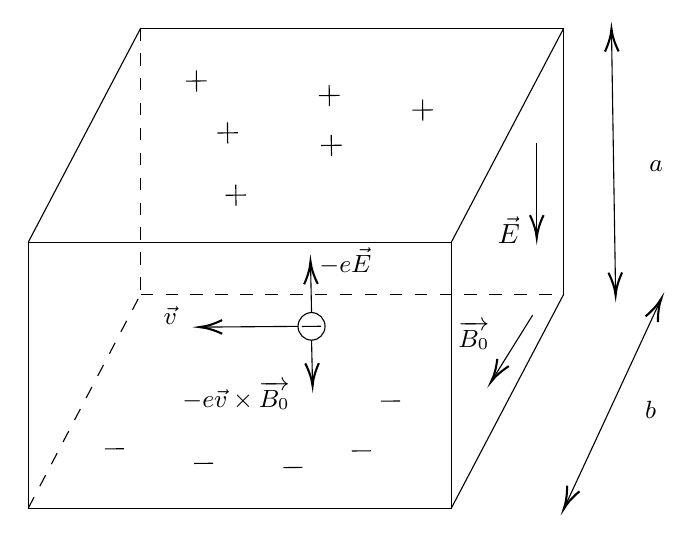
\begin{tikzpicture}[x=0.75pt,y=0.75pt,yscale=-1,xscale=1]
		%uncomment if require: \path (0,529); %set diagram left start at 0, and has height of 529
		
		%Shape: Rectangle [id:dp1709980992121849] 
		\draw   (199,160.85) -- (402.84,160.85) -- (402.84,289) -- (199,289) -- cycle ;
		%Straight Lines [id:da17838120550375303] 
		\draw    (402.84,160.85) -- (457,57.73) ;
		%Straight Lines [id:da5245263651893479] 
		\draw    (199,160.85) -- (253.16,57.73) ;
		%Straight Lines [id:da7166032900763126] 
		\draw    (402.84,289) -- (457,185.88) ;
		%Straight Lines [id:da09105718305767985] 
		\draw  [dash pattern={on 4.5pt off 4.5pt}]  (199,289) -- (253.16,185.88) ;
		%Straight Lines [id:da422926910253522] 
		\draw    (253.16,57.73) -- (457,57.73) ;
		%Straight Lines [id:da17110647342597418] 
		\draw  [dash pattern={on 4.5pt off 4.5pt}]  (253.16,185.88) -- (457,185.88) ;
		%Straight Lines [id:da22178382158170806] 
		\draw    (457,57.73) -- (457,185.88) ;
		%Straight Lines [id:da8282885192830589] 
		\draw  [dash pattern={on 4.5pt off 4.5pt}]  (253.16,57.73) -- (253.16,185.88) ;
		%Shape: Ellipse [id:dp26473837766750274] 
		\draw   (329,201.37) .. controls (329,197.7) and (331.91,194.73) .. (335.5,194.73) .. controls (339.09,194.73) and (342,197.7) .. (342,201.37) .. controls (342,205.03) and (339.09,208) .. (335.5,208) .. controls (331.91,208) and (329,205.03) .. (329,201.37) -- cycle ;
		%Straight Lines [id:da8879282057890976] 
		\draw    (330.87,201.42) -- (340.12,201.32) ;
		%Straight Lines [id:da17681268957094032] 
		\draw    (329,201.37) -- (283.5,201.72) ;
		\draw [shift={(281.5,201.73)}, rotate = 359.56] [color={rgb, 255:red, 0; green, 0; blue, 0 }  ][line width=0.75]    (10.93,-3.29) .. controls (6.95,-1.4) and (3.31,-0.3) .. (0,0) .. controls (3.31,0.3) and (6.95,1.4) .. (10.93,3.29)   ;
		%Straight Lines [id:da9574139817588048] 
		\draw    (442,196) -- (423.06,226.37) ;
		\draw [shift={(422,228.07)}, rotate = 301.95] [color={rgb, 255:red, 0; green, 0; blue, 0 }  ][line width=0.75]    (10.93,-3.29) .. controls (6.95,-1.4) and (3.31,-0.3) .. (0,0) .. controls (3.31,0.3) and (6.95,1.4) .. (10.93,3.29)   ;
		%Straight Lines [id:da10859311646498071] 
		\draw    (335.5,194.73) -- (335.04,172.07) ;
		\draw [shift={(335,170.07)}, rotate = 448.84] [color={rgb, 255:red, 0; green, 0; blue, 0 }  ][line width=0.75]    (10.93,-3.29) .. controls (6.95,-1.4) and (3.31,-0.3) .. (0,0) .. controls (3.31,0.3) and (6.95,1.4) .. (10.93,3.29)   ;
		%Straight Lines [id:da152003714478401] 
		\draw    (335.5,208) -- (335.95,228.07) ;
		\draw [shift={(336,230.07)}, rotate = 268.7] [color={rgb, 255:red, 0; green, 0; blue, 0 }  ][line width=0.75]    (10.93,-3.29) .. controls (6.95,-1.4) and (3.31,-0.3) .. (0,0) .. controls (3.31,0.3) and (6.95,1.4) .. (10.93,3.29)   ;
		%Straight Lines [id:da4024817690374525] 
		\draw    (444,113) -- (444,156.73) ;
		\draw [shift={(444,158.73)}, rotate = 270] [color={rgb, 255:red, 0; green, 0; blue, 0 }  ][line width=0.75]    (10.93,-3.29) .. controls (6.95,-1.4) and (3.31,-0.3) .. (0,0) .. controls (3.31,0.3) and (6.95,1.4) .. (10.93,3.29)   ;
		%Straight Lines [id:da18595288142190936] 
		\draw    (354.87,261.42) -- (364.12,261.32) ;
		%Straight Lines [id:da4068985763354118] 
		\draw    (321.87,269.42) -- (331.12,269.32) ;
		%Straight Lines [id:da7456139955663048] 
		\draw    (278.87,267.42) -- (288.12,267.32) ;
		%Straight Lines [id:da20355007117178547] 
		\draw    (368.87,237.42) -- (378.12,237.32) ;
		%Straight Lines [id:da4997206575183537] 
		\draw    (235.87,260.42) -- (245.12,260.32) ;
		%Straight Lines [id:da5792639000107] 
		\draw    (294.98,103.07) -- (295.11,113.24) ;
		%Straight Lines [id:da9776533888337451] 
		\draw    (290.09,108.22) -- (300,108.09) ;
		%Straight Lines [id:da7137598301087202] 
		\draw    (343.98,85.07) -- (344.11,95.24) ;
		%Straight Lines [id:da9121157813027572] 
		\draw    (339.09,90.22) -- (349,90.09) ;
		%Straight Lines [id:da4716355113783621] 
		\draw    (344.98,109.07) -- (345.11,119.24) ;
		%Straight Lines [id:da4287654711539537] 
		\draw    (340.09,114.22) -- (350,114.09) ;
		%Straight Lines [id:da40212626161904486] 
		\draw    (298.98,133.07) -- (299.11,143.24) ;
		%Straight Lines [id:da0575957807820493] 
		\draw    (294.09,138.22) -- (304,138.09) ;
		%Straight Lines [id:da788861794658057] 
		\draw    (388.98,92.07) -- (389.11,102.24) ;
		%Straight Lines [id:da3207337424564627] 
		\draw    (384.09,97.22) -- (394,97.09) ;
		%Straight Lines [id:da7182144088121003] 
		\draw    (279.98,78.07) -- (280.11,88.24) ;
		%Straight Lines [id:da056725719084304016] 
		\draw    (275.09,83.22) -- (285,83.09) ;
		%Straight Lines [id:da47142030713382055] 
		\draw    (480.03,60) -- (481.97,184.4) ;
		\draw [shift={(482,186.4)}, rotate = 269.11] [color={rgb, 255:red, 0; green, 0; blue, 0 }  ][line width=0.75]    (10.93,-3.29) .. controls (6.95,-1.4) and (3.31,-0.3) .. (0,0) .. controls (3.31,0.3) and (6.95,1.4) .. (10.93,3.29)   ;
		\draw [shift={(480,58)}, rotate = 89.11] [color={rgb, 255:red, 0; green, 0; blue, 0 }  ][line width=0.75]    (10.93,-3.29) .. controls (6.95,-1.4) and (3.31,-0.3) .. (0,0) .. controls (3.31,0.3) and (6.95,1.4) .. (10.93,3.29)   ;
		%Straight Lines [id:da26851964312566334] 
		\draw    (503.16,189.82) -- (480.91,237.9) -- (457.84,287.59) ;
		\draw [shift={(457,289.4)}, rotate = 294.9] [color={rgb, 255:red, 0; green, 0; blue, 0 }  ][line width=0.75]    (10.93,-3.29) .. controls (6.95,-1.4) and (3.31,-0.3) .. (0,0) .. controls (3.31,0.3) and (6.95,1.4) .. (10.93,3.29)   ;
		\draw [shift={(504,188)}, rotate = 114.83] [color={rgb, 255:red, 0; green, 0; blue, 0 }  ][line width=0.75]    (10.93,-3.29) .. controls (6.95,-1.4) and (3.31,-0.3) .. (0,0) .. controls (3.31,0.3) and (6.95,1.4) .. (10.93,3.29)   ;
		
		% Text Node
		\draw (263,190.4) node [anchor=north west][inner sep=0.75pt]  [font=\small]  {$\vec{v}$};
		% Text Node
		\draw (338,162.4) node [anchor=north west][inner sep=0.75pt]  [font=\small]  {$-e\vec{E}$};
		% Text Node
		\draw (272,226.4) node [anchor=north west][inner sep=0.75pt]  [font=\small]  {$-e\vec{v} \times \overrightarrow{B_{0}}$};
		% Text Node
		\draw (405,197.4) node [anchor=north west][inner sep=0.75pt]  [font=\small]  {$\overrightarrow{B_{0}}$};
		% Text Node
		\draw (424,147.4) node [anchor=north west][inner sep=0.75pt]    {$\vec{E}$};
		% Text Node
		\draw (497,120.4) node [anchor=north west][inner sep=0.75pt]  [font=\small]  {$a$};
		% Text Node
		\draw (495,236.4) node [anchor=north west][inner sep=0.75pt]  [font=\small]  {$b$};
		
		
	\end{tikzpicture}
	
	\end{center}
    Hiệu ứng Hall là hiệu ứng xuất hiện các điện tích trái dấu trên bề mặt của một vật dẫn có dòng điện khi nó đặt trong từ trường. \\
    Xét một dây dẫn, tiết diện là hình chữ nhật với các cạnh $a$ và $b$, có dòng điện chạy qua. Dây dẫn này được đặt trong điện trường $\ot{E_0}$ và từ trường $\ot{B_0}$.\\
    Electron chuyển động trong dây đẫn chịu tác dụng của lực Lorentz, bị dịch chuyển và dần tập trung ở mặt trên, làm cho nó tích điện âm. Tương tự, bản bên dưới bị tích điện dương.\\
    %HÌNH
    Các điện tích tập trung ở 2 mặt lại tạo nên điện trường Hall. Lực mà điện trường này tác dụng lên electron:
    $$F_e=eE=e\cdot\dfrac{U}{a},$$
    Ở trạng thái ổn định, lực của điện trường Hall cân bằng với lực Lorentzz:
    $$e\cdot\dfrac{U}{a}=evB,$$
    Lại có mối quan hệ dòng điện $I$ và vận tốc chuyển động của electron:
    $$I=en_eabv,$$
    với $n_e$ là mật độ các electron tự do trong kim loại.\\
    Từ đó:
    $$U=\dfrac{IB}{en_eb}=R_H\cdot\dfrac{IB}{b},$$
    với $R_H=\dfrac{1}{en_e}$ là hằng số Hall của kim loại.
    
    \section{Lưỡng cực từ.}
    Moment lưỡng cực từ của một vòng dây có dòng điện I chạy qua:
    $$\ot{p_m}=I\ot{S}=IS\ot{n}.$$
    với $S$ là diện tích giới hạn bởi vòng dây còn $\ot{n}$ là vector pháp tuyến đơn vị của mặt phẳng dòng điện và chiều của nó có thể được xác định bằng quy tắc đinh ốc.\\
    Từ trường gây bởi lưỡng cực từ $\ot{p_m}$ tại một điểm rất xa trong không gian:
    $$\ot{B}=k_m\dfrac{3\left(\ot{p_m}\times\ot{e_r}\right)-\ot{p_m}}{r^3}.$$
\section{Từ trường trong vật chất.}
\subsection{Sự từ hoá của các chất.}
    Các chất khi đặt trong từ trường đều bị nhiễm từ (hay bị từ hoá). Khi đặt trong từ trường ngoài các moment lưỡng cực có xu hướng bị quay đi theo từ trường.\\
    Vector từ hoá của một chất là mật độ các moment từ trong một đơn vị thể tích của chất:
    $$\ot{M}=\dfrac{\dd\ot{p_m}}{\dd V}.$$
    Khi đặt trong từ trường càng mạnh thì vector từ hoá càng lớn:
    $$\ot{M}=\chi_m\dfrac{\ot{B}}{\mu_0}.$$
    trong đó $\ot{H}$ là vector cường độ từ trường bên trong vật, $\chi_m$ là độ cảm từ và có quan hệ với độ từ thẩm của vật:
   $$\mu = 
      1+\chi_m.$$
    Dựa vào tính chất và mức độ từ hoá, người ta có thể phân loại các chất:
    \begin{itemize}
        \item Chất thuận từ: $\chi_m<0 $ và $\mu>1$
        \item Chất nghịch từ: $\chi_m < 0$ và $\mu<1$
    \end{itemize}
    Đối với chất thuận từ và nghịch từ thì $|\chi_m|\ll1$ do đó $\mu\approx 1.$
     \begin{itemize}
        \item Chất sắt từ: $\chi_m\gg 1$ nên $\mu\gg 1.$
    \end{itemize}
    Sự quay của lưỡng cực do tác dụng của từ trường làm xuất hiện dòng điện bên trong chất bị từ hoá, dòng điện này được gọi là dòng liên kết:
    $$\ot{j_b}=\ot{\nabla}\times\ot{M}.$$
    với $\ot{j_b}$ là mật độ dòng điện liên kết.
\subsection{Cường độ từ trường.}
    Dòng điện trong vật chất là tổng hợp của dòng điện liên kết và dòng điện gây bởi các nguồn khác (gọi là dòng điện tự do):
    $$\ot{j}=\ot{j_b}+\ot{j_f}$$
    Áp dụng định luật Ampere và công thức dòng điện liên kết:
    $$\ot{\nabla}\times\left(\dfrac{1}{\mu_0}\ot{B}-\ot{M}\right)=\ot{j_f}.$$
    Đại lượng bên trong ngoặc được gọi là vector cường độ từ trường:
    $$\ot{H}=\dfrac{1}{\mu_0}\ot{B}-\ot{M}$$
    vector cường độ từ trường bên trong vật khi được đặt trong một từ trường ngoài $\ot{B}_{0}$:
    $$\ot{H} = 
      \dfrac{\ot{B}}{\mu_0}-\ot{M}.$$
     Từ đó, ta có thể suy ra được mối quan hệ của vector cường độ từ trường $\ot{H}$ và vector cảm ứng từ $\ot{B}$:
     $$\ot{B} = 
      \mu\mu_0\ot{H}.$$
    Đồng thời ta cũng thu được biểu thức của định luật Ampere bên trong vật chất:
    \begin{align*}
        \ot{\nabla}\times\ot{H}&=\ot{j_f},\\
        \text{và } \oint\ot{H}\times\dd \ot{l}&=\int\ot{j_f}\cdot\dd \ot{S}.
     \end{align*}
\section{Cảm ứng điện từ.}
\subsection{Từ thông.}
\begin{center}
    

% Pattern Info
 
\tikzset{
pattern size/.store in=\mcSize, 
pattern size = 5pt,
pattern thickness/.store in=\mcThickness, 
pattern thickness = 0.3pt,
pattern radius/.store in=\mcRadius, 
pattern radius = 1pt}
\makeatletter
\pgfutil@ifundefined{pgf@pattern@name@_v65sgeu7h}{
\pgfdeclarepatternformonly[\mcThickness,\mcSize]{_v65sgeu7h}
{\pgfqpoint{0pt}{0pt}}
{\pgfpoint{\mcSize+\mcThickness}{\mcSize+\mcThickness}}
{\pgfpoint{\mcSize}{\mcSize}}
{
\pgfsetcolor{\tikz@pattern@color}
\pgfsetlinewidth{\mcThickness}
\pgfpathmoveto{\pgfqpoint{0pt}{0pt}}
\pgfpathlineto{\pgfpoint{\mcSize+\mcThickness}{\mcSize+\mcThickness}}
\pgfusepath{stroke}
}}
\makeatother
\tikzset{every picture/.style={line width=0.75pt}} %set default line width to 0.75pt        

\begin{tikzpicture}[x=0.75pt,y=0.75pt,yscale=-1,xscale=1]
%uncomment if require: \path (0,438); %set diagram left start at 0, and has height of 438

%Curve Lines [id:da02728278932272432] 
\draw    (173,123.93) .. controls (218,99.93) and (388,96.93) .. (426,118.93) ;
%Curve Lines [id:da10238125895061367] 
\draw    (158,228.93) .. controls (209,209.93) and (369,205.93) .. (411,223.93) ;
%Curve Lines [id:da13493424590328895] 
\draw    (173,123.93) .. controls (156,158.93) and (151,187.93) .. (158,228.93) ;
%Curve Lines [id:da4523259260078001] 
\draw    (426,118.93) .. controls (409,153.93) and (404,182.93) .. (411,223.93) ;
%Curve Lines [id:da4939641020183807] 
\draw    (87,102.93) .. controls (122,107.93) and (161,116.93) .. (195,164.93) ;
\draw [shift={(148.53,121.55)}, rotate = 28.03] [fill={rgb, 255:red, 0; green, 0; blue, 0 }  ][line width=0.08]  [draw opacity=0] (8.93,-4.29) -- (0,0) -- (8.93,4.29) -- cycle    ;
%Curve Lines [id:da28971858714178556] 
\draw    (174,55.8) .. controls (206,69.8) and (258,112.93) .. (283,153.93) ;
\draw [shift={(234.74,97.96)}, rotate = 41.6] [fill={rgb, 255:red, 0; green, 0; blue, 0 }  ][line width=0.08]  [draw opacity=0] (8.93,-4.29) -- (0,0) -- (8.93,4.29) -- cycle    ;
%Curve Lines [id:da670413941885676] 
\draw    (368,153) .. controls (365,112.93) and (348,73.8) .. (330,50.8) ;
\draw [shift={(356.04,99.24)}, rotate = 430.58000000000004] [fill={rgb, 255:red, 0; green, 0; blue, 0 }  ][line width=0.08]  [draw opacity=0] (8.93,-4.29) -- (0,0) -- (8.93,4.29) -- cycle    ;
%Curve Lines [id:da5923020412667761] 
\draw  [dash pattern={on 4.5pt off 4.5pt}]  (195,164.93) .. controls (210,188.93) and (220,213.93) .. (226,265.93) ;
%Curve Lines [id:da7093839559185253] 
\draw  [dash pattern={on 4.5pt off 4.5pt}]  (283,153.93) .. controls (298,191.8) and (304,223.8) .. (300,271.8) ;
%Curve Lines [id:da9833445858689851] 
\draw  [dash pattern={on 4.5pt off 4.5pt}]  (368,153) .. controls (368,190.93) and (370,223.93) .. (360,269.93) ;
%Straight Lines [id:da7765190544750014] 
\draw    (286.25,158.95) -- (256.98,106.55) ;
\draw [shift={(256,104.8)}, rotate = 420.81] [color={rgb, 255:red, 0; green, 0; blue, 0 }  ][line width=0.75]    (10.93,-3.29) .. controls (6.95,-1.4) and (3.31,-0.3) .. (0,0) .. controls (3.31,0.3) and (6.95,1.4) .. (10.93,3.29)   ;
%Shape: Parallelogram [id:dp8360893346521954] 
\draw  [pattern=_v65sgeu7h,pattern size=6pt,pattern thickness=0.75pt,pattern radius=0pt, pattern color={rgb, 255:red, 0; green, 0; blue, 0}] (278.75,149.93) -- (305,149.93) -- (293.75,167.97) -- (267.5,167.97) -- cycle ;
%Straight Lines [id:da4427953065536345] 
\draw    (286.25,158.95) -- (284.79,87.92) ;
\draw [shift={(284.75,85.92)}, rotate = 448.82] [color={rgb, 255:red, 0; green, 0; blue, 0 }  ][line width=0.75]    (10.93,-3.29) .. controls (6.95,-1.4) and (3.31,-0.3) .. (0,0) .. controls (3.31,0.3) and (6.95,1.4) .. (10.93,3.29)   ;
%Curve Lines [id:da29204072067186404] 
\draw    (274,137) .. controls (278,131.6) and (284,131.4) .. (286,135.6) ;

% Text Node
\draw (247,81.4) node [anchor=north west][inner sep=0.75pt]  [font=\small]  {$\vec{B}$};
% Text Node
\draw (277,61.4) node [anchor=north west][inner sep=0.75pt]  [font=\small]  {$\dd \vec{S}$};
% Text Node
\draw (271,116) node [anchor=north west][inner sep=0.75pt]  [font=\small]  {$\theta $};


\end{tikzpicture}

\end{center}
    Thông lượng của từ trường $\ot{B}$ tiết diện $S$:
    %Hình 2
    $$\Phi=\int_S \ot{B}\cdot \dd \ot{S}.$$
    
    với $\dd\ot{S}=\dd S\cdot \ot{n}$ trong đó $\ot{n}$ là vector pháp tuyến đơn vị của $\dd S$.
\subsection{Dòng điện cảm ứng.}
    Khi từ thông qua một mạch kín thay đổi, trong mạch xuất hiện dòng điện cảm ứng có suất điện động:
    $$\varepsilon=-\dfrac{\dd\Phi}{\dd t}.$$
    mà suất điện động trong mạch kín $\di \varepsilon=\oint \ot{E}\cdot\dd\ot{l}$. Từ đó, rút ra được mối quan hệ giữa điện trường $\ot{E}$ và từ trường biến thiên:
    $$\oint \ot{E}\cdot \dd\ot{l}=-\int \dfrac{\partial \ot{B}}{\partial t}\cdot \dd\ot{S},$$
    Theo định lý Stokes : $$\oint \ot{E}\cdot \dd\ot{l}=\int \left(\nabla \times \ot{E}\right) \cdot \dd\ot{S},$$\\
    Ta thu được phương trình dạng vi phân của định luật Faraday:
    $$\nabla \times \ot{E}= - \dfrac{\partial \ot{B}}{\partial t}.$$
    \textbf{Lưu ý:} trong trường hợp từ trường $\ot{B}$ là không đổi, định luật Faraday trở thành $\nabla \times \ot{E}=0$ (hay $\di\oint \ot{E}\cdot \dd\ot{l}=0$).
\subsection{Tự cảm.}
    Khi trong mạch kín có dòng điện biến đổi theo thời gian làm cho từ thông bị biến thiên, trong mạch sẽ xuất hiện hiện tượng tự cảm.\\
    Từ thông gửi qua mạch tỉ lệ với dòng điện chạy trong mạch:
    $$\Phi=Li.$$
    với $L$ là hệ số tự cảm của mạch, phụ thuộc vào hình dạng, kích cỡ và môi trường xunh quanh mạch điện.\\
\subsubsection{Độ tự cảm của một ống dây.}
    Vì chiều dài của ống dây là rất lớn so với bán kính của nó nên từ trường bên trong ống dây có thể coi như là đều:
    $$B=\mu\mu_0In=\mu\mu_0I\dfrac{N}{l},$$
    với $N$ là số vòng dây, còn $l$ là chiều dài ống dây.\\
    Từ thông gửi qua tiết diện S của ống dây:
    $$\Phi=NBS=N\left(\mu\mu_0I\dfrac{N}{l}\right)S=\dfrac{\mu\mu_0N^2S}{l}I.$$
    Độ tự cảm của ống dây: $L=\dfrac{\mu\mu_0N^2S}{l}.$
\subsubsection{Suất điện động tự cảm.}
    $$\varepsilon=\dfrac{\dd\Phi}{\dd t}=\dfrac{\dd(Li)}{\dd t}.$$
\subsection{Năng lượng trong cuộn cảm.}
    $$W=\dfrac{1}{2}Li^2.$$
\subsection{Hỗ cảm.}
    \begin{center}


\tikzset{every picture/.style={line width=0.75pt}} %set default line width to 0.75pt        

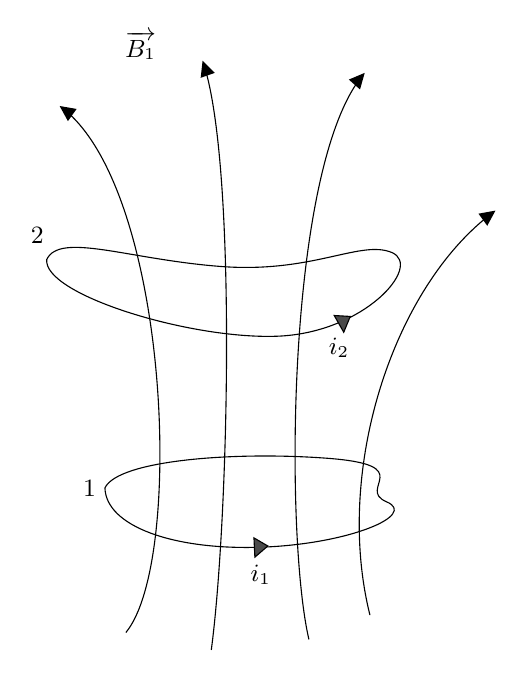
\begin{tikzpicture}[x=0.7pt,y=0.7pt,yscale=-0.9,xscale=0.9]
%uncomment if require: \path (0,529); %set diagram left start at 0, and has height of 529

%Curve Lines [id:da1117818098313792] 
\draw    (148,403.33) .. controls (155.6,387.33) and (222.6,382.33) .. (275.6,386.33) .. controls (328.6,390.33) and (291.68,403.76) .. (309.6,411.33) .. controls (327.52,418.91) and (287.91,435.57) .. (237.6,437.33) .. controls (187.29,439.1) and (148.6,425.33) .. (148,403.33) -- cycle ;
%Curve Lines [id:da04941341869215332] 
\draw    (114.6,272.33) .. controls (122.2,256.33) and (161.6,272.33) .. (214.6,276.33) .. controls (267.6,280.33) and (294.68,260.76) .. (312.6,268.33) .. controls (330.52,275.91) and (296.91,314.57) .. (246.6,316.33) .. controls (196.29,318.1) and (112.6,292.33) .. (114.6,272.33) -- cycle ;
%Shape: Triangle [id:dp6309583075456229] 
\draw  [fill={rgb, 255:red, 74; green, 74; blue, 74 }  ,fill opacity=1 ] (241.44,436.64) -- (234,443.04) -- (233.47,432) -- cycle ;
%Curve Lines [id:da4196100196783519] 
\draw    (160,486.27) .. controls (193.66,445.68) and (185.18,233.57) .. (123.87,185.67) ;
\draw [shift={(122,184.27)}, rotate = 395.53999999999996] [fill={rgb, 255:red, 0; green, 0; blue, 0 }  ][line width=0.08]  [draw opacity=0] (8.93,-4.29) -- (0,0) -- (8.93,4.29) -- cycle    ;
%Curve Lines [id:da2530787268456667] 
\draw    (209,496.27) .. controls (218.85,422.39) and (223.85,221.42) .. (204.88,160.93) ;
\draw [shift={(204,158.27)}, rotate = 430.66999999999996] [fill={rgb, 255:red, 0; green, 0; blue, 0 }  ][line width=0.08]  [draw opacity=0] (8.93,-4.29) -- (0,0) -- (8.93,4.29) -- cycle    ;
%Curve Lines [id:da4587371111087095] 
\draw    (265,490.27) .. controls (251.14,430.87) and (251.98,220.53) .. (295.66,166.85) ;
\draw [shift={(297,165.27)}, rotate = 491.42] [fill={rgb, 255:red, 0; green, 0; blue, 0 }  ][line width=0.08]  [draw opacity=0] (8.93,-4.29) -- (0,0) -- (8.93,4.29) -- cycle    ;
%Curve Lines [id:da7120598464417665] 
\draw    (300,476.27) .. controls (279.21,393.11) and (313.31,288.38) .. (370.27,245.55) ;
\draw [shift={(372,244.27)}, rotate = 504.09] [fill={rgb, 255:red, 0; green, 0; blue, 0 }  ][line width=0.08]  [draw opacity=0] (8.93,-4.29) -- (0,0) -- (8.93,4.29) -- cycle    ;
%Shape: Triangle [id:dp991850232756601] 
\draw  [fill={rgb, 255:red, 74; green, 74; blue, 74 }  ,fill opacity=1 ] (288.71,304.98) -- (284.97,314.05) -- (279.51,304.44) -- cycle ;

% Text Node
\draw (230,446) node [anchor=north west][inner sep=0.75pt]  [font=\small]  {$i_{1}$};
% Text Node
\draw (158,139.67) node [anchor=north west][inner sep=0.75pt]  [font=\small]  {$\overrightarrow{B_{1}}$};
% Text Node
\draw (275,316) node [anchor=north west][inner sep=0.75pt]  [font=\small]  {$i_{2}$};
% Text Node
\draw (104,252.67) node [anchor=north west][inner sep=0.75pt]  [font=\small]  {$2$};
% Text Node
\draw (134,397.67) node [anchor=north west][inner sep=0.75pt]  [font=\small]  {$1$};


\end{tikzpicture}

    \end{center}
    Khi hai vòng dây dẫn kín (1) và (2) đặt gần nhau, các đường sức từ của từ trường $B_1$ gây bởi dòng $i_1$ ở vòng dây (1) đi qua tiết diện giới hạn bởi vòng dây (2). Thông lượng (từ thông) của từ trường $B_1$ gửi qua vòng dây (2) là:
    $$\Phi_{12}=\int \ot{B_1}\cdot \dd\ot{S_2}.$$
    Từ thông $\Phi_{12}$ tỉ lệ với dòng điện $i_1$:
    $$\Phi_{12}=M_{12}i_1,$$
    với $M_{12}$ là độ hỗ cảm của vòng dây (1) đối với vòng dây (2), phụ thuộc vào hình dạng kích thước, vị trí tương đối của các mạch điện và môi trường xunh quanh chúng.
    Tương tự, từ thông $\Phi_{21}$ do dòng điện $i_2$ ở vòng (2) gửi qua vòng (1):
    $$\Phi_{21}=M_{21}i_2.$$
    Nếu không có vật sắt từ, ta luôn có: $M_{12}=M_{21}=M.$
\subsection{Năng lượng hỗ cảm.}
    $$W=\pm \dfrac{1}{2}Mi_1i_2.$$
    Giá trị năng lượng hỗ cảm của hai mạch dương hay âm phụ thuộc vào từ thông đoạn mạch này gửi qua đoạn mạch kia là dương hay âm.
\section{Hệ phương trình Maxwell.}
 Từ những phần trước ta đã tìm hiểu về các định luật, phương trình về div và rot của điện và từ trường:
 \begin{itemize}
 	\item $\ot{\nabla}\cdot\ot{E}=\dfrac{\varrho}{\varepsilon_0} $ (Định luật Gauss),
 	\item $\ot{\nabla}\cdot\ot{B}=0$,
 	\item $\nabla \times \ot{E}= - \dfrac{\partial \ot{B}}{\partial t}$ (Định luật Faraday),
 	\item $\ot{\nabla}\times\ot{B}= \mu_0\ot{j}$ (Định luật Ampere).
 \end{itemize}
 \subsection{Định luật Ampere bổ sung bởi Maxwell.}
 	Lấy div cho cả hai vế của phương trình định luật Ampere:
 	$$\ot{\nabla}\cdot\left(\ot{\nabla}\times\ot{B}\right)= \mu_0\ot{\nabla}\cdot\ot{j},$$
 	Ta có thể dễ dàng chứng minh được vế trái của phương trình bằng không, nhưng vế phải $\ot{\nabla}\cdot\ot{j}=0$ chỉ khi dòng điện là dòng ổn định. Đối với dòng điện biến thiên thì điều này không còn đúng nữa.\\
 	Bây giờ, ta xét tới trường hợp dòng điện không ổn định:
	 $$\ot{\nabla}\cdot\ot{j}=-\dfrac{\partial\varrho}{\partial t}=-\dfrac{\partial}{\partial t}\left(\varepsilon_0\ot{\nabla}\cdot\ot{E}\right)=-\ot{\nabla}\cdot\left(\varepsilon_0\dfrac{\partial \ot{E}}{\partial t}\right),$$
	Nếu ta thay $\ot{j}$ trong phương trình định luật Ampere bằng tổng $\ot{j}+\varepsilon_0 \left(\dfrac{\partial\ot{E}}{\partial t}\right)$ thì div vế phải của phương trình sẽ thoả mãn bằng không:
	$$\ot{\nabla}\times\ot{B}=\mu_0\ot{j}+\mu_0\varepsilon_0\dfrac{\partial \ot{E}}{\partial t}.$$
	Số hạng được thêm vào trong phương trình được gọi là dòng điện dịch:
	$$\ot{j_d}=\varepsilon_0\dfrac{\partial \ot{E}}{\partial t}.$$
\subsection{Hệ phương trình Maxwell.}
	\begin{itemize}
		\item $\ot{\nabla}\cdot\ot{E}=\dfrac{\varrho}{\varepsilon_0} $ (Định luật Gauss),
		\item $\ot{\nabla}\cdot\ot{B}=0$,
		\item $\nabla \times \ot{E}= - \dfrac{\partial \ot{B}}{\partial t}$ (Định luật Faraday),
		\item $\ot{\nabla}\times\ot{B}= \mu_0\ot{j}+\mu_0\varepsilon_0\dfrac{\partial \ot{E}}{\partial t}$ (Định luật Ampere được bổ sung bởi Maxwell).
	 \end{itemize}
\subsection{Hệ phương trình Maxwell trong vật chất.}
Dòng điện gây bởi sự biến thiên của các điện tích liên kết theo thời gian:
	$$\oint\ot{j_p}\cdot\dd\ot{S}=-\dfrac{\dd }{\dd t}\int\varrho_b\dd V,$$
Áp dụng định lý Stokes:
	$$\int\left(\ot{\nabla}\cdot\ot{j_p}\right)\dd V=-\int\dfrac{\dd\varrho_b }{\dd t}\dd V,$$
Phương trình trên đúng cho mọi thể tích mà ta lấy tích phân nên:	
	$$\ot{\nabla}\cdot\ot{j_p}=-\dfrac{\dd\varrho_b }{\dd t}=-\dfrac{\dd }{\dd t}\left(-\ot{\nabla}\cdot\ot{P}\right)=\ot{\nabla}\cdot\dfrac{\dd \ot{P}}{\dd t}.$$
Mật độ dòng điện gây bởi các điện tích phân cực:	
	$$\ot{j_p}=\dfrac{\dd \ot{P}}{\dd t}.$$
Như vậy dòng điện trong vật dẫn sẽ bao gồm 3 thành phần:
	\begin{align*}
	\ot{j}&=\ot{j_f}+\ot{j_p}+\ot{j_b}\\
	&=\ot{j_f}+\dfrac{\dd \ot{P}}{\dd t}+\ot{\nabla}\times\ot{M}.
	\end{align*}
	Thế vào biểu thức định luật Ampere:
	\begin{align*}
	&\ot{\nabla}\times\ot{B}= \mu_0\left(\ot{j_f}+\dfrac{\dd \ot{P}}{\dd t}+\ot{\nabla}\times\ot{M}\right)+\mu_0\varepsilon_0\dfrac{\partial \ot{E}}{\partial t},\\
	\Rightarrow&\ot{\nabla}\times\left(\dfrac{1}{\mu_0}\ot{B}-\ot{M}\right)=\mu_0\ot{j_f}+\dfrac{\partial}{\partial t}\left(\varepsilon_0\ot{E}+\ot{P}\right).
	\end{align*}
	Từ đó ta thu được phương trình định luật Ampere trong vật chất:
	$$\ot{\nabla}\times\ot{H}=\mu_0\ot{j_f}+\dfrac{\partial\ot{D}}{\partial t}.$$
	Như vậy, hệ phương trình Maxwell bên trong vật chất:
	\begin{itemize}
		\item $\ot{\nabla}\cdot\ot{D}=\varrho_f $,
		\item $\ot{\nabla}\cdot\ot{B}=0$,
		\item $\nabla \times \ot{E}= - \dfrac{\partial \ot{B}}{\partial t}$,
		\item $\ot{\nabla}\times\ot{H}= \mu_0\ot{j_f}+\dfrac{\partial \ot{D}}{\partial t}$.
	\end{itemize}

\section{Định lý Poynting.}
\subsection{Vector Poynting.}
 Năng lượng dự trữ của điện trường:
 $$W_e=\dfrac{\varepsilon_0}{2}\int E^2\dd V. $$   
 Tương tự, năng lượng dự trữ của từ trường:
 $$W_e=\dfrac{1}{2\mu_0}\int B^2\dd V.$$
 Tổng mật độ năng lượng trên một đơn vị thể tích dự trữ trong một điện từ trường :
 $$u=\dfrac{1}{2}\left(\varepsilon_0E^2+\dfrac{1}{2\mu_0}B^2\right).$$   
 Công suất tác dụng lên các điện tích bên trong một thể tích $V$:
 $$\dfrac{\dd W}{\dd t}=\int\left(\ot{E}\cdot\ot
 {j}\right)\dd V.$$
 Áp dụng định luật Ampere (với sự bổ sung của Maxwell):
 \begin{align*}
 	\ot{E}\cdot\ot{j}&=\ot{E}\cdot\left[\dfrac{1}{\mu_0}\ot{\nabla}\times\ot{B}-\varepsilon_0\dfrac{\partial \ot{E}}{\partial t}\right],\\
 	\ot{E}\cdot\left(\ot{\nabla}\times\ot{B}\right)&=\ot{B}\cdot\left(\ot{\nabla}\times\ot{E}\right)-\ot{\nabla}\cdot\left(\ot{E}\times\ot{B}\right).\\
 \end{align*}
Áp dụng định luật Faraday, ta được:
$$\ot{E}\cdot\left(\ot{\nabla}\times\ot{B}\right)=-\ot{B}\cdot\dfrac{\partial \ot{B}}{\partial t}-\ot{\nabla}\cdot\left(\ot{E}\times\ot{B}\right).$$
Từ đó
\begin{align*}
	\ot{E}\cdot\ot{j}&=-\dfrac{\partial }{\partial t}\left(\varepsilon_0\ot{E}\cdot\dd\ot{E}+\dfrac{1}{\mu_0}\ot{B}\cdot\dd\ot{B}\right)-\dfrac{1}{\mu_0}\ot{\nabla}\cdot\left(\ot{E}\times\ot{B}\right)\\
	&=-\dfrac{1}{2}\dfrac{\partial }{\partial t}\left(\varepsilon_0 E^2+\dfrac{1}{\mu_0}B^2\right)-\dfrac{1}{\mu_0}\ot{\nabla}\cdot\left(\ot{E}\times\ot{B}\right).
	\end{align*}
Thay vào công thức và áp dụng định lý Gauss:
$$\dfrac{\dd W}{\dd t}= -\dfrac{\dd}{\dd t}\int\dfrac{1}{2}\left(\varepsilon_0 E^2+\dfrac{1}{\mu_0}B^2\right)\dd V- \dfrac{1}{\mu_0}\oint \left(\ot{E}\times\ot{B}\right)\cdot\dd \ot{S}.$$
Đây chính là biểu thức của thuyết Poynting. Trong đó, tích phân thứ nhất ở vế trái chính là năng lượng được dự trữ trong điện từ trường, tích phân thứ hai là năng lượng truyền ra khỏi thể tích $V$ trong một đơn vị thời gian. Năng lượng truyền qua một đơn vị diện tích trong một đơn vị thời gian gọi là vector Poynting:
$$\ot{S}=\dfrac{1}{\mu_0}\left(\ot{E}\times\ot{B}\right).$$
\subsection{Động lượng và moment động lượng.}
Lực điện từ tác dụng lên các điện tích chứa trong thể tích $\dd V$:
$$\dd\ot{F}=\varrho\left(\ot{E}+\ot{v}\times\ot{B}\right)\dd V.$$
Lực tác dụng lên một đơn vị thể tích là:
$$\ot{f}=\varrho\left(\ot{E}+\ot{v}\times\ot{B}\right)=\varrho\ot{E}+\ot{j}\times\ot{B}.$$
Áp dụng định luật Gauss và định luật Ampere ta thu được:
$$\ot{f}=\varepsilon_0\ot{E}\left(\ot{\nabla}\cdot\ot{E}\right)+\left(\dfrac{1}{\mu_0}\ot{\nabla}\times\ot{B}-\varepsilon_0\dfrac{\partial \ot{E}}{\partial t}\right)\times\ot{B}.$$
Bên cạnh đó,
\begin{align*}
\dfrac{\partial}{\partial t}\left(\ot{E}\times\ot{B}\right)&=\dfrac{\partial\ot{E}}{\partial t}\times\ot{B}+\ot{E}\times\dfrac{\partial\ot{B}}{\partial t},\\
&=\dfrac{\partial\ot{E}}{\partial t}\times\ot{B}+\ot{E}\times\left(-\ot{\nabla}\times\ot{E}\right).
\end{align*}
Thay lại vào biểu thức của $\ot{f}$:
\begin{align*}
\ot{f}&=\varepsilon_0\ot{E}\left(\ot{\nabla}\cdot\ot{E}\right)-\dfrac{1}{\mu_0}\times\ot{B}\left(\ot{\nabla}\times\ot{B}\right)-\varepsilon_0\ot{E}\times\left(\ot{\nabla}\times\ot{E}\right)-\varepsilon_0\dfrac{\partial}{\partial t}\left(\ot{E}\times\ot{B}\right).
\end{align*}
Áp dụng quy tắc div của một tích vô hướng hai vector:
\begin{align*}
\ot{\nabla}\left(E^2\right)=2\left(\ot{E}\cdot\ot{\nabla}\right)\ot{E}+2\ot{E}\times\left(\ot{\nabla}\times\ot{E}\right),\\
\ot{\nabla}\left(B^2\right)=2\left(\ot{B}\cdot\ot{\nabla}\right)\ot{E}+2\ot{B}\times\left(\ot{\nabla}\times\ot{B}\right).
\end{align*}
Từ đó,
\begin{align*}
	\ot{f}=\varepsilon_0\left[\left(\ot{\nabla}\cdot\ot{E}\right)\ot{E}+\left(\ot{E}\cdot\ot{\nabla}\right)\ot{E}\right]&+\dfrac{1}{\mu_0}\left[\left(\ot{\nabla}\cdot\ot{B}\right)\ot{B}+\left(\ot{B}\cdot\ot{\nabla}\right)\ot{B}\right]\\
	&-\dfrac{1}{2}\ot{\nabla}\left(\varepsilon_0E^2+\dfrac{1}{\mu_0}B^2\right)-\varepsilon_0\dfrac{\partial}{\partial t}\left(\ot{E}\times\ot{B}\right),
\end{align*}
vì trong hệ phương trình Maxwell $\left(\ot{\nabla}\cdot\ot{B}\right)\ot{B}=0$.

Định lý biến thiên động lượng:
\begin{align*}
	\dfrac{\dd \ot{p}}{\dd t}=\ot{F}=\int\ot{f}\dd V.
\end{align*}
Sử dụng công thức lực trên một đơn vị thể tích vừa thu được:
\begin{align*}
	\dfrac{\dd \ot{p}}{\dd t}=\int\varepsilon_0\left[\left(\ot{\nabla}\cdot\ot{E}\right)\ot{E}+\left(\ot{E}\cdot\ot{\nabla}\right)\ot{E}\right]&\dd V+\dfrac{1}{\mu_0}\int\left[\left(\ot{\nabla}\cdot\ot{B}\right)\ot{B}+\left(\ot{B}\cdot\ot{\nabla}\right)\ot{B}\right]\dd V\\
	&-\dfrac{1}{2}\int{\nabla}\left(\varepsilon_0E^2+\dfrac{1}{\mu_0}B^2\right)\dd V-\varepsilon_0\int\dfrac{\partial}{\partial t}\left(\ot{E}\times\ot{B}\right)\dd V.
\end{align*}
Số hạng cuối cùng là độ biến thiên động lượng của điện từ trường:
\begin{align*}
	\dfrac{\dd \ot{p}_{field}}{\dd t}&=\varepsilon_0\int\dfrac{\partial}{\partial t}\left(\ot{E}\times\ot{B}\right)\dd V,\\
	\Rightarrow\ot{p}_{field}&=\varepsilon_0\int\left(\ot{E}\times\ot{B}\right)\dd V,\\
	&=\varepsilon_0\mu_0\int\ot{S_p}\dd V.
\end{align*}
Mật độ động lượng trên một đơn vị thể tích:
$$\ot{g}=\varepsilon_0\left(\ot{E}\times\ot{B}\right)=\varepsilon_0\mu_0\ot{S_p}.$$
Đồng thời ta cũng thu được công thức mật độ moment động lượng:
$$\ot{l}=\ot{r}\times\ot{g}=\varepsilon_0\left[\ot{r}\times\left(\ot{E}\times\ot{B}\right)\right].$$
\section{Điện từ trường tương đối tính.}
Mối quan hệ giữa điện từ trường trong hệ quy chiếu $S'$ chuyển động với vận tốc $\ot{v}$ và hệ quy chiếu đứng yên $S$:
\begin{align*}
	\ot{E}'_{\bot}&=\gamma\left[\ot{E}_{\bot}+\ot{v}\times\ot{B}_{\bot}\right],\\
	\ot{E}'_{\parallel}&=\ot{E}_{\parallel},\\
	\ot{B}'_{\bot}&=\gamma\left[\ot{B}_{\bot}-\dfrac{\ot{v}}{c^2}\times\ot{B}_{\bot}\right],\\
	\ot{B}'_{\parallel}&=\ot{B}_{\parallel} \text{ với } \gamma=\dfrac{1}{\sqrt{1-\dfrac{v^2}{c^2}}}.
\end{align*}
trong đó $\ot{E}_{\parallel}$, $\ot{B}_{\parallel}$ là thành phần điện từ trường song song với phương của $\ot{v}$, còn $\ot{E}_{\bot}$, $\ot{B}_{\bot}$ là thành phần điện từ trường vuông góc với phương của $\ot{v}$.









% cần sửa
\section{Hệ đơn vị Gaussian}


\begin{center}
\begin{longtable}{|l|c|c|} %{|p{5cm}|p{6cm}|p{6cm}|} 
\caption{Bảng so sánh giữa hai hệ.} \label{tab:long} \\

\hline \multicolumn{1}{|c|}{\textbf{}} & \multicolumn{1}{c|}{\textbf{SI}} & \multicolumn{1}{c|}{\textbf{Gaussian}} \\ \hline 
\endfirsthead

\multicolumn{3}{c}%
{{\bfseries \tablename\ \thetable{} -- Bảng so sánh giữa hai hệ.}} \\
\hline \multicolumn{1}{|c|}{\textbf{}} & \multicolumn{1}{c|}{\textbf{SI}} & \multicolumn{1}{c|}{\textbf{Gaussian}} \\ \hline 
\endhead

%\hline \multicolumn{3}{|r|}{{Continued on next page}} \\ \hline
%\endfoot

%\hline \hline
%\endlastfoot


\hline
 \text{Lực tương tác tĩnh điện}  &  $ \ot{F}=\dfrac{1}{4\pi\varepsilon_0}\dfrac{qQ}{\left|\ot{r}-\ot{r'}\right|^3}\cdot\left(\ot{r}-\ot{r'}\right) $  & 
  $\ot{F}= \dfrac{qQ}{\left|\ot{r}-\ot{r'}\right|^3}\cdot\left(\ot{r}-\ot{r'}\right)$ \\[6pt]

\hline
\text{Cường độ điện trường} &  $\ot{E}=\dfrac{1}{4\pi\varepsilon_0}\dfrac{q}{\left|\ot{r}-\ot{r'}\right|^3}\cdot\left(\ot{r}-\ot{r'}\right)$  &  $\ot{E}=\dfrac{q}{\left|\ot{r}-\ot{r'}\right|^3}\cdot\left(\ot{r}-\ot{r'}\right)$ \\ 

        %\hline
	  %\text{Điện thông} &  $\Phi=\int \ot{E}\cdot \dd \ot{S}$  & \\
	  
	 \hline
	   \text{Thế năng tĩnh điện}  & $ V=\dfrac{1}{4\pi\varepsilon_0}\dfrac{q_1q_2}{r_{12}}$  &  $ V=\dfrac{q_1q_2}{r_{12}} $\\
	   
	 %\hline
	  %\text{Lưỡng cực điện} & $\ot{p}=q\ot{l}$  & \\
	  
	 \hline
	  \text{Thế năng lưỡng cực điện}&  $\varphi=\dfrac{1}{4\pi\varepsilon_0}\dfrac{\ot{p}\cdot\ot{r}}{r^3}$  &  $\varphi=\dfrac{\ot{p}\cdot\ot{r}}{r^3}$  \\
	  
	 \hline
	  \text{Độ phân cực điện} & $\ot{P} = \varepsilon_0\chi_e \ot{E}$  &  $\ot{P} =\chi_e\ot{E}$  \\
	  
	 \hline
	 \text{Hằng số điện môi} & $\varepsilon = 1+\chi_e$  &  $\varepsilon = 1+4\pi\chi_e$  \\
	 
	 \hline
	  \text{Tụ điện phẳng} &  $C=\dfrac{\varepsilon\varepsilon_0S}{d}$  &  $C=\dfrac{\varepsilon S}{4\pi d}$  \\
	  
	 \hline
	 \text{Tụ điện cầu}& $C=\dfrac{4\pi\varepsilon\varepsilon_0R_1R_2}{R_2-R_1}$& $C=\dfrac{\varepsilon R_1 R_2}{R_2-R_1}$\\
	 
	 \hline
	 \text{Tụ điện trụ}& $C=\dfrac{2\pi\varepsilon\varepsilon_0l}{\ln\left(\dfrac{R_2}{R_1}\right)}$& $C=\dfrac{\varepsilon l}{2\ln\left(\dfrac{R_2}{R_1}\right)}$\\
	 
	 \hline
	 \text{Từ trường}&$\ot{B}=\dfrac{\mu_0}{4\pi}\int\dfrac{I\dd\ot{l'}\times\left(\ot{r}-\ot{r'}\right)}{\left|\ot{r}-\ot{r'}\right|^3} $& $\ot{B}=\dfrac{1}{c}\int\dfrac{I\dd\ot{l'}\times\left(\ot{r}-\ot{r'}\right)}{\left|\ot{r}-\ot{r'}\right|^3}$\\
	 \hline
	 \text{Lực Lorentz}&$\ot{F}=q\ot{v}\times\ot{B} $& $\ot{F}=\dfrac{q}{c}\ot{v}\times\ot{B}$\\
	 %\hline
	 %\text{Lực từ}& & ,\\
	 \hline
	 \text{Lưỡng cực từ}& $\ot{p_m}=I\ot{S}$ & $\ot{p_m}=\dfrac{I\ot{S}}{c}$\\
	 \hline
	 \text{Vector từ hoá}& $\ot{M}=\chi_m\dfrac{\ot{B}}{\mu_0}$& $\ot{M}=\chi_m\ot{B}$ \\
	 \hline
	 \text{Độ từ thẩm}& $\mu =1+\chi_m $& $\mu =1+4\pi\chi_m $\\
	 \hline
	 \text{Cường độ từ trường}& $\ot{H}=\dfrac{\ot{B}}{\mu\mu_0}$ & $\ot{H}=\dfrac{\ot{B}}{\mu}$\\
	 %\hline
	 %\text{Từ thông}& $\Phi=\int \ot{B}\cdot \dd \ot{S}$ & \\
	 \hline
	 \text{Suất điện động cảm ứng}& $\varepsilon=-\dfrac{\dd\Phi}{\dd t}$& $\varepsilon=-\dfrac{1}{c}\dfrac{\dd\Phi}{\dd t}$\\
	 %\hline
	 %\text{Suất điện động tự cảm}&$\varepsilon=L\dfrac{\dd i}{\dd t} $& \\
	 \hline
	 \text{Độ tự cảm của ống dây}& $L=\dfrac{\mu\mu_0N^2S}{l} $&$\dfrac{4\pi\mu N^2S}{c^2l}$ ,\\
	 %\hline
	 %\text{Suất điện động hỗ cảm}&$\varepsilon_{12}=-M_{12}\dfrac{\dd i_1}{\dd t}$ & \\
	 %\hline
	 %\text{Hệ phương trình Maxwell}&
	 %$\begin{aligned}
	 %    \ot{\nabla}\cdot\ot{E}&=\dfrac{\varrho}{\varepsilon_0}\\
	 %    \ot{\nabla}\cdot\ot{B}&=0,\\
	%	\nabla \times \ot{E}&= - \dfrac{\partial \ot{B}}{\partial t},\\
	%	\nabla \times \ot{E}&= - \dfrac{\partial \ot{B}}{\partial t},\\
	%	\ot{\nabla}\times\ot{B}&= \mu_0\ot{j}+\mu_0\varepsilon_0\dfrac{\partial \ot{E}}{\partial t}.
	 %\end{aligned}$&\\
	 \hline
	 \text{Năng lượng của điện từ trường}&$u=\dfrac{1}{2}\left(\varepsilon_0E^2+\dfrac{1}{2\mu_0}B^2\right)$ & $u=\dfrac{1}{8\pi}\left(E^2+B^2\right)$\\
	 \hline
	 \text{Vector Poynting}& $\ot{S}=\dfrac{1}{\mu_0}\left(\ot{E}\times\ot{B}\right)$& $\ot{S}=\dfrac{c}{3\pi\mu_0}\left(\ot{E}\times\ot{B}\right)$\\
	 \hline
\end{longtable}
\textbf{Tất cả các bài toán dùng hệ dơn vị Gauss sẽ được đánh dấu bằng kí hiệu (G) bên cạnh tên bài.}

\end{center}
\end{appendices}
\chapter{Tĩnh điện}
 \begin{vd}[Hạt bị nhốt trong điện trường]
    Một hạt khối lượng $m=0,1\dv{kg}$ và điện tích $q=0,5\dv{\mu C}$ được đặt vào tâm của hình lập phương. Ở mỗi đỉnh của hình lập phương được đặt cố định một điện tích $Q=-4\dv{\mu C}$. Độ dài một cạnh của hình lập phương là $l=1,5\dv{m}$. Truyền cho hạt một vận tốc song song với một cạnh của hình lập phương. Hỏi vận tốc tối thiểu cần truyền cho hạt là bao nhiêu để hạt ra được bên ngoài hộp. Coi năng lượng mất mát do sự phát xạ điện từ và các hiện tượng khác là $E=0,00250\dv{J}$.
    \end{vd}
    \begin{loigiai}
    \\
    \begin{minipage}{0.5\textwidth}
          Thế năng lúc ban đầu của hạt là: 
    $$
U_{i}=-8 \frac{k q Q}{l \dfrac{\sqrt{3}}{2}}=-\frac{16 k q Q}{\sqrt{3} l}.
$$
    \end{minipage}
    \begin{minipage}{0.5\textwidth}
         

\tikzset{every picture/.style={line width=0.75pt}} %set default line width to 0.75pt        

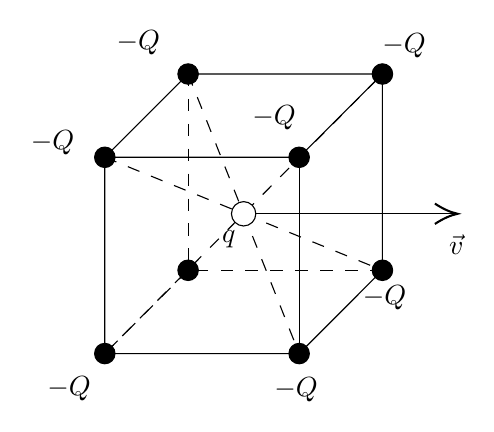
\begin{tikzpicture}[x=0.75pt,y=0.75pt,yscale=-1,xscale=1]
%uncomment if require: \path (0,205); %set diagram left start at 0, and has height of 205

%Shape: Cube [id:dp912316329494171] 
\draw   (281.41,73.63) -- (321.54,33.5) -- (415.17,33.5) -- (415.17,128.07) -- (375.05,168.2) -- (281.41,168.2) -- cycle ; \draw   (415.17,33.5) -- (375.05,73.63) -- (281.41,73.63) ; \draw   (375.05,73.63) -- (375.05,168.2) ;
%Straight Lines [id:da7932497906208718] 
\draw  [dash pattern={on 4.5pt off 4.5pt}]  (321.54,33.5) -- (321.54,128.07) ;
%Straight Lines [id:da2949920190066182] 
\draw  [dash pattern={on 4.5pt off 4.5pt}]  (415.17,128.07) -- (321.91,128.07) ;
%Straight Lines [id:da7606271813543024] 
\draw  [dash pattern={on 4.5pt off 4.5pt}]  (321.54,128.07) -- (281.41,168.2) ;
%Flowchart: Connector [id:dp31345639797296543] 
\draw  [fill={rgb, 255:red, 0; green, 0; blue, 0 }  ,fill opacity=1 ] (276.5,73.63) .. controls (276.5,70.92) and (278.7,68.72) .. (281.41,68.72) .. controls (284.13,68.72) and (286.33,70.92) .. (286.33,73.63) .. controls (286.33,76.35) and (284.13,78.55) .. (281.41,78.55) .. controls (278.7,78.55) and (276.5,76.35) .. (276.5,73.63) -- cycle ;
%Flowchart: Connector [id:dp4464434240009014] 
\draw  [fill={rgb, 255:red, 0; green, 0; blue, 0 }  ,fill opacity=1 ] (276.5,168.2) .. controls (276.5,165.48) and (278.7,163.28) .. (281.41,163.28) .. controls (284.13,163.28) and (286.33,165.48) .. (286.33,168.2) .. controls (286.33,170.91) and (284.13,173.11) .. (281.41,173.11) .. controls (278.7,173.11) and (276.5,170.91) .. (276.5,168.2) -- cycle ;
%Flowchart: Connector [id:dp5397376605990161] 
\draw  [fill={rgb, 255:red, 0; green, 0; blue, 0 }  ,fill opacity=1 ] (410.26,128.07) .. controls (410.26,125.36) and (412.46,123.15) .. (415.17,123.15) .. controls (417.89,123.15) and (420.09,125.36) .. (420.09,128.07) .. controls (420.09,130.79) and (417.89,132.99) .. (415.17,132.99) .. controls (412.46,132.99) and (410.26,130.79) .. (410.26,128.07) -- cycle ;
%Flowchart: Connector [id:dp5549760416410436] 
\draw  [fill={rgb, 255:red, 0; green, 0; blue, 0 }  ,fill opacity=1 ] (316.63,128.07) .. controls (316.63,125.36) and (318.83,123.15) .. (321.54,123.15) .. controls (324.26,123.15) and (326.46,125.36) .. (326.46,128.07) .. controls (326.46,130.79) and (324.26,132.99) .. (321.54,132.99) .. controls (318.83,132.99) and (316.63,130.79) .. (316.63,128.07) -- cycle ;
%Flowchart: Connector [id:dp4088669328872736] 
\draw  [fill={rgb, 255:red, 0; green, 0; blue, 0 }  ,fill opacity=1 ] (370.13,168.2) .. controls (370.13,165.48) and (372.33,163.28) .. (375.05,163.28) .. controls (377.76,163.28) and (379.96,165.48) .. (379.96,168.2) .. controls (379.96,170.91) and (377.76,173.11) .. (375.05,173.11) .. controls (372.33,173.11) and (370.13,170.91) .. (370.13,168.2) -- cycle ;
%Flowchart: Connector [id:dp64439132917289] 
\draw  [fill={rgb, 255:red, 0; green, 0; blue, 0 }  ,fill opacity=1 ] (410.26,33.5) .. controls (410.26,30.79) and (412.46,28.59) .. (415.17,28.59) .. controls (417.89,28.59) and (420.09,30.79) .. (420.09,33.5) .. controls (420.09,36.22) and (417.89,38.42) .. (415.17,38.42) .. controls (412.46,38.42) and (410.26,36.22) .. (410.26,33.5) -- cycle ;
%Flowchart: Connector [id:dp7347777412639311] 
\draw  [fill={rgb, 255:red, 0; green, 0; blue, 0 }  ,fill opacity=1 ] (316.63,33.5) .. controls (316.63,30.79) and (318.83,28.59) .. (321.54,28.59) .. controls (324.26,28.59) and (326.46,30.79) .. (326.46,33.5) .. controls (326.46,36.22) and (324.26,38.42) .. (321.54,38.42) .. controls (318.83,38.42) and (316.63,36.22) .. (316.63,33.5) -- cycle ;
%Straight Lines [id:da2803367819444311] 
\draw  [dash pattern={on 4.5pt off 4.5pt}]  (321.54,33.5) -- (375.05,168.2) ;
%Straight Lines [id:da35461993566128225] 
\draw  [dash pattern={on 4.5pt off 4.5pt}]  (281.41,168.2) -- (415.17,33.5) ;
%Straight Lines [id:da9428194669615855] 
\draw  [dash pattern={on 4.5pt off 4.5pt}]  (281.41,73.63) -- (415.17,128.07) ;
%Flowchart: Connector [id:dp4387373875976397] 
\draw  [fill={rgb, 255:red, 0; green, 0; blue, 0 }  ,fill opacity=1 ] (370.13,73.63) .. controls (370.13,70.92) and (372.33,68.72) .. (375.05,68.72) .. controls (377.76,68.72) and (379.96,70.92) .. (379.96,73.63) .. controls (379.96,76.35) and (377.76,78.55) .. (375.05,78.55) .. controls (372.33,78.55) and (370.13,76.35) .. (370.13,73.63) -- cycle ;
%Shape: Circle [id:dp14560268109648877] 
\draw  [fill={rgb, 255:red, 255; green, 255; blue, 255 }  ,fill opacity=1 ] (342.43,100.85) .. controls (342.43,97.61) and (345.06,94.99) .. (348.29,94.99) .. controls (351.53,94.99) and (354.16,97.61) .. (354.16,100.85) .. controls (354.16,104.09) and (351.53,106.72) .. (348.29,106.72) .. controls (345.06,106.72) and (342.43,104.09) .. (342.43,100.85) -- cycle ;
%Straight Lines [id:da4587184341973549] 
\draw    (354.16,100.85) -- (449.38,100.85) ;
\draw [shift={(451.38,100.85)}, rotate = 180] [color={rgb, 255:red, 0; green, 0; blue, 0 }  ][line width=0.75]    (10.93,-4.9) .. controls (6.95,-2.3) and (3.31,-0.67) .. (0,0) .. controls (3.31,0.67) and (6.95,2.3) .. (10.93,4.9)   ;



% Text Node
\draw (252.52,178.12) node [anchor=north west][inner sep=0.75pt]    {$-Q$};
% Text Node
\draw (244.52,59.45) node [anchor=north west][inner sep=0.75pt]    {$-Q$};
% Text Node
\draw (285.85,11.45) node [anchor=north west][inner sep=0.75pt]    {$-Q$};
% Text Node
\draw (413.85,12.79) node [anchor=north west][inner sep=0.75pt]    {$-Q$};
% Text Node
\draw (351.19,47.63) node [anchor=north west][inner sep=0.75pt]    {$-Q$};
% Text Node
\draw (404.52,134.3) node [anchor=north west][inner sep=0.75pt]    {$-Q$};
% Text Node
\draw (361.85,178.3) node [anchor=north west][inner sep=0.75pt]    {$-Q$};
% Text Node
\draw (336.67,107.73) node [anchor=north west][inner sep=0.75pt]    {$q$};
% Text Node
\draw (446,109.73) node [anchor=north west][inner sep=0.75pt]    {$\vec{v}$};


\end{tikzpicture}
 
    \end{minipage}
   \begin{minipage}{0.5\textwidth}
         Thế năng lúc hạt ở sát một mặt của hình lập phương (ngay lúc vừa ra khỏi hình lập phương):
    \begin{equation*}
    \begin{aligned}
         U_{f}&=-4 \dfrac{k q Q}{\dfrac{l}{\sqrt{2}}}-4 \dfrac{k q Q}{l \sqrt{\dfrac{3}{2}}}\\
        &=-\left(4 \sqrt{2}+4 \sqrt{\dfrac{2}{3}}\right) \dfrac{k q Q}{l}.
    \end{aligned}
    \end{equation*}
    \\
   \end{minipage}
   \begin{minipage}{0.5\textwidth}
         

\tikzset{every picture/.style={line width=0.75pt}} %set default line width to 0.75pt        

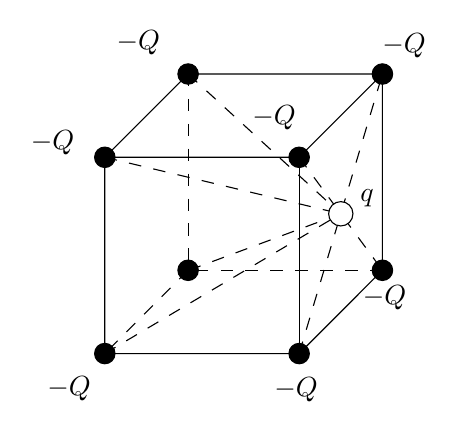
\begin{tikzpicture}[x=0.75pt,y=0.75pt,yscale=-1,xscale=1]
%uncomment if require: \path (0,205); %set diagram left start at 0, and has height of 205

%Shape: Cube [id:dp24209537695489214] 
\draw   (281.41,73.63) -- (321.54,33.5) -- (415.17,33.5) -- (415.17,128.07) -- (375.05,168.2) -- (281.41,168.2) -- cycle ; \draw   (415.17,33.5) -- (375.05,73.63) -- (281.41,73.63) ; \draw   (375.05,73.63) -- (375.05,168.2) ;
%Straight Lines [id:da6552145415795416] 
\draw  [dash pattern={on 4.5pt off 4.5pt}]  (321.54,33.5) -- (321.54,128.07) ;
%Straight Lines [id:da9574617665960996] 
\draw  [dash pattern={on 4.5pt off 4.5pt}]  (415.17,128.07) -- (321.91,128.07) ;
%Straight Lines [id:da06581595655266037] 
\draw  [dash pattern={on 4.5pt off 4.5pt}]  (321.54,128.07) -- (281.41,168.2) ;
%Flowchart: Connector [id:dp41511649615136736] 
\draw  [fill={rgb, 255:red, 0; green, 0; blue, 0 }  ,fill opacity=1 ] (276.5,73.63) .. controls (276.5,70.92) and (278.7,68.72) .. (281.41,68.72) .. controls (284.13,68.72) and (286.33,70.92) .. (286.33,73.63) .. controls (286.33,76.35) and (284.13,78.55) .. (281.41,78.55) .. controls (278.7,78.55) and (276.5,76.35) .. (276.5,73.63) -- cycle ;
%Flowchart: Connector [id:dp4876596956950916] 
\draw  [fill={rgb, 255:red, 0; green, 0; blue, 0 }  ,fill opacity=1 ] (276.5,168.2) .. controls (276.5,165.48) and (278.7,163.28) .. (281.41,163.28) .. controls (284.13,163.28) and (286.33,165.48) .. (286.33,168.2) .. controls (286.33,170.91) and (284.13,173.11) .. (281.41,173.11) .. controls (278.7,173.11) and (276.5,170.91) .. (276.5,168.2) -- cycle ;
%Flowchart: Connector [id:dp4578757750078104] 
\draw  [fill={rgb, 255:red, 0; green, 0; blue, 0 }  ,fill opacity=1 ] (410.26,128.07) .. controls (410.26,125.36) and (412.46,123.15) .. (415.17,123.15) .. controls (417.89,123.15) and (420.09,125.36) .. (420.09,128.07) .. controls (420.09,130.79) and (417.89,132.99) .. (415.17,132.99) .. controls (412.46,132.99) and (410.26,130.79) .. (410.26,128.07) -- cycle ;
%Flowchart: Connector [id:dp39812879825306147] 
\draw  [fill={rgb, 255:red, 0; green, 0; blue, 0 }  ,fill opacity=1 ] (316.63,128.07) .. controls (316.63,125.36) and (318.83,123.15) .. (321.54,123.15) .. controls (324.26,123.15) and (326.46,125.36) .. (326.46,128.07) .. controls (326.46,130.79) and (324.26,132.99) .. (321.54,132.99) .. controls (318.83,132.99) and (316.63,130.79) .. (316.63,128.07) -- cycle ;
%Flowchart: Connector [id:dp35502902150570725] 
\draw  [fill={rgb, 255:red, 0; green, 0; blue, 0 }  ,fill opacity=1 ] (370.13,168.2) .. controls (370.13,165.48) and (372.33,163.28) .. (375.05,163.28) .. controls (377.76,163.28) and (379.96,165.48) .. (379.96,168.2) .. controls (379.96,170.91) and (377.76,173.11) .. (375.05,173.11) .. controls (372.33,173.11) and (370.13,170.91) .. (370.13,168.2) -- cycle ;
%Flowchart: Connector [id:dp9259530091725627] 
\draw  [fill={rgb, 255:red, 0; green, 0; blue, 0 }  ,fill opacity=1 ] (410.26,33.5) .. controls (410.26,30.79) and (412.46,28.59) .. (415.17,28.59) .. controls (417.89,28.59) and (420.09,30.79) .. (420.09,33.5) .. controls (420.09,36.22) and (417.89,38.42) .. (415.17,38.42) .. controls (412.46,38.42) and (410.26,36.22) .. (410.26,33.5) -- cycle ;
%Flowchart: Connector [id:dp45876583578064944] 
\draw  [fill={rgb, 255:red, 0; green, 0; blue, 0 }  ,fill opacity=1 ] (316.63,33.5) .. controls (316.63,30.79) and (318.83,28.59) .. (321.54,28.59) .. controls (324.26,28.59) and (326.46,30.79) .. (326.46,33.5) .. controls (326.46,36.22) and (324.26,38.42) .. (321.54,38.42) .. controls (318.83,38.42) and (316.63,36.22) .. (316.63,33.5) -- cycle ;
%Straight Lines [id:da905955850885398] 
\draw  [dash pattern={on 4.5pt off 4.5pt}]  (321.54,33.5) -- (395.11,100.85) ;
%Straight Lines [id:da9670866838623073] 
\draw  [dash pattern={on 4.5pt off 4.5pt}]  (375.05,168.2) -- (415.17,33.5) ;
%Straight Lines [id:da7266251533013184] 
\draw  [dash pattern={on 4.5pt off 4.5pt}]  (375.05,73.63) -- (415.17,128.07) ;
%Flowchart: Connector [id:dp5253855939543575] 
\draw  [fill={rgb, 255:red, 0; green, 0; blue, 0 }  ,fill opacity=1 ] (370.13,73.63) .. controls (370.13,70.92) and (372.33,68.72) .. (375.05,68.72) .. controls (377.76,68.72) and (379.96,70.92) .. (379.96,73.63) .. controls (379.96,76.35) and (377.76,78.55) .. (375.05,78.55) .. controls (372.33,78.55) and (370.13,76.35) .. (370.13,73.63) -- cycle ;
%Straight Lines [id:da19896497025807758] 
\draw  [dash pattern={on 4.5pt off 4.5pt}]  (281.41,73.63) -- (395.11,100.85) ;
%Straight Lines [id:da878238857030275] 
\draw  [dash pattern={on 4.5pt off 4.5pt}]  (281.41,168.2) -- (395.11,100.85) ;
%Straight Lines [id:da7466399768898722] 
\draw  [dash pattern={on 4.5pt off 4.5pt}]  (321.91,128.07) -- (395.11,100.85) ;
%Shape: Circle [id:dp48972228222895464] 
\draw  [fill={rgb, 255:red, 255; green, 255; blue, 255 }  ,fill opacity=1 ] (389.25,100.85) .. controls (389.25,97.61) and (391.87,94.99) .. (395.11,94.99) .. controls (398.35,94.99) and (400.97,97.61) .. (400.97,100.85) .. controls (400.97,104.09) and (398.35,106.72) .. (395.11,106.72) .. controls (391.87,106.72) and (389.25,104.09) .. (389.25,100.85) -- cycle ;

% Text Node
\draw (252.52,178.12) node [anchor=north west][inner sep=0.75pt]    {$-Q$};
% Text Node
\draw (244.52,59.45) node [anchor=north west][inner sep=0.75pt]    {$-Q$};
% Text Node
\draw (285.85,11.45) node [anchor=north west][inner sep=0.75pt]    {$-Q$};
% Text Node
\draw (413.85,12.79) node [anchor=north west][inner sep=0.75pt]    {$-Q$};
% Text Node
\draw (351.19,47.63) node [anchor=north west][inner sep=0.75pt]    {$-Q$};
% Text Node
\draw (404.52,134.3) node [anchor=north west][inner sep=0.75pt]    {$-Q$};
% Text Node
\draw (361.85,178.3) node [anchor=north west][inner sep=0.75pt]    {$-Q$};
% Text Node
\draw (403.33,87.73) node [anchor=north west][inner sep=0.75pt]    {$q$};
\end{tikzpicture}
   \end{minipage}
    Bảo toàn năng lượng, ta có:
    \begin{equation*}
        \dfrac{mv^2}{2}+U_i=U_f+E \\
        \Leftrightarrow\dfrac{mv^2}{2}=\left(-4 \sqrt{2}-4 \sqrt{\dfrac{2}{3}}+\dfrac{16}{\sqrt{3}}\right) \dfrac{k q Q}{l}+E.
    \end{equation*}
    Từ đó tính được $v=0,354\dv{m/s^2}$.
    \end{loigiai}
    
    \begin{vd}[Điện dung của hệ hình trụ]
\begin{enumerate}[1)]
    \item Tìm điện dung của một đơn vị chiều dài giữa một cặp dây dẫn hình trụ song song có bán kính $R$ và cách nhau một khoảng $d(d\gg R)$, như trong hình $(a)$.
    \item Một dây dẫn hình trụ có bán kính $R$ được đặt ở trên một tấm dẫn phẳng được nối đất, cách mặt phẳng dẫn một đoạn $d(d\gg R)$, như hình $(b)$. Tìm điện dung của một đơn vị chiều dài giữa hai vật dẫn đó.
\end{enumerate}
\begin{center}


\tikzset{every picture/.style={line width=0.75pt}} %set default line width to 0.75pt        

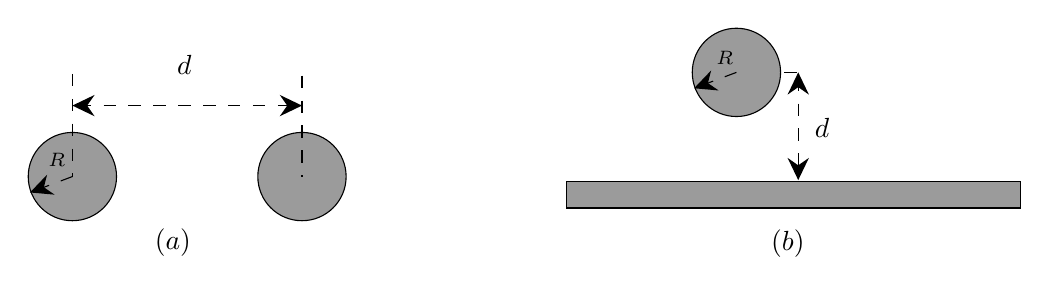
\begin{tikzpicture}[x=0.75pt,y=0.75pt,yscale=-1,xscale=1]
%uncomment if require: \path (0,300); %set diagram left start at 0, and has height of 300

%Straight Lines [id:da677113196713506] 
\draw  [dash pattern={on 4.5pt off 4.5pt}]  (68.27,136.47) -- (172.9,136.47) ;
\draw [shift={(175.9,136.47)}, rotate = 180] [fill={rgb, 255:red, 0; green, 0; blue, 0 }  ][line width=0.08]  [draw opacity=0] (10.72,-5.15) -- (0,0) -- (10.72,5.15) -- (7.12,0) -- cycle    ;
\draw [shift={(65.27,136.47)}, rotate = 0] [fill={rgb, 255:red, 0; green, 0; blue, 0 }  ][line width=0.08]  [draw opacity=0] (10.72,-5.15) -- (0,0) -- (10.72,5.15) -- (7.12,0) -- cycle    ;
%Shape: Circle [id:dp874210144956922] 
\draw  [fill={rgb, 255:red, 155; green, 155; blue, 155 }  ,fill opacity=1 ] (44,170.67) .. controls (44,158.92) and (53.52,149.4) .. (65.27,149.4) .. controls (77.02,149.4) and (86.54,158.92) .. (86.54,170.67) .. controls (86.54,182.42) and (77.02,191.94) .. (65.27,191.94) .. controls (53.52,191.94) and (44,182.42) .. (44,170.67) -- cycle ;
%Shape: Circle [id:dp1813413337643932] 
\draw  [fill={rgb, 255:red, 155; green, 155; blue, 155 }  ,fill opacity=1 ] (154.62,170.67) .. controls (154.62,158.92) and (164.14,149.4) .. (175.89,149.4) .. controls (187.64,149.4) and (197.16,158.92) .. (197.16,170.67) .. controls (197.16,182.42) and (187.64,191.94) .. (175.89,191.94) .. controls (164.14,191.94) and (154.62,182.42) .. (154.62,170.67) -- cycle ;
%Straight Lines [id:da5768044451421217] 
\draw  [dash pattern={on 4.5pt off 4.5pt}]  (175.89,122.03) -- (175.89,170.67) ;
%Straight Lines [id:da2702097859751069] 
\draw  [dash pattern={on 4.5pt off 4.5pt}]  (65.27,121.18) -- (65.27,170.67) ;
%Straight Lines [id:da6104556670247443] 
\draw  [dash pattern={on 4.5pt off 4.5pt}]  (65.27,170.67) -- (47.68,177.28) ;
\draw [shift={(44.87,178.33)}, rotate = 339.43] [fill={rgb, 255:red, 0; green, 0; blue, 0 }  ][line width=0.08]  [draw opacity=0] (10.72,-5.15) -- (0,0) -- (10.72,5.15) -- (7.12,0) -- cycle    ;
%Shape: Rectangle [id:dp6837421498436178] 
\draw  [fill={rgb, 255:red, 155; green, 155; blue, 155 }  ,fill opacity=1 ] (303.52,173.23) -- (522.22,173.23) -- (522.22,185.82) -- (303.52,185.82) -- cycle ;
%Shape: Circle [id:dp2448813293793357] 
\draw  [fill={rgb, 255:red, 155; green, 155; blue, 155 }  ,fill opacity=1 ] (363.93,120.47) .. controls (363.93,108.72) and (373.46,99.2) .. (385.21,99.2) .. controls (396.96,99.2) and (406.48,108.72) .. (406.48,120.47) .. controls (406.48,132.22) and (396.96,141.74) .. (385.21,141.74) .. controls (373.46,141.74) and (363.93,132.22) .. (363.93,120.47) -- cycle ;
%Straight Lines [id:da6679308714290266] 
\draw  [dash pattern={on 4.5pt off 4.5pt}]  (385.21,120.47) -- (367.61,127.07) ;
\draw [shift={(364.8,128.13)}, rotate = 339.43] [fill={rgb, 255:red, 0; green, 0; blue, 0 }  ][line width=0.08]  [draw opacity=0] (10.72,-5.15) -- (0,0) -- (10.72,5.15) -- (7.12,0) -- cycle    ;
%Straight Lines [id:da016736600541896518] 
\draw  [dash pattern={on 4.5pt off 4.5pt}]  (414.99,123.47) -- (414.99,169.37) ;
\draw [shift={(414.99,172.37)}, rotate = 270] [fill={rgb, 255:red, 0; green, 0; blue, 0 }  ][line width=0.08]  [draw opacity=0] (10.72,-5.15) -- (0,0) -- (10.72,5.15) -- (7.12,0) -- cycle    ;
\draw [shift={(414.99,120.47)}, rotate = 90] [fill={rgb, 255:red, 0; green, 0; blue, 0 }  ][line width=0.08]  [draw opacity=0] (10.72,-5.15) -- (0,0) -- (10.72,5.15) -- (7.12,0) -- cycle    ;
%Straight Lines [id:da049016635462894476] 
\draw  [dash pattern={on 4.5pt off 4.5pt}]  (408.17,120.47) -- (414.99,120.47) ;

% Text Node
\draw (52.39,158.1) node [anchor=north west][inner sep=0.75pt]  [font=\scriptsize]  {$R$};
% Text Node
\draw (103.7,194.31) node [anchor=north west][inner sep=0.75pt]    {$( a)$};
% Text Node
\draw (374.33,108.89) node [anchor=north west][inner sep=0.75pt]  [font=\scriptsize]  {$R$};
% Text Node
\draw (114.51,110.93) node [anchor=north west][inner sep=0.75pt]    {$d$};
% Text Node
\draw (421.68,141.56) node [anchor=north west][inner sep=0.75pt]    {$d$};
% Text Node
\draw (400.66,195.16) node [anchor=north west][inner sep=0.75pt]    {$( b)$};


\end{tikzpicture}
\end{center}
\end{vd}
\begin{loigiai}
\begin{enumerate}[1)]
    \item Giả sử một sợi dây cáp có mật độ điện dài $\lambda$ và dây còn lại có mật độ điện dài $-\lambda$.\\
    Chọn đường nối hai tâm dây cáp làm trục $X$ và chọn $x=0$ tại trung điểm giữa hai dây cáp.\\
    Điện trường toàn phần tại một điểm trên trục $X$ là:
    \[E=\dfrac{\lambda}{2\pi\varepsilon_0}\left(\dfrac{1}{\dfrac{d}{2}+x}+\dfrac{1}{\dfrac{d}{2}-x}\right).\]
    Hiệu điện thế giữa hai dây cáp:
    \begin{align*}
    U&=\int_{-(\dfrac{d}{2}-R)}^{\dfrac{d}{2}-R}E\mathrm{d}x=\dfrac{\lambda}{2\pi\varepsilon_0}\left.\left[\ln{\left(\dfrac{d}{2}+x\right)}-\ln{\left(\dfrac{d}{2}-x\right)}\right]\right|_{-\left(\dfrac{d}{2}-R\right)}^{\left(\dfrac{d}{2}-R\right)}\\
    &=\dfrac{\lambda}{\pi\varepsilon_0}\ln{\left(\dfrac{d-R}{R}\right)}\approx \dfrac{\lambda}{\pi\varepsilon_0}\ln{\left(\dfrac{d}{R}\right)}.
    \end{align*}
    Điện dung của hệ $2$ dây cáp là:
    \[C=\dfrac{Q}{U}=\dfrac{\pi\varepsilon_0}{\ln{\left(\dfrac{2d}{R}\right)}}.\]
    \item Áp dụng phương pháp ảnh điện, điện trường là:
    \[E=\dfrac{\lambda}{2\pi\varepsilon_0}\left(\dfrac{1}{d+x}+\dfrac{1}{d-x}\right).\]
    Hiệu điện thế là:
    \begin{align*}
        U&=\int_{-(d-R)}^{0}E\mathrm{d}x=\dfrac{\lambda}{2\pi\varepsilon_0}\left.\left[\ln{(d+x)-\ln{(d-x)}}\right]\right|_{-(d-R)}^{0}\\
        &=\dfrac{\lambda}{2\pi\varepsilon_0}\ln{\left(\dfrac{2d-R}{R}\right)}\approx \dfrac{\lambda}{2\pi\varepsilon_0}\ln{\left(\dfrac{2d}{R}\right)}.
        \end{align*}
        Điện dung của hệ:
        \[C=\dfrac{Q}{U}=\dfrac{2\pi\varepsilon_0}{\ln{\left(\dfrac{2d}{R}\right)}}.\]
\end{enumerate}
\end{loigiai}

    \begin{vd}[Mô hình phân cực]
    \begin{minipage}{0.65\textwidth}
      Chúng ta coi rằng một quả cầu trung hòa về điện là sự kết hợp của hai quả cầu khác nhau: một quả cầu tích điện đều theo thể tích với mật độ $+\rho$, bao gồm các hạt nhân của các nguyên tử, quả còn lại có cùng bán kính tích điện đều với mật độ $-\rho$, bao gồm các electron. Giả sử rằng bằng một cách nào đó chúng ta có thể dịch chuyển hai quả cầu này sao cho tâm của chúng cách nhau một khoảng $\delta$ như trong hình, mà không làm thay đổi cầu trúc của hai quả cầu.\\
    Tìm điện trường tạo bởi phân bố điện tích trên:
    \end{minipage}
    \begin{minipage}{0.3\textwidth}
      \centering

\tikzset{every picture/.style={line width=0.75pt}} %set default line width to 0.75pt        

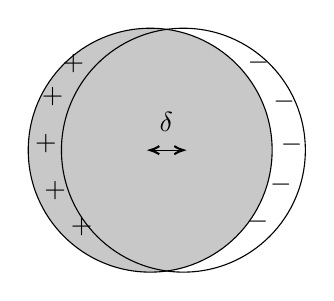
\begin{tikzpicture}[x=0.75pt,y=0.75pt,yscale=-1,xscale=1]
%uncomment if require: \path (0,179); %set diagram left start at 0, and has height of 179

%Shape: Circle [id:dp348067281994352] 
\draw  [fill={rgb, 255:red, 200; green, 200; blue, 200 }  ,fill opacity=1 ] (245.33,91.25) .. controls (245.33,58.81) and (271.64,32.5) .. (304.09,32.5) .. controls (336.53,32.5) and (362.84,58.81) .. (362.84,91.25) .. controls (362.84,123.7) and (336.53,150.01) .. (304.09,150.01) .. controls (271.64,150.01) and (245.33,123.7) .. (245.33,91.25) -- cycle ;
%Shape: Circle [id:dp010283630354624318] 
\draw   (261.33,91.25) .. controls (261.33,58.81) and (287.64,32.5) .. (320.09,32.5) .. controls (352.53,32.5) and (378.84,58.81) .. (378.84,91.25) .. controls (378.84,123.7) and (352.53,150.01) .. (320.09,150.01) .. controls (287.64,150.01) and (261.33,123.7) .. (261.33,91.25) -- cycle ;
%Straight Lines [id:da7330655663361718] 
\draw    (306.09,91.25) -- (318.09,91.25) ;
\draw [shift={(320.09,91.25)}, rotate = 180] [color={rgb, 255:red, 0; green, 0; blue, 0 }  ][line width=0.75]    (4.37,-1.96) .. controls (2.78,-0.92) and (1.32,-0.27) .. (0,0) .. controls (1.32,0.27) and (2.78,0.92) .. (4.37,1.96)   ;
\draw [shift={(304.09,91.25)}, rotate = 0] [color={rgb, 255:red, 0; green, 0; blue, 0 }  ][line width=0.75]    (4.37,-1.96) .. controls (2.78,-0.92) and (1.32,-0.27) .. (0,0) .. controls (1.32,0.27) and (2.78,0.92) .. (4.37,1.96)   ;

% Text Node
\draw (260.59,43.94) node [anchor=north west][inner sep=0.75pt]    {$+$};
% Text Node
\draw (250.59,59.58) node [anchor=north west][inner sep=0.75pt]    {$+$};
% Text Node
\draw (247.39,82.38) node [anchor=north west][inner sep=0.75pt]    {$+$};
% Text Node
\draw (251.79,105.18) node [anchor=north west][inner sep=0.75pt]    {$+$};
% Text Node
\draw (264.59,122.38) node [anchor=north west][inner sep=0.75pt]    {$+$};
% Text Node
\draw (349.39,120.17) node [anchor=north west][inner sep=0.75pt]    {$-$};
% Text Node
\draw (360.59,101.98) node [anchor=north west][inner sep=0.75pt]    {$-$};
% Text Node
\draw (365.79,82.78) node [anchor=north west][inner sep=0.75pt]    {$-$};
% Text Node
\draw (362.19,61.98) node [anchor=north west][inner sep=0.75pt]    {$-$};
% Text Node
\draw (349.79,43.58) node [anchor=north west][inner sep=0.75pt]    {$-$};
% Text Node
\draw (307.39,71.75) node [anchor=north west][inner sep=0.75pt]    {$\delta $};


\end{tikzpicture}

    \end{minipage}
    \begin{enumerate}[1)]
    \setlength{\itemsep}{0pt}
        \item Tại vùng không gian giao nhau giữa hai quả cầu.
        \item Tại vùng không gian bên ngoài hai quả cầu, đánh giá kết quả khi $\delta\ll R$.
    \end{enumerate}
    \end{vd}
    \begin{loigiai}
    \begin{enumerate}[1)]
        \item Theo nguyên lý chồng chất, điện trường tại một điểm trong không gian sẽ là sự tổng hợp điện trường sinh ra bởi hai quả cầu.\\
        Đối với một quả cầu riêng biệt tích điện với mật độ điện khối $\rho$, điện trường do quả cầu tạo ra tại một điểm cách tâm nó một khoảng $r<R$ là:
        \begin{equation*}
            \ot{E}=\dfrac{4\pi k\rho \ot{r}}{3}.
        \end{equation*}
        Coi rằng tâm của hai quả cầu nằm trên trục $x$ và tâm của hai quả cầu có tọa độ lần lượt là $O_+\tron{\dfrac{\delta}{2},0,0}$ và $O_-\tron{-\dfrac{\delta}{2},0,0}$.
        \begin{center}
            

\tikzset{every picture/.style={line width=0.75pt}} %set default line width to 0.75pt        

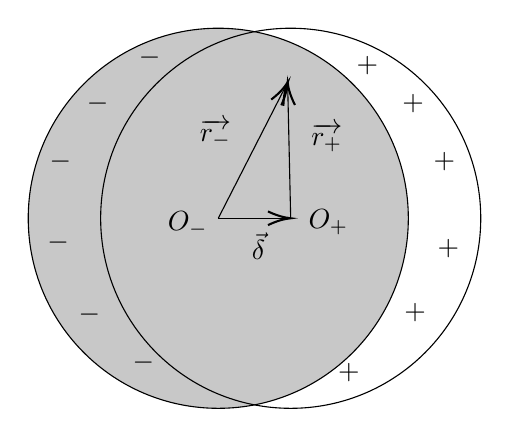
\begin{tikzpicture}[x=0.75pt,y=0.75pt,yscale=-1,xscale=1]
%uncomment if require: \path (0,221); %set diagram left start at 0, and has height of 221

%Shape: Circle [id:dp017437485907043415] 
\draw  [color={rgb, 255:red, 0; green, 0; blue, 0 }  ,draw opacity=1 ][fill={rgb, 255:red, 200; green, 200; blue, 200 }  ,fill opacity=1 ] (226,108.56) .. controls (226,57.99) and (266.99,17) .. (317.56,17) .. controls (368.13,17) and (409.13,57.99) .. (409.13,108.56) .. controls (409.13,159.13) and (368.13,200.13) .. (317.56,200.13) .. controls (266.99,200.13) and (226,159.13) .. (226,108.56) -- cycle ;
%Shape: Circle [id:dp8644229876539793] 
\draw   (260.89,108.56) .. controls (260.89,57.99) and (301.89,17) .. (352.45,17) .. controls (403.02,17) and (444.02,57.99) .. (444.02,108.56) .. controls (444.02,159.13) and (403.02,200.13) .. (352.45,200.13) .. controls (301.89,200.13) and (260.89,159.13) .. (260.89,108.56) -- cycle ;
%Straight Lines [id:da3225302970061237] 
\draw    (317.56,108.56) -- (350.45,108.56) ;
\draw [shift={(352.45,108.56)}, rotate = 180] [color={rgb, 255:red, 0; green, 0; blue, 0 }  ][line width=0.75]    (10.93,-3.29) .. controls (6.95,-1.4) and (3.31,-0.3) .. (0,0) .. controls (3.31,0.3) and (6.95,1.4) .. (10.93,3.29)   ;
%Straight Lines [id:da03191807652795409] 
\draw    (317.56,108.56) -- (350.06,44.91) ;
\draw [shift={(350.97,43.13)}, rotate = 477.05] [color={rgb, 255:red, 0; green, 0; blue, 0 }  ][line width=0.75]    (10.93,-3.29) .. controls (6.95,-1.4) and (3.31,-0.3) .. (0,0) .. controls (3.31,0.3) and (6.95,1.4) .. (10.93,3.29)   ;
%Straight Lines [id:da4064808818545982] 
\draw    (352.45,108.56) -- (351.02,45.13) ;
\draw [shift={(350.97,43.13)}, rotate = 448.7] [color={rgb, 255:red, 0; green, 0; blue, 0 }  ][line width=0.75]    (10.93,-3.29) .. controls (6.95,-1.4) and (3.31,-0.3) .. (0,0) .. controls (3.31,0.3) and (6.95,1.4) .. (10.93,3.29)   ;

% Text Node
\draw (359.85,103.27) node [anchor=north west][inner sep=0.75pt]    {$O_{+}$};
% Text Node
\draw (292.05,104.24) node [anchor=north west][inner sep=0.75pt]    {$O_{-}$};
% Text Node
\draw (361.13,61.45) node [anchor=north west][inner sep=0.75pt]    {$\ot{r_{+}}$};
% Text Node
\draw (307.46,59.68) node [anchor=north west][inner sep=0.75pt]    {$\ot{r_{-}}$};
% Text Node
\draw (332.49,114.2) node [anchor=north west][inner sep=0.75pt]    {$\vec{\delta }$};
% Text Node
\draw (374,177.4) node [anchor=north west][inner sep=0.75pt]    {$+$};
% Text Node
\draw (406,148.4) node [anchor=north west][inner sep=0.75pt]    {$+$};
% Text Node
\draw (383,29.4) node [anchor=north west][inner sep=0.75pt]    {$+$};
% Text Node
\draw (420,75.4) node [anchor=north west][inner sep=0.75pt]    {$+$};
% Text Node
\draw (405,47.4) node [anchor=north west][inner sep=0.75pt]    {$+$};
% Text Node
\draw (422,117.38) node [anchor=north west][inner sep=0.75pt]    {$+$};
% Text Node
\draw (253,47.4) node [anchor=north west][inner sep=0.75pt]    {$-$};
% Text Node
\draw (235,75.4) node [anchor=north west][inner sep=0.75pt]    {$-$};
% Text Node
\draw (234,114.4) node [anchor=north west][inner sep=0.75pt]    {$-$};
% Text Node
\draw (249,149.4) node [anchor=north west][inner sep=0.75pt]    {$-$};
% Text Node
\draw (275,172.38) node [anchor=north west][inner sep=0.75pt]    {$-$};
% Text Node
\draw (278,25.38) node [anchor=north west][inner sep=0.75pt]    {$-$};


\end{tikzpicture}

        \end{center}
        Ta có:
        \begin{equation*}
            \begin{aligned}
                 &\ot{r_+}=\ot{r}+\dfrac{\ot{\delta}}{2},\\
                 &\ot{r_-}=\ot{r}-\dfrac{\ot{\delta}}{2}.
            \end{aligned}
        \end{equation*}
        Điện trường tại vùng giao nhau của hai quả cầu:
        \begin{equation*}
            \ot{E}=\dfrac{4\pi k\rho \tron{\ot{r}-\dfrac{\ot{\delta}}{2}}}{3}-\dfrac{4\pi k\rho\tron{\ot{r}+\dfrac{\ot{\delta}}{2}}}{3}=-\dfrac{4\pi k\rho\ot{\delta}}{3}.
        \end{equation*}
       \item Điện trường do một quả cầu bán kính $R$, tích điện đều với mật độ điện khối $\rho$ gây ra ở vùng không gian bên ngoài quả cầu giống như điện trường của một điện tích điểm $Q=\dfrac{4\pi R^3 \rho}{3}$ đặt tại tâm quả cầu. Vậy nên, điện trường do hai quả cầu gây ra tại vùng không gian bên ngoài quả cầu giống như điện trường gây ra bởi hai điện tích điểm $\pm Q$ đặt tại $O_+$ và $O_-$. Nếu $R\gg \delta$, điện trường này tương đương với điện trường của một lưỡng cực điện có moment lưỡng cực:
        $$\ot{p}=Q\ot{\delta}=\dfrac{4\pi R^3\rho}{3}\ot{\delta} . $$
        Điện trường tạo ra:
        $$\ot{E}=k\tron{\dfrac{\ot{r}\tron{\ot{p}\cdot\ot{r}}}{r^5}-\dfrac{\ot{p}}{r^3}}.$$
    \end{enumerate}
    \end{loigiai}
    
    
    
    \begin{vd}[Điện trường trong hốc cầu rỗng]
    \begin{minipage}{0.5\textwidth}
      Một quả cầu đồng chất bán kính $a$ tích điện đều với mật độ điện tích $\rho$. Người ta khoét ở bên trong quả cầu một khoang trống hình cầu bán kính $b<a$, bên trong khoang không tích điện. Tâm của khoang $O_b$ cách tâm của hình cầu $O_a$ một khoảng $d$, với $d<(a-b)$.
    \end{minipage}
    \begin{minipage}{0.5\textwidth}
      \centering
\tikzset{every picture/.style={line width=0.75pt}} %set default line width to 0.75pt        

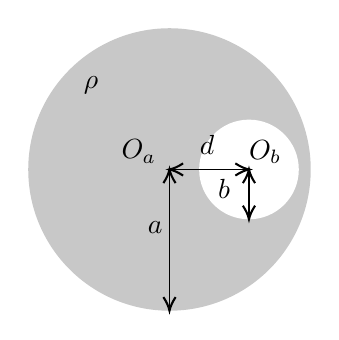
\begin{tikzpicture}[x=0.75pt,y=0.75pt,yscale=-1,xscale=1]
%uncomment if require: \path (0,179); %set diagram left start at 0, and has height of 179

%Shape: Circle [id:dp5133875522475451] 
\draw  [color={rgb, 255:red, 0; green, 0; blue, 0 }  ,draw opacity=0 ][fill={rgb, 255:red, 200; green, 200; blue, 200 }  ,fill opacity=1 ] (282.33,94.05) .. controls (282.33,56.47) and (312.8,26) .. (350.39,26) .. controls (387.97,26) and (418.44,56.47) .. (418.44,94.05) .. controls (418.44,131.64) and (387.97,162.1) .. (350.39,162.1) .. controls (312.8,162.1) and (282.33,131.64) .. (282.33,94.05) -- cycle ;
%Shape: Ellipse [id:dp5662859497643196] 
\draw  [color={rgb, 255:red, 0; green, 0; blue, 0 }  ,draw opacity=0 ][fill={rgb, 255:red, 255; green, 255; blue, 255 }  ,fill opacity=1 ] (364.67,94.05) .. controls (364.67,80.79) and (375.42,70.04) .. (388.68,70.04) .. controls (401.94,70.04) and (412.69,80.79) .. (412.69,94.05) .. controls (412.69,107.31) and (401.94,118.06) .. (388.68,118.06) .. controls (375.42,118.06) and (364.67,107.31) .. (364.67,94.05) -- cycle ;
%Straight Lines [id:da523226980810126] 
\draw    (350.39,96.05) -- (350.39,160.1) ;
\draw [shift={(350.39,162.1)}, rotate = 270] [color={rgb, 255:red, 0; green, 0; blue, 0 }  ][line width=0.75]    (6.56,-2.94) .. controls (4.17,-1.38) and (1.99,-0.4) .. (0,0) .. controls (1.99,0.4) and (4.17,1.38) .. (6.56,2.94)   ;
\draw [shift={(350.39,94.05)}, rotate = 90] [color={rgb, 255:red, 0; green, 0; blue, 0 }  ][line width=0.75]    (6.56,-2.94) .. controls (4.17,-1.38) and (1.99,-0.4) .. (0,0) .. controls (1.99,0.4) and (4.17,1.38) .. (6.56,2.94)   ;
%Straight Lines [id:da7784251747453967] 
\draw    (388.68,96.05) -- (388.68,116.06) ;
\draw [shift={(388.68,118.06)}, rotate = 270] [color={rgb, 255:red, 0; green, 0; blue, 0 }  ][line width=0.75]    (6.56,-2.94) .. controls (4.17,-1.38) and (1.99,-0.4) .. (0,0) .. controls (1.99,0.4) and (4.17,1.38) .. (6.56,2.94)   ;
\draw [shift={(388.68,94.05)}, rotate = 90] [color={rgb, 255:red, 0; green, 0; blue, 0 }  ][line width=0.75]    (6.56,-2.94) .. controls (4.17,-1.38) and (1.99,-0.4) .. (0,0) .. controls (1.99,0.4) and (4.17,1.38) .. (6.56,2.94)   ;
%Straight Lines [id:da2698365651836454] 
\draw    (352.39,94.05) -- (386.68,94.05) ;
\draw [shift={(388.68,94.05)}, rotate = 180] [color={rgb, 255:red, 0; green, 0; blue, 0 }  ][line width=0.75]    (6.56,-2.94) .. controls (4.17,-1.38) and (1.99,-0.4) .. (0,0) .. controls (1.99,0.4) and (4.17,1.38) .. (6.56,2.94)   ;
\draw [shift={(350.39,94.05)}, rotate = 0] [color={rgb, 255:red, 0; green, 0; blue, 0 }  ][line width=0.75]    (6.56,-2.94) .. controls (4.17,-1.38) and (1.99,-0.4) .. (0,0) .. controls (1.99,0.4) and (4.17,1.38) .. (6.56,2.94)   ;

% Text Node
\draw (363.73,76.11) node [anchor=north west][inner sep=0.75pt]    {$d$};
% Text Node
\draw (372.53,97.45) node [anchor=north west][inner sep=0.75pt]    {$b$};
% Text Node
\draw (387.44,78.95) node [anchor=north west][inner sep=0.75pt]    {$O_{b}$};
% Text Node
\draw (338.69,117.95) node [anchor=north west][inner sep=0.75pt]    {$a$};
% Text Node
\draw (326.05,78.61) node [anchor=north west][inner sep=0.75pt]    {$O_{a}$};
% Text Node
\draw (307.82,47.98) node [anchor=north west][inner sep=0.75pt]    {$\rho $};
\end{tikzpicture}
    \end{minipage}
    \begin{enumerate}[1)]
        \setlength{\itemsep}{0pt}
        \item Tìm điện trường tại vùng không gian bên trong khoang trống.\\
        \end{enumerate}
         Bây giờ toàn bộ quả cầu được đặt trong điện trường đều có cường độ điện trường $E_0$.
        \begin{enumerate}[1)]
        \setcounter{enumi}{1}
        \item Tìm lực tác dụng lên quả cầu.
        \item Tìm moment lực tác dụng lên quả cầu đối với quả cầu và đối với khối tâm quả cầu.
    \end{enumerate}
    \end{vd}
    \begin{loigiai}
    \begin{enumerate}[1)]
    \setlength{\itemsep}{0pt}
        \item Một quả cầu có mật độ điện tích $\rho$ với một khoang trống hình cầu không điện tích có thể coi như là một quả cầu tích điện $\rho$ khắp thể tích của nó và một quả cầu khác tích điện $-\rho$. Điện trường tại một điểm trong không gian là tổng hợp của điện trường gây ra bởi hai quả cầu.
        \begin{center}
\tikzset{every picture/.style={line width=0.75pt}} %set default line width to 0.75pt        
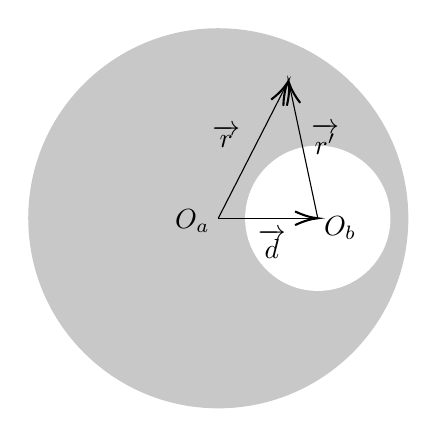
\begin{tikzpicture}[x=0.75pt,y=0.75pt,yscale=-1,xscale=1]
%uncomment if require: \path (0,221); %set diagram left start at 0, and has height of 221

%Shape: Circle [id:dp017437485907043415] 
\draw  [color={rgb, 255:red, 255; green, 255; blue, 255 }  ,draw opacity=0 ][fill={rgb, 255:red, 200; green, 200; blue, 200 }  ,fill opacity=1 ] (226,108.56) .. controls (226,57.99) and (266.99,17) .. (317.56,17) .. controls (368.13,17) and (409.13,57.99) .. (409.13,108.56) .. controls (409.13,159.13) and (368.13,200.13) .. (317.56,200.13) .. controls (266.99,200.13) and (226,159.13) .. (226,108.56) -- cycle ;
%Flowchart: Connector [id:dp8574035111298091] 
\draw  [color={rgb, 255:red, 0; green, 0; blue, 0 }  ,draw opacity=0 ][fill={rgb, 255:red, 255; green, 255; blue, 255 }  ,fill opacity=1 ] (330.51,108.56) .. controls (330.51,89.23) and (346.18,73.56) .. (365.51,73.56) .. controls (384.84,73.56) and (400.51,89.23) .. (400.51,108.56) .. controls (400.51,127.89) and (384.84,143.56) .. (365.51,143.56) .. controls (346.18,143.56) and (330.51,127.89) .. (330.51,108.56) -- cycle ;
%Straight Lines [id:da3225302970061237] 
\draw    (317.56,108.56) -- (363.51,108.56) ;
\draw [shift={(365.51,108.56)}, rotate = 180] [color={rgb, 255:red, 0; green, 0; blue, 0 }  ][line width=0.75]    (10.93,-3.29) .. controls (6.95,-1.4) and (3.31,-0.3) .. (0,0) .. controls (3.31,0.3) and (6.95,1.4) .. (10.93,3.29)   ;
%Straight Lines [id:da03191807652795409] 
\draw    (317.56,108.56) -- (350.06,44.91) ;
\draw [shift={(350.97,43.13)}, rotate = 477.05] [color={rgb, 255:red, 0; green, 0; blue, 0 }  ][line width=0.75]    (10.93,-3.29) .. controls (6.95,-1.4) and (3.31,-0.3) .. (0,0) .. controls (3.31,0.3) and (6.95,1.4) .. (10.93,3.29)   ;
%Straight Lines [id:da4064808818545982] 
\draw    (365.51,108.56) -- (351.96,44.91) ;
\draw [shift={(351.54,42.95)}, rotate = 437.98] [color={rgb, 255:red, 0; green, 0; blue, 0 }  ][line width=0.75]    (10.93,-3.29) .. controls (6.95,-1.4) and (3.31,-0.3) .. (0,0) .. controls (3.31,0.3) and (6.95,1.4) .. (10.93,3.29)   ;

% Text Node
\draw (367.28,106.35) node [anchor=north west][inner sep=0.75pt]    {$O_{b}$};
% Text Node
\draw (295.55,103.24) node [anchor=north west][inner sep=0.75pt]    {$O_{a}$};
% Text Node
\draw (361.13,61.45) node [anchor=north west][inner sep=0.75pt]    {$\ot{r'}$};
% Text Node
\draw (313.46,62.68) node [anchor=north west][inner sep=0.75pt]    {$\ot{r}$};
% Text Node
\draw (335.49,112.7) node [anchor=north west][inner sep=0.75pt]    {$\ot{d}$};


\end{tikzpicture}

        \end{center}
        Ta có:
        \begin{equation*}
            \ot{E}=\dfrac{4\pi k}{3}\tron{\ot{r}-\ot{r'}}=\dfrac{4\pi k}{3}\ot{d}.
        \end{equation*}
        Điện trường bên trong khoang trống là đều và song song với đường thằng nối tâm quả cầu và khoang trống.
        \item Khi hệ được đặt trong điện trường đều. Có thể coi lực tác dụng lên hệ như là lực mà điện trường tác dụng lên hai điện tích $q_a=\dfrac{4\pi a^3\rho}{3}$ và $q_b=-\dfrac{4\pi b^3\rho}{3}$ lần lượt đặt tại $O_a$ và $O_b$. \\ 
        Ta có:
        \begin{equation*}
            \ot{F}=\dfrac{4\pi k\tron{a^3-b^3}\rho}{3}\ot{E_0}.
        \end{equation*}
        \item Bởi vì hợp lực tác dụng lên hệ khác không nên moment lực tác dụng lên hệ phụ thuộc vào vị trí chọn tâm quay.\\
        Moment lực tác dụng lên quả cầu đối với tâm quay là $O_a$ là:
        $$\ot{T_1}=-\dfrac{4\pi b^3\rho}{4}\ot{d}\times\ot{E_0}.$$
        Ta chọn một hệ quy chiếu mới với trục $x$ đi qua $O_a$ và $O_b$, gốc tọa độ trùng với $O_a$. Gọi khối lượng riêng của quả cầu là $\rho_m$. Khối lượng của hệ là $M_c=\dfrac{4\pi \tron{a^3-b^3}\rho_m}{3}$. Tọa độ khối tâm của hệ là $x_c$. 
        \\
        Giả sử một quả cầu bán kính $b$ khối lượng $M_b=\dfrac{4\pi b^3\rho_m}{3}$ đặt tại khoang trống của quả cầu. Cả hệ bây giờ như một hình cầu đặc bán kính $a$, khối lượng $M_a=\dfrac{4\pi a^3\rho_m}{3}$ đặt tại $O_a$ có tọa độ bằng không. Ta có:
        $$0=\dfrac{M_cx_c+M_bd}{M_a}\Leftrightarrow x_c=-d\dfrac{M_b}{M_c}=-d\dfrac{b^3}{a^3-b^3}.$$
        Moment lực đối với khối tâm:
        $$\ot{T_2}=\tron{\dfrac{4\pi a^3\rho}{3}\tron{d\dfrac{b^3}{a^3-b^3}}-\dfrac{4\pi b^3\rho }{3}\tron{d+d\dfrac{b^3}{a^3-b^3}}}\tron{\ot{e_x}\times\ot{E_0}}=0.$$
        Trong đó $\ot{e_x}$ là vector đơn vị dọc theo trục $x$.\\
        Kết quả hợp lý vì khi đặt hệ trong điện trường đều, các phần tử của hệ đều chịu một lực tỉ lệ với thể tích, giống như đặt trong một trọng trường đều.
    \end{enumerate}
    \end{loigiai}
    
    
    \begin{vd}[Điện tích trên vòng]
Một hạt coi là chất điểm có khối lượng $m$ và điện tích $q$ chuyển động tự do không ma sát dọc theo một đường tròn nằm ngang cố định bán kính r. Trong mặt phẳng của vòng, một điện tích $Q$ khác được đặt ở một vị trí cố định, cách tâm vòng một khoảng $d$, với $d<r$ (xem hình vẽ). 
\begin{center}
    

\tikzset{every picture/.style={line width=0.75pt}} %set default line width to 0.75pt        

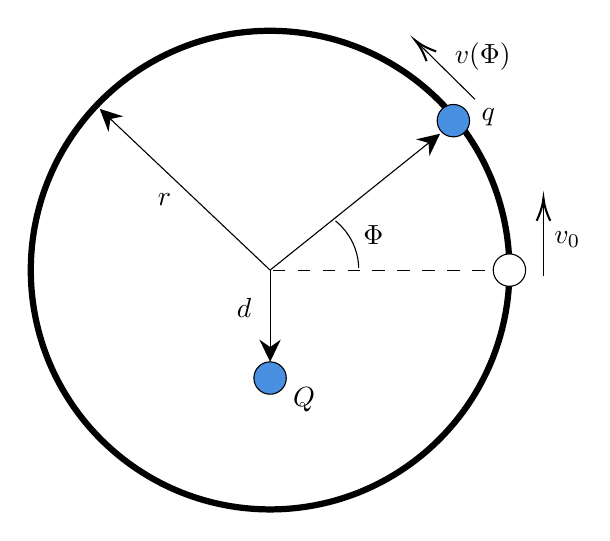
\begin{tikzpicture}[x=0.75pt,y=0.75pt,yscale=-1,xscale=1]
%uncomment if require: \path (0,470); %set diagram left start at 0, and has height of 470

%Shape: Circle [id:dp4352794293041511] 
\draw  [line width=2.25]  (201,179.3) .. controls (201,115.62) and (252.62,64) .. (316.3,64) .. controls (379.98,64) and (431.6,115.62) .. (431.6,179.3) .. controls (431.6,242.98) and (379.98,294.6) .. (316.3,294.6) .. controls (252.62,294.6) and (201,242.98) .. (201,179.3) -- cycle ;
%Straight Lines [id:da5040476830588836] 
\draw  [dash pattern={on 4.5pt off 4.5pt}]  (431.6,179.3) -- (316.3,179.3) ;
%Shape: Circle [id:dp3864705024915467] 
\draw  [fill={rgb, 255:red, 255; green, 255; blue, 255 }  ,fill opacity=1 ] (423.8,179.3) .. controls (423.8,174.99) and (427.29,171.5) .. (431.6,171.5) .. controls (435.91,171.5) and (439.4,174.99) .. (439.4,179.3) .. controls (439.4,183.61) and (435.91,187.1) .. (431.6,187.1) .. controls (427.29,187.1) and (423.8,183.61) .. (423.8,179.3) -- cycle ;
%Shape: Circle [id:dp3760399239302583] 
\draw  [fill={rgb, 255:red, 74; green, 144; blue, 226 }  ,fill opacity=1 ] (396.8,107.3) .. controls (396.8,102.99) and (400.29,99.5) .. (404.6,99.5) .. controls (408.91,99.5) and (412.4,102.99) .. (412.4,107.3) .. controls (412.4,111.61) and (408.91,115.1) .. (404.6,115.1) .. controls (400.29,115.1) and (396.8,111.61) .. (396.8,107.3) -- cycle ;
%Straight Lines [id:da8336614182940776] 
\draw    (236.38,103.66) -- (316.3,179.3) ;
\draw [shift={(234.2,101.6)}, rotate = 43.42] [fill={rgb, 255:red, 0; green, 0; blue, 0 }  ][line width=0.08]  [draw opacity=0] (10.72,-5.15) -- (0,0) -- (10.72,5.15) -- (7.12,0) -- cycle    ;
%Straight Lines [id:da3530703705263947] 
\draw    (395.86,115.48) -- (316.3,179.3) ;
\draw [shift={(398.2,113.6)}, rotate = 141.26] [fill={rgb, 255:red, 0; green, 0; blue, 0 }  ][line width=0.08]  [draw opacity=0] (10.72,-5.15) -- (0,0) -- (10.72,5.15) -- (7.12,0) -- cycle    ;
%Shape: Circle [id:dp513558393549516] 
\draw  [fill={rgb, 255:red, 74; green, 144; blue, 226 }  ,fill opacity=1 ] (308.5,231.3) .. controls (308.5,226.99) and (311.99,223.5) .. (316.3,223.5) .. controls (320.61,223.5) and (324.1,226.99) .. (324.1,231.3) .. controls (324.1,235.61) and (320.61,239.1) .. (316.3,239.1) .. controls (311.99,239.1) and (308.5,235.61) .. (308.5,231.3) -- cycle ;
%Straight Lines [id:da050747851797288135] 
\draw    (316.3,179.3) -- (316.3,220.5) ;
\draw [shift={(316.3,223.5)}, rotate = 270] [fill={rgb, 255:red, 0; green, 0; blue, 0 }  ][line width=0.08]  [draw opacity=0] (10.72,-5.15) -- (0,0) -- (10.72,5.15) -- (7.12,0) -- cycle    ;
%Shape: Arc [id:dp5089728896438459] 
\draw  [draw opacity=0] (347.8,155.61) .. controls (349.43,156.92) and (350.94,158.42) .. (352.31,160.11) .. controls (356.63,165.44) and (358.82,171.81) .. (358.99,178.17) -- (329,179) -- cycle ; \draw   (347.8,155.61) .. controls (349.43,156.92) and (350.94,158.42) .. (352.31,160.11) .. controls (356.63,165.44) and (358.82,171.81) .. (358.99,178.17) ;
%Straight Lines [id:da492782704805941] 
\draw    (415,97) -- (387.62,70) ;
\draw [shift={(386.2,68.6)}, rotate = 404.6] [color={rgb, 255:red, 0; green, 0; blue, 0 }  ][line width=0.75]    (10.93,-3.29) .. controls (6.95,-1.4) and (3.31,-0.3) .. (0,0) .. controls (3.31,0.3) and (6.95,1.4) .. (10.93,3.29)   ;
%Straight Lines [id:da7335237598222573] 
\draw    (448,182) -- (448,146.6) ;
\draw [shift={(448,144.6)}, rotate = 450] [color={rgb, 255:red, 0; green, 0; blue, 0 }  ][line width=0.75]    (10.93,-3.29) .. controls (6.95,-1.4) and (3.31,-0.3) .. (0,0) .. controls (3.31,0.3) and (6.95,1.4) .. (10.93,3.29)   ;


% Text Node
\draw (261,141.4) node [anchor=north west][inner sep=0.75pt]    {$r$};
% Text Node
\draw (299,191.4) node [anchor=north west][inner sep=0.75pt]    {$d$};
% Text Node
\draw (326.1,234.7) node [anchor=north west][inner sep=0.75pt]    {$Q$};
% Text Node
\draw (417,100.4) node [anchor=north west][inner sep=0.75pt]    {$q$};
% Text Node
\draw (360,156.4) node [anchor=north west][inner sep=0.75pt]    {$\Phi $};
% Text Node
\draw (404,68.4) node [anchor=north west][inner sep=0.75pt]    {$v( \Phi )$};
% Text Node
\draw (452,159.4) node [anchor=north west][inner sep=0.75pt]    {$v_{0}$};


\end{tikzpicture}
\end{center}
\begin{enumerate}[1)]
    \item Hạt nằm trên vòng có vận tốc ban đầu $v_0$. Tính vận tốc $v$ của nó dưới dạng một hàm của góc $\Phi$, $v(\Phi)$.
    \item Biểu diễn lực mà vòng tác dụng lên hạt dưới dạng một hàm của $\Phi$.
    \item Lực ma sát nhớt tác dụng lên hạt có hướng ngược lại với vận tốc, và độ lớn tỉ lệ với tốc độ: $\left| {{F_f}} \right| = m\gamma v$, trong đó $\gamma$ là hệ số tỉ lệ. Với $v_0$ là vận tốc ban đầu, hãy xác định vị trí mà hạt dừng lại.
\end{enumerate}
\end{vd}
\begin{loigiai}
\begin{enumerate}[1)]
    \item Áp dụng định luật bảo toàn năng lượng ta có:
    $$v^2+\dfrac{C}{\left| {\ot r - \ot {r_Q}} \right|}=const.$$
    với $C=\dfrac{Qq}{2\pi m \varepsilon_0}$.
    \\Từ hình vẽ, ta có: $\Phi(0)=0,~\Phi(Q)=-\pi/2$, và ta được:
    $$v(\Phi)^2=v_0^2+\dfrac{C}{\sqrt{r^2+d^2}}-\dfrac{C}{\sqrt{r^2+d^2+2rd\sin{\Phi}}}$$
    Vậy
    $$v(\Phi)=\sqrt{v_0^2+\dfrac{C}{\sqrt{r^2+d^2}}-\dfrac{C}{\sqrt{r^2+d^2+2rd\sin{\Phi}}}}$$
    \item Lực $F_n$ mà vòng tác dụng lên hạt là lực liên kết, pháp tuyến đối với vòng và hợp với các lực khác để tạo ra một tổng lực mà theo phương pháp tuyến bằng lực hướng tâm: $F_{ht}=m\dfrac{v^2}{R}$, hướng vào trong. Lực còn lại là lực đẩy Coulomb (nếu C>0) từ Q, với độ lớn:
    $$F_Q=\dfrac{mC}{2(r^2+d^2+2rd\sin{\Phi})}$$
    Thành phần pháp tuyến của nó có hệ số $\cos{\alpha}$, với $\alpha$ là góc giữa vector bán kính nối tâm với $q$ và đường thẳng $Qq$. Định lý cosin trên tam giác 3 đỉnh $q,Q$ và tâm vòng tròn:
    $$\cos{\alpha}=\dfrac{r+d\sin{\Phi}}{\sqrt{r^2+d^2+2rd\sin{\Phi}}}$$
    Ta tìm được:
    $$F_n=\dfrac{mv^2}{R}+\dfrac{mC(r+d\sin{\Phi})}{2({r^2+d^2+2rd\sin{\Phi}})^{3/2}}$$
    \item Khi hạt đứng yên, lực ma sát tiếp tuyến với vành đai tự động bằng không, và các lực khác phải cân bằng. Tất cả các lực pháp tuyến được tự động cân bằng bởi vòng thông qua lực liên kết. Chúng ta cần xem xét lực theo phương tiếp tuyến, lực này chỉ có thể đến từ lực Coulomb tác dụng lên $q$, và do đó thành phần tiếp tuyến của nó phải biến mất. Điều này chỉ có thể xảy ra ở hai nơi, tại điểm cực đại và cực tiểu tính từ $Q$, tức là ở điểm trên cùng hoặc dưới cùng.
    \end{enumerate}
\end{loigiai}
    \begin{vd}[Xuyên qua nhau]
    Hai quả cầu điện môi đặc có cùng bán kính $R$ và khối lượng $M$ nhưng được tích điện trái dấu $\pm Q$. Các điện tích phân bố đều trên cả hai quả cầu. Lúc đầu cả hai quả cầu đều đứng yên, tâm của hai quả cầu cách nhau một khoảng $x_0\gg R$, sao cho năng lượng tương tác giữa hai quả cầu là không đáng kể so với năng lượng tương tác giữa các điện tích trên cùng một quả cầu.
    \begin{enumerate}[1)]
    \setlength{\itemsep}{0pt}
        \item Tìm năng lượng lúc đầu của hệ.\\
        Sau khi bắt đầu, các quả cầu hút nhau do có điện tích trái dấu và dịch chuyển lại gần nhau.
        \item Tìm vận tốc của hai quả cầu sau khi hai quả cầu bắt đầu chạm vào nhau.
        \item Giả sử rằng, sau khi chạm vào nhau, các quả cầu bắt đầu chuyển động đâm xuyên qua nhau mà không chịu lực cản. Tìm vận tốc các quả cầu khi tâm của hai quả cầu trùng với nhau.
    \end{enumerate}
    \end{vd}
    \begin{loigiai}
    \begin{enumerate}[1)]
    \setlength{\itemsep}{0pt}
        \item Thế năng tĩnh điện của một quả cầu bán kính $R$ tích điện đều $Q$, theo như đã tính ở bài \ref{c291}, là
        $$U_0=\dfrac{3kQ^2}{5R}.$$
        Vậy nên năng lượng lúc đầu của hệ hai quả cầu là
        $$U_{\mathrm{tot}}=2U_0=\dfrac{6kQ^2}{5R}.$$
        \item Kí hiệu $x$ là khoảng cách giữa tâm của hai quả cầu. Khi $x$ đủ nhỏ để năng lượng tương tác giữa hai quả cầu $U_{\mathrm{tt}}(x)$ không còn được coi là không đáng kể so với năng lượng tương tác trong một quả cầu $U_0$ nữa, thì năng lượng của hệ là
        $$U_{\mathrm{tot}}=2U_0+U_{\mathrm{tt}}(x).$$
        Khi $x\geq 2R$ thì lực hút do hai quả cầu tác dụng lên nhau giống hệt như lực do hai điện tích điểm tác dụng lên nhau.\\
        Ta có
        $$U_{\mathrm{tt}}(x)=-\dfrac{kQ^2}{x}.$$
        Do động lượng của hệ bảo toàn, vận tốc của hai quả cầu luôn có độ lớn bằng nhau và ngược chiều nhau. \\
        Khi $x\geq 2R$, theo định luật bảo toàn năng lượng
        \begin{equation*}
        \begin{aligned}
           Mv^2+2U_0+U_{\mathrm{tt}}(x)=2U_0
           &\Leftrightarrow Mv^2+U_{\mathrm{tt}}(x)=0\\
           &\Leftrightarrow  v^2=\dfrac{kQ^2}{xM}.
        \end{aligned}
        \end{equation*}
        Khi hai quả cầu bắt đầu chạm vào nhau $x=2R$, khi đó vận tốc hai quả cầu là
        $$v=\sqrt{\dfrac{kQ^2}{2RM}}.$$
        \item Khi tâm của hai quả cầu trùng nhau, điện trường do hai quả cầu tạo ra triệt tiêu nhau tại mọi điểm trong không gian. Vậy nên, thế năng tương tác tĩnh điện bằng không. Toàn bộ thế năng tĩnh điện đã được chuyển thành động năng.\\
        Ta có
        \begin{equation*}
            \begin{aligned}
               Mv^2=2U_0\Leftrightarrow v=\sqrt{\dfrac{6kQ^2}{5RM}}.
            \end{aligned}
        \end{equation*}
    \end{enumerate}
    \end{loigiai}
    
     \begin{vd}[Dao động lệch tâm]
    Một quả cầu dẫn điện bán kính $a$ ban đầu trung hòa về điện. Quả cầu chứa $N$ electron dẫn. Một phần $f$ ($0<f<1$) các electron dẫn đột ngột thoát ra khỏi quả cầu, $(1-f)N$ các electron dẫn còn lại phân bố lại trong quả cầu đến khi đạt đến cân bằng tĩnh điện, trong khi đó các ion tại các nút mạng không di chuyển.
    \begin{enumerate}[1)]
    \setlength{\itemsep}{0pt}
        \item Tìm phân bố của các electron dẫn trong quả cầu và bán kính của phân bố đó.\\
         Bây giờ quả cầu các electron dẫn được dịch chuyển khỏi vị trí cân bằng một khoảng $\delta$ mà không thay đổi hình dạng cũng như phân bố electron, với $\delta$ đủ nhỏ để cho quả cầu electron vẫn nằm trong quả cầu ban đầu.
        \item Tìm điện trường bên trong quả cầu electron.
        \item Tìm tần số dao động của quả cầu electron khi đột ngột ``thả'' quả cầu electron. Coi rằng hình dạng của quả cầu và phân bố điện tích của quả cầu electron không đổi trong khi chuyển động.
    \end{enumerate}
    \end{vd}
     \begin{loigiai}
        \begin{enumerate}[1)]
        \setlength{\itemsep}{0pt}
            \item \hfill\\
            \begin{minipage}{0.5\textwidth}
            Khi đạt đến trạng thái cân bằng, số electron còn lại phải không chịu tác dụng của điện trường. Do tính đối xứng, các electron phân bố trong một hình cầu bán kính $b<a$ đồng tâm với lại quả cầu.\\
                Để điện trường bên trong hình cầu bằng không, mật độ điện tích bên trong hình cầu bằng không. Từ đó suy ra mật độ electron dẫn bên trong hình cầu bằng mật độ các ion dương tại các nút mạng trong hình cầu, $n_e=n_i$.
            \end{minipage}
            \begin{minipage}{0.5\textwidth}
                \centering

\tikzset{every picture/.style={line width=0.75pt}} %set default line width to 0.75pt        

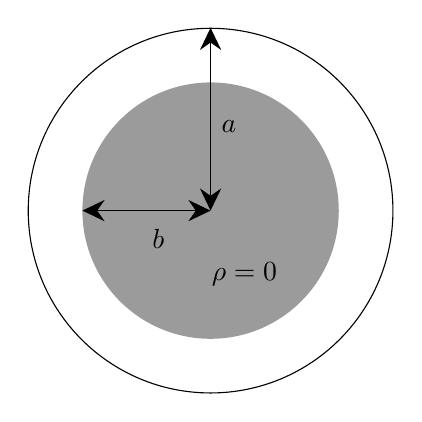
\begin{tikzpicture}[x=0.75pt,y=0.75pt,yscale=-1,xscale=1]
%uncomment if require: \path (0,181); %set diagram left start at 0, and has height of 181

%Shape: Circle [id:dp37132252659089415] 
\draw   (263,89.9) .. controls (263,41.38) and (302.33,2.05) .. (350.85,2.05) .. controls (399.37,2.05) and (438.71,41.38) .. (438.71,89.9) .. controls (438.71,138.42) and (399.37,177.75) .. (350.85,177.75) .. controls (302.33,177.75) and (263,138.42) .. (263,89.9) -- cycle ;
%Shape: Circle [id:dp7326766079222706] 
\draw  [color={rgb, 255:red, 0; green, 0; blue, 0 }  ,draw opacity=0 ][fill={rgb, 255:red, 155; green, 155; blue, 155 }  ,fill opacity=1 ] (289.1,89.9) .. controls (289.1,55.79) and (316.75,28.14) .. (350.85,28.14) .. controls (384.96,28.14) and (412.61,55.79) .. (412.61,89.9) .. controls (412.61,124.01) and (384.96,151.65) .. (350.85,151.65) .. controls (316.75,151.65) and (289.1,124.01) .. (289.1,89.9) -- cycle ;
%Straight Lines [id:da6815798853192978] 
\draw    (350.85,86.9) -- (350.85,4.81) ;
\draw [shift={(350.85,1.81)}, rotate = 450] [fill={rgb, 255:red, 0; green, 0; blue, 0 }  ][line width=0.08]  [draw opacity=0] (10.72,-5.15) -- (0,0) -- (10.72,5.15) -- (7.12,0) -- cycle    ;
\draw [shift={(350.85,89.9)}, rotate = 270] [fill={rgb, 255:red, 0; green, 0; blue, 0 }  ][line width=0.08]  [draw opacity=0] (10.72,-5.15) -- (0,0) -- (10.72,5.15) -- (7.12,0) -- cycle    ;
%Straight Lines [id:da6916068788534726] 
\draw    (292.1,89.9) -- (347.85,89.9) ;
\draw [shift={(350.85,89.9)}, rotate = 180] [fill={rgb, 255:red, 0; green, 0; blue, 0 }  ][line width=0.08]  [draw opacity=0] (10.72,-5.15) -- (0,0) -- (10.72,5.15) -- (7.12,0) -- cycle    ;
\draw [shift={(289.1,89.9)}, rotate = 0] [fill={rgb, 255:red, 0; green, 0; blue, 0 }  ][line width=0.08]  [draw opacity=0] (10.72,-5.15) -- (0,0) -- (10.72,5.15) -- (7.12,0) -- cycle    ;

% Text Node
\draw (321.6,97.48) node [anchor=north west][inner sep=0.75pt]    {$b$};
% Text Node
\draw (354.89,45.4) node [anchor=north west][inner sep=0.75pt]    {$a$};
% Text Node
\draw (350.23,113.88) node [anchor=north west][inner sep=0.75pt]    {$\rho =0$};


\end{tikzpicture}

            \end{minipage}
            Ta có 
            $$n_i=\dfrac{3N}{4\pi a^3} \ \text{và} \  n_e=\dfrac{3(1-f)N}{4 \pi b^3}.$$
            Suy ra 
            $$b=a\sqrt[3]{1-f}.$$
            \item \hfill \\
            \begin{minipage}{0.5\textwidth}
                 Bây giờ tâm "quả cầu" electron $O'$ được dịch chuyển một đoạn $\delta$ so với tâm quả cầu kim loại $O$ mà không thay đổi hình dạng cũng như mật độ điện tích như trên hình. Sử dụng nguyên lý chồng chất điện trường, điện trường bên trong quả cầu electron là tổng hợp của điện trường sinh ra bởi các electron trong quả cầu và điện trường sinh ra bởi các ion ở các nút mạng. Điện trường $\ot{E_P}$ tại điểm $P$ bên trong quả cầu electron:
            $$\ot{E_P}=\dfrac{4\pi k}{3}\dfrac{3Ne}{4\pi a^3}\tron{\ot{r}-\ot{r'}}=\frac{kNe}{a^3}\ot{\delta}.$$
            Điện trường bên trong quả cầu elctron là đều và có hướng cùng hướng với độ dịch chuyển $\ot{\delta}$.
            \end{minipage}
            \begin{minipage}{0.5\textwidth}
                \centering
                

\tikzset{every picture/.style={line width=0.75pt}} %set default line width to 0.75pt        

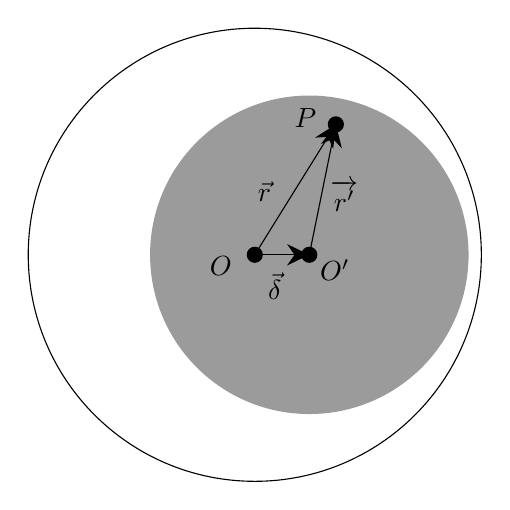
\begin{tikzpicture}[x=0.75pt,y=0.75pt,yscale=-1,xscale=1]
%uncomment if require: \path (0,287); %set diagram left start at 0, and has height of 287

%Shape: Ellipse [id:dp37132252659089415] 
\draw   (233,136.2) .. controls (233,75.92) and (281.87,27.05) .. (342.15,27.05) .. controls (402.44,27.05) and (451.31,75.92) .. (451.31,136.2) .. controls (451.31,196.48) and (402.44,245.35) .. (342.15,245.35) .. controls (281.87,245.35) and (233,196.48) .. (233,136.2) -- cycle ;
%Shape: Ellipse [id:dp7326766079222706] 
\draw  [color={rgb, 255:red, 0; green, 0; blue, 0 }  ,draw opacity=0 ][fill={rgb, 255:red, 155; green, 155; blue, 155 }  ,fill opacity=1 ] (291.7,136.2) .. controls (291.7,93.82) and (326.05,59.47) .. (368.42,59.47) .. controls (410.8,59.47) and (445.15,93.82) .. (445.15,136.2) .. controls (445.15,178.57) and (410.8,212.93) .. (368.42,212.93) .. controls (326.05,212.93) and (291.7,178.57) .. (291.7,136.2) -- cycle ;
%Shape: Ellipse [id:dp8134292801767902] 
\draw  [fill={rgb, 255:red, 0; green, 0; blue, 0 }  ,fill opacity=1 ] (364.81,136.2) .. controls (364.81,134.21) and (366.43,132.59) .. (368.42,132.59) .. controls (370.42,132.59) and (372.03,134.21) .. (372.03,136.2) .. controls (372.03,138.19) and (370.42,139.81) .. (368.42,139.81) .. controls (366.43,139.81) and (364.81,138.19) .. (364.81,136.2) -- cycle ;
%Shape: Circle [id:dp6145176668402599] 
\draw  [fill={rgb, 255:red, 0; green, 0; blue, 0 }  ,fill opacity=1 ] (338.54,136.2) .. controls (338.54,134.21) and (340.16,132.59) .. (342.15,132.59) .. controls (344.15,132.59) and (345.76,134.21) .. (345.76,136.2) .. controls (345.76,138.19) and (344.15,139.81) .. (342.15,139.81) .. controls (340.16,139.81) and (338.54,138.19) .. (338.54,136.2) -- cycle ;
%Straight Lines [id:da3473639118873846] 
\draw    (342.15,136.2) -- (365.42,136.2) ;
\draw [shift={(368.42,136.2)}, rotate = 540] [fill={rgb, 255:red, 0; green, 0; blue, 0 }  ][line width=0.08]  [draw opacity=0] (10.72,-5.15) -- (0,0) -- (10.72,5.15) -- (7.12,0) -- cycle    ;
%Shape: Ellipse [id:dp8471164676347949] 
\draw  [fill={rgb, 255:red, 0; green, 0; blue, 0 }  ,fill opacity=1 ] (377.59,73.37) .. controls (377.59,71.37) and (379.21,69.76) .. (381.2,69.76) .. controls (383.2,69.76) and (384.81,71.37) .. (384.81,73.37) .. controls (384.81,75.36) and (383.2,76.98) .. (381.2,76.98) .. controls (379.21,76.98) and (377.59,75.36) .. (377.59,73.37) -- cycle ;
%Straight Lines [id:da3258970291335339] 
\draw    (342.15,136.2) -- (379.62,75.91) ;
\draw [shift={(381.2,73.37)}, rotate = 481.86] [fill={rgb, 255:red, 0; green, 0; blue, 0 }  ][line width=0.08]  [draw opacity=0] (10.72,-5.15) -- (0,0) -- (10.72,5.15) -- (7.12,0) -- cycle    ;
%Straight Lines [id:da3602631306397466] 
\draw    (368.42,136.2) -- (380.6,76.31) ;
\draw [shift={(381.2,73.37)}, rotate = 461.5] [fill={rgb, 255:red, 0; green, 0; blue, 0 }  ][line width=0.08]  [draw opacity=0] (10.72,-5.15) -- (0,0) -- (10.72,5.15) -- (7.12,0) -- cycle    ;

% Text Node
\draw (319.3,135.77) node [anchor=north west][inner sep=0.75pt]    {$O$};
% Text Node
\draw (372.33,137.11) node [anchor=north west][inner sep=0.75pt]    {$O'$};
% Text Node
\draw (347.37,143.58) node [anchor=north west][inner sep=0.75pt]    {$\vec{\delta }$};
% Text Node
\draw (342.37,99.58) node [anchor=north west][inner sep=0.75pt]    {$\vec{r}$};
% Text Node
\draw (377.37,99.25) node [anchor=north west][inner sep=0.75pt]    {$\ot{r'}$};
% Text Node
\draw (360.04,64.73) node [anchor=north west][inner sep=0.75pt]    {$P$};


\end{tikzpicture}

            \end{minipage}
            \item Mỗi electron phải chịu một lực là
            $$\ot{F_P}=e\ot{E_P}=-\dfrac{kNe^2}{a^3}\ot{\delta}.$$
            Lực này tỉ lệ với $\delta$. Tổng lực tác dụng lên quả cầu electron là
            $$\ot{F}=-\dfrac{kN^2e^2}{a^3}\ot{\delta}.$$
            Ta có
            \begin{equation*}
                \begin{aligned}
                   Nm_e\dfrac{\dd^2\delta}{\dd t^2}=\dfrac{kN^2e^2}{a^3}\delta
                   \Leftrightarrow& ~\omega^2=\dfrac{kNe^2}{a^3m_e},\\
                   \Leftrightarrow&~\omega=\sqrt{\dfrac{kNe^2}{a^3m_e}}.
                \end{aligned}
            \end{equation*}
        \end{enumerate}
    \end{loigiai}
    
    
\begin{vd}[Điện thế hệ vỏ cầu]
Hai mặt cầu bán kính $r$ và $R$ $(r<R)$ lồng vào nhau đồng tâm. Ở bên trong mặt cầu nhỏ hơn được chứa đầy điện tích với mật độ điện tích trên một đơn vị thể tích là $-\rho$, khoảng không gian giữa hai mặt cầu chứa đầy điện tích với mật độ điện tích khối là $+\rho$ và không có điện tích ở bên ngoài bề mặt quả cầu lớn hơn. Tìm tỉ số $R/r$ để điện thế tại tâm của hệ bằng điện thế ở vô cùng.
\begin{center}
    

% Gradient Info
  
\tikzset {_fq8w470ev/.code = {\pgfsetadditionalshadetransform{ \pgftransformshift{\pgfpoint{0 bp } { 0 bp }  }  \pgftransformscale{1.5 }  }}}
\pgfdeclareradialshading{_38irhn25h}{\pgfpoint{0bp}{0bp}}{rgb(0bp)=(1,1,1);
rgb(0.8928571428571428bp)=(1,1,1);
rgb(25bp)=(0,0,0);
rgb(400bp)=(0,0,0)}
\tikzset{every picture/.style={line width=0.75pt}} %set default line width to 0.75pt        

\begin{tikzpicture}[x=0.75pt,y=0.75pt,yscale=-1,xscale=1]
%uncomment if require: \path (0,452); %set diagram left start at 0, and has height of 452

%Shape: Ellipse [id:dp9929177085843359] 
\draw  [dash pattern={on 4.5pt off 4.5pt}] (165.25,159) .. controls (165.25,142.71) and (208.57,129.5) .. (262,129.5) .. controls (315.43,129.5) and (358.75,142.71) .. (358.75,159) .. controls (358.75,175.29) and (315.43,188.5) .. (262,188.5) .. controls (208.57,188.5) and (165.25,175.29) .. (165.25,159) -- cycle ;
%Shape: Circle [id:dp5348546769453121] 
\draw  [fill={rgb, 255:red, 155; green, 155; blue, 155 }  ,fill opacity=0.42 ] (165.25,159) .. controls (165.25,105.57) and (208.57,62.25) .. (262,62.25) .. controls (315.43,62.25) and (358.75,105.57) .. (358.75,159) .. controls (358.75,212.43) and (315.43,255.75) .. (262,255.75) .. controls (208.57,255.75) and (165.25,212.43) .. (165.25,159) -- cycle ;
%Shape: Circle [id:dp009094968300005002] 
\path  [shading=_38irhn25h,_fq8w470ev] (213.75,159) .. controls (213.75,132.35) and (235.35,110.75) .. (262,110.75) .. controls (288.65,110.75) and (310.25,132.35) .. (310.25,159) .. controls (310.25,185.65) and (288.65,207.25) .. (262,207.25) .. controls (235.35,207.25) and (213.75,185.65) .. (213.75,159) -- cycle ; % for fading 
 \draw  [line width=0.75]  (213.75,159) .. controls (213.75,132.35) and (235.35,110.75) .. (262,110.75) .. controls (288.65,110.75) and (310.25,132.35) .. (310.25,159) .. controls (310.25,185.65) and (288.65,207.25) .. (262,207.25) .. controls (235.35,207.25) and (213.75,185.65) .. (213.75,159) -- cycle ; % for border 

%Shape: Ellipse [id:dp562289767970725] 
\draw  [dash pattern={on 4.5pt off 4.5pt}] (213.75,159) .. controls (213.75,152.1) and (235.13,146.5) .. (261.5,146.5) .. controls (287.87,146.5) and (309.25,152.1) .. (309.25,159) .. controls (309.25,165.9) and (287.87,171.5) .. (261.5,171.5) .. controls (235.13,171.5) and (213.75,165.9) .. (213.75,159) -- cycle ;
%Shape: Arc [id:dp4771619674622566] 
\draw  [draw opacity=0][dash pattern={on 4.5pt off 4.5pt}] (298.53,186.46) .. controls (287.21,187.78) and (274.89,188.5) .. (262,188.5) .. controls (245.92,188.5) and (230.73,187.38) .. (217.28,185.38) -- (262,159) -- cycle ; \draw  [dash pattern={on 4.5pt off 4.5pt}] (298.53,186.46) .. controls (287.21,187.78) and (274.89,188.5) .. (262,188.5) .. controls (245.92,188.5) and (230.73,187.38) .. (217.28,185.38) ;

% Text Node
\draw (247,147.4) node [anchor=north west][inner sep=0.75pt]    {$-\rho $};
% Text Node
\draw (215,82.4) node [anchor=north west][inner sep=0.75pt]    {$+\rho $};
% Text Node
\draw (343,89.4) node [anchor=north west][inner sep=0.75pt]    {$R$};
% Text Node
\draw (289,198.4) node [anchor=north west][inner sep=0.75pt]    {$r$};


\end{tikzpicture}
\end{center}
\end{vd}
\begin{loigiai}
Theo tính đối xứng, hiệu điện thế giữa tâm của một khối cầu tích điện đều với điện thế ở vô cùng bằng:
\[\varphi \sim k \dfrac{q}{R} \sim \alpha \dfrac{\rho R^{3}}{R} \sim \alpha \rho R^{2}, \tag{1}\]
trong đó $\alpha$ biểu diễn một hệ số tỉ lệ giống nhau đối với một hình cầu có kích thước bất kỳ.\\
Hệ của chúng ta bây giờ có thể coi bao gồm một hình cầu có bán kính $R$ tích điện với mật độ khối $\rho$ chồng chất với một hình cầu bán kính $r$ tích điện với mật độ khối $-2\rho$, khi đó ta được:
\[\alpha \rho R^{2}+\alpha(-2 \rho) r^{2}=0. \tag{2}\]
Và ta thu được câu trả lời:
\[\dfrac{R}{r}=\sqrt{2}. \tag{3}\]
\end{loigiai}


\begin{vd}[Một bài toán có tiềm năng$^1$]
\footnotetext{$^1$Tên gốc của bài toán là ``A problem with potential''. Ở đấy tác giả đã có ý chơi chữ, ``potential'' vừa có nghĩa là tiềm năng vừa có nghĩa là điện thế. Bạn hiểu chứ?}
   Lego lấy hai chiếc vỏ làm từ vật liệu dẫn điện hình bán cầu có cùng bán kính và ghép chúng lại với nhau sao cho hai chiếc vỏ không tiếp xúc điện với nhau và chúng tạo thành một hình cầu. Sau đó anh ấy tích điện cho một bán cầu đến điện thế $U_1=100\dv{V}$ và bán cầu còn lại đến điện thế $U_2=-100\dv{V}$. Tìm điện thế tại tâm của hình cầu. 
    \end{vd}
    \begin{loigiai}
       Chúng ta có thể giải bài toán bằng cách giải phương trình Laplace. Tuy nhiên, chúng ta sẽ không giải theo hướng này. Thay vào đó, kí hiệu $\varphi$ là điện thế tại tâm quả cầu. Nếu chúng ta thay $U_1=-100\dv{V}$ và $U_2=100\dv{V}$, tức là đổi dấu điện thế hai nửa quả cầu, thì mọi đại lượng khác trong bài toán cũng sẽ đổi dấu, và điện thế tại tâm quả cầu lúc này là $-\varphi$. Nhưng việc đổi dấu điện thế hai nửa quả cầu cũng giống như là việc quay quả cầu $180^\circ$, việc này không làm ảnh hưởng đến điện thế tại tâm quả cầu. Vậy nên, điện thế tại tâm quả cầu lúc này vẫn phải là $\varphi$. Từ đó ta có:
        \[\varphi=-\varphi.\]
        Phương trình trên chỉ có một nghiệm, đó là $\varphi=0\dv{V}$. Vậy điện thế tại tâm quả cầu là $\varphi=0\dv{V}$.
    \end{loigiai}
    
    
    \begin{vd}[Tụ điện Cantor]
    Một hình trụ dài đồng chất được làm từ một vật liệu dẫn điện. Đầu tiên chúng ta chia trụ thành ba phần bằng nhau rồi bỏ phần ở giữa đi. Sau đó, chúng ta lại tiếp tục làm như vậy với hai hình trụ còn lại. Tiếp tục làm như vậy đến khi còn $2048$ hình trụ. \\
    Sau đó ta nối hai hình trụ ngoài cùng với một nguồn điện một chiều không đổi và đo được điện dung của hệ lúc này là $C_1$. Nếu ta tiếp tục chia các hình trụ thành ba phần rồi bỏ phần giữa đi thì giá trị điện dung của hệ tiến đến một giá trị $C_0$. 
    Coi như bán kính của hình trụ là rất lớn so với khoảng cách giữa hai hình trụ bất kì nào.\\
    Hãy tìm $\displaystyle\dfrac{C_1}{C_0}$.
     \begin{center}
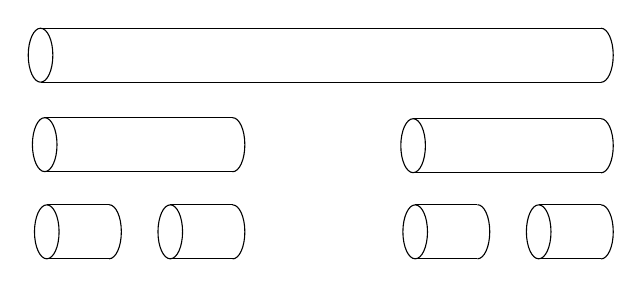
\begin{tikzpicture}[x=0.75pt,y=0.75pt,yscale=-1,xscale=1]
%uncomment if require: \path (0,155); %set diagram left start at 0, and has height of 155

%Straight Lines [id:da8779348118982053] 
\draw [fill={rgb, 255:red, 0; green, 0; blue, 0 }  ,fill opacity=0 ]   (216.66,29.01) -- (486.66,29.01) ;
%Straight Lines [id:da13466989557571818] 
\draw [fill={rgb, 255:red, 0; green, 0; blue, 0 }  ,fill opacity=0 ]   (216.66,55) -- (486.66,55) ;
%Shape: Ellipse [id:dp9259404166148435] 
\draw  [fill={rgb, 255:red, 0; green, 0; blue, 0 }  ,fill opacity=0 ] (210.73,42) .. controls (210.73,34.83) and (213.39,29.01) .. (216.66,29.01) .. controls (219.93,29.01) and (222.59,34.83) .. (222.59,42) .. controls (222.59,49.18) and (219.93,55) .. (216.66,55) .. controls (213.39,55) and (210.73,49.18) .. (210.73,42) -- cycle ;
%Shape: Arc [id:dp8476201405539008] 
\draw  [draw opacity=0][fill={rgb, 255:red, 0; green, 0; blue, 0 }  ,fill opacity=0 ] (486.66,29.01) .. controls (489.93,29.01) and (492.58,34.85) .. (492.58,42.04) .. controls (492.58,49.23) and (489.93,55.07) .. (486.66,55.07) -- (486.65,42.04) -- cycle ; \draw   (486.66,29.01) .. controls (489.93,29.01) and (492.58,34.85) .. (492.58,42.04) .. controls (492.58,49.23) and (489.93,55.07) .. (486.66,55.07) ;
%Shape: Ellipse [id:dp4855344638857144] 
\draw  [fill={rgb, 255:red, 0; green, 0; blue, 0 }  ,fill opacity=0 ] (212.74,85.1) .. controls (212.74,77.93) and (215.39,72.11) .. (218.67,72.11) .. controls (221.94,72.11) and (224.59,77.93) .. (224.59,85.1) .. controls (224.59,92.28) and (221.94,98.1) .. (218.67,98.1) .. controls (215.39,98.1) and (212.74,92.28) .. (212.74,85.1) -- cycle ;
%Shape: Arc [id:dp02778180114314721] 
\draw  [draw opacity=0][fill={rgb, 255:red, 0; green, 0; blue, 0 }  ,fill opacity=0 ] (309.17,72.11) .. controls (312.44,72.11) and (315.09,77.95) .. (315.09,85.14) .. controls (315.09,92.33) and (312.44,98.17) .. (309.17,98.17) -- (309.16,85.14) -- cycle ; \draw   (309.17,72.11) .. controls (312.44,72.11) and (315.09,77.95) .. (315.09,85.14) .. controls (315.09,92.33) and (312.44,98.17) .. (309.17,98.17) ;
%Straight Lines [id:da5335853153210501] 
\draw [fill={rgb, 255:red, 0; green, 0; blue, 0 }  ,fill opacity=0 ]   (218.67,72.11) -- (309.17,72.11) ;
%Straight Lines [id:da6065035823638336] 
\draw [fill={rgb, 255:red, 0; green, 0; blue, 0 }  ,fill opacity=0 ]   (218.67,98.1) -- (309.17,98.1) ;

%Straight Lines [id:da3211244834377631] 
\draw [fill={rgb, 255:red, 0; green, 0; blue, 0 }  ,fill opacity=0 ]   (396.17,72.61) -- (486.67,72.61) ;
%Straight Lines [id:da4209064110233234] 
\draw [fill={rgb, 255:red, 0; green, 0; blue, 0 }  ,fill opacity=0 ]   (396.17,98.6) -- (486.67,98.6) ;

%Shape: Ellipse [id:dp0648912258701948] 
\draw  [fill={rgb, 255:red, 0; green, 0; blue, 0 }  ,fill opacity=0 ] (390.24,85.6) .. controls (390.24,78.43) and (392.89,72.61) .. (396.17,72.61) .. controls (399.44,72.61) and (402.09,78.43) .. (402.09,85.6) .. controls (402.09,92.78) and (399.44,98.6) .. (396.17,98.6) .. controls (392.89,98.6) and (390.24,92.78) .. (390.24,85.6) -- cycle ;
%Shape: Arc [id:dp8052371619050682] 
\draw  [draw opacity=0][fill={rgb, 255:red, 0; green, 0; blue, 0 }  ,fill opacity=0 ] (486.67,72.61) .. controls (489.94,72.61) and (492.59,78.45) .. (492.59,85.64) .. controls (492.59,92.83) and (489.94,98.67) .. (486.67,98.67) -- (486.66,85.64) -- cycle ; \draw   (486.67,72.61) .. controls (489.94,72.61) and (492.59,78.45) .. (492.59,85.64) .. controls (492.59,92.83) and (489.94,98.67) .. (486.67,98.67) ;

%Straight Lines [id:da6006091749639515] 
\draw [fill={rgb, 255:red, 0; green, 0; blue, 0 }  ,fill opacity=0 ]   (219.67,114.11) -- (249.67,114.11) ;
%Straight Lines [id:da6727926975150735] 
\draw [fill={rgb, 255:red, 0; green, 0; blue, 0 }  ,fill opacity=0 ]   (219.67,140.1) -- (249.67,140.1) ;

%Shape: Ellipse [id:dp08438817098705531] 
\draw  [fill={rgb, 255:red, 0; green, 0; blue, 0 }  ,fill opacity=0 ] (213.74,127.1) .. controls (213.74,119.93) and (216.39,114.11) .. (219.67,114.11) .. controls (222.94,114.11) and (225.59,119.93) .. (225.59,127.1) .. controls (225.59,134.28) and (222.94,140.1) .. (219.67,140.1) .. controls (216.39,140.1) and (213.74,134.28) .. (213.74,127.1) -- cycle ;
%Shape: Arc [id:dp032996619982465614] 
\draw  [draw opacity=0][fill={rgb, 255:red, 0; green, 0; blue, 0 }  ,fill opacity=0 ] (249.67,114.03) .. controls (252.94,114.04) and (255.59,119.87) .. (255.59,127.07) .. controls (255.59,134.26) and (252.94,140.09) .. (249.67,140.1) -- (249.66,127.07) -- cycle ; \draw   (249.67,114.03) .. controls (252.94,114.04) and (255.59,119.87) .. (255.59,127.07) .. controls (255.59,134.26) and (252.94,140.09) .. (249.67,140.1) ;

%Straight Lines [id:da2839375556187842] 
\draw [fill={rgb, 255:red, 0; green, 0; blue, 0 }  ,fill opacity=0 ]   (279.17,114.11) -- (309.17,114.11) ;
%Straight Lines [id:da4240777974418377] 
\draw [fill={rgb, 255:red, 0; green, 0; blue, 0 }  ,fill opacity=0 ]   (279.17,140.1) -- (309.17,140.1) ;

%Shape: Arc [id:dp1949721350147613] 
\draw  [draw opacity=0][fill={rgb, 255:red, 0; green, 0; blue, 0 }  ,fill opacity=0 ] (309.17,114.11) .. controls (312.44,114.11) and (315.09,119.95) .. (315.09,127.14) .. controls (315.09,134.33) and (312.44,140.17) .. (309.17,140.17) -- (309.16,127.14) -- cycle ; \draw   (309.17,114.11) .. controls (312.44,114.11) and (315.09,119.95) .. (315.09,127.14) .. controls (315.09,134.33) and (312.44,140.17) .. (309.17,140.17) ;
%Shape: Ellipse [id:dp9792855074851174] 
\draw  [fill={rgb, 255:red, 0; green, 0; blue, 0 }  ,fill opacity=0 ] (273.24,127.1) .. controls (273.24,119.93) and (275.89,114.11) .. (279.17,114.11) .. controls (282.44,114.11) and (285.09,119.93) .. (285.09,127.1) .. controls (285.09,134.28) and (282.44,140.1) .. (279.17,140.1) .. controls (275.89,140.1) and (273.24,134.28) .. (273.24,127.1) -- cycle ;


%Straight Lines [id:da552491009633757] 
\draw [fill={rgb, 255:red, 0; green, 0; blue, 0 }  ,fill opacity=0 ]   (397.17,114.11) -- (427.17,114.11) ;
%Straight Lines [id:da14390672442166497] 
\draw [fill={rgb, 255:red, 0; green, 0; blue, 0 }  ,fill opacity=0 ]   (397.17,140.1) -- (427.17,140.1) ;

%Shape: Ellipse [id:dp8864242189083134] 
\draw  [fill={rgb, 255:red, 0; green, 0; blue, 0 }  ,fill opacity=0 ] (391.24,127.1) .. controls (391.24,119.93) and (393.89,114.11) .. (397.17,114.11) .. controls (400.44,114.11) and (403.09,119.93) .. (403.09,127.1) .. controls (403.09,134.28) and (400.44,140.1) .. (397.17,140.1) .. controls (393.89,140.1) and (391.24,134.28) .. (391.24,127.1) -- cycle ;
%Shape: Arc [id:dp2137632297870793] 
\draw  [draw opacity=0][fill={rgb, 255:red, 0; green, 0; blue, 0 }  ,fill opacity=0 ] (427.17,114.03) .. controls (430.44,114.04) and (433.09,119.87) .. (433.09,127.07) .. controls (433.09,134.26) and (430.44,140.09) .. (427.17,140.1) -- (427.16,127.07) -- cycle ; \draw   (427.17,114.03) .. controls (430.44,114.04) and (433.09,119.87) .. (433.09,127.07) .. controls (433.09,134.26) and (430.44,140.09) .. (427.17,140.1) ;

%Straight Lines [id:da8191436732940167] 
\draw [fill={rgb, 255:red, 0; green, 0; blue, 0 }  ,fill opacity=0 ]   (456.67,114.11) -- (486.67,114.11) ;
%Straight Lines [id:da9814018931290542] 
\draw [fill={rgb, 255:red, 0; green, 0; blue, 0 }  ,fill opacity=0 ]   (456.67,140.1) -- (486.67,140.1) ;

%Shape: Arc [id:dp6127404823543812] 
\draw  [draw opacity=0][fill={rgb, 255:red, 0; green, 0; blue, 0 }  ,fill opacity=0 ] (486.67,114.11) .. controls (489.94,114.11) and (492.59,119.95) .. (492.59,127.14) .. controls (492.59,134.33) and (489.94,140.17) .. (486.67,140.17) -- (486.66,127.14) -- cycle ; \draw   (486.67,114.11) .. controls (489.94,114.11) and (492.59,119.95) .. (492.59,127.14) .. controls (492.59,134.33) and (489.94,140.17) .. (486.67,140.17) ;
%Shape: Ellipse [id:dp44504917695147905] 
\draw  [fill={rgb, 255:red, 0; green, 0; blue, 0 }  ,fill opacity=0 ] (450.74,127.1) .. controls (450.74,119.93) and (453.39,114.11) .. (456.67,114.11) .. controls (459.94,114.11) and (462.59,119.93) .. (462.59,127.1) .. controls (462.59,134.28) and (459.94,140.1) .. (456.67,140.1) .. controls (453.39,140.1) and (450.74,134.28) .. (450.74,127.1) -- cycle ;
\end{tikzpicture}
    \end{center}
    \textit{Lưu ý: Hình vẽ không theo tỉ lệ.}
    \end{vd}
    \begin{loigiai}
    Ta thấy rằng điện dung của tụ tỉ lệ nghịch với khoảng cách giữa hai bản tụ $C\sim \dfrac{1}{d}$.\\
    Khi các tụ mắc nối tiếp ta có: 
    $$C=\dfrac{1}{\dfrac{1}{C_1}+\dfrac{1}{C_2}+...+\dfrac{1}{C_{n-1}}+\dfrac{1}{C_n}}\sim\dfrac{1}{d_1+d_2+..+d_{n-1}+d_n}.$$
    Vậy điện dung của hệ tỉ lệ với tổng độ dài các khoảng trống.\\
    Sau mỗi lần cắt làm ba và bỏ đi phần giữa, số hình trụ tăng lên gấp đôi và tổng chiều dài các hình trụ giảm đi $\dfrac{2}{3}$ lần.\\
    Khi có $2048$ hình trụ, tổng chiều dài các khoảng trống là:
    $$D=L\tron{1-\tron{\dfrac{2}{3}}^{10}}.$$
    Khi số hình trụ tiến đến vô cùng thì tổng độ dài các khoảng trống tiến đến $L$.\\
    Từ đó ta có:
    \begin{equation*}
        \begin{aligned}
            \dfrac{C_1}{C_0}=\dfrac{L}{D}
            =\dfrac{1}{1-\tron{\dfrac{2}{3}}^{10}}
            \approx 1,018.
        \end{aligned}
    \end{equation*}
    \end{loigiai}
    
    
    \begin{vd}[Điện trường trong một vỏ cầu]
    \label{cb8}
    
    Tính điện trường tại một điểm bên trong một vỏ cầu tích điện đều bằng cách xét hai phần diện tích nằm ở đáy của hai hình nón hẹp như hình. Từ đó cho thấy rằng, điện trường tại mọi điểm bên trong vỏ cầu bằng không.
        \begin{center}
            

\tikzset{every picture/.style={line width=0.75pt}} %set default line width to 0.75pt        

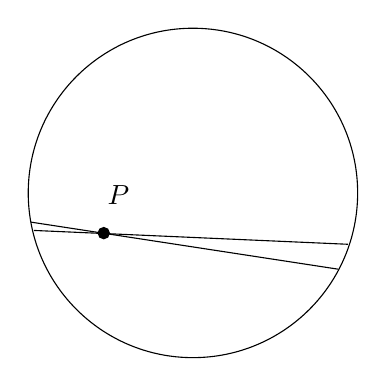
\begin{tikzpicture}[x=0.75pt,y=0.75pt,yscale=-1,xscale=1]
%uncomment if require: \path (0,238); %set diagram left start at 0, and has height of 238

%Shape: Circle [id:dp46714741031721685] 
\draw   (269,118.35) .. controls (269,74.53) and (304.53,39) .. (348.35,39) .. controls (392.18,39) and (427.71,74.53) .. (427.71,118.35) .. controls (427.71,162.18) and (392.18,197.71) .. (348.35,197.71) .. controls (304.53,197.71) and (269,162.18) .. (269,118.35) -- cycle ;
%Shape: Circle [id:dp5515785641251634] 
\draw  [fill={rgb, 255:red, 0; green, 0; blue, 0 }  ,fill opacity=1 ] (302.67,137.71) .. controls (302.67,136.22) and (303.88,135) .. (305.38,135) .. controls (306.88,135) and (308.1,136.22) .. (308.1,137.71) .. controls (308.1,139.21) and (306.88,140.43) .. (305.38,140.43) .. controls (303.88,140.43) and (302.67,139.21) .. (302.67,137.71) -- cycle ;
%Straight Lines [id:da3733346667505719] 
\draw    (271.68,136.42) -- (423.01,143.09) ;
%Straight Lines [id:da6048790919807321] 
\draw    (270.35,132.42) -- (418.35,155.09) ;

% Text Node
\draw (306,113.73) node [anchor=north west][inner sep=0.75pt]    {$P$};


\end{tikzpicture}

        \end{center}
    \end{vd}
    \begin{loigiai}
        Kí hiệu $a$ là khoảng cách từ điểm $P$ tới mảng $A$, $b$ là khoảng cách từ điểm $P$ tới mảng $B$ như trên hình vẽ. (Vì hình nón hẹp, nên có thể coi mảng $A$ và mảng $B$ có diện tích nhỏ, có thể coi khoảng cách từ $P$ tới một điểm bất kì trong mảng là khoảng cách từ $P$ tới mảng đó). Ta xét các đáy vuông góc với trục hình nón là $A'$ và $B'$ như trên hình. Tỉ lệ diện tích của $A'$ và $B'$ sẽ là $\dfrac{a^2}{b^2}$, bởi vì diện tích tỉ lệ với độ dài bình phương. Điểm mấu chốt cần nhận ra ở đây là góc giữa mặt $A$ và mặt $A'$ bằng góc giữa mặt $B$ và mặt $B'$. Điều này là đúng bởi vì $A'$ và $B'$ cùng vuông góc với trục hình nón, còn $A$ và $B$ thì tạo với trục hình nón các góc bằng nhau, do đường thẳng $AB$ là dây cung của đường tròn. Tỉ lệ diện tích của mảng $A$ so với mảng $B$ bằng với lại tỉ lệ diện tích của mảng $A'$ so với mảng $B'$ và bằng $\dfrac{a^2}{b^2}$. Mà điện tích lại tỉ lệ với diện tích nên điện tích mảng $A$ bằng $\dfrac{a^2}{b^2}$ lần điện tích của mảng $B$. 
        \begin{center}
            

\tikzset{every picture/.style={line width=0.75pt}} %set default line width to 0.75pt        

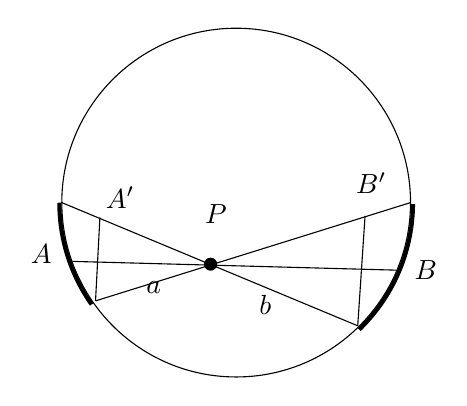
\begin{tikzpicture}[x=0.75pt,y=0.75pt,yscale=-1,xscale=1]
%uncomment if require: \path (0,238); %set diagram left start at 0, and has height of 238

%Shape: Circle [id:dp46714741031721685] 
\draw   (269.98,123.08) .. controls (269.98,76.68) and (307.59,39.07) .. (353.99,39.07) .. controls (400.39,39.07) and (438,76.68) .. (438,123.08) .. controls (438,169.48) and (400.39,207.09) .. (353.99,207.09) .. controls (307.59,207.09) and (269.98,169.48) .. (269.98,123.08) -- cycle ;
%Shape: Circle [id:dp5515785641251634] 
\draw  [fill={rgb, 255:red, 0; green, 0; blue, 0 }  ,fill opacity=1 ] (338.79,152.75) .. controls (338.79,151.16) and (340.08,149.88) .. (341.67,149.88) .. controls (343.26,149.88) and (344.54,151.16) .. (344.54,152.75) .. controls (344.54,154.34) and (343.26,155.62) .. (341.67,155.62) .. controls (340.08,155.62) and (338.79,154.34) .. (338.79,152.75) -- cycle ;
%Straight Lines [id:da3733346667505719] 
\draw    (286.23,170.44) -- (438,123.08) ;
%Straight Lines [id:da6048790919807321] 
\draw    (269.98,123.08) -- (412.56,182.44) ;
%Straight Lines [id:da32951233402203317] 
\draw    (288.34,130.21) -- (286.23,170.44) ;
%Straight Lines [id:da09769199632318037] 
\draw    (416.09,129.5) -- (412.56,182.44) ;
%Straight Lines [id:da6143629836842865] 
\draw    (430.92,155.62) -- (274.23,151.38) ;
%Shape: Arc [id:dp9065945184915425] 
\draw  [draw opacity=0][line width=1.5]  (284.35,172.17) .. controls (274.57,158.31) and (268.82,141.4) .. (268.8,123.15) -- (353.99,123.08) -- cycle ; \draw  [line width=1.5]  (284.35,172.17) .. controls (274.57,158.31) and (268.82,141.4) .. (268.8,123.15) ;
%Shape: Arc [id:dp41297456161672663] 
\draw  [draw opacity=0][line width=1.5]  (439.18,123.79) .. controls (438.98,147.52) and (429.09,168.94) .. (413.26,184.28) -- (353.99,123.08) -- cycle ; \draw  [line width=1.5]  (439.18,123.79) .. controls (438.98,147.52) and (429.09,168.94) .. (413.26,184.28) ;

% Text Node
\draw (337.74,122.87) node [anchor=north west][inner sep=0.75pt]    {$P$};
% Text Node
\draw (253.81,142.28) node [anchor=north west][inner sep=0.75pt]    {$A$};
% Text Node
\draw (438.67,149.69) node [anchor=north west][inner sep=0.75pt]    {$B$};
% Text Node
\draw (289.95,114.4) node [anchor=north west][inner sep=0.75pt]    {$A'$};
% Text Node
\draw (410.56,107.34) node [anchor=north west][inner sep=0.75pt]    {$B'$};
% Text Node
\draw (309.51,159.92) node [anchor=north west][inner sep=0.75pt]    {$a$};
% Text Node
\draw (363.86,166.27) node [anchor=north west][inner sep=0.75pt]    {$b$};


\end{tikzpicture}

        \end{center}
        Điện trường do từng mảng gây ra tại $P$ tuân theo biểu thức $E=\dfrac{q}{4\pi\varepsilon_0 r^2}$. Do đó mặc dù điện tích của $A$ bằng $\dfrac{a^2}{b^2}$ lần điện tích của $B$, nhưng giá trị $r^2$ cho mảng $A$ lại cũng bằng $\dfrac{a^2}{b^2}$ giá trị $r^2$ của mảng $B$ nên kết quả là cường độ điện trường do mảng $A$ gây ra có độ lớn bằng với cường độ điện trường do mảng $B$ gây ra ở $P$. Điện trường do hai mảng gây ra có hướng ngược chiều nhau nên chúng triệt tiêu lẫn nhau. Một quả cầu có thể chia ra làm nhiều mảng bị giới hạn bởi các mặt nón như vậy, và điện trường do các mặt nón đó từng đôi một triệt tiêu lẫn nhau. Do đó, điện trường tổng hợp tại điểm $P$ bằng không. Điều này là đúng cho một điểm $P$ bất kì bên trong quả cầu.
    \end{loigiai}
    
    
    \begin{vd}[Phân bố điện tích trên một đĩa tròn]
        Có một cách khá ``mẹo'' để tìm được phân bố điện tích trên một chiếc đĩa tròn phẳng dẫn điện với bán kính $R$ và tổng điện tích $Q$. Mục tiêu của chúng ta là tìm ra một phân bố điện tích sao cho điện trường tại một điểm trên bề mặt chiếc đĩa vuông góc với bề mặt chiếc đĩa (thành phần điện trường song song với bề mặt chiếc đĩa bằng không). Như đã chứng minh trong bài \ref{cb8}, điện trường tại một điểm $P$ bất kì bên trong một vỏ cầu tích điện đều trên bề mặt thì bằng không. Xét một phân bố điện tích khác bằng cách chiếu các điện tích trên bề mặt vỏ cầu xuống mặt phẳng đi qua $P$ và tâm vỏ cầu. Chứng minh rằng phân bố điện tích này có những tính chất của phân bố mà chúng ta đang tìm, từ đó suy ra phân bố điện tích trên một chiếc đĩa tròn dẫn điện. 
    \end{vd}
    \begin{loigiai}
    \hfill\\
    \begin{center}
        

\tikzset{every picture/.style={line width=0.75pt}} %set default line width to 0.75pt        

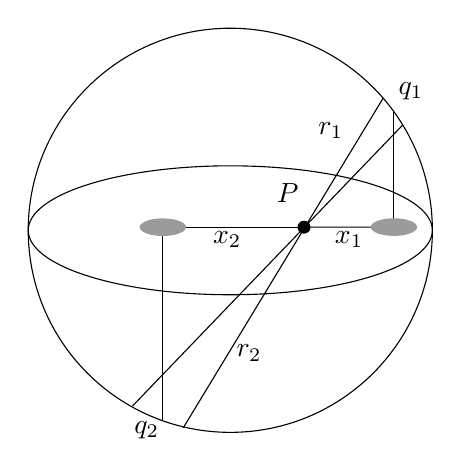
\begin{tikzpicture}[x=0.75pt,y=0.75pt,yscale=-1,xscale=1]
%uncomment if require: \path (0,238); %set diagram left start at 0, and has height of 238

%Shape: Circle [id:dp6718340227215969] 
\draw   (258,111.35) .. controls (258,57.59) and (301.59,14) .. (355.35,14) .. controls (409.12,14) and (452.71,57.59) .. (452.71,111.35) .. controls (452.71,165.12) and (409.12,208.71) .. (355.35,208.71) .. controls (301.59,208.71) and (258,165.12) .. (258,111.35) -- cycle ;
%Shape: Ellipse [id:dp03679207536578666] 
\draw   (258,111.35) .. controls (258,94.2) and (301.59,80.29) .. (355.35,80.29) .. controls (409.12,80.29) and (452.71,94.2) .. (452.71,111.35) .. controls (452.71,128.51) and (409.12,142.41) .. (355.35,142.41) .. controls (301.59,142.41) and (258,128.51) .. (258,111.35) -- cycle ;
%Shape: Circle [id:dp6201165347005493] 
\draw  [fill={rgb, 255:red, 0; green, 0; blue, 0 }  ,fill opacity=1 ] (388,109.85) .. controls (388,108.28) and (389.28,107) .. (390.85,107) .. controls (392.43,107) and (393.71,108.28) .. (393.71,109.85) .. controls (393.71,111.43) and (392.43,112.71) .. (390.85,112.71) .. controls (389.28,112.71) and (388,111.43) .. (388,109.85) -- cycle ;
%Straight Lines [id:da118178901959902] 
\draw    (429.06,47.59) -- (332.71,206.48) ;
%Straight Lines [id:da07650261292657179] 
\draw    (308.26,195.99) -- (438.26,60.79) ;
%Straight Lines [id:da1616088174307333] 
\draw    (434.18,54.47) -- (434.18,109.8) ;
%Straight Lines [id:da46335539841964213] 
\draw    (390.85,109.85) -- (434.18,109.8) ;
%Straight Lines [id:da3543480330279791] 
\draw    (322.85,109.85) -- (390.85,109.85) ;
%Straight Lines [id:da9787802557447067] 
\draw    (322.85,109.85) -- (322.85,203.14) ;
%Shape: Ellipse [id:dp7676571893601905] 
\draw  [draw opacity=0][fill={rgb, 255:red, 155; green, 155; blue, 155 }  ,fill opacity=1 ] (311.68,109.85) .. controls (311.68,107.51) and (316.68,105.61) .. (322.85,105.61) .. controls (329.02,105.61) and (334.02,107.51) .. (334.02,109.85) .. controls (334.02,112.2) and (329.02,114.1) .. (322.85,114.1) .. controls (316.68,114.1) and (311.68,112.2) .. (311.68,109.85) -- cycle ;
%Shape: Ellipse [id:dp6842573741204465] 
\draw  [draw opacity=0][fill={rgb, 255:red, 155; green, 155; blue, 155 }  ,fill opacity=1 ] (423.01,109.8) .. controls (423.01,107.46) and (428.01,105.56) .. (434.18,105.56) .. controls (440.35,105.56) and (445.35,107.46) .. (445.35,109.8) .. controls (445.35,112.15) and (440.35,114.05) .. (434.18,114.05) .. controls (428.01,114.05) and (423.01,112.15) .. (423.01,109.8) -- cycle ;

% Text Node
\draw (376.51,87.71) node [anchor=north west][inner sep=0.75pt]    {$P$};
% Text Node
\draw (396.51,58.05) node [anchor=north west][inner sep=0.75pt]    {$r_{1}$};
% Text Node
\draw (357.17,165.38) node [anchor=north west][inner sep=0.75pt]    {$r_{2}$};
% Text Node
\draw (404.51,110.71) node [anchor=north west][inner sep=0.75pt]    {$x_{1}$};
% Text Node
\draw (345.84,110.71) node [anchor=north west][inner sep=0.75pt]    {$x_{2}$};
% Text Node
\draw (435.17,38.71) node [anchor=north west][inner sep=0.75pt]    {$q_{1}$};
% Text Node
\draw (307.84,202.05) node [anchor=north west][inner sep=0.75pt]    {$q_{2}$};


\end{tikzpicture}

    \end{center}
        Nhớ lại lời giải cho bài toán \ref{cb8}, chúng ta đã chứng minh vì sao điện trường bên trong vỏ cầu lại bằng không. Trên hình vẽ, ta thấy hai hình nón bao quanh hai mảng $q_1$ và $q_2$ là đồng dạng, cho nên diện tích hai mảng (cũng như là điện tích) tỉ lệ với $\dfrac{{r_1}^2}{{r_2}^2}$. Do điện trường do từng mảng gây ra tại $P$ lại tỉ lệ nghịch với khoảng cách của từng mảng tới $P$ theo định luật Coulomb, kết quả là điện trường do hai mảng gây ra có độ lớn bằng nhau và ngược chiều nhau, nên điện trường tổng hợp tại $P$ bằng không. Ta có thể chia vỏ cầu thành từng cặp các mảng đối xứng nhau như $q_1$ và $q_2$, và điện trường của từng cặp sẽ triệt tiêu lẫn nhau, vậy nên điện trường tổng hợp do cả vỏ cầu gây ra tại $P$ bằng không.\\
        Bây giờ chúng ta sẽ chiếu các điện tích của các mạng $q_1$ và $q_2$ lên mặt phẳng đi qua $P$ và tâm vỏ cầu.\\
        Các điện tích $q_1$ và $q_2$ sẽ được chiếu lên các vị trí như trên hình. Điện trường theo phương nằm ngang do các điện tích được chiếu lên gây ra tại điểm $P$ sẽ có độ lớn lần lượt là $\dfrac{q_1}{4\pi\varepsilon_0 {x_1}^2}$ và $\dfrac{q_2}{4\pi\varepsilon_0 {x_2}^2}$. Từ các tam giác đồng dạng trong hình, ta thấy được $\dfrac{x_1}{x_2}=\dfrac{r_1}{r_2}$. Vậy nên điện trường do điện tích gây ra tại $P$ lại triệt tiêu lẫn nhau, điện trường theo phương nằm ngang tại điểm $P$ bằng không. Đây chính là tính chất cần có của phân bố điện tích chúng ta đang cần tìm.
        \begin{center}
            

\tikzset{every picture/.style={line width=0.75pt}} %set default line width to 0.75pt        

\begin{tikzpicture}[x=0.75pt,y=0.75pt,yscale=-1,xscale=1]
%uncomment if require: \path (0,238); %set diagram left start at 0, and has height of 238

%Shape: Circle [id:dp6477351268867286] 
\draw   (250.67,116.86) .. controls (250.67,60.6) and (296.27,14.99) .. (352.53,14.99) .. controls (408.79,14.99) and (454.4,60.6) .. (454.4,116.86) .. controls (454.4,173.12) and (408.79,218.73) .. (352.53,218.73) .. controls (296.27,218.73) and (250.67,173.12) .. (250.67,116.86) -- cycle ;
%Straight Lines [id:da9947060585834728] 
\draw    (250.67,116.86) -- (454.4,116.86) ;
%Straight Lines [id:da6474936030533343] 
\draw    (352.53,14.99) -- (352.53,116.86) ;
%Straight Lines [id:da849787006711521] 
\draw    (352.53,116.86) -- (426.7,48.29) ;
%Straight Lines [id:da02616449568002066] 
\draw [line width=2.25]    (418.7,39.62) -- (435.37,57.62) ;
%Straight Lines [id:da4863337237680685] 
\draw    (426.7,48.29) -- (426.7,116.29) ;
%Straight Lines [id:da79610995061943] 
\draw [line width=2.25]    (418.04,116.96) -- (434.7,116.96) ;
%Shape: Arc [id:dp2516106990306459] 
\draw  [draw opacity=0] (352.24,98.36) .. controls (352.34,98.36) and (352.44,98.36) .. (352.53,98.36) .. controls (357.72,98.36) and (362.4,100.49) .. (365.76,103.92) -- (352.53,116.86) -- cycle ; \draw   (352.24,98.36) .. controls (352.34,98.36) and (352.44,98.36) .. (352.53,98.36) .. controls (357.72,98.36) and (362.4,100.49) .. (365.76,103.92) ;

% Text Node
\draw (430.36,31.07) node [anchor=north west][inner sep=0.75pt]    {$\mathrm{d} A$};
% Text Node
\draw (387.03,123.4) node [anchor=north west][inner sep=0.75pt]    {$\mathrm{d} A\cos \theta $};
% Text Node
\draw (389.69,100.07) node [anchor=north west][inner sep=0.75pt]    {$r$};
% Text Node
\draw (335.69,50.07) node [anchor=north west][inner sep=0.75pt]    {$R$};
% Text Node
\draw (359.69,82.73) node [anchor=north west][inner sep=0.75pt]    {$\theta $};
% Text Node
\draw (263.03,119.67) node [anchor=north west][inner sep=0.75pt]   [align=left] {Đĩa};


\end{tikzpicture}

        \end{center}
        Ta có thể biểu diễn phân bố này như là một hàm theo $r$ như trên hình vẽ. Xét một đơn vị diện tích $\dd A$ trên vỏ cầu. Phần diện tích của hình chiếu của $\dd A$ trên mặt phẳng sẽ là $\dd A'=\dd A\cos\theta$. Mật độ điện tích của vỏ cầu là $\sigma$. Điện tích của phần diện tích $\dd A$ là 
        \begin{equation}
            \dd q=\sigma\dd A.
        \end{equation}
        Mật độ điện tích tại $\dd A'$ là
        \begin{equation}
        \begin{aligned}
            \sigma'(r)&=\dfrac{\dd q}{\dd A'}\\
            &=\dfrac{\sigma}{\cos\theta}\\
            &=\dfrac{\sigma R}{\sqrt{R^2-r^2}}.
        \end{aligned}
        \end{equation}
        Tổng điện tích của đĩa là $Q$ nên ta có
        \begin{equation}
            \begin{aligned}
               Q&=\int_0^R\sigma'(r)2\pi r\dd r\\
               &=\int_0^R\dfrac{\sigma R}{\sqrt{R^2-r^2}}2\pi r\dd r\\
               &=\left. -2\pi \sigma R\sqrt{R^2-r^2}\right|_0^R=2\pi\sigma R^2.
            \end{aligned}
        \end{equation}
        Từ đó suy ra $\sigma=\dfrac{Q}{2\pi R^2}$, phân bố điện tích của đĩa tròn sẽ là 
        \begin{equation}
            \sigma_d(r)=\dfrac{Q}{2\pi R\sqrt{R^2-r^2}}.
        \end{equation}
        Chúng ta có thể tìm ra được mối quan hệ giữa $\sigma$ và $Q$ bằng một cách khác không sử dụng tích phân. Hãy để ý rằng khi ta chiếu điện tích của vỏ cầu xuống mặt phẳng, tổng điện tích không đổi. Vậy nên $Q=\sigma 2\pi R^2$, suy ra $\sigma=\dfrac{Q}{2\pi R^2}$  (ở đây ta chỉ xét một nửa của vỏ cầu phía trên, do tính đối xứng nên việc bỏ qua nửa vỏ cầu bên dưới không ảnh hưởng đến kết quả cuối cùng).\\
        Mật độ điện tích tại phần rìa của chiếc đĩa tiến tới vô cùng, tuy nhiên tổng điện tích của đĩa thì lại là một giá trị hữu hạn. Mật độ điện tích tăng khi $r$ tăng, điều này là dễ hiểu vì các điện tích đẩy nhau nên tại phần rìa của đĩa các điện tích sẽ tập trung hơn. 
    \end{loigiai}
    
    
    \begin{vd}[Điện thế của quả cầu]
    Có một quả cầu kim loại lớn có bán kính $10\dv{m}$ và ban đầu có điện thế bằng không và rất nhiều những quả cầu nhỏ hơn bán kính $1\dv{m}$ ban đầu được tích điện đến điện thế $10\dv{V}$. Quả cầu lớn lần lượt được nối với các quả cầu nhỏ qua một dây dẫn mảnh dài. Trong quá trình đó các quả cầu được đặt cách xa nhau sao cho điện tích vẫn phân bố đều trên mỗi quả cầu sau mỗi lần như vậy. Hỏi quả cầu lớn phải nối với bao nhiêu quả cầu nhỏ để có thể đạt đến điện thế $9\dv{V}$?
    \end{vd}
    \begin{loigiai}
    Điện tích của mỗi quả cầu nhỏ là $q$, điện tích quả cầu lớn là $Q$. Mỗi lần quả cầu lớn nối với quả cầu nhỏ thì hai quả cầu trao đổi điện tích đến khi điện thế hai quả cầu bằng nhau. Điện thế của các quả cầu tỉ lệ với $\dfrac{q}{r}$.
    Ta có:
    \begin{equation*}
    \begin{aligned}
        &\frac{Q_{n+1}}{R}=\dfrac{Q_n+q-Q_{n+1}}{r}\\
        \Leftrightarrow \ & Q_{n+1}=\tron{Q_{n}+q}\dfrac{R}{R+r},
    \end{aligned}
    \end{equation*}
    với $Q_0=0$. \\
    Đặt $\dfrac{R}{R+r}=k$, ta có:
    \begin{equation*}
    \begin{aligned}
          Q_{n+1}&=q\tron{k^n+...+k}\\
          &=q\tron{k\dfrac{k^n-1}{k-1}}.
    \end{aligned}
    \end{equation*}
    Để điện thế quả cầu đạt tới $9\dv{V}$:
    \begin{equation*}
        \begin{aligned}
            \frac{Q_n}{R}=\frac{9}{10}\frac{q}{r}
            \Leftrightarrow q&\tron{k\dfrac{k^n-1}{k-1}}=9q\\
            \Leftrightarrow n&=\log_k\tron{\frac{9(k-1)}{k}+1}\\
            &=24,16\ .
        \end{aligned}
    \end{equation*}
    Vậy quả cầu lớn cần tiếp xúc với 25 quả cầu để đạt đến hiệu điện thế $9\dv{V}$.
    \end{loigiai}
    
\begin{vd}[Tụ điện phẳng trong bồn chứa điện môi (G)]
    Một tụ điện phẳng song song với bản tụ hình vuông có cạnh là $L$ và khoảng cách giữa hai bản tụ là $d$ được tích điện tới hiệu điện thế $V$ rồi ngắt khỏi nguồn. Sau đó nó được nhúng thẳng đứng xuống một bể rất lớn chứa chất lỏng điện môi với hằng số điện môi $\varepsilon$ và khối lượng riêng $\rho$ cho đến khi chất lỏng chiếm một nửa thể tích tụ như hình vẽ.
    \begin{center}


\tikzset{every picture/.style={line width=0.75pt}} %set default line width to 0.75pt        

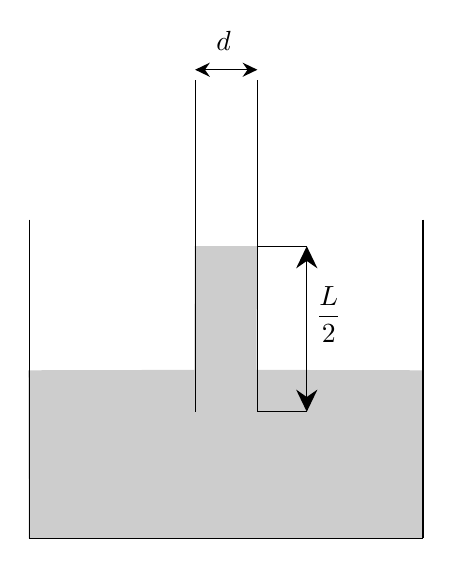
\begin{tikzpicture}[x=0.75pt,y=0.75pt,yscale=-1,xscale=1]
%uncomment if require: \path (0,422); %set diagram left start at 0, and has height of 422

%Shape: Polygon [id:ds7588791827739569] 
\draw  [draw opacity=0][fill={rgb, 255:red, 155; green, 155; blue, 155 }  ,fill opacity=0.5 ] (299.8,150.4) -- (329.8,150.4) -- (329.6,210) -- (409.8,210.2) -- (409.6,291.2) -- (219.8,291.2) -- (219.6,210.2) -- (299.6,210) -- cycle ;
%Straight Lines [id:da7517226553205549] 
\draw    (220,137.56) -- (220,291.2) ;
%Straight Lines [id:da608794999274314] 
\draw    (409.8,291.2) -- (220,291.2) ;
%Straight Lines [id:da8033275110936606] 
\draw    (409.8,137.56) -- (409.8,291.2) ;
%Straight Lines [id:da28879179040321756] 
\draw    (300,70.4) -- (300,230.2) ;
%Straight Lines [id:da3709449594587153] 
\draw    (330,70.4) -- (330,230.2) ;
%Straight Lines [id:da006711851193644369] 
\draw    (329.8,150.4) -- (353.8,150.4) ;
%Straight Lines [id:da885352342345394] 
\draw    (330,230.2) -- (354,230.2) ;
%Straight Lines [id:da7609671512025402] 
\draw    (353.8,153.4) -- (353.8,227.2) ;
\draw [shift={(353.8,230.2)}, rotate = 270] [fill={rgb, 255:red, 0; green, 0; blue, 0 }  ][line width=0.08]  [draw opacity=0] (10.72,-5.15) -- (0,0) -- (10.72,5.15) -- (7.12,0) -- cycle    ;
\draw [shift={(353.8,150.4)}, rotate = 90] [fill={rgb, 255:red, 0; green, 0; blue, 0 }  ][line width=0.08]  [draw opacity=0] (10.72,-5.15) -- (0,0) -- (10.72,5.15) -- (7.12,0) -- cycle    ;
%Straight Lines [id:da23662723460306978] 
\draw    (327,65.4) -- (303,65.4) ;
\draw [shift={(300,65.4)}, rotate = 360] [fill={rgb, 255:red, 0; green, 0; blue, 0 }  ][line width=0.08]  [draw opacity=0] (7.14,-3.43) -- (0,0) -- (7.14,3.43) -- (4.74,0) -- cycle    ;
\draw [shift={(330,65.4)}, rotate = 180] [fill={rgb, 255:red, 0; green, 0; blue, 0 }  ][line width=0.08]  [draw opacity=0] (7.14,-3.43) -- (0,0) -- (7.14,3.43) -- (4.74,0) -- cycle    ;


% Text Node
\draw (357,168.4) node [anchor=north west][inner sep=0.75pt]    {$\dfrac{L}{2}$};
% Text Node
\draw (309,45.4) node [anchor=north west][inner sep=0.75pt]    {$d$};


\end{tikzpicture}

    \end{center}
    \begin{enumerate}[1)]
        \item Tính điện dung của tụ điện.
        \item Tính độ lớn của điện trường giữa hai bản tụ.
        \item Tìm sự phân bố điện tích trên hai bản tụ.
        \item Tìm độ cao dâng lên của chất lỏng trong tụ so với chất lỏng trong bình chứa.
    \end{enumerate}
\end{vd}
\begin{loigiai}
\begin{enumerate}[1)]
   \item Điện dung của hệ tụ điện song song và bình chứa điện môi chỉ đơn giản là tổng điện dung của hai tụ mắc song song:
        $$C = \dfrac{L(L/2)}{4\pi d} + \dfrac{\varepsilon L(L/2)}{4\pi d} = \dfrac{L^2}{8\pi d} (1+\varepsilon) \equiv C_0\dfrac{1+\varepsilon}{2}.$$
    \item  Điện tích trên tụ không bị thay đổi khi nhúng tụ vào bể chứa nhưng thế năng tích trữ giữa hai bản tụ thì có. Sau khi được nạp bởi nguồn, $Q=C_0 V$ Nhúng một nửa chiều cao của tụ $L/2$ vào bồn chứa, điện dung của tụ thay đổi từ $C_0$ đến $C_0(1+\varepsilon)/2$. Hiệu điện thế giữa chúng lúc sau $V’$ là:
           $$C_0V = C_0\dfrac{1+\varepsilon}{2}V’.$$
           Do đó:
           $$V’ = \dfrac{2}{1+\varepsilon}V,$$
           và do $|V| = |E|d$ nên
            $$E = \dfrac{2}{1+\varepsilon} \dfrac{V}{d}.$$
    \item Từ phương trình Maxwell $\nabla\cdot D = 4\pi\rho$, chúng ta tìm ra $D = 4\pi\sigma$ nhưng $D = \varepsilon E$ nên
    $$E = \dfrac{4\pi\sigma}{\varepsilon}.$$
    Từ phần $(2)$ ta đã tìm được: 
    $$\sigma = \dfrac{2\varepsilon}{4\pi(1+\varepsilon)} \dfrac{V}{d}$$
khi chất lỏng ngập đến giữa tụ.\\ Mật độ điện mặt tại nơi không có chất lỏng là:
    $$\sigma = \dfrac{2}{4\pi(1+\varepsilon)} \dfrac{V}{d}.$$
    \item Để tìm ra chênh lệch độ cao mực chất lỏng trong tụ và trong bể chứa bên ngoài, chúng ta tính tổng thế năng trọng trường của chất lỏng và năng lượng điện trường tích trên tụ. Gọi độ chênh lệch chiều cao là $h$ và một độ thay đổi độ cao nhỏ $\zeta$ như hình vẽ. Thế năng trọng trường của chất lỏng được tính bằng tích phân 
      $$\int_{0}^{h+\zeta}\rho gL d\,x\,\dd x = \rho g \dfrac{(h+\zeta)^2Ld}{2}.$$
       \begin{center}
            

\tikzset{every picture/.style={line width=0.75pt}} %set default line width to 0.75pt        

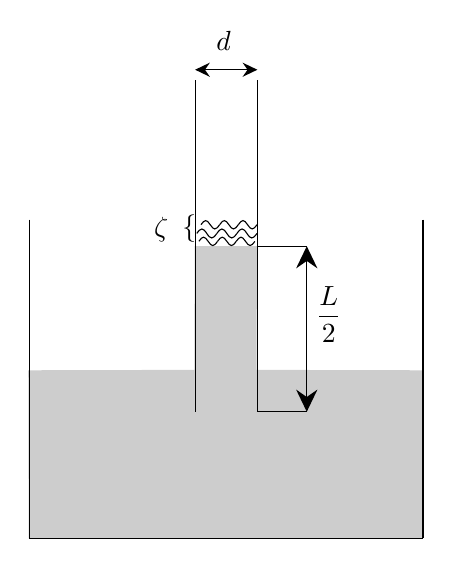
\begin{tikzpicture}[x=0.75pt,y=0.75pt,yscale=-1,xscale=1]
%uncomment if require: \path (0,422); %set diagram left start at 0, and has height of 422

%Shape: Polygon [id:ds7602987343581558] 
\draw  [draw opacity=0][fill={rgb, 255:red, 155; green, 155; blue, 155 }  ,fill opacity=0.5 ] (299.8,150.4) -- (329.8,150.4) -- (329.6,210) -- (409.8,210.2) -- (409.6,291.2) -- (219.8,291.2) -- (219.6,210.2) -- (299.6,210) -- cycle ;
%Shape: Sine Wave Form [id:dp9265135175779409] 
\draw   (301.82,148.06) .. controls (303.67,145.42) and (304.53,145.41) .. (306.29,148.08) .. controls (308.05,150.75) and (308.9,150.77) .. (310.77,148.1) ;
%Shape: Sine Wave Form [id:dp3721424152245498] 
\draw   (310.82,148.06) .. controls (312.67,145.42) and (313.53,145.41) .. (315.29,148.08) .. controls (317.05,150.75) and (317.9,150.77) .. (319.77,148.1) ;
%Shape: Sine Wave Form [id:dp5210302132347915] 
\draw   (319.82,148.06) .. controls (321.67,145.42) and (322.53,145.41) .. (324.29,148.08) .. controls (326.05,150.75) and (326.9,150.77) .. (328.77,148.1) ;

%Straight Lines [id:da6556588775482208] 
\draw    (220,137.56) -- (220,291.2) ;
%Straight Lines [id:da2507747172556749] 
\draw    (409.8,291.2) -- (220,291.2) ;
%Straight Lines [id:da3622638859499685] 
\draw    (409.8,137.56) -- (409.8,291.2) ;
%Straight Lines [id:da7573141890185227] 
\draw    (300,70.4) -- (300,230.2) ;
%Straight Lines [id:da13394710382284236] 
\draw    (330,70.4) -- (330,230.2) ;
%Straight Lines [id:da09363042769351826] 
\draw    (329.8,150.4) -- (353.8,150.4) ;
%Straight Lines [id:da15844310691649666] 
\draw    (330,230.2) -- (354,230.2) ;
%Straight Lines [id:da5428183923971306] 
\draw    (353.8,153.4) -- (353.8,227.2) ;
\draw [shift={(353.8,230.2)}, rotate = 270] [fill={rgb, 255:red, 0; green, 0; blue, 0 }  ][line width=0.08]  [draw opacity=0] (10.72,-5.15) -- (0,0) -- (10.72,5.15) -- (7.12,0) -- cycle    ;
\draw [shift={(353.8,150.4)}, rotate = 90] [fill={rgb, 255:red, 0; green, 0; blue, 0 }  ][line width=0.08]  [draw opacity=0] (10.72,-5.15) -- (0,0) -- (10.72,5.15) -- (7.12,0) -- cycle    ;
%Shape: Sine Wave Form [id:dp2066796886763671] 
\draw   (300.82,144.26) .. controls (302.81,141.42) and (303.74,141.41) .. (305.63,144.28) .. controls (307.52,147.15) and (308.42,147.17) .. (310.43,144.3) ;
%Shape: Sine Wave Form [id:dp3009934611124063] 
\draw   (310.49,144.26) .. controls (312.48,141.42) and (313.4,141.41) .. (315.29,144.28) .. controls (317.19,147.15) and (318.09,147.17) .. (320.1,144.3) ;
%Shape: Sine Wave Form [id:dp4212523783536659] 
\draw   (320.16,144.26) .. controls (322.15,141.42) and (323.07,141.41) .. (324.96,144.28) .. controls (326.85,147.15) and (327.75,147.17) .. (329.76,144.3) ;

%Shape: Sine Wave Form [id:dp008294576835681466] 
\draw   (302.82,140.06) .. controls (304.67,137.42) and (305.53,137.41) .. (307.29,140.08) .. controls (309.05,142.75) and (309.9,142.77) .. (311.77,140.1) ;
%Shape: Sine Wave Form [id:dp16870384965352647] 
\draw   (311.82,140.06) .. controls (313.67,137.42) and (314.53,137.41) .. (316.29,140.08) .. controls (318.05,142.75) and (318.9,142.77) .. (320.77,140.1) ;
%Shape: Sine Wave Form [id:dp019431373960939524] 
\draw   (320.82,140.06) .. controls (322.67,137.42) and (323.53,137.41) .. (325.29,140.08) .. controls (327.05,142.75) and (327.9,142.77) .. (329.77,140.1) ;

%Straight Lines [id:da11546994351349116] 
\draw    (327,65.4) -- (303,65.4) ;
\draw [shift={(300,65.4)}, rotate = 360] [fill={rgb, 255:red, 0; green, 0; blue, 0 }  ][line width=0.08]  [draw opacity=0] (7.14,-3.43) -- (0,0) -- (7.14,3.43) -- (4.74,0) -- cycle    ;
\draw [shift={(330,65.4)}, rotate = 180] [fill={rgb, 255:red, 0; green, 0; blue, 0 }  ][line width=0.08]  [draw opacity=0] (7.14,-3.43) -- (0,0) -- (7.14,3.43) -- (4.74,0) -- cycle    ;


% Text Node
\draw (357,168.4) node [anchor=north west][inner sep=0.75pt]    {$\dfrac{L}{2}$};
% Text Node
\draw (279,135.4) node [anchor=north west][inner sep=0.75pt]    {$\zeta $};
% Text Node
\draw (297.23,142) node    {$\{$};
% Text Node
\draw (309,45.4) node [anchor=north west][inner sep=0.75pt]    {$d$};


\end{tikzpicture}

        \end{center}
      Do đó tổng năng lượng là:
      $$U = \dfrac{1}{2} \dfrac{Q^2}{C} + \dfrac{\rho g (h+\zeta)^2 Ld}{2}.$$
    Ở đây chúng ta phải viết lại năng lượng điện trường theo $Q$ vì năng lượng này sẽ thay đổi theo độ cao mực nước. Thế thành phần $C$ theo các tham số khác, ta có:
    $$U = \dfrac{1}{2} \dfrac{8\pi Q^2d}{L^2(1+\varepsilon) + 2L(\varepsilon-1)\zeta} + \dfrac{\rho g (h+\zeta)^2Ld}{2}.$$
    Ở vị trí cân bằng, tổng lực tác dụng lên chất lỏng bằng không nên đạo hàm của năng lượng ta tính ở trên bằng không:
    $$-\dfrac{\partial U}{\partial\zeta} = \dfrac{1}{2} \dfrac{16\pi Q^2Ld(\varepsilon-1)}{[L^2(\varepsilon+1) + 2L(\varepsilon-1)\zeta]^2} - \rho g(h+\zeta)Ld = 0.$$

    Ở vị trí cân bằng, $\zeta = 0$:
        $$\dfrac{8\pi Q^2Ld(\varepsilon-1)}{L^4(\varepsilon+1)^2} = \rho gL\,\dd h$$
    $$h = \dfrac{8\pi Q^2(\varepsilon-1)}{L^4\rho g(\varepsilon+1)^2}.$$
Viết lại phương trình trên theo $V$, ta thu được:
    $$h=\frac{V^2}{2\pi\rho g d^2}\frac{\varepsilon -1}{(\varepsilon+1)^2}.$$
    Theo một cách khác, ta có thể tính được lực bằng cách:
      $$F_h = \left(-\dfrac{\partial U}{\partial x}\right)_{x=L/2} = \dfrac{2\pi dQ^2}{L} \dfrac{(\varepsilon-1)}{[L+L(\varepsilon-1)/2]^2}.$$  
      Và trọng lượng của phần nước là:
        $$W = \rho ghLd.$$
         Từ đó ta tính ra:
         $$h = \dfrac{8\pi Q^2(\varepsilon-1)}{L^4\rho g(\varepsilon+1)^2}.$$
      cũng thu được kết quả tương tự như cách làm bên trên. 
\end{enumerate}
\end{loigiai}


\begin{vd}[Lực điện và sự giãn nở]
    \begin{enumerate}[1)]
        \item Nghiên cứu hai quả cầu điện môi với bán kính $a$, đặt cách nhau một khoảng $R\, (R\gg a)$. Một quả cầu được tích điện $q$, trong khi quả cầu còn lại được giữ trung hòa điện. Bây giờ chúng ta tăng kích thước dài của hệ lên gấp hai lần (bán kính quả cầu và khoảng cách giữa chúng tăng gấp hai lần). Để lực tương tác giữa hai quả cầu không đổi thì điện tích quả cầu $1$ phải tăng lên bao nhiêu?
        \begin{center}
            

\tikzset{every picture/.style={line width=0.75pt}} %set default line width to 0.75pt        

\begin{tikzpicture}[x=0.75pt,y=0.75pt,yscale=-1,xscale=1]
%uncomment if require: \path (0,465); %set diagram left start at 0, and has height of 465

%Shape: Circle [id:dp42265347563661804] 
\draw   (165,185) .. controls (165,171.19) and (176.19,160) .. (190,160) .. controls (203.81,160) and (215,171.19) .. (215,185) .. controls (215,198.81) and (203.81,210) .. (190,210) .. controls (176.19,210) and (165,198.81) .. (165,185) -- cycle ;
%Shape: Circle [id:dp49358445532785544] 
\draw   (455,186) .. controls (455,172.19) and (466.19,161) .. (480,161) .. controls (493.81,161) and (505,172.19) .. (505,186) .. controls (505,199.81) and (493.81,211) .. (480,211) .. controls (466.19,211) and (455,199.81) .. (455,186) -- cycle ;
%Straight Lines [id:da47270362610943795] 
\draw    (193,230) -- (357.6,230) -- (477,230) ;
\draw [shift={(480,230)}, rotate = 180] [fill={rgb, 255:red, 0; green, 0; blue, 0 }  ][line width=0.08]  [draw opacity=0] (10.72,-5.15) -- (0,0) -- (10.72,5.15) -- (7.12,0) -- cycle    ;
\draw [shift={(190,230)}, rotate = 0] [fill={rgb, 255:red, 0; green, 0; blue, 0 }  ][line width=0.08]  [draw opacity=0] (10.72,-5.15) -- (0,0) -- (10.72,5.15) -- (7.12,0) -- cycle    ;
%Straight Lines [id:da9999361003926563] 
\draw    (190,185) -- (205.68,169.32) ;
\draw [shift={(207.8,167.2)}, rotate = 495] [fill={rgb, 255:red, 0; green, 0; blue, 0 }  ][line width=0.08]  [draw opacity=0] (5.36,-2.57) -- (0,0) -- (5.36,2.57) -- (3.56,0) -- cycle    ;
%Straight Lines [id:da15833993928459633] 
\draw    (480,186) -- (495.68,170.32) ;
\draw [shift={(497.8,168.2)}, rotate = 495] [fill={rgb, 255:red, 0; green, 0; blue, 0 }  ][line width=0.08]  [draw opacity=0] (5.36,-2.57) -- (0,0) -- (5.36,2.57) -- (3.56,0) -- cycle    ;


% Text Node
\draw (170,144.4) node [anchor=north west][inner sep=0.75pt]    {$q$};
% Text Node
\draw (198,180) node [anchor=north west][inner sep=0.75pt]    {$a$};
% Text Node
\draw (487.9,180) node [anchor=north west][inner sep=0.75pt]    {$a$};
% Text Node
\draw (327,207.4) node [anchor=north west][inner sep=0.75pt]    {$R$};


\end{tikzpicture}
        \end{center}
        \item Bây giờ ta nghiên cứu một chiếc vòng dẫn điện làm từ dây dẫn mảnh, với $d$ là đường kính dây và $D$ là đường kính của vòng dây $(D\gg d)$. Tích điện cho vòng dây một điện tích q vừa đủ cho vòng dây đứt do lực căng tĩnh điện. Bây giờ chúng ta lại tăng kích thước dài của vòng dây lên hai lần như câu $1)$. Lúc này phải tích cho vòng dây một điện tích bằng bao nhiêu để dây đứt?
        \begin{center}
            

\tikzset{every picture/.style={line width=0.75pt}} %set default line width to 0.75pt        

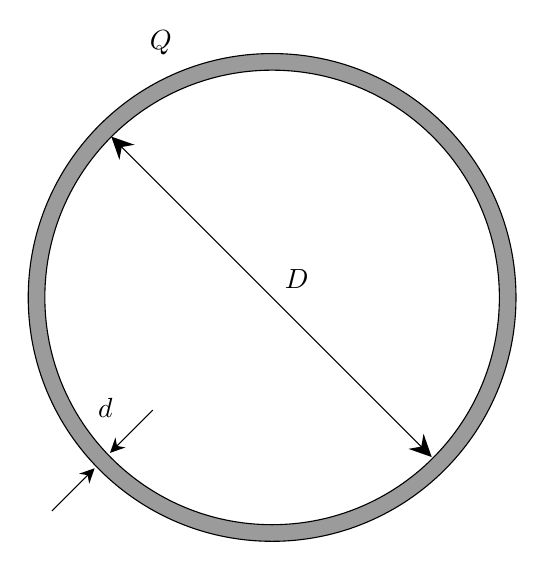
\begin{tikzpicture}[x=0.75pt,y=0.75pt,yscale=-1,xscale=1]
%uncomment if require: \path (0,575); %set diagram left start at 0, and has height of 575

%Shape: Donut [id:dp5869287598506212] 
\draw  [fill={rgb, 255:red, 155; green, 155; blue, 155 }  ,fill opacity=1 ,even odd rule] (216.6,238.1) .. controls (216.6,177.62) and (265.62,128.6) .. (326.1,128.6) .. controls (386.58,128.6) and (435.6,177.62) .. (435.6,238.1) .. controls (435.6,298.58) and (386.58,347.6) .. (326.1,347.6) .. controls (265.62,347.6) and (216.6,298.58) .. (216.6,238.1)(208.6,238.1) .. controls (208.6,173.21) and (261.21,120.6) .. (326.1,120.6) .. controls (390.99,120.6) and (443.6,173.21) .. (443.6,238.1) .. controls (443.6,302.99) and (390.99,355.6) .. (326.1,355.6) .. controls (261.21,355.6) and (208.6,302.99) .. (208.6,238.1) ;
%Straight Lines [id:da2197263355479353] 
\draw    (250.72,162.72) -- (400.88,312.88) ;
\draw [shift={(403,315)}, rotate = 225] [fill={rgb, 255:red, 0; green, 0; blue, 0 }  ][line width=0.08]  [draw opacity=0] (10.72,-5.15) -- (0,0) -- (10.72,5.15) -- (7.12,0) -- cycle    ;
\draw [shift={(248.6,160.6)}, rotate = 45] [fill={rgb, 255:red, 0; green, 0; blue, 0 }  ][line width=0.08]  [draw opacity=0] (10.72,-5.15) -- (0,0) -- (10.72,5.15) -- (7.12,0) -- cycle    ;
%Straight Lines [id:da9221036743576936] 
\draw    (250.12,310.88) -- (268.6,292.4) ;
\draw [shift={(248,313)}, rotate = 315] [fill={rgb, 255:red, 0; green, 0; blue, 0 }  ][line width=0.08]  [draw opacity=0] (7.14,-3.43) -- (0,0) -- (7.14,3.43) -- (4.74,0) -- cycle    ;
%Straight Lines [id:da15873300869830165] 
\draw    (220,341) -- (238.48,322.52) ;
\draw [shift={(240.6,320.4)}, rotate = 495] [fill={rgb, 255:red, 0; green, 0; blue, 0 }  ][line width=0.08]  [draw opacity=0] (7.14,-3.43) -- (0,0) -- (7.14,3.43) -- (4.74,0) -- cycle    ;


% Text Node
\draw (241,285.4) node [anchor=north west][inner sep=0.75pt]    {$d$};
% Text Node
\draw (331,223.4) node [anchor=north west][inner sep=0.75pt]    {$D$};
% Text Node
\draw (266,108.4) node [anchor=north west][inner sep=0.75pt]    {$Q$};


\end{tikzpicture}
        \end{center}
    \end{enumerate}

\end{vd}
\begin{loigiai}
    \begin{enumerate}[1)]
        \item Quả cầu bị tích điện sẽ hưởng ứng và làm phân cực quả cầu trung hòa do đó tạo ra một moment lưỡng cực p tỉ lệ thuận với cường độ điện trường của quả cầu tích điện:
        $$p \propto E \propto \dfrac{q}{R^2}.$$
        Lực tương tác giữa lưỡng cực điện và quả cầu tích điện bằng tích của moment lưỡng cực và gradient của cường độ điện trường tại vị trí của lưỡng cực:
       $$F \propto \dfrac{pq}{R^3} \propto \dfrac{q^2}{R^5}.$$
       Để có $F'=F$ sau khi tăng kích thước dài của hệ lên hai lần thì điện tích $q’$ phải thỏa mãn:
       $$\dfrac{q^2}{R^5} = \dfrac{q’^2}{R’^5}$$
       $$\left(\dfrac{q’}{q}\right)^2 = \left(\dfrac{R’}{R}\right)^5 = 32$$
       $$q’ = 4\sqrt{2} q.$$
       \item Điện tích $Q$ sẽ được phân bố đều dọc theo dây. Do đó lực Coulomb giữa một điểm trên vòng và phần còn lại của vòng sẽ tỉ lệ thuận với bình phương của $Q$ và tỉ lệ nghịch với bình phương đường kính vòng $D$:
       $$F_Q \propto \dfrac{Q^2}{D^2}.$$
       Khi vòng dây bị đứt, lực đàn hồi $F_e$ giới hạn dọc theo vòng sẽ là:
        $$F_e = \sigma S,$$
        trong đó $\sigma$ là sức căng cực đại, chỉ phụ thuộc vào vật liệu làm dây, và $S$ là tiết diện mặt cắt của dây. Tại thời điểm vòng dây đứt, $F_Q=F_e$, do đó cân bằng hai phương trình trên ta có:
        $$Q^2 \propto \sigma SD^2 \propto \sigma d^2D^2.$$
        Tăng kích thước dài của hệ lên hai lần cho ta:
         $$Q’ \propto d’D’ = 4dD.$$
         Do đó:
        $$Q' = 4Q.$$
    \end{enumerate}
\end{loigiai}



\begin{vd}[Hệ tụ điện không song song (G)]
\begin{enumerate}[1)]
    \item Một tụ điện được cấu tạo thành từ hai bản tụ dẫn điện hình chữ nhật với các cạnh dài lần lượt $L_1$ và $L_2$. Hai bản tụ này được đặt không song song nhau. Một cặp cạnh của tụ dài $L_1$ được đặt song song cách nhau $d_1$ và cặp cạnh $L_1$ còn lại được đặt song song và cách nhau $d_2$; trong đó $d_2>d_1$. (Xem hình vẽ)\\ %đính hình vẽ
\begin{center}


\tikzset{every picture/.style={line width=0.75pt}} %set default line width to 0.75pt        

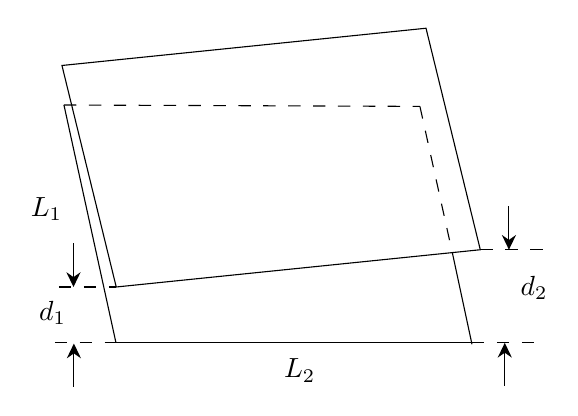
\begin{tikzpicture}[x=0.75pt,y=0.75pt,yscale=-1,xscale=1]
%uncomment if require: \path (0,490); %set diagram left start at 0, and has height of 490

%Straight Lines [id:da712602482648053] 
\draw    (159.21,151.27) -- (184.28,265.86) ;
%Straight Lines [id:da45102212002233655] 
\draw    (184.28,265.86) -- (355.8,265.86) ;
%Straight Lines [id:da19129120832648439] 
\draw    (346.8,224.6) -- (355.79,266.53) ;
%Straight Lines [id:da8526825428836884] 
\draw  [dash pattern={on 4.5pt off 4.5pt}]  (330.72,151.94) -- (346.8,224.6) ;
%Straight Lines [id:da3456668494272379] 
\draw  [dash pattern={on 4.5pt off 4.5pt}]  (159.21,151.27) -- (330.72,151.94) ;
%Shape: Parallelogram [id:dp6883692974447599] 
\draw   (333.65,114.28) -- (359.8,221) -- (184.4,238.95) -- (158.25,132.23) -- cycle ;
%Straight Lines [id:da9980615488127933] 
\draw  [dash pattern={on 4.5pt off 4.5pt}]  (156.8,238.95) -- (184.4,238.95) ;
%Straight Lines [id:da9800983319866017] 
\draw  [dash pattern={on 4.5pt off 4.5pt}]  (154.8,265.86) -- (184.28,265.86) ;
%Straight Lines [id:da513912025331484] 
\draw  [dash pattern={on 4.5pt off 4.5pt}]  (359.8,221) -- (389.8,221) ;
%Straight Lines [id:da6319286640176305] 
\draw  [dash pattern={on 4.5pt off 4.5pt}]  (355.8,265.86) -- (386.8,265.86) ;
%Straight Lines [id:da02605118085004654] 
\draw    (163.8,217.95) -- (163.8,235.95) ;
\draw [shift={(163.8,238.95)}, rotate = 270] [fill={rgb, 255:red, 0; green, 0; blue, 0 }  ][line width=0.08]  [draw opacity=0] (7.14,-3.43) -- (0,0) -- (7.14,3.43) -- (4.74,0) -- cycle    ;
%Straight Lines [id:da5604084916920165] 
\draw    (164,269.2) -- (164,287.2) ;
\draw [shift={(164,266.2)}, rotate = 90] [fill={rgb, 255:red, 0; green, 0; blue, 0 }  ][line width=0.08]  [draw opacity=0] (7.14,-3.43) -- (0,0) -- (7.14,3.43) -- (4.74,0) -- cycle    ;
%Straight Lines [id:da4315925723080418] 
\draw    (373.6,200) -- (373.6,218) ;
\draw [shift={(373.6,221)}, rotate = 270] [fill={rgb, 255:red, 0; green, 0; blue, 0 }  ][line width=0.08]  [draw opacity=0] (7.14,-3.43) -- (0,0) -- (7.14,3.43) -- (4.74,0) -- cycle    ;
%Straight Lines [id:da27425010839765407] 
\draw    (371.6,268.86) -- (371.6,286.86) ;
\draw [shift={(371.6,265.86)}, rotate = 90] [fill={rgb, 255:red, 0; green, 0; blue, 0 }  ][line width=0.08]  [draw opacity=0] (7.14,-3.43) -- (0,0) -- (7.14,3.43) -- (4.74,0) -- cycle    ;


% Text Node
\draw (146,244.4) node [anchor=north west][inner sep=0.75pt]    {$d_{1}$};
% Text Node
\draw (378,232.4) node [anchor=north west][inner sep=0.75pt]    {$d_{2}$};
% Text Node
\draw (142,194.4) node [anchor=north west][inner sep=0.75pt]    {$L_{1}$};
% Text Node
\draw (264,272.4) node [anchor=north west][inner sep=0.75pt]    {$L_{2}$};


\end{tikzpicture}
\end{center}
    Bỏ qua mọi hiệu ứng rìa, khi đặt một hiệu điện thế $V$ vào hai bản tụ, tìm điện thế ở một điểm bất kì giữa hai tụ.
    \item Tính điện dung của hệ.
\end{enumerate}
\end{vd}

\begin{loigiai}
\begin{enumerate}[1)]
\item Đặt một hệ tọa độ trụ sao cho các bản tụ nằm dọc theo phương bán kính của hệ tọa độ (xem hình vẽ). Phương trình Laplace $\nabla^2 \phi=0$ do đó:

  \begin{center}


\tikzset{every picture/.style={line width=0.75pt}} %set default line width to 0.75pt        

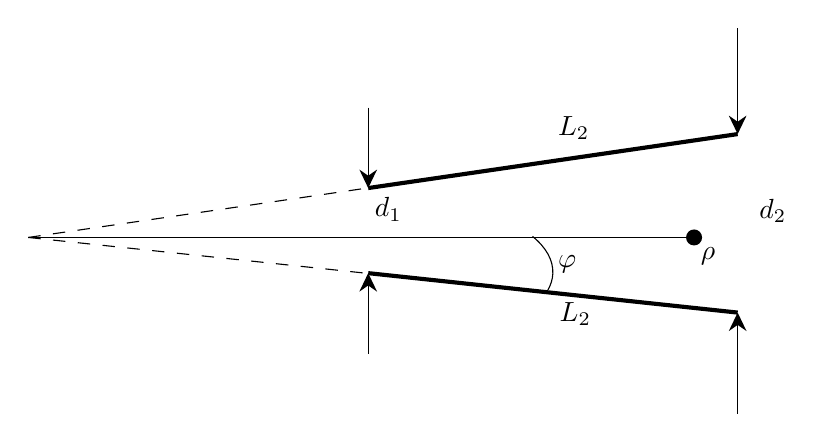
\begin{tikzpicture}[x=0.75pt,y=0.75pt,yscale=-1,xscale=1]
%uncomment if require: \path (0,463); %set diagram left start at 0, and has height of 463

%Straight Lines [id:da8888219188553073] 
\draw    (137,240) -- (457.8,240) ;
\draw [shift={(457.8,240)}, rotate = 0] [color={rgb, 255:red, 0; green, 0; blue, 0 }  ][fill={rgb, 255:red, 0; green, 0; blue, 0 }  ][line width=0.75]      (0, 0) circle [x radius= 3.35, y radius= 3.35]   ;
%Straight Lines [id:da0375644723320927] 
\draw  [dash pattern={on 4.5pt off 4.5pt}]  (137,240) -- (478.8,190.2) ;
%Straight Lines [id:da5190157214133659] 
\draw  [dash pattern={on 4.5pt off 4.5pt}]  (137,240) -- (478.8,276.2) ;
%Straight Lines [id:da37116370456208414] 
\draw [line width=1.5]    (300.8,216.2) -- (478.8,190.2) ;
%Straight Lines [id:da03708741936908044] 
\draw [line width=1.5]    (300.8,257.2) -- (478.8,276.2) ;
%Straight Lines [id:da18268352409070432] 
\draw    (300.8,177.4) -- (300.8,213.2) ;
\draw [shift={(300.8,216.2)}, rotate = 270] [fill={rgb, 255:red, 0; green, 0; blue, 0 }  ][line width=0.08]  [draw opacity=0] (8.93,-4.29) -- (0,0) -- (8.93,4.29) -- (5.93,0) -- cycle    ;
%Straight Lines [id:da7567562935874099] 
\draw    (300.8,260.2) -- (300.8,296) ;
\draw [shift={(300.8,257.2)}, rotate = 90] [fill={rgb, 255:red, 0; green, 0; blue, 0 }  ][line width=0.08]  [draw opacity=0] (8.93,-4.29) -- (0,0) -- (8.93,4.29) -- (5.93,0) -- cycle    ;
%Straight Lines [id:da7764810518012757] 
\draw    (478.8,139.2) -- (478.8,187.2) ;
\draw [shift={(478.8,190.2)}, rotate = 270] [fill={rgb, 255:red, 0; green, 0; blue, 0 }  ][line width=0.08]  [draw opacity=0] (8.93,-4.29) -- (0,0) -- (8.93,4.29) -- (5.93,0) -- cycle    ;
%Straight Lines [id:da7451709181736375] 
\draw    (478.8,279.2) -- (478.8,325.2) ;
\draw [shift={(478.8,276.2)}, rotate = 90] [fill={rgb, 255:red, 0; green, 0; blue, 0 }  ][line width=0.08]  [draw opacity=0] (8.93,-4.29) -- (0,0) -- (8.93,4.29) -- (5.93,0) -- cycle    ;
%Shape: Arc [id:dp8276494349776893] 
\draw  [draw opacity=0] (379.98,239.5) .. controls (386.38,244.69) and (390.02,250.87) .. (389.75,257.37) .. controls (389.63,260.15) and (388.81,262.81) .. (387.37,265.31) -- (333.4,255) -- cycle ; \draw   (379.98,239.5) .. controls (386.38,244.69) and (390.02,250.87) .. (389.75,257.37) .. controls (389.63,260.15) and (388.81,262.81) .. (387.37,265.31) ;


% Text Node
\draw (459.8,243.4) node [anchor=north west][inner sep=0.75pt]    {$\rho $};
% Text Node
\draw (302.8,219.6) node [anchor=north west][inner sep=0.75pt]    {$d_{1}$};
% Text Node
\draw (488,220.4) node [anchor=north west][inner sep=0.75pt]    {$d_{2}$};
% Text Node
\draw (391,180.4) node [anchor=north west][inner sep=0.75pt]    {$L_{2}$};
% Text Node
\draw (391.8,270.1) node [anchor=north west][inner sep=0.75pt]    {$L_{2}$};
% Text Node
\draw (391,247.4) node [anchor=north west][inner sep=0.75pt]    {$\varphi $};


\end{tikzpicture}
\end{center}
trở thành:
   $$\frac{1}{\rho}\frac{\partial}{\partial\rho}\left(\rho\frac{\partial\phi}{\partial\rho}\right) + \frac{1}{\rho^2}\frac{\partial^2 \phi}{\partial \varphi^2} = 0.$$
Đặt $\phi=R(\rho)\chi(\varphi)$, chúng ta có thể tách phương trình trên thành hai phương trình đạo hàm:
     $$\frac{\rho}{R} \frac{\dd}{\dd\rho}\left(\rho\frac{\dd R}{\dd\rho}\right) = n^2$$
     $$\frac{1}{\chi} \frac{\dd^2 \chi}{\dd \varphi^2} = -n^2.$$
trong đó $R$ là thành phần theo phương bán kính của điện thế, $\chi$ là thành phần theo trục đối xứng, và $n$ là một hằng số. Trong giới hạn xấp xỉ góc nhỏ (điều kiện có thể được công nhận vì chúng ta đã bỏ qua hiệu ứng rìa), chúng ta có thể công nhận $R$ không phụ thuộc vào $\rho$, do đó:
  $$\frac{\dd^2\chi}{\dd \varphi^2} =0,$$
ta có nghiệm cho phương trình này $\chi = A\varphi + B$. Từ điều kiện biên $\chi(0) = 0$, chúng ta có $B=0$, và sử dụng điều kiện biên còn lại $\chi(\varphi_0)=V$, ta tìm được:
   $$\phi = V\frac{\varphi}{\varphi_0},$$
trong đó
     $$\varphi_0 \approx \sin\varphi_0 = \frac{d_2 - d_1}{L_2},$$
\item Sử dụng kết quả của câu $1)$ và biểu thức năng lượng điện trường $U$ tích trữ trong tụ ta sẽ tính được điện dung của tụ:
    $$U= \frac{1}{2}CV^2=\frac{1}{8\pi}\int E^2 \dd^3 x.$$
Ở đây,
  $$\ot{E} = -\nabla\phi= -\frac{V}{\rho\varphi_0}\ot{e}_{\varphi}.$$
Do đó tích phân trên trở thành:
 $$\frac{1}{2} C V^{2}=\frac{1}{8 \pi} \int_{0}^{L_{1}} \int_{\rho_{1}}^{\rho_{2}} \int_{0}^{\varphi_{0}} \frac{V^{2}}{\rho^{2} \varphi_{0}^{2}} \rho \dd \varphi \dd \rho \dd z$$
 $$=\frac{1}{8 \pi} \frac{L_{1} V^{2}}{\varphi_{0}} \int_{\rho_{1}}^{\rho_{2}} \frac{\dd \rho}{\rho}=\frac{L_{1} L_{2} V^{2}}{8 \pi\left(d_{2}-d_{1}\right)} \ln \frac{d_{2} / \varphi_{0}}{d_{1} / \varphi_{0}}=\frac{L_{1} L_{2} V^{2}}{8 \pi\left(d_{2}-d_{1}\right)} \ln \frac{d_{2}}{d_{1}}.$$
Do đó điện dung tụ là:
    $$C=\frac{L_{1} L_{2}}{4 \pi\left(d_{2}-d_{1}\right)} \ln \frac{d_{2}}{d_{1}}=\frac{L_{1} L_{2}}{4 \pi\left(d_{2}-d_{1}\right)} \ln \left(1+\frac{d_{2}-d_{1}}{d_{1}}\right).$$
Trong giới hạn $d_2\rightarrow d_1=d$ (tương tự như một tụ song song), biểu thức điện dung rút gọn còn:
        $$C \approx \frac{L_1 L_2}{4\pi (d_2 -d_1)}\cdot\frac{(d_2 -d_1)}{d_1} =\frac{L_1 L_2}{4\pi d}.$$
biểu thức này tương tự như điện dung các tụ điện phẳng quen thuộc.
\end{enumerate}
\end{loigiai}


\begin{vd}[Điện tích đặt lệch]
\begin{center}
    \bf Phần I
\end{center}
Xét hai nhóm các điện tích. Nhóm $A$ gồm $N$ điện tích $q_1, q_2,\dots q_{N}$ được đặt tại các vị trí $\ot{r_1}, \ot{r_2}, \dots \ot{r_{N}}$ tương ứng. Nhóm $B$ gồm $M$ điện tích $q_1, q_2,\dots q_{M}$ được đặt tại các vị trí $\ot{r_1}, \ot{r_2}, \dots \ot{r_{M}}$ tương ứng.
\begin{enumerate}[1)]
    \item Viết biểu thức điện thế $\phi_{A}(\ot{r})$ tại vị trí $\ot{r}$ do các điện tích của nhóm $A$ gây ra.
    \item Viết biểu thức thế năng tĩnh điện $E_{B/A}$ tại nhóm $B$ do điện thế  $\phi_{A}(\ot{r})$ gây ra.
    \item Mối quan hệ giữa $E_{B/A}$ và $E_{A/B}$ là gì?
    \end{enumerate}
    \begin{center}
        \bf Phần II
    \end{center}
\begin{enumerate}[1)]
\setcounter{enumi}{3}
    \item Xét hai tấm phẳng dẫn điện như hình $(a)$. Tấm trên mang điện tích đều với mật độ điện mặt $\sigma'$ và tấm dưới được nối đất. Tìm mật độ điện tích mặt của tấm dưới và điện thế $\phi'(z)$, với $z$ là độ cao của tùy ý tính từ tấm dưới.
    \begin{center}
% Gradient Info
\tikzset {_hohk0nkfl/.code = {\pgfsetadditionalshadetransform{ \pgftransformshift{\pgfpoint{-198 bp } { 158.4 bp }  }  \pgftransformscale{1.32 }  }}}
\pgfdeclareradialshading{_892sj7syc}{\pgfpoint{160bp}{-128bp}}{rgb(0bp)=(1,1,1);
rgb(0bp)=(1,1,1);
rgb(25bp)=(0,0,0);
rgb(400bp)=(0,0,0)}
\tikzset{every picture/.style={line width=0.75pt}} %set default line width to 0.75pt        

\begin{tikzpicture}[x=0.75pt,y=0.75pt,yscale=-1,xscale=1]
%uncomment if require: \path (0,300); %set diagram left start at 0, and has height of 300

%Straight Lines [id:da5744112006701443] 
\draw [line width=2.25]    (50.02,230.2) -- (220.02,230.2) ;
%Straight Lines [id:da8690459165768833] 
\draw [line width=2.25]    (50.02,150.2) -- (220.02,150.2) ;
%Straight Lines [id:da07085530429119968] 
\draw    (90.02,227.2) -- (90.02,154.2) ;
\draw [shift={(90.02,151.2)}, rotate = 450] [fill={rgb, 255:red, 0; green, 0; blue, 0 }  ][line width=0.08]  [draw opacity=0] (10.72,-5.15) -- (0,0) -- (10.72,5.15) -- (7.12,0) -- cycle    ;
\draw [shift={(90.02,230.2)}, rotate = 270] [fill={rgb, 255:red, 0; green, 0; blue, 0 }  ][line width=0.08]  [draw opacity=0] (10.72,-5.15) -- (0,0) -- (10.72,5.15) -- (7.12,0) -- cycle    ;
%Straight Lines [id:da7730834529264963] 
\draw    (130.02,231.2) -- (130.02,115.2) ;
\draw [shift={(130.02,112.2)}, rotate = 450] [fill={rgb, 255:red, 0; green, 0; blue, 0 }  ][line width=0.08]  [draw opacity=0] (10.72,-5.15) -- (0,0) -- (10.72,5.15) -- (7.12,0) -- cycle    ;
%Straight Lines [id:da6884176023142436] 
\draw    (70.02,230.53) -- (70.02,240.53) ;
%Straight Lines [id:da09371869366650887] 
\draw    (85.02,240.53) -- (55.02,240.53) ;
%Straight Lines [id:da09628245206196029] 
\draw    (80.02,245.53) -- (60.02,245.53) ;
%Straight Lines [id:da25702921235035014] 
\draw    (75.02,250.53) -- (65.02,250.53) ;
%Straight Lines [id:da720705614384034] 
\draw    (74.02,254.53) -- (67.02,254.53) ;
%Straight Lines [id:da27732417557497313] 
\draw [line width=2.25]    (328.02,230.2) -- (498.02,230.2) ;
%Straight Lines [id:da7178949508514356] 
\draw [line width=2.25]    (328.02,150.2) -- (498.02,150.2) ;
%Straight Lines [id:da0010266236395068962] 
\draw    (375.02,227.2) -- (375.02,154.2) ;
\draw [shift={(375.02,151.2)}, rotate = 450] [fill={rgb, 255:red, 0; green, 0; blue, 0 }  ][line width=0.08]  [draw opacity=0] (10.72,-5.15) -- (0,0) -- (10.72,5.15) -- (7.12,0) -- cycle    ;
\draw [shift={(375.02,230.2)}, rotate = 270] [fill={rgb, 255:red, 0; green, 0; blue, 0 }  ][line width=0.08]  [draw opacity=0] (10.72,-5.15) -- (0,0) -- (10.72,5.15) -- (7.12,0) -- cycle    ;
%Straight Lines [id:da05406519506480789] 
\draw    (408.02,231.2) -- (408.02,115.2) ;
\draw [shift={(408.02,112.2)}, rotate = 450] [fill={rgb, 255:red, 0; green, 0; blue, 0 }  ][line width=0.08]  [draw opacity=0] (10.72,-5.15) -- (0,0) -- (10.72,5.15) -- (7.12,0) -- cycle    ;
%Straight Lines [id:da4728682584128783] 
\draw    (348.02,230.53) -- (348.02,240.53) ;
%Straight Lines [id:da7328053485903783] 
\draw    (363.02,240.53) -- (333.02,240.53) ;
%Straight Lines [id:da8199328274708519] 
\draw    (358.02,245.53) -- (338.02,245.53) ;
%Straight Lines [id:da5661730740953121] 
\draw    (353.02,250.53) -- (343.02,250.53) ;
%Straight Lines [id:da7261929479142177] 
\draw    (352.02,254.53) -- (345.02,254.53) ;
%Straight Lines [id:da7908394630453319] 
\draw    (348.02,150.53) -- (348.02,160.53) ;
%Straight Lines [id:da6395835666555918] 
\draw    (363.02,160.53) -- (333.02,160.53) ;
%Straight Lines [id:da8922130529097958] 
\draw    (358.02,165.53) -- (338.02,165.53) ;
%Straight Lines [id:da3103613893624091] 
\draw    (353.02,170.53) -- (343.02,170.53) ;
%Straight Lines [id:da3585774827809405] 
\draw    (352.02,174.53) -- (345.02,174.53) ;
%Straight Lines [id:da6850780975610755] 
\draw    (444.02,227.2) -- (444.02,203.86) ;
\draw [shift={(444.02,200.86)}, rotate = 450] [fill={rgb, 255:red, 0; green, 0; blue, 0 }  ][line width=0.08]  [draw opacity=0] (10.72,-5.15) -- (0,0) -- (10.72,5.15) -- (7.12,0) -- cycle    ;
\draw [shift={(444.02,230.2)}, rotate = 270] [fill={rgb, 255:red, 0; green, 0; blue, 0 }  ][line width=0.08]  [draw opacity=0] (10.72,-5.15) -- (0,0) -- (10.72,5.15) -- (7.12,0) -- cycle    ;
%Shape: Circle [id:dp9553024470160008] 
\path  [shading=_892sj7syc,_hohk0nkfl] (439,196.51) .. controls (439,194.02) and (441.02,192) .. (443.51,192) .. controls (446,192) and (448.02,194.02) .. (448.02,196.51) .. controls (448.02,199) and (446,201.02) .. (443.51,201.02) .. controls (441.02,201.02) and (439,199) .. (439,196.51) -- cycle ; % for fading 
 \draw   (439,196.51) .. controls (439,194.02) and (441.02,192) .. (443.51,192) .. controls (446,192) and (448.02,194.02) .. (448.02,196.51) .. controls (448.02,199) and (446,201.02) .. (443.51,201.02) .. controls (441.02,201.02) and (439,199) .. (439,196.51) -- cycle ; % for border 


% Text Node
\draw (93,181.4) node [anchor=north west][inner sep=0.75pt]    {$\ell $};
% Text Node
\draw (126,95.4) node [anchor=north west][inner sep=0.75pt]    {$z$};
% Text Node
\draw (123,234.4) node [anchor=north west][inner sep=0.75pt]    {$O$};
% Text Node
\draw (378,181.4) node [anchor=north west][inner sep=0.75pt]    {$\ell $};
% Text Node
\draw (402,96.4) node [anchor=north west][inner sep=0.75pt]    {$z$};
% Text Node
\draw (401,234.4) node [anchor=north west][inner sep=0.75pt]    {$O$};
% Text Node
\draw (424,184.4) node [anchor=north west][inner sep=0.75pt]    {$q$};
% Text Node
\draw (453,205.4) node [anchor=north west][inner sep=0.75pt]  [font=\small]  {$z_{0}$};
% Text Node
\draw (121,262.4) node [anchor=north west][inner sep=0.75pt]    {$( a)$};
% Text Node
\draw (401,263.4) node [anchor=north west][inner sep=0.75pt]    {$( b)$};
% Text Node
\draw (98,131.4) node [anchor=north west][inner sep=0.75pt]    {$\sigma '$};


\end{tikzpicture}
    \end{center}
    \item Một điện tích điểm $q$ được đặt giữa hai tấm phẳng dẫn, rộng vô hạn được nối đất. Nếu $z_0$ là khoảng cách giữa $q$ và tấm ở dưới. Tìm tổng điện tích cảm ứng của tấm trên theo $q$, $z_0$ và $\ell$, với $\ell$ là khoảng cách giữa hai tấm như hình $(b)$.
\end{enumerate}
\end{vd}
\begin{loigiai}
\begin{enumerate}[1)]
    \item
    \[\Phi_{A}(\ot{r})=\dfrac{1}{4\pi\varepsilon_0}\sum_{i=1}^{N}\dfrac{q_{i}}{\abs{\ot{r}-\ot{r_{i}}}}.\]
    \item
    \begin{align*}
        E_{B/A}&=\sum_{i=1}^{M}q'_{i}\Phi_{A}(\ot{r'_{i}})=\sum_{i=1}^{M}q'_{i}\left(\dfrac{1}{4\pi\varepsilon_0}\sum_{j=1}^{N}\dfrac{q_{j}}{\abs{\ot{r'_{i}}-\ot{r_{j}}}}\right)=\dfrac{1}{4\pi\varepsilon_0}\sum_{i=1}^{M}\sum_{j=1}^{N}\dfrac{q'_{i}q_{j}}{\abs{\ot{r'_{i}}-\ot{r_{j}}}}.\\
        E_{A/B}&=\sum_{i=1}^{N}q_{i}\Phi_{B}(\ot{r_{i}})=\sum_{i=1}^{N}q_{i}\left(\dfrac{1}{4\pi\varepsilon_0}\sum_{j=1}^{M}\dfrac{q'_{j}}{\abs{\ot{r_{i}}-\ot{r'_{j}}}}\right)=\dfrac{1}{4\pi\varepsilon_0}\sum_{i=1}^{N}\sum_{j=1}^{M}\dfrac{q_{i}q'_{j}}{\abs{\ot{r_{i}}-\ot{r'_{j}}}}.
    \end{align*}
    \item Thay đổi các chỉ số $i, j$ với nhau và thay đổi thứ tự lấy tổng ta có $E_{B/A}=E_{A/B}$.
    \item Mật độ điện tích mặt của tấm bên dưới là $-\sigma'$.\\
    Sử dụng định luật Gauss ta có cường độ điện trường giữa hai tấm là $E=\dfrac{\sigma'}{\varepsilon_0}$.\\
    Điện thế là:
    \[\Phi'(z)=
    \begin{cases}
    0~~\lrt z\leq 0.\\
    \dfrac{\sigma'}{\varepsilon_0}z~~\lrt 0\leq z \leq \ell.\\
    \dfrac{\sigma'}{\varepsilon_0}\ell~~ \lrt z>\ell.
    \end{cases}\]
    \item Xét sự phân bố điện tích ở hình $(a)$ đối với nhóm $A$ và hình $(b)$ đối với nhóm $B$. Để tính $E_{A/B}$. chúng ta cần chú ý rằng các điện tích của nhóm $A$ chỉ nằm trên tấm ở trên, nhưng đối với nhóm $B$, điện thế của tấm trên bằng $0$. Do đó $E_{A/B}=0$.\\
    Tấm bên dưới, nhưng $\phi_{A}=0$.\\
    Điện tích $q$.\\
    Do đó áp dụng kết quả của ý $(3)$ ta có:
    \[q\dfrac{\sigma'}{\varepsilon_0}z_0+Q_{u}\dfrac{\sigma'}{\varepsilon_0}\ell=0\rt Q_{u}=-q\dfrac{z_0}{\ell}.\]
\end{enumerate}
\end{loigiai}

\begin{vd}[Không tích điện!]%Câu 3
Một hình trụ rắn bằng kim loại quay với vận tốc góc $\omega$ quanh trục đối xứng của nó. Hình trụ được đặt trong một từ trường đều $B$ song song với trục của nó. Xác định phân bố điện tích bên trong hình trụ. Tìm vận tốc góc  $\omega$ để mật độ điện tích tại mọi điểm của hình trụ đều bằng không.
\end{vd}
\begin{loigiai}
Phương trình mô tả các lực giữ cho electron tự do di chuyển trên quỹ đạo tròn (bên trong hình trụ) là:
$$eE\pm er\omega B=mr{\omega^2},$$
trong đó $e$ và $m$ lần lượt là điện tích và khối lượng của electron, $R$ là khoảng cách từ electron đến trục quay và $E$ là cường độ điện trường được tạo ra trong hình trụ bởi sự phân bố điện tích. Dấu $\pm$ cho thấy rằng lực Lorentz có thể được hướng vào trong hoặc ra ngoài tùy thuộc vào chiều quay của hình trụ. Từ phương trình chuyển động ta có:
$$ E=\left(\dfrac{m{\omega^2}}{e}\pm\omega B\right)r\equiv Kr,$$
cho thấy cường độ điện trường tỉ lệ thuận với bán kính.
\begin{center}
 

\tikzset{every picture/.style={line width=0.75pt}} %set default line width to 0.75pt        

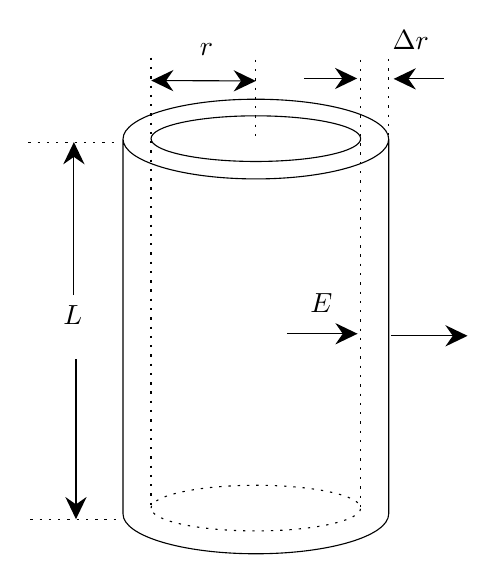
\begin{tikzpicture}[x=0.75pt,y=0.75pt,yscale=-1,xscale=1]
%uncomment if require: \path (0,466); %set diagram left start at 0, and has height of 466

%Shape: Can [id:dp3421118324489345] 
\draw   (363,119.2) -- (363,299.8) .. controls (363,310.4) and (334.35,319) .. (299,319) .. controls (263.65,319) and (235,310.4) .. (235,299.8) -- (235,119.2) .. controls (235,108.6) and (263.65,100) .. (299,100) .. controls (334.35,100) and (363,108.6) .. (363,119.2) .. controls (363,129.8) and (334.35,138.4) .. (299,138.4) .. controls (263.65,138.4) and (235,129.8) .. (235,119.2) ;
%Shape: Ellipse [id:dp6554609238016449] 
\draw   (248.5,119) .. controls (248.5,112.92) and (271.11,108) .. (299,108) .. controls (326.89,108) and (349.5,112.92) .. (349.5,119) .. controls (349.5,125.08) and (326.89,130) .. (299,130) .. controls (271.11,130) and (248.5,125.08) .. (248.5,119) -- cycle ;
%Shape: Ellipse [id:dp4678826933439224] 
\draw  [dash pattern={on 0.84pt off 2.51pt}] (248.5,297) .. controls (248.5,290.92) and (271.11,286) .. (299,286) .. controls (326.89,286) and (349.5,290.92) .. (349.5,297) .. controls (349.5,303.08) and (326.89,308) .. (299,308) .. controls (271.11,308) and (248.5,303.08) .. (248.5,297) -- cycle ;
%Straight Lines [id:da8805055120554433] 
\draw  [dash pattern={on 0.84pt off 2.51pt}]  (248.5,80) -- (248.5,297) ;
%Straight Lines [id:da1519700639364343] 
\draw  [dash pattern={on 0.84pt off 2.51pt}]  (349.5,81) -- (349.5,297) ;
%Straight Lines [id:da859475605792118] 
\draw  [dash pattern={on 0.84pt off 2.51pt}]  (299,81) -- (299,119) ;
%Straight Lines [id:da27539715987896596] 
\draw    (314,213) -- (345,213) ;
\draw [shift={(348,213)}, rotate = 180] [fill={rgb, 255:red, 0; green, 0; blue, 0 }  ][line width=0.08]  [draw opacity=0] (10.72,-5.15) -- (0,0) -- (10.72,5.15) -- (7.12,0) -- cycle    ;
%Straight Lines [id:da18042493663353087] 
\draw    (364,214) -- (398,214) ;
\draw [shift={(401,214)}, rotate = 180] [fill={rgb, 255:red, 0; green, 0; blue, 0 }  ][line width=0.08]  [draw opacity=0] (10.72,-5.15) -- (0,0) -- (10.72,5.15) -- (7.12,0) -- cycle    ;
%Straight Lines [id:da49920586904684927] 
\draw  [dash pattern={on 0.84pt off 2.51pt}]  (189.33,120.67) -- (233.33,120.67) ;
%Straight Lines [id:da1337864117037253] 
\draw  [dash pattern={on 0.84pt off 2.51pt}]  (190.33,302.33) -- (234.33,302.33) ;
%Straight Lines [id:da17401860246007317] 
\draw    (211.33,194.33) -- (211.33,123.67) ;
\draw [shift={(211.33,120.67)}, rotate = 450] [fill={rgb, 255:red, 0; green, 0; blue, 0 }  ][line width=0.08]  [draw opacity=0] (10.72,-5.15) -- (0,0) -- (10.72,5.15) -- (7.12,0) -- cycle    ;
%Straight Lines [id:da6806012790234841] 
\draw    (212.33,225.33) -- (212.33,299.33) ;
\draw [shift={(212.33,302.33)}, rotate = 270] [fill={rgb, 255:red, 0; green, 0; blue, 0 }  ][line width=0.08]  [draw opacity=0] (10.72,-5.15) -- (0,0) -- (10.72,5.15) -- (7.12,0) -- cycle    ;
%Straight Lines [id:da8521846026267319] 
\draw    (251.6,91.01) -- (296,91.19) ;
\draw [shift={(299,91.2)}, rotate = 180.23] [fill={rgb, 255:red, 0; green, 0; blue, 0 }  ][line width=0.08]  [draw opacity=0] (10.72,-5.15) -- (0,0) -- (10.72,5.15) -- (7.12,0) -- cycle    ;
\draw [shift={(248.6,91)}, rotate = 0.23] [fill={rgb, 255:red, 0; green, 0; blue, 0 }  ][line width=0.08]  [draw opacity=0] (10.72,-5.15) -- (0,0) -- (10.72,5.15) -- (7.12,0) -- cycle    ;
%Straight Lines [id:da617352227336923] 
\draw  [dash pattern={on 0.84pt off 2.51pt}]  (363,80.6) -- (363,119.2) ;
%Straight Lines [id:da24251114927538997] 
\draw    (322.4,90) -- (344.8,90) ;
\draw [shift={(347.8,90)}, rotate = 180] [fill={rgb, 255:red, 0; green, 0; blue, 0 }  ][line width=0.08]  [draw opacity=0] (10.72,-5.15) -- (0,0) -- (10.72,5.15) -- (7.12,0) -- cycle    ;
%Straight Lines [id:da16161610058919362] 
\draw    (389.6,90.2) -- (368.4,90.2) ;
\draw [shift={(365.4,90.2)}, rotate = 360] [fill={rgb, 255:red, 0; green, 0; blue, 0 }  ][line width=0.08]  [draw opacity=0] (10.72,-5.15) -- (0,0) -- (10.72,5.15) -- (7.12,0) -- cycle    ;

% Text Node
\draw (324,192.4) node [anchor=north west][inner sep=0.75pt]    {$E$};
% Text Node
\draw (205,198.4) node [anchor=north west][inner sep=0.75pt]    {$L$};
% Text Node
\draw (270.8,71.8) node [anchor=north west][inner sep=0.75pt]    {$r$};
% Text Node
\draw (363.6,65.8) node [anchor=north west][inner sep=0.75pt]    {$\Delta r$};


\end{tikzpicture}

\end{center}
Sử dụng định luật Gauss có thể tìm được mật độ điện tích bên trong hình trụ. Xét vỏ hình trụ mỏng như hình, gọi $\rho(r)$ là mật độ điện tích ở điểm cách trục một khoảng $r$. Một dòng điện có cường độ $ 2\pi rLE(r)$ đi vào vỏ và một dòng điện có cường độ $ 2\pi\left(r+\Delta r\right)LE\left(r+\Delta r\right)$ đi ra khỏi nó.\\
Theo định luật Gauss:
$$ K\left(r+\Delta r\right)2\pi\left(r+\Delta r\right)L-Kr2\pi rL=\dfrac{1}{\varepsilon_0}\rho 2\pi r\Delta rL.$$
Từ đó chúng ta tìm được:
$$\rho=\dfrac{2\varepsilon_0\omega m}{e}\left(\omega\pm\dfrac{eB}{m}\right).$$
Lưu ý rằng, mật độ điện tích trong hình trụ không phụ thuộc vào $r$.\\
Mật độ có thể dương, âm hoặc bằng không - tùy thuộc vào hướng và độ lớn của từ trường và vận tốc góc. Mật độ sẽ bằng không nếu $\omega=\dfrac{|e|B}{m}$. Đối với trường hợp này, các điện tích dương và âm không được tách ra bên trong hình trụ bởi vì lực hướng tâm được cung cấp bởi hiệu ứng Lorentz chỉ là những gì cần thiết để duy trì chuyển động tròn.\\
Ghi chú: Để hình dung về độ lớn của vận tốc góc, giả sử rằng từ trường có giá trị tương đối so với từ trường Trái Đất ở gần Xích Đạo, tức là $ B=3\times{10^{-5}}\ \mathrm{T}$. Mật độ điện tích bằng $0$ tương ứng với vận tốc góc $\omega=\dfrac{eB}{m}=5.3\times{10^6}\ \mathrm{s^{-1}},$ tức là hơn 50 triệu vòng quay mỗi phút! Sự quay vòng nhanh như vậy không thể xảy ra trong thực tế, vì không một vật liệu nào có thể chịu được.
\end{loigiai}


\begin{vd}[Khúc xạ điện từ]
Cho một nguồn ${S}$ phát ra các electron có tốc độ bằng nhau và bằng $v_{0}$. Các electron được cho bay qua một vùng điện trường hẹp có bề rộng $d$. Nguồn phát nằm cách biên của vùng một khoảng là ${L} \ ({L} \gg {d})$. Chọn hệ quy chiếu như hình vẽ. Khối lượng và điện tích của electron lần lượt là
${m}$ và ${q}_{{e}}=-{e}$. Bỏ qua tương tác giữa các electron và tác dụng của trọng lực. 
\\
\textit{Lưu ý: Các ý $1)$ và $2)$ sau đây là hai bài toán độc lập, không liên quan tới nhau.}
\begin{center}
\tikzset{every picture/.style={line width=0.75pt}} %set default line width to 0.75pt        

\begin{tikzpicture}[x=0.75pt,y=0.75pt,yscale=-0.8,xscale=0.8]
%uncomment if require: \path (0,366); %set diagram left start at 0, and has height of 366

%Straight Lines [id:da46697420421082536] 
\draw [line width=1.5]    (118,178) -- (448,178) ;
\draw [shift={(452,178)}, rotate = 180] [fill={rgb, 255:red, 0; green, 0; blue, 0 }  ][line width=0.08]  [draw opacity=0] (11.61,-5.58) -- (0,0) -- (11.61,5.58) -- cycle    ;
%Straight Lines [id:da2506014250640798] 
\draw [line width=1.5]    (294,271) -- (294,55) ;
\draw [shift={(294,51)}, rotate = 450] [fill={rgb, 255:red, 0; green, 0; blue, 0 }  ][line width=0.08]  [draw opacity=0] (11.61,-5.58) -- (0,0) -- (11.61,5.58) -- cycle    ;
%Shape: Circle [id:dp8603477382918159] 
\draw  [fill={rgb, 255:red, 74; green, 74; blue, 74 }  ,fill opacity=1 ] (291,178) .. controls (291,176.34) and (292.34,175) .. (294,175) .. controls (295.66,175) and (297,176.34) .. (297,178) .. controls (297,179.66) and (295.66,181) .. (294,181) .. controls (292.34,181) and (291,179.66) .. (291,178) -- cycle ;
%Straight Lines [id:da25133620030654247] 
\draw    (177,193) -- (291,193) ;
\draw [shift={(294,193)}, rotate = 180] [fill={rgb, 255:red, 0; green, 0; blue, 0 }  ][line width=0.08]  [draw opacity=0] (10.72,-5.15) -- (0,0) -- (10.72,5.15) -- (7.12,0) -- cycle    ;
\draw [shift={(174,193)}, rotate = 0] [fill={rgb, 255:red, 0; green, 0; blue, 0 }  ][line width=0.08]  [draw opacity=0] (10.72,-5.15) -- (0,0) -- (10.72,5.15) -- (7.12,0) -- cycle    ;
%Straight Lines [id:da47174237886153136] 
\draw    (316,59) -- (316,269) ;
%Shape: Circle [id:dp9866667209894922] 
\draw  [fill={rgb, 255:red, 74; green, 74; blue, 74 }  ,fill opacity=1 ] (173,178) .. controls (173,176.34) and (174.34,175) .. (176,175) .. controls (177.66,175) and (179,176.34) .. (179,178) .. controls (179,179.66) and (177.66,181) .. (176,181) .. controls (174.34,181) and (173,179.66) .. (173,178) -- cycle ;
%Straight Lines [id:da8255306861089213] 
\draw    (366,77) -- (307.23,129.99) ;
\draw [shift={(305,132)}, rotate = 317.96000000000004] [fill={rgb, 255:red, 0; green, 0; blue, 0 }  ][line width=0.08]  [draw opacity=0] (10.72,-5.15) -- (0,0) -- (10.72,5.15) -- (7.12,0) -- cycle    ;
%Straight Lines [id:da4989388686161913] 
\draw    (244,244) -- (290,244) ;
\draw [shift={(292,244)}, rotate = 180] [fill={rgb, 255:red, 0; green, 0; blue, 0 }  ][line width=0.08]  [draw opacity=0] (12,-3) -- (0,0) -- (12,3) -- cycle    ;
%Straight Lines [id:da14163511506448256] 
\draw    (358,245) -- (318,245) ;
\draw [shift={(316,245)}, rotate = 360] [fill={rgb, 255:red, 0; green, 0; blue, 0 }  ][line width=0.08]  [draw opacity=0] (12,-3) -- (0,0) -- (12,3) -- cycle    ;

% Text Node
\draw (157,157.4) node [anchor=north west][inner sep=0.75pt]    {$S$};
% Text Node
\draw (275,158.4) node [anchor=north west][inner sep=0.75pt]    {$O$};
% Text Node
\draw (227,155.4) node [anchor=north west][inner sep=0.75pt]    {$L$};
% Text Node
\draw (346,56) node [anchor=north west][inner sep=0.75pt]   [align=left] {Vùng điện trường};
% Text Node
\draw (275,47.4) node [anchor=north west][inner sep=0.75pt]    {$y$};
% Text Node
\draw (442,181.4) node [anchor=north west][inner sep=0.75pt]    {$x$};
% Text Node
\draw (299,241.4) node [anchor=north west][inner sep=0.75pt]    {$d$};
\end{tikzpicture}
\end{center}

\begin{enumerate}[1)]
    \item Điện trường được tạo ra bởi một hệ điện tích phân bố theo một quy luật xác định. Bỏ qua thành phần điện trường ${E}_{{x}}$. Sau khi các electron bay qua vùng điện trường, chúng chuyển động theo phương song song với trục ${Ox}$. Tìm biểu thức mật độ điện khối của vùng điện trường tại vị trí có tọa độ ${y}$.
    \item Điện trường được tạo ra nhờ hai lưới kim loại đặt vuông góc với trục ${Ox}$, được nối vào hiệu điện thế $U$ không đổi. Gọi $i$ và $r$ lần lượt là góc hợp giữa phương của electron đi tới và của electron rời khỏi vùng từ trường với phương của trục ${Ox}$.
\begin{enumerate}[a)]
    \item Tìm tỉ số $\dfrac{\sin i}{\sin r}$.
    \item Các electron ló ra khỏi điện trường trong vùng lân cận, khá gần với trục $Ox$ giống như được phát ra từ ``ảnh'' ${S}^{\prime}$ của nguồn ${S}$. Tìm vị trí của ${S}^{\prime}$.
\end{enumerate}
\end{enumerate}
\end{vd}


\begin{loigiai}
\begin{enumerate}[1)]
    \item Xét tia tới vùng điện trường với góc tới $\varphi$. Bỏ qua thành phần điện trường ${E}_{{x}}$, chỉ tính đến thành phần ${E}_{{y}}$ coi là không đổi khi e bay qua vùng.\\
Thời gian bay qua vùng: $t=\dfrac{d}{v \cos \varphi}$.\\
Cường độ điện trường ${E}_{{y}}$ của vùng hướng theo chiều ra xa ${O}$ và:
\[a=\dfrac{E e}{m}=\dfrac{v \sin \varphi}{t},\]
\[\begin{aligned} 
\Rightarrow E&=\dfrac{m v^{2} \sin \varphi \cdot \cos \varphi}{e d}\\
&=\dfrac{m v^{2}}{e d} \dfrac{y L}{y^{2}+L^{2}} \approx \dfrac{m v^{2}}{e d L} y.
\end{aligned}\]
Ta có:
\begin{align*}
\rho&=-\varepsilon_0\dfrac{\mathrm{d} E}{\mathrm{d} y}=-\varepsilon_0\dfrac{m v^{2}}{e d} \dfrac{L\left(y^{2}+L^{2}\right)-y L .2 y}{\left(y^{2}+L^{2}\right)^{2}}\\
&=-\varepsilon_0\dfrac{m v^{2}}{e d} \dfrac{L\left(L^{2}-y^{2}\right)}{\left(y^{2}+L^{2}\right)^{2}} \approx-\varepsilon_0\dfrac{m v^{2}}{e d L}\left(1-3 \dfrac{y^{2}}{L^{2}}\right).
\end{align*}
\item Điện trường giữa hai lưới kim loại (đóng vai trò là các bản tụ phẳng) là đều và hướng theo trục $x$ nên thành phần $v_{y}$ của e khi qua vùng là không đổi. 
\begin{enumerate}[a)]
    \item Ta có: $\dfrac{\sin i}{\sin r}=\dfrac{v_{y}}{v} \cdot \dfrac{v^{\prime}}{v_{y}}=\dfrac{v^{\prime}}{v}$.\\
Mà: 
\[\dfrac{1}{2} m v^{2} \pm e U=\dfrac{1}{2} m v^{\prime 2},\] 
(dấu của $eU$ phụ thuộc vào chiều của hiệu điện thế). Vậy:
\[
\dfrac{\sin i}{\sin r}=\sqrt{1 \pm \dfrac{2 e U}{m v^{2}}}.
\]
\item Ta đi tính cho trường hợp góc ${i}$ và ${r}$ đều khá nhỏ, bỏ qua độ rộng ${d}$ của vùng điện trường và độ lệch $\Delta {y}$ của tia vào và tia ló ra khi chuyển động của vùng điện trường.
Vậy:
\[\dfrac{\sin i}{\sin r} \approx \dfrac{\tan i}{\tan r}=\dfrac{y}{L} \cdot \dfrac{-L^{\prime}}{y}=-\dfrac{L^{\prime}}{L}.\]
\[\rt L^{\prime}=-L \sqrt{1 \pm \dfrac{2 e U}{m v^{2}}}.\]
\end{enumerate} 
\end{enumerate}
\end{loigiai}

\begin{vd}[Hệ vỏ cầu nối đất]
\begin{enumerate}[1)]
    \item Trên hình $(a)$, hai vỏ cầu kim loại đặt đồng tâm có các bán kính $a$ và $c$ được nối đất. Đưa vào giữa hai bản một điện tích $q$ nằm cách tâm hai vỏ cầu một khoảng $b$ $(a<b<c)$. Tìm điện tích $q_0$ và $Q_0$ trên các vỏ cầu.
\begin{center}
\tikzset{every picture/.style={line width=0.75pt}} %set default line width to 0.75pt        

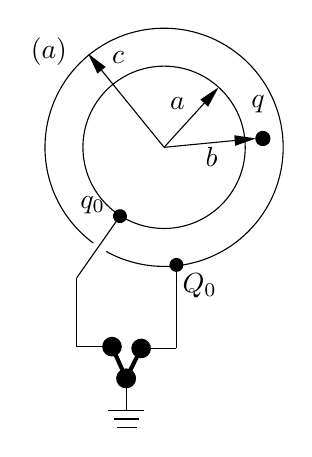
\begin{tikzpicture}[x=0.75pt,y=0.75pt,yscale=-0.85,xscale=0.85]
%uncomment if require: \path (0,300); %set diagram left start at 0, and has height of 300

%Shape: Circle [id:dp7235414025348001] 
\draw   (223,118) .. controls (223,92.59) and (243.59,72) .. (269,72) .. controls (294.41,72) and (315,92.59) .. (315,118) .. controls (315,143.41) and (294.41,164) .. (269,164) .. controls (243.59,164) and (223,143.41) .. (223,118) -- cycle ;
%Shape: Circle [id:dp3376765398979207] 
\draw  [fill={rgb, 255:red, 0; green, 0; blue, 0 }  ,fill opacity=1 ] (321,113) .. controls (321,110.79) and (322.79,109) .. (325,109) .. controls (327.21,109) and (329,110.79) .. (329,113) .. controls (329,115.21) and (327.21,117) .. (325,117) .. controls (322.79,117) and (321,115.21) .. (321,113) -- cycle ;
%Straight Lines [id:da3617289603147187] 
\draw    (269,118) -- (319.01,113.19) ;
\draw [shift={(321,113)}, rotate = 534.51] [fill={rgb, 255:red, 0; green, 0; blue, 0 }  ][line width=0.08]  [draw opacity=0] (12,-3) -- (0,0) -- (12,3) -- cycle    ;
%Straight Lines [id:da3095417846990314] 
\draw    (269,118) -- (227.26,66.55) ;
\draw [shift={(226,65)}, rotate = 410.95] [fill={rgb, 255:red, 0; green, 0; blue, 0 }  ][line width=0.08]  [draw opacity=0] (12,-3) -- (0,0) -- (12,3) -- cycle    ;
%Straight Lines [id:da6573278911493619] 
\draw    (269,118) -- (298.5,85.57) ;
\draw [shift={(299.84,84.09)}, rotate = 492.29] [fill={rgb, 255:red, 0; green, 0; blue, 0 }  ][line width=0.08]  [draw opacity=0] (12,-3) -- (0,0) -- (12,3) -- cycle    ;
%Shape: Arc [id:dp5758550915786248] 
\draw  [draw opacity=0] (228.78,172.21) .. controls (212.23,159.91) and (201.5,140.21) .. (201.5,118) .. controls (201.5,80.72) and (231.72,50.5) .. (269,50.5) .. controls (306.28,50.5) and (336.5,80.72) .. (336.5,118) .. controls (336.5,155.28) and (306.28,185.5) .. (269,185.5) .. controls (257.11,185.5) and (245.93,182.42) .. (236.23,177.02) -- (269,118) -- cycle ; \draw   (228.78,172.21) .. controls (212.23,159.91) and (201.5,140.21) .. (201.5,118) .. controls (201.5,80.72) and (231.72,50.5) .. (269,50.5) .. controls (306.28,50.5) and (336.5,80.72) .. (336.5,118) .. controls (336.5,155.28) and (306.28,185.5) .. (269,185.5) .. controls (257.11,185.5) and (245.93,182.42) .. (236.23,177.02) ;
%Straight Lines [id:da6760394888349934] 
\draw    (244,157) -- (219.48,191.98) ;
\draw [shift={(244,157)}, rotate = 125.04] [color={rgb, 255:red, 0; green, 0; blue, 0 }  ][fill={rgb, 255:red, 0; green, 0; blue, 0 }  ][line width=0.75]      (0, 0) circle [x radius= 3.35, y radius= 3.35]   ;
%Straight Lines [id:da52386780794706] 
\draw    (219.48,191.98) -- (219.48,230.98) ;
%Straight Lines [id:da3258652576669081] 
\draw    (276,184.66) -- (276,231.98) ;
\draw [shift={(276,184.66)}, rotate = 90] [color={rgb, 255:red, 0; green, 0; blue, 0 }  ][fill={rgb, 255:red, 0; green, 0; blue, 0 }  ][line width=0.75]      (0, 0) circle [x radius= 3.35, y radius= 3.35]   ;
%Straight Lines [id:da887969340720195] 
\draw    (219.48,230.98) -- (239.48,230.98) ;
%Straight Lines [id:da4878374869102087] 
\draw    (256,231.98) -- (276,231.98) ;
%Straight Lines [id:da39424160833392785] 
\draw [line width=1.5]    (239.48,230.98) -- (247.48,248.98) ;
\draw [shift={(247.48,248.98)}, rotate = 66.04] [color={rgb, 255:red, 0; green, 0; blue, 0 }  ][fill={rgb, 255:red, 0; green, 0; blue, 0 }  ][line width=1.5]      (0, 0) circle [x radius= 4.36, y radius= 4.36]   ;
\draw [shift={(239.48,230.98)}, rotate = 66.04] [color={rgb, 255:red, 0; green, 0; blue, 0 }  ][fill={rgb, 255:red, 0; green, 0; blue, 0 }  ][line width=1.5]      (0, 0) circle [x radius= 4.36, y radius= 4.36]   ;
%Straight Lines [id:da8801959493880728] 
\draw [line width=1.5]    (256,231.98) -- (247.48,248.98) ;
\draw [shift={(247.48,248.98)}, rotate = 116.63] [color={rgb, 255:red, 0; green, 0; blue, 0 }  ][fill={rgb, 255:red, 0; green, 0; blue, 0 }  ][line width=1.5]      (0, 0) circle [x radius= 4.36, y radius= 4.36]   ;
\draw [shift={(256,231.98)}, rotate = 116.63] [color={rgb, 255:red, 0; green, 0; blue, 0 }  ][fill={rgb, 255:red, 0; green, 0; blue, 0 }  ][line width=1.5]      (0, 0) circle [x radius= 4.36, y radius= 4.36]   ;
%Straight Lines [id:da5134627984646966] 
\draw    (247.48,248.98) -- (247.48,266.66) ;
%Straight Lines [id:da5979824414798764] 
\draw    (237.48,266.98) -- (257.48,266.98) ;
%Straight Lines [id:da18769168360442912] 
\draw    (240.48,271.98) -- (254.93,271.98) ;
%Straight Lines [id:da2654621554389449] 
\draw    (242.48,277) -- (253.93,277) ;

% Text Node
\draw (271,88.4) node [anchor=north west][inner sep=0.75pt]    {$a$};
% Text Node
\draw (291,116.4) node [anchor=north west][inner sep=0.75pt]    {$b$};
% Text Node
\draw (238,62.4) node [anchor=north west][inner sep=0.75pt]    {$c$};
% Text Node
\draw (317,87.4) node [anchor=north west][inner sep=0.75pt]    {$q$};
% Text Node
\draw (220,144.4) node [anchor=north west][inner sep=0.75pt]    {$q_{0}$};
% Text Node
\draw (278,188.06) node [anchor=north west][inner sep=0.75pt]    {$Q_{0}$};
% Text Node
\draw (192,54.4) node [anchor=north west][inner sep=0.75pt]    {$( a)$};
\end{tikzpicture}
\end{center}
\item Bây giờ ngắt khóa cho cả hai vỏ cầu đều không tiếp đất rồi di chuyển điện tích $q$ ra xa vô cùng. Dùng một khóa đôi lần lượt tiếp đất cho vỏ cầu trong, rồi vỏ cầu ngoài, rồi lại vỏ cầu trong, cứ lần lượt như thế sau khi mỗi vỏ cầu (trong và ngoài) tiếp đất $n$ lần, điện tích trên chúng là $q_n$ và $Q_n$. Tìm các điện tích này.
\begin{center}
\tikzset{every picture/.style={line width=0.75pt}} %set default line width to 0.75pt        

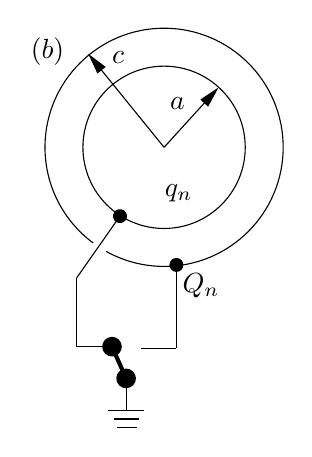
\begin{tikzpicture}[x=0.75pt,y=0.75pt,yscale=-0.85,xscale=0.85]
%uncomment if require: \path (0,300); %set diagram left start at 0, and has height of 300

%Shape: Circle [id:dp7235414025348001] 
\draw   (223,118) .. controls (223,92.59) and (243.59,72) .. (269,72) .. controls (294.41,72) and (315,92.59) .. (315,118) .. controls (315,143.41) and (294.41,164) .. (269,164) .. controls (243.59,164) and (223,143.41) .. (223,118) -- cycle ;
%Straight Lines [id:da3095417846990314] 
\draw    (269,118) -- (227.26,66.55) ;
\draw [shift={(226,65)}, rotate = 410.95] [fill={rgb, 255:red, 0; green, 0; blue, 0 }  ][line width=0.08]  [draw opacity=0] (12,-3) -- (0,0) -- (12,3) -- cycle    ;
%Straight Lines [id:da6573278911493619] 
\draw    (269,118) -- (298.5,85.57) ;
\draw [shift={(299.84,84.09)}, rotate = 492.29] [fill={rgb, 255:red, 0; green, 0; blue, 0 }  ][line width=0.08]  [draw opacity=0] (12,-3) -- (0,0) -- (12,3) -- cycle    ;
%Shape: Arc [id:dp5758550915786248] 
\draw  [draw opacity=0] (228.78,172.21) .. controls (212.23,159.91) and (201.5,140.21) .. (201.5,118) .. controls (201.5,80.72) and (231.72,50.5) .. (269,50.5) .. controls (306.28,50.5) and (336.5,80.72) .. (336.5,118) .. controls (336.5,155.28) and (306.28,185.5) .. (269,185.5) .. controls (257.11,185.5) and (245.93,182.42) .. (236.23,177.02) -- (269,118) -- cycle ; \draw   (228.78,172.21) .. controls (212.23,159.91) and (201.5,140.21) .. (201.5,118) .. controls (201.5,80.72) and (231.72,50.5) .. (269,50.5) .. controls (306.28,50.5) and (336.5,80.72) .. (336.5,118) .. controls (336.5,155.28) and (306.28,185.5) .. (269,185.5) .. controls (257.11,185.5) and (245.93,182.42) .. (236.23,177.02) ;
%Straight Lines [id:da6760394888349934] 
\draw    (244,157) -- (219.48,191.98) ;
\draw [shift={(244,157)}, rotate = 125.04] [color={rgb, 255:red, 0; green, 0; blue, 0 }  ][fill={rgb, 255:red, 0; green, 0; blue, 0 }  ][line width=0.75]      (0, 0) circle [x radius= 3.35, y radius= 3.35]   ;
%Straight Lines [id:da52386780794706] 
\draw    (219.48,191.98) -- (219.48,230.98) ;
%Straight Lines [id:da3258652576669081] 
\draw    (276,184.66) -- (276,231.98) ;
\draw [shift={(276,184.66)}, rotate = 90] [color={rgb, 255:red, 0; green, 0; blue, 0 }  ][fill={rgb, 255:red, 0; green, 0; blue, 0 }  ][line width=0.75]      (0, 0) circle [x radius= 3.35, y radius= 3.35]   ;
%Straight Lines [id:da887969340720195] 
\draw    (219.48,230.98) -- (239.48,230.98) ;
%Straight Lines [id:da4878374869102087] 
\draw    (256,231.98) -- (276,231.98) ;
%Straight Lines [id:da39424160833392785] 
\draw [line width=1.5]    (239.48,230.98) -- (247.48,248.98) ;
\draw [shift={(247.48,248.98)}, rotate = 66.04] [color={rgb, 255:red, 0; green, 0; blue, 0 }  ][fill={rgb, 255:red, 0; green, 0; blue, 0 }  ][line width=1.5]      (0, 0) circle [x radius= 4.36, y radius= 4.36]   ;
\draw [shift={(239.48,230.98)}, rotate = 66.04] [color={rgb, 255:red, 0; green, 0; blue, 0 }  ][fill={rgb, 255:red, 0; green, 0; blue, 0 }  ][line width=1.5]      (0, 0) circle [x radius= 4.36, y radius= 4.36]   ;
%Straight Lines [id:da5134627984646966] 
\draw    (247.48,248.98) -- (247.48,266.66) ;
%Straight Lines [id:da5979824414798764] 
\draw    (237.48,266.98) -- (257.48,266.98) ;
%Straight Lines [id:da18769168360442912] 
\draw    (240.48,271.98) -- (254.93,271.98) ;
%Straight Lines [id:da2654621554389449] 
\draw    (242.48,277) -- (253.93,277) ;

% Text Node
\draw (271,88.4) node [anchor=north west][inner sep=0.75pt]    {$a$};
% Text Node
\draw (238,62.4) node [anchor=north west][inner sep=0.75pt]    {$c$};
% Text Node
\draw (268,137.4) node [anchor=north west][inner sep=0.75pt]    {$q_{n}$};
% Text Node
\draw (278,188.06) node [anchor=north west][inner sep=0.75pt]    {$Q_{n}$};
% Text Node
\draw (192,54.4) node [anchor=north west][inner sep=0.75pt]    {$( b)$};
\end{tikzpicture}
\end{center}
\end{enumerate}
\end{vd}


\begin{loigiai}
\begin{enumerate}[1)]
    \item Điện thế vỏ cầu ngoài bằng không nên điện trường bên ngoài hệ cũng bằng không. Do đó tổng điện tích của hệ phải bằng không theo định luật Gauss:
    \[
q+q_{0}+Q_{0}=0. \tag{1} \label{loz1}
\]
Xét điện thế tại tâm của hệ, nó được chồng chất từ 3 hệ điện tích $q$, $q_0$, $Q_0$ và điện thế đó cũng bằng không:
\[
\dfrac{q}{4 \pi \varepsilon_{0} b}+\dfrac{q_{0}}{4 \pi \varepsilon_{0} a}+\dfrac{Q_{0}}{4 \pi \varepsilon_{0} c}=0. \tag{2} \label{loz2}
\]
Giải hệ phương trình (\ref{loz1}) và (\ref{loz2}) ta được:
$$
q_{0}=-q \dfrac{a}{b} \dfrac{c-b}{c-a} \  \text { và } \ Q_{0}=-q \dfrac{c}{b} \dfrac{b-a}{c-a}.
$$
\item Sau khi nối đất lần đầu vào vỏ cầu trong, điện tích trên vỏ cầu lớn vẫn là $Q_0$, còn vỏ trong có điện tích mới $q_1$ sao cho điện thế của nó bằng không:
$$
\dfrac{q_{1}}{4 \pi \varepsilon_{0} a}+\dfrac{Q_{0}}{4 \pi \varepsilon_{0} c}=0.
$$
Suy ra: $q_1=-Q_0\dfrac{a}{c}$.
Tương tự như vậy sau khi nối vỏ cầu ngoài với đất lần thứ nhất:
$$
\dfrac{q_{1}}{4 \pi \varepsilon_{0} c}+\dfrac{Q_{1}}{4 \pi \varepsilon_{0} c}=0 \Rightarrow  Q_{1}=-q_{1}=Q_{0} \dfrac{a}{c}.
$$
Dễ thấy sau lần thứ hai, điện tích trên vỏ cầu nhỏ sẽ là:
\[\begin{aligned}  
\dfrac{q_{2}}{4 \pi \varepsilon_{0} a}+\dfrac{Q_{1}}{4 \pi \varepsilon_{0} c} &= 0 \Rightarrow q_{2} = -Q_{1} \dfrac{a}{c}=-Q_{0}\left(\dfrac{a}{c}\right)^{2}, \\
\dfrac{q_{2}}{4 \pi \varepsilon_{0} c}+\dfrac{Q_{2}}{4 \pi \varepsilon_{0} c} &= 0 \Rightarrow  Q_{2} = -q_{2}=Q_{0}\left(\dfrac{a}{c}\right)^{2}.
\end{aligned}\]

Vậy sau $n$ lần tiếp đất lần lượt kết quả thu được:
$$
q_{n}=-Q_{0}\left(\dfrac{a}{c}\right)^{n}=q \dfrac{c}{b} \dfrac{b-a}{c-a}\left(\dfrac{a}{c}\right)^{n} \text { và } Q_{n}=-q_{n}.
$$
\end{enumerate}
\end{loigiai}


\begin{vd}[Điện thế của tam giác vuông]
    Cho tấm phẳng $ABC$ hình tam giác vuông ($AB=5s$, $AC=12s$ và $BC=13s$) với mật độ điện mặt $\sigma$. $D$ là trung điểm của cạnh $BC$. Chúng ta kí hiệu điện thế của điểm $P$ là $\phi(P)$. Điện thế tại vô cùng là không. Cho: \[\phi(B)+\phi(C)+\phi(D)=\dfrac{k\sigma s}{\varepsilon_0},\] 
    với $k$ là một hằng số không thứ nguyên. Hãy xác định giá trị của $k$. 
\end{vd}
\begin{loigiai}\\
Nếu ta ghép hai tam giác như trên lại với nhau, ta sẽ có một hình chữ nhật có kích thước hai cạnh lần lượt là $5s$ và $12s$. Gọi điện thế tại tâm của hình chữ nhật này là $V$. Theo nguyên lý chồng chất của điện thế, ta suy ra $\phi(D)=\dfrac{V}{2}$. 
\begin{center}
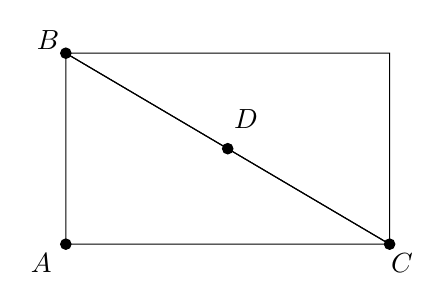
\begin{tikzpicture}[x=0.75pt,y=0.75pt,yscale=-1,xscale=1]
%uncomment if require: \path (0,146); %set diagram left start at 0, and has height of 146

%Shape: Right Triangle [id:dp7856288760770522] 
\draw   (270.71,23.03) -- (426.71,115.03) -- (270.71,115.03) -- cycle ;
%Shape: Circle [id:dp5020636092733206] 
\draw  [fill={rgb, 255:red, 0; green, 0; blue, 0 }  ,fill opacity=1 ] (268.19,23.03) .. controls (268.19,21.64) and (269.32,20.52) .. (270.71,20.52) .. controls (272.1,20.52) and (273.22,21.64) .. (273.22,23.03) .. controls (273.22,24.42) and (272.1,25.55) .. (270.71,25.55) .. controls (269.32,25.55) and (268.19,24.42) .. (268.19,23.03) -- cycle ;
%Shape: Circle [id:dp8576118434240458] 
\draw  [fill={rgb, 255:red, 0; green, 0; blue, 0 }  ,fill opacity=1 ] (346.19,69.03) .. controls (346.19,67.64) and (347.32,66.52) .. (348.71,66.52) .. controls (350.1,66.52) and (351.22,67.64) .. (351.22,69.03) .. controls (351.22,70.42) and (350.1,71.55) .. (348.71,71.55) .. controls (347.32,71.55) and (346.19,70.42) .. (346.19,69.03) -- cycle ;
%Shape: Circle [id:dp725015984181985] 
\draw  [fill={rgb, 255:red, 0; green, 0; blue, 0 }  ,fill opacity=1 ] (424.19,115.03) .. controls (424.19,113.64) and (425.32,112.52) .. (426.71,112.52) .. controls (428.1,112.52) and (429.22,113.64) .. (429.22,115.03) .. controls (429.22,116.42) and (428.1,117.55) .. (426.71,117.55) .. controls (425.32,117.55) and (424.19,116.42) .. (424.19,115.03) -- cycle ;
%Shape: Right Triangle [id:dp7437109781698188] 
\draw   (426.71,115.03) -- (270.71,23.03) -- (426.71,23.03) -- cycle ;
%Shape: Circle [id:dp9482880599050558] 
\draw  [fill={rgb, 255:red, 0; green, 0; blue, 0 }  ,fill opacity=1 ] (268.19,115.03) .. controls (268.19,113.64) and (269.32,112.52) .. (270.71,112.52) .. controls (272.1,112.52) and (273.22,113.64) .. (273.22,115.03) .. controls (273.22,116.42) and (272.1,117.55) .. (270.71,117.55) .. controls (269.32,117.55) and (268.19,116.42) .. (268.19,115.03) -- cycle ;

% Text Node
\draw (252.6,118.08) node [anchor=north west][inner sep=0.75pt]    {$A$};
% Text Node
\draw (255.52,11) node [anchor=north west][inner sep=0.75pt]    {$B$};
% Text Node
\draw (426.19,118.43) node [anchor=north west][inner sep=0.75pt]    {$C$};
% Text Node
\draw (350.52,48.93) node [anchor=north west][inner sep=0.75pt]    {$D$};
\end{tikzpicture}
\end{center}

Bây giờ ta xét điện thế tại một góc của hình chữ nhật. Điện thế tại đây là $\phi(B) + \phi(C)$. Nếu như ta ghép bốn hình chữ nhật như trên lại với nhau để tạo thành một hình chữ nhật khác có các cạnh là $10s$ và $24s$, điện thế tại tâm hình chữ nhật này sẽ là $2V$.
\begin{center}
        
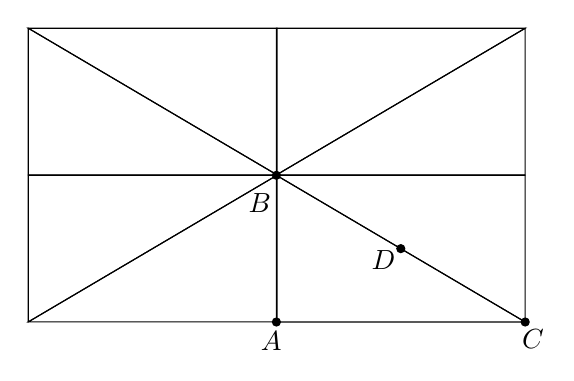
\begin{tikzpicture}[x=0.75pt,y=0.75pt,yscale=-1,xscale=1]
%uncomment if require: \path (0,188); %set diagram left start at 0, and has height of 188

%Shape: Right Triangle [id:dp6040990867089013] 
\draw   (464.7,16.2) -- (344.84,86.88) -- (464.7,86.88) -- cycle ;
%Shape: Right Triangle [id:dp8423695954755102] 
\draw   (344.84,86.88) -- (464.7,16.2) -- (344.84,16.2) -- cycle ;
%Shape: Right Triangle [id:dp30632792257472374] 
\draw   (464.73,157.71) -- (344.86,87.02) -- (464.73,87.02) -- cycle ;
%Shape: Right Triangle [id:dp9613549485070378] 
\draw   (344.86,87.02) -- (464.73,157.71) -- (344.86,157.71) -- cycle ;


%Shape: Right Triangle [id:dp04741643312830357] 
\draw   (225.33,16.17) -- (345.19,86.85) -- (225.33,86.85) -- cycle ;
%Shape: Right Triangle [id:dp5952677937142539] 
\draw   (345.19,86.85) -- (225.33,16.17) -- (345.19,16.17) -- cycle ;
%Shape: Right Triangle [id:dp5720905002999583] 
\draw   (225.3,157.68) -- (345.17,87) -- (225.3,87) -- cycle ;
%Shape: Right Triangle [id:dp13845149125527412] 
\draw   (345.17,87) -- (225.3,157.68) -- (345.17,157.68) -- cycle ;



%Shape: Ellipse [id:dp5881915630437773] 
\draw  [fill={rgb, 255:red, 0; green, 0; blue, 0 }  ,fill opacity=1 ] (342.93,157.71) .. controls (342.93,156.64) and (343.8,155.78) .. (344.86,155.78) .. controls (345.93,155.78) and (346.8,156.64) .. (346.8,157.71) .. controls (346.8,158.78) and (345.93,159.65) .. (344.86,159.65) .. controls (343.8,159.65) and (342.93,158.78) .. (342.93,157.71) -- cycle ;
%Shape: Ellipse [id:dp08796214303835082] 
\draw  [fill={rgb, 255:red, 0; green, 0; blue, 0 }  ,fill opacity=1 ] (402.86,122.37) .. controls (402.86,121.3) and (403.73,120.43) .. (404.8,120.43) .. controls (405.86,120.43) and (406.73,121.3) .. (406.73,122.37) .. controls (406.73,123.44) and (405.86,124.3) .. (404.8,124.3) .. controls (403.73,124.3) and (402.86,123.44) .. (402.86,122.37) -- cycle ;
%Shape: Ellipse [id:dp10230262305383064] 
\draw  [fill={rgb, 255:red, 0; green, 0; blue, 0 }  ,fill opacity=1 ] (462.79,157.71) .. controls (462.79,156.64) and (463.66,155.78) .. (464.73,155.78) .. controls (465.8,155.78) and (466.66,156.64) .. (466.66,157.71) .. controls (466.66,158.78) and (465.8,159.65) .. (464.73,159.65) .. controls (463.66,159.65) and (462.79,158.78) .. (462.79,157.71) -- cycle ;
%Shape: Ellipse [id:dp40506570554551313] 
\draw  [fill={rgb, 255:red, 0; green, 0; blue, 0 }  ,fill opacity=1 ] (342.93,87.02) .. controls (342.93,85.96) and (343.8,85.09) .. (344.86,85.09) .. controls (345.93,85.09) and (346.8,85.96) .. (346.8,87.02) .. controls (346.8,88.09) and (345.93,88.96) .. (344.86,88.96) .. controls (343.8,88.96) and (342.93,88.09) .. (342.93,87.02) -- cycle ;


% Text Node
\draw (336.07,161.25) node [anchor=north west][inner sep=0.75pt]    {$A$};
% Text Node
\draw (330.28,94.71) node [anchor=north west][inner sep=0.75pt]    {$B$};
% Text Node
\draw (462.02,160.26) node [anchor=north west][inner sep=0.75pt]    {$C$};
% Text Node
\draw (389.54,122.05) node [anchor=north west][inner sep=0.75pt]    {$D$};


\end{tikzpicture}
\end{center}
Từ đó suy ra:
\begin{equation*}
        4\tron{\phi(B) + \phi(C)} = 2V
        \Leftrightarrow \phi(B)+\phi(C)=\dfrac{V}{2}.
\end{equation*}
Vậy $\phi(D)+\phi(B)+\phi(C)=V$, ta sẽ đi tính điện thế $V$.\\
Xét một tam giác cân có cạnh đáy là $2x$ và chiều cao $y$.
\immini{ Điện thế tại đỉnh của tam giác:
\begin{equation*}
    \begin{aligned}
     V_i&=\iint \frac{\sigma}{4\pi\varepsilon_0r}\tron{r\dd r\dd\theta}\\
     &=\int_{\arctan{\frac{-x}{y}}}^{\arctan{\frac{x}{y}}}   \int_0^{\frac{y}{\cos\theta}}  \frac{\sigma}{4\pi\varepsilon_0}\dd r\dd\theta\\
     &=\frac{\sigma y}{4\pi\varepsilon_0}\tron{2\int_0^{\arctan{\frac{x}{y}}}\frac{\dd \theta}{\cos\theta}}\\
     &=\dfrac{\sigma y}{2\pi\varepsilon_0}\left.\tron{\frac{1}{2}\ln\tron{\frac{1+\sin\theta}{1-\sin\theta}}}\right|_0^{\arctan\frac{x}{y}}\\
     &=\dfrac{\sigma y}{4\pi\varepsilon_0}\ln\tron{\dfrac{\sqrt{x^2+y^2}+x}{\sqrt{x^2+y^2}-x}}\\
     &=\dfrac{\sigma y}{2\pi\varepsilon_0}\ln\tron{\dfrac{\sqrt{x^2+y^2}+x}{y}}.
    \end{aligned}
\end{equation*}}
{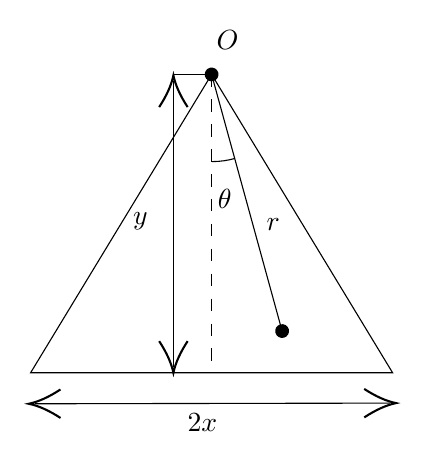
\begin{tikzpicture}[x=0.75pt,y=0.75pt,yscale=-1.4,xscale=1.4]
%uncomment if require: \path (0,159); %set diagram left start at 0, and has height of 159

%Shape: Triangle [id:dp3429465666743179] 
\draw   (350.62,21.3) -- (412.91,123.97) -- (288.33,123.97) -- cycle ;
%Straight Lines [id:da03944346674330523] 
\draw  [dash pattern={on 4.5pt off 4.5pt}]  (350.62,21.3) -- (350.62,123.64) ;
%Straight Lines [id:da7626616502789927] 
\draw    (350.62,21.3) -- (374.88,109.61) ;
\draw [shift={(374.88,109.61)}, rotate = 74.64] [color={rgb, 255:red, 0; green, 0; blue, 0 }  ][fill={rgb, 255:red, 0; green, 0; blue, 0 }  ][line width=0.75]      (0, 0) circle [x radius= 2.01, y radius= 2.01]   ;
\draw [shift={(350.62,21.3)}, rotate = 74.64] [color={rgb, 255:red, 0; green, 0; blue, 0 }  ][fill={rgb, 255:red, 0; green, 0; blue, 0 }  ][line width=0.75]      (0, 0) circle [x radius= 2.01, y radius= 2.01]   ;
%Shape: Arc [id:dp8405823847664362] 
\draw  [draw opacity=0] (358.65,50.22) .. controls (356.15,50.91) and (353.53,51.29) .. (350.82,51.3) -- (350.62,21.3) -- cycle ; \draw   (358.65,50.22) .. controls (356.15,50.91) and (353.53,51.29) .. (350.82,51.3) ;
%Straight Lines [id:da22612108938980247] 
\draw    (337.47,23.61) -- (337.47,122.01) ;
\draw [shift={(337.47,124.01)}, rotate = 270] [color={rgb, 255:red, 0; green, 0; blue, 0 }  ][line width=0.75]    (10.93,-4.9) .. controls (6.95,-2.3) and (3.31,-0.67) .. (0,0) .. controls (3.31,0.67) and (6.95,2.3) .. (10.93,4.9)   ;
\draw [shift={(337.47,21.61)}, rotate = 90] [color={rgb, 255:red, 0; green, 0; blue, 0 }  ][line width=0.75]    (10.93,-4.9) .. controls (6.95,-2.3) and (3.31,-0.67) .. (0,0) .. controls (3.31,0.67) and (6.95,2.3) .. (10.93,4.9)   ;
%Straight Lines [id:da9093229799080478] 
\draw    (337.62,21.3) -- (350.62,21.3) ;
%Straight Lines [id:da7717951632771531] 
\draw    (289.68,134.64) -- (412.08,134.41) ;
\draw [shift={(414.08,134.41)}, rotate = 539.89] [color={rgb, 255:red, 0; green, 0; blue, 0 }  ][line width=0.75]    (10.93,-4.9) .. controls (6.95,-2.3) and (3.31,-0.67) .. (0,0) .. controls (3.31,0.67) and (6.95,2.3) .. (10.93,4.9)   ;
\draw [shift={(287.68,134.64)}, rotate = 359.89] [color={rgb, 255:red, 0; green, 0; blue, 0 }  ][line width=0.75]    (10.93,-4.9) .. controls (6.95,-2.3) and (3.31,-0.67) .. (0,0) .. controls (3.31,0.67) and (6.95,2.3) .. (10.93,4.9)   ;


% Text Node
\draw (351.47,5.4) node [anchor=north west][inner sep=0.75pt]    {$O$};
% Text Node
\draw (351.87,59.91) node [anchor=north west][inner sep=0.75pt]    {$\theta $};
% Text Node
\draw (368.67,70.11) node [anchor=north west][inner sep=0.75pt]    {$r$};
% Text Node
\draw (341.47,137.04) node [anchor=north west][inner sep=0.75pt]    {$2x$};
% Text Node
\draw (322.67,67.96) node [anchor=north west][inner sep=0.75pt]    {$y$};
\end{tikzpicture}}
  
Ta có thể chia hình chữ nhật thành bốn hình tam giác cân khác bằng cách cắt hình chữ nhật dọc theo các đường chéo của hình chữ nhật.
\begin{center}

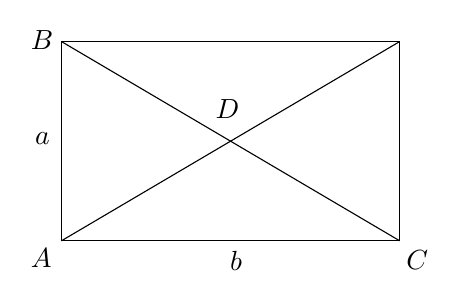
\begin{tikzpicture}[x=0.75pt,y=0.75pt,yscale=-1,xscale=1]
%uncomment if require: \path (0,144); %set diagram left start at 0, and has height of 144

%Shape: Rectangle [id:dp14314185362078402] 
\draw   (270,18.82) -- (432.97,18.82) -- (432.97,114.82) -- (270,114.82) -- cycle ;
%Straight Lines [id:da04292265530629358] 
\draw    (270,18.82) -- (432.97,114.82) ;
%Straight Lines [id:da8086631645730789] 
\draw    (270,114.82) -- (432.97,18.82) ;

% Text Node
\draw (254,117.4) node [anchor=north west][inner sep=0.75pt]    {$A$};
% Text Node
\draw (254,12.4) node [anchor=north west][inner sep=0.75pt]    {$B$};
% Text Node
\draw (434.97,118.22) node [anchor=north west][inner sep=0.75pt]    {$C$};
% Text Node
\draw (343,45.4) node [anchor=north west][inner sep=0.75pt]    {$D$};
% Text Node
\draw (256,61.53) node [anchor=north west][inner sep=0.75pt]    {$a$};
% Text Node
\draw (350,118.53) node [anchor=north west][inner sep=0.75pt]    {$b$};


\end{tikzpicture}
\end{center}
Gọi độ dài hai cạnh của hình chữ nhật là $a$ và $b$, khi đó ta có:
$$V=\dfrac{\sigma }{2\pi\varepsilon_0}\tron{a\ln\tron{\frac{\sqrt{a^2+b^2}+b}{a}}+b\ln\tron{\dfrac{\sqrt{a^2+b^2}+a}{b}}}.$$
Với $a=5s$ và $b=12s$, ta có:
$$V=\dfrac{\sigma s}{\varepsilon_0}\tron{\dfrac{5}{2\pi}\ln 5+\frac{6}{\pi}\ln\frac{3}{2}}.$$
Vậy $\displaystyle k=\frac{5}{2\pi}\ln 5+\frac{6}{\pi}\ln\frac{3}{2}\approx 2,055.$
\end{loigiai}


\begin{vd}[Điện trường của một nửa mặt cầu tích điện]
Một nửa mặt cầu bán kính $R$ được tích điện đều với mật độ điện tích mặt $\sigma$. Tính cường độ điện trường và điện thế tại tâm vỏ cầu (gợi ý: bắt đầu từ việc tính điện trường gây ra bởi một vành mỏng tích điện đều đối với một điểm nằm trên trục của nó).
\begin{center}


\tikzset{every picture/.style={line width=0.75pt}} %set default line width to 0.75pt        

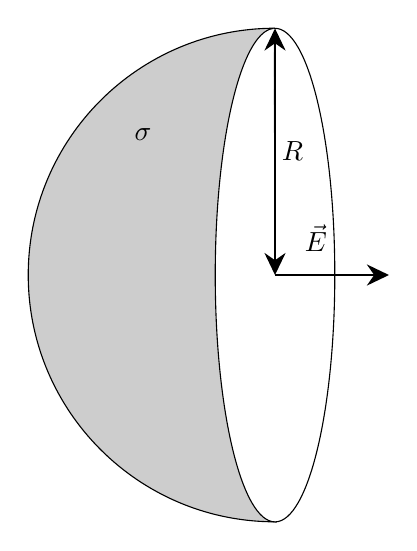
\begin{tikzpicture}[x=0.75pt,y=0.75pt,yscale=-1,xscale=1]
%uncomment if require: \path (0,480); %set diagram left start at 0, and has height of 480

%Shape: Arc [id:dp4558108973019419] 
\draw  [draw opacity=0][fill={rgb, 255:red, 155; green, 155; blue, 155 }  ,fill opacity=0.5 ] (306.71,358) .. controls (306.44,358) and (306.17,358) .. (305.9,358) .. controls (240.23,358) and (187,304.77) .. (187,239.1) .. controls (187,173.47) and (240.18,120.26) .. (305.8,120.2) -- (305.9,239.1) -- cycle ; \draw   (306.71,358) .. controls (306.44,358) and (306.17,358) .. (305.9,358) .. controls (240.23,358) and (187,304.77) .. (187,239.1) .. controls (187,173.47) and (240.18,120.26) .. (305.8,120.2) ;
%Shape: Arc [id:dp6145693508274632] 
\draw  [draw opacity=0][fill={rgb, 255:red, 255; green, 255; blue, 255 }  ,fill opacity=1 ] (306.71,358) .. controls (306.44,358.03) and (306.17,358.04) .. (305.9,358.04) .. controls (289.99,358.04) and (277.1,304.81) .. (277.1,239.14) .. controls (277.1,174.94) and (289.43,122.62) .. (304.84,120.32) -- (305.9,239.14) -- cycle ; \draw   (306.71,358) .. controls (306.44,358.03) and (306.17,358.04) .. (305.9,358.04) .. controls (289.99,358.04) and (277.1,304.81) .. (277.1,239.14) .. controls (277.1,174.94) and (289.43,122.62) .. (304.84,120.32) ;
%Shape: Arc [id:dp7833107865355216] 
\draw  [draw opacity=0][fill={rgb, 255:red, 255; green, 255; blue, 255 }  ,fill opacity=1 ] (305.09,120.29) .. controls (305.36,120.26) and (305.63,120.24) .. (305.9,120.24) .. controls (321.81,120.24) and (334.7,173.48) .. (334.7,239.14) .. controls (334.7,304.67) and (321.86,357.81) .. (306,358.04) -- (305.9,239.14) -- cycle ; \draw   (305.09,120.29) .. controls (305.36,120.26) and (305.63,120.24) .. (305.9,120.24) .. controls (321.81,120.24) and (334.7,173.48) .. (334.7,239.14) .. controls (334.7,304.67) and (321.86,357.81) .. (306,358.04) ;
%Straight Lines [id:da4909585902864282] 
\draw    (305.9,239.1) -- (357.8,239.1) ;
\draw [shift={(360.8,239.1)}, rotate = 180] [fill={rgb, 255:red, 0; green, 0; blue, 0 }  ][line width=0.08]  [draw opacity=0] (10.72,-5.15) -- (0,0) -- (10.72,5.15) -- (7.12,0) -- cycle    ;
%Straight Lines [id:da4200215184512581] 
\draw    (305.9,123.32) -- (305.9,236.1) ;
\draw [shift={(305.9,239.1)}, rotate = 270] [fill={rgb, 255:red, 0; green, 0; blue, 0 }  ][line width=0.08]  [draw opacity=0] (10.72,-5.15) -- (0,0) -- (10.72,5.15) -- (7.12,0) -- cycle    ;
\draw [shift={(305.9,120.32)}, rotate = 90] [fill={rgb, 255:red, 0; green, 0; blue, 0 }  ][line width=0.08]  [draw opacity=0] (10.72,-5.15) -- (0,0) -- (10.72,5.15) -- (7.12,0) -- cycle    ;


% Text Node
\draw (308,173.4) node [anchor=north west][inner sep=0.75pt]    {$R$};
% Text Node
\draw (319,213.4) node [anchor=north west][inner sep=0.75pt]    {$\vec{E}$};
% Text Node
\draw (237,167.4) node [anchor=north west][inner sep=0.75pt]    {$\sigma $};


\end{tikzpicture}
\end{center}

\end{vd}
\begin{loigiai}
Chúng ta bắt đầu từ điện trường gây ra bởi một vành mỏng tích điện bán kính $a$ và mật độ điện dài $\lambda$ gây ra tại một điểm $P$ nằm trên trục của nó, ở khoảng cách $x$ từ tâm $O$ của vòng dây (xem hình vẽ). Ta lấy một vi phân cung tròn dài $\dd l$, được tích điện $\lambda \dd l$, gây ra một điện trường $\dd \ot{E}$ tại điểm $P$. Độ lớn của $\dd \ot{E}$ là:
   \[ \dd E = k_e \frac{\lambda \dd l}{a^2 + x^2} . \tag{1}\]

    \begin{center}


\tikzset{every picture/.style={line width=0.75pt}} %set default line width to 0.75pt        

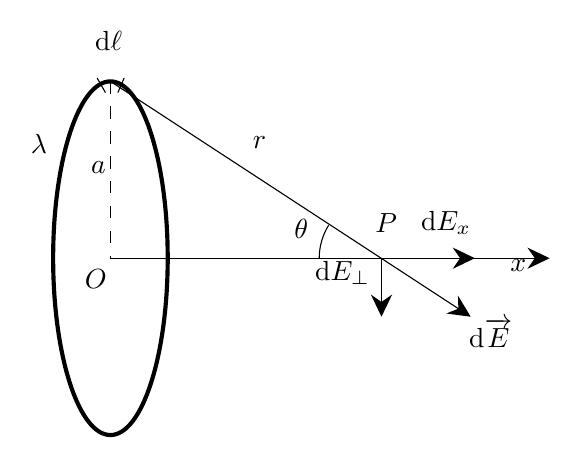
\begin{tikzpicture}[x=0.75pt,y=0.75pt,yscale=-1,xscale=1]
%uncomment if require: \path (0,480); %set diagram left start at 0, and has height of 480

%Shape: Ellipse [id:dp7943577007686424] 
\draw  [line width=1.5]  (113,191.2) .. controls (113,144.15) and (125.36,106) .. (140.6,106) .. controls (155.84,106) and (168.2,144.15) .. (168.2,191.2) .. controls (168.2,238.25) and (155.84,276.4) .. (140.6,276.4) .. controls (125.36,276.4) and (113,238.25) .. (113,191.2) -- cycle ;
%Straight Lines [id:da050784527645520994] 
\draw    (140.6,191.2) -- (349.2,191.2) ;
\draw [shift={(352.2,191.2)}, rotate = 180] [fill={rgb, 255:red, 0; green, 0; blue, 0 }  ][line width=0.08]  [draw opacity=0] (10.72,-5.15) -- (0,0) -- (10.72,5.15) -- (7.12,0) -- cycle    ;
%Straight Lines [id:da996198800097212] 
\draw  [dash pattern={on 4.5pt off 4.5pt}]  (140.6,106) -- (140.6,191.2) ;
%Straight Lines [id:da7771722324877135] 
\draw    (134.2,104.4) -- (138.2,111.4) ;
%Straight Lines [id:da4133881703636635] 
\draw    (147.2,104.4) -- (144.2,111.4) ;
%Straight Lines [id:da2435636005783719] 
\draw    (140.6,106) -- (311.69,217.76) ;
\draw [shift={(314.2,219.4)}, rotate = 213.15] [fill={rgb, 255:red, 0; green, 0; blue, 0 }  ][line width=0.08]  [draw opacity=0] (10.72,-5.15) -- (0,0) -- (10.72,5.15) -- (7.12,0) -- cycle    ;
%Straight Lines [id:da6896149995797138] 
\draw    (271.2,191.2) -- (271.2,216.4) ;
\draw [shift={(271.2,219.4)}, rotate = 270] [fill={rgb, 255:red, 0; green, 0; blue, 0 }  ][line width=0.08]  [draw opacity=0] (10.72,-5.15) -- (0,0) -- (10.72,5.15) -- (7.12,0) -- cycle    ;
%Straight Lines [id:da0004949043224988792] 
\draw    (271.2,191.2) -- (313.2,191.2) ;
\draw [shift={(316.2,191.2)}, rotate = 180] [fill={rgb, 255:red, 0; green, 0; blue, 0 }  ][line width=0.08]  [draw opacity=0] (10.72,-5.15) -- (0,0) -- (10.72,5.15) -- (7.12,0) -- cycle    ;
%Shape: Arc [id:dp2981728301376838] 
\draw  [draw opacity=0] (241.2,191.37) .. controls (241.2,191.31) and (241.2,191.26) .. (241.2,191.2) .. controls (241.2,185.38) and (242.86,179.95) .. (245.72,175.35) -- (271.2,191.2) -- cycle ; \draw   (241.2,191.37) .. controls (241.2,191.31) and (241.2,191.26) .. (241.2,191.2) .. controls (241.2,185.38) and (242.86,179.95) .. (245.72,175.35) ;



% Text Node
\draw (101,130.4) node [anchor=north west][inner sep=0.75pt]    {$\lambda $};
% Text Node
\draw (127,195.4) node [anchor=north west][inner sep=0.75pt]    {$O$};
% Text Node
\draw (130,143.4) node [anchor=north west][inner sep=0.75pt]    {$a$};
% Text Node
\draw (132,80.4) node [anchor=north west][inner sep=0.75pt]    {$\mathrm{d} \ell $};
% Text Node
\draw (208,131.4) node [anchor=north west][inner sep=0.75pt]    {$r$};
% Text Node
\draw (267,168.4) node [anchor=north west][inner sep=0.75pt]    {$P$};
% Text Node
\draw (289,167.4) node [anchor=north west][inner sep=0.75pt]    {$\mathrm{d} E_{x}$};
% Text Node
\draw (238,191.4) node [anchor=north west][inner sep=0.75pt]    {$\mathrm{d} E_{\bot }$};
% Text Node
\draw (312.2,218.8) node [anchor=north west][inner sep=0.75pt]    {$\mathrm{d}\ot{E}$};
% Text Node
\draw (228,171.4) node [anchor=north west][inner sep=0.75pt]    {$\theta $};
% Text Node
\draw (332,190.4) node [anchor=north west][inner sep=0.75pt]    {$x$};


\end{tikzpicture}
\end{center}
Vi phân điện trường  $\dd \ot{E}$ có thành phần $\dd E_x$ song song với trục của vành và thành phần $\dd E_{\perp}$  vuông góc với trục. Chúng ta chỉ cần tính đến thành phần song song của điện trường:
\[\begin{aligned}
 \dd E_x & = \cos \theta \dd E = k_e \frac{\lambda \dd l}{a^2 + x^2} \frac{x}{\sqrt{a^2 + x^2}} \\
    &= k_e \frac{\lambda x \dd l}{(a^2 + x^2)^{3/2}} , \end{aligned} \tag{2}\]

bởi vì thành phần vuông góc sẽ tự triệt tiêu lẫn nhau khi chúng ta tích phân quanh vành mảnh. Khi tích phân, các biến $\theta$ và $r$ không phụ thuộc vào vị trí của $\dd l$, do đó điện trường tổng cộng tại $P$ là:
  \[\begin{aligned} E_x &= k_e \frac{\lambda x}{(a^2 + x^2)^{3/2}} \int_{0}^{2\pi a} \dd l = k_e  \frac{2\pi a \lambda x}{(a^2 +x^2)^{3/2}} \\
  \\
                &= \left\{ \begin{array}{cc} \dfrac{1}{4\pi \varepsilon_0} \dfrac{2\pi a \lambda x}{(a^2+x^2)^{3/2}}   & \text{SI} \\
                \\
                 \dfrac{2\pi a \lambda x}{(a^2+x^2)^{3/2}}  & \text{Gaussian}, \end{array} \right.  \end{aligned} \tag{3} \]

Biểu thức có thể được viết lại thành: 
     \[  \ot{E} = \hat{{x}} k_e \frac{Qx}{(a^2 + x^2)^{3/2}}, \tag{4} \]
ở đây $Q=2\pi a \lambda$ là tổng điện tích của vành.
   \begin{center}


\tikzset{every picture/.style={line width=0.75pt}} %set default line width to 0.75pt        

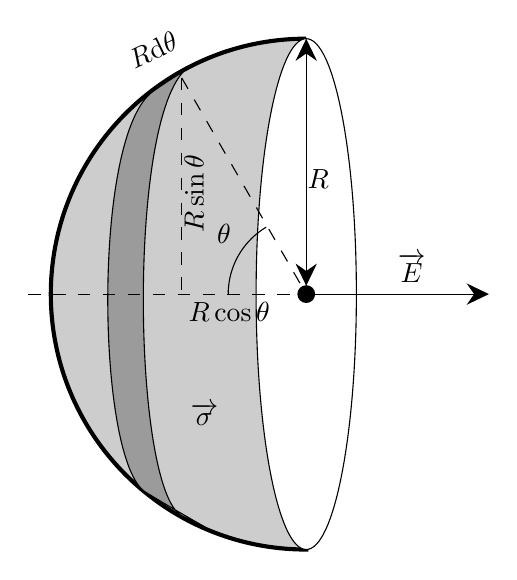
\begin{tikzpicture}[x=0.75pt,y=0.75pt,yscale=-1,xscale=1]
%uncomment if require: \path (0,480); %set diagram left start at 0, and has height of 480

%Shape: Arc [id:dp9751651413882021] 
\draw  [draw opacity=0][fill={rgb, 255:red, 155; green, 155; blue, 155 }  ,fill opacity=0.5 ][line width=1.5]  (240.95,352.76) .. controls (240.61,352.76) and (240.28,352.76) .. (239.94,352.76) .. controls (171.98,352.76) and (116.88,297.67) .. (116.88,229.7) .. controls (116.88,161.74) and (171.98,106.64) .. (239.94,106.64) -- (239.94,229.7) -- cycle ; \draw  [line width=1.5]  (240.95,352.76) .. controls (240.61,352.76) and (240.28,352.76) .. (239.94,352.76) .. controls (171.98,352.76) and (116.88,297.67) .. (116.88,229.7) .. controls (116.88,161.74) and (171.98,106.64) .. (239.94,106.64) ;
%Shape: Arc [id:dp07613452841355706] 
\draw  [draw opacity=0][fill={rgb, 255:red, 255; green, 255; blue, 255 }  ,fill opacity=1 ] (240.95,352.66) .. controls (240.61,352.73) and (240.28,352.76) .. (239.94,352.76) .. controls (226.6,352.76) and (215.79,297.67) .. (215.79,229.7) .. controls (215.79,161.74) and (226.6,106.64) .. (239.94,106.64) -- (239.94,229.7) -- cycle ; \draw   (240.95,352.66) .. controls (240.61,352.73) and (240.28,352.76) .. (239.94,352.76) .. controls (226.6,352.76) and (215.79,297.67) .. (215.79,229.7) .. controls (215.79,161.74) and (226.6,106.64) .. (239.94,106.64) ;
%Shape: Arc [id:dp11615013675617436] 
\draw  [draw opacity=0][fill={rgb, 255:red, 255; green, 255; blue, 255 }  ,fill opacity=1 ] (238.93,106.75) .. controls (239.27,106.68) and (239.6,106.64) .. (239.94,106.64) .. controls (253.28,106.64) and (264.1,161.74) .. (264.1,229.7) .. controls (264.1,297.67) and (253.28,352.76) .. (239.94,352.76) -- (239.94,229.7) -- cycle ; \draw   (238.93,106.75) .. controls (239.27,106.68) and (239.6,106.64) .. (239.94,106.64) .. controls (253.28,106.64) and (264.1,161.74) .. (264.1,229.7) .. controls (264.1,297.67) and (253.28,352.76) .. (239.94,352.76) ;
%Shape: Polygon Curved [id:ds027284506820421495] 
\draw  [fill={rgb, 255:red, 155; green, 155; blue, 155 }  ,fill opacity=1 ] (166.06,132.1) .. controls (195.66,111) and (218.07,106.43) .. (185.65,119.05) .. controls (153.22,131.67) and (155.4,324.26) .. (180.21,336.66) .. controls (205.01,349.06) and (186.3,339.71) .. (162.58,325.13) .. controls (138.86,310.55) and (136.47,153.21) .. (166.06,132.1) -- cycle ;
%Straight Lines [id:da13270213954243215] 
\draw  [dash pattern={on 4.5pt off 4.5pt}]  (106,229.7) -- (239.94,229.7) ;
%Straight Lines [id:da6043344427332653] 
\draw    (239.94,229.7) -- (324.96,229.7) ;
\draw [shift={(327.96,229.7)}, rotate = 180] [fill={rgb, 255:red, 0; green, 0; blue, 0 }  ][line width=0.08]  [draw opacity=0] (10.72,-5.15) -- (0,0) -- (10.72,5.15) -- (7.12,0) -- cycle    ;
%Straight Lines [id:da9380275362339183] 
\draw    (239.94,109.64) -- (239.94,222.7) ;
\draw [shift={(239.94,225.7)}, rotate = 270] [fill={rgb, 255:red, 0; green, 0; blue, 0 }  ][line width=0.08]  [draw opacity=0] (10.72,-5.15) -- (0,0) -- (10.72,5.15) -- (7.12,0) -- cycle    ;
\draw [shift={(239.94,106.64)}, rotate = 90] [fill={rgb, 255:red, 0; green, 0; blue, 0 }  ][line width=0.08]  [draw opacity=0] (10.72,-5.15) -- (0,0) -- (10.72,5.15) -- (7.12,0) -- cycle    ;
%Straight Lines [id:da058284329477305] 
\draw  [dash pattern={on 4.5pt off 4.5pt}]  (179.99,125.58) -- (239.94,229.7) ;
%Straight Lines [id:da9260211082999852] 
\draw  [dash pattern={on 4.5pt off 4.5pt}]  (179.99,125.58) -- (179.99,228.94) ;
%Shape: Arc [id:dp5834096030996945] 
\draw  [draw opacity=0] (202.35,229.53) .. controls (202.35,228.36) and (202.41,227.17) .. (202.53,225.98) .. controls (203.76,213.67) and (210.79,203.34) .. (220.64,197.44) -- (239.94,229.7) -- cycle ; \draw   (202.35,229.53) .. controls (202.35,228.36) and (202.41,227.17) .. (202.53,225.98) .. controls (203.76,213.67) and (210.79,203.34) .. (220.64,197.44) ;
%Shape: Circle [id:dp5905363482755994] 
\draw  [fill={rgb, 255:red, 0; green, 0; blue, 0 }  ,fill opacity=1 ] (235.94,229.7) .. controls (235.94,227.49) and (237.73,225.7) .. (239.94,225.7) .. controls (242.15,225.7) and (243.94,227.49) .. (243.94,229.7) .. controls (243.94,231.91) and (242.15,233.7) .. (239.94,233.7) .. controls (237.73,233.7) and (235.94,231.91) .. (235.94,229.7) -- cycle ;


% Text Node
\draw (151.58,112.64) node [anchor=north west][inner sep=0.75pt]  [rotate=-334.21]  {$R\mathrm{d} \theta $};
% Text Node
\draw (239.33,168.38) node [anchor=north west][inner sep=0.75pt]    {$R$};
% Text Node
\draw (282.84,208.94) node [anchor=north west][inner sep=0.75pt]    {$\ot{E}$};
% Text Node
\draw (180.04,201.43) node [anchor=north west][inner sep=0.75pt]  [rotate=-270]  {$R\sin \theta $};
% Text Node
\draw (195.7,194.67) node [anchor=north west][inner sep=0.75pt]    {$\theta $};
% Text Node
\draw (182.92,281.28) node [anchor=north west][inner sep=0.75pt]    {$\ot{\sigma }$};
% Text Node
\draw (181.99,232.34) node [anchor=north west][inner sep=0.75pt]    {$R\cos \theta $};


\end{tikzpicture}
\end{center}
Mặt cầu tích điện có thể được chia thành các vành mảnh vi phân giữa các góc phương vị $\theta$ và $\theta + \dd \theta$ vì tính đối xứng của bán cầu (xem hình vẽ). Mỗi vành mỏng tương tự như một vòng tích điện có bán kính $R\sin \theta$ và điện tích tổng cộng $\dd Q = \sigma 2 \pi R^2 \sin \theta \dd \theta $. Tâm của bán cầu nằm trên trục đối xứng của vành mỏng, ở khoảng cách $x= R \cos \theta$ từ tâm của mỗi vành. Do đó, đóng góp của mỗi vành mỏng cho điện trường ở tâm bán cầu là: 
    \[\begin{aligned} \dd E & = k_e \dfrac{\sigma 2 \pi R^2 \sin \theta \dd \theta R \cos \theta}{(R^2 \sin^2 \theta + R^2 \cos^2\theta)^{3/2}} \\
        & =  k_e \dfrac{\sigma 2 \pi R^3 \cos \theta \sin \theta \dd \theta}{R^3} = k_e \sigma 2 \pi \cos \theta \sin \theta \dd \theta, \end{aligned} \tag{5} \]

và điện trường tổng cộng là:
       \[ E = k_e  \sigma  2 \pi \int_{0}^{\pi/2} \cos \theta \sin \theta \dd \theta = k_e \pi \sigma, \tag{6} \]

không phụ thuộc vào bán kính $R$. Ta cũng làm tương tự với điện thế tại tâm bán cầu.
\end{loigiai}

\begin{vd}[Điện trường của vỏ cầu tích điện]
    \label{ca5}
    Xét điện trường tạo ra bởi một vỏ cầu rỗng tích điện đều với điện tích $Q$. Chúng ta có thể tìm được điện trường do vỏ cầu gây ra tại một điểm bên trong hoặc bên ngoài vỏ cầu bằng cách sử dụng định luật Gauss. Trong bài này, chúng ta sẽ đi tìm điện trường bằng một cách khác. Hãy tính điện thế $\phi(r)$ của một điểm cách tâm vỏ cầu một khoảng $r$ bằng cách chia vỏ cầu thành các phần tử diện tích nhỏ rồi tích phân điện thế do từng phần tử đóng góp vào điện thế tại điểm đang tính. Điện trường tại điểm đó có thể tìm được bằng công thức $E(r)=-\dfrac{\dd \phi}{\dd r}$.\\ 
    \begin{center}
        

\tikzset{every picture/.style={line width=0.75pt}} %set default line width to 0.75pt        

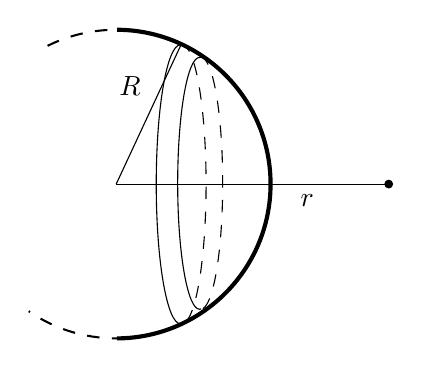
\begin{tikzpicture}[x=0.75pt,y=0.75pt,yscale=-1,xscale=1]
%uncomment if require: \path (0,221); %set diagram left start at 0, and has height of 221

%Shape: Arc [id:dp9180859117676652] 
\draw  [draw opacity=0][line width=1.5]  (287.74,27) .. controls (328.63,27.21) and (361.71,60.42) .. (361.71,101.35) .. controls (361.71,142.31) and (328.6,175.53) .. (287.69,175.71) -- (287.35,101.35) -- cycle ; \draw  [line width=1.5]  (287.74,27) .. controls (328.63,27.21) and (361.71,60.42) .. (361.71,101.35) .. controls (361.71,142.31) and (328.6,175.53) .. (287.69,175.71) ;
%Shape: Arc [id:dp9949488668982875] 
\draw  [draw opacity=0][dash pattern={on 4.5pt off 4.5pt}][line width=0.75]  (254.27,34.75) .. controls (264.24,29.79) and (275.47,27) .. (287.35,27) .. controls (328.42,27) and (361.71,60.29) .. (361.71,101.35) .. controls (361.71,142.42) and (328.42,175.71) .. (287.35,175.71) .. controls (271.7,175.71) and (257.17,170.87) .. (245.19,162.61) -- (287.35,101.35) -- cycle ; \draw  [dash pattern={on 4.5pt off 4.5pt}][line width=0.75]  (254.27,34.75) .. controls (264.24,29.79) and (275.47,27) .. (287.35,27) .. controls (328.42,27) and (361.71,60.29) .. (361.71,101.35) .. controls (361.71,142.42) and (328.42,175.71) .. (287.35,175.71) .. controls (271.7,175.71) and (257.17,170.87) .. (245.19,162.61) ;
%Shape: Arc [id:dp6320579717276376] 
\draw  [draw opacity=0] (328.3,161.49) .. controls (328.04,161.61) and (327.77,161.67) .. (327.5,161.67) .. controls (321.68,161.67) and (316.96,134.5) .. (316.96,100.99) .. controls (316.96,67.47) and (321.68,40.31) .. (327.5,40.31) .. controls (327.58,40.31) and (327.66,40.31) .. (327.73,40.32) -- (327.5,100.99) -- cycle ; \draw   (328.3,161.49) .. controls (328.04,161.61) and (327.77,161.67) .. (327.5,161.67) .. controls (321.68,161.67) and (316.96,134.5) .. (316.96,100.99) .. controls (316.96,67.47) and (321.68,40.31) .. (327.5,40.31) .. controls (327.58,40.31) and (327.66,40.31) .. (327.73,40.32) ;
%Shape: Arc [id:dp7997514267193591] 
\draw  [draw opacity=0][dash pattern={on 4.5pt off 4.5pt}] (327.3,40.43) .. controls (327.56,40.31) and (327.83,40.25) .. (328.1,40.25) .. controls (333.92,40.25) and (338.64,67.42) .. (338.64,100.93) .. controls (338.64,134.45) and (333.92,161.61) .. (328.1,161.61) .. controls (328.02,161.61) and (327.94,161.61) .. (327.86,161.6) -- (328.1,100.93) -- cycle ; \draw  [dash pattern={on 4.5pt off 4.5pt}] (327.3,40.43) .. controls (327.56,40.31) and (327.83,40.25) .. (328.1,40.25) .. controls (333.92,40.25) and (338.64,67.42) .. (338.64,100.93) .. controls (338.64,134.45) and (333.92,161.61) .. (328.1,161.61) .. controls (328.02,161.61) and (327.94,161.61) .. (327.86,161.6) ;

%Shape: Arc [id:dp06962011240073829] 
\draw  [draw opacity=0] (319.19,168.47) .. controls (318.9,168.6) and (318.6,168.67) .. (318.3,168.67) .. controls (311.86,168.67) and (306.63,138.57) .. (306.63,101.45) .. controls (306.63,64.33) and (311.86,34.24) .. (318.3,34.24) .. controls (318.39,34.24) and (318.47,34.25) .. (318.56,34.26) -- (318.3,101.45) -- cycle ; \draw   (319.19,168.47) .. controls (318.9,168.6) and (318.6,168.67) .. (318.3,168.67) .. controls (311.86,168.67) and (306.63,138.57) .. (306.63,101.45) .. controls (306.63,64.33) and (311.86,34.24) .. (318.3,34.24) .. controls (318.39,34.24) and (318.47,34.25) .. (318.56,34.26) ;
%Shape: Arc [id:dp44336333675449535] 
\draw  [draw opacity=0][dash pattern={on 4.5pt off 4.5pt}] (318.07,34.38) .. controls (318.37,34.25) and (318.66,34.18) .. (318.96,34.18) .. controls (325.41,34.18) and (330.64,64.28) .. (330.64,101.4) .. controls (330.64,138.52) and (325.41,168.61) .. (318.96,168.61) .. controls (318.88,168.61) and (318.79,168.6) .. (318.71,168.59) -- (318.96,101.4) -- cycle ; \draw  [dash pattern={on 4.5pt off 4.5pt}] (318.07,34.38) .. controls (318.37,34.25) and (318.66,34.18) .. (318.96,34.18) .. controls (325.41,34.18) and (330.64,64.28) .. (330.64,101.4) .. controls (330.64,138.52) and (325.41,168.61) .. (318.96,168.61) .. controls (318.88,168.61) and (318.79,168.6) .. (318.71,168.59) ;

%Straight Lines [id:da839400938864665] 
\draw    (287.35,101.35) -- (418.64,101.35) ;
%Straight Lines [id:da06623462412375702] 
\draw    (318.56,34.26) -- (287.35,101.35) ;
%Shape: Circle [id:dp567051033556494] 
\draw  [fill={rgb, 255:red, 0; green, 0; blue, 0 }  ,fill opacity=1 ] (416.8,101.35) .. controls (416.8,100.34) and (417.62,99.52) .. (418.64,99.52) .. controls (419.65,99.52) and (420.47,100.34) .. (420.47,101.35) .. controls (420.47,102.37) and (419.65,103.19) .. (418.64,103.19) .. controls (417.62,103.19) and (416.8,102.37) .. (416.8,101.35) -- cycle ;

% Text Node
\draw (374.96,105) node [anchor=north west][inner sep=0.75pt]    {$r$};
% Text Node
\draw (287.63,48.4) node [anchor=north west][inner sep=0.75pt]    {$R$};


\end{tikzpicture}

    \end{center}
    \textit{Gợi ý: Cách đơn giản nhất đó chính là chia vỏ cầu thành nhiều vòng nhỏ như trên hình.}
    \end{vd}
    \begin{loigiai}\\
    \begin{center}
        

\tikzset{every picture/.style={line width=0.75pt}} %set default line width to 0.75pt        

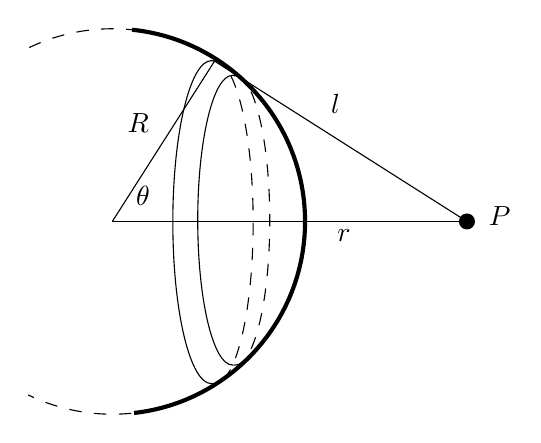
\begin{tikzpicture}[x=0.75pt,y=0.75pt,yscale=-1,xscale=1]
%uncomment if require: \path (0,300); %set diagram left start at 0, and has height of 300

%Shape: Arc [id:dp6604130734699976] 
\draw  [draw opacity=0][line width=1.5]  (338.38,47.48) .. controls (385.19,52.25) and (421.71,91.79) .. (421.71,139.85) .. controls (421.71,187.6) and (385.67,226.93) .. (339.32,232.12) -- (328.85,139.85) -- cycle ; \draw  [line width=1.5]  (338.38,47.48) .. controls (385.19,52.25) and (421.71,91.79) .. (421.71,139.85) .. controls (421.71,187.6) and (385.67,226.93) .. (339.32,232.12) ;
%Shape: Arc [id:dp3988355543248949] 
\draw  [draw opacity=0][dash pattern={on 4.5pt off 4.5pt}] (288.83,56.05) .. controls (300.95,50.25) and (314.52,47) .. (328.85,47) .. controls (380.14,47) and (421.71,88.57) .. (421.71,139.85) .. controls (421.71,191.14) and (380.14,232.71) .. (328.85,232.71) .. controls (314.33,232.71) and (300.59,229.37) .. (288.34,223.43) -- (328.85,139.85) -- cycle ; \draw  [dash pattern={on 4.5pt off 4.5pt}] (288.83,56.05) .. controls (300.95,50.25) and (314.52,47) .. (328.85,47) .. controls (380.14,47) and (421.71,88.57) .. (421.71,139.85) .. controls (421.71,191.14) and (380.14,232.71) .. (328.85,232.71) .. controls (314.33,232.71) and (300.59,229.37) .. (288.34,223.43) ;
%Shape: Arc [id:dp3770531364912999] 
\draw  [draw opacity=0] (377.32,217.94) .. controls (377.09,217.98) and (376.86,217.99) .. (376.63,217.99) .. controls (366.34,217.99) and (358,183.16) .. (358,140.18) .. controls (358,97.21) and (366.34,62.37) .. (376.63,62.37) .. controls (377.13,62.37) and (377.62,62.45) .. (378.11,62.61) -- (376.63,140.18) -- cycle ; \draw   (377.32,217.94) .. controls (377.09,217.98) and (376.86,217.99) .. (376.63,217.99) .. controls (366.34,217.99) and (358,183.16) .. (358,140.18) .. controls (358,97.21) and (366.34,62.37) .. (376.63,62.37) .. controls (377.13,62.37) and (377.62,62.45) .. (378.11,62.61) ;
%Shape: Arc [id:dp48119814484050627] 
\draw  [draw opacity=0][dash pattern={on 4.5pt off 4.5pt}] (377.38,62.51) .. controls (377.61,62.47) and (377.84,62.46) .. (378.08,62.46) .. controls (388.37,62.46) and (396.71,97.29) .. (396.71,140.27) .. controls (396.71,183.24) and (388.37,218.08) .. (378.08,218.08) .. controls (377.58,218.08) and (377.09,218) .. (376.6,217.84) -- (378.08,140.27) -- cycle ; \draw  [dash pattern={on 4.5pt off 4.5pt}] (377.38,62.51) .. controls (377.61,62.47) and (377.84,62.46) .. (378.08,62.46) .. controls (388.37,62.46) and (396.71,97.29) .. (396.71,140.27) .. controls (396.71,183.24) and (388.37,218.08) .. (378.08,218.08) .. controls (377.58,218.08) and (377.09,218) .. (376.6,217.84) ;

%Shape: Arc [id:dp38971002723714365] 
\draw  [draw opacity=0] (387.33,208.95) .. controls (387.12,208.99) and (386.91,209) .. (386.71,209) .. controls (377.48,209) and (370,177.77) .. (370,139.23) .. controls (370,100.7) and (377.48,69.46) .. (386.71,69.46) .. controls (387.15,69.46) and (387.59,69.54) .. (388.03,69.68) -- (386.71,139.23) -- cycle ; \draw   (387.33,208.95) .. controls (387.12,208.99) and (386.91,209) .. (386.71,209) .. controls (377.48,209) and (370,177.77) .. (370,139.23) .. controls (370,100.7) and (377.48,69.46) .. (386.71,69.46) .. controls (387.15,69.46) and (387.59,69.54) .. (388.03,69.68) ;
%Shape: Arc [id:dp7448302847473949] 
\draw  [draw opacity=0][dash pattern={on 4.5pt off 4.5pt}] (387.38,69.59) .. controls (387.59,69.55) and (387.79,69.54) .. (388,69.54) .. controls (397.23,69.54) and (404.71,100.78) .. (404.71,139.31) .. controls (404.71,177.84) and (397.23,209.08) .. (388,209.08) .. controls (387.56,209.08) and (387.11,209) .. (386.68,208.86) -- (388,139.31) -- cycle ; \draw  [dash pattern={on 4.5pt off 4.5pt}] (387.38,69.59) .. controls (387.59,69.55) and (387.79,69.54) .. (388,69.54) .. controls (397.23,69.54) and (404.71,100.78) .. (404.71,139.31) .. controls (404.71,177.84) and (397.23,209.08) .. (388,209.08) .. controls (387.56,209.08) and (387.11,209) .. (386.68,208.86) ;

%Straight Lines [id:da6172667981511248] 
\draw    (328.85,139.85) -- (499.71,139.85) ;
\draw [shift={(499.71,139.85)}, rotate = 0] [color={rgb, 255:red, 0; green, 0; blue, 0 }  ][fill={rgb, 255:red, 0; green, 0; blue, 0 }  ][line width=0.75]      (0, 0) circle [x radius= 3.35, y radius= 3.35]   ;
%Straight Lines [id:da567536953964995] 
\draw    (378.11,62.61) -- (328.85,139.85) ;
%Straight Lines [id:da6026285341166078] 
\draw    (378.11,62.61) -- (499.71,139.85) ;

% Text Node
\draw (339,121.4) node [anchor=north west][inner sep=0.75pt]    {$\theta $};
% Text Node
\draw (335,86.4) node [anchor=north west][inner sep=0.75pt]    {$R$};
% Text Node
\draw (436,142.4) node [anchor=north west][inner sep=0.75pt]    {$r$};
% Text Node
\draw (433,77.4) node [anchor=north west][inner sep=0.75pt]    {$l$};
% Text Node
\draw (509,131.4) node [anchor=north west][inner sep=0.75pt]    {$P$};


\end{tikzpicture}

    \end{center}
        Xét một điểm $P$ cách tâm quả cầu một khoảng $r$ và một vòng nhỏ xác định bởi góc $\theta$ như trên hình. Khoảng cách từ điểm $P$ tới một điểm trên vòng sẽ là $l=\sqrt{R^2+r^2-2Rr\cos\theta}$. Diện tích của vòng nhỏ sẽ là $2\pi R^2 \sin\theta\dd\theta$, điện tích của vòng sẽ là $\dd Q=\sigma2\pi R^2 \sin\theta\dd\theta=\dfrac{Q\sin\theta\dd\theta}{2}$. Điện thế do vòng dây gây ra tại $P$:
        \begin{equation}
            \dd \phi=\dfrac{\dd Q}{4\pi\varepsilon_0 l}=\dfrac{Q\sin\theta\dd\theta}{8\pi\varepsilon_0\sqrt{R^2+r^2-2Rr\cos\theta}}.
        \end{equation}
        Điện thế do cả quả cầu gây ra tại $P$ sẽ là:
        \begin{equation}
            \begin{aligned}
               \phi(r)&=\dfrac{Q}{8\pi\varepsilon_0}\tiph{0}{\pi}{\dfrac{\sin\theta}{\sqrt{R^2+r^2-2Rr\cos\theta}}}{\theta}\\
               &=\left.\dfrac{Q}{8\pi\varepsilon_0Rr}\sqrt{R^2+r^2-2Rr\cos\theta}\right|_0^\pi.
            \end{aligned}
        \end{equation}
        Bây giờ chúng ta phải xét đến hai trường hợp. Nếu $r<R$ ($P$ nằm bên trong vỏ cầu), ta có:
        \begin{equation}
            \phi(r)=\dfrac{Q}{8\pi\varepsilon_0rR}\tron{(R+r)-(R-r)}=\dfrac{Q}{4\pi\varepsilon_0R}.
        \end{equation}
        Nếu $r>R$ ($P$ nằm bên ngoài vỏ cầu), ta có:
        \begin{equation}
            \phi(r)=\dfrac{Q}{8\pi\varepsilon_0rR}\tron{(R+r)-(r-R)}=\dfrac{Q}{4\pi\varepsilon_0r}.
        \end{equation}
        Ta thấy nếu $P$ nằm bên trong vỏ cầu, điện thế là một hằng số, vậy nên điện trường bên trong vỏ cầu bằng không. Khi $P$ ở bên ngoài vỏ cầu, ta có:
        \begin{equation}
            E(r)=-\dfrac{\dd \phi}{\dd r}=\dfrac{Q}{4\pi\varepsilon_0 r^2}.
        \end{equation}
        Bởi vì một quả cầu đặc tích điện trên thể tích có thể coi như là nhiều vỏ cầu nhỏ ghép lại với nhau, từ kết quả trên có thể suy ra được điện trường bên ngoài một quả cầu đặc tích điện sẽ là $\dfrac{Q}{4\pi\varepsilon_0 r^2}$, điện trường bên trong quả cầu sẽ là $\dfrac{Q_r}{4\pi\varepsilon_0 r^2}$, với $Q_r$ là phần điện tích nằm bên trong mặt cầu bán kính $r$. Điều này đúng kể cả khi phân bố điện tích là không đều.
    \end{loigiai}
    
    
     \begin{vd}[Lực điện của tam giác]
    Hai ion dương mang điện tích $+q$ và một ion âm mang điện tích $-q$ được đặt tại ba đỉnh của một tam giác đều. Tìm vị trí đặt ion thứ tư trên trục đối xứng của hệ để cho lực tác dụng lên ion này bằng không. Liệu có nhiều hơn một vị trí không?
    \end{vd}
     \begin{loigiai}
    \hfill \\
    \begin{center}
        \tikzset{every picture/.style={line width=0.75pt}} %set default line width to 0.75pt        

\begin{tikzpicture}[x=0.75pt,y=0.75pt,yscale=-1,xscale=1]
%uncomment if require: \path (0,379); %set diagram left start at 0, and has height of 379

%Shape: Triangle [id:dp4080380612369703] 
\draw  [dash pattern={on 4.5pt off 4.5pt}] (365.55,110.27) -- (454.71,259.9) -- (276.39,259.9) -- cycle ;
%Shape: Ellipse [id:dp8694105692535528] 
\draw  [fill={rgb, 255:red, 0; green, 0; blue, 0 }  ,fill opacity=1 ] (270.26,259.9) .. controls (270.26,256.52) and (273,253.77) .. (276.39,253.77) .. controls (279.77,253.77) and (282.51,256.52) .. (282.51,259.9) .. controls (282.51,263.28) and (279.77,266.03) .. (276.39,266.03) .. controls (273,266.03) and (270.26,263.28) .. (270.26,259.9) -- cycle ;
%Shape: Ellipse [id:dp30617169657291887] 
\draw  [fill={rgb, 255:red, 0; green, 0; blue, 0 }  ,fill opacity=1 ] (448.58,259.9) .. controls (448.58,256.52) and (451.32,253.77) .. (454.71,253.77) .. controls (458.09,253.77) and (460.83,256.52) .. (460.83,259.9) .. controls (460.83,263.28) and (458.09,266.03) .. (454.71,266.03) .. controls (451.32,266.03) and (448.58,263.28) .. (448.58,259.9) -- cycle ;
%Straight Lines [id:da8469405557870995] 
\draw  [dash pattern={on 4.5pt off 4.5pt}]  (365.68,28.64) -- (365.68,110.92) -- (365.68,309.97) ;
%Shape: Ellipse [id:dp9844313946695709] 
\draw  [fill={rgb, 255:red, 0; green, 0; blue, 0 }  ,fill opacity=1 ] (362.76,307.05) .. controls (362.76,305.44) and (364.07,304.14) .. (365.68,304.14) .. controls (367.29,304.14) and (368.6,305.44) .. (368.6,307.05) .. controls (368.6,308.67) and (367.29,309.97) .. (365.68,309.97) .. controls (364.07,309.97) and (362.76,308.67) .. (362.76,307.05) -- cycle ;
%Straight Lines [id:da4754067738293375] 
\draw  [dash pattern={on 4.5pt off 4.5pt}]  (276.39,259.9) -- (365.68,307.05) ;
%Straight Lines [id:da46350026105678754] 
\draw  [dash pattern={on 4.5pt off 4.5pt}]  (365.68,307.05) -- (454.71,259.9) ;
%Shape: Ellipse [id:dp453164314673151] 
\draw  [fill={rgb, 255:red, 0; green, 0; blue, 0 }  ,fill opacity=1 ] (362.76,28.64) .. controls (362.76,27.03) and (364.07,25.73) .. (365.68,25.73) .. controls (367.29,25.73) and (368.6,27.03) .. (368.6,28.64) .. controls (368.6,30.26) and (367.29,31.56) .. (365.68,31.56) .. controls (364.07,31.56) and (362.76,30.26) .. (362.76,28.64) -- cycle ;
%Straight Lines [id:da8751592952605081] 
\draw  [dash pattern={on 4.5pt off 4.5pt}]  (365.68,28.64) -- (276.39,259.9) ;
%Straight Lines [id:da33615571314849624] 
\draw  [dash pattern={on 4.5pt off 4.5pt}]  (365.68,28.64) -- (454.71,259.9) ;
%Shape: Ellipse [id:dp16509540062153882] 
\draw  [fill={rgb, 255:red, 255; green, 255; blue, 255 }  ,fill opacity=1 ] (359.42,110.27) .. controls (359.42,106.89) and (362.16,104.14) .. (365.55,104.14) .. controls (368.93,104.14) and (371.67,106.89) .. (371.67,110.27) .. controls (371.67,113.65) and (368.93,116.4) .. (365.55,116.4) .. controls (362.16,116.4) and (359.42,113.65) .. (359.42,110.27) -- cycle ;

% Text Node
\draw (259.48,274.4) node [anchor=north west][inner sep=0.75pt]    {$+q$};
% Text Node
\draw (448.94,280) node [anchor=north west][inner sep=0.75pt]    {$+q$};
% Text Node
\draw (368.9,271.2) node [anchor=north west][inner sep=0.75pt]    {$y$};
% Text Node
\draw (371.9,96.03) node [anchor=north west][inner sep=0.75pt]    {$-q$};
% Text Node
\draw (361.71,318.77) node [anchor=north west][inner sep=0.75pt]    {$P$};
% Text Node
\draw (376.6,18.19) node [anchor=north west][inner sep=0.75pt]    {$P'$};
% Text Node
\draw (327.33,177.75) node [anchor=north west][inner sep=0.75pt]    {$2$};
% Text Node
\draw (399.28,240.11) node [anchor=north west][inner sep=0.75pt]    {$1$};
% Text Node
\draw (370.83,191.47) node [anchor=north west][inner sep=0.75pt]    {$\sqrt{3}$};


\end{tikzpicture}
    \end{center}
    Chú ý rằng vị trí đặt điện tích thử không thể nằm bên trong tam giác, bởi vì bên trong tam giác thành phần điện trường sinh ra bởi các ion mang điện tích dương và ion mang điện tích âm đều có cùng hướng (về phía ion âm). Giả sử độ dài một cạnh của tam giác là $2$ đơn vị độ dài. Xét một điểm $P$ nằm trên trục đối xứng của hệ và cách cạnh chứa hai ion dương của tam giác một đoạn là $y$ ($y>0$) về phía bên ngoài của tam giác như trên hình vẽ. Khoảng cách từ $P$ đến ion âm sẽ là $y+\sqrt{3}$, khoảng cách từ $P$ đến mỗi ion dương sẽ là $\sqrt{1+y^2}$. Để điện trường tại $P$ bằng không, ta có:
    \begin{equation*}
            \begin{aligned}
                \dfrac{kq}{\tron{y+\sqrt{3}}^2}=\dfrac{2kq}{1^2+y^2}\dfrac{y}{\sqrt{1+y^2}}\Rightarrow y=\dfrac{\tron{1+y^2}^{\frac{3}{2}}}{2\tron{y+\sqrt{3}}^2}.
            \end{aligned}
        \end{equation*}
        Phương trình trên có thể giải bằng phương pháp tính số, cho nghiệm $y\approx0,1463$. Chúng ta cũng có thể giải gần đúng theo cách sau đây: \\
        Xét hàm số $f(y)=\dfrac{\tron{1+y^2}^{\frac{3}{2}}}{2\tron{y+\sqrt{3}}^2}$, ta thay một giá trị ban đầu của $y$ vào rồi tính giá trị $f(y)$. Sau đó ta lại thay giá trị vừa tính được vào $y$ rồi lặp lại như thế. Giá trị mà ta thu được nhanh chóng hội tụ đến giá trị $y\approx0,1463$.\\
    Điểm thứ hai mà tại đó điện trường $E=0$ nằm về phía ion âm. Gọi điểm này là $P'$, khoảng cách từ $P'$ đến trung điểm của cạnh chứa hai ion dương là $y'$ ($y'>0$). Để $E=0$, ta có:
        \begin{equation*}
            \dfrac{kq}{\tron{y'-\sqrt{3}}^2}=\dfrac{2kq}{1^2+y'^2}\dfrac{y'}{\sqrt{1+y'^2}}\Rightarrow y'=\dfrac{\tron{1+y'^2}^{\frac{3}{2}}}{2\tron{y'-\sqrt{3}}^2}.
        \end{equation*}
        Giải phương trình trên ta được $y'\approx6,2045$. Khoảng cách từ $P'$ đến ion âm sẽ là $6,2045-\sqrt{3}=4,724$.\\
        Sự tồn tại của hai điểm mà tại đó $E=0$ có thể được lí luận bằng sự liên tục của điện trường. Tại một điểm nằm trên trục đối xứng về phía trên và gần ion âm, điện trường hướng xuống dưới trong hình vẽ, nhưng khi ta dịch chuyển ra xa, nếu khoảng cách đủ lớn, ta có thể coi hệ ba điện tích như là một điện tích điểm có điện tích là $+q$ và điện trường sẽ hướng lên trên. Vì vậy, tại một điểm nào đó trên trục đối xứng của hệ, bên trên ion âm, điện trường sẽ chuyển từ hướng xuống dưới sang hướng lên trên, tại điểm đó thì điện trường bằng không. Ta có thể lý luận tương tự với phần nằm bên dưới tam giác. Tại trung điểm cạnh chứa hai ion dương thì điện trường hướng lên trên, ở rất xa thì điện trường hướng xuống dưới, vậy nên tồn tại một điểm mà tại đó điện trường bằng không.
    \end{loigiai}
    
    
      \begin{vd}[Lực từ hình nón tĩnh điện]
    \begin{enumerate}[1)]
        \setlength{\itemsep}{0pt}
        \item Một điện tích điểm $q$ được đặt ở đỉnh của một mặt nón rỗng với mật độ điện tích mặt là $\sigma$. Độ dài đường sinh của hình nón là $L$, một nửa góc ở đỉnh là $\theta$. Tìm lực mà hình nón tác dụng lên điện tích.
        \begin{center}
\tikzset{every picture/.style={line width=0.75pt}} %set default line width to 0.75pt        
\begin{tikzpicture}[x=0.75pt,y=0.75pt,yscale=-1,xscale=1]
%uncomment if require: \path (0,179); %set diagram left start at 0, and has height of 179
%Shape: Arc [id:dp8722524247083157] 
\draw  [draw opacity=0] (404.7,143.06) .. controls (404.39,153.36) and (377.94,161.67) .. (345.35,161.67) .. controls (312.57,161.67) and (286,153.25) .. (286,142.88) .. controls (286,142.84) and (286,142.79) .. (286,142.75) -- (345.35,142.88) -- cycle ; \draw   (404.7,143.06) .. controls (404.39,153.36) and (377.94,161.67) .. (345.35,161.67) .. controls (312.57,161.67) and (286,153.25) .. (286,142.88) .. controls (286,142.84) and (286,142.79) .. (286,142.75) ;
%Straight Lines [id:da41562807214318487] 
\draw    (345.35,27.1) -- (286,142.75) ;
\draw [shift={(345.35,27.1)}, rotate = 117.17] [color={rgb, 255:red, 0; green, 0; blue, 0 }  ][fill={rgb, 255:red, 0; green, 0; blue, 0 }  ][line width=0.75]      (0, 0) circle [x radius= 3.35, y radius= 3.35]   ;
%Straight Lines [id:da0864473594730979] 
\draw    (345.35,27.1) -- (404.7,143.06) ;
%Shape: Arc [id:dp02270691632844124] 
\draw  [draw opacity=0][dash pattern={on 4.5pt off 4.5pt}] (286,142.75) .. controls (286.32,132.46) and (312.77,124.15) .. (345.35,124.15) .. controls (378.13,124.15) and (404.71,132.56) .. (404.71,142.94) .. controls (404.71,142.98) and (404.71,143.02) .. (404.7,143.06) -- (345.35,142.94) -- cycle ; \draw  [dash pattern={on 4.5pt off 4.5pt}] (286,142.75) .. controls (286.32,132.46) and (312.77,124.15) .. (345.35,124.15) .. controls (378.13,124.15) and (404.71,132.56) .. (404.71,142.94) .. controls (404.71,142.98) and (404.71,143.02) .. (404.7,143.06) ;
%Straight Lines [id:da5096097386774856] 
\draw    (366.27,18.38) -- (423.79,130.78) ;
\draw [shift={(424.7,132.56)}, rotate = 242.9] [color={rgb, 255:red, 0; green, 0; blue, 0 }  ][line width=0.75]    (10.93,-4.9) .. controls (6.95,-2.3) and (3.31,-0.67) .. (0,0) .. controls (3.31,0.67) and (6.95,2.3) .. (10.93,4.9)   ;
\draw [shift={(365.35,16.6)}, rotate = 62.9] [color={rgb, 255:red, 0; green, 0; blue, 0 }  ][line width=0.75]    (10.93,-4.9) .. controls (6.95,-2.3) and (3.31,-0.67) .. (0,0) .. controls (3.31,0.67) and (6.95,2.3) .. (10.93,4.9)   ;
%Straight Lines [id:da1951218082895887] 
\draw    (345.35,27.1) -- (365.35,16.6) ;
%Straight Lines [id:da0035881285174372834] 
\draw    (404.7,143.06) -- (424.7,132.56) ;
%Straight Lines [id:da09449695588845808] 
\draw  [dash pattern={on 4.5pt off 4.5pt}]  (345.35,27.1) -- (345.35,62.9) ;
%Shape: Arc [id:dp7273289513406822] 
\draw  [draw opacity=0] (345.11,46.54) .. controls (341.73,46.5) and (338.56,45.59) .. (335.8,44.04) -- (345.35,27.1) -- cycle ; \draw   (345.11,46.54) .. controls (341.73,46.5) and (338.56,45.59) .. (335.8,44.04) ;

% Text Node
\draw (331.6,53.22) node [anchor=north west][inner sep=0.75pt]    {$\theta $};
% Text Node
\draw (398.6,59.72) node [anchor=north west][inner sep=0.75pt]    {$L$};
% Text Node
\draw (358.6,93.72) node [anchor=north west][inner sep=0.75pt]    {$\sigma $};
% Text Node
\draw (323.6,15.22) node [anchor=north west][inner sep=0.75pt]    {$q$};
\end{tikzpicture}
        \end{center}
        \item Nếu mặt nón bị cắt ra làm đôi rồi ta bỏ đi nửa phía trên của mặt nón thì lực tác dụng lên điện tích $q$ do phần còn lại của mặt nón gây ra là bao nhiêu? Tìm góc $\theta$ để lực này đạt giá trị cực đại?
        \begin{center}
            
\tikzset{every picture/.style={line width=0.75pt}} %set default line width to 0.75pt        

\begin{tikzpicture}[x=0.75pt,y=0.75pt,yscale=-1,xscale=1]
%uncomment if require: \path (0,179); %set diagram left start at 0, and has height of 179

%Shape: Arc [id:dp8722524247083157] 
\draw  [draw opacity=0] (404.7,143.06) .. controls (404.39,153.36) and (377.94,161.67) .. (345.35,161.67) .. controls (312.57,161.67) and (286,153.25) .. (286,142.88) .. controls (286,142.84) and (286,142.79) .. (286,142.75) -- (345.35,142.88) -- cycle ; \draw   (404.7,143.06) .. controls (404.39,153.36) and (377.94,161.67) .. (345.35,161.67) .. controls (312.57,161.67) and (286,153.25) .. (286,142.88) .. controls (286,142.84) and (286,142.79) .. (286,142.75) ;
%Straight Lines [id:da41562807214318487] 
\draw  [dash pattern={on 4.5pt off 4.5pt}]  (345.35,27.1) -- (286,142.75) ;
\draw [shift={(345.35,27.1)}, rotate = 117.17] [color={rgb, 255:red, 0; green, 0; blue, 0 }  ][fill={rgb, 255:red, 0; green, 0; blue, 0 }  ][line width=0.75]      (0, 0) circle [x radius= 3.35, y radius= 3.35]   ;
%Straight Lines [id:da0864473594730979] 
\draw  [dash pattern={on 4.5pt off 4.5pt}]  (345.35,27.1) -- (404.7,143.06) ;
%Shape: Arc [id:dp02270691632844124] 
\draw  [draw opacity=0][dash pattern={on 4.5pt off 4.5pt}] (286,142.75) .. controls (286.32,132.46) and (312.77,124.15) .. (345.35,124.15) .. controls (378.13,124.15) and (404.71,132.56) .. (404.71,142.94) .. controls (404.71,142.98) and (404.71,143.02) .. (404.7,143.06) -- (345.35,142.94) -- cycle ; \draw  [dash pattern={on 4.5pt off 4.5pt}] (286,142.75) .. controls (286.32,132.46) and (312.77,124.15) .. (345.35,124.15) .. controls (378.13,124.15) and (404.71,132.56) .. (404.71,142.94) .. controls (404.71,142.98) and (404.71,143.02) .. (404.7,143.06) ;
%Straight Lines [id:da1951218082895887] 
\draw    (345.35,27.1) -- (365.35,16.6) ;
%Straight Lines [id:da0035881285174372834] 
\draw    (404.7,143.06) -- (424.7,132.56) ;
%Straight Lines [id:da09449695588845808] 
\draw  [dash pattern={on 4.5pt off 4.5pt}]  (345.35,27.1) -- (345.35,62.9) ;
%Shape: Arc [id:dp7273289513406822] 
\draw  [draw opacity=0] (345.11,46.54) .. controls (341.73,46.5) and (338.56,45.59) .. (335.8,44.04) -- (345.35,27.1) -- cycle ; \draw   (345.11,46.54) .. controls (341.73,46.5) and (338.56,45.59) .. (335.8,44.04) ;
%Straight Lines [id:da4468679529081703] 
\draw    (315.68,84.93) -- (286,142.75) ;
%Straight Lines [id:da535625430984253] 
\draw    (375.03,85.08) -- (404.7,143.06) ;
%Shape: Ellipse [id:dp07689204433200425] 
\draw   (315.68,84.93) .. controls (315.68,79.9) and (328.96,75.82) .. (345.35,75.82) .. controls (361.74,75.82) and (375.03,79.9) .. (375.03,84.93) .. controls (375.03,89.96) and (361.74,94.04) .. (345.35,94.04) .. controls (328.96,94.04) and (315.68,89.96) .. (315.68,84.93) -- cycle ;
%Straight Lines [id:da9727043166592628] 
\draw    (395.94,76.36) -- (423.79,130.78) ;
\draw [shift={(424.7,132.56)}, rotate = 242.9] [color={rgb, 255:red, 0; green, 0; blue, 0 }  ][line width=0.75]    (10.93,-4.9) .. controls (6.95,-2.3) and (3.31,-0.67) .. (0,0) .. controls (3.31,0.67) and (6.95,2.3) .. (10.93,4.9)   ;
\draw [shift={(395.03,74.58)}, rotate = 62.9] [color={rgb, 255:red, 0; green, 0; blue, 0 }  ][line width=0.75]    (10.93,-4.9) .. controls (6.95,-2.3) and (3.31,-0.67) .. (0,0) .. controls (3.31,0.67) and (6.95,2.3) .. (10.93,4.9)   ;
%Straight Lines [id:da4503631677459048] 
\draw    (375.03,84.93) -- (395.03,74.43) ;
%Straight Lines [id:da700649772483974] 
\draw    (366.27,18.23) -- (394.12,72.65) ;
\draw [shift={(395.03,74.43)}, rotate = 242.9] [color={rgb, 255:red, 0; green, 0; blue, 0 }  ][line width=0.75]    (10.93,-4.9) .. controls (6.95,-2.3) and (3.31,-0.67) .. (0,0) .. controls (3.31,0.67) and (6.95,2.3) .. (10.93,4.9)   ;
\draw [shift={(365.35,16.45)}, rotate = 62.9] [color={rgb, 255:red, 0; green, 0; blue, 0 }  ][line width=0.75]    (10.93,-4.9) .. controls (6.95,-2.3) and (3.31,-0.67) .. (0,0) .. controls (3.31,0.67) and (6.95,2.3) .. (10.93,4.9)   ;

% Text Node
\draw (331.6,53.22) node [anchor=north west][inner sep=0.75pt]    {$\theta $};
% Text Node
\draw (413.27,67.72) node [anchor=north west][inner sep=0.75pt]    {$\dfrac{L}{2}$};
% Text Node
\draw (358.6,93.72) node [anchor=north west][inner sep=0.75pt]    {$\sigma $};
% Text Node
\draw (323.6,15.22) node [anchor=north west][inner sep=0.75pt]    {$q$};
% Text Node
\draw (383.27,11.09) node [anchor=north west][inner sep=0.75pt]    {$\dfrac{L}{2}$};


\end{tikzpicture}

        \end{center}
    \end{enumerate} 
    \end{vd}
    \begin{loigiai}
        \begin{enumerate}[1)]
        \setlength{\itemsep}{0pt}
            \item 
            Xét một vòng nhỏ của mặt nón như hình. Khoảng cách từ một điểm trên vòng tới điện tích $q$ là $x$. Độ dày của vòng là $\dd x$, điện tích của vòng là $\dd Q$. Do tính đối xứng, lực do vòng này tác dụng lên điện tích $q$ có phương trùng với trục của hình nón.
            \begin{center}
                

\tikzset{every picture/.style={line width=0.75pt}} %set default line width to 0.75pt        

\begin{tikzpicture}[x=0.75pt,y=0.75pt,yscale=-1,xscale=1]
%uncomment if require: \path (0,379); %set diagram left start at 0, and has height of 379

%Shape: Boxed Line [id:dp22419819397820362] 
\draw    (388.71,190) -- (326,64.73) ;
%Shape: Boxed Line [id:dp8361374790173637] 
\draw    (326,64.73) -- (263.29,190) ;
%Shape: Arc [id:dp8323260940556365] 
\draw  [draw opacity=0][dash pattern={on 4.5pt off 4.5pt}] (263.29,190) .. controls (263.28,189.87) and (263.28,189.73) .. (263.28,189.6) .. controls (263.28,179.29) and (291.35,170.94) .. (325.99,170.94) .. controls (360.25,170.94) and (388.1,179.11) .. (388.69,189.27) -- (325.99,189.6) -- cycle ; \draw  [dash pattern={on 4.5pt off 4.5pt}] (263.29,190) .. controls (263.28,189.87) and (263.28,189.73) .. (263.28,189.6) .. controls (263.28,179.29) and (291.35,170.94) .. (325.99,170.94) .. controls (360.25,170.94) and (388.1,179.11) .. (388.69,189.27) ;
%Shape: Arc [id:dp14495509734027934] 
\draw  [draw opacity=0] (388.68,189.19) .. controls (388.69,189.32) and (388.7,189.46) .. (388.7,189.6) .. controls (388.7,199.9) and (360.62,208.25) .. (325.99,208.25) .. controls (291.72,208.25) and (263.88,200.08) .. (263.29,189.92) -- (325.99,189.6) -- cycle ; \draw   (388.68,189.19) .. controls (388.69,189.32) and (388.7,189.46) .. (388.7,189.6) .. controls (388.7,199.9) and (360.62,208.25) .. (325.99,208.25) .. controls (291.72,208.25) and (263.88,200.08) .. (263.29,189.92) ;
%Flowchart: Connector [id:dp6307334720269582] 
\draw  [fill={rgb, 255:red, 0; green, 0; blue, 0 }  ,fill opacity=1 ] (328.04,64.73) .. controls (328.04,63.6) and (327.13,62.69) .. (326,62.69) .. controls (324.87,62.69) and (323.96,63.6) .. (323.96,64.73) .. controls (323.96,65.85) and (324.87,66.77) .. (326,66.77) .. controls (327.13,66.77) and (328.04,65.85) .. (328.04,64.73) -- cycle ;
%Shape: Arc [id:dp275573446352523] 
\draw  [draw opacity=0] (363.52,142.31) .. controls (363.52,142.4) and (363.53,142.48) .. (363.53,142.56) .. controls (363.53,148.83) and (346.45,153.91) .. (325.38,153.91) .. controls (304.54,153.91) and (287.6,148.94) .. (287.24,142.76) -- (325.38,142.56) -- cycle ; \draw   (363.52,142.31) .. controls (363.52,142.4) and (363.53,142.48) .. (363.53,142.56) .. controls (363.53,148.83) and (346.45,153.91) .. (325.38,153.91) .. controls (304.54,153.91) and (287.6,148.94) .. (287.24,142.76) ;
%Shape: Arc [id:dp8384783979328538] 
\draw  [draw opacity=0][dash pattern={on 4.5pt off 4.5pt}] (287.44,143.04) .. controls (287.43,142.96) and (287.43,142.88) .. (287.43,142.79) .. controls (287.43,136.69) and (304.46,131.75) .. (325.48,131.75) .. controls (346.26,131.75) and (363.15,136.59) .. (363.52,142.59) -- (325.48,142.79) -- cycle ; \draw  [dash pattern={on 4.5pt off 4.5pt}] (287.44,143.04) .. controls (287.43,142.96) and (287.43,142.88) .. (287.43,142.79) .. controls (287.43,136.69) and (304.46,131.75) .. (325.48,131.75) .. controls (346.26,131.75) and (363.15,136.59) .. (363.52,142.59) ;

%Shape: Arc [id:dp8765623300384509] 
\draw  [draw opacity=0] (367.42,148.35) .. controls (367.42,148.44) and (367.43,148.53) .. (367.43,148.62) .. controls (367.43,155.48) and (348.71,161.05) .. (325.63,161.05) .. controls (302.79,161.05) and (284.23,155.6) .. (283.84,148.84) -- (325.63,148.62) -- cycle ; \draw   (367.42,148.35) .. controls (367.42,148.44) and (367.43,148.53) .. (367.43,148.62) .. controls (367.43,155.48) and (348.71,161.05) .. (325.63,161.05) .. controls (302.79,161.05) and (284.23,155.6) .. (283.84,148.84) ;
%Shape: Arc [id:dp5737904793381008] 
\draw  [draw opacity=0][dash pattern={on 4.5pt off 4.5pt}] (284.06,149.14) .. controls (284.05,149.05) and (284.05,148.96) .. (284.05,148.87) .. controls (284.05,142.19) and (302.71,136.77) .. (325.74,136.77) .. controls (348.51,136.77) and (367.01,142.07) .. (367.42,148.66) -- (325.74,148.87) -- cycle ; \draw  [dash pattern={on 4.5pt off 4.5pt}] (284.06,149.14) .. controls (284.05,149.05) and (284.05,148.96) .. (284.05,148.87) .. controls (284.05,142.19) and (302.71,136.77) .. (325.74,136.77) .. controls (348.51,136.77) and (367.01,142.07) .. (367.42,148.66) ;

%Straight Lines [id:da43845242333776446] 
\draw  [dash pattern={on 4.5pt off 4.5pt}]  (326,64.73) -- (326,96.33) ;
%Shape: Arc [id:dp5839079332046728] 
\draw  [draw opacity=0] (318.06,80.3) .. controls (320.42,81.51) and (323.1,82.19) .. (325.93,82.2) -- (326,64.73) -- cycle ; \draw   (318.06,80.3) .. controls (320.42,81.51) and (323.1,82.19) .. (325.93,82.2) ;
%Straight Lines [id:da29622780840372] 
\draw    (333.11,63.92) -- (368.94,132.76) ;
\draw [shift={(370.33,135.42)}, rotate = 242.5] [fill={rgb, 255:red, 0; green, 0; blue, 0 }  ][line width=0.08]  [draw opacity=0] (10.72,-5.15) -- (0,0) -- (10.72,5.15) -- (7.12,0) -- cycle    ;
\draw [shift={(331.72,61.26)}, rotate = 62.5] [fill={rgb, 255:red, 0; green, 0; blue, 0 }  ][line width=0.08]  [draw opacity=0] (10.72,-5.15) -- (0,0) -- (10.72,5.15) -- (7.12,0) -- cycle    ;

% Text Node
\draw (311.32,89.1) node [anchor=north west][inner sep=0.75pt]    {$\theta $};
% Text Node
\draw (311.72,49.1) node [anchor=north west][inner sep=0.75pt]    {$q$};
% Text Node
\draw (352.12,78.62) node [anchor=north west][inner sep=0.75pt]    {$x$};
% Text Node
\draw (369.32,135.26) node [anchor=north west][inner sep=0.75pt]    {$\mathrm{d} x$};
\end{tikzpicture}

            \end{center}
            Lực do vòng tác dụng lên điện tích $q$ là:
            \[\dd F=\dfrac{q(\dd Q)\cos\theta}{4\pi \varepsilon_0 x^2}. \tag{1}  \label{ca1}\]
            Bán kính của vòng là $x\sin\theta$, diện tích của vòng sẽ là $2\pi(x\sin\theta) \dd x $. Điện tích của vòng là $\dd Q=\sigma 2\pi(x\sin\theta) \dd x$. Tích phân (\ref{ca1}) lấy cận từ $x=0$ tới $x=L$, ta có:
            \begin{equation*}
                F=\tiph{0}{L}{\dfrac{q\tron{\sigma 2\pi x\sin\theta}\cos\theta}{4\pi \varepsilon_0 x^2}}{x}=\dfrac{q\sigma \sin\theta\cos\theta}{2\varepsilon_0}\int_0^L\dfrac{\dd x}{x}.
            \end{equation*}
            Tích phân này phân kì, lực tác dụng lên điện tích $q$ là vô cùng lớn. 
            \item Bây giờ ta lại tính tích phân (\ref{ca1}) nhưng lấy cận từ $x=\dfrac{L}{2}$ đến $x=L$:
            \begin{equation*}
            \begin{aligned}
               F&=\tiph{\frac{L}{2}}{L}{\dfrac{q\tron{\sigma 2\pi x\sin\theta}\cos\theta}{4\pi \varepsilon_0 x^2}}{x}\\
               &=\dfrac{q\sigma \sin\theta\cos\theta}{2\varepsilon_0}\int_\frac{L}{2}^L\dfrac{\dd x}{x}\\
               &=\dfrac{q\sigma \sin\theta\cos\theta}{2\varepsilon_0}\ln 2.
            \end{aligned}
            \end{equation*}
            Ta có $\sin \theta \cos \theta=\dfrac{1}{2}\sin2\theta$, lực tác dụng lên điện tích $q$ cực đại khi $2\theta=90^\circ\Rightarrow\theta=45^\circ$. Khi đó lực tác dụng lên $q$ có giá trị là $F=\dfrac{q\sigma\ln 2}{4\varepsilon_0}$. Ta thấy rằng khi $\theta=90^\circ$ thì lực tác dụng lên điện tích bằng không, trường hợp này tương đương với việc điện tích ở giữa một lỗ tròn trên một vành tròn. Lực cũng bằng không khi $\theta=0^\circ$, trường hợp này tương đương với một mặt nón hẹp vô cùng. \\
            Lưu ý rằng lực tác dụng lên điện tích không phụ thuộc vào $L$. Điều này là do khi ta tăng kích thước của hình nón lên 5 lần, diện tích mặt nón tăng 25 lần và do đó điện tích trên mặt nón cũng tăng 25 lần. Tuy nhiên, khoảng cách từ mặt nón đến điện tích cũng tăng 5 lần và lực tỉ lệ nghịch với khoảng cách bình phương nên kết quả là lực không đổi.
        \end{enumerate}
    \end{loigiai}
    \renewcommand{\theequation}{\arabic{equation}}
    
    
     \begin{vd}[Điện trường của một chiếc vỏ bán cầu]
    Một chiếc vỏ hình bán cầu với bán kính $R$ được tích điện đều với mật độ điện mặt $\sigma$. Tìm điện trường tại một điểm nằm trên trục đối xứng của lớp vỏ, cách tâm của hình bán cầu một khoảng là $z$ ($z$ có giá trị bất kì từ $-\infty$ đến $\infty$).
    \end{vd}
    \begin{loigiai}
        Xét một vòng nhỏ thuộc mặt bán cầu như hình vẽ. Diện tích của vòng này là $2\pi (R\sin\theta)(R\dd \theta)$, điện tích của vòng sẽ là $\sigma\tron{2\pi R^2\sin\theta\dd \theta}$. 
        \begin{center}
            

\tikzset{every picture/.style={line width=0.75pt}} %set default line width to 0.75pt        

\begin{tikzpicture}[x=0.75pt,y=0.75pt,yscale=-1,xscale=1]
%uncomment if require: \path (0,238); %set diagram left start at 0, and has height of 238

%Shape: Arc [id:dp46202423649235325] 
\draw  [draw opacity=0] (100.97,186.37) .. controls (100.97,186.26) and (100.97,186.15) .. (100.97,186.04) .. controls (100.97,116.83) and (157.08,60.73) .. (226.29,60.73) .. controls (295.41,60.73) and (351.45,116.68) .. (351.61,185.76) -- (226.29,186.04) -- cycle ; \draw   (100.97,186.37) .. controls (100.97,186.26) and (100.97,186.15) .. (100.97,186.04) .. controls (100.97,116.83) and (157.08,60.73) .. (226.29,60.73) .. controls (295.41,60.73) and (351.45,116.68) .. (351.61,185.76) ;
%Shape: Arc [id:dp1474574470654193] 
\draw  [draw opacity=0] (351.57,186.3) .. controls (350.83,199.38) and (295.02,209.94) .. (226.29,209.94) .. controls (157.1,209.94) and (101,199.24) .. (101,186.04) .. controls (101,185.95) and (101.01,185.87) .. (101.01,185.78) -- (226.29,186.04) -- cycle ; \draw   (351.57,186.3) .. controls (350.83,199.38) and (295.02,209.94) .. (226.29,209.94) .. controls (157.1,209.94) and (101,199.24) .. (101,186.04) .. controls (101,185.95) and (101.01,185.87) .. (101.01,185.78) ;
%Shape: Arc [id:dp4891947324082879] 
\draw  [draw opacity=0][dash pattern={on 4.5pt off 4.5pt}] (101.83,187.91) .. controls (101.31,187.1) and (101.04,186.28) .. (101.04,185.45) .. controls (101.04,173.47) and (157.13,163.75) .. (226.33,163.75) .. controls (295.52,163.75) and (351.61,173.47) .. (351.61,185.45) .. controls (351.61,185.6) and (351.6,185.76) .. (351.59,185.91) -- (226.33,185.45) -- cycle ; \draw  [dash pattern={on 4.5pt off 4.5pt}] (101.83,187.91) .. controls (101.31,187.1) and (101.04,186.28) .. (101.04,185.45) .. controls (101.04,173.47) and (157.13,163.75) .. (226.33,163.75) .. controls (295.52,163.75) and (351.61,173.47) .. (351.61,185.45) .. controls (351.61,185.6) and (351.6,185.76) .. (351.59,185.91) ;

%Shape: Arc [id:dp5026419323128228] 
\draw  [draw opacity=0] (319.65,106.4) .. controls (319.1,116.2) and (277.24,124.12) .. (225.69,124.12) .. controls (173.79,124.12) and (131.71,116.1) .. (131.71,106.2) .. controls (131.71,106.13) and (131.71,106.07) .. (131.72,106) -- (225.69,106.2) -- cycle ; \draw   (319.65,106.4) .. controls (319.1,116.2) and (277.24,124.12) .. (225.69,124.12) .. controls (173.79,124.12) and (131.71,116.1) .. (131.71,106.2) .. controls (131.71,106.13) and (131.71,106.07) .. (131.72,106) ;
%Shape: Arc [id:dp7452969809878249] 
\draw  [draw opacity=0][dash pattern={on 4.5pt off 4.5pt}] (132.33,107.6) .. controls (131.94,106.99) and (131.74,106.38) .. (131.74,105.76) .. controls (131.74,96.77) and (173.81,89.48) .. (225.71,89.48) .. controls (277.61,89.48) and (319.69,96.77) .. (319.69,105.76) .. controls (319.69,105.87) and (319.68,105.99) .. (319.67,106.1) -- (225.71,105.76) -- cycle ; \draw  [dash pattern={on 4.5pt off 4.5pt}] (132.33,107.6) .. controls (131.94,106.99) and (131.74,106.38) .. (131.74,105.76) .. controls (131.74,96.77) and (173.81,89.48) .. (225.71,89.48) .. controls (277.61,89.48) and (319.69,96.77) .. (319.69,105.76) .. controls (319.69,105.87) and (319.68,105.99) .. (319.67,106.1) ;

%Shape: Arc [id:dp6482262977695161] 
\draw  [draw opacity=0] (328.52,115.33) .. controls (327.92,125.93) and (282.67,134.49) .. (226.94,134.49) .. controls (170.84,134.49) and (125.36,125.82) .. (125.36,115.12) .. controls (125.36,115.05) and (125.36,114.98) .. (125.37,114.9) -- (226.94,115.12) -- cycle ; \draw   (328.52,115.33) .. controls (327.92,125.93) and (282.67,134.49) .. (226.94,134.49) .. controls (170.84,134.49) and (125.36,125.82) .. (125.36,115.12) .. controls (125.36,115.05) and (125.36,114.98) .. (125.37,114.9) ;
%Shape: Arc [id:dp5722220594040952] 
\draw  [draw opacity=0][dash pattern={on 4.5pt off 4.5pt}] (126.04,116.63) .. controls (125.61,115.98) and (125.39,115.31) .. (125.39,114.64) .. controls (125.39,104.92) and (170.87,97.04) .. (226.97,97.04) .. controls (283.08,97.04) and (328.56,104.92) .. (328.56,114.64) .. controls (328.56,114.76) and (328.55,114.89) .. (328.53,115.01) -- (226.97,114.64) -- cycle ; \draw  [dash pattern={on 4.5pt off 4.5pt}] (126.04,116.63) .. controls (125.61,115.98) and (125.39,115.31) .. (125.39,114.64) .. controls (125.39,104.92) and (170.87,97.04) .. (226.97,97.04) .. controls (283.08,97.04) and (328.56,104.92) .. (328.56,114.64) .. controls (328.56,114.76) and (328.55,114.89) .. (328.53,115.01) ;

%Shape: Circle [id:dp8026705426471774] 
\draw  [fill={rgb, 255:red, 0; green, 0; blue, 0 }  ,fill opacity=1 ] (223.35,146.48) .. controls (223.35,144.86) and (224.67,143.54) .. (226.29,143.54) .. controls (227.91,143.54) and (229.23,144.86) .. (229.23,146.48) .. controls (229.23,148.1) and (227.91,149.41) .. (226.29,149.41) .. controls (224.67,149.41) and (223.35,148.1) .. (223.35,146.48) -- cycle ;
%Straight Lines [id:da5877503000958018] 
\draw    (328.52,115.33) -- (226.33,185.45) ;
%Straight Lines [id:da9071270274301693] 
\draw    (226.29,146.48) -- (226.33,185.45) ;
%Straight Lines [id:da2538994438706397] 
\draw    (226.29,146.48) -- (328.53,115.01) ;
%Straight Lines [id:da1316663756659071] 
\draw  [dash pattern={on 4.5pt off 4.5pt}]  (226.97,114.64) -- (226.29,146.48) ;
%Straight Lines [id:da792894079434711] 
\draw  [dash pattern={on 4.5pt off 4.5pt}]  (226.94,115.12) -- (328.53,115.01) ;
%Straight Lines [id:da007313747973220375] 
\draw    (623.11,85.26) -- (459.49,197.54) ;
%Straight Lines [id:da7788416655056725] 
\draw    (459.41,135.65) -- (623.11,85.26) ;
%Straight Lines [id:da6146780143403707] 
\draw    (459.41,135.65) -- (459.46,198.05) ;
%Straight Lines [id:da6887305258581999] 
\draw  [dash pattern={on 4.5pt off 4.5pt}]  (459.45,85.44) -- (459.45,136.41) ;
%Straight Lines [id:da31195822900542547] 
\draw  [dash pattern={on 4.5pt off 4.5pt}]  (460.45,85.44) -- (623.11,85.26) ;
%Straight Lines [id:da2917501321835787] 
\draw    (447.17,74.5) -- (457.21,112.48) ;

% Text Node
\draw (226.39,164.4) node [anchor=north west][inner sep=0.75pt]    {$\theta $};
% Text Node
\draw (284.51,144.76) node [anchor=north west][inner sep=0.75pt]    {$R$};
% Text Node
\draw (260.66,138.75) node [anchor=north west][inner sep=0.75pt]    {$r$};
% Text Node
\draw (214.98,145.51) node [anchor=north west][inner sep=0.75pt]    {$z$};
% Text Node
\draw (542.14,144.81) node [anchor=north west][inner sep=0.75pt]    {$R$};
% Text Node
\draw (515.86,119.1) node [anchor=north west][inner sep=0.75pt]    {$r$};
% Text Node
\draw (461.43,170.25) node [anchor=north west][inner sep=0.75pt]    {$\theta $};
% Text Node
\draw (449.76,146.98) node [anchor=north west][inner sep=0.75pt]    {$z$};
% Text Node
\draw (551.48,84.5) node [anchor=north west][inner sep=0.75pt]    {$\phi $};
% Text Node
\draw (416.75,56.45) node [anchor=north west][inner sep=0.75pt]    {$R\cos \theta -z$};


\end{tikzpicture}

        \end{center}
        Từ hình ta có $r=\sqrt{R^2+z^2-2Rz\cos\theta}$ và $\sin\phi=\dfrac{R\cos\theta-z}{r}$. Do tính đối xứng, điện trường do vòng gây ra hướng dọc theo trục đối xứng của hệ. Điện trường gây ra bởi vòng tại một điểm trên trục $z$ là:
        \begin{equation}
            \begin{aligned}
               \dd E_z&=-\dfrac{\sigma\tron{2\pi R^2\sin\theta\dd \theta}}{4\pi \varepsilon_0 r^2}\sin\phi\\
               &=-\dfrac{\sigma\tron{2\pi R^2\sin\theta\dd \theta}}{4\pi \varepsilon_0 \tron{R^2+z^2-2Rz\cos\theta}}\dfrac{R\cos\theta-z}{\sqrt{R^2+z^2-2Rz\cos\theta}}\\
               &=-\dfrac{\sigma R^2}{2 \varepsilon_0}\dfrac{\sin \theta\tron{R\cos\theta-z}\dd\theta}{\tron{R^2+z^2-2Rz\cos\theta}^{\frac{3}{2}}}.
            \end{aligned}
            \label{ca2}
        \end{equation}
        Tích phân (\ref{ca2}) lấy cận từ $\theta=0$ đến $\theta=\dfrac{\pi}{2}$ ta được điện trường gây ra bởi cả vỏ bán cầu:
        \begin{equation}
            E(z)=-\dfrac{\sigma R^2}{2 \varepsilon_0}\tiph{0}{\textstyle\frac{\pi}{2}}{\dfrac{\sin \theta\tron{R\cos\theta-z}}{\tron{R^2+z^2-2Rz\cos\theta}^{\frac{3}{2}}}}{\theta}.
        \end{equation}
        Tích phân này có thể được biểu diễn bằng hàm sơ cấp, cụ thể:
        \begin{equation}
            \int \dfrac{\sin x(a\cos x-b)\dd x}{\tron{a^2+b^2-2ab\cos x}^{\frac{3}{2}}}=\dfrac{-a+b\cos x}{b^2\sqrt{a^2+b^2-2ab\cos x}}.
        \end{equation}
        Từ đó, ta có:
        \begin{equation}
        \begin{aligned}
           E(z)&=\dfrac{\sigma R^2}{2\varepsilon_0}\left.\dfrac{R-z\cos\theta}{z^2\sqrt{R^2+z^2-2Rz\cos\theta}}\right|_0^{\textstyle\frac{\pi}{2}}\\
           &=\dfrac{\sigma R^2}{2\varepsilon_0 z^2}\tron{\dfrac{R}{\sqrt{R^2+z^2}}-\dfrac{R-z}{\sqrt{(R-z)^2}}}.
        \end{aligned}
        \end{equation}
        Ta có:
        \begin{equation}
            \begin{aligned}
               &E(z)=\dfrac{\sigma R^2}{2\varepsilon_0 z^2}\tron{\dfrac{1}{\sqrt{1+\dfrac{z^2}{R^2}}}-1}\ \text{với} \ z<R,\\
               &E(z)=\dfrac{\sigma R^2}{2\varepsilon_0 z^2}\tron{\dfrac{1}{\sqrt{1+\dfrac{z^2}{R^2}}}+1}\ \text{với}\ z>R.
            \end{aligned}
        \end{equation}
        Khi $z<R$ thì $E(z)<0$, chứng tỏ điện trường luôn hướng xuống dưới. Điều này là dễ thấy với những điểm nằm bên dưới vỏ bán cầu, nhưng đối với những điểm nằm bên trong vỏ thì không. Đối với những điểm $z>R$ thì $E(z)>0$, điện trường luôn hướng lên trên, điều này là dễ thấy. Ta nhận thấy hàm $E(z)$ là một hàm không liên tục, đứt đoạn tại $z=R$. Tại đây điện trường đột ngột thay đổi một khoảng $\dfrac{\sigma}{\varepsilon_0}$, ta có thể thấy kết quả trên đồng nhất với định luật Gauss khi xét một mặt Gauss hình trụ nhỏ tại đỉnh của chiếc vỏ bán cầu.\\
        Điện tích của vỏ cầu là $Q=2\pi R^2 \sigma$. Khi $z\gg R$, ta thấy $E(z)\approx\dfrac{Q}{4\pi\varepsilon_0z^2}$ (chiếc vỏ bán cầu giống như một điện tích điểm $Q$ khi $z\gg R$).\\
        Khi $z\rightarrow 0$, ta có thể sử dụng công thức tính gần đúng $\dfrac{1}{\sqrt{1+\epsilon}}\approx 1-\dfrac{\epsilon}{2}$.\\
        Ta tính được điện trường tại tâm của vỏ bán cầu là $E(0)=-\dfrac{\sigma}{4\varepsilon_0}=-\dfrac{Q}{8\pi\varepsilon_0R^2}$. Điện trường này bằng một nửa so với điện trường của một mặt phẳng vô hạn tích điện đều $\dfrac{\sigma}{2\varepsilon_0}$. \\
        Ta cũng có thể nhận thấy rằng trong khoảng $-R<z<R$ thì $E(z)$ là một hàm chẵn, tức là $E(z)=E(-z)$. Điều này có thể được lí giải như sau: Tưởng tượng ta có một vỏ bán cầu y hệt và ta ghép hai vỏ lại với nhau, hệ lúc này như một vỏ cầu tích điện đều và điện trường bên trong bằng không, từ đó suy ra được cường điện trường do hai vỏ phải gây ra tại một điểm bằng nhau và ngược chiều.
    \end{loigiai}
    
    
    \begin{vd}[Điện trường ``đều'']
    \begin{enumerate}[1)]
        \setlength{\itemsep}{0pt}
        \item Hai vòng giống nhau có bán kính $r$ được tích điện đều trái dấu với điện tích $Q$ và $-Q$. Hai vòng dược đặt song song đồng trục với nhau và cách nhau một khoảng là $h$. Chọn hệ trục tọa độ sao cho gốc $O$ trùng với tâm vòng tròn dưới và trục $Oz$ hướng thẳng đứng lên trên như hình. Tìm điện trường tại một điểm trên trục đối xứng như là một hàm của tọa độ $z$ của điểm đó.
        \begin{center}
            

\tikzset{every picture/.style={line width=0.75pt}} %set default line width to 0.75pt        

\begin{tikzpicture}[x=0.75pt,y=0.75pt,yscale=-1,xscale=1]
%uncomment if require: \path (0,300); %set diagram left start at 0, and has height of 300

%Shape: Ellipse [id:dp2611977812107278] 
\draw   (238.67,103.33) .. controls (238.67,92.29) and (266.95,83.33) .. (301.83,83.33) .. controls (336.72,83.33) and (365,92.29) .. (365,103.33) .. controls (365,114.38) and (336.72,123.33) .. (301.83,123.33) .. controls (266.95,123.33) and (238.67,114.38) .. (238.67,103.33) -- cycle ;
%Shape: Ellipse [id:dp11508494117645407] 
\draw   (238.67,193.33) .. controls (238.67,182.29) and (266.95,173.33) .. (301.83,173.33) .. controls (336.72,173.33) and (365,182.29) .. (365,193.33) .. controls (365,204.38) and (336.72,213.33) .. (301.83,213.33) .. controls (266.95,213.33) and (238.67,204.38) .. (238.67,193.33) -- cycle ;
%Straight Lines [id:da37645034409859846] 
\draw    (301.83,193.33) -- (301.83,63.33) ;
\draw [shift={(301.83,60.33)}, rotate = 450] [fill={rgb, 255:red, 0; green, 0; blue, 0 }  ][line width=0.08]  [draw opacity=0] (10.72,-5.15) -- (0,0) -- (10.72,5.15) -- (7.12,0) -- cycle    ;
%Shape: Circle [id:dp1214444367479659] 
\draw  [fill={rgb, 255:red, 0; green, 0; blue, 0 }  ,fill opacity=1 ] (299.33,190.83) .. controls (299.33,189.45) and (300.45,188.33) .. (301.83,188.33) .. controls (303.21,188.33) and (304.33,189.45) .. (304.33,190.83) .. controls (304.33,192.21) and (303.21,193.33) .. (301.83,193.33) .. controls (300.45,193.33) and (299.33,192.21) .. (299.33,190.83) -- cycle ;
%Shape: Circle [id:dp06318371813380885] 
\draw  [fill={rgb, 255:red, 0; green, 0; blue, 0 }  ,fill opacity=1 ] (299.33,103.33) .. controls (299.33,101.95) and (300.45,100.83) .. (301.83,100.83) .. controls (303.21,100.83) and (304.33,101.95) .. (304.33,103.33) .. controls (304.33,104.71) and (303.21,105.83) .. (301.83,105.83) .. controls (300.45,105.83) and (299.33,104.71) .. (299.33,103.33) -- cycle ;

% Text Node
\draw (307.14,183.11) node [anchor=north west][inner sep=0.75pt]    {$O$};
% Text Node
\draw (311.43,51.97) node [anchor=north west][inner sep=0.75pt]    {$z$};
% Text Node
\draw (351.14,65.11) node [anchor=north west][inner sep=0.75pt]    {$-Q$};
% Text Node
\draw (364,159.26) node [anchor=north west][inner sep=0.75pt]    {$Q$};
% Text Node
\draw (308,135.26) node [anchor=north west][inner sep=0.75pt]    {$h$};


\end{tikzpicture}

        \end{center}
        \item Bạn sẽ thấy điện trường trên trục đối xứng là một hàm đối xứng qua điểm có $z=\dfrac{h}{2}$. Điều đó chứng tỏ rằng tại đây thì điện trường đạt cực trị. Và cũng tại điểm này thì điện trường tương đối ``đều'', đạo hàm bậc nhất của điện trường theo tọa độ tại điểm này bằng không. Tìm $r$ theo $h$ để điện trường là ``rất đều'', tức là đạo hàm bậc hai của điện trường theo tọa độ cũng bằng không. Bạn có thể sử dụng sự hỗ trợ của máy tính.
    \end{enumerate}
    \end{vd}
     \begin{loigiai}
        \begin{enumerate}[1)]
        \setlength{\itemsep}{0pt}
            \item Tại điểm có độ cao $z$ phía trên vòng dưới, điện trường gây ra bởi một điện tích $\dd Q$ nằm trên vòng dưới là $\dfrac{\dd Q}{4\pi\varepsilon_0\tron{r^2+z^2}}$. Nhưng do tính đối xứng của hệ, điện trường tổng hợp tại điểm đó có phương trùng với trục đối xứng của hệ, vậy nên chỉ có thành phần điện trường theo trục $z$ do $\dd Q$ gây ra mới đóng góp vào điện trường tổng hợp, vì thế ta phải nhân thêm một hệ số $\dfrac{z}{\sqrt{r^2+z^2}}$. Điện trường do vòng dưới gây ra tại điểm trên trục có tọa độ $z$ là:
            \begin{equation}
                E_d(z)=\dfrac{Qz}{4\pi\varepsilon_0\tron{r^2+z^2}^{\frac{3}{2}}}.
            \end{equation}
            Tương tự với vòng phía trên, điện trường do vòng này gây ra là:
            \begin{equation}
                 E_u(z)=\dfrac{Q(h-z)}{4\pi\varepsilon_0\tron{r^2+\tron{h-z}^2}^{\frac{3}{2}}}.
            \end{equation}
             Điện trường tổng hợp tại điểm có tọa độ $z$:
        \begin{equation}
            E(z)=\dfrac{Q}{4\pi\varepsilon_0}\tron{\dfrac{z}{\tron{r^2+z^2}^{\frac{3}{2}}}+\dfrac{h-z}{\tron{r^2+\tron{h-z}^2}^{\frac{3}{2}}}}.
        \end{equation}
            \item Ta thấy biểu thức $E(z)$ không thay đổi nếu ta thay $z$ bằng $h-z$. Nếu ta đặt $z'=z-\dfrac{h}{z}$ là tọa độ của điểm cần tính so với gốc là trung điểm của đoạn nối tâm hai vòng, thì khi ta thay $z'$ bằng $(h-z)-\dfrac{h}{2}=-z'$ thì điện trường không thay đổi. Điều nay có nghĩa là $E(z')$ là một hàm chẵn. Vậy nên điện trường đối xứng qua mặt phẳng $z=\dfrac{h}{2}$, giống như dự đoán. Do đó cường độ điện trường đạt cực trị tại vị trí $z=\dfrac{h}{2}$. \\
            Ta có:
            \begin{equation}
            \begin{aligned}
               &E(z)=\dfrac{Q}{4\pi\varepsilon_0}\tron{\dfrac{z}{\tron{r^2+z^2}^{\frac{3}{2}}}+\dfrac{h-z}{\tron{r^2+\tron{h-z}^2}^{\frac{3}{2}}}},\\
               &\begin{aligned}
                  \dfrac{\dd E}{\dd z}=\dfrac{Q}{4\pi \varepsilon_0}\left(\rule{0cm}{0.9cm} \right.&\dfrac{\tron{r^2+z^2}^\frac{3}{2}-3z^2\tron{r^2+z^2}^\frac{3}{2}}{\tron{r^2+z^2}^3}\\
                  &\left. +\dfrac{-\tron{r^2+\tron{h-z}^2}^\frac{3}{2}+3\tron{h-z}^2\tron{r^2+\tron{h-z}^2}}{\tron{r^2\tron{h-z}^2}^3}\right),
               \end{aligned}\\
               &\begin{aligned}
                  \dfrac{\dd^2 E}{\dd z^2}=\dfrac{Q}{4\pi \varepsilon_0}\left(\rule{0cm}{0.9cm}\right.\dfrac{15z^3}{\tron{r^2+z^2}^\frac{7}{2}}&-\dfrac{9z}{\tron{r^2+z^2}^\frac{5}{2}}\\
                &\left.+\dfrac{15\tron{h-z}^3}{\tron{r^2+\tron{h-z}^2}^\frac{7}{2}}-\dfrac{9\tron{h-z}}{\tron{r^2+\tron{h-z}^2}^\frac{5}{2}}\right).
               \end{aligned}
               \label{ca3}
            \end{aligned}
            \end{equation}
            Thay $z=\dfrac{h}{2}$ vào (\ref{ca3}), ta có:
            \begin{equation}
                \begin{aligned}
                  \left .\dfrac{\dd^2 E}{\dd z^2}\right|_{z=\frac{h}{2}}=\dfrac{Q}{2\pi \varepsilon_0}\tron{\dfrac{15h^3}{8\tron{r^2+\dfrac{h^2}{4}}^\frac{7}{2}}-\dfrac{9h}{2\tron{r^2+\dfrac{h^2}{4}}^\frac{5}{2}}}.
               \end{aligned}
            \end{equation}
            Để cho điện trường tại $z=\dfrac{h}{2}$ là ``rất đều'', đạo hàm bậc hai của cường độ điện trường tại đó phải bằng không. Ta có:
            \begin{equation}
                \begin{aligned}
                     \left . \dfrac{\dd^2 E}{\dd z^2}\right|_{z=\frac{h}{2}}=0&\Leftrightarrow \dfrac{15h^3}{8\tron{r^2+\dfrac{h^2}{4}}^\frac{7}{2}}-\dfrac{9h}{2\tron{r^2+\dfrac{h^2}{4}}^\frac{5}{2}}=0\\
                     &\Leftrightarrow \dfrac{15h^2}{8\left(r^2+\dfrac{h^2}{4}\right)}-\dfrac{9}{2}=0\\
                     &\Leftrightarrow r=\dfrac{h}{\sqrt{6}}\approx 0,41h.
                \end{aligned}
            \end{equation}
            Vậy để điện trường tại trung điểm của đường nối tâm hai vòng dây là rất đều thì đường kính của các vòng phải bằng khoảng 0,82 lần khoảng cách giữa các vòng. Đồ thị của $E(z)$ với các giá trị $r$ khác nhau được cho hình dưới. Trên đồ thị, điện trường được tính theo đơn vị $\dfrac{Q}{4\pi \varepsilon_0 h^2}$. Tại $r=\dfrac{h}{\sqrt{6}}$ thì cường độ điện trường tại vị trí $z=\dfrac{h}{2}$  chuyển từ cực tiểu sang cực đại. Với giá trị $r\ll h$ thì điện trường gần các vòng là rất lớn, giống như điện trường gây bởi các điện tích điểm.
            \begin{center}
                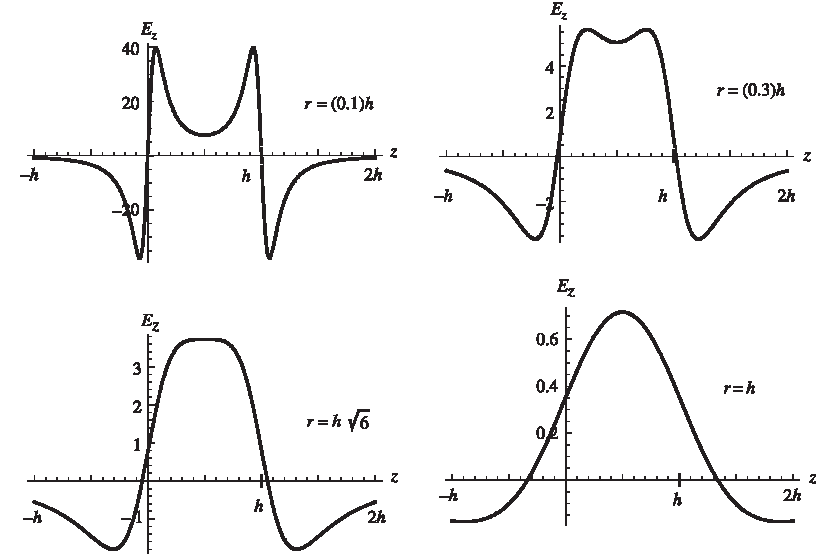
\includegraphics[width=\textwidth]{Anh/c2.pdf}
            \end{center}
        \end{enumerate}
       
    \end{loigiai}
    \begin{vd}[Điện tích xuyên vòng]
Cho hai vòng kim loại mảnh giống hệt nhau, bán kính $R$, mỗi vòng có điện tích $Q$ $(Q > 0)$ được phân bố đều trên toàn vòng. Hai vòng được đặt cố định song song với nhau trong chân không, khoảng cách giữa hai vòng là $2R$. Chọn trục tọa độ $\mathrm{O}x$ trùng với trục đối xứng của hai vòng với gốc tọa độ $\mathrm{O}$ đặt tại điểm cách đều hai vòng (xem hình vẽ). 
\begin{enumerate}[1)]
    \item Xác định cường độ điện trường tại điểm bất kì trên trục $x$.
    \item Một điện tích dương $q$, khối lượng $m$ chuyển động dọc theo trục $x$ từ xa vô cùng lại gần hai vòng với vận tốc ban đầu $v_0$. Bằng phương pháp đồ thị, hãy cho biết $v_0$ phải thỏa mãn điều kiện gì để điện tích $q$ có thể đi đến gốc tọa độ.
    \item Liệu có tồn tại vị trí mà ta có thể đặt điện tích $q$ nằm yên ở đó không? Nếu có thì đó là vị trí cân bằng bền hay không bền?
    \item Điện tích $q$ được giữ tại điểm trên trục $x$ có tọa độ $x_0 \ (0<x_0\ll R)$ Tại thời điểm $t=0$ thả nhẹ điện tích $q$ ra. Hãy xác định vị trí của $q$ ở thời điểm $t$ bất kì.
\end{enumerate}
\begin{center}


\tikzset{every picture/.style={line width=0.75pt}} %set default line width to 0.75pt        

\begin{tikzpicture}[x=0.75pt,y=0.75pt,yscale=-1,xscale=1]
%uncomment if require: \path (0,300); %set diagram left start at 0, and has height of 300

%Straight Lines [id:da8992780354065661] 
\draw    (327.87,152.66) -- (369.78,152.66) -- (412.17,152.66) ;
\draw [shift={(415.17,152.66)}, rotate = 180] [fill={rgb, 255:red, 0; green, 0; blue, 0 }  ][line width=0.08]  [draw opacity=0] (10.72,-5.15) -- (0,0) -- (10.72,5.15) -- (7.12,0) -- cycle    ;
%Shape: Ellipse [id:dp5452127600171381] 
\draw  [line width=1.5]  (192.85,152.66) .. controls (192.85,120.77) and (201.45,94.92) .. (212.06,94.92) .. controls (222.67,94.92) and (231.26,120.77) .. (231.26,152.66) .. controls (231.26,184.55) and (222.67,210.4) .. (212.06,210.4) .. controls (201.45,210.4) and (192.85,184.55) .. (192.85,152.66) -- cycle ;
%Straight Lines [id:da748234131447068] 
\draw  [dash pattern={on 4.5pt off 4.5pt}]  (215.06,216.4) -- (324.87,216.4) ;
\draw [shift={(327.87,216.4)}, rotate = 180] [fill={rgb, 255:red, 0; green, 0; blue, 0 }  ][line width=0.08]  [draw opacity=0] (10.72,-5.15) -- (0,0) -- (10.72,5.15) -- (7.12,0) -- cycle    ;
\draw [shift={(212.06,216.4)}, rotate = 0] [fill={rgb, 255:red, 0; green, 0; blue, 0 }  ][line width=0.08]  [draw opacity=0] (10.72,-5.15) -- (0,0) -- (10.72,5.15) -- (7.12,0) -- cycle    ;
%Shape: Ellipse [id:dp7523961013690177] 
\draw  [line width=1.5]  (308.67,152.66) .. controls (308.67,120.77) and (317.27,94.92) .. (327.87,94.92) .. controls (338.48,94.92) and (347.08,120.77) .. (347.08,152.66) .. controls (347.08,184.55) and (338.48,210.4) .. (327.87,210.4) .. controls (317.27,210.4) and (308.67,184.55) .. (308.67,152.66) -- cycle ;
%Straight Lines [id:da19548217072294993] 
\draw    (212.06,152.66) -- (308.67,152.66) ;
%Straight Lines [id:da05665051754981065] 
\draw    (130,152.66) -- (192.85,152.66) ;
%Straight Lines [id:da1793421587844577] 
\draw  [dash pattern={on 0.84pt off 2.51pt}]  (192.85,152.66) -- (212.06,152.66) ;
%Straight Lines [id:da22689284080897432] 
\draw  [dash pattern={on 0.84pt off 2.51pt}]  (308.67,152.66) -- (327.87,152.66) ;
%Straight Lines [id:da20345355752484995] 
\draw  [dash pattern={on 4.5pt off 4.5pt}]  (212.06,149.66) -- (212.06,97.92) ;
\draw [shift={(212.06,94.92)}, rotate = 450] [fill={rgb, 255:red, 0; green, 0; blue, 0 }  ][line width=0.08]  [draw opacity=0] (8.93,-4.29) -- (0,0) -- (8.93,4.29) -- (5.93,0) -- cycle    ;
\draw [shift={(212.06,152.66)}, rotate = 270] [fill={rgb, 255:red, 0; green, 0; blue, 0 }  ][line width=0.08]  [draw opacity=0] (8.93,-4.29) -- (0,0) -- (8.93,4.29) -- (5.93,0) -- cycle    ;
%Shape: Circle [id:dp7863875363556825] 
\draw  [color={rgb, 255:red, 0; green, 0; blue, 0 }  ,draw opacity=1 ][fill={rgb, 255:red, 0; green, 0; blue, 0 }  ,fill opacity=1 ] (267.52,152.46) .. controls (267.52,151.16) and (268.58,150.11) .. (269.88,150.11) .. controls (271.18,150.11) and (272.24,151.16) .. (272.24,152.46) .. controls (272.24,153.77) and (271.18,154.82) .. (269.88,154.82) .. controls (268.58,154.82) and (267.52,153.77) .. (267.52,152.46) -- cycle ;


% Text Node
\draw (204.56,71.04) node [anchor=north west][inner sep=0.75pt]    {$Q$};
% Text Node
\draw (320.96,72.2) node [anchor=north west][inner sep=0.75pt]    {$Q$};
% Text Node
\draw (212.63,114.11) node [anchor=north west][inner sep=0.75pt]    {$R$};
% Text Node
\draw (263.92,157.86) node [anchor=north west][inner sep=0.75pt]    {$O$};
% Text Node
\draw (260.17,195.27) node [anchor=north west][inner sep=0.75pt]    {$2R$};


\end{tikzpicture}
\end{center}
\end{vd}
\begin{loigiai}
    \begin{enumerate}[1)]
        \item Ta xác định điện thế tại điểm M bất kì trên trục $x$. Chọn mốc tính điện thế là điểm xa vô cùng. Các phần tử trên mỗi vòng tròn đều các $M$ các khoảng bằng nhau nên điện thế tại $M$ là:
        \[V(x) = \dfrac{1}{4 \pi \varepsilon_0}\dfrac{Q}{\sqrt{R^2+\left(x-R\right)^2}}+\dfrac{1}{4 \pi \varepsilon_0} \dfrac{Q}{\sqrt{R^2+\left(x+R\right)^2}}. \tag{1} \label{tr.tst.2.1}\]
        Từ đó: \[E(x)=-\dfrac{\dd V(x)}{\dd x}=\dfrac{Q}{{4\pi {\varepsilon _0}}}\left\{ {\dfrac{{Q\left( {x - R} \right)}}{{{{\left[ {{R^2} + {{\left( {x - R} \right)}^2}} \right]}^{\frac{3}{2}}}}} + \dfrac{{Q\left( {x + R} \right)}}{{{{\left[ {{R^2} + {{\left( {x + R} \right)}^2}} \right]}^{\frac{3}{2}}}}}} \right\}. \tag{2}\]
        \item Khi đặt tại $M$ điện tích $q$, thế năng của hệ là:
        \[U( x ) = qV( x ) = \dfrac{1}{{4\pi {\varepsilon _0}}}\dfrac{{qQ}}{{\sqrt {{R^2} + {{\left( {x - R} \right)}^2}} }} + \dfrac{1}{{4\pi {\varepsilon _0}}}\dfrac{{qQ}}{{\sqrt {{R^2} + {{\left( {x + R} \right)}^2}} }}. \tag{3}\]
        Để xét sự biến thiên của $U(x)$, ta xét phương trình:
        \[\dfrac{\dd}{{\dd{{x}}}}U(x) =  - qE(x) =  - \dfrac{{qQ}}{{4\pi {\varepsilon _0}}}\left\{ {\dfrac{{x - R}}{{{{\left[ {{R^2} + {{\left( {x - R} \right)}^2}} \right]}^{\frac{3}{2}}}}} + \dfrac{{x + R}}{{{{\left[ {{R^2} + {{\left( {x + R} \right)}^2}} \right]}^{\frac{3}{2}}}}}} \right\} = 0. \tag{4} \label{tr.tst.2.4}\]
        \textit{Nhận xét}: Trong miền $|x|\geqslant R, \dfrac{\dd}{\dd x}U(x) \ne 0 $. Do đó, nghiệm của phương trình (\ref{tr.tst.2.4}) nằm trong khoảng $(-R,R)$, tức là các điểm cực trị của $U(x)$ nằm trong khoảng $(-R,R)$.
        Xét điện trường có cường độ $E^*$ gây bởi một vòng dây, gốc tọa độ đặt tại tâm của vành.
        Điện thế tại điểm có tọa độ $x$ là:
        \[V(x) = \dfrac{1}{{4\pi {\varepsilon _0}}}\dfrac{Q}{{\sqrt {{R^2} + {x^2}} }}\]
        \[ \Rightarrow {E^{*}}(x) =  - \dfrac{{dV(x)}}{{dx}} = \dfrac{1}{{4\pi {\varepsilon _0}}}\dfrac{{Qx}}{{\sqrt {{{\left( {{R^2} + {x^2}} \right)}^3}} }}.\]
        Do đó
        \[\dfrac{{dE^{*}(x)}}{{dx}} = \dfrac{1}{{4\pi {\varepsilon _0}}}\dfrac{{Q\left( {{R^2} - 2{x^2}} \right)}}{{{{\left( {{R^2} + {x^2}} \right)}^{\frac{5}{2}}}}}.\]
        \begin{center}
            

\tikzset{every picture/.style={line width=0.75pt}} %set default line width to 0.75pt        

\begin{tikzpicture}[x=0.75pt,y=0.75pt,yscale=-1,xscale=1]
%uncomment if require: \path (0,300); %set diagram left start at 0, and has height of 300

%Straight Lines [id:da29340981265573385] 
\draw    (109,127.34) -- (391.4,127.34) ;
%Straight Lines [id:da10824321089642597] 
\draw    (250.2,46.13) -- (250.2,208.54) ;
%Straight Lines [id:da28917983880229525] 
\draw  [dash pattern={on 4.5pt off 4.5pt}]  (202.88,127.72) -- (202.88,205.2) ;
%Curve Lines [id:da2132070532280097] 
\draw    (151.22,161.94) .. controls (200.94,184.54) and (195.13,263.31) .. (250.2,127.34) ;

%Straight Lines [id:da09829234828261857] 
\draw  [dash pattern={on 4.5pt off 4.5pt}]  (297.33,126.69) -- (297.33,104.48) -- (297.33,49.21) ;
%Curve Lines [id:da28912635664334707] 
\draw    (349.18,92.73) .. controls (299.46,70.13) and (305.27,-8.63) .. (250.2,127.34) ;


% Text Node
\draw (178.85,77.91) node [anchor=north west][inner sep=0.75pt]    {$-\dfrac{1}{\sqrt{2}}$};
% Text Node
\draw (282.63,131.69) node [anchor=north west][inner sep=0.75pt]    {$\dfrac{1}{\sqrt{2}}$};
% Text Node
\draw (230.7,46.6) node [anchor=north west][inner sep=0.75pt]    {$E^{*}$};
% Text Node
\draw (353.66,108.67) node [anchor=north west][inner sep=0.75pt]    {$x/R$};


\end{tikzpicture}
        \end{center}
        Vì $\dfrac{{\dd E^{*}(x)}}{{\dd x}} = \dfrac{1}{{4\pi {\varepsilon _0}}}\dfrac{{Q\left( {{R^2} - 2{x^2}} \right)}}{{{{\left( {{R^2} + {x^2}} \right)}^{\frac{5}{2}}}}}$, dễ dàng suy ra $E^{*}$ có giá trị cực đại $E^{*}_{\max}>0$ tại $\dfrac{R}{\sqrt{2}}$ và có giá trị cực tiểu âm $-E^{*}_{\max}$ tại $-\dfrac{R}{\sqrt{2}}$.
        
        Ngoài ra, $E^{*}>0$ với $x>0$ và $E^{*}<0$ với $x<0$.
        Kí hiệu $E_1$ và $E_2$ lần lượt là cường độ điện trường gây ra bởi vành đặt tại $x=R$ và vành đặt tại $x=-R$. Vì điện trường tổng hợp có tính chất $E(x)=-E(-x)$ nên ta chỉ cần xét miền $0 \leq x<R$.
        \\ Khi $x$ giảm dần từ $R$ đến $\left(1-\dfrac{1}{\sqrt{2}}\right)R$, $E_1$ giảm đơn điệu từ 0 đến giá trị $-E_{\max}$, còn $E_2$ luôn dương và tăng đơn điệu nhưng luôn nhỏ hơn $E_{\max}$. Do đó, điện trường tổng hợp $E$ có giá trị dương tại $x=R$ và có giá trị âm tại $\left(1-\dfrac{1}{\sqrt{2}}\right)R$. Vì $E$ là hàm liên tục của $x$ nên $E$ phải bằng 0 tại một điểm $x_1$ nào đó trong khoảng $\left( {\left( {1 - \dfrac{1}{{\sqrt 2 }}} \right)R,R} \right)$.
        \\ Khi $x$ giảm từ $\left(1-\dfrac{1}{\sqrt{2}}\right)R$ tới 0, $E_1$ tăng đơn điệu từ 0 đến giá trị $-E_0 (E_0>0)$ nào đó, còn $E_2$ luôn dương và tăng đơn điệu từ giá trị nhỏ hơn $E_{\max}$ đến giá trị $E_0$. Do đó, điện trường tổng hợp $E$ có giá trị âm trong khoảng $\left( {0,\left( {1 - \dfrac{1}{{\sqrt 2 }}} \right)R} \right)$. Đồ thị của $E$ được phác họa ở hình dưới.
        \begin{center}
            

\tikzset{every picture/.style={line width=0.75pt}} %set default line width to 0.75pt        

\begin{tikzpicture}[x=0.75pt,y=0.75pt,yscale=-1,xscale=1]
%uncomment if require: \path (0,300); %set diagram left start at 0, and has height of 300

%Straight Lines [id:da056701205338354876] 
\draw    (107,141.97) -- (481.09,141.97) ;
%Straight Lines [id:da34292327921721166] 
\draw    (294.05,34.4) -- (294.05,249.54) ;
%Curve Lines [id:da8479191662540728] 
\draw    (131.8,191.2) .. controls (208.8,129.2) and (223.8,73.2) .. (268.8,71.2) .. controls (313.8,69.2) and (288.8,97.2) .. (458.8,119.2) ;
%Curve Lines [id:da5196977908822733] 
\draw    (131.4,170.6) .. controls (296.4,193.6) and (280.8,217.2) .. (320.8,219.2) .. controls (360.8,221.2) and (430.8,109.2) .. (457.8,99.2) ;
%Curve Lines [id:da7681668515968598] 
\draw    (144.4,204.4) .. controls (182.8,186.2) and (209.8,121.2) .. (253.4,123.6) .. controls (297,126) and (300.8,165.2) .. (338.8,164.2) .. controls (376.8,163.2) and (409.8,106.2) .. (450.4,81.6) ;
%Straight Lines [id:da10982613158159515] 
\draw  [dash pattern={on 4.5pt off 4.5pt}]  (268.8,71.2) -- (268.8,142.2) ;
%Straight Lines [id:da5867849954172704] 
\draw  [dash pattern={on 4.5pt off 4.5pt}]  (318.8,144.2) -- (318.8,215.2) ;
%Straight Lines [id:da4065785269483002] 
\draw  [dash pattern={on 4.5pt off 4.5pt}]  (411.8,103.2) -- (411.8,174.2) ;


% Text Node
\draw (165,121.4) node [anchor=north west][inner sep=0.75pt]    {$-1$};
% Text Node
\draw (295,116.4) node [anchor=north west][inner sep=0.75pt]    {$1-1/\sqrt{2}$};
% Text Node
\draw (415,148.4) node [anchor=north west][inner sep=0.75pt]    {$1$};
% Text Node
\draw (198,189.4) node [anchor=north west][inner sep=0.75pt]    {$E_{1}$};
% Text Node
\draw (194,71.4) node [anchor=north west][inner sep=0.75pt]    {$E_{2}$};
% Text Node
\draw (350,166.4) node [anchor=north west][inner sep=0.75pt]    {$E$};
% Text Node
\draw (485,120.4) node [anchor=north west][inner sep=0.75pt]    {$x/R$};
% Text Node
\draw (278,31.4) node [anchor=north west][inner sep=0.75pt]    {$E$};


\end{tikzpicture}
        \end{center}
        Tóm lại, điện trường tổng hợp $E$ bằng không tại ba điểm $x=0$ và $x=\pm x_1$. Điều đó có nghĩa là $\dfrac{\dd U}{\dd x}=0$ tại các điểm nói trên.
        \\Vậy $U(x)$ đạt cực tiểu tại $x=0$ và đạt cực đại tại $x=\pm x_1$. Kí hiệu $U_{\max}=U(x_1)$. Ta thấy để hạt $q$ có thể đi tới gốc tọa độ $x=0$ thì động năng ban đầu của nó phải lớn hơn $U_{\max}$, tức vận tốc ban đầu của nó phải thỏa mãn điều kiện: \[v_0>\dfrac{2U_{\max}}{m}.\]
        \item Như trên, ta thấy tồn tại ba vị trí cân bằng $x=0$ và $x=\pm x_1$, trong đó $x=0$ là vị trí cân bằng bền, còn hai vị trí còn lại là không bền.
        \item Tại lân cận điểm 0, tức là với $|x|\ll R$, ta có
        \[\dfrac{{\dd U(x)}}{{\dd x}} =  - \dfrac{{qQ}}{{4\pi {\varepsilon _0}}}\left\{ {\dfrac{{x - R}}{{{{\left[ {{R^2} + {{\left( {x - R} \right)}^2}} \right]}^{\frac{3}{2}}}}} + \dfrac{{x + R}}{{{{\left[ {{R^2} + {{\left( {x + R} \right)}^2}} \right]}^{\frac{3}{2}}}}}} \right\}.\]
        Khai triển mẫu số, bỏ qua $x^2$ so với $x$ ta được
        \[\dfrac{{\dd U(x)}}{{\dd x}} \approx \dfrac{{qQ}}{{4\pi {\varepsilon _0}}}\left\{ {\dfrac{{x - R}}{{{{\left[ {2{{R}}\left( {R - x} \right)} \right]}^{\frac{3}{2}}}}} + \dfrac{{x + R}}{{{{\left[ {2{{R}}\left( {R - x} \right)} \right]}^{\frac{3}{2}}}}}} \right\}.\]
        \[ \Rightarrow \dfrac{{\dd U(x)}}{{\dd x}} = \dfrac{{qQ}}{{8\sqrt 2 \pi {\varepsilon _0}{R^3}}}x. \tag{5} \label{tr.tst.2.5}\]
        Theo (\ref{tr.tst.2.5}), phương trình chuyển động của $q$ là $m\Ddot{x}=-kx$ với $|x|\ll R$, trong đó $k=\dfrac{{qQ}}{{8\sqrt 2 \pi {\varepsilon _0}{R^3}}}$.
        \\Điều này có nghĩa là $q$ dao động điều hòa xung quanh gốc tọa độ. Vị trí của $q$ tại thời điểm $t>0$ bất kì là $x=x_0 \cos{(\omega t)}$ với $\omega  = \dfrac{1}{2}\sqrt {\dfrac{{qQ}}{{\sqrt 2 \pi {\varepsilon _0}m{{{R}}^3}}}}$.
     \end{enumerate}
\end{loigiai}

 \begin{vd}[``Nhiều'' năng lượng]
    \label{c291}
    Một điện tích $Q$ được phân bố đều trong một quả cầu bán kính $R$. Tìm năng lượng tĩnh điện của phân bố điện tích này theo ba cách sau 
    \begin{enumerate}[1)]
    \setlength{\itemsep}{0pt}
        \item Tính công cần để thiết lập phân bố điện tích bằng cách di chuyển các vỏ cầu nhỏ tích điện từ vô cùng đến vị trí cuối cùng của chúng.
        \item Tính năng lượng điện trường bằng cách tích phân mật độ năng lượng điện trường $u_e=\dfrac{E^2}{8\pi \varepsilon_0}$ theo thể tích.
        \item Tính thế năng tĩnh điện của hệ bằng cách tính tích phân $\dfrac{\rho\phi}{2}$ theo thể tích, với $\rho$ là mật độ điện tích, $\phi$ là điện thế. Cách tính này khác gì với phép tính trong ý trước?
    \end{enumerate}
    \end{vd}
    \begin{loigiai}
    \begin{enumerate}[1)]
    \setlength{\itemsep}{0pt}
        \item Ta có thể xây dựng quả cầu này bằng cách di chuyển những vỏ cầu nhỏ từ vô cùng đến vị trí cuối cùng của chúng.  Giả sử tại một thời điểm nào đó, chúng ta đã có một quả cầu tích điện $\rho$ và bán kính $r<R$.\\
        Điện tích của quả cầu:
        $$q(r)=\dfrac{4\pi r^3\rho}{3}.$$
        Điện thế tại bề mặt quả cầu:
        \begin{equation*}
            \begin{aligned}
                \phi(r)=\dfrac{kq(r)}{r}
                =\dfrac{r^2\rho}{3\varepsilon_0}.
            \end{aligned}
        \end{equation*}
        Bây giờ ta sẽ di chuyển các điện tích từ vô cùng đến vị trí cuối cùng của nó để ``bồi'' thêm cho quả cầu một lớp cầu dày $\dd r$.\\
        Điện tích một lớp cầu:
        \begin{equation*}
            \dd q=4\pi r^2\dd r\rho.
        \end{equation*}
        Công để dịch chuyển lớp cầu này:
        \begin{equation*}
            \begin{aligned}
                \dd W&=\phi(r)\dd q\\
                &=\dfrac{r^2\rho}{3\varepsilon_0}\tron{4\pi r^2\dd r\rho}\\
               &=\dfrac{4\pi\rho^2 r^4 \dd r}{3\varepsilon_0}.
            \end{aligned}
        \end{equation*}
        Công tổng cộng cần để tạo ra một quả cầu bán kính $R$:
        \begin{equation*}
            \begin{aligned}
                W&=\tiph{0}{R}{\dfrac{4\pi\rho^2 r^4}{3\varepsilon_0}}{r}\\
                &=\dfrac{4\pi\rho^2}{3\varepsilon_0}\left.\tron{\dfrac{r^5}{5}}\right|_0^R\\
                &=\dfrac{4\pi\rho^2 R^5}{15\varepsilon_0}=\dfrac{3kQ^2}{5R}.\\
            \end{aligned}
        \end{equation*}
        Với $Q=\dfrac{4\pi R^3\rho}{3}$ là điện tích của quả cầu.
        \item Ta xét điện trường tạo ra bởi phân bố điện tích trên tại một điểm cách tâm hình cầu một khoảng $r$.\\
        Với $r>R$, điện trường giống như là điện trường của một điện tích điểm $Q$ đặt tại tâm hình cầu:
        \begin{equation*}
            E=\dfrac{kQ}{r^2}.
        \end{equation*}
        Với $r\leq R$, ta sử dụng định luật Gauss.\\
        Chọn mặt Gauss là một mặt cầu có bán kính $r$, tâm trùng với tâm quả cầu. Ta có:
        \begin{equation*}
            \begin{aligned}
                E\tron{4\pi r^2}=\dfrac{r^3Q}{R^3\varepsilon_0}
                \Leftrightarrow E=\dfrac{kQr}{R^3}.
            \end{aligned}
        \end{equation*}
        Tích phân mật độ năng lượng điện trường trên toàn bộ thể tích:
        \begin{equation*}
            \begin{aligned}
                W&=\tiph{0}{\infty}{\dfrac{E^2(r)}{8\pi k}4\pi r^2}{r}\\
                &=\dfrac{kQ^2}{2}\tron{\tiph{0}{R}{\tron{\dfrac{r}{R^3}}^2r^2}{r}+\tiph{R}{\infty}{\tron{\dfrac{1}{r^2}}^2r^2}{r}}\\
                &=\dfrac{kQ^2}{2}\tron{\dfrac{1}{5R}+\dfrac{1}{R}}=\dfrac{3kQ^2}{5R}.
            \end{aligned}
        \end{equation*}
        \item Điện thế trên bề mặt quả cầu: 
        $$\phi_0=\dfrac{kQ}{R}.$$
        Với $r<R$, ta có:
        \begin{equation*}
        \begin{aligned}
             &\ ~~~ \dd \phi &=& -E\dd r\\
             \Leftrightarrow ~& \phi_0-\phi(r) &=&-\tiph{r}{R}{\dfrac{kQr'}{R^3}}{r'}\\
             \Leftrightarrow~ &\quad \phi(r)&=&\dfrac{kQ}{R}+\dfrac{kQ\tron{R^2-r^2}}{2R^3}\\
             &\ &=&\dfrac{3kQ}{2R}-\dfrac{kQr^2}{2R^3}.
        \end{aligned}
        \end{equation*}
        Thế năng tĩnh điện của hệ: 
        \begin{equation*}
            \begin{aligned}
                W&=\tiph{0}{R}{\dfrac{1}{2}\phi(r)\rho 4\pi r^2}{r}\\
                &=\tiph{0}{R}{\tron{\dfrac{3kQ}{2R}-\dfrac{kQr^2}{2R^3}}\tron{\dfrac{3Qr^2}{R^3}}}{r}\\
                &=\dfrac{kQ^2}{4}\left.\tron{\dfrac{3r^3}{R^4}-\dfrac{3r^5}{5R^6}}\right|_0^R\\
                &=\dfrac{3kQ^2}{5R}.
            \end{aligned}
        \end{equation*}
    \end{enumerate}
    Ta thấy được từ ba phần trên, cả ba phương pháp đều đi đến cùng một kết quả. Tuy nhiên, so sánh giữa phương pháp ở phần thứ hai và phần thứ ba, ta thấy rằng khái niệm mật độ năng lượng điện trường không đơn thuần có nghĩa là ``năng lượng chứa trong một đơn vị thể tích''. Nếu chúng ta coi mật độ năng lượng là $u_e=\dfrac{E^2}{8\pi \varepsilon_0}$, thì điều đó có nghĩa là năng lượng sẽ trải rộng trên toàn bộ không gian. Còn nếu ta coi mật độ năng lượng là $\dfrac{\rho\phi}{2}$, điều này có nghĩa là năng lượng chỉ tập trung tại nơi có mặt điện tích. Vậy nên, khái niệm mật độ năng lượng là một khái niệm khá là trừu tượng, trong khi năng lượng của một hệ lại là một đại lượng được định nghĩa chính xác, ít nhất là trong trường hợp không xuất hiện điện tích điểm.
    \end{loigiai}
    
    
    \begin{vd}[Lỗ trên mặt phẳng]
    \begin{enumerate}[1)]
    \setlength{\itemsep}{0pt}
        \item Người ta cắt một lỗ tròn bán kính $R$ trên một tấm phẳng rộng tích diện đều với mật độ điện tích mặt $\sigma$. Đường thẳng $\Delta$ vuông góc với mặt phẳng và đi qua tâm của lỗ. Tìm điện trường tại một điểm trên $\Delta$, cách tâm lỗ một khoảng là $z$.
        \item Một điện tích điểm $-q$, khối lượng $m$ được thả từ một vị trí trên $\Delta$, rất gần tâm của lỗ. Chứng minh rằng điện tích dao động điều hòa và tìm tần số góc $\omega$ của dao động.\\
        Tính $\omega$ với $m=1\dv{g}$, $-q=-10^{-8}\dv{C}$, $\sigma=10^{-6}\dv{C/m^2}$ và $R=0,1\dv{m}$.
        \item Một điện tích $-q$ khối lượng $m$ được thả từ một vị trí trên trục $\Delta$ và cách tấm một khoảng là $z$. Tìm vận tốc điện tích điểm khi nó đi qua tâm lỗ. Đánh giá kết quả của bạn khi $z\gg R$.
    \end{enumerate}
    \end{vd}
    \begin{loigiai}
        \begin{enumerate}[1)]
        \setlength{\itemsep}{0pt}
            \item Xét một phần tử diện tích có điện tích $\dd q$ cách tâm của lỗ tròn là $r$. Điện trường do phần tử này gây ra tại điểm đang xét là $\dfrac{\dd q}{4\pi \varepsilon_0\tron{r^2+z^2}}$. Do tính chất đối xứng của hệ, điện trường tại một điểm trên đường thẳng $\Delta$ có phương dọc theo $\Delta$, vậy nên chỉ có thành phần điện trường dọc theo $\Delta$ mới đóng góp vào điện trường tổng hợp. Ta có:
            \begin{equation}
                \dd E=\dfrac{\dd q}{4\pi \varepsilon_0\tron{r^2+z^2}}\frac{z}{\sqrt{r^2+z^2}}.
                \label{ca4}
            \end{equation}
            Ta có $\dd q=\sigma r\dd r\dd \theta$. \\
            \newpage
            Điện trường do toàn bộ mặt phẳng (có lỗ) sinh ra:
            \begin{equation}
               \begin{aligned}
                  E(z)&=\int_R^\infty\int_0^{2\pi}\dfrac{\sigma zr}{4\pi \varepsilon_0\tron{r^2+z^2}^\frac{3}{2}}\dd r \dd \theta\\
                  &=\int_R^\infty\dfrac{2\pi \sigma zr}{4\pi \varepsilon_0\tron{r^2+z^2}^\frac{3}{2}}\dd r \\
                  &=\left.-\dfrac{2\pi \sigma z}{4\pi \varepsilon_0\sqrt{r^2+z^2}}\right|_R^\infty\\
                  &=\dfrac{\sigma z}{2\varepsilon_0\sqrt{R^2+z^2}}.
                  \label{ca4}
               \end{aligned} 
            \end{equation}
            Chú ý rằng khi $R=0$, điện trường sẽ là $E=\dfrac{\sigma}{2\varepsilon_0}$ giống điện trường của một mặt phẳng vô hạn tích điện đều.
            \item Khi $z\ll R$, thì từ (\ref{ca4}) ta có $E(z)\approx \dfrac{\sigma z}{2\varepsilon_0R}$. Phương trình chuyển động của điện tích  là:
            \begin{equation}
                -qE=m\ddot z\Leftrightarrow \ddot z+\tron{\dfrac{q\sigma}{2\varepsilon_0mR}}z=0.
            \end{equation}
            Điện tích dao động điều hòa. Tần số góc của dao động là:
            \begin{equation}
                \omega=\sqrt{\dfrac{q\sigma}{2\varepsilon_0mR}}.
            \end{equation}
            Thay số vào ta được:
            \begin{equation}
                \omega=\sqrt{\dfrac{\tron{10^{-8}\dv{C}}\tron{10^{-6}\dv{C/m^2}}}{2\tron{8,85\cdot10^{-12}\dv{\frac{s^2C^2}{kg\ m^3}}}\tron{10^{-3}\dv{kg}}\tron{0,1\dv{m}}}}=2,4\dv{s^{-1}}.
            \end{equation}
            Tần số góc này tương đương với tần số khoảng $0,4\dv{Hz}$. Để có dao động điểu hòa thì chuyển động của điện tích phải bị giới hạn trên đường thẳng $\Delta$ vì cân bằng của điện tích theo phương song song với mặt phẳng là cân bằng không bền.
            \item Thế năng của điện tích là $U(z)$. Ta có:
            \begin{equation}
            \begin{aligned}
                 &\dd U&=&-F\dd z=qE(z)\dd z\\
                 \Rightarrow &U(z)&=&\tiph{0}{z}{qE(z')}{z'}=\tiph{0}{z}{\dfrac{q\sigma z'}{2\varepsilon_0\tron{R^2+z'^2}}}{z'}\\
                 & \ &=&\left.\dfrac{q\sigma}{2\varepsilon_0}\sqrt{R^2+z'^2}\right|_0^z=\dfrac{q\sigma}{2\varepsilon_0}\tron{\sqrt{R^2+z^2}-R}.
            \end{aligned}
            \end{equation}
            Bảo toàn năng lượng, ta có:
            \begin{equation}
                \begin{aligned}
                   &\dfrac{mv^2}{2}=U(z)\\ \Leftrightarrow&v=\sqrt{\dfrac{q\sigma}{m\varepsilon_0}\tron{\sqrt{R^2+z^2}-R}}.
                \end{aligned}
            \end{equation}
            Với $z\gg R$, ta có $v\approx\sqrt{\dfrac{q\sigma z}{m\varepsilon_0}}$. Kết quả này giống như việc coi mặt phẳng là không có lỗ. Thật vậy, khi đó lực điện tác dụng lên điện tích sẽ là $\dfrac{q\sigma}{2\varepsilon_0}$ không đổi, gia tốc điện tích là $a=\dfrac{q\sigma}{2m\varepsilon_0}$. Vận tốc của điện tích khi chạm mặt phẳng là $v=\sqrt{2az}=\sqrt{\dfrac{q\sigma z}{m\varepsilon_0}}$.
        \end{enumerate}
    \end{loigiai}
    
    
    \begin{vd}[Kiểm chứng lại định luật Coulomb]
    Cavendish và Maxwell đã thực hiện các thí nghiệm để kiểm chứng lại tính đúng đắn của định luật Coulomb, rằng lực điện giữa hai điện tích điểm tỉ lệ nghịch với bình phương khoảng cách giữa chúng. Trong bài toán này chúng ta sẽ tìm hiểu về phần lý thuyết đằng sau những thí nghiệm này.
    \begin{enumerate}[1)]
    \setlength{\itemsep}{0pt}
        \item Giả sử rằng định luật Coulomb cho rằng lực điện giữa hai điện tích có dạng $\dfrac{kq_1q_2}{r^{2+\delta}}$. Cho một hệ gồm một vỏ cầu rỗng bán kính $R$ tích điện đều với điện tích $Q$, chứng tỏ rằng điện thế tại một điểm cách tâm vỏ cầu một khoảng là $r$ tuân theo quy luật sau:
        \begin{equation}
            \begin{aligned}
               &\phi(r)=\dfrac{kQ}{2\tron{1-\delta^2}rR}\tron{f(R+r)-f(R-r)}\qquad \text{(với $r<R$)},\\
               &\phi(r)=\dfrac{kQ}{2\tron{1-\delta^2}rR}\tron{f(R+r)-f(r-R)}\qquad \text{(với $r>R$)}.
            \end{aligned}
            \label{ca6}
        \end{equation}
        Trong đó $f(x)=x^{1-\delta}$ và $k=\dfrac{1}{4\pi\varepsilon_0}$.\\
        \textit{Lưu ý: Trong thực tế chúng ta quan tâm tới trường hợp $\delta\ll1$, vì vậy chúng ta có thể bỏ quả hạng tử $(1-\delta^2)$ ở mẫu số trong biểu thức (\ref{ca6}) và coi nó xấp xỉ 1. Chúng ta sẽ bỏ qua hạng tử này trong phần còn lại của bài toán.}
        \item Xét hai vỏ cầu đồng tâm với bán kính $a$ và $b$ (với $a>b$) và có điện tích lần lượt là $Q_a$ và $Q_b$ phân bố đều trên bề mặt. Chứng tỏ rằng điện thế ở trên từng mặt cầu được cho bởi công thức:
        \begin{equation}
            \begin{aligned}
                &\phi_a=\dfrac{kQ_a}{2a^2}f(2a)+\dfrac{kQ_b}{2ab}\tron{f(a+b)-f(a-b)},\\
                &\phi_b=\dfrac{kQ_b}{2b^2}f(2b)+\dfrac{kQ_a}{2ab}\tron{f(a+b)-f(a-b)}.
            \end{aligned}
        \end{equation}
        \item Nếu hai quả cầu được nối với nhau bằng dây mảnh dẫn điện, và được tích điện đến cùng điện thế $\phi$. Chứng tỏ rằng điện thế trên vỏ cầu bên trong (có bán kính $b$) lúc này là:
        \begin{equation}
            \begin{aligned}
                Q_b=\dfrac{2b\phi}{k}\dfrac{bf(2a)-a\tron{f(a+b)-f(a-b)}}{f(2a)+f(2b)-\tron{f(a+b)-f(a-b)}^2}.
            \end{aligned}
        \end{equation}
        Nếu $\delta=0$ thì $f(x)=x$, thì $Q_b=0$, giống như mong đợi. Nếu như $Q_b$ khác không thì $\delta$ cũng phải khác không.\\
        Với giá trị $\delta$ nhỏ thì bạn có thể sử dụng những phép tính gần đúng hợp lí để làm bài tập này.
    \end{enumerate}
    \end{vd}
     \begin{loigiai}
    \begin{enumerate}[1)]
    \setlength{\itemsep}{0pt}
        \item Giống như với bài \ref{ca5}, để tính điện thế tại điểm $P$, chúng ta sẽ chia vỏ cầu thành nhiều vòng nhỏ. Khoảng cách từ điểm $P$ tới một điểm trên vòng sẽ là $l=\sqrt{R^2+r^2-2Rr\cos\theta}$. Diện tích của vòng nhỏ sẽ là $2\pi R^2 \sin\theta\dd\theta$, điện tích của vòng sẽ là $\dd Q=\sigma2\pi R^2 \sin\theta\dd\theta=\dfrac{Q\sin\theta\dd\theta}{2}$. 
        \newpage
        \begin{center}
            

\tikzset{every picture/.style={line width=0.75pt}} %set default line width to 0.75pt        

\begin{tikzpicture}[x=0.75pt,y=0.75pt,yscale=-1,xscale=1]
%uncomment if require: \path (0,300); %set diagram left start at 0, and has height of 300

%Shape: Arc [id:dp6604130734699976] 
\draw  [draw opacity=0][line width=1.5]  (338.38,47.48) .. controls (385.19,52.25) and (421.71,91.79) .. (421.71,139.85) .. controls (421.71,187.6) and (385.67,226.93) .. (339.32,232.12) -- (328.85,139.85) -- cycle ; \draw  [line width=1.5]  (338.38,47.48) .. controls (385.19,52.25) and (421.71,91.79) .. (421.71,139.85) .. controls (421.71,187.6) and (385.67,226.93) .. (339.32,232.12) ;
%Shape: Arc [id:dp3988355543248949] 
\draw  [draw opacity=0][dash pattern={on 4.5pt off 4.5pt}] (288.83,56.05) .. controls (300.95,50.25) and (314.52,47) .. (328.85,47) .. controls (380.14,47) and (421.71,88.57) .. (421.71,139.85) .. controls (421.71,191.14) and (380.14,232.71) .. (328.85,232.71) .. controls (314.33,232.71) and (300.59,229.37) .. (288.34,223.43) -- (328.85,139.85) -- cycle ; \draw  [dash pattern={on 4.5pt off 4.5pt}] (288.83,56.05) .. controls (300.95,50.25) and (314.52,47) .. (328.85,47) .. controls (380.14,47) and (421.71,88.57) .. (421.71,139.85) .. controls (421.71,191.14) and (380.14,232.71) .. (328.85,232.71) .. controls (314.33,232.71) and (300.59,229.37) .. (288.34,223.43) ;
%Shape: Arc [id:dp3770531364912999] 
\draw  [draw opacity=0] (377.32,217.94) .. controls (377.09,217.98) and (376.86,217.99) .. (376.63,217.99) .. controls (366.34,217.99) and (358,183.16) .. (358,140.18) .. controls (358,97.21) and (366.34,62.37) .. (376.63,62.37) .. controls (377.13,62.37) and (377.62,62.45) .. (378.11,62.61) -- (376.63,140.18) -- cycle ; \draw   (377.32,217.94) .. controls (377.09,217.98) and (376.86,217.99) .. (376.63,217.99) .. controls (366.34,217.99) and (358,183.16) .. (358,140.18) .. controls (358,97.21) and (366.34,62.37) .. (376.63,62.37) .. controls (377.13,62.37) and (377.62,62.45) .. (378.11,62.61) ;
%Shape: Arc [id:dp48119814484050627] 
\draw  [draw opacity=0][dash pattern={on 4.5pt off 4.5pt}] (377.38,62.51) .. controls (377.61,62.47) and (377.84,62.46) .. (378.08,62.46) .. controls (388.37,62.46) and (396.71,97.29) .. (396.71,140.27) .. controls (396.71,183.24) and (388.37,218.08) .. (378.08,218.08) .. controls (377.58,218.08) and (377.09,218) .. (376.6,217.84) -- (378.08,140.27) -- cycle ; \draw  [dash pattern={on 4.5pt off 4.5pt}] (377.38,62.51) .. controls (377.61,62.47) and (377.84,62.46) .. (378.08,62.46) .. controls (388.37,62.46) and (396.71,97.29) .. (396.71,140.27) .. controls (396.71,183.24) and (388.37,218.08) .. (378.08,218.08) .. controls (377.58,218.08) and (377.09,218) .. (376.6,217.84) ;

%Shape: Arc [id:dp38971002723714365] 
\draw  [draw opacity=0] (387.33,208.95) .. controls (387.12,208.99) and (386.91,209) .. (386.71,209) .. controls (377.48,209) and (370,177.77) .. (370,139.23) .. controls (370,100.7) and (377.48,69.46) .. (386.71,69.46) .. controls (387.15,69.46) and (387.59,69.54) .. (388.03,69.68) -- (386.71,139.23) -- cycle ; \draw   (387.33,208.95) .. controls (387.12,208.99) and (386.91,209) .. (386.71,209) .. controls (377.48,209) and (370,177.77) .. (370,139.23) .. controls (370,100.7) and (377.48,69.46) .. (386.71,69.46) .. controls (387.15,69.46) and (387.59,69.54) .. (388.03,69.68) ;
%Shape: Arc [id:dp7448302847473949] 
\draw  [draw opacity=0][dash pattern={on 4.5pt off 4.5pt}] (387.38,69.59) .. controls (387.59,69.55) and (387.79,69.54) .. (388,69.54) .. controls (397.23,69.54) and (404.71,100.78) .. (404.71,139.31) .. controls (404.71,177.84) and (397.23,209.08) .. (388,209.08) .. controls (387.56,209.08) and (387.11,209) .. (386.68,208.86) -- (388,139.31) -- cycle ; \draw  [dash pattern={on 4.5pt off 4.5pt}] (387.38,69.59) .. controls (387.59,69.55) and (387.79,69.54) .. (388,69.54) .. controls (397.23,69.54) and (404.71,100.78) .. (404.71,139.31) .. controls (404.71,177.84) and (397.23,209.08) .. (388,209.08) .. controls (387.56,209.08) and (387.11,209) .. (386.68,208.86) ;

%Straight Lines [id:da6172667981511248] 
\draw    (328.85,139.85) -- (499.71,139.85) ;
\draw [shift={(499.71,139.85)}, rotate = 0] [color={rgb, 255:red, 0; green, 0; blue, 0 }  ][fill={rgb, 255:red, 0; green, 0; blue, 0 }  ][line width=0.75]      (0, 0) circle [x radius= 3.35, y radius= 3.35]   ;
%Straight Lines [id:da567536953964995] 
\draw    (378.11,62.61) -- (328.85,139.85) ;
%Straight Lines [id:da6026285341166078] 
\draw    (378.11,62.61) -- (499.71,139.85) ;

% Text Node
\draw (339,121.4) node [anchor=north west][inner sep=0.75pt]    {$\theta $};
% Text Node
\draw (335,86.4) node [anchor=north west][inner sep=0.75pt]    {$R$};
% Text Node
\draw (436,142.4) node [anchor=north west][inner sep=0.75pt]    {$r$};
% Text Node
\draw (433,77.4) node [anchor=north west][inner sep=0.75pt]    {$l$};
% Text Node
\draw (509,131.4) node [anchor=north west][inner sep=0.75pt]    {$P$};


\end{tikzpicture}

        \end{center}
        Nếu như lực điện giữa hai điện tích điểm có dạng như $F(r)=\dfrac{kq_1q_2}{r^{2+\delta}}$, thì điện thế gây ra bởi một điện tích điểm $\dd q$ tại một điểm cách điện tích một khoảng $l$ sẽ là $\dfrac{k\dd q}{\tron{1+\delta}l^{1+\delta}}$. Điện thế do vòng gây ra tại $P$ sẽ là:

            \[\dd\phi=\dfrac{kQ\sin\theta\dd\theta}{2(1+\delta)l^{1+\delta}}=\dfrac{kQ\sin\theta\dd\theta}{2(1+\delta)\tron{R^2+r^2-2Rr\cos\theta}^{\frac{1+\delta}{2}}}. \tag{1}\]

        Điện thế do cả vỏ cầu gây ra tại $P$ là:
        \[\begin{aligned}
           \phi(r)&=\tiph{0}{\pi}{\dfrac{kQ\sin\theta}{2(1+\delta)\tron{R^2+r^2-2Rr\cos\theta}^{\frac{1+\delta}{2}}}}{\theta}\\
           &=\left.\dfrac{kQ}{2\tron{1-\delta^2}rR}\tron{R^2+r^2-2Rr\cos\theta}^{\frac{1-\delta}{2}}\right|_0^\theta.
        \end{aligned} \tag{2}\]
        Bây giờ ta sẽ xét hai trường hợp. Nếu $r<R$, ta có:
           \[ \phi(r)=\dfrac{kQ}{2\tron{1-\delta^2}rR}\tron{f(R+r)-f(R-r)}.\tag{3}\]
        Nếu $r>R$, ta có:
        \[\phi(r)=\dfrac{kQ}{2\tron{1-\delta^2}rR}\tron{f(R+r)-f(r-R)}. \tag{4}\]
        Nếu như $\delta=0$ thì $f(x)=x$, kết quả thu được sẽ là $\dfrac{kQ}{R}$ với $r<R$ và $\dfrac{kQ}{r}$ với $r>R$, giống với kết quả trong bài \ref{ca5}.
        \item Điện thế do vỏ cầu lớn bán kính $a$ gây ra tại một điểm trên bề mặt nó là $\dfrac{kQ_a}{2a^2}f(2a)$, tại đây chúng ta đã bỏ qua hạng tử $\tron{1-\delta^2}$. Điện thế do vỏ cầu bé bán kính $b$ gây ra tại một điểm trên bề mặt vỏ cầu lớn là $\dfrac{kQ_b}{2ab}\tron{f(a+b)-f(a-b)}$. Điện thế tại một điểm trên bề mặt vỏ cầu lớn sẽ là tổng của hai điện thế trên:
            \[\phi_a=\dfrac{kQ_a}{2a^2}f(2a)+\dfrac{kQ_b}{2ab}\tron{f(a+b)-f(a-b)}. \tag{5}\label{cb3}\]
        Tương tự, điện thế do vỏ cầu nhỏ gây ra trên bề mặt nó là $\dfrac{kQ_b}{2b^2}f(2b)$, điện thế do vỏ cầu lớn gây ra trên bề mặt vỏ cầu nhỏ là $\dfrac{kQ_a}{2ab}\tron{f(a+b)-f(a-b)}$. Điện thế trên bề mặt vỏ cầu nhỏ:
            \[\phi_b=\dfrac{kQ_b}{2b^2}f(2b)+\dfrac{kQ_a}{2ab}\tron{f(a+b)-f(a-b)}.\tag{6}\label{cb4}
            \]
        Nếu $\delta=0$, $f(x)=x$ thì kết quả trên trở thành:
            \[\phi_a=\dfrac{kQ_a}{a}+\dfrac{kQ_b}{a}\quad \text{và} \quad \phi_b=\dfrac{kQ_a}{a}+\dfrac{kQ_b}{b}.
           \tag{7} \]
        Kết quả trên giống với khi ta sử dụng định luật Coulomb bình thường.
        \item Khi hai quả cầu được nối với nhau bằng dây dẫn và được tích điện tới cùng điện thế $\phi$, ta có $\phi_a=\phi_b=\phi$. Thay vào phương trình (\ref{cb3}) và (\ref{cb4}) và coi $Q_a$ và $Q_b$ là ẩn ta thu được một hệ hai phương trình hai ẩn. Nhân hai vế phương trình (\ref{cb3}) với $a\tron{f(a+b)-f(a-b)}$, phương trình (\ref{cb4}) với $bf(2a)$ rồi trừ vế với vế, ta được:
        \[\begin{aligned}
             \phi\Big(bf&(2a)-a\big[f(a+b)-f(a-b)\big]\Big)\\
             &=\dfrac{kQ_b}{2b}\Big(f(2a)f(2b)-\big[f(a+b)-f(a-b)\big]^2\Big). 
             \end{aligned}\tag{8} \]
        Từ đó, ta thu được:
            \[Q_b=\dfrac{2b\phi}{k}\dfrac{bf(2a)-a\big[f(a+b)-f(a-b)\big]}{f(2a)f(2b)-\big[f(a+b)-f(a-b)\big]^2}.\tag{9} \]
        Trong quá trình tính toán, ta đã bỏ qua hạng tử $(1-\delta^2)$, nếu ta không bỏ qua hạng tử này, thì nó sẽ xuất hiện ở tử số trong biểu thức tính $Q_b$. Giống như đã nêu ở đề bài, khi $\delta=0$ thì biểu thức của chúng ta cho kết quả $Q_b$ bằng không. Với giá trị $\delta$ nhỏ, ta có thể thực hiện phép tính gần đúng đến bậc nhất của $\delta$ để ước tính giá trị của $Q_b$. Nếu ta thay $a=1$ và $b=0,5$ thì $Q_b\approx\dfrac{2b\phi}{k}\tron{0,26\delta}$. Với $\delta$ nhỏ, điện tích trên vỏ cầu ngoài sẽ giống như là khi ta tính toàn với định luật Coulomb bình thường $Q_a=\dfrac{a\phi}{k}$. Vậy đối với $a=1$ và $b=0,5$ thì tỉ lệ điện tích trên hai vỏ cầu sẽ là:
        \begin{equation}
            \dfrac{Q_b}{Q_a}=\dfrac{\dfrac{2b\phi}{k}\tron{0,26\delta}}{\dfrac{a\phi}{k}}=0,26\delta.
        \end{equation}
    \end{enumerate}
    \end{loigiai}    
    
    
    \begin{vd}[Quả cầu bị cắt]
Một quả cầu kim loại bán kính $R$, được cắt thành hai nửa bởi một mặt phẳng sao cho diện tích chỏm cầu phần nhỏ hơn là $\pi.R^2$. Các mặt tiếp xúc được phủ một lớp cách điện rất mỏng, rồi ghép hai nửa lại với nhau để tạo thành quả cầu như ban đầu. Ban đầu tổng điện tích của quả cầu bằng $0$. Sau khi ghép, phần nhỏ hơn được truyền điện tích $+Q$, phần còn lại vẫn được giữ trung hòa. 
Đưa ra biểu thức cho:
\begin{enumerate}[1)]
    \item  Phân bố điện tích trên quả cầu.
    \item Lực tĩnh điện mà hai nửa quả cầu tương tác nhau.
    \item Năng lượng tĩnh điện của quả cầu.
\end{enumerate}
\begin{center}
    

\tikzset{every picture/.style={line width=0.75pt}} %set default line width to 0.75pt        

\begin{tikzpicture}[x=0.75pt,y=0.75pt,yscale=-1,xscale=1]
%uncomment if require: \path (0,470); %set diagram left start at 0, and has height of 470

%Shape: Chord [id:dp7672516414983406] 
\draw  [fill={rgb, 255:red, 155; green, 155; blue, 155 }  ,fill opacity=1 ] (300.99,285.19) .. controls (274.34,271.19) and (256.18,243.31) .. (256.18,211.2) .. controls (256.18,179.08) and (274.36,151.19) .. (301.02,137.19) -- cycle ;
%Shape: Chord [id:dp8357761441104918] 
\draw  [fill={rgb, 255:red, 155; green, 155; blue, 155 }  ,fill opacity=1 ] (304.68,135.38) .. controls (315.43,130.39) and (327.42,127.6) .. (340.06,127.6) .. controls (386.39,127.6) and (423.94,165.03) .. (423.94,211.2) .. controls (423.94,257.37) and (386.39,294.8) .. (340.06,294.8) .. controls (327.57,294.8) and (315.71,292.08) .. (305.06,287.2) -- cycle ;
%Straight Lines [id:da8177035752650788] 
\draw    (195.79,210.79) -- (244.18,210.79) ;
\draw [shift={(246.18,210.79)}, rotate = 180] [color={rgb, 255:red, 0; green, 0; blue, 0 }  ][line width=0.75]    (10.93,-3.29) .. controls (6.95,-1.4) and (3.31,-0.3) .. (0,0) .. controls (3.31,0.3) and (6.95,1.4) .. (10.93,3.29)   ;


% Text Node
\draw (161.64,200.09) node [anchor=north west][inner sep=0.75pt]    [font=\large] {$+Q$};


\end{tikzpicture}
\end{center}
\end{vd}

\begin{loigiai}
\begin{enumerate}[1)]
    \item Điện tích $+Q$ ở mảnh cắt bên trái sẽ tạo ra điện tích hưởng ứng làm thay đổi lại phân bố điện của phần trung hòa bên phải. Mặt phẳng cắt cách điện giữa hai phần có thể được coi như hai bản của một tụ phẳng vô hạn với khoảng cách giữa hai bản vô cùng nhỏ. Nếu chúng ta gọi điện tích trên hai bản của ``tụ'' lần lượt là $+q$ và $-q$ thì phân bố điện tích tổng thể của quả cầu được thể hiện như hình:
    \begin{center}
        \tikzset{every picture/.style={line width=0.75pt}} %set default line width to 0.75pt        
    
    \begin{tikzpicture}[x=0.75pt,y=0.75pt,yscale=-1,xscale=1]
    %uncomment if require: \path (0,470); %set diagram left start at 0, and has height of 470
    
    %Shape: Chord [id:dp06257868663189114] 
    \draw  [fill={rgb, 255:red, 155; green, 155; blue, 155 }  ,fill opacity=0.54 ] (264.77,347.35) .. controls (231.29,331.53) and (208.1,297.3) .. (208.1,257.63) .. controls (208.1,218.22) and (230.99,184.18) .. (264.13,168.22) -- cycle ;
    %Shape: Chord [id:dp8231808665359597] 
    \draw  [fill={rgb, 255:red, 155; green, 155; blue, 155 }  ,fill opacity=0.54 ] (272.74,164.58) .. controls (283.3,160.69) and (294.71,158.57) .. (306.61,158.57) .. controls (361.01,158.57) and (405.11,202.92) .. (405.11,257.63) .. controls (405.11,312.35) and (361.01,356.7) .. (306.61,356.7) .. controls (294.71,356.7) and (283.3,354.58) .. (272.74,350.69) -- cycle ;
    
    
    % Text Node
    \draw (169.66,194.49) node [anchor=north west][inner sep=0.75pt]    {$Q-q$};
    % Text Node
    \draw (250.53,291.39) node [anchor=north west][inner sep=0.75pt]    {$q$};
    % Text Node
    \draw (280.26,293.74) node [anchor=north west][inner sep=0.75pt]    {$-q$};
    % Text Node
    \draw (392.56,179.14) node [anchor=north west][inner sep=0.75pt]    {$q$};
    
    
    \end{tikzpicture}
    \end{center}
    Dễ thấy, vì cả hai mảnh cắt đều làm từ kim loại nên chúng chỉ được tích điện bề mặt. Theo định luật bảo toàn điện tích, tổng điện tích của hai phần quả cầu đều không thay đổi lần lượt là $Q$ và $0$.\\
    Bây giờ chúng ta sẽ xem xét năng lượng của hệ. Vì khoảng cách giữa hai bản ``tụ''rất nhỏ nên điện dung của tụ là vô cùng lớn do đó chúng ta có thể bỏ qua phần năng lượng tích trữ trên tụ. Một cách lí luận tương tự có thể áp dụng để bỏ qua năng lượng tương tác giữa $+Q$ và $+q$, $-q$. Vì thế, năng lượng tích trữ trên quả cầu chỉ còn do các điện tích ở bề mặt cầu tương tác với nhau. Vì chúng ta đang tìm điều kiện cân bằng của quả cầu nên năng lượng tương tác này hiển nhiên phải cực tiểu. Vì tổng điện tích trên cả mặt cầu là  $+Q$ không đổi (do điện tích hưởng ứng triệt tiêu nhau) nên dễ thấy năng lượng tương tác sẽ là cực tiểu khi mật độ điện tích mặt là đều tại mọi điểm $-$ giống như một quả cầu đặc chưa bị cắt.\\
    Từ đây nhờ định luật bảo toàn điện tích ta dễ dàng tính được $+q= 3Q/4$ và hiển nhiên $-q=-3Q/4.$\\
    Chúng ta cũng có thể giải bài toán theo một hướng tiếp cận khác. Vì các vật dẫn kim loại là vật đẳng thế nên điện trường bên trong chúng lúc cân bằng tại mọi điểm bằng $0$. Vì khoảng cách giữa hai bản tụ vô cùng nhỏ mà điện trường ở vùng đó lại hữu hạn nên hiệu điện thế giữa hai mảnh cắt có thể được bỏ qua, vì thế nên cả quả cầu là đẳng thế! Và với một quả cầu mang điện tích bề mặt $Q$, cách duy nhất để thỏa mãn điều kiện đẳng thế chính là mật độ điện tích mặt mọi điểm đều bằng nhau và bằng $\sigma$. Mật độ đó là:
    $$\sigma= \dfrac{Q}{4\pi R^2} = \text{const}.$$
    Điện tích phân bố đồng đều trên toàn quả cầu sẽ tạo ra điện trường bằng không tại mọi nơi bên trong quả cầu (dĩ nhiên là ngoại trừ vùng cắt như đã nói ở trên). Bên ngoài quả cầu điện trường có thể tính theo định luật Coulomb với độ lớn:
    $$E(r)=\dfrac{1}{4\pi \varepsilon_0}\dfrac{Q}{r^2}~~~(r>R).$$
    Ở ngoài quả cầu, các đường sức điện có thể được biểu diễn gần đúng như hình sau:
    \begin{center}
            
    \tikzset{every picture/.style={line width=0.75pt}} %set default line width to 0.75pt        
    
    \begin{tikzpicture}[x=0.75pt,y=0.75pt,yscale=-0.6,xscale=0.6]
    %uncomment if require: \path (0,470); %set diagram left start at 0, and has height of 470
    
    %Shape: Chord [id:dp8024490198405001] 
    \draw  [fill={rgb, 255:red, 155; green, 155; blue, 155 }  ,fill opacity=0.54 ] (263.77,351.35) .. controls (230.29,335.53) and (207.1,301.3) .. (207.1,261.63) .. controls (207.1,222.22) and (229.99,188.18) .. (263.13,172.22) -- cycle ;
    %Shape: Chord [id:dp976723991371349] 
    \draw  [fill={rgb, 255:red, 155; green, 155; blue, 155 }  ,fill opacity=0.54 ] (267.75,170.15) .. controls (279.4,165.26) and (292.19,162.57) .. (305.61,162.57) .. controls (360.01,162.57) and (404.11,206.92) .. (404.11,261.63) .. controls (404.11,316.35) and (360.01,360.7) .. (305.61,360.7) .. controls (292.38,360.7) and (279.76,358.08) .. (268.24,353.32) -- cycle ;
    %Straight Lines [id:da6077534194083141] 
    \draw    (304.78,162.54) -- (304.69,74.47) ;
    \draw   (300.08,111.58) .. controls (302.63,108.89) and (304.21,106.12) .. (304.85,103.28) .. controls (305.17,106.19) and (306.45,109.15) .. (308.69,112.18) ;
    
    %Straight Lines [id:da6980317222556218] 
    \draw    (304.52,361.47) -- (304.6,453.88) ;
    \draw   (309.44,414.93) .. controls (306.77,417.77) and (305.1,420.67) .. (304.44,423.64) .. controls (304.1,420.6) and (302.76,417.49) .. (300.41,414.3) ;
    
    %Straight Lines [id:da5175943368997602] 
    \draw    (351.3,174.18) -- (393.88,92.17) ;
    \draw   (371.61,124.48) .. controls (375.28,123.2) and (378.1,121.4) .. (380.07,119.06) .. controls (378.96,121.93) and (378.71,125.3) .. (379.33,129.2) ;
    
    %Straight Lines [id:da7546902289036119] 
    \draw    (391,211.39) -- (467.28,159.23) ;
    \draw   (432.38,177.18) .. controls (436.23,177.79) and (439.57,177.54) .. (442.4,176.41) .. controls (440.08,178.4) and (438.26,181.26) .. (436.95,184.99) ;
    
    %Straight Lines [id:da6681376263532417] 
    \draw    (404.35,260.56) -- (492.42,260.48) ;
    \draw   (455.3,255.87) .. controls (458,258.42) and (460.77,260) .. (463.6,260.64) .. controls (460.7,260.96) and (457.74,262.24) .. (454.71,264.47) ;
    
    %Straight Lines [id:da8458738648687543] 
    \draw    (207.42,260.11) -- (119.35,260.19) ;
    \draw   (156.46,264.81) .. controls (153.76,262.27) and (151,260.67) .. (148.16,260.04) .. controls (151.06,259.72) and (154.03,258.43) .. (157.06,256.2) ;
    
    %Straight Lines [id:da67965590819354] 
    \draw    (219.22,309.97) -- (141.58,360.09) ;
    \draw   (176.94,343.06) .. controls (173.1,342.35) and (169.77,342.53) .. (166.91,343.58) .. controls (169.28,341.64) and (171.17,338.83) .. (172.58,335.13) ;
    
    %Straight Lines [id:da9312657735085952] 
    \draw    (258,349.23) -- (209.24,427.73) ;
    \draw   (233.93,397.22) .. controls (230.16,398.21) and (227.21,399.79) .. (225.08,401.97) .. controls (226.4,399.21) and (226.9,395.86) .. (226.59,391.92) ;
    
    %Straight Lines [id:da7341101052436314] 
    \draw    (216.27,219.29) -- (134.6,176.07) ;
    \draw   (166.73,198.59) .. controls (165.48,194.9) and (163.7,192.07) .. (161.38,190.09) .. controls (164.23,191.22) and (167.61,191.49) .. (171.52,190.91) ;
    
    %Straight Lines [id:da3903773796918495] 
    \draw    (247.06,181.8) -- (190.04,109.09) ;
    \draw   (210.23,142.74) .. controls (210.59,138.85) and (210.12,135.54) .. (208.81,132.79) .. controls (210.95,134.98) and (213.92,136.6) .. (217.73,137.67) ;
    
    %Straight Lines [id:da785443064340573] 
    \draw    (396.07,300.2) -- (476.08,346.44) ;
    \draw   (444.81,322.74) .. controls (445.92,326.47) and (447.59,329.37) .. (449.84,331.43) .. controls (447.03,330.2) and (443.67,329.8) .. (439.74,330.24) ;
    
    %Straight Lines [id:da17633506452078396] 
    \draw    (359.03,345.59) -- (413.57,420.19) ;
    \draw   (394.52,385.87) .. controls (394.04,389.74) and (394.4,393.07) .. (395.61,395.86) .. controls (393.55,393.6) and (390.63,391.88) .. (386.86,390.69) ;
    \end{tikzpicture}
    \end{center}
    \item Lực tương tác giữa hai mảnh cắt bao gồm hai thành phần: Lực hút giữa hai bản ``tụ'' và lực đẩy giữa các điện tích dương bề mặt 
    Gọi bề dày của phần bị cắt bên trái là $h$ (mà ở trong bài này $h = R/2$), thành phần lực hút giữa hai bản tụ là:
    $$F_{attr}=\dfrac{1}{2}qE=\dfrac{q^2}{2\varepsilon_0 A},$$
    Trong đó $A$ là tiết diện mặt cắt $A=\pi r^2$ và $r$ là bán kính mặt cắt $r=\sqrt{2Rh-h^2}$.
    \\Tổng điện tích của ``tụ'' là:
    $$q=\sigma (4\pi R^2-2 \pi Rh)=\dfrac{Q}{4\pi R^2}(4\pi R^2-2\pi Rh)=Q(1-\dfrac{h}{2R}),$$
    và do đó ta có thành phần lực hút: 
    $$F_{attr}=\dfrac{Q^2(2R-h)}{8\pi \varepsilon_0 R^2 h}.$$
    Mật độ điện tích trên bề mặt quả cầu là $\sigma=\dfrac{Q}{4\pi R^2},$
    do đó điện tích của một vùng diện tích $\Delta A$ là $\Delta Q=\sigma \Delta A$.\\Cường độ điện trường có độ lớn là $E$ ở bên ngoài quả cầu và bằng $0$ ở ngay bên trong quả cầu do đó có thể coi điện trường trung bình tại vùng này là $E/2$, và lực tác dụng vào vùng diện tích nhỏ đó là $E \Delta Q/2$, hướng ra ngoài bề mặt quả cầu.
    Vì lực tác dụng lên diện tích $\Delta A$ là lực vuông góc nên ta có thể đặt:
    $$p=\dfrac{E\Delta Q}{2\Delta A}=\dfrac{\sigma E}{2}=\dfrac{Q}{4\pi R^2} \dfrac{Q}{8\pi \varepsilon_0 R^2}=\dfrac{Q^2}{32 \pi^2\varepsilon_0 R^4}$$
    là áp suất điện tác dụng lên bề mặt ngoài quả cầu. Vì vậy quả cầu lúc này có thể coi như một quả bóng chứa đầy khí ở áp suất $p$. Do tính chất áp suất, lực giữa hai mảnh cắt tác dụng lên nhau chính bằng áp suất nhân với hình chiếu của chúng lên mặt phẳng, mà ở đây diện tích hình chiếu đấy chính bằng diện tích bản tụ:
    $$F=p\pi r^2.$$
    Do đó, thành phần lực đẩy giữa hai mảnh cắt là:
    $$F_{rep}=p\pi r^2=\dfrac{Q^2}{32\pi^2\varepsilon_0R^4}\pi (2Rh-h^2)=\dfrac{Q^2(2R-h)h}{32\pi \varepsilon_0R^4}.$$
    Dễ thấy, trong trường hợp $0<h<2R$ (có tính vật lý) thì thành phần lực hút luôn lớn hơn thành phần lực đẩy, do đó hai mảnh cắt luôn hút nhau với một lực có độ lớn bằng:
    $$F_{net}=F_{attr}-F_{rep}=\dfrac{Q^2(2R-h)(4R^2-h^2)}{32\pi \varepsilon_0 R^4h}.$$
    Trong trường hợp cụ thể của bài toán này, ta có h=R/2, do đó hai mảnh cắt hút nhau bởi một lực có độ lớn:
    $$F_{net}^{(h=R/2)}=\dfrac{45Q^2}{128\pi \varepsilon_0 R^2}.$$

    \end{enumerate}
\end{loigiai}


\begin{vd}[Mặt đẳng thế của vòng tròn tích điện]
    \begin{enumerate}[1)]
    \setlength{\itemsep}{0pt}
        \item Một vòng bán kính $R$ có điện tích $Q$ phân bố đều trên chu vi của nó. Chiếc vòng nằm trong mặt phẳng $xy$, tâm vòng trùng với gốc tọa độ. Tìm cường độ điện trường tại một điểm nằm trên trục $z$. Với giá trị nào của $z$ thì cường độ điện trường đạt giá trị cực đại? \label{ca7}
        \item Phác thảo các mặt đẳng thế của chiếc vòng trong không gian. Do tính đối xứng của hệ, bạn chỉ cần vẽ phần giao của các mặt đẳng thế và một mặt phẳng đi qua trục $z$, bạn có thể thể hiện chiếc vòng trong mặt phẳng này bằng hai điểm giao nhau của vòng và mặt phẳng. Hãy chú ý đến hình dạng của các đường đẳng thế tại những vị trí gần và xa vòng, và sự thay đổi của các đường đẳng thế khi di chuyển từ gần ra xa.
        \item Có một vị trí trên trục $z$ mà tại đó đường đẳng thế thay đổi từ cong xuống dưới sang cong lên trên. Tìm tọa độ của vị trí này. Lí giải tại sao giá trị $z$ mà bạn tìm được lại giống với giá trị $z$ mà tại đó cường độ điện trường cực đại bạn tìm được ở phần \ref{ca7}. \\
        \textit{Gợi ý:Cường độ điện trường của $\ot{E}$ bằng không.}
    \end{enumerate}
    \end{vd}
    \begin{loigiai}
    \begin{enumerate}[1)]
    \setlength{\itemsep}{0pt}
        \item \hfill\\
        \begin{center}
            

\tikzset{every picture/.style={line width=0.75pt}} %set default line width to 0.75pt        

\begin{tikzpicture}[x=0.75pt,y=0.75pt,yscale=-1,xscale=1]
%uncomment if require: \path (0,300); %set diagram left start at 0, and has height of 300

%Shape: Ellipse [id:dp7526869081481533] 
\draw   (267,172) .. controls (267,155.27) and (307.23,141.7) .. (356.85,141.7) .. controls (406.48,141.7) and (446.71,155.27) .. (446.71,172) .. controls (446.71,188.73) and (406.48,202.3) .. (356.85,202.3) .. controls (307.23,202.3) and (267,188.73) .. (267,172) -- cycle ;
%Straight Lines [id:da7631985553546445] 
\draw  [dash pattern={on 4.5pt off 4.5pt}]  (356.85,172) -- (446.71,172) ;
\draw [shift={(446.71,172)}, rotate = 0] [color={rgb, 255:red, 0; green, 0; blue, 0 }  ][fill={rgb, 255:red, 0; green, 0; blue, 0 }  ][line width=0.75]      (0, 0) circle [x radius= 3.35, y radius= 3.35]   ;
%Straight Lines [id:da7311587190761697] 
\draw  [dash pattern={on 4.5pt off 4.5pt}]  (356.85,15.59) -- (356.85,172) ;
\draw [shift={(356.85,15.59)}, rotate = 90] [color={rgb, 255:red, 0; green, 0; blue, 0 }  ][fill={rgb, 255:red, 0; green, 0; blue, 0 }  ][line width=0.75]      (0, 0) circle [x radius= 3.35, y radius= 3.35]   ;
%Straight Lines [id:da9294712862450247] 
\draw  [dash pattern={on 4.5pt off 4.5pt}]  (356.85,15.59) -- (446.71,172) ;

% Text Node
\draw (359,44.4) node [anchor=north west][inner sep=0.75pt]    {$\theta $};
% Text Node
\draw (339,84.4) node [anchor=north west][inner sep=0.75pt]    {$z$};
% Text Node
\draw (410,72.4) node [anchor=north west][inner sep=0.75pt]    {$r$};
% Text Node
\draw (374,151.4) node [anchor=north west][inner sep=0.75pt]    {$R$};
% Text Node
\draw (459,161.4) node [anchor=north west][inner sep=0.75pt]    {$\mathrm{d} Q$};


\end{tikzpicture}

        \end{center}
        Tại một điểm nằm trên trục $z$, điện trường gây ra bởi một phần tử nhỏ có điện tích $\dd Q$ nằm trên vòng là $\dfrac{\dd Q}{4\pi\varepsilon_0 r^2}$. Do tính đối xứng, từ trường do cả vòng gây ra tại điểm đó có phương dọc theo trục $z$, vậy nên chỉ có thành phần dọc theo trục $z$ của điện trường do $\dd Q$ gây ra đóng góp vào điện trường cuối cùng. Ta có:
        \begin{equation}
            \dd E=\dfrac{\dd Q}{4\pi\varepsilon_0 r^2}\cos\theta=\dfrac{\dd Q}{4\pi\varepsilon_0 r^2}\dfrac{z}{r}.
        \end{equation}
        Tích phân trên toàn bộ vòng, ta có:
        \begin{equation}
            E(z)=\int \dfrac{\dd Q}{4\pi\varepsilon_0 r^2}\dfrac{z}{r}=\dfrac{Qz}{4\pi\varepsilon_0r^3}= \dfrac{Qz}{4\pi\varepsilon_0\tron{R^2+z^2}^\frac{3}{2}}.   
        \end{equation}
        Khi $z\rightarrow\infty$ thì $E(z)\rightarrow\dfrac{Q}{4\pi\varepsilon_0 z^2}$, điều này là hợp lí vì khi $z$ lớn thì ta có thể coi vòng như là một điện tích điểm. Nếu $z=0$ thì $E(z)=0$, tại đây do đối xứng nên điện trường do từng phần tử trên vòng triệt tiêu lẫn nhau.\\
        Ta có:
        \begin{equation}
            \begin{aligned}
               \dfrac{\dd E(z)}{\dd z}= \dfrac{Q}{4\pi\varepsilon_0}\dfrac{\tron{z^2+R^2}^\frac{3}{2}-3z^2\tron{R^2+z^2}^\frac{1}{2}}{\tron{R^2+z^2}^3}.
            \end{aligned}
        \end{equation}
        Khi cường độ điện trường đạt cực trị:
        \begin{equation}
            \begin{aligned}
               \dfrac{\dd E(z)}{\dd z}=0&\Leftrightarrow \tron{z^2+R^2}^\frac{3}{2}-3z^2\tron{R^2+z^2}^\frac{1}{2}=0\\
               &\Leftrightarrow R^2-2z^2=0\\
               &\Leftrightarrow z=\dfrac{R}{\sqrt{2}}.
            \end{aligned}
        \end{equation}
        \item \hfil \\
        \begin{center}
            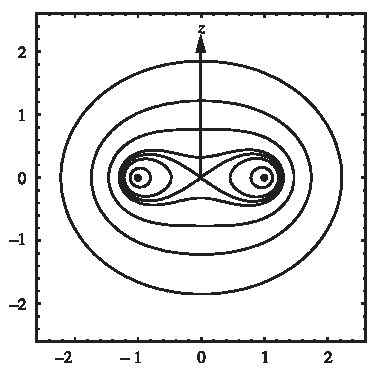
\includegraphics[scale=1]{Anh/c3.pdf}
        \end{center}
        Các đường đẳng thế được phác họa như trên hình. Điểm giao nhau giữa vòng và mặt phẳng được biểu diễn bằng hai dấu chấm, trên hình bán kính vòng dây được chọn bằng một đơn vị độ dài $R=1$. Toàn bộ mặt đẳng thế trong không gian có thể thu được bằng cách xoay các đường đẳng thế quanh trục $z$ để tạo thành các mặt đối xứng tròn xoay.\\
        Trên hình, ta có thể thấy rằng tại các vị trí gần vòng dây, đường đẳng thế gần giống với những vòng tròn bao quanh vòng dây (tương ứng với mặt đẳng thế là mặt hình xuyến trong không gian). Tại những điểm ở xa vòng dây, đường đẳng thế là những đường tròn tâm trùng với tâm vòng dây (trong không gian mặt đẳng thế là những mặt cầu bao quanh vòng dây). Sự chuyển tiếp giữa hai dạng mặt đẳng thế xảy ra khi mặt đẳng thế đi qua gốc tọa độ như trên hình. 
        \item \hfill \\
        \begin{center}
            

\tikzset{every picture/.style={line width=0.75pt}} %set default line width to 0.75pt        

\begin{tikzpicture}[x=0.75pt,y=0.75pt,yscale=-1,xscale=1]
%uncomment if require: \path (0,222); %set diagram left start at 0, and has height of 222

%Shape: Arc [id:dp21376736629493287] 
\draw  [draw opacity=0] (455.75,127.09) .. controls (439.25,140.2) and (399.45,149.44) .. (352.97,149.44) .. controls (311.61,149.44) and (275.54,142.12) .. (256.47,131.27) -- (352.97,113.57) -- cycle ; \draw   (455.75,127.09) .. controls (439.25,140.2) and (399.45,149.44) .. (352.97,149.44) .. controls (311.61,149.44) and (275.54,142.12) .. (256.47,131.27) ;
%Straight Lines [id:da6782292671629595] 
\draw    (352.97,19.58) -- (352.97,187.34) ;
\draw [shift={(352.97,16.58)}, rotate = 90] [fill={rgb, 255:red, 0; green, 0; blue, 0 }  ][line width=0.08]  [draw opacity=0] (10.72,-5.15) -- (0,0) -- (10.72,5.15) -- (7.12,0) -- cycle    ;
%Straight Lines [id:da24086650305652246] 
\draw    (224,187.34) -- (478.95,187.34) ;
\draw [shift={(481.95,187.34)}, rotate = 180] [fill={rgb, 255:red, 0; green, 0; blue, 0 }  ][line width=0.08]  [draw opacity=0] (10.72,-5.15) -- (0,0) -- (10.72,5.15) -- (7.12,0) -- cycle    ;
%Straight Lines [id:da18947837970533232] 
\draw    (311.41,147.08) -- (318.48,100.82) ;
\draw [shift={(318.79,98.84)}, rotate = 458.7] [fill={rgb, 255:red, 0; green, 0; blue, 0 }  ][line width=0.08]  [draw opacity=0] (12,-3) -- (0,0) -- (12,3) -- cycle    ;
%Shape: Boxed Line [id:dp5843424318289914] 
\draw    (393.84,147.08) -- (386.76,100.82) ;
\draw [shift={(386.46,98.84)}, rotate = 441.3] [fill={rgb, 255:red, 0; green, 0; blue, 0 }  ][line width=0.08]  [draw opacity=0] (12,-3) -- (0,0) -- (12,3) -- cycle    ;

% Text Node
\draw (363.68,10.89) node [anchor=north west][inner sep=0.75pt]    {$z$};
% Text Node
\draw (487.1,189.64) node [anchor=north west][inner sep=0.75pt]    {$x$};
% Text Node
\draw (295.88,81.84) node [anchor=north west][inner sep=0.75pt]    {$\vec{E}$};
% Text Node
\draw (394.01,81.84) node [anchor=north west][inner sep=0.75pt]    {$\vec{E}$};
% Text Node
\draw (463.71,157.57) node   [align=left] {\begin{minipage}[lt]{95.03pt}\setlength\topsep{0pt}
Đường đẳng thế
\end{minipage}};


\end{tikzpicture}

        \end{center}
        Xét một điểm nằm trên trục $z$ mà tại đó đường đẳng thế có mặt lõm hướng lên trên như hình. Điện trường vuông góc với mặt đẳng thế như trên hình. Ta thấy về phía bên trái điểm đang xét, vector cường độ điện trường nghiêng về phía bên phải, tức là thành phần điện trường theo phương $x$ có giá trị dương. Tương tự như vậy, về phía bên phải điểm đang xét, thành phần điện trường dọc theo trục $x$ có giá trị âm. Ta thấy rằng khi đi qua vị trí điểm đó từ trái qua phải, thành phần điện trường dọc theo trục giảm đi, do đó $\dfrac{\partial E_x}{\partial x}<0$. Do tính đối xứng nên ta cũng có $\dfrac{\partial E_y}{\partial y}<0$. \\
        Lập luận tương tự, tại một điểm mà mặt đẳng thể có mặt lõm hướng lên trên thì $\dfrac{\partial E_x}{\partial x}>0$, $\dfrac{\partial E_y}{\partial y}>0$. Vì $\dfrac{\partial E_x}{\partial x}$ và $\dfrac{\partial E_y}{\partial y}$ là liên tục, nên tại điểm mà mặt đẳng thế thay đổi từ có mặt lõm hướng xuống dưới sang hướng lên trên thì $\dfrac{\partial E_x}{\partial x}$ và $\dfrac{\partial E_y}{\partial y}$ chuyển từ âm sang dương và có giá trị bằng không.\\
        Ta có $\nabla\cdot \ot{E}=\dfrac{\rho}{\varepsilon_0}$. Do tại điểm xảy ra sự chuyển tiếp, mật độ điện tích bằng không nên ta có:
        \begin{equation}
            \nabla\cdot \ot{E}=\dfrac{\rho}{\varepsilon_0}=0\Leftrightarrow \dfrac{\partial E_x}{\partial x}+\dfrac{\partial E_y}{\partial y}+\dfrac{\partial E_z}{\partial z}=0.
        \end{equation}
        Mà như ta đã biết, $\dfrac{\partial E_x}{\partial x}=0$ và $\dfrac{\partial E_y}{\partial y}=0$, vậy nên $\dfrac{\partial E_z}{\partial z}=0$. Từ đó ta thấy được tại điểm chuyển tiếp thì thành phần điện trường theo phương $z$ đạt cực trị, đây chính là điểm mà ta đã xác định ở phần (\ref{ca7}).
    \end{enumerate}
    \end{loigiai}
  
\begin{vd}[Lấp và đầy]%câu 2
%USAPhO 2018
Điện thế tại tâm của khối lập phương với mật độ điện khối $\rho$ và cạnh $a$ cho bởi
$$\Phi  \approx \dfrac{{0,1894\rho {a^2}}}{{{\varepsilon_0}}}.$$
Bạn không cần phải chứng minh công thức này. Trong toàn bộ bài toán, các kết quả tính số phải viết với ba chữ số có nghĩa.
\begin{enumerate}[1)]
    \item Tìm điện thế tại đỉnh của khối lập phương. Đáp số biểu diễn qua $\rho ,a,{\varepsilon _0}$ và các giá trị số cần thiết.
    \item Tìm điện thế tại đỉnh kim tự tháp với đáy hình vuông có cạnh $a$, chiều cao $a/2$, và tích điện đều với mật độ điện khối $\rho$. Đáp số biểu diễn qua $\rho ,a,{\varepsilon _0}$ và các giá trị số cần thiết.
    \item Tìm điện thế gây bởi một bản mỏng hình vuông cạnh $a$ có mật độ điện mặt $\sigma$ tại một điểm nằm cách tâm của nó ở độ cao $a/2$. Đáp số biểu diễn qua $\sigma ,a,{\varepsilon _0}$ và các giá trị số cần thiết.
    \item Ký hiệu $E\tron{z}$ là điện trường ở độ cao $z$ từ tâm hình vuông với mật độ điện mặt $\sigma$ và cạnh $a$. Nếu điện thế tại tâm hình vuông có biểu thức gần đúng $\dfrac{{0,281a\sigma }}{{{\varepsilon _0}}}$, đánh giá $E\tron{a/2}$ nếu giả thiết $E\tron{z}$ tuyến tính trong khoảng $0<z<a/2$. Đáp số biểu diễn qua $\sigma ,a,{\varepsilon _0}$ và các giá trị số cần thiết.
\end{enumerate}
\end{vd}
\begin{loigiai}

\begin{enumerate}[1)]

\item Bằng phương pháp phân tích thứ nguyên, đáp án sẽ có dạng:
$$\Phi_c\tron{a,\rho}\approx\dfrac{C\rho a^2}{\varepsilon_0},$$
với $C$ là một hằng số không thứ nguyên. Lưu ý rằng một hình lập phương có cạnh $a$ gồm $8$ hình lập phương có cạnh $a/2$, với mỗi hình lập phương có một đỉnh ở tâm của hình lập phương lớn. Do đó:
$$\dfrac{{0,1894\rho {a^2}}}{{{\varepsilon_0}}}=8\dfrac{C\rho \tron{a/2}^2}{\varepsilon_0},$$
nên $C=0,1894/2=0.0947.$
\item Hình lập phương cạnh $a$ sẽ bao gồm $6$ hình kim tự tháp như vậy. Vì vậy chúng ta chỉ cần tính toán đơn giản $0.1894/6$ và được kết quả:
$$\Phi_p\tron{a,\rho}  \approx \dfrac{{0,0316\rho {a^2}}}{{{\varepsilon_0}}}.$$
\item Gọi điện thế gây bởi hình vuông như vậy là $\Phi_s\tron{a,\sigma}$. Lưu ý rằng việc thêm một bản hình vuông có độ dày $\dd z$ rất nhỏ và độ dài cạnh $a$ vào một kim tự tháp đáy vuông với độ dài cạnh đáy là $a$, chiều cao $a/2$ sẽ tạo ra một kim tự tháp đáy vuông có độ dài cạnh đáy $a+2\dd z$ và chiều cao $a/2+\dd z.$\\
Mật độ điện tích mặt của đĩa vuông có độ dày $\dd z$ liên hệ với mật độ điện tích khối là $\sigma=\rho \dd z$. Theo nguyên lý chồng chất:
$$\Phi_{s}(a, \rho \dd z)=\Phi_{p}(a+2 \dd z, \rho)-\Phi_{p}(a, \rho) \approx \frac{0,0316 \rho\left((a+2 \dd z)^{2}-a^{2}\right)}{\varepsilon_{0}}=\frac{0,126 a \rho \dd z}{\varepsilon_{0}}.$$
Do đó ta có:
$$\Phi_s\tron{a,\sigma}\approx\dfrac{0,126a\sigma}{\varepsilon_0}.$$
\item Hiệu điện thế giữa hai điểm có độ cao $0$ và $a/2$ là:
$$\Delta\Phi = \tron{0,281-0,126}\dfrac{a\sigma}{\varepsilon_0}=\dfrac{0,155a\sigma}{\varepsilon_0}.$$
Mặt khác, ta có:
$$\Delta \Phi=\int_{0}^{a / 2} E(z) d z \approx \dfrac{a}{2} \dfrac{E(0)+E(a / 2)}{2},$$
trong đó, ta đã coi gần đúng $E\tron{z}$ như một hàm tuyến tính, và $E\tron{0}=\sigma/2\varepsilon_0$ theo định luật Gauss. Giải phương trình tìm $E\tron{a/2}$ ta được:
$$E\tron{a/2}\approx\dfrac{0,119\sigma}{\varepsilon_0},$$
với chữ số có nghĩa cuối cùng không quan trọng. Một cách tình cờ, giá trị thực tế chính xác là $\sigma/6\varepsilon_0$, và giá trị thực tế này có một cách chứng minh khá là mượt mà mà không cần tính toán.
\end{enumerate}
\end{loigiai}


\begin{vd}[Bản chất của lưỡng cực từ]%câu 7
%USAPhO 2015

\begin{enumerate}[1)]
    \item Một lưỡng cực ``Gilbert'' bao gồm một cặp đơn cực từ, hai cực có độ lớn $q_m$ bằng nhau và trái dấu, cách nhau một khoảng $d$ nhỏ. Trong phần này, giả sử rằng $-q_m$ ở tọa độ $z=0$ còn $q_m$ ở tọa độ $z=d$.
    \begin{center}
        

% Gradient Info
  
\tikzset {_vc3yyirl7/.code = {\pgfsetadditionalshadetransform{ \pgftransformshift{\pgfpoint{0 bp } { 0 bp }  }  \pgftransformscale{1 }  }}}
\pgfdeclareradialshading{_z372z9q49}{\pgfpoint{0bp}{0bp}}{rgb(0bp)=(1,1,1);
rgb(1.1607142857142858bp)=(1,1,1);
rgb(25bp)=(0,0,0);
rgb(400bp)=(0,0,0)}

% Gradient Info
  
\tikzset {_imxquv36r/.code = {\pgfsetadditionalshadetransform{ \pgftransformshift{\pgfpoint{0 bp } { 0 bp }  }  \pgftransformscale{1 }  }}}
\pgfdeclareradialshading{_may1wpven}{\pgfpoint{0bp}{0bp}}{rgb(0bp)=(1,1,1);
rgb(1.1607142857142858bp)=(1,1,1);
rgb(25bp)=(0,0,0);
rgb(400bp)=(0,0,0)}
\tikzset{every picture/.style={line width=0.75pt}} %set default line width to 0.75pt        

\begin{tikzpicture}[x=0.75pt,y=0.75pt,yscale=-1,xscale=1]
%uncomment if require: \path (0,360); %set diagram left start at 0, and has height of 360

%Straight Lines [id:da1763404976584506] 
\draw  [dash pattern={on 4.5pt off 4.5pt}]  (141,220) -- (513,220) ;
%Shape: Circle [id:dp21724950617475192] 
\path  [shading=_z372z9q49,_vc3yyirl7] (217,218) .. controls (217,212.48) and (221.48,208) .. (227,208) .. controls (232.52,208) and (237,212.48) .. (237,218) .. controls (237,223.52) and (232.52,228) .. (227,228) .. controls (221.48,228) and (217,223.52) .. (217,218) -- cycle ; % for fading 
 \draw   (217,218) .. controls (217,212.48) and (221.48,208) .. (227,208) .. controls (232.52,208) and (237,212.48) .. (237,218) .. controls (237,223.52) and (232.52,228) .. (227,228) .. controls (221.48,228) and (217,223.52) .. (217,218) -- cycle ; % for border 

%Shape: Circle [id:dp6921675875101942] 
\path  [shading=_may1wpven,_imxquv36r] (301,218) .. controls (301,212.48) and (305.48,208) .. (311,208) .. controls (316.52,208) and (321,212.48) .. (321,218) .. controls (321,223.52) and (316.52,228) .. (311,228) .. controls (305.48,228) and (301,223.52) .. (301,218) -- cycle ; % for fading 
 \draw   (301,218) .. controls (301,212.48) and (305.48,208) .. (311,208) .. controls (316.52,208) and (321,212.48) .. (321,218) .. controls (321,223.52) and (316.52,228) .. (311,228) .. controls (305.48,228) and (301,223.52) .. (301,218) -- cycle ; % for border 


% Text Node
\draw (206,174.4) node [anchor=north west][inner sep=0.75pt]    {$-q_{m}$};
% Text Node
\draw (299,175.4) node [anchor=north west][inner sep=0.75pt]    {$q_{m}$};
% Text Node
\draw (205,243.4) node [anchor=north west][inner sep=0.75pt]    {$z=0$};
% Text Node
\draw (292,242.4) node [anchor=north west][inner sep=0.75pt]    {$z=d$};
% Text Node
\draw (489,194.4) node [anchor=north west][inner sep=0.75pt]    {$z$};


\end{tikzpicture}

    \end{center}
    Giả sử rằng các đơn cực từ hoạt động như các đơn cực điện dưới tác dụng của một lực giống như lực Coulomb:
    $$F=\dfrac{\mu_0}{4\pi}\dfrac{q_{m_1}q_{m_2}}{r^2},$$
    và độ lớn cảm ứng từ có công thức:
    $$B=\dfrac{F}{q_m}.$$
    \begin{enumerate}[a)]
        \item Thứ nguyên của đại lượng $q_m$ là gì?
        \item Viết biểu thức chính xác của cảm ứng từ $B\tron{z}$ dọc theo trục $z$ như một hàm của $z$ với $z>d$. Hãy biểu diễn kết quả theo $q_m$, $d$, $z$, và các hằng số cơ bản cần thiết.
        \item Tìm giới hạn của biểu thức$B\tron{z}$ vừa tìm khi $d\rightarrow 0$, giả sử rằng tích $q_m d=p_m$ được giữ không đổi, kết quả chỉ giữ tới bậc nhỏ nhất khác không. Biểu diễn kết quả theo $q_m$, $z$ và các hằng số cơ bản cần thiết.
    \end{enumerate}
    \item Một lưỡng cực ``Ampère'' là một lực cực từ tạo bởi dòng điện $I$ chạy trong vòng tròn bán kính $r$ nhỏ. Giả sử rằng trục $z$ trùng với trục đối xứng của vòng dây dẫn, và vòng dây nằm trong mặt phẳng $xy$ tại $z=0$.
    \begin{center}
        

\tikzset{every picture/.style={line width=0.75pt}} %set default line width to 0.75pt        

\begin{tikzpicture}[x=0.75pt,y=0.75pt,yscale=-1,xscale=1]
%uncomment if require: \path (0,369); %set diagram left start at 0, and has height of 369

%Shape: Ellipse [id:dp042219169506113374] 
\draw  [line width=1.5]  (280.5,186) .. controls (290.16,186) and (298,210.4) .. (298,240.5) .. controls (298,270.6) and (290.16,295) .. (280.5,295) .. controls (270.84,295) and (263,270.6) .. (263,240.5) .. controls (263,210.4) and (270.84,186) .. (280.5,186) -- cycle ;
%Straight Lines [id:da3414436567613002] 
\draw  [dash pattern={on 4.5pt off 4.5pt}]  (161,240) -- (533,240) ;
%Curve Lines [id:da8131452990600614] 
\draw    (299,192) .. controls (282.35,163.32) and (265.7,182.57) .. (260.13,194.32) ;
\draw [shift={(259,197)}, rotate = 289.98] [fill={rgb, 255:red, 0; green, 0; blue, 0 }  ][line width=0.08]  [draw opacity=0] (10.72,-5.15) -- (0,0) -- (10.72,5.15) -- (7.12,0) -- cycle    ;

% Text Node
\draw (305,167.4) node [anchor=north west][inner sep=0.75pt]    {$I$};
% Text Node
\draw (507,215.4) node [anchor=north west][inner sep=0.75pt]    {$z$};


\end{tikzpicture}

    \end{center}
    \begin{enumerate}[a)]
        \item Viết biểu thức chính xác của cảm ứng từ $B\tron{z}$ dọc theo trục $z$ như một hàm của $z$ với $z>0$. Hãy biểu diễn kết quả theo $I$, $r$, $z$ và các hằng số cơ bản cần thiết.
        \item Cho $kIr^\gamma$ có thứ nguyên giống với $p_m$ (ở phần trước), trong đó $k$ và $\gamma$ là những hằng số không thứ nguyên. Tìm giá trị của $\gamma$.
        \item Tìm giới hạn của biểu thức $B\tron{z}$ vừa tìm ở phần 2) a) khi $r\rightarrow 0$, giả sử rằng tích $kIr^\gamma=p'_m$ được giữ không đổi, kết quả chỉ giữ tới bậc nhỏ nhất khác không. Biểu diễn kết quả theo $k$, $p'_m$, $z$ và các hằng số cơ bản cần thiết.
        \item Giả sử rằng hai lưỡng cực từ có độ lớn bằng nhau, $p_m=p'_m$. Tìm hằng số $k$ ở phần 2) b).
    \end{enumerate}
    \item Giờ ta thử so sánh hai loại lưỡng cực bằng cách xây dựng một mô hình nam châm vật lý được cấu tạo bởi các lưỡng cực từ cực nhỏ được sắp xếp dày đặc.
    \begin{center}
        

\tikzset{every picture/.style={line width=0.75pt}} %set default line width to 0.75pt        

\begin{tikzpicture}[x=0.75pt,y=0.75pt,yscale=-1,xscale=1]
%uncomment if require: \path (0,438); %set diagram left start at 0, and has height of 438

%Shape: Can [id:dp4163311919612256] 
\draw   (355.75,168.33) -- (258.78,168.33) .. controls (245.31,168.33) and (234.39,138.34) .. (234.39,101.34) .. controls (234.39,64.35) and (245.31,34.35) .. (258.78,34.35) -- (355.75,34.35) .. controls (369.23,34.35) and (380.15,64.35) .. (380.15,101.34) .. controls (380.15,138.34) and (369.23,168.33) .. (355.75,168.33) .. controls (342.28,168.33) and (331.36,138.34) .. (331.36,101.34) .. controls (331.36,64.35) and (342.28,34.35) .. (355.75,34.35) ;
%Straight Lines [id:da980952439721346] 
\draw  [dash pattern={on 4.5pt off 4.5pt}]  (354.92,101.73) -- (425,101.73) ;
%Straight Lines [id:da1079828190551615] 
\draw  [dash pattern={on 4.5pt off 4.5pt}]  (186.33,101.34) -- (234.39,101.34) ;
%Straight Lines [id:da46891481834208926] 
\draw    (258.61,26.22) -- (354.72,26.22) ;
\draw [shift={(357.72,26.22)}, rotate = 180] [fill={rgb, 255:red, 0; green, 0; blue, 0 }  ][line width=0.08]  [draw opacity=0] (7.14,-3.43) -- (0,0) -- (7.14,3.43) -- (4.74,0) -- cycle    ;
\draw [shift={(255.61,26.22)}, rotate = 0] [fill={rgb, 255:red, 0; green, 0; blue, 0 }  ][line width=0.08]  [draw opacity=0] (7.14,-3.43) -- (0,0) -- (7.14,3.43) -- (4.74,0) -- cycle    ;
%Straight Lines [id:da1280330733442938] 
\draw    (354.92,37.35) -- (354.92,98.73) ;
\draw [shift={(354.92,101.73)}, rotate = 270] [fill={rgb, 255:red, 0; green, 0; blue, 0 }  ][line width=0.08]  [draw opacity=0] (7.14,-3.43) -- (0,0) -- (7.14,3.43) -- (4.74,0) -- cycle    ;
\draw [shift={(354.92,34.35)}, rotate = 90] [fill={rgb, 255:red, 0; green, 0; blue, 0 }  ][line width=0.08]  [draw opacity=0] (7.14,-3.43) -- (0,0) -- (7.14,3.43) -- (4.74,0) -- cycle    ;

% Text Node
\draw (303.27,4.68) node [anchor=north west][inner sep=0.75pt]    {$L$};
% Text Node
\draw (361.04,80.58) node [anchor=north west][inner sep=0.75pt]    {$R$};
% Text Node
\draw (401.78,83.68) node [anchor=north west][inner sep=0.75pt]    {$z$};


\end{tikzpicture}

    \end{center}
    Một hình trụ làm bằng vật liệu từ tính có bán kính $R$ và chiều dài $L$. Nó được cấu tạo bởi $N$ lưỡng cực từ với tất cả đều là loại Ampère hoặc tất cả đều là loại Gilbert. $N$ rất lớn. Trục quay của hình trụ và tất cả các lưỡng cực đều thẳng hàng với trục $z$ và tất cả đều hướng theo cùng một hướng như đã xác định ở trên để từ trường bên ngoài hình trụ giống nhau với hai loại lưỡng cực đã được xác định trước đó. Hình dưới đây là mô hình của hai lưỡng cực; chúng là các hình lập phương với cạnh $d\ll R$ và $d\ll L$ với thể tích $v_m=d^3$.
    \begin{center}
        

\tikzset{every picture/.style={line width=0.75pt}} %set default line width to 0.75pt        

\begin{tikzpicture}[x=0.75pt,y=0.75pt,yscale=-1,xscale=1]
%uncomment if require: \path (0,378); %set diagram left start at 0, and has height of 378

%Shape: Parallelogram [id:dp05855440540229506] 
\draw  [fill={rgb, 255:red, 155; green, 155; blue, 155 }  ,fill opacity=0.66 ][dash pattern={on 4.5pt off 4.5pt}] (409.17,113) -- (476.67,113) -- (431.17,135.53) -- (363.67,135.53) -- cycle ;
%Shape: Square [id:dp01739105254346751] 
\draw  [fill={rgb, 255:red, 155; green, 155; blue, 155 }  ,fill opacity=0.75 ][dash pattern={on 4.5pt off 4.5pt}] (409.83,45.67) -- (477.5,45.67) -- (477.5,113.33) -- (409.83,113.33) -- cycle ;
%Shape: Parallelogram [id:dp591863383614361] 
\draw  [fill={rgb, 255:red, 128; green, 128; blue, 128 }  ,fill opacity=0.79 ] (431.33,135.04) -- (431.33,67.23) -- (476.67,45.19) -- (476.67,113) -- cycle ;
%Shape: Parallelogram [id:dp8252942457391017] 
\draw  [fill={rgb, 255:red, 155; green, 155; blue, 155 }  ,fill opacity=0.58 ][dash pattern={on 4.5pt off 4.5pt}] (363.67,135.53) -- (363.67,68.34) -- (409.33,45.67) -- (409.33,112.86) -- cycle ;
%Shape: Parallelogram [id:dp8928361884666596] 
\draw  [fill={rgb, 255:red, 128; green, 128; blue, 128 }  ,fill opacity=0.79 ] (226.33,135.24) -- (226.33,67.43) -- (271.67,45.39) -- (271.67,113.2) -- cycle ;
%Shape: Parallelogram [id:dp9405854790928345] 
\draw  [fill={rgb, 255:red, 128; green, 128; blue, 128 }  ,fill opacity=1 ] (159,135.31) -- (159,68.1) -- (204.33,45.8) -- (204.33,113.01) -- cycle ;
%Straight Lines [id:da23945655547644384] 
\draw    (204.33,45.67) -- (272.5,45.67) ;
%Straight Lines [id:da35033381184501877] 
\draw    (271.67,45.67) -- (271.67,114.5) ;
%Straight Lines [id:da051814536993643356] 
\draw    (226.33,135.67) -- (271.67,113) ;
%Straight Lines [id:da25061643520015364] 
\draw  [dash pattern={on 4.5pt off 4.5pt}]  (204.33,45.67) -- (204,113) ;
%Straight Lines [id:da7619054292392096] 
\draw  [dash pattern={on 4.5pt off 4.5pt}]  (159,135.67) -- (204,113) ;
%Straight Lines [id:da7421950603165741] 
\draw  [dash pattern={on 4.5pt off 4.5pt}]  (204,113) -- (271.67,113) ;
%Straight Lines [id:da9379052801533849] 
\draw    (159,135.67) -- (227.5,135.67) ;
%Straight Lines [id:da3932472502322175] 
\draw    (159,68.33) -- (226.33,68.33) ;
%Straight Lines [id:da5516129338629328] 
\draw    (159,68.33) -- (159,135.67) ;
%Straight Lines [id:da2036017597282873] 
\draw    (226.33,68.33) -- (226.33,135.67) ;
%Straight Lines [id:da28407737144045386] 
\draw  [dash pattern={on 4.5pt off 4.5pt}]  (290.67,48.17) -- (290.67,111) ;
\draw [shift={(290.67,114)}, rotate = 270] [fill={rgb, 255:red, 0; green, 0; blue, 0 }  ][line width=0.08]  [draw opacity=0] (7.14,-3.43) -- (0,0) -- (7.14,3.43) -- (4.74,0) -- cycle    ;
\draw [shift={(290.67,45.17)}, rotate = 90] [fill={rgb, 255:red, 0; green, 0; blue, 0 }  ][line width=0.08]  [draw opacity=0] (7.14,-3.43) -- (0,0) -- (7.14,3.43) -- (4.74,0) -- cycle    ;
%Straight Lines [id:da5595048846520709] 
\draw    (409.33,45.67) -- (477.5,45.67) ;
%Straight Lines [id:da5591497934809129] 
\draw    (477.5,45.67) -- (477.5,114.5) ;
%Straight Lines [id:da2247155506060743] 
\draw  [dash pattern={on 4.5pt off 4.5pt}]  (409.33,45.67) -- (409,113) ;
%Straight Lines [id:da9139402143079249] 
\draw    (364,135.67) -- (432.5,135.67) ;
%Straight Lines [id:da794843554164604] 
\draw    (364,68.33) -- (431.33,68.33) ;
%Straight Lines [id:da48105470541365736] 
\draw    (364,68.33) -- (364,135.67) ;
%Straight Lines [id:da8478967441826744] 
\draw    (431.33,68.33) -- (431.33,135.67) ;
%Straight Lines [id:da7896036304415248] 
\draw  [dash pattern={on 4.5pt off 4.5pt}]  (138.17,58.62) -- (179.33,37.38) ;
\draw [shift={(182,36)}, rotate = 512.7] [fill={rgb, 255:red, 0; green, 0; blue, 0 }  ][line width=0.08]  [draw opacity=0] (7.14,-3.43) -- (0,0) -- (7.14,3.43) -- (4.74,0) -- cycle    ;
\draw [shift={(135.5,60)}, rotate = 332.7] [fill={rgb, 255:red, 0; green, 0; blue, 0 }  ][line width=0.08]  [draw opacity=0] (7.14,-3.43) -- (0,0) -- (7.14,3.43) -- (4.74,0) -- cycle    ;
%Straight Lines [id:da6254197224655336] 
\draw  [dash pattern={on 4.5pt off 4.5pt}]  (206.83,27.17) -- (269,27.17) ;
\draw [shift={(272,27.17)}, rotate = 180] [fill={rgb, 255:red, 0; green, 0; blue, 0 }  ][line width=0.08]  [draw opacity=0] (7.14,-3.43) -- (0,0) -- (7.14,3.43) -- (4.74,0) -- cycle    ;
\draw [shift={(203.83,27.17)}, rotate = 0] [fill={rgb, 255:red, 0; green, 0; blue, 0 }  ][line width=0.08]  [draw opacity=0] (7.14,-3.43) -- (0,0) -- (7.14,3.43) -- (4.74,0) -- cycle    ;
%Straight Lines [id:da6752851784781377] 
\draw  [dash pattern={on 4.5pt off 4.5pt}]  (135.5,88.5) -- (179,88.5) ;
%Straight Lines [id:da6624066638361792] 
\draw  [dash pattern={on 4.5pt off 4.5pt}]  (250,88.5) -- (386,88.5) ;
%Straight Lines [id:da28754808144163135] 
\draw  [dash pattern={on 4.5pt off 4.5pt}]  (455,88.5) -- (568.5,88.5) ;
%Straight Lines [id:da1969439561848383] 
\draw    (397.67,68.33) -- (397.67,132.5) ;
\draw [shift={(397.67,135.5)}, rotate = 270] [fill={rgb, 255:red, 0; green, 0; blue, 0 }  ][line width=0.08]  [draw opacity=0] (7.14,-3.43) -- (0,0) -- (7.14,3.43) -- (4.74,0) -- cycle    ;
%Straight Lines [id:da3893886557465718] 
\draw    (398.25,135.67) -- (440.16,114.36) ;
\draw [shift={(442.83,113)}, rotate = 513.05] [fill={rgb, 255:red, 0; green, 0; blue, 0 }  ][line width=0.08]  [draw opacity=0] (7.14,-3.43) -- (0,0) -- (7.14,3.43) -- (4.74,0) -- cycle    ;
%Straight Lines [id:da1593434827507052] 
\draw    (442.83,113) -- (442.83,49) ;
\draw [shift={(442.83,46)}, rotate = 450] [fill={rgb, 255:red, 0; green, 0; blue, 0 }  ][line width=0.08]  [draw opacity=0] (7.14,-3.43) -- (0,0) -- (7.14,3.43) -- (4.74,0) -- cycle    ;
%Straight Lines [id:da9339812434173671] 
\draw    (442.83,46) -- (400.36,67) ;
\draw [shift={(397.67,68.33)}, rotate = 333.69] [fill={rgb, 255:red, 0; green, 0; blue, 0 }  ][line width=0.08]  [draw opacity=0] (7.14,-3.43) -- (0,0) -- (7.14,3.43) -- (4.74,0) -- cycle    ;
%Straight Lines [id:da3273119626252903] 
\draw    (364,68.33) -- (409.33,45.67) ;
%Straight Lines [id:da611778504586038] 
\draw    (363.67,68.34) -- (363.67,135) ;
%Straight Lines [id:da6521966463331628] 
\draw  [dash pattern={on 4.5pt off 4.5pt}]  (409.83,113.33) -- (476.67,113) ;

% Text Node
\draw (150.5,27.4) node [anchor=north west][inner sep=0.75pt]    {$d$};
% Text Node
\draw (234.5,8.9) node [anchor=north west][inner sep=0.75pt]    {$d$};
% Text Node
\draw (292.5,58.9) node [anchor=north west][inner sep=0.75pt]    {$d$};
% Text Node
\draw (115.5,90.07) node [anchor=north west][inner sep=0.75pt]    {$-q_{m}$};
% Text Node
\draw (247,122.4) node [anchor=north west][inner sep=0.75pt]    {$+q_{m}$};
% Text Node
\draw (464,22.4) node [anchor=north west][inner sep=0.75pt]    {$I$};
% Text Node
\draw (549,70.4) node [anchor=north west][inner sep=0.75pt]    {$z$};
% Text Node
\draw (155.33,151.4) node [anchor=north west][inner sep=0.75pt]    {$\text{Lưỡng cực Gilbert}$};
% Text Node
\draw (356.67,147.73) node [anchor=north west][inner sep=0.75pt]    {$\text{Lưỡng cực Ampère}$};
% Text Node
\draw (391.33,21.73) node [anchor=north west][inner sep=0.75pt]    {$\text{Dòng điện }$};


\end{tikzpicture}

    \end{center}
    \begin{enumerate}[a)]
        \item Giả sử rằng $R\gg L$ và chỉ có lưỡng cực loại Gilbert, xác định độ lớn và hướng của $B$ tại tâm của hình trụ theo $p_m$, $R$, $L$, $v_m$ và các hằng số cơ bản cần thiết.
        \item Giả sử rằng $R\ll L$ và chỉ có lưỡng cực loại Ampère, xác định độ lớn và hướng của $B$ tại tâm của hình trụ theo $p_m$, $R$, $L$, $v_m$ và các hằng số cơ bản cần thiết.
    \end{enumerate}
\end{enumerate}
\end{vd}
\begin{loigiai}
\begin{enumerate}[1)]
    \item 
    \begin{enumerate}[a)]
        \item Dựa vào biểu thức:
        $$B=\dfrac{F}{q_m},$$
        thì $q_m$ được đo bằng $N/T$. Tuy nhiên Tesla lại được đo bằng $N/\tron{A.m}$, do đó thứ nguyên của $q_m$ là $\left[A.m\right]$.
        \item Sử dụng cả hai phương trình,
        $$B\tron{z}=-\dfrac{\mu_0}{4\pi}\dfrac{q_m}{z^2}+\dfrac{\mu_0}{4\pi}\dfrac{q_m}{\tron{z+d}^2}.$$
        \item Biến đổi biểu thức trên, ta được:
        $$B\tron{z}=\dfrac{\mu_0}{4\pi}q_md\tron{\dfrac{2+d/z}{z\tron{z+d}^2}}.$$
        Do đó giới hạn khi $d\rightarrow 0$ là:
        $$B\tron{z}=\dfrac{\mu_0}{4\pi}\dfrac{q_m d^2}{z^3}=\dfrac{\mu_0}{2\pi}\dfrac{p_m}{z^3}.$$
    \end{enumerate}
    \item
    \begin{enumerate}[a)]
        \item Áp dụng định luật Biot-Savart, với $\mathbf{s}$ là vector nối từ điểm trên vòng tròn tới điểm trên trục $z$,
        $$ B(z)=\dfrac{\mu_{0} I}{4 \pi} \oint \dfrac{d \mathbf{l} \times \mathbf{s}}{s^{3}}=\dfrac{\mu_{0} I}{4 \pi} \dfrac{2 \pi r}{r^{2}+z^{2}} \sin \theta,$$
        trong đó $\theta$ là góc hợp bởi đường nối từ điểm trên trục $z$ tới tâm vòng tròn và từ điểm đó tới một điểm trên vòng tròn, do đó:
        $$\sin \theta=\dfrac{r}{\sqrt{r^2+z^2}}.$$
        Suy ra ta có:
        $$B\tron{z}=\dfrac{\mu_0I}{4\pi}\dfrac{2\pi r^2}{\tron{r^2+z^2}^{3/2}}.$$
        \item Ta biết rằng $p_m$ phải có thứ nguyên là Amperes nhân mét vuông, do đó $\gamma =2$.
        \item Sử dụng kết quả trước đó:
        $$B\tron{z}=\dfrac{\mu_0 I}{4\pi}\dfrac{2\pi r^2}{\tron{r^2+z^2}^{3/2}}\approx\dfrac{\mu_0 I}{2\pi}\dfrac{\pi r^2}{z^3}=\dfrac{\mu_0}{2\pi}\dfrac{\pi}{k}\dfrac{p'_m}{z^3}.$$
        \item Bằng cách so sánh các phương trình, ta được $k=\pi$.
    \end{enumerate}
    \item 
    \begin{enumerate}[a)]
        \item Các đơn cực tạo nên lưỡng cực bị triệt tiêu, ngoại trừ các đơn cực nằm trên mặt phẳng. Do đó, hình trụ sẽ giống như một bản tụ điện song song.\\
    Nếu như kích thước của lưỡng cực là $d$, thì mật độ trên bề mặt của đơn cực là:
    $$\sigma_m=q_m/d^2.$$
    Tương tự như một tụ điện song song, cảm ứng từ $B$ là:
    $$B=\mu_0\sigma_m=\mu_0\dfrac{p_m}{d^3},$$
    và hướng sang trái.
        \item Các dòng điện tạo nên lưỡng cực đều bị triệt tiêu ngoại trừ trên bề mặt hình trụ. Khi đó, hình trụ giống như một ống solenoid, với:
        $$B=\dfrac{\mu_0 I}{d},$$
        trong đó $I/d$ là mật độ dòng điện mặt. Cảm ứng từ $B$ là:
        $$B=\dfrac{\mu_0 I}{d}=\mu_0\dfrac{p_m}{d^3},$$
        và hướng sang phải.
    \end{enumerate}
\end{enumerate}
\end{loigiai} 


\begin{vd}[Mô hình đám mây nguyên tử] %Tinhdien(0)
Trong một mô hình của nguyên tử Hydro ở trạng thái cơ bản, người ta coi nguyên tử này gồm:\\
Một proton tích điện $+e$ được coi là chất điểm đặt tại gốc tọa độ $O$. Một đám mây tích điện âm có đối xứng cầu bao quanh proton. Biết điện thế tại điểm $M$ bất kỳ $(OM = r)$ có dạng:
\[V(r)=\dfrac{a}{r} e^{-b r},\]
		(với $a$ và $b$ là các hằng số dương)
\begin{enumerate}[1)]
    \item  Hãy xác định điện trường $\ot E({r})$ tại điểm $M$.
     \item Tính điện tích của đám mây tích điện âm nằm trong mặt cầu $O$ bán kính $r$.
  \item Tính mật độ điện tích $\rho_{\mathrm{r}}$ của đám mây điện tích âm theo $a$ và $b$.	
     \item Từ điều kiện trung hòa về điện của nguyên tử hãy tính hằng số $a$ theo $e$ và $\varepsilon_{0}$.
  \item Tính thế tĩnh điện $V(r)$ do đám mây tích điện âm gây ra tại điểm $M (OM=r)$.
  \item Tính theo $a$ và $b$ các đại lượng sau:
  \begin{enumerate}[a)]
      \item  Năng lượng $W_\mathrm{hn}$ của hạt nhân trong đám mây điện tích âm.
     \item Năng lượng toàn phần $W$ của nguyên tử hydro.
  \end{enumerate}
  
  \item Tính hiệu chỉnh $\Delta \lambda$ về bước sóng của photon mà nguyên tử Hydro phát ra khi tính đến sự giật lùi của nguyên tử. Coi rằng lúc đầu nguyên tử đứng yên. Lấy khối lượng nguyên tử Hydro là $ = 939 ~\mathrm{MeV/c^2}$.
\end{enumerate}
   \end{vd}
\begin{loigiai}

\begin{enumerate}[1)] 
       \item Do tính đối xứng cầu của mô hình nguyên tử, điện trường $\ot{E}=-\ot{\nabla} V$  tại $M$ có hướng xuyên tâm và có độ lớn chỉ phụ thuộc vào $r=OM$, cụ thể là:
	\begin{align*}
	    \ot{E}&=-\ot{\nabla }V(r)=-\dfrac{\mathrm{d}V}{\mathrm{d}r}\dfrac{{\ot{r}}}{r}=\dfrac{a\,\exp (-br)}{{{r}^{2}}}(1+br)\dfrac{{\ot{r}}}{r},\\
		E&\equiv \left| {\ot{E}} \right|=\dfrac{a\exp (-br)}{{{r}^{2}}}(1+br). \tag{1} \label{d1.}	
	\end{align*}
			 
\item Ký hiệu $q(r)$ là điện tích của đám mây điện tích âm nằm trong mặt cầu tâm $O$ bán kính $r$. Theo định lý Gauss, thông lượng điện trường qua mặt cầu tâm $O$ bán kính $r$ chứa điện tích $+e$ ở tâm và điện tích âm $q(r)$ cho bởi biểu thức:
	\[E(r)4\pi {{r}^{2}}=\dfrac{1}{{{\varepsilon }_{0}}}(e+q(r)) \tag{2} \label{d2.}.\]				          
Thay $E$ từ (\ref{d1.}) vào (\ref{d2.}) ta nhận được:
	\[4\pi a(1+br){{e}^{-br}}=\dfrac{1}{{{\varepsilon }_{0}}}(e+q(r)).\]
Từ đó suy ra: \[q(r)=-e+4\pi {{\varepsilon }_{0}}a(1+br){{e}^{-br}} \tag{3} \label{d3.}.\]		                     
\item Gọi mật độ điện tích âm tại điểm cách tâm $O$ khoảng $r$ là $\rho(r)$. Điện tích âm trong không gian giữa hai mặt cầu có bán kính $r$ và $r+dr$ là:
	\[\rho (r)4\pi {{r}^{2}}\mathrm{d}r=q(r+\mathrm{d}r)-q(r)=q(r)+\dfrac{\mathrm{d}q}{\mathrm{d}r}dr-q(r)=\dfrac{\mathrm{d}q}{\mathrm{d}r}\mathrm{d}r.\]
Suy ra: 	\[\rho (r)=\dfrac{1}{4\pi {{r}^{2}}}\dfrac{\mathrm{d}q}{\mathrm{d}r} \tag{4} \label{d4.}.\]				                 
Thay $q$ từ (\ref{d3.}) vào (\ref{d4.}), ta được:
	\[\rho (r)=\dfrac{1}{4\pi {{r}^{2}}}4\pi {{\varepsilon }_{0}}a{{e}^{-br}}\left[ b-b(1+br) \right],\]
Hay 	\[\rho (r)=-\dfrac{{{\varepsilon }_{0}}a{{b}^{2}}}{r}{{e}^{-br}} \tag{5} \label{d5.}.\]					     
\item Do tính trung hòa về điện của nguyên tử, điện tích âm tổng cộng phải bằng $-e$ cân bằng với điện tích $+e$ của hạt nhân, nên ta có:
		\[-e=\int_{0}^{\infty }{\rho (r)4\pi {{r}^{2}}\mathrm{d}r}.\]
Thay $\rho(r)$ từ (\ref{d5.}), ta nhận được:
	\[-e=-4\pi {{\varepsilon }_{0}}a{{b}^{2}}\int_{0}^{\infty }{r{{e}^{-br}}{\mathrm{d}}r}.\]
Lấy tích phân theo từng phần, cuối cùng ta được: \[a=\dfrac{e}{4\pi {{\varepsilon }_{0}}} \tag{6} \label{d6.}.\]
\textbf{Cách khác:} \\Ta có: \[\underset{r\to 0}{\mathop{\lim }}\,q(r)=0.\] Sử dụng (\ref{d3.}) ta có (\ref{d6.}).
\item Dùng (6) ta có thế tĩnh điện toàn phần tại M là:
	\[V(r)=\dfrac{e}{4\pi {{\varepsilon }_{0}}r}{{e}^{-br}}.\]
Mặt khác, hạt nhân tại $O$ gây ra tại $M$ điện thế: \[\dfrac{e}{4\pi {{\varepsilon }_{0}}r}.\] 
Vậy đóng góp của đám mây điện tích âm vào điện thế toàn phần là:
		\[{{V}^{'}}(r)=V(r)-\dfrac{e}{4\pi {{\varepsilon }_{0}}r}=\dfrac{e}{4\pi {{\varepsilon }_{0}}r}\left[ {{e}^{-br}}-1 \right]. \tag{7} \label{d7.}\]		
\item  Hạt nhân có điện tích $+e$ đặt tại $O$ $(r\to 0)$. Tại điểm $O$ đám mây tích điện âm gây ra điện thế ${{V}^{'}}(O)$, nên hạt nhân có năng lượng bằng:
		\[{{{W}}_{hn}}=+e{{V}^{'}}(O).\]
Trong đó ${{V}^{'}}(O)$ là giới hạn của ${{V}^{'}}(r)$ khi $r \to O$. Dùng khai triển:
\[{{e}^{x}}=1+x+\dfrac{{{x}^{2}}}{2}+...\]
cho $\left| x \right| \ll 1$, từ (\ref{d7.}) ta có:
	\[{{V}^{'}}(r)=\dfrac{e}{4\pi {{\varepsilon }_{0}}r}\left( 1-br+\dfrac{{{b}^{2}}{{r}^{2}}}{2}+...-1 \right)=\dfrac{e}{4\pi {{\varepsilon }_{0}}}\left( -b+\dfrac{{{b}^{2}}r}{2}+... \right).\]
Suy ra: 	\[{{V}^{'}}(O)=\underset{r\to 0}{\mathop{\lim }}\,{{V}^{'}}(r)=-\dfrac{eb}{4\pi {{\varepsilon }_{0}}}.\]
Do đó: 	\[{{{W}}_{hn}}=+e{{V}^{'}}(O)=-\dfrac{{{e}^{2}}b}{4\pi {{\varepsilon }_{0}}}. \tag{8} \label{d8.}\]			                      
\item Năng lượng riêng $W_e$ của đám mây tích điện âm với mật độ $\rho (r)$ bằng:
	\[{{{W}}_{e}}=\dfrac{1}{2}\int_{0}^{\infty }{{{V}^{'}}(r)\rho (r)4\pi {{r}^{2}}\mathrm{d}r}. \tag{9} \label{d9.}\]			                   
Thay (\ref{d5.}), (\ref{d6.}) và (\ref{d7.}) vào (\ref{d9.}), ta nhận được:
	\[{{{W}}_{e}}=-\dfrac{{{e}^{2}}{{b}^{2}}}{8\pi {{\varepsilon }_{0}}}\int_{0}^{\infty }{\left[ {{e}^{-2br}}-{{e}^{-br}} \right]\mathrm{d}r}=\dfrac{{{e}^{2}}b}{16\pi {{\varepsilon }_{0}}}.\]
Vậy, năng lượng toàn phần của nguyên tử hydro bằng:
	\[{W}={{{W}}_{hn}}+{{{W}}_{e}}=-\dfrac{3{{e}^{2}}b}{16\pi {{\varepsilon }_{0}}} \tag{10} \label{d10.}.\]				      
   \item Gọi $E_1$, $E_2$ tương ứng là năng lượng trước và sau khi phát photon, $K$ và $v$ là động năng và vận tốc giật lùi của nguyên tử; gọi $\lambda_0$ và $\lambda$ là bước sóng photon khi không kể và kể tới sự giật lùi. Theo định luật bảo toàn năng lượng:
                      \[ E_1=E_2 + \dfrac{hc}{\lambda} +K.\]
        Chú ý rằng:   \[ E_1 = E_2 + \dfrac{hc}{\lambda_0}.\]
       Ta có: \[\dfrac{\lambda-\lambda_{0}}{\lambda_{0}}=\dfrac{\lambda K}{hc}. \tag{11} \label{d11.}\]
                                
   Mặt khác, định luật bảo toàn động lượng cho ta: \[0=\ot{{p}}_{\lambda}+\ot{p}_{M} \quad \rightarrow {p}_{\lambda}^{2}=p_{{M}}^{2}.\]
Sử dụng $K = 2m p^2$ và $p p_{\lambda}=\dfrac{h}{\lambda}$ ta có:
\[{K}=\dfrac{{h}^{2}}{2 {M} \lambda^{2}}. \tag{12} \label{d12.}\] 
Kết hợp (\ref{d11.}) và (\ref{d12.}) ta được:
\[\dfrac{\Delta \lambda}{\lambda_{0}}=\dfrac{{hc}}{2 {Mc}^{2} \lambda}= \dfrac{6.6\cdot 10^{-6} \ \textup{\AA}}{\lambda}.\]
                  
  \end{enumerate}
   \end{loigiai}
   
   
   \begin{vd}[Sự kết hợp cơ điện]
Các quá trình cơ học và điện đôi khi có liên hệ chặt chẽ với nhau. Ở đây ta sẽ xem xét bài toán đơn giản.\\
Có hai bản kim loại với diện tích $S$ và khối lượng $m$. Một bản đặt lên trên bản còn lại. Các bản được nối với nhau nhờ các lò xo, có tổng độ cứng $k$ và được làm từ vật liệu cách điện. Bản dưới được gắn với một đế cố định. Khoảng cách cân bằng giữa hai bản là $X_{0}$.
\begin{center}
\tikzset{every picture/.style={line width=0.75pt}} %set default line width to 0.75pt
\begin{tikzpicture}[x=0.75pt,y=0.75pt,yscale=-1,xscale=1]
%uncomment if require: \path (0,410); %set diagram left start at 0, and has height of 410
%Shape: Path Data [id:dp26010170563698165] 
\draw  [fill={rgb, 255:red, 155; green, 155; blue, 155 }  ,fill opacity=1 ] (250.88,209.01) .. controls (215.46,209.01) and (186.01,200.74) .. (180,189.84) -- (180,161) -- (322,161) -- (322,189.02) -- (322.16,189.03) .. controls (322.11,189.15) and (322.06,189.26) .. (322,189.37) -- (322,189.84) -- (321.76,189.84) .. controls (315.75,200.74) and (286.3,209.01) .. (250.88,209.01) -- cycle ;
%Shape: Ellipse [id:dp9379095041346113] 
\draw  [fill={rgb, 255:red, 155; green, 155; blue, 155 }  ,fill opacity=1 ] (180,161) .. controls (180,144.98) and (211.79,132) .. (251,132) .. controls (290.21,132) and (322,144.98) .. (322,161) .. controls (322,177.02) and (290.21,190) .. (251,190) .. controls (211.79,190) and (180,177.02) .. (180,161) -- cycle ;
%Shape: Path Data [id:dp27923020491905204] 
\draw  [fill={rgb, 255:red, 155; green, 155; blue, 155 }  ,fill opacity=1 ] (251,161) .. controls (215.58,161) and (186.13,152.73) .. (180.12,141.84) -- (180.12,112.99) -- (322.12,112.99) -- (322.12,141.02) -- (322.28,141.03) .. controls (322.23,141.14) and (322.18,141.25) .. (322.12,141.37) -- (322.12,141.84) -- (321.88,141.84) .. controls (315.87,152.73) and (286.42,161) .. (251,161) -- cycle ;
%Shape: Ellipse [id:dp9312854624922384] 
\draw  [fill={rgb, 255:red, 155; green, 155; blue, 155 }  ,fill opacity=1 ] (180.12,112.99) .. controls (180.12,96.98) and (211.91,83.99) .. (251.12,83.99) .. controls (290.33,83.99) and (322.12,96.98) .. (322.12,112.99) .. controls (322.12,129.01) and (290.33,141.99) .. (251.12,141.99) .. controls (211.91,141.99) and (180.12,129.01) .. (180.12,112.99) -- cycle ;
%Shape: Spring [id:dp9535848234933078] 
\draw   (192.14,174.16) .. controls (188.37,173.48) and (184.74,171.86) .. (184.84,168.95) .. controls (185.05,162.96) and (200.74,163.51) .. (200.67,165.51) .. controls (200.6,167.51) and (184.91,166.95) .. (185.12,160.96) .. controls (185.33,154.96) and (201.02,155.51) .. (200.95,157.51) .. controls (200.88,159.51) and (185.19,158.96) .. (185.4,152.96) .. controls (185.61,146.97) and (201.3,147.52) .. (201.23,149.52) .. controls (201.16,151.48) and (186.03,150.98) .. (185.69,145.29) ;
%Shape: Spring [id:dp7259141116423518] 
\draw   (244.23,190.23) .. controls (240.79,189.62) and (237.47,188.05) .. (237.53,185.14) .. controls (237.66,179.14) and (251.93,179.44) .. (251.89,181.44) .. controls (251.84,183.44) and (237.57,183.14) .. (237.7,177.14) .. controls (237.83,171.15) and (252.1,171.45) .. (252.05,173.45) .. controls (252.01,175.45) and (237.74,175.14) .. (237.87,169.15) .. controls (238,163.15) and (252.27,163.45) .. (252.22,165.45) .. controls (252.19,167.22) and (241.03,167.19) .. (238.53,163.01) ;
%Shape: Spring [id:dp42536940188679284] 
\draw   (309.11,179.81) .. controls (305.75,179.2) and (302.52,177.63) .. (302.58,174.72) .. controls (302.71,168.72) and (316.62,169.02) .. (316.58,171.02) .. controls (316.53,173.02) and (302.63,172.72) .. (302.75,166.73) .. controls (302.88,160.73) and (316.79,161.02) .. (316.75,163.02) .. controls (316.7,165.02) and (302.79,164.73) .. (302.92,158.73) .. controls (303.05,152.73) and (316.96,153.02) .. (316.92,155.02) .. controls (316.87,157.02) and (302.96,156.73) .. (303.09,150.73) .. controls (303.09,150.72) and (303.09,150.71) .. (303.09,150.71) ;
%Straight Lines [id:da0024687149331827918] 
\draw    (76,189.84) -- (180,189.84) ;
%Straight Lines [id:da821799937569774] 
\draw    (76.12,112.99) -- (180.12,112.99) ;
%Shape: Battery [id:dp6851863559013807] 
\draw   (75.97,189.84) -- (76.04,155.26) (46.05,147.52) -- (106.05,147.63) (76.05,147.58) -- (76.12,112.99) (61.03,158.31) -- (61.04,155.23) -- (91.04,155.29) -- (91.03,158.36) -- (61.03,158.31) -- cycle ;
\end{tikzpicture}
\end{center}
\begin{enumerate}[1)]
    \item Giả sử có một độ dịch chuyển nhỏ $x$ theo phương thẳng đứng của bản ở trên từ vị trí cân bằng. Thiết lập biểu thức gia tốc $\ddot{x}$ của $x$ theo các tham số của hệ. Tìm tần số góc $\omega_{0}$ của dao động nhỏ theo phương thẳng đứng của bản ở trên?
    \item Các bản bây giờ được nối với một nguồn cao áp, tạo thành một tụ điện. Lực điện giữa các bản tạo thêm một độ dịch chuyển phụ của bản ở trên. Khoảng cách cân bằng mới bây giờ là $X_{1}$. Thiết lập biểu thức lực hút $F_{e}$ và hiệu điện thế $U$ theo các đại lượng $X_{0}, X_{1}, S, m$ và $k$.
    \item Hệ được để cho dao động, sao cho điện áp $U$ là hằng số. Gọi $x$ là độ dịch chuyển khỏi vị trí cân bằng. Thiết lập biểu thức cho gia tốc $\ddot{x}$ của $x$ theo các tham số $X_{0}, X_{1}, S, m, k$ và $x$. Tìm tần số góc $\omega_{1}$ của dao động nhỏ theo phương thẳng đứng của bản trên?
    \item Ta thay đổi một chút bằng cách nối một cuộn cảm có độ tự cảm $L$ nối tiếp với tụ điện và nguồn. Ta sẽ mô tả tình huống bằng độ chuyển của bản $x$ và điện tích của tụ điện $q$. Thiết lập biểu thức cho gia tốc $\ddot{x}$ và $\ddot{q}$ theo $X_{0}, X_{1}, S, m, k, x$ và $q$. Tìm các tần số dao động điều hòa khả dĩ của hệ.
\end{enumerate}
\end{vd}
\begin{loigiai}
\begin{enumerate}[1)]
    \item Từ định luật II Newton, ta có:
    \[m \ddot x=-kx.\]
    Từ đó:
    \[\ddot x +\dfrac{k}{m}x=0.\]
    Vì vậy tần số góc dao động là:
    \[\omega =\sqrt{\dfrac{k}{m}}.\]
    \item Từ định luật Gauss, điện tích trên mỗi tấm kim loại là:
    \[
Q=S \varepsilon_{0} E=\dfrac{S \varepsilon_0 U}{X_1}.
\]
Lực tác dụng lên nó là:
\[
F_{e}=k\left(X_{0}-X_{1}\right)=Q\langle E\rangle.
\]
Trong đó $\langle E\rangle$ là điện trường trung bình. Hãy nhìn vào lớp điện tích (ở bề mặt bản) với độ phóng đại lớn: điện trường ở đó phụ thuộc tuyến tính vào điện tích thuần. Do đó, trung bình điện trường chỉ là giá trị trung bình cộng của các trường ở cả hai phía của lớp:
\[\langle E\rangle=\dfrac{E}{2}.\]
Cuối cùng ta thu được:
\[F_{e}=k\left(X_{0}-X_{1}\right)=Q\dfrac{E}{2}.\]
Ta có:
\[F_{e}=\dfrac{S}{2} \varepsilon_{0}\left(\dfrac{U}{X_{1}}\right)^{2}.  \]
Do đó:
\[ U=X_{1} \sqrt{ \dfrac{2 k\left(X_{0}-X_{1}\right)}{S \varepsilon_{0}}}.\]
\item Nếu các tấm di chuyển một đoạn $x$, sự thay đổi lực điện là:
\[
\delta F_{e}=x \abs{\dfrac{\dd}{\dd X_{1}} \dfrac{S}{2} \varepsilon_{0}\left(\dfrac{U}{X_{1}} \right)^{2} }= \dfrac{x}{X_{1}} S \varepsilon_{0}\left(\dfrac{U}{X_1}  \right)^{2}.
\]
Và lưu ý rằng:
\[
\dfrac{S}{2} \varepsilon_{0}\left(\dfrac{U}{X_1}\right)^{2}=k\left(X_{0}-X_{1}\right).
\]
Ta thu được:
\[\delta F_{e}=2 \dfrac{x}{X_{1}} k\left(X_{0}-X_{1}\right).\]
Ngoài ra còn có sự thay đổi lực đàn hồi do biến dạng nén của lò xo:
\[\delta F_k=-kx,\]
hai lực này có dấu ngược nhau (khi đến gần đĩa, $\delta F_k$ có xu hướng đẩy ngược lại.) Do đó, tổng hợp lực là:
\begin{align*}
\delta F&=-kx \left[1-2\left(\dfrac{X_0}{X_1}-1\right)\right]\\
&=-kx\left(3-2\dfrac{X_0}{X_1}\right).
\end{align*}
Cuối cùng áp dụng định luật II Newton:
\[\ddot{x}=\dfrac{\delta F}{m}=-x \dfrac{k}{m}\left(3-2 \dfrac{X_{0}}{X_{1}}\right)\]
Tần số góc dao động là:
\[
\omega=\sqrt{\frac{k}{m}\left(3-2 \frac{X_{0}}{X_{1}}\right)}.
\]
\item Bây giờ chúng ta có hai biến dao động, $x$ và $q$. Đầu tiên, chúng ta viết ra
phương trình định luật Kirchhoff:
\[L \ddot{q}=-\dfrac{q}{C}-x Q \dfrac{\dd}{\dd X_{1} }\dfrac{1}{C} .\]
Ở đây, sự thay đổi điện áp trên tụ điện do sự thay đổi của điện dung (chúng ta ước tính sự thay đổi thực bằng vi phân, có giá trị đối với sự thay đổi nhỏ $x$).\\
Ta biết rằng:
\[
\dfrac{1}{C}=\dfrac{X_1}{S \varepsilon_{0}}.\]
Vì vậy:
\[\dfrac{\mathrm{d}}{\mathrm{d}X_1}\dfrac{1}{C}=\dfrac{1}{S \varepsilon_0}.\]
Phương trình cho mạch điện:
\[L \ddot{q}=-\dfrac{q}{C}-U \dfrac{x}{X_{1}}.\]
Ở đây, dấu của số hạng thứ hai giả định rằng trục $x $ hướng lên (không có dòng điện trong cuộn cảm và $L\ddot q = 0$. Nếu hiệu điện thế trên tụ điện không đổi, để tăng điện tích $q> 0$, điều này giả sử điện dung tăng dần, tức là $x <0$).\\
Lực điện $F_e$ có thể được viết lại là $F_e=\dfrac{Q^2}{2S \varepsilon_0}$.
Vì vậy:
\[\delta F_{e}=q \frac{\mathrm{d}}{\mathrm{d} Q} \dfrac{Q^{2}}{2 S} \varepsilon_{0}=\dfrac{qQ}{S \varepsilon_{0}}.\]
Phương trình định luật II Newton:
\[
m \ddot{x}=-k x - \dfrac{q Q}{S \varepsilon_{0}}.
\]
Bây giờ đặt tần số dao động của hệ là $\omega$, ta có $\ddot{x}=-\omega^{2} x,  \ddot{q}=-\omega^{2} q$.\\
Thay vào hai phương trình trên, ta thu được:
\[
\left\{\begin{aligned}
\left(L \omega^{2}-C^{-1}\right) q= \dfrac{xU}{X_{1}}  \\
\left(\omega^{2} m-k\right) x=\dfrac{q Q }{S \varepsilon_{0}} 
\end{aligned}\right..
\]
Không có số hạng nào bằng không vì vậy:
\[
\left(L \omega^{2}-C^{-1}\right)\left(\omega^{2} m-k\right)=\dfrac{U Q}{X_{1} S \varepsilon_{0}}.
\]
Mặt khác, ta có:
\[\dfrac{U Q}{X_{1}}=2 k\left(X_{0}-X_{1}\right),\]
và
\[C=\dfrac{\varepsilon_{0} S}{X_{1}},\]
nên phương trình trên có thể viết lại là:
\[\left(\varepsilon_{0} S L \omega^{2}-X_{1}\right)\left(\omega^{2} m-k\right)=2 k\left(X_{0}-X_{1}\right).\]
Gọi $\omega_{0}^2=\dfrac{k}{m}; \omega_{1}=\dfrac{X_1}{SL \varepsilon_0}$, ta được:
\[\omega^{4}-\omega^{2}\left(\omega_{1}^{2}+\omega_{0}^{2}\right)+\omega_{0}^{2} \omega_{1}^{2}\left(3-2 \frac{X_{0}}{X_{1}}\right)=0.\]
Vì vậy:
\[2 \omega^{2}=\omega_{1}^{2}+\omega_{0}^{2} \pm \sqrt{\omega_{1}^{4}+\omega_{0}^{4}+2 \omega_{1}^{2} \omega_{0}^{2}\left(X_{0} X_{1}^{-1}-5\right)}.
\]
\end{enumerate}
\end{loigiai}

    \begin{vd}[Các tấm phẳng tích điện]
%APho 2006 (Kaz)
 Hai tấm phẳng dẫn điện giống hệt nhau $\alpha$ và $\beta$ có điện tích tương ứng là $-Q$ và $+q~(Q>q>0)$ được đặt song song, cách nhau một khoảng nhỏ. Một tấm phẳng khác là $\gamma$ (giống hệt hai tấm kia) có khối lượng $m$, có điện tích $+Q$ được đặt song song với hai tấm lúc đầu và cách tấm $\beta$ một khoảng $d$ (xem hình). Diện tích bề mặt của các tấm là $S$. Tấm $\gamma$ được thả từ trạng thái nghỉ và có thể dịch chuyển tự do, trong khi các tấm $\alpha$ và $\beta$ được giữ cố định. Giả thiết rằng sự va chạm giữa $\beta$ và $\gamma$ là đàn hồi, bỏ qua lực trọng trường và các hiệu ứng biên. Giả thiết rằng có đủ thời gian để điện tích phân bố lại giữa tấm $\beta$ và $\gamma$ trong khi va chạm.
 \begin{enumerate}[1)]
\item Cường độ điện trường $E_{1}$ tác dụng lên tấm $\gamma$ trước khi nó va chạm với tấm $\beta$ bằng bao nhiêu?
\item Điện tích $Q_{\beta}$ và $Q_{\gamma}$ của các tấm $\beta$ và $\gamma$ sau va chạm bằng bao nhiêu?
\item Hãy xác định vận tốc ${v}$ của tấm $\gamma$ sau va chạm, khi nó cách tấm $\beta$ khoảng $d$.
\begin{center}
\tikzset{every picture/.style={line width=0.75pt}} %set default line width to 0.75pt        

\begin{tikzpicture}[x=0.75pt,y=0.75pt,yscale=-1,xscale=1]
%uncomment if require: \path (0,434); %set diagram left start at 0, and has height of 434

%Straight Lines [id:da7299273794312714] 
\draw [line width=3]    (101,110) -- (101,251.42) ;
%Straight Lines [id:da6752933865166516] 
\draw [line width=3]    (172,110.42) -- (172,250.42) ;
%Straight Lines [id:da7125044156198627] 
\draw [line width=3]    (205,110.02) -- (205,250.42) ;
%Straight Lines [id:da8748636868421654] 
\draw    (171.25,235) -- (204.67,235) ;
\draw [shift={(204.67,235)}, rotate = 180] [color={rgb, 255:red, 0; green, 0; blue, 0 }  ][line width=0.75]    (0,5.59) -- (0,-5.59)(10.93,-3.29) .. controls (6.95,-1.4) and (3.31,-0.3) .. (0,0) .. controls (3.31,0.3) and (6.95,1.4) .. (10.93,3.29)   ;
\draw [shift={(171.25,235)}, rotate = 0] [color={rgb, 255:red, 0; green, 0; blue, 0 }  ][line width=0.75]    (0,5.59) -- (0,-5.59)(10.93,-3.29) .. controls (6.95,-1.4) and (3.31,-0.3) .. (0,0) .. controls (3.31,0.3) and (6.95,1.4) .. (10.93,3.29)   ;

% Text Node
\draw (83,104.4) node [anchor=north west][inner sep=0.75pt]    {$\alpha $};
% Text Node
\draw (154,104.4) node [anchor=north west][inner sep=0.75pt]    {$\beta $};
% Text Node
\draw (188,103.4) node [anchor=north west][inner sep=0.75pt]    {$\gamma $};
% Text Node
\draw (68,234.4) node [anchor=north west][inner sep=0.75pt]    {$-Q$};
% Text Node
\draw (145,233.4) node [anchor=north west][inner sep=0.75pt]    {$+q$};
% Text Node
\draw (208.9,234.26) node [anchor=north west][inner sep=0.75pt]    {$+Q$};
% Text Node
\draw (182,214.4) node [anchor=north west][inner sep=0.75pt]    {$d$};
\end{tikzpicture}
\end{center}
\end{enumerate}
\end{vd}
\begin{loigiai}
\begin{enumerate}[1)]
    \item Điện trường tác dụng lên tấm $\gamma$ trước va chạm là:
    \[E_{1}=\dfrac{Q-q}{2 \varepsilon_{0} S}. \tag{1}\]
    \item Lực tác dụng lên tấm là:
    \[F_{1}=E_{1}Q=\dfrac{(Q-q) Q}{2 \varepsilon_{0} S}. \tag{2}\]
    Công do điện trường thực hiện trước va chạm là:
    \[A_{1}=F_{1}d=\dfrac{(Q-q) Q d}{2 \varepsilon_{0} S}. \tag{3}\]
    Điện tích sẽ được phân bố lại giữa hai tấm dẫn điện tiếp xúc trong quá trình va chạm. Các giá trị của các điện tích có thể thu được từ điều kiện là điện trường giữa các tấm tiếp xúc triệt tiêu. Nếu ta giả thiết rằng tấm $\gamma$ ở phía bên phải thì bề mặt bên trái của tấm kết hợp sẽ có điện tích:
    \[Q_{\beta}=Q + \dfrac{q}{2}, \tag{4}\]
    và bề mặt bên phải sẽ có điện tích: 
    \[Q_{\gamma}= \dfrac{q}{2}. \tag{5}\]
    \item Các điện tích $Q_{\beta}$ và $Q_{\gamma}$ nói trên duy trì trên các tấm sau khi không còn va chạm. Bây giờ lực tác dụng lên tấm $\gamma$ bằng $F_{2}=\dfrac{q E_{2}}{2}$ trong đó $E_2 = \dfrac{q/2}{2 \varepsilon_{0} S}$.\\ 
    Công do điện trường $E_2$ thực hiện là:
    \[A_2=F_{2} d = \dfrac{q^2 d}{8 \varepsilon_{0} S}. \tag{6}\]
    Công tổng cộng do các điện trường thực hiện là:
    \[A=A_{1}+A_{2}=\dfrac{d}{2 \varepsilon_{0} S}\left(Q-\dfrac{q}{2}\right)^{2}. \tag{7}\]
    Có thể tính vận tốc tại khoảng cách $d$ theo hệ thức:
    \[\dfrac{m v^2}{2}=A=\dfrac{d}{2 \varepsilon_{0} S} \left(Q-\dfrac{q}{2}\right)^{2}. \tag{8} \]
    Do đó:
    \[ v=\left(Q-\dfrac{d}{2}\right) \sqrt{\dfrac{d}{m \varepsilon_{0} S}}. \tag{9} \]
\end{enumerate}

\end{loigiai}


 \begin{vd}[Điện thế của một thanh thẳng]
    \label{cb1}
    Một thanh dài mảnh đặt dọc theo trục $z$ từ vị trí $z=-d$ đến vị trí $z=d$. Thanh được tích điện đều trên chiều dài của nó với mật độ điện tích dài $\lambda$. Bằng cách chia thanh thành nhiều phần tử nhỏ rồi tích phân điện thế gây ra bởi từng phần tử nhỏ để tính điện thế tại điểm $P_1$ nằm trên trục $z$ có tọa độ là $(0,0,2d)$. Bằng cách tương tự hãy tìm điện thế tại một điểm bất kì trên trục $x$. Trên trục $x$ có một điểm $P_2$ mà tại đó điện thế tại $P_2$ bằng điện thế tại $P_1$, hãy xác định điện thế của $P_2$.
    \end{vd}
     \begin{loigiai}
    \hfill\\
    \begin{center}
        

\tikzset{every picture/.style={line width=0.75pt}} %set default line width to 0.75pt        

\begin{tikzpicture}[x=0.75pt,y=0.75pt,yscale=-1,xscale=1]
%uncomment if require: \path (0,228); %set diagram left start at 0, and has height of 228

%Straight Lines [id:da30316741766498234] 
\draw    (265,149) -- (430.71,149) ;
\draw [shift={(433.71,149)}, rotate = 180] [fill={rgb, 255:red, 0; green, 0; blue, 0 }  ][line width=0.08]  [draw opacity=0] (10.72,-5.15) -- (0,0) -- (10.72,5.15) -- (7.12,0) -- cycle    ;
%Straight Lines [id:da34349159085718384] 
\draw    (305.85,17.1) -- (305.85,220.95) ;
\draw [shift={(305.85,14.1)}, rotate = 90] [fill={rgb, 255:red, 0; green, 0; blue, 0 }  ][line width=0.08]  [draw opacity=0] (10.72,-5.15) -- (0,0) -- (10.72,5.15) -- (7.12,0) -- cycle    ;
%Straight Lines [id:da09899259653172487] 
\draw [line width=3]    (305.85,103.55) -- (305.85,196.45) ;
%Shape: Circle [id:dp002927186450663921] 
\draw  [fill={rgb, 255:red, 0; green, 0; blue, 0 }  ,fill opacity=1 ] (302.8,49.55) .. controls (302.8,47.7) and (304.3,46.2) .. (306.15,46.2) .. controls (308.01,46.2) and (309.51,47.7) .. (309.51,49.55) .. controls (309.51,51.41) and (308.01,52.91) .. (306.15,52.91) .. controls (304.3,52.91) and (302.8,51.41) .. (302.8,49.55) -- cycle ;
%Shape: Circle [id:dp8632594785809657] 
\draw  [fill={rgb, 255:red, 0; green, 0; blue, 0 }  ,fill opacity=1 ] (374.8,148.55) .. controls (374.8,146.7) and (376.3,145.2) .. (378.15,145.2) .. controls (380.01,145.2) and (381.51,146.7) .. (381.51,148.55) .. controls (381.51,150.41) and (380.01,151.91) .. (378.15,151.91) .. controls (376.3,151.91) and (374.8,150.41) .. (374.8,148.55) -- cycle ;

% Text Node
\draw (432,159.4) node [anchor=north west][inner sep=0.75pt]    {$x$};
% Text Node
\draw (316,5.4) node [anchor=north west][inner sep=0.75pt]    {$z$};
% Text Node
\draw (283,125.4) node [anchor=north west][inner sep=0.75pt]    {$\lambda $};
% Text Node
\draw (315,92.4) node [anchor=north west][inner sep=0.75pt]    {$d$};
% Text Node
\draw (307.85,199.85) node [anchor=north west][inner sep=0.75pt]    {$-d$};
% Text Node
\draw (316,40.4) node [anchor=north west][inner sep=0.75pt]    {$2d$};
% Text Node
\draw (274,39.4) node [anchor=north west][inner sep=0.75pt]    {$P_{1}$};
% Text Node
\draw (368.84,156.97) node [anchor=north west][inner sep=0.75pt]    {$P_{2}$};


\end{tikzpicture}

    \end{center}
        Điện thế tại điểm $P_1$ là:
        \begin{equation}
            \begin{aligned}
               \phi_1&=\dfrac{1}{4\pi\varepsilon_0}\tiph{-d}{d}{\dfrac{\lambda}{2d-z}}{z}\\
               &=\left.-\dfrac{\lambda}{4\pi\varepsilon_0}\ln(2d-z)\right|_{-d}^d\\
               &=-\dfrac{\lambda}{4\pi\varepsilon_0}\ln\dfrac{d}{3d}=\dfrac{\lambda}{4\pi\varepsilon_0}\ln3.
            \end{aligned}
        \end{equation}
         Điện thế tại một điểm nằm trên trục $x$ là:
         \begin{equation}
             \phi(x)=\dfrac{1}{4\pi\varepsilon_0}\tiph{-d}{d}{\dfrac{\lambda}{\sqrt{x^2+z^2}}}{z}.
         \end{equation}
         Sử dụng tích phân $\displaystyle \int \dfrac{\dd x}{\sqrt{x^2+a^2}}=\ln\tron{\sqrt{x^2+a^2}+x}$, ta có:
         \begin{equation}
           \begin{aligned}
              \phi(x)&=\left.\dfrac{\lambda}{4\pi\varepsilon_0}\ln\tron{\sqrt{x^2+z^2}+x}\right|_{-d}^d\\
              &=\dfrac{\lambda}{4\pi\varepsilon_0}\ln\tron{\dfrac{\sqrt{x^2+d^2}+d}{\sqrt{x^2+d^2}-d}}.
           \end{aligned} 
         \end{equation}
         Để điện thế tại điểm $P_2$ bằng điện thế tại điểm $P_1$:
         \begin{equation}
            \begin{aligned}
               \dfrac{\sqrt{x^2+d^2}+d}{\sqrt{x^2+d^2}-d}=3&\Rightarrow 4d=2\sqrt{x^2+d^2}\\
               &\Rightarrow x=\sqrt{3}d.
            \end{aligned} 
         \end{equation}
    \end{loigiai}
    
    
    \begin{vd}[Đường đẳng thế hình elipse]
    Hai điểm $P_1$ và $P_2$ được nhắc đến ở trong bài \ref{cb1} tình cờ cùng nằm trên một đường elip có hai tiêu cự là hai đầu của thanh. Bạn có thể kiểm chứng điều này bằng cách tính tổng khoảng cách của từng điểm tời hai đầu thanh. Ta có thể suy đoán từ đây là toàn bộ các điểm trên đường elip sẽ có cùng điện thế. Hãy kiểm chứng giả thuyết trên bằng cách tính điện thế tại điểm $(\dfrac{3d}{2},0,d)$,điểm này cũng nằm trên đường elip đó. Bạn cũng sẽ thu được một điện thế giống như trước. Tuy nhiên, việc đường đẳng thể là một đường elip là không hiển nhiên. Nhiệm vụ của bạn sau đây sẽ là chứng minh các đường đẳng thế của một thanh thẳng tích điện đều là các đường elip có tiêu cự là hai đầu của thanh (do đối xứng, các mặt đẳng thế trong không gian sẽ là các mặt elip tròn xoay). Bạn sẽ cần phải tìm công thức tính điện thế tại một điểm bất kì $(x,0,z)$ trong mặt phẳng $xz$. Sau đó bạn cần chỉ ra rằng, nếu $x$ và $z$ liên hệ với nhau theo phương trình $\dfrac{x^2}{a^2-d^2}+\dfrac{z^2}{a^2}=1$, đây là phương trình của một đường elip có tiêu điểm tại $z=\pm d$, thì điện thế sẽ chỉ phụ thuộc vào $a$, chứ không phụ thuộc vào $x$ và $z$.
    \end{vd}
     \begin{loigiai}
        Xét một phần tử của thanh dài $\dd z'$ và có tọa độ $z'$. Điện thế do phần tử này gây ra tại một điểm trong không gian có tọa độ $(x,0,z)$ là:
        \begin{equation}
            \dd \phi=\dfrac{\lambda\dd z'}{4\pi\varepsilon_0 \sqrt{x^2+\tron{z'-z}^2}}.
        \end{equation}
        Bằng cách lấy tích phân phương trình trên từ $-d$ đến $d$ ta thu được điện thế do cả thanh gây ra tại điểm đó:
        \begin{equation}
            \begin{aligned}
               \phi&=\dfrac{1}{4\pi\varepsilon_0}\int_{-d}^d\dfrac{\lambda\dd z'}{\sqrt{x^2+\tron{z'-z}^2}}\\
               &=\left.\dfrac{\lambda}{4\pi\varepsilon_0}\ln\tron{\sqrt{x^2+\tron{z'-z}^2}+\tron{z'-z}}\right|_{-d}^d\\
               &=\dfrac{\lambda}{4\pi\varepsilon_0}\ln\tron{\dfrac{\sqrt{x^2+\tron{d-z}^2}+d-z}{\sqrt{x^2+\tron{d+z}^2}-d-z}}.
               \label{cb6}
            \end{aligned}
        \end{equation} 
        Nếu ta thay $x=\dfrac{3d}{2}$ và $z=d$ vào phương trình trên, ta sẽ thu được $\phi=\dfrac{\lambda}{4\pi\varepsilon_0}\ln 3$, bằng với hiệu điện thế ta đã tìm được ở bài trước. Tổng khoảng cách từ điểm $\tron{\dfrac{3d}{2},0,d}$ đến hai đầu của thanh $(0,0,d)$ và $(0,0,-d)$ bằng $\dfrac{3d}{2}+\dfrac{5d}{2}=4d$, bằng với tổng khoảng cách từ các điểm $P_1$, $P_2$ trong bài \ref{cb1} đến hai đầu thanh. Tất cả các điểm trên đều cùng nằm trên một đường elip.\\
        Xét một điểm nằm trên đường elip có phương trình $\dfrac{x^2}{a^2-d^2}+\dfrac{z^2}{a^2}=1$, ta có:
        \begin{equation}
            x^2+\tron{d\pm z}^2=\tron{\dfrac{a^2\pm zd}{a}}^2.
            \label{cb7}
        \end{equation}
        Kết hợp (\ref{cb6}) và (\ref{cb7}), ta thu được biểu thức tính điện thế trên đường elip:
        \begin{equation}
            \begin{aligned}
               \phi&=\dfrac{\lambda}{4\pi\varepsilon_0}\ln\tron{\dfrac{a^2-zd+a(d-z)}{a^2+zd-a(d+z)}}\\
               &=\dfrac{\lambda}{4\pi\varepsilon_0}\ln\tron{\dfrac{(a-z)(a+d)}{(a-z)(a-d)}}\\
               &=\dfrac{\lambda}{4\pi\varepsilon_0}\ln\tron{\dfrac{a+d}{a-d}}.
            \end{aligned}
        \end{equation}
        Giống như mong đợi, kết quả thu được không phụ thuộc vào $x$ và $z$, tức là điện thế tại mọi điểm trên một đường elip xác định trên là như nhau không phụ thuộc vào vị trí điểm đó trên đường elip. Đường elip chứa điểm $\tron{\dfrac{3d}{2},0,d}$ ở trên cùng với điểm $P_1$, $P_2$ ở bài \ref{cb1} có độ dài bán trục lớn $a=2d$. Thay vào công thức trên cho ta kết quả $\phi=\dfrac{\lambda}{4\pi\varepsilon _0}\ln3$. Kết quả này giống với kết quả đã thu được ở phần trước.
    \end{loigiai}
    
  \begin{vd}[Vật dẫn dạng elipse tròn xoay]
  \begin{enumerate}[1)]
    \item Chứng minh rằng mặt đẳng thế tạo ra bởi một đoạn dây ngắn tích điện là hệ các mặt elipse tròn xoay có tiêu điểm trùng với hai đầu dây.
  \item Tìm điện trường gây ra bởi một mặt elipse tròn xoay dẫn điện có bán trục lớn $a$ và bán trục nhỏ $b$, được tích điện $Q$. Tìm điện dung của mặt elipse tròn xoay và tìm điện dung của tụ điện bao gồm hai mặt elipse tròn xoay có chung các tiêu cự.
  \item Dùng các kết quả bên trên để tính gần đúng điện dung của một dây dẫn hình trụ có chiều dài $h$ và đường kính $2b$. 
  \end{enumerate}
\end{vd}

%2.14 PCE
\begin{loigiai}
\begin{enumerate}[1)]
  \item Xét một đoạn dây có chiều dài $2c$, được tích điện đều với mật độ điện dài $\lambda$, nên tổng điện tích của đoạn dây là $Q=2c\lambda$. Chúng ta bắt đầu sử dụng một hệ tọa độ trụ $(r,\phi,z)$ sao cho điểm đầu và cuối của đoạn dây có tọa độ $(0,\phi, \pm c)$, giá trị của $\phi$ là không liên quan đối với $r=0$. Điện thế $\varphi(P)$ của một điểm $P$ có tọa độ $(r,\phi,z)$ là:
  \[\varphi (P) = k_e \int_{-c}^{+c} \frac{\lambda \dd z’}{s} = k_e \lambda \int_{-c}^{+c} \frac{\dd z’}{\sqrt{(z-z’)^2 +r^2}} , \tag{1} \]

ở đây $s$ là khoảng cách từ $P$ đến một phần của đoạn dây tích điện ở tọa độ $z’$ (xem hình vẽ). 
  \begin{center}


\tikzset{every picture/.style={line width=0.75pt}} %set default line width to 0.75pt        

\begin{tikzpicture}[x=0.75pt,y=0.75pt,yscale=-1,xscale=1]
%uncomment if require: \path (0,300); %set diagram left start at 0, and has height of 300

%Straight Lines [id:da27433358315728884] 
\draw    (183,193) -- (486,193) ;
\draw [shift={(489,193)}, rotate = 180] [fill={rgb, 255:red, 0; green, 0; blue, 0 }  ][line width=0.08]  [draw opacity=0] (10.72,-5.15) -- (0,0) -- (10.72,5.15) -- (7.12,0) -- cycle    ;
%Straight Lines [id:da8068164135754441] 
\draw    (304.5,193) -- (304.5,59.6) ;
\draw [shift={(304.5,56.6)}, rotate = 450] [fill={rgb, 255:red, 0; green, 0; blue, 0 }  ][line width=0.08]  [draw opacity=0] (10.72,-5.15) -- (0,0) -- (10.72,5.15) -- (7.12,0) -- cycle    ;
%Straight Lines [id:da15851230926133875] 
\draw [line width=3.75]    (238.25,193) -- (370.75,193) ;
%Shape: Arc [id:dp24314914277181843] 
\draw  [draw opacity=0] (458.21,210.43) .. controls (456.65,217.47) and (454.23,222) .. (451.5,222) .. controls (446.81,222) and (443,208.57) .. (443,192) .. controls (443,175.43) and (446.81,162) .. (451.5,162) .. controls (454.23,162) and (456.65,166.53) .. (458.21,173.57) -- (451.5,192) -- cycle ; \draw   (458.21,210.43) .. controls (456.65,217.47) and (454.23,222) .. (451.5,222) .. controls (446.81,222) and (443,208.57) .. (443,192) .. controls (443,175.43) and (446.81,162) .. (451.5,162) .. controls (454.23,162) and (456.65,166.53) .. (458.21,173.57) ;
%Straight Lines [id:da3135269018384941] 
\draw    (458.21,210.43) -- (459.26,206.31) ;
\draw [shift={(460,203.4)}, rotate = 464.31] [fill={rgb, 255:red, 0; green, 0; blue, 0 }  ][line width=0.08]  [draw opacity=0] (10.72,-5.15) -- (0,0) -- (10.72,5.15) -- (7.12,0) -- cycle    ;
%Shape: Circle [id:dp6747648430775652] 
\draw  [color={rgb, 255:red, 0; green, 0; blue, 0 }  ,draw opacity=1 ][fill={rgb, 255:red, 0; green, 0; blue, 0 }  ,fill opacity=1 ] (400.23,86.13) .. controls (400.23,84.65) and (401.42,83.45) .. (402.9,83.45) .. controls (404.38,83.45) and (405.57,84.65) .. (405.57,86.13) .. controls (405.57,87.6) and (404.38,88.8) .. (402.9,88.8) .. controls (401.42,88.8) and (400.23,87.6) .. (400.23,86.13) -- cycle ;
%Straight Lines [id:da7297700970310061] 
\draw  [dash pattern={on 4.5pt off 4.5pt}]  (402.9,86.13) -- (238.25,193) ;
%Straight Lines [id:da3124489009277953] 
\draw    (326,184.4) -- (326,202) ;
%Straight Lines [id:da01847171111948387] 
\draw    (339,184.4) -- (339,202) ;
%Straight Lines [id:da4571378520939826] 
\draw  [dash pattern={on 4.5pt off 4.5pt}]  (402.9,86.13) -- (331,193) ;
%Straight Lines [id:da41614283397960183] 
\draw  [dash pattern={on 4.5pt off 4.5pt}]  (332,193) -- (332,210.6) ;
%Straight Lines [id:da6495003373329586] 
\draw  [dash pattern={on 4.5pt off 4.5pt}]  (402.9,86.13) -- (370.75,193) ;
%Straight Lines [id:da6764220455159615] 
\draw  [dash pattern={on 4.5pt off 4.5pt}]  (402.9,86.13) -- (402.9,193.4) ;


% Text Node
\draw (445,171.4) node [anchor=north west][inner sep=0.75pt]    {$\phi $};
% Text Node
\draw (475,194.4) node [anchor=north west][inner sep=0.75pt]    {$z$};
% Text Node
\draw (288,63.4) node [anchor=north west][inner sep=0.75pt]    {$r$};
% Text Node
\draw (406,64.4) node [anchor=north west][inner sep=0.75pt]    {$P$};
% Text Node
\draw (325,104.4) node [anchor=north west][inner sep=0.75pt]    {$s_{1}$};
% Text Node
\draw (350,128.4) node [anchor=north west][inner sep=0.75pt]    {$s$};
% Text Node
\draw (365.95,139.96) node [anchor=north west][inner sep=0.75pt]    {$s_{2}$};
% Text Node
\draw (322,162.4) node [anchor=north west][inner sep=0.75pt]    {$\mathrm{d} z'$};
% Text Node
\draw (327,210.4) node [anchor=north west][inner sep=0.75pt]    {$z'$};
% Text Node
\draw (230,195.4) node [anchor=north west][inner sep=0.75pt]    {$-c$};
% Text Node
\draw (359,194.4) node [anchor=north west][inner sep=0.75pt]    {$+c$};
% Text Node
\draw (269,173.4) node [anchor=north west][inner sep=0.75pt]    {$\lambda $};


\end{tikzpicture}
\end{center}



Ta có tích phân: 
  \[ \int \frac{\dd z’}{\sqrt{(z-z’)^2 +r^2}} = -\ln\left[2\sqrt{(z-z’)^2 +r^2} + 2z - 2z’ \right] +C , \tag{2} \]

thêm các thông số đề bài dẫn tới:
    \[\varphi(P) = k_e \lambda \ln \left[ \frac{\sqrt{(z+c)^2 + r^2} +z + c}{\sqrt{(z-c)^2 +r^2 } +z -c} \right] = k_e \frac{Q}{2c} \ln \left(\frac{s_1 + z+c }{s_2 + z -c} \right), \tag{3} \]

ở đây $s_1 = \sqrt{(z+c)^2 +r^2} $ và $s_2 = \sqrt{(z-c)^2 +r^2}$ là khoảng cách của điểm $P$ đến từng đầu của đoạn dây (xem hình vẽ). Chúng ta đặt các thông số elipse $u$ và $v$:
  \[ u = \frac{s_1 + s_2}{2c}, \quad v= \frac{s_1 - s_2}{2c}, \tag{4}\]

do đó:
    \[ s_1 = c(u+v), \quad s_2 = c(u-v) , \]

và 
  \[uv = \frac{s_1^2 - s_2^2}{4c^2} = \frac{z}{c} . \tag{5}\]

Vì phương trình $(4)$, ta có $u\geq 1$ và $-1\leq v \leq 1$. Mặt phẳng mà tại đó $u = \const$ là hệ các elipse tròn xoay đồng tiêu và mặt phẳng mà tại đó $v=\const$ là hệ các hyperbol tròn xoay đồng tiêu (xem hình vẽ). Mặt phẳng $u=1$ là trường hợp đặc biệt cho một elipse tròn xoay có bán trục lớn $a=c$ và bán trục nhỏ $b=0$, trùng với đoạn thẳng $(-c,c)$. Mặt phẳng $v=0$ là trường hợp mô tả mặt phẳng $z=0$, trong khi đó trường hợp $v=\pm 1$ là hai hyperbol tròn xoay chụm lại thành hai nửa đoạn thẳng $(c,+\infty)$ và $(-c,-\infty)$. Ta có thể viết phương trình $(3)$ theo $u$ và $v$:
    \[ \begin{aligned} \varphi(P) &= k_e \frac{Q}{2c} \ln \left[ \frac{c(u+v) +cuv+c}{c(u-v) +cuv -c}\right] = k_e \frac{Q}{2c} \ln \left[ \frac{(u+1)(v+1)}{(u-1)(v+1)}\right]\\
     &= k_e \frac{Q}{2c} \ln \left(\frac{u+1}{u-1}\right),\end{aligned} \tag{6} \]

Do đó, điện thế chỉ phụ thuộc duy  nhất vào thông số elipse $u$ và là hằng số trên các mặt elipse tròn xoay có $u=\const$. 
  \begin{center}


\tikzset{every picture/.style={line width=0.75pt}} %set default line width to 0.75pt        

\begin{tikzpicture}[x=0.75pt,y=0.75pt,yscale=-1,xscale=1]
%uncomment if require: \path (0,300); %set diagram left start at 0, and has height of 300

%Straight Lines [id:da9229952552624558] 
\draw    (335.1,5.4) -- (335.1,291.4) ;
%Straight Lines [id:da7163546416153248] 
\draw    (594.8,148.4) -- (77.2,148.4) ;
%Straight Lines [id:da6419841159551067] 
\draw [line width=2.25]    (209.18,148.4) -- (461.02,148.4) ;
%Shape: Ellipse [id:dp5349408163984624] 
\draw  [color={rgb, 255:red, 0; green, 0; blue, 0 }  ,draw opacity=1 ][fill={rgb, 255:red, 0; green, 0; blue, 0 }  ,fill opacity=1 ] (458.84,148.4) .. controls (458.84,146.92) and (459.81,145.72) .. (461.02,145.72) .. controls (462.22,145.72) and (463.19,146.92) .. (463.19,148.4) .. controls (463.19,149.88) and (462.22,151.07) .. (461.02,151.07) .. controls (459.81,151.07) and (458.84,149.88) .. (458.84,148.4) -- cycle ;
%Shape: Ellipse [id:dp7307170080054992] 
\draw  [color={rgb, 255:red, 0; green, 0; blue, 0 }  ,draw opacity=1 ][fill={rgb, 255:red, 0; green, 0; blue, 0 }  ,fill opacity=1 ] (204.83,148.4) .. controls (204.83,146.92) and (205.8,145.72) .. (207.01,145.72) .. controls (208.21,145.72) and (209.18,146.92) .. (209.18,148.4) .. controls (209.18,149.88) and (208.21,151.07) .. (207.01,151.07) .. controls (205.8,151.07) and (204.83,149.88) .. (204.83,148.4) -- cycle ;
%Shape: Ellipse [id:dp8691246927957577] 
\draw   (186.74,148.4) .. controls (186.74,101.15) and (253.16,62.85) .. (335.1,62.85) .. controls (417.04,62.85) and (483.46,101.15) .. (483.46,148.4) .. controls (483.46,195.65) and (417.04,233.95) .. (335.1,233.95) .. controls (253.16,233.95) and (186.74,195.65) .. (186.74,148.4) -- cycle ;
%Shape: Ellipse [id:dp0657412264710775] 
\draw   (204.83,148.4) .. controls (204.83,136.37) and (262.66,126.63) .. (334.01,126.63) .. controls (405.36,126.63) and (463.19,136.37) .. (463.19,148.4) .. controls (463.19,160.43) and (405.36,170.17) .. (334.01,170.17) .. controls (262.66,170.17) and (204.83,160.43) .. (204.83,148.4) -- cycle ;
%Shape: Ellipse [id:dp262162114511306] 
\draw   (153.65,148.4) .. controls (153.65,84.46) and (234.4,32.63) .. (334.01,32.63) .. controls (433.62,32.63) and (514.37,84.46) .. (514.37,148.4) .. controls (514.37,212.34) and (433.62,264.17) .. (334.01,264.17) .. controls (234.4,264.17) and (153.65,212.34) .. (153.65,148.4) -- cycle ;
%Curve Lines [id:da7980759734110079] 
\draw    (97.2,101.4) .. controls (251.2,141.4) and (252.8,156.4) .. (98.2,199.4) ;
%Curve Lines [id:da12995788671424147] 
\draw    (141.2,22.4) .. controls (300.8,115.4) and (301.2,178.4) .. (141.2,282.4) ;
%Curve Lines [id:da6886527972558643] 
\draw    (259.2,22.4) .. controls (321.2,115.4) and (321.2,186.4) .. (259.2,281.4) ;
%Curve Lines [id:da916533834147581] 
\draw    (568.7,195.4) .. controls (414.7,155.4) and (414.8,143.4) .. (567.7,97.4) ;
%Curve Lines [id:da470196638038743] 
\draw    (522.7,273.4) .. controls (362.8,185.4) and (362.7,117.4) .. (522.7,13.4) ;
%Curve Lines [id:da4105305652628175] 
\draw    (404.7,273.4) .. controls (342.7,180.4) and (342.7,109.4) .. (404.7,14.4) ;

% Text Node
\draw (83,127.4) node [anchor=north west][inner sep=0.75pt]    {$v=-1$};
% Text Node
\draw (90.94,75.51) node [anchor=north west][inner sep=0.75pt]  [rotate=-17.19]  {$v=-0,92$};
% Text Node
\draw (147.89,2.77) node [anchor=north west][inner sep=0.75pt]  [rotate=-32.96]  {$v=-0,707$};
% Text Node
\draw (276.7,6.44) node [anchor=north west][inner sep=0.75pt]  [rotate=-61.59]  {$v=-0,383$};
% Text Node
\draw (319.91,125.33) node [anchor=north west][inner sep=0.75pt]  [rotate=-268.73]  {$v=0$};
% Text Node
\draw (345.14,80.89) node [anchor=north west][inner sep=0.75pt]  [rotate=-297.03]  {$v=0,383$};
% Text Node
\draw (431.17,52.92) node [anchor=north west][inner sep=0.75pt]  [rotate=-322.17]  {$v=0,707$};
% Text Node
\draw (484.41,99.87) node [anchor=north west][inner sep=0.75pt]  [rotate=-342.75]  {$v=0,92$};
% Text Node
\draw (548,127.4) node [anchor=north west][inner sep=0.75pt]    {$v=1$};
% Text Node
\draw (295,176.4) node [anchor=north west][inner sep=0.75pt]    {$u=1,033$};
% Text Node
\draw (268.23,227.85) node [anchor=north west][inner sep=0.75pt]  [rotate=-7.15]  {$u=1,333$};
% Text Node
\draw (258.68,254.2) node [anchor=north west][inner sep=0.75pt]  [rotate=-16.5]  {$u=1,667$};
% Text Node
\draw (188,143.4) node [anchor=north west][inner sep=0.75pt]    {$-c$};
% Text Node
\draw (469,145.4) node [anchor=north west][inner sep=0.75pt]    {$c$};


\end{tikzpicture}
\end{center}
Mặt phẳng $v=\const$ vuông góc với các mặt phẳng $u=\const$. Do đó các điểm giao nhau của mặt phẳng $v=\const$ với các mặt phẳng $\phi =\const$ (hyperbol tròn xoay đồng tiêu) là các đường sức điện của điện trường. Nếu ta cho $u$ tiến đến vô cùng, $s_1 + s_2>>c$, ta có $s_1 \approx s_2$ và
    \[ \frac{u+1}{u-1} \approx 1 +\frac{2}{u}, \quad \ln \left(1 +\frac{2}{u} \right) \approx \frac{2}{u}, \tag{7} \]

và 
    \[\lim_{u \to \infty} \varphi (P) = k_e \frac{Q}{2c} \frac{2}{u}= k_e \frac{Q}{cu} \approx k_e \frac{Q}{s_1} , \tag{8} \]

do $s_1 \approx s_2$. Đây là những gì ta thu được với điện tích điểm. Nói theo cách khác, các mặt đẳng thế elipse tròn xoay tiến đến mặt cầu khi $u\rightarrow \infty$.
  \item Đối với hệ các mặt elipse tròn xoay có bán trục lớn và nhỏ lần lượt là $a$ và $b$, khoảng cách giữa tâm $O$ và tiêu điểm elipse là:
   \[c=\sqrt{a^2 - b^2} . \tag{9}\]

\begin{center}


\tikzset{every picture/.style={line width=0.75pt}} %set default line width to 0.75pt        

\begin{tikzpicture}[x=0.75pt,y=0.75pt,yscale=-1,xscale=1]
%uncomment if require: \path (0,300); %set diagram left start at 0, and has height of 300

%Straight Lines [id:da12087802513040335] 
\draw    (126,178) -- (494,178) ;
\draw [shift={(497,178)}, rotate = 180] [fill={rgb, 255:red, 0; green, 0; blue, 0 }  ][line width=0.08]  [draw opacity=0] (10.72,-5.15) -- (0,0) -- (10.72,5.15) -- (7.12,0) -- cycle    ;
%Straight Lines [id:da17250107684989713] 
\draw    (311.5,178) -- (311.5,50) ;
\draw [shift={(311.5,47)}, rotate = 450] [fill={rgb, 255:red, 0; green, 0; blue, 0 }  ][line width=0.08]  [draw opacity=0] (10.72,-5.15) -- (0,0) -- (10.72,5.15) -- (7.12,0) -- cycle    ;
%Shape: Ellipse [id:dp13675249454345928] 
\draw   (184.25,178) .. controls (184.25,137.84) and (241.22,105.29) .. (311.5,105.29) .. controls (381.78,105.29) and (438.75,137.84) .. (438.75,178) .. controls (438.75,218.16) and (381.78,250.71) .. (311.5,250.71) .. controls (241.22,250.71) and (184.25,218.16) .. (184.25,178) -- cycle ;
%Straight Lines [id:da10905385983962113] 
\draw  [dash pattern={on 4.5pt off 4.5pt}]  (162,105.29) -- (311.5,105.29) ;
%Straight Lines [id:da3978829817851217] 
\draw  [dash pattern={on 4.5pt off 4.5pt}]  (438.75,272) -- (438.75,178) ;
%Straight Lines [id:da23374977982602085] 
\draw  [dash pattern={on 4.5pt off 4.5pt}]  (311.5,272) -- (311.5,250.71) ;
%Straight Lines [id:da3916852745642052] 
\draw [line width=1.5]    (229.63,178) -- (393.38,178) ;
%Shape: Circle [id:dp7881952032139168] 
\draw  [color={rgb, 255:red, 0; green, 0; blue, 0 }  ,draw opacity=1 ][fill={rgb, 255:red, 0; green, 0; blue, 0 }  ,fill opacity=1 ] (224.28,178) .. controls (224.28,176.52) and (225.47,175.33) .. (226.95,175.33) .. controls (228.43,175.33) and (229.63,176.52) .. (229.63,178) .. controls (229.63,179.48) and (228.43,180.67) .. (226.95,180.67) .. controls (225.47,180.67) and (224.28,179.48) .. (224.28,178) -- cycle ;
%Shape: Circle [id:dp14426881513792522] 
\draw  [color={rgb, 255:red, 0; green, 0; blue, 0 }  ,draw opacity=1 ][fill={rgb, 255:red, 0; green, 0; blue, 0 }  ,fill opacity=1 ] (393.38,178) .. controls (393.38,176.52) and (394.57,175.33) .. (396.05,175.33) .. controls (397.53,175.33) and (398.72,176.52) .. (398.72,178) .. controls (398.72,179.48) and (397.53,180.67) .. (396.05,180.67) .. controls (394.57,180.67) and (393.38,179.48) .. (393.38,178) -- cycle ;
%Straight Lines [id:da2533465241772601] 
\draw    (229.95,208.4) -- (308.5,208.4) ;
\draw [shift={(311.5,208.4)}, rotate = 180] [fill={rgb, 255:red, 0; green, 0; blue, 0 }  ][line width=0.08]  [draw opacity=0] (10.72,-5.15) -- (0,0) -- (10.72,5.15) -- (7.12,0) -- cycle    ;
\draw [shift={(226.95,208.4)}, rotate = 0] [fill={rgb, 255:red, 0; green, 0; blue, 0 }  ][line width=0.08]  [draw opacity=0] (10.72,-5.15) -- (0,0) -- (10.72,5.15) -- (7.12,0) -- cycle    ;
%Straight Lines [id:da5434967200694103] 
\draw  [dash pattern={on 4.5pt off 4.5pt}]  (226.95,208.4) -- (226.95,178) ;
%Straight Lines [id:da7012651527760572] 
\draw  [dash pattern={on 4.5pt off 4.5pt}]  (311.5,210.4) -- (311.5,178) ;
%Straight Lines [id:da29488425881039637] 
\draw  [dash pattern={on 4.5pt off 4.5pt}]  (396.05,213.4) -- (396.05,178) ;
%Straight Lines [id:da28128667966222376] 
\draw    (314.5,208.4) -- (393.05,208.4) ;
\draw [shift={(396.05,208.4)}, rotate = 180] [fill={rgb, 255:red, 0; green, 0; blue, 0 }  ][line width=0.08]  [draw opacity=0] (10.72,-5.15) -- (0,0) -- (10.72,5.15) -- (7.12,0) -- cycle    ;
\draw [shift={(311.5,208.4)}, rotate = 0] [fill={rgb, 255:red, 0; green, 0; blue, 0 }  ][line width=0.08]  [draw opacity=0] (10.72,-5.15) -- (0,0) -- (10.72,5.15) -- (7.12,0) -- cycle    ;
%Straight Lines [id:da2548860620005986] 
\draw    (173,175) -- (173,108.29) ;
\draw [shift={(173,105.29)}, rotate = 450] [fill={rgb, 255:red, 0; green, 0; blue, 0 }  ][line width=0.08]  [draw opacity=0] (10.72,-5.15) -- (0,0) -- (10.72,5.15) -- (7.12,0) -- cycle    ;
\draw [shift={(173,178)}, rotate = 270] [fill={rgb, 255:red, 0; green, 0; blue, 0 }  ][line width=0.08]  [draw opacity=0] (10.72,-5.15) -- (0,0) -- (10.72,5.15) -- (7.12,0) -- cycle    ;
%Straight Lines [id:da5569086707323858] 
\draw    (314.5,261.36) -- (436,261.36) ;
\draw [shift={(439,261.36)}, rotate = 180] [fill={rgb, 255:red, 0; green, 0; blue, 0 }  ][line width=0.08]  [draw opacity=0] (10.72,-5.15) -- (0,0) -- (10.72,5.15) -- (7.12,0) -- cycle    ;
\draw [shift={(311.5,261.36)}, rotate = 0] [fill={rgb, 255:red, 0; green, 0; blue, 0 }  ][line width=0.08]  [draw opacity=0] (10.72,-5.15) -- (0,0) -- (10.72,5.15) -- (7.12,0) -- cycle    ;


% Text Node
\draw (361.15,88.11) node [anchor=north west][inner sep=0.75pt]  [rotate=-19.22]  {$u=a/c$};
% Text Node
\draw (263,208.4) node [anchor=north west][inner sep=0.75pt]    {$c$};
% Text Node
\draw (349,208.4) node [anchor=north west][inner sep=0.75pt]    {$c$};
% Text Node
\draw (160,132.4) node [anchor=north west][inner sep=0.75pt]    {$b$};
% Text Node
\draw (372,262.4) node [anchor=north west][inner sep=0.75pt]    {$a$};
% Text Node
\draw (469,179.4) node [anchor=north west][inner sep=0.75pt]    {$z$};
% Text Node
\draw (296,59.4) node [anchor=north west][inner sep=0.75pt]    {$r$};
% Text Node
\draw (232,157.4) node [anchor=north west][inner sep=0.75pt]    {$\lambda =Q/2c$};
% Text Node
\draw (293.5,182.4) node [anchor=north west][inner sep=0.75pt]  [font=\normalsize]  {$O$};


\end{tikzpicture}
\end{center}
Ở mỗi điểm trên mặt elipse tròn xoay ta có $s_1 + s_2 = 2a$ do đó phương trình mặt trong hệ tọa độ elipse là $u=a/c$. Một đoạn dây tích điện đều có các đầu tại tọa độ $(0,\phi,-c)$ và $(0,\phi,c)$ và mật độ điện tích dài $\lambda = Q/(2c)$ tạo ra một điện thế đồng đều $\varphi(a,b)$ trên mặt elipse tròn xoay:   \[\varphi(a,b) = k_e \frac{Q}{2c} \ln\left(\frac{u+1}{u-1}\right) = k_e \frac{Q}{2\sqrt{a^2 - b^2}} \ln \left(\frac{a + \sqrt{a^2 - b^2}}{a- \sqrt{a^2 - b^2}} \right). \tag{10} \]

Mặt khác, điện thế tạo tạo ra bởi đoạn dây tích điện ở vô cùng bằng không và không có điện tích nào ở khoảng không gian giữa mặt elipse tròn xoay và vô cùng. Điện thông của điện trường qua bất kì mặt kín nào chứa elipse tròn xoay đều là $Q$. Do đó điện thế cũng như là điện trường do đoạn dây ngắn tích điện gây ra tương tự như điện thế và điện trường gây ra bởi một mặt elipse tròn xoay dẫn điện mang điện tích $Q$ và đây là lời giải của bài toán. Điện dung của elipse tròn xoay là:
   \[ C = \frac{Q}{\varphi(a,b)} = \frac{2\sqrt{a^2 - b^2}}{k_e} \left[ \ln \left(\frac{a+ \sqrt{a^2 - b^2}}{a- \sqrt{a^2 - b^2}}\right)\right]^{-1} . \tag{11} \]

Mẫu số của kết quả thu được có thể được rút gọn, dẫn tới:
    \[\frac{a + \sqrt{a^2 - b^2}}{a- \sqrt{a^2 - b^2}} = \frac{(a^2 + \sqrt{a^2 - b^2})^2}{a^2 -a^2 +b^2} = \left(\frac{a + \sqrt{a^2 - b^2}}{b}\right)^2 , \tag{12} \]

và điện dung của elipse tròn xoay có thể được viết lại:
      \[C = \frac{\sqrt{a^2 -b^2}}{k_e} \left[ \ln\left( \frac{a+ \sqrt{a^2 - b^2}}{b} \right) \right]^{-1} . \tag{13} \]
Các bản của tụ elipse đồng tiêu là các mặt của hai elipse tròn xoay có chung tiêu cự tại $\pm c$ trên trục $z$ và có bán trục lớn $a_1$, $a_2$.  Theo biểu thức $(9)$ và $(10)$, điện thế trên mỗi mặt là:
    \[\varphi_{1,2} = k_e \frac{Q}{2c} \ln \left( \frac{a_{1,2} +c }{a_{1,2} -c} \right), \tag{14} \]
do đó điện dung của tụ là:
   \[C = \dfrac{Q}{\varphi_1 - \varphi_2} = \dfrac{2c}{k_e \ln \left(\dfrac{a_1 +c}{a_1 -c} \dfrac{a_2 -c}{a_2+c}\right)} = \dfrac{2c}{k_e \ln\left(\dfrac{a_1 a_2 - c^2 +c(a_2 -a_1)}{a_1 a_2 -c^2 - c(a_2 - a_1)} \right)}. \tag{15} \]
  \item Một dây thẳng có chiều dài $h$ và đường kính $2b$, với $h\gg b$ có thể được xấp xỉ như một elipse tròn xoay có bán trục lớn $a=h/2$ và bán trục nhỏ $b$ với $b\ll a$. Từ:
    \[\sqrt{a^2 - b^2} \approx a - \frac{b^2}{a} , \tag{16} \]

và $(13)$ ta có:
    \[C_{wire} \approx \frac{a}{2k_e \ln(2a/b)} = \frac{h}{k_e \ln(h/b)}. \tag{17}\]

\end{enumerate}
\end{loigiai}

\begin{vd}[Khi lời giải có trước bài toán]
Một lưỡng cực điện $\ot{p}$ được đặt ở gốc của một hệ tọa độ Descartes và song song với trục $z$ trong điện trường đều $\ot{E}$ cũng song song với trục $z$. 
\begin{enumerate}[1)] 
   \item Tìm tổng điện thế $\varphi = \varphi(\ot{r})$, với điều kiện biên $\varphi=0$ trên mặt phẳng $xy$. Chứng minh rằng ngoài mặt phẳng $xy$, hệ còn có một mặt đẳng thế nữa với $\varphi =0$ với hình dạng một mặt cầu, tìm bán kính $R$ của mặt cầu này.
 \begin{center}


\tikzset{every picture/.style={line width=0.75pt}} %set default line width to 0.75pt        

\begin{tikzpicture}[x=0.75pt,y=0.75pt,yscale=-1,xscale=1]
%uncomment if require: \path (0,300); %set diagram left start at 0, and has height of 300

%Straight Lines [id:da8806004793336559] 
\draw    (226,58.6) -- (226,135) ;
\draw [shift={(226,55.6)}, rotate = 90] [fill={rgb, 255:red, 0; green, 0; blue, 0 }  ][line width=0.08]  [draw opacity=0] (10.72,-5.15) -- (0,0) -- (10.72,5.15) -- (7.12,0) -- cycle    ;
%Straight Lines [id:da9271460083810266] 
\draw    (138.79,200.79) -- (226,135) ;
\draw [shift={(136.4,202.6)}, rotate = 322.97] [fill={rgb, 255:red, 0; green, 0; blue, 0 }  ][line width=0.08]  [draw opacity=0] (10.72,-5.15) -- (0,0) -- (10.72,5.15) -- (7.12,0) -- cycle    ;
%Straight Lines [id:da712071147973276] 
\draw    (329.59,173.55) -- (226,135) ;
\draw [shift={(332.4,174.6)}, rotate = 200.41] [fill={rgb, 255:red, 0; green, 0; blue, 0 }  ][line width=0.08]  [draw opacity=0] (10.72,-5.15) -- (0,0) -- (10.72,5.15) -- (7.12,0) -- cycle    ;
%Straight Lines [id:da8223064586377056] 
\draw [line width=2.25]    (226,154.2) -- (226,120.8);
\draw [shift={(226,115.8)}, rotate = 450] [fill={rgb, 255:red, 0; green, 0; blue, 0 }  ][line width=0.08]  [draw opacity=0] (16.07,-7.72) -- (0,0) -- (16.07,7.72) -- (10.67,0) -- cycle    ;
%Straight Lines [id:da2427407926526719] 
\draw [line width=0.75]    (268,117.2) -- (268,69.6) ;
\draw [shift={(268,66.6)}, rotate = 450] [fill={rgb, 255:red, 0; green, 0; blue, 0 }  ][line width=0.08]  [draw opacity=0] (10.72,-5.15) -- (0,0) -- (10.72,5.15) -- (7.12,0) -- cycle    ;


% Text Node
\draw (141,173.4) node [anchor=north west][inner sep=0.75pt]    {$x$};
% Text Node
\draw (315,146.4) node [anchor=north west][inner sep=0.75pt]    {$y$};
% Text Node
\draw (210,61.4) node [anchor=north west][inner sep=0.75pt]    {$z$};
% Text Node
\draw (232,141.4) node [anchor=north west][inner sep=0.75pt]    {$\ot{p}$};
% Text Node
\draw (270,95.3) node [anchor=north west][inner sep=0.75pt]    {$\ot{E}$};


\end{tikzpicture}
\end{center}
Bây giờ dùng kết quả của câu $1)$ để tìm điện thế trên toàn không gian cho các trường hợp sau đây:
  \item Một mặt cầu dẫn điện bán kính $a$ được đặt trong một điện trường đều $\ot{E}_0$;
  \begin{center}


\tikzset{every picture/.style={line width=0.75pt}} %set default line width to 0.75pt        

\begin{tikzpicture}[x=0.75pt,y=0.75pt,yscale=-1,xscale=1]
%uncomment if require: \path (0,300); %set diagram left start at 0, and has height of 300

%Shape: Circle [id:dp4822714720560759] 
\draw  [fill={rgb, 255:red, 155; green, 155; blue, 155 }  ,fill opacity=0.5 ] (110.5,168.5) .. controls (110.5,143.65) and (130.65,123.5) .. (155.5,123.5) .. controls (180.35,123.5) and (200.5,143.65) .. (200.5,168.5) .. controls (200.5,193.35) and (180.35,213.5) .. (155.5,213.5) .. controls (130.65,213.5) and (110.5,193.35) .. (110.5,168.5) -- cycle ;
%Straight Lines [id:da6624348317541005] 
\draw  [dash pattern={on 4.5pt off 4.5pt}]  (155.5,168.5) -- (126,199.6) ;
%Straight Lines [id:da2294200548646783] 
\draw    (201,135) -- (201,97.6) ;
\draw [shift={(201,94.6)}, rotate = 450] [fill={rgb, 255:red, 0; green, 0; blue, 0 }  ][line width=0.08]  [draw opacity=0] (10.72,-5.15) -- (0,0) -- (10.72,5.15) -- (7.12,0) -- cycle    ;


% Text Node
\draw (124,170.4) node [anchor=north west][inner sep=0.75pt]    {$a$};
% Text Node
\draw (178,105.4) node [anchor=north west][inner sep=0.75pt]    {$\ot{{E}_{{0}}}$};


\end{tikzpicture}
\end{center}
  \item Một lưỡng cực điện $\ot{{p}_0}$ được đặt trong một vỏ cầu dẫn điện có bán kính $b$.
  \begin{center}


\tikzset{every picture/.style={line width=0.75pt}} %set default line width to 0.75pt        

\begin{tikzpicture}[x=0.75pt,y=0.75pt,yscale=-1,xscale=1]
%uncomment if require: \path (0,300); %set diagram left start at 0, and has height of 300

%Shape: Circle [id:dp3625358784798649] 
\draw  [fill={rgb, 255:red, 155; green, 155; blue, 155 }  ,fill opacity=0.5 ] (165,139) .. controls (165,108.07) and (190.07,83) .. (221,83) .. controls (251.93,83) and (277,108.07) .. (277,139) .. controls (277,169.93) and (251.93,195) .. (221,195) .. controls (190.07,195) and (165,169.93) .. (165,139) -- cycle ;
%Shape: Circle [id:dp8187305074883904] 
\draw  [fill={rgb, 255:red, 255; green, 255; blue, 255 }  ,fill opacity=1 ] (179,139) .. controls (179,115.8) and (197.8,97) .. (221,97) .. controls (244.2,97) and (263,115.8) .. (263,139) .. controls (263,162.2) and (244.2,181) .. (221,181) .. controls (197.8,181) and (179,162.2) .. (179,139) -- cycle ;
%Straight Lines [id:da32988641836775656] 
\draw  [dash pattern={on 4.5pt off 4.5pt}]  (182,151.6) -- (221,139) ;
%Straight Lines [id:da9324803852295465] 
\draw [line width=1.5]    (221,151) -- (221,127) ;
\draw [shift={(221,123)}, rotate = 450] [fill={rgb, 255:red, 0; green, 0; blue, 0 }  ][line width=0.08]  [draw opacity=0] (13.4,-6.43) -- (0,0) -- (13.4,6.44) -- (8.9,0) -- cycle    ;


% Text Node
\draw (189,128.4) node [anchor=north west][inner sep=0.75pt]    {$b$};
% Text Node
\draw (223,142.4) node [anchor=north west][inner sep=0.75pt]    {$\ot{p}_{0}$};


\end{tikzpicture}
\end{center}

  \item Giải câu hỏi $3)$ với phương pháp ảnh điện. 
\end{enumerate}
\end{vd}


\begin{loigiai} 
\begin{enumerate}[1)]
  \item Tổng điện thế ở một điểm có vector khoảng cách $\ot{r}$ là tổng của điện thế lưỡng cực và điện thế của điện trường ngoài:
     \[\varphi (\mathbf{r}) = k_e \frac{\ot{p}\cdot\ot{r}}{r^3} - E_z = k_e \frac{p\cos\theta}{r^2} - Er\cos\theta, \tag{1}\]

ở đây $\theta$ là góc hợp bởi $\ot{r}$ và trục $z$. Lưu ý rằng chúng ta không thể chọn gốc điện thế ở vô cùng vì điện thế gây ra bởi một điện trường đều lúc đó sẽ tiến đến vô cùng. Do đó, chúng ta phải chọn mốc $\varphi=0$ ở mặt phẳng $xy$, một mặt đẳng thế cho cả lưỡng cực lẫn điện trường ngoài. Bây giờ chúng ta sẽ tìm các mặt phẳng khác cũng có $\phi=0$. Ở mặt phẳng này ta phải có:
    \[\varphi = k_e \frac{p\cos \theta}{r^2} - Er\cos\theta =0, \tag{2}\]

và ngoài nghiệm hiển nhiên $\theta=\pi/2$, tương ứng với mặt phẳng $xy$, ta còn có nghiệm không phụ thuộc vào $\theta$:
   \[ r= k_e^{1/ 3} \left( \frac{p}{E}\right)^{1/ 3} \equiv R, \tag{3}\]

tương ứng với một hình cầu bán kính $R$. Lưu ý rằng hai mặt đẳng thế giao nhau bởi đường tròn $x^2 + y^2= R^2$ trên mặt phẳng $z=0$. Điều này là thỏa mãn vì điện trường của lưỡng cực trên vòng tròn giao cắt là:
  \[\ot{E}_{dip} = k_e \frac{3 (\ot{p} \cdot \hat{r})\hat{r} -\ot{p}}{r^3} = -k_e \frac{\ot{p}}{R^3} = -E, \tag{4} \] 

do đó tổng điện trường trên vòng tròn là bằng không, giá trị duy nhất của điện trường có thể vuông góc với hai mặt đẳng thế cùng lúc.
  \item Chúng ta phải tìm một nghiệm cho điện thế $\varphi$ thỏa mãn $\varphi=0$ ở bề mặt của quả cầu dẫn, $\varphi(|\ot{r}|=a) =0$ và điều kiện sao cho ở xa quả cầu dẫn thì điện trường là $\ot{E}_0$.\\
Theo câu $1)$, điện trường bên ngoài quả cầu bằng tổng của $\ot{E}_0$ cộng với điện trường của một lưỡng cực $\ot{p}_i$, song song với $\ot{E}_0$ và đặt tại tâm quả cầu. Moment lưỡng cực có thể thu được bằng cách cho $R=a$ ở phương trình $(3)$,
   \[\ot{p}_i = k_e^{-1} a^3 \ot{E}_0 = \frac{3}{4\pi k_e}V_a \ot{E}_0, \tag{5}\]

ở đây $V_a$ là thể tích của mặt cầu. Thế năng của một điểm tại $r\geq a$, do đó:
   \[\varphi = k_e \frac{\ot{p}_i \cdot \ot{r}}{r^3} - E_0 z, \tag{6} \]

trong khi $\varphi=0$ với $r\leq a $. Tổng điện tích hưởng ứng trên bề mặt cầu là bằng không nên kết quả của bài toán là giống nhau đối với một mặt cầu nối đất và một mặt cầu được “cách ly”.
\item Đối với một lưỡng cực đặt ở tâm của một lỗ dẫn điện, điều kiện biên là $\varphi =0$ ở $r=b$. Điện tích phân cực ở mặt trong phải tạo ra một điện trường $\ot{E}_i$ song song với $\ot{p}_0$ và theo $(3)$ có độ lớn:
     \[E_i = k_e \frac{p_0}{b^3} = k_e \frac{4\pi p_0}{3V b} = k_e \frac{p_0}{b^3}. \tag{7}\]

Cũng giống như câu hỏi trước, tổng điện tích hưởng ứng bằng không, do đó kết quả không phụ thuộc vào việc quả cầu được nối đất hay được “cách ly” và không tích điện.
\item Chúng ta có thể mô hình lưỡng cực như hai điện tích điểm $\pm q$ lần lượt được đặt tại $z=\pm d$, với $p=2qd$, như hình vẽ. 
 \begin{center}


\tikzset{every picture/.style={line width=0.75pt}} %set default line width to 0.75pt        

\begin{tikzpicture}[x=0.75pt,y=0.75pt,yscale=-1,xscale=1]
%uncomment if require: \path (0,300); %set diagram left start at 0, and has height of 300

%Shape: Circle [id:dp23463708650286996] 
\draw  [draw opacity=0][fill={rgb, 255:red, 155; green, 155; blue, 155 }  ,fill opacity=0.5 ] (208.5,180.9) .. controls (208.5,137.05) and (244.05,101.5) .. (287.9,101.5) .. controls (331.75,101.5) and (367.3,137.05) .. (367.3,180.9) .. controls (367.3,224.75) and (331.75,260.3) .. (287.9,260.3) .. controls (244.05,260.3) and (208.5,224.75) .. (208.5,180.9) -- cycle ;
%Shape: Circle [id:dp4633918543468223] 
\draw  [fill={rgb, 255:red, 255; green, 255; blue, 255 }  ,fill opacity=1 ] (229,180.9) .. controls (229,148.37) and (255.37,122) .. (287.9,122) .. controls (320.43,122) and (346.8,148.37) .. (346.8,180.9) .. controls (346.8,213.43) and (320.43,239.8) .. (287.9,239.8) .. controls (255.37,239.8) and (229,213.43) .. (229,180.9) -- cycle ;
%Shape: Circle [id:dp186689424086933] 
\draw  [color={rgb, 255:red, 0; green, 0; blue, 0 }  ,draw opacity=1 ][fill={rgb, 255:red, 0; green, 0; blue, 0 }  ,fill opacity=1 ] (286,180.9) .. controls (286,179.85) and (286.85,179) .. (287.9,179) .. controls (288.95,179) and (289.8,179.85) .. (289.8,180.9) .. controls (289.8,181.95) and (288.95,182.8) .. (287.9,182.8) .. controls (286.85,182.8) and (286,181.95) .. (286,180.9) -- cycle ;
%Straight Lines [id:da21111934603322569] 
\draw    (287.9,17.6) -- (287.9,206) ;
\draw [shift={(287.9,14.6)}, rotate = 90] [fill={rgb, 255:red, 0; green, 0; blue, 0 }  ][line width=0.08]  [draw opacity=0] (10.72,-5.15) -- (0,0) -- (10.72,5.15) -- (7.12,0) -- cycle    ;
%Shape: Circle [id:dp964649907870446] 
\draw  [color={rgb, 255:red, 0; green, 0; blue, 0 }  ,draw opacity=1 ][fill={rgb, 255:red, 0; green, 0; blue, 0 }  ,fill opacity=1 ] (285.23,170.13) .. controls (285.23,168.65) and (286.42,167.45) .. (287.9,167.45) .. controls (289.38,167.45) and (290.57,168.65) .. (290.57,170.13) .. controls (290.57,171.6) and (289.38,172.8) .. (287.9,172.8) .. controls (286.42,172.8) and (285.23,171.6) .. (285.23,170.13) -- cycle ;
%Shape: Circle [id:dp6635252726919956] 
\draw  [color={rgb, 255:red, 0; green, 0; blue, 0 }  ,draw opacity=1 ][fill={rgb, 255:red, 0; green, 0; blue, 0 }  ,fill opacity=1 ] (285.23,191.13) .. controls (285.23,189.65) and (286.42,188.45) .. (287.9,188.45) .. controls (289.38,188.45) and (290.57,189.65) .. (290.57,191.13) .. controls (290.57,192.6) and (289.38,193.8) .. (287.9,193.8) .. controls (286.42,193.8) and (285.23,192.6) .. (285.23,191.13) -- cycle ;
%Shape: Circle [id:dp7553766510972333] 
\draw  [color={rgb, 255:red, 0; green, 0; blue, 0 }  ,draw opacity=1 ][fill={rgb, 255:red, 0; green, 0; blue, 0 }  ,fill opacity=1 ] (285.23,42.13) .. controls (285.23,40.65) and (286.42,39.45) .. (287.9,39.45) .. controls (289.38,39.45) and (290.57,40.65) .. (290.57,42.13) .. controls (290.57,43.6) and (289.38,44.8) .. (287.9,44.8) .. controls (286.42,44.8) and (285.23,43.6) .. (285.23,42.13) -- cycle ;
%Straight Lines [id:da43674755443148805] 
\draw  [dash pattern={on 4.5pt off 4.5pt}]  (234.78,42.13) -- (290.57,42.13) ;
%Straight Lines [id:da28937648456878895] 
\draw  [dash pattern={on 4.5pt off 4.5pt}]  (232.1,180.9) -- (289.8,180.9) ;
%Straight Lines [id:da594720332835367] 
\draw    (250,46.6) -- (250,178) ;
\draw [shift={(250,181)}, rotate = 270] [fill={rgb, 255:red, 0; green, 0; blue, 0 }  ][line width=0.08]  [draw opacity=0] (10.72,-5.15) -- (0,0) -- (10.72,5.15) -- (7.12,0) -- cycle    ;
\draw [shift={(250,43.6)}, rotate = 90] [fill={rgb, 255:red, 0; green, 0; blue, 0 }  ][line width=0.08]  [draw opacity=0] (10.72,-5.15) -- (0,0) -- (10.72,5.15) -- (7.12,0) -- cycle    ;
%Straight Lines [id:da7495184455967585] 
\draw  [dash pattern={on 4.5pt off 4.5pt}]  (251.88,170.13) -- (287.9,170.13) ;
%Straight Lines [id:da6134200966169847] 
\draw  [dash pattern={on 4.5pt off 4.5pt}]  (239.8,210.6) -- (289.8,180.9) ;


% Text Node
\draw (237,90.4) node [anchor=north west][inner sep=0.75pt]    {$d'$};
% Text Node
\draw (233,164.4) node [anchor=north west][inner sep=0.75pt]    {$d$};
% Text Node
\draw (254,204.4) node [anchor=north west][inner sep=0.75pt]    {$b$};
% Text Node
\draw (293,32.4) node [anchor=north west][inner sep=0.75pt]    {$q'$};
% Text Node
\draw (289,158.4) node [anchor=north west][inner sep=0.75pt]    {$+q$};
% Text Node
\draw (289.9,182.4) node [anchor=north west][inner sep=0.75pt]    {$-q$};


\end{tikzpicture}
\end{center}

Sử dụng phương pháp ảnh điện, điện tích $+q$ sẽ làm phân bố lại phân bố điện tích ở mặt trong vỏ cầu, do đó tạo ra một điện trường bên trong vỏ cầu tương tự với một điện tích điểm $q’ = -qb/d$, đặt tại $z= d’ = b^2/d$. Tương tự, sự xuất hiện của điện tích $-q$ cũng làm thay đổi phân bố điện tích, do đó điện trường tổng cộng bên trong vỏ sẽ tương ứng với điện trường gây ra bởi hai điện tích thật kết hợp với hai điện tích ảnh $\mp qb/d$ lần lượt đặt tại $z= \pm b^2/d$. Cho $d \rightarrow 0$ và $q \rightarrow \infty$ và giữ tích $2qd= p$ không đổi, điện trường của các điện tích thật sẽ tiến đến điện trường của một lưỡng cực $\ot{p} = p\hat{{z}}$ đặt ở tâm của vỏ cầu, trong khi đó điện trường của các điện tích ảnh tiến đến một điện trường đều. Chúng ta tính điện trường của điện tích ảnh tại tâm của vỏ cầu:
    \[E_c = 2 k_e \frac{qb}{d}\left(\frac{d}{b^2}\right)^2 = k_e \frac{2qd}{b^3} = k_e \frac{p}{b^3} , \tag{8}\]

giống với kết quả ở câu $c)$. Phương pháp ảnh điện cũng có thể được dùng cho câu $b)$.
\end{enumerate}
\end{loigiai}

\begin{vd}[Giãn nở Coulomb]
Ở thời điểm $t=0$, ta có một đám mây hình cầu có bán kính $R$ và điện tích tổng cộng $Q$, bao gồm $N$ điện tích điểm. Mỗi điện tích điểm có điện tích $q= Q/N$ và khối lượng $m$. Mật độ điện tích là đều và tất cả các điện tích đang ở trạng thái nghỉ.
\begin{center}


\tikzset{every picture/.style={line width=0.75pt}} %set default line width to 0.75pt        

\begin{tikzpicture}[x=0.75pt,y=0.75pt,yscale=-1,xscale=1]
%uncomment if require: \path (0,355); %set diagram left start at 0, and has height of 355

%Shape: Circle [id:dp6876790454875776] 
\draw  [draw opacity=0][fill={rgb, 255:red, 155; green, 155; blue, 155 }  ,fill opacity=0.6 ] (49,160.5) .. controls (49,124.33) and (78.33,95) .. (114.5,95) .. controls (150.67,95) and (180,124.33) .. (180,160.5) .. controls (180,196.67) and (150.67,226) .. (114.5,226) .. controls (78.33,226) and (49,196.67) .. (49,160.5) -- cycle ;
%Shape: Circle [id:dp4211805573052292] 
\draw  [dash pattern={on 4.5pt off 4.5pt}] (65,160.5) .. controls (65,133.16) and (87.16,111) .. (114.5,111) .. controls (141.84,111) and (164,133.16) .. (164,160.5) .. controls (164,187.84) and (141.84,210) .. (114.5,210) .. controls (87.16,210) and (65,187.84) .. (65,160.5) -- cycle ;
%Straight Lines [id:da8041108949175642] 
\draw    (114.5,160.5) -- (161,160.5) ;
\draw [shift={(164,160.5)}, rotate = 180] [fill={rgb, 255:red, 0; green, 0; blue, 0 }  ][line width=0.08]  [draw opacity=0] (10.72,-5.15) -- (0,0) -- (10.72,5.15) -- (7.12,0) -- cycle    ;
%Straight Lines [id:da44386182337067903] 
\draw    (114.5,160.5) -- (80.29,210.72) ;
\draw [shift={(78.6,213.2)}, rotate = 304.26] [fill={rgb, 255:red, 0; green, 0; blue, 0 }  ][line width=0.08]  [draw opacity=0] (10.72,-5.15) -- (0,0) -- (10.72,5.15) -- (7.12,0) -- cycle    ;
%Shape: Circle [id:dp7439322481093145] 
\draw  [draw opacity=0][fill={rgb, 255:red, 155; green, 155; blue, 155 }  ,fill opacity=0.6 ][dash pattern={on 4.5pt off 4.5pt}] (313,157.5) .. controls (313,109.73) and (351.73,71) .. (399.5,71) .. controls (447.27,71) and (486,109.73) .. (486,157.5) .. controls (486,205.27) and (447.27,244) .. (399.5,244) .. controls (351.73,244) and (313,205.27) .. (313,157.5) -- cycle ;
%Shape: Circle [id:dp8183123016173703] 
\draw  [dash pattern={on 4.5pt off 4.5pt}] (324.5,157.5) .. controls (324.5,116.08) and (358.08,82.5) .. (399.5,82.5) .. controls (440.92,82.5) and (474.5,116.08) .. (474.5,157.5) .. controls (474.5,198.92) and (440.92,232.5) .. (399.5,232.5) .. controls (358.08,232.5) and (324.5,198.92) .. (324.5,157.5) -- cycle ;
%Straight Lines [id:da7215556910839078] 
\draw    (399.5,157.5) -- (471.5,157.5) ;
\draw [shift={(474.5,157.5)}, rotate = 180] [fill={rgb, 255:red, 0; green, 0; blue, 0 }  ][line width=0.08]  [draw opacity=0] (10.72,-5.15) -- (0,0) -- (10.72,5.15) -- (7.12,0) -- cycle    ;
%Straight Lines [id:da18620727083894817] 
\draw    (486.8,158.2) -- (512.56,158.2) ;
%Shape: Triangle [id:dp32198259880722335] 
\draw   (530.8,158.2) -- (512.4,163) -- (512.4,153.4) -- cycle ;

%Straight Lines [id:da7716948576785303] 
\draw    (401.8,244.2) -- (401.8,269.96) ;
%Shape: Triangle [id:dp3543257312800807] 
\draw   (401.8,288.2) -- (397,269.8) -- (406.6,269.8) -- cycle ;

%Straight Lines [id:da08130878378960027] 
\draw    (312.8,157.2) -- (287.04,157.2) ;
%Shape: Triangle [id:dp9680254506011199] 
\draw   (268.8,157.2) -- (287.2,152.4) -- (287.2,162) -- cycle ;

%Straight Lines [id:da9008870026565967] 
\draw    (401.8,70.2) -- (401.8,44.44) ;
%Shape: Triangle [id:dp36239750144977356] 
\draw   (401.8,26.2) -- (406.6,44.6) -- (397,44.6) -- cycle ;

%Straight Lines [id:da06329848976505992] 
\draw    (456.03,224.37) -- (474.38,242.73) ;
%Shape: Triangle [id:dp14019676887600863] 
\draw   (487.38,255.73) -- (470.85,246.04) -- (477.69,239.2) -- cycle ;

%Straight Lines [id:da7697481202109873] 
\draw    (336.36,219.64) -- (318.14,237.86) ;
%Shape: Triangle [id:dp31613092560141665] 
\draw   (305.24,250.76) -- (314.86,234.35) -- (321.65,241.14) -- cycle ;

%Straight Lines [id:da5164182681630007] 
\draw    (335.36,97.76) -- (317.14,79.54) ;
%Shape: Triangle [id:dp3172294513382332] 
\draw   (304.24,66.64) -- (320.65,76.26) -- (313.86,83.05) -- cycle ;

%Straight Lines [id:da3430967408013108] 
\draw    (464.24,97.76) -- (482.46,79.54) ;
%Shape: Triangle [id:dp9428065393617233] 
\draw   (495.36,66.64) -- (485.74,83.05) -- (478.95,76.26) -- cycle ;



% Text Node
\draw (130,139.4) node [anchor=north west][inner sep=0.75pt]    {$r_{0}$};
% Text Node
\draw (96,184.4) node [anchor=north west][inner sep=0.75pt]    {$R$};
% Text Node
\draw (418,136.4) node [anchor=north west][inner sep=0.75pt]    {$r_{s}( t)$};


\end{tikzpicture}
\end{center}



\begin{enumerate}[1)]
   \item Tính điện thế tại một điểm có khoảng cách $r<R$ từ tâm quả cầu tại thời điểm $t=0$.
    \item Do lực đẩy Coulomb, đám mây bắt đầu giãn nở theo phương bán kính nhưng vẫn giữ hình dạng đối xứng cầu. Giả sử rằng các điện tích không vượt qua nhau trong quá trình giãn nở. Chứng minh rằng phương trình chuyển động của các điện tích nằm trong lớp vỏ mỏng $r_0<r_s < r_0 + \dd r$, với $r_0 + \dd r <R$ tại thời điểm $t=0$ là:
      $$m\frac{\dd^2 r_s}{\dd t^2} = k_e \frac{qQ}{{r_s}^2}\left(\frac{r_0}{R}\right)^3 $$
\item Xác định vị trí ban đầu của điện tích để thu được động năng lớn nhất trong quá trình giãn nở của đám mây và tính động năng cực đại đó.
 \item Tìm phổ động năng (phân bố của các hạt theo động năng cuối cùng của chúng). So sánh tổng động năng cuối với thế năng tích điện ban đầu được tích trữ trong quả cầu.
\item Chứng minh rằng mật độ điện tích trên thể tích là không đổi trong quá trình giãn nở.

\end{enumerate}
\end{vd}

\begin{loigiai}
   \begin{enumerate}[1)]
  \item Điện trường có tính đối xứng cầu, $\ot{E} = E(r) {\hat{r}}$. Theo định luật Gauss ta có\\ $4\pi r^2E(r) = 4\pi k_e \,Q_{\mathrm{int}}(r), \text{ở đây}\,\, Q_{\mathrm{int}}(r)$ là tổng điện tích bên trong một quả cầu bán kính $r$. Ở thời điểm $t=0$ ta có $Q_{\mathrm{int}} = Q(r/R)^3 \,\,\text{với}\,\, r<R, \text{và}\,\, Q_{int} =Q \,\text{với}\, r>R$, do đó điện trường bên trong đám mây lần lượt là:
        \[E(r) = k_e Q\times \left\{ \begin{array}{ll} 
                                        \dfrac{r}{R^3}, & r\leq R, \\
                                        \\
                             \dfrac{1}{r^2}, &r\geq R. \end{array} \right. \tag{1}  \]

Vì bài toán có tính đối xứng cầu, ta có $E=-\partial \varphi/\partial r$, ở đây $\varphi$ là điện thế, và điện thế tại thời điểm $t=0$ có thể được tính thông qua tích phân cơ bản:
      \[\varphi(r) = k_e Q \times \left\{ \begin{array}{cc} -\dfrac{r^2}{2R^3} +\dfrac{3}{2R}, & r\leq R, \\
      \\
  \dfrac{1}{r}, & r\geq R. \end{array} \right. \tag{2}\]
% chào bé iu
Ở bài tập này, chúng ta chọn hằng số tích phân sao cho $\varphi(\infty) =0 \,\text{và}\,\, \varphi(r)$ là liên tục ở $ r=R$.\\ Thế năng tích điện của một điện tích thử $q_t$ đặt ở khoảng cách $r$ đến tâm đám mây là $q_t \varphi (r )$.
  \item Dưới tác động của điện trường ngoài, điện tích thử sẽ chuyển động và chuyển đổi toàn bộ thế năng tĩnh điện của nó thành động năng nếu điện trường là tĩnh trong quá trình chuyển động của điện tích (tất cả các điện tích gây ra điện trường đứng cố định). Ở thời điểm $t=0$ điện trường bên trong hình cầu tăng dần theo $r$. Do đó, những điện tích ở rìa ngoài, nằm ở điểm có khoảng cách $r$ lớn hơn sẽ có gia tốc lớn hơn những điện tích nằm bên trong có khoảng cách $r$ nhỏ hơn. Sau khi cộng vô số những khoảng thời gian nhỏ, những điện tích nằm ở bên ngoài sẽ nhận được vận tốc lớn hơn (nếu ta giả sử tất cả các điện tích đều ở trạng thái nghỉ tại t=0), và do đó sẽ không bị những điện tích bên trong vượt qua. Hơn nữa, gia tốc cũng có đối xứng theo phương bán kính, do đó mỗi lớp vỏ cầu sẽ bảo toàn hình dạng của chúng theo thời gian. Lập luận này là đúng cho mọi gốc thời gian, do đó củng cố cho giả thiết của chúng ta đó là các điện tích không vượt qua nhau và hình dạng đối xứng cầu được bảo toàn suốt thời gian chuyển động.\\
Chúng ta đặt $r_s(r_0,t)$ là vị trí của một điện tích có vị trí ban đầu tại $r_0$. Vì các điện tích không vượt qua nhau, tổng điện tích bên trong mặt cầu $r_s(r_0,t)$ là hằng số. Điện trường tại vị trí $r_s(r_0,t)$ có thể được tính thông qua định luật Gauss:
       \[4\pi{r_s}^2 (r_0,t)E[r_s(r_0,t)]=4\pi k_e Q \left(\dfrac{r_0}{R}\right)^3, \tag{3} \] 
từ đây ta thu được: 
    \[E[r_s(r_0,t)] = k_e \dfrac{Q}{{r_s}^2 (r_0,t)}\left(\dfrac{r_0}{R}\right)^3, \tag{4} \]
Từ đây ta thấy được, lực tác dụng lên các điện tích và do đó là gia tốc của chúng sẽ tăng khi $r_0$ tăng, thỏa mãn giả thiết không vượt của chúng ta. Lưu ý rằng điện trường cũng như là lực đẩy, tại thời điểm $t=0$ tỉ lệ thuận với $r_0$ chứ không phải ${r_0}^3$ vì lúc đó ta có ${r_s}^2(r_0,0) = {r_0}^2$ ở mẫu số.
  \item Mỗi lớp cầu vi phân sẽ giãn nở từ bán kính ban đầu $r_0$ cho tới bán kính cuối cùng $r_s(r_0, \infty)= \infty$ dưới tác dụng của lực điện. Động năng cuối cùng của mỗi điện tích thuộc lớp vỏ vi phân, $K_{fin}(r_0)$, sẽ bằng với công mà lực điện tác dụng lên điện tích:
     \[ K_{fin}(r_0) = \int_{r_{i0}}^{+\infty} k_e \dfrac{qQ}{{r_i}^2}\left(\dfrac{r_0}{R}\right)^3 \dd r = k_e \dfrac{qQ}{r_0} \left(\dfrac{r_0}{R}\right)^3 = k_e qQ \dfrac{{r_0}^2}{R^3}. \tag{5} \] 

Định lượng thì $K_{fin}(r_0)$ là một hàm đồng biến chỉ phụ thuộc vào $r_0$, do đó giá trị lớn nhất của động năng $K_{max}$ sẽ đạt được tại $r_0=R$:
   \[ K_{max} = K_{fin}(R) = k_e \dfrac{qQ}{R}. \tag{6} \]

Điều đó chứng tỏ những điện tích ban đầu nằm ở bề mặt của đám mây sẽ thu được động năng lớn nhất. 
 \item Phân bố năng lượng, hay còn gọi là phổ năng lượng, hàm $f(K)$ được định nghĩa sao cho số lượng $\dd N$ điện tích trong khoảng nhỏ $(K, K +\dd K)$ sẽ bằng $f(K)\dd K$, do đó $f(K) = \dd N/\dd K$. Các điện tích nằm trong lớp vỏ $r_0<r_s<r_0 + \dd r_0$ tại $t=0$ có động năng nằm trong khoảng $(K_{fin}(r_0), K_{fin}(r_0) + \dd K_{fin})$ tại $t=\infty$, với
    \[ \dd K_{fin} = \dfrac{2 k_e q Q r_0 }{R^3} \dd r_0 . \tag{7} \] 

Mặt khác, tại thời điểm $t=0$, số điện tích nằm trong lớp vỏ $(r_0, r_0 + \dd r_0)$ là
     \[ \dd N = N \dfrac{3}{4\pi R^3} 4\pi {r_0}^2 \dd r_0 = N \dfrac{3{r_0}^2}{R^3} \dd r_0 , \tag{8} \] 

và số hạt ở trong lớp vỏ sẽ không đổi trong quá trình chuyển động vì các hạt không thể vượt qua nhau. Từ đây, kết hợp thêm $(5)$ và $(6)$ , ta thu được:
    \[ f(K_{fin}) = \dfrac{\dd N}{d K_{fin}} = N \dfrac{3{r_0}^2}{R^3} \dfrac{R^3}{2 k_e q Q r_0} = N \dfrac{3r_0}{2k_e qQ} = \dfrac{3N}{2 K_{max}^{3/2}}\sqrt{K_{fin}} , \tag{9} \]

thỏa mãn cho $K_{fin}\leq K_{max}$.
Tổng thế năng của hệ là:
     \[  \begin{aligned} K_{tot} &= \int_{0}^{K_{max}} K f(K) \dd K = \dfrac{3N}{2{K_{max}}^{3/2}}\int_{0}^{K_{max}} K^{3/2}\dd K = \dfrac{3N}{5} K_{max}\\
              & = \dfrac{3k_e}{5}\dfrac{NqQ}{R} = \dfrac{3k_e }{5} \dfrac{Q^2}{R}, \end{aligned} \tag{10} \]

Kết quả này giống với toàn bộ năng lượng tĩnh điện tích trữ trong quả cầu tại $t=0$. Ở đây ta đã áp dụng $Nq=Q$. Từ đây ta thấy, toàn bộ năng lượng tĩnh điện của hệ cuối cùng sẽ được chuyển thành động năng của các điện tích.\\
Có một nhầm lẫn phổ biến đó là chúng ta cho rằng động năng cuối cùng của lớp vỏ $r_0<r_s<r_0 + \dd r_0$ bằng với thế năng tích điện ban đầu của lớp vỏ tại thời điểm $t=0$, 
$K_{fin} = q\varphi (r_0)$, và $\varphi$ được tính bằng công thức $(2)$. Điều này hiển nhiên sai vì một điện tích ban đầu tại $r_0=0$ có thế năng tích điện lớn nhất, $\varphi(0) = 3 k_e Q/ (2R)$, trong khi đó cuối cùng điện tích đó sẽ thu được động năng lớn nhất (bằng không!) Hơn nữa, giả thiết này sẽ không bảo toàn năng lượng cả hệ bởi vì thế năng tĩnh điện ban đầu của quả cầu là:
         $$U(0) = \frac{1}{2}\sum_{i} q\varphi [r_i (0)], \quad \text{không phải} \quad U(0)= \sum_{i} q \varphi [r_i(0)].$$
Mấu chốt của vấn đề là điện trường không phải là tĩnh $(\nabla\times \ot{E})$ trong toàn thời gian mà điện trường phụ thuộc vào thời gian. Do đó, $\varphi$ có thể được tính theo một giá trị $t$ cho trước nhưng kết quả này không thể được dùng để tính động năng vì $\varphi$ thay đổi trong quá trình điện tích chuyển động!\\
Động năng cuối của hạt chỉ bằng thế năng tĩnh điện ban đầu đối với hạt ở ngoài rìa của đám mây, $r_i = R$. Chỉ những điện tích đó được gia tốc bởi một điện trường có thể coi là tĩnh, tương tự như một điện tích $Q$ đặt ở tâm đám mây trong toàn thời gian.
  \item Chúng ta đặt thêm một biến mới $x(t)= r_s (r_0,t)/r_0$, phương trình vi phân đề bài đưa ra trở thành:
    \[ m\dfrac{\dd^2 x}{\dd t^2}= k_e \dfrac{qQ}{R^3x^2}, \tag{11}\]

không phụ thuộc vào $r_0$. Nghiệm của phương trình $(11)$, $x=x(t)$, với điều kiện ban đầu $x(0) =1$, là thỏa mãn đối với tất cả các điện tích nằm bên trong đám mây. Do đó, nếu hai lớp vỏ vi phân, được gọi là $1$ và $2$, có bán kính ban đầu $r_{10}$ và $r_{20}$, với $r_{20}> r_{10}$, bán kính của chúng lúc sau là $r_1(t) = r_s(r_{10},t) = r_{10} x(t)$ và $r_2(t) = r_s(r_{20},t) = r_{20} x(t)$. Ta sẽ luôn có $r_2(t)> r_1(t)$ và điện tích bên trong sẽ không thể vượt qua điện tích bên ngoài. Tổng số điện tích chứa giữa lớp vỏ $1$ và $2$ là hằng số và bằng:
     \[\partial N_{12} = \dfrac{N}{R^3} ({r_{20}}^3 - {r_{10}}^3). \tag{12} \]

Do đó mật độ điện tích giữa hai lớp vỏ ở thời điểm $t$ là:
   \[n(t) = \dfrac{3}{4\pi\left[r_2^3(t) - r_1^3(t)\right]}\partial N_{12} = \dfrac{3N}{4\pi R^3} \dfrac{r_{20}^3 - r_{10}^3}{(r_{20}^3 -r_{10}^3)x^3(t)} = \dfrac{3N}{4\pi R^3}x^{-3}(t). \tag{13} \]

Kết quả này không phụ thuộc vào cách chúng ta chọn lớp vỏ điện tích, và mật độ điện tích là đều ở bất kì thời gian $t$ nào, và giảm theo hàm $x^{-3}(t).$
\end{enumerate}
\end{loigiai}

\begin{vd}[``Bay'' quanh lưỡng cực]
    Một lưỡng cực điện gồm hai điện tích điểm $+{Q}$ và $-{Q} ({Q}>0)$, đặt rất gần và cách nhau một khoảng $|\ot{ {d}}|$ không đổi trong không khí. Vectơ $\ot{ {d}}$ hướng từ điện tích $- {Q}$ sang điện tích $+Q$. Khối lượng mỗi điện tích là $M$. Điện tích điểm $q$ ($q>0$) có khối lượng $m$, đặt rất xa lưỡng cực. Bỏ qua mọi ma sát và tác dụng của trọng lực.
    \begin{enumerate}[1)]
        \item Cố định điện tích điểm $q$ tại gốc $\mathrm{O}$ sao cho vị trí của tâm lưỡng cực xác định bởi $\ot{ {R}}$ tạo với $\ot{ {d}}$ một góc $\alpha $ và thỏa mãn $|\ot{ {R}}|\gg|\ot{ {d}}|$. Lưỡng cực điện ở trên một quỹ đạo bao quanh $q$. Trong quá trình di chuyển, lưỡng cực điện và điện tích $q$ luôn nằm trong một mặt phẳng cố định. Chọn hệ tọa độ $( {R},\theta ,\alpha )$, với $\theta $ là góc hợp bởi $\ot{ {R}}$ và chiều dương trục $\mathrm{O}x$ (Hình 1).
        \begin{enumerate}[a)]
            \item Xác định các phương trình chuyển động của lưỡng cực.
            \item Khi tâm của lưỡng cực ở trên quỹ đạo tròn bán kính $R$ dao động nhỏ quanh vị trí cân bằng. Lấy gần đúng $\ddot{\theta }\approx 0$. Tìm chu kì dao động nhỏ của lưỡng cực.
        \end{enumerate}
        \begin{center}
            


\tikzset{every picture/.style={line width=0.75pt}} %set default line width to 0.75pt        

\begin{tikzpicture}[x=0.75pt,y=0.75pt,yscale=-1,xscale=1]
%uncomment if require: \path (0,300); %set diagram left start at 0, and has height of 300

%Straight Lines [id:da9524530169426508] 
\draw    (148,192) -- (265.4,192) ;
\draw [shift={(268.4,192)}, rotate = 180] [fill={rgb, 255:red, 0; green, 0; blue, 0 }  ][line width=0.08]  [draw opacity=0] (10.72,-5.15) -- (0,0) -- (10.72,5.15) -- (7.12,0) -- cycle    ;
%Straight Lines [id:da5372018024186829] 
\draw    (148,192) -- (216.07,54.29) ;
\draw [shift={(217.4,51.6)}, rotate = 476.3] [fill={rgb, 255:red, 0; green, 0; blue, 0 }  ][line width=0.08]  [draw opacity=0] (10.72,-5.15) -- (0,0) -- (10.72,5.15) -- (7.12,0) -- cycle    ;
%Straight Lines [id:da04780166894758997] 
\draw    (240.9,73.1) -- (196.11,32.13) ;
\draw [shift={(193.9,30.1)}, rotate = 402.46000000000004] [fill={rgb, 255:red, 0; green, 0; blue, 0 }  ][line width=0.08]  [draw opacity=0] (10.72,-5.15) -- (0,0) -- (10.72,5.15) -- (7.12,0) -- cycle    ;
%Straight Lines [id:da7013389124477167] 
\draw  [dash pattern={on 4.5pt off 4.5pt}]  (217.4,51.6) -- (232.4,21.6) ;
%Shape: Circle [id:dp9207637701206] 
\draw  [fill={rgb, 255:red, 0; green, 0; blue, 0 }  ,fill opacity=1 ] (144.3,192) .. controls (144.3,189.96) and (145.96,188.3) .. (148,188.3) .. controls (150.04,188.3) and (151.7,189.96) .. (151.7,192) .. controls (151.7,194.04) and (150.04,195.7) .. (148,195.7) .. controls (145.96,195.7) and (144.3,194.04) .. (144.3,192) -- cycle ;
%Shape: Circle [id:dp47972585398135426] 
\draw  [fill={rgb, 255:red, 0; green, 0; blue, 0 }  ,fill opacity=1 ] (237.2,73.1) .. controls (237.2,71.06) and (238.86,69.4) .. (240.9,69.4) .. controls (242.94,69.4) and (244.6,71.06) .. (244.6,73.1) .. controls (244.6,75.14) and (242.94,76.8) .. (240.9,76.8) .. controls (238.86,76.8) and (237.2,75.14) .. (237.2,73.1) -- cycle ;
%Shape: Circle [id:dp8993542749742618] 
\draw  [fill={rgb, 255:red, 0; green, 0; blue, 0 }  ,fill opacity=1 ] (190.2,30.1) .. controls (190.2,28.06) and (191.86,26.4) .. (193.9,26.4) .. controls (195.94,26.4) and (197.6,28.06) .. (197.6,30.1) .. controls (197.6,32.14) and (195.94,33.8) .. (193.9,33.8) .. controls (191.86,33.8) and (190.2,32.14) .. (190.2,30.1) -- cycle ;
%Curve Lines [id:da7868071001125418] 
\draw    (160.4,167.2) .. controls (170.4,169.2) and (180.4,178.2) .. (173.4,192.2) ;
%Curve Lines [id:da26679377775266055] 
\draw    (208.4,42.2) .. controls (211.4,35.2) and (218.4,35.2) .. (221.4,42.2) ;
%Straight Lines [id:da33923075905338806] 
\draw    (433,192) -- (550.4,192) ;
\draw [shift={(553.4,192)}, rotate = 180] [fill={rgb, 255:red, 0; green, 0; blue, 0 }  ][line width=0.08]  [draw opacity=0] (10.72,-5.15) -- (0,0) -- (10.72,5.15) -- (7.12,0) -- cycle    ;
%Straight Lines [id:da17328837457150037] 
\draw    (433,192) -- (501.07,54.29) ;
\draw [shift={(502.4,51.6)}, rotate = 476.3] [fill={rgb, 255:red, 0; green, 0; blue, 0 }  ][line width=0.08]  [draw opacity=0] (10.72,-5.15) -- (0,0) -- (10.72,5.15) -- (7.12,0) -- cycle    ;
%Straight Lines [id:da13625172917484596] 
\draw    (397.5,192) -- (465.5,192) ;
\draw [shift={(468.5,192)}, rotate = 180] [fill={rgb, 255:red, 0; green, 0; blue, 0 }  ][line width=0.08]  [draw opacity=0] (10.72,-5.15) -- (0,0) -- (10.72,5.15) -- (7.12,0) -- cycle    ;
%Shape: Circle [id:dp8138085449609358] 
\draw  [fill={rgb, 255:red, 0; green, 0; blue, 0 }  ,fill opacity=1 ] (498.7,51.6) .. controls (498.7,49.56) and (500.36,47.9) .. (502.4,47.9) .. controls (504.44,47.9) and (506.1,49.56) .. (506.1,51.6) .. controls (506.1,53.64) and (504.44,55.3) .. (502.4,55.3) .. controls (500.36,55.3) and (498.7,53.64) .. (498.7,51.6) -- cycle ;
%Shape: Circle [id:dp7436459422666031] 
\draw  [fill={rgb, 255:red, 0; green, 0; blue, 0 }  ,fill opacity=1 ] (393.8,192) .. controls (393.8,189.96) and (395.46,188.3) .. (397.5,188.3) .. controls (399.54,188.3) and (401.2,189.96) .. (401.2,192) .. controls (401.2,194.04) and (399.54,195.7) .. (397.5,195.7) .. controls (395.46,195.7) and (393.8,194.04) .. (393.8,192) -- cycle ;
%Shape: Circle [id:dp6052871891269822] 
\draw  [fill={rgb, 255:red, 0; green, 0; blue, 0 }  ,fill opacity=1 ] (464.8,192) .. controls (464.8,189.96) and (466.46,188.3) .. (468.5,188.3) .. controls (470.54,188.3) and (472.2,189.96) .. (472.2,192) .. controls (472.2,194.04) and (470.54,195.7) .. (468.5,195.7) .. controls (466.46,195.7) and (464.8,194.04) .. (464.8,192) -- cycle ;
%Curve Lines [id:da8691205954331802] 
\draw    (445.4,167.2) .. controls (455.4,169.2) and (465.4,178.2) .. (458.4,192.2) ;

% Text Node
\draw (172,90.4) node [anchor=north west][inner sep=0.75pt]    {$\ot{R}$};
% Text Node
\draw (197,47.4) node [anchor=north west][inner sep=0.75pt]    {$\ot{d}$};
% Text Node
\draw (157,18.4) node [anchor=north west][inner sep=0.75pt]    {$+Q$};
% Text Node
\draw (232,77.4) node [anchor=north west][inner sep=0.75pt]    {$-Q$};
% Text Node
\draw (141,199.4) node [anchor=north west][inner sep=0.75pt]    {$q$};
% Text Node
\draw (125,180.4) node [anchor=north west][inner sep=0.75pt]    {$\mathrm{O}$};
% Text Node
\draw (176,159.4) node [anchor=north west][inner sep=0.75pt]    {$\theta $};
% Text Node
\draw (208,18.4) node [anchor=north west][inner sep=0.75pt]    {$\alpha $};
% Text Node
\draw (249,194.4) node [anchor=north west][inner sep=0.75pt]    {$x$};
% Text Node
\draw (454,100.4) node [anchor=north west][inner sep=0.75pt]    {$\ot{r}$};
% Text Node
\draw (428,195.4) node [anchor=north west][inner sep=0.75pt]    {$\ot{d}$};
% Text Node
\draw (457,201.4) node [anchor=north west][inner sep=0.75pt]    {$+Q$};
% Text Node
\draw (375,199.4) node [anchor=north west][inner sep=0.75pt]    {$-Q$};
% Text Node
\draw (511,44.4) node [anchor=north west][inner sep=0.75pt]    {$q$};
% Text Node
\draw (419,171.4) node [anchor=north west][inner sep=0.75pt]    {$\mathrm{O}$};
% Text Node
\draw (461,159.4) node [anchor=north west][inner sep=0.75pt]    {$\theta $};
% Text Node
\draw (534,195.4) node [anchor=north west][inner sep=0.75pt]    {$z$};
% Text Node
\draw (175,231) node [anchor=north west][inner sep=0.75pt]   [align=left] {Hình 1};
% Text Node
\draw (468,231) node [anchor=north west][inner sep=0.75pt]   [align=left] {Hình 2};


\end{tikzpicture}


        \end{center}
        \item Cho lưỡng cực điện trên cố định sao cho tâm của lưỡng cực nằm tại điểm $\mathrm{O}$. Khảo sát chuyển động của $q$ trong miền rất xa lưỡng cực. Để thuận tiện cho tính toán, ta khảo sát bài toán trong hệ tọa độ cầu $( {r},\theta ,\varphi )$ với trục $\mathrm{O}z$ trùng với  $\ot{ {d}}$ (Hình 2).
        \begin{enumerate}[a)]
            \item Tìm cường độ điện trường của lưỡng cực tại điểm $\ot{r}$. Chứng minh tồn tại một hằng số chuyển động trong đó $\ot{ {L}}$ là moment động lượng của $ {q},\ot{ {p}}= Q\ot{d}$ là moment lưỡng cực điện, ${{\varepsilon }_{0}}$ là hằng số điện môi của chân không.
            \item Tìm hệ thức liên hệ giữa năng lượng $E$ của $q$ và hằng số $\beta $.
            \\Viết phương trình chuyển động của $q$ theo $\beta $ và chứng tỏ rằng chuyển động của nó là chuyển động trong trường thế năng hiệu dụng ${{ {V}}_{ {eff }}}( {r})=\dfrac{\beta }{2 {m}{{ {r}}^{2}}}$. Vẽ dạng đồ thị của ${{ {V}}_{ {eff }}}( {r})$ và khảo sát chuyển động của $q$ trong trường thế năng hiệu dụng này.
            

        \end{enumerate}
    \end{enumerate}
\end{vd}

\begin{loigiai}
    \begin{enumerate}[1)]
        \item \begin{enumerate}[a)]
            \item Điện thế của lưỡng cực điện tại điểm đặt $q$:
            \[{V}=\dfrac{1}{4\pi {{\varepsilon }_{0}}}\dfrac{{Q}}{{{{R}}_{+}}}-\dfrac{1}{4\pi {{\varepsilon }_{0}}}\dfrac{{Q}}{{{{R}}_{-}}}.\]
            Chú ý gần đúng:
            \[{{{R}}_{\pm }}=\sqrt{{{{R}}^{2}}+{{\left( \dfrac{{d}}{2} \right)}^{2}}\pm 2{R}\dfrac{{d}}{2}\cos \alpha }={R}\pm \dfrac{{d}}{2}\cos \alpha .\]
            \[\dfrac{1}{{{{R}}_{+}}}-\dfrac{1}{{{{R}}_{-}}}=-\dfrac{{d}\cos \alpha }{{{{R}}^{2}}-{{\left( \dfrac{{d}}{2} \right)}^{2}}{{\cos }^{2}}\alpha }\approx -\dfrac{{d}\cos \alpha }{{{{R}}^{2}}}.\]
            Điện thế của lưỡng cực tại điện tích q: \[{V}=-\dfrac{{Q}}{4\pi {{\varepsilon }_{0}}}\dfrac{{d}\cos \alpha }{{{{R}}^{2}}}=-\dfrac{1}{4\pi {{\varepsilon }_{0}}}\dfrac{\ot{{p}}\cdot \ot{{R}}}{{{{R}}^{3}}},\]
            với $\ot{{p}}={Q}\ot{{R}}$.
            \\Thế năng lưỡng cực trong trường q: \[{{W}_{t}}=-\dfrac{qp}{4\pi {{\varepsilon }_{0}}}\dfrac{\cos \alpha }{{{R}^{2}}}.\]
            Góc giữa lưỡng cực và trục cực là $(\theta +\alpha )$, do đó vận tốc góc của lưỡng cực $(\dot{\theta }+\dot{\alpha })$. 
            \\Động năng của lưỡng cực là:
            \[\begin{aligned}
                 {{{W}}_{{d}}}&=\dfrac{1}{2}2{M}\left( {{\overset{.}{\mathop{{R}}}\,}^{2}}+{{{R}}^{2}}{{{\dot{\theta }}}^{2}} \right)+\dfrac{1}{2}2{M}{{\left( \dfrac{{d}}{2} \right)}^{2}}{{(\dot{\theta }+\dot{\alpha })}^{2}}\\
                &={M}{{{R}}^{2}}+{M}\left( {{{R}}^{2}}+{{\left( \dfrac{{d}}{2} \right)}^{2}} \right){{\dot{\theta }}^{2}}+{M}{{\left( \dfrac{{d}}{2} \right)}^{2}}{{\dot{\alpha }}^{2}}+2{M}{{\left( \dfrac{{d}}{2} \right)}^{2}}\dot{\theta }\dot{\alpha }.
            \end{aligned}
           \]
            Hàm Lagrange của hệ: \[{L}={{{W}}_{{d}}}-{{{W}}_{{t}}}.\]
            Phương trình Lagrange cho R là:
            \[\dfrac{{\dd}}{{\dd t}}\left( \dfrac{\partial {L}}{\partial {\dot{{R}}}\,} \right)-\dfrac{\partial {L}}{\partial {R}}=0\]
            \[\Rightarrow {MR}-{MR}{{\dot{\theta }}^{2}}-\dfrac{{qp}}{4\pi {{\varepsilon }_{0}}}\dfrac{\cos \alpha }{{{{R}}^{3}}}=0. \tag{1}\]
            Phương trình Lagrange cho $\theta $ là:
            \[\dfrac{{\dd}}{{\dd t}}\left( \dfrac{\partial {L}}{\partial \dot{\theta }} \right)-\dfrac{\partial {L}}{\partial \theta }=0\]\[\Rightarrow \left[ {{{R}}^{2}}+{{\left( \dfrac{{d}}{2} \right)}^{2}} \right]\ddot{\theta }+{{\left( \dfrac{{d}}{2} \right)}^{2}}\ddot{\alpha }+2{RR}\dot{\theta }=0.	\tag{2}\]
            Phương trình Lagrange cho $\alpha $ là:
            \[\dfrac{{\dd}}{{\dd t}}\left( \dfrac{\partial {L}}{\partial \dot{\alpha }} \right)-\dfrac{\partial {L}}{\partial \alpha }=0\]\[\Rightarrow {M}\dfrac{{d}}{2}(\ddot{\alpha }+\ddot{\theta })+\dfrac{{qQ}}{4\pi {{\varepsilon }_{0}}}\dfrac{\sin \alpha }{{{{R}}^{2}}}=0.\tag{3}\]
            (1), (2), (3) là các phương trình chuyển động của lưỡng cực.
            \item Lưỡng cực chuyển động trên quỹ đạo tròn bán kính R, góc $\alpha $ nhỏ $\sin \alpha \sim\alpha$, $\ddot{\theta }=0$,   (3) trở thành: \[{M}\dfrac{{d}}{2}\ddot{\alpha }+\dfrac{{qQ}}{4\pi {{\varepsilon }_{0}}}\dfrac{\alpha }{{{{R}}^{2}}}=0\]\[\Rightarrow \ddot{\alpha }+\dfrac{{qQ}}{2\pi {{\varepsilon }_{0}}{Md}{{{R}}^{2}}}\alpha =0.\]
            Chu kỳ dao động nhỏ: \[{T}=\dfrac{2\pi }{\omega }=2\pi \sqrt{\dfrac{2\pi {{\varepsilon }_{0}}~{dM}{{{R}}^{2}}}{{qQ}}}.\]
        \end{enumerate}
        \item \begin{enumerate}[a)]
            \item Cường độ điện trường của lưỡng cực điện tại điện tích điểm q.
            \end{enumerate}
            \[\begin{aligned}
            \ot{E} =&-\operatorname{grad} {V}({r}) \\
            =&-\frac{1}{4 \pi \varepsilon_{0}} \operatorname{grad}\left(\frac{\ot{{p}} \cdot \ot{r}}{{r}^{3}}\right) \\
            =&-\frac{1}{4 \pi \varepsilon_{0}}\left[\frac{\partial}{\partial {x}}\left(\frac{{p}_{1} {x}+{p}_{2} {y}+{p}_{3} {z}}{\left({x}^{2}+{y}^{2}+{z}^{2}\right)^{3 / 2}}\right) \ot{{i}}+\frac{\partial}{\partial {y}}\left(\frac{{p}_{1} {x}+{p}_{2} {y}+{p}_{3} {z}}{\left({x}^{2}+{y}^{2}+{z}^{2}\right)^{3 / 2}}\right) \ot{{j}}\right.
            \\ &\left.\qquad\qquad+\frac{\partial}{\partial {z}}\left(\frac{{p}_{1} {x}+{p}_{2} {y}+{p}_{3} {z}}{\left({x}^{2}+{y}^{2}+{z}^{2}\right)^{3 / 2}}\right) \ot{{k}}\right]\\
            \ot{{E}}(\ot{{r}}&)=\dfrac{1}{4\pi {{\varepsilon }_{0}}}\left( \dfrac{3(\ot{r}\cdot \ot{p})\ot{{r}}}{{{{r}}^{5}}}-\dfrac{\ot{{p}}}{{{{r}}^{3}}} \right).
            \end{aligned} \]
        \begin{enumerate}
            Lực tác dụng lên điện tích: \[\ot{{F}}={q}\ot{{E}}=\dfrac{3{q}(\ot{{r}} \cdot \ot{{p}})}{4\pi {{\varepsilon }_{0}}{{{r}}^{5}}}\ot{{r}}-\dfrac{{qp}}{4\pi {{\varepsilon }_{0}}{{{r}}^{3}}}.\tag{1}\]	
            Moment lực tác dụng lên điện tích: \[\ot{{N}}=\ot{{r}}\times \ot{{F}}=-\dfrac{{q}}{4\pi {{\varepsilon }_{0}}{{{r}}^{3}}}(\ot{{r}}\times \ot{{p}}).	\tag{2}\]
            Độ biến thiên moment động lượng theo thời gian bằng moment lực: \[\dfrac{{d}\ot{{L}}}{{dt}}=\ot{{N}}. \tag{3}\]
            Từ (2) suy ra: \[\ot{{N}}\cdot \ot{{p}}=0,\] nghĩa là thành phần của $\ot{{N}}$ theo phương của $\ot{{p}}$ bằng không, do đó theo phương $\ot{{p}}$, moment động lượng bảo toàn. 
            
            Nhân vô hướng hai vế của (3) với L và sử dụng (2) ta có:
            \[\ot{{L}}\dfrac{{\dd}\ot{{L}}}{{\dd t}}=\ot{{L}}\ot{{N}}=-\dfrac{{q}}{4\pi {{\varepsilon }_{0}}{{{r}}^{3}}}\ot{{L}}(\ot{{r}}\times \ot{{p}}). \tag{4}\]
            Chú ý: $\ot{{L}}\dfrac{{d}\ot{{L}}}{{dt}}=\dfrac{1}{2}\dfrac{{d}{{{L}}^{2}}}{{dt}}$, do đó: $\dfrac{{d}{{{L}}^{2}}}{{dt}}=-\dfrac{{q}}{2\pi {{\varepsilon }_{0}}{{{r}}^{3}}}\ot{{L}}(\ot{{r}}\times \ot{{p}})$.
            \\Thay $\ot{{L}}={m}(\ot{{r}}\times \ot{{v}})$, ta được:
            
            \[
            \begin{aligned}
                \dfrac{{d}{{{L}}^{2}}}{{dt}}&=-\dfrac{{qm}}{2\pi {{\varepsilon }_{0}}{{{r}}^{3}}}(\ot{{r}}\times \ot{{v}})(\ot{{r}}\times \ot{{p}})\\
                &=-\dfrac{{qm}}{2\pi {{\varepsilon }_{0}}{{{r}}^{3}}}[(\ot{{r}}\ot{{r}})(\ot{{v}}\ot{p})-(\ot{{r}}\ot{p})(\ot{{v}}\ot{{r}})]. 
            \end{aligned} \tag{5}\]
            ở trên đã áp dụng biến đổi: 
            \[\begin{aligned}
                (\ot{{r}}\times \ot{{v}})(\ot{{r}}\times \ot{{p}})&=-\ot{{p}}\cdot (\ot{{r}}\times (\ot{{r}}\times \ot{{v}}))\\
                &=-\ot{{p}}[\ot{{r}}(\ot{v}\ot{r})-\ot{{v}}(\ot{{r}})]\\
                &=(\ot{r}\ot{r})(\ot{v}\ot{p})-(\ot{{p}})(\ot{v}\ot{r}).
            \end{aligned}
            \]
            \[\dfrac{{d}{{{L}}^{2}}}{{dt}}=-\dfrac{{qm}}{2\pi {{\varepsilon }_{0}}}\left[ \dfrac{\ot{v}\ot{p}}{{r}}-\dfrac{(\ot{r}\ot{p})(\ot{v}\ot{r})}{{{{r}}^{3}}} \right]. \tag{6}\]
            Sử dụng: 
            $\ot{{v}}\ot{r}=\left( \dfrac{{d}\ot{{r}}}{{dt}} \right)\ot{{r}}={r}\dfrac{{dr}}{{dt}}$, thay vào (6), ta được:
            \[\begin{aligned}
              \dfrac{{d}{{{L}}^{2}}}{{dt}}&=-\dfrac{{qm}}{2\pi {{\varepsilon }_{0}}}\left[ \dfrac{\ot{{v}}\ot{p}}{{r}}-\dfrac{(\ot{{r}}\ot{p})(\ot{{v}}\ot{{r}})}{{{{r}}^{3}}} \right]\\
              &=-\dfrac{{qm}}{2\pi {{\varepsilon }_{0}}}\left[ \dfrac{{d}\ot{{r}}\ot{{p}}}{{r}}-\dfrac{(\ot{{r}}\ot{p})\dfrac{{dr}}{{dt}}}{{{{r}}^{2}}} \right]\\
              &=-\dfrac{{qm}}{2\pi {{\varepsilon }_{0}}}\left[ \dfrac{\dfrac{{d}\ot{{r}}}{{dt}}{r}}{{{{r}}^{2}}}-\dfrac{\ot{{r}}\dfrac{{dr}}{{dt}}}{{{{r}}^{2}}} \right]\ot{{p}}.
            \end{aligned}\]
            \[\dfrac{{d}{{{L}}^{2}}}{{dt}}=-\dfrac{{qm}}{2\pi {{\varepsilon }_{0}}}\ot{{p}}\dfrac{{d}}{{dt}}\left( \dfrac{\ot{{r}}}{{r}} \right)=-\dfrac{{qm}}{2\pi {{\varepsilon }_{0}}}\dfrac{{d}}{{dt}}\left( \dfrac{\ot{{p}}\ot{{r}}}{{r}} \right). \tag{7}\]
            Từ (7): 
            \[\dfrac{{d}}{{dt}}\left( {{{L}}^{2}}+\dfrac{{qm}}{2\pi {{\varepsilon }_{0}}}\dfrac{\ot{{p}}\ot{r}}{{r}} \right)=0.\] 
            Điều này có nghĩa là:  \[\beta ={{{L}}^{2}}+\dfrac{{qm}}{2\pi {{\varepsilon }_{0}}}\dfrac{\ot{{p}}\ot{r}}{{r}}={const}. \tag{8}\]
        \item[b)] Năng lượng của điện tích:\[{E}=\frac{1}{2}{m}{{{v}}^{2}}+\frac{{qp}\cos \theta }{4\pi {{\varepsilon }_{0}}{{{r}}^{2}}}.	\tag{9}\]
        Xét trong hệ tọa độ cầu $({r},\theta ,\varphi )$ trục Oz trùng với $\ot{{p}}$ ta được:
        \[{E}=\frac{1}{2}{m}{{{v}}^{2}}+\frac{{qp}\cos \theta }{4\pi {{\varepsilon }_{0}}{{{r}}^{2}}}=\frac{1}{2}~{m}\left( {{\overset{.}{\mathop{{r}}}\,}^{2}}+{{{r}}^{2}}{{{\dot{\theta }}}^{2}}+{{{r}}^{2}}{{{\dot{\varphi }}}^{2}}{{\sin }^{2}}\theta  \right)+\frac{{qp}\cos \theta }{4\pi {{\varepsilon }_{0}}{{{r}}^{2}}}.\]
        \[{E}=\frac{1}{2}{m}{{{r}}^{2}}+\frac{1}{2{m}{{{r}}^{2}}}\left( ~{{{m}}^{2}}{{{r}}^{4}}{{{\dot{\theta }}}^{2}}+\frac{{{{m}}^{2}}{{{r}}^{4}}{{{\dot{\varphi }}}^{2}}{{\sin }^{4}}\theta }{{{\sin }^{2}}\theta }+\frac{{mqp}\cos \theta }{2\pi {{\varepsilon }_{0}}} \right).	\tag{10}\]
        Và ta có: \[{{{L}}_{{z}}}=\ot{{L}}\frac{\ot{{p}}}{{p}}=\operatorname{mr}(\ot{{r}}\times \ot{\dot{\varphi }})\cdot \frac{\ot{{p}}}{{p}}={m}{{{r}}^{2}}\dot{\varphi }{{\sin }^{2}}\theta.\tag{11}\]
        Suy ra: \[\beta =\frac{{L}_{{z}}^{2}}{{{\sin }^{2}}\theta }+{{{m}}^{2}}{{{r}}^{4}}{{\dot{\theta }}^{2}}+\frac{{mqp}\cos \theta }{2\pi {{\varepsilon }_{0}}}.	\tag{12}\]
        Từ (10), (11) và (12) ta suy ra: \[{E}=\frac{1}{2}{m}{{{r}}^{2}}+\frac{\beta }{2{m}{{{r}}^{2}}}.\tag{13}\]
        Từ (13) ta thấy chuyển động của điện tích là chuyển động dưới tác dụng của một thế năng hiệu dụng
        ${{V}_{eff}}=\frac{\beta }{2m{{r}^{2}}}$. Đồ thị của thế có dạng:
        \begin{center}
           

\tikzset{every picture/.style={line width=0.75pt}} %set default line width to 0.75pt        

\begin{tikzpicture}[x=0.75pt,y=0.75pt,yscale=-1,xscale=1]
%uncomment if require: \path (0,300); %set diagram left start at 0, and has height of 300

%Straight Lines [id:da23195261520526445] 
\draw    (214,225) -- (214,68.2) ;
\draw [shift={(214,65.2)}, rotate = 450] [fill={rgb, 255:red, 0; green, 0; blue, 0 }  ][line width=0.08]  [draw opacity=0] (10.72,-5.15) -- (0,0) -- (10.72,5.15) -- (7.12,0) -- cycle    ;
%Straight Lines [id:da3679172091795895] 
\draw    (209.3,222) -- (406.3,222) ;
\draw [shift={(409.3,222)}, rotate = 180] [fill={rgb, 255:red, 0; green, 0; blue, 0 }  ][line width=0.08]  [draw opacity=0] (10.72,-5.15) -- (0,0) -- (10.72,5.15) -- (7.12,0) -- cycle    ;
%Curve Lines [id:da860857811377987] 
\draw [line width=1.5]    (234.3,68.8) .. controls (241.3,169.8) and (251.3,187.8) .. (271.3,203.8) .. controls (291.3,219.8) and (355.3,221.8) .. (396.3,220.8) ;


% Text Node
\draw (200,225.4) node [anchor=north west][inner sep=0.75pt]    {$0$};
% Text Node
\draw (392,225.4) node [anchor=north west][inner sep=0.75pt]    {$r$};
% Text Node
\draw (162,70.4) node [anchor=north west][inner sep=0.75pt]    {$V_{eff}( r)$};


\end{tikzpicture}

        \end{center}
        \[(13)\Rightarrow {m}\ddot{r}=\frac{\beta }{{m}{{{r}}^{3}}}.\]
        Từ dạng đồ thị và (14) ta thấy, khi r nhỏ điện tích chuyển động với gia tốc giảm rất nhanh theo r. Khi r lớn, điện tích gần như chuyển đều $({\ddot{{r}}}=0)$.
            \item[c)] Điều kiện để điện tích chuyển động trên mặt cầu là ${E}=0,{{{r}}^{\prime }}=0\Rightarrow \beta =0$, hay ta có vận tốc ban đầu của điện tích phải vuông góc với véc tơ bán kính và có giá trị bằng:
            \[v_{0}^{2}=\frac{pq\left| \cos {{\theta }_{0}} \right|}{2\pi {{\varepsilon }_{0}}mr_{0}^{2}}.\]
            Điện tích chuyển động trên mặt cầu, khi đó ${r}={{{r}}_{0}}=const;~{E}=0;~\beta =0$. 
            \\Ta có thế năng tĩnh điện của điện tích:
            \[{V}\left( {{{r}}_{0}},\theta  \right)=\frac{{qp}}{4\pi {{\varepsilon }_{0}}{r}_{0}^{2}}\cos \theta.\]
            Và từ (13), ta có:
            \[\frac{{L}_{z}^{2}}{{{\sin }^{2}}\theta }+{{{m}}^{2}}r_{0}^{4}{{\theta }^{\prime 2}}+\frac{{mqp}\cos \theta }{2\pi {{\varepsilon }_{0}}}=0\]\[\Rightarrow \frac{1}{2}{mr}_{0}^{2}{{\theta }^{\prime 2}}+\frac{{L}_{z}^{2}}{2{mr}_{0}^{2}{{\sin }^{2}}\theta }+\frac{{qp}\cos \theta }{4\pi {{\varepsilon }_{0}}{r}_{0}^{2}}=0.\]	
            Đặt \[{{{V}}_{{eff}}}(\theta )=\frac{{L}_{z}^{2}}{2{mr}_{0}^{2}{{\sin }^{2}}\theta }+\frac{{qp}}{4\pi {{\varepsilon }_{0}}{I}_{0}^{2}}\cos \theta.\]
            Phương trình chuyển động của điện tích sẽ có dạng:
            \[\frac{1}{2}{mr}_{0}^{2}{{\theta }^{\prime 2}}+{{{V}}_{{eff}}}(\theta )=0.\]
            Dạng đồ thị của ${{{V}}_{{eff}}}(\theta )$:
            \begin{center}
 

\tikzset{every picture/.style={line width=0.75pt}} %set default line width to 0.75pt        

\begin{tikzpicture}[x=0.75pt,y=0.75pt,yscale=-1,xscale=1]
%uncomment if require: \path (0,170); %set diagram left start at 0, and has height of 170

%Straight Lines [id:da5537295569631322] 
\draw    (213,161.4) -- (213,1.4) ;
\draw [shift={(213,-1.6)}, rotate = 450] [fill={rgb, 255:red, 0; green, 0; blue, 0 }  ][line width=0.08]  [draw opacity=0] (10.72,-5.15) -- (0,0) -- (10.72,5.15) -- (7.12,0) -- cycle    ;
%Straight Lines [id:da016802680327485664] 
\draw    (202.3,138) -- (477.3,138) ;
\draw [shift={(480.3,138)}, rotate = 180] [fill={rgb, 255:red, 0; green, 0; blue, 0 }  ][line width=0.08]  [draw opacity=0] (10.72,-5.15) -- (0,0) -- (10.72,5.15) -- (7.12,0) -- cycle    ;
%Curve Lines [id:da742964174479688] 
\draw [line width=1.5]    (222,25) .. controls (224.3,61.4) and (224.3,99.4) .. (244.3,110.4) .. controls (264.3,121.4) and (361.3,164.4) .. (379.3,149.4) .. controls (397.3,134.4) and (395.3,91.4) .. (400.3,24.4) ;


% Text Node
\draw (155,9.4) node [anchor=north west][inner sep=0.75pt]    {$V_{eff}( \theta )$};
% Text Node
\draw (195,146.4) node [anchor=north west][inner sep=0.75pt]    {$0$};
% Text Node
\draw (441,146.4) node [anchor=north west][inner sep=0.75pt]    {$\theta $};


\end{tikzpicture}
            \end{center}
        \end{enumerate}
    \end{enumerate}
\end{loigiai}


\begin{vd}[Điện khí quyển]
%Prob 1 IPhO 1993
Theo quan điểm tĩnh điện, bề mặt Trái Đất có thể xem như một vật dẫn điện tốt. Nó mang một điện tích tổng cộng $Q_{0}$ với mật độ điện tích mặt trung bình $\sigma_0$.
\begin{enumerate}[1)]
    \item Trong điều kiện thời tiết tốt, có một điện trường hướng xuống mặt đất ${E}_{{0}}$, mà giá trị ở sát mặt đất là vào khoảng $150 ~{\mathrm{V}/\mathrm{m}}$. Hãy suy ra mật độ điện tích mặt của mặt đất và tổng điện tích của bề mặt Trái Đất. Cho biết bán kính Trái Đất $R = 6.4 \times 10^6 ~\mathrm{m}.$
    \item Độ lớn của điện trường hướng xuống mặt đất giảm theo chiều cao và ở độ cao $100 \mathrm{~m}$ nó còn bằng $100 ~{\mathrm{V}}/{\mathrm{m}}$. Hãy tính điện lượng dư trung bình chứa trong $1 \mathrm{~m}^{3}$ không khí giữa mặt đất và độ cao $100 \mathrm{~m}$.
    \item Mật độ điện tích thực tính được ở câu $2)$ là kết quả của việc mỗi đơn vị thể tích khí quyển có chứa một số ion dương và ion âm tích điện một lần với số lượng gần bằng nhau $\left(n_{+}\right.$ và $\left. \mathrm{n}_{-}\right)$. Ở gần mặt đất, trong điều kiện thời tiết tốt $n_{+} \approx n_{-} \approx 6.10^{8} \mathrm{~m}^{-3}$. Những ion này chuyển động dưới tác dụng của điện trường thẳng đứng. Tốc độ của chúng tỉ lệ với cường độ điện trường :
    \[v \approx 1,5.10^{-4} ~\mathrm{E},\]
    trong đó $v$ tính bằng $\mathrm{m/s}$ còn $E$ tính bằng $\mathrm{V/m}$. Hỏi phải bao lâu thì chuyển động của các ion trong khí quyển có thể trung hòa được nửa điện lượng trên mặt Trái Đất nếu không có các quá trình khác (ví dụ quá trình chiếu sáng) tác động làm duy trì điện tích ấy.
    \item Một cách để đo điện trường trong khí quyển (và cũng là để đo $\sigma_{0}$ là dùng thiết bị mô tả trên hình $1$. Một cặp lá kim loại dạng $\dfrac{1}{4}$ hình tròn, nối với nhau nhưng cách điện so với đất, được đặt dưới một đĩa quay đều nối đất, trên đó có khoét hai lỗ dạng $\dfrac{1}{4}$ hình tròn (hình vẽ khoảng cách giữa đĩa quay và lá kim loại lớn lên, để dễ thấy cách bố trí thí nghiệm). Trong mỗi vòng quay, có hai lần đĩa cách điện so với đất được phơi ra điện trường, và rồi (sau $\dfrac{1}{4}$ chu kỳ) lại được che hoàn toàn. Gọi $T$ là chu kỳ quay và gọi $r_{1}$ và $r_{2}$ là bán kính trong và bán kính ngoài của lá kim loại cách điện với đất.
    \begin{center}
\tikzset{every picture/.style={line width=0.75pt}} %set default line width to 0.75pt        

\begin{tikzpicture}[x=0.75pt,y=0.75pt,yscale=-1,xscale=1]
%uncomment if require: \path (0,503); %set diagram left start at 0, and has height of 503

%Shape: Can [id:dp3980698873830102] 
\draw   (168.36,292.18) -- (168.36,296.53) .. controls (168.36,297.48) and (164.66,298.25) .. (160.11,298.25) .. controls (155.55,298.25) and (151.86,297.48) .. (151.86,296.53) -- (151.86,292.18) .. controls (151.86,291.24) and (155.55,290.47) .. (160.11,290.47) .. controls (164.66,290.47) and (168.36,291.24) .. (168.36,292.18) .. controls (168.36,293.13) and (164.66,293.9) .. (160.11,293.9) .. controls (155.55,293.9) and (151.86,293.13) .. (151.86,292.18) ;
%Shape: Ellipse [id:dp37106492039275096] 
\draw   (85,193.5) .. controls (85,170.86) and (118.73,152.5) .. (160.33,152.5) .. controls (201.94,152.5) and (235.67,170.86) .. (235.67,193.5) .. controls (235.67,216.14) and (201.94,234.5) .. (160.33,234.5) .. controls (118.73,234.5) and (85,216.14) .. (85,193.5) -- cycle ;
%Curve Lines [id:da9419091931839485] 
\draw    (111.89,213.26) .. controls (127.22,222.81) and (175.67,235.04) .. (214.52,209.43) ;
%Curve Lines [id:da8344809211086823] 
\draw    (116.05,171.52) .. controls (138.14,159.52) and (179,159.52) .. (205.57,171.81) ;
%Straight Lines [id:da5161751208091592] 
\draw    (116.05,171.52) -- (160.33,190.5) ;
%Straight Lines [id:da021686963054369013] 
\draw    (205.57,171.81) -- (160.33,190.5) ;
%Straight Lines [id:da49101868353035183] 
\draw    (160.33,196.5) -- (214.52,209.43) ;
%Straight Lines [id:da04193779287521804] 
\draw    (111.89,213.26) -- (160.33,196.5) ;
%Straight Lines [id:da4502437020883605] 
\draw    (202,70.67) -- (202,194) ;
\draw [shift={(202,132.33)}, rotate = 270] [fill={rgb, 255:red, 0; green, 0; blue, 0 }  ][line width=0.08]  [draw opacity=0] (10.72,-5.15) -- (0,0) -- (10.72,5.15) -- (7.12,0) -- cycle    ;
%Straight Lines [id:da16131021984369198] 
\draw    (222,62.67) -- (222,176) ;
\draw [shift={(222,119.33)}, rotate = 270] [fill={rgb, 255:red, 0; green, 0; blue, 0 }  ][line width=0.08]  [draw opacity=0] (10.72,-5.15) -- (0,0) -- (10.72,5.15) -- (7.12,0) -- cycle    ;
%Straight Lines [id:da2913686476091899] 
\draw    (176,61.67) -- (176,157) ;
\draw [shift={(176,109.33)}, rotate = 270] [fill={rgb, 255:red, 0; green, 0; blue, 0 }  ][line width=0.08]  [draw opacity=0] (10.72,-5.15) -- (0,0) -- (10.72,5.15) -- (7.12,0) -- cycle    ;
%Straight Lines [id:da014517276166937876] 
\draw    (149,63.67) -- (149,159) ;
\draw [shift={(149,111.33)}, rotate = 270] [fill={rgb, 255:red, 0; green, 0; blue, 0 }  ][line width=0.08]  [draw opacity=0] (10.72,-5.15) -- (0,0) -- (10.72,5.15) -- (7.12,0) -- cycle    ;
%Straight Lines [id:da5565771669340691] 
\draw    (126,63.67) -- (126,163) ;
\draw [shift={(126,113.33)}, rotate = 270] [fill={rgb, 255:red, 0; green, 0; blue, 0 }  ][line width=0.08]  [draw opacity=0] (10.72,-5.15) -- (0,0) -- (10.72,5.15) -- (7.12,0) -- cycle    ;
%Straight Lines [id:da2849076242669517] 
\draw    (106,65) -- (106,201) ;
\draw [shift={(106,133)}, rotate = 270] [fill={rgb, 255:red, 0; green, 0; blue, 0 }  ][line width=0.08]  [draw opacity=0] (10.72,-5.15) -- (0,0) -- (10.72,5.15) -- (7.12,0) -- cycle    ;
%Straight Lines [id:da6955838346295389] 
\draw    (126,169.42) -- (126,173.42) ;
%Straight Lines [id:da290087405437891] 
\draw    (149,167) -- (149,212.42) ;
%Straight Lines [id:da4165863994094776] 
\draw    (176,166) -- (176,180) ;
%Straight Lines [id:da7359990042484665] 
\draw    (155.33,198.22) -- (155.33,224.5) ;
%Straight Lines [id:da7646683115251629] 
\draw    (165.33,197.78) -- (165.33,224.43) ;
%Straight Lines [id:da08742201064337807] 
\draw    (155.33,234.5) -- (155.33,330.3) ;
%Straight Lines [id:da09337815462578303] 
\draw    (165.33,234.43) -- (165.33,330.5) ;
%Curve Lines [id:da6505263298754533] 
\draw    (76.33,256.67) .. controls (78.44,264.72) and (104.78,287.06) .. (131.11,295.72) ;
%Straight Lines [id:da13936275494950068] 
\draw    (76.33,256.67) -- (155.78,249.5) ;
%Straight Lines [id:da2838987745938031] 
\draw    (131.11,295.72) -- (163.67,261.12) ;
%Straight Lines [id:da570849872408334] 
\draw    (131.11,295.72) -- (131.11,299.05) ;
%Straight Lines [id:da4012037736394092] 
\draw    (167.12,262.48) -- (131.11,299.05) ;
%Straight Lines [id:da7807888203813471] 
\draw    (76.33,256.67) -- (76.33,262.76) ;
%Curve Lines [id:da17010539318306717] 
\draw    (76.33,262.76) .. controls (88.24,278.19) and (102.52,288.48) .. (131.11,299.05) ;
%Shape: Arc [id:dp43308434452809585] 
\draw  [draw opacity=0] (165.41,248.77) .. controls (167.29,249.4) and (168.73,250.62) .. (169.3,252.31) .. controls (170.47,255.78) and (167.53,259.91) .. (162.73,261.54) .. controls (157.92,263.16) and (153.08,261.66) .. (151.9,258.19) .. controls (151,255.51) and (152.54,252.44) .. (155.49,250.43) -- (160.6,255.25) -- cycle ; \draw   (165.41,248.77) .. controls (167.29,249.4) and (168.73,250.62) .. (169.3,252.31) .. controls (170.47,255.78) and (167.53,259.91) .. (162.73,261.54) .. controls (157.92,263.16) and (153.08,261.66) .. (151.9,258.19) .. controls (151,255.51) and (152.54,252.44) .. (155.49,250.43) ;
%Straight Lines [id:da2069406400397742] 
\draw    (236.21,248.3) -- (167.12,262.48) ;
%Straight Lines [id:da09213748834909485] 
\draw    (167.12,259) -- (167.12,262.48) ;
%Straight Lines [id:da7580745470002637] 
\draw    (236.21,245.39) -- (167.12,259) ;
%Straight Lines [id:da10637899422353936] 
\draw    (236.21,245.39) -- (236.21,248.3) ;
%Curve Lines [id:da0033897669080757975] 
\draw    (207.4,225.64) .. controls (218.67,228.19) and (232.03,238.91) .. (236.21,245.39) ;
%Curve Lines [id:da045558164348779684] 
\draw    (99.33,177.06) .. controls (92.28,183.8) and (90.59,192.81) .. (96.07,202.25) ;
\draw [shift={(97.67,204.72)}, rotate = 234.64] [fill={rgb, 255:red, 0; green, 0; blue, 0 }  ][line width=0.08]  [draw opacity=0] (10.72,-5.15) -- (0,0) -- (10.72,5.15) -- (7.12,0) -- cycle    ;
%Curve Lines [id:da6352620192397604] 
\draw    (221.66,180.98) .. controls (228.28,192.14) and (225.58,199.35) .. (220,207.72) ;
\draw [shift={(220,178.39)}, rotate = 55.62] [fill={rgb, 255:red, 0; green, 0; blue, 0 }  ][line width=0.08]  [draw opacity=0] (10.72,-5.15) -- (0,0) -- (10.72,5.15) -- (7.12,0) -- cycle    ;
%Shape: Right Angle [id:dp9373418264819471] 
\draw   (249.33,284.94) -- (236.21,284.94) -- (236.21,248.3) ;
%Shape: Triangle [id:dp6267571593497845] 
\draw   (275.67,291.86) -- (249.67,314.61) -- (249.67,269.11) -- cycle ;
%Straight Lines [id:da9305638705035044] 
\draw    (275.67,291.86) -- (285.33,291.86) ;
%Shape: Circle [id:dp3095613567125628] 
\draw   (285.33,291.86) .. controls (285.33,282.93) and (292.57,275.69) .. (301.5,275.69) .. controls (310.43,275.69) and (317.67,282.93) .. (317.67,291.86) .. controls (317.67,300.79) and (310.43,308.03) .. (301.5,308.03) .. controls (292.57,308.03) and (285.33,300.79) .. (285.33,291.86) -- cycle ;
%Shape: Arc [id:dp9263728370673234] 
\draw  [draw opacity=0] (289.95,290.45) .. controls (291.42,285.46) and (296.03,281.82) .. (301.5,281.82) .. controls (307.16,281.82) and (311.91,285.73) .. (313.2,291) -- (301.5,293.86) -- cycle ; \draw   (289.95,290.45) .. controls (291.42,285.46) and (296.03,281.82) .. (301.5,281.82) .. controls (307.16,281.82) and (311.91,285.73) .. (313.2,291) ;
%Straight Lines [id:da45270416978307537] 
\draw    (289.95,290.45) -- (296.11,296.61) -- (301.67,302.17) ;
%Straight Lines [id:da4301562565743944] 
\draw    (175.27,294.61) -- (250,294.61) ;
%Straight Lines [id:da870513608095894] 
\draw    (195.67,295.11) -- (195.67,320.17) ;
%Straight Lines [id:da3986922420521857] 
\draw    (207.33,320.17) -- (184,320.17) ;
%Straight Lines [id:da7216020360863822] 
\draw    (187.67,323.17) -- (204,323.17) ;
%Straight Lines [id:da25343601095021806] 
\draw    (190.67,325.78) -- (199.67,325.78) ;
%Straight Lines [id:da3794227253188218] 
\draw    (193.33,328.78) -- (197.33,328.78) ;
%Straight Lines [id:da9829225128471502] 
\draw    (301.94,308.38) -- (301.94,333.43) ;
%Straight Lines [id:da5481443271910402] 
\draw    (313.61,333.43) -- (290.27,333.43) ;
%Straight Lines [id:da5820153816842901] 
\draw    (293.94,336.43) -- (310.27,336.43) ;
%Straight Lines [id:da2734333711312955] 
\draw    (296.94,339.04) -- (305.94,339.04) ;
%Straight Lines [id:da03128300281797425] 
\draw    (299.61,342.04) -- (303.61,342.04) ;
%Curve Lines [id:da4333520740085963] 
\draw    (174.22,216.61) .. controls (179.38,215.33) and (185.38,217.62) .. (191.89,219.94) ;
%Straight Lines [id:da30448362962162] 
\draw    (174.22,216.61) -- (169.1,224.29) ;
%Curve Lines [id:da21515115535549012] 
\draw    (152.5,316.92) .. controls (140.75,327.73) and (178.92,327.93) .. (170.26,318.37) ;
\draw [shift={(168,316.42)}, rotate = 395.71000000000004] [fill={rgb, 255:red, 0; green, 0; blue, 0 }  ][line width=0.08]  [draw opacity=0] (10.72,-5.15) -- (0,0) -- (10.72,5.15) -- (7.12,0) -- cycle    ;
%Shape: Rectangle [id:dp3202638788958081] 
\draw  [fill={rgb, 255:red, 0; green, 0; blue, 0 }  ,fill opacity=1 ] (168.91,293.88) -- (175.27,293.88) -- (175.27,295.58) -- (168.91,295.58) -- cycle ;
%Straight Lines [id:da512830183043993] 
\draw    (258,152.67) -- (235.12,175.55) ;
\draw [shift={(233,177.67)}, rotate = 315] [fill={rgb, 255:red, 0; green, 0; blue, 0 }  ][line width=0.08]  [draw opacity=0] (10.72,-5.15) -- (0,0) -- (10.72,5.15) -- (7.12,0) -- cycle    ;
%Straight Lines [id:da7927346165885596] 
\draw    (251,217.33) -- (229.43,232.91) ;
\draw [shift={(227,234.67)}, rotate = 324.15999999999997] [fill={rgb, 255:red, 0; green, 0; blue, 0 }  ][line width=0.08]  [draw opacity=0] (10.72,-5.15) -- (0,0) -- (10.72,5.15) -- (7.12,0) -- cycle    ;
%Shape: Block Arc [id:dp14787580331213945] 
\draw   (409.64,158.58) .. controls (409.89,158.34) and (410.15,158.09) .. (410.41,157.84) .. controls (444.05,126) and (495.85,126.1) .. (526.09,158.06) .. controls (526.48,158.48) and (526.88,158.9) .. (527.26,159.33) -- (487.33,195.58) .. controls (487.19,195.43) and (487.06,195.28) .. (486.91,195.13) .. controls (477.15,184.81) and (459.49,185.65) .. (447.48,197.02) .. controls (447.4,197.1) and (447.31,197.18) .. (447.23,197.26) -- cycle ;
%Shape: Block Arc [id:dp5865999369463457] 
\draw   (527.68,273.85) .. controls (527.42,274.1) and (527.16,274.35) .. (526.9,274.59) .. controls (493.25,306.42) and (441.46,306.31) .. (411.23,274.34) .. controls (410.83,273.92) and (410.44,273.5) .. (410.05,273.07) -- (449.99,236.83) .. controls (450.13,236.98) and (450.27,237.13) .. (450.41,237.28) .. controls (460.18,247.61) and (477.83,246.77) .. (489.85,235.41) .. controls (489.93,235.33) and (490.01,235.25) .. (490.1,235.17) -- cycle ;
%Straight Lines [id:da22686524670341424] 
\draw    (465.17,215.71) -- (486.05,138.98) ;
\draw [shift={(486.83,136.08)}, rotate = 465.22] [fill={rgb, 255:red, 0; green, 0; blue, 0 }  ][line width=0.08]  [draw opacity=0] (10.72,-5.15) -- (0,0) -- (10.72,5.15) -- (7.12,0) -- cycle    ;
%Straight Lines [id:da6818606216172585] 
\draw    (465.17,215.71) -- (453.95,194.91) ;
\draw [shift={(452.52,192.27)}, rotate = 421.65] [fill={rgb, 255:red, 0; green, 0; blue, 0 }  ][line width=0.08]  [draw opacity=0] (10.72,-5.15) -- (0,0) -- (10.72,5.15) -- (7.12,0) -- cycle    ;
%Curve Lines [id:da10397471704606032] 
\draw    (515.67,224.54) .. controls (515.88,231.28) and (510.73,240.73) .. (506.37,245.76) ;
\draw [shift={(504.33,247.83)}, rotate = 319.18] [fill={rgb, 255:red, 0; green, 0; blue, 0 }  ][line width=0.08]  [draw opacity=0] (10.72,-5.15) -- (0,0) -- (10.72,5.15) -- (7.12,0) -- cycle    ;
%Curve Lines [id:da3297910876901835] 
\draw    (516.32,202.96) .. controls (516.09,200.68) and (512.76,189.39) .. (505.94,182.46) ;
\draw [shift={(503.82,180.54)}, rotate = 398.34000000000003] [fill={rgb, 255:red, 0; green, 0; blue, 0 }  ][line width=0.08]  [draw opacity=0] (10.72,-5.15) -- (0,0) -- (10.72,5.15) -- (7.12,0) -- cycle    ;

% Text Node
\draw (230.33,92.73) node [anchor=north west][inner sep=0.75pt]    {$E_{0}$};
% Text Node
\draw (262.67,143.11) node [anchor=north west][inner sep=0.75pt]   [align=left] {Đĩa quay};
% Text Node
\draw (254.67,205.44) node [anchor=north west][inner sep=0.75pt]   [align=left] {Lá kim loại cố định};
% Text Node
\draw (263.33,249.78) node [anchor=north west][inner sep=0.75pt]   [align=left] {Khuếch đại};
% Text Node
\draw (507.17,205.07) node [anchor=north west][inner sep=0.75pt]    {$90^{\circ }$};
% Text Node
\draw (480.62,166.6) node [anchor=north west][inner sep=0.75pt]    {$r_{2}$};
% Text Node
\draw (442.97,204.2) node [anchor=north west][inner sep=0.75pt]    {$r_{1}$};
\end{tikzpicture}\\
{Hình 1.}
    \end{center}
    Thời điểm ${t}=0$ là lúc lá kim loại cách điện với đất bị che chắn hoàn toàn.\\
    Tìm công thức tính điện tích toàn phần ${q}({t})$ cảm ứng ở mặt trên của bản kim loại cách điện với đất theo thời gian $t$ từ $t = 0$ đến $t = \dfrac{T}{2}$ và vẽ đồ thị biểu diễn sự phụ thuộc ấy (ảnh hưởng của dòng ion trong khí quyển có thể bỏ qua).
    \item Hệ đo mô tả trong phần $4)$ được nối với một bộ khuếch đại mà đầu vào của nó tương đương với một tụ điện $C$ và một điện trở $R$ mắc song song (Hình $2$) (có thể cho rằng điện dung của lá kim loại hình $\dfrac{1}{4}$ hình tròn là không đáng kể so với ${C}$ ). Vẽ dạng đồ thị biểu diễn hiệu điện thế $V$ giữa hai điểm $M$ và $N$ theo thời gian $t$ trong $1$ chu kỳ quay của đĩa ngay sau khi nó bắt đầu quay với chu kỳ ${T}$ trong trường hợp:
    \begin{center}
        

\tikzset{every picture/.style={line width=0.75pt}} %set default line width to 0.75pt        

\begin{tikzpicture}[x=0.75pt,y=0.75pt,yscale=-1,xscale=1]
%uncomment if require: \path (0,492); %set diagram left start at 0, and has height of 492

%Curve Lines [id:da9701538504020675] 
\draw    (183.5,129.17) .. controls (192.4,118.17) and (198.4,116.37) .. (208,110.92) ;
%Straight Lines [id:da047827092950757155] 
\draw    (183.5,129.17) -- (220.8,123.77) ;
%Straight Lines [id:da9728256965659876] 
\draw    (208,110.92) -- (223.8,119.97) ;
%Curve Lines [id:da00046948912714794844] 
\draw    (220.8,123.77) .. controls (220.69,121.98) and (222.69,120.24) .. (223.8,119.97) ;
%Straight Lines [id:da810401549098438] 
\draw    (183.5,129.17) -- (183.5,131.98) ;
%Straight Lines [id:da3113261586849936] 
\draw    (183.5,131.98) -- (220.82,126.73) ;
%Straight Lines [id:da3326186504935178] 
\draw    (220.82,126.73) -- (220.82,123.77) ;
%Straight Lines [id:da544627868193827] 
\draw    (223.8,122.93) -- (223.8,119.97) ;
%Curve Lines [id:da045320909307799306] 
\draw    (220.8,126.73) .. controls (220.69,124.94) and (222.69,123.21) .. (223.8,122.93) ;
%Straight Lines [id:da7709193571098738] 
\draw    (236.93,121.42) -- (278.69,115.4) ;
%Curve Lines [id:da18180819008960758] 
\draw    (252.02,134.02) .. controls (265.36,130.16) and (274.69,121.09) .. (278.69,115.4) ;
%Curve Lines [id:da27629349517035684] 
\draw    (252.49,137.49) .. controls (265.82,133.62) and (274.69,124.56) .. (278.69,118.87) ;
%Straight Lines [id:da2259117841380569] 
\draw    (278.69,118.87) -- (278.69,115.4) ;
%Straight Lines [id:da9045718095624653] 
\draw    (252.49,137.49) -- (252.02,134.02) ;
%Straight Lines [id:da7311047417485432] 
\draw    (234.38,124.23) -- (252.02,134.02) ;
%Straight Lines [id:da7512003793151583] 
\draw    (234,126.98) -- (252.49,137.49) ;
%Straight Lines [id:da948043355751919] 
\draw    (234,126.98) -- (234.38,124.23) ;
%Curve Lines [id:da7005629943063265] 
\draw    (234.38,124.23) .. controls (236.13,122.98) and (236.63,121.98) .. (236.93,121.42) ;
%Curve Lines [id:da684976339887309] 
\draw    (218.21,127.15) .. controls (219.67,129.17) and (230.83,134.69) .. (237.13,127.1) ;
%Shape: Right Angle [id:dp8797066262409563] 
\draw   (285.13,142.61) -- (267,142.61) -- (267,130.83) ;
%Straight Lines [id:da3785090064436587] 
\draw    (285.13,142.61) -- (322.58,142.61) ;
\draw [shift={(324.93,142.61)}, rotate = 0] [color={rgb, 255:red, 0; green, 0; blue, 0 }  ][line width=0.75]      (0, 0) circle [x radius= 3.35, y radius= 3.35]   ;
%Straight Lines [id:da703684021059299] 
\draw    (328.36,142.81) -- (466.96,142.81) ;
%Shape: Contact [id:dp7697770245630682] 
\draw   (364.61,164.5) -- (364.61,175.03) (364.61,199.61) -- (364.61,189.08) (377.78,175.03) -- (351.44,175.03) (377.78,189.08) -- (351.44,189.08) ;
%Straight Lines [id:da4681531352265085] 
\draw    (364.61,143.17) -- (364.61,164.5) ;
%Straight Lines [id:da060536317536856066] 
\draw    (364.61,199.61) -- (364.61,222.17) ;
%Shape: Right Angle [id:dp10953586128737958] 
\draw   (227.44,229.83) -- (227.44,221.61) -- (285.13,221.61) ;
%Straight Lines [id:da5690707067191154] 
\draw    (285.13,221.61) -- (322.58,221.61) ;
\draw [shift={(324.93,221.61)}, rotate = 0] [color={rgb, 255:red, 0; green, 0; blue, 0 }  ][line width=0.75]      (0, 0) circle [x radius= 3.35, y radius= 3.35]   ;
%Straight Lines [id:da13316430691792158] 
\draw    (328.7,222.15) -- (467.3,222.15) ;
%Shape: Resistor [id:dp25873435927943134] 
\draw   (420.06,142.56) -- (420.06,156.84) -- (439.89,160.01) -- (400.22,166.36) -- (439.89,172.7) -- (400.22,179.05) -- (439.89,185.4) -- (400.22,191.74) -- (439.89,198.09) -- (400.22,204.44) -- (420.06,207.61) -- (420.06,221.89) ;
%Straight Lines [id:da4324094886484826] 
\draw    (464.11,146.22) -- (464.11,219.11) ;
\draw [shift={(464.11,222.11)}, rotate = 270] [fill={rgb, 255:red, 0; green, 0; blue, 0 }  ][line width=0.08]  [draw opacity=0] (10.72,-5.15) -- (0,0) -- (10.72,5.15) -- (7.12,0) -- cycle    ;
\draw [shift={(464.11,143.22)}, rotate = 90] [fill={rgb, 255:red, 0; green, 0; blue, 0 }  ][line width=0.08]  [draw opacity=0] (10.72,-5.15) -- (0,0) -- (10.72,5.15) -- (7.12,0) -- cycle    ;
%Straight Lines [id:da4111119784466979] 
\draw    (243.39,229.68) -- (237.7,237.93) ;
%Straight Lines [id:da28539493968957785] 
\draw    (235.91,229.93) -- (230.22,238.17) ;
%Straight Lines [id:da7907602686288238] 
\draw    (229.03,229.97) -- (223.34,238.22) ;
%Straight Lines [id:da7563115670291463] 
\draw    (221.13,230.23) -- (215.43,238.47) ;
%Straight Lines [id:da8447174820130614] 
\draw    (250.75,229.59) -- (245.06,237.83) ;
%Straight Lines [id:da5627300188313797] 
\draw    (254,229.48) -- (204.06,230.47) ;
%Straight Lines [id:da8314595953176656] 
\draw    (213.84,230.28) -- (208.14,238.52) ;
%Straight Lines [id:da9487146986854149] 
\draw    (206.47,230.42) -- (200.77,238.67) ;
%Curve Lines [id:da15793797865338144] 
\draw    (324,244.75) .. controls (303.04,232.08) and (300.61,179.47) .. (322.29,149.05) ;
\draw [shift={(324,146.75)}, rotate = 488.07] [fill={rgb, 255:red, 0; green, 0; blue, 0 }  ][line width=0.08]  [draw opacity=0] (10.72,-5.15) -- (0,0) -- (10.72,5.15) -- (7.12,0) -- cycle    ;
%Curve Lines [id:da9361480934744917] 
\draw    (328.59,244.44) .. controls (325.23,242.48) and (325.18,238.22) .. (325.02,228.67) ;
\draw [shift={(324.96,225.67)}, rotate = 448.81] [fill={rgb, 255:red, 0; green, 0; blue, 0 }  ][line width=0.08]  [draw opacity=0] (10.72,-5.15) -- (0,0) -- (10.72,5.15) -- (7.12,0) -- cycle    ;
%Shape: Circle [id:dp4942823878024809] 
\draw  [fill={rgb, 255:red, 0; green, 0; blue, 0 }  ,fill opacity=1 ] (448.25,143.06) .. controls (448.25,142) and (449.11,141.15) .. (450.16,141.15) .. controls (451.22,141.15) and (452.07,142) .. (452.07,143.06) .. controls (452.07,144.11) and (451.22,144.97) .. (450.16,144.97) .. controls (449.11,144.97) and (448.25,144.11) .. (448.25,143.06) -- cycle ;
%Shape: Circle [id:dp24336301012227946] 
\draw  [fill={rgb, 255:red, 0; green, 0; blue, 0 }  ,fill opacity=1 ] (448.45,222.24) .. controls (448.45,221.19) and (449.31,220.33) .. (450.36,220.33) .. controls (451.42,220.33) and (452.27,221.19) .. (452.27,222.24) .. controls (452.27,223.3) and (451.42,224.15) .. (450.36,224.15) .. controls (449.31,224.15) and (448.45,223.3) .. (448.45,222.24) -- cycle ;

% Text Node
\draw (467.22,173.62) node [anchor=north west][inner sep=0.75pt]    {$V( t)$};
% Text Node
\draw (442.67,171.62) node [anchor=north west][inner sep=0.75pt]    {$R$};
% Text Node
\draw (334.56,173.7) node [anchor=north west][inner sep=0.75pt]    {$C$};
% Text Node
\draw (327.09,254.94) node [anchor=north west][inner sep=0.75pt]   [align=left] {Đầu vào của bộ khuếch đại};
% Text Node
\draw (442.33,119.73) node [anchor=north west][inner sep=0.75pt]    {$M$};
% Text Node
\draw (442.33,228.73) node [anchor=north west][inner sep=0.75pt]    {$N$};
\end{tikzpicture}\\
{Hình 2.}
    \end{center}
    \begin{enumerate}[a)]
        \item ${T} = {T}_{{a}} \ll {CR}$.
        \item ${T} = {T}_{{b}} \gg {CR}$.
    \end{enumerate}
    (cho rằng giá trị của ${C}$ và $R$ không đổi, chỉ có chu kỳ ${T}$ thay đổi giữa trạng thái $a)$ và $b)$).\\
    Tìm biểu thức gần đúng của tỉ số $\dfrac{{V}_{{a}}}{{V}_{{b}}}$ của giá trị lớn nhất của ${V}({t})$ trong trường hợp $a)$ và ${b)}$.
    \item Giả sử $E_{0} = 150 ~{\mathrm{V}}/{\mathrm{m}}, {r}_{1} = 1 \mathrm{~cm}, {r}_{2} = 7 \mathrm{~cm}, {C} = 0,01 ~\mu\mathrm{F}$, $R = 20 ~\mathrm{M\Omega}$, và đĩa quay $50$ vòng một giây. Tính gần đúng giá trị lớn nhất của ${V}$ trong một chu kỳ quay ở điều kiện này.
\end{enumerate}
\end{vd}
\begin{loigiai}
\begin{enumerate}[1)]
    \item  \hfill 
    \begin{center}
    {
    \tikzset{
pattern size/.store in=\mcSize, 
pattern size = 5pt,
pattern thickness/.store in=\mcThickness, 
pattern thickness = 0.3pt,
pattern radius/.store in=\mcRadius, 
pattern radius = 1pt}
\makeatletter
\pgfutil@ifundefined{pgf@pattern@name@_eemh2lsu5}{
\pgfdeclarepatternformonly[\mcThickness,\mcSize]{_eemh2lsu5}
{\pgfqpoint{0pt}{-\mcThickness}}
{\pgfpoint{\mcSize}{\mcSize}}
{\pgfpoint{\mcSize}{\mcSize}}
{
\pgfsetcolor{\tikz@pattern@color}
\pgfsetlinewidth{\mcThickness}
\pgfpathmoveto{\pgfqpoint{0pt}{\mcSize}}
\pgfpathlineto{\pgfpoint{\mcSize+\mcThickness}{-\mcThickness}}
\pgfusepath{stroke}
}}
\makeatother
\tikzset{every picture/.style={line width=0.75pt}} %set default line width to 0.75pt        

\begin{tikzpicture}[x=0.75pt,y=0.75pt,yscale=-1,xscale=1]
%uncomment if require: \path (0,477); %set diagram left start at 0, and has height of 477

%Shape: Ellipse [id:dp13121774776851147] 
\draw  [pattern=_eemh2lsu5,pattern size=6pt,pattern thickness=0.75pt,pattern radius=0pt, pattern color={rgb, 255:red, 0; green, 0; blue, 0}] (259,180.62) .. controls (259,173.91) and (277.61,168.47) .. (300.56,168.47) .. controls (323.51,168.47) and (342.11,173.91) .. (342.11,180.62) .. controls (342.11,187.33) and (323.51,192.77) .. (300.56,192.77) .. controls (277.61,192.77) and (259,187.33) .. (259,180.62) -- cycle ;
%Straight Lines [id:da3034409178546067] 
\draw    (259,104.83) -- (259,180.62) ;
\draw [shift={(259,142.73)}, rotate = 270] [fill={rgb, 255:red, 0; green, 0; blue, 0 }  ][line width=0.08]  [draw opacity=0] (10.72,-5.15) -- (0,0) -- (10.72,5.15) -- (7.12,0) -- cycle    ;
%Straight Lines [id:da5629786299216812] 
\draw    (300.56,104.83) -- (300.56,180.62) ;
\draw [shift={(300.56,142.73)}, rotate = 270] [fill={rgb, 255:red, 0; green, 0; blue, 0 }  ][line width=0.08]  [draw opacity=0] (10.72,-5.15) -- (0,0) -- (10.72,5.15) -- (7.12,0) -- cycle    ;
%Straight Lines [id:da7971306784423164] 
\draw    (342.11,104.83) -- (342.11,180.62) ;
\draw [shift={(342.11,142.73)}, rotate = 270] [fill={rgb, 255:red, 0; green, 0; blue, 0 }  ][line width=0.08]  [draw opacity=0] (10.72,-5.15) -- (0,0) -- (10.72,5.15) -- (7.12,0) -- cycle    ;
%Straight Lines [id:da820813170966906] 
\draw    (279.04,105.95) -- (279.04,181.73) ;
\draw [shift={(279.04,143.84)}, rotate = 270] [fill={rgb, 255:red, 0; green, 0; blue, 0 }  ][line width=0.08]  [draw opacity=0] (10.72,-5.15) -- (0,0) -- (10.72,5.15) -- (7.12,0) -- cycle    ;
%Straight Lines [id:da014459081717004052] 
\draw    (321.34,108.17) -- (321.34,183.96) ;
\draw [shift={(321.34,146.07)}, rotate = 270] [fill={rgb, 255:red, 0; green, 0; blue, 0 }  ][line width=0.08]  [draw opacity=0] (10.72,-5.15) -- (0,0) -- (10.72,5.15) -- (7.12,0) -- cycle    ;
% Text Node
\draw (351.35,118.68) node [anchor=north west][inner sep=0.75pt]    {$E_{0}$};
% Text Node
\draw (295.3,197.6) node [anchor=north west][inner sep=0.75pt]    {$\sigma $};
\end{tikzpicture}
    }
    \end{center}
     Theo định luật Gauss $\sigma = \varepsilon_0 E_0$. Do đó:
    \[\sigma = - 8,85. 10^{-12} \times 150 \approx -1,3 . 10^{-9}~\mathrm{C/m^2}.\]
    \[Q_0 = 4\pi R^2 \sigma = 4\pi (6,4 \times 10^6)^2\cdot(-1,3 . 10^{-9}) = - 6,7 \times 10^5 ~\mathrm{C}.\]
    \item Xét một hình trụ tiết diện đáy $A$, các mặt đáy nằm ở độ cao $0~\mathrm{m}$ và $100~\mathrm{m}$.\\
   \begin{center}
         {
\tikzset{every picture/.style={line width=0.75pt}} %set default line width to 0.75pt        
\begin{tikzpicture}[x=0.75pt,y=0.75pt,yscale=-1,xscale=1]
%uncomment if require: \path (0,477); %set diagram left start at 0, and has height of 477

%Shape: Can [id:dp38984699978333337] 
\draw   (252.67,194.8) -- (252.67,296.03) .. controls (252.67,304.21) and (230.58,310.83) .. (203.33,310.83) .. controls (176.09,310.83) and (154,304.21) .. (154,296.03) -- (154,194.8) .. controls (154,186.63) and (176.09,180) .. (203.33,180) .. controls (230.58,180) and (252.67,186.63) .. (252.67,194.8) .. controls (252.67,202.97) and (230.58,209.6) .. (203.33,209.6) .. controls (176.09,209.6) and (154,202.97) .. (154,194.8) ;
%Straight Lines [id:da20877666219079538] 
\draw    (203.33,167.83) -- (203.33,195.08) ;
\draw [shift={(203.33,198.08)}, rotate = 270] [fill={rgb, 255:red, 0; green, 0; blue, 0 }  ][line width=0.08]  [draw opacity=0] (10.72,-5.15) -- (0,0) -- (10.72,5.15) -- (7.12,0) -- cycle    ;
%Straight Lines [id:da995887097055874] 
\draw    (203.33,313.83) -- (203.33,347) ;
\draw [shift={(203.33,350)}, rotate = 270] [fill={rgb, 255:red, 0; green, 0; blue, 0 }  ][line width=0.08]  [draw opacity=0] (10.72,-5.15) -- (0,0) -- (10.72,5.15) -- (7.12,0) -- cycle    ;
%Straight Lines [id:da7004138845816015] 
\draw    (252.67,194.8) -- (278.33,194.8) ;
%Straight Lines [id:da6753019398766851] 
\draw    (252.67,296.03) -- (278.33,296.03) ;

% Text Node
\draw (218,331.4) node [anchor=north west][inner sep=0.75pt]    {$E( 0)$};
% Text Node
\draw (213,155.4) node [anchor=north west][inner sep=0.75pt]    {$E( 100)$};
% Text Node
\draw (286,186.4) node [anchor=north west][inner sep=0.75pt]    {$h = 100$};
% Text Node
\draw (285,286.4) node [anchor=north west][inner sep=0.75pt]    {$h = 0$};
% Text Node
\draw (181,240.4) node [anchor=north west][inner sep=0.75pt]    {$\rho_\text{trung bình}$};
\end{tikzpicture}
}
   \end{center}
    Theo định luật Gauss: 
    \[E(0) A -  E(100) A = \dfrac{q_\text{bên trong hình hộp}}{\varepsilon_0} = \rho_\text{trung bình} \times \dfrac{100A}{\varepsilon_0}.\]
    \[\rt \rho_\text{trung bình} = \dfrac{\varepsilon_0 \tron{E(0) - E(100)}}{100} = \dfrac{8.85. 10^{-12} \times 50}{100} \approx 4.4\times 10^{-12} ~\mathrm{C/m^3}.\]
    \item Nếu vật dẫn chứa $n$ hạt tải điện trên một đơn vị thể tích, mỗi hạt mang điện tích $q$ và chuyển động với vận tốc $v$, thì mật độ dòng điện được tính bởi:
    \[J = nqv.\]
    Ở đây, ta có hai loại điện tích dương và âm $(\pm e)$. Khi điện trường hướng xuống dưới, các điện tích dương chạy xuống dưới còn các điện tích âm chạy lên trên, nên chỉ có điện tích dương góp phần vào làm trung hòa điện tích trên mặt đất. Chọn chiều dương hướng xuống đất, ta có:
    \[J = n_+ e v \approx (6.10^8) \times (1.6.10^{-19}) \times (1.5. 10^{-4} E) = 1.44 \times 10^{-14} E.\]
    Vì $J$ chính là tốc độ biến thiên mật độ điện tích mặt của mặt đất $(\dfrac{\dd \sigma}{\dd t})$, và $E$ (với chiều dương hướng xuống) là bằng $\dfrac{-\sigma}{\varepsilon_0}$ nên ta có:
    \[\dfrac{\dd \sigma }{\dd t} = -1.44 .10^{-14} \dfrac{-\sigma}{\varepsilon_0} = \dfrac{-1.44 .10^{-14}}{8.85. 10^{-12}} \sigma = - 1.63 \times 10^{-3}\sigma \approx - \dfrac{1}{600}\sigma .\]
    Suy ra: \[\dfrac{\dd \sigma}{\sigma} = -\dfrac{\dd t}{600}.\]
    \[\rt \sigma_{(t)} = \sigma_0 e^{-\dfrac{t}{600}} = \sigma_0 e^{-\dfrac{t}{\tau}}, \quad \text{với } \tau = 600~\mathrm{s}.\]
    Nếu $\sigma_{(t)} = \dfrac{\sigma_0}{2}$ thì $t = \tau \ln 2 = 0.693 \times 600 \approx 415 ~\mathrm{s} = 7 \text{ phút}.$
    \item  Thời điểm ${t}=0$ là lúc lá kim loại cách điện với đất bị che chắn hoàn toàn.\\
    Điện lượng trên bản kim loại tỉ lệ với diện tích phơi ra điện trường. Tổng diện tích phơi ra điện trường thay đổi theo thời gian theo công thức:
    \[\begin{aligned} 
    0 \le t \le \dfrac{T}{4}: \quad &S(t) = \dfrac{2\omega t}{2\pi}  \pi (r_2^2 - r_1^2) = 2\pi (r_2^2 - r_1^2) \dfrac{t}{T}.  \\
    \dfrac{T}{4}\le t \le \dfrac{T}{2}: \quad &S(t) = \pi (r_2^2 - r_1^2) - 2\pi (r_2^2 - r_1^2) \dfrac{t}{T} = \pi (r_2^2 - r_1^2)\tron{1 - \dfrac{2t}{T}}.
    \end{aligned}\]
    Trong đó $\omega = \dfrac{2\pi}{T}$ là tốc độ góc của đĩa. Từ đó ta tính được điện lượng của trên bản kim loại theo công thức $q = \sigma S = - \varepsilon_0E_0 S$:
     \[\begin{aligned} 
    0 \le t \le \dfrac{T}{4}: \quad &q(t) = - 2\pi (r_2^2 - r_1^2)\varepsilon_0E_0 \dfrac{t}{T}.  \\
    \dfrac{T}{4}\le t \le \dfrac{T}{2}: \quad &q(t) = -\pi (r_2^2 - r_1^2)\varepsilon_0E_0\tron{1 - \dfrac{2t}{T}}.
    \end{aligned}\]
    \begin{center}
        

\tikzset{every picture/.style={line width=0.75pt}} %set default line width to 0.75pt        

\begin{tikzpicture}[x=0.75pt,y=0.75pt,yscale=-1,xscale=1]
%uncomment if require: \path (0,473); %set diagram left start at 0, and has height of 473

%Shape: Triangle [id:dp06616849307242445] 
\draw   (233.83,248.83) -- (141,175) -- (326.67,175) -- cycle ;
%Straight Lines [id:da2570980924484061] 
\draw    (141,264.17) -- (141,124.83) ;
\draw [shift={(141,121.83)}, rotate = 450] [fill={rgb, 255:red, 0; green, 0; blue, 0 }  ][line width=0.08]  [draw opacity=0] (10.72,-5.15) -- (0,0) -- (10.72,5.15) -- (7.12,0) -- cycle    ;
%Straight Lines [id:da09283752267231193] 
\draw    (141,175) -- (368.67,175) ;
\draw [shift={(371.67,175)}, rotate = 180] [fill={rgb, 255:red, 0; green, 0; blue, 0 }  ][line width=0.08]  [draw opacity=0] (10.72,-5.15) -- (0,0) -- (10.72,5.15) -- (7.12,0) -- cycle    ;
%Straight Lines [id:da6304444014240536] 
\draw  [dash pattern={on 4.5pt off 4.5pt}]  (141.13,248.83) -- (233.83,248.83) ;
%Straight Lines [id:da33772518583672206] 
\draw  [dash pattern={on 4.5pt off 4.5pt}]  (233.83,175.07) -- (233.83,248.83) ;

% Text Node
\draw (122,171.4) node [anchor=north west][inner sep=0.75pt]    {$0$};
% Text Node
\draw (227,125.4) node [anchor=north west][inner sep=0.75pt]    {$\dfrac{T}{4}$};
% Text Node
\draw (320,126.4) node [anchor=north west][inner sep=0.75pt]    {$\dfrac{T}{2}$};
% Text Node
\draw (370,182.4) node [anchor=north west][inner sep=0.75pt]    {$t$};
% Text Node
\draw (121,113.4) node [anchor=north west][inner sep=0.75pt]    {$q$};
% Text Node
\draw (104,239.4) node [anchor=north west][inner sep=0.75pt]    {$q_{\max}$};
\end{tikzpicture}
    \end{center}
    Đồ thị trên biểu diễn sự phụ thuộc của $q(t)$ theo thời gian. Giá trị cực đại (âm) của $q$ là:
    \[q_{\max} = -\dfrac{\pi}{2}(r_2^2 - r_1^2)\varepsilon_0E_0. \]
    \item Có thể giải quyết bài toán này mà không cần phân tích chi tiết toàn bộ mạch điện. Ta chỉ cần nhận thấy rằng cường độ dòng điện đi vào máy khuếch đại bao gồm mức độ sạc điện của tụ $C \dfrac{\dd V}{\dd t}$, và dòng điện qua điện trở $\dfrac{V}{R}$. Có thể thấy ngay từ kết quả câu $2)$ là khi đĩa quay, điện tích trên bản kim loại tăng hoặc giảm tuyến tính theo thời gian. Như vậy đã có một dòng điện không đổi chạy vào hoặc chạy ra khỏi bản kim loại. Có hai trường hợp giới hạn, phụ thuộc vào lượng điện tích bị mất đi khi đĩa quay lớn hay nhỏ so với $CV$.
    \begin{enumerate}[a)]
        \item  Nếu $T = T_a \ll CR$ hay $CV \gg \dfrac{V}{R} \times \dfrac{T}{4}$ thì chỉ một lượng nhỏ điện tích đi qua điện trở $R$ trong suốt khoảng thời gian $\dfrac{T}{4}$, dòng điện chủ yếu để nạp điện vào tụ điện.  Khi bản kim loại tích điện âm thì tụ sẽ được tích điện dương với cùng độ lớn. Do đó hiệu điện thế ở hai đầu tụ điện $V(t)$ sẽ tăng tuyến tính theo thời gian giữa $t = 0$ và $t = \dfrac{T}{4}$, sau đó giảm tuyến tính cùng một lượng khi $\dfrac{T}{4} < t < \dfrac{T}{4}$. Trong trường hợp này,
        \begin{center}
            

\tikzset{every picture/.style={line width=0.75pt}} %set default line width to 0.75pt        

\begin{tikzpicture}[x=0.75pt,y=0.75pt,yscale=-1,xscale=1]
%uncomment if require: \path (0,300); %set diagram left start at 0, and has height of 300

%Shape: Triangle [id:dp08371026015400984] 
\draw   (247.93,151.33) -- (306,209.33) -- (189,209.33) -- cycle ;
%Shape: Triangle [id:dp722368826938707] 
\draw   (364.93,151.33) -- (423,209.33) -- (306,209.33) -- cycle ;
%Straight Lines [id:da6664832863567665] 
\draw    (171,190.33) -- (189,209.33) ;
%Straight Lines [id:da3722640635664072] 
\draw    (449,186.33) -- (423,209.33) ;
%Straight Lines [id:da5021290133480001] 
\draw    (189,209.33) -- (466.67,209.33) ;
\draw [shift={(469.67,209.33)}, rotate = 180] [fill={rgb, 255:red, 0; green, 0; blue, 0 }  ][line width=0.08]  [draw opacity=0] (10.72,-5.15) -- (0,0) -- (10.72,5.15) -- (7.12,0) -- cycle    ;
%Straight Lines [id:da40883799988433256] 
\draw    (189,209.33) -- (189,105.83) ;
\draw [shift={(189,102.83)}, rotate = 450] [fill={rgb, 255:red, 0; green, 0; blue, 0 }  ][line width=0.08]  [draw opacity=0] (10.72,-5.15) -- (0,0) -- (10.72,5.15) -- (7.12,0) -- cycle    ;
%Straight Lines [id:da35033138913644923] 
\draw  [dash pattern={on 4.5pt off 4.5pt}]  (188.87,151.33) -- (247.93,151.33) ;

% Text Node
\draw (166,94.4) node [anchor=north west][inner sep=0.75pt]    {$V$};
% Text Node
\draw (461,217.4) node [anchor=north west][inner sep=0.75pt]    {$t$};
% Text Node
\draw (173,213.4) node [anchor=north west][inner sep=0.75pt]    {$0$};
% Text Node
\draw (166.67,141.93) node [anchor=north west][inner sep=0.75pt]    {$V_{a}$};
% Text Node
\draw (298.5,217.07) node [anchor=north west][inner sep=0.75pt]    {$\dfrac{T}{2}$};
% Text Node
\draw (416.5,216.57) node [anchor=north west][inner sep=0.75pt]    {$T$};
\end{tikzpicture}
        \end{center}
        \[V_{\max} = V_a \approx \dfrac{\abs{q_{\max}}}{C}, \]
        với $q_{\max}$ tính được ở câu $4)$.
        \item Tuy nhiên, khi $T = T_b \gg CR$ hay $CV \ll \dfrac{V}{R} \times \dfrac{T}{4}$ thì các điện tích chủ yếu chạy qua điện trở $R$, điện lượng tích vào tụ không đáng kể. Một dòng điện dương không đổi chạy qua $R$ khi độ lớn điện tích $q$ tăng, và một dòng điện âm cùng độ lớn chạy qua $R$ khi độ lớn $q$ giảm. Độ lớn của dòng điện này xấp xỉ bằng $\dfrac{\abs{q_{\max}}}{\dfrac{T_b}{4}}$. Giá trị của hiệu điện thế giữa hai đầu $R$ gần như không đổi trong mỗi một phần tư chu kỳ và luân phiên thay đổi dương-âm. Trong trường hợp này,
        \begin{center}
\tikzset{every picture/.style={line width=0.75pt}} %set default line width to 0.75pt        

\begin{tikzpicture}[x=0.75pt,y=0.75pt,yscale=-1,xscale=1]
%uncomment if require: \path (0,300); %set diagram left start at 0, and has height of 300

%Straight Lines [id:da5839006306802341] 
\draw    (171,124.77) -- (235.67,124.77) ;
%Straight Lines [id:da31251433980728316] 
\draw  [dash pattern={on 4.5pt off 4.5pt}]  (235.67,124.77) -- (235.67,204.27) ;
%Straight Lines [id:da6025157418415112] 
\draw    (235.67,204.27) -- (300.33,204.27) ;
%Straight Lines [id:da008486006443138905] 
\draw  [dash pattern={on 4.5pt off 4.5pt}]  (300.33,124.77) -- (300.33,204.27) ;
%Straight Lines [id:da34044633023844084] 
\draw    (300.33,124.77) -- (365,124.77) ;
%Straight Lines [id:da10109475856401673] 
\draw  [dash pattern={on 4.5pt off 4.5pt}]  (365,124.77) -- (365,204.27) ;
%Straight Lines [id:da9436373409484211] 
\draw    (365,204.27) -- (429.67,204.27) ;
%Straight Lines [id:da6942365587645392] 
\draw  [dash pattern={on 4.5pt off 4.5pt}]  (429.67,124.77) -- (429.67,204.27) ;
%Straight Lines [id:da7938029221800269] 
\draw    (429.67,124.77) -- (451.67,124.77) ;
%Straight Lines [id:da409067877668853] 
\draw    (172,164.44) -- (475.67,164.44) ;
\draw [shift={(478.67,164.44)}, rotate = 180] [fill={rgb, 255:red, 0; green, 0; blue, 0 }  ][line width=0.08]  [draw opacity=0] (10.72,-5.15) -- (0,0) -- (10.72,5.15) -- (7.12,0) -- cycle    ;
%Straight Lines [id:da9666823544360472] 
\draw    (172,238) -- (172,93.87) ;
\draw [shift={(172,90.88)}, rotate = 450] [fill={rgb, 255:red, 0; green, 0; blue, 0 }  ][line width=0.08]  [draw opacity=0] (10.72,-5.15) -- (0,0) -- (10.72,5.15) -- (7.12,0) -- cycle    ;

% Text Node
\draw (154,162.84) node [anchor=north west][inner sep=0.75pt]    {$0$};
% Text Node
\draw (144,115.84) node [anchor=north west][inner sep=0.75pt]    {$V_{b}$};
% Text Node
\draw (133,194.84) node [anchor=north west][inner sep=0.75pt]    {$-V_{b}$};
% Text Node
\draw (302.33,167.92) node [anchor=north west][inner sep=0.75pt]    {$\dfrac{T}{2}$};
% Text Node
\draw (431.67,167.92) node [anchor=north west][inner sep=0.75pt]    {$T$};
% Text Node
\draw (480.67,167.84) node [anchor=north west][inner sep=0.75pt]    {$t$};
% Text Node
\draw (151,83.84) node [anchor=north west][inner sep=0.75pt]    {$V$};
\end{tikzpicture}
        \end{center}
        \[V_{\max} = V_b \approx \dfrac{4\abs{q_{\max}}R}{T_b}.\]
        Từ đó, ta suy ra:
        \[\dfrac{V_a}{V_b} = \dfrac{T_b}{4CR}.\]
    \end{enumerate}
    \item Với các thông số đề bài, ta tính được $CR = 10^{-8} \times 2. 10^7 = 0,2 ~\mathrm{s}$ và $T = \dfrac{1}{50} = 0,02 ~\mathrm{s}$. \\
    Do đó $CR = 10 T$ thỏa mãn trường hợp $CR \gg T$ nên ta có thể áp dụng kết quả của câu $5a)$. \\
    Giá trị lớn nhất của $V$ sẽ gần đúng bằng:
    \[V = V_a = \dfrac{\abs{q_{\max}}}{C} = \dfrac{\pi (r_2^2 - r_1^2)\varepsilon_0 E_0}{2C} = 10^{-3} ~\mathrm{V} = 1~\mathrm{mV}.\] 
\end{enumerate}
\end{loigiai}


\begin{vd}[Điện trở kiểu ``Bóng bàn'']
%Prob 1 IPho 2004
Một tụ điện gồm hai bản hình tròn bán kính $R$, đặt song song cách nhau một khoảng $d$, với $d \ll<R$, như vẽ trên Hình $1.1(a)$. Bản trên được nối với nguồn điện áp không đổi có điện thế $V$, còn bản dưới được nối đất. Sau đó, một đĩa mỏng và nhỏ, có khối lượng $m$, có bán kính $r~ (\ll R, d)$ và bề dày $t ~(\ll r)$, được đặt vào đúng tâm của bản dưới, như được thấy trên Hình $1.1({b})$.\\
Ta hãy giả thiết khoảng không gian giữa hai bản là chân không, với hằng số điện môi $\varepsilon_{0}$; các bản và đĩa được làm bằng vật dẫn điện tốt, và các hiệu ứng tĩnh điện liên
quan đến các mép đều có thể bỏ qua. Độ tự cảm của toàn mạch và các hiệu ứng tương đối tính có thể yên tâm không xét đến. Hiệu ứng ảnh điện cũng có thể bỏ qua.
\begin{center}


\tikzset{every picture/.style={line width=0.75pt}} %set default line width to 0.75pt        

\begin{tikzpicture}[x=0.75pt,y=0.75pt,yscale=-1,xscale=1]
%uncomment if require: \path (0,453); %set diagram left start at 0, and has height of 453

%Shape: Right Angle [id:dp6314914230052302] 
\draw   (142.75,102.11) -- (269.91,102.11) -- (269.91,172.13) ;
%Straight Lines [id:da11622625495276595] 
\draw    (142.75,102.11) -- (142.75,173.83) ;
\draw [shift={(142.75,173.83)}, rotate = 90] [color={rgb, 255:red, 0; green, 0; blue, 0 }  ][fill={rgb, 255:red, 0; green, 0; blue, 0 }  ][line width=0.75]      (0, 0) circle [x radius= 1.34, y radius= 1.34]   ;
%Shape: Path Data [id:dp7634389472770304] 
\draw   (142.75,157.99) .. controls (182.72,157.99) and (215.12,165.08) .. (215.12,173.83) .. controls (215.12,180.77) and (194.65,186.68) .. (166.18,188.81) .. controls (194.65,190.94) and (215.12,196.84) .. (215.12,203.79) .. controls (215.12,212.54) and (182.72,219.62) .. (142.75,219.62) .. controls (102.78,219.62) and (70.38,212.54) .. (70.38,203.79) .. controls (70.38,196.84) and (90.85,190.94) .. (119.32,188.81) .. controls (90.85,186.68) and (70.38,180.77) .. (70.38,173.83) .. controls (70.38,165.08) and (102.78,157.99) .. (142.75,157.99) -- cycle ;
%Shape: Ellipse [id:dp6806363834146691] 
\draw   (70.38,173.83) .. controls (70.38,165.08) and (102.78,157.99) .. (142.75,157.99) .. controls (182.72,157.99) and (215.12,165.08) .. (215.12,173.83) .. controls (215.12,182.57) and (182.72,189.66) .. (142.75,189.66) .. controls (102.78,189.66) and (70.38,182.57) .. (70.38,173.83) -- cycle ;
%Straight Lines [id:da5087803021154058] 
\draw  [dash pattern={on 4.5pt off 4.5pt}]  (142.75,200.12) -- (142.75,219.62) ;
\draw [shift={(142.75,200.12)}, rotate = 90] [color={rgb, 255:red, 0; green, 0; blue, 0 }  ][fill={rgb, 255:red, 0; green, 0; blue, 0 }  ][line width=0.75]      (0, 0) circle [x radius= 1.34, y radius= 1.34]   ;
%Straight Lines [id:da13227904871134655] 
\draw    (50.4,173.83) -- (63.87,173.83) ;
%Straight Lines [id:da3650070892379391] 
\draw    (50.4,203.51) -- (63.87,203.51) ;
%Straight Lines [id:da4967711462992648] 
\draw    (57.84,177.32) -- (57.84,200.89) ;
\draw [shift={(57.84,203.89)}, rotate = 270] [fill={rgb, 255:red, 0; green, 0; blue, 0 }  ][line width=0.08]  [draw opacity=0] (10.72,-5.15) -- (0,0) -- (10.72,5.15) -- (7.12,0) -- cycle    ;
\draw [shift={(57.84,174.32)}, rotate = 90] [fill={rgb, 255:red, 0; green, 0; blue, 0 }  ][line width=0.08]  [draw opacity=0] (10.72,-5.15) -- (0,0) -- (10.72,5.15) -- (7.12,0) -- cycle    ;
%Straight Lines [id:da415392180274351] 
\draw    (131.56,256.56) -- (153.94,256.56) ;
%Straight Lines [id:da5501823450068553] 
\draw    (134.95,259.96) -- (151.14,259.96) ;
%Straight Lines [id:da7074743724873009] 
\draw    (138.34,263.35) -- (146.71,263.35) ;
%Shape: Battery [id:dp792897510208828] 
\draw  [fill={rgb, 255:red, 0; green, 0; blue, 0 }  ,fill opacity=1 ] (269.91,196.72) -- (269.91,185.66) (260.69,183.2) -- (279.14,183.2) (269.91,183.2) -- (269.91,172.13) (265.3,186.64) -- (265.3,185.66) -- (274.52,185.66) -- (274.52,186.64) -- (265.3,186.64) -- cycle ;
%Straight Lines [id:da6495476499286164] 
\draw    (269.91,196.72) -- (269.91,253.17) ;
%Straight Lines [id:da9879336248376114] 
\draw    (258.72,253.17) -- (281.11,253.17) ;
%Straight Lines [id:da5061032600608555] 
\draw    (262.17,256.73) -- (278.36,256.73) ;
%Straight Lines [id:da056186464712912665] 
\draw    (142.75,173.83) -- (212.12,173.83) ;
\draw [shift={(215.12,173.83)}, rotate = 180] [fill={rgb, 255:red, 0; green, 0; blue, 0 }  ][line width=0.08]  [draw opacity=0] (10.72,-5.15) -- (0,0) -- (10.72,5.15) -- (7.12,0) -- cycle    ;
%Shape: Rectangle [id:dp7029419774947496] 
\draw   (323,113.68) -- (422,113.68) -- (422,142.09) -- (323,142.09) -- cycle ;
%Straight Lines [id:da04562153273085379] 
\draw [line width=1.5]    (346.87,148.66) -- (523.56,148.66) ;
%Straight Lines [id:da6550557088615789] 
\draw [line width=1.5]    (346.87,226.69) -- (523.56,226.69) ;
%Straight Lines [id:da16136024076692834] 
\draw    (351.96,151.66) -- (351.96,223.69) ;
\draw [shift={(351.96,226.69)}, rotate = 270] [fill={rgb, 255:red, 0; green, 0; blue, 0 }  ][line width=0.08]  [draw opacity=0] (10.72,-5.15) -- (0,0) -- (10.72,5.15) -- (7.12,0) -- cycle    ;
\draw [shift={(351.96,148.66)}, rotate = 90] [fill={rgb, 255:red, 0; green, 0; blue, 0 }  ][line width=0.08]  [draw opacity=0] (10.72,-5.15) -- (0,0) -- (10.72,5.15) -- (7.12,0) -- cycle    ;
%Shape: Rectangle [id:dp4755759532403756] 
\draw  [fill={rgb, 255:red, 74; green, 144; blue, 226 }  ,fill opacity=1 ] (414.21,222.39) -- (460.01,222.39) -- (460.01,225.62) -- (414.21,225.62) -- cycle ;
%Straight Lines [id:da031668034807175394] 
\draw    (399.65,222.39) -- (414.21,222.39) ;
\draw  [fill={rgb, 255:red, 0; green, 0; blue, 0 }  ,fill opacity=1 ] (410.45,214.41) -- (406.72,221.87) -- (402.99,214.41) -- (406.72,218.14) -- cycle ;
\draw  [fill={rgb, 255:red, 0; green, 0; blue, 0 }  ,fill opacity=1 ] (402.75,235.68) -- (406.48,228.22) -- (410.21,235.68) -- (406.48,231.95) -- cycle ;
%Straight Lines [id:da14219224651519813] 
\draw    (437.11,224.01) -- (437.11,256.28) ;
\draw [shift={(437.11,259.28)}, rotate = 270] [fill={rgb, 255:red, 0; green, 0; blue, 0 }  ][line width=0.08]  [draw opacity=0] (10.72,-5.15) -- (0,0) -- (10.72,5.15) -- (7.12,0) -- cycle    ;
%Straight Lines [id:da04546586086313331] 
\draw    (437.11,207.69) -- (437.11,220.61) ;
%Straight Lines [id:da06894996339975945] 
\draw    (460.01,207.77) -- (460.01,220.7) ;
%Straight Lines [id:da6518572725836822] 
\draw    (437.09,214.13) -- (457.07,214.13) ;
\draw [shift={(460.07,214.13)}, rotate = 180] [fill={rgb, 255:red, 0; green, 0; blue, 0 }  ][line width=0.08]  [draw opacity=0] (10.72,-5.15) -- (0,0) -- (10.72,5.15) -- (7.12,0) -- cycle    ;
%Straight Lines [id:da3635958056365862] 
\draw    (265.56,260.13) -- (273.93,260.13) ;
%Straight Lines [id:da9946120055636747] 
\draw    (521.81,226.97) -- (521.81,247.24) ;
%Straight Lines [id:da21035413242468648] 
\draw    (510.61,247.24) -- (533,247.24) ;
%Straight Lines [id:da19406318427600833] 
\draw    (514.06,250.8) -- (530.25,250.8) ;
%Straight Lines [id:da589371391846401] 
\draw    (517.46,254.19) -- (525.82,254.19) ;
%Straight Lines [id:da7531170694770657] 
\draw    (142.75,219.62) -- (142.75,256.56) ;

% Text Node
\draw (279.88,176.97) node [anchor=north west][inner sep=0.75pt]    {$V$};
% Text Node
\draw (168.51,158.87) node [anchor=north west][inner sep=0.75pt]    {$R$};
% Text Node
\draw (39.12,180.66) node [anchor=north west][inner sep=0.75pt]    {$d$};
% Text Node
\draw (357.26,177.39) node [anchor=north west][inner sep=0.75pt]    {$d$};
% Text Node
\draw (497.63,130.32) node [anchor=north west][inner sep=0.75pt]    {$+V$};
% Text Node
\draw (388.93,208.47) node [anchor=north west][inner sep=0.75pt]    {$t$};
% Text Node
\draw (422.13,197.2) node [anchor=north west][inner sep=0.75pt]    {$q$};
% Text Node
\draw (442.37,248.29) node [anchor=north west][inner sep=0.75pt]    {$mg$};
% Text Node
\draw (443.7,196.19) node [anchor=north west][inner sep=0.75pt]    {$r$};
% Text Node
\draw (326.54,120.23) node [anchor=north west][inner sep=0.75pt]   [align=left] {Nhìn nghiêng};
% Text Node
\draw (196.85,279.59) node [anchor=north west][inner sep=0.75pt]    {$(a)$};
% Text Node
\draw (429.24,279.59) node [anchor=north west][inner sep=0.75pt]    {$(b)$};
\end{tikzpicture}
\end{center}
\begin{center}
    Hình $1.1$ \ Sơ đồ của $(a)$ tụ điện phẳng có các bản song song mắc vào nguồn điện áp không đổi và $(b)$ hình nhìn nghiêng của các bản song song cùng với chiếc đĩa nhỏ đặt bên trong tụ điện (Xem chi tiết trong bài).
\end{center}
\begin{enumerate}[1)]
    \item Hãy tính lực tĩnh điện $F_{{p}}$ giữa các bản đặt cách nhau một khoảng $d$, trước khi đưa chiếc đĩa vào, như được thấy trên Hình $1.1(a)$.
    \item Khi đĩa được đặt lên bản dưới, điện tích $q$ trên đĩa ở Hình $1.1({b})$ liên hệ với điện áp $V$ bởi $q = \chi{V}$. Hãy tìm $\chi$ theo $r, d$ và $\varepsilon_{0}$.
    \item Các bản song song nằm vuông góc với một trọng trường đều $g$. Lúc đầu đĩa nằm yên. Để nâng đĩa lên, ta cần tăng điện áp đặt vào vượt quá một giá trị ngưỡng. Hãy tìm $V_{\mathrm{th}}$ theo $m, g, d$, và $\chi.$
    \item Khi $V > V_{\mathrm{th}}$, thì đĩa chuyển động lên $-$ xuống giữa hai bản. (Giả thiết rằng đĩa chỉ chuyển động theo phương thẳng đứng mà không lúc lắc). Các va chạm giữa đĩa với các bản là không đàn hồi, với hệ số nảy $\eta \equiv \dfrac{{v}_{\text{sau}}}{{v}_{\text{trước}}}$, trong đó ${v}_{\text {trước}}$ và ${v}_{\text{sau}}$ tương ứng là các tốc độ của đĩa ngay trước và ngay sau khi va chạm. Các bản được giữ cố định. Tốc độ của đĩa ngay sau mỗi va chạm với bản dưới sẽ tiến dần đến một ``tốc độ dừng'' ${v}_{{s}}$, tốc độ này phụ thuộc vào ${V}$ như sau:
    \[{v}_{{s}} = \sqrt{\alpha V^{2} + \beta}.\]
    Hãy tìm các hệ số $\alpha$ và $\beta$ theo $m, g, \chi , d$, và $\eta$. Giả thiết rằng toàn bộ bề mặt của đĩa đồng thời chạm vào bản, sao cho sự trao đổi điện tích xảy ra một cách tức thời ở mỗi lần va chạm.
    \item Sau khi đạt trạng thái dừng, dòng điện $I$ đi qua tụ điện, mà ta lấy trung bình theo thời gian, có thể được tính gần đúng bằng $I=\gamma V^{2}$ khi $q V \gg m g d$. Hãy biểu thị hệ số $\gamma$ theo $m, \chi , d$, và $\eta$.
    \item Khi điện áp $V$ đặt vào bị giảm đi (một cách cực kì chậm), thì tồn tại một giá trị tới hạn $V_{c}$ của điện áp, mà dưới giá trị ấy thì dòng điện tích không còn nữa. Hãy tìm $V_{{c}}$ và dòng điện $I_{c}$ tương ứng với nó, theo $m, g, \chi, d$, và $\eta$. Bằng cách so sánh $V_{c}$ với ngưỡng nâng $V_{\mathrm{th}}$ đã xét ở $3)$, hãy vẽ một cách sơ lược các đường đặc trưng $I-V$ khi $V$ tăng và giảm trong khoảng từ $V=0$ đến $3 V_{\mathrm{th}}$.
\end{enumerate}
\end{vd}
\begin{loigiai}
\begin{enumerate}[1)]
    \item Điện tích cảm ứng do độ chênh lệch điện áp bên ngoài $V$ có thể tính được bằng cách sử dụng định luật Gauss:
    \[\varepsilon_0 \oint \ot{ E} \cdot \dd\ot{s} = Q,\tag{a1}\label{q.8.a1}\]
    \[\rt Q = \varepsilon_0 E \cdot \tron{\pi R^2} = \varepsilon_0 \tron{\dfrac{V}{d}} \tron{\pi R^2}, \ \text{ với } \ V = Ed. \tag{a2}\label{q.8.a2}\]
    Năng lượng tích trữ trong tụ điện:
    \[U = \int_0^V Q(V') \dd V' = \dfrac{1}{2}\varepsilon_0 \pi R^2 \dfrac{V^2}{d}.\tag{a3}\label{q.8.a3}\]
    Lực tác dụng lên bản tụ khi điện áp $V$ được giữ không đổi
    \[ F_{{R}} = +\dfrac{\partial U}{\partial d} = -\dfrac{1}{2} \varepsilon_{0} \pi R^{2} \dfrac{V^{2}}{d^{2}}. \tag{a4}\label{q.8.a4}\]
    \textbf{Một cách giải khác:}\\
    Điện trường $E'$ tác dụng lên một bản do bản kia gây ra có độ lớn là:
    \[E^{\prime} = \dfrac{1}{2} E=\dfrac{V}{2 d}, \tag{a5}\label{q.8.a5}\]
    Lực tác dụng lên bản đó tính bởi:
    \[F_{{R}}=Q E^{\prime} = - \dfrac{1}{2} \varepsilon_{0} \pi R^{2} \dfrac{V^{2}}{d^{2}}.\tag{a6}\label{q.8.a6}\]
    \item Điện tích $q$ trên đĩa có thể được tính bằng định luật Gauss:
    \[\varepsilon_{0} \oint \ot{E} \cdot \dd \ot{s} = q. \tag{b1}\label{q.8.b1}\]
    Do một mặt của đĩa tiếp xúc với bản tụ nên
    \[q = -\varepsilon_{0} E \cdot\left(\pi r^{2}\right) = -\varepsilon_{0} \dfrac{\pi r^{2}}{d} V=\chi V. \tag{b2}\label{q.8.b2}\]
    Tương tự, ta có thể dùng tỉ số điện tích:
    \[q = -\left(\dfrac{\pi r^{2}}{\pi R^{2}}\right) Q. \]
    Suy ra: \[\chi = - \varepsilon_{0} \dfrac{\pi r^{2}}{d}.\tag{b3}\label{q.8.b3}\]
    \item Hợp lực $F$ tác dụng lên đĩa nhỏ là tổng trọng lực và lực điện:
    \[F=F_{{g}}+F_{{e}}. \tag{c1}\label{q.8.c1}\]
    Trọng lực: 
    \[F_g = -mg.\]
    Lực điện có thể tính từ kết quả của câu $1)$ ở trên:
    \[F_{{e}}=\dfrac{1}{2} \varepsilon_{0} \dfrac{\pi r^{2}}{d^{2}} V^{2}=\dfrac{\chi}{2 d} V^{2}. \tag{c2}\label{q.8.c2}\]
    Để có thể nâng đĩa lên thì $F > 0$:
    \[\dfrac{\chi}{2 d} V^{2} - m g>0 \tag{c3}\label{q.8.c3}\]
    \[\rt V_{\mathrm{th}}=\sqrt{\dfrac{2 m g d}{\chi}}.  \tag{c4}\label{q.8.c4}\]
    \item Gọi $v_s$ là tốc độ dừng của đĩa nhỏ sau khi va chạm với bản dưới. Khi đó động năng dừng khi đĩa ở ngay trên  bản dưới tính bởi:
    \[K_s = \dfrac{1}{2} m  v_s^2. \tag{d1}\label{q.8.d1}\]
    Trong mỗi vòng, đĩa nhận được năng lượng: 
    \[\Delta U = 2qV. \tag{d2}\label{q.8.d2}\]
    Với mỗi va chạm không đàn hồi, đĩa bị mất lượng động năng:
    \[\Delta K_{\text{mất}} = K_{\text {trước}} - K_{\text {sau}}=\left(1-\eta^{2}\right) K_{\text {trước}}=\left(\frac{1}{\eta^{2}}-1\right) K_{\text {sau}}. \tag{d3}\label{q.8.d3}\]
    Do $K_s$ là năng lượng sau va chạm với bản tụ dưới và $\tron{K_s + qV - mgd}$ là năng lượng trước va chạm với bản trên, năng lượng tổng bị mất đi sau khi chuyển động một vòng ($1$ chu kỳ) có thể được viết theo $K_s$:
    \[\Delta K_{\text{tổng}}=\left(\dfrac{1}{\eta^{2}}-1\right) K_{{s}}+\left(1-\eta^{2}\right)\left(K_{{s}}+ qV - m g d\right).\tag{d4}\label{q.8.d4}\]
    Ở trạng thái ổn định (dừng), $\Delta U$ bù trừ cho $\Delta K_{\text{tổng}}$:
    \[2qV = \left(\dfrac{1}{\eta^{2}}-1\right) K_{{s}}+\left(1-\eta^{2}\right)\left(K_{{s}}+ qV - m g d\right).\tag{d5}\label{q.8.d5} \]
    Sắp xếp lại phương trình trên, ta được:
    \[\begin{aligned}
    K_{{s}} &= \dfrac{\eta^{2}}{1-\eta^{4}}\left[\left(1+\eta^{2}\right) q V+\left(1-\eta^{2}\right) m g d\right] \\
    &= \left(\dfrac{\eta^{2}}{1-\eta^{2}}\right) q V + \left(\dfrac{\eta^{2}}{1+\eta^{2}}\right) m g d \\
    &= \dfrac{1}{2} m v_{s}^{2}.
    \end{aligned} \tag{d6}\label{q.8.d6}\]
    Do đó:
    \[{v}_{{s}} = \sqrt{\left(\dfrac{\eta^{2}}{1-\eta^{2}}\right)\left(\dfrac{2 \chi V^{2}}{m}\right)+\left(\dfrac{\eta^{2}}{1+\eta^{2}}\right)(2 g d)}. \tag{d7}\label{q.8.d7}\]
    So sánh với dạng 
    \[{v}_{{s}} = \sqrt{\alpha V^{2}+\beta}, \tag{d8}\label{q.8.d8}\]
    Ta suy ra:
    \[\alpha=\left(\dfrac{\eta^{2}}{1-\eta^{2}}\right)\left(\dfrac{2 \chi}{m}\right), \quad \beta=\left(\dfrac{\eta^{2}}{1+\eta^{2}}\right)(2 g d).\tag{d9}\label{q.8.d9}\]
    \textbf{Một cách giải khác:}\\
    Gọi $v_n$ là tốc độ của đĩa nhỏ ngay sau va chạm lần thứ $n$ với bản dưới. Khi đó, động năng của đĩa ngay trước va chạm với bản trên là:
    \[K_n = \dfrac{1}{2}mv_n^2. \tag{d10}\label{q.8.d10}\]
    Khi nó đi đến tấm trên, đĩa thu được động năng do độ tăng thế năng:
    \[\Delta U_{\text{lên}}=q V-m g d. \tag{d11}\label{q.8.d11}\]
    Do đó động năng ngay trước va chạm với bản trên trở thành:
    \[K_{n-\text{lên}}=\frac{1}{2} m {v}_{\text{lên}}^{2} = K_{n}+\Delta U_{\text {lên}}. \tag{d12}\label{q.8.d12} \]
    Do $\eta = \dfrac{{v}_{\text {sau }}}{{v}_{\text {trước}}}$ nên động năng ngay sau va chạm với bản trên bị giảm đi với tỉ lệ $\eta^2$:
    \[K_{n-\text {lên}}^{\prime}=\eta^{2} \cdot K_{n-\text {lên }}.\tag{d13}\label{q.8.d13}\]
    Lúc này, thế năng nhận được do chuyển động xuống dưới là:
    \[\Delta U_{\text {xuống}}=q V + m g d. \tag{d14}\label{q.8.d14}\]
    Do đó động năng ngay trước va chạm với bản dưới là:
    \[K_{n-\text {xuống}}=K_{n-\text {lên}}^{\prime}+\Delta U_{\text {xuống}}. \tag{d15}\label{q.8.d15}\]
    Một lần nữa, do mất năng lượng khi va chạm với bản dưới nên động năng sau va chạm thứ $n+1$ là:
    \[\begin{aligned}
    K_{n+1} &= \eta^{2} \cdot K_{n-\text {xuống}} \\
    &= \eta^{2}\left(K_{n-\text {lên}}^{\prime}+\Delta U_{\text {xuống}}\right) \\
    &= \eta^{2}\left(\eta^{2}\left(K_{n}+\Delta U_{\text {lên}}\right)+\Delta U_{\text {xuống}}\right) \\
    &= \eta^{2}\left(\eta^{2}\left(K_{n}+q V-m g d\right)+q V+m g d\right) \\
    &= \eta^{4} K_{n}+\eta^{2}\left(1+\eta^{2}\right) q V+\eta^{2}\left(1-\eta^{2}\right) m g d .
\end{aligned} \tag{d16}\label{q.8.d16}\]
    Khi $n \rightarrow \infty$ thì $v_n \rightarrow v_s$, $K_n \rightarrow K_s = \dfrac{1}{2}mv_s^2 $:
    \[\begin{aligned}
    K_{{s}} &= \dfrac{1}{1-\eta^{4}}\left[\eta^{2}\left(1+\eta^{2}\right) q V+\eta^{2}\left(1-\eta^{2}\right) m g d\right] \\
    &= \left(\dfrac{\eta^{2}}{1-\eta^{2}}\right) q V+\left(\dfrac{\eta^{2}}{1+\eta^{2}}\right) m g d \\
    &=\dfrac{1}{2} m {v}_{{s}}^{2}.
\end{aligned} \tag{d17}\label{q.8.d17}\]
    \item Tổng điện tích được mang bởi đĩa trong suốt hành trình lên xuống giữa hai bản là $\Delta Q = 2q$, và khoảng thời ian lên xuống là $\Delta t = t_+ + t_-$, trong đó $t_+ \tron{t_-}$ là thời giam chuyển động đi lên (xuống).\\
    $t_+ \tron{t_-}$ có thể được xác định bởi phương trình:
    \[\begin{aligned}
    v_{0+} t_+ + \dfrac{1}{2} a_+ t_+^2 &= d,\\
    v_{0-} t_- + \dfrac{1}{2} a_- t_-^2 &= d,
    \end{aligned} \tag{e1}\label{q.8.e1}\]
    với $v_{0+} \tron{v_{0-}}$ là vận tốc ban đầu tại bản dưới (trên) và $a_+ \tron{a_-}$ gia tốc hướng lên (xuống).\\
    Do đó, lực tác dụng lên đĩa:
    \[F = m a_{\pm} = q E \mp m g = \frac{q V}{d} \mp m g,\tag{e2}\label{q.8.e2}\]
    Trong giới hạn $m g d \ll q V$, $ a_{\pm}$ có thể xấp xỉ:
    \[a_{0} = a_{+} = a_{-} \approx \frac{q V}{m d}. \tag{e3}\label{q.8.e3}\]
    Điều này có nghĩa là chuyển động đi lên hoặc xuống phải có tính đối xứng. Do đó, phương trình (\ref{q.8.e1}) có thể được mô tả bằng một phương trình đơn với $t_0 = t_+ = t_-$, $v_s = v_{0+} = v_{0-}$ và $a_0 = a_+ = a_-$. Ngoài ra, vì tốc độ của đĩa ngay sau va chạm phải có cùng giá trị đối với bản trên và bản dưới, ta có thể suy ra mối quan hệ giữa chúng:
    \[{v}_{{s}}=\eta\left({v}_{{s}}+a_{0} t_{0}\right). \tag{e4}\label{q.8.e4}\]
    Từ đó, ta tính được khoảng thời gian $\Delta t = 2t_0$,
    \[\Delta t=2 t_{0}=2\left(\frac{1-\eta}{\eta}\right) \frac{{v}_{{s}}}{a_{0}}. \tag{e5}\label{q.8.e5}\]
    Từ phương trình (\ref{q.8.d6}), trong giới hạn $m g d \ll q V$, ta có:
    \[K_{{s}}=\dfrac{1}{2} m {v}_{{s}}^{2} \approx\left(\dfrac{\eta^{2}}{1-\eta^{2}}\right) q V.\tag{e6}\label{q.8.e6} \]
    Thay (\ref{q.8.e3}) vào (\ref{q.8.e6}), ta được:
    \[\Delta t=2\left(\dfrac{1-\eta}{\eta}\right) \sqrt{\dfrac{2 \eta^{2}}{1-\eta^{2}}} \sqrt{\dfrac{m d^{2}}{q V}}=2 \sqrt{\dfrac{1-\eta}{1+\eta}} \sqrt{\dfrac{2 m d^{2}}{\chi V^{2}}}. \tag{e7}\label{q.8.e7}\]
    Do đó, từ $I = \dfrac{\Delta Q}{\Delta t} = \dfrac{2 q}{\Delta t}$,
    \[I = \dfrac{2 q}{\Delta t}=\chi V \sqrt{\dfrac{1+\eta}{1-\eta}} \sqrt{\dfrac{\chi V^{2}}{2 m d^{2}}} = \sqrt{\dfrac{1+\eta}{1-\eta}} \sqrt{\dfrac{\chi^{3}}{2 m d^{2}}} V^{2}. \tag{e8}\label{q.8.e8}\]
    Hay 
    \[\gamma = \sqrt{\dfrac{1+\eta}{1-\eta}} \sqrt{\dfrac{\chi^{3}}{2 m d^{2}}}. \tag{e9}\label{q.8.e9}\]
    
    \textbf{Cách giải khác $\# 1$:}\\
    Từ phương trình (\ref{q.8.e3}), ta có thể giải phương trình bậc hai (\ref{q.8.e1}) và ra được kết quả là:
    \[t_{\pm}=\dfrac{{v}_{0 \pm}}{a_{0}}\left(\sqrt{1+\dfrac{2 d a_{0}}{{v}_{0 \pm}^{2}}}-1\right). \tag{e10}\label{q.8.e10} \]
    Khi đạt đến trại thái dừng, tốc độ ban đầu ${v}_{0 \pm}$ được cho bởi:
    \[{v}_{0+} = v_s, \tag{e11}\label{q.8.e11}\]
    \[{v}_{0-}=\eta \cdot\left({v}_{{s}}+a_{0} t_{+}\right)=\eta {v}_{{s}} \sqrt{1+\dfrac{2 d a_{0}}{{v}_{{s}}^{2}}}, \tag{e12}\label{q.8.e12}\]
    với $v_s$ có thể được viết lại bằng cách dùng kết quả của phương trình (\ref{q.8.e6}):
    \[{v}_{{s}}^{2} \approx \alpha V=\left(\dfrac{\eta^{2}}{1-\eta^{2}}\right) \dfrac{2 q V}{m}=\left(\dfrac{\eta^{2}}{1-\eta^{2}}\right) 2 a_{0} d. \tag{e13}\label{q.8.e13}\]
    Kết quả là, ta có ${v}_{0-} \cong \eta {v}_{{s}} \cdot \dfrac{1}{\eta}={v}_{{s}}$ và do đó $t_{\pm}=\dfrac{{v}_{{s}}}{a_{0}}\left(\dfrac{1}{\eta}-1\right)$ tương đương với phương trình (\ref{q.8.e5}).\\
    
    \textbf{Một cách giải khác $\# 2$:}\\
    Dòng điện $I$ có thể tính được từ biểu thức:
    \[I=\dfrac{2 q}{\Delta t} = \dfrac{2 q \overline{{v}}}{d}, \tag{e14}\label{q.8.e14}\]
    trong đó $\overline{{v}}$ là tốc độ trung bình. Do chuyển động lên và xuống đối xứng với cùng gia tốc trong giới hạn $mgd \ll qV$, 
    \[\overline{{v}} =\dfrac{1}{2}\left(v_{s}+\dfrac{v_{s}}{\eta}\right).\tag{e15}\label{q.8.e15} \]
    Do đó, ta có:
    \[I=\dfrac{q}{2 d}\left(1+\dfrac{1}{\eta}\right) {v}_{{s}}. \tag{e16}\label{q.8.e16}\]
    Thay biểu thức (\ref{q.8.e15}) của $v_s$ vào (\ref{q.8.e16}), ta được biểu thức giống như (\ref{q.8.e8}).
    \item Đĩa sẽ mất đi động năng và cuối cùng ngừng chuyển động khi đĩa không chạm được bản trên. Nói cách khác, điện áp ngưỡng $V_c$ có thể được xác định từ điều kiện tốc độ $v_{0-}$ của đĩa khi ở bản trên là bằng không, tức $v_{0-} = 0$.\\
    Để đĩa có $v_{0-} = 0$ ở bản trên, động năng $\overline{K_s}$ tại bản trên phải thỏa mãn mối liên hệ:
    \[\overline{K_s} = K_{{s}}+q V_{c}-m g d=0, \tag{f1}\label{q.8.f1}\]
    với $K_s$ là động năng ở trạng thái dừng ở bản dưới sau va chạm. Do đó, ta có:
    \[\left(\dfrac{\eta^{2}}{1-\eta^{2}}\right) q V_{c}+\left(\dfrac{\eta^{2}}{1+\eta^{2}}\right) m g d+q V_{c}-m g d=0, \tag{f2}\label{q.8.f2}\]
    Tương đương với:
    \[\left(1+\eta^{2}\right) q V_{c}-\left(1-\eta^{2}\right) m g d=0. \tag{f3}\label{q.8.f3}\]
    \[\rt q V_{{c}}=\dfrac{1-\eta^{2}}{1+\eta^{2}} m g d.\tag{f4}\label{q.8.f4} \]
    Từ mối quan hệ $q=\chi V_{{c}}$, suy ra:
    \[V_{{c}}=\sqrt{\dfrac{1-\eta^{2}}{1+\eta^{2}}} \sqrt{\dfrac{m g d}{\chi}}.\tag{f5}\label{q.8.f5} \]
    So sánh với điện áp ngưỡng $V_{\mathrm{th}}$ của phương trình (\ref{q.8.c4}), ta có thể viết lại phương trình (\ref{q.8.f5}):
    \[V_{c} = z_{c} V_{\mathrm{th}},\tag{f6}\label{q.8.f6} \]
    với $z_c$ sẽ được sử dụng để vẽ đồ thị của $I$ theo $\tron{V/V_{\mathrm{th}}}$ và:
    \[z_{c} = \sqrt{\dfrac{1-\eta^{2}}{2\left(1+\eta^{2}\right)}}. \tag{f7}\label{q.8.f7}\]
    \textbf{Lưu ý.} \textit{Có thể có các cách khác để đưa ra phương trình}  (\ref{q.8.f1}) \textit{nếu ta áp dụng điều kiện năng lượng bù trừ ở phương trình} (\ref{q.8.d5}) \textit{hoặc quan hệ đệ quy của phương trình} (\ref{q.8.d17}) \textit{ở bản trên thay vì bản dưới.}\\
    Bây giờ ta có thể thiết lập các phương trình để xác định khoảng thời gian $\Delta t = t_- + t_+$:
    \[
    {v}_{0-} t_{-} + \dfrac{1}{2} a_{-} t_{-}^{2} = d.  \tag{f8}\label{q.8.f8}\]
    \[{v}_{0+} t_{+} + \dfrac{1}{2} a_{+} t_{+}^{2} = d. \tag{f9}\label{q.8.f9}
    \]
    Trong đó gia tốc được cho bởi:
    \[a_{+}=\dfrac{q V_{{c}}}{m d}-g = \left[\dfrac{1-\eta^{2}}{1+\eta^{2}}-1\right] g=\left(\dfrac{-2 \eta^{2}}{1+\eta^{2}}\right) g. \tag{f10}\label{q.8.f10}\]
    \[a_{-}=\dfrac{q V_{{c}}}{m d}+g=\left[\dfrac{1-\eta^{2}}{1+\eta^{2}}+1\right] g=\left(\frac{2}{1+\eta^{2}}\right) g.  \tag{f11}\label{q.8.f11}\]
    \[\dfrac{a_{+}}{a_{-}}=-\eta^{2}.\tag{f12}\label{q.8.f12} \]
    Vì $v_{0-} = 0$ nên $v_{0+} = \eta\left(a_{-} t_{-}\right)$ và $t_{-}^{2} = \dfrac{2 d}{a_{-}}$.
    \[\rt t_{-} = \sqrt{\dfrac{2 d}{a_{-}}} = \sqrt{\left(1+\eta^{2}\right)\left(\dfrac{d}{g}\right)}. \tag{f13}\label{q.8.f13}\]
    Sử dụng ${v}_{0+}^{2}=\eta^{2}\left(2 d a_{-}\right)=-2 d a_{+}$, ta có thể giải phương trình bậc hai (\ref{q.8.f9}):
    \[t_{+}=\dfrac{{v}_{0+}}{a_{+}}\left(\sqrt{1+\dfrac{2 d a_{+}}{{v}_{0+}^{2}}}-1\right)=-\dfrac{{v}_{0+}}{a_{+}}=\sqrt{\dfrac{2 d}{\left|a_{+}\right|}}=\sqrt{\left(\dfrac{1+\eta^{2}}{\eta^{2}}\right)\left(\dfrac{d}{g}\right)}=\dfrac{t_{-}}{\eta}. \tag{f14}\label{q.8.f14}\]
    \[\rt  \Delta t = t_{-} + t_{+} = \left(1+\dfrac{1}{\eta}\right) \sqrt{\left(1+\eta^{2}\right)\left(\dfrac{d}{g}\right)}. \tag{f15}\label{q.8.f15} \]
    Suy ra cường độ dòng điện:
    \[ I_{{c}}=\dfrac{\Delta Q_{{c}}}{\Delta t}=\dfrac{2 q}{\Delta t}=\dfrac{2 \chi V_{{c}}}{\Delta t}=\dfrac{2 \eta \sqrt{1-\eta^{2}}}{(1+\eta)\left(1+\eta^{2}\right)} g \sqrt{m \chi} \tag{f16}\label{q.8.f16}\]
    \begin{center}
        

\tikzset{every picture/.style={line width=0.75pt}} %set default line width to 0.75pt        

\begin{tikzpicture}[x=0.75pt,y=0.75pt,yscale=-1,xscale=1]
%uncomment if require: \path (0,462); %set diagram left start at 0, and has height of 462

%Straight Lines [id:da35929770590508703] 
\draw    (174,276) -- (405.67,276) ;
\draw [shift={(408.67,276)}, rotate = 180] [fill={rgb, 255:red, 0; green, 0; blue, 0 }  ][line width=0.08]  [draw opacity=0] (10.72,-5.15) -- (0,0) -- (10.72,5.15) -- (7.12,0) -- cycle    ;
%Straight Lines [id:da4148921192904578] 
\draw    (174,276) -- (174,86.17) ;
\draw [shift={(174,83.17)}, rotate = 450] [fill={rgb, 255:red, 0; green, 0; blue, 0 }  ][line width=0.08]  [draw opacity=0] (10.72,-5.15) -- (0,0) -- (10.72,5.15) -- (7.12,0) -- cycle    ;
%Straight Lines [id:da22834903017379915] 
\draw  [dash pattern={on 4.5pt off 4.5pt}]  (173.73,250.4) -- (248.33,250.4) ;
%Straight Lines [id:da0024364413091828574] 
\draw    (248.33,239.4) -- (248.33,276) ;
\draw [shift={(248.33,257.7)}, rotate = 270] [fill={rgb, 255:red, 0; green, 0; blue, 0 }  ][line width=0.08]  [draw opacity=0] (10.72,-5.15) -- (0,0) -- (10.72,5.15) -- (7.12,0) -- cycle    ;
%Straight Lines [id:da10530119137756722] 
\draw    (305.13,276.2) -- (305.13,228.2) ;
\draw [shift={(305.13,252.2)}, rotate = 450] [fill={rgb, 255:red, 0; green, 0; blue, 0 }  ][line width=0.08]  [draw opacity=0] (10.72,-5.15) -- (0,0) -- (10.72,5.15) -- (7.12,0) -- cycle    ;
%Curve Lines [id:da7747150653386583] 
\draw    (248.33,250.4) .. controls (265.11,248.31) and (287.78,243.47) .. (305.28,234.14) ;
%Curve Lines [id:da088882959529756] 
\draw    (305.28,234.14) .. controls (354.17,214.08) and (371.17,210.58) .. (416.67,91.42) ;

% Text Node
\draw (153,76.4) node [anchor=north west][inner sep=0.75pt]    {$I$};
% Text Node
\draw (410.67,279.4) node [anchor=north west][inner sep=0.75pt]    {$V/V_{\mathrm{th}}$};
% Text Node
\draw (148,236) node [anchor=north west][inner sep=0.75pt]    {$I_{c}$};
% Text Node
\draw (241.33,283.6) node [anchor=north west][inner sep=0.75pt]    {$z_{c}$};
% Text Node
\draw (301.13,283.6) node [anchor=north west][inner sep=0.75pt]    {$1$};
% Text Node
\draw (339.67,93.07) node [anchor=north west][inner sep=0.75pt]    {$I\sim \gamma V^{2}$};
\end{tikzpicture}
    \end{center}
    \textbf{Một cách giải phức tạp hơn:}
    Ta có thể thấy có một cách giải chung cho một giá trị tùy ý của $V$. Bằng cách giải hai phương trình bậc hai (\ref{q.8.f8}) và (\ref{q.8.f9}), ta có:
    \[t_{\pm}=\dfrac{{v}_{0 \pm}}{a_{\pm}}\left[-1+\sqrt{1+\dfrac{2 d a_{\pm}}{{v}_{0 \pm}^{2}}}\right]. \tag{f17}\label{q.8.f17}\]
    \textbf{Lưu ý.} \textit{Ta phải chọn nghiệm dương nhỏ hơn.}\\
    Để đơn giản hóa kí hiệu, ta đặt một vài biến mới:
    \begin{itemize}
        \item $y=\dfrac{V}{V_{\text {th }}}$ với $V_{\text {th }}=\sqrt{\dfrac{2 m g d}{\chi}}$,
        \item $z_{c}=\sqrt{\dfrac{1-\eta^{2}}{2\left(1+\eta^{2}\right)}}$, được định nghĩa trong phương trình (\ref{q.8.f7}),
        \item $w_{0} = 2 \eta \sqrt{\dfrac{g d}{1-\eta^{2}}}$ và $w_{1}=2 \sqrt{\dfrac{d}{\left(1-\eta^{2}\right) g}}$,
    \end{itemize}
    Theo các đại lượng $y, w$, và $z_{c}$,
    \[a_{+}=\dfrac{q V}{m d}-g=g\left(2 y^{2}-1\right).\tag{f18}\label{q.8.f18}\]
    \[a_{-}=\dfrac{q V}{m d}+g=g\left(2 y^{2}+1\right). \tag{f19}\label{q.8.f19}\]
    \[{v}_{0+}={v}_{{s}}=w_{0} \sqrt{y^{2}+z_{c}^{2}}. \tag{f20}\label{q.8.f20}\]
    \[{v}_{0-}=\eta\left({v}_{{s}}+a_{+} t_{+}\right)=w_{0} \sqrt{y^{2}-z_{c}^{2}}.\tag{f21}\label{q.8.f21}\]
    \[t_{+}=w_{1} \dfrac{\sqrt{y^{2}-z_{c}^{2}}-\eta \sqrt{y^{2}+z_{c}^{2}}}{2 y^{2}-1}.\tag{f22}\label{q.8.f22}\]
    \[t_{-}=w_{1} \dfrac{\sqrt{y^{2}+z_{c}^{2}}-\eta \sqrt{y^{2}-z_{c}^{2}}}{2 y^{2}+1}.\tag{f23}\label{q.8.f23}\]
    \[
I=\dfrac{\Delta Q}{\Delta t}=\dfrac{2 q}{t_{+}+t_{-}}=\left(2 \chi V_{\text {th }}\right) \frac{y}{\Delta t}=\dfrac{\sqrt{8 m g d \chi}}{w_{1}} F(y), \tag{f24}\label{q.8.f24}\]
trong đó 
\[F(y)=y\left\{\dfrac{\sqrt{y^{2}-z_{c}^{2}}-\eta \sqrt{y^{2}+z_{c}^{2}}}{2 y^{2}-1}+\dfrac{\sqrt{y^{2}+z_{c}^{2}}-\eta \sqrt{y^{2}-z_{c}^{2}}}{2 y^{2}+1}\right\}^{-1}. \tag{f25}\label{q.8.f25}\]
\begin{center}
    

\tikzset{every picture/.style={line width=0.75pt}} %set default line width to 0.75pt        

\begin{tikzpicture}[x=0.75pt,y=0.75pt,yscale=-1,xscale=1]
%uncomment if require: \path (0,469); %set diagram left start at 0, and has height of 469

%Straight Lines [id:da2527835685330715] 
\draw    (221.67,70) -- (221.67,330.42) (226.67,83) -- (216.67,83)(226.67,96) -- (216.67,96)(226.67,109) -- (216.67,109)(226.67,122) -- (216.67,122)(226.67,135) -- (216.67,135)(226.67,148) -- (216.67,148)(226.67,161) -- (216.67,161)(226.67,174) -- (216.67,174)(226.67,187) -- (216.67,187)(226.67,200) -- (216.67,200)(226.67,213) -- (216.67,213)(226.67,226) -- (216.67,226)(226.67,239) -- (216.67,239)(226.67,252) -- (216.67,252)(226.67,265) -- (216.67,265)(226.67,278) -- (216.67,278)(226.67,291) -- (216.67,291)(226.67,304) -- (216.67,304)(226.67,317) -- (216.67,317)(226.67,330) -- (216.67,330) ;
%Straight Lines [id:da04685110087725608] 
\draw    (476.44,69.44) -- (477.11,330.42) (481.48,82.43) -- (471.48,82.46)(481.51,95.43) -- (471.51,95.46)(481.54,108.43) -- (471.54,108.46)(481.58,121.43) -- (471.58,121.46)(481.61,134.43) -- (471.61,134.46)(481.64,147.43) -- (471.64,147.46)(481.68,160.43) -- (471.68,160.46)(481.71,173.43) -- (471.71,173.46)(481.74,186.43) -- (471.74,186.46)(481.78,199.43) -- (471.78,199.46)(481.81,212.43) -- (471.81,212.46)(481.84,225.43) -- (471.84,225.46)(481.88,238.43) -- (471.88,238.46)(481.91,251.43) -- (471.91,251.46)(481.94,264.43) -- (471.94,264.46)(481.98,277.43) -- (471.98,277.46)(482.01,290.43) -- (472.01,290.46)(482.04,303.43) -- (472.04,303.46)(482.08,316.43) -- (472.08,316.46)(482.11,329.43) -- (472.11,329.46) ;
%Straight Lines [id:da49943341285095766] 
\draw    (476.44,70) -- (221.67,70) (459.44,75) -- (459.44,65)(442.44,75) -- (442.44,65)(425.44,75) -- (425.44,65)(408.44,75) -- (408.44,65)(391.44,75) -- (391.44,65)(374.44,75) -- (374.44,65)(357.44,75) -- (357.44,65)(340.44,75) -- (340.44,65)(323.44,75) -- (323.44,65)(306.44,75) -- (306.44,65)(289.44,75) -- (289.44,65)(272.44,75) -- (272.44,65)(255.44,75) -- (255.44,65)(238.44,75) -- (238.44,65) ;
%Straight Lines [id:da9831355798031132] 
\draw [color={rgb, 255:red, 18; green, 68; blue, 127 }  ,draw opacity=1 ][line width=1.5]    (268.33,325.66) -- (268.33,329.91) ;
%Curve Lines [id:da9709463573659549] 
\draw [color={rgb, 255:red, 18; green, 68; blue, 127 }  ,draw opacity=1 ][line width=1.5]    (268.33,325.66) .. controls (356.11,289.11) and (409.33,208) .. (476,96) ;
%Straight Lines [id:da18757957021405258] 
\draw [color={rgb, 255:red, 168; green, 34; blue, 34 }  ,draw opacity=1 ][line width=1.5]    (307.02,306.67) -- (307.02,329.72) ;
%Straight Lines [id:da6882441783929691] 
\draw    (477.11,330.42) -- (221.67,330.42) (460.11,335.42) -- (460.11,325.42)(443.11,335.42) -- (443.11,325.42)(426.11,335.42) -- (426.11,325.42)(409.11,335.42) -- (409.11,325.42)(392.11,335.42) -- (392.11,325.42)(375.11,335.42) -- (375.11,325.42)(358.11,335.42) -- (358.11,325.42)(341.11,335.42) -- (341.11,325.42)(324.11,335.42) -- (324.11,325.42)(307.11,335.42) -- (307.11,325.42)(290.11,335.42) -- (290.11,325.42)(273.11,335.42) -- (273.11,325.42)(256.11,335.42) -- (256.11,325.42)(239.11,335.42) -- (239.11,325.42)(222.11,335.42) -- (222.11,325.42) ;

% Text Node
\draw (198.5,255.68) node [anchor=north west][inner sep=0.75pt]    {$5$};
% Text Node
\draw (192.17,191.01) node [anchor=north west][inner sep=0.75pt]    {$10$};
% Text Node
\draw (191.17,126.51) node [anchor=north west][inner sep=0.75pt]    {$15$};
% Text Node
\draw (188.67,62.07) node [anchor=north west][inner sep=0.75pt]    {$20$};
% Text Node
\draw (149.4,267.33) node [anchor=north west][inner sep=0.75pt]  [rotate=-270]  {$I/\sqrt{8mgd\chi /\omega _{1}^{2}}$};
% Text Node
\draw (197.11,321.96) node [anchor=north west][inner sep=0.75pt]    {$0$};
% Text Node
\draw (217.78,342.62) node [anchor=north west][inner sep=0.75pt]    {$0$};
% Text Node
\draw (302.44,343.84) node [anchor=north west][inner sep=0.75pt]    {$1$};
% Text Node
\draw (388.11,343.73) node [anchor=north west][inner sep=0.75pt]    {$2$};
% Text Node
\draw (473.78,343.07) node [anchor=north west][inner sep=0.75pt]    {$3$};
% Text Node
\draw (324,364.07) node [anchor=north west][inner sep=0.75pt]    {$V/V_{\mathrm{th}}$};
\end{tikzpicture}
\end{center}
\end{enumerate}
\end{loigiai}


\begin{vd}[Kỷ niệm một trăm năm mô hình hạt nhân nguyên tử Rutherford:\\
    Tán xạ ion bởi nguyên tử trung hoà.]
%Prob 3 IPhO 2011
\begin{center}
    

\tikzset{every picture/.style={line width=0.75pt}} %set default line width to 0.75pt        

\begin{tikzpicture}[x=0.75pt,y=0.75pt,yscale=-1,xscale=1]
%uncomment if require: \path (0,463); %set diagram left start at 0, and has height of 463

%Straight Lines [id:da29991350553598384] 
\draw  [dash pattern={on 4.5pt off 4.5pt}]  (107,146) -- (580.67,146) ;
%Straight Lines [id:da7965291583402234] 
\draw [line width=1.5]    (107,146) -- (152.33,146) ;
\draw [shift={(156.33,146)}, rotate = 180] [fill={rgb, 255:red, 0; green, 0; blue, 0 }  ][line width=0.08]  [draw opacity=0] (8.75,-4.2) -- (0,0) -- (8.75,4.2) -- (5.81,0) -- cycle    ;
\draw [shift={(107,146)}, rotate = 0] [color={rgb, 255:red, 0; green, 0; blue, 0 }  ][fill={rgb, 255:red, 0; green, 0; blue, 0 }  ][line width=1.5]      (0, 0) circle [x radius= 2.61, y radius= 2.61]   ;
%Straight Lines [id:da1305039143597746] 
\draw    (127,149) -- (127,229) ;
\draw [shift={(127,232)}, rotate = 270] [fill={rgb, 255:red, 0; green, 0; blue, 0 }  ][line width=0.08]  [draw opacity=0] (10.72,-5.15) -- (0,0) -- (10.72,5.15) -- (7.12,0) -- cycle    ;
\draw [shift={(127,146)}, rotate = 90] [fill={rgb, 255:red, 0; green, 0; blue, 0 }  ][line width=0.08]  [draw opacity=0] (10.72,-5.15) -- (0,0) -- (10.72,5.15) -- (7.12,0) -- cycle    ;
%Straight Lines [id:da9284510730857263] 
\draw  [dash pattern={on 4.5pt off 4.5pt}]  (107,232) -- (580.67,232) ;
%Straight Lines [id:da8499698327699623] 
\draw [line width=1.5]    (304.47,159.87) -- (354.1,166.53) ;
\draw [shift={(358.07,167.07)}, rotate = 187.65] [fill={rgb, 255:red, 0; green, 0; blue, 0 }  ][line width=0.08]  [draw opacity=0] (8.75,-4.2) -- (0,0) -- (8.75,4.2) -- (5.81,0) -- cycle    ;
\draw [shift={(304.47,159.87)}, rotate = 7.65] [color={rgb, 255:red, 0; green, 0; blue, 0 }  ][fill={rgb, 255:red, 0; green, 0; blue, 0 }  ][line width=1.5]      (0, 0) circle [x radius= 2.61, y radius= 2.61]   ;
%Curve Lines [id:da8599875267731947] 
\draw    (107,146) .. controls (373.44,148.67) and (393.44,180.67) .. (548.11,299.33) ;
%Shape: Circle [id:dp7041867203426604] 
\draw  [fill={rgb, 255:red, 0; green, 0; blue, 0 }  ,fill opacity=1 ] (358.27,231.87) .. controls (358.27,228.33) and (361.13,225.47) .. (364.67,225.47) .. controls (368.2,225.47) and (371.07,228.33) .. (371.07,231.87) .. controls (371.07,235.4) and (368.2,238.27) .. (364.67,238.27) .. controls (361.13,238.27) and (358.27,235.4) .. (358.27,231.87) -- cycle ;
%Straight Lines [id:da7489555346679699] 
\draw    (304.47,159.87) -- (364.67,231.87) ;
%Straight Lines [id:da5472247382425635] 
\draw    (385.27,186.13) -- (364.67,231.87) ;
%Shape: Right Angle [id:dp507494927875711] 
\draw   (394.13,190.64) -- (389.63,199.5) -- (380.76,195) ;
%Curve Lines [id:da6046329011081049] 
\draw    (337.4,232.13) .. controls (335.67,225.54) and (340.42,214.55) .. (342.87,209.52) ;
\draw [shift={(344.2,206.93)}, rotate = 478.77] [fill={rgb, 255:red, 0; green, 0; blue, 0 }  ][line width=0.08]  [draw opacity=0] (10.72,-5.15) -- (0,0) -- (10.72,5.15) -- (7.12,0) -- cycle    ;
\draw  [fill={rgb, 255:red, 0; green, 0; blue, 0 }  ,fill opacity=1 ] (229.22,147) -- (237.5,151.14) -- (229.22,155.28) -- (233.36,151.14) -- cycle ;
\draw  [fill={rgb, 255:red, 0; green, 0; blue, 0 }  ,fill opacity=1 ] (423.75,201.74) -- (428.37,209.76) -- (419.18,208.64) -- (424.92,207.47) -- cycle ;
\draw  [fill={rgb, 255:red, 0; green, 0; blue, 0 }  ,fill opacity=1 ] (494.75,253.74) -- (499.37,261.76) -- (490.18,260.64) -- (495.92,259.47) -- cycle ;

% Text Node
\draw (134,182.84) node [anchor=north west][inner sep=0.75pt]    {$b$};
% Text Node
\draw (148.67,153.84) node [anchor=north west][inner sep=0.75pt]    {$v_{0}$};
% Text Node
\draw (98,122.78) node [anchor=north west][inner sep=0.75pt]   [align=left] {Ion, $\displaystyle m,\ Q$};
% Text Node
\draw (309.87,182.13) node [anchor=north west][inner sep=0.75pt]    {$\vec{r}$};
% Text Node
\draw (379.47,205.93) node [anchor=north west][inner sep=0.75pt]    {$r_{\min}$};
% Text Node
\draw (274,125.98) node [anchor=north west][inner sep=0.75pt]   [align=left] {Ion, $\displaystyle m,\ Q$};
% Text Node
\draw (356.4,151.67) node [anchor=north west][inner sep=0.75pt]    {$v$};
% Text Node
\draw (317.2,243.53) node [anchor=north west][inner sep=0.75pt]   [align=left] {Nguyên tử, $\displaystyle M$};
% Text Node
\draw (321.5,210.48) node [anchor=north west][inner sep=0.75pt]    {$\phi $};
\end{tikzpicture}\\
Hình 1.
\end{center}
Một ion khối lượng $m$, điện tích $Q$, chuyển động với tốc độ ban đầu phi tương đối tính $v_{0}$ từ rất xa đến gần một nguyên tử trung hòa có khối lượng $M \gg m$ và có độ phân cực điện $\alpha$. Tham số va chạm $b$ được chỉ ra trên Hình 1.  \\
Nguyên tử bị phân cực tức thời bởi điện trường $\ot{E}$ của ion đi tới. Nguyên tử trở thành một lưỡng cực điện có moment $\ot{P} = \alpha \ot{E}$. Trong bài này, ta bỏ qua mọi mất mát do bức xạ.
\begin{enumerate}[1)]
    \item Cho một lưỡng cực điện lý tưởng $\ot{P}$ đặt tại điểm $O$. Hãy tính cường độ điện trường $\ot{E_{p}}$ tại một điểm ở cách ${O}$ một khoảng $r$ theo phương của $\ot{P}$, như trên Hình 2.
    \begin{center}
        

\tikzset{every picture/.style={line width=0.75pt}} %set default line width to 0.75pt        

\begin{tikzpicture}[x=0.75pt,y=0.75pt,yscale=-1,xscale=1]
%uncomment if require: \path (0,443); %set diagram left start at 0, and has height of 443

%Straight Lines [id:da7731506300407496] 
\draw    (211.25,216.69) -- (399.88,93.5) ;
\draw [shift={(399.88,93.5)}, rotate = 326.85] [color={rgb, 255:red, 0; green, 0; blue, 0 }  ][fill={rgb, 255:red, 0; green, 0; blue, 0 }  ][line width=0.75]      (0, 0) circle [x radius= 3.35, y radius= 3.35]   ;
\draw [shift={(211.25,216.69)}, rotate = 326.85] [color={rgb, 255:red, 0; green, 0; blue, 0 }  ][fill={rgb, 255:red, 0; green, 0; blue, 0 }  ][line width=0.75]      (0, 0) circle [x radius= 3.35, y radius= 3.35]   ;
%Straight Lines [id:da831372308018635] 
\draw    (151.1,255.83) -- (271.4,177.55) ;
\draw [shift={(271.4,177.55)}, rotate = 326.95] [color={rgb, 255:red, 0; green, 0; blue, 0 }  ][fill={rgb, 255:red, 0; green, 0; blue, 0 }  ][line width=0.75]      (0, 0) circle [x radius= 6.7, y radius= 6.7]   ;
\draw [shift={(151.1,255.83)}, rotate = 326.95] [color={rgb, 255:red, 0; green, 0; blue, 0 }  ][fill={rgb, 255:red, 0; green, 0; blue, 0 }  ][line width=0.75]      (0, 0) circle [x radius= 6.7, y radius= 6.7]   ;
%Straight Lines [id:da8210931582216578] 
\draw [line width=1.5]    (142.11,240.43) -- (217.83,191.54) ;
\draw [shift={(221.19,189.37)}, rotate = 507.15] [fill={rgb, 255:red, 0; green, 0; blue, 0 }  ][line width=0.08]  [draw opacity=0] (13.4,-6.43) -- (0,0) -- (13.4,6.44) -- (8.9,0) -- cycle    ;
%Straight Lines [id:da00366362426959288] 
\draw    (231.46,250.38) -- (417.58,128.83) ;
\draw [shift={(420.1,127.19)}, rotate = 506.85] [fill={rgb, 255:red, 0; green, 0; blue, 0 }  ][line width=0.08]  [draw opacity=0] (10.72,-5.15) -- (0,0) -- (10.72,5.15) -- (7.12,0) -- cycle    ;

% Text Node
\draw (165.47,194.56) node [anchor=north west][inner sep=0.75pt]    {$\vec{p}$};
% Text Node
\draw (257.05,146.48) node [anchor=north west][inner sep=0.75pt]    {$+q$};
% Text Node
\draw (124.25,258.44) node [anchor=north west][inner sep=0.75pt]    {$-q$};
% Text Node
\draw (187.28,232.46) node [anchor=north west][inner sep=0.75pt]    {$a$};
% Text Node
\draw (244.39,199.09) node [anchor=north west][inner sep=0.75pt]    {$a$};
% Text Node
\draw (212.89,219.68) node [anchor=north west][inner sep=0.75pt]    {$O$};
% Text Node
\draw  [color={rgb, 255:red, 255; green, 255; blue, 255 }  ,draw opacity=0 ]  (324.48,187.37) -- (342.48,187.37) -- (342.48,211.37) -- (324.48,211.37) -- cycle  ;
\draw (327.48,191.77) node [anchor=north west][inner sep=0.75pt]    {$r$};
\end{tikzpicture}\\
Hình 2.
    \end{center}
    Với $p = 2aq$ và $r \ll a$.
    \item Hãy tìm biểu thức cho lực $\ot{f}$ mà nguyên tử phân cực tác dụng lên ion. Hãy chỉ ra rằng lực này luôn là lực hút mà không phụ thuộc dấu điện tích của ion.
    \item Hãy tính thế năng tương tác điện giữa ion và nguyên tử theo $\alpha, Q$ và $r$.
    \item Hãy tìm biểu thức cho $r_{\min}$, là khoảng cách gần nhất, như thấy trên Hình 1. 
    \item Nếu tham số va chạm $b$ nhỏ hơn giá trị tới hạn $b_{0}$, thì ion sẽ rơi vào nguyên tử theo một đường xoắn ốc. Trong trường hợp như vậy, ion sẽ bị trung hoà, còn nguyên tử lại trở nên tích điện. Quá trình này được biết đến như là tương tác ``trao đổi điện tích''. Hãy tìm diện tích tiết diện ngang $A = \pi b_{0}^{2}$ của quá trình va chạm ``trao đổi điện tích'' của nguyên tử, đối với một ion đi tới.
\end{enumerate}
\end{vd}
\begin{loigiai}
\begin{enumerate}[1)]
    \item Áp dụng định luật Coulomb, điện trường tại điểm ở khoảng cách $r$ tính bởi:
    \[\begin{aligned}
    E_{p} &= \dfrac{q}{4 \pi \varepsilon_{0}(r-a)^{2}}-\dfrac{q}{4 \pi \varepsilon_{0}(r+a)^{2}} \\
    E_{p} &= \dfrac{q}{4 \pi \varepsilon_{0} r^{2}}\left(\dfrac{1}{\left(1-\dfrac{a}{r}\right)^{2}}-\dfrac{1}{\left(1+\dfrac{a}{r}\right)^{2}}\right).
\end{aligned} \tag{1}\label{q.10.1}\]
    Sử dụng khai triển nhị thức cho đại lượng rất bé $a$, 
    \[
    \begin{aligned}
    E_{p} &=\dfrac{q}{4 \pi \varepsilon_{0} r^{2}}\left(1+\dfrac{2 a}{r}-1+\dfrac{2 a}{r}\right) \\
    &=+\dfrac{4 q a}{4 \pi \varepsilon_{0} r^{3}}=+\dfrac{q a}{\pi \varepsilon_{0} r^{3}} \\
    &=\dfrac{2 p}{4 \pi \varepsilon_{0} r^{3}}.
    \end{aligned}\tag{2}\label{q.10.2}\]
    
    \item  Điện trường ion gây ra tại vị trí của nguyên tử:
    \[\ot{E}_\text{ion}=-\dfrac{Q}{4 \pi \varepsilon_{0} r^{2}} \hat{r}. \tag{3}\label{q.10.3}\]
    Moment lưỡng cực cảm ứng khi đó là:
    \[\ot{p}=\alpha \ot{E}_{\text {ion}} = -\dfrac{\alpha Q}{4 \pi \varepsilon_{0} r^{2}} \hat{r}. \tag{4}\label{q.10.4}\]
    Từ phương trình (\ref{q.10.2}): 
    \[\ot{E}_{p}=\dfrac{2 p}{4 \pi \varepsilon_{0} r^{3}} \hat{r}. \tag{5}\label{q.10.5} \]
    Từ phương trình (\ref{q.10.4}), cường độ điện trường $\ot{E_p}$ tại vị trí của ion tại thời điểm bất kì:
    \[\ot{E}_{p} = \dfrac{1}{4 \pi \varepsilon_{0} r^{3}}\left[-\dfrac{2 \alpha Q}{4 \pi \varepsilon_{0} r^{2}} \hat{r}\right] = -\dfrac{\alpha Q}{8 \pi^{2} \varepsilon_{0}^{2} r^{5}} \hat{r}. \]
    Lực tác dụng lên ion:
    \[\ot{f} = Q\ot{E_p} = -\dfrac{\alpha Q^2}{8 \pi^{2} \varepsilon_{0}^{2} r^{5}} \hat{r}.\tag{5}\label{q.10.5} \]
    Dấu ``-'' thể hiện lực này là lực hút và $Q^2$ nghĩa là lực tương tác luôn là lực hút bất kể dấu của $Q$.
    \item Thế năng của hệ ion-nguyên tử 
    \[U =\int_r^\infty \ot{f} \cdot \dd \ot{r}.  \tag{6}\label{q.10.6}\]
    Thay (\ref{q.10.5}) vào (\ref{q.10.6}):  \[U=\int_{r}^{\infty} \ot{f} \cdot \dd \ot{r} = -\dfrac{\alpha Q^{2}}{32 \pi^{2} \varepsilon_{0}^{2} r^{4}}.\tag{7}\label{q.10.7}\] 
    \textbf{Ghi chú.} Học sinh có thể sử dụng thuật ngữ $- \ot{p}\cdot \ot{E}$, điều này chỉ làm thay đổi hệ số ở phía trước.  
    \item Ở vị trí $r_{\min}$, theo định luật bảo toàn moment động lượng, ta có:
    \[\begin{aligned}
    m v_{\max} r_{\min} &= m v_{0} b \\
    \rt v_{\max } &= v_{0} \dfrac{b}{r_{\min }}. 
    \end{aligned}\tag{8}\label{q.10.8} \]
    Và theo định luật bảo toàn năng lượng: 
    \[\dfrac{1}{2} m v_{\max }^{2} + \dfrac{-\alpha Q^{2}}{32 \pi^{2} \varepsilon_{0}^{2} r^{4}}=\dfrac{1}{2} m v_{0}^{2}.\tag{9}\label{q.10.9}\]
    Kết hợp (\ref{q.10.8}) và (\ref{q.10.9}), ta được:
    \[\begin{aligned}
    \left(\dfrac{b}{r_{\min }}\right)^{2}-\dfrac{\alpha Q^{2} \bigg{/} \dfrac{1}{2} m v_{0}^{2}}{32 \pi^{2} \varepsilon_{0}^{2} b^{4}}\left(\dfrac{b}{r_{\min }}\right)^{4}=1 \\
    \left(\dfrac{r_{\min }}{b}\right)^{4}-\left(\dfrac{r_{\min }}{b}\right)^{2}+\dfrac{\alpha Q^{2}}{16 \pi^{2} \varepsilon_{0}^{2} m v_{0}^{2} b^{4}}=0.
    \end{aligned}\tag{10}\label{q.10.10}\]
    Nghiệm của phương trình (\ref{q.10.10}) là:
    \[r_{\min } = \dfrac{b}{\sqrt{2}}\left[1 \pm \sqrt{1-\dfrac{\alpha Q^{2}}{4 \pi^{2} \varepsilon_{0}^{2} m v_{0}^{2} b^{4}}}\right]^{\textstyle\frac{1}{2}}. \tag{11}\label{q.10.11}\]
    \textbf{Lưu ý.} Phương trình (\ref{q.10.11}) có nghĩa là $r_{\min}$ không thể bằng không, trừ khi $b$ bằng không.
    Do biểu thức phải có nghĩa với $Q = 0$ nên
    \[r_{\min }=\dfrac{b}{\sqrt{2}}[1 \pm 1]^{\textstyle\frac{1}{2}}.\]
    Ta phải chọn dấu "$+$" để $r_{min} = b$.\\
    Do đó,
    \[r_{\min} = \dfrac{b}{\sqrt{2}}\left[1+\sqrt{1-\dfrac{\alpha Q^{2}}{4 \pi^{2} \varepsilon_{0}^{2} m v_{0}^{2} b^{4}}}\right]^{\textstyle\frac{1}{2}}. \tag{12}\label{q.10.12} \]
    \item Một quỹ đạo xoắn ốc xảy ra khi (\ref{q.10.12}) là một số ảo (vì khi đó không có khoảng cách nhỏ nhất cần tìm).\\
    $r_{\min}$ là số thực trong điều kiện:
    \[\begin{aligned}
    1 &\geq \dfrac{\alpha Q^{2}}{4 \pi^{2} \varepsilon_{0}^{2} m v_{0}^{2} b^{4}}, \\
    b &\geq b_{0} = \left(\dfrac{\alpha Q^{2}}{4 \pi^{2} \varepsilon_{0}^{2} m v_{0}^{2}}\right)^{\textstyle\frac{1}{4}}.
    \end{aligned}\tag{13}\label{q.10.13}\]
    Vậy khi $b < b_{0} = \left(\dfrac{\alpha Q^{2}}{4 \pi^{2} \varepsilon_{0}^{2} m v_{0}^{2}}\right)^{\frac{1}{4}}$, ion sẽ va chạm với nguyên tử.\\
    Do đó nguyên tử khi được quan sát bởi ion sẽ có tiết diện ngang $A$:
    \[A = \pi b_{0}^{2}=\pi\left(\dfrac{\alpha Q^{2}}{4 \pi^{2} \varepsilon_{0}^{2} m v_{0}^{2}}\right)^{\textstyle\frac{1}{2}}. \tag{14}\label{q.10.14}\]
\end{enumerate}
\end{loigiai}


 \begin{vd}[Toán tử Laplace]
    \begin{enumerate}[1)]
    \setlength{\itemsep}{0pt}
        \item Xét toán tử Laplace của hàm $f(r)=\dfrac{1}{r}$ trong hệ tọa độ cầu, $\nabla^2\dfrac{1}{r}$. Công thức tính toán tử Laplace trong hệ tọa độ cầu trong trường hợp $f$ là một hàm chỉ phụ thuộc vào $r$
        $$\nabla^2f=\dfrac{1}{r^2}\dfrac{\partial}{\partial r}\tron{r^2\dfrac{\partial f}{\partial r}}.$$
        Ta thấy rằng do  $r^2\dfrac{\partial\tron{\frac{1}{r}}}{\partial r}=-1=\mathrm{const}$ nên $\nabla^2\tron{\dfrac{1}{r}}$ bằng không. Tuy nhiên, điều này chỉ là chắc chắn với $r\neq 0$, tại vị trí $r=0$ thì hạng tử $\dfrac{1}{r^2}$ ở phía trước tiến tới vô cùng nên $\nabla^2\tron{\dfrac{1}{r}}$ (có thể) sẽ không bằng không nữa.\\
        Hãy chỉ là rằng giá trị của $\nabla^2\tron{\dfrac{1}{r}}$ khi $r\rightarrow0$ không những tiến đến một giá trị hữu hạn mà còn tiến đến vô hạn, và vô hạn sao cho $\displaystyle\int\nabla^2\tron{\dfrac{1}{r}} \dd V$ trên một vùng không gian có chứa gốc tọa độ có giá trị bằng $-4\pi$.
        \item Mối quan hệ giữa điện thế $\phi$ và mật độ điện tích $\rho$ có thể cho bởi phương trình
        \begin{equation}
            \displaystyle \phi=\dfrac{1}{4\pi\varepsilon_0}\int\dfrac{\rho}{r}\dd V',
            \label{cb2}
        \end{equation}
         hoặc bằng phương trình 
         \begin{equation}
            \displaystyle \nabla^2 \phi=-\dfrac{\rho}{\varepsilon_0}.
         \end{equation} 
         Hãy chứng tỏ rằng hai phương trình trên là tương đương nhau. Chú ý rằng có hai tọa độ được sử dụng ở đây, tọa độ $\ot{r}$ của điểm đang tính điện thế, tọa độ $\ot{r'}$ của điểm đang xét mật độ điện tích. Chính xác hơn, phương trình (\ref{cb2}) có thể viết lại là
         \begin{equation}
             \phi(\ot{r})=\dfrac{1}{4\pi \varepsilon_0}\int\dfrac{\rho\tron{\scriptstyle \ot{r'}}}{\left|\ot{r'}-\ot{r}\right|}\dd V'.
         \end{equation}
    \end{enumerate}
    \end{vd}
    \begin{loigiai}
        \begin{enumerate}[1)]
        \setlength{\itemsep}{0pt}
            \item Toán tử Laplace $\nabla^2$ tương đương với việc lấy div của gradient của một hàm. Ta có gradient của một hàm $f$ chỉ phụ thuộc vào $r$ tính theo công thức sau $\nabla f=\dfrac{\partial f}{\partial r}\ot{e_r}$,  trong đó $\ot{e_r}$ là vector đơn vị theo phương bán kính, từ đó suy ra $\nabla\tron{\dfrac{1}{r}}=-\dfrac{\ot{e_r}}{r^2}$. Theo định lý phân kì ta có
            \begin{equation}
                \begin{aligned}
                   \int_V\nabla^2\tron{\dfrac{1}{r}}\dd v&=\int_V\nabla\cdot\nabla\tron{\dfrac{1}{r}}\dd v\\
                   &=\int_V\nabla\cdot\tron{-\dfrac{\ot{e_r}}{r^2}}\dd v\\
                   &=-\int_S\dfrac{\ot{e_r}}{r^2}\cdot\dd\ot{S}. 
                \end{aligned}
            \end{equation}
            Vì $\nabla^2\tron{\dfrac{1}{r}}=0$ tại mọi điểm trừ gốc tọa độ nên khi ta lấy tích phân trên một vùng không gian bất kì có chứa gốc tọa độ, kết quả thu được là như nhau. Lấy tích phân trên một hình cầu bán kính $R$ cho ta kết quả
            \begin{equation}
                \begin{aligned}
                   \int\nabla^2\tron{\dfrac{1}{r}}\dd v&=-\int\dfrac{\ot{e_r}}{r^2}\dd\ot{S}\\
                   &=-\int\dfrac{1}{R^2}\dd S\\
                   &=-\dfrac{4\pi R^2}{R^2}=-4\pi.
                \end{aligned}
            \end{equation}
            Kết quả giống như đã được nêu ở đề bài. Một hàm mà bằng không tại mọi điểm ngoại trừ gốc tọa độ và tại gốc tọa độ có giá trị lớn vô cùng sao cho tích phân của nó có giá trị khác không được gọi là hàm delta.\\
            Hãy chú ý rằng với bất kì hàm $F\tron{\ot{R}}$ nào, tích phân $\displaystyle\int \nabla^2\tron{\dfrac{1}{r}}F\tron{\ot{r}}\dd v$ sẽ bằng $-4\pi F(0)$. Lí do là bởi vì $\nabla^2\tron{\dfrac{1}{r}}$ bằng không tại mọi điểm trừ tại gốc tọa độ, vậy nên chỉ có giá trị của hàm tại gốc tọa độ $F(0)$ ảnh hưởng tới kết quả tích phân. Kết quả là giá trị của tích phân được nhân thêm với một hằng số $F(0)$.
            \item Khi ta tính toán tử Laplace trong phương trình cho ở đề bài, ta đang thực hiện phép tính đối với hệ tọa độ của $\ot{r}$, đó là bởi vì $\phi$ là một hàm phụ thuộc vào $\ot{r}$. Để rõ hơn, chúng ta sẽ viết $\nabla^2_r$ thay vì $\nabla^2$. Ta có
            \begin{equation}
               \begin{aligned}
                   \nabla^2_r\phi\tron{\ot{r}}&=\dfrac{1}{4\pi \varepsilon_0}\nabla^2_r\int\dfrac{\rho\tron{\scriptstyle\ot{r'}}}{\left|\ot{r'}-\ot{r}\right|}\dd V'\\
                   &=\dfrac{1}{4\pi \varepsilon_0}\int\nabla^2_r\tron{\dfrac{1}{\left|\ot{r'}-\ot{r}\right|}}\rho\tron{\scriptstyle\ot{r'}}\dd V'.
               \end{aligned} 
               \end{equation}
               Ta thấy rằng
               \begin{equation}
               \nabla^2_r\tron{\dfrac{1}{\left|\ot{r'}-\ot{r}\right|}}=\nabla^2_{r'}\tron{\dfrac{1}{\left|\ot{r'}-\ot{r}\right|}},
               \end{equation}
               tức là việc tính toán tử Laplace của $\tron{\dfrac{1}{\left|\ot{r'}-\ot{r}\right|}}$ theo $r$ hay $r'$ cho cùng một kết quả. Bạn có thể kiểm chứng bằng cách chuyển từ hệ tọa độ cầu sang hệ tọa độ Descartes  $\left|\ot{r'}-\ot{r}\right|=\sqrt{(x'-x)^2+(y'-y)^2+(z'-z)^2}$ rồi tình toán tử Laplace theo hai tọa độ. Ta có
               \begin{equation}
                    \nabla^2_r\phi\tron{\ot{r}}=\dfrac{1}{4\pi \varepsilon_0}\int\nabla^2_{r'}\dfrac{\rho\tron{\scriptstyle\ot{r'}}}{\left|\ot{r'}-\ot{r}\right|}\dd V'.
               \end{equation}
               Như đã đã chứng minh ở phần trước, ta có $\displaystyle\int \nabla^2\tron{\dfrac{1}{r}}F\tron{\ot{r}}\dd V=-4\pi F(0)$. Tích phân này khá giống với tích phân ta cần ở trên, chỉ khác một số hạng $\ot{r}$ ở mẫu số. Sự xuất hiện của $\ot{r}$ không làm ảnh hưởng nhiều tới kết quả, nó chỉ tương đương với việc dịch chuyển gốc tọa độ đi một đoạn nào đó. Ta có
               \begin{equation}
                   \nabla^2_r\phi\tron{\ot{r}}=\dfrac{1}{4\pi\varepsilon_0}\tron{-4\pi\rho\tron{\scriptstyle\ot{r}}}=-\dfrac{\rho\tron{\scriptstyle\ot{r}}}{\varepsilon_0}.
               \end{equation}
               Thật vậy ta đã chứng minh hai biểu thức liên hệ giữa điện thế mà mật độ điện tích cho ở đề bài là tương đương. Trên thực tế ta đã biết được từ trước vì sao hai phương trình trên là tương đương: cả hai đều được suy ra từ định luật Coulomb. Biểu thức đầu tiên được suy ra bằng cách lấy tích phân điện thế do từng phần tử gây ra. Biểu thức thứ hai được suy ra từ định luật Gauss, mà định luật Gauss lại được suy ra từ định luật Coulomb. Tuy nhiên việc chứng minh lại sự tương đương ấy bằng các phép biến đổi toán cũng cho thấy nhiều điều thú vị.
        \end{enumerate}
    \end{loigiai}





%\chapter{Vật dẫn, điện môi và môi trường điện thẩm}

\begin{vd}[Tụ điện kì lạ]
    Một tụ điện gồm có một tấm phẳng hình vuông có diện tích $S=6,0\dv{cm^2}$ và một mặt phẳng vô hạn dẫn điện được nối đất. Mặt phẳng và tấm phẳng được đặt song song với nhau và cách nhau một khoảng $d=1,1\dv{mm}$. Hãy tìm điện dung tụ điện trên, tức tỉ số giữa điện thế tấm vuông và điện tích của nó.
    \end{vd}
    \begin{loigiai}\\
    \begin{minipage}{0.7\textwidth}
        Cả tấm và mặt phẳng đều tạo ra những mặt đẳng thế. Chúng ta chọn mốc tính điện thế $\varphi$ sao cho điện thế trên mặt phẳng nối đất bằng không. Điện tích trên tấm vuông là $Q$ và điện thế của tấm là $\varphi_r$. Khi đi tìm điện thế ở phần nửa không gian bị giới hạn bới mặt phẳng vô hạn và chứa tấm phẳng hình vuông (phần không gian bên phải trong hình vẽ), chúng ta sẽ phải giải phương trình Poisson
        \[\Delta\varphi=-\dfrac{\rho}{\varepsilon_0}, \tag{1}\label{c181}\]
    trong nửa không gian trên với điều kiện biên $\varphi=0$ tại mọi điểm trên mặt phẳng, với $\Delta$ là toán tử Laplace, $\rho$ là mật độ điện tích và $\varepsilon_0$ là độ điện thẩm chân không.\\ 
    \end{minipage}                   
    \begin{minipage}{0.3\textwidth}
     \centering
    
\tikzset{every picture/.style={line width=0.75pt}} %set default line width to 0.75pt        

\begin{tikzpicture}[x=0.75pt,y=0.75pt,yscale=-1,xscale=1]
%uncomment if require: \path (0,214); %set diagram left start at 0, and has height of 214

%Straight Lines [id:da6610196299471309] 
\draw [line width=1.5]    (332,32.72) -- (332,177) ;
%Straight Lines [id:da44337749384706737] 
\draw    (346.65,193.14) -- (365.65,193.14) ;
%Straight Lines [id:da8821930896375005] 
\draw    (349.65,197.14) -- (362.4,197.14) ;
%Straight Lines [id:da2145551027408219] 
\draw    (351.69,200.64) -- (360.44,200.64) ;
%Straight Lines [id:da7689318007396346] 
\draw [line width=0.75]  [dash pattern={on 4.5pt off 4.5pt}]  (332,6.53) -- (332,203.2) ;
%Curve Lines [id:da21798502416376686] 
\draw    (332,177) .. controls (347.48,176.51) and (356.63,180.27) .. (356.06,193.13) ;
%Straight Lines [id:da7908665289748686] 
\draw [line width=1.5]    (378.62,70.85) -- (378.62,127.03) ;
%Straight Lines [id:da20723349218984932] 
\draw [line width=1.5]  [dash pattern={on 5.63pt off 4.5pt}]  (286.62,71.05) -- (286.62,127.23) ;
%Straight Lines [id:da4387491156358345] 
\draw    (288.52,104.86) -- (330,104.86) ;
\draw [shift={(332,104.86)}, rotate = 180] [color={rgb, 255:red, 0; green, 0; blue, 0 }  ][line width=0.75]    (10.93,-4.9) .. controls (6.95,-2.3) and (3.31,-0.67) .. (0,0) .. controls (3.31,0.67) and (6.95,2.3) .. (10.93,4.9)   ;
\draw [shift={(286.52,104.86)}, rotate = 0] [color={rgb, 255:red, 0; green, 0; blue, 0 }  ][line width=0.75]    (10.93,-4.9) .. controls (6.95,-2.3) and (3.31,-0.67) .. (0,0) .. controls (3.31,0.67) and (6.95,2.3) .. (10.93,4.9)   ;
%Straight Lines [id:da3047339949377774] 
\draw    (334,104.86) -- (375.48,104.86) ;
\draw [shift={(377.48,104.86)}, rotate = 180] [color={rgb, 255:red, 0; green, 0; blue, 0 }  ][line width=0.75]    (10.93,-4.9) .. controls (6.95,-2.3) and (3.31,-0.67) .. (0,0) .. controls (3.31,0.67) and (6.95,2.3) .. (10.93,4.9)   ;
\draw [shift={(332,104.86)}, rotate = 0] [color={rgb, 255:red, 0; green, 0; blue, 0 }  ][line width=0.75]    (10.93,-4.9) .. controls (6.95,-2.3) and (3.31,-0.67) .. (0,0) .. controls (3.31,0.67) and (6.95,2.3) .. (10.93,4.9)   ;

% Text Node
\draw (370,131.73) node [anchor=north west][inner sep=0.75pt]    {$\varphi_{r}$};
% Text Node
\draw (268.67,133.4) node [anchor=north west][inner sep=0.75pt]    {$-\varphi_{r}$};
% Text Node
\draw (372.67,48.4) node [anchor=north west][inner sep=0.75pt]    {$Q$};
% Text Node
\draw (305.22,83.88) node [anchor=north west][inner sep=0.75pt]    {$d$};
% Text Node
\draw (268.22,48.88) node [anchor=north west][inner sep=0.75pt]    {$-Q$};
% Text Node
\draw (351.72,83.38) node [anchor=north west][inner sep=0.75pt]    {$d$};


\end{tikzpicture}

    \end{minipage}
     Những bài toán như thế này thường được giải bằng phương pháp ảnh điện. Chúng ta lấy mặt phẳng vô hạn nối đất làm mặt phẳng đối xứng. Nếu các điện tích ảnh được lấy đối xứng với các điện tích thật qua mặt phẳng này và điện tích của các điện tích ảnh có độ lớn bằng các điện tích thật nhưng trái dấu, thì điện trường bên phải sẽ giống với điện trường cần phải tìm ở trên. Có lẽ cần chú ý rằng khi ta thêm vào các điện tích ảnh thì nói chung sự phân bố điện tích của hệ là không đối xứng. Nhưng phương trình Poisson (\ref{c181}) thì tuyến tính, do đó, điện thế $\varphi$ cũng không đối xứng giống như phân bố điện tích $\rho$.\\
    Trong bài toán của chúng ta, sử dụng phương pháp ảnh điện, ta nhận thấy rằng hệ mặt phẳng vô hạn và tấm phẳng hình vuông đặt cách nhau một khoảng $d$ giống như là hai tấm phẳng hình vuông có cùng kích thước đặt cách nhau $2d$, một tấm có điện thế $\varphi_r$ và điện tích $Q$, tấm còn lại có điện thế $-\varphi_r$ và điện tích $-Q$. Hai tấm phẳng này tạo thành một tụ điện. Bởi vì khoảng cách giữa hai tấm $2d$ là rất bé so với kích thước tấm phẳng $\sqrt{S}$, ta có thể ước tính điện dung hệ này 
    $$C'=\dfrac{\varepsilon_0S}{2d}.$$
    Tuy nhiên hiệu điện thế giữa hai bản tụ của hệ này là $2\varphi_r$, gấp đôi hiệu điện thế giữa hai bản tụ của hệ ban đầu gồm một tấm phẳng và một mặt phẳng vô hạn là $\varphi_r$, vậy nên điện dung của hệ ban đầu là $C=2C'=4,8\dv{pF}$.
    \end{loigiai}
    
    
\begin{vd}[Điện tích bị kẹp]
    Một điện tích điểm $+ q$ được đặt cách một tấm phẳng vô hạn dẫn điện một khoảng $a$. Lực tác dụng lên điện tích lúc này là $F_0$. Sau đó, một tấm phẳng vô hạn dẫn điện khác được đặt cách điện tích một khoảng $3a$ sao cho nó song song với tấm phẳng ban đầu và điện tích nằm ở giữa hai tấm. Lực tác dụng lên điện tích lúc này là $F'$. Tìm giá trị của $\displaystyle\dfrac{F'}{F_0}$ chính xác đến hàng phần trăm.
    \end{vd}
    \begin{loigiai}\\
    \textbf{Xét khi chỉ có một tấm phẳng.}\\
    Lực điện tác dụng lên điện tích
    $$F=\dfrac{q^2}{4\pi\varepsilon_0\tron{2a}^2}.$$
    \textbf{Xét khi có hai tấm.}\\ 
    Có hai hệ vô hạn các điện tích ảnh như hình vẽ.
    \begin{center}
\tikzset{every picture/.style={line width=0.75pt}} %set default line width to 0.75pt        

\begin{tikzpicture}[x=0.75pt,y=0.75pt,yscale=-1,xscale=1]
%uncomment if require: \path (0,200); %set diagram left start at 0, and has height of 200

%Straight Lines [id:da8267611848173362] 
\draw    (310.33,28.43) -- (310.33,181.33) ;
%Straight Lines [id:da3722801231427568] 
\draw    (390.33,28.43) -- (390.33,181.33) ;
%Shape: Circle [id:dp5028859142785822] 
\draw  [fill={rgb, 255:red, 0; green, 0; blue, 0 }  ,fill opacity=1 ] (366.5,96.53) .. controls (366.5,94.4) and (368.23,92.67) .. (370.37,92.67) .. controls (372.5,92.67) and (374.23,94.4) .. (374.23,96.53) .. controls (374.23,98.67) and (372.5,100.4) .. (370.37,100.4) .. controls (368.23,100.4) and (366.5,98.67) .. (366.5,96.53) -- cycle ;
%Shape: Circle [id:dp722755410760223] 
\draw  [fill={rgb, 255:red, 0; green, 0; blue, 0 }  ,fill opacity=1 ] (406.5,96.53) .. controls (406.5,94.4) and (408.23,92.67) .. (410.37,92.67) .. controls (412.5,92.67) and (414.23,94.4) .. (414.23,96.53) .. controls (414.23,98.67) and (412.5,100.4) .. (410.37,100.4) .. controls (408.23,100.4) and (406.5,98.67) .. (406.5,96.53) -- cycle ;
%Shape: Circle [id:dp5697330344682447] 
\draw  [fill={rgb, 255:red, 0; green, 0; blue, 0 }  ,fill opacity=1 ] (207.5,96.53) .. controls (207.5,94.4) and (209.23,92.67) .. (211.37,92.67) .. controls (213.5,92.67) and (215.23,94.4) .. (215.23,96.53) .. controls (215.23,98.67) and (213.5,100.4) .. (211.37,100.4) .. controls (209.23,100.4) and (207.5,98.67) .. (207.5,96.53) -- cycle ;
%Shape: Circle [id:dp415186379944654] 
\draw  [fill={rgb, 255:red, 0; green, 0; blue, 0 }  ,fill opacity=1 ] (540.5,96.53) .. controls (540.5,94.4) and (542.23,92.67) .. (544.37,92.67) .. controls (546.5,92.67) and (548.23,94.4) .. (548.23,96.53) .. controls (548.23,98.67) and (546.5,100.4) .. (544.37,100.4) .. controls (542.23,100.4) and (540.5,98.67) .. (540.5,96.53) -- cycle ;
%Straight Lines [id:da7176834375498908] 
\draw  [dash pattern={on 4.5pt off 4.5pt}]  (198.57,96.53) -- (566.57,96.53) ;
%Shape: Circle [id:dp7076071291278667] 
\draw   (198.68,42.09) .. controls (198.68,35.83) and (203.75,30.76) .. (210,30.76) .. controls (216.25,30.76) and (221.32,35.83) .. (221.32,42.09) .. controls (221.32,48.34) and (216.25,53.41) .. (210,53.41) .. controls (203.75,53.41) and (198.68,48.34) .. (198.68,42.09) -- cycle ;

% Text Node
\draw (204.83,99.93) node [anchor=north west][inner sep=0.75pt]    {$q$};
% Text Node
\draw (394.23,105.4) node [anchor=north west][inner sep=0.75pt]    {$-q$};
% Text Node
\draw (364.9,105.73) node [anchor=north west][inner sep=0.75pt]    {$q$};
% Text Node
\draw (525.56,103.4) node [anchor=north west][inner sep=0.75pt]    {$-q$};
% Text Node
\draw (373.73,77.23) node [anchor=north west][inner sep=0.75pt]    {$a$};
% Text Node
\draw (324.23,77.73) node [anchor=north west][inner sep=0.75pt]    {$3a$};
% Text Node
\draw (204.28,34.65) node [anchor=north west][inner sep=0.75pt]    {$1$};


\end{tikzpicture}

    \end{center}
    \begin{center}
        

\tikzset{every picture/.style={line width=0.75pt}} %set default line width to 0.75pt        

\begin{tikzpicture}[x=0.75pt,y=0.75pt,yscale=-1,xscale=1]
%uncomment if require: \path (0,200); %set diagram left start at 0, and has height of 200

%Straight Lines [id:da8267611848173362] 
\draw    (321.33,29.43) -- (321.33,182.33) ;
%Straight Lines [id:da3722801231427568] 
\draw    (401.33,29.43) -- (401.33,182.33) ;
%Shape: Circle [id:dp5028859142785822] 
\draw  [fill={rgb, 255:red, 0; green, 0; blue, 0 }  ,fill opacity=1 ] (377.5,97.53) .. controls (377.5,95.4) and (379.23,93.67) .. (381.37,93.67) .. controls (383.5,93.67) and (385.23,95.4) .. (385.23,97.53) .. controls (385.23,99.67) and (383.5,101.4) .. (381.37,101.4) .. controls (379.23,101.4) and (377.5,99.67) .. (377.5,97.53) -- cycle ;
%Shape: Circle [id:dp722755410760223] 
\draw  [fill={rgb, 255:red, 0; green, 0; blue, 0 }  ,fill opacity=1 ] (522.5,97.53) .. controls (522.5,95.4) and (524.23,93.67) .. (526.37,93.67) .. controls (528.5,93.67) and (530.23,95.4) .. (530.23,97.53) .. controls (530.23,99.67) and (528.5,101.4) .. (526.37,101.4) .. controls (524.23,101.4) and (522.5,99.67) .. (522.5,97.53) -- cycle ;
%Shape: Circle [id:dp5697330344682447] 
\draw  [fill={rgb, 255:red, 0; green, 0; blue, 0 }  ,fill opacity=1 ] (262.5,97.53) .. controls (262.5,95.4) and (264.23,93.67) .. (266.37,93.67) .. controls (268.5,93.67) and (270.23,95.4) .. (270.23,97.53) .. controls (270.23,99.67) and (268.5,101.4) .. (266.37,101.4) .. controls (264.23,101.4) and (262.5,99.67) .. (262.5,97.53) -- cycle ;
%Shape: Circle [id:dp415186379944654] 
\draw  [fill={rgb, 255:red, 0; green, 0; blue, 0 }  ,fill opacity=1 ] (171.5,97.53) .. controls (171.5,95.4) and (173.23,93.67) .. (175.37,93.67) .. controls (177.5,93.67) and (179.23,95.4) .. (179.23,97.53) .. controls (179.23,99.67) and (177.5,101.4) .. (175.37,101.4) .. controls (173.23,101.4) and (171.5,99.67) .. (171.5,97.53) -- cycle ;
%Straight Lines [id:da7176834375498908] 
\draw  [dash pattern={on 4.5pt off 4.5pt}]  (166.33,97.88) -- (558.69,97.88) ;
%Shape: Circle [id:dp7076071291278667] 
\draw   (164.68,36.09) .. controls (164.68,29.83) and (169.75,24.76) .. (176,24.76) .. controls (182.25,24.76) and (187.32,29.83) .. (187.32,36.09) .. controls (187.32,42.34) and (182.25,47.41) .. (176,47.41) .. controls (169.75,47.41) and (164.68,42.34) .. (164.68,36.09) -- cycle ;

% Text Node
\draw (521.83,103.93) node [anchor=north west][inner sep=0.75pt]    {$q$};
% Text Node
\draw (252.73,102.4) node [anchor=north west][inner sep=0.75pt]    {$-q$};
% Text Node
\draw (375.9,106.73) node [anchor=north west][inner sep=0.75pt]    {$q$};
% Text Node
\draw (158.56,101.4) node [anchor=north west][inner sep=0.75pt]    {$-q$};
% Text Node
\draw (384.73,78.23) node [anchor=north west][inner sep=0.75pt]    {$a$};
% Text Node
\draw (335.23,78.73) node [anchor=north west][inner sep=0.75pt]    {$3a$};
% Text Node
\draw (170.28,28.65) node [anchor=north west][inner sep=0.75pt]    {$2$};


\end{tikzpicture}

    \end{center}
    Với hệ thứ nhất, khoảng cách từ các điện tích ảnh đến $q$ như sau.
    \begin{equation*}
        \begin{aligned}
            d_1&=(1+1)a=2a\\
            d_2&=(1+4+3)a=8a\\
            d_3&=(1+4+4+1)a=10a\\
            d_4&=(1+4+4+4+3)=12a\\
            ...
        \end{aligned}
    \end{equation*}
    Lực điện tác dụng lên điện tích $q$ do hệ điện tích ảnh này là
    \begin{equation*}
    \begin{aligned}
         F_+&=\dfrac{q^2}{4\pi\varepsilon_0}\tron{\dfrac{1}{{d_1}^2}+\dfrac{1}{{d_2}^2}+\dfrac{1}{{d_3}^2}+\dfrac{1}{{d_4}^2}+...}\\
        &=\dfrac{q^2}{4\pi\varepsilon_0a^2}\tron{\sum_{k=0}^\infty\tron{\dfrac{1}{\tron{2+4(2k)}^2}+\dfrac{1}{(4+4(2k+1))^2}}}.
    \end{aligned}
    \end{equation*}
    Với hệ điện tích ảnh thứ hai, khoảng cách từ các điện tích tới $q$ như sau.
    \begin{equation*}
        \begin{aligned}
            d'_1&=(3+3)a=6a\\
            d'_2&=(3+4+1)a=8a\\
            d'_3&=(3+4+4+3)a=14a\\
            d'_4&=(3+4+4+4+1)=12a\\
            ... 
        \end{aligned}
    \end{equation*}
    Lực điện do hệ điện tích ảnh tác dụng lên $q$ là
    \begin{equation*}
    \begin{aligned}
         F_-&=-\dfrac{q^2}{4\pi\varepsilon_0}\tron{\dfrac{1}{{d'_1}^2}+\dfrac{1}{{d'_2}^2}+\dfrac{1}{{d'_3}^2}+\dfrac{1}{{d'_4}^2}+...}\\
        &=-\dfrac{q^2}{4\pi\varepsilon_0a^2}\tron{\sum_{k=0}^\infty\tron{\dfrac{1}{\tron{6+4(2k)}^2}+\dfrac{1}{(4+4(2k+1))^2}}}.
    \end{aligned}
    \end{equation*}
    Hợp lực tác dụng lên điện tích
    \begin{equation*}
        \begin{aligned}
            F'&=F_++F_-\\
            &=\dfrac{q^2}{4\pi\varepsilon_0a^2}\tron{\sum_{k=0}^\infty\tron{\dfrac{1}{\tron{2+4(2k)}^2}-\dfrac{1}{\tron{6+4(2k)}^2}}}\\
            &=\dfrac{q^2}{16\pi\varepsilon_0a^2}\tron{\sum_{k=0}^\infty\tron{\dfrac{1}{\tron{1+4k}^2}-\dfrac{1}{\tron{3+4k}^2}}}\\
            &=\dfrac{q^2}{16\pi\varepsilon_0a^2}\tron{\dfrac{1}{1^2}-\dfrac{1}{3^2}+\dfrac{1}{5^2}-\dfrac{1}{7^2}+...}.
        \end{aligned}
    \end{equation*}
    Giá trị $G=\dfrac{1}{1^2}-\dfrac{1}{3^2}+\dfrac{1}{5^2}-\dfrac{1}{7^2}+...$  là hằng số Catalan và $G\approx0.916$. Đề bài chỉ yêu cầu ta tính chính xác đến hàng phần trăm nên ta có thể bấm máy
    $$\dfrac{F'}{F}=G\approx\dfrac{1}{1^2}-\dfrac{1}{3^2}+\dfrac{1}{5^2}-\dfrac{1}{7^2}+\dfrac{1}{9^2}-\dfrac{1}{11^2}\approx0.91$$.
    \end{loigiai}
    
    
    \begin{vd}[Điện tích và quả cầu nối đất]
Một điện tích điểm mang điện tích dương $q$ được đặt gần một quả cầu kim loại bán kính $R$. Quả cầu được nối đất và giữ cố định. 
 \begin{enumerate}[1)]
     \item Điện tích điểm $q$ được đặt cố định tại một điểm nằm cách tâm quả cầu một khoảng $d$ (Hình vẽ). Xác định véctơ cường độ điện trường $\ot{E}$ tại các điểm nằm trên đường nối điện tích và tâm quả cầu, cách điện tích $q$ một khoảng $r$. Vẽ phác dạng đồ thị về sự phụ thuộc cường độ điện trường $E$ theo khoảng cách $r$.
     \begin{center}
         

\tikzset{every picture/.style={line width=0.75pt}} %set default line width to 0.75pt        

\begin{tikzpicture}[x=0.75pt,y=0.75pt,yscale=-1,xscale=1]
%uncomment if require: \path (0,300); %set diagram left start at 0, and has height of 300

%Shape: Circle [id:dp5933878184777908] 
\draw   (276.09,204.36) .. controls (276.09,172.48) and (301.94,146.64) .. (333.82,146.64) .. controls (365.7,146.64) and (391.55,172.48) .. (391.55,204.36) .. controls (391.55,236.25) and (365.7,262.09) .. (333.82,262.09) .. controls (301.94,262.09) and (276.09,236.25) .. (276.09,204.36) -- cycle ;
%Straight Lines [id:da726936917517762] 
\draw    (146.09,197) -- (326.09,197) ;
\draw [shift={(329.09,197)}, rotate = 180] [fill={rgb, 255:red, 0; green, 0; blue, 0 }  ][line width=0.08]  [draw opacity=0] (10.72,-5.15) -- (0,0) -- (10.72,5.15) -- (7.12,0) -- cycle    ;
\draw [shift={(143.09,197)}, rotate = 0] [fill={rgb, 255:red, 0; green, 0; blue, 0 }  ][line width=0.08]  [draw opacity=0] (10.72,-5.15) -- (0,0) -- (10.72,5.15) -- (7.12,0) -- cycle    ;
%Shape: Circle [id:dp25683169640140746] 
\draw  [fill={rgb, 255:red, 0; green, 0; blue, 0 }  ,fill opacity=1 ] (134,207.55) .. controls (134,204.48) and (136.48,202) .. (139.55,202) .. controls (142.61,202) and (145.09,204.48) .. (145.09,207.55) .. controls (145.09,210.61) and (142.61,213.09) .. (139.55,213.09) .. controls (136.48,213.09) and (134,210.61) .. (134,207.55) -- cycle ;
%Straight Lines [id:da5559809757169798] 
\draw  [dash pattern={on 4.5pt off 4.5pt}]  (139.55,207.55) -- (422.09,207.55) ;
%Straight Lines [id:da928704635393939] 
\draw    (377.09,168.55) -- (333.82,204.36) ;
%Straight Lines [id:da4790198920717281] 
\draw    (380.09,239) -- (424.09,239) ;
%Straight Lines [id:da1289355410830988] 
\draw    (424.09,239) -- (424.09,272.55) ;
%Straight Lines [id:da5769846178982978] 
\draw    (402.09,272.55) -- (446.09,272.55) ;
%Straight Lines [id:da8295141937851105] 
\draw    (409.09,280) -- (441.09,280) ;
%Straight Lines [id:da4483775147940956] 
\draw    (417.09,286) -- (433.09,286) ;


% Text Node
\draw (336,169.4) node [anchor=north west][inner sep=0.75pt]    {$R$};
% Text Node
\draw (220,176.4) node [anchor=north west][inner sep=0.75pt]    {$d$};
% Text Node
\draw (129,181.4) node [anchor=north west][inner sep=0.75pt]    {$q$};


\end{tikzpicture}

     \end{center}
     \item Điện tích điểm $q$ có khối lượng $m$ được nối với một sợi dây mềm, nhẹ, mảnh, không dãn, cách điện và có chiều dài $\ell .$ Đầu kia của dây được gắn vào điểm O cố định (Hình vẽ). Điểm O và tâm quả cầu cách nhau $L$ $(L>\ell +R)$. Bỏ qua tác dụng của trọng lực. Kích thích để $q$ dao động nhỏ trong điện trường. Tìm tần số dao động.
     \begin{center}
         

\tikzset{every picture/.style={line width=0.75pt}} %set default line width to 0.75pt        

\begin{tikzpicture}[x=0.75pt,y=0.75pt,yscale=-1,xscale=1]
%uncomment if require: \path (0,607); %set diagram left start at 0, and has height of 607

%Shape: Circle [id:dp030408007945189608] 
\draw   (109.09,385.41) .. controls (109.09,353.95) and (134.59,328.45) .. (166.05,328.45) .. controls (197.5,328.45) and (223,353.95) .. (223,385.41) .. controls (223,416.86) and (197.5,442.36) .. (166.05,442.36) .. controls (134.59,442.36) and (109.09,416.86) .. (109.09,385.41) -- cycle ;
%Straight Lines [id:da9843302544726922] 
\draw  [dash pattern={on 4.5pt off 4.5pt}]  (166.05,385.41) -- (426.09,385.41) ;
%Straight Lines [id:da6534329890285495] 
\draw    (166.05,385.41) -- (128.09,344.36) ;
%Straight Lines [id:da4299218767169213] 
\draw    (170.09,393) -- (251.09,393) -- (421.09,393) ;
\draw [shift={(424.09,393)}, rotate = 180] [fill={rgb, 255:red, 0; green, 0; blue, 0 }  ][line width=0.08]  [draw opacity=0] (10.72,-5.15) -- (0,0) -- (10.72,5.15) -- (7.12,0) -- cycle    ;
\draw [shift={(167.09,393)}, rotate = 0] [fill={rgb, 255:red, 0; green, 0; blue, 0 }  ][line width=0.08]  [draw opacity=0] (10.72,-5.15) -- (0,0) -- (10.72,5.15) -- (7.12,0) -- cycle    ;
%Straight Lines [id:da4433401200906899] 
\draw    (426.09,385.41) -- (330.09,359.36) ;
%Shape: Circle [id:dp45916852044082535] 
\draw  [fill={rgb, 255:red, 0; green, 0; blue, 0 }  ,fill opacity=1 ] (324.55,359.36) .. controls (324.55,356.3) and (327.03,353.82) .. (330.09,353.82) .. controls (333.15,353.82) and (335.64,356.3) .. (335.64,359.36) .. controls (335.64,362.43) and (333.15,364.91) .. (330.09,364.91) .. controls (327.03,364.91) and (324.55,362.43) .. (324.55,359.36) -- cycle ;
%Straight Lines [id:da5755357704056867] 
\draw    (209.09,423) -- (253.09,423) ;
%Straight Lines [id:da6932620392012379] 
\draw    (253.09,423) -- (253.09,456.55) ;
%Straight Lines [id:da4870726310747] 
\draw    (231.09,456.55) -- (275.09,456.55) ;
%Straight Lines [id:da03929075961019057] 
\draw    (238.09,464) -- (270.09,464) ;
%Straight Lines [id:da18688277593452685] 
\draw    (246.09,470) -- (262.09,470) ;
%Straight Lines [id:da7391045314725575] 
\draw    (426.09,372.31) -- (426.09,398.51) ;
%Straight Lines [id:da699700317404319] 
\draw    (431.8,372.8) -- (426.09,378.51) ;
%Straight Lines [id:da8368994959800724] 
\draw    (431.8,379.7) -- (426.09,385.41) ;
%Straight Lines [id:da25171942248153245] 
\draw    (431.8,385.8) -- (426.09,391.51) ;
%Straight Lines [id:da9383187021800725] 
\draw    (431.8,392.8) -- (426.09,398.51) ;

% Text Node
\draw (152,352.4) node [anchor=north west][inner sep=0.75pt]    {$R$};
% Text Node
\draw (309,340.76) node [anchor=north west][inner sep=0.75pt]    {$q$};
% Text Node
\draw (369,352.76) node [anchor=north west][inner sep=0.75pt]    {$\ell $};
% Text Node
\draw (293,404.76) node [anchor=north west][inner sep=0.75pt]    {$L$};
% Text Node
\draw (415,354.4) node [anchor=north west][inner sep=0.75pt]    {$O$};


\end{tikzpicture}

     \end{center}
 \end{enumerate}
 
\end{vd}

\begin{loigiai}
    \begin{enumerate}[1)]
        \item Dùng phương pháp ảnh điện, xác định điện tích $q'$ tương đương với điện tích trên mặt quả cầu:
        Điện tích $q'$ nằm trên đường thẳng nối tâm quả cầu và điện tích $q$, cách tâm quả cầu một đoạn $d'$. Do quả cầu nối đất, điện thế tại một điểm B bất kỳ trên mặt cầu bằng $0$. B cách $q$, $q'$ lần lượt là $r_1$, $r_2$. Ta có:
    \[{{V}_{B}}=\dfrac{1}{4\pi {{\varepsilon }_{0}}}\left( \dfrac{q}{{{r}_{1}}}+\dfrac{q'}{{{r}_{2}}} \right)=0 \,\,\,\,\Rightarrow \dfrac{q}{{{r}_{1}}}+\dfrac{q'}{{{r}_{2}}}=0 \tag{1} \label{tr.tst.3.1} \]
    Trong đó: 
    \[\heva{{r_1}=\sqrt{{{R}^{2}}+{{d}^{2}}-2Rd\cos \alpha }\\
        {r_2} = \sqrt {{R^2} + d{'^2} - 2Rd'\cos \alpha }} \tag{2} \label{tr.tst.3.2}\]
    Từ (\ref{tr.tst.3.1}) và (\ref{tr.tst.3.2}):
    \[q'=-q\dfrac{R}{d},\]
    \[d'=\dfrac{R^2}{d}.\]
    Ta đi xét điện trường tổng hợp tạo ra bởi điện tích $q$ và ảnh điện $q'$.
    \begin{center}
        

\tikzset{every picture/.style={line width=0.75pt}} %set default line width to 0.75pt        

\begin{tikzpicture}[x=0.75pt,y=0.75pt,yscale=-1,xscale=1]
%uncomment if require: \path (0,300); %set diagram left start at 0, and has height of 300

%Shape: Circle [id:dp7591737796642399] 
\draw   (302,142.2) .. controls (302,114.92) and (324.12,92.8) .. (351.4,92.8) .. controls (378.68,92.8) and (400.8,114.92) .. (400.8,142.2) .. controls (400.8,169.48) and (378.68,191.6) .. (351.4,191.6) .. controls (324.12,191.6) and (302,169.48) .. (302,142.2) -- cycle ;
%Straight Lines [id:da2795044321465334] 
\draw    (92,142) -- (465.8,142) ;
\draw [shift={(468.8,142)}, rotate = 180] [fill={rgb, 255:red, 0; green, 0; blue, 0 }  ][line width=0.08]  [draw opacity=0] (10.72,-5.15) -- (0,0) -- (10.72,5.15) -- (7.12,0) -- cycle    ;
%Shape: Circle [id:dp5960660117037158] 
\draw  [fill={rgb, 255:red, 0; green, 0; blue, 0 }  ,fill opacity=1 ] (100,141.9) .. controls (100,140.3) and (101.3,139) .. (102.9,139) .. controls (104.5,139) and (105.8,140.3) .. (105.8,141.9) .. controls (105.8,143.5) and (104.5,144.8) .. (102.9,144.8) .. controls (101.3,144.8) and (100,143.5) .. (100,141.9) -- cycle ;
%Shape: Circle [id:dp19140326226977633] 
\draw  [fill={rgb, 255:red, 0; green, 0; blue, 0 }  ,fill opacity=1 ] (183,142.9) .. controls (183,141.3) and (184.3,140) .. (185.9,140) .. controls (187.5,140) and (188.8,141.3) .. (188.8,142.9) .. controls (188.8,144.5) and (187.5,145.8) .. (185.9,145.8) .. controls (184.3,145.8) and (183,144.5) .. (183,142.9) -- cycle ;
%Shape: Circle [id:dp2892500024246949] 
\draw  [fill={rgb, 255:red, 0; green, 0; blue, 0 }  ,fill opacity=1 ] (251,142.9) .. controls (251,141.3) and (252.3,140) .. (253.9,140) .. controls (255.5,140) and (256.8,141.3) .. (256.8,142.9) .. controls (256.8,144.5) and (255.5,145.8) .. (253.9,145.8) .. controls (252.3,145.8) and (251,144.5) .. (251,142.9) -- cycle ;
%Shape: Circle [id:dp3885538696995159] 
\draw  [fill={rgb, 255:red, 0; green, 0; blue, 0 }  ,fill opacity=1 ] (321,141.9) .. controls (321,140.3) and (322.3,139) .. (323.9,139) .. controls (325.5,139) and (326.8,140.3) .. (326.8,141.9) .. controls (326.8,143.5) and (325.5,144.8) .. (323.9,144.8) .. controls (322.3,144.8) and (321,143.5) .. (321,141.9) -- cycle ;
%Shape: Circle [id:dp7968960876850744] 
\draw  [fill={rgb, 255:red, 0; green, 0; blue, 0 }  ,fill opacity=1 ] (423,142.9) .. controls (423,141.3) and (424.3,140) .. (425.9,140) .. controls (427.5,140) and (428.8,141.3) .. (428.8,142.9) .. controls (428.8,144.5) and (427.5,145.8) .. (425.9,145.8) .. controls (424.3,145.8) and (423,144.5) .. (423,142.9) -- cycle ;
%Straight Lines [id:da680401206641736] 
\draw    (351.4,142.2) -- (387.8,111.8) ;
%Straight Lines [id:da5514526288105313] 
\draw    (392.09,171) -- (436.09,171) ;
%Straight Lines [id:da8750775768425993] 
\draw    (436.09,171) -- (436.09,204.55) ;
%Straight Lines [id:da7918333595649452] 
\draw    (414.09,204.55) -- (458.09,204.55) ;
%Straight Lines [id:da8289334767112873] 
\draw    (421.09,212) -- (453.09,212) ;
%Straight Lines [id:da2559534753805328] 
\draw    (429.09,218) -- (445.09,218) ;


% Text Node
\draw (95,117.2) node [anchor=north west][inner sep=0.75pt]    {$I_{1}$};
% Text Node
\draw (176,118.4) node [anchor=north west][inner sep=0.75pt]    {$O$};
% Text Node
\draw (249,119.4) node [anchor=north west][inner sep=0.75pt]    {$I_{2}$};
% Text Node
\draw (317,120.4) node [anchor=north west][inner sep=0.75pt]    {$I_{3}$};
% Text Node
\draw (354,104.4) node [anchor=north west][inner sep=0.75pt]    {$R$};
% Text Node
\draw (420,121.4) node [anchor=north west][inner sep=0.75pt]    {$I_{4}$};
% Text Node
\draw (458,120.4) node [anchor=north west][inner sep=0.75pt]    {$x$};


\end{tikzpicture}

    \end{center}
    Tại các điểm nằm ngoài quả cầu trên đường nối điện tích và tâm quả cầu, cách điện tích một khoảng $r>0$:
    \[{\ot{E_{{I}_{1}}}}=\dfrac{1}{4\pi {{\varepsilon }_{0}}}\left[ \dfrac{q}{{{r}^{2}}}-\dfrac{q\dfrac{R}{d}}{{{\left( r+d-\dfrac{{{R}^{2}}}{d} \right)}^{2}}} \right]\dfrac{{\ot{r}}}{r};\]
    \[{{\ot{E_{{I}_{2}}}}}=\dfrac{1}{4\pi {{\varepsilon }_{0}}}\left[ \dfrac{q}{{{r}^{2}}}+\dfrac{q\dfrac{R}{d}}{{{\left( -r+d-\dfrac{{{R}^{2}}}{d} \right)}^{2}}} \right]\dfrac{{\ot{r}}}{r};\]
    \[{{{E_{{I}_{4}}}}}=\dfrac{1}{4\pi {{\varepsilon }_{0}}}\left[ \dfrac{q}{{{r}^{2}}}-\dfrac{q\dfrac{R}{d}}{{{\left( r-d+\dfrac{{{R}^{2}}}{d} \right)}^{2}}} \right]\dfrac{{\ot{r}}}{r}.\]
    Tại các điểm bên trong quả cầu: ${{\ot{E_{{I}_{3}}}}}=0$.
    Đồ thị $E(x)$ có dạng như hình vẽ:
    \begin{center}
        

\tikzset{every picture/.style={line width=0.75pt}} %set default line width to 0.75pt        

\begin{tikzpicture}[x=0.75pt,y=0.75pt,yscale=-1,xscale=1]
%uncomment if require: \path (0,300); %set diagram left start at 0, and has height of 300

%Straight Lines [id:da32567883731904246] 
\draw    (144,155) -- (523.8,155) ;
%Straight Lines [id:da01599842013690056] 
\draw    (270,37) -- (270,270) ;
%Curve Lines [id:da679532167825887] 
\draw [color={rgb, 255:red, 74; green, 144; blue, 226 }  ,draw opacity=1 ][line width=2.25]    (143.8,159) .. controls (201.8,167) and (236.8,163) .. (242.8,269) ;
%Curve Lines [id:da23563833057271877] 
\draw [color={rgb, 255:red, 74; green, 144; blue, 226 }  ,draw opacity=1 ][line width=2.25]    (294.8,36.4) .. controls (303.8,163.4) and (369.8,142.4) .. (370.8,108.4) ;
%Curve Lines [id:da31110618594065986] 
\draw [color={rgb, 255:red, 74; green, 144; blue, 226 }  ,draw opacity=1 ][line width=2.25]    (373.8,155.2) .. controls (371.8,134) and (372.8,139.2) .. (370.8,108.4) ;
%Curve Lines [id:da4120593954231564] 
\draw [color={rgb, 255:red, 74; green, 144; blue, 226 }  ,draw opacity=1 ][line width=2.25]    (418.8,154.8) .. controls (373.8,154.8) and (418.8,154.8) .. (373.8,155.2) ;
%Curve Lines [id:da9198661808119668] 
\draw [color={rgb, 255:red, 74; green, 144; blue, 226 }  ,draw opacity=1 ][line width=2.25]    (464.8,155.8) .. controls (412.8,156.2) and (423.8,183.8) .. (418.8,154.8) ;
%Straight Lines [id:da266849848588921] 
\draw [color={rgb, 255:red, 74; green, 144; blue, 226 }  ,draw opacity=1 ][line width=2.25]    (464.8,155.8) -- (523.8,155.8) ;


% Text Node
\draw (251,40.4) node [anchor=north west][inner sep=0.75pt]    {$E$};
% Text Node
\draw (254,136.4) node [anchor=north west][inner sep=0.75pt]    {$0$};
% Text Node
\draw (352,158.4) node [anchor=north west][inner sep=0.75pt]    {$d-R$};
% Text Node
\draw (397,129.4) node [anchor=north west][inner sep=0.75pt]    {$d+R$};
% Text Node
\draw (512,133.4) node [anchor=north west][inner sep=0.75pt]    {$x$};


\end{tikzpicture}

    \end{center}
    \item Khoảng cách từ điện tích q đến tâm quả cầu là:
    \[d=\sqrt{{{L}^{2}}+{{\ell }^{2}}-2L\ell \cos \alpha }. \tag{3} \label{tr.tst.3.3}\]
    Điện tích cảm ứng trên mặt cầu tương đương với điện tích $q'$ được xác định trong câu trước. Do đó lực điện tác dụng lên $q$ là: 	
    \[F=\dfrac{1}{4\pi {{\varepsilon }_{0}}}\dfrac{qq'}{{{\left( d-d' \right)}^{2}}}=\dfrac{1}{4\pi {{\varepsilon }_{0}}}\dfrac{{{q}^{2}}Rd}{{{\left( {{d}^{2}}-{{R}^{2}} \right)}^{2}}}. \tag{4} \label{tr.tst.3.4}\]
    Thay giá trị của $d$ từ (\ref{tr.tst.3.3}) vào (\ref{tr.tst.3.4}): 
    \[F=\dfrac{1}{4\pi {{\varepsilon }_{0}}}\dfrac{{{q}^{2}}R\sqrt{{{L}^{2}}+{{\ell }^{2}}-2L\ell \cos \alpha }}{{{\left( {{L}^{2}}+{{\ell }^{2}}-2L\ell \cos \alpha -{{R}^{2}} \right)}^{2}}}.\]
    Lực $\ot{F}$ là lực hút, có hướng dọc theo đường thẳng nối $q$ và $q'$. Lực làm điện tích $q$ dao động là thành phần hình chiếu ${{F}_{\bot }}$ của $\ot{F}$ lên phương vuông góc với dây treo.
	\[{{F}_{\bot }}=\dfrac{1}{4\pi {{\varepsilon }_{0}}}\dfrac{{{q}^{2}}R\sqrt{{{L}^{2}}+{{\ell }^{2}}-2L\ell \cos \alpha }}{{{\left( {{L}^{2}}+{{\ell }^{2}}-2L\ell \cos \alpha -{{R}^{2}} \right)}^{2}}}\sin \left( \alpha +\beta  \right),\]
	với $\ell \sin \alpha =d\sin \beta .$
    \begin{center}
\tikzset{every picture/.style={line width=0.75pt}} %set default line width to 0.75pt        

\begin{tikzpicture}[x=0.75pt,y=0.75pt,yscale=-1,xscale=1]
%uncomment if require: \path (0,300); %set diagram left start at 0, and has height of 300

%Shape: Circle [id:dp32399485336727984] 
\draw   (149.09,145.05) .. controls (149.09,113.59) and (174.59,88.09) .. (206.05,88.09) .. controls (237.5,88.09) and (263,113.59) .. (263,145.05) .. controls (263,176.5) and (237.5,202) .. (206.05,202) .. controls (174.59,202) and (149.09,176.5) .. (149.09,145.05) -- cycle ;
%Straight Lines [id:da24390951084419066] 
\draw  [dash pattern={on 4.5pt off 4.5pt}]  (206.05,145.05) -- (466.09,145.05) ;
%Straight Lines [id:da6082251030986507] 
\draw    (206.05,145.05) -- (168.09,104) ;
%Straight Lines [id:da8222526869413775] 
\draw    (210.09,152.64) -- (291.09,152.64) -- (461.09,152.64) ;
\draw [shift={(464.09,152.64)}, rotate = 180] [fill={rgb, 255:red, 0; green, 0; blue, 0 }  ][line width=0.08]  [draw opacity=0] (10.72,-5.15) -- (0,0) -- (10.72,5.15) -- (7.12,0) -- cycle    ;
\draw [shift={(207.09,152.64)}, rotate = 0] [fill={rgb, 255:red, 0; green, 0; blue, 0 }  ][line width=0.08]  [draw opacity=0] (10.72,-5.15) -- (0,0) -- (10.72,5.15) -- (7.12,0) -- cycle    ;
%Straight Lines [id:da15124326175328684] 
\draw    (466.09,145.05) -- (370.09,119) ;
%Shape: Circle [id:dp48130578547425706] 
\draw  [fill={rgb, 255:red, 0; green, 0; blue, 0 }  ,fill opacity=1 ] (367.32,119) .. controls (367.32,117.47) and (368.56,116.23) .. (370.09,116.23) .. controls (371.62,116.23) and (372.86,117.47) .. (372.86,119) .. controls (372.86,120.53) and (371.62,121.77) .. (370.09,121.77) .. controls (368.56,121.77) and (367.32,120.53) .. (367.32,119) -- cycle ;
%Straight Lines [id:da676344864372332] 
\draw    (249.09,182.64) -- (293.09,182.64) ;
%Straight Lines [id:da5101228153893618] 
\draw    (293.09,182.64) -- (293.09,216.18) ;
%Straight Lines [id:da11669328176512872] 
\draw    (271.09,216.18) -- (315.09,216.18) ;
%Straight Lines [id:da8805261245626324] 
\draw    (278.09,223.64) -- (310.09,223.64) ;
%Straight Lines [id:da9125584462465555] 
\draw    (286.09,229.64) -- (302.09,229.64) ;
%Straight Lines [id:da9788206752359616] 
\draw    (466.09,131.95) -- (466.09,158.15) ;
%Straight Lines [id:da7868788067689376] 
\draw    (471.8,132.44) -- (466.09,138.15) ;
%Straight Lines [id:da8920513204038671] 
\draw    (471.8,139.34) -- (466.09,145.05) ;
%Straight Lines [id:da5951887022015814] 
\draw    (471.8,145.44) -- (466.09,151.15) ;
%Straight Lines [id:da17105130468742602] 
\draw    (471.8,152.44) -- (466.09,158.15) ;
%Straight Lines [id:da5141540989489952] 
\draw  [dash pattern={on 4.5pt off 4.5pt}]  (206.05,145.05) -- (370.09,119) ;
%Curve Lines [id:da7828224153250147] 
\draw    (265,136) .. controls (268.8,135) and (275.8,143) .. (263,145.05) ;
%Curve Lines [id:da7754975024139585] 
\draw    (424,134) .. controls (413.8,133) and (410.8,143) .. (422.8,144) ;


% Text Node
\draw (192,112.04) node [anchor=north west][inner sep=0.75pt]    {$R$};
% Text Node
\draw (366,94.4) node [anchor=north west][inner sep=0.75pt]    {$q$};
% Text Node
\draw (409,112.4) node [anchor=north west][inner sep=0.75pt]    {$\ell $};
% Text Node
\draw (348,158.4) node [anchor=north west][inner sep=0.75pt]    {$L$};
% Text Node
\draw (455,114.04) node [anchor=north west][inner sep=0.75pt]    {$O$};
% Text Node
\draw (298,113.4) node [anchor=north west][inner sep=0.75pt]    {$d$};
% Text Node
\draw (276,128.4) node [anchor=north west][inner sep=0.75pt]    {$\beta $};
% Text Node
\draw (397,130.4) node [anchor=north west][inner sep=0.75pt]    {$\alpha $};


\end{tikzpicture}
\end{center}
    Áp dụng định luật II Newton: 
    \[m\ell \alpha ''=-{{F}_{\bot }}=-\dfrac{1}{4\pi {{\varepsilon }_{0}}}\dfrac{{{q}^{2}}R\sqrt{{{L}^{2}}+{{\ell }^{2}}-2L\ell \cos \alpha }}{{{\left( {{L}^{2}}+{{\ell }^{2}}-2L\ell \cos \alpha -{{R}^{2}} \right)}^{2}}}\sin \left( \alpha +\beta  \right).\]
    Với các dao động bé, ta được: 
	\[m\ell \alpha ''+\dfrac{1}{4\pi {{\varepsilon }_{0}}}\dfrac{{{q}^{2}}Rd}{{{\left( {{d}^{2}}-{{R}^{2}} \right)}^{2}}}\left( 1+\dfrac{\ell }{d} \right)\alpha =0,\]	
	với $\beta \approx \dfrac{\alpha \ell }{L-\ell }$.
	\\Từ đó ta tìm được tần số góc dao động bé của $q$ là: $\omega =\dfrac{q}{{{d}^{2}}-{{R}^{2}}}\sqrt{\dfrac{Rd}{4\pi {{\varepsilon }_{0}}}\dfrac{1}{m\ell }\left( 1+\dfrac{\ell }{d} \right)}$.
	\\Hay:
	$$\omega =\dfrac{q}{{{\left( L-\ell  \right)}^{2}}-{{R}^{2}}}\sqrt{\dfrac{RL}{4\pi {{\varepsilon }_{0}}}\dfrac{1}{m\ell }}.$$
	\end{enumerate}
\end{loigiai}


\begin{vd}[Thí nghiệm của Coulomb]
Trong thí nghiệm gốc của mình, Coulomb đã đo lực tương tác giữa hai vỏ cầu kim loại tích điện chứ không phải hai “điện tích” thuần túy. Chúng ta đã biết rằng điện trường gây ra bởi một mặt cầu tích điện đều là tương tự với điện trường của điện tích điểm và do đó lực tương tác giữa hai phân bố điện tích đối xứng cầu là tương đương với lực tương tác của hai điện tích điểm 
      $$\ot{F} = k_e \frac{q_1 q_2}{r^2} \hat{{r}}, $$ 
ở đây $q_1$ và $q_2$ là tổng điện tích trên 2 mặt cầu, và $\ot{r} = r\cdot\hat{{r}}$ là khoảng cách giữa hai tâm của các mặt cầu. Nhưng chúng ta cũng biết rằng điện trường hưởng ứng sẽ làm thay đổi phân bố điện tích bề mặt của vật dẫn do đó phương trình lực như đã nói cần thêm một phần bổ chính. Chúng ta dự đoán rằng hiện tượng hưởng ứng là đáng kể khi bán kính $a$ của quả cầu có thể so sánh được với cỡ của khoảng cách $r$.
\begin{center}


\tikzset{every picture/.style={line width=0.75pt}} %set default line width to 0.75pt        

\begin{tikzpicture}[x=0.75pt,y=0.75pt,yscale=-1,xscale=1]
%uncomment if require: \path (0,300); %set diagram left start at 0, and has height of 300

%Shape: Circle [id:dp7981883866523323] 
\draw  [fill={rgb, 255:red, 155; green, 155; blue, 155 }  ,fill opacity=0.5 ] (110,108.5) .. controls (110,85.03) and (129.03,66) .. (152.5,66) .. controls (175.97,66) and (195,85.03) .. (195,108.5) .. controls (195,131.97) and (175.97,151) .. (152.5,151) .. controls (129.03,151) and (110,131.97) .. (110,108.5) -- cycle ;
%Straight Lines [id:da5117487151827391] 
\draw    (152.5,108.5) -- (125.72,81.72) ;
\draw [shift={(123.6,79.6)}, rotate = 405] [fill={rgb, 255:red, 0; green, 0; blue, 0 }  ][line width=0.08]  [draw opacity=0] (10.72,-5.15) -- (0,0) -- (10.72,5.15) -- (7.12,0) -- cycle    ;
%Shape: Circle [id:dp5239919559336446] 
\draw  [fill={rgb, 255:red, 155; green, 155; blue, 155 }  ,fill opacity=0.5 ] (326,108.5) .. controls (326,85.03) and (345.03,66) .. (368.5,66) .. controls (391.97,66) and (411,85.03) .. (411,108.5) .. controls (411,131.97) and (391.97,151) .. (368.5,151) .. controls (345.03,151) and (326,131.97) .. (326,108.5) -- cycle ;
%Straight Lines [id:da25832880183290086] 
\draw    (155.5,171.51) -- (365.5,172.49) ;
\draw [shift={(368.5,172.5)}, rotate = 180.27] [fill={rgb, 255:red, 0; green, 0; blue, 0 }  ][line width=0.08]  [draw opacity=0] (10.72,-5.15) -- (0,0) -- (10.72,5.15) -- (7.12,0) -- cycle    ;
\draw [shift={(152.5,171.5)}, rotate = 0.27] [fill={rgb, 255:red, 0; green, 0; blue, 0 }  ][line width=0.08]  [draw opacity=0] (10.72,-5.15) -- (0,0) -- (10.72,5.15) -- (7.12,0) -- cycle    ;

% Text Node
\draw (142,80.4) node [anchor=north west][inner sep=0.75pt]    {$a$};
% Text Node
\draw (247,147.4) node [anchor=north west][inner sep=0.75pt]    {$r$};
% Text Node
\draw (180,50.4) node [anchor=north west][inner sep=0.75pt]    {$Q$};
% Text Node
\draw (310,56.4) node [anchor=north west][inner sep=0.75pt]    {$Q$};


\end{tikzpicture}
\end{center}
\begin{enumerate}[1)]
  \item Dùng phương pháp ảnh điện, tìm điện thế bên ngoài các vỏ cầu như một tổng của một chuỗi vô hạn, và tìm các thông số đặc trưng của chuỗi. Để đơn giản hóa bài toán, chúng ta coi hai mặt cầu là giống hệt nhau và có cùng điện tích $Q$ (xem hình vẽ).
  \item So sánh bổ chính lực có bậc thấp nhất so với lực Coulomb ban đầu và rút ra kết luận.
 \end{enumerate}
  \end{vd}
  
  \begin{loigiai}
\begin{enumerate}[1)]
   \item Nghiệm bậc không của hệ có thể thu được bằng cách bỏ qua hiện tượng hưởng ứng, coi như điện tích phân bố đều trên bề mặt hai quả cầu. Do đó, ở bậc không, lực tương tác giữa hai quả cầu tương tự với lực tương tác của hai điện tích điểm mang điện tích $Q$ đặt tại tâm quả cầu. Để xác định thêm các bổ chính bậc cao hơn cho nghiệm, chúng ta sẽ đặt thông số kích thước $\alpha = (a/r) <1$, với $a$ là bán kính của mỗi quả cầu và $r$ là khoảng cách giữa chúng. Nghiệm bậc $n$ có thể thu được bằng cách đặt bên trong mỗi quả cầu một điện tích $q$ có độ lớn xấp xỉ $Q$ ở tâm của chúng, cộng thêm các điện tích có giá trị nhỏ hơn nhiều lần $q^\prime, q^{\prime \prime}, …, q^{(n)}$ ở những vị trí thích hợp, với bậc độ lớn $ |p^\prime| \approx \alpha Q, |q^{\prime \prime}| \approx \alpha^2 Q, …, |q^{(n)}| \approx \alpha^n Q$. Các điện tích phải tuân theo điều kiện chuẩn hóa $q+q’+q''+...+q^{(n)}=Q$.\\
  \begin{center}


\tikzset{every picture/.style={line width=0.75pt}} %set default line width to 0.75pt        

\begin{tikzpicture}[x=0.75pt,y=0.75pt,yscale=-1,xscale=1]
%uncomment if require: \path (0,300); %set diagram left start at 0, and has height of 300

%Shape: Circle [id:dp8017741508820471] 
\draw  [fill={rgb, 255:red, 200; green, 200; blue, 200 }  ,fill opacity=1 ] (119,118.8) .. controls (119,91.3) and (141.3,69) .. (168.8,69) .. controls (196.3,69) and (218.6,91.3) .. (218.6,118.8) .. controls (218.6,146.3) and (196.3,168.6) .. (168.8,168.6) .. controls (141.3,168.6) and (119,146.3) .. (119,118.8) -- cycle ;
%Shape: Circle [id:dp7664923549800668] 
\draw  [fill={rgb, 255:red, 200; green, 200; blue, 200 }  ,fill opacity=1 ] (391.8,118.8) .. controls (391.8,91.3) and (414.1,69) .. (441.6,69) .. controls (469.1,69) and (491.4,91.3) .. (491.4,118.8) .. controls (491.4,146.3) and (469.1,168.6) .. (441.6,168.6) .. controls (414.1,168.6) and (391.8,146.3) .. (391.8,118.8) -- cycle ;
%Straight Lines [id:da33322088243625014] 
\draw  [dash pattern={on 4.5pt off 4.5pt}]  (168.8,118.8) -- (441.6,118.8) ;
%Straight Lines [id:da19243486235427976] 
\draw  [dash pattern={on 4.5pt off 4.5pt}]  (168.8,118.8) -- (168.8,215.8) ;
%Straight Lines [id:da838299476811518] 
\draw  [dash pattern={on 4.5pt off 4.5pt}]  (441.6,118.8) -- (441.6,215.8) ;
%Straight Lines [id:da15857420082011497] 
\draw    (171.8,215.8) -- (438.6,215.8) ;
\draw [shift={(441.6,215.8)}, rotate = 180] [fill={rgb, 255:red, 0; green, 0; blue, 0 }  ][line width=0.08]  [draw opacity=0] (10.72,-5.15) -- (0,0) -- (10.72,5.15) -- (7.12,0) -- cycle    ;
\draw [shift={(168.8,215.8)}, rotate = 0] [fill={rgb, 255:red, 0; green, 0; blue, 0 }  ][line width=0.08]  [draw opacity=0] (10.72,-5.15) -- (0,0) -- (10.72,5.15) -- (7.12,0) -- cycle    ;
%Straight Lines [id:da47706538631258133] 
\draw    (168.8,118.8) -- (201.4,118.8) ;
%Straight Lines [id:da14110892575851053] 
\draw  [dash pattern={on 4.5pt off 4.5pt}]  (409,118.8) -- (409,179.8) ;
%Shape: Circle [id:dp8698776366930043] 
\draw  [color={rgb, 255:red, 0; green, 0; blue, 0 }  ,draw opacity=1 ][fill={rgb, 255:red, 0; green, 0; blue, 0 }  ,fill opacity=1 ] (199.5,118.8) .. controls (199.5,117.75) and (200.35,116.9) .. (201.4,116.9) .. controls (202.45,116.9) and (203.3,117.75) .. (203.3,118.8) .. controls (203.3,119.85) and (202.45,120.7) .. (201.4,120.7) .. controls (200.35,120.7) and (199.5,119.85) .. (199.5,118.8) -- cycle ;
%Straight Lines [id:da5575708691384333] 
\draw  [dash pattern={on 4.5pt off 4.5pt}]  (201.4,118.8) -- (201.4,179.8) ;
%Straight Lines [id:da5329732710897337] 
\draw    (169.8,175.8) -- (198.4,175.8) ;
\draw [shift={(201.4,175.8)}, rotate = 180] [fill={rgb, 255:red, 0; green, 0; blue, 0 }  ][line width=0.08]  [draw opacity=0] (7.14,-3.43) -- (0,0) -- (7.14,3.43) -- (4.74,0) -- cycle    ;
\draw [shift={(166.8,175.8)}, rotate = 0] [fill={rgb, 255:red, 0; green, 0; blue, 0 }  ][line width=0.08]  [draw opacity=0] (7.14,-3.43) -- (0,0) -- (7.14,3.43) -- (4.74,0) -- cycle    ;
%Straight Lines [id:da39987258639683065] 
\draw    (411.8,174.8) -- (440.4,174.8) ;
\draw [shift={(443.4,174.8)}, rotate = 180] [fill={rgb, 255:red, 0; green, 0; blue, 0 }  ][line width=0.08]  [draw opacity=0] (7.14,-3.43) -- (0,0) -- (7.14,3.43) -- (4.74,0) -- cycle    ;
\draw [shift={(408.8,174.8)}, rotate = 0] [fill={rgb, 255:red, 0; green, 0; blue, 0 }  ][line width=0.08]  [draw opacity=0] (7.14,-3.43) -- (0,0) -- (7.14,3.43) -- (4.74,0) -- cycle    ;
%Shape: Circle [id:dp6776066140031742] 
\draw  [color={rgb, 255:red, 0; green, 0; blue, 0 }  ,draw opacity=1 ][fill={rgb, 255:red, 0; green, 0; blue, 0 }  ,fill opacity=1 ] (166.9,118.8) .. controls (166.9,117.75) and (167.75,116.9) .. (168.8,116.9) .. controls (169.85,116.9) and (170.7,117.75) .. (170.7,118.8) .. controls (170.7,119.85) and (169.85,120.7) .. (168.8,120.7) .. controls (167.75,120.7) and (166.9,119.85) .. (166.9,118.8) -- cycle ;
%Shape: Circle [id:dp15849887008272545] 
\draw  [color={rgb, 255:red, 0; green, 0; blue, 0 }  ,draw opacity=1 ][fill={rgb, 255:red, 0; green, 0; blue, 0 }  ,fill opacity=1 ] (407.1,118.8) .. controls (407.1,117.75) and (407.95,116.9) .. (409,116.9) .. controls (410.05,116.9) and (410.9,117.75) .. (410.9,118.8) .. controls (410.9,119.85) and (410.05,120.7) .. (409,120.7) .. controls (407.95,120.7) and (407.1,119.85) .. (407.1,118.8) -- cycle ;
%Shape: Circle [id:dp0720499267724688] 
\draw  [color={rgb, 255:red, 0; green, 0; blue, 0 }  ,draw opacity=1 ][fill={rgb, 255:red, 0; green, 0; blue, 0 }  ,fill opacity=1 ] (439.7,118.8) .. controls (439.7,117.75) and (440.55,116.9) .. (441.6,116.9) .. controls (442.65,116.9) and (443.5,117.75) .. (443.5,118.8) .. controls (443.5,119.85) and (442.65,120.7) .. (441.6,120.7) .. controls (440.55,120.7) and (439.7,119.85) .. (439.7,118.8) -- cycle ;


% Text Node
\draw (154,119.4) node [anchor=north west][inner sep=0.75pt]    {$q$};
% Text Node
\draw (187.1,122.2) node [anchor=north west][inner sep=0.75pt]    {$q'$};
% Text Node
\draw (445.6,124) node [anchor=north west][inner sep=0.75pt]    {$q$};
% Text Node
\draw (413.8,124.2) node [anchor=north west][inner sep=0.75pt]    {$q'$};
% Text Node
\draw (179,178.4) node [anchor=north west][inner sep=0.75pt]    {$a'$};
% Text Node
\draw (420,176.4) node [anchor=north west][inner sep=0.75pt]    {$a'$};
% Text Node
\draw (306,192.4) node [anchor=north west][inner sep=0.75pt]    {$r$};


\end{tikzpicture}
\end{center}

Ở bậc đầu tiên, điện tích $q$ ở tâm mỗi quả cầu sẽ hưởng ứng và tạo ra một điện tích ảnh $q^\prime = -\alpha q$ bên trong mặt cầu còn lại, đặt ở khoảng cách $a’ = a^2/r = r \alpha^2$ từ tâm của nó, (xem hình vẽ). Do đó, bằng cách giải hệ phương trình $q^\prime=-\alpha q$, và $q+q’=Q$, chúng ta thu được độ lớn của mỗi điện tích:\\
   \[ q = \frac{1}{1-\alpha}Q, \quad q’ = - \frac{\alpha}{1- \alpha}Q. \tag{1} \]

   \begin{center}


\tikzset{every picture/.style={line width=0.75pt}} %set default line width to 0.75pt        

\begin{tikzpicture}[x=0.75pt,y=0.75pt,yscale=-1,xscale=1]
%uncomment if require: \path (0,300); %set diagram left start at 0, and has height of 300

%Shape: Circle [id:dp34348284742580737] 
\draw  [fill={rgb, 255:red, 200; green, 200; blue, 200 }  ,fill opacity=1 ] (119,118.8) .. controls (119,91.3) and (141.3,69) .. (168.8,69) .. controls (196.3,69) and (218.6,91.3) .. (218.6,118.8) .. controls (218.6,146.3) and (196.3,168.6) .. (168.8,168.6) .. controls (141.3,168.6) and (119,146.3) .. (119,118.8) -- cycle ;
%Shape: Circle [id:dp7046735298451712] 
\draw  [fill={rgb, 255:red, 200; green, 200; blue, 200}  ,fill opacity=1 ] (391.8,118.8) .. controls (391.8,91.3) and (414.1,69) .. (441.6,69) .. controls (469.1,69) and (491.4,91.3) .. (491.4,118.8) .. controls (491.4,146.3) and (469.1,168.6) .. (441.6,168.6) .. controls (414.1,168.6) and (391.8,146.3) .. (391.8,118.8) -- cycle ;
%Straight Lines [id:da43807453833658716] 
\draw  [dash pattern={on 4.5pt off 4.5pt}]  (168.8,118.8) -- (441.6,118.8) ;
%Straight Lines [id:da2497826794596627] 
\draw  [dash pattern={on 4.5pt off 4.5pt}]  (168.8,118.8) -- (168.8,215.8) ;
%Straight Lines [id:da5697190603484226] 
\draw  [dash pattern={on 4.5pt off 4.5pt}]  (441.6,118.8) -- (441.6,215.8) ;
%Straight Lines [id:da9417430605947157] 
\draw    (171.8,215.8) -- (438.6,215.8) ;
\draw [shift={(441.6,215.8)}, rotate = 180] [fill={rgb, 255:red, 0; green, 0; blue, 0 }  ][line width=0.08]  [draw opacity=0] (10.72,-5.15) -- (0,0) -- (10.72,5.15) -- (7.12,0) -- cycle    ;
\draw [shift={(168.8,215.8)}, rotate = 0] [fill={rgb, 255:red, 0; green, 0; blue, 0 }  ][line width=0.08]  [draw opacity=0] (10.72,-5.15) -- (0,0) -- (10.72,5.15) -- (7.12,0) -- cycle    ;
%Straight Lines [id:da462000380522237] 
\draw    (168.8,118.8) -- (201.4,118.8) ;
%Straight Lines [id:da18145437963575572] 
\draw  [dash pattern={on 4.5pt off 4.5pt}]  (396.7,117.9) -- (396.7,178.9) ;
%Shape: Circle [id:dp15554898972233078] 
\draw  [color={rgb, 255:red, 0; green, 0; blue, 0 }  ,draw opacity=1 ][fill={rgb, 255:red, 0; green, 0; blue, 0 }  ,fill opacity=1 ] (199.5,118.8) .. controls (199.5,117.75) and (200.35,116.9) .. (201.4,116.9) .. controls (202.45,116.9) and (203.3,117.75) .. (203.3,118.8) .. controls (203.3,119.85) and (202.45,120.7) .. (201.4,120.7) .. controls (200.35,120.7) and (199.5,119.85) .. (199.5,118.8) -- cycle ;
%Straight Lines [id:da23915758197960524] 
\draw  [dash pattern={on 4.5pt off 4.5pt}]  (212.8,118.8) -- (212.8,179.8) ;
%Straight Lines [id:da7991231486525425] 
\draw    (169.8,175.8) -- (209.8,175.8) ;
\draw [shift={(212.8,175.8)}, rotate = 180] [fill={rgb, 255:red, 0; green, 0; blue, 0 }  ][line width=0.08]  [draw opacity=0] (7.14,-3.43) -- (0,0) -- (7.14,3.43) -- (4.74,0) -- cycle    ;
\draw [shift={(166.8,175.8)}, rotate = 0] [fill={rgb, 255:red, 0; green, 0; blue, 0 }  ][line width=0.08]  [draw opacity=0] (7.14,-3.43) -- (0,0) -- (7.14,3.43) -- (4.74,0) -- cycle    ;
%Straight Lines [id:da9243844882843539] 
\draw    (399.8,174.8) -- (440.4,174.8) ;
\draw [shift={(443.4,174.8)}, rotate = 180] [fill={rgb, 255:red, 0; green, 0; blue, 0 }  ][line width=0.08]  [draw opacity=0] (7.14,-3.43) -- (0,0) -- (7.14,3.43) -- (4.74,0) -- cycle    ;
\draw [shift={(396.8,174.8)}, rotate = 0] [fill={rgb, 255:red, 0; green, 0; blue, 0 }  ][line width=0.08]  [draw opacity=0] (7.14,-3.43) -- (0,0) -- (7.14,3.43) -- (4.74,0) -- cycle    ;
%Shape: Circle [id:dp9988955107995567] 
\draw  [color={rgb, 255:red, 0; green, 0; blue, 0 }  ,draw opacity=1 ][fill={rgb, 255:red, 0; green, 0; blue, 0 }  ,fill opacity=1 ] (166.9,118.8) .. controls (166.9,117.75) and (167.75,116.9) .. (168.8,116.9) .. controls (169.85,116.9) and (170.7,117.75) .. (170.7,118.8) .. controls (170.7,119.85) and (169.85,120.7) .. (168.8,120.7) .. controls (167.75,120.7) and (166.9,119.85) .. (166.9,118.8) -- cycle ;
%Shape: Circle [id:dp22303428223520694] 
\draw  [color={rgb, 255:red, 0; green, 0; blue, 0 }  ,draw opacity=1 ][fill={rgb, 255:red, 0; green, 0; blue, 0 }  ,fill opacity=1 ] (407.1,118.8) .. controls (407.1,117.75) and (407.95,116.9) .. (409,116.9) .. controls (410.05,116.9) and (410.9,117.75) .. (410.9,118.8) .. controls (410.9,119.85) and (410.05,120.7) .. (409,120.7) .. controls (407.95,120.7) and (407.1,119.85) .. (407.1,118.8) -- cycle ;
%Shape: Circle [id:dp5781597284030657] 
\draw  [color={rgb, 255:red, 0; green, 0; blue, 0 }  ,draw opacity=1 ][fill={rgb, 255:red, 0; green, 0; blue, 0 }  ,fill opacity=1 ] (439.7,118.8) .. controls (439.7,117.75) and (440.55,116.9) .. (441.6,116.9) .. controls (442.65,116.9) and (443.5,117.75) .. (443.5,118.8) .. controls (443.5,119.85) and (442.65,120.7) .. (441.6,120.7) .. controls (440.55,120.7) and (439.7,119.85) .. (439.7,118.8) -- cycle ;
%Shape: Circle [id:dp966763657705122] 
\draw  [color={rgb, 255:red, 0; green, 0; blue, 0 }  ,draw opacity=1 ][fill={rgb, 255:red, 0; green, 0; blue, 0 }  ,fill opacity=1 ] (210.8,118.8) .. controls (210.8,117.75) and (211.65,116.9) .. (212.7,116.9) .. controls (213.75,116.9) and (214.6,117.75) .. (214.6,118.8) .. controls (214.6,119.85) and (213.75,120.7) .. (212.7,120.7) .. controls (211.65,120.7) and (210.8,119.85) .. (210.8,118.8) -- cycle ;
%Shape: Circle [id:dp5621567874152638] 
\draw  [color={rgb, 255:red, 0; green, 0; blue, 0 }  ,draw opacity=1 ][fill={rgb, 255:red, 0; green, 0; blue, 0 }  ,fill opacity=1 ] (394.8,118.8) .. controls (394.8,117.75) and (395.65,116.9) .. (396.7,116.9) .. controls (397.75,116.9) and (398.6,117.75) .. (398.6,118.8) .. controls (398.6,119.85) and (397.75,120.7) .. (396.7,120.7) .. controls (395.65,120.7) and (394.8,119.85) .. (394.8,118.8) -- cycle ;


% Text Node
\draw (154,119.4) node [anchor=north west][inner sep=0.75pt]    {$q$};
% Text Node
\draw (187.1,122.2) node [anchor=north west][inner sep=0.75pt]    {$q'$};
% Text Node
\draw (445.6,124) node [anchor=north west][inner sep=0.75pt]    {$q$};
% Text Node
\draw (413.8,124.2) node [anchor=north west][inner sep=0.75pt]    {$q'$};
% Text Node
\draw (181,177.4) node [anchor=north west][inner sep=0.75pt]    {$a''$};
% Text Node
\draw (413,175.4) node [anchor=north west][inner sep=0.75pt]    {$a''$};
% Text Node
\draw (306,192.4) node [anchor=north west][inner sep=0.75pt]    {$r$};
% Text Node
\draw (203.8,97.2) node [anchor=north west][inner sep=0.75pt]    {$q''$};
% Text Node
\draw (394.8,96.2) node [anchor=north west][inner sep=0.75pt]    {$q''$};


\end{tikzpicture}
\end{center}

Ở bậc độ lớn thứ hai, điện tích bậc nhất $q^{\prime}$ bên trong mỗi quả cầu lại tạo ra điện tích ảnh $q^{\prime \prime}$ bên trong mặt cầu còn lại, đặt ở khoảng cách $a^{\prime \prime}$ từ tâm mặt cầu, (xem hình vẽ). Vì khoảng cách của $q^\prime$ đến tâm của mặt cầu còn lại là $r-a^{\prime} = r(1-\alpha^2)$, ta có:\\
 \[q^{\prime \prime} = - q’ \frac{a}{r-a’} = -q’ \frac{\alpha}{1-\alpha^2}, \quad a''=\frac{a^2}{r-a’} = r\frac{\alpha^2}{1-\alpha^2}. \tag{2}\]
 
Kết hợp phương trình trên cho $q^{\prime \prime}$ với $q^\prime= - \alpha q$ và $q+q^\prime +q^{\prime \prime}=Q$, cuối cùng ta thu được:
    \[q = Q\frac{1 - \alpha^2}{ 1 - \alpha +\alpha^3}, \quad q’ = -Q \frac{\alpha(1-\alpha^2)}{1-\alpha + \alpha^3} , \quad q^{\prime \prime}= Q \frac{\alpha^2}{1-\alpha + \alpha^3}. \tag{3} \]

Các bậc bổ chính cao hơn có thể được tính với phương pháp tương tự. Do đó, chúng ta thu được một chuỗi các điện tích ảnh $q,q^\prime,q^{\prime \prime},q^{\prime \prime \prime},...$ bên trong mỗi mặt cầu. Ở mỗi lần hưởng ứng, điện tích ảnh mới sẽ nhân thêm một hệ số $\alpha$ so với điện tích trước đó. Do đó, thông số $\alpha/r$ càng nhỏ, chúng ta càng dễ dàng để thu được một xấp xỉ chính xác.
  \item Chúng ta tính bổ chính bậc nhất của lực giữa hai quả cầu bằng cách chỉ thêm vào điện tích ảnh ở $(1)$ cho mỗi quả cầu. Với cách xấp xỉ này, lực tương tác giữa hai mặt cầu bao gồm bốn thành phần. Thành phần đầu tiên là tương tác giữa hai điện tích bậc không $q$. Thành phần thứ hai và ba là tương tác của điện tích bậc không $q$ và điện tích bậc nhất $q^\prime$ ở mặt cầu còn lại. Thành phần thứ tư là tương tác giữa hai điện tích bậc nhất $q’$, được đặt ở khoảng cách $r-2\alpha^\prime = r(1-2\alpha^2) $ so với nhau. Cộng tất cả các tương tác ta thu được:
  \[ F = k_e \frac{Q^2}{r^2} \frac{1}{(1-\alpha)^2} \left[ 1 - \frac{2\alpha}{(1-\alpha^2)^2} + \left(\frac{\alpha}{1 -2\alpha^2}\right)^2 \right] . \tag{4} \]

Sử dụng khai triển Taylor đối với $x<1$,
   \[\frac{1}{(1-x)^2} = 1 + 2x + 3x^2 + 4x^3 + O(x^4) , \tag{5} \]

chúng ta khai triển cho đến bậc bốn,
   \[\frac{1}{(1-\alpha^2)^2} = 1 + 2\alpha^2 + 3\alpha^4 + O(\alpha^6), \tag{6} \]

và
  \[\frac{1}{(1-2\alpha^2)^2} = 1 + 4\alpha^2 + 12\alpha^4+ O(\alpha^6), \tag{7} \]

do đó:
  \[\begin{aligned} F &= k_e \frac{Q^2}{r^2} ( 1 + 2\alpha +3\alpha^2 + 4\alpha^3 + …)(1 - 2\alpha + \alpha^2 -4\alpha^3 +...)\\
   &= k_e \frac{Q^2}{r^2}[ 1 - 4\alpha^3 + O(\alpha^4)], \end{aligned} \tag{8} \]

tất cả các thành phần chứa $\alpha$ và $\alpha^2$ đều triệt tiêu. Do đó, bổ chính bậc đầu tiên cho định luật Coulomb sẽ chứa bậc ba của $a/r$,
   \[F = k_e \frac{Q^2}{r^2}\left(1 -4 \frac{a^3}{r^3}\right) . \tag{9} \]

Kết quả này có thể được diễn giải bằng cách khai triển đa cực của phân bố điện tích trên mỗi quả cầu. Đa cực đầu tiên của phân bố điện tích trên quả cầu là một đơn cực tương ứng với điện tích $Q$, và một lưỡng cực $\ot{p} = -q^\prime a^\prime \hat{r} = - (\alpha Q)(\alpha^2 r)\hat{r} = -\alpha^3 Q r \hat{r}, $ với $\hat{r}$ hướng theo phương nối tâm của hai quả cầu. Đóng góp của đơn cực cho lực tương tác là $F_{mm} = k_e Q^2/r^2 .$ Bây giờ chúng ta cần tính lực tương tác của mỗi đơn cực lên lưỡng cực ở mặt cầu còn lại. Đơn cực ở quả cầu bên trái gây ra một điện trường $\ot{E}^{(0)} = k_e Q/r^2$ ở tâm của quả cầu bên phải. Chúng ta có thể tính moment lưỡng cực ở quả cầu bên phải với giới hạn $h\rightarrow 0$ của hai điện tích, $-q^\prime$ đặt tại $r-h$ từ tâm của quả cầu thứ nhất và $q^\prime$ đặt tại $r$, với $q^\prime h = |p|.$ Lực giữa đơn cực bên trái và lưỡng cực bên phải là:
   \[\begin{aligned}
F_{\mathrm{md}} &=\lim _{h \rightarrow 0} k_{\mathrm{e}} Q q^{\prime}\left[-\frac{1}{(r-h)^{2}}+\frac{1}{r^{2}}\right] \simeq \lim _{h \rightarrow 0} k_{\mathrm{e}} Q q^{\prime}\left(-\frac{1}{r^{2}}-\frac{2 h}{r^{3}}+\frac{1}{r^{2}}\right) \\
&=-\lim _{h \rightarrow 0} k_{\mathrm{e}} Q q^{\prime} \frac{2 h}{r^{3}}=-2 k_{\mathrm{e}} \frac{Q p}{r^{3}}=-2 k_{\mathrm{e}} \alpha^{3} \frac{Q^{2}}{r^{3}}.
\end{aligned} \tag{10}\]
ở đây chúng ta đã sử dụng khai triển Taylor bậc nhất cho $(r-h)^{-2}$. Bổ sung lực giữa đơn cực bên phải và lưỡng cực bên trái, tổng lực tương tác là:
  \[ F= F_{mm} + 2F{md} = k_e \frac{Q^2}{r^2}\left(1 - 4 \frac{a^3}{r^3}\right), \tag{11} \]

giống kết quả của phương trình $(9)$. Kết quả tương tự cũng thu được bằng cách áp dụng công thức lực giữa điện tích điểm và một lưỡng cực điện $\ot{F} = (\ot{p} \cdot \nabla) \ot{E}$. \\
Từ $(9)$, chúng ta thấy rằng ở tỉ lệ $a/r \approx 0.13$ là đủ để sai số của phép đo ở mức dưới $1\%$.
\end{enumerate}
\end{loigiai}

\begin{vd}[Lực giữa một vỏ cầu dẫn và một mặt phẳng dẫn]\\
Định lý độc đáo về lý thuyết điện trường khẳng định rằng các điện tích ảnh có thể được đặt bên ngoài không gian kín, nơi mà điện trường được xác định bằng cách ``bắt chước'' các điều kiện biên thực. Ví dụ như, trong hình $A$ dưới đây, để tìm điện trường khi một điện tích $q$ được đặt ở trước một mặt phẳng dẫn có điện thế bằng không, một điện tích ảo (hay ảnh) có điện tích $-q$ được đặt tại điểm đối xứng với $q$ qua gương. Sự kết hợp của hai điện tích như vậy tạo ra điện thế ở khắp mọi nơi trên mặt phẳng không. Lực tác dụng lên $q$ bởi mặt phẳng giống như lực bởi điện tích ảnh.\\
\begin{center}


% Gradient Info
  
\tikzset {_pcq0kpp3g/.code = {\pgfsetadditionalshadetransform{ \pgftransformshift{\pgfpoint{0 bp } { 0 bp }  }  \pgftransformscale{1 }  }}}
\pgfdeclareradialshading{_jrmgez7us}{\pgfpoint{0bp}{0bp}}{rgb(0bp)=(1,1,1);
rgb(0bp)=(1,1,1);
rgb(25bp)=(0,0,0);
rgb(400bp)=(0,0,0)}
\tikzset{every picture/.style={line width=0.75pt}} %set default line width to 0.75pt        

\begin{tikzpicture}[x=0.75pt,y=0.75pt,yscale=-1,xscale=1]
%uncomment if require: \path (0,300); %set diagram left start at 0, and has height of 300

%Straight Lines [id:da6601714456814607] 
\draw    (5,93.45) -- (125.85,93.45) ;
\draw [shift={(128.85,93.45)}, rotate = 180] [fill={rgb, 255:red, 0; green, 0; blue, 0 }  ][line width=0.08]  [draw opacity=0] (10.72,-5.15) -- (0,0) -- (10.72,5.15) -- (7.12,0) -- cycle    ;
%Straight Lines [id:da08606382912317101] 
\draw [line width=1.5]    (58.87,134.85) -- (58.87,25.73) ;
%Shape: Ellipse [id:dp2888561445190583] 
\path  [shading=_jrmgez7us,_pcq0kpp3g] (84.26,45.98) .. controls (84.26,42.63) and (86.76,39.91) .. (89.84,39.91) .. controls (92.91,39.91) and (95.41,42.63) .. (95.41,45.98) .. controls (95.41,49.34) and (92.91,52.06) .. (89.84,52.06) .. controls (86.76,52.06) and (84.26,49.34) .. (84.26,45.98) -- cycle ; % for fading 
 \draw   (84.26,45.98) .. controls (84.26,42.63) and (86.76,39.91) .. (89.84,39.91) .. controls (92.91,39.91) and (95.41,42.63) .. (95.41,45.98) .. controls (95.41,49.34) and (92.91,52.06) .. (89.84,52.06) .. controls (86.76,52.06) and (84.26,49.34) .. (84.26,45.98) -- cycle ; % for border 

%Shape: Ellipse [id:dp17235475214944218] 
\draw  [dash pattern={on 0.84pt off 2.51pt}] (22.96,45.98) .. controls (22.96,42.63) and (25.45,39.91) .. (28.53,39.91) .. controls (31.61,39.91) and (34.1,42.63) .. (34.1,45.98) .. controls (34.1,49.34) and (31.61,52.06) .. (28.53,52.06) .. controls (25.45,52.06) and (22.96,49.34) .. (22.96,45.98) -- cycle ;
%Shape: Ellipse [id:dp6216506123046832] 
\draw   (321.46,93.36) .. controls (321.46,73.59) and (336.82,57.56) .. (355.77,57.56) .. controls (374.72,57.56) and (390.08,73.59) .. (390.08,93.36) .. controls (390.08,113.13) and (374.72,129.17) .. (355.77,129.17) .. controls (336.82,129.17) and (321.46,113.13) .. (321.46,93.36) -- cycle ;
%Straight Lines [id:da2346616933405914] 
\draw  [dash pattern={on 0.84pt off 2.51pt}]  (355.77,93.36) -- (432.53,93.36) ;
%Shape: Ellipse [id:dp2834209109289758] 
\draw  [color={rgb, 255:red, 155; green, 155; blue, 155 }  ,draw opacity=1 ][fill={rgb, 255:red, 155; green, 155; blue, 155 }  ,fill opacity=1 ] (366.93,93.48) .. controls (366.93,91.67) and (368.34,90.2) .. (370.08,90.2) .. controls (371.81,90.2) and (373.22,91.67) .. (373.22,93.48) .. controls (373.22,95.29) and (371.81,96.76) .. (370.08,96.76) .. controls (368.34,96.76) and (366.93,95.29) .. (366.93,93.48) -- cycle ;
%Shape: Ellipse [id:dp21514597700929183] 
\draw  [color={rgb, 255:red, 0; green, 0; blue, 0 }  ,draw opacity=1 ][fill={rgb, 255:red, 0; green, 0; blue, 0 }  ,fill opacity=1 ] (429.39,93.36) .. controls (429.39,91.55) and (430.8,90.08) .. (432.53,90.08) .. controls (434.27,90.08) and (435.68,91.55) .. (435.68,93.36) .. controls (435.68,95.17) and (434.27,96.64) .. (432.53,96.64) .. controls (430.8,96.64) and (429.39,95.17) .. (429.39,93.36) -- cycle ;
%Straight Lines [id:da356631415345922] 
\draw  [dash pattern={on 0.84pt off 2.51pt}]  (355.77,93.36) -- (367.63,60.59) ;
%Curve Lines [id:da8606118783623455] 
\draw  [dash pattern={on 0.84pt off 2.51pt}]  (359.26,85.11) .. controls (359.96,82.44) and (364.14,89.72) .. (362.05,93.36) ;
%Straight Lines [id:da9691264527187986] 
\draw [line width=1.5]    (166.78,242.33) -- (166.78,111.03) ;
%Shape: Ellipse [id:dp3825983617890736] 
\draw   (239.44,181.28) .. controls (239.44,165.58) and (251.57,152.85) .. (266.53,152.85) .. controls (281.49,152.85) and (293.62,165.58) .. (293.62,181.28) .. controls (293.62,196.98) and (281.49,209.71) .. (266.53,209.71) .. controls (251.57,209.71) and (239.44,196.98) .. (239.44,181.28) -- cycle ;
%Shape: Ellipse [id:dp152854412227321] 
\draw  [fill={rgb, 255:red, 0; green, 0; blue, 0 }  ,fill opacity=1 ] (268.18,180.88) .. controls (267.96,179.92) and (267.05,179.33) .. (266.14,179.55) .. controls (265.23,179.77) and (264.67,180.73) .. (264.88,181.68) .. controls (265.09,182.64) and (266,183.23) .. (266.91,183.01) .. controls (267.82,182.79) and (268.39,181.83) .. (268.18,180.88) -- cycle ;
%Shape: Ellipse [id:dp3529840840738634] 
\draw  [fill={rgb, 255:red, 0; green, 0; blue, 0 }  ,fill opacity=1 ] (258.11,180.88) .. controls (257.9,179.92) and (256.99,179.33) .. (256.08,179.55) .. controls (255.17,179.77) and (254.6,180.73) .. (254.82,181.68) .. controls (255.03,182.64) and (255.94,183.23) .. (256.85,183.01) .. controls (257.76,182.79) and (258.33,181.83) .. (258.11,180.88) -- cycle ;
%Shape: Ellipse [id:dp6147892326674775] 
\draw  [fill={rgb, 255:red, 0; green, 0; blue, 0 }  ,fill opacity=1 ] (251.92,180.88) .. controls (251.71,179.92) and (250.8,179.33) .. (249.89,179.55) .. controls (248.98,179.77) and (248.41,180.73) .. (248.62,181.68) .. controls (248.84,182.64) and (249.75,183.23) .. (250.66,183.01) .. controls (251.57,182.79) and (252.13,181.83) .. (251.92,180.88) -- cycle ;
%Straight Lines [id:da26821762490444634] 
\draw  [dash pattern={on 0.84pt off 2.51pt}]  (266.53,133.23) -- (266.53,181.28) ;
%Straight Lines [id:da5904982457317562] 
\draw    (262.85,143.79) -- (170.55,143.79) ;
\draw [shift={(167.55,143.79)}, rotate = 360] [fill={rgb, 255:red, 0; green, 0; blue, 0 }  ][line width=0.08]  [draw opacity=0] (10.72,-5.15) -- (0,0) -- (10.72,5.15) -- (7.12,0) -- cycle    ;
\draw [shift={(265.85,143.79)}, rotate = 180] [fill={rgb, 255:red, 0; green, 0; blue, 0 }  ][line width=0.08]  [draw opacity=0] (10.72,-5.15) -- (0,0) -- (10.72,5.15) -- (7.12,0) -- cycle    ;

% Text Node
\draw (356.54,97.53) node [anchor=north west][inner sep=0.75pt]  [font=\footnotesize]  {$-q$};
% Text Node
\draw (427.58,99.5) node [anchor=north west][inner sep=0.75pt]  [font=\footnotesize]  {$q$};
% Text Node
\draw (344.34,69.5) node [anchor=north west][inner sep=0.75pt]  [font=\footnotesize]  {$R$};
% Text Node
\draw (363.28,77.66) node [anchor=north west][inner sep=0.75pt]  [font=\scriptsize]  {$\theta $};
% Text Node
\draw (394.86,112.46) node [anchor=north west][inner sep=0.75pt]    {$( B)$};
% Text Node
\draw (205.11,125.36) node [anchor=north west][inner sep=0.75pt]  [font=\small]  {$h_{0}$};
% Text Node
\draw (261.19,186.99) node [anchor=north west][inner sep=0.75pt]  [font=\footnotesize]  {$q_{0}$};
% Text Node
\draw (180.98,201.7) node [anchor=north west][inner sep=0.75pt]    {$( C)$};
% Text Node
\draw (17.91,21.83) node [anchor=north west][inner sep=0.75pt]  [font=\footnotesize]  {$-q$};
% Text Node
\draw (84.45,21.83) node [anchor=north west][inner sep=0.75pt]  [font=\footnotesize]  {$q$};
% Text Node
\draw (62.49,97.38) node [anchor=north west][inner sep=0.75pt]  [font=\small]  {$O$};
% Text Node
\draw (21.72,116) node [anchor=north west][inner sep=0.75pt]    {$( A)$};


\end{tikzpicture}
\end{center}
\begin{enumerate}[\text{Phần} A. ]
    \item 
    %Xét một lực do một quả cầu dẫn bán kính $R$ được giữ ở điện thế không lên điện tích $q$ tại khoảng cách $d(>R)$ từ tâm hình cầu.
    Xét lực tương tác giữa quả cầu bán kính $R$ có điện thế bằng $0$ lên một điện tích $q$ ở khoảng cách $d$ $(>R)$. Điện tích ảnh $q'$ có thể ở bên trong hình cầu
    %(bên ngoài không gian bên ngoài hình cầu) 
    (hoặc bên ngoài hình cầu) và trên đường nối tâm hình cầu với điện tích $q$, như hình $B$. Sự kết hợp của $q$ và $q'$ tạo ra điện thế trên khắp bề mặt hình cầu bằng không. Tìm vị trí và giá trị của $q'$.
    \item Như hình vẽ $C$, một vấn đề thường gặp của kính hiển vi lực nguyên tử là để xác định lực lên các mẫu trên mũi thăm dò, đó là một hình cầu dẫn bán kính $R$ được mang điện thế $V$ ở khoảng cách $h_0$ từ mặt phẳng dẫn lớn có điện thế bằng không. Trong các phần tiếp theo chúng ta có thể áp dụng phương pháp ``ảnh điện'' để tìm lực đó.
    \begin{enumerate}[1) ]
        \item Chúng ta bắt đầu bằng cách đặt một điện tích điểm $q_0$ bên ngoài hình cầu sao cho bề mặt quả cầu là đẳng thế với điện thế $V$, trong khi bỏ qua ảnh hưởng của tấm dẫn. Xác định $q_0$ theo $V$ và $R$.
        \item Xác định giá trị và vị trí $(h_1)$ của $q_1$ là điện tích ảnh của $q_0$, như vậy tổng hợp điện thế của chúng tại bề mặt của mặt phẳng bằng không.
        %Xác định giá trị và vị trí $(h_1)$ của điện tích ảnh của $q_0$ và gọi nó là $q_1$, như vậy sự kết hợp của chúng làm cho bề mặt của mặt phẳng có điện thế bằng không.
        \item Sự có mặt của $q_1$ bây giờ làm cho bề mặt của quả cầu không còn đẳng thế nữa. Đặt một điện tích điểm $q_2$ bên trong quả cầu sao cho sự kết hợp của $q_0$, $q_1$ và $q_2$ làm cho điện thế ở bề mặt quả cầu lại bằng $V$. Xác định $q_2$ và vị trí của nó $h_2$.
        \item Giải lại câu $2)$ để xác định điện tích ảnh $q_3$  của $q_2$, lặp lại $3)$ để xác định điện tích ảnh $q_4$ của $q_3$. Rút ra biểu thức chung giữa $h_{2n}$ và $h_{2(n+1)}$, $q_{2n}$ và $q_{2(n+1)}$, $q_{2n+1}$ và $q_{2(n+1)+1}$, $n=0,1,2,\dots$ 
        \item Rút ra tổng hợp lực của các điện tích tác dụng lên hình cầu dưới dạng tổng của một chuỗi vô hạn các số hạng. 
        \item Giả sử lực ở phần $5)$ là $1.1\times10^{-12}~\mathrm{N}$ với $V=V_0$, $R=1.0\times10^{-8}~\mathrm{m}$, và $h_0=5.0\times10^{-8}~\mathrm{m}$, tìm lực khi $V=2V_0$, $R=1.0~\mathrm{m}$, và $h_0=5.0\mathrm{m}$. 
        \item Cho $\dfrac{R}{h_0}=\dfrac{1}{51}$, xác định lực ở phần $5)$ đạt độ chính xác $\thicksim 1 \%$, các số hạng nào cần được giữ lại?
        \item Ước tính độ lớn của sai số tương đối mắc phải do việc bỏ qua các số hạng trong phần $7)$.
    \end{enumerate}
\end{enumerate}
\end{vd}
\begin{loigiai}
\begin{enumerate}[\text{Phần} A.]
    \item Đặt một điện tích điểm $q'$ tại vị trí $x$ tính từ tâm, tại một điểm trên bề mặt hình cầu cách tâm một khoảng $r$. Khoảng cách từ điểm này đến điện tích $q$ là $L$.\\Khi đó:
    \begin{align*}
        L^2&=R^2+d^2-2Rd\mathrm{\cos{\theta}}. \tag{1} \label{cg2006sa.3.1}\\
        r^2&=R^2+x^2-2Rx\mathrm{\cos{\theta}}. \tag{2} \label{cg2006sa.3.2}
    \end{align*}
    Điện thế bằng không trên bề mặt hình cầu suy ra:
    \[\dfrac{q}{L}=-\dfrac{q'}{r}. \tag{3} \label{cg2006sa.3.3}\]
    \begin{center}


\tikzset{every picture/.style={line width=0.75pt}} %set default line width to 0.75pt        

\begin{tikzpicture}[x=0.75pt,y=0.75pt,yscale=-1,xscale=1]
%uncomment if require: \path (0,300); %set diagram left start at 0, and has height of 300

%Shape: Ellipse [id:dp0350291752792955] 
\draw   (168,139.9) .. controls (168,90) and (206.76,49.56) .. (254.58,49.56) .. controls (302.39,49.56) and (341.16,90) .. (341.16,139.9) .. controls (341.16,189.8) and (302.39,230.24) .. (254.58,230.24) .. controls (206.76,230.24) and (168,189.8) .. (168,139.9) -- cycle ;
%Straight Lines [id:da6181511427117394] 
\draw    (254.58,139.9) -- (448.28,139.9) ;
%Straight Lines [id:da2802818935590121] 
\draw    (254.58,139.9) -- (308,69.33) ;
%Curve Lines [id:da3107474619793289] 
\draw    (263,128.67) .. controls (268,126.67) and (275.71,130.71) .. (270.43,139.9) ;
%Straight Lines [id:da09987033533785872] 
\draw    (308,69.33) -- (450.17,139.9) ;
%Shape: Ellipse [id:dp3331081791987791] 
\draw  [color={rgb, 255:red, 0; green, 0; blue, 0 }  ,draw opacity=1 ][fill={rgb, 255:red, 0; green, 0; blue, 0 }  ,fill opacity=1 ] (446.75,139.9) .. controls (446.75,137.93) and (448.28,136.33) .. (450.17,136.33) .. controls (452.06,136.33) and (453.6,137.93) .. (453.6,139.9) .. controls (453.6,141.88) and (452.06,143.48) .. (450.17,143.48) .. controls (448.28,143.48) and (446.75,141.88) .. (446.75,139.9) -- cycle ;
%Straight Lines [id:da14165240586809014] 
\draw    (308,69.33) -- (290.17,139.9) ;
%Shape: Ellipse [id:dp019663466176437883] 
\draw  [color={rgb, 255:red, 155; green, 155; blue, 155 }  ,draw opacity=1 ][fill={rgb, 255:red, 155; green, 155; blue, 155 }  ,fill opacity=1 ] (286.75,139.9) .. controls (286.75,137.93) and (288.28,136.33) .. (290.17,136.33) .. controls (292.06,136.33) and (293.6,137.93) .. (293.6,139.9) .. controls (293.6,141.88) and (292.06,143.48) .. (290.17,143.48) .. controls (288.28,143.48) and (286.75,141.88) .. (286.75,139.9) -- cycle ;

% Text Node
\draw (445.92,146.92) node [anchor=north west][inner sep=0.75pt]  [font=\small]  {$q$};
% Text Node
\draw (274.68,121.28) node [anchor=north west][inner sep=0.75pt]  [font=\footnotesize]  {$\theta $};
% Text Node
\draw (270,143.4) node [anchor=north west][inner sep=0.75pt]  [font=\small]  {$x$};
% Text Node
\draw (365,78.4) node [anchor=north west][inner sep=0.75pt]    {$L$};
% Text Node
\draw (303,101.4) node [anchor=north west][inner sep=0.75pt]    {$r$};
% Text Node
\draw (288.75,143.3) node [anchor=north west][inner sep=0.75pt]  [font=\small]  {$q'$};


\end{tikzpicture}
    \end{center}
    Thay phương trình (\ref{cg2006sa.3.1}) và (\ref{cg2006sa.3.2}) vào (\ref{cg2006sa.3.3}) dẫn tới:
    \[q'^{2}(R^2+d^2-2Rd\mathrm{\cos{\theta}})=q^2(R^2+x^2-2Rx\mathrm{\cos{\theta}}). \tag{4} \label{cg2006sa.3.4}\]
    Phương trình (\ref{cg2006sa.3.4}) phải đúng với mọi góc $\theta$, do đó:
    \begin{align*}
       q'^{2}(R^2+d^2) &=q^2(R^2+x^2). \tag{5} \label{cg2006sa.3.5}\\
        \text{và}~q'^2Rd\mathrm{\cos{\theta}}&=q^2Rx\mathrm{\cos{\theta}}. \tag{6} \label{cg2006sa.3.6}
    \end{align*}
    Giải phương trình (\ref{cg2006sa.3.5}) và (\ref{cg2006sa.3.6}), ta có hai nghiệm.\\
    Nghiệm thứ nhất: $x=d$ và $q'=q$. Không đúng vì $q'$ nằm bên ngoài hình cầu.\\
    Nghiệm thứ hai: $q'=\dfrac{-qR}{d}$ và $x=\dfrac{R^2}{d}<R$ (thỏa mãn).
    \item 
    \begin{enumerate}[1) ]
        \item  \[q_0=4\pi\varepsilon_0RV.\]
        \item $-q_0$ và tại một điểm ở phía bên kia của mặt phẳng cách mặt phẳng đó là $h_0$. 
        \item Sự phân bố của $q_1$ và $q_2$ là để làm cho điện thế trên bề mặt hình cầu bằng không. Câu trả lời trong phần $A$ có thể được dùng ở đây.
        \[h_2=h_0-\dfrac{R^2}{h_0+h_0}, q_2=\dfrac{R}{2h_0}q_0.\]
        \item 
        \begin{align*}
            h_{2(n+1)}&=h_0-\dfrac{R^2}{h_0+h_{2n}},\\
            q_{2(n+1)}&=\dfrac{R}{h_0+h_{2n}}q_{2n},\\
            q_{2n+1}&=-q_{2n}.
        \end{align*}
        \item Tổng tất cả các điện tích trên cả hai mặt của mặt phẳng là:
        \[F=\dfrac{-1}{4\pi\varepsilon_0}\sum_{m=0}^{\infty}\sum_{n=0}^{\infty}\dfrac{q_{2m}q_{2n}}{(h_{2m}+h_{2n})^2}.\]
        
        \item Sử dụng kết quả của ý $(1)$ và $(4)$, đặt $k\equiv\dfrac{h_0}{R}$,
        \[k_{2(n+1)}\equiv\dfrac{h_{2(n+1)}}{R}=k_0-\dfrac{1}{k_0+k_{2n}}.\]
        \[q_{2n}=\dfrac{1}{k_0+k_{2n-2}}q_{2(n-1)}=\dfrac{1}{k_0+k_{2(n-1)}}\dfrac{1}{k_0+k_{2(n-2)}}\dfrac{1}{k_0+k_{2(n-3)}}\dots q_0.\]
        Sử dụng kết quả của ý $(5)$:
        \begin{align*}
              F&=-4\pi\varepsilon_0V^2\sum_{m=0}^{\infty}\sum_{n=0}^{\infty}\dfrac{1}{(k_0+k_{2(n+1)})}\dfrac{1}{(k_0+k_{2(m+1)})}\dfrac{1}{(k_{2m}+k_{2n})^2}\\
              &\equiv-4\pi\varepsilon_0V^2g(k_0). 
        \end{align*}
      Lực này tỉ lệ với $V^2$, và chỉ phụ thuộc vào tỉ số $k_0=\dfrac{R}{h_0}$. Do đó kết quả là $4.4\times10^{-12}~\mathrm{N}$.
        \item Vì tất cả các điện tích ảnh trên bề mặt phải ở bên trong hình cầu, khoảng cách giữa hai điện tích bất kỳ bên ngoài và bên trong phải lớn hơn $2(h_0-R)$.\\
        Khi đó $h_0+h_{2n-2}>2(h_0-R)$.\\
        Do đó:
        \[\left|q_{2n}\right|=\dfrac{R}{h_0+h_{2n-2}}\left|q_{2n-2}\right|<\dfrac{R}{2(h_0-R)}\left|q_{2n-2}\right|=\dfrac{1}{100}\left|q_{2n-2}\right|,\]
        Với chỉ số hạng $n=1$ được giữ lại.
        Lực toàn phần là tổng của $q_0q_1$, $q_0q_3$, và $q_2q_1$, hay $(01)$, $(03)$, và $(12)$ rút gọn ta được:
        \[F=-\dfrac{\pi\varepsilon_0V^2}{51^2}\left(1+\dfrac{1}{51}\right).\]
        
        \item Các số hạng trong sự khai triển là bậc của $\left(\dfrac{R}{2(h_0-R)}\right)^2=(10^{-2})^2$ là $(05)$, $(23)$, $(41)$,
        \begin{align*}
            \left|F_{\mathrm{error}}\right|&=4\pi\varepsilon_0V^2\left[\dfrac{10^{-4}}{4}k_2^2+\dfrac{10^{-4}}{4\left(\dfrac{1}{k_0}+\dfrac{1}{k_4}\right)^2}+\dfrac{10^{-4}}{4\left(\dfrac{1}{k_1}+\dfrac{1}{k_5}\right)^2}\right]\\
            &<3\pi\varepsilon_0V^210^{-4}\dfrac{1}{(50)^2}.
        \end{align*}
        Những gì còn lại trong ý $(7)$ là việc tính lực là:
        \begin{align*}
             \left|F_{\mathrm{error}}\right|&<4\pi\varepsilon_0V^2\left[\dfrac{10^{-4}}{4h_2^2}+\dfrac{10^{-4}}{4(h_0+h_4)^2}+\dfrac{10^{-4}}{4(h_1+h_5)^2}\right.\\
             &\left. +\sum_{m=2}^{\infty}\sum_{n=2}^{\infty}\dfrac{1}{(h_{2m}+h_{2n})^2}\left(\dfrac{R}{2(h_0-R)}\right)^{m+n}\right]\\
             &<4\pi\varepsilon_0V^210^{-4}\left[\dfrac{3}{4(h_0-R)^2}+\sum_{m=2}^{\infty}\sum_{n=2}^{\infty}\dfrac{1}{(2h_0-2R)^2}\left(\dfrac{R}{2(h_0+R)}\right)^{m+n}\right]\\
             &<4\pi\varepsilon_0V^210^{-4}\dfrac{1}{4(h_0-R)^2}\left(3+\left(\sum_{n=0}^{\infty}\left(\dfrac{1}{100}\right)^{n}\right)^2\right)\\
             &<\dots\cong 3\pi\varepsilon_0V^210^{-4}\dfrac{1}{(h_0-R)^2}.
        \end{align*}
        Vì vậy sai số tương đối lớn nhất là: $3\times10^{-4}$.
    \end{enumerate}
\end{enumerate}
\end{loigiai}

\begin{vd}[Ảnh điện với mặt cầu úp]
Một điện tích điểm $q$ được đặt tại $x_0=\dfrac{3R}{2}$ trên trục $x$ ở phía trên của một bán cầu kim loại nối đất có bán kính $R$ trên một mặt phẳng kim loại rộng vuông góc với trục $x$ và trong mặt phẳng $y$ $-$ $z$. Tâm của bán cầu là $(0,0,0)$. Tìm thế năng của điện tích điểm.\\
(\textit{Lưu ý:} Bạn phải chứng minh các điều kiện biên được bảo toàn nếu bạn sử dụng phương pháp ảnh điện).
\begin{center}


% Pattern Info
 
\tikzset{
pattern size/.store in=\mcSize, 
pattern size = 5pt,
pattern thickness/.store in=\mcThickness, 
pattern thickness = 0.3pt,
pattern radius/.store in=\mcRadius, 
pattern radius = 1pt}
\makeatletter
\pgfutil@ifundefined{pgf@pattern@name@_q7ujn2b7h}{
\makeatletter
\pgfdeclarepatternformonly[\mcRadius,\mcThickness,\mcSize]{_q7ujn2b7h}
{\pgfpoint{-0.5*\mcSize}{-0.5*\mcSize}}
{\pgfpoint{0.5*\mcSize}{0.5*\mcSize}}
{\pgfpoint{\mcSize}{\mcSize}}
{
\pgfsetcolor{\tikz@pattern@color}
\pgfsetlinewidth{\mcThickness}
\pgfpathcircle\pgfpointorigin{\mcRadius}
\pgfusepath{stroke}
}}
\makeatother
\tikzset{every picture/.style={line width=0.75pt}} %set default line width to 0.75pt        

\begin{tikzpicture}[x=0.75pt,y=0.75pt,yscale=-1,xscale=1]
%uncomment if require: \path (0,300); %set diagram left start at 0, and has height of 300

%Shape: Path Data [id:dp10997633850070043] 
\draw  [pattern=_q7ujn2b7h,pattern size=6pt,pattern thickness=0.75pt,pattern radius=0.75pt, pattern color={rgb, 255:red, 0; green, 0; blue, 0}][line width=1.5]  (319.92,77) .. controls (354.73,77) and (382.96,105.2) .. (383.02,140) -- (470.02,140) -- (470.02,203.36) -- (170.02,203.36) -- (170.02,140) -- (256.82,140) .. controls (256.87,105.2) and (285.1,77) .. (319.92,77) -- cycle ;
%Straight Lines [id:da27042199353281826] 
\draw [color={rgb, 255:red, 236; green, 236; blue, 236 }  ,draw opacity=0.75 ][fill={rgb, 255:red, 236; green, 236; blue, 236 }  ,fill opacity=0.75 ][line width=1.5]    (170.02,140) -- (170.02,203.36) ;
%Straight Lines [id:da09108908341082844] 
\draw [color={rgb, 255:red, 236; green, 236; blue, 236 }  ,draw opacity=0.75 ][fill={rgb, 255:red, 255; green, 255; blue, 255 }  ,fill opacity=1 ][line width=1.5]    (470.02,140) -- (470.02,203.36) ;
%Straight Lines [id:da37612625831415314] 
\draw [color={rgb, 255:red, 236; green, 236; blue, 236 }  ,draw opacity=0.75 ][fill={rgb, 255:red, 255; green, 255; blue, 255 }  ,fill opacity=0.75 ][line width=1.5]    (170.02,203.36) -- (470.02,203.36) ;
%Straight Lines [id:da580663056291195] 
\draw    (320,140) -- (320,40.2) ;
\draw [shift={(320,37.2)}, rotate = 450] [fill={rgb, 255:red, 0; green, 0; blue, 0 }  ][line width=0.08]  [draw opacity=0] (10.72,-5.15) -- (0,0) -- (10.72,5.15) -- (7.12,0) -- cycle    ;

% Text Node
\draw (322,135.4) node [anchor=north west][inner sep=0.75pt]    {$O$};
% Text Node
\draw (328,27.4) node [anchor=north west][inner sep=0.75pt]    {$x$};


\end{tikzpicture}

\end{center}
\end{vd}
\begin{loigiai}
Điện tích ảnh nằm tại vị trí $x$ trên trục $x$.
\[\Phi(R)=\dfrac{1}{4\pi\varepsilon_0}\left(\dfrac{q}{\sqrt{R^2+x^2+2Rx\mathrm{\cos{\theta}}}}-\dfrac{q_1}{\sqrt{R^2+b^2+2Rb\mathrm{\cos{\theta}}}}\right)=0,\]
Hay $q^2(R^2+b^2+2Rb\mathrm{\cos{\theta}})=q_1^2(R^2+x^2+2Rx\mathrm{\cos{\theta}}).$\\
Công thức này đúng đối với góc $\theta$ bất kỳ, do đó,
\[q^2(R^2+b^2)=q_1^2(R^2+x^2). \tag{1} \label{cg.sang.2.3.1}\]
hay \[q^2b=q_1^2x. \tag{2} \label{cg.sang.2.3.2}\]
Rút gọn $b$ ta được:
\[x^2q_1^4-q^2(R^2+x^2)q_1^2+q^4R^2=0. \tag{3} \label{cg.sang.2.3.3}\]
Ta thấy hệ phương trình này có hai nghiệm, nghiệm thứ nhất là $q_1=-q$ và $x=b$, nghĩa là, điện tích điểm ảnh bên ngoài bán cầu. Vì điện tích ảnh không được đặt bên trong hình cầu, do đó không có nghiệm trong không gian đó, vì vậy không thể được sử dụng, ta bỏ đi. Nghiệm thứ hai là $q_1=-q\dfrac{R}{x}$; $b=\dfrac{R^2}{x}$, đây là giá trị và vị trí của điện tích ảnh. \\
%(Nếu không có nghiệm thứ nhất mà chỉ có nghiệm thứ hai thì cũng cho điểm tối đa.)\\
Để cho thế năng tại mặt phẳng bằng không, chúng ta cần thêm hai điện tích ảnh, cụ thể là $q_3=-q_1$ tại $-\dfrac{R^2}{x}$ và $q_3=-q$ tại $-\dfrac{3R}{2}$. Chúng ta cũng có thể thấy rằng $q_2$ và $q_3$ kết hợp sẽ làm cho điện thế trên bề mặt bán cầu bằng không.\\
Lực tác dụng lên điện tích là:
\[F_1=\dfrac{qq_1}{4\pi\varepsilon_0}\dfrac{1}{(x-b)^2}=-\dfrac{q^2}{4\pi\varepsilon_0}\dfrac{R}{x\left(x-\dfrac{R^2}{x}\right)^2}=-\dfrac{q^2}{4\pi\varepsilon_0}\dfrac{Rx}{(x^2-R^2)^2}.\]
Bây giờ để tìm thế năng, đó là năng lượng cần thiết để đưa điện tích từ vị trí vô cùng đến vị trí hiện tại.\\
Sử dụng phương pháp tính công của lực điện:
\begin{align*}
    W_1&=\int_{\dfrac{3R}{2}}^{\infty}F_1\mathrm{d}x=-\dfrac{q^2}{4\pi\varepsilon_0}\int_{\dfrac{3R}{2}}^{\infty}\dfrac{Rx}{(x^2-R^2)^2}\mathrm{d}x=-\dfrac{q^2}{8\pi\varepsilon_0}\left(\dfrac{R}{d^2-R^2}\right)\\
    &=-\dfrac{q^2}{8\pi\varepsilon_0R}\left(\dfrac{4}{9-4}\right)=-\dfrac{q^2}{10\pi\varepsilon_0R}.
\end{align*}
Bạn đọc cần chú ý rằng giá trị của thế năng này khác với kết quả tính trực tiếp thế năng tại vị trí $q_1$ do $q$ gây ra.
\[U=\dfrac{q_1}{4\pi\varepsilon_0}\dfrac{1}{(d-b)}=\dfrac{-q}{4\pi\varepsilon_0}\dfrac{R}{(d^2-R^2)}=\dfrac{-q}{5\pi\varepsilon_0R}.\]
Do đó, thế năng tĩnh điện của hệ là:
\[W=\dfrac{-q^2}{5\pi\varepsilon_0R}.\]
Đáp số của cách tính đúng bằng một nửa đáp số của cách tính sai. Nguyên nhân chính của sự khác biệt giữa hai kết quả là bởi vì giá trị của vị trí thực sự của điện tích ảnh với vị trí của điện tích thực. Do đó phương pháp để tính thế năng của điện tích là sử dụng tích phân để tính công của lực.
\begin{align*}
    W_2&=\int_{\frac{3R}{2}}^{\infty}F_2\mathrm{d}x=\dfrac{q^2}{4\pi\varepsilon_0}\int_{\frac{3R}{2}}^{\infty}\dfrac{Rx}{(x^2+R^2)^2}\mathrm{d}x=\dfrac{q^2}{8\pi\varepsilon_0R}\left(\dfrac{4}{9+4}\right)=\dfrac{q^2}{26\pi\varepsilon_0R}.\\
    W_3&=\int_{\frac{3R}{2}}^{\infty}F_3\mathrm{d}x=\dfrac{q^2}{16\pi\varepsilon_0}\int_{\frac{3R}{2}}^{\infty}\dfrac{1}{x^2}\mathrm{d}x=-\dfrac{q^2}{24\pi\varepsilon_0R}.
\end{align*}
Năng lượng tổng cộng là:
\[W=W_1+W_2+W_3=\dfrac{q^2}{2\pi\varepsilon_0R}\left(-\dfrac{1}{5}+\dfrac{1}{13}-\dfrac{1}{12}\right)=-\dfrac{161}{1560}\dfrac{q^2}{\pi\varepsilon_0R}.\]
\end{loigiai}

\begin{vd}[Lại gần rồi lại rời xa]
Một vỏ cầu dẫn điện tốt bán kính $R$ trung hòa về điện. Tâm của nó nằm ở gốc $O$ của hệ tọa độ $xOy$. Các câu trả lời được viết theo các đại lượng $L$, $R$, $Q$ và các hằng số cơ bản, với $L<R$.
\begin{enumerate}[1)]
    \item Tìm công sinh ra bởi trường tĩnh điện để di chuyển một điện tích điểm $q_1=Q$ từ tâm cầu đến $(L,0)$.
    \item Một điện tích điểm khác $q_2=\dfrac{L}{R}Q$ được đặt ở $\left(\dfrac{R^2}{L},0\right)$, tìm công sinh ra bởi trường tĩnh điện để di chuyển điện tích điểm $q_1$ từ tâm cầu đến $(L,0)$.
    \item Nếu điện tích điểm $q_1$ được đặt ở $(L,0)$, tìm công sinh ra bởi trường tĩnh điện để di chuyển điện tích điểm $q_2$ từ $(\infty,0)$ đến $\left(\dfrac{R^2}{L},0\right)$.
    \item Nếu điện tích điểm $q_1$ được đặt ở $(L,0)$, tìm công sinh ra bởi trường tĩnh điện để di chuyển điện tích điểm $q_2$ từ $(0,\infty)$ đến $\left(0,\dfrac{R^2}{L}\right)$.
\end{enumerate}
\end{vd}
\begin{loigiai}
\begin{enumerate}[1)]
    \item Sử dụng phương pháp ảnh điện ta có, điện tích ảnh và vị trí điện tích ảnh lần lượt là:
    \[q'=-\dfrac{QR}{x}~~\text{và}~~x'=\dfrac{R^2}{x}.\]
    Lực tương tác giữa điện tích $q_1$ và điện tích ảnh $q'$:
    \[f=-\dfrac{1}{4\pi\varepsilon_0}\dfrac{Qq'}{(x-x')^2}=\dfrac{1}{4\pi\varepsilon_0}\dfrac{Q^2Rx}{(x^2-R^2)^2}.\]
    Công của trường tĩnh điện khi di chuyển $q_1=Q$ từ tâm cầu đến $(L,0)$ là:
    \[W=\int_{0}^{L}f(x)\mathrm{d}x=\dfrac{1}{8\pi\varepsilon_0}\dfrac{L^2Q^2}{R(R^2-L^2)}.\]
    \item Vì điện tích bên ngoài không tạo ra bất kì điện trường nào bên trong quả cầu dẫn nên công sinh ra trong trường hợp này không khác gì với trường hợp ý $(1)$:
    \[W=\int_{0}^{L}f(x)\mathrm{d}x=\dfrac{1}{8\pi\varepsilon_0}\dfrac{L^2e^2}{R(R^2-L^2)}.\]
    \item Trường tĩnh điện tác dụng lên điện tích $q_2=\dfrac{L}{R}Q$ ở bên ngoài hình cầu dẫn tương đương với một điện trường được tạo ra bởi ba điện tích điểm $q_1=Q$ ở $(0,0)$, điện tích ảnh $q'=-\dfrac{R}{x}q_2$ ở $\ell'=\dfrac{R^2}{L},0$ và $q''=-q'_2$ tại $(0,0)$.
    \[f(x)=\dfrac{1}{4\pi\varepsilon_0}\left[\dfrac{q_2'q_2}{(x-x')^2}+\dfrac{q_2(q_1+q''_2)}{x^2}\right]=\dfrac{1}{4\pi\varepsilon_0}\left[-\dfrac{q_2^2Rx}{(x^2-R^2)^2}+\dfrac{q_2(xq_1+Rq_2)}{x^3}\right].\]
    Và công sinh ra bởi điện trường sau đó là:
    \begin{align*}
        \int_{\infty}^{\dfrac{R^2}{L}}f(x)\mathrm{d}x&=\dfrac{1}{8\pi\varepsilon_0}\left[\dfrac{L^2q^2_2}{(R^3-L^2R)}-\dfrac{Lq_2(Lq_2+2Rq_1)}{R^3}\right]\\
        &=\dfrac{1}{8\pi\varepsilon_0}\left[\dfrac{L^4Q^2}{(R^5-L^2R^3)}+\dfrac{L^2(2R^2-L^2)Q^2}{R^5}\right]\\
        &=\dfrac{1}{8\pi\varepsilon_0}\dfrac{L^2(L^4-2L^2R^2+2R^4)Q^2}{R^5(R^2-L^2)}.
    \end{align*}
    
    \item Đáp số của ý này bằng đáp số ở ý $(3)$.
\end{enumerate}
\end{loigiai}

\begin{vd}[Năng lượng lưỡng cực (G)]
    Một lưỡng cực điện với moment lưỡng cực $\ot{p}$ được đặt ở độ cao $h$ so với một mặt phẳng siêu dẫn vô hạn và lập với phương pháp tuyến mặt phẳng một góc $\theta$ như hình vẽ.
    \begin{enumerate}[1)]
        \item Xác định các thông số của lưỡng cực điện ảnh tạo ra bởi mặt phẳng và tính lực điện tác dụng lên lưỡng cực.
        \item Tính công cần thực hiện để dời lưỡng cực này ra xa vô cùng.
        \begin{center}
            

\tikzset{every picture/.style={line width=0.75pt}} %set default line width to 0.75pt        

\begin{tikzpicture}[x=0.75pt,y=0.75pt,yscale=-1,xscale=1]
%uncomment if require: \path (0,575); %set diagram left start at 0, and has height of 575

%Shape: Rectangle [id:dp20102089849023264] 
\draw  [color={rgb, 255:red, 128; green, 128; blue, 128 }  ,draw opacity=1 ][fill={rgb, 255:red, 128; green, 128; blue, 128 }  ,fill opacity=1 ] (163,286) -- (417.6,286) -- (417.6,311) -- (163,311) -- cycle ;
%Straight Lines [id:da0847887713654798] 
\draw    (244,239) -- (316.6,194) ;
\draw [shift={(316.6,194)}, rotate = 328.21] [color={rgb, 255:red, 0; green, 0; blue, 0 }  ][fill={rgb, 255:red, 0; green, 0; blue, 0 }  ][line width=0.75]      (0, 0) circle [x radius= 3.35, y radius= 3.35]   ;
\draw [shift={(244,239)}, rotate = 328.21] [color={rgb, 255:red, 0; green, 0; blue, 0 }  ][fill={rgb, 255:red, 0; green, 0; blue, 0 }  ][line width=0.75]      (0, 0) circle [x radius= 3.35, y radius= 3.35]   ;
%Straight Lines [id:da5546794735087608] 
\draw  [dash pattern={on 4.5pt off 4.5pt}]  (280.3,146) -- (280.3,216.5) ;
%Straight Lines [id:da7662054730709] 
\draw    (280.3,221.5) -- (280.3,282) ;
\draw [shift={(280.3,285)}, rotate = 270] [fill={rgb, 255:red, 0; green, 0; blue, 0 }  ][line width=0.08]  [draw opacity=0] (10.72,-5.15) -- (0,0) -- (10.72,5.15) -- (7.12,0) -- cycle    ;
\draw [shift={(280.3,218.5)}, rotate = 90] [fill={rgb, 255:red, 0; green, 0; blue, 0 }  ][line width=0.08]  [draw opacity=0] (10.72,-5.15) -- (0,0) -- (10.72,5.15) -- (7.12,0) -- cycle    ;
%Shape: Arc [id:dp4483502186453965] 
\draw  [draw opacity=0][dash pattern={on 4.5pt off 4.5pt}] (281.19,194.88) .. controls (284.45,193.99) and (287.6,194.03) .. (290.48,195.13) .. controls (294.46,196.65) and (297.45,200.03) .. (299.4,204.69) -- (273.85,238.57) -- cycle ; \draw  [dash pattern={on 4.5pt off 4.5pt}] (281.19,194.88) .. controls (284.45,193.99) and (287.6,194.03) .. (290.48,195.13) .. controls (294.46,196.65) and (297.45,200.03) .. (299.4,204.69) ;


% Text Node
\draw (286,242.4) node [anchor=north west][inner sep=0.75pt]    {$h$};
% Text Node
\draw (222,229.4) node [anchor=north west][inner sep=0.75pt]    {$-$};
% Text Node
\draw (323,175.4) node [anchor=north west][inner sep=0.75pt]    {$+$};
% Text Node
\draw (262,200.4) node [anchor=north west][inner sep=0.75pt]    {$\ot{p}$};
% Text Node
\draw (289,174.4) node [anchor=north west][inner sep=0.75pt]    {$\theta $};


\end{tikzpicture}00

        \end{center}
    \end{enumerate}
\end{vd}
\begin{loigiai} 
\begin{enumerate}[1)]
   \item Bằng cách phân tích vị trí của các điện tích ảnh, ta suy ra lưỡng cực bị hút bởi mặt phẳng.
     
\begin{center}


\tikzset{every picture/.style={line width=0.75pt}} %set default line width to 0.75pt        

\begin{tikzpicture}[x=0.75pt,y=0.75pt,yscale=-1,xscale=1]
%uncomment if require: \path (0,575); %set diagram left start at 0, and has height of 575

%Shape: Rectangle [id:dp07003794554397302] 
\draw  [draw opacity=0][fill={rgb, 255:red, 155; green, 155; blue, 155 }  ,fill opacity=0.5 ] (152,285) -- (411.8,285) -- (411.8,441.2) -- (152,441.2) -- cycle ;
%Straight Lines [id:da14145472006648596] 
\draw    (244,239) -- (316.6,194) ;
\draw [shift={(316.6,194)}, rotate = 328.21] [color={rgb, 255:red, 0; green, 0; blue, 0 }  ][fill={rgb, 255:red, 0; green, 0; blue, 0 }  ][line width=0.75]      (0, 0) circle [x radius= 3.35, y radius= 3.35]   ;
\draw [shift={(244,239)}, rotate = 328.21] [color={rgb, 255:red, 0; green, 0; blue, 0 }  ][fill={rgb, 255:red, 0; green, 0; blue, 0 }  ][line width=0.75]      (0, 0) circle [x radius= 3.35, y radius= 3.35]   ;
%Straight Lines [id:da5340667652797197] 
\draw  [dash pattern={on 4.5pt off 4.5pt}]  (280.3,153.8) -- (280.3,216.5) ;
%Straight Lines [id:da38038561396817894] 
\draw    (280.3,221.5) -- (280.3,282) ;
\draw [shift={(280.3,285)}, rotate = 270] [fill={rgb, 255:red, 0; green, 0; blue, 0 }  ][line width=0.08]  [draw opacity=0] (7.14,-3.43) -- (0,0) -- (7.14,3.43) -- (4.74,0) -- cycle    ;
\draw [shift={(280.3,218.5)}, rotate = 90] [fill={rgb, 255:red, 0; green, 0; blue, 0 }  ][line width=0.08]  [draw opacity=0] (7.14,-3.43) -- (0,0) -- (7.14,3.43) -- (4.74,0) -- cycle    ;
%Shape: Arc [id:dp12708637552104207] 
\draw  [draw opacity=0][dash pattern={on 4.5pt off 4.5pt}] (281.19,194.88) .. controls (284.45,193.99) and (287.6,194.03) .. (290.48,195.13) .. controls (294.46,196.65) and (297.45,200.03) .. (299.4,204.69) -- (273.85,238.57) -- cycle ; \draw  [dash pattern={on 4.5pt off 4.5pt}] (281.19,194.88) .. controls (284.45,193.99) and (287.6,194.03) .. (290.48,195.13) .. controls (294.46,196.65) and (297.45,200.03) .. (299.4,204.69) ;
%Straight Lines [id:da6113736468443227] 
\draw    (152,285) -- (411.8,285) ;
%Straight Lines [id:da17911846275213716] 
\draw    (317.43,375.03) -- (243.97,331.45) ;
\draw [shift={(243.97,331.45)}, rotate = 210.68] [color={rgb, 255:red, 0; green, 0; blue, 0 }  ][fill={rgb, 255:red, 0; green, 0; blue, 0 }  ][line width=0.75]      (0, 0) circle [x radius= 3.35, y radius= 3.35]   ;
\draw [shift={(317.43,375.03)}, rotate = 210.68] [color={rgb, 255:red, 0; green, 0; blue, 0 }  ][fill={rgb, 255:red, 0; green, 0; blue, 0 }  ][line width=0.75]      (0, 0) circle [x radius= 3.35, y radius= 3.35]   ;
%Straight Lines [id:da056590526897034366] 
\draw  [dash pattern={on 4.5pt off 4.5pt}]  (280.7,413.8) -- (280.7,353.24) ;
%Straight Lines [id:da03904988353542538] 
\draw    (280.7,348.24) -- (280.69,287.74) ;
\draw [shift={(280.69,284.74)}, rotate = 449.99] [fill={rgb, 255:red, 0; green, 0; blue, 0 }  ][line width=0.08]  [draw opacity=0] (7.14,-3.43) -- (0,0) -- (7.14,3.43) -- (4.74,0) -- cycle    ;
\draw [shift={(280.7,351.24)}, rotate = 269.99] [fill={rgb, 255:red, 0; green, 0; blue, 0 }  ][line width=0.08]  [draw opacity=0] (7.14,-3.43) -- (0,0) -- (7.14,3.43) -- (4.74,0) -- cycle    ;
%Shape: Arc [id:dp827066043495515] 
\draw  [draw opacity=0][dash pattern={on 4.5pt off 4.5pt}] (296.17,364.48) .. controls (294.7,367.51) and (292.6,369.86) .. (289.87,371.3) .. controls (286.1,373.29) and (281.59,373.32) .. (276.8,371.71) -- (268.15,330.17) -- cycle ; \draw  [dash pattern={on 4.5pt off 4.5pt}] (296.17,364.48) .. controls (294.7,367.51) and (292.6,369.86) .. (289.87,371.3) .. controls (286.1,373.29) and (281.59,373.32) .. (276.8,371.71) ;
%Straight Lines [id:da13106250566595956] 
\draw    (309.25,198.39) -- (244,239) ;
\draw [shift={(311.8,196.8)}, rotate = 148.1] [fill={rgb, 255:red, 0; green, 0; blue, 0 }  ][line width=0.08]  [draw opacity=0] (10.72,-5.15) -- (0,0) -- (10.72,5.15) -- (7.12,0) -- cycle    ;
%Straight Lines [id:da06119942554037072] 
\draw    (317.43,375.03) -- (251.12,335.26) ;
\draw [shift={(248.55,333.72)}, rotate = 390.95] [fill={rgb, 255:red, 0; green, 0; blue, 0 }  ][line width=0.08]  [draw opacity=0] (10.72,-5.15) -- (0,0) -- (10.72,5.15) -- (7.12,0) -- cycle    ;


% Text Node
\draw (282,242.4) node [anchor=north west][inner sep=0.75pt]    {$h$};
% Text Node
\draw (222,229.4) node [anchor=north west][inner sep=0.75pt]    {$-$};
% Text Node
\draw (323,175.4) node [anchor=north west][inner sep=0.75pt]    {$+$};
% Text Node
\draw (289,174.4) node [anchor=north west][inner sep=0.75pt]    {$\theta $};
% Text Node
\draw (268.99,310.14) node [anchor=north west][inner sep=0.75pt]    {$h$};
% Text Node
\draw (333,380.33) node [anchor=north west][inner sep=0.75pt]  [rotate=-179.99]  {$-$};
% Text Node
\draw (241.97,328.05) node [anchor=north west][inner sep=0.75pt]  [rotate=-179.99]  {$+$};
% Text Node
\draw (287.01,372.14) node [anchor=north west][inner sep=0.75pt]    {$\theta $};


\end{tikzpicture}
\end{center}

   \item Điện trường ở khoảng cách $\ot{r}$ đối với điện cực là
     $$\ot{E}{(r)} = \dfrac{3\ot{r}(\ot{r}\cdot \ot{p}) - \ot{p}r^2}{r^5}.$$
      Thế năng của lưỡng cực trong điện trường của lưỡng cực khác là $-\ot{p}.\ot{E}$. Và do đó đối với hai lưỡng cực $\ot{p_1}, \ot{p_2}$
    $$U = \dfrac{-3(\ot{r}\cdot \ot{p_2})(\ot{r}\cdot \ot{p_1}) + (\ot{p_1}\cdot \ot{p_2})r^2}{r^5},$$
  trong đó $\ot{r}$ là vector khoảng cách từ lưỡng cực $1$ đến lưỡng cực $2$. Ở bài toán này năng lượng tương tác có đôi chút khác biệt vì đây là một bài toán ảnh điện chứ không theo cách tiếp cận thông thường đó là một lưỡng cực được giữ cố định còn lưỡng cực còn lại được mang ra vô cùng. Lực tương tác $F$ giữa hai lưỡng cực bằng $-\partial U/\partial{r}$ và chúng ta phải tích phân $Fdx$ từ $x = h$ đến $x = \infty$ với $x = r/2$. Công thực hiện lúc đó là
  \[ W=\int_{x=h}^{\infty}-\left(\dfrac{\partial U}{\partial r}\right)\mathrm{d}x=-\int_{x=h}^{\infty}\left(\dfrac{\partial U}{\partial r}\right)\mathrm{d}r\dfrac{\partial x}{\partial r}=-\dfrac{1}{2}\int_{x=2h}^{\infty}\dfrac{\partial U}{\partial r}\mathrm{d}r\]
  \[=-\left.\dfrac{1}{2}U(r)\right|_{2h}^{\infty}=\dfrac{1}{2}\dfrac{3(2h)^2p^2\mathrm{\cos^2{\theta}}-(2h)^2p^2\cos{2\theta}}{(2h)^5}\]
  \[=\dfrac{1}{2}\dfrac{\left(1+\mathrm{\cos^2{\theta}}\right)p^2}{(2h)^3}.\]
  Lúc này ta có thể thấy công để dịch chuyển lưỡng cực lúc này chỉ bằng một nửa so với dịch chuyển ra xa một lưỡng cực thật được giữ cố định. 
  
\end{enumerate}
\end{loigiai}



\begin{vd}[Lưỡng cực từ và môi trường điện thẩm(G)]
     Một lưỡng cực từ chất điểm với moment lưỡng cực $m$ được đặt trong chân không và hướng thẳng về mặt phân cách của một môi trường có độ điện thẩm $\mu$. Khoảng cách giữa lưỡng cực và mặt phẳng là $d$ (như hình vẽ).
     %đính hình vẽ
     \begin{center}


\tikzset{every picture/.style={line width=0.75pt}} %set default line width to 0.75pt        

\begin{tikzpicture}[x=0.75pt,y=0.75pt,yscale=-1,xscale=1]
%uncomment if require: \path (0,480); %set diagram left start at 0, and has height of 480

%Shape: Rectangle [id:dp4898925282872699] 
\draw  [draw opacity=0][fill={rgb, 255:red, 155; green, 155; blue, 155 }  ,fill opacity=0.6 ][line width=1.5]  (147.8,233.2) -- (457.8,233.2) -- (457.8,323.46) -- (147.8,323.46) -- cycle ;
%Straight Lines [id:da18901374139949478] 
\draw    (147.8,233.2) -- (457.8,233.2) ;
%Straight Lines [id:da24976008524172455] 
\draw    (321,120.2) -- (321,149) ;
\draw [shift={(321,152)}, rotate = 270] [fill={rgb, 255:red, 0; green, 0; blue, 0 }  ][line width=0.08]  [draw opacity=0] (10.72,-5.15) -- (0,0) -- (10.72,5.15) -- (7.12,0) -- cycle    ;
\draw [shift={(321,120.2)}, rotate = 90] [color={rgb, 255:red, 0; green, 0; blue, 0 }  ][fill={rgb, 255:red, 0; green, 0; blue, 0 }  ][line width=0.75]      (0, 0) circle [x radius= 3.35, y radius= 3.35]   ;
%Straight Lines [id:da35811940778287843] 
\draw  [dash pattern={on 4.5pt off 4.5pt}]  (290.8,120.2) -- (321,120.2) ;
%Straight Lines [id:da08653872575567734] 
\draw    (290.8,160.2) -- (290.8,123.2) ;
\draw [shift={(290.8,120.2)}, rotate = 450] [fill={rgb, 255:red, 0; green, 0; blue, 0 }  ][line width=0.08]  [draw opacity=0] (10.72,-5.15) -- (0,0) -- (10.72,5.15) -- (7.12,0) -- cycle    ;
%Straight Lines [id:da2852991840403014] 
\draw    (290.2,192.2) -- (290.2,229.2) ;
\draw [shift={(290.2,232.2)}, rotate = 270] [fill={rgb, 255:red, 0; green, 0; blue, 0 }  ][line width=0.08]  [draw opacity=0] (10.72,-5.15) -- (0,0) -- (10.72,5.15) -- (7.12,0) -- cycle    ;


% Text Node
\draw (323,123.6) node [anchor=north west][inner sep=0.75pt]    {$\ot{m}$};
% Text Node
\draw (284,170.4) node [anchor=north west][inner sep=0.75pt]    {$d$};
% Text Node
\draw  [fill={rgb, 255:red, 255; green, 255; blue, 255 }  ,fill opacity=1 ]  (167,238) -- (186,238) -- (186,262) -- (167,262) -- cycle  ;
\draw (170,242.4) node [anchor=north west][inner sep=0.75pt]    {$\mu $};


\end{tikzpicture}
\end{center}
\begin{enumerate}[1)]
     \item Tính cường độ từ trường $B$ ở những điểm nằm trong môi trường điện thẩm.
     \item Tính lực tác dụng lên lưỡng cực.
\end{enumerate}
\end{vd}
\begin{loigiai}
    \begin{enumerate}[1)]
      \item Chúng ta sẽ dùng phương pháp ảnh từ để giải quyết bài toán này. Đặt thêm một lưỡng cực từ $\ot{m'}= \alpha \ot{m}$ ở điểm $O'$, đối xứng với lưỡng cực $\ot{m}$ qua bề mặt phân cách của hai môi trường (xem hình vẽ). Từ trường ở vùng $1$ sẽ được tính toán như một tổng của từ trường do $\ot{m}$ và $\ot{m'}$ gây ra. Để tính từ trường ở vùng $2$, chúng ta phải đặt thêm một lưỡng cực khác $\ot{m''}=\beta \ot{m}$ trùng với $\ot{m}$ tại điểm $O$. Chúng ta viết từ trường dưới dạng
  $$\ot{B}^{(1)} = \ot{H}^{(1)} = \frac{3(\ot{m}\cdot \ot{n})\ot{n} - \ot{m}}{r^3} +\alpha \frac{3(\ot{m}\cdot \ot{n'})\ot{n'} -\ot{m}}{r'^3},$$
    $$\ot{H}^{(2)} =\beta \frac{3(\ot{m}\cdot\ot{n})\ot{n} -\ot{m}}{r^3},$$
ở đây $\ot{n},\ot{n'}$ lần lượt là vector đơn vị của $\ot{r},\ot{r'}$ và chỉ số $1$ và $2$ tương ứng với môi trường $1$ và $2$. Như mọi khi, ta viết các điều kiện biên
  \begin{center}
\tikzset{every picture/.style={line width=0.75pt}} %set default line width to 0.75pt        

\begin{tikzpicture}[x=0.75pt,y=0.75pt,yscale=-1,xscale=1]
%uncomment if require: \path (0,464); %set diagram left start at 0, and has height of 464

%Shape: Rectangle [id:dp356746186091933] 
\draw  [draw opacity=0][fill={rgb, 255:red, 155; green, 155; blue, 155 }  ,fill opacity=0.64 ] (171.4,277) -- (414.6,277) -- (414.6,392) -- (171.4,392) -- cycle ;
%Straight Lines [id:da9149367444729772] 
\draw [line width=1.5]    (171.4,277) -- (414.6,277) ;
%Straight Lines [id:da9188945714086609] 
\draw    (279.6,178.2) -- (279.95,198) ;
\draw [shift={(280,201)}, rotate = 268.99] [fill={rgb, 255:red, 0; green, 0; blue, 0 }  ][line width=0.08]  [draw opacity=0] (10.72,-5.15) -- (0,0) -- (10.72,5.15) -- (7.12,0) -- cycle    ;
%Straight Lines [id:da4116501102180459] 
\draw    (289.6,178.2) -- (289.95,198) ;
\draw [shift={(290,201)}, rotate = 268.99] [fill={rgb, 255:red, 0; green, 0; blue, 0 }  ][line width=0.08]  [draw opacity=0] (10.72,-5.15) -- (0,0) -- (10.72,5.15) -- (7.12,0) -- cycle    ;
%Shape: Circle [id:dp7919794660449622] 
\draw  [fill={rgb, 255:red, 0; green, 0; blue, 0 }  ,fill opacity=1 ] (281.9,184.5) .. controls (281.9,182.79) and (283.29,181.4) .. (285,181.4) .. controls (286.71,181.4) and (288.1,182.79) .. (288.1,184.5) .. controls (288.1,186.21) and (286.71,187.6) .. (285,187.6) .. controls (283.29,187.6) and (281.9,186.21) .. (281.9,184.5) -- cycle ;
%Straight Lines [id:da399349185589259] 
\draw    (285,184.5) -- (285,273.2) ;
\draw [shift={(285,276.2)}, rotate = 270] [fill={rgb, 255:red, 0; green, 0; blue, 0 }  ][line width=0.08]  [draw opacity=0] (7.14,-3.43) -- (0,0) -- (7.14,3.43) -- (4.74,0) -- cycle    ;
%Straight Lines [id:da13984150406102702] 
\draw    (285,279.2) -- (285,307) ;
\draw [shift={(285,276.2)}, rotate = 90] [fill={rgb, 255:red, 0; green, 0; blue, 0 }  ][line width=0.08]  [draw opacity=0] (7.14,-3.43) -- (0,0) -- (7.14,3.43) -- (4.74,0) -- cycle    ;
%Straight Lines [id:da8974295408894131] 
\draw  [dash pattern={on 4.5pt off 4.5pt}]  (222.32,273.74) -- (285,184.5) ;
\draw [shift={(220.6,276.2)}, rotate = 305.08] [fill={rgb, 255:red, 0; green, 0; blue, 0 }  ][line width=0.08]  [draw opacity=0] (10.72,-5.15) -- (0,0) -- (10.72,5.15) -- (7.12,0) -- cycle    ;
%Straight Lines [id:da24795460376622214] 
\draw  [dash pattern={on 4.5pt off 4.5pt}]  (222.32,278.66) -- (285,367.9) ;
\draw [shift={(220.6,276.2)}, rotate = 54.92] [fill={rgb, 255:red, 0; green, 0; blue, 0 }  ][line width=0.08]  [draw opacity=0] (10.72,-5.15) -- (0,0) -- (10.72,5.15) -- (7.12,0) -- cycle    ;
%Straight Lines [id:da13382982859687442] 
\draw    (285,367.9) -- (284.66,349.2) ;
\draw [shift={(284.6,346.2)}, rotate = 448.94] [fill={rgb, 255:red, 0; green, 0; blue, 0 }  ][line width=0.08]  [draw opacity=0] (10.72,-5.15) -- (0,0) -- (10.72,5.15) -- (7.12,0) -- cycle    ;
%Shape: Circle [id:dp4219420483554077] 
\draw  [fill={rgb, 255:red, 0; green, 0; blue, 0 }  ,fill opacity=1 ] (301.9,204.5) .. controls (301.9,202.79) and (303.29,201.4) .. (305,201.4) .. controls (306.71,201.4) and (308.1,202.79) .. (308.1,204.5) .. controls (308.1,206.21) and (306.71,207.6) .. (305,207.6) .. controls (303.29,207.6) and (301.9,206.21) .. (301.9,204.5) -- cycle ;
%Shape: Circle [id:dp34427786916137393] 
\draw  [fill={rgb, 255:red, 0; green, 0; blue, 0 }  ,fill opacity=1 ] (281.9,367.9) .. controls (281.9,366.19) and (283.29,364.8) .. (285,364.8) .. controls (286.71,364.8) and (288.1,366.19) .. (288.1,367.9) .. controls (288.1,369.61) and (286.71,371) .. (285,371) .. controls (283.29,371) and (281.9,369.61) .. (281.9,367.9) -- cycle ;
%Straight Lines [id:da5759242359947869] 
\draw    (285,329) -- (285,367.9) ;


% Text Node
\draw (298,178.6) node [anchor=north west][inner sep=0.75pt]    {$\overrightarrow{\ m} ,\overrightarrow{m''}$};
% Text Node
\draw (292,350.4) node [anchor=north west][inner sep=0.75pt]    {$\overrightarrow{m'}$};
% Text Node
\draw  [draw opacity=0][fill={rgb, 255:red, 255; green, 255; blue, 255 }  ,fill opacity=1 ]  (276,224) -- (295,224) -- (295,248) -- (276,248) -- cycle  ;
\draw (279,228.4) node [anchor=north west][inner sep=0.75pt]    {$d$};
% Text Node
\draw (279,308.4) node [anchor=north west][inner sep=0.75pt]    {$d$};
% Text Node
\draw (238,217.4) node [anchor=north west][inner sep=0.75pt]    {$\ot{r}$};
% Text Node
\draw (233,318.4) node [anchor=north west][inner sep=0.75pt]    {$\overrightarrow{r'}$};
% Text Node
\draw (363,214.4) node [anchor=north west][inner sep=0.75pt]    {$1$};
% Text Node
\draw (361,331.4) node [anchor=north west][inner sep=0.75pt]    {$2$};
% Text Node
\draw  [fill={rgb, 255:red, 255; green, 255; blue, 255 }  ,fill opacity=1 ]  (180,289) -- (199,289) -- (199,313) -- (180,313) -- cycle  ;
\draw (183,293.4) node [anchor=north west][inner sep=0.75pt]    {$\mu $};
% Text Node
\draw (263,167.4) node [anchor=north west][inner sep=0.75pt]    {$O$};
% Text Node
\draw (263,366.4) node [anchor=north west][inner sep=0.75pt]    {$O'$};


\end{tikzpicture}
\end{center}

ở một điểm $P$ bất kì trên mặt phân cách sao cho $ |\ot{r}| = \abs{\ot{r'}}$
    $$\ot{H_t}^{(1)} = \ot{H_t}^{(2)},$$
$$\ot{B_n}^{(1)} = \ot{B_n}^{(2)} = \mu    \ot{H_n}^{(2)}. $$
Tổng hợp tất cả các phương trình trên ta có
   $$\frac{3m\cos\theta\sin\theta}{r^3} +\alpha \frac{3m\cos\theta\sin\theta}{r^3} =\beta\frac{3m\cos\theta\sin\theta}{r^3},$$
    $$m\frac{3\cos^2 \theta -1}{r^3} - \alpha m\frac{3\cos^2 \theta -1}{r^3} = \mu\beta m \frac{3\cos^2 \theta -1}{r^3}.$$
Từ đó ta rút ra 
    \[\begin{aligned}
     1+\alpha &= \beta,\\
     1- \alpha &= \mu\beta.
    \end{aligned}\]
Dẫn đến
 \[\begin{aligned}
    \beta &= \frac{2}{\mu +1},\\
    \alpha &= 1 -\mu\beta = -\frac{\mu -1}{\mu +1}.
    \end{aligned}\]
Ta kết luận từ trường ở vùng $2$ là
    $$\ot{H}^{(2)} = \frac{2}{\mu +1} \frac{3(\ot{m}\cdot \ot{n})\ot{n} -\ot{m}}{r^3}, \quad\quad \ot{B}^{(2)} =\mu\ot{H}^{(2)} = \frac{2\mu}{\mu +1}\frac{3(\ot{m}\cdot \ot{n})\ot{n} -\ot{m}}{r^3}.$$
\item Lực tác dụng lên lưỡng cực $\ot{m}$ được xác định chỉ bằng từ trường $\ot{B}^{(1)'}$ gây ra bởi lưỡng cực ảnh $\ot{m'}$ trong môi trường $2$ gây ra 
      $$\abs{\ot{F}} = F_x=\ot{m}\cdot\nabla B_x^{(1)'} = -3\frac{2\alpha m^2}{(2d)^4} = \frac{3}{8} \frac{\mu -1}{\mu +1}\frac{m^2}{d^4}.$$
Lưỡng cực bị kéo về phía môi trường điện thẩm. Kết quả cho bài toán tương tự điện từ lưỡng cực  điện đặt trên một mặt phẳng dẫn rộng vô hạn có thể được suy ra bằng cách cho $\mu \rightarrow \infty$
    $$\abs{\ot{F'}} = F'_x = \frac{3}{8} \frac{p^2}{d^4},$$
trong đó $\ot{p}$ là moment lưỡng cực điện.
\end{enumerate}
\end{loigiai}





\begin{vd}[Điện tích và điện môi(G)]
Một điện tích điểm $e$ được đặt tại vị trí $x=h>0,$ $y=z=0$ bên ngoài một khối điện môi đẳng hướng. Khối điện môi chiếm toàn bộ vùng không gian $x<0$ (xem hình vẽ).
   \begin{center}


\tikzset{every picture/.style={line width=0.75pt}} %set default line width to 0.75pt        

\begin{tikzpicture}[x=0.75pt,y=0.75pt,yscale=-1,xscale=1]
%uncomment if require: \path (0,432); %set diagram left start at 0, and has height of 432

%Shape: Rectangle [id:dp8845109003353693] 
\draw  [draw opacity=0][fill={rgb, 255:red, 155; green, 155; blue, 155 }  ,fill opacity=0.75 ] (127.8,81) -- (267.8,81) -- (267.8,353) -- (127.8,353) -- cycle ;
%Straight Lines [id:da24325499052253874] 
\draw    (267.8,81) -- (267.8,352.2) ;
%Straight Lines [id:da26052780384480045] 
\draw    (267.8,216.6) -- (462.8,216.6) ;
%Shape: Circle [id:dp7016848099113224] 
\draw  [fill={rgb, 255:red, 0; green, 0; blue, 0 }  ,fill opacity=1 ] (367.35,216.6) .. controls (367.35,214.52) and (365.66,212.83) .. (363.57,212.83) .. controls (361.49,212.83) and (359.8,214.52) .. (359.8,216.6) .. controls (359.8,218.68) and (361.49,220.37) .. (363.57,220.37) .. controls (365.66,220.37) and (367.35,218.68) .. (367.35,216.6) -- cycle ;
%Straight Lines [id:da019701475327010387] 
\draw    (267.8,216.6) -- (356.8,216.6) ;
\draw [shift={(359.8,216.6)}, rotate = 180] [fill={rgb, 255:red, 0; green, 0; blue, 0 }  ][line width=0.08]  [draw opacity=0] (10.72,-5.15) -- (0,0) -- (10.72,5.15) -- (7.12,0) -- cycle    ;



% Text Node
\draw (269.8,84.4) node [anchor=north west][inner sep=0.75pt]    {$y$};
% Text Node
\draw (442,218.4) node [anchor=north west][inner sep=0.75pt]    {$x$};
% Text Node
\draw (311,194.4) node [anchor=north west][inner sep=0.75pt]    {$h$};
% Text Node
\draw (366,195.4) node [anchor=north west][inner sep=0.75pt]    {$e$};
% Text Node
\draw  [fill={rgb, 255:red, 255; green, 255; blue, 255 }  ,fill opacity=1 ]  (144,91) -- (163,91) -- (163,115) -- (144,115) -- cycle  ;
\draw (149,98.9) node [anchor=north west][inner sep=0.75pt]    {$\varepsilon $};


\end{tikzpicture}
\end{center}
\begin{enumerate}[1)]
\item Viết biểu thức điện trường $\ot{E} (0^+,y,z)$ và $\ot{E}(0^-,y,z)$ ở điểm ngay phía bên ngoài và điểm ngay phía bên trong vùng điện môi theo điện tích $e$ và mật độ điện tích bề mặt $\sigma_b$ của điện tích hưởng ứng trên bề mặt tấm điện môi.
\item Viết $\sigma_b$ theo $\ot{E}(0^-,y,z)$. Đặt $\varepsilon$ là hằng số điện môi của môi trường bên trong. 
\item Bằng cách sử dụng các phương trình thu được ở $1)$ và $2)$, chứng minh rằng
   $$\sigma_b = -\frac{1}{2\pi} \frac{\varepsilon -1}{\varepsilon +1} \frac {eh}{(h^2 + y^2 + z^2)^{3/2}}.$$ 
\item Tính điện trường $\ot{E'}$ do $\sigma_b$ gây ra tại điểm $(h,0,0)$ của điện tích điểm $e$. Chứng minh rằng điện trường này tương tự điện trường do một điện tích ảnh $e'$ đặt tại điểm $(-h,0,0)$ gây ra.
\item Chứng minh rằng điện tích điểm $e$ chịu một lực bằng
     $$\ot{F} = -\frac{\varepsilon -1}{\varepsilon +1} \frac{e^2}{4h^2}{\hat{x}}.$$
\end{enumerate}
\end{vd}
 \begin{loigiai}
\begin{enumerate}[1)]
   \item Cường độ điện trường ngay trên và ngay dưới vùng điện môi phụ thuộc vào điện tích $e$ và mật độ điện tích mặt $\sigma_b (y,z)$ theo biểu thức
       $$\ot{E}\left(0^{+}, y, z\right)=\frac{e(-h. \hat{{x}}+y .\hat{{y}}+z. \hat{{z}})}{\left(h^{2}+y^{2}+z^{2}\right)^{3 / 2}}+2 \pi \sigma_{b} \hat{{x}},$$
      $$\ot{E}\left(0^{-}, y, z\right)=\frac{e(-h .\hat{{x}}+y. \hat{y}+z. \hat{{z}})}{\left(h^{2}+y^{2}+z^{2}\right)^{3 / 2}}-2 \pi \sigma_{b} \hat{{x}}.$$
  \item Từ công thức $\ot{D} = \ot{E} + 4\pi \ot{P} = \varepsilon \ot{E}$, chúng ta rút ra vector mật độ phân cực $\ot{P}$ và thành phần thẳng đứng $P_n$ của nó tại mặt biên
  \[\begin{aligned}
      \ot{P} &= \frac{\varepsilon -1 }{4\pi} \ot{E},\\
      \sigma_b &= P_n = \frac{\varepsilon -1}{4\pi}E_x (0^-,y,z).
  \end{aligned}\]
  \item Kết hợp các phương trình trên, ta thu được
   $$\sigma_b = \frac{\varepsilon -1}{4\pi} \left[-\frac{eh}{(h^2+y^2+z^2)^{3/2}} -2\pi \sigma_b \right].$$
Do đó
   $$\sigma_b= -\frac{1}{2\pi}\frac{\varepsilon -1}{\varepsilon +1} \frac{eh}{(h^2+y^2+z^2)^{3/2}}.$$
\item Cường độ điện trường tại vị trí điện tích $e$ do điện tích bề mặt $\sigma_b$ gây ra là
    $$\ot{E^{\prime}}(h, 0,0)=\int \frac{h \sigma_{b} \dd A}{\left(h^{2}+y^{2}+z^{2}\right)^{3 / 2}} \hat{{x}},$$
trong đó $\dd\ot{A}$ là vi phân diện tích. Chúng ta chuyển tích phân này sang hệ tọa độ trụ:
   $$\ot{E^{\prime}}(h, 0,0)=-\frac{e}{2 \pi} \frac{\varepsilon-1}{\varepsilon+1} \int_{0}^{2 \pi} \dd \varphi \int_{0}^{\infty} \frac{h^{2} \rho \dd \rho}{\left(h^{2}+\rho^{2}\right)^{3}} \hat{{x}}$$
    $$=-\frac{e}{2} \frac{\varepsilon-1}{\varepsilon+1} \int_{0}^{\infty} \frac{h^{2} \dd \xi \hat{{x}}}{\left(h^{2}+\xi\right)^{3}}=+\left.\frac{e}{4} \frac{\varepsilon-1}{\varepsilon+1} \frac{h^{2}}{\left(h^{2}+\xi\right)^{2}}\right|_{0} ^{\infty} \hat{{x}}=-\frac{\varepsilon-1}{\varepsilon+1} \frac{e}{(2 h)^{2}} \hat{{x}}.$$
Điện trường này tương tự với một điện tích ảnh 
    $$ e' = - \frac{\varepsilon-1}{\varepsilon +1}e$$
đặt ở khoảng cách $2h$ so với điện tích $e$ (xem hình vẽ).
    \begin{center}


\tikzset{every picture/.style={line width=0.75pt}} %set default line width to 0.75pt        

\begin{tikzpicture}[x=0.75pt,y=0.75pt,yscale=-1,xscale=1]
%uncomment if require: \path (0,432); %set diagram left start at 0, and has height of 432

%Shape: Rectangle [id:dp40129217984343746] 
\draw  [draw opacity=0][fill={rgb, 255:red, 155; green, 155; blue, 155 }  ,fill opacity=0.75 ] (124.8,83) -- (264.8,83) -- (264.8,355) -- (124.8,355) -- cycle ;
%Straight Lines [id:da9414478937957673] 
\draw    (264.8,83) -- (264.8,354.2) ;
%Straight Lines [id:da5591796751241624] 
\draw    (264.8,218.6) -- (360.57,218.6) ;
%Shape: Circle [id:dp031766111971942124] 
\draw  [fill={rgb, 255:red, 0; green, 0; blue, 0 }  ,fill opacity=1 ] (364.35,218.6) .. controls (364.35,216.52) and (362.66,214.83) .. (360.57,214.83) .. controls (358.49,214.83) and (356.8,216.52) .. (356.8,218.6) .. controls (356.8,220.68) and (358.49,222.37) .. (360.57,222.37) .. controls (362.66,222.37) and (364.35,220.68) .. (364.35,218.6) -- cycle ;
%Straight Lines [id:da29582843777574475] 
\draw    (169.02,218.6) -- (264.8,218.6) ;
\draw [shift={(169.02,218.6)}, rotate = 0] [color={rgb, 255:red, 0; green, 0; blue, 0 }  ][fill={rgb, 255:red, 0; green, 0; blue, 0 }  ][line width=0.75]      (0, 0) circle [x radius= 3.35, y radius= 3.35]   ;


% Text Node
\draw  [fill={rgb, 255:red, 255; green, 255; blue, 255 }  ,fill opacity=1 ]  (178,113) -- (197,113) -- (197,137) -- (178,137) -- cycle  ;
\draw (181,119.7) node [anchor=north west][inner sep=0.75pt]    {$\varepsilon $};
% Text Node
\draw (308,196.4) node [anchor=north west][inner sep=0.75pt]    {$h$};
% Text Node
\draw (363,197.4) node [anchor=north west][inner sep=0.75pt]    {$e$};
% Text Node
\draw  [draw opacity=0][fill={rgb, 255:red, 255; green, 255; blue, 255 }  ,fill opacity=1 ]  (147.66,190) -- (167.66,190) -- (167.66,214) -- (147.66,214) -- cycle  ;
\draw (157.66,202) node    {$e'$};
% Text Node
\draw  [draw opacity=0][fill={rgb, 255:red, 255; green, 255; blue, 255 }  ,fill opacity=1 ]  (212.16,191) -- (231.16,191) -- (231.16,215) -- (212.16,215) -- cycle  ;
\draw (221.66,203) node    {$h$};


\end{tikzpicture}
\end{center}
\item Lực tác dụng vào điện tích $e$ là
    $$\ot{F} = q\ot{E'} (h,0,0) = -\frac{\varepsilon -1}{\varepsilon +1} \frac{e^2}{4h^2}{\hat{x}}.$$
\end{enumerate}
\end{loigiai}

\begin{vd}[Chất lỏng từ thủy động]%vatdan-dm(1)
\begin{center}
    % Pattern Info
 
\tikzset{
pattern size/.store in=\mcSize, 
pattern size = 5pt,
pattern thickness/.store in=\mcThickness, 
pattern thickness = 0.3pt,
pattern radius/.store in=\mcRadius, 
pattern radius = 1pt}
\makeatletter
\pgfutil@ifundefined{pgf@pattern@name@_sb3w6j11s}{
\pgfdeclarepatternformonly[\mcThickness,\mcSize]{_sb3w6j11s}
{\pgfqpoint{-\mcThickness}{-\mcThickness}}
{\pgfpoint{\mcSize}{\mcSize}}
{\pgfpoint{\mcSize}{\mcSize}}
{
\pgfsetcolor{\tikz@pattern@color}
\pgfsetlinewidth{\mcThickness}
\pgfpathmoveto{\pgfpointorigin}
\pgfpathlineto{\pgfpoint{0}{\mcSize}}
\pgfusepath{stroke}
}}
\makeatother
\tikzset{every picture/.style={line width=0.75pt}} %set default line width to 0.75pt        

\begin{tikzpicture}[x=0.75pt,y=0.75pt,yscale=-1,xscale=1]
%uncomment if require: \path (0,300); %set diagram left start at 0, and has height of 300

%Shape: Rectangle [id:dp7720980006128269] 
\draw  [pattern=_sb3w6j11s,pattern size=6pt,pattern thickness=0.75pt,pattern radius=0pt, pattern color={rgb, 255:red, 155; green, 155; blue, 155}] (150,110.33) -- (481,110.33) -- (481,229.33) -- (150,229.33) -- cycle ;
%Shape: Rectangle [id:dp12408542436065373] 
\draw  [fill={rgb, 255:red, 155; green, 155; blue, 155 }  ,fill opacity=1 ] (111,89.33) -- (521,89.33) -- (521,110) -- (111,110) -- cycle ;
%Shape: Rectangle [id:dp750209091657382] 
\draw  [fill={rgb, 255:red, 155; green, 155; blue, 155 }  ,fill opacity=1 ] (110,229.33) -- (520,229.33) -- (520,250) -- (110,250) -- cycle ;

% Text Node
\draw (274,69) node [anchor=north west][inner sep=0.75pt]   [align=left] {Tấm dẫn};
% Text Node
\draw (279,256) node [anchor=north west][inner sep=0.75pt]   [align=left] {Tấm dẫn};
% Text Node
\draw (261,154) node [anchor=north west][inner sep=0.75pt]   [align=left] {Chất lỏng ER};


\end{tikzpicture}

\end{center}
Chất lỏng từ thủy động (Electrorheological $-$ ER), có cấu tạo từ các quả cầu điện môi nhỏ lơ lửng trong một chất lỏng cách điện, chẳng hạn như dầu silicone, là loại vật liệu có thể chuyển đổi từ trạng thái lỏng sang trạng thái rắn dưới tác dụng của một điện trường bên ngoài. Một thử nghiệm điển hình thiết lập của chất lỏng ER được biểu diễn như hình vẽ, ở đây chất lỏng ER được làm đầy giữa hai tấm dẫn song song có diện tích $A$, khoảng cách giữa hai tấm là $D$. Khi không có điện áp giữa hai tấm, chất lỏng ER ở dạng lỏng do đó các tấm có thể chuyển động theo phương ngang hầu như không có ma sát. Khi một điện áp $V$ được đặt vào giữa hai tấm, các quả cầu nhỏ bị phân cực theo chiều dọc và liên kết thành cột, và để di chuyển tấm dẫn điện tương đối so với tấm kia một độ dịch chuyển nhỏ $\delta x$ đòi hỏi một lực nhỏ $\delta f$. Module cắt $\eta$ được xác định bởi $\eta=\dfrac{D}{A}\dfrac{\delta f}{\delta x}$. Bán kính của quả cầu là $R(\ll D)$, hằng số điện môi của chúng là $\varepsilon$, và tỉ số thể tích của các quả cầu với chất lỏng là $m$. Hằng số điện môi của chất lỏng mà không có các quả cầu $1$. Bỏ qua lực hấp dẫn. Bạn tìm $\eta$ theo những đại lượng vật lý đã cho ở trên.
\begin{center}
    % Gradient Info
  
\tikzset {_jw0nb9tco/.code = {\pgfsetadditionalshadetransform{ \pgftransformshift{\pgfpoint{89.1 bp } { -108.9 bp }  }  \pgftransformscale{1.32 }  }}}
\pgfdeclareradialshading{_b62taj5ms}{\pgfpoint{-72bp}{88bp}}{rgb(0bp)=(1,1,1);
rgb(0.35714285714285715bp)=(1,1,1);
rgb(23.482142857142858bp)=(0,0,0);
rgb(400bp)=(0,0,0)}
\tikzset{every picture/.style={line width=0.75pt}} %set default line width to 0.75pt        

\begin{tikzpicture}[x=0.75pt,y=0.75pt,yscale=-1,xscale=1]
%uncomment if require: \path (0,300); %set diagram left start at 0, and has height of 300

%Shape: Circle [id:dp4353161800756056] 
\path  [shading=_b62taj5ms,_jw0nb9tco] (308,145.5) .. controls (308,119.82) and (328.82,99) .. (354.5,99) .. controls (380.18,99) and (401,119.82) .. (401,145.5) .. controls (401,171.18) and (380.18,192) .. (354.5,192) .. controls (328.82,192) and (308,171.18) .. (308,145.5) -- cycle ; % for fading 
 \draw   (308,145.5) .. controls (308,119.82) and (328.82,99) .. (354.5,99) .. controls (380.18,99) and (401,119.82) .. (401,145.5) .. controls (401,171.18) and (380.18,192) .. (354.5,192) .. controls (328.82,192) and (308,171.18) .. (308,145.5) -- cycle ; % for border 

%Straight Lines [id:da6222153563172375] 
\draw    (280,220.67) -- (280,83.67) ;
\draw [shift={(280,80.67)}, rotate = 450] [fill={rgb, 255:red, 0; green, 0; blue, 0 }  ][line width=0.08]  [draw opacity=0] (10.72,-5.15) -- (0,0) -- (10.72,5.15) -- (7.12,0) -- cycle    ;

% Text Node
\draw (252,138.4) node [anchor=north west][inner sep=0.75pt]    {$\overrightarrow{E_{0}}$};


\end{tikzpicture}

\end{center}
\begin{enumerate}[1)]
    \item Bước đầu tiên là để tìm độ phân cực $\ot{P}$ của một quả cầu cô lập trong một điện trường đều bên ngoài $\ot{E_0}$. Điều này có thể được thực hiện bằng cách giải các ý từ $(a)$ đến $(c)$ dưới đây, và sử dụng một thực tế đã được biết trong điều kiện như vậy sự phân cực là đều trong quả cầu và song song với $\ot{E_0}$.
    \begin{enumerate}[a)]
        \item Tìm điện trường do độ phân cực $\ot{P}$ gây ra ở tâm của quả cầu.
        \item Tìm điện trường tổng hợp bên trong quả cầu.
        \item Moment lưỡng cực điện cảm ứng toàn phần của một quả cầu được viết dưới dạng $\ot{p_0}=\alpha \ot{E_0}$. Tìm hằng số $\alpha$.
    \end{enumerate}
    \item Coi mỗi quả cầu như là một lưỡng cực điện lý tưởng nằm ở tâm của quả cầu, và moment lưỡng cực chỉ phụ thuộc vào $\ot{E_0}$. Nếu bạn chưa tìm thấy $\alpha$ trong ý $(1.c)$, bạn có thể sử dụng nó như một hằng số đã biết để giải quyết các vấn đề sau đây.\\ 
    (\textbf{Gợi ý:} Giữ các số hạng khai triển tới $d^2$, trong đó $d$ là chiều dài của lưỡng cực).
    \begin{enumerate}[a)]
        \item Tìm năng lượng tĩnh điện của hai quả cầu tiếp xúc theo kiểu sát bên cạnh nhau và kiểu trên $-$ dưới, như hình $(2a)$ dưới đây.
        \item Tìm lực tĩnh điện của tấm dẫn lên quả cầu khi quả cầu tiếp xúc với tấm dẫn như hình $(2b)$.
        \item Tìm lực hồi phục theo phương ngang giữa hai quả cầu khi quả cầu bên trên trong kiểu trên $-$ dưới bị dịch chuyển theo phương ngang một đoạn nhỏ $\delta a$ như hình $(2c)$.
    \end{enumerate}
    \end{enumerate}
\begin{center}
    


\tikzset{every picture/.style={line width=0.75pt}} %set default line width to 0.75pt        

\begin{tikzpicture}[x=0.75pt,y=0.75pt,yscale=-1,xscale=1]
%uncomment if require: \path (0,300); %set diagram left start at 0, and has height of 300

%Straight Lines [id:da7876275917991666] 
\draw    (22.86,202.19) -- (22.86,99.33) ;
\draw [shift={(22.86,97.33)}, rotate = 450] [color={rgb, 255:red, 0; green, 0; blue, 0 }  ][line width=0.75]    (10.93,-3.29) .. controls (6.95,-1.4) and (3.31,-0.3) .. (0,0) .. controls (3.31,0.3) and (6.95,1.4) .. (10.93,3.29)   ;
%Shape: Ellipse [id:dp6145740253615255] 
\draw   (37.49,171.68) .. controls (37.49,159.41) and (47.73,149.47) .. (60.36,149.47) .. controls (72.98,149.47) and (83.22,159.41) .. (83.22,171.68) .. controls (83.22,183.95) and (72.98,193.9) .. (60.36,193.9) .. controls (47.73,193.9) and (37.49,183.95) .. (37.49,171.68) -- cycle ;
%Shape: Ellipse [id:dp948460434401531] 
\draw   (83.22,171.68) .. controls (83.22,159.41) and (93.46,149.47) .. (106.08,149.47) .. controls (118.71,149.47) and (128.94,159.41) .. (128.94,171.68) .. controls (128.94,183.95) and (118.71,193.9) .. (106.08,193.9) .. controls (93.46,193.9) and (83.22,183.95) .. (83.22,171.68) -- cycle ;

%Shape: Ellipse [id:dp8677698449545432] 
\draw   (171.26,106.82) .. controls (183.89,106.64) and (194.27,116.44) .. (194.45,128.71) .. controls (194.63,140.98) and (184.55,151.06) .. (171.92,151.24) .. controls (159.3,151.42) and (148.92,141.62) .. (148.74,129.35) .. controls (148.55,117.09) and (158.64,107) .. (171.26,106.82) -- cycle ;
%Shape: Ellipse [id:dp9885353952628644] 
\draw   (171.93,151.25) .. controls (184.55,151.07) and (194.93,160.87) .. (195.12,173.14) .. controls (195.3,185.4) and (185.21,195.49) .. (172.59,195.67) .. controls (159.96,195.85) and (149.58,186.05) .. (149.4,173.78) .. controls (149.22,161.51) and (159.3,151.42) .. (171.93,151.25) -- cycle ;

%Shape: Ellipse [id:dp7689007820834415] 
\draw   (277.09,172.57) .. controls (277.09,160.3) and (287.33,150.36) .. (299.96,150.36) .. controls (312.58,150.36) and (322.82,160.3) .. (322.82,172.57) .. controls (322.82,184.84) and (312.58,194.79) .. (299.96,194.79) .. controls (287.33,194.79) and (277.09,184.84) .. (277.09,172.57) -- cycle ;
%Shape: Rectangle [id:dp857509416140726] 
\draw   (232.28,139.69) -- (369.46,139.69) -- (369.46,150.36) -- (232.28,150.36) -- cycle ;

%Shape: Ellipse [id:dp5821302713886292] 
\draw   (423.41,172.57) .. controls (423.41,160.3) and (433.65,150.36) .. (446.28,150.36) .. controls (458.9,150.36) and (469.14,160.3) .. (469.14,172.57) .. controls (469.14,184.84) and (458.9,194.79) .. (446.28,194.79) .. controls (433.65,194.79) and (423.41,184.84) .. (423.41,172.57) -- cycle ;
%Shape: Ellipse [id:dp5491352157864255] 
\draw  [dash pattern={on 0.84pt off 2.51pt}] (423.41,128.14) .. controls (423.41,115.87) and (433.65,105.92) .. (446.28,105.92) .. controls (458.9,105.92) and (469.14,115.87) .. (469.14,128.14) .. controls (469.14,140.41) and (458.9,150.36) .. (446.28,150.36) .. controls (433.65,150.36) and (423.41,140.41) .. (423.41,128.14) -- cycle ;
%Shape: Ellipse [id:dp9352354961334186] 
\draw   (446.28,128.14) .. controls (446.28,115.87) and (456.51,105.92) .. (469.14,105.92) .. controls (481.76,105.92) and (492,115.87) .. (492,128.14) .. controls (492,140.41) and (481.76,150.36) .. (469.14,150.36) .. controls (456.51,150.36) and (446.28,140.41) .. (446.28,128.14) -- cycle ;
%Straight Lines [id:da2556120318191424] 
\draw  [dash pattern={on 0.84pt off 2.51pt}]  (446.28,128.14) -- (446.28,172.57) ;
%Straight Lines [id:da08566042590585554] 
\draw  [dash pattern={on 0.84pt off 2.51pt}]  (446.28,128.14) -- (469.14,128.14) ;


% Text Node
\draw (0.1,144.09) node [anchor=north west][inner sep=0.75pt]    {$\overrightarrow{E_{0}}$};
% Text Node
\draw (108.5,216.51) node [anchor=north west][inner sep=0.75pt]    {$(2a)$};
% Text Node
\draw (285.91,215.62) node [anchor=north west][inner sep=0.75pt]    {$(2b)$};
% Text Node
\draw (434.06,214.74) node [anchor=north west][inner sep=0.75pt]    {$(2c)$};


\end{tikzpicture}
\end{center}
\begin{enumerate}[1)]
\setcounter{enumi}{2}
    \item Giả sử dưới tác dụng của điện trường, tất cả các quả cầu được sắp xếp liên tục, thẳng, và có dạng cột mảnh giữa các tấm dẫn. Theo câu trả lời của bạn trong ý $2a$, các cột có giống như là bó với nhau không? Chỉ xét lực giữa các quả cầu kề nhau trong một cột, khi tấm bên trên bị dịch chuyển đi một đoạn nhỏ $\delta x$, quả cầu bên trên của mỗi cột vẫn còn dính vào tấm và được dịch chuyển cùng một khoảng cách với tấm. Như hình vẽ, mỗi quả cầu trong cột dưới đây bị dịch chuyển đều đối với chỉ một quả bên trên. Các quả cầu bên dưới đáy vẫn cố định với tấm bên dưới. Tìm module cắt $\eta$.
\end{enumerate}
\begin{center}
    

\tikzset{every picture/.style={line width=0.75pt}} %set default line width to 0.75pt        

\begin{tikzpicture}[x=0.75pt,y=0.75pt,yscale=-1,xscale=1]
%uncomment if require: \path (0,300); %set diagram left start at 0, and has height of 300

%Shape: Rectangle [id:dp6740434240038389] 
\draw  [fill={rgb, 255:red, 155; green, 155; blue, 155 }  ,fill opacity=1 ] (218,100) -- (506,100) -- (506,118.33) -- (218,118.33) -- cycle ;
%Shape: Rectangle [id:dp9556189737029543] 
\draw  [fill={rgb, 255:red, 155; green, 155; blue, 155 }  ,fill opacity=1 ] (126,241) -- (407,241) -- (407,259.33) -- (126,259.33) -- cycle ;
%Shape: Circle [id:dp7696951200035975] 
\draw  [fill={rgb, 255:red, 155; green, 155; blue, 155 }  ,fill opacity=1 ] (395,132.5) .. controls (395,125.6) and (400.6,120) .. (407.5,120) .. controls (414.4,120) and (420,125.6) .. (420,132.5) .. controls (420,139.4) and (414.4,145) .. (407.5,145) .. controls (400.6,145) and (395,139.4) .. (395,132.5) -- cycle ;
%Shape: Circle [id:dp1308786053146913] 
\draw  [fill={rgb, 255:red, 155; green, 155; blue, 155 }  ,fill opacity=1 ] (385,156.5) .. controls (385,149.6) and (390.6,144) .. (397.5,144) .. controls (404.4,144) and (410,149.6) .. (410,156.5) .. controls (410,163.4) and (404.4,169) .. (397.5,169) .. controls (390.6,169) and (385,163.4) .. (385,156.5) -- cycle ;
%Shape: Circle [id:dp9016028653222721] 
\draw  [fill={rgb, 255:red, 155; green, 155; blue, 155 }  ,fill opacity=1 ] (374,180.5) .. controls (374,173.6) and (379.6,168) .. (386.5,168) .. controls (393.4,168) and (399,173.6) .. (399,180.5) .. controls (399,187.4) and (393.4,193) .. (386.5,193) .. controls (379.6,193) and (374,187.4) .. (374,180.5) -- cycle ;
%Shape: Circle [id:dp1320840002118966] 
\draw  [fill={rgb, 255:red, 155; green, 155; blue, 155 }  ,fill opacity=1 ] (364,204.5) .. controls (364,197.6) and (369.6,192) .. (376.5,192) .. controls (383.4,192) and (389,197.6) .. (389,204.5) .. controls (389,211.4) and (383.4,217) .. (376.5,217) .. controls (369.6,217) and (364,211.4) .. (364,204.5) -- cycle ;
%Shape: Circle [id:dp6050209244676164] 
\draw  [fill={rgb, 255:red, 155; green, 155; blue, 155 }  ,fill opacity=1 ] (354,227.5) .. controls (354,220.6) and (359.6,215) .. (366.5,215) .. controls (373.4,215) and (379,220.6) .. (379,227.5) .. controls (379,234.4) and (373.4,240) .. (366.5,240) .. controls (359.6,240) and (354,234.4) .. (354,227.5) -- cycle ;

%Shape: Circle [id:dp4885252806413358] 
\draw  [fill={rgb, 255:red, 155; green, 155; blue, 155 }  ,fill opacity=1 ] (351,131.5) .. controls (351,124.6) and (356.6,119) .. (363.5,119) .. controls (370.4,119) and (376,124.6) .. (376,131.5) .. controls (376,138.4) and (370.4,144) .. (363.5,144) .. controls (356.6,144) and (351,138.4) .. (351,131.5) -- cycle ;
%Shape: Circle [id:dp7331762405575177] 
\draw  [fill={rgb, 255:red, 155; green, 155; blue, 155 }  ,fill opacity=1 ] (341,155.5) .. controls (341,148.6) and (346.6,143) .. (353.5,143) .. controls (360.4,143) and (366,148.6) .. (366,155.5) .. controls (366,162.4) and (360.4,168) .. (353.5,168) .. controls (346.6,168) and (341,162.4) .. (341,155.5) -- cycle ;
%Shape: Circle [id:dp5912171983599124] 
\draw  [fill={rgb, 255:red, 155; green, 155; blue, 155 }  ,fill opacity=1 ] (330,179.5) .. controls (330,172.6) and (335.6,167) .. (342.5,167) .. controls (349.4,167) and (355,172.6) .. (355,179.5) .. controls (355,186.4) and (349.4,192) .. (342.5,192) .. controls (335.6,192) and (330,186.4) .. (330,179.5) -- cycle ;
%Shape: Circle [id:dp4565422945680693] 
\draw  [fill={rgb, 255:red, 155; green, 155; blue, 155 }  ,fill opacity=1 ] (320,203.5) .. controls (320,196.6) and (325.6,191) .. (332.5,191) .. controls (339.4,191) and (345,196.6) .. (345,203.5) .. controls (345,210.4) and (339.4,216) .. (332.5,216) .. controls (325.6,216) and (320,210.4) .. (320,203.5) -- cycle ;
%Shape: Circle [id:dp12185227717454117] 
\draw  [fill={rgb, 255:red, 155; green, 155; blue, 155 }  ,fill opacity=1 ] (310,226.5) .. controls (310,219.6) and (315.6,214) .. (322.5,214) .. controls (329.4,214) and (335,219.6) .. (335,226.5) .. controls (335,233.4) and (329.4,239) .. (322.5,239) .. controls (315.6,239) and (310,233.4) .. (310,226.5) -- cycle ;

%Shape: Circle [id:dp7263596093938309] 
\draw  [fill={rgb, 255:red, 155; green, 155; blue, 155 }  ,fill opacity=1 ] (294,132.5) .. controls (294,125.6) and (299.6,120) .. (306.5,120) .. controls (313.4,120) and (319,125.6) .. (319,132.5) .. controls (319,139.4) and (313.4,145) .. (306.5,145) .. controls (299.6,145) and (294,139.4) .. (294,132.5) -- cycle ;
%Shape: Circle [id:dp9648642270660002] 
\draw  [fill={rgb, 255:red, 155; green, 155; blue, 155 }  ,fill opacity=1 ] (284,156.5) .. controls (284,149.6) and (289.6,144) .. (296.5,144) .. controls (303.4,144) and (309,149.6) .. (309,156.5) .. controls (309,163.4) and (303.4,169) .. (296.5,169) .. controls (289.6,169) and (284,163.4) .. (284,156.5) -- cycle ;
%Shape: Circle [id:dp1474441789562353] 
\draw  [fill={rgb, 255:red, 155; green, 155; blue, 155 }  ,fill opacity=1 ] (273,180.5) .. controls (273,173.6) and (278.6,168) .. (285.5,168) .. controls (292.4,168) and (298,173.6) .. (298,180.5) .. controls (298,187.4) and (292.4,193) .. (285.5,193) .. controls (278.6,193) and (273,187.4) .. (273,180.5) -- cycle ;
%Shape: Circle [id:dp8535757103166481] 
\draw  [fill={rgb, 255:red, 155; green, 155; blue, 155 }  ,fill opacity=1 ] (263,204.5) .. controls (263,197.6) and (268.6,192) .. (275.5,192) .. controls (282.4,192) and (288,197.6) .. (288,204.5) .. controls (288,211.4) and (282.4,217) .. (275.5,217) .. controls (268.6,217) and (263,211.4) .. (263,204.5) -- cycle ;
%Shape: Circle [id:dp5677990235384391] 
\draw  [fill={rgb, 255:red, 155; green, 155; blue, 155 }  ,fill opacity=1 ] (253,227.5) .. controls (253,220.6) and (258.6,215) .. (265.5,215) .. controls (272.4,215) and (278,220.6) .. (278,227.5) .. controls (278,234.4) and (272.4,240) .. (265.5,240) .. controls (258.6,240) and (253,234.4) .. (253,227.5) -- cycle ;

%Shape: Circle [id:dp9345507138795539] 
\draw  [fill={rgb, 255:red, 155; green, 155; blue, 155 }  ,fill opacity=1 ] (250,132.5) .. controls (250,125.6) and (255.6,120) .. (262.5,120) .. controls (269.4,120) and (275,125.6) .. (275,132.5) .. controls (275,139.4) and (269.4,145) .. (262.5,145) .. controls (255.6,145) and (250,139.4) .. (250,132.5) -- cycle ;
%Shape: Circle [id:dp5225099980893457] 
\draw  [fill={rgb, 255:red, 155; green, 155; blue, 155 }  ,fill opacity=1 ] (240,156.5) .. controls (240,149.6) and (245.6,144) .. (252.5,144) .. controls (259.4,144) and (265,149.6) .. (265,156.5) .. controls (265,163.4) and (259.4,169) .. (252.5,169) .. controls (245.6,169) and (240,163.4) .. (240,156.5) -- cycle ;
%Shape: Circle [id:dp03735737662274863] 
\draw  [fill={rgb, 255:red, 155; green, 155; blue, 155 }  ,fill opacity=1 ] (229,180.5) .. controls (229,173.6) and (234.6,168) .. (241.5,168) .. controls (248.4,168) and (254,173.6) .. (254,180.5) .. controls (254,187.4) and (248.4,193) .. (241.5,193) .. controls (234.6,193) and (229,187.4) .. (229,180.5) -- cycle ;
%Shape: Circle [id:dp8241391622759215] 
\draw  [fill={rgb, 255:red, 155; green, 155; blue, 155 }  ,fill opacity=1 ] (219,204.5) .. controls (219,197.6) and (224.6,192) .. (231.5,192) .. controls (238.4,192) and (244,197.6) .. (244,204.5) .. controls (244,211.4) and (238.4,217) .. (231.5,217) .. controls (224.6,217) and (219,211.4) .. (219,204.5) -- cycle ;
%Shape: Circle [id:dp6010407520064651] 
\draw  [fill={rgb, 255:red, 155; green, 155; blue, 155 }  ,fill opacity=1 ] (209,227.5) .. controls (209,220.6) and (214.6,215) .. (221.5,215) .. controls (228.4,215) and (234,220.6) .. (234,227.5) .. controls (234,234.4) and (228.4,240) .. (221.5,240) .. controls (214.6,240) and (209,234.4) .. (209,227.5) -- cycle ;

\end{tikzpicture}
\end{center}
\end{vd}
\begin{loigiai}
\begin{enumerate}[1)]
    \item 
    \begin{enumerate}[a)]
        \item Mật độ điện tích mặt
        \[\sigma=P\mathrm{\cos{\theta}},\]
         \textbf{Chú ý.} Để lời giải dễ hiểu hơn, chúng tôi bổ sung như sau:\\ Mật độ điện tích mặt tại yếu tố điện tích $\mathrm{d}S=R^2{\sin{\theta}}\mathrm{d}\theta\mathrm{d}\phi$ trên mặt cầu bán kính $R$ là $\sigma=P\cos{\theta}$ với $\theta$ là góc cực, $\phi$ là góc phương vị.\\ Khi đó cường độ điện trường do độ phân cực $\ot{P}$ gây ra ở tâm quả cầu dọc theo trục $z$ của quả cầu là
         \[E_{\mathrm{P}}=\dfrac{P}{4\pi\varepsilon_0R^2}\cdot2\cdot\int_{0}^{\dfrac{\pi}{2}}\mathrm{d}\theta\mathrm{\cos{\theta}}R^2\mathrm{\sin{\theta}}\mathrm{\cos{\theta}}\int_{0}^{2\pi}\mathrm{d}\phi=\dfrac{P}{3\varepsilon_0}.\]
        \begin{center}


\tikzset{every picture/.style={line width=0.75pt}} %set default line width to 0.75pt        

\begin{tikzpicture}[x=0.75pt,y=0.75pt,yscale=-1,xscale=1]
%uncomment if require: \path (0,300); %set diagram left start at 0, and has height of 300

%Shape: Circle [id:dp06806449925848446] 
\draw   (214.67,143.17) .. controls (214.67,83.98) and (262.65,36) .. (321.83,36) .. controls (381.02,36) and (429,83.98) .. (429,143.17) .. controls (429,202.35) and (381.02,250.33) .. (321.83,250.33) .. controls (262.65,250.33) and (214.67,202.35) .. (214.67,143.17) -- cycle ;
%Curve Lines [id:da08107531747917118] 
\draw    (214.67,146.53) .. controls (224,183.33) and (426,181.33) .. (429,146.53) ;
%Curve Lines [id:da26617387968351425] 
\draw  [dash pattern={on 0.84pt off 2.51pt}]  (214.67,146.53) .. controls (226,108.33) and (426,112.33) .. (429,146.53) ;

%Curve Lines [id:da8018712605038762] 
\draw    (242,72.42) .. controls (248.97,88.75) and (399.76,87.86) .. (402,72.42) ;
%Curve Lines [id:da2618039979793949] 
\draw  [dash pattern={on 0.84pt off 2.51pt}]  (242,72.42) .. controls (250.46,55.47) and (399.76,57.24) .. (402,72.42) ;

%Curve Lines [id:da4257978520158401] 
\draw    (321.83,36) .. controls (365,60.67) and (377,217.33) .. (321.83,250.33) ;
%Straight Lines [id:da48105810564830875] 
\draw    (321.83,143.17) -- (495,143.17) ;
\draw [shift={(498,143.17)}, rotate = 180] [fill={rgb, 255:red, 0; green, 0; blue, 0 }  ][line width=0.08]  [draw opacity=0] (10.72,-5.15) -- (0,0) -- (10.72,5.15) -- (7.12,0) -- cycle    ;
%Straight Lines [id:da40628045711216565] 
\draw    (321.83,143.17) -- (321.83,9.67) ;
\draw [shift={(321.83,6.67)}, rotate = 450] [fill={rgb, 255:red, 0; green, 0; blue, 0 }  ][line width=0.08]  [draw opacity=0] (10.72,-5.15) -- (0,0) -- (10.72,5.15) -- (7.12,0) -- cycle    ;
%Straight Lines [id:da1361543172905233] 
\draw    (321.83,143.17) -- (224.12,240.88) ;
\draw [shift={(222,243)}, rotate = 315] [fill={rgb, 255:red, 0; green, 0; blue, 0 }  ][line width=0.08]  [draw opacity=0] (10.72,-5.15) -- (0,0) -- (10.72,5.15) -- (7.12,0) -- cycle    ;
%Straight Lines [id:da91889675049976] 
\draw  [dash pattern={on 0.84pt off 2.51pt}]  (349.42,84.75) -- (349.42,161.33) ;
%Straight Lines [id:da019606924097860468] 
\draw  [dash pattern={on 0.84pt off 2.51pt}]  (349,163.67) -- (293,172.33) ;
%Straight Lines [id:da8632539747166392] 
\draw  [dash pattern={on 0.84pt off 2.51pt}]  (402,143.33) -- (353.47,161.95) -- (349,163.67) ;
%Straight Lines [id:da03900549562044775] 
\draw  [dash pattern={on 0.84pt off 2.51pt}]  (322,60.67) -- (349.42,84.75) ;
%Straight Lines [id:da0319604711486432] 
\draw    (321.83,143.17) -- (377,26.33) ;
%Straight Lines [id:da5646379670921662] 
\draw    (321.83,143.17) -- (348.14,87.46) ;
\draw [shift={(349.42,84.75)}, rotate = 475.28] [fill={rgb, 255:red, 0; green, 0; blue, 0 }  ][line width=0.08]  [draw opacity=0] (10.72,-5.15) -- (0,0) -- (10.72,5.15) -- (7.12,0) -- cycle    ;
%Curve Lines [id:da12043994966366167] 
\draw    (313,151.33) .. controls (318.07,158.09) and (323.85,154.86) .. (328.54,151.88) ;
\draw [shift={(331,150.33)}, rotate = 509.04] [fill={rgb, 255:red, 0; green, 0; blue, 0 }  ][line width=0.08]  [draw opacity=0] (10.72,-5.15) -- (0,0) -- (10.72,5.15) -- (7.12,0) -- cycle    ;
%Straight Lines [id:da8063040078569479] 
\draw  [dash pattern={on 0.84pt off 2.51pt}]  (359,171.33) -- (321.83,143.17) ;
%Curve Lines [id:da200383054065143] 
\draw    (322,105.33) .. controls (325.08,103.79) and (331.12,108.78) .. (334.48,111.89) ;
\draw [shift={(336.63,113.96)}, rotate = 225] [fill={rgb, 255:red, 0; green, 0; blue, 0 }  ][line width=0.08]  [draw opacity=0] (10.72,-5.15) -- (0,0) -- (10.72,5.15) -- (7.12,0) -- cycle    ;
%Straight Lines [id:da16424201018162732] 
\draw    (159,104.67) -- (252.09,81.39) ;
\draw [shift={(255,80.67)}, rotate = 525.96] [fill={rgb, 255:red, 0; green, 0; blue, 0 }  ][line width=0.08]  [draw opacity=0] (10.72,-5.15) -- (0,0) -- (10.72,5.15) -- (7.12,0) -- cycle    ;
%Straight Lines [id:da45583682412366566] 
\draw    (466,225.67) -- (355.92,199.36) ;
\draw [shift={(353,198.67)}, rotate = 373.44] [fill={rgb, 255:red, 0; green, 0; blue, 0 }  ][line width=0.08]  [draw opacity=0] (10.72,-5.15) -- (0,0) -- (10.72,5.15) -- (7.12,0) -- cycle    ;

% Text Node
\draw (300,132.4) node [anchor=north west][inner sep=0.75pt]  [font=\small]  {$O$};
% Text Node
\draw (356,86.4) node [anchor=north west][inner sep=0.75pt]  [font=\small]  {$M$};
% Text Node
\draw (211,219.4) node [anchor=north west][inner sep=0.75pt]  [font=\small]  {$x$};
% Text Node
\draw (498,123.4) node [anchor=north west][inner sep=0.75pt]  [font=\small]  {$y$};
% Text Node
\draw (306,12.4) node [anchor=north west][inner sep=0.75pt]  [font=\small]  {$z$};
% Text Node
\draw (283,161.4) node [anchor=north west][inner sep=0.75pt]  [font=\small]  {$x$};
% Text Node
\draw (401,143.4) node [anchor=north west][inner sep=0.75pt]  [font=\small]  {$y$};
% Text Node
\draw (313,50.4) node [anchor=north west][inner sep=0.75pt]  [font=\small]  {$z$};
% Text Node
\draw (334,120.4) node [anchor=north west][inner sep=0.75pt]  [font=\small]  {$r$};
% Text Node
\draw (379,6.4) node [anchor=north west][inner sep=0.75pt]  [font=\small]  {$\mathrm{d}\overrightarrow{E_{p}}$};
% Text Node
\draw (325,90.4) node [anchor=north west][inner sep=0.75pt]  [font=\footnotesize]  {$\theta $};
% Text Node
\draw (311,155.4) node [anchor=north west][inner sep=0.75pt]  [font=\scriptsize]  {$\varphi $};
% Text Node
\draw (129,105) node [anchor=north west][inner sep=0.75pt]  [font=\small] [align=left] {Vĩ tuyến};
% Text Node
\draw (440,229) node [anchor=north west][inner sep=0.75pt]  [font=\small] [align=left] {Kinh tuyến};


\end{tikzpicture}
        \end{center}
        
        \item Ta có $E=E_{\mathrm{0}}-E_{\mathrm{p}}$ với $E_{\mathrm{p}}=\dfrac{P}{3\varepsilon_0}$ và $P=\varepsilon_0(\varepsilon-1)E=\chi\varepsilon_0E$, suy ra
        \[ E=E_0-\dfrac{P}{3\varepsilon_0}=E_0-\dfrac{\varepsilon-1}{3}E.\]
        Từ đó, ta suy ra
        \[\ot{E}=\dfrac{3}{\varepsilon+2}\ot{E_0}.\]
        \item Ta có
        \begin{align*}
            \ot{P}&=(\varepsilon-1)\varepsilon_0\ot{E}\\
            &=3\varepsilon_0\dfrac{(\varepsilon-1)}{(\varepsilon+2)}\ot{E_0}.\\
            \ot{p}&=\dfrac{4}{3}\pi R^3 \ot{P}=\dfrac{4}{3}\pi R^3\cdot3\varepsilon_0\dfrac{(\varepsilon-1)}{(\varepsilon+2)}\ot{E_0}\\
            &=4\pi R^3 \varepsilon_0 \dfrac{(\varepsilon-1)}{(\varepsilon+2)}\ot{E_0}.
        \end{align*}
        Do đó ta thu được $\alpha=4\pi R^3 \varepsilon_0 \dfrac{(\varepsilon-1)}{(\varepsilon+2)}$.
    \end{enumerate}
    \item 
    \begin{enumerate}[a)]
        \item
        \begin{align*}
        W&=\dfrac{2Q^2}{4\pi\varepsilon_0}\left(\dfrac{1}{2R}-\dfrac{1}{\sqrt{4R^2+d^2}}\right)=\dfrac{p^2}{32\pi\varepsilon_0R^3}.\\
        W&=-\dfrac{p^2}{16\pi\varepsilon_0R^3} .
        \end{align*}
  
        \item Sử dụng phương pháp ảnh điện 
        \begin{align*}
            W&=\dfrac{p^2}{16\pi\varepsilon_0R^3}.\\
            F&=\dfrac{\partial W}{\partial(2R)}=\dfrac{3p^2}{32\pi\varepsilon_0R^4}.
        \end{align*}
        \item
        \[\dfrac{Q^2}{4\pi\varepsilon_0}\left(\dfrac{2}{\sqrt{4R^2+x^2}}-\dfrac{1}{\sqrt{(2R-d)^2+x^2}}-\dfrac{1}{\sqrt{(2R+d)^2+x^2}}\right)=-\dfrac{3p^2}{128\pi\varepsilon_0R^5}x^2.\]
        Lực cần tìm là
        \[F=-\dfrac{\mathrm{d}W}{\mathrm{d}x}=\dfrac{3p^2}{64\pi\varepsilon_0R^5}\delta x.\]
    \end{enumerate}
    \item Ở bên trái cũng như ở bên phải, năng lượng là dương, và tỉ lệ nghịch với lập phương của khoảng cách, các quả cầu dễ dàng để dính vào nhau.\\
    Thể tích của cột là
    \[\dfrac{4\pi R^3}{3}\cdot\dfrac{D}{2R}.\]
    Tổng thể tích của các quả cầu là $ADm$. Số lượng các cột là
    \[\dfrac{ADm}{\dfrac{4\pi R^3}{3}\cdot\dfrac{D}{2R}}.\]
    Ta có $\delta a=\dfrac{2R}{D}\delta x$ và $\delta f=F$
    Do đó module cắt là
    \[\eta=\dfrac{D\delta f}{A\delta x}=\dfrac{9m\varepsilon_0}{4}\left(\dfrac{\varepsilon-1}{\varepsilon+2}\right)^2\left(\dfrac{V}{D}\right)^2=\dfrac{9m\varepsilon_0}{4}\left(\dfrac{\varepsilon-1}{\varepsilon+2}\right)^2E_0^2.\]

\end{enumerate}
\end{loigiai}

\begin{vd}[Các mặt cầu điện môi]
Không gian giữa hai lớp vật dẫn hình tròn đồng tâm bán kính $R_1$ và $R_3$ được lấp đầy bởi hai loại môi trường. Các hằng số điện môi và độ dẫn điện của môi trường $1$ và môi trường $2$ tương ứng lần lượt là $\varepsilon_1$, $\sigma_1$ và $\varepsilon_2$, $\sigma_2$. Hiệu điện thế giữa hai lớp cầu là $V_0$.
\begin{center}
   

% Pattern Info
 
\tikzset{
pattern size/.store in=\mcSize, 
pattern size = 5pt,
pattern thickness/.store in=\mcThickness, 
pattern thickness = 0.3pt,
pattern radius/.store in=\mcRadius, 
pattern radius = 1pt}
\makeatletter
\pgfutil@ifundefined{pgf@pattern@name@_0wb14mxr3}{
\makeatletter
\pgfdeclarepatternformonly[\mcRadius,\mcThickness,\mcSize]{_0wb14mxr3}
{\pgfpoint{-0.5*\mcSize}{-0.5*\mcSize}}
{\pgfpoint{0.5*\mcSize}{0.5*\mcSize}}
{\pgfpoint{\mcSize}{\mcSize}}
{
\pgfsetcolor{\tikz@pattern@color}
\pgfsetlinewidth{\mcThickness}
\pgfpathcircle\pgfpointorigin{\mcRadius}
\pgfusepath{stroke}
}}
\makeatother

% Pattern Info
 
\tikzset{
pattern size/.store in=\mcSize, 
pattern size = 5pt,
pattern thickness/.store in=\mcThickness, 
pattern thickness = 0.3pt,
pattern radius/.store in=\mcRadius, 
pattern radius = 1pt}
\makeatletter
\pgfutil@ifundefined{pgf@pattern@name@_ix0jxyury}{
\pgfdeclarepatternformonly[\mcThickness,\mcSize]{_ix0jxyury}
{\pgfqpoint{0pt}{0pt}}
{\pgfpoint{\mcSize+\mcThickness}{\mcSize+\mcThickness}}
{\pgfpoint{\mcSize}{\mcSize}}
{
\pgfsetcolor{\tikz@pattern@color}
\pgfsetlinewidth{\mcThickness}
\pgfpathmoveto{\pgfqpoint{0pt}{0pt}}
\pgfpathlineto{\pgfpoint{\mcSize+\mcThickness}{\mcSize+\mcThickness}}
\pgfusepath{stroke}
}}
\makeatother

% Pattern Info
 
\tikzset{
pattern size/.store in=\mcSize, 
pattern size = 5pt,
pattern thickness/.store in=\mcThickness, 
pattern thickness = 0.3pt,
pattern radius/.store in=\mcRadius, 
pattern radius = 1pt}
\makeatletter
\pgfutil@ifundefined{pgf@pattern@name@_ucurboj1z}{
\makeatletter
\pgfdeclarepatternformonly[\mcRadius,\mcThickness,\mcSize]{_ucurboj1z}
{\pgfpoint{-0.5*\mcSize}{-0.5*\mcSize}}
{\pgfpoint{0.5*\mcSize}{0.5*\mcSize}}
{\pgfpoint{\mcSize}{\mcSize}}
{
\pgfsetcolor{\tikz@pattern@color}
\pgfsetlinewidth{\mcThickness}
\pgfpathcircle\pgfpointorigin{\mcRadius}
\pgfusepath{stroke}
}}
\makeatother
\tikzset{every picture/.style={line width=0.75pt}} %set default line width to 0.75pt        

\begin{tikzpicture}[x=0.75pt,y=0.75pt,yscale=-1,xscale=1]
%uncomment if require: \path (0,300); %set diagram left start at 0, and has height of 300

%Shape: Circle [id:dp47140438735985035] 
\draw  [color={rgb, 255:red, 0; green, 0; blue, 0 }  ,draw opacity=1 ][pattern=_0wb14mxr3,pattern size=6pt,pattern thickness=0.75pt,pattern radius=0.75pt, pattern color={rgb, 255:red, 0; green, 0; blue, 0}][line width=1.5]  (76.67,146.17) .. controls (76.67,100.79) and (113.45,64) .. (158.83,64) .. controls (204.21,64) and (241,100.79) .. (241,146.17) .. controls (241,191.55) and (204.21,228.33) .. (158.83,228.33) .. controls (113.45,228.33) and (76.67,191.55) .. (76.67,146.17) -- cycle ;
%Shape: Circle [id:dp41017911721051736] 
\draw  [color={rgb, 255:red, 0; green, 0; blue, 0 }  ,draw opacity=1 ][fill={rgb, 255:red, 155; green, 155; blue, 155 }  ,fill opacity=1 ] (105.96,146.17) .. controls (105.96,116.96) and (129.63,93.29) .. (158.83,93.29) .. controls (188.04,93.29) and (211.71,116.96) .. (211.71,146.17) .. controls (211.71,175.37) and (188.04,199.04) .. (158.83,199.04) .. controls (129.63,199.04) and (105.96,175.37) .. (105.96,146.17) -- cycle ;
%Shape: Circle [id:dp9167132354363448] 
\draw  [fill={rgb, 255:red, 255; green, 255; blue, 255 }  ,fill opacity=0.8 ] (122.83,146.17) .. controls (122.83,126.28) and (138.95,110.17) .. (158.83,110.17) .. controls (178.72,110.17) and (194.83,126.28) .. (194.83,146.17) .. controls (194.83,166.05) and (178.72,182.17) .. (158.83,182.17) .. controls (138.95,182.17) and (122.83,166.05) .. (122.83,146.17) -- cycle ;
%Straight Lines [id:da9017262931356629] 
\draw    (158.83,146.17) -- (191.83,146.17) ;
\draw [shift={(194.83,146.17)}, rotate = 180] [fill={rgb, 255:red, 0; green, 0; blue, 0 }  ][line width=0.08]  [draw opacity=0] (10.72,-5.15) -- (0,0) -- (10.72,5.15) -- (7.12,0) -- cycle    ;
%Straight Lines [id:da496676617935093] 
\draw    (158.83,146.17) -- (158.83,96.29) ;
\draw [shift={(158.83,93.29)}, rotate = 450] [fill={rgb, 255:red, 0; green, 0; blue, 0 }  ][line width=0.08]  [draw opacity=0] (10.72,-5.15) -- (0,0) -- (10.72,5.15) -- (7.12,0) -- cycle    ;
%Straight Lines [id:da906998210471998] 
\draw    (158.83,146.17) -- (211,204.43) ;
\draw [shift={(213,206.67)}, rotate = 228.16] [fill={rgb, 255:red, 0; green, 0; blue, 0 }  ][line width=0.08]  [draw opacity=0] (10.72,-5.15) -- (0,0) -- (10.72,5.15) -- (7.12,0) -- cycle    ;

%Shape: Arc [id:dp23640096903274932] 
\draw  [draw opacity=1][pattern=_ix0jxyury,pattern size=6pt,pattern thickness=0.75pt,pattern radius=0pt, pattern color={rgb, 255:red, 0; green, 0; blue, 0}] (396.51,146.72) .. controls (396.5,146.14) and (396.49,145.57) .. (396.49,144.99) .. controls (396.46,98.33) and (432.69,60.48) .. (477.42,60.45) .. controls (522.14,60.42) and (558.42,98.22) .. (558.46,144.88) .. controls (558.46,145.05) and (558.46,145.21) .. (558.45,145.37) -- (477.47,144.94) -- cycle ; \draw   (396.51,146.72) .. controls (396.5,146.14) and (396.49,145.57) .. (396.49,144.99) .. controls (396.46,98.33) and (432.69,60.48) .. (477.42,60.45) .. controls (522.14,60.42) and (558.42,98.22) .. (558.46,144.88) .. controls (558.46,145.05) and (558.46,145.21) .. (558.45,145.37) ;
%Straight Lines [id:da9380058364999] 
\draw    (558.45,145.4) -- (396.51,146.79) ;
%Shape: Arc [id:dp42376990655914204] 
\draw  [draw opacity=1][pattern=_ucurboj1z,pattern size=6pt,pattern thickness=0.75pt,pattern radius=0.75pt, pattern color={rgb, 255:red, 0; green, 0; blue, 0}] (558.47,145.81) .. controls (558.06,191.38) and (522.95,228.63) .. (478.98,229.5) .. controls (434.44,230.39) and (397.61,193.62) .. (396.41,147.25) -- (477.43,144.97) -- cycle ; \draw   (558.47,145.81) .. controls (558.06,191.38) and (522.95,228.63) .. (478.98,229.5) .. controls (434.44,230.39) and (397.61,193.62) .. (396.41,147.25) ;

%Shape: Circle [id:dp6437675374283061] 
\draw  [fill={rgb, 243:red, 243; green, 243; blue, 243 }  ,fill opacity=1 ][line width=1.5]  (424.48,144.94) .. controls (424.48,115.67) and (448.21,91.94) .. (477.47,91.94) .. controls (506.74,91.94) and (530.47,115.67) .. (530.47,144.94) .. controls (530.47,174.2) and (506.74,197.93) .. (477.47,197.93) .. controls (448.21,197.93) and (424.48,174.2) .. (424.48,144.94) -- cycle ;
%Straight Lines [id:da8201725959353237] 
\draw    (477.47,144.94) -- (515.64,114.86) ;
\draw [shift={(518,113)}, rotate = 501.76] [fill={rgb, 255:red, 0; green, 0; blue, 0 }  ][line width=0.08]  [draw opacity=0] (10.72,-5.15) -- (0,0) -- (10.72,5.15) -- (7.12,0) -- cycle    ;
%Straight Lines [id:da620971908682113] 
\draw    (477.47,144.94) -- (533.87,201.33) ;
\draw [shift={(535.99,203.45)}, rotate = 225] [fill={rgb, 255:red, 0; green, 0; blue, 0 }  ][line width=0.08]  [draw opacity=0] (10.72,-5.15) -- (0,0) -- (10.72,5.15) -- (7.12,0) -- cycle    ;

% Text Node
\draw (423,243) node [anchor=north west][inner sep=0.75pt]   [align=left] {Trường hợp $\displaystyle B$};
% Text Node
\draw (479,115.4) node [anchor=north west][inner sep=0.75pt]  [font=\footnotesize]  {$R_{1}$};
% Text Node
\draw (499,150.4) node [anchor=north west][inner sep=0.75pt]  [font=\footnotesize]  {$R_{3}$};
% Text Node
\draw (478,71.4) node [anchor=north west][inner sep=0.75pt]    {$\mathbf{1}$};
% Text Node
\draw (472,203.4) node [anchor=north west][inner sep=0.75pt]    {$\mathbf{2}$};
% Text Node
\draw (108,239) node [anchor=north west][inner sep=0.75pt]   [align=left] {Trường hợp $\displaystyle A$};
% Text Node
\draw (166,130.4) node [anchor=north west][inner sep=0.75pt]  [font=\footnotesize]  {$R_{1}$};
% Text Node
\draw (139,119.4) node [anchor=north west][inner sep=0.75pt]  [font=\footnotesize]  {$R_{2}$};
% Text Node
\draw (154,158.4) node [anchor=north west][inner sep=0.75pt]  [font=\footnotesize]  {$R_{3}$};
% Text Node
\draw (172.83,179.57) node [anchor=north west][inner sep=0.75pt]  [font=\footnotesize]  {$\mathbf{1}$};
% Text Node
\draw (220,117.4) node [anchor=north west][inner sep=0.75pt]  [font=\large]  {$\mathbf{2}$};


\end{tikzpicture}
\end{center}
\begin{enumerate}[1)]
    \item Trong trường hợp $A$, bán kính của lớp phân cách giữa hai môi trường là $R_2$. Tìm
    \begin{enumerate}[a)]
        \item Dòng điện toàn phần chạy ở lớp vỏ trong và lớp vỏ ngoài.
        \item Tổng số điện tích tự do ở hai lớp vỏ dẫn và ở lớp phân cách giữa hai môi trường.
    \end{enumerate}
    \item Trong trường hợp $B$, môi trường $1$ được lấp đầy bán cầu bên trên và môi trường $2$ được lấp đầy bán cầu bên dưới. Tìm
    \begin{enumerate}[a)]
        \item Dòng điện toàn phần chạy ở lớp vỏ trong và lớp vỏ ngoài.
        \item Tổng số điện tích tự do ở hai nửa bên trên và bên dưới của hai vỏ vật dẫn.
    \end{enumerate}
\end{enumerate}
\end{vd}
\begin{loigiai}
\begin{enumerate}[1)]
    \item Do đối xứng cầu, điện trường $E$ và mật độ dòng điện $\ot{J}$ đều hướng dọc theo phương bán kính.\\
    Ở điều kiện ổn định, dòng điện $I$ qua bất kì hình cầu nào cũng phải bằng nhau. Do diện tích mặt cầu tỉ lệ với $r^2$, nên $\ot{J}$ phải tỉ lệ với $\dfrac{1}{r^2}$. Do đó $\ot{J}=\dfrac{K}{r^2}\widehat{r}$, với $K$ là hằng số có thể xác định được, và biểu thức này đúng cho cả hai môi trường.\\
    Trong môi trường $1$, $E_1=\dfrac{1}{\sigma_1}J=\dfrac{1}{\sigma_1}\dfrac{K}{r^2}$, và hiệu điện thế từ $R_1$ tới $R_2$ là:
    \[V_1=\dfrac{1}{\sigma_1}K\left(\dfrac{1}{R_1}-\dfrac{1}{R_2}\right).\]
    Tương tự như vậy, trong môi trường $2$, $E_2=\dfrac{1}{\sigma_2}\dfrac{K}{r^2}$, và hiệu điện thế từ $R_2$ đến $R_3$ là:
    \[V_2=\dfrac{1}{\sigma_2}K\left(\dfrac{1}{R_2}-\dfrac{1}{R_3}\right).\]
    Hiệu điện thế toàn phần từ $R_1$ đến $R_3$ là $V=V_1+V_2$.
    Do đó
    \[\dfrac{1}{K}=\dfrac{1}{V}\left[\dfrac{1}{\sigma_1}\left(\dfrac{1}{R_1}-\dfrac{1}{R_2}\right)+\dfrac{1}{\sigma_2}\left(\dfrac{1}{R_2}-\dfrac{1}{R_3}\right)\right].\]
    Dòng điện là $I=4\pi R_1^2J(R_1)=4\pi K$.
    Độ điện dịch trong môi trường là $D_{1,2}=\dfrac{\varepsilon_{1,2}}{\sigma_{1,2}}J$, do đó điện tích ở bên trong, bên ngoài và tại lớp tiếp xúc tương ứng là: $4\pi K\dfrac{\varepsilon_1}{\sigma_1}$, $-4\pi K\dfrac{\varepsilon_2}{\sigma_2}$, và $4\pi K\left(\dfrac{\varepsilon_2}{\sigma_2}-\dfrac{\varepsilon_1}{\sigma_1}\right)$.
    \item Do đối xứng, điện trường có dạng $\ot{E}=\dfrac{K}{r^2}\widehat{r}$, do đó $V=K\left(\dfrac{1}{R_1}-\dfrac{1}{R_3}\right)$, và
    \[K=V\cdot\dfrac{R_1R_3}{R_3-R_1}.\]
    Mật độ dòng điện trong hai bán cầu là $\ot{J_1}=\sigma_1\ot{E}$ và $\ot{J_2}=\sigma_2\ot{E}$. Dòng điện toàn phần là
    \[I=2\pi R_1^2\cdot J_1(R_1)+2\pi R_1^2\cdot J_2(R_1)=2\pi K(\sigma_1+\sigma_2).\]
    Tổng điện tích tự do là $Q_1=2\pi\varepsilon_0\varepsilon_1R_1^2\cdot E_1(R_1)=2\pi K\varepsilon_0\varepsilon_1$ ở nửa bên trên và $Q_2=2\pi K\varepsilon_0\varepsilon_2$ ở nửa bên dưới của lớp vỏ bên trong. Trên lớp vỏ bên ngoài các điện tích là trái dấu với điện tích của lớp vỏ bên trong. 
\end{enumerate}
\end{loigiai}



\begin{vd}[Giao thoa laser]
%SPhO 2016
  Người ta dùng các chùm laser giao thoa với nhau tạo thành bẫy quang học để bắt và giam giữ các nguyên tử siêu lạnh (nguyên tử có năng lượng chuyển động nhiệt rất thấp). Ở gần tâm bẫy, các chùm laser tạo ra điện trường có dạng
\[\ot{E}(x) = E_{0}\left(1-\dfrac{x^{2}}{x_{0}^{2}}\right) \ot{e_z},\]
trong đó $\ot{e_z}$ là vector đơn vị hướng theo trục $z$, $x$ là khoảng cách đến tâm bẫy theo phương của trục $x$. Giá trị đặc trưng của $E_{0}$ và $x_{0}$ là $E_{0}=5000 \mathrm{{~V} / {m}}$, $x_{0} = 5  ~\mathrm{\mu m}$. Một nguyên tử rubidi ${ }_{37}^{87} {Rb}$ chuyển động dọc theo trục $x$ với tốc độ $v = 0,1 \mathrm{~mm} / \mathrm{s}$, đến vị trí $x=0$ thì bẫy quang học được bật để hoạt động. Xét mô hình nguyên tử rubidi gồm hạt nhân là điện tích điểm bao bọc bởi đám mây điện tích âm phân bố đều trong quả cầu bán kính $R$ (bán kính nguyên tử rubidi). Tâm quả cầu điện tích âm trùng với hạt nhân nên moment lưỡng cực điện của nguyên tử bằng không. Giả thiết rằng khi nguyên tử nằm trong điện trường, đám mây điện tích âm không bị biến dạng nhưng hạt nhân và tâm đám mây điện tích âm bị dịch chuyển, dẫn đến nguyên tử có moment lưỡng cực điện khác không.
\begin{enumerate}[1)]
    \item Hãy tính hệ số phân cực $\alpha$ của nguyên tử $(\alpha=$ moment lưỡng cực điện$/$cường độ điện trường). Hằng số điện môi của khí nguyên tử rubidi có mật độ nguyên tử $N=1,01 \times 10^{17} \mathrm{~cm^{-3}}$ là $\varepsilon = 1,00004$. Hãy đánh giá bán kính $R$ của nguyên tử rubidi.
    \item Cho biết ${R}=2,5$. Với các giá trị đặc trưng của bẫy quang học, hãy mô tả định lượng chuyển động của nguyên tử rubidi nói trên sau khi bẫy bắt đầu hoạt động (xác định các thông số của chuyển động và những giả thiết đã sử dụng).
    \item Xác định tốc độ cực đại $v_{\max }$ của nguyên tử rubidi để nó còn có thể bị bắt vào bẫy khi bẫy hoạt động. Cho biết hằng số điện môi của chân không $\varepsilon_{0} = 8,85 \cdot 10^{-12} ~\mathrm{C^2 / \left(Nm^2\right)}$, khối lượng của một nucleon $m_{\mathrm{n}} = 1,67 \cdot 10^{-27} \mathrm{~kg}$.
\end{enumerate}
\textbf{Một số khái niệm:} \\
Vector phân cực $\ot{P}$ của khối khí là tổng moment lưỡng cực điện của các nguyên tử trong một đơn vị thể tích. Vector phân cực liên hệ với điện trường ngoài bằng biểu thức:
\[
\ot{P}=\varepsilon_{0} \chi \ot{E},
\]
trong đó $\chi$ gọi là độ cảm điện, $\varepsilon_{0}$ là hằng số điện môi của chân không. Hằng số điện môi $\varepsilon$ của khối khí được cho bởi biểu thức $\varepsilon=1+\chi$.
\end{vd}
\begin{loigiai}
\begin{enumerate}[1)]
    \item Kí hiệu $z_{1}$ và $z_{2}$ lần lượt là độ dịch của hạt nhân và tâm quả cầu điện tích âm khi đặt trong điện trường của các chùm laser. Ký hiệu $q$ là điện tích của hạt nhân. Công của điện trường thực hiện khi làm dịch chuyển hạt nhân và quả cầu điện tích âm là
\[
A_{1}=q E(x) z_{1}+q E(x) z_{2}=q E(x) d, \tag{1}
\]
trong đó $d$ là khoảng cách giữa hạt nhân và tâm quả cầu điện tích âm, $x$ là vị trí của nguyên tử trên trục $x$. Để nguyên tử không bị phá vỡ, $d<R$. Theo định luật bảo toàn năng lượng, công $A_{1}$ bằng năng lượng tĩnh điện $A_{2}$ của nguyên tử khi vị trí của hạt nhân lệch khỏi tâm quả cầu điện tích âm. Dễ dàng tính được thế tĩnh điện $U(r)$ gây bởi điện tích âm tại điểm cách tâm quả cầu một khoảng $r<R$
\[U(r)=\dfrac{1}{8 \pi \varepsilon_{0}} \dfrac{q}{R^{3}} r^{2}. \tag{2}\]
Do đó,
\[
A_{2}=\dfrac{1}{8 \pi \varepsilon_{0}} \dfrac{q^{2}}{R^{3}} d^{2}. \tag{3}
\]
Suy ra
\[
d=\dfrac{8 \pi \varepsilon_{0} R^{3}}{q} E(x). \tag{4}
\]
Vậy moment lưỡng cực điện của nguyên tử là
\[
\ot{p}=8 \pi \varepsilon_{0} R^{3} \ot{E}(x). \tag{5}
\]
Hệ số phân cực của nguyên tử là
\[
\alpha=8 \pi \varepsilon_{0} R^{3}. \tag{6}
\]
Nếu $N$ là mật độ nguyên tử của khối khí thì vector phân cực của khối khí là
\[
\ot{P}=N \ot{p}=8 \pi \varepsilon_{0} N R^{3} \ot{E} \equiv \varepsilon_{0} \chi \ot{E}. \tag{7} \label{spho7}
\]
Theo định nghĩa, hằng số điện môi $\varepsilon$ của khí nguyên tử liên hệ với độ cảm điện $\chi$ theo công thức
\[
\varepsilon=1+\chi. \tag{8} \label{spho8}
\]
Từ (\ref{spho7}) và (\ref{spho8}) rút ra
\[
\varepsilon = 1+8 \pi N R^{3} \ \text { hay } \ R = \left(\dfrac{\varepsilon-1}{8 \pi N}\right)^{1/3}. \tag{9} \label{spho9}
\]
Thay số vào (\ref{spho9}), ta nhận được $R = 2,52 \times 10^{-8} ~\mathrm{cm}$.
\item Thế năng của nguyên tử tại điểm $x$ trong điện trường của các chùm laser là
\[
V(x)=-\ot{p} \cdot \ot{E}(x)=-8 \pi \varepsilon_{0} R^{3} E^{2}(x)=-8 \pi \varepsilon_{0} R^{3} E_{0}^{2}\left(1-2 \dfrac{x^{2}}{x_{0}^{2}}+\dfrac{x^{4}}{x_{0}^{4}}\right). \tag{10}
\]
Đồ thị của $V(x)$ ứng với $x_0=5~\mathrm{cm}$
\begin{center}
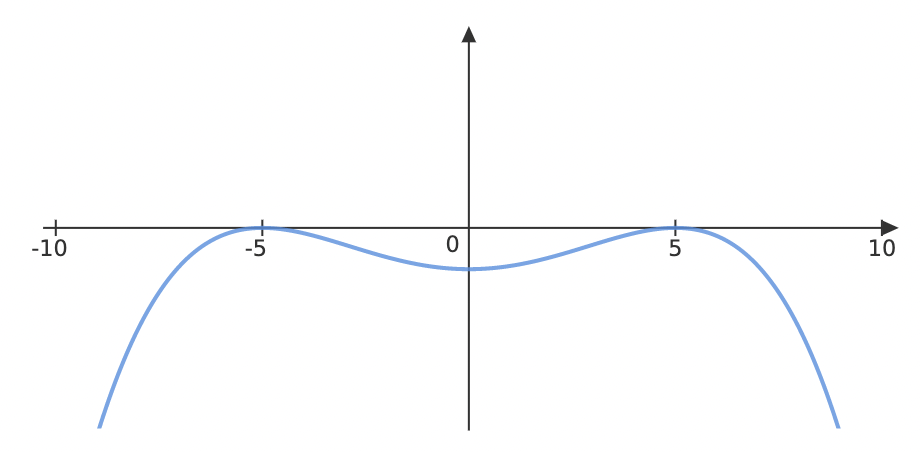
\includegraphics[scale=0.6]{Anh/Screen Shot 2021-09-05 at 00.21.27.png}
\end{center}
Tại thời điểm bẫy bắt đầu hoạt động, $t=0$, nguyên tử ở vị trí $x=0$, năng lượng tổng cộng của nguyên tử là
\[
W=\dfrac{1}{2} m v^{2}-8 \pi \varepsilon_{0} R^{3} E_{0}^{2} \equiv \dfrac{1}{2} m v^{2}+V_{\min }. \tag{11} \label{spho11}
\]
Vì $v<4 E_{0} \sqrt{\dfrac{\pi \varepsilon_{0} R^{3}}{m}} \approx 1,02 \mathrm{~cm} / \mathrm{s}$ nên $W<0$. Tọa độ $x$ lớn nhất của nguyên tử là $x_{\max }$
thỏa mãn phương trình
\[
W-V(x)=0. \tag{12}
\]
Vì $x_{\max }<x_{0}$ nên
\[
x_{\max }=x_{0} \sqrt{1-\sqrt{1+\dfrac{m v^{2}}{2 V_{\min }}}}. \tag{13}
\]
Thay các số liệu đã cho trong đầu bài, ta nhận được $x_{\max } \cong 0,065 x_{0}$, tức là
\[x_{\max }\ll x_{0}. \tag{14} \label{spho14}\]
Với giả thiết (\ref{spho11}) và bất đẳng thức (\ref{spho14}), ta có biểu thức gần đúng cho thế năng $V(x)$ của nguyên tử rubidi đã cho
\[
V(x) \approx-8 \pi \varepsilon_{0} R^{3} E_{0}^{2}\left(1-2 \dfrac{x^{2}}{x_{0}^{2}}\right). \tag{15}
\]
Như vậy, nguyên tử chịu tác dụng của lực
\[
F(x)=-\dfrac{\mathrm{d}V(x)}{\mathrm{d} x}=-k x \ \text { với } \ k=\dfrac{32 \pi \varepsilon_{0} R^{3} E_{0}^{2}}{x_{0}^{2}}. \tag{16}
\]
Dưới tác dụng của lực $F(x)$, nguyên tử thực hiện dao động điều hòa xung quanh vị trí cân bằng $x=0$ với tần số
\[
f=\dfrac{ E_{0}}{x_{0}} \sqrt{8\dfrac{\varepsilon_{0} R^{3}}{\pi m}} \approx 459 \mathrm{~s^{-1}}, \tag{17}
\]
và biên độ
\[x_{\max } \approx x_{0} \dfrac{v}{4 R E_{0}} \sqrt{\dfrac{m}{2 \pi \varepsilon_{0} R}}=0,035  ~\mathrm{\mu m}. \tag{18}\]
\item Theo đồ thị của $V(x)$, để nguyên tử bị bắt và giam giữ trong bẫy, vận tốc ban đầu của nguyên tử phải thỏa mãn điều kiện
\[v < v_{\max } \ \text { với } \ v_{\max }=4 E_{0} \sqrt{\dfrac{\pi \varepsilon_{0} R^{3}}{m}}=1,02 \mathrm{~cm/s}. \tag{19}\]
\end{enumerate}
\end{loigiai}



\begin{vd}[Quả cầu điện môi trong điện trường ngoài]
\begin{center}
\end{center}
%[APho 2007 (Shanghai)]
Nhúng một số hạt điện môi nhỏ vào một chất lỏng có độ nhớt thấp, ta có thể thu được một hệ ở dạng huyền phù. Khi một điện trường ngoài được đặt vào hệ, các hạt điện môi huyền phù sẽ bị phân cực, với moment lưỡng cực điện thu được, gọi là moment lưỡng cực điện cảm ứng. Trong một khoảng thời gian rất ngắn, các hạt bị phân cực này kết tụ lại với nhau do tương tác lưỡng cực, làm cho độ nhớt hiệu dụng của cả hệ tăng lên đáng kể (hệ thu được có thể được coi gần đúng như một vật rắn). Loại chuyển pha này được gọi là hiệu ứng ``điện lưu biến'', còn hệ như vậy được gọi là chất lỏng ``điện lưu biến''. Hiệu ứng này có thể được ứng dụng để chế tạo các thiết bị hãm (phanh) dùng trong thực tế, vì thời gian đáp ứng của sự chuyển pha loại này ngắn hơn các cơ chế hãm thông thường hàng trăm lần. Thông qua việc giải một số bài toán dưới đây, ta sẽ được cung cấp một hình ảnh đơn giản hoá để hiểu được cơ chế của sự chuyển pha điện lưu biến.
\begin{enumerate}[1)]
    \item Khi có nhiều quả cầu điện môi giống hệt nhau, có bán kính $a$, nhúng trong chất lỏng, ta giả thiết rằng moment lưỡng cực $\ot{p}$ của mỗi quả cầu chỉ do điện trường ngoài $\ot{E}_{0}$ gây nên, không phụ thuộc vào các quả cầu khác. \\ 
    \textbf{Chú ý:} $\ot{p} \parallel \ot{E}_{0}$.
    \begin{enumerate}[a)]
        \item Khi hai quả cầu nhỏ giống hệt nhau nằm trong chất lỏng và chạm vào nhau, nếu đường nối các tâm của chúng lập góc $\theta$ với hướng của điện trường ngoài (xem Hình $1$), hãy viết biểu thức của năng lượng tương tác lưỡng cực $-$ lưỡng cực giữa hai quả cầu điện môi nhỏ theo $p$, $a$ và $\theta$.\\ \textbf{Chú ý:} Trong các phép tính, mỗi quả cầu điện môi bị phân cực có thể được coi như một lưỡng cực điện nằm ở tâm của quả cầu.
        \begin{center}
\tikzset{every picture/.style={line width=0.75pt}} %set default line width to 0.75pt
\begin{tikzpicture}[x=0.75pt,y=0.75pt,yscale=-0.75,xscale=0.75]
%uncomment if require: \path (0,465); %set diagram left start at 0, and has height of 465
%Shape: Circle [id:dp7322542907006744] 
\draw  [fill={rgb, 255:red, 155; green, 155; blue, 155 }  ,fill opacity=1 ] (332,316.5) .. controls (332,292.48) and (351.48,273) .. (375.5,273) .. controls (399.52,273) and (419,292.48) .. (419,316.5) .. controls (419,340.52) and (399.52,360) .. (375.5,360) .. controls (351.48,360) and (332,340.52) .. (332,316.5) -- cycle ;
%Straight Lines [id:da7555008022550928] 
\draw  [dash pattern={on 4.5pt off 4.5pt}]  (375.5,224) -- (375.5,316.5) ;
\draw [shift={(375.5,221)}, rotate = 90] [fill={rgb, 255:red, 0; green, 0; blue, 0 }  ][line width=0.08]  [draw opacity=0] (10.72,-5.15) -- (0,0) -- (10.72,5.15) -- (7.12,0) -- cycle    ;
%Shape: Arc [id:dp17914322281357842] 
\draw  [draw opacity=0] (376.12,293.87) .. controls (382.59,294.04) and (388.4,296.76) .. (392.52,301.03) -- (375.5,316.5) -- cycle ; \draw   (376.12,293.87) .. controls (382.59,294.04) and (388.4,296.76) .. (392.52,301.03) ;
%Straight Lines [id:da9918169411952207] 
\draw    (375.5,298.77) -- (375.5,316.5) ;
\draw [shift={(375.5,296.77)}, rotate = 90] [fill={rgb, 255:red, 0; green, 0; blue, 0 }  ][line width=0.08]  [draw opacity=0] (12,-3) -- (0,0) -- (12,3) -- cycle    ;
%Shape: Circle [id:dp25884969376134515] 
\draw  [fill={rgb, 255:red, 155; green, 155; blue, 155 }  ,fill opacity=1 ] (397.5,258.27) .. controls (397.5,234.25) and (416.98,214.77) .. (441,214.77) .. controls (465.02,214.77) and (484.5,234.25) .. (484.5,258.27) .. controls (484.5,282.3) and (465.02,301.77) .. (441,301.77) .. controls (416.98,301.77) and (397.5,282.3) .. (397.5,258.27) -- cycle ;
%Straight Lines [id:da8523540848862873] 
\draw    (441,240.55) -- (441,258.27) ;
\draw [shift={(441,238.55)}, rotate = 90] [fill={rgb, 255:red, 0; green, 0; blue, 0 }  ][line width=0.08]  [draw opacity=0] (12,-3) -- (0,0) -- (12,3) -- cycle    ;
%Straight Lines [id:da9816229971397216] 
\draw    (441,258.27) -- (375.5,316.5) ;
%Straight Lines [id:da11376192280629949] 
\draw [line width=1.5]    (324,358) -- (324,212) ;
\draw [shift={(324,208)}, rotate = 450] [fill={rgb, 255:red, 0; green, 0; blue, 0 }  ][line width=0.08]  [draw opacity=0] (13.4,-6.43) -- (0,0) -- (13.4,6.44) -- (8.9,0) -- cycle    ;

% Text Node
\draw (383,278.9) node [anchor=north west][inner sep=0.75pt]    {$\theta $};
% Text Node
\draw (296,273.4) node [anchor=north west][inner sep=0.75pt]  [color={rgb, 255:red, 0; green, 0; blue, 0 }  ,opacity=1 ]  {$\overrightarrow{E_{0}}$};
\end{tikzpicture}\\
Hình $1$.
        \end{center}
       \item Hãy tính các năng lượng tương tác lưỡng cực $-$ lưỡng cực cho ba cách sắp xếp cấu hình như trên các hình dưới đây:
       \begin{center}

\tikzset{every picture/.style={line width=0.75pt}} %set default line width to 0.75pt        

\begin{tikzpicture}[x=0.75pt,y=0.75pt,yscale=-0.8,xscale=0.8]
%uncomment if require: \path (0,465); %set diagram left start at 0, and has height of 465

%Shape: Circle [id:dp7992342857810553] 
\draw  [fill={rgb, 255:red, 155; green, 155; blue, 155 }  ,fill opacity=1 ] (503,324.5) .. controls (503,300.48) and (522.48,281) .. (546.5,281) .. controls (570.52,281) and (590,300.48) .. (590,324.5) .. controls (590,348.52) and (570.52,368) .. (546.5,368) .. controls (522.48,368) and (503,348.52) .. (503,324.5) -- cycle ;
%Shape: Circle [id:dp14786583206625825] 
\draw  [fill={rgb, 255:red, 155; green, 155; blue, 155 }  ,fill opacity=1 ] (416,324.5) .. controls (416,300.48) and (435.48,281) .. (459.5,281) .. controls (483.52,281) and (503,300.48) .. (503,324.5) .. controls (503,348.52) and (483.52,368) .. (459.5,368) .. controls (435.48,368) and (416,348.52) .. (416,324.5) -- cycle ;
%Shape: Circle [id:dp43921552368924277] 
\draw  [fill={rgb, 255:red, 155; green, 155; blue, 155 }  ,fill opacity=1 ] (311.5,265.27) .. controls (311.5,241.25) and (330.98,221.77) .. (355,221.77) .. controls (379.02,221.77) and (398.5,241.25) .. (398.5,265.27) .. controls (398.5,289.3) and (379.02,308.77) .. (355,308.77) .. controls (330.98,308.77) and (311.5,289.3) .. (311.5,265.27) -- cycle ;
%Shape: Circle [id:dp25575605897945874] 
\draw  [fill={rgb, 255:red, 155; green, 155; blue, 155 }  ,fill opacity=1 ] (246,323.5) .. controls (246,299.48) and (265.48,280) .. (289.5,280) .. controls (313.52,280) and (333,299.48) .. (333,323.5) .. controls (333,347.52) and (313.52,367) .. (289.5,367) .. controls (265.48,367) and (246,347.52) .. (246,323.5) -- cycle ;
%Shape: Circle [id:dp30931649025827546] 
\draw  [fill={rgb, 255:red, 155; green, 155; blue, 155 }  ,fill opacity=1 ] (83,322.5) .. controls (83,298.48) and (102.48,279) .. (126.5,279) .. controls (150.52,279) and (170,298.48) .. (170,322.5) .. controls (170,346.52) and (150.52,366) .. (126.5,366) .. controls (102.48,366) and (83,346.52) .. (83,322.5) -- cycle ;
%Shape: Circle [id:dp004553446595918276] 
\draw  [fill={rgb, 255:red, 155; green, 155; blue, 155 }  ,fill opacity=1 ] (83,235.5) .. controls (83,211.48) and (102.48,192) .. (126.5,192) .. controls (150.52,192) and (170,211.48) .. (170,235.5) .. controls (170,259.52) and (150.52,279) .. (126.5,279) .. controls (102.48,279) and (83,259.52) .. (83,235.5) -- cycle ;
%Straight Lines [id:da7555008022550928] 
\draw  [dash pattern={on 4.5pt off 4.5pt}]  (289.5,231) -- (289.5,323.5) ;
\draw [shift={(289.5,228)}, rotate = 90] [fill={rgb, 255:red, 0; green, 0; blue, 0 }  ][line width=0.08]  [draw opacity=0] (10.72,-5.15) -- (0,0) -- (10.72,5.15) -- (7.12,0) -- cycle    ;
%Shape: Arc [id:dp17914322281357842] 
\draw  [draw opacity=0] (290.12,300.87) .. controls (296.59,301.04) and (302.4,303.76) .. (306.52,308.03) -- (289.5,323.5) -- cycle ; \draw   (290.12,300.87) .. controls (296.59,301.04) and (302.4,303.76) .. (306.52,308.03) ;
%Straight Lines [id:da9918169411952207] 
\draw    (289.5,305.77) -- (289.5,323.5) ;
\draw [shift={(289.5,303.77)}, rotate = 90] [fill={rgb, 255:red, 0; green, 0; blue, 0 }  ][line width=0.08]  [draw opacity=0] (12,-3) -- (0,0) -- (12,3) -- cycle    ;
%Straight Lines [id:da8523540848862873] 
\draw    (355,247.55) -- (355,265.27) ;
\draw [shift={(355,245.55)}, rotate = 90] [fill={rgb, 255:red, 0; green, 0; blue, 0 }  ][line width=0.08]  [draw opacity=0] (12,-3) -- (0,0) -- (12,3) -- cycle    ;
%Straight Lines [id:da9816229971397216] 
\draw    (355,265.27) -- (289.5,323.5) ;
%Straight Lines [id:da11376192280629949] 
\draw [line width=1.5]    (238,365) -- (238,219) ;
\draw [shift={(238,215)}, rotate = 450] [fill={rgb, 255:red, 0; green, 0; blue, 0 }  ][line width=0.08]  [draw opacity=0] (13.4,-6.43) -- (0,0) -- (13.4,6.44) -- (8.9,0) -- cycle    ;
%Straight Lines [id:da5581657313853913] 
\draw    (459.5,306.77) -- (459.5,324.5) ;
\draw [shift={(459.5,304.77)}, rotate = 90] [fill={rgb, 255:red, 0; green, 0; blue, 0 }  ][line width=0.08]  [draw opacity=0] (12,-3) -- (0,0) -- (12,3) -- cycle    ;
%Straight Lines [id:da054358481868871156] 
\draw    (546.5,306.77) -- (546.5,324.5) ;
\draw [shift={(546.5,304.77)}, rotate = 90] [fill={rgb, 255:red, 0; green, 0; blue, 0 }  ][line width=0.08]  [draw opacity=0] (12,-3) -- (0,0) -- (12,3) -- cycle    ;
%Straight Lines [id:da610491834595927] 
\draw    (126.5,304.77) -- (126.5,322.5) ;
\draw [shift={(126.5,302.77)}, rotate = 90] [fill={rgb, 255:red, 0; green, 0; blue, 0 }  ][line width=0.08]  [draw opacity=0] (12,-3) -- (0,0) -- (12,3) -- cycle    ;
%Straight Lines [id:da2769093805455529] 
\draw    (126.5,217.77) -- (126.5,235.5) ;
\draw [shift={(126.5,215.77)}, rotate = 90] [fill={rgb, 255:red, 0; green, 0; blue, 0 }  ][line width=0.08]  [draw opacity=0] (12,-3) -- (0,0) -- (12,3) -- cycle    ;
%Straight Lines [id:da2395271006144144] 
\draw [line width=1.5]    (73,360) -- (73,214) ;
\draw [shift={(73,210)}, rotate = 450] [fill={rgb, 255:red, 0; green, 0; blue, 0 }  ][line width=0.08]  [draw opacity=0] (13.4,-6.43) -- (0,0) -- (13.4,6.44) -- (8.9,0) -- cycle    ;

% Text Node
\draw (213,280.4) node [anchor=north west][inner sep=0.75pt]  [color={rgb, 255:red, 0; green, 0; blue, 0 }  ,opacity=1 ]  {$\overrightarrow{E_{0}}$};
% Text Node
\draw (291.5,202.4) node [anchor=north west][inner sep=0.75pt]    {$45^\circ $};
% Text Node
\draw (48,277.4) node [anchor=north west][inner sep=0.75pt]  [color={rgb, 255:red, 0; green, 0; blue, 0 }  ,opacity=1 ]  {$\overrightarrow{E_{0}}$};
% Text Node
\draw (113,381.4) node [anchor=north west][inner sep=0.75pt]    {$( a)$};
% Text Node
\draw (278,381.4) node [anchor=north west][inner sep=0.75pt]    {$( b)$};
% Text Node
\draw (492,381.4) node [anchor=north west][inner sep=0.75pt]    {$( c)$};


\end{tikzpicture}\\Hình $2$.
       \end{center}
       \item Hãy xác định xem cấu hình nào của hệ là cấu hình ổn định nhất.\\
        \textbf{Chú ý:} Trong các phép tính, mỗi quả cầu điện môi bị phân cực có thể được coi như một lưỡng cực điện đặt ở tâm quả cầu và năng lượng tương tác lưỡng cực - lưỡng cực có thể được biểu thị theo $p$ và $a$.
    \end{enumerate}
    \item Trong trường hợp có ba quả cầu trong chất lỏng, dựa trên các giả thiết như đề bài,
    \begin{enumerate}[a)]
        \item Tính các năng lượng tương tác lưỡng cực $-$ lưỡng cực cho ba cấu hình vẽ trên.
        \item Xác định xem cấu hình nào là cấu hình ổn định nhất.
        \item Xác định xem cấu hình nào là cấu hình kém ổn định nhất.
    \end{enumerate}
    \textbf{Chú ý:} Trong các phép tính, mỗi quả cầu điện môi bị phân cực có thể được coi như một lưỡng cực điện đặt ở tâm quả cầu, và năng lượng tương tác lưỡng cực $-$ lưỡng cực có thể được biểu thị theo $p$ và $a$.
\end{enumerate}
 \begin{center}


\tikzset{every picture/.style={line width=0.75pt}} %set default line width to 0.75pt        

\begin{tikzpicture}[x=0.75pt,y=0.75pt,yscale=-1,xscale=1]
%uncomment if require: \path (0,465); %set diagram left start at 0, and has height of 465

%Shape: Circle [id:dp4339641994583381] 
\draw  [fill={rgb, 255:red, 155; green, 155; blue, 155 }  ,fill opacity=1 ] (480.76,268.51) .. controls (480.76,250.17) and (495.63,235.31) .. (513.97,235.31) .. controls (532.3,235.31) and (547.17,250.17) .. (547.17,268.51) .. controls (547.17,286.85) and (532.3,301.71) .. (513.97,301.71) .. controls (495.63,301.71) and (480.76,286.85) .. (480.76,268.51) -- cycle ;
%Shape: Circle [id:dp052224911367229065] 
\draw  [fill={rgb, 255:red, 155; green, 155; blue, 155 }  ,fill opacity=1 ] (414.36,268.51) .. controls (414.36,250.17) and (429.22,235.31) .. (447.56,235.31) .. controls (465.9,235.31) and (480.76,250.17) .. (480.76,268.51) .. controls (480.76,286.85) and (465.9,301.71) .. (447.56,301.71) .. controls (429.22,301.71) and (414.36,286.85) .. (414.36,268.51) -- cycle ;
%Shape: Circle [id:dp6035501274955883] 
\draw  [fill={rgb, 255:red, 155; green, 155; blue, 155 }  ,fill opacity=1 ] (348.36,269.51) .. controls (348.36,251.17) and (363.22,236.31) .. (381.56,236.31) .. controls (399.9,236.31) and (414.76,251.17) .. (414.76,269.51) .. controls (414.76,287.85) and (399.9,302.71) .. (381.56,302.71) .. controls (363.22,302.71) and (348.36,287.85) .. (348.36,269.51) -- cycle ;
%Shape: Circle [id:dp5029663370925965] 
\draw  [fill={rgb, 255:red, 155; green, 155; blue, 155 }  ,fill opacity=1 ] (244.38,336.61) .. controls (244.38,318.27) and (259.25,303.41) .. (277.58,303.41) .. controls (295.92,303.41) and (310.79,318.27) .. (310.79,336.61) .. controls (310.79,354.95) and (295.92,369.81) .. (277.58,369.81) .. controls (259.25,369.81) and (244.38,354.95) .. (244.38,336.61) -- cycle ;
%Shape: Circle [id:dp8698943026356059] 
\draw  [fill={rgb, 255:red, 155; green, 155; blue, 155 }  ,fill opacity=1 ] (244.38,270.2) .. controls (244.38,251.87) and (259.25,237) .. (277.58,237) .. controls (295.92,237) and (310.79,251.87) .. (310.79,270.2) .. controls (310.79,288.54) and (295.92,303.41) .. (277.58,303.41) .. controls (259.25,303.41) and (244.38,288.54) .. (244.38,270.2) -- cycle ;
%Shape: Circle [id:dp9184176268049609] 
\draw  [fill={rgb, 255:red, 155; green, 155; blue, 155 }  ,fill opacity=1 ] (244.38,203.8) .. controls (244.38,185.46) and (259.25,170.59) .. (277.58,170.59) .. controls (295.92,170.59) and (310.79,185.46) .. (310.79,203.8) .. controls (310.79,222.13) and (295.92,237) .. (277.58,237) .. controls (259.25,237) and (244.38,222.13) .. (244.38,203.8) -- cycle ;
%Shape: Circle [id:dp26146197647762914] 
\draw  [fill={rgb, 255:red, 155; green, 155; blue, 155 }  ,fill opacity=1 ] (144.16,273.14) .. controls (144.16,254.8) and (159.03,239.93) .. (177.36,239.93) .. controls (195.7,239.93) and (210.57,254.8) .. (210.57,273.14) .. controls (210.57,291.47) and (195.7,306.34) .. (177.36,306.34) .. controls (159.03,306.34) and (144.16,291.47) .. (144.16,273.14) -- cycle ;
%Shape: Circle [id:dp574949835208366] 
\draw  [fill={rgb, 255:red, 155; green, 155; blue, 155 }  ,fill opacity=1 ] (86.66,241.14) .. controls (86.66,222.8) and (101.53,207.93) .. (119.87,207.93) .. controls (138.2,207.93) and (153.07,222.8) .. (153.07,241.14) .. controls (153.07,259.47) and (138.2,274.34) .. (119.87,274.34) .. controls (101.53,274.34) and (86.66,259.47) .. (86.66,241.14) -- cycle ;
%Shape: Circle [id:dp5531728679179251] 
\draw  [fill={rgb, 255:red, 155; green, 155; blue, 155 }  ,fill opacity=1 ] (86.66,307.54) .. controls (86.66,289.2) and (101.53,274.34) .. (119.87,274.34) .. controls (138.2,274.34) and (153.07,289.2) .. (153.07,307.54) .. controls (153.07,325.88) and (138.2,340.74) .. (119.87,340.74) .. controls (101.53,340.74) and (86.66,325.88) .. (86.66,307.54) -- cycle ;
%Straight Lines [id:da660486440076847] 
\draw    (120.75,295.31) -- (120.75,308.37) ;
\draw [shift={(120.75,293.31)}, rotate = 90] [fill={rgb, 255:red, 0; green, 0; blue, 0 }  ][line width=0.08]  [draw opacity=0] (12,-3) -- (0,0) -- (12,3) -- cycle    ;
%Straight Lines [id:da17362894362800052] 
\draw    (382.16,256.45) -- (382.16,269.51) ;
\draw [shift={(382.16,254.45)}, rotate = 90] [fill={rgb, 255:red, 0; green, 0; blue, 0 }  ][line width=0.08]  [draw opacity=0] (12,-3) -- (0,0) -- (12,3) -- cycle    ;
%Straight Lines [id:da2495028442818401] 
\draw    (447.56,255.45) -- (447.56,268.51) ;
\draw [shift={(447.56,253.45)}, rotate = 90] [fill={rgb, 255:red, 0; green, 0; blue, 0 }  ][line width=0.08]  [draw opacity=0] (12,-3) -- (0,0) -- (12,3) -- cycle    ;
%Straight Lines [id:da7441244508416673] 
\draw    (277.58,323.55) -- (277.58,336.61) ;
\draw [shift={(277.58,321.55)}, rotate = 90] [fill={rgb, 255:red, 0; green, 0; blue, 0 }  ][line width=0.08]  [draw opacity=0] (12,-3) -- (0,0) -- (12,3) -- cycle    ;
%Straight Lines [id:da4570383736591437] 
\draw    (277.58,257.15) -- (277.58,270.2) ;
\draw [shift={(277.58,255.15)}, rotate = 90] [fill={rgb, 255:red, 0; green, 0; blue, 0 }  ][line width=0.08]  [draw opacity=0] (12,-3) -- (0,0) -- (12,3) -- cycle    ;
%Straight Lines [id:da4911642488394289] 
\draw [line width=1.5]    (71.49,362.23) -- (71.49,186.09) ;
\draw [shift={(71.49,182.09)}, rotate = 450] [fill={rgb, 255:red, 0; green, 0; blue, 0 }  ][line width=0.08]  [draw opacity=0] (13.4,-6.43) -- (0,0) -- (13.4,6.44) -- (8.9,0) -- cycle    ;
%Straight Lines [id:da7818527846742416] 
\draw    (513.36,255.45) -- (513.36,268.51) ;
\draw [shift={(513.36,253.45)}, rotate = 90] [fill={rgb, 255:red, 0; green, 0; blue, 0 }  ][line width=0.08]  [draw opacity=0] (12,-3) -- (0,0) -- (12,3) -- cycle    ;
%Straight Lines [id:da3914857405478256] 
\draw    (279.08,190.74) -- (279.08,203.8) ;
\draw [shift={(279.08,188.74)}, rotate = 90] [fill={rgb, 255:red, 0; green, 0; blue, 0 }  ][line width=0.08]  [draw opacity=0] (12,-3) -- (0,0) -- (12,3) -- cycle    ;
%Straight Lines [id:da18032882045365228] 
\draw    (119.87,228.08) -- (119.87,241.14) ;
\draw [shift={(119.87,226.08)}, rotate = 90] [fill={rgb, 255:red, 0; green, 0; blue, 0 }  ][line width=0.08]  [draw opacity=0] (12,-3) -- (0,0) -- (12,3) -- cycle    ;
%Straight Lines [id:da7341850230816754] 
\draw    (177.36,260.08) -- (177.36,273.14) ;
\draw [shift={(177.36,258.08)}, rotate = 90] [fill={rgb, 255:red, 0; green, 0; blue, 0 }  ][line width=0.08]  [draw opacity=0] (12,-3) -- (0,0) -- (12,3) -- cycle    ;

% Text Node
\draw (42.24,268.44) node [anchor=north west][inner sep=0.75pt]  [color={rgb, 255:red, 0; green, 0; blue, 0 }  ,opacity=1 ]  {$\overrightarrow{E_{0}}$};
% Text Node
\draw (107,379.4) node [anchor=north west][inner sep=0.75pt]    {$( d)$};
% Text Node
\draw (268,382.4) node [anchor=north west][inner sep=0.75pt]    {$( e)$};
% Text Node
\draw (443,380.4) node [anchor=north west][inner sep=0.75pt]    {$( f)$};


\end{tikzpicture}
 \end{center}
\end{vd}
\begin{loigiai}
\begin{enumerate}[1)]                           
    \item Viết biểu thức năng lượng của tương tác lưỡng cực $-$ lưỡng cực giữa hai quả cầu điện môi nhỏ tiếp xúc với nhau theo $p$, $a$, và $\theta$.
    \begin{enumerate}[a)]
   \item Nếu đưa vào tọa độ cực, thành phần $z$ của điện trường sinh ra bởi một lưỡng cực đặt tại gốc với trục của nó song song với trục $z$ là:
    \[E_{z}(\theta, \phi)=-\dfrac{p}{4 \pi \varepsilon_{0}} \dfrac{1-3 \cos ^{2} \theta}{r^{3}}, \tag{1} \]
    trong đó $r$ là chiều dài của vector đơn vị tương đối của hai lưỡng cực. Trong điện trường ngoài $\ot E$, năng lượng của một lưỡng cực với trục của nó song song với trục $z$ là:
    \[U= -\ot{p}\cdot \ot{E}=-pE_{z}. \tag{2}\]
    Do đó, ta thu được kết quả năng lượng tương tác giữa hai quả cầu điện môi nhỏ tiếp xúc
    \[U_{12}=\dfrac{p^{2}}{4 \pi \varepsilon_{0}} \dfrac{1-3 \cos ^{2} \theta}{(2 a)^{3}}. \tag{3} \label{3d}\] 
    \item Tính các năng lượng tương tác lưỡng cực - lưỡng cực cho ba cấu hình trên:
    Trên cơ sở phương trình (\ref{3d}),
    \begin{itemize}
        \item Đối với cấu hình ($a$):
    \[U_{a}=\dfrac{1}{4 \pi \varepsilon_{0}} \dfrac{1-3}{(2 a)^{3}} p^{2}=-\dfrac{1}{4 \pi \varepsilon_{0}} \dfrac{p^{2}}{4 a^{3}}. \tag{4} \label{4d}\]
        \item  Đối với cấu hình ($b$): 
    \[U_{b}=\dfrac{1}{4 \pi \varepsilon_{0}} \dfrac{1-3 \cos ^{2} \dfrac{\pi}{4}}{(2 a)^{3}}=-\dfrac{1}{4 \pi \varepsilon_{0}} \dfrac{p^{2}}{16 a^{3}}. \tag{5} \label{5d} \]
        \item Đối với cấu hình ($c$):
    \[U_{c}=\dfrac{1}{4 \pi \varepsilon_{0}} \dfrac{1-0}{(2 a)^{3}} p^{2}=\dfrac{1}{4 \pi \varepsilon_{0}} \dfrac{p^{2}}{8 a^{3}}. \tag{6} \label{6d}\]
    \end{itemize}
    \item Việc so sánh (\ref{4d}), (\ref{5d}) và (\ref{6d}) chỉ ra rằng cấu hình ($a$) có năng lượng thấp nhất và nó tương ứng với trạng thái cơ bản của hệ. Đó là cấu hình ổn định nhất của hệ (theo nguyên lý thế năng cực tiểu).
    \end{enumerate}
    \item Ba quả cầu ($d$), ($e$) và ($f$).
   \begin{enumerate}[a)]
     \item Cách làm tương tự như ở phần trên.
     \begin{itemize}
         \item Đối với cấu hình ($d$), ta có:
     \[{U}_{{d}}=\dfrac{1}{4 \pi \varepsilon_{0}}\left(-\dfrac{{p}^{2}}{4 {a}^{3}}+2 \cdot \dfrac{{p}^{2}}{32 {a}^{3}}\right)=-\dfrac{1}{4 \pi \varepsilon_{0}} \dfrac{3 {p}^{2}}{16 {a}^{3}}. \tag{7}\]
     \item  Đối với cấu hình ($e$):
    \[{U}_{{e}}=\dfrac{1}{4 \pi \varepsilon_{0}}\left(-\dfrac{{p}^{2}}{4 {a}^{3}} \cdot 2-\dfrac{{p}^{2}}{32 {a}^{3}}\right)=-\dfrac{1}{4 \pi \varepsilon_{0}} \dfrac{17 {p}^{2}}{32 {a}^{3}}. \tag{8}\]
    \item Đối với cấu hình ($f$):
    \[{U}_{{f}}=\dfrac{1}{4 \pi \varepsilon_{0}}\left(\dfrac{{p}^{2}}{8 {a}^{3}} \cdot 2+\dfrac{{p}^{2}}{64 {a}^{3}}\right)=\dfrac{1}{4 \pi \varepsilon_{0}} \dfrac{17 {p}^{2}}{64 {a}^{3}}. \tag{9}\]
     \end{itemize}
  \item Cấu hình ($e$) có năng lượng thấp nhất và do đó nó ổn định nhất.
  \item Cấu hình ($f$) có năng lượng cao nhất và do đó kém ổn định nhất.
 \end{enumerate}
\end{enumerate}
\end{loigiai}


\begin{vd}[Bàn cờ dẫn điện]
Một bàn cờ $8\times 8$ cấu tạo từ các ô được làm từ hai loại kim loại, cả hai đều dẫn điện không tốt. Trong hệ còn hai phần tử khác đó là hai dải kim loại dẫn điện rất tốt chạy dọc hai viền của bàn cờ (dải tiếp xúc với dây nối như hình vẽ). Độ dày chung của bàn cờ và các ô là $t$ rất nhỏ hơn so với chiều dài $L$ của bàn cờ.
\begin{center}
    

\tikzset{every picture/.style={line width=0.75pt}} %set default line width to 0.75pt        

\begin{tikzpicture}[x=0.75pt,y=0.75pt,yscale=-1,xscale=1]
%uncomment if require: \path (0,470); %set diagram left start at 0, and has height of 470

%Shape: Parallelogram [id:dp1634681887307805] 
\draw   (282.36,141.41) -- (308.45,144.7) -- (296.01,157.87) -- (269.93,154.58) -- cycle ;
%Straight Lines [id:da7905958403536684] 
\draw    (182.41,246.55) -- (182.41,260.15) ;
%Shape: Parallelogram [id:dp9095361285915102] 
\draw  [fill={rgb, 255:red, 155; green, 155; blue, 155 }  ,fill opacity=1 ] (308.45,144.7) -- (334.81,148.03) -- (322.3,161.04) -- (295.93,157.71) -- cycle ;
%Shape: Parallelogram [id:dp7721525314718289] 
\draw   (334.81,148.03) -- (361.18,151.36) -- (348.67,164.37) -- (322.3,161.04) -- cycle ;
%Shape: Parallelogram [id:dp8016974778157118] 
\draw  [fill={rgb, 255:red, 155; green, 155; blue, 155 }  ,fill opacity=1 ] (361.18,151.36) -- (387.55,154.69) -- (375.04,167.7) -- (348.67,164.37) -- cycle ;
%Shape: Parallelogram [id:dp8022334304567804] 
\draw   (387.55,154.69) -- (413.92,158.02) -- (401.41,171.03) -- (375.04,167.69) -- cycle ;
%Shape: Parallelogram [id:dp07696832150226673] 
\draw  [fill={rgb, 255:red, 155; green, 155; blue, 155 }  ,fill opacity=1 ] (413.92,158.01) -- (440.29,161.34) -- (427.78,174.35) -- (401.41,171.02) -- cycle ;
%Shape: Parallelogram [id:dp9645533748108515] 
\draw   (440.29,161.34) -- (466.66,164.67) -- (454.14,177.68) -- (427.78,174.35) -- cycle ;
%Shape: Parallelogram [id:dp6649476659417421] 
\draw  [fill={rgb, 255:red, 155; green, 155; blue, 155 }  ,fill opacity=1 ] (466.66,164.67) -- (493.03,168) -- (480.51,181.01) -- (454.14,177.68) -- cycle ;
%Shape: Parallelogram [id:dp677898638583595] 
\draw  [fill={rgb, 255:red, 155; green, 155; blue, 155 }  ,fill opacity=1 ] (269.93,154.58) -- (295.54,157.81) -- (283.16,171.55) -- (257.56,168.32) -- cycle ;
%Shape: Parallelogram [id:dp10735060125369023] 
\draw   (296.26,157.68) -- (322.63,161.01) -- (310.11,174.02) -- (283.74,170.69) -- cycle ;
%Shape: Parallelogram [id:dp9088792048232939] 
\draw  [fill={rgb, 255:red, 155; green, 155; blue, 155 }  ,fill opacity=1 ] (322.17,160.95) -- (348.99,164.34) -- (336.07,178.52) -- (309.25,175.14) -- cycle ;
%Shape: Parallelogram [id:dp4500605468061303] 
\draw   (348.99,164.34) -- (375.36,167.67) -- (362.85,180.68) -- (336.48,177.34) -- cycle ;
%Shape: Parallelogram [id:dp7488763500831803] 
\draw  [fill={rgb, 255:red, 155; green, 155; blue, 155 }  ,fill opacity=1 ] (374.85,167.6) -- (401.54,170.97) -- (388.67,185.16) -- (361.99,181.79) -- cycle ;
%Shape: Parallelogram [id:dp4846791851214096] 
\draw   (401.54,170.97) -- (428.1,174.32) -- (415.1,189.43) -- (388.53,186.08) -- cycle ;
%Shape: Parallelogram [id:dp8925225920275939] 
\draw  [fill={rgb, 255:red, 155; green, 155; blue, 155 }  ,fill opacity=1 ] (427.55,174.32) -- (454.14,177.68) -- (441.32,191.81) -- (414.72,188.45) -- cycle ;
%Shape: Parallelogram [id:dp7035911290176065] 
\draw   (454.47,177.65) -- (480.84,180.98) -- (468.33,193.99) -- (441.96,190.66) -- cycle ;
%Shape: Parallelogram [id:dp11292783009809115] 
\draw   (257.56,168.32) -- (283.92,171.65) -- (271.41,184.66) -- (245.04,181.33) -- cycle ;
%Shape: Parallelogram [id:dp8268722870196277] 
\draw  [fill={rgb, 255:red, 155; green, 155; blue, 155 }  ,fill opacity=1 ] (284.17,170.74) -- (310.71,174.09) -- (298.06,187.46) -- (271.52,184.11) -- cycle ;
%Shape: Parallelogram [id:dp04735681570813077] 
\draw   (310.29,174.98) -- (336.66,178.31) -- (324.15,191.32) -- (297.78,187.98) -- cycle ;
%Shape: Parallelogram [id:dp9134129539151328] 
\draw  [fill={rgb, 255:red, 155; green, 155; blue, 155 }  ,fill opacity=1 ] (336.75,177.38) -- (362.85,180.68) -- (350.25,194.61) -- (324.15,191.31) -- cycle ;
%Shape: Parallelogram [id:dp42332262246839125] 
\draw   (363.03,181.63) -- (389.4,184.96) -- (376.89,197.97) -- (350.52,194.64) -- cycle ;
%Shape: Parallelogram [id:dp9586661387599467] 
\draw  [fill={rgb, 255:red, 155; green, 155; blue, 155 }  ,fill opacity=1 ] (388.69,186.1) -- (415.48,189.48) -- (403.04,201.33) -- (376.25,197.95) -- cycle ;
%Shape: Parallelogram [id:dp3897134042089663] 
\draw   (415.77,188.29) -- (442.14,191.62) -- (429.62,204.63) -- (403.25,201.3) -- cycle ;
%Shape: Parallelogram [id:dp23824795071231386] 
\draw  [fill={rgb, 255:red, 155; green, 155; blue, 155 }  ,fill opacity=1 ] (442.45,190.72) -- (468.33,193.99) -- (455.82,207.86) -- (429.95,204.59) -- cycle ;
%Shape: Parallelogram [id:dp3136329722838067] 
\draw  [fill={rgb, 255:red, 155; green, 155; blue, 155 }  ,fill opacity=1 ] (245.37,181.3) -- (271.74,184.63) -- (259.22,197.64) -- (232.85,194.31) -- cycle ;
%Shape: Parallelogram [id:dp30533494177104537] 
\draw   (271.74,184.63) -- (298.1,187.96) -- (285.59,200.97) -- (259.22,197.63) -- cycle ;
%Shape: Parallelogram [id:dp4712679864699516] 
\draw  [fill={rgb, 255:red, 155; green, 155; blue, 155 }  ,fill opacity=1 ] (298.1,187.95) -- (324.47,191.28) -- (311.96,204.29) -- (285.59,200.96) -- cycle ;
%Shape: Parallelogram [id:dp7986379838493471] 
\draw   (324.47,191.28) -- (350.84,194.61) -- (338.33,207.62) -- (311.96,204.29) -- cycle ;
%Shape: Parallelogram [id:dp32661269944620597] 
\draw  [fill={rgb, 255:red, 155; green, 155; blue, 155 }  ,fill opacity=1 ] (350.84,194.61) -- (377.21,197.94) -- (364.7,210.95) -- (338.33,207.62) -- cycle ;
%Shape: Parallelogram [id:dp03575534689371507] 
\draw   (377.21,197.94) -- (403.58,201.27) -- (391.07,214.28) -- (364.7,210.95) -- cycle ;
%Shape: Parallelogram [id:dp0424514191210299] 
\draw  [fill={rgb, 255:red, 155; green, 155; blue, 155 }  ,fill opacity=1 ] (403.58,201.27) -- (429.95,204.6) -- (417.44,217.61) -- (391.07,214.28) -- cycle ;
%Shape: Parallelogram [id:dp1742319089301827] 
\draw   (429.82,204.58) -- (455.82,207.86) -- (443.58,220.18) -- (417.58,216.9) -- cycle ;
%Shape: Parallelogram [id:dp8218078558084174] 
\draw   (233.18,194.28) -- (259.55,197.61) -- (247.03,210.62) -- (220.66,207.28) -- cycle ;
%Shape: Parallelogram [id:dp5436912131639109] 
\draw  [fill={rgb, 255:red, 155; green, 155; blue, 155 }  ,fill opacity=1 ] (259.55,197.6) -- (285.92,200.93) -- (273.4,213.94) -- (247.03,210.61) -- cycle ;
%Shape: Parallelogram [id:dp7999141912617251] 
\draw   (285.92,200.93) -- (312.28,204.26) -- (299.77,217.27) -- (273.4,213.94) -- cycle ;
%Shape: Parallelogram [id:dp24240463688042935] 
\draw  [fill={rgb, 255:red, 155; green, 155; blue, 155 }  ,fill opacity=1 ] (312.28,204.26) -- (338.65,207.59) -- (326.14,220.6) -- (299.77,217.27) -- cycle ;
%Shape: Parallelogram [id:dp33547683393523164] 
\draw   (338.65,207.59) -- (365.02,210.92) -- (352.51,223.93) -- (326.14,220.6) -- cycle ;
%Shape: Parallelogram [id:dp8314802344905496] 
\draw  [fill={rgb, 255:red, 155; green, 155; blue, 155 }  ,fill opacity=1 ] (365.02,210.92) -- (391.39,214.25) -- (378.88,227.26) -- (352.51,223.93) -- cycle ;
%Shape: Parallelogram [id:dp5766289321028972] 
\draw   (391.39,214.25) -- (417.76,217.58) -- (405.25,230.58) -- (378.88,227.25) -- cycle ;
%Shape: Parallelogram [id:dp24314540320655564] 
\draw  [fill={rgb, 255:red, 155; green, 155; blue, 155 }  ,fill opacity=1 ] (417.71,216.91) -- (443.58,220.18) -- (431.12,233.85) -- (405.25,230.58) -- cycle ;
%Shape: Parallelogram [id:dp8343652516667763] 
\draw  [fill={rgb, 255:red, 155; green, 155; blue, 155 }  ,fill opacity=1 ] (220,207.4) -- (246.37,210.74) -- (233.86,223.74) -- (207.49,220.41) -- cycle ;
%Shape: Parallelogram [id:dp002049087379289549] 
\draw   (246.37,210.73) -- (272.74,214.06) -- (260.23,227.07) -- (233.86,223.74) -- cycle ;
%Shape: Parallelogram [id:dp6508141101896114] 
\draw  [fill={rgb, 255:red, 155; green, 155; blue, 155 }  ,fill opacity=1 ] (272.74,214.06) -- (299.11,217.39) -- (286.59,230.4) -- (260.23,227.07) -- cycle ;
%Shape: Parallelogram [id:dp9398739740832878] 
\draw   (299.11,217.39) -- (325.48,220.72) -- (312.96,233.73) -- (286.59,230.4) -- cycle ;
%Shape: Parallelogram [id:dp878136362323773] 
\draw  [fill={rgb, 255:red, 155; green, 155; blue, 155 }  ,fill opacity=1 ] (325.48,220.72) -- (351.84,224.05) -- (339.33,237.06) -- (312.96,233.73) -- cycle ;
%Shape: Parallelogram [id:dp48585372241904445] 
\draw   (351.84,224.05) -- (378.21,227.38) -- (365.7,240.39) -- (339.33,237.05) -- cycle ;
%Shape: Parallelogram [id:dp9069636410639039] 
\draw  [fill={rgb, 255:red, 155; green, 155; blue, 155 }  ,fill opacity=1 ] (378.21,227.37) -- (404.58,230.7) -- (392.07,243.71) -- (365.7,240.38) -- cycle ;
%Shape: Parallelogram [id:dp28895018888355795] 
\draw   (404.58,230.7) -- (430.95,234.03) -- (418.44,247.04) -- (392.07,243.71) -- cycle ;
%Shape: Parallelogram [id:dp43438181974774315] 
\draw   (207.81,220.38) -- (234.18,223.71) -- (221.67,236.72) -- (195.3,233.39) -- cycle ;
%Shape: Parallelogram [id:dp12315943525110495] 
\draw  [fill={rgb, 255:red, 155; green, 155; blue, 155 }  ,fill opacity=1 ] (234.18,223.71) -- (260.55,227.04) -- (248.04,240.05) -- (221.67,236.72) -- cycle ;
%Shape: Parallelogram [id:dp47358096089811585] 
\draw   (260.55,227.04) -- (286.92,230.37) -- (274.41,243.38) -- (248.04,240.05) -- cycle ;
%Shape: Parallelogram [id:dp34074785630316207] 
\draw  [fill={rgb, 255:red, 155; green, 155; blue, 155 }  ,fill opacity=1 ] (286.92,230.37) -- (313.29,233.7) -- (300.77,246.71) -- (274.41,243.38) -- cycle ;
%Shape: Parallelogram [id:dp1733943235092239] 
\draw   (313.29,233.7) -- (339.66,237.03) -- (327.14,250.04) -- (300.77,246.7) -- cycle ;
%Shape: Parallelogram [id:dp7440793240149637] 
\draw  [fill={rgb, 255:red, 155; green, 155; blue, 155 }  ,fill opacity=1 ] (339.66,237.02) -- (366.03,240.35) -- (353.51,253.36) -- (327.14,250.03) -- cycle ;
%Shape: Parallelogram [id:dp28203581002048206] 
\draw   (366.02,240.35) -- (392.39,243.68) -- (379.88,256.69) -- (353.51,253.36) -- cycle ;
%Shape: Parallelogram [id:dp17429886517884596] 
\draw  [fill={rgb, 255:red, 155; green, 155; blue, 155 }  ,fill opacity=1 ] (392.39,243.68) -- (418.76,247.01) -- (406.25,260.02) -- (379.88,256.69) -- cycle ;
%Shape: Parallelogram [id:dp5053273318057276] 
\draw  [fill={rgb, 255:red, 155; green, 155; blue, 155 }  ,fill opacity=1 ] (194.63,233.51) -- (221,236.84) -- (208.49,249.85) -- (182.12,246.52) -- cycle ;
%Shape: Parallelogram [id:dp5083307250794808] 
\draw   (221,236.84) -- (247.37,240.17) -- (234.86,253.18) -- (208.49,249.85) -- cycle ;
%Shape: Parallelogram [id:dp5030559914677115] 
\draw  [fill={rgb, 255:red, 155; green, 155; blue, 155 }  ,fill opacity=1 ] (247.37,240.17) -- (273.74,243.5) -- (261.23,256.51) -- (234.86,253.18) -- cycle ;
%Shape: Parallelogram [id:dp04149544633175206] 
\draw   (273.74,243.5) -- (300.11,246.83) -- (287.6,259.84) -- (261.23,256.5) -- cycle ;
%Shape: Parallelogram [id:dp9374124285190173] 
\draw  [fill={rgb, 255:red, 155; green, 155; blue, 155 }  ,fill opacity=1 ] (300.11,246.82) -- (326.48,250.16) -- (313.97,263.16) -- (287.6,259.83) -- cycle ;
%Shape: Parallelogram [id:dp7855595557469714] 
\draw   (326.48,250.15) -- (352.85,253.48) -- (340.33,266.49) -- (313.97,263.16) -- cycle ;
%Shape: Parallelogram [id:dp4211898209526288] 
\draw  [fill={rgb, 255:red, 155; green, 155; blue, 155 }  ,fill opacity=1 ] (352.85,253.48) -- (379.22,256.81) -- (366.7,269.82) -- (340.33,266.49) -- cycle ;
%Shape: Parallelogram [id:dp7899113190333609] 
\draw   (379.22,256.81) -- (405.59,260.14) -- (393.07,273.15) -- (366.7,269.82) -- cycle ;
%Straight Lines [id:da5873316786013936] 
\draw    (493.03,168) -- (493.03,181.6) ;
%Straight Lines [id:da5281811781936845] 
\draw    (493.03,168) -- (393.07,273.15) ;
%Straight Lines [id:da5356597417508657] 
\draw    (282.36,141.41) -- (182.41,246.55) ;
%Straight Lines [id:da45773821846578744] 
\draw    (493.03,181.6) -- (393.07,286.75) ;
%Straight Lines [id:da34297068964628274] 
\draw    (282.36,141.41) -- (493.03,168) ;
%Straight Lines [id:da8376418298814283] 
\draw    (182.41,246.55) -- (393.07,273.15) ;
%Straight Lines [id:da18951972627702118] 
\draw    (182.41,260.15) -- (393.07,286.75) ;
%Straight Lines [id:da5805655058728623] 
\draw    (393.07,273.15) -- (393.07,286.75) ;
%Straight Lines [id:da6481821546126103] 
\draw    (291.39,128.53) -- (496.1,154.37) ;
\draw [shift={(499.07,154.75)}, rotate = 187.2] [fill={rgb, 255:red, 0; green, 0; blue, 0 }  ][line width=0.08]  [draw opacity=0] (10.72,-5.15) -- (0,0) -- (10.72,5.15) -- (7.12,0) -- cycle    ;
\draw [shift={(288.41,128.15)}, rotate = 7.2] [fill={rgb, 255:red, 0; green, 0; blue, 0 }  ][line width=0.08]  [draw opacity=0] (10.72,-5.15) -- (0,0) -- (10.72,5.15) -- (7.12,0) -- cycle    ;
%Straight Lines [id:da8210838899287984] 
\draw    (500.96,191.77) -- (405.14,292.57) ;
\draw [shift={(403.07,294.75)}, rotate = 313.55] [fill={rgb, 255:red, 0; green, 0; blue, 0 }  ][line width=0.08]  [draw opacity=0] (10.72,-5.15) -- (0,0) -- (10.72,5.15) -- (7.12,0) -- cycle    ;
\draw [shift={(503.03,189.6)}, rotate = 133.55] [fill={rgb, 255:red, 0; green, 0; blue, 0 }  ][line width=0.08]  [draw opacity=0] (10.72,-5.15) -- (0,0) -- (10.72,5.15) -- (7.12,0) -- cycle    ;
%Straight Lines [id:da28792563006672633] 
\draw  [dash pattern={on 4.5pt off 4.5pt}]  (151.8,242.6) -- (182.12,246.52) ;
%Straight Lines [id:da8630355929059936] 
\draw  [dash pattern={on 4.5pt off 4.5pt}]  (152.09,256.23) -- (182.41,260.15) ;
%Straight Lines [id:da502164850868569] 
\draw    (152.09,245.63) -- (152.09,253.23) ;
\draw [shift={(152.09,256.23)}, rotate = 270] [fill={rgb, 255:red, 0; green, 0; blue, 0 }  ][line width=0.08]  [draw opacity=0] (5.36,-2.57) -- (0,0) -- (5.36,2.57) -- (3.56,0) -- cycle    ;
\draw [shift={(152.09,242.63)}, rotate = 90] [fill={rgb, 255:red, 0; green, 0; blue, 0 }  ][line width=0.08]  [draw opacity=0] (5.36,-2.57) -- (0,0) -- (5.36,2.57) -- (3.56,0) -- cycle    ;
%Straight Lines [id:da8697444809472166] 
\draw [line width=1.5]    (163.55,127.04) -- (163.55,140.6) ;
%Straight Lines [id:da021032614299149932] 
\draw    (169,120) -- (169,149.6) ;
%Curve Lines [id:da1748810964647569] 
\draw    (163.8,133.6) .. controls (58.8,142.6) and (54.8,395.6) .. (277,258) ;
%Curve Lines [id:da4611407963859848] 
\draw    (169,134.8) .. controls (283.8,154.6) and (238.8,53.6) .. (349,150) ;
%Flowchart: Connector [id:dp2209190587861436] 
\draw  [fill={rgb, 255:red, 255; green, 255; blue, 255 }  ,fill opacity=1 ] (176,294.8) .. controls (176,285.85) and (183.25,278.6) .. (192.2,278.6) .. controls (201.15,278.6) and (208.4,285.85) .. (208.4,294.8) .. controls (208.4,303.75) and (201.15,311) .. (192.2,311) .. controls (183.25,311) and (176,303.75) .. (176,294.8) -- cycle ;


% Text Node
\draw (147,112.4) node [anchor=north west][inner sep=0.75pt]    {$-$};
% Text Node
\draw (173,111.4) node [anchor=north west][inner sep=0.75pt]    {$+$};
% Text Node
\draw (158.55,101.44) node [anchor=north west][inner sep=0.75pt]    {$V$};
% Text Node
\draw (182,285.4) node [anchor=north west][inner sep=0.75pt]    {$A$};
% Text Node
\draw (320,224) node [anchor=north west][inner sep=0.75pt]    {$\sigma _{1}$};
% Text Node
\draw (348,227) node [anchor=north west][inner sep=0.75pt]    {$\sigma _{2}$};
% Text Node
\draw (380.55,116.44) node [anchor=north west][inner sep=0.75pt]    {$L$};
% Text Node
\draw (455.05,245.57) node [anchor=north west][inner sep=0.75pt]    {$L$};
% Text Node
\draw (140.55,239.44) node [anchor=north west][inner sep=0.75pt]    {$t$};
\end{tikzpicture}
\end{center}
Độ dẫn điện của ô màu trắng là $\sigma_1$, của ô màu tối là $\sigma_2$. Tìm dòng điện chạy qua bàn cờ nếu một hiệu điện thế $V$ được đặt vào hai điện cực, bỏ qua điện trở của các điểm tiếp xúc.
\end{vd}

\begin{loigiai}
Nếu tất cả các ô trên bàn cờ đều làm từ một kim loại đồng nhất có độ dẫn điện $\sigma_1$, thì độ lớn điện trường trong bàn cờ sẽ là $E=\dfrac{V}{L}$ và mật độ dòng điện là 
$$j_1=\sigma_1.E,$$ và cường độ dòng điện chạy trong bản sẽ là
$$I_1=j_1Lt=\sigma_1ELt=V\sigma_1t.$$
Tương tự nếu cả bàn cờ làm bằng kim loại đồng nhất có độ dẫn điện $\sigma_2$, với cùng một điện thế $V$, dòng $I_2$ chạy qua bàn cờ sẽ là $V.\sigma_2.t$. Lưu ý rằng cường độ dòng điện chạy trong bàn cờ không phụ thuộc vào độ dài $L$ của bản.
\\Theo hướng suy luận như thế, chúng ta dự đoán cường độ dòng chạy qua bàn cờ thật sẽ là trung bình nhân của hai dòng điện trên, và chúng ta phải đi chứng minh điều này là đúng 
$$I=Vt\sqrt{\sigma_1 \sigma_2}.$$
 Suy luận này là đúng đối với mọi bàn cờ đan xen có độ dày đồng nhất nếu chúng thỏa mãn các điều kiện sau
   \\ Nếu tồn tại hai điểm $A$ và $B$ sao cho chúng có thể thay thế vị trí của nhau trên bàn cờ bằng cách quay bàn cờ $90^\circ$, thì  tích độ dẫn điện của hai điểm đó phải có giá trị độc lập dù cho ta chọn hai điểm đó bằng bất kì cách nào
    \\ Đối với bài toán điều kiện này đương nhiên thỏa mãn vì nếu ta xoay bàn cờ $90^\circ$ thì ô đen luôn bị đổi chỗ bởi các ô trắng và ngược lại, do đó điểm $A$ và $B$ luôn có màu khác nhau nên tích độ dẫn điện $\sigma_A.\sigma_B$ luôn bằng $\sigma_1.\sigma_2$ không đổi.
    \\ Tiếp theo để đơn giản hóa bài toán, thay vì dùng bàn cờ thông thường ta sẽ chỉ xét một mạng 2x2 ô cờ vì chúng cũng thỏa mãn đầy đủ tính chất nêu trên. Đầu tiên chúng ta nghiên cứu về điện trường trong mạng và sau đó là dòng điện chạy qua từng ô vuông của mạng. Điện trường nội tại có thể được xác định hoàn toàn bằng điện thế, được kí hiệu là ($\phi$) và được minh họa trực quan bằng các đường đẳng thế, biểu diễn bằng các đường cắt chéo như hình 1.
    \begin{center}
        

\tikzset{every picture/.style={line width=0.75pt}} %set default line width to 0.75pt        

\begin{tikzpicture}[x=0.75pt,y=0.75pt,yscale=-0.8,xscale=0.8]
%uncomment if require: \path (0,493); %set diagram left start at 0, and has height of 493

%Shape: Square [id:dp35765568233416056] 
\draw   (173.81,63.44) -- (321.96,63.44) -- (321.96,211.59) -- (173.81,211.59) -- cycle ;
%Shape: Square [id:dp44032875059918886] 
\draw  [fill={rgb, 255:red, 155; green, 155; blue, 155 }  ,fill opacity=0.6 ] (321.96,63.44) -- (470.11,63.44) -- (470.11,211.59) -- (321.96,211.59) -- cycle ;
%Shape: Rectangle [id:dp3323113313608652] 
\draw  [fill={rgb, 255:red, 155; green, 155; blue, 155 }  ,fill opacity=0.6 ] (173.81,211.59) -- (321.96,211.59) -- (321.96,359.74) -- (173.81,359.74) -- cycle ;
%Shape: Rectangle [id:dp7482873919160049] 
\draw   (321.96,211.59) -- (470.11,211.59) -- (470.11,359.74) -- (321.96,359.74) -- cycle ;
%Curve Lines [id:da7792535041822144] 
\draw    (343,360.04) .. controls (349.01,283.71) and (389.57,145.48) .. (393.18,63.44) ;
%Curve Lines [id:da20272580305573973] 
\draw    (389.57,358.54) .. controls (388.07,288.22) and (419.62,134.96) .. (416.62,62.24) ;
%Curve Lines [id:da8130622081159569] 
\draw  [dash pattern={on 4.5pt off 4.5pt}]  (174.72,242.24) .. controls (252.85,249.75) and (388.07,286.72) .. (468.18,278.82) ;
%Curve Lines [id:da14149067177234897] 
\draw  [dash pattern={on 4.5pt off 4.5pt}]  (173.21,280.4) .. controls (240.83,274.39) and (401.52,317.56) .. (472.21,300.24) ;
%Curve Lines [id:da7384018046359366] 
\draw    (317.45,408.12) .. controls (347.9,400.87) and (343.37,386.62) .. (343.56,370.24) ;
\draw [shift={(343.6,368.45)}, rotate = 452.01] [color={rgb, 255:red, 0; green, 0; blue, 0 }  ][line width=0.75]    (10.93,-3.29) .. controls (6.95,-1.4) and (3.31,-0.3) .. (0,0) .. controls (3.31,0.3) and (6.95,1.4) .. (10.93,3.29)   ;
%Curve Lines [id:da5045166341311298] 
\draw    (409.11,408.12) .. controls (391.71,403.77) and (389.7,386.83) .. (390.12,370.25) ;
\draw [shift={(390.18,368.45)}, rotate = 452.01] [color={rgb, 255:red, 0; green, 0; blue, 0 }  ][line width=0.75]    (10.93,-3.29) .. controls (6.95,-1.4) and (3.31,-0.3) .. (0,0) .. controls (3.31,0.3) and (6.95,1.4) .. (10.93,3.29)   ;
%Shape: Ellipse [id:dp34734586989439675] 
\draw  [fill={rgb, 255:red, 0; green, 0; blue, 0 }  ,fill opacity=1 ] (348.11,299.04) .. controls (348.11,296.71) and (349.99,294.83) .. (352.31,294.83) .. controls (354.64,294.83) and (356.52,296.71) .. (356.52,299.04) .. controls (356.52,301.36) and (354.64,303.24) .. (352.31,303.24) .. controls (349.99,303.24) and (348.11,301.36) .. (348.11,299.04) -- cycle ;


% Text Node
\draw (148.94,165.07) node [anchor=north west][inner sep=0.75pt]  [rotate=-270]  {$\Psi =0$};
% Text Node
\draw (98.24,243.66) node [anchor=north west][inner sep=0.75pt]    {$\Phi +\Delta \Phi $};
% Text Node
\draw (149.04,279.72) node [anchor=north west][inner sep=0.75pt]    {$\Phi $};
% Text Node
\draw (220.68,37.81) node [anchor=north west][inner sep=0.75pt]    {$\Phi =V$};
% Text Node
\draw (480.24,156.06) node [anchor=north west][inner sep=0.75pt]  [rotate=-270]  {$\Psi =I$};
% Text Node
\draw (215.17,365.36) node [anchor=north west][inner sep=0.75pt]    {$\Phi =0$};
% Text Node
\draw (302.79,413.44) node [anchor=north west][inner sep=0.75pt]    {$\Psi $};
% Text Node
\draw (392.23,413.44) node [anchor=north west][inner sep=0.75pt]    {$\Psi +\Delta \Psi $};
% Text Node
\draw (371.41,248.16) node [anchor=north west][inner sep=0.75pt]    {$\Delta s$};
% Text Node
\draw (325.09,272.2) node [anchor=north west][inner sep=0.75pt]    {$\Delta \ell $};
% Text Node
\draw (359.09,307.96) node [anchor=north west][inner sep=0.75pt]    {$A$};


\end{tikzpicture}
    \end{center}
    Cạnh dưới cùng của mạng được chọn là mốc $0$ của điện thế do đó điện thế của cạnh trên cùng là $V$, hiệu điện thế của pin. 
    \\Điện trường, và tỉ lệ thuận với nó là vector mật độ dòng điện, đều vuông góc với các đường đẳng thế. Chúng ta biểu diễn các đường dòng bằng các đường nét đứt như hình trên. Cùng với các đường dòng chúng ta đặt thêm thông số $\Psi$ đặc trưng cho tổng dòng điện kẹp giữa điểm đó và lề bên trái của mạng. Do đó lề trái của mạng sẽ tương ứng với đường dòng có $\Psi=0$ và lề phải của mạng sẽ có $\Psi=I$ (cường độ dòng điện trong mạng). Từ đây chúng ta gọi $\Phi$ là vôn thế và $\Psi$ là ampe thế.
    Giả sử trong vùng lân cận của một điểm $A$ bất kì trên bề mặt mạng, một khoảng cách nhỏ $\Delta \ell$ giữa hai đường đẳng thế tương ứng với một độ dịch thế nhỏ delta phi giữa hai điểm đó thì điện trường tại $A$ là
    $$E_A=\dfrac{\Delta\Phi}{\Delta\ell},$$
    và mật độ dòng địa phương là
    $$j_a=\sigma_A E_A=\sigma_A \dfrac{\Delta\Phi}{\Delta\ell}.$$
    Ở đây, $\sigma_A$ là độ dẫn điện tại điểm $A$ có thể mang giá trị $\sigma_1$ hoặc $\sigma_2$ tùy thuộc vào màu sắc của ô vuông chứa điểm $A$.
    \\Bây giờ, nhờ định nghĩa của ampe thế, thì vi phân dòng điện $j_at\Delta s$ chạy qua vi phân diện tích $t\Delta s$ của mạng chính là độ thay đổi ampe thế $\Delta \Psi$ trong khoảng nhỏ $\Delta s$:
    $$j_at\Delta s=\sigma_A \dfrac{\Delta\Phi}{\Delta\ell}t\Delta s=\Delta \Psi,$$
    từ đó ta có 
    $$t\sigma_A \dfrac{\Delta\Phi}{\Delta\ell}=\dfrac{\Delta\Psi}{\Delta s}.$$
    Tiếp theo ta quay hình 1 ngược chiều kim đồng hồ trong mặt phẳng chứa mạng, ta thu được mạng mới như hình 2.
    \begin{center}
        

\tikzset{every picture/.style={line width=0.75pt}} %set default line width to 0.75pt        

\begin{tikzpicture}[x=0.75pt,y=0.75pt,yscale=-0.8,xscale=0.8]
%uncomment if require: \path (0,493); %set diagram left start at 0, and has height of 493

%Shape: Square [id:dp9280066043832949] 
\draw   (127.75,356.95) -- (127.75,208.8) -- (275.9,208.8) -- (275.9,356.95) -- cycle ;
%Shape: Square [id:dp514561590344355] 
\draw  [fill={rgb, 255:red, 155; green, 155; blue, 155 }  ,fill opacity=0.6 ] (127.75,208.8) -- (127.75,60.65) -- (275.9,60.65) -- (275.9,208.8) -- cycle ;
%Shape: Rectangle [id:dp25055553673842357] 
\draw  [fill={rgb, 255:red, 155; green, 155; blue, 155 }  ,fill opacity=0.6 ] (275.9,356.95) -- (275.9,208.8) -- (424.05,208.8) -- (424.05,356.95) -- cycle ;
%Shape: Rectangle [id:dp3891689331482282] 
\draw   (275.9,208.8) -- (275.9,60.65) -- (424.05,60.65) -- (424.05,208.8) -- cycle ;
%Curve Lines [id:da8672120559593937] 
\draw    (424.35,187.77) .. controls (348.02,181.76) and (209.79,141.19) .. (127.75,137.58) ;
%Curve Lines [id:da13193268906435218] 
\draw    (422.85,141.19) .. controls (352.53,142.69) and (199.27,111.14) .. (126.55,114.14) ;
%Curve Lines [id:da22391912647697598] 
\draw  [dash pattern={on 4.5pt off 4.5pt}]  (306.55,356.05) .. controls (314.07,277.92) and (351.03,142.69) .. (343.13,62.58) ;
%Curve Lines [id:da5306289937649764] 
\draw  [dash pattern={on 4.5pt off 4.5pt}]  (344.72,357.55) .. controls (338.71,289.94) and (381.87,129.24) .. (364.55,58.55) ;
%Curve Lines [id:da14900834515123673] 
\draw    (280.26,402.62) .. controls (310.74,395.48) and (306.26,381.22) .. (306.51,364.84) ;
\draw [shift={(306.55,363.05)}, rotate = 452.22] [color={rgb, 255:red, 0; green, 0; blue, 0 }  ][line width=0.75]    (10.93,-3.29) .. controls (6.95,-1.4) and (3.31,-0.3) .. (0,0) .. controls (3.31,0.3) and (6.95,1.4) .. (10.93,3.29)   ;
%Curve Lines [id:da20565862456805784] 
\draw    (366.35,401.48) .. controls (348.97,397.07) and (347.02,380.12) .. (347.5,363.55) ;
\draw [shift={(347.56,361.75)}, rotate = 452.22] [color={rgb, 255:red, 0; green, 0; blue, 0 }  ][line width=0.75]    (10.93,-3.29) .. controls (6.95,-1.4) and (3.31,-0.3) .. (0,0) .. controls (3.31,0.3) and (6.95,1.4) .. (10.93,3.29)   ;
%Shape: Ellipse [id:dp4968562636978755] 
\draw  [fill={rgb, 255:red, 0; green, 0; blue, 0 }  ,fill opacity=1 ] (363.35,182.66) .. controls (361.02,182.66) and (359.14,180.77) .. (359.14,178.45) .. controls (359.14,176.13) and (361.02,174.24) .. (363.35,174.24) .. controls (365.67,174.24) and (367.55,176.13) .. (367.55,178.45) .. controls (367.55,180.77) and (365.67,182.66) .. (363.35,182.66) -- cycle ;


% Text Node
\draw (179.11,363.54) node [anchor=north west][inner sep=0.75pt]  [rotate=-357.79]  {$\Psi =0$};
% Text Node
\draw (247.29,405.07) node [anchor=north west][inner sep=0.75pt]  [rotate=-357.75]  {$\Phi +\Delta \Phi $};
% Text Node
\draw (368.26,404.93) node [anchor=north west][inner sep=0.75pt]  [rotate=-1.46]  {$\Phi $};
% Text Node
\draw (105.12,302.08) node [anchor=north west][inner sep=0.75pt]  [rotate=-270]  {$\Phi =V$};
% Text Node
\draw (176.37,35.32) node [anchor=north west][inner sep=0.75pt]    {$\Psi =I$};
% Text Node
\draw (429.67,315.59) node [anchor=north west][inner sep=0.75pt]  [rotate=-270]  {$\Phi =0$};
% Text Node
\draw (108.85,129.87) node [anchor=north west][inner sep=0.75pt]    {$\Psi $};
% Text Node
\draw (64.35,103.93) node [anchor=north west][inner sep=0.75pt]    {$\Psi +\Delta \Psi $};
% Text Node
\draw (366.58,150.25) node [anchor=north west][inner sep=0.75pt]    {$\Delta s$};
% Text Node
\draw (331.12,179.08) node [anchor=north west][inner sep=0.75pt]    {$\Delta \ell $};
% Text Node
\draw (365.35,181.85) node [anchor=north west][inner sep=0.75pt]    {$A$};


\end{tikzpicture}
    \end{center}
Một câu hỏi được đặt ra là sau khi quay đĩa, vôn thế và ampe thế đã bị hoán đổi cho nhau và liệu có thể nhân các giá trị vừa tìm được ở trên với một hệ số sao cho kết quả thu được là vôn thế và ampe thế ở mạng mới
\\Chúng ta đặt 
$$\Phi'=\dfrac{I}{V}\Phi~~~~ \text{và} ~~~~ \Phi'=\dfrac{V}{I}\Psi,$$
và đặt các vi phân khoảng cách mới như sau
$$\Delta \ell'=\Delta s ~~~~ \text{và} ~~~~ \Delta s'=\Delta \ell.$$
Các hệ số nhân được chọn sao cho giá trị lớn nhất của $\Phi'$ (giá trị vôn thế mới) là $V$ và $\Psi'$ (giá trị ampe thế mới) là $I$. Nếu các thông số này được dùng để mô tả mạng ban đầu chưa quay thì ta có các mô tả như hình 3, mà ở đây điểm $B$ đã được thay thế cho điểm $A$ bị quay đi. Như đã nói ở trên, vì $B$ và $A$ nằm trên hai ô vuông khác màu nhau nên tích độ dẫn điện của chúng là
$$\sigma_A \sigma_B=\sigma_1 \sigma_2.$$
Tích này luôn không đổi với mọi $A$ do đó cũng là mọi $B$ bất kì mà ta chọn được trên bề mặt mạng.
\begin{center}
    

\tikzset{every picture/.style={line width=0.75pt}} %set default line width to 0.75pt        

\begin{tikzpicture}[x=0.75pt,y=0.75pt,yscale=-0.8,xscale=0.8]
%uncomment if require: \path (0,493); %set diagram left start at 0, and has height of 493

%Shape: Square [id:dp31479806047094105] 
\draw   (173.81,63.44) -- (321.96,63.44) -- (321.96,211.59) -- (173.81,211.59) -- cycle ;
%Shape: Square [id:dp12949761622436307] 
\draw  [fill={rgb, 255:red, 155; green, 155; blue, 155 }  ,fill opacity=0.6 ] (321.96,63.44) -- (470.11,63.44) -- (470.11,211.59) -- (321.96,211.59) -- cycle ;
%Shape: Rectangle [id:dp29530289497161855] 
\draw  [fill={rgb, 255:red, 155; green, 155; blue, 155 }  ,fill opacity=0.6 ] (173.81,211.59) -- (321.96,211.59) -- (321.96,359.74) -- (173.81,359.74) -- cycle ;
%Shape: Rectangle [id:dp27254309481109895] 
\draw   (321.96,211.59) -- (470.11,211.59) -- (470.11,359.74) -- (321.96,359.74) -- cycle ;
%Curve Lines [id:da3936462898775357] 
\draw    (343,360.04) .. controls (349.01,283.71) and (389.57,145.48) .. (393.18,63.44) ;
%Curve Lines [id:da633404077564983] 
\draw    (389.57,358.54) .. controls (388.07,288.22) and (419.62,134.96) .. (416.62,62.24) ;
%Curve Lines [id:da8011163528814265] 
\draw  [dash pattern={on 4.5pt off 4.5pt}]  (469.24,160.51) .. controls (391.23,151.86) and (256.56,112.95) .. (176.34,119.68) ;
%Curve Lines [id:da9824859596396291] 
\draw  [dash pattern={on 4.5pt off 4.5pt}]  (471.3,122.37) .. controls (403.61,127.4) and (243.6,93) .. (173.6,99) ;
%Curve Lines [id:da7118671539596113] 
\draw    (317.45,408.12) .. controls (347.9,400.87) and (343.37,386.62) .. (343.56,370.24) ;
\draw [shift={(343.6,368.45)}, rotate = 452.01] [color={rgb, 255:red, 0; green, 0; blue, 0 }  ][line width=0.75]    (10.93,-3.29) .. controls (6.95,-1.4) and (3.31,-0.3) .. (0,0) .. controls (3.31,0.3) and (6.95,1.4) .. (10.93,3.29)   ;
%Curve Lines [id:da6417403118429024] 
\draw    (409.11,408.12) .. controls (391.71,403.77) and (389.7,386.83) .. (390.12,370.25) ;
\draw [shift={(390.18,368.45)}, rotate = 452.01] [color={rgb, 255:red, 0; green, 0; blue, 0 }  ][line width=0.75]    (10.93,-3.29) .. controls (6.95,-1.4) and (3.31,-0.3) .. (0,0) .. controls (3.31,0.3) and (6.95,1.4) .. (10.93,3.29)   ;
%Shape: Ellipse [id:dp5170210107145217] 
\draw  [fill={rgb, 255:red, 0; green, 0; blue, 0 }  ,fill opacity=1 ] (407.11,152.04) .. controls (407.11,149.71) and (408.99,147.83) .. (411.31,147.83) .. controls (413.64,147.83) and (415.52,149.71) .. (415.52,152.04) .. controls (415.52,154.36) and (413.64,156.24) .. (411.31,156.24) .. controls (408.99,156.24) and (407.11,154.36) .. (407.11,152.04) -- cycle ;


% Text Node
\draw (474.94,314.07) node [anchor=north west][inner sep=0.75pt]  [rotate=-270]  {$\Psi '=0$};
% Text Node
\draw (107.24,86.66) node [anchor=north west][inner sep=0.75pt]    {$\Phi '+\Delta \Phi '$};
% Text Node
\draw (152.04,112.72) node [anchor=north west][inner sep=0.75pt]    {$\Phi '$};
% Text Node
\draw (221.68,37.81) node [anchor=north west][inner sep=0.75pt]    {$\Phi '=V$};
% Text Node
\draw (155.24,324.06) node [anchor=north west][inner sep=0.75pt]  [rotate=-270]  {$\Psi '=I$};
% Text Node
\draw (215.17,365.36) node [anchor=north west][inner sep=0.75pt]    {$\Phi '=0$};
% Text Node
\draw (412.11,402.52) node [anchor=north west][inner sep=0.75pt]    {$\Psi '$};
% Text Node
\draw (272.23,407.44) node [anchor=north west][inner sep=0.75pt]    {$\Psi '+\Delta \Psi '$};
% Text Node
\draw (375.41,152.16) node [anchor=north west][inner sep=0.75pt]    {$\Delta s'$};
% Text Node
\draw (414.09,126.2) node [anchor=north west][inner sep=0.75pt]    {$\Delta \ell '$};
% Text Node
\draw (413.31,155.44) node [anchor=north west][inner sep=0.75pt]    {$B$};


\end{tikzpicture}
\end{center}
Định luật Ohm được áp dụng bởi vôn thế và ampe thế sau khi quay, ta thu được 
$$t\sigma_B\dfrac{\Delta\Phi'}{\Delta\ell'}=\dfrac{\Delta\Psi'}{\Delta s'}.$$
Sử dụng mối liên hệ giữa các đại lượng trước và sau khi quay như ta đã đặt ở trên, ta thu được biến đổi:
\[t{\sigma _B}\frac{V}{I}\frac{\Delta \Psi}{\Delta s} = t{\sigma _B}\frac{V}{I}.t{\sigma _A}\frac{\Delta \Phi  }{\Delta  \ell} = \frac{I}{V}\frac{\Delta \Phi}{\Delta \ell}.\]
Biểu thức này có thể được đơn giản hóa bằng cách dùng tích độ dẫn điện không đổi và ta thu được giá trị của dòng điện 
\[I = Vt\sqrt {{\sigma _A}{\sigma _B}}  = Vt\sqrt {{\sigma _1}{\sigma _2}}, \]
và đây là kết quả mà chúng ta đã suy đoán ban đầu!!
\\ \textbf{Mở rộng}:
 \begin{itemize}
     \item Tất cả các lập luận ở trên không chỉ đúng với mạng 2x2 mà còn đúng với cả bàn cờ 8x8 bình thường. Một cách tổng quát, cách giải trên có thể được áp dụng với mọi bàn cờ chứa n$\times$n hình vuông miễn sao $n$ phải là số chẵn. Vì nếu $n$ là số lẻ, khi quay bàn cờ $90^\circ$ không hề đổi màu của ô vuông và hơn nữa số ô màu trắng và màu đen là khác nhau nên kết quả không thể chứa $\sigma_1$ và $\sigma_2$ một cách đối xứng.
     \item Sử dụng phương pháp tính số, ta có thể tìm và vẽ được các đường dòng và các đường đẳng thế của bất kì bàn cờ nào, như được vẽ ở hình dưới 

    \begin{center}
        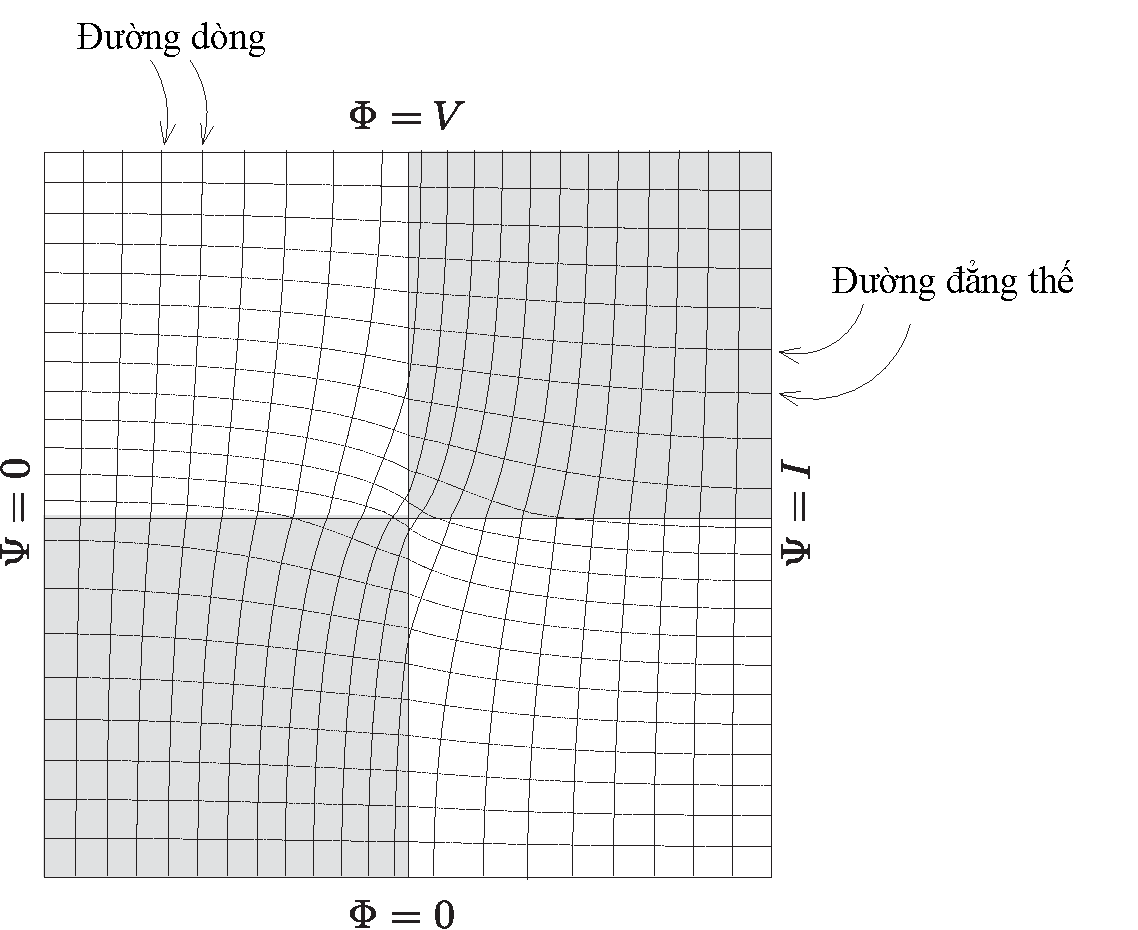
\includegraphics[scale=0.6]{Anh/Nam2.pdf}
    \end{center}
     Vì điều kiện biên, các đường dòng và đường sức từ bị gấp khúc khi gặp các bề mặt phân cách, tương tự như sự truyền ánh sáng.
  \end{itemize}
\end{loigiai}


%\chapter{Điện từ trường và cảm ứng điện từ}

\begin{vd}[Dịch chuyển nam châm]
Hai thanh nam châm giống hệt nhau được đặt cách nhau như hình vẽ.
\begin{center}


\tikzset{every picture/.style={line width=0.75pt}} %set default line width to 0.75pt        

\begin{tikzpicture}[x=0.75pt,y=0.75pt,yscale=-1,xscale=1]
%uncomment if require: \path (0,300); %set diagram left start at 0, and has height of 300

%Shape: Rectangle [id:dp5022362522100339] 
\draw  [color={rgb, 255:red, 0; green, 0; blue, 0 }  ,draw opacity=1 ][fill={rgb, 255:red, 74; green, 74; blue, 74 }  ,fill opacity=1 ] (129,123.4) -- (139.7,123.4) -- (139.7,148) -- (129,148) -- cycle ;
%Shape: Rectangle [id:dp35545825300116207] 
\draw   (129,148) -- (139.7,148) -- (139.7,172.6) -- (129,172.6) -- cycle ;
%Straight Lines [id:da3079932428464216] 
\draw  [dash pattern={on 4.5pt off 4.5pt}]  (139.7,148) -- (503.7,148) ;
%Shape: Rectangle [id:dp6572429819042589] 
\draw   (503.7,123.4) -- (514.4,123.4) -- (514.4,148) -- (503.7,148) -- cycle ;
%Shape: Rectangle [id:dp5289011457931987] 
\draw  [fill={rgb, 255:red, 74; green, 74; blue, 74 }  ,fill opacity=1 ] (503.7,148) -- (514.4,148) -- (514.4,172.6) -- (503.7,172.6) -- cycle ;


% Text Node
\draw (128,102) node [anchor=north west][inner sep=0.75pt]   [align=left] {N};
% Text Node
\draw (128,177) node [anchor=north west][inner sep=0.75pt]   [align=left] {S};
% Text Node
\draw (502.7,176.6) node [anchor=north west][inner sep=0.75pt]   [align=left] {N};
% Text Node
\draw (503,103) node [anchor=north west][inner sep=0.75pt]   [align=left] {S};


\end{tikzpicture}
\end{center}
Trong trường hợp nào dưới đây cần tốn nhiều công hơn? Và tốn nhiều hơn bao nhiêu lần?
\begin{enumerate}[1)]
\item Trục của nam châm bên phải xoay chậm đi $180^\circ$ sao cho hai moment lưỡng cực từ song song nhau.
 \item Nam châm bên phải được đưa ra xa vô cực dọc theo đường nối hai nam châm.
 \end{enumerate}
\end{vd}

\begin{loigiai} \\
Chúng ta cần chú ý rằng, trong cả hai trường hợp, công thực hiện đều là tăng thế năng tương tác từ.\\
Xét thí nghiệm sau: Nam châm ở bên phải được đưa đi rất xa khỏi nam châm bên trái dọc theo đường nối hai nam châm, công thực hiện để chống lại lực hút giữa hai nam châm được đặt là một đơn vị. Đây là công cần thực hiện trong câu $2)$.\\
Tiếp theo, nam châm ở bên phải sau khi được đưa ra xa vô cùng sẽ được quay một góc $180^\circ$, không có công nào được thực hiện trong quá trình này bởi vì tương tác giữa hai nam châm lúc này là không đáng kể. Cuối cùng, nam châm sau khi xoay được đưa trở lại vị trí ban đầu của nó. Theo tính đối xứng, phần công thực hiện để chống lại lực đẩy trong quá tình này cũng là một đơn vị. Đây là công cần thực hiện ở phần $1)$ và minh chứng rằng công cần thực hiện trong quá trình này là hai đơn vị.\\
Trường điện từ là trường thế, tức là mọi thăng giáng của năng lượng tương tác từ chỉ phụ thuộc và vị trí đầu và vị trí cuối của vật chứ không phụ thuộc vào quá trình chúng ta di chuyển vật như thế nào. Do đó, chúng ta có thể suy ra, nếu chúng ta quay nam châm đi $180^o$ từ vị trí ban đầu, phần công cần thực hiện cũng là hai đơn vị. \\
Tóm lại, phần $1)$ tốn một phần công nhiều gấp đôi phần $2)$.
\end{loigiai}

\begin{vd}[Dòng điện do các electron chạy qua miền có từ trường]
Các electron và một vài nguyên tử có moment động lượng riêng được gọi là spin $(\ot{S})$, các spin đó có độ lớn không đổi nhưng hướng của chúng có thể thay đổi do moment của ngoại lực. Liên kết với các spin là các moment từ làm cho chúng giống như những lưỡng cực từ $\ot{m}=\mu_{B}\ot{S}$ với $\mu_{B}$ là một hằng số gọi là \textbf{magneton}. Để đơn giản, chúng ta giả sử rằng các electron và các nguyên tử có dùng độ lớn spin $S$ và \textbf{magneton}.
\begin{enumerate}[1) ]
    \item Tham khảo hình $A$ dưới đây. Lưỡng cực $A$ ở tại $\ot{r}=0$ và dọc theo $\ot{z_0}$, và lưỡng cực $B$ ở tại $\ot{r}=\alpha\ot{x_0}$ và dọc theo $\ot{y_0}$. Tìm moment lực do lưỡng cực $A$ tác dụng lên lưỡng cực $B$.
    \item Tìm hướng của lưỡng cực $B$ sau một khoảng thời gian ngắn $\Delta t$, giả sử rằng hướng của lưỡng cực $A$ vẫn không thay đổi.
    \item Hình $B$ là sơ đồ của một miền từ trường trong $(x_0,x_0+2b)$ có chứa nhiều nguyên tử (lưỡng cực $B$). Hướng của các lưỡng cực được chỉ ra như hình vẽ. Các lưỡng cực $B$ được cố định ở các khoảng cách bằng nhau trên trục $x$ (trong miền không gian là $2b$ có $10^4$ lưỡng cực $B$). Một electron (lưỡng cực $A$) bay và tác động lên lưỡng cực B như là câu trả lời của bạn ở phần $(2$). Hình $C$  cho biết góc ban đầu của các lưỡng cực. Lưỡng cực ở $x_0+b$ dọc theo $\ot{y_0}$, lưỡng cực ở $x\leq x_0$ dọc theo $-\ot{x_0}$ và lưỡng cực ở $x\geq x_0+2b$ dọc theo $\ot{x_0}$. Các lưỡng cực dọc theo $-\ot{x_0}$ còn có thể quay. Các lưỡng cực dọc theo $\ot{x_0}$ thì không thể quay, ngoại trừ những lưỡng cực ở gần mép (rìa) của miền có thể quay tự do một chút. Cho dòng điện bởi các hạt tải electron là $I$, tìm tốc độ chuyển động khi qua tâm miền khi dòng điện được bật lên. (cho rằng điện tích của electron là $e$ đã biết). 
    \item Tìm thời gian cần thiết để vượt qua toàn bộ miền.
    \end{enumerate}
(\textit{Gợi ý:} Từ trường $\ot{B}(\ot{r})$ tại vị trí $\ot{r}$ do lưỡng cực từ $\ot{m}$ tại gốc tọa độ được cho bởi $\ot{B}(\ot{r})=\dfrac{\mu_0}{4\pi r^3}\left[\dfrac{3(\ot{m}\cdot\ot{r})\ot{r}}{r^2}-\ot{m}\right]$. Moment lực $\ot{N}$ của từ trường hướng $\ot{B}$ tác dụng lên lưỡng cực $\ot{m}$ là $\ot{N}=\ot{m}\times\ot{B}$.)
\begin{center}



\tikzset{every picture/.style={line width=0.75pt}} %set default line width to 0.75pt        

\begin{tikzpicture}[x=0.75pt,y=0.75pt,yscale=-1,xscale=1]
%uncomment if require: \path (0,300); %set diagram left start at 0, and has height of 300

%Straight Lines [id:da4492620820243536] 
\draw    (29,125.45) -- (29,25.95) ;
\draw [shift={(29,22.95)}, rotate = 450] [fill={rgb, 255:red, 0; green, 0; blue, 0 }  ][line width=0.08]  [draw opacity=0] (10.72,-5.15) -- (0,0) -- (10.72,5.15) -- (7.12,0) -- cycle    ;
%Straight Lines [id:da3879660645016081] 
\draw    (29,125.45) -- (115.2,71.77) ;
\draw [shift={(117.75,70.19)}, rotate = 508.09] [fill={rgb, 255:red, 0; green, 0; blue, 0 }  ][line width=0.08]  [draw opacity=0] (10.72,-5.15) -- (0,0) -- (10.72,5.15) -- (7.12,0) -- cycle    ;
%Straight Lines [id:da3664498690573632] 
\draw    (34.33,148.91) -- (34.33,85.23) ;
\draw [shift={(34.33,82.23)}, rotate = 450] [fill={rgb, 255:red, 0; green, 0; blue, 0 }  ][line width=0.08]  [draw opacity=0] (10.72,-5.15) -- (0,0) -- (10.72,5.15) -- (7.12,0) -- cycle    ;
%Straight Lines [id:da03392174383237889] 
\draw    (29,125.45) -- (168,124.54) ;
\draw [shift={(171,124.52)}, rotate = 539.63] [fill={rgb, 255:red, 0; green, 0; blue, 0 }  ][line width=0.08]  [draw opacity=0] (10.72,-5.15) -- (0,0) -- (10.72,5.15) -- (7.12,0) -- cycle    ;
%Straight Lines [id:da667880177313547] 
\draw    (108.88,135.94) -- (145.4,112.56) ;
\draw [shift={(147.93,110.94)}, rotate = 507.37] [fill={rgb, 255:red, 0; green, 0; blue, 0 }  ][line width=0.08]  [draw opacity=0] (10.72,-5.15) -- (0,0) -- (10.72,5.15) -- (7.12,0) -- cycle    ;


%Straight Lines [id:da9465992584207192] 
\draw    (22,258.31) -- (22,172.53) ;
\draw [shift={(22,169.53)}, rotate = 450] [fill={rgb, 255:red, 0; green, 0; blue, 0 }  ][line width=0.08]  [draw opacity=0] (10.72,-5.15) -- (0,0) -- (10.72,5.15) -- (7.12,0) -- cycle    ;
%Straight Lines [id:da9778405244192359] 
\draw    (22,258.31) -- (211,258.31) ;
\draw [shift={(214,258.31)}, rotate = 180] [fill={rgb, 255:red, 0; green, 0; blue, 0 }  ][line width=0.08]  [draw opacity=0] (10.72,-5.15) -- (0,0) -- (10.72,5.15) -- (7.12,0) -- cycle    ;
%Straight Lines [id:da3787820827861692] 
\draw    (95.28,269.55) -- (95.28,238.85) ;
\draw [shift={(95.28,235.85)}, rotate = 450] [fill={rgb, 255:red, 0; green, 0; blue, 0 }  ][line width=0.08]  [draw opacity=0] (10.72,-5.15) -- (0,0) -- (10.72,5.15) -- (7.12,0) -- cycle    ;
%Straight Lines [id:da6658921469128833] 
\draw    (104.55,266.34) -- (113.82,237.9) ;
\draw [shift={(114.75,235.05)}, rotate = 468.06] [fill={rgb, 255:red, 0; green, 0; blue, 0 }  ][line width=0.08]  [draw opacity=0] (10.72,-5.15) -- (0,0) -- (10.72,5.15) -- (7.12,0) -- cycle    ;
%Straight Lines [id:da4077367348968337] 
\draw    (86,266.34) -- (77.6,238.72) ;
\draw [shift={(76.72,235.85)}, rotate = 433.08000000000004] [fill={rgb, 255:red, 0; green, 0; blue, 0 }  ][line width=0.08]  [draw opacity=0] (10.72,-5.15) -- (0,0) -- (10.72,5.15) -- (7.12,0) -- cycle    ;
%Straight Lines [id:da9033165151070539] 
\draw    (74.87,262.33) -- (61.77,243.91) ;
\draw [shift={(60.03,241.47)}, rotate = 414.57] [fill={rgb, 255:red, 0; green, 0; blue, 0 }  ][line width=0.08]  [draw opacity=0] (10.72,-5.15) -- (0,0) -- (10.72,5.15) -- (7.12,0) -- cycle    ;
%Straight Lines [id:da5709523099777032] 
\draw    (116.61,261.52) -- (131.34,244.54) ;
\draw [shift={(133.3,242.27)}, rotate = 490.93] [fill={rgb, 255:red, 0; green, 0; blue, 0 }  ][line width=0.08]  [draw opacity=0] (10.72,-5.15) -- (0,0) -- (10.72,5.15) -- (7.12,0) -- cycle    ;
%Straight Lines [id:da44092929640949885] 
\draw    (128.67,259.92) -- (143.92,248.12) ;
\draw [shift={(146.29,246.28)}, rotate = 502.27] [fill={rgb, 255:red, 0; green, 0; blue, 0 }  ][line width=0.08]  [draw opacity=0] (10.72,-5.15) -- (0,0) -- (10.72,5.15) -- (7.12,0) -- cycle    ;
%Straight Lines [id:da6575017322814591] 
\draw    (63.74,260.72) -- (48.38,247.44) ;
\draw [shift={(46.12,245.48)}, rotate = 400.86] [fill={rgb, 255:red, 0; green, 0; blue, 0 }  ][line width=0.08]  [draw opacity=0] (10.72,-5.15) -- (0,0) -- (10.72,5.15) -- (7.12,0) -- cycle    ;
%Straight Lines [id:da09095595030926118] 
\draw    (48.9,255.91) -- (35.05,251.25) ;
\draw [shift={(32.2,250.29)}, rotate = 378.59000000000003] [fill={rgb, 255:red, 0; green, 0; blue, 0 }  ][line width=0.08]  [draw opacity=0] (10.72,-5.15) -- (0,0) -- (10.72,5.15) -- (7.12,0) -- cycle    ;
%Straight Lines [id:da8512931349485788] 
\draw    (143.51,255.91) -- (159.19,251.16) ;
\draw [shift={(162.06,250.29)}, rotate = 523.1600000000001] [fill={rgb, 255:red, 0; green, 0; blue, 0 }  ][line width=0.08]  [draw opacity=0] (10.72,-5.15) -- (0,0) -- (10.72,5.15) -- (7.12,0) -- cycle    ;
%Straight Lines [id:da14846896037639024] 
\draw  [dash pattern={on 0.84pt off 2.51pt}]  (54.46,210.18) -- (124.74,210.18) ;
\draw [shift={(127.74,210.18)}, rotate = 180] [fill={rgb, 255:red, 0; green, 0; blue, 0 }  ][line width=0.08]  [draw opacity=0] (10.72,-5.15) -- (0,0) -- (10.72,5.15) -- (7.12,0) -- cycle    ;
%Straight Lines [id:da5150132226935988] 
\draw    (321.34,125.07) -- (321.34,31.59) ;
\draw [shift={(321.34,28.59)}, rotate = 450] [fill={rgb, 255:red, 0; green, 0; blue, 0 }  ][line width=0.08]  [draw opacity=0] (10.72,-5.15) -- (0,0) -- (10.72,5.15) -- (7.12,0) -- cycle    ;
%Straight Lines [id:da35548173749016] 
\draw    (321.34,125.07) -- (458.74,124.22) ;
\draw [shift={(461.74,124.2)}, rotate = 539.64] [fill={rgb, 255:red, 0; green, 0; blue, 0 }  ][line width=0.08]  [draw opacity=0] (10.72,-5.15) -- (0,0) -- (10.72,5.15) -- (7.12,0) -- cycle    ;

%Straight Lines [id:da6685787959685461] 
\draw    (335.38,55.03) -- (364.34,55.03) ;
%Straight Lines [id:da5287919204143205] 
\draw    (399.43,107.34) -- (467,107.34) ;
%Straight Lines [id:da9848832862195076] 
\draw    (364.34,55.03) -- (399.43,107.34) ;
%Straight Lines [id:da2528288642770211] 
\draw  [dash pattern={on 0.84pt off 2.51pt}]  (399.43,107.34) -- (399.43,124.78) ;
%Straight Lines [id:da7577180254188209] 
\draw  [dash pattern={on 0.84pt off 2.51pt}]  (364.34,55.03) -- (364.34,122.46) ;
%Straight Lines [id:da3431528400294237] 
\draw  [dash pattern={on 0.84pt off 2.51pt}]  (321.34,107.34) -- (399.43,107.34) ;

%Shape: Circle [id:dp16187367515635387] 
\draw  [fill={rgb, 255:red, 0; green, 0; blue, 0 }  ,fill opacity=1 ] (39,210.51) .. controls (39,208.02) and (41.02,206) .. (43.51,206) .. controls (46,206) and (48.02,208.02) .. (48.02,210.51) .. controls (48.02,213) and (46,215.02) .. (43.51,215.02) .. controls (41.02,215.02) and (39,213) .. (39,210.51) -- cycle ;


% Text Node
\draw (149.02,126.8) node [anchor=north west][inner sep=0.75pt]    {$x$};
% Text Node
\draw (94,56.41) node [anchor=north west][inner sep=0.75pt]    {$y$};
% Text Node
\draw (36.31,15.66) node [anchor=north west][inner sep=0.75pt]    {$z$};
% Text Node
\draw (57.25,141.15) node [anchor=north west][inner sep=0.75pt]   [align=left] {Hình $\displaystyle A$};
% Text Node
\draw (450.47,129.51) node [anchor=north west][inner sep=0.75pt]  [font=\small]  {$x$};
% Text Node
\draw (356.21,128.35) node [anchor=north west][inner sep=0.75pt]  [font=\small]  {$x_{0}$};
% Text Node
\draw (381.01,128.22) node [anchor=north west][inner sep=0.75pt]  [font=\small]  {$x_{0} +2b$};
% Text Node
\draw (304.77,12.22) node [anchor=north west][inner sep=0.75pt]  [font=\small] [align=left] {Góc};
% Text Node
\draw (303.75,100.68) node [anchor=north west][inner sep=0.75pt]  [font=\small]  {$0^{\circ }$};
% Text Node
\draw (289.36,46.63) node [anchor=north west][inner sep=0.75pt]  [font=\small]  {$180^{\circ }$};
% Text Node
\draw (368.35,144.55) node [anchor=north west][inner sep=0.75pt]   [align=left] {Hình $\displaystyle C$};
% Text Node
\draw (193.09,264.07) node [anchor=north west][inner sep=0.75pt]    {$x$};
% Text Node
\draw (32.7,169.42) node [anchor=north west][inner sep=0.75pt]    {$y$};
% Text Node
\draw (74.06,271.51) node [anchor=north west][inner sep=0.75pt]   [align=left] {Hình $\displaystyle B$};


\end{tikzpicture}
\end{center}
\end{vd}

\begin{loigiai}
\begin{enumerate}[1)]
    \item Moment lực là
    \[\ot{\tau}=\dfrac{\mu_0}{4\pi a^3}\ot{m_{\mathrm{A}}}\times\ot{m_{\mathrm{B}}}=-\dfrac{\mu_0(\mu_{\mathrm{B}}S)^2}{4\pi a^3}\ot{x_0}~\text{vuông góc với}~\ot{m_{\mathrm{B}}}.\]
    \begin{center}
\tikzset{every picture/.style={line width=0.75pt}} %set default line width to 0.75pt        

\begin{tikzpicture}[x=0.75pt,y=0.75pt,yscale=-1,xscale=1]
%uncomment if require: \path (0,300); %set diagram left start at 0, and has height of 300

%Straight Lines [id:da9599488966246523] 
\draw    (239,210.33) -- (195.88,69.15) ;
\draw [shift={(195,66.28)}, rotate = 433.01] [fill={rgb, 255:red, 0; green, 0; blue, 0 }  ][line width=0.08]  [draw opacity=0] (10.72,-5.15) -- (0,0) -- (10.72,5.15) -- (7.12,0) -- cycle    ;
%Straight Lines [id:da4147110006600949] 
\draw    (239,210.33) -- (271.32,71.23) ;
\draw [shift={(272,68.31)}, rotate = 463.08] [fill={rgb, 255:red, 0; green, 0; blue, 0 }  ][line width=0.08]  [draw opacity=0] (10.72,-5.15) -- (0,0) -- (10.72,5.15) -- (7.12,0) -- cycle    ;
%Straight Lines [id:da5247662187374407] 
\draw    (272,68.31) -- (198,68.31) ;
\draw [shift={(195,68.31)}, rotate = 360] [fill={rgb, 255:red, 0; green, 0; blue, 0 }  ][line width=0.08]  [draw opacity=0] (10.72,-5.15) -- (0,0) -- (10.72,5.15) -- (7.12,0) -- cycle    ;

% Text Node
\draw (263.75,125.93) node [anchor=north west][inner sep=0.75pt]  [font=\small]  {$S$};
% Text Node
\draw (227.13,50.66) node [anchor=north west][inner sep=0.75pt]  [font=\small]  {$\Delta S$};


\end{tikzpicture}
    \end{center}
    \item Moment lực là nguyên nhân làm cho $\ot{S_{\mathrm{B}}}$ quay trong mặt phẳng $x-y$, và tốc độ góc được cho bởi $\tau=S\omega$.\\
    Góc hợp với trục $y$ là
    \[\Delta\theta=\omega\Delta t=\dfrac{\mu_0}{4\pi a^3}\mu_{\mathrm{b}}^2S\Delta t.\]
    \item Hãy tìm số lượng electron phải vượt qua để tạo ra một spin đặc biệt để quay từ $90^\circ - \mathrm{d}\theta$ tới $90^\circ$ và từ $\theta$ tìm vị trí của spin.
    \begin{align*}
        \left(\dfrac{I}{e}\Delta\theta\right)\mathrm{d}t&=\mathrm{d}\theta=\dfrac{\pi}{2b}\mathrm{d}x.\\
        v&=\dfrac{\mathrm{d}x}{\mathrm{d}t}=\dfrac{2bI}{\pi e}\Delta\theta=\dfrac{\mu_0}{2e\pi^2a^3}bI\mu^2_{\mathrm{b}}S\Delta t.
    \end{align*}
    \begin{center}
 

\tikzset{every picture/.style={line width=0.75pt}} %set default line width to 0.75pt        

\begin{tikzpicture}[x=0.75pt,y=0.75pt,yscale=-1,xscale=1]
%uncomment if require: \path (0,300); %set diagram left start at 0, and has height of 300

%Straight Lines [id:da6598694439969128] 
\draw    (160.84,208.69) -- (160.84,70.81) ;
\draw [shift={(160.84,67.81)}, rotate = 450] [fill={rgb, 255:red, 0; green, 0; blue, 0 }  ][line width=0.08]  [draw opacity=0] (10.72,-5.15) -- (0,0) -- (10.72,5.15) -- (7.12,0) -- cycle    ;
%Straight Lines [id:da6810032084360103] 
\draw    (160.84,208.69) -- (472.21,207.43) ;
\draw [shift={(475.21,207.42)}, rotate = 539.77] [fill={rgb, 255:red, 0; green, 0; blue, 0 }  ][line width=0.08]  [draw opacity=0] (10.72,-5.15) -- (0,0) -- (10.72,5.15) -- (7.12,0) -- cycle    ;

%Straight Lines [id:da7910578702301538] 
\draw    (192.28,106.43) -- (257.12,106.43) ;
%Straight Lines [id:da13220931113446555] 
\draw    (335.71,182.8) -- (487,182.8) ;
%Straight Lines [id:da17089054030238615] 
\draw    (257.12,106.43) -- (335.71,182.8) ;
%Straight Lines [id:da6135971059333494] 
\draw  [dash pattern={on 0.84pt off 2.51pt}]  (335.71,182.8) -- (335.71,208.26) ;
%Straight Lines [id:da40308318362058393] 
\draw  [dash pattern={on 0.84pt off 2.51pt}]  (257.12,106.43) -- (257.12,208.33) ;
%Straight Lines [id:da29183622476100535] 
\draw  [dash pattern={on 0.84pt off 2.51pt}]  (160.84,182.8) -- (335.71,182.8) ;
%Straight Lines [id:da5842701379801969] 
\draw  [dash pattern={on 0.84pt off 2.51pt}]  (253.12,106.43) -- (269,106.43) ;
%Straight Lines [id:da24335614573950703] 
\draw  [dash pattern={on 0.84pt off 2.51pt}]  (503,182.8) -- (346,182.8) ;
%Straight Lines [id:da8478129293644809] 
\draw  [dash pattern={on 0.84pt off 2.51pt}]  (267.41,106.43) -- (346,182.8) ;

% Text Node
\draw (455.42,213.21) node [anchor=north west][inner sep=0.75pt]  [font=\small]  {$x$};
% Text Node
\draw (250.84,211.74) node [anchor=north west][inner sep=0.75pt]  [font=\small]  {$x_{0}$};
% Text Node
\draw (321.57,209.55) node [anchor=north west][inner sep=0.75pt]  [font=\small]  {$x_{0} +2b$};
% Text Node
\draw (146.47,51.37) node [anchor=north west][inner sep=0.75pt]  [font=\small] [align=left] {Góc};
% Text Node
\draw (141.75,176.34) node [anchor=north west][inner sep=0.75pt]  [font=\small]  {$0^{\circ }$};
% Text Node
\draw (129.45,97.42) node [anchor=north west][inner sep=0.75pt]  [font=\small]  {$180^{\circ }$};
% Text Node
\draw (296.47,241.27) node [anchor=north west][inner sep=0.75pt]   [align=left] {Hình $\displaystyle C$};


\end{tikzpicture}
    \end{center}
    \item 
    \[t=\dfrac{2b}{v}=\dfrac{4e\pi^2a^3}{\mu_0I\mu^2_{\mathrm{b}}S\Delta t}.\]
\end{enumerate}
\end{loigiai}

\begin{vd}[Độ từ hóa]
\begin{enumerate}[1)]
    \item Một cái đĩa có bán kính $R$ và bề dày $d(\ll R)$ được từ hóa đều với từ tính vuông góc với mặt đĩa. Tìm từ trường tại điểm $O$ trên trục đi qua tâm đĩa và ở cách tâm đĩa một khoảng $h$. 
    \item Một hình trụ dài được từ hóa trung bình với độ từ hóa $\ot{M}$ dọc theo trục hình trụ. Tìm từ trường bên trong và bên ngoài của hình trụ đó.
\end{enumerate}
\end{vd}
\begin{loigiai}
\begin{enumerate}[1) ]
    \item Mật độ dòng điện liên kết của đĩa là:
    \[K=-\ot{M}\times\ot{n}=-M,\]
    Dòng điện là: $I=Jd=-Md,$\\
    Từ trường:
    \[B(z=h)=\dfrac{\mu_0R^2I}{2(R^2+h^2)^{\dfrac{3}{2}}}=-\dfrac{\mu_0R^2Md}{2(R^2+h^2)^{\dfrac{3}{2}}}.\]
    \item Mật độ dòng điện liên kết là $K=-\ot{M}\times\ot{n}=-M$, đó là trên thành bên của hình trụ.\\
    Bài toán này khi đó giống như một ống solenoid dài. Sử dụng vòng Ampere nhỏ ta có ở bên trong $B=\mu_0K=\mu_0M$ và ở bên ngoài $B=0$.
\end{enumerate}
\end{loigiai} 

\begin{vd}[Các đơn cực từ]
    \begin{center}
      

\tikzset{every picture/.style={line width=0.75pt}} %set default line width to 0.75pt        

\begin{tikzpicture}[x=0.75pt,y=0.75pt,yscale=-1,xscale=1]
%uncomment if require: \path (0,300); %set diagram left start at 0, and has height of 300

%Straight Lines [id:da22909332327350906] 
\draw    (240,90) -- (240,239.2) ;
%Straight Lines [id:da6765772392847864] 
\draw    (290,117.2) -- (290,184.2) ;
\draw [shift={(290,114.2)}, rotate = 90] [fill={rgb, 255:red, 0; green, 0; blue, 0 }  ][line width=0.08]  [draw opacity=0] (10.72,-5.15) -- (0,0) -- (10.72,5.15) -- (7.12,0) -- cycle    ;
%Straight Lines [id:da7347835505124456] 
\draw    (290,184.2) -- (308.02,184.2) ;
\draw [shift={(311.02,184.2)}, rotate = 180] [fill={rgb, 255:red, 0; green, 0; blue, 0 }  ][line width=0.08]  [draw opacity=0] (10.72,-5.15) -- (0,0) -- (10.72,5.15) -- (7.12,0) -- cycle    ;

% Text Node
\draw (285,95.4) node [anchor=north west][inner sep=0.75pt]    {$x$};
% Text Node
\draw (312,182.4) node [anchor=north west][inner sep=0.75pt]    {$z$};
% Text Node
\draw (252,96.4) node [anchor=north west][inner sep=0.75pt]    {$1$};
% Text Node
\draw (211,96.4) node [anchor=north west][inner sep=0.75pt]    {$2$};


\end{tikzpicture}
    \end{center}
Định lí duy nhất của lí thuyết điện từ trường chỉ ra rằng điện tích ảo (điện tích ảnh) có thể được đặt bên ngoài không gian kín, trong đó trường ảnh đó được xác định bằng cách bắt chước điều kiện biên gốc. \textbf{Trường bên trong} không gian kín đó giống như trường được tạo ra bởi các điện tích thật bên trong không gian và các điện tích ảo bên ngoài không gian đó. Đối với một mặt mà không có các điện tích tự do và dòng điện tự do, các điều kiện biên cho điện trường $\ot{E}$, điện cảm $\ot{D}$, từ trường $\ot{B}$, và cảm ứng từ $\ot{H}$ là $\ot{E^{\parallel}_1}=\ot{E^{\parallel}_2}$, $\ot{D_1^{\bot}}=\ot{D_2^{\bot}}$, $\ot{B_1^{\bot}}=\ot{B_2^{\bot}}$, $\ot{H^{\parallel}_1}=\ot{H^{\parallel}_2}$. Ở đây kí hiệu ``$\bot$'' nghĩa là thành phần vuông góc với bề mặt và ``$\parallel$'' nghĩa là thành phần song song với mặt đó.
\begin{enumerate}[1) ]
    \item Xét trường hợp một điện tích điểm $q$ trong môi trường $1$ tại khoảng cách $d$ tính từ bề mặt chung giữa hai môi trường điện môi có các hằng số điện môi tương ứng là $\varepsilon_1$ và $\varepsilon_2$. Trục $Z$ vuông góc với bề mặt chung, điện tích điểm $q$ nằm trên trục $Z$, và bề mặt chung tại $z=0$. Hai điện tích ảnh $q_1$ và $q_2$ được sử dụng để giải bài toán này. Trong môi trường $2$, điện trường bằng với những gì được tạo ra bởi một điện tích điểm $(q_1+\dfrac{q}{\varepsilon_1})$ tại điểm có tọa độ $(0,0,d)$. Điện trường ở trong môi trường $1$ bằng với điện trường toàn phần được tạo ra bởi một điện tích điểm $\dfrac{q}{\varepsilon_1}$ tại vị trí $(0,0,d)$ và một điện tích điểm $q_2$ tại vị trí $(0,0,-d)$.
    \begin{enumerate}[a) ]
        \item Áp dụng các điều kiện biên nói trên để xác định các điện tích $q_1$ và $q_2$.
        \item Xác định mật độ điện tích mặt toàn phần tại bề mặt.
        \item Kiểm tra lại kết quả của bạn bằng điều kiện đặc biệt $\varepsilon_1=\varepsilon_2$.
        \item Kiểm tra lại câu trả lời của bạn với điều kiện đặc biệt $\varepsilon_1\ll\varepsilon_2$.
    \end{enumerate}
    \item Một lưỡng cực từ được làm bằng cực nam và cực bắc. Thật thú vị, cho đến nay không có đơn cực từ, cụ thể là các vật thể chỉ mang một cực nam hoặc một cực bắc, đã từng được phát hiện. Nếu một đơn cực từ giống như một ``điện tích từ'' $g$ tồn tại, nó sẽ tạo ra một từ trường giống như một điện tích điểm điện tạo ra một điện trường. Gần đây, các hạt giả hoạt động giống như một đơn cực từ được tạo ra bởi tập hợp các chuyển động của các electron trong một kiểu vật liệu được gọi là ``chất cách điện topo'', theo lí thuyết đã được dự đoán. Hạt như vậy có thể được gây ra bởi một điện tích điểm bên ngoài. Tương tự như phần $1)$, điện tích điểm $q$ được đặt ở khoảng cách $d$ đối với một mặt giữa một môi trường điện môi thông thường (môi trường $1$) với hằng số điện môi $\varepsilon_1$ và độ từ thẩm $\mu_1$, và một chất cách điện tôpô (môi trường $2$) với hằng số điện môi $\varepsilon_2$, độ từ thẩm thấu $\mu_2$, và hằng số liên hợp từ $-$ điện $\beta$. Quan hệ giữa các trường biến đổi trong môi trường $1$ là $\ot{D_1}=\varepsilon_1\ot{E}$ và $\ot{H_1}=\dfrac{\ot{B_1}}{\mu_1}$. Ở trong môi trường $2$ là $\ot{D_2}=\varepsilon_2\ot{E}-\beta\ot{B_2}$ và $\ot{H_2}=\dfrac{\ot{B_2}}{\mu_2}+\beta\ot{E_2}$.\\
    Điện trường và từ trường trong cả hai môi trường có thể được tìm thấy bằng cách sử dụng các điện tích ảnh như trong phần $1)$. Để đơn giản, chúng ta sử dụng một bộ các đơn vị được chọn lọc đặc biệt để điện trường tại vị trí $\ot{r}$ được tạo ra bởi một điện tích điểm $q$ tại vị trí $\ot{r_0}$ là $\ot{E}(\ot{r})=q\dfrac{\ot{r}-\ot{r_0}}{\abs{\ot{r}-\ot{r_0}}^3}$ và từ trường được tạo ra bởi một đơn cực từ của một điện tích từ $g$ trong một không gian tương tự là $\ot{B}(\ot{r})=g\dfrac{\ot{r}-\ot{r_0}}{\abs{\ot{r}-\ot{r_0}}^3}$.\\
    Trong môi trường $2$, điện trường được tạo ra bởi một điện tích điểm là $(q_1+\dfrac{q}{\varepsilon_1})$ tại vị trí $(0,0,d)$, và từ trường được tạo ra bởi một đơn cực từ với điện tích từ $g_1$ tại vị trí $(0,0,d)$. Trong môi trường $1$, điện trường được tạo ra bởi một điện tích điểm $\dfrac{q}{\varepsilon_1}$ tại vị trí $(0,0,d)$, và một điện tích điểm $q_2$ tại vị trí $(0,0,-d)$, và từ trường được tạo ra bởi một đơn cực từ với điện tích từ $g_2$ tại vị trí $(0,0,-d)$.
    \begin{enumerate}[a)]
        \item Sử dụng điều kiện biên để xác định $q_1$, $q_2$, $g_1$ và $g_2$.
        \item Tìm mật độ điện tích mặt toàn phần tại bề mặt chung. Để câu trả lời của bạn ngắn gọn hơn, hãy coi như $q_1$ và $g_1$ đã biết.
        \item Tìm mật độ dòng điện toàn phần tại bề mặt chung. Khi mật độ dòng điện là một đại lượng vector bạn phải tìm hai thành phần song song và vuông góc với bề mặt chung. Để câu trả lời của bạn ngắn gọn hơn, hãy coi như $q_1$ và $g_1$ đã biết.
    \end{enumerate}
\end{enumerate}
\end{vd}
\begin{loigiai}
\begin{enumerate}[1)]
    \item 
    \begin{enumerate}[a)]
        \item Ta có
        \begin{align*}
        \ot{E_1}&=\dfrac{x\ot{x_0}+y\ot{y_0}+(z-d)\ot{z_0}}{[x^2+y^2+(z-d)]^{\frac{3}{2}}}\dfrac{q}{\varepsilon_1}+\dfrac{x\ot{x_0}+y\ot{y_0}+(z+d)\ot{z_0}}{[x^2+y^2+(z+d)]^{\frac{3}{2}}}q_2,~~~z>0,\\
        \ot{E_2}&=\dfrac{x\ot{x_0}+y\ot{y_0}+(z-d)\ot{z_0}}{[x^2+y^2+(z-d)]^{\frac{3}{2}}}\left(\dfrac{q}{\varepsilon_1}+q_1\right),~~~z<0.
    \end{align*}
    Cho đủ điểm nếu hệ số $\dfrac{1}{4\pi\varepsilon_0}$ xuất hiện trong các câu trả lời trên.
    \begin{align*}
        \ot{D_2} &= \varepsilon_2\ot{E_2},~~\ot{D_1}=\varepsilon\ot{E_1},\\
        \ot{D_1^{\bot}} &= \ot{D_2^{\bot}}\rt \varepsilon_1q_2-q=-\varepsilon_2\left(\dfrac{q}{\varepsilon_1}+q_1\right),\tag{1} \label{cg.sang.2.2.1}\\
        \ot{E_1^{\parallel}} &= \ot{E_2^{\parallel}}\rt q_2=q_1. \tag{2} \label{cg.sang.2.2.2}
    \end{align*}
    Giải hệ (\ref{cg.sang.2.2.1}) và (\ref{cg.sang.2.2.2}) ta được 
    \[q_1=q_2=\left(\dfrac{\varepsilon_1-\varepsilon_2}{\varepsilon_1+\varepsilon_2}\right)\left(\dfrac{q}{\varepsilon_1}\right).\]
    \item 
    \[\sigma=4\pi(E_1^{\bot}-E_2^{bot})=4\pi\left(\dfrac{d}{[x^2+y^2+d^2]^{\frac{3}{2}}}\left(q_2-\dfrac{q}{\varepsilon_1}+\dfrac{q}{\varepsilon_1}+q_1\right)\right)=\dfrac{8\pi dq_1}{[x^2+y^2+d^2]^{\frac{3}{2}}}.\]
    Cho đủ điểm nếu $\varepsilon_0$ thay vì $4\pi$ ở kết quả trên.
    \item $\varepsilon_1=\varepsilon_2$, $q_1=q_2=0$. Bề mặt không có điện tích ảnh.
    \item $q_1=q_2=-\dfrac{q}{\varepsilon_1}$, $\ot{E_2}=0$, không có điện trường ở trong kim loại lí tưởng. $\ot{E_1}$ được xác định bởi một điện tích ảnh $q_2=-\dfrac{q}{\varepsilon_1}$ và điện tích thật $\dfrac{q}{\varepsilon_1}$.
    \end{enumerate}
    \item 
    \begin{enumerate}[a)]
        \item 
        $\ot{D_2}=\varepsilon_2\ot{E_2}-\beta\ot{B_2}$, $\ot{D_1}=\varepsilon_1\ot{E_1}$, $\ot{H_2}=\dfrac{\ot{B_2}}{\mu_2}+\beta\ot{E_2}$, $\ot{H_1}=\dfrac{\ot{B_1}}{\mu_1}$.
        \begin{align*}
            &\ot{E_1}=\dfrac{x\ot{x_0}+y\ot{y_0}+(z-d)\ot{z_0}}{[x^2+y^2+(z-d)^2]^{\frac{3}{2}}}\dfrac{q}{\varepsilon_1}+\dfrac{x\ot{x_0}+y\ot{y_0}+(z+d)\ot{z_0}}{[x^2+y^2+(z+d)^2]^{\frac{3}{2}}}q_2, ~z>0\\
            &\ot{E_2}=\dfrac{x\ot{x_0}+y\ot{y_0}+(z-d)\ot{z_0}}{[x^2+y^2+(z-d)^2]^{\frac{3}{2}}}\left(\dfrac{q}{\varepsilon_1}+q_1\right), ~z<0\\
            &\ot{B_1}=\dfrac{x\ot{x_0}+y\ot{y_0}+(z+d)\ot{z_0}}{[x^2+y^2+(z+d)^2]^{\frac{3}{2}}}g_2, ~z>0\\
            &\ot{B_2}=\dfrac{x\ot{x_0}+y\ot{y_0}+(z-d)\ot{z_0}}{[x^2+y^2+(z-d)^2]^{\frac{3}{2}}}g_1, ~z>0.
        \end{align*}
        Tại $z=0$, áp dụng các điều kiện biên.
        \item $\ot{B_1^{\bot}}=\ot{B_2^{\bot}}$
        \[\ot{B_1^{\bot}}=\dfrac{g_2\mathrm{d}\ot{z_0}}{[x^2+y^2+d^2]^{\frac{3}{2}}},~\ot{B_2^{\bot}}=\dfrac{-g_1\mathrm{d}\ot{z_0}}{[x^2+y^2+d^2]^{\frac{3}{2}}}\rt g_1=-g_2.\]
        \item $\ot{D_1^{\bot}}=\ot{D_2^{\bot}}$
        \begin{align*}
            &\ot{D_1}^{\bot}=\dfrac{-q\mathrm{d}\ot{z_0}}{[x^2+y^2+d^2]^{\frac{3}{2}}}+\dfrac{\varepsilon_1q_2\mathrm{d}\ot{z_0}}{[x^2+y^2+d^2]^{\frac{3}{2}}},\\
            &\ot{D_2^{\bot}}=\dfrac{-\left(\dfrac{q}{\varepsilon_1}+q_1\right)\varepsilon_2\mathrm{d}\ot{z_0}}{[x^2+y^2+d^2]^{\frac{3}{2}}}+\dfrac{\beta g_1\mathrm{d}\ot{z_0}}{[x^2+y^2+d^2]^{\frac{3}{2}}}.
        \end{align*}
        Do đó $\varepsilon_1q_2-q=\beta g_1-\varepsilon_2\left(\dfrac{q}{\varepsilon_1} +q_1\right)$.
        \item $\ot{E_1^{\parallel}}=\ot{E_2^{\parallel}}$
        \begin{align*}
           \ot{E_1^{\parallel}} =&\dfrac{x\ot{x_0}+y\ot{y_0}}{[x^2+y^2+d^2]^{\frac{3}{2}}}\dfrac{q}{\varepsilon_1}+\dfrac{x\ot{x_0}+y\ot{y_0}}{[x^2+y^2+d^2]^{\frac{3}{2}}}q_2\\
            \ot{E_2^{\parallel}}=&\dfrac{x\ot{x_0}+y\ot{y_0}}{[x^2+y^2+d^2]^{\frac{3}{2}}}\left(\dfrac{q}{\varepsilon_1}+q_1\right).
        \end{align*}
            Do đó 
            \[q_1=q_2.\tag{3} \label{cg.sang.2.2.3} \]
        \item $\ot{H_1^{\parallel}}=\ot{H_2^{\parallel}}$
        \begin{align*}
            \ot{H_1^{\parallel}}&=\dfrac{\ot{B_1^{\parallel}}}{\mu_2}=\dfrac{x\ot{x_0}+y\ot{y_0}}{[x^2+y^2+d^2]^{\frac{3}{2}}}\dfrac{g_2}{\mu_1}.\\
            \ot{H_2^{\parallel}}&=\dfrac{\ot{B_1^{\parallel}}}{\mu_2}+\beta\ot{E_2^{\parallel}}=\dfrac{x\ot{x_0}+y\ot{y_0}}{[x^2+y^2+d^2]^{\frac{3}{2}}}\dfrac{g_1}{\mu_2}+\dfrac{x\ot{x_0}+y\ot{y_0}}{[x^2+y^2+d^2]^{\frac{3}{2}}}\beta\left(\dfrac{q}{\varepsilon_1}+q_1\right).
        \end{align*}
        Do đó 
        \[\dfrac{g_2}{\mu_1}=\dfrac{g_1}{\mu_2}+\beta\left(\dfrac{q}{\varepsilon_1}+q_1\right). \tag{4} \label{cg.sang.2.2.4}\]
        Thay (\ref{cg.sang.2.2.1}) $-$ (\ref{cg.sang.2.2.3}) vào (\ref{cg.sang.2.2.4}) cuối cùng ta được
        \begin{align*}
            q_1 &= q_2 = \left(\dfrac{(\varepsilon_1 - \varepsilon_2) \left(\dfrac{1}{\mu_1} + \dfrac{1}{\mu_2}\right) -\beta^2}{(\varepsilon_1+\varepsilon_2)\left(\dfrac{1}{\mu_1}+\dfrac{1}{\mu_2}\right)+\beta^2}\right)\left(\dfrac{q}{\varepsilon_1}\right).\\
            g_2 &= -g_1 = \left(\dfrac{\beta}{(\varepsilon_1+\varepsilon_2)\left(\dfrac{1}{\mu_1}+\dfrac{1}{\mu_2}\right)+\beta^2}\right)\left(\dfrac{q}{\varepsilon_1}\right).
        \end{align*}
        Trong hệ đơn vị được sử dụng ở đây, định luật Gauss trở thành $ \nabla\cdot\ot{E}=4\pi\rho$ với $\rho$ là mật độ điện tích toàn phần.
        Mật độ điện tích mặt
        \[\sigma=4\pi(E_1^{\bot}-E_2^{\bot})=4\pi\left(\dfrac{d}{[x^2+y^2+d^2]^{\frac{3}{2}}}\left(q_2-\dfrac{q}{\varepsilon_1}+\dfrac{q}{\varepsilon_1}+q_1\right)\right)=\dfrac{8\pi dq_1}{[x^2+y^2+d^2]^{\frac{3}{2}}}.\]
        Tương tự, định luật Ampere bây giờ được viết là  $\nabla\times\ot{B}=4\pi\ot{J}$ với $\ot{J}$ là mật độ dòng điện. Không có hệ số $\mu_0$ mà thay vào đó là $4\pi$. Chọn một điểm nằm trên trục $X$ và lấy một đường kín có chiều dài là $L$ và độ cao gần bằng không.
        \begin{center}
            

\tikzset{every picture/.style={line width=0.75pt}} %set default line width to 0.75pt        

\begin{tikzpicture}[x=0.75pt,y=0.75pt,yscale=-1,xscale=1]
%uncomment if require: \path (0,300); %set diagram left start at 0, and has height of 300

%Straight Lines [id:da6688995942279288] 
\draw    (220,40.36) -- (220,230.36) ;
%Straight Lines [id:da8581026792782027] 
\draw  [dash pattern={on 4.5pt off 4.5pt}]  (250,90.2) -- (250,177.2) ;
\draw [shift={(250,180.2)}, rotate = 270] [fill={rgb, 255:red, 0; green, 0; blue, 0 }  ][line width=0.08]  [draw opacity=0] (10.72,-5.15) -- (0,0) -- (10.72,5.15) -- (7.12,0) -- cycle    ;
%Straight Lines [id:da6765706379121441] 
\draw  [dash pattern={on 4.5pt off 4.5pt}]  (190,93.2) -- (190,180.2) ;
\draw [shift={(190,90.2)}, rotate = 90] [fill={rgb, 255:red, 0; green, 0; blue, 0 }  ][line width=0.08]  [draw opacity=0] (10.72,-5.15) -- (0,0) -- (10.72,5.15) -- (7.12,0) -- cycle    ;
%Straight Lines [id:da1507804766416887] 
\draw  [dash pattern={on 4.5pt off 4.5pt}]  (193,180.2) -- (203.02,180.2) -- (250,180.2) ;
\draw [shift={(190,180.2)}, rotate = 0] [fill={rgb, 255:red, 0; green, 0; blue, 0 }  ][line width=0.08]  [draw opacity=0] (10.72,-5.15) -- (0,0) -- (10.72,5.15) -- (7.12,0) -- cycle    ;
%Straight Lines [id:da47356020778772123] 
\draw  [dash pattern={on 4.5pt off 4.5pt}]  (190,90.2) -- (247,90.2) ;
\draw [shift={(250,90.2)}, rotate = 180] [fill={rgb, 255:red, 0; green, 0; blue, 0 }  ][line width=0.08]  [draw opacity=0] (10.72,-5.15) -- (0,0) -- (10.72,5.15) -- (7.12,0) -- cycle    ;
%Straight Lines [id:da18579905489258697] 
\draw    (280,45.2) -- (280,130.2) ;
\draw [shift={(280,42.2)}, rotate = 90] [fill={rgb, 255:red, 0; green, 0; blue, 0 }  ][line width=0.08]  [draw opacity=0] (10.72,-5.15) -- (0,0) -- (10.72,5.15) -- (7.12,0) -- cycle    ;
%Straight Lines [id:da8596726109827932] 
\draw    (301.02,130.2) -- (280,130.2) ;
\draw [shift={(304.02,130.2)}, rotate = 180] [fill={rgb, 255:red, 0; green, 0; blue, 0 }  ][line width=0.08]  [draw opacity=0] (10.72,-5.15) -- (0,0) -- (10.72,5.15) -- (7.12,0) -- cycle    ;

% Text Node
\draw (240,67.4) node [anchor=north west][inner sep=0.75pt]  [font=\small]  {$1$};
% Text Node
\draw (186,67.4) node [anchor=north west][inner sep=0.75pt]  [font=\small]  {$2$};
% Text Node
\draw (276,26.4) node [anchor=north west][inner sep=0.75pt]  [font=\small]  {$x$};
% Text Node
\draw (302,112.4) node [anchor=north west][inner sep=0.75pt]  [font=\small]  {$z$};


\end{tikzpicture}
        \end{center}
        \begin{align*}
            \ot{B_1^{\parallel}}&=\dfrac{g_2}{x^2}\ot{x_0}=-\dfrac{g_1}{x^2}\ot{x_0}.\\
            \ot{B_2^{\parallel}}&=\dfrac{g_1}{x^2}\ot{x_0}.
        \end{align*}
        Đối với một vòng vuông góc với trục $X$ và dọc theo trục $Y$ (hướng ra ngoài mặt phẳng tờ giấy). Tích phân trên đường cong kín
        \[\oint_{\ell}\ot{B}\mathrm{d}\ot{\ell}=\ot{B_1^{\parallel}}\cdot L\ot{y_0}-\ot{B_2^\parallel}\cdot L\ot{y_0}=0-0=0.\]
        Đối với một vòng song song với trục $X$ như hình vẽ ta có
        \[\oint_{\ell}\ot{B}\mathrm{d}\ot{\ell}=-\ot{B_1^{\parallel}}\cdot L\ot{x_0}+\ot{B_2^{\parallel}}\cdot L \ot{x_0}=\dfrac{Lg_1}{x^2}+\dfrac{Lg_1}{x^2}=\dfrac{2Lg_1}{x^2}.\]
        Gọi mật độ dòng điện mặt là $K$, khi đó 
        \[\dfrac{2Lg_1}{x^2}=\oint_{\ell}\ot{B}\mathrm{d}\ot{\ell}=4\pi KL.\]
        Sử dụng quy tắc bàn tay phải ta có $\ot{K}=-\dfrac{g_1}{2\pi x^2}\ot{y_0}.$ 
        Vector này hướng vuông góc vào mặt tờ giấy. Nói chung ta có
        \[\ot{K}=\dfrac{g_1}{2\pi}\dfrac{(y\ot{x_0}-x\ot{y_0})}{(x^2+y^2)^{\frac{3}{2}}}.\]
        Có vài cách khác để dẫn tới kết quả trên đối với mật độ dòng điện đều là tốt.
    \end{enumerate}
\end{enumerate}
\end{loigiai}


\begin{vd}[Bi-a từ tính]
 Xét hai quả cầu điện môi đàn hồi tuyệt đối bán kính $r$ và khối lượng $m$, một quả cầu mang điện tích phân bố đẳng hướng $-q$ và quả cầu kia mang điện tích $+q$. Có từ trường đều $B$ song song với trục $Oz$ đủ mạnh để có thể bỏ qua tương tác tĩnh điện của hai điện tích, bỏ qua trọng lực và lực ma sát.
 \\Quả cầu thứ nhất (tích điện âm) chuyển động với vận tốc $v$ và va chạm với quả cầu thứ hai đang nằm yên ở gốc tọa độ. Va chạm là xuyên tâm, và ngay trước khi va chạm, vận tốc của quả cầu thứ nhất song song với trục $Ox$.
 \begin{enumerate}[1)]
     \item Vận tốc của quả cầu thứ hai ngay sau va chạm là bao nhiêu?
     \item Vẽ các quỹ đạo của các trọng tâm của cả hai quả bóng trong quá trình chuyển động sau đó.
     \item Vận tốc trung bình (độ lớn và hướng) của các quả cầu trong quá trình chuyển động sau đó của chúng là bao nhiêu?
 \end{enumerate}
\end{vd}
\begin{loigiai}
\begin{enumerate}[1)]
    \item Gọi vận tốc sau va chạm của hai quả bóng tương ứng là $v_1$, $v_2$. Áp dụng định luật bảo toàn năng lượng:
    $$\dfrac{mv^2}{2}=\dfrac{mv_1^2}{2}+\dfrac{mv_2^2}{2},$$
    hay
    $$v^2=v_1^2+v_2^2.$$
    Áp dụng định luật bảo toàn động lượng:
    $$mv=mv_1+mv_2,$$
    hay 
    $$v=v_1+v_2.$$
    Từ hai phương trình trên ta có: 
    $$v^2=v_2^2+(v-v_2)^2=v^2-2vv_2+v_2^2.$$
    \[ \Rightarrow \left[ \begin{gathered}
      {v_2} = 0 \hfill \\
      {v_2} = v \hfill \\ 
    \end{gathered}  \right.\]
    \item Các quả bóng chịu lực Lorentz do từ trường. Vì lực Lorentz có phương vuông góc với đường chuyển động và có độ lớn không đổi nên các quả cầu chuyển động theo quỹ đạo tròn. Lực Lorentz đóng vai trò là lực hướng tâm: 
    $$m\dfrac{v^2}{R}=qvB.$$
    Với bán kính quỹ đạo $$R=\dfrac{mv}{qB}$$
    và tốc độ góc $$\omega=\dfrac{v}{R}=\dfrac{qB}{m}.$$
    Do đó một trong các điện tích di chuyển dọc theo quỹ đạo tròn theo chiều kim đồng hồ và điện tích kia ngược chiều kim đồng hồ.
    \\Sau mỗi lần va chạm, một trong hai quả cầu chuyển động với vận tốc $v$ trong khi quả cầu kia đứng yên. Quả cầu chuyển động đi một phần của chu kì cyclotron đầy đủ (chiều chuyển động phụ thuộc vào dấu điện tích) trước khi va chạm xuyên tâm với quả cầu đang dừng. Động lượng được truyền cho quả cầu còn lại và quả cầu chuyển động trước đó lại đứng yên và chu kì đó lặp đi lặp lại. Trong những lần va chạm tiếp theo, các quả cầu bắt đầu trôi theo một hướng như trong hình.
    \begin{center}
        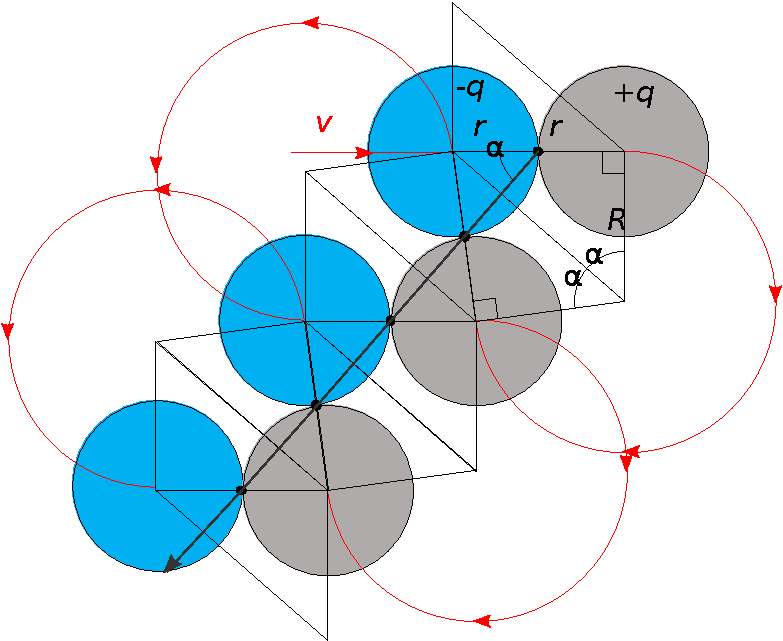
\includegraphics[scale=0.75]{Anh/Trung1.pdf}
    \end{center}
    \item Vận tốc trung bình của các quả cầu bằng vận tốc trung bình của các điểm va chạm. Từ hình vẽ, có thể thấy rằng hướng của vận tốc trung bình là $\pi-\alpha$ theo chiều kim đồng hồ tính từ hướng ban đầu của quả cầu tới, ta có: $$\alpha=\arctan{\dfrac{2r}{R}}.$$
    Độ dịch chuyển của điểm va chạm giữa hai lần là:
    $$d=rcos\alpha.$$
    Giữa hai lần va chạm, quả cầu di chuyển một góc $2\pi-2\alpha$ trên quỹ đạo tròn, do đó thời gian giữa hai lần va chạm là:
    $$t=\dfrac{2\pi-2\alpha}{\omega}=\dfrac{2m}{qB}\left(\pi-\arctan{\dfrac{2r}{R}}\right).$$
    Từ đó ta tính được vận tốc trung bình:
    $$v_{\mathrm{avg}}=\dfrac{d}{t}=\dfrac{r\omega\cos\alpha}{2(\pi-\alpha)}=\dfrac{vrR}{R\sqrt{4r^2+R^2}(\pi-\alpha)}=\dfrac{v}{\sqrt{4+\dfrac{R^2}{r^2}}\left(\pi-\arctan{\dfrac{2r}{R}}\right)}.$$
\end{enumerate}
\end{loigiai}

\begin{vd}[Cáp truyền tín hiệu]
    Một cáp truyền tín hiệu đối xứng trục được cấu tạo từ một lõi hình trụ bên trong bán kính $a=2\dv{cm}$ và một vỏ trụ bên ngoài đồng trục bán kính trong $b=5\dv{cm}$ và bán kính ngoài $c=7\dv{cm}$. Một dòng điện có độ lớn $I=5\dv{A}$ phân bố đều chạy trong lõi và một dòng điện khác cùng độ lớn, phân bố đều nhưng ngược chiều chạy trong vỏ ngoài. Tìm cảm ứng từ $B$ tại điểm cách trục cáp $r$.\\ 
    Tính $\displaystyle\int^\infty_0B(r)\mathrm{d}r$. 
\end{vd}
\begin{loigiai}
    Sử dụng định luật Ampere
    $$ \oint \ot{B} \cdot \ot{\mathrm{d}l}= \mu_0I.$$
    Ta thu được 
    $$ B(r)=\dfrac{\mu_0I(r)}{2\pi r}.$$
    \begin{itemize}
        \item[$*)$] Khi $r<a:$ $$ B(r)=\dfrac{\mu_0Ir}{2\pi a^2}. $$
        \item[$*)$] Khi $a\leq r<b:$  $$B(r)=\dfrac{\mu_0I}{2\pi r}.$$
        \item[$*)$] Khi $b\leq r<c:$  $$B(r)=\dfrac{\mu_0I}{2\pi}\left(\dfrac{c^2}{r(c^2-b^2)}-\dfrac{r}{c^2-b^2}\right).$$
        \item[$*)$] Khi $r\geq c:$ $$B(r)=0.$$
    \end{itemize}
    Suy ra: 
    \begin{equation*}
        \begin{aligned}
            \int_0^\infty B(r)\mathrm{d}r &= \int_0^a\dfrac{\mu_0Ir}{2\pi a^2}\mathrm{d}r + \int_a^b\dfrac{\mu_0I}{2\pi r}\mathrm{d}r + \int_b^c\dfrac{\mu_0I}{2\pi}\left(\dfrac{c^2}{r(c^2-b^2)} - \dfrac{r}{c^2-b^2}\right)\mathrm{d}r\\
            &= \dfrac{\mu_0I}{2\pi}\left[\left.\left(\dfrac{r^2}{2a^2}\right) \right|_0^a + \left. \ln{r}\right|_a^b + \left.\left(\dfrac{c^2}{c^2-b^2}\ln{r}\right)\right|_b^c - \left.\dfrac{r^2}{2(c^2-b^2)}\right|_b^c \ \right].
        \end{aligned}
    \end{equation*}
    Thay số ta được
    $$\int_0^\infty B(r)\mathrm{d}r = 1.6\times10^{-6}\dv{T}.\dv{m}$$
    \end{loigiai}


\begin{vd}[Vòng siêu dẫn]
    Xét một vòng hình chữ nhật làm từ vật liệu siêu dẫn dài $l=200\dv{cm}$ và rộng $w=2\dv{cm}$. Bán kính của dây là $r=0.5\dv{mm}$. Ban đầu vòng dây có dòng điện $I_1=5\dv{A}$. Cách vòng $d=1\dv{cm}$ có một dây dẫn dài vô hạn không có dòng điện. Dòng điện trong dây dẫn tăng đến $I_2$ sao cho có một lực hút $F$ giữa vòng và dây. Tìm giá trị lớn nhất có thể của $F$.
    \begin{center}
        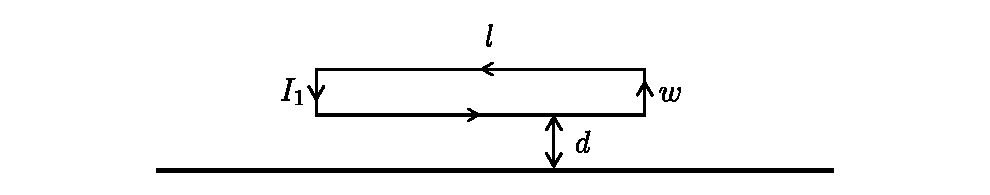
\includegraphics[width=\textwidth]{Anh/15.pdf}
    \end{center}
\end{vd}
\begin{loigiai}
Từ thông qua vòng dây siêu dẫn phải có giá trị không đổi. Nếu không, sự biến thiên từ thông qua vòng dây sẽ gây ra trên vòng dây một suất điện động
$$\varepsilon=\dfrac{\dd\phi}{\dd t}.$$
Mà vòng dây siêu dẫn lại có điện trở bằng không, điều này dẫn đến là dòng điện trong dây tiến đến vô cùng. Điều này là vô lí.\\
Đầu tiên ta sẽ tính từ thông qua vòng khi mà dòng điện trong vòng là $I_1$. Ta thấy là $ư\ll l$, nên ta có thể bỏ qua từ thông gây ra bởi các cạnh ngắn của vòng dây. Ngoài ra, ta còn có thể coi là từ trường gây ra bởi cạnh dài như là từ trường gây ra bởi dây dẫn dài vô hạn $B=\dfrac{\mu_0I}{2\pi r}$.\\
Từ thông qua vòng dây  
\begin{equation*}
    \begin{aligned}
     \phi_1&=\tiph{r}{w-r}{B(r)l}{r'}\\
     &=\tiph{r}{w-r}{\tron{\dfrac{\mu_0I_1l}{2\pi r'} + \dfrac{\mu_0I_1l}{2\pi \tron{w-r'}}}}{r'}\\
     &=\dfrac{\mu_0I_1l}{\pi}\ln\tron{\dfrac{w}{r}}.
    \end{aligned}
\end{equation*}
Độ tự cảm của vòng dây là $L=\dfrac{\phi_1}{I_1}=\dfrac{\mu_0l}{\pi}\ln\tron{\dfrac{w}{r}}$.\\
Bây giờ ta tính từ thông do dây dẫn gửi qua vòng dây.
\begin{equation*}
    \begin{aligned}
     \phi_2&=\tiph{d}{d+w}{\dfrac{mu_0I_2l}{2\pi r'}}{r'}\\
     &=\dfrac{\mu_0I_2l}{2\pi}\ln\tron{\dfrac{d+w}{d}}.
    \end{aligned}
\end{equation*}
Độ hỗ cảm của vòng dây và dây dẫn là $M=\dfrac{\phi_2}{I_2}=\dfrac{\mu_0l}{2\pi}\ln\tron{\dfrac{d+w}{d}}$.\\
Khi có dòng $I_2$ chạy trong dây dẫn, dòng điện trong vòng là $I_3$. Ta có
\begin{equation*}
    \begin{aligned}
     &LI_1=MI_2+LI_3\\
     \Leftrightarrow & I_3=I_1-\dfrac{MI_2}{L}.
    \end{aligned}
\end{equation*}
Lực tác dụng lên vòng dây
\begin{equation*}
    \begin{aligned}
     F&=I_3l\tron{\dfrac{\mu_0I_2}{2\pi d}-\dfrac{\mu_0I_2}{2\pi(d+w)}}\\
     &=\dfrac{\mu_0lư}{2\pi(d+w)d}\tron{I_1I_2-
    \dfrac{M{I_2}^2}{L}}.
    \end{aligned}
\end{equation*}
Giá trị của $F$ cực đại khi $I_2=\dfrac{I_1L}{2M}$, thay số vào ta tính được
$$F_{max}=1.12\times10^{-13}\dv{N}.$$
\end{loigiai}

\begin{vd}[Gió Mặt Trời]
 Các hạt có khối lượng $m$ và điện tích $q$ được phóng từ gốc tọa độ với vận tốc $v$ song song với trục $\mathrm{O}x$. Có màn chắn tại $x=\ell$.
    \begin{enumerate}[1)]
    \item Hạt thứ nhất được phóng ra khi có điện trường đều song song với trục $x$ và không có từ trường. Cường độ điện trường phải bằng bao nhiêu để hạt không bao giờ tới được màn?
    \item Tiếp theo, điện trường bị tắt, một từ trường đều hướng theo trục $\mathrm{O}z$ trong vùng $0<x<\ell$ được bật lên và hạt thứ hai được phóng ra. Biết rằng tốc độ của hạt vừa đủ lớn để tới màn chắn, hãy phác thảo quỹ đạo và tìm cường độ từ trường $B$.
    \item Cuối cùng, một điện trường $E$ nằm trong mặt phẳng $\mathrm{Oxy}$ được bật trong khi $B$ không đổi. Hạt thứ ba được bắn ra từ điểm gốc, vẫn song song với trục $\mathrm{O}x$, nhưng có thể với tốc độ khác. Người ta quan sát thấy rằng hạt chuyển động không bị lệch. Và thời gian cần thiết để nó tới màn chắn giống như đối với hạt thứ hai. Tìm độ lớn của điện trường $E$.
    \item Bỏ qua các ý trước, bây giờ chúng ta nghiên cứu một từ trường yếu không đều: các đường sức từ có bán kính cong lớn hơn nhiều bán kính cong của quỹ đạo hạt. Dường như trong trường hợp này, bất biến đoạn nhiệt của một hạt trong từ trường được bảo toàn: từ thông bao quanh quỹ đạo hình xoắn của hạt không đổi với độ chính xác cao dọc theo quỹ đạo. 
    \\Hãy xem xét một mô hình rất đơn giản về cách các hạt gió Mặt trời tương tác với từ trường của Trái Đất. Cường độ của từ trường Trái Đất trên trục từ của nó có thể được biểu thị bằng $B_z=B_E(R_E/z)^3$, trong đó $B_E = 3,12.10^{-5}~\mathrm{T}$ là cường độ trường tại bề mặt Trái Đất tại cực từ, $R_E = 6370 \mathrm{km}$ là bán kính Trái Đất và $z$ được đo từ tâm Trái Đất.
    \\Một electron mang điện tích $ -e = -1,60.10^{-19} \mathrm{C}$ và khối lượng $m_e = 9,11.10^{-31}~ \mathrm{kg}$ đang đến gần Trái Đất với vận tốc $u_0 = 500 ~\mathrm{km/s}$ và đập vào từ trường Trái Đất ngay trên trục của nó với một góc $\alpha$ ở khoảng cách $R_0 = 5R_E$ và bắt đầu xoắn ốc về phía Trái Đất. Nếu $\alpha$ quá lớn, hạt sẽ bị phản xạ bởi cường độ từ trường tăng dần khi hạt đến gần Trái Đất. Tìm điều kiện của $\alpha$ để hạt tới được bề mặt Trái Đất. 
    \\Có thể bỏ qua các hiệu ứng hấp dẫn hoặc tương đối tính. 
    \end{enumerate}
\end{vd}
\begin{loigiai}
\begin{enumerate}[1)]
    \item Trong điện trường đều $E$ dọc theo trục $\mathrm{O}x$, ta có điện thế
    \[\Phi(x)=-xE.\]
    Để hạt không va vào tường, động năng $\dfrac{mv^2}{2}$ của hạt phải nhỏ hơn công của lực điện $q\Phi(\ell)=-q\ell E$.
    \\ Do đó 
    \[\left|E\right| >\dfrac{mv^2}{2\ell \left|q\right|}.\]
     Và hướng của $E$ thỏa mãn $qE<0$.
    \item Trong từ trường, hạt chuyển động theo quỹ đạo đường tròn bán kính $R$, khi đó lực Lorentz đóng vai trò là lực hướng tâm: \[qvB=\dfrac{mv^2}{R}.\]
    Để hạt vừa đủ chạm vào màn thì quỹ đạo tròn phải tiếp xúc với màn.
    \\ Vì vậy $R=\ell$ và $B=\dfrac{mv}{q\ell}$.
    \begin{center}
        \tikzset{every picture/.style={line width=0.75pt}} %set default line width to 0.75pt        
        
        \begin{tikzpicture}[x=0.75pt,y=0.75pt,yscale=-1,xscale=1]
        %uncomment if require: \path (0,470); %set diagram left start at 0, and has height of 470
        
        %Shape: Axis 2D [id:dp9892750012986586] 
        \draw  (234.21,331.85) -- (438.6,331.85)(256.95,151.7) -- (256.95,362.4) (431.6,326.85) -- (438.6,331.85) -- (431.6,336.85) (251.95,158.7) -- (256.95,151.7) -- (261.95,158.7)  ;
        %Shape: Arc [id:dp1911045005650318] 
        \draw  [draw opacity=0] (256.7,310) .. controls (322.39,309.65) and (375.54,256.38) .. (375.6,190.7) -- (256.05,190.6) -- cycle ; \draw   (256.7,310) .. controls (322.39,309.65) and (375.54,256.38) .. (375.6,190.7) ;
        %Straight Lines [id:da1899490342711958] 
        \draw [color={rgb, 255:red, 139; green, 87; blue, 42 }  ,draw opacity=1 ][fill={rgb, 255:red, 74; green, 144; blue, 226 }  ,fill opacity=1 ]   (380.1,160.4) -- (380.1,260.2) -- (380.1,367.4)(377.1,160.4) -- (377.1,260.2) -- (377.1,367.4) ;
        %Flowchart: Or [id:dp8098590146376892] 
        \draw   (301,261.55) .. controls (301,258.71) and (303.37,256.4) .. (306.3,256.4) .. controls (309.23,256.4) and (311.6,258.71) .. (311.6,261.55) .. controls (311.6,264.39) and (309.23,266.7) .. (306.3,266.7) .. controls (303.37,266.7) and (301,264.39) .. (301,261.55) -- cycle ; \draw   (301,261.55) -- (311.6,261.55) ; \draw   (306.3,256.4) -- (306.3,266.7) ;
        %Straight Lines [id:da774970081443114] 
        \draw    (257.2,310.4) -- (295.6,310.4) ;
        \draw [shift={(297.6,310.4)}, rotate = 180] [color={rgb, 255:red, 0; green, 0; blue, 0 }  ][line width=0.75]    (10.93,-3.29) .. controls (6.95,-1.4) and (3.31,-0.3) .. (0,0) .. controls (3.31,0.3) and (6.95,1.4) .. (10.93,3.29)   ;
        %Straight Lines [id:da13664569510303481] 
        \draw    (262.6,199.94) -- (314.6,199.94) -- (367.6,200.38) ;
        \draw [shift={(369.6,200.4)}, rotate = 180.48] [color={rgb, 255:red, 0; green, 0; blue, 0 }  ][line width=0.75]    (10.93,-3.29) .. controls (6.95,-1.4) and (3.31,-0.3) .. (0,0) .. controls (3.31,0.3) and (6.95,1.4) .. (10.93,3.29)   ;
        \draw [shift={(260.6,199.94)}, rotate = 0] [color={rgb, 255:red, 0; green, 0; blue, 0 }  ][line width=0.75]    (10.93,-3.29) .. controls (6.95,-1.4) and (3.31,-0.3) .. (0,0) .. controls (3.31,0.3) and (6.95,1.4) .. (10.93,3.29)   ;
        
        
        % Text Node
        \draw (381.5,333.1) node [anchor=north west][inner sep=0.75pt]    {$l$};
        % Text Node
        \draw (241,332.1) node [anchor=north west][inner sep=0.75pt]    {$O$};
        % Text Node
        \draw (429.5,332.6) node [anchor=north west][inner sep=0.75pt]    {$x$};
        % Text Node
        \draw (240.5,146.1) node [anchor=north west][inner sep=0.75pt]    {$y$};
        % Text Node
        \draw (294,239.4) node [anchor=north west][inner sep=0.75pt]    {$B$};
        % Text Node
        \draw (270,313.4) node [anchor=north west][inner sep=0.75pt]    {$\ot{v}$};
        % Text Node
        \draw (306,181.4) node [anchor=north west][inner sep=0.75pt]    {$R$};
        
        
        \end{tikzpicture}
    \end{center}
    \item Thời gian cần thiết để hạt thứ 2 tới màn chắn là \[t=\dfrac{T}{4}=\dfrac{\pi l}{2v}.\]
    \\Để hạt chuyển động không bị lệch thì lực điện phải cân bằng với lực từ:
    $$F_E=F_B$$
    $$\rt qE=quB$$
    $$\rt u=\dfrac{E}{B}$$
    Vì thời gian cần thiết để hạt thứ 3 tới màn chắn giống hạt thứ 2 nên ta có: 
    $$t=\dfrac{l}{u}=\dfrac{\pi l}{2v}$$
    $$\rt E=\dfrac{2vB}{\pi}$$
    \item Ta có từ thông $\Phi \sim \text{Diện tích} \times B_z \sim R^2 B_z \sim \dfrac{B_z}{v_ \bot ^2} $, trong đó $v_\bot$ là thành phần vận tốc vuông góc với từ trường. Mà từ thông $\Phi$ là một đại lượng bất biến nên $\dfrac{B_z}{v_ \bot ^2}$ cũng là một bất biến.
    \\Trong quá trình chuyển động của electron, động năng của nó được bảo toàn vì từ trường không thực hiện công.
    \\Trong trường hợp tới hạn, khi electron gần như bị phản xạ, thành phần vận tốc vuông góc của electron ở bề mặt Trái Đất sẽ bằng $u_0$. Khi đó, bất biến đoạn nhiệt sẽ cho kết quả:
    \[\dfrac{{v_{ \bot 0}^2}}{{B\left( {{R_0}} \right)}} = \dfrac{{u_0^2}}{{B\left( {{R_E}} \right)}}\]
    Với ${v_{ \bot 0}} = {u_0}\sin \alpha$, ta có:
    \[{\alpha _0} = \arcsin \left( {\sqrt {\dfrac{{B\left( {{R_0}} \right)}}{{B\left( {{R_E}} \right)}}} } \right) = \arcsin \left( {\dfrac{1}{{5\sqrt 5 }}} \right) = 5,13^\circ \]
    Góc $\alpha$ cần nhỏ hơn $\alpha_0$ để electron có thể tới được bề mặt Trái Đất.
\end{enumerate}
\end{loigiai}

\begin{vd}[Hệ spin]
    Chúng ta hãy xem xét một hệ thống gồm $N$ lưỡng cực từ độc lập (spins) trong từ trường $B$ và nhiệt độ $T$. Mục tiêu là xác định một số tính chất của hệ này bằng cách sử dụng vật lí thống kê. Biết rằng năng lượng của một spin đơn là $E=\epsilon m$, trong đó $m=\pm \dfrac{1}{2}$ và $\epsilon=\alpha B$.
    \begin{enumerate}[1)]
        \item Xác suất $p_\uparrow$ để một spin ở trạng thái kích thích, tức là có năng lượng dương?
        \item Giá trị trung bình của tổng năng lượng $E_s$ của hệ spin là một hàm của $B$ và $T$ ?
        \item  Sử dụng phương pháp xấp xỉ nhiệt độ cao $T \gg \dfrac{\alpha Bm}{k}$, đơn giản hóa biểu thức của $E_s$.
        \item Sử dụng phương pháp xấp xỉ nhiệt độ cao $T \gg \dfrac{\alpha Bm}{k}$, đơn giản hóa biểu thức của $E_s$. Tìm nhiệt dung C của hệ spin.
    \end{enumerate}
\end{vd}

\begin{loigiai}
    \begin{enumerate}[1)]
        \item Theo phân bố Boltzmann, $p_\uparrow=A\dot e^{-\epsilon m}$.
        \\ Trong đó hằng số $A$ có thể tìm được với điều kiện tổng xác suất spin quay lên hoặc xuống là $1$:
        \[A = \frac{1}{{{e^{ - \epsilon /2kT}}} + {e^{\epsilon /2kT}}} = \frac{1}{{2\cosh \left( {\epsilon /2kT} \right)}}.\]
        Do đó 
        \[{p_ \uparrow } = \dfrac{{{e^{-\epsilon/2kT} }}}{{{e^{-\epsilon/2kT}} + {e^{\epsilon/2kT}}}}\]
        \item Năng lượng trung bình là giá trị trung bình có trọng số của năng lượng trạng thái lên và xuống cho một lần quay, nhân với số lần quay:
        \[E = \frac{{N\epsilon }}{2}\frac{{{e^{ - \epsilon /2kT}} - {e^{\epsilon /2kT}}}}{{{e^{ - \epsilon /2kT}}{ + e^{\epsilon /2kT}}}} =  - \frac{{N\epsilon }}{2}\tanh \left( {\epsilon /2kT} \right).\]
        \item Đối với các giá trị đối số nhỏ của tiếp tuyến hyperbol, biểu thức có thể tính gần đúng:
        \[E \approx \frac{{ - N{\epsilon ^2}}}{{4kT}}.\]
        \item Theo định nghĩa của nhiệt dung:
        \[C = \dfrac{\mathrm{d}E}{\mathrm{d}t} = \frac{{N{\epsilon ^2}}}{{4k{T^2}}}.\]
    \end{enumerate}
\end{loigiai}

\begin{vd}[Nối hai solenoid]
    Một cuộn dây Solenoid cứng quấn chặt được lắp một phần vào một cuộn dây khác. Chúng được nối với một nguồn điện không đổi; cả hai đều tạo ra một từ trường cùng hướng. Cả hai đều có $N$ vòng xoắn, chiều dài của chúng là $l$, diện tích mặt cắt ngang của chúng là $A_1$ và $A_2$. Có thể giả định rằng $A_1, A_2 \ll l^2$.
    \\Biết rằng từ trường tại tâm của một Solenoid được lấy riêng là $B =\dfrac{\mu_0 IN}{l}$, trong đó $\mu_0$ là độ từ thẩm của chân không.
    \begin{enumerate}[1)]
        \item Tâm của các cuộn dây cách nhau một khoảng $x<l$ dọc theo trục chung của chúng $\left[A_1, A_2 \ll (x-l)^2, x^2\right]$. Tìm tổng năng lượng $E_m$ của từ trường trong hệ.
        \item Tìm suất điện động $\varepsilon_1$ và $\varepsilon_2$ sinh ra trên cuộn dây khi người ta kéo ra với tốc độ $v$.
        \item Tìm lực $F$ cần thiết để kéo một cuộn dây ra phía ngoài.
    \end{enumerate}
\end{vd}

\begin{loigiai}
    \begin{enumerate}[1)]
        \item Vùng chồng chập 2 cuộn dây có từ trường $2B$, phần còn lại của cuộn dây bên trong có từ trường $B$. Cho cuộn dây bên trong có diện tích $A_2$. Mật độ năng lượng của phần cuộn dây bên trong có từ trường $B$ là $\dfrac{B^2}{2 \mu_0}$. 
    \\Do đó năng lượng của từ trường trong hệ 2 cuộn dây là
    \[\begin{aligned}
            E_m &=\dfrac{B^2}{2\mu_0}\left(A_1l-A_2(l-x)+A_2x \right)+\dfrac{(2B)^2}{2\mu_0}A_2(l-x) \\
            &=\dfrac{B^2}{2\mu_0}\left[ A_1l+A_2(3l-2x)\right]\\
               &=\dfrac{\mu_0 I^2 N^2}{2l^2}\left[A_1l+A_2(3l-2x)\right].
    \end{aligned}\]
    \item Tiết diện $A_1$ của cuộn dây bên ngoài được cắt bởi tất cả từ thông $ B\cdot A_2$ của cuộn dây bên trong. Sau thời gian $\dd t$, từ thông này được được bao bọc bởi ít vòng của cuộn dây bên ngoài hơn $-$ bởi $\dfrac{Nv \mathrm{d}t}{l}$ vòng dây có chiều dài $v \mathrm{d}t$. Do đó từ thông được bao bởi cuộn dây bên ngoài thay đổi với tốc độ 
    \[\varepsilon_1 = \dot \Phi_1=\dfrac{BA_2Nv}{l}=\dfrac{\mu_0A_2IN^2v}{l^2}.\]
    Cuộn dây bên trong cũng được cắt bởi từ thông $BA_2$, do đó $\varepsilon_2=\varepsilon_1$ và cùng chiều.
    \item Ta thấy năng lượng từ trường giảm và nguồn dòng điện không đổi bị tiêu tán một phần năng lượng (vì suất điện động cảm ứng có chiều ngược lại nguồn điện).
    \\ Theo định luật bảo toàn năng lượng, ta có công để kéo cuộn dây ra là:
    \[Fv=\dfrac{\mathrm{d}E_m}{\mathrm{d}x}v+I(\varepsilon_1+\varepsilon_2).\]
    Từ đó ta tính được 
    \[F=-\dfrac{B^2A_2}{\mu_0}+\dfrac{2IBA_2N}{l}=\dfrac{\mu_0I^2N^2A_2}{l^2}.\]
    \end{enumerate}
\end{loigiai}

\begin{vd}[Cyclotron]
Ta xét một cyclotron (một loại máy gia tốc hạt nhất) và hoạt động của nó. Cyclotron bao gồm một vùng hình trụ bán kính $R$ nơi có từ trường đều có cảm ứng từ $B$ và một vùng hình dải mỏng có chiều rộng $d$ tại đó có điện trường đều cường độ $E$ vuông góc với dải. Hướng của điện trường được thay đổi tuần hoàn thành hướng ngược lại sao cho mọi hạt đi qua dải, hướng của điện trường giống với hướng của vận tốc của hạt. Cũng có một kênh hẹp ở một cạnh của cyclotron để các hạt thoát ra khỏi cyclotron. Cho các hạt bắt đầu chuyển động ở tâm của xiclôtron với tốc độ ban đầu nhỏ không đáng kể.
\\Trước khi rời khỏi cyclotron, hạt sẽ đi được $n$ vòng tròn đủ, tìm $n$.
\\ Cho điện tích của các hạt là $q$ và khối lượng $m$.
\\Và giả sử rằng $n\gg1$.
\begin{center}
    

\tikzset{every picture/.style={line width=0.75pt}} %set default line width to 0.75pt        

\begin{tikzpicture}[x=0.5pt,y=0.5pt,yscale=-1,xscale=1]
%uncomment if require: \path (0,424); %set diagram left start at 0, and has height of 424

%Shape: Rectangle [id:dp5625641528781005] 
\draw  [fill={rgb, 255:red, 155; green, 155; blue, 155 }  ,fill opacity=1 ] (181,43.2) -- (181,193.2) -- (174,193.2) -- (174,43.2) -- cycle ;
%Shape: Circle [id:dp42258690714876335] 
\draw  [fill={rgb, 255:red, 155; green, 155; blue, 155 }  ,fill opacity=1 ] (174,198.8) .. controls (174,134.29) and (226.29,82) .. (290.8,82) .. controls (355.31,82) and (407.6,134.29) .. (407.6,198.8) .. controls (407.6,263.31) and (355.31,315.6) .. (290.8,315.6) .. controls (226.29,315.6) and (174,263.31) .. (174,198.8) -- cycle ;
%Shape: Rectangle [id:dp6859026345150396] 
\draw  [fill={rgb, 255:red, 255; green, 255; blue, 255 }  ,fill opacity=1 ] (174,193.2) -- (407.6,193.2) -- (407.6,198.8) -- (174,198.8) -- cycle ;
%Straight Lines [id:da6880432905637432] 
\draw    (341.6,93.4) -- (290.8,196) ;
%Straight Lines [id:da023630750235380305] 
\draw  [dash pattern={on 4.5pt off 4.5pt}]  (407.6,193.2) -- (427.6,193.2) ;
%Straight Lines [id:da29515349754415054] 
\draw  [dash pattern={on 4.5pt off 4.5pt}]  (407.6,198.8) -- (427.6,198.8) ;
%Straight Lines [id:da6324336437474667] 
\draw    (422,162.2) -- (422,189) ;
\draw [shift={(422,192)}, rotate = 270] [fill={rgb, 255:red, 0; green, 0; blue, 0 }  ][line width=0.08]  [draw opacity=0] (10.72,-5.15) -- (0,0) -- (10.72,5.15) -- (7.12,0) -- cycle    ;
%Straight Lines [id:da2979405700128157] 
\draw    (422,203.2) -- (422,230) ;
\draw [shift={(422,200.2)}, rotate = 90] [fill={rgb, 255:red, 0; green, 0; blue, 0 }  ][line width=0.08]  [draw opacity=0] (10.72,-5.15) -- (0,0) -- (10.72,5.15) -- (7.12,0) -- cycle    ;
%Shape: Circle [id:dp07336497279632437] 
\draw   (227,239.3) .. controls (227,231.4) and (233.4,225) .. (241.3,225) .. controls (249.2,225) and (255.6,231.4) .. (255.6,239.3) .. controls (255.6,247.2) and (249.2,253.6) .. (241.3,253.6) .. controls (233.4,253.6) and (227,247.2) .. (227,239.3) -- cycle ;
%Shape: Circle [id:dp9231668351446314] 
\draw  [color={rgb, 255:red, 0; green, 0; blue, 0 }  ,draw opacity=1 ][fill={rgb, 255:red, 0; green, 0; blue, 0 }  ,fill opacity=1 ] (238.15,239.3) .. controls (238.15,237.56) and (239.56,236.15) .. (241.3,236.15) .. controls (243.04,236.15) and (244.45,237.56) .. (244.45,239.3) .. controls (244.45,241.04) and (243.04,242.45) .. (241.3,242.45) .. controls (239.56,242.45) and (238.15,241.04) .. (238.15,239.3) -- cycle ;


% Text Node
\draw (430,186.4) node [anchor=north west][inner sep=0.75pt]    {$d$};
% Text Node
\draw (259,230.4) node [anchor=north west][inner sep=0.75pt]    {$B$};
% Text Node
\draw (297,120) node [anchor=north west][inner sep=0.75pt]    {$R$};


\end{tikzpicture}
\end{center}

\end{vd}
\begin{loigiai}\\
Trong cyclotron, các hạt bắt đầu chuyển động theo chiều kim đồng hồ dọc theo một vòng tròn với các nửa vòng liên tục tăng dần. Bán kính quỹ đạo của hạt được tính theo công thức $r=\dfrac{mv}{qB}$,
trong đó $v$ là vận tốc của hạt. Trong một vòng tròn, hạt nhận được động năng $\epsilon_k=2qED$ từ điện trường, vì hạt đi qua dải hai lần trong một vòng tròn. Do đó vận tốc của hạt khi ra khỏi cyclotron là
$$\dfrac{mv^2}{2}=2qEdn$$
$$\rt v^2=\dfrac{4qEdn}{m}.$$
Hạt rời khỏi cyclotron khi bán kính quỹ đạo của nó lớn bằng bán kính $R$ của cyclotron, khi đó, vận tốc của nó là $$v=\dfrac{qBR}{m}.$$
Biểu diễn $n$ từ các phương trình trên ta được $n =\dfrac{ qB^2R^2}{4mEd}$.
\end{loigiai}

\begin{vd}[Ống tia âm cực]%Prob2 IPhO 2000
Một ống tia âm cực (cathode ray tube (CRT)), cấu tạo bởi một súng electron và một màn hình, được dặt trong một từ trường đều, không đổi $\ot{B}$ sao cho từ trườn song song với trục của chùm tia phát ra từ súng như hình vẽ $a)$.
\begin{center}
 

\tikzset{every picture/.style={line width=0.75pt}} %set default line width to 0.75pt        

\begin{tikzpicture}[x=0.75pt,y=0.75pt,yscale=-1,xscale=1]
%uncomment if require: \path (0,652); %set diagram left start at 0, and has height of 652

%Shape: Ellipse [id:dp15688127192695345] 
\draw  [fill={rgb, 255:red, 155; green, 155; blue, 155 }  ,fill opacity=1 ] (333.06,53) .. controls (342.45,53) and (350.07,73.95) .. (350.07,99.79) .. controls (350.07,125.63) and (342.45,146.58) .. (333.06,146.58) .. controls (323.66,146.58) and (316.04,125.63) .. (316.04,99.79) .. controls (316.04,73.95) and (323.66,53) .. (333.06,53) -- cycle ;
%Straight Lines [id:da46382146326331886] 
\draw    (230.82,72.44) -- (333.06,53) ;
%Straight Lines [id:da7484447454061447] 
\draw    (230.82,128.35) -- (333.06,146.58) ;
%Shape: Ellipse [id:dp04390648905852612] 
\draw   (230.82,72.44) .. controls (238.12,72.44) and (244.04,84.96) .. (244.04,100.4) .. controls (244.04,115.83) and (238.12,128.35) .. (230.82,128.35) .. controls (223.52,128.35) and (217.61,115.83) .. (217.61,100.4) .. controls (217.61,84.96) and (223.52,72.44) .. (230.82,72.44) -- cycle ;
%Straight Lines [id:da12460435727279795] 
\draw  [dash pattern={on 4.5pt off 4.5pt}]  (163.38,100.4) -- (483.18,100.4) ;
\draw [shift={(486.18,100.4)}, rotate = 180] [fill={rgb, 255:red, 0; green, 0; blue, 0 }  ][line width=0.08]  [draw opacity=0] (10.72,-5.15) -- (0,0) -- (10.72,5.15) -- (7.12,0) -- cycle    ;
%Rounded Rect [id:dp7059297815675409] 
\draw   (174.86,178.69) .. controls (174.86,170.51) and (181.49,163.87) .. (189.68,163.87) -- (234.16,163.87) .. controls (242.35,163.87) and (248.99,170.51) .. (248.99,178.69) -- (248.99,223.17) .. controls (248.99,231.36) and (242.35,238) .. (234.16,238) -- (189.68,238) .. controls (181.49,238) and (174.86,231.36) .. (174.86,223.17) -- cycle ;
%Straight Lines [id:da6620628016537122] 
\draw    (211.92,200.93) -- (234.41,200.93) -- (501.77,200.93) ;
%Shape: Ellipse [id:dp5076742892764352] 
\draw   (413.66,165.49) .. controls (418.02,165.49) and (421.56,180.72) .. (421.56,199.52) .. controls (421.56,218.31) and (418.02,233.54) .. (413.66,233.54) .. controls (409.3,233.54) and (405.76,218.31) .. (405.76,199.52) .. controls (405.76,180.72) and (409.3,165.49) .. (413.66,165.49) -- cycle ;
%Straight Lines [id:da4821118642858162] 
\draw    (248.38,200.93) -- (413.66,165.49) ;
%Straight Lines [id:da3173684264555092] 
\draw    (248.38,200.93) -- (413.66,233.54) ;
%Straight Lines [id:da7776734544630426] 
\draw    (248.38,200.93) -- (417.91,171.97) ;
%Straight Lines [id:da3980810014347458] 
\draw    (248.38,200.93) -- (406.97,181.69) ;
%Straight Lines [id:da5966138762318254] 
\draw    (249.6,200.93) -- (421.56,187.36) ;
%Straight Lines [id:da022137391854452293] 
\draw    (247.17,200.93) -- (405.76,193.44) ;
%Straight Lines [id:da2370369867996458] 
\draw    (249.6,200.93) -- (421.56,210.45) ;
%Straight Lines [id:da6166390520595011] 
\draw    (249.6,200.93) -- (406.97,214.1) ;
%Straight Lines [id:da43254133186599186] 
\draw    (248.38,200.93) -- (419.13,221.39) ;
%Straight Lines [id:da07507088664140515] 
\draw    (248.38,200.93) -- (408.19,225.04) ;

% Text Node
\draw (261.69,109.52) node [anchor=north west][inner sep=0.75pt]   [align=left] {Súng};
% Text Node
\draw  [color={rgb, 255:red, 0; green, 0; blue, 0 }  ,draw opacity=0 ][fill={rgb, 255:red, 255; green, 255; blue, 255 }  ,fill opacity=1 ]  (375,173) -- (398,173) -- (398,198) -- (375,198) -- cycle  ;
\draw (378,177.4) node [anchor=north west][inner sep=0.75pt]    {$5^{\circ }$};
% Text Node
\draw  [color={rgb, 255:red, 0; green, 0; blue, 0 }  ,draw opacity=0 ][fill={rgb, 255:red, 255; green, 255; blue, 255 }  ,fill opacity=1 ]  (376,201) -- (399,201) -- (399,226) -- (376,226) -- cycle  ;
\draw (379,205.4) node [anchor=north west][inner sep=0.75pt]    {$5^{\circ }$};
% Text Node
\draw (193.69,209.52) node [anchor=north west][inner sep=0.75pt]   [align=left] {Súng};
% Text Node
\draw (401,74) node [anchor=north west][inner sep=0.75pt]   [align=left] {hướng về màn hình};
% Text Node
\draw (534,89.4) node [anchor=north west][inner sep=0.75pt]    {$a)$};
% Text Node
\draw (534,191.4) node [anchor=north west][inner sep=0.75pt]    {$b)$};
\end{tikzpicture}
\end{center}
\begin{enumerate}[1)]
    \item 
Chùm electron được phóng ra từ anode của súng electron với độ phân kì $5^\circ$ so với trục như hình vẽ $b)$. Nhìn chung, một điểm khếch tán được tạo ra trên màn hình nhưng đối với các giá trị nhất định của từ trường, ta thu được một điểm sắc nét. \\
Bằng cách xem chuyển động của electron ban đầu hợp với trục một góc $\beta$ $(0 \le \beta \le 5^\circ)$ như thể nó rời súng electron, xem xét thành phần của chuyển động song song và vuông góc với trục để suy ra biểu thức thể hiện tỉ lệ điện tích trên khối lượng $\dfrac{e}{m}$ của electron theo các đại lượng sau:
\begin{itemize}
    \item Từ trường nhỏ nhất để thu được  một điểm sắc nét là $B$.
    \item Hiệu điện thế gia tốc cho electron của súng electron là $V$ $(V < 2 ~\mathrm{kV})$.
    \item $D$ là khoảng cách giữa anode và màn hình. 
\end{itemize}
\item Hãy xem xét một phương pháp để xác định tỉ lệ điện tích trên khối lượng của electron.  Bố trí thí nghiệm được thể hiện bởi các hình chiếu cạnh và hình chiếu bằng như hình $c)$ với hướng của từ trường được kí hiệu $\ot{B}$. Trong từ trường đồng nhất $\ot{B}$ đặt hai đĩa tròn đồng chất bán kính $\rho$ cách nhau một khoảng rất nhỏ $t$. Một hiệu điện thế $V$ được duy trì giữa chúng. Các đĩa tròn này song song và đồng trục, tuy nhiên trục của chúng vuông góc với từ trường. Một tấm phim bao phủ mặt trong của một hình trụ bán kính $\rho + s$ được giữ đồng trục với các đĩa. Nói cách khác, tấm phim đang ở khoảng cách $s$ tính từ rìa của các tấm. Toàn bộ hệ thống trên được đặt trong chân không. Lưu ý rằng $t \ll s, \rho$.\\
Một nguồn điểm phát ra hạt $\beta$ đồng đều theo mọi phương với một phạm vi vận tốc, được đặt giữa tâm của hai đĩa, và một tấm phim tương tự thỏa mãn ba yêu cầu:
\begin{itemize}
    \item Với $B = 0$, $V = 0$.
    \item Với $B = B_0$, $V = V_0$.
    \item Với $B = - B_0$, $V = - V_0$.
\end{itemize}
Trong đó $V_0$ và $B_0$ là những hằng số dương. Lưu ý rằng đĩa trên được tích điện dương khi $V > 0$ (tích điện âm khi $V < 0$), hướng của từ trường được vẽ như trên hình $c)$ khi $B > 0$ (hướng ngược lại khi $B < 0$). Trong phần này, ta giả sử khoảng cách giữa hai đĩa là vô cùng nhỏ.\\
Hai vùng của tấm phim được kí hiệu $A$ và $B$ như trên hình $c)$. Sau khi tráng phim, ta thu được bản phác họa của một trong hai vùng ấy như hình $d)$. Hãy chỉ ra đây là vùng nào ($A$ hay $B$). Giải thích bằng cách chỉ ra hướng của các lực tác dụng lên electron.
\item Hình $d)$ là bản phác họa sau khi tráng phim. Các phép đo được thực hiện bằng cách tách hai dấu vết ngoài cùng bằng kính hiển vi, khoảng cách $y$ được chỉ ra cho một góc xác định như hình $d)$. Các kết quả thu được trong bảng dưới đây, góc $\varphi$ được xác định như trên hình $c)$ là góc hợp giữa từ trường và đoạn thẳng nối tâm đĩa và điểm trên phim. 
\begin{center}
% Gradient Info
\tikzset {_xuhqogfpo/.code = {\pgfsetadditionalshadetransform{ \pgftransformshift{\pgfpoint{0 bp } { 0 bp }  }  \pgftransformrotate{-90 }  \pgftransformscale{2 }  }}}
\pgfdeclarehorizontalshading{_inhue7mj5}{150bp}{rgb(0bp)=(1,1,1);
rgb(37.5bp)=(1,1,1);
rgb(62.23214285714286bp)=(0,0,0);
rgb(100bp)=(0,0,0)}
\tikzset{_02sdu9os0/.code = {\pgfsetadditionalshadetransform{\pgftransformshift{\pgfpoint{0 bp } { 0 bp }  }  \pgftransformrotate{-90 }  \pgftransformscale{2 } }}}
\pgfdeclarehorizontalshading{_svo8v53km} {150bp} {color(0bp)=(transparent!0);
color(37.5bp)=(transparent!0);
color(62.23214285714286bp)=(transparent!10);
color(100bp)=(transparent!10) } 
\pgfdeclarefading{_aztoe6dzf}{\tikz \fill[shading=_svo8v53km,_02sdu9os0] (0,0) rectangle (50bp,50bp); } 

% Gradient Info
  
\tikzset {_4hgoksisq/.code = {\pgfsetadditionalshadetransform{ \pgftransformshift{\pgfpoint{0 bp } { 0 bp }  }  \pgftransformrotate{-270 }  \pgftransformscale{2 }  }}}
\pgfdeclarehorizontalshading{_a6zt3liho}{150bp}{rgb(0bp)=(1,1,1);
rgb(37.5bp)=(1,1,1);
rgb(62.23214285714286bp)=(0,0,0);
rgb(100bp)=(0,0,0)}
\tikzset{_avmem70dn/.code = {\pgfsetadditionalshadetransform{\pgftransformshift{\pgfpoint{0 bp } { 0 bp }  }  \pgftransformrotate{-270 }  \pgftransformscale{2 } }}}
\pgfdeclarehorizontalshading{_ikrrxe62e} {150bp} {color(0bp)=(transparent!0);
color(37.5bp)=(transparent!0);
color(62.23214285714286bp)=(transparent!10);
color(100bp)=(transparent!10) } 
\pgfdeclarefading{_2r3xg1isi}{\tikz \fill[shading=_ikrrxe62e,_avmem70dn] (0,0) rectangle (50bp,50bp); } 
\tikzset{every picture/.style={line width=0.75pt}} %set default line width to 0.75pt        

\begin{tikzpicture}[x=0.75pt,y=0.75pt,yscale=-1,xscale=1]
%uncomment if require: \path (0,475); %set diagram left start at 0, and has height of 475

%Shape: Rectangle [id:dp020771989117557066] 
\path  [shading=_inhue7mj5,_xuhqogfpo,path fading= _aztoe6dzf ,fading transform={xshift=2}] (318.5,86.33) -- (411.5,86.33) -- (411.5,94.08) -- (318.5,94.08) -- cycle ; % for fading 
 \draw  [color={rgb, 255:red, 0; green, 0; blue, 0 }  ,draw opacity=0 ] (318.5,86.33) -- (411.5,86.33) -- (411.5,94.08) -- (318.5,94.08) -- cycle ; % for border 

%Shape: Rectangle [id:dp31778581120225957] 
\path  [shading=_a6zt3liho,_4hgoksisq,path fading= _2r3xg1isi ,fading transform={xshift=2}] (318.5,97.33) -- (411.5,97.33) -- (411.5,105.08) -- (318.5,105.08) -- cycle ; % for fading 
 \draw  [color={rgb, 255:red, 0; green, 0; blue, 0 }  ,draw opacity=0 ] (318.5,97.33) -- (411.5,97.33) -- (411.5,105.08) -- (318.5,105.08) -- cycle ; % for border 

%Straight Lines [id:da4031420664942009] 
\draw    (311.5,60.58) -- (311.5,90.33) ;
\draw [shift={(311.5,93.33)}, rotate = 270] [fill={rgb, 255:red, 0; green, 0; blue, 0 }  ][line width=0.08]  [draw opacity=0] (10.72,-5.15) -- (0,0) -- (10.72,5.15) -- (7.12,0) -- cycle    ;
%Straight Lines [id:da9193665529337671] 
\draw    (305,94.08) -- (316.5,94.08) ;
%Straight Lines [id:da42907105813404467] 
\draw    (305,97.33) -- (316.5,97.33) ;
%Straight Lines [id:da5113702769067339] 
\draw    (311.5,118.58) -- (311.5,101.33) ;
\draw [shift={(311.5,98.33)}, rotate = 450] [fill={rgb, 255:red, 0; green, 0; blue, 0 }  ][line width=0.08]  [draw opacity=0] (10.72,-5.15) -- (0,0) -- (10.72,5.15) -- (7.12,0) -- cycle    ;
%Straight Lines [id:da06930522495709357] 
\draw    (327.6,74.6) -- (397.6,74.6) ;
\draw [shift={(400.6,74.6)}, rotate = 180] [fill={rgb, 255:red, 0; green, 0; blue, 0 }  ][line width=0.08]  [draw opacity=0] (10.72,-5.15) -- (0,0) -- (10.72,5.15) -- (7.12,0) -- cycle    ;
%Straight Lines [id:da1298642208068317] 
\draw    (368,111.2) -- (408.5,111.09) ;
\draw [shift={(411.5,111.08)}, rotate = 539.85] [fill={rgb, 255:red, 0; green, 0; blue, 0 }  ][line width=0.08]  [draw opacity=0] (10.72,-5.15) -- (0,0) -- (10.72,5.15) -- (7.12,0) -- cycle    ;
\draw [shift={(365,111.21)}, rotate = 359.85] [fill={rgb, 255:red, 0; green, 0; blue, 0 }  ][line width=0.08]  [draw opacity=0] (10.72,-5.15) -- (0,0) -- (10.72,5.15) -- (7.12,0) -- cycle    ;
%Straight Lines [id:da06954802708875363] 
\draw    (414.5,105.08) -- (449.2,105.08) ;
\draw [shift={(452.2,105.08)}, rotate = 180] [fill={rgb, 255:red, 0; green, 0; blue, 0 }  ][line width=0.08]  [draw opacity=0] (10.72,-5.15) -- (0,0) -- (10.72,5.15) -- (7.12,0) -- cycle    ;
\draw [shift={(411.5,105.08)}, rotate = 0] [fill={rgb, 255:red, 0; green, 0; blue, 0 }  ][line width=0.08]  [draw opacity=0] (10.72,-5.15) -- (0,0) -- (10.72,5.15) -- (7.12,0) -- cycle    ;
%Straight Lines [id:da989573322573476] 
\draw    (278.13,74.8) -- (278.13,116.4) ;
%Straight Lines [id:da6783520806702819] 
\draw    (452.53,74) -- (452.53,115.6) ;
%Straight Lines [id:da22291824253480996] 
\draw    (327.1,160.6) -- (397.1,160.6) ;
\draw [shift={(400.1,160.6)}, rotate = 180] [fill={rgb, 255:red, 0; green, 0; blue, 0 }  ][line width=0.08]  [draw opacity=0] (10.72,-5.15) -- (0,0) -- (10.72,5.15) -- (7.12,0) -- cycle    ;
%Shape: Circle [id:dp8239780757588118] 
\draw   (279.5,220.5) .. controls (279.5,173.56) and (317.56,135.5) .. (364.5,135.5) .. controls (411.44,135.5) and (449.5,173.56) .. (449.5,220.5) .. controls (449.5,267.44) and (411.44,305.5) .. (364.5,305.5) .. controls (317.56,305.5) and (279.5,267.44) .. (279.5,220.5) -- cycle ;
%Shape: Circle [id:dp8690273783549125] 
\draw  [fill={rgb, 255:red, 155; green, 155; blue, 155 }  ,fill opacity=1 ] (317.54,220.5) .. controls (317.54,194.57) and (338.57,173.54) .. (364.5,173.54) .. controls (390.43,173.54) and (411.46,194.57) .. (411.46,220.5) .. controls (411.46,246.43) and (390.43,267.46) .. (364.5,267.46) .. controls (338.57,267.46) and (317.54,246.43) .. (317.54,220.5) -- cycle ;
%Straight Lines [id:da007788119321362252] 
\draw    (418.17,154.92) -- (394.44,183.94) ;
%Straight Lines [id:da48762353354956045] 
\draw    (394.78,256.28) -- (419.44,284.5) ;
%Straight Lines [id:da8507420339733396] 
\draw    (414.46,220.5) -- (446.5,220.5) ;
\draw [shift={(449.5,220.5)}, rotate = 180] [fill={rgb, 255:red, 0; green, 0; blue, 0 }  ][line width=0.08]  [draw opacity=0] (10.72,-5.15) -- (0,0) -- (10.72,5.15) -- (7.12,0) -- cycle    ;
\draw [shift={(411.46,220.5)}, rotate = 0] [fill={rgb, 255:red, 0; green, 0; blue, 0 }  ][line width=0.08]  [draw opacity=0] (10.72,-5.15) -- (0,0) -- (10.72,5.15) -- (7.12,0) -- cycle    ;
%Straight Lines [id:da2788762685088071] 
\draw    (468.46,246.5) -- (468.46,194.17) ;
\draw [shift={(468.46,191.17)}, rotate = 450] [fill={rgb, 255:red, 0; green, 0; blue, 0 }  ][line width=0.08]  [draw opacity=0] (10.72,-5.15) -- (0,0) -- (10.72,5.15) -- (7.12,0) -- cycle    ;
\draw [shift={(468.46,249.5)}, rotate = 270] [fill={rgb, 255:red, 0; green, 0; blue, 0 }  ][line width=0.08]  [draw opacity=0] (10.72,-5.15) -- (0,0) -- (10.72,5.15) -- (7.12,0) -- cycle    ;
%Straight Lines [id:da40137082255206735] 
\draw    (462.46,220.33) -- (473.96,220.33) ;
%Shape: Rectangle [id:dp9132749001203555] 
\draw   (200.02,345.63) -- (541.76,345.63) -- (541.76,403.68) -- (200.02,403.68) -- cycle ;
%Straight Lines [id:da4514547425737465] 
\draw  [dash pattern={on 4.5pt off 4.5pt}]  (199.42,374.21) -- (541.76,374.21) ;
%Straight Lines [id:da013618439417980799] 
\draw  [dash pattern={on 4.5pt off 4.5pt}]  (370.59,346.32) -- (370.59,403.83) ;
%Straight Lines [id:da46380400329680027] 
\draw    (327.42,388.99) -- (327.42,360.18) ;
\draw [shift={(327.42,357.18)}, rotate = 450] [fill={rgb, 255:red, 0; green, 0; blue, 0 }  ][line width=0.08]  [draw opacity=0] (10.72,-5.15) -- (0,0) -- (10.72,5.15) -- (7.12,0) -- cycle    ;
\draw [shift={(327.42,391.99)}, rotate = 270] [fill={rgb, 255:red, 0; green, 0; blue, 0 }  ][line width=0.08]  [draw opacity=0] (10.72,-5.15) -- (0,0) -- (10.72,5.15) -- (7.12,0) -- cycle    ;
%Curve Lines [id:da870475526622555] 
\draw    (270.67,367.16) .. controls (321.27,349.6) and (431.42,352.87) .. (468.93,367.16) ;
%Curve Lines [id:da08010002084620638] 
\draw    (269.48,381.45) .. controls (316.51,399.48) and (434,395.51) .. (467.74,381.45) ;
%Straight Lines [id:da9585673240006158] 
\draw    (322.74,398.94) -- (203.02,400.08) ;
\draw [shift={(200.02,400.11)}, rotate = 359.46000000000004] [fill={rgb, 255:red, 0; green, 0; blue, 0 }  ][line width=0.08]  [draw opacity=0] (10.72,-5.15) -- (0,0) -- (10.72,5.15) -- (7.12,0) -- cycle    ;
\draw [shift={(325.74,398.91)}, rotate = 179.46] [fill={rgb, 255:red, 0; green, 0; blue, 0 }  ][line width=0.08]  [draw opacity=0] (10.72,-5.15) -- (0,0) -- (10.72,5.15) -- (7.12,0) -- cycle    ;

% Text Node
\draw (298.8,66.87) node [anchor=north west][inner sep=0.75pt]    {$t$};
% Text Node
\draw (353.2,57.2) node [anchor=north west][inner sep=0.75pt]    {$\mathbf{B}$};
% Text Node
\draw (381.6,108.2) node [anchor=north west][inner sep=0.75pt]    {$\rho $};
% Text Node
\draw (426.4,107.6) node [anchor=north west][inner sep=0.75pt]    {$s$};
% Text Node
\draw (261.33,58.8) node [anchor=north west][inner sep=0.75pt]   [align=left] {Phim};
% Text Node
\draw (435.73,59.6) node [anchor=north west][inner sep=0.75pt]   [align=left] {Phim};
% Text Node
\draw (139.33,78.73) node [anchor=north west][inner sep=0.75pt]   [align=left] {Hình chiếu cạnh};
% Text Node
\draw (353.2,144.2) node [anchor=north west][inner sep=0.75pt]    {$\mathbf{B}$};
% Text Node
\draw (427.07,217.51) node [anchor=north west][inner sep=0.75pt]    {$s$};
% Text Node
\draw (151.33,208.73) node [anchor=north west][inner sep=0.75pt]   [align=left] {Hình chiếu bằng};
% Text Node
\draw (437.73,161.6) node [anchor=north west][inner sep=0.75pt]   [align=left] {Phim};
% Text Node
\draw (480.67,198.33) node [anchor=north west][inner sep=0.75pt]   [align=left] {Vùng $A$};
% Text Node
\draw (480.96,224.33) node [anchor=north west][inner sep=0.75pt]   [align=left] {Vùng $B$};
% Text Node
\draw (334.62,363.33) node [anchor=north west][inner sep=0.75pt]    {$y$};
% Text Node
\draw (248.39,381.69) node [anchor=north west][inner sep=0.75pt]    {$\varphi $};
% Text Node
\draw (175.71,320.1) node [anchor=north west][inner sep=0.75pt]    {$\varphi =0^{\circ }$};
% Text Node
\draw (342.46,320.34) node [anchor=north west][inner sep=0.75pt]    {$\varphi =90^{\circ }$};
% Text Node
\draw (205.83,350.82) node [anchor=north west][inner sep=0.75pt]   [align=left] {Phim};
% Text Node
\draw (585,144.4) node [anchor=north west][inner sep=0.75pt]    {$c)$};
% Text Node
\draw (584,364.4) node [anchor=north west][inner sep=0.75pt]    {$d)$};
\end{tikzpicture}
\end{center}
\[\begin{array}{ccccccc}
     \varphi ~^\circ & 90 & 60 & 50 & 40 & 30 & 23 \\
     y ~(\mathrm{mm})& 17,4 & 12,7 & 9,7 & 6,4 & 3,3 & \text{Kết thúc phim}
\end{array}\]
Cho biết giá trị của các đại lượng trong hệ:
\[B_0 = 6,91~\mathrm{mT}, V_0 = 580~\mathrm{V}, t = 0,8~\mathrm{mm}, s = 41 ~\mathrm{mm}.\]
Ngoài ra, tốc độ ánh sáng trong chân không $c = 3 \times 10^8 ~\mathrm{m/s}$, khối lượng nghỉ của electron là $m = 9,11 \times 10^{-31}~\mathrm{kg}$.\\
Hãy xác định động năng cực đại của hạt $\beta$ quan sát được.
\item Tính động năng cực đại của electron. Sử dụng các dữ kiện được cho trong câu $3)$, tính tỉ lệ điện tích trên khối lượng nghỉ của electron. Hãy vẽ một biểu đồ thích hợp để sử dụng đầy đủ các dữ kiện.\\
Sử dụng phương pháp tuyến tính hóa, vẽ đồ thị tuyến tính và chỉ rõ đại lượng nào được thể hiển trên trục hoành và trục tung.\\ 
Lưu ý rằng câu trả lời có thể sai lệch so với thực tế do sai số trong quan sát.
\end{enumerate}
\end{vd}
\begin{loigiai}
\begin{enumerate}[1)]
    \item Tập trung vào chuyển động cyclotron của electron.\\
    Tốc độ góc của chuyển động:
    $\omega = \dfrac{eB}{m}$ nên chu kì $T = \dfrac{2\pi m}{eB}$.\\
    Tốc độ của electron được tính bằng
    \[\dfrac{mu^2}{2} = eV \rt u = \sqrt{\dfrac{2eV}{m}}.\]
    Quãng đường dịch chuyển 
    \[D = T u \cos \beta \approx T u = \dfrac{2\pi}{B} \sqrt{\dfrac{2mV}{e}}.\]
    Do đó tỉ số điện tích trên khối lượng
    \[\dfrac{e}{m} = 8 \dfrac{\pi V}{B^2 D^2}.\]
    \item  Lực điện tác dụng lên electron hướng lên trên. Trong vùng $A$, lực từ tác dụng lên electron cũng hướng lên khiến electron đập vào đĩa trên và không đến được tấm phim.\\
    Trong vùng $B$, lực từ tác dụng lên electron cũng hướng xuống và nếu hai lực cân bằng thì hợp lực tác dụng bằng $0$, electron phóng thẳng đến tấm phim.\\
    Do đó, hình phác họa được chụp từ vùng $B$.
    \item Lực từ và lực điện phải cân bằng
    \[\dfrac{eV}{t} = e u B \sin \theta  \rt u = \dfrac{V}{Bt \abs{\sin \theta}}.\]
    Với $u$ là tốc độ của electron. $u$ đạt cực đại khi $\theta$ nhỏ nhất và bằng $23^\circ$. Khi đó 
    \[u = 2,687 \times 10^8 ~\mathrm{m/s} = 0,896 c.\]
    Do đó, ta phải xét trong trường hợp tương đối tính 
    \[\gamma = \sqrt{1 - \dfrac{v^2}{c^2}} = 2,255.\]
    Vậy động năng của electron là
    \[K = \tron{\gamma - 1}mc^2 = 641 ~\mathrm{keV}.\]
    \item Sau khi ló ra khỏi vùng giữa các đĩa, các electron chỉ chịu tác dụng của lực từ. Ta xem gần đúng lực này có phương thẳng đứng vì góc  hợp  bởi electron và phương ngang vẫn rất nhỏ. \\
    Gia tốc gây bởi lực này
    \[a =  \dfrac{Beu \sin \theta}{\gamma m}.\]
    Tốc độ ban đầu theo phương ngang là $u$, do đó, thời gian cần thiết để electron đến được tấm phim sau khi rời khỏi vùng giữa hai đĩa là $\dfrac{s}{u}$.\\
    Độ dời theo phương thẳng đứng trong khoảng thời gian này bằng
    \[\dfrac{y}{2} = \dfrac{1}{2}a \tron{\dfrac{s}{u}}^2 \rt y = \dfrac{Bes^2 \sin \theta }{\gamma m u}.\tag{1}\label{q.8.1}\]
    Mặt khác, electron ló ra khỏi các đĩa có tốc độ
    \[u = \dfrac{V}{tB \abs{\sin \theta}} .\tag{2}\label{q.8.2}\]
    Thay (\ref{q.8.2}) vào (\ref{q.8.1}), ta được
    \[y^2 = {\tron{\dfrac{eBs\sin\theta}{m} }^2}\left\{\tron{\dfrac{Bs t \sin\theta}{V}}^2 - \tron{\dfrac{s}{c}}^2\right\}.\]
    Từ đó ta phác họa đồ thị
    \begin{itemize}
        \item Trục tung: $Y = \tron{\dfrac{y}{Bs\sin\theta}}^2$.
        \item Trục hoành: $X = \tron{\dfrac{Bst\sin\theta}{V}}^2$.
    \end{itemize}
    Phương trình trở thành:
    \[Y = \tron{\dfrac{e}{m}}^2 \tron{X - \tron{\dfrac{s}{c}}^2}. \]
    Do đó ta có gradient bằng $\tron{\dfrac{e}{m}}^2$ và tung độ gốc là $-\tron{\dfrac{es}{mc}}^2$.\\
    Từ các dữ kiện, ta tính được tung độ gốc là $-537,7~ \mathrm{Cs/kg}^2$, suy ra $\dfrac{e}{m} = 1,7 \times 10^{11} ~\mathrm{C/kg}$.\\
    Gradient của đồ thị $2,826 \times 10^{22}~\mathrm{C/kg}^2$, suy ra $\dfrac{e}{m} = 1,68 \times 10^{11}~\mathrm{C/kg}$.
\end{enumerate}
\end{loigiai}


\begin{vd}[Góc khối dùng để làm gì]%Câu 7
\begin{enumerate}[1)]
    \item Trên một diện tích phẳng, có dòng điện với mật độ tuyến tính là $i$.\\
Chứng minh thành phần cảm ứng từ song song với bề mặt và vuông góc với $\ot{i}$ được xác định bởi:
$$\ot{B_\parallel}=\dfrac{\mu_0}{4\pi}\left(\ot{i}\times\ot{n}\right)\cdot\Omega$$
trong đó $\Omega$ là góc khối tính từ điểm đang xét nhìn bề mặt đã cho.
    \item Hãy dùng công thức trên để tính từ trường của một ống solenoid dài vô hạn tại các vị trí trên trục đối xứng sau:
    \begin{enumerate}[a)]
        \item Trong lòng của ống dây.
        \item Ở sát một đầu của ống dây.
        \item Tại một điểm cách đầu ống dây một đoạn $x$ ở bên ngoài.
        \item Tại một điểm cách đầu ống dây một đoạn $x$ ở bên trong.
        \item Từ trường trong lòng của một ống dây dài hữu hạn.
    \end{enumerate}
\end{enumerate}
\end{vd}
\begin{loigiai}
\begin{enumerate}[1)]
    \item Bài này chúng ta sẽ giải được bằng hai cách: dùng định luật Biot$-$Savart hoặc dùng sự phụ thuộc giữa điện và từ trường.\\
Cách 1: Dùng Biot-Savart:
$$\mathrm{d}\ot{B}=\dfrac{\mu_0}{4\pi}\dfrac{I\cdot \mathrm{d}\ot{r}\times\ot{PM}}{PM^3}$$
với $\mathrm{d}\ot{r}$ là vector định hướng theo chiều của mật độ dòng điện $\ot{i}$.\\
\begin{center}
    

\tikzset{every picture/.style={line width=0.75pt}} %set default line width to 0.75pt        

\begin{tikzpicture}[x=0.75pt,y=0.75pt,yscale=-1,xscale=1]
%uncomment if require: \path (0,485); %set diagram left start at 0, and has height of 485

%Shape: Polygon Curved [id:ds3922129264966643] 
\draw  [fill={rgb, 255:red, 128; green, 128; blue, 128 }  ,fill opacity=1 ] (284,241) .. controls (294,217) and (352,214) .. (376,230) .. controls (400,246) and (437,224) .. (448,243) .. controls (459,262) and (433,270) .. (408.19,276.68) .. controls (383.37,283.36) and (368.37,276.9) .. (365,271) .. controls (361.63,265.1) and (327.15,253.96) .. (318.08,255.98) .. controls (309,258) and (274,265) .. (284,241) -- cycle ;
%Straight Lines [id:da5617325667802913] 
\draw    (365,121) -- (448,243) ;
%Straight Lines [id:da5785428663305934] 
\draw    (365,121) -- (284,241) ;
%Shape: Ellipse [id:dp18923666125746497] 
\draw  [fill={rgb, 255:red, 155; green, 155; blue, 155 }  ,fill opacity=0.83 ] (354,139.5) .. controls (354,137.01) and (358.92,135) .. (365,135) .. controls (371.08,135) and (376,137.01) .. (376,139.5) .. controls (376,141.99) and (371.08,144) .. (365,144) .. controls (358.92,144) and (354,141.99) .. (354,139.5) -- cycle ;
%Straight Lines [id:da40958843225991837] 
\draw    (365,121) -- (290.92,138.32) ;
\draw [shift={(288,139)}, rotate = 346.84000000000003] [fill={rgb, 255:red, 0; green, 0; blue, 0 }  ][line width=0.08]  [draw opacity=0] (10.72,-5.15) -- (0,0) -- (10.72,5.15) -- (7.12,0) -- cycle    ;
%Straight Lines [id:da29389847237299893] 
\draw    (349,249) -- (348.05,189) ;
\draw [shift={(348,186)}, rotate = 449.09] [fill={rgb, 255:red, 0; green, 0; blue, 0 }  ][line width=0.08]  [draw opacity=0] (10.72,-5.15) -- (0,0) -- (10.72,5.15) -- (7.12,0) -- cycle    ;
%Shape: Ellipse [id:dp39374247527024986] 
\draw   (359,251) .. controls (359,248.24) and (364.15,246) .. (370.5,246) .. controls (376.85,246) and (382,248.24) .. (382,251) .. controls (382,253.76) and (376.85,256) .. (370.5,256) .. controls (364.15,256) and (359,253.76) .. (359,251) -- cycle ;
%Straight Lines [id:da8547868678069266] 
\draw    (370.5,251) -- (406,251.92) ;
\draw [shift={(409,252)}, rotate = 181.49] [fill={rgb, 255:red, 0; green, 0; blue, 0 }  ][line width=0.08]  [draw opacity=0] (10.72,-5.15) -- (0,0) -- (10.72,5.15) -- (7.12,0) -- cycle    ;

% Text Node
\draw (272,106.4) node [anchor=north west][inner sep=0.75pt]    {$\mathrm{d}\overrightarrow{B_{\parallel }}$};
% Text Node
\draw (359,98.4) node [anchor=north west][inner sep=0.75pt]    {$M$};
% Text Node
\draw (358,158.4) node [anchor=north west][inner sep=0.75pt]    {$\Omega $};
% Text Node
\draw (352,183.4) node [anchor=north west][inner sep=0.75pt]    {$\vec{n}$};
% Text Node
\draw (336,265.4) node [anchor=north west][inner sep=0.75pt]    {$\mathrm{d} S$};
% Text Node
\draw (372.5,254.4) node [anchor=north west][inner sep=0.75pt]    {$P$};
% Text Node
\draw (417,240.4) node [anchor=north west][inner sep=0.75pt]    {$\overrightarrow{j_{S}}$};


\end{tikzpicture}

\end{center}
Lại có $\ot{i}\mathrm{d}\ot{l}=I$, trong đó $\mathrm{d}\ot{I}$ là vi phân chiều rộng mà mật độ dòng đi qua.\\
Viết lại thì ta sẽ được:
$$\mathrm{d}\ot{B}=\dfrac{\mu_0}{4\pi}\cdot\dfrac{\ot{i}\cdot \mathrm{d}S\times\overline{PM}}{PM^3}.$$
Ta có: $\mathrm{d}\ot{B}=\mathrm{d}\ot{B_\parallel}+\mathrm{d}\ot{B_\bot}\Rightarrow{\mathrm{d}\ot{B_\parallel}}=\dd \ot{B}-\mathrm{d}\ot{B_\bot}$
\begin{align*}
   \mathrm{d}\ot{B_\bot}&=\left(\mathrm{d}\ot{B}\cdot\ot{n}\right)\cdot\ot{n},\\
    \mathrm{d}\ot{B}&=\left(\ot{n}\cdot\ot{n}\right)\cdot\ot{B}.
\end{align*}

Ta đã biết: $\ot{a}\times\left(\ot{b}\times\ot{c}\right)=\left(\ot{a}\cdot\ot{c}\right)\ot{b}-\left(\ot{a}\cdot\ot{b}\right)\cdot\ot{c}$.\\
Vậy $d\ot{B_\parallel}=\left(\ot{n}\cdot\ot{n}\right)\cdot \mathrm{d}\ot{B}-\left(d\mathrm{d}\ot{B}\cdot\ot{n}\right)\cdot\ot{n}=\ot{n}\times\left(\mathrm{d}\ot{B}\times\ot{n}\right)$.\\
Có
\begin{align*}
    \mathrm{d}\ot B \times \ot n &= \dfrac{{{\mu _0}}}{{4\pi }} \cdot \dfrac{{\ot \imath  \cdot \mathrm{d}S \times \ot {PM} }}{{P{M^3}}} \times \ot n \\&=  - \dfrac{{{\mu _0}}}{{4\pi }} \cdot \dfrac{{\ot \imath }}{{P{M^3}}} \cdot (\ot n \cdot \ot {PM} ) \cdot \mathrm{d}S \\&=  - \dfrac{{{\mu _0}}}{{4\pi }} \cdot \ot \imath  \cdot \mathrm{d}\Omega
\end{align*}
Dễ dàng suy ra được:
$$\mathrm{d}\ot{B_\parallel}=\dfrac{\mu_0}{4\pi}\cdot \ot{i}\cdot \mathrm{d}Q\times\ot{n}=\dfrac{\mu_0}{4\pi}\left(\ot{i}\times\ot{n}\right)\cdot \dd Q$$
Cách 2: Dùng sự phụ thuộc giữa điện và từ trường:\\
Ta biết rằng điện tích di chuyển với vận tốc $v$ thì sinh ra điện trường theo công thức:
$$\mathrm{d}\ot{B}=\mu_0\varepsilon_0\ot{v}\times\dfrac{\sigma \mathrm{d}S}{4\pi\varepsilon_0}\cdot\dfrac{\ot{r}}{r^3}.$$
Ta gọi vector đơn vị vuông góc vơi vector pháp tuyến và vuông góc với vector mật độ dòng $\ot{i}$ là $\ot{e_\parallel}$:
\begin{align*}
    \mathrm{d}\ot B &= \dfrac{{{\mu_0}}}{{4\pi }}\ot v \times \sigma \mathrm{d}S \cdot \dfrac{{\ot r}}{{{r^3}}}\\
\mathrm{d}\ot B \cdot \ot {{e_\parallel}}  &= \ot {{e_\parallel}}  \cdot \left( {\dfrac{{{\mu_0}}}{{4\pi }}\ot v \times \sigma \mathrm{d}S \cdot \dfrac{{\ot r}}{{{r^3}}}} \right)
\\&= \sigma \mathrm{d}S \cdot \dfrac{{\ot r}}{{{r^3}}} \cdot \left( {\dfrac{\mu_0}{4\pi }\ot v \times {{\ot e_\parallel}}} \right) \\&= \sigma \mathrm{d}S \cdot \dfrac{{\ot r}}{{{r^3}}} \cdot \dfrac{{{\mu _0}}}{{4\pi }} \cdot v \cdot \ot n
\end{align*}

Kết hợp định nghĩa $\ot{i}=\sigma\ot{v}$.\\
Vậy dễ dàng rút ra được:
\[{B} = \dfrac{{{\mu_0}}}{{4\pi }} \cdot i\Omega. \]
    \item 
    \begin{enumerate}[a)]
        \item Một ống solenoid thì ta lại có: $i\mathrm{d}L=\mathrm{d}I=N\cdot\dfrac{I \mathrm{d} L}{L}$.\\
        Vậy dễ dàng thấy được $i=\dfrac{NI}{L}=nI$.\\
        Đối với trong lòng của ống dây, từ trường gây ra bởi cuộn dây sẽ quét nên một góc khối trong toàn bộ không gian là $4\pi$.\\
        Từ trường trong trường hợp này là: $B=\dfrac{\mu_0}{4\pi}\cdot iQ=\mu_0nI$.
        \item Trường hợp ở sát một đầu dây thì góc khối bây giờ sẽ là $2\pi$.\\
        Tương tự như thế suy ra ngay được: $B=\dfrac{\mu_0nI}{2}$.
        \item Tại một điểm cách đoạn $x$ ở bên ngoài thì góc khối của nó bây giờ sẽ là như trên hình vẽ:
        \begin{center}
            

\tikzset{every picture/.style={line width=0.75pt}} %set default line width to 0.75pt        

\begin{tikzpicture}[x=0.75pt,y=0.75pt,yscale=-1,xscale=1]
%uncomment if require: \path (0,404); %set diagram left start at 0, and has height of 404

%Curve Lines [id:da23246274003905754] 
\draw  [dash pattern={on 4.5pt off 4.5pt}]  (273.07,144.77) .. controls (284.48,150.19) and (283.34,179.92) .. (283.34,181.37) ;
%Curve Lines [id:da2569353747444356] 
\draw  [dash pattern={on 4.5pt off 4.5pt}]  (283.32,179.74) .. controls (284.48,190.99) and (279.93,214.6) .. (273.07,214.71) ;

%Curve Lines [id:da6183062170471916] 
\draw    (272.87,215.88) .. controls (261.46,210.46) and (262.6,180.73) .. (262.6,179.27) ;
%Curve Lines [id:da8296363002858504] 
\draw    (262.62,180.91) .. controls (261.46,169.66) and (266.01,146.05) .. (272.87,145.93) ;

%Straight Lines [id:da3261169614679926] 
\draw  [dash pattern={on 4.5pt off 4.5pt}]  (39.74,144.77) -- (108.81,144.77) ;
%Straight Lines [id:da9388131806363158] 
\draw    (108.81,214.71) -- (273.07,214.71) ;
%Straight Lines [id:da4981940820064006] 
\draw  [dash pattern={on 4.5pt off 4.5pt}]  (41.26,215.18) -- (110.33,215.18) ;
%Curve Lines [id:da058548510603747994] 
\draw  [dash pattern={on 4.5pt off 4.5pt}]  (41.36,214.71) .. controls (29.95,209.29) and (31.09,179.57) .. (31.09,178.11) ;
%Curve Lines [id:da28674009073319295] 
\draw  [dash pattern={on 4.5pt off 4.5pt}]  (31.12,179.74) .. controls (29.95,168.49) and (34.5,144.88) .. (41.36,144.77) ;
%Straight Lines [id:da13313345870106996] 
\draw    (108.81,144.77) -- (273.07,144.77) ;
%Curve Lines [id:da23687454756529425] 
\draw    (170.4,213.55) .. controls (158.99,208.13) and (160.12,178.4) .. (160.12,176.94) ;
%Curve Lines [id:da3437203023218134] 
\draw    (160.15,178.57) .. controls (158.99,167.32) and (163.54,143.72) .. (170.4,143.6) ;

%Curve Lines [id:da06407716040321243] 
\draw    (212.53,213.55) .. controls (201.11,208.13) and (202.25,178.4) .. (202.25,176.94) ;
%Curve Lines [id:da6035310173871988] 
\draw    (202.28,178.57) .. controls (201.11,167.32) and (205.67,143.72) .. (212.53,143.6) ;

%Curve Lines [id:da8494685484120488] 
\draw    (192.03,213.55) .. controls (180.62,208.13) and (181.76,178.4) .. (181.76,176.94) ;
%Curve Lines [id:da08931353505314421] 
\draw    (181.79,178.57) .. controls (180.62,167.32) and (185.17,143.72) .. (192.03,143.6) ;

%Curve Lines [id:da15702687900044277] 
\draw    (144.21,214.71) .. controls (132.8,209.29) and (133.94,179.57) .. (133.94,178.11) ;
%Curve Lines [id:da40233214034429454] 
\draw    (133.97,179.74) .. controls (132.8,168.49) and (137.35,144.88) .. (144.21,144.77) ;

%Curve Lines [id:da7723532534265405] 
\draw    (231.88,214.71) .. controls (220.47,209.29) and (221.61,179.57) .. (221.61,178.11) ;
%Curve Lines [id:da5932349698555781] 
\draw    (221.64,179.74) .. controls (220.47,168.49) and (225.02,144.88) .. (231.88,144.77) ;

%Curve Lines [id:da9159460175559413] 
\draw    (250.1,214.71) .. controls (238.69,209.29) and (239.82,179.57) .. (239.82,178.11) ;
%Curve Lines [id:da17927431896962043] 
\draw    (239.85,179.74) .. controls (238.69,168.49) and (243.24,144.88) .. (250.1,144.77) ;

\draw   (141.43,176.78) -- (133.14,186.58) -- (126.77,175.38) ;
\draw   (230.24,179.11) -- (221.95,188.91) -- (215.58,177.71) ;
\draw   (208.61,179.11) -- (200.32,188.91) -- (193.95,177.71) ;
\draw   (189.25,177.95) -- (180.96,187.75) -- (174.59,176.54) ;
\draw   (168.76,177.95) -- (160.47,187.75) -- (154.1,176.54) ;
\draw   (247.32,179.11) -- (239.03,188.91) -- (232.66,177.71) ;
%Straight Lines [id:da881459178130799] 
\draw    (272.87,180.21) -- (334.92,180.21) ;
%Straight Lines [id:da9432755276672973] 
\draw  [dash pattern={on 4.5pt off 4.5pt}]  (272.87,145.93) -- (272.87,180.21) ;
%Straight Lines [id:da45327501223814326] 
\draw    (272.87,145.93) -- (334.92,180.21) ;
%Straight Lines [id:da28880569926011423] 
\draw    (272.87,215.88) -- (334.92,180.21) ;
%Shape: Arc [id:dp3564037563549467] 
\draw  [draw opacity=0] (311.01,181.16) .. controls (310.95,181.01) and (310.89,180.85) .. (310.83,180.7) .. controls (309.28,176.61) and (309.71,172.18) .. (311.64,168.27) -- (328.08,173.87) -- cycle ; \draw   (311.01,181.16) .. controls (310.95,181.01) and (310.89,180.85) .. (310.83,180.7) .. controls (309.28,176.61) and (309.71,172.18) .. (311.64,168.27) ;
%Straight Lines [id:da8861979171919769] 
\draw    (277.66,235) -- (334.85,235) ;
\draw [shift={(337.85,235)}, rotate = 180] [fill={rgb, 255:red, 0; green, 0; blue, 0 }  ][line width=0.08]  [draw opacity=0] (10.72,-5.15) -- (0,0) -- (10.72,5.15) -- (7.12,0) -- cycle    ;
\draw [shift={(274.66,235)}, rotate = 0] [fill={rgb, 255:red, 0; green, 0; blue, 0 }  ][line width=0.08]  [draw opacity=0] (10.72,-5.15) -- (0,0) -- (10.72,5.15) -- (7.12,0) -- cycle    ;
%Straight Lines [id:da3805062587054828] 
\draw    (355.5,179.54) -- (355.5,149.4) ;
\draw [shift={(355.5,146.4)}, rotate = 450] [fill={rgb, 255:red, 0; green, 0; blue, 0 }  ][line width=0.08]  [draw opacity=0] (10.72,-5.15) -- (0,0) -- (10.72,5.15) -- (7.12,0) -- cycle    ;
\draw [shift={(355.5,182.54)}, rotate = 270] [fill={rgb, 255:red, 0; green, 0; blue, 0 }  ][line width=0.08]  [draw opacity=0] (10.72,-5.15) -- (0,0) -- (10.72,5.15) -- (7.12,0) -- cycle    ;


% Text Node
\draw (294,162.4) node [anchor=north west][inner sep=0.75pt]    {$\theta $};
% Text Node
\draw (362,156.4) node [anchor=north west][inner sep=0.75pt]    {$R$};
% Text Node
\draw (301,240.4) node [anchor=north west][inner sep=0.75pt]    {$x$};


\end{tikzpicture}

        \end{center}
        Lúc này góc khối $\Omega$ sẽ được tính bằng công thức:
        $$\Omega=2\pi(1-\mathrm{cos}\theta),$$
        với $$\mathrm{cos}\theta=\dfrac{x}{\sqrt{x^2+R^2}}.$$
        Vậy ta rút ra từ trường bên ngoài:
        \[\ot {{B_1}}  + \ot {{B_2}}  = \dfrac{j}{2}\left[ {\left( {\ot {{r_1}}  \times \ot {{e_z}} } \right) + \left( {\ot {{r_2}}  \times \ot {{e_z}} } \right)} \right].\]
        \item Trường hợp bên trong thì cũng làm tương tự với góc khối bây giờ là:
        \[B = \dfrac{{{\mu _0}}}{{4\pi }} \cdot i.2\pi \left( {1 + \dfrac{x}{{\sqrt {{x^2} + {R^2}} }}} \right) = \dfrac{{{\mu _0}nI}}{2}\left( {1 + \dfrac{x}{{\sqrt {{x^2} + {R^2}} }}} \right).\]
        \item Đối với từ trường của một ống dây dài hữu hạn, dựa vào hình vẽ, ta có thể xác định được góc khối trong trường hợp này là:
        \begin{center}
            

\tikzset{every picture/.style={line width=0.75pt}} %set default line width to 0.75pt        

\begin{tikzpicture}[x=0.75pt,y=0.75pt,yscale=-1,xscale=1]
%uncomment if require: \path (0,424); %set diagram left start at 0, and has height of 424

%Curve Lines [id:da07323833825779236] 
\draw  [dash pattern={on 4.5pt off 4.5pt}]  (292.07,163.77) .. controls (303.48,169.19) and (302.34,198.92) .. (302.34,200.37) ;
%Curve Lines [id:da9496880182926646] 
\draw  [dash pattern={on 4.5pt off 4.5pt}]  (302.32,198.74) .. controls (303.48,209.99) and (298.93,233.6) .. (292.07,233.71) ;

%Curve Lines [id:da7476871733726151] 
\draw    (291.87,234.88) .. controls (280.46,229.46) and (281.6,199.73) .. (281.6,198.27) ;
%Curve Lines [id:da06025915165235585] 
\draw    (281.62,199.91) .. controls (280.46,188.66) and (285.01,165.05) .. (291.87,164.93) ;

%Straight Lines [id:da18234503170898786] 
\draw    (60.36,233.71) -- (292.07,233.71) ;
%Curve Lines [id:da0505559185628377] 
\draw    (60.36,233.71) .. controls (48.95,228.29) and (50.09,198.57) .. (50.09,197.11) ;
%Curve Lines [id:da5126057145976575] 
\draw    (50.12,198.74) .. controls (48.95,187.49) and (53.5,163.88) .. (60.36,163.77) ;
%Straight Lines [id:da08712239262055488] 
\draw    (60.36,163.77) -- (292.07,163.77) ;
%Curve Lines [id:da5064182955926819] 
\draw    (189.4,232.55) .. controls (177.99,227.13) and (179.12,197.4) .. (179.12,195.94) ;
%Curve Lines [id:da5726160887077749] 
\draw    (179.15,197.57) .. controls (177.99,186.32) and (182.54,162.72) .. (189.4,162.6) ;

%Curve Lines [id:da7540039118690092] 
\draw    (238.53,232.55) .. controls (227.11,227.13) and (228.25,197.4) .. (228.25,195.94) ;
%Curve Lines [id:da014194331336817356] 
\draw    (228.28,197.57) .. controls (227.11,186.32) and (231.67,162.72) .. (238.53,162.6) ;

%Curve Lines [id:da8258998787902145] 
\draw    (214.03,232.55) .. controls (202.62,227.13) and (203.76,197.4) .. (203.76,195.94) ;
%Curve Lines [id:da20967547716520074] 
\draw    (203.79,197.57) .. controls (202.62,186.32) and (207.17,162.72) .. (214.03,162.6) ;

%Curve Lines [id:da952782857362197] 
\draw    (163.21,233.71) .. controls (151.8,228.29) and (152.94,198.57) .. (152.94,197.11) ;
%Curve Lines [id:da34159559225433966] 
\draw    (152.97,198.74) .. controls (151.8,187.49) and (156.35,163.88) .. (163.21,163.77) ;

%Curve Lines [id:da13326939859262188] 
\draw    (111.88,234.71) .. controls (100.47,229.29) and (101.61,199.57) .. (101.61,198.11) ;
%Curve Lines [id:da4192039683738553] 
\draw    (101.64,199.74) .. controls (100.47,188.49) and (105.02,164.88) .. (111.88,164.77) ;

%Curve Lines [id:da31499361935964054] 
\draw    (139.1,234.71) .. controls (127.69,229.29) and (128.82,199.57) .. (128.82,198.11) ;
%Curve Lines [id:da015405963374842235] 
\draw    (128.85,199.74) .. controls (127.69,188.49) and (132.24,164.88) .. (139.1,164.77) ;

\draw   (160.43,195.78) -- (152.14,205.58) -- (145.77,194.38) ;
\draw   (110.24,196.11) -- (101.95,205.91) -- (95.58,194.71) ;
\draw   (236.61,198.11) -- (228.32,207.91) -- (221.95,196.71) ;
\draw   (211.25,195.95) -- (202.96,205.75) -- (196.59,194.54) ;
\draw   (187.76,196.95) -- (179.47,206.75) -- (173.1,195.54) ;
\draw   (136.32,196.11) -- (128.03,205.91) -- (121.66,194.71) ;
%Straight Lines [id:da13750396875137127] 
\draw    (215,199) -- (252.5,199) ;
\draw [shift={(255.5,199)}, rotate = 180] [fill={rgb, 255:red, 0; green, 0; blue, 0 }  ][line width=0.08]  [draw opacity=0] (8.04,-3.86) -- (0,0) -- (8.04,3.86) -- (5.34,0) -- cycle    ;
\draw [shift={(215,199)}, rotate = 0] [color={rgb, 255:red, 0; green, 0; blue, 0 }  ][fill={rgb, 255:red, 0; green, 0; blue, 0 }  ][line width=0.75]      (0, 0) circle [x radius= 2.34, y radius= 2.34]   ;
%Straight Lines [id:da13567381207390805] 
\draw  [dash pattern={on 4.5pt off 4.5pt}]  (215,199) -- (291.87,164.93) ;
%Straight Lines [id:da5589741252035714] 
\draw  [dash pattern={on 4.5pt off 4.5pt}]  (60.36,163.77) -- (215,199) ;
%Shape: Arc [id:dp9185533195236573] 
\draw  [draw opacity=0] (268.65,175.72) .. controls (266.14,174.79) and (264.44,173.26) .. (264.1,171.31) .. controls (263.58,168.28) and (266.53,165.08) .. (271.19,163.13) -- (277.67,168.98) -- cycle ; \draw   (268.65,175.72) .. controls (266.14,174.79) and (264.44,173.26) .. (264.1,171.31) .. controls (263.58,168.28) and (266.53,165.08) .. (271.19,163.13) ;
%Shape: Arc [id:dp8868817492672574] 
\draw  [draw opacity=0] (87.32,164.2) .. controls (86.73,165.82) and (85.93,167.33) .. (84.95,168.72) -- (69,157.5) -- cycle ; \draw   (87.32,164.2) .. controls (86.73,165.82) and (85.93,167.33) .. (84.95,168.72) ;
%Shape: Arc [id:dp29997511001655597] 
\draw  [draw opacity=0] (271.66,173.47) .. controls (270.79,172.61) and (270.19,171.53) .. (269.98,170.3) .. controls (269.52,167.62) and (271.04,164.99) .. (273.6,163.52) -- (277.67,168.98) -- cycle ; \draw   (271.66,173.47) .. controls (270.79,172.61) and (270.19,171.53) .. (269.98,170.3) .. controls (269.52,167.62) and (271.04,164.99) .. (273.6,163.52) ;

% Text Node
\draw (64,139.4) node [anchor=north west][inner sep=0.75pt]    {$\theta _{1}$};
% Text Node
\draw (267,141.4) node [anchor=north west][inner sep=0.75pt]    {$\theta _{2}$};
% Text Node
\draw (237.25,202.4) node [anchor=north west][inner sep=0.75pt]    {$\vec{B}$};
\end{tikzpicture}
        \end{center}
        Góc khối lúc này sẽ là:
        $$\Omega=4\pi-2\pi(1-\mathrm{cos}\theta_1)-2\pi(1-\mathrm{cos}\theta_2)=2\pi(\mathrm{cos}\theta_1+\mathrm{cos}\theta_2).$$
        Vậy từ trường gây ra lúc này sẽ là: $B=\dfrac{\mu_0}{2}nI(\mathrm{cos}\theta_1+\mathrm{cos}\theta_2)$.
    \end{enumerate}
\end{enumerate}
\end{loigiai}

\begin{vd}[Bẫy từ Ioffe $-$ Pritchard]
Bẫy từ Ioffe $-$ Pritchard được sử dụng để giam giữ các nguyên tử chuyển động, và có cấu tạo chính như hình vẽ. Bốn dây thẳng $1,2,3,4$ có dòng điện không đổi $I$, đặt vuông góc với mặt phẳng $x-y$, và giao của chúng với mặt phẳng $x-y$ là hình vuông cạnh $2 a$, tâm tại ${O}$, mặt phẳng chứa các dòng $1$ và $2$ song song với trục $x$, và chiều dòng điện trong mỗi dây được biểu diễn trên hình.
\begin{center}

\tikzset{every picture/.style={line width=0.75pt}} %set default line width to 0.75pt        

\begin{tikzpicture}[x=0.75pt,y=0.75pt,yscale=-1,xscale=1]
%uncomment if require: \path (0,300); %set diagram left start at 0, and has height of 300

%Straight Lines [id:da05626332961750413] 
\draw [line width=1.5]    (134,125) -- (391,125) ;
\draw [shift={(395,125)}, rotate = 180] [fill={rgb, 255:red, 0; green, 0; blue, 0 }  ][line width=0.08]  [draw opacity=0] (13.4,-6.43) -- (0,0) -- (13.4,6.44) -- (8.9,0) -- cycle    ;
%Straight Lines [id:da3913295804206024] 
\draw [line width=1.5]    (256,221.5) -- (256,28.5) ;
\draw [shift={(256,24.5)}, rotate = 450] [fill={rgb, 255:red, 0; green, 0; blue, 0 }  ][line width=0.08]  [draw opacity=0] (13.4,-6.43) -- (0,0) -- (13.4,6.44) -- (8.9,0) -- cycle    ;
%Shape: Circle [id:dp6160096759071784] 
\draw   (174,61.5) .. controls (174,55.7) and (178.7,51) .. (184.5,51) .. controls (190.3,51) and (195,55.7) .. (195,61.5) .. controls (195,67.3) and (190.3,72) .. (184.5,72) .. controls (178.7,72) and (174,67.3) .. (174,61.5) -- cycle ;
%Shape: Circle [id:dp4248456703533038] 
\draw   (174,189.5) .. controls (174,183.7) and (178.7,179) .. (184.5,179) .. controls (190.3,179) and (195,183.7) .. (195,189.5) .. controls (195,195.3) and (190.3,200) .. (184.5,200) .. controls (178.7,200) and (174,195.3) .. (174,189.5) -- cycle ;
%Shape: Circle [id:dp4019079511405811] 
\draw   (314,189.5) .. controls (314,183.7) and (318.7,179) .. (324.5,179) .. controls (330.3,179) and (335,183.7) .. (335,189.5) .. controls (335,195.3) and (330.3,200) .. (324.5,200) .. controls (318.7,200) and (314,195.3) .. (314,189.5) -- cycle ;
%Shape: Circle [id:dp013023629702595962] 
\draw   (316,61.5) .. controls (316,55.7) and (320.7,51) .. (326.5,51) .. controls (332.3,51) and (337,55.7) .. (337,61.5) .. controls (337,67.3) and (332.3,72) .. (326.5,72) .. controls (320.7,72) and (316,67.3) .. (316,61.5) -- cycle ;
%Straight Lines [id:da8802869723008931] 
\draw  [dash pattern={on 4.5pt off 4.5pt}]  (195,61.5) -- (316,61.5) ;
%Straight Lines [id:da4959208578996771] 
\draw  [dash pattern={on 4.5pt off 4.5pt}]  (195,189.5) -- (314,189.5) ;
%Straight Lines [id:da36959580046992413] 
\draw  [dash pattern={on 4.5pt off 4.5pt}]  (184.5,179) -- (184.5,72) ;
%Straight Lines [id:da7139861589940194] 
\draw  [dash pattern={on 4.5pt off 4.5pt}]  (324.5,179) -- (324.5,72.51) ;
%Shape: Circle [id:dp2606064295674281] 
\draw  [fill={rgb, 255:red, 0; green, 0; blue, 0 }  ,fill opacity=1 ] (181,189.5) .. controls (181,187.57) and (182.57,186) .. (184.5,186) .. controls (186.43,186) and (188,187.57) .. (188,189.5) .. controls (188,191.43) and (186.43,193) .. (184.5,193) .. controls (182.57,193) and (181,191.43) .. (181,189.5) -- cycle ;
%Shape: Circle [id:dp789809900665985] 
\draw  [fill={rgb, 255:red, 0; green, 0; blue, 0 }  ,fill opacity=1 ] (323,61.5) .. controls (323,59.57) and (324.57,58) .. (326.5,58) .. controls (328.43,58) and (330,59.57) .. (330,61.5) .. controls (330,63.43) and (328.43,65) .. (326.5,65) .. controls (324.57,65) and (323,63.43) .. (323,61.5) -- cycle ;
%Straight Lines [id:da6092298739639638] 
\draw    (177.08,54.77) -- (191.92,68.23) ;
%Straight Lines [id:da5634359696784248] 
\draw    (317.08,182.77) -- (331.92,196.23) ;
%Straight Lines [id:da810522003822946] 
\draw    (191.49,54.15) -- (177.51,68.85) ;
%Straight Lines [id:da32755087114217485] 
\draw    (331.49,182.15) -- (317.51,196.85) ;

% Text Node
\draw (264,21.4) node [anchor=north west][inner sep=0.75pt]    {$y$};
% Text Node
\draw (384,129.4) node [anchor=north west][inner sep=0.75pt]    {$x$};
% Text Node
\draw (180,29.4) node [anchor=north west][inner sep=0.75pt]    {$1$};
% Text Node
\draw (322,31.4) node [anchor=north west][inner sep=0.75pt]    {$2$};
% Text Node
\draw (320,201.4) node [anchor=north west][inner sep=0.75pt]    {$3$};
% Text Node
\draw (179,203.4) node [anchor=north west][inner sep=0.75pt]    {$4$};
% Text Node
\draw (168,87.4) node [anchor=north west][inner sep=0.75pt]    {$a$};
% Text Node
\draw (168,147.4) node [anchor=north west][inner sep=0.75pt]    {$a$};
% Text Node
\draw (216,189.4) node [anchor=north west][inner sep=0.75pt]    {$a$};
% Text Node
\draw (284,189.4) node [anchor=north west][inner sep=0.75pt]    {$a$};
% Text Node
\draw (239,127.4) node [anchor=north west][inner sep=0.75pt]    {$O$};


\end{tikzpicture}
\end{center}
Toàn bộ hệ được đặt trong từ trường đều $\ot{B}_{0}=B_{0} \ot{k} (\ot{k}$ là vector đơn vị theo trục $z$ ). Độ từ thẩm của chân không là $\mu_{0}.$ Xét tại điểm ${M}$ có tọa độ $(x, y)$ ở rất gần gốc toạ độ trong mặt phẳng $x-y$. Kí hiệu các vector $\ot{r}=\overrightarrow{{OM}}$, và $\ot{r}_{a}=\overrightarrow{{aM}}, \ot{R}_{a}=\overrightarrow{{aO}}$ là các
vector kẻ từ dòng điện $a$ $({a}=1,2,3,4)$ tới điểm ${M}$ và ${O}$.
\begin{enumerate}[1)]
\item Xác định biểu thức gần đúng của vector cảm ứng từ $\ot{B}_{1}$ gây ra bởi dòng điện $1$ tại ${M}$. Trong kết quả cuối cùng chỉ giữ lại số hạng bậc nhất với $\ot{r}$.\\
\textbf{Gợi ý:} sử dụng gần đúng $\dfrac{1}{|\ot{R}+\ot{r}|^{2}} \approx \dfrac{1}{R^{2}}-\dfrac{2 \ot{R} \cdot \ot{r}}{R^{4}} \text{ khi }|\ot{R}| \gg|\ot{r}|$.
\item  Xác định biểu thức gần đúng của vector cảm ứng từ $\ot{B}$ gây ra bởi cả bốn dòng điện tại ${M}$. Trong kết quả cuối cùng chỉ giữ lại số hạng bậc nhất với $x$ và $y$.
\item  Đặt một nguyên tử có khối lượng $m$ vào trong bẫy từ tại gần gốc tọa độ. Do hiệu ứng nghịch từ, năng lượng liên kết của nguyên tử trong bẫy từ tỷ lệ thuận với độ lớn của từ trường tổng hợp $\ot{B}_{\text {tot }}$ tại vị trí của nguyên tử, tức là năng lượng liên kết có dạng $V=\mu\left|\ot{B}_{\text {tot}}\right|, \mu$ là hằng số dương. Xác định tần số dao động điều hòa (nếu xảy ra) của nguyên tử quanh gốc ${O}$.
\end{enumerate}

\end{vd}
\begin{loigiai}
\begin{enumerate}[1)]
    \item  Hệ thức vector $\ot{r}_{1}=\ot{R}_{1}+\ot{r}$. Vector cảm ứng từ $\ot{B}_{1}$ gây ra bởi dòng điện $1$ tại ${M}$ có biểu thức:
\[
\begin{aligned}
\ot{B}_{1} &=\dfrac{\mu_{0} \ot{I}_{1} \times \ot{r}_{1}}{2 \pi r_{1}^{2}}=\dfrac{-\mu_{0} I \ot{k} \times\left(\ot{R}_{1}+\ot{r}\right)}{2 \pi\left(\ot{R}_{1}+\ot{r}\right)^{2}} \approx \dfrac{-\mu_{0} \mid \ot{k} \times\left(\ot{R}_{1}+\ot{r}\right)}{2 \pi}\left(\dfrac{1}{R_{1}^{2}}-\dfrac{2 \ot{R}_{1} \cdot \ot{r}}{R_{1}^{4}}\right) \\
&=\dfrac{\mu_{0} I \ot{k}}{2 \pi} \times\left[\dfrac{-\ot{R}_{1}}{R_{1}^{2}}+\dfrac{-\ot{r}}{R_{1}^{2}}+\dfrac{\ot{R}_{1}\left(2 \ot{R}_{1} \cdot \ot{r}\right)}{R_{1}^{4}}\right].
\end{aligned}
\]
\item  Lần lượt viết:
\[
\begin{array}{l}
\ot{B}_{2}=\dfrac{\mu_{0} I \ot{k}}{2 \pi} \times\left[\dfrac{\ot{R}_{2}}{R_{2}^{2}}+\dfrac{\ot{r}}{R_{2}^{2}}+\dfrac{-\ot{R}_{2}\left(2 \ot{R}_{2} \cdot \ot{r}\right)}{R_{2}^{4}}\right], \\
\ot{B}_{3}=\dfrac{\mu_{0} I \ot{k}}{2 \pi} \times\left[\dfrac{-\ot{R}_{3}}{R_{3}^{2}}+\dfrac{-\ot{r}}{R_{3}^{2}}+\dfrac{\ot{R}_{3}\left(2 \ot{R}_{3} \cdot \ot{r}\right)}{R_{3}^{4}}\right], \\
\ot{B}_{4}=\dfrac{\mu_{0} I \ot{k}}{2 \pi} \times\left[\dfrac{\ot{R}_{4}}{R_{4}^{2}}+\dfrac{\ot{r}}{R_{4}^{2}}+\dfrac{-\ot{R}_{4}\left(2 \ot{R}_{4} \cdot \ot{r}\right)}{R_{4}^{4}}\right].
\end{array}
\]
Nguyên lí chồng chập:
\[
\ot{B}=\ot{B}_{1}+\ot{B}_{2}+\ot{B}_{3}+\ot{B}_{4}.
\]
Nhận thấy, $\ot{R}_{1}=-\ot{R}_{3}, \ot{R}_{2}=-\ot{R}_{4}$, và $R_{a}^{2}=2 a^{2}$ nên biểu thức trên rút gọn chỉ còn một số hạng:
\begin{align*}
\ot{B}&=\dfrac{\mu_{0} I \ot{k}}{8 \pi a^{4}} \times\left[2 \ot{R}_{1}\left(2 \ot{R}_{1}, \ot{r}\right)-2 \ot{R}_{2}\left(2 \ot{R}_{2} \cdot \ot{r}\right)\right]\\
&=\dfrac{\mu_{0} I \ot{k}}{2 \pi a^{4}} \times\left[\ot{R}_{1}\left(\ot{R}_{1}, \ot{r}\right)-\ot{R}_{2}\left(\ot{R}_{2} \cdot \ot{r}\right)\right].
\end{align*}
Viết $\ot{R}_{1}=a \ot{i}-a \ot{j}, \ot{R}_{2}=-a \ot{i}-a \ot{j}$, và $\ot{r}=x \ot{i}+y \ot{j}$ rồi thực hiện nhân có hướng, rồi sau đó nhân vô hướng:
\begin{align*}
    \ot{B}&=\dfrac{\mu_{0} I}{2 \pi a^{3}}\left[(\ot{j}+\ot{i})\left(\ot{R}_{1} \cdot \ot{r}\right)+\left(\ot{j}-\ot{i}\right)\left(\ot{R}_{2}, \ot{r}\right)\right]\\&=\dfrac{\mu_{0} I}{2 \pi a^{3}}\left\{\ot{i}\left[\left(\ot{R}_{1}-\ot{R}_{2}\right) \cdot \ot{r}\right]+\ot{j}\left[\left(\ot{R}_{2}+\ot{R}_{1}\right) \cdot \ot{r}\right]\right\}\\
    &=\dfrac{\mu_{0} I}{2 \pi a^{3}}\left\{\ot{i}(2 a x)+\ot{j}[-2 a y]\right\}=\dfrac{\mu_{0} I}{\pi a^{2}}(x \ot{i}-y \ot{j}).
\end{align*}
\item  Từ trường tổng hợp tại gần gốc tọa độ:
\[
\ot{B}_{\mathrm{tot}}=\ot{B}+\ot{B}_{0} \approx \dfrac{\mu_{0} I}{\pi a^{2}}\left(x \ot{i}-y \ot{j}\right)+B_{0} \ot{k}.
\]
Độ lớn từ trường:
\[
\left|B_{\mathrm{tot}}\right|=\sqrt{B_{0}^{2}+\left(\dfrac{\mu_{0} I}{\pi a^{2}}\right)^{2}\left(x^{2}+y^{2}\right)} \approx B_{0}+\dfrac{1}{2 B_{0}}\left(\dfrac{\mu_{0} I}{\pi a^{2}}\right)^{2}\left(x^{2}+y^{2}\right).
\]
Thế năng tương tác của nguyên tử trong từ trường:
\[
V=\mu\left|B_{\mathrm{tot}}\right| \approx \mu B_{0}+\dfrac{1}{2} \dfrac{\mu}{B_{0}}\left(\dfrac{\mu_{0} I}{\pi a^{2}}\right)^{2}\left(x^{2}+y^{2}\right).
\]
Đây là thế điều hòa với hệ số hồi phục: \[k=\dfrac{\mu}{B_{0}}\left(\dfrac{\mu_{0} I}{\pi a^{2}}\right)^{2}.\]
Tần số dao động điều hòa: \[\omega=\sqrt{\dfrac{k}{m}}=\dfrac{\mu_{0} I}{\pi a^{2}} \sqrt{\dfrac{\mu}{m B_{0}}}.\]
\end{enumerate}
\end{loigiai}


\newpage
    \begin{vd}[Khoảng cách giữa tôi và crush]
    Hai electron ở trong một điện trường đều $\ot{E}=E_0\ot{k}$ với $E_0=10^{-11}\dv{V/m}$. Một electron thì nằm ở gốc tọa độ, electron còn lại cách electron này $10\dv{m}$ về phía trên. Lúc đầu electron tại gốc tọa độ có vận tốc $u=10\dv{m/s}$ tạo với đường nối hai electron một góc $30^\circ$ như hình vẽ. Electron còn lại đứng yên tại thời điểm $t=0$. Tìm khoảng cách nhỏ nhất giữa hai electron trong quá trình chuyển động. Bỏ qua các hiện tượng tương đối tính. 
       \begin{center}

\begin{tikzpicture}[x=0.75pt,y=0.75pt,yscale=-1,xscale=1]
%uncomment if require: \path (0,205); %set diagram left start at 0, and has height of 205

%Shape: Circle [id:dp18323336474978213] 
\draw  [fill={rgb, 255:red, 0; green, 0; blue, 0 }  ,fill opacity=0 ] (336.1,35.68) .. controls (336.1,27.94) and (342.37,21.67) .. (350.11,21.67) .. controls (357.85,21.67) and (364.13,27.94) .. (364.13,35.68) .. controls (364.13,43.42) and (357.85,49.7) .. (350.11,49.7) .. controls (342.37,49.7) and (336.1,43.42) .. (336.1,35.68) -- cycle ;
%Shape: Circle [id:dp6394014267467758] 
\draw  [fill={rgb, 255:red, 0; green, 0; blue, 0 }  ,fill opacity=0 ] (336.1,160.68) .. controls (336.1,152.94) and (342.37,146.67) .. (350.11,146.67) .. controls (357.85,146.67) and (364.13,152.94) .. (364.13,160.68) .. controls (364.13,168.42) and (357.85,174.7) .. (350.11,174.7) .. controls (342.37,174.7) and (336.1,168.42) .. (336.1,160.68) -- cycle ;
%Straight Lines [id:da5720029831780469] 
\draw  [dash pattern={on 4.5pt off 4.5pt}]  (350.11,118.33) -- (350.11,160.68) ;
%Straight Lines [id:da10490696877725925] 
\draw    (384.34,103.24) -- (350.11,160.68) ;
\draw [shift={(385.36,101.53)}, rotate = 120.79] [color={rgb, 255:red, 0; green, 0; blue, 0 }  ][line width=0.75]    (10.93,-4.9) .. controls (6.95,-2.3) and (3.31,-0.67) .. (0,0) .. controls (3.31,0.67) and (6.95,2.3) .. (10.93,4.9)   ;
%Shape: Arc [id:dp8502310517364076] 
\draw  [draw opacity=0] (350.57,131.98) .. controls (355.68,132.06) and (360.46,133.48) .. (364.58,135.89) -- (350.11,160.68) -- cycle ; \draw   (350.57,131.98) .. controls (355.68,132.06) and (360.46,133.48) .. (364.58,135.89) ;
%Straight Lines [id:da6543877056659144] 
\draw    (271,159.9) -- (271,33.9) ;
\draw [shift={(271,31.9)}, rotate = 450] [color={rgb, 255:red, 0; green, 0; blue, 0 }  ][line width=0.75]    (10.93,-3.29) .. controls (6.95,-1.4) and (3.31,-0.3) .. (0,0) .. controls (3.31,0.3) and (6.95,1.4) .. (10.93,3.29)   ;
%Straight Lines [id:da32810999109005046] 
\draw    (190,159.9) -- (190,33.9) ;
\draw [shift={(190,31.9)}, rotate = 450] [color={rgb, 255:red, 0; green, 0; blue, 0 }  ][line width=0.75]    (10.93,-3.29) .. controls (6.95,-1.4) and (3.31,-0.3) .. (0,0) .. controls (3.31,0.3) and (6.95,1.4) .. (10.93,3.29)   ;
%Straight Lines [id:da9203020428315634] 
\draw    (512.28,159.9) -- (512.28,33.9) ;
\draw [shift={(512.28,31.9)}, rotate = 450] [color={rgb, 255:red, 0; green, 0; blue, 0 }  ][line width=0.75]    (10.93,-3.29) .. controls (6.95,-1.4) and (3.31,-0.3) .. (0,0) .. controls (3.31,0.3) and (6.95,1.4) .. (10.93,3.29)   ;
%Straight Lines [id:da028979424325561665] 
\draw    (431.28,159.9) -- (431.28,33.9) ;
\draw [shift={(431.28,31.9)}, rotate = 450] [color={rgb, 255:red, 0; green, 0; blue, 0 }  ][line width=0.75]    (10.93,-3.29) .. controls (6.95,-1.4) and (3.31,-0.3) .. (0,0) .. controls (3.31,0.3) and (6.95,1.4) .. (10.93,3.29)   ;

% Text Node
\draw (355.16,110.95) node [anchor=north west][inner sep=0.75pt]   [align=left] {$\displaystyle \theta $};
% Text Node
\draw (200,25) node [anchor=north west][inner sep=0.75pt]   [align=left] {$\displaystyle \overrightarrow{E}$};
\end{tikzpicture}
    \end{center}
    \end{vd}
    
    \begin{loigiai}\\
    \begin{minipage}{0.5\textwidth}
         Xét tại một thời điểm bất kì.\\
    Từ định luật II Newton, ta có:
    \begin{equation*}
        \begin{aligned}
             \ot{a_1}&=\dfrac{\ot{F}}{m_e}-\dfrac{\ot{E}e}{m_e},\\
             \ot{a_2}&=\dfrac{\ot{F'}}{m_e}-\dfrac{\ot{E}e}{m_e}.
        \end{aligned}
    \end{equation*}  
    \end{minipage}
    \begin{minipage}{0.5\textwidth}
         
\tikzset{every picture/.style={line width=0.75pt}} %set default line width to 0.75pt        

\begin{tikzpicture}[x=0.75pt,y=0.75pt,yscale=-1,xscale=1]
%uncomment if require: \path (0,205); %set diagram left start at 0, and has height of 205

%Straight Lines [id:da5983446918253625] 
\draw    (296.91,49.08) -- (267.25,26.47) ;
\draw [shift={(265.65,25.26)}, rotate = 397.31] [color={rgb, 255:red, 0; green, 0; blue, 0 }  ][line width=0.75]    (10.93,-4.9) .. controls (6.95,-2.3) and (3.31,-0.67) .. (0,0) .. controls (3.31,0.67) and (6.95,2.3) .. (10.93,4.9)   ;
%Straight Lines [id:da3352308238660524] 
\draw    (441.48,151.1) -- (411.81,128.49) ;
\draw [shift={(443.07,152.31)}, rotate = 217.31] [color={rgb, 255:red, 0; green, 0; blue, 0 }  ][line width=0.75]    (10.93,-4.9) .. controls (6.95,-2.3) and (3.31,-0.67) .. (0,0) .. controls (3.31,0.67) and (6.95,2.3) .. (10.93,4.9)   ;
%Straight Lines [id:da23872244936919795] 
\draw    (296.91,99.28) -- (296.91,49.08) ;
\draw [shift={(296.91,101.28)}, rotate = 270] [color={rgb, 255:red, 0; green, 0; blue, 0 }  ][line width=0.75]    (10.93,-4.9) .. controls (6.95,-2.3) and (3.31,-0.67) .. (0,0) .. controls (3.31,0.67) and (6.95,2.3) .. (10.93,4.9)   ;
%Straight Lines [id:da24870112119482535] 
\draw    (411.81,178.7) -- (411.81,128.49) ;
\draw [shift={(411.81,180.7)}, rotate = 270] [color={rgb, 255:red, 0; green, 0; blue, 0 }  ][line width=0.75]    (10.93,-4.9) .. controls (6.95,-2.3) and (3.31,-0.67) .. (0,0) .. controls (3.31,0.67) and (6.95,2.3) .. (10.93,4.9)   ;
%Straight Lines [id:da28480607533285895] 
\draw    (296.91,49.08) -- (270.59,72.53) ;
\draw [shift={(269.1,73.86)}, rotate = 318.3] [color={rgb, 255:red, 0; green, 0; blue, 0 }  ][line width=0.75]    (10.93,-4.9) .. controls (6.95,-2.3) and (3.31,-0.67) .. (0,0) .. controls (3.31,0.67) and (6.95,2.3) .. (10.93,4.9)   ;
%Straight Lines [id:da7214740206392896] 
\draw    (411.81,128.49) -- (431.37,174.66) ;
\draw [shift={(432.15,176.51)}, rotate = 247.04000000000002] [color={rgb, 255:red, 0; green, 0; blue, 0 }  ][line width=0.75]    (10.93,-4.9) .. controls (6.95,-2.3) and (3.31,-0.67) .. (0,0) .. controls (3.31,0.67) and (6.95,2.3) .. (10.93,4.9)   ;
%Straight Lines [id:da8071546537814793] 
\draw [fill={rgb, 255:red, 255; green, 255; blue, 255 }  ,fill opacity=1 ] [dash pattern={on 4.5pt off 4.5pt}]  (296.91,49.08) -- (411.81,128.49) ;
%Shape: Ellipse [id:dp9393753700341947] 
\draw  [fill={rgb, 255:red, 255; green, 255; blue, 255 }  ,fill opacity=1 ] (290.1,49.08) .. controls (290.1,45.32) and (293.15,42.27) .. (296.91,42.27) .. controls (300.67,42.27) and (303.72,45.32) .. (303.72,49.08) .. controls (303.72,52.84) and (300.67,55.89) .. (296.91,55.89) .. controls (293.15,55.89) and (290.1,52.84) .. (290.1,49.08) -- cycle ;
%Shape: Circle [id:dp6811911812920686] 
\draw  [fill={rgb, 255:red, 255; green, 255; blue, 255 }  ,fill opacity=1 ] (405,128.49) .. controls (405,124.73) and (408.05,121.68) .. (411.81,121.68) .. controls (415.57,121.68) and (418.62,124.73) .. (418.62,128.49) .. controls (418.62,132.25) and (415.57,135.3) .. (411.81,135.3) .. controls (408.05,135.3) and (405,132.25) .. (405,128.49) -- cycle ;

% Text Node
\draw (252.38,76.06) node [anchor=north west][inner sep=0.75pt]    {$\overrightarrow{a_{2}}$};
% Text Node
\draw (432.76,167.23) node [anchor=north west][inner sep=0.75pt]    {$\overrightarrow{a_{1}}$};
% Text Node
\draw (245.09,17.03) node [anchor=north west][inner sep=0.75pt]    {$\overrightarrow{F'}$};
% Text Node
\draw (444.55,133) node [anchor=north west][inner sep=0.75pt]    {$\ot{F}$};
% Text Node
\draw (285.67,101.83) node [anchor=north west][inner sep=0.75pt]    {$\ot{E} e$};
% Text Node
\draw (382.57,163.93) node [anchor=north west][inner sep=0.75pt]    {$\ot{E} e$};
% Text Node
\draw (408.04,101.8) node [anchor=north west][inner sep=0.75pt]    {$1$};
% Text Node
\draw (292.04,22.4) node [anchor=north west][inner sep=0.75pt]    {$2$};

\end{tikzpicture}
\vspace{5mm}
    \end{minipage}
    Xét trong hệ quy chiếu gắn với electron 2.
    Gia tốc của electron 1 so với electron 2
    $$\ot{a_{12}}=\ot{a_1}-\ot{a_2}=\dfrac{2\ot{F}}{m_e}.$$
    Ta thấy trong hệ quy chiếu gắn với electron 2 thì ta có thể coi như electron 2 là cố định còn electron 1 có khối lượng hiệu dụng $m=\dfrac{m_e}{2}$.
    Bảo toàn moment động lượng:
    \[ur_0\sin\theta=u_{\min}r_{\min}. \tag{1}\label{c131}\]
    Bảo toàn năng lượng:
    \[ \dfrac{ke^2}{r_0}+\dfrac{mu^2}{2}=\dfrac{ke^2}{r_{\min}}+\dfrac{m{u_{\min}^2}}{2}. \tag{2}\label{c132}\]
    Từ (\ref{c131}) và (\ref{c132}) ta có
    $$\tron{\dfrac{ke^2}{r_0}+\dfrac{mu^2}{2}}r_{min}^2-ke^2r_{\min}^2-\dfrac{mu^2{r_0}^2\sin^2\theta}{2}=0.$$
    Giải phương trình trên ta được $r_{\min}=6,84\dv{m}$.
    \end{loigiai}
    
\begin{vd}[Hợp nhất solenoid]
Hai cuộn solenoid hình trụ được đặt rất gần nhau sau cho chúng có chung một trục đối xứng (như hình vẽ). Hai cuộn dây giống hệt nhau, với tiết diện cắt $A$, và có mật độ $n$ vòng trên một đơn vị chiều dài. Cho dòng điện $I_1$ chạy qua một cuộn dây và dòng $I_2$ chạy qua cuộn dây còn lại. Tìm độ lớn lực từ giữa chúng.
\begin{center}
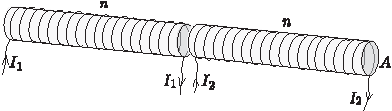
\includegraphics[scale=1.5]{Anh/Nam1.pdf}
\end{center}
\end{vd}
\begin{loigiai}
    \begin{itemize}
        \item \textbf{Cách 1:}
        \\  Áp dụng nguyên lí chồng chất, ta có thể dễ dàng suy ra từ thông qua một đầu cuộn dây bằng một nửa so với từ thông trong lòng ống dây. Do đó, theo cách sắp xếp cuộn dây như đề bài, từ thông của cuộn dây thứ nhất sẽ đi vào cuộn dây thứ hai và giá trị từ thông liên kết đó là
        \[\Phi=\dfrac{1}{2}\mu_0I_1nA.\]
        Một cách trực quan, toàn bộ từ thông từ cuộn $1$ đi vào cuộn $2$ sẽ đi ra ở mặt bên của cuộn vì nếu cuộn dây thứ hai là dài thì lượng từ thông đi ra ngoài ở đầu bên kia cuộn dây có thể được bỏ qua.
        \\Bây giờ chúng ta tính toán lực do từ trường của cuộn dây thứ nhất tác dụng lên dây dẫn mang dòng điện ở cuộn dây thứ hai. Thành phần từ trường dọc theo trục của cuộn dây không gây ra lực hiệu dụng lên cuộn dây $2$ vì lực từ do nó sinh ra xuyên tâm và đối xứng nên sẽ triệt tiêu lẫn nhau, do đó ở đây chúng ta chỉ tập trung vào thành phần từ trường theo phương xuyên tâm.
        \\Đặt thành phần xuyên tâm của vector cường độ từ trường tại vòng dây thứ $i$ tính từ đầu cuộn dây thứ hai là $B_i$. Do đó độ lớn của lực từ do cuộn dây thứ nhất tác dụng lên các vòng của cuộn dây thứ hai, mỗi vòng có bán kính $R$ và độ dài $2\pi R=2 \pi \sqrt{A/\pi}=2\sqrt{\pi A}$ là $F_i=2\sqrt{\pi A}I_2B_i$, do đó lực tác dụng lên toàn bộ cuộn dây thứ hai là
        \[F = \sum\limits_i {{F_i}}  = 2\sqrt {\pi A} {I_2}\sum\limits_i {{B_i}}.\]
        Tuy nhiên, chúng ta đã biết lượng từ thông từ cuộn dây $1$ thoát ra khỏi các mặt bên của cuộn dây $2$. Vì cuộn dây được cuốn $n$ vòng trên một đơn vị dài nên chúng ta có thể coi độ dày của một vòng là $1/n$, và diện tích bề mặt của mỗi vòng là $2\pi R/n = 2\sqrt {\pi A} /n$. Cuối cùng ta có biểu thức từ thông
        \[\frac{1}{2}{\mu _0}{I_1}nA = \Phi  = \sum\limits_i {\left( {\frac{{2\sqrt {\pi A} }}{n}{B_i}} \right).} \]
        So sánh giữa biểu thức lực và biểu thức từ thông ta thu được biểu thức độ lớn của lực từ
        \[F = \frac{1}{2}{\mu _0}{I_1}{I_2}{n^2}A.\]
        Nếu cả hai cuộn dây được cuốn theo cùng chiều, và chiều dòng điện như nhau thì lực giữa hai cuộn dây là lực hút. Nếu một trong hai thông số trên là ngược lại, thì lực là lực đẩy.
        \item \textbf{Cách 2:}
        \\Lực tương tác giữa hai cuộn dây sẽ tỉ lệ thuận với $I_1$ và $I_2$, vì từ trường sẽ tỉ lệ thuận với dòng điện trong một cuộn dây và từ trường đó gây lực từ lên dòng điện trong cuộn dây còn lại mà lực từ lại tỉ lệ thuận với tích $I.B$. Do đó ta có thể viết lực tương tác giữa hai cuộn dây theo dạng $F=K.I_1.I_2$, trong đó $K$ chỉ phụ thuộc vào các thông số cuộn dây và độc lập so với dòng điện chạy trong mỗi cuộn dây. Chúng ta sẽ rút ra K bằng cách tính toán lực tương tác trong trường hợp đặc biệt $I_1=I_2=I$, và hằng số $K$ đó là đúng cho mọi giá trị dòng điện.
        \\Giá trị lực từ chỉ phụ thuộc vào độ lớn của dòng điện chứ không phụ thuộc vào cách mà dòng điện đó được tạo ra. Nếu ta làm lạnh một cách phù hợp, cuộn dây mang dòng điện sẽ thành cuộn dây siêu dẫn (có điện trở = 0), và hai đầu cuộn dây sẽ hợp nhất thành một cuộn dây duy nhất có độ dài gấp đôi, và dòng điện sẽ là $I$ ở mọi nơi. Vì cuộn dây là siêu dẫn nên dòng điện $I$ sẽ không thay đổi dù không có bất kì nguồn cấp năng lượng nào. Bên trong cuộn dây, độ lớn của từ trường là $B=\mu_0nI$ và năng lượng từ trường được dự trữ là 
        \[{{{W}}_{\text{từ}}} = \frac{1}{{2{\mu _0}}}{B^2}V,\]
        ở đây $V=\ell A$ là thể tích của cuộn dây đôi có tiết diện mặt cắt $a$ và độ dài $\ell$. Chúng ta sẽ bàn kĩ hơn về vấn đề này ở phần mở rộng $1$.
        \\Điều gì sẽ xảy ra nếu chúng ta dịch hai cuộn solenoid ra cách xa nhau một đoạn $\Delta x(x\ll \ell)$. Từ trường trong ống dây tất yếu không thể thay đổi vì nếu có nó sẽ gây ra suất điện động cảm ứng và do cuộn dây không có điện trở nên dòng điện trong cuộn dây sẽ tiến đến vô cùng, đây là một hiện tượng phi vật lí. Nhưng năng lượng từ trường tích trữ trong cuộn dây thì có thay đổi, vì từ trường trong đoạn nhỏ đó bằng đúng từ trường trong lòng ống dây nhưng thể tích vùng từ trường lúc này tăng lên một khoảng nhỏ $\Delta V=A \Delta x.$
        \\Do đó phần năng lượng tăng lên tương ứng là 
        \[\Delta {W_{magn}} = \frac{1}{{2{\mu _0}}}{B^2}\Delta V = \frac{1}{2}{\mu _0}{I^2}{n^2}A\Delta x.\]
        Phần tăng năng lượng này chính bằng công của lực dùng để kéo ống dây ra, $W=F.\Delta x$, từ đây ta có thể suy ra 
        \[F = K{I_1}{I_2} = \frac{1}{2}{\mu _0}{I_1}{I_2}{n^2}A.\]
        \item \textbf{Mở rộng}
        \begin{itemize}
            \item  Hiệu ứng rìa không làm thay đổi kết quả vì nếu ta dịch cuộn dây ra xa nhau một khoảng nhỏ thì rìa cuộn dây cũng sẽ dịch đi một đoạn tương ứng. Do đó hiệu ứng rìa không làm ảnh hưởng đến phần thay đổi năng lượng.
            \item Một kết quả tương tự cũng có thể được tìm ra mà không cần đến hiện tượng siêu dẫn. Nối hai đầu cuộn dây lại ở điểm cuối của chúng để tạo thành một cuộn dây duy nhất thì lúc này sẽ có một dòng điện $I$ như nhau chạy trong cả hai cuộn dây. Nếu hai cuộn dây được kết nối theo cách này dịch ra xa nhau một khoảng nhỏ thì trên thực tế, từ trường và do đó từ thông ở khoảng đó sẽ bị giảm đi một chút vì việc ta dịch cuộn dây đi sẽ tạo thành một dòng điện cảm ứng rất nhỏ ngược chiều với dòng điện ban đầu, do đó làm giảm từ trường đi một lượng nhỏ.
            \\Chúng ta có thể chứng minh được năng lượng dự trữ của cuộn dây sẽ giảm đi một chút dù công thực hiện là dương. Hiện tượng kì lạ này có thể được giải thích bằng suất điện động cảm ứng gây ra bởi sự thay đổi từ thông. Sự giảm của suất điện động cảm ứng tương đương với việc năng lượng sẽ truyền vào cho nguồn điện và năng lượng này gấp đôi năng lượng giảm đi trên cuộn dây do đó công mà lực kéo sinh ra đã được truyền cho nguồn điện và giá trị của lực $F$ ta tính được lúc này vẫn như cách tiếp cận siêu dẫn.
        \end{itemize}

        
    \end{itemize}

\end{loigiai}

\begin{vd}[Định hướng sai]%Câu 6
Một vòng kim loại hình tròn có bán kính $r=0,1 \mathrm{m}$, quay quanh trục thẳng đứng là một đường kính của vòng với vận tốc góc không đổi. Như trên hình vẽ, một kim nam châm nhỏ đặt tại tâm vòng có thể quay tự do quanh trục thẳng đứng.
\begin{center}
\tikzset{every picture/.style={line width=0.75pt}} %set default line width to 0.75pt        

\begin{tikzpicture}[x=0.75pt,y=0.75pt,yscale=-1,xscale=1]
%uncomment if require: \path (0,420); %set diagram left start at 0, and has height of 420

%Shape: Circle [id:dp32204695616182843] 
\draw   (134,212.5) .. controls (134,157.55) and (178.55,113) .. (233.5,113) .. controls (288.45,113) and (333,157.55) .. (333,212.5) .. controls (333,267.45) and (288.45,312) .. (233.5,312) .. controls (178.55,312) and (134,267.45) .. (134,212.5) -- cycle ;
%Straight Lines [id:da17745998464492474] 
\draw  [dash pattern={on 4.5pt off 4.5pt}]  (233.5,73) -- (233.5,129) ;
%Straight Lines [id:da12402397940171284] 
\draw  [dash pattern={on 4.5pt off 4.5pt}]  (233.5,297) -- (233.5,346) ;
%Shape: Arc [id:dp723976575905914] 
\draw  [draw opacity=0] (248.07,84.92) .. controls (252.34,86.83) and (255,89.52) .. (255,92.5) .. controls (255,98.3) and (244.93,103) .. (232.5,103) .. controls (220.07,103) and (210,98.3) .. (210,92.5) .. controls (210,88.1) and (215.8,84.33) .. (224.04,82.77) -- (232.5,92.5) -- cycle ; \draw   (248.07,84.92) .. controls (252.34,86.83) and (255,89.52) .. (255,92.5) .. controls (255,98.3) and (244.93,103) .. (232.5,103) .. controls (220.07,103) and (210,98.3) .. (210,92.5) .. controls (210,88.1) and (215.8,84.33) .. (224.04,82.77) ;
\draw  [fill={rgb, 255:red, 0; green, 0; blue, 0 }  ,fill opacity=1 ] (252,93) -- (240.27,83.63) -- (255.05,80.96) -- (246.9,85.3) -- cycle ;
%Shape: Ellipse [id:dp25997108709859207] 
\draw   (223,228.5) .. controls (223,226.57) and (227.48,225) .. (233,225) .. controls (238.52,225) and (243,226.57) .. (243,228.5) .. controls (243,230.43) and (238.52,232) .. (233,232) .. controls (227.48,232) and (223,230.43) .. (223,228.5) -- cycle ;
%Straight Lines [id:da4944580997045749] 
\draw    (233,203.5) -- (233,228.5) ;
%Shape: Triangle [id:dp31251700899507884] 
\draw   (213,213) -- (227.49,197.98) -- (234.55,205.25) -- cycle ;
%Shape: Triangle [id:dp5236465704841922] 
\draw   (248.2,189.73) -- (234.55,205.25) -- (227.1,198.24) -- cycle ;





\end{tikzpicture}

\end{center}
Khi vòng đứng yên, kim nam châm chỉ theo hướng của thành phần nằm ngang của từ trường Trái Đất. Tuy nhiên, khi vòng quay với tốc độ mười vòng một giây, kim nam châm bị quay đi một góc $2^\circ$ so với ban đầu. Tính điện trở $R$ của vòng kim loại này.
\end{vd}
\begin{loigiai}
Phân tích từ trường Trái Đất thành các thành phần ngang và dọc. Thành phần dọc không gây ra dòng điện trong vòng, vì từ thông của nó gửi qua vòng luôn luôn bằng không. Đặt thành phần nằm ngang của từ trường là $B$ và vận tốc góc của vòng là  $\omega$. Từ thông gửi qua vòng là
$$\Phi=\pi{r^2}B\mathrm{cos}\omega t,$$
và suất điện động cảm ứng là $$ V=-\left(\dfrac{\dd\Phi}{\dd t}\right)=\pi{r^2}B\omega\mathrm{sin}\omega t.$$ Dòng điện có cường độ
$$ I=\dfrac{V}{R}=\dfrac{r^2\pi B\omega}{R}\mathrm{sin}\omega t,$$
chạy trong vòng gây ra một từ trường ở tâm vòng có độ lớn
$$B_I=\mu_0\dfrac{I}{2r}=\mu_0\dfrac{\pi rB\omega}{2R}\mathrm{sin}\omega t.$$
Từ trường $B_I$ có hướng vuông góc với mặt phẳng của vòng và quay cùng với nó. Phân tích vector $\ot{B_I}$ thành một thành phần song song $B$ và một thành phần vuông góc với nó. Thành phần song song tỉ lệ với $\mathrm{cos}\omega t\times\mathrm{sin}\omega t=\dfrac{1}{2}\mathrm{sin} 2\omega t$, trung bình bằng $0$ theo thời gian. Thành phần vuông góc có thể được viết là
$$B_{\bot}=\mu_0\dfrac{\pi rB\omega}{2R}{\mathrm{sin}^2}\omega t=\mu_0\dfrac{\pi rB\omega}{4R}\left(1-\mathrm{cos} 2\omega t\right).$$
Biểu thức này bao gồm một thành phần thay đổi (tương đối nhanh) theo thời gian và có trung bình là $0$, và một thành phần không đổi làm cho kim nam châm lệch đi  $\alpha = 2 ^\circ$ so với hướng ban đầu (bắc – nam). Vì kim nam châm hướng theo chiều của trường tổng hợp,
$$\tan\alpha=\dfrac{B_{\bot}}{B}=\mu_0\dfrac{\pi r\omega}{4R}.$$
Kim sẽ dao động nhỏ xung quanh vị trí trên, với biên độ được xác định bởi các đặc tính cơ học và từ tính của kim và bởi các lực giảm xóc. Thật thú vị khi để ý rằng góc lệch của kim nam châm không phụ thuộc vào độ lớn của từ trường Trái Đất. Điều quan trọng duy nhất là thành phần nằm ngang của nó là khác không. Điện trở của vòng có thể tính được từ công thức trên và có kết quả là $ 1,78\times{10^{-4}}\Omega.$
\end{loigiai}


\begin{vd}[Lồng hai solenoid]
     Một nhà khoa học làm thí nghiệm với hai ống dây solenoid đồng trục. Hai ống dây đều dài $l$, bán kính hai ống dây là $r$ và $2r$, ống nhỏ ở hoàn toàn bên trong ống lớn. Hai ống dây có dòng $I$ như nhau nhưng ngược chiều. Ống nhỏ có $4N$ vòng và ống lớn có $N$ vòng. Coi từ trường Trái Đất như từ trường của một lưỡng cực. Gọi $F$ là lực mà từ trường Trái Đất tác dụng lên hệ. Sau đó nhà khoa học thay hệ hai ống dây bằng một hệ khác tương tự: độ dài $7l$ bán kính $2r$ và $3r$, cuộn trong có $27~\mathrm{N}$ vòng va cuộn ngoài có $12N$ vòng. Hai ống bây giờ có dòng điện $2I$ nhưng ngược chiều. Lực từ trường Trái Đất tác dụng lên hệ bây giờ là $F'$. Biết hai hệ được bố trí như nhau. Coi kích thước các ống dây rất bé so với kích thước Trái Đất. \\
     Tìm $\displaystyle \dfrac{F'}{F}$.
\end{vd}
\begin{loigiai}\\
Chúng ta có thể coi rằng các ống dây solenoid được đặt tại cực Bắc Trái Đất và trục của các ống dây đi qua tâm Trái Đất. Nếu các ống dây ở vị trí khác, lực tác dụng lên các ống dây sẽ chỉ sai lệch một hằng số nhân và tỉ lệ $\dfrac{F'}{F}$ vẫn được giữ không đổi.\\
Ta thấy rằng nếu bán kính ống dây trong là $r$ và bán kính ống ngoài là $\alpha r$ thì số vòng dây tương ứng sẽ là $N$ và $\dfrac{N}{\alpha^2}$.\\
Để tính lực do từ trường Trái Đất tác dụng lên hệ ống dây, ta có thể tính lực do hệ ống dây tác dụng lên lưỡng cực Trái Đất. Lực này tỉ lệ với độ biến thiên từ trường do hệ ống dây gây ra tại tâm Trái Đất.\\ 
Ta tính từ trường tạo ra bởi hệ ống dây. Ta có thể coi hai ống dây như hai vòng dây có bán kính $r$ và $\alpha r$ và dòng điện $I$ và $\dfrac{I}{\alpha^2}$.
\begin{equation*}
    \begin{aligned}
     B&=\dfrac{\mu_0Ir^2}{2\tron{R^2+r^2}^{\frac{3}{2}}}-\dfrac{\mu_0Ir^2}{2\tron{R^2+\alpha^2r^2}^{\frac{3}{2}}}\\
     &\approx\dfrac{3\mu_0Ir^4}{4R^5}\tron{\alpha^2-1}.
    \end{aligned}
\end{equation*}
Suy ra $$\dfrac{\dd B}{\dd R}=\dfrac{-15\mu_0Ir^4}{4R^6}\tron{\alpha^2-1} .$$
Vậy lực từ tác dụng lên hai ống dây tỉ lệ với $Ir^4\tron{\alpha^2-1}$.\\
Từ đó ta có $$\frac{F'}{F}=\dfrac{(27N)(2I)(2r)^4\tron{\tron{\dfrac{3}{2}}^2-1}}{4NIr^4(2^2-1)}=90.$$
\end{loigiai}

\begin{vd}[Độ giảm tốc và từ trường sao Pulsar]
Sao Pulsar là một ngôi sao neutron có khối lượng $M \approx 1,4  M_s \approx 2,8 \times 10^{33}~\mathrm{g}$ (trong đó $M_s$ là khối lượng của mặt trời), và bán kính $R \approx 10 ~\mathrm{km} = 10^6 ~\mathrm{cm}$. Ngôi sao quay với vận tốc góc $\ot{\omega}$ và có moment từ $\ot{m}$ và moment từ này đã được quan sát là không song song với trục quay của ngôi sao. 
\begin{center}


\tikzset{every picture/.style={line width=0.75pt}} %set default line width to 0.75pt        

\begin{tikzpicture}[x=0.75pt,y=0.75pt,yscale=-1,xscale=1]
%uncomment if require: \path (0,480); %set diagram left start at 0, and has height of 480

%Shape: Circle [id:dp3694523233703746] 
\draw   (182,222.7) .. controls (182,173.71) and (221.71,134) .. (270.7,134) .. controls (319.69,134) and (359.4,173.71) .. (359.4,222.7) .. controls (359.4,271.69) and (319.69,311.4) .. (270.7,311.4) .. controls (221.71,311.4) and (182,271.69) .. (182,222.7) -- cycle ;
%Straight Lines [id:da307654927906319] 
\draw  [dash pattern={on 4.5pt off 4.5pt}]  (197.2,297.7) -- (344.2,147.7) ;
%Straight Lines [id:da7938927241676892] 
\draw  [dash pattern={on 4.5pt off 4.5pt}]  (270.7,340.2) -- (270.7,105.2) ;
%Straight Lines [id:da18230303159702288] 
\draw [line width=0.75]    (270.7,142.4) -- (270.7,89.4) ;
\draw [shift={(270.7,86.4)}, rotate = 450] [fill={rgb, 255:red, 0; green, 0; blue, 0 }  ][line width=0.08]  [draw opacity=0] (10.72,-5.15) -- (0,0) -- (10.72,5.15) -- (7.12,0) -- cycle    ;
%Straight Lines [id:da02343355138177028] 
\draw  [dash pattern={on 4.5pt off 4.5pt}]  (193.2,182.4) -- (270.7,222.7) ;
%Straight Lines [id:da7072380326449945] 
\draw    (243.7,249.7) -- (295.58,197.82) ;
\draw [shift={(297.7,195.7)}, rotate = 495] [fill={rgb, 255:red, 0; green, 0; blue, 0 }  ][line width=0.08]  [draw opacity=0] (10.72,-5.15) -- (0,0) -- (10.72,5.15) -- (7.12,0) -- cycle    ;
%Shape: Arc [id:dp7695324970163444] 
\draw  [draw opacity=0] (271.29,173.72) .. controls (278.06,173.8) and (284.91,175.29) .. (291.44,178.34) .. controls (296.32,180.62) and (300.65,183.6) .. (304.36,187.11) -- (270.7,222.7) -- cycle ; \draw   (271.29,173.72) .. controls (278.06,173.8) and (284.91,175.29) .. (291.44,178.34) .. controls (296.32,180.62) and (300.65,183.6) .. (304.36,187.11) ;
%Shape: Arc [id:dp00659516312679842] 
\draw  [draw opacity=0] (290.24,109.9) .. controls (297.13,111.5) and (301.54,113.95) .. (301.54,116.71) .. controls (301.54,121.52) and (288.11,125.41) .. (271.54,125.41) .. controls (254.97,125.41) and (241.54,121.52) .. (241.54,116.71) .. controls (241.54,113.95) and (245.95,111.5) .. (252.84,109.9) -- (271.54,116.71) -- cycle ; \draw   (290.24,109.9) .. controls (297.13,111.5) and (301.54,113.95) .. (301.54,116.71) .. controls (301.54,121.52) and (288.11,125.41) .. (271.54,125.41) .. controls (254.97,125.41) and (241.54,121.52) .. (241.54,116.71) .. controls (241.54,113.95) and (245.95,111.5) .. (252.84,109.9) ;
%Straight Lines [id:da20193274094983238] 
\draw    (290.24,109.9) -- (284.32,108.15) ;
\draw [shift={(281.44,107.3)}, rotate = 376.46000000000004] [fill={rgb, 255:red, 0; green, 0; blue, 0 }  ][line width=0.08]  [draw opacity=0] (10.72,-5.15) -- (0,0) -- (10.72,5.15) -- (7.12,0) -- cycle    ;



% Text Node
\draw (229,180.4) node [anchor=north west][inner sep=0.75pt]    {$R$};
% Text Node
\draw (314,265.4) node [anchor=north west][inner sep=0.75pt]    {$M$};
% Text Node
\draw (284,156.4) node [anchor=north west][inner sep=0.75pt]    {$\alpha $};
% Text Node
\draw (276,219.4) node [anchor=north west][inner sep=0.75pt]    {$\ot{m}$};
% Text Node
\draw (281,84.4) node [anchor=north west][inner sep=0.75pt]    {$\omega $};


\end{tikzpicture}
\end{center}

\begin{enumerate}[1)]
  \item Mô tả bức xạ phát ra từ ngôi sao và tính tổng công suất bức xạ của ngôi sao, giả sử rằng góc hợp bởi moment từ và trục quay của ngôi sao là $\alpha$, như trên hình vẽ. 
  \item Tìm độ giảm tốc (hằng số suy giảm đặc trưng của vận tốc góc) của ngôi sao, giả sử rằng năng lượng của ngôi sao chỉ mất mát do bức xạ điện từ.
  \item Giải thích tại sao từ các thông số đã biết như khối lượng, bán kính, chu kì quay $T$, và độ suy giảm $\dd T/ \dd t$ của ngôi sao, chúng ta có thể ước tính được từ trường trên bề mặt ngôi sao. Đưa ra một đáp án bằng số nếu chúng ta biết quan sát và thực nghiệm đã ghi nhận lại được $T= 7,476551 \pm 3 ~\mathrm{s}$ và $\dot{T} = (2,8 \pm 1,4)\times 10^{-11} \approx 10^{-3} ~\mathrm{s/}\text{năm}$ (để đơn giản hóa ta có thể coi $\ot{m}$ là vuông góc với trục quay).

\end{enumerate}
\end{vd}

\begin{loigiai}
\begin{enumerate}[1)]
 \item Vì góc tạo bởi moment từ và trục quay của sao là $\alpha$ khác không, do đó thành phần vuông góc với trục quay của moment $\ot{m}$ sẽ quay với vận tốc góc $\omega$. Do đó, sao Pulsar phát ra bức xạ lưỡng cực có tần số góc $\omega$. Tổng công suất là 
  \[P= \frac{2}{3c^3}\abs{{\ddot{\ot{m}}_{\perp}}}^2 = \frac{2}{3}\dfrac{m_{\perp}^2 \omega^4}{c^3}, \tag{1} \]
ở đây $m_{\perp} = m \sin \alpha $. 
  \item Động năng của hệ là $U= I\omega^2 /2$, ở đây $I= 2MR^2 /5 \approx 1,1\times 10^{43} \,~\mathrm{gcm}^2$ là moment quán tính của ngôi sao trong trường hợp ta giả sử rằng phân bố khối lượng là đều trong toàn hình cầu bán kính $R$. Giả sử năng lượng chỉ mất mát do bức xạ điện từ, ta có 
   \[\frac{\dd U}{\dd t} = \frac{\dd}{\dd t} \left( \frac{I\omega^2}{2}\right)= I\omega\dot{\omega} = -P, \tag{2} \] 
và kết hợp với $1)$ ta có
   \[I\omega \dot{\omega} = - \frac{2}{3} \frac{m_{\perp}^2 \omega^4 }{c^3} \Rightarrow \frac{\dot{\omega}}{\omega^3} = - \frac{2m_{\perp}^2}{3 I c^3}t . \tag{3} \]
Tích phân trên vùng thời gian từ $0$ đến $t$ ta thu được
   \[\frac{1}{2\omega^2(t)} - \frac{1}{2\omega^2(0)} = \frac{2m_{\perp}^2}{3Ic^3} ,\tag{4}\] 

và do đó
   \[\omega(t) =  \frac{\omega(0)}{\sqrt{1+\dfrac{t}{\tau}}}, \ \text{ với } \ \tau = \frac{3Ic^3}{4m_{\perp}^2 \omega^2(0)} . \tag{5} \] 

\item Chúng ta viết lại $\dot{\omega}/\omega^3$ thành $\dot{\omega}/\omega^3 = -T\dot{T}/4\pi^2$, ở đây $T= 2\pi/\omega$ là chu kì quay của Pulsar, và $\dot{T} = -2\pi \dot{\omega}/\omega^2$. Do đó ta thu được moment lưỡng cực $m= m_{\perp}$ như là một hàm của các thông số có được từ thực nghiệm và $2)$:
    \[ m = \sqrt{\frac{3Ic^3}{8\pi^2} T\dot{T}} \approx 3,3 \times 10^{36} \sqrt{T\dot{T}} \,\,~\mathrm{erg/G}, \tag{6} \]

với $T$ được tính theo giây. Cường độ từ trường tức thời trên bề mặt của sao Pulsar tương tự với từ trường gây ra bởi một lưỡng cực từ đặt ở tâm ngôi sao:
     \[\ot{B} = \frac{3({\hat{r}} \cdot \ot{m})\hat{r} - \ot{m}}{r^3}, \tag{7} \]
và dễ thấy $B_{\max} = 2m/R^3$. Thay số ta thu được 
      \[B_{\max} \approx 6,6 \times 10^{21} \sqrt{T\dot{T}} ~ \mathrm{G}, \tag{8} \]
Và kết hợp kết quả thực nghiệm của $T$ và $\dot{T}$ ta thu được 
     \[B_{\max} \approx (9,6\pm 0,25 ) \times 10^{16} ~\mathrm{G}. \tag{9} \]

\end{enumerate}
\end{loigiai}


\begin{vd}[Vòng dây dao động]
Một vòng dây bằng đồng (điện trở rất nhỏ) bán kính $r$, khối lượng $m$ treo bằng một sợi dây thực hiện dao động xoắn với chu kì $T_0$. Cuộn dây có độ tự cảm $L$. Chu kì thay đổi thế nào nếu đặt trong từ trường đồng nhất có cảm ứng từ $\ot{B}$ nằm ngang song song với mặt phẳn vòng dây khi vòng ở vị trí cân bằng. Biết moment quán tính đối với trục đi qua đường kính là $J$.
\begin{center}
    

\tikzset{every picture/.style={line width=0.75pt}} %set default line width to 0.75pt        

\begin{tikzpicture}[x=0.75pt,y=0.75pt,yscale=-1,xscale=1]
%uncomment if require: \path (0,417); %set diagram left start at 0, and has height of 417

%Shape: Circle [id:dp17346979816986008] 
\draw  [line width=3.75]  (174,252.25) .. controls (174,218.42) and (201.42,191) .. (235.25,191) .. controls (269.08,191) and (296.5,218.42) .. (296.5,252.25) .. controls (296.5,286.08) and (269.08,313.5) .. (235.25,313.5) .. controls (201.42,313.5) and (174,286.08) .. (174,252.25) -- cycle ;
%Straight Lines [id:da552655373957109] 
\draw  [dash pattern={on 4.5pt off 4.5pt}]  (235.25,191) -- (235.25,332) ;
%Straight Lines [id:da3503234546387448] 
\draw    (235.25,51) -- (235.25,191) ;
%Straight Lines [id:da47506307814771076] 
\draw    (198,50) -- (273.5,50) ;
%Straight Lines [id:da9983228801675521] 
\draw    (235.25,252.25) -- (283.02,219.69) ;
\draw [shift={(285.5,218)}, rotate = 505.72] [fill={rgb, 255:red, 0; green, 0; blue, 0 }  ][line width=0.08]  [draw opacity=0] (8.04,-3.86) -- (0,0) -- (8.04,3.86) -- (5.34,0) -- cycle    ;
\draw [shift={(235.25,252.25)}, rotate = 325.72] [color={rgb, 255:red, 0; green, 0; blue, 0 }  ][fill={rgb, 255:red, 0; green, 0; blue, 0 }  ][line width=0.75]      (0, 0) circle [x radius= 2.34, y radius= 2.34]   ;
%Straight Lines [id:da29590519396709736] 
\draw    (203,49) -- (207.5,36) ;
%Straight Lines [id:da8797384501930146] 
\draw    (223,50) -- (227.5,37) ;
%Straight Lines [id:da4152682274694077] 
\draw    (213,50) -- (217.5,37) ;
%Straight Lines [id:da6203719922500526] 
\draw    (242,51) -- (246.5,38) ;
%Straight Lines [id:da6628697806126855] 
\draw    (233,50) -- (237.5,37) ;
%Straight Lines [id:da1980264716128195] 
\draw    (251,51) -- (255.5,38) ;
%Straight Lines [id:da15027155654391278] 
\draw    (260,51) -- (264.5,38) ;
%Straight Lines [id:da3771360602933249] 
\draw    (321,242) -- (410.5,242) ;
\draw [shift={(413.5,242)}, rotate = 180] [fill={rgb, 255:red, 0; green, 0; blue, 0 }  ][line width=0.08]  [draw opacity=0] (10.72,-5.15) -- (0,0) -- (10.72,5.15) -- (7.12,0) -- cycle    ;

% Text Node
\draw (216,241.4) node [anchor=north west][inner sep=0.75pt]    {$O$};
% Text Node
\draw (260,212.4) node [anchor=north west][inner sep=0.75pt]    {$r$};
% Text Node
\draw (284,300.4) node [anchor=north west][inner sep=0.75pt]    {$m,L,J$};
% Text Node
\draw (355,210.4) node [anchor=north west][inner sep=0.75pt]    {$\vec{B}$};


\end{tikzpicture}

\end{center}
\end{vd}
\begin{loigiai}
Về biến dạng xoắn, ta sẽ gọi hệ số tỉ lệ là $A$, ta thu được phương tình vi phân dao động do biến dạng xoắn: $A\theta=-J\ddot{\theta}$.\\
Từ đó chu kì:
$$T_0=2\pi\sqrt{\dfrac{J}{A}}$$
Khi có từ trường, từ thông xuyên qua vòng khi vòng xê dịch một góc nhỏ là:
$$\Phi=BS\cdot \mathrm{sin}\theta \approx BS\theta$$
Suất điện động tự cảm đúng bằng suất điện động cảm ứng sinh ra trên vòng:
$$L\cdot\dfrac{\mathrm{d}i}{\mathrm{d}t}=BS\cdot\dfrac{\mathrm{d}\theta}{\mathrm{d}t} \Rightarrow Li=BS\theta + C$$
Khi $i=0$ thì $\theta=0$ nên hằng số $C=0 \Rightarrow i=BS\theta/L$.\\
Moment từ: $\ot{M}=\ot{p_m}\times\ot{B}=iSB \approx B^2S^2\theta/L$.
Ta có phương trình vi phân dạng mới:
$$-\dfrac{B^2S^2}{L}\theta-A\theta=J\ddot{\theta}\Leftrightarrow \left(-\dfrac{B^2S^2}{L}-\dfrac{4\pi^2J}{T_0^2}\right)\theta=J\ddot{\theta}$$
Chu kì dao động mới:
$$T=\dfrac{T_0}{\sqrt{\dfrac{B^2S^2T_0^2}{4\pi^2JL}+1}}.$$
\end{loigiai}


\begin{vd}[Bước vào từ trường]
Hãy xét một từ trường đều $B$ trong vùng màu xám và hướng ra ngoài mặt phẳng hình vẽ, như các hình dưới đây.
\begin{center}
    

\tikzset{every picture/.style={line width=0.75pt}} %set default line width to 0.75pt        

\begin{tikzpicture}[x=0.75pt,y=0.75pt,yscale=-1,xscale=1]
%uncomment if require: \path (0,300); %set diagram left start at 0, and has height of 300

%Shape: Rectangle [id:dp751914180106541] 
\draw  [color={rgb, 255:red, 155; green, 155; blue, 155 }  ,draw opacity=1 ][fill={rgb, 255:red, 155; green, 155; blue, 155 }  ,fill opacity=1 ] (33,128.63) -- (193.75,128.63) -- (193.75,213.06) -- (33,213.06) -- cycle ;
%Shape: Rectangle [id:dp5715554387472597] 
\draw  [color={rgb, 255:red, 155; green, 155; blue, 155 }  ,draw opacity=1 ][fill={rgb, 255:red, 155; green, 155; blue, 155 }  ,fill opacity=1 ] (233.1,109) -- (393.85,109) -- (393.85,193.43) -- (233.1,193.43) -- cycle ;
%Shape: Rectangle [id:dp4433680938904905] 
\draw  [color={rgb, 255:red, 155; green, 155; blue, 155 }  ,draw opacity=1 ][fill={rgb, 255:red, 155; green, 155; blue, 155 }  ,fill opacity=1 ] (430.69,144.83) -- (532,144.83) -- (532,212.12) -- (430.69,212.12) -- cycle ;
%Curve Lines [id:da7432949283072408] 
\draw    (101.34,158.57) .. controls (135.22,158.57) and (128.91,184.65) .. (126.04,190.52) ;
%Straight Lines [id:da15327337471065383] 
\draw    (97.32,157.91) -- (101.34,158.57) ;
%Straight Lines [id:da9237701245729204] 
\draw    (97.32,157.91) -- (95.6,164.43) ;
%Curve Lines [id:da846544871091409] 
\draw    (95.6,164.43) .. controls (88.71,170.3) and (89.28,178.13) .. (87.47,184.05) .. controls (85.66,189.97) and (82.97,186.61) .. (97.9,189.22) ;
%Curve Lines [id:da3612566481757702] 
\draw    (97.9,189.22) .. controls (99.05,202.91) and (92.73,204.87) .. (117.42,194.44) ;
%Straight Lines [id:da9634504850992611] 
\draw    (126.04,190.52) -- (117.42,194.44) ;

%Curve Lines [id:da7805941099664069] 
\draw    (305.63,178.19) .. controls (339.51,178.19) and (333.2,204.28) .. (330.32,210.15) ;
%Straight Lines [id:da4463686851471427] 
\draw    (301.61,177.54) -- (305.63,178.19) ;
%Straight Lines [id:da4213043294347989] 
\draw    (301.61,177.54) -- (299.89,184.06) ;
%Curve Lines [id:da8307231428150825] 
\draw    (299.89,184.06) .. controls (293,189.93) and (293.57,197.76) .. (291.76,203.68) .. controls (289.95,209.6) and (287.25,206.24) .. (302.19,208.85) ;
%Curve Lines [id:da4478446011588786] 
\draw    (302.19,208.85) .. controls (303.33,222.54) and (297.02,224.5) .. (321.71,214.06) ;
%Straight Lines [id:da9224516498692135] 
\draw    (330.32,210.15) -- (321.71,214.06) ;

%Shape: Chord [id:dp3024926209068406] 
\draw   (511.73,185.21) .. controls (512.95,188.32) and (513.6,191.68) .. (513.58,195.2) .. controls (513.49,210.68) and (500.3,223.14) .. (484.12,223.02) .. controls (467.93,222.91) and (454.88,210.26) .. (454.97,194.78) .. controls (454.99,191.27) and (455.69,187.91) .. (456.94,184.82) -- cycle ;
%Straight Lines [id:da2851947683889342] 
\draw  [dash pattern={on 0.84pt off 2.51pt}]  (297.22,194.05) -- (328.9,194.05) ;
\draw [shift={(331.9,194.05)}, rotate = 180] [fill={rgb, 255:red, 0; green, 0; blue, 0 }  ][line width=0.08]  [draw opacity=0] (10.72,-5.15) -- (0,0) -- (10.72,5.15) -- (7.12,0) -- cycle    ;
\draw [shift={(294.22,194.05)}, rotate = 0] [fill={rgb, 255:red, 0; green, 0; blue, 0 }  ][line width=0.08]  [draw opacity=0] (8.93,-4.29) -- (0,0) -- (8.93,4.29) -- cycle    ;
%Straight Lines [id:da6949611555798287] 
\draw  [dash pattern={on 0.84pt off 2.51pt}]  (475.07,185.33) -- (475.07,212.43) ;


% Text Node
\draw (51.95,135.52) node [anchor=north west][inner sep=0.75pt]   [align=left] {vùng từ trường $\displaystyle B$};
% Text Node
\draw (251.21,114.95) node [anchor=north west][inner sep=0.75pt]   [align=left] {vùng từ trường $\displaystyle B$};
% Text Node
\draw (307.48,195.68) node [anchor=north west][inner sep=0.75pt]  [font=\scriptsize]  {$w$};
% Text Node
\draw (478.28,195.68) node [anchor=north west][inner sep=0.75pt]  [font=\scriptsize]  {$y$};
% Text Node
\draw (99.11,235.05) node [anchor=north west][inner sep=0.75pt]    {$( 1)$};
% Text Node
\draw (300.89,233.18) node [anchor=north west][inner sep=0.75pt]    {$( 2)$};
% Text Node
\draw (474.2,233.18) node [anchor=north west][inner sep=0.75pt]    {$( 3)$};


\end{tikzpicture}
\end{center}
\begin{enumerate}[1)]%tutruong (0)
    \item Tìm lực do từ trường tác dụng lên một cuộn dây dẫn mảnh khép kín mang theo một dòng điện không đổi $I$, tất cả cuộn dây dẫn nằm bên trong vùng từ trường. Mặt phẳng cuộn dây nằm trong mặt phẳng hình vẽ. 
    \item Lực do từ trường tác dụng lên cuộn dây dẫn khi một phần của nó nằm ngoài vùng có từ trường có thể được viết dưới dạng $F=\alpha wBI$, trong đó $w$ là khoảng cách giữa hai điểm của cuộn dây cắt cạnh đáy của vùng từ trường, và hướng của nó là một trong hai hướng: lên hoặc xuống tùy thuộc vào chiều của dòng điện. Tìm giá trị của $\alpha$.
    \item Cho một cuộn dây mảnh hình bán nguyệt $r$, điện trở $R$, và khối lượng $m$ rơi xuống và đi ra ngoài vùng từ trường. Mặt phẳng của cuộn dây nằm trong mặt phẳng tờ giấy, và cạnh thẳng của vòng dây song song với cạnh đáy nằm ngang của vùng từ trường. Bỏ qua hiện tượng tự cảm của cuộn dây. Viết phương trình vi phân cho $y (<r)$ là khoảng cách giữa cạnh thẳng của cuộn dây và cạnh đáy của vùng từ trường. Nếu bạn chưa tìm thấy $\alpha$ trong ý $(2)$. Bạn có thể sử dụng nó như một hằng số đã biết để giải ý $(3)$.
\end{enumerate}
\end{vd}
\begin{loigiai}
\begin{enumerate}[1)]
    \item 
\begin{enumerate}[\text{Câu trả lời} 1:]
    \item Cuộn dây là tổng của rất nhiều cuộn dây nhỏ hình vuông. Lực từ tác dụng lên từng cuộn dây nhỏ bằng không, do đó hợp lực tác dụng lên vòng dây bằng không. 
    \item Di chuyển cuộn dây trong một từ trường không cần thực hiện công, do không có hiện tượng cảm ứng điện từ, do đó hợp lực bằng không.
    \item Sử dụng hình chiếu của vector.
\end{enumerate}
    \item Cuộn dây được chia làm hai nửa tại ranh giới của từ trường, giả sử có một dòng dương và một dòng âm.\\$\alpha=1$
    \item Di chuyển cuộn dây trong từ trường, cắt các đường sức từ trường
    \[w=2\sqrt{r^2-y^2},\]
    kết quả là dòng điện được tạo ra
    \[I=\dfrac{Bwv}{R}.\]
    trong đó $v=-\dfrac{\mathrm{d}y}{\mathrm{d}t}$ (do $y$ giảm và $v$ tăng.)\\
    Lực từ tác dụng lên cuộn dây $F=IBw$.\\
    Phương trình chuyển động
    \[m\dfrac{\mathrm{d}^2y}{\mathrm{d}t^2}=F-mg.\]
    Kết hợp tất cả các phương trình trên lại ta được
    \[\dfrac{\mathrm{d}^2y}{\mathrm{d}t}+\dfrac{4B^2}{mR}(r^2-y^2)\dfrac{\mathrm{d}y}{\mathrm{d}t}+g=0.\]
\end{enumerate}
\end{loigiai}



\begin{vd}[Điện tích điểm trong từ trường]
Một điện tích điểm $-q(q>0)$ khối lượng $m$ chuyển động không ma sát trong một miền có từ trường được cho bởi biểu thức $\ot{B}=B_0\dfrac{a}{r}\ot{z} (B_0>0)$ với $r=\sqrt{x^2+y^2}$ là khoảng cách tính từ trục $z$. Tại thời điểm $t=0$, vị trí và vận tốc ban đầu của điện tích là $(x=a,y=0,z=0)$ và $(v_{x}=a,v_{y}=v_0,v_{z}=0)$, ở đây $a$, $v_0>0$.
\begin{enumerate}[1) ]
    \item Chứng minh rằng hạt luôn nằm trên mặt phẳng $xy$.
    \item Tìm vận tốc ban đầu, mà với vận tốc đó điện tích có thể thực hiện một chuyển động tròn xung quanh gốc tọa độ. 
    \item Bây giờ vận tốc ban đầu không bằng với câu trả lời trong ý $(2)$. Thiết lập phương trình vi phân dưới dạng $\dfrac{\mathrm{d}L}{\mathrm{d}r}=\const$, với $L$ là moment động lượng của điện tích đối với trục $z$, và giải phương trình vi phân đó. Nếu bạn không thể xác định được hằng số đó, bạn hãy giả sử rằng hằng số đó đã biết và giải các ý $(4)$ và $(5)$.\\
    (\textit{Gợi ý:} $\ot{A}\times(\ot{C}\times\ot{B})=(\ot{A}\cdot\ot{B})\cdot\ot{C}-(\ot{A}\cdot\ot{C})\cdot\ot{B}$) 
    \item Từ kết quả của ý $(3)$, hãy tìm khoảng cách từ điện tích tới gốc tọa độ khi mà nó chuyển động theo phương tiếp tuyến với quỹ đạo $(\ot{v}\bot \ot{r})$. Tìm vận tốc nhỏ nhất $v_0$ mà điện tích không bao giờ có thể dịch chuyển theo phương tiếp tuyến sau khi nó được cung cấp vận tốc.
    \item Tìm khoảng cách tính từ gốc khi điện tích đang chuyển động theo hướng xuyên tâm ($\ot{v}$ song song với $\ot{r}$). Tìm vận tốc nhỏ nhất $v_0$ mà điện tích không bao giờ có thể dịch chuyển theo phương xuyên tâm sau khi nó được cung cấp vận tốc.
\end{enumerate}
\end{vd}
\begin{loigiai}
\begin{enumerate}[1) ]
    \item  Theo định luật lực Lorentz $\ot{F}=-q\ot{v}\times\ot{B}$, lực $F$ không có thành phần dọc theo trục $z$ vì từ trường $\ot{B}$ hướng dọc theo trục $z$. Do đó, nếu vận tốc ban đầu $v_{z}=0$ thì điện tích luôn chuyển động trong mặt phẳng $x-y$. 
    \item Từ trường $B$ tại $r=a$ là vừa đủ để hạt chuyển động trên một quỹ đạo tròn bán kính $a$.
    \[\dfrac{mv_0^2}{a}=qv_0B_0\rt v_0=\dfrac{qB_0a}{m}.\]
    \item Gọi moment động lượng của điện tích đối với gốc là $L$. Khi đó $L(t=0)=mv_0a$. Ta có
    \begin{align*}
        \dfrac{\mathrm{d}L}{\mathrm{d}t}&=-rF\mathrm{\sin{\theta}}\\
        &=-qrvB\mathrm{\cos{\phi}}\\
        &=-qrBv_{r}=qrB\dfrac{\mathrm{d}r}{\mathrm{d}t}\\
        \Longleftrightarrow\dfrac{\mathrm{d}L}{\mathrm{d}r}&=qrB.
    \end{align*}
    với $v_{r}=\dfrac{\mathrm{d}r}{\mathrm{d}t}$ là vận tốc theo phương xuyên tâm.\\
    \begin{center}
        

\tikzset{every picture/.style={line width=0.75pt}} %set default line width to 0.75pt        

\begin{tikzpicture}[x=0.75pt,y=0.75pt,yscale=-1,xscale=1]
%uncomment if require: \path (0,300); %set diagram left start at 0, and has height of 300

%Straight Lines [id:da6526384579910471] 
\draw    (308.37,81.97) -- (388.02,132.42) ;
\draw [shift={(390.55,134.02)}, rotate = 212.35] [fill={rgb, 255:red, 0; green, 0; blue, 0 }  ][line width=0.08]  [draw opacity=0] (10.72,-5.15) -- (0,0) -- (10.72,5.15) -- (7.12,0) -- cycle    ;
%Straight Lines [id:da8692651038771895] 
\draw    (308.37,81.97) -- (251.5,171.65) ;
\draw [shift={(249.89,174.19)}, rotate = 302.38] [fill={rgb, 255:red, 0; green, 0; blue, 0 }  ][line width=0.08]  [draw opacity=0] (10.72,-5.15) -- (0,0) -- (10.72,5.15) -- (7.12,0) -- cycle    ;
%Straight Lines [id:da5723833940518483] 
\draw    (328.79,162.84) -- (309.11,84.88) ;
\draw [shift={(308.37,81.97)}, rotate = 435.83000000000004] [fill={rgb, 255:red, 0; green, 0; blue, 0 }  ][line width=0.08]  [draw opacity=0] (10.72,-5.15) -- (0,0) -- (10.72,5.15) -- (7.12,0) -- cycle    ;


% Text Node
\draw (237.8,176.73) node [anchor=north west][inner sep=0.75pt]  [font=\normalsize,rotate=-3.57]  {$\vec{v}$};
% Text Node
\draw (393.99,124.83) node [anchor=north west][inner sep=0.75pt]  [font=\normalsize,rotate=-1.42]  {$\vec{F}$};
% Text Node
\draw (300.05,64.15) node [anchor=north west][inner sep=0.75pt]  [font=\normalsize,rotate=-3.17]  {$\vec{r}$};
% Text Node
\draw (333.11,110.86) node [anchor=north west][inner sep=0.75pt]  [font=\normalsize,rotate=-3.37]  {$\theta $};
% Text Node
\draw (298.46,113.41) node [anchor=north west][inner sep=0.75pt]  [font=\normalsize,rotate=-357.66]  {$\phi $};


\end{tikzpicture}
    \end{center}
    Chúng ta cũng có thể tìm được phương trình vi phân bằng cách
    \[\dfrac{\mathrm{d}\ot{L}}{\mathrm{d}t}=\ot{r}\times\ot{F}=-q\ot{r}\times(\ot{v}\times\ot{B})=-q\left((\ot{r}\cdot\ot{B})\cdot\ot{v}-(\ot{r}\cdot\ot{v})\cdot\ot{B}\right)=qrv_{r}\ot{B}=qr\dfrac{\mathrm{d}r}{\mathrm{d}t}\ot{B}.\]
    Suy ra
    \begin{align*}
       \dfrac{\mathrm{d}\ot{L}}{\mathrm{d}t} &=qrB\dfrac{\mathrm{d}r}{\mathrm{d}t}\\
       \dfrac{\mathrm{d}\ot{L}}{\mathrm{d}r} &=qrB\\
        \Leftrightarrow L(r)-L(a)&=\int_{a}^{r}qBr\mathrm{d}r=qB_0a(r-a).
    \end{align*} 
    \item Bởi vì từ trường $B$ không hoạt động, vận tốc của điện tích luôn luôn là $v_0$. Lưu ý moment động lượng có thể là $L=\pm mrv_0$.\\
    Khi $L=mrv_0$, $r=a$, không có chuyển động theo phương tiếp tuyến ngay sau đó.\\
    Khi $L=-mrv_0$
    \[r=a\dfrac{qB_0a-mv_0}{qB_0a+mv_0}.\]
    Khi $qB_0a<mv_0$, nghiệm duy nhất của phương trình là $r=a$, tương ứng với các điều kiện ban đầu. Không có chuyển động theo phương tiếp tuyến xảy ra ngay sau đó.\\
    Khi $qB_0a>mv_0$,
    \[r=a\dfrac{qB_0a-mv_0}{qB_0a+mv_0}<a.\]
    điều đó là có thể xảy ra.
    \item Khi điện tích chuyển động theo phương xuyên tâm, thì $L=0$, do đó
    \[r=a\left(1-\dfrac{mv_0}{qB_0a}\right).\]
    Khi $qB_0a>mv_0$, $r>0$, chuyển động có thể hướng tâm.\\
    Khi $qB_0a<mv_0$, $r<0$, chuyển động sẽ không bao giờ là hướng tâm.
\end{enumerate}
\end{loigiai}


\begin{vd}[Quay trong lòng Solenoid]
Một đĩa kim loại bán kính $r$ có thể quay với ma sát không đáng kể bên trong một cuộn dây dài, thẳng, quanh một trục song song với trục đối xứng của cuộn dây. Một đầu của cuộn dây được nối với cạnh của đĩa còn đầu kia nối với trục. Cuộn dây có điện trở $R$ và chứa $n$ vòng trên mỗi đơn vị chiều dài, được đặt sao cho trục của nó song song với vector cảm ứng từ $\ot{B_0}$ của Trái Đất.

\begin{center}
    

\tikzset{every picture/.style={line width=0.75pt}} %set default line width to 0.75pt        

\begin{tikzpicture}[x=0.75pt,y=0.75pt,yscale=-1,xscale=1,scale=0.4]
%uncomment if require: \path (0,725); %set diagram left start at 0, and has height of 725

%Shape: Can [id:dp794933563146212] 
\draw  [fill={rgb, 255:red, 255; green, 255; blue, 255 }  ,fill opacity=1 ] (388.83,324.64) -- (388.83,513.93) .. controls (388.83,514.39) and (387.58,514.77) .. (386.04,514.77) .. controls (384.5,514.77) and (383.25,514.39) .. (383.25,513.93) -- (383.25,324.64) .. controls (383.25,324.18) and (384.5,323.8) .. (386.04,323.8) .. controls (387.58,323.8) and (388.83,324.18) .. (388.83,324.64) .. controls (388.83,325.1) and (387.58,325.48) .. (386.04,325.48) .. controls (384.5,325.48) and (383.25,325.1) .. (383.25,324.64) ;
%Shape: Ellipse [id:dp9073150731380437] 
\draw  [fill={rgb, 255:red, 255; green, 255; blue, 255 }  ,fill opacity=1 ] (339.33,311.08) .. controls (339.33,303.2) and (360.15,296.8) .. (385.83,296.8) .. controls (411.51,296.8) and (432.33,303.2) .. (432.33,311.08) .. controls (432.33,318.96) and (411.51,325.35) .. (385.83,325.35) .. controls (360.15,325.35) and (339.33,318.96) .. (339.33,311.08) -- cycle ;
%Shape: Ellipse [id:dp7831632242132669] 
\draw  [fill={rgb, 255:red, 255; green, 255; blue, 255 }  ,fill opacity=1 ] (339.33,303.94) .. controls (339.33,296.06) and (360.15,289.67) .. (385.83,289.67) .. controls (411.51,289.67) and (432.33,296.06) .. (432.33,303.94) .. controls (432.33,311.83) and (411.51,318.22) .. (385.83,318.22) .. controls (360.15,318.22) and (339.33,311.83) .. (339.33,303.94) -- cycle ;
%Straight Lines [id:da15211630183630298] 
\draw [fill={rgb, 255:red, 255; green, 255; blue, 255 }  ,fill opacity=1 ]   (339.33,302.86) -- (339.33,311.08) ;
%Straight Lines [id:da4152297399713436] 
\draw    (432.33,303.94) -- (432.33,311.08) ;

%Shape: Can [id:dp6293113679467115] 
\draw  [fill={rgb, 255:red, 255; green, 255; blue, 255 }  ,fill opacity=1 ] (388.33,125.29) -- (388.33,303.18) .. controls (388.33,303.6) and (387.2,303.94) .. (385.79,303.94) .. controls (384.39,303.94) and (383.25,303.6) .. (383.25,303.18) -- (383.25,125.29) .. controls (383.25,124.87) and (384.39,124.53) .. (385.79,124.53) .. controls (387.2,124.53) and (388.33,124.87) .. (388.33,125.29) .. controls (388.33,125.71) and (387.2,126.05) .. (385.79,126.05) .. controls (384.39,126.05) and (383.25,125.71) .. (383.25,125.29) ;
%Shape: Spring [id:dp8083999628893139] 
\draw   (385.48,155.53) .. controls (425.64,158.03) and (465.79,164.53) .. (465.79,177.53) .. controls (465.79,203.53) and (305.16,203.53) .. (305.16,197.53) .. controls (305.16,191.53) and (465.79,191.53) .. (465.79,217.53) .. controls (465.79,243.53) and (305.16,243.53) .. (305.16,237.53) .. controls (305.16,231.53) and (465.79,231.53) .. (465.79,257.53) .. controls (465.79,283.53) and (305.16,283.53) .. (305.16,277.53) .. controls (305.16,271.53) and (465.79,271.53) .. (465.79,297.53) .. controls (465.79,323.53) and (305.16,323.53) .. (305.16,317.53) .. controls (305.16,311.53) and (465.79,311.53) .. (465.79,337.53) .. controls (465.79,363.53) and (305.16,363.53) .. (305.16,357.53) .. controls (305.16,351.53) and (465.79,351.53) .. (465.79,377.53) .. controls (465.79,403.53) and (305.16,403.53) .. (305.16,397.53) .. controls (305.16,391.53) and (465.79,391.53) .. (465.79,417.53) .. controls (465.79,443.53) and (305.16,443.53) .. (305.16,437.53) .. controls (305.16,431.53) and (465.79,431.53) .. (465.79,457.53) .. controls (465.79,483.53) and (305.16,483.53) .. (305.16,477.53) .. controls (305.16,471.53) and (465.79,471.53) .. (465.79,497.53) .. controls (465.79,523.53) and (305.16,523.53) .. (305.16,517.53) .. controls (305.16,511.89) and (446.83,511.55) .. (464.08,533.06) ;
%Straight Lines [id:da16873648988922163] 
\draw    (222.33,155.53) -- (384.33,155.53) ;

%Straight Lines [id:da34653262474759705] 
\draw    (339.33,3.38) -- (339.33,311.08) ;
%Straight Lines [id:da14719050864648686] 
\draw    (223,3.38) -- (339.33,3.38) ;
%Straight Lines [id:da9406743709845233] 
\draw    (223,3.38) -- (223,155.53) ;
%Shape: Circle [id:dp46030588478741774] 
\draw  [fill={rgb, 255:red, 255; green, 255; blue, 255 }  ,fill opacity=1 ] (198,79.45) .. controls (198,65.64) and (209.19,54.45) .. (223,54.45) .. controls (236.81,54.45) and (248,65.64) .. (248,79.45) .. controls (248,93.26) and (236.81,104.45) .. (223,104.45) .. controls (209.19,104.45) and (198,93.26) .. (198,79.45) -- cycle ;
%Straight Lines [id:da19632157276818174] 
\draw    (413.33,143.38) -- (413.33,65.38) ;
\draw [shift={(413.33,63.38)}, rotate = 450] [fill={rgb, 255:red, 0; green, 0; blue, 0 }  ][line width=0.08]  [draw opacity=0] (12,-3) -- (0,0) -- (12,3) -- cycle    ;
%Shape: Arc [id:dp5146791024977042] 
\draw  [draw opacity=0] (386.58,116.33) .. controls (385.99,116.35) and (385.38,116.36) .. (384.77,116.36) .. controls (375.69,116.36) and (368.33,114.11) .. (368.33,111.34) .. controls (368.33,108.58) and (375.69,106.33) .. (384.77,106.33) .. controls (393.85,106.33) and (401.21,108.58) .. (401.21,111.34) .. controls (401.21,113.22) and (397.83,114.85) .. (392.83,115.71) -- (384.77,111.34) -- cycle ; \draw   (386.58,116.33) .. controls (385.99,116.35) and (385.38,116.36) .. (384.77,116.36) .. controls (375.69,116.36) and (368.33,114.11) .. (368.33,111.34) .. controls (368.33,108.58) and (375.69,106.33) .. (384.77,106.33) .. controls (393.85,106.33) and (401.21,108.58) .. (401.21,111.34) .. controls (401.21,113.22) and (397.83,114.85) .. (392.83,115.71) ;
\draw   (402.4,115.67) .. controls (398.49,115.4) and (395.13,115.75) .. (392.33,116.71) .. controls (394.59,115.14) and (396.28,112.94) .. (397.44,110.14) ;



% Text Node
\draw (204.67,68) node [anchor=north west][inner sep=0.75pt]  [font=\normalsize] [align=left] {$A$};
% Text Node
\draw (427.33,41.44) node [anchor=north west][inner sep=0.75pt]  [font=\normalsize]  {$\ot{B_{0}}$};
% Text Node
\draw (350,87.4) node [anchor=north west][inner sep=0.75pt]  [font=\normalsize]  {$x$};


\end{tikzpicture}

\end{center}
Hỏi cường độ dòng điện chạy qua Ampe kế bằng bao nhiêu nếu đĩa quay với tốc độ góc  $\omega$. Hãy vẽ đồ thị biểu diễn sự phụ thuộc của cường độ dòng điện $I$ vào vận tốc góc  $\omega$ (đối với cả giá trị âm và dương của  $\omega$). Hãy chứng minh rằng công suất cần thiết để quay đĩa bằng công suất tỏa nhiệt trong cuộn dây.
\end{vd}
\begin{loigiai}
Từ trường tổng hợp $B’$ là tổng của từ trường Trái Đất và từ trường do cuộn dây gây ra, tương ứng với $B_0$ và $B$, tức là
\[ B'=B_0\pm B. \tag{1} \label{pt1}\]
Dòng điện chạy qua cuộn dây được xác định bởi suất điện động cảm ứng $V_i$ và điện trở $R$,
	\[I=\dfrac{V_i}{R}=B'\dfrac{r^2\omega}{2}\dfrac{1}{R}, \tag{2}
	\label{pt2}\]
trong đó suất điện động cảm ứng được tính từ tốc độ biến thiên từ thông. Từ trường gây ra bởi cuộn dây là
	\[ B=\mu_0nI. \tag{3}
	\label{pt3}\] 
Từ ba phương trình trên, có thể dễ dàng tính được $B$, $B’$ và $I$. Hai dấu (+) và ($-$) trong phương trình (\ref{pt1}) phù hợp với cả giá trị âm và dương của tần số góc. Giá trị của  $\omega$ được lấy là dương nếu từ trường do cuộn dây tạo ra cùng hướng với từ trường Trái Đất. Thu được các kết quả sau của từ trường tổng hợp và cường độ dòng điện:
\[ B'=\dfrac{2R{B_0}}{2R-\mu_0n{r^2}\omega},\] 
và 
\[ I=\dfrac{B_0r^2\omega}{2R-\mu_0n{r^2}\omega}.\]
Như mong đợi, khi đĩa ở trạng thái nghỉ, cường độ dòng điện bằng $0$ và từ trường tổng hợp bên trong cuộn dây chỉ đơn giản là $B_0$, đúng bằng từ trường Trái Đất.\\
Khi đĩa quay sao cho từ trường do cuộn dây gây ra ngược chiều với từ trường của Trái Đất ($\omega$ < 0), từ trường tổng hợp sẽ giảm tiệm cận về $0$ khi tần số góc của đĩa (âm) tăng. Ở tốc độ quay cao như vậy, dòng điện chạy trong cuộn dây có giá trị $\dfrac{-B_0}{{\mu_0}n}$ (giá trị cần thiết để triệt tiêu từ trường Trái Đất).\\
Xoay đĩa theo hướng ngược lại, ($\omega$ > 0), làm cho từ trường tổng hợp tăng lên, tạo ra suất điện động lớn hơn, khiến cho dòng điện cũng lớn hơn, từ đó dẫn đến sự gia tăng hơn nữa của từ trường. Dưới các điều kiện thuận lợi này, cả từ trường và cường độ dòng điện cùng tiến tới vô cùng khi tần số góc có một giá trị “đặc biệt” 
$4\omega_{\text{tới hạn}}=\dfrac{2R}{\left(\mu_0n{r^2}\right)}$, như trong hình \ref{ng.h1}. Một trạng thái như vậy rõ ràng là không thể đạt được trong thực tế. Nếu tần số góc tăng quá nhiều, dòng điện và nhiệt được cung cấp bởi cuộn dây sẽ tăng cho đến khi dây bị cháy!
\begin{figure}[h!]
    \centering
    \begin{subfigure}{0.45\textwidth}
    \centering
    

\tikzset{every picture/.style={line width=0.75pt}} %set default line width to 0.75pt        

\begin{tikzpicture}[x=0.75pt,y=0.75pt,yscale=-1,xscale=1]
%uncomment if require: \path (0,292); %set diagram left start at 0, and has height of 292

%Straight Lines [id:da5377020320512023] 
\draw    (284.6,246.93) -- (284.6,65.13) ;
\draw [shift={(284.6,62.13)}, rotate = 450] [fill={rgb, 255:red, 0; green, 0; blue, 0 }  ][line width=0.08]  [draw opacity=0] (10.72,-5.15) -- (0,0) -- (10.72,5.15) -- (7.12,0) -- cycle    ;
%Straight Lines [id:da16274924439367822] 
\draw    (224.6,185.73) -- (411.2,185.73) ;
\draw [shift={(414.2,185.73)}, rotate = 180] [fill={rgb, 255:red, 0; green, 0; blue, 0 }  ][line width=0.08]  [draw opacity=0] (10.72,-5.15) -- (0,0) -- (10.72,5.15) -- (7.12,0) -- cycle    ;
%Straight Lines [id:da5900321071455628] 
\draw  [dash pattern={on 4.5pt off 4.5pt}]  (343.2,61.33) -- (343.2,246.53) ;
%Curve Lines [id:da23607602398826577] 
\draw    (227,180.93) .. controls (295.8,170.53) and (349,159.73) .. (340.2,65.33) ;
%Curve Lines [id:da053888858283025254] 
\draw    (348.2,243.73) .. controls (350.6,209.33) and (361,188.93) .. (401,186.93) ;
%Flowchart: Connector [id:dp8556368316050571] 
\draw  [fill={rgb, 255:red, 0; green, 0; blue, 0 }  ,fill opacity=1 ] (282,168.23) .. controls (282,166.96) and (283.03,165.93) .. (284.3,165.93) .. controls (285.57,165.93) and (286.6,166.96) .. (286.6,168.23) .. controls (286.6,169.5) and (285.57,170.53) .. (284.3,170.53) .. controls (283.03,170.53) and (282,169.5) .. (282,168.23) -- cycle ;
%Flowchart: Connector [id:dp3958596104050942] 
\draw  [fill={rgb, 255:red, 0; green, 0; blue, 0 }  ,fill opacity=1 ] (340.8,184.63) .. controls (340.8,183.36) and (341.83,182.33) .. (343.1,182.33) .. controls (344.37,182.33) and (345.4,183.36) .. (345.4,184.63) .. controls (345.4,185.9) and (344.37,186.93) .. (343.1,186.93) .. controls (341.83,186.93) and (340.8,185.9) .. (340.8,184.63) -- cycle ;

% Text Node
\draw (259.2,146.93) node [anchor=north west][inner sep=0.75pt]    {$B_{0}$};
% Text Node
\draw (281.2,40.13) node [anchor=north west][inner sep=0.75pt]    {$B'$};
% Text Node
\draw (346.8,166.93) node [anchor=north west][inner sep=0.75pt]    {$\text{tới hạn}$};


\end{tikzpicture}

    \caption{}
    \end{subfigure}
    \begin{subfigure}{0.45\textwidth}
    \centering
    

\tikzset{every picture/.style={line width=0.75pt}} %set default line width to 0.75pt        

\begin{tikzpicture}[x=0.75pt,y=0.75pt,yscale=-1,xscale=1]
%uncomment if require: \path (0,292); %set diagram left start at 0, and has height of 292

%Straight Lines [id:da22702238602532332] 
\draw    (281,231.73) -- (281,23.53) ;
\draw [shift={(281,20.53)}, rotate = 450] [fill={rgb, 255:red, 0; green, 0; blue, 0 }  ][line width=0.08]  [draw opacity=0] (10.72,-5.15) -- (0,0) -- (10.72,5.15) -- (7.12,0) -- cycle    ;
%Straight Lines [id:da5449001013666472] 
\draw    (212.2,142.33) -- (427.6,142.33) ;
\draw [shift={(430.6,142.33)}, rotate = 180] [fill={rgb, 255:red, 0; green, 0; blue, 0 }  ][line width=0.08]  [draw opacity=0] (10.72,-5.15) -- (0,0) -- (10.72,5.15) -- (7.12,0) -- cycle    ;
%Curve Lines [id:da7937706081551041] 
\draw    (216.2,157.33) .. controls (253.8,153.73) and (306.6,137.73) .. (325.8,116.13) .. controls (345,94.53) and (347,73.73) .. (345,25.73) ;
%Straight Lines [id:da1914924121278221] 
\draw  [dash pattern={on 4.5pt off 4.5pt}]  (348.2,20.53) -- (348.6,232.93) ;
%Straight Lines [id:da5765469163981802] 
\draw  [dash pattern={on 0.84pt off 2.51pt}]  (211,161.53) -- (424.6,161.53) ;
%Curve Lines [id:da7040009088385004] 
\draw    (352.6,230.53) .. controls (357.4,187.73) and (368.2,168.53) .. (415,164.13) ;
%Shape: Circle [id:dp9722098315972509] 
\draw  [fill={rgb, 255:red, 0; green, 0; blue, 0 }  ,fill opacity=1 ] (279,142.1) .. controls (279,140.83) and (280.03,139.8) .. (281.3,139.8) .. controls (282.57,139.8) and (283.6,140.83) .. (283.6,142.1) .. controls (283.6,143.37) and (282.57,144.4) .. (281.3,144.4) .. controls (280.03,144.4) and (279,143.37) .. (279,142.1) -- cycle ;
%Shape: Circle [id:dp22613154500779387] 
\draw  [fill={rgb, 255:red, 0; green, 0; blue, 0 }  ,fill opacity=1 ] (278.6,161.7) .. controls (278.6,160.43) and (279.63,159.4) .. (280.9,159.4) .. controls (282.17,159.4) and (283.2,160.43) .. (283.2,161.7) .. controls (283.2,162.97) and (282.17,164) .. (280.9,164) .. controls (279.63,164) and (278.6,162.97) .. (278.6,161.7) -- cycle ;

% Text Node
\draw (286.8,3.53) node [anchor=north west][inner sep=0.75pt]    {$I$};
% Text Node
\draw (236,163.53) node [anchor=north west][inner sep=0.75pt]    {$-\dfrac{B_{0}}{\mu _{0} n}$};
% Text Node
\draw (353.6,125.13) node [anchor=north west][inner sep=0.75pt]    {$\text{tới hạn}$};


\end{tikzpicture}
    \caption{}
    \end{subfigure}
    \caption{}
    \label{ng.h1}
\end{figure}
Hiện tượng lạ của hệ có thể dễ hiểu hơn nếu mối quan hệ giữa cường độ dòng điện trong cuộn dây và từ trường tổng hợp được biểu diễn như trên hình \ref{ng.h2}. Theo phương trình (\ref{pt2}), $I$ tỉ lệ thuận với $B’$ với hệ số tỉ lệ phụ thuộc vào  $\omega$.\\
Điều này được biểu diễn bởi một đường thẳng đi qua gốc tọa độ, với hệ số góc tỉ lệ với $\omega$. Phương trình (\ref{pt1}) và (\ref{pt3}) cho $ B'=B_0+\mu_0nI;$ đây cũng là một mối quan hệ tuyến tính, nhưng đồ thị của nó không đi qua gốc tọa độ.
\begin{figure}[h!]
    \centering
    \tikzset{every picture/.style={line width=0.75pt}} %set default line width to 0.75pt        

\begin{tikzpicture}[x=0.75pt,y=0.75pt,yscale=-1,xscale=1]
%uncomment if require: \path (0,480); %set diagram left start at 0, and has height of 480

%Straight Lines [id:da47270920914469716] 
\draw    (291,31) -- (291,247) ;
\draw [shift={(291,28)}, rotate = 90] [fill={rgb, 255:red, 0; green, 0; blue, 0 }  ][line width=0.08]  [draw opacity=0] (10.72,-5.15) -- (0,0) -- (10.72,5.15) -- (7.12,0) -- cycle    ;
%Straight Lines [id:da6891714076769653] 
\draw    (209,182) -- (477,182) ;
\draw [shift={(480,182)}, rotate = 180] [fill={rgb, 255:red, 0; green, 0; blue, 0 }  ][line width=0.08]  [draw opacity=0] (10.72,-5.15) -- (0,0) -- (10.72,5.15) -- (7.12,0) -- cycle    ;
%Straight Lines [id:da5967990189343784] 
\draw    (234,229) -- (411,82) ;
%Straight Lines [id:da2999680872701591] 
\draw    (262,244) -- (356,49) ;
%Straight Lines [id:da294938847651544] 
\draw    (221,208) -- (438,128) ;
%Straight Lines [id:da8305922905162033] 
\draw    (190,87) -- (346,232) ;
%Straight Lines [id:da011557694330929014] 
\draw    (249,243) -- (418,104) ;
%Shape: Circle [id:dp1612010001604327] 
\draw  [fill={rgb, 255:red, 0; green, 0; blue, 0 }  ,fill opacity=1 ] (289,210.5) .. controls (289,209.67) and (289.67,209) .. (290.5,209) .. controls (291.33,209) and (292,209.67) .. (292,210.5) .. controls (292,211.33) and (291.33,212) .. (290.5,212) .. controls (289.67,212) and (289,211.33) .. (289,210.5) -- cycle ;
%Shape: Circle [id:dp28968278026190575] 
\draw  [fill={rgb, 255:red, 0; green, 0; blue, 0 }  ,fill opacity=1 ] (319,182) .. controls (319,180.9) and (319.9,180) .. (321,180) .. controls (322.1,180) and (323,180.9) .. (323,182) .. controls (323,183.1) and (322.1,184) .. (321,184) .. controls (319.9,184) and (319,183.1) .. (319,182) -- cycle ;
%Straight Lines [id:da06379059508629648] 
\draw    (313,228) -- (298.99,212.24) ;
\draw [shift={(297,210)}, rotate = 408.37] [fill={rgb, 255:red, 0; green, 0; blue, 0 }  ][line width=0.08]  [draw opacity=0] (10.72,-5.15) -- (0,0) -- (10.72,5.15) -- (7.12,0) -- cycle    ;

% Text Node
\draw (268,23.4) node [anchor=north west][inner sep=0.75pt]    {$I$};
% Text Node
\draw (482,185.4) node [anchor=north west][inner sep=0.75pt]    {$B'$};
% Text Node
\draw (316,30.4) node [anchor=north west][inner sep=0.75pt]    {$x >x_{c}{}_{r}{}_{i}{}_{t}$};
% Text Node
\draw (397,45.4) node [anchor=north west][inner sep=0.75pt]    {$x=x_{c}{}_{r}{}_{i}{}_{t}$};
% Text Node
\draw (451,110.4) node [anchor=north west][inner sep=0.75pt]    {$0< x< x_{c}{}_{r}{}_{i}{}_{t}$};
% Text Node
\draw (164,67.4) node [anchor=north west][inner sep=0.75pt]    {$x< 0$};
% Text Node
\draw (323,183.4) node [anchor=north west][inner sep=0.75pt]    {$B_{0}$};
% Text Node
\draw (299,228.4) node [anchor=north west][inner sep=0.75pt]    {$-\dfrac{B_{0}}{\mu _{0} n}$};
\end{tikzpicture}

    \caption{}
    \label{ng.h2}
\end{figure}

Hệ số góc của nó là $ \dfrac{1}{\mu_0n}$ và không phụ thuộc vào  $\omega$. Giao điểm của hai đường thẳng này xác định cường độ dòng điện thực tế và từ trường tổng hợp. Nếu $\omega=\omega_{\text{tới hạn}},$ thì hệ số góc của hai đường thẳng là như nhau và phương trình không có nghiệm. Trong thực tế, tần số góc tới hạn rất cao đến mức trạng thái kể trên không thể nào xảy ra trong thực tế.\\
Nhiệt lượng Joule tỏa ra bởi cuộn dây phải bằng với công cơ học dùng để quay đĩa. Công suất điện là $P_{\text{điện}}=I^2R,$ trong khi đó công suất cơ học là tích của moment lực và tần số góc $P_{\text{cơ}}=M\omega=\dfrac{B'{I}{{r}^2}\omega}{2}$, (Moment lực $M$ được tính là tích của lực $ B'{Ir}$ và cánh tay đòn trung bình, $\dfrac{r}{2}$). Sử dụng mối liên hệ giữa $B’$ và $I$, có thể thấy ngay rằng $P_{\text{điện}}=P_{\text{cơ}}$\\
Thiết bị lạ được mô tả trong bài này được gọi là máy phát điện đơn cực.
\end{loigiai}



\begin{vd}[Sự nâng từ]%Câu 2
Một chiếc nhẫn mảnh siêu dẫn (điện trở bằng không) được giữ đối xứng lơ lửng trên đầu mút của một nam châm hình trụ thẳng đứng như trong hình. Từ trường đối xứng trụ, tại điểm có tọa độ $(z, r)$ trong vùng của nhẫn, vector cảm ứng từ được đặc trưng bởi thành phần thẳng đứng $B_z=B_0(1-\alpha z)$ và thành phần theo phương bán kính $B_t=B_0r\beta ,$ trong đó $B_0$,  $\alpha$ và  $\beta$ là các hằng số, $z$ và $R$ lần lượt là các tọa độ theo phương thẳng đứng và theo phương bán kính.
\begin{center}


\tikzset{every picture/.style={line width=0.75pt}} %set default line width to 0.75pt        

\begin{tikzpicture}[x=0.75pt,y=0.75pt,yscale=-1,xscale=1]
%uncomment if require: \path (0,427); %set diagram left start at 0, and has height of 427

%Shape: Ellipse [id:dp0729966806762341] 
\draw   (272,242.5) .. controls (272,227.31) and (303.34,215) .. (342,215) .. controls (380.66,215) and (412,227.31) .. (412,242.5) .. controls (412,257.69) and (380.66,270) .. (342,270) .. controls (303.34,270) and (272,257.69) .. (272,242.5) -- cycle ;
%Straight Lines [id:da7635427744590266] 
\draw    (272,242.5) -- (272,310) ;
%Straight Lines [id:da4446999648610743] 
\draw    (412,242.5) -- (412,311) ;
%Shape: Ellipse [id:dp8171924606462331] 

\draw [fill={rgb, 245:red, 245; green, 245; blue, 245 }  ,fill opacity=1 ] (322.54,182.3) .. controls (322.57,176.2) and (331.08,171.3) .. (341.55,171.34) .. controls (352.02,171.38) and (360.5,176.35) .. (360.47,182.44) .. controls (360.45,188.54) and (351.94,193.45) .. (341.47,193.41) .. controls (330.99,193.37) and (322.52,188.39) .. (322.54,182.3) -- cycle ;
%Shape: Ellipse [id:dp9639894676210845] 

\draw  [fill={rgb, 245:red, 245; green, 245; blue, 245 }  ,fill opacity=1 ] (322.56,176.78) .. controls (322.59,170.69) and (331.1,165.78) .. (341.57,165.82) .. controls (352.05,165.86) and (360.52,170.83) .. (360.49,176.93) .. controls (360.47,183.02) and (351.96,187.93) .. (341.49,187.89) .. controls (331.01,187.85) and (322.54,182.88) .. (322.56,176.78) -- cycle ;
%Straight Lines [id:da06528213215234935] 

\draw  [fill={rgb, 245:red, 245; green, 245; blue, 245 }  ,fill opacity=1 ]  (322.57,175.95) -- (322.54,182.3) ;
%Straight Lines [id:da37539512217291704] 
\draw [fill={rgb, 245:red, 245; green, 245; blue, 245 }  ,fill opacity=1 ]   (360.49,176.93) -- (360.47,182.44) ;
%Shape: Ellipse [id:dp7858923345915254] 
\draw   (327.53,176.85) .. controls (327.53,172.64) and (333.8,169.22) .. (341.53,169.22) .. controls (349.26,169.22) and (355.52,172.64) .. (355.52,176.85) .. controls (355.52,181.07) and (349.26,184.49) .. (341.53,184.49) .. controls (333.8,184.49) and (327.53,181.07) .. (327.53,176.85) -- cycle ;

%Straight Lines [id:da338498725340286] 
\draw    (342,184) -- (342,86.8) ;
\draw [shift={(342,83.8)}, rotate = 450] [fill={rgb, 255:red, 0; green, 0; blue, 0 }  ][line width=0.08]  [draw opacity=0] (10.72,-5.15) -- (0,0) -- (10.72,5.15) -- (7.12,0) -- cycle    ;
%Curve Lines [id:da9895800220233595] 
\draw    (350,183) .. controls (350.78,154.92) and (350.04,117.9) .. (376.88,90.67) ;
\draw [shift={(379,88.6)}, rotate = 496.62] [fill={rgb, 255:red, 0; green, 0; blue, 0 }  ][line width=0.08]  [draw opacity=0] (10.72,-5.15) -- (0,0) -- (10.72,5.15) -- (7.12,0) -- cycle    ;
%Curve Lines [id:da7767319688985757] 
\draw    (356.8,242.8) .. controls (355.82,196.5) and (358.9,168.84) .. (388.62,119.28) ;
\draw [shift={(390,117)}, rotate = 481.29] [fill={rgb, 255:red, 0; green, 0; blue, 0 }  ][line width=0.08]  [draw opacity=0] (10.72,-5.15) -- (0,0) -- (10.72,5.15) -- (7.12,0) -- cycle    ;
%Curve Lines [id:da4645859456621029] 
\draw    (336,183) .. controls (329.18,128.4) and (332.43,118.67) .. (308.87,91.52) ;
\draw [shift={(307,89.4)}, rotate = 408.37] [fill={rgb, 255:red, 0; green, 0; blue, 0 }  ][line width=0.08]  [draw opacity=0] (10.72,-5.15) -- (0,0) -- (10.72,5.15) -- (7.12,0) -- cycle    ;
%Curve Lines [id:da7043644420679889] 
\draw    (326.8,239.4) .. controls (328.17,181.68) and (318.5,146.77) .. (287.43,123.75) ;
\draw [shift={(285,122)}, rotate = 394.88] [fill={rgb, 255:red, 0; green, 0; blue, 0 }  ][line width=0.08]  [draw opacity=0] (10.72,-5.15) -- (0,0) -- (10.72,5.15) -- (7.12,0) -- cycle    ;
%Straight Lines [id:da3904860160209753] 
\draw    (342.46,193.41) -- (342.46,248) ;
%Curve Lines [id:da839563482499617] 
\draw    (336,193) .. controls (337,200) and (335.46,222) .. (335.46,236) ;
%Curve Lines [id:da9291187636763794] 
\draw    (350.33,191.67) .. controls (348,200.33) and (350.79,223.34) .. (350.79,237.34) ;
%Curve Lines [id:da32485425315181105] 
\draw    (365,240) .. controls (371.86,183.16) and (379.68,153.21) .. (411.05,120.04) ;
\draw [shift={(413,118)}, rotate = 494.14] [fill={rgb, 255:red, 0; green, 0; blue, 0 }  ][line width=0.08]  [draw opacity=0] (10.72,-5.15) -- (0,0) -- (10.72,5.15) -- (7.12,0) -- cycle    ;
%Curve Lines [id:da34465617714496455] 
\draw    (316,232) .. controls (316.97,169.92) and (285.95,139.83) .. (262.18,119.83) ;
\draw [shift={(260,118)}, rotate = 399.81] [fill={rgb, 255:red, 0; green, 0; blue, 0 }  ][line width=0.08]  [draw opacity=0] (10.72,-5.15) -- (0,0) -- (10.72,5.15) -- (7.12,0) -- cycle    ;
%Curve Lines [id:da5363857316680103] 
\draw    (377,243) .. controls (385.82,203.8) and (389.84,178.05) .. (417.29,145.97) ;
\draw [shift={(419,144)}, rotate = 491.31] [fill={rgb, 255:red, 0; green, 0; blue, 0 }  ][line width=0.08]  [draw opacity=0] (10.72,-5.15) -- (0,0) -- (10.72,5.15) -- (7.12,0) -- cycle    ;
%Curve Lines [id:da9124063595562211] 
\draw    (306,239) .. controls (306.97,212.81) and (283.48,168.74) .. (259.25,150.61) ;
\draw [shift={(257,149)}, rotate = 394.22] [fill={rgb, 255:red, 0; green, 0; blue, 0 }  ][line width=0.08]  [draw opacity=0] (10.72,-5.15) -- (0,0) -- (10.72,5.15) -- (7.12,0) -- cycle    ;
%Curve Lines [id:da11116789361747137] 
\draw    (392,242) .. controls (398.86,230.24) and (405.72,181.98) .. (433.29,153.71) ;
\draw [shift={(435,152)}, rotate = 496.01] [fill={rgb, 255:red, 0; green, 0; blue, 0 }  ][line width=0.08]  [draw opacity=0] (10.72,-5.15) -- (0,0) -- (10.72,5.15) -- (7.12,0) -- cycle    ;
%Curve Lines [id:da35480073219801134] 
\draw    (295,240) .. controls (288.35,204.85) and (251.92,169.7) .. (232.86,163.7) ;
\draw [shift={(230,163)}, rotate = 369.46000000000004] [fill={rgb, 255:red, 0; green, 0; blue, 0 }  ][line width=0.08]  [draw opacity=0] (10.72,-5.15) -- (0,0) -- (10.72,5.15) -- (7.12,0) -- cycle    ;
%Straight Lines [id:da18894934454124246] 
\draw    (391,146.67) -- (449,146.67) ;
\draw [shift={(452,146.67)}, rotate = 180] [fill={rgb, 255:red, 0; green, 0; blue, 0 }  ][line width=0.08]  [draw opacity=0] (10.72,-5.15) -- (0,0) -- (10.72,5.15) -- (7.12,0) -- cycle    ;
%Straight Lines [id:da36750597190613] 
\draw    (391,146.67) -- (391,78.67) ;
\draw [shift={(391,75.67)}, rotate = 450] [fill={rgb, 255:red, 0; green, 0; blue, 0 }  ][line width=0.08]  [draw opacity=0] (10.72,-5.15) -- (0,0) -- (10.72,5.15) -- (7.12,0) -- cycle    ;

% Text Node
\draw (456,140.4) node [anchor=north west][inner sep=0.75pt]    {$B_{r}$};
% Text Node
\draw (390.67,48.07) node [anchor=north west][inner sep=0.75pt]    {$B_{z}$};


\end{tikzpicture}

\end{center}
Ban đầu, cường độ dòng điện trong nhẫn bằng $0$. Khi người ta buông nhẫn ra, nó bắt đầu chuyển động xuống dưới theo phương thẳng đứng. Từ những dữ liệu dưới đây, hãy xác định cách nhẫn dịch chuyển sau đó và cường độ dòng điện chạy trong nhẫn?\\
Dữ liệu:\\
Thông số của nhẫn như sau, khối lượng $ m=50\ \mathrm{mg}$, bán kính $r_0=0,5\ \mathrm{cm}$, độ tự cảm $ L=1,3\times{10^{-8}}\ \mathrm{H}$.\\
Tọa độ ban đầu của tâm vòng			$ z=0$, $ r=0$.\\
Các hằng số:						$B_0=0,01\ \mathrm{T}$, $\alpha=2\ \mathrm{m^{-1}}$, $\beta=32\ \mathrm{m^{-1}}$.
\end{vd}
\begin{loigiai}
Từ thông tổng hợp tại vị trí của nhẫn được tạo thành bởi từ trường bên ngoài và do hiện tượng tự cảm,
$$\Phi=B_z\pi r_0^2+LI.$$
Bất kì sự thay đổi nào trong từ thông đều gây ra dòng điện:
$$ RI=\dfrac{\Delta\Phi}{\Delta t}.$$
Tuy nhiên, cường độ dòng điện phải bằng $0$ vì điện trở của nhẫn siêu dẫn là bằng $0$. Do đó, từ thông qua nhẫn không đổi, tức là
$$\Phi=B_0\left(1-\alpha z\right)\pi r_0^2+LI=const.$$
Dựa vào điều kiện đầu $(z=0, I=0)$, ta tìm được giá trị không đổi đó là $$\Phi=B_0\pi r_0^2.$$
Cường độ dòng điện trong nhẫn có thể xác định được dựa vào các phương trình trên, và ta được
$$ I=\dfrac{1}{L}{B_0}\alpha\pi r_0^2z.$$
Lực Lorentz tác dụng lên nhẫn (chỉ theo phương thẳng đứng do tính đối xứng) là
\begin{equation*}
\begin{aligned}
F_z&=-B_r 2\pi{r_0}I(z)\\&=-\dfrac{2\alpha\beta\pi^2{r_0}^4{B_0}^2}{L}z
\\&=-kz.
\end{aligned}
\end{equation*}
Do đó, lực Lorentz tỉ lệ thuận với tọa độ $z$ của nhẫn, với hệ số tỉ lệ có thể tính được từ các dữ liệu đã cho (Kết quả này chỉ có giá trị với các sự dịch chuyển nhỏ, vì cảm ứng từ không được mô tả đầy đủ bằng các công thức đã cho đối với sự dịch chuyển lớn).\\
Phương trình chuyển động của nhẫn
$$ m{a_z}=F_z-mg=-kz-mg.$$
Có nghĩa là nhẫn dao động điều hòa xung quanh vị trí cân bằng $z_0=-\dfrac{mg}{k}$ với
$ z(t)-z_0=A\cos\omega t$,
trong đó $\omega=\sqrt{\dfrac{k}{m}}$. Từ điều kiện ban đầu, $ A=-z_{0}$, và do đó
$$ z(t)=\dfrac{g}{\omega^2}\left(\cos\omega t-1\right).$$
Tọa độ $z$ không bao giờ dương, và do đó lực Lorentz luôn hướng lên trên, bằng $0$ tại vị trí cao nhất của dao động. Dòng điện luôn chảy cùng chiều xung quanh nhẫn.\\
Thay thế dữ liệu số cho $\omega=31,2\ \mathrm{s^{-1}}$ và $ A=1\ \mathrm{cm}$. Sự phụ thuộc của cường độ dòng điện theo thời gian là
$$ I=\dfrac{1}{L}{B_0}\alpha\pi r_0^2z(t)=\dfrac{1}{L}{B_0}\alpha\pi r_0^2A\left(\mathrm{cos}\omega t-1\right).$$
Cường độ dòng điện cực đại là $I_{\max}=39\mathrm{A}$.
\end{loigiai}



 \begin{vd}[Nêm từ trường]
%OPhO open round 2021
     Một vật nhỏ khối lượng $m$ và điện tích $Q$ được đặt trên một mặt phẳng nghiêng với góc nghiêng $\alpha=40^\circ$. Hệ số ma sát giữa vật với mặt phẳng là $\mu=0,3$. Hệ đặt trong một từ trường đều với cảm ứng từ $B_0$ có phương vuông góc với mặt phẳng. Vận tốc vật khi ổn định được tính theo công thức $v=\beta\dfrac{mg}{QB_0}$. Xác định $\beta$. Không bỏ qua ảnh hưởng của trọng lực.
    \begin{center}
        
\includegraphics[width=\textwidth]{Anh/04.pdf}
    \end{center}
\end{vd}
 \begin{loigiai}
        Giả sử khi ổn định vận tốc của vật như hình vẽ. Lúc đó các lực tác dụng lên vật cân bằng với nhau.\\
        \begin{minipage}{0.5\textwidth}
         Ta có 
        \begin{equation*}
            \begin{aligned}
             &F_t^2+F_{ms}^2=P_t^2\\
             \Leftrightarrow&\left(mvB \right) ^2+\left(\mu mg\cos\alpha\right)^2=\left(mg\sin\alpha\right)^2\\
             \Leftrightarrow& v=\frac{mg}{QB}\sqrt{\sin^2\alpha-\cos^2\alpha\mu^2}.
            \end{aligned}
        \end{equation*}
        \end{minipage}
       \begin{minipage}{0.5\textwidth}
        \begin{center}
\tikzset{every picture/.style={line width=0.75pt}} %set default line width to 0.75pt        

\begin{tikzpicture}[x=0.75pt,y=0.75pt,yscale=-1,xscale=1]
%uncomment if require: \path (0,197); %set diagram left start at 0, and has height of 197

%Shape: Parallelogram [id:dp22006773776345456] 
\draw  [fill={rgb, 255:red, 0; green, 0; blue, 0 }  ,fill opacity=0 ] (347.04,13) -- (238.61,70.2) -- (354.02,146.53) -- (462.45,89.33) -- cycle ;
%Straight Lines [id:da7592591969205111] 
\draw  [dash pattern={on 4.5pt off 4.5pt}]  (258.16,146.53) -- (354.02,146.53) ;
%Straight Lines [id:da4614904307771164] 
\draw    (343.38,74.78) -- (382.3,102.02) ;
\draw [shift={(383.93,103.17)}, rotate = 215] [color={rgb, 255:red, 0; green, 0; blue, 0 }  ][line width=0.75]    (10.93,-4.9) .. controls (6.95,-2.3) and (3.31,-0.67) .. (0,0) .. controls (3.31,0.67) and (6.95,2.3) .. (10.93,4.9)   ;
%Straight Lines [id:da6610837876111635] 
\draw    (287.65,68.92) -- (399.11,80.63) ;
\draw [shift={(401.1,80.84)}, rotate = 186] [color={rgb, 255:red, 0; green, 0; blue, 0 }  ][line width=0.75]    (10.93,-4.9) .. controls (6.95,-2.3) and (3.31,-0.67) .. (0,0) .. controls (3.31,0.67) and (6.95,2.3) .. (10.93,4.9)   ;
\draw [shift={(285.66,68.71)}, rotate = 6] [color={rgb, 255:red, 0; green, 0; blue, 0 }  ][line width=0.75]    (10.93,-4.9) .. controls (6.95,-2.3) and (3.31,-0.67) .. (0,0) .. controls (3.31,0.67) and (6.95,2.3) .. (10.93,4.9)   ;
%Straight Lines [id:da9236762930555706] 
\draw    (343.38,74.78) -- (338.31,36.9) ;
\draw [shift={(338.04,34.92)}, rotate = 442.38] [color={rgb, 255:red, 0; green, 0; blue, 0 }  ][line width=0.75]    (10.93,-4.9) .. controls (6.95,-2.3) and (3.31,-0.67) .. (0,0) .. controls (3.31,0.67) and (6.95,2.3) .. (10.93,4.9)   ;
%Straight Lines [id:da5753895087853571] 
\draw  [dash pattern={on 4.5pt off 4.5pt}]  (343.38,74.78) -- (400.79,115.11) ;
%Straight Lines [id:da2045020518362104] 
\draw    (343.38,74.78) -- (343.38,169.98) ;
\draw [shift={(343.38,171.98)}, rotate = 270] [color={rgb, 255:red, 0; green, 0; blue, 0 }  ][line width=0.75]    (10.93,-4.9) .. controls (6.95,-2.3) and (3.31,-0.67) .. (0,0) .. controls (3.31,0.67) and (6.95,2.3) .. (10.93,4.9)   ;
%Shape: Arc [id:dp7990414879661973] 
\draw  [draw opacity=0] (322.42,146.39) .. controls (322.45,140.05) and (324.35,134.15) .. (327.59,129.21) -- (354.02,146.53) -- cycle ; \draw   (322.42,146.39) .. controls (322.45,140.05) and (324.35,134.15) .. (327.59,129.21) ;
%Shape: Parallelogram [id:dp14877094118660716] 
\draw  [fill={rgb, 255:red, 0; green, 0; blue, 0 }  ,fill opacity=0 ] (352.04,80.82) -- (352.04,89.93) -- (343.38,83.89) -- (343.38,74.78) -- cycle ;
%Shape: Ellipse [id:dp9129783011120693] 
\draw  [fill={rgb, 255:red, 255; green, 255; blue, 255 }  ,fill opacity=1 ] (338.12,72.39) .. controls (339.43,69.49) and (342.86,68.2) .. (345.76,69.52) .. controls (348.67,70.83) and (349.95,74.25) .. (348.64,77.16) .. controls (347.32,80.06) and (343.9,81.35) .. (341,80.04) .. controls (338.09,78.72) and (336.8,75.3) .. (338.12,72.39) -- cycle ;
%Straight Lines [id:da7096050059389993] 
\draw    (372,57.7) -- (400.91,10.89) ;
\draw [shift={(401.96,9.19)}, rotate = 481.7] [color={rgb, 255:red, 0; green, 0; blue, 0 }  ][line width=0.75]    (10.93,-4.9) .. controls (6.95,-2.3) and (3.31,-0.67) .. (0,0) .. controls (3.31,0.67) and (6.95,2.3) .. (10.93,4.9)   ;

% Text Node
\draw (402.63,68.14) node [anchor=north west][inner sep=0.75pt]    {$\ot{v}$};
% Text Node
\draw (347.86,161.63) node [anchor=north west][inner sep=0.75pt]    {$\ot{P}$};
% Text Node
\draw (361.36,104.79) node [anchor=north west][inner sep=0.75pt]    {$\overrightarrow{P_{t}}$};
% Text Node
\draw (345.86,29.66) node [anchor=north west][inner sep=0.75pt]    {$\overrightarrow{F_{t}}$};
% Text Node
\draw (255.58,59.85) node [anchor=north west][inner sep=0.75pt]    {$\overrightarrow{F_{ms}}$};
% Text Node
\draw (307.84,126.37) node [anchor=north west][inner sep=0.75pt]    {$\alpha $};
% Text Node
\draw (404.4,8.39) node [anchor=north west][inner sep=0.75pt]    {$\ot{B}$};
\end{tikzpicture}
        \end{center}
       \end{minipage}
    Từ đó suy ra $$\beta=\sqrt{\sin^2\alpha-\cos^2\alpha\mu^2} \approx 0.6.$$
    \end{loigiai}
    
    \begin{vd}[Sự va chạm của tấm dẫn điện]
    Một tấm phẳng mỏng hình vuông với cạnh dài $s=5\dv{cm}$, điện tích ban đầu $q=0.1\dv{\mu C}$, và khối lượng $m=100\dv{g}$ được kích thích và chuyển động giữa hai mặt phẳng vô hạn dẫn điện cách nhau một khoảng $d=0.5\dv{cm}\ll s$ và được tích điện trái dấu nhau $\pm \sigma=\pm50\dv{\mu C/m^2}$. Sau một khoảng thời gian dài thì tấm phẳng ở chính giửa hai mặt và có vận tốc $v=3\dv{m/s}$ và hợp với phương ngang một góc $\theta=30^\circ$. Hỏi sẽ có bao nhiêu va chạm xảy ra khi tấm di chuyển được một đoạn $L=15\dv{m}$ theo phương ngang. Coi mọi va chạm là đàn hồi, bỏ qua hiện tượng hưởng ứng và ảnh hưởng của trọng lực.
    \begin{center}
         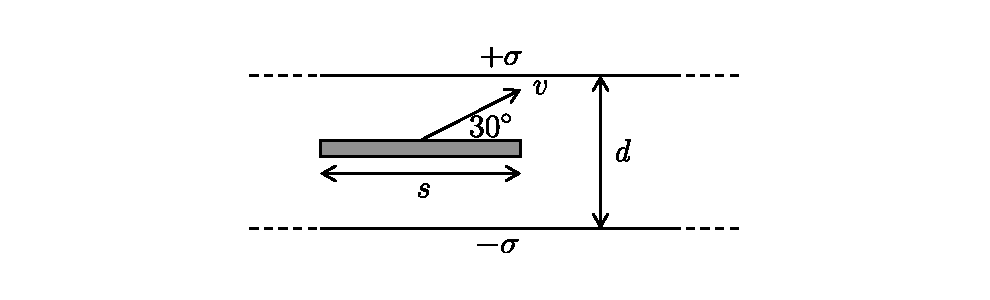
\includegraphics[width=\textwidth]{Anh/13.pdf}
    \end{center}
\end{vd}
\begin{loigiai}
Sau khi va chạm với mặt phẳng $+\sigma$ thì tấm sẽ trao đổi điện tích với mặt phẳng. Điện tích của tấm lúc này là $\sigma s^2$. Tương tự khi tấm va chạm với mặt phẳng $-\sigma$, tấm sẽ trao đổi điện tích và có điện tích là $-\sigma s^2$. Trong quá trình chuyển động, độ lớn gia tốc của tấm là không đổi $$a=\frac{\sigma^2s^2}{\varepsilon_0m}\approx7.06\dv{m/s^2}.$$
Các va chạm là hoàn toàn đàn hồi.
Ta có $$L=v\cos(\theta)t\Leftrightarrow t=\frac{L}{v\cos(\theta)}.$$
Tổng quãng đường đi được theo phương thẳng đứng
\begin{equation*}
    \begin{aligned}
     D&=v\sin(\theta)t+\frac{a}{2}t^2\\
     &=\tan(\theta)L+\frac{aL^2}{2v^2\cos^2(\theta)}.
    \end{aligned}
\end{equation*}
Số lần tấm va chạm với mặt phẳng
$$n=\left \lfloor{\frac{D+\dfrac{d}{2}}{d}}\right \rfloor=25273.$$
Với $\left \lfloor{x}\right \rfloor$ là số nguyên lớn nhất không vượt quá $x$.
\end{loigiai}

    \begin{vd}[Kéo thẳng đường cong]
    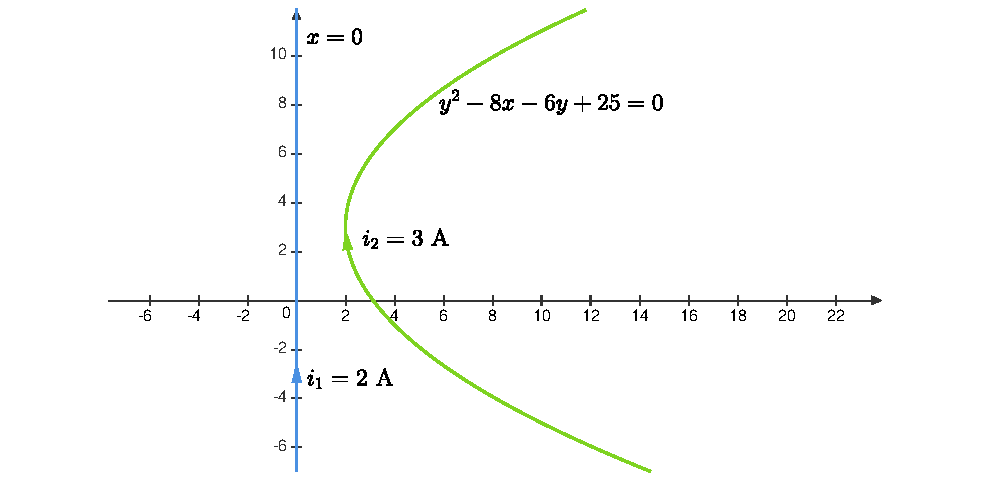
\includegraphics[width=\textwidth]{Anh/c1.pdf}\\
    Hai dây dẫn vô hạn có dòng điện không đổi chạy qua là $i_1=2\dv{A}$ và $i_2=3\dv{A}$ như trên hình vẽ. Phương trình miêu tả hình dạng hai dây lần lượt là $x=0$ và $y^2-8x-6y+25=0$, với $x$ và $y$ tính theo đơn vị $\mathrm{m}$. Tìm lực do dây này tác dụng lên dây kia.
    \end{vd}
    \begin{loigiai}
    Từ trường tạo ra bởi dây dẫn 1 tại một điểm nằm trong mặt phẳng $Oxy$
    $$B(x)=-\dfrac{\mu_0i_1}{2\pi x}.$$
    Thành phần theo phương $Ox$ lực từ tác dụng lên một phần tử của dây 2:
    \[\begin{aligned}
             \dd F_x&=B(x)i_2\dd y\\
             &=-\dfrac{\mu_0i_1i_2}{2\pi x}\dd y.
        \end{aligned}\tag{1} \label{c111}\]
    Lại có 
    \[ y^2-8x-6y+25=0\Leftrightarrow x=\dfrac{y^2-6y+25}{8} \tag{2} \label{c112}.\]
    Từ (\ref{c111}) và (\ref{c112}) ta có
    \begin{equation*}
             F_x=\tiph{-\infty}{\infty}{-\dfrac{4\mu_0i_1i_2}{\pi\tron{y^2-6y+25}}}{y}.
    \end{equation*}
    Đặt $u=y-3$, ta có
    \begin{equation*}
             F_x=\tiph{-\infty}{\infty}{-\dfrac{4\mu_0i_1i_2}{\pi\tron{u^2+16}}}{u}.
    \end{equation*}
    Đặt $\dfrac{u}{4}=\tan\alpha$, ta có
    \begin{equation*}
        \begin{aligned}
             F_x&=\tiph{-\frac{\pi}{2}}{\frac{\pi}{2}}{-\dfrac{\mu_0i_1i_2}{4\pi\tron{\tan^2\alpha+1}}\dfrac{4}{\cos^2\alpha}}{\alpha}\\
             &=\tiph{-\frac{\pi}{2}}{\frac{\pi}{2}}{-\dfrac{\mu_0i_1i_2}{\pi}}{\alpha}\\
             &=-\mu_0i_1i_2.
        \end{aligned}
    \end{equation*}
    Vậy hai dây hút nhau với một lực bằng $7.54\times10^{-6}\dv{N}$.
    \end{loigiai}
    
\begin{vd}[Magnetars]
Từ trường xuất hiện ở tất cả mọi nơi xung quanh chúng ta. Một vài giá trị của từ trường điển hình: từ trường Trái Đất: $25-60~\mathrm{\mu T}$; vệt đen ở Mặt Trời: $0,3~\mathrm{T}$; nam châm vĩnh cữu mạnh: khoảng $1~\mathrm{T}$; từ trường được duy trì liên tục trong phòng thí nghiệm: lên đến $45~\mathrm{T}$; neutron starts và magnetars: lên đến $10^{11}~\mathrm{T}$. Sau đây, chúng ta sẽ nghiên cứu một vài tính chất của từ trường mạnh.\\
Mật độ năng lượng từ trường là $\omega=B^2\dfrac{1}{2\mu \mu_0}$, với $\mu_0\approx1,3\times 10^{-6}~\mathrm{N/A^2}$ là hằng số từ (hay còn gọi là độ từ thẩm của chân không), và $\mu$ - độ từ thẩm tương đối của môi trường. Hệ đang cố gắng chuyển sang trạng thái năng lượng thấp hơn và do đó vật liệu sắt từ với $\mu \gg 1$ thì bị hút về phía có từ trường mạnh, và các vật liệu nghịch từ với $\mu < 1$ thì bị đẩy ra ngoài. Với các vật liệu nghịch từ, độ cảm từ $\chi=\mu -1$ có giá trị nhỏ, $\chi \ll 1$, và do đó nếu từ trường không đủ lớn thì chỉ gây ra một sự ảnh hưởng nhỏ. Nước là vật liệu nghịch từ với $\chi=-9\times10^{-6}$ và bình thường thì nước chiếm hầu hết trọng lượng của cơ thể động vật, hay nói cách khác, động vật hầu như được tạo nên bởi nước. Do đó, ếch có thể bay lên bên trong từ trường nếu như từ trường đủ mạnh, chúng ta có thể xem hình sau.
\begin{center}
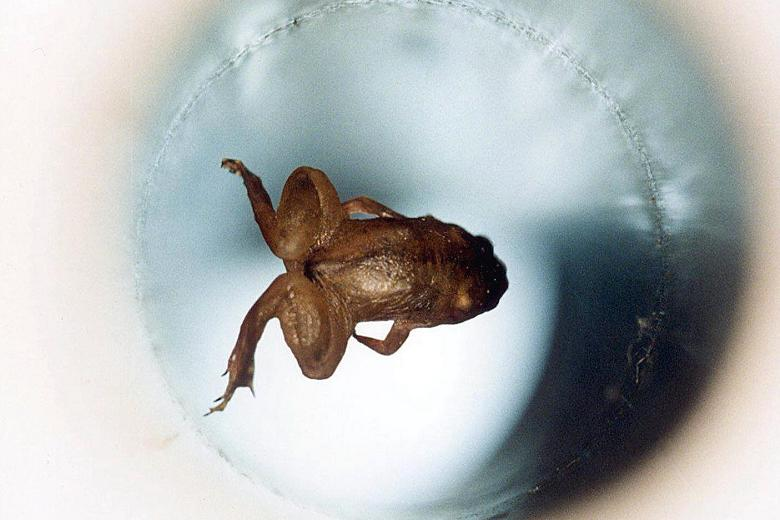
\includegraphics[scale=0.4]{Anh/2016.3.1.jpg}
\end{center}
\begin{enumerate}[1)]
    \item Cho chiều cao của con ếch là $h_{f}$ không quá $h_0=10~\mathrm{mm}$, và chúng ta đơn giản hóa rằng bình phương của cảm ứng từ phụ thuộc tuyến tính vào độ cao $z$ như hình dưới. 
    \begin{center}
        \tikzset{every picture/.style={line width=0.75pt}} %set default line width to 0.75pt        

\begin{tikzpicture}[x=0.75pt,y=0.75pt,yscale=-1,xscale=1]
%uncomment if require: \path (0,300); %set diagram left start at 0, and has height of 300

%Straight Lines [id:da7268528150747415] 
\draw    (212,200.33) -- (411,200.33) ;
\draw [shift={(414,200.33)}, rotate = 180] [fill={rgb, 255:red, 0; green, 0; blue, 0 }  ][line width=0.08]  [draw opacity=0] (10.72,-5.15) -- (0,0) -- (10.72,5.15) -- (7.12,0) -- cycle    ;
%Straight Lines [id:da9151910129710128] 
\draw    (260,247.67) -- (260,95.33) ;
\draw [shift={(260,92.33)}, rotate = 450] [fill={rgb, 255:red, 0; green, 0; blue, 0 }  ][line width=0.08]  [draw opacity=0] (10.72,-5.15) -- (0,0) -- (10.72,5.15) -- (7.12,0) -- cycle    ;
%Straight Lines [id:da478705783765105] 
\draw [color={rgb, 255:red, 230; green, 29; blue, 29 }  ,draw opacity=1 ]   (239,120) -- (260,120) -- (340.33,200.33) -- (354,200.33) ;

% Text Node
\draw (266,87.4) node [anchor=north west][inner sep=0.75pt]    {$B^{2}$};
% Text Node
\draw (217,110.4) node [anchor=north west][inner sep=0.75pt]    {$B_{0}^{2}$};
% Text Node
\draw (247,202.4) node [anchor=north west][inner sep=0.75pt]    {$0$};
% Text Node
\draw (200,192.4) node [anchor=north west][inner sep=0.75pt]    {$0$};
% Text Node
\draw (391,179.4) node [anchor=north west][inner sep=0.75pt]    {$z$};
% Text Node
\draw (333,203.4) node [anchor=north west][inner sep=0.75pt]    {$h_{0}$};


\end{tikzpicture}

    \end{center}
    Tìm giá trị của $B_0$ (đơn vị Teslas) cần để duy trì con ếch ở trạng thái lơ lửng trên không. Biết rằng con ếch có cấu tạo hoàn toàn từ nước (mật độ $\rho=1000~\mathrm{kg/m^3}$); gia tốc rơi tự do là $g=9,8~\mathrm{m/s^2}$. \textit{Gợi ý}: với $\left|\chi\right|\ll1$, chúng ta có thể làm gần đúng $\omega\approx B^2\dfrac{1-\chi}{2\mu_0}$; do đó, biểu thức liên hệ giữa mật độ năng lượng và sự có mặt của nước là $\Delta \omega=B^2\dfrac{1-\chi}{2\mu_0}-B^2\dfrac{1}{2\mu_0}=-B^2\dfrac{\chi}{2\mu_0}$.\\
    Các ngôi sao được cấu tạo từ plasma$-$một chất dẫn điện tốt. Chính vì thế, các đường sức từ sẽ như thể bị "đóng băng" đối với plasma chuyển động (điều này tuần theo định luật cảm ứng Faraday và định luật Kirchoff: do không có điện trở, độ giảm điện áp giữa các vành gần nhau ở bên trong plasma mà ta giả sử gần như bằng không, do đó từ thông không đổi). Nếu một ngôi sao biến thành một ngôi sao neutron, hiệu ứng này sẽ dẫn tới sự tăng tức thời của từ trường, quan sát bản phác thảo các đường sức từ trong trường hợp trước và sau sự biến đổi (nhớ rằng cường độ từ trường tỉ lệ thuận mật độ đường sức từ).
    \begin{center}
        \tikzset{every picture/.style={line width=0.75pt}} %set default line width to 0.75pt        

\begin{tikzpicture}[x=0.75pt,y=0.75pt,yscale=-1,xscale=1]
%uncomment if require: \path (0,300); %set diagram left start at 0, and has height of 300

%Shape: Circle [id:dp6549836949350023] 
\draw  [fill={rgb, 255:red, 248; green, 231; blue, 28 }  ,fill opacity=1 ] (191.12,176.82) .. controls (165.89,155.62) and (162.62,117.98) .. (183.82,92.76) .. controls (205.02,67.53) and (242.66,64.26) .. (267.89,85.46) .. controls (293.12,106.66) and (296.38,144.3) .. (275.18,169.52) .. controls (253.99,194.75) and (216.35,198.02) .. (191.12,176.82) -- cycle ;
%Straight Lines [id:da2858934451028303] 
\draw    (314.72,30.77) -- (149.39,227.52) ;
%Curve Lines [id:da3454539603886295] 
\draw    (186,236.33) .. controls (196,173.33) and (279,71.33) .. (349,63.33) ;
%Curve Lines [id:da20367008645727047] 
\draw    (208,234.33) .. controls (212,182.33) and (276,87.33) .. (362,85.33) ;
%Curve Lines [id:da31253548461166103] 
\draw    (230,230.33) .. controls (219,183.33) and (280,118.33) .. (325,111.33) ;
%Curve Lines [id:da6954594469756084] 
\draw    (121.4,187.11) .. controls (147,181.33) and (192.35,158.13) .. (220,130.33) .. controls (247.65,102.53) and (258,71.33) .. (263.57,17.91) ;
%Curve Lines [id:da7055460410915435] 
\draw    (128,167.33) .. controls (189,138.67) and (240,123.67) .. (245.8,25.51) ;
%Curve Lines [id:da9412388070670608] 
\draw    (135,141.33) .. controls (177,139.33) and (234.43,95.22) .. (223.78,37.95) ;
%Shape: Ellipse [id:dp6904993388159524] 
\draw  [fill={rgb, 255:red, 248; green, 231; blue, 28 }  ,fill opacity=1 ] (312.9,235.74) .. controls (300.78,225.55) and (299.21,207.47) .. (309.39,195.35) .. controls (319.58,183.23) and (337.66,181.66) .. (349.78,191.84) .. controls (361.9,202.03) and (363.47,220.11) .. (353.29,232.23) .. controls (343.1,244.36) and (325.02,245.92) .. (312.9,235.74) -- cycle ;
%Straight Lines [id:da5888993463068299] 
\draw    (372.28,165.56) -- (292.85,260.1) ;
%Curve Lines [id:da7090409488977016] 
\draw    (310.44,264.33) .. controls (315.24,234.06) and (355.12,185.06) .. (388.75,181.21) ;
%Curve Lines [id:da9595209168666552] 
\draw    (321.01,263.37) .. controls (322.93,238.39) and (353.68,192.74) .. (395,191.78) ;
%Curve Lines [id:da6970412667469024] 
\draw    (331.58,261.45) .. controls (326.29,238.87) and (355.6,207.64) .. (377.22,204.27) ;
%Curve Lines [id:da2584482459277204] 
\draw    (279.4,240.68) .. controls (291.7,237.91) and (313.49,226.76) .. (326.77,213.4) .. controls (340.06,200.05) and (345.03,185.06) .. (347.71,159.39) ;
%Curve Lines [id:da6611636099889706] 
\draw    (282.57,231.18) .. controls (314.76,219.65) and (337,206.67) .. (339.17,163.04) ;
%Curve Lines [id:da5617316237885455] 
\draw    (287.05,216.95) .. controls (305.55,221.83) and (333.71,196.53) .. (328.59,169.02) ;

% Text Node
\draw (87,56) node [anchor=north west][inner sep=0.75pt]   [align=left] {Trước khi biến đổi};
% Text Node
\draw (349,244) node [anchor=north west][inner sep=0.75pt]   [align=left] {Sau khi biến đổi};


\end{tikzpicture}

    \end{center}
    \item Biết rằng cảm ứng từ của một ngôi sao là $B_{s}=100~\mathrm{\mu T}$ và mật độ trung bình $\rho_{s}=1400~\mathrm{kg/m^3}$, hãy xác định giá trị của cảm ứng từ $B_{c}$ sau khi ngôi sao ấy biến đổi thành ngôi sao neutron do sự nén của các đường sức từ như đã mô tả ở trên. Mật độ của ngôi sao neutron là $\rho_{n}=5\times10^{17}~\mathrm{kg/m^3}$.
    \item Trên thực tế, từ trường của ngôi sau neutron được tạo ra bằng nhiều cách khác nhau. Bây giờ chúng ta sẽ cùng xem xét một mô hình đã được đơn giản hóa. Phần bên trong của ngôi sao đã biến đổi thành kích thước và mật độ của ngôi sao neutron, nhưng phần bên ngoài vẫn giữ nguyên như cũ. Biết rằng trước khi xảy ra biến đổi, ngôi sao đang xoay như một khối rắn với tốc độ góc $\omega_{s}$. Biểu diễn tốc độ góc mới của phần bên trong ngôi sao $\omega_{n}$ theo $\omega_{s}$, $\rho_{s}$ và $\rho_{n}$.
    \item Tốc độ quay của phần bên ngoài và phần bên trong là khác nhau, do đó các đường sức sẽ bị co giãn, xem hình dưới đây. Để đơn giản hóa: ($a$) chúng ta sử dụng hình học hai chiều, hay nói cách khác là xem những ngôi sao như hình trụ; ($b$) trong khi trường ban đầu là trường lưỡng cực, chúng ta thừa nhận rằng nó là hình trụ đối xứng như đã biểu diễn trong hình vẽ; ($c$) điểm cuối của đường sức thì gắn liền với phần hình trụ bên trong (sao neutron) và lớp vỏ hình trụ bên ngoài (phần còn lại của ngôi sao ban đầu). Cho biết rằng cảm ứng từ tại lớp vỏ ban đầu là $B_0$. Hãy biểu diễn cảm ứng từ $B$ là một hàm theo thời gian $t$ trong vùng mà các đường sức đang bị co giãn với $t \gg 1/ \omega_{n}$ theo $B_0$ và $\omega_{n}$.
    \end{enumerate}
    \begin{center}
        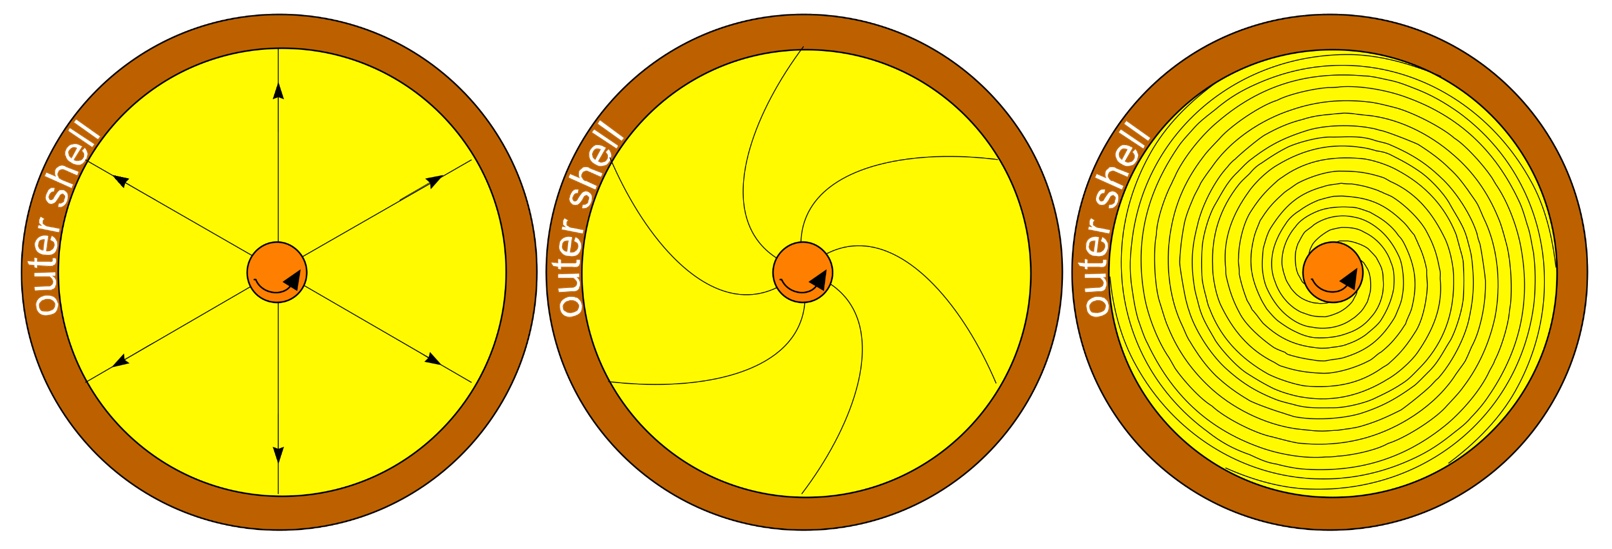
\includegraphics[width= 0.8\textwidth]{Anh/2016.png}
    \end{center}
    \begin{enumerate}[1)]
    \setcounter{enumi}{4}
    \item Do đó, năng lượng được chuyển hóa trong quá trình biến đổi của ngôi sao thì tuân theo: thế năng hấp dẫn đươc chuyển hóa thành động năng (ở đây, chúng ta bỏ qua nhiệt năng) và sau đó là chuyến hóa thành năng lượng từ. Dựa vào đó, hãy tính giá trị cực đại của cảm ứng từ $B_{\max}$ của ngôi sao neutron có khối lượng $M_{n}=4\times10^{30}~\mathrm{kg}$ và bán kính $R_{n}=13~\mathrm{km}$. Nhớ rằng $G=6,67\times10^{-11}~\mathrm{m^3s^{-2}kg^{-1}}$.
    \item Từ trường cực mạnh sẽ có ảnh hưởng đến tính chất hóa học của vật bằng cách thay đổi hình dáng của quỹ đạo electron của vật đó. Điều đó xảy ra khi lực Lorentz tác dụng lên một electron có quỹ đạo trở nên mạnh hơn lực Coulomb do tương tác với hạt nhân nguyên tử. Hãy tính giá trị của cảm ứng từ $B_{H}$ cần thiết để làm biến dạng quỹ đạo của electron của một nguyên tử Hydro có bán kính $R_{H}=5\times10^{-11}~\mathrm{m}$. Chú ý rằng $\dfrac{1}{4\pi\varepsilon_0}=9\times10^9~\mathrm{m/F}$, $e=1,6\times10^{-19}~\mathrm{C}$ và khối lượng của electron $m_{e}=9,1\times10^{-31}~\mathrm{kg}$.
    \item Trong những từ trường cực mạnh, những đám mây electron của nguyên tử có hình dạng như hình trụ. Hãy tính tỉ lệ chiều dài trên đường kính $\kappa=\ell/d$ của những đám mây electron như thế trong những nguyên tử Hydro gần một ngôi sao neutron, trong từ trường $B_{n}=10^8~\mathrm{T}$. Cho biết rằng hằng số Plank $h=6,6\times10^{-34}~\mathrm{J\cdot s}$. \textit{Gợi ý}: bán kính của quỹ đạo cyclotron của một electron trong cơ học lượng tử có thể tính toán bằng cách sử dụng nguyên lí bất định.
\end{enumerate}
\end{vd}
\begin{loigiai}
\begin{enumerate}[1) ]
    \item Nếu chúng ta thay đổi chiều cao của con ếch một lượng $\Delta h$, sự biến thiên trong thế năng sẽ nhỏ hơn sự thay đổi của năng lượng từ trường.\\Chúng ta lưu ý rằng với mỗi điểm của con ếch, sự biến thiên của năng lượng từ trường là như nhau, do đó chúng ta có thể biểu diễn như sau
    \[\Delta E=-V\dfrac{\Delta(B^2)\chi}{2\mu_0}=V\dfrac{B_0^2\chi\Delta h}{2h_0\mu_0}.\]
    Độ biến thiên của thế năng là
    \[\Delta \Pi=V\rho g\Delta h. \]
    Do
    \[
    \begin{cases}
    \Delta E+\Delta \Pi &<0,\\
    V\dfrac{B_0^2\chi\Delta h}{2h_0\mu_0}+V\rho g\Delta h&<0.
    \end{cases}
    \]
    Điều đó có nghĩa:
    \[B_0>\sqrt{-\dfrac{2h_0\mu_0\rho g}{\chi}}.\]
    Thay số ta được:
    \[B_0=5,32~\mathrm{T}.\]
    \item Chúng ta sẽ quan sát một mẩu của ngôi sao có thể tích $V_0$ trước khi biến đổi và là $V_1$ sau khi xảy ra sự biến đổi. Khối lượng trước và sau là không đổi. Điều đó có nghĩa là:
    \[V_0\rho_{s}=V_1\rho_{n}.\]
    Bán kính của ngôi sao tỉ lệ với $V^{\frac{1}{3}}$ và diện tích mặt cắt ngang tỉ lệ với $V^{\frac{2}{3}}$.\\
    Tổng điện trường đi qua thể tích ấy vẫn không đổi trước và sau khi xảy ra sự biến đổi:
    \[B_{s}V_0^{\frac{2}{3}}=B_{n}V_1^{\frac{2}{3}}.\]
    Bây giờ chúng ta có thể biểu diễn $B_{n}$
    \[B_{n}=B_{s}\left(\dfrac{V_0}{V_1}\right)^{\frac{2}{3}}=B_{s}\left(\dfrac{\rho_{n}}{\rho_{s}}\right)^{\frac{2}{3}}.\]
    Thay số
    \[B_{n}=5,0\times10^5~\mathrm{T}.\]
    \item Trong suốt quá trình xảy ra sự biến đổi thì không có sự xuất hiện của momen quay của ngôi sao. Điều đó có nghĩa là moment động lượng vẫn được bảo toàn. Do đó:
    \[\dfrac{2}{5}MR^2_{s}\omega_{s}=\dfrac{2}{5}MR_{n}^2\omega_{n}.\]
    Vì $R_{s}$ tỉ lệ nghịch với $\rho_{s}^\frac{1}{3}$. Chúng ta có $\omega_{n}$ sẽ là
    \[\omega_{n}=\omega_{s}\dfrac{R_{s}^2}{R_{n}^2}=\omega_{s}\left(\dfrac{\rho_{n}}{\rho_{s}}\right)^{\frac{2}{3}}.\]
    \item Sau thời gian $t$, ngôi sao neutron quay được một góc $\beta=\omega_{n}t$.\\
    Từ trường xuyên qua bất kì đường xuyên tâm nào từ tâm của ngôi sao neutron có giá trị trung bình là $N=\dfrac{\beta}{2\pi}=\dfrac{\omega_{n}t}{2\pi}$ lần.\\
    Tổng từ thông đi qua lớp vỏ ngoài vẫn giữ nguyên không đổi  và có giá trị luôn là $\Phi=2\pi R_0B_0$, với $R_0$ là bán kính của lớp vỏ ngoài. Điều đó có nghĩa là từ thông đi qua bất kì đường xuyên tâm nào là $\Phi N$.\\
    Do đó
    \[BR_0=2\pi R_0 B_0N=R_0B_0\omega_{n}t.\]
    Và cuối cùng, ta được
    \[B=B_0\omega_{n}t.\]
    \item Chúng ta có thể tìm thế năng hấp dẫn bằng cách tích phân: chúng ta tưởng tượng rằng khi loại bỏ từng lớp vật liệu dày $\mathrm{d}x$, bắt đầu từ phía ngoài cùng. Thế năng của quả cầu rỗng của vật bên trong có độ dày $\mathrm{d}x$ trong trường trọng lực là
    \[\mathrm{d}\Pi=-G\dfrac{(4\pi x^2\mathrm{d}x\rho_{n})\frac{4}{3}\pi x^3\rho_{n}}{x}=-\dfrac{16\pi^2}{3}G\rho_{n}^2x^4\mathrm{d}x.\]
    Tích phân từ $x=0$ đến $x=R_{n}$, ta được:
    \[\Pi=-\dfrac{16\pi^2}{15}G\rho_n^2 R_{n}^5=-\dfrac{3}{5}\dfrac{GM_{n}^2}{R_{n}}.\]
    Thế năng này chính bằng năng lượng của từ trường
    \[\Pi=\dfrac{4}{3}\pi R^3B_{n}^2\dfrac{1}{2\mu_0}.\]
    Giải tìm $B_{n}$, ta được
    \[B_{n}=3\dfrac{M}{R^2}\sqrt{\dfrac{\mu_0G}{10\pi}}.\]
    Thay số
    \[B_{n}=1,18\times 10^{14}~\mathrm{T}.\]
    \item Quỹ đạo của electron sẽ bị bóp méo khi lực Lorentz dần có độ lớn gần bằng của lực Coulomb.\\
    Độ lớn lực Coulomb là
    \[F_1=\dfrac{1}{4\pi \varepsilon_0}\dfrac{e^2}{R_{H}^2},\]
    Mặt khác
    \[F_1=\dfrac{m_{e}v^2}{R_{H}},\]
    Chúng ta có thể suy ra vận tốc của electron là
    \[v=e\sqrt{\dfrac{1}{4\pi \varepsilon_0 R_{H}m_{e}}}.\]
    Khi đó lực Lorentz sẽ là
    \[F_2\approx evB.\]
    Thế $v$ đã tìm được ở trên, ta được
    \[F_2=e^2B\dfrac{1}{\sqrt{4\pi \varepsilon_0 R_{H}m_{e}}}.\]
    Từ điều kiện $F_1\approx F_2$, ta có giá trị của cảm ứng từ
    \[B=\sqrt{\dfrac{m_{e}}{4\pi \varepsilon_0 R_{H}^3}}.\]
    Thay số ta được
    \[B=2,56\times 10^5~\mathrm{T}.\]
    \item Vuông góc với từ trường, lực Lorentz sẽ lớn hơn lực Coulomb rất nhiều vì từ trường $B_{n}$ lớn hơn rất nhiều so với từ trường được tính ở câu trước. Điều đó có nghĩa là trong mặt phẳng vuông góc, electron chuyển động theo quỹ đạo cyclotron tròn.
    Chúng ta có
    \[\dfrac{m_{e}v^2}{R_1}=evB_{n}, \tag{1} \label{2016.1}\]
    với $R_1 = d/2$ là bán kính của quỹ đạo. Bây giờ chúng ta sử dụng nguyên lí bất định. Sai số của động lượng là
    \[\Delta p=2m_{e}v.\]
    Sai số của tọa độ là
    \[\Delta x=2R_1.\]
    Ta có
    \[4m_{e}vR_1\approx \hbar.\]
    Thay $m_{e}v=\dfrac{\hbar}{4R_1}$ vào (\ref{2016.1}), ta được
    \[\dfrac{\hbar}{R_1^2}=4eB_{n}.\]
    Suy ra
    \[R_1=\sqrt{\dfrac{\hbar}{4eB_{n}}}.\]
    Chiều dài của khối trụ vẫn giữa giá trị không đổi là $R_{H}$ bởi vì lực Lorentz không tác dụng lên electron theo phương đó (song song với từ trường). Do đó ta có tỉ lệ giữa chiều dài và đường kính sẽ xấp xỉ bằng
    \[\kappa=\dfrac{R_{H}}{R_1}=2R_{H}\sqrt{\dfrac{eB_{n}}{\hbar}}.\]
    Thay số ta được
    \[\kappa=39\approx 40.\]
    Chú ý rằng khi chúng ta thực hiện tính toán với magnetars khi $B=1\times10^{11}~\mathrm{T}$, các electron thuộc quỹ đạo sẽ đạt đến gần tốc độ ánh sáng.
\end{enumerate}
\end{loigiai}


\begin{vd}[Hiệu ứng spin $-$ Hall]
Ta biết rằng khi một điện trường và một từ trường tác dụng vuông góc lên một miếng bán dẫn, một điện áp $V_{H}$ vuông góc với phương chuyển động của các điện tích sẽ được tạo ra (xem hình vẽ). Hiện tượng này được gọi là hiệu ứng Hall.


\begin{center}
\tikzset{every picture/.style={line width=0.75pt}} %set default line width to 0.75pt        

\begin{tikzpicture}[x=0.75pt,y=0.75pt,yscale=-1,xscale=1]
%uncomment if require: \path (0,300); %set diagram left start at 0, and has height of 300
%Shape: Parallelogram [id:dp2081197711183893]
\draw   (241.6,115) -- (446,115) -- (358.4,180.33) -- (154,180.33) -- cycle ;
%Straight Lines [id:da3392856291541302] 
\draw    (268.2,116.79) -- (185.4,178.54) ;
\draw [shift={(183,180.33)}, rotate = 323.28] [fill={rgb, 255:red, 0; green, 0; blue, 0 }  ][line width=0.08]  [draw opacity=0] (10.72,-5.15) -- (0,0) -- (10.72,5.15) -- (7.12,0) -- cycle    ;
\draw [shift={(270.6,115)}, rotate = 143.28] [fill={rgb, 255:red, 0; green, 0; blue, 0 }  ][line width=0.08]  [draw opacity=0] (8.93,-4.29) -- (0,0) -- (8.93,4.29) -- cycle    ;
%Straight Lines [id:da4116693786329637] 
\draw    (197.19,116.79) -- (77,206.33) ;
\draw [shift={(199.6,115)}, rotate = 143.31] [fill={rgb, 255:red, 0; green, 0; blue, 0 }  ][line width=0.08]  [draw opacity=0] (10.72,-5.15) -- (0,0) -- (10.72,5.15) -- (7.12,0) -- cycle    ;
%Straight Lines [id:da17430270610068788] 
\draw    (157,187.33) -- (355.4,187.33) ;
\draw [shift={(358.4,187.33)}, rotate = 180] [fill={rgb, 255:red, 0; green, 0; blue, 0 }  ][line width=0.08]  [draw opacity=0] (10.72,-5.15) -- (0,0) -- (10.72,5.15) -- (7.12,0) -- cycle    ;
\draw [shift={(154,187.33)}, rotate = 0] [fill={rgb, 255:red, 0; green, 0; blue, 0 }  ][line width=0.08]  [draw opacity=0] (10.72,-5.15) -- (0,0) -- (10.72,5.15) -- (7.12,0) -- cycle    ;
%Straight Lines [id:da40457739049168495] 
\draw    (77,206.33) -- (278.4,206.33) ;
\draw [shift={(281.4,206.33)}, rotate = 180] [fill={rgb, 255:red, 0; green, 0; blue, 0 }  ][line width=0.08]  [draw opacity=0] (10.72,-5.15) -- (0,0) -- (10.72,5.15) -- (7.12,0) -- cycle    ;
%Straight Lines [id:da710748552808127] 
\draw    (265,150.33) -- (353,150.33) ;
\draw [shift={(356,150.33)}, rotate = 180] [fill={rgb, 255:red, 0; green, 0; blue, 0 }  ][line width=0.08]  [draw opacity=0] (10.72,-5.15) -- (0,0) -- (10.72,5.15) -- (7.12,0) -- cycle    ;
%Straight Lines [id:da5473058663731798] 
\draw    (310,134.33) -- (310,68.33) ;
\draw [shift={(310,65.33)}, rotate = 450] [fill={rgb, 255:red, 0; green, 0; blue, 0 }  ][line width=0.08]  [draw opacity=0] (10.72,-5.15) -- (0,0) -- (10.72,5.15) -- (7.12,0) -- cycle    ;


% Text Node
\draw (257,212.4) node [anchor=north west][inner sep=0.75pt]    {$x$};
% Text Node
\draw (170,101.4) node [anchor=north west][inner sep=0.75pt]    {$y$};
% Text Node
\draw (256,129.4) node [anchor=north west][inner sep=0.75pt]  [font=\footnotesize]  {$V_{H}$};
% Text Node
\draw (331,123.4) node [anchor=north west][inner sep=0.75pt]  [font=\small]  {$\ot{j}$};
% Text Node
\draw (322,62.4) node [anchor=north west][inner sep=0.75pt]    {$\ot{B}$};
% Text Node
\draw (313,190.4) node [anchor=north west][inner sep=0.75pt]  [font=\footnotesize]  {$V$};


\end{tikzpicture}
\end{center}
\begin{enumerate}[1) ]
    \item  Giả sử rằng mẫu bán dẫn là một tấm hình vuông có kích thước $W\times W$. Dòng điện là do sự chuyển động của các hạt mang điện dương mỗi hạt có điện tích là $e$, mật độ mặt của các hạt tải điện là $n$, và độ dẫn điện của bán dẫn là $\sigma$. Cũng có các điện tích âm do đó các điện tích trung hòa ở khắp mọi nơi ngoại trừ tại cạnh bên. Điện trường là đều trong chất bán dẫn. Một từ trường $B$ được đặt vào theo hướng vuông góc với tấm. Khi một điện áp $V$ được đặt vào tấm thì sẽ xuất hiện một điện áp $V_{H}$ giữa hai cạnh song song với dòng điện dọc theo trục $x$, ngoài ra dòng điện $\ot{j}$. Khi ở trạng thái ổn định đạt được, tìm hệ số Hall $R_{H}=\dfrac{V_{H}}{V}$. (Lưu ý rằng $\ot{j}$ là đại lượng chưa biết).
\end{enumerate}
Ngày nay nó còn được gọi là cấu trúc bán dẫn số, một hiệu ứng spin $-$ Hall cũng sẽ xảy ra. Hiệu ứng được kết hợp cùng với moment từ $\ot{m}$ của các hạt mang điện. Đối với cấu trúc hai chiều được biết rằng có một lực bổ sung $\ot{F_{R}}=\eta_{R}(\ot{m}\times\ot{v})$ (gọi là lực Rashba) sẽ tác dụng lên các hạt tải điện, ở đây $\ot{v}$ là vận tốc của các hạt tải trên mặt phẳng hai chiều $(X-Y)$, và $\eta_{R}$ là một hằng số. Moment từ $\ot{m}$ bị hạn chế chỉ hướng vuông góc với mặt phẳng, ví dụ như $\ot{m}=m\widehat{z}$. Không có từ trường bên ngoài. Bỏ qua tương tác giữa lưỡng cực từ với các hạt tải điện.
\begin{enumerate}[1)]
\setcounter{enumi}{1}
    \item Giả sử hạt một lần nữa là điện trường là đều và lực của nó dọc theo trục $x$ là mạnh hơn $\ot{F_{R}}$, tìm dòng điện chạy theo hướng $y$ theo điện áp $V$ và các thông số khác đã được đưa ra trong ý $(1)$. Các dòng điện đó liên quan đến $\ot{m}$ như thế nào? 
    \item Do va chạm với biên, các hạt tải với moment từ riêng sẽ mất cảm giác của chúng về hướng trong một khoảng "thời gian sống" $\tau$ sau khi chúng tới được biên. Hay nói các khác, mỗi giây có $\dfrac{n_{m}}{\tau}$ hạt tải mất hướng moment của chúng trong một đơn vị chiều dài của cạnh, ở đây $n_{m}$ là mật độ bề mặt của hạt tải vẫn duy trì hướng moment của chúng $(\pm \widehat{z})$. Tìm độ từ hóa $\ot{M}$ ở gần các cạnh.
\end{enumerate}
\end{vd}
\begin{loigiai}
\begin{enumerate}[1) ]
    \item
Ta có mật độ dòng điện
\[j=nev=\sigma E,\]
lại có
\[E=\dfrac{V}{W},\]
suy ra lực điện tác dụng lên electron là
\[F_{\mathrm{E}}=\dfrac{eV_{\mathrm{H}}}{W}.\]
Lực Lorentz tác dụng lên electron là $F_{\mathrm{B}}=eBv$.\\
Khi đạt trạng thái ổn định $F_{\mathrm{E}}=F_{\mathrm{B}}$.\\Từ đó có thể thu được
\[\dfrac{V_{\mathrm{H}}}{V}=\dfrac{B\sigma}{en}.\]
    \item Tính trung bình, một nửa các electron có spin hướng lên, một nửa có spin hướng xuống. Electron chuyển động dọc theo trục $X$ để cho
    \[j=j_{\mathrm{y}}+j_{-\mathrm{y}},\]
    nhưng
    \[\ot{j_{\mathrm{spin}}}\neq 0,\]
    $j_{\mathrm{spin}}$ thực sự là một dòng spin, không có dòng điện tích.
    \[j_{\mathrm{y}}=\sigma E_{\mathrm{y}}=\dfrac{\sigma F_{\mathrm{t}}}{e}=\dfrac{\sigma \eta_{\mathrm{R}}mv_{\mathrm{x}}}{e}=\dfrac{\sigma\eta_{\mathrm{R}}m}{e}\dfrac{\sigma V}{nem}=\dfrac{\sigma^2\eta_{\mathrm{R}}mV}{e^2nW}.\]
    Dòng điện hướng sang trái hoặc sang phải do spin hướng lên hoặc hướng xuống.
    \item Khi đạt đến trạng thái cân bằng ta có
    \[\dfrac{n_{\mathrm{m}}}{\tau}=\dfrac{j_{\mathrm{i}}}{e},\]
    Do đó độ từ hóa khi đó sẽ là
    \[M=n_{\mathrm{m}}m=\dfrac{\sigma^2\eta_{\mathrm{R}}m^2\tau V}{Wne^3}.\]
\end{enumerate}
\end{loigiai}

\begin{vd}[Tấm điện môi di chuyển]
Một tấm điện môi phẳng lớn có độ dày $d$ và hẳng số điện môi $\varepsilon$ được di chuyển dọc theo trục $x$ ở tốc độ $v$. Mặt phẳng là vuông góc với trục $y$. Một từ trường có độ lớn $B$ được tác dụng theo hướng $z$. Tìm mật độ điện tích bề mặt trên hai bề mặt lớn của tấm, và điện trường trong tấm.
\begin{center}
    

\tikzset{every picture/.style={line width=0.75pt}} %set default line width to 0.75pt        

\begin{tikzpicture}[x=0.75pt,y=0.75pt,yscale=-1,xscale=1]
%uncomment if require: \path (0,300); %set diagram left start at 0, and has height of 300

%Shape: Parallelogram [id:dp06277634841378132] 
\draw  [fill={rgb, 255:red, 155; green, 155; blue, 155 }  ,fill opacity=1 ] (313.2,138.33) -- (505,138.33) -- (422.8,178.33) -- (231,178.33) -- cycle ;
%Straight Lines [id:da5182146849521212] 
\draw    (205,200.33) -- (393.8,200.33) ;
\draw [shift={(396.8,200.33)}, rotate = 180] [fill={rgb, 255:red, 0; green, 0; blue, 0 }  ][line width=0.08]  [draw opacity=0] (10.72,-5.15) -- (0,0) -- (10.72,5.15) -- (7.12,0) -- cycle    ;
%Straight Lines [id:da7214469395745302] 
\draw    (205,200.33) -- (125.5,239.02) ;
\draw [shift={(122.8,240.33)}, rotate = 334.05] [fill={rgb, 255:red, 0; green, 0; blue, 0 }  ][line width=0.08]  [draw opacity=0] (10.72,-5.15) -- (0,0) -- (10.72,5.15) -- (7.12,0) -- cycle    ;
%Straight Lines [id:da6293773454295502] 
\draw    (205,200.33) -- (205,104.33) ;
\draw [shift={(205,101.33)}, rotate = 450] [fill={rgb, 255:red, 0; green, 0; blue, 0 }  ][line width=0.08]  [draw opacity=0] (10.72,-5.15) -- (0,0) -- (10.72,5.15) -- (7.12,0) -- cycle    ;

% Text Node
\draw (370,201.4) node [anchor=north west][inner sep=0.75pt]    {$x$};
% Text Node
\draw (184,112.4) node [anchor=north west][inner sep=0.75pt]    {$y$};
% Text Node
\draw (144,234.4) node [anchor=north west][inner sep=0.75pt]    {$z$};


\end{tikzpicture}
\end{center}
\end{vd}
\begin{loigiai}
Mỗi đơn vị điện tích trong tấm chịu tác dụng của lực Lorentz $-vB\ot{y_0}$.\\
Bài toán là sau đó giống như một tấm điện môi đặt giữa hai tấm dẫn song song mang mật độ điện tích bề mặt $\pm\sigma$, và $\dfrac{\sigma}{\varepsilon_0}=vB$. Trong trường hợp như vậy, độ điện dịch là
\[D=\sigma\cdot P=D-\varepsilon_0E=D-\dfrac{D}{\varepsilon}=\varepsilon_0vB\left(\dfrac{\varepsilon-1}{\varepsilon}\right).\]
Cuối cùng, điện tích mặt liên kết là $\sigma_{b}=P=\varepsilon_0vB\left(\dfrac{\varepsilon-1}{\varepsilon}\right)$. Bề mặt phía trên mang điện tích liên kết dương, và bề mặt dưới mang điện tích liên kết âm.\\
Điện trường là $\ot{E}=\dfrac{\sigma_{b}}{\varepsilon_0}\ot{y_0}=vB\left(\dfrac{\varepsilon-1}{\varepsilon}\right)\ot{y_0}$, hướng dọc theo trục $y$ (ngược với hướng của lực Lorentz).
\end{loigiai}

\begin{vd}[Quan sát từ trường]
    Một vòng dẫn có bán kính $R$ mang dòng điện lớn $I$. Vòng dây nằm yên trong mặt phẳng $xy$ với tâm của nó là $(0,0,0)$. Một quan sát viên tiến đến chiếc vòng song song với trục $z$ với vận tốc $v$ và đo điện trường cách trục một khoảng $r$. Giả sử rằng $v\ll c$ và $r \ll R$.
    \begin{enumerate}[1)]
        \item Tìm phương và độ lớn của từ trường $B(z)$ trên trục $z$ trong hệ quy chiếu đứng yên.
        \item Ước lượng độ lớn và hướng của điện trường $E(z,r)$ mà người quan sát đo được khi người đó ở cách mặt phẳng vòng một khoảng $z$.
    \end{enumerate} 
\end{vd}

\begin{loigiai}
    \begin{enumerate}[1)]
        \item Theo định luật Bio $-$ Savart, mọi phần tử của vòng có chiều dài và hướng $\mathrm{d}\ot{l}$ đều tạo ra từ trường
        \[{\mathrm{d}}\overrightarrow B  = \frac{{{\mu _0}Im{\mathrm{d}}\overrightarrow l \overrightarrow a }}{{4\pi {a^3}}}.\]
        Theo đối xứng, thành phần từ trường vuông góc với trục $z$ triệt tiêu lẫn nhau. Vì vậy, từ trường có hướng dọc theo trục $z$.
        \[B(z) = \dfrac{\mu_0 \times 2\pi R \sin \alpha}{4\pi \left(z^2+R^2\right)}=\dfrac{\mu_0IR^2}{2\left(z^2+R^2\right)^{3/2}}.\]
        \item Điện trường đo được bởi một quan sát viên phải cùng hướng với lực Lorentz tác dụng lên quan sát viên trong hệ quy chiếu phòng thí nghiệm. Do đó đường sức của điện trường là những đường tròn quanh trục. Bây giờ chúng ta có thể áp dụng định luật cảm ứng của Faraday cho một vòng tròn như vậy, khi nó tiến gần đến vòng, tổng suất điện động là: 
        \[E(z,r)\times 2\pi r= \dot\Phi=-\dfrac{\mathrm{d}\Phi}{\mathrm{d}z}v \approx -\dfrac{\mathrm{d}}{\mathrm{d}z}B(z)\times \pi r^2 \times v\]
        \[\rt E(z,r)=-\dfrac{rv}{2}B'(z)=\dfrac{3\mu_0IrR^2vz}{4\left(z^2+R^2\right)^{5/2}}\]
    \end{enumerate}
\end{loigiai}

\begin{vd}[Ống từ]
%Prob 1C IPhO 2012
Xét một ống hình trụ làm bằng một vật liệu siêu dẫn. Độ dài của ống là $l$ và bán kính trong của ống là $r$; ta luôn có $l \gg r$. Tâm điểm ống trùng với gốc toạ độ, và trục của ống trùng với trục $z$. Có một từ thông $\Phi$ qua mặt cắt ngang trung tâm của ống, $z=0, x^{2}+y^{2} < r^{2}$. Siêu dẫn là vật liệu mà từ trường bị đẩy ra khỏi khối vật liệu (từ trường bằng không bên trong vật siêu dẫn).
\begin{center}


% Gradient Info
  
\tikzset {_0j96cq30i/.code = {\pgfsetadditionalshadetransform{ \pgftransformshift{\pgfpoint{0 bp } { 0 bp }  }  \pgftransformrotate{0 }  \pgftransformscale{2 }  }}}
\pgfdeclarehorizontalshading{_vok16xrsk}{150bp}{rgb(0bp)=(0.5,0.5,0.5);
rgb(37.5bp)=(0.5,0.5,0.5);
rgb(42.05357142857143bp)=(1,1,1);
rgb(50bp)=(1,1,1);
rgb(62.5bp)=(0.51,0.49,0.49);
rgb(100bp)=(0.51,0.49,0.49)}

% Pattern Info
 
\tikzset{
pattern size/.store in=\mcSize, 
pattern size = 5pt,
pattern thickness/.store in=\mcThickness, 
pattern thickness = 0.3pt,
pattern radius/.store in=\mcRadius, 
pattern radius = 1pt}
\makeatletter
\pgfutil@ifundefined{pgf@pattern@name@_raq4i4k97}{
\pgfdeclarepatternformonly[\mcThickness,\mcSize]{_raq4i4k97}
{\pgfqpoint{0pt}{0pt}}
{\pgfpoint{\mcSize}{\mcSize}}
{\pgfpoint{\mcSize}{\mcSize}}
{
\pgfsetcolor{\tikz@pattern@color}
\pgfsetlinewidth{\mcThickness}
\pgfpathmoveto{\pgfqpoint{0pt}{\mcSize}}
\pgfpathlineto{\pgfpoint{\mcSize+\mcThickness}{-\mcThickness}}
\pgfpathmoveto{\pgfqpoint{0pt}{0pt}}
\pgfpathlineto{\pgfpoint{\mcSize+\mcThickness}{\mcSize+\mcThickness}}
\pgfusepath{stroke}
}}
\makeatother
\tikzset{every picture/.style={line width=0.75pt}} %set default line width to 0.75pt        

\begin{tikzpicture}[x=0.75pt,y=0.75pt,yscale=-1,xscale=1]
%uncomment if require: \path (0,476); %set diagram left start at 0, and has height of 476

%Shape: Can [id:dp9073202998352221] 
\path  [shading=_vok16xrsk,_0j96cq30i] (265.66,67.67) -- (265.66,349.55) .. controls (265.66,353.57) and (254.82,356.82) .. (241.45,356.82) .. controls (228.07,356.82) and (217.23,353.57) .. (217.23,349.55) -- (217.23,67.67) .. controls (217.23,63.66) and (228.07,60.41) .. (241.45,60.41) .. controls (254.82,60.41) and (265.66,63.66) .. (265.66,67.67) .. controls (265.66,71.69) and (254.82,74.94) .. (241.45,74.94) .. controls (228.07,74.94) and (217.23,71.69) .. (217.23,67.67) ; % for fading 
 \draw   (265.66,67.67) -- (265.66,349.55) .. controls (265.66,353.57) and (254.82,356.82) .. (241.45,356.82) .. controls (228.07,356.82) and (217.23,353.57) .. (217.23,349.55) -- (217.23,67.67) .. controls (217.23,63.66) and (228.07,60.41) .. (241.45,60.41) .. controls (254.82,60.41) and (265.66,63.66) .. (265.66,67.67) .. controls (265.66,71.69) and (254.82,74.94) .. (241.45,74.94) .. controls (228.07,74.94) and (217.23,71.69) .. (217.23,67.67) ; % for border 

%Straight Lines [id:da2345937464732395] 
\draw    (241.45,74.94) -- (241.45,26.68) ;
\draw [shift={(241.45,23.68)}, rotate = 450] [fill={rgb, 255:red, 0; green, 0; blue, 0 }  ][line width=0.08]  [draw opacity=0] (10.72,-5.15) -- (0,0) -- (10.72,5.15) -- (7.12,0) -- cycle    ;
%Straight Lines [id:da32319017911629233] 
\draw    (241.45,356.82) -- (241.45,373.72) ;
%Straight Lines [id:da8220104477065213] 
\draw    (265.55,213.65) -- (280.21,213.65) ;
\draw [shift={(283.21,213.65)}, rotate = 180] [fill={rgb, 255:red, 0; green, 0; blue, 0 }  ][line width=0.08]  [draw opacity=0] (10.72,-5.15) -- (0,0) -- (10.72,5.15) -- (7.12,0) -- cycle    ;
%Straight Lines [id:da9619520904426937] 
\draw    (238.68,215.6) -- (205.62,241.54) ;
\draw [shift={(203.26,243.39)}, rotate = 321.89] [fill={rgb, 255:red, 0; green, 0; blue, 0 }  ][line width=0.08]  [draw opacity=0] (10.72,-5.15) -- (0,0) -- (10.72,5.15) -- (7.12,0) -- cycle    ;
%Straight Lines [id:da08678102869582371] 
\draw    (196.43,213.65) -- (217.13,213.65) ;
%Straight Lines [id:da1612752830968902] 
\draw [color={rgb, 255:red, 21; green, 72; blue, 132 }  ,draw opacity=1 ][line width=2.25]    (315.71,75.04) -- (315.71,354.87) ;
%Straight Lines [id:da7785637964939405] 
\draw [color={rgb, 255:red, 21; green, 72; blue, 132 }  ,draw opacity=1 ][line width=2.25]    (363.49,75.04) -- (363.49,354.87) ;
%Shape: Ellipse [id:dp34115363375590846] 
\draw  [color={rgb, 255:red, 21; green, 72; blue, 132 }  ,draw opacity=1 ][line width=2.25]  (217.23,67.67) .. controls (217.23,63.66) and (228.07,60.41) .. (241.45,60.41) .. controls (254.82,60.41) and (265.66,63.66) .. (265.66,67.67) .. controls (265.66,71.69) and (254.82,74.94) .. (241.45,74.94) .. controls (228.07,74.94) and (217.23,71.69) .. (217.23,67.67) -- cycle ;
%Shape: Ellipse [id:dp5975693393923946] 
\draw  [color={rgb, 255:red, 0; green, 0; blue, 0 }  ,draw opacity=1 ][pattern=_raq4i4k97,pattern size=6pt,pattern thickness=0.75pt,pattern radius=0pt, pattern color={rgb, 255:red, 0; green, 0; blue, 0}] (217.13,213.65) .. controls (217.13,209.64) and (227.97,206.39) .. (241.34,206.39) .. controls (254.71,206.39) and (265.55,209.64) .. (265.55,213.65) .. controls (265.55,217.66) and (254.71,220.92) .. (241.34,220.92) .. controls (227.97,220.92) and (217.13,217.66) .. (217.13,213.65) -- cycle ;
%Straight Lines [id:da6215766219137793] 
\draw    (301.95,214.3) -- (396.46,214.3) ;
\draw [shift={(399.46,214.3)}, rotate = 180] [fill={rgb, 255:red, 0; green, 0; blue, 0 }  ][line width=0.08]  [draw opacity=0] (10.72,-5.15) -- (0,0) -- (10.72,5.15) -- (7.12,0) -- cycle    ;
%Shape: Ellipse [id:dp06972730202487609] 
\draw  [color={rgb, 255:red, 0; green, 0; blue, 0 }  ,draw opacity=0 ][fill={rgb, 255:red, 208; green, 2; blue, 27 }  ,fill opacity=1 ] (337.92,214.34) .. controls (337.92,213.44) and (338.65,212.72) .. (339.55,212.72) .. controls (340.44,212.72) and (341.17,213.44) .. (341.17,214.34) .. controls (341.17,215.24) and (340.44,215.97) .. (339.55,215.97) .. controls (338.65,215.97) and (337.92,215.24) .. (337.92,214.34) -- cycle ;
%Shape: Ellipse [id:dp04603211008785135] 
\draw  [color={rgb, 255:red, 0; green, 0; blue, 0 }  ,draw opacity=0 ][fill={rgb, 255:red, 208; green, 2; blue, 27 }  ,fill opacity=1 ] (347.45,214.3) .. controls (347.45,213.4) and (348.18,212.68) .. (349.08,212.68) .. controls (349.98,212.68) and (350.7,213.4) .. (350.7,214.3) .. controls (350.7,215.2) and (349.98,215.93) .. (349.08,215.93) .. controls (348.18,215.93) and (347.45,215.2) .. (347.45,214.3) -- cycle ;
%Shape: Ellipse [id:dp08243184704905993] 
\draw  [color={rgb, 255:red, 0; green, 0; blue, 0 }  ,draw opacity=0 ][fill={rgb, 255:red, 208; green, 2; blue, 27 }  ,fill opacity=1 ] (354.58,214.25) .. controls (354.58,213.36) and (355.31,212.63) .. (356.21,212.63) .. controls (357.11,212.63) and (357.83,213.36) .. (357.83,214.25) .. controls (357.83,215.15) and (357.11,215.88) .. (356.21,215.88) .. controls (355.31,215.88) and (354.58,215.15) .. (354.58,214.25) -- cycle ;
%Shape: Ellipse [id:dp8358277433819097] 
\draw  [color={rgb, 255:red, 0; green, 0; blue, 0 }  ,draw opacity=0 ][fill={rgb, 255:red, 208; green, 2; blue, 27 }  ,fill opacity=1 ] (329.41,214.34) .. controls (329.41,213.44) and (330.14,212.72) .. (331.04,212.72) .. controls (331.93,212.72) and (332.66,213.44) .. (332.66,214.34) .. controls (332.66,215.24) and (331.93,215.97) .. (331.04,215.97) .. controls (330.14,215.97) and (329.41,215.24) .. (329.41,214.34) -- cycle ;
%Shape: Ellipse [id:dp12453488097442245] 
\draw  [color={rgb, 255:red, 0; green, 0; blue, 0 }  ,draw opacity=0 ][fill={rgb, 255:red, 208; green, 2; blue, 27 }  ,fill opacity=1 ] (321.61,214.34) .. controls (321.61,213.44) and (322.34,212.72) .. (323.24,212.72) .. controls (324.13,212.72) and (324.86,213.44) .. (324.86,214.34) .. controls (324.86,215.24) and (324.13,215.97) .. (323.24,215.97) .. controls (322.34,215.97) and (321.61,215.24) .. (321.61,214.34) -- cycle ;
%Straight Lines [id:da04272554723886168] 
\draw    (345.94,78.04) -- (345.94,351.87) ;
\draw [shift={(345.94,354.87)}, rotate = 270] [fill={rgb, 255:red, 0; green, 0; blue, 0 }  ][line width=0.08]  [draw opacity=0] (10.72,-5.15) -- (0,0) -- (10.72,5.15) -- (7.12,0) -- cycle    ;
\draw [shift={(345.94,75.04)}, rotate = 90] [fill={rgb, 255:red, 0; green, 0; blue, 0 }  ][line width=0.08]  [draw opacity=0] (10.72,-5.15) -- (0,0) -- (10.72,5.15) -- (7.12,0) -- cycle    ;
%Straight Lines [id:da4730485341493289] 
\draw    (339.44,29.12) -- (339.44,367.38) ;
\draw [shift={(339.44,26.12)}, rotate = 90] [fill={rgb, 255:red, 0; green, 0; blue, 0 }  ][line width=0.08]  [draw opacity=0] (10.72,-5.15) -- (0,0) -- (10.72,5.15) -- (7.12,0) -- cycle    ;
%Straight Lines [id:da4859654190879201] 
\draw    (318.71,339.27) -- (360.49,339.27) ;
\draw [shift={(363.49,339.27)}, rotate = 180] [fill={rgb, 255:red, 0; green, 0; blue, 0 }  ][line width=0.08]  [draw opacity=0] (10.72,-5.15) -- (0,0) -- (10.72,5.15) -- (7.12,0) -- cycle    ;
\draw [shift={(315.71,339.27)}, rotate = 0] [fill={rgb, 255:red, 0; green, 0; blue, 0 }  ][line width=0.08]  [draw opacity=0] (10.72,-5.15) -- (0,0) -- (10.72,5.15) -- (7.12,0) -- cycle    ;
%Straight Lines [id:da2615178758144112] 
\draw  [dash pattern={on 4.5pt off 4.5pt}]  (315.71,354.87) -- (363.49,354.87) ;
%Straight Lines [id:da8868897877516484] 
\draw  [dash pattern={on 4.5pt off 4.5pt}]  (315.71,75.04) -- (363.49,75.04) ;

% Text Node
\draw (248.28,18.2) node [anchor=north west][inner sep=0.75pt]    {$z$};
% Text Node
\draw (186.86,228.8) node [anchor=north west][inner sep=0.75pt]    {$x$};
% Text Node
\draw (279.16,189.15) node [anchor=north west][inner sep=0.75pt]    {$y$};
% Text Node
\draw (233.62,186.23) node [anchor=north west][inner sep=0.75pt]    {$\Phi$};
% Text Node
\draw (393.56,180.25) node [anchor=north west][inner sep=0.75pt]    {$y$};
% Text Node
\draw (347.09,19.82) node [anchor=north west][inner sep=0.75pt]    {$z$};
% Text Node
\draw (322.43,319.16) node [anchor=north west][inner sep=0.75pt]    {$2r$};
% Text Node
\draw (295.29,279.75) node [anchor=north west][inner sep=0.75pt]  [color={rgb, 255:red, 21; green, 72; blue, 132 }  ,opacity=1 ,rotate=-270] [align=left] {Thành trụ siêu dẫn};
% Text Node
\draw (321.95,293.61) node [anchor=north west][inner sep=0.75pt]  [rotate=-270] [align=left] {Mặt cắt dọc để vẽ trường};
% Text Node
\draw (349.69,188.18) node [anchor=north west][inner sep=0.75pt]    {$l$};
\end{tikzpicture}
\end{center}
\begin{enumerate}[1)]
    \item Hãy phác họa năm đường sức từ; các đường này đi qua năm chấm được đánh dấu trên mặt cắt đi qua trục của ống. 
    \item Hãy tìm lực căng $T$ hướng theo trục $z$ ở giữa ống (tức là lực mà hai nửa của ống với $z>0$ và $z<0$ tác dụng lên nhau).
    \item Bây giờ, có thêm một ống nữa giống hệt và song song với ống ban đầu. Ống thứ hai có từ trường theo chiều ngược lại, và có tâm ở $y=l, x=z=0$ (tức là hai ống lập thành hai cạnh đối diện của một hình vuông). Hãy xác định lực tương tác từ $F$ giữa hai ống.
\end{enumerate}


\begin{center}


% Gradient Info
  
\tikzset {_awtnk2ubg/.code = {\pgfsetadditionalshadetransform{ \pgftransformshift{\pgfpoint{0 bp } { 0 bp }  }  \pgftransformrotate{0 }  \pgftransformscale{2 }  }}}
\pgfdeclarehorizontalshading{_jfe9j5j4u}{150bp}{rgb(0bp)=(0.5,0.5,0.5);
rgb(37.5bp)=(0.5,0.5,0.5);
rgb(42.05357142857143bp)=(1,1,1);
rgb(50bp)=(1,1,1);
rgb(62.5bp)=(0.51,0.49,0.49);
rgb(100bp)=(0.51,0.49,0.49)}

% Gradient Info
  
\tikzset {_f4cd73l13/.code = {\pgfsetadditionalshadetransform{ \pgftransformshift{\pgfpoint{0 bp } { 0 bp }  }  \pgftransformrotate{0 }  \pgftransformscale{2 }  }}}
\pgfdeclarehorizontalshading{_qngu2ta4z}{150bp}{rgb(0bp)=(0.5,0.5,0.5);
rgb(37.5bp)=(0.5,0.5,0.5);
rgb(42.05357142857143bp)=(1,1,1);
rgb(50bp)=(1,1,1);
rgb(62.5bp)=(0.51,0.49,0.49);
rgb(100bp)=(0.51,0.49,0.49)}

% Gradient Info
  
\tikzset {_7zc1sf1iu/.code = {\pgfsetadditionalshadetransform{ \pgftransformshift{\pgfpoint{0 bp } { 0 bp }  }  \pgftransformrotate{-90 }  \pgftransformscale{2 }  }}}
\pgfdeclarehorizontalshading{_nius93n0k}{150bp}{rgb(0bp)=(0.23,0.46,0.73);
rgb(37.5bp)=(0.23,0.46,0.73);
rgb(62.5bp)=(0.6,0.14,0.14);
rgb(100bp)=(0.6,0.14,0.14)}
\tikzset{_fpvm79qbs/.code = {\pgfsetadditionalshadetransform{\pgftransformshift{\pgfpoint{0 bp } { 0 bp }  }  \pgftransformrotate{-90 }  \pgftransformscale{2 } }}}
\pgfdeclarehorizontalshading{_emnp0vw3r} {150bp} {color(0bp)=(transparent!0);
color(37.5bp)=(transparent!0);
color(62.5bp)=(transparent!10);
color(100bp)=(transparent!10) } 
\pgfdeclarefading{_740hf4uvr}{\tikz \fill[shading=_emnp0vw3r,_fpvm79qbs] (0,0) rectangle (50bp,50bp); } 

% Gradient Info
  
\tikzset {_av5scdeu2/.code = {\pgfsetadditionalshadetransform{ \pgftransformshift{\pgfpoint{0 bp } { 0 bp }  }  \pgftransformrotate{-270 }  \pgftransformscale{2 }  }}}
\pgfdeclarehorizontalshading{_qo9gkk403}{150bp}{rgb(0bp)=(0.23,0.46,0.73);
rgb(37.5bp)=(0.23,0.46,0.73);
rgb(62.5bp)=(0.6,0.14,0.14);
rgb(100bp)=(0.6,0.14,0.14)}
\tikzset{_p72kr0ay4/.code = {\pgfsetadditionalshadetransform{\pgftransformshift{\pgfpoint{0 bp } { 0 bp }  }  \pgftransformrotate{-270 }  \pgftransformscale{2 } }}}
\pgfdeclarehorizontalshading{_1utn2qea4} {150bp} {color(0bp)=(transparent!0);
color(37.5bp)=(transparent!0);
color(62.5bp)=(transparent!10);
color(100bp)=(transparent!10) } 
\pgfdeclarefading{_irz0xhpjt}{\tikz \fill[shading=_1utn2qea4,_p72kr0ay4] (0,0) rectangle (50bp,50bp); } 
\tikzset{every picture/.style={line width=0.75pt}} %set default line width to 0.75pt        

\begin{tikzpicture}[x=0.75pt,y=0.75pt,yscale=-1,xscale=1]
%uncomment if require: \path (0,458); %set diagram left start at 0, and has height of 458

%Shape: Can [id:dp007819295205010013] 
\path  [shading=_jfe9j5j4u,_awtnk2ubg] (242,80.46) -- (242,305.54) .. controls (242,307.45) and (236.83,309) .. (230.45,309) .. controls (224.07,309) and (218.9,307.45) .. (218.9,305.54) -- (218.9,80.46) .. controls (218.9,78.55) and (224.07,77) .. (230.45,77) .. controls (236.83,77) and (242,78.55) .. (242,80.46) .. controls (242,82.38) and (236.83,83.93) .. (230.45,83.93) .. controls (224.07,83.93) and (218.9,82.38) .. (218.9,80.46) ; % for fading 
 \draw   (242,80.46) -- (242,305.54) .. controls (242,307.45) and (236.83,309) .. (230.45,309) .. controls (224.07,309) and (218.9,307.45) .. (218.9,305.54) -- (218.9,80.46) .. controls (218.9,78.55) and (224.07,77) .. (230.45,77) .. controls (236.83,77) and (242,78.55) .. (242,80.46) .. controls (242,82.38) and (236.83,83.93) .. (230.45,83.93) .. controls (224.07,83.93) and (218.9,82.38) .. (218.9,80.46) ; % for border 

%Shape: Ellipse [id:dp9186541993707484] 
\draw  [color={rgb, 255:red, 21; green, 72; blue, 132 }  ,draw opacity=1 ][line width=1.5]  (218.9,80.46) .. controls (218.9,78.55) and (224.07,77) .. (230.45,77) .. controls (236.83,77) and (242,78.55) .. (242,80.46) .. controls (242,82.38) and (236.83,83.93) .. (230.45,83.93) .. controls (224.07,83.93) and (218.9,82.38) .. (218.9,80.46) -- cycle ;
%Shape: Can [id:dp2898523859953672] 
\path  [shading=_qngu2ta4z,_f4cd73l13] (388,81.46) -- (388,306.54) .. controls (388,308.45) and (382.83,310) .. (376.45,310) .. controls (370.07,310) and (364.9,308.45) .. (364.9,306.54) -- (364.9,81.46) .. controls (364.9,79.55) and (370.07,78) .. (376.45,78) .. controls (382.83,78) and (388,79.55) .. (388,81.46) .. controls (388,83.38) and (382.83,84.93) .. (376.45,84.93) .. controls (370.07,84.93) and (364.9,83.38) .. (364.9,81.46) ; % for fading 
 \draw   (388,81.46) -- (388,306.54) .. controls (388,308.45) and (382.83,310) .. (376.45,310) .. controls (370.07,310) and (364.9,308.45) .. (364.9,306.54) -- (364.9,81.46) .. controls (364.9,79.55) and (370.07,78) .. (376.45,78) .. controls (382.83,78) and (388,79.55) .. (388,81.46) .. controls (388,83.38) and (382.83,84.93) .. (376.45,84.93) .. controls (370.07,84.93) and (364.9,83.38) .. (364.9,81.46) ; % for border 

%Shape: Ellipse [id:dp4510250887340068] 
\draw  [color={rgb, 255:red, 21; green, 72; blue, 132 }  ,draw opacity=1 ][line width=1.5]  (364.9,81.46) .. controls (364.9,79.55) and (370.07,78) .. (376.45,78) .. controls (382.83,78) and (388,79.55) .. (388,81.46) .. controls (388,83.38) and (382.83,84.93) .. (376.45,84.93) .. controls (370.07,84.93) and (364.9,83.38) .. (364.9,81.46) -- cycle ;
%Straight Lines [id:da6466501046274797] 
\draw    (233.45,317) -- (373.45,317) ;
\draw [shift={(376.45,317)}, rotate = 180] [fill={rgb, 255:red, 0; green, 0; blue, 0 }  ][line width=0.08]  [draw opacity=0] (10.72,-5.15) -- (0,0) -- (10.72,5.15) -- (7.12,0) -- cycle    ;
\draw [shift={(230.45,317)}, rotate = 0] [fill={rgb, 255:red, 0; green, 0; blue, 0 }  ][line width=0.08]  [draw opacity=0] (10.72,-5.15) -- (0,0) -- (10.72,5.15) -- (7.12,0) -- cycle    ;
%Shape: Rectangle [id:dp24857948347045467] 
\path  [shading=_nius93n0k,_7zc1sf1iu,path fading= _740hf4uvr ,fading transform={xshift=2}] (221.38,167.85) -- (239.64,167.85) -- (239.64,218.52) -- (221.38,218.52) -- cycle ; % for fading 
 \draw   (221.38,167.85) -- (239.64,167.85) -- (239.64,218.52) -- (221.38,218.52) -- cycle ; % for border 

%Shape: Rectangle [id:dp9776464464035521] 
\path  [shading=_qo9gkk403,_av5scdeu2,path fading= _irz0xhpjt ,fading transform={xshift=2}] (367.2,168.67) -- (385.47,168.67) -- (385.47,219.33) -- (367.2,219.33) -- cycle ; % for fading 
 \draw   (367.2,168.67) -- (385.47,168.67) -- (385.47,219.33) -- (367.2,219.33) -- cycle ; % for border 


% Text Node
\draw (302,291.07) node [anchor=north west][inner sep=0.75pt]    {$l$};
% Text Node
\draw (221.88,170) node [anchor=north west][inner sep=0.75pt]  [font=\large,color={rgb, 255:red, 255; green, 255; blue, 255 }  ,opacity=1 ]  {$\mathbf{N}$};
% Text Node
\draw (224.68,196.17) node [anchor=north west][inner sep=0.75pt]  [font=\large,color={rgb, 255:red, 255; green, 255; blue, 255 }  ,opacity=1 ]  {$\mathbf{S}$};
% Text Node
\draw (367.59,196.98) node [anchor=north west][inner sep=0.75pt]  [font=\large,color={rgb, 255:red, 255; green, 255; blue, 255 }  ,opacity=1 ]  {$\mathbf{N}$};
% Text Node
\draw (370.21,171.04) node [anchor=north west][inner sep=0.75pt]  [font=\large,color={rgb, 255:red, 255; green, 255; blue, 255 }  ,opacity=1 ]  {$\mathbf{S}$};
\end{tikzpicture}

\end{center}
\end{vd}
\begin{loigiai}
\begin{enumerate}[1)]
    \item Do các ống siêu dẫn, các đường sức từ không thể xuyên qua thành trụ, do đó, thông lượng không đổi dọc theo ống. Đối với một đường sức khép kín ở bên trong ống, không có lưu số của từ trường, do đó các đường sức của từ trường không thể bị cong và từ trường cần phải đồng nhất. Các đường sức từ ở gần phía bên ngoài ống, tương tự như một ống dây solenoid.
    \begin{center}
\tikzset{every picture/.style={line width=0.75pt}} %set default line width to 0.75pt        

\begin{tikzpicture}[x=0.75pt,y=0.75pt,yscale=-1,xscale=1]
%uncomment if require: \path (0,486); %set diagram left start at 0, and has height of 486

%Straight Lines [id:da6553941977266136] 
\draw    (380.3,55.96) -- (380.3,319.34) ;
%Straight Lines [id:da20807427921017485] 
\draw    (371.4,100.64) -- (371.4,271.56) ;
%Straight Lines [id:da09600028335803557] 
\draw    (375.65,100.64) -- (375.65,271.56) ;
%Straight Lines [id:da2317987383186828] 
\draw    (380.3,56.08) -- (380.3,319.46) ;
%Straight Lines [id:da9566806595393609] 
\draw    (385.37,100.02) -- (385.37,270.94) ;
%Straight Lines [id:da7102809161790751] 
\draw    (389.39,99.59) -- (389.39,270.51) ;
%Straight Lines [id:da8918361849245788] 
\draw [color={rgb, 255:red, 21; green, 72; blue, 132 }  ,draw opacity=1 ][line width=2.25]    (367.29,100.02) -- (367.29,270.94) ;
%Straight Lines [id:da6221347119396883] 
\draw [color={rgb, 255:red, 21; green, 72; blue, 132 }  ,draw opacity=1 ][line width=2.25]    (393.36,100.02) -- (393.36,270.94) ;
%Straight Lines [id:da49533431081663504] 
\draw  [dash pattern={on 4.5pt off 4.5pt}]  (367.29,270.94) -- (393.36,270.94) ;
%Straight Lines [id:da09584577214604817] 
\draw  [dash pattern={on 4.5pt off 4.5pt}]  (367.29,100.02) -- (393.36,100.02) ;
%Curve Lines [id:da18554010631590634] 
\draw    (385.37,100.02) .. controls (386.85,75.88) and (394.09,68.64) .. (401.33,63.81) ;
%Curve Lines [id:da8595614909451721] 
\draw    (394.81,302.81) .. controls (389.02,297.74) and (384.67,286.15) .. (385.37,270.94) ;
%Curve Lines [id:da7406026790407734] 
\draw    (389.39,99.59) .. controls (391.19,64.29) and (464.34,33.15) .. (502,70.81) ;
%Curve Lines [id:da6687731995487289] 
\draw    (500.55,305.46) .. controls (475.2,333.23) and (391.19,323.57) .. (389.39,270.51) ;
%Curve Lines [id:da4904141756796325] 
\draw    (375.41,100.14) .. controls (373.99,76) and (367.01,68.76) .. (360.03,63.93) ;
%Curve Lines [id:da7424205508205513] 
\draw    (371.53,99.71) .. controls (369.8,64.41) and (299.3,33.27) .. (263,70.93) ;
%Curve Lines [id:da2030810164939778] 
\draw    (366.46,302.08) .. controls (372.1,297.22) and (376.33,286.13) .. (375.65,271.56) ;
%Curve Lines [id:da416386997545346] 
\draw    (263.23,305.03) .. controls (287.9,331.62) and (369.65,322.37) .. (371.4,271.56) ;
\end{tikzpicture}
    \end{center}
    \item Chúng ta hãy xem xét sự thay đổi của năng lượng từ khi ống được kéo dài một lượng nhỏ $\Delta l$.\\
    \textbf{Lưu ý.} Từ thông qua ống được bảo toàn: bất kì sự thay đổi từ thông nào cũng sẽ sinh ra một suất điện động $\dfrac{\dd \Phi}{\dd t}$, và đối với vật liệu có điện trở suất bằng không, ta có một dòng điện vô hạn. Vì vậy, cảm ứng từ $B = \dfrac{\Phi}{\pi r^{2}}$. Mật độ năng lượng của từ trường là $\dfrac{B^{2}}{2 \mu_{0}}$. \\
    Do đó, sự thay đổi của năng lượng từ trường được tính như sau:
    \[\Delta W = \dfrac{B^{2}}{2 \mu_{0}} \pi r^{2} \Delta l = \dfrac{\Phi^{2}}{2 \mu_{0} \pi r^{2}} \Delta l.\]
    Sự gia tăng năng lượng này có được nhờ công của lực kéo dãn, $\Delta W = T \Delta l$. Do đó, lực căng là
    \[T = \dfrac{\Phi^{2}}{2 \mu_{0} \pi r^{2}}.\]  
    \item Bây giờ chúng ta hãy phân tích, sự thay đổi của năng lượng từ  khi một trong các ống được di chuyển một khoảng cách nhỏ. Từ trường bên trong các ống sẽ không đổi do bảo toàn từ thông, nhưng bên ngoài, từ trường sẽ bị thay đổi.\\
    Từ trường bên ngoài ống được xác định bởi điều kiện sau: không có lưu số của vector $\ot{B}$ (vì không có dòng điện nào bên ngoài ống); không có nguồn của các đường sức từ nào khác ngoài hai đầu của ống; mỗi đầu của ống là một nguồn của các đường dòng với một từ thông xác định $\pm \Phi$. \\
    Điều kiện này giống như điều kiện xác định điện trường của bốn điện tích $\pm Q$. Chúng ta biết rằng nếu khoảng cách giữa các điện tích lớn hơn nhiều so với kích thước hình học của một điện tích, các điện tích có thể được coi là điện tích điểm (điện trường gần các điện tích vẫn gần như không đổi, do đó sự đóng góp tương ứng vào sự thay đổi năng lượng điện trường tổng thể là không đáng kể).\\
    Do đó, chúng ta có thể kết luận rằng các đầu của ống có thể được coi là từ tích (đơn cực từ). Để tính toán lực giữa hai từ tích (đơn cực từ), chúng ta cần thiết lập sự tương ứng giữa các đại lượng từ và điện.\\
    Đối với hai điện tích $Q$ cách nhau bởi khoảng cách $a$, lực là 
    \[F=\dfrac{1}{4 \pi \varepsilon_{0}} \dfrac{Q^{2}}{a^{2}},\] 
    và tại vị trí của một điện tích, điện trường của điện tích còn lại có mật độ năng lượng 
    \[\omega = \dfrac{1}{32 \pi^2 \varepsilon_0 }\dfrac{Q^2}{a^4}.\]
    Do đó, ta có thể viết
    \[F = 8\pi \omega a^2.\]
    Đây là một biểu thức chung cho lực (đối với trường hợp các đường sức từ có cùng hình dạng với đường sức điện giữa hai điện tích trái dấu và bằng nhau về độ lớn) chỉ dựa vào mật độ năng lượng, và không liên quan đến bản chất của trường; vì vậy chúng ta có thể áp dụng nó vào từ trường.\\
    Thật vậy, lực có thể được tính toán như là một đạo hàm của năng lượng trường toàn phần đối với sự dịch chuyển ảo của một nguồn đường sức (điện hoặc từ); nếu mật độ năng lượng của hai trường tương ứng bằng nhau tại một điểm thì chúng bằng nhau ở mọi điểm, và như vậy là bằng năng lượng trường toàn phần. Theo định luật Gauss, với một nguồn điểm cho một từ thông xác định $\Phi$ ở khoảng cách $a$, cảm ứng từ $B = \dfrac{1}{4 \pi} \dfrac{\Phi}{a^{2}}$. Vì vậy, mật độ năng lượng từ trường là 
    \[\omega = \dfrac{B^{2}}{2 \mu_{0}}=\dfrac{1}{32 \pi^{2} \mu_{0}} \dfrac{\Phi^{2}}{a^{4}},\]
    Do đó
    \[F=\dfrac{1}{4 \pi \mu_{0}} \dfrac{\Phi^{2}}{a^{2}}.\]
    Đối với hai ống, chúng ta có bốn điện tích từ. Các lực dọc (dọc theo trục ống) bị triệt tiêu (các cặp lực theo đường chéo có cùng dấu điện tích đẩy theo hướng ngược nhau). Lực pháp tuyến là một sự chồng chất của lực hút do hai cặp điện tích đối diện
    \[F_{1} = \dfrac{1}{4 \pi \mu_{0}} \dfrac{\Phi^{2}}{l^{2}},\]
    và lực đẩy của các cặp đường chéo,
    \[F_{2}=\dfrac{\sqrt{2}}{8 \pi \mu_{0}} \dfrac{\Phi^{2}}{22^{2}}.\]
    Lực hút sẽ là
    \[F = 2\left(F_{1}-F_{2}\right)=\dfrac{4-\sqrt{2}}{8 \pi \mu_{0}} \dfrac{\Phi^{2}}{l^{2}}.\]
\end{enumerate}
\end{loigiai}


\begin{vd}[Quay tròn tròn]%câu 9
Bên ngoài hình trụ bán kính $r_0$ có từ trường $B=\alpha t$. Cần thay đổi cảm ứng từ của từ trường bên trong hình trụ như thế nào để điện tích $q$ chuyển động trên quỹ đạo tròn bán kính $r>r_0$.
\begin{center}
\tikzset{every picture/.style={line width=0.75pt}} %set default line width to 0.75pt        

\begin{tikzpicture}[x=0.75pt,y=0.75pt,yscale=-1,xscale=1]
%uncomment if require: \path (0,406); %set diagram left start at 0, and has height of 406

%Curve Lines [id:da5306725541700881] 
\draw  [dash pattern={on 4.5pt off 4.5pt}]  (135.82,293.87) .. controls (141.25,282.46) and (170.97,283.6) .. (172.43,283.6) ;
%Curve Lines [id:da1749338697130831] 
\draw  [dash pattern={on 4.5pt off 4.5pt}]  (170.8,283.62) .. controls (182.05,282.46) and (205.66,287.01) .. (205.77,293.87) ;

%Shape: Can [id:dp11503082838059231] 
\draw   (206.5,64.6) -- (206.5,293.97) .. controls (206.5,299.83) and (190.68,304.58) .. (171.16,304.58) .. controls (151.65,304.58) and (135.82,299.83) .. (135.82,293.97) -- (135.82,64.6) .. controls (135.82,58.75) and (151.65,54) .. (171.16,54) .. controls (190.68,54) and (206.5,58.75) .. (206.5,64.6) .. controls (206.5,70.46) and (190.68,75.2) .. (171.16,75.2) .. controls (151.65,75.2) and (135.82,70.46) .. (135.82,64.6) ;
%Straight Lines [id:da8586041648171499] 
\draw  [dash pattern={on 4.5pt off 4.5pt}]  (171,65) -- (171,294) ;
%Straight Lines [id:da3646486531473332] 
\draw    (184,182.6) -- (184,139.6) ;
\draw [shift={(184,136.6)}, rotate = 450] [fill={rgb, 255:red, 0; green, 0; blue, 0 }  ][line width=0.08]  [draw opacity=0] (10.72,-5.15) -- (0,0) -- (10.72,5.15) -- (7.12,0) -- cycle    ;
%Straight Lines [id:da4387617068242238] 
\draw    (53.6,182.8) -- (171.4,182.8) ;
\draw [shift={(53.6,182.8)}, rotate = 0] [color={rgb, 255:red, 0; green, 0; blue, 0 }  ][fill={rgb, 255:red, 0; green, 0; blue, 0 }  ][line width=0.75]      (0, 0) circle [x radius= 1.34, y radius= 1.34]   ;
%Shape: Ellipse [id:dp878162837478867] 
\draw   (49.1,182.8) .. controls (49.1,178.99) and (51.11,175.9) .. (53.6,175.9) .. controls (56.09,175.9) and (58.1,178.99) .. (58.1,182.8) .. controls (58.1,186.61) and (56.09,189.7) .. (53.6,189.7) .. controls (51.11,189.7) and (49.1,186.61) .. (49.1,182.8) -- cycle ;
%Straight Lines [id:da11815077747906666] 
\draw  [dash pattern={on 4.5pt off 4.5pt}]  (171.9,64.6) -- (206.5,64.6) ;


% Text Node
\draw (186,124.6) node [anchor=north west][inner sep=0.75pt]    {$B_{0}$};
% Text Node
\draw (102,164) node [anchor=north west][inner sep=0.75pt]    {$r$};
% Text Node
\draw (46,197.2) node [anchor=north west][inner sep=0.75pt]    {$q$};
% Text Node
\draw (177.16,53.4) node [anchor=north west][inner sep=0.75pt]    {$r_{0}$};


\end{tikzpicture}
\end{center}

\end{vd}
\begin{loigiai}
Gọi từ trường bên trong ống dây là $B_0$, khi từ trường biến thiên theo thời gian sẽ sinh ra một điện trường xoáy, điện trường xoáy, điện trường xoáy này tác động lên điện tích làm điện tích dịch chuyển. Ta thấy thì vận tốc của điện tích càng lớn thì bán kính quỹ đạo nó sẽ càng nhỏ, nhưng để bán kính quỹ đạo điện tích không vào được hình trụ bên trong thì phải đảm bảo lực Lorentz phải cân bằng với lực quán tính li tâm của điện tích trong hệ quy chiếu quay.\\
Từ thông qua một mặt diện tích $\pi r^2 (r>r_0):$
$$\Phi = \pi (r^2-r_0^2)\cdot \alpha t + B_0\pi r_0^2.$$
Phương trình Maxwell:
\begin{align*}
\dfrac{\mathrm{d}\Phi}{\mathrm{d}t}&=E\cdot2\pi r\\
\Rightarrow E&=\dfrac{(r^2-r_0^2)}{2r}\alpha+\dfrac{\mathrm{d}B_0}{\mathrm{d}t}\cdot\dfrac{r_0^2}{2r}.
\end{align*}
Ta có: $qE=m\dfrac{\mathrm{d}v}{\mathrm{d}t}$,
$$\dfrac{mv^2}{r}=qvB\Rightarrow\dfrac{mv}{r}=q\alpha t$$
Để bán kính không đổi, ta lấy vi phân hai vế với r là hằng số:
$$\dfrac{m\mathrm{d}v}{r}=q\alpha\mathrm{d}t\Rightarrow\dfrac{m\mathrm{d}v}{\mathrm{d}t}=q\alpha r.$$
Từ hai phương trình trên ta rút ra được:
$$E=\alpha r \Rightarrow \dfrac{(r^2-r_0^2)}{2r}\alpha+\dfrac{\mathrm{d}B_0}{\mathrm{d}t}\cdot\dfrac{r_0^2}{2r}=\alpha r.$$
Nhân $2rdt$ lên cả hai vế ta thu được:
$$(r^2-r_0^2)\mathrm{d}B+r_0^2\cdot\mathrm{d}B_0=2r^2\mathrm{d}B.$$
Sau khi chuyển vế ta thu lại được phương trình:
\begin{align*}
    (r^2+r_0^2)\mathrm{d}B&=r_0^2\mathrm{d}B_0 \tag{*}\\
\Rightarrow r^2&=\dfrac{\mathrm{d}B_0}{\mathrm{d}B}r_0^2-r_0^2 \ge r_0^2 \\ \Rightarrow \mathrm{d}B_0 &\ge 2\mathrm{d}B. 
\end{align*}

Thực chất phương trình trên ta chỉ cần quan tâm đến độ biến thiên từ trường, nên giả sử bên trong ống ban đầu có từ trường bằng bao nhiêu không quan trọng, ta chỉ cần biết độ biến thiên của nó bằng bao nhiêu, vì thế ta hoàn toàn có thể chọn ban đầu từ trường bên trong ống bằng $0$.
Vì vậy biểu thức cuối cùng là $B_0 \ge 2B=2\alpha t.$
\end{loigiai}



\begin{vd}[Phanh lại]%câu 1
%USAPhO 2021
Một sợi dây điện dài vô hạn có mật độ điện dài $-\lambda$ nằm dọc theo trục $z$.
Một vỏ trụ cách điện dài vô hạn có bán kính $a$, đồng trục với sợi dây và có thể quay tự do xung quanh trục $z$. Vỏ trụ có moment quán tính trên một đơn vị chiều dài là $I$. Điện tích phân bố đều trên vỏ với mật độ điện tích $\dfrac{\lambda}{2\pi a}$.\\
Hệ được đặt trong từ trường ngoài $B_0\hat{z}$, và ban đầu ở trạng thái nghỉ. Lúc $t=0$, từ trường ngoài giảm chậm về $0$ trong thời gian $T\gg a/c$, trong đó $c$ là tốc độ ánh sáng trong chân không.\\
\begin{center}
    

\tikzset{every picture/.style={line width=0.75pt}} %set default line width to 0.75pt        

\begin{tikzpicture}[x=0.75pt,y=0.75pt,yscale=-1,xscale=1]
%uncomment if require: \path (0,477); %set diagram left start at 0, and has height of 477

%Shape: Can [id:dp9757468559324121] 
\draw   (359,90.4) -- (359,282.6) .. controls (359,293.87) and (328.56,303) .. (291,303) .. controls (253.44,303) and (223,293.87) .. (223,282.6) -- (223,90.4) .. controls (223,79.13) and (253.44,70) .. (291,70) .. controls (328.56,70) and (359,79.13) .. (359,90.4) .. controls (359,101.67) and (328.56,110.8) .. (291,110.8) .. controls (253.44,110.8) and (223,101.67) .. (223,90.4) ;
%Straight Lines [id:da03285184355277471] 
\draw  [dash pattern={on 4.5pt off 4.5pt}]  (359,282.6) -- (290,282.6) ;
%Shape: Ellipse [id:dp592202237435262] 
\draw  [dash pattern={on 4.5pt off 4.5pt}] (223,283) .. controls (223,271.95) and (253.44,263) .. (291,263) .. controls (328.56,263) and (359,271.95) .. (359,283) .. controls (359,294.05) and (328.56,303) .. (291,303) .. controls (253.44,303) and (223,294.05) .. (223,283) -- cycle ;
%Straight Lines [id:da613160019210224] 
\draw  [dash pattern={on 4.5pt off 4.5pt}]  (292,110.8) -- (292,303) ;
%Straight Lines [id:da5614719570200859] 
\draw    (292,303) -- (292,361) ;
%Straight Lines [id:da3527209195014165] 
\draw    (292,49) -- (292,110.8) ;
%Straight Lines [id:da7119932129755033] 
\draw    (404,126) -- (404,71) ;
\draw [shift={(404,68)}, rotate = 450] [fill={rgb, 255:red, 0; green, 0; blue, 0 }  ][line width=0.08]  [draw opacity=0] (7.14,-3.43) -- (0,0) -- (7.14,3.43) -- (4.74,0) -- cycle    ;

% Text Node
\draw (406,54.4) node [anchor=north west][inner sep=0.75pt]    {$z$};
% Text Node
\draw (367,92.4) node [anchor=north west][inner sep=0.75pt]    {$B_{0}\hat{z}$};
% Text Node
\draw (316,265.4) node [anchor=north west][inner sep=0.75pt]    {$a$};


\end{tikzpicture}

\end{center}
\begin{enumerate} [1)]
    \item Tìm biểu thức vận tốc góc $\omega$ cuối cùng của vỏ trụ, biểu diễn biểu thức theo các dữ kiện đã cho và các hằng số khác.
    \item Bạn có thể ngạc nhiên rằng biểu thức bạn tìm được ở trên không bằng $0$! Tuy nhiên, trường điện từ cũng có moment động lượng. Tương tự như định nghĩa moment động lượng "thông thường", mật độ moment động lượng (trên một đơn vị thể tích) ở khoảng cách $r$ so với trục quay là:
    $$\ot{L\tron{r}}=\ot{r}\times \ot{P\tron{r}}.$$
    $\ot{P\tron{r}}$ là một vector tương tự với động lượng, cho bởi công thức:
    $$\ot{P\tron{r}}=\alpha\cdot\tron{\ot{E\tron{r}}\times \ot{B\tron{r}}},$$
    trong đó $\alpha$ là một hằng số tỷ lệ. Tìm biểu thức của $\alpha$ theo các biến đã cho và các hằng số cơ bản khác.
\end{enumerate}
\end{vd}


\begin{loigiai}

\begin{enumerate}[1)]
    \item Theo định luật Faraday, xuất hiện điện trường cảm ứng bên trong vỏ trụ ở khoảng cách $r$ so với dây dẫn:
    \begin{align*}
        \oint \ot{E}_{\text {xoáy }} \cdot \dd \ot{\ell} &=-\dfrac{\dd \Phi_{B}}{\dd t} \\
        E_{\text {xoáy }}(r) &=-\dfrac{r}{2} \dfrac{\dd B}{\dd t}.
    \end{align*}
   Điện trường cảm ứng này tác động một moment lực lên vỏ trụ, làm vỏ trụ quay:
   $$ \begin{aligned} 
   \tau &=2 \pi a \cdot \dfrac{\lambda}{2 \pi a} \cdot E_{\text {xoáy }}(a) \cdot a=I \cdot \dfrac{\dd \omega}{\dd t} \\
   & \Rightarrow \dfrac{\dd \omega}{\dd t}=-\dfrac{\lambda a^{2}}{2 I} \cdot \dfrac{\dd B}{\dd t}.
   \end{aligned}$$
   Tích phân hai vế với lưu ý rằng $\omega\tron{t=0}=0$, ta có:
   \[\omega\tron{T}=-\dfrac{\lambda a^2}{2I}\tron{B\tron{T}-B_0}.\tag{1}\label{ng1}\]
   Điều quan trọng ta cần lưu ý đó là $B\tron{T}\ne 0$. Kể cả khi từ trường ngoài giảm về không, vỏ trụ tích điện quay sẽ làm sinh ra từ trường. Sử dụng định luật Ampere, ta có thể tìm được cảm ứng từ ở thời điểm $t=T$:
   $$\oint \ot{B}_{\text {xoáy }} \cdot \dd \ot{\ell} =\mu_0 I_{\text{bị quấn}},$$
   trong đó
   \begin{align*}
       I_{\text{bị quấn}}&=\dfrac{\lambda}{2\pi a}\cdot\omega\tron{T}\cdot a,\\
       \Rightarrow B\tron{T}&=\mu_0\dfrac{\lambda}{4\pi^2a}\omega\tron{T}.\tag{2}\label{ng2}
   \end{align*}

   Kết hợp hai phương trình \ref{ng1} và \ref{ng2} ta được:
   $$ \omega(T)=\dfrac{\dfrac{\lambda a^{2}}{2 I} B_{0}}{1+\mu_{0} \dfrac{\lambda^{2} a}{8 \pi I}} .$$
   \item Điện trường bên trong vỏ trụ là $\ot{E}\tron{r}=-\dfrac{\lambda}{2\pi\varepsilon_0r}\hat{r}$ hướng vào trong. Từ trường là $B\tron{t}\hat{z}$. Do đó
   $$\ot{P}\tron{r}=\alpha\dfrac{\lambda\tron{t}}{2\pi\varepsilon_0r}\hat{\theta}.$$
   Mật độ moment động lượng (trong một đơn vị thể tích) khi đó:
   $$\ot{L}\tron{r}=\alpha\dfrac{\lambda}{2\pi\varepsilon_0}\hat{z}.$$
   Mật độ moment động lượng (trên một đơn vị chiều dài) khi đó:
   $$\mathcal{L}=-\dfrac{\alpha\lambda B\tron{t}a^2}{2}\hat{z}.$$
   So sánh với phương trình \ref{ng1} ta được $\alpha=\varepsilon_0$.
\end{enumerate}
\end{loigiai}


\begin{vd}[Hãm đơn cực từ]%câu 11
%USAPhO 2012
Với bài này, giả sử tồn tại một hạt giả thuyết được biết đến như một đơn cực từ. Một hạt như vậy sẽ có ``điện tích từ'' $q_m$, và tương tự với một hạt mang điện sẽ tạo ra một từ trường hướng tâm có độ lớn:
$$B=\dfrac{\mu_0}{4\pi}\dfrac{q_m}{r^2},$$
và chịu một lực tác dụng (trong trường hợp không có điện trường)
$$F=q_m B.$$
Một đơn cực từ có khối lượng m và điện tích từ $q_m$ bị hạn chế chỉ chuyển động máng hình chữ U thẳng đứng, không có từ trường, cách điện, không ma sát. Ở đáy của máng có một vòng dây điện với bán kính $b$ nhỏ hơn rất nhiều so với bề rộng của máng hình chữ U. Do đó, đoạn máng gần vòng dây có thể coi là một đường thẳng. Dây tạo thành vòng dây có bán kính $a\ll b$ và có điện trở suất $\rho$. Đơn cực từ được thả tự do từ độ cao $H$ so với đáy của máng.\\
Bỏ qua độ tự cảm của vòng dây, và giả sử rằng đơn cực từ đi qua vòng dây nhiều lần trước khi dừng lại. 
\begin{enumerate}[1)]
    \item Giả sử đơn cực từ cách tâm vòng dây một khoảng $x$. Hãy tìm từ thông $\Phi_B$ qua vòng dây.
    \item Giả sử rằng ngoài ra đơn cực từ còn chuyển động với vận tốc $v$. Suất điện động $\mathcal{E}$ trong vòng dây là bao nhiêu? 
    \item Tìm độ biến thiên tốc độ $\Delta v$ của đơn cực từ sau mỗi lần đi qua vòng.
    \item Đơn cực từ đi qua vòng dây bao nhiêu lần trước khi dừng lại?
    \item \textbf{Phương pháp thay thế}: Ngoài ra, bạn có thể tìm được đáp án của các phần trên bằng cách sử dụng một hằng số nhân không thứ nguyên (như là $\dfrac{2}{3}$ hoặc $\pi ^2$). Nếu như bạn sử dụng cách thay thế này, bạn vẫn có thể đạt được $60\%$ số điểm của mỗi phần.
\end{enumerate}
Bạn có thể sử dụng các tích phân sau:
$$
\int_{-\infty}^{\infty} \dfrac{1}{\left(1+u^{2}\right)^{3}} \dd u=\dfrac{3 \pi}{8}\quad \text{hoặc}\quad 
\int_{0}^{\pi} \sin ^{4} \theta \dd \theta=\dfrac{3 \pi}{8}.
$$
\end{vd}
\begin{loigiai}
\begin{enumerate}[1)]
    \item Cách tính trực tiếp nhất là tính từ thông xuyên qua một mặt phẳng hình tròn giới hạn bởi vòng. Tuy nhiên, theo định luật Guass thì từ thông sẽ không đổi nếu ta thay đổi hình dạng của mặt phẳng, miễn là ta giữ nguyên đường biên của nó và không động vào đơn cực. Cách dễ nhất là sử dụng mặt có dạng là một phần của hình cầu với bán kính $r=\sqrt{b^2+x^2}$ với tâm trùng với vị trí của đơn cực từ. Sử dụng hệ tọa độ cầu, với $\theta$ là góc hợp với trục $x$ và $\phi$ là góc phương vị. Vòng lặp ở vị trí $\theta_0=tan^{-1}\tron{b/x}$, do đó:
    $$
\Phi_{B}=\dfrac{\mu_{0}}{4 \pi} \frac{q_{m}}{r^{2}} \int_{0}^{2 \pi} \dd \phi \int_{0}^{\theta_{0}} r^{2} \sin \theta \dd \theta=\dfrac{\mu_{0} q_{m}}{2}\left(1-\cos \left(\theta_{0}\right)\right).
$$
Chúng ta có thể dễ dàng kiểm chứng điều này bằng các trường hợp giới hạn: với $x$ nhỏ ta có $\mu_0q_m/2$, tức là một nửa thông lượng, trong khi đó với $x$ lớn thì tổng thông lượng bằng không.
Điều này có thể được chấp nhận, tuy nhiên ta cũng có thể viết nó một cách rõ ràng là một hàm của $x$. Bằng cách vẽ một tam giác vuông, ta có:
$$\sin \theta_0=\dfrac{b}{r}, \text{     }\cos\theta_0=\dfrac{x}{r},$$
dẫn tới:
$$\Phi_B=\dfrac{\mu_0q_m}{2}\tron{1-\dfrac{x}{\sqrt{b^2+x^2}}}.$$
Chúng ta sẽ sử dụng biến $\theta_0$ cho các phần sau và loại bỏ chỉ số dưới.
\item Vì $\mathcal{E}=-\dd \Phi_B/\dd t$, vi phân cả hai vế của phương trình trên ta được:
$$\mathcal{E}=\dfrac{\mu_0q_mv}{2}\dfrac{b^2}{\tron{b^2+x^2}^{3/2}}=\dfrac{mu_0q_mv}{2b}\sin^3\theta,$$
trong đó chúng tôi có sử dụng quy tắc chuỗi (chain rule), với $v\dd x/\dd t$. Cả hai dạng đều được chấp nhận.
\item Xét lực do từ trường sinh ra bởi dòng điện $I$ của vòng dây tác dụng lên đơn cực. Sử dụng định luật Biot-Savart:
$$\ot{B}=\dfrac{\mu_0 I}{4\pi}\int \dfrac{\dd \ot{s}\times \ot{r}}{r^3},$$
trong đó $\ot{r}$ là vector từ đơn cực tới một điểm trên vành, $\dd \ot{s}$ dọc theo vòng và $r=\sqrt{b^2+x^2}$ như trước. Vì $\dd \ot{s}\times \ot{r}=r\sin\theta\dd s$, tích phân cho ta:
$$B=\dfrac{\mu_0I}{4\pi}\dfrac{2\pi b \sin \theta}{r^2}=\dfrac{\mu_0 I}{2b}\sin^3\theta.$$
Lực tác dụng lên đơn cực từ là $F=q_m B$, do đó gia tốc là:
$$a=\dfrac{q_m B}{m}.$$
Cường độ dòng điện $I$ liên hệ với $\mathcal{E}$ theo định luật Ohm, $\mathcal{E}=IR$, trong đó ta sẽ tính $R$ sau. Khi đó:
$$a=\dfrac{\mu_0^2q_m^2v}{4b^2mR}\sin^6\theta.$$
Độ biến thiên vận tốc sau một lần:
$$
\Delta v=\int a \dd t \approx \dfrac{1}{v} \int_{-\infty}^{\infty} a \dd x=\dfrac{1}{v} \int_{0}^{\pi} a \dfrac{\dd x}{\dd \theta} \dd \theta=-\dfrac{b}{v} \int_{0}^{\pi} \dfrac{a}{\sin ^{2} \theta} \dd \theta,
$$
trong đó ta đã coi $v$ gần như không đổi trong một lần đi và đáy của máng là một đường thẳng dài vô hạn. Thay $a$ vào phương trình và sử dụng công thức tích phân thứ hai được cho ở đề:
$$
\Delta v=-\dfrac{\mu_{0}^{2} q_{m}^{2}}{4 b m R} \int_{0}^{\pi} \sin ^{4} \theta \dd \theta=-\dfrac{3 \pi}{32} \dfrac{\mu_{0}^{2} q_{m}^{2}}{b m R}.
$$
Cuối cùng, ta cần tìm $R$. Vì $a\ll b$, nên vòng có thể coi là một sợi dây hình trụ dài, do đó
$$R=\rho\dfrac{2\pi b}{\pi a^2},$$
và cho kết quả cuối cùng là 
$$\Delta v=-\dfrac{3\pi}{64}\dfrac{\mu_0^2q_m^2a^2}{b^2m\rho}.$$
Chúng ta đã không xem xét dấu một cách kĩ lưỡng, điều quan trọng ở đây chính $\Delta v$ mang dấu âm, tuân theo định luật Lenz.\\
Chúng ta cũng có thể giải bài toán này bằng phương pháp bảo toàn năng lượng, tìm năng lượng tiêu hao sau mỗi lượt đi bằng cách tích phân $P=\mathcal{E}^2/R$ theo thời gian, rồi sau đó liên hệ nó với sự biến thiên động năng của đơn cực: $\Delta K\approx mv\Delta v$.\\
Nếu chúng ta tích phân theo $\dd x$, ta sẽ dùng công thức tích phân đầu tiên được cung cấp ở đề. Các công thức tích phân này không quá khó để biến đổi ra. Công thức đầu liên hệ với công thức thứ hai bởi việc thay thế $u$, đối với công thức thứ hai, lưu ý rằng
$$
\int_{0}^{\pi} \sin ^{4} \theta \dd \theta=\int_{0}^{\pi}\left(\frac{e^{i \theta}-e^{-i \theta}}{2 i}\right)^{4} \dd \theta.
$$
Tất cả các số hạng trong phần mở rộng đều tích phân bằng không, ngoại trừ phần hằng số. Do đó tích phân được:
$$
\dfrac{1}{16}\left(\begin{array}{l}
4 \\
2
\end{array}\right) \int_{0}^{\pi} \dd \theta=\dfrac{3 \pi}{8}.
$$
\item Tốc độ ban đầu là $\sqrt{2gH}$ bằng cách bảo toàn năng lượng, do đó:
$$
N=\dfrac{\sqrt{2 g H}}{\Delta v}=\dfrac{64 \sqrt{2}}{3 \pi} \dfrac{b^{2} m \rho \sqrt{g H}}{\mu_{0}^{2} q_{m}^{2} a^{2}}.
$$
\end{enumerate}
\end{loigiai}


 \begin{vd}[Hạt nảy trong trường điện từ]
%DienTuTruong(1*)
Ở hình bên, một vật liệu tấm tròn được đặt trên mặt phẳng ngang $xOy$ và tâm của vòng tròn nằm ở gốc tọa độ $O$, có một điện trường đều có độ lớn $E$ và hướng âm dọc theo trục $z$ phía trên mặt phẳng $xOy$. Có một từ trường đều độ lớn $B$ dọc theo chiều dương trục $z$ trong vùng hình trụ dọc theo trục $z$ với mặt cắt nằm ngang là tấm vật liệu, bên ngoài vùng hình trụ không có từ trường. Các hạt tích điện dương điện tích $q$, khối lượng $m$ và vận tốc $v$ được phát ra đều theo mọi hướng từ gốc $O$ trong vùng không gian phía trên mặt phẳng $xOy$. Ảnh hưởng của trọng lực lên các hạt là không đáng kể và không xét đến sự tương tác giữa các hạt.
\begin{center}
\tikzset{every picture/.style={line width=0.75pt}} %set default line width to 0.75pt        

\begin{tikzpicture}[x=0.75pt,y=0.75pt,yscale=-1,xscale=1]
%uncomment if require: \path (0,300); %set diagram left start at 0, and has height of 300

%Shape: Ellipse [id:dp08607047016333724] 
\draw  [fill={rgb, 255:red, 155; green, 155; blue, 155 }  ,fill opacity=1 ][line width=1.5]  (99,154) .. controls (99,126.94) and (139.29,105) .. (189,105) .. controls (238.71,105) and (279,126.94) .. (279,154) .. controls (279,181.06) and (238.71,203) .. (189,203) .. controls (139.29,203) and (99,181.06) .. (99,154) -- cycle ;
%Straight Lines [id:da28751480232453386] 
\draw    (189,154) -- (369,154) ;
\draw [shift={(372,154)}, rotate = 180] [fill={rgb, 255:red, 0; green, 0; blue, 0 }  ][line width=0.08]  [draw opacity=0] (10.72,-5.15) -- (0,0) -- (10.72,5.15) -- (7.12,0) -- cycle    ;
%Straight Lines [id:da44555380527705857] 
\draw    (189,154) -- (189,35) ;
\draw [shift={(189,32)}, rotate = 450] [fill={rgb, 255:red, 0; green, 0; blue, 0 }  ][line width=0.08]  [draw opacity=0] (10.72,-5.15) -- (0,0) -- (10.72,5.15) -- (7.12,0) -- cycle    ;
%Straight Lines [id:da36433558442049985] 
\draw    (166,60) -- (166,131) ;
\draw [shift={(166,134)}, rotate = 270] [fill={rgb, 255:red, 0; green, 0; blue, 0 }  ][line width=0.08]  [draw opacity=0] (10.72,-5.15) -- (0,0) -- (10.72,5.15) -- (7.12,0) -- cycle    ;
%Straight Lines [id:da6562551266395973] 
\draw    (206,123) -- (206,63) ;
\draw [shift={(206,60)}, rotate = 450] [fill={rgb, 255:red, 0; green, 0; blue, 0 }  ][line width=0.08]  [draw opacity=0] (10.72,-5.15) -- (0,0) -- (10.72,5.15) -- (7.12,0) -- cycle    ;
%Shape: Parallelogram [id:dp47425660848965534] 
\draw   (197.2,145.67) -- (216.33,145.67) -- (208.13,154) -- (189,154) -- cycle ;
%Straight Lines [id:da6464703448294327] 
\draw    (189,154) -- (290.47,52.53) ;
\draw [shift={(292.59,50.41)}, rotate = 495] [fill={rgb, 255:red, 0; green, 0; blue, 0 }  ][line width=0.08]  [draw opacity=0] (10.72,-5.15) -- (0,0) -- (10.72,5.15) -- (7.12,0) -- cycle    ;

% Text Node
\draw (148,79.4) node [anchor=north west][inner sep=0.75pt]    {$\ot{E}$};
% Text Node
\draw (209,78.4) node [anchor=north west][inner sep=0.75pt]    {$\ot{B}$};
% Text Node
\draw (359,160.4) node [anchor=north west][inner sep=0.75pt]    {$x$};
% Text Node
\draw (294.59,53.81) node [anchor=north west][inner sep=0.75pt]    {$y$};
% Text Node
\draw (198,30.4) node [anchor=north west][inner sep=0.75pt]    {$z$};
% Text Node
\draw (171,148.4) node [anchor=north west][inner sep=0.75pt]    {$O$};


\end{tikzpicture}
\end{center}
\begin{enumerate}[1)]
    \item Nếu va chạm của các hạt với bề mặt vật liệu là va chạm đàn hồi và tỷ lệ phần trăm của các hạt bị chịu tác động bởi điện trường và từ trường chỉ chuyển động trong vùng hình trụ so với tổng số hạt phát ra là $\eta=50 \%$. Hãy xác định bán kính $R$ của tấm vật liệu.
  \item Khi va chạm với tấm vật liệu, theo phương thẳng hạt bị bật ngược lại và theo phương song song với tấm vật liệu hướng của thành phần nằm ngang của vận tốc được giữ nguyên. Cứ sau mỗi lần va chạm với tấm vật liệu thi động năng của hạt lại giảm $10 \%$.
  \begin{enumerate}[a)]
      \item Tìm giá trị cực đại hình chiếu đường đi của hạt trên mặt phẳng $xOy$ từ lúc phát ra cho đến khi nó va chạm với bề mặt vật liệu lần đầu tiên. \label{iku}
    \item Trong trường hợp tìm được ở câu (\ref{iku}) thì tổng quãng đường đi của hạt trong không gian từ khi phát ra cho tới khi dừng lại trên tấm vật liệu là bao nhiêu?
  \end{enumerate}
    Cho biết: $\di\int \sqrt{1+u^{2}} d u=\dfrac{1}{2} u \sqrt{1+u^{2}}+\dfrac{1}{2} \ln \left(u+\sqrt{1+u^{2}}\right)+C, C$ là hằng số.
    

\end{enumerate}
\end{vd}
\begin{loigiai}
    \begin{enumerate}[1)]
        \item Do bài toán này có đối xứng tròn có tâm tròn trên mặt phẳng $xOy$, nên có thể đặt vận tốc của hạt tích điện dương thành $\left( 0,v\sin \theta ,v\cos \theta  \right)$.\\
        \begin{center}
\tikzset{every picture/.style={line width=0.75pt}} %set default line width to 0.75pt        

\begin{tikzpicture}[x=0.75pt,y=0.75pt,yscale=-1,xscale=1]
%uncomment if require: \path (0,300); %set diagram left start at 0, and has height of 300

%Shape: Ellipse [id:dp829118797049401] 
\draw  [fill={rgb, 255:red, 155; green, 155; blue, 155 }  ,fill opacity=1 ][line width=1.5]  (99,154.5) .. controls (99,127.44) and (139.29,105.5) .. (189,105.5) .. controls (238.71,105.5) and (279,127.44) .. (279,154.5) .. controls (279,181.56) and (238.71,203.5) .. (189,203.5) .. controls (139.29,203.5) and (99,181.56) .. (99,154.5) -- cycle ;
%Straight Lines [id:da11734275593407639] 
\draw    (189,154) -- (369,154) ;
\draw [shift={(372,154)}, rotate = 180] [fill={rgb, 255:red, 0; green, 0; blue, 0 }  ][line width=0.08]  [draw opacity=0] (10.72,-5.15) -- (0,0) -- (10.72,5.15) -- (7.12,0) -- cycle    ;
%Straight Lines [id:da7284758304058604] 
\draw    (189,154) -- (189,35) ;
\draw [shift={(189,32)}, rotate = 450] [fill={rgb, 255:red, 0; green, 0; blue, 0 }  ][line width=0.08]  [draw opacity=0] (10.72,-5.15) -- (0,0) -- (10.72,5.15) -- (7.12,0) -- cycle    ;
%Shape: Parallelogram [id:dp2735550648263544] 
\draw   (197.2,145.67) -- (216.33,145.67) -- (208.13,154) -- (189,154) -- cycle ;
%Straight Lines [id:da6245275346090199] 
\draw    (189,154) -- (281.23,60.82) ;
\draw [shift={(283.35,58.69)}, rotate = 494.71] [fill={rgb, 255:red, 0; green, 0; blue, 0 }  ][line width=0.08]  [draw opacity=0] (10.72,-5.15) -- (0,0) -- (10.72,5.15) -- (7.12,0) -- cycle    ;
%Shape: Ellipse [id:dp4925988918984876] 
\draw   (189,154) .. controls (189,145.45) and (209.15,138.52) .. (234,138.52) .. controls (258.85,138.52) and (279,145.45) .. (279,154) .. controls (279,162.55) and (258.85,169.48) .. (234,169.48) .. controls (209.15,169.48) and (189,162.55) .. (189,154) -- cycle ;
%Straight Lines [id:da1352953070113686] 
\draw  [dash pattern={on 4.5pt off 4.5pt}]  (189,93) -- (232,50) ;
%Straight Lines [id:da17873733083222787] 
\draw  [dash pattern={on 4.5pt off 4.5pt}]  (232,50) -- (232,111) ;
%Straight Lines [id:da6734265063045801] 
\draw    (189,154) -- (230.85,52.78) ;
\draw [shift={(232,50)}, rotate = 472.46] [fill={rgb, 255:red, 0; green, 0; blue, 0 }  ][line width=0.08]  [draw opacity=0] (10.72,-5.15) -- (0,0) -- (10.72,5.15) -- (7.12,0) -- cycle    ;
%Shape: Arc [id:dp006766106475686207] 
\draw  [draw opacity=0] (188.77,111) .. controls (188.85,111) and (188.92,111) .. (189,111) .. controls (194.82,111) and (200.26,112.63) .. (204.86,115.46) -- (189,140.5) -- cycle ; \draw   (188.77,111) .. controls (188.85,111) and (188.92,111) .. (189,111) .. controls (194.82,111) and (200.26,112.63) .. (204.86,115.46) ;

% Text Node
\draw (359,160.4) node [anchor=north west][inner sep=0.75pt]    {$x$};
% Text Node
\draw (294.59,53.81) node [anchor=north west][inner sep=0.75pt]    {$y$};
% Text Node
\draw (198,30.4) node [anchor=north west][inner sep=0.75pt]    {$z$};
% Text Node
\draw (171,148.4) node [anchor=north west][inner sep=0.75pt]    {$O$};
% Text Node
\draw (196,88.4) node [anchor=north west][inner sep=0.75pt]    {$\theta $};
% Text Node
\draw (233,33.4) node [anchor=north west][inner sep=0.75pt]    {$v$};
\end{tikzpicture}
        \end{center}
        Các hạt bị ràng buộc bởi điện trường và từ trường sẽ tạo ra chuyển động xoắn ốc theo hướng $z$ trong vùng hình trụ với bề mặt vật liệu là đáy (nghĩa là chuyển động tròn đều trong mặt phẳng $xOy$ và chuyển động thẳng biến đổi đều theo hướng $z$).\\
Bán kính của chuyển động tròn đều của hình chiếu của hạt trong mặt phẳng $xOy$ là: 
\[r\left( \theta  \right)=\dfrac{mv\sin \theta }{qB}.\tag{1} \label{y1}\]  
Nếu hạt có thể bị ràng buộc bởi điện trường và từ trường trong một vùng hình trụ thì: \[r\left( \theta  \right)<\dfrac{{{R}_{0}}}{2}. \tag{2} \label{y2}\] 
Coi rằng hướng phát ra của các hạt bị ràng buộc bởi điện trường và từ trường được phân bố đều trong góc khối với trục $z$ là trục đối xứng $\Delta \Omega :0\le \theta \le \Theta ,0\le \phi \le 2\pi $. Bán kính tương ứng với góc khối này là diện tích của một hình cầu có đơn vị chiều dài (giá trị của góc khối $\Delta \Omega$) là:
    \[\Delta \Omega =-2\pi \int\limits_{0}^{\Theta }{\mathrm{d}\cos \theta =2\pi \left( 1-c\text{os}\Theta  \right)}. \tag{3} \label{y3}\] 
Góc khối của các hạt tích điện dương phát ra đồng đều từ gốc $O$ đến mặt phẳng $xOy$ là $2 \pi$. Theo đó các hạt bị ràng buộc bởi điện trường và từ trường chiếm tỷ lệ $\eta$ phần trăm của tổng số hạt phát ra.
\[\eta =\dfrac{\Delta \Omega }{2\pi }=\dfrac{\pi }{2\pi }=50 \%. \tag{4} \label{y4}\] 
Từ (\ref{y3}), (\ref{y4}) suy ra: \[\theta \le \Theta =\dfrac{\pi }{3}. \tag{5} \label{y5}\] 
Thấy rằng các góc $\theta$ phải thỏa mãn điều kiện (\ref{y5}). Từ (\ref{y1}), (\ref{y2}), (\ref{y3}), (\ref{y4}), (\ref{y5}) ta có: \[R=\dfrac{\sqrt{3}mv}{qB}. \tag{6} \label{y6}\]
  \item 
  \begin{enumerate}[a)]
  \item Các hạt tích điện dương tạo ra chuyển động xoắn ốc trong từ trường và vùng điện trường. Thời gian để hạt tạo ra chuyển động tròn trong mặt phẳng chiếu $xOy$ là:
\[T=\dfrac{2\pi r}{v\sin \theta }=\dfrac{2\pi m}{qB}. \tag{7}\] 
Hạt theo hướng $z$ và chọn  thời điểm phát ra của hạt làm mốc không thời gian. Thời điểm trước khi hạt va chạm với bề mặt vật liệu lần đầu tiên là thời gian ${{t}_{1}}\left( \theta  \right)$ được xác định bởi công thức động học:
\[v\cos \theta -a\dfrac{{{t}_{1}}\left( \theta  \right)}{2}=0. \tag{8} \label{y8}\] 
Trong đó: \[a=\dfrac{qE}{m}. \tag{9} \label{y9}\]  Từ (\ref{y8}), (\ref{y9}) ta có: \[{{t}_{1}}\left( \theta  \right)=\dfrac{2mv\cos \theta }{qE}. \tag{10}\] 
Đường đi của hạt trong mặt phẳng $xOy$ để tạo thành chuyển động tròn với độ dài là:
\[d\left( \theta  \right)=2\pi r\left( \theta  \right)=\dfrac{2\pi mv\sin \theta }{qB}. \tag{11}\] 
Quãng đường đi của hạt trên hình chiếu $xOy$ tại thời điểm ${{t}_{1}}\left( \theta  \right)$ là:
\[{{s}_{z=0}}\left( \theta  \right)=\dfrac{{{t}_{1}}\left( \theta  \right)}{T}d\left( \theta  \right)=\dfrac{m{{v}^{2}}}{qE}\sin 2\theta. \tag{12} \] 
Tại $\theta =\dfrac{\pi }{4}$ thì quãng đường đi đạt giá trị lớn nhất:  \[{{s}_{z=0,m\text{ax}}}\left( \theta =\dfrac{\pi }{4} \right)=\dfrac{m{{v}^{2}}}{qE}. \tag{13}\] 
\item Nếu tổng quãng đường di chuyển của hình chiếu của hạt trên mặt phẳng $xOy$ chỉ đạt giá trị cực đại của nó, thì giá trị của $\theta$ được thể hiện trong công thức $\theta =\dfrac{\pi }{4}$. Các hạt được giảm tốc đều theo hướng $z$ và chuyển động tròn đều được thực hiện trên mặt phẳng $xOy$. Chọn thời điểm phát xạ của hạt là mốc thời gian thì vận tốc kết hợp của các hạt tại thời điểm $t$ sau khi phát xạ là:
\[{{v}_{h}}=\sqrt{{{\left( v\sin \dfrac{\pi }{4} \right)}^{2}}+{{\left( vc\text{os}\dfrac{\pi }{4}-at \right)}^{2}}}. \tag{14}\] 
Quãng đường hạt di chuyển cho đến khi va chạm với tấm vật liệu lần thứ $1$ là:
\[{{s}_{1}}=2\int\limits_{0}^{{{t}_{1}}\left( \theta =\dfrac{\pi }{4} \right)/2}{{{v}_{h}}\mathrm{d}t}=\dfrac{m{{v}^{2}}}{qE}\int\limits_{0}^{1}{\sqrt{1+{{u}^{2}}}\mathrm{d}u}. \tag{15}\] 
Áp dụng tích phân thu được: \[{{s}_{1}}=\dfrac{\sqrt{2}+\ln \left( 1+\sqrt{2} \right)}{qE}\dfrac{1}{2}m{{v}^{2}}. \tag{16} \label{y16}\] 
Từ đây có thể thấy, quãng đường đi được phụ thuộc vào động năng sau mỗi lần va chạm. Do đó quãng đường di chuyển được của hạt sau lần va chạm thứ $n$ là: \[{{s}_{n}}={{s}_{1}}\cdot{{k}^{n-1}}. \tag{17}\]
Tổng quãng đường di chuyển được là:
\[{{S}_{t}}={{s}_{1}}+{{s}_{2}}+...+{{s}_{n}}+...={{\left. {{s}_{1}}\left( 1+k+...+{{k}^{n-1}}+... \right) \right|}_{n\to \infty }}={{s}_{1}}\dfrac{1}{1-k}=10{{s}_{1}}. \tag{18} \label{y18}\]
Từ (\ref{y16}), (\ref{y18}) ta có tổng quãng đường đi được là: \[{{S}_{t}}=\left[ \sqrt{2}+\ln \left( 1+\sqrt{2} \right) \right]\dfrac{5m{{v}^{2}}}{qE}. \tag{19}\] 
\end{enumerate}
    \end{enumerate}
    \end{loigiai}
    
    
\begin{vd}[Mô hình lưỡng cực từ]
    Ta xét một mô hình sau cho lưỡng cực từ. Có vài cuộn dây không điện trở được uốn thành hình vuông cạnh $a$. Tại một điểm nào đó trên dây dẫn là nguồn điện nhỏ lí tưởng giữ cho dòng điện $I$ không đổi trong mạch.
    \\ Moment từ $m$ của mạch được cho bởi công thức $m=IA$, với vector $\ot{m}$ chỉ theo phương pháp tuyển của mạch theo quy tắc bàn tay phải, $A$ là diện tích của vòng mạch.
    \begin{enumerate}[1)]
        \item Lưỡng cực được đặt bên trong từ trường đều $\ot{B}$ sao cho góc giữa $\ot{m}$ và $\ot{B}$ là $\theta$. Tìm các góc $\theta_s$ và $\theta_u$ tương ứng với cân bằng bền và không bền. Tính công cần thức hiện để quay lưỡng cực từ $\theta_s$ đế $\theta_u$ theo $m$ và $B$.
    \end{enumerate}
    Chúng ta có thể sử dụng mô hình này để tính toán các đặc tính từ của vật liệu chứa các điện tích chưa ghép đôi có tương tác yếu có thể bỏ qua. Chúng ta hãy xem xét một mẫu vật liệu có $n$ electron chưa ghép đôi trên một đơn vị thể tích, được đặt bên trong từ trường đồng nhất $\ot{B}$. Do spin, mỗi electron chưa ghép đôi hoạt động như một lưỡng cực từ nhỏ. Tuy nhiên, do bản chất lượng tử của electron, hình chiếu của moment từ của nó dọc theo $\ot{B}$ chỉ có thể là $\mu B$ hoặc $-\mu B$ ($\mu B$ được gọi là nam châm Bohr).
    \begin{enumerate}[1)]
    \setcounter{enumi}{1}
        \item Tính M, moment từ trên một đơn vị thể tích của mẫu nếu nhiệt độ của vật liệu là $T$ và từ trường ngoài là $B$.
    \end{enumerate}
\end{vd}

\begin{loigiai}
    \begin{enumerate}[1)]
        \item Khi pháp tuyến vòng dây vuông góc với $\ot{B}$ thì tổng moment lực tác dụng lên vòng dây bằng 0, ứng với 2 giá trị $\theta=0$ và $\theta=\pi$, do đó đây là 2 giá trị của $\theta$ ứng với cân bằng bền và không bền.
        \\Nếu ta quay vòng từ góc $\theta=0$ đến góc $\theta$ nào đó nhưng vẫn giữa cho hai cạnh hình vuông vuông góc với $\ot{B}$, lực Lorentz tác dụng lên hai cạnh này tạo ra một moment lực \[M=-BIa\times a \sin{\theta}=Bm \sin{\theta}\]
        theo chiều giảm của $\theta$.
        \\ Do đối xứng, ta nhận được kết quả tương tự khi lật mặt dưới lên trên.
        \\ Từ đây ta đưa ra kết luận rằng moment quay chỉ phụ thuộc vào $\theta$ và có giá trị ít nhất khi $\theta \to 0$ mà không phụ thuộc vào hướng chính xác của vector pháp tuyển.
        \\ Do đó $\theta_s=0$ và $\theta_u=\pi$.
        \\\\Để làm quay lưỡng cực, ta cần tác dụng một moment lực có độ lớn bằng $M$ và ngược chiều với $M$.
        \\ Công cần thực hiện để quay lượng cực từ $\theta_s$ đến $\theta_u$ là:
        \[A = \int\limits_{{\theta _s}}^{{\theta _u}} { - M{\mathrm{d}}\theta }  =  - \int\limits_0^{2\pi } {{Bm}\sin \theta {\mathrm{d}}\theta }  = 2Bm.\]
        \item Ta biểu diễn số electron (trên một đơn vị thể tích) với phép chiếu moment từ  $+\mu B$ là $n_+$ và những electron có $-\mu B$ là $n_-$. Và tổng của chúng luôn không đổi $n_+ + n_-=n$. Ngoài ra ở trạng thái cân bằng nhiệt, tỷ số của chúng là
        \[\dfrac{n_-}{n_+}=\exp\left({-\dfrac{2\mu_BB }{k_BT}}\right),\]
        với $k_B$ là hằng số Bolzmann.
        \\ Giải hệ phương trình trên, ta tìm được $n_+$ và $n_-$. Tổng moment từ trên một đơn vị thể tích (theo hướng của $\ot{B}$) là $M=\mu_B (n_+ - n_-)$. Tính toán ta tìm được
        \[M=\mu_B N \dfrac{1-\exp\left({\dfrac{2\mu_B B}{k_B T}}\right)}{1 +\exp\left({\dfrac{2\mu_B B}{k_B T}}\right)}=\mu_Bn\tanh\left({\dfrac{\mu_BB}{k_BT}}\right).\]
        
    \end{enumerate}
\end{loigiai}
\begin{vd}[Xuyên qua vùng điện thế] 
    Một hạt mang điện dương được tăng tốc từ điểm gốc bởi của hiệu điện thế $4U$ (trong đó $U> 0$) với một vận tốc nhất định nằm trên mặt phẳng $xy$ dưới góc $30$ độ so với trục $x$ (xem hình vẽ). Hiệu điện thế $V (x, y)  \equiv V (x)$ chỉ phụ thuộc vào toạ độ $x$: nếu $3a <x <4a$ thì $V (x) = U$ và nếu không thì $V (x) = 0$; ngoài lực tĩnh điện không có lực nào khác tác dụng lên hạt và $a> 0$.
    \begin{enumerate}[1)]
        \item Vẽ quỹ đạo của điện tích trên mặt phẳng $xy$ (không cần các số đo hình học hoặc góc).
        \item Nguồn tạo ra các hạt mang điện lúc này là một điốt chân không đồng trục ở gốc tọa độ.
        Do đó các hạt được gia tốc với hiệu điện thế 4U chuyển động đẳng hướng (với số lượng bằng nhau) theo mọi phương của mặt phẳng $xy$; thành phần theo hướng $z$ của vận tốc đối với tất cả các hạt là 0. Phần nào của tất cả các hạt phóng ra đến vùng không gian $x> 4a$?
    \end{enumerate}
    \begin{center}
        

\tikzset{every picture/.style={line width=0.75pt}} %set default line width to 0.75pt        

\begin{tikzpicture}[x=0.75pt,y=0.75pt,yscale=-1,xscale=1]
%uncomment if require: \path (0,477); %set diagram left start at 0, and has height of 477

%Straight Lines [id:da7951349378078787] 
\draw    (100,290) -- (100,127.2) ;
\draw [shift={(100,124.2)}, rotate = 450] [fill={rgb, 255:red, 0; green, 0; blue, 0 }  ][line width=0.08]  [draw opacity=0] (10.72,-5.15) -- (0,0) -- (10.72,5.15) -- (7.12,0) -- cycle    ;
%Straight Lines [id:da8964932399673062] 
\draw    (240,284.2) -- (240,297.2) ;
%Straight Lines [id:da6109110947761456] 
\draw    (310,284.2) -- (310,297.2) ;
%Straight Lines [id:da623395669482937] 
\draw    (380,284.2) -- (380,297.2) ;
%Straight Lines [id:da5268431329991505] 
\draw    (170,284.2) -- (170,297.2) ;
%Shape: Rectangle [id:dp042889127368073154] 
\draw  [draw opacity=0][fill={rgb, 255:red, 155; green, 155; blue, 155 }  ,fill opacity=0.71 ] (310,132.2) -- (380,132.2) -- (380,303) -- (310,303) -- cycle ;
%Straight Lines [id:da2161411919818781] 
\draw    (100,290) -- (467.6,290) ;
\draw [shift={(470.6,290)}, rotate = 180] [fill={rgb, 255:red, 0; green, 0; blue, 0 }  ][line width=0.08]  [draw opacity=0] (10.72,-5.15) -- (0,0) -- (10.72,5.15) -- (7.12,0) -- cycle    ;
%Straight Lines [id:da9369052436501601] 
\draw    (100,290) -- (166.98,252.66) ;
\draw [shift={(169.6,251.2)}, rotate = 510.86] [fill={rgb, 255:red, 0; green, 0; blue, 0 }  ][line width=0.08]  [draw opacity=0] (10.72,-5.15) -- (0,0) -- (10.72,5.15) -- (7.12,0) -- cycle    ;
%Shape: Arc [id:dp12073192298003566] 
\draw  [draw opacity=0] (140.63,267.87) .. controls (145.76,274.29) and (147.93,282.45) .. (146.93,290.37) -- (117.17,286.58) -- cycle ; \draw   (140.63,267.87) .. controls (145.76,274.29) and (147.93,282.45) .. (146.93,290.37) ;


% Text Node
\draw (84,134.4) node [anchor=north west][inner sep=0.75pt]    {$y$};
% Text Node
\draw (444,293.4) node [anchor=north west][inner sep=0.75pt]    {$x$};
% Text Node
\draw (168,192.4) node [anchor=north west][inner sep=0.75pt]    {$V( x) =0$};
% Text Node
\draw (311,195.4) node [anchor=north west][inner sep=0.75pt]    {$V( x) =U$};
% Text Node
\draw (392,196.4) node [anchor=north west][inner sep=0.75pt]    {$V( x) =0$};
% Text Node
\draw (165,304.4) node [anchor=north west][inner sep=0.75pt]    {$a$};
% Text Node
\draw (231,304.4) node [anchor=north west][inner sep=0.75pt]    {$2a$};
% Text Node
\draw (301,304.4) node [anchor=north west][inner sep=0.75pt]    {$3a$};
% Text Node
\draw (371,304.4) node [anchor=north west][inner sep=0.75pt]    {$4a$};
% Text Node
\draw (149,264.4) node [anchor=north west][inner sep=0.75pt]    {$30^{\circ }$};


\end{tikzpicture}
    \end{center}
\end{vd}
\begin{loigiai}
    \begin{enumerate}[1)]
        \item Vì điện thế chỉ phụ thuộc vào tọa độ x nên điện trường ở mọi vị trí đều có hướng $x$ và thành phần $y$ của động lượng được bảo toàn.
        Do đó, nếu hạt đi vào vùng có thế năng cao hơn thì chỉ thành phần hướng $x$ của vận tốc giảm và quỹ đạo tương tự như quỹ đạo của tia sáng khi đi sang một môi trường có chiết suất lớn hơn. 
        \item Phản xạ toàn phần xảy ra khi động năng theo phương $x$ theo chiều dương lớn hơn $qU$, góc giữa vận tốc và trục $x$ 
        \[\arccos{\sqrt{\dfrac{qU}{4qU}}}=\dfrac{\pi}{3}.\] 
        Chỉ với những góc nhỏ hơn góc này thì hạt mới có thể đi qua lớp có thế năng lớn hơn và lượng tương đối của các hạt đó đối với tổng các hạt là:
        \[\xi=\dfrac{\pi}{3} \div \pi =\dfrac{1}{3}.\]
    \end{enumerate}
\end{loigiai}


\begin{vd}[Đứt cầu ch...]%câu 13
%USAPhO 2010
Ba phần của bài này có thể trả lời độc lập.
\begin{enumerate}[1.]
    \item Có hai sợi dây dẫn điện dài, song song với nhau, một đầu của mỗi dây được nối với một điện trở $R=0,25~ \mathrm{\Omega}$ và một cầu chì sẽ đứt tức thì nếu có dòng điện $5~ \mathrm{A}$ chạy qua nó. Đầu còn lại của chúng được để tự do. Một thanh dẫn khối lượng $m$ trượt tự do dọc theo dây dưới tác dụng của trọng lực. Hai dây cách nhau $30~ \mathrm{cm}$, thanh bắt đầu chuyển động từ vị trí cách điện trở và cầu chì $10~\mathrm{cm}$. Cả hệ được đặt trong từ trường đều, không đổi $B=1,2\ \mathrm{T}$ như hình vẽ. Điện trở của dây dẫn và của thanh không đáng kể. Khi thanh được thả, nó rơi dưới tác dụng của trọng lực nhưng luôn tiếp xúc với hai dây dẫn.
    \begin{center}
        

\tikzset{every picture/.style={line width=0.75pt}} %set default line width to 0.75pt        

\begin{tikzpicture}[x=0.75pt,y=0.75pt,yscale=-1,xscale=1]
%uncomment if require: \path (0,418); %set diagram left start at 0, and has height of 418

%Straight Lines [id:da17090281026704623] 
\draw    (121,70) -- (121,328) ;
%Straight Lines [id:da5878220563298939] 
\draw    (367,70) -- (367,328) ;
%Shape: Rectangle [id:dp9840410277040863] 
\draw  [fill={rgb, 255:red, 255; green, 255; blue, 255 }  ,fill opacity=1 ] (94,203) -- (397,203) -- (397,229) -- (94,229) -- cycle ;
%Shape: Resistor [id:dp49773719674779127] 
\draw   (121,70) -- (135.4,70) -- (138.6,50) -- (145,90) -- (151.4,50) -- (157.8,90) -- (164.2,50) -- (170.6,90) -- (177,50) -- (183.4,90) -- (186.6,70) -- (201,70) ;
%Straight Lines [id:da33406599682703697] 
\draw    (201,70) -- (230,70) ;
%Shape: Rectangle [id:dp3926228662226221] 
\draw  [fill={rgb, 255:red, 155; green, 155; blue, 155 }  ,fill opacity=1 ] (231,63) -- (308,63) -- (308,77) -- (231,77) -- cycle ;
%Straight Lines [id:da6386859233763178] 
\draw    (309,70) -- (367,70) ;

% Text Node
\draw (134,96.4) node [anchor=north west][inner sep=0.75pt]    {$\text{Điện trở}$};
% Text Node
\draw (244,95.4) node [anchor=north west][inner sep=0.75pt]    {$\text{Cầu chì}$};
% Text Node
\draw (196,170.4) node [anchor=north west][inner sep=0.75pt]    {$\text{Thanh trượt}$};
% Text Node
\draw (122,244.4) node [anchor=north west][inner sep=0.75pt]    {Từ trường có hướng đi vào trang giấy };


\end{tikzpicture}

    \end{center}
    \begin{enumerate}[a)]
        \item Khối lượng của thanh dẫn nhỏ nhất bằng bao nhiêu để làm đứt cầu chì?
        \item Vận tốc của thanh là bao nhiêu sau khi cầu chì bị đứt?
    \end{enumerate}
    \item Một cầu chì được cấu tạo bởi một dây dẫn hình trụ chiều dài $L$ với bán kính là $r\ll L$. Điện trở suất (không phải điện trở!) của cầu chì là $\rho_f$ nhỏ. Giả sử rằng một dòng điện đều $I$ chạy qua cầu chì. Biểu diễn các kết quả của bạn theo $L, r, \rho_f, I$ và các hằng số cơ bản.
    \begin{enumerate}[a)]
        \item Hãy tìm độ lớn và hướng của điện trường trên bề mặt dây cầu chì?
        \item Hãy tìm độ lớn và hướng của từ trường trên bề mặt dây cầu chì?
        \item Vector Poynting $\overrightarrow{S}$ là một đại lượng đo tốc độ năng lượng điện từ qua một đơn vị diện tích, vector cho biết hướng của dòng năng lượng. Với $\ot{S}=\dfrac{1}{\mu_0}\ot{E}\times\ot{B}$, với $\mu_0$ là độ từ thẩm chân không, $\ot{E}$ và $\ot{B}$ lần lượt là vector điện trường và từ trường, hãy tìm độ lớn và hướng của vector Poynting liên quan với dòng điện trong cầu chì.
    \end{enumerate}
    \item Cầu chì sẽ đứt khi nó đạt tới điểm nóng chảy. Chúng ta biết từ vật lí hiện đại rằng một vật thể nóng sẽ bức xạ năng lượng (xấp xỉ) theo định luật vật đen: $P=\sigma A T^4$, trong đó $T$ là nhiệt độ theo nhiệt giai Kelvin, $A$ là diện tích bề mặt, và $\sigma$ là hằng số Stefan-Boltzmann. Nếu $T_f=500\ \mathrm{K}$ là điểm nóng chảy của kim loại làm cầu chì, với điện trở suất $\rho_f=120\ \mathrm{n\Omega\cdot m}$, và $I_f=5\ \mathrm{A}$ là cường độ dòng điện mong muốn khi cầu chì đứt, bán kính $r$ của cầu chì bằng bao nhiêu?
    \end{enumerate}
\end{vd}
\begin{loigiai}
\begin{enumerate}[1]
    \item \begin{enumerate}[a)]
        \item Khi thanh tăng tốc đi xuống, tốc độ biến thiên từ thông tăng, làm tăng suất điện động và do đó dòng điện đi qua cầu chì. Điều này gây ra một lực hướng lên tác dụng vào thanh, do đó nếu như cầu chì không thể bị đứt, thì cuối cùng thanh sẽ đạt vận tốc tới hạn. Do đó, khối lượng nhỏ nhất để làm đứt cầu chì là khối lượng nhỏ nhất để làm đứt cầu chì ngay cả khi thanh đạt vận tốc tới hạn.\\
        Lực lớn nhất có thể tác dụng lên thanh khi cầu chì sắp đứt là:
        $$F=ILB=\tron{5,0\ \mathrm{A}}\tron{0,3\ \mathrm{m}}\tron{1,2\ \mathrm{T}}=1,8\ \mathrm{N}.$$
        Lực này được tác dụng khi thanh có vận tốc tới hạn, do đó độ lớn của nó là $mg$, và:
        $$m=\dfrac{F}{g}=0,17\ \mathrm{kg}.$$
        \item Chúng ta cần phải tìm mối quan hệ giữa lực tác động lên thanh với vận tốc của thanh. Suất điện động trong mạch là:
        $$\mathcal{E}=\dfrac{\dd \Phi_B}{\dd t}=BLv,$$
        trong đó $v$ là vận tốc của thanh, do đó sử dụng định luật Ohm:
        $$F=\dfrac{\mathcal{E}LB}{R}=\dfrac{B^2L^2v}{R}.$$
        Biến đổi để tìm $v$, ta được:
        $$v=\dfrac{FR}{B^2L^2}=\dfrac{\tron{1,8\ \mathrm{N}}\tron{0,25\ \mathrm{\Omega}}}{\tron{1,2\ \mathrm{T}}^2\tron{0,3\ \mathrm{m}}^2}=3,5\ \mathrm{m/s}.$$
    \end{enumerate}
    \item \begin{enumerate}[a)]
        \item Điện trường có nhiệm vụ đẩy dòng điện đi qua cầu chì, nên nó phải có hướng dọc theo cầu chì. Điện trở của cầu chì là:
        $$R_f=\dfrac{\rho_f L}{\pi r^2}.$$
        Theo định nghĩa của điện trường, $E=V_f/L$, trong đó $V_f$ là điện thế trên cầu chì. Theo định luật Ohm ta có:
        $$E=\dfrac{i R_f}{L}=\dfrac{I\rho_f}{\pi r^2}.$$
        \item Theo định luật Ampere, từ trường là:
        $$B=\dfrac{\mu_0 I}{2\pi r},$$
        và nó hướng dọc theo chu vi mạch.
        \item Vì điện trường và từ trường vuông góc nên độ lớn của vector Poynting là:
        $$S=\dfrac{1}{\mu_0}EB=\dfrac{I^2 \rho f}{2\pi^2r^3}.$$
        Dùng quy tắc bàn tay phải, vector Poynting hướng vào dây cầu chì, giải thích vì sao cầu chì nóng lên. Thật vậy, theo phân tích này, tổng công suất cung cấp cho cầu chì là:
        $$P=\tron{2\pi rL}S=\dfrac{I^2\rho_f L}{\pi r^3},$$
        và chính xác bằng $I^2 R_f$.
        \end{enumerate}
        \item Ở trạng thái cân bằng nhiệt, ta có: 
        $$\sigma T^4=\dfrac{I^2\rho_f}{2\pi^2r^3}.$$
        Đặt $T$ thành $T_f$ và $I$ thành $I_f$, giải $r$:
        $$
r=\sqrt[3]{\dfrac{(5 \ \mathrm{A})^{2}\left(120 \times 10^{-9}\ \Omega \cdot \mathrm{m}\right)}{2 \pi^{2}\left(5,67 \times 10^{-8} \ \mathrm{J} /\left(\mathrm{s} \cdot \mathrm{m}^{2} \cdot \mathrm{K}^{4}\right)\right)(500\  \mathrm{K})^{4}}}=0,35\ \mathrm{mm}
$$
\end{enumerate}
\end{loigiai}


\begin{vd}[Nghịch lí Shockley $-$ James] 
%APho 2011 Israel
Trong năm $1905$, Albert Einstein đề xuất thuyết tương đối để giải quyết sự không tương thích giữa cơ học của Newton và thuyết điện từ của Maxwell. Sự hiểu biết đúng đắn của thuyết tương đối dẫn tới việc giải đáp nhiều nghịch lí biểu kiến. Vào thời điểm đó, cuộc tranh luận chủ yếu tập trung vào sự lan truyền của các sóng điện từ.\\
Trong bài toán này, ta giải đáp một nghịch lí khác. Đối với một hệ điện tích khá đơn giản do W. Shockley và R.P. James đề xuất vào năm $1967$, sự hiểu biết và bảo toàn động lượng tuyến tính đòi hỏi phép phân tích tương đối tính cẩn thận. Một điện tích điểm phụ đặt gần một nam châm có độ từ hóa thay đổi, có một lực điện cảm ứng trên điện tích nhưng không có phản ứng biểu kiến trên nam châm. Quá trình có thể đủ chậm để có thể bỏ qua bất kì bức xạ điện từ nào (và bất kì động lượng nào do nó mang theo). Như vậy, nhìn bề ngoài ta có một khẩu pháo không bị giật lùi.\\
Trong phân tích của chúng ta về hệ này, ta sẽ chứng minh rằng trong cơ học tương đối tính, một vật thể kết hợp có thể giữ một động lượng cơ học khác không trong khi nó đứng yên.
\begin{center}
    \bf Sự hiểu biết về xung lực trên điện tích điểm
\end{center}
Xét một mạch điện tròn có bán kính $r$ mang dòng điện $I_1$ và một mạch điện thứ hai có bán kính $R$ lớn hơn $(R\gg r)$ đồng tâm với mạch thứ nhất. Cả hai mạch nằm trong cùng một mặt phẳng.
\begin{enumerate}[1)]
    \item Dòng điện $I_2$ đi qua mạch $2$ (mạch lớn hơn) sinh ra một từ thông $\Phi_{B1}$ qua mạch $1$. Tìm tỉ số $M_{21}=\dfrac{\Phi_{B1}}{I_2}$. Nó được gọi là hệ số hỗ cảm. 
    \item Cho $M_{12}=\dfrac{\Phi_{B2}}{I_1}=M_{21}$, tìm lực điện từ cảm ứng tổng cộng $\varepsilon_2$ trong mạch lớn hơn do sự thay đổi $\Dot{I_1}=\dfrac{\mathrm{d}I_1}{\mathrm{d}t}$ của dòng điện trong mạch nhỏ hơn. Bỏ qua dòng điện trong mạch lớn hơn.\\
    \textbf{Gợi ý:} Lực điện từ cảm ứng bằng tốc độ thay đổi của từ thông qua mạch vòng.
    \item Lực điện từ tìm được trong phần $(2)$ là do thành phần tiếp tuyến của một điện trường cảm ứng. Tìm một biểu thức của điện trường tiếp tuyến $E$ tại bán kính $R$ như là một hàm của tốc độ thay đổi $\Dot{I_1}$ của dòng điện.
    \end{enumerate}
    \begin{center}
        

\tikzset{every picture/.style={line width=0.75pt}} %set default line width to 0.75pt        

\begin{tikzpicture}[x=0.75pt,y=0.75pt,yscale=-1,xscale=1]
%uncomment if require: \path (0,300); %set diagram left start at 0, and has height of 300

%Shape: Circle [id:dp1365886821011939] 
\draw  [line width=2.25]  (99.5,140.33) .. controls (99.5,112.44) and (122.11,89.83) .. (150,89.83) .. controls (177.89,89.83) and (200.5,112.44) .. (200.5,140.33) .. controls (200.5,168.22) and (177.89,190.83) .. (150,190.83) .. controls (122.11,190.83) and (99.5,168.22) .. (99.5,140.33) -- cycle ;
%Straight Lines [id:da5046555392536871] 
\draw    (153,140.33) -- (437,140.33) ;
\draw [shift={(440,140.33)}, rotate = 180] [fill={rgb, 255:red, 0; green, 0; blue, 0 }  ][line width=0.08]  [draw opacity=0] (10.72,-5.15) -- (0,0) -- (10.72,5.15) -- (7.12,0) -- cycle    ;
\draw [shift={(150,140.33)}, rotate = 0] [fill={rgb, 255:red, 0; green, 0; blue, 0 }  ][line width=0.08]  [draw opacity=0] (10.72,-5.15) -- (0,0) -- (10.72,5.15) -- (7.12,0) -- cycle    ;
%Shape: Circle [id:dp1513516332357332] 
\draw  [fill={rgb, 255:red, 0; green, 0; blue, 0 }  ,fill opacity=1 ] (440,140.33) .. controls (440,137.85) and (442.01,135.83) .. (444.5,135.83) .. controls (446.99,135.83) and (449,137.85) .. (449,140.33) .. controls (449,142.82) and (446.99,144.83) .. (444.5,144.83) .. controls (442.01,144.83) and (440,142.82) .. (440,140.33) -- cycle ;
%Straight Lines [id:da2223599699266785] 
\draw    (150,140.33) -- (178.17,103.71) ;
\draw [shift={(180,101.33)}, rotate = 487.57] [fill={rgb, 255:red, 0; green, 0; blue, 0 }  ][line width=0.08]  [draw opacity=0] (10.72,-5.15) -- (0,0) -- (10.72,5.15) -- (7.12,0) -- cycle    ;

% Text Node
\draw (441.5,147.23) node [anchor=north west][inner sep=0.75pt]    {$Q$};
% Text Node
\draw (302,146.4) node [anchor=north west][inner sep=0.75pt]    {$R$};
% Text Node
\draw (154,108.4) node [anchor=north west][inner sep=0.75pt]    {$r$};


\end{tikzpicture}
    \end{center}
    \begin{center}
        Một mạch điện tròn và một điện tích điểm $Q$.
    \end{center}
    Bây giờ ta loại bỏ mạch điện lớn hơn và để thay thế đặt một điện tích điểm lớn $Q$ tại bán kính $R$ như chỉ ra ở hình trên. Có thể giả thiết rằng điện tích di chuyển rất ít trong các khoảng thời gian có liên quan.
    \begin{enumerate}[1) ]
    \setcounter{enumi}{3}
    \item Tìm xung lực tiếp tuyến toàn phần $\Delta p$ do điện tích điểm nhận được khi dòng điện trong mạch nhỏ thay đổi từ giá trị ban đầu $I_1=1$ đến giá trị cuối cùng $I_1=0$.
\end{enumerate}
\end{vd}
\begin{loigiai}
\begin{enumerate}[1) ]
    \item Tìm tỉ số $M_{21}=\dfrac{\Phi_{B1}}{I_2}$.\\
    Từ trường sinh ra bởi vòng lặp lớn ở tâm của nó là
    \[B=\dfrac{\mu_0I_2}{2R}. \tag{1} \label{apho11sa.1}\]
    Vì $r\ll R$ nên đây là trường qua toàn bộ diện tích của vòng lặp nhỏ. Do đó, từ thông qua vòng lặp nhỏ được cho bởi
    
    \[\phi_{B1}=\pi r^2B=\dfrac{\pi\mu_0r^2I_2}{2R}. \tag{2} \label{apho11sa.2}\]

    Độ hỗ cảm khi đó được tính bởi: 
    
    \[M_{21}=\dfrac{\pi\mu_0r^2}{2R}. \tag{3} \label{apho11sa.3}\]
    
    \item Tìm lực điện từ cảm ứng tổng cộng $\varepsilon_2$ trong mạch lớn hơn do sự thay đổi $\Dot{I_1}=\dfrac{\mathrm{d}I_1}{\mathrm{d}t}$ của dòng điện trong mạch nhỏ hơn.\\
    Vì $M_{21}=M_{12}=M$ nên ta có:

    \[\phi_{B2}=MI_1=\dfrac{\pi\mu_0r^2I_1}{2R}. \tag{4} \label{apho11sa.4}\]
    
    Lấy đạo hàm theo thời gian, nó trở thành
    
    \[\varepsilon_2=\dfrac{\pi\mu_0r^2I_1}{2R}. \tag{5} \label{apho11sa.5}\]
    
    \item Tìm một biểu thức của điện trường tiếp tuyến $E$ tại bán kính $R$ như là một hàm của tốc độ thay đổi $\Dot{I_1}$ của dòng điện.\\
    EMF là công ứng với một đơn vị điện tích trong khi điện trường là lực ứng với một đơn vị điện tích. Vì thế,
    
    \[E=\dfrac{\varepsilon_2}{2\pi R}\dfrac{\mu_0r^2\Dot{I_1}}{4R^2}. \tag{6} \label{apho11sa.6}\]
    
    \item Tìm xung lực tiếp tuyến toàn phần $\Delta p$ do điện tích điểm nhận được khi dòng điện trong mạch nhỏ thay đổi từ giá trị ban đầu $I_1=1$ đến giá trị cuối cùng $I_1=0$.\\
    Điện trường từ phần $(3)$ dẫn đến một lực là:
    
    \[F=EQ=\dfrac{\mu_0r^2Q\Dot{I}}{3R^2}. \tag{7} \label{apho11sa.7}\]
    Khi lấy tích phân theo $\mathrm{d}t$ (và không xét đến dấu), ta thu được
    \[\Delta p=\dfrac{\mu_0r^2IQ}{4R^2}. \tag{8} \label{apho11sa.8}\]
\end{enumerate}
\end{loigiai}


\begin{vd}[Rơi trong từ trường]
Một vòng dây đang lơ lửng trong chân không (không trọng lượng) và mặt phẳng vòng dây song song với mặt phẳng $Oxy$. Trong  $ x <0 $ có một từ trường đều song song với trục $Oz$. Vòng dây cứng hình chữ nhật có chiều rộng $ l=10 \mathrm {~ cm} $ và $ h = 30 \mathrm {~ cm} $. Vòng được làm bằng dây đồng có tiết diện tròn (bán kính $ r = 1,0 \mathrm {~ mm}$). Ở thời điểm  $ t = 0 \mathrm {~ s} $, từ trường ngoài bắt đầu giảm với tốc độ $ 0,025 \mathrm {~ T} / \mathrm {s} $.
\begin{enumerate}[1)]
    \item Tìm gia tốc của vòng ngay sau thời điểm $ t = 0 \mathrm {~ s} $. Cảm ứng từ ban đầu là $ B = 2,0 \mathrm {~T} $ và vòng dây được nhúng $ d = 12 \mathrm {~cm} $ vào trường bên ngoài với cạnh ngắn hơn của nó song song với trục $Oy$.
    \item Ta có thể tăng gia tốc bằng nhiều cách. Kết quả ở ý trước thay đổi thế nào nếu:
    \begin{enumerate}[a)]
        \item Vòng dây được làm bằng dây đồng với độ dày gấp đôi $(r = 2,0 \mathrm {~ mm})$?
        \item Dây ban đầu được quấn ba lần thay vì một (một cuộn dây ngắn gồm ba vòng, các kích thước của hình chữ nhật được giữ nguyên)?
        \item Khối lượng của cuộn dây được giữ không đổi bằng cách dùng một dây có tiết diện bằng nửa tiết diện trước sau đó quấn hai vòng (các kích thước của hình chữ nhật không đổi)? 
        \item Vòng dây được làm bằng một kim loại khác? Kim loại nào cho trong bảng cho kết quả tốt nhất?
        
    \begin{center}
        \begin{tabular}{|l|l|l|}
        \hline Kim loại & Điện trở suất $10^{-8} \mathrm{~m}$ & Khối lượng riêng $10^{3} \mathrm{~kg} / \mathrm{m}^{3}$ \\
        \hline Sắt & $9,71$ & $7,87$ \\
        \hline Đồng & $1,67$ & $8,96$ \\
        \hline Nhôm & $2,65$ & $2,70$ \\
        \hline Liti & $8,55$ & $0,53$ \\
        \hline
        \end{tabular}
        \end{center}
        
        \item Điều gì sẽ xảy ra nếu chúng ta sử dụng dây đồng dày hơn
         để tạo một vòng dây lớn hơn gấp đôi $ (r = 2,0 \mathrm {~ mm}, l=20 \mathrm {~ cm}, h = 60 \mathrm {~ cm}) $ và nhúng nó $ 24 \mathrm {~ cm} $ vào từ trường ngoài?
    \end{enumerate}
\end{enumerate}
\end{vd}
\begin{loigiai}
\begin{enumerate}[1)]
    \item Vòng dây chuyển động do cảm ứng điện từ. Từ trường biến thiên tạo nên suất điện động cảm ứng cho vòng dây. Từ trường ngoài tác động lên vòng dây mang dòng điện.\\
    Suất điện động xuất hiện trong vòng dây:
    $$U=\dfrac{-\dd\Phi}{\dd t}=-A_l\dfrac{\dd B}{\dd t},$$
    với $A_l=ld$.
    Ta có định luật Ohm: $$I=\dfrac{U}{R}$$
    với $$R=\sigma\dfrac{s}{A_\omega}$$
    và $s=2h+2l$ là tổng chiều dài vòng dây, $A_\omega$ là diện tích tiết diện mặt cắt ngang của dây dẫn và $\sigma$ là điện trở suất của đồng. Do đó 
    $$I=\dfrac{U}{R}=\dfrac{A_l\dfrac{\dd B}{\dd t}A_\omega}{\sigma s}=0,0705~\mathrm{A}.$$
    Lực từ có độ lớn $F=IlB$ và gia tốc:
    $$a=\dfrac{F}{m}=\dfrac{A_l\dfrac{\dd B}{\dd t}A_\omega lB}{\sigma s \times \rho A_\omega s}=\dfrac{A_l\dfrac{\dd B}{\dd t} lB}{\sigma \rho s^2}.$$
    Thay số ta tính được
    $$a= 0,627~\mathrm{m/s^2} \approx 0,63~\mathrm{m/s^2}.$$
    (Lực từ tác động lên các hướng khác bằng không hoặc bị triệt tiêu.
    Từ trường do dòng điện tự gây ra không đáng kể so với từ trường ngoài. Suất điện động tự cảm của cuộn dây rất nhỏ so với suất điện động cảm ứng và dòng điện trong vòng dây gần như không đổi, vì tốc độ của cuộn dây rất nhỏ và từ trường bên ngoài biến thiên với tốc độ không đổi. Các lực từ giữa các bộ phận khác nhau là nội lực không gây ảnh hưởng. Tất nhiên, từ trường của bản thân dây dẫn mang dòng điện tác dụng với bản thân dây dẫn một cách đáng kể nhưng trường hợp này luôn xảy ra khi sử dụng $F=BlI$).
    \item \begin{enumerate}[a)]
        \item Dây dày gấp đôi dẫn đến điện trở giảm bốn lần. Từ đó, dòng điện và lực tăng lên bốn lần. Tuy nhiên, khối lượng cũng tăng lên bốn lần nên gia tốc không thay đổi.
        \item Vòng dây được thay thế bằng một cuộn dây có ba vòng, cuộn dây này cho suất điện động lớn gấp ba lần vòng dây trước. Độ dài dây cũng gấp ba lần dẫn đến điện trở tăng ba lần. Do đó dòng điện giữ nguyên độ lớn.
        \\ Dòng điện đi qua tiết diện ba lần dẫn đến lực tăng lên ba lần. Tuy nhiên, sợi dây có khối lượng tăng gấp ba nên gia tốc không thay đổi.
        Theo tính toán:
        $$a=\dfrac{3A_l\dfrac{\dd B}{\dd t}A_\omega 3lB}{\sigma 3s \times \rho A_\omega 3s}=\dfrac{A_l\dfrac{\dd B}{\dd t} lB}{\sigma \rho s^2}.$$
        \item Thay $3$ bằng $2$ vào phép tính trên, ta thu được kết quả không đổi.
        \item Gia tốc lớn nhất được cho bởi vật liệu mà tích của điện trở suất và khối lượng riêng là nhỏ nhất. Nhôm khá tốt, nhưng Liti có vẻ là tốt nhất.
        \item Tăng gấp đôi kích thước, ta được:
        $$a=\dfrac{4A_l\dfrac{\dd B}{\dd t}A_\omega 2lB}{\sigma 2s \times \rho A_\omega 2s}=2\dfrac{A_l\dfrac{\dd B}{\dd t} lB}{\sigma \rho s^2}.$$
        $$a= 1,253 ~\mathrm{m/s^2} \approx 1,25 ~\mathrm{m/s^2}.$$
    \end{enumerate}
\end{enumerate}
\end{loigiai}


\begin{vd}[Electron trôi trong từ trường]
%Prob 2 IPho 1987
\immini{
Trong lòng một buồng hình xuyến có hai thành phần từ trường: Thành phần thứ nhất với cảm ứng từ $\ot{B}$ có độ lớn $B$ không đổi và đường sức từ là những đường tròn đồng tâm $O$, $O$ nằm trên trục đối xứng của buồng hình xuyến; Thành phần thứ hai có cảm ứng từ $\ot{B_1}$ song song với trục buồng xuyến gọi là từ trường lái.\\
Một chùm electron phát ra từ nguồn điểm $P$ đi vào trong từ trường cuộn dây theo phương các đường sức, electron đã được gia tốc bởi hiệu điện thế $V_0$ trước đó. Góc mở của chùm tia $2 \alpha_0$ được xem là rất nhỏ ($2 \alpha_0 \ll 1$). $P$ nằm trên bán kính chính $R$ của hình xuyến.
}
{
\tikzset{every picture/.style={line width=0.75pt}} %set default line width to 0.75pt
\begin{tikzpicture}[x=0.75pt,y=0.75pt,yscale=-1,xscale=1]
%uncomment if require: \path (0,429); %set diagram left start at 0, and has height of 429

%Shape: Ellipse [id:dp32158213330400987] 
\draw   (201.5,150.98) .. controls (201.5,97.77) and (244.64,54.63) .. (297.85,54.63) .. controls (351.06,54.63) and (394.2,97.77) .. (394.2,150.98) .. controls (394.2,204.2) and (351.06,247.33) .. (297.85,247.33) .. controls (244.64,247.33) and (201.5,204.2) .. (201.5,150.98) -- cycle ;
%Shape: Ellipse [id:dp33436501027685117] 
\draw   (251.01,150.98) .. controls (251.01,125.11) and (271.98,104.14) .. (297.85,104.14) .. controls (323.72,104.14) and (344.69,125.11) .. (344.69,150.98) .. controls (344.69,176.85) and (323.72,197.82) .. (297.85,197.82) .. controls (271.98,197.82) and (251.01,176.85) .. (251.01,150.98) -- cycle ;
%Shape: Ellipse [id:dp7881801386352645] 
\draw  [dash pattern={on 4.5pt off 4.5pt}] (224.92,150.98) .. controls (224.92,110.71) and (257.57,78.05) .. (297.85,78.05) .. controls (338.13,78.05) and (370.78,110.71) .. (370.78,150.98) .. controls (370.78,191.26) and (338.13,223.91) .. (297.85,223.91) .. controls (257.57,223.91) and (224.92,191.26) .. (224.92,150.98) -- cycle ;
\draw   (290.12,71.33) -- (305.27,86.48)(305.27,71.33) -- (290.12,86.48) ;
\draw   (363.2,142.58) -- (378.35,157.73)(378.35,142.58) -- (363.2,157.73) ;
\draw   (289.55,216.42) -- (304.7,231.57)(304.7,216.42) -- (289.55,231.57) ;
\draw   (217.43,142.75) -- (232.58,157.9)(232.58,142.75) -- (217.43,157.9) ;
%Straight Lines [id:da2715309610228023] 
\draw  [dash pattern={on 4.5pt off 4.5pt}]  (344.79,49.25) -- (370.78,150.98) ;
%Straight Lines [id:da4155189959313368] 
\draw  [dash pattern={on 4.5pt off 4.5pt}]  (396.38,50.53) -- (370.78,150.98) ;
%Shape: Arc [id:dp8101916667600975] 
\draw  [draw opacity=0] (355.82,90.37) .. controls (359.81,84.27) and (368.36,81.86) .. (376.2,85.02) .. controls (380.2,86.63) and (383.33,89.41) .. (385.25,92.69) -- (370.51,99.16) -- cycle ; \draw   (355.82,90.37) .. controls (359.81,84.27) and (368.36,81.86) .. (376.2,85.02) .. controls (380.2,86.63) and (383.33,89.41) .. (385.25,92.69) ;
%Straight Lines [id:da6870457753919699] 
\draw    (297.85,150.98) -- (344.55,202.85) ;
\draw [shift={(346.56,205.08)}, rotate = 228] [fill={rgb, 255:red, 0; green, 0; blue, 0 }  ][line width=0.08]  [draw opacity=0] (10.72,-5.15) -- (0,0) -- (10.72,5.15) -- (7.12,0) -- cycle    ;

% Text Node
\draw (358.12,63.06) node [anchor=north west][inner sep=0.75pt]    {$2\alpha _{0}$};
% Text Node
\draw (319.43,158.76) node [anchor=north west][inner sep=0.75pt]    {$R$};
\end{tikzpicture}
}
Bỏ qua tương tác của các electron. Cảm ứng từ $\ot B$ có độ lớn $B$ không đổi.
\begin{enumerate}[1)]
    \item Để giữ chùm electron trong hình xuyến cần phải có một từ trường lái $\ot{B_1}$. Tính $B_1$ cho một electron chuyển động trên quỹ đạo tròn bán kính $R$.
    \item Tính giá trị của $B$ sao cho chùm electron hội tụ ở $4$ điểm cách nhau $\dfrac{\pi}{4}$ như hình vẽ. \\
    \textbf{Lưu ý:} Khi xét quỹ đạo của electron thì có thể bỏ qua độ cong của các đường sức.
    \item Chùm electron không thể được giữ trong hình xuyến mà không có từ trường lái $\ot{B_1}$, nhưng electron vẫn có chuyển động theo phương vuông góc với mặt phẳng của hình xuyến, gọi là sự trôi (drift).
    \begin{enumerate}[a)]
        \item Chứng  tỏ rằng độ lệch của bán kính quỹ đạo electron so với bán kính ban đầu $R$ là hữu hạn.
        \item Xác định chiều của vận tốc trôi.\\
        \textbf{Lưu ý:} Có thể bỏ qua góc mở của chùm electron. Sử dụng định luật bảo toàn năng lượng và moment động lượng.
    \end{enumerate}
Cho các dữ liệu sau:
\[\dfrac{e}{m} = 1,76 \cdot 10^{11} ~\mathrm{C/kg}; \ V_0 = 3~\mathrm{kV}; \ R = 50 ~\mathrm{mm}.\]
\end{enumerate}
\end{vd}
\begin{loigiai}


\begin{enumerate}[1)]
    \item Để electron chuyển động tròn thì từ trường $\ot{B_1}$ phải vuông góc với mặt phẳng hình xuyến và huớng từ sau ra trước hình.\\
    Gọi $v_0$ là vận tốc ban đầu của hạt electron. Áp dụng định luật bảo toàn năng lượng:
    \[eV_0 = \dfrac{mv_0^2}{2}. \tag{1} \label{q.2.1}\]
    Áp dụng định luật II Newton
    \[\ot F = -e \left(\ot{v_0} \times \ot{B_1} \right) = m \ot a \rt ev_0B_1 = m\dfrac{v_0^2}{R}. \tag{2} \label{q.2.2}\]
    Từ (\ref{q.2.1}) và (\ref{q.2.2}), suy ra
    \[B_1 = \dfrac{1}{R} \sqrt{\dfrac{2mV_0}{e}} \approx 3,7 \cdot 10^{-3} ~\mathrm{T}.\]
  
    \item  \immini{Electron chịu tác dụng của hai thành phần lực Lorentz: $\ot{f_1}$ do $\ot{B_1}$ gây ra và $\ot{f}$ do $\ot B$ gây ra nên chuyển động của electron gồm $2$ thành phần: chuyển động tròn bán kính $R$ trên hình xuyến và chuyển động tròn trong mặt phẳng vuông góc với hình xuyến.\\
    Hạt tích điện có vận tốc ban đầu gần song song với từ trường $\ot{B}$ sẽ chuyển động xoắn ốc quanh đường sức. Hình chiếu của quỹ đạo xuống mặt phẳng vuông góc với các đường sức là đường tròn mà bán kính $r$ phụ thuộc vào thành phần $v_r$ của $v_0$ vuông góc với các đường sức.}
    {

\tikzset{every picture/.style={line width=0.75pt}} %set default line width to 0.75pt        

\begin{tikzpicture}[x=0.75pt,y=0.75pt,yscale=-1,xscale=1]
%uncomment if require: \path (0,414); %set diagram left start at 0, and has height of 414

%Curve Lines [id:da5240314896568172] 
\draw  [dash pattern={on 4.5pt off 4.5pt}]  (84.89,264.46) .. controls (102.56,195.31) and (227.29,211.63) .. (231.84,267.29) ;
%Curve Lines [id:da6974779929030936] 
\draw    (84.89,264.46) .. controls (99.02,329.46) and (232.78,315.8) .. (231.84,267.29) ;
%Straight Lines [id:da060845497631258016] 
\draw    (84.89,58.56) -- (84.89,264.46) ;
%Straight Lines [id:da0070370897657010545] 
\draw    (231.84,61.38) -- (231.84,267.29) ;
%Straight Lines [id:da3021302783424833] 
\draw    (159.62,56.94) -- (159.62,262.84) ;
%Straight Lines [id:da25803059907764303] 
\draw    (84.89,264.46) -- (159.62,262.84) ;
%Straight Lines [id:da3153541930273891] 
\draw    (150.51,308.82) -- (209.68,308.82) ;
\draw [shift={(212.68,308.82)}, rotate = 180] [fill={rgb, 255:red, 0; green, 0; blue, 0 }  ][line width=0.08]  [draw opacity=0] (10.72,-5.15) -- (0,0) -- (10.72,5.15) -- (7.12,0) -- cycle    ;
%Straight Lines [id:da2956824367450286] 
\draw    (150.51,257.42) -- (150.51,308.82) ;
\draw [shift={(150.51,254.42)}, rotate = 90] [fill={rgb, 255:red, 0; green, 0; blue, 0 }  ][line width=0.08]  [draw opacity=0] (10.72,-5.15) -- (0,0) -- (10.72,5.15) -- (7.12,0) -- cycle    ;
%Straight Lines [id:da21586844889801204] 
\draw  [dash pattern={on 4.5pt off 4.5pt}]  (212.68,254.42) -- (212.68,308.82) ;
%Straight Lines [id:da772079057267554] 
\draw  [dash pattern={on 4.5pt off 4.5pt}]  (150.51,254.42) -- (212.68,254.42) ;
%Straight Lines [id:da8567133840164769] 
\draw    (74.68,119.73) -- (74.68,179.45) ;
\draw [shift={(74.68,116.73)}, rotate = 90] [fill={rgb, 255:red, 0; green, 0; blue, 0 }  ][line width=0.08]  [draw opacity=0] (10.72,-5.15) -- (0,0) -- (10.72,5.15) -- (7.12,0) -- cycle    ;
%Curve Lines [id:da7817221906021166] 
\draw    (150.51,308.82) .. controls (195.89,246.25) and (292.44,209.51) .. (178.46,54.08) ;
%Straight Lines [id:da4089014962667932] 
\draw    (210.43,256.39) -- (150.51,308.82) ;
\draw [shift={(212.68,254.42)}, rotate = 138.81] [fill={rgb, 255:red, 0; green, 0; blue, 0 }  ][line width=0.08]  [draw opacity=0] (10.72,-5.15) -- (0,0) -- (10.72,5.15) -- (7.12,0) -- cycle    ;

% Text Node
\draw (59.26,136.04) node [anchor=north west][inner sep=0.75pt]    {$\vec{B}$};
% Text Node
\draw (110.11,262.91) node [anchor=north west][inner sep=0.75pt]    {$R'$};
% Text Node
\draw (128.42,234.7) node [anchor=north west][inner sep=0.75pt]    {$\overrightarrow{v_{\varphi }}$};
% Text Node
\draw (197.87,316.18) node [anchor=north west][inner sep=0.75pt]    {$\overrightarrow{v_{r}}$};
% Text Node
\draw (213.76,241.95) node [anchor=north west][inner sep=0.75pt]    {$\overrightarrow{v_{0}}$};
\end{tikzpicture}
}
    Lực Lorentz $\ot f = - e \left(\ot v \times \ot B \right)$ chỉ ảnh hưởng đến thành phần vận tốc vuông góc và đóng vai trò như là một lực hướng tâm. 
    \[m \cdot \dfrac{v_r^2}{R'} = e\cdot v_r \cdot B \rt R' = \dfrac{mv_r}{eB}.\]
    Chu kì quay của hạt trong mặt phẳng vuông góc hình xuyến:
    \[T = \dfrac{2\pi R'}{v_r} = \dfrac{2\pi m}{eB}.\]
    Thành phần $v_\varphi$ song song với các đường sức của $\ot{B}$ không đổi và gần như bằng nhau với mọi electron vì $\alpha_0 \ll 1$.
    \[v_\varphi = v_0 \cos \alpha \approx v_0.\]
    Chu kì chuyển động tròn trên mặt phẳng hình xuyến do $\ot{B_1}$ gây ra là:
    \[T_1 = \dfrac{2\pi R}{v_0} = \dfrac{2\pi m}{eB_1}.\]
    Để hội tụ tại các điểm cách đều nhau $\dfrac{\pi}{4}$ như hình vẽ thì electron thực hiện một chu kì trên quỹ đạo xoắn ốc phải đúng bằng $\dfrac{1}{4}$ chu kì trên đường tròn tâm $O$ bán kính $R$. Suy ra  
    \[T = \dfrac{T_1}{4} \rt \dfrac{2\pi m}{eB} = \dfrac{1}{4} \dfrac{2\pi m}{eB_1} \rt B = 4 B_1.\]
    \[\rt B = \dfrac{4mv_0}{eR} = \dfrac{4}{R} \sqrt{ \dfrac{2mV_0}{e}} \approx 1,48 \cdot 10^{-2}~\mathrm{T}. \]
    \textbf{Lưu ý.} Trên đây chỉ là cách tính gần đúng, ta ngầm coi ${{v}_{z}} \ll {{v}_{r}}$ .
\item 
\textbf{Cách 1.}
   
\begin{center}


\tikzset{every picture/.style={line width=0.75pt}} %set default line width to 0.75pt        

\begin{tikzpicture}[x=0.75pt,y=0.75pt,yscale=-1,xscale=1]
%uncomment if require: \path (0,514); %set diagram left start at 0, and has height of 514

%Curve Lines [id:da7035168393235209] 
\draw  [dash pattern={on 4.5pt off 4.5pt}]  (72.77,266.36) .. controls (69.06,192.88) and (235.85,164.04) .. (246.5,273.94) ;
%Curve Lines [id:da7687825082463489] 
\draw    (246.5,273.94) .. controls (231.65,356.65) and (76.65,356.41) .. (72.77,266.36) ;
\draw [shift={(155.52,334.94)}, rotate = 360.15999999999997] [fill={rgb, 255:red, 0; green, 0; blue, 0 }  ][line width=0.08]  [draw opacity=0] (10.72,-5.15) -- (0,0) -- (10.72,5.15) -- (7.12,0) -- cycle    ;
%Straight Lines [id:da16367591925943126] 
\draw    (162.94,115.46) -- (162.94,263.74) ;
\draw [shift={(162.94,112.46)}, rotate = 90] [fill={rgb, 255:red, 0; green, 0; blue, 0 }  ][line width=0.08]  [draw opacity=0] (10.72,-5.15) -- (0,0) -- (10.72,5.15) -- (7.12,0) -- cycle    ;
%Straight Lines [id:da2631116221321572] 
\draw    (89.72,309.93) -- (128.9,354.97) ;
\draw [shift={(130.87,357.24)}, rotate = 228.98] [fill={rgb, 255:red, 0; green, 0; blue, 0 }  ][line width=0.08]  [draw opacity=0] (10.72,-5.15) -- (0,0) -- (10.72,5.15) -- (7.12,0) -- cycle    ;
%Straight Lines [id:da882066218753899] 
\draw    (89.72,309.93) -- (76.23,320.28) ;
\draw [shift={(73.85,322.1)}, rotate = 322.51] [fill={rgb, 255:red, 0; green, 0; blue, 0 }  ][line width=0.08]  [draw opacity=0] (10.72,-5.15) -- (0,0) -- (10.72,5.15) -- (7.12,0) -- cycle    ;
%Straight Lines [id:da17831705901305472] 
\draw    (89.72,309.93) -- (111.88,366.11) ;
\draw [shift={(112.98,368.9)}, rotate = 248.47] [fill={rgb, 255:red, 0; green, 0; blue, 0 }  ][line width=0.08]  [draw opacity=0] (10.72,-5.15) -- (0,0) -- (10.72,5.15) -- (7.12,0) -- cycle    ;
%Straight Lines [id:da6810161013040124] 
\draw  [dash pattern={on 4.5pt off 4.5pt}]  (73.85,322.1) -- (112.98,368.9) ;
%Straight Lines [id:da28105306605322045] 
\draw  [dash pattern={on 4.5pt off 4.5pt}]  (130.87,357.24) -- (112.98,368.9) ;
%Straight Lines [id:da3106907249369526] 
\draw    (89.72,309.93) -- (162.94,263.74) ;
%Straight Lines [id:da5579940109566166] 
\draw    (89.72,193.62) -- (89.72,309.93) ;
\draw [shift={(89.72,190.62)}, rotate = 90] [fill={rgb, 255:red, 0; green, 0; blue, 0 }  ][line width=0.08]  [draw opacity=0] (10.72,-5.15) -- (0,0) -- (10.72,5.15) -- (7.12,0) -- cycle    ;
%Straight Lines [id:da8908578718782194] 
\draw    (89.72,309.93) -- (142.65,276.54) ;
\draw [shift={(145.19,274.94)}, rotate = 507.75] [fill={rgb, 255:red, 0; green, 0; blue, 0 }  ][line width=0.08]  [draw opacity=0] (10.72,-5.15) -- (0,0) -- (10.72,5.15) -- (7.12,0) -- cycle    ;
%Straight Lines [id:da7820779761356607] 
\draw    (89.72,249.29) -- (89.72,309.93) ;
\draw [shift={(89.72,246.29)}, rotate = 90] [fill={rgb, 255:red, 0; green, 0; blue, 0 }  ][line width=0.08]  [draw opacity=0] (10.72,-5.15) -- (0,0) -- (10.72,5.15) -- (7.12,0) -- cycle    ;
%Straight Lines [id:da06628058185520236] 
\draw    (162.94,161.42) -- (162.94,263.74) ;
\draw [shift={(162.94,158.42)}, rotate = 90] [fill={rgb, 255:red, 0; green, 0; blue, 0 }  ][line width=0.08]  [draw opacity=0] (10.72,-5.15) -- (0,0) -- (10.72,5.15) -- (7.12,0) -- cycle    ;
%Shape: Spring [id:dp7576605960993876] 
\draw   (504.6,290.05) .. controls (502.02,313.42) and (495.62,336.76) .. (483.24,336.65) .. controls (458.46,336.44) and (459.26,242.89) .. (464.98,242.94) .. controls (470.7,242.99) and (469.9,336.54) .. (445.13,336.32) .. controls (420.35,336.11) and (421.15,242.56) .. (426.87,242.61) .. controls (432.59,242.66) and (431.79,336.21) .. (407.01,336) .. controls (382.24,335.79) and (383.04,242.24) .. (388.76,242.28) .. controls (394.47,242.33) and (393.67,335.88) .. (368.9,335.67) .. controls (344.13,335.46) and (344.93,241.91) .. (350.64,241.96) .. controls (356.36,242.01) and (355.56,335.56) .. (330.79,335.35) .. controls (323.23,335.28) and (318.05,326.53) .. (314.67,314.4) ;
%Straight Lines [id:da6895004139447709] 
\draw    (331.31,285.38) -- (331.31,332.35) ;
\draw [shift={(331.31,335.35)}, rotate = 270] [fill={rgb, 255:red, 0; green, 0; blue, 0 }  ][line width=0.08]  [draw opacity=0] (10.72,-5.15) -- (0,0) -- (10.72,5.15) -- (7.12,0) -- cycle    ;
%Straight Lines [id:da45055794815367656] 
\draw    (292.39,285.38) -- (331.31,285.38) ;
\draw [shift={(289.39,285.38)}, rotate = 0] [fill={rgb, 255:red, 0; green, 0; blue, 0 }  ][line width=0.08]  [draw opacity=0] (10.72,-5.15) -- (0,0) -- (10.72,5.15) -- (7.12,0) -- cycle    ;
%Straight Lines [id:da8661821030157217] 
\draw    (402.93,178.08) -- (332.98,282.88) ;
\draw [shift={(331.31,285.38)}, rotate = 303.72] [fill={rgb, 255:red, 0; green, 0; blue, 0 }  ][line width=0.08]  [draw opacity=0] (10.72,-5.15) -- (0,0) -- (10.72,5.15) -- (7.12,0) -- cycle    ;
%Straight Lines [id:da6445710714525845] 
\draw    (402.93,112.39) -- (402.93,178.08) ;
\draw [shift={(402.93,109.39)}, rotate = 90] [fill={rgb, 255:red, 0; green, 0; blue, 0 }  ][line width=0.08]  [draw opacity=0] (10.72,-5.15) -- (0,0) -- (10.72,5.15) -- (7.12,0) -- cycle    ;

% Text Node
\draw (145.85,276.59) node [anchor=north west][inner sep=0.75pt]    {$\overrightarrow{f_{1}}$};
% Text Node
\draw (71.61,179.11) node [anchor=north west][inner sep=0.75pt]    {$\vec{f}$};
% Text Node
\draw (168.75,253.32) node [anchor=north west][inner sep=0.75pt]    {$O$};
% Text Node
\draw (166.86,308.04) node [anchor=north west][inner sep=0.75pt]    {$\vec{B}$};
% Text Node
\draw (136.07,149.63) node [anchor=north west][inner sep=0.75pt]    {$\overrightarrow{B_{1}}$};
% Text Node
\draw (169.7,109.36) node [anchor=north west][inner sep=0.75pt]    {$z$};
% Text Node
\draw (56.3,301.56) node [anchor=north west][inner sep=0.75pt]    {$\overrightarrow{v_{r}}$};
% Text Node
\draw (134.78,343.92) node [anchor=north west][inner sep=0.75pt]    {$\overrightarrow{v_{\varphi }}$};
% Text Node
\draw (113.76,370.56) node [anchor=north west][inner sep=0.75pt]    {$\overrightarrow{v_{0}}$};
% Text Node
\draw (49.14,246.49) node [anchor=north west][inner sep=0.75pt]    {$\overrightarrow{v_{z}}$};
% Text Node
\draw (119.56,267.09) node [anchor=north west][inner sep=0.75pt]    {$r$};
% Text Node
\draw (305.3,258.95) node [anchor=north west][inner sep=0.75pt]    {$\vec{B}$};
% Text Node
\draw (406.23,171.27) node [anchor=north west][inner sep=0.75pt]    {$O$};
% Text Node
\draw (408.69,104.57) node [anchor=north west][inner sep=0.75pt]    {$z$};
% Text Node
\draw (357.71,203.82) node [anchor=north west][inner sep=0.75pt]    {$r$};
% Text Node
\draw (311.76,296.25) node [anchor=north west][inner sep=0.75pt]    {$R'$};
\end{tikzpicture}
\end{center}
\[\overrightarrow{{{f}_{1}}}=-e \tron{\overrightarrow{v}\times \overrightarrow{{{B}_{1}}}} = -e\left| \begin{matrix}
   \overrightarrow{{{e}_{r}}} & \overrightarrow{{{e}_{\varphi }}} & {{\overrightarrow{e}}_{z}}  \\
   {{v}_{r}} & {{v}_{\varphi }} & {{v}_{z}}  \\
   0 & 0 & {{B}_{1}}  \\
\end{matrix} \right|=-e\left({{v}_{\varphi }}{{B}_{1}}\overrightarrow{{{e}_{r}}}+{{v}_{r}}{{B}_{1}}\overrightarrow{{{e}_{\varphi}}}\right) = -e{{B}_{1}}\left({{v}_{\varphi }}\overrightarrow{{{e}_{r}}}+{{v}_{r}}\overrightarrow{{{e}_{\varphi}}}\right).\]
Vì theo câu $1$ thì ${{v}_{r}} \ll {{v}_{\varphi }}$ nên \[\overrightarrow{{{f}_{1}}}\approx -e{{B}_{1}}{{v}_{\varphi }}\overrightarrow{{{e}_{r}}}.\]
Do đó 
\[f_1 = m{{a}_{r}} \rt  e{{v}_{\varphi }}{{B}_{1}} = m\tron{r''+r\varphi'^2} \rt er\varphi '{{B}_{1}} = m\tron{r''+r\varphi'^2}. \tag{3} \label{q.2.3.1}\] 
Ta lại có 
\[\overrightarrow{{{f}_{2}}}=-e \tron{\overrightarrow{v}\times \overrightarrow{B}} = -e\left| \begin{matrix}
   \overrightarrow{{{e}_{r}}} & \overrightarrow{{{e}_{\varphi }}} & {{\overrightarrow{e}}_{z}}  \\
   {{v}_{r}} & {{v}_{\varphi }} & {{v}_{z}}  \\
   0 & B & 0  \\
\end{matrix} \right| = -e \tron{{{v}_{z}}B\overrightarrow{{{e}_{r}}}+{{v}_{r}} B\overrightarrow{{{e}_{z}}}} = -eB\tron{{{v}_{z}}\overrightarrow{{{e}_{r}}}+{{v}_{r}}\overrightarrow{{{e}_{z}}}}.\]
Theo giả thiết câu $2$ thì ${{v}_{z}} \ll {{v}_{r}}$ nên \[\overrightarrow{{{f}_{2}}}\approx -e{{v}_{r}}B\overrightarrow{{{e}_{z}}}\]
\[\rt {{f}_{2}}=mz''\rt {er}'B=mz''.\]
Vì khi $t = 0$ thì $\heva{r &= R \\ z’ &= 0}$ nên 
\[e B (r-R) = mz' \tag{4} \label{q.2.4.1}.\]
Áp dụng định luật bảo toàn moment động lượng:
\[m{{v}_{\varphi }}r = m{{v}_{0}}R \rt {{r}^{2}}\varphi '=R{{v}_{0}}. \tag{5} \label{q.2.5.1}\]
Áp dụng định luật bảo toàn năng lượng
\[\dfrac{m}{2} \left( v_r^2 + v_\varphi^2 + v_z^2\right) = \dfrac{m}{2}v_0^2 \rt v_{r}^{2}+v_{\varphi }^{2}+v_{z}^{2} = v_{0}^{2}.\] 
Hay 
\[r'^2+{{\tron{r\varphi'}}^{2}}+{{\tron{z'}}^{2}} = v_{0}^{2}.\tag{6} \label{q.2.6.1}\]  
Từ (\ref{q.2.4.1}) ta rút $z'=\dfrac{eB}{m}(r-R)$  và từ (\ref{q.2.5.1}) $\varphi '=\dfrac{R{{v}_{0}}}{{{r}^{2}}}$ rồi thay vào (\ref{q.2.6.1}) ta được
\[r{{'}^{2}} + \tron{{r\dfrac{{{v}_{0}}R}{{{r}^{2}}}}}^{2}+ \tron{{\dfrac{eB}{m}(r-R)}}^{2} = v_{0}^{2}.\]
Ta đặt $x = r-R$ thay vào ta được 
\[x{{'}^{2}} + \tron{{\dfrac{{{v}_{0}}R}{x+R}}}^{2} + \tron{{\dfrac{eB}{m}x}}^{2} = v_{0}^{2}.\]
Đạo hàm hai vế theo thời gian:
\[x'x''-\dfrac{{{\tron{{v}_{0}R}}^{2}}}{{{(x+R)}^{3}}}x'+\tron{{\dfrac{eB}{m}}}^{2}xx'=0.\]
\[\rt x''-\dfrac{{{({{v}_{0}}R)}^{2}}}{{{(x+R)}^{3}}} + \tron{{\dfrac{eB}{m}}}^{2}x=0.\]
Vì ${{\alpha }_{0}} \ll 1$  nên $x \ll R$. Do đó ta lấy gần đúng
\[x''-\dfrac{{{({{v}_{0}}R)}^{2}}}{{{R}^{3}}}\tron{1-\dfrac{3x}{R}}+{\tron{\dfrac{eB}{m}}^{2}}x=0.\]
Hay
\[x''+\left( 3{\tron{\dfrac{{{v}_{0}}}{R}}^{2}}+{\tron{\dfrac{eB}{m}}^{2}} \right)x-\dfrac{{{v}_{0}}^{2}}{R} = 0.\]
Đặt ${{\omega }^{2}} =  3{\tron{\dfrac{{{v}_{0}}}{R}}^{2}}+{\tron{\dfrac{eB}{m}}^{2}} $, ta suy ra $x''+{{\omega }^{2}}x-\dfrac{{{v}_{0}}^{2}}{R}=0$
hay
\[\tron{x-\dfrac{{{v}_{0}}^{2}}{R{{\omega }^{2}}}}''+{{\omega }^{2}}\tron{x - \dfrac{{{v}_{0}}^{2}}{R{{\omega }^{2}}}}=0.\]
Vậy 
\[r = x + R = R + \dfrac{{{v}_{0}}^{2}}{R{{\omega }^{2}}}+A\cos (\omega t+\Phi ). \tag{7}\label{q.2.7.1}\]
Mà lúc $t=0$ thì $\heva{r(0) &= R  \\ r'(0) &= 0} 
\rt \heva{   0 &= \dfrac{{{v}_{0}}^{2}}{R{{\omega }^{2}}} + A\cos \Phi \\ 0 &=-\omega A\sin \Phi} 
\rt \heva{\Phi &=\pi   \\ A &= \dfrac{{{v}_{0}}^{2}}{R{{\omega }^{2}}} }$.\\
Thay vào (\ref{q.2.7.1}), ta được
\[r = R + \dfrac{{{v}_{0}}^{2}}{R{{\omega }^{2}}}\left( 1 - \cos\omega t \right). \tag{8}\label{q.2.8.1}\]
\begin{enumerate}[a)]
    \item  Từ (\ref{q.2.8.1}) ta thấy
    \[\heva{{{r}_{\min}} &= R \\ {{r}_{\max}} &= R + 2\dfrac{{{v}_{0}}^{2}}{R{{\omega}^{2}}} = R + \dfrac{2v_{0}^{2}}{R\left( 3{{\tron{\dfrac{{{v}_{0}}}{R}}}^{2}}+{{\tron{\dfrac{eB}{m}}}^{2}} \right)}}.\]
    Vậy độ lệch của bán kính quỹ đạo electron so với bán kính ban đầu $R$ là hữu hạn.
    \item Thay (\ref{q.2.8.1}) vào (\ref{q.2.4.1}) ta được \[{{v}_{z}} = z' = \dfrac{{e}B}{m}(r-R) = \dfrac{{e}B}{m}\dfrac{{{v}_{0}}^{2}}{R{{\omega }^{2}}}\left( 1-\cos \omega t \right)\ge 0. \tag{9} \label{q.2.9.1}\]
Từ (\ref{q.2.9.1}) ta thấy electron luôn trôi theo chiều dương trục $Oz$.
\end{enumerate}

\textbf{Cách 2: Theo đáp án.}\\
Trong từ trường, các đường sức là những đường tròn có tâm nằm trên trục đối xứng (trục $z$) của hình xuyến. Sử dụng hệ tọa độ cực $(r, \varphi, z)$, các đại lượng vector (vận tốc, từ trường, lực Lorentz) cũng sẽ được phân tích thành các thành phần tương ứng.\\
Vì góc mở của chùm tia có thể bị bỏ qua, nên ta chỉ cần xét một electron được bắn vào hình xuyến ở bán kính $R$ với vận tốc $v_0$ gần tiếp tuyến.\\
Trong từ trường tĩnh, động năng của electron được bảo toàn 
\[E = \dfrac{m}{2}v_0^2 = \dfrac{m}{2} \left( v_r^2 + v_\varphi^2 + v_z^2\right).\]
Những điểm đảo của quỹ đạo electron (ở đó bán kính $r$ đạt cực trị) được xác định bởi:
\[v_r = 0.\]
Tại đó 
\[v_0^2 = v_\varphi^2 + v_z^2. \tag{10}\label{q.2.10}\]
Ta có một điểm đảo là 
\[r = R \ (v_\varphi = v_0, v_r = 0, v_z = 0).\]
Để tìm độ lệch cực đại theo bán kính, ta tìm các điểm đảo khác. Ta phải viết $v_\varphi$ và $v_z$ theo bán kính.\\
Lực Lorentz do từ trường $B$ sinh  ra  không có thành phần nào theo phương $\varphi$ song song với nó nên moment động lượng của electron đối với trục $z$ được bảo toàn:
\[mv_\varphi r = mv_0R \rt v_\varphi = v_0 \dfrac{R}{r}. \tag{11}\label{q.2.11}\]
Lực Lorentz có thể có thành phần theo phương $z$
\[{F_z} = {eB} {v_r} = m a_z \rt a_{z} = \dfrac{e}{m} Bv_r. \]
Điều này có nghĩa là (với $B$ không đổi) một biến thiên của $v_z$ liên hệ với một biến thiên của $r$ theo hệ thức:
\[\Delta v_{z} = \dfrac{e}{m} B \Delta r.\]
vì $\Delta r = r - R$ và $\Delta v_{z} = v_{z}$ nên ta có :
\[v_z = \dfrac{e}{m}B (r-R). \tag{12}\label{q.2.12}\]
Thay (\ref{q.2.11}) và (\ref{q.2.12}) vào (\ref{q.2.10}), ta được
\[{v}_{0}^{2}={v}_{0}^{2}\left(\dfrac{{R}}{{r}}\right)^{2}+\left(\dfrac{{e}}{{m}} {B}({r}-{R})\right)^{2}.\]
\[\rt 1 = \left(\dfrac{R}{r}\right)^{2} + A^{2}\left(\dfrac{r }{R} - 1\right)^{2}. \tag{13}\label{q.2.13}\]
Với $A=\dfrac{e}{m}\cdot \dfrac{BR}{v_{0}}$
(\ref{q.2.13}) là phương trình để tìm điểm đảo.
Coi vế phải của (\ref{q.2.13}) là hàm số theo biến $r$:
\[y = f(r) = \left(\dfrac{R}{r}\right)^{2}+A^{2}\left(\dfrac{r}{R} - 1\right)^{2}.\]
\begin{center}
    

\tikzset{every picture/.style={line width=0.75pt}} %set default line width to 0.75pt        

\begin{tikzpicture}[x=0.75pt,y=0.75pt,yscale=-1,xscale=1]
%uncomment if require: \path (0,432); %set diagram left start at 0, and has height of 432

%Straight Lines [id:da5222807838476842] 
\draw    (97.06,101.6) -- (97.06,228.53) ;
\draw [shift={(97.06,98.6)}, rotate = 90] [fill={rgb, 255:red, 0; green, 0; blue, 0 }  ][line width=0.08]  [draw opacity=0] (10.72,-5.15) -- (0,0) -- (10.72,5.15) -- (7.12,0) -- cycle    ;
%Straight Lines [id:da41235855048673375] 
\draw    (97.06,228.53) -- (311.47,228.53) ;
\draw [shift={(314.47,228.53)}, rotate = 180] [fill={rgb, 255:red, 0; green, 0; blue, 0 }  ][line width=0.08]  [draw opacity=0] (10.72,-5.15) -- (0,0) -- (10.72,5.15) -- (7.12,0) -- cycle    ;
%Straight Lines [id:da8265964686331111] 
\draw  [dash pattern={on 4.5pt off 4.5pt}]  (97.06,141.91) -- (313.61,141.91) ;
%Straight Lines [id:da9830243217808909] 
\draw    (201.58,141.8) -- (201.58,228.47) ;
%Straight Lines [id:da08572165924514441] 
\draw    (252.51,142.08) -- (252.51,228.66) ;
%Curve Lines [id:da03506710090141296] 
\draw    (183.77,123.04) .. controls (211.49,163.27) and (240.94,163.27) .. (270.3,124.2) ;

% Text Node
\draw (78.06,92.73) node [anchor=north west][inner sep=0.75pt]    {$y$};
% Text Node
\draw (311.94,236.52) node [anchor=north west][inner sep=0.75pt]    {$r$};
% Text Node
\draw (82.74,133.79) node [anchor=north west][inner sep=0.75pt]    {$1$};
% Text Node
\draw (195.51,232.09) node [anchor=north west][inner sep=0.75pt]    {$R$};
% Text Node
\draw (246.7,230.51) node [anchor=north west][inner sep=0.75pt]    {$r_{1}$};
\end{tikzpicture}
\end{center}
Đồ thị của hàm này có dạng như hình. Ngoài nghiệm $r = R$, phương trình (\ref{q.2.13}) còn có một nghiệm $r = r_1 > R$ nhưng hữu hạn. Vì vậy $r - R$ là hữu hạn. Vì $R \le r \le r_1$, phương trình (\ref{q.2.12}) cho thấy $v_z < 0$, vận tốc trôi theo chiều dương của trục $z$.
\end{enumerate}
\end{loigiai}


\begin{vd}[Làm cong đường thẳng]%câu 12
%bài 2088 Lim 
Một nam châm lưỡng cực với các mặt hình chữ nhật, từ trường $B_0$ và các kích thước đã được chỉ rõ trong các hình $1$ và $2$. Chúng ta đưa vào một hệ trục tọa độ có trục $x$ song song với từ trường và trục $y$, trục $z$ song song với các cạnh của các mặt cực. Hãy chọn mặt phẳng $x=0$ sao cho nó nằm ở giữa khoảng cách các mặt cực. Giả thiết rằng một hạt có điện tích $q$ và động lượng $\ot{P}$ song song với trục $z$ được phóng vào nam châm, đi vào vùng giữa các mặt cực tại một chiều cao $x$ trên mặt phẳng trung tâm $x=0$.
\begin{enumerate}[1)]
    \item Độ lệch góc gần đúng $\theta_y$ là bao nhiêu trong mặt phẳng $yz$ sau khi hạt đi qua nam châm? (Giả thiết $P\gg qBL$)?
    \item Hãy chứng minh rằng độ lệch góc trong mặt phẳng $xz$ sau khi hạt đi qua nam châm được tính gần đúng bằng $\theta_x\approx\theta_y^2 x/L$, với $\theta_y$ là độ lệch tìm thấy trong 1). (Gợi ý: Độ lệch này được sinh ra bởi từ trường rìa tác động lên hạt, khi nó ra khỏi nam châm).
    \item Hiệu ứng tìm được trong 2) hội tụ hay không hội tụ các hạt vào trục?
\begin{center}
    

\tikzset{every picture/.style={line width=0.75pt}} %set default line width to 0.75pt        

\begin{tikzpicture}[x=0.75pt,y=0.75pt,yscale=-1,xscale=1]
%uncomment if require: \path (0,417); %set diagram left start at 0, and has height of 417

%Straight Lines [id:da8637127663714128] 
\draw  [dash pattern={on 4.5pt off 4.5pt}]  (104,227) -- (227,227) ;
%Straight Lines [id:da15932424549463642] 
\draw    (55,227) -- (94,227) ;
\draw [shift={(97,227)}, rotate = 180] [fill={rgb, 255:red, 0; green, 0; blue, 0 }  ][line width=0.08]  [draw opacity=0] (7.14,-3.43) -- (0,0) -- (7.14,3.43) -- (4.74,0) -- cycle    ;
%Straight Lines [id:da4432954559934228] 
\draw    (55,227) -- (55,108) ;
\draw [shift={(55,105)}, rotate = 450] [fill={rgb, 255:red, 0; green, 0; blue, 0 }  ][line width=0.08]  [draw opacity=0] (7.14,-3.43) -- (0,0) -- (7.14,3.43) -- (4.74,0) -- cycle    ;
%Straight Lines [id:da4253436154248016] 
\draw    (100,198) -- (126,198) ;
\draw [shift={(129,198)}, rotate = 180] [fill={rgb, 255:red, 0; green, 0; blue, 0 }  ][line width=0.08]  [draw opacity=0] (7.14,-3.43) -- (0,0) -- (7.14,3.43) -- (4.74,0) -- cycle    ;
\draw [shift={(100,198)}, rotate = 0] [color={rgb, 255:red, 0; green, 0; blue, 0 }  ][fill={rgb, 255:red, 0; green, 0; blue, 0 }  ][line width=0.75]      (0, 0) circle [x radius= 2.01, y radius= 2.01]   ;
%Straight Lines [id:da5931923932152467] 
\draw  [dash pattern={on 4.5pt off 4.5pt}]  (100,198) -- (100,227) ;
%Straight Lines [id:da5668216750179997] 
\draw    (162,257.6) -- (162,201.6) ;
\draw [shift={(162,198.6)}, rotate = 450] [fill={rgb, 255:red, 0; green, 0; blue, 0 }  ][line width=0.08]  [draw opacity=0] (7.14,-3.43) -- (0,0) -- (7.14,3.43) -- (4.74,0) -- cycle    ;
%Straight Lines [id:da7914747612787705] 
\draw    (188.6,257.1) -- (188.6,201.1) ;
\draw [shift={(188.6,198.1)}, rotate = 450] [fill={rgb, 255:red, 0; green, 0; blue, 0 }  ][line width=0.08]  [draw opacity=0] (7.14,-3.43) -- (0,0) -- (7.14,3.43) -- (4.74,0) -- cycle    ;
%Straight Lines [id:da08381806521057644] 
\draw    (215.2,257) -- (215.2,201) ;
\draw [shift={(215.2,198)}, rotate = 450] [fill={rgb, 255:red, 0; green, 0; blue, 0 }  ][line width=0.08]  [draw opacity=0] (7.14,-3.43) -- (0,0) -- (7.14,3.43) -- (4.74,0) -- cycle    ;
%Curve Lines [id:da5900907473583501] 
\draw    (135.8,255.8) .. controls (125.78,236.9) and (128.27,215.86) .. (135.32,200.77) ;
\draw [shift={(136.6,198.2)}, rotate = 477.76] [fill={rgb, 255:red, 0; green, 0; blue, 0 }  ][line width=0.08]  [draw opacity=0] (7.14,-3.43) -- (0,0) -- (7.14,3.43) -- (4.74,0) -- cycle    ;
%Curve Lines [id:da9529440593799141] 
\draw    (240,254.8) .. controls (246.55,240.03) and (244.87,213.89) .. (238.09,200.74) ;
\draw [shift={(236.6,198.2)}, rotate = 416.31] [fill={rgb, 255:red, 0; green, 0; blue, 0 }  ][line width=0.08]  [draw opacity=0] (7.14,-3.43) -- (0,0) -- (7.14,3.43) -- (4.74,0) -- cycle    ;
%Straight Lines [id:da6603859605542026] 
\draw    (135.2,266.8) -- (135.2,313.4) ;
%Straight Lines [id:da871228628163446] 
\draw    (240,266) -- (240,312.6) ;
%Straight Lines [id:da1245911107186386] 
\draw    (135.2,266.8) -- (240,266.8) ;
%Straight Lines [id:da9525014004439876] 
\draw    (203,302.8) -- (237,302.8) ;
\draw [shift={(240,302.8)}, rotate = 180] [fill={rgb, 255:red, 0; green, 0; blue, 0 }  ][line width=0.08]  [draw opacity=0] (7.14,-3.43) -- (0,0) -- (7.14,3.43) -- (4.74,0) -- cycle    ;
%Straight Lines [id:da39707386368649145] 
\draw    (170.4,303.2) -- (138,303.2) ;
\draw [shift={(135,303.2)}, rotate = 360] [fill={rgb, 255:red, 0; green, 0; blue, 0 }  ][line width=0.08]  [draw opacity=0] (7.14,-3.43) -- (0,0) -- (7.14,3.43) -- (4.74,0) -- cycle    ;
%Straight Lines [id:da26699897229317937] 
\draw    (135,137.2) -- (135,182.2) ;
%Straight Lines [id:da8093385246903582] 
\draw    (240.6,137.2) -- (240.6,182.2) ;
%Straight Lines [id:da67876198559254] 
\draw    (135,182.2) -- (207.8,182.2) ;
%Straight Lines [id:da9867586562441406] 
\draw    (232.6,182.2) -- (240.6,182.2) ;
%Straight Lines [id:da30923457978147684] 
\draw    (226.4,197) -- (226.4,226.4) ;
%Straight Lines [id:da2246206105259385] 
\draw    (226.4,197) -- (279,197) ;
%Straight Lines [id:da6675321239462282] 
\draw    (227,227) -- (279.6,227) ;
%Straight Lines [id:da4338106154678849] 
\draw    (278.7,190.9) -- (278.7,201.9) ;
%Straight Lines [id:da18653827662492994] 
\draw    (286.2,190.9) -- (286.2,201.9) ;
%Straight Lines [id:da023473812527841753] 
\draw    (279.2,220.9) -- (279.2,231.9) ;
%Straight Lines [id:da5639286170039737] 
\draw    (286.2,220.9) -- (286.2,231.9) ;
%Straight Lines [id:da8450688146497629] 
\draw    (287.2,197.2) -- (306.2,197.2) ;
%Straight Lines [id:da6993054073770588] 
\draw    (287.4,226.8) -- (306.4,226.8) ;
%Straight Lines [id:da5826344832395913] 
\draw    (306.2,197.2) -- (306.2,226.8) ;
%Straight Lines [id:da7540786571048181] 
\draw    (225.6,197) -- (256.2,197) ;
\draw [shift={(258.2,197)}, rotate = 180] [fill={rgb, 255:red, 0; green, 0; blue, 0 }  ][line width=0.08]  [draw opacity=0] (8.4,-2.1) -- (0,0) -- (8.4,2.1) -- cycle    ;
%Straight Lines [id:da9202152026517345] 
\draw    (279.6,227) -- (255.3,227) ;
\draw [shift={(253.3,227)}, rotate = 360] [fill={rgb, 255:red, 0; green, 0; blue, 0 }  ][line width=0.08]  [draw opacity=0] (8.4,-2.1) -- (0,0) -- (8.4,2.1) -- cycle    ;
%Straight Lines [id:da7728314796073947] 
\draw    (306.2,197.2) -- (306.2,214.6) ;
\draw [shift={(306.2,216.6)}, rotate = 270] [fill={rgb, 255:red, 0; green, 0; blue, 0 }  ][line width=0.08]  [draw opacity=0] (8.4,-2.1) -- (0,0) -- (8.4,2.1) -- cycle    ;
%Straight Lines [id:da9664150360262318] 
\draw    (226,227) -- (226,208.2) ;
\draw [shift={(226,206.2)}, rotate = 450] [fill={rgb, 255:red, 0; green, 0; blue, 0 }  ][line width=0.08]  [draw opacity=0] (8.4,-2.1) -- (0,0) -- (8.4,2.1) -- cycle    ;

% Text Node
\draw (181.2,294.2) node [anchor=north west][inner sep=0.75pt]    {$L$};
% Text Node
\draw (50.8,85.4) node [anchor=north west][inner sep=0.75pt]    {$x$};
% Text Node
\draw (78,230.4) node [anchor=north west][inner sep=0.75pt]    {$z$};
% Text Node
\draw (83.6,184.4) node [anchor=north west][inner sep=0.75pt]    {$q$};
% Text Node
\draw (102,201.4) node [anchor=north west][inner sep=0.75pt]    {$x$};
% Text Node
\draw (106,171.8) node [anchor=north west][inner sep=0.75pt]    {$\vec{P}$};
% Text Node
\draw (162.8,239) node [anchor=north west][inner sep=0.75pt]    {$\overrightarrow{B_{0}}$};
% Text Node
\draw (213.2,176.6) node [anchor=north west][inner sep=0.75pt]    {$A$};
% Text Node
\draw (217.2,230.9) node [anchor=north west][inner sep=0.75pt]    {$D$};
% Text Node
\draw (304.4,177.6) node [anchor=north west][inner sep=0.75pt]    {$B$};
% Text Node
\draw (308.2,230.2) node [anchor=north west][inner sep=0.75pt]    {$C$};
% Text Node
\draw (144.4,96.4) node [anchor=north west][inner sep=0.75pt]   [align=left] {Nhìn từ bên};


\end{tikzpicture}

\end{center}
\begin{center}
    Hình $1$.
\end{center}
\begin{center}
    

\tikzset{every picture/.style={line width=0.75pt}} %set default line width to 0.75pt        

\begin{tikzpicture}[x=0.75pt,y=0.75pt,yscale=-1,xscale=1]
%uncomment if require: \path (0,432); %set diagram left start at 0, and has height of 432

%Straight Lines [id:da9483660942394743] 
\draw  [dash pattern={on 4.5pt off 4.5pt}]  (124,247) -- (316,247) ;
%Straight Lines [id:da7847404545970409] 
\draw    (75,247) -- (114,247) ;
\draw [shift={(117,247)}, rotate = 180] [fill={rgb, 255:red, 0; green, 0; blue, 0 }  ][line width=0.08]  [draw opacity=0] (7.14,-3.43) -- (0,0) -- (7.14,3.43) -- (4.74,0) -- cycle    ;
%Straight Lines [id:da21212888340750102] 
\draw    (75,247) -- (75,185) ;
\draw [shift={(75,182)}, rotate = 450] [fill={rgb, 255:red, 0; green, 0; blue, 0 }  ][line width=0.08]  [draw opacity=0] (7.14,-3.43) -- (0,0) -- (7.14,3.43) -- (4.74,0) -- cycle    ;
%Straight Lines [id:da042904107384744705] 
\draw  [dash pattern={on 4.5pt off 4.5pt}]  (120,218) -- (120,247) ;
%Straight Lines [id:da3571217027167446] 
\draw    (223,322.8) -- (257,322.8) ;
\draw [shift={(260,322.8)}, rotate = 180] [fill={rgb, 255:red, 0; green, 0; blue, 0 }  ][line width=0.08]  [draw opacity=0] (7.14,-3.43) -- (0,0) -- (7.14,3.43) -- (4.74,0) -- cycle    ;
%Straight Lines [id:da6272154988268754] 
\draw    (191.4,323.2) -- (167.2,323.2) -- (159,323.2) ;
\draw [shift={(156,323.2)}, rotate = 360] [fill={rgb, 255:red, 0; green, 0; blue, 0 }  ][line width=0.08]  [draw opacity=0] (7.14,-3.43) -- (0,0) -- (7.14,3.43) -- (4.74,0) -- cycle    ;
%Shape: Rectangle [id:dp3930882654806487] 
\draw   (157,184.5) -- (259,184.5) -- (259,310) -- (157,310) -- cycle ;
%Straight Lines [id:da2504676354277824] 
\draw  [dash pattern={on 4.5pt off 4.5pt}]  (120,218) -- (257,218) ;
%Straight Lines [id:da5351059081008991] 
\draw    (266,185) -- (281,185) ;
%Straight Lines [id:da975155238166223] 
\draw    (267,310) -- (282,310) ;
%Straight Lines [id:da8673372023995587] 
\draw    (276,212) -- (276,188) ;
\draw [shift={(276,185)}, rotate = 450] [fill={rgb, 255:red, 0; green, 0; blue, 0 }  ][line width=0.08]  [draw opacity=0] (7.14,-3.43) -- (0,0) -- (7.14,3.43) -- (4.74,0) -- cycle    ;
%Straight Lines [id:da9005604331216037] 
\draw    (276,239) -- (276,308) ;
\draw [shift={(276,311)}, rotate = 270] [fill={rgb, 255:red, 0; green, 0; blue, 0 }  ][line width=0.08]  [draw opacity=0] (7.14,-3.43) -- (0,0) -- (7.14,3.43) -- (4.74,0) -- cycle    ;
%Shape: Donut [id:dp26946122529759386] 
\draw   (207.42,207.7) .. controls (207.42,206) and (208.8,204.62) .. (210.5,204.62) .. controls (212.2,204.62) and (213.58,206) .. (213.58,207.7) .. controls (213.58,209.4) and (212.2,210.78) .. (210.5,210.78) .. controls (208.8,210.78) and (207.42,209.4) .. (207.42,207.7)(202.8,207.7) .. controls (202.8,203.45) and (206.25,200) .. (210.5,200) .. controls (214.75,200) and (218.2,203.45) .. (218.2,207.7) .. controls (218.2,211.95) and (214.75,215.4) .. (210.5,215.4) .. controls (206.25,215.4) and (202.8,211.95) .. (202.8,207.7) ;
%Shape: Ellipse [id:dp9339262635575438] 
\draw  [fill={rgb, 255:red, 0; green, 0; blue, 0 }  ,fill opacity=1 ] (207.42,208.03) .. controls (207.42,206.33) and (208.8,204.95) .. (210.5,204.95) .. controls (212.2,204.95) and (213.58,206.33) .. (213.58,208.03) .. controls (213.58,209.73) and (212.2,211.11) .. (210.5,211.11) .. controls (208.8,211.11) and (207.42,209.73) .. (207.42,208.03) -- cycle ;

%Shape: Donut [id:dp7628128074939959] 
\draw   (208.82,289.9) .. controls (208.82,288.2) and (210.2,286.82) .. (211.9,286.82) .. controls (213.6,286.82) and (214.98,288.2) .. (214.98,289.9) .. controls (214.98,291.6) and (213.6,292.98) .. (211.9,292.98) .. controls (210.2,292.98) and (208.82,291.6) .. (208.82,289.9)(204.2,289.9) .. controls (204.2,285.65) and (207.65,282.2) .. (211.9,282.2) .. controls (216.15,282.2) and (219.6,285.65) .. (219.6,289.9) .. controls (219.6,294.15) and (216.15,297.6) .. (211.9,297.6) .. controls (207.65,297.6) and (204.2,294.15) .. (204.2,289.9) ;
%Shape: Ellipse [id:dp9122887446950549] 
\draw  [fill={rgb, 255:red, 0; green, 0; blue, 0 }  ,fill opacity=1 ] (208.82,290.23) .. controls (208.82,288.53) and (210.2,287.15) .. (211.9,287.15) .. controls (213.6,287.15) and (214.98,288.53) .. (214.98,290.23) .. controls (214.98,291.93) and (213.6,293.31) .. (211.9,293.31) .. controls (210.2,293.31) and (208.82,291.93) .. (208.82,290.23) -- cycle ;

%Curve Lines [id:da5002461377302305] 
\draw [line width=1.5]    (120,218) .. controls (198.2,215.8) and (253.4,241.4) .. (292.6,274.2) ;
%Straight Lines [id:da881716544729368] 
\draw    (171.2,219.4) -- (225.64,228.89) ;
\draw [shift={(228.6,229.4)}, rotate = 189.88] [fill={rgb, 255:red, 0; green, 0; blue, 0 }  ][line width=0.08]  [draw opacity=0] (7.14,-3.43) -- (0,0) -- (7.14,3.43) -- (4.74,0) -- cycle    ;
%Curve Lines [id:da1634371516088189] 
\draw    (215.2,217.6) .. controls (215,220.6) and (216.6,225.4) .. (210.2,226.2) ;
%Straight Lines [id:da8454929055212363] 
\draw    (156.8,318.2) -- (156.8,329.4) ;
%Straight Lines [id:da6617004677898242] 
\draw    (259.6,318) -- (259.6,329.2) ;

% Text Node
\draw (201.2,314.2) node [anchor=north west][inner sep=0.75pt]    {$L$};
% Text Node
\draw (73.8,155.4) node [anchor=north west][inner sep=0.75pt]    {$y$};
% Text Node
\draw (98,250.4) node [anchor=north west][inner sep=0.75pt]    {$z$};
% Text Node
\draw (103.6,204.4) node [anchor=north west][inner sep=0.75pt]    {$q$};
% Text Node
\draw (122,221.4) node [anchor=north west][inner sep=0.75pt]    {$y$};
% Text Node
\draw (145.4,129.4) node [anchor=north west][inner sep=0.75pt]   [align=left] {Nhìn từ trên xuống};
% Text Node
\draw (267,218.4) node [anchor=north west][inner sep=0.75pt]    {$W$};
% Text Node
\draw (219.6,186) node [anchor=north west][inner sep=0.75pt]    {$\vec{B}_{0}$};
% Text Node
\draw (222,273.2) node [anchor=north west][inner sep=0.75pt]    {$\vec{B}_{0}$};
% Text Node
\draw (229.2,216.4) node [anchor=north west][inner sep=0.75pt]    {$\theta $};


\end{tikzpicture}

\end{center}
\begin{center}
    Hình $2$.
\end{center}
\end{enumerate}
\end{vd}
\begin{loigiai}
Lực từ tác dụng trên hạt có các thành phần
\begin{align*}
    F_x&=-q\tron{v_yB_z-v_zB_y},\\
    F_y&=-q\tron{v_zB_x-v_xB_z},\\
    F_z&=-q\tron{v_xB_y-v_yB_x}.
\end{align*}
Lưu ý rằng như thấy trên hình $2.65$ và $2.66$, hệ tọa độ được sử dụng ở đây là $Oxyz$.
\begin{enumerate}[1)]

\item Vì $\ot{B}=B_0\ot{e}_x$ và đều giữa các mặt cực, phương trình chuyển động ngang của hạt là
$$m\dfrac{\dd v_y}{\dd t}=-qv_zB_0.$$
Vì tốc độ $v$ không thay đổi trong từ trường, ta có $v_y=-v\mathrm{sin}\theta_1$, $v_z=v\mathrm{cos}\theta_1$, với $\theta_1$ là góc lệch trong mặt phẳng $yz$. Khi $v_y\approx-v\theta_1$, $v_z=v$, và $P=mv=$ hằng số, phương trình trên trở thành
$$\dfrac{\dd \theta_1}{\dd t}=\dfrac{qvB_0}{P},$$
hay
$$\dd\theta_1=\dfrac{qvB_0}{P}\dd t=\dfrac{qvB_0}{Pv_z}\dd z,$$
nghĩa là
$$\mathrm{cos}\theta_1\dd \theta_1=\dfrac{qB_0}{P}\dd z.$$
Lấy tích phân
$$
\int_{0}^{\theta y} \mathrm{cos} \theta_{1} \dd \theta_{1}=\int_{0}^{L} \dfrac{q B_{0}}{P} \dd z,
$$
ta tìm được
$$\mathrm{sin}\theta_y=\dfrac{qB_0L}{P}.$$
Vì $P\gg qB_0L$, ta có một cách gần đúng
$$\theta_y\approx\dfrac{qB_0L}{P}.$$
\item Để tính đến hiệu ứng rìa, ta có thể giả thiết $B_y\approx0$ và một $B_z$ nhỏ được cộng thêm vào từ trường chính $B_0\ot{e}_z$. Phương trình chuyển động thẳng đứng của hạt là
$$m\dfrac{\dd v_x}{\dd t}=-qv_yB_z.$$
Khi $v_y\approx-v\theta_y$,$v_x\approx-v\theta_2$, $v_x\approx v$,$\dd z\approx v\dd t$, phương trình trên trở thành
$$\dfrac{\dd \theta_2}{\dd t}=-\dfrac{qvB_0}{P}B_z.$$
Từ 1) ta có $P\approx\dfrac{qB_0L}{\theta_y}$. Như vậy
$$\dd \theta_2=-\dfrac{\theta_y^2}{LB_0}B_z\dd z,$$
và độ lệch góc trong mặt phẳng $xz$ là
$$\theta_x=\int_0^{\theta_x}\dd\theta_2=-\dfrac{\theta_y^2}{LB_0}\int_{z_0}^\infty B_z\dd z.$$
Tại đầu ra của nam châm, $B_z\approx B_0$. Ta chọn đường kính ABCD, như trong hình $2.65$, để tích phân
$$
\oint \ot{B} \cdot \dd \ot{l}=0.
$$
Lấy tích phân từng đoạn
$$
\begin{aligned}
&\int_{\mathrm{A}}^{\mathrm{B}} B_{z} \dd z=\int_{z_{0}}^{\infty} B_{z} \dd z, \quad \int_{\mathrm{B}}^{\mathrm{C}} B_{x} \dd x \approx 0, \\
&\int_{\mathrm{C}}^{\mathrm{D}} B_{z} \dd z=0, \quad \int_{\mathrm{D}}^{\mathrm{A}} B_{x} \dd x=x B_{0} .
\end{aligned}
$$
Lưu ý rằng chúng ta lấy các điểm B,C tại vô hạn và sử dụng điều kiện $B_z=0$ đối với mặt phẳng trung tâm. Do đó
$$\int_{z_0}^\infty B_z\dd z=-xB_0,$$
và
$$\theta_x=\dfrac{\theta_y^2}{L}x.$$
\item Vì $\theta_{x} \gtrless 0$ đối với $x \gtrless 0$, hạt sẽ luôn luôn lệch về vùng giữa của nam châm. Do đó hiệu ứng phát hiện trong 2) sẽ làm hội tụ các hạt với tiêu cự là
$$
f=v\left|\dfrac{x}{v_{x}}\right|=\dfrac{x}{\theta_{x}}=\dfrac{L}{\theta_{y}^{2}}=\dfrac{P^{2}}{q^{2} B_{0}^{2} L}.
$$
\end{enumerate}
\end{loigiai}


\begin{vd}[Xoắn dây]
    Một vòng dây được uốn thành hình dạng như trong hình dưới. Vòng dây được đặt trong từ trường đều và tăng dần với $\dfrac{\mathrm{d}B}{\mathrm{d}t}=2,34\dv{T/s}$. Cho biết diện tích các phần như sau $A=4,23\dv{m^2}$, $B=2,74\dv{m^2}$ và $C=0,34\dv{m^2}$ (phần diện tích $B$ không bao gồm $C$). Tính độ lớn suất điện động cảm ứng trong dây.
    %chèn hình
    \begin{center}

\begin{tikzpicture}[x=0.75pt,y=0.75pt,yscale=-1,xscale=1]
%uncomment if require: \path (0,162); %set diagram left start at 0, and has height of 162

%Shape: Polygon Curved [id:ds4706242055483567] 
\draw   (397.45,57.78) .. controls (364.48,52.98) and (350.69,85.35) .. (356.09,97.34) .. controls (361.48,109.33) and (373.47,112.33) .. (380.06,108.73) .. controls (386.66,105.13) and (397.45,102.74) .. (387.26,81.16) .. controls (377.07,59.58) and (366.88,64.37) .. (360.28,70.37) .. controls (353.69,76.36) and (346.49,79.96) .. (325.51,108.73) .. controls (304.53,137.5) and (293.74,156.09) .. (252.98,147.7) .. controls (212.22,139.3) and (209.82,91.95) .. (212.82,76.36) .. controls (215.82,60.78) and (223.61,36.8) .. (251.78,21.21) .. controls (279.96,5.63) and (312.33,26.01) .. (330.31,41.59) .. controls (348.29,57.18) and (341.1,117.72) .. (365.68,139.3) .. controls (390.25,160.88) and (428.62,136.91) .. (434.01,118.32) .. controls (439.41,99.74) and (430.42,62.57) .. (397.45,57.78) -- cycle ;

% Text Node
\draw (258.76,82.4) node [anchor=north west][inner sep=0.75pt]    {$A$};
% Text Node
\draw (402.33,101.24) node [anchor=north west][inner sep=0.75pt]    {$B$};
% Text Node
\draw (366.46,82.66) node [anchor=north west][inner sep=0.75pt]    {$C$};


\end{tikzpicture}

    \end{center}
    \end{vd}
    \begin{loigiai}
    Không mất tính tổng quát, giả sử rằng trong vòng $A$ thì dòng điện có chiều ngược chiều kim đồng hồ và từ thông qua $A$ dương. Dòng điện trong vòng dây bao quanh $C$ sẽ có chiều thuận chiều kim đồng hồ. Tương tự với dòng điện bao quanh $B$, lưu ý rằng diện tích vòng này là $B+C$. Từ thông qua các vòng này sẽ có giá trị âm. Từ thông qua cả vòng sẽ tỉ lệ với
    $$\phi \sim A-B-2C.$$
    Độ lớn suất điện động trong vòng dây sẽ là
    $$\varepsilon=\dfrac{-\dd B}{\dd t}(A-B-2C)=1.9\dv{V}.$$
    \end{loigiai}
    
    
    \begin{vd}[Chuyến phiêu lưu trên hòn đảo từ tính]
    Bên trong một hòn đảo hình elipse có bán trục nhỏ là $a=100\dv{m}$ và bán trục lớn $b=200\dv{m}$ có một vùng từ trường. Một chiếc xe ô tô có điện tích $Q=1.5\dv{C}$ chuyển động trên chu vi của hòn đảo với vận tốc có độ lớn không đổi $v=5\dv{m/s}$. Khối lượng của ô tô là $m=2000\dv{kg}$. Kích thước ô tô coi là rất bé so với kích thước hòn đảo. Bỏ qua từ trường gây ra bởi chiếc xe ô tô khi nó chuyển động và coi rằng ma sát đủ lớn để chiếc xe tiếp tục chuyển động trên quỹ đạo hình elipse.\\
    Chọn hệ tọa độ sao cho tâm hình học của hòn đảo nằm trên điểm có tọa đô $(0,0)$ và bán trục lớn và bán trục nhỏ của hòn đảo lần lượt nằm trên trục $Ox$ và trục $Oy$.\\
    Trên hòn đảo này, độ lớn cảm ứng từ trên hòn đảo phụ thuộc vào tọa độ $x$ và $y$ theo biểu thức $\ot{B}(x,y)=k_be^{c_bxy}\ot{k}$, với $\ot{k}$ là vector đơn vị theo trục $Oz$ có phương vuông góc với mặt phẳng và có hướng từ dưới lên trên. Các hằng số $c_b=10^{-4}\dv{m^{-2}}$ và $k_b=2.1\dv{\mu T}$.
    \begin{enumerate}[1)]
        \setlength\itemsep{0pt}
        \item Tại vị trí nào thì lực từ tác dụng lên chiếc xe ô tô là cực đại?
        \item Tại điểm có từ trường cực đại trên đường đi, tổng hợp lực tác dụng lên chiếc xe có giá trị là bao nhiêu?
    \end{enumerate}
    \end{vd}
    \begin{loigiai}
    Phương trình của đường elipse
    \[ \dfrac{x^2}{b^2}+\dfrac{y^2}{a^2}=1. \tag{1} \label{c91}\]
    \begin{enumerate}[1)]
        \setlength{\itemsep}{0pt}
        \item Vi phân hai vế của phương trình (\ref{c91}), ta được
        \[\begin{aligned}
                 &\dfrac{x\dd x}{b^2}+\dfrac{y\dd y}{a^2}=0\\
                 \Leftrightarrow  \ &\dd y=-\dfrac{a^2x}{b^2y}\dd x.
                \end{aligned}\tag{2} \label{c92}\]
        Ta có  
        \[\begin{aligned}
             B&=k_be^{c_bxy}\\
             \Leftrightarrow\  \dd B&=k_bc_bxe^{c_bxy}\dd y+k_bc_bye^{c_bxy}\dd x.
            \end{aligned}\tag{3} \label{c93} \]
        
        Kết hợp (\ref{c92}) và (\ref{c93}) ta được
        $$\dd B=k_bc_bxe^{c_bxy}\tron{-\dfrac{a^2x}{b^2y}\dd x}+k_bc_bye^{c_bxy}\dd x.$$
        Lực từ tác dụng lên xe 
        $F=Bvq$.\\
        Để lực từ đạt cực đại thì cảm ứng từ phải cực đại. Mà khi cảm ứng từ cực đại thì 
        \[\begin{aligned}
             \dd B=0\Leftrightarrow&\dfrac{a^2x^2}{b^2y}=y\\
             \Leftrightarrow& \dfrac{x^2}{b^2}=\dfrac{y^2}{b^2}. 
            \end{aligned}\tag{4}\label{c94}\]
        Từ (\ref{c91}) và (\ref{c94}) ta có
        \[\heva{{x^2} &= \frac{{{b^2}}}{2}\\  {y^2} &= \frac{{{a^2}}}{2} }\]
        Vậy các vị trí có lực từ cực đại là $A(141.4,70.7)$ và $B(-141.4,-70.7)$ với đơn vị là $\mathrm{m}$, đến trục $Ox$ là $70.7\dv{m}$.
        \item Phương trình quỹ đạo với những điểm có $x>0$, $y>0$
        $$y=\sqrt{1-\dfrac{a^2x^2}{b^2}}.$$
        \begin{center}
            
        {
\tikzset{every picture/.style={line width=0.75pt}} %set default line width to 0.75pt        

\begin{tikzpicture}[x=0.75pt,y=0.75pt,yscale=-1,xscale=1]
%uncomment if require: \path (0,231); %set diagram left start at 0, and has height of 231

%Straight Lines [id:da4337676199970719] 
\draw    (335.06,131.71) -- (335.06,29) ;
\draw [shift={(335.06,27)}, rotate = 450] [color={rgb, 255:red, 0; green, 0; blue, 0 }  ][line width=0.75]    (10.93,-4.9) .. controls (6.95,-2.3) and (3.31,-0.67) .. (0,0) .. controls (3.31,0.67) and (6.95,2.3) .. (10.93,4.9)   ;
%Straight Lines [id:da6548937942868309] 
\draw    (335.06,131.71) -- (496,131.71) ;
\draw [shift={(498,131.71)}, rotate = 180] [color={rgb, 255:red, 0; green, 0; blue, 0 }  ][line width=0.75]    (10.93,-4.9) .. controls (6.95,-2.3) and (3.31,-0.67) .. (0,0) .. controls (3.31,0.67) and (6.95,2.3) .. (10.93,4.9)   ;
%Shape: Arc [id:dp5326129500559582] 
\draw  [draw opacity=0] (335.12,53.41) .. controls (404.44,53.43) and (460.62,88.48) .. (460.62,131.71) .. controls (460.62,174.95) and (404.41,210.01) .. (335.06,210.01) .. controls (265.71,210.01) and (209.49,174.95) .. (209.49,131.71) .. controls (209.49,88.53) and (265.54,53.51) .. (334.76,53.41) -- (335.06,131.71) -- cycle ; \draw   (335.12,53.41) .. controls (404.44,53.43) and (460.62,88.48) .. (460.62,131.71) .. controls (460.62,174.95) and (404.41,210.01) .. (335.06,210.01) .. controls (265.71,210.01) and (209.49,174.95) .. (209.49,131.71) .. controls (209.49,88.53) and (265.54,53.51) .. (334.76,53.41) ;
%Shape: Ellipse [id:dp9199005088317054] 
\draw  [fill={rgb, 255:red, 0; green, 0; blue, 0 }  ,fill opacity=1 ] (333.42,131.71) .. controls (333.42,130.81) and (334.15,130.07) .. (335.06,130.07) .. controls (335.96,130.07) and (336.69,130.81) .. (336.69,131.71) .. controls (336.69,132.61) and (335.96,133.35) .. (335.06,133.35) .. controls (334.15,133.35) and (333.42,132.61) .. (333.42,131.71) -- cycle ;
%Shape: Ellipse [id:dp7599586645120926] 
\draw  [fill={rgb, 255:red, 255; green, 255; blue, 255 }  ,fill opacity=1 ] (416.69,74.59) .. controls (416.69,72.01) and (418.78,69.91) .. (421.36,69.91) .. controls (423.94,69.91) and (426.04,72.01) .. (426.04,74.59) .. controls (426.04,77.17) and (423.94,79.26) .. (421.36,79.26) .. controls (418.78,79.26) and (416.69,77.17) .. (416.69,74.59) -- cycle ;
%Straight Lines [id:da8609973334325589] 
\draw    (421.36,74.59) -- (391.19,57.28) ;
\draw [shift={(389.45,56.28)}, rotate = 389.84000000000003] [color={rgb, 255:red, 0; green, 0; blue, 0 }  ][line width=0.75]    (10.93,-4.9) .. controls (6.95,-2.3) and (3.31,-0.67) .. (0,0) .. controls (3.31,0.67) and (6.95,2.3) .. (10.93,4.9)   ;
%Straight Lines [id:da5341232523109551] 
\draw    (421.36,74.59) -- (404.72,105.9) ;
\draw [shift={(403.79,107.67)}, rotate = 297.98] [color={rgb, 255:red, 0; green, 0; blue, 0 }  ][line width=0.75]    (10.93,-4.9) .. controls (6.95,-2.3) and (3.31,-0.67) .. (0,0) .. controls (3.31,0.67) and (6.95,2.3) .. (10.93,4.9)   ;
%Straight Lines [id:da8503113451737665] 
\draw  [dash pattern={on 4.5pt off 4.5pt}]  (421.36,74.59) -- (372.71,165.62) ;
\draw [shift={(372.71,165.62)}, rotate = 118.12] [color={rgb, 255:red, 0; green, 0; blue, 0 }  ][fill={rgb, 255:red, 0; green, 0; blue, 0 }  ][line width=0.75]      (0, 0) circle [x radius= 2.01, y radius= 2.01]   ;

% Text Node
\draw (480.4,138.54) node [anchor=north west][inner sep=0.75pt]    {$x$};
% Text Node
\draw (313.27,26.77) node [anchor=north west][inner sep=0.75pt]    {$y$};
% Text Node
\draw (395.94,115.43) node [anchor=north west][inner sep=0.75pt]    {$R$};
% Text Node
\draw (388.04,37.58) node [anchor=north west][inner sep=0.75pt]    {$\ot{v}$};
% Text Node
\draw (320.61,130.96) node [anchor=north west][inner sep=0.75pt]    {$O$};
% Text Node
\draw (390.14,85.55) node [anchor=north west][inner sep=0.75pt]    {$\ot{F}$};
\end{tikzpicture}
}\end{center}
Bán kính chính khúc của một đường cong tại một điểm được tính theo biểu thức
        $$R=\dfrac{\tron{1+\tron{y'(x)}^2}^{\frac{3}{2}}}{\left|y''(x)\right|}.$$
 Ta có
        $$y'(x)=\dfrac{-\dfrac{a^2}{b^2}x}{\sqrt{1-\dfrac{a^2x^2}{b^2}}},$$
        $$y''(x)=\dfrac{-\dfrac{a^2}{b^2}}{\tron{1-\dfrac{a^2x^2}{b^2}}^{\frac{3}{2}}}.$$
        Tại điểm có lực từ cực đại
        $$R=\dfrac{\tron{a^2+b^2}^{\frac{3}{2}}}{2\sqrt{2}ab}=197.6\dv{m}.$$
        Tổng hợp lực tác dụng lên xe lúc đó
        $$F=m\frac{v^2}{R}=252.98\dv{N}.$$
    \end{enumerate}
    \end{loigiai}
    
    
    
\begin{vd}[Cải tiến cyclotron]
Cyclotron là máy gia tốc hạt tích điện có cấu tạo gồm hai hộp rỗng có dạng trụ nửa hình tròn gọi là các $D$, đặt cách nhau một khoảng rất nhỏ (khe). Máy được đặt trong một buồng đã hút hết không khí. Các $D$ được nối với nguồn điện có điện áp $u$ biên độ không đổi nhưng dấu thay đổi một cách tuần hoàn theo thời gian với tần số $f_0$. Một nam châm điện mạnh tạo ra một từ trường đều có vector cảm ứng từ $\ot{B}$ vuông góc với mặt các $D$.
Một hạt prôtôn có khối lượng nghỉ $m_0$, mang điện tích $e$ phát ra giữa hai thành khe, được gia tốc bởi máy cyclotron đến va đập vào bia như trên Hình vẽ.
\begin{center}
    

\tikzset{every picture/.style={line width=0.75pt}} %set default line width to 0.75pt        

\begin{tikzpicture}[x=0.75pt,y=0.75pt,yscale=-1,xscale=1]
%uncomment if require: \path (0,300); %set diagram left start at 0, and has height of 300

%Curve Lines [id:da26455155450800905] 
\draw [line width=1.5]  [dash pattern={on 2.25pt off 2.25pt on 2.25pt off 2.25pt}]  (194.96,176.44) .. controls (250.39,85.57) and (279.06,89.84) .. (298.26,89.84) .. controls (317.76,89.84) and (372.08,107.42) .. (359.54,163.08) .. controls (347.01,218.74) and (249.51,224.6) .. (246.73,162.2) .. controls (243.94,99.8) and (334.47,103.02) .. (334.47,148.43) .. controls (334.47,193.84) and (270.24,195.21) .. (270.41,161.61) .. controls (270.57,128.01) and (316.32,137.78) .. (312.19,151.36) ;
\draw [shift={(192.41,180.65)}, rotate = 300.95] [fill={rgb, 255:red, 0; green, 0; blue, 0 }  ][line width=0.08]  [draw opacity=0] (11.07,-5.32) -- (0,0) -- (11.07,5.32) -- (7.35,0) -- cycle    ;
%Curve Lines [id:da3459025829014306] 
\draw [line width=1.5]  [dash pattern={on 3pt off 3pt on 3pt off 3pt}]  (312.19,151.36) .. controls (311.2,158.42) and (304.37,162.91) .. (297.15,160.44) ;
%Curve Lines [id:da9378209016899643] 
\draw [line width=0.75]    (294.08,236.31) .. controls (248.12,236.31) and (213.3,192.37) .. (221.66,146.96) ;
%Curve Lines [id:da46444033016051556] 
\draw [line width=0.75]    (211.91,144.03) .. controls (223.05,126.46) and (249.51,83.98) .. (292.69,83.98) ;
%Shape: Chord [id:dp4961973400604831] 
\draw   (300.94,84.41) .. controls (301.79,84.39) and (302.64,84.39) .. (303.5,84.4) .. controls (343.42,84.94) and (375.38,119.21) .. (374.87,160.94) .. controls (374.36,202.67) and (341.58,236.05) .. (301.65,235.51) .. controls (301.49,235.51) and (301.33,235.51) .. (301.17,235.5) -- cycle ;
%Straight Lines [id:da7151984865567858] 
\draw    (312.19,152.26) -- (312.57,148.84) ;
\draw [shift={(312.91,145.86)}, rotate = 456.41] [fill={rgb, 255:red, 0; green, 0; blue, 0 }  ][line width=0.08]  [draw opacity=0] (8.93,-4.29) -- (0,0) -- (8.93,4.29) -- (5.93,0) -- cycle    ;
%Straight Lines [id:da606634178835421] 
\draw    (270.41,161.61) -- (270.33,164.4) ;
\draw [shift={(270.24,167.4)}, rotate = 271.61] [fill={rgb, 255:red, 0; green, 0; blue, 0 }  ][line width=0.08]  [draw opacity=0] (8.93,-4.29) -- (0,0) -- (8.93,4.29) -- (5.93,0) -- cycle    ;
%Straight Lines [id:da13344562726382336] 
\draw    (246.73,162.2) -- (246.97,165.3) ;
\draw [shift={(247.21,168.29)}, rotate = 265.53] [fill={rgb, 255:red, 0; green, 0; blue, 0 }  ][line width=0.08]  [draw opacity=0] (8.93,-4.29) -- (0,0) -- (8.93,4.29) -- (5.93,0) -- cycle    ;
%Straight Lines [id:da7136597707124828] 
\draw    (334.47,148.43) -- (334.35,145.27) ;
\draw [shift={(334.24,142.27)}, rotate = 447.82] [fill={rgb, 255:red, 0; green, 0; blue, 0 }  ][line width=0.08]  [draw opacity=0] (8.93,-4.29) -- (0,0) -- (8.93,4.29) -- (5.93,0) -- cycle    ;
%Straight Lines [id:da6420109499040905] 
\draw    (361.79,146.96) -- (361.68,144.37) ;
\draw [shift={(361.54,141.37)}, rotate = 447.49] [fill={rgb, 255:red, 0; green, 0; blue, 0 }  ][line width=0.08]  [draw opacity=0] (8.93,-4.29) -- (0,0) -- (8.93,4.29) -- (5.93,0) -- cycle    ;
%Straight Lines [id:da6558307060262243] 
\draw    (221.66,146.96) -- (207.73,164.83) ;
%Straight Lines [id:da6529278329546151] 
\draw [line width=3]    (166.8,176.16) -- (205.52,205.45) ;
%Straight Lines [id:da808799244375606] 
\draw    (292.69,83.98) -- (294.08,236.31) ;
%Straight Lines [id:da3295166773899647] 
\draw    (282.81,63) -- (282.81,85) ;
\draw [shift={(282.81,63)}, rotate = 90] [color={rgb, 255:red, 0; green, 0; blue, 0 }  ][fill={rgb, 255:red, 0; green, 0; blue, 0 }  ][line width=0.75]      (0, 0) circle [x radius= 3.35, y radius= 3.35]   ;
%Straight Lines [id:da3895719018418451] 
\draw    (314.18,63) -- (314.18,85) ;
\draw [shift={(314.18,63)}, rotate = 90] [color={rgb, 255:red, 0; green, 0; blue, 0 }  ][fill={rgb, 255:red, 0; green, 0; blue, 0 }  ][line width=0.75]      (0, 0) circle [x radius= 3.35, y radius= 3.35]   ;
%Shape: Circle [id:dp06101742037391533] 
\draw  [fill={rgb, 255:red, 0; green, 0; blue, 0 }  ,fill opacity=1 ] (294.25,160.44) .. controls (294.25,158.84) and (295.55,157.54) .. (297.15,157.54) .. controls (298.75,157.54) and (300.05,158.84) .. (300.05,160.44) .. controls (300.05,162.04) and (298.75,163.34) .. (297.15,163.34) .. controls (295.55,163.34) and (294.25,162.04) .. (294.25,160.44) -- cycle ;


% Text Node
\draw (163.36,196) node [anchor=north west][inner sep=0.75pt]   [align=left] {Bia};
% Text Node
\draw (286.92,41.4) node [anchor=north west][inner sep=0.75pt]    {$U\sim $};
% Text Node
\draw (235.85,187.4) node [anchor=north west][inner sep=0.75pt]    {D};
% Text Node
\draw (299.57,208.4) node [anchor=north west][inner sep=0.75pt]    {$\ot{B} \bot$ D};


\end{tikzpicture}
\end{center}
\begin{enumerate}[1)]
    \item Khi hạt có tốc độ nhỏ, để đảm bảo sự đồng bộ (hạt luôn được điện trường tăng tốc khi đi qua khe) thì cảm ứng từ trong các D cần có trị số $B_0$ là bao nhiêu?     
    \item Khi hạt có tốc độ lớn mà tần số dòng xoay chiều và cảm ứng từ $B$ không đổi thì xuất hiện sự không đồng bộ cản trở sự tăng năng lượng của hạt. Để thực hiện sự đồng bộ, có thể có hai cách sau:
    \begin{enumerate}[a)]
        \item Thay đổi tần số $f$ của điện áp $u$, giữ nguyên biên độ điện áp và cảm ứng từ $B = B_0$. Chọn $t = 0$ là thời điểm hạt chuyển động với tần số $f_1$. Tìm quy luật thay đổi của $f$ theo thời gian $t$ để đảm bảo sự đồng bộ và sau mỗi vòng chuyển động năng lượng của hạt tăng thêm một lượng không đổi là $\Delta E$.       
        \item Thay đổi cảm ứng từ để tần số chuyển động của hạt luôn là $f_0$ không đổi. Hãy:
        \begin{itemize}
            \item Tìm quy luật thay đổi cảm ứng từ $B$ theo động năng $W$ của hạt.
            \item Tìm quy luật thay đổi bán kính quỹ đạo của hạt theo cảm ứng từ $B$.
        \end{itemize}
    \end{enumerate}
\end{enumerate}
\end{vd}

\begin{loigiai}
    \begin{enumerate}[1)]
        \item Với v nhỏ, tần số dòng xoay chiều bằng tần số quay của hạt trong từ trường: 
        \[e{{\omega }_{0}}R{{B}_{0}}={{m}_{0}}{{\omega }_{0}}^{2}R,\] suy ra \[{{\omega }_{0}}=\dfrac{e{{B}_{0}}}{{{m}_{0}}}=2\pi {{f}_{0}}.\] Tần số \[{{f}_{0}}=\dfrac{{{\omega }_{0}}}{2\pi }=\dfrac{e{{B}_{0}}}{2\pi {{m}_{0}}}, \tag{1} \label{tr.tst.4.1}\] 
        \[{{B}_{0}}=\dfrac{2\pi {{m}_{0}}{{f}_{0}}}{e}.\]
        \item \begin{enumerate}[a)]
            \item Với $v$ lớn, khối lượng hạt thay đổi theo vận tốc $m=\gamma {{m}_{0}}$, với $\gamma =\dfrac{1}{\sqrt{1-\dfrac{{{v}^{2}}}{{{c}^{2}}}}}.$
            \\Thay vào (\ref{tr.tst.4.1}) $f=\dfrac{{{f}_{0}}}{\gamma }$, ta có động năng 
            \[W={{m}_{0}}{{c}^{2}}(\gamma -1)={{m}_{0}}{{c}^{2}}\left( \dfrac{{{f}_{0}}}{f}-1 \right), \tag{2} \label{tr.tst.4.2}\] 
            suy ra \[\dfrac{W}{{{m}_{0}}{{c}^{2}}}=\dfrac{{{f}_{0}}}{f}-1.\] 
            Đạo hàm hai vế theo thời gian t: \[\dfrac{\dd W}{{\dd t}}=-{{m}_{0}}{{c}^{2}}\dfrac{{{f}_{0}}}{{{f}^{2}}}\dfrac{{\dd f}}{{\dd t}}=\Delta Ef.\] (trong 1s hạt quay được $f$ vòng,  sau mỗi vòng năng lượng tăng một lượng $\Delta E$). 
            \[-\dfrac{\dd f}{{{{f}}^{{3}}}}=\dfrac{\Delta {E}}{{{f}_{0}}{{m}_{0}}{{c}^{2}}}dt.\] Tích phân từ $0\to t$ ta có \[\dfrac{1}{2{{f}^{2}}}-\dfrac{1}{2f_{1}^{2}}=\dfrac{\Delta {E}.t}{{{f}_{0}}{{m}_{0}}{{c}^{2}}}.\]
            Biến đổi: \[f=\dfrac{{{f}_{1}}}{\sqrt{1+\dfrac{2f_{1}^{2}\Delta E\cdot t}{{{f}_{0}}{{m}_{0}}{{c}^{2}}}}}=\dfrac{{{f}_{1}}}{\sqrt{1+\dfrac{4\pi f_{1}^{2}\Delta E\cdot t}{e{{B}_{0}}{{c}^{2}}}}}.\]
            \item Viết lại (\ref{tr.tst.4.1}) \[f=\dfrac{eB}{2\pi \gamma {{m}_{0}}}={{f}_{0}}=\dfrac{e{{B}_{0}}}{2\pi {{m}_{0}}}\Rightarrow B=\gamma {{B}_{0}}. \tag{3} \label{tr.tst.4.3}\]
            Kết hợp với (\ref{tr.tst.4.2}) ta có: 
            \[B={{B}_{0}}\left( 1+\dfrac{W}{{{m}_{0}}{{c}^{2}}} \right).\]
            Bán kính quỹ đạo: \[r=\dfrac{mv}{eB}=\dfrac{\gamma {{m}_{0}}v}{\gamma e{{B}_{0}}}=\dfrac{{{m}_{0}}}{e{{B}_{0}}}\cdot v, \tag{4} \label{tr.tst.4.4} \]
            Từ (\ref{tr.tst.4.3}): \[{{\left( \dfrac{B}{{{B}_{0}}} \right)}^{2}}={{\gamma }^{2}}=\dfrac{1}{1-\dfrac{{{v}^{2}}}{{{c}^{2}}}}\Rightarrow \dfrac{{{v}^{2}}}{{{c}^{2}}}=1-{{\left( \dfrac{{{B}_{0}}}{B} \right)}^{2}}.\]
            Thay v và thế (\ref{tr.tst.4.1}) vào (\ref{tr.tst.4.4}) ta được  \[r=\dfrac{c}{2\pi {{f}_{0}}}\sqrt{1-{{\left( \dfrac{{{B}_{0}}}{B} \right)}^{2}}}=\dfrac{c}{2\pi {{f}_{0}}}\sqrt{1-{{\left( \dfrac{2\pi {{m}_{0}}{{f}_{0}}}{eB} \right)}^{2}}}.\]

        \end{enumerate}

    \end{enumerate}
\end{loigiai}


\begin{vd}[Dây hình gì?]
    Xét một vòng dây dẫn biến dạng tự do có vỏ bọc cách điện dài $2l$, có hai đầu được cố định vào trần nhà. Một vật nặng khối lượng $m$ được đặt cố định vào giữa dây (khối lượng của dây không đáng kể). Ngoài ra có một từ trường ngang cảm ứng $B$; gia tốc rơi tự do là $g$. Một dòng điện $I$ đang dẫn qua dây dẫn. Bỏ qua trường do dây dẫn gây ra.
    \begin{center}
        \tikzset{every picture/.style={line width=0.75pt}} %set default line width to 0.75pt        
        \begin{tikzpicture}[x=0.75pt,y=0.75pt,yscale=-1,xscale=1]
        \draw [line width=0.75]    (236,201) .. controls (252,172) and (242.4,225) .. (242.4,225) ;
        \draw  [fill={rgb, 255:red, 0; green, 0; blue, 0 }  ,fill opacity=1 ] (231.9,207) -- (256.9,207) -- (256.9,227) -- (231.9,227) -- cycle ;
        \draw    (197.58,67.31) -- (291,67.31) ;
        \draw  [draw opacity=0][fill={rgb, 255:red, 155; green, 155; blue, 155 }  ,fill opacity=0.6 ] (197.58,52) -- (291,52) -- (291,67.31) -- (197.58,67.31) -- cycle ;
        \draw [color={rgb, 255:red, 74; green, 144; blue, 226 }  ,draw opacity=1 ][line width=1.5]    (242.29,67.31) .. controls (226,241.2) and (262,239.2) .. (246.29,67.31) ;
        \draw    (231,128) -- (231,157) ;
        \draw [shift={(231,160)}, rotate = 270] [fill={rgb, 255:red, 0; green, 0; blue, 0 }  ][line width=0.08]  [draw opacity=0] (10.72,-5.15) -- (0,0) -- (10.72,5.15) -- (7.12,0) -- cycle    ;
        \draw    (258,123) -- (258,95.4) ;
        \draw [shift={(258,92.4)}, rotate = 450] [fill={rgb, 255:red, 0; green, 0; blue, 0 }  ][line width=0.08]  [draw opacity=0] (10.72,-5.15) -- (0,0) -- (10.72,5.15) -- (7.12,0) -- cycle    ;
        \draw   (272.5,143) .. controls (272.5,136.65) and (277.65,131.5) .. (284,131.5) .. controls (290.35,131.5) and (295.5,136.65) .. (295.5,143) .. controls (295.5,149.35) and (290.35,154.5) .. (284,154.5) .. controls (277.65,154.5) and (272.5,149.35) .. (272.5,143) -- cycle ;
        \draw  [fill={rgb, 255:red, 0; green, 0; blue, 0 }  ,fill opacity=1 ] (280.75,143) .. controls (280.75,141.21) and (282.21,139.75) .. (284,139.75) .. controls (285.79,139.75) and (287.25,141.21) .. (287.25,143) .. controls (287.25,144.79) and (285.79,146.25) .. (284,146.25) .. controls (282.21,146.25) and (280.75,144.79) .. (280.75,143) -- cycle ;
        % Text Node
        \draw (237,212.4) node [anchor=north west][inner sep=0.75pt]  [color={rgb, 255:red, 255; green, 255; blue, 255 }  ,opacity=1 ]  {$m$};
        % Text Node
        \draw (218,134.4) node [anchor=north west][inner sep=0.75pt]    {$I$};
        % Text Node
        \draw (262,105.4) node [anchor=north west][inner sep=0.75pt]    {$I$};
        % Text Node
        \draw (286,157.9) node [anchor=north west][inner sep=0.75pt]    {$\ot{B}$};
        \end{tikzpicture}
    \end{center}
    \begin{enumerate}[1)]
        \item Vẽ phác họa hình dạng của dây.
        \item Tìm độ cao tối đa mà vật nặng có thể đạt được (có thể tăng dòng điện).
        \item Viết phương trình xác định độ biến thiên chiều cao $\Delta h$.
        \item Cường độ dòng điện cần đạt giá trị $I_0$ bằng bao nhiêu để vật dịch chuyển $\Delta h_0= l\left(1-\dfrac{3}{\pi}\right)$?
    \end{enumerate}
\end{vd}
\begin{loigiai}
    \begin{enumerate}[1)]
        \item Lực Ampe kéo dây sang một bên để dây có dạng cong. Vì lực Ampe có phương vuông góc với dây nên lực căng không đổi dọc theo dây dẫn. 
        \\Gọi lực căng là $T$ và bán kính cong của dây tại một điểm xác định là $R$. 
        \\Ta xét một đoạn dây rất ngắn có chiều dài $a \ll R$. 
        \\Khi đó, $\alpha = \dfrac{a}{R} $. 
        \\Ta phân tích các lực cân bằng theo phương vuông góc với dây: Lực Ampe cân bằng với hợp lực của hai lực căng $T$ tác dụng lên hai đầu đoạn dây.
        \begin{center}
            \tikzset{every picture/.style={line width=0.75pt}} %set default line width to 0.75pt        
            \begin{tikzpicture}[x=0.75pt,y=0.75pt,yscale=-1,xscale=1]
            \draw  [draw opacity=0][line width=1.5]  (141.18,104.69) .. controls (162.32,117.21) and (176.49,140.25) .. (176.49,166.61) .. controls (176.49,192.58) and (162.72,215.35) .. (142.07,227.98) -- (104.59,166.61) -- cycle ; \draw  [color={rgb, 255:red, 74; green, 144; blue, 226 }  ,draw opacity=1 ][line width=1.5]  (141.18,104.69) .. controls (162.32,117.21) and (176.49,140.25) .. (176.49,166.61) .. controls (176.49,192.58) and (162.72,215.35) .. (142.07,227.98) ;
            \draw [line width=1.5]    (131.03,230.34) .. controls (149.52,196.82) and (138.43,258.08) .. (138.43,258.08) ;
            \draw  [draw opacity=0][line width=1.5]  (140.91,227.98) .. controls (119.77,215.46) and (105.6,192.42) .. (105.6,166.07) .. controls (105.6,140.09) and (119.37,117.33) .. (140.02,104.69) -- (177.5,166.07) -- cycle ; \draw  [color={rgb, 255:red, 74; green, 144; blue, 226 }  ,draw opacity=1 ][line width=1.5]  (140.91,227.98) .. controls (119.77,215.46) and (105.6,192.42) .. (105.6,166.07) .. controls (105.6,140.09) and (119.37,117.33) .. (140.02,104.69) ;
            \draw    (87.77,104.69) -- (195.76,104.69) ;
            %Shape: Rectangle [id:dp6849127090568536] 
            \draw  [fill={rgb, 255:red, 0; green, 0; blue, 0 }  ,fill opacity=1 ] (126.35,247.18) -- (150.5,247.18) -- (150.5,268.98) -- (126.35,268.98) -- cycle ;
            %Shape: Rectangle [id:dp20544103277538373] 
            \draw  [draw opacity=0][fill={rgb, 255:red, 155; green, 155; blue, 155 }  ,fill opacity=0.6 ] (87.77,87) -- (195.76,87) -- (195.76,104.69) -- (87.77,104.69) -- cycle ;
            %Shape: Arc [id:dp8227182968337245] 
            \draw  [draw opacity=0][line width=3]  (383.59,159.68) .. controls (385.82,168.79) and (387,178.31) .. (387,188.1) .. controls (387,195.11) and (386.4,201.98) .. (385.23,208.66) -- (267.9,188.1) -- cycle ; \draw  [color={rgb, 255:red, 74; green, 144; blue, 226 }  ,draw opacity=1 ][line width=3]  (383.59,159.68) .. controls (385.82,168.79) and (387,178.31) .. (387,188.1) .. controls (387,195.11) and (386.4,201.98) .. (385.23,208.66) ;
            %Straight Lines [id:da7872101289914] 
            \draw    (386.62,184.27) -- (420,184.27) ;
            \draw [shift={(423,184.27)}, rotate = 180] [fill={rgb, 255:red, 0; green, 0; blue, 0 }  ][line width=0.08]  [draw opacity=0] (8.93,-4.29) -- (0,0) -- (8.93,4.29) -- (5.93,0) -- cycle    ;
            %Straight Lines [id:da21347274525961635] 
            \draw    (388.53,184.27) -- (373.75,102.2) ;
            \draw [shift={(373.22,99.25)}, rotate = 439.79] [fill={rgb, 255:red, 0; green, 0; blue, 0 }  ][line width=0.08]  [draw opacity=0] (8.93,-4.29) -- (0,0) -- (8.93,4.29) -- (5.93,0) -- cycle    ;
            %Straight Lines [id:da2625800054969636] 
            \draw    (388.53,184.27) -- (377.47,260.96) ;
            \draw [shift={(377.04,263.93)}, rotate = 278.21] [fill={rgb, 255:red, 0; green, 0; blue, 0 }  ][line width=0.08]  [draw opacity=0] (8.93,-4.29) -- (0,0) -- (8.93,4.29) -- (5.93,0) -- cycle    ;
            %Straight Lines [id:da9313653241617372] 
            \draw    (388.53,184.27) -- (357.07,184.27) ;
            \draw [shift={(354.07,184.27)}, rotate = 360] [fill={rgb, 255:red, 0; green, 0; blue, 0 }  ][line width=0.08]  [draw opacity=0] (8.93,-4.29) -- (0,0) -- (8.93,4.29) -- (5.93,0) -- cycle    ;
            %Straight Lines [id:da31479179755094666] 
            \draw  [dash pattern={on 4.5pt off 4.5pt}]  (354.07,184.27) -- (373.22,99.25) ;
            %Straight Lines [id:da2096108846937219] 
            \draw  [dash pattern={on 4.5pt off 4.5pt}]  (377.04,263.93) -- (354.07,184.27) ;
            %Straight Lines [id:da59923207589652] 
            \draw  [dash pattern={on 0.84pt off 2.51pt}]  (267.9,188.1) -- (383.59,159.68) ;
            %Straight Lines [id:da8380472037322189] 
            \draw  [dash pattern={on 0.84pt off 2.51pt}]  (267.9,188.1) -- (385.23,208.66) ;
            %Shape: Arc [id:dp0317619181235802] 
            \draw  [draw opacity=0] (308.45,177.35) .. controls (310.03,180.37) and (310.93,183.64) .. (311.01,187.05) .. controls (311.08,189.93) and (310.57,192.72) .. (309.56,195.38) -- (267.9,188.1) -- cycle ; \draw   (308.45,177.35) .. controls (310.03,180.37) and (310.93,183.64) .. (311.01,187.05) .. controls (311.08,189.93) and (310.57,192.72) .. (309.56,195.38) ;
            %Straight Lines [id:da0809350954724033] 
            \draw    (172,162) -- (182,161.6) ;
            %Straight Lines [id:da09562099207543429] 
            \draw    (172,169.6) -- (182,169.6) ;
            %Straight Lines [id:da7045842076714772] 
            \draw    (192.8,165.8) -- (254.81,171.52) ;
            \draw [shift={(257.8,171.8)}, rotate = 185.27] [fill={rgb, 255:red, 0; green, 0; blue, 0 }  ][line width=0.08]  [draw opacity=0] (10.72,-5.15) -- (0,0) -- (10.72,5.15) -- (7.12,0) -- cycle    ;
            
            
            % Text Node
            \draw (314.4,176.48) node [anchor=north west][inner sep=0.75pt]    {$\alpha $};
            % Text Node
            \draw (385,128.4) node [anchor=north west][inner sep=0.75pt]    {$T$};
            % Text Node
            \draw (384.79,227.5) node [anchor=north west][inner sep=0.75pt]    {$T$};
            % Text Node
            \draw (396,184.4) node [anchor=north west][inner sep=0.75pt]    {$F_{A}$};
            % Text Node
            \draw (182,140.4) node [anchor=north west][inner sep=0.75pt]    {$a\ll l$};

            \end{tikzpicture}
        \end{center}
        Lực Ampe $F_A=IaB$ cân bằng với hợp lực căng  $T.\alpha=T\dfrac{a}{R}$.\\
        Vì vậy, $R=\dfrac{T}{IB}$, điều đó có nghĩa là $R$ là như nhau tại mọi điểm trên dây.
        \\ Vậy hai nửa dây sẽ có dạng cung tròn.
        \item Chiều cao tối đa vật đạt được khi hai đoạn tròn tạo thành một vòng tròn hoàn hảo.      
            \begin{center}
            \tikzset{every picture/.style={line width=0.75pt}} %set default line width to 0.75pt        
            \begin{tikzpicture}[x=0.75pt,y=0.75pt,yscale=-1,xscale=1]
            %uncomment if require: \path (0,300); %set diagram left start at 0, and has height of 300
            %Curve Lines [id:da9201622752984537] 
            \draw [line width=0.75]    (164,226) .. controls (180,197) and (170.4,250) .. (170.4,250) ;
            %Shape: Rectangle [id:dp8892251442654298] 
            \draw  [fill={rgb, 255:red, 0; green, 0; blue, 0 }  ,fill opacity=1 ] (159.9,232) -- (184.9,232) -- (184.9,252) -- (159.9,252) -- cycle ;
            
            %Straight Lines [id:da5663116008374898] 
            \draw    (121.58,83.31) -- (215,83.31) ;
            %Shape: Rectangle [id:dp3839281310668292] 
            \draw  [draw opacity=0][fill={rgb, 255:red, 155; green, 155; blue, 155 }  ,fill opacity=0.6 ] (121.58,68) -- (215,68) -- (215,83.31) -- (121.58,83.31) -- cycle ;
            %Curve Lines [id:da6443075343304285] 
            \draw [color={rgb, 255:red, 74; green, 144; blue, 226 }  ,draw opacity=1 ][line width=1.5]    (168.29,83.31) .. controls (164,266.2) and (179,262.2) .. (171.29,83.31) ;
            %Straight Lines [id:da1552793439917377] 
            \draw    (241.58,82.31) -- (335,82.31) ;
            %Shape: Rectangle [id:dp8529237826357821] 
            \draw  [draw opacity=0][fill={rgb, 255:red, 155; green, 155; blue, 155 }  ,fill opacity=0.6 ] (241.58,67) -- (335,67) -- (335,82.31) -- (241.58,82.31) -- cycle ;
            %Shape: Circle [id:dp8980566863976338] 
            \draw  [color={rgb, 255:red, 74; green, 144; blue, 226 }  ,draw opacity=1 ][line width=1.5]  (247.84,122.75) .. controls (247.84,100.42) and (265.95,82.31) .. (288.29,82.31) .. controls (310.63,82.31) and (328.74,100.42) .. (328.74,122.75) .. controls (328.74,145.09) and (310.63,163.2) .. (288.29,163.2) .. controls (265.95,163.2) and (247.84,145.09) .. (247.84,122.75) -- cycle ;
            %Curve Lines [id:da15102689800912072] 
            \draw [line width=0.75]    (282,170) .. controls (298,141) and (288.4,194) .. (288.4,194) ;
            %Shape: Rectangle [id:dp07205759967128311] 
            \draw  [fill={rgb, 255:red, 0; green, 0; blue, 0 }  ,fill opacity=1 ] (277.9,176) -- (302.9,176) -- (302.9,196) -- (277.9,196) -- cycle ;
            
            %Straight Lines [id:da6168278467988717] 
            \draw    (227.2,189) -- (227.2,243) ;
            \draw [shift={(227.2,246)}, rotate = 270] [fill={rgb, 255:red, 0; green, 0; blue, 0 }  ][line width=0.08]  [draw opacity=0] (10.72,-5.15) -- (0,0) -- (10.72,5.15) -- (7.12,0) -- cycle    ;
            \draw [shift={(227.2,186)}, rotate = 90] [fill={rgb, 255:red, 0; green, 0; blue, 0 }  ][line width=0.08]  [draw opacity=0] (10.72,-5.15) -- (0,0) -- (10.72,5.15) -- (7.12,0) -- cycle    ;
            %Straight Lines [id:da6510039046054072] 
            \draw    (288.29,125.75) -- (288.29,160.2) ;
            \draw [shift={(288.29,163.2)}, rotate = 270] [fill={rgb, 255:red, 0; green, 0; blue, 0 }  ][line width=0.08]  [draw opacity=0] (8.93,-4.29) -- (0,0) -- (8.93,4.29) -- (5.93,0) -- cycle    ;
            \draw [shift={(288.29,122.75)}, rotate = 90] [fill={rgb, 255:red, 0; green, 0; blue, 0 }  ][line width=0.08]  [draw opacity=0] (8.93,-4.29) -- (0,0) -- (8.93,4.29) -- (5.93,0) -- cycle    ;
            
            % Text Node
            \draw (165,231.4) node [anchor=north west][inner sep=0.75pt]  [color={rgb, 255:red, 255; green, 255; blue, 255 }  ,opacity=1 ]  {$m$};
            % Text Node
            \draw (152,147.4) node [anchor=north west][inner sep=0.75pt]    {$l$};
            % Text Node
            \draw (283,175.4) node [anchor=north west][inner sep=0.75pt]  [color={rgb, 255:red, 255; green, 255; blue, 255 }  ,opacity=1 ]  {$m$};
            % Text Node
            \draw (232.2,206.4) node [anchor=north west][inner sep=0.75pt]    {$\Delta h_{\max}$};
            % Text Node
            \draw (290.29,133.15) node [anchor=north west][inner sep=0.75pt]    {$l/\pi $};
            \end{tikzpicture}
        \end{center}
        Khi đó, vật đi lên một đoạn:
        \[\Delta h_{\max}=l\left(1-\dfrac{2}{\pi}\right)\]
        \item Nếu góc ở tâm của các đoạn tròn là $2\alpha$ thì tiếp tuyến của dây tại điểm treo vật tạo thành góc $\alpha$ với phương thẳng đứng. Vậy ta có phương trình cân bằng lực:
        \[mg=2T\cos\alpha.\]
        Mặt khác $R=\dfrac{l}{2\alpha}=\dfrac{T}{IB}$, ta có phương trình xác định góc $\alpha$:
        \[\alpha \dfrac{mg}{lIB}=\cos\alpha.\]
        Từ đó ta tìm được:
        \[\Delta h=l-2R\sin\alpha=l-\dfrac{2T}{lIB}\sin\alpha=l\left(1-\dfrac{\sin\alpha}{\alpha}\right).\]
        \item Từ kết quả ý trước, ta thấy $\Delta h=\Delta h_0=l\left(1-\dfrac{3}{\pi}\right)$
        thì 
        $$\dfrac{\sin\alpha}{\alpha}=\dfrac{\pi}{3}$$
        hay 
        $$\alpha=\dfrac{\pi}{6}.$$
        Khi đó 
        \[I=I_0=\dfrac{mg\alpha}{lB\cos\alpha}=\dfrac{mg\pi}{3\sqrt{3}lB}.\]
    \end{enumerate}
\end{loigiai} 

\begin{vd}[Tương tác nam châm]%Câu 5
Một nam châm $A$ rất ngắn với khối lượng $m$ được treo nằm ngang bởi một dây dài $l=1 \mathrm{m}$. Một nam châm $B$ khác cũng rất ngắn được dịch gần vào $A$ một cách chậm rãi sao cho trục của các nam châm luôn luôn nằm trên cùng đường thẳng nằm ngang. Khi khoảng cách giữa các nam châm là $d=4 \mathrm{cm}$, và nam châm A cách vị trí ban đầu một khoảng $s=1 \mathrm{cm}$, thì $A$ đột ngột dịch chuyển, tự gắn vào $B$.
\begin{center}
    

\tikzset{every picture/.style={line width=0.75pt}} %set default line width to 0.75pt        

\begin{tikzpicture}[x=0.75pt,y=0.75pt,yscale=-1,xscale=1]
%uncomment if require: \path (0,405); %set diagram left start at 0, and has height of 405

%Straight Lines [id:da7483648183576237] 
\draw    (181,19) -- (226,19) ;
%Straight Lines [id:da6768240988149081] 
\draw  [dash pattern={on 4.5pt off 4.5pt}]  (203.5,19) -- (203.5,322) ;
%Straight Lines [id:da30289391033730406] 
\draw    (203.5,19) -- (233,297) ;
%Shape: Rectangle [id:dp28470973440179037] 
\draw   (219.67,296) -- (233.17,296) -- (233.17,304) -- (219.67,304) -- cycle ;
%Shape: Rectangle [id:dp03262988764205854] 
\draw  [fill={rgb, 255:red, 0; green, 0; blue, 0 }  ,fill opacity=1 ] (233.17,296) -- (246.67,296) -- (246.67,304) -- (233.17,304) -- cycle ;

%Shape: Rectangle [id:dp6001524937136158] 
\draw   (282.67,295) -- (296.17,295) -- (296.17,303) -- (282.67,303) -- cycle ;
%Shape: Rectangle [id:dp8518561606495823] 
\draw  [fill={rgb, 255:red, 0; green, 0; blue, 0 }  ,fill opacity=1 ] (296.17,295) -- (309.67,295) -- (309.67,303) -- (296.17,303) -- cycle ;

%Straight Lines [id:da7419816758599442] 
\draw  [dash pattern={on 4.5pt off 4.5pt}]  (233.17,304) -- (233.17,323) ;
%Straight Lines [id:da6001151727751939] 
\draw  [dash pattern={on 4.5pt off 4.5pt}]  (296.17,303) -- (296.17,322) ;
%Straight Lines [id:da19540711893532214] 
\draw    (207,316) -- (229,316) ;
\draw [shift={(232,316)}, rotate = 180] [fill={rgb, 255:red, 0; green, 0; blue, 0 }  ][line width=0.08]  [draw opacity=0] (10.72,-5.15) -- (0,0) -- (10.72,5.15) -- (7.12,0) -- cycle    ;
\draw [shift={(204,316)}, rotate = 0] [fill={rgb, 255:red, 0; green, 0; blue, 0 }  ][line width=0.08]  [draw opacity=0] (10.72,-5.15) -- (0,0) -- (10.72,5.15) -- (7.12,0) -- cycle    ;
%Straight Lines [id:da5634621604200039] 
\draw    (235,316) -- (295,316) ;
\draw [shift={(298,316)}, rotate = 180] [fill={rgb, 255:red, 0; green, 0; blue, 0 }  ][line width=0.08]  [draw opacity=0] (10.72,-5.15) -- (0,0) -- (10.72,5.15) -- (7.12,0) -- cycle    ;
\draw [shift={(232,316)}, rotate = 0] [fill={rgb, 255:red, 0; green, 0; blue, 0 }  ][line width=0.08]  [draw opacity=0] (10.72,-5.15) -- (0,0) -- (10.72,5.15) -- (7.12,0) -- cycle    ;

% Text Node
\draw (212,320.4) node [anchor=north west][inner sep=0.75pt]    {$s$};
% Text Node
\draw (258,316.4) node [anchor=north west][inner sep=0.75pt]    {$d$};
% Text Node
\draw (237,274.4) node [anchor=north west][inner sep=0.75pt]    {$A$};
% Text Node
\draw (294,273.4) node [anchor=north west][inner sep=0.75pt]    {$B$};
% Text Node
\draw (225,154.4) node [anchor=north west][inner sep=0.75pt]    {$l$};


\end{tikzpicture}

\end{center}
\begin{enumerate}[1)]
    \item Lực tương tác giữa các nam châm phụ thuộc vào khoảng cách theo liên hệ $F_{nc}(x)=\pm\dfrac{K}{x^n}$, dấu cộng hay trừ phụ thuộc vào hướng của các nam châm so với nhau. Sử dụng các thông tin đã cho, tìm giá trị của $n$.
    \item Đặt nam châm $B$ vào trong một ống thủy tinh thẳng đứng, kín đầu dưới. Và nam châm $A$ được đặt ngay trên nó, ở bên trong ống sao cho hai nam châm đẩy nhau. Có thể nam châm $A$ có xu hướng đảo chiều lại, nhưng nó đã bị ràng buộc bởi ống nên trường hợp đó không xảy ra. Hãy tìm khoảng cách giữa các nam châm trong trạng thái cân bằng.
\end{enumerate}

\end{vd}
\begin{loigiai}
\begin{enumerate}[1)]
    \item Thành phần tổng hợp lực theo phương ngang (chiều dương theo hướng mà $x$ tăng, hay nói cách khác, hướng bên trái của hình vẽ trong đề bài) tác dụng lên nam châm $A$ là:
	 \[F(x)=-\dfrac{K}{x^n}+mg\dfrac{d+s-x}{l}, \tag{1} \]
với $d+s$ là khoảng cách từ nam châm $B$ tới vị trí không chịu tác động của nam châm $A$. Điều kiện cân bằng:
	\[ F\left(x=d\right)=0. \tag{2}\]
Cân bằng có bền hay không phụ thuộc vào tính chất của hàm $F(x)$ tại khoảng giá trị gần $x=d$. Hàm này có thể là hàm đơn điệu tăng hoặc giảm (Hình vẽ).

    

	
\begin{center}


\tikzset{every picture/.style={line width=0.75pt}} %set default line width to 0.75pt        

\begin{tikzpicture}[x=0.75pt,y=0.75pt,yscale=-1,xscale=1]
%uncomment if require: \path (0,429); %set diagram left start at 0, and has height of 429

%Straight Lines [id:da7602690314536287] 
\draw    (160,330) -- (387,330) ;
\draw [shift={(390,330)}, rotate = 180] [fill={rgb, 255:red, 0; green, 0; blue, 0 }  ][line width=0.08]  [draw opacity=0] (10.72,-5.15) -- (0,0) -- (10.72,5.15) -- (7.12,0) -- cycle    ;
%Straight Lines [id:da2500833984576549] 
\draw    (178,348) -- (178,179) ;
\draw [shift={(178,176)}, rotate = 450] [fill={rgb, 255:red, 0; green, 0; blue, 0 }  ][line width=0.08]  [draw opacity=0] (10.72,-5.15) -- (0,0) -- (10.72,5.15) -- (7.12,0) -- cycle    ;
%Curve Lines [id:da961445292848941] 
\draw    (233,274) .. controls (288,306) and (323,379) .. (317,378) ;
%Curve Lines [id:da4693557200247729] 
\draw    (249,377) .. controls (277,338) and (344,283) .. (367,284) ;
%Shape: Circle [id:dp8884936741023908] 
\draw  [fill={rgb, 255:red, 0; green, 0; blue, 0 }  ,fill opacity=1 ] (289,331) .. controls (289,329.34) and (290.34,328) .. (292,328) .. controls (293.66,328) and (295,329.34) .. (295,331) .. controls (295,332.66) and (293.66,334) .. (292,334) .. controls (290.34,334) and (289,332.66) .. (289,331) -- cycle ;

% Text Node
\draw (151,155.4) node [anchor=north west][inner sep=0.75pt]    {$F( x)$};
% Text Node
\draw (392,333.4) node [anchor=north west][inner sep=0.75pt]    {$x$};
% Text Node
\draw (348,262.4) node [anchor=north west][inner sep=0.75pt]    {$Unstable$};
% Text Node
\draw (217,254.4) node [anchor=north west][inner sep=0.75pt]    {$Stable$};


\end{tikzpicture}

\end{center}

Đối với cân bằng bền, đạo hàm của hàm lực phải âm. Còn với cân bằng không bền thì dương, và trong trường hợp cân bằng phiếm định là $0$, tức
	\[ F'\left(x=d\right)=0.	\tag{3}\]
Sử dụng biểu thức (1) của lực $F(x)$, điều kiện (3) có thể được viết dưới dạng:
	 \[\dfrac{nK}{d^{n+1}}-\dfrac{mg}{l}=0. \tag{4} \]
Trong khi điều kiện (2) thì có thể viết dưới dạng:
	 \[-\dfrac{K}{d^n}+\dfrac{mg}{l}s=0.	\]
Từ những phương trình trên, ta thu được:
	 \[n=\dfrac{d}{s}=4.\] và  \[K=mg{d^4}\dfrac{s}{l}. \tag{6}\]
	\item Trong ống thẳng đứng (Hình vẽ) lực đẩy tác dụng lên nam châm $A$ là: $$F_d(x)=\dfrac{K}{x^4}-mg.$$
\begin{center}
    

\tikzset{every picture/.style={line width=0.75pt}} %set default line width to 0.75pt        

\begin{tikzpicture}[x=0.75pt,y=0.75pt,yscale=-1,xscale=1]
%uncomment if require: \path (0,454); %set diagram left start at 0, and has height of 454

%Shape: Arc [id:dp49952120378007514] 
\draw  [draw opacity=0] (225.99,313.04) .. controls (226,313.19) and (226,313.35) .. (226,313.5) .. controls (226,324.27) and (216.37,333) .. (204.5,333) .. controls (192.63,333) and (183,324.27) .. (183,313.5) .. controls (183,313.35) and (183,313.19) .. (183.01,313.04) -- (204.5,313.5) -- cycle ; \draw   (225.99,313.04) .. controls (226,313.19) and (226,313.35) .. (226,313.5) .. controls (226,324.27) and (216.37,333) .. (204.5,333) .. controls (192.63,333) and (183,324.27) .. (183,313.5) .. controls (183,313.35) and (183,313.19) .. (183.01,313.04) ;
%Shape: Arc [id:dp11432984532966284] 
\draw  [draw opacity=0] (220.5,313.77) .. controls (220.35,321.93) and (213.24,328.5) .. (204.5,328.5) .. controls (195.75,328.5) and (188.65,321.92) .. (188.5,313.75) -- (204.5,313.5) -- cycle ; \draw   (220.5,313.77) .. controls (220.35,321.93) and (213.24,328.5) .. (204.5,328.5) .. controls (195.75,328.5) and (188.65,321.92) .. (188.5,313.75) ;
%Straight Lines [id:da29864369798265167] 
\draw    (188.5,139.5) -- (188.5,313.75) ;
%Straight Lines [id:da88747493933312] 
\draw    (220.5,139.77) -- (220.5,313.77) ;
%Straight Lines [id:da9397137932142579] 
\draw    (183.01,139) -- (183.01,313.04) ;
%Straight Lines [id:da46085076434842787] 
\draw    (225.99,139) -- (225.99,313.04) ;
%Shape: Rectangle [id:dp34187514257755547] 
\draw   (210.17,159.5) -- (210.17,175.92) -- (199,175.92) -- (199,159.5) -- cycle ;
%Shape: Rectangle [id:dp12055191944000243] 
\draw  [fill={rgb, 255:red, 0; green, 0; blue, 0 }  ,fill opacity=1 ] (210.17,175.92) -- (210.17,192.33) -- (199,192.33) -- (199,175.92) -- cycle ;

%Shape: Rectangle [id:dp1663810616516499] 
\draw   (199,322.5) -- (199,307.75) -- (209.83,307.75) -- (209.83,322.5) -- cycle ;
%Shape: Rectangle [id:dp007472288684529316] 
\draw  [fill={rgb, 255:red, 0; green, 0; blue, 0 }  ,fill opacity=1 ] (199,307.75) -- (199,293) -- (209.83,293) -- (209.83,307.75) -- cycle ;

%Straight Lines [id:da02169932115940343] 
\draw    (205,160.33) -- (205,110.33) ;
\draw [shift={(205,107.33)}, rotate = 450] [fill={rgb, 255:red, 0; green, 0; blue, 0 }  ][line width=0.08]  [draw opacity=0] (10.72,-5.15) -- (0,0) -- (10.72,5.15) -- (7.12,0) -- cycle    ;
%Straight Lines [id:da6684588777762237] 
\draw    (204.67,191) -- (204.67,234.67) ;
\draw [shift={(204.67,237.67)}, rotate = 270] [fill={rgb, 255:red, 0; green, 0; blue, 0 }  ][line width=0.08]  [draw opacity=0] (10.72,-5.15) -- (0,0) -- (10.72,5.15) -- (7.12,0) -- cycle    ;
%Straight Lines [id:da8074211952133599] 
\draw  [dash pattern={on 4.5pt off 4.5pt}]  (227,176) -- (253,176) ;
%Straight Lines [id:da7029621782700632] 
\draw  [dash pattern={on 4.5pt off 4.5pt}]  (227,308) -- (253,308) ;
%Straight Lines [id:da17037311528522747] 
\draw    (240,179) -- (240,305) ;
\draw [shift={(240,308)}, rotate = 270] [fill={rgb, 255:red, 0; green, 0; blue, 0 }  ][line width=0.08]  [draw opacity=0] (10.72,-5.15) -- (0,0) -- (10.72,5.15) -- (7.12,0) -- cycle    ;
\draw [shift={(240,176)}, rotate = 90] [fill={rgb, 255:red, 0; green, 0; blue, 0 }  ][line width=0.08]  [draw opacity=0] (10.72,-5.15) -- (0,0) -- (10.72,5.15) -- (7.12,0) -- cycle    ;

% Text Node
\draw (160,167.4) node [anchor=north west][inner sep=0.75pt]    {$A$};
% Text Node
\draw (156,215.4) node [anchor=north west][inner sep=0.75pt]    {$mg$};
% Text Node
\draw (212,82.4) node [anchor=north west][inner sep=0.75pt]    {$\dfrac{K}{h^{4}}$};
% Text Node
\draw (247,232.4) node [anchor=north west][inner sep=0.75pt]    {$h$};
% Text Node
\draw (164,300.4) node [anchor=north west][inner sep=0.75pt]    {$B$};


\end{tikzpicture}

\end{center}

Hệ sẽ đạt được điều kiện cân bằng lơ lửng khi các nam châm cách nhau một khoảng $h$, với
\[F_d\left(x=h\right)=0.\]
Sử dụng kết quả (6) cho ta:
\[h = {\left( {\dfrac{K}{{mg}}} \right)^{\frac{1}{4}}} = d{\left( {\dfrac{s}{l}} \right)^{\frac{1}{4}}} = 4 \mathrm{cm} \times {\left( {\dfrac{1}{{100}}} \right)^{\frac{1}{4}}} \approx 1,3 \mathrm{cm}.\]
\end{enumerate}
\end{loigiai}


\begin{vd}[Hiệu ứng Hall lượng tử] %APho 2015 China
Hiệu ứng Hall lượng tử phân số (fractional quantum Hall effect $-$ FQHE) được phát hiện bởi D.C. Tsui và H. Stormer ở Bell Labs năm $1981$. Trong thí nghiệm này, electron được giam giữ trong hai chiều không gian ở phía GaAs bởi một hàng rào thế ở mặt tiếp giáp của hai loại bán dẫn GaAs và AlGaAs (còn gọi là cấu trúc dị thể GaAs/AlGaAs) do A.C. Gossard chế tạo ra (ở đây, ta bỏ qua độ dày của lớp electron hai chiều). Một từ trường đều, mạnh $B$ được đặt vuông góc với hệ electron hai chiều. Khi dòng điện cường độ $I$ chạy qua mẫu, đường cong biểu diễn hiệu điện thế $V_{H}$ (theo phương vuông góc với dòng điện) theo từ trường ngoài có một đoạn nằm ngang (gọi là plateau) bất thường (ứng với điện trở Hall $R_{H}=3h/e^2$) khi nhiệt độ đủ thấp. Sự xuất hiện của plateau gợi ý về sự có mặt của các chuẩn hạt có điện tích phân số (không phải số nguyên lần điện tích nguyên tố) mà ta sẽ phân tích dưới đây. Để cho đơn giản, ta bỏ qua sự tán xạ electron bởi các thế hỗn loạn, và không xét đến spin của electron. 
\begin{enumerate}[1) ]
    \item Trong mô hình cổ điển, khí electron hai chiều có tính chất giống như các viên bi tích điện đặt trên mặt bàn. Trong mẫu GaAs/AlGaAs, khối lượng electron được thay bằng khối lượng hiệu dụng  $m^{\ast}$ do có tương tác với các ion.
    \begin{enumerate}[a) ]
        \item Hãy viết phương trình chuyển động của một electron trong điện trường vuông góc $\overrightarrow{E}=-E_{y}\widehat{y}$ và từ trường vuông góc $\overrightarrow{B}=B\widehat{z}$.
        \item Hãy xác định vận tốc $v_{s}$ của các electron trong trạng thái dừng.
        \item Hãy chỉ ra chiều của vector vận tốc.
    \end{enumerate}
    \item Điện trở Hall được định nghĩa là $R_{H}=\dfrac{V_{H}}{I}$. Trong mô hình cổ điển, hãy tìm $R_{H}$ theo số electron $N$ và từ thông $\phi=BA=BWL$, trong đó $A$ là diện tích của mẫu, với $W$ là độ rộng và $L$ là độ dài hiệu dụng của mẫu.
    \item Ta biết rằng electron chuyển động theo các quỹ đạo tròn trong từ trường. Theo quan điểm cơ học lượng tử, từ trường $B$ có thể coi như có tác dụng tạo nên các ``xoáy nước'' nhỏ, gọi là vortex, trong ``biển'' electron. Ứng với mỗi xoáy là một lượng tử từ thông $h/e$, trong đó $h$ là  hằng số Planck và $e$ là điện tích nguyên tố. Với trường hợp $R_{H}=3h/e^2$ mà Tsui và Stormer đã phát hiện ra, hãy xác định tỉ số giữa số electron $N$ và số các lượng tử từ thông $N_{\phi}$, mà ta gọi là tham số lấp đầy $\nu$. 
\end{enumerate}
\end{vd}
\begin{loigiai}
\begin{enumerate}[1)]
    \item 
\begin{enumerate}[a)]
    \item Viết phương trình chuyển động của một electron trong điện trường vuông góc $\ot{E}=E_{y}\ot{y}$ và từ trường $\ot{B}=B\ot{z}$.\\
    Một electron có điện tích $-e~(e>0)$ chịu tác dụng của lực Lorentz do tác dụng điện trường và từ trường vuông góc: chuyển động theo phương trình
    
    \[m^{\ast}\cdot\dfrac{\mathrm{d}\ot{v}}{\mathrm{d}t}=-e(\ot{v}\times\ot{B}+\ot{E}), \tag{1} \label{apho15sa.1}\]
    
    trong đó $\ot{v}$ là vận tốc của electron.
    \item Tính vận tốc $v_{s}$ của các electron trong trường hợp dừng.\\
    Trong chế độ dừng, gia tốc triệt tiêu. Do đó, 
    \[\ot{v_{s}}\times\ot{B}+\ot{E}=0, \tag{2} \label{apho15sa.2}\]

    có thể biểu diễn vận tốc dưới dạng
    \[\ot{v_{s}}=\dfrac{\ot{E}\times\ot{B}}{B^2}. \tag{3} \label{apho15sa.3}\]
    Do đó, độ lớn của vận tốc bằng
    \[v_{s}=\dfrac{E}{B}. \tag{4} \label{apho15sa.4}\]
    \item Vận tốc chỉ theo hướng nào?\\
    Vận tốc $\ot{v_{s}}$ vuông góc với cả điện trường và từ trường. Nếu $\ot{B}$ theo hướng $z$ và điện trường $\ot{E}$ theo hướng $-y$ như giả thiết thì $\ot{v_{s}}$ theo hướng $-x$ và nó sinh ra một dòng điện theo hướng $x$. 
\end{enumerate}
    \item Tìm $R_{H}$ như là một hàm số electron $N$ và từ thông $\phi=BA=BWL$.\\
    Điện áp Hall $V_{H}=E_{y}W$. Dòng điện theo hướng $-x$ là
    \[I=\dfrac{\Delta Q}{\Delta t}=\dfrac{Ne}{L/v_{s}}=\dfrac{Ne}{L}\dfrac{E_{y}}{B}=e\dfrac{N}{\Phi}V_{H}. \tag{5} \label{apho15sa.5}\]
    
    Do đó,
    \[R_{H}=\dfrac{V_{H}}{I}=\dfrac{1}{e}\dfrac{\Phi}{N}. \tag{6} \label{apho15sa.6}\]
    
    \item Rút ra tỉ số của số electron $N$ trên số lượng tử thông lượng $N_{\phi}$. Tỉ số này còn gọi là hệ số làm đầy $\nu$.\\
    Điện trở Hall có thể được viết lại thành
    \[R_{H}=\dfrac{1}{e}\dfrac{\Phi}{N}=\dfrac{h}{e^2}\dfrac{\Phi/(h/e)}{N}=\dfrac{h}{e^2}\dfrac{N_{\phi}}{N} \tag{7} \label{apho15sa.7}\]
    Tại đoạn ngang bằng,
    \[\nu =\dfrac{N}{N_{\phi}}=\dfrac{1}{3}. \tag{8} \label{apho15sa.8}\]
\end{enumerate}
\end{loigiai}


\begin{vd}[Con lắc tích điện]
    Một quả cầu nhỏ tích điện khối lượng $m$ và điện tích $q$ được treo vào đầu một sợi dây không dãn có chiều dài $l$ trong từ trường đều có cảm ứng từ $B$. Quả cầu được đưa lên độ cao $H=\dfrac{7}{8}l$. Giữ cho dây căng và thả tự do. Gia tốc trọng trường là $g$ và hướng của từ trường vuông góc với mặt phẳng của con lắc. Ta có thể áp dụng công thức: 
    $$q^2B^2l=\dfrac{3}{4}m^2g.$$ 
    Quỹ đạo của quả bóng là gì? 
    
\begin{center}
    \tikzset{every picture/.style={line width=0.75pt}} %set default line width to 0.75pt        
    
    \begin{tikzpicture}[x=0.75pt,y=0.75pt,yscale=-1,xscale=1]
    %uncomment if require: \path (0,470); %set diagram left start at 0, and has height of 470
    
    %Straight Lines [id:da003242376357764476] 
    \draw    (273.36,142.91) -- (441.45,194.43) ;
    %Straight Lines [id:da5610872468972912] 
    \draw  [dash pattern={on 4.5pt off 4.5pt}]  (273.36,142.91) -- (274.7,309.29) ;
    %Shape: Ellipse [id:dp1593122071353661] 
    \draw  [fill={rgb, 255:red, 0; green, 0; blue, 0 }  ,fill opacity=1 ] (434.44,194.43) .. controls (434.44,190.39) and (437.58,187.12) .. (441.45,187.12) .. controls (445.31,187.12) and (448.45,190.39) .. (448.45,194.43) .. controls (448.45,198.46) and (445.31,201.74) .. (441.45,201.74) .. controls (437.58,201.74) and (434.44,198.46) .. (434.44,194.43) -- cycle ;
    %Shape: Ellipse [id:dp9094053877731731] 
    \draw  [draw opacity=0][fill={rgb, 255:red, 155; green, 155; blue, 155 }  ,fill opacity=1 ] (267.69,309.29) .. controls (267.69,305.25) and (270.83,301.98) .. (274.7,301.98) .. controls (278.56,301.98) and (281.7,305.25) .. (281.7,309.29) .. controls (281.7,313.33) and (278.56,316.6) .. (274.7,316.6) .. controls (270.83,316.6) and (267.69,313.33) .. (267.69,309.29) -- cycle ;
    %Straight Lines [id:da905216593168487] 
    \draw  [dash pattern={on 4.5pt off 4.5pt}]  (239.68,194.43) -- (441.45,194.43) ;
    %Straight Lines [id:da7590491534856538] 
    \draw  [dash pattern={on 4.5pt off 4.5pt}]  (239.68,309.29) -- (274.7,309.29) ;
    %Straight Lines [id:da7600895052171868] 
    \draw    (248.35,197.43) -- (248.35,303.51) ;
    \draw [shift={(248.35,306.51)}, rotate = 270] [fill={rgb, 255:red, 0; green, 0; blue, 0 }  ][line width=0.08]  [draw opacity=0] (7.14,-3.43) -- (0,0) -- (7.14,3.43) -- (4.74,0) -- cycle    ;
    \draw [shift={(248.35,194.43)}, rotate = 90] [fill={rgb, 255:red, 0; green, 0; blue, 0 }  ][line width=0.08]  [draw opacity=0] (7.14,-3.43) -- (0,0) -- (7.14,3.43) -- (4.74,0) -- cycle    ;
    %Shape: Ellipse [id:dp33513561871814557] 
    \draw   (368.41,270.65) .. controls (368.41,260.66) and (376.17,252.55) .. (385.75,252.55) .. controls (395.33,252.55) and (403.09,260.66) .. (403.09,270.65) .. controls (403.09,280.65) and (395.33,288.75) .. (385.75,288.75) .. controls (376.17,288.75) and (368.41,280.65) .. (368.41,270.65) -- cycle ;
    %Shape: Ellipse [id:dp22596355459017659] 
    \draw  [color={rgb, 255:red, 0; green, 0; blue, 0 }  ,draw opacity=1 ][fill={rgb, 255:red, 0; green, 0; blue, 0 }  ,fill opacity=1 ] (382.08,270.65) .. controls (382.08,268.54) and (383.73,266.83) .. (385.75,266.83) .. controls (387.78,266.83) and (389.42,268.54) .. (389.42,270.65) .. controls (389.42,272.77) and (387.78,274.48) .. (385.75,274.48) .. controls (383.73,274.48) and (382.08,272.77) .. (382.08,270.65) -- cycle ;
    %Straight Lines [id:da8956365032856075] 
    \draw    (284.22,125.74) -- (443.6,177.83) ;
    \draw [shift={(446.45,178.76)}, rotate = 198.1] [fill={rgb, 255:red, 0; green, 0; blue, 0 }  ][line width=0.08]  [draw opacity=0] (7.14,-3.43) -- (0,0) -- (7.14,3.43) -- (4.74,0) -- cycle    ;
    \draw [shift={(281.37,124.81)}, rotate = 18.1] [fill={rgb, 255:red, 0; green, 0; blue, 0 }  ][line width=0.08]  [draw opacity=0] (7.14,-3.43) -- (0,0) -- (7.14,3.43) -- (4.74,0) -- cycle    ;
    %Straight Lines [id:da3313803115268652] 
    \draw    (475.13,201.39) -- (475.13,310.47) ;
    \draw [shift={(475.13,313.47)}, rotate = 270] [fill={rgb, 255:red, 0; green, 0; blue, 0 }  ][line width=0.08]  [draw opacity=0] (7.14,-3.43) -- (0,0) -- (7.14,3.43) -- (4.74,0) -- cycle    ;
    
    
    % Text Node
    \draw (221.67,241.47) node [anchor=north west][inner sep=0.75pt]    {$H$};
    % Text Node
    \draw (366.08,128.35) node [anchor=north west][inner sep=0.75pt]    {$l$};
    % Text Node
    \draw (481.14,246.69) node [anchor=north west][inner sep=0.75pt]    {$g$};
    % Text Node
    \draw (404.43,293.68) node [anchor=north west][inner sep=0.75pt]    {$B$};
    % Text Node
    \draw (463.8,175.34) node [anchor=north west][inner sep=0.75pt]    {$m,q$};
    
    \end{tikzpicture}
    \end{center}
\end{vd}
\begin{loigiai}
Quả bóng chịu tác dụng của trọng lực $F_g$, lực căng dây $T$ và lực Lorentz $F_L$. Quả cầu nằm trên quỹ đạo hình cung tròn cho đến khi hình chiếu của các lực tác dụng lên nó theo phương sợi dây thỏa mãn theo phương trình 
$$T-F_L-F_g \times \cos{\alpha}=F_k,$$
trong đó $\alpha$ là góc lệch khỏi vị trí cân bằng và $F_k$ là lực hướng tâm cần thiết để vật nằm trên quỹ đạo cung tròn. Sợi dây không thể căng khi quả bóng lệch khỏi quỹ đạo cung tròn. Vì vậy, quỹ đạo của quả bóng sẽ không còn là cung tròn khi
$$F_L>F_g \times \cos{\alpha} +F_k.$$
Gọi $v$ là vận tốc của quả bóng ở vị trí vật lệch với phương thẳng đứng một góc $\alpha$.
\\Áp dụng định luật bảo toàn năng lượng, ta có:
$$\dfrac{mv^2}{2}=-mg\Delta h,$$
trong đó $\Delta h=l \cos{\alpha} -l+H$ là biến thiên về độ cao của quả bóng.
$$\rt  v=\sqrt{2g(l \cos{\alpha}-l+H)}=\sqrt{2gl \left(\cos{\alpha}-\dfrac{1}{8}\right)}$$
\[qB\sqrt {2gl\left( {\cos \alpha  - \dfrac{1}{8}} \right)}  = mg\cos \alpha  + 2mg\left( {\cos \alpha  - \dfrac{1}{8}} \right)\]
Bình phương hai vế ta được:
\[2{q^2}{B^2}gl\left( {\cos \alpha  - \dfrac{1}{8}} \right) = {m^2}{g^2}{\left( {3\cos \alpha  - \dfrac{1}{4}} \right)^2}\]
Thay $2q^2B^2l=\dfrac{3}{2}m^2g$ và biến đổi, ta được phương trình bậc 2:
\[9{\cos ^2}\alpha  - 3\cos \alpha  + \dfrac{1}{4} = 0\]
\[\rt 9 \left(\cos{\alpha}-\dfrac{1}{6}\right)^2=0\]
Phương trình có nghiệm kép, khi $\cos{\alpha}=\dfrac{1}{6}$, $F_L \leqslant F_g \cos{\alpha}+F_k$.
\\Vì vậy quỹ đạo của quả bóng là một cung tròn bán kính $l$.
\\Độ cao của cung tròn tính từ vị trí cân bằng là $\dfrac{7}{8l}$.
\end{loigiai}

    \begin{vd}[Giảm tốc và bức xạ]%câu 6
%USAPhO 2016
\begin{enumerate}[1)]
    \item Một vùng không gian hình cầu có bán kính $R$ có mật độ điện tích đều với tổng điện tích $+Q$. Một electron có điện tích $-e$ có thể tự do chuyển động bên trong hoặc bên ngoài quả cầu, chỉ chịu sự ảnh hưởng của mật độ điện tích. Đối với phần đầu tiên này, ta sẽ bỏ qua các hiệu ứng bức xạ.
    \begin{enumerate}[a)]
        \item Electron chuyển động trên một quỹ đạo tròn có bán kính $r<R$. Xác định chu kì $T$ của quỹ đạo theo $r$, $R$, $Q$, $e$ và các hằng số cơ bản khác nếu cần thiết.
        \item Xét quỹ đạo chuyển động của electron là hình tròn bán kính $r>R$. Xác định chu kì $T$ của quỹ đạo theo $r$, $R$, $Q$, $e$ và các hằng số cơ bản khác nếu cần thiết.
        \item Giả sử electron bắt đầu chuyển động từ trạng thái nghỉ tại vị trí $r=2R$. Hãy xác định tốc độ của electron khi nó đi qua tâm, biểu diễn kết quả theo $R$, $Q$, $e$ và các hằng số cơ bản cần thiết.
    \end{enumerate}
    \item Tổng công suất bức xạ $P$ do điện tích $q$ gây ra khi di chuyển với gia tốc $a$ là
    $$P=C\xi a^n,$$
    trong đó $C$ là hằng số không thứ nguyên (bằng $1/6\pi$), $\xi$ là một hằng số vật lí, biểu diễn dưới dạng hàm của $q$, $c$ là tốc độ ánh sáng, hằng số điện (độ thấm chân không) $\varepsilon_0$, và $n$ là một hằng số không thứ nguyên. Hãy xác định $\xi$ và $n$.
    \item Xét electron ở phần đầu tiên, bây giờ ta sẽ xét tới cả tính bức xạ. Giả sử rằng quỹ đạo vẫn là hình tròn và bán kính quỹ đạo $r$ thay đổi một lượng $\Delta r \ll r$.
    \begin{enumerate}[a)]
        \item Xét electron chuyển động trên quỹ đạo tròn có bán kính $r<R$. Hãy xác định độ biến đổi bán kính quỹ đạo $\Delta r$ trong một chu kì, biểu diễn kết quả theo $r$, $R$, $Q$, $e$ và các hằng số cơ bản cần thiết. Hãy xác định cụ thể dấu của $\Delta r$.
        \item Xét electron chuyển động trên quỹ đạo tròn có bán kính $r>R$. Hãy xác định độ biến đổi bán kính quỹ đạo $\Delta r$ trong một chu kì, biểu diễn kết quả theo $r$, $R$, $Q$, $e$ và các hằng số cơ bản cần thiết. Hãy xác định cụ thể dấu của $\Delta r$.
    \end{enumerate}
\end{enumerate}
\end{vd}
\begin{loigiai}
\begin{enumerate}[1)]
\item
\begin{enumerate}[a)]
    \item Sử dụng định luật Gauss, ta được
    $$ \dfrac{Q_{\text {in }}}{\varepsilon_{0}}=\oint \overrightarrow{{E}} \cdot \dd \overrightarrow{{A}}. $$
    Điều này mang lại:
    $$\dfrac{Q}{\varepsilon_0}\dfrac{r^3}{R^3}=4\pi r^2E\Rightarrow E=\dfrac{Q}{4\pi\varepsilon_0}\dfrac{r}{R^3}.$$
    Vì electron chuyển động tròn,
    $$m\dfrac{4\pi^2r}{T^2}=eE=\dfrac{eQ}{4\pi\varepsilon_0}\dfrac{r}{R^3}.$$
    Giải phương trình tìm $T$ ta được
    $$T=2\pi\sqrt{\dfrac{4\pi\varepsilon_0mR^3}{eQ}}.$$
    Ta thấy $T$ không phụ thuộc vào $r$ vì chuyển động có dạng dao động điều hòa. 
    \item Tiếp tục sử dụng định luật Gauss ta được
    $$E=\dfrac{Q}{4\pi\varepsilon_0}\dfrac{1}{r^2}.$$
    Sử dụng phương trình cho chuyển động tròn,
    $$m\dfrac{4\pi^2r}{T^2}=e\dfrac{eQ}{4\pi\varepsilon_0}\dfrac{1}{r^2},$$
    lại giải phương trình tìm $T$:
    $$T=2\pi\sqrt{\dfrac{4\pi\varepsilon_0mr^3}{eQ}}.$$
    $T$ tỉ lệ thuận với $x^{3/2}$, phù hợp với định luật 3 Kepler.
    \item Sử dụng các kết quả trên để tính hiệu điện thế:
    $$
\begin{aligned}
\Delta V &=-\int_{2 R}^{0} \overrightarrow{{E}} \cdot \dd \overrightarrow{{s}} \\
&=\int_{2 R}^{R} \dfrac{Q}{4 \pi \varepsilon_{0}} \dfrac{1}{r^{2}}+\int_{R}^{0} \dfrac{Q}{4 \pi \varepsilon_{0}} \dfrac{r}{R^{3}}, \\
&=\dfrac{Q}{4 \pi \varepsilon_{0}}\left(\dfrac{-1}{2 R}-\dfrac{-1}{R}+\dfrac{R^{2}}{2 R^{3}}\right), \\
&=\dfrac{Q}{4 \pi \varepsilon_{0} R} .
\end{aligned}
$$
Bảo toàn năng lượng:
$$v=\sqrt{\dfrac{2}{m}e\Delta V}=\sqrt{\dfrac{2eQ}{4\pi\varepsilon_0mR}}.$$
    \end{enumerate}
    \item Ta sẽ dùng phương pháp thứ nguyên để giải quyết bài này. Cách đơn giản nhất là viết tất cả các thứ nguyên một cách rõ ràng. Lưu ý rằng $a$ có thứ nguyên là $[\mathrm{L}]/[\mathrm{T}]^2$, $P$ có thứ nguyên $[\mathrm{M}][\mathrm{L}]^2/[\mathrm{T}]^3$, $c$ có thứ nguyên là $[\mathrm{L}]/[\mathrm{T}]$, $q$ có thứ nguyên là $[\mathrm{C}]$, và $\varepsilon_0$ có thứ nguyên là $
[\mathrm{C}]^{2}[\mathrm{~T}]^{2} /[\mathrm{M}][\mathrm{L}]^{3}
$. Ta có biểu thức:
$$P=a^\alpha c^\beta \varepsilon_0^\gamma q^\delta,$$
có thứ nguyên:
$$
[\mathrm{M}][\mathrm{L}]^{2} /[\mathrm{T}]^{3}=\left([\mathrm{L}] /[\mathrm{T}]^{2}\right)^{\alpha}([\mathrm{L}] /[\mathrm{T}])^{\beta}\left([\mathrm{C}]^{2}[\mathrm{~T}]^{2} /[\mathrm{M}][\mathrm{L}]^{3}\right)^{\gamma}([\mathrm{C}])^{\delta}.
$$
Đơn vị khối lượng chỉ cân bằng khi $\gamma=-1$. Tiếp đó, đơn vị điện tích chỉ cân bằng nếu $\delta=2$. Tương tự với đơn vị độ dài và thời gian:
$$P=\dfrac{1}{6\pi}a^2c^{-3}\varepsilon_0^{-1}q^2,$$
dẫn đến kết quả $\xi=q^2/c^2\varepsilon_0$ và $n=2$.
\item
\begin{enumerate}[a)]
    \item Năng lượng bị phóng xạ là
    $$\Delta E=-PT,$$
    trong đó $T$ đã tìm được ở các phần trước.\\
    Có thể tính toán năng lượng thực tế của mỗi quỹ đạo, và khá đơn giản đối với vùng không gian $r>R$, nhưng ta sẽ giải quyết theo mpptj cách khác đơn giản và thú vị hơn. Xét:
    $$\Delta E=\Delta K +\Delta U,$$
    với độ biến thiên nhỏ của $r$,
    $$\dfrac{\Delta U}{\Delta r}\approx-F=\dfrac{eQ}{4\pi\varepsilon_0}\dfrac{r}{R^3}.$$
    Điều này có nghĩa rằng điện thế tăng lên khi $r$ tăng, như ta dự đoán. Bây giờ ta có:
    $$\dfrac{\Delta K}{\Delta r}\approx\dfrac{\dd}{\dd r}\tron{\dfrac{1}{2}mv^2}=\dfrac{1}{2}\dfrac{\dd}{\dd r}\abs{r\dfrac{mv^2}{r}},$$
    lại có $\dfrac{mv^2}{r}=F$, do đó
    $$\dfrac{\Delta K}{\Delta r}\approx\dfrac{1}{2}\dfrac{\dd}{\dd r}\abs{rF}=\dfrac{eQ}{4\pi\varepsilon_0}\dfrac{r}{R^3}.$$
    Điều này có nghĩa rằng động năng cũng tăng khi $r$ tăng, cũng như ta đã dự đoán, vì vùng không gian này hoạt động giống như dao động điều hòa đa chiều. Kết hợp lại ta được:
    $$\dfrac{\Delta E}{\Delta r}\approx2\dfrac{eQ}{4\pi\varepsilon_0}\dfrac{r}{R^3}=2ma.$$
    Cuối cùng:
    $$\Delta r=-\tron{\dfrac{1}{6\pi}\dfrac{a^2}{c^3\varepsilon_0}e^2}\tron{2\pi\sqrt{\dfrac{4\pi\varepsilon_0mR^3}{eQ}}}\tron{\dfrac{1}{2ma}}.$$
    Thay giá trị $a$ vào biểu thức, suy ra
    $$\Delta r=\dfrac{1}{6}\sqrt{\dfrac{e^5Q}{4\pi\varepsilon_0^3R\tron{mc^2}^3}}\dfrac{r}{R}.$$
    Ngoài ra ta có thể viết kết quả dưới dạng nhóm thành các số hạng không thứ nguyên:
    $$
\Delta r=-\dfrac{2 \pi}{3}\left(\dfrac{e^{2}}{4 \pi \epsilon_{0} R m c^{2}}\right) \sqrt{\dfrac{e Q}{4 \pi \epsilon_{0} R m c^{2}}} r .
$$
\item Ta lại bắt đầu với phương trình 
 $$\dfrac{\Delta U}{\Delta r}\approx-F=\dfrac{eQ}{4\pi\varepsilon_0}\dfrac{1}{r^2}.$$
 Điều này có nghĩa rằng điện thế tăng khi tăng $r$.
 $$
\dfrac{\Delta K}{\Delta r} \approx \frac{1}{2} \dfrac{d}{d r}|r F|=\dfrac{\Delta K}{\Delta r} \approx-\dfrac{e Q}{8 \pi \epsilon_{0}} \dfrac{1}{r^{2}}.
$$
Điều này có nghĩa là động năng $\textit{giảm}$ khi $r$ tăng, một phát biểu hơi phi trực quan nhưng lại phù hợp với quỹ đạo chuyển động tròn. Kết hợp lại ta được:
$$
\dfrac{\Delta E}{\Delta r} \approx \dfrac{1}{2} \dfrac{e Q}{4 \pi \epsilon_{0}} \dfrac{r}{R^{3}}=\dfrac{m a}{2} .
$$
Biến đổi giống các phần trước, ta được
$$
\Delta r=-\left(\dfrac{1}{6 \pi} \dfrac{a^{2}}{c^{3} \epsilon_{0}} e^{2}\right)\left(2 \pi \sqrt{\dfrac{4 \pi \epsilon_{0} m r^{3}}{e Q}}\right)\left(\dfrac{2}{m a}\right).
$$
Thay giá trị của $a$ vào, ta có thể rút ra được
$$
\Delta r=-\dfrac{2}{3} \sqrt{\dfrac{e^{5} Q}{4 \pi \epsilon_{0}^{3} r\left(m c^{2}\right)^{3}}}.
$$
Ngoài ra, ta cũng có thể viết theo cách:
$$
\Delta r=-\dfrac{8 \pi}{3}\left(\dfrac{e^{2}}{4 \pi \epsilon_{0} R m c^{2}}\right) \sqrt{\dfrac{e Q}{4 \pi \epsilon_{0} R m c^{2}}} \dfrac{R^{2}}{r}.
$$
\end{enumerate}
    \end{enumerate}
\end{loigiai}

\begin{vd}[Dao động trong một chiếc vòng]
    Một chiếc vòng bán kính $R$ được tích điện đều với mật độ điện tích dài $\lambda$. Một hạt với điện tích $q$ và khối lượng $m$ ban đầu ở tâm của vòng được kích thích cho dao động nhỏ. Hạt chỉ dao động trong mặt phẳng của vòng dây. Chứng minh rằng hạt dao động điều hòa. Tìm tần số dao động của hạt.
    \end{vd}
    \begin{loigiai}
        Xét một phần tử của chiếc vòng $R\dd \theta$. Khoảng cách từ phần tử này đến điểm có tọa dộ $(r,0)$ là $\sqrt{R^2+r^2-2rR\cos \theta}$.
        \begin{center}
            

\tikzset{every picture/.style={line width=0.75pt}} %set default line width to 0.75pt        

\begin{tikzpicture}[x=0.75pt,y=0.75pt,yscale=-1,xscale=1]
%uncomment if require: \path (0,238); %set diagram left start at 0, and has height of 238

%Shape: Circle [id:dp22372964535640016] 
\draw   (247,118.98) .. controls (247,62.37) and (292.89,16.48) .. (349.5,16.48) .. controls (406.1,16.48) and (451.99,62.37) .. (451.99,118.98) .. controls (451.99,175.59) and (406.1,221.48) .. (349.5,221.48) .. controls (292.89,221.48) and (247,175.59) .. (247,118.98) -- cycle ;
%Straight Lines [id:da16562982704720275] 
\draw    (349.5,118.98) -- (412.77,38.47) ;
%Straight Lines [id:da2392994606098653] 
\draw    (349.5,118.98) -- (387.52,118.98) ;
%Shape: Ellipse [id:dp893650133896948] 
\draw  [fill={rgb, 255:red, 0; green, 0; blue, 0 }  ,fill opacity=1 ] (384.77,118.98) .. controls (384.77,117.46) and (386,116.23) .. (387.52,116.23) .. controls (389.03,116.23) and (390.26,117.46) .. (390.26,118.98) .. controls (390.26,120.5) and (389.03,121.73) .. (387.52,121.73) .. controls (386,121.73) and (384.77,120.5) .. (384.77,118.98) -- cycle ;
%Straight Lines [id:da6538701038498183] 
\draw    (412.77,38.47) -- (387.52,118.98) ;
%Straight Lines [id:da24930088071781187] 
\draw [line width=2.25]    (409.1,35.76) -- (417.16,42.13) ;
%Shape: Arc [id:dp08306456717858568] 
\draw  [draw opacity=0] (358.98,106.42) .. controls (362.62,109.17) and (365.02,113.47) .. (365.22,118.33) -- (349.5,118.98) -- cycle ; \draw   (358.98,106.42) .. controls (362.62,109.17) and (365.02,113.47) .. (365.22,118.33) ;

% Text Node
\draw (333.03,118.97) node [anchor=north west][inner sep=0.75pt]    {$O$};
% Text Node
\draw (364.36,120.33) node [anchor=north west][inner sep=0.75pt]    {$r$};
% Text Node
\draw (389.24,120.5) node [anchor=north west][inner sep=0.75pt]    {$q$};
% Text Node
\draw (364.72,98.2) node [anchor=north west][inner sep=0.75pt]    {$\theta $};
% Text Node
\draw (365.82,63.43) node [anchor=north west][inner sep=0.75pt]    {$R$};
% Text Node
\draw (413.59,15.01) node [anchor=north west][inner sep=0.75pt]  [rotate=-35.74]  {$R\mathrm{d} \theta $};


\end{tikzpicture}

        \end{center}
        Thế năng tĩnh điện của điện tích $q$ như là một hàm của $r$ sẽ là
        \begin{equation*}
        \begin{aligned}
           U(r)&=2\int_{0}^\pi{\dfrac{1}{4\pi \varepsilon_0}\dfrac{q(\lambda R\dd \theta)}{\sqrt{R^2+r^2-2rR\cos \theta}}}\\
           &=\dfrac{q\lambda}{2\pi \varepsilon_0}\int_0^\pi\dfrac{\dd \theta}{\sqrt{1+\dfrac{r^2}{R^2}-2\tron{\dfrac{r}{R}}\cos \theta}}.
        \end{aligned}
        \end{equation*}
        Lại có 
        \begin{equation*}
            \dfrac{1}{\sqrt{1+\dfrac{r^2}{R^2}-2\tron{\dfrac{r}{R}}\cos\theta}}\approx1-\dfrac{1}{2}\tron{\dfrac{r^2}{R^2}-2\tron{\dfrac{r}{R}}\cos\theta}+\dfrac{3}{8}\tron{\tron{-\dfrac{2r}{R}\cos\theta}^2+...}.
        \end{equation*}
        Suy ra 
        \begin{equation*}
            \begin{aligned}
               U(r)&=\dfrac{q\lambda}{2\pi\varepsilon_0}\tiph{0}{\pi}{\left[1-\dfrac{1}{2}\tron{\frac{r^2}{R^2}-2\tron{\frac{r}{R}}\cos\theta}+\dfrac{3}{8}\tron{\tron{-\dfrac{2r}{R}\cos\theta}^2}\right]}{\theta}\\
               &=\dfrac{q\lambda}{2\pi\varepsilon_0}\tiph{0}{\pi}{\tron{1+\dfrac{r^2}{R^2}\tron{3\cos^2\theta-1}}}{\theta}\\
               &=\dfrac{q\lambda}{2\varepsilon_0}+\dfrac{q\lambda r^2}{8\varepsilon_0R^2}.
            \end{aligned}
        \end{equation*}
        Lực điện tác dụng lên điện tích $q$ 
        \begin{equation*}
            F=-\dfrac{\dd U}{\dd r}=-\dfrac{q\lambda r}{4\varepsilon_0R^2}.
        \end{equation*}
        Lực này tỉ lệ với độ dịch chuyển của điện tích khỏi tâm vòng. Phương trình chuyển động của điện tích
        \begin{equation*}
            F=ma\Rightarrow -\dfrac{q\lambda r}{4\varepsilon_0R^2}=m \ddot r \Rightarrow \ddot r+\tron{\dfrac{4\varepsilon_0R^2}{q\lambda }}r=0.
        \end{equation*}
        Điện tích dao động điều hòa với tần số góc là $\omega=\sqrt{\dfrac{4\varepsilon_0R^2}{q\lambda }}$.
    \end{loigiai}
    
    
 \begin{vd}[Bất kì hình dạng gì!]
    Hình trụ điện môi bán kính $r$ mang điện tích có mật độ điện mặt $\sigma$ trên mặt trụ của nó và quay với vận tốc góc $\omega$.
    \begin{enumerate}[1)]
        \item Xác định cảm ứng từ B bên trong hình trụ.
        \item Một dây dẫn xuyên tâm nối trục hình trụ với bề mặt hình trụ (và quay cùng hình trụ). Tìm suất điện động $\varepsilon$ giữa hai đầu dây dẫn.
        \item Giả sử rằng dây nối trục của hình trụ với mặt trụ không xuyên tâm và có hình dạng bất kì (nhưng vẫn nằm trọn trong hình trụ). Chứng minh rằng $\varepsilon$ không phụ thuộc vào hình dạng của dây.
    \end{enumerate}
\end{vd}
\begin{loigiai}
    \begin{enumerate}[1)]
        \item Điện tích bề mặt chuyển động tạo ra dòng điện trên bề mặt hình trụ có mật độ:
        \[j=\sigma v=\sigma \omega r.\]
        Từ định lí tuần hoàn cho một vòng dây hình chữ nhật bao quanh một đoạn dòng điện bề mặt (định lí Ampere), ta thu được:
        $$\dfrac{Bl}{\mu_0} = jl,$$ trong đó $l$ là độ dài của đoạn dòng điện bề mặt (để $jl$ đưa dòng điện chạy qua đoạn dây).
        \\Do đó:
        \[B=\mu_0j=\mu_0\sigma\omega r.\]
        \item \[\]
        \begin{center}
                       
            
            \tikzset{every picture/.style={line width=0.75pt}} %set default line width to 0.75pt        
            
            \begin{tikzpicture}[x=0.75pt,y=0.75pt,yscale=-1,xscale=1]
            %uncomment if require: \path (0,300); %set diagram left start at 0, and has height of 300
            
            %Straight Lines [id:da4284811382141165] 
            \draw  [dash pattern={on 0.84pt off 2.51pt}]  (96.97,118.67) -- (322.31,184.4) ;
            %Shape: Can [id:dp8699893147467892] 
            \draw  [fill={rgb, 255:red, 155; green, 155; blue, 155 }  ,fill opacity=0.5 ] (336.55,219.4) -- (94.46,148.21) .. controls (84.7,145.34) and (78.32,129.67) .. (80.23,113.21) .. controls (82.13,96.75) and (91.59,85.74) .. (101.36,88.61) -- (343.45,159.8) .. controls (353.22,162.67) and (359.59,178.34) .. (357.69,194.8) .. controls (355.78,211.26) and (346.32,222.27) .. (336.55,219.4) .. controls (326.78,216.53) and (320.41,200.86) .. (322.31,184.4) .. controls (324.22,167.94) and (333.68,156.93) .. (343.45,159.8) ;
            %Shape: Arc [id:dp4290457979203446] 
            \draw  [draw opacity=0] (188.75,194.18) .. controls (183.16,195.55) and (177.33,195.68) .. (171.54,194.35) .. controls (148.66,189.1) and (135.13,163.03) .. (141.31,136.11) .. controls (147.48,109.2) and (171.04,91.64) .. (193.92,96.89) .. controls (194.08,96.93) and (194.24,96.97) .. (194.41,97.01) -- (182.73,145.62) -- cycle ; \draw   (188.75,194.18) .. controls (183.16,195.55) and (177.33,195.68) .. (171.54,194.35) .. controls (148.66,189.1) and (135.13,163.03) .. (141.31,136.11) .. controls (147.48,109.2) and (171.04,91.64) .. (193.92,96.89) .. controls (194.08,96.93) and (194.24,96.97) .. (194.41,97.01) ;
            %Straight Lines [id:da013999708231256403] 
            \draw    (194.41,97.01) ;
            \draw [shift={(194.41,97.01)}, rotate = 180] [fill={rgb, 255:red, 0; green, 0; blue, 0 }  ][line width=0.08]  [draw opacity=0] (10.72,-5.15) -- (0,0) -- (10.72,5.15) -- (7.12,0) -- cycle    ;
            
            %Shape: Ellipse [id:dp23905124393095956] 
            \draw  [fill={rgb, 255:red, 255; green, 255; blue, 255 }  ,fill opacity=1 ] (320,189.6) .. controls (320,173.03) and (328.95,159.6) .. (340,159.6) .. controls (351.05,159.6) and (360,173.03) .. (360,189.6) .. controls (360,206.17) and (351.05,219.6) .. (340,219.6) .. controls (328.95,219.6) and (320,206.17) .. (320,189.6) -- cycle ;
            %Straight Lines [id:da21786615441994273] 
            \draw  [dash pattern={on 0.84pt off 2.51pt}]  (358,176.6) -- (340,189.6) ;
            %Straight Lines [id:da6756243286687884] 
            \draw  [dash pattern={on 0.84pt off 2.51pt}]  (343.45,159.8) -- (340,189.6) ;
            %Shape: Arc [id:dp10902959148134839] 
            \draw  [draw opacity=0] (341.21,174.65) .. controls (344.34,174.9) and (347.42,176.13) .. (349.95,178.38) .. controls (350.92,179.24) and (351.76,180.2) .. (352.45,181.23) -- (340,189.6) -- cycle ; \draw   (341.21,174.65) .. controls (344.34,174.9) and (347.42,176.13) .. (349.95,178.38) .. controls (350.92,179.24) and (351.76,180.2) .. (352.45,181.23) ;
            %Straight Lines [id:da9071813072691375] 
            \draw    (353,174) -- (386.18,185.98) ;
            \draw [shift={(389,187)}, rotate = 199.86] [fill={rgb, 255:red, 0; green, 0; blue, 0 }  ][line width=0.08]  [draw opacity=0] (10.72,-5.15) -- (0,0) -- (10.72,5.15) -- (7.12,0) -- cycle    ;
            %Shape: Arc [id:dp20385143532570194] 
            \draw  [draw opacity=0] (207.56,181.89) .. controls (199.81,176.18) and (196.59,163.11) .. (200.36,149.72) .. controls (204.81,133.94) and (217.31,123.61) .. (228.41,126.46) -- (220.62,155.43) -- cycle ; \draw   (207.56,181.89) .. controls (199.81,176.18) and (196.59,163.11) .. (200.36,149.72) .. controls (204.81,133.94) and (217.31,123.61) .. (228.41,126.46) ;
            \draw  [fill={rgb, 255:red, 0; green, 0; blue, 0 }  ,fill opacity=1 ] (193.89,150.88) -- (203.23,142.61) -- (204.24,155.05) -- (201.15,147.79) -- cycle ;
            %Straight Lines [id:da45368782223871573] 
            \draw    (317,182.8) -- (340,189.6) ;
            %Shape: Arc [id:dp3249536960256212] 
            \draw  [draw opacity=0][dash pattern={on 0.84pt off 2.51pt}] (100.98,88.93) .. controls (109.78,91.34) and (115.95,104.36) .. (115.1,119.68) .. controls (114.18,136.32) and (105.32,149.35) .. (95.31,148.8) .. controls (94.85,148.78) and (94.41,148.72) .. (93.97,148.64) -- (96.97,118.67) -- cycle ; \draw  [dash pattern={on 0.84pt off 2.51pt}] (100.98,88.93) .. controls (109.78,91.34) and (115.95,104.36) .. (115.1,119.68) .. controls (114.18,136.32) and (105.32,149.35) .. (95.31,148.8) .. controls (94.85,148.78) and (94.41,148.72) .. (93.97,148.64) ;
            
            
            % Text Node
            \draw (346,185.5) node [anchor=north west][inner sep=0.75pt]    {$r$};
            % Text Node
            \draw (350,146) node [anchor=north west][inner sep=0.75pt]    {$r\omega \mathrm{d} t$};
            % Text Node
            \draw (257,168.4) node [anchor=north west][inner sep=0.75pt]    {$\sigma $};
            % Text Node
            \draw (391,181.4) node [anchor=north west][inner sep=0.75pt]    {$\mathrm{d} S$};
            % Text Node
            \draw (201.73,158.02) node [anchor=north west][inner sep=0.75pt]    {$I$};
            
            
            \end{tikzpicture}
        \end{center}
        Theo định luật Faraday:
        \[\varepsilon=\dfrac{\dd\Phi}{\dd t}=B\dfrac{\dd S}{\dd t},\]
        với $S$ là diện tích bao phủ bởi dây, ta thu được:
        \[\varepsilon=\dfrac{B \omega r^2}{2}.\]
        Thật vậy, trong một khoảng thời gian $\dd t$ rất nhỏ, dây quét được một tam giác đều có độ dài các cạnh $r$, $r$ và $r\omega \dd t$, từ đó ta tính được diện tích quét là $\dd S=\dfrac{r^2 \omega \dd t}{2}$.
        \\ Thay $B$ đã tìm được từ ý trước, ta được:
        \[\varepsilon=\dfrac{\mu_0\omega^2 r^3}{2}.\]
        \item Để chứng minh suất điện động không phụ thuộc vào hình dạng dây, ta phải chỉ ra rằng $\dfrac{\dd S}{\dd t}$ không phụ thuộc vào hình dạng của dây. Đầu tiên do phép đối xứng quay, $\dfrac{\dd S}{\dd t}$ không phụ thuộc vào góc quay, hay $\dfrac{\dd S}{\dd t}=\Dot{S}=const$. Hơn nữa, bất kể dây có hình dạng như thế nào, trong một chu kì $\dfrac{2\pi}{\omega}$, nó đều quét được toàn bộ vòng tròn.
        \[\Dot{S}.\dfrac{2\pi}{\omega}=\pi r^2.\]
        \[\rt \dfrac{\dd S}{\dd t}=\dfrac{r^2 \omega}{2}.\]
    \end{enumerate}
\end{loigiai}

    \begin{vd}[Bản tụ va chạm]
Cả hai bản ($1$ và $2$) của tụ điện hai bản song song có diện tích $S$, được đặt cố định theo phương ngang, khoảng cách giữa chúng $d$ và được nối với mạch điện như hình vẽ, trong đó $U$ là suất điện động do nguồn điện tạo ra. Một tấm dẫn không tích điện ($3$) có khối lượng $m$ và có cùng kích thước với tấm $1$ và $2$ được đặt trên tấm $2$ và tiếp xúc với nó. Toàn bộ mạch được đặt bên trong một buồng chân không với độ điện thẩm $\varepsilon_0$. Khi đóng công tắc K, tấm $3$ va chạm với tấm $1$ và tấm $2$ theo kiểu xen kẽ và chuyển động tịnh tiến qua lại. Ta đưa ra các giả thiết sau: điện trường giữa $1$ và $2$ là đều; Điện trở của dây dẫn và điện trở trong của pin nhỏ, do đó có thể bỏ qua thời gian sạc và xả đặc trưng; khi tấm $3$ tiếp xúc với tấm $1$ hoặc $2$, điện tích tự do trong các tấm tiếp xúc đạt trạng thái cân bằng ngay lập tức; và tất cả các va chạm đều không đàn hồi. Gia tốc trọng trường là $g$.
\begin{center}
    \tikzset{
    pattern size/.store in=\mcSize, 
    pattern size = 5pt,
    pattern thickness/.store in=\mcThickness, 
    pattern thickness = 0.3pt,
    pattern radius/.store in=\mcRadius, 
    pattern radius = 1pt}
    \makeatletter
    \pgfutil@ifundefined{pgf@pattern@name@_z8htxniwg}{
    \pgfdeclarepatternformonly[\mcThickness,\mcSize]{_z8htxniwg}
    {\pgfqpoint{0pt}{0pt}}
    {\pgfpoint{\mcSize+\mcThickness}{\mcSize+\mcThickness}}
    {\pgfpoint{\mcSize}{\mcSize}}
    {
    \pgfsetcolor{\tikz@pattern@color}
    \pgfsetlinewidth{\mcThickness}
    \pgfpathmoveto{\pgfqpoint{0pt}{0pt}}
    \pgfpathlineto{\pgfpoint{\mcSize+\mcThickness}{\mcSize+\mcThickness}}
    \pgfusepath{stroke}
    }}
    \makeatother
    \tikzset{every picture/.style={line width=0.75pt}} %set default line width to 0.75pt        
    
    \begin{tikzpicture}[x=0.75pt,y=0.75pt,yscale=-0.75,xscale=1]
    %uncomment if require: \path (0,300); %set diagram left start at 0, and has height of 300
    
    %Straight Lines [id:da1532852432450007] 
    \draw    (201,62.2) -- (201,98.2) ;
    %Straight Lines [id:da03634449918870741] 
    \draw    (201,62.2) -- (322,62.2) ;
    %Straight Lines [id:da6967750643805799] 
    \draw    (322,62.2) -- (322,90.2) ;
    %Straight Lines [id:da9847266454950314] 
    \draw    (322,110.55) -- (322,155.2) ;
    \draw [shift={(322,108.2)}, rotate = 90] [color={rgb, 255:red, 0; green, 0; blue, 0 }  ][line width=0.75]      (0, 0) circle [x radius= 3.35, y radius= 3.35]   ;
    %Straight Lines [id:da9561353147081095] 
    \draw    (315,155.2) -- (328.8,155.2) ;
    %Straight Lines [id:da053729640491921415] 
    \draw    (312,160.2) -- (331.8,160.2) ;
    %Straight Lines [id:da5174227010572938] 
    \draw    (322,160.2) -- (322,190.2) ;
    %Straight Lines [id:da44618457776591947] 
    \draw    (201,190.2) -- (322,190.2) ;
    %Straight Lines [id:da815191010895626] 
    \draw    (201,162.2) -- (201,190.2) ;
    %Straight Lines [id:da640120815586505] 
    \draw [line width=1.5]    (131.5,162.2) -- (270.5,162.2) ;
    %Straight Lines [id:da17537038231514246] 
    \draw [line width=1.5]    (131.5,98.2) -- (270.5,98.2) ;
    %Shape: Rectangle [id:dp15921352919949938] 
    \draw  [pattern=_z8htxniwg,pattern size=6pt,pattern thickness=0.75pt,pattern radius=0pt, pattern color={rgb, 255:red, 0; green, 0; blue, 0}] (131.5,156.6) -- (271.2,156.6) -- (271.2,162.2) -- (131.5,162.2) -- cycle ;
    %Straight Lines [id:da0655829219320021] 
    \draw    (307.2,86.6) -- (322,108.2) ;
    
    % Text Node
    \draw (126,80.4) node [anchor=north west][inner sep=0.75pt]    {$1$};
    % Text Node
    \draw (334,91.4) node [anchor=north west][inner sep=0.75pt]    {$K$};
    % Text Node
    \draw (337,150.4) node [anchor=north west][inner sep=0.75pt]    {$U$};
    % Text Node
    \draw (129,169.4) node [anchor=north west][inner sep=0.75pt]    {$2$};
    % Text Node
    \draw (132,135.4) node [anchor=north west][inner sep=0.75pt]    {$3$};
    
    
    \end{tikzpicture}
\end{center}
\begin{enumerate}[1)]
    \item Tìm giá trị nhỏ nhất có thể của $U$.
    \item Tìm chu kì chuyển động của đĩa $3$.
    \begin{itemize}
        \item Ta có thể sử dụng tích phân:
        \[\int {\dfrac{\dd x}{{\sqrt {a{x^2} + bx} }}}  = \dfrac{1}{{\sqrt a }}\ln \left( {2ax + b + 2\sqrt a \sqrt {a{x^2} + bx} } \right) + C,\]
        với $a>0$ và $C$ là hằng số tích phân.
    \end{itemize}
\end{enumerate}
\end{vd}
\begin{loigiai}
    \begin{enumerate}[1)]
        \item Ngay trước khi đĩa $3$ rời khỏi đĩa $2$, điện tích trên nó là:
        \[Q=C_0 U=\dfrac{\varepsilon_0 S}{d}U.\]
        Giả sử sau khi tấm $3$ rời tấm $2$ thì điện tích trên mỗi bề mặt phân bố như hình vẽ. 
        \begin{center}
            \tikzset{
            pattern size/.store in=\mcSize, 
            pattern size = 5pt,
            pattern thickness/.store in=\mcThickness, 
            pattern thickness = 0.3pt,
            pattern radius/.store in=\mcRadius, 
            pattern radius = 1pt}
            \makeatletter
            \pgfutil@ifundefined{pgf@pattern@name@_vkpzdg5f5}{
            \pgfdeclarepatternformonly[\mcThickness,\mcSize]{_vkpzdg5f5}
            {\pgfqpoint{0pt}{0pt}}
            {\pgfpoint{\mcSize+\mcThickness}{\mcSize+\mcThickness}}
            {\pgfpoint{\mcSize}{\mcSize}}
            {
            \pgfsetcolor{\tikz@pattern@color}
            \pgfsetlinewidth{\mcThickness}
            \pgfpathmoveto{\pgfqpoint{0pt}{0pt}}
            \pgfpathlineto{\pgfpoint{\mcSize+\mcThickness}{\mcSize+\mcThickness}}
            \pgfusepath{stroke}
            }}
            \makeatother
            \tikzset{every picture/.style={line width=0.75pt}} %set default line width to 0.75pt        
            
            \begin{tikzpicture}[x=0.75pt,y=0.75pt,yscale=-1.75,xscale=1.75]
            %uncomment if require: \path (0,300); %set diagram left start at 0, and has height of 300
            
            %Straight Lines [id:da1449569015496539] 
            \draw [line width=1.5]    (151.5,185.2) -- (290.5,185.2) ;
            %Straight Lines [id:da4152117738340999] 
            \draw [line width=1.5]    (151.5,118.2) -- (290.5,118.2) ;
            %Shape: Rectangle [id:dp4179178651761031] 
            \draw  [pattern=_vkpzdg5f5,pattern size=6pt,pattern thickness=0.75pt,pattern radius=0pt, pattern color={rgb, 255:red, 0; green, 0; blue, 0}] (151.5,154.6) -- (291.2,154.6) -- (291.2,160.2) -- (151.5,160.2) -- cycle ;
            %Straight Lines [id:da3078676255280952] 
            \draw    (208,184.45) -- (208,163.45) ;
            \draw [shift={(208,160.45)}, rotate = 450] [fill={rgb, 255:red, 0; green, 0; blue, 0 }  ][line width=0.08]  [draw opacity=0] (10.72,-5.15) -- (0,0) -- (10.72,5.15) -- (7.12,0) -- cycle    ;
            %Straight Lines [id:da06886337056189817] 
            \draw    (208,154.95) -- (208,122.45) ;
            \draw [shift={(208,119.45)}, rotate = 450] [fill={rgb, 255:red, 0; green, 0; blue, 0 }  ][line width=0.08]  [draw opacity=0] (10.72,-5.15) -- (0,0) -- (10.72,5.15) -- (7.12,0) -- cycle    ;
            %Straight Lines [id:da4337300466153684] 
            \draw    (152,182.45) -- (152,164.45) ;
            \draw [shift={(152,161.45)}, rotate = 450] [fill={rgb, 255:red, 0; green, 0; blue, 0 }  ][line width=0.08]  [draw opacity=0] (7.14,-3.43) -- (0,0) -- (7.14,3.43) -- (4.74,0) -- cycle    ;
            \draw [shift={(152,185.45)}, rotate = 270] [fill={rgb, 255:red, 0; green, 0; blue, 0 }  ][line width=0.08]  [draw opacity=0] (7.14,-3.43) -- (0,0) -- (7.14,3.43) -- (4.74,0) -- cycle    ;
            
            % Text Node
            \draw (215.2,170.1) node [anchor=north west][inner sep=0.75pt]    {$E_{2}$};
            % Text Node
            \draw (213.2,130.6) node [anchor=north west][inner sep=0.75pt]    {$E_{1}$};
            % Text Node
            \draw (157.2,170.1) node [anchor=north west][inner sep=0.75pt]    {$x$};
            % Text Node
            \draw (147.2,188.6) node [anchor=north west][inner sep=0.75pt]    {$2$};
            % Text Node
            \draw (138.7,149.6) node [anchor=north west][inner sep=0.75pt]    {$3$};
            % Text Node
            \draw (138.2,108.1) node [anchor=north west][inner sep=0.75pt]    {$1$};
            % Text Node
            \draw (273.2,102.6) node [anchor=north west][inner sep=0.75pt]    {$-\sigma_{1}$};
            % Text Node
            \draw (278.2,141.1) node [anchor=north west][inner sep=0.75pt]    {$\sigma_{1}$};
            % Text Node
            \draw (272.2,162.1) node [anchor=north west][inner sep=0.75pt]    {$-\sigma_{2}$};
            % Text Node
            \draw (280.2,190.1) node [anchor=north west][inner sep=0.75pt]    {$\sigma_{2}$};
            
            
            \end{tikzpicture}
        \end{center}
        Áp dụng định luật bảo toàn điện tích, ta thu được:
        \[\sigma_1-\sigma_2=\sigma=\dfrac{Q}{S}=\dfrac{\varepsilon_0}{d}U. \tag{1}\label{tr.cpho.1.1} \]
        Đặt $E_1$ và $E_2$ lần lượt là điện trường giữa tấm 1 và tấm 3 và giữa tấm 3 và tấm 2. 
        \\Ta có $E_1=\dfrac{\sigma_1}{\varepsilon_0}$ và $E_2=\dfrac{\sigma_2}{\varepsilon_0}$. Thay vào (\ref{tr.cpho.1.1}) ta được:
        \[E_1-E_2=\dfrac{U}{d}. \tag{2}\label{tr.cpho.1.2}\]
        Vì hiệu điện thế hệ hai tụ mắc nối tiếp là $U$ nên chúng ta cũng có:
        \[E_2 x-E_1\left(d-x\right)=U. \tag{3}\label{tr.cpho.1.3}\]
        Từ (\ref{tr.cpho.1.2}) và (\ref{tr.cpho.1.3}) ta thu được:
        \begin{align}
            E_1 &= \dfrac{U}{d} \dfrac{d+x}{d}, \tag{4}\label{tr.cpho.1.4}\\
            E_2 &=\dfrac{U}{d} \dfrac{x}{d}. \tag{5}\label{tr.cpho.1.5}
        \end{align}
        Với lưu ý rằng $\sigma_1=\varepsilon_0 E_1$ và $\sigma_2=\varepsilon_0 E_2$. Chọn chiều dương hướng lên, lực điện tác dụng lên tấm $3$ là:
        \[\begin{aligned}
            F_e &=-\sigma_2 S \cdot \dfrac{E_2}{2}+\sigma_1 S \cdot \dfrac{E_1}{2}\\
            &= \dfrac{\varepsilon_0S}{2}\left(E_1^2-E_2^2\right)\\
            &=\varepsilon_0S\left(E_1-E_2\right)\left(\dfrac{E_1+E_2}{2}\right)\\
            &=\varepsilon_0S\dfrac{U}{d}\left(\dfrac{E_1+E_2}{2}\right)\\
            &=\varepsilon_0 S\dfrac{U^2}{d^2}\left(\dfrac{2x+d}{2d}\right)\\
            &=\dfrac{\varepsilon_0SU^2}{2d^3}\left(2x+d\right). 
        \end{aligned}\tag{6}\label{tr.cpho.1.6}\]
        Do đó, hợp lực tác dụng lên tấm $3$ là:
        \[F_{\text{net}}=F_e-mg=\dfrac{\varepsilon_0SU^2}{2d^3}\left(2x+d\right)-mg=\left(\dfrac{\varepsilon_0SU^2}{2d^2}-mg\right)+\dfrac{\varepsilon_0SU^2}{d^3}x.\]
        Từ đó, ta tính được gia tốc của tấm $3$ ở vị trí như hình vẽ trên 
        \[a=\dfrac{F_{\text{net}}}{m}=\left(\dfrac{\varepsilon_0SU^2}{2md^2}-g\right)+\dfrac{\varepsilon_0SU^2}{md^3}x.\tag{7}\label{tr.cpho.1.7}\]
        Để tấm $3$ đi lên, ta cần có $\dfrac{\varepsilon_0SU^2}{2md^2}\geqslant g$. Sau đó, gia tốc luôn hướng lên trên, đảm bảo được rằng tấm $3$ sẽ luôn đến được tấm $1$. Do đó
        \[U_{\min}=\sqrt{\dfrac{2md^2g}{\varepsilon_0S}}.\tag{8}\label{tr.cpho.1.8}\]
        \item Từ (\ref{tr.cpho.1.7}), ta biết rằng $a=a_0+Bx$, với $a_0=\dfrac{\varepsilon_0SU^2}{2md^2}-g$ và $B=\dfrac{\varepsilon_0SU^2}{md^3}.$
        Ta có:
        \[\begin{aligned}
            a=v\dfrac{\dd v}{\dd x} &= a_0+Bx\\
            v \dd v &=\left(a_0+Bx\right)\dd x\\
            \int_0^v {v'\dd v'} &= \int_0^x {\left( {{a_0} + Bx'} \right)\dd x' }\\
            \dfrac{1}{2}v^2 &=a_0x +\dfrac{1}{2}Bx^2\\
            v&=\sqrt{2a_0x+Bx^2},
        \end{aligned}\]
        với $v$ là tốc độ của đĩa $3$. Vì vậy, ta có:
        \[\dd t=\dfrac{\dd x}{\sqrt{2a_0x+Bx^2}}. \tag{9} \label{tr.cpho.1.9}\]
        Tích phân hai vế, ta tìm được thời gian cần thiết để tấm $3$ đi từ tấm $2$ đến tấm $1$ là
        \[\begin{aligned}
            t_1&=\int_0^{{t_1}}{\dd t}=\int_0^d{\dfrac{\dd x}{\sqrt{2a_0x+Bx^2}}}\\
            &=\sqrt{\dfrac{1}{B}}\ln\left[\dfrac{\left(3Bd-2g\right)+\sqrt{8Bd\left(Bd-g\right)}}{Bd-2g}\right]\\
            &=\dfrac{d}{U} \sqrt{\dfrac{md}{\varepsilon_0 S}} \ln\left[\dfrac{\left(3\varepsilon_0SU^2-2mgd^2\right)+2U\sqrt{2\varepsilon_0S\left(\varepsilon_0SU^2-mgd^2\right)}}{\varepsilon_0SU^2-2mgd^2}\right].
        \end{aligned}\]
        \textbf{Tiếp theo, ta xét giai đoạn rơi xuống của tấm }$\mathbf{3}$.\\
        Khi tấm $3$ va chạm với tấm $1$, tốc độ của nó trở về không (Vì các va chạm là không đàn hồi) và nó bắt đầu rơi dưới sự tác động của trọng trường và điện trường cho đến khi nó va chạm với đĩa $2$ thì kết thúc một chu kì. 
        \\ Thời gian rơi được tính toán tương tự như trên (nhưng với $E'$ và $\sigma'$).
        \begin{center}
            \tikzset{
            pattern size/.store in=\mcSize, 
            pattern size = 5pt,
            pattern thickness/.store in=\mcThickness, 
            pattern thickness = 0.3pt,
            pattern radius/.store in=\mcRadius, 
            pattern radius = 1pt}
            \makeatletter
            \pgfutil@ifundefined{pgf@pattern@name@_gjh87qkyy}{
            \pgfdeclarepatternformonly[\mcThickness,\mcSize]{_gjh87qkyy}
            {\pgfqpoint{0pt}{0pt}}
            {\pgfpoint{\mcSize+\mcThickness}{\mcSize+\mcThickness}}
            {\pgfpoint{\mcSize}{\mcSize}}
            {
            \pgfsetcolor{\tikz@pattern@color}
            \pgfsetlinewidth{\mcThickness}
            \pgfpathmoveto{\pgfqpoint{0pt}{0pt}}
            \pgfpathlineto{\pgfpoint{\mcSize+\mcThickness}{\mcSize+\mcThickness}}
            \pgfusepath{stroke}
            }}
            \makeatother
            \tikzset{every picture/.style={line width=0.75pt}} %set default line width to 0.75pt        
            
            \begin{tikzpicture}[x=0.75pt,y=0.75pt,yscale=-1.5,xscale=1.5]
            %uncomment if require: \path (0,300); %set diagram left start at 0, and has height of 300
            
            %Straight Lines [id:da1449569015496539] 
            \draw [line width=1.5]    (99.03,215.99) -- (286.11,215.99) ;
            %Straight Lines [id:da4152117738340999] 
            \draw [line width=1.5]    (99.03,125.81) -- (286.11,125.81) ;
            %Shape: Rectangle [id:dp4179178651761031] 
            \draw  [pattern=_gjh87qkyy,pattern size=6pt,pattern thickness=0.75pt,pattern radius=0pt, pattern color={rgb, 255:red, 0; green, 0; blue, 0}] (99.03,174.8) -- (287.05,174.8) -- (287.05,182.34) -- (99.03,182.34) -- cycle ;
            %Straight Lines [id:da3078676255280952] 
            \draw    (175.07,214.98) -- (175.07,185.67) ;
            \draw [shift={(175.07,182.67)}, rotate = 450] [fill={rgb, 255:red, 0; green, 0; blue, 0 }  ][line width=0.08]  [draw opacity=0] (10.72,-5.15) -- (0,0) -- (10.72,5.15) -- (7.12,0) -- cycle    ;
            %Straight Lines [id:da06886337056189817] 
            \draw    (175.07,175.27) -- (175.07,130.49) ;
            \draw [shift={(175.07,127.49)}, rotate = 450] [fill={rgb, 255:red, 0; green, 0; blue, 0 }  ][line width=0.08]  [draw opacity=0] (10.72,-5.15) -- (0,0) -- (10.72,5.15) -- (7.12,0) -- cycle    ;
            %Straight Lines [id:da4337300466153684] 
            \draw    (99.7,213.32) -- (99.7,187.02) ;
            \draw [shift={(99.7,184.02)}, rotate = 450] [fill={rgb, 255:red, 0; green, 0; blue, 0 }  ][line width=0.08]  [draw opacity=0] (7.14,-3.43) -- (0,0) -- (7.14,3.43) -- (4.74,0) -- cycle    ;
            \draw [shift={(99.7,216.32)}, rotate = 270] [fill={rgb, 255:red, 0; green, 0; blue, 0 }  ][line width=0.08]  [draw opacity=0] (7.14,-3.43) -- (0,0) -- (7.14,3.43) -- (4.74,0) -- cycle    ;
            
            % Text Node
            \draw (180.05,192.39) node [anchor=north west][inner sep=0.75pt]    {$E'_{2}$};
            % Text Node
            \draw (180.35,145.3) node [anchor=north west][inner sep=0.75pt]    {$E'_{1}$};
            % Text Node
            \draw (105.77,194.22) node [anchor=north west][inner sep=0.75pt]    {$x$};
            % Text Node
            \draw (82.31,223.19) node [anchor=north west][inner sep=0.75pt]    {$2$};
            % Text Node
            \draw (83.87,170.7) node [anchor=north west][inner sep=0.75pt]    {$3$};
            % Text Node
            \draw (83.2,114.85) node [anchor=north west][inner sep=0.75pt]    {$1$};
            % Text Node
            \draw (267.84,102.23) node [anchor=north west][inner sep=0.75pt]    {$-\sigma '_{1}$};
            % Text Node
            \draw (272.67,151.36) node [anchor=north west][inner sep=0.75pt]    {$\sigma '_{1}$};
            % Text Node
            \draw (265.49,180.45) node [anchor=north west][inner sep=0.75pt]    {$-\sigma '_{2}$};
            % Text Node
            \draw (275.36,218.65) node [anchor=north west][inner sep=0.75pt]    {$\sigma '_{2}$};
            \end{tikzpicture}
        \end{center}
        Ta tìm được 
        \[t_2=\dfrac{d}{U} \sqrt{\dfrac{md}{\varepsilon_0 S}} \ln\left[\dfrac{\left(3\varepsilon_0SU^2+2mgd^2\right)+2U\sqrt{2\varepsilon_0S\left(\varepsilon_0SU^2+mgd^2\right)}}{\varepsilon_0SU^2+2mgd^2}\right] \]
        Cuối cùng, ta tính được chu kì
        \[\begin{aligned}
         T=t_{1}+t_{2}=\dfrac{d}{U} \sqrt{\dfrac{m d}{\varepsilon_{0} S}} \left\{ {\ln \left[\dfrac{\left(3 \varepsilon_{0} S U^{2}-2 m g d^{2}\right)+2 U \sqrt{2 \varepsilon_{0} S\left(\varepsilon_{0} S U^{2}-m g d^{2}\right)}}{\varepsilon_{0} S U^{2}-2 m g d^{2}}\right]} \right.  \\
         \left.+\ln \left[\dfrac{\left(3 \varepsilon_{0} S U^{2}+2 m g d^{2}\right)+2 U \sqrt{\varepsilon_{0} S\left(2 \varepsilon_{0} S U^{2}+m g d^{2}\right)}}{\varepsilon_{0} S U^{2}+2 m g d^{2}}\right]\right\}.
        \end{aligned}\]
        
    \end{enumerate}
\end{loigiai}

\begin{vd}[Dây dẫn giao nhau] %Prob1.5 IPhO 1996
Hai dây dẫn thẳng rất dài không có từ tính $C_+$ và $C_-$ cách điện với nhau và mang dòng điện $I$ theo chiều dương và chiều âm của trục $z$. Tiết diện của dây dẫn (phần kẻ vạch trên hình) được giới hạn bởi các vòng tròn đường kính $D$ trên mặt phẳng $x - y$, các tâm cách nhau $\dfrac{D}{2}$. Tiết diện của mỗi dây là $\tron{\dfrac{1}{12}\pi + \dfrac{1}{8}\sqrt{3}}D^2$. Dòng điện trên mỗi dây dẫn được phân bố đều trên tiết diện.
\begin{center}
    

% Pattern Info
 
\tikzset{
pattern size/.store in=\mcSize, 
pattern size = 5pt,
pattern thickness/.store in=\mcThickness, 
pattern thickness = 0.3pt,
pattern radius/.store in=\mcRadius, 
pattern radius = 1pt}
\makeatletter
\pgfutil@ifundefined{pgf@pattern@name@_vjd2ozv2u}{
\pgfdeclarepatternformonly[\mcThickness,\mcSize]{_vjd2ozv2u}
{\pgfqpoint{0pt}{0pt}}
{\pgfpoint{\mcSize+\mcThickness}{\mcSize+\mcThickness}}
{\pgfpoint{\mcSize}{\mcSize}}
{
\pgfsetcolor{\tikz@pattern@color}
\pgfsetlinewidth{\mcThickness}
\pgfpathmoveto{\pgfqpoint{0pt}{0pt}}
\pgfpathlineto{\pgfpoint{\mcSize+\mcThickness}{\mcSize+\mcThickness}}
\pgfusepath{stroke}
}}
\makeatother

% Pattern Info
 
\tikzset{
pattern size/.store in=\mcSize, 
pattern size = 5pt,
pattern thickness/.store in=\mcThickness, 
pattern thickness = 0.3pt,
pattern radius/.store in=\mcRadius, 
pattern radius = 1pt}
\makeatletter
\pgfutil@ifundefined{pgf@pattern@name@_obejvprpe}{
\pgfdeclarepatternformonly[\mcThickness,\mcSize]{_obejvprpe}
{\pgfqpoint{0pt}{0pt}}
{\pgfpoint{\mcSize+\mcThickness}{\mcSize+\mcThickness}}
{\pgfpoint{\mcSize}{\mcSize}}
{
\pgfsetcolor{\tikz@pattern@color}
\pgfsetlinewidth{\mcThickness}
\pgfpathmoveto{\pgfqpoint{0pt}{0pt}}
\pgfpathlineto{\pgfpoint{\mcSize+\mcThickness}{\mcSize+\mcThickness}}
\pgfusepath{stroke}
}}
\makeatother
\tikzset{every picture/.style={line width=0.75pt}} %set default line width to 0.75pt        

\begin{tikzpicture}[x=0.75pt,y=0.75pt,yscale=-1,xscale=1]
%uncomment if require: \path (0,449); %set diagram left start at 0, and has height of 449

%Straight Lines [id:da6867445708340851] 
\draw    (168,206.26) -- (409.51,206.26) ;
\draw [shift={(412.51,206.26)}, rotate = 180] [fill={rgb, 255:red, 0; green, 0; blue, 0 }  ][line width=0.08]  [draw opacity=0] (10.72,-5.15) -- (0,0) -- (10.72,5.15) -- (7.12,0) -- cycle    ;
%Straight Lines [id:da6324801988556674] 
\draw    (290.26,327.7) -- (290.26,87.82) ;
\draw [shift={(290.26,84.82)}, rotate = 450] [fill={rgb, 255:red, 0; green, 0; blue, 0 }  ][line width=0.08]  [draw opacity=0] (10.72,-5.15) -- (0,0) -- (10.72,5.15) -- (7.12,0) -- cycle    ;
%Shape: Path Data [id:dp3402301434882209] 
\draw  [pattern=_vjd2ozv2u,pattern size=6pt,pattern thickness=0.75pt,pattern radius=0pt, pattern color={rgb, 255:red, 0; green, 0; blue, 0}] (258.47,142.44) .. controls (270.04,142.44) and (280.9,145.52) .. (290.26,150.91) .. controls (271.12,161.93) and (258.23,182.59) .. (258.23,206.26) .. controls (258.23,229.93) and (271.12,250.59) .. (290.26,261.61) .. controls (280.9,266.99) and (270.04,270.07) .. (258.47,270.07) .. controls (223.23,270.07) and (194.65,241.5) .. (194.65,206.26) .. controls (194.65,171.01) and (223.23,142.44) .. (258.47,142.44) -- cycle ;
%Shape: Path Data [id:dp07808342622314401] 
\draw  [pattern=_obejvprpe,pattern size=6pt,pattern thickness=0.75pt,pattern radius=0pt, pattern color={rgb, 255:red, 0; green, 0; blue, 0}] (322.04,270.07) .. controls (310.47,270.07) and (299.62,266.99) .. (290.26,261.61) .. controls (309.4,250.59) and (322.29,229.93) .. (322.29,206.26) .. controls (322.29,182.59) and (309.4,161.93) .. (290.26,150.91) .. controls (299.62,145.52) and (310.47,142.44) .. (322.04,142.44) .. controls (357.29,142.44) and (385.86,171.01) .. (385.86,206.26) .. controls (385.86,241.5) and (357.29,270.07) .. (322.04,270.07) -- cycle ;

% Text Node
\draw (170.52,207.44) node [anchor=north west][inner sep=0.75pt]    {$C_{+}$};
% Text Node
\draw (387.09,207.44) node [anchor=north west][inner sep=0.75pt]    {$C_{-}$};
% Text Node
\draw (416.29,207.62) node [anchor=north west][inner sep=0.75pt]    {$x$};
% Text Node
\draw (272.03,77.22) node [anchor=north west][inner sep=0.75pt]    {$y$};
\end{tikzpicture}
\end{center}
Xác định từ trường $B (x,y)$ trong khoảng không gian giữa hai dây dẫn.
\end{vd}
\begin{loigiai}\\
Khoảng không gian giữa hai dây dẫn không có dòng điện chạy qua có thể xem như có sự chồng chất của hai dòng điện độ lớn như nhau và ngược chiều. Mỗi dây dẫn hình trụ phải mang dòng điện $I'$ lớn hơn dóng điện $I$ mang bởi tiết diện thật sự của nó (hình mặt trăng). Tỉ số  giữa dòng điện $I$ và $I'$ bằng tỉ số giữa hai tiết diện.
\[\dfrac{I}{I'} = \dfrac{\tron{\dfrac{1}{12}\pi + \dfrac{1}{8}\sqrt{3}}D^2}{4\pi D^2} = \dfrac{2\pi + 3\sqrt{3}}{6\pi}.\]
Áp dụng định luật Ampère, từ trường do dây dẫn hình trụ gây ra tại điểm cách dây đoạn $r$ và nằm bên trong dây dẫn là
\[B_\phi = \dfrac{\mu_0}{2\pi r} \dfrac{\pi r^2}{\dfrac{\pi}{4}D^2}I' = \dfrac{2\mu_0I'r}{\pi D^2}.\]
Các thành phần của từ trường này là
\[\heva{B_x &= - B_\phi \dfrac{y}{r} =  - \dfrac{2\mu_0I'y}{\pi D^2} \\ B_y &= B_\phi \dfrac{x}{r} = \dfrac{2\mu_0I'x}{\pi D^2}}.\]
Đối với phần chồng chất từ trường, các dòng điện $\pm I'$ và các hình trụ tương ứng có tâm nằm ở $x = \mp \dfrac{D}{4}$.\\
Thành phần từ trường tổng hợp theo phương $x$ sẽ bị triệt tiêu, thành phần từ trường theo phương $y$ là:
\[B_y = \dfrac{2\mu_0}{\pi D^2} \tron{I'\tron{x + \dfrac{D}{4}} - I'\tron{x - \dfrac{D}{4}}} = \dfrac{\mu_0I'}{\pi D} = \dfrac{6\mu_0I}{\tron{2\pi + 3\sqrt{3}}D}.\]
Từ trường này đều và hướng theo chiều dương trục $y$.
\end{loigiai}


\begin{vd}[Electron trong cáp đôi] %Prob2 IPhO 1996
Khoảng không gian giữa một cặp vật dẫn hình trụ đồng trục đã được rút chân không. Bán kính hình trụ trong là $a$, bán kính trong của hình trụ ngoài là $b$ như hình vẽ. Hình trụ ngoài gọi là anode và có thể đặt ở điện thế dương $V$ so với hình trụ trong. Người ta thiết lập một từ trường không đổi, đồng nhất $\ot{B}$ song song với trục hình trụ và hướng từ mặt hình vẽ lên phía trên. Bỏ qua các điện tích cảm ứng trên các vật dẫn.
\begin{center}
    

% Pattern Info
 
\tikzset{
pattern size/.store in=\mcSize, 
pattern size = 5pt,
pattern thickness/.store in=\mcThickness, 
pattern thickness = 0.3pt,
pattern radius/.store in=\mcRadius, 
pattern radius = 1pt}
\makeatletter
\pgfutil@ifundefined{pgf@pattern@name@_rdtogkbx5}{
\pgfdeclarepatternformonly[\mcThickness,\mcSize]{_rdtogkbx5}
{\pgfqpoint{0pt}{-\mcThickness}}
{\pgfpoint{\mcSize}{\mcSize}}
{\pgfpoint{\mcSize}{\mcSize}}
{
\pgfsetcolor{\tikz@pattern@color}
\pgfsetlinewidth{\mcThickness}
\pgfpathmoveto{\pgfqpoint{0pt}{\mcSize}}
\pgfpathlineto{\pgfpoint{\mcSize+\mcThickness}{-\mcThickness}}
\pgfusepath{stroke}
}}
\makeatother

% Pattern Info
 
\tikzset{
pattern size/.store in=\mcSize, 
pattern size = 5pt,
pattern thickness/.store in=\mcThickness, 
pattern thickness = 0.3pt,
pattern radius/.store in=\mcRadius, 
pattern radius = 1pt}
\makeatletter
\pgfutil@ifundefined{pgf@pattern@name@_wjai8lwg3}{
\pgfdeclarepatternformonly[\mcThickness,\mcSize]{_wjai8lwg3}
{\pgfqpoint{0pt}{-\mcThickness}}
{\pgfpoint{\mcSize}{\mcSize}}
{\pgfpoint{\mcSize}{\mcSize}}
{
\pgfsetcolor{\tikz@pattern@color}
\pgfsetlinewidth{\mcThickness}
\pgfpathmoveto{\pgfqpoint{0pt}{\mcSize}}
\pgfpathlineto{\pgfpoint{\mcSize+\mcThickness}{-\mcThickness}}
\pgfusepath{stroke}
}}
\makeatother
\tikzset{every picture/.style={line width=0.75pt}} %set default line width to 0.75pt        

\begin{tikzpicture}[x=0.75pt,y=0.75pt,yscale=-1,xscale=1]
%uncomment if require: \path (0,428); %set diagram left start at 0, and has height of 428

%Shape: Ellipse [id:dp23326337030165578] 
\draw  [pattern=_rdtogkbx5,pattern size=6pt,pattern thickness=0.75pt,pattern radius=0pt, pattern color={rgb, 255:red, 0; green, 0; blue, 0}] (298.06,166.42) .. controls (298.06,153.89) and (308.22,143.73) .. (320.75,143.73) .. controls (333.28,143.73) and (343.44,153.89) .. (343.44,166.42) .. controls (343.44,178.95) and (333.28,189.11) .. (320.75,189.11) .. controls (308.22,189.11) and (298.06,178.95) .. (298.06,166.42) -- cycle ;
%Shape: Path Data [id:dp6743627958607954] 
\draw  [color={rgb, 255:red, 0; green, 0; blue, 0 }  ,draw opacity=0 ][pattern=_wjai8lwg3,pattern size=6pt,pattern thickness=0.75pt,pattern radius=0pt, pattern color={rgb, 255:red, 0; green, 0; blue, 0}] (320.75,88.26) .. controls (363.91,88.26) and (398.9,123.25) .. (398.9,166.42) .. controls (398.9,209.58) and (363.91,244.57) .. (320.75,244.57) .. controls (277.59,244.57) and (242.6,209.58) .. (242.6,166.42) .. controls (242.6,123.25) and (277.59,88.26) .. (320.75,88.26) -- cycle (214.17,166.42) .. controls (214.17,225.28) and (261.89,273) .. (320.75,273) .. controls (379.61,273) and (427.33,225.28) .. (427.33,166.42) .. controls (427.33,107.55) and (379.61,59.83) .. (320.75,59.83) .. controls (261.89,59.83) and (214.17,107.55) .. (214.17,166.42) -- cycle ;
%Shape: Ellipse [id:dp2698487761040751] 
\draw   (242.25,166.77) .. controls (242.25,123.41) and (277.39,88.26) .. (320.75,88.26) .. controls (364.11,88.26) and (399.25,123.41) .. (399.25,166.77) .. controls (399.25,210.12) and (364.11,245.27) .. (320.75,245.27) .. controls (277.39,245.27) and (242.25,210.12) .. (242.25,166.77) -- cycle ;
%Straight Lines [id:da5084734289815698] 
\draw    (320.75,166.77) -- (335.03,152.48) ;
\draw [shift={(337.16,150.36)}, rotate = 495] [fill={rgb, 255:red, 0; green, 0; blue, 0 }  ][line width=0.08]  [draw opacity=0] (10.72,-5.15) -- (0,0) -- (10.72,5.15) -- (7.12,0) -- cycle    ;
%Straight Lines [id:da47796361970572887] 
\draw    (320.75,166.42) -- (268.02,113.69) ;
\draw [shift={(265.9,111.56)}, rotate = 405] [fill={rgb, 255:red, 0; green, 0; blue, 0 }  ][line width=0.08]  [draw opacity=0] (10.72,-5.15) -- (0,0) -- (10.72,5.15) -- (7.12,0) -- cycle    ;
%Shape: Circle [id:dp2356750479628158] 
\draw   (310,218.5) .. controls (310,212.7) and (314.7,208) .. (320.5,208) .. controls (326.3,208) and (331,212.7) .. (331,218.5) .. controls (331,224.3) and (326.3,229) .. (320.5,229) .. controls (314.7,229) and (310,224.3) .. (310,218.5) -- cycle ;
%Shape: Circle [id:dp023767196122381984] 
\draw  [fill={rgb, 255:red, 0; green, 0; blue, 0 }  ,fill opacity=1 ] (317.14,218.5) .. controls (317.14,216.64) and (318.64,215.14) .. (320.5,215.14) .. controls (322.36,215.14) and (323.86,216.64) .. (323.86,218.5) .. controls (323.86,220.36) and (322.36,221.86) .. (320.5,221.86) .. controls (318.64,221.86) and (317.14,220.36) .. (317.14,218.5) -- cycle ;

% Text Node
\draw (275.6,139.39) node [anchor=north west][inner sep=0.75pt]    {$b$};
% Text Node
\draw  [color={rgb, 255:red, 255; green, 255; blue, 255 }  ,draw opacity=0 ][fill={rgb, 255:red, 255; green, 255; blue, 255 }  ,fill opacity=0 ]  (327.95,157.57) -- (345.95,157.57) -- (345.95,181.57) -- (327.95,181.57) -- cycle  ;
\draw (327,164.57) node [anchor=north west][inner sep=0.75pt]    {$a$};
% Text Node
\draw (292.5,204.9) node [anchor=north west][inner sep=0.75pt]    {$\ot{B}$};
\end{tikzpicture}
\end{center}
Trong bài này ta nghiên cứu động lực học của electron khối lượng nghỉ ${m}$, tích điện $-e$. Các electron này phát ra từ bề mặt của hình trụ trong.
\begin{enumerate}[1)]
    \item Thoạt đầu ta đặt điện thế $V$ nhưng $\ot{B} = 0$. Các electron được giải phóng từ mặt khối trụ trong với vận tốc không đáng kể. Hãy tính tốc độ của nó khi nó đập vào anode: cho kết quả trong hai trường hợp phi tương đối tính và tương đối tính.\\
\end{enumerate}

    Trong các phần còn lại của bài toán chỉ cần xét trường hợp phi tương đối tính.\\
    \begin{enumerate}[1)]
    \setcounter{enumi}{1}
    \item Bây giờ cho $V =0 $ và cho tác dụng của từ trường $\ot{B}$. Một electron phát ra theo phương bán kính với vận tốc $\ot{v}_{0}$. Khi từ trường lớn hơn một giá trị tới hạn $B_{c}$, electron không tới được anode. Vẽ quỹ đạo của electron khi $B$ hơi lớn hơn $B_{c}$.\\
\end{enumerate}
    Từ đây về sau ta cho tác dụng đồng thời của $V$ và từ trường đồng nhất $\ot{B}$.\\
    \begin{enumerate}[1)]
    \setcounter{enumi}{2}
    \item Từ trường sẽ gây ra cho electron một moment động lượng $L$ khác không đối với trục hình trụ. Hãy viết phương trình thể hiện tốc độ biến thiên $\dfrac{\dd L}{\dd t}$ của moment động lượng. Chứng minh rằng phương trình đó nói lên đại lượng \[L - keBr^2\] không thay đổi trong suốt quá trình chuyển động, trong đó $k$ là một số xác định không có thứ nguyên, $r$ là khoảng cách tính đến trục hình trụ. Xác định giá trị của $k$.
    \item Xét một electron phát ra từ hình trụ trong với tốc độ không đáng kể và không đến được anode, nhưng đạt được khoảng cách tối đa $r_m$ đối với trục hình trụ. Xác định tốc độ $v$ tại điểm mà khoảng cách theo phương bán kính là lớn nhất theo $r_{m}$.
    \item Chúng ta muốn dùng từ trường để điều khiển dòng electron tới anode. Với $B$ lớn hơn từ trường tới hạn $B_{c}$, thì electron phát ra từ bề mặt khối trụ trong với tốc độ không đáng kể sẽ không đến được anode. Xác định ${B}_{{c}}$. 
    \item Nếu electron được phát ra bằng cách đốt nóng khối trụ trong thì chúng có thể có tốc độ khác không ở bề mặt khối trụ trong. Thành phần vận tốc ban đầu song song với $\ot{B}$ là $v_{B}$, thành phần vuông góc với $\overrightarrow{{B}}$ là ${v}_{r}$ (theo phương bán kính) và ${v}_{\varphi}$ (theo phương vuông góc với bán kính). Hãy xác định từ trường tới hạn để electron đạt tới anode trong điều kiện như vậy.
\end{enumerate}
\end{vd}
\begin{loigiai}
\begin{enumerate}[1)]
    \item Thế năng mà electron nhận được $eV$ chuyển thành động năng.
    \[\dfrac{1}{2}mv^2 = eV, \qquad \text{(phi tương đối tính)} \]
    \[\dfrac{mc^2}{\sqrt{1 -\dfrac{v^2}{c^2}}} - mc^2 = eV. \qquad \text{(tương đối tính)}\]
    Do đó
    \[v = \heva{\sqrt{\dfrac{2eV}{m}}, \qquad \text{(phi tương đối tính)} \\ c\sqrt{1 - \tron{\dfrac{mc^2}{mc^2 + eV}}^2}. \qquad \text{(tương đối tính)}} \tag{1}\label{q.7.1}\]
    \item Khi $V = 0$, electron chuyển động trong từ trường đều, quỹ đạo của hạt là đường tròn. Vận tốc ban đầu có phương tiếp tuyến với đường tròn. \\
    Bán kính của quỹ đạo (hay còn gọi là bán kính cyclotron) xác định bằng phương trình cân bằng lực: lực Lorentz bằng lực hướng tâm
    \[eBv_0 = \dfrac{mv_0^2}{R} \rt B = \dfrac{mv_0}{eR}. \tag{2}\label{q.7.2}\]
    Từ hình vẽ, ta suy ra trong trường hợp tới hạn, bán kính $R$ của đường tròn phải thỏa mãn:
    \[\sqrt{a^2 + R^2} = b - R. \]
    Bình phương hai vế rồi biến đổi, ta được
    \[R = \dfrac{b^2 - a^2}{2b}.\]
    Thay giá trị của $R$ vừa tính được vào (\ref{q.7.2}) ta được
    \[B_c = \dfrac{mv_0}{eR} = \dfrac{2bmv_0}{\tron{b^2-a^2}e}.\]
    \item Sự biến thiên moment động lượng là do moment lực gây ra. Lực Lorentz $\ot{F} = (-e) \ot{B}\times \ot{v}$ gây ra moment lực $\ot{\tau} = \ot{r} \times \ot{F}$. Giá trị của $\ot{\tau}$ là tích của $r$ với thành phần vuông góc với phương $r$ của lực $\ot{F}$ ($F_\varphi$), mà thành phần này chỉ do thành phần theo phương bán kính của vận tốc $\ot{v}$ ($v_r$) gây ra. Do đó
    \[\tau = eBv_r r = eB r\dfrac{\dd r}{\dd t}.\]
    Theo định lí biến thiên moment động lượng
    \[\dfrac{\dd L}{\dd t} = \tau =  eB r\dfrac{\dd r}{\dd t},\]
    Có thể viết lại là
    \[\dfrac{\dd \tron{L - \dfrac{eBr^2}{2}}}{\dd t} = 0.\]
    Vậy \[L - \dfrac{eBr^2}{2} = \const = C. \tag{3}\label{q.7.3}\] 
    không đổi trong suốt quá trình chuyển động. Đại lượng không thứ nguyên $k$ trong bài chính là $k = \dfrac{1}{2}$.
    \item Ta tính được giá trị của $C$ trong phương trình (\ref{q.7.3}) tại hai vị trí là trên bề mặt của hình trụ trong và tại vị trí $r_m$:
    \[0 - \dfrac{1}{2}eBa^2 = mvr_m - \dfrac{1}{2}eBr_m^2,\] suy ra 
    \[v = \dfrac{eB\tron{r_m^2 - a^2}}{2mr_m}.\tag{4}\label{q.7.4}\]
    \textbf{Một cách giải khác:} Trước hết, ta tính điện thế $V(r)$ như một hàm của khoảng cách đến trục. Điện trường trong hình trụ tỉ lệ nghịch với $r$ nên tạo ra điện thế là một hàm logarit $V(r)= c_1 \ln r + c_2$. Trong đó, hai hằng số $c_1, c_2$ được xác định bởi điều kiện biên $V(a) = 0$ và $V(b) = V$. Ta có:
    \[V(r) = V \dfrac{\ln \tron{\dfrac{r}{a}}}{\ln \tron{\dfrac{b}{a}}}.\]
    Biến thiên thế năng của electron $eV(r_m)$ chuyển thành động năng:
    \[\dfrac{1}{2}mv^2 = e  V \dfrac{\ln \tron{\dfrac{r_m}{a}}}{\ln \tron{\dfrac{b}{a}}}.\]
    \[\rt v = \sqrt{\dfrac{2eV}{m} \dfrac{\ln \tron{\dfrac{r_m}{a}}}{\ln \tron{\dfrac{b}{a}}}}.\tag{5}\label{q.7.5}\]
    Công thức (\ref{q.7.4}) và (\ref{q.7.5}) có vẻ khác nhau.   Điều này là do $r_m$ không phải là một tham số độc lập mà phụ thuộc vào $B$ và $V$ nên hai câu trả lời này hoàn toàn như nhau.
    \item Khi từ trường bằng từ trường giới hạn thì $r_m$ bằng $b$, tốc độ của electron tại điểm quay khi đó là 
    \[v = \dfrac{eB\tron{b^2 - a^2}}{2mb}.\]
    Vì lực Lorentz không sinh công nên động năng $\dfrac{1}{2}mv^2$ của electron bằng $eV$, do đó
    \[v = \sqrt{\dfrac{2eV}{m}}.\]
    Từ hai phương trình trên suy ra 
    \[\dfrac{eB\tron{b^2 - a^2}}{2mb} = \sqrt{\dfrac{2eV}{m}}. \]
    Vậy từ trường tới hạn để cho dòng điện bằng không là:
    \[B_c = \dfrac{2b}{b^2 - a^2} \sqrt{\dfrac{2mV}{e}}.\]
    \item Vì lực Lorentz không có thành phần nào song song với từ trường nên $v_B$ không đổi trong suốt quá trình chuyển động. Độ dời tương ứng dọc theo trục hình trụ không ảnh hưởng đến việc đến được anode.\\
    Gọi $v$ là tốc độ phương vị cuối cùng của electron khi đến anode. Định luật bảo toàn năng lượng cho ta 
    \[\dfrac{1}{2} m \tron{v_B^2 + v_\varphi^2 + v_r^2} + eV = \dfrac{1}{2}m \tron{v_B^2 + v^2}.\]
    Suy ra
    \[v = \sqrt{v_r^2 + v_\varphi^2 + \dfrac{2eV}{m}}.\tag{6}\label{q.7.6}\]
    Tính hằng số $C$ khi electron ở hai bề mặt hình trụ cho ta:
    \[mv_\varphi a - \dfrac{1}{2}eB_ca^2 = mvb - \dfrac{1}{2}eB_cb^2 .\]
    Thay $v$ từ phương trình (\ref{q.7.6}) vào phương trình trên, ta tính được giá trị của $B_c$
    \[B_c = \dfrac{2m\tron{vb - v_\varphi a}}{e\tron{b^2 - a^2}} = \dfrac{2mb}{e\tron{b^2 - a^2}} \tron{\sqrt{v_r^2 + v_\varphi^2 + \dfrac{2eV}{m}} - \dfrac{a}{b}v_\varphi}.\]
\end{enumerate}
\end{loigiai}


\begin{vd}[Hiệu chỉnh la bàn]%câu 4
%usapho 2017
Một con tàu được coi như tạo bởi sắt non được sắp xếp một cách cân xứng. Khi có từ trường ngoài, sắt non sẽ bị nhiễm từ, và tạo ra một từ trường thứ hai yếu hơn. Chúng ta muốn kiểm tra sự ảnh hưởng của từ trường của con tàu lên một chiếc la bàn đặt ở tâm của con tàu.\\
Đặt độ lớn của từ trường Trái Đất gần con tàu là $B_e$, có phương ngang và hướng thẳng về phía Chính Bắc.\\
Từ trường Trái Đất $B_e$ sẽ từ hóa con tàu, tạo nên một từ trường thứ hai $B_s$ trong vùng lân cận la bàn:
$$\overrightarrow{\mathbf{B}}_{s}=B_{e}\left(-K_{b} \cos \theta \hat{\mathbf{b}}+K_{s} \sin \theta \hat{\mathbf{s}}\right),$$
trong đó $K_b$ và $K_s$ là các hằng số dương, $\theta$ là góc hợp bởi hướng của con tàu với phương bắc từ, được đo theo chiều kim đồng hồ, $\hat{b}$ và $\hat{s}$ là các vector đơn vị tương ứng chỉ theo hướng phía trước của con tàu (mũi tàu) và ngay bên phải mũi tàu (mạn phải).\\
Do từ trường của con tàu, la bàn sẽ không còn hướng về phía Bắc nữa.
\begin{enumerate}[1)]
    \item Tìm biểu thức cho góc lệch $\delta \theta$ của la bàn như một hàm của $K_b$, $K_s$ và $\theta$.
    \item Biết rằng $K_b$ và $K_s$ đều nhỏ hơn một rất nhiều, với các giá trị $\theta$ nào thì góc lệch $\delta\theta$ là lớn nhất?
    \item Một cặp bi sắt nằm trong cùng mặt phẳng ngang với la bàn như cách một khoảng d có thể được dùng để triệt tiêu phần sai số gây ra bởi từ tính của con tàu.\\
\begin{center}
    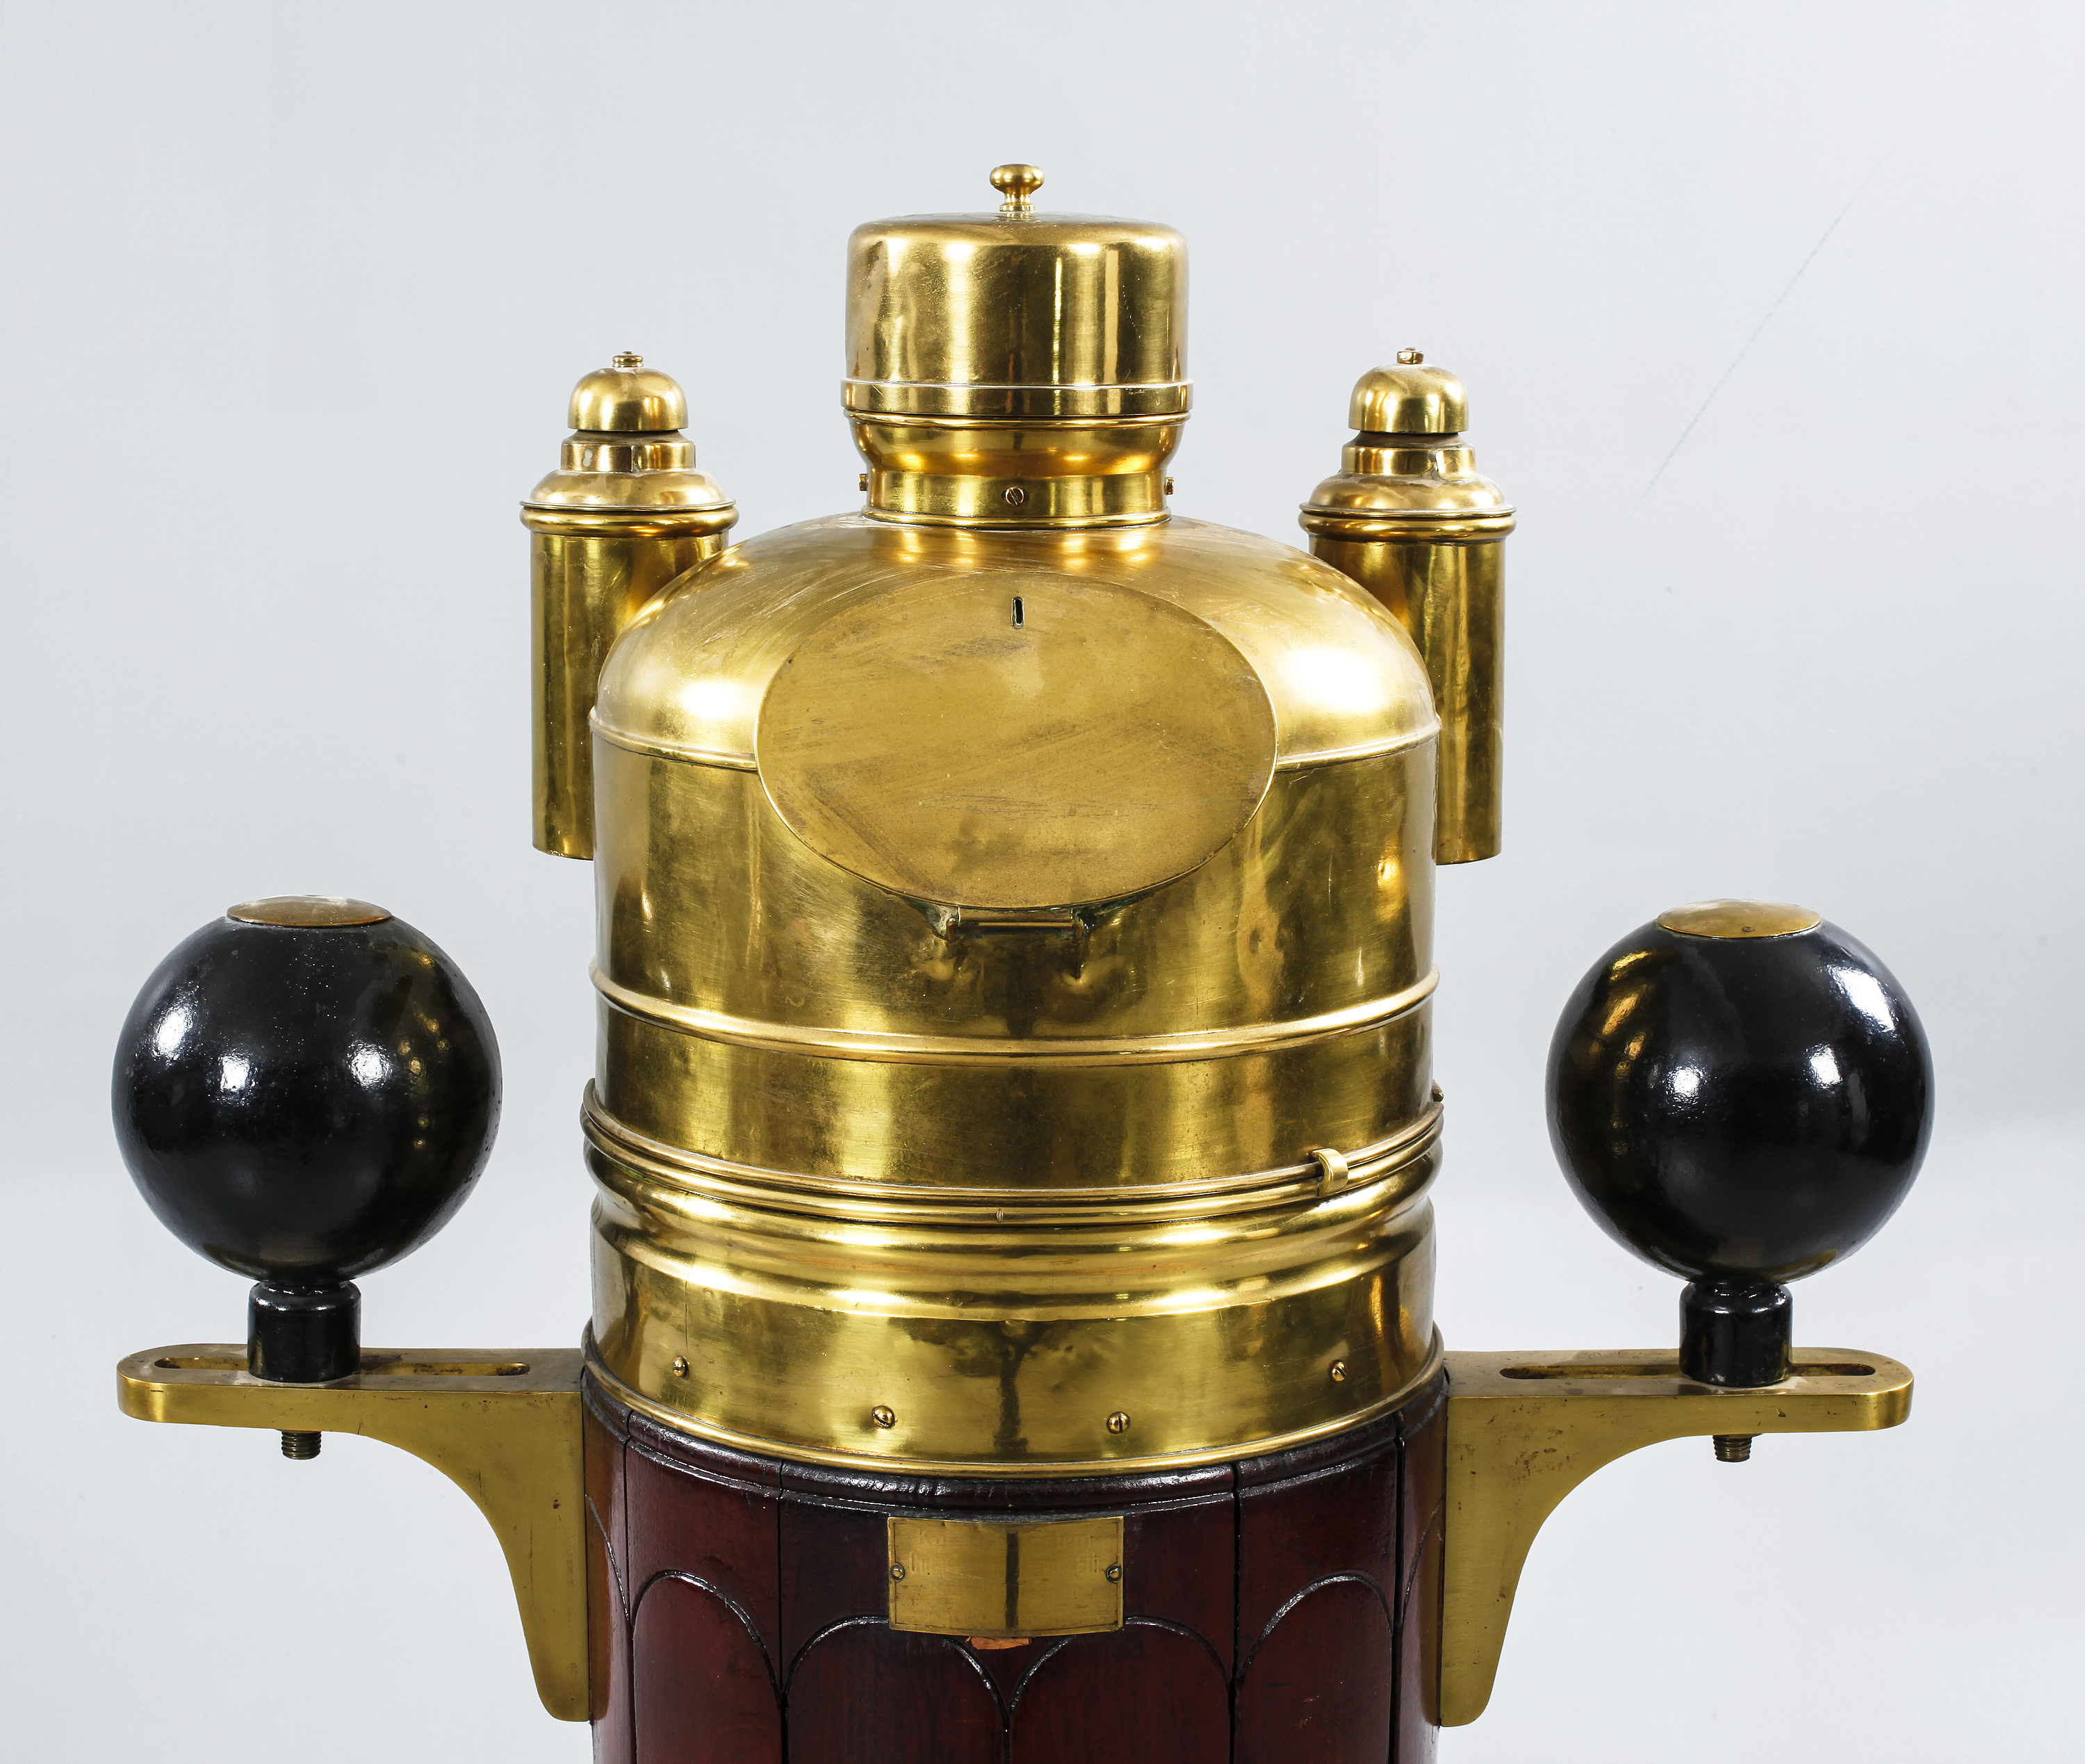
\includegraphics[scale=0.3]{Anh/ngoc2.jpg}
\end{center}

        Một hộp la bàn bảo vệ la bàn ở chính giữa, với hai quả cầu bằng sắt non để triệt tiêu phần bị lệch của la bàn, giúp la bàn quay đúng hướng. Việc sử dụng các quả cầu này được đề xuất bởi Lord Kelvin.

    Cũng như con tàu, các quả cầu sắt sẽ bị nhiễm từ do tác dụng của từ trường Trái Đất $B_e$. Là những quả cầu, chúng sẽ hoạt độn riên lẻ như các lưỡng cực. Một lưỡng cực có thể được coi như một trường tạo bởi hai đơn cực từ có moment từ $\pm m$ tại hai điểm khác nhau.
    Cảm ứng từ của một đơn cực từ là
    $$\ot{B}=\pm m\dfrac{\hat r}{r^2},$$
    Trong đó dấu dương tương ứng với cực bắc còn dấu âm tương ứng với cực nam. Từ trường của lưỡng cực là tổng hợp của hai trường: một của cực bắc tại $y=+a/2$ và một của cực nam tại $y=-a/2$, trong đó trục $y$ nằm ngang và hướng về phía bắc. $a$ là một khoảng cách nhỏ hơn rất nhiều so với bán kính các quả cầu; $a=K_iB_e$ trong đó $K_i$ là một hằng số phụ thuộc vào kích thước của các quả cầu sắt non.
    \begin{center}
        

\tikzset{every picture/.style={line width=0.75pt}} %set default line width to 0.75pt        

\begin{tikzpicture}[x=0.75pt,y=0.75pt,yscale=-1,xscale=1]
%uncomment if require: \path (0,466); %set diagram left start at 0, and has height of 466

%Shape: Circle [id:dp751806434667823] 
\draw   (98,277) .. controls (98,255.46) and (115.46,238) .. (137,238) .. controls (158.54,238) and (176,255.46) .. (176,277) .. controls (176,298.54) and (158.54,316) .. (137,316) .. controls (115.46,316) and (98,298.54) .. (98,277) -- cycle ;
%Straight Lines [id:da7958195415916756] 
\draw  [dash pattern={on 4.5pt off 4.5pt}]  (137,116) -- (137,284) ;
%Straight Lines [id:da11650011659130377] 
\draw  [dash pattern={on 4.5pt off 4.5pt}]  (137,277) -- (408,202) ;
%Straight Lines [id:da5651105007949573] 
\draw [line width=1.5]    (408,202) -- (466.27,224.56) ;
\draw [shift={(470,226)}, rotate = 201.16] [fill={rgb, 255:red, 0; green, 0; blue, 0 }  ][line width=0.08]  [draw opacity=0] (13.4,-6.43) -- (0,0) -- (13.4,6.44) -- (8.9,0) -- cycle    ;
%Shape: Circle [id:dp5068445005254147] 
\draw  [fill={rgb, 255:red, 0; green, 0; blue, 0 }  ,fill opacity=1 ] (132,262) .. controls (132,259.24) and (134.24,257) .. (137,257) .. controls (139.76,257) and (142,259.24) .. (142,262) .. controls (142,264.76) and (139.76,267) .. (137,267) .. controls (134.24,267) and (132,264.76) .. (132,262) -- cycle ;
%Shape: Circle [id:dp9877766218057484] 
\draw  [fill={rgb, 255:red, 0; green, 0; blue, 0 }  ,fill opacity=1 ] (132,289) .. controls (132,286.24) and (134.24,284) .. (137,284) .. controls (139.76,284) and (142,286.24) .. (142,289) .. controls (142,291.76) and (139.76,294) .. (137,294) .. controls (134.24,294) and (132,291.76) .. (132,289) -- cycle ;
%Straight Lines [id:da2796466001013038] 
\draw  [dash pattern={on 0.84pt off 2.51pt}]  (59,262) -- (137,262) ;
%Straight Lines [id:da8874709140465575] 
\draw  [dash pattern={on 0.84pt off 2.51pt}]  (59,289) -- (137,289) ;
%Straight Lines [id:da3482920020854341] 
\draw    (59,265) -- (59,289) ;
\draw [shift={(59,292)}, rotate = 270] [fill={rgb, 255:red, 0; green, 0; blue, 0 }  ][line width=0.08]  [draw opacity=0] (7.14,-3.43) -- (0,0) -- (7.14,3.43) -- (4.74,0) -- cycle    ;
\draw [shift={(59,262)}, rotate = 90] [fill={rgb, 255:red, 0; green, 0; blue, 0 }  ][line width=0.08]  [draw opacity=0] (7.14,-3.43) -- (0,0) -- (7.14,3.43) -- (4.74,0) -- cycle    ;

% Text Node
\draw (123,85.4) node [anchor=north west][inner sep=0.75pt]    {$\text{Bắc}$};
% Text Node
\draw (167,219.4) node [anchor=north west][inner sep=0.75pt]    {$\Phi $};
% Text Node
\draw (436,227.4) node [anchor=north west][inner sep=0.75pt]    {$\overrightarrow{B_{i}}$};
% Text Node
\draw (151,319.4) node [anchor=north west][inner sep=0.75pt]    {$\text{Bóng sắt}$};
% Text Node
\draw (37,267.4) node [anchor=north west][inner sep=0.75pt]    {$a$};


\end{tikzpicture}

    \end{center}
    \item Lập biểu thức cho từ trường $\ot{B_i}$ cách tâm quả cầu một khoảng $d\gg a$. Lưu ý rằng sẽ có một thành phần có phương hướng tâm, hướng ra quả cầu và một thành phần có phương tiếp tuyến với đường tròn bán kính $d$ xung quanh quả cầu, vì vậy nên sử dụng tọa độ cực.
    \item Nếu được đặt trực tiếp ở bên phải và trái của la bàn, các quả cầu sắt có thể được đặt ở khoảng cách $d$ để loại bỏ sai số từ tính cho các góc bất kì mà trong đó $\delta \theta$ là lớn nhất. Giả sử rằng điều này được thực hiện, tìm biểu thức cho góc lệch $\delta\theta$ do sự kết hợp hướng từ tính của con tàu và các quả cầu đối với góc $\theta$ bất kì.
\end{enumerate}

\end{vd}
\begin{loigiai}
\begin{enumerate}[1)]
    \item Phân tích từ trường tổng hợp thành các từ trường thành phần. Thành phần từ trường hướng về phía Bắc là:
$$B_{\text{bắc}}=B_e-B_eK_b\cos\theta\cos\theta-B_eK_s\sin\theta\sin\theta,$$
trong khi đó thành phần hướng về phía Đông là:
$$B_{\text{đông}}=-B_3K_b\sin\theta\cos\theta+B_eK_s\cos\theta\sin\theta.$$
Ta được góc lệch:
$$ \tan \delta \theta=\left(K_{s}-K_{b}\right) \dfrac{\sin \theta \cos \theta}{1-K_{b} \cos ^{2} \theta-K_{s} \sin ^{2} \theta}.$$
Dạng của biểu thức này khá đẹp, vì như ta thấy, $K_b$ và $K_s$ đủ nhỏ để có thể bỏ qua ở mẫu.
    \item Bằng cách kiểm tra, ta thấy $\theta=45^\circ$ sẽ ứng với góc lệch lớn nhất. Và ta chấp nhận được các góc $45^\circ$, $135^\circ$, $225^\circ$ và $315^\circ$.
    \item Bài toán này không khó như ta nghĩ.\\
    \begin{center}
        

\tikzset{every picture/.style={line width=0.75pt}} %set default line width to 0.75pt        

\begin{tikzpicture}[x=0.75pt,y=0.75pt,yscale=-1,xscale=1]
%uncomment if require: \path (0,468); %set diagram left start at 0, and has height of 468

%Shape: Circle [id:dp283743452851426] 
\draw   (118,297) .. controls (118,275.46) and (135.46,258) .. (157,258) .. controls (178.54,258) and (196,275.46) .. (196,297) .. controls (196,318.54) and (178.54,336) .. (157,336) .. controls (135.46,336) and (118,318.54) .. (118,297) -- cycle ;
%Straight Lines [id:da9329698416959988] 
\draw  [dash pattern={on 4.5pt off 4.5pt}]  (157,136) -- (157,304) ;
%Shape: Circle [id:dp7302446853963502] 
\draw  [fill={rgb, 255:red, 0; green, 0; blue, 0 }  ,fill opacity=1 ] (152,282) .. controls (152,279.24) and (154.24,277) .. (157,277) .. controls (159.76,277) and (162,279.24) .. (162,282) .. controls (162,284.76) and (159.76,287) .. (157,287) .. controls (154.24,287) and (152,284.76) .. (152,282) -- cycle ;
%Shape: Circle [id:dp08946091539998635] 
\draw  [fill={rgb, 255:red, 0; green, 0; blue, 0 }  ,fill opacity=1 ] (152,309) .. controls (152,306.24) and (154.24,304) .. (157,304) .. controls (159.76,304) and (162,306.24) .. (162,309) .. controls (162,311.76) and (159.76,314) .. (157,314) .. controls (154.24,314) and (152,311.76) .. (152,309) -- cycle ;
%Straight Lines [id:da8503315996944931] 
\draw  [dash pattern={on 0.84pt off 2.51pt}]  (79,282) -- (157,282) ;
%Straight Lines [id:da4363280092273607] 
\draw  [dash pattern={on 0.84pt off 2.51pt}]  (79,309) -- (157,309) ;
%Straight Lines [id:da08272405117413917] 
\draw    (79,285) -- (79,309) ;
\draw [shift={(79,312)}, rotate = 270] [fill={rgb, 255:red, 0; green, 0; blue, 0 }  ][line width=0.08]  [draw opacity=0] (7.14,-3.43) -- (0,0) -- (7.14,3.43) -- (4.74,0) -- cycle    ;
\draw [shift={(79,282)}, rotate = 90] [fill={rgb, 255:red, 0; green, 0; blue, 0 }  ][line width=0.08]  [draw opacity=0] (7.14,-3.43) -- (0,0) -- (7.14,3.43) -- (4.74,0) -- cycle    ;
%Straight Lines [id:da016285889610417215] 
\draw [color={rgb, 255:red, 0; green, 0; blue, 0 }  ,draw opacity=1 ]   (157,282) -- (389,243) ;
%Straight Lines [id:da05152532762538198] 
\draw    (170.5,305) -- (389,243) ;
%Straight Lines [id:da8507054364259559] 
\draw [color={rgb, 255:red, 245; green, 166; blue, 35 }  ,draw opacity=1 ]   (391.89,242.18) -- (498,212) ;
\draw [shift={(389,243)}, rotate = 344.12] [fill={rgb, 255:red, 245; green, 166; blue, 35 }  ,fill opacity=1 ][line width=0.08]  [draw opacity=0] (10.72,-5.15) -- (0,0) -- (10.72,5.15) -- (7.12,0) -- cycle    ;
%Straight Lines [id:da4895425189234859] 
\draw [color={rgb, 255:red, 74; green, 144; blue, 226 }  ,draw opacity=1 ][fill={rgb, 255:red, 74; green, 144; blue, 226 }  ,fill opacity=1 ]   (389,243) -- (500.05,223.52) ;
\draw [shift={(503,223)}, rotate = 530.05] [fill={rgb, 255:red, 74; green, 144; blue, 226 }  ,fill opacity=1 ][line width=0.08]  [draw opacity=0] (10.72,-5.15) -- (0,0) -- (10.72,5.15) -- (7.12,0) -- cycle    ;
%Straight Lines [id:da05906959057280403] 
\draw [color={rgb, 255:red, 208; green, 2; blue, 27 }  ,draw opacity=1 ]   (159.5,283.5) -- (170.5,305) ;
%Straight Lines [id:da6543050515321556] 
\draw [color={rgb, 255:red, 79; green, 211; blue, 33 }  ,draw opacity=1 ]   (157,309) -- (170.5,305) ;

% Text Node
\draw (143,105.4) node [anchor=north west][inner sep=0.75pt]    {$\text{Bắc}$};
% Text Node
\draw (187,239.4) node [anchor=north west][inner sep=0.75pt]    {$\Phi $};
% Text Node
\draw (57,287.4) node [anchor=north west][inner sep=0.75pt]    {$a$};


\end{tikzpicture}

    \end{center}
    Xét hình tam giác màu ở trên. Cạnh màu đen có chiều dài $a$. Góc giữa cạnh màu xanh và đen là $\Phi$, nên chiều dài cạnh đỏ là $a\sin \Phi$ và chiều dài cạnh xanh là $a\cos \Phi$.\\
    Cảm ứng từ gây ra bởi một cực từ cách một khoảng $d$ là
    $$B=\pm m\dfrac{1}{d^2}.$$
    Tổng hợp của hai trường gồm có hai thành phần. Thành phần tiếp tuyến được tính bằng độ mở của tam giác tạo bởi hai vector, và vì hai vector có chiều dài xấp xỉ nhau, nên chúng ta có thể dùng biểu thức của tam giác đồng dạng:
    $$\dfrac{a \sin \phi}{d} \approx \dfrac{B_{\phi}}{B} \Rightarrow B_{\phi}=m \dfrac{a}{d^{3}} \sin \phi=B_{e} \dfrac{m K_{i}}{d^{3}} \sin \phi .$$
    Như mong đợi, thành phần này biến mất vì $\Phi=0$.\\
    Thành phần theo phương bán kính được xác định bởi sự khác biệt chiều dài của hai vector của hai trường, là:
    $$ B_{r}=m\left(\dfrac{1}{d^{2}}-\dfrac{1}{(d+x)^{2}}\right)=\dfrac{m}{d^{2}}\left(1-\dfrac{1}{(1+x / d)^{2}}\right) \approx \dfrac{m}{d^{2}} \dfrac{2 x}{d},$$
    trong đó $x=a\cos\Phi$ là chiều dài cạnh xanh lá, vì thế
    $$B_r=2B_e\dfrac{mK_i}{d^3}\cos\Phi.$$
    \item Lưu ý rằng từ trường gần la bàn do hai viên bi sắt tạo ra hoạt động khá giống với từ trường do cả con tàu. Thành phần hướng về phía mũi tàu là:
    $$B_b=-2B_{\theta} \propto \sin\Phi\propto\cos\theta,$$
    và thành phần hướng về mạn phải là:
    $$B_s=2B_r \propto \cos\Phi\propto\sin\theta,$$
    trong đó có thừa số $2$ bởi vì có hai quả cầu. Lưu ý rằng $\theta$ là hướng đi của con tàu trong khi $\Phi$ là góc hợp bởi cực Bắc và vị trí của la bàn so với một trong các quả cầu. Do đó, nếu như từ trường được hiệu chỉnh sao cho các góc tối đa, nó sẽ loại bỏ từ trường do tàu gây ra cho tất cả các góc, hay
    $$\delta \theta=0,$$
    với mọi $\theta$. Điều này có nghĩa là ta sẽ đặt vị trí các quả cầu sao cho $K_b=K_s$.
\end{enumerate}
\end{loigiai}


\begin{vd}[Lưỡng cực từ quy mô hành tinh]
Từ trường của Trái Đất là gần giống với một từ trường của một lưỡng cực từ. Ta có thể tưởng tượng có một lưỡng cực từ $\ot{m}$ ở tâm của Trái Đất. Để đơn giản, giả sử rằng $\ot{m}$ nằm trên trục quay của Trái Đất, hướng từ Bắc vào Nam, như hình vẽ. Hồng Kông nằm ở vĩ độ $\alpha=22^\circ$. Từ trường tại điểm cách lưỡng cực từ một khoảng là $\ot{r}$ được tính theo công thức
\[\ot{B}=\dfrac{\mu_o}{4\pi}\left[\dfrac{3(\ot{m}\cdot\ot{r})\ot{r}}{r^3}-\dfrac{\ot{m}}{r^3}\right]\]
\begin{enumerate}[1) ]
    \item Tìm hướng của từ trường tại Hồng Kông theo các phía Đông, Tây, Bắc, Nam, và các góc hợp với mặt ngang.
    \item Một dây điện nằm ngang có chiều dài $10~\mathrm{m}$, mang dòng điện có cường độ $100~\mathrm{A}$ theo hướng Bắc $-$ Nam. Tìm lực từ tác dụng lên dây. (Bạn cần phải nhớ độ lớn của từ trường Trái Đất trên bề mặt Trái Đất).
\end{enumerate}
\begin{center}
    

\tikzset{every picture/.style={line width=0.75pt}} %set default line width to 0.75pt        

\begin{tikzpicture}[x=0.75pt,y=0.75pt,yscale=-1,xscale=1]
%uncomment if require: \path (0,300); %set diagram left start at 0, and has height of 300

%Shape: Circle [id:dp12955050763248477] 
\draw   (239,169) .. controls (239,124.26) and (275.26,88) .. (320,88) .. controls (364.74,88) and (401,124.26) .. (401,169) .. controls (401,213.74) and (364.74,250) .. (320,250) .. controls (275.26,250) and (239,213.74) .. (239,169) -- cycle ;
%Straight Lines [id:da33432597677839704] 
\draw  [dash pattern={on 0.84pt off 2.51pt}]  (208,170.33) -- (428,170.33) ;
%Straight Lines [id:da6659306133043119] 
\draw  [dash pattern={on 0.84pt off 2.51pt}]  (320,67.33) -- (320,270.33) ;
%Straight Lines [id:da013535855620636417] 
\draw    (320,169) -- (374.84,115.92) ;
\draw [shift={(377,113.83)}, rotate = 495.94] [fill={rgb, 255:red, 0; green, 0; blue, 0 }  ][line width=0.08]  [draw opacity=0] (10.72,-5.15) -- (0,0) -- (10.72,5.15) -- (7.12,0) -- cycle    ;
%Shape: Circle [id:dp570580867637053] 
\draw  [fill={rgb, 255:red, 0; green, 0; blue, 0 }  ,fill opacity=1 ] (379.5,113.83) .. controls (379.5,112.45) and (378.38,111.33) .. (377,111.33) .. controls (375.62,111.33) and (374.5,112.45) .. (374.5,113.83) .. controls (374.5,115.21) and (375.62,116.33) .. (377,116.33) .. controls (378.38,116.33) and (379.5,115.21) .. (379.5,113.83) -- cycle ;
%Straight Lines [id:da7218913590835949] 
\draw [line width=2.25]    (320,163.33) -- (320,177) ;
\draw [shift={(320,182)}, rotate = 270] [fill={rgb, 255:red, 0; green, 0; blue, 0 }  ][line width=0.08]  [draw opacity=0] (16.07,-7.72) -- (0,0) -- (16.07,7.72) -- (10.67,0) -- cycle    ;

% Text Node
\draw (338,124.4) node [anchor=north west][inner sep=0.75pt]    {$\ot{r}$};
% Text Node
\draw (296,175.4) node [anchor=north west][inner sep=0.75pt]    {$\ot{m}$};
% Text Node
\draw (342,149.4) node [anchor=north west][inner sep=0.75pt]    {$\alpha $};
% Text Node
\draw (387,97.4) node [anchor=north west][inner sep=0.75pt]    {$HK$};


\end{tikzpicture}
\end{center}
\end{vd}
\begin{loigiai}
\begin{enumerate}[1) ]
    \item 
    \begin{align*}
        \ot{B}&=\dfrac{\mu_0}{4\pi}\dfrac{1}{r^3}\left[3(\ot{m}\cdot\ot{r})\ot{r}-\ot{m}\right]\\
        &=\dfrac{\mu_0}{4\pi}\dfrac{1}{R^3}\left[3((-m\cdot\ot{z})\cdot\ot{r})\ot{r}-(-m)\ot{z}\right]\\
        &=\dfrac{\mu_0}{4\pi}\dfrac{m}{R^3}\left[-3\mathrm{\sin{\alpha}}\cdot\ot{r}+\left(\mathrm{\sin{\alpha}}\cdot\ot{r}-\mathrm{\cos{\alpha}}\cdot\ot{\theta}\right)\right]\\
        &=\dfrac{\mu_0}{4\pi}\dfrac{m}{R^3}\left[-2\mathrm{\sin{\alpha}}\cdot\ot{r}-\mathrm{\cos{\alpha}}\cdot\ot{\theta}\right].
    \end{align*}
    Từ Bắc tới Nam, tại góc $\beta=2\mathrm{\arctan{(2\mathrm{\tan{\alpha}})}}=38,9^\circ$ chỉ hướng xuống.
    \item $\left|\ot{B}\right|\cong0,5\cdot10^{-4}~\mathrm{T}$.
    Và độ lớn của lực từ là:
    \[\left|\ot{F}\right|=I\left|\ot{\ell}\times\ot{B}\right|=IB\ell\mathrm{\sin{\theta}}=0,0315~\mathrm{N}.\]
\end{enumerate}
\end{loigiai}

\begin{vd}[Dao động Plasma]
Một phiến kim loại có chiều dài $L$ và độ dày $h$, với $h\ll L$ (xem hình vẽ). Mật độ hạt dẫn electron và ion trong tấm lần lượt là $n_e$ và $n_i = n_e /Z$, với $Z$ là điện tích của các ion (điều này có nghĩa tổng điện tích của phiến bằng không).
\begin{center}


\tikzset{every picture/.style={line width=0.75pt}} %set default line width to 0.75pt        

\begin{tikzpicture}[x=0.75pt,y=0.75pt,yscale=-1,xscale=1]
%uncomment if require: \path (0,300); %set diagram left start at 0, and has height of 300

%Shape: Rectangle [id:dp7217887277897033] 
\draw  [draw opacity=0][fill={rgb, 255:red, 155; green, 155; blue, 155 }  ,fill opacity=0.6 ] (199,96) -- (279,96) -- (279,247) -- (199,247) -- cycle ;
%Shape: Rectangle [id:dp49084866599960386] 
\draw   (179,96) -- (257,96) -- (257,246.4) -- (179,246.4) -- cycle ;
%Straight Lines [id:da592262187480596] 
\draw    (165,102) -- (165,243) ;
\draw [shift={(165,246)}, rotate = 270] [fill={rgb, 255:red, 0; green, 0; blue, 0 }  ][line width=0.08]  [draw opacity=0] (10.72,-5.15) -- (0,0) -- (10.72,5.15) -- (7.12,0) -- cycle    ;
\draw [shift={(165,99)}, rotate = 90] [fill={rgb, 255:red, 0; green, 0; blue, 0 }  ][line width=0.08]  [draw opacity=0] (10.72,-5.15) -- (0,0) -- (10.72,5.15) -- (7.12,0) -- cycle    ;
%Straight Lines [id:da1395939334945815] 
\draw    (182,85) -- (253,85) ;
\draw [shift={(256,85)}, rotate = 180] [fill={rgb, 255:red, 0; green, 0; blue, 0 }  ][line width=0.08]  [draw opacity=0] (10.72,-5.15) -- (0,0) -- (10.72,5.15) -- (7.12,0) -- cycle    ;
\draw [shift={(179,85)}, rotate = 0] [fill={rgb, 255:red, 0; green, 0; blue, 0 }  ][line width=0.08]  [draw opacity=0] (10.72,-5.15) -- (0,0) -- (10.72,5.15) -- (7.12,0) -- cycle    ;
%Straight Lines [id:da6778726697290913] 
\draw    (259,253) -- (275,253) ;
\draw [shift={(278,253)}, rotate = 180] [fill={rgb, 255:red, 0; green, 0; blue, 0 }  ][line width=0.08]  [draw opacity=0] (10.72,-5.15) -- (0,0) -- (10.72,5.15) -- (7.12,0) -- cycle    ;


% Text Node
\draw (181,124.4) node [anchor=north west][inner sep=0.75pt]    {$+$};
% Text Node
\draw (181,166.4) node [anchor=north west][inner sep=0.75pt]    {$+$};
% Text Node
\draw (181,205.4) node [anchor=north west][inner sep=0.75pt]    {$+$};
% Text Node
\draw (264,123.4) node [anchor=north west][inner sep=0.75pt]    {$-$};
% Text Node
\draw (264,170.4) node [anchor=north west][inner sep=0.75pt]    {$-$};
% Text Node
\draw (264,206.4) node [anchor=north west][inner sep=0.75pt]    {$-$};
% Text Node
\draw (261,256.4) node [anchor=north west][inner sep=0.75pt]    {$\delta $};
% Text Node
\draw (152,165.4) node [anchor=north west][inner sep=0.75pt]    {$L$};
% Text Node
\draw (213,66.4) node [anchor=north west][inner sep=0.75pt]    {$h$};


\end{tikzpicture}
\end{center}
Bằng cách đặt tấm vào một điện trường đều bên ngoài, tất cả các electron đều bị dịch đi một khoảng nhỏ $\delta$, sao cho $|\delta| \ll h$, và vuông góc với trục của phiến. Chúng ta giả sử rằng $n_i$ và $n_e$ là không đổi, điện trường ngoài không làm nhiễu loạn mạng tinh thể và hiệu ứng rìa có thể được bỏ qua.
\begin{enumerate}[1)]
   \item Tính điện trường gây ra bởi sự dịch chuyển của các electron.
    \item Tính năng lượng điện trường của hệ.
Bây giờ điện trường ngoài bị tắt đi, và “mạng electron” bắt đầu dao động quanh vị trí cân bằng của nó.
  \item Tìm chu kì dao động của hệ với giả sử rằng độ dịch là nhỏ $(\delta \ll h)$.
\end{enumerate}
  
\end{vd}
\begin{loigiai}
  \begin{enumerate}[1)]
    \item Ta giả sử rằng $\delta >0$, sự dịch chuyển của các eletron dẫn điện do tác động của điện trường ngoài sẽ gây ra phân bố mật độ điện tích trên phiến.
\begin{center}


\tikzset{every picture/.style={line width=0.75pt}} %set default line width to 0.75pt        

\begin{tikzpicture}[x=0.75pt,y=0.75pt,yscale=-1,xscale=1]
%uncomment if require: \path (0,300); %set diagram left start at 0, and has height of 300

%Straight Lines [id:da6451691314240162] 
\draw    (78,141) -- (314.8,141) ;
\draw [shift={(317.8,141)}, rotate = 180] [fill={rgb, 255:red, 0; green, 0; blue, 0 }  ][line width=0.08]  [draw opacity=0] (10.72,-5.15) -- (0,0) -- (10.72,5.15) -- (7.12,0) -- cycle    ;
%Straight Lines [id:da1410092498727764] 
\draw    (100,257.9) -- (100,27.1) ;
\draw [shift={(100,24.1)}, rotate = 450] [fill={rgb, 255:red, 0; green, 0; blue, 0 }  ][line width=0.08]  [draw opacity=0] (10.72,-5.15) -- (0,0) -- (10.72,5.15) -- (7.12,0) -- cycle    ;
%Straight Lines [id:da15557261132056954] 
\draw [line width=1.5]    (100,60.2) -- (100,141) ;
%Straight Lines [id:da9142755166526642] 
\draw [line width=1.5]    (124.8,60.2) -- (124.8,141) ;
%Straight Lines [id:da4536569984572141] 
\draw [line width=1.5]    (234,141.2) -- (234,222) ;
%Straight Lines [id:da69833388035731] 
\draw [line width=1.5]    (258.8,141.2) -- (258.8,222) ;
%Straight Lines [id:da14094267922415105] 
\draw [line width=1.5]    (100,60.2) -- (125.8,60.2) ;
%Straight Lines [id:da3546021934992991] 
\draw [line width=1.5]    (233,222) -- (258.8,222) ;
%Straight Lines [id:da5560792612540038] 
\draw  [dash pattern={on 4.5pt off 4.5pt}]  (100.8,222) -- (233,222) ;


% Text Node
\draw (66,52.4) node [anchor=north west][inner sep=0.75pt]    {$+en$};
% Text Node
\draw (67,214.4) node [anchor=north west][inner sep=0.75pt]    {$-en$};
% Text Node
\draw (82,25.4) node [anchor=north west][inner sep=0.75pt]    {$\rho $};
% Text Node
\draw (294,143.4) node [anchor=north west][inner sep=0.75pt]    {$x$};
% Text Node
\draw (225,121.4) node [anchor=north west][inner sep=0.75pt]    {$h$};
% Text Node
\draw (245,121.4) node [anchor=north west][inner sep=0.75pt]    {$h+\delta $};
% Text Node
\draw (126.8,144.4) node [anchor=north west][inner sep=0.75pt]    {$\delta $};
% Text Node
\draw (84,143.4) node [anchor=north west][inner sep=0.75pt]    {$0$};


\end{tikzpicture}
\end{center}
      \[\varrho (x) = \left\{ \begin{array}{cc}
      0, & x<0, \\
     +en, & 0<x<\delta,\\
              0, &  \delta<x<h, \\
     -en, &h<x< h+\delta, \\
     0, & x> h+\delta. \end{array}\right. \tag{1}\]

Điện trường gây ra bởi phân bố này có thể được tính bằng cách kết hợp phương trình $\nabla \cdot \ot{E} = \partial_x E_x = 4\pi k_{\mathrm{e}} \varrho$ và điều kiện biên $\ot{E}(-\infty) =0$:
      \[E_x(x) = 4\pi e n k_{\mathrm{e}} \left\{ \begin{array}{cc} 
                       0, & x<0, \\
                 x, & 0<x<\delta, \\
                 \delta , & \delta<x<h,\\
                   h+ \delta - x, & h<x<h+\delta , \\
              0, & x>h+\delta . 
            \end{array}\right. \tag{2} \]

  \begin{center}


\tikzset{every picture/.style={line width=0.75pt}} %set default line width to 0.75pt        

\begin{tikzpicture}[x=0.75pt,y=0.75pt,yscale=-1,xscale=1]
%uncomment if require: \path (0,300); %set diagram left start at 0, and has height of 300

%Straight Lines [id:da01641255710506151] 
\draw    (98,161) -- (334.8,161) ;
\draw [shift={(337.8,161)}, rotate = 180] [fill={rgb, 255:red, 0; green, 0; blue, 0 }  ][line width=0.08]  [draw opacity=0] (10.72,-5.15) -- (0,0) -- (10.72,5.15) -- (7.12,0) -- cycle    ;
%Straight Lines [id:da14878370163317478] 
\draw    (120,185) -- (120,47.1) ;
\draw [shift={(120,44.1)}, rotate = 450] [fill={rgb, 255:red, 0; green, 0; blue, 0 }  ][line width=0.08]  [draw opacity=0] (10.72,-5.15) -- (0,0) -- (10.72,5.15) -- (7.12,0) -- cycle    ;
%Straight Lines [id:da8675826770429016] 
\draw [line width=0.75]  [dash pattern={on 4.5pt off 4.5pt}]  (120,88.2) -- (145.8,88.2) ;
%Straight Lines [id:da9262762168352314] 
\draw [line width=0.75]  [dash pattern={on 4.5pt off 4.5pt}]  (145.8,88.2) -- (145.8,160.6) ;
%Straight Lines [id:da7374057248217938] 
\draw [line width=0.75]  [dash pattern={on 4.5pt off 4.5pt}]  (233.8,88.2) -- (233.8,160.6) ;
%Straight Lines [id:da034445088923599654] 
\draw [line width=1.5]    (145.8,88.2) -- (120.6,160.6) ;
%Straight Lines [id:da6877283104927654] 
\draw [line width=1.5]    (145.8,88.2) -- (233.8,88.2) ;
%Straight Lines [id:da6022831934893127] 
\draw [line width=1.5]    (233.8,88.2) -- (260.8,160.6) ;


% Text Node
\draw (102,48.4) node [anchor=north west][inner sep=0.75pt]    {$E$};
% Text Node
\draw (90,78.4) node [anchor=north west][inner sep=0.75pt]    {$en\delta $};
% Text Node
\draw (107,162.4) node [anchor=north west][inner sep=0.75pt]    {$0$};
% Text Node
\draw (147.8,164) node [anchor=north west][inner sep=0.75pt]    {$\delta $};
% Text Node
\draw (224.9,164.4) node [anchor=north west][inner sep=0.75pt]    {$h$};
% Text Node
\draw (247,163.4) node [anchor=north west][inner sep=0.75pt]    {$h+\delta $};
% Text Node
\draw (312,164.4) node [anchor=north west][inner sep=0.75pt]    {$x$};


\end{tikzpicture}
\end{center}
Nếu chúng ta giả sử độ dịch là âm $-\delta$ (với $\delta>0$) thì mật độ điện tích và điện trường là 

    \[\begin{aligned}
       \varrho(x) &= 
       \left\{\begin{array}{cc}
                                     0, & x<-\delta,  \\
                              -en, & -\delta <x<0,\\
                            0, &  0<x<h-\delta, \\
                          +en, &h-\delta<x< h, \\
                               0,      &x> h . 
                  \end{array}\right.\\
        E_x(x) &= 4\pi e n k_{\mathrm{e}}   
        \left\{\begin{array}{cc}
                                     0, & x<-\delta,  \\
                              -en, & -\delta <x<0,\\
                            0, &  0<x<h-\delta, \\
                          +en, &h-\delta<x< h, \\
                               0,      &x> h . 
                  \end{array}\right. 
    \end{aligned}\tag{3}\]

Đồ thị cho trường hợp này có thể thu được bằng cách đảo trục $x$ và chuyển $\delta$ sang phần âm của trục $x$.
\item Năng lượng tĩnh điện của hệ, trong trường hợp độ dịch là dương, có thể tính được bằng tích phân mật độ năng lượng $u={E_x}^2/(8\pi k_{\mathrm{e}})$ trên toàn bộ vùng không gian:
 \[\begin{aligned}
U_{\mathrm{es}} &=\int \frac{E_{x}^{2}}{8 \pi k_{\mathrm{e}}} \mathrm{d}^{3} r=\frac{L^{2}}{8 \pi k_{\mathrm{e}}} \int_{0}^{h+\delta} E_{x}^{2} \mathrm{~d} x \\
&=\frac{L^{2}}{8 \pi k_{\mathrm{e}}}(4 \pi e n k_{\mathrm{e}})^{2}\left[\int_{0}^{\delta} x^{2} \mathrm{~d} x+\int_{\delta}^{h} \delta^{2} \mathrm{~d} x+\int_{h}^{h+\delta}(h+\delta-x)^{2} \mathrm{~d} x\right] \\
&=2 \pi k_{\mathrm{e}}(e n L)^{2}\left[\frac{\delta^{3}}{3}+\delta^{2}(h-\delta)+\frac{\delta^{3}}{3}\right]=2 \pi k_{\mathrm{e}}(e n L)^{2}\left(h \delta^{2}-\frac{\delta^{3}}{3}\right),
\end{aligned} \tag{4} \]
ở đây, do tính đối xứng của hệ, chúng ta sử dụng $\dd^3 r = L^2 \dd x $. Kết quả tương tự cũng sẽ đạt được nếu chúng ta coi độ dịch là $-\delta$. Độ dịch $\delta$ xuất hiện ở cuối biểu thức $4)$ trên thực tế phải được viết là $|\delta|$.
\item Ở giới hạn $\delta \ll h$ chúng ta có thể bỏ qua số hạng bậc ba của $\delta$ ở phương trình $4)$, và xấp xỉ $U_{\mathrm{es}} \approx 2\pi k_{\mathrm{e}} (enL)^2 h \delta^2$, năng lượng này là thế năng của một dao động điều hòa. Lực tác dụng lên ``mạng electron'' là 
   \[F= - \frac{\partial U_{\mathrm{es}}}{\partial \delta} = - 4 \pi k_{\mathrm{e}} (enL)^2h\delta, \tag{5}\]
ở đây $\delta$ có thể là âm hoặc dương. Phương trình chuyển động của electron là 
   \[M\ddot{\delta} = F = -M\omega^2\delta, \tag{6}\]
ở đây $M= m_e nL^2h$ là tổng khối lượng electron dẫn của bản. Từ đây ta có
     \[\omega^2 = \frac{4\pi k_{\mathrm{e}} n e^2}{m_e} \equiv \omega_p^2, \tag{7}\]
trong đó $\omega_p$ được gọi là tần số plasma, là một tính chất nội tại của vật dẫn, chỉ phụ thuộc vào mật độ electron tự do.
\end{enumerate}
\end{loigiai}


\begin{vd}[Cặp electrons và điện trường]
Ở đây chúng ta nghiên cứu chuyển động của hai electron trong mặt phẳng vuông góc với các đường sức của một từ trường đều. Hai electron được coi gần đúng như các chất điểm cổ điển và chỉ chịu tác dụng của lực điện và lực từ.
\begin{enumerate}[1)]
    \item Ban đầu hai electron đứng yên và cách nhau một khoảng là $d$. Chúng được truyền các vận tốc đầu cùng độ lớn $v$ nhưng ngược chiều nhau. Tìm điều kiện của $d$ để sau khi bắt đầu chuyển động, khoảng cách giữa chúng luôn là hằng số. Tìm biểu thức của $d$ lúc này.
    \item Chứng tỏ rằng có thể duy trì khoảng cách không đổi $d$ chỉ bằng cách truyền vận tốc cho một electron.Tìm quỹ đạo của khối tâm hệ trong trường hợp này. Vẽ phác họa quỹ đạo chuyển động của các electron. Khi nào thì electron ban đầu chuyển động sẽ dừng.
\end{enumerate}
\end{vd}
\begin{loigiai}
    \begin{enumerate}[1)]
        \item Để khoảng cách là không đổi, hai electron phải chuyển động cùng quỹ đạo trên cùng một đường tròn với bán kính $d/2$; chúng phải nằm đối xứng nhau qua tâm hình tròn và chuyển động với cùng vận tốc $v$ (như hình vẽ). Cả hai electron chuyển động trong từ trường đều chịu tác dụng của lực Lorentz và lực đẩy tĩnh điện giữa chúng tổng hợp lại thành một lực hướng tâm giữ cho chúng chuyển động thẳng đều.
        \begin{center}
            \tikzset{every picture/.style={line width=0.75pt}} %set default line width to 0.75pt        
            \begin{tikzpicture}[x=0.75pt,y=0.75pt,yscale=-1,xscale=1]
            %uncomment if require: \path (0,521); %set diagram left start at 0, and has height of 521
            
            %Shape: Ellipse [id:dp37933654197498545] 
            \draw   (166.08,212.4) .. controls (166.08,156.95) and (211.03,112) .. (266.48,112) .. controls (321.93,112) and (366.88,156.95) .. (366.88,212.4) .. controls (366.88,267.85) and (321.93,312.8) .. (266.48,312.8) .. controls (211.03,312.8) and (166.08,267.85) .. (166.08,212.4) -- cycle ;
            %Shape: Ellipse [id:dp020176206185545054] 
            \draw  [fill={rgb, 255:red, 0; green, 0; blue, 0 }  ,fill opacity=1 ] (161.72,212.4) .. controls (161.72,209.99) and (163.67,208.03) .. (166.08,208.03) .. controls (168.49,208.03) and (170.45,209.99) .. (170.45,212.4) .. controls (170.45,214.81) and (168.49,216.77) .. (166.08,216.77) .. controls (163.67,216.77) and (161.72,214.81) .. (161.72,212.4) -- cycle ;
            %Shape: Ellipse [id:dp7333140222111905] 
            \draw  [fill={rgb, 255:red, 0; green, 0; blue, 0 }  ,fill opacity=1 ] (362.52,212.4) .. controls (362.52,209.99) and (364.47,208.03) .. (366.88,208.03) .. controls (369.29,208.03) and (371.25,209.99) .. (371.25,212.4) .. controls (371.25,214.81) and (369.29,216.77) .. (366.88,216.77) .. controls (364.47,216.77) and (362.52,214.81) .. (362.52,212.4) -- cycle ;
            %Straight Lines [id:da5858758890164644] 
            \draw    (166.08,208.03) -- (166.08,165.68) ;
            \draw [shift={(166.08,163.68)}, rotate = 450] [color={rgb, 255:red, 0; green, 0; blue, 0 }  ][line width=0.75]    (10.93,-3.29) .. controls (6.95,-1.4) and (3.31,-0.3) .. (0,0) .. controls (3.31,0.3) and (6.95,1.4) .. (10.93,3.29)   ;
            %Straight Lines [id:da6699826148149972] 
            \draw    (166.08,212.4) -- (226.94,212.4) ;
            \draw [shift={(228.94,212.4)}, rotate = 180] [color={rgb, 255:red, 0; green, 0; blue, 0 }  ][line width=0.75]    (10.93,-3.29) .. controls (6.95,-1.4) and (3.31,-0.3) .. (0,0) .. controls (3.31,0.3) and (6.95,1.4) .. (10.93,3.29)   ;
            %Straight Lines [id:da12871600619765244] 
            \draw    (367.75,212.4) -- (399.8,212.4) ;
            \draw [shift={(401.8,212.4)}, rotate = 180] [color={rgb, 255:red, 0; green, 0; blue, 0 }  ][line width=0.75]    (10.93,-3.29) .. controls (6.95,-1.4) and (3.31,-0.3) .. (0,0) .. controls (3.31,0.3) and (6.95,1.4) .. (10.93,3.29)   ;
            %Straight Lines [id:da33537398216713554] 
            \draw    (366.88,212.4) -- (308.64,212.4) ;
            \draw [shift={(306.64,212.4)}, rotate = 360] [color={rgb, 255:red, 0; green, 0; blue, 0 }  ][line width=0.75]    (10.93,-3.29) .. controls (6.95,-1.4) and (3.31,-0.3) .. (0,0) .. controls (3.31,0.3) and (6.95,1.4) .. (10.93,3.29)   ;
            %Straight Lines [id:da39133811789746975] 
            \draw    (166.08,212.4) -- (133.16,212.4) ;
            \draw [shift={(131.16,212.4)}, rotate = 360] [color={rgb, 255:red, 0; green, 0; blue, 0 }  ][line width=0.75]    (10.93,-3.29) .. controls (6.95,-1.4) and (3.31,-0.3) .. (0,0) .. controls (3.31,0.3) and (6.95,1.4) .. (10.93,3.29)   ;
            %Straight Lines [id:da8153194046125287] 
            \draw    (366.88,212.4) -- (366.88,265.58) ;
            \draw [shift={(366.88,267.58)}, rotate = 270] [color={rgb, 255:red, 0; green, 0; blue, 0 }  ][line width=0.75]    (10.93,-3.29) .. controls (6.95,-1.4) and (3.31,-0.3) .. (0,0) .. controls (3.31,0.3) and (6.95,1.4) .. (10.93,3.29)   ;
            %Straight Lines [id:da11308212969163933] 
            \draw    (266.48,212.4) -- (305.31,299.8) ;
            \draw [shift={(306.12,301.63)}, rotate = 246.05] [color={rgb, 255:red, 0; green, 0; blue, 0 }  ][line width=0.75]    (10.93,-3.29) .. controls (6.95,-1.4) and (3.31,-0.3) .. (0,0) .. controls (3.31,0.3) and (6.95,1.4) .. (10.93,3.29)   ;
            %Shape: Circle [id:dp5670320230480146] 
            \draw   (224.58,170.06) .. controls (224.58,165.38) and (228.37,161.59) .. (233.04,161.59) .. controls (237.72,161.59) and (241.51,165.38) .. (241.51,170.06) .. controls (241.51,174.73) and (237.72,178.53) .. (233.04,178.53) .. controls (228.37,178.53) and (224.58,174.73) .. (224.58,170.06) -- cycle ;
            %Straight Lines [id:da8344401093990392] 
            \draw [line width=1.5]    (228.69,166.45) -- (237.02,174.78) ;
            %Straight Lines [id:da8741424678522312] 
            \draw [line width=1.5]    (237.02,166.45) -- (228.61,174.86) ;
            
            
            
            % Text Node
            \draw (242.96,146.8) node [anchor=north west][inner sep=0.75pt]    {$\ot{B}$};
            % Text Node
            \draw (152.16,169.01) node [anchor=north west][inner sep=0.75pt]    {$v$};
            % Text Node
            \draw (367.8,241.99) node [anchor=north west][inner sep=0.75pt]    {$v$};
            % Text Node
            \draw (186.64,192.45) node [anchor=north west][inner sep=0.75pt]    {$F_{L}$};
            % Text Node
            \draw (328.94,192.45) node [anchor=north west][inner sep=0.75pt]    {$F_{L}$};
            % Text Node
            \draw (136.37,191.58) node [anchor=north west][inner sep=0.75pt]    {$F_{C}{}_{b}$};
            % Text Node
            \draw (370.34,190.7) node [anchor=north west][inner sep=0.75pt]    {$F_{C}{}_{b}$};
            % Text Node
            \draw (290.04,227.85) node [anchor=north west][inner sep=0.75pt]    {$\dfrac{d}{2}$};
            \end{tikzpicture}
        \end{center}
    Chúng ta viết phương trình chuyển động cho một electron. Lực lorentz tác dụng lên một hạt với điện tích $-e$, khối lượng $m$ và vận tốc $v$ là 
    \[F_L=evB,\]
    và lực đẩy Coulomb giữa hai electron \[F_{Cb}=k_{\mathrm{e}}\dfrac{e^2}{d^2}.\]
    Lực Coulomb luôn là lực đẩy và vì lực Lorentz luôn vuông góc với vận tốc nên cả hai lực này đều theo phương xuyên tâm so với quỹ đạo của hạt. 
    \\ \textbf{Chú ý:} Trên lí thuyết chúng ta phải tính thêm cả lực từ do từ trường của electron chuyển động gây ra (và có thể tính được thông qua định lí Biot-Savart):
         \[F_{\mathrm{magn}}=e v \frac{\mu_{0}}{4 \pi} \frac{e v}{d^{2}}=\frac{v^{2}}{c^{2}} F_{\mathrm{Cb}},\]
    trong đó $c$ là vận tốc ánh sáng trong chân không. Tuy nhiên trong giới hạn của cơ học cổ điển phi tương đối tính, $v\ll c$, lực này là không đáng kể so với lực Coulomb. Do đó chúng ta bỏ qua lực này.
    Phương trình chuyển động của electron do đó là
        \[evB-k_{\mathrm{e}}\dfrac{e^2}{d^2}=m\dfrac{v^2}{d/2}.\]
    Đây là một phương trình bậc hai của $v$, và các nghiệm của nó là
        \[v=\dfrac{edB}{4m} \pm \sqrt{\left(\dfrac{edB}{4m}\right)^2-\dfrac{k_{\mathrm{e}}e^2}{2md}}.\]
    Điều kiện để bài có thể thỏa mãn nếu như vận tốc thu được là số thực và dương, do đó biểu thức trong căn phải là dương. Do đó ta thu được điều kiện của $d$ là 
        \[d \geqslant 2\sqrt[3]{{\frac{{{k_{\mathrm{e}}}m}}{{{B^2}}}}} = {d_{\mathrm{crit}}}.\]
    Nếu các electron gần nhau hơn khoảng cách giới hạn, chúng ta sẽ không tìm được nghiệm. Nếu khoảng cách đúng bằng khoảng cách giới hạn, ta thu được nghiệm duy nhất. Còn nếu khoảng cách lớn hơn $d_{crit}$, chúng ta luôn thu được hai nghiệm vận tốc thỏa mãn. 
    
      \item Nếu chỉ một electron được cung cấp vận tốc đầu, chuyển động sẽ trở nên phức tạp hơn, kể cả đối với trường hợp đặc biệt của đề bài, đó là khoảng cách của 2 electron là không đổi. \\
   Chúng ta có thể tiếp cận gần hơn với lời giải khi xử lí được câu hỏi phụ trợ ``quỹ đạo của khối tâm hệ lúc này như nào?'' \\
   Dùng các phương trình vector cơ bản của chuyển động ta có:
   \[m \ot{a_1} = k_{\mathrm{e}} \dfrac{e^{2}}{\left|\ot{r_1}- \ot{r_2}\right|^{3}}\left(\ot{r_1}-\ot{r_2}\right)-e \ot{v_1} \times \ot{B}, \tag{1}\label{N.5.1}\]
    \[m \ot{a_2} = k_{\mathrm{e}} \dfrac{e^{2}}{\left|\ot{r_1}-\ot{r_2}\right|^{3}}\left(\ot{r_2}-\ot{r_1}\right)-e \ot{v_2} \times \ot{B}. \tag{2}\label{N.5.2} \]
    Với hai hạt có cùng khối lượng, chúng ta có thể công nhận
    \[\ot{r_{\mathrm{CM}}}=\frac{\ot{r_1}+\ot{r_2}}{2}, \quad \ot{v_{\mathrm{CM}}}=\dfrac{\ot{v_1}+\ot{v_2}}{2}, \quad \ot{a_{\mathrm{CM}}}=\dfrac{\ot{a_1}+\ot{a_2}}{2}.\]
     Và phương trình chuyển động tổng quát của cả hai hạt
     \[m\left(\ot{a_1}+\ot{a_2}\right) = 0-e\left(\ot{v_1}+\ot{v_2}\right) \times \ot{B},\]
     Từ đó, ta dẫn ra 
     \[m \ot{a_\mathrm{CM}}=-e \ot{v_\mathrm{CM}} \times \ot{B}.\]
      Đối với hệ khối tâm, tương tác Coulomb nội tại đã được triệt tiêu.\\
    Phương trình cuối cùng là tiền đề để ta kết luận rằng khối tâm của hệ hai electron chuyển động trong từ trường tương tự như một electron duy nhất. Nếu từ trường là đều và chuyển động vuông góc với các đường sức từ, thì khối tâm của hệ chuyển động với quỹ đạo tròn đều!\\
    Chúng ta kết luận rằng khối tâm chuyển động tròn đều, còn hai electron ``dao động'' quanh quỹ đạo đó. Vận tốc góc của khối tâm là:
    \[\omega_{\mathrm{CM}}=\dfrac{a_{\mathrm{CM}}}{v_{\mathrm{CM}}}=\dfrac{e}{m} B=\omega_{\mathrm{c}}.\]
    Kết quả này cũng giống tần số cyclotron của electron $-$ vận tốc góc của các electron trong các máy gia tốc hạt. Bán kính của quỹ đạo khối tâm là
    \[R_{\mathrm{CM}}=\dfrac{v_{\mathrm{CM}}}{\omega_{\mathrm{CM}}}=\dfrac{v_{\mathrm{CM}}}{\omega_{\mathrm{c}}}.\]
    Thế các electron chuyển động xung quanh khối tâm như nào? Lời giải cho câu hỏi này cũng chính là đáp số cuối cùng của bài toán. Chúng ta viết vector độ dời của electron $1$ là $\ot{r_1} =\ot{r_\mathrm{CM}}+\ot{R}$. Do đó vector độ dời của electron 2 là $\ot{r_2} = \ot{r_\mathrm{CM}} - \ot{R}$. Dùng định nghĩa khối tâm ta có
    \[\ot{R}=\ot{r_1}-\ot{r_\mathrm{CM}}=\ot{r_1}-\dfrac{\ot{r_1}+\ot{r_2}}{2}=\dfrac{\ot{r_1}-\ot{r_2}}{2}.\]
     Một phương trình về sự thay đổi của vector này theo thời gian có thể được dẫn ra từ sự khác biệt giữa phương trình (\ref{N.5.1}) và (\ref{N.5.2})
     \[m\left(\ot{a_1}-\ot{a_2}\right)=2 k_{\mathrm{e}} \dfrac{e^{2}}{\left|\ot{r_1}-\ot{r_2}\right|^{3}}\left(\ot{r_1}-\ot{r_2}\right)-e\left[\left(\ot{v_1}-\ot{v_2}\right) \times \ot{B}\right].\tag{3}\label{N.5.3}\]
     Sự khác biệt của hai vector độ dời chính là $2$ lần vector $\ot R$ ở trên; do đó sự khác biệt về vận tốc chính là $2$ lần vector $\ot V$ (độ thay đổi của vector $\ot R$ theo thời gian). Và suy luận tương tự cũng được áp dụng với gia tốc.
     \[\ot{r_1} - \ot{r_2} =2 \ot{R}, \quad \ot{v_1}-\ot{v_2}=2 \ot{V}, \quad \ot{a_1}-\ot{a_2}=2 \ot{A}.\]
    Dùng bổ chính này, phương trình (\ref{N.5.3}) có thể được viết lại thành:
    \[m \ot{A}=k_{\mathrm{e}} \dfrac{e^{2}}{\left|2 \ot{R}\right|^{3}} 2 \ot{R} - e \tron{\ot{V} \times \ot{B}}. \tag{4}\label{N.5.4}\]
     Phương trình chuyển động này nội tại tương tự với phương trình ở câu $1)$, khi mà khối tâm của hệ đứng yên, do đó phương trình này cũng có nghiệm là chuyển động tròn đều.\\
   Công nhận dạng nghiệm của phương trình, nếu độ lớn của vector $\ot{R}(t)$ không thay đổi theo thời gian với giá trị $R$, và hướng của nó quay với vận tốc góc $\omega$, áp dụng phương trình của chuyển động tròn đều, ta có
    \[A=-\omega^{2} R \ {\text { và }} \  \ot{V} \times \ot{B}=R \omega B.\]
    Và từ phương trình (\ref{N.5.4}), chúng ta thu được phương trình bậc hai cho vận tốc góc $\omega$ của cặp electron, khi chúng quay quanh khối tâm:
    \[\omega^{2}-\dfrac{e}{m} B \omega + \dfrac{k_{\mathrm{e}}}{m} \dfrac{e^{2}}{4 R^{3}}=0. \tag{5}\label{N.5.5}\]
    Nghiệm thực của phương trình xuất hiện khi biểu thức $\Delta$ không âm, tức là
    \[R \geq \sqrt[3]{\dfrac{k_{\mathrm{e}} m}{B^{2}}}.\] 
      Lúc này khoảng cách tối thiểu giữa hai electron là 
      \[d_{\min }=2 R_{\min }=2 \sqrt[3]{\dfrac{k_{\mathrm{e}} m}{B^{2}}}=d_{\text{crit}}.\]
    Tất cả các lập luận của chúng ta đều thỏa mãn kể cả khi khối tâm của hệ không chuyển động, do đó không có gì bất ngờ khi giá trị của $d_{\mathrm{crit}}$ là giống hệt trong phần $1)$.\\
     Chúng ta sẽ phác họa quỹ đạo của hai electron trong trường hợp $d = d_{\min}$, khi đó
     \[R=R_{\min}=\sqrt[3]{\dfrac{k_{\mathrm{e} } m}{B^{2}}}.\]
     
     Thay giá trị này vào phương trình (\ref{N.5.5}), ta thu được vận tốc góc của hai electron chuyển động quanh khối tâm
    \[\omega = \dfrac{1}{2} \dfrac{e}{m} B=\dfrac{1}{2} \omega_{\mathrm{c}}.\]
    Giá trị của vận tốc góc này đúng bằng một nửa giá trị vận tốc góc của khối tâm.\\
   Kích thích hệ, như mô tả của ý $2)$, một electron được cấp vận tốc ban đầu $v_0$. Vận tốc này phải vuông góc với đường nối tâm của hai electron, nếu không khoảng cách giữa chúng sẽ thay đổi ngay tức thì sau đó.\\
   Ban đầu electron thứ $2$ sẽ ở trạng thái đứng yên và khối tâm chuyển động với vận tốc $v_0/2$, do đó vận tốc của mỗi electron đối với khối tâm có độ lớn bằng nhau nhưng ngược hướng.\\
   Với chuyển động tròn quanh khối tâm, ta có 
    \[\dfrac{v_0}{2} = R\omega = R \dfrac{\omega_{\mathrm{c}}}{2}.\]
    Đồng thời, với chuyển động tròn của khối tâm, ta có
    \[\dfrac{v_{0}}{2} = R_{\mathrm{CM}} \omega_{\mathrm{c}}, \ \text{ nên }  \ R_{\mathrm{CM}}=\dfrac{R}{2}.\]
     Do đó, electron chuyển động tròn quanh khối tâm với một quỹ đạo có bán kính gấp đôi bán kính chuyển động tròn của khối tâm. Hơn nữa chu kì quay của khối tâm bằng một nửa chu kì của electron quay quanh nó.\\
     Hình vẽ phác họa của quỹ đạo electron như trên hình $2$. Để dễ hình dung hơn, chúng ta thêm vào cả quỹ đạo của khối tâm electron (được vẽ bằng các nét đứt). Khi đường nối electron quay được một góc $\theta$ quanh khối tâm thì khối tâm đã quay được một góc $2 \theta$ trên quỹ đạo riêng của nó, với bán kính quỹ đạo bằng một nửa.

    \begin{center}
        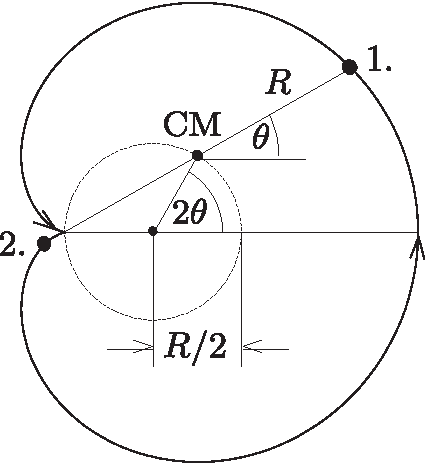
\includegraphics[scale=0.75]{Anh/Nam4.pdf}\\
        Hình $2$.
    \end{center}
     Sau một chu kì $T = \dfrac{2\pi}{\omega_{\mathrm{c}}}$, khối tâm hoàn thành một vòng quay của nó, nhưng mỗi electron chỉ đi được nửa vòng; và do đó chúng đổi vị trí cho nhau. Tại thời điểm đó, vị trí và vận tốc của khối tâm giống hệt như lúc bắt đầu chuyển động $(v_0/2)$, electron ban đầu đứng yên có vận tốc $v_0$ và electron được kích thích bây giờ đứng yên. Nó dừng lại lần đầu tiên sau 
     \[T = 2\pi \dfrac{m}{eB}.\]
    \textbf{Mở rộng:}
    \begin{enumerate}[1)]
        \item Quỹ đạo chuyển động của hai eletron (được gọi là đường cardioid hay đường “trái tim”, do hình dạng đặc biệt của nó) chỉ đơn giản và đơn điệu chỉ khi khoảng cách ban đầu giữa các $e$ bằng khoảng cách giới hạn với từ trường cho trước. Nếu khoảng cách giữa chúng lớn hơn khoảng cách giới hạn, lúc đó quỹ đạo và chuyển động của các electron không đơn giản nữa, và nhìn chung quỹ đạo lúc này sẽ là quỹ đạo mở (điểm bắt đầu và kết thúc chu kì không trùng nhau).
        \item Bài toán sẽ càng phức tạp nếu vận tốc ban đầu không thỏa mãn điều kiện khoảng cách không đổi. Nhưng kể cả khi đó ta có thể chứng minh rằng hai electron không thể tiến tới quá gần nhau cũng như rời quá xa nhau, do đó khoảng cách giữa chúng sẽ dao động giữa hai giá trị giới hạn.
    \end{enumerate}
        
    \end{enumerate}
\end{loigiai}


\begin{vd}[Anode và Cathode] %VPhO 2018
Một linh kiện điện tử có cấu tạo gồm một cathode $K$ dạng sợi dây dẫn mảnh, thẳng, dài và một anode $A$ dạng trụ rỗng, có bán kính ${R}$, bao quanh cathode và có trục trùng với cathode. Linh kiện đặt trong không gian có từ trường đều $\ot{B}$ hướng dọc theo cathode. Bằng một cách nào đó, người ta tạo một điện trường $\ot{E}$ hướng trục từ ${A}$ đến ${K}$ có độ lớn không đổi.\\
Do tính đối xứng trục của bài toán, ta xét một hệ tọa độ trụ như hình. Hệ tọa độ được chọn sao cho gốc ${O}$ nằm trên ${K}$, trục ${Oz}$ theo chiều $\ot{B}$, từ trường $\ot{B}=\left(B_{\rho}, B_{\theta}, B_{z}\right)=(0,0, B)$
và điện trường
$$\ot{E}=\left(E_{\rho}, E_{\theta}, E_{z}\right)=(E, 0,0).$$ 
Khi cathode ${K}$ được đốt nóng sẽ bức xạ electron. Coi vận tốc của các electron phát ra từ cathode ${K}$ là rất nhỏ và bỏ qua tác dụng của trọng lực lên các electron này. Khi xem xét chuyển động của electron, không gian trong linh kiện có thể coi là chân không.
\begin{center}
{
\tikzset{every picture/.style={line width=0.75pt}} %set default line width to 0.75pt        

\begin{tikzpicture}[x=0.75pt,y=0.75pt,yscale=-1,xscale=1]
%uncomment if require: \path (0,474); %set diagram left start at 0, and has height of 474

%Shape: Ellipse [id:dp991714530186085] 
\draw   (223.14,115.72) .. controls (223.14,102.67) and (263.03,92.09) .. (312.24,92.09) .. controls (361.45,92.09) and (401.34,102.67) .. (401.34,115.72) .. controls (401.34,128.77) and (361.45,139.35) .. (312.24,139.35) .. controls (263.03,139.35) and (223.14,128.77) .. (223.14,115.72) -- cycle ;
%Straight Lines [id:da5090442830728876] 
\draw    (223.14,115.72) -- (223.14,275.3) ;
%Curve Lines [id:da8521350306505784] 
\draw  [dash pattern={on 4.5pt off 4.5pt}]  (223.55,208.65) .. controls (232.86,175.87) and (389.76,176.83) .. (401.75,208.65) ;
%Curve Lines [id:da6280284607936966] 
\draw    (223.55,208.65) .. controls (229.55,236.18) and (387.07,242.39) .. (401.75,208.65) ;
%Curve Lines [id:da06707199242837247] 
\draw  [dash pattern={on 4.5pt off 4.5pt}]  (223.14,275.3) .. controls (232.44,242.52) and (389.35,243.47) .. (401.34,275.3) ;
%Curve Lines [id:da3349004032829275] 
\draw    (223.14,275.3) .. controls (229.14,302.83) and (386.66,309.04) .. (401.34,275.3) ;
%Straight Lines [id:da40853559092842495] 
\draw    (401.34,115.72) -- (401.34,275.3) ;
%Straight Lines [id:da6012789690231846] 
\draw  [dash pattern={on 4.5pt off 4.5pt}]  (223.55,208.65) -- (401.75,208.65) ;
%Straight Lines [id:da565528652758621] 
\draw    (401.75,208.65) -- (456.22,208.65) ;
\draw [shift={(459.22,208.65)}, rotate = 180] [fill={rgb, 255:red, 0; green, 0; blue, 0 }  ][line width=0.08]  [draw opacity=0] (10.72,-5.15) -- (0,0) -- (10.72,5.15) -- (7.12,0) -- cycle    ;
%Straight Lines [id:da9860459074898706] 
\draw  [dash pattern={on 4.5pt off 4.5pt}]  (312.65,115.72) -- (312.65,273.71) ;
%Straight Lines [id:da37175075777238975] 
\draw    (312.65,79.49) -- (312.65,115.72) ;
\draw [shift={(312.65,76.49)}, rotate = 90] [fill={rgb, 255:red, 0; green, 0; blue, 0 }  ][line width=0.08]  [draw opacity=0] (10.72,-5.15) -- (0,0) -- (10.72,5.15) -- (7.12,0) -- cycle    ;
%Straight Lines [id:da6837228115665901] 
\draw  [dash pattern={on 4.5pt off 4.5pt}]  (312.65,208.65) -- (262.68,227.29) ;
%Straight Lines [id:da5422064545392717] 
\draw    (262.68,227.29) -- (206.97,245.77) ;
\draw [shift={(204.12,246.71)}, rotate = 341.65] [fill={rgb, 255:red, 0; green, 0; blue, 0 }  ][line width=0.08]  [draw opacity=0] (10.72,-5.15) -- (0,0) -- (10.72,5.15) -- (7.12,0) -- cycle    ;
%Straight Lines [id:da17772674300232527] 
\draw  [dash pattern={on 4.5pt off 4.5pt}]  (311.62,273.71) -- (401.34,273.71) ;
%Straight Lines [id:da7646362348207041] 
\draw  [dash pattern={on 4.5pt off 4.5pt}]  (311.62,273.71) -- (254.7,292.49) ;
%Straight Lines [id:da9590432766813448] 
\draw  [dash pattern={on 4.5pt off 4.5pt}]  (312.65,208.65) -- (355.03,222.47) ;
%Straight Lines [id:da5777038896986804] 
\draw  [dash pattern={on 4.5pt off 4.5pt}]  (312.65,153.91) -- (355.03,167.73) ;
%Straight Lines [id:da5586061217127374] 
\draw  [dash pattern={on 4.5pt off 4.5pt}]  (355.03,167.73) -- (355.03,222.47) ;
%Straight Lines [id:da9883977422064121] 
\draw [color={rgb, 255:red, 74; green, 144; blue, 226 }  ,draw opacity=1 ]   (312.65,208.65) -- (352.87,169.81) ;
\draw [shift={(355.03,167.73)}, rotate = 496] [fill={rgb, 255:red, 74; green, 144; blue, 226 }  ,fill opacity=1 ][line width=0.08]  [draw opacity=0] (10.72,-5.15) -- (0,0) -- (10.72,5.15) -- (7.12,0) -- cycle    ;
%Shape: Arc [id:dp20863658466452928] 
\draw  [draw opacity=0] (321.86,213.17) .. controls (320.24,215.56) and (317.19,217.33) .. (313.45,217.73) .. controls (308.96,218.21) and (304.72,216.57) .. (302.44,213.81) -- (311.91,209.17) -- cycle ; \draw   (321.86,213.17) .. controls (320.24,215.56) and (317.19,217.33) .. (313.45,217.73) .. controls (308.96,218.21) and (304.72,216.57) .. (302.44,213.81) ;

% Text Node
\draw (470.17,201.29) node [anchor=north west][inner sep=0.75pt]    {$y$};
% Text Node
\draw (322.16,66.24) node [anchor=north west][inner sep=0.75pt]    {$z$};
% Text Node
\draw (296.52,143.26) node [anchor=north west][inner sep=0.75pt]    {$z$};
% Text Node
\draw (189.03,234.18) node [anchor=north west][inner sep=0.75pt]    {$x$};
% Text Node
\draw (269.77,263.67) node [anchor=north west][inner sep=0.75pt]    {$R$};
% Text Node
\draw (316.9,256.99) node [anchor=north west][inner sep=0.75pt]    {$K$};
% Text Node
\draw (362.57,150.9) node [anchor=north west][inner sep=0.75pt]    {$M$};
% Text Node
\draw (406.86,267.17) node [anchor=north west][inner sep=0.75pt]    {$A$};
% Text Node
\draw (296.15,215.37) node [anchor=north west][inner sep=0.75pt]    {$\theta $};
% Text Node
\draw (329.6,211.82) node [anchor=north west][inner sep=0.75pt]    {$\rho $};
\end{tikzpicture}
}\end{center}
Kí hiệu điện tích nguyên tố là $e$ và khối lượng electron là $m_{e}$. Giả sử ở thời điểm $t=0$ electron có tọa độ $\left(0,0, z_{0}\right)$, ở thời điểm $t>0$ electron ở tọa độ $(\rho, \theta, z)$, hãy:
\begin{enumerate}[1)]
    \item Viết các phương trình vi phân mô tả chuyển động của electron.
    \item Tìm phương trình quỹ đạo của electron.
    \item Tìm vận tốc dài của electron tại thời điểm $t$ bất kì.
\end{enumerate}
Cho biết trong hệ tọa độ trụ:
\begin{itemize}
    \item Chất điểm $M$ xác định bởi vector tọa độ $\overrightarrow{OM} = (\rho, \theta, z)$ có vận tốc và gia tốc tương ứng là $\ot{v}=(\dot{\rho}, \rho \dot{\theta}, \dot{z})$ và $\ot{a}=\left(\ddot{\rho}-\rho \dot{\theta}^{2}, \dfrac{1}{\rho} \dfrac{\dd}{\dd t}\left(\rho^{2} \dot{\theta}\right), \ddot{z}\right)$.
    \item Nếu $\ot{a}=\left(a_{\rho}, a_{\theta}, a_{z}\right), \ot{b}=\left(b_{\rho}, b_{\theta}, b_{z}\right)$ thì $$\ot{a}\times\ot{b}=\left(a_{\theta} b_{z}-a_{z} b_{\theta}, a_{z} b_{\rho}-a_{\rho} b_{z}, a_{\rho} b_{\theta}-a_{\theta} b_{\rho}\right)$$
\end{itemize}
\end{vd}
\begin{loigiai}
\begin{enumerate}[1)]
    \item 
Áp dụng định luật II Newton cho electron
\[-e\ot{E} - e \ot{v} \times \ot{B} = m_e \ot{a}.\]
Trong hệ tọa độ trụ, phương trình được viết lại như sau
\[-e\tron{E,0,0} - e \tron{\dot{\rho}, \rho \dot{\theta}, \dot{z}} \times \tron{0,0,B} = m_e \left(\ddot{\rho}-\rho \dot{\theta}^{2}, \dfrac{1}{\rho} \dfrac{\dd}{\dd t}\left(\rho^{2} \dot{\theta}\right), \ddot{z}\right).\]
\[\rt \tron{-\dfrac{eE + eB\rho \dot{\theta}}{m_e}, \dfrac{eB\dot{\rho}}{m_e}, 0} = \left(\ddot{\rho}-\rho \dot{\theta}^{2}, \dfrac{1}{\rho} \dfrac{\dd}{\dd t}\left(\rho^{2} \dot{\theta}\right), \ddot{z}\right).\]
Vậy ta có hệ phương trình vi phân mô tả chuyển động của các electron:
\begin{subnumcases}{}
 -\ddot{\rho} + \rho \dot{\theta}^{2} &= $\dfrac{eE + eB\rho \dot{\theta}}{m_e}$ \label{q.vp.2.1a}\\ 
\dfrac{\dd}{\dd t}\left(\rho^{2} \dot{\theta}\right) &=  $\dfrac{eB\rho\dot{\rho}}{m_e}$ \label{q.vp.2.1b}\\ 
\ddot{z} &= $0$ \label{q.vp.2.1c}
\end{subnumcases}
\item 
Từ phương trình (\ref{q.vp.2.1c}) và điều kiện đầu $t = 0$, $\heva{z &= z_0 \\ v_z &= 0}$, ta suy ra
\[v_z = 0 \rt z = z_0. \tag{2}\label{q.vp.2.2}\]
Nhân hai vế của phương trình (\ref{q.vp.2.1b}) cho $\dd t$, ta được
\[\dd \left(\rho^{2} \dot{\theta}\right) = \dfrac{eB}{m_e}\rho \dd \rho.\]
Lấy nguyên hàm hai vế
\[\dfrac{eB}{2m_e} \rho^2 = \rho^2 \dot{\theta} + C.\]
Từ điều kiện đầu: khi $t = 0$, $\rho = 0$ suy ra được hằng số $C = 0$. Thay vào phương trình trên ta suy ra
\[\dot{\theta } = \dfrac{eB}{2m_e} = \mathrm{const} \rt \theta = \dfrac{eB}{2m_e} t. \tag{3}\label{q.vp.2.3}\]
Thay (\ref{q.vp.2.3}) vào (\ref{q.vp.2.1a}), ta được
\[\ddot{\rho} + \tron{\dfrac{eB}{2m_e}}^2 \rho + \dfrac{eE}{m_e} = 0.\]
Nghiệm của phương trình này có dạng
\[\rho = A\cos\left(\dfrac{eB}{2m_e} t + \varphi\right) - \dfrac{eE}{m_e}.\]
Tại $t = 0$, $\heva{\rho &= 0 \\ \dot{\rho} &= 0} \rt \heva{A \cos \varphi - \dfrac{eE}{m_e} &= 0 \\ -A\dfrac{eB}{2m_e}\sin \varphi &= 0} \rt \heva{A &= \dfrac{eE}{m_e} \\ \varphi &= 0}$. \\
Thay vào phương trình trên, ta được
\[\rho = \dfrac{eE}{m_e} \tron{\cos \dfrac{eB}{2m_e} t - 1}. \tag{4}\label{q.vp.2.4}\]
Từ (\ref{q.vp.2.2}), (\ref{q.vp.2.3}) và (\ref{q.vp.2.4}), ta suy ra phương trình quỹ đạo của electron:
\[\heva{\rho &= \dfrac{eE}{m_e} \tron{\cos \theta - 1} \\ z &= z_0}.\]
\item Vận tốc của electron tại thời điểm $t$ được tính bởi:
\[\ot{v}=(\dot{\rho}, \rho \dot{\theta}, \dot{z}) = \tron{-\dfrac{e^2EB}{2m_e^2}\sin \dfrac{eB}{2m_e}t, \dfrac{e^2EB}{2m_e^2} \tron{\cos \dfrac{eB}{2m_e} t - 1}, 0}.\]
\[\rt v = \dfrac{e^2EB}{m_e^2} \sqrt{2 - 2\cos \dfrac{eB}{2m_e} t} = \dfrac{e^2EB}{m_e^2} \sin \dfrac{eB}{4m_e} t.\]
\end{enumerate}
\end{loigiai}



\begin{vd}[Cảm ứng Faraday]
Theo định luật cảm ứng điện từ Faraday, khi từ thông qua một vòng dây biến đổi, trong vòng dây sẽ xuất hiện một suất điện động cảm ứng ${V}$ có độ lớn tỷ lệ thuận với tốc độ biến thiên từ thông. Chiều của suất điện động này tuân theo quy tắc Lenz, tức là dòng cảm ứng sẽ chống lại sự biến thiên của từ thông. Tổng quát mà nói, khi từ trường biến thiên theo thời gian thì trong không gian sẽ xuất hiện điện trường cảm ứng, bất kể có vòng dây ở đó hay không. Sử dụng định luật này có thể giải được nhiều bài toán. Nhưng trước hết hãy xem xét mối liên hệ toán học giữa điện trường cảm ứng và từ trường biến thiên theo thời gian.\\
Trên một đường cong khép kín ${C}$, ta quy ước một chiều dương như hình ${a})$. Một mặt ${S}$ được giới hạn bởi đường cong kín ${C}$, từ thông gửi qua mặt ${S}$ ký hiệu bởi $\Phi({S})$. Từ thông qua mặt sẽ nhận dấu dương nếu khi nắm tay phải quay theo chiều của đường cong ${C}$ thì nó tiến về trước. Trong trường hợp diện tích phẳng $A$ thì từ thông không phụ thuộc vào vị trí của mặt $S$. Khi từ trường $\ot{B}$ vuông góc với mặt ${S}$ thì từ thông cho bởi: $\Phi({S}) = {BA}$.
\begin{center}


\tikzset{every picture/.style={line width=0.75pt}} %set default line width to 0.75pt        

\begin{tikzpicture}[x=0.75pt,y=0.75pt,yscale=-1,xscale=1]
%uncomment if require: \path (0,456); %set diagram left start at 0, and has height of 456

%Right Arrow [id:dp20646986306348958] 
\draw   (238.83,233.3) -- (179.21,135.59) -- (169.82,141.32) -- (164.5,90.35) -- (207.38,118.4) -- (197.99,124.13) -- (257.61,221.84) -- cycle ;
%Shape: Ellipse [id:dp6912657668631246] 
\draw   (168.07,209.37) .. controls (154.19,191.64) and (164.51,160.38) .. (191.11,139.56) .. controls (217.71,118.75) and (250.52,116.24) .. (264.4,133.97) .. controls (278.27,151.7) and (267.96,182.95) .. (241.36,203.77) .. controls (214.76,224.59) and (181.95,227.1) .. (168.07,209.37) -- cycle ;
%Curve Lines [id:da5271502020531298] 
\draw    (213.33,234.11) .. controls (259.33,217.38) and (272.74,198.77) .. (283.8,175.35) ;
\draw [shift={(285,172.78)}, rotate = 474.7] [fill={rgb, 255:red, 0; green, 0; blue, 0 }  ][line width=0.08]  [draw opacity=0] (10.72,-5.15) -- (0,0) -- (10.72,5.15) -- (7.12,0) -- cycle    ;
%Shape: Polygon [id:ds8845684539905239] 
\draw   (445.29,113.5) -- (500.73,171.77) -- (497.9,213.64) -- (419.26,232.49) -- (374,184.41) -- (390.97,136.88) -- cycle ;
%Straight Lines [id:da7470426544470834] 
\draw    (404.17,154.14) -- (422.62,86.22) ;
\draw [shift={(423.41,83.32)}, rotate = 465.2] [fill={rgb, 255:red, 0; green, 0; blue, 0 }  ][line width=0.08]  [draw opacity=0] (10.72,-5.15) -- (0,0) -- (10.72,5.15) -- (7.12,0) -- cycle    ;
%Curve Lines [id:da7884871002948666] 
\draw    (418.88,187.8) .. controls (394.92,156.04) and (429.14,123.17) .. (453.96,166.53) ;
\draw [shift={(455.09,168.56)}, rotate = 241.78] [fill={rgb, 255:red, 0; green, 0; blue, 0 }  ][line width=0.08]  [draw opacity=0] (10.72,-5.15) -- (0,0) -- (10.72,5.15) -- (7.12,0) -- cycle    ;
%Shape: Arc [id:dp18207070073520004] 
\draw  [draw opacity=0] (415.9,112.28) .. controls (418.41,112.76) and (420.75,114.15) .. (422.37,116.38) .. controls (423.75,118.27) and (424.4,120.47) .. (424.37,122.64) -- (413.96,122.51) -- cycle ; \draw   (415.9,112.28) .. controls (418.41,112.76) and (420.75,114.15) .. (422.37,116.38) .. controls (423.75,118.27) and (424.4,120.47) .. (424.37,122.64) ;

% Text Node
\draw (104.17,191.5) node [anchor=north west][inner sep=0.75pt]   [align=left] {Đường\\cong $C$};
% Text Node
\draw (125.67,67) node [anchor=north west][inner sep=0.75pt]   [align=left] {Từ thông $ \Phi $};
% Text Node
\draw (213.17,252.9) node [anchor=north west][inner sep=0.75pt]    {$a)$};
% Text Node
\draw (221.5,146.35) node [anchor=north west][inner sep=0.75pt]   [align=left] {Mặt $ S$};
% Text Node
\draw (288,153) node [anchor=north west][inner sep=0.75pt]   [align=left] {Chiều\\dương};
% Text Node
\draw (402.7,72.44) node [anchor=north west][inner sep=0.75pt]    {$\ot{E}$};
% Text Node
\draw (378.94,117.87) node [anchor=north west][inner sep=0.75pt]    {$P$};
% Text Node
\draw (445.89,93.55) node [anchor=north west][inner sep=0.75pt]    {$Q$};
% Text Node
\draw (423.07,99.61) node [anchor=north west][inner sep=0.75pt]    {$\theta $};
% Text Node
\draw (432.53,176.18) node [anchor=north west][inner sep=0.75pt]   [align=left] {Chiều\\dương};
% Text Node
\draw (509.67,209.13) node [anchor=north west][inner sep=0.75pt]   [align=left] {Đường\\cong $C$};
% Text Node
\draw (433.45,252.62) node [anchor=north west][inner sep=0.75pt]    {$b)$};
\end{tikzpicture}
\end{center}
Ta tưởng tượng một vòng dây dẫn đặt đúng theo đường cong $C$, một suất điện động cảm ứng ${V}({C})$ sẽ xuất hiện trong khung dây. Đường cong kín đó có thể là đa giác giống như trong hình $b)$. Khi giữa hai đầu ${P}, {Q}$ của dây dẫn xuất hiện một suất điện động $V(\ot{PQ})$, trên đoạn thẳng ${PQ}$ xuất hiện một điện trường $\ot{E}$ hướng từ ${P}$ về ${Q}$. Góc giữa phương của điện trường và $\overrightarrow{PQ}$ là $\theta$, chiều dài đoạn thẳng là $l_{PQ}$.
\[V(\ot{PQ}) = |E| l_{PQ} \cos \theta = E_{C} l_{P Q}.\]
Ở đây, $|E|$ là độ lớn của điện trường, $E_{c}=|E| \cos \theta$ là thành phần của điện trường lên phương của đường cong ${C}$. Nếu tính suất điện động cảm ứng trên từng đoạn của đường cong ${C}$ rồi cộng tất cả vào với nhau, ta sẽ tìm được suất điện động cảm ứng trên cả đường cong ${C}$. Trường hợp đặc biệt khi đường cong ${C}$ đặt trùng với đường sức điện trường có độ lớn $|E|$ không đổi, thì tại mọi điểm của đường cong ${C}$ ta có $E_{C} = |E|$ hoặc $-|E|$. Nếu chiều dài tổng cộng của đường cong ${C}$ là $l$, thì ${V}({C}) = E_{c} l$.\\
Giả sử có một từ trường biến thiên theo thời gian, khi đó dọc theo đường cong $C$ sẽ xuất hiện một điện trường. Từ thông gửi qua mặt ${S}$ biến thiên theo thời gian nên suất điện động cảm ứng ở mép của mặt ${S}$ có thể được viết:
\[
{V}({C})=\dfrac{\Delta \Phi(S)}{\Delta t}.
\tag{1}\label{q.d.1}\]
Đây chính là định luật cảm ứng điện từ Faraday mà ta đã đề cập từ đầu.\\

\textbf{Chú ý.} Trên thực tế thì các đường sức điện cảm ứng sẽ bị nhiễu động do ảnh hưởng của hiện tượng phân cực điện khi ta đưa dây dẫn vào bên trong điện trường. Nhưng ta chỉ quan tâm đến quan hệ giữa điện trường và từ trường trong trường hợp không bị ảnh hưởng bởi dây dẫn. Trong khi tính suất điện động ${V}({C})$ dọc theo đường cong kín và điện trường ta bỏ qua ảnh hưởng của dây dẫn.
    \begin{center}
\tikzset{every picture/.style={line width=0.75pt}} %set default line width to 0.75pt        

\begin{tikzpicture}[x=0.75pt,y=0.75pt,yscale=-1,xscale=1]
%uncomment if require: \path (0,508); %set diagram left start at 0, and has height of 508

%Curve Lines [id:da17704119093765347] 
\draw    (265.22,236.28) .. controls (262.37,135.31) and (215.55,95.15) .. (188.73,88.59) ;
\draw [shift={(185.9,88.01)}, rotate = 369.33000000000004] [fill={rgb, 255:red, 0; green, 0; blue, 0 }  ][line width=0.08]  [draw opacity=0] (10.72,-5.15) -- (0,0) -- (10.72,5.15) -- (7.12,0) -- cycle    ;
%Shape: Rectangle [id:dp2836649028479259] 
\draw  [line width=1.5]  (47.59,118.54) -- (132.66,118.54) -- (132.66,205.43) -- (47.59,205.43) -- cycle ;
\draw  [fill={rgb, 255:red, 0; green, 0; blue, 0 }  ,fill opacity=1 ] (88.13,114.41) -- (96.8,118.75) -- (88.13,123.08) -- (92.46,118.75) -- cycle ;
\draw  [fill={rgb, 255:red, 0; green, 0; blue, 0 }  ,fill opacity=1 ] (136.96,155.39) -- (132.63,164.06) -- (128.29,155.39) -- (132.63,159.73) -- cycle ;
\draw  [fill={rgb, 255:red, 0; green, 0; blue, 0 }  ,fill opacity=1 ] (93.71,209.74) -- (85.04,205.41) -- (93.71,201.07) -- (89.37,205.41) -- cycle ;
\draw  [fill={rgb, 255:red, 0; green, 0; blue, 0 }  ,fill opacity=1 ] (43.33,162.14) -- (47.66,153.47) -- (52,162.14) -- (47.66,157.81) -- cycle ;
%Straight Lines [id:da7848944881489814] 
\draw    (39.64,236.71) -- (39.64,89.18) ;
\draw [shift={(39.64,86.18)}, rotate = 450] [fill={rgb, 255:red, 0; green, 0; blue, 0 }  ][line width=0.08]  [draw opacity=0] (10.72,-5.15) -- (0,0) -- (10.72,5.15) -- (7.12,0) -- cycle    ;
%Straight Lines [id:da7900679033699884] 
\draw    (52.55,236.71) -- (52.55,89.18) ;
\draw [shift={(52.55,86.18)}, rotate = 450] [fill={rgb, 255:red, 0; green, 0; blue, 0 }  ][line width=0.08]  [draw opacity=0] (10.72,-5.15) -- (0,0) -- (10.72,5.15) -- (7.12,0) -- cycle    ;
%Straight Lines [id:da8748247138522687] 
\draw    (66.46,236.71) -- (66.46,89.18) ;
\draw [shift={(66.46,86.18)}, rotate = 450] [fill={rgb, 255:red, 0; green, 0; blue, 0 }  ][line width=0.08]  [draw opacity=0] (10.72,-5.15) -- (0,0) -- (10.72,5.15) -- (7.12,0) -- cycle    ;
%Straight Lines [id:da14628756799680054] 
\draw    (83.34,236.71) -- (83.34,89.18) ;
\draw [shift={(83.34,86.18)}, rotate = 450] [fill={rgb, 255:red, 0; green, 0; blue, 0 }  ][line width=0.08]  [draw opacity=0] (10.72,-5.15) -- (0,0) -- (10.72,5.15) -- (7.12,0) -- cycle    ;
%Straight Lines [id:da7920165637776044] 
\draw    (102.2,236.71) -- (102.2,89.18) ;
\draw [shift={(102.2,86.18)}, rotate = 450] [fill={rgb, 255:red, 0; green, 0; blue, 0 }  ][line width=0.08]  [draw opacity=0] (10.72,-5.15) -- (0,0) -- (10.72,5.15) -- (7.12,0) -- cycle    ;
%Straight Lines [id:da7403220227482121] 
\draw    (123.06,236.71) -- (123.06,89.18) ;
\draw [shift={(123.06,86.18)}, rotate = 450] [fill={rgb, 255:red, 0; green, 0; blue, 0 }  ][line width=0.08]  [draw opacity=0] (10.72,-5.15) -- (0,0) -- (10.72,5.15) -- (7.12,0) -- cycle    ;
%Straight Lines [id:da018032475368297662] 
\draw    (147.88,236.71) -- (147.88,89.18) ;
\draw [shift={(147.88,86.18)}, rotate = 450] [fill={rgb, 255:red, 0; green, 0; blue, 0 }  ][line width=0.08]  [draw opacity=0] (10.72,-5.15) -- (0,0) -- (10.72,5.15) -- (7.12,0) -- cycle    ;
%Curve Lines [id:da2082178622856372] 
\draw    (255.84,236.82) .. controls (249.84,143.51) and (213.08,115.42) .. (189.79,107.29) ;
\draw [shift={(186.95,106.38)}, rotate = 376.5] [fill={rgb, 255:red, 0; green, 0; blue, 0 }  ][line width=0.08]  [draw opacity=0] (10.72,-5.15) -- (0,0) -- (10.72,5.15) -- (7.12,0) -- cycle    ;
%Curve Lines [id:da017834833495530278] 
\draw    (246.18,236.21) .. controls (240.01,159.72) and (212.02,132.44) .. (187.86,124.5) ;
\draw [shift={(185.24,123.71)}, rotate = 375.41999999999996] [fill={rgb, 255:red, 0; green, 0; blue, 0 }  ][line width=0.08]  [draw opacity=0] (10.72,-5.15) -- (0,0) -- (10.72,5.15) -- (7.12,0) -- cycle    ;
%Curve Lines [id:da12164480539055833] 
\draw    (235.96,236.21) .. controls (228.26,166.71) and (205.96,153.24) .. (188.77,144.39) ;
\draw [shift={(186.1,143.03)}, rotate = 387.12] [fill={rgb, 255:red, 0; green, 0; blue, 0 }  ][line width=0.08]  [draw opacity=0] (10.72,-5.15) -- (0,0) -- (10.72,5.15) -- (7.12,0) -- cycle    ;
%Curve Lines [id:da6645218417107026] 
\draw    (226.15,236.64) .. controls (216.49,175.43) and (201.5,169.39) .. (187.65,161.36) ;
\draw [shift={(185.24,159.93)}, rotate = 391.7] [fill={rgb, 255:red, 0; green, 0; blue, 0 }  ][line width=0.08]  [draw opacity=0] (10.72,-5.15) -- (0,0) -- (10.72,5.15) -- (7.12,0) -- cycle    ;
%Curve Lines [id:da1770395852854001] 
\draw    (216.78,236.21) .. controls (209.57,193.75) and (200.85,187.81) .. (187.8,179.82) ;
\draw [shift={(185.24,178.25)}, rotate = 391.7] [fill={rgb, 255:red, 0; green, 0; blue, 0 }  ][line width=0.08]  [draw opacity=0] (10.72,-5.15) -- (0,0) -- (10.72,5.15) -- (7.12,0) -- cycle    ;
%Straight Lines [id:da7881452227089873] 
\draw [line width=1.5]    (195.61,173.57) -- (209.68,110.5) ;
\draw [shift={(202.64,142.03)}, rotate = 462.57] [fill={rgb, 255:red, 0; green, 0; blue, 0 }  ][line width=0.08]  [draw opacity=0] (13.4,-6.43) -- (0,0) -- (13.4,6.44) -- (8.9,0) -- cycle    ;
%Straight Lines [id:da8722762316049659] 
\draw [line width=1.5]    (254,187.63) -- (218.63,215.33) ;
\draw [shift={(236.31,201.48)}, rotate = 321.93] [fill={rgb, 255:red, 0; green, 0; blue, 0 }  ][line width=0.08]  [draw opacity=0] (13.4,-6.43) -- (0,0) -- (13.4,6.44) -- (8.9,0) -- cycle    ;
%Curve Lines [id:da3404753175974746] 
\draw [line width=1.5]    (209.68,110.5) .. controls (241.64,137.49) and (246.75,164.33) .. (254,187.63) ;
\draw [shift={(238.53,145.36)}, rotate = 240.23] [fill={rgb, 255:red, 0; green, 0; blue, 0 }  ][line width=0.08]  [draw opacity=0] (13.4,-6.43) -- (0,0) -- (13.4,6.44) -- (8.9,0) -- cycle    ;
%Curve Lines [id:da6848625095228247] 
\draw [line width=1.5]    (218.63,215.33) .. controls (210.81,183.37) and (193.77,174.85) .. (195.61,173.57) ;
\draw [shift={(209.86,192.46)}, rotate = 423] [fill={rgb, 255:red, 0; green, 0; blue, 0 }  ][line width=0.08]  [draw opacity=0] (13.4,-6.43) -- (0,0) -- (13.4,6.44) -- (8.9,0) -- cycle    ;
%Shape: Can [id:dp53613609777672] 
\draw   (380.28,161.71) -- (380.28,220.51) .. controls (380.28,229.69) and (361.2,237.13) .. (337.66,237.13) .. controls (314.13,237.13) and (295.05,229.69) .. (295.05,220.51) -- (295.05,161.71) .. controls (295.05,152.53) and (314.13,145.09) .. (337.66,145.09) .. controls (361.2,145.09) and (380.28,152.53) .. (380.28,161.71) .. controls (380.28,170.88) and (361.2,178.33) .. (337.66,178.33) .. controls (314.13,178.33) and (295.05,170.88) .. (295.05,161.71) ;
%Shape: Can [id:dp8542117011968777] 
\draw   (380.28,62.84) -- (380.28,121.65) .. controls (380.28,130.83) and (361.2,138.27) .. (337.66,138.27) .. controls (314.13,138.27) and (295.05,130.83) .. (295.05,121.65) -- (295.05,62.84) .. controls (295.05,53.66) and (314.13,46.22) .. (337.66,46.22) .. controls (361.2,46.22) and (380.28,53.66) .. (380.28,62.84) .. controls (380.28,72.02) and (361.2,79.46) .. (337.66,79.46) .. controls (314.13,79.46) and (295.05,72.02) .. (295.05,62.84) ;
%Curve Lines [id:da32502879442347266] 
\draw  [dash pattern={on 4.5pt off 4.5pt}]  (295.05,121.65) .. controls (307.12,96.72) and (377.01,101.83) .. (380.28,121.65) ;
%Curve Lines [id:da1758573324067343] 
\draw [line width=1.5]    (312.55,135.23) .. controls (274.88,151.93) and (349.54,174.09) .. (372.72,147.84) ;
%Curve Lines [id:da6169696982999335] 
\draw [line width=1.5]  [dash pattern={on 5.63pt off 4.5pt}]  (312.55,135.23) .. controls (333.4,129.66) and (349.77,131.02) .. (361.02,135.11) ;
%Curve Lines [id:da5111363917151119] 
\draw [line width=1.5]    (361.02,135.11) .. controls (366.47,137.39) and (367.83,138.07) .. (372.61,142.16) ;
%Straight Lines [id:da8337715960430991] 
\draw [line width=1.5]    (372.61,142.16) -- (390.51,142.16) ;
\draw [shift={(390.51,142.16)}, rotate = 0] [color={rgb, 255:red, 0; green, 0; blue, 0 }  ][fill={rgb, 255:red, 0; green, 0; blue, 0 }  ][line width=1.5]      (0, 0) circle [x radius= 1.74, y radius= 1.74]   ;
%Straight Lines [id:da9610326272369787] 
\draw [line width=1.5]    (372.72,147.84) -- (390.62,147.84) ;
\draw [shift={(390.62,147.84)}, rotate = 0] [color={rgb, 255:red, 0; green, 0; blue, 0 }  ][fill={rgb, 255:red, 0; green, 0; blue, 0 }  ][line width=1.5]      (0, 0) circle [x radius= 1.74, y radius= 1.74]   ;
%Straight Lines [id:da11384148043546372] 
\draw    (372.61,142.16) -- (381.66,133.11) ;
%Straight Lines [id:da20341759509474677] 
\draw    (372.72,147.84) -- (368.63,159.43) ;
%Straight Lines [id:da6004574358455221] 
\draw  [dash pattern={on 4.5pt off 4.5pt}]  (337.66,65.11) -- (337.66,196.08) ;
%Shape: Right Angle [id:dp21523229649023556] 
\draw   (528.1,62.18) -- (528.1,112.18) -- (446.28,112.18) ;
%Shape: Right Angle [id:dp06070969519937974] 
\draw   (446.28,237.18) -- (446.28,187.18) -- (528.1,187.18) ;
%Straight Lines [id:da46072993739083357] 
\draw    (528.1,187.18) -- (528.1,237.18) ;
%Straight Lines [id:da7394340970219537] 
\draw    (446.28,62.18) -- (446.28,112.18) ;
%Straight Lines [id:da11637676650266049] 
\draw  [dash pattern={on 4.5pt off 4.5pt}]  (487.19,63.31) -- (487.19,241.35) ;
%Straight Lines [id:da8977810319571025] 
\draw    (517.02,187.18) -- (517.02,112.18) ;
\draw [shift={(517.02,149.68)}, rotate = 450] [fill={rgb, 255:red, 0; green, 0; blue, 0 }  ][line width=0.08]  [draw opacity=0] (7.14,-3.43) -- (0,0) -- (7.14,3.43) -- (4.74,0) -- cycle    ;
%Straight Lines [id:da3058576723356914] 
\draw    (511.06,187.18) -- (511.06,112.18) ;
\draw [shift={(511.06,149.68)}, rotate = 450] [fill={rgb, 255:red, 0; green, 0; blue, 0 }  ][line width=0.08]  [draw opacity=0] (7.14,-3.43) -- (0,0) -- (7.14,3.43) -- (4.74,0) -- cycle    ;
%Straight Lines [id:da4173412375926153] 
\draw    (505.09,187.18) -- (505.09,112.18) ;
\draw [shift={(505.09,149.68)}, rotate = 450] [fill={rgb, 255:red, 0; green, 0; blue, 0 }  ][line width=0.08]  [draw opacity=0] (7.14,-3.43) -- (0,0) -- (7.14,3.43) -- (4.74,0) -- cycle    ;
%Straight Lines [id:da9461491818536378] 
\draw    (499.13,187.18) -- (499.13,112.18) ;
\draw [shift={(499.13,149.68)}, rotate = 450] [fill={rgb, 255:red, 0; green, 0; blue, 0 }  ][line width=0.08]  [draw opacity=0] (7.14,-3.43) -- (0,0) -- (7.14,3.43) -- (4.74,0) -- cycle    ;
%Straight Lines [id:da1656452678084357] 
\draw    (493.16,187.18) -- (493.16,112.18) ;
\draw [shift={(493.16,149.68)}, rotate = 450] [fill={rgb, 255:red, 0; green, 0; blue, 0 }  ][line width=0.08]  [draw opacity=0] (7.14,-3.43) -- (0,0) -- (7.14,3.43) -- (4.74,0) -- cycle    ;
%Straight Lines [id:da9719949783410846] 
\draw    (487.19,187.18) -- (487.19,112.18) ;
\draw [shift={(487.19,149.68)}, rotate = 450] [fill={rgb, 255:red, 0; green, 0; blue, 0 }  ][line width=0.08]  [draw opacity=0] (7.14,-3.43) -- (0,0) -- (7.14,3.43) -- (4.74,0) -- cycle    ;
%Straight Lines [id:da45818028238885855] 
\draw    (481.23,187.18) -- (481.23,112.18) ;
\draw [shift={(481.23,149.68)}, rotate = 450] [fill={rgb, 255:red, 0; green, 0; blue, 0 }  ][line width=0.08]  [draw opacity=0] (7.14,-3.43) -- (0,0) -- (7.14,3.43) -- (4.74,0) -- cycle    ;
%Straight Lines [id:da8303819650972852] 
\draw    (475.26,187.18) -- (475.26,112.18) ;
\draw [shift={(475.26,149.68)}, rotate = 450] [fill={rgb, 255:red, 0; green, 0; blue, 0 }  ][line width=0.08]  [draw opacity=0] (7.14,-3.43) -- (0,0) -- (7.14,3.43) -- (4.74,0) -- cycle    ;
%Straight Lines [id:da4551447016455965] 
\draw    (469.3,187.18) -- (469.3,112.18) ;
\draw [shift={(469.3,149.68)}, rotate = 450] [fill={rgb, 255:red, 0; green, 0; blue, 0 }  ][line width=0.08]  [draw opacity=0] (7.14,-3.43) -- (0,0) -- (7.14,3.43) -- (4.74,0) -- cycle    ;
%Straight Lines [id:da594753385683483] 
\draw    (463.33,187.18) -- (463.33,112.18) ;
\draw [shift={(463.33,149.68)}, rotate = 450] [fill={rgb, 255:red, 0; green, 0; blue, 0 }  ][line width=0.08]  [draw opacity=0] (7.14,-3.43) -- (0,0) -- (7.14,3.43) -- (4.74,0) -- cycle    ;
%Straight Lines [id:da7016635346218927] 
\draw    (457.36,187.18) -- (457.36,112.18) ;
\draw [shift={(457.36,149.68)}, rotate = 450] [fill={rgb, 255:red, 0; green, 0; blue, 0 }  ][line width=0.08]  [draw opacity=0] (7.14,-3.43) -- (0,0) -- (7.14,3.43) -- (4.74,0) -- cycle    ;
%Curve Lines [id:da06981159388742642] 
\draw    (452.84,186.99) .. controls (446.69,170.62) and (445.62,135.46) .. (452.5,112.33) ;
\draw [shift={(447.77,149.3)}, rotate = 449.2] [fill={rgb, 255:red, 0; green, 0; blue, 0 }  ][line width=0.08]  [draw opacity=0] (7.14,-3.43) -- (0,0) -- (7.14,3.43) -- (4.74,0) -- cycle    ;
%Curve Lines [id:da16396718213086392] 
\draw    (446.28,187.18) .. controls (433.48,163.59) and (434.11,138.87) .. (446.28,112.18) ;
\draw [shift={(436.93,149.72)}, rotate = 448.92] [fill={rgb, 255:red, 0; green, 0; blue, 0 }  ][line width=0.08]  [draw opacity=0] (7.14,-3.43) -- (0,0) -- (7.14,3.43) -- (4.74,0) -- cycle    ;
%Curve Lines [id:da36261811968074475] 
\draw    (528.1,187.18) .. controls (541.93,159.97) and (540.65,130.77) .. (528.1,112.18) ;
\draw [shift={(537.98,149.2)}, rotate = 453.47] [fill={rgb, 255:red, 0; green, 0; blue, 0 }  ][line width=0.08]  [draw opacity=0] (7.14,-3.43) -- (0,0) -- (7.14,3.43) -- (4.74,0) -- cycle    ;
%Curve Lines [id:da2084422404430566] 
\draw    (522.99,187.18) .. controls (529.78,155.49) and (528.51,133.33) .. (522.99,112.18) ;
\draw [shift={(527.61,149.41)}, rotate = 451.86] [fill={rgb, 255:red, 0; green, 0; blue, 0 }  ][line width=0.08]  [draw opacity=0] (7.14,-3.43) -- (0,0) -- (7.14,3.43) -- (4.74,0) -- cycle    ;

% Text Node
\draw (37.68,100.13) node [anchor=north west][inner sep=0.75pt]    {$Q$};
% Text Node
\draw (132.44,104.39) node [anchor=north west][inner sep=0.75pt]    {$R$};
% Text Node
\draw (40.46,208.37) node [anchor=north west][inner sep=0.75pt]    {$P$};
% Text Node
\draw (133.48,207.2) node [anchor=north west][inner sep=0.75pt]    {$T$};
% Text Node
\draw (186.91,184.29) node [anchor=north west][inner sep=0.75pt]    {$P$};
% Text Node
\draw (206.44,93.31) node [anchor=north west][inner sep=0.75pt]    {$Q$};
% Text Node
\draw (255.17,170.02) node [anchor=north west][inner sep=0.75pt]    {$R$};
% Text Node
\draw (203.36,212.32) node [anchor=north west][inner sep=0.75pt]    {$T$};
% Text Node
\draw (343.03,110.64) node [anchor=north west][inner sep=0.75pt]    {$S$};
% Text Node
\draw (344.51,182.23) node [anchor=north west][inner sep=0.75pt]    {$N$};
% Text Node
\draw (396.72,122.29) node [anchor=north west][inner sep=0.75pt]    {$P$};
% Text Node
\draw (393.77,149.62) node [anchor=north west][inner sep=0.75pt]    {$Q$};
% Text Node
\draw (357.63,158.62) node [anchor=north west][inner sep=0.75pt]    {$T$};
% Text Node
\draw (381.31,117.46) node [anchor=north west][inner sep=0.75pt]    {$R$};
% Text Node
\draw (495.65,192.74) node [anchor=north west][inner sep=0.75pt]    {$N$};
% Text Node
\draw (494.74,92.74) node [anchor=north west][inner sep=0.75pt]    {$S$};
% Text Node
\draw (83.78,251.55) node [anchor=north west][inner sep=0.75pt]    {$c)$};
% Text Node
\draw (225.11,251.55) node [anchor=north west][inner sep=0.75pt]    {$d)$};
% Text Node
\draw (329.24,251.55) node [anchor=north west][inner sep=0.75pt]    {$e)$};
% Text Node
\draw (479.03,251.55) node [anchor=north west][inner sep=0.75pt]    {$f)$};
\end{tikzpicture}
    \end{center}
\begin{enumerate}[1)]
    \item 
    Hình $c)$ biểu diễn các đường sức của một điện trường hướng từ dưới lên: dọc theo một đường sức thì điện trường có độ lớn không đổi, còn từ trái sang thì điện trường yếu dần, các đường sức là những đường thẳng song song nhưng từ trái sang thì chúng thưa dần. Hãy áp dụng (\ref{q.d.1}) với một hình chữ nhật $PQRT$ có cạnh $PQ$ song song với các đường sức để chứng minh rằng một điện trường như mô tả không thể tồn tại nếu tại đó không có từ trường biến thiên theo thời gian. Như vậy, nếu các đường sức là các đường thẳng thì chúng phải nằm cách đều nhau. Kết quả này có thể giải thích như là các đường sức dường như đẩy nhau và các đường sức song song phải sắp xếp sao cho chúng cách đều nhau.
    \item Trên hình $d)$, các đường sức là những cung tròn đồng tâm cách đều nhau. Dọc theo một đường sức điện trường đổi hướng nhưng có độ lớn không đổi. Áp dụng (\ref{q.d.1}) với đường cong kín $PQRT$ có cạnh $\overrightarrow{PQ}$ và $\overrightarrow{RT}$ vuông góc với các đường sức từ và ${PT},{RQ}$ là các cung tròn đồng tâm với các đường sức. Chứng minh rằng độ lớn của điện trường tại một điểm tỷ lệ nghịch với khoảng cách tới tâm nếu trong vùng đang xét không có từ trường biến thiên.\\
    Trên hình $e)$, hai cực Bắc $(N)$ và Nam $(S)$ của một nam châm điện có dạng hình trụ và làm từ vật liệu đồng nhất được đặt cách nhau tạo thành một khe hẹp. Từ trường giữa hai cực nam châm ở vùng gần tâm là đều và các đường sức từ vuông góc với các cực như hình $f)$. Bằng cách thay đổi cường độ các dòng điện tròn bao quanh các cực nam châm và người ta có thể tạo ra các từ trường biến thiên. Các đường sức điện cảm ứng có dạng các đường tròn có tâm nằm trên trục nam châm. Áp dụng (\ref{q.d.1}) với đường cong kín ${C}$ là một đường tròn nằm trong mặt phẳng vuông góc với các đường sức và có tâm nằm trên trục nam châm, mặt ${S}$ là mặt phẳng giới hạn bởi đường cong ${C}$ này.
    \item Chọn chiều dương của từ trường ${B}({t})$ từ cực Bắc về Nam, khi đó điện trường tại một điểm cách tâm một khoảng ${r}$ sẽ là:
\[E({t})=-\dfrac{r}{2} \dfrac{\Delta B({t})}{\Delta t}.\tag{2}\label{q.d.2}\]
Trong đó: ${E}({t})$ mang dấu dương nếu nó chạy ngược chiều kim đồng hồ khi nhìn từ cực ${S}$. Tiếp theo, khi một khung dây được đưa vào khe và nối ra ngoài qua hai cực ${P}, {Q}$. Hãy tìm hiệu điện thế giữa hai điểm $Q$ và $P$, biết rằng bán kính của khung dây tròn là $r$ và coi rằng khe $RT$ có kích thước nhỏ hơn rất nhiều chu vi của vòng.
\item Bây giờ người ta bỏ khung dây đi và tại một điểm cách trục nam châm một khoảng $R$, người ta đặt vào một điện tích $q$. Khi từ trường trong khe biến thiên, điện tích chuyển động dưới tác dụng của lực điện trường cảm ứng gây ra bởi từ trường. Xét trường hợp điện tích chuyển động trên một đường tròn cố định.\\
Kí hiệu ${E}({t})$ là điện trường của đường sức điện hình tròn bán kính ${R}$ và có tâm nằm trên trục nam châm. Ngoài ra ${B}({t})$ là cảm ứng từ. Đầu tiên hãy coi hai đại lượng này là độc lập, hãy thiết lập mối quan hệ giữa ${E}({t})$ và ${B}({t})$ để điện tích $q$ chuyển động trên đường tròn bán kính $R$. Quy ước chiều dương hướng từ tâm vòng tròn ra phía ngoài và chiều dương của khung tròn là ngược chiều kim đồng hồ khi nhìn từ cực ${S}$.\\
Gợi ý: Khi hạt có vận tốc tức thời $v$, hãy viết phương trình chuyển động của hạt thông qua $\dfrac{\Delta v}{\Delta t}$.
\item Quan hệ giữa điện trường và từ trường vừa nhận được khác với kết quả của câu $3)$, khi mà từ trường giữa hai cực nam châm là đều. Như vậy, ta cần một từ trường và điện trường phụ có giá trị phụ thuộc cả vào khoảng cách tới tâm và thời gian là ${{E}(r}, {t})$ và ${B}({r}, {t})$. Ngoài ra, giả sử rằng cảm ứng từ có thể biểu diễn dưới dạng ${B}({r}, {t}) = {F}_{{B}}({r}) {G}({t})$. Tương tự từ thông gửi qua một mặt tròn bán kính ${r}$ sẽ là $\Phi({r}, {t}) = {F}_{\Phi}({r}) {G}({t})$. Hãy xét đường tròn bán kính ${r}={R}$ và chứng minh:
\[F_{\Phi}(R) = 2 \pi R^{2} F_{B}({R})\tag{3}\label{q.d.3} \]
\item Để tạo ra từ trường thỏa mãn điều kiện ở câu trên, người ta dùng hai cuộn dây solenoid đặt đồng trục thay vì nam châm điện. Gọi $a$ và $b$ lần lượt là bán kính của các cuộn dây đặt ngoài và trong. Mật độ vòng dây trên hai cuộn là như nhau. Dòng điện chạy qua các cuộn dây có cùng chiều nhưng cường độ dòng chạy ở cuộn trong lớn gấp đôi cường độ dòng chạy ở cuộn ngoài. Hãy tìm bán kính các cuộn dây theo ${R}$ để các điều kiện (\ref{q.d.3}) ở trên thỏa mãn.\\

\item Giữa điện trường và từ trường biến thiên, ngoài điều kiện (\ref{q.d.1}) ở trên, quan hệ sau được thỏa mãn:
\[V_{m}(C)=\frac{\Delta \Phi(S)}{\Delta t}. \tag{4}\label{q.d.4}\]
Phương trình (\ref{q.d.4}) này có dạng giống phương trình (\ref{q.d.1}), ngoại trừ việc thiếu dấu trừ ở vế phải.\\
Để hiểu rõ hơn về phương trình (\ref{q.d.4}), hãy xét một mặt $S$ được giới hạn bởi đường cong kín $C$. Tuy nhiên, khác với hình ${a})$, qua mặt ${S}$ của đường cong kín ${C}$ bây giờ sẽ là điện thông $\Phi_{e}$ thay vì từ thông. Mọi tính toán hoàn toàn tương tự như của trường hợp từ trường, ngoại trừ vector cảm ứng từ $\ot{B}$ bây giờ sẽ được thay thế bởi vector cảm ứng điện $\ot{D} = \varepsilon_{0} \ot{E}$. Ngoài ra, để tính sức từ động cảm ứng $V_{m}(C)$ theo đường cong kín ${C}$ bây giờ ta phải thay cường độ điện trường $\ot{E}$ bằng cường độ từ trường, được định nghĩa: $\ot{H} = \dfrac{\ot{B}}{\mu_{0}}$.\\
Ở đây, $\varepsilon_{0}$ và $\mu_{0}$ lần lượt là hằng số điện và độ điện cảm chân không (hằng số từ). Ngoài ra, dấu của điện thông qua đường cong kín ${C}$ được xác định như trong trường hợp từ thông.\\
Xét một tụ điện phẳng mà hai bản tụ có dạng đĩa tròn, bán kính ${a}$, đặt song song đồng trục. Điện tích trên các bản tụ có thể thay đổi theo thời gian $\pm {Q}({t}),\tron{{Q}({t})>0}$. Khi điện tích thay đổi, các đường sức từ cảm ứng là các đường tròn có tâm nằm trên trục của tụ điện. Hãy tìm cảm ứng từ tại một điểm cách tâm một khoảng ${r} < {a}$. Khi điện tích ${Q}({t})$ tăng thì các đường sức từ quay theo chiều kim đồng hồ hay ngược chiều kim đồng hồ, nếu nhìn từ bản cực âm của tụ điện? Giả sử khoảng cách giữa hai bản tụ nhỏ hơn rất nhiều bán kính của chúng và bỏ qua mọi hiệu ứng rìa.
\end{enumerate}
\end{vd}
\begin{loigiai}
\begin{enumerate}[1)]
    \item Góc giữa phương của đường sức điện với các đoạn $\overline{QR}, \overline{TP}$  bằng ${{90}^{\circ}}$ nên suất điện động trên hai đoạn này đều bằng không. Trong khi đó, góc giữa đường sức với đoạn $\overline{PQ}$ bằng $0^\circ$ và với $\overline{RT}$ bằng $180^\circ$. Do đó, khi  $\overline{PQ}=\overline{RT}=l$, suất điện động trong khung dây ở hình $c)$ là
    \[{{V}_{PQRT}} = l\left( {{E}_{PQ}}-{{E}_{RT}} \right).\]
    Trong đó ${{E}_{PQ}}$ và ${{E}_{RT}}$ là độ lớn điện trường trên các đoạn $\overline{PQ}$ và $\overline{RT}$ tương ứng.\\ Nhưng vì suất điện động trên đường kín phải bằng không nên ${{E}_{PQ}} = {{E}_{RT}}$. Như vậy tại mọi điểm trong điện trường có đường sức song song thì cường độ điện trường có độ lớn như nhau.
    \item Trên các đoạn $\overline{PQ}$ và $\overline{RT}$ suất điện động bằng không. Độ dài cung $QR$ chắn đường tròn bán kính ${{r}_{1}}$ là ${{l}_{QR}}$. Độ dài cung $TP$ chắn đường tròn bán kính ${{r}_{2}}$ là ${{l}_{TR}}$ . Điện trường $\ot{E}$ tạo với $\overline{QR}$ góc $180^\circ$, và tạo với $\overline{TP}$ một góc $0^\circ$ nên suất điện động trên khung $PQRT$ là:
    \[{{V}_{PQRT}} = E({{r}_{2}}){{l}_{TP}} - E({{r}_{1}}){{l}_{QR}}.\]
    Không có từ trường biến thiên nên, từ phương trình (\ref{q.d.1}), suất điện động bằng không, suy ra \[\dfrac{E({{r}_{1}})}{E({{r}_{2}})}=\dfrac{{{l}_{TP}}}{{{l}_{QR}}} =\dfrac{{{r}_{2}}}{{{r}_{1}}},\] 
    tức là cường độ điện trường tỷ lệ nghịch với khoảng cách tới tâm.
    \item Áp dụng (\ref{q.d.1}) cho đường cong kín $C$ bán kính $r$. Diện tích chắn bởi đường tròn $\pi {{r}^{2}}$, từ thông gửi qua nó là $\Phi (t) = \pi {{r}^{2}}B(t)$. Như vậy vế phải của (\ref{q.d.1}) viết lại là 
    \[-\dfrac{\Delta \phi }{\Delta t}=-\pi {{r}^{2}}\dfrac{\Delta B(t)}{\Delta t}.\]
    Chu vi của đường sức điện trường tròn là $2\pi r$ vì điện trường tại mỗi điểm trên đường tròn đều tiếp tuyến với  đường tròn. Vế trái của (\ref{q.d.1}) là 
    \[V(C)=2\pi rE(t).\]
    Do đó, từ (\ref{q.d.1}) ta có:
    \[E(t) = -\dfrac{r}{2}\dfrac{\Delta B(t)}{\Delta t} < 0.\]  
    Khi khung dây nối với mạch ngoài, điện tích sẽ chạy từ $P$ rồi về $Q$ do đó cực $Q$ là âm, cực $P$ là dương.
    \[{{V}_{QP}} = -2\pi rE(t) = \pi {{r}^{2}}\dfrac{\Delta B(t)}{\Delta t}.\]
    \item  Gọi vận tốc của chất điểm là $v$, phương trình chuyển động trên chu vi đường tròn là 
    \[m\dfrac{\Delta v}{\Delta t} = qE(t).\tag{5}\label{q.d.5}\] 
    Điều kiện cân bằng lực ly tâm và lực lorentz:
    \[m\dfrac{{{v}^{2}}}{R}=-qvB(t)\tag{6}\label{q.d.6}.\]
    Giải hệ (\ref{q.d.5}) và (\ref{q.d.6}) ta được: \[E(t)=-R\dfrac{\Delta B(t)}{\Delta t}. \tag{7}\label{q.d.7}\]
    \item Trong biểu thức (\ref{q.d.1}) thay $r = R$ và phương trình trong đề bài, ta được: 
    \[2\pi R E(R,t) = -{{F}_{\Phi }}(R) \dfrac{\Delta G(t)}{\Delta t}. \tag{8}\label{q.d.8}\]
    Phương trình (\ref{q.d.7}) giờ trở thành
    \[E(R,t) = -R\dfrac{\Delta B(R,t)}{\Delta t} = -R{{F}_{B}}(R)\dfrac{\Delta G(t)}{\Delta t}. \tag{9}\label{q.d.9}\]
    Từ hai phương trình cuối (\ref{q.d.8}) và (\ref{q.d.9}), loại trừ $E(R,t)$ ta sẽ được biểu thức cần chứng minh.
   \[F_{\Phi}(R) = 2 \pi R^{2} F_{B}({R}).\]
   \item Gọi $n$ là mật độ vòng dây ở cuộn solenoid ngoài, và cường độ dòng điện chạy trong nó là $I(t)$. Để nằm trong từ trường thì quỹ đạo tròn phải đặt vào vị trí $R<a$. Vì từ trường bên trong vùng của quỹ đạo $R$ không là hằng số nên cần phải đặt $R>b$. Mặt khác, theo điều kiện bài toán, trong vùng $a>r>b$, ta có: \[B(r,t)={{\mu }_{0}}nI(t),\] trong vùng $r<b$, ta có \[B(r,t)=3{{\mu }_{0}}nI(t).\] Như vậy $F_B(R) = \dfrac{{{\mu }_{0}}nI(t)}{G(t)}$.\\  
    Từ thông qua tiết diện tròn bán kính $R, b<R<a$ là
    \[\Phi(R,t) = \pi ({{R}^{2}}-{{b}^{2}}){{\mu }_{0}}nI(t)+3{{\mu }_{0}}\pi{{b}^{2}}nI(t) = \dfrac{R_\Phi(R)}{G(t)}.\] 
    Từ hai phương trình trên và từ (\ref{q.d.3}), sau khi thế vào và biến đổi, ta được
    \[\pi {{R}^{2}}{{\mu }_{0}}nI(t) =  2\pi {{b}^{2}}{{\mu }_{0}}nI(t) \rt b = \dfrac{R}{\sqrt{2}}.\]
    \item Trong biểu thức (\ref{q.d.2}) của câu hỏi $3)$ ta thay $E\to H; B\to D$  và bỏ dấu trừ ở vế phải
    \[H(t)=\dfrac{r}{2}\dfrac{\Delta D(t)}{\Delta t}.\] 
    Vì $\heva{H(t) &= \dfrac{B(t)}{{{\mu }_{0}}} \\ D(t) &= {{\varepsilon }_{0}} E(t) = \dfrac{Q(t)}{\pi {{a}^{2}}} }$  nên:
    \[B(t)={{\mu }_{0}}\frac{r}{2\pi {{a}^{2}}}\dfrac{\Delta Q(t)}{\Delta t}\]  
    Vế phải phương trình này không chứa dấu trừ giống như trong biểu thức của điện trường cảm ứng ở câu hỏi $3)$, khi các cực $N$ và $S$ được thay bởi các điện cực dương và âm tương ứng, do đó nếu quan sát từ cực âm sẽ thấy đường sức ngược chiều kim đồng hồ.
\end{enumerate}
\end{loigiai}


\begin{vd}[Điện môi quay]%câu 10
%USAPhO 2012
\textit{Bài này được lấy cảm hứng từ kì thi Olympic Vật lý tỉnh Quảng Đông năm 2009}\\
Hai hình trụ rỗng đồng tâm dài vô hạn đồng trục có bán kính lần lượt là $a$ và $4a$. Cả hai hình trụ đều làm bằng chất cách điện, hình trụ bên trong mật độ điện dài là $+\lambda$, hình trụ bên ngoài có mật độ điện dài là $-\lambda$.\\
Một hình trụ điện môi dài vô hạn có hằng số điện môi $\varepsilon=\kappa\varepsilon_0$, trong đó $\kappa$ là hệ số điện môi, có bán kính trong là $2a$ và bán kính ngoài là $3a$ cũng đồng trục với hai hình trụ rỗng cách điện. Hình trụ điện môi quay quanh trục của nó với vận tốc góc $\omega\ll c/a$ trong đó $c$ là tốc độ ánh sáng. Giả sử rằng độ từ thẩm của hình trụ điện môi và khoảng không gian rỗng giữa các hình trụ là $\mu_0$.
\begin{enumerate}[1)]
    \item Hãy xác định điện trường ở tất cả các vùng không gian.
    \item Hãy xác định từ trường ở tất cả các vùng không gian.
\end{enumerate}
\end{vd}
\begin{loigiai}
\begin{enumerate}[1)]
    \item Xét mặt Gauss là một hình trụ bán kính $r$, chiều dài $l$ đồng trục với các hình trụ. Điện trường có phương hướng tâm, theo định luật Gauss ta có:
$$
\oint \mathbf{E} \cdot \dd \mathbf{A}=\dfrac{q_{\text{in}}}{\varepsilon_{0}} \Rightarrow 2 \pi r E l=\dfrac{\lambda_{\text {\text{in} }} l}{\varepsilon_{0}},
$$
trong đó $\lambda_{\mathrm{in}}$ là mật độ điện dài các phần ở bên trong hình trụ, do đó:
$$\mathbf{E}=\dfrac{\lambda_{\mathrm{in}}}{2\pi r\varepsilon_0}\hat{\mathbf{r}}.$$
Do đó, điện trường do các hình trụ rỗng tạo ra là:
$$
\mathbf{E}_{\text {applied }}=\dfrac{\lambda}{2 \pi r \varepsilon_{0}} \hat{\mathbf{r}} \times \begin{cases}0 & r<a \\ 1 & a<r<4 a \\ 0 & r>4 a\end{cases}.
$$
Tuy nhiên, điện trường bên trong chất điện môi bị giảm đi một hệ số $\kappa$, do đó cuối cùng:
$$
\mathbf{E}=\frac{\lambda}{2 \pi r \varepsilon_{0}} \hat{\mathbf{r}} \times \begin{cases}0 & r<a \\ 1 & a<r<2 a \\ 1 / \kappa & 2 a<r<3 a \\ 1 & 3<r<4 a \\ 0 & r>4 a \end{cases}.
$$
\item Ta có thể sử dụng kết quả của phần trước để tìm được hàm của mật độ điện dài $\lambda_{in}$ của các vùng không gian dưới dạng một hàm của bán kính:
$$
\lambda_{\mathrm{in}}= \begin{cases}0 & r<a \\ \lambda & a<r<2 a \\ \lambda / \kappa & 2 a<r<3 a \\ \lambda & 3<r<4 a \\ 0 & r>4 a\end{cases}.
$$
Từ đó xác định được:
$$\lambda_i=\tron{1-\dfrac{1}{\kappa}}\lambda,$$ 
Ta có thể kết luận rằng có mật độ điện tích $-\lambda_i$ ở mặt trong của hình trụ điện môi, và mật độ điện tích $\lambda_i$ ở mặt ngoài, và không có điện tích ở bên trong.\\
Với ống solenoid dài vô hạn, từ trường bên trong ống song song với trục $\hat{\mathbf{z}}$ của hình, và sẽ bằng không khi $r$ lớn. Xét một vòng Amperian có độ dài $l$ kéo dài dọc theo một bán kính, phía trong của nó ở vị trí bán kính $r$ còn phía ngoài ở vị trí có bán kính rất lớn. Từ đó ta có:
$$
\oint \mathbf{B} \cdot \dd \mathbf{l}=\mu_{0} I_{\mathrm{in}}.
$$
Gọi $B$ là độ lớn từ trường tại vị trí có bán kính $r$, ta tìm được:
$$B=\dfrac{\mu_0 I_{\mathrm{in}}}{l}.$$
Với $r>3a$, $I_{\mathrm{in}}=0$, bởi vì điện tích trên hình trụ rỗng không chuyển động. Với $2a<r<3a$, vòng Amperian bao quanh mặt ngoài của hình trụ điện môi. Trong thời gian $\dfrac{2\pi}{\omega}$, một lượng điện tích $\lambda_i l$ đi qua vòng, do đó cường độ dòng điện gây ra bởi mặt ngoài là:
$$I_{\mathrm{out}}=\dfrac{\lambda_i l\omega}{2\pi},$$
và do đó đây là $I_{in}$ với $2a<r<3a$. Đối với $r<2a$, vòng Amperian bây giờ bao quanh cả hai mặt của điện môi, mặt trong tạo ra một dòng điện vừa đủ để triệt tiêu mặt bên ngoài, do đó một lần nữa $I_{\mathrm{in}}=0$. Tổng hợp lại ta được:
$$
\mathbf{B}=\frac{\mu_{0} \omega \lambda_{i}}{2 \pi} \mathbf{z} \times \begin{cases}0 & r<2 a \\ 1 & 2 a<r<3 a \\ 0 & r>3 a\end{cases}.
$$
\end{enumerate}
\end{loigiai}





%\chapter{Dòng điện và mạch dao động điện từ}

\begin{vd}[Lò xo dẫn điện]
Chiều dài của cuộn dây lò xo (như trong hình) có $N$ vòng, bán kính $R$, chiều dài ban đầu $x_0$ và độ cứng $k$, sẽ thay đổi như thế nào khi một dòng điện $I_0$ chạy trong nó?
\begin{center}


\tikzset{every picture/.style={line width=0.75pt}} %set default line width to 0.75pt        

\begin{tikzpicture}[x=0.75pt,y=0.75pt,yscale=-1,xscale=1]
%uncomment if require: \path (0,407); %set diagram left start at 0, and has height of 407

%Shape: Spring [id:dp7981156470236961] 
\draw   (145,297) .. controls (133.5,294.5) and (122,288) .. (122,275) .. controls (122,249) and (168,249) .. (168,255) .. controls (168,261) and (122,261) .. (122,235) .. controls (122,209) and (168,209) .. (168,215) .. controls (168,221) and (122,221) .. (122,195) .. controls (122,169) and (168,169) .. (168,175) .. controls (168,181) and (122,181) .. (122,155) .. controls (122,129) and (168,129) .. (168,135) .. controls (168,141) and (122,141) .. (122,115) .. controls (122,104.6) and (129.36,98.36) .. (138.19,95) ;
%Straight Lines [id:da01655637717315339] 
\draw    (137.67,95) -- (303.67,95) ;
%Straight Lines [id:da857350119897883] 
\draw    (145,296.67) -- (295,296.67) ;
\draw   (248,89) -- (235,95.5) -- (248,102) ;
%Straight Lines [id:da14600989105470585] 
\draw  [dash pattern={on 0.84pt off 2.51pt}]  (122,55) -- (122,118) ;
%Straight Lines [id:da9964300557007086] 
\draw  [dash pattern={on 0.84pt off 2.51pt}]  (167,59) -- (167,134) ;
%Straight Lines [id:da5022542103388066] 
\draw    (126,69) -- (164,69) ;
\draw [shift={(167,69)}, rotate = 180] [fill={rgb, 255:red, 0; green, 0; blue, 0 }  ][line width=0.08]  [draw opacity=0] (10.72,-5.15) -- (0,0) -- (10.72,5.15) -- (7.12,0) -- cycle    ;
\draw [shift={(123,69)}, rotate = 0] [fill={rgb, 255:red, 0; green, 0; blue, 0 }  ][line width=0.08]  [draw opacity=0] (10.72,-5.15) -- (0,0) -- (10.72,5.15) -- (7.12,0) -- cycle    ;
%Straight Lines [id:da9323732479959266] 
\draw    (100,100) -- (100,292) ;
\draw [shift={(100,295)}, rotate = 270] [fill={rgb, 255:red, 0; green, 0; blue, 0 }  ][line width=0.08]  [draw opacity=0] (10.72,-5.15) -- (0,0) -- (10.72,5.15) -- (7.12,0) -- cycle    ;
\draw [shift={(100,97)}, rotate = 90] [fill={rgb, 255:red, 0; green, 0; blue, 0 }  ][line width=0.08]  [draw opacity=0] (10.72,-5.15) -- (0,0) -- (10.72,5.15) -- (7.12,0) -- cycle    ;

% Text Node
\draw (134,44.4) node [anchor=north west][inner sep=0.75pt]    {$2R$};
% Text Node
\draw (75,187.4) node [anchor=north west][inner sep=0.75pt]    {$x_{0}$};
% Text Node
\draw (175,180.4) node [anchor=north west][inner sep=0.75pt]    {$N$};
% Text Node
\draw (247,67.4) node [anchor=north west][inner sep=0.75pt]    {$I_{0}$};


\end{tikzpicture}

\end{center}
\end{vd}
\begin{loigiai}\[\]
Hãy tưởng tượng rằng dòng điện $I_0$ chạy trong một cuộn dây siêu dẫn bị nối tắt, có $N$ vòng, tiết diện $ A=\pi{R^2}$ và chiều dài $x_0$. Độ lớn cảm ứng từ bên trong cuộn dây khi đó là $ B=\dfrac{\mu_0IN}{x_0}$ và tổng từ thông $\Phi=BAN=\dfrac{\mu_0I_0N^2A}{x_0}$. Kể cả khi chiều dài cuộn dây thay đổi vì một lí do nào đó, từ thông bên trong vẫn không đổi, vì nếu có, sẽ gây ra một suất điện động cảm ứng và sinh ra một dòng điện lớn vô cùng do điện trở cuộn dây là $0$. Thế nên dòng điện phải thay đổi theo $x$ là $I(x)=I_0\dfrac{x}{x_0}$ . Độ tự cảm của cuộn dây dài x là $ L(x)=\dfrac{\mu_0N^2A}{x}$, và năng lượng từ trường của cuộn dây có dòng $I$ chạy trong nó là:
$${W}_t=\dfrac{1}{2}L{I^2}=\mu_0\dfrac{N^2I_0^2A}{2x_0^2}x.$$
Như vậy, năng lượng cuộn dây tỉ lệ thuận với $x$, tức ${W}_m(x)\propto x$ . Hệ số tỉ lệ $F_0$ chính là lực co lại gây bởi từ trường, vì một công ${W}=F_0x$ cần tác dụng để kéo giãn cuộn dây ra một chiều dài $x$.\\
Cuộn dây sẽ đạt trạng thái cân bằng khi lực co lại của từ trường cân bằng với lực đàn hồi $ F(x)=k\left(x_0-x\right)$, tức là khi chiều dài cuộn dây thay đổi một khoảng:
$$\Delta x=x_0-x=\dfrac{F_0}{k}\approx{\mu_0}\dfrac{\pi I_0^2N^2R^2}{2kx_0^2}.$$
\end{loigiai}


\begin{vd}[Nam châm và diode]
Một vòng dây kín hình tròn bán kính $r$ được làm từ dây dẫn có bán kính $R$ và một diode, cả hai linh kiện này được coi là lý tưởng. Vòng dây được giữ trong mặt phẳng nằm ngang, và một chiếc ống dài bằng thủy tinh dài đi qua tâm của vòng như hình vẽ. Tìm tổng điện tích đi qua diode nếu chúng ta thả rơi một nam châm có moment từ $m$ đi qua ống.
\end{vd}
\begin{loigiai}\[\]
    Từ thông đi qua vòng dây, tạo ra bởi thanh nam châm thay đổi trong quá trình rơi. Như vậy theo định luật Faraday, trong vòng dây xuất hiện suất điện động cảm ứng:
    \[V^*=-\dfrac{\mathrm{d}\Phi}{\mathrm{d}t}.\]
    Trong quá trình rơi, suất điện động gây ra bởi vòng dây có thể theo bất kì chiều nào tùy theo sự biến thiên của từ thông, do đó diode có thể chặ4n dòng (mạch biến thành mạch hở) hoặc cho dòng điện đi qua tự do (như một dây dẫn).
    \begin{center}
        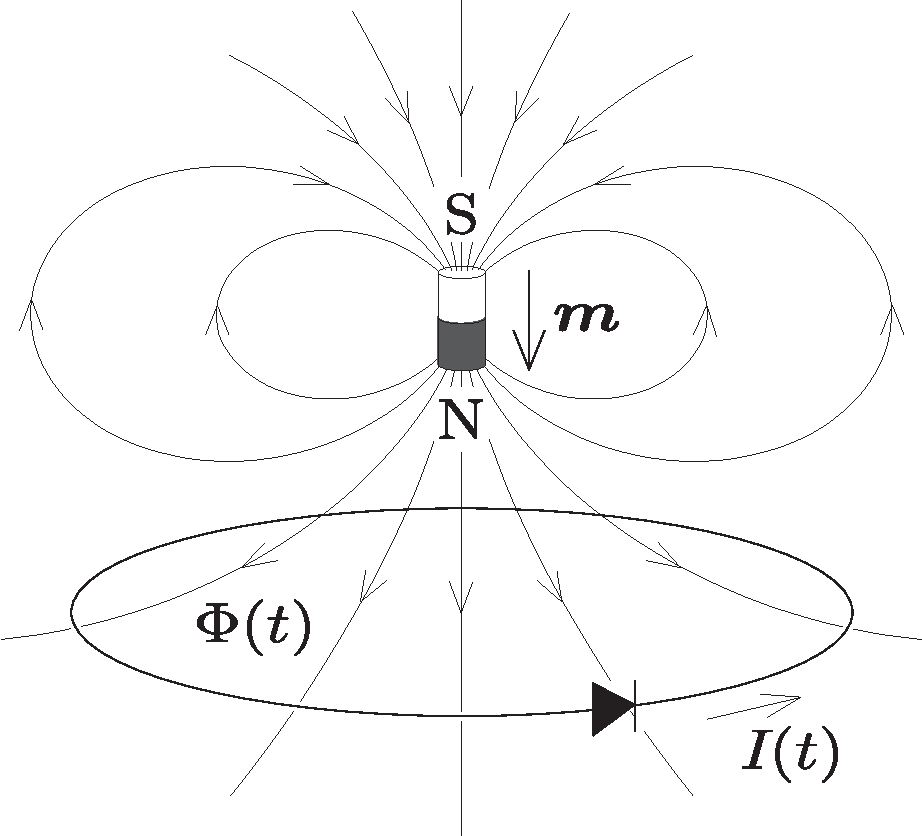
\includegraphics[scale=0.4]{Anh/Nam3.pdf}
    \end{center}
    Độ lớn của từ thông đi qua vòng, bắt đầu ở giá trị gần như bằng không và tăng dần khi nam châm vào gần vòng và cuối cùng đạt cực đại khi nam châm ở vị trí chính giữa vòng; sau đó khi nam châm vượt qua vòng thì từ thông sẽ giảm dần. Áp dụng định luật Lenz ta có thể thấy rằng ở chuyển động đầu tiên, dòng điện sẽ có xu hướng đi qua diode theo chiều dẫn điện do đó sẽ có điện tích đi qua diode. Sau đó khi nam châm rời xa vòng dây, chiều suất điện động đổi hướng và do đó lúc này diode sẽ không cho dòng điện đi qua nữa, do đó không có dòng điện chạy qua vòng ở nửa sau của chuyển động.
    \\Với diode mở, cường độ dòng điện chạy qua nó có thể tính theo định luật Ohm:
    \[\dfrac{\mathrm{d}\Phi}{\mathrm{d}t}=R\dfrac{\mathrm{d}Q}{\mathrm{d}t}.\]
    Sự xuất hiện của dấu $*$ trong biểu thức của suất điện động là do nó phụ thuộc vào chiều dòng điện chạy qua vòng dây, từ đây ta có:
    \[\dfrac{\mathrm{d}\left(\Phi -RQ\right)}{\mathrm{d}t}=0
    \rt \Phi(t)-RQ(t)=\const.\]
    Ban đầu, từ thông qua vòng là không đáng kể và dòng điện chạy qua vòng bằng không nên giá trị của hằng số ở đây cũng bằng không. Dòng điện chỉ đi qua diode đến khi từ thông qua vòng đạt giá trị cực đại, sau đó diode sẽ chặn không cho dòng đi qua nữa. Do đó tổng điện tích đi qua vòng dây trong quá trình đó là:
    \[Q=\dfrac{\Phi_{max}}{R}.\]
    Việc còn lại của chúng ta là tính từ thông đi qua vòng dây lúc nam châm ở chính giữa vòng dây. Để đơn giản, ta thay nam châm bằng một vòng dây bán kính $r_0$ có dòng điện $I_0$, với $r_0$ được chọn sao cho moment từ của vòng dây đúng bằng $m$. Ta có:
    \[\left|\Vec{m}\right|=\pi r_o^2I_0.\]
    Ta dễ dàng chứng minh được công thức độ hỗ cảm của hai vòng dây đặt chồng lên nhau là: 
    \[M=\dfrac{\mu_0 \pi r_0^2}{2r}.\]
    Do đó từ thông cực đại đi qua vòng dây, được tạo ra khi nam châm ở tâm của vòng dây là:
    \[\Phi_{max}=MI_0=\dfrac{\mu_0 \pi r_0^2}{2r}I_0=\dfrac{\mu_0 \left|\Vec{m}\right|}{2r}.\]
    Cuối cùng, tổng điện tích đi qua diode là:
    \[Q=\dfrac{\mu_0 \left|\Vec{m}\right|}{2rR}.\]
\end{loigiai}


\begin{vd}[Hiệu ứng do điện trở suất không đồng nhất]
Hai hình trụ dẫn điện có hình dạng giống hệt nhau, đều có chiều cao $h$ và bán kính $a$ nhưng có điện trở suất khác nhau là $\rho_1$ và $\rho_2$. Hai hình trụ được mắc nối tiếp với nhau như trên hình vẽ, tạo thành một hình trụ dẫn điện duy nhất có chiều cao $2h$ và tiết diện mặt cắt $S=\pi a^2$. Hai đáy đối diện của hình trụ được nối với một nguồn điện để cung cấp một hiệu điện thế không đổi $V$ cho hệ (xem hình vẽ).
  \begin{center}
\tikzset{every picture/.style={line width=0.75pt}} %set default line width to 0.75pt        

\begin{tikzpicture}[x=0.75pt,y=0.75pt,yscale=-1,xscale=1]
%uncomment if require: \path (0,300); %set diagram left start at 0, and has height of 300

%Shape: Ellipse [id:dp6121391228854065] 
\draw  [fill={rgb, 255:red, 155; green, 155; blue, 155 }  ,fill opacity=0.5 ] (108,92.8) .. controls (108,75.24) and (112.48,61) .. (118,61) .. controls (123.52,61) and (128,75.24) .. (128,92.8) .. controls (128,110.36) and (123.52,124.6) .. (118,124.6) .. controls (112.48,124.6) and (108,110.36) .. (108,92.8) -- cycle ;
%Straight Lines [id:da4868766515682539] 
\draw    (118,61) -- (229,61) -- (387,61) ;
%Shape: Ellipse [id:dp23551700839825673] 
\draw  [fill={rgb, 255:red, 155; green, 155; blue, 155 }  ,fill opacity=0.5 ] (242.5,92.8) .. controls (242.5,75.24) and (246.98,61) .. (252.5,61) .. controls (258.02,61) and (262.5,75.24) .. (262.5,92.8) .. controls (262.5,110.36) and (258.02,124.6) .. (252.5,124.6) .. controls (246.98,124.6) and (242.5,110.36) .. (242.5,92.8) -- cycle ;
%Shape: Ellipse [id:dp6488234880094885] 
\draw   (377,92.8) .. controls (377,75.24) and (381.48,61) .. (387,61) .. controls (392.52,61) and (397,75.24) .. (397,92.8) .. controls (397,110.36) and (392.52,124.6) .. (387,124.6) .. controls (381.48,124.6) and (377,110.36) .. (377,92.8) -- cycle ;
%Straight Lines [id:da8103537955913243] 
\draw    (118,124.6) -- (387,124.6) ;
%Straight Lines [id:da5376961085936793] 
\draw    (118,92.8) -- (86,92.8) ;
%Straight Lines [id:da9455654270816132] 
\draw    (419,92.8) -- (397,92.8) ;
%Straight Lines [id:da6282627412057236] 
\draw    (86,92.8) -- (86,186.6) ;
%Straight Lines [id:da7621747934473055] 
\draw    (86,186.6) -- (267,186.6) ;
%Straight Lines [id:da8771997109727767] 
\draw    (419,92.8) -- (419,186.6) ;
%Straight Lines [id:da3736616951165468] 
\draw    (288,186.6) -- (419,186.6) ;
%Straight Lines [id:da2248812348878848] 
\draw    (121,38.8) -- (249.5,38.8) ;
\draw [shift={(252.5,38.8)}, rotate = 180] [fill={rgb, 255:red, 0; green, 0; blue, 0 }  ][line width=0.08]  [draw opacity=0] (10.72,-5.15) -- (0,0) -- (10.72,5.15) -- (7.12,0) -- cycle    ;
\draw [shift={(118,38.8)}, rotate = 0] [fill={rgb, 255:red, 0; green, 0; blue, 0 }  ][line width=0.08]  [draw opacity=0] (10.72,-5.15) -- (0,0) -- (10.72,5.15) -- (7.12,0) -- cycle    ;
%Straight Lines [id:da8663420360267051] 
\draw    (255.5,38.8) -- (384,38.8) ;
\draw [shift={(387,38.8)}, rotate = 180] [fill={rgb, 255:red, 0; green, 0; blue, 0 }  ][line width=0.08]  [draw opacity=0] (10.72,-5.15) -- (0,0) -- (10.72,5.15) -- (7.12,0) -- cycle    ;
\draw [shift={(252.5,38.8)}, rotate = 0] [fill={rgb, 255:red, 0; green, 0; blue, 0 }  ][line width=0.08]  [draw opacity=0] (10.72,-5.15) -- (0,0) -- (10.72,5.15) -- (7.12,0) -- cycle    ;
%Straight Lines [id:da9871661779176883] 
\draw  [dash pattern={on 4.5pt off 4.5pt}]  (118,92.8) -- (173,92.8) ;
%Straight Lines [id:da14706230389773922] 
\draw    (164,63.6) -- (164,91.6) ;
\draw [shift={(164,94.6)}, rotate = 270] [fill={rgb, 255:red, 0; green, 0; blue, 0 }  ][line width=0.08]  [draw opacity=0] (7.14,-3.43) -- (0,0) -- (7.14,3.43) -- (4.74,0) -- cycle    ;
\draw [shift={(164,60.6)}, rotate = 90] [fill={rgb, 255:red, 0; green, 0; blue, 0 }  ][line width=0.08]  [draw opacity=0] (7.14,-3.43) -- (0,0) -- (7.14,3.43) -- (4.74,0) -- cycle    ;
%Straight Lines [id:da3610058452350251] 
\draw    (267,172.8) -- (267,200.4) ;
%Straight Lines [id:da8374418838314643] 
\draw [line width=1.5]    (273,180.6) -- (273,193.4) ;
%Straight Lines [id:da279996133245511] 
\draw    (281,172.8) -- (281,200.4) ;
%Straight Lines [id:da8399458261151034] 
\draw [line width=1.5]    (287,180.6) -- (287,193.4) ;
%Straight Lines [id:da823848516819623] 
\draw  [dash pattern={on 4.5pt off 4.5pt}]  (118,30.6) -- (118,61) ;
%Straight Lines [id:da6692601063799626] 
\draw  [dash pattern={on 4.5pt off 4.5pt}]  (252.5,31.6) -- (252.5,61) ;
%Straight Lines [id:da6206478957645265] 
\draw  [dash pattern={on 4.5pt off 4.5pt}]  (387,31.6) -- (387,61) ;


% Text Node
\draw (149,70.4) node [anchor=north west][inner sep=0.75pt]    {$a$};
% Text Node
\draw (182,14.4) node [anchor=north west][inner sep=0.75pt]    {$h$};
% Text Node
\draw (317,18.4) node [anchor=north west][inner sep=0.75pt]    {$h$};
% Text Node
\draw (189,81.4) node [anchor=north west][inner sep=0.75pt]    {$\rho _{1}$};
% Text Node
\draw (313,81.4) node [anchor=north west][inner sep=0.75pt]    {$\rho _{2}$};
% Text Node
\draw (273,150.4) node [anchor=north west][inner sep=0.75pt]    {$V$};


\end{tikzpicture}
\end{center}

 \begin{enumerate}[1)]
    \item Tìm cường độ điện trường, dòng điện và mật độ dòng điện chạy trong hai hình trụ ở điều kiện ổn định.
   \item Tìm mật độ điện mặt tại hai đáy nối với nguồn của hình trụ và tại mặt giao cắt của hai loại vật liệu.
 \end{enumerate}
 \end{vd}
 
 \begin{loigiai}\[\]
\begin{enumerate}
  \item Chúng ta sử dụng hệ tọa độ trụ $(r,\phi,z)$, với trục $z$ trùng với trục dối xứng của hai hình trụ, và gốc tọa độ $O$ nằm trên mặt phân cách của hai hình trụ (xem hình vẽ). Chúng ta đặt mật độ điện tích khối là $q_v$, do kí hiệu $\rho$ đã được dùng đại diện cho điện trở suất. Trong trạng thái dừng ta phải có $\partial_t q_v =0$ ở toàn không gian nếu không điện tích khối sẽ liên tục tăng hoặc liên tục giảm đến thời gian vô cùng.
  
  \immini{Do đó, áp dụng phương trình liên tục, ta có:
        \[ \nabla \cdot \ot{J} = -\partial_t q_v =0 . \tag{1} \]

Mặt khác, từ $\nabla \cdot \ot{E} = 4\pi k_e q_v$ và $\ot{J} = \ot{E}/\rho$ chúng ta thu được:
      \[ 0= \nabla \cdot \ot{J} = \frac{1}{\rho} \nabla \cdot \ot{E} = \frac{4\pi k_e }{\rho} q_v, \tag {2} \]

chứng tỏ rằng mật độ điện tích khối $q_v$ phải bằng không trên toàn không gian bên trong vật dẫn ở điều kiện dừng. Tuy nhiên ở bề mặt tiếp xúc giữa hai hình trụ vẫn tồn tại tích điện bề mặt.}{
  
\tikzset{every picture/.style={line width=0.75pt}} %set default line width to 0.75pt        

\begin{tikzpicture}[x=0.75pt,y=0.75pt,yscale=-1,xscale=1]
%uncomment if require: \path (0,513); %set diagram left start at 0, and has height of 513

%Shape: Ellipse [id:dp6250624101115241] 
\draw  [fill={rgb, 255:red, 155; green, 155; blue, 155 }  ,fill opacity=0.5 ] (259,53.99) .. controls (259,49.85) and (271.87,46.49) .. (287.75,46.49) .. controls (303.63,46.49) and (316.5,49.85) .. (316.5,53.99) .. controls (316.5,58.13) and (303.63,61.49) .. (287.75,61.49) .. controls (271.87,61.49) and (259,58.13) .. (259,53.99) -- cycle ;
%Straight Lines [id:da3339667292579327] 
\draw    (287.75,10.8) -- (287.75,344.31) ;
\draw [shift={(287.75,7.8)}, rotate = 90] [fill={rgb, 255:red, 0; green, 0; blue, 0 }  ][line width=0.08]  [draw opacity=0] (10.72,-5.15) -- (0,0) -- (10.72,5.15) -- (7.12,0) -- cycle    ;
%Shape: Ellipse [id:dp3305378714078062] 
\draw  [fill={rgb, 255:red, 155; green, 155; blue, 155 }  ,fill opacity=0.6 ] (259,181.88) .. controls (259,177.15) and (271.87,173.32) .. (287.75,173.32) .. controls (303.63,173.32) and (316.5,177.15) .. (316.5,181.88) .. controls (316.5,186.6) and (303.63,190.43) .. (287.75,190.43) .. controls (271.87,190.43) and (259,186.6) .. (259,181.88) -- cycle ;
%Shape: Ellipse [id:dp3007741333558356] 
\draw   (259,309.77) .. controls (259,305.56) and (271.87,302.15) .. (287.75,302.15) .. controls (303.63,302.15) and (316.5,305.56) .. (316.5,309.77) .. controls (316.5,313.97) and (303.63,317.38) .. (287.75,317.38) .. controls (271.87,317.38) and (259,313.97) .. (259,309.77) -- cycle ;
%Straight Lines [id:da7991380491110527] 
\draw    (259,53.99) -- (259,309.77) ;
%Straight Lines [id:da04582733466088573] 
\draw    (316.5,53.99) -- (316.5,309.77) ;
%Straight Lines [id:da469953626106149] 
\draw    (287.75,181.88) -- (374,181.88) ;
\draw [shift={(377,181.88)}, rotate = 180] [fill={rgb, 255:red, 0; green, 0; blue, 0 }  ][line width=0.08]  [draw opacity=0] (10.72,-5.15) -- (0,0) -- (10.72,5.15) -- (7.12,0) -- cycle    ;
%Straight Lines [id:da18645827300171325] 
\draw  [dash pattern={on 4.5pt off 4.5pt}]  (316.5,53.99) -- (345.69,53.99) ;
%Straight Lines [id:da7137054061751509] 
\draw  [dash pattern={on 4.5pt off 4.5pt}]  (316.5,309.77) -- (345.69,309.77) ;
%Straight Lines [id:da32063934724277665] 
\draw    (287.75,88.47) -- (313.5,88.47) ;
\draw [shift={(316.5,88.47)}, rotate = 180] [fill={rgb, 255:red, 0; green, 0; blue, 0 }  ][line width=0.08]  [draw opacity=0] (7.14,-3.43) -- (0,0) -- (7.14,3.43) -- (4.74,0) -- cycle    ;
%Straight Lines [id:da5545535578117207] 
\draw [line width=1.5]    (301.48,118.6) -- (301.48,156.06) ;
\draw [shift={(301.48,160.06)}, rotate = 270] [fill={rgb, 255:red, 0; green, 0; blue, 0 }  ][line width=0.08]  [draw opacity=0] (13.4,-6.43) -- (0,0) -- (13.4,6.44) -- (8.9,0) -- cycle    ;
%Straight Lines [id:da5189897246868762] 
\draw [line width=1.5]    (301.48,223.6) -- (301.48,263.54) ;
\draw [shift={(301.48,267.54)}, rotate = 270] [fill={rgb, 255:red, 0; green, 0; blue, 0 }  ][line width=0.08]  [draw opacity=0] (13.4,-6.43) -- (0,0) -- (13.4,6.44) -- (8.9,0) -- cycle    ;
%Shape: Arc [id:dp2351818332087896] 
\draw  [draw opacity=0] (305.74,332.79) .. controls (311.28,334.75) and (314.79,337.65) .. (314.79,340.89) .. controls (314.79,346.81) and (303.1,351.6) .. (288.68,351.6) .. controls (274.27,351.6) and (262.58,346.81) .. (262.58,340.89) .. controls (262.58,338.17) and (265.07,335.68) .. (269.16,333.79) -- (288.68,340.89) -- cycle ; \draw   (305.74,332.79) .. controls (311.28,334.75) and (314.79,337.65) .. (314.79,340.89) .. controls (314.79,346.81) and (303.1,351.6) .. (288.68,351.6) .. controls (274.27,351.6) and (262.58,346.81) .. (262.58,340.89) .. controls (262.58,338.17) and (265.07,335.68) .. (269.16,333.79) ;
%Straight Lines [id:da29136919346471224] 
\draw    (305.74,332.79) -- (303.97,331.7) ;
\draw [shift={(301.42,330.12)}, rotate = 391.63] [fill={rgb, 255:red, 0; green, 0; blue, 0 }  ][line width=0.08]  [draw opacity=0] (10.72,-5.15) -- (0,0) -- (10.72,5.15) -- (7.12,0) -- cycle    ;
%Straight Lines [id:da8801372758814372] 
\draw    (334,58.6) -- (334,179) ;
\draw [shift={(334,182)}, rotate = 270] [fill={rgb, 255:red, 0; green, 0; blue, 0 }  ][line width=0.08]  [draw opacity=0] (10.72,-5.15) -- (0,0) -- (10.72,5.15) -- (7.12,0) -- cycle    ;
\draw [shift={(334,55.6)}, rotate = 90] [fill={rgb, 255:red, 0; green, 0; blue, 0 }  ][line width=0.08]  [draw opacity=0] (10.72,-5.15) -- (0,0) -- (10.72,5.15) -- (7.12,0) -- cycle    ;
%Straight Lines [id:da7076307678955314] 
\draw    (334,185) -- (334,305.4) ;
\draw [shift={(334,308.4)}, rotate = 270] [fill={rgb, 255:red, 0; green, 0; blue, 0 }  ][line width=0.08]  [draw opacity=0] (10.72,-5.15) -- (0,0) -- (10.72,5.15) -- (7.12,0) -- cycle    ;
\draw [shift={(334,182)}, rotate = 90] [fill={rgb, 255:red, 0; green, 0; blue, 0 }  ][line width=0.08]  [draw opacity=0] (10.72,-5.15) -- (0,0) -- (10.72,5.15) -- (7.12,0) -- cycle    ;


% Text Node
\draw (315.5,341.2) node [anchor=north west][inner sep=0.75pt]    {$\phi $};
% Text Node
\draw (262,228.4) node [anchor=north west][inner sep=0.75pt]    {$\rho _{2}$};
% Text Node
\draw (266,110.4) node [anchor=north west][inner sep=0.75pt]    {$\rho _{1}$};
% Text Node
\draw (300,123) node [anchor=north west][inner sep=0.75pt]  {$\ot{J}$};
% Text Node
\draw (300,235.12) node [anchor=north west][inner sep=0.75pt]    {$\ot{J}$};
% Text Node
\draw (271,172.4) node [anchor=north west][inner sep=0.75pt]    {$O$};
% Text Node
\draw (353,184.4) node [anchor=north west][inner sep=0.75pt]    {$r$};
% Text Node
\draw (339,111.4) node [anchor=north west][inner sep=0.75pt]    {$h$};
% Text Node
\draw (339,236.4) node [anchor=north west][inner sep=0.75pt]    {$h$};
% Text Node
\draw (296,71.4) node [anchor=north west][inner sep=0.75pt]    {$a$};
% Text Node
\draw (273,21.4) node [anchor=north west][inner sep=0.75pt]    {$z$};


\end{tikzpicture}}
Nếu chúng ta giả sử rằng $h \gg a$, kết hợp với $\nabla\cdot \ot{J}=0$ và $\nabla \times \ot{E}=0$, ta suy ra mật độ dòng $\ot{J}$ là đồng nhất trên toàn bộ hình trụ, có chiều hướng xuống dọc theo trục $z$. Do $\ot{E}$ và $\ot{J}$ là tỉ lệ thuận với nhau bên trong mỗi hình trụ nên ta dễ dàng suy ra $\ot{E}$ là đồng nhất trong từng hình trụ riêng biệt. Mật độ dòng $\ot{J}$ phải liên tục khi đi qua mặt phân cách của hai hình trụ nếu không điện tích sẽ tích tụ đến vô hạn trên mặt phân cách này. Do đó, mật độ dòng $\ot{J}$ là không đổi trên toàn bộ vật dẫn, và cường độ dòng điện là $I= J\pi a^2$.\\
Điện trở của từng hình trụ $R_{1,2}$ lần lượt là:
   \[R_{1,2} = \rho_{1,2} \frac{h}{\pi a^2} , \tag{3} \]

Dẫn đến tổng trở của vật dẫn:
    \[R = R_1 + R_2 = (\rho_1 + \rho_2 ) \frac{h}{\pi a^2}. \tag{4} \]

Dòng điện và mật độ dòng điện chạy trong hệ là:
    \[I = \frac{V}{R} = \frac{\pi a^2 V }{h(\rho_1 + \rho_2)}, \quad J = \frac{V}{h(\rho_1 + \rho_2)}. \tag{5} \]

Vì chúng ta có cùng mật độ dòng điện trên hai hình trụ có điện trở suất khác nhau và $\ot{E} = \rho \ot{J}$, điện trường bên trong từng hình trụ phải là khác nhau, chúng ta đặt là:
   \[ E_1 = \rho_1 J = \frac{\rho_1 V}{h(\rho_1 + \rho_2)} , \quad E_2 =\rho_2 J = \frac{\rho_2 V}{h(\rho_1 + \rho_2)}. \tag{6} \]

\item Mật độ điện tích mặt ở trên mặt phân cách hai hình trụ có thể tính được qua định luật Gauss:
  \[\sigma = \frac{1}{4\pi k_e} (E_2 - E_1) = \frac{1}{4\pi k_e} \frac{(\rho_2 - \rho_1)V}{h(\rho_1 +\rho_2)} . \tag{7} \]

Giả sử rằng, điện trường là bằng không bên ngoài 2 đáy của hình trụ lớn, mật độ điện tích mặt của hai đáy trụ cũng có thể được tính theo định luật Gauss :
  
   \[\sigma_1 = \frac{E_1}{4\pi k_e }= \frac{1}{4\pi k_e} \frac{\rho_1 V}{h(\rho_1 + \rho_2)} , \quad \sigma_2 = - \frac{E_2}{4\pi k_e}= - \frac{1}{4\pi k_e} \frac{\rho_2 V}{h(\rho_1 + \rho_2)} . \tag{8}\]
                 
    
\end{enumerate}
\end{loigiai}


\begin{vd}[Trở kháng vô hạn]
Với dòng điện xoay chiều có tần số góc $\omega$, tìm trở kháng tương đương giữa các cực $A$ và $B$ trên hình vẽ. Mạch vô hạn gồm rất nhiều các phần tử giống hệt nhau, mỗi nút mạng cấu tạo từ một cuộn cảm có độ tự cảm $L$ và một tụ điện có điện dung $C$. Liệu có khả năng trở kháng này có 2 giá trị khác nhau hay không?
\begin{center}
    

\tikzset{every picture/.style={line width=0.75pt}} %set default line width to 0.75pt        

\begin{tikzpicture}[x=0.75pt,y=0.75pt,yscale=-1,xscale=1]
%uncomment if require: \path (0,470); %set diagram left start at 0, and has height of 470

%Straight Lines [id:da8896708259213006] 
\draw    (148,270.4) -- (468,270.4) ;
%Shape: Capacitor [id:dp8244944796033653] 
\draw   (148,202) -- (184,202) (192,185.8) -- (192,218.2) (184,185.8) -- (184,218.2) (192,202) -- (228,202) ;
%Shape: Inductor (Air Core) [id:dp47563115184590754] 
\draw   (466.59,202) -- (466.59,214.31) .. controls (470.02,214.49) and (472.95,216.2) .. (473.97,218.62) .. controls (475,221.04) and (473.91,223.67) .. (471.23,225.26) .. controls (469.14,226.48) and (466.44,226.98) .. (463.81,226.62) .. controls (462.79,226.62) and (461.96,226.01) .. (461.96,225.26) .. controls (461.96,224.5) and (462.79,223.89) .. (463.81,223.89) .. controls (466.44,223.54) and (469.14,224.03) .. (471.23,225.26) .. controls (473.45,226.68) and (474.72,228.66) .. (474.72,230.73) .. controls (474.72,232.8) and (473.45,234.78) .. (471.23,236.2) .. controls (469.14,237.42) and (466.44,237.92) .. (463.81,237.57) .. controls (462.79,237.57) and (461.96,236.96) .. (461.96,236.2) .. controls (461.96,235.44) and (462.79,234.83) .. (463.81,234.83) .. controls (466.44,234.48) and (469.14,234.98) .. (471.23,236.2) .. controls (473.45,237.62) and (474.72,239.6) .. (474.72,241.67) .. controls (474.72,243.74) and (473.45,245.72) .. (471.23,247.14) .. controls (469.14,248.37) and (466.44,248.86) .. (463.81,248.51) .. controls (462.79,248.51) and (461.96,247.9) .. (461.96,247.14) .. controls (461.96,246.39) and (462.79,245.78) .. (463.81,245.78) .. controls (466.44,245.42) and (469.14,245.92) .. (471.23,247.14) .. controls (473.91,248.73) and (475,251.36) .. (473.97,253.78) .. controls (472.95,256.2) and (470.02,257.91) .. (466.59,258.09) -- (466.59,270.4) ;
%Flowchart: Connector [id:dp26467715626009025] 
\draw   (138.6,270.4) .. controls (138.6,273) and (140.7,275.1) .. (143.3,275.1) .. controls (145.9,275.1) and (148,273) .. (148,270.4) .. controls (148,267.8) and (145.9,265.7) .. (143.3,265.7) .. controls (140.7,265.7) and (138.6,267.8) .. (138.6,270.4) -- cycle ;
%Flowchart: Connector [id:dp5760989978301936] 
\draw   (138.6,202) .. controls (138.6,204.6) and (140.7,206.7) .. (143.3,206.7) .. controls (145.9,206.7) and (148,204.6) .. (148,202) .. controls (148,199.4) and (145.9,197.3) .. (143.3,197.3) .. controls (140.7,197.3) and (138.6,199.4) .. (138.6,202) -- cycle ;
%Shape: Inductor (Air Core) [id:dp45982416209467436] 
\draw   (388,202) -- (388,214.31) .. controls (391.43,214.49) and (394.35,216.2) .. (395.38,218.62) .. controls (396.4,221.04) and (395.31,223.67) .. (392.63,225.26) .. controls (390.54,226.48) and (387.84,226.98) .. (385.22,226.62) .. controls (384.2,226.62) and (383.37,226.01) .. (383.37,225.26) .. controls (383.37,224.5) and (384.2,223.89) .. (385.22,223.89) .. controls (387.84,223.54) and (390.54,224.03) .. (392.63,225.26) .. controls (394.86,226.68) and (396.12,228.66) .. (396.12,230.73) .. controls (396.12,232.8) and (394.86,234.78) .. (392.63,236.2) .. controls (390.54,237.42) and (387.84,237.92) .. (385.22,237.57) .. controls (384.2,237.57) and (383.37,236.96) .. (383.37,236.2) .. controls (383.37,235.44) and (384.2,234.83) .. (385.22,234.83) .. controls (387.84,234.48) and (390.54,234.98) .. (392.63,236.2) .. controls (394.86,237.62) and (396.12,239.6) .. (396.12,241.67) .. controls (396.12,243.74) and (394.86,245.72) .. (392.63,247.14) .. controls (390.54,248.37) and (387.84,248.86) .. (385.22,248.51) .. controls (384.2,248.51) and (383.37,247.9) .. (383.37,247.14) .. controls (383.37,246.39) and (384.2,245.78) .. (385.22,245.78) .. controls (387.84,245.42) and (390.54,245.92) .. (392.63,247.14) .. controls (395.31,248.73) and (396.4,251.36) .. (395.38,253.78) .. controls (394.35,256.2) and (391.43,257.91) .. (388,258.09) -- (388,270.4) ;
%Shape: Inductor (Air Core) [id:dp9344396637665358] 
\draw   (309,202) -- (309,214.31) .. controls (312.43,214.49) and (315.35,216.2) .. (316.38,218.62) .. controls (317.4,221.04) and (316.31,223.67) .. (313.63,225.26) .. controls (311.54,226.48) and (308.84,226.98) .. (306.22,226.62) .. controls (305.2,226.62) and (304.37,226.01) .. (304.37,225.26) .. controls (304.37,224.5) and (305.2,223.89) .. (306.22,223.89) .. controls (308.84,223.54) and (311.54,224.03) .. (313.63,225.26) .. controls (315.86,226.68) and (317.12,228.66) .. (317.12,230.73) .. controls (317.12,232.8) and (315.86,234.78) .. (313.63,236.2) .. controls (311.54,237.42) and (308.84,237.92) .. (306.22,237.57) .. controls (305.2,237.57) and (304.37,236.96) .. (304.37,236.2) .. controls (304.37,235.44) and (305.2,234.83) .. (306.22,234.83) .. controls (308.84,234.48) and (311.54,234.98) .. (313.63,236.2) .. controls (315.86,237.62) and (317.12,239.6) .. (317.12,241.67) .. controls (317.12,243.74) and (315.86,245.72) .. (313.63,247.14) .. controls (311.54,248.37) and (308.84,248.86) .. (306.22,248.51) .. controls (305.2,248.51) and (304.37,247.9) .. (304.37,247.14) .. controls (304.37,246.39) and (305.2,245.78) .. (306.22,245.78) .. controls (308.84,245.42) and (311.54,245.92) .. (313.63,247.14) .. controls (316.31,248.73) and (317.4,251.36) .. (316.38,253.78) .. controls (315.35,256.2) and (312.43,257.91) .. (309,258.09) -- (309,270.4) ;
%Shape: Inductor (Air Core) [id:dp6736769932143452] 
\draw   (228,202) -- (228,214.31) .. controls (231.43,214.49) and (234.35,216.2) .. (235.38,218.62) .. controls (236.4,221.04) and (235.31,223.67) .. (232.63,225.26) .. controls (230.54,226.48) and (227.84,226.98) .. (225.22,226.62) .. controls (224.2,226.62) and (223.37,226.01) .. (223.37,225.26) .. controls (223.37,224.5) and (224.2,223.89) .. (225.22,223.89) .. controls (227.84,223.54) and (230.54,224.03) .. (232.63,225.26) .. controls (234.86,226.68) and (236.12,228.66) .. (236.12,230.73) .. controls (236.12,232.8) and (234.86,234.78) .. (232.63,236.2) .. controls (230.54,237.42) and (227.84,237.92) .. (225.22,237.57) .. controls (224.2,237.57) and (223.37,236.96) .. (223.37,236.2) .. controls (223.37,235.44) and (224.2,234.83) .. (225.22,234.83) .. controls (227.84,234.48) and (230.54,234.98) .. (232.63,236.2) .. controls (234.86,237.62) and (236.12,239.6) .. (236.12,241.67) .. controls (236.12,243.74) and (234.86,245.72) .. (232.63,247.14) .. controls (230.54,248.37) and (227.84,248.86) .. (225.22,248.51) .. controls (224.2,248.51) and (223.37,247.9) .. (223.37,247.14) .. controls (223.37,246.39) and (224.2,245.78) .. (225.22,245.78) .. controls (227.84,245.42) and (230.54,245.92) .. (232.63,247.14) .. controls (235.31,248.73) and (236.4,251.36) .. (235.38,253.78) .. controls (234.35,256.2) and (231.43,257.91) .. (228,258.09) -- (228,270.4) ;
%Straight Lines [id:da08162931708808219] 
\draw  [dash pattern={on 4.5pt off 4.5pt}]  (466.59,202) -- (528,202) ;
%Straight Lines [id:da19767708053606436] 
\draw  [dash pattern={on 4.5pt off 4.5pt}]  (466.59,270.4) -- (528,270.4) ;
%Shape: Capacitor [id:dp46965472319429713] 
\draw   (228,202) -- (264,202) (272,185.8) -- (272,218.2) (264,185.8) -- (264,218.2) (272,202) -- (308,202) ;
%Shape: Capacitor [id:dp5547460041167185] 
\draw   (309,202) -- (345,202) (353,185.8) -- (353,218.2) (345,185.8) -- (345,218.2) (353,202) -- (389,202) ;
%Shape: Capacitor [id:dp25623842683890086] 
\draw   (388,202) -- (424,202) (432,185.8) -- (432,218.2) (424,185.8) -- (424,218.2) (432,202) -- (468,202) ;


% Text Node
\draw (180,163.4) node [anchor=north west][inner sep=0.75pt]  [font=\large]  {$C$};
% Text Node
\draw (261,163.4) node [anchor=north west][inner sep=0.75pt]  [font=\large]  {$C$};
% Text Node
\draw (342,163.4) node [anchor=north west][inner sep=0.75pt]  [font=\large]  {$C$};
% Text Node
\draw (421,162.4) node [anchor=north west][inner sep=0.75pt]  [font=\large]  {$C$};
% Text Node
\draw (202,226.4) node [anchor=north west][inner sep=0.75pt]  [font=\large]  {$L$};
% Text Node
\draw (282,227.4) node [anchor=north west][inner sep=0.75pt]  [font=\large]  {$L$};
% Text Node
\draw (363,227.4) node [anchor=north west][inner sep=0.75pt]  [font=\large]  {$L$};
% Text Node
\draw (443,226.4) node [anchor=north west][inner sep=0.75pt]  [font=\large]  {$L$};
% Text Node
\draw (118,190.4) node [anchor=north west][inner sep=0.75pt]  [font=\large]  {$A$};
% Text Node
\draw (118,260.6) node [anchor=north west][inner sep=0.75pt]  [font=\large]  {$B$};


\end{tikzpicture}
\end{center}
\end{vd}
\begin{loigiai}\[\]
Ta có công thức tính trở kháng của cuộn dây khi có dòng điện với tần số $\omega$ đi qua:
$$\dfrac{V_C}{I_C}=\dfrac{1}{\omega C},$$
đây được gọi là dung kháng của cuộn dây, hơn nữa, dòng điện đi qua cuộn dây luôn sớm pha hơn hiệu điện thế xoay chiều đặt lên nó một góc $90^\circ$. Với cuộn dây, tương tự ta có
$$\dfrac{V_L}{I_L}=\omega L,$$
đây được gọi là cảm kháng của cuộn dây, dòng điện qua cuộn dây luôn chậm pha so với hiệu điện thế xoay chiều đặt lên nó một góc $90^\circ.$\\
Do sự lệch pha so với hiệu điện thế của dòng qua cuộn dây và dòng qua tụ điện là hoàn toàn ngược nhau nên ta có thể coi cuộn dây là một tụ điện có điện dung âm $C_L<0$:
$$\omega L=-\dfrac{1}{\omega C_L}, \text{ và do đó } C_L=-\dfrac{1}{\omega^2 L}.$$
Từ đây ta có thể tính toán dựa trên một mạch điện tương đương chỉ gồm toàn tụ điện.
Trong các tính toán tiếp theo, để cho gọn ta đặt :
$$k^2=\dfrac{1}{\omega^2 LC}=\tron{\dfrac{\omega_0}{\omega}}^2.$$
Hệ số tỉ lệ $k$ cho chúng ta biết tần số góc tự nhiên (hay còn gọi là tần số góc cộng hưởng) $\omega_0$ đối với mạch $LC$ đơn thuần lớn hơn bao nhiêu lần so với tần số  góc cưỡng bức $\omega$. Sử dụng rút gọn này, “điện dung hiệu dụng” của cuộn dây có thể viết dưới dạng $C_L=-k^2\cdot C$.\\
Trong một bài vật lý, mạch điện vô hạn có thể được hiểu là mạch điện với số nút mạng vô cùng lớn nhưng số nút mạng là hữu hạn. Đầu tiên hãy xét một mạch điện chứa $n$ nút mạng (mạch chứa $n$ cuộn dây và $n$ tụ điện). Vì mạch điện không có bất kì phần tử điện trở nào nên độ lệch pha giữa dòng điện trong mạch và hiệu điện thế đặt vào hai đầu mạch chỉ có thể là $90^\circ$ hoặc $-90^\circ$. Khi đó, tùy vào độ lệch pha ta có thể thay thế toàn bộ mạch điện bằng một tụ điện tương đương $C_n$ hoặc một cuộn dây tương đương $L_n$ với thông số phù hợp. Giả sử trong trường hợp này mạch điện có thể thay thế bằng một tụ điện $C_n$, ta sẽ tính toán  $C_n$, và nếu $C_n$ âm thì mạch điện tương đương sẽ là một cuộn dây.\\
Trong trường hợp $n=1$, ta sẽ thu được điện dung tương đương của một tụ điện $C$ mắc với một cuộn cảm $L$ (được coi như một tụ điện với điện dung $C_L$ bằng công thức sau:
$$\dfrac{1}{C_1}=\dfrac{1}{C}+\dfrac{1}{C_L},$$
từ đó suy ra:
$$C_{1}=\dfrac{C C_{L}}{C+C_{L}}=\dfrac{C \times\left(-k^{2} C\right)}{C+\left(-k^{2} C\right)}=\dfrac{k^{2}}{k^{2}-1} C .$$
Với $n=2$, mạch điện giống như tụ $C_1$ được mắc với thêm một nút mạng nữa
$$\dfrac{1}{C_2}=\dfrac{1}{C}+\dfrac{1}{C_1+\tron{-k^2 C}}.$$
Tổng quát,
$$\dfrac{1}{C_{n+1}}=\dfrac{1}{C}+\dfrac{1}{C_{n}-k^{2} C},$$
từ đây
$$C_{n+1}=\dfrac{C\left(C_{n}-k^{2} C\right)}{C_{n}+\left(1-k^{2}\right) C}.$$
Để thuận tiện hơn ta đặt $C_n=x_n\cdot C$ vì dãy truy hồi cho $x$ có thể được viết ở dạng tường minh:
\[x_{n+1}=\dfrac{x_n-k^2}{x_n +1 -k^2}.\tag{1} \label{n1}\]
Để khảo sát xem dãy này có giới hạn khi $x$ tiến đến vô cùng hay không, chúng ta giả sử $n\gg 1$ thì $x_n\approx x_{n+1}$, lúc này (\ref{n1}) có thể được chuyển thành một phương trình bậc hai như sau:
$$x=\dfrac{x-k^2}{x+1-k^2}, \text{ hay } x^2-k^2x+k^2=0.$$
Trong trường hợp $k>2$ (tần số đầu vào là nhỏ), phương trình này có hai nghiệm thật:
\[x_{\pm}=\dfrac{k^{2}}{2} \pm \dfrac{k}{2} \sqrt{k^{2}-4}\tag{2}.\label{n2}\]
Câu hỏi được đặt ra là đâu là nghiệm được chọn? Hay cả hai nghiệm đều có ý nghĩa vật lý của riêng chúng? Bạn có thể đoán rằng trong trường hợp này nghiệm nhỏ hơn là nghiệm đúng. Suy đoán trên có cơ sở bởi vì nếu ta dùng cuộn dây có $L$ rất nhỏ thì mỗi cuộn dây chỉ đơn thuần như một dây dẫn nối tắt, vì thế điện dung đo được giữa hai đầu $A B$ sẽ xấp xỉ điện dung của một tụ điện thuần $C$, $x\approx1$. Điều này dễ dàng được kiểm chứng vì khi $L$ là nhỏ, $k\gg 1$, lúc này $x_{-}\approx1$ còn $x_+$ xấp xỉ $k^2 \gg 1$, một điều vô lý so với điều kiện biên vật lý. Vậy đúng như suy đoán, ta chọn nghiệm nhỏ hơn.\\
Lập luận này khẳng định đối với $k>2$, trở kháng của mạch có thể được mô tả bởi công thức 
$$Z_{\text{chuỗi}}=\dfrac{1}{\omega x_{-} C}=\dfrac{1}{\omega C} \dfrac{2}{k\left(k-\sqrt{k^{2}-4}\right)}=\dfrac{1+\sqrt{1-4 \omega^{2} L C}}{2 \omega C}.$$
Vậy nếu $k<2$, điều gì sẽ xảy ra?\\
Lúc này, phương trình (\ref{n1}) sẽ cho nghiệm phức, tức điện dung tương đương sẽ không còn là một bội số thực của $C$. Nói theo một cách khác, lúc này điện dung tương đương của mạch điện sẽ không hội tụ về một giá trị cụ thể mà sẽ phụ thuộc vào số nút mạng (vì trên thực tế số nút mạng chỉ là rất nhiều chứ không phải là vô hạn!).\\
\textbf{Mở rộng.}\\
Bài toán cũng có thể được giải quyết bằng cách đặt trở kháng phức với $i\omega L$ cho cuộn dây và $\dfrac{1}{i\omega C}$ cho tụ điện. Đặt $Z$ là trở kháng của cả mạch điện, nếu mạch điện là vô hạn thì khi ta lắp thêm một nút mạng vào mạch điện thì trở kháng của mạch không thay đổi và bằng $Z$, ta có
$$Z=\dfrac{1}{i\omega C}+\dfrac{i\omega LZ}{i\omega L +Z}.$$
Và ta thu được nghiệm:
$$2Z\sqrt{\dfrac{C}{L}}=-ik\pm \sqrt{4-k^2}.$$
Biểu thức này chứng tỏ, với $k>2$, $Z$ luôn là một số ảo mang dấu âm và coi như một tụ điện trên thực tế.\\
Với $k<2$, thành phần thứ hai của biểu thức là một số thực và trở kháng của mạch vô hạn lúc này chứa một thành phần điện trở. Điều này rất khó hiểu bởi một mạch điện chỉ chứa cuộn cảm và tụ điện lí tưởng không thể coi như một điện trở (vì điện trở làm mất mát năng lượng) do đó nên lẽ ra trở kháng tương đương chỉ có thể coi như một tụ điện hoặc một cuộn cảm.\\
Sự xuất hiện của thành phần điện trở có liên hệ mật thiết đến hiện tượng sóng truyền trong dây dẫn. Sóng này sẽ mang năng lượng của nguồn và truyền đi dọc theo dây dẫn, và trong trường hợp dây dẫn rất dài, sóng sẽ phản xạ và mang năng lượng trở lại sau một khoảng thời gian khá lâu. Đối với trường hợp dây dẫn dài vô hạn, sóng năng lượng này không bao giờ trở lại, do đó mạch điện chỉ gồm cuộn dây và tụ điện lý tưởng sẽ coi như có thêm thành phần điện trở!
\end{loigiai}


\begin{vd}[Truyền tải điện đi xa]\\%câu 12
%USAPhO 2011
Một dây cáp dẫn điện xoay chiều, truyền tải điện năng dưới dạng sóng hình sin với tần số $60~\mathrm{Hz}$. Tải nhận hiệu điện thế có giá trị hiệu dụng là $500~\mathrm{kV}$ và yêu cầu công suất trung bình là $1000~\mathrm{MW}$. Đối với bài này, chỉ xét dây cáp mang dòng điện theo một trong hai hướng, và bỏ qua hiệu ứng do điện dung hoặc độ tự cảm giữa dây tải với đất.
\begin{enumerate}[1.]
    \item Giả sử tải của đường dây điện là một khu dân cư, được coi như một điện trở thuần.
    \begin{enumerate}[a.]
        \item Hãy tính cường độ dòng điện hiệu dụng của đường dây tải điện.
        \item Dây cáp có đường kính $3~\mathrm{cm}$, dài $500~\mathrm{km}$, và được làm bằng nhôm với điện trở suất $2,8\times10^{-8}\mathrm{\Omega\cdot m}$. Hỏi công suất hao phí trên dây là bao nhiêu?
    \end{enumerate}
    \item Một chủ trang trại địa phương nghĩ rằng anh ta có thể lấy điện từ đường dây bằng cách sử dụng cảm ứng điện từ. Chủ trang trại dựng $N$ vòng dây hình chữ nhật có chiều dài $a$ và chiều rộng $b<a$. Một cạnh của vòng được đặt trên mặt đất, dây dẫn thẳng và chạy song song với mặt đất ở độ cao $h$ nhỏ hơn chiều dài của dây rất nhiều. Viết cường độ dòng điện trong dây dưới dạng $I=I_0\sin \omega t$, và giả sử rằng dây trở lại ở rất xa.
    \begin{enumerate}[a.]
        \item Xác định biểu thức cảm ứng từ của từ trường ở khoảng cách $r$ so với dây dẫn điện, biểu diễn kết quả theo $I, r$, và các hằng số cơ bản.
        \item Nên đặt vòng ở đâu, và định hướng chiếc vòng như thế nào, để tối đa hóa suất điện động cảm ứng của nó?
        \item Giả sử vòng được đặt theo cách này, hãy xác định biểu thức của suất điện động cảm ứng của vòng (như một hàm của thời gian) theo $I_0, h, a, b, N, \omega, t$, và các hằng số cơ bản.
        \item Giả sử rằng $a=5~\mathrm{m}, b=2~\mathrm{m}$ và $h=100~\mathrm{m}$. Hỏi người chủ trang trại $N$ bằng bao nhiêu vòng dây để tạo ra một suất điện động cảm ứng hiệu dụng bằng $120~\mathrm{V}$?
    \end{enumerate}
    \item Tải ở cuối của đường dây điện thay đổi, bao gồm một nhà máy sản xuất với số lượng lớn động cơ điện. Trong khi công suất trung bình được giữ không đổi, giờ đây nó hoạt động như một điện trở mắc song song với một cuộn cảm $0,25~\mathrm{H}$.
    \begin{enumerate}[a.]
        \item Công suất hao phí trên đường dây tải điện sẽ tăng lên, giảm đi hay giữ nguyên? (Bạn không cần tính toán giá trị một cách rõ ràng, bạn chỉ cần lập luận để bảo vệ câu trả lời của mình).
        \item Công ty điện lực muốn cho tải hoạt động như ban đầu bằng cách lắp một tụ điện song song với tải. Hỏi điện dung của nó là bao nhiêu?
    \end{enumerate}
\end{enumerate}
\end{vd}
\begin{loigiai}
\begin{enumerate}[1.]
    \item 
    \begin{enumerate}[a.]
        \item Vì tải là điện trở thuần, nên công suất trung bình đơn giản là:
        $$P=I_\mathrm{rms}V_\mathrm{rms},$$
        do đó:
        $$I_\mathrm{rms}=\dfrac{P}{V_\mathrm{rms}}=2000~\mathrm{A}.$$
        \item Diện tích tiết diện của dây là $A=\pi r^2=7,07\times 10^{-4}~\mathrm{m^2}$, do đó điện trở của dây là:
        $$R=\dfrac{\rho L}{A}=19,8 ~\mathrm{\Omega}.$$
        Công suất hao phí:
        $$P=I^2 R=79,2 ~\mathrm{MW}.$$
    \end{enumerate}
    \item
    \begin{enumerate}[a)]
        \item Từ trường vuông góc với dây và bán kính, nên từ định luật Ampere:
        $$
\oint \mathbf{B} \cdot \mathrm{d} \mathbf{s}=\mu_{0} I.$$
Tích phân có giá trị là $\tron{2\pi r}B$, do đó:
$$B=\dfrac{\mu_0 I}{2\pi r}.$$
Kết quả nổi tiếng này cũng có thể được viết ra mà không cần giải thích.
 \item Suất điện động cảm ứng tỉ lệ với tốc độ biến thiên của từ thông qua vòng dây. Vì sự phụ thuộc vào thời gian của từ trường là đều trong không gian, nên tốc độ biến thiên từ thông đạt cực đại khi chính từ thông đạt cực đại. Điều này có thể thực hiện bằng cách tối đa hóa từ trường trong vòng dây và đảm bảo rằng điều đó bình thường đối với vòng. Vì từ trường mạnh hơn khi gần dây, nên vòng dây phải nằm ngay bên dưới dây, và vì từ trường nằm ngang và vuông góc với dây tại vị trí này, nên vòng dây phải thẳng đứng và song song với dây. Cuối cùng, một lần nữa, vì từ trường càng gần dây càng mạnh, nên cạnh dài của vòng phải thẳng đứng.\\
 Tóm lại, vòng nên được đặt thẳng đứng, song song và ngay dưới dây, với cạnh dài thẳng đứng.
 \item Theo định luật Faraday:
 $$\mathcal{E}=N\dfrac{\mathrm \Phi_B}{\mathrm t},$$
 trong đó chúng tôi đã bỏ dấu, vì điều này không quan trọng, và $\Phi_B$ là từ thông đi qua một vòng. Từ thông:
 $$
\Phi_{B}=\int \mathbf{B} \cdot \mathrm{d}\mathbf{A}=b \int_{h-a}^{h} B(r) \mathrm{d} r,
$$
Trong đó chúng tôi đã chia vòng thành nhiều dải mảnh có bề dày $\mathrm{d}r$ và chiều dài $b$. Thay vào kết quả ở phần a:
$$
\Phi_{B}=b \int_{h-a}^{h} \dfrac{\mu_{0} I}{2 \pi r} \mathrm{d} r=\dfrac{\mu_{0} I b}{2 \pi} \ln \frac{h}{h-a}.
$$
Chỉ có cường độ dòng điện phụ thuộc thời gian:
$$\dfrac{\mathrm{d}I}{\mathrm{t}}=\omega I_0 \cos\omega t.$$
Do đó, ta có:
$$\mathcal{E}=\dfrac{N\mu_0b}{2\pi}\mathrm{ln}\dfrac{h}{h-a}I_0\omega\cos\omega t.$$
\item Giá trị hiệu dụng của $I_0\cos \omega t$ chỉ đơn giản là $I_{rms}$, do đó lấy giá trị hiệu dụng của cả hai vế:
$$\mathcal{E_{\mathrm{rms}}}=\dfrac{N\mu_0b}{2\pi}\ln\dfrac{h}{h-a}I_{\mathrm{rms}} \omega=N\mu_0bf\mathrm{ln}\dfrac{h}{h-a}I_\mathrm{rms},$$
trong đó chúng tôi dùng $f=\omega/2\pi$. Thay số, ta được:
$$\mu_0 bf\mathrm{ln}\dfrac{h}{h-a}I_\mathrm{rms}=0,0155~\mathrm{V},$$
vì vậy số vòng dây cần là:
$$N=7760.$$
    \end{enumerate}
    \item 
    \begin{enumerate}[a.]
        \item Cuộn cảm tạo nên một thành phần mới của dòng điện, thành phần này lệch pha $90^\circ$ với điện áp. Giá trị cường độ dòng điện hiệu dụng tăng, do đó công suất hao phí trên dây dẫn cũng tăng lên. Điều này có thể biểu diễn qua trở kháng phức. Định luật Ohm cho ta:
        $$V=IZ,$$
        trong đó cả $V$ và $I$ đều là số phức, và pha tương đối giữa chúng cho ta pha tương đối giữa điện áp và dòng điện. Bỏ qua độ tự cảm, $Z=R$. Với cuộn dây tự cảm, hai trở kháng mắc song song:
        $$Z=\tron{\dfrac{1}{R}}+\dfrac{1}{i\omega L}^{-1}.$$
        Khi $\left|Z\right|$ giảm và $V$ vẫn giữ nguyên, $\left|I\right|$ tăng, như đã lập luận ở trên.
        \item Phương pháp đơn giản nhất là sử dụng các trở kháng phức. Ta muốn triệt tiêu thành phần ảo gây ra bởi cuộn cảm, nên ta cần:
        $$\dfrac{1}{i\omega L}+i\omega C=0,$$
        vì chúng mắc song song. Điều này tương đương với:
        $$\omega=\dfrac{1}{\sqrt{LC}},$$
        do đó
        $$C=\dfrac{1}{\omega^2 L}=28,1 ~\mathrm{\mu F}.$$
        Cũng có thể đưa đến kết quả này mà không cần dùng trở kháng phức. Không cần dòng điện ngoài để mạch $LC$ dao động với tần số riêng, dòng điện chỉ đơn giản chạy qua lại giữa cuộn cảm và tụ điện, mà không cần đi qua nguồn. Do đó, nếu tần số của nguồn phù hợp với tần số riêng của mạch $LC$ thì mạch $LC$ sẽ không ảnh hưởng đến dòng điện trong dây tải, tải hoạt động như không có mạch $LC$ nào cả. Điều này dẫn tới điều kiện $\omega=1/\sqrt{LC}$ như trên.
    \end{enumerate}
\end{enumerate}
\end{loigiai}


\begin{vd}[Mạch $LC$ vô hạn]

\immini{
Khi sóng dao động điện hình $\sin$ lan truyền qua mạng gồm vô
số mạch $LC$. Pha của điện áp trên hai tụ điện liên tiếp chênh lệch nhau một góc $\varphi$.}
{

\tikzset{every picture/.style={line width=0.75pt}} %set default line width to 0.75pt        

\begin{tikzpicture}[x=0.75pt,y=0.75pt,yscale=-1,xscale=1]
%uncomment if require: \path (0,472); %set diagram left start at 0, and has height of 472

%Shape: Inductor (Air Core) [id:dp7045280265063458] 
\draw   (149.21,82.81) -- (156.6,82.81) .. controls (156.71,77.41) and (157.74,72.8) .. (159.19,71.19) .. controls (160.64,69.58) and (162.22,71.29) .. (163.17,75.51) .. controls (163.91,78.8) and (164.2,83.05) .. (163.99,87.18) .. controls (163.99,88.79) and (163.63,90.1) .. (163.17,90.1) .. controls (162.72,90.1) and (162.35,88.79) .. (162.35,87.18) .. controls (162.14,83.05) and (162.44,78.8) .. (163.17,75.51) .. controls (164.03,72) and (165.21,70.02) .. (166.46,70.02) .. controls (167.7,70.02) and (168.89,72) .. (169.74,75.51) .. controls (170.47,78.8) and (170.77,83.05) .. (170.56,87.18) .. controls (170.56,88.79) and (170.19,90.1) .. (169.74,90.1) .. controls (169.29,90.1) and (168.92,88.79) .. (168.92,87.18) .. controls (168.71,83.05) and (169.01,78.8) .. (169.74,75.51) .. controls (170.59,72) and (171.78,70.02) .. (173.03,70.02) .. controls (174.27,70.02) and (175.46,72) .. (176.31,75.51) .. controls (177.04,78.8) and (177.34,83.05) .. (177.13,87.18) .. controls (177.13,88.79) and (176.76,90.1) .. (176.31,90.1) .. controls (175.86,90.1) and (175.49,88.79) .. (175.49,87.18) .. controls (175.28,83.05) and (175.58,78.8) .. (176.31,75.51) .. controls (177.26,71.29) and (178.84,69.58) .. (180.3,71.19) .. controls (181.75,72.8) and (182.77,77.41) .. (182.88,82.81) -- (190.27,82.81) ;
%Straight Lines [id:da23102535022173476] 
\draw    (95.66,82.81) -- (149.21,82.81) ;
%Straight Lines [id:da06790234025531028] 
\draw    (119.72,82.83) -- (119.72,107.39) ;
%Shape: Capacitor [id:dp9729891012585667] 
\draw   (119.72,107.39) -- (119.72,124.99) (129.5,128.9) -- (109.95,128.9) (129.5,124.99) -- (109.95,124.99) (119.72,128.9) -- (119.72,146.49) ;
%Straight Lines [id:da20984737567415745] 
\draw    (119.72,146.49) -- (119.72,171.05) ;
%Straight Lines [id:da6439594421380794] 
\draw    (95.56,171.05) -- (340,171.05) ;
%Straight Lines [id:da09818757441099835] 
\draw    (217.48,82.83) -- (217.48,107.39) ;
%Shape: Capacitor [id:dp6208715313286415] 
\draw   (217.48,107.39) -- (217.48,124.99) (227.25,128.9) -- (207.7,128.9) (227.25,124.99) -- (207.7,124.99) (217.48,128.9) -- (217.48,146.49) ;
%Straight Lines [id:da20448192374001373] 
\draw    (217.48,146.49) -- (217.48,171.05) ;
%Shape: Inductor (Air Core) [id:dp028398413950593726] 
\draw   (250.55,82.81) -- (257.94,82.81) .. controls (258.05,77.41) and (259.08,72.8) .. (260.53,71.19) .. controls (261.98,69.58) and (263.56,71.29) .. (264.51,75.51) .. controls (265.25,78.8) and (265.55,83.05) .. (265.33,87.18) .. controls (265.33,88.79) and (264.97,90.1) .. (264.51,90.1) .. controls (264.06,90.1) and (263.69,88.79) .. (263.69,87.18) .. controls (263.48,83.05) and (263.78,78.8) .. (264.51,75.51) .. controls (265.37,72) and (266.55,70.02) .. (267.8,70.02) .. controls (269.04,70.02) and (270.23,72) .. (271.08,75.51) .. controls (271.82,78.8) and (272.11,83.05) .. (271.9,87.18) .. controls (271.9,88.79) and (271.54,90.1) .. (271.08,90.1) .. controls (270.63,90.1) and (270.26,88.79) .. (270.26,87.18) .. controls (270.05,83.05) and (270.35,78.8) .. (271.08,75.51) .. controls (271.94,72) and (273.12,70.02) .. (274.37,70.02) .. controls (275.61,70.02) and (276.8,72) .. (277.65,75.51) .. controls (278.38,78.8) and (278.68,83.05) .. (278.47,87.18) .. controls (278.47,88.79) and (278.1,90.1) .. (277.65,90.1) .. controls (277.2,90.1) and (276.83,88.79) .. (276.83,87.18) .. controls (276.62,83.05) and (276.92,78.8) .. (277.65,75.51) .. controls (278.6,71.29) and (280.18,69.58) .. (281.64,71.19) .. controls (283.09,72.8) and (284.11,77.41) .. (284.22,82.81) -- (291.61,82.81) ;
%Straight Lines [id:da9380035862074394] 
\draw    (190.27,82.81) -- (250.55,82.81) ;
%Straight Lines [id:da4180355779200249] 
\draw    (291.61,82.81) -- (339.95,82.81) ;
%Straight Lines [id:da23055841703957425] 
\draw    (315.24,83.02) -- (315.24,107.58) ;
%Shape: Capacitor [id:dp439348391669399] 
\draw   (315.24,107.58) -- (315.24,125.18) (325.01,129.09) -- (305.46,129.09) (325.01,125.18) -- (305.46,125.18) (315.24,129.09) -- (315.24,146.68) ;
%Straight Lines [id:da285003782968297] 
\draw    (315.24,146.68) -- (315.24,171.24) ;
%Straight Lines [id:da5563040277518165] 
\draw    (123.08,180.68) -- (214.77,180.68) ;
\draw [shift={(217.77,180.68)}, rotate = 180] [fill={rgb, 255:red, 0; green, 0; blue, 0 }  ][line width=0.08]  [draw opacity=0] (10.72,-5.15) -- (0,0) -- (10.72,5.15) -- (7.12,0) -- cycle    ;
\draw [shift={(120.08,180.68)}, rotate = 0] [fill={rgb, 255:red, 0; green, 0; blue, 0 }  ][line width=0.08]  [draw opacity=0] (10.72,-5.15) -- (0,0) -- (10.72,5.15) -- (7.12,0) -- cycle    ;
%Straight Lines [id:da42034647305080663] 
\draw    (220.77,180.68) -- (312.4,180.68) ;
\draw [shift={(315.4,180.68)}, rotate = 180] [fill={rgb, 255:red, 0; green, 0; blue, 0 }  ][line width=0.08]  [draw opacity=0] (10.72,-5.15) -- (0,0) -- (10.72,5.15) -- (7.12,0) -- cycle    ;
\draw [shift={(217.77,180.68)}, rotate = 0] [fill={rgb, 255:red, 0; green, 0; blue, 0 }  ][line width=0.08]  [draw opacity=0] (10.72,-5.15) -- (0,0) -- (10.72,5.15) -- (7.12,0) -- cycle    ;

% Text Node
\draw (163.77,177.31) node [anchor=north west][inner sep=0.75pt]    {$\ell $};
% Text Node
\draw (261.79,177.37) node [anchor=north west][inner sep=0.75pt]    {$\ell $};
% Text Node
\draw (129.43,119.98) node [anchor=north west][inner sep=0.75pt]    {$C$};
% Text Node
\draw (226.86,119.98) node [anchor=north west][inner sep=0.75pt]    {$C$};
% Text Node
\draw (324.95,120.31) node [anchor=north west][inner sep=0.75pt]    {$C$};
% Text Node
\draw (163.66,56.59) node [anchor=north west][inner sep=0.75pt]    {$L$};
% Text Node
\draw (266.22,56.11) node [anchor=north west][inner sep=0.75pt]    {$L$};
\end{tikzpicture}
}
\begin{enumerate}[1)]
    \item Xác định sự phụ thuộc của $\varphi$ vào $L, C$ và $\omega$ (với $\omega$ là tần số góc của sóng $\sin$).
    \item Tính vận tốc truyền sóng, nếu chiều dài mỗi mạch là $\ell$.
    \item Với điều kiện nào thì vận tốc truyền sóng hầu như không phụ thuộc vào $\omega$. Tính vận tốc ấy.
    \item Nêu ra một mô hình cơ học đơn giản tương tự như mạng điện trên, các đại lượng nào tương ứng với nhau và suy ra các phương trình thiết lập cho mô hình ấy.
\end{enumerate}
Cho công thức:
\[\begin{aligned}
\cos a - \cos b &= -2 \sin \dfrac{a+b}{2} \cos \dfrac{a-b}{2}\\
\sin a - \sin b &= 2 \cos \dfrac{a+b}{2} \sin \dfrac{a-b}{2}
\end{aligned}\]
\end{vd}

\begin{loigiai}\[\]
Ta kí hiệu như sau: Trong mắt mạng thứ $n$, dòng điện qua cuộn cảm  và tụ điện là $I_{L_n}$ và $I_{C_n}$; hiệu điện thế giữa hai đầu cuộn cảm và tụ điện là $U_{L_n}$ và $U_{C_n}$.
\begin{enumerate}[1)]
    \item Giả sử chiều dòng điện như hình vẽ. Định luật Kiffchorf về nút và mạng cho ta:
    \[\heva{I_{L_{n-1}} + I_{C_n} - I_{L_{n}} &= 0 \\
    U_{C_{n-1}} + U_{L_{n-1}} - U_{C_n} &= 0 }. \tag{1} \label{q.3.1}\]
    Nếu hiệu điện thế của tụ thứ $n$ là:
    \[U_{C_n} =  U_0 \sin (\omega t + n \varphi). \tag{2} \label{q.3.2}\]
    Do $I_{C}$ sớm pha hơn $U_{C}$ một góc $\dfrac{\pi}{2}$ nên dòng điện qua tụ ấy là:
    \[I_{C_n} = \dfrac{U_0}{Z_C} \sin (\omega t + n \varphi  + \dfrac{\pi}{2}) = \omega C U_0 \cos  (\omega t + n \varphi). \tag{3} \label{q.3.3}\]
    Thay (\ref{q.3.2}) vào (\ref{q.3.1}), ta tìm được hiệu điện thế giữa hai đầu cuộn cảm thứ $n - 1$:
    \begin{align*}
        U_{L_{n-1}} &= U_{C_n} - U_{C_{n-1}} \\
        &=  U_0 \sin (\omega t + n \varphi) - U_0 \sin \tron{\omega t + (n-1) \varphi}\\
        &= 2U_0 \sin \dfrac{\varphi}{2} \cos \tron{\omega t + \dfrac{2n-1}{2} \varphi}.
    \end{align*}
    Do $I_L$ trễ pha hơn $U_L$ góc $\dfrac{\pi}{2}$ nên:
    \begin{align*}
        I_{L_{n-1}} &= 2 \dfrac{U_0}{Z_L} \sin \dfrac{\varphi}{2} \cos \tron{\omega t + \dfrac{2n-1}{2} \varphi - \dfrac{\pi}{2}}\\
        &= \dfrac{2U_0}{\omega L}\sin \dfrac{\varphi}{2} \sin \tron{\omega t + \dfrac{2n-1}{2} \varphi}. \tag{4} \label{q.3.4}
    \end{align*}
    Tương tự, thay $n$ bằng $n+1$, ta suy ra:
    \[I_{L_n} = \dfrac{2U_0}{\omega L}\sin \dfrac{\varphi}{2} \sin \tron{\omega t + \dfrac{2n+1}{2} \varphi}. \tag{5} \label{q.3.5}\]
    Thay (\ref{q.3.3}), (\ref{q.3.4}) và (\ref{q.3.5}) vào (\ref{q.3.1}), ta được:
    \[0 = \omega C U_0 \cos  (\omega t + n \varphi) + \dfrac{2U_0}{\omega L}\sin \dfrac{\varphi}{2} \tron{\sin \tron{\omega t + \dfrac{2n-1}{2} \varphi} - \sin \tron{\omega t + \dfrac{2n+1}{2} \varphi}}. \]
    \[0 = \omega C \cos  (\omega t + n \varphi) - \dfrac{4}{\omega L} \sin^2 \dfrac{\varphi}{2}\cos \tron{\omega t + n \varphi}. \]
    \[\rt \omega C = \dfrac{4}{\omega L}\sin^2 \dfrac{\varphi}{2} \rt \varphi = 2\arcsin \tron{\dfrac{\omega\sqrt{LC}}{2}}. \tag{6}\label{q.3.6}\]
    Với $ 0 \le \omega \le \dfrac{2}{\sqrt{LC}}$.
    \item Gọi $\Delta t$ là thời gian để dao động tiến được thêm một mắt ($\ell$).
    \[\Delta t = \dfrac{\ell}{v} = \dfrac{\varphi}{\omega} \rt v = \dfrac{\omega \ell}{\varphi}. \tag{7}\label{q.3.7}\]
    Thay (\ref{q.3.6}) vào (\ref{q.3.7}), ta tính được vận tốc truyền sóng:
    \[v = \dfrac{\omega \ell}{2\arcsin \tron{\dfrac{\omega\sqrt{LC}}{2}}}.\]
    \item Vận tốc truyền sóng không phụ thuộc vào $\omega$ nếu
    \[\arcsin \tron{\dfrac{\omega\sqrt{LC}}{2}} \propto \omega \quad (\text{tỉ lệ}).\]
    Điều này chỉ đúng với $\omega$ rất nhỏ, kéo theo: $\dfrac{\omega\sqrt{LC}}{2} \ll 1 \rt \omega \ll \dfrac{2}{\sqrt{LC}}$. \\
    Vận tốc truyền sóng lúc này là:
    \[v = \dfrac{\ell}{\sqrt{LC}}.\]
    \item Vì mạng điện không có điện trở hay máy thu nào khác nên năng lượng của mạch được bảo toàn.
    \[W =  \sum_n \dfrac{1}{2} \tron{CU_{C_n}^2 + L I_{L_n}^2}. \tag{8} \label{q.3.8}\]
    Mối quan hệ với cơ học không thể nhận biết được theo cách này vì hai đại lượng vật lý khác nhau $(U_{C_n}$ và $I_{L_n})$ liên quan nhưng không có gì tương ứng với quan hệ giữa tọa độ $x$ và vận tốc $v = \dot{x}$.\\
    Để tạo ra sự tương tự cơ học, năng lượng phải được mô tả dưới dạng điện tích của tụ $Q$ và dòng điện $I = \dot{Q}$ và hằng số $L, C$ tương tự hằng số $k, m$ trong cơ học. Vì vậy, ta cần phải biểu diễn điện áp $U_{C_n}$ theo điện tích $Q_{L_n}$ đi qua cuộn dây.\\
    Từ định luật bảo toàn điện tích:
    \[Q_{L_{n-1}} + Q_{C_n} - Q_{L_n} = 0, \tag{9}\label{q.3.9}\]
    với $Q_L$ là điện tích đi qua cuộn cảm, $Q_C$ là điện tích của tụ. Mặt khác, ta có:
    \[ \heva{U_{C_n} &= \dfrac{Q_{C_n}}{C} \\
    I_{L_n} &= \dot{Q}_{L_n}}.\tag{10}\label{q.3.10} \]
    Từ (\ref{q.3.8}), (\ref{q.3.9}) và (\ref{q.3.10}) suy ra:
    \[W = \sum\limits_n {\left[ {\underbrace {\dfrac{L}{2}\cdot\dot{Q}_{L_n}^{2}}_A + \underbrace {\dfrac{1}{{2 C}}{{\left( {{Q_{{L_n}}} - {Q_{{L_{n - 1}}}}} \right)}^2}}_B} \right]}.\]
    $W$ gồm $2$ phần: 
    \begin{itemize}
        \item Phần $A$ (có đạo hàm của $Q$ tương tự vận tốc $v$) đóng vai trò động năng $\dfrac{1}{2}mv^2$, trong đó $L$ đóng vai trò khối lượng $m$.
        \item Phần $B$ (có $Q$ tương tự tọa độ $x$) đóng vai trò thế năng $\dfrac{1}{2} kx^2$, trong đó $\dfrac{1}{C}$ đóng vai trò độ cứng của lò xo $k$.
    \end{itemize}
    Cơ cấu của $B$ cho thấy chỉ có tương tác giữa hai mắt liền nhau: thứ $n$ và $n-1$. Một mô hình cơ học tương đương là dãy vô hạn các vật có khối lượng $m$ xen kẽ với các lò xo có độ cứng $k$.\\
    Một mô hình có thể khác đó là các đĩa cứng xen kẽ với các lò xo xoắn, lúc này $Q$ tương đương góc $\theta$ và $L$ đóng vai trò là moment quán tính $I$.
\end{enumerate}
\end{loigiai}


\begin{vd}[Mật độ dòng qua điện cực]%câu 10
%bài 1028 Lim
Cho hai điện cực phẳng song song, khoảng cách giữa hai điện cực là $d$ có điện thế $0$ và $V_0$, tìm mật độ dòng điện nếu điện cực có điện thế thấp hơn được cung cấp không giới hạn các electron từ trạng thái đứng yên. Bỏ qua mọi sự va chạm.
\end{vd}
\begin{loigiai}
Chọn trục $x$ vuông góc với các bản cực như trên hình $1$. Cả điện tích và mật độ dòng điện đều là hàm của $x$. Ở trạng thái dừng:
$$\dfrac{\dd \ot{j}\tron{x}}{\dd x}=0.$$
Do đó $\ot{j}=-j_0\ot{e}\tron{x}$, ở đây $j_0$ là một hằng số. Gọi $v\tron{x}$ là tốc độ của các electron. Khi đó mật độ điện tích là:
$$\rho\tron{x}=-\dfrac{j_0}{v\tron{x}}.$$
\begin{center}
    

\tikzset{every picture/.style={line width=0.75pt}} %set default line width to 0.75pt        

\begin{tikzpicture}[x=0.75pt,y=0.75pt,yscale=-1,xscale=1]
%uncomment if require: \path (0,405); %set diagram left start at 0, and has height of 405

%Straight Lines [id:da57718417654712] 
\draw    (189,211) -- (323,211) ;
\draw [shift={(326,211)}, rotate = 180] [fill={rgb, 255:red, 0; green, 0; blue, 0 }  ][line width=0.08]  [draw opacity=0] (8.04,-3.86) -- (0,0) -- (8.04,3.86) -- (5.34,0) -- cycle    ;
%Straight Lines [id:da33264098994674063] 
\draw [line width=3]    (189,90) -- (189,259) ;
%Straight Lines [id:da5362736509857038] 
\draw [line width=3]    (110,92) -- (110,261) ;
%Straight Lines [id:da5291705370025799] 
\draw  [dash pattern={on 4.5pt off 4.5pt}]  (108,211) -- (189,211) ;

% Text Node
\draw (316,183.4) node [anchor=north west][inner sep=0.75pt]    {$x$};
% Text Node
\draw (196,216.4) node [anchor=north west][inner sep=0.75pt]    {$d$};
% Text Node
\draw (186,66.4) node [anchor=north west][inner sep=0.75pt]    {$V_{0}$};
% Text Node
\draw (101,68.4) node [anchor=north west][inner sep=0.75pt]    {$0$};
% Text Node
\draw (89,211.4) node [anchor=north west][inner sep=0.75pt]    {$0$};


\end{tikzpicture}

\end{center}
\begin{center}
    Hình $1$.
\end{center}
Điện thế thỏa mãn phương trình Poisson:
$$\dfrac{\dd^2 V\tron{x}}{\dd x^2}=-\dfrac{\rho\tron{x}}{\varepsilon_0}=\dfrac{j_0}{\varepsilon_0 v\tron{x}}.$$
Sử dụng hệ thức năng lượng: $\dfrac{1}{2}mv^2\tron{x}=eV$, ta nhận được
$$\dfrac{\dd^2 V\tron{x}}{\dd x^2}=\dfrac{j_0}{\varepsilon_0}\sqrt{\dfrac{m}{2eV\tron{x}}}.$$
Để giải phương trình vi phân này, ta đặt $u=\dfrac{\dd V}{\dd x}.$ Khi đó ta có:
$$\dfrac{\dd^2 V\tron{x}}{\dd x^2}=\dfrac{\dd u}{\dd x}=\dfrac{\dd u}{\dd V}\dfrac{\dd V}{\dd x}=u\dfrac{\dd u}{\dd V},$$
Và phương trình trên trở thành:
$$u\dd u=AV^{-\frac{1}{2}}\dd V,$$
trong đó $A=\dfrac{j_0}{\varepsilon_0}\sqrt{\dfrac{m}{2e}}$.
\\Lưu ý rằng $\dfrac{\dd V}{\dd x}=0$ tại $x=0$, khi các electron nằm yên tại đó. Lấy tích phân phương trình trên ta có:
$$\dfrac{1}{2}u^2=2AV^{\frac{1}{2}},$$
hay
$$V^{-\frac{1}{4}}\dd V=2A^{\frac{1}{2}}\dd x.$$
Vì $V=0$ tại $x=0$ và $V=V_0$ tại $x=d$, tích phân phương trình trên, ta được:
$$\dfrac{4}{3} V_{0}^{\frac{3}{4}}=2 A^{\frac{1}{2}} d=2\left(\dfrac{j_{0}}{\varepsilon_{0}} \sqrt{\dfrac{m}{2 e}}\right)^{\frac{1}{2}} d.$$
Cuối cùng, từ phương trình trên, ta nhận được:
$$\ot{j}=-j_0\ot{e_x}=-\dfrac{4\varepsilon_0V_0}{9d^2}\sqrt{\dfrac{2eV_0}{m}}\ot{e_x}.$$
\end{loigiai}


 \begin{vd}[Suy hao điện tích trong một tụ dò]
 Một tụ cầu có bán kính trong $a$ và bán kính ngoài $b$. Vùng không gian giữa $a<r<b$ được lấp đầy bởi một chất điện môi không cách điện hoàn toàn có hằng số điện môi $\varepsilon_r$ và độ dẫn điện $\sigma$. Ở thời điểm $t=0$, điện tích của tụ là $Q_0$.
 
\begin{center}
\tikzset{every picture/.style={line width=0.75pt}} %set default line width to 0.75pt        

\begin{tikzpicture}[x=0.75pt,y=0.75pt,yscale=-1,xscale=1]
%uncomment if require: \path (0,300); %set diagram left start at 0, and has height of 300

%Flowchart: Connector [id:dp8689538518227609] 
\draw   (144,148) .. controls (144,81.17) and (198.17,27) .. (265,27) .. controls (331.83,27) and (386,81.17) .. (386,148) .. controls (386,214.83) and (331.83,269) .. (265,269) .. controls (198.17,269) and (144,214.83) .. (144,148) -- cycle ;
%Flowchart: Connector [id:dp3998481510353209] 
\draw  [fill={rgb, 255:red, 155; green, 155; blue, 155 }  ,fill opacity=0.5 ] (148.45,148) .. controls (148.45,83.63) and (200.63,31.45) .. (265,31.45) .. controls (329.37,31.45) and (381.55,83.63) .. (381.55,148) .. controls (381.55,212.37) and (329.37,264.55) .. (265,264.55) .. controls (200.63,264.55) and (148.45,212.37) .. (148.45,148) -- cycle ;
%Flowchart: Connector [id:dp5100465094392685] 
\draw  [fill={rgb, 255:red, 255; green, 255; blue, 255 }  ,fill opacity=1 ] (201,148) .. controls (201,112.65) and (229.65,84) .. (265,84) .. controls (300.35,84) and (329,112.65) .. (329,148) .. controls (329,183.35) and (300.35,212) .. (265,212) .. controls (229.65,212) and (201,183.35) .. (201,148) -- cycle ;
%Flowchart: Connector [id:dp8311056122424716] 
\draw   (205.94,148) .. controls (205.94,115.38) and (232.38,88.94) .. (265,88.94) .. controls (297.62,88.94) and (324.06,115.38) .. (324.06,148) .. controls (324.06,180.62) and (297.62,207.06) .. (265,207.06) .. controls (232.38,207.06) and (205.94,180.62) .. (205.94,148) -- cycle ;
%Straight Lines [id:da5001759335183538] 
\draw    (265,148) -- (221.12,104.12) ;
\draw [shift={(219,102)}, rotate = 405] [fill={rgb, 255:red, 0; green, 0; blue, 0 }  ][line width=0.08]  [draw opacity=0] (10.72,-5.15) -- (0,0) -- (10.72,5.15) -- (7.12,0) -- cycle    ;
%Straight Lines [id:da9263270767028116] 
\draw    (265,148) -- (345.88,67.12) ;
\draw [shift={(348,65)}, rotate = 495] [fill={rgb, 255:red, 0; green, 0; blue, 0 }  ][line width=0.08]  [draw opacity=0] (10.72,-5.15) -- (0,0) -- (10.72,5.15) -- (7.12,0) -- cycle    ;


% Text Node
\draw (242,106.4) node [anchor=north west][inner sep=0.75pt]    {$a$};
% Text Node
\draw (328,90.4) node [anchor=north west][inner sep=0.75pt]    {$b$};
% Text Node
\draw (195,203.4) node [anchor=north west][inner sep=0.75pt]    {$\sigma $};
% Text Node
\draw (267,151.4) node [anchor=north west][inner sep=0.75pt]    {$O$};
% Text Node
\draw (286,221.4) node [anchor=north west][inner sep=0.75pt]    {$\varepsilon _{r}$};
% Text Node
\draw (248,34.4) node [anchor=north west][inner sep=0.75pt]    {$-Q_{0}$};
% Text Node
\draw (248,64.4) node [anchor=north west][inner sep=0.75pt]    {$+Q_{0}$};


\end{tikzpicture}
\end{center}
  \begin{enumerate}[1)]
  \item Tìm thời gian đặc trưng của quá trình dò điện trên tụ.
 \item Tìm công suất tỏa nhiệt Joule bên trong tụ và so sánh nó với năng lượng tĩnh điện tức thời.
 \end{enumerate}
\end{vd}
\begin{loigiai}\[\]
  \begin{enumerate}[1)]
  \item Chúng ta dùng hệ tọa độ cầu $(r,\theta,\phi)$, với gốc tọa độ $O$ nằm tại tâm của tụ điện. Chúng ta có $\ot{E} = 0$ tại $r<a$ và $r>b$. Vì hệ có tính đối xứng nên điện trường $\ot{E}$ là theo phương bán kính trong vùng không gian $a<r<b$ và chỉ phụ thuộc vào $r$ và $t$. Điện thông $\varepsilon_r \ot{E} $ thông qua mặt cầu tâm $O$ bán kính $r$ là đồng nhất và không phụ thuộc vào $r$.
   \[\varepsilon_r \oint \ot{E} (r,t) \cdot \dd \ot{S}= 4\pi k_e Q(t) , \tag{1}\]

ở đây $Q(t)$ là điện tích tự do trên bề mặt của quả cầu dẫn điện bán kính $a$. Do đó ta có:
    \[\ot{E}(r,t)= \frac{k_e}{\varepsilon_r} \frac{Q(t)}{r^2}r_c . \tag{2} \]

Ngoài điện tích tự do, hệ còn bao gồm điện tích phân cực tại $r=b$ và $r=a$, có độ lớn lần lượt là $\pm Q(\varepsilon_r -1)/\varepsilon_r$. Không có mật độ điện tích khối bởi vì:
    \[\nabla \cdot \ot{P} = \frac{\varepsilon_r -1}{4\pi k_e} \nabla \cdot \ot{E} (r,t) =0 . \tag{3} \]
Điện trường $\ot{E}(r,t)$ trong vật liệu có độ dẫn điện $\sigma$ sẽ gây ra một mật độ dòng điện $\ot{J}$
      \[\ot{J} = \sigma \ot{E} = \sigma \frac{k_e}{\varepsilon_r}\frac{Q(t)}{r^2} \hat{{r}}, \tag{4} \]

và chúng ta có tổng cường độ dòng điện chạy qua bề mặt:
  \[ I = \frac{\dd Q}{\dd t} = \oint \ot{J} \cdot \dd \ot{S} = \frac{4\pi \sigma k_e}{\varepsilon_r} Q(t). \tag{5}\]

Điện tích bị dịch chuyển đi do điện trường sẽ làm giảm lượng điện tích tự do trên bề mặt quả cầu bên trong, do đó:
  \[\frac{\dd Q(t)}{\dd t}= -\frac{4\pi \sigma k_e}{\varepsilon_r}Q(t), \tag{6}\]

dẫn tới
    \[ Q(t) = Q_0 e^{-t/\tau},\quad \text{với} \quad \tau = \frac{\varepsilon_r}{4\pi\sigma k_e} , \tag{7}\]

và hằng số suy giảm là không phụ thuộc vào kích thước của tụ!
  \item Tổng công suất tỏa nhiệt trên toàn bộ không gian của tụ là:
   \[\begin{aligned} P_d &= \int \ot{J} \cdot \ot{E} \dd^3 x = \sigma \int \ot{E}^2 \dd^3 x = \sigma \int_{a}^{b} \left[ \frac{k_e}{\varepsilon_r} \frac{Q(t)}{r^2}\right] ^2 4 \pi r^2 \dd r \\
    &= \frac{4\pi \sigma k_e^2}{\varepsilon_r^2} Q_0^2 e^{-2t/\tau} \int_{a}^{b} \frac{\dd r}{r^2} = \frac{4\pi \sigma k_e^2 (b-a)}{\varepsilon_r^2 ab} Q_0^2 e^{-2t/\tau} . \end{aligned} \tag{8}\]

Tổng năng lượng tĩnh điện của tụ là:
   \[U_{es} = \frac{1}{2} \frac{Q^2(t)}{C} = \frac{k_e (b-a)}{2 \varepsilon_r ab}Q_0^2 e^{-2t/\tau} , \tag{9}\]

do đó:
  \[\frac{\dd U_{es}}{\dd t} = - \frac{k_e (b-a)}{\tau \varepsilon_r ab} Q_0^2 e^{-2t/\tau} = -\frac{4\pi\sigma k_e^2(b-a)}{\varepsilon_r^2 ab} Q_0^2 e^{-2t/\tau} = -P_d. \tag{10} \]

Vậy, năng lượng tĩnh điện của hệ chỉ mất mát do tỏa nhiệt.
\end{enumerate}
\end{loigiai}



\newpage
\begin{vd}[Tụ phóng và dòng cực đại]%Prob 1C IPhO 2014
\immini{Cho mạch điện như trên hình. Ở thời điểm ban đầu, khoá $S$ ở trạng thái mở và tụ điện có điện dung $2 C$ được tích điện $q_{0}$, tụ điện có điện dung $C$ không tích điện, và không có dòng điện chạy trong các cuộn cảm có độ tự cảm $L$ và $2 L$. Tụ điện bắt đầu phóng điện, và ở đúng thời điểm mà dòng điện trong các cuộn cảm đạt giá trị cực đại thì khóa $S$ được đóng. Tìm giá trị cực đại $I_{\max}$ của dòng điện chạy qua khóa $S$ sau đó.}
{
\tikzset{every picture/.style={line width=0.75pt}} %set default line width to 0.75pt        

\begin{tikzpicture}[x=0.75pt,y=0.75pt,yscale=-1,xscale=1]
%uncomment if require: \path (0,507); %set diagram left start at 0, and has height of 507

%Straight Lines [id:da26344706665355866] 
\draw [line width=3]    (220.33,141.33) -- (265,141.33) ;
%Shape: Right Angle [id:dp8454753002156017] 
\draw   (242.67,141.33) -- (242.67,103.17) -- (374.67,103.17) ;
%Straight Lines [id:da7011250264858349] 
\draw [line width=3]    (220.33,154.33) -- (265,154.33) ;
%Straight Lines [id:da149592226753412] 
\draw    (242.67,154.33) -- (242.67,206.48) ;
\draw [shift={(242.67,208.83)}, rotate = 90] [color={rgb, 255:red, 0; green, 0; blue, 0 }  ][line width=0.75]      (0, 0) circle [x radius= 3.35, y radius= 3.35]   ;
%Shape: Inductor (Air Core) [id:dp8799427679172205] 
\draw   (374.67,111.44) -- (374.67,127.27) .. controls (381.49,127.27) and (387.03,130.42) .. (387.03,134.3) .. controls (387.03,138.18) and (381.49,141.33) .. (374.67,141.33) .. controls (381.49,141.33) and (387.03,144.48) .. (387.03,148.37) .. controls (387.03,152.25) and (381.49,155.4) .. (374.67,155.4) .. controls (381.49,155.4) and (387.03,158.55) .. (387.03,162.43) .. controls (387.03,166.32) and (381.49,169.47) .. (374.67,169.47) .. controls (381.49,169.47) and (387.03,172.62) .. (387.03,176.5) .. controls (387.03,180.38) and (381.49,183.53) .. (374.67,183.53) -- (374.67,199.36) ;
%Straight Lines [id:da5082876616231975] 
\draw    (374.67,197.11) -- (374.67,206.48) ;
\draw [shift={(374.67,208.83)}, rotate = 90] [color={rgb, 255:red, 0; green, 0; blue, 0 }  ][line width=0.75]      (0, 0) circle [x radius= 3.35, y radius= 3.35]   ;
%Straight Lines [id:da9450311547636574] 
\draw    (374.67,103.17) -- (374.67,111.44) ;
%Shape: Simple Switch [id:dp4720260811074597] 
\draw   (262.78,208.83) -- (281.51,208.83) (337.7,208.83) -- (356.43,208.83) (289,207.64) -- (333.95,189.68) (330.21,208.83) .. controls (330.21,206.85) and (331.88,205.24) .. (333.95,205.24) .. controls (336.02,205.24) and (337.7,206.85) .. (337.7,208.83) .. controls (337.7,210.82) and (336.02,212.42) .. (333.95,212.42) .. controls (331.88,212.42) and (330.21,210.82) .. (330.21,208.83) -- cycle (281.51,208.83) .. controls (281.51,206.85) and (283.19,205.24) .. (285.25,205.24) .. controls (287.32,205.24) and (289,206.85) .. (289,208.83) .. controls (289,210.82) and (287.32,212.42) .. (285.25,212.42) .. controls (283.19,212.42) and (281.51,210.82) .. (281.51,208.83) -- cycle ;
%Straight Lines [id:da906656742067266] 
\draw    (246.33,208.83) -- (262.78,208.83) ;
%Straight Lines [id:da5775940818375183] 
\draw    (356.43,208.83) -- (371.29,208.83) ;
%Straight Lines [id:da4066291176338004] 
\draw [line width=3]    (220.29,275.32) -- (264.96,275.42) ;
%Shape: Right Angle [id:dp183719375392559] 
\draw   (242.63,275.37) -- (242.53,313.24) -- (374.53,313.56) ;
%Straight Lines [id:da4194311109878792] 
\draw [line width=3]    (220.33,262.42) -- (264.99,262.53) ;
%Shape: Inductor (Air Core) [id:dp3140477071504184] 
\draw   (374.55,305.35) -- (374.59,289.65) .. controls (381.42,289.66) and (386.96,286.55) .. (386.97,282.7) .. controls (386.98,278.85) and (381.45,275.71) .. (374.63,275.69) .. controls (381.45,275.71) and (387,272.59) .. (387.01,268.74) .. controls (387.02,264.89) and (381.48,261.75) .. (374.66,261.73) .. controls (381.48,261.75) and (387.03,258.64) .. (387.04,254.79) .. controls (387.05,250.94) and (381.52,247.8) .. (374.69,247.78) .. controls (381.52,247.8) and (387.07,244.68) .. (387.08,240.83) .. controls (387.09,236.98) and (381.55,233.84) .. (374.73,233.82) -- (374.77,218.12) ;
%Straight Lines [id:da6089515590426191] 
\draw    (374.53,313.56) -- (374.55,305.35) ;
%Straight Lines [id:da2296661541164089] 
\draw    (242.66,212.53) -- (242.66,262.47) ;
%Straight Lines [id:da06067953052238306] 
\draw    (374.77,212.39) -- (374.77,218.12) ;
\draw  [line width=1.5]  (253,125.75) -- (266.5,125.75)(259.75,119) -- (259.75,132.5) ;
%Straight Lines [id:da794615618747962] 
\draw [line width=1.5]    (254,167) -- (267.67,167) ;

% Text Node
\draw (192,141.07) node [anchor=north west][inner sep=0.75pt]    {$2C$};
% Text Node
\draw (199,261.07) node [anchor=north west][inner sep=0.75pt]    {$C$};
% Text Node
\draw (302,176.07) node [anchor=north west][inner sep=0.75pt]    {$S$};
% Text Node
\draw (391,144.07) node [anchor=north west][inner sep=0.75pt]    {$L$};
% Text Node
\draw (392,253.07) node [anchor=north west][inner sep=0.75pt]    {$2L$};
\end{tikzpicture}
}
\end{vd}
\begin{loigiai}\\
\textit{Bài toán này có thể được giải bằng nhiều cách khác nhau. Dưới đây là một số cách giải.}\\
\textbf{Cách 1.}Phương pháp tiếp cận trực tiếp.\\
    Tại thời điểm cường độ dòng điện trong các cuộn dây đạt cực đại, tổng hiệu điện thế giữa hai đầu các cuộn dây bằng $0$, vì vậy điện áp của hai tụ điện phải bằng nhau về độ lớn và trái dấu. Gọi $U$ là điện áp trên của các tụ điện tại thời điểm dòng điện đạt giá trị cực đại $I_0$. Theo định luật bảo toàn điện tích.
    \[q_0 = 2CU + CU \tag{1.1} \label{q.11.1.1} \]
    \[\rt U=\dfrac{q_{0}}{3 C}. \tag{1.2} \label{q.11.1.2} \]
    Khi đó, theo định luật bảo toàn năng lượng:
    \[\dfrac{q_{0}^{2}}{2 \cdot 2 C}=\dfrac{L I_{0}^{2}}{2}+\dfrac{2 L I_{0}^{2}}{2}+\dfrac{C U^{2}}{2}+\dfrac{2 C U^{2}}{2}.\tag{1.3} \label{q.11.1.3}\]
    Dòng điện cực đại:
    \[I_{0}=\dfrac{q_{0}}{3 \sqrt{2 L C}}. \tag{1.4} \label{q.11.1.4}\]
    Sau khi khóa được đóng sẽ có dao động độc lập trong cả hai mạch với tần số:
    \[\omega = \dfrac{1}{\sqrt{2 L C}}. \tag{1.5} \label{q.11.1.5}\]
    Và biên độ của chúng được suy ra từ định luật bảo toàn năng lượng tưong ứng với các mạch được viết như sau:
    \[\dfrac{2 C U^{2}}{2}+\dfrac{L I_{0}^{2}}{2} = \dfrac{4 J_{1}^{2}}{2}, \tag{1.6} \label{q.11.1.6}\]
    \[\dfrac{C U^{2}}{2}+\dfrac{2 L I_{0}^{2}}{2} = \dfrac{2 LJ_2^{2}}{2}.\tag{1.7} \label{q.11.1.7}\]
    \immini{
    Do đó, biên độ tương ứng là:
    \[J_1 = \sqrt{5} I_0, \tag{1.8} \label{q.11.1.8}\]
    \[J_2 = \sqrt{2}I_0.\tag{1.9} \label{q.11.1.9}\]
    Chọn chiều dương của các dòng điện trong mạch như hình vẽ. Khi đó, dòng điện chạy qua khoá $S$ được viết như sau:
    \[I = I_1 - I_2. \tag{1.10} \label{q.11.1.10}\]}
    {

\tikzset{every picture/.style={line width=0.75pt}} %set default line width to 0.75pt        

\begin{tikzpicture}[x=0.75pt,y=0.75pt,yscale=-1,xscale=1]
%uncomment if require: \path (0,507); %set diagram left start at 0, and has height of 507

%Straight Lines [id:da26344706665355866] 
\draw [line width=3]    (220.33,141.33) -- (265,141.33) ;
%Shape: Right Angle [id:dp8454753002156017] 
\draw   (242.67,141.33) -- (242.67,103.17) -- (374.67,103.17) ;
%Straight Lines [id:da7011250264858349] 
\draw [line width=3]    (220.33,154.33) -- (265,154.33) ;
%Straight Lines [id:da149592226753412] 
\draw    (242.67,154.33) -- (242.67,206.48) ;
\draw [shift={(242.67,208.83)}, rotate = 90] [color={rgb, 255:red, 0; green, 0; blue, 0 }  ][line width=0.75]      (0, 0) circle [x radius= 3.35, y radius= 3.35]   ;
%Shape: Inductor (Air Core) [id:dp8799427679172205] 
\draw   (374.67,111.44) -- (374.67,127.27) .. controls (381.49,127.27) and (387.03,130.42) .. (387.03,134.3) .. controls (387.03,138.18) and (381.49,141.33) .. (374.67,141.33) .. controls (381.49,141.33) and (387.03,144.48) .. (387.03,148.37) .. controls (387.03,152.25) and (381.49,155.4) .. (374.67,155.4) .. controls (381.49,155.4) and (387.03,158.55) .. (387.03,162.43) .. controls (387.03,166.32) and (381.49,169.47) .. (374.67,169.47) .. controls (381.49,169.47) and (387.03,172.62) .. (387.03,176.5) .. controls (387.03,180.38) and (381.49,183.53) .. (374.67,183.53) -- (374.67,199.36) ;
%Straight Lines [id:da5082876616231975] 
\draw    (374.67,197.11) -- (374.67,206.48) ;
\draw [shift={(374.67,208.83)}, rotate = 90] [color={rgb, 255:red, 0; green, 0; blue, 0 }  ][line width=0.75]      (0, 0) circle [x radius= 3.35, y radius= 3.35]   ;
%Straight Lines [id:da9450311547636574] 
\draw    (374.67,103.17) -- (374.67,111.44) ;
%Shape: Simple Switch [id:dp4720260811074597] 
\draw   (262.78,208.83) -- (281.51,208.83) (337.7,208.83) -- (356.43,208.83) (289,207.64) -- (333.95,189.68) (330.21,208.83) .. controls (330.21,206.85) and (331.88,205.24) .. (333.95,205.24) .. controls (336.02,205.24) and (337.7,206.85) .. (337.7,208.83) .. controls (337.7,210.82) and (336.02,212.42) .. (333.95,212.42) .. controls (331.88,212.42) and (330.21,210.82) .. (330.21,208.83) -- cycle (281.51,208.83) .. controls (281.51,206.85) and (283.19,205.24) .. (285.25,205.24) .. controls (287.32,205.24) and (289,206.85) .. (289,208.83) .. controls (289,210.82) and (287.32,212.42) .. (285.25,212.42) .. controls (283.19,212.42) and (281.51,210.82) .. (281.51,208.83) -- cycle ;
%Straight Lines [id:da906656742067266] 
\draw    (246.33,208.83) -- (262.78,208.83) ;
%Straight Lines [id:da5775940818375183] 
\draw    (356.43,208.83) -- (371.29,208.83) ;
%Straight Lines [id:da4066291176338004] 
\draw [line width=3]    (220.29,275.32) -- (264.96,275.42) ;
%Shape: Right Angle [id:dp183719375392559] 
\draw   (242.63,275.37) -- (242.53,313.24) -- (374.53,313.56) ;
%Straight Lines [id:da4194311109878792] 
\draw [line width=3]    (220.33,262.42) -- (264.99,262.53) ;
%Shape: Inductor (Air Core) [id:dp3140477071504184] 
\draw   (374.55,305.35) -- (374.59,289.65) .. controls (381.42,289.66) and (386.96,286.55) .. (386.97,282.7) .. controls (386.98,278.85) and (381.45,275.71) .. (374.63,275.69) .. controls (381.45,275.71) and (387,272.59) .. (387.01,268.74) .. controls (387.02,264.89) and (381.48,261.75) .. (374.66,261.73) .. controls (381.48,261.75) and (387.03,258.64) .. (387.04,254.79) .. controls (387.05,250.94) and (381.52,247.8) .. (374.69,247.78) .. controls (381.52,247.8) and (387.07,244.68) .. (387.08,240.83) .. controls (387.09,236.98) and (381.55,233.84) .. (374.73,233.82) -- (374.77,218.12) ;
%Straight Lines [id:da6089515590426191] 
\draw    (374.53,313.56) -- (374.55,305.35) ;
%Straight Lines [id:da2296661541164089] 
\draw    (242.66,212.53) -- (242.66,262.47) ;
%Straight Lines [id:da06067953052238306] 
\draw    (374.77,212.39) -- (374.77,218.12) ;
\draw  [line width=1.5]  (253,125.75) -- (266.5,125.75)(259.75,119) -- (259.75,132.5) ;
%Straight Lines [id:da794615618747962] 
\draw [line width=1.5]    (254,167) -- (267.67,167) ;
%Curve Right Arrow [id:dp8522988656363095] 
\draw  [fill={rgb, 255:red, 155; green, 155; blue, 155 }  ,fill opacity=1 ] (363.67,149.33) .. controls (363.67,139.21) and (347.25,131) .. (327,131) -- (327,120) .. controls (347.25,120) and (363.67,128.21) .. (363.67,138.33) ;\draw  [fill={rgb, 255:red, 155; green, 155; blue, 155 }  ,fill opacity=1 ] (363.67,138.33) .. controls (363.67,145.85) and (354.62,152.31) .. (341.67,155.14) -- (341.67,151.47) -- (327,162.17) -- (341.67,169.81) -- (341.67,166.14) .. controls (354.62,163.31) and (363.67,156.85) .. (363.67,149.33)(363.67,138.33) -- (363.67,149.33) ;
%Curve Right Arrow [id:dp7288764250559718] 
\draw  [fill={rgb, 255:red, 155; green, 155; blue, 155 }  ,fill opacity=1 ] (363.67,264.67) .. controls (363.67,254.54) and (347.25,246.33) .. (327,246.33) -- (327,235.33) .. controls (347.25,235.33) and (363.67,243.54) .. (363.67,253.67) ;\draw  [fill={rgb, 255:red, 155; green, 155; blue, 155 }  ,fill opacity=1 ] (363.67,253.67) .. controls (363.67,261.18) and (354.62,267.65) .. (341.67,270.47) -- (341.67,266.81) -- (327,277.5) -- (341.67,285.14) -- (341.67,281.47) .. controls (354.62,278.65) and (363.67,272.18) .. (363.67,264.67)(363.67,253.67) -- (363.67,264.67) ;

% Text Node
\draw (192,141.07) node [anchor=north west][inner sep=0.75pt]    {$2C$};
% Text Node
\draw (199,261.07) node [anchor=north west][inner sep=0.75pt]    {$C$};
% Text Node
\draw (302,176.07) node [anchor=north west][inner sep=0.75pt]    {$S$};
% Text Node
\draw (391,144.07) node [anchor=north west][inner sep=0.75pt]    {$L$};
% Text Node
\draw (392,253.07) node [anchor=north west][inner sep=0.75pt]    {$2L$};
% Text Node
\draw (306,150.4) node [anchor=north west][inner sep=0.75pt]    {$I_{1}$};
% Text Node
\draw (306,269.4) node [anchor=north west][inner sep=0.75pt]    {$I_{2}$};
\end{tikzpicture}
}
    Các dòng điện phụ thuộc vào thời gian như sau:
    \[ I_1(t) = A\cos \omega t + B \sin \omega t, \tag{1.11} \label{q.11.1.11}\]
    \[I_2(t) = D \cos \omega t + F \sin \omega t. \tag{1.12} \label{q.11.1.12}\]
    Các hằng số $A, B, D, F$ có thể được xác định từ các giá trị ban đầu của dòng điện và biên độ của chúng bằng cách thay vào các phương trình sau:
    \[ I_1(0) = A = I_0,\tag{1.13} \label{q.11.1.13}\]
    \[A^2 + B^2 = J_1^2,\tag{1.14} \label{q.11.1.14}\]
    \[I_2(0) = D = I_0,\tag{1.15} \label{q.11.1.15}\]
    \[D^2 + F^2 = J_2^2.\tag{1.16} \label{q.11.1.16}\]
    Giải hệ phương trình (\ref{q.11.1.13}) - (\ref{q.11.1.16}), ta được
    \[B = 2I_0,\tag{1.17} \label{q.11.1.17}\]
    \[F = -I_0,\tag{1.18} \label{q.11.1.18}\]
    Dấu của $F$ được chọn là âm vì tại thời điểm khoá $S$ đóng, dòng điện trong cuộn cảm $2L$ đang giảm.\\
    Do đó, sự phụ thuộc của các dòng điện vào thời gian $t$ là:
    \[I_1(t) = I_0 \tron{\cos \omega t + 2\sin \omega t}, \tag{1.19} \label{q.11.1.19}\]
    \[I_2(t) = I_0 \tron{\cos \omega t - \sin \omega t},\tag{1.20} \label{q.11.1.20}\]
    Theo phương trình (\ref{q.11.1.10}), dòng điện qua khoá $S$ phụ thuộc vào thời gian theo biểu thức:
    \[I(t) = I_1(t) - I_2(t) = 3I_0 \sin \omega t. \tag{1.21} \label{q.11.1.21} \]
    Do đó, biện độ của dòng điện qua khoá $S$ được tính bởi:
    \[I_{\max} = 3I_0 = \omega q_0 = \dfrac{q_0}{\sqrt{2LC}}. \tag{1.22} \label{q.11.1.22}\]
    
    \textbf{Cách 2.} Dùng giản đồ Vector\\
    Thay vì xác định các hệ số $A, B, D, F$, ta vẽ giản đồ vector như hình vẽ sau.
    \begin{center}
\tikzset{every picture/.style={line width=0.75pt}} %set default line width to 0.75pt        

\begin{tikzpicture}[x=0.75pt,y=0.75pt,yscale=-1,xscale=1]
%uncomment if require: \path (0,470); %set diagram left start at 0, and has height of 470

%Straight Lines [id:da7202886787716356] 
\draw    (221,151) -- (343.67,151) ;
\draw [shift={(346.67,151)}, rotate = 180] [fill={rgb, 255:red, 0; green, 0; blue, 0 }  ][line width=0.08]  [draw opacity=0] (10.72,-5.15) -- (0,0) -- (10.72,5.15) -- (7.12,0) -- cycle    ;
\draw [shift={(221,151)}, rotate = 0] [color={rgb, 255:red, 0; green, 0; blue, 0 }  ][fill={rgb, 255:red, 0; green, 0; blue, 0 }  ][line width=0.75]      (0, 0) circle [x radius= 3.35, y radius= 3.35]   ;
%Straight Lines [id:da3460435475707393] 
\draw    (221,151) -- (290.43,89.16) ;
\draw [shift={(292.67,87.17)}, rotate = 498.31] [fill={rgb, 255:red, 0; green, 0; blue, 0 }  ][line width=0.08]  [draw opacity=0] (10.72,-5.15) -- (0,0) -- (10.72,5.15) -- (7.12,0) -- cycle    ;
%Straight Lines [id:da2677047873071534] 
\draw    (221,151) -- (291.31,289.49) ;
\draw [shift={(292.67,292.17)}, rotate = 243.07999999999998] [fill={rgb, 255:red, 0; green, 0; blue, 0 }  ][line width=0.08]  [draw opacity=0] (10.72,-5.15) -- (0,0) -- (10.72,5.15) -- (7.12,0) -- cycle    ;
%Straight Lines [id:da6430056460999514] 
\draw    (292.67,87.17) -- (292.67,289.17) ;
\draw [shift={(292.67,292.17)}, rotate = 270] [fill={rgb, 255:red, 0; green, 0; blue, 0 }  ][line width=0.08]  [draw opacity=0] (10.72,-5.15) -- (0,0) -- (10.72,5.15) -- (7.12,0) -- cycle    ;

% Text Node
\draw (351,141.4) node [anchor=north west][inner sep=0.75pt]    {$I$};
% Text Node
\draw (260.89,82.07) node [anchor=north west][inner sep=0.75pt]    {$I_{2}$};
% Text Node
\draw (262.89,268.73) node [anchor=north west][inner sep=0.75pt]    {$I_{1}$};
% Text Node
\draw (202.22,157.84) node [anchor=north west][inner sep=0.75pt]    {$O$};
% Text Node
\draw (302.22,281.18) node [anchor=north west][inner sep=0.75pt]    {$A$};
% Text Node
\draw (295.56,155.84) node [anchor=north west][inner sep=0.75pt]    {$B$};
% Text Node
\draw (295.56,68.73) node [anchor=north west][inner sep=0.75pt]    {$C$};
% Text Node
\draw (273.56,131.07) node [anchor=north west][inner sep=0.75pt]    {$I_{0}$};
% Text Node
\draw (297.56,104.18) node [anchor=north west][inner sep=0.75pt]    {$I_{\max}$};
\end{tikzpicture}
    \end{center}
    Đoạn $AC$ biểu thị dòng điện và hình chiếu của nó trên trục dòng điện là bằng $0$ tại thời điểm đóng khóa $S$. Dòng điện $I_{1}$ trong cuộn cảm $L$ tăng tại thời điểm đó vì tụ điện $2 C$ tiếp tục phóng điện, do đó, dòng điện này được mô tả trong hình bằng đoạn $O A$. Dòng điện $I_{2}$ trong cuộn cảm $2 L$ giảm tại thời điểm đóng khóa $S$ vì nó tiếp tục nạp điện cho tụ điện $2 C$, đó là lý do tại sao dòng điện $I_{2}$ được mô tả trong hình bằng đoạn $O C$.\\
    Ta biết rằng tại đó:
    \[OB = I_{0}, O A=\sqrt{5} I_{0}, OC = \sqrt{2} I_{0}\]
    Do đó, từ định lý Pythagore ta tính được:
    \[A B=\sqrt{O A^{2}-O B^{2}}=2 I_{0} \tag{2.1} \label{q.11.2.1}\]
    \[B C=\sqrt{O C^{2}-O B^{2}}=I_{0}\tag{2.2} \label{q.11.2.2}\]
    Vì vậy, dòng điện cực đại là:
    \[I_{\max} = AC =AB + BC = 3 I_{0} = \omega q_{0}=\dfrac{q_{0}}{\sqrt{2 L C}} \tag{2.3} \label{q.11.2.3}\]
    \textbf{Cách 3.} Cách tiếp cận phỏng đoán.\\
    Rõ ràng là dòng điện qua khóa $S$ thực hiện dao động điều hòa với tần số:
    \[\omega=\dfrac{1}{\sqrt{2 L C}}, \tag{3.1} \label{q.11.3.1}\]
    và nó bằng $0$ tại thời điểm đóng khóa $S$, tức là:
    \[I(t)=I_{\max} \sin \omega t. \tag{3.2} \label{q.11.3.2}\]
    Vì dòng điện bằng $0$ tại thời điểm đóng khóa $S$, biên độ dòng điện bằng với đạo hàm của dòng điện tại thời điểm này chia cho tần số dao động. Chúng ta đi tìm đạo hàm của dòng điện. Gọi $q_{1}$ là điện tích của tụ điện có điện dung $2 C$. Khi đó, điện tích trên tụ điện có điện dung $C$ được tìm thấy từ định luật bảo toàn điện tích
    \[q_{2}=q_{0}-q_{1}.\tag{3.3} \label{q.11.3.3} \]
    Sau khi đóng khóa $S$, tốc độ thay đổi dòng điện trong cuộn cảm $L$ là:
    \[\dot{I}_{1}=\dfrac{q_{1}}{2 L C}.\tag{3.4} \label{q.11.3.4}\]
    Trong khi đó, đối với cuộn dây có độ tự cảm $2 L$ bằng:
    \[\dot{I}_{2}=-\dfrac{q_{0}-q_{1}}{2 L C}. \tag{3.5} \label{q.11.3.5}\]
    Do điện áp đặt lên các tụ điện là ngược dấu, do đó đạo hàm của dòng điện đối với thời gian cuối cùng có dạng:
    \[\dot{I} = \dot{I}_{1} - \dot{I}_{2} = \dfrac{q_{0}}{2 L C} = \omega^{2} q_{0}\tag{3.6} \label{q.11.3.6}\]
    \textbf{Lưu ý.} Đạo hàm này độc lập với thời gian đóng khóa $S$!\\
    Do đó, dòng điện cực đại qua khoá $S$ là:
    \[I_{\max }=\dfrac{\dot{I}}{\omega}=\omega q_{0} = \dfrac{q_{0}}{\sqrt{2 L C}}\tag{3.7} \label{q.11.3.7}\]
    và nó độc lập với thời gian đóng khóa $S$!


\end{loigiai}
\begin{vd}[Mạch kích điện áp một chiều]
Loại xe hybrid điện và xăng hiện đại đòi hỏi điện áp cao để điều khiển động cơ của chúng từ pin có điện thế thấp hơn. Dòng điện xoay chiều (AC) có thể được tăng lên một cách dễ dàng bằng cách sử dụng các máy biến áp, nhưng điện áp dòng điện một chiều (DC) đòi hỏi thiết kế phức tạp hơn. Trong bài toán này, chúng ta nghiên cứu mạch kích điện một chiều có mạch cấu tạo như hình vẽ; gồm một nguồn điện thế vào $V_{i}$, một cuộn thuần cảm có độ tự cảm $L$, tụ điện có điện dung $C$, điện trở $R$ và diode lí tưởng $D$ (khi dòng thuận đi qua thì điện trở của $D$ bằng không và khi dòng ngược thì điện trở của $D$ bằng vô cùng).
\begin{center}
    

\tikzset{every picture/.style={line width=0.75pt}} %set default line width to 0.75pt        

\begin{tikzpicture}[x=0.75pt,y=0.75pt,yscale=-1,xscale=1]
%uncomment if require: \path (0,300); %set diagram left start at 0, and has height of 300

%Shape: Inductor (Air Core) [id:dp7223413828463101] 
\draw   (112,120.2) -- (125.14,120.2) .. controls (125.14,111.92) and (127.76,105.2) .. (130.98,105.2) .. controls (134.21,105.2) and (136.83,111.92) .. (136.83,120.2) .. controls (136.83,111.92) and (139.44,105.2) .. (142.67,105.2) .. controls (145.89,105.2) and (148.51,111.92) .. (148.51,120.2) .. controls (148.51,111.92) and (151.13,105.2) .. (154.35,105.2) .. controls (157.57,105.2) and (160.19,111.92) .. (160.19,120.2) .. controls (160.19,111.92) and (162.81,105.2) .. (166.03,105.2) .. controls (169.26,105.2) and (171.87,111.92) .. (171.87,120.2) -- (185.02,120.2) ;
%Straight Lines [id:da2584191430229441] 
\draw    (185.02,120.2) -- (218.02,120.2) ;
%Shape: Diode [id:dp23920160245954047] 
\draw  [fill={rgb, 255:red, 0; green, 0; blue, 0 }  ,fill opacity=1 ] (235.53,106.39) -- (258.87,120.2) -- (235.53,134.01) -- (235.53,106.39) -- cycle (218.02,120.2) -- (235.53,120.2) (258.87,106.39) -- (258.87,134.01) (258.87,120.2) -- (276.38,120.2) ;
%Straight Lines [id:da9643863182670489] 
\draw    (276.38,120.2) -- (370.02,120.2) ;
%Shape: Resistor [id:dp039146831292158346] 
\draw   (374.52,151.66) -- (374.54,181.74) -- (365.54,181.74) -- (365.52,151.66) -- (374.52,151.66) -- cycle (370.02,143.2) -- (370.02,151.66) (370.04,181.74) -- (370.04,190.2) ;
%Straight Lines [id:da5255761377437085] 
\draw    (370.02,120.2) -- (370.02,143.2) ;
%Straight Lines [id:da27774903104069804] 
\draw    (370.04,190.2) -- (370.04,210.2) ;
%Straight Lines [id:da7136757057576355] 
\draw    (310.02,120.2) -- (310.02,140.2) ;
%Shape: Capacitor [id:dp031376412371586504] 
\draw   (310.02,140.2) -- (309.85,163.61) (318.63,168.88) -- (301.01,168.75) (318.66,163.67) -- (301.05,163.55) (309.82,168.81) -- (309.66,192.23) ;
%Straight Lines [id:da5888494213877151] 
\draw    (309.66,192.23) -- (309.66,210.2) ;
%Straight Lines [id:da029385651055682915] 
\draw    (80.02,210.2) -- (370.04,210.2) ;
%Straight Lines [id:da19558707003497977] 
\draw    (80.02,120.2) -- (112,120.2) ;
%Straight Lines [id:da7718653354203724] 
\draw    (80.02,210.2) -- (80.02,174.2) ;
%Straight Lines [id:da7827525948111083] 
\draw    (90.02,171.2) -- (70.02,171.2) ;
%Straight Lines [id:da5365489525546694] 
\draw    (91.02,160.2) -- (71.02,160.2) ;
%Straight Lines [id:da5598912472205531] 
\draw    (86.02,174.2) -- (75.02,174.2) ;
%Straight Lines [id:da3874602761186867] 
\draw    (86.02,165.2) -- (75.02,165.2) ;
%Straight Lines [id:da5891789301788788] 
\draw    (80.02,160.2) -- (80.02,120.2) ;
%Straight Lines [id:da3878997408989351] 
\draw    (200.52,160.2) -- (200.52,120.2) ;
%Shape: Simple Switch [id:dp04631457380122894] 
\draw   (200.64,192.34) -- (200.61,185.91) (200.54,166.63) -- (200.52,160.2) (200.19,183.34) -- (193.93,167.94) (200.55,169.2) .. controls (199.87,169.2) and (199.31,168.63) .. (199.31,167.92) .. controls (199.3,167.21) and (199.86,166.63) .. (200.54,166.63) .. controls (201.23,166.62) and (201.78,167.2) .. (201.79,167.91) .. controls (201.79,168.62) and (201.24,169.19) .. (200.55,169.2) -- cycle (200.61,185.91) .. controls (199.93,185.91) and (199.37,185.34) .. (199.37,184.63) .. controls (199.37,183.92) and (199.92,183.34) .. (200.6,183.34) .. controls (201.29,183.34) and (201.84,183.91) .. (201.85,184.62) .. controls (201.85,185.33) and (201.3,185.91) .. (200.61,185.91) -- cycle ;
%Straight Lines [id:da8729955824300575] 
\draw    (200.64,209.7) -- (200.64,192.34) ;
%Straight Lines [id:da766550663793581] 
\draw    (400.02,210.2) -- (420.02,210.2) ;
%Straight Lines [id:da0002445122940570865] 
\draw    (400.02,120.2) -- (420.02,120.2) ;
%Straight Lines [id:da6908529248928172] 
\draw    (410.02,123.7) -- (410.02,162.7) ;
\draw [shift={(410.02,120.7)}, rotate = 90] [fill={rgb, 255:red, 0; green, 0; blue, 0 }  ][line width=0.08]  [draw opacity=0] (10.72,-5.15) -- (0,0) -- (10.72,5.15) -- (7.12,0) -- cycle    ;
%Straight Lines [id:da481976252749885] 
\draw    (40.02,210.2) -- (60.02,210.2) ;
%Straight Lines [id:da01284165805310189] 
\draw    (40.02,120.2) -- (60.02,120.2) ;
%Straight Lines [id:da08238213380831083] 
\draw    (50.02,123.7) -- (50.02,161.2) ;
\draw [shift={(50.02,120.7)}, rotate = 90] [fill={rgb, 255:red, 0; green, 0; blue, 0 }  ][line width=0.08]  [draw opacity=0] (10.72,-5.15) -- (0,0) -- (10.72,5.15) -- (7.12,0) -- cycle    ;
%Straight Lines [id:da6240970111466693] 
\draw    (410.02,210.2) -- (410.02,190.2) ;
%Straight Lines [id:da10220899399995531] 
\draw    (50.02,210.2) -- (50.02,190.2) ;

% Text Node
\draw (349,160.4) node [anchor=north west][inner sep=0.75pt]  [font=\small]  {$R$};
% Text Node
\draw (244,90.4) node [anchor=north west][inner sep=0.75pt]  [font=\small]  {$D$};
% Text Node
\draw (145,89.4) node [anchor=north west][inner sep=0.75pt]  [font=\small]  {$L$};
% Text Node
\draw (284,159.4) node [anchor=north west][inner sep=0.75pt]  [font=\small]  {$C$};
% Text Node
\draw (42,167.4) node [anchor=north west][inner sep=0.75pt]    {$V_{i}$};
% Text Node
\draw (403,168.4) node [anchor=north west][inner sep=0.75pt]    {$V_{\text{out}}$};
% Text Node
\draw (210,170.4) node [anchor=north west][inner sep=0.75pt]  [font=\small]  {$S$};


\end{tikzpicture}
\end{center}
Khóa $S$ được điều khiển bởi một mạch điện khác không được thể hiện trong hình vẽ. Khóa đóng mở tuần hoàn với tần số cao. Một chu kì bao gồm một trạng thái đóng và một trạng thái mở. Trạng thái đóng kéo dài trong thời gian $t_1$ và trạng thái mở kéo dài trong thời gian $t_0$.
\begin{enumerate}[1) ]
    \item Tại thời điểm ban đầu, dòng điện trong mạch bằng $0$ và tụ điện không tích điện. Tại thời điểm $t=0$ khóa $S$ đóng. Tính cường độ dòng điện qua cuộn cảm tại thời điểm $t=t_1$.
    \item Tại thời điểm $t=t_1$, khóa $S$ mở. Tính dòng điện qua cuộn cảm tại thời điểm $t$ trong chu kì khóa mở $(t_1<t<t_1+t_0)$. Giả thiết rằng điện trở $R$ đủ lớn để có thể bỏ qua dòng điện chạy qua nó.\\
\end{enumerate}
 Trong các phần tiếp theo, ta xét chế độ hoạt động sao cho $t_1+t_0\ll\sqrt{LC}$. Trong chế độ này, khi tính toán ta chỉ cần giữ lại các đại lượng tỉ lệ thuận với $t_1$ và $t_0$.
\\
\begin{enumerate}  [1)]  
   \setcounter{enumi}{2}
    \item Tìm mối quan hệ giữa dòng đi qua cuộn cảm ở cuối chu kì mở thứ $n-1$  và cuối chu kì đóng thứ $n$, kí hiệu là $I_0(n-1)$ và $I_1(n)$.
    \item Ở chu kì đóng thứ $n$, dòng qua tải đủ lớn để phải tính đến giá trị của nó. Tìm liên hệ giữa điện áp trên tụ điện ở cuối chu kì mở thứ $n-1$ và cuối chu kì đóng thứ $n$, kí hiệu là $V_0(n-1)$ và $V_1(n)$.
    \item Ở cuối chu kì đóng thứ $n$, dòng điện qua cuộn cảm là $I_1(n)$ và điện áp trên tụ là $V_1(n)$. Tính dòng qua cuộn cảm $I_0(n)$ và điện áp trên tụ $V_0(n)$ ở cuối chu kì mở ngay sau đó.
    \item Khi hệ đạt đến trạng thái ổn định, tính tỉ số kích điện áp $\dfrac{V_{\text{out}}}{V_{i}}$. Để tăng tỉ số này lên, ta phải chọn $t_1$ và $t_0$ như thế nào?
    \item Tính dòng điện qua cuộn cảm trong chu kỳ đóng đạt trạng thái ổn định. Giải thích ý nghĩa vật lí của kết quả.
    \item Giải thích tầm quan trọng của diode trong mạch kích điện áp một chiều này.
    \item Ước tính thời gian cần thiết để đạt đến trạng thái ổn định. Chỉ sử dụng các đại lượng $t_1$, $t_0$, $L$, $C$, $R$ để diễn tả kết quả của bạn.
\end{enumerate}
\end{vd}
\begin{loigiai}\[\]
\begin{enumerate}[1) ]
    \item Khi khóa $S$ đóng, diode, tụ điện và điện trở có thể bỏ qua. Do đó
    \begin{align*}
        &V_{i}-L\dfrac{\mathrm{d}I}{\mathrm{d}t}=0\\
        &\rt I=\int_{0}^{t_1}\dfrac{V_{i}}{L}\mathrm{d}t=\dfrac{V_{i}}{L}t_1.
    \end{align*}
    \item Khi khóa $S$ mở, mạch điện bao gồm nguồn điện, cuộn cảm, diode và tụ điện (bỏ qua điện trở). \\
    Theo giả thiết điện trở của diode bằng $0$.
    \begin{align*}
        &V_{i}-L\dfrac{\mathrm{d}I}{\mathrm{d}t}-\dfrac{q}{LC}=0\\
        &I=\dfrac{\mathrm{d}q}{\mathrm{d}t}\\
        &\dfrac{\mathrm{d}^2q}{\mathrm{d}t^2}+\dfrac{q}{LC}=\dfrac{V_{i}}{L}\rt \dfrac{\mathrm{d}^2q}{\mathrm{d}t^2}+\dfrac{1}{LC}(q-CV_{i})=0
    \end{align*}
    Đại lượng $q-CV_{i}$ là một dao động điều hòa đơn giản với tần số góc $\omega=\dfrac{1}{\sqrt{LC}}$,\\
    Đặt $q=CV_{i}+A\mathrm{\sin{\omega(t-t_1)}}+B\mathrm{\cos{\omega(t-t_1)}}$\\
    Suy ra $I=A\omega\mathrm{\cos{\omega(t-t_1)}}-B\omega\mathrm{\sin{\omega(t-t_1)}}$\\
    Điều kiện ban đầu là $q=0$ và $I=\dfrac{V_{i}t_1}{L}$ tại $t=t_1$. Ta suy ra
    \begin{align*}
        &B=-CV_{i}\\
        &A=\dfrac{V_{i}t_1}{\omega L}\\
        &I=\dfrac{V_{i}t_1}{ L}\mathrm{\cos{\omega(t-t_1)}}+CV_{i}\omega\mathrm{\sin{\omega(t-t_1)}}
    \end{align*}
    \item Trong chu kì khóa đóng tiếp theo
    \[V_{i}-L\dfrac{\mathrm{d}I}{\mathrm{d}t}=0,\]
    \[\rt I_1(n)=I_0(n-1)+\int_0^{t_1}\dfrac{V_{i}}{L}\mathrm{d}t=I_0(n-1)+\dfrac{V_{i}}{L}t_1.\]
    \item Trong lần mở thứ $n$, tụ phóng điện và tạo ra dòng chạy qua tải
    \begin{align*}
        &\dfrac{q}{C}-IR=0\\
        &I=-\dfrac{\mathrm{d}q}{{\dd t}}\\
        &\dfrac{\mathrm{d}q}{\mathrm{d}t}+\dfrac{q}{RC}=0\\
        &q=q_0(n-1)e^{\frac{t}{RC}}\\
        &V_1(n)=V_0(n-1)e^{\frac{t}{RC}}\\
        &\approx V_0(n-1)-\dfrac{V_0(n-1)}{RC}t_1
    \end{align*}
    \item Ngay cuối chu kì đóng, khóa $S$ mở ta có:
    \[V_{i}-L\dfrac{\mathrm{d}I}{\mathrm{d}t}-\dfrac{q}{C}=0.\]
    Nghiệm của phương trình này có dạng giống như ý $(2)$, chỉ khác điều kiện ban đầu. Đặt
    \[q=CV_{i}+A\mathrm{\sin{\omega t}}+B\mathrm{\cos{\omega t}}\]
    ở đây, gốc thời gian được chọn ở cuối của chu kì hoạt động thứ $n$.\\
    Đạo hàm theo thời gian biểu thức điện tích ta được dòng điện có biểu thức:
    \[I=A\omega\mathrm{\cos{\omega t}}-B\omega\mathrm{\sin{\omega t}}\]
    Điều kiện ban đầu $q=CV_{1}(n)$ và $I=I_1(n)$ ở thời điểm $t=0$.
    \begin{align*}
        &B=CV_1(n)-CV_{i}\\
        &A=\dfrac{I_1(n)}{\omega}
    \end{align*}
    Suy ra cường độ dòng điện là:
    \begin{align*}
        I_0(n)&=I_1(n)\mathrm{\cos{\omega t_0}}-\omega(CV_1(n)-CV_{i})\mathrm{\sin{\omega t_0}}\\
        &\approx I_1(n)-\omega^2(CV_1(n)-CV_{i})t_0\\
        &=I_1(n)-\dfrac{V_1(n)-V_{i}}{L}t_0\\
        V_0(n)&=\dfrac{q(t_0)}{C}=V_{i}+\dfrac{I_1(n)\mathrm{\sin{\omega t_0}}}{\omega C}+(V_1(n)-V_{i})\mathrm{\cos{\omega t_0}}\\
        &\approx V_1(n) + \dfrac{I_1(n)t_0}{C}
    \end{align*}
    Chú ý ở đây ta đã dùng $\mathrm{\sin{\omega t_0}}\approx\omega t_0$.
    \item Khi thiết bị đạt tới trạng thái ổn định
    \[V_1(n-1)=V_1(n)\]
    và $I_1(n-1)=I_1(n)$\\
    suy ra $I_1=I_0+\dfrac{V_{i}}{L}t_1\rt I_0\approx I_1-\dfrac{V_1-V_{i}}{L}t_0$\\
    Khử $I_1$ và $I_0$ ta được:
    \[V_1\approx V_{i}\left(\dfrac{t_1+t_0}{t+0}\right).\]
    Đối với gần đúng bậc thấp nhất $V_0\approx V_1$ suy ra:
    \[\dfrac{V_{\text{out}}}{V_1}\approx\left(\dfrac{t_1+t_0}{t_0}\right).\]
    Để tăng tỉ số này lên thì $t_1$ phải lớn hơn $t_0$ khá nhiều.
    \[V_1\approx V_0\left(1-\dfrac{t_1}{RC}\right).\]
    Theo ý $5)$ ta suy ra
    \[V_0\approx V_1+\dfrac{I_1}{C}t_0.\]
    Khử $V_0$ đi ta được $I_1\approx\dfrac{V_1t_1}{Rt_0}$.\\
    Ý nghĩa vật lý: $I_1t_0$ là điện tích tích trữ trên tụ điện khi khóa $S$ mở. $\dfrac{V_1}{R}$ là dòng qua tụ khi khóa $S$ đóng. $\dfrac{V_1t_1}{R}$ là điện lượng thoát ra khỏi tụ trong khi khóa $S$ đóng. Hai đại lượng này bằng nhau do định luật bảo toàn điện tích.
    \item Diode ngăn không cho tụ điện phóng điện khi đoản mạch trong quá trình khóa đóng, không cho nguồn và cuộn cảm khi khóa mở, do vậy điện thế trên tụ điện mới tăng dần sau mỗi chu kỳ.
    \item Dòng điện tăng lên một lượng $\dfrac{V_{i}t_1}{L}$ sau mỗi chu kỳ. Trạng thái dòng điện ổn định là $\dfrac{V_1t_1}{Rt_0}$. \\
    Từ đây có thể đánh giá số chu kỳ cần thiết để đạt trạng thái ổn định là:
    \[\left(\dfrac{V_1t_1}{Rt_0}\right)\left(\dfrac{V_{i}t_1}{L}\right)^{-1}=\left(\dfrac{V_1}{V_{i}}\right)\left(\dfrac{L}{Rt_0}\right).\]
    \item Uớc lượng thời gian cần thiết vào cỡ
    \[\left(\dfrac{V_1}{V_{i}}\right)\left(\dfrac{L}{Rt_o}\right)\left(t_1+t_0\right)=\left(\dfrac{t_1+t_0}{t_0}\right)^2\left(\dfrac{L}{R}\right).\]
\end{enumerate}
\end{loigiai}


\begin{vd}[Nam châm siêu dẫn]%Prob 2 IPhO 1994
Nam châm siêu dẫn được dùng rộng rãi trong phòng thí nghiệm. Dạng phổ biến nhất của nam châm siêu dẫn là một cuộn dây solenoid bằng vật liệu siêu dẫn. Điều kì diệu là nam châm siêu dẫn có thể tạo từ trường cao mà không tốn năng lượng để tỏa nhiệt vì điện trở của chất siêu dẫn bằng không khi nó được nhúng trong heli lỏng ở $4,2 \mathrm{~K}$. Thông thường người ta làm kèm theo nam châm siêu dẫn một ngắt điện siêu dẫn như đã vẽ trên hình $1$. Điện trở $r$ của ngắt điện có thể kiểm soát được: $r = 0$ ở trạng thái siêu dẫn và $r = r_{n}$ ở trạng thái thường. Khi điện trở ở trạng thái siêu dẫn, nam châm có thể hoạt động ở chế độ vĩnh cửu, khi ấy dòng qua nam châm và qua ngắt điện là bất định. Chế độ vĩnh cửu cho ta tạo được một từ trường vĩnh cửu, có thể duy trì trong một thời gian rất dài khi đã ngắt nguồn điện.\\
Các chi tiết của ngắt điện siêu dẫn không vẽ trên hình $1$.  Nó thường là một đoạn dây siêu dẫn nhỏ cuộn cùng với một dây đốt nóng và cách nhiệt thích hợp với môi trường heli lỏng. Khi đốt nóng, nhiệt độ của dây siêu dẫn tăng lên và nó chuyển thành điện trở ở trạng thái thường. Giá trị tiêu biểu của $r_{n}$ là khoảng vài ohm. Ở đây ta lấy bằng $5 \Omega$. Cảm kháng của nam châm siêu dẫn tùy thuộc kích thước của nó. Với nam châm trên hình $1$ ta lấy nó bằng $10 \mathrm{~H}$. Dòng điện tổng cộng $I$ có thể thay đổi bằng cách thay đổi điện trở $\mathrm{R}$.\\
Trong bài toán này ta chỉ chấm điểm các hình vẽ!\\
Các mũi tên thể hiện chiều dương của dòng điện $I, I_1$ và $I_2$.
\begin{center}


\tikzset{every picture/.style={line width=0.75pt}} %set default line width to 0.75pt        

\begin{tikzpicture}[x=0.75pt,y=0.75pt,yscale=-1,xscale=1]
%uncomment if require: \path (0,472); %set diagram left start at 0, and has height of 472

%Straight Lines [id:da6234168830771203] 
\draw    (165.71,92.84) -- (390.49,92.84) -- (390.49,130.3) ;
\draw [shift={(278.1,92.84)}, rotate = 180] [fill={rgb, 255:red, 0; green, 0; blue, 0 }  ][line width=0.08]  [draw opacity=0] (10.72,-5.15) -- (0,0) -- (10.72,5.15) -- (7.12,0) -- cycle    ;
\draw [shift={(390.49,111.57)}, rotate = 270] [fill={rgb, 255:red, 0; green, 0; blue, 0 }  ][line width=0.08]  [draw opacity=0] (10.72,-5.15) -- (0,0) -- (10.72,5.15) -- (7.12,0) -- cycle    ;
%Shape: Inductor (Air Core) [id:dp5974456700881317] 
\draw   (416.64,130.3) -- (416.64,147.45) .. controls (424.11,147.69) and (430.5,150.07) .. (432.73,153.44) .. controls (434.97,156.81) and (432.59,160.48) .. (426.75,162.69) .. controls (422.19,164.39) and (416.3,165.09) .. (410.58,164.6) .. controls (408.34,164.6) and (406.53,163.74) .. (406.53,162.69) .. controls (406.53,161.64) and (408.34,160.79) .. (410.58,160.79) .. controls (416.3,160.29) and (422.19,160.99) .. (426.75,162.69) .. controls (431.6,164.67) and (434.36,167.43) .. (434.36,170.31) .. controls (434.36,173.2) and (431.6,175.95) .. (426.75,177.93) .. controls (422.19,179.63) and (416.3,180.33) .. (410.58,179.84) .. controls (408.34,179.84) and (406.53,178.98) .. (406.53,177.93) .. controls (406.53,176.88) and (408.34,176.03) .. (410.58,176.03) .. controls (416.3,175.54) and (422.19,176.23) .. (426.75,177.93) .. controls (431.6,179.91) and (434.36,182.67) .. (434.36,185.55) .. controls (434.36,188.44) and (431.6,191.2) .. (426.75,193.18) .. controls (422.19,194.88) and (416.3,195.57) .. (410.58,195.08) .. controls (408.34,195.08) and (406.53,194.23) .. (406.53,193.18) .. controls (406.53,192.12) and (408.34,191.27) .. (410.58,191.27) .. controls (416.3,190.78) and (422.19,191.47) .. (426.75,193.18) .. controls (432.59,195.38) and (434.97,199.05) .. (432.73,202.42) .. controls (430.5,205.79) and (424.11,208.17) .. (416.64,208.42) -- (416.64,225.57) ;
%Shape: Resistor [id:dp8961164450565862] 
\draw   (368.93,155.99) -- (368.93,201.94) -- (359.76,201.94) -- (359.76,155.99) -- (368.93,155.99) -- cycle (364.34,143.07) -- (364.34,155.99) (364.34,201.94) -- (364.34,214.86) ;
%Straight Lines [id:da9448206304339395] 
\draw    (364.34,130.3) -- (364.34,143.07) ;
%Straight Lines [id:da2390152263591112] 
\draw    (364.34,225.57) -- (416.64,225.57) ;
%Straight Lines [id:da03217440665968141] 
\draw    (364.34,214.86) -- (364.34,225.57) ;
%Shape: Rectangle [id:dp9256508174180105] 
\draw  [dash pattern={on 4.5pt off 4.5pt}] (447.38,107.52) -- (447.38,250.41) -- (333.15,250.41) -- (333.15,107.52) -- cycle ;
%Shape: Right Angle [id:dp08017407589164227] 
\draw   (390.49,225.57) -- (390.49,271.82) -- (166.62,271.82) ;
%Shape: Resistor [id:dp9145513488238022] 
\draw   (172.82,207.5) -- (172.82,257.7) -- (160.43,257.7) -- (160.43,207.5) -- (172.82,207.5) -- cycle (166.62,193.38) -- (166.62,207.5) (166.62,257.7) -- (166.62,271.82) ;
%Straight Lines [id:da18815819446501902] 
\draw    (148.73,250.03) -- (188.36,210.41) ;
\draw [shift={(190.48,208.29)}, rotate = 495] [fill={rgb, 255:red, 0; green, 0; blue, 0 }  ][line width=0.08]  [draw opacity=0] (10.72,-5.15) -- (0,0) -- (10.72,5.15) -- (7.12,0) -- cycle    ;
%Straight Lines [id:da2819253397655752] 
\draw    (166.46,178.89) -- (166.62,193.38) ;
%Shape: Simple Switch [id:dp45587157503666176] 
\draw   (165.71,150.07) -- (165.71,139.61) (165.71,108.21) -- (165.71,97.74) (165.01,135.42) -- (154.56,110.3) (165.71,112.4) .. controls (164.55,112.4) and (163.62,111.46) .. (163.62,110.3) .. controls (163.62,109.15) and (164.55,108.21) .. (165.71,108.21) .. controls (166.86,108.21) and (167.8,109.15) .. (167.8,110.3) .. controls (167.8,111.46) and (166.86,112.4) .. (165.71,112.4) -- cycle (165.71,139.61) .. controls (164.55,139.61) and (163.62,138.67) .. (163.62,137.51) .. controls (163.62,136.36) and (164.55,135.42) .. (165.71,135.42) .. controls (166.86,135.42) and (167.8,136.36) .. (167.8,137.51) .. controls (167.8,138.67) and (166.86,139.61) .. (165.71,139.61) -- cycle ;
%Straight Lines [id:da9071672509429347] 
\draw    (172.67,155.87) -- (160.24,155.87) ;
%Straight Lines [id:da8825142725273492] 
\draw    (180.96,173.25) -- (150.45,173.25) ;
%Straight Lines [id:da14539460865582132] 
\draw    (180.96,161.66) -- (150.45,161.66) ;
%Straight Lines [id:da7861425288446611] 
\draw    (180.96,150.07) -- (150.45,150.07) ;
%Straight Lines [id:da7635011990769063] 
\draw    (165.71,92.84) -- (165.71,97.74) ;
%Straight Lines [id:da8622164742543967] 
\draw    (390.49,130.3) -- (416.64,130.3) ;
\draw [shift={(403.57,130.3)}, rotate = 180] [fill={rgb, 255:red, 0; green, 0; blue, 0 }  ][line width=0.08]  [draw opacity=0] (10.72,-5.15) -- (0,0) -- (10.72,5.15) -- (7.12,0) -- cycle    ;
%Straight Lines [id:da18937023945577613] 
\draw    (390.49,130.3) -- (364.34,130.3) ;
\draw [shift={(377.42,130.3)}, rotate = 360] [fill={rgb, 255:red, 0; green, 0; blue, 0 }  ][line width=0.08]  [draw opacity=0] (10.72,-5.15) -- (0,0) -- (10.72,5.15) -- (7.12,0) -- cycle    ;
%Straight Lines [id:da46350883757607075] 
\draw    (409.76,249.42) -- (401,281) ;
%Straight Lines [id:da3908228739313271] 
\draw    (338,155) -- (359.3,181.53) ;
%Straight Lines [id:da681714108413767] 
\draw    (413.56,177.93) -- (457,177.93) ;
%Straight Lines [id:da11908006106279667] 
\draw    (172.67,167.87) -- (160.24,167.87) ;
%Straight Lines [id:da5935260295006299] 
\draw    (172.67,178.87) -- (160.24,178.87) ;

% Text Node
\draw (269.5,69.94) node [anchor=north west][inner sep=0.75pt]    {$I$};
% Text Node
\draw (402.72,109.93) node [anchor=north west][inner sep=0.75pt]    {$I_{1}$};
% Text Node
\draw (366.02,109.93) node [anchor=north west][inner sep=0.75pt]    {$I_{2}$};
% Text Node
\draw (461.57,158.73) node [anchor=north west][inner sep=0.75pt]   [align=left] {Nam châm\\siêu dẫn};
% Text Node
\draw (274.01,172.1) node [anchor=north west][inner sep=0.75pt]    {$ \begin{array}{l}
r\ =\ 0\ \\
\text{hoặc} \ r_{n}
\end{array}$};
% Text Node
\draw (260.08,282.68) node [anchor=north west][inner sep=0.75pt]   [align=left] {Phần trong miền bao bởi đường nét đứt\\được ngâm trong heli lỏng ở nhiệt độ $4,2 ~\mathrm{K}$. \ };
% Text Node
\draw (270.94,132.12) node [anchor=north west][inner sep=0.75pt]   [align=left] {Ngắt điện\\siêu dẫn};
% Text Node
\draw (84.53,227.25) node [anchor=north west][inner sep=0.75pt]   [align=left] {Biến trở};
% Text Node
\draw (188.15,227.98) node [anchor=north west][inner sep=0.75pt]    {$R$};
% Text Node
\draw (58.4,156.79) node [anchor=north west][inner sep=0.75pt]   [align=left] {Nguồn điện};
% Text Node
\draw (188.7,157.41) node [anchor=north west][inner sep=0.75pt]    {$E$};
% Text Node
\draw (79.29,114.58) node [anchor=north west][inner sep=0.75pt]   [align=left] {Công tắc};
% Text Node
\draw (188.66,116.12) node [anchor=north west][inner sep=0.75pt]    {$K$};
\end{tikzpicture}
\end{center}

\begin{enumerate}[1)]
    \item Nếu dòng điện tổng cộng $I$ và điện trở ${r}$ của ngắt điện siêu dẫn được làm cho thay đổi theo thời gian như đã vẽ trên hình $2{a)}$ và $2b)$, và cho rằng các dòng $I_{1}, I_{2}$ chạy qua nam châm và ngắt điện thoạt đầu bằng nhau (hình $2{c)}$ và $2{d)}$) thì các dòng điện này sẽ thay đổi thế nào trong thời gian từ ${t}_{1}$ đến ${t}_{4}$? Vẽ kết luận trên hình $2c)$ và $2d)$.
    \begin{center}
%hình 2

\tikzset{every picture/.style={line width=0.75pt}} %set default line width to 0.75pt        

\begin{tikzpicture}[x=0.75pt,y=0.75pt,yscale=-1,xscale=1]
%uncomment if require: \path (0,506); %set diagram left start at 0, and has height of 506

%Straight Lines [id:da9338316650867005] 
\draw    (150,98) -- (150,20.17) ;
\draw [shift={(150,17.17)}, rotate = 450] [fill={rgb, 255:red, 0; green, 0; blue, 0 }  ][line width=0.08]  [draw opacity=0] (10.72,-5.15) -- (0,0) -- (10.72,5.15) -- (7.12,0) -- cycle    ;
%Straight Lines [id:da17632904655182458] 
\draw  [dash pattern={on 4.5pt off 4.5pt}]  (150,98) -- (391.67,98) ;
\draw [shift={(394.67,98)}, rotate = 180] [fill={rgb, 255:red, 0; green, 0; blue, 0 }  ][line width=0.08]  [draw opacity=0] (10.72,-5.15) -- (0,0) -- (10.72,5.15) -- (7.12,0) -- cycle    ;
%Straight Lines [id:da26463273704881884] 
\draw  [dash pattern={on 4.5pt off 4.5pt}]  (149.5,53.5) -- (394.17,53.5) ;
%Straight Lines [id:da15829977506592519] 
\draw  [dash pattern={on 4.5pt off 4.5pt}]  (151,76) -- (395.67,76) ;
%Straight Lines [id:da8291321619061571] 
\draw [line width=1.5]    (149.5,53.5) -- (196.83,53.5) ;
%Straight Lines [id:da3542938318151021] 
\draw [line width=1.5]    (196.83,53.5) -- (239.83,98.08) ;
%Straight Lines [id:da5570891195362955] 
\draw [line width=1.5]    (270.52,76.05) -- (239.83,98.08) ;
%Straight Lines [id:da6645035327577644] 
\draw    (151,216.5) -- (151,138.67) ;
\draw [shift={(151,135.67)}, rotate = 450] [fill={rgb, 255:red, 0; green, 0; blue, 0 }  ][line width=0.08]  [draw opacity=0] (10.72,-5.15) -- (0,0) -- (10.72,5.15) -- (7.12,0) -- cycle    ;
%Straight Lines [id:da7960419233770377] 
\draw  [dash pattern={on 4.5pt off 4.5pt}]  (151,216.5) -- (392.67,216.5) ;
\draw [shift={(395.67,216.5)}, rotate = 180] [fill={rgb, 255:red, 0; green, 0; blue, 0 }  ][line width=0.08]  [draw opacity=0] (10.72,-5.15) -- (0,0) -- (10.72,5.15) -- (7.12,0) -- cycle    ;
%Straight Lines [id:da796871502960965] 
\draw  [dash pattern={on 4.5pt off 4.5pt}]  (150.5,172) -- (395.17,172) ;
%Straight Lines [id:da7080780935391358] 
\draw [line width=1.5]    (151,216.5) -- (286,216.5) ;
%Straight Lines [id:da08584300148374124] 
\draw [line width=1.5]    (286,172.17) -- (286,216.5) ;
%Straight Lines [id:da296648831179557] 
\draw [line width=1.5]    (286,172.17) -- (330.5,172.17) ;
%Straight Lines [id:da8694451012709175] 
\draw [line width=1.5]    (330.5,172.17) -- (330.5,216.5) ;
%Straight Lines [id:da07268917107145612] 
\draw [line width=1.5]    (330.5,216.5) -- (375,216.5) ;
%Straight Lines [id:da06567669590801972] 
\draw [line width=1.5]    (270.52,76.05) -- (354.6,76.05) ;
%Straight Lines [id:da1786863319032621] 
\draw    (150,332.67) -- (150,254.83) ;
\draw [shift={(150,251.83)}, rotate = 450] [fill={rgb, 255:red, 0; green, 0; blue, 0 }  ][line width=0.08]  [draw opacity=0] (10.72,-5.15) -- (0,0) -- (10.72,5.15) -- (7.12,0) -- cycle    ;
%Straight Lines [id:da6712184904672815] 
\draw  [dash pattern={on 4.5pt off 4.5pt}]  (150,332.67) -- (391.67,332.67) ;
\draw [shift={(394.67,332.67)}, rotate = 180] [fill={rgb, 255:red, 0; green, 0; blue, 0 }  ][line width=0.08]  [draw opacity=0] (10.72,-5.15) -- (0,0) -- (10.72,5.15) -- (7.12,0) -- cycle    ;
%Straight Lines [id:da7600334011864698] 
\draw  [dash pattern={on 4.5pt off 4.5pt}]  (149.5,288.17) -- (394.17,288.17) ;
%Straight Lines [id:da3620609296290802] 
\draw  [dash pattern={on 4.5pt off 4.5pt}]  (151,310.67) -- (395.67,310.67) ;
%Straight Lines [id:da8318661799802061] 
\draw [line width=1.5]    (151,310.67) -- (205,310.67) ;
%Straight Lines [id:da47464332085768346] 
\draw    (150,449.67) -- (150,371.83) ;
\draw [shift={(150,368.83)}, rotate = 450] [fill={rgb, 255:red, 0; green, 0; blue, 0 }  ][line width=0.08]  [draw opacity=0] (10.72,-5.15) -- (0,0) -- (10.72,5.15) -- (7.12,0) -- cycle    ;
%Straight Lines [id:da6122409938063353] 
\draw  [dash pattern={on 4.5pt off 4.5pt}]  (150,449.67) -- (391.67,449.67) ;
\draw [shift={(394.67,449.67)}, rotate = 180] [fill={rgb, 255:red, 0; green, 0; blue, 0 }  ][line width=0.08]  [draw opacity=0] (10.72,-5.15) -- (0,0) -- (10.72,5.15) -- (7.12,0) -- cycle    ;
%Straight Lines [id:da3106491168712966] 
\draw  [dash pattern={on 4.5pt off 4.5pt}]  (149.5,405.17) -- (394.17,405.17) ;
%Straight Lines [id:da7638398486706961] 
\draw  [dash pattern={on 4.5pt off 4.5pt}]  (151,427.67) -- (395.67,427.67) ;
%Straight Lines [id:da02984470672902484] 
\draw [line width=1.5]    (151,427.67) -- (194,427.67) ;

% Text Node
\draw (133,9.9) node [anchor=north west][inner sep=0.75pt]    {$I$};
% Text Node
\draw (396.67,101.4) node [anchor=north west][inner sep=0.75pt]    {$t$};
% Text Node
\draw (106.33,65.4) node [anchor=north west][inner sep=0.75pt]    {$0,5\ I_{0}$};
% Text Node
\draw (132.83,42.4) node [anchor=north west][inner sep=0.75pt]    {$I_{0}$};
% Text Node
\draw (136.33,100.9) node [anchor=north west][inner sep=0.75pt]    {$0$};
% Text Node
\draw (188.33,101.4) node [anchor=north west][inner sep=0.75pt]    {$t_{1}$};
% Text Node
\draw (232.83,100.9) node [anchor=north west][inner sep=0.75pt]    {$t_{2}$};
% Text Node
\draw (278.83,100.9) node [anchor=north west][inner sep=0.75pt]    {$t_{3}$};
% Text Node
\draw (321.33,100.4) node [anchor=north west][inner sep=0.75pt]    {$t_{4}$};
% Text Node
\draw (137.5,129.9) node [anchor=north west][inner sep=0.75pt]    {$r$};
% Text Node
\draw (397.67,219.9) node [anchor=north west][inner sep=0.75pt]    {$t$};
% Text Node
\draw (137.33,219.4) node [anchor=north west][inner sep=0.75pt]    {$0$};
% Text Node
\draw (188.83,219.4) node [anchor=north west][inner sep=0.75pt]    {$t_{1}$};
% Text Node
\draw (232.83,219.9) node [anchor=north west][inner sep=0.75pt]    {$t_{2}$};
% Text Node
\draw (279.33,219.4) node [anchor=north west][inner sep=0.75pt]    {$t_{3}$};
% Text Node
\draw (321.33,219.4) node [anchor=north west][inner sep=0.75pt]    {$t_{4}$};
% Text Node
\draw (131,248.07) node [anchor=north west][inner sep=0.75pt]    {$I_{1}$};
% Text Node
\draw (396.67,336.07) node [anchor=north west][inner sep=0.75pt]    {$t$};
% Text Node
\draw (106.33,300.07) node [anchor=north west][inner sep=0.75pt]    {$0,5\ I_{0}$};
% Text Node
\draw (132.83,277.07) node [anchor=north west][inner sep=0.75pt]    {$I_{0}$};
% Text Node
\draw (136.33,335.57) node [anchor=north west][inner sep=0.75pt]    {$0$};
% Text Node
\draw (188.33,336.07) node [anchor=north west][inner sep=0.75pt]    {$t_{1}$};
% Text Node
\draw (232.83,335.57) node [anchor=north west][inner sep=0.75pt]    {$t_{2}$};
% Text Node
\draw (278.83,335.57) node [anchor=north west][inner sep=0.75pt]    {$t_{3}$};
% Text Node
\draw (321.33,335.07) node [anchor=north west][inner sep=0.75pt]    {$t_{4}$};
% Text Node
\draw (132,363.07) node [anchor=north west][inner sep=0.75pt]    {$I_{2}$};
% Text Node
\draw (396.67,453.07) node [anchor=north west][inner sep=0.75pt]    {$t$};
% Text Node
\draw (106.33,417.07) node [anchor=north west][inner sep=0.75pt]    {$0,5\ I_{0}$};
% Text Node
\draw (132.83,394.07) node [anchor=north west][inner sep=0.75pt]    {$I_{0}$};
% Text Node
\draw (136.33,452.57) node [anchor=north west][inner sep=0.75pt]    {$0$};
% Text Node
\draw (188.33,453.07) node [anchor=north west][inner sep=0.75pt]    {$t_{1}$};
% Text Node
\draw (232.83,452.57) node [anchor=north west][inner sep=0.75pt]    {$t_{2}$};
% Text Node
\draw (278.83,452.57) node [anchor=north west][inner sep=0.75pt]    {$t_{3}$};
% Text Node
\draw (321.33,452.07) node [anchor=north west][inner sep=0.75pt]    {$t_{4}$};
% Text Node
\draw (459,70.07) node [anchor=north west][inner sep=0.75pt]    {$2a)$};
% Text Node
\draw (459,190.07) node [anchor=north west][inner sep=0.75pt]    {$2b)$};
% Text Node
\draw (460,305.07) node [anchor=north west][inner sep=0.75pt]    {$2c)$};
% Text Node
\draw (459,421.73) node [anchor=north west][inner sep=0.75pt]    {$2d)$};
% Text Node
\draw (129,162.07) node [anchor=north west][inner sep=0.75pt]    {$r_{n}$};
\end{tikzpicture}

    \end{center}
    \item Giả sử ta đóng công tắc nguồn điện $({K})$ ở thời điểm ${t}=0$, khi $r = 0$, ${I}_{1} = 0$ và $R = 7,5 ~\Omega$, dòng điện tổng cộng $I$ là $0,5 \mathrm{~A}$. Giữ ${K}$ tiếp tục đóng, và thay đổi điện trở ${r}$ của ngắt điện siêu dẫn như trên hình $3b)$. Vẽ đồ thị phụ thuộc theo thời gian của ${I}, {I}_{1}$ và ${I}_{2}$ vào các hình $3a), 3c)$ và $3d)$).
  \begin{center}
      

\tikzset{every picture/.style={line width=0.75pt}} %set default line width to 0.75pt        

\begin{tikzpicture}[x=0.75pt,y=0.75pt,yscale=-1,xscale=1]
%uncomment if require: \path (0,526); %set diagram left start at 0, and has height of 526

%Straight Lines [id:da8557731562625317] 
\draw    (166,127.33) -- (166,49.5) ;
\draw [shift={(166,46.5)}, rotate = 90] [fill={rgb, 255:red, 0; green, 0; blue, 0 }  ][line width=0.08]  [draw opacity=0] (10.72,-5.15) -- (0,0) -- (10.72,5.15) -- (7.12,0) -- cycle    ;
%Straight Lines [id:da6510706798316066] 
\draw  [dash pattern={on 4.5pt off 4.5pt}]  (166,127.33) -- (407.67,127.33) ;
\draw [shift={(410.67,127.33)}, rotate = 180] [fill={rgb, 255:red, 0; green, 0; blue, 0 }  ][line width=0.08]  [draw opacity=0] (10.72,-5.15) -- (0,0) -- (10.72,5.15) -- (7.12,0) -- cycle    ;
%Straight Lines [id:da666633706117616] 
\draw  [dash pattern={on 4.5pt off 4.5pt}]  (165.5,82.83) -- (410.17,82.83) ;
%Straight Lines [id:da5850115538474359] 
\draw [line width=1.5]    (165.5,82.83) -- (212.83,82.83) ;
%Straight Lines [id:da44496516069002867] 
\draw    (166,244.83) -- (166,167) ;
\draw [shift={(166,164)}, rotate = 90] [fill={rgb, 255:red, 0; green, 0; blue, 0 }  ][line width=0.08]  [draw opacity=0] (10.72,-5.15) -- (0,0) -- (10.72,5.15) -- (7.12,0) -- cycle    ;
%Straight Lines [id:da14799723112305774] 
\draw  [dash pattern={on 4.5pt off 4.5pt}]  (166,244.83) -- (407.67,244.83) ;
\draw [shift={(410.67,244.83)}, rotate = 180] [fill={rgb, 255:red, 0; green, 0; blue, 0 }  ][line width=0.08]  [draw opacity=0] (10.72,-5.15) -- (0,0) -- (10.72,5.15) -- (7.12,0) -- cycle    ;
%Straight Lines [id:da006799380163398316] 
\draw  [dash pattern={on 4.5pt off 4.5pt}]  (165.5,200.33) -- (410.17,200.33) ;
%Straight Lines [id:da2320678379444503] 
\draw [line width=1.5]    (255,244.83) -- (390,244.83) ;
%Straight Lines [id:da4301475681339564] 
\draw [line width=1.5]    (210.5,200.5) -- (210.5,244.83) ;
%Straight Lines [id:da9665721217307168] 
\draw [line width=1.5]    (210.5,200.5) -- (255,200.5) ;
%Straight Lines [id:da5683091916500405] 
\draw [line width=1.5]    (255,200.5) -- (255,244.83) ;
%Straight Lines [id:da9250807216737327] 
\draw [line width=1.5]    (166,244.83) -- (210.5,244.83) ;
%Straight Lines [id:da8050523641167511] 
\draw    (166,361) -- (166,283.17) ;
\draw [shift={(166,280.17)}, rotate = 90] [fill={rgb, 255:red, 0; green, 0; blue, 0 }  ][line width=0.08]  [draw opacity=0] (10.72,-5.15) -- (0,0) -- (10.72,5.15) -- (7.12,0) -- cycle    ;
%Straight Lines [id:da6419178874081422] 
\draw  [dash pattern={on 4.5pt off 4.5pt}]  (166,361) -- (407.67,361) ;
\draw [shift={(410.67,361)}, rotate = 180] [fill={rgb, 255:red, 0; green, 0; blue, 0 }  ][line width=0.08]  [draw opacity=0] (10.72,-5.15) -- (0,0) -- (10.72,5.15) -- (7.12,0) -- cycle    ;
%Straight Lines [id:da39537108664158516] 
\draw  [dash pattern={on 4.5pt off 4.5pt}]  (165.5,316.5) -- (410.17,316.5) ;

% Text Node
\draw (149,39.23) node [anchor=north west][inner sep=0.75pt]    {$I$};
% Text Node
\draw (412.67,130.73) node [anchor=north west][inner sep=0.75pt]    {$t$};
% Text Node
\draw (121.33,73.73) node [anchor=north west][inner sep=0.75pt]    {$0.5\ \mathrm{A}$};
% Text Node
\draw (152.33,130.23) node [anchor=north west][inner sep=0.75pt]    {$0$};
% Text Node
\draw (205.33,130.73) node [anchor=north west][inner sep=0.75pt]    {$1$};
% Text Node
\draw (249.83,130.23) node [anchor=north west][inner sep=0.75pt]    {$2$};
% Text Node
\draw (296.83,131.23) node [anchor=north west][inner sep=0.75pt]    {$3$};
% Text Node
\draw (152.5,158.23) node [anchor=north west][inner sep=0.75pt]    {$r$};
% Text Node
\draw (411.67,248.23) node [anchor=north west][inner sep=0.75pt]    {$t$};
% Text Node
\draw (152.33,247.73) node [anchor=north west][inner sep=0.75pt]    {$0$};
% Text Node
\draw (203.83,247.73) node [anchor=north west][inner sep=0.75pt]    {$1$};
% Text Node
\draw (247.83,248.23) node [anchor=north west][inner sep=0.75pt]    {$2$};
% Text Node
\draw (294.33,247.73) node [anchor=north west][inner sep=0.75pt]    {$3$};
% Text Node
\draw (147,276.4) node [anchor=north west][inner sep=0.75pt]    {$I_{1}$};
% Text Node
\draw (412.67,364.4) node [anchor=north west][inner sep=0.75pt]    {$t$};
% Text Node
\draw (122.33,306.4) node [anchor=north west][inner sep=0.75pt]    {$0.5\ \mathrm{A}$};
% Text Node
\draw (152.33,363.9) node [anchor=north west][inner sep=0.75pt]    {$0$};
% Text Node
\draw (205.33,364.4) node [anchor=north west][inner sep=0.75pt]    {$1$};
% Text Node
\draw (249.83,363.9) node [anchor=north west][inner sep=0.75pt]    {$2$};
% Text Node
\draw (295.83,363.9) node [anchor=north west][inner sep=0.75pt]    {$3$};
% Text Node
\draw (475,98.4) node [anchor=north west][inner sep=0.75pt]    {$3a)$};
% Text Node
\draw (475,218.4) node [anchor=north west][inner sep=0.75pt]    {$3b)$};
% Text Node
\draw (476,333.4) node [anchor=north west][inner sep=0.75pt]    {$3c)$};
% Text Node
\draw (324.5,247.83) node [anchor=north west][inner sep=0.75pt]   [align=left] {phút};
% Text Node
\draw (327.5,129.83) node [anchor=north west][inner sep=0.75pt]   [align=left] {phút};
% Text Node
\draw (327.5,362.83) node [anchor=north west][inner sep=0.75pt]   [align=left] {phút};
% Text Node
\draw (144,189.9) node [anchor=north west][inner sep=0.75pt]    {$r_{n}$};


\end{tikzpicture}

  \end{center}  
   \begin{center}
       

\tikzset{every picture/.style={line width=0.75pt}} %set default line width to 0.75pt        

\begin{tikzpicture}[x=0.75pt,y=0.75pt,yscale=-1,xscale=1]
%uncomment if require: \path (0,526); %set diagram left start at 0, and has height of 526

%Straight Lines [id:da42971951892552873] 
\draw    (174,244.17) -- (174,166.33) ;
\draw [shift={(174,163.33)}, rotate = 90] [fill={rgb, 255:red, 0; green, 0; blue, 0 }  ][line width=0.08]  [draw opacity=0] (10.72,-5.15) -- (0,0) -- (10.72,5.15) -- (7.12,0) -- cycle    ;
%Straight Lines [id:da7911706656308835] 
\draw  [dash pattern={on 4.5pt off 4.5pt}]  (174,244.17) -- (415.67,244.17) ;
\draw [shift={(418.67,244.17)}, rotate = 180] [fill={rgb, 255:red, 0; green, 0; blue, 0 }  ][line width=0.08]  [draw opacity=0] (10.72,-5.15) -- (0,0) -- (10.72,5.15) -- (7.12,0) -- cycle    ;
%Straight Lines [id:da7063750104800608] 
\draw  [dash pattern={on 4.5pt off 4.5pt}]  (173.5,199.67) -- (418.17,199.67) ;

% Text Node
\draw (156,157.57) node [anchor=north west][inner sep=0.75pt]    {$I_{2}$};
% Text Node
\draw (420.67,247.57) node [anchor=north west][inner sep=0.75pt]    {$t$};
% Text Node
\draw (129.33,190.57) node [anchor=north west][inner sep=0.75pt]    {$0.5\ \mathrm{A}$};
% Text Node
\draw (160.33,247.07) node [anchor=north west][inner sep=0.75pt]    {$0$};
% Text Node
\draw (213.33,247.57) node [anchor=north west][inner sep=0.75pt]    {$1$};
% Text Node
\draw (257.83,247.07) node [anchor=north west][inner sep=0.75pt]    {$2$};
% Text Node
\draw (303.83,247.07) node [anchor=north west][inner sep=0.75pt]    {$3$};
% Text Node
\draw (483,216.23) node [anchor=north west][inner sep=0.75pt]    {$3d)$};
% Text Node
\draw (336.5,247) node [anchor=north west][inner sep=0.75pt]   [align=left] {phút};


\end{tikzpicture}

   \end{center} 
    
    
  
    \item Khi ở trạng thái thường, ta chỉ  được phép cho dòng điện nhỏ hơn $0.5 \mathrm{~A}$ chạy qua ngắt điện siêu dẫn, với dòng lớn hơn nó sẽ bị cháy. Giả sử nam châm siêu dẫn đang hoạt động ở chế độ vĩnh cửu, nghĩa là ${I}=0$ và ${I}_{1}={i}_{1}$ (lấy là $20 \mathrm{~A}), {I}_{2} = -{i}_{1}$ như hình $4$, trong khoảng thời gian từ ${t}=0$ đến ${t} = 3$ phút. Nếu ta muốn ngừng thí nghiệm lại bằng cách giảm dòng qua nam châm đến không, thì ta phải làm thế nào? Công việc phải thực hiện qua nhiều bước. Hãy vẽ các thay đổi của $I$, $r, I_{1}$ và $I_{2}$ vào hình $4)$.
    \begin{center}


\tikzset{every picture/.style={line width=0.75pt}} %set default line width to 0.75pt        

\begin{tikzpicture}[x=0.75pt,y=0.75pt,yscale=-1,xscale=1]
%uncomment if require: \path (0,602); %set diagram left start at 0, and has height of 602

%Straight Lines [id:da9412961228831267] 
\draw  [dash pattern={on 4.5pt off 4.5pt}]  (169.5,456.33) -- (449.5,456.33) ;
%Straight Lines [id:da5070998173179793] 
\draw  [dash pattern={on 4.5pt off 4.5pt}]  (169.5,222.17) -- (449.5,222.17) ;
%Straight Lines [id:da6363246798171784] 
\draw    (170,149.17) -- (170,71.33) ;
\draw [shift={(170,68.33)}, rotate = 450] [fill={rgb, 255:red, 0; green, 0; blue, 0 }  ][line width=0.08]  [draw opacity=0] (10.72,-5.15) -- (0,0) -- (10.72,5.15) -- (7.12,0) -- cycle    ;
%Straight Lines [id:da3253706306616817] 
\draw  [dash pattern={on 4.5pt off 4.5pt}]  (170,149.17) -- (447,149.17) ;
\draw [shift={(450,149.17)}, rotate = 180] [fill={rgb, 255:red, 0; green, 0; blue, 0 }  ][line width=0.08]  [draw opacity=0] (10.72,-5.15) -- (0,0) -- (10.72,5.15) -- (7.12,0) -- cycle    ;
%Straight Lines [id:da7693126819180351] 
\draw [line width=1.5]    (170,149.17) -- (215,149.17) ;
%Straight Lines [id:da805723798270102] 
\draw    (170,266.67) -- (170,188.83) ;
\draw [shift={(170,185.83)}, rotate = 450] [fill={rgb, 255:red, 0; green, 0; blue, 0 }  ][line width=0.08]  [draw opacity=0] (10.72,-5.15) -- (0,0) -- (10.72,5.15) -- (7.12,0) -- cycle    ;
%Straight Lines [id:da22914575324438813] 
\draw [line width=1.5]    (170,266.67) -- (214.5,266.67) ;
%Straight Lines [id:da5551158302590982] 
\draw  [dash pattern={on 4.5pt off 4.5pt}]  (170,266.67) -- (447,266.67) ;
\draw [shift={(450,266.67)}, rotate = 180] [fill={rgb, 255:red, 0; green, 0; blue, 0 }  ][line width=0.08]  [draw opacity=0] (10.72,-5.15) -- (0,0) -- (10.72,5.15) -- (7.12,0) -- cycle    ;
%Straight Lines [id:da8640658280353841] 
\draw    (170,381.83) -- (170,304) ;
\draw [shift={(170,301)}, rotate = 450] [fill={rgb, 255:red, 0; green, 0; blue, 0 }  ][line width=0.08]  [draw opacity=0] (10.72,-5.15) -- (0,0) -- (10.72,5.15) -- (7.12,0) -- cycle    ;
%Straight Lines [id:da5591763640761813] 
\draw  [dash pattern={on 4.5pt off 4.5pt}]  (170,381.83) -- (447,381.83) ;
\draw [shift={(450,381.83)}, rotate = 180] [fill={rgb, 255:red, 0; green, 0; blue, 0 }  ][line width=0.08]  [draw opacity=0] (10.72,-5.15) -- (0,0) -- (10.72,5.15) -- (7.12,0) -- cycle    ;
%Straight Lines [id:da664324058970788] 
\draw [line width=1.5]    (169.5,337.33) -- (216.83,337.33) ;
%Straight Lines [id:da17884525517541539] 
\draw    (170,562.67) -- (170,423) ;
\draw [shift={(170,420)}, rotate = 450] [fill={rgb, 255:red, 0; green, 0; blue, 0 }  ][line width=0.08]  [draw opacity=0] (10.72,-5.15) -- (0,0) -- (10.72,5.15) -- (7.12,0) -- cycle    ;
%Straight Lines [id:da6997362711536046] 
\draw  [dash pattern={on 4.5pt off 4.5pt}]  (170,500.83) -- (447,500.83) ;
\draw [shift={(450,500.83)}, rotate = 180] [fill={rgb, 255:red, 0; green, 0; blue, 0 }  ][line width=0.08]  [draw opacity=0] (10.72,-5.15) -- (0,0) -- (10.72,5.15) -- (7.12,0) -- cycle    ;
%Straight Lines [id:da989227080197443] 
\draw [line width=1.5]    (169.5,543.33) -- (216.83,543.33) ;
%Straight Lines [id:da21364527821825585] 
\draw  [dash pattern={on 4.5pt off 4.5pt}]  (170,108.75) -- (450,108.75) ;
%Straight Lines [id:da011102150036357727] 
\draw  [dash pattern={on 4.5pt off 4.5pt}]  (169.5,337.33) -- (449.5,337.33) ;
%Straight Lines [id:da7713401469398977] 
\draw  [dash pattern={on 4.5pt off 4.5pt}]  (169.5,543.33) -- (449.5,543.33) ;

% Text Node
\draw (153,61.07) node [anchor=north west][inner sep=0.75pt]    {$I$};
% Text Node
\draw (452,152.57) node [anchor=north west][inner sep=0.75pt]    {$t$};
% Text Node
\draw (128.33,95.57) node [anchor=north west][inner sep=0.75pt]    {$20\ \mathrm{A}$};
% Text Node
\draw (156.33,152.07) node [anchor=north west][inner sep=0.75pt]    {$0$};
% Text Node
\draw (209.33,152.57) node [anchor=north west][inner sep=0.75pt]    {$3$};
% Text Node
\draw (253.83,152.07) node [anchor=north west][inner sep=0.75pt]    {$6$};
% Text Node
\draw (300.83,153.07) node [anchor=north west][inner sep=0.75pt]    {$9$};
% Text Node
\draw (156.5,180.07) node [anchor=north west][inner sep=0.75pt]    {$r$};
% Text Node
\draw (156.33,269.57) node [anchor=north west][inner sep=0.75pt]    {$0$};
% Text Node
\draw (479,120.23) node [anchor=north west][inner sep=0.75pt]    {$4a)$};
% Text Node
\draw (479,240.23) node [anchor=north west][inner sep=0.75pt]    {$4b)$};
% Text Node
\draw (480,355.23) node [anchor=north west][inner sep=0.75pt]    {$4c)$};
% Text Node
\draw (479,490.9) node [anchor=north west][inner sep=0.75pt]    {$4d)$};
% Text Node
\draw (384.5,151.67) node [anchor=north west][inner sep=0.75pt]   [align=left] {phút};
% Text Node
\draw (341,151.4) node [anchor=north west][inner sep=0.75pt]    {$12$};
% Text Node
\draw (452,270.57) node [anchor=north west][inner sep=0.75pt]    {$t$};
% Text Node
\draw (209.33,269.57) node [anchor=north west][inner sep=0.75pt]    {$3$};
% Text Node
\draw (253.83,269.07) node [anchor=north west][inner sep=0.75pt]    {$6$};
% Text Node
\draw (300.83,269.07) node [anchor=north west][inner sep=0.75pt]    {$9$};
% Text Node
\draw (384.5,268.67) node [anchor=north west][inner sep=0.75pt]   [align=left] {phút};
% Text Node
\draw (341,269.4) node [anchor=north west][inner sep=0.75pt]    {$12$};
% Text Node
\draw (150,293.73) node [anchor=north west][inner sep=0.75pt]    {$I_{1}$};
% Text Node
\draw (452,385.23) node [anchor=north west][inner sep=0.75pt]    {$t$};
% Text Node
\draw (129.33,328.23) node [anchor=north west][inner sep=0.75pt]    {$20\ \mathrm{A}$};
% Text Node
\draw (156.33,384.73) node [anchor=north west][inner sep=0.75pt]    {$0$};
% Text Node
\draw (209.33,385.23) node [anchor=north west][inner sep=0.75pt]    {$3$};
% Text Node
\draw (253.83,384.73) node [anchor=north west][inner sep=0.75pt]    {$6$};
% Text Node
\draw (300.83,385.73) node [anchor=north west][inner sep=0.75pt]    {$9$};
% Text Node
\draw (384.5,384.33) node [anchor=north west][inner sep=0.75pt]   [align=left] {phút};
% Text Node
\draw (341,384.07) node [anchor=north west][inner sep=0.75pt]    {$12$};
% Text Node
\draw (150,412.73) node [anchor=north west][inner sep=0.75pt]    {$I_{2}$};
% Text Node
\draw (452,504.23) node [anchor=north west][inner sep=0.75pt]    {$t$};
% Text Node
\draw (128.33,446.23) node [anchor=north west][inner sep=0.75pt]    {$20\ \mathrm{A}$};
% Text Node
\draw (156.33,503.73) node [anchor=north west][inner sep=0.75pt]    {$0$};
% Text Node
\draw (209.33,504.23) node [anchor=north west][inner sep=0.75pt]    {$3$};
% Text Node
\draw (253.83,503.73) node [anchor=north west][inner sep=0.75pt]    {$6$};
% Text Node
\draw (300.83,504.73) node [anchor=north west][inner sep=0.75pt]    {$9$};
% Text Node
\draw (384.5,503.33) node [anchor=north west][inner sep=0.75pt]   [align=left] {phút};
% Text Node
\draw (341,503.07) node [anchor=north west][inner sep=0.75pt]    {$12$};
% Text Node
\draw (118.33,535.23) node [anchor=north west][inner sep=0.75pt]    {$-20\ \mathrm{A}$};
% Text Node
\draw (148,210.07) node [anchor=north west][inner sep=0.75pt]    {$r_{n}$};
\end{tikzpicture}
    \end{center}
    \item Giả sử nam châm đang hoạt động ở chế độ vĩnh cửu, dòng điện là $20 \mathrm{~A}$ (từ ${t} = 0$ đến ${t} = 3$ phút xem hình $5$ ). Làm thế nào có thể tăng dòng ở chế độ vĩnh cửu lên $30 \mathrm{~A}$. Vẽ trả lời lên hình $5)$.
    \begin{center}


\tikzset{every picture/.style={line width=0.75pt}} %set default line width to 0.75pt        

\begin{tikzpicture}[x=0.75pt,y=0.75pt,yscale=-1,xscale=1]
%uncomment if require: \path (0,602); %set diagram left start at 0, and has height of 602

%Straight Lines [id:da08002772457635476] 
\draw    (150,116.5) -- (150,38.67) ;
\draw [shift={(150,35.67)}, rotate = 450] [fill={rgb, 255:red, 0; green, 0; blue, 0 }  ][line width=0.08]  [draw opacity=0] (10.72,-5.15) -- (0,0) -- (10.72,5.15) -- (7.12,0) -- cycle    ;
%Straight Lines [id:da21657729261520298] 
\draw  [dash pattern={on 4.5pt off 4.5pt}]  (150,116.5) -- (464,116.5) ;
\draw [shift={(467,116.5)}, rotate = 180] [fill={rgb, 255:red, 0; green, 0; blue, 0 }  ][line width=0.08]  [draw opacity=0] (10.72,-5.15) -- (0,0) -- (10.72,5.15) -- (7.12,0) -- cycle    ;
%Straight Lines [id:da773982393174337] 
\draw  [dash pattern={on 4.5pt off 4.5pt}]  (150,76.08) -- (404,76.08) -- (464.75,76.08) ;
%Straight Lines [id:da599112320715431] 
\draw [line width=1.5]    (150,116.5) -- (195,116.5) ;
%Straight Lines [id:da03909998010164162] 
\draw  [dash pattern={on 4.5pt off 4.5pt}]  (150,54.08) -- (404,54.08) -- (464.75,54.08) ;
%Straight Lines [id:da16428153491268627] 
\draw    (150,233.5) -- (150,155.67) ;
\draw [shift={(150,152.67)}, rotate = 450] [fill={rgb, 255:red, 0; green, 0; blue, 0 }  ][line width=0.08]  [draw opacity=0] (10.72,-5.15) -- (0,0) -- (10.72,5.15) -- (7.12,0) -- cycle    ;
%Straight Lines [id:da5683030079759985] 
\draw  [dash pattern={on 4.5pt off 4.5pt}]  (150,233.5) -- (464,233.5) ;
\draw [shift={(467,233.5)}, rotate = 180] [fill={rgb, 255:red, 0; green, 0; blue, 0 }  ][line width=0.08]  [draw opacity=0] (10.72,-5.15) -- (0,0) -- (10.72,5.15) -- (7.12,0) -- cycle    ;
%Straight Lines [id:da08153005674363345] 
\draw  [dash pattern={on 4.5pt off 4.5pt}]  (150,193.08) -- (404,193.08) -- (464.75,193.08) ;
%Straight Lines [id:da6094322323932311] 
\draw [line width=1.5]    (150,233.5) -- (195,233.5) ;
%Straight Lines [id:da10092694263912483] 
\draw    (150,349.5) -- (150,271.67) ;
\draw [shift={(150,268.67)}, rotate = 450] [fill={rgb, 255:red, 0; green, 0; blue, 0 }  ][line width=0.08]  [draw opacity=0] (10.72,-5.15) -- (0,0) -- (10.72,5.15) -- (7.12,0) -- cycle    ;
%Straight Lines [id:da6380887399475066] 
\draw  [dash pattern={on 4.5pt off 4.5pt}]  (150,349.5) -- (464,349.5) ;
\draw [shift={(467,349.5)}, rotate = 180] [fill={rgb, 255:red, 0; green, 0; blue, 0 }  ][line width=0.08]  [draw opacity=0] (10.72,-5.15) -- (0,0) -- (10.72,5.15) -- (7.12,0) -- cycle    ;
%Straight Lines [id:da5785998322841315] 
\draw  [dash pattern={on 4.5pt off 4.5pt}]  (150,309.08) -- (404,309.08) -- (464.75,309.08) ;
%Straight Lines [id:da5687323393626402] 
\draw [line width=1.5]    (150,309.08) -- (195,309.08) ;
%Straight Lines [id:da3749723855751004] 
\draw  [dash pattern={on 4.5pt off 4.5pt}]  (150,287.08) -- (404,287.08) -- (464.75,287.08) ;
%Straight Lines [id:da25626979370832803] 
\draw    (150,560.67) -- (150,389.33) ;
\draw [shift={(150,386.33)}, rotate = 450] [fill={rgb, 255:red, 0; green, 0; blue, 0 }  ][line width=0.08]  [draw opacity=0] (10.72,-5.15) -- (0,0) -- (10.72,5.15) -- (7.12,0) -- cycle    ;
%Straight Lines [id:da18446980813227398] 
\draw  [dash pattern={on 4.5pt off 4.5pt}]  (150,467.17) -- (464,467.17) ;
\draw [shift={(467,467.17)}, rotate = 180] [fill={rgb, 255:red, 0; green, 0; blue, 0 }  ][line width=0.08]  [draw opacity=0] (10.72,-5.15) -- (0,0) -- (10.72,5.15) -- (7.12,0) -- cycle    ;
%Straight Lines [id:da047284291463099315] 
\draw  [dash pattern={on 4.5pt off 4.5pt}]  (150,426.75) -- (404,426.75) -- (464.75,426.75) ;
%Straight Lines [id:da6570814303519765] 
\draw [line width=1.5]    (150,506.75) -- (195,506.75) ;
%Straight Lines [id:da3734621981707995] 
\draw  [dash pattern={on 4.5pt off 4.5pt}]  (150,404.75) -- (404,404.75) -- (464.75,404.75) ;
%Straight Lines [id:da11516957614406942] 
\draw  [dash pattern={on 4.5pt off 4.5pt}]  (150,506.75) -- (404,506.75) -- (464.75,506.75) ;
%Straight Lines [id:da22328387762661728] 
\draw  [dash pattern={on 4.5pt off 4.5pt}]  (150,525.75) -- (404,525.75) -- (464.75,525.75) ;

% Text Node
\draw (133,28.4) node [anchor=north west][inner sep=0.75pt]    {$I$};
% Text Node
\draw (469,119.9) node [anchor=north west][inner sep=0.75pt]    {$t$};
% Text Node
\draw (112.33,67.9) node [anchor=north west][inner sep=0.75pt]    {$20\mathrm{A}$};
% Text Node
\draw (136.33,119.4) node [anchor=north west][inner sep=0.75pt]    {$0$};
% Text Node
\draw (189.33,119.9) node [anchor=north west][inner sep=0.75pt]    {$3$};
% Text Node
\draw (233.83,119.4) node [anchor=north west][inner sep=0.75pt]    {$6$};
% Text Node
\draw (280.83,120.4) node [anchor=north west][inner sep=0.75pt]    {$9$};
% Text Node
\draw (529,71.57) node [anchor=north west][inner sep=0.75pt]    {$5a)$};
% Text Node
\draw (414.5,119) node [anchor=north west][inner sep=0.75pt]   [align=left] {phút};
% Text Node
\draw (321,118.73) node [anchor=north west][inner sep=0.75pt]    {$12$};
% Text Node
\draw (370,119.4) node [anchor=north west][inner sep=0.75pt]    {$15$};
% Text Node
\draw (112.33,45.9) node [anchor=north west][inner sep=0.75pt]    {$30\mathrm{A}$};
% Text Node
\draw (133,145.4) node [anchor=north west][inner sep=0.75pt]    {$r$};
% Text Node
\draw (469,236.9) node [anchor=north west][inner sep=0.75pt]    {$t$};
% Text Node
\draw (136.33,236.4) node [anchor=north west][inner sep=0.75pt]    {$0$};
% Text Node
\draw (189.33,236.9) node [anchor=north west][inner sep=0.75pt]    {$3$};
% Text Node
\draw (233.83,236.4) node [anchor=north west][inner sep=0.75pt]    {$6$};
% Text Node
\draw (280.83,237.4) node [anchor=north west][inner sep=0.75pt]    {$9$};
% Text Node
\draw (529,188.57) node [anchor=north west][inner sep=0.75pt]    {$5b)$};
% Text Node
\draw (414.5,236) node [anchor=north west][inner sep=0.75pt]   [align=left] {phút};
% Text Node
\draw (321,235.73) node [anchor=north west][inner sep=0.75pt]    {$12$};
% Text Node
\draw (370,236.4) node [anchor=north west][inner sep=0.75pt]    {$15$};
% Text Node
\draw (132,261.4) node [anchor=north west][inner sep=0.75pt]    {$I_{1}$};
% Text Node
\draw (469,352.9) node [anchor=north west][inner sep=0.75pt]    {$t$};
% Text Node
\draw (112.33,300.9) node [anchor=north west][inner sep=0.75pt]    {$20\mathrm{A}$};
% Text Node
\draw (136.33,352.4) node [anchor=north west][inner sep=0.75pt]    {$0$};
% Text Node
\draw (189.33,352.9) node [anchor=north west][inner sep=0.75pt]    {$3$};
% Text Node
\draw (233.83,352.4) node [anchor=north west][inner sep=0.75pt]    {$6$};
% Text Node
\draw (280.83,353.4) node [anchor=north west][inner sep=0.75pt]    {$9$};
% Text Node
\draw (529,304.57) node [anchor=north west][inner sep=0.75pt]    {$5c)$};
% Text Node
\draw (414.5,352) node [anchor=north west][inner sep=0.75pt]   [align=left] {phút};
% Text Node
\draw (321,351.73) node [anchor=north west][inner sep=0.75pt]    {$12$};
% Text Node
\draw (370,352.4) node [anchor=north west][inner sep=0.75pt]    {$15$};
% Text Node
\draw (112.33,278.9) node [anchor=north west][inner sep=0.75pt]    {$30\mathrm{A}$};
% Text Node
\draw (133,379.07) node [anchor=north west][inner sep=0.75pt]    {$I$};
% Text Node
\draw (469,470.57) node [anchor=north west][inner sep=0.75pt]    {$t$};
% Text Node
\draw (112.33,418.57) node [anchor=north west][inner sep=0.75pt]    {$20\mathrm{A}$};
% Text Node
\draw (136.33,470.07) node [anchor=north west][inner sep=0.75pt]    {$0$};
% Text Node
\draw (189.33,470.57) node [anchor=north west][inner sep=0.75pt]    {$3$};
% Text Node
\draw (233.83,470.07) node [anchor=north west][inner sep=0.75pt]    {$6$};
% Text Node
\draw (280.83,471.07) node [anchor=north west][inner sep=0.75pt]    {$9$};
% Text Node
\draw (528,460.23) node [anchor=north west][inner sep=0.75pt]    {$5d)$};
% Text Node
\draw (414.5,469.67) node [anchor=north west][inner sep=0.75pt]   [align=left] {phút};
% Text Node
\draw (321,469.4) node [anchor=north west][inner sep=0.75pt]    {$12$};
% Text Node
\draw (370,470.07) node [anchor=north west][inner sep=0.75pt]    {$15$};
% Text Node
\draw (112.33,395.57) node [anchor=north west][inner sep=0.75pt]    {$30\mathrm{A}$};
% Text Node
\draw (128,181.4) node [anchor=north west][inner sep=0.75pt]    {$r_{n}$};
% Text Node
\draw (102.33,496.57) node [anchor=north west][inner sep=0.75pt]    {$-20\mathrm{A}$};
% Text Node
\draw (102.33,516.57) node [anchor=north west][inner sep=0.75pt]    {$-30\mathrm{A}$};
\end{tikzpicture}
    \end{center}
\end{enumerate}
\end{vd}
\begin{loigiai}\[\]
\begin{enumerate}[1)]
    \item 
    \begin{itemize}
        \item Với $t$ thay đổi từ $t = t_1 $ đến $t = t_3$:\\
    Vì $r = 0$ nên độ sụt thế trên nam châm $V_M = L\dfrac{\dd I_1}{\dd t} = 0$ nên
    \[\heva{I_1 &= I_1(t) = \dfrac{1}{2}I_0 \\ I_2 &= I - I_1 = I - \dfrac{1}{2}I_0}.\]
    \item Với $t$ thay đổi từ $t_3$ đến $t_4$:\\
    Vì $I_2 = 0$ tại $t = t_3$ và $I$ giữ nguyên giá trị $\dfrac{1}{2}I_0$ trong suốt thời gian sau đó. Khi $t = t_3$, $V_M = I_2r_n = 0$ nên $I_1$ và $I_2$ không đổi
    \[\heva{I_1 &= \dfrac{1}{2}I_0 \\ I_2 &= 0}.\]
    \end{itemize}
    Các kết quả được vẽ trên hình $6$.
    \begin{center}
        

\tikzset{every picture/.style={line width=0.75pt}} %set default line width to 0.75pt        

\begin{tikzpicture}[x=0.75pt,y=0.75pt,yscale=-1,xscale=1]
%uncomment if require: \path (0,576); %set diagram left start at 0, and has height of 576

%Straight Lines [id:da14930957180595983] 
\draw    (170,131.5) -- (170,53.67) ;
\draw [shift={(170,50.67)}, rotate = 450] [fill={rgb, 255:red, 0; green, 0; blue, 0 }  ][line width=0.08]  [draw opacity=0] (10.72,-5.15) -- (0,0) -- (10.72,5.15) -- (7.12,0) -- cycle    ;
%Straight Lines [id:da4124112122028407] 
\draw  [dash pattern={on 4.5pt off 4.5pt}]  (170,131.5) -- (411.67,131.5) ;
\draw [shift={(414.67,131.5)}, rotate = 180] [fill={rgb, 255:red, 0; green, 0; blue, 0 }  ][line width=0.08]  [draw opacity=0] (10.72,-5.15) -- (0,0) -- (10.72,5.15) -- (7.12,0) -- cycle    ;
%Straight Lines [id:da9794178852205824] 
\draw  [dash pattern={on 4.5pt off 4.5pt}]  (169.5,87) -- (414.17,87) ;
%Straight Lines [id:da2700423998936725] 
\draw  [dash pattern={on 4.5pt off 4.5pt}]  (171,109.5) -- (415.67,109.5) ;
%Straight Lines [id:da07994266409717654] 
\draw [line width=1.5]    (169.5,87) -- (216.83,87) ;
%Straight Lines [id:da3676328730279599] 
\draw [line width=1.5]    (216.83,87) -- (259.83,131.58) ;
%Straight Lines [id:da018807447854860992] 
\draw [line width=1.5]    (290.52,109.55) -- (259.83,131.58) ;
%Straight Lines [id:da49167658718040497] 
\draw    (171,250) -- (171,172.17) ;
\draw [shift={(171,169.17)}, rotate = 450] [fill={rgb, 255:red, 0; green, 0; blue, 0 }  ][line width=0.08]  [draw opacity=0] (10.72,-5.15) -- (0,0) -- (10.72,5.15) -- (7.12,0) -- cycle    ;
%Straight Lines [id:da813083250614121] 
\draw  [dash pattern={on 4.5pt off 4.5pt}]  (171,250) -- (412.67,250) ;
\draw [shift={(415.67,250)}, rotate = 180] [fill={rgb, 255:red, 0; green, 0; blue, 0 }  ][line width=0.08]  [draw opacity=0] (10.72,-5.15) -- (0,0) -- (10.72,5.15) -- (7.12,0) -- cycle    ;
%Straight Lines [id:da03993995848835108] 
\draw  [dash pattern={on 4.5pt off 4.5pt}]  (170.5,205.5) -- (415.17,205.5) ;
%Straight Lines [id:da5665756813629024] 
\draw [line width=1.5]    (171,250) -- (306,250) ;
%Straight Lines [id:da12031990569016249] 
\draw [line width=1.5]    (306,205.67) -- (306,250) ;
%Straight Lines [id:da4795982786470714] 
\draw [line width=1.5]    (306,205.67) -- (350.5,205.67) ;
%Straight Lines [id:da033230832098241514] 
\draw [line width=1.5]    (350.5,205.67) -- (350.5,250) ;
%Straight Lines [id:da9763619358232134] 
\draw [line width=1.5]    (350.5,250) -- (395,250) ;
%Straight Lines [id:da25285168820403325] 
\draw [line width=1.5]    (290.52,109.55) -- (374.6,109.55) ;
%Straight Lines [id:da3923545913880664] 
\draw    (170,366.17) -- (170,288.33) ;
\draw [shift={(170,285.33)}, rotate = 450] [fill={rgb, 255:red, 0; green, 0; blue, 0 }  ][line width=0.08]  [draw opacity=0] (10.72,-5.15) -- (0,0) -- (10.72,5.15) -- (7.12,0) -- cycle    ;
%Straight Lines [id:da8771404941943441] 
\draw  [dash pattern={on 4.5pt off 4.5pt}]  (170,366.17) -- (411.67,366.17) ;
\draw [shift={(414.67,366.17)}, rotate = 180] [fill={rgb, 255:red, 0; green, 0; blue, 0 }  ][line width=0.08]  [draw opacity=0] (10.72,-5.15) -- (0,0) -- (10.72,5.15) -- (7.12,0) -- cycle    ;
%Straight Lines [id:da3897149447457744] 
\draw  [dash pattern={on 4.5pt off 4.5pt}]  (169.5,321.67) -- (414.17,321.67) ;
%Straight Lines [id:da8014374144320113] 
\draw  [dash pattern={on 4.5pt off 4.5pt}]  (171,344.17) -- (415.67,344.17) ;
%Straight Lines [id:da052302555902765224] 
\draw [line width=1.5]    (171,344.17) -- (415.67,344.17) ;
%Straight Lines [id:da5481906291659824] 
\draw    (170,524) -- (170,405.33) ;
\draw [shift={(170,402.33)}, rotate = 450] [fill={rgb, 255:red, 0; green, 0; blue, 0 }  ][line width=0.08]  [draw opacity=0] (10.72,-5.15) -- (0,0) -- (10.72,5.15) -- (7.12,0) -- cycle    ;
%Straight Lines [id:da48278438795030754] 
\draw  [dash pattern={on 4.5pt off 4.5pt}]  (170,483.17) -- (411.67,483.17) ;
\draw [shift={(414.67,483.17)}, rotate = 180] [fill={rgb, 255:red, 0; green, 0; blue, 0 }  ][line width=0.08]  [draw opacity=0] (10.72,-5.15) -- (0,0) -- (10.72,5.15) -- (7.12,0) -- cycle    ;
%Straight Lines [id:da1922301980457426] 
\draw  [dash pattern={on 4.5pt off 4.5pt}]  (169.5,438.67) -- (414.17,438.67) ;
%Straight Lines [id:da3577934583777349] 
\draw  [dash pattern={on 4.5pt off 4.5pt}]  (171,461.17) -- (415.67,461.17) ;
%Straight Lines [id:da2715814333274458] 
\draw [line width=1.5]    (171,461.17) -- (196.07,461.17) -- (214,461.17) ;
%Straight Lines [id:da9780711539795166] 
\draw  [dash pattern={on 4.5pt off 4.5pt}]  (169.5,505.67) -- (283.67,505.67) -- (414.17,505.67) ;
%Straight Lines [id:da37071072164125685] 
\draw [line width=1.5]    (214,461.17) -- (257,505.75) ;
%Straight Lines [id:da014352319428391214] 
\draw [line width=1.5]    (287.69,483.71) -- (257,505.75) ;
%Straight Lines [id:da6101105759218803] 
\draw [line width=1.5]    (287.69,483.71) -- (371.77,483.71) ;

% Text Node
\draw (153,43.4) node [anchor=north west][inner sep=0.75pt]    {$I$};
% Text Node
\draw (416.67,134.9) node [anchor=north west][inner sep=0.75pt]    {$t$};
% Text Node
\draw (131.33,98.9) node [anchor=north west][inner sep=0.75pt]    {$0,5I_{0}$};
% Text Node
\draw (152.83,75.9) node [anchor=north west][inner sep=0.75pt]    {$I_{0}$};
% Text Node
\draw (156.33,134.4) node [anchor=north west][inner sep=0.75pt]    {$0$};
% Text Node
\draw (208.33,134.9) node [anchor=north west][inner sep=0.75pt]    {$t_{1}$};
% Text Node
\draw (252.83,134.4) node [anchor=north west][inner sep=0.75pt]    {$t_{2}$};
% Text Node
\draw (298.83,134.4) node [anchor=north west][inner sep=0.75pt]    {$t_{3}$};
% Text Node
\draw (341.33,133.9) node [anchor=north west][inner sep=0.75pt]    {$t_{4}$};
% Text Node
\draw (157.5,163.4) node [anchor=north west][inner sep=0.75pt]    {$r$};
% Text Node
\draw (417.67,253.4) node [anchor=north west][inner sep=0.75pt]    {$t$};
% Text Node
\draw (157.33,252.9) node [anchor=north west][inner sep=0.75pt]    {$0$};
% Text Node
\draw (208.83,252.9) node [anchor=north west][inner sep=0.75pt]    {$t_{1}$};
% Text Node
\draw (252.83,253.4) node [anchor=north west][inner sep=0.75pt]    {$t_{2}$};
% Text Node
\draw (299.33,252.9) node [anchor=north west][inner sep=0.75pt]    {$t_{3}$};
% Text Node
\draw (341.33,252.9) node [anchor=north west][inner sep=0.75pt]    {$t_{4}$};
% Text Node
\draw (149,281.57) node [anchor=north west][inner sep=0.75pt]    {$I_{1}$};
% Text Node
\draw (416.67,369.57) node [anchor=north west][inner sep=0.75pt]    {$t$};
% Text Node
\draw (131.33,333.57) node [anchor=north west][inner sep=0.75pt]    {$0,5I_{0}$};
% Text Node
\draw (152.83,310.57) node [anchor=north west][inner sep=0.75pt]    {$I_{0}$};
% Text Node
\draw (156.33,369.07) node [anchor=north west][inner sep=0.75pt]    {$0$};
% Text Node
\draw (208.33,369.57) node [anchor=north west][inner sep=0.75pt]    {$t_{1}$};
% Text Node
\draw (252.83,369.07) node [anchor=north west][inner sep=0.75pt]    {$t_{2}$};
% Text Node
\draw (298.83,369.07) node [anchor=north west][inner sep=0.75pt]    {$t_{3}$};
% Text Node
\draw (341.33,368.57) node [anchor=north west][inner sep=0.75pt]    {$t_{4}$};
% Text Node
\draw (150,396.57) node [anchor=north west][inner sep=0.75pt]    {$I_{2}$};
% Text Node
\draw (416.67,486.57) node [anchor=north west][inner sep=0.75pt]    {$t$};
% Text Node
\draw (131.33,450.57) node [anchor=north west][inner sep=0.75pt]    {$0,9I_{0}$};
% Text Node
\draw (152.83,427.57) node [anchor=north west][inner sep=0.75pt]    {$I_{0}$};
% Text Node
\draw (156.33,479.67) node [anchor=north west][inner sep=0.75pt]    {$0$};
% Text Node
\draw (208.33,486.57) node [anchor=north west][inner sep=0.75pt]    {$t_{1}$};
% Text Node
\draw (252.83,463.07) node [anchor=north west][inner sep=0.75pt]    {$t_{2}$};
% Text Node
\draw (298.83,486.07) node [anchor=north west][inner sep=0.75pt]    {$t_{3}$};
% Text Node
\draw (341.33,485.57) node [anchor=north west][inner sep=0.75pt]    {$t_{4}$};
% Text Node
\draw (479,103.57) node [anchor=north west][inner sep=0.75pt]    {$6a)$};
% Text Node
\draw (479,223.57) node [anchor=north west][inner sep=0.75pt]    {$6b)$};
% Text Node
\draw (480,338.57) node [anchor=north west][inner sep=0.75pt]    {$6c)$};
% Text Node
\draw (479,476.23) node [anchor=north west][inner sep=0.75pt]    {$6d)$};
% Text Node
\draw (149,195.57) node [anchor=north west][inner sep=0.75pt]    {$r_{n}$};
% Text Node
\draw (119.73,497.17) node [anchor=north west][inner sep=0.75pt]    {$-0,5I_{0}$};
\end{tikzpicture}
    \end{center}
    \item 
    \begin{itemize}
        \item Với $t$ thay đổi từ $t = 0$ đến $t = 1$ phút:\\
    Vì $r =0$ nên $V_M = L\dfrac{\dd I_1}{\dd t}$
    \[\rt \heva{I_1 &= I_1(0) = 0 \\ I_2 &= I - I_1 = 0,5 ~\mathrm{A} }.\]
    \item Với $t = 1$ phút, $r$ tăng đột ngột từ $0$ đến $r_n$, $I$ sẽ giảm từ $\dfrac{E}{R}$ đến $\dfrac{E}{R + r}$ một cách đột ngột, vì $I_1$ không thể thay đổi đột ngột do cảm kháng của cuộn nam châm. Với $\dfrac{E}{R} = 0,5 ~\mathrm{A}$, $R = 7.5~\Omega$ và $r_n = 5~\Omega
$, $I$ giảm còn $0,3 ~\mathrm{A}$.\\
    \item Với $t= 1$ phút đến $t = 2$ phút:\\
    $I, I_1$ và $I_2$ tiến dần đến giá trị ổn định:
    \[\heva{I &= \dfrac{E}{R} = 0,5 ~\mathrm{A}\\ I_1 &= I = 0,5 ~\mathrm{A}\\ I_2 &=0}.\]
    Hằng số thời gian \[\tau = \dfrac{L(R+r_n)}{Rr_n}.\]
    Với $L = 10~\mathrm{H}, R = 7.5~\Omega$ và $r_n = 5~\Omega$, thì $\tau = 3$ giây.
    \item Vời $t$ thay đổi từ $t = 2$ phút đến $t = 3$ phút:\\
    Vì $r = 0$, $I_1$ và $I_2$ không thay đổi, nghĩa là:
    \[\heva{I_1 &= 0,5~\mathrm{A} \\ I_2 &= 0}.\]
    \end{itemize}
    Các kết quả được vẽ trên hình $7$.
    \begin{center}
        

\tikzset{every picture/.style={line width=0.75pt}} %set default line width to 0.75pt        

\begin{tikzpicture}[x=0.75pt,y=0.75pt,yscale=-1,xscale=1]
%uncomment if require: \path (0,546); %set diagram left start at 0, and has height of 546

%Straight Lines [id:da3622605915928372] 
\draw    (170,131.5) -- (170,53.67) ;
\draw [shift={(170,50.67)}, rotate = 450] [fill={rgb, 255:red, 0; green, 0; blue, 0 }  ][line width=0.08]  [draw opacity=0] (10.72,-5.15) -- (0,0) -- (10.72,5.15) -- (7.12,0) -- cycle    ;
%Straight Lines [id:da9404061608748968] 
\draw  [dash pattern={on 4.5pt off 4.5pt}]  (170,131.5) -- (411.67,131.5) ;
\draw [shift={(414.67,131.5)}, rotate = 180] [fill={rgb, 255:red, 0; green, 0; blue, 0 }  ][line width=0.08]  [draw opacity=0] (10.72,-5.15) -- (0,0) -- (10.72,5.15) -- (7.12,0) -- cycle    ;
%Straight Lines [id:da707448613408626] 
\draw  [dash pattern={on 4.5pt off 4.5pt}]  (169.5,87) -- (414.17,87) ;
%Straight Lines [id:da874896240588432] 
\draw [line width=1.5]    (169.5,87) -- (216.83,87) ;
%Straight Lines [id:da5672675351855623] 
\draw    (170,249) -- (170,171.17) ;
\draw [shift={(170,168.17)}, rotate = 450] [fill={rgb, 255:red, 0; green, 0; blue, 0 }  ][line width=0.08]  [draw opacity=0] (10.72,-5.15) -- (0,0) -- (10.72,5.15) -- (7.12,0) -- cycle    ;
%Straight Lines [id:da9374137675535845] 
\draw  [dash pattern={on 4.5pt off 4.5pt}]  (170,249) -- (411.67,249) ;
\draw [shift={(414.67,249)}, rotate = 180] [fill={rgb, 255:red, 0; green, 0; blue, 0 }  ][line width=0.08]  [draw opacity=0] (10.72,-5.15) -- (0,0) -- (10.72,5.15) -- (7.12,0) -- cycle    ;
%Straight Lines [id:da2603105587798038] 
\draw  [dash pattern={on 4.5pt off 4.5pt}]  (169.5,204.5) -- (414.17,204.5) ;
%Straight Lines [id:da47141955325658214] 
\draw [line width=1.5]    (259,249) -- (394,249) ;
%Straight Lines [id:da8019199330734006] 
\draw [line width=1.5]    (214.5,204.67) -- (214.5,249) ;
%Straight Lines [id:da031284897541808965] 
\draw [line width=1.5]    (214.5,204.67) -- (259,204.67) ;
%Straight Lines [id:da27012687941849256] 
\draw [line width=1.5]    (259,204.67) -- (259,249) ;
%Straight Lines [id:da8531834591692431] 
\draw [line width=1.5]    (170,249) -- (214.5,249) ;
%Straight Lines [id:da30073485695453495] 
\draw    (170,365.17) -- (170,287.33) ;
\draw [shift={(170,284.33)}, rotate = 450] [fill={rgb, 255:red, 0; green, 0; blue, 0 }  ][line width=0.08]  [draw opacity=0] (10.72,-5.15) -- (0,0) -- (10.72,5.15) -- (7.12,0) -- cycle    ;
%Straight Lines [id:da9515377753441434] 
\draw  [dash pattern={on 4.5pt off 4.5pt}]  (170,365.17) -- (411.67,365.17) ;
\draw [shift={(414.67,365.17)}, rotate = 180] [fill={rgb, 255:red, 0; green, 0; blue, 0 }  ][line width=0.08]  [draw opacity=0] (10.72,-5.15) -- (0,0) -- (10.72,5.15) -- (7.12,0) -- cycle    ;
%Straight Lines [id:da3948231760740648] 
\draw  [dash pattern={on 4.5pt off 4.5pt}]  (169.5,320.67) -- (414.17,320.67) ;
%Straight Lines [id:da02055663791477258] 
\draw    (170,482.17) -- (170,404.33) ;
\draw [shift={(170,401.33)}, rotate = 450] [fill={rgb, 255:red, 0; green, 0; blue, 0 }  ][line width=0.08]  [draw opacity=0] (10.72,-5.15) -- (0,0) -- (10.72,5.15) -- (7.12,0) -- cycle    ;
%Straight Lines [id:da38146925064184756] 
\draw  [dash pattern={on 4.5pt off 4.5pt}]  (170,482.17) -- (411.67,482.17) ;
\draw [shift={(414.67,482.17)}, rotate = 180] [fill={rgb, 255:red, 0; green, 0; blue, 0 }  ][line width=0.08]  [draw opacity=0] (10.72,-5.15) -- (0,0) -- (10.72,5.15) -- (7.12,0) -- cycle    ;
%Straight Lines [id:da31453969533564763] 
\draw  [dash pattern={on 4.5pt off 4.5pt}]  (169.5,437.67) -- (414.17,437.67) ;
%Straight Lines [id:da05018268291352013] 
\draw  [dash pattern={on 4.5pt off 4.5pt}]  (169.5,101.17) -- (414.17,101.17) ;
%Straight Lines [id:da2933139093108008] 
\draw [line width=1.5]    (216.83,101.48) -- (216.83,87) ;
%Straight Lines [id:da15460095282800213] 
\draw [line width=1.5]    (234.83,87) -- (393.8,87) ;
%Curve Lines [id:da6725955731992166] 
\draw [line width=1.5]    (216.83,101.48) .. controls (220.71,92.52) and (230.8,86.9) .. (234.83,87) ;
%Straight Lines [id:da7475796935491477] 
\draw [line width=1.5]    (170,365.17) -- (214.5,365.17) ;
%Straight Lines [id:da4848085287975703] 
\draw [line width=1.5]    (214.5,365.17) -- (214.5,335.33) ;
%Curve Lines [id:da3124656184712311] 
\draw [line width=1.5]    (214.5,335.33) .. controls (218.38,326.38) and (228.47,320.76) .. (232.5,320.86) ;
%Straight Lines [id:da2619787753591578] 
\draw [line width=1.5]    (232.5,320.86) -- (394.2,320.86) ;
%Straight Lines [id:da5919889737937591] 
\draw [line width=1.5]    (169.5,437.67) -- (214,437.67) ;
%Straight Lines [id:da5117932791681985] 
\draw [line width=1.5]    (214,452.14) -- (214,437.67) ;
%Straight Lines [id:da897260510823183] 
\draw [line width=1.5]    (230.5,482.2) -- (392.2,482.2) ;
%Curve Lines [id:da11835083029647753] 
\draw [line width=1.5]    (230.5,482.2) .. controls (214.43,483) and (214.14,466.14) .. (214,452.14) ;
%Straight Lines [id:da8336491239125836] 
\draw  [dash pattern={on 4.5pt off 4.5pt}]  (170,451.67) -- (414.67,451.67) ;

% Text Node
\draw (153,43.4) node [anchor=north west][inner sep=0.75pt]    {$I$};
% Text Node
\draw (416.67,134.9) node [anchor=north west][inner sep=0.75pt]    {$t$};
% Text Node
\draw (125.33,77.9) node [anchor=north west][inner sep=0.75pt]    {$0,5~\mathrm{A}$};
% Text Node
\draw (156.33,134.4) node [anchor=north west][inner sep=0.75pt]    {$0$};
% Text Node
\draw (209.33,134.9) node [anchor=north west][inner sep=0.75pt]    {$1$};
% Text Node
\draw (253.83,134.4) node [anchor=north west][inner sep=0.75pt]    {$2$};
% Text Node
\draw (300.83,135.4) node [anchor=north west][inner sep=0.75pt]    {$3$};
% Text Node
\draw (156.5,162.4) node [anchor=north west][inner sep=0.75pt]    {$r$};
% Text Node
\draw (415.67,252.4) node [anchor=north west][inner sep=0.75pt]    {$t$};
% Text Node
\draw (156.33,251.9) node [anchor=north west][inner sep=0.75pt]    {$0$};
% Text Node
\draw (207.83,251.9) node [anchor=north west][inner sep=0.75pt]    {$1$};
% Text Node
\draw (251.83,252.4) node [anchor=north west][inner sep=0.75pt]    {$2$};
% Text Node
\draw (298.33,251.9) node [anchor=north west][inner sep=0.75pt]    {$3$};
% Text Node
\draw (151,280.57) node [anchor=north west][inner sep=0.75pt]    {$I_{1}$};
% Text Node
\draw (416.67,368.57) node [anchor=north west][inner sep=0.75pt]    {$t$};
% Text Node
\draw (126.33,310.57) node [anchor=north west][inner sep=0.75pt]    {$0,5~\mathrm{A}$};
% Text Node
\draw (156.33,368.07) node [anchor=north west][inner sep=0.75pt]    {$0$};
% Text Node
\draw (209.33,368.57) node [anchor=north west][inner sep=0.75pt]    {$1$};
% Text Node
\draw (253.83,368.07) node [anchor=north west][inner sep=0.75pt]    {$2$};
% Text Node
\draw (299.83,368.07) node [anchor=north west][inner sep=0.75pt]    {$3$};
% Text Node
\draw (152,395.57) node [anchor=north west][inner sep=0.75pt]    {$I_{2}$};
% Text Node
\draw (416.67,485.57) node [anchor=north west][inner sep=0.75pt]    {$t$};
% Text Node
\draw (125.33,428.57) node [anchor=north west][inner sep=0.75pt]    {$0,5~\mathrm{A}$};
% Text Node
\draw (156.33,485.07) node [anchor=north west][inner sep=0.75pt]    {$0$};
% Text Node
\draw (209.33,485.57) node [anchor=north west][inner sep=0.75pt]    {$1$};
% Text Node
\draw (253.83,485.07) node [anchor=north west][inner sep=0.75pt]    {$2$};
% Text Node
\draw (299.83,485.07) node [anchor=north west][inner sep=0.75pt]    {$3$};
% Text Node
\draw (479,102.57) node [anchor=north west][inner sep=0.75pt]    {$7a)$};
% Text Node
\draw (479,222.57) node [anchor=north west][inner sep=0.75pt]    {$7b)$};
% Text Node
\draw (480,337.57) node [anchor=north west][inner sep=0.75pt]    {$7c)$};
% Text Node
\draw (479,454.23) node [anchor=north west][inner sep=0.75pt]    {$7d)$};
% Text Node
\draw (328.5,252) node [anchor=north west][inner sep=0.75pt]   [align=left] {phút};
% Text Node
\draw (331.5,134) node [anchor=north west][inner sep=0.75pt]   [align=left] {phút};
% Text Node
\draw (331.5,367) node [anchor=north west][inner sep=0.75pt]   [align=left] {phút};
% Text Node
\draw (332.5,485) node [anchor=north west][inner sep=0.75pt]   [align=left] {phút};
% Text Node
\draw (148,194.07) node [anchor=north west][inner sep=0.75pt]    {$r_{n}$};
% Text Node
\draw (124.67,97.9) node [anchor=north west][inner sep=0.75pt]    {$0.3~\mathrm{A}$};
% Text Node
\draw (125,444.9) node [anchor=north west][inner sep=0.75pt]    {$0.3~\mathrm{A}$};
\end{tikzpicture}

    \end{center}
    \item Các bước thực hiện là:
    \begin{itemize}
        \item Bước $1$: Đóng công tắc $K$ và tăng dòng điện toàn phần $I$ lên $20~\mathrm{A}$, tức bằng $I_1$. Vì nắt điện đang ở trạng thái $r = 0$ nên $V_M = L\dfrac{\dd I_1}{\dd t} = 0$, nghĩa là $I_1$ không đổi còn $I_2$ tăng thêm $20~\mathrm{A}$, nói cách khác, $I_2$ tăng từ $-20~\mathrm{A}$ đến $0$.
        \item Bước $2$:  Ngắt điện siêu dẫn chuyển từ $0$ đến $r$.
        \item Bước $3$: Giảm dần dòng $I$ về $0$ trong khi giữ $I_2 < 0,5 ~\mathrm{A}$. Vì $I_2 = \dfrac{V_M}{r_n}$ và $V_M = L\dfrac{\dd I_1}{\dd t}$, trong đó $L = 10~\mathrm{H}, r_n = 5~\Omega$. Yêu cầu $I_2 < 0,5~\mathrm{A}$ ứng với $\dfrac{\dd I_1}{\dd t} < 0,25 ~\mathrm{A/s}$ nghĩa là giảm ít hơn $15~\mathrm{A}$ trong $1$ phút. Trên hình $8$ $\dfrac{\dd I}{\dd t} \sim 0,1~\mathrm{A/s}$ và $\dfrac{\dd I_1}{\dd t}$ cũng xấp xỉ giá trị ấy nên yêu cầu được thỏa mãn.
        \item Bước $4$: Chuyển ngắt điện siêu dẫn về giá trị $r = 0$, khi ấy $V_M = 0$ và tắt công tắt $K$. 
    \end{itemize}
    Các kết quả được vẽ trên hình $8$.
    \begin{center}
        

\tikzset{every picture/.style={line width=0.75pt}} %set default line width to 0.75pt        

\begin{tikzpicture}[x=0.75pt,y=0.75pt,yscale=-1,xscale=1]
%uncomment if require: \path (0,721); %set diagram left start at 0, and has height of 721

%Straight Lines [id:da9177038101463004] 
\draw  [dash pattern={on 4.5pt off 4.5pt}]  (189.5,319.67) -- (469.5,319.67) ;
%Straight Lines [id:da49737031270433074] 
\draw  [dash pattern={on 4.5pt off 4.5pt}]  (190,249) -- (467,249) ;
\draw [shift={(470,249)}, rotate = 180] [fill={rgb, 255:red, 0; green, 0; blue, 0 }  ][line width=0.08]  [draw opacity=0] (10.72,-5.15) -- (0,0) -- (10.72,5.15) -- (7.12,0) -- cycle    ;
%Straight Lines [id:da0008113661676119044] 
\draw  [dash pattern={on 4.5pt off 4.5pt}]  (189.5,438.67) -- (469.5,438.67) ;
%Straight Lines [id:da481166371070721] 
\draw  [dash pattern={on 4.5pt off 4.5pt}]  (189.5,204.5) -- (469.5,204.5) ;
%Straight Lines [id:da2797124667624027] 
\draw    (190,131.5) -- (190,53.67) ;
\draw [shift={(190,50.67)}, rotate = 450] [fill={rgb, 255:red, 0; green, 0; blue, 0 }  ][line width=0.08]  [draw opacity=0] (10.72,-5.15) -- (0,0) -- (10.72,5.15) -- (7.12,0) -- cycle    ;
%Straight Lines [id:da6648202643395054] 
\draw  [dash pattern={on 4.5pt off 4.5pt}]  (190,131.5) -- (467,131.5) ;
\draw [shift={(470,131.5)}, rotate = 180] [fill={rgb, 255:red, 0; green, 0; blue, 0 }  ][line width=0.08]  [draw opacity=0] (10.72,-5.15) -- (0,0) -- (10.72,5.15) -- (7.12,0) -- cycle    ;
%Straight Lines [id:da582288440655655] 
\draw [line width=1.5]    (190,131.5) -- (235,131.5) ;
%Straight Lines [id:da6492676255712364] 
\draw    (190,249) -- (190,171.17) ;
\draw [shift={(190,168.17)}, rotate = 450] [fill={rgb, 255:red, 0; green, 0; blue, 0 }  ][line width=0.08]  [draw opacity=0] (10.72,-5.15) -- (0,0) -- (10.72,5.15) -- (7.12,0) -- cycle    ;
%Straight Lines [id:da3005030750271125] 
\draw [line width=1.5]    (190,249) -- (280,249) ;
%Straight Lines [id:da6604821210115626] 
\draw    (190,364.17) -- (190,286.33) ;
\draw [shift={(190,283.33)}, rotate = 450] [fill={rgb, 255:red, 0; green, 0; blue, 0 }  ][line width=0.08]  [draw opacity=0] (10.72,-5.15) -- (0,0) -- (10.72,5.15) -- (7.12,0) -- cycle    ;
%Straight Lines [id:da35926289006282297] 
\draw  [dash pattern={on 4.5pt off 4.5pt}]  (190,364.17) -- (467,364.17) ;
\draw [shift={(470,364.17)}, rotate = 180] [fill={rgb, 255:red, 0; green, 0; blue, 0 }  ][line width=0.08]  [draw opacity=0] (10.72,-5.15) -- (0,0) -- (10.72,5.15) -- (7.12,0) -- cycle    ;
%Straight Lines [id:da43753546613122496] 
\draw [line width=1.5]    (189.5,319.67) -- (280,319.67) ;
%Straight Lines [id:da24128318868746002] 
\draw    (190,545) -- (190,405.33) ;
\draw [shift={(190,402.33)}, rotate = 450] [fill={rgb, 255:red, 0; green, 0; blue, 0 }  ][line width=0.08]  [draw opacity=0] (10.72,-5.15) -- (0,0) -- (10.72,5.15) -- (7.12,0) -- cycle    ;
%Straight Lines [id:da09060887757537328] 
\draw  [dash pattern={on 4.5pt off 4.5pt}]  (190,483.17) -- (467,483.17) ;
\draw [shift={(470,483.17)}, rotate = 180] [fill={rgb, 255:red, 0; green, 0; blue, 0 }  ][line width=0.08]  [draw opacity=0] (10.72,-5.15) -- (0,0) -- (10.72,5.15) -- (7.12,0) -- cycle    ;
%Straight Lines [id:da1259269764601494] 
\draw [line width=1.5]    (189.5,525.67) -- (236.83,525.67) ;
%Straight Lines [id:da45912327924945284] 
\draw  [dash pattern={on 4.5pt off 4.5pt}]  (190,91.08) -- (470,91.08) ;
%Straight Lines [id:da33482680228328454] 
\draw  [dash pattern={on 4.5pt off 4.5pt}]  (189.5,525.67) -- (469.5,525.67) ;
%Straight Lines [id:da8903230947994576] 
\draw [line width=1.5]    (235,131.5) -- (280,91.08) ;
%Straight Lines [id:da21421825062842492] 
\draw [line width=1.5]    (280,91.08) -- (326,131.5) ;
%Straight Lines [id:da702497645891849] 
\draw [line width=1.5]    (326,131.5) -- (372,131.5) ;
%Straight Lines [id:da5302587493970403] 
\draw [line width=1.5]    (280,204.67) -- (280,249) ;
%Straight Lines [id:da12348316378735325] 
\draw [line width=1.5]    (280,204.67) -- (325,204.67) ;
%Straight Lines [id:da8733145794724839] 
\draw [line width=1.5]    (325,204.67) -- (325,249) ;
%Straight Lines [id:da04114162853334258] 
\draw [line width=1.5]    (325,249) -- (373,249) ;
%Straight Lines [id:da2787784069118626] 
\draw [line width=1.5]    (325,363.67) -- (372,363.67) ;
%Straight Lines [id:da35165346083235494] 
\draw [line width=1.5]    (280,319.67) -- (325,363.67) ;
%Straight Lines [id:da10786681054271696] 
\draw [line width=1.5]    (236.83,525.67) -- (280,483.67) ;
%Straight Lines [id:da674647620488287] 
\draw [line width=1.5]    (280,483.67) -- (371,483.67) ;

% Text Node
\draw (173,43.4) node [anchor=north west][inner sep=0.75pt]    {$I$};
% Text Node
\draw (472,134.9) node [anchor=north west][inner sep=0.75pt]    {$t$};
% Text Node
\draw (152.33,80.9) node [anchor=north west][inner sep=0.75pt]    {$20\mathrm{A}$};
% Text Node
\draw (176.33,134.4) node [anchor=north west][inner sep=0.75pt]    {$0$};
% Text Node
\draw (229.33,134.9) node [anchor=north west][inner sep=0.75pt]    {$3$};
% Text Node
\draw (273.83,134.4) node [anchor=north west][inner sep=0.75pt]    {$6$};
% Text Node
\draw (320.83,135.4) node [anchor=north west][inner sep=0.75pt]    {$9$};
% Text Node
\draw (176.5,162.4) node [anchor=north west][inner sep=0.75pt]    {$r$};
% Text Node
\draw (176.33,251.9) node [anchor=north west][inner sep=0.75pt]    {$0$};
% Text Node
\draw (499,102.57) node [anchor=north west][inner sep=0.75pt]    {$8a)$};
% Text Node
\draw (499,222.57) node [anchor=north west][inner sep=0.75pt]    {$8b)$};
% Text Node
\draw (500,337.57) node [anchor=north west][inner sep=0.75pt]    {$8c)$};
% Text Node
\draw (499,475.23) node [anchor=north west][inner sep=0.75pt]    {$8d)$};
% Text Node
\draw (404.5,134) node [anchor=north west][inner sep=0.75pt]   [align=left] {phút};
% Text Node
\draw (361,133.73) node [anchor=north west][inner sep=0.75pt]    {$12$};
% Text Node
\draw (472,252.9) node [anchor=north west][inner sep=0.75pt]    {$t$};
% Text Node
\draw (229.33,251.9) node [anchor=north west][inner sep=0.75pt]    {$3$};
% Text Node
\draw (273.83,251.4) node [anchor=north west][inner sep=0.75pt]    {$6$};
% Text Node
\draw (320.83,251.4) node [anchor=north west][inner sep=0.75pt]    {$9$};
% Text Node
\draw (404.5,251) node [anchor=north west][inner sep=0.75pt]   [align=left] {phút};
% Text Node
\draw (361,251.73) node [anchor=north west][inner sep=0.75pt]    {$12$};
% Text Node
\draw (170,276.07) node [anchor=north west][inner sep=0.75pt]    {$I_{1}$};
% Text Node
\draw (472,367.57) node [anchor=north west][inner sep=0.75pt]    {$t$};
% Text Node
\draw (152.33,310.57) node [anchor=north west][inner sep=0.75pt]    {$20\mathrm{A}$};
% Text Node
\draw (176.33,367.07) node [anchor=north west][inner sep=0.75pt]    {$0$};
% Text Node
\draw (229.33,367.57) node [anchor=north west][inner sep=0.75pt]    {$3$};
% Text Node
\draw (273.83,367.07) node [anchor=north west][inner sep=0.75pt]    {$6$};
% Text Node
\draw (320.83,368.07) node [anchor=north west][inner sep=0.75pt]    {$9$};
% Text Node
\draw (404.5,366.67) node [anchor=north west][inner sep=0.75pt]   [align=left] {phút};
% Text Node
\draw (361,366.4) node [anchor=north west][inner sep=0.75pt]    {$12$};
% Text Node
\draw (170,395.07) node [anchor=north west][inner sep=0.75pt]    {$I_{2}$};
% Text Node
\draw (472,486.57) node [anchor=north west][inner sep=0.75pt]    {$t$};
% Text Node
\draw (153.33,427.57) node [anchor=north west][inner sep=0.75pt]    {$20\mathrm{A}$};
% Text Node
\draw (176.33,486.07) node [anchor=north west][inner sep=0.75pt]    {$0$};
% Text Node
\draw (229.33,486.57) node [anchor=north west][inner sep=0.75pt]    {$3$};
% Text Node
\draw (273.83,486.07) node [anchor=north west][inner sep=0.75pt]    {$6$};
% Text Node
\draw (320.83,487.07) node [anchor=north west][inner sep=0.75pt]    {$9$};
% Text Node
\draw (404.5,485.67) node [anchor=north west][inner sep=0.75pt]   [align=left] {phút};
% Text Node
\draw (361,485.4) node [anchor=north west][inner sep=0.75pt]    {$12$};
% Text Node
\draw (142.33,517.57) node [anchor=north west][inner sep=0.75pt]    {$-20\mathrm{A}$};
% Text Node
\draw (168,192.4) node [anchor=north west][inner sep=0.75pt]    {$r_{n}$};
\end{tikzpicture}
    \end{center}
    \item 
    \begin{itemize}
        \item Bước $1$ và bước $2$ cũng giống như trong câu $3$, làm cho dòng $I_2 = 0$.
        \item Bước $3$: Tăng $I$ thêm $10~\mathrm{A}$ để đạt $30~\mathrm{A}$ với tốc độ tăng sao cho thỏa điều kiện $I_2 < 0,5~\mathrm{A}$.
        \item Bước $4$: Chuyển ngắt điện siêu dẫn về trạng thái $r = 0$, khi đó $V_M = 0$.
        \item Bước $5$: Giảm dòng $I$ về $0$, $I_1 = 30~\mathrm{A}$ không đổi vì $V_M = 0$. $I_2 = I - I_1$ sẽ chuyển thành $-30~\mathrm{A}$. Dòng điện qua nam châm bây giờ được đóng mạch do ngắt điện siêu dẫn.
        \item Bước $6$: Mở công tắc $K$. Nam châm bây giờ hoạt động ở chế độ vĩnh cửu.
    \end{itemize}
    Các kết quả được ghi trên hình $9$.
    \begin{center}
        

\tikzset{every picture/.style={line width=0.75pt}} %set default line width to 0.75pt        

\begin{tikzpicture}[x=0.75pt,y=0.75pt,yscale=-1,xscale=1]
%uncomment if require: \path (0,656); %set diagram left start at 0, and has height of 656

%Straight Lines [id:da4420519557129017] 
\draw  [dash pattern={on 4.5pt off 4.5pt}]  (170,521.75) -- (424,521.75) -- (484.75,521.75) ;
%Straight Lines [id:da49705981879598293] 
\draw    (170,131.5) -- (170,53.67) ;
\draw [shift={(170,50.67)}, rotate = 450] [fill={rgb, 255:red, 0; green, 0; blue, 0 }  ][line width=0.08]  [draw opacity=0] (10.72,-5.15) -- (0,0) -- (10.72,5.15) -- (7.12,0) -- cycle    ;
%Straight Lines [id:da8598925670906716] 
\draw  [dash pattern={on 4.5pt off 4.5pt}]  (170,131.5) -- (484,131.5) ;
\draw [shift={(487,131.5)}, rotate = 180] [fill={rgb, 255:red, 0; green, 0; blue, 0 }  ][line width=0.08]  [draw opacity=0] (10.72,-5.15) -- (0,0) -- (10.72,5.15) -- (7.12,0) -- cycle    ;
%Straight Lines [id:da8231100373261879] 
\draw  [dash pattern={on 4.5pt off 4.5pt}]  (170,91.08) -- (424,91.08) -- (484.75,91.08) ;
%Straight Lines [id:da5941494212249259] 
\draw [line width=1.5]    (170,131.5) -- (215,131.5) ;
%Straight Lines [id:da08895878327051321] 
\draw  [dash pattern={on 4.5pt off 4.5pt}]  (170,69.08) -- (424,69.08) -- (484.75,69.08) ;
%Straight Lines [id:da7578714251862264] 
\draw    (170,248.5) -- (170,170.67) ;
\draw [shift={(170,167.67)}, rotate = 450] [fill={rgb, 255:red, 0; green, 0; blue, 0 }  ][line width=0.08]  [draw opacity=0] (10.72,-5.15) -- (0,0) -- (10.72,5.15) -- (7.12,0) -- cycle    ;
%Straight Lines [id:da44684179436000604] 
\draw  [dash pattern={on 4.5pt off 4.5pt}]  (170,248.5) -- (484,248.5) ;
\draw [shift={(487,248.5)}, rotate = 180] [fill={rgb, 255:red, 0; green, 0; blue, 0 }  ][line width=0.08]  [draw opacity=0] (10.72,-5.15) -- (0,0) -- (10.72,5.15) -- (7.12,0) -- cycle    ;
%Straight Lines [id:da011184537192552524] 
\draw  [dash pattern={on 4.5pt off 4.5pt}]  (170,208.08) -- (424,208.08) -- (484.75,208.08) ;
%Straight Lines [id:da8256331253292983] 
\draw [line width=1.5]    (170,248.5) -- (260,248.5) ;
%Straight Lines [id:da7161566497928653] 
\draw    (170,364.5) -- (170,286.67) ;
\draw [shift={(170,283.67)}, rotate = 450] [fill={rgb, 255:red, 0; green, 0; blue, 0 }  ][line width=0.08]  [draw opacity=0] (10.72,-5.15) -- (0,0) -- (10.72,5.15) -- (7.12,0) -- cycle    ;
%Straight Lines [id:da8258287568515554] 
\draw  [dash pattern={on 4.5pt off 4.5pt}]  (170,364.5) -- (484,364.5) ;
\draw [shift={(487,364.5)}, rotate = 180] [fill={rgb, 255:red, 0; green, 0; blue, 0 }  ][line width=0.08]  [draw opacity=0] (10.72,-5.15) -- (0,0) -- (10.72,5.15) -- (7.12,0) -- cycle    ;
%Straight Lines [id:da940106222677902] 
\draw  [dash pattern={on 4.5pt off 4.5pt}]  (170,324.08) -- (424,324.08) -- (484.75,324.08) ;
%Straight Lines [id:da2809999455580745] 
\draw [line width=1.5]    (170,324.08) -- (260,324.08) ;
%Straight Lines [id:da91713480537205] 
\draw  [dash pattern={on 4.5pt off 4.5pt}]  (170,302.08) -- (424,302.08) -- (484.75,302.08) ;
%Straight Lines [id:da7543277052410247] 
\draw    (170,575.67) -- (170,404.33) ;
\draw [shift={(170,401.33)}, rotate = 450] [fill={rgb, 255:red, 0; green, 0; blue, 0 }  ][line width=0.08]  [draw opacity=0] (10.72,-5.15) -- (0,0) -- (10.72,5.15) -- (7.12,0) -- cycle    ;
%Straight Lines [id:da15298176416220333] 
\draw  [dash pattern={on 4.5pt off 4.5pt}]  (170,482.17) -- (484,482.17) ;
\draw [shift={(487,482.17)}, rotate = 180] [fill={rgb, 255:red, 0; green, 0; blue, 0 }  ][line width=0.08]  [draw opacity=0] (10.72,-5.15) -- (0,0) -- (10.72,5.15) -- (7.12,0) -- cycle    ;
%Straight Lines [id:da9557607260621945] 
\draw  [dash pattern={on 4.5pt off 4.5pt}]  (170,441.75) -- (424,441.75) -- (484.75,441.75) ;
%Straight Lines [id:da7180462350750434] 
\draw [line width=1.5]    (170,521.75) -- (215,521.75) ;
%Straight Lines [id:da3302990309658136] 
\draw  [dash pattern={on 4.5pt off 4.5pt}]  (170,419.75) -- (424,419.75) -- (484.75,419.75) ;
%Straight Lines [id:da9141235126440275] 
\draw  [dash pattern={on 4.5pt off 4.5pt}]  (170,540.75) -- (424,540.75) -- (484.75,540.75) ;
%Straight Lines [id:da009233200512799078] 
\draw [line width=1.5]    (215,131.5) -- (260,90.67) ;
%Straight Lines [id:da30345641200415097] 
\draw [line width=1.5]    (260,90.67) -- (304,69) ;
%Straight Lines [id:da5542701581895288] 
\draw [line width=1.5]    (304,69) -- (351,131) ;
%Straight Lines [id:da41867538342499144] 
\draw [line width=1.5]    (260,248.5) -- (260,207.67) ;
%Straight Lines [id:da9947733120190345] 
\draw [line width=1.5]    (260,207.67) -- (305,207.67) ;
%Straight Lines [id:da5475286076018206] 
\draw [line width=1.5]    (305,248.5) -- (305,207.67) ;
%Straight Lines [id:da06697639264405852] 
\draw [line width=1.5]    (305,248.5) -- (395,248.5) ;
%Straight Lines [id:da49924556554981203] 
\draw [line width=1.5]    (351,131) -- (396,131) ;
%Straight Lines [id:da22560873500685474] 
\draw [line width=1.5]    (260,324.08) -- (304,302.42) ;
%Straight Lines [id:da09180556721252464] 
\draw [line width=1.5]    (304,302.42) -- (394,302.42) ;
%Straight Lines [id:da1124207599610152] 
\draw [line width=1.5]    (259,482) -- (305,482) ;
%Straight Lines [id:da310361333668018] 
\draw [line width=1.5]    (350,540.33) -- (305,482) ;
%Straight Lines [id:da7303638964791419] 
\draw [line width=1.5]    (350,540.33) -- (395,540.33) ;
%Straight Lines [id:da0541943184108884] 
\draw [line width=1.5]    (215,521.75) -- (259,482) ;

% Text Node
\draw (153,43.4) node [anchor=north west][inner sep=0.75pt]    {$I$};
% Text Node
\draw (489,134.9) node [anchor=north west][inner sep=0.75pt]    {$t$};
% Text Node
\draw (132.33,82.9) node [anchor=north west][inner sep=0.75pt]    {$20\mathrm{A}$};
% Text Node
\draw (156.33,134.4) node [anchor=north west][inner sep=0.75pt]    {$0$};
% Text Node
\draw (209.33,134.9) node [anchor=north west][inner sep=0.75pt]    {$3$};
% Text Node
\draw (253.83,134.4) node [anchor=north west][inner sep=0.75pt]    {$6$};
% Text Node
\draw (300.83,135.4) node [anchor=north west][inner sep=0.75pt]    {$9$};
% Text Node
\draw (549,86.57) node [anchor=north west][inner sep=0.75pt]    {$9a)$};
% Text Node
\draw (434.5,134) node [anchor=north west][inner sep=0.75pt]   [align=left] {phút};
% Text Node
\draw (341,133.73) node [anchor=north west][inner sep=0.75pt]    {$12$};
% Text Node
\draw (386,134.4) node [anchor=north west][inner sep=0.75pt]    {$15$};
% Text Node
\draw (132.33,60.9) node [anchor=north west][inner sep=0.75pt]    {$30\mathrm{A}$};
% Text Node
\draw (153,160.4) node [anchor=north west][inner sep=0.75pt]    {$r$};
% Text Node
\draw (489,251.9) node [anchor=north west][inner sep=0.75pt]    {$t$};
% Text Node
\draw (156.33,251.4) node [anchor=north west][inner sep=0.75pt]    {$0$};
% Text Node
\draw (209.33,251.9) node [anchor=north west][inner sep=0.75pt]    {$3$};
% Text Node
\draw (253.83,251.4) node [anchor=north west][inner sep=0.75pt]    {$6$};
% Text Node
\draw (300.83,252.4) node [anchor=north west][inner sep=0.75pt]    {$9$};
% Text Node
\draw (549,203.57) node [anchor=north west][inner sep=0.75pt]    {$9b)$};
% Text Node
\draw (434.5,251) node [anchor=north west][inner sep=0.75pt]   [align=left] {phút};
% Text Node
\draw (341,250.73) node [anchor=north west][inner sep=0.75pt]    {$12$};
% Text Node
\draw (386,251.4) node [anchor=north west][inner sep=0.75pt]    {$15$};
% Text Node
\draw (152,276.4) node [anchor=north west][inner sep=0.75pt]    {$I_{1}$};
% Text Node
\draw (489,367.9) node [anchor=north west][inner sep=0.75pt]    {$t$};
% Text Node
\draw (132.33,315.9) node [anchor=north west][inner sep=0.75pt]    {$20\mathrm{A}$};
% Text Node
\draw (156.33,367.4) node [anchor=north west][inner sep=0.75pt]    {$0$};
% Text Node
\draw (209.33,367.9) node [anchor=north west][inner sep=0.75pt]    {$3$};
% Text Node
\draw (253.83,367.4) node [anchor=north west][inner sep=0.75pt]    {$6$};
% Text Node
\draw (300.83,368.4) node [anchor=north west][inner sep=0.75pt]    {$9$};
% Text Node
\draw (549,319.57) node [anchor=north west][inner sep=0.75pt]    {$9c)$};
% Text Node
\draw (434.5,367) node [anchor=north west][inner sep=0.75pt]   [align=left] {phút};
% Text Node
\draw (341,366.73) node [anchor=north west][inner sep=0.75pt]    {$12$};
% Text Node
\draw (386,367.4) node [anchor=north west][inner sep=0.75pt]    {$15$};
% Text Node
\draw (132.33,293.9) node [anchor=north west][inner sep=0.75pt]    {$30\mathrm{A}$};
% Text Node
\draw (153,394.07) node [anchor=north west][inner sep=0.75pt]    {$I$};
% Text Node
\draw (489,485.57) node [anchor=north west][inner sep=0.75pt]    {$t$};
% Text Node
\draw (132.33,433.57) node [anchor=north west][inner sep=0.75pt]    {$20\mathrm{A}$};
% Text Node
\draw (156.33,485.07) node [anchor=north west][inner sep=0.75pt]    {$0$};
% Text Node
\draw (209.33,485.57) node [anchor=north west][inner sep=0.75pt]    {$3$};
% Text Node
\draw (253.83,485.07) node [anchor=north west][inner sep=0.75pt]    {$6$};
% Text Node
\draw (300.83,486.07) node [anchor=north west][inner sep=0.75pt]    {$9$};
% Text Node
\draw (548,475.23) node [anchor=north west][inner sep=0.75pt]    {$9d)$};
% Text Node
\draw (434.5,484.67) node [anchor=north west][inner sep=0.75pt]   [align=left] {phút};
% Text Node
\draw (341,484.4) node [anchor=north west][inner sep=0.75pt]    {$12$};
% Text Node
\draw (386,485.07) node [anchor=north west][inner sep=0.75pt]    {$15$};
% Text Node
\draw (132.33,410.57) node [anchor=north west][inner sep=0.75pt]    {$30\mathrm{A}$};
% Text Node
\draw (148,196.4) node [anchor=north west][inner sep=0.75pt]    {$r_{n}$};
% Text Node
\draw (122.33,511.57) node [anchor=north west][inner sep=0.75pt]    {$-20\mathrm{A}$};
% Text Node
\draw (122.33,531.57) node [anchor=north west][inner sep=0.75pt]    {$-30\mathrm{A}$};
\end{tikzpicture}
    \end{center}
\end{enumerate}
\end{loigiai}

\begin{vd}[Bật tức thời]
Một máy biến thế gồm một lõi sắt từ hình xuyến (có độ từ hóa $\mu \gg1$) với chiều dài $l< 1 ~\mathrm{m}$ và tiết diện mặt cắt $S$, cuộn sơ cấp có $N_1 = 20$ vòng và cuộn thứ cấp có $N_2 = 100$ vòng. Máy biến thế là một phần của mạch điện được thể hiện trên hình vẽ.
\begin{center}


\tikzset{every picture/.style={line width=0.75pt}} %set default line width to 0.75pt        

\begin{tikzpicture}[x=0.75pt,y=0.75pt,yscale=-1,xscale=1]
%uncomment if require: \path (0,300); %set diagram left start at 0, and has height of 300

%Straight Lines [id:da6897041654057285] 
\draw    (203.7,213.8) -- (304,213.8) ;
%Straight Lines [id:da13203459476295043] 
\draw    (203.7,213.8) -- (203.7,142.8) ;
%Straight Lines [id:da6385637755262643] 
\draw    (304,213.8) -- (304,184.4) ;
%Straight Lines [id:da20048328577729957] 
\draw    (331.4,103.6) -- (331.4,68) ;
%Straight Lines [id:da6188967294774059] 
\draw    (304,68.8) -- (268.7,68.8) ;
\draw [shift={(268.7,68.8)}, rotate = 180] [color={rgb, 255:red, 0; green, 0; blue, 0 }  ][fill={rgb, 255:red, 0; green, 0; blue, 0 }  ][line width=0.75]      (0, 0) circle [x radius= 3.35, y radius= 3.35]   ;
%Straight Lines [id:da9480852333785736] 
\draw    (245,69.8) -- (203.7,69.8) ;
\draw [shift={(245,69.8)}, rotate = 180] [color={rgb, 255:red, 0; green, 0; blue, 0 }  ][fill={rgb, 255:red, 0; green, 0; blue, 0 }  ][line width=0.75]      (0, 0) circle [x radius= 3.35, y radius= 3.35]   ;
%Straight Lines [id:da9895905934104963] 
\draw    (203.7,134.8) -- (203.7,69.8) ;
%Shape: Inductor (Air Core) [id:dp9252111777802665] 
\draw   (304,104.4) -- (304,118.8) .. controls (308.08,118.8) and (311.4,121.67) .. (311.4,125.2) .. controls (311.4,128.73) and (308.08,131.6) .. (304,131.6) .. controls (308.08,131.6) and (311.4,134.47) .. (311.4,138) .. controls (311.4,141.53) and (308.08,144.4) .. (304,144.4) .. controls (308.08,144.4) and (311.4,147.27) .. (311.4,150.8) .. controls (311.4,154.33) and (308.08,157.2) .. (304,157.2) .. controls (308.08,157.2) and (311.4,160.07) .. (311.4,163.6) .. controls (311.4,167.13) and (308.08,170) .. (304,170) -- (304,184.4) ;
%Straight Lines [id:da2454204779869844] 
\draw    (331.4,213) -- (413.7,213) ;
%Straight Lines [id:da041147928920516996] 
\draw    (331.4,213) -- (331.4,183.6) ;
%Straight Lines [id:da7960273025439635] 
\draw    (304,104.4) -- (304,68.8) ;
%Shape: Inductor (Air Core) [id:dp6838018215732404] 
\draw   (331.4,183.6) -- (331.4,169.2) .. controls (327.32,169.2) and (324,166.33) .. (324,162.8) .. controls (324,159.27) and (327.32,156.4) .. (331.4,156.4) .. controls (327.32,156.4) and (324,153.53) .. (324,150) .. controls (324,146.47) and (327.32,143.6) .. (331.4,143.6) .. controls (327.32,143.6) and (324,140.73) .. (324,137.2) .. controls (324,133.67) and (327.32,130.8) .. (331.4,130.8) .. controls (327.32,130.8) and (324,127.93) .. (324,124.4) .. controls (324,120.87) and (327.32,118) .. (331.4,118) -- (331.4,103.6) ;
%Straight Lines [id:da6972269819681767] 
\draw    (331.4,68) -- (413.7,68) ;
%Straight Lines [id:da3356019596591966] 
\draw    (413.7,213) -- (413.7,68) ;
%Straight Lines [id:da19382391406082378] 
\draw [line width=2.25]    (318,112) -- (318,177.2) ;
%Shape: Rectangle [id:dp5402243054566243] 
\draw  [fill={rgb, 255:red, 255; green, 255; blue, 255 }  ,fill opacity=1 ] (407.35,115.4) -- (420.05,115.4) -- (420.05,165.6) -- (407.35,165.6) -- cycle ;
%Straight Lines [id:da9137907411136375] 
\draw [line width=2.25]    (245,69.8) -- (269.7,54.2) ;
%Straight Lines [id:da6575373168861844] 
\draw [line width=2.25]    (190.85,142.8) -- (216.55,142.8) ;
%Straight Lines [id:da8905291120826924] 
\draw    (175.03,134.8) -- (232.38,134.8) ;


% Text Node
\draw (252,72) node [anchor=north west][inner sep=0.75pt]   [align=left] {K};
% Text Node
\draw (281,133.4) node [anchor=north west][inner sep=0.75pt]    {$N_{1}$};
% Text Node
\draw (333.4,135.2) node [anchor=north west][inner sep=0.75pt]    {$N_{2}$};
% Text Node
\draw (424,131.4) node [anchor=north west][inner sep=0.75pt]    {$R$};


\end{tikzpicture}
\end{center}

Suất điện động của nguồn là $\varepsilon = 24~\mathrm{V}$, điện trở trong của nguồn là $r= 4~ \Omega.$ Cuộn dây thứ cấp được kết nối với một điện trở $R= 100~ \Omega$. Ban đầu khi khóa $K$ mở, không có dòng điện chạy trong mạch. Sau đó khóa $K$ được đóng đột ngột. Điện trở của khóa chạy về không vô cùng nhanh (nhưng không phải tức thời) trong khoảng thời gian rất nhỏ hơn $\tau \equiv \dfrac{\mu_0 \mu N_1^2 S}{lr}= 0,05$ giây. Điện trở của hai cuộn dây là vô cùng nhỏ. Sự mất mát từ thông khi truyền giữa hai cuộn dây là không đáng kể.
\begin{enumerate}[1)]
\item Dẫn ra một phương trình liên hệ giữa từ thông $\phi$ trong lõi và các dòng điện $I_1$ và $I_2$ trong các cuộn dây sơ cấp và thứ cấp. Xem rằng chiều dòng điện dương của hai cuộn dây là như nhau.
\item Xét mạch kín bao gồm cuộn dây sơ cấp và điện trở trong của nguồn điện. Coi rằng trong thời gian khóa $K$ đóng, hiệu điện thế hai đầu mạch biến thiên theo quy luật $U_1 = U(t)$. Viết hệ phương trình chứa đạo hàm bậc nhất của $I_1(t)$ và $I_2(t)$ mô tả dòng điện trong cuộn sơ cấp và thứ cấp.
\item Xác định giá trị ban đầu của $I_1(0)$ và $I_2(0)$ (điều kiện biên của các phương trình vi phân ở câu trên).
\item Xác định tỉ lệ của dòng điện trong cuộn dây thứ cấp ở thời điểm $t_1 = 2\tau$ và thời điểm $t_2 = 4\tau$ sau khi nguồn điện $U(t)$ được bật lên. Đưa ra một giá trị tính số gần đúng của tỉ số $\dfrac{I_2(2\tau)}{I_2 (4\tau)}$.
\item Xác định giá trị của dòng điện cực đại trong cuộn dây thứ cấp sau khi mạch điện được đóng. Đưa ra biểu thức cho $I_{2}^{\max}$ theo các thông số đề bài cho và tính giá trị số gần đúng cho $I_{2}^{\max}$.
\item Tìm biểu thức dòng điện phụ thuộc thời gian $I_2(t)$ ở thời điểm $t>\tau$ theo các thông số đề bài.
\item Vẽ một đồ thị gần đúng cho sự phụ thuộc $I_2(t)$ từ thời điểm công tắc được đóng cho đến $T= 0,5$ giây.
\item Tính dòng điện cực đại ở cuộn dây sơ cấp sau khi công tắc được đóng. Dẫn ra biểu thức của $I_{1}^{\max}$ theo các thông số đề bài và tính giá trị số.
\item Tìm biểu thức phụ thuộc $I_1(t)$ cho $t>\tau$ theo các thông số đề bài.
\item Vẽ đồ thị gần đúng của sự phụ thuộc $I_1(t)$ từ thời điểm công tắc được đóng cho đến khi $T= 0,5$ giây.
\end{enumerate}
\end{vd}


\begin{loigiai}
\begin{enumerate}[1)]
\item Vì chiều dài của lõi $l<1~\mathrm{m}$ có thể coi là đạt điều kiện chuẩn dừng nên mối liên hệ giữa từ thông trong lõi và dòng điện chạy trong hai cuộn dây có mối liên hệ:
   $$
\Phi=\dfrac{\mu_{0} \mu S}{l}\left[N_{1} I_{1}+N_{2} I_{2}\right],
$$
(chọn cùng chiều dòng điện dương cho hai cuộn dây).
\item Nếu hiệu điện thế của hai đầu mạch sơ cấp sau khi đóng khóa $K$ biến thiên theo quy luật $U_1 = U(t)$, định luật Kirchhoff sẽ cho ta (nếu bỏ qua điện trở của cuộn dây):
\[\heva{U(t)-N_{1} \dfrac{\mu_{0} \mu S}{l}\left[N_{1} \dfrac{\dd I_{1}}{\dd t}+N_{2} \dfrac{\dd I_{2}}{\dd t}\right] &= I_{1} r, \\
-N_{2} \dfrac{\mu_{0} \mu S}{l}\left[N_{1} \dfrac{\dd I_{1}}{d t}+N_{2} \dfrac{\dd I_{2}}{\dd t}\right] &= I_{2} R.}\]

\item Vì dòng điện trong cuộn dây không thể thay đổi một cách đột ngột, điều kiện đầu tại $t=0$ (thời điểm đóng khóa $K$) phải đạt được là $I_1(0)=I_2(0)=0$.
\item Bằng cách nhân phương trình đầu với $N_1$ và phương trình sau với $N_2$ và sau đó thế hai phương trình ta thu được: 
   $$
I_{1}=\dfrac{U(t)}{r}+\dfrac{R}{k r} I_{2},
$$
ở mọi thời điểm (ở đây $k \equiv \dfrac{N_1}{N_2}$). Thế phương trình này vào phương trình thứ hai ta thu được phương trình dòng điện ở cuộn dây thứ cấp:
    $$\dfrac{\dd I_{2}}{\dd t}+\dfrac{R}{R+k^{2} r} \cdot \dfrac{I_{2}}{\tau}=-\dfrac{k}{R+k^{2} r} \dfrac{\dd U}{\dd t}.$$
Do đó, ngay khi hiệu điện thế hai đầu mạch sơ cấp bằng giá trị của suất điện động pin và trở nên gần như không đổi ($\dfrac{\dd U}{\dd t} \approx 0$), sự phụ thuộc $I_2(t)$ sẽ được tính gần đúng là:
    $$I_{2}(t) \approx C \cdot \exp \left[-\dfrac{R}{\left(R+k^{2} r\right) \tau} t\right]=C \cdot \exp \left[-\dfrac{t}{2 \tau}\right].$$
Ta thay số vào phương trình trên theo các giá trị $R$, $r$ và $k$. Từ đây ta thu được:
   $$
\dfrac{I_{2}(2 \tau)}{I_{2}(4 \tau)} \approx e \approx 2.72.$$
\item Tuy nhiên phương trình trên không thể xác định trực tiếp biểu thức cuối cho $I_2(t)$ vì hằng số $C \neq 0$ phải được tính là dòng điện ở cuối quá trình ``bật tức thời'' của nguồn điện. Để làm được điều này, ta phải xây dựng một hàm $U(t)$ sao cho $U(0)=0$ và $U(\tau_0) = \varepsilon$, ở đây $\tau_0 \ll \tau $ là thời gian bật của pin (thời gian để điện trở của điểm nối giảm về không). Ví dụ, chúng ta xét $U(t) \approx \varepsilon \dfrac{t}{\tau_0}$ trong khoảng thời gian từ không tới $\tau_0$. Do đó, đối với $t \leq \tau_0$ chúng ta thu được:
   $$\dfrac{\dd I_{2}}{\dd t}+\dfrac{R}{R+k^{2} r} \cdot \dfrac{I_{2}}{\tau} \approx-\dfrac{k}{R+k^{2} r} \cdot \dfrac{\varepsilon}{\tau_{0}} \Rightarrow \dfrac{\dd I_{2}}{\dd t} \approx-\dfrac{k}{R+k^{2} r} \cdot \dfrac{\varepsilon}{\tau_{0}},$$
(thành phần chứa $I_2$ có thể được bỏ qua do $I_2 \leq k \dfrac{\varepsilon}{R}$ và $\dfrac{\tau_0}{\tau} \ll 1$), ở đây $I_2(0) =0$. Do đó, trong khoảng thời gian này ta có:
   $$I_{2}(t) \approx-\dfrac{k}{R+k^{2} r} \cdot \dfrac{\varepsilon}{\tau_{0}} t.$$
Điều này thể hiện rằng ở cuối của quá trình ``bật tức thời'', dòng điện ở cuộn dây thứ cấp ngược chiều với dòng điện ở cuộn dây sơ cấp.
\item Dòng điện cực đại trong cuộn dây thứ cấp là:
    $$
I_{2}^{\max } \approx \dfrac{k \varepsilon}{R+k^{2} r} \approx 0.6 \mathrm{~A}.
$$
Sau đó, dòng điện suy giảm theo hàm
   $$
I_{2}(t) \approx-\dfrac{k \varepsilon}{R+k^{2} r} \cdot \exp \left[-\dfrac{R}{\left(R+k^{2} r\right) \tau} t\right].
$$
\item Vì $\dfrac{RT}{(R_k^2 r)\tau} =5 $, dòng điện ở cuộn dây sơ cấp ở $T=0,5$ giây sẽ nhỏ hơn $0,7\% $ so với giá trị cực đại. Do đó, một đồ thị gần đúng cho $I_2(t)$ được thể hiện ở hình vẽ dưới.
  \begin{center}


\tikzset{every picture/.style={line width=0.75pt}} %set default line width to 0.75pt        

\begin{tikzpicture}[x=0.75pt,y=0.75pt,yscale=-1,xscale=1]
%uncomment if require: \path (0,393); %set diagram left start at 0, and has height of 393

%Straight Lines [id:da855065133258567] 
\draw    (166,263) -- (569.7,263) (177.8,260) -- (177.8,266)(189.6,260) -- (189.6,266)(201.4,260) -- (201.4,266)(213.2,260) -- (213.2,266)(225,260) -- (225,266)(236.8,260) -- (236.8,266)(248.6,260) -- (248.6,266)(260.4,260) -- (260.4,266)(272.2,260) -- (272.2,266)(284,260) -- (284,266)(295.8,260) -- (295.8,266)(307.6,260) -- (307.6,266)(319.4,260) -- (319.4,266)(331.2,260) -- (331.2,266)(343,260) -- (343,266)(354.8,260) -- (354.8,266)(366.6,260) -- (366.6,266)(378.4,260) -- (378.4,266)(390.2,260) -- (390.2,266)(402,260) -- (402,266)(413.8,260) -- (413.8,266)(425.6,260) -- (425.6,266)(437.4,260) -- (437.4,266)(449.2,260) -- (449.2,266)(461,260) -- (461,266)(472.8,260) -- (472.8,266)(484.6,260) -- (484.6,266)(496.4,260) -- (496.4,266)(508.2,260) -- (508.2,266)(520,260) -- (520,266)(531.8,260) -- (531.8,266)(543.6,260) -- (543.6,266)(555.4,260) -- (555.4,266)(567.2,260) -- (567.2,266) ;
\draw [shift={(572.7,263)}, rotate = 180] [fill={rgb, 255:red, 0; green, 0; blue, 0 }  ][line width=0.08]  [draw opacity=0] (10.72,-5.15) -- (0,0) -- (10.72,5.15) -- (7.12,0) -- cycle    ;
%Straight Lines [id:da8764626731237466] 
\draw    (167,263) -- (167,49) (163,230) -- (171,230)(163,197) -- (171,197)(163,164) -- (171,164)(163,131) -- (171,131)(163,98) -- (171,98)(163,65) -- (171,65) ;
\draw [shift={(167,46)}, rotate = 450] [fill={rgb, 255:red, 0; green, 0; blue, 0 }  ][line width=0.08]  [draw opacity=0] (10.72,-5.15) -- (0,0) -- (10.72,5.15) -- (7.12,0) -- cycle    ;
%Curve Lines [id:da08280362912197425] 
\draw [color={rgb, 255:red, 74; green, 144; blue, 226 }  ,draw opacity=1 ][line width=1.5]    (167,263) .. controls (168.7,142.6) and (169.7,68.2) .. (169.7,68.2) .. controls (169.7,68.2) and (204.7,155.6) .. (275.7,200.6) .. controls (346.7,245.6) and (414.7,255.6) .. (543.7,260.6) ;


% Text Node
\draw (161,276.4) node [anchor=north west][inner sep=0.75pt]    {$0$};
% Text Node
\draw (207,276.4) node [anchor=north west][inner sep=0.75pt]    {$1$};
% Text Node
\draw (256,276.4) node [anchor=north west][inner sep=0.75pt]    {$2$};
% Text Node
\draw (303,276.4) node [anchor=north west][inner sep=0.75pt]    {$3$};
% Text Node
\draw (351,276.4) node [anchor=north west][inner sep=0.75pt]    {$4$};
% Text Node
\draw (397,276.4) node [anchor=north west][inner sep=0.75pt]    {$5$};
% Text Node
\draw (445,277.4) node [anchor=north west][inner sep=0.75pt]    {$6$};
% Text Node
\draw (492,276.4) node [anchor=north west][inner sep=0.75pt]    {$7$};
% Text Node
\draw (546,266.4) node [anchor=north west][inner sep=0.75pt]    {$1/\tau $};
% Text Node
\draw (145,253.4) node [anchor=north west][inner sep=0.75pt]    {$0$};
% Text Node
\draw (133,220.4) node [anchor=north west][inner sep=0.75pt]    {$0,1$};
% Text Node
\draw (133,187.4) node [anchor=north west][inner sep=0.75pt]    {$0,2$};
% Text Node
\draw (131,155.4) node [anchor=north west][inner sep=0.75pt]    {$0,3$};
% Text Node
\draw (131,121.4) node [anchor=north west][inner sep=0.75pt]    {$0,4$};
% Text Node
\draw (132,88.4) node [anchor=north west][inner sep=0.75pt]    {$0,5$};
% Text Node
\draw (132,58.4) node [anchor=north west][inner sep=0.75pt]    {$0,6$};
% Text Node
\draw (124,41.4) node [anchor=north west][inner sep=0.75pt]    {$I_{2}~(\mathrm{A})$};


\end{tikzpicture}
\end{center}
\item 9) 10) Sử dụng các phương trình đã thu được ở trên chúng ta tìm được biểu thức cho dòng điện chạy trong cuộn sơ cấp:
  \[I_{1}(t) \approx\left\{\begin{array}{cc}
  \dfrac{k^{2}}{R+k^{2} r} \dfrac{\varepsilon}{\tau_{0}} t, & t \leq \tau_{0} ; \\
  \dfrac{\varepsilon}{r}\left[1-\dfrac{R}{R+k^{2} r} \exp \left(-\dfrac{R}{\left(R+k^{2} r\right) \tau} t\right)\right], & t>\tau_{0}.\end{array}\right.\]
Do đó, ngay sau khi quá trình đóng mạch bắt đầu, dòng điện ở cuộn dây thứ cấp rất nhanh (với $\tau_0 \ll \tau$) tăng đến giá trị $\dfrac{k^2 \varepsilon}{R + k^2 r} \approx 3~\mathrm{A}$ và sau đó chậm rãi tiến đến giá trị ổn định $\dfrac{\varepsilon}{r} =6 ~\mathrm{A}$ và xấp xỉ đạt được giá trị đó tại thời điểm $T$. Một đồ thị gần đúng của $I_1(t)$ được thể hiện trên hình vẽ.
  \begin{center}
 
 
\tikzset{every picture/.style={line width=0.75pt}} %set default line width to 0.75pt        
 
\begin{tikzpicture}[x=0.75pt,y=0.75pt,yscale=-1,xscale=1]
%uncomment if require: \path (0,291); %set diagram left start at 0, and has height of 291
 
%Straight Lines [id:da8247638492749725] 
\draw    (172,247) -- (547.7,247) (180,244) -- (180,250)(188,244) -- (188,250)(196,244) -- (196,250)(204,244) -- (204,250)(212,244) -- (212,250)(220,244) -- (220,250)(228,244) -- (228,250)(236,244) -- (236,250)(244,244) -- (244,250)(252,244) -- (252,250)(260,244) -- (260,250)(268,244) -- (268,250)(276,244) -- (276,250)(284,244) -- (284,250)(292,244) -- (292,250)(300,244) -- (300,250)(308,244) -- (308,250)(316,244) -- (316,250)(324,244) -- (324,250)(332,244) -- (332,250)(340,244) -- (340,250)(348,244) -- (348,250)(356,244) -- (356,250)(364,244) -- (364,250)(372,244) -- (372,250)(380,244) -- (380,250)(388,244) -- (388,250)(396,244) -- (396,250)(404,244) -- (404,250)(412,244) -- (412,250)(420,244) -- (420,250)(428,244) -- (428,250)(436,244) -- (436,250)(444,244) -- (444,250)(452,244) -- (452,250)(460,244) -- (460,250)(468,244) -- (468,250)(476,244) -- (476,250)(484,244) -- (484,250)(492,244) -- (492,250)(500,244) -- (500,250)(508,244) -- (508,250)(516,244) -- (516,250)(524,244) -- (524,250)(532,244) -- (532,250)(540,244) -- (540,250) ;
\draw [shift={(550.7,247)}, rotate = 180] [fill={rgb, 255:red, 0; green, 0; blue, 0 }  ][line width=0.08]  [draw opacity=0] (10.72,-5.15) -- (0,0) -- (10.72,5.15) -- (7.12,0) -- cycle    ;
%Straight Lines [id:da72713247435419] 
\draw    (172,246) -- (172,32) (168,219) -- (176,219)(168,192) -- (176,192)(168,165) -- (176,165)(168,138) -- (176,138)(168,111) -- (176,111)(168,84) -- (176,84)(168,57) -- (176,57) ;
\draw [shift={(172,29)}, rotate = 450] [fill={rgb, 255:red, 0; green, 0; blue, 0 }  ][line width=0.08]  [draw opacity=0] (10.72,-5.15) -- (0,0) -- (10.72,5.15) -- (7.12,0) -- cycle    ;
%Curve Lines [id:da7704435517389567] 
\draw [color={rgb, 255:red, 74; green, 144; blue, 226 }  ,draw opacity=1 ][line width=1.5]    (172,247) .. controls (172.7,190.8) and (175.7,163.8) .. (175.7,163.8) .. controls (175.7,163.8) and (220.7,78.6) .. (496.7,84.8) ;
 
% Text Node
\draw (165,256.4) node [anchor=north west][inner sep=0.75pt]    {$0$};
% Text Node
\draw (205,256.4) node [anchor=north west][inner sep=0.75pt]    {$1$};
% Text Node
\draw (246,256.4) node [anchor=north west][inner sep=0.75pt]    {$2$};
% Text Node
\draw (287,256.4) node [anchor=north west][inner sep=0.75pt]    {$3$};
% Text Node
\draw (328,256.4) node [anchor=north west][inner sep=0.75pt]    {$4$};
% Text Node
\draw (368,257.4) node [anchor=north west][inner sep=0.75pt]    {$5$};
% Text Node
\draw (409,256.4) node [anchor=north west][inner sep=0.75pt]    {$6$};
% Text Node
\draw (449,257.4) node [anchor=north west][inner sep=0.75pt]    {$7$};
% Text Node
\draw (488,257.4) node [anchor=north west][inner sep=0.75pt]    {$8$};
% Text Node
\draw (525,256.4) node [anchor=north west][inner sep=0.75pt]    {$1/\tau $};
% Text Node
\draw (152,238.4) node [anchor=north west][inner sep=0.75pt]    {$0$};
% Text Node
\draw (153,210.4) node [anchor=north west][inner sep=0.75pt]    {$1$};
% Text Node
\draw (152,184.4) node [anchor=north west][inner sep=0.75pt]    {$2$};
% Text Node
\draw (152,157.4) node [anchor=north west][inner sep=0.75pt]    {$3$};
% Text Node
\draw (152,130.4) node [anchor=north west][inner sep=0.75pt]    {$4$};
% Text Node
\draw (152,100.4) node [anchor=north west][inner sep=0.75pt]    {$5$};
% Text Node
\draw (152,74.4) node [anchor=north west][inner sep=0.75pt]    {$6$};
% Text Node
\draw (153,48.4) node [anchor=north west][inner sep=0.75pt]    {$7$};
% Text Node
\draw (129,24.4) node [anchor=north west][inner sep=0.75pt]    {$I_{1}~(\mathrm{A})$};
 
 
\end{tikzpicture}
\end{center}
Chú ý rằng dòng điện cực đại trong cuộn dây sơ cấp sau khi mạch đóng (kết quả của câu $8)$) có thể được tính đơn giản bằng cách xét trường hợp dòng điện ở hai cuộn dây là hằng số và suất điện động cảm ứng ở trong hai cuộn dây bằng không.\\
\textbf{Lưu ý:} Dĩ nhiên rằng mô hình tuyến tính cho $U(t)$ trong khoảng thời gian ``bật tức thời'' là không bắt buộc, mọi mô hình hợp lí đều cho ra kết quả gần tương tự nhau trong khoảng $\tau_0 \ll \tau$. Mô hình tuyến tính chỉ là mô hình đơn giản nhất. Ví dụ, chúng ta có thể định nghĩa
     $$U(t) \approx \varepsilon \dfrac{t}{\tau_{0}}\left(2-\dfrac{t}{\tau_{0}}\right),$$
cho $t \leq \tau_0$ (một biểu thức cong trơn ở điểm chuyển tiếp $U(t) \approx \varepsilon$ với $t\leq \tau_0$). Một cách làm hiệu quả khác đó chính là chọn biểu thức
    $$U(t)= \varepsilon \cdot\left[1-e^{ \left(-t / \tau_{0}\right)}\right],$$
(mô tả này là đúng với mọi $t$, do đó chúng ta không cần dùng hai hàm cho hai quãng thời gian khác nhau). Do đó, chúng ta sẽ phải giải một phương trình vi phân phức tạp hơn và thu được lời giải:
\[\begin{aligned}
    I_{2}(t) &= \dfrac{k \varepsilon}{R+k^{2} r} \cdot\left[\exp \left(-\dfrac{t}{\tau_{0}}\right)-\exp \left(-\dfrac{R t}{\left(R+k^{2} r\right) \tau}\right)\right],\\
    I_{1}(t) &\approx \dfrac{\varepsilon}{r} \cdot\left[1-\dfrac{k^{2} r}{R+k^{2} r} \exp \left(-\dfrac{t}{\tau_{0}}\right)-\dfrac{R}{R+k^{2} r} \exp \left(-\dfrac{R t}{\left(R+k^{2} r\right) \tau}\right)\right].
\end{aligned}\]
   
Chúng ta có thể thấy, với mọi mô hình, sự phụ thuộc của dòng điện vào thời gian trong khoảng $\tau_0\ll \tau$ là như nhau (do đó $I_{2}^{\max} $ cũng là như nhau) tương tự với mô hình tuyến tính. 
\end{enumerate}
\end{loigiai}

\begin{vd}[Mạch khuếch đại pin]\\
    Để có nguồn điện có hiệu điện thế cao bằng pin, người ta dùng đoạn mạch sau.
    \\Một công tắc điện từ $K_1$ nối một pin có suất điện động $E$ với cuộn cảm có độ tự cảm $L$: nó đóng nếu trong cuộn cảm không có dòng điện (lò xo giữ nó đóng), nhưng nếu dòng điện trong cuộn cảm đạt giá trị tới hạn $I_0$ thì từ trường được tạo bởi cuộn cảm sẽ kéo nó mở. Do quán tính, một khi khóa đã mở, cần một khoảng thời gian nhất định $\tau_K$ để đóng lại ngay cả khi dòng điện giảm về không.
    \\Đối với diode $D$, bạn có thể giả định rằng dòng điện của nó bằng không đối với bất kỳ điện áp ngược nào $(V_D <0)$ và đối với bất kỳ điện áp thuận nào nhỏ hơn điện áp mở $V_0$ (tức là cho $0 <V_D <V_0)$. Đối với bất kỳ dòng điện thuận nào khác không, điện áp của diode $V_D$ đều bằng $V_0$.
    \\Bạn có thể biểu diễn các kết quả theo $L,~E,~I_0,~V_0$ và điện dung $C$ (xem hình vẽ).
    \begin{center}
        

\tikzset{every picture/.style={line width=0.75pt}} %set default line width to 0.75pt        

\begin{tikzpicture}[x=0.75pt,y=0.75pt,yscale=-1,xscale=1]
%uncomment if require: \path (0,521); %set diagram left start at 0, and has height of 521

%Straight Lines [id:da11142939000156349] 
\draw    (97.45,120) -- (97.45,269.08) ;
%Straight Lines [id:da11356844905882446] 
\draw    (97.45,120) -- (298.44,120) ;
%Straight Lines [id:da12494577393228479] 
\draw    (351.2,120.26) -- (410.94,120.26) ;
%Straight Lines [id:da6549789482998163] 
\draw    (410.94,120.26) -- (410.94,193.51) ;
%Straight Lines [id:da7908024127293314] 
\draw    (410.94,202.6) -- (410.94,269.08) ;
%Straight Lines [id:da126927769569803] 
\draw    (97.45,269.08) -- (410.94,269.08) ;
%Straight Lines [id:da1562269692992182] 
\draw    (197.94,120) -- (197.94,147.22) ;
%Straight Lines [id:da07076026015682313] 
\draw    (197.94,177.4) -- (197.94,208.51) ;
%Straight Lines [id:da6608265176343087] 
\draw [line width=2.25]    (178.79,208.51) -- (217.09,208.51) ;
%Straight Lines [id:da01869770884462585] 
\draw [line width=2.25]    (178.79,220.4) -- (217.09,220.4) ;
%Straight Lines [id:da08124205152605946] 
\draw    (197.94,220.4) -- (197.94,269.08) ;
%Shape: Diode [id:dp1758927390953775] 
\draw   (234.33,256.55) -- (258.51,269.08) -- (234.33,281.6) -- (234.33,256.55) -- cycle (216.2,269.08) -- (234.33,269.08) (258.51,256.55) -- (258.51,281.6) (258.51,269.08) -- (276.64,269.08) ;
%Shape: Inductor (Air Core) [id:dp14572860138547017] 
\draw   (279.2,120) -- (279.2,141.1) .. controls (283.2,141.4) and (286.61,144.33) .. (287.8,148.47) .. controls (289,152.62) and (287.73,157.13) .. (284.6,159.85) .. controls (282.17,161.94) and (279.02,162.8) .. (275.96,162.19) .. controls (274.77,162.19) and (273.8,161.14) .. (273.8,159.85) .. controls (273.8,158.55) and (274.77,157.5) .. (275.96,157.5) .. controls (279.02,156.9) and (282.17,157.75) .. (284.6,159.85) .. controls (287.2,162.28) and (288.67,165.68) .. (288.67,169.22) .. controls (288.67,172.77) and (287.2,176.16) .. (284.6,178.6) .. controls (282.17,180.69) and (279.02,181.55) .. (275.96,180.94) .. controls (274.77,180.94) and (273.8,179.89) .. (273.8,178.6) .. controls (273.8,177.31) and (274.77,176.26) .. (275.96,176.26) .. controls (279.02,175.65) and (282.17,176.51) .. (284.6,178.6) .. controls (287.2,181.04) and (288.67,184.43) .. (288.67,187.98) .. controls (288.67,191.52) and (287.2,194.92) .. (284.6,197.35) .. controls (282.17,199.45) and (279.02,200.3) .. (275.96,199.7) .. controls (274.77,199.7) and (273.8,198.65) .. (273.8,197.35) .. controls (273.8,196.06) and (274.77,195.01) .. (275.96,195.01) .. controls (279.02,194.4) and (282.17,195.26) .. (284.6,197.35) .. controls (287.73,200.07) and (289,204.58) .. (287.8,208.73) .. controls (286.61,212.87) and (283.2,215.8) .. (279.2,216.1) -- (279.2,237.2) ;
%Straight Lines [id:da7026494423224043] 
\draw    (279.2,236.2) -- (279.35,269.02) ;
%Straight Lines [id:da009555528342141129] 
\draw [line width=2.25]    (401.2,193.51) -- (421.2,193.51) ;
%Straight Lines [id:da6868847749521525] 
\draw [line width=2.25]    (392.2,202.6) -- (430.09,202.6) ;
%Shape: Circle [id:dp9039655080115059] 
\draw   (194.76,174.22) .. controls (194.76,172.47) and (196.19,171.04) .. (197.94,171.04) .. controls (199.7,171.04) and (201.12,172.47) .. (201.12,174.22) .. controls (201.12,175.98) and (199.7,177.4) .. (197.94,177.4) .. controls (196.19,177.4) and (194.76,175.98) .. (194.76,174.22) -- cycle ;
%Shape: Circle [id:dp539652557394968] 
\draw   (194.76,150.39) .. controls (194.76,148.64) and (196.19,147.22) .. (197.94,147.22) .. controls (199.7,147.22) and (201.12,148.64) .. (201.12,150.39) .. controls (201.12,152.15) and (199.7,153.57) .. (197.94,153.57) .. controls (196.19,153.57) and (194.76,152.15) .. (194.76,150.39) -- cycle ;
%Shape: Circle [id:dp5595402579980537] 
\draw   (298.44,120) .. controls (298.44,118.24) and (299.86,116.82) .. (301.62,116.82) .. controls (303.37,116.82) and (304.79,118.24) .. (304.79,120) .. controls (304.79,121.76) and (303.37,123.18) .. (301.62,123.18) .. controls (299.86,123.18) and (298.44,121.76) .. (298.44,120) -- cycle ;
%Shape: Circle [id:dp2923688067821817] 
\draw   (344.84,120.26) .. controls (344.84,118.51) and (346.27,117.08) .. (348.02,117.08) .. controls (349.78,117.08) and (351.2,118.51) .. (351.2,120.26) .. controls (351.2,122.02) and (349.78,123.44) .. (348.02,123.44) .. controls (346.27,123.44) and (344.84,122.02) .. (344.84,120.26) -- cycle ;
%Shape: Rectangle [id:dp7157880602665709] 
\draw  [draw opacity=0][fill={rgb, 255:red, 155; green, 155; blue, 155 }  ,fill opacity=1 ] (294.8,81.97) -- (334.8,81.97) -- (334.8,94.8) -- (294.8,94.8) -- cycle ;
%Straight Lines [id:da7280968760637461] 
\draw [line width=3]    (294.8,94.8) -- (334.8,94.8) ;
%Shape: Resistor [id:dp22063949198262733] 
\draw   (313.9,94.8) -- (313.9,101.46) -- (320.4,102.94) -- (307.4,105.9) -- (320.4,108.86) -- (307.4,111.82) -- (320.4,114.78) -- (307.4,117.74) -- (320.4,120.7) -- (307.4,123.66) -- (313.9,125.14) -- (313.9,131.8) ;
%Straight Lines [id:da9694535109174542] 
\draw [line width=1.5]    (345.84,122.26) -- (295.8,142.2) ;
%Straight Lines [id:da7350531204026427] 
\draw [line width=1.5]    (217.2,151.2) -- (199.94,172.04) ;
%Straight Lines [id:da735776063217783] 
\draw [line width=2.25]    (296,146) -- (296,216.2) ;
%Shape: Rectangle [id:dp8198792718253196] 
\draw  [fill={rgb, 255:red, 255; green, 255; blue, 255 }  ,fill opacity=1 ] (91.05,165.94) -- (103.85,165.94) -- (103.85,223.14) -- (91.05,223.14) -- cycle ;


% Text Node
\draw (158,206.4) node [anchor=north west][inner sep=0.75pt]    {$C$};
% Text Node
\draw (239,239.4) node [anchor=north west][inner sep=0.75pt]    {$D$};
% Text Node
\draw (301,172.4) node [anchor=north west][inner sep=0.75pt]    {$L$};
% Text Node
\draw (219.2,154.6) node [anchor=north west][inner sep=0.75pt]    {$K_{2}$};
% Text Node
\draw (322.82,135.63) node [anchor=north west][inner sep=0.75pt]    {$K_{1}$};
% Text Node
\draw (105.85,181.34) node [anchor=north west][inner sep=0.75pt]    {$R$};
% Text Node
\draw (378,181.4) node [anchor=north west][inner sep=0.75pt]  {$\varepsilon $};


\end{tikzpicture}
    \end{center}
    \begin{enumerate}[1)]
        \item Đầu tiên mở khóa $K_2$. Nếu dòng điện qua cuộn cảm ban đầu bằng không thì sau khoảng thời gian $
        \tau_L$ bằng bao nhiêu thì khóa $K_1$ mở?
        \item  Giả sử (cho cả phần sau) rằng $L/R \ll \tau_K \ll \tau_L$, hãy vẽ đồ thị dòng điện dẫn dưới dạng hàm của thời gian 
        $t$ (với $0 \leqslant t < 3\tau_L$).
        \item Hiệu điện thế cực đại $V_\mathrm{max}$ trên biến trở $R$ là?
        \item Giả sử $V_\mathrm{max}$ là $V_0$ thì công suất tiêu hao trung bình trên diode là bao nhiêu?
    \end{enumerate}
\end{vd}
\begin{loigiai}\[\]
    \begin{enumerate}[1)]
        \item Áp dụng định luật Kirchoff cho vòng mạch gồm $L$ và $\varepsilon$, ta có:
        \[\varepsilon=L \dfrac{\mathrm{d}I}{\mathrm{d}t},\]
        do đó:
        \[I=\dfrac{\varepsilon t}{L}.\]
        Mặt khác, $I_0=\dfrac{\varepsilon \tau_L}{L}$ nên:
        \[\tau_L=\dfrac{LI_0}{\varepsilon}.\]
        \item Khi dòng điện đạt đến $I_0$, khóa sẽ được mở, dòng điện qua $L$ không thể thay đổi ngay lập tức và buộc phải tắt dần thông qua điện trở R. Vì thời gian đặc trưng của dòng điện này (bao gồm $L$ và $R$ là rất ngắn $(L/R \ll \tau_K)$), dòng điện giảm rất nhanh và về không trong khi khóa vẫn mở. Bây giờ không có dòng điện qua cuộn cảm để khóa sẽ đóng lại và quá trình sẽ bắt đầu lặp lại từ đầu. Kết quả là chúng ta sẽ có đồ thị tuần hoàn như hình:
        \begin{center}
            \tikzset{every picture/.style={line width=0.75pt}} %set default line width to 0.75pt        
            \begin{tikzpicture}[x=0.75pt,y=0.75pt,yscale=-1,xscale=1]
            \draw    (163,195) -- (163,86.2) ;
            \draw [shift={(163,83.2)}, rotate = 450] [fill={rgb, 255:red, 0; green, 0; blue, 0 }  ][line width=0.08]  [draw opacity=0] (10.72,-5.15) -- (0,0) -- (10.72,5.15) -- (7.12,0) -- cycle    ;
            \draw    (163,195) -- (457.8,195) ;
            \draw [shift={(460.8,195)}, rotate = 180] [fill={rgb, 255:red, 0; green, 0; blue, 0 }  ][line width=0.08]  [draw opacity=0] (10.72,-5.15) -- (0,0) -- (10.72,5.15) -- (7.12,0) -- cycle    ;
            \draw  [dash pattern={on 4.5pt off 4.5pt}]  (163,115) -- (433.8,115) ;
            \draw    (163,195) -- (241.8,116.2) ;
            \draw    (242,195) -- (320.8,116.2) ;
            \draw    (321,195) -- (399.8,116.2) ;
            \draw    (242,195) -- (241.8,116.2) ;
            \draw    (321,195) -- (320.8,116.2) ;
            \draw    (400,195) -- (399.8,116.2) ;
            \draw    (400,195) -- (423.8,171.2) ;
        \end{tikzpicture}
        \end{center}
        \item Điện áp qua điện trở cực đại khi cường độ dòng điện cực đại, điều này xảy ra ngay sau khi mở công tắc; dòng điện cực đại là $I_0$ nên:
        \[V_\mathrm{max} = RI_0.\]
        \item Vì $V_\mathrm{max} \gg V_0$, ta có thể bỏ qua ảnh hưởng của diode. Từ định luật Kirchoff, ta có:
        \[L\dfrac{\mathrm{d}I}{\mathrm{d}t}=RI=R\dfrac{\mathrm{d}q}{\mathrm{d}t}.\]
        Lấy tích phân trong một chu kỳ (khi dòng điện giảm từ $I_0$ tới 0), ta được:
        \[LI_0=R \Delta q,\]
        do đó điện tích qua điện trở (và diode) là \[\Delta q=\dfrac{I_0 L}{R}.\] Trong suốt chu kỳ, diode có hiệu điện thế không đổi là $V_0$ nên điện trường thực hiện công:
        \[A=V_0 \Delta q\]
        tỏa ra dưới dạng nhiệt trong diode. Vì vậy công suất tiêu thụ trung bình là:
        \[P=\dfrac{A}{\tau_L}=\dfrac{V_0 I_0 L}{R \tau_L}=\dfrac{V_0 \varepsilon}{R}.\]
    \end{enumerate}
\end{loigiai}


\begin{vd}[Dynamo tự kích điện]
Một đĩa kim loại có bán kính $a$, gắn vào một trục mảnh, quay với tốc độ góc không đổi $\omega$ trong lòng một ống dây thẳng, có chiều dài $l$, có độ tự cảm $L$; hai đầu cuộn dây được mắc thành mạch điện với đĩa quay nhờ hai chổi quét như trên hình. Điện trở toàn phần của cả mạch là $R$. Một sự nhiễu loạn từ trường nhỏ có thể khơi mào cho một suất điện động cảm ứng tăng dần giữa hai đầu $P$, $Q$.
\begin{enumerate}[1)]
    \item Hãy viết phương trình vi phân cho dòng điện $i(t)$ chạy trong mạch. Viết kết quả theo $L$, $R$ và suất điện động cảm ứng $\mathcal{E}$ giữa hai đầu $P$ và $Q$.
    \item  Hãy xác định cảm ứng từ $(B)$ theo $i, N, l$, và $\mu_{0}$. Bỏ qua từ trường gây nên bởi đĩa và trục quay. 
    \item Hãy tìm biểu thức của suất điện động cảm ứng $(\mathcal{E})$ theo $\mu_{0}, N, a, l, i$ và tốc độ góc $\omega$.    
    \item Giải phương trình ở câu $1)$ cho giá trị dòng điện ở một thời điểm bất kì $t$ theo giá trị dòng điện ở thời điểm ban đầu $i(0)$ và các tham số khác.
    \item Hãy cho biết giá trị tối thiểu của tốc độ góc để cho dòng điện mạnh lên dần. Viết kết quả theo $R, \mu_{0}, N, a$, và $l$.
\begin{center}
\tikzset{every picture/.style={line width=0.75pt}} %set default line width to 0.75pt        

\begin{tikzpicture}[x=0.75pt,y=0.75pt,yscale=-0.65,xscale=0.65,scale=0.7]
%uncomment if require: \path (0,725); %set diagram left start at 0, and has height of 725

%Shape: Can [id:dp7604484302816266] 
\draw  [fill={rgb, 255:red, 255; green, 255; blue, 255 }  ,fill opacity=1 ] (265.7,534.5) -- (265.79,299.25) .. controls (265.79,298.56) and (267.64,298.01) .. (269.93,298.01) .. controls (272.21,298.01) and (274.07,298.57) .. (274.07,299.25) -- (273.99,534.5) .. controls (273.99,535.19) and (272.13,535.74) .. (269.84,535.74) .. controls (267.56,535.74) and (265.7,535.18) .. (265.7,534.5) .. controls (265.7,533.81) and (267.56,533.25) .. (269.85,533.26) .. controls (272.13,533.26) and (273.99,533.81) .. (273.99,534.5) ;
%Shape: Ellipse [id:dp9073150731380437] 
\draw  [fill={rgb, 255:red, 255; green, 255; blue, 255 }  ,fill opacity=1 ] (223.99,298.18) .. controls (224.03,289.06) and (243.96,281.75) .. (268.51,281.84) .. controls (293.06,281.94) and (312.93,289.41) .. (312.89,298.52) .. controls (312.86,307.64) and (292.93,314.96) .. (268.38,314.86) .. controls (243.83,314.77) and (223.96,307.3) .. (223.99,298.18) -- cycle ;
%Shape: Ellipse [id:dp7831632242132669] 
\draw  [fill={rgb, 255:red, 255; green, 255; blue, 255 }  ,fill opacity=1 ] (224.02,289.93) .. controls (224.06,280.81) and (243.99,273.49) .. (268.54,273.59) .. controls (293.09,273.68) and (312.96,281.15) .. (312.93,290.27) .. controls (312.89,299.39) and (292.96,306.7) .. (268.41,306.61) .. controls (243.86,306.51) and (223.99,299.05) .. (224.02,289.93) -- cycle ;
%Straight Lines [id:da15211630183630298] 
\draw [fill={rgb, 255:red, 255; green, 255; blue, 255 }  ,fill opacity=1 ]   (224.03,288.68) -- (223.99,298.18) ;
%Straight Lines [id:da4152297399713436] 
\draw    (312.93,290.27) -- (312.89,298.52) ;

%Shape: Can [id:dp5127794527972624] 
\draw  [fill={rgb, 255:red, 255; green, 255; blue, 255 }  ,fill opacity=1 ] (273.35,29.99) -- (274,298) .. controls (274,298) and (272.18,298) .. (269.93,298.01) .. controls (267.68,298.02) and (265.85,298.02) .. (265.85,298.02) -- (265.2,30.01) .. controls (265.2,30.01) and (267.02,30.01) .. (269.27,30) .. controls (271.52,30) and (273.35,29.99) .. (273.35,29.99) .. controls (273.35,29.99) and (271.52,30) .. (269.27,30) .. controls (267.02,30.01) and (265.2,30.01) .. (265.2,30.01) ;
%Shape: Spring [id:dp7488865465602574] 
\draw   (271.18,484.01) .. controls (233.02,481.1) and (194.86,473.57) .. (194.86,458.54) .. controls (194.87,428.47) and (347.53,428.52) .. (347.53,435.46) .. controls (347.53,442.4) and (194.87,442.34) .. (194.88,412.27) .. controls (194.89,382.2) and (347.55,382.26) .. (347.54,389.2) .. controls (347.54,396.13) and (194.88,396.08) .. (194.89,366.01) .. controls (194.9,335.94) and (347.56,335.99) .. (347.56,342.93) .. controls (347.56,349.87) and (194.9,349.82) .. (194.91,319.75) .. controls (194.92,289.68) and (347.58,289.73) .. (347.58,296.67) .. controls (347.57,303.61) and (194.92,303.56) .. (194.93,273.48) .. controls (194.94,243.41) and (347.59,243.47) .. (347.59,250.41) .. controls (347.59,257.35) and (194.93,257.29) .. (194.94,227.22) .. controls (194.95,197.15) and (347.61,197.2) .. (347.61,204.14) .. controls (347.61,211.08) and (194.95,211.03) .. (194.96,180.96) .. controls (194.97,150.89) and (347.63,150.94) .. (347.62,157.88) .. controls (347.62,164.82) and (194.96,164.77) .. (194.97,134.69) .. controls (194.98,104.62) and (347.64,104.68) .. (347.64,111.62) .. controls (347.64,118.56) and (194.98,118.5) .. (194.99,88.43) .. controls (195,58.36) and (347.66,58.41) .. (347.66,65.35) .. controls (347.66,70.33) and (269.18,71.71) .. (224.77,61.01) ;
%Straight Lines [id:da5630346149293071] 
\draw    (424.69,483.06) -- (269.83,483.01) ;
%Straight Lines [id:da47499195768076596] 
\draw    (424.69,521) -- (274,521) ;
\draw [shift={(271,521)}, rotate = 360] [fill={rgb, 255:red, 0; green, 0; blue, 0 }  ][line width=0.08]  [draw opacity=0] (10.72,-5.15) -- (0,0) -- (10.72,5.15) -- (7.12,0) -- cycle    ;
%Straight Lines [id:da8696990269799538] 
\draw    (424.69,521) -- (424.69,483.06) ;
\draw [shift={(424.69,521)}, rotate = 270] [color={rgb, 255:red, 0; green, 0; blue, 0 }  ][fill={rgb, 255:red, 0; green, 0; blue, 0 }  ][line width=0.75]      (0, 0) circle [x radius= 3.35, y radius= 3.35]   ;
%Shape: Arc [id:dp47701387251480987] 
\draw  [draw opacity=0] (265.15,24.36) .. controls (266.18,24.27) and (267.25,24.23) .. (268.33,24.23) .. controls (278.64,24.23) and (287,28.21) .. (287,33.12) .. controls (286.99,38.02) and (278.64,42) .. (268.33,41.99) .. controls (258.02,41.99) and (249.67,38.01) .. (249.67,33.11) .. controls (249.67,30.45) and (252.13,28.06) .. (256.02,26.43) -- (268.33,33.11) -- cycle ; \draw   (265.15,24.36) .. controls (266.18,24.27) and (267.25,24.23) .. (268.33,24.23) .. controls (278.64,24.23) and (287,28.21) .. (287,33.12) .. controls (286.99,38.02) and (278.64,42) .. (268.33,41.99) .. controls (258.02,41.99) and (249.67,38.01) .. (249.67,33.11) .. controls (249.67,30.45) and (252.13,28.06) .. (256.02,26.43) ;
\draw   (276.01,28.65) .. controls (271.55,26.19) and (267.23,24.85) .. (263.06,24.62) .. controls (267.1,23.73) and (271.01,21.72) .. (274.78,18.58) ;

%Straight Lines [id:da733838350163033] 
\draw    (270,62) -- (416,62) ;
%Straight Lines [id:da6775431897128024] 
\draw    (416,62) -- (416,149) ;
%Shape: Resistor [id:dp6779924473844934] 
\draw   (416,149) -- (415.99,162.86) -- (435.24,165.96) -- (396.73,172.09) -- (435.24,178.28) -- (396.72,184.42) -- (435.23,190.61) -- (396.71,196.74) -- (435.22,202.93) -- (396.7,209.07) -- (415.96,212.16) -- (415.95,226.03) ;
%Straight Lines [id:da6026431717982224] 
\draw    (415.95,226.03) -- (415.95,311.02) ;
\draw [shift={(415.95,311.02)}, rotate = 90] [color={rgb, 255:red, 0; green, 0; blue, 0 }  ][fill={rgb, 255:red, 0; green, 0; blue, 0 }  ][line width=0.75]      (0, 0) circle [x radius= 3.35, y radius= 3.35]   ;
%Straight Lines [id:da26180785748529756] 
\draw    (298.13,311.02) -- (415.95,311.02) ;
\draw [shift={(295.13,311.02)}, rotate = 0] [fill={rgb, 255:red, 0; green, 0; blue, 0 }  ][line width=0.08]  [draw opacity=0] (10.72,-5.15) -- (0,0) -- (10.72,5.15) -- (7.12,0) -- cycle    ;
%Straight Lines [id:da4991351312278298] 
\draw    (268.47,290.1) -- (243.77,276.94) ;
\draw [shift={(242,276)}, rotate = 388.03999999999996] [color={rgb, 255:red, 0; green, 0; blue, 0 }  ][line width=0.75]    (10.93,-3.29) .. controls (6.95,-1.4) and (3.31,-0.3) .. (0,0) .. controls (3.31,0.3) and (6.95,1.4) .. (10.93,3.29)   ;
%Straight Lines [id:da7968373327917957] 
\draw    (189,536) -- (265.13,506.72) ;
\draw [shift={(267,506)}, rotate = 518.96] [color={rgb, 255:red, 0; green, 0; blue, 0 }  ][line width=0.75]    (10.93,-3.29) .. controls (6.95,-1.4) and (3.31,-0.3) .. (0,0) .. controls (3.31,0.3) and (6.95,1.4) .. (10.93,3.29)   ;
%Straight Lines [id:da22059494271578495] 
\draw    (394,372) -- (345.76,345.95) ;
\draw [shift={(344,345)}, rotate = 388.37] [color={rgb, 255:red, 0; green, 0; blue, 0 }  ][line width=0.75]    (10.93,-3.29) .. controls (6.95,-1.4) and (3.31,-0.3) .. (0,0) .. controls (3.31,0.3) and (6.95,1.4) .. (10.93,3.29)   ;

% Text Node
\draw (244,279.4) node [anchor=north west][inner sep=0.75pt]    {$a$};
% Text Node
\draw (419,307.4) node [anchor=north west][inner sep=0.75pt]    {$P$};
% Text Node
\draw (432,513.4) node [anchor=north west][inner sep=0.75pt]    {$Q$};
% Text Node
\draw (286,9.4) node [anchor=north west][inner sep=0.75pt]    {$\omega $};
% Text Node
\draw (145,537) node [anchor=north west][inner sep=0.75pt]   [align=left] {Chổi quét};
% Text Node
\draw (364.5,369.5) node [anchor=north west][inner sep=0.75pt]   [align=left] {Solenoid };

\end{tikzpicture}
\end{center}
\item Để giữ giá trị tốc độ góc $\omega$ không đổi, cần phải tác dụng vào trục quay một moment lực bằng bao nhiêu ở thời điểm $t$?
\end{enumerate}
\end{vd}

\begin{loigiai}\[\]
\begin{enumerate}[1)]
\item Phương trình vi phân đối với $i(t)$ theo $L$, $R$ và $\mathcal{E}$:
\[L \dfrac{\dd i}{\dd t}+R i=\mathcal{E}. \tag{1} \label{1z}\]
\item Nếu chiều dài $l$ của solenoid lớn hơn nhiều so với đường kính của nó thì mật độ từ thông qua tiết diện của solenoid được cho bởi:
\[B=\dfrac{\mu_{0} N i}{l}. \tag{2}\]
\item Tìm biểu thức của $\mathcal{E}$ theo $\mu_0$, $a$, $l$, $i$ và $\omega$.
\begin{center}
\tikzset{every picture/.style={line width=0.75pt}} %set default line width to 0.75pt
\begin{tikzpicture}[x=0.75pt,y=0.75pt,yscale=-1,xscale=1]
%uncomment if require: \path (0,300); %set diagram left start at 0, and has height of 300
%Shape: Circle [id:dp6982145546368537] 
\draw   (114,134) .. controls (114,93.13) and (147.13,60) .. (188,60) .. controls (228.87,60) and (262,93.13) .. (262,134) .. controls (262,174.87) and (228.87,208) .. (188,208) .. controls (147.13,208) and (114,174.87) .. (114,134) -- cycle ;
%Straight Lines [id:da21799845372928073] 
\draw    (188,134) -- (335.62,134) ;
\draw [shift={(335.62,134)}, rotate = 0] [color={rgb, 255:red, 0; green, 0; blue, 0 }  ][fill={rgb, 255:red, 0; green, 0; blue, 0 }  ][line width=0.75]      (0, 0) circle [x radius= 3.35, y radius= 3.35]   ;
\draw [shift={(261.81,134)}, rotate = 0] [fill={rgb, 255:red, 0; green, 0; blue, 0 }  ][line width=0.08]  [draw opacity=0] (10.72,-5.15) -- (0,0) -- (10.72,5.15) -- (7.12,0) -- cycle    ;
\draw [shift={(188,134)}, rotate = 0] [color={rgb, 255:red, 0; green, 0; blue, 0 }  ][fill={rgb, 255:red, 0; green, 0; blue, 0 }  ][line width=0.75]      (0, 0) circle [x radius= 3.35, y radius= 3.35]   ;
%Straight Lines [id:da8989346078920936] 
\draw    (219,134) -- (219,102) ;
\draw [shift={(219,99)}, rotate = 450] [fill={rgb, 255:red, 0; green, 0; blue, 0 }  ][line width=0.08]  [draw opacity=0] (10.72,-5.15) -- (0,0) -- (10.72,5.15) -- (7.12,0) -- cycle    ;
%Straight Lines [id:da44122871908464045] 
\draw  [dash pattern={on 4.5pt off 4.5pt}]  (188,134) -- (123.03,169) ;
%Shape: Arc [id:dp6237544388117521] 
\draw  [draw opacity=0] (175.88,135.31) .. controls (175.82,134.88) and (175.8,134.44) .. (175.8,134) .. controls (175.8,127.58) and (181.26,122.38) .. (188,122.38) .. controls (194.74,122.38) and (200.2,127.58) .. (200.2,134) .. controls (200.2,137.05) and (198.97,139.83) .. (196.95,141.9) -- (188,134) -- cycle ; \draw   (175.88,135.31) .. controls (175.82,134.88) and (175.8,134.44) .. (175.8,134) .. controls (175.8,127.58) and (181.26,122.38) .. (188,122.38) .. controls (194.74,122.38) and (200.2,127.58) .. (200.2,134) .. controls (200.2,137.05) and (198.97,139.83) .. (196.95,141.9) ;
\draw   (179.33,129.41) .. controls (177.25,132.05) and (175.89,134.75) .. (175.25,137.52) .. controls (175.16,134.67) and (174.37,131.76) .. (172.84,128.77) ;
%Shape: Arc [id:dp10875179935801371] 
\draw  [draw opacity=0] (265.69,153.66) .. controls (261.86,169.32) and (253.05,183.03) .. (241.04,193) -- (193.9,136) -- cycle ; \draw   (265.69,153.66) .. controls (261.86,169.32) and (253.05,183.03) .. (241.04,193) ;
\draw   (257.92,162.3) .. controls (262.08,158.9) and (265,155.18) .. (266.67,151.15) .. controls (266.24,155.49) and (267.05,160.15) .. (269.09,165.11) ;
%Straight Lines [id:da030895954017012284] 
\draw    (97,89) -- (122.3,95.54) ;
\draw [shift={(124.24,96.04)}, rotate = 194.48] [color={rgb, 255:red, 0; green, 0; blue, 0 }  ][line width=0.75]    (10.93,-3.29) .. controls (6.95,-1.4) and (3.31,-0.3) .. (0,0) .. controls (3.31,0.3) and (6.95,1.4) .. (10.93,3.29)   ;

% Text Node
\draw (334,141.4) node [anchor=north west][inner sep=0.75pt]    {$P$};
% Text Node
\draw (177.88,138.71) node [anchor=north west][inner sep=0.75pt]    {$O$};
% Text Node
\draw (141,136.4) node [anchor=north west][inner sep=0.75pt]    {$a$};
% Text Node
\draw (172,105.4) node [anchor=north west][inner sep=0.75pt]    {$\omega $};
% Text Node
\draw (220,109.4) node [anchor=north west][inner sep=0.75pt]    {$\omega r$};
% Text Node
\draw (71,76) node [anchor=north west][inner sep=0.75pt]   [align=left] {đĩa};
\end{tikzpicture}
\end{center}
Cường độ điện trường $E$ ở khoảng cách $r$ từ tâm của trục là:
\[E=B \omega r, \tag{3} \]
và hướng về phía vành đĩa. Suất điện động cảm ứng $\mathcal{E}$ giữa các đầu $P$ và $Q$ cho bởi:
\[\mathcal{E} = \int_{r=0}^{a} B \omega r \mathrm{d}r=\dfrac{B_{0} \omega a^{2}}{2}=\dfrac{\mu_{0} N i \omega a^{2}}{2 l}. \tag{4} \label{4z}\]
\item Giải phương trình (\ref{1z}) để tìm ra $i(t)$ theo $i(0)$ và các thông số khác:\\
Dựa vào hai phương trình (\ref{1z}) và phương trình (\ref{4z}) ta thu được:
\begin{align*} 
L \dfrac{\dd i}{\dd t}+R i&=\dfrac{\mu_{0} N a^{2} \omega}{2 \ell} i,\\
\Rightarrow \dfrac{\dd i}{\dd t}&=\dfrac{1}{L}\left(\dfrac{\mu_{0} N a^{2} \omega}{2 \ell}-R\right)
i,\\
&=\gamma i, \ \text{ với } \ \gamma=\dfrac{1}{L}\left(\dfrac{\mu_{0} {Na}^{2} \omega}{2 \ell}-R\right), \\  \Rightarrow i&=i(0) e^{\gamma t}. \tag{5} \label{5z} \end{align*}
\item Tìm giá trị cực tiểu của vận tốc góc theo $R$, $\mu_0$, $N$, $a$ và $l$ để dòng điện tăng dần. \\
Để dòng điện $i(t)$ tăng, giá trị của $\gamma$ phải không âm. Nếu $\gamma$ âm thì dòng điện sẽ giảm từ từ. Do đó:
\[\gamma = \dfrac{1}{L}\left(\dfrac{\mu_{0}{Na}^{2} \omega}{2 \ell}-R\right)>0 \Rightarrow \omega_{\min}= \dfrac{2lR}{\mu_{0} N a^2}. \tag{6} \]
\item Xác định moment lực để $\omega$ không đổi.
\begin{center}
\tikzset{every picture/.style={line width=0.75pt}} %set default line width to 0.75pt        

\begin{tikzpicture}[x=0.75pt,y=0.75pt,yscale=-1.2,xscale=1.2]
%uncomment if require: \path (0,300); %set diagram left start at 0, and has height of 300

%Shape: Circle [id:dp6982145546368537] 
\draw   (114,134) .. controls (114,93.13) and (147.13,60) .. (188,60) .. controls (228.87,60) and (262,93.13) .. (262,134) .. controls (262,174.87) and (228.87,208) .. (188,208) .. controls (147.13,208) and (114,174.87) .. (114,134) -- cycle ;
%Straight Lines [id:da21799845372928073] 
\draw    (188,134) -- (335.62,134) ;
\draw [shift={(335.62,134)}, rotate = 0] [color={rgb, 255:red, 0; green, 0; blue, 0 }  ][fill={rgb, 255:red, 0; green, 0; blue, 0 }  ][line width=0.75]      (0, 0) circle [x radius= 3.35, y radius= 3.35]   ;
\draw [shift={(261.81,134)}, rotate = 0] [fill={rgb, 255:red, 0; green, 0; blue, 0 }  ][line width=0.08]  [draw opacity=0] (10.72,-5.15) -- (0,0) -- (10.72,5.15) -- (7.12,0) -- cycle    ;
\draw [shift={(188,134)}, rotate = 0] [color={rgb, 255:red, 0; green, 0; blue, 0 }  ][fill={rgb, 255:red, 0; green, 0; blue, 0 }  ][line width=0.75]      (0, 0) circle [x radius= 3.35, y radius= 3.35]   ;
%Straight Lines [id:da8989346078920936] 
\draw    (219,134) -- (219,165.02) ;
\draw [shift={(219,168.02)}, rotate = 270] [fill={rgb, 255:red, 0; green, 0; blue, 0 }  ][line width=0.08]  [draw opacity=0] (10.72,-5.15) -- (0,0) -- (10.72,5.15) -- (7.12,0) -- cycle    ;
%Straight Lines [id:da44122871908464045] 
\draw  [dash pattern={on 4.5pt off 4.5pt}]  (188,134) -- (123.03,169) ;
%Shape: Arc [id:dp6237544388117521] 
\draw  [draw opacity=0] (175.88,135.31) .. controls (175.82,134.88) and (175.8,134.44) .. (175.8,134) .. controls (175.8,127.58) and (181.26,122.38) .. (188,122.38) .. controls (194.74,122.38) and (200.2,127.58) .. (200.2,134) .. controls (200.2,137.05) and (198.97,139.83) .. (196.95,141.9) -- (188,134) -- cycle ; \draw   (175.88,135.31) .. controls (175.82,134.88) and (175.8,134.44) .. (175.8,134) .. controls (175.8,127.58) and (181.26,122.38) .. (188,122.38) .. controls (194.74,122.38) and (200.2,127.58) .. (200.2,134) .. controls (200.2,137.05) and (198.97,139.83) .. (196.95,141.9) ;
\draw   (179.33,129.41) .. controls (177.25,132.05) and (175.89,134.75) .. (175.25,137.52) .. controls (175.16,134.67) and (174.37,131.76) .. (172.84,128.77) ;
%Shape: Arc [id:dp10875179935801371] 
\draw  [draw opacity=0] (265.69,153.66) .. controls (261.86,169.32) and (253.05,183.03) .. (241.04,193) -- (193.9,136) -- cycle ; \draw   (265.69,153.66) .. controls (261.86,169.32) and (253.05,183.03) .. (241.04,193) ;
\draw   (257.92,162.3) .. controls (262.08,158.9) and (265,155.18) .. (266.67,151.15) .. controls (266.24,155.49) and (267.05,160.15) .. (269.09,165.11) ;
%Straight Lines [id:da030895954017012284] 
\draw    (97,89) -- (122.3,95.54) ;
\draw [shift={(124.24,96.04)}, rotate = 194.48] [color={rgb, 255:red, 0; green, 0; blue, 0 }  ][line width=0.75]    (10.93,-3.29) .. controls (6.95,-1.4) and (3.31,-0.3) .. (0,0) .. controls (3.31,0.3) and (6.95,1.4) .. (10.93,3.29)   ;
%Shape: Rectangle [id:dp29179414865692976] 
\draw  [fill={rgb, 255:red, 0; green, 0; blue, 0 }  ,fill opacity=1 ] (215.24,130.85) -- (222.76,130.85) -- (222.76,137.15) -- (215.24,137.15) -- cycle ;
%Shape: Circle [id:dp03695991734473969] 
\draw   (281,174.37) .. controls (281,167.54) and (286.54,162) .. (293.37,162) .. controls (300.2,162) and (305.73,167.54) .. (305.73,174.37) .. controls (305.73,181.2) and (300.2,186.73) .. (293.37,186.73) .. controls (286.54,186.73) and (281,181.2) .. (281,174.37) -- cycle ;
%Shape: Circle [id:dp026217855609385055] 
\draw  [fill={rgb, 255:red, 0; green, 0; blue, 0 }  ,fill opacity=1 ] (290.68,174.37) .. controls (290.68,172.88) and (291.88,171.68) .. (293.37,171.68) .. controls (294.85,171.68) and (296.05,172.88) .. (296.05,174.37) .. controls (296.05,175.85) and (294.85,177.05) .. (293.37,177.05) .. controls (291.88,177.05) and (290.68,175.85) .. (290.68,174.37) -- cycle ;

% Text Node
\draw (334,141.4) node [anchor=north west][inner sep=0.75pt]    {$P$};
% Text Node
\draw (177.88,138.71) node [anchor=north west][inner sep=0.75pt]    {$O$};
% Text Node
\draw (141,136.4) node [anchor=north west][inner sep=0.75pt]    {$a$};
% Text Node
\draw (172,105.4) node [anchor=north west][inner sep=0.75pt]    {$\omega $};
% Text Node
\draw (206,111.4) node [anchor=north west][inner sep=0.75pt]    {$i\cdot \delta r$};
% Text Node
\draw (71,76) node [anchor=north west][inner sep=0.75pt]   [align=left] {đĩa};
% Text Node
\draw (192.76,158.55) node [anchor=north west][inner sep=0.75pt]    {$\delta f$};
% Text Node
\draw (309,161.4) node [anchor=north west][inner sep=0.75pt]    {$\ot{B}$};


\end{tikzpicture}
\end{center}
Có thể giải bằng hai phương pháp.\\
\begin{itemize}
    \item Theo phương pháp $1$, tại thời điểm $t$, dòng điện được cho trong công thức (\ref{5z}) là $i=i(0) e^{\gamma t}$. Lực từ $\delta f$ trên phần tử dòng điện $i \delta r$ là: $\delta f=Bi \cdot \delta r$.\\
Moment lực $\delta \tau =r \cdot \delta f=B i r \cdot \delta r$ hướng ngược chiều với sự quay của đĩa. Moment lực tổng cộng là:
\[\tau = \di \int_{r=0}^{r=a} B i r \dd r = \dfrac{B i a^{2}}{2}=\dfrac{\mu_{0} N a^{2}}{2 l} i^{2}. \tag{7}\]
Hay dễ dàng suy ra:
\[\tau=\dfrac{\mu_{0} N a^{2}}{2 l} i^{2}(0) \cdot e^{2 \gamma t}. \tag{8} \label{8z}\]
Để duy trì vận tốc góc của đĩa ở một giá trị ổn định, ta phải tác dụng một moment quay có cùng độ lớn và ngược hướng với moment trong phương trình (\ref{8z}).
    \item Ở phương pháp $2$, ta có:
\[ \tau \omega =i^2 R + \dfrac{{\dd U}}{\mathrm{d} t}, \tag{9}\]
trong đó $U$ là năng lượng từ trong ống solenoid. Có thể viết lại:
\[ \tau \omega =i^2 R + L\dfrac{{\dd i}}{\mathrm{d}t }i. \tag{10}\]
Do đó:
\[\tau=\dfrac{\mu_{0} N a^{2}}{2 l} i^{2}(0) \cdot e^{2 \gamma t}. \tag{11}\]
\end{itemize}
\end{enumerate}
\end{loigiai}



\begin{vd}[Dây dẫn dài]
Giả sử rằng chúng ta có một thiết bị điện được nối vào nguồn $U_0 = 120$V một chiều thông qua một dây dẫn dài. Vì các phần tử của thiết bị điện gần với nhau nên ta có một sơ đồ mạch tương đương như hình vẽ.
   \begin{center}


\tikzset{every picture/.style={line width=0.75pt}} %set default line width to 0.75pt        

\begin{tikzpicture}[x=0.75pt,y=0.75pt,yscale=-1,xscale=1]
%uncomment if require: \path (0,300); %set diagram left start at 0, and has height of 300

%Straight Lines [id:da992635552977859] 
\draw    (159.43,99.05) -- (266.58,99.05) ;
%Shape: Rectangle [id:dp40515807470760334] 
\draw  [fill={rgb, 255:red, 255; green, 255; blue, 255 }  ,fill opacity=1 ] (186.38,92.98) -- (239.64,92.98) -- (239.64,105.13) -- (186.38,105.13) -- cycle ;
%Straight Lines [id:da9013646240831978] 
\draw    (266.58,131.38) -- (266.58,99.05) ;
%Straight Lines [id:da843756955596408] 
\draw    (266.58,99.05) -- (373.73,99.05) ;
%Straight Lines [id:da6880281635624372] 
\draw    (373.73,177.42) -- (373.73,99.05) ;
%Straight Lines [id:da10033565086863971] 
\draw    (266.58,177.42) -- (373.73,177.42) ;
%Straight Lines [id:da7517210738689919] 
\draw    (219.88,177.42) -- (266.58,177.42) ;
%Straight Lines [id:da6294900742240948] 
\draw    (159.43,128.44) -- (159.43,99.05) ;
%Straight Lines [id:da7676124152868049] 
\draw    (159.43,177.42) -- (159.43,135.3) ;
%Straight Lines [id:da9227393314302665] 
\draw    (145.83,128.44) -- (173.04,128.44) ;
%Straight Lines [id:da4284739815829446] 
\draw    (149.99,135.3) -- (167.79,135.3) ;
%Straight Lines [id:da08072848111989406] 
\draw    (266.58,177.42) -- (266.58,143.13) ;
%Straight Lines [id:da44210756207608326] 
\draw    (252.98,131.38) -- (280.19,131.38) ;
%Straight Lines [id:da8980247380162103] 
\draw    (252.98,143.13) -- (280.19,143.13) ;
%Shape: Rectangle [id:dp25862548825541065] 
\draw  [fill={rgb, 255:red, 255; green, 255; blue, 255 }  ,fill opacity=1 ] (379.3,109.19) -- (379.3,167.28) -- (368.16,167.28) -- (368.16,109.19) -- cycle ;
%Straight Lines [id:da8646847580277894] 
\draw    (159.43,177.42) -- (211.8,177.42) ;


% Text Node
\draw (209.02,168.25) node [anchor=north west][inner sep=0.75pt]    {$X$};
% Text Node
\draw (128.13,123.19) node [anchor=north west][inner sep=0.75pt]    {$U$};
% Text Node
\draw (234.17,127.11) node [anchor=north west][inner sep=0.75pt]    {$C$};
% Text Node
\draw (209.07,72.25) node [anchor=north west][inner sep=0.75pt]    {$r$};
% Text Node
\draw (351.82,129.07) node [anchor=north west][inner sep=0.75pt]    {$R$};


\end{tikzpicture}
\end{center}
Điện trở $R$ chính là thiết bị điện, điện trở $r \ll R$ đặc trưng cho điện trở của dây dẫn và tụ điện có điện dung $C=420\,\mathrm{nF}$ đặc trưng cho trở kháng của dây. Điểm được đánh dấu $X$ trên mạch là một điểm nối tiếp xúc kém, do đó nó sẽ đóng mở mạch theo các chu kì. Mỗi nửa chu kì đóng và mở đều kéo dài $0,001~\mathrm{s}$. Tìm công suất mà nguồn điện cung cấp cho thiết bị điện sau một thời gian rất dài mạch được đóng. Cho rằng nếu điểm tiếp xúc là ổn định (không bị đóng mở theo chu kì) thì công suất cung cấp bởi nguồn sẽ là $P_0 = 30~\mathrm{W}$.
\end{vd}
\begin{loigiai}\[\]
Đầu tiên, chúng ta tính cường độ dòng điện chạy trong mạch. Từ định luật Kirchhoff chúng ta biết rằng dòng điện $I$ chạy qua điện trở $r$ và nguồn là tổng của hai dòng điện $I_C$ và $I_R$ lần lượt chạy qua tụ điện và điện trở $R$. Hiệu điện thế đặt lên hai đầu tụ điện và hai đầu điện trở là bằng nhau, do đó ta có:
   \[R I_R = U_C .\]
Đạo hàm theo thời gian với $C\,\dd U= \dd Q$ ta có:
   \[RC \dot{I}_R = I_C , \]

ở đây dấu chấm ở trên $I_R$ mang ý nghĩa là đạo hàm theo thời gian. Công thức cơ bản cuối cùng mà chúng ta cần là phân bố điện thế trên các điện trở:
    \[U_0 = rI + RI_R .\]

Mỗi khi điểm tiếp xúc $X$ làm hở mạch, tụ điện sẽ phóng điện qua thiết bị. Lúc đó dòng điện qua nguồn $I=0$, nên $I_R=-I_C$ và
    \[-RC \dot{I}_C = I_C .\]

Nghiệm của phương trình là một hàm mũ suy giảm:
    \[ I_{C}^{V}(t) = I_{C}^{V}(0)  e^{-\frac{t}{RC}}.\]

Khi pin được kết nối trở lại ta có:
   \[ R I_R + rI_C + rI_R = U_0,\]

từ đây, đạo hàm theo thời gian ta có:
    \[ \frac{R+r}{RC} I_C + r \dot{I}_C =0,\]

và nghiệm của phương trình là:
  \[I_{C}^{z} = I_{C}^{z} (0) e^{-(\frac{R}{r} +1)\frac{t}{RC}}. \]

Bước tiếp theo là đảm bảo các phương trình này thỏa mãn tính liên tục khi pin được ngắt và đóng. Hiệu điện thế trên tụ điện phải thay đổi liên tục theo thời gian (nếu không sẽ phải tồn tại một dòng năng lượng bằng vô cùng vào và ra khỏi tụ). Hiệu điện thế này được “đo” trên thiết bị điện $R$, do đó dòng điện $I_R$ trên thiết bị cũng là liên tục. Ở thời điểm pin bị ngắt điện
    \[ I_{R}^{z}(T) = I_{R}^{V} (0) . \]

và khi pin được kết nối trở lại
    \[I_{R}^{V}(T) = I_{R}^{z}(0) . \]

Chúng ta có thể tính được cường độ dòng qua điện trở phụ theo hệ phương trình sau đây
  \[ \begin{aligned}  I_{R}^{V} & = - I_{C}^{V}, \\
          I_{R}^{z} &= \dfrac{U_0 - rI_{C}^{z} }{R+ r} . \end{aligned} \]

Thay nghiệm của hệ vào các phương trình phía trước ta có nghiệm cho $I_{C}^{V}(0)$ và $I_{C}^{Z}(0)$ 
  \[  \begin{aligned} \frac{U_0}{r} + \frac{R+r}{r} I_{C}^{V}(0) &= I_{C}^{z} (0) e^{-(\frac{R}{r} +1) \frac{T}{RC}} , \\
    I_{C}^{z}(0) &= \frac{U_0}{r} + \frac{R+r}{r}I_{C}^{V} (0) e^{-\frac{T}{RC}}. \end{aligned}\]

Đồng nhất các phương trình, ta có phương trình cho sự thay đổi điện tích
   \[\frac{R+r}{r}I_{C}^{V} (0) \left(1- e^{-\frac{T}{RC}}\right) = - I_{C}^{z} (0) \left( 1 - e^{-(\frac{R}{r} +1) \frac{T}{RC}}\right) .\]

Từ đây ta giải ra
 \[ I_{C}^{V}(0) = - \frac{U_0}{R+r} \dfrac{1 - e^{-\frac{R+r}{r}\frac{T}{RC}} }{1 - e^{- (\frac{R}{r} +2 ) \frac{T}{RC}} }. \]

và dùng các kết quả trước đó
   \[I_{C}{z} (0) = \frac{U_0}{r} \frac{1- e^{-\frac{T}{RC} }}{1 - e^{-(\frac{R}{r} +2)\frac{T}{RC}}} .\]

Chúng ta có thể thấy dòng phóng điện có có dấu âm, thỏa mãn với cách chọn chiều dòng điện ban đầu.Đây là toàn bộ các phương trình dòng cho đoạn mạch, tiếp theo ta tính đến công suất cung cấp. \\
Công sinh bởi nguồn điện trong một chu kì đóng mở là:
  \[ W =\int_{0}^{T} U_0 I^{z} (t) \dd t + \int_{0}^{T} U_0 I^{V}(t) \dd t = \int_{0}^{T} U_0 I^{z} (t) \dd t. \]

Dòng điện qua nguồn là:
   \[ I^{z} = I_{C}^{z} + I_{R}^{z} = I_{C}^{z} + \frac{U_0 - r I_{C}^{z}}{R+r} , \]

do đó dòng này sinh công:
   \[\begin{aligned}
W &=\frac{U_{0}}{R+r} \int_{0}^{T}\left(U_{0}+R I_{C}^{\mathrm{Z}}(0) \mathrm{e}^{-\left(\frac{R}{r}+1\right) \frac{t}{R C}}\right) \mathrm{d} t=\\
&=\frac{U_{0}}{R+r}\left[U_{0} t-\left(\left(\frac{R}{r}+1\right) \frac{1}{R C}\right)^{-1} R I_{C}^{2}(0) \mathrm{e}^{-\left(\frac{R}{r}+1\right) \frac{t}{R C}}\right]_{0}^{T}=\\
&=\frac{U_{0}}{R+r}\left(U_{0} T+\frac{r R^{2} C}{R+r} I_{C}^{2}(0)\left(1-\mathrm{e}^{-\left(\frac{R}{r}+1\right) \frac{T}{R C}}\right)\right)=\\
&=\frac{U_{0}^{2}}{R+r}\left(T+\frac{R^{2} C}{R+r} \frac{\left(1-\mathrm{e}^{-\frac{T}{R C}}\right)\left(1-\mathrm{e}^{\left.-\left(\frac{R}{r}+1\right) \frac{T}{R C}\right)}\right.}{1-\mathrm{e}^{-\left(\frac{R}{r}+2\right) \frac{T}{R C}}}\right) .
\end{aligned}\]
Để tính công suất trung bình, dùng $P_0 = \frac{U_0^2}{R+r}$ ta có:
  \[ P = \frac{W}{2T} = \frac{P_0}{2} \left(1 + \frac{R^2 C}{T(R+r)} \frac{\left(1 - e^{-\frac{T}{RC} }\right) \left(1 - e^{-(\frac{R}{r} +1) \frac{T}{RC}}\right) }{1 - e^{-(\frac{R}{r} +2) \frac{T}{RC}}} \right).\]

Hơn nữa, lại có $R \gg r$ ta rút gọn lại được thành
    \[ P \approx \frac{P_0}{2} \left( 1 + \frac{RC}{T} \left(1 - e^{-\frac{T}{RC}}\right)\right) .\]

Chúng ta có thể thấy, công suất sẽ xấp xỉ $P_0/2$ với $RC/T$ nhỏ và tiến đến $P_0$ khi $RC/T$ tiến đến vô cùng. Do đó, khi tụ điện có điện dung nhỏ, mạch điện sẽ không khác đáng kể so với việc không có tụ điện, và ngược lại, nếu tụ điện có điện dung lớn, mạch điện xấp xỉ luôn đóng mà không bị ngắt. Đây là một công dụng phổ biến của tụ điện $-$ giữ cho mạch điện không bị sụt thế đột ngột khi nguồn cấp xuất hiện thăng giáng. Biết điện thế và công suất mạch khi mạch điện luôn được đóng kín, chúng ta có điện trở của thiết bị:
      \[ R \approx \frac{U_0^2}{P_0} ,\]
và do đó công suất như đề bài yêu cầu:
         \[ P =\frac{P_0}{2} + \frac{U_0^2}{2T} \left( 1 - e^{-\frac{P_0T}{U_0^2 C}} \right) = 18,0 ~\mathrm{W} . \]

\end{loigiai}

\begin{vd}[Quá trình cảm nhận các tín hiệu điện] %Prob2 IPhO 2002
Một số sinh vật biển có khả năng phát hiện được các sinh vật khác từ một khoảng cách nào đó dựa trên dòng điện mà các sinh vật đó sinh ra trong quá trình thở hoặc các quá trình co cơ khác. Một số cá săn mồi dùng tín hiệu điện ấy để định vị con mồi ngay cả khi con mồi vùi mình dưới cát.\\
Cơ chế vật lý của sự sinh ra dòng điện từ con mồi và cách cá săn mồi phát hiện dòng điện ấy đã được mô hình hoá trên hình 1. Dòng điện sinh ra bởi con mồi chạy giữa hai hình cầu có điện thế dương và âm trên thân con mồi. Khoảng cách giữa các tâm của hai hình cầu đó là $l_s$ , mỗi hình cầu có bán kính là $r_s$ rất nhỏ so với $l_s$. Điện trở suất của nước biển là $\rho$. Cho rằng điện trở suất của thân con mồi có cùng giá trị với nước biển bao quanh nó. Khi ấy, trên hình vẽ, ta có thể không xét đến bờ phân cách giữa con mồi và môi trường xung quanh.
\begin{center}
\tikzset{every picture/.style={line width=0.75pt}} %set default line width to 0.75pt        
\begin{tikzpicture}[x=0.75pt,y=0.75pt,yscale=-1,xscale=1]
%uncomment if require: \path (0,528); %set diagram left start at 0, and has height of 528

%Shape: Resistor [id:dp6250723636150566] 
\draw   (348.73,145.13) -- (355.9,145.13) -- (357.49,130.74) -- (360.68,159.52) -- (363.87,130.74) -- (367.05,159.52) -- (370.24,130.74) -- (373.42,159.52) -- (376.61,130.74) -- (379.79,159.52) -- (381.39,145.13) -- (388.55,145.13) ;
%Straight Lines [id:da6937081601394308] 
\draw    (388.55,145.13) -- (413.17,145.13) ;
%Straight Lines [id:da5454777120579675] 
\draw    (324.12,145.13) -- (348.73,145.13) ;
%Straight Lines [id:da10639832468286481] 
\draw    (413.17,145.13) -- (413.17,170.56) ;
%Straight Lines [id:da678094125261552] 
\draw    (324.12,145.13) -- (324.12,170.56) ;
%Shape: Circle [id:dp438142038358325] 
\draw   (316.15,178.53) .. controls (316.15,174.13) and (319.72,170.56) .. (324.12,170.56) .. controls (328.51,170.56) and (332.08,174.13) .. (332.08,178.53) .. controls (332.08,182.93) and (328.51,186.49) .. (324.12,186.49) .. controls (319.72,186.49) and (316.15,182.93) .. (316.15,178.53) -- cycle ;
%Shape: Circle [id:dp006011042445173365] 
\draw   (405.21,178.53) .. controls (405.21,174.13) and (408.77,170.56) .. (413.17,170.56) .. controls (417.57,170.56) and (421.13,174.13) .. (421.13,178.53) .. controls (421.13,182.93) and (417.57,186.49) .. (413.17,186.49) .. controls (408.77,186.49) and (405.21,182.93) .. (405.21,178.53) -- cycle ;
%Shape: Circle [id:dp8565224096581663] 
\draw  [fill={rgb, 255:red, 0; green, 0; blue, 0 }  ,fill opacity=1 ] (303.84,353.74) .. controls (303.84,349.34) and (307.41,345.78) .. (311.81,345.78) .. controls (316.21,345.78) and (319.77,349.34) .. (319.77,353.74) .. controls (319.77,358.14) and (316.21,361.7) .. (311.81,361.7) .. controls (307.41,361.7) and (303.84,358.14) .. (303.84,353.74) -- cycle ;
%Shape: Ellipse [id:dp9292507440846232] 
\draw  [fill={rgb, 255:red, 0; green, 0; blue, 0 }  ,fill opacity=1 ] (418.96,354.46) .. controls (418.96,350.07) and (422.53,346.5) .. (426.93,346.5) .. controls (431.33,346.5) and (434.89,350.07) .. (434.89,354.46) .. controls (434.89,358.86) and (431.33,362.43) .. (426.93,362.43) .. controls (422.53,362.43) and (418.96,358.86) .. (418.96,354.46) -- cycle ;
\draw   (421.38,340.04) -- (432.6,340.04)(426.99,334.43) -- (426.99,345.66) ;
%Straight Lines [id:da5447229893783567] 
\draw    (305.65,339.62) -- (319.77,339.62) ;
%Straight Lines [id:da23567329313537821] 
\draw  [dash pattern={on 4.5pt off 4.5pt}]  (205.74,354.46) -- (512.24,354.46) ;
%Straight Lines [id:da12542128129149144] 
\draw  [dash pattern={on 4.5pt off 4.5pt}]  (368.64,369.08) -- (368.64,178.53) ;
%Straight Lines [id:da6280856311331429] 
\draw  [dash pattern={on 4.5pt off 4.5pt}]  (332.08,178.53) -- (405.21,178.53) ;
%Straight Lines [id:da7900095397375582] 
\draw    (327.12,201.38) -- (410.17,201.38) ;
\draw [shift={(413.17,201.38)}, rotate = 180] [fill={rgb, 255:red, 0; green, 0; blue, 0 }  ][line width=0.08]  [draw opacity=0] (10.72,-5.15) -- (0,0) -- (10.72,5.15) -- (7.12,0) -- cycle    ;
\draw [shift={(324.12,201.38)}, rotate = 0] [fill={rgb, 255:red, 0; green, 0; blue, 0 }  ][line width=0.08]  [draw opacity=0] (10.72,-5.15) -- (0,0) -- (10.72,5.15) -- (7.12,0) -- cycle    ;
%Straight Lines [id:da5935848877927736] 
\draw    (314.81,395.25) -- (423.93,395.25) ;
\draw [shift={(426.93,395.25)}, rotate = 180] [fill={rgb, 255:red, 0; green, 0; blue, 0 }  ][line width=0.08]  [draw opacity=0] (10.72,-5.15) -- (0,0) -- (10.72,5.15) -- (7.12,0) -- cycle    ;
\draw [shift={(311.81,395.25)}, rotate = 0] [fill={rgb, 255:red, 0; green, 0; blue, 0 }  ][line width=0.08]  [draw opacity=0] (10.72,-5.15) -- (0,0) -- (10.72,5.15) -- (7.12,0) -- cycle    ;
%Straight Lines [id:da7865025666050354] 
\draw    (324.12,189.39) -- (324.12,214.82) ;
%Straight Lines [id:da19240439653140862] 
\draw    (413.17,188.66) -- (413.17,214.1) ;
%Straight Lines [id:da3565828698213691] 
\draw    (311.81,373.29) -- (311.81,398.72) ;
%Straight Lines [id:da01048176854550853] 
\draw    (426.93,372.93) -- (426.93,398.36) ;
%Curve Lines [id:da31620849287150943] 
\draw    (111.5,175.08) .. controls (196.5,138.08) and (434.17,86.08) .. (532.17,174.75) ;
%Curve Lines [id:da8672347428077531] 
\draw    (111.5,175.08) .. controls (163.67,203.42) and (444.67,275.25) .. (532.17,174.75) ;
%Curve Lines [id:da4535109370826258] 
\draw    (227.5,354.33) .. controls (284.5,328.08) and (423.5,304.08) .. (477,354.08) ;
%Curve Lines [id:da6653411087326846] 
\draw    (227.5,354.33) .. controls (260.5,371.08) and (420,412.08) .. (477,354.08) ;

% Text Node
\draw (376.08,207.04) node [anchor=north west][inner sep=0.75pt]    {$l_{d}$};
% Text Node
\draw (363.15,101.07) node [anchor=north west][inner sep=0.75pt]    {$R_{d}$};
% Text Node
\draw (364.98,401.9) node [anchor=north west][inner sep=0.75pt]    {$l_{s}$};
% Text Node
\draw (375.36,261.23) node [anchor=north west][inner sep=0.75pt]    {$y$};
% Text Node
\draw (364.68,159.42) node [anchor=north west][inner sep=0.75pt]    {$P$};
% Text Node
\draw (492.5,122.33) node [anchor=north west][inner sep=0.75pt]   [align=left] {Cá săn mồi};
% Text Node
\draw (447.5,313.33) node [anchor=north west][inner sep=0.75pt]   [align=left] {con mồi};
\end{tikzpicture}\\
    Hình 1 . Một mô hình diễn tả cách cá săn mồi phát hiện công suất điện từ con mồi phát ra.
\end{center}
Để mô tả cách cá săn mồi phát hiện công suất điện từ con mồi phát ra, ta cũng dùng mô hình tương tự như trên đối với đầu thu điện. Đầu thu là hai quả cầu ở trên thân cá săn mồi và tiếp xúc với môi trường nước biển bao quanh. Cặp quả cầu này nằm song song với cặp quả cầu trên thân con mồi. Hai quả cầu đó cách  nhau khoảng $l_d$ và mỗi quả có bán kính là $r_d$ rất nhỏ so với $l_d$. Trong trường hợp này, tâm của đầu thu nằm ngay trên nguồn phát dòng điện và cách nó khoảng $y$. Đường nối tâm của hai quả cầu song song với điện trường tại đấy, như đã vẽ trên hình 1. Cả $l_s$ lẫn $l_d$ đều rất nhỏ so với $y$. Cường độ điện trường dọc theo đường nối $2$ quả cầu xem như có giá trị không đổi. Như thế, đầu thu khép kín mạch điện tạo bởi con mồi, môi trường nước xung quanh và con cá săn mồi như đã vẽ trên hình 2.
\begin{center}
\tikzset{every picture/.style={line width=0.75pt}} %set default line width to 0.75pt        

\begin{tikzpicture}[x=0.75pt,y=0.75pt,yscale=-1,xscale=1]
%uncomment if require: \path (0,502); %set diagram left start at 0, and has height of 502

%Shape: Resistor [id:dp6031376192161455] 
\draw   (277,117.83) -- (287.2,117.83) -- (289.47,103.67) -- (294,132) -- (298.53,103.67) -- (303.07,132) -- (307.6,103.67) -- (312.13,132) -- (316.67,103.67) -- (321.2,132) -- (323.47,117.83) -- (333.67,117.83) ;
%Shape: Resistor [id:dp01885050926410048] 
\draw   (383.33,149.5) -- (383.33,159.7) -- (397.5,161.97) -- (369.17,166.5) -- (397.5,171.03) -- (369.17,175.57) -- (397.5,180.1) -- (369.17,184.63) -- (397.5,189.17) -- (369.17,193.7) -- (383.33,195.97) -- (383.33,206.17) ;
%Shape: Right Angle [id:dp3330470857496082] 
\draw   (333.67,117.83) -- (383.33,117.83) -- (383.33,149.5) ;
%Shape: Right Angle [id:dp5522408490603117] 
\draw   (383.33,206.17) -- (383.33,237.58) -- (220.83,237.58) ;
%Straight Lines [id:da5649548194013958] 
\draw    (220.83,185.08) -- (220.83,237.58) ;
%Shape: Right Angle [id:dp4263793688907498] 
\draw   (220.33,176.58) -- (220.33,117.83) -- (277,117.83) ;
%Straight Lines [id:da5748733114306972] 
\draw    (200.96,176.58) -- (239.71,176.58) ;
%Straight Lines [id:da9774571131081751] 
\draw    (209.4,185.08) -- (232.27,185.08) ;
\draw   (227.83,166.96) -- (239.08,166.96)(233.46,161.33) -- (233.46,172.58) ;
%Straight Lines [id:da24253384653698062] 
\draw    (225.9,192.58) -- (238.33,192.58) ;
%Straight Lines [id:da26726830275677926] 
\draw    (429.5,122.08) -- (429.5,235.08) ;
\draw [shift={(429.5,238.08)}, rotate = 270] [fill={rgb, 255:red, 0; green, 0; blue, 0 }  ][line width=0.08]  [draw opacity=0] (10.72,-5.15) -- (0,0) -- (10.72,5.15) -- (7.12,0) -- cycle    ;
\draw [shift={(429.5,119.08)}, rotate = 90] [fill={rgb, 255:red, 0; green, 0; blue, 0 }  ][line width=0.08]  [draw opacity=0] (10.72,-5.15) -- (0,0) -- (10.72,5.15) -- (7.12,0) -- cycle    ;
%Straight Lines [id:da07378917413551034] 
\draw    (383.33,237.58) -- (423.83,237.58) ;
%Straight Lines [id:da24601213846576897] 
\draw    (383.33,117.83) -- (423.83,117.83) ;

% Text Node
\draw (180.83,174.23) node [anchor=north west][inner sep=0.75pt]    {$V$};
% Text Node
\draw (295.5,81.57) node [anchor=north west][inner sep=0.75pt]    {$R_{m}$};
% Text Node
\draw (347.5,167.07) node [anchor=north west][inner sep=0.75pt]    {$R_{d}$};
% Text Node
\draw (433.5,172.73) node [anchor=north west][inner sep=0.75pt]    {$V_{d}$};
\end{tikzpicture}
    \\Hình 2. Mạch kín tương đương gồm cá săn mồi, con mồi và nước biển bao quanh.
\end{center}
Trên hình vẽ, $V$ là hiệu điện thế giữa hai quả cầu của đầu thu do điện trường của con mồi cảm ứng mà có, $R_m$ là điện trở trong gây ra bởi nước biển bao quanh. Ngoài ra, $V_d$ và $R_d$ lần lượt là hiệu điện thế giữa hai quả cầu của đầu 
thu và điện trở của đầu thu trên cá săn mồi.\\
\begin{enumerate}[1)]
    \item  Hãy xác định vector mật độ dòng $\ot j$ (dòng điện qua một đơn vị diện tích) được gây ra bởi một điểm nguồn phát dòng điện $I_s$ tại một điểm cách nó khoảng $r$ trong môi trường dẫn điện rộng vô hạn. 
    \item Dựa trên định luật $\ot{E} = \rho \ot{j}$, hãy xác định cường độ địện trường $\ot{E_p}$ tại điểm giữa đường nối hai quả cầu của đầu thu (điểm $P$) khi biết dòng $I_s$ chạy giữa hai quả cầu trên thân con mồi.
    \item Với cùng dòng điện $I_s$, hãy xác định hiệu điện thế $(V_s)$ giữa hai quả cầu phát điện trên thân con mồi. Hãy xác định điện trở giữa hai quả cầu phát điện $(R_s)$ và công suất sinh ra bởi nguồn $(P_s)$.
    \item Xác định $R_m$, $V_d$ trên hình 2 và tính công suất truyền từ nguồn phát điện đến đầu thu $(P_d)$. 
    \item Hãy xác định giá trị tối ưu của $R_d$ để cho công suất mà cá săn mồi phát hiện được đạt cực đại và xác định công suất cực đại ấy.
\end{enumerate}
\end{vd}
\begin{loigiai}
\begin{enumerate}[1)]
    \item Khi nguồn dòng điểm $I_s$ ở trong môi trường đẳng hướng vô hạn, vector mật độ dòng điện ở khoảng cách $r$ tính từ nguồn điểm là:
    \[\ot{j} = \dfrac{I_{s}}{4 \pi r^{3}} \ot r .\]
    \item Giả sử rằng điện trở suất của cơ thể con mồi và môi trường nước biển xung quanh là như nhau, nghĩa là loại bỏ ranh giới xung quanh con mồi, hai quả cầu được coi như là các vật đẳng hướng vô hạn với điện trở suất $\rho$. Khi một quả cầu nhỏ tạo ra dòng điện với một tỉ lệ $I_{s}$, mật độ thông lượng dòng điện ở khoảng cách $r$ tính từ tâm của quả cầu cũng là
    \[\ot{j} = \dfrac{I_{s}}{4 \pi r^{3}} \ot r .\]
    Điện trở suất của nước biển là $\rho$, do đó cường độ điện trường tại điềm cách tâm quả cầu $r$ là:
    \[\ot{E}\tron{\ot r} = \rho \ot j = \dfrac{\rho I_{s}}{4 \pi r^{3}} \ot r .\]
    Trong mô hình này, chúng ta có hai quả cầu nhỏ. Một quả có điện thế dương so với quả kia, do đó có dòng $I_s$ chạy từ quả cầu tích điện dương tới quả cầu tích âm. Chúng được phân cách nhau bởi $I_s$.
    \begin{center}
        

\tikzset{every picture/.style={line width=0.75pt}} %set default line width to 0.75pt        

\begin{tikzpicture}[x=0.75pt,y=0.75pt,yscale=-1,xscale=1]
%uncomment if require: \path (0,510); %set diagram left start at 0, and has height of 510

%Shape: Circle [id:dp19698912476050778] 
\draw  [fill={rgb, 255:red, 0; green, 0; blue, 0 }  ,fill opacity=1 ] (235.84,298.91) .. controls (235.84,294.51) and (239.41,290.94) .. (243.81,290.94) .. controls (248.21,290.94) and (251.77,294.51) .. (251.77,298.91) .. controls (251.77,303.31) and (248.21,306.87) .. (243.81,306.87) .. controls (239.41,306.87) and (235.84,303.31) .. (235.84,298.91) -- cycle ;
%Shape: Ellipse [id:dp8872597777432196] 
\draw  [fill={rgb, 255:red, 0; green, 0; blue, 0 }  ,fill opacity=1 ] (350.96,299.63) .. controls (350.96,295.23) and (354.53,291.67) .. (358.93,291.67) .. controls (363.33,291.67) and (366.89,295.23) .. (366.89,299.63) .. controls (366.89,304.03) and (363.33,307.6) .. (358.93,307.6) .. controls (354.53,307.6) and (350.96,304.03) .. (350.96,299.63) -- cycle ;
\draw   (353.38,285.21) -- (364.6,285.21)(358.99,279.6) -- (358.99,290.82) ;
%Straight Lines [id:da7123421579712839] 
\draw    (237.65,284.79) -- (251.77,284.79) ;
%Straight Lines [id:da935547014999208] 
\draw  [dash pattern={on 4.5pt off 4.5pt}]  (137.74,299.63) -- (444.24,299.63) ;
%Straight Lines [id:da6246118276516146] 
\draw  [dash pattern={on 4.5pt off 4.5pt}]  (300.64,314.25) -- (300.64,123.7) ;
%Straight Lines [id:da48446922723622654] 
\draw    (243.81,308.46) -- (243.81,320) ;
%Curve Lines [id:da6640680535268084] 
\draw    (159.5,299.5) .. controls (216.5,273.25) and (355.5,249.25) .. (409,299.25) ;
%Curve Lines [id:da9078645717603522] 
\draw    (159.5,299.5) .. controls (192.5,316.25) and (352,357.25) .. (409,299.25) ;
%Straight Lines [id:da8795076103514246] 
\draw  [dash pattern={on 4.5pt off 4.5pt}]  (243.81,298.91) -- (300.64,123.7) ;
%Straight Lines [id:da5462344759239897] 
\draw  [dash pattern={on 4.5pt off 4.5pt}]  (358.93,299.63) -- (300.64,123.7) ;
%Straight Lines [id:da49158962946942064] 
\draw [line width=1.5]    (300.64,123.7) -- (279.39,189.94) ;
\draw [shift={(278.17,193.75)}, rotate = 287.79] [fill={rgb, 255:red, 0; green, 0; blue, 0 }  ][line width=0.08]  [draw opacity=0] (13.4,-6.43) -- (0,0) -- (13.4,6.44) -- (8.9,0) -- cycle    ;
%Straight Lines [id:da5498110379576178] 
\draw [line width=1.5]    (300.64,123.7) -- (279.17,60.34) ;
\draw [shift={(277.89,56.56)}, rotate = 431.28] [fill={rgb, 255:red, 0; green, 0; blue, 0 }  ][line width=0.08]  [draw opacity=0] (13.4,-6.43) -- (0,0) -- (13.4,6.44) -- (8.9,0) -- cycle    ;
%Straight Lines [id:da643688473273047] 
\draw    (358.93,308.6) -- (358.93,320.14) ;

% Text Node
\draw (307.36,206.4) node [anchor=north west][inner sep=0.75pt]    {$y$};
% Text Node
\draw (379.5,258.5) node [anchor=north west][inner sep=0.75pt]   [align=left] {con mồi};
% Text Node
\draw (308,112.4) node [anchor=north west][inner sep=0.75pt]    {$P$};
% Text Node
\draw (280,338.07) node [anchor=north west][inner sep=0.75pt]    {$x=0$};
% Text Node
\draw (339,324.07) node [anchor=north west][inner sep=0.75pt]    {$x = + \dfrac{l_{s}}{2}$};
% Text Node
\draw (200,324.07) node [anchor=north west][inner sep=0.75pt]    {$x = - \dfrac{l_{s}}{2}$};
\end{tikzpicture}
    \end{center}
    Cường độ điện trường tại điểm ${P}(0, {y})$ là:
    \[\begin{aligned}
    \ot{E_p} &= \ot{E_+} + \ot{E_-}\\
    &= \dfrac{\rho I_{s}}{4 \pi}\left[\dfrac{1}{\left(\left(\dfrac{l_{s}}{2}\right)^{2}+y^{2}\right)^{\dfrac{3}{2}}}\left(-\dfrac{l_{s}}{2} \hat{i} +y \hat{j}\right) + \dfrac{1}{\left(\left(\dfrac{l_{s}}{2}\right)^{2}+y^{2}\right)^{\dfrac{3}{2}}}\left(-\dfrac{l_{s}}{2} \hat{i} - y \hat{j}\right)\right]\\
    &= \dfrac{\rho I_{s}}{4 \pi}\dfrac{l_{s}(-\hat{i})}{\left(\left(\dfrac{l_{s}}{2}\right)^{2} + y^{2}\right)^{\dfrac{3}{2}}}
    \end{aligned}\]
    \[\ot{E}_{p} \approx \dfrac{\rho I_{s} l_{s}}{4 \pi y^{3}}\tron{-\hat{i}} \quad \text{vì} \quad {l_s} \ll {y} .\]
    
    \item Cường độ điện trường dọc theo trục giữa hai quả cầu là:
    \[
\ot{E}(x) = \dfrac{\rho I_{s}}{4 \pi}\tron{\dfrac{1}{\left(x-\dfrac{l_{s}}{2}\right)^{2}}+\dfrac{1}{\tron{x+\dfrac{l_{s}}{2}}^{2}}}\tron{-\hat{i}}
\]
Hiệu điện thế tạo ra dòng $I_{s}$ đã cho là:

\[\begin{aligned}
V_{s} &= \Delta V = V_{+} - V_{-} = -\int^{\tron{\frac{l_s}{2} - r_{s}}}_{\tron{-\frac{l_s}{2} + r_{s}}}    \ot{E}(x) \dd x \\
&= - \dfrac{\rho I_{s}}{4 \pi} \int^{\tron{\frac{l_s}{2} - r_{s}}}_{\tron{-\frac{l_s}{2} + r_{s}}} \tron{\dfrac{1}{\tron{x-\dfrac{l_s}{2}}^{2}}+\dfrac{1}{\tron{x+\dfrac{l_s}{2}}^{2}}}\tron{-\hat{i}}\tron{\hat{i} \dd x}\\
&= \dfrac{\rho l_{s}}{4 \pi}\left[\dfrac{1}{-2+1}\tron{\dfrac{1}{\tron{\dfrac{l_{s}}{2}-r_{s}-\dfrac{l_{s}}{2}}}-\dfrac{1}{\tron{-\dfrac{l_{s}}{2}+r_{s}-\dfrac{l_{s}}{2}}}}\right.\\
&+ \left.  \dfrac{1}{-2+1}\tron{\dfrac{1}{\tron{\dfrac{l_{s}}{2}-r_{s}+\dfrac{l_{s}}{2}}}-\dfrac{1}{\tron{-\dfrac{l_{s}}{2}+r_{s}+\dfrac{l_{s}}{2}}}}\right]\\
&= \dfrac{\rho I_{s}}{4 \pi}\left(\dfrac{2}{r_{s}}-\dfrac{2}{l_{s}-r_{s}}\right) = \dfrac{2 \rho I_{s}}{4 \pi}\left(\dfrac{l_{s}-r_{s}-r_{s}}{\left(l_{s}-r_{s}\right) r_{s}}\right) = \dfrac{\rho I_{s}}{2 \pi r_{s}}\left(\dfrac{l_{s}-2 r_{s}}{l_{s}-r_{s}}\right).
\end{aligned}\]
Hay: \[V_s = \Delta V \approx \dfrac{\rho I_{s}}{2 \pi r_{s}} \quad \text{vì} \quad l_s \gg r_s .\]
Điện trở giữa hai quả cầu là:
\[R_s = \dfrac{V_s}{I_s} = \dfrac{\rho}{2\pi r_s}.\]
Công suất của nguồn:
\[P = I_sV_s = \dfrac{\rho I_s^2}{2\pi r_s}.\]
\item ${V}$ là hiệu điện thế giữa quả cầu của máy dò do điện trường gây ra bởi con mồi, $R_{m}$ là điện trở trong do nước biển xung quanh gây ra. $V_{d}$ và $R_{d}$ lần lượt là hiệu điện thế giữa quả cầu thu và điện trở của máy thu bên trong con cá săn mồi
và $i_{d}$ là dòng điện chạy trong trạng thái đóng mạch.
\begin{center}
    

\tikzset{every picture/.style={line width=0.75pt}} %set default line width to 0.75pt        

\begin{tikzpicture}[x=0.75pt,y=0.75pt,yscale=-1,xscale=1]
%uncomment if require: \path (0,502); %set diagram left start at 0, and has height of 502

%Shape: Resistor [id:dp6031376192161455] 
\draw   (277,117.83) -- (287.2,117.83) -- (289.47,103.67) -- (294,132) -- (298.53,103.67) -- (303.07,132) -- (307.6,103.67) -- (312.13,132) -- (316.67,103.67) -- (321.2,132) -- (323.47,117.83) -- (333.67,117.83) ;
%Shape: Resistor [id:dp01885050926410048] 
\draw   (383.33,149.5) -- (383.33,159.7) -- (397.5,161.97) -- (369.17,166.5) -- (397.5,171.03) -- (369.17,175.57) -- (397.5,180.1) -- (369.17,184.63) -- (397.5,189.17) -- (369.17,193.7) -- (383.33,195.97) -- (383.33,206.17) ;
%Shape: Right Angle [id:dp3330470857496082] 
\draw   (333.67,117.83) -- (383.33,117.83) -- (383.33,149.5) ;
%Shape: Right Angle [id:dp5522408490603117] 
\draw   (383.33,206.17) -- (383.33,237.58) -- (220.83,237.58) ;
%Straight Lines [id:da5649548194013958] 
\draw    (220.83,185.08) -- (220.83,237.58) ;
%Shape: Right Angle [id:dp4263793688907498] 
\draw   (220.33,176.58) -- (220.33,117.83) -- (277,117.83) ;
%Straight Lines [id:da5748733114306972] 
\draw    (200.96,176.58) -- (239.71,176.58) ;
%Straight Lines [id:da9774571131081751] 
\draw    (209.4,185.08) -- (232.27,185.08) ;
\draw   (227.83,166.96) -- (239.08,166.96)(233.46,161.33) -- (233.46,172.58) ;
%Straight Lines [id:da24253384653698062] 
\draw    (225.9,192.58) -- (238.33,192.58) ;
%Straight Lines [id:da26726830275677926] 
\draw    (429.5,122.08) -- (429.5,235.08) ;
\draw [shift={(429.5,238.08)}, rotate = 270] [fill={rgb, 255:red, 0; green, 0; blue, 0 }  ][line width=0.08]  [draw opacity=0] (10.72,-5.15) -- (0,0) -- (10.72,5.15) -- (7.12,0) -- cycle    ;
\draw [shift={(429.5,119.08)}, rotate = 90] [fill={rgb, 255:red, 0; green, 0; blue, 0 }  ][line width=0.08]  [draw opacity=0] (10.72,-5.15) -- (0,0) -- (10.72,5.15) -- (7.12,0) -- cycle    ;
%Straight Lines [id:da07378917413551034] 
\draw    (383.33,237.58) -- (423.83,237.58) ;
%Straight Lines [id:da24601213846576897] 
\draw    (383.33,117.83) -- (423.83,117.83) ;
%Straight Lines [id:da5741858825472315] 
\draw    (220.33,117.83) -- (287.2,117.83) ;
\draw [shift={(253.77,117.83)}, rotate = 180] [fill={rgb, 255:red, 0; green, 0; blue, 0 }  ][line width=0.08]  [draw opacity=0] (10.72,-5.15) -- (0,0) -- (10.72,5.15) -- (7.12,0) -- cycle    ;

% Text Node
\draw (180.83,174.23) node [anchor=north west][inner sep=0.75pt]    {$V$};
% Text Node
\draw (295.5,81.57) node [anchor=north west][inner sep=0.75pt]    {$R_{m}$};
% Text Node
\draw (347.5,167.07) node [anchor=north west][inner sep=0.75pt]    {$R_{d}$};
% Text Node
\draw (433.5,172.73) node [anchor=north west][inner sep=0.75pt]    {$V_{d}$};
% Text Node
\draw (243.22,92.96) node [anchor=north west][inner sep=0.75pt]    {$i_{d}$};
\end{tikzpicture}
\end{center}
\begin{center}
    

\tikzset{every picture/.style={line width=0.75pt}} %set default line width to 0.75pt        

\begin{tikzpicture}[x=0.75pt,y=0.75pt,yscale=-1,xscale=1]
%uncomment if require: \path (0,528); %set diagram left start at 0, and has height of 528

%Shape: Resistor [id:dp6250723636150566] 
\draw   (348.73,145.13) -- (355.9,145.13) -- (357.49,130.74) -- (360.68,159.52) -- (363.87,130.74) -- (367.05,159.52) -- (370.24,130.74) -- (373.42,159.52) -- (376.61,130.74) -- (379.79,159.52) -- (381.39,145.13) -- (388.55,145.13) ;
%Straight Lines [id:da6937081601394308] 
\draw    (388.55,145.13) -- (413.17,145.13) ;
%Straight Lines [id:da5454777120579675] 
\draw    (324.12,145.13) -- (348.73,145.13) ;
%Straight Lines [id:da10639832468286481] 
\draw    (413.17,145.13) -- (413.17,170.56) ;
%Straight Lines [id:da678094125261552] 
\draw    (324.12,145.13) -- (324.12,170.56) ;
%Shape: Circle [id:dp438142038358325] 
\draw   (316.15,178.53) .. controls (316.15,174.13) and (319.72,170.56) .. (324.12,170.56) .. controls (328.51,170.56) and (332.08,174.13) .. (332.08,178.53) .. controls (332.08,182.93) and (328.51,186.49) .. (324.12,186.49) .. controls (319.72,186.49) and (316.15,182.93) .. (316.15,178.53) -- cycle ;
%Shape: Circle [id:dp006011042445173365] 
\draw   (405.21,178.53) .. controls (405.21,174.13) and (408.77,170.56) .. (413.17,170.56) .. controls (417.57,170.56) and (421.13,174.13) .. (421.13,178.53) .. controls (421.13,182.93) and (417.57,186.49) .. (413.17,186.49) .. controls (408.77,186.49) and (405.21,182.93) .. (405.21,178.53) -- cycle ;
%Shape: Circle [id:dp8565224096581663] 
\draw  [fill={rgb, 255:red, 0; green, 0; blue, 0 }  ,fill opacity=1 ] (303.84,353.74) .. controls (303.84,349.34) and (307.41,345.78) .. (311.81,345.78) .. controls (316.21,345.78) and (319.77,349.34) .. (319.77,353.74) .. controls (319.77,358.14) and (316.21,361.7) .. (311.81,361.7) .. controls (307.41,361.7) and (303.84,358.14) .. (303.84,353.74) -- cycle ;
%Shape: Ellipse [id:dp9292507440846232] 
\draw  [fill={rgb, 255:red, 0; green, 0; blue, 0 }  ,fill opacity=1 ] (418.96,354.46) .. controls (418.96,350.07) and (422.53,346.5) .. (426.93,346.5) .. controls (431.33,346.5) and (434.89,350.07) .. (434.89,354.46) .. controls (434.89,358.86) and (431.33,362.43) .. (426.93,362.43) .. controls (422.53,362.43) and (418.96,358.86) .. (418.96,354.46) -- cycle ;
\draw   (421.38,340.04) -- (432.6,340.04)(426.99,334.43) -- (426.99,345.66) ;
%Straight Lines [id:da5447229893783567] 
\draw    (305.65,339.62) -- (319.77,339.62) ;
%Straight Lines [id:da23567329313537821] 
\draw  [dash pattern={on 4.5pt off 4.5pt}]  (205.74,354.46) -- (512.24,354.46) ;
%Straight Lines [id:da12542128129149144] 
\draw  [dash pattern={on 4.5pt off 4.5pt}]  (368.64,369.08) -- (368.64,178.53) ;
%Straight Lines [id:da6280856311331429] 
\draw  [dash pattern={on 4.5pt off 4.5pt}]  (332.08,178.53) -- (405.21,178.53) ;
%Straight Lines [id:da7900095397375582] 
\draw    (327.12,201.38) -- (410.17,201.38) ;
\draw [shift={(413.17,201.38)}, rotate = 180] [fill={rgb, 255:red, 0; green, 0; blue, 0 }  ][line width=0.08]  [draw opacity=0] (10.72,-5.15) -- (0,0) -- (10.72,5.15) -- (7.12,0) -- cycle    ;
\draw [shift={(324.12,201.38)}, rotate = 0] [fill={rgb, 255:red, 0; green, 0; blue, 0 }  ][line width=0.08]  [draw opacity=0] (10.72,-5.15) -- (0,0) -- (10.72,5.15) -- (7.12,0) -- cycle    ;
%Straight Lines [id:da5935848877927736] 
\draw    (314.81,395.25) -- (423.93,395.25) ;
\draw [shift={(426.93,395.25)}, rotate = 180] [fill={rgb, 255:red, 0; green, 0; blue, 0 }  ][line width=0.08]  [draw opacity=0] (10.72,-5.15) -- (0,0) -- (10.72,5.15) -- (7.12,0) -- cycle    ;
\draw [shift={(311.81,395.25)}, rotate = 0] [fill={rgb, 255:red, 0; green, 0; blue, 0 }  ][line width=0.08]  [draw opacity=0] (10.72,-5.15) -- (0,0) -- (10.72,5.15) -- (7.12,0) -- cycle    ;
%Straight Lines [id:da7865025666050354] 
\draw    (324.12,189.39) -- (324.12,214.82) ;
%Straight Lines [id:da19240439653140862] 
\draw    (413.17,188.66) -- (413.17,214.1) ;
%Straight Lines [id:da3565828698213691] 
\draw    (311.81,373.29) -- (311.81,398.72) ;
%Straight Lines [id:da01048176854550853] 
\draw    (426.93,372.93) -- (426.93,398.36) ;
%Curve Lines [id:da31620849287150943] 
\draw    (111.5,175.08) .. controls (196.5,138.08) and (434.17,86.08) .. (532.17,174.75) ;
%Curve Lines [id:da8672347428077531] 
\draw    (111.5,175.08) .. controls (163.67,203.42) and (444.67,275.25) .. (532.17,174.75) ;
%Curve Lines [id:da4535109370826258] 
\draw    (227.5,354.33) .. controls (284.5,328.08) and (423.5,304.08) .. (477,354.08) ;
%Curve Lines [id:da6653411087326846] 
\draw    (227.5,354.33) .. controls (260.5,371.08) and (420,412.08) .. (477,354.08) ;

% Text Node
\draw (376.08,207.04) node [anchor=north west][inner sep=0.75pt]    {$l_{d}$};
% Text Node
\draw (363.15,101.07) node [anchor=north west][inner sep=0.75pt]    {$R_{d}$};
% Text Node
\draw (364.98,401.9) node [anchor=north west][inner sep=0.75pt]    {$l_{s}$};
% Text Node
\draw (375.36,261.23) node [anchor=north west][inner sep=0.75pt]    {$y$};
% Text Node
\draw (364.68,159.42) node [anchor=north west][inner sep=0.75pt]    {$P$};
% Text Node
\draw (492.5,122.33) node [anchor=north west][inner sep=0.75pt]   [align=left] {Cá săn mồi};
% Text Node
\draw (447.5,313.33) node [anchor=north west][inner sep=0.75pt]   [align=left] {con mồi};
% Text Node
\draw (348,364.07) node [anchor=north west][inner sep=0.75pt]    {$x=0$};
\end{tikzpicture}
\end{center}
Tương tự với điện trở giữa hai quả cầu nguồn, điện trở của môi trường với điện trở suất $\rho$ giữa các quả cầu của máy thu, mỗi quả có bán kính $r_{d}$ là:
\[R_{m} = \dfrac{\rho}{2 \pi r_{d}}.\]
Vì $l_{d}$ nhỏ hơn nhiều so với $y$, cường độ điện trường giữa các quả cầu thu có thể được giả thiết là hằng số, đó là:
\[ E = \dfrac{\rho I_{s} l_{s}}{4 \pi y^{3}}.\]
Do đó, hiệu điện thế giữa môi trường với các quả cầu thu là:
\[V = E l_{d} = \dfrac{\rho I_{s} l_{s} l_{d}}{4\pi y^{3}}.\]
Do đó, hiệu điện thế giữa các quả cầu thu là:
\[V_d = V \dfrac{R_d}{R_d + R_m} = \dfrac{\rho I_{s} l_{s} l_{d}}{4\pi y^{3}} \dfrac{R_d}{R_d + \dfrac{\rho}{2\pi r_d}}. \]
Công suất truyền tải từ nguồn đến máy thu là:
\[P_{d} = i_{d} V_{d} = \dfrac{V}{R_{d}+R_{m}} V_{d} = \left(\dfrac{\rho I_{s} l_{s} l_{d}}{4 \pi y^{3}}\right)^{2} \dfrac{R_{d}}{\left(R_{d}+\dfrac{\rho}{2 \pi r_{d}}\right)^{2}}.\]
\item Công suất $P_d$ đạt cực đại khi:
\[R_{t} = \dfrac{R_{d}}{\left(R_{d}+\dfrac{\rho}{2 \pi r_{d}}\right)^{2}} = \dfrac{R_{d}}{\left(R_{d}+R_{m}\right)^{2}} \] đạt cực đại. Do đó,
\[\dfrac{\dd R_{t}}{\dd R_{d}} = \dfrac{1\left(R_{d}+R_{m}\right)^{2}-R_{d} 2\left(R_{d}+R_{m}\right)}{\left(R_{d}+R_{m}\right)^{4}}=0.\]
\[\rt \tron{R_d + R_m} - 2R_d = 0 \rt R_d^{\text{tối ưu}} = R_m = \dfrac{\rho}{2\pi r_d}.\]
Công suất cực đại là:
\[P_d^{max} = \left(\frac{\rho I_{s} l_{s} l_{d}}{4 \pi y^{3}}\right)^{2} \dfrac{\pi r_d}{2\rho} = \dfrac{\rho\left(I_{s} l_{s} l_{d}\right)^{2} r_{d}}{32 \pi y^{6}}.\]
\end{enumerate}
\end{loigiai}



\begin{vd}[Ống nhỏ giọt Kelvin]
%Prob 2 IPhO 2012
Các sự kiện sau đây về lực căng bề mặt có thể có ích cho bài toán này. Đối với các phân tử của một chất lỏng, các vị trí ở mặt phân cách chất lỏng-không khí là không thuận lọi so với các vị trí trong lòng khối chất lỏng. Vì vậy, mặt phân cách này được gán cho cái gọi là năng lượng bề mặt $U=\sigma S$, trong đó, $S$ là diện tích bề mặt của mặt phân cách, và $\sigma$ là hệ số căng bề mặt của chất lỏng. Ngoài ra, hai phần của bề mặt chất lỏng kéo nhau với lực $F=\sigma l$, trong đó, $l$ là độ dài của đoạn thẳng giữa hai phần của bề mặt chất lỏng.\\
Một ống kim loại dài có đường kính trong $d$ hướng thẳng xuống dưới; nước từ từ nhỏ giọt qua miệng ống ở đầu dưới của ống, xem hình. Nước có thể được coi là vật dẫn điện; hệ số căng bề mặt của nước là $\sigma$ và khối lượng riêng của nước là $\rho$. Luôn giả thiết rằng $d \ll r.$ Ở đây, $r$ là bán kính của giọt nưóc treo dưới miệng ống, bán kính này tăng dần theo thời gian đến khi giọt nước tách khỏi miệng ống do gia tốc rơi tự do $g$.
\begin{enumerate}[\bf Phần A.]
    \item Một ống
    \begin{center}
        

\tikzset{every picture/.style={line width=0.75pt}} %set default line width to 0.75pt        

\begin{tikzpicture}[x=0.75pt,y=0.75pt,yscale=-1,xscale=1]
%uncomment if require: \path (0,481); %set diagram left start at 0, and has height of 481

%Shape: Path Data [id:dp38041072718809676] 
\draw  [fill={rgb, 255:red, 155; green, 155; blue, 155 }  ,fill opacity=1 ] (372.26,133.02) .. controls (372.26,145.35) and (362.26,155.34) .. (349.94,155.34) -- (238.32,155.34) .. controls (225.99,155.34) and (216,145.35) .. (216,133.02) -- (216,80.01) -- (372.26,80.01) -- (372.26,133.02) -- cycle ;
%Straight Lines [id:da979260137675585] 
\draw    (216,59) -- (216,80.01) ;
%Straight Lines [id:da9508250115650108] 
\draw    (372.26,59) -- (372.26,80.01) ;
%Straight Lines [id:da9336870957935353] 
\draw    (290.9,155.49) -- (290.9,188.09) ;
%Curve Lines [id:da6891291278793996] 
\draw    (279.37,186.93) .. controls (293.51,194.05) and (295.37,179.64) .. (307.65,186.84) ;
%Curve Lines [id:da20165780363618113] 
\draw    (279.37,205.61) .. controls (293.51,212.72) and (295.37,198.31) .. (307.65,205.52) ;
%Straight Lines [id:da960348632937355] 
\draw    (352.15,283.14) -- (332.02,283.14) -- (315.78,294.99) -- (309.67,299.44) ;
\draw [shift={(308.06,300.62)}, rotate = 323.89] [color={rgb, 255:red, 0; green, 0; blue, 0 }  ][line width=0.75]    (10.93,-3.29) .. controls (6.95,-1.4) and (3.31,-0.3) .. (0,0) .. controls (3.31,0.3) and (6.95,1.4) .. (10.93,3.29)   ;
%Straight Lines [id:da42993321894113445] 
\draw    (262.28,259.97) -- (287.19,259.97) ;
\draw [shift={(290.19,259.97)}, rotate = 180] [fill={rgb, 255:red, 0; green, 0; blue, 0 }  ][line width=0.08]  [draw opacity=0] (10.72,-5.15) -- (0,0) -- (10.72,5.15) -- (7.12,0) -- cycle    ;
%Straight Lines [id:da8777988841491311] 
\draw    (319.34,259.97) -- (299.72,259.97) ;
\draw [shift={(296.72,259.97)}, rotate = 360] [fill={rgb, 255:red, 0; green, 0; blue, 0 }  ][line width=0.08]  [draw opacity=0] (10.72,-5.15) -- (0,0) -- (10.72,5.15) -- (7.12,0) -- cycle    ;
%Curve Lines [id:da49129258051656444] 
\draw    (332.28,156.12) .. controls (330.55,164.88) and (345.18,164.26) .. (346.42,176.09) ;
%Straight Lines [id:da8039907925299354] 
\draw    (333.04,176.09) -- (359.81,176.09) ;
%Straight Lines [id:da6894888887093238] 
\draw [line width=1.5]    (339.26,182.26) -- (354,182.26) ;
%Straight Lines [id:da8800138646372373] 
\draw    (346.42,181.69) -- (346.42,195.91) ;
%Straight Lines [id:da03669626488440847] 
\draw    (333.27,195.91) -- (359.57,195.91) ;
%Straight Lines [id:da43999739209438515] 
\draw    (339.37,200.26) -- (352.75,200.26) ;
%Straight Lines [id:da8257723391561582] 
\draw    (343.41,204) -- (348.7,204) ;
%Shape: Rectangle [id:dp4174560488818635] 
\draw  [color={rgb, 255:red, 0; green, 0; blue, 0 }  ,draw opacity=0 ][fill={rgb, 255:red, 128; green, 128; blue, 128 }  ,fill opacity=1 ] (291.37,207.25) -- (296.15,207.25) -- (296.15,293.79) -- (291.37,293.79) -- cycle ;
%Shape: Circle [id:dp6620904343540928] 
\draw  [color={rgb, 255:red, 0; green, 0; blue, 0 }  ,draw opacity=0 ][fill={rgb, 255:red, 155; green, 155; blue, 155 }  ,fill opacity=1 ] (278.41,309.03) .. controls (278.41,300.39) and (285.41,293.38) .. (294.05,293.38) .. controls (302.69,293.38) and (309.69,300.39) .. (309.69,309.03) .. controls (309.69,317.66) and (302.69,324.67) .. (294.05,324.67) .. controls (285.41,324.67) and (278.41,317.66) .. (278.41,309.03) -- cycle ;
%Shape: Rectangle [id:dp6460372691544913] 
\draw  [color={rgb, 255:red, 0; green, 0; blue, 0 }  ,draw opacity=0 ][fill={rgb, 255:red, 128; green, 128; blue, 128 }  ,fill opacity=1 ] (291.37,155.67) -- (296.03,155.67) -- (296.03,185.74) -- (291.37,185.74) -- cycle ;
%Shape: Diagonal Stripe [id:dp48463075849565906] 
\draw  [color={rgb, 255:red, 0; green, 0; blue, 0 }  ,draw opacity=0 ][fill={rgb, 255:red, 128; green, 128; blue, 128 }  ,fill opacity=1 ] (296.43,207.35) -- (290.9,207.25) -- (296.55,204.53) -- (296.51,207.31) -- cycle ;
%Shape: Diagonal Stripe [id:dp4893234440290084] 
\draw  [color={rgb, 255:red, 0; green, 0; blue, 0 }  ,draw opacity=0 ][fill={rgb, 255:red, 128; green, 128; blue, 128 }  ,fill opacity=1 ] (291.45,185.54) -- (296.51,185.51) -- (291.39,187.74) -- (291.37,185.57) -- cycle ;
%Shape: Diagonal Stripe [id:dp5673904027318517] 
\draw  [color={rgb, 255:red, 0; green, 0; blue, 0 }  ,draw opacity=0 ][fill={rgb, 255:red, 128; green, 128; blue, 128 }  ,fill opacity=1 ] (294.18,183.85) -- (296.03,185.16) -- (291.39,187.74) -- (294.12,183.89) -- cycle ;
%Straight Lines [id:da5600211889642523] 
\draw    (296.51,155.49) -- (296.51,186.06) ;
%Straight Lines [id:da48910406449059796] 
\draw    (296.51,204.53) -- (296.51,293.83) ;
%Straight Lines [id:da9321633790876751] 
\draw    (290.9,206.56) -- (290.9,294.72) ;

% Text Node
\draw (337.2,265.14) node [anchor=north west][inner sep=0.75pt]    {$r$};
% Text Node
\draw (266.44,241.07) node [anchor=north west][inner sep=0.75pt]    {$d$};
% Text Node
\draw (358.86,154.74) node [anchor=north west][inner sep=0.75pt]    {$\varphi $};
\end{tikzpicture}
    \end{center}
    \begin{enumerate}[1)]
        \item Hãy tìm bán kính $r_{\max }$ của giọt nưóc ngay trưóc khi nó tách khỏi miệng ống.
        \item Điện thế tĩnh điện của ống so với các vật xung quanh ở rất xa là $\varphi$. Hãy tìm điện tích $Q$ của một giọt nước khi bán kính của nó là $r$.
        \item Trong câu hỏi này, giả thiết rằng $r$ được giữ không đối và $\varphi$ được tăng lên từ từ. Giọt nước trở nên không ổn định và vỡ ra thành hai mảnh nếu áp suất thủy tĩnh bên trong giọt trở nên nhỏ hơn áp suất khí quyển. Hãy tìm điện thế tới hạn $\varphi_{{\max }}$ mà ở đó điều này xảy ra.
    \end{enumerate}
    \item Hai ống\\
    Một dụng cụ, được gọi là "Ống nhỏ giọt Kelvin" gồm hai ống (giống hệt như ống đã mô tả ở Phần $\mathrm{A}$ ), được nối với nhau qua một mối nối hình chữ ${T}$, xem hình vẽ. Đầu cuối của hai ống nằm ở tâm của hai điện cực hình trụ (có độ cao $L$ và đường kính $D, L \gg D \gg r$ ); với cả hai ống, tốc độ nhỏ giọt là $n$ giọt trong một đơn vị thời gian. Các giọt nước rơi từ độ cao $H$ vào các chậu dẫn điện đặt ở dưới hai miệng ống, được mắc bắt chéo với các điện cực, như thấy trên hình; các điện cực được mắc với một tụ điện có điện dung $C$. Điện tích tổng cộng trong hệ các chậu và các điện cực bằng không. Chú ý rằng bình chứa nước được nối đất.\\
    Giọt nước đầu tiên rơi xuống mang một điện tích rất nhỏ, điện tích này gây nên sự mất cân bằng giữa hai bản của tụ điện và sự tách một lượng điện tích nhỏ giữa hai bản.
    \begin{center}
        

\tikzset{every picture/.style={line width=0.75pt}} %set default line width to 0.75pt        

\begin{tikzpicture}[x=0.75pt,y=0.75pt,yscale=-1,xscale=1]
%uncomment if require: \path (0,510); %set diagram left start at 0, and has height of 510

%Shape: Path Data [id:dp42450143317129996] 
\draw  [fill={rgb, 255:red, 155; green, 155; blue, 155 }  ,fill opacity=1 ] (389,114.42) .. controls (389,123.65) and (381.52,131.13) .. (372.29,131.13) -- (288.71,131.13) .. controls (279.48,131.13) and (272,123.65) .. (272,114.42) -- (272,74.73) -- (389,74.73) -- (389,114.42) -- cycle ;
%Straight Lines [id:da8851781572215351] 
\draw    (272,59) -- (272,74.73) ;
%Straight Lines [id:da4195462985340874] 
\draw    (389,59) -- (389,74.73) ;
%Straight Lines [id:da605998882497383] 
\draw    (327.34,131.32) -- (327.34,158) ;
%Curve Lines [id:da14920292517459854] 
\draw    (359.07,131.72) .. controls (357.77,138.28) and (368.72,137.82) .. (369.66,146.67) ;
%Straight Lines [id:da8629737388241765] 
\draw    (359.81,146.67) -- (379.5,146.67) ;
%Straight Lines [id:da7201802182966857] 
\draw    (364.37,149.8) -- (374.39,149.8) ;
%Straight Lines [id:da02448563415033389] 
\draw    (367.4,152.6) -- (371.36,152.6) ;
%Straight Lines [id:da6379873328702239] 
\draw    (332.28,130.84) -- (332.28,158) ;
%Curve Lines [id:da338533327779462] 
\draw    (244,188.52) .. controls (243.4,171.07) and (256.6,157.47) .. (268.59,158.01) ;
%Curve Lines [id:da04442258427846291] 
\draw    (416.15,188.52) .. controls (416.2,170.67) and (404.2,157.87) .. (391.56,158.01) ;
%Straight Lines [id:da6825196588989106] 
\draw    (244,188.52) -- (244,261) ;
%Straight Lines [id:da8217419592544943] 
\draw    (416.15,188.52) -- (416.15,261) ;
%Straight Lines [id:da7467371843087216] 
\draw    (268.59,158.01) -- (391.56,158.01) ;
%Curve Lines [id:da196904363482729] 
\draw    (247,192.17) .. controls (246.42,174.87) and (259.08,161.39) .. (270.57,161.93) ;
%Curve Lines [id:da06579108141887646] 
\draw    (413,192.17) .. controls (413.05,174.47) and (401.54,161.78) .. (389.43,161.93) ;
%Straight Lines [id:da8760803653733615] 
\draw    (247,192.17) -- (247,261) ;
%Straight Lines [id:da7490170370702902] 
\draw    (413,192.17) -- (413,261) ;
%Straight Lines [id:da20054774576861734] 
\draw    (270.57,161.93) -- (389.43,161.93) ;
%Straight Lines [id:da5424917424587179] 
\draw [line width=2.25]    (216,199.58) -- (216,322.42) ;
%Straight Lines [id:da7561108199821576] 
\draw [line width=2.25]    (276,199.58) -- (276,322.42) ;
%Straight Lines [id:da3119651005328443] 
\draw [line width=2.25]    (384.15,199.58) -- (384.15,322.42) ;
%Straight Lines [id:da6719017620997423] 
\draw [line width=2.25]    (443.15,199.58) -- (443.15,322.42) ;
%Straight Lines [id:da5553469383900194] 
\draw  [dash pattern={on 4.5pt off 4.5pt}]  (216,199.58) -- (276,199.58) ;
%Straight Lines [id:da2164460357829876] 
\draw  [dash pattern={on 4.5pt off 4.5pt}]  (216,322.42) -- (276,322.42) ;
%Straight Lines [id:da6101544202404989] 
\draw  [dash pattern={on 4.5pt off 4.5pt}]  (384.15,199.58) -- (444.15,199.58) ;
%Straight Lines [id:da019741114812177107] 
\draw  [dash pattern={on 4.5pt off 4.5pt}]  (384.15,322.42) -- (444.15,322.42) ;
%Shape: Path Data [id:dp619610459490628] 
\draw  [fill={rgb, 255:red, 155; green, 155; blue, 155 }  ,fill opacity=1 ] (302,416.32) .. controls (302,422.51) and (295.03,427.54) .. (286.43,427.54) -- (208.57,427.54) .. controls (199.97,427.54) and (193,422.51) .. (193,416.32) -- (193,389.67) -- (302,389.67) -- (302,416.32) -- cycle ;
%Straight Lines [id:da5256895095341783] 
\draw    (302,365.67) -- (302,389.67) ;
%Straight Lines [id:da7018381980716173] 
\draw    (193,365.67) -- (193,389.67) ;
%Shape: Path Data [id:dp23030455333276012] 
\draw  [fill={rgb, 255:red, 155; green, 155; blue, 155 }  ,fill opacity=1 ] (474,416.32) .. controls (474,422.51) and (467.03,427.54) .. (458.43,427.54) -- (380.57,427.54) .. controls (371.97,427.54) and (365,422.51) .. (365,416.32) -- (365,389.67) -- (474,389.67) -- (474,416.32) -- cycle ;
%Straight Lines [id:da6960348695075216] 
\draw    (474,365.67) -- (474,389.67) ;
%Straight Lines [id:da7604878295487274] 
\draw    (365,365.67) -- (365,389.67) ;
%Curve Lines [id:da7235996752818259] 
\draw    (276,322.42) .. controls (293,328.67) and (315,348.67) .. (365,365.67) ;
\draw [shift={(365,365.67)}, rotate = 18.78] [color={rgb, 255:red, 0; green, 0; blue, 0 }  ][fill={rgb, 255:red, 0; green, 0; blue, 0 }  ][line width=0.75]      (0, 0) circle [x radius= 2.01, y radius= 2.01]   ;
\draw [shift={(276,322.42)}, rotate = 20.18] [color={rgb, 255:red, 0; green, 0; blue, 0 }  ][fill={rgb, 255:red, 0; green, 0; blue, 0 }  ][line width=0.75]      (0, 0) circle [x radius= 2.01, y radius= 2.01]   ;
%Shape: Arc [id:dp03104125885768405] 
\draw  [draw opacity=0] (337.35,347.2) .. controls (337.96,347.74) and (338.48,348.39) .. (338.89,349.14) .. controls (340.77,352.61) and (339.48,356.94) .. (336.01,358.82) .. controls (332.54,360.7) and (328.21,359.41) .. (326.33,355.94) .. controls (325.92,355.18) and (325.67,354.39) .. (325.55,353.59) -- (332.61,352.54) -- cycle ; \draw   (337.35,347.2) .. controls (337.96,347.74) and (338.48,348.39) .. (338.89,349.14) .. controls (340.77,352.61) and (339.48,356.94) .. (336.01,358.82) .. controls (332.54,360.7) and (328.21,359.41) .. (326.33,355.94) .. controls (325.92,355.18) and (325.67,354.39) .. (325.55,353.59) ;
%Curve Lines [id:da13879854521724977] 
\draw    (337.35,347.2) .. controls (362.83,333.92) and (389.89,316.44) .. (384.15,322.42) ;
\draw [shift={(384.15,322.42)}, rotate = 133.85] [color={rgb, 255:red, 0; green, 0; blue, 0 }  ][fill={rgb, 255:red, 0; green, 0; blue, 0 }  ][line width=0.75]      (0, 0) circle [x radius= 2.01, y radius= 2.01]   ;
%Curve Lines [id:da8849865810804174] 
\draw    (302,365.67) .. controls (327.48,352.38) and (314.47,358.93) .. (325.55,353.59) ;
\draw [shift={(302,365.67)}, rotate = 332.47] [color={rgb, 255:red, 0; green, 0; blue, 0 }  ][fill={rgb, 255:red, 0; green, 0; blue, 0 }  ][line width=0.75]      (0, 0) circle [x radius= 2.01, y radius= 2.01]   ;
%Curve Lines [id:da5211199320904487] 
\draw    (276.52,223.81) .. controls (288.19,226.5) and (301.29,227.49) .. (318.29,227.67) ;
\draw [shift={(276.52,223.81)}, rotate = 13] [color={rgb, 255:red, 0; green, 0; blue, 0 }  ][fill={rgb, 255:red, 0; green, 0; blue, 0 }  ][line width=0.75]      (0, 0) circle [x radius= 2.01, y radius= 2.01]   ;
%Shape: Contact [id:dp11839770990052623] 
\draw  [line width=2.25]  (318.29,227.67) -- (325.99,227.67) (343.95,227.67) -- (336.25,227.67) (325.99,218.05) -- (325.99,237.3) (336.25,218.05) -- (336.25,237.3) ;
%Curve Lines [id:da7037249551592384] 
\draw    (343.95,227.67) .. controls (354.47,228) and (371.27,226) .. (384.47,224.4) ;
\draw [shift={(384.47,224.4)}, rotate = 353.09] [color={rgb, 255:red, 0; green, 0; blue, 0 }  ][fill={rgb, 255:red, 0; green, 0; blue, 0 }  ][line width=0.75]      (0, 0) circle [x radius= 2.01, y radius= 2.01]   ;
%Straight Lines [id:da7842014146043463] 
\draw    (226,221.97) -- (240.19,221.97) ;
\draw [shift={(243.19,221.97)}, rotate = 180] [fill={rgb, 255:red, 0; green, 0; blue, 0 }  ][line width=0.08]  [draw opacity=0] (10.72,-5.15) -- (0,0) -- (10.72,5.15) -- (7.12,0) -- cycle    ;
%Straight Lines [id:da17191387347745546] 
\draw    (263,221.97) -- (250.19,221.97) ;
\draw [shift={(247.19,221.97)}, rotate = 360] [fill={rgb, 255:red, 0; green, 0; blue, 0 }  ][line width=0.08]  [draw opacity=0] (10.72,-5.15) -- (0,0) -- (10.72,5.15) -- (7.12,0) -- cycle    ;
%Straight Lines [id:da9157719417444774] 
\draw    (200,261) -- (235.2,261) ;
%Straight Lines [id:da9700031127005864] 
\draw    (200,264) -- (200,386) ;
\draw [shift={(200,389)}, rotate = 270] [fill={rgb, 255:red, 0; green, 0; blue, 0 }  ][line width=0.08]  [draw opacity=0] (10.72,-5.15) -- (0,0) -- (10.72,5.15) -- (7.12,0) -- cycle    ;
\draw [shift={(200,261)}, rotate = 90] [fill={rgb, 255:red, 0; green, 0; blue, 0 }  ][line width=0.08]  [draw opacity=0] (10.72,-5.15) -- (0,0) -- (10.72,5.15) -- (7.12,0) -- cycle    ;
%Straight Lines [id:da7473425562457661] 
\draw    (440.15,301.42) -- (387.15,301.42) ;
\draw [shift={(384.15,301.42)}, rotate = 360] [fill={rgb, 255:red, 0; green, 0; blue, 0 }  ][line width=0.08]  [draw opacity=0] (10.72,-5.15) -- (0,0) -- (10.72,5.15) -- (7.12,0) -- cycle    ;
\draw [shift={(443.15,301.42)}, rotate = 180] [fill={rgb, 255:red, 0; green, 0; blue, 0 }  ][line width=0.08]  [draw opacity=0] (10.72,-5.15) -- (0,0) -- (10.72,5.15) -- (7.12,0) -- cycle    ;
%Straight Lines [id:da5567744893942874] 
\draw    (443.15,199.58) -- (468,199.58) ;
%Straight Lines [id:da4656694571611153] 
\draw    (443.15,322.42) -- (468,322.42) ;
%Straight Lines [id:da8278754881137489] 
\draw    (455.58,202.58) -- (455.58,319.42) ;
\draw [shift={(455.58,322.42)}, rotate = 270] [fill={rgb, 255:red, 0; green, 0; blue, 0 }  ][line width=0.08]  [draw opacity=0] (10.72,-5.15) -- (0,0) -- (10.72,5.15) -- (7.12,0) -- cycle    ;
\draw [shift={(455.58,199.58)}, rotate = 90] [fill={rgb, 255:red, 0; green, 0; blue, 0 }  ][line width=0.08]  [draw opacity=0] (10.72,-5.15) -- (0,0) -- (10.72,5.15) -- (7.12,0) -- cycle    ;
%Shape: Polygon Curved [id:ds11788841734154176] 
\draw  [fill={rgb, 255:red, 128; green, 128; blue, 128 }  ,fill opacity=1 ] (268.59,158.01) .. controls (273.84,157.52) and (379,158.21) .. (391.56,158.01) .. controls (407,158.96) and (416,172.96) .. (416.15,188.52) .. controls (416.25,199.54) and (416.25,232.04) .. (416.25,249.54) .. controls (415,260.49) and (417.77,258.33) .. (413.13,250.5) .. controls (412.93,231.23) and (412.93,219.03) .. (413,192.17) .. controls (412.53,167.43) and (395.33,162.03) .. (389.43,161.93) .. controls (359.2,161.83) and (303.6,162.03) .. (270.57,161.93) .. controls (254,163.23) and (247,178.03) .. (247,192.17) .. controls (247.2,218.3) and (247,220.88) .. (247.25,249.88) .. controls (242.13,260.03) and (248.44,259.41) .. (244.25,249.96) .. controls (244.25,209.54) and (244.25,207.29) .. (244,188.52) .. controls (243,171.46) and (256.25,160.21) .. (262.67,158.5) .. controls (265,158.17) and (265.17,158.17) .. (265.41,158.19) .. controls (265.53,158.2) and (265.67,158.22) .. (266.1,158.2) .. controls (266.32,158.19) and (266.61,158.17) .. (267.02,158.14) .. controls (267.22,158.13) and (267.45,158.11) .. (267.71,158.09) .. controls (267.84,158.08) and (267.98,158.07) .. (268.12,158.05) .. controls (268.2,158.05) and (268.27,158.04) .. (268.35,158.03) .. controls (268.39,158.03) and (268.43,158.03) .. (268.47,158.02) .. controls (268.49,158.02) and (268.51,158.02) .. (268.53,158.02) .. controls (268.54,158.02) and (268.55,158.01) .. (268.56,158.01) .. controls (268.57,158.01) and (268.58,158.01) .. (268.59,158.01) -- cycle ;
%Shape: Circle [id:dp4465313406784768] 
\draw  [color={rgb, 255:red, 0; green, 0; blue, 0 }  ,draw opacity=0 ][fill={rgb, 255:red, 155; green, 155; blue, 155 }  ,fill opacity=1 ] (403.36,261) .. controls (403.36,255.04) and (408.19,250.2) .. (414.15,250.2) .. controls (420.11,250.2) and (424.95,255.04) .. (424.95,261) .. controls (424.95,266.96) and (420.11,271.8) .. (414.15,271.8) .. controls (408.19,271.8) and (403.36,266.96) .. (403.36,261) -- cycle ;
%Shape: Circle [id:dp37636809259094317] 
\draw  [color={rgb, 255:red, 0; green, 0; blue, 0 }  ,draw opacity=0 ][fill={rgb, 255:red, 155; green, 155; blue, 155 }  ,fill opacity=1 ] (235.2,261) .. controls (235.2,255.04) and (240.04,250.2) .. (246,250.2) .. controls (251.96,250.2) and (256.79,255.04) .. (256.79,261) .. controls (256.79,266.96) and (251.96,271.8) .. (246,271.8) .. controls (240.04,271.8) and (235.2,266.96) .. (235.2,261) -- cycle ;
%Shape: Rectangle [id:dp33663081014716334] 
\draw  [color={rgb, 255:red, 0; green, 0; blue, 0 }  ,draw opacity=0 ][fill={rgb, 255:red, 128; green, 128; blue, 128 }  ,fill opacity=1 ] (327.75,131.48) -- (331.89,131.48) -- (331.89,160.25) -- (327.75,160.25) -- cycle ;

% Text Node
\draw (325.47,197.4) node [anchor=north west][inner sep=0.75pt]    {$C$};
% Text Node
\draw (229.44,202.07) node [anchor=north west][inner sep=0.75pt]    {$d$};
% Text Node
\draw (180,316.4) node [anchor=north west][inner sep=0.75pt]    {$H$};
% Text Node
\draw (406,283.4) node [anchor=north west][inner sep=0.75pt]    {$D$};
% Text Node
\draw (460,252.4) node [anchor=north west][inner sep=0.75pt]    {$L$};
% Text Node
\draw (360,321) node [anchor=north west][inner sep=0.75pt]  [rotate=-270] [align=left] {Điện cực hình trụ};
\end{tikzpicture}
    \end{center}
    \begin{enumerate}[1)]
        \item Hãy biểu thị giá trị tuyệt đối của điện tích $Q_{0}$ của các giọt nước tách ra vào lúc mà điện tích của tụ điện là $q$, theo $r_{\max }$ (từ Phần A-1). Bỏ qua hiệu ứng đã được mô tả ở Phần A-3.
        \item Hãy tìm sự phụ thuộc của $q$ vào thời gian $t$ bằng cách làm gần đúng nó bằng một hàm liên tục $q(t)$ và giả thiết rằng $q(0)=q_{0}$.
        \item Hoạt động của ống nhỏ giọt có thể bị cản trở bởi hiệu ứng đã nêu ở Phần A-3. Thêm vào đó, có một giới hạn $U_{\max}$ cho điện áp có thể đạt được giữa các điện cực, điện áp này được xác lập bởi lực đẩy tĩnh điện giữa một giọt và chậu ở phía dưới nó; hãy tìm $U_{\max }$.
    \end{enumerate}
\end{enumerate}
\end{vd}
\begin{loigiai}\[\]
\begin{enumerate}[\bf Phần A.]
    \item 
    \begin{enumerate}[1)]
        \item Hãy viết cân bằng lực cho giọt nước. Vì $d \ll r$, chúng ta có thể bỏ qua lực $\dfrac{\pi}{4} \Delta p d^2$ do áp suất phụ $\Delta p$ bên trong ống. Vì vậy, lực hấp dẫn $\dfrac{4}{3} \pi r_{\max }^{3}\rho g$ được cân bởi lực mao dẫn (lực căng mặt ngoài). Khi giọt nước rời khỏi ống, mặt nước tạo trong vùng lân cận của vòi một "cổ", có tiếp tuyến thẳng đứng. Trong mặt cắt ngang của "cổ" đó, lực mao dẫn có phương thẳng đứng và có thể được tính bởi $\pi \sigma d$. Vì thế:
        \[r_{\max }=\sqrt[3]{\dfrac{3 \sigma d}{4 \rho g}}.\]
        \item Vì $d \ll r$ nên ta có thể bỏ qua sự thay đổi của điện dung của giọt nước do ống. Điện thế của giọt $\varphi$ bằng $\dfrac{1}{4 \pi \varepsilon_{0}} \dfrac{Q}{r}$. Vì vậy
        \[Q = 4 \pi \varepsilon_{0} \varphi r.\]
        \item Áp suất phụ bên trong giọt nước là do áp suất mao dẫn $ \dfrac{2 \sigma}{r}$ (tăng áp suất bên trong), và bởi áp suất tĩnh điện $\dfrac{1}{2} \varepsilon_{0} E^{2} = \dfrac{1}{2} \varepsilon_{0} \dfrac{\varphi^{2}}{r^{2}}$ (giảm áp suất bên trong). Vì vậy, dấu của áp suất phụ sẽ thay đổi, nếu $\dfrac{1}{2} \varepsilon_{0} \dfrac{\varphi_{\max}^{2}}{r^{2}}=\dfrac{2 \sigma}{r}$, do đó:
        \[\varphi_{\max }=2 \sqrt{\dfrac{\sigma r}{\varepsilon_{0}}}.\]
        Biểu thức cho áp suất tĩnh điện được sử dụng ở trên có thể được suy ra như sau. Lực tĩnh điện tác dụng lên một bề mặt có diện tích ${S}$ và có mật độ điện tích mặt $\sigma$ được cho bởi biểu thức $F=\sigma S \overline{E}$, trong đó $\overline{E}$ là điện trường tại vị trí mà không có điện trường được tạo bởi chính yếu tố điện tích bề mặt đó. Lưu ý rằng, lực này vuông góc với bề mặt, vì vậy $\dfrac{F}{S}$ có thể được hiểu là một áp suất.\\
        Điện tích trên bề mặt gây ra một điện trường tại điểm ở sát bề mặt có độ lớn bằng $\Delta E = \dfrac{\sigma}{\varepsilon_0}$ (theo định luật Gauss) làm giảm điện trường ở bên ngoài; bên trong giọt nước, không có trường do  tính dẫn điện của nước: $\overline{E} - \dfrac{1}{2}\Delta E = 0$; bên ngoài giọt nước, có trường $E = \overline{E} + \dfrac{1}{2}\Delta  E$, do đó $\overline{E} = \dfrac{1}{2}E = \dfrac{1}{2}\Delta E$. Kết hợp mọi thứ lại với nhau, chúng ta có được biểu thức được sử dụng ở trên.\\
        \textbf{Lưu ý.} Biểu thức này có thể được suy ra bằng cách xét một sự dịch chuyển ảo của bề mặt tụ điện và so sánh với công của áp suất $p \Delta V$ với thay đổi của năng lượng trường tĩnh điện.
        \[\dfrac{1}{2} \varepsilon_{0} E^{2} \Delta V.\]
        Cuối cùng, câu trả lời cho câu hỏi cũng có thể được bắt nguồn từ yêu cầu rằng công cơ học $\dd A$ sinh ra khi làm giãn nở một giọt rất nhỏ cần phải bằng không. Từ định luật bảo toàn năng lượng,
        \[\dd W + \dd W_\text{el}= \sigma \dd\left(4 \pi r^{2}\right) + \dfrac{1}{2} \varphi_{\max }^{2} \dd C_{d},\]
        ở đây điện dung của giọt nước là $C_{{d}}=4 \pi \varepsilon_{0} r$, và công của lực điện
        \[\dd W_\text{el}=\varphi_{\max} \dd q = 4 \pi \varepsilon_{0} \varphi_{\max }^{2} \dd r.\]
        Cho $\dd W=0$ ta thu được phương trình cho $\varphi_{\max }$, từ đó ta thu được kết quả trước đó.
    \end{enumerate}
    \item 
    \begin{enumerate}[1)]
        \item Về cơ bản giống như Phần A-2, ngoại trừ điện thế xung quanh là điện thế của các điện cực xung quanh, $-\dfrac{U}{2}$ (trong đó $U = \dfrac{q}{C}$ là điện áp của tụ điện) và giọt nước có điện thế mặt đất ($0$). Vì không xác định được điện cực nào là điện cực dương, nên dấu của điện thế có thể được chọn ngược lại, nếu được thực hiện một cách nhất quán. Lưu ý rằng vì điện cực có dạng hình trụ dài, nó là lá chắn hiệu quả điện thế của môi trường (mặt đất, tường,...). Vì vậy, so với môi trường xung quanh, điện thế của giọt nước là  $\dfrac{U}{2}$. Sử dụng kết quả của Phần $A$ chúng ta có được:
        \[Q=2 \pi \varepsilon_{0} U r_{\max}=2 \pi \varepsilon_{0} r_{\max } \dfrac{q}{C}.\]
        \item  Dấu của giọt điện tích giống với dấu  của bản tụ đối diện (được nối với điện cực xa hơn). Vì vậy, khi giọt nước rơi vào chậu, nó sẽ làm tăng điện tích của chậu một lượng là $Q$:
        \[\dd q = 2\pi \varepsilon_0 U r_{\max} \dd N =  2\pi \varepsilon_0 v n \dd t  \dfrac{q}{C},\]
        trong đó $\dd N = n \dd t$ là số giọt rơi xuống trong thời gian $\dd t$. Đây là phương trình vi phân tuyến tính đơn giản, ta dễ dàng giải và thu được kết quả:
        \[ q=q_{0} e^{\gamma t}, \quad \gamma = \dfrac{2 \pi \varepsilon_{0} r_{\max} n}{C} = \dfrac{\pi \varepsilon_{0} n}{C} \sqrt[3]{\dfrac{6 \sigma d}{\rho g}}.\]
        \item Các giọt nước có thể chạm tới các chậu nếu năng lượng cơ học của chúng ${mgH}$ (trong đó ${m}$ là khối lượng của giọt nước) đủ lớn để vượt qua lực đẩy tĩnh điện. Các giọt bắt đầu tại điểm mà điện thế là $0$, là tổng của điện thế $\dfrac{U}{2}$ do điện cực, và điện thế tự tạo ra của nó $-\dfrac{U}{2}$. Chuyển động của nó không bị ảnh hưởng bởi trường tự tạo ra, do đó, nó cần phải rơi từ điện thế $\dfrac{U}{2}$ xuống điện thế $-\dfrac{U}{2}$, dẫn đến sự thay đổi năng lượng tĩnh điện bằng $U Q \leq m g H$, trong đó $Q=2 \pi \varepsilon_{0} U r_{\max }$ (xem ở trên). Vì thế,
        \[U_{\max} = \dfrac{mgH}{2\pi \varepsilon_0 U_{\max} r_{\max}},\]
        \[\rt U_{\max} = \sqrt{\dfrac{H\sigma d}{2\varepsilon_0 r_{\max}}} = \sqrt[6]{\dfrac{H^3 g \sigma^2 \rho d^2}{6\varepsilon_0^3}}.\]
    \end{enumerate}
\end{enumerate}
\end{loigiai}


\begin{vd}[Túi khí] %IPhO 2007
Trong bài này chúng ta xét mô hình đơn giản hóa của một gia tốc kế dùng để kích hoạt các túi khí an toàn trong các ô tô khi xảy ra va chạm. Chúng ta muốn xây dựng một hệ cơ điện sao cho khi gia tốc vượt quá một giới hạn nhất định thì một trong những thông số điện của hệ thống, chẳng hạn như điện thế ở một điểm nhất định nào đó của mạch điện sẽ vượt quá ngưỡng và kết quả là túi khí sẽ bị kích hoạt.\\
\textbf{Chú thích.} Bỏ qua trọng lực trong bài toán này.
\begin{enumerate}[1)]
    \item Xét một tụ điện có các bản song song như trên Hình $1$. Diện tích của mỗi bản tụ điện là $A$ và khoảng cách giữa hai bản là $d$. Khoảng cách giữa hai bản rất nhỏ so với kích thước của các bản. Một trong các bản này gắn với tường bởi một lò xo có độ cứng $k$, và bản còn lại được giữ cố định. Khi khoảng cách giữa các bản là $d$ thì lò xo không bị nén cũng như không bị dãn, nói cách khác, không có lực nào xuất hiện trong lò xo ở trạng thái này. Giả thiết rằng độ điện thẩm của không khí giữa các bản bằng độ điện thẩm của chân không $\varepsilon_{0}$. Điện dung tương ứng với khoảng cách này giữa các bản tụ điện là $C_{0} = \dfrac{\varepsilon_{0} A }{d}$. Ta nạp điện tích $+Q$ và $-Q$ vào các bản và để hệ thống đạt trạng thái cân bằng cơ học.
    \begin{center}
    

\tikzset{every picture/.style={line width=0.75pt}} %set default line width to 0.75pt        

\begin{tikzpicture}[x=0.75pt,y=0.75pt,yscale=-1,xscale=1]
%uncomment if require: \path (0,504); %set diagram left start at 0, and has height of 504

%Straight Lines [id:da4078078527754736] 
\draw    (221,181) -- (284.67,181) ;
%Straight Lines [id:da33020380433553953] 
\draw    (284.67,115.63) -- (284.67,246.38) ;
%Straight Lines [id:da470619580645242] 
\draw    (369.67,115.63) -- (369.67,246.38) ;
%Shape: Spring [id:dp971528578457076] 
\draw   (369.93,182.2) .. controls (371.17,177.44) and (374.38,172.69) .. (380.81,172.69) .. controls (393.65,172.69) and (393.65,191.71) .. (390.69,191.71) .. controls (387.72,191.71) and (387.72,172.69) .. (400.57,172.69) .. controls (413.42,172.69) and (413.42,191.71) .. (410.46,191.71) .. controls (407.49,191.71) and (407.49,172.69) .. (420.34,172.69) .. controls (433.19,172.69) and (433.19,191.71) .. (430.22,191.71) .. controls (427.26,191.71) and (427.26,172.69) .. (440.11,172.69) .. controls (452.95,172.69) and (452.95,191.71) .. (449.99,191.71) .. controls (447.02,191.71) and (447.02,172.69) .. (459.87,172.69) .. controls (465.66,172.69) and (468.84,176.55) .. (470.32,180.8) ;
%Straight Lines [id:da16366822956322924] 
\draw    (470.5,96.25) -- (470.5,268.83) ;
%Straight Lines [id:da01501965660468585] 
\draw    (470.5,96.25) -- (482.91,83.83) ;
%Straight Lines [id:da3775024785484553] 
\draw    (470.5,268.83) -- (482.91,256.42) ;
%Straight Lines [id:da20108059353196794] 
\draw    (470.5,182.54) -- (482.91,170.13) ;
%Straight Lines [id:da15742694506344024] 
\draw    (470.35,127.73) -- (482.76,115.32) ;
%Straight Lines [id:da20122683633239236] 
\draw    (470.62,155.16) -- (483.03,142.75) ;
%Straight Lines [id:da3221890761363029] 
\draw    (470.5,209.92) -- (482.91,197.51) ;
%Straight Lines [id:da8839894786534996] 
\draw    (470.5,237.17) -- (482.91,224.76) ;
%Straight Lines [id:da41255172104265436] 
\draw    (287.67,263.38) -- (366.67,263.38) ;
\draw [shift={(369.67,263.38)}, rotate = 180] [fill={rgb, 255:red, 0; green, 0; blue, 0 }  ][line width=0.08]  [draw opacity=0] (10.72,-5.15) -- (0,0) -- (10.72,5.15) -- (7.12,0) -- cycle    ;
\draw [shift={(284.67,263.38)}, rotate = 0] [fill={rgb, 255:red, 0; green, 0; blue, 0 }  ][line width=0.08]  [draw opacity=0] (10.72,-5.15) -- (0,0) -- (10.72,5.15) -- (7.12,0) -- cycle    ;

% Text Node
\draw (321.17,268.77) node [anchor=north west][inner sep=0.75pt]    {$d$};
% Text Node
\draw (420,155.4) node [anchor=north west][inner sep=0.75pt]    {$k$};
\end{tikzpicture}\\ Hình $1$.
    \end{center}
    \begin{enumerate}[a)]
        \item Hãy tính lực điện $F_{E}$ mà các bản tác dụng lên nhau.
        \item Gọi $x$ là độ dịch của bản nối với lò xo. Hãy tìm $x$.
        \item Ở trạng thái này, hãy tìm hiệu điện thế $V$ giữa các bản tụ điện theo $Q, A, d, k$.
        \item Gọi $C$ là điện dung của tụ điện, được định nghĩa là tỉ số của điện tích với hiệu điện thế. Hãy tìm $ \dfrac{C}{C_0}$ theo $Q, A, d$ và $k$.
        \item Tìm năng lượng toàn phần $U$ dự trữ trong hệ thống theo $Q, A, d$ và $k$.
    \end{enumerate}
    \end{enumerate}
    Hình $2$ trình bày một vật khối lượng $M$ gắn với một bản dẫn điện có khối lượng không đáng kể. Vật đó cũng được gắn với hai lò xo có cùng độ cứng $k$. Bản dẫn điện này (gọi là bản di động) có thể dịch chuyển trong khoảng giữa hai bản dẫn điện cố định. Tất cả các bản đều giống nhau và có cùng diện tích $A$. Như vậy, ba bản này tạo thành hai tụ điện. Như trình bày trên Hình $2$, các bản cố định được nối với các điện thế cho trước $V$ và $-V$, còn bản ở giữa thì nối đất thông qua một cái chuyển mạch hai trạng thái. Dây dẫn nối với bản di động không làm ảnh hưởng đến chuyển động của bản và ba bản này luôn luôn song song với nhau. Khi toàn bộ hệ thống không có gia tốc thì khoảng cách giữa mỗi bản cố định và bản di động là $d$, nhỏ hơn rất nhiều so với kích thước của các bản. Độ dày của các bản có thể bỏ qua.
    \begin{center}
        

% Pattern Info
 
\tikzset{
pattern size/.store in=\mcSize, 
pattern size = 5pt,
pattern thickness/.store in=\mcThickness, 
pattern thickness = 0.3pt,
pattern radius/.store in=\mcRadius, 
pattern radius = 1pt}
\makeatletter
\pgfutil@ifundefined{pgf@pattern@name@_nxjf0hm4p}{
\makeatletter
\pgfdeclarepatternformonly[\mcRadius,\mcThickness,\mcSize]{_nxjf0hm4p}
{\pgfpoint{-0.5*\mcSize}{-0.5*\mcSize}}
{\pgfpoint{0.5*\mcSize}{0.5*\mcSize}}
{\pgfpoint{\mcSize}{\mcSize}}
{
\pgfsetcolor{\tikz@pattern@color}
\pgfsetlinewidth{\mcThickness}
\pgfpathcircle\pgfpointorigin{\mcRadius}
\pgfusepath{stroke}
}}
\makeatother
\tikzset{every picture/.style={line width=0.75pt}} %set default line width to 0.75pt        

\begin{tikzpicture}[x=0.75pt,y=0.75pt,yscale=-1,xscale=1]
%uncomment if require: \path (0,645); %set diagram left start at 0, and has height of 645

%Flowchart: Process [id:dp9361072921990328] 
\draw  [line width=3]  (270,65) -- (421.67,65) -- (421.67,207.5) -- (270,207.5) -- cycle ;
%Shape: Rectangle [id:dp678216249227884] 
\draw  [color={rgb, 255:red, 0; green, 0; blue, 0 }  ,draw opacity=1 ][fill={rgb, 255:red, 0; green, 0; blue, 0 }  ,fill opacity=1 ] (301.5,117.42) -- (306.5,117.42) -- (306.5,207.92) -- (301.5,207.92) -- cycle ;
%Shape: Rectangle [id:dp3833196180860883] 
\draw  [color={rgb, 255:red, 0; green, 0; blue, 0 }  ,draw opacity=1 ][fill={rgb, 255:red, 0; green, 0; blue, 0 }  ,fill opacity=1 ] (343.5,117.42) -- (348.5,117.42) -- (348.5,207.92) -- (343.5,207.92) -- cycle ;
%Shape: Rectangle [id:dp5311323292842491] 
\draw  [color={rgb, 255:red, 0; green, 0; blue, 0 }  ,draw opacity=1 ][fill={rgb, 255:red, 0; green, 0; blue, 0 }  ,fill opacity=1 ] (385.5,117.42) -- (390.5,117.42) -- (390.5,207.92) -- (385.5,207.92) -- cycle ;
%Shape: Spring [id:dp9326877077286746] 
\draw   (269.5,100.96) .. controls (269.75,97.65) and (270.75,94.33) .. (272.75,94.33) .. controls (276.75,94.33) and (276.75,107.58) .. (274.75,107.58) .. controls (272.75,107.58) and (272.75,94.33) .. (276.75,94.33) .. controls (280.75,94.33) and (280.75,107.58) .. (278.75,107.58) .. controls (276.75,107.58) and (276.75,94.33) .. (280.75,94.33) .. controls (284.75,94.33) and (284.75,107.58) .. (282.75,107.58) .. controls (280.75,107.58) and (280.75,94.33) .. (284.75,94.33) .. controls (288.75,94.33) and (288.75,107.58) .. (286.75,107.58) .. controls (284.75,107.58) and (284.75,94.33) .. (288.75,94.33) .. controls (292.75,94.33) and (292.75,107.58) .. (290.75,107.58) .. controls (288.75,107.58) and (288.75,94.33) .. (292.75,94.33) .. controls (296.75,94.33) and (296.75,107.58) .. (294.75,107.58) .. controls (292.75,107.58) and (292.75,94.33) .. (296.75,94.33) .. controls (300.75,94.33) and (300.75,107.58) .. (298.75,107.58) .. controls (296.75,107.58) and (296.75,94.33) .. (300.75,94.33) .. controls (304.75,94.33) and (304.75,107.58) .. (302.75,107.58) .. controls (300.75,107.58) and (300.75,94.33) .. (304.75,94.33) .. controls (308.75,94.33) and (308.75,107.58) .. (306.75,107.58) .. controls (304.75,107.58) and (304.75,94.33) .. (308.75,94.33) .. controls (312.75,94.33) and (312.75,107.58) .. (310.75,107.58) .. controls (308.75,107.58) and (308.75,94.33) .. (312.75,94.33) .. controls (313.22,94.33) and (313.64,94.52) .. (314,94.84) ;
%Flowchart: Process [id:dp363389129882153] 
\draw  [pattern=_nxjf0hm4p,pattern size=0.75pt,pattern thickness=0.75pt,pattern radius=0.75pt, pattern color={rgb, 255:red, 0; green, 0; blue, 0}][line width=3]  (315.5,86.08) -- (376,86.08) -- (376,116.08) -- (315.5,116.08) -- cycle ;
%Shape: Spring [id:dp3124009056316599] 
\draw   (377,100.46) .. controls (377.25,97.15) and (378.25,93.83) .. (380.25,93.83) .. controls (384.25,93.83) and (384.25,107.08) .. (382.25,107.08) .. controls (380.25,107.08) and (380.25,93.83) .. (384.25,93.83) .. controls (388.25,93.83) and (388.25,107.08) .. (386.25,107.08) .. controls (384.25,107.08) and (384.25,93.83) .. (388.25,93.83) .. controls (392.25,93.83) and (392.25,107.08) .. (390.25,107.08) .. controls (388.25,107.08) and (388.25,93.83) .. (392.25,93.83) .. controls (396.25,93.83) and (396.25,107.08) .. (394.25,107.08) .. controls (392.25,107.08) and (392.25,93.83) .. (396.25,93.83) .. controls (400.25,93.83) and (400.25,107.08) .. (398.25,107.08) .. controls (396.25,107.08) and (396.25,93.83) .. (400.25,93.83) .. controls (404.25,93.83) and (404.25,107.08) .. (402.25,107.08) .. controls (400.25,107.08) and (400.25,93.83) .. (404.25,93.83) .. controls (408.25,93.83) and (408.25,107.08) .. (406.25,107.08) .. controls (404.25,107.08) and (404.25,93.83) .. (408.25,93.83) .. controls (412.25,93.83) and (412.25,107.08) .. (410.25,107.08) .. controls (408.25,107.08) and (408.25,93.83) .. (412.25,93.83) .. controls (416.25,93.83) and (416.25,107.08) .. (414.25,107.08) .. controls (412.25,107.08) and (412.25,93.83) .. (416.25,93.83) .. controls (420.25,93.83) and (420.25,107.08) .. (418.25,107.08) .. controls (416.25,107.08) and (416.25,93.83) .. (420.25,93.83) .. controls (420.72,93.83) and (421.14,94.02) .. (421.5,94.34) ;
%Straight Lines [id:da3835283048207645] 
\draw    (451,87.67) -- (516,87.67) ;
\draw [shift={(519,87.67)}, rotate = 180] [fill={rgb, 255:red, 0; green, 0; blue, 0 }  ][line width=0.08]  [draw opacity=0] (10.72,-5.15) -- (0,0) -- (10.72,5.15) -- (7.12,0) -- cycle    ;
%Straight Lines [id:da08567129540443297] 
\draw  [dash pattern={on 4.5pt off 4.5pt}]  (304,162.67) -- (227.84,136.64) ;
\draw [shift={(225,135.67)}, rotate = 378.87] [fill={rgb, 255:red, 0; green, 0; blue, 0 }  ][line width=0.08]  [draw opacity=0] (10.72,-5.15) -- (0,0) -- (10.72,5.15) -- (7.12,0) -- cycle    ;
%Straight Lines [id:da7777756485484231] 
\draw  [dash pattern={on 4.5pt off 4.5pt}]  (346,162.67) -- (453.09,189.93) ;
\draw [shift={(456,190.67)}, rotate = 194.28] [fill={rgb, 255:red, 0; green, 0; blue, 0 }  ][line width=0.08]  [draw opacity=0] (10.72,-5.15) -- (0,0) -- (10.72,5.15) -- (7.12,0) -- cycle    ;
%Straight Lines [id:da18137330979689503] 
\draw  [dash pattern={on 4.5pt off 4.5pt}]  (388,162.67) -- (455.2,136.75) ;
\draw [shift={(458,135.67)}, rotate = 518.9100000000001] [fill={rgb, 255:red, 0; green, 0; blue, 0 }  ][line width=0.08]  [draw opacity=0] (10.72,-5.15) -- (0,0) -- (10.72,5.15) -- (7.12,0) -- cycle    ;
%Straight Lines [id:da05669685539945046] 
\draw [line width=1.5]    (373.89,314.88) -- (393.67,314.88) ;
%Straight Lines [id:da14028819679317484] 
\draw [line width=1.5]    (376.89,317.88) -- (391.19,317.88) ;
%Straight Lines [id:da036001937633450165] 
\draw [line width=1.5]    (379.88,320.87) -- (387.28,320.87) ;
%Straight Lines [id:da5643344794637897] 
\draw [line width=1.5]    (383.78,306.44) -- (383.78,314.88) ;
%Straight Lines [id:da42714708102841636] 
\draw [line width=1.5]    (264,255.67) -- (264,274.67) ;
%Straight Lines [id:da4832986651657398] 
\draw [line width=1.5]    (247.88,274.67) -- (280.13,274.67) ;
%Straight Lines [id:da23302727576769144] 
\draw [line width=1.5]    (259.88,279.67) -- (267.5,279.67) ;
%Straight Lines [id:da5333285739640938] 
\draw [line width=1.5]    (264,279.67) -- (264,306.75) ;
%Straight Lines [id:da2906958439654783] 
\draw [line width=1.5]    (264,306.75) -- (412.5,306.75) ;
%Straight Lines [id:da7010042363184581] 
\draw [line width=1.5]    (412,255.67) -- (412,274.67) ;
%Straight Lines [id:da420339840247002] 
\draw [line width=1.5]    (395.88,279.67) -- (428.13,279.67) ;
%Straight Lines [id:da4710928948907174] 
\draw [line width=1.5]    (408.38,274.67) -- (416,274.67) ;
%Straight Lines [id:da01566268084683542] 
\draw [line width=1.5]    (412,279.67) -- (412,306.75) ;
%Straight Lines [id:da6088299736356777] 
\draw [line width=1.5]    (309,274.42) -- (309,306.67) ;
%Straight Lines [id:da39776679769460577] 
\draw [line width=1.5]    (309,274.42) -- (318.02,274.42) ;
\draw [shift={(320.5,274.42)}, rotate = 0] [color={rgb, 255:red, 0; green, 0; blue, 0 }  ][line width=1.5]      (0, 0) circle [x radius= 3.48, y radius= 3.48]   ;
%Straight Lines [id:da9885210946157079] 
\draw [line width=1.5]    (359,274.42) -- (348.98,274.42) ;
\draw [shift={(346.5,274.42)}, rotate = 180] [color={rgb, 255:red, 0; green, 0; blue, 0 }  ][line width=1.5]      (0, 0) circle [x radius= 3.48, y radius= 3.48]   ;
%Shape: Contact [id:dp5899055879903967] 
\draw  [line width=1.5]  (359,282.42) -- (359,286.32) (359,295.42) -- (359,291.52) (371.19,286.32) -- (346.81,286.32) (371.19,291.52) -- (346.81,291.52) ;
%Straight Lines [id:da647628343951719] 
\draw [line width=1.5]    (359,274.42) -- (359,282.42) ;
%Straight Lines [id:da8485235813789611] 
\draw [line width=1.5]    (359,295.42) -- (359,306.42) ;
%Curve Lines [id:da005621489203940344] 
\draw [line width=1.5]    (264,255.67) .. controls (270.33,227.44) and (290.33,230.78) .. (303.5,207.92) ;
%Curve Lines [id:da5567771366282519] 
\draw [line width=1.5]    (412,255.67) .. controls (406.33,226.78) and (391,238.11) .. (387.5,207.92) ;
%Curve Lines [id:da19270139838726275] 
\draw [line width=1.5]    (330.88,271.61) .. controls (336.42,244.98) and (332.73,230.09) .. (345.5,207.92) ;
\draw [shift={(330.33,274.11)}, rotate = 282.65] [color={rgb, 255:red, 0; green, 0; blue, 0 }  ][line width=1.5]      (0, 0) circle [x radius= 3.48, y radius= 3.48]   ;

% Text Node
\draw (287,75.4) node [anchor=north west][inner sep=0.75pt]    {$k$};
% Text Node
\draw (395,74.4) node [anchor=north west][inner sep=0.75pt]    {$k$};
% Text Node
\draw (476,69.07) node [anchor=north west][inner sep=0.75pt]    {$a$};
% Text Node
\draw (138,124.67) node [anchor=north west][inner sep=0.75pt]   [align=left] {Bản cố định};
% Text Node
\draw (460,126.67) node [anchor=north west][inner sep=0.75pt]   [align=left] {Bản cố định};
% Text Node
\draw (459,182.67) node [anchor=north west][inner sep=0.75pt]   [align=left] {Bản di động};
% Text Node
\draw (337,93.73) node [anchor=north west][inner sep=0.75pt]    {$M$};
% Text Node
\draw (230.67,268.18) node [anchor=north west][inner sep=0.75pt]    {$V$};
% Text Node
\draw (433.33,270.18) node [anchor=north west][inner sep=0.75pt]    {$V$};
% Text Node
\draw (306,255.18) node [anchor=north west][inner sep=0.75pt]    {$\alpha $};
% Text Node
\draw (350.67,253.84) node [anchor=north west][inner sep=0.75pt]    {$\beta $};
% Text Node
\draw (373.33,281.29) node [anchor=north west][inner sep=0.75pt]    {$C_{s}$};
\end{tikzpicture}\\
Hình $2$.
    \end{center}
    Chuyển mạch có thể ở một trong hai trạng thái $\alpha$ và $\beta$. Giả thiết rằng hệ tụ điện được gia tốc cùng với ô tô với gia tốc không đổi. Ta cũng giả thiết rằng trong quá trình gia tốc đó, lò xo không dao động và tất cả các thành phần của tụ điện phức hợp này đều ở vị trí cân bằng của chúng, tức là chúng không chuyển động đối với nhau và do đó, cũng không chuyển động so với ô tô.\\
    Do sự gia tốc này, bản di động sẽ bị dịch đi một đoạn nhất định $x$ tính từ vị trí ở chính giữa hai bản cố định.
    \begin{enumerate}[1)]
        \setcounter{enumi}{1}
    \item Xét trường hợp chuyển mạch ở trạng thái $\alpha$, tức là bản di động nối đất thông qua dây dẫn. Hãy
    \begin{enumerate}[a)]
        \item Tìm điện tích trên từng tụ điện như là hàm của $x$.
        \item Tìm độ lớn $F_{E}$ của hợp lực các lực điện tác dụng lên bản di động như là hàm của $x$.
        \item Giả thiết rằng $d \gg x$ và có thể bỏ qua các số hạng bậc $x^{2}$ so các số hạng bậc $d^{2}$. Hãy đơn giản hóa các kết quả của câu $b)$.
        \item Hãy viết biểu thức của lực tổng cộng tác dụng lên bản di động (tổng hợp của lực điện và lực đàn hồi của lò xo) dưới dạng $-k_{eff}x$ và viết dạng của $k_{eff}$.
        \item Biểu diễn gia tốc không đổi $a$ như là hàm của $x$.
    \end{enumerate}
    \item Bây giờ giả thiết rằng chuyển mạch ở trạng thái $\beta$, tức là bản di động được nối đất thông qua một tụ điện có điện dung $C_{s}$ (tụ điện này không có điện tích ban đầu). Giả sử bản di động này bị dịch đi một đoạn $x$ tính từ vị trí ở giữa của nó,
    \begin{enumerate}[a)]
        \item Hãy tìm hiệu điện thế $V_{s}$ giữa hai bản tụ điện $C_{S}$ như là hàm của $x$.
        \item Lại giả thiết rằng $d \gg x$ và bỏ qua các số hạng bậc $x^{2}$ so với các số hạng bậc $d^{2}$. Hãy đơn giản hóa kết quả của câu trên.
    \end{enumerate}
    \item Ta muốn điều chỉnh các thông số trong bài toán sao cho túi khí không bị kích hoạt khi phanh bình thường nhưng mở ra đủ nhanh khi có va chạm để tránh cho đầu của lái xe khỏi bị va vào kính hoặc tay lái. Như em đã biết ở Phần $2$, lực do các lò xo và các điện tích tác dụng lên bản di động có thể xem như lực tác dụng bởi một lò xo có độ cứng hiệu dụng $k_{eff}$. Toàn bộ hệ tụ điện giống như một hệ vật - lò xo gồm vật có khối lượng $M$ và lò xo có độ cứng $k_{eff}$ chịu ảnh hưởng của gia tốc không đổi $a$, trong bài toán này đó là gia tốc của ô tô.\\
    
    \textbf{Chú thích.} Trong phần này của bài toán, giả thiết cho rằng vật và lò xo ở trạng thái cân bằng khi có gia tốc không đổi, và do đó, cố định đối với ô tô, là không còn đúng nữa.\\
    Bỏ qua ma sát và cho giá trị bằng số của các thông số như sau:
    \begin{itemize}
        \item $d = 1,0 \mathrm{~cm}$,
        \item $A = 2,5 \times 10^{-2} \mathrm{~m}^{2},$
        \item $k = 4,2 \times 10^{3} \mathrm{~N} / \mathrm{m},$
        \item $\varepsilon_{0} = 8,85 \times 10^{-12} ~\mathrm{C}^{2} / \mathrm{N}\mathrm{m}^{2},$
        \item $V = 12 \mathrm{~V},$
        \item  $ M = 0,15 \mathrm{~kg}$.
    \end{itemize}
    \begin{enumerate}[a)]
        \item Sử dụng các số liệu này, hãy tìm tỉ số giữa lực điện đã tính ở mục $2c)$ với lực của các lò xo và chứng tỏ rằng có thể bỏ qua lực điện so với lực của các lò xo.\\
    Mặc dù chúng ta không tính lực điện cho trường hợp chuyển mạch ở trạng thái $\beta$, có thể chỉ ra một cách hoàn toàn tương tự rằng, trong trường hợp này, các lực điện cũng nhỏ và có thể bỏ qua.
        \item Nếu ô tô đang chuyển động với vận tốc không đổi mà phanh đột ngột với gia tốc không đổi $a$ thì độ dịch cực đại của bản di động sẽ là bao nhiêu? Biểu diễn kết quả qua các thông số.
        \item Giả thiết rằng chuyển mạch ở trạng thái $\beta$ và hệ thống được thiết kế sao cho khi hiệu điện thế trên tụ điện $C_{S}$ đạt giá trị $V_{s}=0,15 \mathrm{~V}$ thì túi khí sẽ được kích hoạt. Chúng ta muốn rằng túi khí không bị kích hoạt trong quá trình phanh bình thường, khi mà gia tốc của ô tô nhỏ hơn gia tốc trọng trường $g=9,8 \mathrm{~m} / \mathrm{s}^{2}$, nhưng sẽ bị kích hoạt nếu $a \geq g$. Để đạt được điều đó thì $C_{s}$ phải là bao nhiêu?
        \item Ta muốn biết xem liệu túi khí có được kích hoạt đủ nhanh để tránh cho đầu của lái xe không bị đập vào kính chắn gió hoặc tay lái hay không. Giả thiết rằng do va chạm, ô tô chạy chậm dần với gia tốc bằng $g$ nhưng đầu của người lái xe vẫn tiếp tục chuyển động với vận tốc không đổi.\\
        Bằng cách ước lượng khoảng cách giữa đầu người lái xe và tay lái, hãy tính thời gian $t_{1}$ kể từ lúc va chạm đến khi đầu người lái xe đập vào tay lái.
        \item Hãy tính thời gian $t_{2}$ kể từ lúc va chạm đến khi túi khí được kích hoạt và so sánh nó với $t_{1}$. Túi khí có được kích hoạt kịp thời không? Giả thiết rằng túi khí mở tức thời.
    \end{enumerate}
\end{enumerate}
\end{vd}
\begin{loigiai}\[\]
\begin{enumerate}[1)]
    \item 
    \begin{enumerate}[a)]
    \item Đầu tiên, ta sử dụng định luật Gauss cho một bản để tính cường độ điện trường :
    \[E=\dfrac{\sigma}{\varepsilon_{0}}.\]
    Mật độ điện tích mặt của một tấm tích điện $Q$, diện tích $A$ là:
    \[\sigma=\dfrac{Q}{A}.\]
    \textbf{Lưu ý.} Điện trường tính trên là tổng hợp của điện trường tạo bởi hai tấm phẳng song song với nhau. Do đó, mỗi bản đóng góp một điện trường bằng $\dfrac{1}{2}E$. Lực điện các bản tác dụng lên nhau là:
    \[F_E = \dfrac{1}{2} E Q = \dfrac{Q^{2}}{2 \varepsilon_{0} A}.\]
    \item Áp dụng định luật Hook cho lò xo:
    \[F_{m} = -k x.\]
    Trong câu này, ta sẽ viết lực điện tương tác giữa hai bản:
    \[F_e = \dfrac{Q^{2}}{2 \varepsilon_{0} A}.\]
    Hệ ở trạng thái ổn định. Điều kiện cân bằng cho ta:
    \[F_{m}=F_{e} \rt x = \dfrac{Q^{2}}{2 \varepsilon_{0} A k}.\]
    \item Do điện trường là đều nên điện thế được xác định bằng biểu thức:
    \[V = E(d-x).\]
    (Các cách khác nếu đứng đều được chấp nhận, ví dụ, ta có thể sử dụng định nghĩa của điện dung để tính $V$.)\\
    Thay điện trường đã tính được ở ý trên vào phương trình xác định hiệu điện thế $V$, ta được:
    \[V=\dfrac{Q d}{\varepsilon_{0} A}\left(1-\dfrac{Q^{2}}{2 \varepsilon_{0} A k d}\right).\]
    \item Điện dung $C$ được định nghĩa là tỉ số của điện tích và hiệu điện thế:
    \[C = \dfrac{Q}{V},\]
    Sử dụng kết quả $1c)$, ta có:
    \[\dfrac{C}{C_{0}} = \left(1-\dfrac{Q^{2}}{2 \varepsilon_{0} A k d}\right)^{-1}.\]
    \item \textbf{Chú ý.} Có cả năng lượng cơ học của lò xo:
    \[U_{m}=\dfrac{1}{2} k x^{2},\]
    và năng lượng điện tích trữ trong tụ điện:
    \[U_{E}=\dfrac{Q^{2}}{2 C}.\]
    Do đó tổng năng lượng tích trữ trong hệ là:
    \[U = \dfrac{Q^{2} d}{2 \varepsilon_{0} A}\left(1-\dfrac{Q^{2}}{4 \varepsilon_{0} A k d}\right).\]
    \end{enumerate}
    \item 
    \begin{enumerate}[a)]
        \item Với giá trị cho trước của $x$, điện tích của mỗi tụ điện là:
        \[\heva{Q_{1} &= V C_{1} = \dfrac{\varepsilon_{0} A V}{d-x}\\ Q_{2} &= V C_{2}=\dfrac{\varepsilon_{0} A V}{d+x}}.\]
        \item Lưu ý rằng ta có hai tụ điện. Bằng cách sử dụng đáp án của ý $1a)$ cho mỗi tụ điện, ta được:
        \[\heva{F_{1} &= \dfrac{Q_{1}^{2}}{2 \varepsilon_{0} A}\\ F_{2} &= \dfrac{Q_{2}^{2}}{2 \varepsilon_{0} A}}.\]
        Hai lực này ngược lại nhau nên tổng hợp lực điện là:
        \[F_{E}=F_{1}-F_{2} \rt \quad F_{E}=\dfrac{\varepsilon_{0} A V^{2}}{2}\left(\dfrac{1}{(d-x)^{2}}-\dfrac{1}{(d+x)^{2}}\right). \]
        \item Bỏ qua các số hạng $x^2$ trong đáp án của ý $2b)$, ta được:
        \[F_{E}=\dfrac{2 \varepsilon_{0} A V^{2}}{d^{3}} x.\]
        \item Có hai lò xo được đặt trong hệ với cùng một hệ số đàn hồi $k$, khi đó lực cơ học là:
        \[F_{m}=-2 k x.\]
        Kết hợp kết quả này với đáp án ý $2c)$, ta nhận thấy rằng hai lực này có hướng ngược nhau nên:
        \[F = F_{m} + F_{E} \rt F = -2\left(k-\dfrac{\varepsilon_{0} A V^{2}}{d^{3}}\right) x.\]
        \[\rt k_{e f f} = 2\left(k-\dfrac{\varepsilon_{0} A V^{2}}{d^{3}}\right).\]
        \item Áp dụng định luật II Newton:
        \[F=m a,\]
        và đáp án của câu $2d)$, ta có:
        \[a=-\dfrac{2}{m}\left(k-\dfrac{\varepsilon_{0} A V^{2}}{d^{3}}\right) x.\]
    \end{enumerate}
    \item 
    \begin{enumerate}[a)]
        \item Sử dụng định luật Kirchhoff cho hai mạch điện, ta có:
        \[\heva{\dfrac{Q_{S}}{C_{S}}+V-\dfrac{Q_{2}}{C_{2}}=0 \\ \dfrac{Q_{S}}{C_{s}}+V-\dfrac{Q_{1}}{C_{1}}=0 \\ Q_{2}-Q_{1}+Q_{S}=0 }.\]
        Lưu ý rằng $V_{s}=\dfrac{Q_{S}}{C_{S}}$, ta thu được:
        \[V_{s} = V \dfrac{\dfrac{2 \varepsilon_{0} A x}{d^{2}-x^{2}}}{C_{s} + \dfrac{2 \varepsilon_{0} A d}{d^{2}-x^{2}}}.\]
        \textbf{Lưu ý.} Có thể đơn giản hoá phương trình trên bằng cách sử dụng xấp xỉ $d^{2} \gg x^{2}$. Nó không quan trọng trong phần này.
        \item Bỏ qua các số hạng chứa $x^2$ trong đáp án $3a)$, ta được:
        \[V_{s} = V \dfrac{2 \varepsilon_{0} A x}{d^{2} C_{s}+2 \varepsilon_{0} A d}.\]
    \end{enumerate}
    \item 
    \begin{enumerate}[a)]
        \item Tỉ số giữa lực điện và lực đàn hồi của lò xo là:
        \[\dfrac{F_E}{F_m} = \dfrac{\varepsilon_0 AV^2}{kd^3},\]
        Thay số vào, ta được:
        \[\dfrac{F_{E}}{F_{m}} = 7,6 \times 10^{-9}.\]
        Điều này cho thấy rõ là ta có thể bỏ qua lực điện so với lực đàn hồi của lò xo.
        \item Như đã thấy ở phần trước, ta có thể giả sử rằng lực tác dụng lên bản di động chỉ là lực đàn hồi của lò xo:
        \[F = 2kx.\]
        Do đó, khi ở vị trí cân bằng, độ dịch chuyển của bản  di động là:
        \[x = \dfrac{ma}{2k}.\]
        Độ dịch chuyển cực đại gấp đôi độ dịch chuyển này, giống như hệ lò xo trong trường lực hấp dẫn, khi vật nặng được thả xuống.
        \[x_{\max} = 2x = \dfrac{ma}{k}.\]
        \item Tại gia tốc $a=g$, độ dịch chuyển cực đại là:
        \[x_{\max} = \dfrac{mg}{k}.\]
        Mặt khác, từ kết quả của ý $3b)$, ta có:
        \[V_{S}=V \dfrac{2 \varepsilon_{0} A x_{\max }}{d^{2} C_{S} + 2 \varepsilon_{0} A d}.\]
        Theo dữ kiện đề bài $V_s = 0.15 ~\mathrm{V}$.
        \[\rt C_{S} = \dfrac{2 \varepsilon_{0} A}{d}\left(\dfrac{V x_{\max }}{V_{S} d}-1\right),\]
        \[\rt C_{s}=8.0 \times 10^{-11} \mathrm{~F}. \]
        \item Gọi $\ell$ là khoảng cách giữa đầu của lái xe và tay lái. Nó có thể ước tính vào khoảng $\ell = 0,4 ~\mathrm{m} - 1 ~\mathrm{m}$.\\
        Ngay tại thời điểm bắt đầu tăng tốc, tốc độ tương đối của đầu lái xe và ô tô là bằng không.
        \[\Delta v(t=0)=0,\]
        khi đó
        \[\ell=\dfrac{1}{2} g t_{1}^{2} \quad \Rightarrow \quad t_{1}=\sqrt{\dfrac{2 \ell}{g}}.\]
        \[\rt t_{1} = 0,3 - 0,5 \mathrm{~s}\]
        \item Thời gian $t_2$ bằng nửa chu kì dao động, do đó:
        \[t_{2}=\dfrac{T}{2},\]
        trong đó, chu kỳ dao động nhỏ được xác định bởi công thức:
        \[T=2 \pi \sqrt{\dfrac{m}{2 k}},\]
        Do đó, $t_2 = 0,013 \mathrm{~s}$.\\
        Vì $t_1>t_2$ nên túi khí được kích hoạt kịp thời.
    \end{enumerate}
\end{enumerate}
\end{loigiai}

\begin{vd}[Mạch điện phi tuyến] %Prob 2 IOM 2018
Trong bài toán này, ta xem xét các điện trở phi tuyến hay còn gọi là varistor. Một hiệu điện thế $U$ giữa hai đầu điện trở phi tuyến tỉ lệ với bình phương cường độ dòng điện chạy qua nó (do không bỏ qua hiện tượng phân cực): $U = \alpha I \abs{I}$. Hệ số $\alpha$ đặc trưng cho mỗi điện trở phi tuyến.
\begin{center}
    \bf Phần I: Phi tuyến tính và dòng điện một chiều.
\end{center}
 Giả sử ta có ba varistor giống hệt nhau (có cùng hệ số $\alpha$), ba nguồn điện một chiều giống nhau có điện trở trong không đáng kể, một điện trở thuần, một diode và một ampe kế gần như lý tưởng. Biết rằng nếu một varistor hay điện trở thuần được nối với một nguồn điện duy nhất thì cường độ dòng điện qua nguồn là $I_0 = 1~\mathrm{A}$. Các phần tử được liệt kê ở trên được lắp ráp thành mạch điện như hình 1. Varistor được biểu diễn bằng một hình chữ nhật có kí hiệu sóng bên trong.   
 \begin{center}
\tikzset{every picture/.style={line width=0.75pt}} %set default line width to 0.75pt        

\begin{tikzpicture}[x=0.75pt,y=0.75pt,yscale=-1,xscale=1]
%uncomment if require: \path (0,375); %set diagram left start at 0, and has height of 375

%Shape: Output [id:dp40223434915515366] 
\draw   (144.79,85.1) .. controls (144.79,77.87) and (150.61,72) .. (157.78,72) .. controls (164.96,72) and (170.78,77.87) .. (170.78,85.1) .. controls (170.78,92.34) and (164.96,98.21) .. (157.78,98.21) .. controls (150.61,98.21) and (144.79,92.34) .. (144.79,85.1) -- cycle (131.79,85.1) -- (144.79,85.1) (183.77,85.1) -- (170.78,85.1) ;
%Shape: Right Angle [id:dp45345897491864395] 
\draw   (126.34,108.7) -- (126.34,85.1) -- (131.79,85.1) ;
%Shape: Battery [id:dp26785775847506166] 
\draw  [fill={rgb, 255:red, 0; green, 0; blue, 0 }  ,fill opacity=1 ] (126.34,156.46) -- (126.34,134.97) (108.43,130.19) -- (144.25,130.19) (126.34,130.19) -- (126.34,108.7) (117.39,136.88) -- (117.39,134.97) -- (135.3,134.97) -- (135.3,136.88) -- (117.39,136.88) -- cycle ;
%Shape: Resistor [id:dp428828370029964] 
\draw   (131.46,166.59) -- (131.46,202.59) -- (121.22,202.59) -- (121.22,166.59) -- (131.46,166.59) -- cycle (126.34,156.46) -- (126.34,166.59) (126.34,202.59) -- (126.34,212.72) ;
%Shape: Right Angle [id:dp37458769585276563] 
\draw   (188.21,226.68) -- (126.34,226.68) -- (126.34,212.72) ;
%Straight Lines [id:da02650510741377521] 
\draw    (188.21,212.72) -- (188.21,226.68) ;
\draw [shift={(188.21,226.68)}, rotate = 90] [color={rgb, 255:red, 0; green, 0; blue, 0 }  ][fill={rgb, 255:red, 0; green, 0; blue, 0 }  ][line width=0.75]      (0, 0) circle [x radius= 2.68, y radius= 2.68]   ;
%Shape: Resistor [id:dp5839554899269066] 
\draw   (193.27,166.59) -- (193.27,202.59) -- (183.03,202.59) -- (183.03,166.59) -- (193.27,166.59) -- cycle (188.15,156.46) -- (188.15,166.59) (188.15,202.59) -- (188.15,212.72) ;
%Shape: Battery [id:dp021184207056247795] 
\draw  [fill={rgb, 255:red, 0; green, 0; blue, 0 }  ,fill opacity=1 ] (188.15,108.7) -- (188.15,130.19) (206.06,134.97) -- (170.24,134.97) (188.15,134.97) -- (188.15,156.46) (197.1,128.28) -- (197.1,130.19) -- (179.19,130.19) -- (179.19,128.28) -- (197.1,128.28) -- cycle ;
%Straight Lines [id:da6706541214826243] 
\draw    (188.15,108.7) -- (188.15,85.1) ;
\draw [shift={(188.15,85.1)}, rotate = 270] [color={rgb, 255:red, 0; green, 0; blue, 0 }  ][fill={rgb, 255:red, 0; green, 0; blue, 0 }  ][line width=0.75]      (0, 0) circle [x radius= 2.68, y radius= 2.68]   ;
%Straight Lines [id:da4086835439710659] 
\draw    (183.77,85.1) -- (188.59,85.1) ;
%Straight Lines [id:da2917885452261588] 
\draw    (252.87,212.72) -- (252.87,226.68) ;
\draw [shift={(252.87,226.68)}, rotate = 90] [color={rgb, 255:red, 0; green, 0; blue, 0 }  ][fill={rgb, 255:red, 0; green, 0; blue, 0 }  ][line width=0.75]      (0, 0) circle [x radius= 2.68, y radius= 2.68]   ;
%Straight Lines [id:da14066596429940992] 
\draw    (188.21,226.68) -- (252.87,226.68) ;
%Shape: Resistor [id:dp4045940492883866] 
\draw   (257.99,166.59) -- (257.99,202.59) -- (247.75,202.59) -- (247.75,166.59) -- (257.99,166.59) -- cycle (252.87,156.46) -- (252.87,166.59) (252.87,202.59) -- (252.87,212.72) ;
%Shape: Resistor [id:dp571652007762723] 
\draw   (257.99,110.33) -- (257.99,146.33) -- (247.75,146.33) -- (247.75,110.33) -- (257.99,110.33) -- cycle (252.87,100.2) -- (252.87,110.33) (252.87,146.33) -- (252.87,156.46) ;
%Straight Lines [id:da38917417942454513] 
\draw    (252.87,100.2) -- (252.87,85.1) ;
\draw [shift={(252.87,85.1)}, rotate = 270] [color={rgb, 255:red, 0; green, 0; blue, 0 }  ][fill={rgb, 255:red, 0; green, 0; blue, 0 }  ][line width=0.75]      (0, 0) circle [x radius= 2.68, y radius= 2.68]   ;
%Straight Lines [id:da03606821117235004] 
\draw    (188.59,85.1) -- (253.35,85.1) ;
%Shape: Right Angle [id:dp9058220555439067] 
\draw   (253.35,85.1) -- (315.09,85.1) -- (315.09,115.19) ;
%Shape: Battery [id:dp6694974686185533] 
\draw  [fill={rgb, 255:red, 0; green, 0; blue, 0 }  ,fill opacity=1 ] (315.09,203.05) -- (315.09,181.56) (297.18,176.79) -- (333,176.79) (315.09,176.79) -- (315.09,155.3) (306.14,183.47) -- (306.14,181.56) -- (324.05,181.56) -- (324.05,183.47) -- (306.14,183.47) -- cycle ;
%Shape: Right Angle [id:dp5305063249969073] 
\draw   (315.09,203.05) -- (315.09,226.68) -- (252.87,226.68) ;
%Shape: Diode [id:dp3686655850262377] 
\draw  [fill={rgb, 255:red, 0; green, 0; blue, 0 }  ,fill opacity=1 ] (303.2,143.26) -- (315.09,127.22) -- (326.98,143.26) -- (303.2,143.26) -- cycle (315.09,155.3) -- (315.09,143.26) (303.2,127.22) -- (326.98,127.22) (315.09,127.22) -- (315.09,115.19) ;
%Shape: Sine Wave Form [id:dp14441278202793773] 
\draw  [line width=2.25]  (187.97,176.4) .. controls (191.14,179.71) and (191.15,181.27) .. (187.97,184.54) .. controls (184.78,187.81) and (184.77,189.34) .. (187.97,192.68) ;
%Shape: Sine Wave Form [id:dp4832496115476983] 
\draw  [line width=2.25]  (252.63,176.87) .. controls (255.8,180.19) and (255.81,181.75) .. (252.63,185.02) .. controls (249.44,188.28) and (249.43,189.81) .. (252.63,193.16) ;
%Shape: Sine Wave Form [id:dp029747975461203113] 
\draw  [line width=2.25]  (253.1,119.82) .. controls (256.27,123.13) and (256.29,124.7) .. (253.1,127.96) .. controls (249.92,131.23) and (249.9,132.76) .. (253.1,136.11) ;
% Text Node
\draw (150.28,77.24) node [anchor=north west][inner sep=0.75pt]    {$A$};
\end{tikzpicture}
    \\ Hình 1.
 \end{center}
 Hình 2 mô tả đường cong $I - V$ của diode. Thang đo của điện áp (trục nằm ngang) không được xác định nhưng người ta biết rằng một dòng điện bằng $I_0$ chạy qua diode tương ứng với điện áp bằng $\dfrac{1}{5}$ điện áp của nguồn điện. 
 \begin{center}
    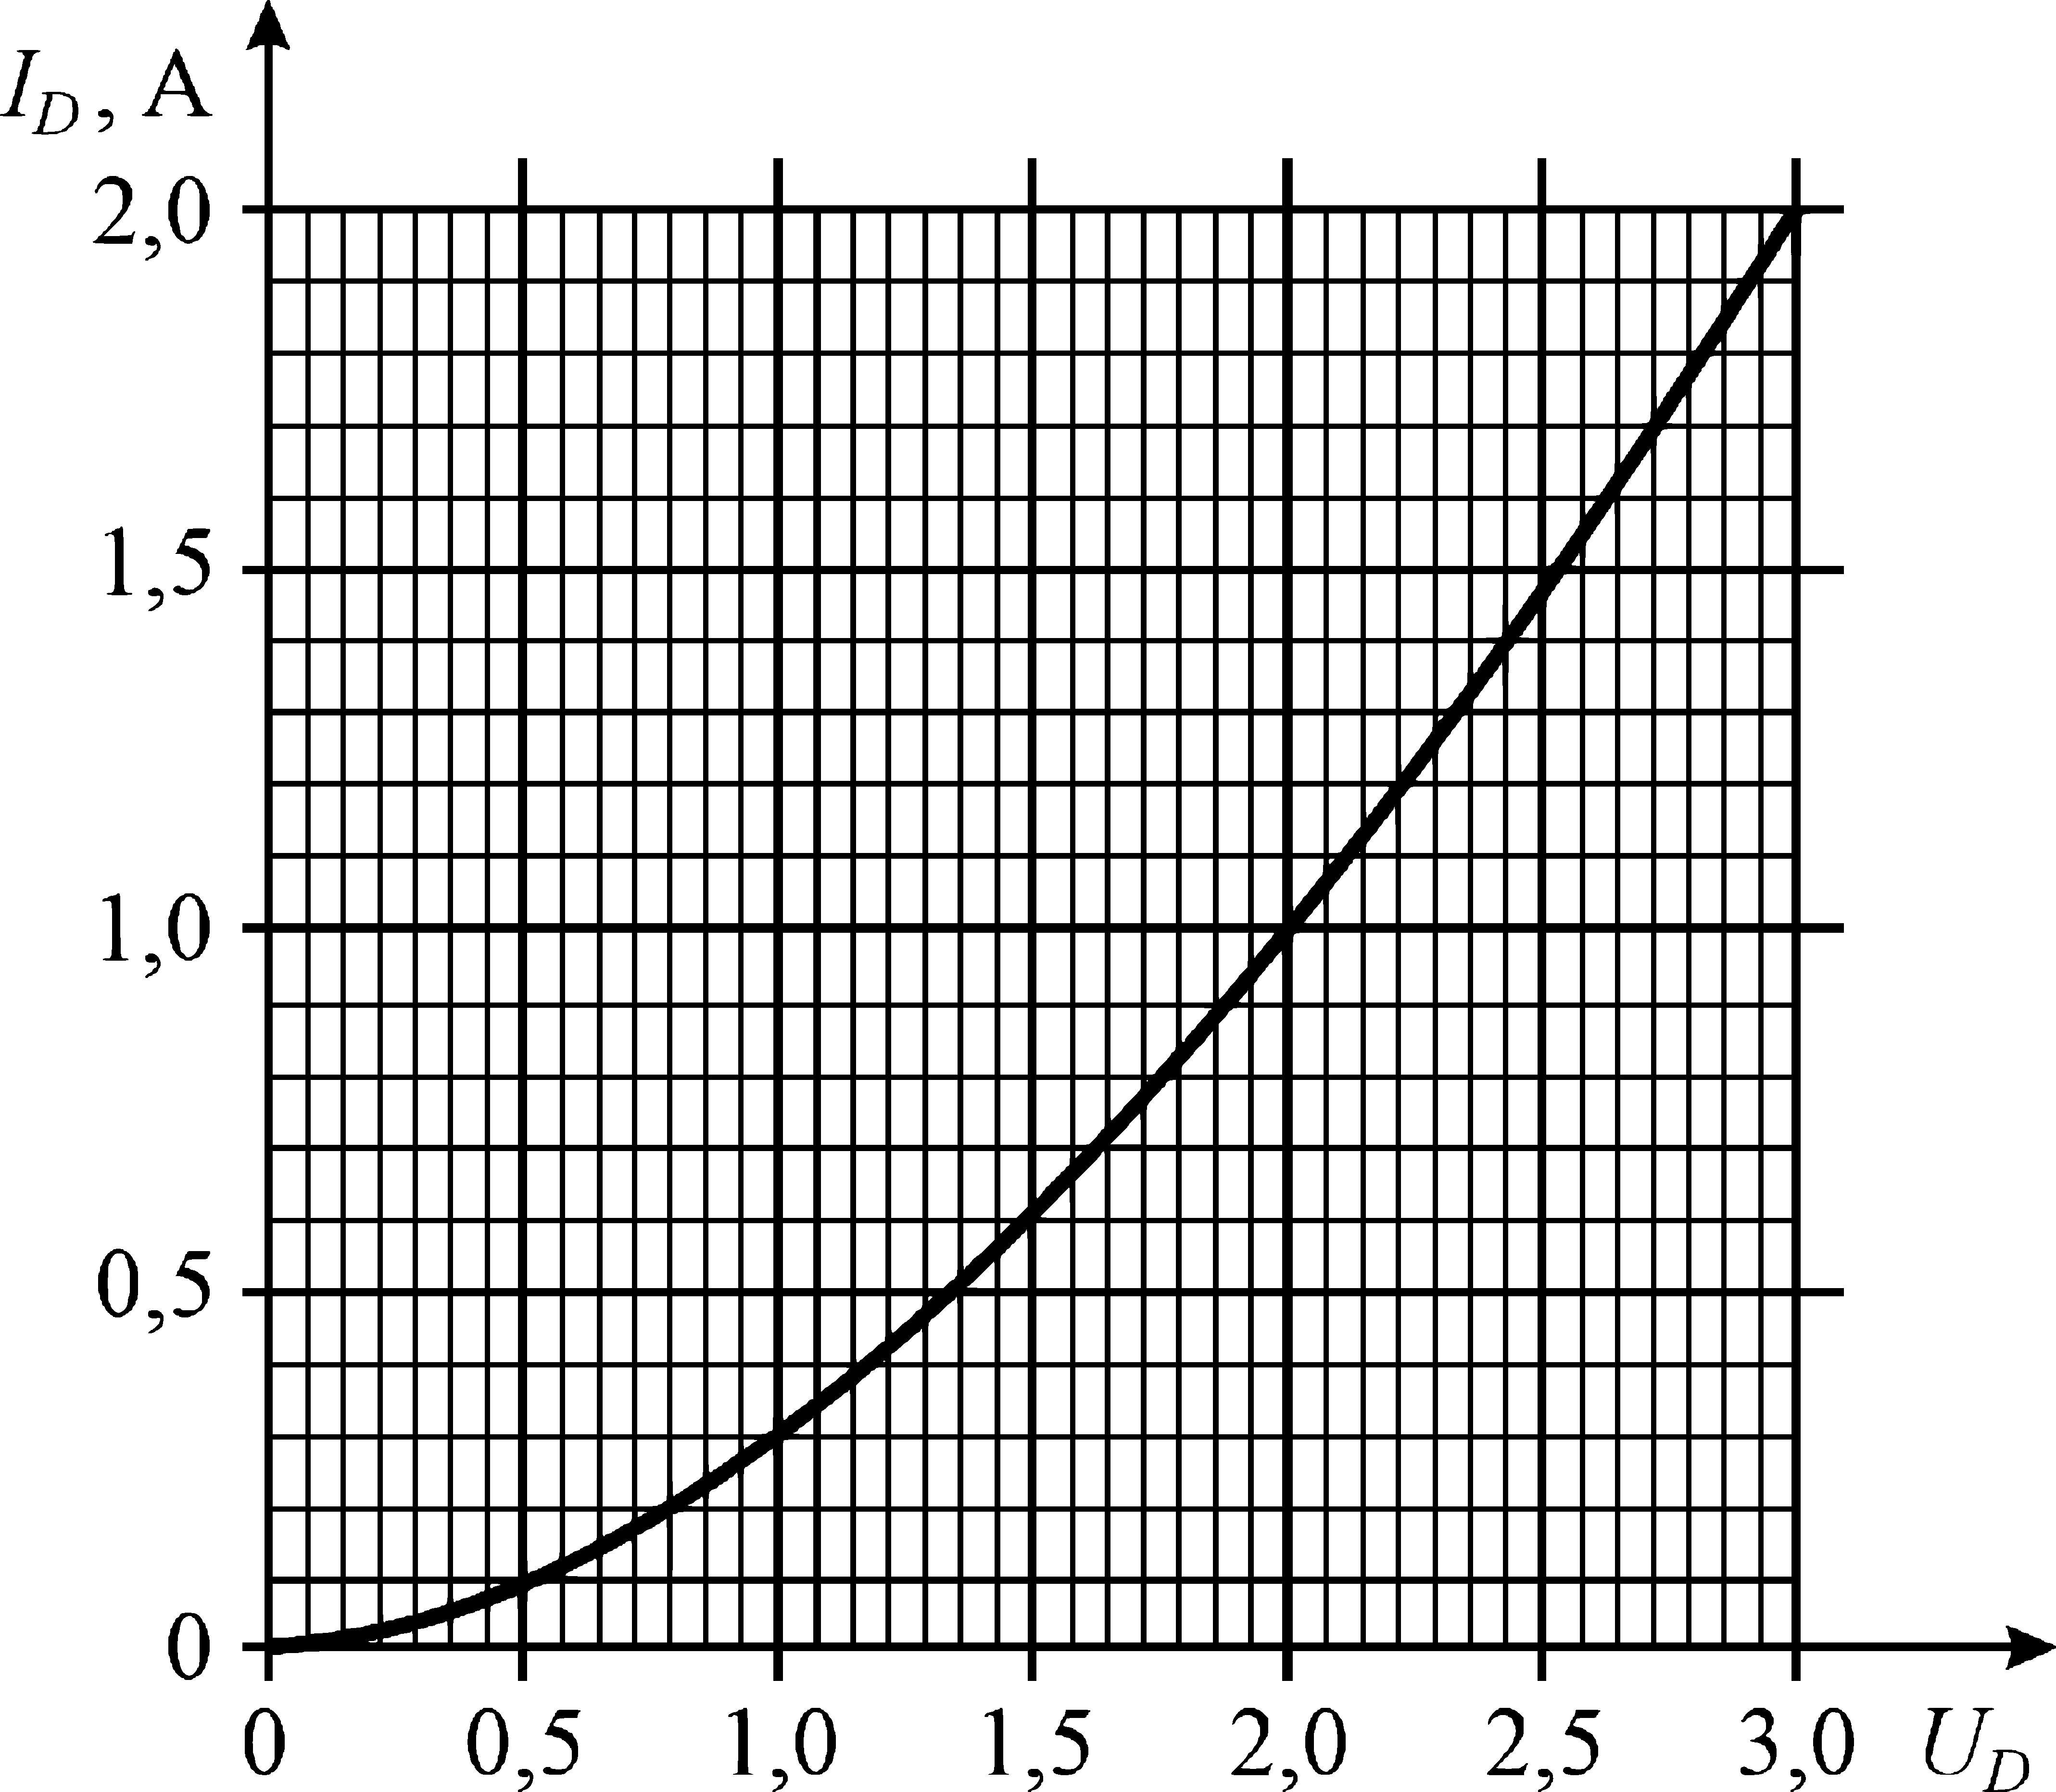
\includegraphics[width=0.7\textwidth]{Anh/iom1.pdf}
     \\Hình 2.
 \end{center}
\begin{enumerate}[1)]
    \item Viết đầy đủ các phương trình cho dòng điện chạy trong các nhánh của mạch điện trong hình 1. Các phương trình phải bao gồm điện áp $U$ của các nhánh song song cùng với điện áp $\xi$ của nguồn điện, điện trở thuần $R$ và hệ số $\alpha$.
    \item Xác định số chỉ của ampe kế với độ  chính xác tối thiểu là $10 \%$. Bỏ qua điện trở của dây dẫn. Viết câu trả lời bằng đơn vị $\mathrm{A}$ và cho biết độ chính xác của kết quả.
\end{enumerate}
\begin{center}
    \bf Phần II: Phi tuyến tính và sự phóng điện của tụ điện.
\end{center}
\immini{Nối varistor có hệ số $\alpha$ với một tụ điện đã được nạp điện (xem hình 3). Nếu dây dẫn được làm lạnh đủ, chúng sẽ trở nên siêu dẫn và tụ điện sẽ xả hết điện trong thời gian $t_0 = 0,02 ~\mathrm{s}$. Biết thuộc tính của varistor không phụ thuộc vào nhiệt độ.}
{


\tikzset{every picture/.style={line width=0.75pt}} %set default line width to 0.75pt        

\begin{tikzpicture}[x=0.75pt,y=0.75pt,yscale=-1,xscale=1]
%uncomment if require: \path (0,418); %set diagram left start at 0, and has height of 418

%Shape: Contact [id:dp08886901469143238] 
\draw   (113.85,136.93) -- (113.85,149.1) (113.85,177.5) -- (113.85,165.33) (139.7,149.1) -- (88,149.1) (139.7,165.33) -- (88,165.33) ;
%Shape: Right Angle [id:dp18670073540497323] 
\draw   (113.85,136.93) -- (113.85,99.83) -- (185.67,99.83) ;
%Shape: Right Angle [id:dp6174860778702249] 
\draw   (176.3,219.33) -- (113.85,219.33) -- (113.85,177.5) ;
%Shape: Resistor [id:dp24304015186446315] 
\draw   (245,143.92) -- (245,181.59) -- (229.13,181.59) -- (229.13,143.92) -- (245,143.92) -- cycle (237.07,133.33) -- (237.07,143.92) (237.07,181.59) -- (237.07,192.18) ;
%Shape: Sine Wave Form [id:dp9035485123364762] 
\draw  [line width=2.25]  (237.43,153.86) .. controls (242.34,157.32) and (242.36,158.96) .. (237.43,162.37) .. controls (232.49,165.79) and (232.46,167.39) .. (237.43,170.89) ;
%Shape: Right Angle [id:dp9499664503536653] 
\draw   (185.67,99.83) -- (237.07,99.83) -- (237.07,133.33) ;
%Shape: Right Angle [id:dp5719302324978046] 
\draw   (237.07,192.18) -- (237.07,219.33) -- (176.3,219.33) ;
\end{tikzpicture}
\\Hình 3.
}
\begin{enumerate}[1)]
    \item Biểu diễn $t_0$ theo điện dung $C$, điện tích ban đầu của tụ điện $q_0$ và hệ số $\alpha$ của varistor.
    \item Nếu tụ điện chỉ phóng điện qua các dây nối ở nhiệt độ phòng thì điện tích giảm đi một lượng $e$ trong thời gian $\tau = 1 ~\mathrm{ms}$ ($e$ là cơ số của logarit tự nhiên). Hãy tìm mối liên hệ giữa $\tau$ và điện trở $r$ của dây dẫn, từ đó suy ra phương trình tương ứng.
    \item Xác định thời điểm $t$ mà tại đó đòng điện giảm từ giá trị ban đầu $I_0$ về $I$, giả sử tụ điện chỉ  phóng điện qua varistor ở nhiệt độ phòng. Viết câu trả lời theo $r, C, \alpha, I$ và $I_0$.
    \item Xác định thời điểm $t_1$ mà tại đó điện tích của tụ giảm đi $n = 10 \ 000$ lần, giả sử tụ điện phóng điện qua cả dây dẫn và varistor ở nhiệt độ phòng. Hãy tìm phương trình biểu diễn $t_1$ qua $t_0, \tau$, $n$ và nhận xét giá trị tính bằng số (theo $\mathrm{ms}$) của $t_1$ với độ chính xác tối thiểu $10 \%$. 
\end{enumerate}

\begin{center}
    \bf Phần III: Phi tuyến tính và dao động tắt dần.
\end{center}
\immini{Trong thí nghiệm tiếp theo, mạch điện gồm một tụ điện, một varistor (với hệ số $\alpha$) và cuộn cảm siêu dẫn $L$
(xem hình 4). Các dây dẫn cũng được duy trì ở trạng thái siêu dẫn. Trong trường hợp này, dao động tắt dần bắt đầu trong
mạch và khi dòng điện biến mất lần đầu tiên, điện tích của tụ điện nhỏ hơn giá trị ban đầu $10 \%$.}
{

\tikzset{every picture/.style={line width=0.75pt}} %set default line width to 0.75pt        

\begin{tikzpicture}[x=0.75pt,y=0.75pt,yscale=-1,xscale=1]
%uncomment if require: \path (0,418); %set diagram left start at 0, and has height of 418

%Shape: Contact [id:dp26517604501135117] 
\draw   (251.32,138.89) -- (251.32,151.11) (251.32,179.64) -- (251.32,167.42) (277.47,151.11) -- (225.17,151.11) (277.47,167.42) -- (225.17,167.42) ;
%Shape: Right Angle [id:dp8160408833509483] 
\draw   (251.32,138.89) -- (251.32,100.67) -- (261.5,100.67) ;
%Shape: Right Angle [id:dp7364908678000435] 
\draw   (314.5,221.67) -- (251.32,221.67) -- (251.32,179.64) ;
%Shape: Resistor [id:dp26655342074498534] 
\draw   (384,145.91) -- (384,183.75) -- (367.94,183.75) -- (367.94,145.91) -- (384,145.91) -- cycle (375.97,135.27) -- (375.97,145.91) (375.97,183.75) -- (375.97,194.39) ;
%Shape: Sine Wave Form [id:dp947924618662443] 
\draw  [line width=2.25]  (376.34,155.89) .. controls (381.3,159.37) and (381.33,161.01) .. (376.34,164.45) .. controls (371.34,167.88) and (371.31,169.49) .. (376.34,173) ;
%Shape: Right Angle [id:dp3971851855646844] 
\draw   (348.42,100.67) -- (375.97,100.67) -- (375.97,135.27) ;
%Shape: Right Angle [id:dp2129631794566038] 
\draw   (375.97,194.39) -- (375.97,221.67) -- (314.5,221.67) ;
%Shape: Inductor (Air Core) [id:dp547707303950224] 
\draw   (261.5,100.67) -- (280.58,100.67) .. controls (280.58,95.28) and (284.38,90.9) .. (289.06,90.9) .. controls (293.74,90.9) and (297.54,95.28) .. (297.54,100.67) .. controls (297.54,95.28) and (301.34,90.9) .. (306.02,90.9) .. controls (310.7,90.9) and (314.5,95.28) .. (314.5,100.67) .. controls (314.5,95.28) and (318.3,90.9) .. (322.98,90.9) .. controls (327.66,90.9) and (331.46,95.28) .. (331.46,100.67) .. controls (331.46,95.28) and (335.26,90.9) .. (339.94,90.9) .. controls (344.62,90.9) and (348.42,95.28) .. (348.42,100.67) -- (367.5,100.67) ;
\end{tikzpicture}
\\Hình 4.}
\begin{enumerate}[1)]
    \item Giả sử rằng tại một thời điểm nào đó trước khi kết thúc nửa chu kỳ dao động đầu tiên, điện tích của tụ điện đã giảm từ giá trị ban đầu $q_0$ xuống $q$. Dòng điện trong mạch lúc này bằng bao nhiêu? Biễu diễn kết quả theo $\alpha, L, C, q$ và $q_0$. Sẽ rất hữu ích khi biết rằng lời giải của một phương trình phi tuyến phức tạp của chuyển động cơ học thường được đơn giản hóa đáng kể nếu biến nó thành một phương trình cho tốc độ biến thiên năng lượng.
    \item Xác định năng lượng của tụ điện được giải phóng dưới dạng nhiệt trong varistor cho đến khi điện tích tụ của điện bằng không lần đầu tiên. Đánh giá câu trả lời (theo phần trăm) với độ chính xác tối thiểu $10 \%$ (nghĩa là sai số không được vượt quá $10\%$ kết quả).
    \item Phần nào của năng lượng ban đầu của tụ điện được giải phóng dưới dạng nhiệt trong varistor cho đến khi dòng điện bằng không lần đầu tiên? Đánh giá câu trả lời theo phần trăm.
    \item Phần nào của năng lượng ban đầu của tụ điện được giải phóng dưới dạng nhiệt trong varistor tại thời điểm điện tích của tụ điện bằng không lần thứ hai? Đánh giá câu trả lời (theo phần trăm) với độ chính xác tối thiểu $10 \%$ (nghĩa là sai số không được vượt quá $10\%$ kết quả).
\end{enumerate}
\textbf{Lưu ý.} Hệ số $\alpha$ của varistor trong mỗi phần của bài toán là khác nhau!
\end{vd}
\begin{loigiai}\[\]
\textbf{Phần I.}
\begin{enumerate}[1)]
    \item Các kí hiệu sẽ sử dụng trong bài toán: gọi $U$ là hiệu điện thế chung của bốn nhánh song song (giữa dây dẫn ngang phía trên và phía dưới), $I_{1,2,3,4}$ là dòng điện chạy qua các nhánh (theo thứ tự từ trái sang phải, chiều dương của các dòng điện được thể hiện bằng các mũi tên như trong hình 1a).
    \begin{center}
        

\tikzset{every picture/.style={line width=0.75pt}} %set default line width to 0.75pt        

\begin{tikzpicture}[x=0.75pt,y=0.75pt,yscale=-1,xscale=1]
%uncomment if require: \path (0,375); %set diagram left start at 0, and has height of 375

%Shape: Output [id:dp40223434915515366] 
\draw   (144.79,85.1) .. controls (144.79,77.87) and (150.61,72) .. (157.78,72) .. controls (164.96,72) and (170.78,77.87) .. (170.78,85.1) .. controls (170.78,92.34) and (164.96,98.21) .. (157.78,98.21) .. controls (150.61,98.21) and (144.79,92.34) .. (144.79,85.1) -- cycle (131.79,85.1) -- (144.79,85.1) (183.77,85.1) -- (170.78,85.1) ;
%Shape: Right Angle [id:dp45345897491864395] 
\draw   (126.34,108.7) -- (126.34,85.1) -- (131.79,85.1) ;
%Shape: Battery [id:dp26785775847506166] 
\draw  [fill={rgb, 255:red, 0; green, 0; blue, 0 }  ,fill opacity=1 ] (126.34,156.46) -- (126.34,134.97) (108.43,130.19) -- (144.25,130.19) (126.34,130.19) -- (126.34,108.7) (117.39,136.88) -- (117.39,134.97) -- (135.3,134.97) -- (135.3,136.88) -- (117.39,136.88) -- cycle ;
%Shape: Resistor [id:dp428828370029964] 
\draw   (131.46,166.59) -- (131.46,202.59) -- (121.22,202.59) -- (121.22,166.59) -- (131.46,166.59) -- cycle (126.34,156.46) -- (126.34,166.59) (126.34,202.59) -- (126.34,212.72) ;
%Shape: Right Angle [id:dp37458769585276563] 
\draw   (188.21,226.68) -- (126.34,226.68) -- (126.34,212.72) ;
%Straight Lines [id:da02650510741377521] 
\draw    (188.21,212.72) -- (188.21,226.68) ;
\draw [shift={(188.21,226.68)}, rotate = 90] [color={rgb, 255:red, 0; green, 0; blue, 0 }  ][fill={rgb, 255:red, 0; green, 0; blue, 0 }  ][line width=0.75]      (0, 0) circle [x radius= 2.68, y radius= 2.68]   ;
%Shape: Resistor [id:dp5839554899269066] 
\draw   (193.27,166.59) -- (193.27,202.59) -- (183.03,202.59) -- (183.03,166.59) -- (193.27,166.59) -- cycle (188.15,156.46) -- (188.15,166.59) (188.15,202.59) -- (188.15,212.72) ;
%Shape: Battery [id:dp021184207056247795] 
\draw  [fill={rgb, 255:red, 0; green, 0; blue, 0 }  ,fill opacity=1 ] (188.15,108.7) -- (188.15,130.19) (206.06,134.97) -- (170.24,134.97) (188.15,134.97) -- (188.15,156.46) (197.1,128.28) -- (197.1,130.19) -- (179.19,130.19) -- (179.19,128.28) -- (197.1,128.28) -- cycle ;
%Straight Lines [id:da6706541214826243] 
\draw    (188.15,108.7) -- (188.15,85.1) ;
\draw [shift={(188.15,85.1)}, rotate = 270] [color={rgb, 255:red, 0; green, 0; blue, 0 }  ][fill={rgb, 255:red, 0; green, 0; blue, 0 }  ][line width=0.75]      (0, 0) circle [x radius= 2.68, y radius= 2.68]   ;
%Straight Lines [id:da4086835439710659] 
\draw    (183.77,85.1) -- (188.59,85.1) ;
%Straight Lines [id:da2917885452261588] 
\draw    (252.87,212.72) -- (252.87,226.68) ;
\draw [shift={(252.87,226.68)}, rotate = 90] [color={rgb, 255:red, 0; green, 0; blue, 0 }  ][fill={rgb, 255:red, 0; green, 0; blue, 0 }  ][line width=0.75]      (0, 0) circle [x radius= 2.68, y radius= 2.68]   ;
%Straight Lines [id:da14066596429940992] 
\draw    (188.21,226.68) -- (252.87,226.68) ;
%Shape: Resistor [id:dp4045940492883866] 
\draw   (257.99,166.59) -- (257.99,202.59) -- (247.75,202.59) -- (247.75,166.59) -- (257.99,166.59) -- cycle (252.87,156.46) -- (252.87,166.59) (252.87,202.59) -- (252.87,212.72) ;
%Shape: Resistor [id:dp571652007762723] 
\draw   (257.99,110.33) -- (257.99,146.33) -- (247.75,146.33) -- (247.75,110.33) -- (257.99,110.33) -- cycle (252.87,100.2) -- (252.87,110.33) (252.87,146.33) -- (252.87,156.46) ;
%Straight Lines [id:da38917417942454513] 
\draw    (252.87,100.2) -- (252.87,85.1) ;
\draw [shift={(252.87,85.1)}, rotate = 270] [color={rgb, 255:red, 0; green, 0; blue, 0 }  ][fill={rgb, 255:red, 0; green, 0; blue, 0 }  ][line width=0.75]      (0, 0) circle [x radius= 2.68, y radius= 2.68]   ;
%Straight Lines [id:da03606821117235004] 
\draw    (188.59,85.1) -- (253.35,85.1) ;
%Shape: Right Angle [id:dp9058220555439067] 
\draw   (253.35,85.1) -- (315.09,85.1) -- (315.09,115.19) ;
%Shape: Battery [id:dp6694974686185533] 
\draw  [fill={rgb, 255:red, 0; green, 0; blue, 0 }  ,fill opacity=1 ] (315.09,203.05) -- (315.09,181.56) (297.18,176.79) -- (333,176.79) (315.09,176.79) -- (315.09,155.3) (306.14,183.47) -- (306.14,181.56) -- (324.05,181.56) -- (324.05,183.47) -- (306.14,183.47) -- cycle ;
%Shape: Right Angle [id:dp5305063249969073] 
\draw   (315.09,203.05) -- (315.09,226.68) -- (252.87,226.68) ;
%Shape: Diode [id:dp3686655850262377] 
\draw  [fill={rgb, 255:red, 0; green, 0; blue, 0 }  ,fill opacity=1 ] (303.2,143.26) -- (315.09,127.22) -- (326.98,143.26) -- (303.2,143.26) -- cycle (315.09,155.3) -- (315.09,143.26) (303.2,127.22) -- (326.98,127.22) (315.09,127.22) -- (315.09,115.19) ;
%Shape: Sine Wave Form [id:dp14441278202793773] 
\draw  [line width=2.25]  (187.97,176.4) .. controls (191.14,179.71) and (191.15,181.27) .. (187.97,184.54) .. controls (184.78,187.81) and (184.77,189.34) .. (187.97,192.68) ;
%Shape: Sine Wave Form [id:dp4832496115476983] 
\draw  [line width=2.25]  (252.63,176.87) .. controls (255.8,180.19) and (255.81,181.75) .. (252.63,185.02) .. controls (249.44,188.28) and (249.43,189.81) .. (252.63,193.16) ;
%Shape: Sine Wave Form [id:dp029747975461203113] 
\draw  [line width=2.25]  (253.1,119.82) .. controls (256.27,123.13) and (256.29,124.7) .. (253.1,127.96) .. controls (249.92,131.23) and (249.9,132.76) .. (253.1,136.11) ;
%Straight Lines [id:da45555386757583727] 
\draw    (110,206) -- (110,166.33) ;
\draw [shift={(110,163.33)}, rotate = 450] [fill={rgb, 255:red, 0; green, 0; blue, 0 }  ][line width=0.08]  [draw opacity=0] (10.72,-5.15) -- (0,0) -- (10.72,5.15) -- (7.12,0) -- cycle    ;
%Straight Lines [id:da5648832182011037] 
\draw    (343,173) -- (343,133.33) ;
\draw [shift={(343,130.33)}, rotate = 450] [fill={rgb, 255:red, 0; green, 0; blue, 0 }  ][line width=0.08]  [draw opacity=0] (10.72,-5.15) -- (0,0) -- (10.72,5.15) -- (7.12,0) -- cycle    ;
%Straight Lines [id:da8180273933014601] 
\draw    (170,204) -- (170,164.33) ;
\draw [shift={(170,207)}, rotate = 270] [fill={rgb, 255:red, 0; green, 0; blue, 0 }  ][line width=0.08]  [draw opacity=0] (10.72,-5.15) -- (0,0) -- (10.72,5.15) -- (7.12,0) -- cycle    ;
%Straight Lines [id:da8943686905317443] 
\draw    (240,204) -- (240,164.33) ;
\draw [shift={(240,207)}, rotate = 270] [fill={rgb, 255:red, 0; green, 0; blue, 0 }  ][line width=0.08]  [draw opacity=0] (10.72,-5.15) -- (0,0) -- (10.72,5.15) -- (7.12,0) -- cycle    ;

% Text Node
\draw (150.28,77.24) node [anchor=north west][inner sep=0.75pt]    {$A$};
% Text Node
\draw (91,176.4) node [anchor=north west][inner sep=0.75pt]    {$I_{1}$};
% Text Node
\draw (349,146.4) node [anchor=north west][inner sep=0.75pt]    {$I_{4}$};
% Text Node
\draw (151,174.4) node [anchor=north west][inner sep=0.75pt]    {$I_{2}$};
% Text Node
\draw (221,174.4) node [anchor=north west][inner sep=0.75pt]    {$I_{3}$};
\end{tikzpicture}
        \\Hình 1a.
    \end{center}
    $R$ là giá trị của điện trở thuần. Từ đề bài, ta thấy $R = \dfrac{\xi}{I_0}$.\\
    Vì dòng điện và điện áp của varistor liên hệ với nhau bởi phương trình $U = \alpha I\abs{I}$, nên từ điều kiện đề bài, ta suy ra $\alpha = \dfrac{\xi}{I_0^2}$. Giả sử rằng đặc tính $I - V$ của diode là $I_D = I_0 \cdot f\tron{U_D/\xi}$. Khi đó, dòng điện qua các nhánh có thể được biểu diễn thông qua điện áp trên chúng như sau:
    \[\heva{I_1 &= \dfrac{\xi - U}{R} = I_0 (1-x) \\ 
    \alpha I_2^2 &= U+\xi \rt I_2 = I_0 \sqrt{1+x} \\ 
    2\alpha I_3^2 &= U \rt I_3 = I_0 \sqrt{\dfrac{x}{2}} \\ 
    I_4 &= I_0 f(1-x) },\]
    trong đó $x = \dfrac{U}{\xi}$ (sự chính xác của chiều dương các dòng điện đã chọn được xác minh trong quá trình giải). Ngoài ra, dòng điện phải thoả mãn định luật bảo toàn điện tích $I_2 + I_3 = I_1 + I_4$. Do đó, $x$ có thể xác định được qua phương trình: \[\sqrt{1+x} + \sqrt{\dfrac{x}{2}} = 1-x +  f(1-x).\]
    \item Theo đề bài, dòng điện qua diode bằng $I_0$ khi điện áp của diode bằng $\dfrac{1}{5}\xi$. Do đó, $f(0,2) = 1$, cho phép ta ``dịch chuyển'' đường cong $I-V$ của diode trên đồ thị, các dòng điện qua các nhánh khác được vẽ trên hình (đường cong màu đỏ trong hình 1b) và để giải phương trình trên bằng đồ thị: vẽ biểu đồ bên trái của phương trình và sau đó vẽ biểu đồ bên phải bằng cách cộng các đóng góp của các dòng điện tại mỗi $x$. \\
    Theo đồ thị, số chỉ của ampe kế (ứng với cường độ dòng điện qua điện trở) là $I_A = (0,27 \pm 0,02)~\mathrm{A}$. Sai số này đáp ứng được yêu cầu về độ chính xác cần thiết trong đề bài, ngay cả khi dưới độ chính xác này, nó có thể được cải thiện.
    \begin{center}
    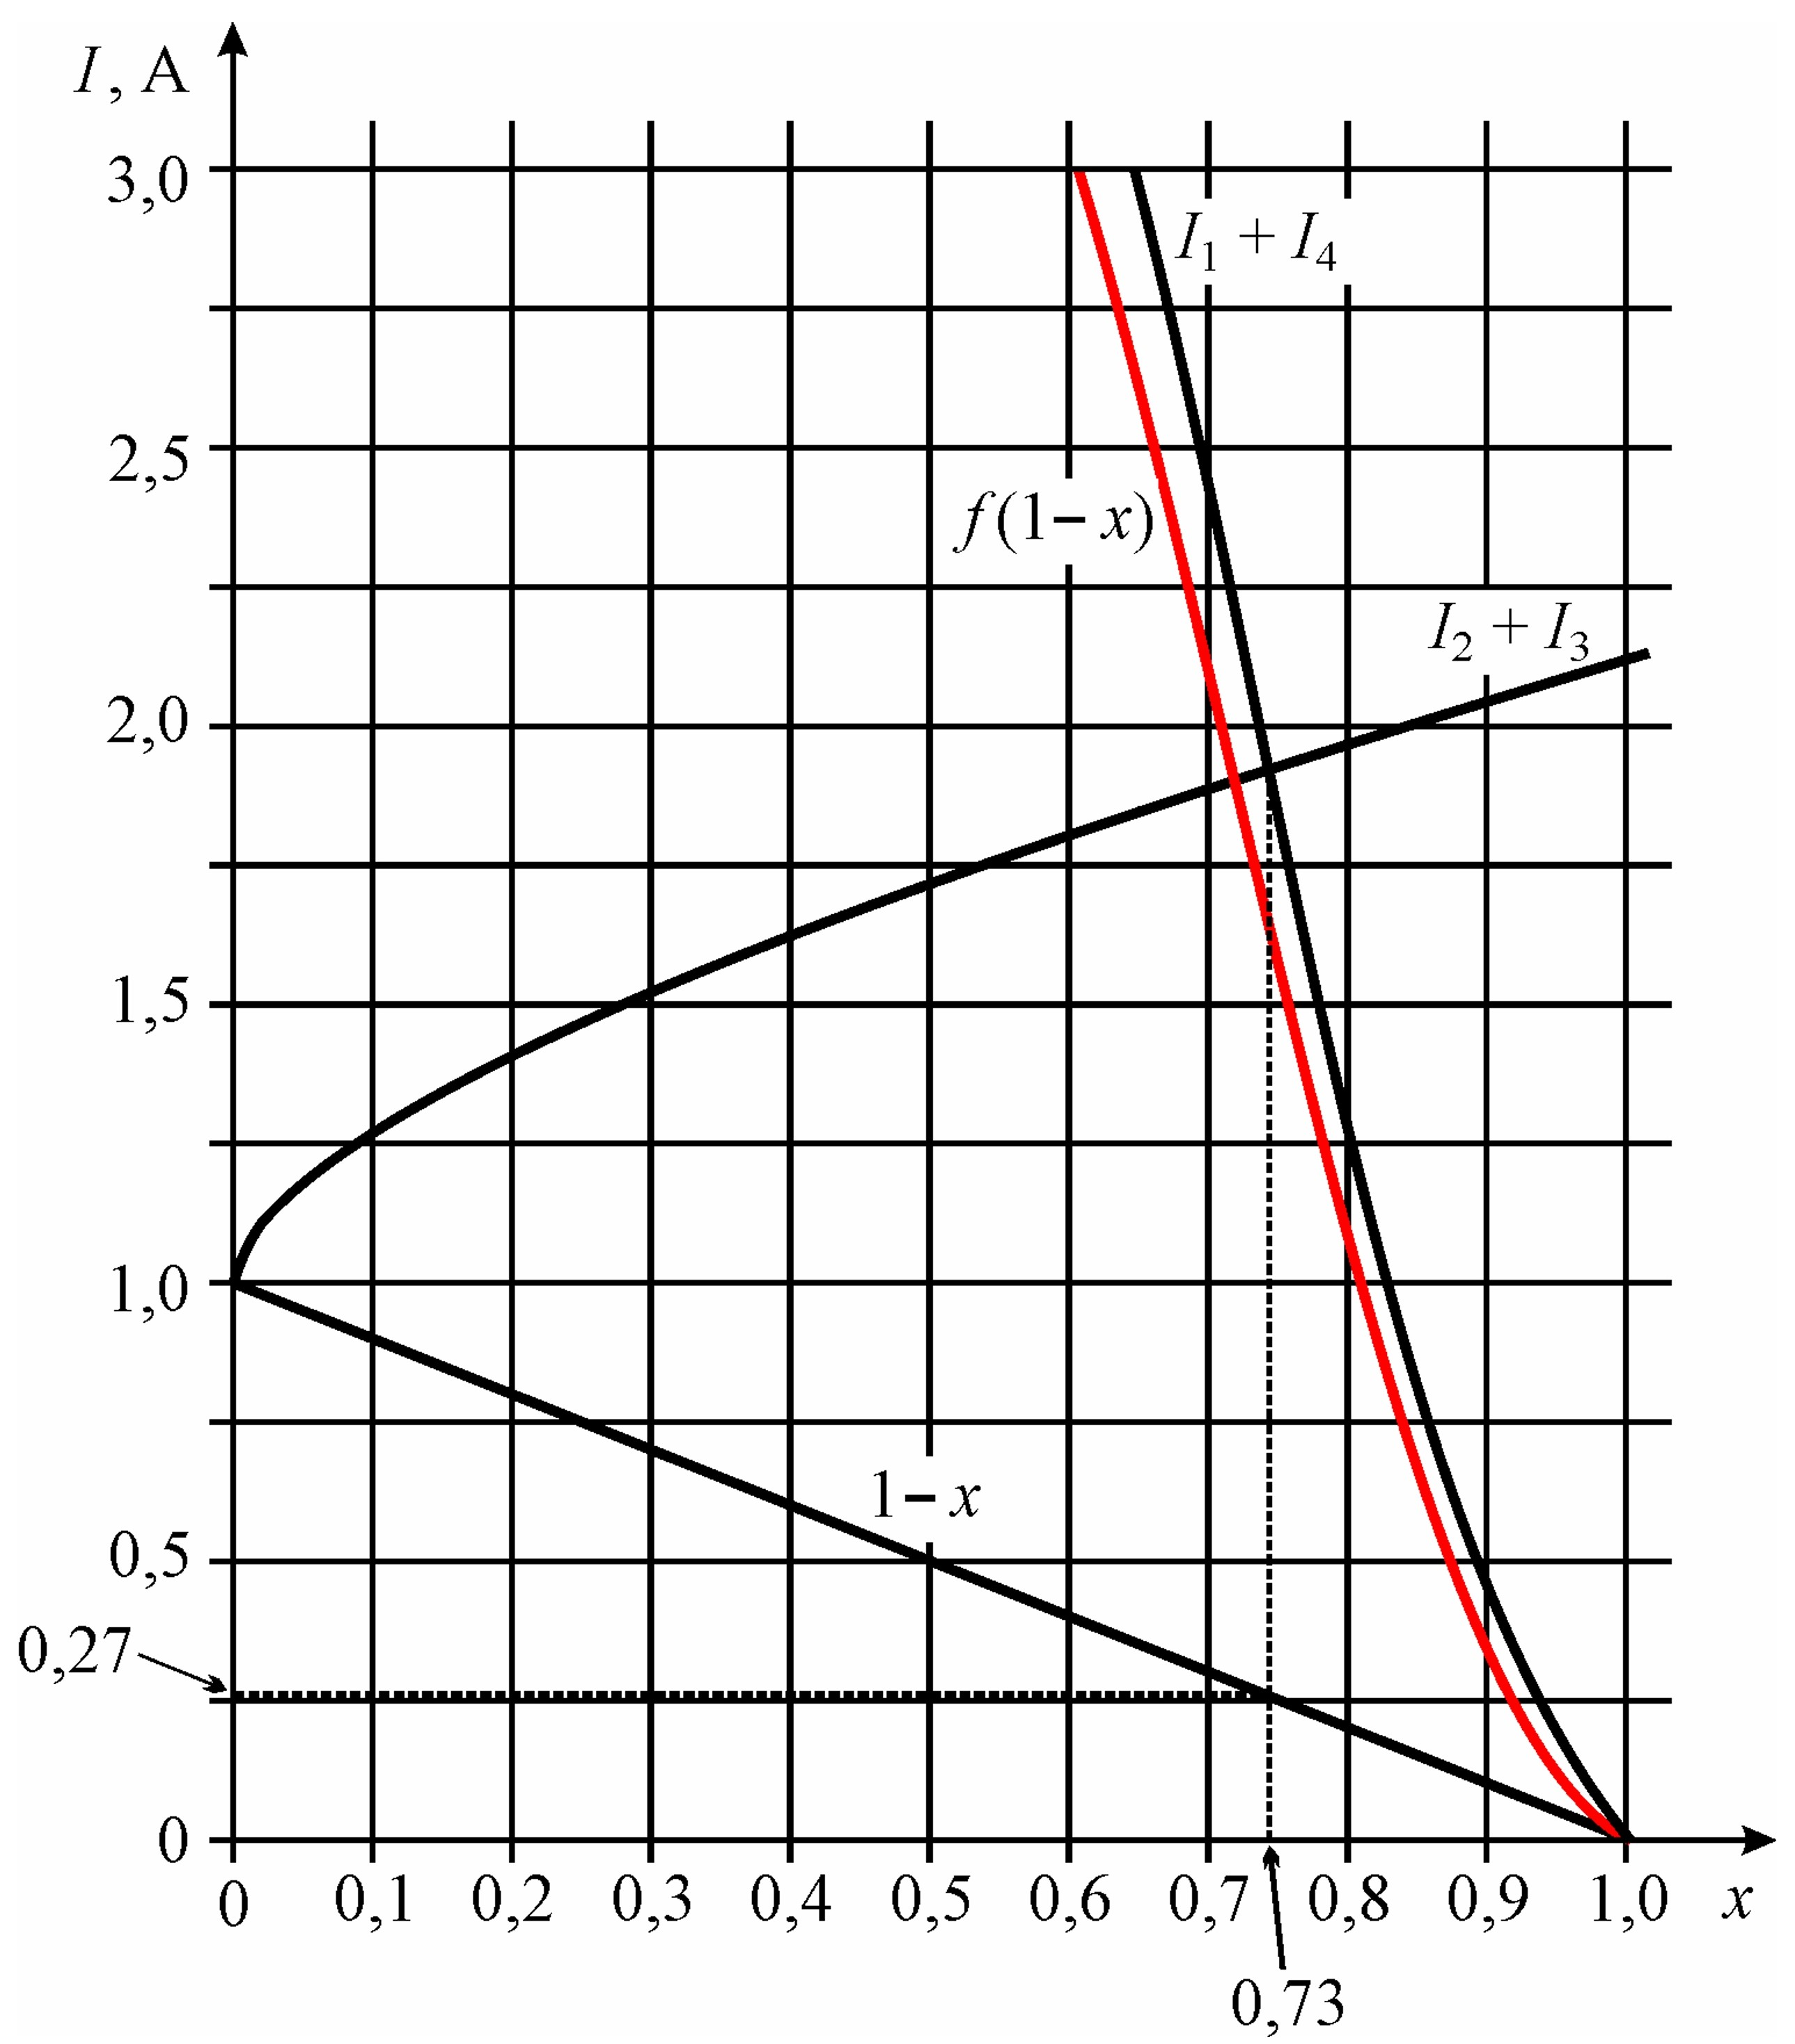
\includegraphics[scale=0.7]{Anh/IOM2018_2.jpg}
       \\ Hình 1b.
    \end{center}
\textbf{Lưu ý.} Kết quả thu được bằng phương pháp đồ thị có thể được cải thiện đáng kể khi sử dụng đại số. Ngay cả cách xây dựng thô sơ của đồ thị cũng giúp xác định rõ đáp án là  $x \approx 0,7$, và  $\left. f((1-x)\right|_{x \approx 0,7} \approx 9 - 10x$. Giả sử $x = 0,7 + \delta$ và sử dụng khai triển bậc nhất theo $\delta$, ta được 
\[\sqrt{1,7} + \sqrt{0,35} + \dfrac{1}{2} \tron{\dfrac{1}{\sqrt{1,7}} + \dfrac{1}{\sqrt{1,4}}} \delta = 2,3 - 11\delta.\]
Vậy $\delta \approx 0,0343$, vì vậy việc sửa chữa thực sự là nhỏ và sai số do tính toán ở đây là dưới $3 \%$. Sai số của đồ thị có thể được ước tính là $2\%$, do đó 
\[I_A = I_0 (1-x) \approx (0,266 \pm 0,011)~\mathrm{A}.\]
Người ta có thể thực hiện bước tiếp theo và đánh giá tiếp tuyến của đường cong diode $I-V$ tại dòng điện bằng $1,6~ \mathrm{A}$ (đây là dòng điện qua diode thu được bằng phép gần đúng thô sơ) và đánh giá các đạo hàm thứ hai, đường cong $I-V$ có thể được mô tả bằng một phương trình bậc hai. Khi làm như vậy, một lỗi tính toán trở nên không đáng kể so với lỗi đồ thị và độ chính xác còn cải thiện nhiều hơn: 
\[I_A \approx (0.267 \pm 0.005)~\mathrm{A}.\]
Tuy nhiên, độ chính xác của phương pháp đồ họa đủ để giải quyết vấn đề với điều kiện việc xây dựng là chính xác. Tuy nhiên, trong tiêu chí đánh giá có một phần thưởng bổ sung được dành riêng cho những người dự thi giảm lỗi gấp đôi so với lỗi được chỉ định trong đề bài. Lưu ý rằng một câu trả lời ''gần như chính xác'' thu được bằng một phương trình giải tích cho đường cong I-V của diode (phương trình này đã được các tác giả biết đến) là:
\[I_A \approx (0,26723 \pm 0,00001) ~\mathrm{A}.\]
\end{enumerate}
\begin{center}
    \bf Phần II.
\end{center}
\begin{enumerate}[1)]
    \item Một lần nữa, ta sử dụng đặc tính phi tuyến dòng điện-điện áp của varistor: $U = \alpha I\abs{I}$. Dòng điện chạy qua varistor thông qua dây siêu dẫn liên hệ với điện tích của tụ điện như sau:
    \[\dfrac{q}{C} = \alpha I^2 \rt I=\sqrt{\dfrac{q}{\alpha C}},\]
    (dòng điện này không đổi chiều và có thể xem là luôn dương). Một biểu thức cho tốc độ biến thiên điện tích:
    \[\dfrac{\dd q}{\dd t} = -I = -\sqrt{\dfrac{q}{\alpha C}},\]
    (điện tích của tụ điện đang giảm), do đó, thời gian xả hết điện: 
    \[t_{0} = \sqrt{\alpha C} \int_{0}^{q_{0}} \dfrac{\dd q}{\sqrt{q}}=2 \sqrt{\alpha C q_{0}},\]
    (trong đó $q_0$ là điện tích ban đầu của tụ). 
    \item Từ đề bài, ta dễ dàng nhận ra rằng:
    \[\dfrac{q}{C} = rI = r\dfrac{\dd q}{\dd t} \rt \tau = Cr \ln{e} = rC\]
    Vậy $\tau$ là một hằng số thời gian cho sự phóng điện của tụ qua dây dẫn ở nhiệt độ phòng, nghĩa là $\tau = rC$.
    \item Hãy viết một phương trình cho sự phóng điện qua varistor và dây dẫn có điện trở $r$. Trong trường hợp này:
    \[\dfrac{q}{C} = \alpha I^{2}+r I \Rightarrow q = C\left(\alpha I^{2}+r I\right),\]
    do đó:
    \[\dfrac{\dd q}{\dd t} = -I = C(2 \alpha I+r) \dfrac{\dd I}{\dd t}.\]
    Vậy thời gian để  dòng điện giảm từ $I_0$ về $I$ là:
    \[t = C \int_{I}^{I_{0}} \dd I\left(\dfrac{r}{I}+2 \alpha\right)=r C \ln \left(\dfrac{I_{0}}{I}\right)+2 \alpha C\left(I_{0}-I\right).\]
    \item Cường độ dòng điện ban đầu trong mạch được xác định bởi:
    \[\dfrac{q_{0}}{C} = \alpha I_{0}^{2}+r I_{0} \Rightarrow I_{0} = \dfrac{r}{2 \alpha}\left[\sqrt{\dfrac{4 \alpha q_{0}}{C r^{2}}+1}-1\right].\]
    Dòng điện trong mạch tại thời điểm điện tích tụ giảm đi $n$ lần là
    \[I=\dfrac{r}{2 \alpha}\left[\sqrt{\dfrac{4 \alpha q_{0}}{n C r^{2}}+1}-1\right].\]
    Dễ dàng nhận thấy rằng:
    \[\dfrac{4 \alpha q_{0}}{C r^{2}}=\dfrac{4 \alpha C q_{0}}{(C r)^{2}}=\dfrac{t_{0}^{2}}{\tau^{2}},\]
    do đó thời gian cần tìm là:
    \[t=\tau \ln \left(\dfrac{\sqrt{\left(t_{0} / \tau\right)^{2}+1}-1}{\sqrt{\left(t_{0} / \tau \sqrt{n}\right)^{2}+1}-1}\right)+\sqrt{t_{0}^{2}+\tau^{2}}-\sqrt{\dfrac{t_{0}^{2}}{n}+\tau^{2}}.\]
    Ta có thể đánh giá giá trị số trực tiếp bằng công thức này (cho kết quả $t \approx 25,873 \mathrm{ms}$), hoặc  có thể thử đơn giản hóa công thức trước. Để làm điều này, hãy lưu ý rằng: $\dfrac{t_{0}^{2}}{\tau^{2}} \gg 1$ và $\dfrac{t_{0}^{2}}{n \tau^{2}} \ll 1$. Suy ra:
    \[t \approx t_{0} + \tau \ln \left(\dfrac{2 n \tau}{e t_{0}}\right) \approx 25,9 \mathrm{~ms}.\]
    Câu trả lời này đáp ứng các yêu cầu về độ chính xác.
    \textbf{Nhận xét.} Kết quả rất thú vị vì một điện trở nhỏ (về mặt số học, $\tau$  chỉ bằng $5\%$ của $t_0$) lại có thể thay đổi kết quả đến gần như $30\%$! Trên thực tế, điện trở của dây thay đổi đáng kể giá trị của $q(t)$ quanh $q=0$: nó kéo dài thời gian phóng điện.
\end{enumerate}
\begin{center}
    \bf Phần III.
\end{center}
\begin{enumerate}[1)]
    \item Hãy viết phương trình dao động trong mạch. Giống như trước, ta giả sử dòng điện của tụ điện là
    \[I = -\dfrac{\dd q}{\dd t}>0,\]
    (tức bây giờ, ta giới hạn một lời giải cho nửa chu kỳ đầu tiên):
    \[\dfrac{q}{C}=\alpha I^{2}+L \dfrac{\dd I}{\dd t} \Rightarrow \dfrac{\dd I}{\dd t}+\dfrac{\alpha}{L} I^{2}=\dfrac{q}{L C}.\]
    Để phân tích tốc độ biến thiên điện tích tụ điện và năng lượng cuộn cảm, ta chỉ cần liên hệ giữa điện tích và cường độ dòng điện, nếu sự phụ thuộc vào thời gian của các đại lượng này là không cần thiết. Bây giờ, chúng ta đánh giá tốc độ biến thiên của động năng trong cơ học:
    \[m \dfrac{\dd V}{\dd t} = F(x, V) \Rightarrow m \dfrac{V \dd V}{V \dd t} = F(x, V) \Rightarrow \dfrac{\dd}{\dd x}\left(\dfrac{V^{2}}{2}\right)=\dfrac{F(x, V)}{m}.\]
    Bằng cách tương tự, công thức trên cho đạo hàm theo thời gian của dòng điện có thể được biến đổi thành
    \[\dfrac{\dd I}{\dd t}=I \dfrac{\dd I}{I \dd t}=-I \dfrac{\dd I}{\dd q}=-\dfrac{1}{2} \dfrac{\dd\left(I^{2}\right)}{\dd q}.\]
    Ta thu được một phương trình cho $I^{2}(q)$:
    \[\dfrac{\dd\left(I^{2}\right)}{\dd q}-\dfrac{2 \alpha}{L} I^{2}=-\dfrac{2 q}{L C}.\]
    Phương trình tương tự sau đây nếu người ta áp dụng một đối số tương tự cho tốc độ biến thiên của năng lượng tích trữ trong mạch.\\
    Có thể loại bỏ vế phải bằng cách thay thế tuyến tính $\tilde{I}^{2}(q)=A q+B$, phương trình trở thành
    \[\heva{-\dfrac{2 \alpha}{L} A = -\dfrac{2}{L C} \\
    A-\dfrac{2 \alpha}{L} B = 0} \rt \tilde{I}^{2}(q)=\dfrac{q}{\alpha C}+\dfrac{L}{2 \alpha^{2} C}.\]
    Sau đó, ta có thể thay đổi các biến bằng cách viết:
    \[I^{2}(q)=\tilde{I}^{2}(q)+F(q)=\dfrac{q}{\alpha C}+\dfrac{L}{2 \alpha^{2} C}+F(q),\]
    phương trình trở thành:
    \[\dfrac{\dd F}{\dd q}-\dfrac{2 \alpha}{L} F=0.\]
    Như vậy
    \[F(q)=D \cdot \exp \left(\frac{2 \alpha}{L} q\right),\]
    (trong đó $D = \const$), nên $I^{2}(q)$  trong nửa chu kỳ dao động đầu bằng:
    \[I^{2}(q) = \dfrac{q}{\alpha C}+\dfrac{L}{2 \alpha^{2} C}+D \cdot \exp \left(\dfrac{2 \alpha}{L} q\right).\]
    Nếu $q_0$ là điện tích ban đầu của tụ thì $I^{2}\left(q_{0}\right)=0$. Do đó
    \[D = -\dfrac{1}{\alpha C}\left(\dfrac{L}{2 \alpha}+q_{0}\right) \cdot \exp \left(-\dfrac{2 \alpha}{L} q_{0}\right),\]
    kết quả cuối cùng là
    \[I(q)=\sqrt{\dfrac{1}{\alpha C}\left\{\dfrac{L}{2 \alpha}+q-\left(\dfrac{L}{2 \alpha}+q_{0}\right) \cdot \exp \left(\dfrac{2 \alpha}{L}\left(q-q_{0}\right)\right)\right\}}.\]
    \item Dòng điện biến mất lần đầu tại thời điểm kết thúc nửa chu kỳ dao động đầu tiên, khi điện tích của tụ đổi cực và bằng $q_1 = - 0.9 q_0$. Do đó, $I^{2}\left(-0,9 q_{0}\right)=0$ và phương trình này giúp ta xác định điện tích ban đầu của tụ điện. Để cho thuận tiện, ta đặt một biến mới $z \equiv \dfrac{2 \alpha}{L} q_{0}$, khi đó 
    \[1 - 0.9 z - (1+z) e^{-1.9 z}=0 \Rightarrow e^{1.9 z} = \dfrac{1+z}{1-0.9 z}.\]
    Phương trình cũng có thể được giải một cách thủ công. Để làm điều này, trước tiên ta có thể nhận thấy từ đồ thị là $z \ll 1$ và sau đó khai triển hai vế đến bậc thứ tư (điều này là cần thiết ví các bậc không và một bị triệt tiêu):
    \[\dfrac{(1.9)^{2}}{2} z^{2}+\dfrac{(1.9)^{3}}{6} z^{3}+\dfrac{(1.9)^{4}}{24} z^{4} \approx 1.9 \cdot 0.9 z^{2}+1.9 \cdot(0.9)^{2} z^{3}+1.9 \cdot(0.9)^{3} z^{4}.\]
    Điều này cho một phương trình bậc hai  theo $z$, nghiệm dương của nó là $z \approx 0.17$. Sai số của bặc $z^2$ là nhỏ hơn $3 \%$, do đó đáp ứng được yêu cầu bài toán  (khai triển lên đến bậc $z^3$ tạo ra một phương trình tuyến tính nhưng sai số là của bậc $z$ và điều này là không đủ chính xác; kết quả tính được là $x \approx 0.24$ sai lệch so với câu trả lời đúng hơn $10\%$). Một đáp án tìm được với sự trợ giúp của Excel là $z \approx 0.1665 \pm 0.0001$.\\
    Năng lượng ban đầu của tụ điện bằng
    \[E_{0}=\dfrac{q_{0}^{2}}{2 C}=\dfrac{L^{2}}{8 \alpha^{2} C} z^{2}.\]
    Khi điện tích của tụ điện bằng không lần đầu, dòng điện qua cuộn cảm đạt cực đại. Năng lượng cuộn cảm lúc này cũng đạt cực đại:
    \[E_{L}(0) = \dfrac{LI^{2}(0)}{2} = \dfrac{L}{2 \alpha C}\left\{\dfrac{L}{2 \alpha}-\left(\dfrac{L}{2 \alpha}+q_{0}\right) \cdot \exp \left(-\dfrac{2 \alpha}{L} q_{0}\right)\right\}=2 E_{0} \dfrac{1-(1+z) e^{-z}}{z^{2}}.\]
    Rõ ràng, nhiệt lượng chỉ tạo ra trong varistor và bằng
    \[Q_{1}=E_{0}-E_{L}(0),\]
    Do đó, tại 
    \begin{itemize}
        \item $z \approx 0,1665, \dfrac{Q_{1}}{E_{0}} = 1-2 \dfrac{1-(1+z) e^{-z}}{z^{2}} \approx 0,1044$;
        \item $z \approx 0,17$, $\dfrac{Q_{1}}{E_{0}} \approx 0,1064$.
    \end{itemize}
    Vì vậy, khoảng $(10 - 11)\%$ năng lượng ban đầu đã bị mất cho đến thời điểm này.
    \item Sự mất mát năng lượng trong nửa chu kỳ đầu tiên có thể dễ dàng tìm thấy bằng sự mất mát điện tích của tụ điện:
    \[Q_{1}^{\prime}=\dfrac{q_{0}^{2}}{2 C}-\dfrac{\left(-0,9 q_{0}\right)^{2}}{2 C} = 0,19 E_{0} \text {, nghĩa là } \dfrac{Q_{1}^{\prime}}{E_{0}} = 19 \%.\]
    \item Điện tích của tụ bằng không lần thứ hai trong nửa chu kỳ sau, khi dòng điện đổi chiều. Lời giải phải được thực hiện lại trong nửa chu kỳ sau, mặc dù lập luận vẫn giữ nguyên: chỉ cần thay độ lớn của điện tích tụ điện ban đầu bằng $0,9q_0$. Nhiệt lượng tỏa ra khi điện tích thay đổi từ $q_{1}=-0,9 q_{0}$ đến $0$ (lần thứ hai) có thể tìm thấy từ điều kiện
    \[\begin{aligned}
        E_{L}^{\prime}(0) &= \dfrac{L I^{\prime 2}(0)}{2} \\
        &= \dfrac{L}{2 \alpha C}\left\{\dfrac{L}{2 \alpha}-\left(\dfrac{L}{2 \alpha}+\left|q_{1}\right|\right) \cdot \exp \left(-\dfrac{2 \alpha}{L}\left|q_{1}\right|\right)\right\}\\
        &= 2 E_{0} \dfrac{1-(1+0,9 z) e^{-0,9 z}}{z^{2}}.
    \end{aligned}\]
    Suy ra
    \[\dfrac{Q_{2}}{E_{0}}=1-2 \dfrac{1-(1+0,9 z) e^{-0,9 z}}{z^{2}} \approx 0,2665 \approx 27 \%.\]
\end{enumerate}
\end{loigiai}


\begin{vd}[Zenner Diode]
    Cuộn cảm $L$ và tụ điện $C$ được mắc nối tiếp bằng một công tắc. Ban đầu công tắc được mở và tụ điện được cung cấp một điện tích $q_0$. Sau đó đóng công tắc.
    \begin{enumerate}[1)]
        \item Điện tích $q$ trên tụ điện và cường độ dòng điện $I$ trong mạch thay đổi thế nào theo thời gian. Vẽ biểu đồ pha của mạch trên đồ thị $I-q$ . Dùng dấu mũi tên để chỉ ra chiều thay đổi theo thời gian của biểu đồ.
    \end{enumerate}
    Diode Zener là một mạch điện phi tuyến tính hoạt động như một diode hai chiều: nó cho phép dòng điện chạy theo chiều dương khi điện áp chuyển tiếp trên nó vượt quá một giá trị ngưỡng nhất định, nhưng nó cũng cho phép dòng điện chạy ngược chiều khi tiếp xúc với hiệu điện thế âm đủ lớn. Thông thường hai thang đo điện áp khá khác nhau, nhưng bài sẽ sử dụng một diode Zener với các đặc điểm Ampe $-$ Vôn sau: đối với dòng thuận, điện áp trên diode là $V_d$, đối với dòng ngược, điện áp trên diode là $-V_d$, đối với dòng điện bằng không, điện áp trên diode là $-V_d <V <V_d$.
    \\Bây giờ chúng ta kết nối điện cảm $L$, tụ điện $C$ mắc nối tiếp với một công tắc và một diode Zener. Công tắc ban đầu đang mở. Đến khi tụ điện tích điện $q_0> CV_d$ thì đóng công tắc.
     \begin{enumerate}[1)]
        \setcounter{enumi}{1}
        \item Vẽ biểu đồ pha cho mạch điện, dùng dấu mũi tên để chỉ ra chiều thay đổi theo thời gian của biểu đồ.
        \item Có phải chỉ khi $q=0$ mạch điện mới đạt trạng thái dừng? Tìm khoảng giá trị của q sao cho mạch điện tồn tại trạng thái dừng.
        \item Tìm sự thay đổi $\Delta q$ của biên độ điện tích cực đại sau mỗi chu kì dao động. Mất bao lâu để dao động đạt trạng thái dừng?
    \end{enumerate}
\end{vd}
\begin{loigiai}\[\]
    \begin{enumerate}[1)]
        \item Áp dụng định luật Kirchoff ta có:
        \[L\Dot{I}+\dfrac{q}{C}=0,\]
        hay
        \[\ddot{q}+\dfrac{1}{LC}q=0.\]
        Đây là phương trình dao động điều hòa với tần số $\omega=\dfrac{1}{\sqrt{LC}}$ và ta có thể tìm được:
        \begin{align*}
            q(t) &= q_0\cos{\omega t},\\
            I(t) &= \Dot{q}(t)=-\omega q_0 \sin{\omega t}.
        \end{align*}
        Ta thấy rằng:
        \[q^2+\dfrac{1}{\omega^2}I^2=q_0^2,\]
        vì vậy biểu đồ pha là một elipse có tâm tại gốc tọa độ với các bán trục $q_0$ và $\omega q_0$.\\
        Khảo sát $q$ và $I$ sau $\dfrac{1}{4}$ chu kỳ từ $t=0$, ta thấy rằng chiều tăng của hệ là chiều kim đồng hồ. Và chỉ có $q=0$ là điểm cân bằng, các vị trí $q$ khác không sẽ dao động không ngừng.
        \begin{center}
            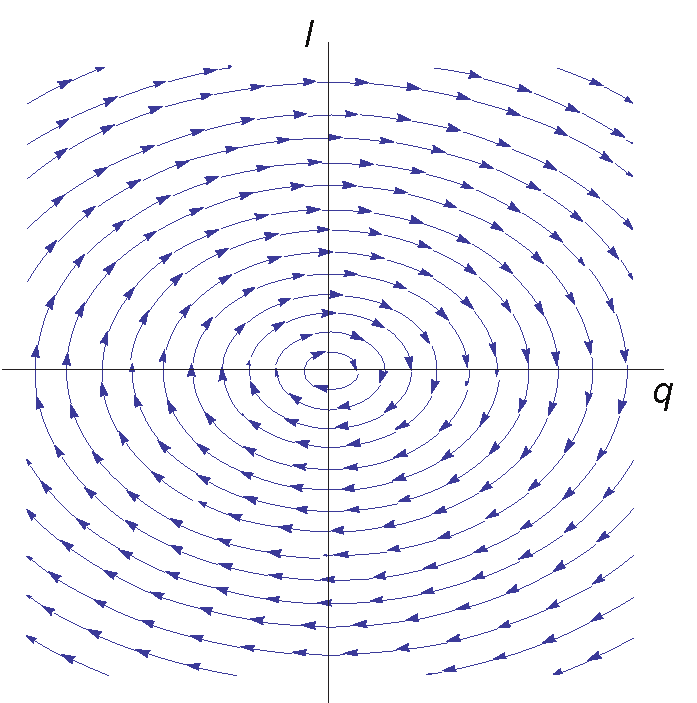
\includegraphics[scale=0.75]{Anh/Trung2.pdf}
        \end{center}
        \item Dấu của điện áp trên diode phụ thuộc vào hướng của dòng điện. Ta có: 
        \[\left\{ \begin{aligned}
        L\Ddot{q} + \frac{q}{C} = {V_d}~~~~~~\text{với}~\Dot{q} < 0 \hfill \\
        L\Ddot {q} + \frac{q}{C} =  - {V_d}~~~~~~\text{với}~\Dot{q}>0 \hfill \\ 
        \end{aligned}  \right. .\]
        Đặt hai biến mới $q_1$, $q_2$ sao cho $q_1=q-CV_d$ và $q_2=q+CV_d$. Ta có:
        \[\left\{ \begin{aligned}
        L\Ddot{q_1} + \frac{q_1}{C} = 0~~~~~~\text{với}~\Dot{q} < 0 \hfill \\
        L\Ddot {q_2} + \frac{q_2}{C} =  0~~~~~~\text{với}~\Dot{q}>0 \hfill \\ 
        \end{aligned}  \right. .\]
        Như vậy, sự ra đời của diode chỉ phục vụ cho việc dịch chuyển các điểm cân bằng tạo thành các quỹ đạo điều hòa đơn giản khác. Với $\Dot{q}>0$, điểm cân bằng là $q_2 = 0$ hoặc $q = -CV_d$, còn với $\Dot{q}<0$ thì $q = CV_d$. Vì vậy, quỹ đạo sẽ bao gồm các nửa hình elipse ở phần trên và phần dưới của biểu đồ $I-q$, có tâm là $q = -CV_d$ đối với nửa trên và tại $q = CV_d$ đối với nửa dưới. Khi quá trình diễn ra liên tục, các nửa hình elipse này sẽ liên kết với nhau tại $I = 0$.
        \begin{center}
            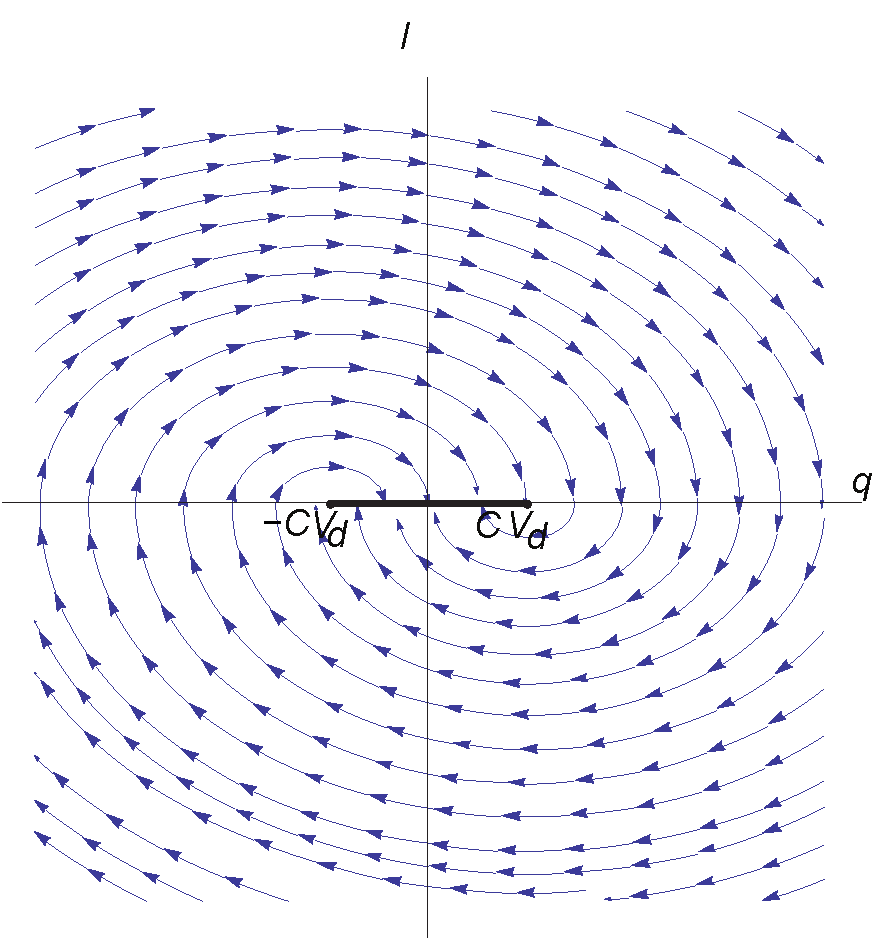
\includegraphics[scale=0.6]{Anh/Trung3.pdf}
        \end{center}
        \item Chúng ta có thể quan sát thấy trên sơ đồ có một “vùng chết” nằm giữa $-CV_d$ và $CV_d$ (với $I = 0$). Nếu một quỹ đạo đạt đến bất kì điểm nào trong đoạn đó, nó sẽ ở đó mãi mãi. Phạm vi của vùng đó là $2CV_d$.
        \item Ở ý này ta sử dụng giản đồ pha.
        \\Giả sử ban đầu tụ điện có điện tích $q_0 \gg CV_d$. Khi đó điện tích ban đầu sẽ dao động theo hướng khác $CV_d$ và sau một nửa chu kỳ: $$q_{T/2}=CV_d-\left(q_0-cV_d)\right)=2CV_d-q_0.$$
        Sau đó nó sẽ thực hiện một nửa dao động còn lại xung quanh $-CV_d$ và điện tích ở cuối dao động là:
        $$q_T=-CV_d-q_0+\left(-CV_d-\left(2CV_d-q_0)\right)\right)=-4CV_d,$$
        và từ đó ta có
        $$\Delta q=-4CV_d.$$
        Lưu ý rằng ta vẫn có thể sử dụng nửa chu kỳ và chu kỳ toàn phần vì dao động luôn xảy ra ở tần số không đổi $\omega=\dfrac{1}{\sqrt{LC}}$. Do đó khoảng thời gian giữa hai lần cực đại chỉ là chu kỳ dao động toàn phần:
        $$T=\dfrac{2\pi}{\omega}.$$
        Một khi $q(t)$ có đạo hàm bằng không trong vùng giới hạn bởi $CV_d$ và $-CV_d$, nó sẽ duy trì trạng thái đó mãi mãi.
    \end{enumerate}
\end{loigiai}


\begin{vd}[Nam châm điện mạnh có điện trở]%APhO 2010 (Taiwan)
Nam châm điện có điện trở là những nam châm được làm bằng những cuộn dây kim loại thông thường như đồng hoặc nhôm. Những nam châm điện có điện trở (sau này ta gọi gọn là nam châm điện) hiện đại có thể cung cấp từ trường không đổi lớn đến hơn $30$ Tesla. \\
Các cuộn dây của chúng thông thường được tạo ra bằng cách ghép hàng trăm đĩa mỏng hình tròn bằng đồng, có khoét nhiều lỗ để làm lạnh, và các tấm cách điện có cùng hình dạng, đặt xen kẽ. Khi một điện áp được đặt vào hai đầu cuộn dây, dòng điện chạy qua các đĩa theo đường xoắn ốc để tạo ra từ trường mạnh ở tâm của nam châm.\\

Trong bài này chúng ta có mục đích khảo sát cuộn dây hình trụ (còn gọi là solenoid) gồm nhiều vòng có thể được dùng như một nam châm để phát ra từ trường mạnh như thế nào. Như thấy trong Hình $1$, tâm của nam châm là ở $O$. Cuộn dây hình trụ của nó gồm $N$ vòng dây đồng có dòng điện $I$, phân bố đồng đều trên tiết diện ngang của dây chạy qua. \\
Đường kính trung bình của cuộn dây là $D$ và chiều dài của nó dọc theo trục $x$ là $l$. Tiết diện ngang của sợi dây là hình chữ nhật có chiều rộng là $a$ và chiều cao là $b$. Các vòng của cuộn dây được quấn sát nhau sao cho mặt phẳng của mỗi vòng có thể xem như vuông góc với trục $x$ và $l=Na$. \\

Dưới đây các số liệu về kích thước của cuộn dây:
\begin{align*}
l&=12,0 \mathrm{~cm}, D=6,0 \mathrm{~cm},\\
a&=2,0 \mathrm{~mm}, b=5,0 \mathrm{~mm}.
 \end{align*}
Khi đánh giá xem liệu một nam châm như vậy có thể tạo ra từ trường cao hay không, có hai thông số giới hạn không thể được bỏ qua. Thứ nhất là độ bền cơ học của cuộn dây để chịu được lực Lorentz lớn khi có dòng điện đi qua cuộn dây tạo ra từ trường. Thứ hai là nhiệt lượng Joule rất lớn toả ra trên sợi dây không được gây ra tăng nhiệt độ quá mức. Chúng ta sẽ khảo sát hai thông số này bằng cách dùng những mô hình đơn giản hóa.
\begin{enumerate}[1)]
    \item \textbf{Từ trường trên trục của cuộn dây}\\
Giả thiết rằng $b \ll D$ và các sợi dây là các dải mỏng có độ rộng $a$. Gọi $O$ là gốc của trục $x$. Hướng của dòng điện chạy qua dây như trong hình bên dưới.
\begin{center}
\tikzset{every picture/.style={line width=0.75pt}} %set default line width to 0.75pt
\begin{tikzpicture}[x=0.75pt,y=0.75pt,yscale=-1,xscale=1]
%uncomment if require: \path (0,300); %set diagram left start at 0, and has height of 300
%Shape: Rectangle [id:dp7112702582043747] 
\draw   (180.15,121.95) -- (180.25,108.85) -- (187.35,108.9) -- (187.25,122) -- cycle ;
%Shape: Ellipse [id:dp3338951198805633] 
\draw  [fill={rgb, 255:red, 0; green, 0; blue, 0 }  ,fill opacity=1 ] (182.04,115.43) .. controls (182.04,114.55) and (182.81,113.83) .. (183.75,113.83) .. controls (184.69,113.83) and (185.46,114.55) .. (185.46,115.43) .. controls (185.46,116.31) and (184.69,117.02) .. (183.75,117.02) .. controls (182.81,117.02) and (182.04,116.31) .. (182.04,115.43) -- cycle ;

%Shape: Rectangle [id:dp028506024335763103] 
\draw   (187.53,121.95) -- (187.63,108.85) -- (194.74,108.9) -- (194.64,122) -- cycle ;
%Shape: Ellipse [id:dp3555483150198745] 
\draw  [fill={rgb, 255:red, 0; green, 0; blue, 0 }  ,fill opacity=1 ] (189.43,115.43) .. controls (189.43,114.55) and (190.19,113.83) .. (191.13,113.83) .. controls (192.08,113.83) and (192.84,114.55) .. (192.84,115.43) .. controls (192.84,116.31) and (192.08,117.02) .. (191.13,117.02) .. controls (190.19,117.02) and (189.43,116.31) .. (189.43,115.43) -- cycle ;
%Shape: Rectangle [id:dp7846596217863611] 
\draw   (194.92,121.95) -- (195.02,108.85) -- (202.12,108.9) -- (202.02,122) -- cycle ;
%Shape: Ellipse [id:dp9290969928194137] 
\draw  [fill={rgb, 255:red, 0; green, 0; blue, 0 }  ,fill opacity=1 ] (196.81,115.43) .. controls (196.81,114.55) and (197.58,113.83) .. (198.52,113.83) .. controls (199.46,113.83) and (200.23,114.55) .. (200.23,115.43) .. controls (200.23,116.31) and (199.46,117.02) .. (198.52,117.02) .. controls (197.58,117.02) and (196.81,116.31) .. (196.81,115.43) -- cycle ;


%Shape: Rectangle [id:dp9724587702293661] 
\draw   (202.3,121.95) -- (202.4,108.85) -- (209.51,108.9) -- (209.41,122) -- cycle ;
%Shape: Ellipse [id:dp30621619588689] 
\draw  [fill={rgb, 255:red, 0; green, 0; blue, 0 }  ,fill opacity=1 ] (204.2,115.43) .. controls (204.2,114.55) and (204.96,113.83) .. (205.91,113.83) .. controls (206.85,113.83) and (207.61,114.55) .. (207.61,115.43) .. controls (207.61,116.31) and (206.85,117.02) .. (205.91,117.02) .. controls (204.96,117.02) and (204.2,116.31) .. (204.2,115.43) -- cycle ;

%Shape: Rectangle [id:dp881112043188723] 
\draw   (209.69,121.95) -- (209.79,108.85) -- (216.89,108.9) -- (216.79,122) -- cycle ;
%Shape: Ellipse [id:dp39946646136645925] 
\draw  [fill={rgb, 255:red, 0; green, 0; blue, 0 }  ,fill opacity=1 ] (211.58,115.43) .. controls (211.58,114.55) and (212.35,113.83) .. (213.29,113.83) .. controls (214.23,113.83) and (215,114.55) .. (215,115.43) .. controls (215,116.31) and (214.23,117.02) .. (213.29,117.02) .. controls (212.35,117.02) and (211.58,116.31) .. (211.58,115.43) -- cycle ;

%Shape: Rectangle [id:dp8850466975351513] 
\draw   (217.07,121.95) -- (217.18,108.85) -- (224.28,108.9) -- (224.18,122) -- cycle ;
%Shape: Ellipse [id:dp7335683993198577] 
\draw  [fill={rgb, 255:red, 0; green, 0; blue, 0 }  ,fill opacity=1 ] (218.97,115.43) .. controls (218.97,114.55) and (219.73,113.83) .. (220.68,113.83) .. controls (221.62,113.83) and (222.38,114.55) .. (222.38,115.43) .. controls (222.38,116.31) and (221.62,117.02) .. (220.68,117.02) .. controls (219.73,117.02) and (218.97,116.31) .. (218.97,115.43) -- cycle ;


%Shape: Rectangle [id:dp011164110627033152] 
\draw   (224.46,121.95) -- (224.56,108.85) -- (231.67,108.9) -- (231.56,122) -- cycle ;
%Shape: Ellipse [id:dp5788281664154589] 
\draw  [fill={rgb, 255:red, 0; green, 0; blue, 0 }  ,fill opacity=1 ] (226.35,115.43) .. controls (226.35,114.55) and (227.12,113.83) .. (228.06,113.83) .. controls (229.01,113.83) and (229.77,114.55) .. (229.77,115.43) .. controls (229.77,116.31) and (229.01,117.02) .. (228.06,117.02) .. controls (227.12,117.02) and (226.35,116.31) .. (226.35,115.43) -- cycle ;

%Shape: Rectangle [id:dp13123663982128475] 
\draw   (231.84,121.95) -- (231.95,108.85) -- (239.05,108.9) -- (238.95,122) -- cycle ;
%Shape: Ellipse [id:dp21490954537402496] 
\draw  [fill={rgb, 255:red, 0; green, 0; blue, 0 }  ,fill opacity=1 ] (233.74,115.43) .. controls (233.74,114.55) and (234.5,113.83) .. (235.45,113.83) .. controls (236.39,113.83) and (237.16,114.55) .. (237.16,115.43) .. controls (237.16,116.31) and (236.39,117.02) .. (235.45,117.02) .. controls (234.5,117.02) and (233.74,116.31) .. (233.74,115.43) -- cycle ;

%Shape: Rectangle [id:dp3194367844725694] 
\draw   (239.23,121.95) -- (239.33,108.85) -- (246.44,108.9) -- (246.33,122) -- cycle ;
%Shape: Ellipse [id:dp5546788830074406] 
\draw  [fill={rgb, 255:red, 0; green, 0; blue, 0 }  ,fill opacity=1 ] (241.12,115.43) .. controls (241.12,114.55) and (241.89,113.83) .. (242.83,113.83) .. controls (243.78,113.83) and (244.54,114.55) .. (244.54,115.43) .. controls (244.54,116.31) and (243.78,117.02) .. (242.83,117.02) .. controls (241.89,117.02) and (241.12,116.31) .. (241.12,115.43) -- cycle ;


%Shape: Rectangle [id:dp9887077852251398] 
\draw   (246.61,121.95) -- (246.72,108.85) -- (253.82,108.9) -- (253.72,122) -- cycle ;
%Shape: Ellipse [id:dp29467587578579735] 
\draw  [fill={rgb, 255:red, 0; green, 0; blue, 0 }  ,fill opacity=1 ] (248.51,115.43) .. controls (248.51,114.55) and (249.27,113.83) .. (250.22,113.83) .. controls (251.16,113.83) and (251.93,114.55) .. (251.93,115.43) .. controls (251.93,116.31) and (251.16,117.02) .. (250.22,117.02) .. controls (249.27,117.02) and (248.51,116.31) .. (248.51,115.43) -- cycle ;

%Shape: Rectangle [id:dp46897062738700657] 
\draw   (254,121.95) -- (254.1,108.85) -- (261.21,108.9) -- (261.1,122) -- cycle ;
%Shape: Ellipse [id:dp8225364733033032] 
\draw  [fill={rgb, 255:red, 0; green, 0; blue, 0 }  ,fill opacity=1 ] (255.9,115.43) .. controls (255.9,114.55) and (256.66,113.83) .. (257.6,113.83) .. controls (258.55,113.83) and (259.31,114.55) .. (259.31,115.43) .. controls (259.31,116.31) and (258.55,117.02) .. (257.6,117.02) .. controls (256.66,117.02) and (255.9,116.31) .. (255.9,115.43) -- cycle ;

%Shape: Rectangle [id:dp38295893101591305] 
\draw   (261.39,121.95) -- (261.49,108.85) -- (268.59,108.9) -- (268.49,122) -- cycle ;
%Shape: Ellipse [id:dp5273071025144969] 
\draw  [fill={rgb, 255:red, 0; green, 0; blue, 0 }  ,fill opacity=1 ] (263.28,115.43) .. controls (263.28,114.55) and (264.05,113.83) .. (264.99,113.83) .. controls (265.93,113.83) and (266.7,114.55) .. (266.7,115.43) .. controls (266.7,116.31) and (265.93,117.02) .. (264.99,117.02) .. controls (264.05,117.02) and (263.28,116.31) .. (263.28,115.43) -- cycle ;




%Shape: Rectangle [id:dp784073995306902] 
\draw   (268.77,121.95) -- (268.87,108.85) -- (275.98,108.9) -- (275.87,122) -- cycle ;
%Shape: Ellipse [id:dp013619221540287052] 
\draw  [fill={rgb, 255:red, 0; green, 0; blue, 0 }  ,fill opacity=1 ] (270.67,115.43) .. controls (270.67,114.55) and (271.43,113.83) .. (272.37,113.83) .. controls (273.32,113.83) and (274.08,114.55) .. (274.08,115.43) .. controls (274.08,116.31) and (273.32,117.02) .. (272.37,117.02) .. controls (271.43,117.02) and (270.67,116.31) .. (270.67,115.43) -- cycle ;

%Shape: Rectangle [id:dp9484784833739305] 
\draw   (276.16,121.95) -- (276.26,108.85) -- (283.36,108.9) -- (283.26,122) -- cycle ;
%Shape: Ellipse [id:dp141941792897606] 
\draw  [fill={rgb, 255:red, 0; green, 0; blue, 0 }  ,fill opacity=1 ] (278.05,115.43) .. controls (278.05,114.55) and (278.82,113.83) .. (279.76,113.83) .. controls (280.7,113.83) and (281.47,114.55) .. (281.47,115.43) .. controls (281.47,116.31) and (280.7,117.02) .. (279.76,117.02) .. controls (278.82,117.02) and (278.05,116.31) .. (278.05,115.43) -- cycle ;

%Shape: Rectangle [id:dp6006778057963058] 
\draw   (283.54,121.95) -- (283.64,108.85) -- (290.75,108.9) -- (290.65,122) -- cycle ;
%Shape: Ellipse [id:dp09955296028393701] 
\draw  [fill={rgb, 255:red, 0; green, 0; blue, 0 }  ,fill opacity=1 ] (285.44,115.43) .. controls (285.44,114.55) and (286.2,113.83) .. (287.14,113.83) .. controls (288.09,113.83) and (288.85,114.55) .. (288.85,115.43) .. controls (288.85,116.31) and (288.09,117.02) .. (287.14,117.02) .. controls (286.2,117.02) and (285.44,116.31) .. (285.44,115.43) -- cycle ;


%Shape: Rectangle [id:dp7287708666587742] 
\draw   (290.93,121.95) -- (291.03,108.85) -- (298.13,108.9) -- (298.03,122) -- cycle ;
%Shape: Ellipse [id:dp7591467986810947] 
\draw  [fill={rgb, 255:red, 0; green, 0; blue, 0 }  ,fill opacity=1 ] (292.82,115.43) .. controls (292.82,114.55) and (293.59,113.83) .. (294.53,113.83) .. controls (295.47,113.83) and (296.24,114.55) .. (296.24,115.43) .. controls (296.24,116.31) and (295.47,117.02) .. (294.53,117.02) .. controls (293.59,117.02) and (292.82,116.31) .. (292.82,115.43) -- cycle ;

%Shape: Rectangle [id:dp29665807301733005] 
\draw   (298.31,121.95) -- (298.41,108.85) -- (305.52,108.9) -- (305.42,122) -- cycle ;
%Shape: Ellipse [id:dp00032975296943560384] 
\draw  [fill={rgb, 255:red, 0; green, 0; blue, 0 }  ,fill opacity=1 ] (300.21,115.43) .. controls (300.21,114.55) and (300.97,113.83) .. (301.92,113.83) .. controls (302.86,113.83) and (303.62,114.55) .. (303.62,115.43) .. controls (303.62,116.31) and (302.86,117.02) .. (301.92,117.02) .. controls (300.97,117.02) and (300.21,116.31) .. (300.21,115.43) -- cycle ;

%Shape: Rectangle [id:dp5884814514135553] 
\draw   (305.7,121.95) -- (305.8,108.85) -- (312.9,108.9) -- (312.8,122) -- cycle ;
%Shape: Ellipse [id:dp4752639466274269] 
\draw  [fill={rgb, 255:red, 0; green, 0; blue, 0 }  ,fill opacity=1 ] (307.59,115.43) .. controls (307.59,114.55) and (308.36,113.83) .. (309.3,113.83) .. controls (310.24,113.83) and (311.01,114.55) .. (311.01,115.43) .. controls (311.01,116.31) and (310.24,117.02) .. (309.3,117.02) .. controls (308.36,117.02) and (307.59,116.31) .. (307.59,115.43) -- cycle ;


%Shape: Rectangle [id:dp9356260543152811] 
\draw   (313.08,121.95) -- (313.19,108.85) -- (320.29,108.9) -- (320.19,122) -- cycle ;
%Shape: Ellipse [id:dp6377542837991648] 
\draw  [fill={rgb, 255:red, 0; green, 0; blue, 0 }  ,fill opacity=1 ] (314.98,115.43) .. controls (314.98,114.55) and (315.74,113.83) .. (316.69,113.83) .. controls (317.63,113.83) and (318.39,114.55) .. (318.39,115.43) .. controls (318.39,116.31) and (317.63,117.02) .. (316.69,117.02) .. controls (315.74,117.02) and (314.98,116.31) .. (314.98,115.43) -- cycle ;

%Shape: Rectangle [id:dp1411689651624628] 
\draw   (320.47,121.95) -- (320.57,108.85) -- (327.68,108.9) -- (327.57,122) -- cycle ;
%Shape: Ellipse [id:dp831562196272039] 
\draw  [fill={rgb, 255:red, 0; green, 0; blue, 0 }  ,fill opacity=1 ] (322.36,115.43) .. controls (322.36,114.55) and (323.13,113.83) .. (324.07,113.83) .. controls (325.02,113.83) and (325.78,114.55) .. (325.78,115.43) .. controls (325.78,116.31) and (325.02,117.02) .. (324.07,117.02) .. controls (323.13,117.02) and (322.36,116.31) .. (322.36,115.43) -- cycle ;

%Shape: Rectangle [id:dp889422957038019] 
\draw   (327.85,121.95) -- (327.96,108.85) -- (335.06,108.9) -- (334.96,122) -- cycle ;
%Shape: Ellipse [id:dp5460159483184064] 
\draw  [fill={rgb, 255:red, 0; green, 0; blue, 0 }  ,fill opacity=1 ] (329.75,115.43) .. controls (329.75,114.55) and (330.51,113.83) .. (331.46,113.83) .. controls (332.4,113.83) and (333.17,114.55) .. (333.17,115.43) .. controls (333.17,116.31) and (332.4,117.02) .. (331.46,117.02) .. controls (330.51,117.02) and (329.75,116.31) .. (329.75,115.43) -- cycle ;


%Shape: Rectangle [id:dp9897990727576675] 
\draw   (335.24,121.95) -- (335.34,108.85) -- (342.45,108.9) -- (342.34,122) -- cycle ;
%Shape: Ellipse [id:dp52733387813736] 
\draw  [fill={rgb, 255:red, 0; green, 0; blue, 0 }  ,fill opacity=1 ] (337.13,115.43) .. controls (337.13,114.55) and (337.9,113.83) .. (338.84,113.83) .. controls (339.79,113.83) and (340.55,114.55) .. (340.55,115.43) .. controls (340.55,116.31) and (339.79,117.02) .. (338.84,117.02) .. controls (337.9,117.02) and (337.13,116.31) .. (337.13,115.43) -- cycle ;

%Shape: Rectangle [id:dp725695624099846] 
\draw   (342.62,121.95) -- (342.73,108.85) -- (349.83,108.9) -- (349.73,122) -- cycle ;
%Shape: Ellipse [id:dp7427867514814972] 
\draw  [fill={rgb, 255:red, 0; green, 0; blue, 0 }  ,fill opacity=1 ] (344.52,115.43) .. controls (344.52,114.55) and (345.28,113.83) .. (346.23,113.83) .. controls (347.17,113.83) and (347.94,114.55) .. (347.94,115.43) .. controls (347.94,116.31) and (347.17,117.02) .. (346.23,117.02) .. controls (345.28,117.02) and (344.52,116.31) .. (344.52,115.43) -- cycle ;

%Shape: Rectangle [id:dp3317346861365231] 
\draw   (350.01,121.95) -- (350.11,108.85) -- (357.22,108.9) -- (357.11,122) -- cycle ;
%Shape: Ellipse [id:dp04803915821512861] 
\draw  [fill={rgb, 255:red, 0; green, 0; blue, 0 }  ,fill opacity=1 ] (351.91,115.43) .. controls (351.91,114.55) and (352.67,113.83) .. (353.61,113.83) .. controls (354.56,113.83) and (355.32,114.55) .. (355.32,115.43) .. controls (355.32,116.31) and (354.56,117.02) .. (353.61,117.02) .. controls (352.67,117.02) and (351.91,116.31) .. (351.91,115.43) -- cycle ;




%Shape: Rectangle [id:dp42450437194850266] 
\draw   (357.4,121.95) -- (357.5,108.85) -- (364.6,108.9) -- (364.5,122) -- cycle ;
%Shape: Ellipse [id:dp01674494070503474] 
\draw  [fill={rgb, 255:red, 0; green, 0; blue, 0 }  ,fill opacity=1 ] (359.29,115.43) .. controls (359.29,114.55) and (360.06,113.83) .. (361,113.83) .. controls (361.94,113.83) and (362.71,114.55) .. (362.71,115.43) .. controls (362.71,116.31) and (361.94,117.02) .. (361,117.02) .. controls (360.06,117.02) and (359.29,116.31) .. (359.29,115.43) -- cycle ;

%Shape: Rectangle [id:dp3522070868989857] 
\draw   (364.78,121.95) -- (364.88,108.85) -- (371.99,108.9) -- (371.88,122) -- cycle ;
%Shape: Ellipse [id:dp8092801104277225] 
\draw  [fill={rgb, 255:red, 0; green, 0; blue, 0 }  ,fill opacity=1 ] (366.68,115.43) .. controls (366.68,114.55) and (367.44,113.83) .. (368.38,113.83) .. controls (369.33,113.83) and (370.09,114.55) .. (370.09,115.43) .. controls (370.09,116.31) and (369.33,117.02) .. (368.38,117.02) .. controls (367.44,117.02) and (366.68,116.31) .. (366.68,115.43) -- cycle ;

%Shape: Rectangle [id:dp7884612159751085] 
\draw   (372.17,121.95) -- (372.27,108.85) -- (379.37,108.9) -- (379.27,122) -- cycle ;
%Shape: Ellipse [id:dp9066750814626128] 
\draw  [fill={rgb, 255:red, 0; green, 0; blue, 0 }  ,fill opacity=1 ] (374.06,115.43) .. controls (374.06,114.55) and (374.83,113.83) .. (375.77,113.83) .. controls (376.71,113.83) and (377.48,114.55) .. (377.48,115.43) .. controls (377.48,116.31) and (376.71,117.02) .. (375.77,117.02) .. controls (374.83,117.02) and (374.06,116.31) .. (374.06,115.43) -- cycle ;


%Shape: Rectangle [id:dp38600459532943643] 
\draw   (379.55,121.95) -- (379.65,108.85) -- (386.76,108.9) -- (386.66,122) -- cycle ;
%Shape: Ellipse [id:dp5156570254239508] 
\draw  [fill={rgb, 255:red, 0; green, 0; blue, 0 }  ,fill opacity=1 ] (381.45,115.43) .. controls (381.45,114.55) and (382.21,113.83) .. (383.15,113.83) .. controls (384.1,113.83) and (384.86,114.55) .. (384.86,115.43) .. controls (384.86,116.31) and (384.1,117.02) .. (383.15,117.02) .. controls (382.21,117.02) and (381.45,116.31) .. (381.45,115.43) -- cycle ;

%Shape: Rectangle [id:dp822033913894261] 
\draw   (386.94,121.95) -- (387.04,108.85) -- (394.14,108.9) -- (394.04,122) -- cycle ;
%Shape: Ellipse [id:dp2640157163876288] 
\draw  [fill={rgb, 255:red, 0; green, 0; blue, 0 }  ,fill opacity=1 ] (388.83,115.43) .. controls (388.83,114.55) and (389.6,113.83) .. (390.54,113.83) .. controls (391.48,113.83) and (392.25,114.55) .. (392.25,115.43) .. controls (392.25,116.31) and (391.48,117.02) .. (390.54,117.02) .. controls (389.6,117.02) and (388.83,116.31) .. (388.83,115.43) -- cycle ;

%Shape: Rectangle [id:dp03211620678210958] 
\draw   (394.32,121.95) -- (394.42,108.85) -- (401.53,108.9) -- (401.43,122) -- cycle ;
%Shape: Ellipse [id:dp10653786942375443] 
\draw  [fill={rgb, 255:red, 0; green, 0; blue, 0 }  ,fill opacity=1 ] (396.22,115.43) .. controls (396.22,114.55) and (396.98,113.83) .. (397.93,113.83) .. controls (398.87,113.83) and (399.63,114.55) .. (399.63,115.43) .. controls (399.63,116.31) and (398.87,117.02) .. (397.93,117.02) .. controls (396.98,117.02) and (396.22,116.31) .. (396.22,115.43) -- cycle ;


%Shape: Rectangle [id:dp8168680097809764] 
\draw   (401.71,121.95) -- (401.81,108.85) -- (408.91,108.9) -- (408.81,122) -- cycle ;
%Shape: Ellipse [id:dp5184770831862877] 
\draw  [fill={rgb, 255:red, 0; green, 0; blue, 0 }  ,fill opacity=1 ] (403.6,115.43) .. controls (403.6,114.55) and (404.37,113.83) .. (405.31,113.83) .. controls (406.25,113.83) and (407.02,114.55) .. (407.02,115.43) .. controls (407.02,116.31) and (406.25,117.02) .. (405.31,117.02) .. controls (404.37,117.02) and (403.6,116.31) .. (403.6,115.43) -- cycle ;

%Shape: Rectangle [id:dp6432145807849444] 
\draw   (409.09,121.95) -- (409.2,108.85) -- (416.3,108.9) -- (416.2,122) -- cycle ;
%Shape: Ellipse [id:dp41294015300693454] 
\draw  [fill={rgb, 255:red, 0; green, 0; blue, 0 }  ,fill opacity=1 ] (410.99,115.43) .. controls (410.99,114.55) and (411.75,113.83) .. (412.7,113.83) .. controls (413.64,113.83) and (414.4,114.55) .. (414.4,115.43) .. controls (414.4,116.31) and (413.64,117.02) .. (412.7,117.02) .. controls (411.75,117.02) and (410.99,116.31) .. (410.99,115.43) -- cycle ;

%Shape: Rectangle [id:dp35183153364110153] 
\draw   (416.48,121.95) -- (416.58,108.85) -- (423.69,108.9) -- (423.58,122) -- cycle ;
%Shape: Ellipse [id:dp21391903391699074] 
\draw  [fill={rgb, 255:red, 0; green, 0; blue, 0 }  ,fill opacity=1 ] (418.37,115.43) .. controls (418.37,114.55) and (419.14,113.83) .. (420.08,113.83) .. controls (421.03,113.83) and (421.79,114.55) .. (421.79,115.43) .. controls (421.79,116.31) and (421.03,117.02) .. (420.08,117.02) .. controls (419.14,117.02) and (418.37,116.31) .. (418.37,115.43) -- cycle ;
%Shape: Rectangle [id:dp8052015452934143] 
\draw   (423.86,121.95) -- (423.97,108.85) -- (431.07,108.9) -- (430.97,122) -- cycle ;
%Shape: Ellipse [id:dp9191916804986576] 
\draw  [fill={rgb, 255:red, 0; green, 0; blue, 0 }  ,fill opacity=1 ] (425.76,115.43) .. controls (425.76,114.55) and (426.52,113.83) .. (427.47,113.83) .. controls (428.41,113.83) and (429.18,114.55) .. (429.18,115.43) .. controls (429.18,116.31) and (428.41,117.02) .. (427.47,117.02) .. controls (426.52,117.02) and (425.76,116.31) .. (425.76,115.43) -- cycle ;

%Shape: Rectangle [id:dp5944503155233724] 
\draw   (431.25,121.95) -- (431.35,108.85) -- (438.46,108.9) -- (438.35,122) -- cycle ;
%Shape: Ellipse [id:dp4067424083970931] 
\draw  [fill={rgb, 255:red, 0; green, 0; blue, 0 }  ,fill opacity=1 ] (433.14,115.43) .. controls (433.14,114.55) and (433.91,113.83) .. (434.85,113.83) .. controls (435.8,113.83) and (436.56,114.55) .. (436.56,115.43) .. controls (436.56,116.31) and (435.8,117.02) .. (434.85,117.02) .. controls (433.91,117.02) and (433.14,116.31) .. (433.14,115.43) -- cycle ;

%Shape: Rectangle [id:dp3093602824130668] 
\draw   (438.63,121.95) -- (438.74,108.85) -- (445.84,108.9) -- (445.74,122) -- cycle ;
%Shape: Ellipse [id:dp6433098435754134] 
\draw  [fill={rgb, 255:red, 0; green, 0; blue, 0 }  ,fill opacity=1 ] (440.53,115.43) .. controls (440.53,114.55) and (441.29,113.83) .. (442.24,113.83) .. controls (443.18,113.83) and (443.95,114.55) .. (443.95,115.43) .. controls (443.95,116.31) and (443.18,117.02) .. (442.24,117.02) .. controls (441.29,117.02) and (440.53,116.31) .. (440.53,115.43) -- cycle ;
%Shape: Rectangle [id:dp4500570570513234] 
\draw   (179.06,173.95) -- (179.16,160.85) -- (186.34,160.9) -- (186.23,174) -- cycle ;
%Straight Lines [id:da40625266460131937] 
\draw    (179.16,160.85) -- (186.23,174) ;
%Straight Lines [id:da18787088993541978] 
\draw    (186.34,160.9) -- (179.06,173.95) ;

%Shape: Rectangle [id:dp4325467058988054] 
\draw   (186.06,173.95) -- (186.16,160.85) -- (193.34,160.9) -- (193.23,174) -- cycle ;
%Straight Lines [id:da5147676972043498] 
\draw    (186.16,160.85) -- (193.23,174) ;
%Straight Lines [id:da8417179321174847] 
\draw    (193.34,160.9) -- (186.06,173.95) ;
%Shape: Rectangle [id:dp6665550349790494] 
\draw   (193.06,173.95) -- (193.16,160.85) -- (200.34,160.9) -- (200.23,174) -- cycle ;
%Straight Lines [id:da4806525093998497] 
\draw    (193.16,160.85) -- (200.23,174) ;
%Straight Lines [id:da3731763781263795] 
\draw    (200.34,160.9) -- (193.06,173.95) ;

%Shape: Rectangle [id:dp42494674280831435] 
\draw   (200.06,173.95) -- (200.16,160.85) -- (207.34,160.9) -- (207.23,174) -- cycle ;
%Straight Lines [id:da134258348341728] 
\draw    (200.16,160.85) -- (207.23,174) ;
%Straight Lines [id:da36141604129807003] 
\draw    (207.34,160.9) -- (200.06,173.95) ;
%Shape: Rectangle [id:dp3256425944072524] 
\draw   (207.06,173.95) -- (207.16,160.85) -- (214.34,160.9) -- (214.23,174) -- cycle ;
%Straight Lines [id:da37176518579844264] 
\draw    (207.16,160.85) -- (214.23,174) ;
%Straight Lines [id:da15918698372562867] 
\draw    (214.34,160.9) -- (207.06,173.95) ;

%Shape: Rectangle [id:dp3994081441878239] 
\draw   (214.06,173.95) -- (214.16,160.85) -- (221.34,160.9) -- (221.23,174) -- cycle ;
%Straight Lines [id:da9398829129746036] 
\draw    (214.16,160.85) -- (221.23,174) ;
%Straight Lines [id:da23700468283234544] 
\draw    (221.34,160.9) -- (214.06,173.95) ;


%Shape: Rectangle [id:dp6251615265933044] 
\draw   (221.06,173.95) -- (221.16,160.85) -- (228.34,160.9) -- (228.23,174) -- cycle ;
%Straight Lines [id:da20036953230592414] 
\draw    (221.16,160.85) -- (228.23,174) ;
%Straight Lines [id:da41255606890342145] 
\draw    (228.34,160.9) -- (221.06,173.95) ;

%Shape: Rectangle [id:dp47616886390663316] 
\draw   (228.06,173.95) -- (228.16,160.85) -- (235.34,160.9) -- (235.23,174) -- cycle ;
%Straight Lines [id:da34849367261456055] 
\draw    (228.16,160.85) -- (235.23,174) ;
%Straight Lines [id:da03523732887148279] 
\draw    (235.34,160.9) -- (228.06,173.95) ;

%Shape: Rectangle [id:dp19067595157342854] 
\draw   (235.06,173.95) -- (235.16,160.85) -- (242.34,160.9) -- (242.23,174) -- cycle ;
%Straight Lines [id:da32478107063564754] 
\draw    (235.16,160.85) -- (242.23,174) ;
%Straight Lines [id:da3286014335035734] 
\draw    (242.34,160.9) -- (235.06,173.95) ;

%Shape: Rectangle [id:dp5245989805903607] 
\draw   (242.06,173.95) -- (242.16,160.85) -- (249.34,160.9) -- (249.23,174) -- cycle ;
%Straight Lines [id:da961416414924577] 
\draw    (242.16,160.85) -- (249.23,174) ;
%Straight Lines [id:da9745930078958432] 
\draw    (249.34,160.9) -- (242.06,173.95) ;


%Shape: Rectangle [id:dp5751636813361185] 
\draw   (249.06,173.95) -- (249.16,160.85) -- (256.34,160.9) -- (256.23,174) -- cycle ;
%Straight Lines [id:da3217654102132803] 
\draw    (249.16,160.85) -- (256.23,174) ;
%Straight Lines [id:da9220913921976156] 
\draw    (256.34,160.9) -- (249.06,173.95) ;

%Shape: Rectangle [id:dp15983781540062947] 
\draw   (256.06,173.95) -- (256.16,160.85) -- (263.34,160.9) -- (263.23,174) -- cycle ;
%Straight Lines [id:da2140887225636865] 
\draw    (256.16,160.85) -- (263.23,174) ;
%Straight Lines [id:da2859353699918723] 
\draw    (263.34,160.9) -- (256.06,173.95) ;



%Shape: Rectangle [id:dp15984452442185926] 
\draw   (263.06,173.95) -- (263.16,160.85) -- (270.34,160.9) -- (270.23,174) -- cycle ;
%Straight Lines [id:da4110719136821098] 
\draw    (263.16,160.85) -- (270.23,174) ;
%Straight Lines [id:da26052700975351817] 
\draw    (270.34,160.9) -- (263.06,173.95) ;

%Shape: Rectangle [id:dp6566474198918585] 
\draw   (270.06,173.95) -- (270.16,160.85) -- (277.34,160.9) -- (277.23,174) -- cycle ;
%Straight Lines [id:da28372319029960713] 
\draw    (270.16,160.85) -- (277.23,174) ;
%Straight Lines [id:da8573144369125063] 
\draw    (277.34,160.9) -- (270.06,173.95) ;


%Shape: Rectangle [id:dp2769638883772084] 
\draw   (277.06,173.95) -- (277.16,160.85) -- (284.34,160.9) -- (284.23,174) -- cycle ;
%Straight Lines [id:da4320871028995078] 
\draw    (277.16,160.85) -- (284.23,174) ;
%Straight Lines [id:da7269875737873256] 
\draw    (284.34,160.9) -- (277.06,173.95) ;

%Shape: Rectangle [id:dp49533982823384426] 
\draw   (284.06,173.95) -- (284.16,160.85) -- (291.34,160.9) -- (291.23,174) -- cycle ;
%Straight Lines [id:da6090040044011437] 
\draw    (284.16,160.85) -- (291.23,174) ;
%Straight Lines [id:da6091351527578889] 
\draw    (291.34,160.9) -- (284.06,173.95) ;




%Shape: Rectangle [id:dp6882053419001805] 
\draw   (291.06,173.95) -- (291.16,160.85) -- (298.34,160.9) -- (298.23,174) -- cycle ;
%Straight Lines [id:da3086131390592649] 
\draw    (291.16,160.85) -- (298.23,174) ;
%Straight Lines [id:da1671891417612409] 
\draw    (298.34,160.9) -- (291.06,173.95) ;

%Shape: Rectangle [id:dp3844713554864301] 
\draw   (298.06,173.95) -- (298.16,160.85) -- (305.34,160.9) -- (305.23,174) -- cycle ;
%Straight Lines [id:da9809181313237885] 
\draw    (298.16,160.85) -- (305.23,174) ;
%Straight Lines [id:da12067399015099456] 
\draw    (305.34,160.9) -- (298.06,173.95) ;


%Shape: Rectangle [id:dp09660124994154662] 
\draw   (305.06,173.95) -- (305.16,160.85) -- (312.34,160.9) -- (312.23,174) -- cycle ;
%Straight Lines [id:da23391988796153762] 
\draw    (305.16,160.85) -- (312.23,174) ;
%Straight Lines [id:da030740420735130614] 
\draw    (312.34,160.9) -- (305.06,173.95) ;

%Shape: Rectangle [id:dp674441868316983] 
\draw   (312.06,173.95) -- (312.16,160.85) -- (319.34,160.9) -- (319.23,174) -- cycle ;
%Straight Lines [id:da808857912590329] 
\draw    (312.16,160.85) -- (319.23,174) ;
%Straight Lines [id:da5955291111145252] 
\draw    (319.34,160.9) -- (312.06,173.95) ;



%Shape: Rectangle [id:dp7235119922972411] 
\draw   (319.06,173.95) -- (319.16,160.85) -- (326.34,160.9) -- (326.23,174) -- cycle ;
%Straight Lines [id:da6868703727152485] 
\draw    (319.16,160.85) -- (326.23,174) ;
%Straight Lines [id:da32489055181574666] 
\draw    (326.34,160.9) -- (319.06,173.95) ;

%Shape: Rectangle [id:dp7184067120736121] 
\draw   (326.06,173.95) -- (326.16,160.85) -- (333.34,160.9) -- (333.23,174) -- cycle ;
%Straight Lines [id:da3604883540635465] 
\draw    (326.16,160.85) -- (333.23,174) ;
%Straight Lines [id:da09742421672475432] 
\draw    (333.34,160.9) -- (326.06,173.95) ;


%Shape: Rectangle [id:dp6079758585573741] 
\draw   (333.06,173.95) -- (333.16,160.85) -- (340.34,160.9) -- (340.23,174) -- cycle ;
%Straight Lines [id:da5347028805170088] 
\draw    (333.16,160.85) -- (340.23,174) ;
%Straight Lines [id:da8422657200640619] 
\draw    (340.34,160.9) -- (333.06,173.95) ;

%Shape: Rectangle [id:dp20488235707161762] 
\draw   (340.06,173.95) -- (340.16,160.85) -- (347.34,160.9) -- (347.23,174) -- cycle ;
%Straight Lines [id:da17763451342370007] 
\draw    (340.16,160.85) -- (347.23,174) ;
%Straight Lines [id:da7248086984737857] 
\draw    (347.34,160.9) -- (340.06,173.95) ;



%Shape: Rectangle [id:dp2629321914496321] 
\draw   (347.06,173.95) -- (347.16,160.85) -- (354.34,160.9) -- (354.23,174) -- cycle ;
%Straight Lines [id:da6488045820160981] 
\draw    (347.16,160.85) -- (354.23,174) ;
%Straight Lines [id:da8196087287107547] 
\draw    (354.34,160.9) -- (347.06,173.95) ;

%Shape: Rectangle [id:dp5638281747253037] 
\draw   (354.06,173.95) -- (354.16,160.85) -- (361.34,160.9) -- (361.23,174) -- cycle ;
%Straight Lines [id:da28521897455028866] 
\draw    (354.16,160.85) -- (361.23,174) ;
%Straight Lines [id:da19012165260693004] 
\draw    (361.34,160.9) -- (354.06,173.95) ;


%Shape: Rectangle [id:dp09125154066341357] 
\draw   (361.06,173.95) -- (361.16,160.85) -- (368.34,160.9) -- (368.23,174) -- cycle ;
%Straight Lines [id:da22633566243480363] 
\draw    (361.16,160.85) -- (368.23,174) ;
%Straight Lines [id:da017531305380509288] 
\draw    (368.34,160.9) -- (361.06,173.95) ;

%Shape: Rectangle [id:dp3594876506577861] 
\draw   (368.06,173.95) -- (368.16,160.85) -- (375.34,160.9) -- (375.23,174) -- cycle ;
%Straight Lines [id:da5735427887107543] 
\draw    (368.16,160.85) -- (375.23,174) ;
%Straight Lines [id:da32558479740425295] 
\draw    (375.34,160.9) -- (368.06,173.95) ;



%Shape: Rectangle [id:dp6160129635069435] 
\draw   (375.06,173.95) -- (375.16,160.85) -- (382.34,160.9) -- (382.23,174) -- cycle ;
%Straight Lines [id:da18228486282733514] 
\draw    (375.16,160.85) -- (382.23,174) ;
%Straight Lines [id:da8223113338216818] 
\draw    (382.34,160.9) -- (375.06,173.95) ;

%Shape: Rectangle [id:dp9978569121245916] 
\draw   (382.06,173.95) -- (382.16,160.85) -- (389.34,160.9) -- (389.23,174) -- cycle ;
%Straight Lines [id:da6435723893249009] 
\draw    (382.16,160.85) -- (389.23,174) ;
%Straight Lines [id:da32916005292625083] 
\draw    (389.34,160.9) -- (382.06,173.95) ;


%Shape: Rectangle [id:dp9192366414171145] 
\draw   (389.06,173.95) -- (389.16,160.85) -- (396.34,160.9) -- (396.23,174) -- cycle ;
%Straight Lines [id:da8194757202727903] 
\draw    (389.16,160.85) -- (396.23,174) ;
%Straight Lines [id:da369894572124559] 
\draw    (396.34,160.9) -- (389.06,173.95) ;

%Shape: Rectangle [id:dp8339770088814564] 
\draw   (396.06,173.95) -- (396.16,160.85) -- (403.34,160.9) -- (403.23,174) -- cycle ;
%Straight Lines [id:da746423457027386] 
\draw    (396.16,160.85) -- (403.23,174) ;
%Straight Lines [id:da6993056754402005] 
\draw    (403.34,160.9) -- (396.06,173.95) ;





%Shape: Rectangle [id:dp7236839368947763] 
\draw   (403.06,173.95) -- (403.16,160.85) -- (410.34,160.9) -- (410.23,174) -- cycle ;
%Straight Lines [id:da8786499357131579] 
\draw    (403.16,160.85) -- (410.23,174) ;
%Straight Lines [id:da2682904482226657] 
\draw    (410.34,160.9) -- (403.06,173.95) ;

%Shape: Rectangle [id:dp6089797136712847] 
\draw   (410.06,173.95) -- (410.16,160.85) -- (417.34,160.9) -- (417.23,174) -- cycle ;
%Straight Lines [id:da9632799437797668] 
\draw    (410.16,160.85) -- (417.23,174) ;
%Straight Lines [id:da19697634125974028] 
\draw    (417.34,160.9) -- (410.06,173.95) ;


%Shape: Rectangle [id:dp5515886144534714] 
\draw   (417.06,173.95) -- (417.16,160.85) -- (424.34,160.9) -- (424.23,174) -- cycle ;
%Straight Lines [id:da6368801592408003] 
\draw    (417.16,160.85) -- (424.23,174) ;
%Straight Lines [id:da6363278253993598] 
\draw    (424.34,160.9) -- (417.06,173.95) ;

%Shape: Rectangle [id:dp9971356550887577] 
\draw   (424.06,173.95) -- (424.16,160.85) -- (431.34,160.9) -- (431.23,174) -- cycle ;
%Straight Lines [id:da5844379967942365] 
\draw    (424.16,160.85) -- (431.23,174) ;
%Straight Lines [id:da7902201274332762] 
\draw    (431.34,160.9) -- (424.06,173.95) ;


%Shape: Rectangle [id:dp7197048614654172] 
\draw   (431.06,173.95) -- (431.16,160.85) -- (438.34,160.9) -- (438.23,174) -- cycle ;
%Straight Lines [id:da07608131854628042] 
\draw    (431.16,160.85) -- (438.23,174) ;
%Straight Lines [id:da409418423453491] 
\draw    (438.34,160.9) -- (431.06,173.95) ;

%Shape: Rectangle [id:dp790299159662829] 
\draw   (438.06,173.95) -- (438.16,160.85) -- (445.34,160.9) -- (445.23,174) -- cycle ;
%Straight Lines [id:da8905664662233008] 
\draw    (438.16,160.85) -- (445.23,174) ;
%Straight Lines [id:da8777132345983735] 
\draw    (445.34,160.9) -- (438.06,173.95) ;


%Straight Lines [id:da7296224435771693] 
\draw  [dash pattern={on 4.5pt off 4.5pt}]  (177.1,142) -- (460.03,142) ;
\draw [shift={(463.03,142)}, rotate = 180] [fill={rgb, 255:red, 0; green, 0; blue, 0 }  ][line width=0.08]  [draw opacity=0] (10.72,-5.15) -- (0,0) -- (10.72,5.15) -- (7.12,0) -- cycle    ;
%Straight Lines [id:da8720938481462964] 
\draw    (185,48) -- (185,86) ;
\draw [shift={(185,89)}, rotate = 270] [fill={rgb, 255:red, 0; green, 0; blue, 0 }  ][line width=0.08]  [draw opacity=0] (10.72,-5.15) -- (0,0) -- (10.72,5.15) -- (7.12,0) -- cycle    ;
%Straight Lines [id:da6907872806919281] 
\draw    (185,82) -- (185,108.85) ;

%Straight Lines [id:da5572396234121316] 
\draw    (443.92,108.85) -- (444.02,70.85) ;
\draw [shift={(444.03,67.85)}, rotate = 450.16] [fill={rgb, 255:red, 0; green, 0; blue, 0 }  ][line width=0.08]  [draw opacity=0] (10.72,-5.15) -- (0,0) -- (10.72,5.15) -- (7.12,0) -- cycle    ;
%Straight Lines [id:da7687623210079318] 
\draw    (444.01,74.85) -- (444.08,48) ;

%Straight Lines [id:da40679695822258843] 
\draw  [dash pattern={on 4.5pt off 4.5pt}]  (373.27,83) -- (373.27,108.85) ;
%Straight Lines [id:da4305574450084835] 
\draw  [dash pattern={on 4.5pt off 4.5pt}]  (380.37,83.05) -- (380.37,108.9) ;
%Straight Lines [id:da3371320583572225] 
\draw    (335,95.93) -- (371.27,95.93) ;
\draw [shift={(373.27,95.93)}, rotate = 180] [color={rgb, 255:red, 0; green, 0; blue, 0 }  ][line width=0.75]    (10.93,-3.29) .. controls (6.95,-1.4) and (3.31,-0.3) .. (0,0) .. controls (3.31,0.3) and (6.95,1.4) .. (10.93,3.29)   ;
%Straight Lines [id:da7113372851252481] 
\draw    (415.28,95.93) -- (382.65,95.93) ;
\draw [shift={(380.65,95.93)}, rotate = 360] [color={rgb, 255:red, 0; green, 0; blue, 0 }  ][line width=0.75]    (10.93,-3.29) .. controls (6.95,-1.4) and (3.31,-0.3) .. (0,0) .. controls (3.31,0.3) and (6.95,1.4) .. (10.93,3.29)   ;
%Straight Lines [id:da1668456872781937] 
\draw    (171.79,170.95) -- (171.79,113) ;
\draw [shift={(171.79,110)}, rotate = 450] [fill={rgb, 255:red, 0; green, 0; blue, 0 }  ][line width=0.08]  [draw opacity=0] (10.72,-5.15) -- (0,0) -- (10.72,5.15) -- (7.12,0) -- cycle    ;
\draw [shift={(171.79,173.95)}, rotate = 270] [fill={rgb, 255:red, 0; green, 0; blue, 0 }  ][line width=0.08]  [draw opacity=0] (10.72,-5.15) -- (0,0) -- (10.72,5.15) -- (7.12,0) -- cycle    ;
%Straight Lines [id:da9142893613693474] 
\draw  [dash pattern={on 4.5pt off 4.5pt}]  (446.74,122) -- (492.57,122) ;
%Straight Lines [id:da333519531602262] 
\draw  [dash pattern={on 4.5pt off 4.5pt}]  (446.84,108.9) -- (492.67,108.9) ;
%Straight Lines [id:da5598803394969128] 
\draw    (486.76,83) -- (486.76,106.9) ;
\draw [shift={(486.76,108.9)}, rotate = 270] [color={rgb, 255:red, 0; green, 0; blue, 0 }  ][line width=0.75]    (10.93,-3.29) .. controls (6.95,-1.4) and (3.31,-0.3) .. (0,0) .. controls (3.31,0.3) and (6.95,1.4) .. (10.93,3.29)   ;
%Straight Lines [id:da6334677440312976] 
\draw    (486.76,147) -- (486.76,124.9) ;
\draw [shift={(486.76,122.9)}, rotate = 450] [color={rgb, 255:red, 0; green, 0; blue, 0 }  ][line width=0.75]    (10.93,-3.29) .. controls (6.95,-1.4) and (3.31,-0.3) .. (0,0) .. controls (3.31,0.3) and (6.95,1.4) .. (10.93,3.29)   ;
%Shape: Circle [id:dp9238447922347451] 
\draw  [fill={rgb, 255:red, 0; green, 0; blue, 0 }  ,fill opacity=1 ] (317.37,142) .. controls (317.37,141.25) and (317.97,140.65) .. (318.72,140.65) .. controls (319.46,140.65) and (320.07,141.25) .. (320.07,142) .. controls (320.07,142.75) and (319.46,143.35) .. (318.72,143.35) .. controls (317.97,143.35) and (317.37,142.75) .. (317.37,142) -- cycle ;
%Straight Lines [id:da748231115663523] 
\draw    (179.1,150.93) -- (316.27,150.93) ;
\draw [shift={(318.27,150.93)}, rotate = 180] [color={rgb, 255:red, 0; green, 0; blue, 0 }  ][line width=0.75]    (10.93,-3.29) .. controls (6.95,-1.4) and (3.31,-0.3) .. (0,0) .. controls (3.31,0.3) and (6.95,1.4) .. (10.93,3.29)   ;
\draw [shift={(177.1,150.93)}, rotate = 0] [color={rgb, 255:red, 0; green, 0; blue, 0 }  ][line width=0.75]    (10.93,-3.29) .. controls (6.95,-1.4) and (3.31,-0.3) .. (0,0) .. controls (3.31,0.3) and (6.95,1.4) .. (10.93,3.29)   ;

% Text Node
\draw (192,72.4) node [anchor=north west][inner sep=0.75pt]    {$I$};
% Text Node
\draw (452,65.4) node [anchor=north west][inner sep=0.75pt]    {$I$};
% Text Node
\draw (373,64.4) node [anchor=north west][inner sep=0.75pt]    {$a$};
% Text Node
\draw (155,132.4) node [anchor=north west][inner sep=0.75pt]    {$D$};
% Text Node
\draw (493,106.4) node [anchor=north west][inner sep=0.75pt]    {$b$};
% Text Node
\draw (233.56,125.4) node [anchor=north west][inner sep=0.75pt]  [rotate=-0.12]  {$l/2$};
% Text Node
\draw (300.31,125.35) node [anchor=north west][inner sep=0.75pt]    {$O$};
% Text Node
\draw (463,137.4) node [anchor=north west][inner sep=0.75pt]    {$x$};


\end{tikzpicture}
\\ Hình 1
\end{center}
\begin{enumerate}[a)]
    \item Hãy xác định thành phần theo trục $x$ của từ trường $B(x)$ trên trục của cuộn dây theo $x$ khi dòng điện không đổi $I$ chạy qua cuộn. 
    \item Hãy xác định dòng điện không đổi $I_{0}$ qua cuộn dây nếu $B(0)$ bằng $10,0 \mathrm{~T}$. Sử dụng các dữ liệu được cho ở trên để tính toán trong phần này.
\end{enumerate}
\item \textbf{Giới hạn trên của dòng điện }\\
Trong phần này, chúng ta giả sử độ dài của cuộn dây là vô hạn và $b \ll D$. Xét một vòng của cuộn dây ở vị trí $x=0$. Từ trường tác dụng lực Lorentz lên dòng điện chạy qua các vòng dây. Vậy, như trên Hình $2$, đoạn dây độ dài $\Delta{s}$ chịu lực pháp tuyến $\Delta{F_n}$ có xu hướng làm cho vòng dây dãn rộng ra.
\begin{enumerate}[a)]
    \item Giả sử rằng, khi dòng điện là $I$, đường kính trung bình của cuộn dây đã dãn ra và được giữ ở giá trị không đổi $D'$ lớn hơn $D$, như hình dưới đây.
    \begin{center}
\tikzset{every picture/.style={line width=0.75pt}} %set default line width to 0.75pt
\begin{tikzpicture}[x=0.75pt,y=0.75pt,yscale=-1,xscale=1]
%uncomment if require: \path (0,300); %set diagram left start at 0, and has height of 300

%Shape: Circle [id:dp8834988581353049] 
\draw   (165.17,115) .. controls (165.17,88.58) and (186.58,67.17) .. (213,67.17) .. controls (239.42,67.17) and (260.83,88.58) .. (260.83,115) .. controls (260.83,141.42) and (239.42,162.83) .. (213,162.83) .. controls (186.58,162.83) and (165.17,141.42) .. (165.17,115) -- cycle ;
%Shape: Circle [id:dp9516308900374016] 
\draw   (158,115) .. controls (158,84.62) and (182.62,60) .. (213,60) .. controls (243.38,60) and (268,84.62) .. (268,115) .. controls (268,145.38) and (243.38,170) .. (213,170) .. controls (182.62,170) and (158,145.38) .. (158,115) -- cycle ;
%Straight Lines [id:da4223301871069537] 
\draw    (168,82) -- (174.65,87.09) ;
%Straight Lines [id:da7547159000679459] 
\draw    (168,82) -- (140.61,132.12) ;
\draw [shift={(139.65,133.87)}, rotate = 298.65999999999997] [color={rgb, 255:red, 0; green, 0; blue, 0 }  ][line width=0.75]    (10.93,-3.29) .. controls (6.95,-1.4) and (3.31,-0.3) .. (0,0) .. controls (3.31,0.3) and (6.95,1.4) .. (10.93,3.29)   ;
%Straight Lines [id:da9240376259820594] 
\draw    (250,86) -- (256.11,80.87) ;
%Straight Lines [id:da894481673132922] 
\draw    (256.11,80.87) -- (287.98,127.22) ;
\draw [shift={(289.11,128.87)}, rotate = 235.49] [color={rgb, 255:red, 0; green, 0; blue, 0 }  ][line width=0.75]    (10.93,-3.29) .. controls (6.95,-1.4) and (3.31,-0.3) .. (0,0) .. controls (3.31,0.3) and (6.95,1.4) .. (10.93,3.29)   ;
%Straight Lines [id:da3410932148713175] 
\draw    (213,60) -- (213,29.87) ;
\draw [shift={(213,27.87)}, rotate = 450] [color={rgb, 255:red, 0; green, 0; blue, 0 }  ][line width=0.75]    (10.93,-3.29) .. controls (6.95,-1.4) and (3.31,-0.3) .. (0,0) .. controls (3.31,0.3) and (6.95,1.4) .. (10.93,3.29)   ;
%Shape: Circle [id:dp3062913686317801] 
\draw  [fill={rgb, 255:red, 0; green, 0; blue, 0 }  ,fill opacity=1 ] (209.44,115) .. controls (209.44,113.03) and (211.03,111.44) .. (213,111.44) .. controls (214.97,111.44) and (216.56,113.03) .. (216.56,115) .. controls (216.56,116.97) and (214.97,118.56) .. (213,118.56) .. controls (211.03,118.56) and (209.44,116.97) .. (209.44,115) -- cycle ;
%Shape: Circle [id:dp3444366281443707] 
\draw   (205.94,115) .. controls (205.94,111.1) and (209.1,107.94) .. (213,107.94) .. controls (216.9,107.94) and (220.06,111.1) .. (220.06,115) .. controls (220.06,118.9) and (216.9,122.06) .. (213,122.06) .. controls (209.1,122.06) and (205.94,118.9) .. (205.94,115) -- cycle ;
%Straight Lines [id:da7340652094458986] 
\draw    (147.11,159.87) -- (165.47,147.02) ;
\draw [shift={(167.11,145.87)}, rotate = 505.01] [color={rgb, 255:red, 0; green, 0; blue, 0 }  ][line width=0.75]    (10.93,-3.29) .. controls (6.95,-1.4) and (3.31,-0.3) .. (0,0) .. controls (3.31,0.3) and (6.95,1.4) .. (10.93,3.29)   ;
%Straight Lines [id:da5172572316609994] 
\draw    (188.11,128.87) -- (174.62,140.56) ;
\draw [shift={(173.11,141.87)}, rotate = 319.09000000000003] [color={rgb, 255:red, 0; green, 0; blue, 0 }  ][line width=0.75]    (10.93,-3.29) .. controls (6.95,-1.4) and (3.31,-0.3) .. (0,0) .. controls (3.31,0.3) and (6.95,1.4) .. (10.93,3.29)   ;
%Straight Lines [id:da774902533748078] 
\draw  [dash pattern={on 4.5pt off 4.5pt}]  (213,115) -- (213,170) ;
%Shape: Arc [id:dp774835564057123] 
\draw  [draw opacity=0] (202.95,165.61) .. controls (191.52,163.08) and (181.46,156.88) .. (174.07,148.32) -- (214.56,113.44) -- cycle ; \draw   (202.95,165.61) .. controls (191.52,163.08) and (181.46,156.88) .. (174.07,148.32) ;
\draw   (197.11,160.4) .. controls (199.75,163.11) and (202.58,165.04) .. (205.6,166.21) .. controls (202.39,165.81) and (198.97,166.18) .. (195.37,167.32) ;

% Text Node
\draw (122,112.4) node [anchor=north west][inner sep=0.75pt]    {$F_{t}$};
% Text Node
\draw (281,98.4) node [anchor=north west][inner sep=0.75pt]    {$F_{t}$};
% Text Node
\draw (217,39.4) node [anchor=north west][inner sep=0.75pt]    {$\Delta F_{n}$};
% Text Node
\draw (191,102.4) node [anchor=north west][inner sep=0.75pt]    {$O$};
% Text Node
\draw (222,104.4) node [anchor=north west][inner sep=0.75pt]    {$x$};
% Text Node
\draw (152,131.4) node [anchor=north west][inner sep=0.75pt]    {$b$};
% Text Node
\draw (215,125.46) node [anchor=north west][inner sep=0.75pt]    {$D'/2$};
% Text Node
\draw (187,167.4) node [anchor=north west][inner sep=0.75pt]    {$I$};
% Text Node
\draw (203,70.4) node [anchor=north west][inner sep=0.75pt]    {$\Delta s$};
\end{tikzpicture}
\\ Hình 2
    \end{center}
    
Hãy xác định lực pháp tuyến hướng ra phía ngoài trên mỗi đơn vị độ dài $\Delta F_{{n}} / \Delta s$.\\
Hãy xác định lực căng $F_{t}$ tác dụng dọc theo dây.
\item Bỏ qua sự tăng tốc của cuộn dây trong quá trình dãn rộng ra. Giả thiết vòng dây sẽ bị đứt khi độ dãn tỉ đối (tức là độ dãn trên mỗi đơn vị chiều dài) là $60 \%$ và ứng suất căng (tức là lực căng trên mỗi đơn vị diện tích tiết diện ngang của sợi dây chưa bị căng) là $\sigma_{{b}}=455 ~\mathrm{MPa}$. Gọi $I_{{b}}$ là dòng điện mà tại giá trị này, vòng dây sẽ bị đứt và $B_{{b}}$ là từ trường tương ứng tại tâm $O$.\\
Hãy xác định biểu thức cho $I_{{b}}$ và tính giá trị của nó. \\
Hãy xác định biểu thức cho $B_{{b}}$ rồi tính giá trị của nó.
\end{enumerate}
\item \textbf{Tốc độ tăng nhiệt độ}\\
Khi dòng điện $I$ là $10,0 ~\mathrm{kA}$ và nhiệt độ $T$ của cuộn dây là $293 \mathrm{~K}$, ta giả thiết rằng điện trở, nhiệt dung riêng ở áp suất không đổi, và khối lượng riêng của dây tương ứng là $\rho_{e}=1,72 \times 10^{-8} ~\Omega \cdot \mathrm{m}, c_{p}=3,85 \times 10^{2} \mathrm{~J} /(\mathrm{kg} \cdot \mathrm{K})$ và $\rho_{m} = 8,98 \times 10^{3} \mathrm{~kg} \cdot \mathrm{m^{-3}}$.
\begin{enumerate}[a)]
    \item Tìm biểu thức cho \textit{mật độ công suất} (nghĩa là công suất trên một đơn vị thể tích) của nhiệt lượng toả ra trong cuộn dây, rồi tính giá trị của nó. Sử dụng số liệu cho ở trên.
    \item Gọi $\dot{T}$ là tốc độ thay đổi nhiệt độ của cuộn dây theo thời gian. Hãy tìm biểu thức cho $T$ và tính giá trị của nó.
\end{enumerate}
\textbf{Lưu ý toán học:}
\begin{align*}
\int_{0}^{L} \dfrac{\dd x}{\left(D^{2}+x^{2}\right)^{3 / 2}}&=\dfrac{1}{D^{2}}\left\{\dfrac{L}{\left(D^{2}+L^{2}\right)^{1 / 2}}\right\},\\
\sin (\alpha \pm \beta)&=\sin \alpha \cos \beta \pm \cos \alpha \sin \beta,\\
\mu_{0}&=4 \pi \times 10^{-7} \mathrm{~T} \cdot \mathrm{m} / \mathrm{A}.
\end{align*}
\end{enumerate}
\end{vd}

\begin{loigiai}\[\]
\begin{enumerate}[1)]
    \item \textbf{Từ trường trên trục của cuộn dây}
    \begin{enumerate}[a)]
        \item Tìm thành phần $x$ của từ trường $B(x)$.\\
        Tại điểm $x$ trên trục, từ trường gây ra bởi dòng điện $I$ đi qua các vòng dây đặt trong khoảng $(s,s+\dd s)$ (xem hình) là:
        \[\dd \ot{B}=\dfrac{\mu_{0}}{4 \pi} \cdot \dfrac{I(\pi D)}{\left(\dfrac{D}{2}\right)^{2}+(s-x)^{2}} \cdot \dfrac{\dfrac{D}{2}}{\sqrt{\left(\dfrac{D}{2}\right)^{2}+(s-x)^{2}}} \cdot \dfrac{\dd s}{a} \hat{x}.\tag{1}
\]
Khi lấy tổng qua tất cả các vòng của cuộn dây, ta tìm được từ trường tổng cộng $\ot{B}(x)=B(x)\hat{x}$ với:
\begin{align*}
    B(x) &= \dfrac{\mu_0 I}{2a} \dfrac{D^2}{4} \di \int_{-l/2}^{l/2} \dfrac{\dd s}{\left[(D/s)^2 +(s-x)^2 \right]^{3/2} }\\
    &=\dfrac{\mu_0 I}{2a} \left(\dfrac{D}{2}\right)^2 \di \int_{-l/2 -x}^{l/2-x} \dfrac{\dd s}{\left[(D/2)^2+s^2 \right]^{3/2} }\\
    &=\dfrac{\mu_0 I}{2a} \left[\dfrac{l/2-x}{\sqrt{(D/2)^2 +(l/2-x)^2}} + \dfrac{l/2 +x}{\sqrt{(D/2)^2+(l/2+x)^2}} \right]. \tag{2} \label{iku2}
\end{align*}
\item Tìm dòng điện ổn định $I_0$ chạy qua cuộn dây nếu $B(0)=10 ~\mathrm{T}$.
\begin{center}
\tikzset{every picture/.style={line width=0.75pt}} %set default line width to 0.75pt        

\begin{tikzpicture}[x=0.75pt,y=0.75pt,yscale=-1,xscale=1]
%uncomment if require: \path (0,300); %set diagram left start at 0, and has height of 300

%Shape: Rectangle [id:dp8551228324460856] 
\draw   (100,122) -- (363,122) -- (363,213) -- (100,213) -- cycle ;
%Shape: Square [id:dp4070012556475987] 
\draw   (277,117) -- (288,117) -- (288,128) -- (277,128) -- cycle ;
%Shape: Circle [id:dp4767838629925276] 
\draw  [fill={rgb, 255:red, 0; green, 0; blue, 0 }  ,fill opacity=1 ] (279.07,122.5) .. controls (279.07,120.6) and (280.6,119.07) .. (282.5,119.07) .. controls (284.4,119.07) and (285.93,120.6) .. (285.93,122.5) .. controls (285.93,124.4) and (284.4,125.93) .. (282.5,125.93) .. controls (280.6,125.93) and (279.07,124.4) .. (279.07,122.5) -- cycle ;

%Shape: Square [id:dp7827977286255479] 
\draw   (288,117) -- (299,117) -- (299,128) -- (288,128) -- cycle ;
%Shape: Circle [id:dp7988427440806315] 
\draw  [fill={rgb, 255:red, 0; green, 0; blue, 0 }  ,fill opacity=1 ] (290.07,122.5) .. controls (290.07,120.6) and (291.6,119.07) .. (293.5,119.07) .. controls (295.4,119.07) and (296.93,120.6) .. (296.93,122.5) .. controls (296.93,124.4) and (295.4,125.93) .. (293.5,125.93) .. controls (291.6,125.93) and (290.07,124.4) .. (290.07,122.5) -- cycle ;
%Shape: Square [id:dp6329439537814001] 
\draw   (277,206) -- (288,206) -- (288,217) -- (277,217) -- cycle ;
%Shape: Square [id:dp43175053827370546] 
\draw   (288,206) -- (299,206) -- (299,217) -- (288,217) -- cycle ;
%Straight Lines [id:da6595869212359374] 
\draw    (83,166) -- (402.61,166) ;
\draw [shift={(405.61,166)}, rotate = 180] [fill={rgb, 255:red, 0; green, 0; blue, 0 }  ][line width=0.08]  [draw opacity=0] (10.72,-5.15) -- (0,0) -- (10.72,5.15) -- (7.12,0) -- cycle    ;
%Straight Lines [id:da3194859997268682] 
\draw  [dash pattern={on 4.5pt off 4.5pt}]  (161,125) -- (161,164) ;
\draw [shift={(161,166)}, rotate = 270] [fill={rgb, 255:red, 0; green, 0; blue, 0 }  ][line width=0.08]  [draw opacity=0] (12,-3) -- (0,0) -- (12,3) -- cycle    ;
\draw [shift={(161,123)}, rotate = 90] [fill={rgb, 255:red, 0; green, 0; blue, 0 }  ][line width=0.08]  [draw opacity=0] (12,-3) -- (0,0) -- (12,3) -- cycle    ;
%Straight Lines [id:da16789188939623556] 
\draw  [dash pattern={on 4.5pt off 4.5pt}]  (161,168) -- (161,207) ;
\draw [shift={(161,209)}, rotate = 270] [fill={rgb, 255:red, 0; green, 0; blue, 0 }  ][line width=0.08]  [draw opacity=0] (12,-3) -- (0,0) -- (12,3) -- cycle    ;
\draw [shift={(161,166)}, rotate = 90] [fill={rgb, 255:red, 0; green, 0; blue, 0 }  ][line width=0.08]  [draw opacity=0] (12,-3) -- (0,0) -- (12,3) -- cycle    ;
%Shape: Circle [id:dp29117601433148876] 
\draw  [fill={rgb, 255:red, 0; green, 0; blue, 0 }  ,fill opacity=1 ] (214.64,166.47) .. controls (214.64,165.1) and (215.74,164) .. (217.1,164) .. controls (218.46,164) and (219.57,165.1) .. (219.57,166.47) .. controls (219.57,167.83) and (218.46,168.93) .. (217.1,168.93) .. controls (215.74,168.93) and (214.64,167.83) .. (214.64,166.47) -- cycle ;
%Straight Lines [id:da7282623577959332] 
\draw  [dash pattern={on 4.5pt off 4.5pt}]  (290.07,122.5) -- (244.31,166) ;
%Straight Lines [id:da8148705798609879] 
\draw  [dash pattern={on 4.5pt off 4.5pt}]  (290.07,211.5) -- (244.31,165.74) ;
%Straight Lines [id:da6982236910410795] 
\draw  [dash pattern={on 4.5pt off 4.5pt}]  (277,128) -- (277,208) ;
%Straight Lines [id:da9168182109141852] 
\draw  [dash pattern={on 4.5pt off 4.5pt}]  (299,128) -- (299,208) ;
%Straight Lines [id:da6095705538754652] 
\draw [line width=1.5]    (277,206) -- (288,217) ;
%Straight Lines [id:da34642857539151706] 
\draw [line width=1.5]    (288,206) -- (299,217) ;
%Straight Lines [id:da545687178282543] 
\draw [line width=1.5]    (288,206) -- (277,217) ;
%Straight Lines [id:da9446346343799407] 
\draw [line width=1.5]    (299,206) -- (288,217) ;

% Text Node
\draw (391,143.4) node [anchor=north west][inner sep=0.75pt]    {$x$};
% Text Node
\draw (130,124.4) node [anchor=north west][inner sep=0.75pt]    {$\dfrac{1}{2} D$};
% Text Node
\draw (129.04,170.37) node [anchor=north west][inner sep=0.75pt]  [rotate=-0.11]  {$\dfrac{1}{2} D$};
% Text Node
\draw (229,164.4) node [anchor=north west][inner sep=0.75pt]    {$x$};
% Text Node
\draw (200,164.4) node [anchor=north west][inner sep=0.75pt]    {$O$};
% Text Node
\draw (151,92) node [anchor=north west][inner sep=0.75pt]   [align=left] {số vòng trong ds là ds/a};
% Text Node
\draw (268.19,162.65) node [anchor=north west][inner sep=0.75pt]    {$s$};
% Text Node
\draw (302,165.4) node [anchor=north west][inner sep=0.75pt]    {$s+ds$};
% Text Node
\draw (284,220.4) node [anchor=north west][inner sep=0.75pt]    {$I$};
\end{tikzpicture}
\end{center}

Từ biểu thức (\ref{iku2}), từ trường tại $O$ với $x=0$ là:
\begin{align*}
    B(0)&=\dfrac{\mu_0 I}{2a} \dfrac{2l/2}{\sqrt{(d/2)^2+(l/2)^2}}\\
    &=\dfrac{\mu_0 I}{a} \dfrac{1}{\sqrt{1+(D/l)^2}}. \tag{3} \label{iku3}
\end{align*}
 Nếu $B(0) = 10~\mathrm{T}$ thì cường độ dòng điện $I$ là:
\[ I_0=B(0) \dfrac{a}{\mu_0} \sqrt{1+(D/l)^2} =1,7794 \times 10^4 ~\mathrm{A} \approx 1,8\times 10^4 ~\mathrm{A}. \tag{4}\]
    \end{enumerate}
    \item \textbf{Giới hạn trên của dòng điện}
    \begin{enumerate}[a)]
        \item Tìm lực pháp tuyến hướng ra phía ngoài trên một đơn vị chiều dài $\dfrac{\Delta F_n}{\Delta s}$. Tìm sức căng $F_t$ tác dụng dọc theo sợi dây.\\
        Đối với một cuộn dây dài vô hạn với $l \to \infty$ và $b \ll D$, từ trường $\ot{B}$ sẽ tác dụng lên dòng điện là giá trị trung bình của các từ trường trong và ngoài cuộn dây. Từ trường bên ngoài bằng không và từ trường bên trong giống như từ trường tại $O$, nghĩa là $B(0)$ trong biểu thức (\ref{iku3}) với $l \to \infty$. Do đó, ta có:
        \[ \ot{B}= \overline{B} \hat{x} =\dfrac{1}{2} \left(0+\dfrac{\mu_0 I}{a} \right) \hat{x}= \dfrac{\mu_0 I}{2a} \hat{x}. \tag{5} \]
        Và phản lực (lực pháp tuyến) hướng ra ngoài lên một đoạn dây có độ dài $\Delta s$ là:
        \[ \Delta F_n =I \overline{B}\Delta s = I\Delta s \left(\dfrac{\mu_0 I}{2a} \right) \Rightarrow \dfrac{\Delta F_n}{\Delta s} = \dfrac{\mu_0 }{2a} I^2. \tag{6}\]
        \begin{center}
\tikzset{every picture/.style={line width=0.75pt}} %set default line width to 0.75pt        

\begin{tikzpicture}[x=0.75pt,y=0.75pt,yscale=-1,xscale=1]
%uncomment if require: \path (0,300); %set diagram left start at 0, and has height of 300

%Shape: Circle [id:dp8834988581353049] 
\draw   (165.17,115) .. controls (165.17,88.58) and (186.58,67.17) .. (213,67.17) .. controls (239.42,67.17) and (260.83,88.58) .. (260.83,115) .. controls (260.83,141.42) and (239.42,162.83) .. (213,162.83) .. controls (186.58,162.83) and (165.17,141.42) .. (165.17,115) -- cycle ;
%Shape: Circle [id:dp9516308900374016] 
\draw   (158,115) .. controls (158,84.62) and (182.62,60) .. (213,60) .. controls (243.38,60) and (268,84.62) .. (268,115) .. controls (268,145.38) and (243.38,170) .. (213,170) .. controls (182.62,170) and (158,145.38) .. (158,115) -- cycle ;
%Straight Lines [id:da4223301871069537] 
\draw    (168,82) -- (174.65,87.09) ;
%Straight Lines [id:da7547159000679459] 
\draw    (168,82) -- (140.61,132.12) ;
\draw [shift={(139.65,133.87)}, rotate = 298.65999999999997] [color={rgb, 255:red, 0; green, 0; blue, 0 }  ][line width=0.75]    (10.93,-3.29) .. controls (6.95,-1.4) and (3.31,-0.3) .. (0,0) .. controls (3.31,0.3) and (6.95,1.4) .. (10.93,3.29)   ;
%Straight Lines [id:da9240376259820594] 
\draw    (250,86) -- (256.11,80.87) ;
%Straight Lines [id:da894481673132922] 
\draw    (256.11,80.87) -- (287.98,127.22) ;
\draw [shift={(289.11,128.87)}, rotate = 235.49] [color={rgb, 255:red, 0; green, 0; blue, 0 }  ][line width=0.75]    (10.93,-3.29) .. controls (6.95,-1.4) and (3.31,-0.3) .. (0,0) .. controls (3.31,0.3) and (6.95,1.4) .. (10.93,3.29)   ;
%Straight Lines [id:da3410932148713175] 
\draw    (213,60) -- (213,29.87) ;
\draw [shift={(213,27.87)}, rotate = 450] [color={rgb, 255:red, 0; green, 0; blue, 0 }  ][line width=0.75]    (10.93,-3.29) .. controls (6.95,-1.4) and (3.31,-0.3) .. (0,0) .. controls (3.31,0.3) and (6.95,1.4) .. (10.93,3.29)   ;
%Shape: Circle [id:dp3062913686317801] 
\draw  [fill={rgb, 255:red, 0; green, 0; blue, 0 }  ,fill opacity=1 ] (209.44,115) .. controls (209.44,113.03) and (211.03,111.44) .. (213,111.44) .. controls (214.97,111.44) and (216.56,113.03) .. (216.56,115) .. controls (216.56,116.97) and (214.97,118.56) .. (213,118.56) .. controls (211.03,118.56) and (209.44,116.97) .. (209.44,115) -- cycle ;
%Shape: Circle [id:dp3444366281443707] 
\draw   (205.94,115) .. controls (205.94,111.1) and (209.1,107.94) .. (213,107.94) .. controls (216.9,107.94) and (220.06,111.1) .. (220.06,115) .. controls (220.06,118.9) and (216.9,122.06) .. (213,122.06) .. controls (209.1,122.06) and (205.94,118.9) .. (205.94,115) -- cycle ;
%Straight Lines [id:da7340652094458986] 
\draw    (147.11,159.87) -- (165.47,147.02) ;
\draw [shift={(167.11,145.87)}, rotate = 505.01] [color={rgb, 255:red, 0; green, 0; blue, 0 }  ][line width=0.75]    (10.93,-3.29) .. controls (6.95,-1.4) and (3.31,-0.3) .. (0,0) .. controls (3.31,0.3) and (6.95,1.4) .. (10.93,3.29)   ;
%Straight Lines [id:da5172572316609994] 
\draw    (188.11,128.87) -- (174.62,140.56) ;
\draw [shift={(173.11,141.87)}, rotate = 319.09000000000003] [color={rgb, 255:red, 0; green, 0; blue, 0 }  ][line width=0.75]    (10.93,-3.29) .. controls (6.95,-1.4) and (3.31,-0.3) .. (0,0) .. controls (3.31,0.3) and (6.95,1.4) .. (10.93,3.29)   ;
%Straight Lines [id:da774902533748078] 
\draw  [dash pattern={on 4.5pt off 4.5pt}]  (213,115) -- (174.65,87.09) ;
%Shape: Arc [id:dp774835564057123] 
\draw  [draw opacity=0] (202.95,165.61) .. controls (191.52,163.08) and (181.46,156.88) .. (174.07,148.32) -- (214.56,113.44) -- cycle ; \draw   (202.95,165.61) .. controls (191.52,163.08) and (181.46,156.88) .. (174.07,148.32) ;
\draw   (197.11,160.4) .. controls (199.75,163.11) and (202.58,165.04) .. (205.6,166.21) .. controls (202.39,165.81) and (198.97,166.18) .. (195.37,167.32) ;
%Straight Lines [id:da862612246365645] 
\draw  [dash pattern={on 4.5pt off 4.5pt}]  (250,86) -- (213,115) ;
%Shape: Arc [id:dp6804122142361586] 
\draw  [draw opacity=0] (195.6,102.44) .. controls (200.31,99.36) and (205.95,97.56) .. (212,97.56) .. controls (217.64,97.56) and (222.91,99.12) .. (227.41,101.82) -- (212,127.56) -- cycle ; \draw   (195.6,102.44) .. controls (200.31,99.36) and (205.95,97.56) .. (212,97.56) .. controls (217.64,97.56) and (222.91,99.12) .. (227.41,101.82) ;
%Straight Lines [id:da5804821451557979] 
\draw  [dash pattern={on 4.5pt off 4.5pt}]  (213,67.17) -- (213,115) ;

% Text Node
\draw (122,112.4) node [anchor=north west][inner sep=0.75pt]    {$F_{t}$};
% Text Node
\draw (281,98.4) node [anchor=north west][inner sep=0.75pt]    {$F_{t}$};
% Text Node
\draw (215,31.27) node [anchor=north west][inner sep=0.75pt]    {$\Delta F_{n}$};
% Text Node
\draw (200,117.4) node [anchor=north west][inner sep=0.75pt]    {$x$};
% Text Node
\draw (152,131.4) node [anchor=north west][inner sep=0.75pt]    {$b$};
% Text Node
\draw (187,167.4) node [anchor=north west][inner sep=0.75pt]    {$I$};
% Text Node
\draw (174,47.4) node [anchor=north west][inner sep=0.75pt]    {$\Delta s$};
% Text Node
\draw (189,78.4) node [anchor=north west][inner sep=0.75pt]    {$\Delta \theta $};
% Text Node
\draw (230.41,99.22) node [anchor=north west][inner sep=0.75pt]    {$\dfrac{1}{2} D'$};
\end{tikzpicture}
        \end{center}
        
        Theo hình trên, hợp lực của cặp lực căng tác dụng lên các đầu của đoạn $\Delta s$ là: 
        \[-2F_t \sin \left(\dfrac{\Delta \theta}{2} \right) \approx -F_t \Delta \theta =-F_t \left(\dfrac{2\Delta s}{D'} \right ). \tag{7} \label{iku7} \]
        Lực này phải cân bằng với phản lực $\Delta F_n$. Do đó, khi dùng phương trình (\ref{iku7}), ta có:
        \[\Delta F_n = F_t \left( \dfrac{2 \Delta s}{D'} \right ) \Rightarrow F_t =\dfrac{D'}{2} \left ( \dfrac{\Delta F_n}{\Delta s} \right ) =\dfrac{\mu_0}{4a} I^2 D'. \tag{8} \label{iku8}\]
        \item Tìm biểu thức của $I_b$ và tính giá trị của nó. Tìm biểu thức của $B_b$ và tính giá trị của nó.\\
        Tại thời điểm đứt, từ phương trình (\ref{iku8}), ta tính được ứng suất căng của dây là:
        \[ \dfrac{F_t}{ab}=\dfrac{\mu_0}{4a^2 b} {I_b}^2 D'= \sigma_b =4,55\times 10^8 ~\mathrm{Pa}. \tag{9} \]
        Biến dạng căng của dây là:
        \[\dfrac{\pi (D'-D)}{\pi D}= \dfrac{D'-D}{D}=60 \% \Rightarrow D' = 1,6 D. \tag{10} \]
        Từ hai biểu thức trên suy ra dòng điện $I_b$ để vòng dây bị đứt là:
        \[ I_b =2a \sqrt{\dfrac{b \sigma_b}{\mu_0 D'}}=2a\sqrt{\dfrac{b \sigma_b}{\mu_0\cdot 1,6D}}=1,737\times 10^4 ~\mathrm{A} \approx 1,7 \times 10^4 ~\mathrm{A}.  \]
        Độ lớn của từ trường tại tâm $O$, nghĩa là phương trình (\ref{iku3}) khi $l \to \infty$ là:
        \[ B_b =\dfrac{\mu_0 I_b}{a}=2\sqrt{\dfrac{\mu_0 b \sigma_b}{D'}}=10,914 ~\mathrm{T} \approx 11~\mathrm{T}. \tag{11}\]
    \end{enumerate}
    \item \textbf{Tốc độ tăng nhiệt độ}
    \begin{enumerate}[a)]
        \item Tìm biểu thức của mật độ công suất của nhiệt lượng tỏa ra trong cuộn dây và tính giá trị của nó.\\
    Khi dòng điện $I$ là $10 ~\mathrm{kA}$, mật độ dòng điện $J$ được cho bởi:
    \[J=\dfrac{I}{ab}=\dfrac{10^4}{(2\cdot 10^{-3})(5\cdot 10^{-3})} = 10^9 ~\mathrm{A/m^2}. \tag{12}\]
    Mật độ công suất được cho bởi:
    \[ \rho_e J^2=\rho_e \left(\dfrac{I}{ab}\right)^2 = 1,72\cdot 10^{10} ~(\mathrm{W/m^3}) \approx 1,7\cdot 10^{10}. \tag{13}\]
 Ta có thể tính mật độ công suất theo cách khác. Thể tích $\tau$ và điện trở $R$ của sợi dây mang dòng điện đối với cuộn dây có chiều dài $l$ được cho bởi:
 \[\tau =\pi \left[\tron{\dfrac{D+b}{2}}^2-\tron{\dfrac{D-b}{2}}^2 \right]l=\pi b D l=N\pi abD. \tag{14} \label{lili14}\]
 Hay ta được:
 \[R = \rho_e \dfrac{\pi Dl}{a^2 b}=1,9453\cdot 10^{-2} ~\mathrm{\Omega} \approx 1,9 \cdot 10^{-2}~\mathrm{\Omega}. \tag{15} \label{lili15}\]
 Công suất tổng cộng $P$ của nhiệt Joule sinh ra trong cuộn dây là:
 \[P=I^2R=1,9453\cdot 10^6 ~\mathrm{W} \approx 1,9 \cdot 10^6 ~\mathrm{W}. \tag{16} \label{lili16}\]
 Do đó, mật độ công suất là:
 \[\dfrac{P}{\tau}=\dfrac{P}{N \pi abD}=\dfrac{P}{l \pi bD}=1,7\cdot 10^{10} ~\mathrm{W/m^3}. \tag{17} \label{lili17}\]
 Lưu ý rằng các biểu thức (\ref{lili14}) đến (\ref{lili17}), biểu thức của mật độ công suất có thể viết thành:
  \[\dfrac{P}{\tau}=\dfrac{I^2R}{\tau}=\dfrac{I^2}{l \pi b D}\rho_e \dfrac{\pi D l}{a^2 b}=\rho_e \left(\dfrac{I}{ab} \right)^2=\rho_e J^2. \tag{18}\]
 Kết quả này giống với kết quả tìm được ở trước.
 \item Tìm biểu thức của $\dot T$ và tính giá trị của nó.\\
 Tốc độ tăng nhiệt độ trên cuộn dây là:
 \[\dot T=\dfrac{\rho_e J^2}{\rho_m c_p}=\dfrac{\rho_e}{\rho_m c_p} \left(\dfrac{I}{ab}\right)^2. \tag{19} \]
 Tại $T=293~\mathrm{K}$ và $I=10~\mathrm{kA}$, ta có:
 \[\dot T= 4,975 \cdot 10^3 ~(\mathrm{K/s})\approx 5 \cdot 10^3 ~\mathrm{K/s}. \tag{20}\]
 Có thể làm theo cách khác: nhiệt dung của cuộn dây là:
 \[ M c_p=\rho_m (l\pi bD)c_p=3,9101 \cdot 10^2 ~\mathrm{J/K} \approx 3,9 \cdot 10^2 ~\mathrm{K/s}.\tag{21} \label{lili21}\]
 Từ các biểu thức (\ref{lili16}) và (\ref{lili21}), tốc độ tăng nhiệt độ là:
 \[\dot T = \dfrac{I^2 R}{Mc_p} \approx 5 \cdot 10^3 ~\mathrm{K/s}. \tag{22}\]
    \end{enumerate}
\end{enumerate}
\end{loigiai}


\begin{vd}[Phiến dẫn điện]
Hai bản mỏng lớn diện tích $A$ đặt song song tại $x=0$ và $x=d\ll \sqrt{A}$ trong môi trường bán dẫn. Bản tại $x=0$ được nối đất, còn bản tại $x=d$ có điện thế $-V_0$ cố định, với $V_0>0$. Các hạt mang điện tích dương $q$ chuyển động giữa hai bản. Bạn có thể bỏ qua mọi hiệu ứng điện môi.
\begin{enumerate}[1)]
    \item Đối với $V_0$ lớn, vận tốc của các điện tích dương được xác định bởi một lực kéo mạnh, với công thức
    $$v=\mu E,$$
    trong đó $E$ là điện trường cục bộ và $\mu$ là độ linh động của điện tích. 
    \begin{enumerate}[a)]
        \item Ở trạng thái dừng, mật độ điện tích giữa hai bản khác không và không đổi theo thời gian. Gọi mật độ điện tích tại tọa độ $x$ là $\rho\tron{x}$. Sử dụng định luật bảo toàn điện tích để tìm mối liên hệ giữa $\rho\tron{x},v\tron{x}$, và các đạo hàm của chúng.
        \item Gọi $V\tron{x}$ là điện thế tại $x$. Tìm biểu thức liên hệ giữa $\rho\tron{x}$,$V\tron{x}$, và các đạo hàm của chúng. (Gợi ý: bắt đầu bằng việc sử dụng định luật Gauss để tìm mối liên hệ giữa $\rho\tron{x}$ và đạo hàm của điện trường $E\tron{x}$).
        \item Giả sử rằng ở trạng thái dừng, các điều kiện đã được thiết lập sao cho $V\tron{x}$ tỉ lệ với $x^b$, trong đó $b$ là số mũ bạn cần tìm, và dòng điện khác không. Tìm biểu thức của dòng điện theo $V_0$ và các tham số khác đã cho.
    \end{enumerate}
\item Đối với $V_0$ nhỏ, các điện tích dương di chuyển bằng cách khuếch tán. Dòng điện tạo bởi sự khuếch tán có công thức theo định luật Fick:
$$I = -AD\dfrac{\dd \rho}{\dd x}.$$
Ở đây, $D$ là hằng số khuếch tán, được biểu diễn bằng công thức Einstein:
$$D = \dfrac{\mu k_B T}{q},$$
trong đó $T$ là nhiệt độ của hệ.
\begin{enumerate}[a)]
    \item Giả sử rằng ở trạng thái ổn định, các điều kiện đã được thiết lập để có một dòng điện không đổi khác không, và điện thế một lần nữa thỏa mãn $V\tron{x}\propto x^{b'}$, trong đó $b'$ là một số mũ khác mà bạn cần tìm. Biểu diễn biểu thức cho dòng điện theo $V_0$ và các tham số đã cho.
    \item Với điện áp $V_0$ như thế nào thì hệ chuyển từ trạng thái này sang trạng thái cao áp của phần trước?
    
\end{enumerate}
\end{enumerate}
\end{vd}
\begin{loigiai}
\begin{enumerate}[1)]
    \item 
    \begin{enumerate}[a)]
        \item Ở trạng thái ổn định, dòng điện tại mọi điểm đều như nhau. Xét trong khoảng $\tron{x,x+\dd x}$. Thời gian để điện tích đi qua khoảng này là $\dfrac{\dd x}{v\tron{x}}$. Số lượng điện tích rời khỏi khoảng này là $\rho A\dd x$. Do đó, dòng điện là $\rho Av$, dẫn đến $\rho v$ là hằng số. Ngoài ra, có thể viết theo cách khác:
        $$v\dfrac{\dd \rho}{\dd x}+\rho\dfrac{\dd v}{\dd x}=0.$$
        Cả hai dạng đều được chấp nhận.
        \item Ta hãy tìm biểu thức điện trường tại vị trí $x$. Vị trí $x$ ở giữa hai mặt tích điện đều. Mặt bên trái có mật độ điện tích $\int_0^x\rho\dd x+\sigma_0$, trong đó $\sigma_0$ là mật độ điện tích của bản mỏng bên trái, còn mặt bên phải có mật độ điện tích $\int_x^d\rho\dd x+\sigma_d$, trong đó $\sigma_d$ là mật độ điện tích của bản bên phải. Do đó, cường độ điện trường:
        $$ E=\sigma_{0} /\left(2 \varepsilon_{0}\right)+\int_{0}^{x} \rho /\left(2 \varepsilon_{0}\right) \mathrm{d} x-\int_{x}^{d} \rho /\left(2 \varepsilon_{0}\right) \mathrm{d} x-\sigma_{d} /\left(2 \varepsilon_{0}\right). $$
        Sau đó, theo lý thuyết giải tích căn bản:
        $$\dfrac{\dd E}{\dd x}=\dfrac{\rho}{\varepsilon_0},$$
        nên:
        $$\dfrac{\dd^2V}{\dd x^2}=-\dfrac{\rho}{\varepsilon_0}.$$
        Điều này cũng có thể được suy ra từ dạng vi phân của định luật Gauss một cách khá dễ dàng và còn được biết đến với tên gọi phương trình Poisson.
        \item Ta có:
        $$\rho\dfrac{\dd v}{\dd x}+v\dfrac{\dd \rho}{\dd x}=0,$$
        và bây giờ $v=\mu\dfrac{\dd V}{\dd x}$, nên thay vào phương trình Poisson ta được:
        $$\tron{\dfrac{\dd^2V}{\dd x^2}}^2+\dfrac{\dd V}{\dd x}\tron{\dfrac{\dd^3 V}{\dd x^3}}=0.$$
        Áp dụng vào $V\tron{x}=-V_0\tron{x/d}^b$ ta được:
        $$b\tron{b-1}b\tron{b-1}=-b\cdot b\tron{b-1}\tron{b-2}.$$
        Với nghiệm $b=0$ không thể thỏa mãn điều kiện biên, trong khí $b=1$ lại cho dòng điện bằng không. Sau khi loại trừ các nghiệm trên, ta có $b-1=-\tron{b-2}$, nên $b=3/2$.
        Thay nghiệm đó vào ta được:
        $$v=-\dfrac{3V_0\mu x^{1/2}}{2d^{3/2}},$$
        và:
        $$\rho=\dfrac{3V_0\varepsilon_0}{4d^{3/2}x^{1/2}},$$
        vì vậy:
        $$I=\rho Av=\dfrac{9\varepsilon_0\mu AV_0^2}{8d^3},$$
        với dòng điện chạy từ trái sang phải.
    \end{enumerate}
    \item 
    \begin{enumerate}[a)]
        \item Ta lại có $V\tron{x}=V_0\tron{x/d}^b$. Lưu ý rằng từ phương trình Poisson, $\dfrac{\dd \rho}{\dd x}=-\varepsilon_0\dfrac{\dd^3 V}{\dd x^3}$, nên ta cần $b'=3$ để biểu thức dòng điện không đổi theo thời gian. Do đó:
        $$I=\dfrac{6\mu k_BTA\varepsilon_0V_0}{qd^3}.$$
        \item Ta tìm ra điện áp giới hạn bằng cách cân bằng hai biểu thức ở các phần trước, ta được:
        $$\dfrac{6\mu k_BTA\varepsilon_0V_0}{qd^3}=\dfrac{9\varepsilon_0\mu AV_0^2}{8d^3},$$
        hay là:
        $$V_0=\dfrac{16k_BT}{3q}.$$
    \end{enumerate}
\end{enumerate}
\end{loigiai}




%\chapter{Hệ phương trình Maxwell và sóng điện từ}
\begin{vd}[Cáp đồng trục và tích điện bề mặt]
 Một cáp đồng trục rất dài bao gồm lõi trụ bên trong có bán kính $a$ và độ dẫn điện đẳng hướng $\sigma$, được bọc bởi một lớp vỏ mỏng bên ngoài có bán kính $b$. Lớp vỏ bọc có độ dẫn điện bằng vô cùng. Khoảng trống giữa lớp vỏ và lõi trụ là chân không. Một dòng điện có mật độ dòng đều $J$, hướng theo trục tọa độ $z$, được cho chạy qua lõi trụ bên trong. Dòng điện chạy ngược lại cũng được phân bố đều trên lớp vỏ bên ngoài (như hình vẽ). Tính mật độ điện mặt của điện tích trên bề mặt của lõi trụ trong như một hàm của tọa độ $z$, với gốc tọa độ $z=0$ được chọn tại chính giữa cáp (cách đều hai đầu cáp).
         %đính hình vẽ
         \begin{center}


\tikzset{every picture/.style={line width=0.75pt}} %set default line width to 0.75pt        

\begin{tikzpicture}[x=0.75pt,y=0.75pt,yscale=-1,xscale=1]
%uncomment if require: \path (0,506); %set diagram left start at 0, and has height of 506

%Shape: Ellipse [id:dp08514119741879456] 
\draw   (220,146.07) .. controls (220,126.92) and (247.04,111.4) .. (280.4,111.4) .. controls (313.76,111.4) and (340.8,126.92) .. (340.8,146.07) .. controls (340.8,165.22) and (313.76,180.74) .. (280.4,180.74) .. controls (247.04,180.74) and (220,165.22) .. (220,146.07) -- cycle ;
%Straight Lines [id:da6580345349354657] 
\draw    (220,146.07) -- (220,376.2) ;
%Straight Lines [id:da7576243264135754] 
\draw    (340.8,146.07) -- (340.8,376.2) ;
%Shape: Arc [id:dp5499873036980762] 
\draw  [draw opacity=0][dash pattern={on 4.5pt off 4.5pt}] (220,373.44) .. controls (220.85,354.72) and (247.56,339.7) .. (280.38,339.7) .. controls (313.73,339.7) and (340.78,355.22) .. (340.78,374.37) .. controls (340.78,374.4) and (340.77,374.42) .. (340.77,374.44) -- (280.38,374.37) -- cycle ; \draw  [dash pattern={on 4.5pt off 4.5pt}] (220,373.44) .. controls (220.85,354.72) and (247.56,339.7) .. (280.38,339.7) .. controls (313.73,339.7) and (340.78,355.22) .. (340.78,374.37) .. controls (340.78,374.4) and (340.77,374.42) .. (340.77,374.44) ;
%Shape: Arc [id:dp5688502623676199] 
\draw  [draw opacity=0] (340.8,376.2) .. controls (339.94,394.92) and (313.24,409.94) .. (280.42,409.94) .. controls (247.06,409.94) and (220.02,394.42) .. (220.02,375.27) .. controls (220.02,375.25) and (220.02,375.22) .. (220.02,375.2) -- (280.42,375.27) -- cycle ; \draw   (340.8,376.2) .. controls (339.94,394.92) and (313.24,409.94) .. (280.42,409.94) .. controls (247.06,409.94) and (220.02,394.42) .. (220.02,375.27) .. controls (220.02,375.25) and (220.02,375.22) .. (220.02,375.2) ;
%Straight Lines [id:da6703551667591763] 
\draw  [dash pattern={on 4.5pt off 4.5pt}]  (262.9,179.8)-- (262.9,375.83) ;
%Straight Lines [id:da26248937521963756] 
\draw  [dash pattern={on 4.5pt off 4.5pt}]  (297.98,180.8)-- (297.98,375.15) ;
%Shape: Ellipse [id:dp2949382826618787] 
\draw  [fill={rgb, 255:red, 155; green, 155; blue, 155 }  ,fill opacity=1 ] (262.77,146.07) .. controls (262.77,140.27) and (270.66,135.57) .. (280.4,135.57) .. controls (290.14,135.57) and (298.03,140.27) .. (298.03,146.07) .. controls (298.03,151.87) and (290.14,156.57) .. (280.4,156.57) .. controls (270.66,156.57) and (262.77,151.87) .. (262.77,146.07) -- cycle ;
%Straight Lines [id:da9075219486272503] 
\draw    (262.9,146.07) -- (262.9,179.8);
%Straight Lines [id:da457304577699581] 
\draw    (297.98,147.07) -- (297.98,180.8);
%Shape: Ellipse [id:dp015579774393628343] 
\draw  [fill={rgb, 255:red, 155; green, 155; blue, 155 }  ,fill opacity=1 ][dash pattern={on 4.5pt off 4.5pt}] (262.75,374.37) .. controls (262.75,368.57) and (270.64,363.87) .. (280.38,363.87) .. controls (290.11,363.87) and (298,368.57) .. (298,374.37) .. controls (298,380.17) and (290.11,384.87) .. (280.38,384.87) .. controls (270.64,384.87) and (262.75,380.17) .. (262.75,374.37) -- cycle ;
%Straight Lines [id:da3177532142519628] 
\draw    (280.38,82.2) -- (280.38,374.37) ;
%Straight Lines [id:da5637404634402237] 
\draw    (269.55,150.8)-- (280.4,146.07) ;
\draw [shift={(266.8,152)}, rotate = 336.44] [fill={rgb, 255:red, 0; green, 0; blue, 0 }  ][line width=0.08]  [draw opacity=0] (7.14,-3.43) -- (0,0) -- (7.14,3.43) -- (4.74,0) -- cycle    ;
%Straight Lines [id:da5165242278954159] 
\draw    (332.89,159.27) -- (280.4,146.07) ;
\draw [shift={(335.8,160)}, rotate = 194.11] [fill={rgb, 255:red, 0; green, 0; blue, 0 }  ][line width=0.08]  [draw opacity=0] (7.14,-3.43) -- (0,0) -- (7.14,3.43) -- (4.74,0) -- cycle    ;
%Straight Lines [id:da1992813532410005] 
\draw    (267.4,235.2) -- (267.4,292.07) ;
\draw [shift={(267.4,232.2)}, rotate = 90] [fill={rgb, 255:red, 0; green, 0; blue, 0 }  ][line width=0.08]  [draw opacity=0] (10.72,-5.15) -- (0,0) -- (10.72,5.15) -- (7.12,0) -- cycle    ;
%Straight Lines [id:da02921768290321003] 
\draw    (209.4,207.2) -- (209.4,292.2) ;
\draw [shift={(209.4,295.2)}, rotate = 270] [fill={rgb, 255:red, 0; green, 0; blue, 0 }  ][line width=0.08]  [draw opacity=0] (8.93,-4.29) -- (0,0) -- (8.93,4.29) -- (5.93,0) -- cycle    ;
%Straight Lines [id:da9014363078063687] 
\draw    (350.4,206.2) -- (350.4,291.2) ;
\draw [shift={(350.4,294.2)}, rotate = 270] [fill={rgb, 255:red, 0; green, 0; blue, 0 }  ][line width=0.08]  [draw opacity=0] (8.93,-4.29) -- (0,0) -- (8.93,4.29) -- (5.93,0) -- cycle    ;


% Text Node
\draw (264,84.4) node [anchor=north west][inner sep=0.75pt]    {$z$};
% Text Node
\draw (268,249.4) node [anchor=north west][inner sep=0.75pt]    {$\vec{J}$};
% Text Node
\draw (268.8,155.4) node [anchor=north west][inner sep=0.75pt]    {$a$};
% Text Node
\draw (308,135.4) node [anchor=north west][inner sep=0.75pt]    {$b$};
% Text Node
\draw (283,290.4) node [anchor=north west][inner sep=0.75pt]    {$\sigma $};


\end{tikzpicture}
\end{center}
\end{vd}
\begin{loigiai}\[\]
Chúng ta viết phương trình Laplace cho vùng không gian giữa hai hình trụ trong hệ tọa độ trụ:
   $$\nabla^{2} \phi=\frac{1}{\rho} \frac{\partial}{\partial \rho}\left(\rho \frac{\partial \phi}{\partial \rho}\right)+\frac{1}{\rho^{2}} \frac{\partial^{2} \phi}{\partial \varphi^{2}}+\frac{\partial^{2} \phi}{\partial z^{2}}=0.$$
Vì tính đối xứng của hệ tọa độ trụ, $\phi$ không phụ thuộc vào $\varphi$ (xem hình vẽ), nên ta có
          \begin{center}
\tikzset{every picture/.style={line width=0.75pt}} %set default line width to 0.75pt        

\begin{tikzpicture}[x=0.75pt,y=0.75pt,yscale=-1,xscale=1]
%uncomment if require: \path (0,506); %set diagram left start at 0, and has height of 506

%Shape: Ellipse [id:dp1860886299822715] 
\draw   (220,146.07) .. controls (220,126.92) and (247.04,111.4) .. (280.4,111.4) .. controls (313.76,111.4) and (340.8,126.92) .. (340.8,146.07) .. controls (340.8,165.22) and (313.76,180.74) .. (280.4,180.74) .. controls (247.04,180.74) and (220,165.22) .. (220,146.07) -- cycle ;
%Straight Lines [id:da9188894844845499] 
\draw    (220,146.07) -- (220,376.2) ;
%Straight Lines [id:da30509406818067286] 
\draw    (340.8,146.07) -- (340.8,376.2) ;
%Shape: Arc [id:dp949073474768471] 
\draw  [draw opacity=0][dash pattern={on 4.5pt off 4.5pt}] (220,373.44) .. controls (220.85,354.72) and (247.56,339.7) .. (280.38,339.7) .. controls (313.73,339.7) and (340.78,355.22) .. (340.78,374.37) .. controls (340.78,374.4) and (340.77,374.42) .. (340.77,374.44) -- (280.38,374.37) -- cycle ; \draw  [dash pattern={on 4.5pt off 4.5pt}] (220,373.44) .. controls (220.85,354.72) and (247.56,339.7) .. (280.38,339.7) .. controls (313.73,339.7) and (340.78,355.22) .. (340.78,374.37) .. controls (340.78,374.4) and (340.77,374.42) .. (340.77,374.44) ;
%Shape: Arc [id:dp3443294636844614] 
\draw  [draw opacity=0] (340.8,376.2) .. controls (339.94,394.92) and (313.24,409.94) .. (280.42,409.94) .. controls (247.06,409.94) and (220.02,394.42) .. (220.02,375.27) .. controls (220.02,375.25) and (220.02,375.22) .. (220.02,375.2) -- (280.42,375.27) -- cycle ; \draw   (340.8,376.2) .. controls (339.94,394.92) and (313.24,409.94) .. (280.42,409.94) .. controls (247.06,409.94) and (220.02,394.42) .. (220.02,375.27) .. controls (220.02,375.25) and (220.02,375.22) .. (220.02,375.2) ;
%Straight Lines [id:da18517762688153327] 
\draw  [dash pattern={on 4.5pt off 4.5pt}]  (262.9,179.8) -- (262.9,375.83) ;
%Straight Lines [id:da5108690213132867] 
\draw  [dash pattern={on 4.5pt off 4.5pt}]  (297.98,180.8) -- (297.98,375.15) ;
%Shape: Ellipse [id:dp45650504224312005] 
\draw  [fill={rgb, 255:red, 155; green, 155; blue, 155 }  ,fill opacity=1 ] (262.77,146.07) .. controls (262.77,140.27) and (270.66,135.57) .. (280.4,135.57) .. controls (290.14,135.57) and (298.03,140.27) .. (298.03,146.07) .. controls (298.03,151.87) and (290.14,156.57) .. (280.4,156.57) .. controls (270.66,156.57) and (262.77,151.87) .. (262.77,146.07) -- cycle ;
%Straight Lines [id:da22974417208243958] 
\draw    (262.9,146.07) -- (262.9,179.8) ;
%Straight Lines [id:da21174031134020632] 
\draw    (297.98,147.07) -- (297.98,180.8) ;
%Shape: Ellipse [id:dp02196121657352279] 
\draw  [fill={rgb, 255:red, 155; green, 155; blue, 155 }  ,fill opacity=1 ][dash pattern={on 4.5pt off 4.5pt}] (262.75,374.37) .. controls (262.75,368.57) and (270.64,363.87) .. (280.38,363.87) .. controls (290.11,363.87) and (298,368.57) .. (298,374.37) .. controls (298,380.17) and (290.11,384.87) .. (280.38,384.87) .. controls (270.64,384.87) and (262.75,380.17) .. (262.75,374.37) -- cycle ;
%Straight Lines [id:da009018086778775913] 
\draw    (280.38,82.2) -- (280.38,374.37) ;
%Straight Lines [id:da953359240606179] 
\draw    (269.55,150.8) -- (280.4,146.07) ;
\draw [shift={(266.8,152)}, rotate = 336.44] [fill={rgb, 255:red, 0; green, 0; blue, 0 }  ][line width=0.08]  [draw opacity=0] (7.14,-3.43) -- (0,0) -- (7.14,3.43) -- (4.74,0) -- cycle    ;
%Straight Lines [id:da6169578338464297] 
\draw    (332.89,159.27) -- (280.4,146.07) ;
\draw [shift={(335.8,160)}, rotate = 194.11] [fill={rgb, 255:red, 0; green, 0; blue, 0 }  ][line width=0.08]  [draw opacity=0] (7.14,-3.43) -- (0,0) -- (7.14,3.43) -- (4.74,0) -- cycle    ;
%Straight Lines [id:da6452628135747207] 
\draw    (267.4,235.2) -- (267.4,292.07) ;
\draw [shift={(267.4,232.2)}, rotate = 90] [fill={rgb, 255:red, 0; green, 0; blue, 0 }  ][line width=0.08]  [draw opacity=0] (10.72,-5.15) -- (0,0) -- (10.72,5.15) -- (7.12,0) -- cycle    ;
%Straight Lines [id:da726610125442676] 
\draw    (209.4,207.2) -- (209.4,292.2) ;
\draw [shift={(209.4,295.2)}, rotate = 270] [fill={rgb, 255:red, 0; green, 0; blue, 0 }  ][line width=0.08]  [draw opacity=0] (8.93,-4.29) -- (0,0) -- (8.93,4.29) -- (5.93,0) -- cycle    ;
%Straight Lines [id:da867842048883209] 
\draw    (350.4,206.2) -- (350.4,291.2) ;
\draw [shift={(350.4,294.2)}, rotate = 270] [fill={rgb, 255:red, 0; green, 0; blue, 0 }  ][line width=0.08]  [draw opacity=0] (8.93,-4.29) -- (0,0) -- (8.93,4.29) -- (5.93,0) -- cycle    ;
%Shape: Circle [id:dp6272731743469049] 
\draw  [fill={rgb, 255:red, 0; green, 0; blue, 0 }  ,fill opacity=1 ] (331,209.9) .. controls (331,208.85) and (331.85,208) .. (332.9,208) .. controls (333.95,208) and (334.8,208.85) .. (334.8,209.9) .. controls (334.8,210.95) and (333.95,211.8) .. (332.9,211.8) .. controls (331.85,211.8) and (331,210.95) .. (331,209.9) -- cycle ;
%Straight Lines [id:da08580916155498852] 
\draw    (280.8,209.8) -- (328,209.8) ;
\draw [shift={(331,209.8)}, rotate = 180] [fill={rgb, 255:red, 0; green, 0; blue, 0 }  ][line width=0.08]  [draw opacity=0] (7.14,-3.43) -- (0,0) -- (7.14,3.43) -- (4.74,0) -- cycle    ;


% Text Node
\draw (264,84.4) node [anchor=north west][inner sep=0.75pt]    {$z$};
% Text Node
\draw (268,249.4) node [anchor=north west][inner sep=0.75pt]    {$\vec{J}$};
% Text Node
\draw (268.8,155.4) node [anchor=north west][inner sep=0.75pt]    {$a$};
% Text Node
\draw (308,135.4) node [anchor=north west][inner sep=0.75pt]    {$b$};
% Text Node
\draw (283,290.4) node [anchor=north west][inner sep=0.75pt]    {$\sigma $};
% Text Node
\draw (307.9,188.2) node [anchor=north west][inner sep=0.75pt]    {$\rho $};

\end{tikzpicture}
\end{center}
 
Dạng rút gọn của phương trình Laplace:
     $$\nabla^{2} \phi=\dfrac{1}{\rho} \dfrac{\partial}{\partial \rho}\left(\rho \dfrac{\partial \phi}{\partial \rho}\right)+\dfrac{\partial^{2} \phi}{\partial z^{2}}=0.$$
Như thông thường, chúng ta đặt nghiệm ở dạng:
     $$\phi(\rho,z) = R(\rho)Z(z).$$
và phương trình Laplace bây giờ được biến đổi thành:
   $$\dfrac{1}{R} \dfrac{1}{\rho} \dfrac{\partial}{\partial \rho} \left(\rho \dfrac{\partial R}{\partial \rho}\right) + \dfrac{1}{Z} \dfrac{\partial^2Z}{\partial z^2} = 0.$$
Ta rút gọn phương trình thành:
    $$\dfrac{\partial^2 Z}{\partial z^2} - k^2Z = 0,$$
ở đây $k$ là một hằng số. Bằng cách tịnh tiến đối xứng dọc theo trục $z$,
  $$\dfrac{\partial E_z}{\partial z} = 0 = \dfrac{\partial^2 Z}{\partial z^2}$$
do đó $k=0$, và :
  $$Z(z) = \alpha z + \beta,$$
trong đó $\alpha$ và $\beta$ là hằng số. Thành phần theo phương bán kính bây giờ trở thành:
 $$\dfrac{\partial}{\partial\rho} \left(\rho\dfrac{\partial R}{\partial\rho}\right) = 0$$
 $$R(\rho) = A\ln(\rho/\rho_0).$$
 
Do đó:
   $$\phi(\rho,z) = (\alpha z + \beta)A\ln(\rho/\rho_0).$$
Sử dụng điều kiện biên $(\rho,0) = 0$ dẫn tới $\beta = 0$, và ta có:
   $$\phi(\rho,z) = \tilde{A}z\ln(\rho/\rho_0),$$
trong đó $\tilde{A}$ là một hằng số $(\tilde{A} = \alpha A)$. Chúng ta có thể viết chênh lệch hiệu điện thế dọc trục dưới dạng:
 $$\phi(a,z) - \phi(a,0) = \ot{E}\cdot \ot{z} = \dfrac{Jz}{\sigma}$$
 $$\phi(b,z) - \phi(b,0) = 0,$$
ở dây ta kí hiệu $\ot{J} = \sigma\ot{E}$, là mối liên hệ của mật độ dòng điện $\ot{J}$ và độ dẫn điện đẳng hướng. Ta rút ra:
  $$\tilde{A} z \ln(b/\rho_0) = 0$$
   $$\tilde{A} z \ln(a/\rho_0) = \dfrac{Jz}{\sigma}.$$
Từ đó ta tìm ra :
   $$\rho_0 = b$$
   $$ \tilde{A} = \dfrac{J}{\sigma \ln(a/b)}.$$
Với $\rho < a$, điện thế là tương tự ở trên lớp vỏ, từ đó:
   $$\phi(\rho, z)=\left\{
   \begin{aligned}
\dfrac{J z \ln (\rho / b)}{\sigma \ln (a / b)} ,~ a \leq \rho \leq b \\
\dfrac{J z}{\sigma} ,~ \rho \leq a
\end{aligned}\right. .$$
Mật độ điện mặt là:
  $$\begin{array}{c}
\sigma=\dfrac{E_{\rho}\left(a^{+}\right)-E_{\rho}\left(a^{-}\right)}{4 \pi} \\
\\=\dfrac{1}{4 \pi}\left(-\left.\dfrac{\partial \phi_{a^{+}}}{\partial \rho}\right|_{\rho=a^{+}}+\left.\dfrac{\partial \phi_{a}-}{\partial \rho}\right|_{\rho=a^{-}}\right)=-\dfrac{J z}{4 \pi a \sigma \ln (a / b)},
\end{array}$$
ở đây $a^+$ và $a^-$ lần lượt kí hiệu các điểm bên ngoài và bên trong hình trụ nhỏ.


\end{loigiai}


\begin{vd}[Hộp kín và lực đẩy điện từ]

Hai mặt đối diện nhau của một hộp cứng được tích điện đều với mật độ điện mặt lần lượt là $\sigma$ và $-\sigma$. Mặt tích điện dương được đặt ở vùng $0\leq x \leq a, 0 \leq y \leq b$ của mặt phẳng $z = h$, trong khi đó mặt tích điện âm nằm ở vùng $0\leq x \leq a, 0 \leq y \leq b$ ở mặt phẳng $x$-$y$. Bên trong hộp là một từ trường đều $\ot{B} = (0,B_0,0)$. Giả sử rằng $h$ rất nhỏ so với cả $a$ và $b$ và bề mặt được tích điện không dẫn điện (xem hình vẽ).
  \begin{center}
\tikzset{every picture/.style={line width=0.75pt}} %set default line width to 0.75pt        

\begin{tikzpicture}[x=0.75pt,y=0.75pt,yscale=-1,xscale=1]
%uncomment if require: \path (0,480); %set diagram left start at 0, and has height of 480

%Shape: Parallelogram [id:dp7383941544633257] 
\draw  [fill={rgb, 255:red, 155; green, 155; blue, 155 }  ,fill opacity=1 ] (231.34,162) -- (334.8,162) -- (290.46,202) -- (187,202) -- cycle ;
%Straight Lines [id:da4225131997996052] 
\draw    (231.34,107.2) -- (231.34,236.2) ;
%Straight Lines [id:da7301010395335319] 
\draw    (142.8,316.2) -- (231.34,236.2) ;
%Shape: Parallelogram [id:dp7659903852503229] 
\draw  [fill={rgb, 255:red, 155; green, 155; blue, 155 }  ,fill opacity=1 ] (231.34,236.2) -- (334.8,236.2) -- (290.46,276.2) -- (187,276.2) -- cycle ;
%Straight Lines [id:da044188315863318284] 
\draw    (231.34,236.2) -- (390.8,236.2) ;
%Straight Lines [id:da35869164231427164] 
\draw    (187,202) -- (187,276.2) ;
%Straight Lines [id:da2470738216594075] 
\draw    (290.46,202) -- (290.46,276.2) ;
%Straight Lines [id:da5438167972691617] 
\draw    (334.8,162) -- (334.8,236.2) ;
%Straight Lines [id:da6584378615817821] 
\draw    (180,205) -- (180,273.2) ;
\draw [shift={(180,276.2)}, rotate = 270] [fill={rgb, 255:red, 0; green, 0; blue, 0 }  ][line width=0.08]  [draw opacity=0] (7.14,-3.43) -- (0,0) -- (7.14,3.43) -- (4.74,0) -- cycle    ;
\draw [shift={(180,202)}, rotate = 90] [fill={rgb, 255:red, 0; green, 0; blue, 0 }  ][line width=0.08]  [draw opacity=0] (7.14,-3.43) -- (0,0) -- (7.14,3.43) -- (4.74,0) -- cycle    ;
%Straight Lines [id:da6988747796596413] 
\draw    (298.69,278.19) -- (338.57,242.21) ;
\draw [shift={(340.8,240.2)}, rotate = 497.95] [fill={rgb, 255:red, 0; green, 0; blue, 0 }  ][line width=0.08]  [draw opacity=0] (7.14,-3.43) -- (0,0) -- (7.14,3.43) -- (4.74,0) -- cycle    ;
\draw [shift={(296.46,280.2)}, rotate = 317.95] [fill={rgb, 255:red, 0; green, 0; blue, 0 }  ][line width=0.08]  [draw opacity=0] (7.14,-3.43) -- (0,0) -- (7.14,3.43) -- (4.74,0) -- cycle    ;
%Straight Lines [id:da8737021413633921] 
\draw    (234.34,228.2) -- (331.8,228.2) ;
\draw [shift={(334.8,228.2)}, rotate = 180] [fill={rgb, 255:red, 0; green, 0; blue, 0 }  ][line width=0.08]  [draw opacity=0] (7.14,-3.43) -- (0,0) -- (7.14,3.43) -- (4.74,0) -- cycle    ;
\draw [shift={(231.34,228.2)}, rotate = 0] [fill={rgb, 255:red, 0; green, 0; blue, 0 }  ][line width=0.08]  [draw opacity=0] (7.14,-3.43) -- (0,0) -- (7.14,3.43) -- (4.74,0) -- cycle    ;
%Straight Lines [id:da8351953889012924] 
\draw    (309,214) -- (365.8,214) ;
\draw [shift={(368.8,214)}, rotate = 180] [fill={rgb, 255:red, 0; green, 0; blue, 0 }  ][line width=0.08]  [draw opacity=0] (10.72,-5.15) -- (0,0) -- (10.72,5.15) -- (7.12,0) -- cycle    ;


% Text Node
\draw  [draw opacity=0][fill={rgb, 255:red, 255; green, 255; blue, 255 }  ,fill opacity=1 ]  (254,167) -- (273,167) -- (273,191) -- (254,191) -- cycle  ;
\draw (257,171.4) node [anchor=north west][inner sep=0.75pt]    {$\sigma $};
% Text Node
\draw  [draw opacity=0][fill={rgb, 255:red, 255; green, 255; blue, 255 }  ,fill opacity=1 ]  (241,241) -- (269,241) -- (269,265) -- (241,265) -- cycle  ;
\draw (244,245.4) node [anchor=north west][inner sep=0.75pt]    {$-\sigma $};
% Text Node
\draw (218,107.4) node [anchor=north west][inner sep=0.75pt]    {$z$};
% Text Node
\draw (161,295.4) node [anchor=north west][inner sep=0.75pt]    {$x$};
% Text Node
\draw (372,239.4) node [anchor=north west][inner sep=0.75pt]    {$y$};
% Text Node
\draw (164,228.4) node [anchor=north west][inner sep=0.75pt]    {$h$};
% Text Node
\draw (320.63,263.6) node [anchor=north west][inner sep=0.75pt]    {$a$};
% Text Node
\draw (278,208.4) node [anchor=north west][inner sep=0.75pt]    {$b$};
% Text Node
\draw (318,190.4) node [anchor=north west][inner sep=0.75pt]    {$\vec{B}$};

\end{tikzpicture}
\end{center}
\begin{enumerate}[1)]
    \item Tính xung lực tác dụng lên hộp khi từ trường bị tắt đi.
    \item Chứng minh rằng xung lực đó chính bằng động lượng của trường điện từ ban đầu.
\end{enumerate}

\end{vd}
\begin{loigiai}
  \begin{enumerate}[1)]
   \item Từ phương trình Maxwell 
   $$\nabla \times \ot{E} = - \frac{1}{c} \frac{\partial B}{\partial t},$$
ta có thể tính được điện trường ở trong hộp. Ta có các thành phần theo phương $\hat{{x}}, \hat{y}$ và ${\hat{z}}$ của phương trình là:
\begin{align*}
    {\hat{x}} \left(\frac{\partial E_z}{\partial y} - \frac{\partial E_y}{\partial z}\right) &= 0,\\
    {\hat{z}} \left(\frac{\partial E_y}{\partial x} - \frac{\partial E_x}{\partial y}\right) &= 0,\\
    -{\hat{y}} \left(\frac{\partial E_z}{\partial x} - \frac{\partial E_x}{\partial z}\right) &= - \frac{1}{c} \frac{\partial B}{\partial t} {\hat{y}}.
\end{align*}
Từ các phương trình đó ta thu được:
\begin{align*}
    E_y &= E_z =0,\\
    E_x &= -\frac{1}{c} \frac{\partial B}{\partial t} z + E_0.
\end{align*}
ở đây $E_0$ là một hằng số. Và từ phương trình lực:

   $$\frac{\dd \ot{P}}{\dd t}=\left(-\left.\sigma a b E_{x}\right|_{z=0}+\left.\sigma a b E_{x}\right|_{z=h}\right) \hat{{x}}=\sigma a b h\left(-\frac{1}{c} \frac{\partial B}{\partial t}\right) \hat{{x}}$$
chúng ta tìm được xung lực tác dụng vào hộp khi từ trường bị tắt đi:
   $$\ot{P}=\sigma a b h \int_{0}^{t}-\frac{1}{c} \frac{\partial B}{\partial t^{\prime}} \dd t^{\prime} \hat{{x}}=\frac{1}{c} \sigma \, a b h B_{0} \hat{{x}}.$$
\item  Động lượng ban đầu có thể tính được từ vector Poynting: 
   $$\ot{S}=\frac{c}{4 \pi}[\ot{E} \times \ot{H}]=\frac{c}{4 \pi}\left|\begin{array}{ccc}
\hat{{x}} & \hat{{y}} & \hat{{z}} \\
0 & 0 & -4 \pi \sigma \\
0 & B_{0} & 0
\end{array}\right|=c \sigma B_{0} \hat{{x}}$$
        $$\ot{P} = \int_{V} \frac{\ot{S}}{c^2}\dd V = \frac{1}{c} \sigma a b h B_0 {\hat{x}} ,$$
kết quả này là giống với kết quả ta thu được từ câu $1).$
\end{enumerate}
\end{loigiai}


\begin{vd}[Liên lạc vô tuyến - Hiệu ứng Hall]
\begin{center}
    \bf Phần 1
\end{center}
Một phát thanh viên nghiệp dư duy trì liên lạc bằng vô tuyến với hai cô gái sống ở hai thị trấn. Anh ta lắp một hệ thống ăng-ten sao cho khi cô gái ở thị trấn $A$ nhận được tín hiệu cực đại thì cô gái ở thị trấn $B$ không nhận được tín hiệu gì, và ngược lại. Hệ thống này được tạo bởi hai thanh ăng-ten thẳng đứng, phát sóng có cùng cường độ về mọi phía trong mặt phẳng nằm ngang.  
\begin{enumerate}[1)]
    \item Tìm các thông số của hệ thống ăng-ten: khoảng cách giữa hai thanh, hướng của nó và độ lệch pha giữa hai tín hiệu điện truyền cho các thanh sao cho khoảng cách giữa các thanh là nhỏ nhất.
    \item Tính ra số cụ thể nếu máy phát sóng có tần số $27~ \mathrm{MHz} $ và đặt ở Portor$\check{\text{z}}$. Sử dụng bản đồ, anh ấy đã tìm thấy rằng góc giữa phương bắc với phương của $A$ (Koper) và phương của $B$ lần lượt là $72^\circ$ và $157^\circ$. 
\end{enumerate}
\begin{center}
    \bf Phần 2
\end{center}
Một thanh hình hộp chữ nhật có độ dài các cạnh là $a, b, c~ (a \gg b \gg c)$ được làm từ chất bán dẫn InSb, có dòng điện $I$ chạy song song với cạnh $a$. Thanh nằm trong vùng từ trường có cảm ứng từ $B$  song song với cạnh $c$. Từ trường do dòng điện $I$ sinh ra có thể bỏ qua. Các hạt tải điện trong InSb là các electron. Vận tốc trung bình của các electron trong chất bán dẫn khi chỉ có điện trường tác dụng là $v = \mu E$, trong đó $\mu$ được gọi là độ linh động. Nếu có thêm từ trường thì điện trường tổng cộng sẽ không song song với dòng điện nữa. Hiện tượng này được gọi là hiệu ứng Hall.
\begin{enumerate}[1)]
    \item Xác định độ lớn và hướng của điện trường tổng cộng trong thanh để tạo ra được dòng điện như trên.
    \item Tính hiệu điện thế giữa các điểm đối diện nhau trên hai mặt vuông góc với cạnh $b$ của thanh.
    \item Tìm biểu thức giải thích thành phần $DC$ (không đổi) của hiệu điện thế đã tính trong câu $b$ nếu dòng điện và từ trường đều là xoay chiều $I = I_0 \sin \omega t$, $B = B_0 \sin \left(\omega t + \varphi \right)$.
    \item  Hãy khai thác kết quả câu $3$ để thiết kế một sơ đồ mạch điện đo công suất tiêu thụ của một thiết bị điện nối với mạng điện xoay chiều và giải thích.
\end{enumerate}
Cho các dữ liệu sau: Độ linh động của electron trong InSb bằng $7,8~\mathrm{m^2T/Vs}$, mật độ electron trong InSb là $2,5 \cdot 10^{22} ~\mathrm{m}^{-3}$, $I = 1,0 ~\mathrm{A}$, $B = 0,1~\mathrm{T}$, $b = 1,0 ~\mathrm{cm}$, $c = 1,0 ~\mathrm{mm}$, $e = -1,6 \cdot 10^{-19}~\mathrm{As}$.  
\end{vd}

\begin{loigiai}
\begin{center}
   \bf Phần 1
\end{center}
\begin{enumerate}[1)]
    \item Giả sử tín hiệu điện cung cấp cho hai thanh lần lượt là $E_1 = E_0 \cos \omega t$ và $E_2 = E_0 \cos (\omega t + \varphi)$, trong đó $\varphi$ là độ lệch pha giữa hai tín hiệu. Gọi $\alpha_A$, $\alpha_B$ là góc giữa $O_1O_2$ với phương tới $A,B$, tức $O_1A$ và $O_1B$. 
    \begin{center}
\tikzset{every picture/.style={line width=0.75pt}} %set default line width to 0.75pt        

\begin{tikzpicture}[x=0.75pt,y=0.75pt,yscale=-1,xscale=1,scale=0.7]
%uncomment if require: \path (0,466); %set diagram left start at 0, and has height of 466

%Straight Lines [id:da9819586254374542] 
\draw    (100,152.52) -- (100,299.82) ;
\draw [shift={(100,302.17)}, rotate = 90] [color={rgb, 255:red, 0; green, 0; blue, 0 }  ][line width=0.75]      (0, 0) circle [x radius= 3.35, y radius= 3.35]   ;
\draw [shift={(100,150.17)}, rotate = 90] [color={rgb, 255:red, 0; green, 0; blue, 0 }  ][line width=0.75]      (0, 0) circle [x radius= 3.35, y radius= 3.35]   ;
%Straight Lines [id:da7435682220279671] 
\draw    (100,150.17) -- (294.67,150.17) ;
%Straight Lines [id:da28887576191566966] 
\draw    (100,150.17) -- (300.67,49.17) ;
%Straight Lines [id:da43527455840609197] 
\draw    (100,302.17) -- (382.67,160.17) ;
%Straight Lines [id:da04039868934755475] 
\draw  [dash pattern={on 4.5pt off 4.5pt}]  (100,150.17) -- (381.67,292.17) ;
%Straight Lines [id:da710611963130326] 
\draw  [dash pattern={on 4.5pt off 4.5pt}]  (100,302.17) -- (298.67,401.17) ;
%Straight Lines [id:da23804683123891368] 
\draw    (100,150.17) -- (162.63,270.78) ;
%Shape: Half Frame [id:dp9955568143034432] 
\draw   (144.86,264.71) -- (156.63,259.19) -- (156.63,259.19) -- (144.86,264.71) -- (150.37,276.48) -- (150.37,276.48) -- cycle ;
%Shape: Arc [id:dp08330355738741924] 
\draw  [draw opacity=0] (132.48,133.79) .. controls (135.64,134.33) and (138.45,136.46) .. (139.71,139.65) .. controls (141.21,143.43) and (140.1,147.6) .. (137.26,150.18) -- (130.89,143.14) -- cycle ; \draw   (132.48,133.79) .. controls (135.64,134.33) and (138.45,136.46) .. (139.71,139.65) .. controls (141.21,143.43) and (140.1,147.6) .. (137.26,150.18) ;
%Shape: Arc [id:dp6203513322329486] 
\draw  [draw opacity=0] (132.52,150.09) .. controls (136.03,151.79) and (138.26,155.56) .. (137.82,159.65) .. controls (137.49,162.73) and (135.73,165.3) .. (133.27,166.78) -- (128.39,158.64) -- cycle ; \draw   (132.52,150.09) .. controls (136.03,151.79) and (138.26,155.56) .. (137.82,159.65) .. controls (137.49,162.73) and (135.73,165.3) .. (133.27,166.78) ;
%Straight Lines [id:da6730799220969803] 
\draw    (132.58,158.63) -- (142.58,161.88) ;
%Shape: Arc [id:dp3410511987446969] 
\draw  [draw opacity=0] (117.12,183.57) .. controls (115.87,186.52) and (113.15,188.76) .. (109.75,189.25) .. controls (105.72,189.84) and (101.92,187.8) .. (100.07,184.43) -- (108.39,179.86) -- cycle ; \draw   (117.12,183.57) .. controls (115.87,186.52) and (113.15,188.76) .. (109.75,189.25) .. controls (105.72,189.84) and (101.92,187.8) .. (100.07,184.43) ;
%Straight Lines [id:da42548071910967367] 
\draw    (162.33,181.93) -- (100,302.17) ;
%Shape: Half Frame [id:dp49014282292792455] 
\draw   (145.11,186.96) -- (151.46,175.62) -- (151.46,175.62) -- (145.11,186.96) -- (156.45,193.31) -- (156.45,193.31) -- cycle ;
%Shape: Arc [id:dp5847002606176483] 
\draw  [draw opacity=0] (99.66,267.86) .. controls (102.15,264.86) and (106.35,263.6) .. (110.22,265.02) .. controls (113.12,266.09) and (115.19,268.42) .. (116.03,271.16) -- (106.95,273.93) -- cycle ; \draw   (99.66,267.86) .. controls (102.15,264.86) and (106.35,263.6) .. (110.22,265.02) .. controls (113.12,266.09) and (115.19,268.42) .. (116.03,271.16) ;
%Straight Lines [id:da962133525872563] 
\draw    (107.95,271.06) -- (110.47,259.8) ;

% Text Node
\draw (67.5,142.9) node [anchor=north west][inner sep=0.75pt]    {$O_{1}$};
% Text Node
\draw (69,292.9) node [anchor=north west][inner sep=0.75pt]    {$O_{2}$};
% Text Node
\draw (164.63,274.18) node [anchor=north west][inner sep=0.75pt]    {$H$};
% Text Node
\draw (304.67,29.57) node [anchor=north west][inner sep=0.75pt]    {$A$};
% Text Node
\draw (387,138.73) node [anchor=north west][inner sep=0.75pt]    {$A$};
% Text Node
\draw (383.67,295.57) node [anchor=north west][inner sep=0.75pt]    {$B$};
% Text Node
\draw (300.67,404.57) node [anchor=north west][inner sep=0.75pt]    {$B$};
% Text Node
\draw (146,127.23) node [anchor=north west][inner sep=0.75pt]    {$\alpha_{A}$};
% Text Node
\draw (145.26,153.58) node [anchor=north west][inner sep=0.75pt]    {$\alpha_{B}$};
\end{tikzpicture}
    \end{center}
    $A$ nhận được tín hiệu cực đại khi hai sóng từ $O_1$ và $O_2$ đến $A$ phải cùng pha hay độ lệch pha của hai sóng phải bằng $2\pi n$, với $n$ là một số nguyên. Độ lệch pha này bao gồm cả độ lệch pha ban đầu $\varphi$ và lệch pha do sóng từ thanh $O_2$ phải đi thêm một đoạn $O_2H = a \sin \alpha_A$ (với $a$ là khoảng cách giữa hai thanh). Vậy điều kiện tín hiệu cực đại cho $A$ là:
    \[\dfrac{2\pi a\sin \alpha_A }{\lambda} - \varphi = 2\pi n. \tag{1} \label{q.1.1}\]
    Tương tự, để cường độ tín hiệu đến $B$ đạt cực tiểu thì hai sóng phải ngược pha hay độ lệch pha của hai sóng phải bằng $(2n' + 1) \pi$, với $n'$ là một số nguyên.
    \[\dfrac{2\pi a\sin \alpha_B }{\lambda} - \varphi = (2n' + 1)\pi.  \tag{2} \label{q.1.2}\]
    Từ (\ref{q.1.1}) và (\ref{q.1.2}) suy ra:
    \[a \left( \sin\alpha_A - \sin\alpha_B \right) = \lambda \left(n - n' - \dfrac{1}{2} \right).\]
    Áp dụng công thức biến đổi $\sin$ và đặt $\alpha_A - \alpha_B = \beta$, ta được:
    \[2a \cos \left( \alpha_A - \dfrac{\beta}{2} \right) \sin \dfrac{\beta}{2} = \lambda \left( n - n' - \dfrac{1}{2} \right).\] 
    \[ \rt a = \dfrac{n - n' - \dfrac{1}{2}}{2\cos \left( \alpha_A - \dfrac{\beta}{2} \right) \sin \dfrac{\beta}{2}} \lambda. \tag{3} \label{q.1.3}\]
    Để $a$ đạt cực tiểu thì mẫu số đạt cực đại:
    \[\cos \left( \alpha_A - \dfrac{\beta}{2} \right) = 1 \rt \alpha_A = \dfrac{\beta}{2},\]
    và tử số phải cực tiểu:
    \[n - n' = 1.\]
    Thay vào (\ref{q.1.3}), ta có:
    \[a = \dfrac{\lambda}{4 \sin \dfrac{\beta}{2}},\quad \alpha_A = \dfrac{\beta}{2},\quad \alpha_B = - \dfrac{\beta}{2} ,\quad \varphi = \dfrac{\pi}{2} - 2\pi n.\]
    Vì không ảnh hưởng đến các tính chất vật lý nên ta có thể giả sử $n = 0$. Do đó, độ lệch pha giữa hai tín hiệu điện truyền cho hai thanh $\varphi = \dfrac{\pi}{2}$.\\
    \textbf{Nhận xét.} Pháp tuyến của mặt phẳng hai thanh tại $O_1$ là phân giác trong của góc giữa hai phương tới $A$ và $B$.
\item  Thay các thông số đề bài, ta tính được bước sóng $\lambda = \dfrac{c}{f} = 11,1 ~\mathrm{m}$, góc giữa hướng của $A$ và $B$: $\beta = 157^\circ - 72^\circ = 85^\circ$. Khoảng cách ngắn nhất giữa hai thanh là $a = 4,1 ~\mathrm{m}$.
\end{enumerate}

\begin{center}
    \bf Phần 2
\end{center}
\begin{center}

\tikzset{every picture/.style={line width=0.75pt}} %set default line width to 0.75pt        

\begin{tikzpicture}[x=0.75pt,y=0.75pt,yscale=-1,xscale=1,scale=0.9]
%uncomment if require: \path (0,467); %set diagram left start at 0, and has height of 467

%Shape: Parallelogram [id:dp373425709308715] 
\draw   (292.95,191.67) -- (409,191.67) -- (300.05,294.67) -- (184,294.67) -- cycle ;
%Straight Lines [id:da08259287410986116] 
\draw    (184,294.67) -- (184,316.67) ;
%Straight Lines [id:da624429415382147] 
\draw    (184,316.67) -- (300.05,316.67) ;
%Straight Lines [id:da5856003144632871] 
\draw    (300.05,294.67) -- (300.05,316.67) ;
%Straight Lines [id:da6275847134856631] 
\draw    (409,213.67) -- (300.05,316.67) ;
%Straight Lines [id:da3859686385655472] 
\draw    (409,191.67) -- (409,199.67) -- (409,213.67) ;
%Straight Lines [id:da03239024585663475] 
\draw    (296.5,243.17) -- (296.5,108.67) ;
\draw [shift={(296.5,105.67)}, rotate = 450] [fill={rgb, 255:red, 0; green, 0; blue, 0 }  ][line width=0.08]  [draw opacity=0] (10.72,-5.15) -- (0,0) -- (10.72,5.15) -- (7.12,0) -- cycle    ;
%Straight Lines [id:da11775608008007676] 
\draw    (296.5,243.17) -- (388.84,153.75) ;
\draw [shift={(391,151.67)}, rotate = 495.92] [fill={rgb, 255:red, 0; green, 0; blue, 0 }  ][line width=0.08]  [draw opacity=0] (10.72,-5.15) -- (0,0) -- (10.72,5.15) -- (7.12,0) -- cycle    ;
%Straight Lines [id:da4041273396073155] 
\draw    (296.5,243.17) -- (357.8,183.71) ;
\draw [shift={(359.95,181.62)}, rotate = 495.87] [fill={rgb, 255:red, 0; green, 0; blue, 0 }  ][line width=0.08]  [draw opacity=0] (10.72,-5.15) -- (0,0) -- (10.72,5.15) -- (7.12,0) -- cycle    ;
%Straight Lines [id:da4069468675550836] 
\draw    (296.5,243.17) -- (339,243.17) ;
\draw [shift={(342,243.17)}, rotate = 180] [fill={rgb, 255:red, 0; green, 0; blue, 0 }  ][line width=0.08]  [draw opacity=0] (10.72,-5.15) -- (0,0) -- (10.72,5.15) -- (7.12,0) -- cycle    ;
%Straight Lines [id:da15993383163353347] 
\draw    (296.5,243.17) -- (276.43,262.49) ;
\draw [shift={(274.27,264.57)}, rotate = 316.09000000000003] [fill={rgb, 255:red, 0; green, 0; blue, 0 }  ][line width=0.08]  [draw opacity=0] (10.72,-5.15) -- (0,0) -- (10.72,5.15) -- (7.12,0) -- cycle    ;
%Straight Lines [id:da46530510829814986] 
\draw  [dash pattern={on 4.5pt off 4.5pt}]  (359.95,181.62) -- (405.45,181.62) ;
%Straight Lines [id:da49454551202265007] 
\draw  [dash pattern={on 4.5pt off 4.5pt}]  (342,243.17) -- (405.45,181.62) ;
%Straight Lines [id:da5869145777418041] 
\draw    (296.5,243.17) -- (402.84,183.09) ;
\draw [shift={(405.45,181.62)}, rotate = 510.54] [fill={rgb, 255:red, 0; green, 0; blue, 0 }  ][line width=0.08]  [draw opacity=0] (10.72,-5.15) -- (0,0) -- (10.72,5.15) -- (7.12,0) -- cycle    ;

% Text Node
\draw (330,162.07) node [anchor=north west][inner sep=0.75pt]    {$\overrightarrow{E_{\parallel}}$};
% Text Node
\draw (275,98.07) node [anchor=north west][inner sep=0.75pt]    {$\ot{B}$};
% Text Node
\draw (305,246.07) node [anchor=north west][inner sep=0.75pt]    {$\overrightarrow{E_{\perp}}$};
% Text Node
\draw (370,128.07) node [anchor=north west][inner sep=0.75pt]    {$\ot{j}$};
% Text Node
\draw (258.5,251.07) node [anchor=north west][inner sep=0.75pt]    {$\ot{v}$};
% Text Node
\draw (367.5,256.07) node [anchor=north west][inner sep=0.75pt]    {$a$};
% Text Node
\draw (235,322.07) node [anchor=north west][inner sep=0.75pt]    {$b$};
% Text Node
\draw (167,300.07) node [anchor=north west][inner sep=0.75pt]    {$c$};
% Text Node
\draw (404.67,155.9) node [anchor=north west][inner sep=0.75pt]    {$\ot{E}$};
\end{tikzpicture}
\end{center}
\begin{enumerate}[1)]
    \item Cường độ dòng điện trong thanh được tính bởi:
    \[I = jS = nev bc. \]
    Trong đó $j$ là mật độ dòng điện, $n$ là mật độ electron, $v$ là tốc độ electron, $S = bc$ là tiết diện của thanh. Ta suy ra:
    \[v = \dfrac{I}{nebc} = 25~\mathrm{m/s}. \]
    Điện trường trong thanh gồm hai thành phần vuông góc nhau: 
    \begin{itemize}
        \item Thành phần $E_\parallel$ song song với cạnh $a$ sinh ra dòng điện $I$:
    \[E_\parallel = \dfrac{v}{\mu} = 3,2~\mathrm{V/m}.\]
        \item Và thành phần $E_\perp$ sinh ra do lực Lorenz tác dụng electron làm cho các electron dồn về một phía (hiệu  ứng Hall):
    \[F_E = F_B \rt eE_\perp  = evB \rt E_\perp = vB = 2,5 ~\mathrm{V/m}.\]
    \end{itemize}
    
    Độ lớn của điện trường trong thanh:
    \[E = \sqrt{E_\parallel^2 + E_\perp^2} = 4,06 ~\mathrm{V/m}.\]
    \textbf{Lưu ý.} Vận tốc của electron ngược chiều dòng điện.
    \item Hiệu điện thế giữa hai điểm đối diện nhau trên hai mặt vuông góc với cạnh $b$ còn được gọi là hiệu điện thế Hall.
    \[U_H = E_\perp b = vBb = 25~\mathrm{mV}. \]
    \item Nếu dòng điện $I$ và từ trường $B$ đều là xoay chiều thì hiệu điện thế Hall thay đổi theo thời gian.
    \[U_H = vBb = \dfrac{IBb}{nebc} = \dfrac{I_0B_0}{nec} \sin \omega t \sin \omega \left( \omega t + \varphi \right).\]
    Vì 
    \[\sin \omega t \sin \omega \left( \omega t + \varphi \right) = \dfrac{1}{2} \left( \cos \varphi - \cos \left( 2\omega t + \varphi \right) \right)\]
    nên thành phần không đổi (DC) của $U_H$ là:
    \[U_{H0} = \dfrac{I_0B_0}{2nec} \cos \varphi.\]
    \item Hình dưới là sơ đồ mạch điện khả dĩ. Trong đó, $A$ là thiết bị điện cần đo công suất, $H$ là thanh có hiệu ứng Hall. Dòng điện qua thanh tỉ lệ với dòng điện qua $A$, cảm ứng từ $B$ tỉ lệ với hiệu điện thế đặt vào $A$. Đo $U_{H0}$, ta có một đại lượng tỉ lệ với công suất tiêu thụ của $A$.
    \begin{center}
    

\tikzset{every picture/.style={line width=0.75pt}} %set default line width to 0.75pt        

\begin{tikzpicture}[x=0.75pt,y=0.75pt,yscale=-1,xscale=1]
%uncomment if require: \path (0,378); %set diagram left start at 0, and has height of 378

%Shape: Right Angle [id:dp5818646696382868] 
\draw   (313,119.44) -- (435.5,119.44) -- (435.5,145.08) ;
%Flowchart: Process [id:dp628650293062013] 
\draw   (271.67,108.78) -- (312.33,108.78) -- (312.33,130.11) -- (271.67,130.11) -- cycle ;
%Shape: Inductor (Air Core) [id:dp26339175719770536] 
\draw   (242.17,221.94) -- (242.17,205.41) .. controls (237.55,205.41) and (233.8,202.12) .. (233.8,198.07) .. controls (233.8,194.01) and (237.55,190.72) .. (242.17,190.72) .. controls (237.55,190.72) and (233.8,187.43) .. (233.8,183.37) .. controls (233.8,179.32) and (237.55,176.03) .. (242.17,176.03) .. controls (237.55,176.03) and (233.8,172.74) .. (233.8,168.68) .. controls (233.8,164.63) and (237.55,161.33) .. (242.17,161.33) .. controls (237.55,161.33) and (233.8,158.04) .. (233.8,153.99) .. controls (233.8,149.93) and (237.55,146.64) .. (242.17,146.64) -- (242.17,130.11) ;
%Shape: Right Angle [id:dp42217384402675373] 
\draw   (242.17,130.11) -- (242.17,121.08) -- (271.67,121.08) ;
%Shape: Right Angle [id:dp8250782962105698] 
\draw   (367.17,224.58) -- (242.17,224.58) -- (242.17,221.94) ;
%Shape: Rectangle [id:dp3118917449720009] 
\draw   (368,214.83) -- (408,214.83) -- (408,234.08) -- (368,234.08) -- cycle ;
%Shape: Rectangle [id:dp2591240977513869] 
\draw   (422,146.83) -- (449.5,146.83) -- (449.5,196.08) -- (422,196.08) -- cycle ;
%Shape: Right Angle [id:dp7435516770236874] 
\draw   (436,196.58) -- (436,223.83) -- (408.5,223.83) ;
%Shape: Right Angle [id:dp5291623712489302] 
\draw   (422.56,223.67) -- (422.56,261.67) -- (201.89,261.67) ;
%Shape: Right Angle [id:dp1067855475193158] 
\draw   (201.89,261.67) -- (201.89,243.53) -- (208.73,243.53) ;
%Flowchart: Process [id:dp253784835356202] 
\draw   (209.33,233.33) -- (275.93,233.33) -- (275.93,253.93) -- (209.33,253.93) -- cycle ;
%Shape: Right Angle [id:dp37331800453169683] 
\draw   (339.87,224.2) -- (339.87,243.83) -- (276.37,243.83) ;
%Straight Lines [id:da9361994694141029] 
\draw    (339.47,119.47) -- (339.47,159.05) ;
\draw [shift={(339.47,161.4)}, rotate = 90] [color={rgb, 255:red, 0; green, 0; blue, 0 }  ][line width=0.75]      (0, 0) circle [x radius= 3.35, y radius= 3.35]   ;
%Straight Lines [id:da7608745159955392] 
\draw    (339.87,184.62) -- (339.87,224.2) ;
\draw [shift={(339.87,182.27)}, rotate = 90] [color={rgb, 255:red, 0; green, 0; blue, 0 }  ][line width=0.75]      (0, 0) circle [x radius= 3.35, y radius= 3.35]   ;
%Straight Lines [id:da6260889100847393] 
\draw    (220,187.53) -- (220,153.33) ;
\draw [shift={(220,150.33)}, rotate = 450] [fill={rgb, 255:red, 0; green, 0; blue, 0 }  ][line width=0.08]  [draw opacity=0] (10.72,-5.15) -- (0,0) -- (10.72,5.15) -- (7.12,0) -- cycle    ;
%Straight Lines [id:da9088167514605938] 
\draw    (216.43,243.42) -- (243.42,243.42) ;
\draw [shift={(246.42,243.42)}, rotate = 180] [fill={rgb, 255:red, 0; green, 0; blue, 0 }  ][line width=0.08]  [draw opacity=0] (10.72,-5.15) -- (0,0) -- (10.72,5.15) -- (7.12,0) -- cycle    ;

% Text Node
\draw (431,163.89) node [anchor=north west][inner sep=0.75pt]   [align=left] {A};
% Text Node
\draw (368.67,195.07) node [anchor=north west][inner sep=0.75pt]   [align=left] {Điện kế};
% Text Node
\draw (201.47,157.73) node [anchor=north west][inner sep=0.75pt]    {$\ot{B}$};
% Text Node
\draw (250.53,168.93) node [anchor=north west][inner sep=0.75pt]    {$L$};
% Text Node
\draw (250.67,236.32) node [anchor=north west][inner sep=0.75pt]    {$I$};
% Text Node
\draw (262.67,87.07) node [anchor=north west][inner sep=0.75pt]    {$R\gg \omega L$};
% Text Node
\draw (178,234.4) node [anchor=north west][inner sep=0.75pt]    {$H$};
\end{tikzpicture}

    \end{center}
\end{enumerate}
\end{loigiai}


\begin{vd}[Cáp đồng trục và vector Poynting]
Một cáp đồng trục rất dài (xem hình vẽ) mang dòng điện không đổi $I$ hướng lên trên dọc theo lõi dẫn điện bên trong và dòng điện dội lại $I$ hướng xuống dưới dọc theo vỏ dẫn điện bên ngoài. Mỗi lõi đều có chung mật độ điện trở dài (điện trở trên một đơn vị chiều dài) $\lambda$. Khoảng trống giữa lõi trụ và vỏ trụ là chân không.
   \begin{center}


\tikzset{every picture/.style={line width=0.75pt}} %set default line width to 0.75pt        

\begin{tikzpicture}[x=0.75pt,y=0.75pt,yscale=-1,xscale=1]
%uncomment if require: \path (0,506); %set diagram left start at 0, and has height of 506

%Shape: Ellipse [id:dp7387131786963701] 
\draw   (226.9,137.07) .. controls (226.9,117.92) and (257.66,102.4) .. (295.6,102.4) .. controls (333.55,102.4) and (364.31,117.92) .. (364.31,137.07) .. controls (364.31,156.22) and (333.55,171.74) .. (295.6,171.74) .. controls (257.66,171.74) and (226.9,156.22) .. (226.9,137.07) -- cycle ;
%Straight Lines [id:da44524678700877907] 
\draw  [dash pattern={on 4.5pt off 4.5pt}]  (226.9,137.07) -- (226.9,367.2) ;
%Straight Lines [id:da5045425062092759] 
\draw  [dash pattern={on 4.5pt off 4.5pt}]  (364.31,137.07) -- (364.31,367.2) ;
%Shape: Arc [id:dp9096024148344624] 
\draw  [draw opacity=0][dash pattern={on 4.5pt off 4.5pt}] (226.9,364.32) .. controls (228.01,345.66) and (258.33,330.7) .. (295.57,330.7) .. controls (333.52,330.7) and (364.28,346.22) .. (364.28,365.37) .. controls (364.28,365.4) and (364.28,365.43) .. (364.28,365.45) -- (295.57,365.37) -- cycle ; \draw  [dash pattern={on 4.5pt off 4.5pt}] (226.9,364.32) .. controls (228.01,345.66) and (258.33,330.7) .. (295.57,330.7) .. controls (333.52,330.7) and (364.28,346.22) .. (364.28,365.37) .. controls (364.28,365.4) and (364.28,365.43) .. (364.28,365.45) ;
%Shape: Arc [id:dp2738377078931662] 
\draw  [draw opacity=0][dash pattern={on 4.5pt off 4.5pt}] (364.3,367.33) .. controls (363.19,385.99) and (332.87,400.94) .. (295.63,400.94) .. controls (257.68,400.94) and (226.92,385.42) .. (226.92,366.27) .. controls (226.92,366.24) and (226.92,366.22) .. (226.92,366.19) -- (295.63,366.27) -- cycle ; \draw  [dash pattern={on 4.5pt off 4.5pt}] (364.3,367.33) .. controls (363.19,385.99) and (332.87,400.94) .. (295.63,400.94) .. controls (257.68,400.94) and (226.92,385.42) .. (226.92,366.27) .. controls (226.92,366.24) and (226.92,366.22) .. (226.92,366.19) ;
%Straight Lines [id:da9763316322078572] 
\draw  [dash pattern={on 4.5pt off 4.5pt}]  (275.7,170.8) -- (275.7,366.83) ;
%Straight Lines [id:da35128985625598075] 
\draw  [dash pattern={on 4.5pt off 4.5pt}]  (315.6,171.8) -- (315.6,366.15) ;
%Shape: Ellipse [id:dp7918229599786717] 
\draw  [fill={rgb, 255:red, 155; green, 155; blue, 155 }  ,fill opacity=1 ] (275.55,137.07) .. controls (275.55,131.27) and (284.53,126.57) .. (295.6,126.57) .. controls (306.68,126.57) and (315.65,131.27) .. (315.65,137.07) .. controls (315.65,142.87) and (306.68,147.57) .. (295.6,147.57) .. controls (284.53,147.57) and (275.55,142.87) .. (275.55,137.07) -- cycle ;
%Straight Lines [id:da15251740269356096] 
\draw    (275.7,137.07) -- (275.7,165.2) ;
%Straight Lines [id:da09211253848355194] 
\draw    (315.6,138.07) -- (315.6,166.2) ;
%Shape: Ellipse [id:dp761787885616863] 
\draw  [fill={rgb, 255:red, 155; green, 155; blue, 155 }  ,fill opacity=1 ][dash pattern={on 4.5pt off 4.5pt}] (275.52,365.37) .. controls (275.52,359.57) and (284.5,354.87) .. (295.57,354.87) .. controls (306.65,354.87) and (315.63,359.57) .. (315.63,365.37) .. controls (315.63,371.17) and (306.65,375.87) .. (295.57,375.87) .. controls (284.5,375.87) and (275.52,371.17) .. (275.52,365.37) -- cycle ;
%Straight Lines [id:da21889173081043856] 
\draw    (295.57,73.2) -- (295.57,365.37) ;
%Straight Lines [id:da3315018780674599] 
\draw    (282.93,141.93) -- (295.6,137.07) ;
\draw [shift={(280.13,143)}, rotate = 339.02] [fill={rgb, 255:red, 0; green, 0; blue, 0 }  ][line width=0.08]  [draw opacity=0] (7.14,-3.43) -- (0,0) -- (7.14,3.43) -- (4.74,0) -- cycle    ;
%Straight Lines [id:da5393246729054446] 
\draw    (355.69,150.35) -- (295.6,137.07) ;
\draw [shift={(358.62,151)}, rotate = 192.47] [fill={rgb, 255:red, 0; green, 0; blue, 0 }  ][line width=0.08]  [draw opacity=0] (7.14,-3.43) -- (0,0) -- (7.14,3.43) -- (4.74,0) -- cycle    ;
%Straight Lines [id:da3503244553627549] 
\draw    (280.82,226.2) -- (280.82,283.07) ;
\draw [shift={(280.82,223.2)}, rotate = 90] [fill={rgb, 255:red, 0; green, 0; blue, 0 }  ][line width=0.08]  [draw opacity=0] (10.72,-5.15) -- (0,0) -- (10.72,5.15) -- (7.12,0) -- cycle    ;
%Shape: Ellipse [id:dp41017552965576853] 
\draw   (212.54,137.07) .. controls (212.54,113.92) and (249.73,95.15) .. (295.6,95.15) .. controls (341.48,95.15) and (378.67,113.92) .. (378.67,137.07) .. controls (378.67,160.22) and (341.48,178.98) .. (295.6,178.98) .. controls (249.73,178.98) and (212.54,160.22) .. (212.54,137.07) -- cycle ;
%Straight Lines [id:da4132752834774358] 
\draw    (212.54,137.07) -- (212.54,367.2) ;
%Straight Lines [id:da8854408126227644] 
\draw    (378.67,137.07) -- (378.67,367.2) ;
%Shape: Arc [id:dp6298570830226897] 
\draw  [draw opacity=0][dash pattern={on 4.5pt off 4.5pt}] (213.46,364.11) .. controls (214.78,341.8) and (251.04,323.92) .. (295.57,323.92) .. controls (340.94,323.92) and (377.73,342.48) .. (377.73,365.37) .. controls (377.73,365.4) and (377.72,365.44) .. (377.72,365.47) -- (295.57,365.37) -- cycle ; \draw  [dash pattern={on 4.5pt off 4.5pt}] (213.46,364.11) .. controls (214.78,341.8) and (251.04,323.92) .. (295.57,323.92) .. controls (340.94,323.92) and (377.73,342.48) .. (377.73,365.37) .. controls (377.73,365.4) and (377.72,365.44) .. (377.72,365.47) ;
%Shape: Arc [id:dp21216290712255126] 
\draw  [draw opacity=0] (378.63,368.56) .. controls (377.29,391.12) and (340.63,409.2) .. (295.6,409.2) .. controls (249.73,409.2) and (212.54,390.44) .. (212.54,367.29) .. controls (212.54,367.26) and (212.54,367.22) .. (212.54,367.19) -- (295.6,367.29) -- cycle ; \draw   (378.63,368.56) .. controls (377.29,391.12) and (340.63,409.2) .. (295.6,409.2) .. controls (249.73,409.2) and (212.54,390.44) .. (212.54,367.29) .. controls (212.54,367.26) and (212.54,367.22) .. (212.54,367.19) ;
%Straight Lines [id:da32646367186187697] 
\draw    (226.9,137.07) -- (226.9,158.2) ;
%Straight Lines [id:da7218847112054345] 
\draw    (364.31,137.07) -- (364.31,158.2) ;


% Text Node
\draw (277.84,75.4) node [anchor=north west][inner sep=0.75pt]    {$z$};
% Text Node
\draw (282.39,240.4) node [anchor=north west][inner sep=0.75pt]    {$\vec{I}$};
% Text Node
\draw (283.3,146.4) node [anchor=north west][inner sep=0.75pt]    {$a$};
% Text Node
\draw (327.89,126.4) node [anchor=north west][inner sep=0.75pt]    {$b$};
% Text Node
\draw (299.45,281.4) node [anchor=north west][inner sep=0.75pt]    {$\lambda $};
% Text Node
\draw (365.43,281.4) node [anchor=north west][inner sep=0.75pt]    {$\lambda $};


\end{tikzpicture}
\end{center}

Bán kính của lõi trụ trong là $a$ và bán kính lõi trụ ngoài là $b$. Trong bài toán này ta sẽ sử dụng hệ tọa độ trụ, $\rho, \varphi, z$. Trong hệ tọa độ đó ta có:
   $$\nabla^2 \phi = \frac{1}{\rho}\frac{\partial}{\partial\rho}\left(\rho\frac{\partial\phi}{\partial\rho}\right) + \frac{1}{\rho^2} \frac{\partial^2 \phi}{\partial \varphi^2} + \frac{\partial^2 \phi}{\partial z^2}.$$
 \begin{enumerate}[1)] 
    \item Tính điện thế  và cường độ điện trường trong vùng $a\leq \rho \leq b$. Công nhận rằng $E_{\rho}(\rho, \varphi, 0) = 0$.
   \item Tính từ trường trong vùng $a \leq \rho \leq b$.
   \item Tính vector Poynting trong vùng $a\leq \rho \leq b$ và tích phân nó trên toàn bộ bề mặt của vùng thể tích được giới hạn bởi $\rho =a,\, \rho = b,$ và $-l/2 \leq z \leq l/2$. Bình luận về ý nghĩa vật lý của kết quả thu được.
  \end{enumerate}


\end{vd}

\begin{loigiai}
  \begin{enumerate}[1)]
      \item Chúng ta có phương trình Laplace ở trong hệ tọa độ trụ:
  $$\phi (\rho, z) = (\alpha z +\beta)\ln  \left(\frac{\rho}{\rho_0}\right).$$
Từ điều kiện biên:
  $$\phi(\rho,0) = 0 \rt  \beta=0.$$
   $$\rt  \phi(\rho, z) = \alpha z \ln  \left(\frac{\rho}{\rho_0}\right).$$
        \begin{center}


\tikzset{every picture/.style={line width=0.75pt}} %set default line width to 0.75pt        

\begin{tikzpicture}[x=0.75pt,y=0.75pt,yscale=-1,xscale=1]
%uncomment if require: \path (0,506); %set diagram left start at 0, and has height of 506

%Shape: Ellipse [id:dp43219690364158425] 
\draw   (226.9,137.07) .. controls (226.9,117.92) and (257.66,102.4) .. (295.6,102.4) .. controls (333.55,102.4) and (364.31,117.92) .. (364.31,137.07) .. controls (364.31,156.22) and (333.55,171.74) .. (295.6,171.74) .. controls (257.66,171.74) and (226.9,156.22) .. (226.9,137.07) -- cycle ;
%Straight Lines [id:da8403669513412004] 
\draw  [dash pattern={on 4.5pt off 4.5pt}]  (226.9,137.07) -- (226.9,367.2) ;
%Straight Lines [id:da19439143327647157] 
\draw  [dash pattern={on 4.5pt off 4.5pt}]  (364.31,137.07) -- (364.31,367.2) ;
%Shape: Arc [id:dp24060319153376497] 
\draw  [draw opacity=0][dash pattern={on 4.5pt off 4.5pt}] (226.9,364.32) .. controls (228.01,345.66) and (258.33,330.7) .. (295.57,330.7) .. controls (333.52,330.7) and (364.28,346.22) .. (364.28,365.37) .. controls (364.28,365.4) and (364.28,365.43) .. (364.28,365.45) -- (295.57,365.37) -- cycle ; \draw  [dash pattern={on 4.5pt off 4.5pt}] (226.9,364.32) .. controls (228.01,345.66) and (258.33,330.7) .. (295.57,330.7) .. controls (333.52,330.7) and (364.28,346.22) .. (364.28,365.37) .. controls (364.28,365.4) and (364.28,365.43) .. (364.28,365.45) ;
%Shape: Arc [id:dp09179080796471828] 
\draw  [draw opacity=0][dash pattern={on 4.5pt off 4.5pt}] (364.3,367.33) .. controls (363.19,385.99) and (332.87,400.94) .. (295.63,400.94) .. controls (257.68,400.94) and (226.92,385.42) .. (226.92,366.27) .. controls (226.92,366.24) and (226.92,366.22) .. (226.92,366.19) -- (295.63,366.27) -- cycle ; \draw  [dash pattern={on 4.5pt off 4.5pt}] (364.3,367.33) .. controls (363.19,385.99) and (332.87,400.94) .. (295.63,400.94) .. controls (257.68,400.94) and (226.92,385.42) .. (226.92,366.27) .. controls (226.92,366.24) and (226.92,366.22) .. (226.92,366.19) ;
%Straight Lines [id:da49407652980227357] 
\draw  [dash pattern={on 4.5pt off 4.5pt}]  (275.7,170.8) -- (275.7,366.83) ;
%Straight Lines [id:da5608963847962924] 
\draw  [dash pattern={on 4.5pt off 4.5pt}]  (315.6,171.8) -- (315.6,366.15) ;
%Shape: Ellipse [id:dp7172021001895048] 
\draw  [fill={rgb, 255:red, 155; green, 155; blue, 155 }  ,fill opacity=1 ] (275.55,137.07) .. controls (275.55,131.27) and (284.53,126.57) .. (295.6,126.57) .. controls (306.68,126.57) and (315.65,131.27) .. (315.65,137.07) .. controls (315.65,142.87) and (306.68,147.57) .. (295.6,147.57) .. controls (284.53,147.57) and (275.55,142.87) .. (275.55,137.07) -- cycle ;
%Straight Lines [id:da3681511162782529] 
\draw    (275.7,137.07) -- (275.7,165.2) ;
%Straight Lines [id:da2163405263705387] 
\draw    (315.6,138.07) -- (315.6,166.2) ;
%Shape: Ellipse [id:dp8856875355730747] 
\draw  [fill={rgb, 255:red, 155; green, 155; blue, 155 }  ,fill opacity=1 ][dash pattern={on 4.5pt off 4.5pt}] (275.52,365.37) .. controls (275.52,359.57) and (284.5,354.87) .. (295.57,354.87) .. controls (306.65,354.87) and (315.63,359.57) .. (315.63,365.37) .. controls (315.63,371.17) and (306.65,375.87) .. (295.57,375.87) .. controls (284.5,375.87) and (275.52,371.17) .. (275.52,365.37) -- cycle ;
%Straight Lines [id:da10132036180260595] 
\draw    (295.57,73.2) -- (295.57,365.37) ;
%Straight Lines [id:da1033116435839283] 
\draw    (282.93,141.93) -- (295.6,137.07) ;
\draw [shift={(280.13,143)}, rotate = 339.02] [fill={rgb, 255:red, 0; green, 0; blue, 0 }  ][line width=0.08]  [draw opacity=0] (7.14,-3.43) -- (0,0) -- (7.14,3.43) -- (4.74,0) -- cycle    ;
%Straight Lines [id:da9175999059322228] 
\draw    (355.69,150.35) -- (295.6,137.07) ;
\draw [shift={(358.62,151)}, rotate = 192.47] [fill={rgb, 255:red, 0; green, 0; blue, 0 }  ][line width=0.08]  [draw opacity=0] (7.14,-3.43) -- (0,0) -- (7.14,3.43) -- (4.74,0) -- cycle    ;
%Straight Lines [id:da7414005162889266] 
\draw    (280.82,226.2) -- (280.82,283.07) ;
\draw [shift={(280.82,223.2)}, rotate = 90] [fill={rgb, 255:red, 0; green, 0; blue, 0 }  ][line width=0.08]  [draw opacity=0] (10.72,-5.15) -- (0,0) -- (10.72,5.15) -- (7.12,0) -- cycle    ;
%Shape: Ellipse [id:dp8956042166933398] 
\draw   (212.54,137.07) .. controls (212.54,113.92) and (249.73,95.15) .. (295.6,95.15) .. controls (341.48,95.15) and (378.67,113.92) .. (378.67,137.07) .. controls (378.67,160.22) and (341.48,178.98) .. (295.6,178.98) .. controls (249.73,178.98) and (212.54,160.22) .. (212.54,137.07) -- cycle ;
%Straight Lines [id:da49921180646613394] 
\draw    (212.54,137.07) -- (212.54,367.2) ;
%Straight Lines [id:da10822099505113725] 
\draw    (378.67,137.07) -- (378.67,367.2) ;
%Shape: Arc [id:dp6899138488334191] 
\draw  [draw opacity=0][dash pattern={on 4.5pt off 4.5pt}] (213.46,364.11) .. controls (214.78,341.8) and (251.04,323.92) .. (295.57,323.92) .. controls (340.94,323.92) and (377.73,342.48) .. (377.73,365.37) .. controls (377.73,365.4) and (377.72,365.44) .. (377.72,365.47) -- (295.57,365.37) -- cycle ; \draw  [dash pattern={on 4.5pt off 4.5pt}] (213.46,364.11) .. controls (214.78,341.8) and (251.04,323.92) .. (295.57,323.92) .. controls (340.94,323.92) and (377.73,342.48) .. (377.73,365.37) .. controls (377.73,365.4) and (377.72,365.44) .. (377.72,365.47) ;
%Shape: Arc [id:dp7467674110195988] 
\draw  [draw opacity=0] (378.63,368.56) .. controls (377.29,391.12) and (340.63,409.2) .. (295.6,409.2) .. controls (249.73,409.2) and (212.54,390.44) .. (212.54,367.29) .. controls (212.54,367.26) and (212.54,367.22) .. (212.54,367.19) -- (295.6,367.29) -- cycle ; \draw   (378.63,368.56) .. controls (377.29,391.12) and (340.63,409.2) .. (295.6,409.2) .. controls (249.73,409.2) and (212.54,390.44) .. (212.54,367.29) .. controls (212.54,367.26) and (212.54,367.22) .. (212.54,367.19) ;
%Straight Lines [id:da2674227113743717] 
\draw    (226.9,137.07) -- (226.9,158.2) ;
%Straight Lines [id:da8335025525773812] 
\draw    (364.31,137.07) -- (364.31,158.2) ;
%Straight Lines [id:da22805806038371035] 
\draw    (169.8,426.4) -- (295.57,365.37) ;
%Straight Lines [id:da03015767444311246] 
\draw    (437.8,422.2) -- (295.57,365.37) ;


% Text Node
\draw (277.84,75.4) node [anchor=north west][inner sep=0.75pt]    {$z$};
% Text Node
\draw (282.39,240.4) node [anchor=north west][inner sep=0.75pt]    {$\ot{I}$};
% Text Node
\draw (283.3,146.4) node [anchor=north west][inner sep=0.75pt]    {$a$};
% Text Node
\draw (327.89,126.4) node [anchor=north west][inner sep=0.75pt]    {$b$};
% Text Node
\draw (299.45,281.4) node [anchor=north west][inner sep=0.75pt]    {$\lambda $};
% Text Node
\draw (365.43,281.4) node [anchor=north west][inner sep=0.75pt]    {$\lambda $};
% Text Node
\draw (175,420.4) node [anchor=north west][inner sep=0.75pt]    {$x$};
% Text Node
\draw (426,397.4) node [anchor=north west][inner sep=0.75pt]    {$y$};
% Text Node
\draw (297.57,368.77) node [anchor=north west][inner sep=0.75pt]    {$O$};


\end{tikzpicture}
\end{center}

Tích phân độ sụt thế dọc theo cáp điện (xem hình vẽ), ta thu được:
\begin{align*}
    -I\lambda z &= \phi(a,z) - \phi(a,0),\\
    I\lambda z &= \phi(b,z) - \phi(b,0).
\end{align*}
Và do đó:
 $$ a=- \frac {2I\lambda}{\ln(a/b)}, \quad \rho_0 = \sqrt{ab},$$
ta thu được kết quả:
  $$\phi(\rho, z)=-I \lambda z \frac{\ln \left[\rho^{2} /(a b)\right]}{\ln (a / b)}=\left\{ \begin{array}{ll}
-I \lambda z, & \rho=a \\
I \lambda z, & \rho=b
\end{array} \right. .$$
Điện trường trong vùng đó là:
  $$\ot{E}=-\nabla \phi=-\frac{\partial \phi}{\partial \rho} \ot{e_{\rho}}-\frac{\partial \phi}{\partial z} \hat{{z}}=\frac{2 I \lambda z}{\rho \ln (a / b)} \ot{e_{\rho}}+\frac{I \lambda \ln \left[\rho^{2} /(a b)\right]}{\ln (a / b)} \hat{{z}} .$$
  \item Từ trường trong vùng $a<\rho<b$ có thể được tính từ các phương trình:
  \begin{align*}
      &\oint \ot{H}_{\varphi} \cdot \dd \ot{l} = \frac{4 \pi}{c} I\\
     &\rt  2 \pi \rho H_{\varphi} = \frac{4 \pi}{c} I\\
     &\rt  \ot{H} = H_{\varphi} \ot{e}_{\varphi}=\frac{2 I}{c \rho} \ot{e}_{\varphi}.
  \end{align*}
    \item Vector Poynting là:
       $$\ot{S} = \dfrac{c}{4\pi}(\ot{E}\times \ot{H}).$$
Chuyển $\ot{E}$ về hệ tọa độ Descartes, ta có:
\begin{align*}
    E_x &= E_{\rho}\cos\varphi - E_{\varphi}\sin\varphi,\\
    E_y &= E_{\rho}\sin\varphi + E_{\varphi}\cos\phi, \\
    E_z &= E_z.
\end{align*}

Phép đổi tương tự cũng được áp dụng cho $\ot{H}$, do đó ta thu được:
\begin{align*}
    {\ot { E }} \times \ot{H} &= \left|\begin{array}{ccc}
\hat{{x}} & \hat{{y}} & \hat{{z}} \\
E_{\rho} \cos \varphi & E_{\rho} \sin \varphi & E_{z} \\
-H_{\varphi} \sin \varphi & H_{\varphi} \cos \varphi & 0
\end{array}\right|\\
    &= -E_{z} H_{\varphi} \cos \varphi \hat{{x}}-E_{z} H_{\varphi} \sin \varphi \hat{{y}}+E_{\rho} H_{\varphi} \hat{{z}}\\
    &= -E_{z} H_{\varphi} \ot{e}_{\rho}+E_{\rho} H_{\varphi} \hat{{z}}.
\end{align*}
Nên:
\begin{align*}
    \ot{S} &= -\frac{c}{4 \pi} \frac{I \lambda \ln \left[\rho^{2} /(a b)\right]}{\ln (a / b)} \frac{2 I}{c \rho} \ot{e}_{\rho}+\frac{c}{4 \pi} \frac{2 I \lambda z}{\rho \ln (a / b)} \frac{2 I}{c \rho} \hat{{z}}\\
    &= -\frac{I^{2} \lambda \ln \left[\rho^{2} /(a b)\right]}{2 \pi \rho \ln (a / b)]} \ot{e}_{\rho}+\frac{I^{2} \lambda z}{\pi \rho^{2} \ln (a / b)} \hat{{z}}.
\end{align*}

Bây giờ ta tính dòng năng lượng $F^i$ và $F^o$ đi vào lõi dây dẫn trong và vỏ bên ngoài:
    $$F^{\mathrm{i}}=\int_{A} \ot{S} \cdot \dd \ot{A}=\frac{I^{2} \lambda \ln (a / b)}{2 \pi a \ln (a / b)} 2 \pi a \cdot l=I^{2} \lambda l=I^{2} R,$$
    $$F^{o}=\int_{A} \ot{S} \cdot \dd \ot{A}=\frac{I^{2} \lambda \ln (a / b)}{2 \pi b \ln (a / b)} 2 \pi b \cdot l=I^{2} \lambda l=I^{2} R ,$$
ở đây R là điện trở của một đoạn dây dẫn dài $l$ của cả lõi dây và vỏ dây. Tổng dòng năng lượng đi vào dây dẫn là $F=F^i + F^o = 2I^2 R$, tương ứng với nhiệt lượng Joule tỏa ra từ điện trở. Vì vùng chân không giữa vỏ dây và lõi dây không có dòng điện chạy qua và hệ đang ở trạng thái ổn định nên định luật Poynting được áp dụng:
      $$\nabla \cdot \ot{S} = 0. $$
Tổng dòng năng lượng vào và ra phải bằng không. Cho nên phải có một dòng năng lượng âm $F_e$ đi vào vùng thể tích này qua hai đầu dây để thỏa mãn định luật Poynting. Do đó:
    \begin{align*}
        F^e &= \int_{A} S_z {\hat{z}} \cdot \dd \ot{A} = \left(\frac{l}{2} - \frac{-l}{2}\right) \int_{a}^{b} \frac{I^2 \lambda}{\pi\rho^2 \ln (a/b)} 2 \pi\rho \dd \rho\\
        &= \frac{2\pi I^2 \lambda l \text{ln}(b/a)}{\pi \text{ln}(a/b)} = -2I^2 \lambda l = -2I^2 R.
    \end{align*}
kết quả thu được giống như ta dự đoán từ đầu.
\end{enumerate}
\end{loigiai}


\begin{vd}[Năng lượng ở đâu?]
%USAPhO 2015
Bài này đưa ra ba tình huống để chuyển hóa năng lượng vào một vùng không gian của trường điện từ. Trong tình huống đầu tiên, năng lượng đó được tích trữ dưới dạng động năng của một vật mang điện, ở tình huống thứ hai và thứ ba, năng lượng được tích trữ trong điện trường hoặc từ trường.\\
Nói chúng, bất cứ khi nào một điện trường và một từ trường không cùng phương với nhau, thì năng lượng đều được chuyển hóa; ví dụ, nguyên tắc này là lí do mà bức xạ điện từ có chuyển hóa năng lượng. Năng lượng chuyển hóa trên một đơn vị diện tích được cho bởi \textit{vector Poynting}:
$$\ot{S}=\dfrac{1}{\mu_0}\ot{E}\times\ot{B}.$$
Trong mỗi phần của bài này, phần nhỏ cuối cùng yêu cầu xác minh xem tốc độ chuyển hóa năng lượng có phù hợp với biểu thức của vector Poynting hay không. Do đó, không nên sử dụng biểu thức vector Poynting trước các phần nhỏ cuối cùng đó!
\begin{enumerate}[1)]
    \item Một thanh hình trụ dài cách điện có bán kính $R$ và có mật độ điện tích khối $\rho$. Một điện trường ngoài đều $E$ hướng dọc theo trục của hình trụ. Thanh chuyển động dọc theo trục của nó với tốc độ $v$.
    \begin{enumerate}[a)]
        \item Công suất trên một đơn vị chiều dài $\mathcal{P}$ đã truyền cho thanh là bao nhiêu?
        \item Từ trường $B$ tại bề mặt của thanh là bao nhiêu? Hãy vẽ hướng của từ trường trên sơ đồ.
        \item Tính toán vector Poynting. vẽ hướng của nó trên sơ đồ, và xác minh rằng nó phù hợp với tốc độ truyền năng lượng.
    \end{enumerate}
    \item Một tụ điện phẳng song song gồm hai đĩa có bán kính $R$ cách nhau một khoảng $d\ll R$. Tụ được tích điện $Q$ bởi một dòng điện nhỏ không đổi $I$.
    \begin{enumerate}[a)]
        \item Tìm công suất $P$ đã cung cấp cho tụ?
        \item Từ trường $B$ ở giữa hai bản tụ là bao nhiêu? Vẽ hướng của nó trên sơ đồ? (Bỏ qua các hiệu ứng dịch chuyển trong điện trường của các tính toán ở phần này).
        \item Hãy tính toán vector Poynting, vẽ hướng của nó ở trên sơ đồ, và xác minh rằng liệu nó có phù hợp với tốc độ chuyển hóa năng lượng hay không?
    \end{enumerate}
    \item Một ống solenoid có bán kính $R$ có $\mathcal{N}$ vòng dây trên một đơn vị chiều dài. Ống có dòng điện $I$ chạy qua, và dòng điện này được tăng lên với tốc độ nhỏ không đổi $\dfrac{\dd I}{\dd t}$.
    \begin{enumerate}[a)]
        \item Tìm công suất trên một đơn vị chiều dài $\mathcal{P}$ đã cung cấp cho ống solenoid.
        \item Hãy tìm điện trường $E$ ở bên trong ống solenoid? Vẽ hướng của nó trên sơ đồ.
        \item Tính toán vectore Poynting, vẽ hướng của nó trên sơ đồ, và xác minh tính phù hợp của nó với tốc độ chuyển hóa năng lượng.
    \end{enumerate}
\end{enumerate}
\end{vd}
\begin{loigiai}
\begin{enumerate}[1)]
    \item
    \begin{enumerate}[a)]
        \item Phần thanh có chiều dài $l$ có điện tích $q=\pi R^2 l \rho$, chịu lực tác dụng $F=qE$ và công suất truyền cho nó là $P=Fv$. Kết hợp các phương trình trên:
        $$ P=\pi R^2 l\rho Ev, \ \mathcal{P}=\pi R^2\rho Ev.$$
        \item Phần tử thanh dài $l$ sẽ chuyển động qua một điện trường trong khoảng thời gian $t=\dfrac{l}{v}$, do đó dòng điện trong thanh là :
        $$I=\dfrac{q}{t}=\pi R^2 \rho v.$$
        Áp dụng định luật Ampere cho vòng dây bán kính $R$,
        $$
\begin{aligned}
\oint \mathbf{B} \cdot \dd \mathbf{l} &=\mu_{0} I_{e n c}, \\
\rt 2 \pi R B=\mu_{0} \pi R^{2} \rho v & \Rightarrow \quad B=\frac{1}{2} \mu_{0} R \rho v.
\end{aligned}
$$
Từ trường có dạng hình tròn theo quy tắc bàn tay phải.
\item Từ trường và điện trường vuông góc nên vector Poynting có dạng:
$$S=\dfrac{1}{\mu_0}EB=\dfrac{1}{2}R\rho v E.$$
Áp dụng nhanh quy tắc bàn tay phải, ta thấy rằng vector này hướng vào trong theo phương bán kính của hình trụ, như ta dự đoán. Hình trụ có diện tích trên một đơn vị chiều dài là $2\pi R$, do đó công suất chuyển hóa năng lượng trên một đơn vị chiều dài là:
$$\mathcal{P}=2\pi R S=\pi R^2 \rho vE,$$
giống với kết quả của phần trước.
\end{enumerate}
\item \begin{enumerate}[a)]
    \item Điện dung của bản tụ song song được cho bởi công thức:
    $$C=\dfrac{\varepsilon \pi R^2}{d}.$$
    Điện thế trên bản tụ là:
    $$V=\dfrac{Q}{C}=\dfrac{Qd}{\varepsilon_0\pi R^2},$$
    và công suất là:
    $$P=IV=\dfrac{IQd}{\varepsilon_0\pi R^2}.$$
    Thay vào đó, ta có thể chọn áp dụng công thức cho mật độ khối của năng lượng:
    $$\mathcal{U}=\dfrac{1}{2}\varepsilon_0E^2.$$
    \item Xét một vòng Amperian bao quanh cạnh của tụ điện và dùng một mặt Gauss xuyên qua tâm của tụ điện. Điện trường vuông góc với mặt Gauss và có độ lớn:
    $$E=\dfrac{V}{d}=\dfrac{Q}{\varepsilon_0\pi R^2}.$$
    Điện thông đi qua mặt Gauss là:
    $$\phi_E = \pi R^2 E=\dfrac{Q}{\varepsilon_0}.$$
    Công thức này cũng có thể được xác định bằng cách trực tiếp sử dụng định luật Gauss và các phép đối xứng phù hợp. Không có dòng điện đi qua mặt phẳng, nên theo định lý Ampere:
     $$
\begin{aligned}
\oint \mathbf{B} \cdot \dd \mathbf{l} &=\mu_{0} \varepsilon_0 \dfrac{\dd \phi_E}{\dd t}, \\
\rt 2 \pi R B=\mu_{0} \dfrac{\dd Q}{\dd t} & \Rightarrow \quad B=\dfrac{\mu_0 I}{2\pi R}.
\end{aligned}
$$
Từ trường có dạng hình tròn như quy tắc bàn tay phải.\\
Lưu ý rằng thay vào đó, ta có thể sử dụng mặt Gauss cong để tránh tâm của tụ điện và tránh giao cắt với các dây tích điện! Trong trường hợp đó ta có thể làm trực tiếp:
$$\oint \mathbf{B} \cdot \dd \mathbf{l}=\mu_0 I,$$
và việc tính toán vẫn được tiến hành như trước.
\item Điện trường và từ trường vuông góc với nhau, do đó ta lại có:
$$S=\dfrac{1}{\mu_0}EB=\dfrac{IQ}{2\varepsilon_0\pi ^2R^3}.$$
Ứng dụng nhanh quy tắc bàn tay phải ta thấy rằng vector này hướng vào bên trong, dọc theo cạnh của tụ điện. Diện tích của vùng này là $2\pi R d$, do đó công suất được truyền là:
$$P=2\pi R\dd S=\dfrac{IQd}{\varepsilon_0\pi R^2},$$
phù hợp với kết quả trước đó.
\end{enumerate}
\item 
\begin{enumerate}[a)]
    \item Giả sử rằng cuộn dây solenoid có chiều dài $l$. Độ tự cảm là:
    $$L=\mu_0\mathcal{N}^2\pi R^2 l.$$
    Ta có thể trích dẫn trực tiếp công thức nào, hoặc suy ra bằng cách sau. Giả sử có một vòng Amperian có độ dài $d$ giao với ống solenoid. Vòng này bao quanh $\mathcal{N}d$ vòng dây, do đó theo định lý Ampere (nhớ rằng từ trường chỉ tồn tại phía bên trong ống solenoid):
    $$
\begin{aligned}
\oint \mathbf{B} \cdot \dd \mathbf{l} &=\mu_{0} I_{c n c}, \\
\rt B d=\mu_{0} \mathcal{N} \dd I & \Rightarrow B=\mu_{0} \mathcal{N} I.
\end{aligned}
$$
Có $\mathcal{N}l$ vòng dây, do đó tổng điện thông là:
$$\Phi =\mathcal{N}l B\pi R^2=\mu_0\mathcal{N}^2I\pi R^2 l,$$
và lại có $\Phi=LI$ nên:
$$L=\mu_0\mathcal{N}^2\pi R^2l,$$
như đã có ở trên.\\
Do đó, điện áp trên cuộn cảm là:
$$V=L\dfrac{\dd I}{\dd t}=\mu_0\mathcal{N}^2\pi R^2l\dfrac{\dd I}{\dd t}.$$
Và công suất truyền tải là:
$$P=IV=\mu_0\mathcal{N}^2\pi R^2l I\dfrac{\dd I}{\dd t},$$
hoặc, chia cho $l$:
$$\mathcal{P}=\mu_0\mathcal{N}^2\pi R^2I\dfrac{\dd I}{\dd t}.$$
Thay vào đó, ta có thể chọn áp dụng cho mật độ khối năng lượng:
$$\mathcal{U}=\dfrac{1}{2\mu_0}B^2.$$
\item Hãy xét một vòng Amperian ở ngay bên trong bề mặt của ống solenoid. Như ở trên, điện trường đi qua vòng này là $B=\mu_0\mathcal{N}I$, do đó:
$$
\begin{gathered}
\oint \mathbf{E} \cdot \dd l =\dfrac{\dd \phi_{B}}{\dd t}, \\
\rt 2 \pi R E=\mu_{0} \mathcal{N} \pi R^{2} \dfrac{\dd I}{d t} \Rightarrow E=\dfrac{1}{2} \mu_{0} \mathcal{N} R \dfrac{\dd I}{\dd t}.
\end{gathered}
$$
Điện trường có dạng hình tròn dựa theo định luật Lenz và quy tắc bàn tay phải.
\item Điện trường và từ trường vuông góc, nên một lần nữa ta có:
$$S=\dfrac{1}{\mu_0}EB=\dfrac{1}{2}\mu_0 \mathcal{N}^2 RI\dfrac{\dd I}{\dd t}.$$
Ứng dụng nhanh quy tắc bàn tay phải, ta thấy rằng vector Poynting hướng vào trong phía trục của ống solenoid. Diện tích trên một đơn vị chiều dài là $2\pi R$, do đó công suất trên một đơn vị chiều dài là;
$$\mathcal{P=2\pi RS}=\mu_0\mathcal{N}^2\pi R^2I\dfrac{\dd I}{\dd t},$$
phù hợp với các kết quả trước đó.
\end{enumerate}
\end{enumerate}
\end{loigiai}

%\chapter{Điện từ trường tương đối tính}


\begin{vd}[Hạt chuyển động trong điện trường và từ trường]
Bài toán này nghiên cứu chuyển động của các hạt trong điện trường và từ trường trong điều kiện không trọng lực.
\begin{enumerate}[1)]
    \item Ở giữa hai bản tụ phẳng và song song, đặt cách nhau một khoảng $d$ của một tụ điện, người ta tạo ra một điện trường đều bằng cách kết nối các bản tụ điện với một điện áp không đổi ${U}$. Đồng thời, trong khoảng không gian giữa hai bản tụ điện, người ta tạo ra một từ trường đều có cảm ứng $\ot{B}$ và các đường sức từ vuông góc với các đường sức điện. Một electron tự do khối lượng ${m}$ và độ lớn điện tích $e$ được đưa vào sát bản tụ điện âm.
    \begin{enumerate}[a)]
        \item Xác định biểu thức các thành phần vận tốc $\left(v_{x}, v_{y}, v_{z}\right)$ của electron như một hàm của thời gian và các hằng số đã cho trong đề bài.
        \item Hãy biểu diễn các thành phần vận tốc electron như hàm của tọa độ $y$ (song song với đường sức điện trường): $v_{x} = v_{x}(y)$ và $v_{y} = v_{y}(y)$.
    \end{enumerate}
    \item Để xác định các tính chất của một chùm hạt tương đối tính mang điện dương $e$, người ta cho chùm tia đi qua một vùng từ trường đều $\ot{B}$ (hình $a$). Cho một chùm hạt giống y như hình $a$ đi qua một vùng điện trường đều $\ot{E}$ (hình $b$). Từ trường và điện trường làm lệch đường đi của các chùm hạt các góc nhỏ $\alpha_{B}$ và $\alpha_{E}, ~\left(\alpha_{B} \ll 1, \alpha_{E} \ll 1\right)$. Hai khu vực có từ trường và điện trường đều có chiều rộng $\ell$.
       \begin{center}
\tikzset{every picture/.style={line width=0.75pt}} %set default line width to 0.75pt        

\begin{tikzpicture}[x=0.75pt,y=0.75pt,yscale=-0.9,xscale=0.9]
%uncomment if require: \path (0,469); %set diagram left start at 0, and has height of 469

%Straight Lines [id:da4837992507155702] 
\draw    (116.97,145.52) -- (278.57,145.52) ;
%Straight Lines [id:da3618373284849863] 
\draw    (115.78,259.04) -- (277.38,259.04) ;
%Straight Lines [id:da9125907838825991] 
\draw    (120.1,203.46) -- (163.23,203.46) ;
\draw [shift={(166.23,203.46)}, rotate = 180] [fill={rgb, 255:red, 0; green, 0; blue, 0 }  ][line width=0.08]  [draw opacity=0] (10.72,-5.15) -- (0,0) -- (10.72,5.15) -- (7.12,0) -- cycle    ;
\draw [shift={(117.75,203.46)}, rotate = 0] [color={rgb, 255:red, 0; green, 0; blue, 0 }  ][line width=0.75]      (0, 0) circle [x radius= 3.35, y radius= 3.35]   ;
%Shape: Ellipse [id:dp7481755649873225] 
\draw   (157.88,236.93) .. controls (157.88,232.11) and (161.79,228.2) .. (166.61,228.2) .. controls (171.43,228.2) and (175.34,232.11) .. (175.34,236.93) .. controls (175.34,241.76) and (171.43,245.67) .. (166.61,245.67) .. controls (161.79,245.67) and (157.88,241.76) .. (157.88,236.93) -- cycle ;
%Shape: Ellipse [id:dp3186635906667177] 
\draw  [fill={rgb, 255:red, 0; green, 0; blue, 0 }  ,fill opacity=1 ] (164.5,237.1) .. controls (164.4,235.94) and (165.27,234.91) .. (166.44,234.82) .. controls (167.61,234.73) and (168.63,235.6) .. (168.72,236.76) .. controls (168.82,237.93) and (167.95,238.95) .. (166.78,239.05) .. controls (165.61,239.14) and (164.59,238.27) .. (164.5,237.1) -- cycle ;
%Straight Lines [id:da6893112371800201] 
\draw  [dash pattern={on 4.5pt off 4.5pt}]  (166.23,203.46) -- (276.83,203.46) ;
%Curve Lines [id:da8515306495177755] 
\draw  [dash pattern={on 4.5pt off 4.5pt}]  (117.75,203.46) .. controls (225.28,204.09) and (243.25,211.66) .. (275.41,227.27) ;
%Straight Lines [id:da4446918819851766] 
\draw    (275.41,227.27) -- (311.4,246.64) ;
\draw [shift={(314.04,248.06)}, rotate = 208.29] [fill={rgb, 255:red, 0; green, 0; blue, 0 }  ][line width=0.08]  [draw opacity=0] (10.72,-5.15) -- (0,0) -- (10.72,5.15) -- (7.12,0) -- cycle    ;
%Straight Lines [id:da9893316794667517] 
\draw    (127.61,110.05) -- (127.61,68.12) ;
\draw [shift={(127.61,65.12)}, rotate = 450] [fill={rgb, 255:red, 0; green, 0; blue, 0 }  ][line width=0.08]  [draw opacity=0] (10.72,-5.15) -- (0,0) -- (10.72,5.15) -- (7.12,0) -- cycle    ;
%Straight Lines [id:da8283494203137156] 
\draw    (127.61,110.05) -- (162.45,110.05) ;
\draw [shift={(165.45,110.05)}, rotate = 180] [fill={rgb, 255:red, 0; green, 0; blue, 0 }  ][line width=0.08]  [draw opacity=0] (10.72,-5.15) -- (0,0) -- (10.72,5.15) -- (7.12,0) -- cycle    ;
%Straight Lines [id:da01804388756794495] 
\draw    (127.61,110.05) -- (103.72,133.94) ;
\draw [shift={(101.59,136.06)}, rotate = 315] [fill={rgb, 255:red, 0; green, 0; blue, 0 }  ][line width=0.08]  [draw opacity=0] (10.72,-5.15) -- (0,0) -- (10.72,5.15) -- (7.12,0) -- cycle    ;
%Straight Lines [id:da43158252166059596] 
\draw  [dash pattern={on 4.5pt off 4.5pt}]  (275.41,227.27) -- (319.16,227.27) ;
%Shape: Arc [id:dp9665131325952021] 
\draw  [draw opacity=0] (297.29,227.27) .. controls (297.84,228.86) and (297.96,230.61) .. (297.56,232.36) .. controls (297.1,234.39) and (296.01,236.1) .. (294.54,237.36) -- (288.5,230.29) -- cycle ; \draw   (297.29,227.27) .. controls (297.84,228.86) and (297.96,230.61) .. (297.56,232.36) .. controls (297.1,234.39) and (296.01,236.1) .. (294.54,237.36) ;
%Straight Lines [id:da19159802170881934] 
\draw    (386.26,145.52) -- (547.86,145.52) ;
%Straight Lines [id:da8358521727332122] 
\draw    (385.08,259.04) -- (546.68,259.04) ;
%Straight Lines [id:da5574462908594422] 
\draw    (389.4,203.46) -- (432.53,203.46) ;
\draw [shift={(435.53,203.46)}, rotate = 180] [fill={rgb, 255:red, 0; green, 0; blue, 0 }  ][line width=0.08]  [draw opacity=0] (10.72,-5.15) -- (0,0) -- (10.72,5.15) -- (7.12,0) -- cycle    ;
\draw [shift={(387.05,203.46)}, rotate = 0] [color={rgb, 255:red, 0; green, 0; blue, 0 }  ][line width=0.75]      (0, 0) circle [x radius= 3.35, y radius= 3.35]   ;
%Straight Lines [id:da39592654389589965] 
\draw  [dash pattern={on 4.5pt off 4.5pt}]  (435.53,203.46) -- (546.13,203.46) ;
%Curve Lines [id:da09246772294266825] 
\draw  [dash pattern={on 4.5pt off 4.5pt}]  (388.69,203.49) .. controls (474.73,204.1) and (489.19,196.74) .. (515.07,181.5) ;
%Straight Lines [id:da4406856308350531] 
\draw    (515.07,181.5) -- (543.66,162.8) ;
\draw [shift={(546.17,161.16)}, rotate = 506.81] [fill={rgb, 255:red, 0; green, 0; blue, 0 }  ][line width=0.08]  [draw opacity=0] (10.72,-5.15) -- (0,0) -- (10.72,5.15) -- (7.12,0) -- cycle    ;
%Straight Lines [id:da521869820163753] 
\draw  [dash pattern={on 4.5pt off 4.5pt}]  (515.07,181.5) -- (550.07,182) ;
%Shape: Arc [id:dp32176011030124063] 
\draw  [draw opacity=0] (532.76,181) .. controls (533.05,179.63) and (533.09,178.15) .. (532.83,176.66) .. controls (532.54,174.93) and (531.87,173.42) .. (530.96,172.22) -- (525.56,178.63) -- cycle ; \draw   (532.76,181) .. controls (533.05,179.63) and (533.09,178.15) .. (532.83,176.66) .. controls (532.54,174.93) and (531.87,173.42) .. (530.96,172.22) ;
%Straight Lines [id:da32259941560536354] 
\draw    (498.44,259.19) -- (498.44,218.49) ;
\draw [shift={(498.44,215.49)}, rotate = 450] [fill={rgb, 255:red, 0; green, 0; blue, 0 }  ][line width=0.08]  [draw opacity=0] (10.72,-5.15) -- (0,0) -- (10.72,5.15) -- (7.12,0) -- cycle    ;
%Straight Lines [id:da25563058133965644] 
\draw    (394.14,105.44) -- (394.14,63.51) ;
\draw [shift={(394.14,60.51)}, rotate = 450] [fill={rgb, 255:red, 0; green, 0; blue, 0 }  ][line width=0.08]  [draw opacity=0] (10.72,-5.15) -- (0,0) -- (10.72,5.15) -- (7.12,0) -- cycle    ;
%Straight Lines [id:da8030711351743123] 
\draw    (394.14,105.44) -- (428.98,105.44) ;
\draw [shift={(431.98,105.44)}, rotate = 180] [fill={rgb, 255:red, 0; green, 0; blue, 0 }  ][line width=0.08]  [draw opacity=0] (10.72,-5.15) -- (0,0) -- (10.72,5.15) -- (7.12,0) -- cycle    ;
%Straight Lines [id:da7043971087333081] 
\draw    (394.14,105.44) -- (370.25,129.33) ;
\draw [shift={(368.13,131.45)}, rotate = 315] [fill={rgb, 255:red, 0; green, 0; blue, 0 }  ][line width=0.08]  [draw opacity=0] (10.72,-5.15) -- (0,0) -- (10.72,5.15) -- (7.12,0) -- cycle    ;

% Text Node
\draw (136.74,171.01) node [anchor=north west][inner sep=0.75pt]    {$\ot{p}$};
% Text Node
\draw (177.26,223.49) node [anchor=north west][inner sep=0.75pt]    {$\ot{B}$};
% Text Node
\draw (195.68,120.85) node [anchor=north west][inner sep=0.75pt]    {$\ell $};
% Text Node
\draw (162.21,89.33) node [anchor=north west][inner sep=0.75pt]    {$x$};
% Text Node
\draw (108.08,66.06) node [anchor=north west][inner sep=0.75pt]    {$y$};
% Text Node
\draw (88.9,121.51) node [anchor=north west][inner sep=0.75pt]    {$z$};
% Text Node
\draw (310.56,225.61) node [anchor=north west][inner sep=0.75pt]    {$\alpha_{B}$};
% Text Node
\draw (402.16,168.93) node [anchor=north west][inner sep=0.75pt]    {$\overrightarrow{p_{0}}$};
% Text Node
\draw (466.82,124.54) node [anchor=north west][inner sep=0.75pt]    {$\ell $};
% Text Node
\draw (540.59,163.62) node [anchor=north west][inner sep=0.75pt]    {$\alpha_{E}$};
% Text Node
\draw (503.97,227.41) node [anchor=north west][inner sep=0.75pt]    {$\ot{E}$};
% Text Node
\draw (193.51,282.03) node [anchor=north west][inner sep=0.75pt]    {$a)$};
% Text Node
\draw (464.65,281.1) node [anchor=north west][inner sep=0.75pt]    {$b)$};
% Text Node
\draw (428.74,84.71) node [anchor=north west][inner sep=0.75pt]    {$x$};
% Text Node
\draw (374.61,61.44) node [anchor=north west][inner sep=0.75pt]    {$y$};
% Text Node
\draw (355.43,116.9) node [anchor=north west][inner sep=0.75pt]    {$z$};
\end{tikzpicture}

    \end{center}
    \begin{enumerate}[a)]
        \item Xác định động lượng của hạt $p$ trước khi nó bay vào vùng từ trường.
        \item Gọi động lượng của hạt trước khi vào điện trường là $p_0$, hãy biểu diễn năng lượng ban đầu $W_0$ của hạt theo độ lệch theo phương $y$ (và cả $\alpha_E$) sau khi nó ra khỏi vùng điện trường.
    \end{enumerate}
\end{enumerate}
\end{vd}
\begin{loigiai}
\begin{enumerate}[1)]
    \item 
    \begin{enumerate}[a)]
        \item Chọn chiều dương như hình vẽ.
        \begin{center}


\tikzset{every picture/.style={line width=0.75pt}} %set default line width to 0.75pt        

\begin{tikzpicture}[x=0.75pt,y=0.75pt,yscale=-1,xscale=1]
%uncomment if require: \path (0,400); %set diagram left start at 0, and has height of 400

%Straight Lines [id:da18177163048545708] 
\draw    (209.71,170.71) -- (403.26,170.71) ;
%Straight Lines [id:da8800539895479706] 
\draw    (207.3,248.67) -- (400.85,248.67) ;
%Straight Lines [id:da5935461854992317] 
\draw    (222.46,128.22) -- (222.46,77.41) ;
\draw [shift={(222.46,74.41)}, rotate = 450] [fill={rgb, 255:red, 0; green, 0; blue, 0 }  ][line width=0.08]  [draw opacity=0] (10.72,-5.15) -- (0,0) -- (10.72,5.15) -- (7.12,0) -- cycle    ;
%Straight Lines [id:da3808209988082294] 
\draw    (222.46,128.22) -- (264.78,128.22) ;
\draw [shift={(267.78,128.22)}, rotate = 180] [fill={rgb, 255:red, 0; green, 0; blue, 0 }  ][line width=0.08]  [draw opacity=0] (10.72,-5.15) -- (0,0) -- (10.72,5.15) -- (7.12,0) -- cycle    ;
%Straight Lines [id:da3300282521869966] 
\draw    (222.46,128.22) -- (193.42,157.26) ;
\draw [shift={(191.3,159.38)}, rotate = 315] [fill={rgb, 255:red, 0; green, 0; blue, 0 }  ][line width=0.08]  [draw opacity=0] (10.72,-5.15) -- (0,0) -- (10.72,5.15) -- (7.12,0) -- cycle    ;
%Flowchart: Summing Junction [id:dp9962429153507433] 
\draw   (251.87,227.39) .. controls (251.87,222.94) and (255.48,219.33) .. (259.93,219.33) .. controls (264.38,219.33) and (267.98,222.94) .. (267.98,227.39) .. controls (267.98,231.84) and (264.38,235.45) .. (259.93,235.45) .. controls (255.48,235.45) and (251.87,231.84) .. (251.87,227.39) -- cycle ; \draw   (254.23,221.69) -- (265.62,233.09) ; \draw   (265.62,221.69) -- (254.23,233.09) ;
%Straight Lines [id:da11218789827321074] 
\draw    (386.34,220.01) -- (386.34,170.67) ;
\draw [shift={(386.34,223.01)}, rotate = 270] [fill={rgb, 255:red, 0; green, 0; blue, 0 }  ][line width=0.08]  [draw opacity=0] (10.72,-5.15) -- (0,0) -- (10.72,5.15) -- (7.12,0) -- cycle    ;
%Shape: Circle [id:dp24580327405298807] 
\draw   (204.9,175.52) .. controls (204.9,172.86) and (207.05,170.71) .. (209.71,170.71) .. controls (212.37,170.71) and (214.52,172.86) .. (214.52,175.52) .. controls (214.52,178.18) and (212.37,180.33) .. (209.71,180.33) .. controls (207.05,180.33) and (204.9,178.18) .. (204.9,175.52) -- cycle ;

% Text Node
\draw (272.7,214.99) node [anchor=north west][inner sep=0.75pt]    {$\ot{B}$};
% Text Node
\draw (305.17,142.66) node [anchor=north west][inner sep=0.75pt]    {$\ell $};
% Text Node
\draw (265.09,104.9) node [anchor=north west][inner sep=0.75pt]    {$x$};
% Text Node
\draw (200.26,77.03) node [anchor=north west][inner sep=0.75pt]    {$y$};
% Text Node
\draw (177.29,143.45) node [anchor=north west][inner sep=0.75pt]    {$z$};
% Text Node
\draw (394.15,182.25) node [anchor=north west][inner sep=0.75pt]    {$\ot{E}$};
% Text Node
\draw (191,171.73) node [anchor=north west][inner sep=0.75pt]    {$e$};
\end{tikzpicture}
        \end{center}
        Áp dụng định luật II Newton:
\[m\overrightarrow{a} = -e\overrightarrow{E} - e\left(\overrightarrow{v}\times\overrightarrow{B}\right).\]
Chiếu lên các trục tọa độ, ta được
\[\heva{m{{a}_{x}} &= e{{v}_{y}}B,  \\
   m{{a}_{y}} &= eE - e{{v}_{x}}B,  \\
   m{{a}_{z}} &= 0. } \] 

Từ đây, ta biến đổi được 
\[\heva{v_x' &= \dfrac{eB}{m}v_y, \\ {{v}_{x}} &= \dfrac{E}{B}-\frac{m}{eB}{{a}_{y}} \rt v_x' = -\dfrac{m}{eB}v_y'', \\ v_z &= \mathrm{const} = 0. } \tag{1}\label{q.st.1.1}\]
Suy ra
\[v_y'' + \tron{\dfrac{eB}{m}}^2 v_y = 0.\]
Nghiệm của phương trình này có dạng
\[{{v}_{y}} = A\cos \tron{\omega t+\varphi } \quad \text{với}\quad \omega = \dfrac{eB}{m}. \]
Tại $t = 0$, $\heva{v_x &= v_y = v_z = 0,\\ a_y &= \dfrac{eE}{m}} \rt \heva{A\cos \varphi &= 0, \\- A \omega \sin \varphi &= \dfrac{eE}{m}} \rt \heva{\varphi &= -\dfrac{\pi}{2}, \\ A &= \dfrac{E}{B}.}$ \\
Thay vào phương trình trên, ta được
\[v_y = \dfrac{E}{B} \cos \tron{\omega t - \dfrac{\pi}{2}}  = \dfrac{U}{Bd} \sin \dfrac{eB}{m} t. \tag{2}\label{q.st.1.2}\]
Đạo hàm ta thu được gia tốc theo phương $y$
\[ a_y = v_y' = \dfrac{eE}{m} \cos \dfrac{eB}{m} t. \]
Kết hợp với (\ref{q.st.1.1}), ta suy ra
\[v_x = \dfrac{U}{Bd}\tron{1 - \cos \dfrac{eB}{m} t }.\]
Vậy các thành phần vận tốc của electron 
\[(v_x, v_y, v_z) = \tron{\dfrac{U}{Bd}\tron{1 - \cos \dfrac{eB}{m} t }, \dfrac{U}{Bd} \sin \dfrac{eB}{m} t , 0}. \tag{3}\label{q.st.1.3}\]

    \item  Ta có
    \[y = \int_0^t v_y \dd t =  \dfrac{mU}{ed{{B}^{2}}} \tron{1 - \cos \dfrac{eB}{m} t}.\]
Từ (\ref{q.st.1.3}), suy ra
\[{{v}_{x}}=\dfrac{eB}{m}y.  \]
Áp dụng định luật bảo toàn năng lượng \[\dfrac{m}{2}(v_{x}^{2} + v_{y}^{2}) = {eE}y \Rightarrow {{v}_{y}} = \sqrt{\dfrac{2eU}{md}y - \dfrac{e^2B^2}{m^2} y^2}.\]
    \end{enumerate}
    \item \begin{enumerate}[a)]
        \item Áp dụng định luật II Newton cho chùm hạt tương đối tính
        \[e\left(\overrightarrow{v}\times \overrightarrow{B}\right) = \dfrac{\dd\tron{m\overrightarrow{v}}}{\dd t} = \dfrac{\dd }{\dd t}\tron{\dfrac{{{m}_{0}}}{\sqrt{1 - {{\dfrac{v^2}{c^2}}}}}\overrightarrow v},\]
    vì khi chuyển động trong từ trường độ lớn $v$ không đổi nên $m$ không đổi, do đó
\[e\left(\overrightarrow{v}\times \overrightarrow{B}\right) = \dfrac{\dfrac{{{m}_{0}}}{\sqrt{1-{{\dfrac{v^2}{c^2}}}}}\dd\overrightarrow{v}}{\dd t}=\dfrac{m \dd\overrightarrow{v}}{\dd t} \tag{4}\label{q.st.1.4}.\]
Khi đó ta chiếu (\ref{q.st.1.4}) lên các trục ta được:

\[\heva{m\dfrac{\dd {{v}_{x}}}{\dd t} &= e{{v}_{y}}B,\\  m\dfrac{\dd {{v}_{y}}}{\dd t} &= -e{{v}_{x}}B.} \tag{5}\label{q.st.1.5}\]
Suy ra 
\[v_x'' + \tron{\dfrac{eB}{m}}^2 v_x = 0.\]
Nghiệm của phương trình trên có dạng 
\[{{v}_{x}} = A \cos \tron{\dfrac{eB}{m}t + \varphi}.\]
Tại thời điểm $t = 0$, $\heva{v_x &= \dfrac{p}{m},\\ a_x &= 0} \rt \heva{\varphi &= 0, \\ A &= \dfrac{p}{m}}$. Thay vào phương trình trên
\[v_x = \dfrac{p}{m} \cos \dfrac{eB}{m}t. \tag{6}\label{q.st.1.6}\]
Tích phân lên ta được  
\[x = \dfrac{p}{eB}\sin \dfrac{eB}{m}t.\]	
Thay (\ref{q.st.1.6}) vào (\ref{q.st.1.5}) ta được 
\[{{v}_{y}} = -\dfrac{p}{m}\sin \dfrac{eB}{m}t.\] 	
Tích phân hai vế, ta được
\[y = \dfrac{p}{eB}\cos\dfrac{eB}{m}t.\]
Vậy bán kính quỹ đạo tròn \[R=\sqrt{{{x}^{2}}+{{y}^{2}}}=\dfrac{p}{eB}.\]
Với góc nhỏ, ta có 
\[{{\alpha}_{B}}\approx \dfrac{v_y}{v_x} = \dfrac{\ell}{R}\rt  p = \dfrac{eB\ell}{{{\alpha}_{B}}}.\]
    \item Áp dụng định luật II Newton cho chùm hạt tương đối tính
    \[e\overrightarrow{E} = \dfrac{\dd(m\overrightarrow{v})}{\dd t} = \dfrac{\dd }{\dd t}\tron{\dfrac{{{m}_{0}}}{\sqrt{1-{{\dfrac{v^2}{c^2}}}}}\overrightarrow{v}}. \tag{7}\label{q.st.1.7}\]
Áp dụng định luật bảo toàn năng lượng:
\[W = W_0 + eEy.  \tag{8}\label{q.st.1.8}\] 	
Tại thời điểm $t=0$, \[{W}_{0}^{2}={{({{m}_{0}}{{c}^{2}})}^{2}}+{{({{p}_{0}}c)}^{2}}.\tag{9}\label{q.st.1.9}\]  
Tại thời điểm $t$, 
\[{{{W}}^{2}}={{({{m}_{0}}{{c}^{2}})}^{2}}+{{(pc)}^{2}}. \tag{10}\label{q.st.1.10}\] 		
Mặt khác ta lại có 
\[ p = \sqrt{p_{x}^{2} + p_{y}^{2}} = \sqrt{p_{0}^{2} + p_{y}^{2}}.\tag{11}\label{q.st.1.11}\]		
Và vì góc nhỏ nên 
\[{{\alpha}_{E}}\approx \tan {{\alpha }_{E}} = \dfrac{{{p}_{y}}}{{{p}_{x}}} = \dfrac{{{p}_{y}}}{{{p}_{0}}}\rt {{p}_{y}} = {{p}_{0}}{{\alpha }_{E}}. \tag{12}\label{q.st.1.12}\]
Từ (\ref{q.st.1.9}), (\ref{q.st.1.10}) và (\ref{q.st.1.11}) suy ra 
\[{{{W}}^{2}}-{W}_{0}^{2}={{(pc)}^{2}} - {{({{p}_{0}}c)}^{2}}={{c}^{2}}\left[ (p_{0}^{2}+p_{y}^{2})-p_{0}^{2} \right] = p_{y}^{2}{{c}^{2}}.\]
Kết hợp với (\ref{q.st.1.8}) và (\ref{q.st.1.12}) ta được
\[{{({W_{0}}{+eE}y)}^{2}} - {W}_{0}^{2} = \alpha _{E}^{2}p_{0}^{2}{{c}^{2}}\rt {{{W}}_{0}} = \dfrac{\alpha _{E}^{2}p_{0}^{2}{{c}^{2}}{-(eE}y)^{2}}{2eEy}.\]

    \end{enumerate}
\end{enumerate}
\end{loigiai}


\begin{vd}[Chuyển động của proton ở gần một dây dẫn mang dòng điện]
Như hình bên dưới, một proton mang điện tích $+e$ chuyển động với vận tốc $v$ song song với một sợi dây dài, mảnh, ở khoảng cách $r$ tính từ trục của sợi dây. Dây mang dòng điện với cường độ $I$, và điện tích trên mỗi đơn vị dài là $\lambda$ (giả sử là dương và đồng nhất). Cả proton và sợi dây được đặt trong chân không. Viết các câu trả lời từ $1)$ đến $3)$ theo $r$, $I$, $\lambda$ và hằng số độ điện thẩm chân không $\varepsilon_0$, độ từ thẩm $\mu_0$, tốc độ ánh sáng $c$ và các vector đơn vị trong hệ tọa độ trụ $\ot{e_{r}}$, $\ot{e_{\theta}}$, $\ot{e_{z}}$.
\begin{enumerate}[1)]
    \item Tìm điện trường $E$ tại điểm đặt proton.
    \item Tìm từ trường $B$ tại điểm đặt proton.
    \item Tìm tốc độ của proton sao cho nó chuyển động theo một đường thẳng song song với dây dẫn.
\end{enumerate}
\begin{center}
% Gradient Info
\tikzset {_33lxuwqht/.code = {\pgfsetadditionalshadetransform{ \pgftransformshift{\pgfpoint{89.1 bp } { -108.9 bp }  }  \pgftransformscale{1.32 }  }}}
\pgfdeclareradialshading{_3sp9wiugx}{\pgfpoint{-72bp}{88bp}}{rgb(0bp)=(1,1,1);
rgb(0bp)=(1,1,1);
rgb(25bp)=(0,0,0);
rgb(400bp)=(0,0,0)}
\tikzset{every picture/.style={line width=0.75pt}} %set default line width to 0.75pt        

\begin{tikzpicture}[x=0.75pt,y=0.75pt,yscale=-1,xscale=1]
%uncomment if require: \path (0,300); %set diagram left start at 0, and has height of 300

%Straight Lines [id:da7042147037448914] 
\draw  [dash pattern={on 4.5pt off 4.5pt}]  (107.97,178.42) -- (431.81,45.6) ;
%Shape: Can [id:dp496632324424388] 
\draw  [fill={rgb, 255:red, 155; green, 155; blue, 155 }  ,fill opacity=1 ] (367.54,76.5) -- (160.69,161.29) .. controls (160.09,161.54) and (158.93,160.1) .. (158.1,158.09) .. controls (157.28,156.07) and (157.1,154.23) .. (157.7,153.99) -- (364.55,69.19) .. controls (365.15,68.95) and (366.31,70.38) .. (367.14,72.4) .. controls (367.96,74.41) and (368.14,76.25) .. (367.54,76.5) .. controls (366.93,76.74) and (365.77,75.31) .. (364.95,73.29) .. controls (364.12,71.28) and (363.94,69.44) .. (364.55,69.19) ;
%Straight Lines [id:da9711125139120911] 
\draw    (207.43,125.73) -- (260.17,104.11) ;
\draw [shift={(262.95,102.97)}, rotate = 517.7] [fill={rgb, 255:red, 0; green, 0; blue, 0 }  ][line width=0.08]  [draw opacity=0] (10.72,-5.15) -- (0,0) -- (10.72,5.15) -- (7.12,0) -- cycle    ;
%Straight Lines [id:da8022996535771569] 
\draw    (248.28,125.19) -- (265.43,167.01) ;
%Straight Lines [id:da7545126624735432] 
\draw    (289.49,157.15) -- (265.43,167.01) ;
\draw [shift={(292.26,156.01)}, rotate = 157.7] [fill={rgb, 255:red, 0; green, 0; blue, 0 }  ][line width=0.08]  [draw opacity=0] (10.72,-5.15) -- (0,0) -- (10.72,5.15) -- (7.12,0) -- cycle    ;
%Shape: Square [id:dp18728603595402515] 
\draw   (248.65,126.13) -- (256.99,122.7) -- (260.41,131.05) -- (252.07,134.47) -- cycle ;
%Shape: Circle [id:dp583626685545356] 
\path  [shading=_3sp9wiugx,_33lxuwqht] (262.83,167) .. controls (262.12,165.26) and (262.95,163.27) .. (264.69,162.56) .. controls (266.43,161.85) and (268.41,162.68) .. (269.13,164.42) .. controls (269.84,166.15) and (269.01,168.14) .. (267.27,168.85) .. controls (265.53,169.57) and (263.54,168.73) .. (262.83,167) -- cycle ; % for fading 
 \draw   (262.83,167) .. controls (262.12,165.26) and (262.95,163.27) .. (264.69,162.56) .. controls (266.43,161.85) and (268.41,162.68) .. (269.13,164.42) .. controls (269.84,166.15) and (269.01,168.14) .. (267.27,168.85) .. controls (265.53,169.57) and (263.54,168.73) .. (262.83,167) -- cycle ; % for border 


% Text Node
\draw (227.4,95.67) node [anchor=north west][inner sep=0.75pt]  [rotate=-356.17]  {$I$};
% Text Node
\draw (278.42,83.29) node [anchor=north west][inner sep=0.75pt]  [rotate=-351.44]  {$\lambda $};
% Text Node
\draw (259.81,136.18) node [anchor=north west][inner sep=0.75pt]  [rotate=-353.04]  {$r$};
% Text Node
\draw (294.15,146.21) node [anchor=north west][inner sep=0.75pt]  [rotate=-358.58]  {$v$};
% Text Node
\draw (237.48,164.06) node [anchor=north west][inner sep=0.75pt]  [rotate=-356.41]  {$+e$};


\end{tikzpicture}
\end{center}
\end{vd}
\begin{loigiai}
\begin{enumerate}[1)]
    \item Theo định luật Gauss
    \[\oint \ot{E}\mathrm{d}\ot{A}=\dfrac{\lambda}{\varepsilon_0}\rt\ot{E}=\dfrac{\lambda}{2\pi\varepsilon_0r}\ot{e_{r}}.\]
    \item Theo định luật Ampere
    \[\oint \ot{B}\mathrm{d}\ot{\ell}=\mu_0I\rt \ot{B}=\dfrac{\mu_0I}{2\pi r}\ot{e_{\theta}}.\]
    \item Hợp lực tác dụng lên proton
    \begin{align*}
       \ot{F}&=\ot{F_{e}}+\ot{F_{m}}=e\ot{E}+e\ot{v}\times\ot{B}.\\
       \ot{F}&=\dfrac{e\lambda}{2\pi\varepsilon_0r}\ot{e_{r}}+(ev\ot{e_{z}})\times\left(\dfrac{\mu_0I}{2\pi r}\ot{e_{\theta}}\right)=\dfrac{e\lambda}{2\pi\varepsilon_0r}\ot{e_{r}}+\dfrac{ev\mu_0I}{2\pi r}(-\ot{e_{r}})\\
       &=\left(\dfrac{e\lambda}{2\pi\varepsilon_0r}-\dfrac{ev\mu_0I}{2\pi r}\right)\ot{e_{r}}.
    \end{align*}
    Để proton chuyển động thẳng dọc theo dây dẫn
    \begin{align*}
        \dfrac{e\lambda}{2\pi\varepsilon_0r}&=\dfrac{ev\mu_0I}{2\pi r}\\
        \rt v&=\dfrac{\lambda}{\varepsilon_0\mu_0I}=\dfrac{c^2\lambda}{I}.
    \end{align*}
    \textbf{Chú ý:} Một số bạn tính đến các hiệu ứng tương đối tính trong khi tính toán điện trường và từ trường tác dụng lên các proton. Trong trường hợp này, câu trả lời chính xác có thể thu được bằng cách sử dụng hệ phương trình
    \begin{align*}
        \ot{E'}&=\gamma\left(\ot{E}+\ot{v}\times\ot{B}\right),\\
        \ot{B'}&=\gamma\left(\ot{B}-\dfrac{\ot{v}\times\ot{E}}{c^2}\right),\\
        \lambda'&=\gamma\left(\lambda-\dfrac{vI}{c^2}\right),\\
        \ot{I'}&=\gamma(\ot{I}-\ot{v}\lambda).
    \end{align*}
    Khi đó $(\rho c,\ot{J})$ là vector $4$ chiều. Các câu trả lời trở thành
    \begin{align*}
        E'&=\dfrac{\gamma}{2\pi\varepsilon_0r}\left(\lambda-\dfrac{vI}{c^2}\right),\\
        B'&=\dfrac{\mu_0\gamma}{2\pi r}(I-v\lambda).
    \end{align*}
\end{enumerate}
\end{loigiai}


\begin{vd}[Sự hủy cặp]
    Một electron có động năng $1~\mathrm{MeV}$ chuyển động dọc theo trục $z$ và va chạm với positron đang ở trạng thái nghỉ. Các hạt hủy tạo ra một cặp hai photon $A$ và $B$ có năng lượng bằng nhau.
    \begin{enumerate}[1)]
        \item Tìm tốc độ của electron trong khung thí nghiệm.
        \item Tìm năng lượng $E_\gamma$ của photon $A$ trong khung thí nghiệm.
        \item Tìm động lượng $p_\gamma$ của photon $A$ trong khung thí nghiệm.
        \item Tìm góc $\alpha$ giữa trục $z$ và động lượng của photon $A$ trong khung thí nghiệm.
        \item Tại sao quá trình va chạm không thể chỉ tạo ra một     photon duy nhất?
    \end{enumerate}
    \begin{itemize}
        \item Khối lượng nghỉ của electron $m_e = 511~\mathrm{keV}/ \mathrm{c}^2$.
        \item Bạn có thể biểu diễn kết quả của mình bằng $\mathrm{eV}$ và các đơn vị liên quan.
    \end{itemize}
\end{vd}
\begin{loigiai}
    \begin{enumerate}[1)]
        \item Năng lượng của electron là:
        \[E=\gamma m_ec^2 \rt \gamma=\dfrac{E}{m_ec^2}.\]
        Mặt khác $E=T+m_ec^2$, với $T=1~\mathrm{MeV}$ là động năng. Khi đó, 
        \[\gamma=\dfrac{1}{\sqrt{1-\dfrac{v_e^2}{c^2}}}.\]
        $$\rt v_e=c\sqrt{1-\dfrac{1}{\gamma^2}}=c\sqrt{1-\dfrac{_e^2c_4}{E^2}}=\dfrac{c\sqrt{T^2+2Tm_ec^2}}{T+m_ec^2}.$$
        Thay số, ta tính được \[v_e \approx 0,941c.\]
        \item Các photon được tạo ra bay với quỹ đạo đối xứng với quỹ đạo của electron: trong hệ quy chiếu tổng động lượng bằng không, bảo toàn động lượng cho ta biết rằng các photon có động lượng bằng nhau và do đó, năng lượng bằng nhau và chúng bay theo các hướng hoàn toàn ngược nhau; năng lượng của họ cũng có thể bằng nhau chỉ khi chúng bay hoàn toàn đối xứng. Mỗi photon nhận một nửa tổng năng lượng trong hệ:
        \[E_\gamma=\dfrac{1}{2}\left( T+m_ec^2\right) \approx 1,01 ~\mathrm{MeV}.\]
        \item Ta có: \[E_\gamma=p_\gamma c.\]
        \[\rt p_\gamma=\dfrac{E_\gamma}{c}=1,01 ~\dfrac{\mathrm{MeV}}{c}.\]
        \item Từ công thức \[E=p_e^2C^2+m_e^2c^4,\]
        ta tìm được biểu thức động lực của electron:
        \[p_e=\sqrt{\dfrac{E^2}{c^2}-m_e^2c^2}=\dfrac{1}{c}\sqrt{T^2+2Tm_ec^2}.\]
        Động lượng theo hướng $z$ được bảo toàn, nghĩa là 
        \[p_e=2p_\gamma \cos\alpha,\]
        \[\rt \alpha=\arccos\dfrac{p_e}{2p_\gamma}=\arccos\dfrac{1}{\sqrt{1+2m_ec^2/T}}=\arctan\sqrt{\dfrac{2m_ec^2}{T}} \approx 45,3^\circ.\]
        \item Trong hệ quy chiếu khối tâm, tổng động lượng của mọi hệ vật lí đều bằng không. Điều này có nghĩa là nếu kết quả sau một vụ va chạm chỉ sinh ra một hạt, thì động lượng của hạt đó phải bằng không trong hệ quy chiếu khối tâm.
        \\Tuy nhiên, động lượng của một photon không bao giờ có thể bằng không, bởi vì nếu như vậy, nó sẽ có năng lượng bằng không và bước sóng vô hạn.
    \end{enumerate}
\end{loigiai}

\begin{vd}[Dây điện tích tương đối tính]
Trong bài này chúng ta xét một hệ điện tích được đặt trong môi trường chân không để từ đó thiết lập mối liên hệ giữa hằng số điện $\varepsilon_{0}$, hằng số từ $\mu_{0}$ và tốc độ ánh sáng $c$ trong chân không.\\
Trong hệ quy chiếu phòng thí nghiệm ${K}$, giả sử một chuỗi dài vô hạn các điện tích dương giống hệt cách đều nhau chuyển động sang bên phải với vận tốc $\ot{v}$. Coi rằng các điện tích này phân bố rất gần nhau đến mức có thể coi như chúng tạo thành một dây điện tích liên tục với mật độ điện tích dài $+\lambda$. Song song và rất gần dây này có một dây khác giống hệt nhưng có mật độ điện dài $-\lambda$ chứa các điện tích âm chuyển động với vận tốc $-\ot{v}$. Các điện tích âm và dương luôn luôn chuyển động ổn định dọc theo các dây đã cho với tốc độ không đổi $v$. Một điện tích điểm ${q}~ ({q} > 0)$ chuyển động với vận tốc không đổi $\ot{u}$ song song với hai dây nói trên về phía bên phải. Gọi $s$ là khoảng cách giữa điện tích ${q}$ đến trục đối xứng nằm giữa hai dây (Hình $a$). Khoảng cách $s$ lớn hơn nhiều lần khoảng cách giữa hai dây. Hai dây tích điện $+\lambda$ và $-\lambda$ rất gần nhau nên từ vị trí của điện tích ${q}$ có thể coi hai dây đó như là một dây dẫn trung hòa có chiều dài vô hạn với cường độ dòng điện ${I}=2 \lambda {v}$.
\begin{center}


\tikzset{every picture/.style={line width=0.75pt}} %set default line width to 0.75pt        

\begin{tikzpicture}[x=0.75pt,y=0.75pt,yscale=-1,xscale=1]
%uncomment if require: \path (0,300); %set diagram left start at 0, and has height of 300

%Flowchart: Or [id:dp6879817857375945] 
\draw   (420.67,165.27) .. controls (420.67,162.64) and (422.8,160.51) .. (425.43,160.51) .. controls (428.06,160.51) and (430.19,162.64) .. (430.19,165.27) .. controls (430.19,167.89) and (428.06,170.02) .. (425.43,170.02) .. controls (422.8,170.02) and (420.67,167.89) .. (420.67,165.27) -- cycle ; \draw   (420.67,165.27) -- (430.19,165.27) ; \draw   (425.43,160.51) -- (425.43,170.02) ;
%Flowchart: Or [id:dp03497399514177135] 
\draw   (404.86,165.18) .. controls (404.86,162.55) and (406.99,160.42) .. (409.61,160.42) .. controls (412.24,160.42) and (414.37,162.55) .. (414.37,165.18) .. controls (414.37,167.8) and (412.24,169.93) .. (409.61,169.93) .. controls (406.99,169.93) and (404.86,167.8) .. (404.86,165.18) -- cycle ; \draw   (404.86,165.18) -- (414.37,165.18) ; \draw   (409.61,160.42) -- (409.61,169.93) ;
%Flowchart: Or [id:dp026755679237013386] 
\draw   (388.63,165.44) .. controls (388.63,162.81) and (390.75,160.68) .. (393.38,160.68) .. controls (396.01,160.68) and (398.14,162.81) .. (398.14,165.44) .. controls (398.14,168.07) and (396.01,170.2) .. (393.38,170.2) .. controls (390.75,170.2) and (388.63,168.07) .. (388.63,165.44) -- cycle ; \draw   (388.63,165.44) -- (398.14,165.44) ; \draw   (393.38,160.68) -- (393.38,170.2) ;
%Flowchart: Or [id:dp6836213609351465] 
\draw   (373.22,165.38) .. controls (373.22,162.76) and (375.35,160.63) .. (377.98,160.63) .. controls (380.61,160.63) and (382.73,162.76) .. (382.73,165.38) .. controls (382.73,168.01) and (380.61,170.14) .. (377.98,170.14) .. controls (375.35,170.14) and (373.22,168.01) .. (373.22,165.38) -- cycle ; \draw   (373.22,165.38) -- (382.73,165.38) ; \draw   (377.98,160.63) -- (377.98,170.14) ;
%Flowchart: Or [id:dp010217150333981628] 
\draw   (357.56,165.44) .. controls (357.56,162.81) and (359.69,160.68) .. (362.32,160.68) .. controls (364.94,160.68) and (367.07,162.81) .. (367.07,165.44) .. controls (367.07,168.07) and (364.94,170.2) .. (362.32,170.2) .. controls (359.69,170.2) and (357.56,168.07) .. (357.56,165.44) -- cycle ; \draw   (357.56,165.44) -- (367.07,165.44) ; \draw   (362.32,160.68) -- (362.32,170.2) ;
%Flowchart: Or [id:dp408099385861058] 
\draw   (341.93,165.18) .. controls (341.93,162.55) and (344.06,160.42) .. (346.68,160.42) .. controls (349.31,160.42) and (351.44,162.55) .. (351.44,165.18) .. controls (351.44,167.81) and (349.31,169.93) .. (346.68,169.93) .. controls (344.06,169.93) and (341.93,167.81) .. (341.93,165.18) -- cycle ; \draw   (341.93,165.18) -- (351.44,165.18) ; \draw   (346.68,160.42) -- (346.68,169.93) ;
%Flowchart: Or [id:dp0501918076730552] 
\draw   (325.6,165.18) .. controls (325.6,162.55) and (327.73,160.42) .. (330.35,160.42) .. controls (332.98,160.42) and (335.11,162.55) .. (335.11,165.18) .. controls (335.11,167.81) and (332.98,169.93) .. (330.35,169.93) .. controls (327.73,169.93) and (325.6,167.81) .. (325.6,165.18) -- cycle ; \draw   (325.6,165.18) -- (335.11,165.18) ; \draw   (330.35,160.42) -- (330.35,169.93) ;
%Flowchart: Or [id:dp7362406071517613] 
\draw   (310.49,165.48) .. controls (310.49,162.86) and (312.61,160.73) .. (315.24,160.73) .. controls (317.87,160.73) and (320,162.86) .. (320,165.48) .. controls (320,168.11) and (317.87,170.24) .. (315.24,170.24) .. controls (312.61,170.24) and (310.49,168.11) .. (310.49,165.48) -- cycle ; \draw   (310.49,165.48) -- (320,165.48) ; \draw   (315.24,160.73) -- (315.24,170.24) ;
%Flowchart: Or [id:dp5402812040058182] 
\draw   (295.2,165.35) .. controls (295.2,162.73) and (297.33,160.6) .. (299.95,160.6) .. controls (302.58,160.6) and (304.71,162.73) .. (304.71,165.35) .. controls (304.71,167.98) and (302.58,170.11) .. (299.95,170.11) .. controls (297.33,170.11) and (295.2,167.98) .. (295.2,165.35) -- cycle ; \draw   (295.2,165.35) -- (304.71,165.35) ; \draw   (299.95,160.6) -- (299.95,170.11) ;
%Flowchart: Or [id:dp7543529230911408] 
\draw   (278.52,165.7) .. controls (278.52,163.07) and (280.65,160.94) .. (283.28,160.94) .. controls (285.9,160.94) and (288.03,163.07) .. (288.03,165.7) .. controls (288.03,168.33) and (285.9,170.46) .. (283.28,170.46) .. controls (280.65,170.46) and (278.52,168.33) .. (278.52,165.7) -- cycle ; \draw   (278.52,165.7) -- (288.03,165.7) ; \draw   (283.28,160.94) -- (283.28,170.46) ;
%Flowchart: Or [id:dp45508661857855137] 
\draw   (262.54,165.35) .. controls (262.54,162.73) and (264.67,160.6) .. (267.3,160.6) .. controls (269.92,160.6) and (272.05,162.73) .. (272.05,165.35) .. controls (272.05,167.98) and (269.92,170.11) .. (267.3,170.11) .. controls (264.67,170.11) and (262.54,167.98) .. (262.54,165.35) -- cycle ; \draw   (262.54,165.35) -- (272.05,165.35) ; \draw   (267.3,160.6) -- (267.3,170.11) ;
%Flowchart: Or [id:dp028955662135914828] 
\draw   (246.91,165.35) .. controls (246.91,162.73) and (249.04,160.6) .. (251.66,160.6) .. controls (254.29,160.6) and (256.42,162.73) .. (256.42,165.35) .. controls (256.42,167.98) and (254.29,170.11) .. (251.66,170.11) .. controls (249.04,170.11) and (246.91,167.98) .. (246.91,165.35) -- cycle ; \draw   (246.91,165.35) -- (256.42,165.35) ; \draw   (251.66,160.6) -- (251.66,170.11) ;
%Flowchart: Or [id:dp9877029132095312] 
\draw   (230.75,165.7) .. controls (230.75,163.07) and (232.88,160.94) .. (235.51,160.94) .. controls (238.13,160.94) and (240.26,163.07) .. (240.26,165.7) .. controls (240.26,168.33) and (238.13,170.46) .. (235.51,170.46) .. controls (232.88,170.46) and (230.75,168.33) .. (230.75,165.7) -- cycle ; \draw   (230.75,165.7) -- (240.26,165.7) ; \draw   (235.51,160.94) -- (235.51,170.46) ;
%Flowchart: Or [id:dp8939416554833004] 
\draw   (215.29,165.7) .. controls (215.29,163.07) and (217.42,160.94) .. (220.05,160.94) .. controls (222.67,160.94) and (224.8,163.07) .. (224.8,165.7) .. controls (224.8,168.33) and (222.67,170.46) .. (220.05,170.46) .. controls (217.42,170.46) and (215.29,168.33) .. (215.29,165.7) -- cycle ; \draw   (215.29,165.7) -- (224.8,165.7) ; \draw   (220.05,160.94) -- (220.05,170.46) ;
%Flowchart: Or [id:dp47940366097006293] 
\draw   (199.83,165.7) .. controls (199.83,163.07) and (201.96,160.94) .. (204.59,160.94) .. controls (207.21,160.94) and (209.34,163.07) .. (209.34,165.7) .. controls (209.34,168.33) and (207.21,170.46) .. (204.59,170.46) .. controls (201.96,170.46) and (199.83,168.33) .. (199.83,165.7) -- cycle ; \draw   (199.83,165.7) -- (209.34,165.7) ; \draw   (204.59,160.94) -- (204.59,170.46) ;
%Straight Lines [id:da9536544579342703] 
\draw    (190.55,237.73) -- (190.55,88.33) ;
\draw [shift={(190.55,85.33)}, rotate = 450] [fill={rgb, 255:red, 0; green, 0; blue, 0 }  ][line width=0.08]  [draw opacity=0] (10.72,-5.15) -- (0,0) -- (10.72,5.15) -- (7.12,0) -- cycle    ;
%Straight Lines [id:da43116579994994186] 
\draw    (190.55,237.73) -- (397.91,237.73) ;
\draw [shift={(400.91,237.73)}, rotate = 180] [fill={rgb, 255:red, 0; green, 0; blue, 0 }  ][line width=0.08]  [draw opacity=0] (10.72,-5.15) -- (0,0) -- (10.72,5.15) -- (7.12,0) -- cycle    ;
%Straight Lines [id:da7407186216980959] 
\draw    (190.55,237.73) -- (162.07,266.21) ;
\draw [shift={(159.95,268.33)}, rotate = 315] [fill={rgb, 255:red, 0; green, 0; blue, 0 }  ][line width=0.08]  [draw opacity=0] (10.72,-5.15) -- (0,0) -- (10.72,5.15) -- (7.12,0) -- cycle    ;
%Straight Lines [id:da5551157434877387] 
\draw    (227.41,159.13) -- (227.41,234.74) ;
\draw [shift={(227.41,237.74)}, rotate = 270] [fill={rgb, 255:red, 0; green, 0; blue, 0 }  ][line width=0.08]  [draw opacity=0] (10.72,-5.15) -- (0,0) -- (10.72,5.15) -- (7.12,0) -- cycle    ;
\draw [shift={(227.41,156.13)}, rotate = 90] [fill={rgb, 255:red, 0; green, 0; blue, 0 }  ][line width=0.08]  [draw opacity=0] (10.72,-5.15) -- (0,0) -- (10.72,5.15) -- (7.12,0) -- cycle    ;
%Straight Lines [id:da20959782887712985] 
\draw    (154.14,145.99) -- (195.72,145.99) ;
\draw [shift={(151.14,145.99)}, rotate = 0] [fill={rgb, 255:red, 0; green, 0; blue, 0 }  ][line width=0.08]  [draw opacity=0] (10.72,-5.15) -- (0,0) -- (10.72,5.15) -- (7.12,0) -- cycle    ;
%Flowchart: Connector [id:dp5192915337241915] 
\draw   (209.34,146.07) .. controls (209.34,143.44) and (207.21,141.32) .. (204.59,141.32) .. controls (201.96,141.32) and (199.83,143.44) .. (199.83,146.07) .. controls (199.83,148.7) and (201.96,150.83) .. (204.59,150.83) .. controls (207.21,150.83) and (209.34,148.7) .. (209.34,146.07) -- cycle ;
%Straight Lines [id:da09728624693545451] 
\draw    (207.92,146.07) -- (201.26,146.07) ;

%Flowchart: Connector [id:dp9269629464427493] 
\draw   (225.21,146.04) .. controls (225.21,143.42) and (223.08,141.29) .. (220.45,141.29) .. controls (217.83,141.29) and (215.7,143.42) .. (215.7,146.04) .. controls (215.7,148.67) and (217.83,150.8) .. (220.45,150.8) .. controls (223.08,150.8) and (225.21,148.67) .. (225.21,146.04) -- cycle ;
%Straight Lines [id:da9056860464426539] 
\draw    (223.78,146.04) -- (217.12,146.04) ;

%Flowchart: Connector [id:dp23794505798383025] 
\draw   (240.44,145.9) .. controls (240.44,143.27) and (238.31,141.14) .. (235.68,141.14) .. controls (233.06,141.14) and (230.93,143.27) .. (230.93,145.9) .. controls (230.93,148.52) and (233.06,150.65) .. (235.68,150.65) .. controls (238.31,150.65) and (240.44,148.52) .. (240.44,145.9) -- cycle ;
%Straight Lines [id:da5271358117711293] 
\draw    (239.01,145.9) -- (232.35,145.9) ;

%Flowchart: Connector [id:dp3448684120857046] 
\draw   (256.42,145.9) .. controls (256.42,143.27) and (254.29,141.14) .. (251.66,141.14) .. controls (249.04,141.14) and (246.91,143.27) .. (246.91,145.9) .. controls (246.91,148.52) and (249.04,150.65) .. (251.66,150.65) .. controls (254.29,150.65) and (256.42,148.52) .. (256.42,145.9) -- cycle ;
%Straight Lines [id:da8328674698396767] 
\draw    (254.99,145.9) -- (248.33,145.9) ;

%Flowchart: Connector [id:dp8761268211573081] 
\draw   (272.05,145.9) .. controls (272.05,143.27) and (269.92,141.14) .. (267.3,141.14) .. controls (264.67,141.14) and (262.54,143.27) .. (262.54,145.9) .. controls (262.54,148.52) and (264.67,150.65) .. (267.3,150.65) .. controls (269.92,150.65) and (272.05,148.52) .. (272.05,145.9) -- cycle ;
%Straight Lines [id:da30730771162610204] 
\draw    (270.63,145.9) -- (263.97,145.9) ;

%Flowchart: Connector [id:dp6774596821155621] 
\draw   (288.03,146.24) .. controls (288.03,143.62) and (285.9,141.49) .. (283.28,141.49) .. controls (280.65,141.49) and (278.52,143.62) .. (278.52,146.24) .. controls (278.52,148.87) and (280.65,151) .. (283.28,151) .. controls (285.9,151) and (288.03,148.87) .. (288.03,146.24) -- cycle ;
%Straight Lines [id:da09935306117639353] 
\draw    (286.61,146.24) -- (279.95,146.24) ;

%Flowchart: Connector [id:dp5822382729949567] 
\draw   (304.71,145.9) .. controls (304.71,143.27) and (302.58,141.14) .. (299.95,141.14) .. controls (297.33,141.14) and (295.2,143.27) .. (295.2,145.9) .. controls (295.2,148.52) and (297.33,150.65) .. (299.95,150.65) .. controls (302.58,150.65) and (304.71,148.52) .. (304.71,145.9) -- cycle ;
%Straight Lines [id:da22968727436940273] 
\draw    (303.28,145.9) -- (296.63,145.9) ;

%Flowchart: Connector [id:dp4368679506811972] 
\draw   (320,146.03) .. controls (320,143.4) and (317.87,141.27) .. (315.24,141.27) .. controls (312.61,141.27) and (310.49,143.4) .. (310.49,146.03) .. controls (310.49,148.66) and (312.61,150.78) .. (315.24,150.78) .. controls (317.87,150.78) and (320,148.66) .. (320,146.03) -- cycle ;
%Straight Lines [id:da21800720013539876] 
\draw    (318.57,146.03) -- (311.91,146.03) ;

%Flowchart: Connector [id:dp5444818407219238] 
\draw   (335.11,145.72) .. controls (335.11,143.1) and (332.98,140.97) .. (330.35,140.97) .. controls (327.73,140.97) and (325.6,143.1) .. (325.6,145.72) .. controls (325.6,148.35) and (327.73,150.48) .. (330.35,150.48) .. controls (332.98,150.48) and (335.11,148.35) .. (335.11,145.72) -- cycle ;
%Straight Lines [id:da3200992195204113] 
\draw    (333.68,145.72) -- (327.02,145.72) ;

%Flowchart: Connector [id:dp5591662634072039] 
\draw   (351.44,145.72) .. controls (351.44,143.1) and (349.31,140.97) .. (346.68,140.97) .. controls (344.06,140.97) and (341.93,143.1) .. (341.93,145.72) .. controls (341.93,148.35) and (344.06,150.48) .. (346.68,150.48) .. controls (349.31,150.48) and (351.44,148.35) .. (351.44,145.72) -- cycle ;
%Straight Lines [id:da0683806945402019] 
\draw    (350.01,145.72) -- (343.35,145.72) ;

%Flowchart: Connector [id:dp3770795025892877] 
\draw   (367.07,145.98) .. controls (367.07,143.36) and (364.94,141.23) .. (362.32,141.23) .. controls (359.69,141.23) and (357.56,143.36) .. (357.56,145.98) .. controls (357.56,148.61) and (359.69,150.74) .. (362.32,150.74) .. controls (364.94,150.74) and (367.07,148.61) .. (367.07,145.98) -- cycle ;
%Straight Lines [id:da12440075706322573] 
\draw    (365.65,145.98) -- (358.99,145.98) ;

%Flowchart: Connector [id:dp37451727498060494] 
\draw   (382.73,145.93) .. controls (382.73,143.3) and (380.61,141.17) .. (377.98,141.17) .. controls (375.35,141.17) and (373.22,143.3) .. (373.22,145.93) .. controls (373.22,148.55) and (375.35,150.68) .. (377.98,150.68) .. controls (380.61,150.68) and (382.73,148.55) .. (382.73,145.93) -- cycle ;
%Straight Lines [id:da088070937769539] 
\draw    (381.31,145.93) -- (374.65,145.93) ;

%Flowchart: Connector [id:dp2972231699800687] 
\draw   (398.14,145.98) .. controls (398.14,143.36) and (396.01,141.23) .. (393.38,141.23) .. controls (390.75,141.23) and (388.63,143.36) .. (388.63,145.98) .. controls (388.63,148.61) and (390.75,150.74) .. (393.38,150.74) .. controls (396.01,150.74) and (398.14,148.61) .. (398.14,145.98) -- cycle ;
%Straight Lines [id:da1788907731369631] 
\draw    (396.71,145.98) -- (390.05,145.98) ;

%Flowchart: Connector [id:dp46132865419269] 
\draw   (414.37,145.72) .. controls (414.37,143.09) and (412.24,140.97) .. (409.61,140.97) .. controls (406.99,140.97) and (404.86,143.09) .. (404.86,145.72) .. controls (404.86,148.35) and (406.99,150.48) .. (409.61,150.48) .. controls (412.24,150.48) and (414.37,148.35) .. (414.37,145.72) -- cycle ;
%Straight Lines [id:da1601026319187211] 
\draw    (412.94,145.72) -- (406.28,145.72) ;

%Flowchart: Connector [id:dp4186087152378848] 
\draw   (430.19,145.81) .. controls (430.19,143.18) and (428.06,141.05) .. (425.43,141.05) .. controls (422.8,141.05) and (420.67,143.18) .. (420.67,145.81) .. controls (420.67,148.44) and (422.8,150.57) .. (425.43,150.57) .. controls (428.06,150.57) and (430.19,148.44) .. (430.19,145.81) -- cycle ;
%Straight Lines [id:da7148840376699521] 
\draw    (428.76,145.81) -- (422.1,145.81) ;

%Straight Lines [id:da6449560491326731] 
\draw  [dash pattern={on 0.75pt off 0.75pt on 0.75pt off 0.75pt}]  (209.34,146.24) -- (215.29,146.24) ;
%Straight Lines [id:da00721159434487606] 
\draw  [dash pattern={on 0.75pt off 0.75pt on 0.75pt off 0.75pt}]  (224.8,146.24) -- (230.75,146.24) ;
%Straight Lines [id:da13178385048545538] 
\draw  [dash pattern={on 0.75pt off 0.75pt on 0.75pt off 0.75pt}]  (240.44,145.9) -- (246.39,145.9) ;
%Straight Lines [id:da7513017506304862] 
\draw  [dash pattern={on 0.75pt off 0.75pt on 0.75pt off 0.75pt}]  (256.42,145.9) -- (262.37,145.9) ;
%Straight Lines [id:da7439687697280251] 
\draw  [dash pattern={on 0.75pt off 0.75pt on 0.75pt off 0.75pt}]  (272.05,145.9) -- (278,145.9) ;
%Straight Lines [id:da552990550031649] 
\draw  [dash pattern={on 0.75pt off 0.75pt on 0.75pt off 0.75pt}]  (288.03,146.24) -- (293.98,146.24) ;
%Straight Lines [id:da7882847758763452] 
\draw  [dash pattern={on 0.75pt off 0.75pt on 0.75pt off 0.75pt}]  (304.71,145.9) -- (310.66,145.9) ;
%Straight Lines [id:da65426455583666] 
\draw  [dash pattern={on 0.75pt off 0.75pt on 0.75pt off 0.75pt}]  (319.65,145.72) -- (325.6,145.72) ;
%Straight Lines [id:da9919793099444005] 
\draw  [dash pattern={on 0.75pt off 0.75pt on 0.75pt off 0.75pt}]  (335.11,145.72) -- (341.06,145.72) ;
%Straight Lines [id:da9882620156007165] 
\draw  [dash pattern={on 0.75pt off 0.75pt on 0.75pt off 0.75pt}]  (351.44,145.72) -- (357.39,145.72) ;
%Straight Lines [id:da5078108911166326] 
\draw  [dash pattern={on 0.75pt off 0.75pt on 0.75pt off 0.75pt}]  (367.27,145.93) -- (373.22,145.93) ;
%Straight Lines [id:da3820500507998674] 
\draw  [dash pattern={on 0.75pt off 0.75pt on 0.75pt off 0.75pt}]  (382.68,145.98) -- (388.63,145.98) ;
%Straight Lines [id:da3916015047841639] 
\draw  [dash pattern={on 0.75pt off 0.75pt on 0.75pt off 0.75pt}]  (398.14,145.98) -- (404.09,145.98) ;
%Straight Lines [id:da382537053948959] 
\draw  [dash pattern={on 0.75pt off 0.75pt on 0.75pt off 0.75pt}]  (414.37,145.72) -- (420.32,145.72) ;
%Straight Lines [id:da05742407375026293] 
\draw  [dash pattern={on 0.75pt off 0.75pt on 0.75pt off 0.75pt}]  (209.34,165.7) -- (215.29,165.7) ;
%Straight Lines [id:da04611174975326349] 
\draw  [dash pattern={on 0.75pt off 0.75pt on 0.75pt off 0.75pt}]  (224.8,165.7) -- (230.75,165.7) ;
%Straight Lines [id:da6190332896191486] 
\draw  [dash pattern={on 0.75pt off 0.75pt on 0.75pt off 0.75pt}]  (240.44,165.35) -- (246.39,165.35) ;
%Straight Lines [id:da3227411243905076] 
\draw  [dash pattern={on 0.75pt off 0.75pt on 0.75pt off 0.75pt}]  (256.42,165.35) -- (262.37,165.35) ;
%Straight Lines [id:da20284390404807429] 
\draw  [dash pattern={on 0.75pt off 0.75pt on 0.75pt off 0.75pt}]  (272.05,165.35) -- (278,165.35) ;
%Straight Lines [id:da33214261590506067] 
\draw  [dash pattern={on 0.75pt off 0.75pt on 0.75pt off 0.75pt}]  (288.03,165.7) -- (293.98,165.7) ;
%Straight Lines [id:da766103105135199] 
\draw  [dash pattern={on 0.75pt off 0.75pt on 0.75pt off 0.75pt}]  (304.71,165.35) -- (310.66,165.35) ;
%Straight Lines [id:da5301265822166792] 
\draw  [dash pattern={on 0.75pt off 0.75pt on 0.75pt off 0.75pt}]  (319.65,165.18) -- (325.6,165.18) ;
%Straight Lines [id:da697818272305337] 
\draw  [dash pattern={on 0.75pt off 0.75pt on 0.75pt off 0.75pt}]  (335.11,165.18) -- (341.06,165.18) ;
%Straight Lines [id:da7742922246294379] 
\draw  [dash pattern={on 0.75pt off 0.75pt on 0.75pt off 0.75pt}]  (351.44,165.18) -- (357.39,165.18) ;
%Straight Lines [id:da9621236933484416] 
\draw  [dash pattern={on 0.75pt off 0.75pt on 0.75pt off 0.75pt}]  (367.27,165.38) -- (373.22,165.38) ;
%Straight Lines [id:da9920094970183546] 
\draw  [dash pattern={on 0.75pt off 0.75pt on 0.75pt off 0.75pt}]  (382.68,165.44) -- (388.63,165.44) ;
%Straight Lines [id:da2854228330117363] 
\draw  [dash pattern={on 0.75pt off 0.75pt on 0.75pt off 0.75pt}]  (398.14,165.44) -- (404.09,165.44) ;
%Straight Lines [id:da08453948854200788] 
\draw  [dash pattern={on 0.75pt off 0.75pt on 0.75pt off 0.75pt}]  (414.37,165.18) -- (420.32,165.18) ;
%Straight Lines [id:da3852099469662127] 
\draw  [dash pattern={on 4.5pt off 4.5pt}]  (196.05,156.04) -- (437.39,156.04) ;
%Straight Lines [id:da4817537127190876] 
\draw    (437.48,165.27) -- (479.07,165.27) ;
\draw [shift={(482.07,165.27)}, rotate = 180] [fill={rgb, 255:red, 0; green, 0; blue, 0 }  ][line width=0.08]  [draw opacity=0] (10.72,-5.15) -- (0,0) -- (10.72,5.15) -- (7.12,0) -- cycle    ;
%Flowchart: Or [id:dp3032664453712228] 
\draw   (279.45,237.73) .. controls (279.45,233.24) and (283.1,229.59) .. (287.59,229.59) .. controls (292.09,229.59) and (295.73,233.24) .. (295.73,237.73) .. controls (295.73,242.23) and (292.09,245.87) .. (287.59,245.87) .. controls (283.1,245.87) and (279.45,242.23) .. (279.45,237.73) -- cycle ; \draw   (279.45,237.73) -- (295.73,237.73) ; \draw   (287.59,229.59) -- (287.59,245.87) ;
%Straight Lines [id:da47642651899131216] 
\draw    (295.73,237.73) -- (331.03,237.73) ;
\draw [shift={(334.03,237.73)}, rotate = 180] [fill={rgb, 255:red, 0; green, 0; blue, 0 }  ][line width=0.08]  [draw opacity=0] (10.72,-5.15) -- (0,0) -- (10.72,5.15) -- (7.12,0) -- cycle    ;

% Text Node
\draw (212.52,187.78) node [anchor=north west][inner sep=0.75pt]    {$s$};
% Text Node
\draw (399.77,239.25) node [anchor=north west][inner sep=0.75pt]    {$x$};
% Text Node
\draw (171.17,74.49) node [anchor=north west][inner sep=0.75pt]    {$y$};
% Text Node
\draw (147.46,248.98) node [anchor=north west][inner sep=0.75pt]    {$z$};
% Text Node
\draw (194.6,243.51) node [anchor=north west][inner sep=0.75pt]    {$O$};
% Text Node
\draw (450.17,141.85) node [anchor=north west][inner sep=0.75pt]    {$\ot{v}$};
% Text Node
\draw (156.47,120.91) node [anchor=north west][inner sep=0.75pt]    {$-\ot{v}$};
% Text Node
\draw (304.87,175.88) node [anchor=north west][inner sep=0.75pt]    {$+\lambda$};
% Text Node
\draw (304.87,121.65) node [anchor=north west][inner sep=0.75pt]    {$-\lambda$};
% Text Node
\draw (301.82,211.16) node [anchor=north west][inner sep=0.75pt]    {$\ot{u}$};
% Text Node
\draw (262.37,209.66) node [anchor=north west][inner sep=0.75pt]    {$q$};
\end{tikzpicture}
\\Hình a.
\end{center}
\begin{enumerate}[1.]
    \item Xác định độ lớn lực từ, lực điện tác dụng lên điện tích $q$ trong hệ quy chiếu ${K}$.
    \item Xét bài toán trong hệ quy chiếu ${K}^{\prime}$ gắn với điện tích $q$. Gọi vận tốc của điện tích âm và điện tích dương trên hai dây khi đó tương ứng là $\overrightarrow{{v}_{n}}$ và $\overrightarrow{{v}_{p}}$ (Hình $b$). Do hiệu ứng tương đối tính, hai dây đã cho tương đương với một dây không trung hòa với mật độ điện tích dài tổng cộng $\lambda_{\mathrm{T}}=\lambda_{\mathrm{p}}+\lambda_{\mathrm{n}}$. Trong $\lambda_{\mathrm{p}}$ và $\lambda_{\mathrm{n}}$ tương ứng là mật độ điện tích dài của dây tích điện dương và dây tích điện âm trong hệ quy chiếu ${K}^{\prime}$. Biết rằng, điện tích bất biến với phép biến đổi Lorentz.
    \begin{center}
    
\tikzset{every picture/.style={line width=0.75pt}} %set default line width to 0.75pt        

\begin{tikzpicture}[x=0.75pt,y=0.75pt,yscale=-1,xscale=1]
%uncomment if require: \path (0,714); %set diagram left start at 0, and has height of 714

%Flowchart: Or [id:dp48495376245484234] 
\draw   (419.42,145.41) .. controls (419.42,142.32) and (421.92,139.82) .. (425.02,139.82) .. controls (428.11,139.82) and (430.61,142.32) .. (430.61,145.41) .. controls (430.61,148.51) and (428.11,151.01) .. (425.02,151.01) .. controls (421.92,151.01) and (419.42,148.51) .. (419.42,145.41) -- cycle ; \draw   (419.42,145.41) -- (430.61,145.41) ; \draw   (425.02,139.82) -- (425.02,151.01) ;
%Flowchart: Or [id:dp07246846880156754] 
\draw   (393.04,145.41) .. controls (393.04,142.32) and (395.54,139.82) .. (398.64,139.82) .. controls (401.73,139.82) and (404.23,142.32) .. (404.23,145.41) .. controls (404.23,148.51) and (401.73,151.01) .. (398.64,151.01) .. controls (395.54,151.01) and (393.04,148.51) .. (393.04,145.41) -- cycle ; \draw   (393.04,145.41) -- (404.23,145.41) ; \draw   (398.64,139.82) -- (398.64,151.01) ;
%Flowchart: Or [id:dp3361276651937999] 
\draw   (366.66,145.41) .. controls (366.66,142.32) and (369.16,139.82) .. (372.25,139.82) .. controls (375.35,139.82) and (377.85,142.32) .. (377.85,145.41) .. controls (377.85,148.51) and (375.35,151.01) .. (372.25,151.01) .. controls (369.16,151.01) and (366.66,148.51) .. (366.66,145.41) -- cycle ; \draw   (366.66,145.41) -- (377.85,145.41) ; \draw   (372.25,139.82) -- (372.25,151.01) ;
%Flowchart: Or [id:dp3048217345673483] 
\draw   (340.28,145.41) .. controls (340.28,142.32) and (342.78,139.82) .. (345.87,139.82) .. controls (348.97,139.82) and (351.47,142.32) .. (351.47,145.41) .. controls (351.47,148.51) and (348.97,151.01) .. (345.87,151.01) .. controls (342.78,151.01) and (340.28,148.51) .. (340.28,145.41) -- cycle ; \draw   (340.28,145.41) -- (351.47,145.41) ; \draw   (345.87,139.82) -- (345.87,151.01) ;
%Flowchart: Or [id:dp8492740101331999] 
\draw   (313.89,145.41) .. controls (313.89,142.32) and (316.4,139.82) .. (319.49,139.82) .. controls (322.59,139.82) and (325.09,142.32) .. (325.09,145.41) .. controls (325.09,148.51) and (322.59,151.01) .. (319.49,151.01) .. controls (316.4,151.01) and (313.89,148.51) .. (313.89,145.41) -- cycle ; \draw   (313.89,145.41) -- (325.09,145.41) ; \draw   (319.49,139.82) -- (319.49,151.01) ;
%Flowchart: Or [id:dp6766304049326974] 
\draw   (287.51,145.41) .. controls (287.51,142.32) and (290.02,139.82) .. (293.11,139.82) .. controls (296.2,139.82) and (298.71,142.32) .. (298.71,145.41) .. controls (298.71,148.51) and (296.2,151.01) .. (293.11,151.01) .. controls (290.02,151.01) and (287.51,148.51) .. (287.51,145.41) -- cycle ; \draw   (287.51,145.41) -- (298.71,145.41) ; \draw   (293.11,139.82) -- (293.11,151.01) ;
%Flowchart: Or [id:dp36613883539189107] 
\draw   (261.13,145.41) .. controls (261.13,142.32) and (263.64,139.82) .. (266.73,139.82) .. controls (269.82,139.82) and (272.33,142.32) .. (272.33,145.41) .. controls (272.33,148.51) and (269.82,151.01) .. (266.73,151.01) .. controls (263.64,151.01) and (261.13,148.51) .. (261.13,145.41) -- cycle ; \draw   (261.13,145.41) -- (272.33,145.41) ; \draw   (266.73,139.82) -- (266.73,151.01) ;
%Flowchart: Or [id:dp5159162826013144] 
\draw   (234.75,145.41) .. controls (234.75,142.32) and (237.26,139.82) .. (240.35,139.82) .. controls (243.44,139.82) and (245.95,142.32) .. (245.95,145.41) .. controls (245.95,148.51) and (243.44,151.01) .. (240.35,151.01) .. controls (237.26,151.01) and (234.75,148.51) .. (234.75,145.41) -- cycle ; \draw   (234.75,145.41) -- (245.95,145.41) ; \draw   (240.35,139.82) -- (240.35,151.01) ;
%Flowchart: Or [id:dp9468858446036854] 
\draw   (208.37,145.41) .. controls (208.37,142.32) and (210.88,139.82) .. (213.97,139.82) .. controls (217.06,139.82) and (219.57,142.32) .. (219.57,145.41) .. controls (219.57,148.51) and (217.06,151.01) .. (213.97,151.01) .. controls (210.88,151.01) and (208.37,148.51) .. (208.37,145.41) -- cycle ; \draw   (208.37,145.41) -- (219.57,145.41) ; \draw   (213.97,139.82) -- (213.97,151.01) ;
%Flowchart: Or [id:dp1584941590683897] 
\draw   (181.99,145.41) .. controls (181.99,142.32) and (184.5,139.82) .. (187.59,139.82) .. controls (190.68,139.82) and (193.19,142.32) .. (193.19,145.41) .. controls (193.19,148.51) and (190.68,151.01) .. (187.59,151.01) .. controls (184.5,151.01) and (181.99,148.51) .. (181.99,145.41) -- cycle ; \draw   (181.99,145.41) -- (193.19,145.41) ; \draw   (187.59,139.82) -- (187.59,151.01) ;
%Flowchart: Or [id:dp9781477603019642] 
\draw   (155.61,145.41) .. controls (155.61,142.32) and (158.12,139.82) .. (161.21,139.82) .. controls (164.3,139.82) and (166.81,142.32) .. (166.81,145.41) .. controls (166.81,148.51) and (164.3,151.01) .. (161.21,151.01) .. controls (158.12,151.01) and (155.61,148.51) .. (155.61,145.41) -- cycle ; \draw   (155.61,145.41) -- (166.81,145.41) ; \draw   (161.21,139.82) -- (161.21,151.01) ;
%Straight Lines [id:da13407766104221497] 
\draw    (144.68,230.21) -- (144.68,53.8) ;
\draw [shift={(144.68,50.8)}, rotate = 450] [fill={rgb, 255:red, 0; green, 0; blue, 0 }  ][line width=0.08]  [draw opacity=0] (10.72,-5.15) -- (0,0) -- (10.72,5.15) -- (7.12,0) -- cycle    ;
%Straight Lines [id:da09372911592754574] 
\draw    (144.68,230.21) -- (389.33,230.21) ;
\draw [shift={(392.33,230.21)}, rotate = 180] [fill={rgb, 255:red, 0; green, 0; blue, 0 }  ][line width=0.08]  [draw opacity=0] (10.72,-5.15) -- (0,0) -- (10.72,5.15) -- (7.12,0) -- cycle    ;
%Straight Lines [id:da879705170446023] 
\draw    (144.68,230.21) -- (110.78,264.12) ;
\draw [shift={(108.66,266.24)}, rotate = 315] [fill={rgb, 255:red, 0; green, 0; blue, 0 }  ][line width=0.08]  [draw opacity=0] (10.72,-5.15) -- (0,0) -- (10.72,5.15) -- (7.12,0) -- cycle    ;
%Straight Lines [id:da0946098486653617] 
\draw    (182.48,136.91) -- (182.48,226.82) ;
\draw [shift={(182.48,229.82)}, rotate = 270] [fill={rgb, 255:red, 0; green, 0; blue, 0 }  ][line width=0.08]  [draw opacity=0] (10.72,-5.15) -- (0,0) -- (10.72,5.15) -- (7.12,0) -- cycle    ;
\draw [shift={(182.48,133.91)}, rotate = 90] [fill={rgb, 255:red, 0; green, 0; blue, 0 }  ][line width=0.08]  [draw opacity=0] (10.72,-5.15) -- (0,0) -- (10.72,5.15) -- (7.12,0) -- cycle    ;
%Straight Lines [id:da3554778853666085] 
\draw    (101.28,122.22) -- (150.77,122.22) ;
\draw [shift={(98.28,122.22)}, rotate = 0] [fill={rgb, 255:red, 0; green, 0; blue, 0 }  ][line width=0.08]  [draw opacity=0] (10.72,-5.15) -- (0,0) -- (10.72,5.15) -- (7.12,0) -- cycle    ;
%Flowchart: Connector [id:dp449331475472293] 
\draw   (166.81,122.31) .. controls (166.81,119.21) and (164.3,116.71) .. (161.21,116.71) .. controls (158.12,116.71) and (155.61,119.21) .. (155.61,122.31) .. controls (155.61,125.4) and (158.12,127.91) .. (161.21,127.91) .. controls (164.3,127.91) and (166.81,125.4) .. (166.81,122.31) -- cycle ;
%Straight Lines [id:da8221831421284478] 
\draw    (165.13,122.31) -- (157.29,122.31) ;

%Flowchart: Connector [id:dp9052258002738052] 
\draw   (182.62,122.27) .. controls (182.62,119.18) and (180.12,116.67) .. (177.02,116.67) .. controls (173.93,116.67) and (171.43,119.18) .. (171.43,122.27) .. controls (171.43,125.36) and (173.93,127.87) .. (177.02,127.87) .. controls (180.12,127.87) and (182.62,125.36) .. (182.62,122.27) -- cycle ;
%Straight Lines [id:da06285949131595103] 
\draw    (180.94,122.27) -- (173.11,122.27) ;

%Flowchart: Connector [id:dp643810497712491] 
\draw   (199.12,122.1) .. controls (199.12,119.01) and (196.61,116.5) .. (193.52,116.5) .. controls (190.43,116.5) and (187.92,119.01) .. (187.92,122.1) .. controls (187.92,125.19) and (190.43,127.7) .. (193.52,127.7) .. controls (196.61,127.7) and (199.12,125.19) .. (199.12,122.1) -- cycle ;
%Straight Lines [id:da6972242921275309] 
\draw    (197.44,122.1) -- (189.6,122.1) ;

%Flowchart: Connector [id:dp2651000364010949] 
\draw   (215.07,122.1) .. controls (215.07,119.01) and (212.56,116.5) .. (209.47,116.5) .. controls (206.38,116.5) and (203.87,119.01) .. (203.87,122.1) .. controls (203.87,125.19) and (206.38,127.7) .. (209.47,127.7) .. controls (212.56,127.7) and (215.07,125.19) .. (215.07,122.1) -- cycle ;
%Straight Lines [id:da9154114804190838] 
\draw    (213.39,122.1) -- (205.55,122.1) ;

%Flowchart: Connector [id:dp7256202090522232] 
\draw   (230.61,122.1) .. controls (230.61,119.01) and (228.11,116.5) .. (225.01,116.5) .. controls (221.92,116.5) and (219.42,119.01) .. (219.42,122.1) .. controls (219.42,125.19) and (221.92,127.7) .. (225.01,127.7) .. controls (228.11,127.7) and (230.61,125.19) .. (230.61,122.1) -- cycle ;
%Straight Lines [id:da3838814448233294] 
\draw    (228.93,122.1) -- (221.09,122.1) ;

%Flowchart: Connector [id:dp7258442617751413] 
\draw   (246.56,122.22) .. controls (246.56,119.13) and (244.06,116.63) .. (240.97,116.63) .. controls (237.87,116.63) and (235.37,119.13) .. (235.37,122.22) .. controls (235.37,125.32) and (237.87,127.82) .. (240.97,127.82) .. controls (244.06,127.82) and (246.56,125.32) .. (246.56,122.22) -- cycle ;
%Straight Lines [id:da9582541492971206] 
\draw    (244.88,122.22) -- (237.05,122.22) ;

%Flowchart: Connector [id:dp46080257322522944] 
\draw   (261.9,122.1) .. controls (261.9,119.01) and (259.39,116.5) .. (256.3,116.5) .. controls (253.21,116.5) and (250.7,119.01) .. (250.7,122.1) .. controls (250.7,125.19) and (253.21,127.7) .. (256.3,127.7) .. controls (259.39,127.7) and (261.9,125.19) .. (261.9,122.1) -- cycle ;
%Straight Lines [id:da727932025672505] 
\draw    (260.22,122.1) -- (252.38,122.1) ;

%Flowchart: Connector [id:dp017945886366892427] 
\draw   (277.03,122.26) .. controls (277.03,119.16) and (274.53,116.66) .. (271.44,116.66) .. controls (268.34,116.66) and (265.84,119.16) .. (265.84,122.26) .. controls (265.84,125.35) and (268.34,127.86) .. (271.44,127.86) .. controls (274.53,127.86) and (277.03,125.35) .. (277.03,122.26) -- cycle ;
%Straight Lines [id:da6631561601981784] 
\draw    (275.35,122.26) -- (267.52,122.26) ;

%Flowchart: Connector [id:dp2495382355330782] 
\draw   (292.25,122.18) .. controls (292.25,119.09) and (289.74,116.58) .. (286.65,116.58) .. controls (283.56,116.58) and (281.05,119.09) .. (281.05,122.18) .. controls (281.05,125.28) and (283.56,127.78) .. (286.65,127.78) .. controls (289.74,127.78) and (292.25,125.28) .. (292.25,122.18) -- cycle ;
%Straight Lines [id:da35798961027886156] 
\draw    (290.57,122.18) -- (282.73,122.18) ;

%Flowchart: Connector [id:dp6604541699225273] 
\draw   (308.32,121.9) .. controls (308.32,118.81) and (305.82,116.3) .. (302.72,116.3) .. controls (299.63,116.3) and (297.13,118.81) .. (297.13,121.9) .. controls (297.13,124.99) and (299.63,127.5) .. (302.72,127.5) .. controls (305.82,127.5) and (308.32,124.99) .. (308.32,121.9) -- cycle ;
%Straight Lines [id:da33941235367011013] 
\draw    (306.64,121.9) -- (298.81,121.9) ;

%Flowchart: Connector [id:dp8748924461060292] 
\draw   (323.87,122.2) .. controls (323.87,119.11) and (321.36,116.61) .. (318.27,116.61) .. controls (315.17,116.61) and (312.67,119.11) .. (312.67,122.2) .. controls (312.67,125.3) and (315.17,127.8) .. (318.27,127.8) .. controls (321.36,127.8) and (323.87,125.3) .. (323.87,122.2) -- cycle ;
%Straight Lines [id:da7094849527462301] 
\draw    (322.19,122.2) -- (314.35,122.2) ;

%Flowchart: Connector [id:dp3316820469849455] 
\draw   (339.44,122.14) .. controls (339.44,119.04) and (336.93,116.54) .. (333.84,116.54) .. controls (330.75,116.54) and (328.24,119.04) .. (328.24,122.14) .. controls (328.24,125.23) and (330.75,127.73) .. (333.84,127.73) .. controls (336.93,127.73) and (339.44,125.23) .. (339.44,122.14) -- cycle ;
%Straight Lines [id:da32866612717037436] 
\draw    (337.76,122.14) -- (329.92,122.14) ;

%Flowchart: Connector [id:dp5206872507556708] 
\draw   (354.71,122.2) .. controls (354.71,119.11) and (352.2,116.61) .. (349.11,116.61) .. controls (346.02,116.61) and (343.51,119.11) .. (343.51,122.2) .. controls (343.51,125.3) and (346.02,127.8) .. (349.11,127.8) .. controls (352.2,127.8) and (354.71,125.3) .. (354.71,122.2) -- cycle ;
%Straight Lines [id:da5881710043341299] 
\draw    (353.03,122.2) -- (345.19,122.2) ;

%Flowchart: Connector [id:dp3816531763150395] 
\draw   (370.96,121.89) .. controls (370.96,118.8) and (368.45,116.3) .. (365.36,116.3) .. controls (362.27,116.3) and (359.76,118.8) .. (359.76,121.89) .. controls (359.76,124.99) and (362.27,127.49) .. (365.36,127.49) .. controls (368.45,127.49) and (370.96,124.99) .. (370.96,121.89) -- cycle ;
%Straight Lines [id:da9854642594915772] 
\draw    (369.28,121.89) -- (361.44,121.89) ;

%Flowchart: Connector [id:dp8391568606652038] 
\draw   (386.72,122) .. controls (386.72,118.91) and (384.21,116.4) .. (381.12,116.4) .. controls (378.02,116.4) and (375.52,118.91) .. (375.52,122) .. controls (375.52,125.09) and (378.02,127.6) .. (381.12,127.6) .. controls (384.21,127.6) and (386.72,125.09) .. (386.72,122) -- cycle ;
%Straight Lines [id:da8856760163879229] 
\draw    (385.04,122) -- (377.2,122) ;

%Straight Lines [id:da6235570515421456] 
\draw  [dash pattern={on 0.75pt off 0.75pt on 0.75pt off 0.75pt}]  (166.81,122.51) -- (170.88,122.51) ;
%Straight Lines [id:da39854170154316715] 
\draw  [dash pattern={on 0.75pt off 0.75pt on 0.75pt off 0.75pt}]  (166.81,145.41) -- (176.53,145.41) -- (181.99,145.41) ;
%Straight Lines [id:da6655042562519713] 
\draw  [dash pattern={on 0.75pt off 0.75pt on 0.75pt off 0.75pt}]  (185.01,145.41) -- (192.01,145.41) ;
%Straight Lines [id:da14004062838192] 
\draw  [dash pattern={on 4.5pt off 4.5pt}]  (151.16,134.04) -- (435.28,134.04) ;
%Straight Lines [id:da218041866243061] 
\draw    (435.39,144.9) -- (484.88,144.9) ;
\draw [shift={(487.88,144.9)}, rotate = 180] [fill={rgb, 255:red, 0; green, 0; blue, 0 }  ][line width=0.08]  [draw opacity=0] (10.72,-5.15) -- (0,0) -- (10.72,5.15) -- (7.12,0) -- cycle    ;
%Straight Lines [id:da7380652022438452] 
\draw  [dash pattern={on 0.75pt off 0.75pt on 0.75pt off 0.75pt}]  (193.19,145.41) -- (208.37,145.41) ;
%Straight Lines [id:da8800277013387703] 
\draw  [dash pattern={on 0.75pt off 0.75pt on 0.75pt off 0.75pt}]  (219.57,145.41) -- (234.75,145.41) ;
%Straight Lines [id:da47251047441197014] 
\draw  [dash pattern={on 0.75pt off 0.75pt on 0.75pt off 0.75pt}]  (245.95,145.41) -- (261.13,145.41) ;
%Straight Lines [id:da3677572941416529] 
\draw  [dash pattern={on 0.75pt off 0.75pt on 0.75pt off 0.75pt}]  (272.33,145.41) -- (287.51,145.41) ;
%Straight Lines [id:da035672210133092186] 
\draw  [dash pattern={on 0.75pt off 0.75pt on 0.75pt off 0.75pt}]  (298.71,145.41) -- (313.89,145.41) ;
%Straight Lines [id:da973490915352379] 
\draw  [dash pattern={on 0.75pt off 0.75pt on 0.75pt off 0.75pt}]  (325.09,145.41) -- (340.28,145.41) ;
%Straight Lines [id:da3855586734805603] 
\draw  [dash pattern={on 0.75pt off 0.75pt on 0.75pt off 0.75pt}]  (351.47,145.41) -- (366.66,145.41) ;
%Straight Lines [id:da2181957570695301] 
\draw  [dash pattern={on 0.75pt off 0.75pt on 0.75pt off 0.75pt}]  (377.85,145.41) -- (393.04,145.41) ;
%Straight Lines [id:da06649700013358228] 
\draw  [dash pattern={on 0.75pt off 0.75pt on 0.75pt off 0.75pt}]  (404.23,145.41) -- (419.42,145.41) ;
%Straight Lines [id:da40750471434960023] 
\draw  [dash pattern={on 0.75pt off 0.75pt on 0.75pt off 0.75pt}]  (182.62,122.27) -- (186.69,122.27) ;
%Straight Lines [id:da19644359271811274] 
\draw  [dash pattern={on 0.75pt off 0.75pt on 0.75pt off 0.75pt}]  (199.12,122.1) -- (203.19,122.1) ;
%Straight Lines [id:da6635754052406704] 
\draw  [dash pattern={on 0.75pt off 0.75pt on 0.75pt off 0.75pt}]  (215.07,122.1) -- (219.14,122.1) ;
%Straight Lines [id:da3598813747727334] 
\draw  [dash pattern={on 0.75pt off 0.75pt on 0.75pt off 0.75pt}]  (230.61,122.1) -- (234.68,122.1) ;
%Straight Lines [id:da366381723452774] 
\draw  [dash pattern={on 0.75pt off 0.75pt on 0.75pt off 0.75pt}]  (246.56,122.22) -- (250.63,122.22) ;
%Straight Lines [id:da7608462288859508] 
\draw  [dash pattern={on 0.75pt off 0.75pt on 0.75pt off 0.75pt}]  (261.9,122.1) -- (265.97,122.1) ;
%Straight Lines [id:da031930278581471905] 
\draw  [dash pattern={on 0.75pt off 0.75pt on 0.75pt off 0.75pt}]  (277.03,122.26) -- (281.1,122.26) ;
%Straight Lines [id:da426478464053734] 
\draw  [dash pattern={on 0.75pt off 0.75pt on 0.75pt off 0.75pt}]  (292.25,122.18) -- (296.32,122.18) ;
%Straight Lines [id:da13337639307043814] 
\draw  [dash pattern={on 0.75pt off 0.75pt on 0.75pt off 0.75pt}]  (308.32,121.9) -- (312.39,121.9) ;
%Straight Lines [id:da9254244137009595] 
\draw  [dash pattern={on 0.75pt off 0.75pt on 0.75pt off 0.75pt}]  (323.87,122.2) -- (327.93,122.2) ;
%Straight Lines [id:da4745582005428728] 
\draw  [dash pattern={on 0.75pt off 0.75pt on 0.75pt off 0.75pt}]  (339.44,122.14) -- (343.51,122.14) ;
%Straight Lines [id:da36490330518835923] 
\draw  [dash pattern={on 0.75pt off 0.75pt on 0.75pt off 0.75pt}]  (354.71,122.2) -- (358.78,122.2) ;
%Straight Lines [id:da5643825179097741] 
\draw  [dash pattern={on 0.75pt off 0.75pt on 0.75pt off 0.75pt}]  (370.96,121.89) -- (375.03,121.89) ;
%Flowchart: Connector [id:dp919978816732206] 
\draw   (403.1,122.49) .. controls (403.1,119.4) and (400.59,116.89) .. (397.5,116.89) .. controls (394.4,116.89) and (391.9,119.4) .. (391.9,122.49) .. controls (391.9,125.58) and (394.4,128.09) .. (397.5,128.09) .. controls (400.59,128.09) and (403.1,125.58) .. (403.1,122.49) -- cycle ;
%Straight Lines [id:da6290744058791438] 
\draw    (401.42,122.49) -- (393.58,122.49) ;

%Flowchart: Connector [id:dp12242366753509693] 
\draw   (419.34,122.18) .. controls (419.34,119.09) and (416.83,116.58) .. (413.74,116.58) .. controls (410.65,116.58) and (408.14,119.09) .. (408.14,122.18) .. controls (408.14,125.27) and (410.65,127.78) .. (413.74,127.78) .. controls (416.83,127.78) and (419.34,125.27) .. (419.34,122.18) -- cycle ;
%Straight Lines [id:da739015841892233] 
\draw    (417.66,122.18) -- (409.82,122.18) ;

%Flowchart: Connector [id:dp5026477517480357] 
\draw   (435.1,122.29) .. controls (435.1,119.19) and (432.59,116.69) .. (429.5,116.69) .. controls (426.41,116.69) and (423.9,119.19) .. (423.9,122.29) .. controls (423.9,125.38) and (426.41,127.88) .. (429.5,127.88) .. controls (432.59,127.88) and (435.1,125.38) .. (435.1,122.29) -- cycle ;
%Straight Lines [id:da12211863039947635] 
\draw    (433.42,122.29) -- (425.58,122.29) ;

%Straight Lines [id:da9234881939034403] 
\draw  [dash pattern={on 0.75pt off 0.75pt on 0.75pt off 0.75pt}]  (387.83,122.42) -- (391.9,122.42) ;
%Straight Lines [id:da5129104183960396] 
\draw  [dash pattern={on 0.75pt off 0.75pt on 0.75pt off 0.75pt}]  (403.1,122.49) -- (407.17,122.49) ;
%Straight Lines [id:da047661946657210574] 
\draw  [dash pattern={on 0.75pt off 0.75pt on 0.75pt off 0.75pt}]  (419.34,122.18) -- (423.41,122.18) ;
%Straight Lines [id:da2018422767689776] 
\draw    (235.58,230.21) -- (235.58,53.8) ;
\draw [shift={(235.58,50.8)}, rotate = 450] [fill={rgb, 255:red, 0; green, 0; blue, 0 }  ][line width=0.08]  [draw opacity=0] (10.72,-5.15) -- (0,0) -- (10.72,5.15) -- (7.12,0) -- cycle    ;
%Straight Lines [id:da8299012090647413] 
\draw    (235.58,230.21) -- (480.23,230.21) ;
\draw [shift={(483.23,230.21)}, rotate = 180] [fill={rgb, 255:red, 0; green, 0; blue, 0 }  ][line width=0.08]  [draw opacity=0] (10.72,-5.15) -- (0,0) -- (10.72,5.15) -- (7.12,0) -- cycle    ;
%Straight Lines [id:da09139334444346447] 
\draw    (235.58,230.21) -- (201.68,264.12) ;
\draw [shift={(199.56,266.24)}, rotate = 315] [fill={rgb, 255:red, 0; green, 0; blue, 0 }  ][line width=0.08]  [draw opacity=0] (10.72,-5.15) -- (0,0) -- (10.72,5.15) -- (7.12,0) -- cycle    ;
%Flowchart: Or [id:dp15780877110896374] 
\draw   (226,230.21) .. controls (226,224.92) and (230.29,220.63) .. (235.58,220.63) .. controls (240.87,220.63) and (245.16,224.92) .. (245.16,230.21) .. controls (245.16,235.51) and (240.87,239.79) .. (235.58,239.79) .. controls (230.29,239.79) and (226,235.51) .. (226,230.21) -- cycle ; \draw   (226,230.21) -- (245.16,230.21) ; \draw   (235.58,220.63) -- (235.58,239.79) ;

% Text Node
\draw (277,287) node [anchor=north west][inner sep=0.75pt]   [align=left] {Hình $b$};
% Text Node
\draw (168.74,173.23) node [anchor=north west][inner sep=0.75pt]    {$s$};
% Text Node
\draw (392.06,233.35) node [anchor=north west][inner sep=0.75pt]    {$x$};
% Text Node
\draw (122.46,39.38) node [anchor=north west][inner sep=0.75pt]    {$y$};
% Text Node
\draw (95.02,244.8) node [anchor=north west][inner sep=0.75pt]    {$z$};
% Text Node
\draw (150.78,238.36) node [anchor=north west][inner sep=0.75pt]    {$O$};
% Text Node
\draw (449.6,108.71) node [anchor=north west][inner sep=0.75pt]    {$\overrightarrow{v_{p}}$};
% Text Node
\draw (115.8,88.13) node [anchor=north west][inner sep=0.75pt]    {$\ot{v_n}$};
% Text Node
\draw (291.01,158.64) node [anchor=north west][inner sep=0.75pt]    {$\lambda_{p}$};
% Text Node
\draw (289.73,92) node [anchor=north west][inner sep=0.75pt]    {$\lambda_{n}$};
% Text Node
\draw (242.54,238.36) node [anchor=north west][inner sep=0.75pt]    {$O'$};
% Text Node
\draw (489.33,238.36) node [anchor=north west][inner sep=0.75pt]    {$x'$};
% Text Node
\draw (185.64,249.1) node [anchor=north west][inner sep=0.75pt]    {$z'$};
% Text Node
\draw (216.15,40.34) node [anchor=north west][inner sep=0.75pt]    {$y'$};
% Text Node
\draw (214.79,200.66) node [anchor=north west][inner sep=0.75pt]    {$q$};
\end{tikzpicture}
    \end{center}
    \begin{enumerate}[a)]
        \item Chứng minh $\lambda_{\mathrm{T}}=-\dfrac{2 \lambda {uv}}{{c}^{2} \sqrt{1- \dfrac{{u}^{2}} {{c}^{2}}}}$.
        \item Xác định độ lớn lực từ, lực điện tác dụng lên điện tích $q$ trong hệ quy chiếu ${K}^{\prime}$.
    \end{enumerate}
    \item Theo thuyết tương đối hẹp, lực tổng cộng ${F}$ tác dụng lên điện tích $q$ trong hệ quy chiếu ${K}$ liên hệ với lực tổng cộng ${F}^{\prime}$ tác dụng lên điện tích $q$ trong hệ quy chiếu ${K}^{\prime}$ bằng công thức ${F}={F}^{\prime} \sqrt{1- \dfrac{{u}^{2}}{{c}^{2}}}$. Từ mối liên hệ này và các kết quả đã tính ở trên hãy rút ra mối liên hệ giữa $\varepsilon_{0}, \mu_{0}$ và $c$.\\
    Cho biết:
    \begin{itemize}
        \item Các hệ quy chiếu $K$ và $K^{\prime}$ có các trục tương ứng song song. Khi $K^{\prime}$ chuyển động dọc phương $Ox$ của $K$ với tốc độ $u$ không đổi, ta có thể sử dụng các công thức cộng vận tốc \[v_{x}^{\prime}=\dfrac{v_{x}-u}{1- \dfrac{v_{x} u}{c^{2}}}, \  v_{y}^{\prime}=v_{y}, \  v_{z}^{\prime}=v_{z} .\]
        \item Điện trường $E$ do điện tích điểm $q$ gây ra tại điểm đặt cách nó một khoảng $r$ trong chân không có biểu thức $E=\dfrac{q}{4 \pi \varepsilon_{0} r^{2}} .$
        \item Cảm ứng từ $B$ của từ trường do dòng điện không đổi $I$ chạy trên dây dẫn thẳng dài vô hạn gây ra tại điểm đặt cách nó một khoảng $r$ trong chân không có biểu thức $B=\dfrac{\mu_{0} I}{2 \pi r}$.
    \end{itemize}
\end{enumerate}
\end{vd}
\begin{loigiai}
\begin{enumerate}[1)]
    \item Trong hệ quy chiếu $K$, dây trung hòa về điện nên không có lực điện tác dụng lên $q$, chỉ có lực từ. Cảm ứng từ do dây dẫn mang dòng điện $I$ gây ra tại điểm đặt $q$:
    \[B = \dfrac{\mu_0 I}{2\pi s} = \dfrac{\mu_0 \lambda v}{\pi s}.\]
    Lực từ tác dụng lên $q$:
    \[F = quB = \dfrac{q\mu_0 \lambda v u}{\pi s}.\tag{1}\label{q.vp.1.1} \]
    \item Trong hệ quy chiếu $K'$ gắn với $q$, vận tốc của điện tích âm và dương là:
    \[\heva{v_p &= \dfrac{v - u}{1 - \dfrac{uv}{c^2}}, \\ v_n &= \dfrac{-v-u}{1+\dfrac{uv}{c^2}}.} \tag{2}\label{q.vp.1.2}\]
    Gọi $\lambda_1, \lambda_2$ là mật độ điện dài trong hệ quy chiếu riêng của mỗi dây. Trong hệ quy chiếu $K$ và $K'$, các dây bị co ngắn so với trong hệ quy chiếu của mỗi dây.\\
    Điện tích của các dây là bất biến trong mọi hệ quy chiếu nên
    \[q_1 = \lambda_1 l_1  = \lambda l_1 \sqrt{1 - \dfrac{v^2}{c^2}} = \lambda_p l_1 \sqrt{1 - \dfrac{v_p^2}{c^2}}.\]
    \[\rt \lambda_p = \lambda \sqrt{\dfrac{c^2 - v^2 }{c^2 - v_p^2}}. \tag{3}\label{q.vp.1.3}\]
    Tương tự, ta có:
    \[q_2 = \lambda_2 l_2  = -\lambda l_2 \sqrt{1 - \dfrac{v^2}{c^2}} = \lambda_n l_2 \sqrt{1 - \dfrac{v_n^2}{c^2}}.\]
    \[\rt \lambda_n = - \lambda \sqrt{\dfrac{c^2 - v^2}{c^2 - v_n^2}}.\tag{4}\label{q.vp.1.4}\]
    \begin{enumerate}[a)]
        \item  Từ (\ref{q.vp.1.2}), (\ref{q.vp.1.3}) và (\ref{q.vp.1.4}), ta suy ra mật độ điện tích dài tổng cộng của hai dây là:
        \[\lambda_T = \lambda_p + \lambda_n = -\dfrac{2 \lambda {uv}}{{c}^{2} \sqrt{1- \dfrac{{u}^{2}}{{c}^{2}}}}.\]
        \item Trong hệ quy chiếu $K'$ điện tích đứng yên nên không có lực từ tác dụng, chỉ có lực điện.
        \[F' = qE' = q \dfrac{\lambda_T}{2\pi\varepsilon_0 s} = \dfrac{q\lambda uv}{c^2\pi \varepsilon_0 s \sqrt{1 - \dfrac{u^2}{c^2}}}. \tag{5}\label{q.vp.1.5}\]
    \end{enumerate}
   \item Theo thuyết tương đối hẹp:
   \[F = F' \sqrt{1 - \dfrac{u^2}{c^2}}. \tag{6}\label{q.vp.1.6}\]
   Thay (\ref{q.vp.1.1}), (\ref{q.vp.1.5}) vào (\ref{q.vp.1.6}), ta suy ra
   \[\mu_0 \varepsilon_0 c^2 = 1.\]
\end{enumerate}
\end{loigiai}

\begin{vd}[Nhập môn tương đối tính]
Trong phần $1)$ và $2)$ của bài này, giả sử rằng vận tốc $v$ nhỏ hơn nhiều tốc độ ánh sáng $c$, và do đó ta sẽ bỏ qua các hiệu ứng tương đối tính như co ngắn độ dài và giãn nở thời gian.
\begin{enumerate}[1)]
    \item Một tấm đồng chất rộng vô hạn có mật độ điện tích mặt $\sigma$ và độ dày không đáng kể. Tấm này nằm trong mặt phẳng $xy$.
    \begin{enumerate}[a)]
        \item Giả sử rằng tấm ở trạng thái đứng yên, hãy xác định cường độ điện trường $\ot{E}$ (độ lớn và hướng) ở phía trên và phía dưới của tấm.
        \item Giả sử rằng tấm chuyển động với vận tốc $\ot{{v}}=v\hat{{x}}$ (song song với mặt phẳng của tấm), hãy xác định cường độ điện trường $\ot{{E}}$ (độ lớn và hướng) phía trên và bên dưới của tấm.
        \item Giả sử rằng tấm chuyển động với vận tốc $\ot{{v}}=v\hat{{x}}$, hãy xác định cảm ứng từ $\ot{{B}}$ (độ lớn và hướng) phía trên và phía dưới của tấm.
        \item Giả sử rằng tấm chuyển động với vận tốc $\ot{{v}}=v\hat{{z}}$ (vuông góc với mặt phẳng của tấm), hãy xác định cường độ điện trường $\ot{{E}}$ (độ lớn và hướng) phía trên và bên dưới của tấm.
        \item Giả sử rằng tấm chuyển động với vận tốc $\ot{{v}}=v\hat{{z}}$, hãy xác định cảm ứng từ $\ot{{B}}$ (độ lớn và hướng) phía trên và phía dưới của tấm.
    \end{enumerate}
    \item Trong một vùng nhất định mà chỉ tồn tại mỗi điện trường $\ot{{E}}=E_x\hat{{x}}+E_y\hat{{y}}+E_z\hat{{z}}$ (và không có từ trường) được đo bởi một quan sát viên đứng yên. Điện trường và từ trường $\ot{{E'}}$ và $\ot{{B'}}$ được đo bởi quan sát viên chuyển động có thể được xác định dựa trên giá trị của $\ot{{E}}$, không phụ thuộc vào cấu hình điện tích của nó.
    \begin{enumerate}[a)]
        \item Cường độ điện trường $\ot{{E'}}$ đo bởi quan sát viên chuyển động với vận tốc $\ot{{v}}=v\hat{{z}}$ là bao nhiêu?
        \item Cảm ứng từ $\ot{{B'}}$ đo bởi quan sát viên chuyển động với vận tốc $\ot{{v}}=v\hat{{z}}$ là bao nhiêu?
    \end{enumerate}
    \item Một dây dài vô hạn nằm dọc theo trục $z$ gồm các điện tích dương đứng yên với mật độ điện tích $\lambda$ và các điện tích dương chuyển động dọc theo trục $z$ với vận tốc $v$ và có mật độ điện dài $-\lambda$.
    \begin{enumerate}[a)]
        \item Xác định điện trường $\ot{{E}}$ (độ lớn và hướng) ở bên ngoài dây dẫn.
        \item Xác định từ trường $\ot{{B}}$ (độ lớn và hướng) ở bên ngoài dây dẫn.
        \item Bây giờ coi quan sát viên chuyển động với vận tốc $v$ song song với trục $z$ sao cho các điện tích âm được nhìn thấy đang đứng yên. Có một sự tương đương giữa điện trường và từ trường để đáp án ở phần $2)$ có thể được biến tấu cho từ trường ở phần này. Bạn sẽ cần phải thay đổi các hằng số nhân thích hợp và đổi dấu. Sử dụng dữ kiện này để tìm và mô tả điện trường được đo bởi quan sát viên chuyển động, và biện luận kết quả của bạn. (Một vài dữ kiện quen thuộc của thuyết tương đối hẹp có thể giúp bạn xác minh được hướng đi cho kết quả của mình, tuy nhiên điều đó là không cần thiết để có được một câu trả lời chính xác.)
    \end{enumerate}
\end{enumerate}
\end{vd}
\begin{loigiai}{
\begin{enumerate}[1)]
    \item 
    \begin{enumerate}[a)]
        \item Do tính đối xứng, điện trường bên trên và bên dưới của tấm là bằng nhau về độ lớn và hướng ra xa tấm. Theo định luật Gauss, sử dụng mặt Gauss là một hình trụ với diện tích xung quanh $A$:
        $$2EA=\dfrac{\sigma A}{\varepsilon_0}\Rightarrow E=\dfrac{\sigma}{2\varepsilon_0},$$
        hướng trực tiếp ra khỏi tấm theo phương $z$, hay ta có thể viết:
        $$\ot{{E}}=\dfrac{\sigma}{2\varepsilon_0}\times\begin{cases}\hat{{z}}~~\text{phía trên tấm,}\\ -\hat{{z}}~~\text{phía dưới tấm.}\end{cases}$$
        \item Chuyển động này không ảnh hưởng tới điện trường, do đó kết quả giống phần a).
        \item Giả sử $v>0$, quy tắc bàn tay phải cho ta biết rằng có một từ trường có hướng $-\hat{{y}}$ khi $z>0$ và có hướng $+\hat{{y}}$ khi $z<0$. Áp dụng định luật Ampere cho vòng dây chiều dài $l$ và có pháp tuyến theo hướng $\hat{{x}}$,
        $$2Bl=\mu_0\sigma vl.$$
        Để tìm vế phải, ta lưu ý rằng trong thời gian $t$, một diện tích $vtl$ đi qua vòng dây, do đó có điện tích $\sigma vtl$ đi qua vòng dây. Do đó dòng điện qua vòng là $\sigma vl$. Theo tính đối xứng, ta có:
        $$\ot{{B}}=\dfrac{\mu_0\sigma v}{2}\times \begin{cases}-\hat{{y}}~~\text{phía trên tấm,}\\ \hat{{y}}~~\text{phía dưới tấm.}\end{cases}$$
        \item Lại một lần nữa chuyển động không ảnh hưởng tới điện trường, do đó kết quả giống với phần a).
        \item Áp dụng định luật Ampere và tính chất đối xứng, không có từ trường xuất hiện ở bên trên và bên dưới của tấm.\\
        Điều thú vị là cũng không có từ trường xuất hiện ở tấm. Xét một vòng diện tích $A$ trên mặt phẳng $xy$ nơi mà tấm đi qua. Vòng sẽ xuất hiện dòng điện có dạng $A\sigma \delta \tron{t}.$ Nhưng vòng cũng chịu tác dụng ngược lại của từ thông dưới dạng $A\dfrac{\sigma}{\varepsilon_0}\delta\tron{t},$
        do đó vế phải của định luật Ampere, bao gồm thành phần biến thiên dòng điện, vẫn bằng không.
    \end{enumerate}
    \item 
    \begin{enumerate}[a)]
        \item Ở phần $1)$, ta đã chỉ ra rằng nếu điện trường được tạo bởi một tấm điện tích, thì nó sẽ không bị ảnh hưởng bởi chuyển động của quan sát viên. Do đó, nói chung:
        $$\ot{{E'}}=\ot{{E}}.$$
        \item Không có từ trường nào được tạo ra bởi chuyển động theo hướng điện trường của tấm tích điện, do đó từ trường trong hệ quy chiếu của quan sát viên chuyển động cũng không phụ thuộc vào thành phần của điện trường theo phương chuyển động. Trong khi tấm tích điện chuyển động theo chiều $+\hat{{x}}$, một từ trường được tạo ra theo hướng $-\hat{{y}}$; quan sát viên chuyển động theo hướng $+\hat{{x}}$ tương đương với tấm tích điện chuyển động theo hướng $-\hat{{x}}$, tạo ra một từ trường theo hướng $+\hat{{y}}$. Nghĩa là, một điện trường theo phương $\hat{{z}}$ sẽ khiến cho quan sát viên chuyển động theo phương $\hat{{x}}$ quan sát thấy một từ trường theo phương $\hat{{y}}=\hat{{z}}\times\hat{{x}}$.\\
        Ngoài ra, độ lớn của các trường thỏa mãn:
        $$B=\mu_0\varepsilon_0 v E=\dfrac{1}{c^2}vE.$$
        Kết hợp với phương trình trước, ta được:
        $$
\hat{{B'}}=-\dfrac{1}{c^{2}} \hat{{v}} \times \hat{{E}}=\dfrac{v}{c^{2}}\left(E_{y} \hat{{x}}-E_{x} \hat{{y}}\right).
$$
    \end{enumerate}
    \item 
    \begin{enumerate}[a)]
        \item Vì dây dẫn trung hòa về điện, nên không có từ trường xung quanh sợi dây.
        \item Dòng điện trong sợi dây là $\lambda v$, nên áp dụng định luật Ampere ta được:
        $$B=\mu_0\dfrac{\lambda v}{2\pi r},$$
        theo phương tiếp tuyến. Dòng điện có chiều $-\hat{{z}}$, nên theo quy tắc bàn tay phải, từ trường tròn $\hat{{B}}$ sẽ hướng theo chiều kim đồng hồ nhìn về hướng đó.
        \item Kết quả của phần $2)$ là:
        $$\hat{{B}}=-\dfrac{1}{c^2}\hat{{v}}\times \hat{{E}}.$$
        Biến đổi giữa từ trường và điện trường, đổi dấu và lưu ý tới thứ nguyên:
        $$\hat{{E'}}=\hat{{v}}\times\hat{{B}}.$$
        Nhân có hướng tạo ra một vector cường độ điện trường hướng ra ngoài, với độ lớn:
        $$E'=v\mu_0\dfrac{\lambda v}{2\pi r}=\dfrac{\lambda}{2\pi\varepsilon_0 r}\dfrac{v^2}{c^2}.$$
        Về mặt vật lí, điều này có thể được lí giải bằng sự co chiều dài của các điện tích dương và sự dãn chiều dài của các điện tích âm, hiện đang đứng yên. Do chúng ta đã có một hiệu ứng tương đối tính, bậc hai của $v/c$, từ các phép biến đổi bậc nhất các trường. Tại sao công thức này không được sử dụng để khám phá ra thuyết tương đối trong khi viết các phương trình Maxwell? Đó là vì chúng tôi đã ngầm giả sử rằng các phương trình Maxwell là giống nhau ở mọi hệ quy chiếu, nhưng lịch sử đã chứng minh rằng nó chỉ có giá trị trong một hệ quy chiếu: hệ quy chiếu của Ether. Giả sử rằng các phương trình Maxwell thực sự giống nhau trong mọi hệ quy chiếu với tốc độ không đổi, tốc độ ánh sáng, chắc chắn sẽ dẫn đến thuyết tương đối hẹp. Ở đây, chúng tôi đã chọn một trong những cách khả thi để giải quyết bài này. 
    \end{enumerate}
\end{enumerate}
}\end{loigiai}


\begin{vd}[Hình vuông tương đối tính]
  Trong một khung hình vuông cạnh $L$, có một lượng lớn các quả cầu có bán kính không đáng kể, mỗi quả mang điện tích $q$ đang chuyển động với vận tốc $u$, khoảng cách giữa chúng là không đổi và bằng $a$, trong hệ quy chiếu cố định gắn với khung. Các quả cầu được sắp xếp trên khung giống như các hạt cườm trong vòng đeo cổ, kích thước $L$ lớn hơn rất nhiều so với $a$, như trong hình dưới đây. Sợi dây không dẫn điện tạo thành khung có mật độ điện dài là hằng số trong hệ quy chiếu gắn với khung. Tổng điện tích của nó bằng và ngược dấu với tổng điện tích của các quả cầu trong khung đó.
  \begin{center}






\tikzset{every picture/.style={line width=0.75pt}} %set default line width to 0.75pt        

\begin{tikzpicture}[x=0.75pt,y=0.75pt,yscale=-1,xscale=1]
%uncomment if require: \path (0,934); %set diagram left start at 0, and has height of 934

%Straight Lines [id:da8868121237900741] 
\draw    (306,200) -- (239,200) ;
\draw [shift={(236,200)}, rotate = 360] [fill={rgb, 255:red, 0; green, 0; blue, 0 }  ][line width=0.08]  [draw opacity=0] (10.72,-5.15) -- (0,0) -- (10.72,5.15) -- (7.12,0) -- cycle    ;
%Shape: Circle [id:dp024769016873130267] 
\draw  [fill={rgb, 255:red, 0; green, 0; blue, 0 }  ,fill opacity=1 ] (305.5,59.52) .. controls (305.5,55.93) and (308.41,53.02) .. (312,53.02) .. controls (315.59,53.02) and (318.5,55.93) .. (318.5,59.52) .. controls (318.5,63.11) and (315.59,66.02) .. (312,66.02) .. controls (308.41,66.02) and (305.5,63.11) .. (305.5,59.52) -- cycle ;
%Shape: Circle [id:dp35421786023734736] 
\draw  [fill={rgb, 255:red, 0; green, 0; blue, 0 }  ,fill opacity=1 ] (335.5,59.52) .. controls (335.5,55.93) and (338.41,53.02) .. (342,53.02) .. controls (345.59,53.02) and (348.5,55.93) .. (348.5,59.52) .. controls (348.5,63.11) and (345.59,66.02) .. (342,66.02) .. controls (338.41,66.02) and (335.5,63.11) .. (335.5,59.52) -- cycle ;
%Shape: Circle [id:dp8473148960925541] 
\draw  [fill={rgb, 255:red, 0; green, 0; blue, 0 }  ,fill opacity=1 ] (365.5,59.61) .. controls (365.5,56.02) and (368.41,53.11) .. (372,53.11) .. controls (375.59,53.11) and (378.5,56.02) .. (378.5,59.61) .. controls (378.5,63.2) and (375.59,66.11) .. (372,66.11) .. controls (368.41,66.11) and (365.5,63.2) .. (365.5,59.61) -- cycle ;
%Shape: Circle [id:dp8678368760400528] 
\draw  [fill={rgb, 255:red, 0; green, 0; blue, 0 }  ,fill opacity=1 ] (395.5,59.61) .. controls (395.5,56.02) and (398.41,53.11) .. (402,53.11) .. controls (405.59,53.11) and (408.5,56.02) .. (408.5,59.61) .. controls (408.5,63.2) and (405.59,66.11) .. (402,66.11) .. controls (398.41,66.11) and (395.5,63.2) .. (395.5,59.61) -- cycle ;
%Straight Lines [id:da20311584567442176] 
\draw    (277,59.61) -- (312,59.52) -- (342,59.52) -- (372,59.61) -- (402,59.61) -- (432,59.61) -- (467,59.61) ;
%Shape: Circle [id:dp8166102454283666] 
\draw  [fill={rgb, 255:red, 0; green, 0; blue, 0 }  ,fill opacity=1 ] (425.5,59.61) .. controls (425.5,56.02) and (428.41,53.11) .. (432,53.11) .. controls (435.59,53.11) and (438.5,56.02) .. (438.5,59.61) .. controls (438.5,63.2) and (435.59,66.11) .. (432,66.11) .. controls (428.41,66.11) and (425.5,63.2) .. (425.5,59.61) -- cycle ;

%Shape: Circle [id:dp2573354582604783] 
\draw  [fill={rgb, 255:red, 0; green, 0; blue, 0 }  ,fill opacity=1 ] (178.71,187.94) .. controls (175.86,185.75) and (175.32,181.67) .. (177.5,178.82) .. controls (179.69,175.97) and (183.77,175.43) .. (186.62,177.62) .. controls (189.47,179.8) and (190.01,183.88) .. (187.82,186.73) .. controls (185.64,189.58) and (181.56,190.12) .. (178.71,187.94) -- cycle ;
%Shape: Circle [id:dp6794638166583198] 
\draw  [fill={rgb, 255:red, 0; green, 0; blue, 0 }  ,fill opacity=1 ] (196.96,164.12) .. controls (194.11,161.94) and (193.57,157.86) .. (195.75,155.01) .. controls (197.93,152.16) and (202.01,151.62) .. (204.86,153.8) .. controls (207.71,155.99) and (208.25,160.07) .. (206.07,162.92) .. controls (203.89,165.77) and (199.81,166.31) .. (196.96,164.12) -- cycle ;
%Shape: Circle [id:dp8793351711019681] 
\draw  [fill={rgb, 255:red, 0; green, 0; blue, 0 }  ,fill opacity=1 ] (215.27,140.37) .. controls (212.42,138.18) and (211.88,134.1) .. (214.07,131.25) .. controls (216.25,128.4) and (220.33,127.86) .. (223.18,130.05) .. controls (226.03,132.23) and (226.57,136.31) .. (224.39,139.16) .. controls (222.2,142.01) and (218.12,142.55) .. (215.27,140.37) -- cycle ;
%Shape: Circle [id:dp030910884504322222] 
\draw  [fill={rgb, 255:red, 0; green, 0; blue, 0 }  ,fill opacity=1 ] (233.52,116.55) .. controls (230.67,114.37) and (230.13,110.29) .. (232.31,107.44) .. controls (234.5,104.59) and (238.58,104.05) .. (241.43,106.23) .. controls (244.28,108.42) and (244.82,112.5) .. (242.63,115.35) .. controls (240.45,118.2) and (236.37,118.74) .. (233.52,116.55) -- cycle ;
%Straight Lines [id:da6508716644788097] 
\draw    (161.45,210.61) -- (182.66,182.78) -- (200.91,158.96) -- (219.23,135.21) -- (237.47,111.39) -- (255.72,87.58) -- (277.01,59.8) ;
%Shape: Circle [id:dp26654850192896107] 
\draw  [fill={rgb, 255:red, 0; green, 0; blue, 0 }  ,fill opacity=1 ] (251.77,92.74) .. controls (248.92,90.56) and (248.38,86.48) .. (250.56,83.63) .. controls (252.74,80.78) and (256.82,80.24) .. (259.67,82.42) .. controls (262.52,84.6) and (263.06,88.68) .. (260.88,91.53) .. controls (258.7,94.38) and (254.62,94.92) .. (251.77,92.74) -- cycle ;

%Shape: Circle [id:dp6111992447070662] 
\draw  [fill={rgb, 255:red, 0; green, 0; blue, 0 }  ,fill opacity=1 ] (189.69,210.13) .. controls (189.69,206.54) and (192.6,203.63) .. (196.19,203.63) .. controls (199.78,203.63) and (202.69,206.54) .. (202.69,210.13) .. controls (202.69,213.72) and (199.78,216.63) .. (196.19,216.63) .. controls (192.6,216.63) and (189.69,213.72) .. (189.69,210.13) -- cycle ;
%Shape: Circle [id:dp3591779217714379] 
\draw  [fill={rgb, 255:red, 0; green, 0; blue, 0 }  ,fill opacity=1 ] (219.69,210.13) .. controls (219.69,206.54) and (222.6,203.63) .. (226.19,203.63) .. controls (229.78,203.63) and (232.69,206.54) .. (232.69,210.13) .. controls (232.69,213.72) and (229.78,216.63) .. (226.19,216.63) .. controls (222.6,216.63) and (219.69,213.72) .. (219.69,210.13) -- cycle ;
%Shape: Circle [id:dp13672279031874401] 
\draw  [fill={rgb, 255:red, 0; green, 0; blue, 0 }  ,fill opacity=1 ] (249.69,210.22) .. controls (249.69,206.63) and (252.6,203.72) .. (256.19,203.72) .. controls (259.78,203.72) and (262.69,206.63) .. (262.69,210.22) .. controls (262.69,213.81) and (259.78,216.72) .. (256.19,216.72) .. controls (252.6,216.72) and (249.69,213.81) .. (249.69,210.22) -- cycle ;
%Shape: Circle [id:dp4884432582074689] 
\draw  [fill={rgb, 255:red, 0; green, 0; blue, 0 }  ,fill opacity=1 ] (279.69,210.22) .. controls (279.69,206.63) and (282.6,203.72) .. (286.19,203.72) .. controls (289.78,203.72) and (292.69,206.63) .. (292.69,210.22) .. controls (292.69,213.81) and (289.78,216.72) .. (286.19,216.72) .. controls (282.6,216.72) and (279.69,213.81) .. (279.69,210.22) -- cycle ;
%Straight Lines [id:da7590538991419882] 
\draw    (161.19,210.22) -- (196.19,210.13) -- (226.19,210.13) -- (256.19,210.22) -- (286.19,210.22) -- (316.19,210.22) -- (351.19,210.22) ;
%Shape: Circle [id:dp4694752429861433] 
\draw  [fill={rgb, 255:red, 0; green, 0; blue, 0 }  ,fill opacity=1 ] (309.69,210.22) .. controls (309.69,206.63) and (312.6,203.72) .. (316.19,203.72) .. controls (319.78,203.72) and (322.69,206.63) .. (322.69,210.22) .. controls (322.69,213.81) and (319.78,216.72) .. (316.19,216.72) .. controls (312.6,216.72) and (309.69,213.81) .. (309.69,210.22) -- cycle ;

%Shape: Circle [id:dp5503261396577237] 
\draw  [fill={rgb, 255:red, 0; green, 0; blue, 0 }  ,fill opacity=1 ] (368.52,187.32) .. controls (365.67,185.14) and (365.13,181.06) .. (367.31,178.21) .. controls (369.5,175.36) and (373.58,174.82) .. (376.42,177) .. controls (379.27,179.19) and (379.81,183.27) .. (377.63,186.12) .. controls (375.45,188.97) and (371.37,189.51) .. (368.52,187.32) -- cycle ;
%Shape: Circle [id:dp7454866762610632] 
\draw  [fill={rgb, 255:red, 0; green, 0; blue, 0 }  ,fill opacity=1 ] (386.76,163.51) .. controls (383.91,161.33) and (383.37,157.25) .. (385.56,154.4) .. controls (387.74,151.55) and (391.82,151.01) .. (394.67,153.19) .. controls (397.52,155.37) and (398.06,159.45) .. (395.88,162.3) .. controls (393.69,165.15) and (389.61,165.69) .. (386.76,163.51) -- cycle ;
%Shape: Circle [id:dp118030926236806] 
\draw  [fill={rgb, 255:red, 0; green, 0; blue, 0 }  ,fill opacity=1 ] (405.08,139.75) .. controls (402.23,137.57) and (401.69,133.49) .. (403.88,130.64) .. controls (406.06,127.79) and (410.14,127.25) .. (412.99,129.43) .. controls (415.84,131.61) and (416.38,135.69) .. (414.2,138.54) .. controls (412.01,141.39) and (407.93,141.93) .. (405.08,139.75) -- cycle ;
%Shape: Circle [id:dp15819496315151405] 
\draw  [fill={rgb, 255:red, 0; green, 0; blue, 0 }  ,fill opacity=1 ] (423.33,115.94) .. controls (420.48,113.75) and (419.94,109.67) .. (422.12,106.82) .. controls (424.31,103.97) and (428.39,103.43) .. (431.24,105.62) .. controls (434.09,107.8) and (434.63,111.88) .. (432.44,114.73) .. controls (430.26,117.58) and (426.18,118.12) .. (423.33,115.94) -- cycle ;
%Straight Lines [id:da9800576924701969] 
\draw    (351.26,210) -- (372.47,182.16) -- (390.72,158.35) -- (409.04,134.59) -- (427.28,110.78) -- (445.53,86.96) -- (466.82,59.18) ;
%Shape: Circle [id:dp7000349022845087] 
\draw  [fill={rgb, 255:red, 0; green, 0; blue, 0 }  ,fill opacity=1 ] (441.58,92.12) .. controls (438.73,89.94) and (438.19,85.86) .. (440.37,83.01) .. controls (442.55,80.16) and (446.63,79.62) .. (449.48,81.8) .. controls (452.33,83.99) and (452.87,88.07) .. (450.69,90.92) .. controls (448.5,93.77) and (444.42,94.31) .. (441.58,92.12) -- cycle ;

%Straight Lines [id:da8917915430019516] 
\draw    (214.43,160.5) -- (252.15,112.75) ;
\draw [shift={(254.01,110.4)}, rotate = 128.31] [fill={rgb, 255:red, 0; green, 0; blue, 0 }  ][line width=0.08]  [draw opacity=0] (10.72,-5.15) -- (0,0) -- (10.72,5.15) -- (7.12,0) -- cycle    ;
%Straight Lines [id:da0642736528117065] 
\draw  [dash pattern={on 4.5pt off 4.5pt}]  (256.19,210.22) -- (372,59.61) ;
%Straight Lines [id:da09025453177104081] 
\draw    (325.93,121.5) -- (297.75,82.43) ;
\draw [shift={(296,80)}, rotate = 54.2] [fill={rgb, 255:red, 0; green, 0; blue, 0 }  ][line width=0.08]  [draw opacity=0] (10.72,-5.15) -- (0,0) -- (10.72,5.15) -- (7.12,0) -- cycle    ;
%Straight Lines [id:da24076810236908086] 
\draw    (193.79,170.87) -- (379.79,170.87) ;
\draw [shift={(381.79,170.87)}, rotate = 180] [fill={rgb, 255:red, 0; green, 0; blue, 0 }  ][line width=0.08]  [draw opacity=0] (12,-3) -- (0,0) -- (12,3) -- cycle    ;
\draw [shift={(191.79,170.87)}, rotate = 0] [fill={rgb, 255:red, 0; green, 0; blue, 0 }  ][line width=0.08]  [draw opacity=0] (12,-3) -- (0,0) -- (12,3) -- cycle    ;
%Straight Lines [id:da6638185067888682] 
\draw    (412.01,110.02) -- (373.88,157.68) ;
\draw [shift={(372.01,160.02)}, rotate = 308.66] [fill={rgb, 255:red, 0; green, 0; blue, 0 }  ][line width=0.08]  [draw opacity=0] (10.72,-5.15) -- (0,0) -- (10.72,5.15) -- (7.12,0) -- cycle    ;
%Straight Lines [id:da24594238389731293] 
\draw    (336.01,70.4) -- (403.01,70.4) ;
\draw [shift={(406.01,70.4)}, rotate = 180] [fill={rgb, 255:red, 0; green, 0; blue, 0 }  ][line width=0.08]  [draw opacity=0] (10.72,-5.15) -- (0,0) -- (10.72,5.15) -- (7.12,0) -- cycle    ;
%Shape: Arc [id:dp1654755284756213] 
\draw  [draw opacity=0] (314.1,134.92) .. controls (313.98,133.83) and (313.92,132.72) .. (313.92,131.6) .. controls (313.92,124.66) and (316.27,118.27) .. (320.23,113.19) -- (343.92,131.6) -- cycle ; \draw   (314.1,134.92) .. controls (313.98,133.83) and (313.92,132.72) .. (313.92,131.6) .. controls (313.92,124.66) and (316.27,118.27) .. (320.23,113.19) ;
%Down Arrow [id:dp657617897326547] 
\draw   (459.44,156.24) -- (459.43,151.38) -- (426.71,151.45) -- (426.69,141.73) -- (459.41,141.66) -- (459.4,136.8) -- (481.23,146.47) -- cycle ;
%Straight Lines [id:da7479086208396557] 
\draw    (316,47.02) -- (342,47.02) ;
\draw [shift={(344,47.02)}, rotate = 180] [fill={rgb, 255:red, 0; green, 0; blue, 0 }  ][line width=0.08]  [draw opacity=0] (12,-3) -- (0,0) -- (12,3) -- cycle    ;
\draw [shift={(314,47.02)}, rotate = 0] [fill={rgb, 255:red, 0; green, 0; blue, 0 }  ][line width=0.08]  [draw opacity=0] (12,-3) -- (0,0) -- (12,3) -- cycle    ;

% Text Node
\draw (267,178.4) node [anchor=north west][inner sep=0.75pt]    {$\vec{u}$};
% Text Node
\draw (147,212) node [anchor=north west][inner sep=0.75pt]   [align=left] {D};
% Text Node
\draw (376,117.4) node [anchor=north west][inner sep=0.75pt]    {$\vec{u}$};
% Text Node
\draw (303,106.4) node [anchor=north west][inner sep=0.75pt]    {$\theta $};
% Text Node
\draw (314,77.4) node [anchor=north west][inner sep=0.75pt]    {$\vec{E}$};
% Text Node
\draw (264,41) node [anchor=north west][inner sep=0.75pt]   [align=left] {A};
% Text Node
\draw (468,41) node [anchor=north west][inner sep=0.75pt]   [align=left] {B};
% Text Node
\draw (353.26,213) node [anchor=north west][inner sep=0.75pt]   [align=left] {C};
% Text Node
\draw (443,117.4) node [anchor=north west][inner sep=0.75pt]    {$\vec{v}$};
% Text Node
\draw (325,24.4) node [anchor=north west][inner sep=0.75pt]    {$a$};
% Text Node
\draw (239,129.4) node [anchor=north west][inner sep=0.75pt]    {$\vec{u}$};
% Text Node
\draw (361,74.4) node [anchor=north west][inner sep=0.75pt]    {$\vec{u}$};
% Text Node
\draw (269,153.4) node [anchor=north west][inner sep=0.75pt]    {$L$};


\end{tikzpicture}
\end{center}
  Xét tình huống mà khung chuyển động với vận tốc $v$ song song với cạnh ${AB}$ (hình vẽ) trong một điện trường đều có cường độ $\ot{E}$ hướng vuông góc với vận tốc của khung và tạo một góc $\theta$ so với mặt phẳng của khung.\\
Xét cả các hiệu ứng tương đối tính, hãy tính độ lớn các đại lượng sau trong hệ quy chiếu của quan sát viên nhìn thấy khung chuyển động với vận tốc $v$:
\begin{enumerate}[1)]
    \item Khoảng cách giữa các quả bóng trên các cạnh $a_{A B}, a_{B C}, a_{C D}$, và $a_{D A}$.
\item Tổng điện tích của cạnh khung dây và các quả cầu trên mỗi cạnh $Q_{A B}, Q_{B C}, Q_{C D}$ và $Q_{D A}$.
\item Độ lớn của moment lực $M$ mà điện trường cố gắng quay hệ khung dây cùng các quả cầu.
\item Năng lượng tương tác $W$ của hệ bao gồm khung và các quả cầu với điện trường. Tất cả các câu trả lời phải biểu diễn qua các đại lượng cho ở đề bài. Điện tích của một vật cô lập không phụ thuộc vào hệ quy chiếu mà ta đo nó. Tất cả các hiệu ứng bức xạ sóng điện từ được bỏ qua.
\end{enumerate}
\end{vd}
\begin{loigiai}
\begin{enumerate}[1)]
    \item Gọi $S$ là hệ quy chiếu phòng thí nghiệm (người quan sát), $S$ thấy khung dây chuyển động với vận tốc $v$; $S'$ là hệ quy chiếu khung dây (trục $x’$ của hệ này sẽ được lấy cùng hướng với $v$, $y'$ theo phương của cạnh $DA$ và trục $z’$ vuông góc với mặt phẳng của khung). Các trục của $S$ song song với trục của $S’$ và gốc tọa độ của cả hai hệ trùng nhau tại $t = 0$.
\begin{enumerate}[a)]
    \item Cạnh $AB$:\\
    $S_{AB}$ là hệ quy chiếu tại đó các quả cầu chuyển động trong khi cạnh $AB$ đứng yên. Các trục của nó song song với trục của $S$ và $S'$. $S''$ có vận tốc $u$ so với $S'$.\\
    Theo sự co Lorentz, khoảng cách $a$, giữa các quả cầu liền kề của $AB$, trong hệ quy chiếu $S''$ là:
    \[a_{r}=\dfrac{a}{\sqrt{1-\dfrac{u^{2}}{c^{2}}}}. \tag{1} \label{humeo1}\]
    (Kết quả này có giá trị đối với khoảng cách giữa hai quả bóng liền kề bất kỳ nếu $a$ được đo trong hệ quy chiếu mà chúng ở trạng thái nghỉ.)\\
    Do tính cộng tương đối của các vận tốc, một người quan sát ở $S$ thấy các quả cầu chuyển động trên $AB$ với vận tốc:
    \[u_{A B}=\dfrac{v+u}{1+\dfrac{u v}{c^{2}}}. \tag{2} \label{humeo2}\]
    Vì vậy, do sự co Lorentz, người quan sát này sẽ thấy khoảng cách giữa các quả cầu như sau: 
    \[a_{A B}=\sqrt{1-\dfrac{u_{A B}^{2}}{c^{2}}} a_{r}. \tag{3} \label{humeo3}\]
    Từ (\ref{humeo1}), (\ref{humeo2}), (\ref{humeo3}), ta thu được:
    \[a_{A B}=\sqrt{\dfrac{1-\dfrac{v^{2}}{t^{2}}}{1+\dfrac{u v}{c^{2}}}} a. \tag{4} \label{humeo4}\]
    \item Cạnh $CD:$\\
    Đối với người quan sát $S$, vận tốc quả cầu ở cạnh $CD$ là:
    \[u_{C D}=\dfrac{v-u}{1-\dfrac{u v}{c^{2}}}. \tag{5} \label{humeo5}\]
    Theo sự co Lorentz:
    \[a_{C D}=\sqrt{1-\dfrac{u_{C D}^{2}}{c^{2}}} a_{r}. \tag{6} \label{humeo6}\]
    Từ (\ref{humeo1}), (\ref{humeo5}), (\ref{humeo6}), ta được:
    \[a_{C D}=\dfrac{\sqrt{1-\dfrac{v^{2}}{c^{2}}}}{1-\dfrac{u v}{c^{2}}} a. \tag{7}\]
    \item Cạnh $DA$:\\
    Trong hệ quy chiếu $S'$, tại thời điểm $t_0'$, gọi một quả cầu có tọa độ là $x_1' = y_1' = z_1' = 0$, cùng thời điểm đó, quả cầu kế tiếp nó sẽ nằm ở vị trí $x_{2}^{\prime}=0, y_{2}^{\prime}=a, z_{2}^{\prime}=0$.\\
    Dùng công thức biến đổi Lorentz, ta có:
\[\heva{x&=\dfrac{1}{\sqrt{1-\dfrac{v^{2}}{c^{2}}}}\left(x^{\prime}+v t^{\prime}\right),\\
y&=y',\\
z&=z',\\
t&=\dfrac{1}{\sqrt{1-\dfrac{v^{2}}{c^{2}}}}\left(t^{\prime}+\dfrac{x^{\prime} v}{c^{2}}\right).} \tag{8}\]
Theo đó, chúng ta có quả cầu đầu tiên trong hệ quy chiếu $S$:
\[
x_{1}=\dfrac{1}{\sqrt{1-\dfrac{v^{2}}{c^{2}}}} v t_{o}^{\prime} ;\ {y}_{1}=0 ;\ {z}_{1}=0 ;\ {t}_{1}=\dfrac{1}{\sqrt{1-\dfrac{{v}^{2}}{{c}^{2}}}} {t}_{0}^{\prime}. \tag{9}
\]
Và thứ hai:
\[
x_{2}=\dfrac{1}{\sqrt{1-\dfrac{v^{2}}{c^{2}}}} v t_{0}^{\prime} ;\ y_{2}=a ;\ z_{2}=0 ;\ t_{2}=\dfrac{1}{\sqrt{1-\dfrac{v^{2}}{c^{2}}}} t_{0}^{\prime}. \tag{10}
\]
Tại $t_1=t_2$, khoảng cách giữa các bóng được cho bởi:
\[
a_{D A}=\left(x_{2}-x_{1}\right)^{2}+\left(y_{2}-y_{1}\right)^{2}+\left(z_{2}-z_{1}\right)^{2}. \tag{11}
\]
Và vì vậy:
\[a_{DA}=a. \tag{12}\]
\item Cạnh $BC$:\\
Chúng ta làm tương tự như cạnh $DA$ và dễ dàng chứng minh được rằng:
\[a_{BC}=a.\tag{13}\]
\end{enumerate}
\item Điện tích của dây trên bất kỳ cạnh nào, trong hệ quy chiếu liên kết với vòng dây có thể được tính như sau:
\[
{Q}_\text{{dây}}=-\dfrac{{L}}{{a}} {q}. \tag{14} \label{humeo14}
\]
Vì $L/a$ chính là số quả cầu ở mặt đó. Do điện tích bất biến, nên có thể đo cùng một điện tích ở mỗi bên của dây dẫn trong hệ quy chiếu phòng thí nghiệm (quan sát viên).
\begin{enumerate}[a)]
    \item Cạnh $AB$:\\
    Điện tích tương ứng với các quả cầu trong cạnh $AB$, trong hệ quy chiếu phòng thí nghiệm là:
    \[
Q_{\text{cầu }AB}=\dfrac{Lq \sqrt{1-\dfrac{v^{2}}{c^{2}}}}{a_{A B}}. \tag{15} \label{humeo15}
\]
Điều này có được từ phép nhân số lượng quả cầu trong cạnh đó với điện tích (bất biến) của một quả cầu. Thừa số đầu tiên của tử số ở vế phải của phương trình (\ref{humeo15}) là khoảng cách quy ước mà người quan sát đo được và mẫu số là khoảng cách giữa các quả cầu trong cạnh đó. Thay vào (\ref{humeo15}) phương trình (\ref{humeo4}), ta được:
\[
{Q}_{\text{cầu }AB}=\left(\dfrac{1+{u v}}{{c}^{2}}\right) \dfrac{{Lq}}{{a}}. \tag{16} \label{humeo16}
\]
Cộng (\ref{humeo14}) và (\ref{humeo16}), ta tính được điện tích tổng cộng trên cạnh $AB$:
\[
{Q}_{{AB}}=\dfrac{{uv}}{{c}^{2}} \dfrac{{L}}{{a}} {q}. \tag{17} \label{humeo17}
\]
\item Cạnh $CD$:
Tương tự như trên, ta cũng có:
\[{Q}_{\text{cầu }CD}=\left(\dfrac{1-{u v}}{{c}^{2}}\right) \dfrac{{Lq}}{{a}}. \tag{18} \label{humeo18}\]
Cộng (\ref{humeo14}) và (\ref{humeo18}), ta thu được:
\[
{Q}_{{CD}}=-\frac{{uv}}{{c}^{2}} \frac{{L}}{{a}} {q}. \label{19}
\]
Độ dài của các cạnh này mà người quan sát đo được trong $S$ là $L$ và khoảng cách giữa các quả bóng là $a$, do đó:
\[Q_{\text{cầu }CD}=Q_{\text{cầu }DA}=\dfrac{qL}{a}.\tag{20} \label{humeo20}\]
Cộng phương trình (\ref{humeo14} và (\ref{humeo20}) ta được:
\[Q_{BC}=0. \tag{21.1}\]
\[Q_{DA}=0. \tag{21.2}\]

\end{enumerate}
\item Lực điện tác dụng lên cạnh $AB$ là;
\[
\overrightarrow{{F}_{{AB}}}={Q}_{{AB}} \overrightarrow{{E}}=\left(\dfrac{{uv}}{{c}^{2}}\right) \dfrac{{L}}{{a}} {q} \overrightarrow{{E}}.\tag{22}
\]
Lực điện tác dụng lên cạnh $CD$ là:
\[\overrightarrow{{F}_{{CD}}}={Q}_{{CD}} \overrightarrow{{E}}=-\left(\dfrac{{uv}}{{c}^{2}}\right) \dfrac{{L}}{{a}} {q} \overrightarrow{{E}}.\tag{23}\]
\begin{center}

\tikzset{every picture/.style={line width=0.75pt}} %set default line width to 0.75pt        

\begin{tikzpicture}[x=0.75pt,y=0.75pt,yscale=-1,xscale=1]
%uncomment if require: \path (0,300); %set diagram left start at 0, and has height of 300

%Straight Lines [id:da584155228361827] 
\draw    (100,117) -- (323,117) ;
%Straight Lines [id:da25520722446728406] 
\draw    (100,117) -- (183.88,200.88) ;
\draw [shift={(186,203)}, rotate = 225] [fill={rgb, 255:red, 0; green, 0; blue, 0 }  ][line width=0.08]  [draw opacity=0] (10.72,-5.15) -- (0,0) -- (10.72,5.15) -- (7.12,0) -- cycle    ;
%Straight Lines [id:da3504238635794259] 
\draw    (323,117) -- (239.12,33.12) ;
\draw [shift={(237,31)}, rotate = 405] [fill={rgb, 255:red, 0; green, 0; blue, 0 }  ][line width=0.08]  [draw opacity=0] (10.72,-5.15) -- (0,0) -- (10.72,5.15) -- (7.12,0) -- cycle    ;
%Straight Lines [id:da5792858866993564] 
\draw    (211.5,117) -- (180.62,86.12) ;
\draw [shift={(178.5,84)}, rotate = 405] [fill={rgb, 255:red, 0; green, 0; blue, 0 }  ][line width=0.08]  [draw opacity=0] (10.72,-5.15) -- (0,0) -- (10.72,5.15) -- (7.12,0) -- cycle    ;
%Straight Lines [id:da0035845008621042673] 
\draw  [dash pattern={on 4.5pt off 4.5pt}]  (323,117) -- (333,128) ;
%Straight Lines [id:da25511610162893916] 
\draw  [dash pattern={on 4.5pt off 4.5pt}]  (186,203) -- (222,239) ;
%Straight Lines [id:da49760269025300263] 
\draw    (223.41,237.59) -- (331.59,129.41) ;
\draw [shift={(333,128)}, rotate = 495] [fill={rgb, 255:red, 0; green, 0; blue, 0 }  ][line width=0.08]  [draw opacity=0] (12,-3) -- (0,0) -- (12,3) -- cycle    ;
\draw [shift={(222,239)}, rotate = 315] [fill={rgb, 255:red, 0; green, 0; blue, 0 }  ][line width=0.08]  [draw opacity=0] (12,-3) -- (0,0) -- (12,3) -- cycle    ;
%Shape: Arc [id:dp6104904383496845] 
\draw  [draw opacity=0] (181.5,117) .. controls (181.5,108.3) and (185.21,100.46) .. (191.13,94.98) -- (211.5,117) -- cycle ; \draw   (181.5,117) .. controls (181.5,108.3) and (185.21,100.46) .. (191.13,94.98) ;
%Shape: Arc [id:dp7057388547061749] 
\draw  [draw opacity=0] (129.99,117.91) .. controls (129.74,126.14) and (126.18,133.54) .. (120.6,138.81) -- (100,117) -- cycle ; \draw   (129.99,117.91) .. controls (129.74,126.14) and (126.18,133.54) .. (120.6,138.81) ;
%Shape: Arc [id:dp982451889847471] 
\draw  [draw opacity=0] (293,117) .. controls (293,108.3) and (296.71,100.46) .. (302.63,94.98) -- (323,117) -- cycle ; \draw   (293,117) .. controls (293,108.3) and (296.71,100.46) .. (302.63,94.98) ;

% Text Node
\draw (287,184.4) node [anchor=north west][inner sep=0.75pt]    {$L\sin \theta $};
% Text Node
\draw (167,161.4) node [anchor=north west][inner sep=0.75pt]    {$\overrightarrow{F_{AB}}$};
% Text Node
\draw (257,23.4) node [anchor=north west][inner sep=0.75pt]    {$\overrightarrow{F_{CD}}$};
% Text Node
\draw (199,80.4) node [anchor=north west][inner sep=0.75pt]    {$\ot{E}$};
% Text Node
\draw (166,95.4) node [anchor=north west][inner sep=0.75pt]    {$\theta $};
% Text Node
\draw (131.99,121.31) node [anchor=north west][inner sep=0.75pt]    {$\theta $};
% Text Node
\draw (83,120.4) node [anchor=north west][inner sep=0.75pt]    {$C$};
% Text Node
\draw (327,102.4) node [anchor=north west][inner sep=0.75pt]    {$B$};


\end{tikzpicture}
\end{center}
$F_{CD}$ và $F_{AB}$ tạo thành một cặp lực. Vì vậy, từ biểu thức moment cho một cặp lực, chúng ta có:
\[
{M}=\left|\overrightarrow{{F}_{{AB}}}\right| {L} \sin \theta. \tag{24}
\]
Và cuối cùng:
\[
{M} = \dfrac{{uv}}{{c}^{2}} \dfrac{{L}^{2}}{{a}}|q| \abs{\overrightarrow{{E}}} \sin \theta. \tag{25}
\]
\item Gọi $V_{AB}$ và $V_{CD}$ lần lượt là điện thế tại các cạnh $AB$ và $CD$. Khi đó: 
\[{W}={V}_{{AB}} {Q}_{{AB}}+{V}_{{CD}} {Q}_{{CD}}. \tag{26}
\]
Điện thế bằng không ($V = 0$) trong mặt phẳng vuông góc với $E$ và cách cạnh $AB$ một khoảng tùy ý (xem hình dưới).
\begin{center}
\tikzset{every picture/.style={line width=0.75pt}} %set default line width to 0.75pt        

\begin{tikzpicture}[x=0.75pt,y=0.75pt,yscale=-1,xscale=1]
%uncomment if require: \path (0,300); %set diagram left start at 0, and has height of 300

%Straight Lines [id:da6252945047254344] 
\draw    (141,80) -- (259,153) ;
%Straight Lines [id:da4779629107908181] 
\draw    (141,80) -- (141,153) ;
%Straight Lines [id:da4742824307194009] 
\draw  [dash pattern={on 4.5pt off 4.5pt}]  (141,153) -- (259,153) ;
%Straight Lines [id:da7954830651582125] 
\draw    (141,226) -- (261,226) ;
%Straight Lines [id:da941645957868803] 
\draw  [dash pattern={on 4.5pt off 4.5pt}]  (141,153) -- (141,226) ;
%Straight Lines [id:da8803365313984062] 
\draw  [dash pattern={on 4.5pt off 4.5pt}]  (259,153) -- (259,226) ;
%Straight Lines [id:da11141132583313329] 
\draw    (276,156) -- (276,224) ;
\draw [shift={(276,226)}, rotate = 270] [fill={rgb, 255:red, 0; green, 0; blue, 0 }  ][line width=0.08]  [draw opacity=0] (12,-3) -- (0,0) -- (12,3) -- cycle    ;
\draw [shift={(276,154)}, rotate = 90] [fill={rgb, 255:red, 0; green, 0; blue, 0 }  ][line width=0.08]  [draw opacity=0] (12,-3) -- (0,0) -- (12,3) -- cycle    ;
%Shape: Arc [id:dp02639079451616433] 
\draw  [draw opacity=0] (166.88,95.17) .. controls (161.67,104.05) and (152.03,110) .. (141,110) -- (141,80) -- cycle ; \draw   (166.88,95.17) .. controls (161.67,104.05) and (152.03,110) .. (141,110) ;
%Straight Lines [id:da41676375832746015] 
\draw    (200,46.5) -- (200,116.5) ;
\draw [shift={(200,43.5)}, rotate = 90] [fill={rgb, 255:red, 0; green, 0; blue, 0 }  ][line width=0.08]  [draw opacity=0] (10.72,-5.15) -- (0,0) -- (10.72,5.15) -- (7.12,0) -- cycle    ;
%Shape: Arc [id:dp41505813310085404] 
\draw  [draw opacity=0] (178.03,102.35) .. controls (182.63,92.93) and (192.02,86.27) .. (203.04,85.56) -- (205,115.5) -- cycle ; \draw   (178.03,102.35) .. controls (182.63,92.93) and (192.02,86.27) .. (203.04,85.56) ;

% Text Node
\draw (122,72.4) node [anchor=north west][inner sep=0.75pt]    {$C$};
% Text Node
\draw (261,143.4) node [anchor=north west][inner sep=0.75pt]    {$B$};
% Text Node
\draw (173,205.4) node [anchor=north west][inner sep=0.75pt]    {$V=0$};
% Text Node
\draw (276,181.4) node [anchor=north west][inner sep=0.75pt]    {$R$};
% Text Node
\draw (151,112.4) node [anchor=north west][inner sep=0.75pt]    {$\theta $};
% Text Node
\draw (175,72.4) node [anchor=north west][inner sep=0.75pt]    {$\theta $};
% Text Node
\draw (209,37.4) node [anchor=north west][inner sep=0.75pt]    {$\ot{E}$};


\end{tikzpicture}
\end{center}
Từ đó:
\[{W}=-{ERQ}_{{AB}}-{E}({R}+{L} \cos \theta) {Q}_{CD}. \tag{27}\]
Nhưng $Q_{CD}=-Q_{AB}$, vì vậy:
\[{W}=-{ELQ}_{{AB}} \cos \theta. \tag{28} \label{humeo28}\]
Từ (\ref{humeo17}) và (\ref{humeo28}), ta thu được:
\[{W}=\frac{{uvL}^{2} {q} {E}}{{c}^{2} {a}} \cos \theta. \tag{29}\]
\end{enumerate}
\end{loigiai}




%\chapter{Bài tập tổng hợp}

\begin{vd}[Sự hãm đối với một nam châm đang rơi]
%APhO 2012
Nhà vật lí người Anh James H. Jeans $(1877-1946)$, trong cuốn sách của ông mang tên “Lí thuyết toán học về điện và từ” $(1925)$, lần đầu tiên đã trình bày rõ ràng và chi tiết về dòng điện xoáy. Bài toán này dựa trên cơ sở điện và từ.
\begin{center}
    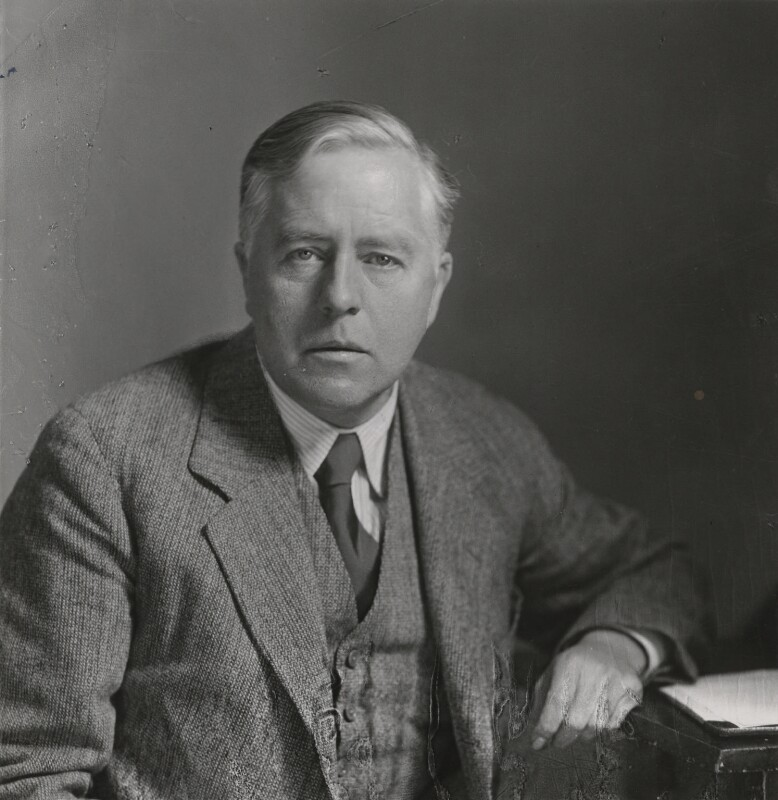
\includegraphics[scale=0.2]{Anh/APho2012.1.jpg}\\
    \textit{James H. Jeans}\\
    $(1877-1946)$
\end{center}
Một nam châm nhỏ có moment lưỡng cực từ $p$ và khối lượng $m$ rơi trong lòng một ống kim loại rất dài, không có từ tính, đặt thẳng đứng, như thấy trong Hình $1$ (hình không vẽ đúng tỉ lệ). Nhìn chung, sự rơi được mô tả bởi phương trình: 
\[m\Ddot{z}=mg-k\Dot{z},\tag{1} \label{i2012.1}\]
với $g$ là gia tốc trọng trường và $k$ gọi là tham số hãm.\\ Sự hãm được gây nên bởi dòng điện xoáy xuất hiện trong ống kim loại. 
\begin{center}
    \tikzset{every picture/.style={line width=0.75pt}} %set default line width to 0.75pt        

\begin{tikzpicture}[x=0.75pt,y=0.75pt,yscale=-1,xscale=1]
%uncomment if require: \path (0,300); %set diagram left start at 0, and has height of 300

%Shape: Ellipse [id:dp6078844013224054] 
\draw   (253.29,60.71) .. controls (253.29,56.01) and (267.62,52.21) .. (285.29,52.21) .. controls (302.97,52.21) and (317.29,56.01) .. (317.29,60.71) .. controls (317.29,65.4) and (302.97,69.21) .. (285.29,69.21) .. controls (267.62,69.21) and (253.29,65.4) .. (253.29,60.71) -- cycle ;
%Shape: Ellipse [id:dp612181013103327] 
\draw   (240.59,60.71) .. controls (240.59,54.15) and (260.6,48.83) .. (285.29,48.83) .. controls (309.98,48.83) and (330,54.15) .. (330,60.71) .. controls (330,67.27) and (309.98,72.58) .. (285.29,72.58) .. controls (260.6,72.58) and (240.59,67.27) .. (240.59,60.71) -- cycle ;
%Straight Lines [id:da6072255552823334] 
\draw    (240.59,59.83) -- (240.59,121.33) ;
%Straight Lines [id:da9762768699823468] 
\draw    (330,60.71) -- (330,121.33) ;
%Straight Lines [id:da33194194901651275] 
\draw  [dash pattern={on 4.5pt off 4.5pt}]  (240.59,121.33) -- (240.59,179.33) ;
%Straight Lines [id:da7387705383182246] 
\draw  [dash pattern={on 4.5pt off 4.5pt}]  (330,121.33) -- (330,179.33) ;
%Straight Lines [id:da07357167794524355] 
\draw    (240.59,179.33) -- (240.59,240.83) ;
%Straight Lines [id:da6030115676990582] 
\draw    (330,179.33) -- (330,240.83) ;
%Curve Lines [id:da6211835397721102] 
\draw    (240.59,240.83) .. controls (241,260.67) and (325,264.67) .. (330,240.83) ;
%Straight Lines [id:da9295985921022609] 
\draw    (209.59,78.83) -- (209.59,137.33) ;
\draw [shift={(209.59,140.33)}, rotate = 270] [fill={rgb, 255:red, 0; green, 0; blue, 0 }  ][line width=0.08]  [draw opacity=0] (10.72,-5.15) -- (0,0) -- (10.72,5.15) -- (7.12,0) -- cycle    ;
%Straight Lines [id:da31637783395092] 
\draw    (361,120.67) -- (305,120.67) ;
\draw [shift={(302,120.67)}, rotate = 360] [fill={rgb, 255:red, 0; green, 0; blue, 0 }  ][line width=0.08]  [draw opacity=0] (10.72,-5.15) -- (0,0) -- (10.72,5.15) -- (7.12,0) -- cycle    ;
%Shape: Rectangle [id:dp13305713828863142] 
\draw  [fill={rgb, 255:red, 21; green, 19; blue, 19 }  ,fill opacity=1 ] (278.51,15.49) -- (278.49,36.49) -- (290.49,36.51) -- (290.51,15.51) -- cycle ;

% Text Node
\draw (190,130.4) node [anchor=north west][inner sep=0.75pt]    {$z$};
% Text Node
\draw (373,113) node [anchor=north west][inner sep=0.75pt]   [align=left] {Ống kim loại};
% Text Node
\draw (301,20) node [anchor=north west][inner sep=0.75pt]   [align=left] {Nam châm};


\end{tikzpicture}\\
Hình $1$.
\end{center}
\begin{enumerate}[1) ]
    \item Xác định vận tốc cuối cùng $(v_{T})$ của nam châm.
    \item Tìm biểu thức $z(t)$, xác định vị trí của nam châm tại thời điểm $t$.\\Lấy $v(t=0)=0$ và $z(t=0)=0$.
\end{enumerate}
Ta sẽ tìm hiểu về động lực học của sự rơi. Muốn vậy, ta xét trong các phần từ $3)$ đến $8)$ một bài toán đơn giản về một nam châm rơi về phía một vòng dây cố định, dọc theo trục của vòng dây. Vòng dây làm bằng kim loại không có từ tính, có bán kính $a$, điện trở $R$ và độ tự cảm $L$ như thấy trên Hình $2$. Trong bài toán này, ta bỏ qua các hiệu ứng bức xạ.\\
\begin{center}
\tikzset{every picture/.style={line width=0.75pt}} %set default line width to 0.75pt        

\begin{tikzpicture}[x=0.75pt,y=0.75pt,yscale=-1,xscale=1]
%uncomment if require: \path (0,300); %set diagram left start at 0, and has height of 300

%Shape: Ellipse [id:dp6435461042549706] 
\draw  [line width=2.25]  (211.37,180.79) .. controls (211.37,169.52) and (252.64,160.39) .. (303.56,160.39) .. controls (354.48,160.39) and (395.76,169.52) .. (395.76,180.79) .. controls (395.76,192.05) and (354.48,201.18) .. (303.56,201.18) .. controls (252.64,201.18) and (211.37,192.05) .. (211.37,180.79) -- cycle ;
%Shape: Ellipse [id:dp7400124230045684] 
\draw  [dash pattern={on 4.5pt off 4.5pt}] (210,79.65) .. controls (210,68.38) and (251.28,59.25) .. (302.2,59.25) .. controls (353.11,59.25) and (394.39,68.38) .. (394.39,79.65) .. controls (394.39,90.91) and (353.11,100.04) .. (302.2,100.04) .. controls (251.28,100.04) and (210,90.91) .. (210,79.65) -- cycle ;
%Straight Lines [id:da05547599228687927] 
\draw  [dash pattern={on 4.5pt off 4.5pt}]  (299.12,79.73) -- (299.12,240.66) ;
\draw [shift={(299.12,243.66)}, rotate = 270] [fill={rgb, 255:red, 0; green, 0; blue, 0 }  ][line width=0.08]  [draw opacity=0] (10.72,-5.15) -- (0,0) -- (10.72,5.15) -- (7.12,0) -- cycle    ;
%Straight Lines [id:da5644922579109435] 
\draw  [dash pattern={on 4.5pt off 4.5pt}]  (302.2,79.65) -- (441.93,79.65) ;
\draw [shift={(444.93,79.65)}, rotate = 180] [fill={rgb, 255:red, 0; green, 0; blue, 0 }  ][line width=0.08]  [draw opacity=0] (10.72,-5.15) -- (0,0) -- (10.72,5.15) -- (7.12,0) -- cycle    ;
%Straight Lines [id:da7526895031881755] 
\draw  [dash pattern={on 4.5pt off 4.5pt}]  (299.12,79.73) -- (353.49,51.2) ;
\draw [shift={(356.15,49.81)}, rotate = 512.31] [fill={rgb, 255:red, 0; green, 0; blue, 0 }  ][line width=0.08]  [draw opacity=0] (10.72,-5.15) -- (0,0) -- (10.72,5.15) -- (7.12,0) -- cycle    ;
%Straight Lines [id:da055924410128701085] 
\draw    (299.12,79.73) -- (365.5,66.58) ;
\draw [shift={(368.44,65.99)}, rotate = 528.79] [fill={rgb, 255:red, 0; green, 0; blue, 0 }  ][line width=0.08]  [draw opacity=0] (10.72,-5.15) -- (0,0) -- (10.72,5.15) -- (7.12,0) -- cycle    ;
%Curve Lines [id:da3493574690364205] 
\draw    (319.27,69.03) .. controls (332.93,68.02) and (337.02,68.02) .. (333.78,72.86) ;
%Straight Lines [id:da814025960137122] 
\draw    (278.63,83.41) -- (278.63,175.26) ;
\draw [shift={(278.63,178.26)}, rotate = 270] [fill={rgb, 255:red, 0; green, 0; blue, 0 }  ][line width=0.08]  [draw opacity=0] (10.72,-5.15) -- (0,0) -- (10.72,5.15) -- (7.12,0) -- cycle    ;
\draw [shift={(278.63,80.41)}, rotate = 90] [fill={rgb, 255:red, 0; green, 0; blue, 0 }  ][line width=0.08]  [draw opacity=0] (10.72,-5.15) -- (0,0) -- (10.72,5.15) -- (7.12,0) -- cycle    ;
%Shape: Rectangle [id:dp32200862062183755] 
\draw  [fill={rgb, 255:red, 11; green, 10; blue, 10 }  ,fill opacity=1 ] (304.94,71.54) -- (304.51,88.08) -- (293.3,87.92) -- (293.74,71.38) -- cycle ;
%Straight Lines [id:da05621487384419388] 
\draw [line width=0.75]    (396.85,251.42) -- (214.37,251.42) ;
\draw [shift={(211.37,251.42)}, rotate = 360] [fill={rgb, 255:red, 0; green, 0; blue, 0 }  ][line width=0.08]  [draw opacity=0] (10.72,-5.15) -- (0,0) -- (10.72,5.15) -- (7.12,0) -- cycle    ;
\draw [shift={(399.85,251.42)}, rotate = 180] [fill={rgb, 255:red, 0; green, 0; blue, 0 }  ][line width=0.08]  [draw opacity=0] (10.72,-5.15) -- (0,0) -- (10.72,5.15) -- (7.12,0) -- cycle    ;

% Text Node
\draw (308.37,226.62) node [anchor=north west][inner sep=0.75pt]    {$z$};
% Text Node
\draw (449.85,69.86) node [anchor=north west][inner sep=0.75pt]    {$y$};
% Text Node
\draw (326.93,39.51) node [anchor=north west][inner sep=0.75pt]    {$x$};
% Text Node
\draw (364.8,65.81) node [anchor=north west][inner sep=0.75pt]  [font=\scriptsize]  {$\rho $};
% Text Node
\draw (336.49,59.71) node [anchor=north west][inner sep=0.75pt]  [font=\scriptsize]  {$\phi $};
% Text Node
\draw (411.74,178.69) node [anchor=north west][inner sep=0.75pt]   [align=left] {Vòng dây};
% Text Node
\draw (256.82,123.47) node [anchor=north west][inner sep=0.75pt]    {$z_{0}$};
% Text Node
\draw (232.9,69.41) node [anchor=north west][inner sep=0.75pt]  [font=\scriptsize] [align=left] {Nam châm};
% Text Node
\draw (295.24,255.95) node [anchor=north west][inner sep=0.75pt]    {$2a$};
\end{tikzpicture}\\
Hình $2$.
\end{center}
Trong trường hợp này, sẽ tiện lợi hơn khi dùng hệ tọa độ trụ $(\rho,\varphi,z)$ như trên Hình $2$, trong đó trục $z$ trùng với trục của vòng dây. Ban đầu, nam châm đứng yên ở gốc tọa độ; tâm vòng dây cách gốc tọa độ một khoảng $z_0$. Các trục tọa độ Descartes $(x,y,z)$ cũng được cho trên hình. Nam châm có moment lưỡng cực $\overrightarrow{p}$ hướng theo chiều dương của trục $z$: $\overrightarrow{p}=p\hat{k}$, với $\hat{k}$ là vector đơn vị trên trục $z$. Ta giả thiết rằng trong khi rơi, moment từ của nam châm giữ nguyên hướng. Khi nam châm nằm ở gốc tọa độ, thì từ trường gây bởi nam châm tại một điểm có tọa độ $(\rho,\varphi,z)$ có thành phần dọc trục $(B_{z})$ và thành phần xuyên tâm $(B_{\rho})$ được cho bởi: 
\[\begin{aligned}
    B_{z}&=\dfrac{\mu_0}{4\pi}\dfrac{p}{(\rho^2+z^2)^{\frac{3}{2}}}\left[\dfrac{3z^2}{\rho^2+z^2}-1\right],\\
    B_{\rho}&=\dfrac{\mu_0}{4\pi}\dfrac{3pz\rho}{(\rho^2+z^2)^{\frac{5}{2}}},
\end{aligned}\] 
với $\mu_0$ là độ từ thẩm của chân không.
\begin{enumerate}[1)]
\setcounter{enumi}{2}
    \item Gọi tốc độ tức thời của nam châm là $v$. Hãy xác định độ lớn suất điện động cảm ứng $(e_{i})$ trong vòng dây.
    \item Suất điện động này gây nên dòng cảm ứng $(i)$ trong vòng dây. Hãy xác định độ lớn của lực điện từ tức thời $(f_{\text{em}})$ tác dụng lên vòng dây theo $i$.
    \item Độ lớn của lực mà vòng dây tác dụng lên nam châm bằng bao nhiêu?
    \item Hãy biểu thị suất điện động trong vòng dây theo $L$, $R$ và $i$. Không cần giải để tìm $i$.
    \item Khi nam châm rơi, nó mất dần thế năng trọng trường. Hãy chỉ ra ba dạng chính của năng lượng mà thế năng trọng trường chuyển hóa thành, và viết các công thức sẽ dùng nếu cần tính từng dạng năng lượng đó. 
    \item Trong quá trình này, từ trường của nam châm có thực hiện công hay không?
\end{enumerate}
Tiếp theo, ta ước lượng tham số hãm $k$ cho trường hợp của
ống (xem phương trình (\ref{i2012.1})). Xét ống dài vô hạn, có bán kính $a$, độ dày nhỏ $w$, và độ dẫn diện $\sigma$. Từ phần này trở đi, ta bỏ qua độ tự cảm của ống. Ta xem ống như được tạo thành từ nhiều vòng dây, mỗi vòng dây có độ cao $\Delta z'$, bán kính $a$, độ dày rất mỏng $w$ và độ dẫn điện $\sigma$ (xem Hình $3$). Để đơn giản, ta coi hai đầu ống có tọa độ là $z=-\infty$ và $z=\infty$.
\begin{center}


\tikzset{every picture/.style={line width=0.75pt}} %set default line width to 0.75pt        

\begin{tikzpicture}[x=0.75pt,y=0.75pt,yscale=-1,xscale=1]
%uncomment if require: \path (0,300); %set diagram left start at 0, and has height of 300

%Shape: Donut [id:dp8312843346003196] 
\draw  [fill={rgb, 255:red, 155; green, 155; blue, 155 }  ,fill opacity=1 ,even odd rule] (191,141.67) .. controls (191,128.04) and (220.1,117) .. (256,117) .. controls (291.9,117) and (321,128.04) .. (321,141.67) .. controls (321,155.29) and (291.9,166.33) .. (256,166.33) .. controls (220.1,166.33) and (191,155.29) .. (191,141.67)(181,141.67) .. controls (181,122.52) and (214.58,107) .. (256,107) .. controls (297.42,107) and (331,122.52) .. (331,141.67) .. controls (331,160.81) and (297.42,176.33) .. (256,176.33) .. controls (214.58,176.33) and (181,160.81) .. (181,141.67) ;
%Straight Lines [id:da8581645335134995] 
\draw    (181,141.67) -- (181,163) ;
%Straight Lines [id:da6296921588002655] 
\draw    (331,141.67) -- (331,162.33) ;
%Curve Lines [id:da8063795216984664] 
\draw    (181,163) .. controls (201,199) and (315,195) .. (331,162.33) ;
%Straight Lines [id:da17318287633113383] 
\draw    (181,35) -- (181,275) ;
%Straight Lines [id:da2233159370082325] 
\draw    (331,37) -- (331,279) ;
%Curve Lines [id:da4730413464853551] 
\draw    (181,275) .. controls (198,265) and (179,306) .. (219,276) ;
%Curve Lines [id:da021373661836334712] 
\draw    (219,276) .. controls (236,266) and (236,298) .. (264,288) ;
%Curve Lines [id:da5117579695710048] 
\draw    (264,288) .. controls (289,247) and (295,314) .. (331,279) ;
%Curve Lines [id:da6518869551809712] 
\draw    (181,275) .. controls (203,242) and (205,261) .. (244,252) ;
%Curve Lines [id:da5342765660730764] 
\draw    (244,252) .. controls (265,252) and (247,253) .. (279,254) ;
%Curve Lines [id:da7817865489186593] 
\draw    (279,254) .. controls (312,234) and (325,270) .. (331,279) ;
%Curve Lines [id:da5263174503814791] 
\draw    (181,35) .. controls (198,25) and (180,66) .. (220,36) ;
%Curve Lines [id:da5268319585625727] 
\draw    (220,36) .. controls (237,26) and (237,58) .. (265,48) ;
%Curve Lines [id:da1930951108450245] 
\draw    (265,48) .. controls (290,7) and (296,74) .. (332,39) ;
%Curve Lines [id:da9788816334466668] 
\draw    (182,35) .. controls (204,2) and (206,21) .. (245,12) ;
%Curve Lines [id:da7323244141892633] 
\draw    (245,12) .. controls (266,12) and (248,13) .. (280,14) ;
%Curve Lines [id:da2315376376069218] 
\draw    (280,14) .. controls (313,-6) and (326,30) .. (332,39) ;
%Straight Lines [id:da1506838382572886] 
\draw    (185,222.33) -- (329,222.33) ;
\draw [shift={(332,222.33)}, rotate = 180] [fill={rgb, 255:red, 0; green, 0; blue, 0 }  ][line width=0.08]  [draw opacity=0] (10.72,-5.15) -- (0,0) -- (10.72,5.15) -- (7.12,0) -- cycle    ;
\draw [shift={(182,222.33)}, rotate = 0] [fill={rgb, 255:red, 0; green, 0; blue, 0 }  ][line width=0.08]  [draw opacity=0] (10.72,-5.15) -- (0,0) -- (10.72,5.15) -- (7.12,0) -- cycle    ;
%Straight Lines [id:da8700643223831148] 
\draw  [dash pattern={on 4.5pt off 4.5pt}]  (256,89.67) -- (256,209.67) ;
\draw [shift={(256,212.67)}, rotate = 270] [fill={rgb, 255:red, 0; green, 0; blue, 0 }  ][line width=0.08]  [draw opacity=0] (10.72,-5.15) -- (0,0) -- (10.72,5.15) -- (7.12,0) -- cycle    ;
%Straight Lines [id:da9280090267594727] 
\draw    (231,93.67) -- (231,141.67) ;
\draw [shift={(231,144.67)}, rotate = 270] [fill={rgb, 255:red, 0; green, 0; blue, 0 }  ][line width=0.08]  [draw opacity=0] (10.72,-5.15) -- (0,0) -- (10.72,5.15) -- (7.12,0) -- cycle    ;
\draw [shift={(231,90.67)}, rotate = 90] [fill={rgb, 255:red, 0; green, 0; blue, 0 }  ][line width=0.08]  [draw opacity=0] (10.72,-5.15) -- (0,0) -- (10.72,5.15) -- (7.12,0) -- cycle    ;
%Straight Lines [id:da6605418042753075] 
\draw  [dash pattern={on 4.5pt off 4.5pt}]  (256,141.67) -- (370,141.67) ;
%Straight Lines [id:da4115042756618199] 
\draw  [dash pattern={on 4.5pt off 4.5pt}]  (256,89.67) -- (370,89.67) ;
%Straight Lines [id:da31516998020231557] 
\draw  [dash pattern={on 4.5pt off 4.5pt}]  (256,57.67) -- (370,57.67) ;
%Shape: Rectangle [id:dp9504791545129123] 
\draw  [fill={rgb, 255:red, 0; green, 0; blue, 0 }  ,fill opacity=1 ] (260.29,82.06) -- (260.38,97.22) -- (251.71,97.28) -- (251.62,82.11) -- cycle ;
%Straight Lines [id:da16857508513893782] 
\draw    (171,143.67) -- (171,165.67) ;
\draw [shift={(171,168.67)}, rotate = 270] [fill={rgb, 255:red, 0; green, 0; blue, 0 }  ][line width=0.08]  [draw opacity=0] (10.72,-5.15) -- (0,0) -- (10.72,5.15) -- (7.12,0) -- cycle    ;
\draw [shift={(171,140.67)}, rotate = 90] [fill={rgb, 255:red, 0; green, 0; blue, 0 }  ][line width=0.08]  [draw opacity=0] (10.72,-5.15) -- (0,0) -- (10.72,5.15) -- (7.12,0) -- cycle    ;
%Straight Lines [id:da3339036824847832] 
\draw    (271,133.67) -- (280.82,121.03) ;
\draw [shift={(282.67,118.67)}, rotate = 487.87] [fill={rgb, 255:red, 0; green, 0; blue, 0 }  ][line width=0.08]  [draw opacity=0] (10.72,-5.15) -- (0,0) -- (10.72,5.15) -- (7.12,0) -- cycle    ;
%Straight Lines [id:da17139286844650492] 
\draw    (306,94.67) -- (292.81,107.57) ;
\draw [shift={(290.67,109.67)}, rotate = 315.63] [fill={rgb, 255:red, 0; green, 0; blue, 0 }  ][line width=0.08]  [draw opacity=0] (10.72,-5.15) -- (0,0) -- (10.72,5.15) -- (7.12,0) -- cycle    ;

% Text Node
\draw (252,226.4) node [anchor=north west][inner sep=0.75pt]  [font=\footnotesize]  {$2a$};
% Text Node
\draw (236,50.4) node [anchor=north west][inner sep=0.75pt]    {$O$};
% Text Node
\draw (376,50.4) node [anchor=north west][inner sep=0.75pt]    {$z=0$};
% Text Node
\draw (376,82.4) node [anchor=north west][inner sep=0.75pt]    {$z( t)$};
% Text Node
\draw (376,131.4) node [anchor=north west][inner sep=0.75pt]    {$z'$};
% Text Node
\draw (140,148.4) node [anchor=north west][inner sep=0.75pt]  [font=\small]  {$\Delta z'$};
% Text Node
\draw (277,89.4) node [anchor=north west][inner sep=0.75pt]    {$w$};


\end{tikzpicture}\\
Hình $3$.
\end{center}
\begin{enumerate}[1) ]
\setcounter{enumi}{8}
    \item Tìm điện trở của mỗi vòng dây đó.
    \item Tìm tham số hãm $k$  gây nên bởi toàn bộ ống theo $p$, $\sigma$ và các tham số hình học của vòng dây. Vì rằng thành ống rất mỏng, nên có thể coi rằng từ trường là như nhau trong toàn bộ bề dày của vòng và bằng $B_{\rho}(\rho=a)$. Giả thiết rằng ở thời điểm $t$, nam châm có toạ độ $z(t)$ và có tốc độ tức thời $\Dot{z}$. Viết kết quả dưới dạng một biểu thức có chứa tích phân $I$, theo biến không thứ nguyên $u=\dfrac{(z-z')}{a}$.
    \item Giả sử tham số hãm $k$ là hàm số:
    \[k=f(\mu_0, p, R_0, a),\]
    với $R_0$ là điện trở hiệu dụng của ống. Bằng cách sử dụng phép phân tích thứ nguyên, hãy tìm biểu thức của $k$. Lấy hệ số tỉ lệ không thứ nguyên bằng đơn vị.
\end{enumerate}
\begin{center}
    \bf Tích phân sau có thể được sử dụng:
\end{center}
\[\int \dfrac{u\mathrm{d}u}{(u^2+a^2)^{n}}=\dfrac{1}{2}\dfrac{(a^2+u^2)^{1-n}}{1-n}+\text{Hằng số}~(\text{với}~n>1).\]
\textbf{Chú ý.} $\Dot{z}=\dfrac{\mathrm{d}z}{\mathrm{d}t}$; $\Ddot{z}=\dfrac{\mathrm{d}^2z}{\mathrm{d}t^2}$.
\end{vd}
\begin{loigiai} 
\begin{enumerate}[1)]
    \item Tìm vận tốc cuối $(v_{T})$ của nam châm.\\
Phương trình chuyển động của nam châm là:
\[m\Ddot{z}=mg-k\Dot{z}. \tag{1} \label{apho12sa.1}\]
Đối với vận tốc cuối, $\Ddot{z}=0$. Từ đó suy ra:
\[v_{T}=\Dot{z}=\dfrac{mg}{k}. \tag{2} \label{apho12sa.2}\]
    \item Tìm vị trí $z(t)$ của nam châm tại thời điểm $t$.\\
    Viết lại phương trình (\ref{apho12sa.1}) dưới dạng
    \[\dfrac{\mathrm{d}v}{\mathrm{d}t}=g-\dfrac{k}{m}v(t). \tag{3} \label{apho12sa.3}\]
    Ta giải phương trình (\ref{apho12sa.3}) với điều kiện ban đầu $v(t=0)=0$; $z(t=0)=0$. Kết quả là:
    \[v(t)=\dfrac{mg}{k}(1-e^{-kt/m})=\dfrac{\mathrm{d}z}{\mathrm{d}t}, \tag{4} \label{apho12sa.4}\]
    \[\int_0^z\mathrm{d}z=\int_0^t\dfrac{mg}{k}(1-e^{-kt/m})\mathrm{d}t~,~z(t)=\dfrac{mg}{k}\left[t+\dfrac{m}{k}(e^{-kt/m}-1)\right]. \tag{5} \label{apho12sa.5}\]
    \item Tính độ lớn suất điện động cảm ứng $(e_{i})$ trong vòng.\\
    Cách thứ nhất là sử dụng vận tốc tương đối $v$ giữa nam châm và vòng trong từ trường $\overrightarrow{B}=B_{k}\overrightarrow{k}+B_{\rho}\overrightarrow{\rho}$ của nam châm, từ đó tính được suất điện động cảm ứng:
    \[e_{i}=\int\left[\overrightarrow{v}\wedge\overrightarrow{B}\right]\mathrm{d}\overrightarrow{\ell}=vB_{a}\cdot2\pi a~,~B_{a}=\dfrac{\mu_0}{4\pi}\dfrac{3pa(z_0-z)}{\left[a^2+(z_0-z)^2\right]^{5/2}}. \tag{6} \label{apho12sa.6}\]
    Cách thứ hai là xét từ thông $\phi$ qua vòng: 
    
    \begin{align*}
     \phi&=\int_0^aB_{z}2\pi\rho\mathrm{d}\rho=2\pi\int_0^a\dfrac{\mu_0}{4\pi}\dfrac{\rho p}{[\rho^2+(z_0-z)^2]^{3/2}}\left[\dfrac{3(z_0-z)^2}{\rho^2+(z_0-z)^2}-1\right]\mathrm{d}\rho\\
    &=\dfrac{\mu_0pa^2}{2[a^2+(z_0-z)^2]^{3/2}}. \tag{7} \label{apho12sa.7}
    \end{align*}
    
    Từ đó, suy ra
    \[e_{i}=\dfrac{-\mathrm{d}\phi}{\mathrm{d}t}=-v\dfrac{\mathrm{d}\phi}{\mathrm{z}}~\Rightarrow e_{i}=\dfrac{\mu_03pa^2v(z_0-z)}{2[a^2+(z_0-z)^2]^{5/2}}. \tag{8} \label{apho12sa.8}\]
    \item Tính lực điện từ tức thời $(f_{\text{em}})$ tác dụng lên vòng theo $i$.\\
    Thành phần $B_{z}$ sẽ gây ra lực xuyên tâm hướng ra bên ngoài trên vòng và do đối xứng dẫn tới một lực bằng không.\\
    Chỉ thành phần $B_{\rho}$ có đóng góp:
    
    \[\mathrm{d}\overrightarrow{f_{\text{em}}}=i\left[\mathrm{d}\overrightarrow{\ell}\wedge\overrightarrow{B}\right]~\Rightarrow \left|\overrightarrow{f_{\text{em}}}\right|=i2\pi aB_{a}, \tag{9} \label{apho12sa.9}\]
    ở đây $B_{a}$ được cho bởi biểu thức (\ref{apho12sa.6}).
    \item Tính độ lớn lực của vòng tác dụng lên nam châm.\\
    Theo định luật III Newton, tồn tại một lực trực đối của lực $\overrightarrow{f_{\text{em}}}$ do vòng tác dụng lên nam châm. Do đó, độ lớn lực của vòng tác dụng lên nam châm là $f_{\text{em}}$.
    \item Biểu diễn suất điện động trong vòng theo $L$, $R$ và $i$.\\
    Kết quả là:
    \[e_{i}=L\dfrac{\mathrm{d}i}{\mathrm{d}t}+R. \tag{10 \label{apho12sa.10}}\]
    \item Xác định ba dạng năng lượng chính mà thế năng hấp dẫn chuyển đổi thành chúng và viết các biểu thức cho ba dạng này.\\
    Thế năng chuyển đổi thành ba phần là
\[ \dfrac{mv^2}{2}~~(\text{động năng}),\tag{11} \label{apho12sa.11}\]
\[\dfrac{Li^2}{2}~~(\text{năng lượng từ trường}), \tag{12} \label{apho12sa.12}\]
\[i^2R\Delta t~~(\text{sự mất mát nhiệt năng Joule do dòng điện trong thời gian $\Delta t$}). \tag{13} \label{apho12sa.13}\]

    \item Từ trường của nam châm có sinh công trong quá trình này không?\\ Câu trả lời là không.
    \item Tính điện trở của vòng.\\
    \[\Delta R=\dfrac{2\pi a}{\sigma \omega \Delta z'}. \tag{14} \label{apho12sa.14}\]
    \item Tính thông số tắt dần $k$ gây nên bởi toàn bộ ống theo $p$, $\sigma$ và các thông số hình học của vòng.\\
    Hợp lực lên nam châm do một vòng tại $z'$ được cho bởi
    \begin{align*}
        f_{\text{em}}&=(2\pi a)iB'_{a}, \tag{15} \label{apho12sa.15}\\
        B'_{a}&=\dfrac{\mu_0}{4\pi}\dfrac{3pa(z'-z)}{[a^2+(z'-z)^2]^{5/2}}, \tag{16} \label{apho12sa.16}\\
        i&=\dfrac{h}{\Delta R}=\dfrac{\sigma we_{i}}{2\pi a}\Delta z', \tag{17} \label{apho12sa.17}
    \end{align*}
    
    trong đó, $i$ là dòng điện cảm ứng trong vòng.\\
    Hợp lực tác dụng lên nam châm do toàn bộ ống là:
    
    \[F=\int_{-\infty}^\infty f_{em}=\int_{-\infty}^\infty B'^2_{a}(2\pi a)w\sigma\dd z'\cdot\Dot{z}.\]
    
    Do ống rất dài nên có thể lấy tích phân từ $-\infty$ đến $\infty$. Khi thay thế $B'_{a}$, ta có:
    
    \[F=\left(\dfrac{\mu_0}{4\pi}\right)^2\cdot18p^2a^3\pi w\sigma \Dot{z}\int_{-\infty}^\infty \dfrac{(z'-z)^2}{[(z'-z)^2+a^2]^5}\mathrm{d}z'.\]
    
    Đặt $u=\dfrac{z'-z}{a}$, cuối cùng ta có:
    
    \[F=\left(\dfrac{\mu_0}{4\pi}\right)^2\dfrac{18p^2\pi w\sigma\Dot{z}}{a^5}\int_{-\infty}^\infty\dfrac{u^2}{(1+u^2)^5}\mathrm{d}u. \tag{18} \label{apho12sa.18} \]
    
    Thông số tắt dần được xác định bởi:
    
    \[k=\dfrac{F}{\Dot{z}}=\left(\dfrac{\mu_0}{4\pi}\right)^2\dfrac{18p^2\pi w\sigma}{a^5}\int_{-\infty}^\infty\dfrac{u^2}{(1+u^2)^5}\mathrm{d}u. \tag{19} \label{apho12sa.19}\]
    
    \item Sử dụng phép tích phân thứ nguyên để tìm biểu thức của $k$.\\
    Cho $k=f(\mu_0,p,R_0,a)$.\\
    Các thứ nguyên của các thông số ống bao hàm là
    \[[\mu_0]=\mathrm{I^{-2}MLT^{-2}}, \tag{20 \label{apho12sa.20}}\]
    \[[p]=\mathrm{IL^2}, \tag{21} \label{apho12sa.21}\]
    \[[R_0]=\mathrm{I^{-2}ML^2T^{-3}}, \tag{22} \label{apho12sa.22}\]
    \[[a]=\mathrm{L}, \tag{23} \label{apho12sa.23}\]
    \[k=\mathrm{MT^{-1}}. \tag{24} \label{apho12sa.24}\]
    Từ đó suy ra:
    \[k=\dfrac{p^2\mu_0^2}{a^4R_0}. \tag{25} \label{apho12sa.25}\]
\end{enumerate}
\end{loigiai}


\begin{vd}[Tụ điện trong chất lỏng dẫn điện]
%Tonghop %APhO 2013 (Indonesia)
Một hệ gồm hai vật dẫn được nhúng chìm trong một chất điện môi lỏng đồng chất, dẫn điện kém. Khi một hiệu điện thế không đổi được đặt vào giữa hai vật dẫn, thì hệ có cả điện trường và từ
trường. Trong bài toán này, ta sẽ khảo sát một hệ như vậy.
\begin{enumerate}[1)]
    \item Đầu tiên, xét một dây dài vô hạn, đặt trong chân không, với điện tích trên một đơn vị chiều dài là $\lambda$. Tính cường độ điện trường \textbf{$E(r)$} do dây gây ra.
    \item Điện thế gây bởi dây dài tích điện có thể được viết dưới dạng 
    \[V(r)=f(r)+K,\]
    trong đó, $K$ là hằng số. Hãy xác định $f(r)$.
    \item Hãy tính điện thế trong toàn không gian $V(x,y,z)$ được gây nên một dây dài vô hạn với điện tích trên một đơn vị chiều dài là $\lambda$, đặt tại $x=-b$ và một dây dài vô hạn khác với điện tích trên một đơn vị chiều dài là $-\lambda$, đặt tại $x=b$. Cả hai dây đều song song với trục $z$. Lấy $V=0$ tại gốc tọa độ.\\
    Hãy phác họa các mặt đẳng thế.
\end{enumerate}
\begin{center}
        Đối với các câu hỏi sau đây, bỏ qua mọi hiệu ứng rìa.
\end{center}
\begin{enumerate}[1)]
\setcounter{enumi}{3}
    \item Bây giờ, xét hai vật dẫn hình trụ rỗng giống nhau, có bán kính $R=3a$, đặt trong chân không. Độ dài của hai vật bằng nhau và lớn hơn nhiều so với bán kính của vật $l\gg R$. Các trục của cả hai vật đều thuộc mặt phẳng $xz$ và song song với trục $z$, một trục cắt trục $x$ tại $x=-5a$ và trục kia cắt trục $x$ tại $x=5a$. Một hiệu điện thế $V_0$ được đặt vào giữa hai vật (vật ở $x=-5a$ có điện thế cao hơn) bằng cách mắc chúng vào một bộ pin. Tính điện thế trong tất cả các miền không gian. Lấy $V=0$ tại gốc tọa độ.
    \item Tính điện dung $C$ của hệ.
    \item Bây giờ nhúng cả hai vật dẫn hình trụ trong một chất lỏng dẫn điện kém, với độ dẫn điện là $\sigma$. Hãy tính dòng điện toàn phần chạy giữa hai vật này. Giả sử hằng số điện môi của chất lỏng bằng hằng số điện môi của của chân không, $\varepsilon=\varepsilon_0$.
    \item Tính điện trở $R$ và tích $RC$ của hệ hai vật hình trụ.
    \item Hãy xác định từ trường của dòng điện được đề cập trong ý $6$. Cho rằng độ từ thẩm của chất lỏng bằng độ từ thẩm của chân không $\mu=\mu_0$.
\end{enumerate}
\textit{Cho tích phân:} $\di\int\dfrac{a\mathrm{d}x}{a^2+x^2}=\arctan{\dfrac{x}{a}}+\text{hằng số}$.
\end{vd}
\begin{loigiai}
\begin{enumerate}[1)]
    \item Tính điện trường $\overrightarrow{E}\tron{\overrightarrow{r}}$.\\
    Áp dụng định luật Gauss:
    \[\oint E \cdot \mathrm{d}A=\dfrac{q}{\varepsilon_0}. \tag{1} \label{apho13sa.1}\]
    Do tính chất đối xứng, điện trường chỉ có thành phần xuyên tâm. Chọn mặt Gauss là mặt trụ có trục đối xứng trùng với dây, ta thu được:
    \[E.2\pi r\ell=\dfrac{\lambda\ell}{\varepsilon_0}.\]
    Từ đó,
    \[\overrightarrow{E}=\dfrac{\lambda}{2\pi\varepsilon_0}\dfrac{\overrightarrow{r}}{r}. \tag{2} \label{apho13sa.2}\]
    \item Xác định $f(r)$.\\
    Điện thế được cho bởi
    \begin{align*}
        V&=-\int_{\text{ref}}^{r}\overrightarrow{E}\mathrm{d}\overrightarrow{\ell}=-\int_{\text{ref}}^{r}E\mathrm{d}r=-\dfrac{\lambda}{2\pi\varepsilon_0}\ln{r}+K=f(r)+K,\\
        f(r)&=-\dfrac{\lambda}{2\pi\varepsilon_0}\ln{r},~ K= \const. \tag{3} \label{apho13sa.3}
    \end{align*}
    \item Tính điện thế $V(x,y,z)$. Phác họa các bề mặt đẳng thế.\\
    Thế năng do cả hai dây mang điện tích là một sự chồng chất thế năng từ mỗi dây.
    \begin{center}
\tikzset{every picture/.style={line width=0.75pt}} %set default line width to 0.75pt        

\begin{tikzpicture}[x=0.75pt,y=0.75pt,yscale=-1,xscale=1]
%uncomment if require: \path (0,300); %set diagram left start at 0, and has height of 300

%Straight Lines [id:da20586263790663417] 
\draw    (110,190.67) -- (422,190.67) ;
\draw [shift={(425,190.67)}, rotate = 180] [fill={rgb, 255:red, 0; green, 0; blue, 0 }  ][line width=0.08]  [draw opacity=0] (10.72,-5.15) -- (0,0) -- (10.72,5.15) -- (7.12,0) -- cycle    ;
%Straight Lines [id:da3593402025789645] 
\draw    (270,210.33) -- (270,45.33) ;
\draw [shift={(270,42.33)}, rotate = 450] [fill={rgb, 255:red, 0; green, 0; blue, 0 }  ][line width=0.08]  [draw opacity=0] (10.72,-5.15) -- (0,0) -- (10.72,5.15) -- (7.12,0) -- cycle    ;
%Straight Lines [id:da6178338081679633] 
\draw  [dash pattern={on 0.84pt off 2.51pt}]  (310,100.33) -- (350,190.67) ;
%Straight Lines [id:da04646592881569167] 
\draw  [dash pattern={on 0.84pt off 2.51pt}]  (310,100.33) -- (190,190.67) ;

% Text Node
\draw (175,191.4) node [anchor=north west][inner sep=0.75pt]    {$-b$};
% Text Node
\draw (345,191.4) node [anchor=north west][inner sep=0.75pt]    {$b$};
% Text Node
\draw (182,170.4) node [anchor=north west][inner sep=0.75pt]    {$\lambda $};
% Text Node
\draw (316,171.4) node [anchor=north west][inner sep=0.75pt]    {$-\lambda $};
% Text Node
\draw (218,140.4) node [anchor=north west][inner sep=0.75pt]    {$r_{1}$};
% Text Node
\draw (334,127.4) node [anchor=north west][inner sep=0.75pt]    {$r_{2}$};
% Text Node
\draw (250,54.4) node [anchor=north west][inner sep=0.75pt]    {$y$};
% Text Node
\draw (408,196.4) node [anchor=north west][inner sep=0.75pt]    {$x$};


\end{tikzpicture}

    \end{center}
    \begin{center}
        \textbf{Hình 1.} Hệ với hai dây dẫn tích điện đều.
    \end{center}
    \[V=-\dfrac{\lambda}{2\pi\varepsilon_0}\ln{r_1}+\dfrac{\lambda}{2\pi\varepsilon_0}\ln{r_2}=\dfrac{\lambda}{2\pi\varepsilon_0}\ln{\dfrac{\sqrt{(b-x)^2+y^2}}{\sqrt{(b+x)^2+y^2}}}. \tag{4} \label{apho13sa.4}\]
    \[\rt V=\dfrac{\lambda}{4\pi\varepsilon_0}\ln{\dfrac{(b-x)^2+y^2}{(b+x)^2+y^2}}. \tag{5} \label{apho13sa.5}\] 
    Ta có thể biến đổi biểu thức (\ref{apho13sa.5}) thành
    \[\left[x-\left(\dfrac{1+\beta}{1-\beta}\right)\right]^2+y^2=b^2\left[\left(\dfrac{1+\beta}{1-\beta}\right)^2-1\right], \tag{6} \label{apho13sa.6}\]
    trong đó,
    \[\beta=\exp{\left(\dfrac{4\pi\varepsilon_0V}{\lambda}\right)}.\]
    Đối với một điện thế $V$ tùy ý, (\ref{apho13sa.6}) là phương trình của đường tròn (Hình $2$).
    \begin{center}
        \tikzset{every picture/.style={line width=0.75pt}} %set default line width to 0.75pt       
\begin{tikzpicture}[x=0.75pt,y=0.75pt,yscale=-1,xscale=1]
%uncomment if require: \path (0,300); %set diagram left start at 0, and has height of 300

%Straight Lines [id:da10693543426460783] 
\draw    (143.92,157.33) -- (516,157.33) ;
%Straight Lines [id:da3103146478005012] 
\draw    (330,75) -- (330,232) ;
%Straight Lines [id:da8245176705593462] 
\draw    (320,163) -- (320,157.67) ;
%Straight Lines [id:da3869717118569522] 
\draw    (310,163) -- (310,157.67) ;
%Straight Lines [id:da2896364900057129] 
\draw    (300,163) -- (300,157.67) ;
%Straight Lines [id:da9732287898962051] 
\draw    (290,163) -- (290,157.67) ;
%Straight Lines [id:da26173531264308303] 
\draw    (280,163) -- (280,157.67) ;
%Straight Lines [id:da5060456076916551] 
\draw    (270,163) -- (270,157.67) ;
%Straight Lines [id:da3158583130304451] 
\draw    (260,163) -- (260,157.67) ;
%Straight Lines [id:da8463799999955766] 
\draw    (250,163) -- (250,157.67) ;
%Straight Lines [id:da9360396153356727] 
\draw    (240,163) -- (240,157.67) ;
%Straight Lines [id:da09586038418322018] 
\draw    (230,163) -- (230,157.67) ;
%Straight Lines [id:da5042715623231964] 
\draw    (220,163) -- (220,157.67) ;
%Straight Lines [id:da4079413348575096] 
\draw    (210,163) -- (210,157.67) ;
%Straight Lines [id:da30770166578596214] 
\draw    (200,163) -- (200,157.67) ;
%Straight Lines [id:da7271762623048859] 
\draw    (190,163) -- (190,157.67) ;
%Straight Lines [id:da6584649516678565] 
\draw    (180,163) -- (180,157.67) ;
%Straight Lines [id:da16719188934813545] 
\draw    (340,163) -- (340,157.67) ;
%Straight Lines [id:da531651144043664] 
\draw    (350,163) -- (350,157.67) ;
%Straight Lines [id:da5867417104959234] 
\draw    (360,163) -- (360,157.67) ;
%Straight Lines [id:da3384814600145336] 
\draw    (370,163) -- (370,157.67) ;
%Straight Lines [id:da8745480922226434] 
\draw    (380,163) -- (380,157.67) ;
%Straight Lines [id:da36491940365480646] 
\draw    (390,163) -- (390,157.67) ;
%Straight Lines [id:da46039068295306973] 
\draw    (400,163) -- (400,157.67) ;
%Straight Lines [id:da9241442401613649] 
\draw    (410,163) -- (410,157.67) ;
%Straight Lines [id:da9724842765070336] 
\draw    (420,163) -- (420,157.67) ;
%Straight Lines [id:da38963657239082505] 
\draw    (430,163) -- (430,157.67) ;
%Straight Lines [id:da1745812557539137] 
\draw    (440,163) -- (440,157.67) ;
%Straight Lines [id:da8640331710903635] 
\draw    (460,163) -- (460,157.67) ;
%Straight Lines [id:da6566384255876303] 
\draw    (480,163) -- (480,157.67) ;
%Straight Lines [id:da06493751970941641] 
\draw    (470,163) -- (470,157.67) ;
%Straight Lines [id:da3571172821878006] 
\draw    (450,163) -- (450,157.67) ;
%Straight Lines [id:da868103216314138] 
\draw    (490,163) -- (490,157.67) ;
%Straight Lines [id:da9153496543950912] 
\draw    (500,163) -- (500,157.67) ;
%Straight Lines [id:da6974442633290248] 
\draw    (330,176.67) -- (323,176.67) ;
%Straight Lines [id:da9858239463086906] 
\draw    (330,196.67) -- (323,196.67) ;
%Straight Lines [id:da6619642859497705] 
\draw    (330,216.67) -- (323,216.67) ;
%Straight Lines [id:da6219377266823873] 
\draw    (330,206.67) -- (323,206.67) ;
%Straight Lines [id:da3599949378577316] 
\draw    (330,186.67) -- (323,186.67) ;
%Straight Lines [id:da7038808423931626] 
\draw    (330,166.67) -- (323,166.67) ;
%Straight Lines [id:da8184073239580727] 
\draw    (330,146.67) -- (323,146.67) ;
%Straight Lines [id:da2400184091007329] 
\draw    (330,136.67) -- (323,136.67) ;
%Straight Lines [id:da9852506000532384] 
\draw    (330,126.67) -- (323,126.67) ;
%Straight Lines [id:da6360794769693767] 
\draw    (330,116.67) -- (323,116.67) ;
%Straight Lines [id:da20505254462663491] 
\draw    (330,106.67) -- (323,106.67) ;
%Straight Lines [id:da6801966692025674] 
\draw    (330,96.67) -- (323,96.67) ;
%Shape: Circle [id:dp5196243670531799] 
\draw   (143.92,157.17) .. controls (143.92,123.75) and (171,96.67) .. (204.42,96.67) .. controls (237.83,96.67) and (264.92,123.75) .. (264.92,157.17) .. controls (264.92,190.58) and (237.83,217.67) .. (204.42,217.67) .. controls (171,217.67) and (143.92,190.58) .. (143.92,157.17) -- cycle ;
%Shape: Circle [id:dp5511881887177501] 
\draw   (395,157.33) .. controls (395,123.92) and (422.09,96.83) .. (455.5,96.83) .. controls (488.91,96.83) and (516,123.92) .. (516,157.33) .. controls (516,190.75) and (488.91,217.83) .. (455.5,217.83) .. controls (422.09,217.83) and (395,190.75) .. (395,157.33) -- cycle ;

%Straight Lines [id:da7093919674906228] 
\draw    (170,163) -- (170,157.67) ;
%Straight Lines [id:da9917455866724287] 
\draw    (160,163) -- (160,157.67) ;


% Text Node
\draw (372,166.4) node [anchor=north west][inner sep=0.75pt]  [font=\scriptsize]  {$0.5$};
% Text Node
\draw (422,166.4) node [anchor=north west][inner sep=0.75pt]  [font=\scriptsize]  {$1.0$};
% Text Node
\draw (471,166.4) node [anchor=north west][inner sep=0.75pt]  [font=\scriptsize]  {$1.5$};
% Text Node
\draw (264,166.4) node [anchor=north west][inner sep=0.75pt]  [font=\scriptsize]  {$-0.5$};
% Text Node
\draw (215,166.4) node [anchor=north west][inner sep=0.75pt]  [font=\scriptsize]  {$-1.0$};
% Text Node
\draw (165,166.4) node [anchor=north west][inner sep=0.75pt]  [font=\scriptsize]  {$-1.5$};
% Text Node
\draw (305,132.4) node [anchor=north west][inner sep=0.75pt]  [font=\scriptsize]  {$0.2$};
% Text Node
\draw (304,111.4) node [anchor=north west][inner sep=0.75pt]  [font=\scriptsize]  {$0.4$};
% Text Node
\draw (305,91.4) node [anchor=north west][inner sep=0.75pt]  [font=\scriptsize]  {$0.6$};
% Text Node
\draw (298,171.4) node [anchor=north west][inner sep=0.75pt]  [font=\scriptsize]  {$-0.2$};
% Text Node
\draw (297,191.4) node [anchor=north west][inner sep=0.75pt]  [font=\scriptsize]  {$-0.4$};
% Text Node
\draw (298,211.4) node [anchor=north west][inner sep=0.75pt]  [font=\scriptsize]  {$-0.6$};


\end{tikzpicture}
    \end{center}
    \begin{center}
        \textbf{Hình 2.} Các mặt đẳng thế với $b=1$ đối với\\ $\beta=12.35$ (bên trái) và $\beta=\dfrac{1}{12.35}$ (bên phải).
    \end{center}
    \item Tính điện thế trong tất cả các vùng.\\
    Từ các phương trình (\ref{apho13sa.5}) và (\ref{apho13sa.6}) ta thấy rằng đối với bất kì giá trị nào của điện thế $V$, mặt đẳng thế của hai dây dẫn (mật độ điện tích dài có độ lớn bằng nhau nhưng trái dấu) là một mặt trụ. Do đó, ta có thể chọn vị trí cụ thể cho mỗi dây để mặt của trụ đều là mặt đẳng thế.\\
    Xét Hình $3$
    \begin{center}


\tikzset{every picture/.style={line width=0.75pt}} %set default line width to 0.75pt        

\begin{tikzpicture}[x=0.75pt,y=0.75pt,yscale=-1,xscale=1]
%uncomment if require: \path (0,300); %set diagram left start at 0, and has height of 300

%Shape: Circle [id:dp5630232295971143] 
\draw   (333.33,170.33) .. controls (333.33,139.04) and (358.7,113.67) .. (390,113.67) .. controls (421.3,113.67) and (446.67,139.04) .. (446.67,170.33) .. controls (446.67,201.63) and (421.3,227) .. (390,227) .. controls (358.7,227) and (333.33,201.63) .. (333.33,170.33) -- cycle ;
%Straight Lines [id:da41879549813935446] 
\draw  [dash pattern={on 0.84pt off 2.51pt}]  (220,170.33) -- (390,170.33) ;
%Straight Lines [id:da4682878912238828] 
\draw  [dash pattern={on 0.84pt off 2.51pt}]  (220,170.33) -- (350,130.33) ;
%Straight Lines [id:da8267906678358548] 
\draw  [dash pattern={on 0.84pt off 2.51pt}]  (350,130.33) -- (390,170.33) ;
%Shape: Circle [id:dp7827821281625822] 
\draw  [fill={rgb, 255:red, 0; green, 0; blue, 0 }  ,fill opacity=1 ] (217.5,170.33) .. controls (217.5,168.95) and (218.62,167.83) .. (220,167.83) .. controls (221.38,167.83) and (222.5,168.95) .. (222.5,170.33) .. controls (222.5,171.71) and (221.38,172.83) .. (220,172.83) .. controls (218.62,172.83) and (217.5,171.71) .. (217.5,170.33) -- cycle ;
%Shape: Circle [id:dp613385859313351] 
\draw  [fill={rgb, 255:red, 0; green, 0; blue, 0 }  ,fill opacity=1 ] (347.5,170.33) .. controls (347.5,168.95) and (348.62,167.83) .. (350,167.83) .. controls (351.38,167.83) and (352.5,168.95) .. (352.5,170.33) .. controls (352.5,171.71) and (351.38,172.83) .. (350,172.83) .. controls (348.62,172.83) and (347.5,171.71) .. (347.5,170.33) -- cycle ;
%Shape: Circle [id:dp8284054405248202] 
\draw  [fill={rgb, 255:red, 0; green, 0; blue, 0 }  ,fill opacity=1 ] (387.5,170.33) .. controls (387.5,168.95) and (388.62,167.83) .. (390,167.83) .. controls (391.38,167.83) and (392.5,168.95) .. (392.5,170.33) .. controls (392.5,171.71) and (391.38,172.83) .. (390,172.83) .. controls (388.62,172.83) and (387.5,171.71) .. (387.5,170.33) -- cycle ;
%Shape: Circle [id:dp9133408818236997] 
\draw  [fill={rgb, 255:red, 0; green, 0; blue, 0 }  ,fill opacity=1 ] (347.5,130.33) .. controls (347.5,128.95) and (348.62,127.83) .. (350,127.83) .. controls (351.38,127.83) and (352.5,128.95) .. (352.5,130.33) .. controls (352.5,131.71) and (351.38,132.83) .. (350,132.83) .. controls (348.62,132.83) and (347.5,131.71) .. (347.5,130.33) -- cycle ;
%Straight Lines [id:da9480691922188029] 
\draw  [dash pattern={on 0.84pt off 2.51pt}]  (350,132.83) -- (350,170.33) ;
%Straight Lines [id:da7030333143680694] 
\draw    (223,190.33) -- (387,190.33) ;
\draw [shift={(390,190.33)}, rotate = 180] [fill={rgb, 255:red, 0; green, 0; blue, 0 }  ][line width=0.08]  [draw opacity=0] (10.72,-5.15) -- (0,0) -- (10.72,5.15) -- (7.12,0) -- cycle    ;
\draw [shift={(220,190.33)}, rotate = 0] [fill={rgb, 255:red, 0; green, 0; blue, 0 }  ][line width=0.08]  [draw opacity=0] (10.72,-5.15) -- (0,0) -- (10.72,5.15) -- (7.12,0) -- cycle    ;
%Straight Lines [id:da1509049270204632] 
\draw    (353,204.33) -- (387,204.33) ;
\draw [shift={(390,204.33)}, rotate = 180] [fill={rgb, 255:red, 0; green, 0; blue, 0 }  ][line width=0.08]  [draw opacity=0] (10.72,-5.15) -- (0,0) -- (10.72,5.15) -- (7.12,0) -- cycle    ;
\draw [shift={(350,204.33)}, rotate = 0] [fill={rgb, 255:red, 0; green, 0; blue, 0 }  ][line width=0.08]  [draw opacity=0] (10.72,-5.15) -- (0,0) -- (10.72,5.15) -- (7.12,0) -- cycle    ;

% Text Node
\draw (285,194.4) node [anchor=north west][inner sep=0.75pt]  [font=\scriptsize]  {$\ell _{1}$};
% Text Node
\draw (365,206.4) node [anchor=north west][inner sep=0.75pt]  [font=\scriptsize]  {$\ell _{2}$};
% Text Node
\draw (260,141.4) node [anchor=north west][inner sep=0.75pt]  [font=\scriptsize]  {$r_{1}$};
% Text Node
\draw (336,150.4) node [anchor=north west][inner sep=0.75pt]  [font=\scriptsize]  {$r_{2}$};
% Text Node
\draw (214,176.4) node [anchor=north west][inner sep=0.75pt]  [font=\scriptsize]  {$\lambda $};
% Text Node
\draw (343,174.4) node [anchor=north west][inner sep=0.75pt]  [font=\scriptsize]  {$-\lambda $};
% Text Node
\draw (373,140.4) node [anchor=north west][inner sep=0.75pt]  [font=\scriptsize]  {$R$};
% Text Node
\draw (370,158.4) node [anchor=north west][inner sep=0.75pt]  [font=\scriptsize]  {$\phi $};


\end{tikzpicture}

    \end{center}
  \begin{center}
      \textbf{Hình 3.} Hai dây dẫn tích điện đều với mặt đẳng thế của nó.
  \end{center}
  Ta muốn tìm một mặt đẳng thế hình trụ mà nó bao kín dây tích điện $-\lambda$. Nếu ta có thể tìm được bề mặt đó thì do đối xứng, ta chắc chắn có thể tìm được một bề mặt giống như thế mà nó bao kín dây tích điện $\lambda$. Điện thế được tính bởi:
  \begin{align*}
      V&=-\dfrac{\lambda}{2\pi\varepsilon_0}\ln{r_1}+\dfrac{\lambda}{2\pi\varepsilon_0}\ln{r_2}\\
      &=-\dfrac{\lambda}{4\pi\varepsilon_0}\ln{(\ell_1^2+R^2-2\ell_1R\cos{\phi})}+\dfrac{\lambda}{4\pi\varepsilon_0}\ln{\left(\ell^2_2+R^2-2\ell_2R\cos{\phi}\right). \tag{7} \label{apho13sa.7}}
  \end{align*}
  Do bề mặt hình trụ là một mặt đẳng thế, điện thế không phụ thuộc vào $\phi$, nghĩa là $\dfrac{\partial V}{\partial \phi}=0$. Do đó,
  
  \[-\dfrac{\lambda}{4\pi\varepsilon_0}\dfrac{2\ell_1 R\sin{\phi}}{\ell_1^2+R^2-2\ell_1R\cos{\phi}}+\dfrac{\lambda}{4\pi\varepsilon_0}\dfrac{2\ell_2R\sin{\phi}}{\ell_2^2+R^2-2\ell_2R\cos{\phi}}=0. \tag{8} \label{apho13sa.8}\]
  
  \begin{align*}
      \Rightarrow\dfrac{\ell_1}{\ell_1^2+R^2-2\ell_1R\cos{\phi}}  &=\dfrac{\ell_2}{\ell_2^2+R^2-2\ell_2R\cos{\phi}},\\
      \Rightarrow \ell_1^2\ell_2+R^2\ell_2-2\ell_1\ell_2R\cos{\phi} &=\ell_1\ell_2^2+R^2\ell_1-2\ell_1\ell_2R\cos{\phi},\\
      \Rightarrow \ell_1\ell_2(\ell_1-\ell_2) &=R^2(\ell_1-\ell_2) \Rightarrow \ell_1\ell_2=R^2. \tag{9} \label{apho13sa.9}
  \end{align*}
  
  Từ dữ liệu đề bài, ta có:
  \[\ell_1+\ell_2=10a \tag{10}, \label{apho13sa.10}\]
  \[\ell_1\ell_2=9a^2 \tag{11}. \label{apho13sa.11}\]
  
  Giải phương trình bậc hai này, ta thu được:
  \[\ell_1=5a\pm 4a. \tag{12} \label{aphp13sa.12}\]
  Tuy nhiên, do $\ell_1>\ell_2$, ta có:
  \begin{align*}
      \ell_1 &= 9a, \tag{13} \label{apho13sa.13}\\
      \ell_2&=a. \tag{14} \label{apho13sa.14}
  \end{align*}
  
  Thay các kết quả vào biểu thức (\ref{apho13sa.5}), ta có
  \[V=\dfrac{\lambda}{4\pi\varepsilon_0}\ln{\dfrac{(4a-x)^2+y^2}{(4a+x)^2+y^2}}. \tag{15} \label{apho13sa.15}\]
  Đây là điện thế trong tất cả các vùng trừ phía trong cả hai hình trụ. Đối với hình trụ tại $x=-5a$, điện thế là hằng số và bằng
  \[V(x=-2a,y=0)=\dfrac{\lambda}{4\pi\varepsilon_0}\ln{\dfrac{(4a+2a)^2+0^2}{(4a-2a)^2+0^2}}=\dfrac{\lambda}{2\pi\varepsilon_0}\ln{3}. \tag{16} \label{apho13sa.16}\]
  
  Đối với hình trụ tại $x=5a$, điện thế cũng là hằng số và bằng
  \[V(x=2a,y=0)=\dfrac{\lambda}{4\pi\varepsilon_0}\ln{\dfrac{(4a-2a)^2+0^2}{(4a+2a)^2+0^2}}=-\dfrac{\lambda}{2\pi\varepsilon_0}\ln{3}. \tag{17} \label{apho13sa.17}\]
  
  Hiệu điện thế giữa hai hình trụ là:
  \[\Delta V=\dfrac{\lambda}{\pi\varepsilon_0}\ln{3}=V_0. \tag{18} \label{apho13sa.18}\]
  
  Thay kết quả này vào phương trình điện thế, điện thế bên ngoài hai hình trụ là 
  
  \[V=\dfrac{V_0}{4\ln{3}}\ln{\dfrac{(4a-x)^2+y^2}{(4a+x)^2+y^2}}. \tag{19} \label{apho13sa.19}\]
  
  Điện thế bên trong hình trụ có tâm tại $(x=5a,y=0)$ là $V=\dfrac{-V_0}{2}$ và điện thế bên trong hình trụ có tâm tại $(x=-5a,y=0)$ là $V=\dfrac{V_0}{2}$.
    \item Tính điện dung $C$ của hệ.\\
    Từ biểu thức (\ref{apho13sa.18}), ta có
    
    \[V_0=\dfrac{q}{\ell\pi\varepsilon_0}\ln{3}. \tag{20} \label{apho13sa.20}\]
    Do đó, 
    \[C=\dfrac{1}{V_0}=\dfrac{\ell\pi\varepsilon_0}{\ln{3}}. \tag{21} \label{apho13sa.21}\]
    \item Tính dòng điện tổng cộng chạy giữa hai xylanh.\\
    Điện trường sinh ra bởi hai hình trụ là
    \begin{align*}
        E_{x}&=\dfrac{V_0}{2\ln{3}}\left[\dfrac{4a+x}{(4a+x)^2+y^2}+\dfrac{4a-x}{(4a-x)^2+y^2}\right], \tag{22} \label{apho13sa.22} \\
        E_{y}&=\dfrac{V_0}{2\ln{3}}\left[\dfrac{y}{(4a+x)^2+y^2}-\dfrac{y}{(4a-x)^2+y^2}\right]. \tag{23} \label{apho13sa.23}
    \end{align*}
    
    Mật độ dòng điện khối được cho bởi
    \[\overrightarrow{J}=\sigma\overrightarrow{E}. \tag{24} \label{apho13sa.24}\]
    
    Để tính dòng điện toàn phần, ta có thể chọn để tính dòng điện chạy qua mặt phẳng $x=0$. Trên mặt phẳng này, không có dòng điện theo hướng $y$. Dòng điện tổng cộng là
    
    \[I=\int\overrightarrow{J}\mathrm{d}\overrightarrow{A}=\int \delta E_{x}\ell\mathrm{d}y=\delta \ell \dfrac{8aV_0}{2\ln{3}}\int_\infty ^\infty\dfrac{\mathrm{d}y}{(4a)^2+y^2}. \tag{25} \label{apho13sa.25}\]
    \[\rt I=\dfrac{V_0\pi\delta\ell}{\ln{3}}. \tag{26} \label{apho13sa.26}\]

    \item Tính điện trở $R$ của hệ. Tính $RC$ của hệ.\\
    Điện trở là
    \[R=\dfrac{V_0}{I}=\dfrac{\ln{3}}{\pi\delta\ell}. \tag{27} \label{apho13sa.27}\]
    Do đó, 
    \[RC=\dfrac{\varepsilon_0}{\delta}. \tag{28} \label{apho13sa.28}\]
    
    \item Tính từ trường do dòng điện trong phần $(6)$.\\
    Do hệ có sự đối xứng cao, ta sử dụng định luật Ampere. Từ trường không phụ thuộc vào $z$, khi đó dòng điện không phụ thuộc vào $z$.\\
    Hình $4$ chỉ ra mật độ dòng điện $\overrightarrow{J}$ chạy từ trụ này sang trụ kia. Chọn một vòng Ampere trên một mặt phẳng $x$ không đổi theo một cách đối xứng sao cho dây thứ nhất chỉ theo hướng dương của trục $z$ với tọa độ $y$ không đổi và dây thứ hai chỉ theo hướng âm của trục $y$ với tọa độ $z$ không đổi. Dây thứ ba chỉ theo hướng âm của trục $z$ nhưng với tọa độ $-y$ không đổi. Dây thứ tư chỉ theo hướng dương của trục $y$ với tọa độ $-z$ không đổi.
    \begin{center}
        \tikzset{every picture/.style={line width=0.75pt}} %set default line width to 0.75pt        

\begin{tikzpicture}[x=0.75pt,y=0.75pt,yscale=-1,xscale=1]
%uncomment if require: \path (0,450); %set diagram left start at 0, and has height of 450

%Shape: Parallelogram [id:dp590263130597569] 
\draw   (213.49,162.17) -- (502.67,162.17) -- (441.84,308.17) -- (152.67,308.17) -- cycle ;
%Straight Lines [id:da10295278078132264] 
\draw    (272,161.67) -- (272,375.67) ;
\draw [shift={(272,268.67)}, rotate = 270] [fill={rgb, 255:red, 0; green, 0; blue, 0 }  ][line width=0.08]  [draw opacity=0] (10.72,-5.15) -- (0,0) -- (10.72,5.15) -- (7.12,0) -- cycle    ;
%Straight Lines [id:da05143886065182923] 
\draw    (305,85.67) -- (272,161.67) ;
\draw [shift={(288.5,123.67)}, rotate = 293.47] [fill={rgb, 255:red, 0; green, 0; blue, 0 }  ][line width=0.08]  [draw opacity=0] (10.72,-5.15) -- (0,0) -- (10.72,5.15) -- (7.12,0) -- cycle    ;
%Straight Lines [id:da21347209362421404] 
\draw    (305,303.67) -- (272,375.67) ;
%Straight Lines [id:da26116284940289325] 
\draw    (305,85.67) -- (305,187.67) ;
%Straight Lines [id:da25015325740443073] 
\draw  [dash pattern={on 4.5pt off 4.5pt}]  (305,187.67) -- (305,303.67) ;
%Straight Lines [id:da35417729042825385] 
\draw    (459,65.67) -- (459,126.67) ;
\draw [shift={(459,62.67)}, rotate = 90] [fill={rgb, 255:red, 0; green, 0; blue, 0 }  ][line width=0.08]  [draw opacity=0] (10.72,-5.15) -- (0,0) -- (10.72,5.15) -- (7.12,0) -- cycle    ;
%Straight Lines [id:da7676077789544753] 
\draw    (459,126.67) -- (502,126.67) ;
\draw [shift={(505,126.67)}, rotate = 180] [fill={rgb, 255:red, 0; green, 0; blue, 0 }  ][line width=0.08]  [draw opacity=0] (10.72,-5.15) -- (0,0) -- (10.72,5.15) -- (7.12,0) -- cycle    ;
%Shape: Can [id:dp39072511191058923] 
\draw   (268,131.98) -- (268,229.35) .. controls (268,238.36) and (255.02,245.67) .. (239,245.67) .. controls (222.98,245.67) and (210,238.36) .. (210,229.35) -- (210,131.98) .. controls (210,122.97) and (222.98,115.67) .. (239,115.67) .. controls (255.02,115.67) and (268,122.97) .. (268,131.98) .. controls (268,140.99) and (255.02,148.29) .. (239,148.29) .. controls (222.98,148.29) and (210,140.99) .. (210,131.98) ;
%Shape: Can [id:dp4304850067909751] 
\draw   (427,130.98) -- (427,228.35) .. controls (427,237.36) and (414.02,244.67) .. (398,244.67) .. controls (381.98,244.67) and (369,237.36) .. (369,228.35) -- (369,130.98) .. controls (369,121.97) and (381.98,114.67) .. (398,114.67) .. controls (414.02,114.67) and (427,121.97) .. (427,130.98) .. controls (427,139.99) and (414.02,147.29) .. (398,147.29) .. controls (381.98,147.29) and (369,139.99) .. (369,130.98) ;
%Curve Lines [id:da4444465117732648] 
\draw  [dash pattern={on 4.5pt off 4.5pt}]  (210,229.35) .. controls (209.77,219.62) and (222.4,214.63) .. (235.94,214.07) .. controls (249.47,213.52) and (268.27,218.69) .. (268,229.35) ;
%Curve Lines [id:da5963569134271516] 
\draw  [dash pattern={on 4.5pt off 4.5pt}]  (369,228.35) .. controls (368.5,207.42) and (427.5,208.42) .. (427,228.35) ;
%Straight Lines [id:da8918846680127841] 
\draw  [dash pattern={on 4.5pt off 4.5pt}]  (210,229.35) -- (210,303.67) ;
%Straight Lines [id:da3353791073588641] 
\draw  [dash pattern={on 4.5pt off 4.5pt}]  (268,229.35) -- (268,303.67) ;
%Straight Lines [id:da31913748721329127] 
\draw  [dash pattern={on 4.5pt off 4.5pt}]  (369,228.35) -- (369,302.67) ;
%Straight Lines [id:da23772632524095938] 
\draw  [dash pattern={on 4.5pt off 4.5pt}]  (427,228.35) -- (427,263.67) -- (427,302.67) ;
%Curve Lines [id:da5377901186494225] 
\draw    (272,182.42) .. controls (331.5,163.92) and (380.2,190.17) .. (368.72,186.05) ;
\draw [shift={(322.75,175.88)}, rotate = 181.32] [fill={rgb, 255:red, 0; green, 0; blue, 0 }  ][line width=0.08]  [draw opacity=0] (10.72,-5.15) -- (0,0) -- (10.72,5.15) -- (7.12,0) -- cycle    ;
%Curve Lines [id:da8078946077416267] 
\draw  [dash pattern={on 4.5pt off 4.5pt}]  (368.72,186.05) .. controls (396,195.37) and (404.98,218.99) .. (404.98,212.49) ;
%Curve Lines [id:da4279646849736449] 
\draw    (228.27,244.43) .. controls (253.4,300.73) and (384.2,295.53) .. (403,244.33) ;
\draw [shift={(316.86,284.71)}, rotate = 180.62] [fill={rgb, 255:red, 0; green, 0; blue, 0 }  ][line width=0.08]  [draw opacity=0] (10.72,-5.15) -- (0,0) -- (10.72,5.15) -- (7.12,0) -- cycle    ;
%Curve Lines [id:da28756259240642534] 
\draw  [dash pattern={on 4.5pt off 4.5pt}]  (228.5,215.17) .. controls (240.5,192.92) and (262.5,187.42) .. (272,182.42) ;
%Curve Lines [id:da16134884964082885] 
\draw  [dash pattern={on 4.5pt off 4.5pt}]  (248.92,214.88) .. controls (259,204.78) and (271.89,201) .. (272.21,201) ;
%Curve Lines [id:da21745721003301255] 
\draw    (272.21,201) .. controls (314.67,188.54) and (344.92,194.04) .. (369.47,205.37) ;
\draw [shift={(321.72,193.95)}, rotate = 180.38] [fill={rgb, 255:red, 0; green, 0; blue, 0 }  ][line width=0.08]  [draw opacity=0] (10.72,-5.15) -- (0,0) -- (10.72,5.15) -- (7.12,0) -- cycle    ;
%Curve Lines [id:da3580325468052228] 
\draw  [dash pattern={on 4.5pt off 4.5pt}]  (369.47,205.37) .. controls (368.17,205.53) and (372.67,205.31) .. (382.83,215.36) ;
%Curve Lines [id:da5604816867368483] 
\draw    (250.03,244.33) .. controls (267.85,266.58) and (353.12,275.85) .. (383.48,242.15) ;
\draw [shift={(317.81,264.3)}, rotate = 180.96] [fill={rgb, 255:red, 0; green, 0; blue, 0 }  ][line width=0.08]  [draw opacity=0] (10.72,-5.15) -- (0,0) -- (10.72,5.15) -- (7.12,0) -- cycle    ;
%Straight Lines [id:da42647618453854275] 
\draw    (268,229.35) -- (369,228.35) ;
\draw [shift={(318.5,228.85)}, rotate = 539.4300000000001] [fill={rgb, 255:red, 0; green, 0; blue, 0 }  ][line width=0.08]  [draw opacity=0] (10.72,-5.15) -- (0,0) -- (10.72,5.15) -- (7.12,0) -- cycle    ;

% Text Node
\draw (466.5,55.07) node [anchor=north west][inner sep=0.75pt]    {$z$};
% Text Node
\draw (492,104.07) node [anchor=north west][inner sep=0.75pt]    {$x$};
% Text Node
\draw (274.5,106.07) node [anchor=north west][inner sep=0.75pt]    {$2$};
% Text Node
\draw (274,236.07) node [anchor=north west][inner sep=0.75pt]    {$3$};
% Text Node
\draw (307,205.07) node [anchor=north west][inner sep=0.75pt]    {$1$};
% Text Node
\draw (292.5,331.57) node [anchor=north west][inner sep=0.75pt]    {$4$};
% Text Node
\draw (326,196.07) node [anchor=north west][inner sep=0.75pt]    {$J$};


\end{tikzpicture}

    \end{center}
    \begin{center}
        \textbf{Hình 4.} Mạch Ampere
    \end{center}
   Với đường dẫn này, ta cần tính dòng điện chạy qua mạch
    \[I=\int\overrightarrow{J}\mathrm{d}\overrightarrow{A}=\int Jx\ell\mathrm{d}y=\dfrac{V_0\delta\ell}{2\ln{3}}\left(\dfrac{4a+x}{(4a+x)^2+y^2}+\dfrac{4a-x}{(4a-x)^2+y^2}\right)\mathrm{d}y.\]
    \[I=\dfrac{V_0\sigma\ell}{\ln{3}}\left(\arctan{\dfrac{y}{4a+x}}+\arctan{\dfrac{y}{4a-x}}\right). \tag{29} \label{apho13sa.29}\]
    Khi dùng định luật Ampere,
    \[\oint\ot{B}\mathrm{d}\ot{I}=\mu_0I. \tag{30} \label{apho13sa.30}\]
    
    \begin{align*}
        \Rightarrow2B_{z}\ell &= \dfrac{\mu_0V_0\sigma\ell}{\ln{3}}\left(\arctan{\dfrac{y}{4a+x}+\arctan{\dfrac{y}{4a-x}}}\right),\\
        \Rightarrow B_{z} &= \dfrac{\mu_0V_0\sigma}{2\ln{3}}\left(\arctan{\dfrac{y}{4a+x}+\arctan{\dfrac{y}{4a-x}}}\right), \tag{31} \label{apho13sa.31}\\
        \Rightarrow\ot{B} &= \ot{z}\dfrac{\mu_0V_0\sigma}{2\ln{3}}\left(\arctan{\dfrac{y}{4a+x}+\arctan{\dfrac{y}{4a-x}}}\right). \tag{32} \label{apho13sa.32}
    \end{align*}
    
\end{enumerate}
\end{loigiai}

\begin{vd}[Gia tốc cho sóng xung kích]
Trong không gian vũ trụ, sóng xung kích có thể gia tốc cho các hạt mang điện cho đến khi đạt được một mức năng lượng rất cao. Chúng ta có thể sử dụng một mô hình lí tưởng của sóng xung kích và thừa nhận rằng có tồn tại một màn chắn thế năng là $-V_0$ được đặt ở chiều cao không đổi và chuyển động với vận tốc $\omega$ quanh trục $Ox$:
\[\begin{aligned}
    &V(x,y,z,t)=-V_0 &\text{nếu } x<\omega t;\\
    &V(x,y,z,t)=0 &\text{nếu } x>\omega t.
\end{aligned}\]
Trong hệ quy chiếu không có sóng xung kích, năng lượng của electron được bảo toàn. Điều đó có nghĩa rằng miễn là khi động năng của electron có khối lượng $m$ và có điện tích $-e$ nhỏ hơn năng lượng của sóng xung kích ($\dfrac{1}{2}mu^2<eV_0 $, với $u$ là vận tốc của electron chuyển động trong môi trường có sóng xung kích), nó sẽ bị phản xạ lại giống như cách một quả bóng đàn hồi bật lại khi va chạm với một bức tường cứng. Sau đây, trừ khi được đề cập trong những trường hợp đặc biệt, va chạm của electron với sóng xung kích sẽ là va chạm đàn hồi. Bạn có thể sẽ phải dùng các thông số như $e$, $V_0$, $m$, $B$, và $\omega$ để biểu diễn các kết quả. Trừ khi ở trong những trường hợp đặc biệt, vận tốc của electron được xem là phi tương đối tính.
\begin{enumerate}[1)]
    \item Cho vận tốc đầu của electron là $\overrightarrow{v}=(v_{x}, v_{y}, v_{z})$ với $v_{x}<\omega$. Hãy xác định vận tốc $\overrightarrow{v'}$ (nói cách khác là các thành phần $v'_{x}, v'_{y}, v'_{z}$) của electron ngay sau khi va chạm với sóng xung kích.
    \item Bây giờ, ở đó cũng có một từ trường đều có cảm ứng từ là $B$, song song với trục $Oz$. Tại thời điểm bắt đầu, electron đang đứng yên ở gốc tọa độ, tại thời điển $t=0$ thì chịu tác dụng của sóng xung kích. Hãy vẽ phác thảo quỹ đạo định tính của electron từ lúc bắt đầu $t=0$ đến ít nhất là lúc $t=\dfrac{\pi m}{Be}$.
    \item Tìm bán kính cong của quỹ đạo electron ngay sau lần va chạm đầu tiên với sóng xung kích.
    \item Tại thời điểm $t_2$, electron sẽ xảy ra va chạm lần thứ hai. Hãy viết biểu thức để xác định $t_2$. Hãy áp dụng phép tính bằng số để biểu diễn $t_2$.
    \item Hãy xác định vận tốc trung bình theo phương $Ox$ $(v_{x})$ của electron (trung bình trong khoảng thười gian $\tau$ giữa hai lần va chạm liên tiếp của electron với sóng xung kích).
    \item Theo thời gian, electron sẽ va chạm rất nhiều lần với sóng xung kích. Hãy chứng minh rằng trong suốt quá trình chuyển động, $v_{y}+kx=$ hằng số, với $k$ là hằng số; biểu diễn $k$ theo $e$, $m$ và $B$.$\label{6}$
    \item Từ bây giờ, chúng ta sẽ xem xét giới hạn $t\gg \dfrac{2\pi m}{Be}$. Xác định gia tốc trung bình theo phương $Oy$ của electron (biểu diễn theo $e$, $m$ và $B$ hay hằng số $k$ đã được giới thiệu ở phần \ref{6}).
    \item Có một vấn đề xuất hiện đó là tại giới hạn $t \gg \dfrac{2\pi m}{Be}$, khoảng thời gian $\tau$ giữa hai lần va chạm ngày càng ngắn dần, vì thế chúng ta có thể thừa nhận rằng $\tau \ll \dfrac{2\pi m}{Be}$. Điều đó có nghĩa là trong khoảng thòi gian giữa hai lần va chạm, vector vận tốc của electron sẽ chỉ đổi một góc rất nhỏ và do đó, vector gia tốc $\overrightarrow{a}=(a_{x},a_{y})$ có thể xem như là bảo toàn.\\
    Bây giờ chúng ta sẽ sử dụng hệ quy chiếu gắn với sóng xung kích, chúng ta xem xét đồ thị pha của electron, nói cách khác là đồ thị mô tả trạng thái của electron như một điểm trong mặt phẳng $x'$ $-$ $p'_{x}$ với trục tung là $p'_{x}=m(v_{x}-\omega)$ tương ứng với $x'$ $-$ thành phần của động lượng, và $x'=\di\int(v_{x}-\omega) \mathrm{d}t$ là khoảng cách so với sóng xung kích. Hãy mô tả một cách định tính quỹ đạo pha của electron, nói cách khác là các đường cong trong đồ thị pha trong suốt một giai đoạn (giữa hai lần va chạm liên tiếp của electron và sóng xung kích). Điểm của phần này sẽ dựa hoàn toàn vào hình dạng của đường cong.
    \item Theo thời gian, độ rộng và chiều cao của quỹ đạo pha sẽ thay đổi, tuy nhiên, có một điều là diện tích bề mặt của vùng được bao bởi quỹ đạo pha (được gọi là bất biến đoạn nhiệt) sẽ luôn là hằng số với độ chính xác cao. Đối với một electron ban đầu ở trạng thái nghỉ, bất biến đoạn nhiệt có giá trị xấp xỉ bằng $\dfrac{1,36(m\omega)^2}{Be}$. Hãy xác định tổng động năng $W_{f}$ của electron khi nó bị tụt lại đằng sau so với sóng xung kích; biểu diễn theo $e$, $V_0$ và $\varepsilon$ với định nghĩa rằng $\varepsilon=\dfrac{2eV_0}{m\omega^2}$;  biết rằng $\varepsilon \gg 1$.
    \item Câu hỏi cuối cùng này sẽ độc lập so với những câu hỏi trước. Xem xét sự lan truyền của sóng xung kích như đã mô tả ở phần trước, nhưng không có sự xuất hiện của từ trường. Một electron tương đối sẽ chuyển động song song so với mặt trước (trong hệ quy chiếu phòng thí nghiệm, thành phần tiếp tuyến của vận tốc luôn bằng không). Biết rằng $m\omega^2<eV_0$ và $\omega \ll c$ (với $c$ là vận tốc ánh sáng), năng lượng tương đối của electron để có thể bị tụt lại phía sau so với sóng xung kích là bao nhiêu? Bạn có thể sử dụng bất kì sự làm tròn hay lấy xấp xỉ nào, miễn là nó hợp lí.
\end{enumerate}
\end{vd}
\begin{loigiai}
\begin{enumerate}[1)]
    \item Trong hệ quy chiếu gắn với sóng xung kích, vận tốc ban đầu của electron là $$\overrightarrow{v_1}=(v_{x}-\omega,v_{y}, v_{z}).$$ 
    Sau khi bị lệch khỏi sóng xung kích, thành phần nằm ngang của vận tốc bị đảo chiều. Do đó, vận tốc của electron trong hệ quy chiếu phi quán tính đang chuyển động, sau khi bị đảo chiều sẽ là $\overrightarrow{v_2}=(\omega-v_{x}, v_{y}, v_{z})$. Quay trở lại với hệ quy chiếu phòng thí nghiệm, cuối cùng vận tốc của electron là $\overrightarrow{v'}=(2\omega-v_{x}, v_{y}, v_{z})$.
    \item Sau khi va chạm với sóng xung kích, electron bắt đầu chuyển động với tốc độ $v=2\omega$. Do từ trường, electron sẽ chuyển động theo quỹ đạo tròn, và tại thời điểm ban đầu, quỹ đạo đó vuông góc với mặt trước. Thêm vào đó, electron sẽ va chạm với sóng xung kích theo chu kì, và tọa độ $x$ của các lần va chạm đó sẽ tăng dần theo thời gian. Điều đó đủ để chúng ta phác họa tương đối quỹ đạo của electron.
\begin{center}
\tikzset{every picture/.style={line width=0.75pt}} %set default line width to 0.75pt        

\begin{tikzpicture}[x=0.75pt,y=0.75pt,yscale=-1,xscale=1]
%uncomment if require: \path (0,300); %set diagram left start at 0, and has height of 300

%Straight Lines [id:da5591323659404421] 
\draw    (220,233.33) -- (220,43.33) ;
\draw [shift={(220,40.33)}, rotate = 450] [fill={rgb, 255:red, 0; green, 0; blue, 0 }  ][line width=0.08]  [draw opacity=0] (10.72,-5.15) -- (0,0) -- (10.72,5.15) -- (7.12,0) -- cycle    ;
%Straight Lines [id:da7603110770757822] 
\draw    (170,80.33) -- (409,80.33) ;
\draw [shift={(412,80.33)}, rotate = 180] [fill={rgb, 255:red, 0; green, 0; blue, 0 }  ][line width=0.08]  [draw opacity=0] (10.72,-5.15) -- (0,0) -- (10.72,5.15) -- (7.12,0) -- cycle    ;
%Curve Lines [id:da7222425082975721] 
\draw    (220,80.33) .. controls (237,82.33) and (259,90.33) .. (259,123) ;
%Curve Lines [id:da3306653270482587] 
\draw    (259,123) .. controls (277,124.33) and (300,143.33) .. (298,165.67) ;
%Curve Lines [id:da3075618074644175] 
\draw    (298,165.67) .. controls (319.12,173.99) and (330.1,199.2) .. (330.06,221.56) ;
\draw [shift={(330,224.33)}, rotate = 272.49] [fill={rgb, 255:red, 0; green, 0; blue, 0 }  ][line width=0.08]  [draw opacity=0] (10.72,-5.15) -- (0,0) -- (10.72,5.15) -- (7.12,0) -- cycle    ;

% Text Node
\draw (389,86.4) node [anchor=north west][inner sep=0.75pt]    {$x$};
% Text Node
\draw (200,46.4) node [anchor=north west][inner sep=0.75pt]    {$y$};


\end{tikzpicture}
\end{center}
    \item Lực Lorentz tác dụng lên electron đóng vai trò là lực hướng tâm:
    \[evB_0=\dfrac{mv^2}{R}.\]
 Do đó: \[R=\dfrac{mv}{eB_0}=\dfrac{2m\omega}{eB_0}.\]

    \item Trước lần va chạm đầu tiên, tọa độ $x$ của electron là $x_1(t)=R\sin{\left(2\pi\dfrac{t}{T}\right)}$ và tọa độ $x$ của sóng xung kích là $x_2(t)=\omega t$. Lần va chạm thứ hai xảy ra khi $x_1(t)=x_2(t)$. Do đó:
    \begin{align*}
    \dfrac{2m\omega}{eB_0}\sin{\left(\dfrac{B_0e}{m}t_2\right)}&=\omega t_2,\\
    \sin{\left(\dfrac{B_0e}{m}t_2\right)}&=\dfrac{1}{2}\dfrac{B_0e}{m}t_2.
    \end{align*}
    Thay $u=\dfrac{B_0e}{m}t_2$, ta được:
    \[\sin{u}=\dfrac{u}{2}.\]
    Đẳng thức này cho nghiệm là $u=1,895$. Do đó: $t_2=1,895 \dfrac{m}{B_0e}$.
    \item Mỗi khi xảy ra va chạm, electron và mặt phẳng phía trước luôn ở cùng vị trí, với cùng giá trị tọa độ $x$. Điều đó có nghĩa là vận tốc trung bình của electron và của sóng xung kích theo phương trục $Ox$ luôn giống nhau. Hay nói cách khác $v_{x}=\omega$.
    \item Chúng ta dễ dàng tìm được giá trị của $k$ bằng cách đạo hàm hai vế của đẳng thức vì các hằng số đã bị loại bỏ. Do đó $\Dot{v_{y}}+kv_{x}=0$. Những lực duy nhất tác dụng lên electron chính là lực Lorentz và lực đẩy giữa electron và sóng xung kích. Vì sóng xung kích tác dụng lên electron chỉ theo phương nằm ngang, thành phần gia tốc theo phương thẳng đứng được tạo ra hoàn toàn dựa vào lực Lorentz. Điều đó có nghĩa là $m\Ddot{y}=-ev_{x}B_0$ được giữ xuyên suốt trong qua trình chuyển động của electron. Nói cách khác, $\Dot{v_{y}}=-\dfrac{B_0e}{m}v_{x}$. Kết hợp với định luật bảo toàn năng lượng, chúng ta có $-\dfrac{B_0e}{m}v_{x}+kv_{x}=0$. Do đó $k=\dfrac{B_0e}{m}$.
    \item Bằng cách đạo hàm từ định luật bảo toàn $v_{y}+\dfrac{B_0e}{m}x=$ hằng số, chúng ta có $a_{y}+\dfrac{B_0e}{m}v_{x}=0$. Trong một thời gian dài, tốc độ chuyển động trung bình của electron theo trục $Ox$ sẽ giống như tốc độ của sóng xung kích. Do đó $a_{y}+\dfrac{B_0e}{m}\omega=0$ và $a_{y}=-\dfrac{B_0e}{m}\omega$.
    \item Trong một khoảng thời gian, luôn có một gia tốc không đổi $a_{x}$ tác dụng lên electron theo phương $Ox$, kể cả trong hệ quy chiếu phòng thí nghiệm và hệ quy chiếu sóng xung kích; chuyển động sẽ giống như bình thường nếu có gia tốc rơi tự do $g=a$. Nếu chúng ta gọi $x$ là khoảng cách tương đối giữa electron và sóng xung kích, động lượng ban đầu theo phương $Ox$ tại $x=0$ là $p_{x0}$, và năng lượng $E=\dfrac{p_{x0}^2}{2m}=\dfrac{p^2_{x}}{2m}+ma_{x}x$ được bảo toàn trong suốt khoảng thời gian ấy (định luật bảo toàn năng lượng). Do đó $p_{x}=\sqrt{p^2_{x0}-2m^2a_{x}x}$. Trên đồ thị pha, nó biểu diễn bằng một đường parabol với trục đối xứng tại $p_{x}=0$. Hơn thế nữa, tại $x=0$, động lượng của electron bị đảo chiều do sự va chạm với sóng xung kích, điều đó có nghĩa là sẽ có một đường thẳng từ $(0,-p_{x0})$ đến $(0,p_{x0})$. Từ những dữ kiện trên, ta có thể vẽ đồ thị pha như sau:
    \begin{center}
% Pattern Info
 
\tikzset{
pattern size/.store in=\mcSize, 
pattern size = 5pt,
pattern thickness/.store in=\mcThickness, 
pattern thickness = 0.3pt,
pattern radius/.store in=\mcRadius, 
pattern radius = 1pt}
\makeatletter
\pgfutil@ifundefined{pgf@pattern@name@_obp51fhcq}{
\pgfdeclarepatternformonly[\mcThickness,\mcSize]{_obp51fhcq}
{\pgfqpoint{0pt}{0pt}}
{\pgfpoint{\mcSize+\mcThickness}{\mcSize+\mcThickness}}
{\pgfpoint{\mcSize}{\mcSize}}
{
\pgfsetcolor{\tikz@pattern@color}
\pgfsetlinewidth{\mcThickness}
\pgfpathmoveto{\pgfqpoint{0pt}{0pt}}
\pgfpathlineto{\pgfpoint{\mcSize+\mcThickness}{\mcSize+\mcThickness}}
\pgfusepath{stroke}
}}
\makeatother
\tikzset{every picture/.style={line width=0.75pt}} %set default line width to 0.75pt        

\begin{tikzpicture}[x=0.75pt,y=0.75pt,yscale=-1,xscale=1]
%uncomment if require: \path (0,300); %set diagram left start at 0, and has height of 300

%Straight Lines [id:da5313724387613878] 
\draw    (162,180.33) -- (391,180.33) ;
\draw [shift={(394,180.33)}, rotate = 180] [fill={rgb, 255:red, 0; green, 0; blue, 0 }  ][line width=0.08]  [draw opacity=0] (10.72,-5.15) -- (0,0) -- (10.72,5.15) -- (7.12,0) -- cycle    ;
%Straight Lines [id:da5968701993643626] 
\draw    (240,260.33) -- (240,75.33) ;
\draw [shift={(240,72.33)}, rotate = 450] [fill={rgb, 255:red, 0; green, 0; blue, 0 }  ][line width=0.08]  [draw opacity=0] (10.72,-5.15) -- (0,0) -- (10.72,5.15) -- (7.12,0) -- cycle    ;
%Shape: Parabola [id:dp40594583338022083] 
\draw  [pattern=_obp51fhcq,pattern size=6pt,pattern thickness=0.75pt,pattern radius=0pt, pattern color={rgb, 255:red, 0; green, 0; blue, 0}] (240.24,220.92) .. controls (331.53,191.15) and (331.61,161.14) .. (240.47,130.9) ;
%Straight Lines [id:da5900835283967321] 
\draw    (255,215.67) -- (243.06,219.92) ;
\draw [shift={(240.24,220.92)}, rotate = 340.4] [fill={rgb, 255:red, 0; green, 0; blue, 0 }  ][line width=0.08]  [draw opacity=0] (10.72,-5.15) -- (0,0) -- (10.72,5.15) -- (7.12,0) -- cycle    ;
%Straight Lines [id:da4587777282898413] 
\draw    (240,146) -- (240.38,133.9) ;
\draw [shift={(240.47,130.9)}, rotate = 451.79] [fill={rgb, 255:red, 0; green, 0; blue, 0 }  ][line width=0.08]  [draw opacity=0] (10.72,-5.15) -- (0,0) -- (10.72,5.15) -- (7.12,0) -- cycle    ;
%Straight Lines [id:da6091201871513336] 
\draw    (309,172) -- (308.87,176.09) ;
\draw [shift={(308.77,179.09)}, rotate = 271.86] [fill={rgb, 255:red, 0; green, 0; blue, 0 }  ][line width=0.08]  [draw opacity=0] (10.72,-5.15) -- (0,0) -- (10.72,5.15) -- (7.12,0) -- cycle    ;

% Text Node
\draw (218,77.4) node [anchor=north west][inner sep=0.75pt]    {$p_{x}$};
% Text Node
\draw (377,185.4) node [anchor=north west][inner sep=0.75pt]    {$x$};
% Text Node
\draw (310,185.4) node [anchor=north west][inner sep=0.75pt]    {$x_{1}$};
% Text Node
\draw (210,117.4) node [anchor=north west][inner sep=0.75pt]    {$p_{x0}$};
% Text Node
\draw (204,212.4) node [anchor=north west][inner sep=0.75pt]    {$-p_{x0}$};


\end{tikzpicture}

    \end{center}
    \item Diện tích phần dưới của biểu đồ pha có thể tìm bằng cách lấy tích phân $p_{x}(x)\mathrm{d}x$ từ $x_0=0$ đến $x_1=\dfrac{p^2_{x0}}{2m^2a_{x}}$ và nhân đôi kết quả với $2$ (bởi vì đồ thị pha đối xứng qua $p_{x}=0$). Do đó:
    \[S=2\int_{0}^{x_1}\sqrt{p^2_{x0}-2m^2a_{x}x}~\mathrm{d}x=2p_{x0}\int_{0}^{x_1}\sqrt{1-\dfrac{x}{x_1}}~\mathrm{d}x=\dfrac{4}{3}p_{x0}x_1=\dfrac{2}{3}\dfrac{p^3_{x0}}{m^2a_{x}}=\dfrac{2}{3}\dfrac{mv_0^3}{a_{x}}.\]
    Do sự bảo toàn của đại lượng này (chúng ta sử dụng giá trị ban đầu của nó từ dữ kiện đề bài)
    \begin{align*}
    \dfrac{2}{3}\dfrac{mv_0^3}{a_{x}}&=\dfrac{1,36(m\omega)^2}{B_0e},\\
    a_{x}&=\dfrac{1}{2,04}\dfrac{v_0^3B_0e}{m\omega^2}.
    \end{align*}
    Với $v_0$ là tốc độ của electron tại $x=0$. Electron sẽ bị tụt lại phía sau so với sóng xung kích khi $\dfrac{mv_0^2}{2}>eV_0$ hay $v_0>\sqrt{\dfrac{2eV_0}{m}}=\omega\sqrt{\varepsilon}$. Thành phần gia tốc nằm ngang là do lực Lorentz $a_{x}=\dfrac{B_0ev_{y}}{m}$. Do đó:
    %d - displaystyle
    \begin{align*}
        \dfrac{1}{2,04}\dfrac{B_0e}{m\omega^2}\omega^3\varepsilon^{ \frac{3}{2}}&=\dfrac{B_0ev_{y}}{m},\\
        \dfrac{1}{2,04}\omega\varepsilon^{ \frac{3}{2}}&=v_{y}.
    \end{align*}
    Vì $v_{y} \gg v_{x}$, $W_{f}\approx\dfrac{mv^2_{y}}{2}$
    \[W_{f}=\dfrac{\varepsilon^3}{2,04}\dfrac{m\omega^2}{2}=\dfrac{\varepsilon^2}{2,04^2}eV_0.\]
    \item Trong hệ quy chiếu gắn với sóng xung kích, ban đầu, động lượng tác dụng theo phương $Ox$ và $Oy$ lần lượt là $p_{x}$ và $p_{y}$. Trong trường hợp giới hạn, động lượng cuối cùng của electron theo phương $Ox$ là bằng không. Do sóng xung kích chỉ có tác dụng theo phương $Ox$, $p_{y}$ vẫn giữ nguyên không đổi trong suốt quá trình chuyển động. Đại lượng bất biến Lorentz động lượng bốn chiều trước và sau khi electron đạt được trạng thái nghỉ, có thể viết như sau:
    \begin{align*}
        E^2&=p_{x}^2c^2+p_{y}^2c^2+m_0^2c^4,\\
        (E-eV_0)^2&=p_{y}^2c^2+m_0^2c^4.
    \end{align*}
Trừ vế theo vế, ta được $2EeV_0-e^2V_0^2=p_{x}^2c^2=m^2_{\text{rel}}c^2\omega^2=E^2\dfrac{\omega^2}{c^2}$. Do đó:
\[\begin{aligned}
    &E^2\dfrac{\omega^2}{c^2}-2EeV_0+e^2V_0^2 = 0,\\
    &E = \dfrac{eV_0c^2}{\omega^2}\left(1\pm\sqrt{1-\dfrac{\omega^2}{c^2}}\right),
\end{aligned}\]
với dấu trừ chúng ta có thể thu được $p_{y}^2c^2=(E-eV_0)^2-m_0^2c^4<(E-eV_0)^2-e^2V_0^2c^4/\omega^4<0$ là điều không đúng. Do đó, chúng ta phải lấy dấu cộng:
\[E=\dfrac{eV_0c^2}{\omega^2}\left(1+\sqrt{1-\dfrac{\omega^2}{c^2}}\right),\]
trong đó, $\omega \ll c$ nên chúng ta có thể lấy gần đúng $E=\dfrac{2eV_0c^2}{\omega^2}$. Vậy electron sẽ bị tụt lại phía sau so với sóng xung kích nếu năng lượng tương đối của nó là $E\geq\dfrac{2eV_0c^2}{\omega^2}$.
\end{enumerate}
\end{loigiai}


\begin{vd}[Electron thoát ra]
    Một dây dẫn dài vô hạn có dòng điện $I$ và bán kính $a$.
    \begin{enumerate}[1)]
    %\setlength{\itemsep}{-5pt}
        \item Bề mặt bên ngoài của dây được giữ ở điện thế $-V$, với $V$ dương. Dây dẫn được đặt trong một lớp vỏ hình trụ được nối đất với bán kính $b>a$. Bằng một cách nào đó, một electron thoát ra khỏi bề mặt dây dẫn. Coi rằng lúc thoát ra khỏi bề mặt dây dẫn, electron có vận tốc bằng không. Bỏ qua sự bức xạ điện từ.\\
        Vẽ một cách định tính đường đi của elctron cùng với dây.
        \item Tìm khoảng cách cực đại $r_{\max}$ của electron đến trục dây trong quá trình chuyển động của electron theo $V$, $I$, $a$ và $b$.
        Bỏ qua hiệu ứng tương đối tính.
        \item Câu hỏi như phần trên nhưng có tính đến hiệu ứng tương đối tính.
        \item Vẽ đồ thị $r_{\max}$ theo như tính được trong phần $3)$ như là một hàm của $V$.
    \end{enumerate}
    \end{vd}
      \begin{loigiai}
      \renewcommand{\theequation}{\arabic{equation}}
    \begin{enumerate}[1)]
    \setlength{\itemsep}{0pt}
        \item Ta thấy các lực tác dụng chỉ nằm trong mặt phẳng đi qua trục dây dẫn, vậy nên electron chỉ chuyển động trong mặt phẳng đi qua trục dây dẫn.\\
        Hình dạng quỹ đạo của electron như hình vẽ.
        %chèn hình
        \begin{center}
            

\tikzset{every picture/.style={line width=0.75pt}} %set default line width to 0.75pt        

\begin{tikzpicture}[x=0.75pt,y=0.75pt,yscale=-1,xscale=1]
%uncomment if require: \path (0,210); %set diagram left start at 0, and has height of 210

%Straight Lines [id:da5620675167927436] 
\draw    (187,106) -- (428.71,106) ;
%Straight Lines [id:da13390227703886715] 
\draw    (187,118) -- (429.71,118) ;
%Straight Lines [id:da2539571226839463] 
\draw  [dash pattern={on 4.5pt off 4.5pt}]  (187,112) -- (428.71,112) ;
%Straight Lines [id:da9224449183978367] 
\draw    (187,43) -- (429.68,42.54) ;
%Straight Lines [id:da6358504813067694] 
\draw    (187,179) -- (429.71,179) ;
%Curve Lines [id:da9477997558507147] 
\draw    (251.71,105.16) .. controls (252.71,80.16) and (278.71,47.16) .. (299.71,47.16) .. controls (320.71,47.16) and (347.71,81.16) .. (348.71,105.16) ;
%Shape: Circle [id:dp31182285601982773] 
\draw  [fill={rgb, 255:red, 255; green, 255; blue, 255 }  ,fill opacity=1 ] (253.84,80.58) .. controls (253.84,77.5) and (256.34,75) .. (259.42,75) .. controls (262.5,75) and (265,77.5) .. (265,80.58) .. controls (265,83.66) and (262.5,86.16) .. (259.42,86.16) .. controls (256.34,86.16) and (253.84,83.66) .. (253.84,80.58) -- cycle ;
%Straight Lines [id:da13951558247655105] 
\draw    (259.42,80.58) -- (273.88,48.97) ;
\draw [shift={(274.71,47.16)}, rotate = 474.58] [color={rgb, 255:red, 0; green, 0; blue, 0 }  ][line width=0.75]    (10.93,-4.9) .. controls (6.95,-2.3) and (3.31,-0.67) .. (0,0) .. controls (3.31,0.67) and (6.95,2.3) .. (10.93,4.9)   ;
%Shape: Ellipse [id:dp32197955614831475] 
\draw   (160.22,111) .. controls (160.22,73.44) and (172.21,43) .. (187,43) .. controls (201.79,43) and (213.78,73.44) .. (213.78,111) .. controls (213.78,148.56) and (201.79,179) .. (187,179) .. controls (172.21,179) and (160.22,148.56) .. (160.22,111) -- cycle ;
%Shape: Arc [id:dp8110209425106236] 
\draw  [draw opacity=0] (429.68,42.54) .. controls (429.72,42.54) and (429.76,42.54) .. (429.79,42.54) .. controls (445.03,42.54) and (457.38,73.09) .. (457.38,110.77) .. controls (457.38,148.45) and (445.03,179) .. (429.79,179) .. controls (429.76,179) and (429.74,179) .. (429.71,179) -- (429.79,110.77) -- cycle ; \draw   (429.68,42.54) .. controls (429.72,42.54) and (429.76,42.54) .. (429.79,42.54) .. controls (445.03,42.54) and (457.38,73.09) .. (457.38,110.77) .. controls (457.38,148.45) and (445.03,179) .. (429.79,179) .. controls (429.76,179) and (429.74,179) .. (429.71,179) ;
%Shape: Arc [id:dp8017528716240261] 
\draw  [draw opacity=0][dash pattern={on 4.5pt off 4.5pt}] (429.9,179) .. controls (429.86,179) and (429.83,179) .. (429.79,179) .. controls (414.56,179) and (402.21,148.45) .. (402.21,110.77) .. controls (402.21,73.09) and (414.56,42.54) .. (429.79,42.54) .. controls (429.82,42.54) and (429.85,42.54) .. (429.87,42.54) -- (429.79,110.77) -- cycle ; \draw  [dash pattern={on 4.5pt off 4.5pt}] (429.9,179) .. controls (429.86,179) and (429.83,179) .. (429.79,179) .. controls (414.56,179) and (402.21,148.45) .. (402.21,110.77) .. controls (402.21,73.09) and (414.56,42.54) .. (429.79,42.54) .. controls (429.82,42.54) and (429.85,42.54) .. (429.87,42.54) ;
%Straight Lines [id:da2798876105658161] 
\draw  [dash pattern={on 4.5pt off 4.5pt}]  (187,43) -- (187,179) ;
%Straight Lines [id:da9391813698918585] 
\draw  [dash pattern={on 4.5pt off 4.5pt}]  (429.87,42.54) -- (429.87,178.54) ;




\end{tikzpicture}

        \end{center}
        \item Giả sử điện trường tại bề mặt dây dẫn là $E_0$.\\
        Áp dụng định luật Gauss, ta có:
        \begin{equation*}
        \begin{aligned}
             E_0\tron{2\pi al}&=E(r)\tron{2\pi rl},\\
             \Leftrightarrow E(r)&=\dfrac{E_0a}{r}.
        \end{aligned}
        \end{equation*}
        Lại có:
        \[\begin{aligned}
            \dd V&=-E(r)\dd r,\\
            \Leftrightarrow  \dd V&=-E_0a\frac{\dd r}{r},\\
            \Leftrightarrow \ V_r&=E_0a\ln\tron{\dfrac{b}{r}}.
        \end{aligned}\tag{1}\label{c161}\]
        Tại $r=a$ thì $V_r=-V$, suy ra:
        $$ -V=E_0a\ln\tron{\dfrac{b}{a}}\Leftrightarrow E_0=\dfrac{-V}{a\ln\tron{\dfrac{b}{a}}}.$$
        Thay vào (\ref{c161}), ta có:
        $$V_r=-V\dfrac{\ln\dfrac{b}{r}}{\ln\dfrac{b}{a}}=V\log_{\frac{b}{a}}\tron{\dfrac{r}{b}}.$$
        Từ trường sinh ra bởi dây dẫn:
        $$B(r)=\dfrac{\mu_0I}{2\pi r}.$$
        Gọi $v_r$, $v_z$ lần lượt là thành phần vận tốc theo phương bán kính và theo phương song song với trục dây.\\
        \begin{minipage}{0.5\textwidth}
             
\centering
\tikzset{every picture/.style={line width=0.75pt}} %set default line width to 0.75pt        

\begin{tikzpicture}[x=0.75pt,y=0.75pt,yscale=-1,xscale=1]
%uncomment if require: \path (0,210); %set diagram left start at 0, and has height of 210

%Straight Lines [id:da3973766845775675] 
\draw    (389.02,122.2) -- (376.29,87.85) ;
\draw [shift={(375.6,85.98)}, rotate = 429.65999999999997] [color={rgb, 255:red, 0; green, 0; blue, 0 }  ][line width=0.75]    (10.93,-4.9) .. controls (6.95,-2.3) and (3.31,-0.67) .. (0,0) .. controls (3.31,0.67) and (6.95,2.3) .. (10.93,4.9)   ;
%Shape: Can [id:dp15135767507223008] 
\draw   (412.71,63.75) -- (412.71,180.41) .. controls (412.71,189.02) and (384.57,196) .. (349.85,196) .. controls (315.14,196) and (287,189.02) .. (287,180.41) -- (287,63.75) .. controls (287,55.14) and (315.14,48.16) .. (349.85,48.16) .. controls (384.57,48.16) and (412.71,55.14) .. (412.71,63.75) .. controls (412.71,72.36) and (384.57,79.34) .. (349.85,79.34) .. controls (315.14,79.34) and (287,72.36) .. (287,63.75) ;
%Straight Lines [id:da7332224525248945] 
\draw  [dash pattern={on 4.5pt off 4.5pt}]  (287,180.41) -- (412.71,180.41) ;
%Straight Lines [id:da25208598259641724] 
\draw    (349.85,23.16) -- (349.85,180.41) ;
\draw [shift={(349.85,100.78)}, rotate = 90] [color={rgb, 255:red, 0; green, 0; blue, 0 }  ][line width=0.75]    (10.93,-4.9) .. controls (6.95,-2.3) and (3.31,-0.67) .. (0,0) .. controls (3.31,0.67) and (6.95,2.3) .. (10.93,4.9)   ;
\draw [shift={(349.85,21.16)}, rotate = 90] [color={rgb, 255:red, 0; green, 0; blue, 0 }  ][line width=0.75]    (10.93,-4.9) .. controls (6.95,-2.3) and (3.31,-0.67) .. (0,0) .. controls (3.31,0.67) and (6.95,2.3) .. (10.93,4.9)   ;
%Shape: Arc [id:dp5812500876537432] 
\draw  [draw opacity=0][dash pattern={on 4.5pt off 4.5pt}] (287,179.18) .. controls (287.13,169.95) and (315.22,162.49) .. (349.85,162.49) .. controls (384.57,162.49) and (412.71,169.99) .. (412.71,179.24) .. controls (412.71,179.59) and (412.67,179.94) .. (412.59,180.28) -- (349.85,179.24) -- cycle ; \draw  [dash pattern={on 4.5pt off 4.5pt}] (287,179.18) .. controls (287.13,169.95) and (315.22,162.49) .. (349.85,162.49) .. controls (384.57,162.49) and (412.71,169.99) .. (412.71,179.24) .. controls (412.71,179.59) and (412.67,179.94) .. (412.59,180.28) ;
%Shape: Can [id:dp192269551997851] 
\draw   (358.99,64.29) -- (358.99,179.91) .. controls (358.99,181.29) and (354.89,182.41) .. (349.83,182.41) .. controls (344.77,182.41) and (340.67,181.29) .. (340.67,179.91) -- (340.67,64.29) .. controls (340.67,62.91) and (344.77,61.79) .. (349.83,61.79) .. controls (354.89,61.79) and (358.99,62.91) .. (358.99,64.29) .. controls (358.99,65.67) and (354.89,66.79) .. (349.83,66.79) .. controls (344.77,66.79) and (340.67,65.67) .. (340.67,64.29) ;
%Shape: Circle [id:dp028800205251831912] 
\draw  [fill={rgb, 255:red, 0; green, 0; blue, 0 }  ,fill opacity=1 ] (347.62,180.2) .. controls (347.62,178.98) and (348.61,178) .. (349.83,178) .. controls (351.05,178) and (352.03,178.98) .. (352.03,180.2) .. controls (352.03,181.42) and (351.05,182.41) .. (349.83,182.41) .. controls (348.61,182.41) and (347.62,181.42) .. (347.62,180.2) -- cycle ;
%Straight Lines [id:da11771007829087088] 
\draw  [dash pattern={on 4.5pt off 4.5pt}]  (287,63.75) -- (412.71,63.75) ;
%Curve Lines [id:da35451372365197975] 
\draw  [dash pattern={on 4.5pt off 4.5pt}]  (358.99,179.91) .. controls (381.19,180.24) and (395.19,162.57) .. (395.36,144.2) .. controls (395.53,125.83) and (382.52,104.57) .. (359.52,103.91) ;
%Flowchart: Connector [id:dp3532513418574772] 
\draw  [fill={rgb, 255:red, 255; green, 255; blue, 255 }  ,fill opacity=1 ] (392.65,122.2) .. controls (392.65,120.2) and (391.03,118.57) .. (389.02,118.57) .. controls (387.02,118.57) and (385.4,120.2) .. (385.4,122.2) .. controls (385.4,124.2) and (387.02,125.83) .. (389.02,125.83) .. controls (391.03,125.83) and (392.65,124.2) .. (392.65,122.2) -- cycle ;
%Straight Lines [id:da06152713211192218] 
\draw [line width=0.75]    (351.82,180.41) -- (429.27,180.41) ;
\draw [shift={(431.27,180.41)}, rotate = 180] [color={rgb, 255:red, 0; green, 0; blue, 0 }  ][line width=0.75]    (10.93,-4.9) .. controls (6.95,-2.3) and (3.31,-0.67) .. (0,0) .. controls (3.31,0.67) and (6.95,2.3) .. (10.93,4.9)   ;

% Text Node
\draw (331.65,180.05) node [anchor=north west][inner sep=0.75pt]    {$O$};
% Text Node
\draw (333.98,13.5) node [anchor=north west][inner sep=0.75pt]    {$z$};
% Text Node
\draw (419.26,183.57) node [anchor=north west][inner sep=0.75pt]    {$r$};
% Text Node
\draw (359.59,83.91) node [anchor=north west][inner sep=0.75pt]    {$\ot{v}$};
% Text Node
\draw (330.26,100.77) node [anchor=north west][inner sep=0.75pt]    {$I$};
\end{tikzpicture}

        \end{minipage}
        \begin{minipage}{0.45\textwidth}
              Ta có:
            \[\begin{aligned}
                m\dot v_r&=-E(r)e+eB(r)v_z\\
                &=\dfrac{Ve}{r\ln\tron{\dfrac{b}{a}}}+\dfrac{\mu_0Iev_z}{2\pi r},
            \end{aligned} \tag{2}\label{c162}\]
            \[\begin{aligned}
                m\dot v_z&=-B(r)ev_r\\
                &=-\dfrac{\mu_0Iev_r}{2\pi r}.
            \end{aligned}\tag{3}\label{c163}\]

        \end{minipage}
        \hfill \\ \hfill \\
        Từ (\ref{c163}), ta suy ra:
        \[\begin{aligned}
                m\dd v_z&=-\dfrac{\mu_0Ie}{2\pi}\dd\tron{\ln r}\\
                \Leftrightarrow v_z&=-\dfrac{\mu_0Ie}{2\pi m}\ln\tron{\dfrac{r}{a}}.
            \end{aligned}\tag{4}\label{c164}\]
        Khi electron ở vị trí $r_{\max}$ thì $v_r=0$, $v=v_z$.
        Theo định luật bảo toàn năng lượng, ta có:
        \[\dfrac{m{v_z}^2}{2}+Ve\log_{\frac{b}{a}}\tron{\dfrac{r_{\max}}{b}}=-Ve. \tag{5}\label{k165}\]
        Từ (\ref{c164}) và (\ref{k165}), ta có:
        \[\dfrac{m}{2}\tron{\dfrac{\mu_0Ie}{2\pi m}}^2\tron{\ln\tron{\dfrac{r}{a}}^2}+\dfrac{Ve}{\ln\tron{\dfrac{a}{b}}}\tron{\ln(r)-\ln(a)+\ln(a)-\ln(b)}=Ve\]
        \[\Leftrightarrow \dfrac{m}{2}\tron{\dfrac{\mu_0Ie}{2\pi m}}^2\tron{\ln\tron{\dfrac{r}{a}}^2}+\dfrac{Ve}{\ln\tron{\dfrac{a}{b}}}\tron{\ln\tron{\dfrac{r}{a}}}=0.\]
        Đặt $ \dfrac{m}{2}\tron{\dfrac{\mu_0Ie}{2\pi m}}^2=A_1$, $\dfrac{Ve}{\ln\tron{\dfrac{a}{b}}}=A_2$, $\ln(\dfrac{r}{a})=x$. Ta có
        $$A_1x^2+A_2x=0.$$
        Giải phương trình trên, ta được:
       \begin{equation*}
           \begin{aligned}
                x&=-\dfrac{A_2}{A_1}=\dfrac{8\pi^2mV}{{\mu_0}^2I^2e\ln\tron{\dfrac{b}{a}}}.
           \end{aligned}
       \end{equation*}
       Ta tính được 
       \begin{equation*}
           \begin{aligned}
                r_{\max}=a\exp\tron{\dfrac{8\pi^2mV}{{\mu_0}^2I^2e\ln\tron{\dfrac{b}{a}}}}.
           \end{aligned}
       \end{equation*}
       \item Tương tự như phần trước, ta có:
       \setcounter{equation}{5}
       \begin{equation}
           \dfrac{\dd p_r}{\dd t}=\dfrac{Ve}{r\ln\tron{\dfrac{b}{a}}}+\dfrac{\mu_0Iev_z}{2\pi r},
       \end{equation}
       \begin{equation}
           \dfrac{\dd p_z}{\dd t}=-\dfrac{\mu_0Iev_r}{2\pi r}. \label{c165}
       \end{equation}
       Từ (\ref{c165}) ta có:
        \begin{equation}
            \begin{aligned}
                \dd p_z&= -\dfrac{\mu_0Ie}{2\pi}\dd\tron{\ln r}\\
                \Leftrightarrow p_z&=-\dfrac{\mu_0Ie}{2\pi }\ln\tron{\dfrac{r}{a}}. \label{c166}
            \end{aligned} 
        \end{equation}
        Ta lại có $p^2c^2+m^2c^4=E^2\Leftrightarrow E=\sqrt{p^2c^2+m^2c^4}$.\\
        Khi $r=r_{\max}$ thì $p=p_z$.\\
        Bảo toàn năng lượng ta có:
        \begin{equation}
            \sqrt{p_z^2c^2+m^2c^4}+Ve\log_{\frac{b}{a}}\tron{\dfrac{r_{\max}}{b}}=mc^2+Ve. \label{c167}
        \end{equation}
        Từ (\ref{c166}) và (\ref{c167}) ta có:
        \begin{equation*}
        \begin{aligned}
            \sqrt{\tron{\dfrac{\mu_0Ie}{2\pi }\ln\tron{\dfrac{r}{a}}}^2c^2+m^2c^4}+\dfrac{Ve}{\ln\tron{\dfrac{a}{b}}}\tron{\ln\tron{\dfrac{r}{a}}}+Ve=mc^2+Ve .
        \end{aligned}
        \end{equation*}
        Đặt $\dfrac{\mu_0Ie}{2\pi }=A_1$, $\dfrac{Ve}{\ln\tron{\dfrac{a}{b}}}=A_2$, $\ln\tron{\dfrac{r}{a}}=x$. \\
        Ta có:
        \begin{equation*}
            \begin{aligned}
             \sqrt{{A_1}^2x^2c^2+m^2c^4}&=mc^2-A_2x\\
                \Leftrightarrow\ {A_1}^2c^2x^2+m^2c^4&=m^2c^4-2mc^2A_2x+{A_2}^2x^2\\
                \Leftrightarrow\ x&=-\dfrac{2mc^2A_2}{{A_1}^2c^2-{A_2}^2}\\
                 &=\dfrac{2mc^2\dfrac{Ve}{\ln\tron{\dfrac{b}{a}}}}{\tron{\dfrac{\mu_0Iec}{2\pi}}^2-\tron{\dfrac{Ve}{\ln\tron{\dfrac{b}{a}}}}^2}.
            \end{aligned}
        \end{equation*}
        Từ đó ta tính được:
        \begin{equation*}
        \begin{aligned}
             r_{\max}&=a\exp\tron{\dfrac{2mc^2\dfrac{Ve}{\ln\tron{\dfrac{b}{a}}}}{\tron{\dfrac{\mu_0Iec}{2\pi}}^2-\tron{\dfrac{Ve}{\ln\tron{\dfrac{b}{a}}}}^2}}\\
             &=a\exp\tron{\dfrac{2mc^2V}{e\ln\tron{\dfrac{b}{a}}\tron{\tron{\dfrac{\mu_0Iec}{2\pi}}^2-\tron{\dfrac{Ve}{\ln\tron{\dfrac{b}{a}}}}^2}}}.
        \end{aligned}
        \end{equation*}
        \item Ta có đồ thị sự phụ thuộc của $r_{\max}$ vào $V$.
        \begin{center}
            

\tikzset{every picture/.style={line width=0.75pt}} %set default line width to 0.75pt        

\begin{tikzpicture}[x=0.75pt,y=0.75pt,yscale=-1,xscale=1]
%uncomment if require: \path (0,314); %set diagram left start at 0, and has height of 314

%Straight Lines [id:da7537934230396435] 
\draw    (223.04,267.84) -- (223.04,8.57) ;
\draw [shift={(223.04,6.57)}, rotate = 450] [color={rgb, 255:red, 0; green, 0; blue, 0 }  ][line width=0.75]    (10.93,-4.9) .. controls (6.95,-2.3) and (3.31,-0.67) .. (0,0) .. controls (3.31,0.67) and (6.95,2.3) .. (10.93,4.9)   ;
%Straight Lines [id:da7642365760278182] 
\draw    (195.33,240.31) -- (518.65,240.31) ;
\draw [shift={(520.65,240.31)}, rotate = 180] [color={rgb, 255:red, 0; green, 0; blue, 0 }  ][line width=0.75]    (10.93,-4.9) .. controls (6.95,-2.3) and (3.31,-0.67) .. (0,0) .. controls (3.31,0.67) and (6.95,2.3) .. (10.93,4.9)   ;
%Curve Lines [id:da6102810506837437] 
\draw    (223.05,193.04) .. controls (299.05,189.84) and (354.65,187.04) .. (385.05,169.84) .. controls (415.45,152.64) and (418.65,85.84) .. (421.45,25.84) ;
%Shape: Circle [id:dp3980390788352566] 
\draw  [fill={rgb, 255:red, 0; green, 0; blue, 0 }  ,fill opacity=1 ] (220.5,193.04) .. controls (220.5,191.63) and (221.64,190.49) .. (223.05,190.49) .. controls (224.45,190.49) and (225.59,191.63) .. (225.59,193.04) .. controls (225.59,194.45) and (224.45,195.59) .. (223.05,195.59) .. controls (221.64,195.59) and (220.5,194.45) .. (220.5,193.04) -- cycle ;
%Shape: Circle [id:dp9213873136821704] 
\draw  [fill={rgb, 255:red, 0; green, 0; blue, 0 }  ,fill opacity=1 ] (220.5,240.24) .. controls (220.5,238.83) and (221.64,237.69) .. (223.05,237.69) .. controls (224.45,237.69) and (225.59,238.83) .. (225.59,240.24) .. controls (225.59,241.65) and (224.45,242.79) .. (223.05,242.79) .. controls (221.64,242.79) and (220.5,241.65) .. (220.5,240.24) -- cycle ;
%Straight Lines [id:da5244551864811156] 
\draw  [dash pattern={on 4.5pt off 4.5pt}]  (438.53,20.42) -- (438.53,240.21) ;
%Shape: Circle [id:dp22821143022528068] 
\draw  [fill={rgb, 255:red, 0; green, 0; blue, 0 }  ,fill opacity=1 ] (435.98,240.21) .. controls (435.98,238.8) and (437.12,237.66) .. (438.53,237.66) .. controls (439.93,237.66) and (441.07,238.8) .. (441.07,240.21) .. controls (441.07,241.62) and (439.93,242.76) .. (438.53,242.76) .. controls (437.12,242.76) and (435.98,241.62) .. (435.98,240.21) -- cycle ;

% Text Node
\draw (205.24,184.07) node [anchor=north west][inner sep=0.75pt]    {$a$};
% Text Node
\draw (179.64,1.87) node [anchor=north west][inner sep=0.75pt]    {$r_{\max}$};
% Text Node
\draw (197.64,251.21) node [anchor=north west][inner sep=0.75pt]    {$O$};
% Text Node
\draw (505.78,253.67) node [anchor=north west][inner sep=0.75pt]    {$V$};
% Text Node
\draw (401.64,245.81) node [anchor=north west][inner sep=0.75pt]    {$\dfrac{\mu _{0} Ic\ln\left(\frac{b}{a}\right)}{2\pi }$};


\end{tikzpicture}

        \end{center}
    \end{enumerate}
    \end{loigiai}
    
\begin{vd}[Moment động lượng đến từ đâu?]
%câu 1
%Romanian Master of Physics 2017
Năng lượng được truyền bởi sóng điện từ qua một đơn vị diện tích trong   đơn vị thời gian được gọi là vector Poynting, được định nghĩa bởi công thức: 
$$\ot{S}=\dfrac{1}{\mu_0}\ot{E}\times\ot{B},$$
với $\mu_0$ là độ từ thẩm của chân không, hằng số điện của chân không $\varepsilon_0$ cũng được coi là đã biết.
\begin{enumerate}[1)]
    \item Hãy rút ra công thức tính mật độ động lượng $p_v$ (tức động lượng trong một đơn vị thể tích) của trường điện từ. Biểu diễn kết quả dưới dạng vector $\ot{p_v}$.
    \item \textbf{Nghịch lí Feynman}\\
    Trong hình vẽ có hai vỏ trụ đồng trục có cùng chiều dài $l$. Vỏ trụ trong có bán kính $a$ và điện tích $+Q$ phân bố đều trên bề mặt của nó. Vỏ trụ ngoài có bán kính $b$ $(b\ll l)$ và điện tích $-Q$ cũng phân bố đều trên bề mặt của nó. Cho biết hai vỏ trụ làm từ cùng một vật liệu có khối lượng tính trên một đơn vị diện tích là $\sigma$. Một cuộn dây dài bán kính $R$ đặt đồng trục với hai vỏ trụ trên sao cho $a<R<b$. Biết số vòng dây trên một đơn vị chiều dài của ống dây bằng $n$ và mật độ dòng điện là $i$. Ống dây được đặt cố định, nhưng hai vỏ trụ có thể quay tự do và độc lập nhau xung quanh trục chung của chúng. Ban đầu, tất cả các bộ phận của hệ đều đứng yên.
    \begin{center}
        

% Gradient Info
  
\tikzset {_2z1s9o3hr/.code = {\pgfsetadditionalshadetransform{ \pgftransformshift{\pgfpoint{0 bp } { 0 bp }  }  \pgftransformrotate{0 }  \pgftransformscale{2 }  }}}
\pgfdeclarehorizontalshading{_osh2e1ne2}{150bp}{rgb(0bp)=(0,0,0);
rgb(37.5bp)=(0,0,0);
rgb(62.5bp)=(1,1,1);
rgb(100bp)=(1,1,1)}
\tikzset{_8jgn9198f/.code = {\pgfsetadditionalshadetransform{\pgftransformshift{\pgfpoint{0 bp } { 0 bp }  }  \pgftransformrotate{0 }  \pgftransformscale{2 } }}}
\pgfdeclarehorizontalshading{_sxc3159wr} {150bp} {color(0bp)=(transparent!10);
color(37.5bp)=(transparent!10);
color(62.5bp)=(transparent!0);
color(100bp)=(transparent!0) } 
\pgfdeclarefading{_xioe5epa2}{\tikz \fill[shading=_sxc3159wr,_8jgn9198f] (0,0) rectangle (50bp,50bp); } 

% Gradient Info
  
\tikzset {_cw6yc9crn/.code = {\pgfsetadditionalshadetransform{ \pgftransformshift{\pgfpoint{0 bp } { 0 bp }  }  \pgftransformrotate{0 }  \pgftransformscale{2 }  }}}
\pgfdeclarehorizontalshading{_yc7cty2zc}{150bp}{rgb(0bp)=(0,0,0);
rgb(37.5bp)=(0,0,0);
rgb(62.5bp)=(1,1,1);
rgb(100bp)=(1,1,1)}
\tikzset{_b984lh6ky/.code = {\pgfsetadditionalshadetransform{\pgftransformshift{\pgfpoint{0 bp } { 0 bp }  }  \pgftransformrotate{0 }  \pgftransformscale{2 } }}}
\pgfdeclarehorizontalshading{_7j0uhe45z} {150bp} {color(0bp)=(transparent!10);
color(37.5bp)=(transparent!10);
color(62.5bp)=(transparent!0);
color(100bp)=(transparent!0) } 
\pgfdeclarefading{_6up3sjiz1}{\tikz \fill[shading=_7j0uhe45z,_b984lh6ky] (0,0) rectangle (50bp,50bp); } 
\tikzset{every picture/.style={line width=0.75pt}} %set default line width to 0.75pt        

\begin{tikzpicture}[x=0.75pt,y=0.75pt,yscale=-1,xscale=1]
%uncomment if require: \path (0,509); %set diagram left start at 0, and has height of 509

%Shape: Can [id:dp09684604935566465] 
\path  [shading=_osh2e1ne2,_2z1s9o3hr,path fading= _xioe5epa2 ,fading transform={xshift=2}] (265,99.25) -- (265,414.75) .. controls (265,424.28) and (239.26,432) .. (207.5,432) .. controls (175.74,432) and (150,424.28) .. (150,414.75) -- (150,99.25) .. controls (150,89.72) and (175.74,82) .. (207.5,82) .. controls (239.26,82) and (265,89.72) .. (265,99.25) .. controls (265,108.78) and (239.26,116.5) .. (207.5,116.5) .. controls (175.74,116.5) and (150,108.78) .. (150,99.25) ; % for fading 
 \draw   (265,99.25) -- (265,414.75) .. controls (265,424.28) and (239.26,432) .. (207.5,432) .. controls (175.74,432) and (150,424.28) .. (150,414.75) -- (150,99.25) .. controls (150,89.72) and (175.74,82) .. (207.5,82) .. controls (239.26,82) and (265,89.72) .. (265,99.25) .. controls (265,108.78) and (239.26,116.5) .. (207.5,116.5) .. controls (175.74,116.5) and (150,108.78) .. (150,99.25) ; % for border 

%Shape: Can [id:dp5066897422779217] 
\path  [shading=_yc7cty2zc,_cw6yc9crn,path fading= _6up3sjiz1 ,fading transform={xshift=2}] (233.22,206.63) -- (230.77,347.21) .. controls (230.7,351.18) and (219.9,354.22) .. (206.65,353.99) .. controls (193.39,353.76) and (182.71,350.35) .. (182.78,346.37) -- (185.23,205.79) .. controls (185.3,201.82) and (196.1,198.78) .. (209.35,199.01) .. controls (222.61,199.24) and (233.29,202.65) .. (233.22,206.63) .. controls (233.15,210.61) and (222.35,213.64) .. (209.1,213.41) .. controls (195.85,213.18) and (185.16,209.77) .. (185.23,205.79) ; % for fading 
 \draw   (233.22,206.63) -- (230.77,347.21) .. controls (230.7,351.18) and (219.9,354.22) .. (206.65,353.99) .. controls (193.39,353.76) and (182.71,350.35) .. (182.78,346.37) -- (185.23,205.79) .. controls (185.3,201.82) and (196.1,198.78) .. (209.35,199.01) .. controls (222.61,199.24) and (233.29,202.65) .. (233.22,206.63) .. controls (233.15,210.61) and (222.35,213.64) .. (209.1,213.41) .. controls (195.85,213.18) and (185.16,209.77) .. (185.23,205.79) ; % for border 

%Straight Lines [id:da5767814872350512] 
\draw    (209,98) -- (209,52) ;
\draw [shift={(209,49)}, rotate = 450] [fill={rgb, 255:red, 0; green, 0; blue, 0 }  ][line width=0.08]  [draw opacity=0] (8.04,-3.86) -- (0,0) -- (8.04,3.86) -- (5.34,0) -- cycle    ;
%Straight Lines [id:da9586986950176424] 
\draw    (209.1,213.41) -- (209.1,276) ;
%Straight Lines [id:da13388264902555158] 
\draw    (209.1,303) -- (209.1,457) ;
%Straight Lines [id:da7507199722332254] 
\draw    (209,206) -- (230.22,206) ;
\draw [shift={(233.22,206)}, rotate = 180] [fill={rgb, 255:red, 0; green, 0; blue, 0 }  ][line width=0.08]  [draw opacity=0] (5.36,-2.57) -- (0,0) -- (5.36,2.57) -- (3.56,0) -- cycle    ;
%Straight Lines [id:da014240031855065727] 
\draw  [dash pattern={on 4.5pt off 4.5pt}]  (209,98) -- (209,205) ;
%Straight Lines [id:da07996399716506564] 
\draw    (209,98) -- (262,98) ;
\draw [shift={(265,98)}, rotate = 180] [fill={rgb, 255:red, 0; green, 0; blue, 0 }  ][line width=0.08]  [draw opacity=0] (7.14,-3.43) -- (0,0) -- (7.14,3.43) -- (4.74,0) -- cycle    ;
%Straight Lines [id:da7452678187994444] 
\draw    (107.15,218.88) -- (107.15,339.41) ;
%Straight Lines [id:da7334547584863753] 
\draw    (311.05,218.88) -- (311.05,339.41) ;
%Curve Lines [id:da21028021387310591] 
\draw    (107.15,339.41) .. controls (112,357) and (167,367) .. (209.1,365.24) ;
%Curve Lines [id:da0937851581321878] 
\draw    (107.15,218.88) .. controls (112,236.46) and (167,246.46) .. (209.1,244.7) ;
%Curve Lines [id:da652575597798738] 
\draw    (209.1,365.24) .. controls (276,365) and (315,350) .. (311.05,339.41) ;
%Curve Lines [id:da7826737740182319] 
\draw    (209.1,244.7) .. controls (276,244.46) and (315,229.46) .. (311.05,218.88) ;
%Curve Lines [id:da44822480153093114] 
\draw    (107.15,218.88) .. controls (114,205) and (134,200) .. (149,197) ;
%Curve Lines [id:da35663679232032575] 
\draw    (265,197) .. controls (293,201) and (314,211) .. (311.05,218.88) ;
%Shape: Arc [id:dp9829971486915707] 
\draw  [draw opacity=0] (263.59,122.12) .. controls (274.44,125.18) and (281,129.16) .. (281,133.5) .. controls (281,143.16) and (248.54,151) .. (208.5,151) .. controls (168.46,151) and (136,143.16) .. (136,133.5) .. controls (136,129.51) and (141.53,125.83) .. (150.85,122.89) -- (208.5,133.5) -- cycle ; \draw   (263.59,122.12) .. controls (274.44,125.18) and (281,129.16) .. (281,133.5) .. controls (281,143.16) and (248.54,151) .. (208.5,151) .. controls (168.46,151) and (136,143.16) .. (136,133.5) .. controls (136,129.51) and (141.53,125.83) .. (150.85,122.89) ;
%Shape: Arc [id:dp5086194350428808] 
\draw  [draw opacity=0] (264.59,149.12) .. controls (275.44,152.18) and (282,156.16) .. (282,160.5) .. controls (282,170.16) and (249.54,178) .. (209.5,178) .. controls (169.46,178) and (137,170.16) .. (137,160.5) .. controls (137,156.51) and (142.53,152.83) .. (151.85,149.89) -- (209.5,160.5) -- cycle ; \draw   (264.59,149.12) .. controls (275.44,152.18) and (282,156.16) .. (282,160.5) .. controls (282,170.16) and (249.54,178) .. (209.5,178) .. controls (169.46,178) and (137,170.16) .. (137,160.5) .. controls (137,156.51) and (142.53,152.83) .. (151.85,149.89) ;
%Shape: Arc [id:dp9528031588397792] 
\draw  [draw opacity=0] (265,99.25) .. controls (275.86,102.31) and (282.41,106.28) .. (282.41,110.63) .. controls (282.41,120.29) and (249.95,128.13) .. (209.91,128.13) .. controls (169.87,128.13) and (137.41,120.29) .. (137.41,110.63) .. controls (137.41,106.64) and (142.95,102.96) .. (152.26,100.02) -- (209.91,110.63) -- cycle ; \draw   (265,99.25) .. controls (275.86,102.31) and (282.41,106.28) .. (282.41,110.63) .. controls (282.41,120.29) and (249.95,128.13) .. (209.91,128.13) .. controls (169.87,128.13) and (137.41,120.29) .. (137.41,110.63) .. controls (137.41,106.64) and (142.95,102.96) .. (152.26,100.02) ;
%Shape: Arc [id:dp0406892088919768] 
\draw  [draw opacity=0] (264.59,388.12) .. controls (275.44,391.18) and (282,395.16) .. (282,399.5) .. controls (282,409.16) and (249.54,417) .. (209.5,417) .. controls (169.46,417) and (137,409.16) .. (137,399.5) .. controls (137,395.51) and (142.53,391.83) .. (151.85,388.89) -- (209.5,399.5) -- cycle ; \draw   (264.59,388.12) .. controls (275.44,391.18) and (282,395.16) .. (282,399.5) .. controls (282,409.16) and (249.54,417) .. (209.5,417) .. controls (169.46,417) and (137,409.16) .. (137,399.5) .. controls (137,395.51) and (142.53,391.83) .. (151.85,388.89) ;
%Shape: Arc [id:dp5418936946918034] 
\draw  [draw opacity=0] (264.19,368.62) .. controls (275.04,371.68) and (281.6,375.66) .. (281.6,380) .. controls (281.6,389.66) and (249.14,397.5) .. (209.1,397.5) .. controls (169.06,397.5) and (136.6,389.66) .. (136.6,380) .. controls (136.6,376.01) and (142.13,372.33) .. (151.45,369.39) -- (209.1,380) -- cycle ; \draw   (264.19,368.62) .. controls (275.04,371.68) and (281.6,375.66) .. (281.6,380) .. controls (281.6,389.66) and (249.14,397.5) .. (209.1,397.5) .. controls (169.06,397.5) and (136.6,389.66) .. (136.6,380) .. controls (136.6,376.01) and (142.13,372.33) .. (151.45,369.39) ;
\draw  [fill={rgb, 255:red, 0; green, 0; blue, 0 }  ,fill opacity=1 ] (192,122) -- (209,128) -- (192,134) -- (200.5,128) -- cycle ;
\draw  [fill={rgb, 255:red, 0; green, 0; blue, 0 }  ,fill opacity=1 ] (191,145) -- (208,151) -- (191,157) -- (199.5,151) -- cycle ;
\draw  [fill={rgb, 255:red, 0; green, 0; blue, 0 }  ,fill opacity=1 ] (191,171) -- (208,177) -- (191,183) -- (199.5,177) -- cycle ;
\draw  [fill={rgb, 255:red, 0; green, 0; blue, 0 }  ,fill opacity=1 ] (188,391) -- (205,397) -- (188,403) -- (196.5,397) -- cycle ;
\draw  [fill={rgb, 255:red, 0; green, 0; blue, 0 }  ,fill opacity=1 ] (189,411) -- (206,417) -- (189,423) -- (197.5,417) -- cycle ;
%Straight Lines [id:da5070443532226521] 
\draw    (209,258) -- (309,258) ;
\draw [shift={(312,258)}, rotate = 180] [fill={rgb, 255:red, 0; green, 0; blue, 0 }  ][line width=0.08]  [draw opacity=0] (8.04,-3.86) -- (0,0) -- (8.04,3.86) -- (5.34,0) -- cycle    ;
%Straight Lines [id:da5325651367585065] 
\draw  [dash pattern={on 4.5pt off 4.5pt}]  (327,222) -- (327,339) ;
\draw [shift={(327,342)}, rotate = 270] [fill={rgb, 255:red, 0; green, 0; blue, 0 }  ][line width=0.08]  [draw opacity=0] (7.14,-3.43) -- (0,0) -- (7.14,3.43) -- (4.74,0) -- cycle    ;
\draw [shift={(327,219)}, rotate = 90] [fill={rgb, 255:red, 0; green, 0; blue, 0 }  ][line width=0.08]  [draw opacity=0] (7.14,-3.43) -- (0,0) -- (7.14,3.43) -- (4.74,0) -- cycle    ;
%Curve Lines [id:da3233793317105156] 
\draw    (221,444) .. controls (246.38,442.25) and (255.67,436.67) .. (262.29,433.96) ;
\draw [shift={(265,433)}, rotate = 524.05] [fill={rgb, 255:red, 0; green, 0; blue, 0 }  ][line width=0.08]  [draw opacity=0] (7.14,-3.43) -- (0,0) -- (7.14,3.43) -- (4.74,0) -- cycle    ;

% Text Node
\draw (190,40.4) node [anchor=north west][inner sep=0.75pt]    {$z$};
% Text Node
\draw (250,71.4) node [anchor=north west][inner sep=0.75pt]    {$R$};
% Text Node
\draw (216,181.4) node [anchor=north west][inner sep=0.75pt]    {$a$};
% Text Node
\draw (282,239.4) node [anchor=north west][inner sep=0.75pt]    {$b$};
% Text Node
\draw (197,280.4) node [anchor=north west][inner sep=0.75pt]    {$+Q$};
% Text Node
\draw (282,281.4) node [anchor=north west][inner sep=0.75pt]    {$-Q$};
% Text Node
\draw (334,263.4) node [anchor=north west][inner sep=0.75pt]    {$l$};
% Text Node
\draw (247,446.4) node [anchor=north west][inner sep=0.75pt]    {$\hat{\phi }$};


\end{tikzpicture}

    \end{center}
    \begin{enumerate}[a)]
        \item \textbf{Vận tốc góc.}\\
        Khi dòng điện trong ống dây giảm dần tới không, các vỏ trụ bắt đầu quay. Hãy tính vận tốc góc (cả độ lớn và hướng) của hai vỏ trụ.
        \item \textbf{Nghịch lí Feynman.} \\
        Vì không có ngoại lực tác dụng lên hệ, moment động lượng (làm quay các vỏ trụ) ``xuất hiện''. Hãy phân tích một cách định lượng và chi tiết nghịch lí này.
        \item \textbf{Nan hoa.} \\
        Bây giờ thay vì cho dòng điện trong ống dây giảm dần, ta nối cứng hai vỏ trụ với nhau bằng một nan hoa theo phương bán kính có khối lượng không đáng kể. Biết rằng nan hoa có độ dẫn điện nhỏ để có thể bỏ qua dòng điện dịch. Hãy xác định moment động lượng toàn phần của hai vỏ trụ trong trường hợp này cũng như vận tốc góc của nó.
    \end{enumerate}
\end{enumerate}

\end{vd}
\begin{loigiai}
    

\begin{enumerate}[1)]
    \item Vì sóng điện từ có thể coi là được tạo ra từ các photon, nên động lượng của chúng là:
$$\delta p=\dfrac{\delta W}{c}=\dfrac{S\delta A \delta t}{c},$$
với $c$ là tốc độ ánh sáng trong chân không. Từ đó suy ra mật độ động lượng:
$$p_v=\dfrac{\delta p}{\delta V}=\dfrac{S \delta A \delta t}{c\delta A \delta l}=\dfrac{S}{c\dfrac{\delta l}{\delta t}}=\dfrac{S}{c^2}.$$
Biểu diễn dưới dạng vector:
$$\ot{p_v}=\dfrac{1}{\mu_0 c^2}\ot{E}\times\ot{B}.$$
    \item \textbf{Nghịch lí Feynman.}
    \begin{enumerate}[a)]
        \item \textbf{Vận tốc góc.}\\
        Dòng điện chạy qua ống solenoid tạo ra một từ trường bên trong nó:
        $$\ot{B}=\mu_0 ni\hat{z} \quad (r<R).$$
        Khi cường độ dòng điện giảm thì cảm ứng từ giảm, làm xuất hiện điện trường xoáy (có đường sức điện tròn), theo định luật Faraday:
        $$\ot{E}.2\pi r \hat{\phi}=-\dfrac{\mathrm{d}}{\mathrm{d}t}\tron{\ot{B}\cdot\ot{S}}.$$
        Nếu $r<R$ thì $\ot{S}=\pi r^2 \hat{z}$ và
        $$\ot{E}=-\dfrac{1}{2}\mu_0 n\dfrac{\mathrm{d}i}{\mathrm{d}t}r\hat{\phi},$$
        còn nếu $r>R$, thì $\ot{S}=\pi R^2 \hat{z}$ và
         $$\ot{E}=-\dfrac{1}{2}\mu_0 n\dfrac{\mathrm{d}i}{\mathrm{d}t}\dfrac{R^2}{r}\hat{\phi}.$$
         Moment lực đối với vỏ trụ bên trong là: 
         $$\ot{\tau_a}=\ot{r} \times Q \ot{E}=-\frac{1}{2} \mu_{0} n Q a^{2} \frac{\dd i}{\dd t} \hat{r} \times \hat{\phi}=-\frac{1}{2} \mu_{0} n Q a^{2} \frac{\dd i}{\dd t} \hat{z}.$$
         Theo định lí biến thiên moment động lượng:
         $$\ot{\tau_a}=\dfrac{\mathrm{d}\ot{L_a}}{\mathrm{d}t},$$
         suy ra, 
         $$\Delta \ot{L_a}=-\dfrac{1}{2}\mu_0 n Q a^2 \Delta i \hat{z},$$
         hay
         $$\ot{L_a}=\dfrac{1}{2}\mu_0 n Q a^2 i \hat{z}.$$
         Ta có:
         $$\ot{L_a}=I\ot{\omega_a}=m_a a^2\ot{\omega_a}=2\pi l \sigma a^3 \ot{\omega_a},$$
         suy ra
         $$\ot{\omega_a}=\dfrac{\mu_0 nQi}{4\pi l\sigma a}\hat{z}.$$
         Tương tự, moment lực đối với vỏ trụ bên ngoài:
         $$\ot{\tau}_{b}=\ot{r} \times (-Q) \ot{E}=\frac{1}{2} \mu_{0} n Q R^{2} \frac{\dd i}{\dd t} \hat{r} \times \hat{\phi}=\frac{1}{2} \mu_{0} n Q R^{2} \frac{\dd i}{\dd t} \hat{z}.$$
         Sử dụng định lí biến thiên moment động lượng:
         $$\ot{\tau_b}=\dfrac{\mathrm{d}\ot{L_b}}{\mathrm{d}t},$$
         độ biến thiên moment động lượng được tính bởi
         $$\Delta \ot{L_b}=\dfrac{1}{2}\mu_0 n Q R^2 \Delta i \hat{z},$$
         hay
         $$\ot{L_b}=-\dfrac{1}{2}\mu_0 n Q R^2 i \hat{z}.$$
         Vì
          $$\ot{L_b}=I\ot{\omega_b}=m_b b^2\ot{\omega_b}=2\pi l \sigma b^3 \ot{\omega_b},$$
         nên
         $$\ot{\omega_b}=\dfrac{\mu_0 nQiR^2}{4\pi l\sigma b^3}\hat{z},$$
        điều này có nghĩa rằng vỏ trụ ngoài xoay theo chiều kim đồng hồ khi ta nhìn từ trên xuống.
        \item \textbf{Nghịch lí Feynman.}\\
        Ở vùng không gian ở giữa hai vỏ trụ $(a<r<b)$ có một điện trường với cường độ được xác định bởi định luật Gauss:
        $$\ot{E}=\dfrac{Q}{2\pi\varepsilon_0 l}\dfrac{1}{r}\hat{r}.$$
        Vì có dòng điện chạy trong ống solenoid nên bên trong nó cũng xuất hiện từ trường, mật độ động lượng của trường điện từ là:
        $$\ot{p_v}=\varepsilon_{0} \ot{E} \times \ot{B}=\frac{Q}{2 \pi l} \frac{1}{r} \hat{r} \times \mu_{0} n i \hat{z}=-\frac{\mu_{0} n i Q}{2 \pi l} \frac{1}{r} \hat{\phi}.$$
        Mật độ moment động lượng của trường điện từ là:
        $$\ot{l_{\text{em}}}=\ot{r} \times \ot{p_v}=-\frac{\mu_{0} n i Q}{2 \pi l} \hat{r} \times \hat{\phi}=-\frac{\mu_{0} n i Q}{2 \pi l} \hat{z}.$$
        Vậy moment động lượng là:
        $$\ot{L_{\text{em}}}=\ot{l_{\text{em}}} \times \pi\left(R^{2}-a^{2}\right) l=-\frac{1}{2} \mu_{0} n i Q\left(R^{2}-a^{2}\right) \hat{z}.$$
        Dựa vào kết quả trên, có thể dễ dàng thấy:
        $$\ot{L_{\text{em}}}=\ot{L_a}+\ot{L_b},$$
        tức là moment động lượng của trường điện từ biến đổi hoàn toàn thành moment động lượng cơ học (làm quay các vỏ trụ).
        \item \textbf{Nan hoa.} \\
        Trường hợp này không còn điện trường nên cơ chế biến thiên moment động lượng sẽ phụ thuộc vào lực Lorentz. Vì vậy, lực tác dụng lên một đoạn
        $\mathrm{d}\ot{r}=\mathrm{d}r\hat{r}$ của nan hoa là:
        $$d \ot{F}=i_1 d \ot{r} \times \ot{B}=i_1 B d r \hat{r} \times \hat{z}=i_{1} B d r(-\hat{\phi})=-i_{1} B d r \hat{\phi},$$
        trong đó $i_1=\dfrac{\dd Q}{\dd t},$ là dòng điện có hướng đi ra khỏi các vỏ trụ và
        $$ \ot{B}=\left\{ \begin{aligned}
        \mu_0 n i \hat{z},& \text { với } a<r<R, \\
        \overrightarrow{0}, &\text { với } r>R,
        \end{aligned}\right.$$
        là từ trường do ống solenoid tạo ra.\\
        Moment lực đối với nan hoa là:
        $$\ot{\tau}=\int_{a}^{b} \ot{r} \times d \ot{F}=-\mu_0 n i i_{1}\left(\int_{a}^{R} r d r\right) \hat{r} \times \hat{\phi}=-\frac{1}{2} \mu_{0} n i i_1\left(R^{2}-a^{2}\right) \hat{z}.$$
        Vì $\ot{\tau}=\dfrac{\dd \ot{L}}{\dd t},$ nên 
        $$\dfrac{\dd \ot{L}}{\dd t}=-\dfrac{1}{2} \mu_0 n i \dfrac{\dd Q}{\dd t}\left(R^{2}-a^{2}\right) \hat{z},$$
        hay
        $$\Delta\ot{L}=-\dfrac{1}{2} \mu_0 n i  \Delta Q  \left(R^{2}-a^{2}\right) \hat{z}.$$
        Ta lại có:
        $$\Delta\ot{L}=\ot{L}-\ot{0}=\ot{L} \text{ và } \Delta Q=Q-0=Q,$$
        suy ra
        $$\ot{L}=-\dfrac{1}{2} \mu_0 n i  Q  \left(R^{2}-a^{2}\right) \hat{z},$$
        phù hợp với kết quả về moment động lượng của trường điện từ.\\
        Cuối cùng, vận tốc góc của các vỏ trụ là:
        $$\ot{\omega}=\frac{\ot{L}}{I_{\text{tổng}}}=-\frac{\mu_{0} n i Q\left(R^{2}-a^{2}\right)}{4 \pi \sigma l\left(a^{3}+b^{3}\right)} \hat{z} .$$
    \end{enumerate}
\end{enumerate}
\end{loigiai}


\begin{vd}[Máy gia tốc proton]
Đại học Beloit có một máy gia tốc proton $500 ~\mathrm{kV}$ VanDeGraff ``tự chế'', được thiết kế và chế tạo bởi các sinh viên và giảng viên.
\begin{center}
    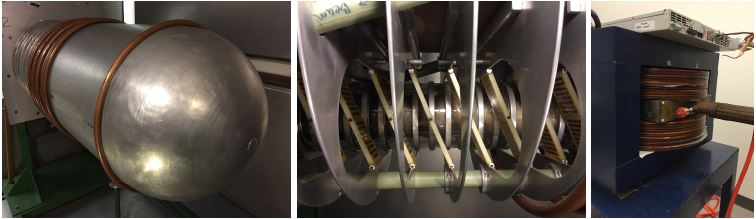
\includegraphics[scale=0.65]{Anh/ngoc3.JPG}
\end{center}
    Các hình trên lần lượt là mái vòm của máy gia tốc (giả thiết rằng nó hình cầu), cột gia tốc và nam châm điện.\\

Vòm của máy gia tốc là một quả cầu nhôm có bán kính $a=0,5~\mathrm{m}$, được tích điện bởi một sợi dây cao su có bề rộng $w=10~\mathrm{cm}$ chuyển động với tốc độ $v_b=20~\mathrm{m/s}$. Cột gia tốc bao gồm $20$ vòng kim loại ngăn cách với nhau bởi các vòng thủy tinh; các vòng mắc nối tiếp với điện trở $500~\mathrm{M}\Omega$. Chùm proton với cường độ dòng điện $25~\mu \mathrm{A}$ và được gia tốc bởi điện thế $500~\mathrm{kV}$ rồi sau đó đi qua một nam châm điện hiệu chỉnh. Nam châm điện gồm các vòng dây dẫn bằng đồng, có tác dụng tạo ra từ trường đều $B$ bên trong một vùng có bán kính $b=10~\mathrm{cm}$ và từ trường bằng không bên ngoài vùng không gian đó.
\begin{center}
 

\tikzset{every picture/.style={line width=0.75pt}} %set default line width to 0.75pt        

\begin{tikzpicture}[x=0.75pt,y=0.75pt,yscale=-1,xscale=1]
%uncomment if require: \path (0,543); %set diagram left start at 0, and has height of 543

%Shape: Rectangle [id:dp2756080105813059] 
\draw  [draw opacity=0][fill={rgb, 255:red, 155; green, 155; blue, 155 }  ,fill opacity=0.33 ] (131.67,333.36) .. controls (131.67,330.6) and (133.91,328.36) .. (136.67,328.36) -- (448.09,328.36) .. controls (450.85,328.36) and (453.09,330.6) .. (453.09,333.36) -- (453.09,338.59) .. controls (453.09,341.36) and (450.85,343.59) .. (448.09,343.59) -- (136.67,343.59) .. controls (133.91,343.59) and (131.67,341.36) .. (131.67,338.59) -- cycle ;
%Shape: Ellipse [id:dp1631084327669441] 
\draw  [line width=2.25]  (75,336.88) .. controls (75,305.46) and (101.41,279.99) .. (133.99,279.99) .. controls (166.57,279.99) and (192.98,305.46) .. (192.98,336.88) .. controls (192.98,368.3) and (166.57,393.77) .. (133.99,393.77) .. controls (101.41,393.77) and (75,368.3) .. (75,336.88) -- cycle ;
%Shape: Ellipse [id:dp28020169257841254] 
\draw  [line width=2.25]  (419.41,336.88) .. controls (419.41,318.69) and (434.7,303.95) .. (453.55,303.95) .. controls (472.41,303.95) and (487.69,318.69) .. (487.69,336.88) .. controls (487.69,355.06) and (472.41,369.8) .. (453.55,369.8) .. controls (434.7,369.8) and (419.41,355.06) .. (419.41,336.88) -- cycle ;
%Straight Lines [id:da02664344415842912] 
\draw    (185.55,309.55) -- (433.58,309.55) ;
%Straight Lines [id:da9047525706494886] 
\draw    (187.4,361.51) -- (429.86,361.51) ;
%Straight Lines [id:da22782514761826667] 
\draw [line width=5.25]    (205.05,302.38) -- (205.05,369.58) ;
%Straight Lines [id:da5683744309061505] 
\draw [line width=5.25]    (245.93,302.38) -- (245.93,369.58) ;
%Straight Lines [id:da4574514472799318] 
\draw [line width=5.25]    (327.68,303.28) -- (327.68,370.47) ;
%Straight Lines [id:da5882533127674177] 
\draw [line width=5.25]    (286.8,302.38) -- (286.8,369.58) ;
%Straight Lines [id:da8171609876395312] 
\draw [line width=5.25]    (366.69,302.38) -- (366.69,369.58) ;
%Straight Lines [id:da9743756944485404] 
\draw [line width=5.25]    (405.71,302.38) -- (405.71,369.58) ;
%Straight Lines [id:da9507626123465847] 
\draw    (205.05,369.58) -- (205.05,414.37) ;
%Straight Lines [id:da7718584311897159] 
\draw    (286.8,369.58) -- (286.8,414.37) ;
%Straight Lines [id:da034921198175972945] 
\draw    (245.93,369.58) -- (245.93,414.37) ;
%Straight Lines [id:da9862567414878582] 
\draw    (405.71,369.58) -- (405.71,413.48) ;
%Straight Lines [id:da4116211672875447] 
\draw    (366.69,369.58) -- (366.69,414.37) ;
%Straight Lines [id:da5665810127110102] 
\draw    (327.68,370.47) -- (327.68,415.27) ;
%Straight Lines [id:da1381103821044758] 
\draw    (162.32,386.6) -- (172.54,413.48) ;
%Shape: Resistor [id:dp7361645764419116] 
\draw   (172.54,413.48) -- (178.56,413.48) -- (179.9,404.52) -- (182.57,422.43) -- (185.25,404.52) -- (187.92,422.43) -- (190.6,404.52) -- (193.28,422.43) -- (195.95,404.52) -- (198.63,422.43) -- (199.96,413.48) -- (205.98,413.48) ;
%Shape: Resistor [id:dp34785780596395166] 
\draw   (205.98,413.48) -- (213.17,413.48) -- (214.77,404.07) -- (217.97,422.88) -- (221.16,404.07) -- (224.36,422.88) -- (227.55,404.07) -- (230.75,422.88) -- (233.95,404.07) -- (237.14,422.88) -- (238.74,413.48) -- (245.93,413.48) ;
%Shape: Resistor [id:dp9054517758554483] 
\draw   (285.87,413.48) -- (293.4,413.48) -- (295.07,404.07) -- (298.42,422.88) -- (301.76,404.07) -- (305.1,422.88) -- (308.45,404.07) -- (311.79,422.88) -- (315.14,404.07) -- (318.48,422.88) -- (320.15,413.48) -- (327.68,413.48) ;
%Shape: Resistor [id:dp9382728705904546] 
\draw   (245.93,413.48) -- (253.12,413.48) -- (254.72,404.07) -- (257.91,422.88) -- (261.11,404.07) -- (264.3,422.88) -- (267.5,404.07) -- (270.7,422.88) -- (273.89,404.07) -- (277.09,422.88) -- (278.68,413.48) -- (285.87,413.48) ;
%Shape: Resistor [id:dp4186647519609439] 
\draw   (367.62,413.48) -- (374.48,413.48) -- (376,404.07) -- (379.05,422.88) -- (382.1,404.07) -- (385.14,422.88) -- (388.19,404.07) -- (391.24,422.88) -- (394.28,404.07) -- (397.33,422.88) -- (398.85,413.48) -- (405.71,413.48) ;
%Shape: Resistor [id:dp4913409831205102] 
\draw   (327.68,413.48) -- (334.87,413.48) -- (336.47,404.07) -- (339.66,422.88) -- (342.86,404.07) -- (346.05,422.88) -- (349.25,404.07) -- (352.44,422.88) -- (355.64,404.07) -- (358.83,422.88) -- (360.43,413.48) -- (367.62,413.48) ;
%Straight Lines [id:da5932831172912454] 
\draw    (205.05,236.09) -- (205.05,294.9) ;
\draw [shift={(205.05,297.9)}, rotate = 270] [fill={rgb, 255:red, 0; green, 0; blue, 0 }  ][line width=0.08]  [draw opacity=0] (8.04,-3.86) -- (0,0) -- (8.04,3.86) -- (5.34,0) -- cycle    ;
%Straight Lines [id:da017143479683142893] 
\draw    (205.05,236.09) -- (245.18,295.42) ;
\draw [shift={(246.86,297.9)}, rotate = 235.93] [fill={rgb, 255:red, 0; green, 0; blue, 0 }  ][line width=0.08]  [draw opacity=0] (8.04,-3.86) -- (0,0) -- (8.04,3.86) -- (5.34,0) -- cycle    ;
%Straight Lines [id:da27951023916710005] 
\draw    (205.05,236.09) -- (283.48,295.2) ;
\draw [shift={(285.87,297.01)}, rotate = 217.01] [fill={rgb, 255:red, 0; green, 0; blue, 0 }  ][line width=0.08]  [draw opacity=0] (8.04,-3.86) -- (0,0) -- (8.04,3.86) -- (5.34,0) -- cycle    ;
%Straight Lines [id:da1974640420582534] 
\draw    (351.83,277.3) -- (309.83,301.77) ;
\draw [shift={(307.24,303.28)}, rotate = 329.77] [fill={rgb, 255:red, 0; green, 0; blue, 0 }  ][line width=0.08]  [draw opacity=0] (8.04,-3.86) -- (0,0) -- (8.04,3.86) -- (5.34,0) -- cycle    ;
%Straight Lines [id:da9907676201388216] 
\draw    (351.83,277.3) -- (346.03,301.26) ;
\draw [shift={(345.33,304.17)}, rotate = 283.6] [fill={rgb, 255:red, 0; green, 0; blue, 0 }  ][line width=0.08]  [draw opacity=0] (8.04,-3.86) -- (0,0) -- (8.04,3.86) -- (5.34,0) -- cycle    ;
%Straight Lines [id:da817099320829259] 
\draw    (351.83,277.3) -- (383.87,303.19) ;
\draw [shift={(386.2,305.07)}, rotate = 218.94] [fill={rgb, 255:red, 0; green, 0; blue, 0 }  ][line width=0.08]  [draw opacity=0] (8.04,-3.86) -- (0,0) -- (8.04,3.86) -- (5.34,0) -- cycle    ;
%Straight Lines [id:da8351175753738009] 
\draw    (351.83,277.3) -- (422.41,304.01) ;
\draw [shift={(425.22,305.07)}, rotate = 200.73] [fill={rgb, 255:red, 0; green, 0; blue, 0 }  ][line width=0.08]  [draw opacity=0] (8.04,-3.86) -- (0,0) -- (8.04,3.86) -- (5.34,0) -- cycle    ;
%Straight Lines [id:da19294180977800623] 
\draw    (429.86,413.48) -- (405.71,413.48) ;
%Straight Lines [id:da4408218359878966] 
\draw    (429.86,413.48) -- (429.86,428.71) ;
%Straight Lines [id:da9048890648918955] 
\draw    (412.68,428.71) -- (447.05,428.71) ;
%Straight Lines [id:da8284802750722475] 
\draw    (419.64,434.08) -- (441.94,434.08) ;
%Straight Lines [id:da5994834503037612] 
\draw    (424.29,439.46) -- (439.15,439.46) ;
%Shape: Rectangle [id:dp7377878361139141] 
\draw  [draw opacity=0][fill={rgb, 255:red, 155; green, 155; blue, 155 }  ,fill opacity=0.33 ] (450.47,332.63) .. controls (451.92,330.27) and (455.03,329.47) .. (457.43,330.84) -- (555.33,386.75) .. controls (557.73,388.12) and (558.5,391.14) .. (557.05,393.5) -- (555.1,396.67) .. controls (553.66,399.02) and (550.54,399.82) .. (548.14,398.45) -- (450.24,342.54) .. controls (447.85,341.18) and (447.08,338.16) .. (448.52,335.8) -- cycle ;
%Straight Lines [id:da8116605181148742] 
\draw [line width=1.5]    (487.46,343.59) -- (564.56,387.49) ;
%Straight Lines [id:da41090489651557305] 
\draw [line width=1.5]    (477.24,362.41) -- (554.34,406.31) ;
%Straight Lines [id:da20427698767667568] 
\draw [line width=1.5]    (564.56,387.49) -- (554.34,406.31) ;

% Text Node
\draw (74.76,255.26) node [anchor=north west][inner sep=0.75pt]    {$\text{Mái vòm}$};
% Text Node
\draw (128.46,212.26) node [anchor=north west][inner sep=0.75pt]    {$\text{Các vòng kim loại của cột gia tốc}$};
% Text Node
\draw (299.05,253.47) node [anchor=north west][inner sep=0.75pt]    {$\text{Các vòng thủy tinh}$};
% Text Node
\draw (480.87,288.41) node [anchor=north west][inner sep=0.75pt]    {$\text{Nam châm điện}$};
% Text Node
\draw (235.98,433.54) node [anchor=north west][inner sep=0.75pt]    {$\text{Chuỗi điện trở}$};
% Text Node
\draw (521.59,414.73) node [anchor=north west][inner sep=0.75pt]    {$\text{Mục tiêu}$};
\end{tikzpicture}

\end{center}

    Chỉ có $6$ trong tổng số $20$ vòng kim loại và điện trở được thể hiện trong hình. Phần hình vẽ màu xám mờ là con đường mà proton thực hiện khi được tăng tốc từ máy vòm, thông qua nam châm điện để đến được mục tiêu.

\begin{enumerate}[1)]
    \item Giả sử mái vòm được tích điện đến $500 ~\mathrm{kV}$, hãy xác định cường độ điện trường trên bề mặt của mái vòm.
    \item Giả sử rằng chùm tia proton được tắt, tìm hằng số thời gian của mái vòm (thời gian để điện tích trên mái vòm giảm còn $1/e\approx1/3$ giá trị ban đầu.
    \item Giả sử rằng chùm proton $25 ~\mu \mathrm{A}$ được bật, xác định mật độ điện tích bề mặt cần phải phun lên dây đai để duy trì điện thế $500~\mathrm{kV}$ ổn định trên vòm.
    \item Chùm proton đi vào nam châm điện và bị lệch một góc $\theta=10^\circ$. Xác định độ lớn của cảm ứng từ.
    \begin{center}
\tikzset{every picture/.style={line width=0.75pt}} %set default line width to 0.75pt        

\begin{tikzpicture}[x=0.75pt,y=0.75pt,yscale=-1,xscale=1]
%uncomment if require: \path (0,300); %set diagram left start at 0, and has height of 300

%Shape: Circle [id:dp769233356039938] 
\draw  [line width=1.5]  (91,125.5) .. controls (91,93.19) and (117.19,67) .. (149.5,67) .. controls (181.81,67) and (208,93.19) .. (208,125.5) .. controls (208,157.81) and (181.81,184) .. (149.5,184) .. controls (117.19,184) and (91,157.81) .. (91,125.5) -- cycle ;
%Straight Lines [id:da7844220980663261] 
\draw  [dash pattern={on 4.5pt off 4.5pt}]  (43,125.5) -- (272,125.5) ;
%Straight Lines [id:da5098925486608799] 
\draw [line width=3]    (33,125.5) -- (91,125.5) ;
%Curve Lines [id:da380068325407648] 
\draw [line width=3]    (91,125.5) .. controls (139,129) and (157,141) .. (186,170) ;
%Straight Lines [id:da9258517733136686] 
\draw [line width=3]    (186,170) -- (241.76,225.76) ;
\draw [shift={(246,230)}, rotate = 225] [fill={rgb, 255:red, 0; green, 0; blue, 0 }  ][line width=0.08]  [draw opacity=0] (18.75,-9.01) -- (0,0) -- (18.75,9.01) -- (12.45,0) -- cycle    ;
%Curve Lines [id:da04614005683561362] 
\draw    (197.88,173.21) .. controls (218.82,159.66) and (219.11,147.48) .. (220.73,129.83) ;
\draw [shift={(221,127)}, rotate = 455.71] [fill={rgb, 255:red, 0; green, 0; blue, 0 }  ][line width=0.08]  [draw opacity=0] (7.14,-3.43) -- (0,0) -- (7.14,3.43) -- (4.74,0) -- cycle    ;
\draw [shift={(195,175)}, rotate = 329.04] [fill={rgb, 255:red, 0; green, 0; blue, 0 }  ][line width=0.08]  [draw opacity=0] (7.14,-3.43) -- (0,0) -- (7.14,3.43) -- (4.74,0) -- cycle    ;
%Straight Lines [id:da683950270522611] 
\draw  [dash pattern={on 4.5pt off 4.5pt}]  (149.5,125.5) -- (185,165) ;

% Text Node
\draw (228,146.4) node [anchor=north west][inner sep=0.75pt]    {$\theta $};
% Text Node
\draw (200,245.4) node [anchor=north west][inner sep=0.75pt]    {$\text{Hướng đi của proton}$};
% Text Node
\draw (104,34.4) node [anchor=north west][inner sep=0.75pt]    {$\text{Nam châm điện}$};
\end{tikzpicture}

    \end{center}
    \item Nam châm điện được cấu tạo bởi các lớp dây đồng cuốn xoắn ốc, dây có đường kính trong $d_i=0,40~\mathrm{cm}$ và đường kính ngoài $d_o=0,50~\mathrm{cm}$. Hình xoắn ốc phẳng tạo thành bởi các dây đồng có đường kính trong $D_i=20~\mathrm{cm}$ và đường kính ngoài $D_0=50~\mathrm{cm}$. Giả sử các cuộn dây được cuốn sát nhau, xác định chiều dài dây $L$ của một xoắn ốc.
    \begin{center}
        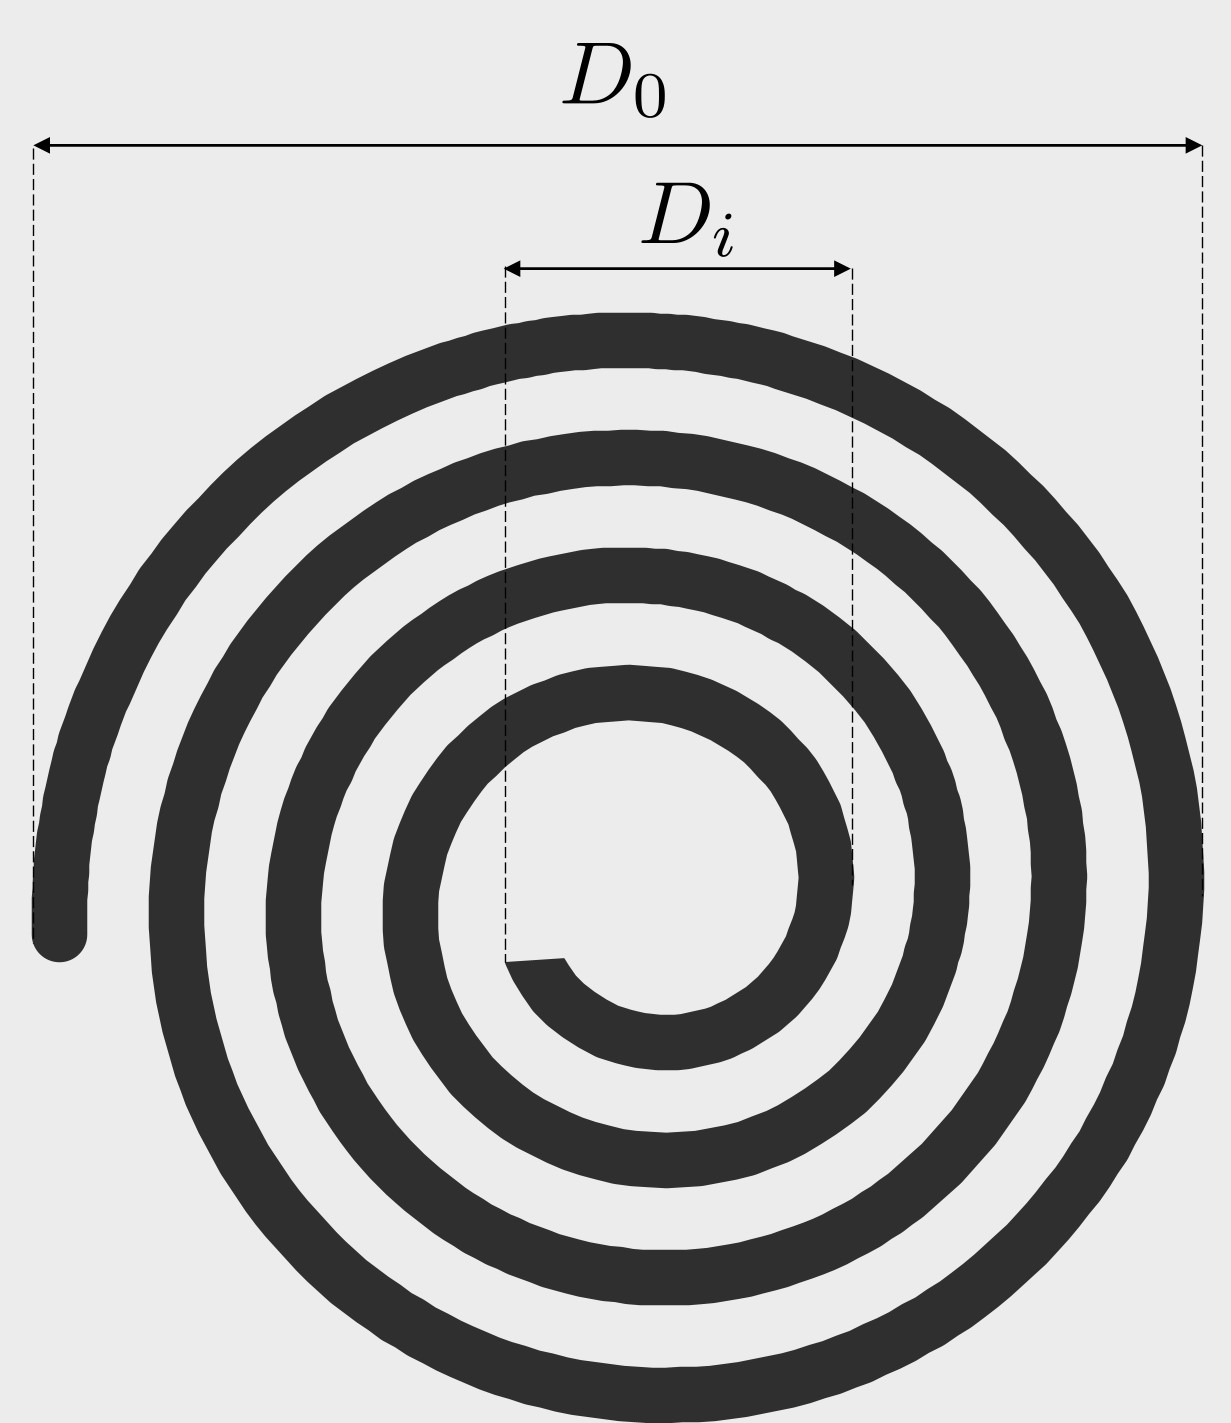
\includegraphics[scale=0.4]{Anh/xoanoc.jpg}
    \end{center}
    \item Ống rỗng được sử dụng để thay cho các sợi dây dẫn rắn giúp làm mát nam châm. Nếu điện trở suất của đồng là $\rho=1,7\times10^{-8}~\Omega\cdot \mathrm{m}$, hãy xác định điện trở của một vòng xoắn ốc.
    \item Có $N=24$ cuộn dây xếp chồng lên nhau. Nước máy với nhiệt độ ban đầu $T_c=18^\circ \mathrm{C}$ đi vào vòng xoắn thông qua ống đồng để ngăn nó nóng lên, nước đi ra với nhiệt độ $T_j=31^\circ \mathrm{C}$. Ống đồng có dòng điện $45 ~\mathrm{A}$ nhằm tạo ra từ trường cần thiết. Cần phải cung cấp nước làm mát với tốc độ bao nhiêu cho nam châm điện? Biểu diễn kết quả với đơn vị lít trên giây và chỉ bao gồm một chữ số có nghĩa. Biết nhiệt dung riêng của nước là $4200~\mathrm{J/^\circ C\cdot kg}$; khối lượng riêng của nước là $1000 ~\mathrm{kg/m^3}$.
    \item Các proton được bắn vào một mục tiêu gồm các nguyên từ Flo $\tron{Z=9}$. Khoảng cách gần nhất tới tâm của nguyên tử Flo mà các proton tiếp cận được là bao nhiêu? Có thể giả sử rằng nguyên tử Flo không chuyển động.
\end{enumerate}
\end{vd}
\begin{loigiai}
    

\begin{enumerate}[1)]
    \item Ta có biểu thức điện thế
    $$ V=\dfrac{q}{4\pi\varepsilon_0a},$$
    và cường độ điện trường là:
    $$E=\dfrac{q}{4\pi\varepsilon_0a^2},$$
    do đó:
    $$E=\dfrac{V}{a}=10^6 ~\mathrm{V/m}.$$
    \item Hằng số thời gian: $\tau=RC,$ trong đó
    $$C=Q/V=4\pi\varepsilon_0a=5,56\times10^{-11}~\mathrm{F},$$
    và 
    $$R=20r_0=10^{10}~\Omega.$$
    nên 
    $$\tau=RC=0,556~\mathrm{s}.$$
    \item Có nhiều cách để mái vòm phóng điện, hai trong số đó là thông qua điện trở và chùm proton. Chúng ta sẽ chỉ xét hai cách này.
    Ở $500~\mathrm{kV}$, dòng điện chạy qua chuỗi điện trở là $50~\mu \mathrm{A}$, từ $V=IR$. Do đó tổng dòng điện $I$ cần cung cấp cho mái vòm là $75~\mu \mathrm{A}$. Dòng điện này được phun lên dây đai với tốc độ là:
    $$\dfrac{\delta A}{\Delta t}=v_bw,$$
    do đó mật độ điện tích mặt cần thiết là:
    $$\sigma=\dfrac{I}{v_bw}=\dfrac{\tron{75~\mu\mathrm{ C/s}}}{\tron{20~\mathrm{m/s}}\tron{0.10~\mathrm{m}}}=37,5~\mu \mathrm{C/m^2}.$$
    \item Bắt đầu từ biểu thức $F=qvB$ trong đó $F$ là lực tác dụng lên các proton, và $v$ là vận tốc của chúng. Các proton phi tương đối tính, nên
    $$\dfrac{1}{2}mv^2=qV.$$
    Chúng chuyển động trong vòng tròn bán kính $r$ bên trong từ trường, ta có:
    $$\dfrac{mv^2}{r}=qvB.$$
    Kết hợp hai phương trình trên ta được:
    $$r=\dfrac{mv}{qB}=\dfrac{m}{qB}\sqrt{\dfrac{2qV}{m}}=\dfrac{1}{B}\sqrt{\dfrac{2mV}{q}}.$$
    Vậy độ lớn cảm ứng từ là:
    $$B=\dfrac{1}{4}\sqrt{\dfrac{2mV}{q}}.$$
    Để liên hệ cảm ứng từ với góc, ta cần thực hiện một số công việc hình học. Vẽ hai vòng tròn, một với bán kính $b$, một với bán kính $r$, trên cùng một mặt phẳng và cắt nhau như hình vẽ ở đề bài. Khi đó vẽ một hình tam giác ta được:
    $$\tan \dfrac{\theta}{2}=\dfrac{b}{r}.$$
    Kết hợp các phương trình, kết quả là
    $$B=\dfrac{\tan \theta/2}{b}\sqrt{\dfrac{2mV}{q}}=0,0894 ~\mathrm{T}.$$
    \item Diện tích của hình xoắn ốc là
    $$A=\dfrac{\pi}{4}\tron{D_0^2-D_i^2}.$$
    Diện tích của phần dây được vẽ trên hình là:
    $$A=Ld_0.$$
    Cân bằng hai phương trình, giải ra ta được:
    $$L=\dfrac{\pi\tron{D_0^2-D_i^2}}{4d_0}=33~\mathrm{m}.$$
    \item Ta có
    $$r_s=\dfrac{\rho L}{A},$$
    trong đó $A$ là diện tích mặt cắt của dây, hay
    $$A=\dfrac{\pi}{4}\tron{d_0^2-d_i^2}=7.1\times10^{-6}~\mathrm{m^2}.$$
    Kết hợp, ta được:
    $$r_s=\dfrac{\rho}{d_0}\dfrac{D_0^2-D_i^2}{d_0^2-d_i^2}=0.079~\Omega.$$
    \item Tốc độ sinh nhiệt trong các cuộn dây là:
    $$P=I^2R=I^2Nr_s=3850~\mathrm{W}.$$
    Điều này được giảm bớt thông qua việc tăng nhiệt độ của nước:
    $$P=C\Delta Tq,$$
    trong đó $C$ là nhiệt dung riêng tính bằng lít và $Q$ là tốc độ chảy tính bằng lít trên giây. Vì một lít nước nặng $1~\mathrm{kg}$ nên ta có thể sử dụng $C$. Kết hợp các phương tình ta được:
    $$Q=\dfrac{I^2Nr}{C\Delta T}=0.07~\mathrm{l/s}.$$
    \item Bảo toàn năng lượng ta được:
    $$qV=\dfrac{1}{4\pi\varepsilon_0}\dfrac{Zq^2}{r},$$
    trong đó $r$ là khoảng tiếp cận gần nhất. Khi đó:
    $$r=\dfrac{1}{4\pi\varepsilon_0}\dfrac{Zq}{V}=2.59\times 10^{-14}~\mathrm{m}.$$
    Vì kết quả này bằng với kích thước của một hạt nhân Flo, có thể sẽ xảy ra một phản ứng hạt nhân. Trên thực tế, phản ứng sẽ xảy ra ở khoảng $380~\mathrm{kV}$.
    
\end{enumerate}
\end{loigiai}


\begin{vd}[Hiện tượng từ trễ và khử từ]
%\textbf{Bài 3 IZho 2015}
Trong bài toán này, bỏ qua tốc độ lan truyền của sự tương tác điện từ.
\begin{center}
\textbf{Phần I: Nam châm}
\end{center}
\begin{enumerate}[1)]
\item \textbf{Giới thiệu lí thuyết:}\\
Ở khoảng cách rất lớn, từ trường được tạo ra bởi sự từ hóa đồng nhất trên một trụ sắt từ (nam châm vĩnh cửu) tương đương với trường tạo ra bởi một cuộn dây tròn có dòng điện không đổi.\\
\begin{center}
    

% Gradient Info
  
\tikzset {_zfw0x396m/.code = {\pgfsetadditionalshadetransform{ \pgftransformshift{\pgfpoint{89.1 bp } { -108.9 bp }  }  \pgftransformscale{1.32 }  }}}
\pgfdeclareradialshading{_jzyajro15}{\pgfpoint{-72bp}{88bp}}{rgb(0bp)=(1,1,1);
rgb(0bp)=(1,1,1);
rgb(25bp)=(0,0,0);
rgb(400bp)=(0,0,0)}
\tikzset{every picture/.style={line width=0.75pt}} %set default line width to 0.75pt        

\begin{tikzpicture}[x=0.75pt,y=0.75pt,yscale=-1,xscale=1]
%uncomment if require: \path (0,300); %set diagram left start at 0, and has height of 300

%Shape: Can [id:dp4501980240976837] 
\path  [shading=_jzyajro15,_zfw0x396m] (156.54,117.95) -- (124.97,117.75) .. controls (120.95,117.72) and (117.73,108.34) .. (117.78,96.79) .. controls (117.83,85.24) and (121.13,75.9) .. (125.15,75.93) -- (156.72,76.13) .. controls (160.74,76.16) and (163.96,85.54) .. (163.91,97.09) .. controls (163.86,108.64) and (160.56,117.98) .. (156.54,117.95) .. controls (152.52,117.93) and (149.3,108.54) .. (149.35,96.99) .. controls (149.4,85.45) and (152.7,76.1) .. (156.72,76.13) ; % for fading 
 \draw   (156.54,117.95) -- (124.97,117.75) .. controls (120.95,117.72) and (117.73,108.34) .. (117.78,96.79) .. controls (117.83,85.24) and (121.13,75.9) .. (125.15,75.93) -- (156.72,76.13) .. controls (160.74,76.16) and (163.96,85.54) .. (163.91,97.09) .. controls (163.86,108.64) and (160.56,117.98) .. (156.54,117.95) .. controls (152.52,117.93) and (149.3,108.54) .. (149.35,96.99) .. controls (149.4,85.45) and (152.7,76.1) .. (156.72,76.13) ; % for border 

%Flowchart: Stored Data [id:dp9547962460697509] 
\draw  [fill={rgb, 255:red, 255; green, 255; blue, 255 }  ,fill opacity=1 ] (90.45,76.16) -- (124.31,76.16) .. controls (120.75,76.16) and (117.86,85.39) .. (117.86,96.79) .. controls (117.86,108.18) and (120.75,117.42) .. (124.31,117.42) -- (90.45,117.42) .. controls (86.89,117.42) and (84,108.18) .. (84,96.79) .. controls (84,85.39) and (86.89,76.16) .. (90.45,76.16) -- cycle ;
%Right Arrow [id:dp4508370111610275] 
\draw   (182,93.25) -- (210.8,93.25) -- (210.8,87) -- (230,99.5) -- (210.8,112) -- (210.8,105.75) -- (182,105.75) -- cycle ;
%Shape: Ellipse [id:dp09392556377578465] 
\draw  [line width=1.5]  (272.55,70.88) .. controls (283.29,70.95) and (291.93,82.67) .. (291.84,97.06) .. controls (291.75,111.45) and (282.97,123.06) .. (272.23,123) .. controls (261.49,122.93) and (252.85,111.21) .. (252.94,96.81) .. controls (253.03,82.42) and (261.81,70.81) .. (272.55,70.88) -- cycle ;
\draw   (288.65,69.71) .. controls (287.4,75.03) and (287.5,79.32) .. (288.93,82.6) .. controls (286.16,80.34) and (282.05,79.09) .. (276.6,78.85) ;
%Straight Lines [id:da3699215618726893] 
\draw    (272.39,96.94) -- (323,96.94) ;
\draw [shift={(326,96.94)}, rotate = 180] [fill={rgb, 255:red, 0; green, 0; blue, 0 }  ][line width=0.08]  [draw opacity=0] (10.72,-5.15) -- (0,0) -- (10.72,5.15) -- (7.12,0) -- cycle    ;

% Text Node
\draw (95,89.4) node [anchor=north west][inner sep=0.75pt]    {$S$};
% Text Node
\draw (129,89.4) node [anchor=north west][inner sep=0.75pt]    {$N$};
% Text Node
\draw (274,52.4) node [anchor=north west][inner sep=0.75pt]    {$I$};
% Text Node
\draw (255,123.4) node [anchor=north west][inner sep=0.75pt]    {$S$};
% Text Node
\draw (324.84,66.46) node [anchor=north west][inner sep=0.75pt]    {$\overrightarrow{p_{m}}$};


\end{tikzpicture}
\end{center}
Nam châm hình trụ, cũng như cuộn dây có dòng điện, đặc trưng bởi moment từ $p_{{m}}$. Định nghĩa cho moment từ của vòng mang dòng điện là tích của dòng điện và diện tích của vòng dây.
\[ p_{{m}}=IS.\]
Moment từ như vậy còn được gọi là một lưỡng cực từ. Hình vẽ dưới đây cho ta thấy đường sức từ của một moment từ.
\begin{center}
    \tikzset{every picture/.style={line width=0.75pt}} %set default line width to 0.75pt        

\begin{tikzpicture}[x=0.75pt,y=0.75pt,yscale=-1,xscale=1]
%uncomment if require: \path (0,181); %set diagram left start at 0, and has height of 181

%Straight Lines [id:da06360558422477935] 
\draw [line width=1.5]    (265.97,90.13) -- (478.08,90.13) ;
\draw [shift={(481.08,90.13)}, rotate = 180] [color={rgb, 255:red, 0; green, 0; blue, 0 }  ][line width=1.5]    (14.21,-4.28) .. controls (9.04,-1.82) and (4.3,-0.39) .. (0,0) .. controls (4.3,0.39) and (9.04,1.82) .. (14.21,4.28)   ;
%Curve Lines [id:da6072491279254382] 
\draw    (346.29,80.13) .. controls (347.29,75.13) and (353.63,75.13) .. (354.96,80.13) ;
%Curve Lines [id:da09503964774070672] 
\draw    (344.26,81.6) .. controls (344.1,70.83) and (355.79,69.91) .. (356.7,81.2) ;
%Curve Lines [id:da621421588681335] 
\draw    (342.87,82.68) .. controls (339.02,62.13) and (363.39,65.63) .. (357.91,81.91) ;
%Curve Lines [id:da02158838639918792] 
\draw    (342.07,83.2) .. controls (327.73,53.94) and (372.33,51.74) .. (359.53,82.54) ;
%Curve Lines [id:da4413925308853779] 
\draw    (341.09,84.39) .. controls (313.38,35.24) and (388.81,35.82) .. (360.33,84.14) ;
%Curve Lines [id:da21094694895405253] 
\draw    (339.66,85.24) .. controls (317.99,70.85) and (322.24,23.92) .. (349.99,24.35) .. controls (377.75,24.77) and (384.99,64.85) .. (361.72,85.08) ;
%Curve Lines [id:da10510890003898932] 
\draw    (340.24,87.43) .. controls (331.84,80.23) and (293.84,55.03) .. (308.64,5.83) ;
%Shape: Boxed Bezier Curve [id:dp07893171574002777] 
\draw    (362.05,87.4) .. controls (370.45,80.2) and (408.45,55) .. (393.65,5.8) ;
%Curve Lines [id:da19620814775045292] 
\draw    (266.98,18.6) .. controls (286.58,50.6) and (299.78,71.8) .. (340.24,87.43) ;
%Shape: Boxed Bezier Curve [id:dp04507949087595864] 
\draw    (435.31,18.57) .. controls (415.71,50.57) and (402.51,71.77) .. (362.05,87.4) ;
%Curve Lines [id:da2919180928945344] 
\draw    (266.37,64.8) .. controls (331.38,98.8) and (378.58,94.4) .. (435.78,64) ;
%Straight Lines [id:da33097911884098674] 
\draw    (265.97,90.23) -- (435.78,90.23) ;

%Curve Lines [id:da39653268323313373] 
\draw    (346.29,100.23) .. controls (347.29,105.23) and (353.63,105.23) .. (354.96,100.23) ;
%Curve Lines [id:da0701328024808705] 
\draw    (344.26,98.76) .. controls (344.1,109.53) and (355.79,110.45) .. (356.7,99.17) ;
%Curve Lines [id:da32049824599202115] 
\draw    (342.87,97.69) .. controls (339.02,118.24) and (363.39,114.74) .. (357.91,98.45) ;
%Curve Lines [id:da4693188946066369] 
\draw    (342.07,97.17) .. controls (327.73,126.42) and (372.33,128.62) .. (359.53,97.82) ;
%Curve Lines [id:da9034794333331082] 
\draw    (341.09,95.98) .. controls (313.38,145.12) and (388.81,144.55) .. (360.33,96.22) ;
%Curve Lines [id:da24537082097951046] 
\draw    (339.66,95.12) .. controls (317.99,109.52) and (322.24,156.44) .. (349.99,156.02) .. controls (377.75,155.59) and (384.99,115.52) .. (361.72,95.28) ;
%Curve Lines [id:da5546399747954402] 
\draw    (340.24,92.93) .. controls (331.84,100.13) and (293.84,125.33) .. (308.64,174.53) ;
%Shape: Boxed Bezier Curve [id:dp6444419733416171] 
\draw    (362.05,92.96) .. controls (370.45,100.16) and (408.45,125.36) .. (393.65,174.56) ;
%Curve Lines [id:da6048184278546478] 
\draw    (266.98,161.76) .. controls (286.58,129.76) and (299.78,108.56) .. (340.24,92.93) ;
%Shape: Boxed Bezier Curve [id:dp6696449021155879] 
\draw    (435.31,161.79) .. controls (415.71,129.79) and (402.51,108.59) .. (362.05,92.96) ;
%Curve Lines [id:da5290225403562503] 
\draw    (266.37,115.56) .. controls (331.38,81.57) and (378.58,85.97) .. (435.78,116.37) ;
%Straight Lines [id:da9112047875669156] 
\draw    (265.97,90.13) -- (435.78,90.13) ;

%Shape: Can [id:dp6859889808563859] 
\draw  [fill={rgb, 255:red, 2; green, 21; blue, 208 }  ,fill opacity=1 ] (350.5,102.62) -- (334.26,102.62) .. controls (332.34,102.62) and (330.78,97.18) .. (330.78,90.47) .. controls (330.78,83.76) and (332.34,78.32) .. (334.26,78.32) -- (350.5,78.32) .. controls (352.43,78.32) and (353.98,83.76) .. (353.98,90.47) .. controls (353.98,97.18) and (352.43,102.62) .. (350.5,102.62) .. controls (348.58,102.62) and (347.02,97.18) .. (347.02,90.47) .. controls (347.02,83.76) and (348.58,78.32) .. (350.5,78.32) ;
%Shape: Can [id:dp31443238549542585] 
\draw  [fill={rgb, 255:red, 208; green, 2; blue, 27 }  ,fill opacity=1 ] (366.74,102.62) -- (350.5,102.62) .. controls (348.58,102.62) and (347.02,97.18) .. (347.02,90.47) .. controls (347.02,83.76) and (348.58,78.32) .. (350.5,78.32) -- (366.74,78.32) .. controls (368.67,78.32) and (370.22,83.76) .. (370.22,90.47) .. controls (370.22,97.18) and (368.67,102.62) .. (366.74,102.62) .. controls (364.82,102.62) and (363.26,97.18) .. (363.26,90.47) .. controls (363.26,83.76) and (364.82,78.32) .. (366.74,78.32) ;



% Text Node
\draw (349.22,82.92) node [anchor=north west][inner sep=0.75pt]  [color={rgb, 255:red, 255; green, 255; blue, 255 }  ,opacity=1 ] [align=left] {N};
% Text Node
\draw (330.82,82.75) node [anchor=north west][inner sep=0.75pt]  [color={rgb, 255:red, 255; green, 255; blue, 255 }  ,opacity=1 ] [align=left] {S};
% Text Node
\draw (473,92.4) node [anchor=north west][inner sep=0.75pt]    {$z$};


\end{tikzpicture}
\end{center}
\begin{enumerate}[a)]
    \item Chỉ ra rằng từ trường $B_z$ nằm trên trục đối xứng của vòng được cho bởi biểu thức:
    \[B_{Z}=b \dfrac{p_{m}}{z^{\beta}},\]
    trong đó $z$ là khoảng cách từ một điểm trên trục đối xứng đến tâm của vòng dây. Xác định các tham số $b$ và $\beta$ ở biểu thức trên.
    \item Để cuộn dây có dòng điện (tức là lưỡng cực từ) với moment từ $p_m$ chịu tác dụng của một từ trường đối xứng trục không đồng nhất, cảm ứng từ của nó dọc theo trục $z$ phụ thuộc vào $z$ như hàm $B_{z}(z)$. Trục của lưỡng cực trùng với trục đối xứng của từ trường. 
    \begin{center}
         

\tikzset{every picture/.style={line width=0.75pt}} %set default line width to 0.75pt        

\begin{tikzpicture}[x=0.75pt,y=0.75pt,yscale=-1,xscale=1]
%uncomment if require: \path (0,300); %set diagram left start at 0, and has height of 300

%Shape: Arc [id:dp09724083610265022] 
\draw  [draw opacity=0] (496.56,57.46) .. controls (466.57,77.81) and (398.8,92) .. (320,92) .. controls (230.64,92) and (155.46,73.75) .. (133.49,48.97) -- (320,34) -- cycle ; \draw   (496.56,57.46) .. controls (466.57,77.81) and (398.8,92) .. (320,92) .. controls (230.64,92) and (155.46,73.75) .. (133.49,48.97) ;
%Shape: Arc [id:dp9573942278688676] 
\draw  [draw opacity=0] (497.09,71.52) .. controls (467.39,87.1) and (399.28,98) .. (320,98) .. controls (230.13,98) and (154.6,84) .. (133.12,65.04) -- (320,54) -- cycle ; \draw   (497.09,71.52) .. controls (467.39,87.1) and (399.28,98) .. (320,98) .. controls (230.13,98) and (154.6,84) .. (133.12,65.04) ;
%Shape: Arc [id:dp5398400734661393] 
\draw  [draw opacity=0] (497.38,88) .. controls (466.83,97.44) and (399.79,104) .. (322,104) .. controls (228.9,104) and (151.19,94.61) .. (133.02,82.11) -- (322,76.5) -- cycle ; \draw   (497.38,88) .. controls (466.83,97.44) and (399.79,104) .. (322,104) .. controls (228.9,104) and (151.19,94.61) .. (133.02,82.11) ;
%Shape: Arc [id:dp5931355655659283] 
\draw  [draw opacity=0] (136.4,159.79) .. controls (166.42,139.54) and (234.33,125.63) .. (313.23,126.01) .. controls (398.2,126.41) and (470.27,143.25) .. (495.93,166.29) -- (312.96,184) -- cycle ; \draw   (136.4,159.79) .. controls (166.42,139.54) and (234.33,125.63) .. (313.23,126.01) .. controls (398.2,126.41) and (470.27,143.25) .. (495.93,166.29) ;
%Shape: Arc [id:dp18584702804365694] 
\draw  [draw opacity=0] (136.42,144.95) .. controls (166.88,129.89) and (234.18,119.63) .. (312.26,120) .. controls (398.87,120.41) and (472.09,133.76) .. (496.44,151.79) -- (312.05,164) -- cycle ; \draw   (136.42,144.95) .. controls (166.88,129.89) and (234.18,119.63) .. (312.26,120) .. controls (398.87,120.41) and (472.09,133.76) .. (496.44,151.79) ;
%Shape: Arc [id:dp843366810007487] 
\draw  [draw opacity=0] (135.94,129.15) .. controls (166.63,119.86) and (233.81,113.63) .. (311.71,114) .. controls (395.9,114.39) and (467.49,122.38) .. (494.01,133.18) -- (311.58,141.5) -- cycle ; \draw   (135.94,129.15) .. controls (166.63,119.86) and (233.81,113.63) .. (311.71,114) .. controls (395.9,114.39) and (467.49,122.38) .. (494.01,133.18) ;
%Straight Lines [id:da0825312466176309] 
\draw    (498,110) -- (135,109) ;
%Shape: Ellipse [id:dp154624595511056] 
\draw  [line width=1.5]  (463.14,76.01) .. controls (474.19,75.74) and (483.52,91.19) .. (483.99,110.51) .. controls (484.47,129.84) and (475.9,145.72) .. (464.86,145.99) .. controls (453.81,146.26) and (444.48,130.81) .. (444.01,111.49) .. controls (443.53,92.16) and (452.1,76.28) .. (463.14,76.01) -- cycle ;
\draw  [line width=1.5]  (453.33,95.42) .. controls (448.11,100.37) and (444.6,105.61) .. (442.77,111.14) .. controls (442.89,105.32) and (441.32,99.21) .. (438.04,92.8) ;
%Straight Lines [id:da9522131982799203] 
\draw [line width=1.5]    (464,111) -- (549,111) ;
\draw [shift={(553,111)}, rotate = 180] [fill={rgb, 255:red, 0; green, 0; blue, 0 }  ][line width=0.08]  [draw opacity=0] (13.4,-6.43) -- (0,0) -- (13.4,6.44) -- (8.9,0) -- cycle    ;
%Straight Lines [id:da050548300708038396] 
\draw [line width=1.5]    (463.14,76.01) -- (362,76.01) ;
\draw [shift={(358,76.01)}, rotate = 360] [fill={rgb, 255:red, 0; green, 0; blue, 0 }  ][line width=0.08]  [draw opacity=0] (13.4,-6.43) -- (0,0) -- (13.4,6.44) -- (8.9,0) -- cycle    ;

% Text Node
\draw (531,76.4) node [anchor=north west][inner sep=0.75pt]    {$\overrightarrow{p_{m}}$};
% Text Node
\draw (377,48.4) node [anchor=north west][inner sep=0.75pt]    {$\ot{F}$};
% Text Node
\draw (485,92.4) node [anchor=north west][inner sep=0.75pt]    {$I$};


\end{tikzpicture}
    \end{center}
    Chứng tỏ rằng lực do từ trường tác dụng lên lưỡng cực cho bởi:
    \[F_{z}=-p_{m} \dfrac{\dd B_{z}}{\dd z}.\]
\end{enumerate}
\item \textbf{Dao động của nam châm.}\\
Nam châm hình trụ khối lượng $m$ và moment từ $p_m$, được gắn vào lò xo có độ cứng $k$ sao cho nó có thể dao động dọc theo trục nằm ngang hướng dọc theo moment từ.
\begin{enumerate}[a)]
    \item Tìm tần số dao động tự do $\omega_0$ của nam châm trong điều kiện không có trường lực bên ngoài.
    \item Tại một khoảng cách $z$ so với vị trí cân bằng của nam châm, người ta đặt một đĩa kim loại nhỏ sao cho trục của nó trùng với trục của nam châm. Đĩa có bán kính $R$ và bề dày $h~(h \ll R \ll z)$, điện trở suất của vật liệu làm đĩa là $\rho$, và độ từ thẩm đặt bằng $\mu=1$. Nam châm được đưa ra khỏi vị trí cân bằng và bắt đầu thực hiện dao động nhỏ. Dao động được mô tả bởi hàm $x(t)$, trong đó $x \ll z$.\\
    Tìm lực $F(x, v)$ do đĩa tác dụng lên nam châm dưới dạng hàm của tọa độ $x$ và vận tốc $v$ của nó. Viết phương trình chuyển động của nam châm.
\begin{center}
% Pattern Info
 
\tikzset{
pattern size/.store in=\mcSize, 
pattern size = 5pt,
pattern thickness/.store in=\mcThickness, 
pattern thickness = 0.3pt,
pattern radius/.store in=\mcRadius, 
pattern radius = 1pt}
\makeatletter
\pgfutil@ifundefined{pgf@pattern@_chcrj0tny}{
\pgfdeclarepatternformonly[\mcThickness,\mcSize]{_chcrj0tny}
{\pgfpointorigin}
{\pgfpoint{\mcSize+\mcThickness}{\mcSize+\mcThickness}}
{\pgfpoint{\mcSize}{\mcSize}}{
\pgfsetcolor{\tikz@pattern@color}
\pgfsetlinewidth{\mcThickness}
\pgfpathmoveto{\pgfpointorigin}
\pgfpathlineto{\pgfpoint{0pt}{0.5*\mcSize}}
\pgfpathlineto{\pgfpoint{\mcSize}{0.5*\mcSize}}
\pgfpathmoveto{\pgfpoint{0.5*\mcSize}{0.5*\mcSize}}
\pgfpathlineto{\pgfpoint{0.5*\mcSize}{\mcSize}}
\pgfpathmoveto{\pgfpoint{0pt}{\mcSize}}
\pgfpathlineto{\pgfpoint{\mcSize}{\mcSize}}
\pgfusepath{stroke}}}
\makeatother

% Gradient Info
  
\tikzset {_gge74cn1a/.code = {\pgfsetadditionalshadetransform{ \pgftransformshift{\pgfpoint{0 bp } { 0 bp }  }  \pgftransformrotate{0 }  \pgftransformscale{2 }  }}}
\pgfdeclarehorizontalshading{_mcpwhh0at}{150bp}{rgb(0bp)=(1,1,1);
rgb(37.5bp)=(1,1,1);
rgb(50bp)=(0.95,0.95,0.95);
rgb(50.25bp)=(0.88,0.88,0.88);
rgb(62.5bp)=(0.96,0.96,0.96);
rgb(100bp)=(0.96,0.96,0.96)}

% Gradient Info
  
\tikzset {_00lsj81k4/.code = {\pgfsetadditionalshadetransform{ \pgftransformshift{\pgfpoint{89.1 bp } { -108.9 bp }  }  \pgftransformscale{1.32 }  }}}
\pgfdeclareradialshading{_oq1z91hja}{\pgfpoint{-72bp}{88bp}}{rgb(0bp)=(1,1,1);
rgb(0bp)=(1,1,1);
rgb(25bp)=(0,0,0);
rgb(400bp)=(0,0,0)}

% Gradient Info
  
\tikzset {_82em7jkyg/.code = {\pgfsetadditionalshadetransform{ \pgftransformshift{\pgfpoint{0 bp } { 0 bp }  }  \pgftransformrotate{0 }  \pgftransformscale{2 }  }}}
\pgfdeclarehorizontalshading{_iwlvlrkw7}{150bp}{rgb(0bp)=(0.96,0.96,0.96);
rgb(37.5bp)=(0.96,0.96,0.96);
rgb(42.75bp)=(0.86,0.86,0.89);
rgb(49.75bp)=(0.72,0.73,0.78);
rgb(57.5bp)=(0.87,0.87,0.89);
rgb(62.5bp)=(0.96,0.96,0.96);
rgb(100bp)=(0.96,0.96,0.96)}
\tikzset{every picture/.style={line width=0.75pt}} %set default line width to 0.75pt        

\begin{tikzpicture}[x=0.75pt,y=0.75pt,yscale=-0.7,xscale=0.7]
%uncomment if require: \path (0,300); %set diagram left start at 0, and has height of 300

%Shape: Rectangle [id:dp26559850878070734] 
\draw  [pattern=_chcrj0tny,pattern size=6pt,pattern thickness=0.75pt,pattern radius=0pt, pattern color={rgb, 255:red, 0; green, 0; blue, 0}] (35,191) -- (35,130) -- (48,130) -- (48,191) -- cycle ;
%Shape: Spring [id:dp37505721031698325] 
\draw   (48.96,153.67) .. controls (49.35,148.18) and (51.61,142.7) .. (56.11,142.71) .. controls (65.11,142.74) and (65.06,164.68) .. (59.06,164.67) .. controls (53.06,164.65) and (53.11,142.7) .. (62.11,142.73) .. controls (71.11,142.75) and (71.06,164.7) .. (65.06,164.68) .. controls (59.06,164.67) and (59.11,142.72) .. (68.11,142.74) .. controls (77.11,142.77) and (77.06,164.71) .. (71.06,164.7) .. controls (65.06,164.68) and (65.11,142.74) .. (74.11,142.76) .. controls (83.11,142.78) and (83.06,164.73) .. (77.06,164.71) .. controls (71.06,164.7) and (71.11,142.75) .. (80.11,142.78) .. controls (89.11,142.8) and (89.05,164.75) .. (83.06,164.73) .. controls (77.06,164.71) and (77.11,142.77) .. (86.11,142.79) .. controls (95.11,142.81) and (95.05,164.76) .. (89.05,164.75) .. controls (83.06,164.73) and (83.11,142.78) .. (92.11,142.81) .. controls (101.11,142.83) and (101.05,164.78) .. (95.05,164.76) .. controls (89.05,164.75) and (89.11,142.8) .. (98.11,142.82) .. controls (107.11,142.85) and (107.05,164.79) .. (101.05,164.78) .. controls (95.05,164.76) and (95.11,142.81) .. (104.11,142.84) .. controls (113.11,142.86) and (113.05,164.81) .. (107.05,164.79) .. controls (101.05,164.78) and (101.11,142.83) .. (110.11,142.85) .. controls (119.11,142.88) and (119.05,164.82) .. (113.05,164.81) .. controls (107.05,164.79) and (107.11,142.85) .. (116.11,142.87) .. controls (125.11,142.89) and (125.05,164.84) .. (119.05,164.82) .. controls (113.05,164.81) and (113.11,142.86) .. (122.11,142.89) .. controls (131.11,142.91) and (131.05,164.86) .. (125.05,164.84) .. controls (119.05,164.82) and (119.11,142.88) .. (128.11,142.9) .. controls (137.11,142.92) and (137.05,164.87) .. (131.05,164.86) .. controls (125.05,164.84) and (125.11,142.89) .. (134.11,142.92) .. controls (143.11,142.94) and (143.05,164.89) .. (137.05,164.87) .. controls (131.05,164.86) and (131.11,142.91) .. (140.11,142.93) .. controls (149.11,142.96) and (149.05,164.9) .. (143.05,164.89) .. controls (137.05,164.87) and (137.11,142.92) .. (146.11,142.95) .. controls (155.11,142.97) and (155.05,164.92) .. (149.05,164.9) .. controls (143.05,164.89) and (143.11,142.94) .. (152.11,142.96) .. controls (161.11,142.99) and (161.05,164.93) .. (155.05,164.92) .. controls (149.05,164.9) and (149.11,142.96) .. (158.11,142.98) .. controls (167.11,143) and (167.05,164.95) .. (161.05,164.93) .. controls (155.05,164.92) and (155.11,142.97) .. (164.11,143) .. controls (173.11,143.02) and (173.05,164.97) .. (167.05,164.95) .. controls (161.05,164.93) and (161.11,142.99) .. (170.11,143.01) .. controls (179.11,143.03) and (179.05,164.98) .. (173.05,164.97) .. controls (167.05,164.95) and (167.11,143) .. (176.11,143.03) .. controls (185.11,143.05) and (185.05,165) .. (179.05,164.98) .. controls (173.05,164.97) and (173.11,143.02) .. (182.11,143.04) .. controls (183.7,143.05) and (185.01,143.74) .. (186.05,144.87) ;
%Flowchart: Stored Data [id:dp8176790316288902] 
\path  [shading=_mcpwhh0at,_gge74cn1a] (189.04,134) -- (205,134) .. controls (203.32,134) and (201.96,142.95) .. (201.96,154) .. controls (201.96,165.05) and (203.32,174) .. (205,174) -- (189.04,174) .. controls (187.36,174) and (186,165.05) .. (186,154) .. controls (186,142.95) and (187.36,134) .. (189.04,134) -- cycle ; % for fading 
 \draw   (189.04,134) -- (205,134) .. controls (203.32,134) and (201.96,142.95) .. (201.96,154) .. controls (201.96,165.05) and (203.32,174) .. (205,174) -- (189.04,174) .. controls (187.36,174) and (186,165.05) .. (186,154) .. controls (186,142.95) and (187.36,134) .. (189.04,134) -- cycle ; % for border 

%Flowchart: Direct Access Storage [id:dp5399580700082982] 
\path  [shading=_oq1z91hja,_00lsj81k4] (219.32,174) -- (205.64,174) .. controls (203.61,174) and (201.96,165.05) .. (201.96,154) .. controls (201.96,142.95) and (203.61,134) .. (205.64,134) -- (219.32,134)(223,154) .. controls (223,165.05) and (221.35,174) .. (219.32,174) .. controls (217.28,174) and (215.64,165.05) .. (215.64,154) .. controls (215.64,142.95) and (217.28,134) .. (219.32,134) .. controls (221.35,134) and (223,142.95) .. (223,154) ; % for fading 
 \draw   (219.32,174) -- (205.64,174) .. controls (203.61,174) and (201.96,165.05) .. (201.96,154) .. controls (201.96,142.95) and (203.61,134) .. (205.64,134) -- (219.32,134)(223,154) .. controls (223,165.05) and (221.35,174) .. (219.32,174) .. controls (217.28,174) and (215.64,165.05) .. (215.64,154) .. controls (215.64,142.95) and (217.28,134) .. (219.32,134) .. controls (221.35,134) and (223,142.95) .. (223,154) ; % for border 

%Straight Lines [id:da9167583407483029] 
\draw [line width=1.5]    (215.64,154) -- (253,154) ;
\draw [shift={(257,154)}, rotate = 180] [fill={rgb, 255:red, 0; green, 0; blue, 0 }  ][line width=0.08]  [draw opacity=0] (15.6,-3.9) -- (0,0) -- (15.6,3.9) -- cycle    ;
%Straight Lines [id:da47575998082208115] 
\draw    (62,192) -- (390,192) ;
\draw [shift={(393,192)}, rotate = 180] [fill={rgb, 255:red, 0; green, 0; blue, 0 }  ][line width=0.08]  [draw opacity=0] (10.72,-5.15) -- (0,0) -- (10.72,5.15) -- (7.12,0) -- cycle    ;
%Straight Lines [id:da319713090471194] 
\draw    (203,183) -- (203,200) ;

%Straight Lines [id:da1365287208408681] 
\draw [line width=1.5]    (169,200) -- (237,200) ;
\draw [shift={(241,200)}, rotate = 180] [fill={rgb, 255:red, 0; green, 0; blue, 0 }  ][line width=0.08]  [draw opacity=0] (13.4,-6.43) -- (0,0) -- (13.4,6.44) -- (8.9,0) -- cycle    ;
\draw [shift={(165,200)}, rotate = 0] [fill={rgb, 255:red, 0; green, 0; blue, 0 }  ][line width=0.08]  [draw opacity=0] (13.4,-6.43) -- (0,0) -- (13.4,6.44) -- (8.9,0) -- cycle    ;
%Straight Lines [id:da842491381532174] 
\draw  [dash pattern={on 4.5pt off 4.5pt}]  (257,154) -- (523,154) ;
%Flowchart: Direct Access Storage [id:dp9916978957980093] 
\path  [shading=_iwlvlrkw7,_82em7jkyg] (548.58,205) -- (528.43,205) .. controls (525.43,205) and (523,182.17) .. (523,154) .. controls (523,125.83) and (525.43,103) .. (528.43,103) -- (548.58,103)(554,154) .. controls (554,182.17) and (551.57,205) .. (548.58,205) .. controls (545.58,205) and (543.15,182.17) .. (543.15,154) .. controls (543.15,125.83) and (545.58,103) .. (548.58,103) .. controls (551.57,103) and (554,125.83) .. (554,154) ; % for fading 
 \draw   (548.58,205) -- (528.43,205) .. controls (525.43,205) and (523,182.17) .. (523,154) .. controls (523,125.83) and (525.43,103) .. (528.43,103) -- (548.58,103)(554,154) .. controls (554,182.17) and (551.57,205) .. (548.58,205) .. controls (545.58,205) and (543.15,182.17) .. (543.15,154) .. controls (543.15,125.83) and (545.58,103) .. (548.58,103) .. controls (551.57,103) and (554,125.83) .. (554,154) ; % for border 

%Straight Lines [id:da3012981700387881] 
\draw    (205,115) -- (523,115) ;
\draw [shift={(526,115)}, rotate = 180] [fill={rgb, 255:red, 0; green, 0; blue, 0 }  ][line width=0.08]  [draw opacity=0] (10.72,-5.15) -- (0,0) -- (10.72,5.15) -- (7.12,0) -- cycle    ;
\draw [shift={(202,115)}, rotate = 0] [fill={rgb, 255:red, 0; green, 0; blue, 0 }  ][line width=0.08]  [draw opacity=0] (10.72,-5.15) -- (0,0) -- (10.72,5.15) -- (7.12,0) -- cycle    ;
%Straight Lines [id:da43849354039646804] 
\draw    (490.43,103) -- (525.43,103) ;
\draw [shift={(528.43,103)}, rotate = 180] [fill={rgb, 255:red, 0; green, 0; blue, 0 }  ][line width=0.08]  [draw opacity=0] (10.72,-5.15) -- (0,0) -- (10.72,5.15) -- (7.12,0) -- cycle    ;
%Straight Lines [id:da20735474908532348] 
\draw    (587.58,103) -- (551.58,103) ;
\draw [shift={(548.58,103)}, rotate = 360] [fill={rgb, 255:red, 0; green, 0; blue, 0 }  ][line width=0.08]  [draw opacity=0] (10.72,-5.15) -- (0,0) -- (10.72,5.15) -- (7.12,0) -- cycle    ;
%Straight Lines [id:da8489570030372383] 
\draw    (548,150) -- (548.55,203) ;
\draw [shift={(548.58,205)}, rotate = 269.4] [color={rgb, 255:red, 0; green, 0; blue, 0 }  ][line width=0.75]    (10.93,-3.29) .. controls (6.95,-1.4) and (3.31,-0.3) .. (0,0) .. controls (3.31,0.3) and (6.95,1.4) .. (10.93,3.29)   ;

% Text Node
\draw (227,119.4) node [anchor=north west][inner sep=0.75pt]    {$\overrightarrow{p_{m}}$};
% Text Node
\draw (182,116.4) node [anchor=north west][inner sep=0.75pt]    {$m$};
% Text Node
\draw (378,198.4) node [anchor=north west][inner sep=0.75pt]    {$x$};
% Text Node
\draw (199,200.4) node [anchor=north west][inner sep=0.75pt]    {$\omega_{0}$};
% Text Node
\draw (365,93.4) node [anchor=north west][inner sep=0.75pt]    {$z$};
% Text Node
\draw (535,82.4) node [anchor=north west][inner sep=0.75pt]    {$h$};
% Text Node
\draw (556,165.4) node [anchor=north west][inner sep=0.75pt]    {$R$};
\end{tikzpicture}
 \end{center}
 
\item Tìm sự thay đổi tương đối $\dfrac{\Delta \omega}{\omega_0}$ của tần số dao động của nam châm do ảnh hưởng của đĩa gây ra.
\item Giả sử rằng độ suy giảm là khá yếu, hãy tính thời gian suy giảm đặc trưng dao động của quả cầu.
\item Chứng tỏ rằng phần cơ năng mất đi của nam châm bằng nhiệt lượng toả ra ở đĩa trong cùng một khoảng thời gian.
\end{enumerate}
\begin{center}
    \textbf{Một số gợi ý toán học:}\\
    \end{center}
    Phương trình vi phân có dạng:
    \[
\dfrac{\dd^{2} x}{\dd t^{2}}+2 \dfrac{\beta \dd x}{\dd t}+\omega_{0}^{2} x=0.
\]
Cho ta nghiệm:
\[
x(t)=A \exp \left(-\dfrac{t}{\tau}\right) \cos (\omega t+\varphi),
\]
trong đó $\omega=\sqrt{\omega_{0}^{2}-\beta^{2}}$ là tần số dao động tắt dần, $\dfrac{1}{\beta}$ là hệ số suy giảm và các tham số $A$, $\varphi$ có thể xác định được từ điều kiện ban đầu.\\
\textbf{Lưu ý:} Khi $x \ll 1$, ta có thể dùng công thức xấp xỉ sau:
\[(1+x)^{\alpha} \approx 1+\alpha x.\]
\end{enumerate}
\begin{center}
\textbf{Phần II: Điện tích}
\end{center}
\begin{enumerate}[1)]
\item \textbf{Giới thiệu lí thuyết:} \\
Một hệ gồm hai điện tích cùng độ lớn nhưng trái dấu $(-q,+q)$ đặt cách nhau một khoảng cách cố định $l$ được gọi là một lưỡng cực điện. Lưỡng cực điện được đặc trưng bởi moment lưỡng cực điện:
\[p_e=ql.\]
\begin{center}
    

% Gradient Info
  
\tikzset {_pog7kp549/.code = {\pgfsetadditionalshadetransform{ \pgftransformshift{\pgfpoint{89.1 bp } { -128.7 bp }  }  \pgftransformscale{1.32 }  }}}
\pgfdeclareradialshading{_89qvhd3qs}{\pgfpoint{-72bp}{104bp}}{rgb(0bp)=(1,1,1);
rgb(0bp)=(1,1,1);
rgb(25bp)=(0.48,0.15,0.15);
rgb(400bp)=(0.48,0.15,0.15)}

% Gradient Info
  
\tikzset {_bbmamr3ya/.code = {\pgfsetadditionalshadetransform{ \pgftransformshift{\pgfpoint{89.1 bp } { -128.7 bp }  }  \pgftransformscale{1.32 }  }}}
\pgfdeclareradialshading{_x568on63t}{\pgfpoint{-72bp}{104bp}}{rgb(0bp)=(1,1,1);
rgb(0bp)=(1,1,1);
rgb(25bp)=(0.48,0.15,0.15);
rgb(400bp)=(0.48,0.15,0.15)}
\tikzset{every picture/.style={line width=0.75pt}} %set default line width to 0.75pt        

\begin{tikzpicture}[x=0.75pt,y=0.75pt,yscale=-1,xscale=1]
%uncomment if require: \path (0,300); %set diagram left start at 0, and has height of 300

%Shape: Circle [id:dp5808415922296699] 
\path  [shading=_89qvhd3qs,_pog7kp549] (126.45,98) .. controls (126.45,88.61) and (134.06,81) .. (143.45,81) .. controls (152.83,81) and (160.45,88.61) .. (160.45,98) .. controls (160.45,107.39) and (152.83,115) .. (143.45,115) .. controls (134.06,115) and (126.45,107.39) .. (126.45,98) -- cycle ; % for fading 
 \draw   (126.45,98) .. controls (126.45,88.61) and (134.06,81) .. (143.45,81) .. controls (152.83,81) and (160.45,88.61) .. (160.45,98) .. controls (160.45,107.39) and (152.83,115) .. (143.45,115) .. controls (134.06,115) and (126.45,107.39) .. (126.45,98) -- cycle ; % for border 

%Shape: Circle [id:dp1594954734323084] 
\path  [shading=_x568on63t,_bbmamr3ya] (186,98) .. controls (186,88.61) and (193.61,81) .. (203,81) .. controls (212.39,81) and (220,88.61) .. (220,98) .. controls (220,107.39) and (212.39,115) .. (203,115) .. controls (193.61,115) and (186,107.39) .. (186,98) -- cycle ; % for fading 
 \draw   (186,98) .. controls (186,88.61) and (193.61,81) .. (203,81) .. controls (212.39,81) and (220,88.61) .. (220,98) .. controls (220,107.39) and (212.39,115) .. (203,115) .. controls (193.61,115) and (186,107.39) .. (186,98) -- cycle ; % for border 

%Straight Lines [id:da4684152726117038] 
\draw [line width=1.5]    (143.45,98) -- (199,98) ;
\draw [shift={(203,98)}, rotate = 180] [fill={rgb, 255:red, 0; green, 0; blue, 0 }  ][line width=0.08]  [draw opacity=0] (13.4,-6.43) -- (0,0) -- (13.4,6.44) -- (8.9,0) -- cycle    ;
%Notched Right Arrow [id:dp5971022441085105] 
\draw  [color={rgb, 255:red, 80; green, 227; blue, 194 }  ,draw opacity=1 ][fill={rgb, 255:red, 80; green, 227; blue, 194 }  ,fill opacity=1 ] (236,92.51) -- (265.76,92.51) -- (265.76,86.34) -- (285.59,98.67) -- (265.76,111) -- (265.76,104.84) -- (236,104.84) -- (242.16,98.67) -- cycle ;
%Straight Lines [id:da9075858395075501] 
\draw [line width=1.5]    (296,98) -- (341.59,98) ;
\draw [shift={(345.59,98)}, rotate = 180] [fill={rgb, 255:red, 0; green, 0; blue, 0 }  ][line width=0.08]  [draw opacity=0] (15.6,-3.9) -- (0,0) -- (15.6,3.9) -- cycle    ;

% Text Node
\draw (199,84.4) node [anchor=north west][inner sep=0.75pt]    {$+$};
% Text Node
\draw (131,84.4) node [anchor=north west][inner sep=0.75pt]    {$-$};
% Text Node
\draw (166,72.4) node [anchor=north west][inner sep=0.75pt]    {$\ot{l}$};
% Text Node
\draw (306,68.4) node [anchor=north west][inner sep=0.75pt]    {$\overrightarrow{p_{e}}$};
\end{tikzpicture}
\end{center}
\begin{enumerate}[a)]
\item Điện trường gây ra bởi lưỡng cực điện tại khoảng cách $z \gg l$ ngay trên trục của nó được cho bởi biểu thức:
\[
E=a \dfrac{p_{e}}{z^{\alpha}}.
\]
Xác định $a, \alpha$ trong biểu thức trên.
\end{enumerate}
\item 
\textbf{Dao động của quả cầu tích điện.}\\
Một quả cầu nhỏ khối lượng $m$ mang điện tích $q$ được gắn vào một lò xo không dẫn điện có độ cứng $k$ và có thể dao động điều hòa dọc theo trục hoành $x$. Tại một khoảng cách $z$ nào đó so với vị trí cân bằng của quả cầu, một đĩa nhỏ bằng kim loại dẫn điện hoàn toàn được cố định sao cho trục của nó trùng với trục $x$. Đĩa có bán kính $R$ và bề dày $h (h\ll R\ll  z)$.
\begin{center}
    

% Pattern Info
 
\tikzset{
pattern size/.store in=\mcSize, 
pattern size = 5pt,
pattern thickness/.store in=\mcThickness, 
pattern thickness = 0.3pt,
pattern radius/.store in=\mcRadius, 
pattern radius = 1pt}
\makeatletter
\pgfutil@ifundefined{pgf@pattern@_28fkg6inr}{
\pgfdeclarepatternformonly[\mcThickness,\mcSize]{_28fkg6inr}
{\pgfpointorigin}
{\pgfpoint{\mcSize+\mcThickness}{\mcSize+\mcThickness}}
{\pgfpoint{\mcSize}{\mcSize}}{
\pgfsetcolor{\tikz@pattern@color}
\pgfsetlinewidth{\mcThickness}
\pgfpathmoveto{\pgfpointorigin}
\pgfpathlineto{\pgfpoint{0pt}{0.5*\mcSize}}
\pgfpathlineto{\pgfpoint{\mcSize}{0.5*\mcSize}}
\pgfpathmoveto{\pgfpoint{0.5*\mcSize}{0.5*\mcSize}}
\pgfpathlineto{\pgfpoint{0.5*\mcSize}{\mcSize}}
\pgfpathmoveto{\pgfpoint{0pt}{\mcSize}}
\pgfpathlineto{\pgfpoint{\mcSize}{\mcSize}}
\pgfusepath{stroke}}}
\makeatother

% Gradient Info
  
\tikzset {_e6ep1179j/.code = {\pgfsetadditionalshadetransform{ \pgftransformshift{\pgfpoint{0 bp } { 0 bp }  }  \pgftransformrotate{0 }  \pgftransformscale{2 }  }}}
\pgfdeclarehorizontalshading{_muca7sf3u}{150bp}{rgb(0bp)=(0.96,0.96,0.96);
rgb(37.5bp)=(0.96,0.96,0.96);
rgb(42.75bp)=(0.86,0.86,0.89);
rgb(49.75bp)=(0.72,0.73,0.78);
rgb(57.5bp)=(0.87,0.87,0.89);
rgb(62.5bp)=(0.96,0.96,0.96);
rgb(100bp)=(0.96,0.96,0.96)}

% Gradient Info
  
\tikzset {_6o6a19847/.code = {\pgfsetadditionalshadetransform{ \pgftransformshift{\pgfpoint{89.1 bp } { -108.9 bp }  }  \pgftransformscale{1.32 }  }}}
\pgfdeclareradialshading{_a6rm7mgci}{\pgfpoint{-72bp}{88bp}}{rgb(0bp)=(1,1,1);
rgb(0bp)=(1,1,1);
rgb(25bp)=(0,0,0);
rgb(400bp)=(0,0,0)}
\tikzset{every picture/.style={line width=0.75pt}} %set default line width to 0.75pt        

\begin{tikzpicture}[x=0.75pt,y=0.75pt,yscale=-0.7,xscale=0.7]
%uncomment if require: \path (0,300); %set diagram left start at 0, and has height of 300

%Shape: Rectangle [id:dp26559850878070734] 
\draw  [pattern=_28fkg6inr,pattern size=6pt,pattern thickness=0.75pt,pattern radius=0pt, pattern color={rgb, 255:red, 0; green, 0; blue, 0}] (35,191) -- (35,130) -- (48,130) -- (48,191) -- cycle ;
%Shape: Spring [id:dp37505721031698325] 
\draw   (48.96,153.67) .. controls (49.35,148.18) and (51.61,142.7) .. (56.11,142.71) .. controls (65.11,142.74) and (65.06,164.68) .. (59.06,164.67) .. controls (53.06,164.65) and (53.11,142.7) .. (62.11,142.73) .. controls (71.11,142.75) and (71.06,164.7) .. (65.06,164.68) .. controls (59.06,164.67) and (59.11,142.72) .. (68.11,142.74) .. controls (77.11,142.77) and (77.06,164.71) .. (71.06,164.7) .. controls (65.06,164.68) and (65.11,142.74) .. (74.11,142.76) .. controls (83.11,142.78) and (83.06,164.73) .. (77.06,164.71) .. controls (71.06,164.7) and (71.11,142.75) .. (80.11,142.78) .. controls (89.11,142.8) and (89.05,164.75) .. (83.06,164.73) .. controls (77.06,164.71) and (77.11,142.77) .. (86.11,142.79) .. controls (95.11,142.81) and (95.05,164.76) .. (89.05,164.75) .. controls (83.06,164.73) and (83.11,142.78) .. (92.11,142.81) .. controls (101.11,142.83) and (101.05,164.78) .. (95.05,164.76) .. controls (89.05,164.75) and (89.11,142.8) .. (98.11,142.82) .. controls (107.11,142.85) and (107.05,164.79) .. (101.05,164.78) .. controls (95.05,164.76) and (95.11,142.81) .. (104.11,142.84) .. controls (113.11,142.86) and (113.05,164.81) .. (107.05,164.79) .. controls (101.05,164.78) and (101.11,142.83) .. (110.11,142.85) .. controls (119.11,142.88) and (119.05,164.82) .. (113.05,164.81) .. controls (107.05,164.79) and (107.11,142.85) .. (116.11,142.87) .. controls (125.11,142.89) and (125.05,164.84) .. (119.05,164.82) .. controls (113.05,164.81) and (113.11,142.86) .. (122.11,142.89) .. controls (131.11,142.91) and (131.05,164.86) .. (125.05,164.84) .. controls (119.05,164.82) and (119.11,142.88) .. (128.11,142.9) .. controls (137.11,142.92) and (137.05,164.87) .. (131.05,164.86) .. controls (125.05,164.84) and (125.11,142.89) .. (134.11,142.92) .. controls (143.11,142.94) and (143.05,164.89) .. (137.05,164.87) .. controls (131.05,164.86) and (131.11,142.91) .. (140.11,142.93) .. controls (149.11,142.96) and (149.05,164.9) .. (143.05,164.89) .. controls (137.05,164.87) and (137.11,142.92) .. (146.11,142.95) .. controls (155.11,142.97) and (155.05,164.92) .. (149.05,164.9) .. controls (143.05,164.89) and (143.11,142.94) .. (152.11,142.96) .. controls (161.11,142.99) and (161.05,164.93) .. (155.05,164.92) .. controls (149.05,164.9) and (149.11,142.96) .. (158.11,142.98) .. controls (167.11,143) and (167.05,164.95) .. (161.05,164.93) .. controls (155.05,164.92) and (155.11,142.97) .. (164.11,143) .. controls (173.11,143.02) and (173.05,164.97) .. (167.05,164.95) .. controls (161.05,164.93) and (161.11,142.99) .. (170.11,143.01) .. controls (179.11,143.03) and (179.05,164.98) .. (173.05,164.97) .. controls (167.05,164.95) and (167.11,143) .. (176.11,143.03) .. controls (185.11,143.05) and (185.05,165) .. (179.05,164.98) .. controls (173.05,164.97) and (173.11,143.02) .. (182.11,143.04) .. controls (183.7,143.05) and (185.01,143.74) .. (186.05,144.87) ;
%Straight Lines [id:da5598052361157017] 
\draw    (211.32,154) -- (428.32,154) ;
\draw [shift={(431.32,154)}, rotate = 180] [fill={rgb, 255:red, 0; green, 0; blue, 0 }  ][line width=0.08]  [draw opacity=0] (10.72,-5.15) -- (0,0) -- (10.72,5.15) -- (7.12,0) -- cycle    ;
%Straight Lines [id:da1365287208408681] 
\draw [line width=1.5]    (169,200) -- (237,200) ;
\draw [shift={(241,200)}, rotate = 180] [fill={rgb, 255:red, 0; green, 0; blue, 0 }  ][line width=0.08]  [draw opacity=0] (13.4,-6.43) -- (0,0) -- (13.4,6.44) -- (8.9,0) -- cycle    ;
\draw [shift={(165,200)}, rotate = 0] [fill={rgb, 255:red, 0; green, 0; blue, 0 }  ][line width=0.08]  [draw opacity=0] (13.4,-6.43) -- (0,0) -- (13.4,6.44) -- (8.9,0) -- cycle    ;
%Straight Lines [id:da842491381532174] 
\draw  [dash pattern={on 4.5pt off 4.5pt}]  (247.5,154) -- (523,154) ;
%Flowchart: Direct Access Storage [id:dp9916978957980093] 
\path  [shading=_muca7sf3u,_e6ep1179j] (548.58,205) -- (528.43,205) .. controls (525.43,205) and (523,182.17) .. (523,154) .. controls (523,125.83) and (525.43,103) .. (528.43,103) -- (548.58,103)(554,154) .. controls (554,182.17) and (551.57,205) .. (548.58,205) .. controls (545.58,205) and (543.15,182.17) .. (543.15,154) .. controls (543.15,125.83) and (545.58,103) .. (548.58,103) .. controls (551.57,103) and (554,125.83) .. (554,154) ; % for fading 
 \draw   (548.58,205) -- (528.43,205) .. controls (525.43,205) and (523,182.17) .. (523,154) .. controls (523,125.83) and (525.43,103) .. (528.43,103) -- (548.58,103)(554,154) .. controls (554,182.17) and (551.57,205) .. (548.58,205) .. controls (545.58,205) and (543.15,182.17) .. (543.15,154) .. controls (543.15,125.83) and (545.58,103) .. (548.58,103) .. controls (551.57,103) and (554,125.83) .. (554,154) ; % for border 

%Straight Lines [id:da3012981700387881] 
\draw    (205,115) -- (523,115) ;
\draw [shift={(526,115)}, rotate = 180] [fill={rgb, 255:red, 0; green, 0; blue, 0 }  ][line width=0.08]  [draw opacity=0] (10.72,-5.15) -- (0,0) -- (10.72,5.15) -- (7.12,0) -- cycle    ;
\draw [shift={(202,115)}, rotate = 0] [fill={rgb, 255:red, 0; green, 0; blue, 0 }  ][line width=0.08]  [draw opacity=0] (10.72,-5.15) -- (0,0) -- (10.72,5.15) -- (7.12,0) -- cycle    ;
%Straight Lines [id:da43849354039646804] 
\draw    (490.43,103) -- (525.43,103) ;
\draw [shift={(528.43,103)}, rotate = 180] [fill={rgb, 255:red, 0; green, 0; blue, 0 }  ][line width=0.08]  [draw opacity=0] (10.72,-5.15) -- (0,0) -- (10.72,5.15) -- (7.12,0) -- cycle    ;
%Straight Lines [id:da20735474908532348] 
\draw    (587.58,103) -- (551.58,103) ;
\draw [shift={(548.58,103)}, rotate = 360] [fill={rgb, 255:red, 0; green, 0; blue, 0 }  ][line width=0.08]  [draw opacity=0] (10.72,-5.15) -- (0,0) -- (10.72,5.15) -- (7.12,0) -- cycle    ;
%Straight Lines [id:da8489570030372383] 
\draw    (548,150) -- (548.55,203) ;
\draw [shift={(548.58,205)}, rotate = 269.4] [color={rgb, 255:red, 0; green, 0; blue, 0 }  ][line width=0.75]    (10.93,-3.29) .. controls (6.95,-1.4) and (3.31,-0.3) .. (0,0) .. controls (3.31,0.3) and (6.95,1.4) .. (10.93,3.29)   ;
%Shape: Circle [id:dp9368855817985444] 
\path  [shading=_a6rm7mgci,_6o6a19847] (186.32,154) .. controls (186.32,140.19) and (197.51,129) .. (211.32,129) .. controls (225.13,129) and (236.32,140.19) .. (236.32,154) .. controls (236.32,167.81) and (225.13,179) .. (211.32,179) .. controls (197.51,179) and (186.32,167.81) .. (186.32,154) -- cycle ; % for fading 
 \draw   (186.32,154) .. controls (186.32,140.19) and (197.51,129) .. (211.32,129) .. controls (225.13,129) and (236.32,140.19) .. (236.32,154) .. controls (236.32,167.81) and (225.13,179) .. (211.32,179) .. controls (197.51,179) and (186.32,167.81) .. (186.32,154) -- cycle ; % for border 


% Text Node
\draw (180,115.4) node [anchor=north west][inner sep=0.75pt]    {$m$};
% Text Node
\draw (196,202.4) node [anchor=north west][inner sep=0.75pt]    {$\omega _{0}$};
% Text Node
\draw (365,93.4) node [anchor=north west][inner sep=0.75pt]    {$z$};
% Text Node
\draw (535,82.4) node [anchor=north west][inner sep=0.75pt]    {$h$};
% Text Node
\draw (556,165.4) node [anchor=north west][inner sep=0.75pt]    {$R$};
% Text Node
\draw (415.02,130.55) node [anchor=north west][inner sep=0.75pt]    {$x$};
% Text Node
\draw (202,144.4) node [anchor=north west][inner sep=0.75pt]    {$+$};
\end{tikzpicture}
\end{center}
\begin{enumerate}[a)]
    \item Tìm độ dịch chuyển khỏi vị trí cân bằng của quả cầu do tác dụng của đĩa.
    \item Tìm sự thay đổi tương đối của tần số dao động của quả cầu, $\dfrac{\Delta \omega}{\omega_0}$, gây ra bởi tác dụng của đĩa.
    \item Bây giờ giả sử rằng điện trở suất của vật liệu làm đĩa là $\rho$ (không phải bằng không).\\
    Tìm phương trình mô tả sự biến thiên theo thời gian của moment lưỡng cực điện cảm ứng của đĩa (tức là, phương trình liên hệ giữa moment lưỡng cực của đĩa $p$ và tốc độ thay đổi của nó theo thời gian $\dfrac{\dd p}{\dd t})$.
    \item Giả sử rằng đĩa là một tụ điện mà các bản của chúng được nối với nhau bằng một điện trở, tìm thời gian đặc trưng của mạch $RC$ tương đương. Hãy biểu diễn câu trả lời của bạn theo điện trở suất $\rho$ của vật liệu làm đĩa.
    \item Giả thiết rằng thời gian đặc trưng thu được trong câu $d)$ nhỏ hơn nhiều so với chu kì dao động của quả cầu.\\
    Viết ra quan hệ giữa $\omega$ và $\rho$ thể hiện giả thiết đã nêu ở trên.
    \item Trong trường hợp đĩa dẫn điện lí tưởng, dao động của quả cầu không giảm dần. Ở điện trở suất thấp của vật liệu làm đĩa thì sự suy giảm của dao động cũng phải nhỏ, và dao động như vậy có thể được coi là dao động điều hòa.\\
    Sử dụng phép gần đúng này và phương trình rút ra trong $c)$, thu được biểu thức của moment lưỡng cực $p$ của đĩa thông qua tọa độ $x$ và tốc độ $v$ của quả cầu.
    \item Tìm biểu thức của lực do đĩa tác dụng lên quả cầu. Viết phương trình chuyển động của quả cầu.
    \item Tìm thời gian tắt dần đặc trưng của dao động của quả cầu.
    \item Chứng tỏ rằng phần cơ năng của quả cầu mất đi bằng nhiệt lượng tỏa ra trong đĩa trong cùng một khoảng thời gian.
\end{enumerate}
\end{enumerate}
\end{vd}
\begin{loigiai}
\textbf{Phần I: Nam châm}
\begin{enumerate}[1)]
    \item \textbf{Giới thiệu lí thuyết:}
    \begin{center}
        
\tikzset{every picture/.style={line width=0.75pt}} %set default line width to 0.75pt        

\begin{tikzpicture}[x=0.75pt,y=0.75pt,yscale=-1,xscale=1]
%uncomment if require: \path (0,300); %set diagram left start at 0, and has height of 300

%Shape: Ellipse [id:dp2945629051230668] 
\draw   (84,129.5) .. controls (84,90.56) and (97.66,59) .. (114.5,59) .. controls (131.34,59) and (145,90.56) .. (145,129.5) .. controls (145,168.44) and (131.34,200) .. (114.5,200) .. controls (97.66,200) and (84,168.44) .. (84,129.5) -- cycle ;
%Straight Lines [id:da9466368938913634] 
\draw    (114.5,129.5) -- (273,129.5) ;
%Straight Lines [id:da70947601939368] 
\draw [line width=1.5]    (273,129.5) -- (347,129.5) ;
\draw [shift={(351,129.5)}, rotate = 180] [fill={rgb, 255:red, 0; green, 0; blue, 0 }  ][line width=0.08]  [draw opacity=0] (15.6,-3.9) -- (0,0) -- (15.6,3.9) -- cycle    ;
%Straight Lines [id:da1789396988935933] 
\draw    (114.5,129.5) -- (95.04,76.81) ;
\draw [shift={(94,74)}, rotate = 429.73] [fill={rgb, 255:red, 0; green, 0; blue, 0 }  ][line width=0.08]  [draw opacity=0] (10.72,-5.15) -- (0,0) -- (10.72,5.15) -- (7.12,0) -- cycle    ;
%Straight Lines [id:da5784308387606231] 
\draw    (94,74) -- (103.97,63.2) ;
\draw [shift={(106,61)}, rotate = 492.71] [fill={rgb, 255:red, 0; green, 0; blue, 0 }  ][line width=0.08]  [draw opacity=0] (10.72,-5.15) -- (0,0) -- (10.72,5.15) -- (7.12,0) -- cycle    ;
%Straight Lines [id:da9484257336857925] 
\draw    (106,61) -- (270.22,128.36) ;
\draw [shift={(273,129.5)}, rotate = 202.3] [fill={rgb, 255:red, 0; green, 0; blue, 0 }  ][line width=0.08]  [draw opacity=0] (10.72,-5.15) -- (0,0) -- (10.72,5.15) -- (7.12,0) -- cycle    ;
%Shape: Arc [id:dp508403894077875] 
\draw  [draw opacity=0] (220.15,130.25) .. controls (219.4,127.63) and (219,124.86) .. (219,122) .. controls (219,116.76) and (220.34,111.83) .. (222.71,107.54) -- (249,122) -- cycle ; \draw   (220.15,130.25) .. controls (219.4,127.63) and (219,124.86) .. (219,122) .. controls (219,116.76) and (220.34,111.83) .. (222.71,107.54) ;
%Straight Lines [id:da9544142393607489] 
\draw [line width=1.5]    (273,129.5) -- (292.38,85.66) ;
\draw [shift={(294,82)}, rotate = 473.85] [fill={rgb, 255:red, 0; green, 0; blue, 0 }  ][line width=0.08]  [draw opacity=0] (15.6,-3.9) -- (0,0) -- (15.6,3.9) -- cycle    ;

% Text Node
\draw (108,90.4) node [anchor=north west][inner sep=0.75pt]    {$R$};
% Text Node
\draw (77,38.4) node [anchor=north west][inner sep=0.75pt]    {$Id\ot{l}$};
% Text Node
\draw (168,63.4) node [anchor=north west][inner sep=0.75pt]    {$\ot{r}$};
% Text Node
\draw (203,109.4) node [anchor=north west][inner sep=0.75pt]    {$\theta $};
% Text Node
\draw (172,128.4) node [anchor=north west][inner sep=0.75pt]    {$z$};
% Text Node
\draw (257,134.4) node [anchor=north west][inner sep=0.75pt]    {$A$};
% Text Node
\draw (336,101.4) node [anchor=north west][inner sep=0.75pt]    {$\ot{B}$};
% Text Node
\draw (260,83.4) node [anchor=north west][inner sep=0.75pt]    {$d\ot{B}$};


\end{tikzpicture}
    \end{center}
    \begin{enumerate}[a)]
        \item Có vẻ sẽ đơn giản khi tìm cảm ứng từ của vòng với dòng điện bằng cách sử dụng định luật Biot-Savart và nguyên lí chồng chất. Hình chiếu $z$ của vector từ trường tạo bởi một phần tử bất kì của vòng được tìm thấy là:
    \[\dd B_{z}=\dfrac{\mu_{0}}{4 \pi} \dfrac{I \dd l}{r^{2}} \sin \theta. \tag{1}\]
Sử dụng hình học, ta thu được:
\[
\dd B_{z}=\dfrac{\mu_{0}}{4 \pi} \dfrac{I \dd l}{r^{2}} \dfrac{R}{r}=\dfrac{\mu_{0}}{4 \pi} \dfrac{I \dd l R}{r^{3}}=\dfrac{\mu_{0}}{4 \pi} \dfrac{I \dd l R}{\left(R^{2}+z^{2}\right)^{\frac{3}{2}}}. \tag{2}
\]
Lấy tổng trên tất cả các phần tử của vòng được để cuối cùng nhận được:
\[
B_{z}=\dfrac{\mu_{0}}{4 \pi} \dfrac{I R \cdot 2 \pi R}{\left(R^{2}+z^{2}\right)^{\frac{3}{2}}}=\dfrac{\mu_{0}}{2 \pi} \dfrac{I \cdot \pi R^{2}}{\left(R^{2}+z^{2}\right)^{\frac{3}{2}}}=\dfrac{\mu_{0}}{2 \pi} \dfrac{p_{m}}{\left(R^{2}+z^{2}\right)^{\frac{3}{2}}}. \tag{3}
\]
Tại $z \gg R$ đơn giản hóa biểu thức lại thành:
\[
B_{z}=\dfrac{\mu_{0}}{2 \pi} \dfrac{p_{m}}{\left(R^{2}+z^{2}\right)^{\frac{3}{2}}} \approx \dfrac{\mu_{0}}{2 \pi} \dfrac{p_{m}}{z^{3}}, \tag{4} \label{tu4}
\]
và cuối cùng:
\[\heva{b&=\dfrac{\mu_{0}}{2 \pi}, \\
\beta&=3.}\tag{5} \]
\item 
Rõ ràng là lực Ampe $F_A$ là do thành phần hướng tâm $B_r$ của vector từ trường. Ở một khoảng cách ngắn so với trục, thành phần này có thể được biểu diễn dưới dạng thành phần từ trường dọc trục ($B_z$) bằng cách sử dụng định lí từ thông.
\begin{center}
\tikzset{every picture/.style={line width=0.75pt}} %set default line width to 0.75pt        

\begin{tikzpicture}[x=0.75pt,y=0.75pt,yscale=-1,xscale=1]
%uncomment if require: \path (0,300); %set diagram left start at 0, and has height of 300

%Shape: Arc [id:dp09724083610265022] 
\draw  [draw opacity=0] (496.56,57.46) .. controls (466.57,77.81) and (398.8,92) .. (320,92) .. controls (230.64,92) and (155.46,73.75) .. (133.49,48.97) -- (320,34) -- cycle ; \draw   (496.56,57.46) .. controls (466.57,77.81) and (398.8,92) .. (320,92) .. controls (230.64,92) and (155.46,73.75) .. (133.49,48.97) ;
%Shape: Arc [id:dp9573942278688676] 
\draw  [draw opacity=0] (497.09,71.52) .. controls (467.39,87.1) and (399.28,98) .. (320,98) .. controls (230.13,98) and (154.6,84) .. (133.12,65.04) -- (320,54) -- cycle ; \draw   (497.09,71.52) .. controls (467.39,87.1) and (399.28,98) .. (320,98) .. controls (230.13,98) and (154.6,84) .. (133.12,65.04) ;
%Shape: Arc [id:dp5398400734661393] 
\draw  [draw opacity=0] (497.38,88) .. controls (466.83,97.44) and (399.79,104) .. (322,104) .. controls (228.9,104) and (151.19,94.61) .. (133.02,82.11) -- (322,76.5) -- cycle ; \draw   (497.38,88) .. controls (466.83,97.44) and (399.79,104) .. (322,104) .. controls (228.9,104) and (151.19,94.61) .. (133.02,82.11) ;
%Shape: Arc [id:dp5931355655659283] 
\draw  [draw opacity=0] (136.4,159.79) .. controls (166.42,139.54) and (234.33,125.63) .. (313.23,126.01) .. controls (398.2,126.41) and (470.27,143.25) .. (495.93,166.29) -- (312.96,184) -- cycle ; \draw   (136.4,159.79) .. controls (166.42,139.54) and (234.33,125.63) .. (313.23,126.01) .. controls (398.2,126.41) and (470.27,143.25) .. (495.93,166.29) ;
%Shape: Arc [id:dp18584702804365694] 
\draw  [draw opacity=0] (136.42,144.95) .. controls (166.88,129.89) and (234.18,119.63) .. (312.26,120) .. controls (398.87,120.41) and (472.09,133.76) .. (496.44,151.79) -- (312.05,164) -- cycle ; \draw   (136.42,144.95) .. controls (166.88,129.89) and (234.18,119.63) .. (312.26,120) .. controls (398.87,120.41) and (472.09,133.76) .. (496.44,151.79) ;
%Shape: Arc [id:dp843366810007487] 
\draw  [draw opacity=0] (135.94,129.15) .. controls (166.63,119.86) and (233.81,113.63) .. (311.71,114) .. controls (395.9,114.39) and (467.49,122.38) .. (494.01,133.18) -- (311.58,141.5) -- cycle ; \draw   (135.94,129.15) .. controls (166.63,119.86) and (233.81,113.63) .. (311.71,114) .. controls (395.9,114.39) and (467.49,122.38) .. (494.01,133.18) ;
%Straight Lines [id:da0825312466176309] 
\draw    (498,110) -- (135,109) ;
%Shape: Ellipse [id:dp154624595511056] 
\draw  [line width=1.5]  (463.14,76.01) .. controls (474.19,75.74) and (483.52,91.19) .. (483.99,110.51) .. controls (484.47,129.84) and (475.9,145.72) .. (464.86,145.99) .. controls (453.81,146.26) and (444.48,130.81) .. (444.01,111.49) .. controls (443.53,92.16) and (452.1,76.28) .. (463.14,76.01) -- cycle ;
\draw  [line width=1.5]  (453.33,95.42) .. controls (448.11,100.37) and (444.6,105.61) .. (442.77,111.14) .. controls (442.89,105.32) and (441.32,99.21) .. (438.04,92.8) ;
%Straight Lines [id:da9522131982799203] 
\draw [line width=1.5]    (464,111) -- (549,111) ;
\draw [shift={(553,111)}, rotate = 180] [fill={rgb, 255:red, 0; green, 0; blue, 0 }  ][line width=0.08]  [draw opacity=0] (13.4,-6.43) -- (0,0) -- (13.4,6.44) -- (8.9,0) -- cycle    ;
%Straight Lines [id:da050548300708038396] 
\draw [line width=1.5]    (463.14,76.01) -- (362,76.01) ;
\draw [shift={(358,76.01)}, rotate = 360] [fill={rgb, 255:red, 0; green, 0; blue, 0 }  ][line width=0.08]  [draw opacity=0] (13.4,-6.43) -- (0,0) -- (13.4,6.44) -- (8.9,0) -- cycle    ;
%Straight Lines [id:da5809933990248567] 
\draw [line width=1.5]    (463.14,76.01) -- (463.14,33) ;
\draw [shift={(463.14,29)}, rotate = 450] [fill={rgb, 255:red, 0; green, 0; blue, 0 }  ][line width=0.08]  [draw opacity=0] (13.4,-6.43) -- (0,0) -- (13.4,6.44) -- (8.9,0) -- cycle    ;

% Text Node
\draw (531,76.4) node [anchor=north west][inner sep=0.75pt]    {$\overrightarrow{p_{m}}$};
% Text Node
\draw (377,48.4) node [anchor=north west][inner sep=0.75pt]    {$\ot{F}$};
% Text Node
\draw (485,92.4) node [anchor=north west][inner sep=0.75pt]    {$I$};
% Text Node
\draw (474,22.4) node [anchor=north west][inner sep=0.75pt]    {$\overrightarrow{B_{r}}$};
\end{tikzpicture}
\end{center}
Chọn bề mặt có dạng hình trụ mỏng có trục trùng với trục của từ trường, sau đó viết biểu thức tổng đại số từ thông xuyên qua các bề mặt và cho nó bằng không, ta thu được:
\[
B_{z}(z+\dd z) \cdot \pi r^{2}-B_{z}(z) \cdot \pi r^{2}+B_{r} \cdot 2 \pi r \dd z=0. \tag{6}
\]
Do đó, phương trình rút gọn lại thành:
\[
B_{r}=-\dfrac{r}{2} \dfrac{\dd B_{z}}{\dd z}. \tag{7}
\]
Sử dụng định luật Ampe, ta dễ dàng viết được phương trình của lực tác dụng lên vòng:
\[
F=I B_{r} 2 \pi r=-I \dfrac{r}{2} \dfrac{\dd B_{z}}{\dd z} 2 \pi r=-p_{m} \dfrac{\dd B_{z}}{\dd z}. \tag{8} \label{tu8}
\]
\end{enumerate}
\item \begin{enumerate}[a)]
    \item Tần số dao động được xác định theo công thức về tần số dao động của con lắc lò xo:
\[\omega_{0}=\sqrt{\dfrac{k}{m}}. \tag{9}\]
\item Cơ chế phản hồi từ đĩa đến nam châm được mô tả như sau: khi nam châm chuyển động, điện trường xoáy được tạo ra trong đĩa làm phát sinh dòng điện xoáy. Từ trường của các dòng điện xoáy đó là nguồn lực tác dụng lên nam châm. Để tính toán từ trường tạo ra bởi dòng điện xoáy trong đĩa, cần lưu ý rằng kích thước của đĩa nhỏ so với khoảng cách đến nam châm, vì vậy đĩa cũng có thể được coi là một lưỡng cực từ. Do đó, chỉ cần tìm moment từ cảm ứng của đĩa là đủ, và sau đó sử dụng công thức (\ref{tu4}) để tính trường cảm ứng.
\begin{center}


\tikzset{every picture/.style={line width=0.75pt}} %set default line width to 0.75pt        

\begin{tikzpicture}[x=0.75pt,y=0.75pt,yscale=-1,xscale=1]
%uncomment if require: \path (0,300); %set diagram left start at 0, and has height of 300

%Shape: Circle [id:dp5627498650118721] 
\draw  [fill={rgb, 255:red, 155; green, 155; blue, 155 }  ,fill opacity=1 ] (214,135.5) .. controls (214,97.67) and (244.67,67) .. (282.5,67) .. controls (320.33,67) and (351,97.67) .. (351,135.5) .. controls (351,173.33) and (320.33,204) .. (282.5,204) .. controls (244.67,204) and (214,173.33) .. (214,135.5) -- cycle ;
%Shape: Circle [id:dp35534083435887376] 
\draw  [fill={rgb, 255:red, 255; green, 255; blue, 255 }  ,fill opacity=1 ] (234.5,135.5) .. controls (234.5,108.99) and (255.99,87.5) .. (282.5,87.5) .. controls (309.01,87.5) and (330.5,108.99) .. (330.5,135.5) .. controls (330.5,162.01) and (309.01,183.5) .. (282.5,183.5) .. controls (255.99,183.5) and (234.5,162.01) .. (234.5,135.5) -- cycle ;
%Shape: Circle [id:dp29382362351556024] 
\draw  [fill={rgb, 255:red, 155; green, 155; blue, 155 }  ,fill opacity=1 ] (246.13,135.5) .. controls (246.13,115.41) and (262.41,99.13) .. (282.5,99.13) .. controls (302.59,99.13) and (318.88,115.41) .. (318.88,135.5) .. controls (318.88,155.59) and (302.59,171.88) .. (282.5,171.88) .. controls (262.41,171.88) and (246.13,155.59) .. (246.13,135.5) -- cycle ;
%Straight Lines [id:da025040465706037685] 
\draw    (250,193) -- (258.34,180.5) ;
\draw [shift={(260,178)}, rotate = 483.69] [fill={rgb, 255:red, 0; green, 0; blue, 0 }  ][line width=0.08]  [draw opacity=0] (10.72,-5.15) -- (0,0) -- (10.72,5.15) -- (7.12,0) -- cycle    ;
%Straight Lines [id:da48334265372989726] 
\draw    (276,148) -- (266.45,165.37) ;
\draw [shift={(265,168)}, rotate = 298.81] [fill={rgb, 255:red, 0; green, 0; blue, 0 }  ][line width=0.08]  [draw opacity=0] (10.72,-5.15) -- (0,0) -- (10.72,5.15) -- (7.12,0) -- cycle    ;
%Straight Lines [id:da47382347877822695] 
\draw    (282.5,135.5) -- (315.88,135.5) ;
\draw [shift={(318.88,135.5)}, rotate = 180] [fill={rgb, 255:red, 0; green, 0; blue, 0 }  ][line width=0.08]  [draw opacity=0] (10.72,-5.15) -- (0,0) -- (10.72,5.15) -- (7.12,0) -- cycle    ;
%Straight Lines [id:da7855177903566417] 
\draw [line width=1.5]    (287.5,92.5) -- (220.99,87.31) ;
\draw [shift={(217,87)}, rotate = 364.46000000000004] [fill={rgb, 255:red, 0; green, 0; blue, 0 }  ][line width=0.08]  [draw opacity=0] (13.4,-6.43) -- (0,0) -- (13.4,6.44) -- (8.9,0) -- cycle    ;

% Text Node
\draw (278,151.4) node [anchor=north west][inner sep=0.75pt]    {$dr$};
% Text Node
\draw (294,114.4) node [anchor=north west][inner sep=0.75pt]    {$r$};
% Text Node
\draw (278,57.4) node [anchor=north west][inner sep=0.75pt]    {$\vec{j}$};


\end{tikzpicture}
\end{center}
Chúng ta hãy xem xét một vòng mỏng bán kính $r$ và chiều dày $\dd r$. Cường độ của điện trường xoáy trong vòng này được tìm thấy từ định luật cảm ứng Faraday là:
\[
2 \pi r E=-\pi r^{2} \dfrac{\dd B_{z}}{\dd t} \Rightarrow E=-\dfrac{r}{2} \dfrac{\dd B_{z}}{\dd t}. \tag{10} \label{tu10}
\]
Ở đây giả thiết rằng trong toàn bộ đĩa, người ta có thể bỏ qua sự biến thiên của thành phần dọc theo  trục của từ trường do nam châm tạo ra, cũng được xác định theo công thức (\ref{tu4}). Do đó, nếu tọa độ nam châm là $x$, thì từ trường tại vị trí của nó thu được là:
\[
B_{z}=\dfrac{\mu_{0}}{2 \pi} \dfrac{p_{m}}{(z-x)^{3}}. \tag{11}
\]
Theo công thức ở (\ref{tu10}), điện trường xoáy ở một điểm trên đĩa có bán kính $r$ là:
\[
E=-\dfrac{r}{2} \dfrac{\dd B_{z}}{\dd t}=-\dfrac{r}{2} \cdot \dfrac{3 \mu_{0}}{2 \pi} \dfrac{p_{m}}{(z-x)^{4}} \dfrac{\dd x}{\dd t} \approx-\dfrac{3 \mu_{0}}{4 \pi} r \dfrac{p_{m}}{z^{4}} v. \tag{12}
\]
Ở đây ta lưu ý dùng tới dữ kiện $x \ll z$.\\
Theo định luật Ohm, mật độ dòng chạy trong đĩa là:
\[
j=\dfrac{1}{\rho} E. \tag{13}
\]
Cường độ dòng điện chạy trong vành có độ rộng $\dd r$ là: $\dd I=jh\dd r$, từ đó moment từ của một vành này là:
\[
\dd p_{m}^{\prime}=\pi r^{2} \dd I=\pi r^{2} j \dd r \cdot h=-\pi r^{2} \dd r \cdot h \dfrac{3 \mu_{0}}{4 \pi \rho} r \dfrac{p_{m}}{z^{4}} v=-\dfrac{3 \mu_{0}}{4 \rho} \dfrac{p_{m}}{z^{4}} h v r^{3} \dd r. \tag{14}
\]
Tích phân trên toàn bộ đĩa, người ta thu được tổng moment từ của nó là:
\[
p_{m}^{\prime}=-\dfrac{3 \mu_{0}}{4 \rho} \dfrac{p_{m}}{z^{4}} h v \int_{0}^{R} r^{3} \dd r=-\dfrac{3 \mu_{0}}{16 \rho} \dfrac{p_{m}}{z^{4}} h R^{4} v. \tag{15}
\]
Để tính lực tác dụng lên nam châm, ta áp dụng biểu thức (\ref{tu8}), trong đó từ trường của đĩa gây ra đã tính được từ biểu thức (\ref{tu4}). Từ đó ta thu được phương trình:
\begin{align*}
F&=-p_{m} \dfrac{\dd B_{z}}{\dd z}=-p_{m} \dfrac{\dd}{\dd z}\left(\dfrac{\mu_{0}}{2 \pi} \dfrac{p_{m}^{\prime}}{z^{3}}\right)=\dfrac{3 \mu_{0}}{2 \pi} \dfrac{p_{m} p_{m}^{\prime}}{z^{4}}\\
&=-\dfrac{3 \mu_{0}}{2 \pi} \dfrac{p_{m}}{z^{4}} \dfrac{3 \mu_{0}}{16 \rho} \dfrac{p_{m}}{z^{4}} h R^{4} v=-\dfrac{9}{32} \dfrac{\mu_{0}^{2} p_{m}^{2}}{\pi \rho z^{8}} h R^{4} v. \tag{16} \label{tu16}
\end{align*}
Phương trình chuyển động của nam châm dưới tác dụng của đĩa có dạng:
\[
m x^{\prime \prime}=-k x-b x^{\prime}, \tag{17}
\]
trong đó $b=\dfrac{9}{32} \dfrac{\mu_{0}^{2} p_{m}^{2}}{\pi \rho z^{8}} h R^{4}$ là hệ số được xác định trong công thức (\ref{tu16}).
\item Sử dụng nghiệm của phương trình dao động tắt dần được cho trong công thức bài toán, ta nhận được:
\[
\omega=\sqrt{\omega_{0}^{2}-\beta^{2}}=\omega_{0}\left(1-\dfrac{\beta^{2}}{\omega_{0}^{2}}\right)^{\frac{1}{2}} \approx \omega_{0}\left(1-\dfrac{\beta^{2}}{2 \omega_{0}^{2}}\right), \tag{18}
\]
trong đó $\beta= \dfrac{b}{2m}$. Từ đây, ta tính được sự thay đổi tần số tương đối là:
\[
\dfrac{\Delta \omega}{\omega_{0}}=-\dfrac{\beta^{2}}{2 \omega_{0}^{2}}=-\dfrac{1}{2 k m}\left(\dfrac{9}{64} \dfrac{\mu_{0}^{2} p_{m}^{2}}{\pi \rho z^{8}} h R^{4}\right)^{2}. 
\]
\item Do đó, thời gian suy giảm đặc trưng bằng:
\[
\tau=\dfrac{1}{\beta}=\dfrac{2 m}{b}=\dfrac{64 m \pi \rho z^{8}}{9 \mu_{0}^{2} p_{m}^{2} h R^{4}}.
\]
Theo định luật Joule, công suất mất nhiệt tức thời trong đĩa được suy ra là:
\[
P=\int \rho j^{2} \dd V=\int_{0}^{R} \rho\left(\dfrac{3 \mu_{0} p_{m} v}{4 \pi z^{8} \rho} r\right)^{2} h 2 \pi r \dd r=\dfrac{9 h \mu_{0}^{2} p_{m}^{2} R^{4}}{32 \pi z^{8} \rho} v^{2}.
\]
Và nó bằng tích của lực ở phương trình (\ref{tu16}) với tốc độ $v$ của nam châm.
\end{enumerate}    
\end{enumerate}
\begin{center}
\textbf{Phần II: Điện tích}
\end{center}
\begin{enumerate}[1)]
\item \textbf{Giới thiệu lí thuyết:}
\begin{enumerate}[a)]
    \item Điện trường của lưỡng cực được tính theo nguyên lí chồng chất: 
\begin{align*}
E=E_{+}-E_{-}&=\dfrac{q}{4 \pi \varepsilon_{0}\left(z-\dfrac{l}{2}\right)^{2}}-\dfrac{q}{4 \pi \varepsilon_{0}\left(z+\dfrac{l}{2}\right)^{2}}\\
&=\dfrac{q \cdot 2 z l}{4 \pi \varepsilon_{0}\left(z^{2}-\left(\dfrac{l}{2}\right)^{2}\right)^{2}}=\dfrac{z p_{e}}{2 \pi \varepsilon_{0}\left(z^{2}-\left(\dfrac{l}{2}\right)^{2}\right)^{2}}. \tag{19}
    \end{align*}
    Với $z\ll l$, đơn giản hóa biểu thức thành:
    \[
E=\dfrac{z p_{e}}{2 \pi \varepsilon_{0}\left(z^{2}-\left(\dfrac{l}{2}\right)^{2}\right)^{2}}=\dfrac{1}{2 \pi \varepsilon_{0}} \dfrac{p_{e}}{z^{3}}. \tag{20}
\]
Do đó:
\[\heva{a&=\dfrac{1}{2 \pi \varepsilon_0},\\
    \alpha&=3.}\tag{21} \]
\end{enumerate}
\item \textbf{Dao động của quả cầu tích điện.}
\begin{enumerate}[a)]
    \item Chúng ta hãy suy ra một biểu thức cho lực tác dụng lên quả cầu bởi đĩa.\\
    Điện trường bên trong của đĩa là bằng không. Điện trường $E_0$ do điện tích $q$ tạo ra mật độ điện tích $\pm \sigma$ trên bề mặt đĩa, khi đó nó tạo ra điện trường $\ot{E^\prime}$ có độ lớn bằng nhưng ngược hướng với điện trường của điện tích điểm. Cho rằng kích thước của đĩa nhỏ so với sự phân bố điện tích, có thể bỏ qua sự biến thiên vector điện trường $E_0$ trên đĩa. Do đó, điện trường phải là đều và mật độ điện tích mặt của các điện tích cảm ứng phải được coi là không đổi.\\
    Điện trường do điện tích điểm gây ra có biểu thức:
    \[E_0=\dfrac{q}{4 \pi \varepsilon_0 z^2}.\]
    Điện trường gây ra bởi sự phân bố điện tích mặt là:
    \[
E^{\prime}=\dfrac{\sigma}{\varepsilon_{0}}.
\]
Như đã nói ở trên thì hai điện trường trên phải bằng nhau, do đó:
\[
\sigma^{\prime}=\dfrac{q}{4 \pi z^{2}}.
\]
Do đó độ lớn điện tích trên mặt đĩa là:
\[ q^\prime=\sigma^ \prime S =\dfrac{qS}{4 \pi z^2}, \]
trong đó $S=\pi R^2$ là diện tích của đĩa. Vì vậy, ta có thể coi như đĩa là một lưỡng cực điện cho bởi:
\[
p_{e}^{\prime}=q^{\prime} h=\dfrac{q S h}{4 \pi z^{2}}=\dfrac{q}{4 \pi z^{2}} V. \tag{22}
\]
Lực tác dụng lên quả cầu là:
\[
F=q E=q \dfrac{1}{2 \pi \varepsilon_{0}} \dfrac{p_{e}^{\prime}}{z^{3}}=\dfrac{q^{2}}{8 \pi^{2} \varepsilon_{0} z^{5}} V. \tag{23}
\]
Vì quả cầu chuyển động, trong công thức cuối cùng $z$ nên được thay bằng $z-x$. Cho rằng $x \ll z$, biểu thức kết quả cho lực đơn giản hóa thành:
\[
F=\dfrac{q^{2} V}{8 \pi^{2} \varepsilon_{0}(z-x)^{5}}=\dfrac{q^{2} V}{8 \pi^{2} \varepsilon_{0} z^{5}}\left(1-\dfrac{x}{z}\right)^{-5} \approx \dfrac{q^{2} V}{8 \pi^{2} \varepsilon_{0} z^{5}}+5 \dfrac{q^{2} V}{8 \pi^{2} \varepsilon_{0} z^{6}} x. \tag{24} \label{tu24}
\]
Phương trình chuyển động của quả cầu trong trường hợp này có dạng:
\[
m x^{\prime \prime}=-k x+\dfrac{q^{2} V}{8 \pi^{2} \varepsilon_{0} z^{5}}+5 \dfrac{q^{2} V}{8 \pi^{2} \varepsilon_{0} z^{6}} x. \tag{25}
\]
Số hạng đầu tiên trong phương trình (\ref{tu24}) dẫn đến dịch chuyển bổ sung của vị trí cân bằng, trong khoảng giá trị gần đúng được sử dụng bằng:
\[
k \Delta x=\dfrac{q^{2} V}{8 \pi^{2} \varepsilon_{0} z^{5}} \Rightarrow \Delta x=\dfrac{q^{2} V}{8 \pi^{2} \varepsilon_{0} z^{5} k}. \tag{26}
\]
\item Số hạng thứ hai trong phương trình (\ref{tu25}) xác định sự thay đổi tần số của dao động là:
\[
\omega=\sqrt{\dfrac{k}{m}-\dfrac{5 q^{2} V}{8 \pi^{2} \varepsilon_{0} z^{6} m}}=\sqrt{\omega_{0}^{2}-\dfrac{5 q^{2} V}{8 \pi^{2} \varepsilon_{0} z^{6} m}} \approx \omega_{0}\left(1-\dfrac{5 q^{2} V}{16 \pi^{2} \varepsilon_{0} z^{6} m}\right), \tag{27}
\]
mang lại sự thay đổi tần số tương đối:
\[
\dfrac{\Delta \omega}{\omega_{0}}=-\dfrac{5 q^{2} V}{16 \pi^{2} \varepsilon_{0} z^{6} m}. \tag{28}
\]
\item Mật độ điện tích bề mặt $\sigma$ trên mặt đĩa thay đổi do dòng điện trong đĩa được xác định bởi cường độ điện trường trong đĩa ($\dot{\sigma}=j=\dfrac{E}{\rho}$). Điện trường trong đĩa do quả cầu tạo ra:
\[
E_{1}=\dfrac{1}{4 \pi \varepsilon_{0}} \dfrac{q}{(z-x)^{2}} \approx \dfrac{q}{4 \pi \varepsilon_{0} z^{2}}\left(1+2 \dfrac{x}{z}\right),
\]
và điện trường hướng ngược lại do các điện tích gây ra:
\[
E_{2}=-\dfrac{\sigma}{\varepsilon_{0}}.
\]
Định luật Ohm $E_1+E_2=\rho j$ có thể viết lại thành:
\[
\dfrac{q}{4 \pi \varepsilon_{0} z^{2}}\left(1+2 \dfrac{x}{z}\right)-\dfrac{\sigma}{\varepsilon_{0}}=\rho j.
\]
Bây giờ cho $\dot{\sigma}=j$ và $p=\sigma S h= \sigma V \ (V=\pi R^2 h)$ ta nhận được phương trình cuối cùng:
\[
\varepsilon_{0} \rho \dot{p}+p=\dfrac{q V}{4 \pi z^{2}}\left(1+2 \dfrac{x}{z}\right).
\]
\item \[
R=\rho \dfrac{h}{s},\quad C=\dfrac{\varepsilon_{0} S}{h},\quad \tau=R C=\varepsilon_{0} \rho.
\]
\item \[
\dfrac{2 \pi}{\omega} \gg \varepsilon_{0} \rho \ \text { hoặc } \  \varepsilon_{0} \rho \omega \ll 1.
\]
\item Dao động điều hòa, tỉ số giữa biên độ của $\varepsilon_{0} \rho \dot{p}$ với biên độ của $p$ bằng $\varepsilon_{0} \rho \omega$, tức là nó rất nhỏ. Do đó, xấp xỉ bằng không trong phương trình:
\[
\varepsilon_{0} \rho \dot{p}+p=\dfrac{q V}{4 \pi z^{2}}\left(1+2 \dfrac{x}{z}\right),
\]
ta có thể bỏ qua số hạng đầu:
\[
p=\dfrac{q V}{4 \pi z^{2}}\left(1+2 \dfrac{x}{z}\right) \ \text { và } \ \dot{p}=\dfrac{q V}{2 \pi z^{3}} v.
\]
Ta tìm được $\dot{p}$ từ biểu thức gốc:
\[
p=\dfrac{q V}{4 \pi z^{2}}\left(1+2 \dfrac{x}{z}\right)-\varepsilon_{0} \rho \dot{p}=\dfrac{q V}{4 \pi z^{2}}\left(1+2 \dfrac{x}{z}\right)-\varepsilon_{0} \rho \dfrac{q V}{2 \pi z^{3}} v.
\]
Lưu ý rằng giải pháp sử dụng giản đồ vector cũng có thể thực hiện được.
\item Lực do đĩa tác dụng lên quả cầu là:
\begin{align*}
F &= \dfrac{p}{2 \pi \varepsilon_{0}(z-x)^{3}} q=\dfrac{q}{2 \pi \varepsilon_{0} z^{3}}\left(1+3 \dfrac{x}{z}\right)\left[\dfrac{q V}{4 \pi z^{2}}\left(1+2 \dfrac{x}{z}\right)-\varepsilon_{0} \rho \dfrac{q V}{2 \pi z^{3}} v\right]\\
 &= \dfrac{q^{2} R^{2} h}{8 \pi \varepsilon_{0} Z^{6}}\left[(z+5 x)-2 \varepsilon_{0} \rho v\right].
\end{align*}
Do đó, phương trình chuyển động của quả cầu được viết dưới dạng:
\[
m x^{\prime \prime}=-k x+\dfrac{q^{2} R^{2} h}{8 \pi \varepsilon_{0} z^{6}}\left[(z+5 x)-2 \varepsilon_{0} \rho v\right],
\]
hoặc
\[
m x^{\prime \prime}+\dfrac{q^{2} \rho R^{2} h}{4 \pi z^{6}} x^{\prime}+\left[k-\dfrac{5 q^{2} R^{2} h}{8 \pi \varepsilon_{0} z^{6}}\right] x=\dfrac{q^{2} R^{2} h}{8 \pi \varepsilon_{0} z^{5}}.
\]
\item \[
b=\dfrac{q^{2} \rho R^{2} h}{4 \pi z^{6}}, \quad \beta=\dfrac{b}{2 m}=\dfrac{q^{2} \rho R^{2} h}{8 \pi z^{6} m}, \quad \tau=\dfrac{1}{\beta}=\dfrac{8 \pi z^{6} m}{q^{2} \rho R^{2} h}.
\]
\item Theo định luật Joule, nhiệt sinh ra tức thời trong đĩa:
\[
P=j^{2} \rho V=\left(\dfrac{q v}{2 \pi z^{3}}\right)^{2} \rho V=\dfrac{q^{2} \rho R^{2} h}{4 \pi z^{6}} v^{2}=b v^{2},
\]
nó tiếp tục bằng công suất của lực $(F=-bv)$.
\end{enumerate}
\end{enumerate}
\end{loigiai}


\begin{vd}[Phản ứng nhiệt hạch nhân tạo (Kiểm soát được)]
Trong bài làm, bạn có thể sẽ cần sử dụng các hằng số vật lí sau:
\begin{itemize}
    \item Hằng số Boltzmann: $k_{B}=1,381\times 10^{-23}~ \mathrm{J\cdot K^{-1}}$.
    \item Giá trị điện tích của electron: $e=1,602\times 10^{-19} ~\mathrm{C}$.
    \item Khối lượng của electron: $m_{e}=9,109\times 10^{-31}~\mathrm{kg}$.
    \item Hằng số Plank: $h=6,626\times 10^{-34} ~\mathrm{m^2\cdot kg \cdot s^{-1}}$.
    \item Độ điện thẩm của chân không: $\varepsilon_0=8,854\times 10^{-12}  ~\mathrm{F\cdot m^{-1}}$.
\end{itemize}
Phản ứng nhiệt hạch là phản ứng kết hợp hai hạt nhân nhẹ để tạo thành một hạt nhân nặng hơn đồng thời sẽ có một phần năng lượng tỏa ra dưới dạng nhiệt. Một ví dụ cho phản ứng trên là lấy hạt ``Deuterium'' (gồm một hạt neutron và một hạt proton, kí hiệu là $D$) cho phản ứng với hạt ``Tritium'' (gồm hai hạt neutron và một hạt proton, kí hiệu là $T$) thì sẽ cho sản phẩm là một hạt $\alpha$, một hạt neutron và $14~\mathrm{MeV}$. Mặc dù con người đã nghiên cứu ra cách để khơi mào phản ứng nhiệt hạch trong những quả bom nguyên tử, thế nhưng họ vẫn phải chật vật đấu tranh để có thể thành công trong lĩnh vực nhiệt hạch nhân tạo (kiểm soát được), hay nói một cách khác là để có thể kiểm soát hoàn toàn được phản ứng nhiệt hạch với mục tiêu đặt ra là lượng nhiệt tỏa ra có thể sử dụng để vận hành các nhà máy điện. Phản ứng khả thi nhất trong tất cả các phản ứng nhiệt hạch nhân tạo (kiểm soát được) chính là phản ứng giữa hai hạt ``Deuterium'' và ``Tritium'' được nêu ở trên, và chính phản ứng đó sẽ được đề cập và giải quyết trong bài toán này.
\begin{enumerate}[{Phần }A.]
    \item \textbf{Tổng quan:}\\
Sau đây, chúng ta sẽ biểu diễn nhiệt độ theo $\mathrm{eV}$; một cách biểu diễn phổ biến khi ở nhiệt độ cao. $1~\mathrm{eV}$ tương ứng với một nhiệt độ $T$ nhất định mà tại đó năng lượng nhiệt $k_{B}T$ bằng thế năng của một electron với điện thế $V=1~\mathrm{V}$.\\
Trong một nhà máy điện, năng lượng do phản ứng nhiệt hạch tỏa ra phải lớn hơn tổng năng lượng bị mất đi. Điều đó cho thấy rằng lò phản ứng $D-T$ (thiết bị mà ở đó phản ứng nhiệt hạch nhân tạo xảy ra) được thiết kế tối ưu, nhiệt độ của hạt nhân ``Deuterium'' và ``Tritium'' phải là $T_0=14~\mathrm{keV}$ trong khi đó tích số giữa mật độ phân bố phân tử $n$ (số phân tử trên một đơn vị thể tích) và thời gian ``giam'' $\tau$ (khoảng thời gian mà trong đó mật độ $n$ có giá trị gần như không đổi) phải không được bé hơn $2\times 10^{20} ~\mathrm{s/m^3}$; điều kiện này được biết đến trong những tiêu chuẩn của Lawson (the Lawson criterion). Và thử thách kỹ thuật lớn nhất là phải ``giam'' được trạng thái plasma nóng đủ lâu.\\
Hãy biểu diễn nhiệt độ $T_0$ theo Kelvins.

    \item \textbf{Tokamak:}\\
Trong những thiết kế của lò phản ứng hạt nhân, thiết kế nổi tiếng và phổ biến nhất chính là tokamak. Trong tokamak, các hạt được tích điện di chuyển dọc theo các đường sức từ và bị giữ lại bởi vì các đường sức bị giới hạn trong một khoảng không gian nhất định. Theo định tính, các đường sức từ trong trường hợp này có cùng hình dạng với trong trường hợp mà ở đó các được sức từ được tạo ra bởi dòng điện thẳng dài vô hạn đâm xuyên qua vòng tròn có dòng điện chạy qua khép kín (đồng trục với đường thẳng đi qua tâm của các vòng tròn ấy). Và sau đây, bạn hãy cung cấp các bản phác họa trong không gian ba chiều như trong hình.
\begin{center}
    \tikzset{every picture/.style={line width=0.75pt}} %set default line width to 0.75pt        

\begin{tikzpicture}[x=0.75pt,y=0.75pt,yscale=-1,xscale=1]
%uncomment if require: \path (0,300); %set diagram left start at 0, and has height of 300

%Straight Lines [id:da9727042378370543] 
\draw [line width=1.5]    (290,57.33) -- (290,239.33) ;
\draw [shift={(290,53.33)}, rotate = 90] [fill={rgb, 255:red, 0; green, 0; blue, 0 }  ][line width=0.08]  [draw opacity=0] (13.4,-6.43) -- (0,0) -- (13.4,6.44) -- (8.9,0) -- cycle    ;
%Shape: Ellipse [id:dp38669151961851567] 
\draw   (235.5,177.48) .. controls (235.5,160.28) and (259.9,146.33) .. (290,146.33) .. controls (320.1,146.33) and (344.5,160.28) .. (344.5,177.48) .. controls (344.5,194.68) and (320.1,208.62) .. (290,208.62) .. controls (259.9,208.62) and (235.5,194.68) .. (235.5,177.48) -- cycle ;
\draw  [fill={rgb, 255:red, 7; green, 7; blue, 7 }  ,fill opacity=1 ][line width=0.75]  (306.81,202.03) -- (326.28,200.25) -- (311.29,212.8) -- (317.67,203.83) -- cycle ;
%Straight Lines [id:da9784557873509063] 
\draw    (320,110) -- (341,110) ;
\draw [shift={(343,110)}, rotate = 180] [color={rgb, 255:red, 0; green, 0; blue, 0 }  ][line width=0.75]    (10.93,-3.29) .. controls (6.95,-1.4) and (3.31,-0.3) .. (0,0) .. controls (3.31,0.3) and (6.95,1.4) .. (10.93,3.29)   ;
%Straight Lines [id:da27017101324520354] 
\draw    (320,110) -- (320,90) ;
\draw [shift={(320,88)}, rotate = 450] [color={rgb, 255:red, 0; green, 0; blue, 0 }  ][line width=0.75]    (10.93,-3.29) .. controls (6.95,-1.4) and (3.31,-0.3) .. (0,0) .. controls (3.31,0.3) and (6.95,1.4) .. (10.93,3.29)   ;
%Straight Lines [id:da648779265851062] 
\draw    (320,110) -- (337.59,92.41) ;
\draw [shift={(339,91)}, rotate = 495] [color={rgb, 255:red, 0; green, 0; blue, 0 }  ][line width=0.75]    (10.93,-3.29) .. controls (6.95,-1.4) and (3.31,-0.3) .. (0,0) .. controls (3.31,0.3) and (6.95,1.4) .. (10.93,3.29)   ;

% Text Node
\draw (320,210.4) node [anchor=north west][inner sep=0.75pt]    {$I_{1}$};
% Text Node
\draw (270,43.4) node [anchor=north west][inner sep=0.75pt]    {$I_{2}$};
% Text Node
\draw (333.5,113.4) node [anchor=north west][inner sep=0.75pt]    {$x$};
% Text Node
\draw (341,74.4) node [anchor=north west][inner sep=0.75pt]    {$y$};
% Text Node
\draw (307,80.4) node [anchor=north west][inner sep=0.75pt]    {$z$};


\end{tikzpicture}
\end{center}
 \begin{enumerate}[1)]
     \item Phác họa các đường sức từ tạo ra bởi dòng điện thẳng dài vô hạn.
     \item Phác họa các đường sức từ tạo ra bởi vòng tròn khép kín có dòng điện chạy qua.
     \item Phác họa đường sức từ tạo ra bởi dòng điện thẳng dài vô hạn đâm xuyên đồng tâm với trục của dòng điện tròn khép kín, bắt đầu từ khoảng cách nhỏ tính từ dòng điện tròn.
     \item Cho hình dạng dòng điện giống như trên, phác thảo đường sức từ bắt đầu từ một khoảng cách nhỏ tính từ dòng điện thẳng.
 \end{enumerate}   
    \item \textbf{Cold Fusion} (Hợp hạch lạnh)\textbf{:}\\
``Hợp hạch lạnh'' là một quá trình ``muon $-$ catalytic fusion'' (phản ứng nhiệt hạch được đẩy nhanh bằng các chất xúc tác muon) mà trong đó một electron trong phân tử Hidro (phân tử mà có thể bao gồm một hạt nhân Deuterium và một hạt nhân Tritium) được thay thế bởi một muon. Muon, có khối lượng lớn hơn $207$ lần so với một electron, sẽ làm cho các  các hạt nhân trong phân tử xích lại gần nhau hơn, từ đó làm tăng xác suất xảy sự dung hợp. Ý tưởng về ``catalytic fusion'' (phản ứng nhiệt hạch được đẩy nhanh bằng các chất xúc tác) được đề xuất vào năm $1947$ $-$ $48$ bởi  A. Sakharov và F.C. Frank, và dẫn tới sự bùng nổ của các cuộc nghiên cứu ngắn hạn vào năm $1989$ sau một bài báo cáo sai về một lần thử nghiệm thành công ở nhiệt độ phòng bởi M. Fleischmann và S. Pons. Vấn đề của ``muon-catalytic fusion'' chính là năng lượng cần để tạo ra một muon thì lớn hơn tổng năng lượng tỏa ra bởi phản ứng nhiệt hạch dùng muon là phương tiện trung gian; giải pháp khả thi lúc này là giảm thiểu năng lượng cần thiết để tạo ra một muon, đồng thời tăng số lượng phản ứng nhiệt hạch mà dùng muon là phương tiện trung gian. Sau đây, ta hãy cùng xem xét một giải pháp đơn giản để hiểu rõ tại sao thay thế các electron bởi các muon sẽ làm giảm kích thước của một nguyên tử.
\begin{enumerate}[1)]
    \item Sử dụng cơ học cổ điển và xem rằng electron chuyển động trên một quỹ đạo tròn với bán kính là $R$ xung quanh tâm là một điểm giống như một hạt nhân với điện tích $+2e$, tìm mối quan hệ giữa động lượng $p$ của electron với bán kính quỹ đạo $R$. $\label{1}$
    \item Ở trạng thái cơ bản, tổng năng lượng là nhỏ nhất có thể, trong khi đó, trạng thái của electron (muon) không thể xâm phạm nguyên lí bất định. Từ góc độ này, hãy tính bán kính $R$ ở trạng thái cơ bản.
    \item Trong ý \ref{1}, chúng ta bỏ qua khoảng cách giữa hai hạt nhân trong phân tử, điều mà cho phép chúng ta ước tính được bán kính quỹ đạo $R$. Bây giờ, chúng ta muốn tính luôn cả khoảng cách giữa các hạt nhân với nhau. Vì thế, hãy cùng nhau xem xét một thí nghiệm đơn giản khác. Cho hai electron (muon) trên quỹ đạo của chúng tạo thành những đám mây giống hình quả bóng: chúng ta thừa nhận rằng đó là những quả bóng hình cầu với bán kính $R$ mang tổng điện tích là $-2e$, phân bố đồng đều trên toàn bộ thể tích quả bóng mây đó. Bên trong quả bóng tích điện đó là hai hạt nhân, thứ mà có thể được xem như chất điểm với khối lượng điểm và điện tích điểm (mỗi hạt nhân có điện tích là $+e$), và có thể di chuyển không ma sát bên trong quả bóng mây đó. Hãy tìm khoảng cách cân bằng $d$ giữa các hạt nhân ấy.
    \item Dựa trên mô hình được đề xuất ở trên, khoảng cách giữa hai nguyên tử Deuterium và Tritium sẽ giảm bao nhiêu lần khi electron quỹ đạo được thay thế bằng muon?
\end{enumerate}
    \item \textbf{Inertial confinement fusion} (Phản ứng hãm quán tính):\\
Giải pháp thứ ba để có thể kiểm soát phản ứng nhiệt hạch là dựa trên ý tưởng rằng bởi vì khối lượng và quán tính, nó sẽ mất một khoảng thời gian, dù ngắn, để cho bất kì khối vật chất nóng nào có thể nổ tung và phân tán đi. Để thỏa mãn những tiêu chuẩn của Lawson (the Lawson criterion), chúng ta có thể tăng thời gian ``giam'' của nó lên, ngoài ra, chúng ta cũng có thể làm tăng mật độ $n$. Trong thiết bị inertial confinement fusion, các chùm tia với cường độ mạnh sẽ được sử dụng tạo thành các quả bóng khí được nén chặt với mật độ dày đặc hơn cả mật độ của chì gấp trăm lần. Sau đây, chúng ta sẽ xem xét giải pháp này bằng cách sử dụng một mô hình đơn giản: một lớp vỏ hình cầu có tổng khối lượng $M$ và bán kính $r$ bao quanh một quả bóng khí có mật độ phân bố là $n_0$, nhiệt độ $T_0$, và áp suất $p_0=k_{B}n_0T_0$ (trên thực tế, vỏ là chất rắn, nhưng tại áp suất rất cao, chất rắn về cơ bản là hóa lỏng); như hình vẽ. Mỗi phân tử khí bao gồm một hạt nhân Deuterium, một hạt nhân Tritium và hai electron. Độ dày của thành của lớp vỏ chất lỏng hình cầu là $\delta$, với $\delta$ rất nhỏ so với $r$ ($\delta \ll r$).
\begin{center}
\tikzset{every picture/.style={line width=0.75pt}} %set default line width to 0.75pt        

\begin{tikzpicture}[x=0.75pt,y=0.75pt,yscale=-1,xscale=1]
%uncomment if require: \path (0,300); %set diagram left start at 0, and has height of 300

%Straight Lines [id:da6407191785021065] 
\draw    (344.09,23.33) -- (345.24,67.63) ;
\draw [shift={(345.29,69.63)}, rotate = 268.52] [color={rgb, 255:red, 0; green, 0; blue, 0 }  ][line width=0.75]    (10.93,-3.29) .. controls (6.95,-1.4) and (3.31,-0.3) .. (0,0) .. controls (3.31,0.3) and (6.95,1.4) .. (10.93,3.29)   ;
%Straight Lines [id:da29769898645149695] 
\draw    (213.59,177.78) -- (255.92,170.15) ;
\draw [shift={(257.89,169.8)}, rotate = 529.79] [color={rgb, 255:red, 0; green, 0; blue, 0 }  ][line width=0.75]    (10.93,-3.29) .. controls (6.95,-1.4) and (3.31,-0.3) .. (0,0) .. controls (3.31,0.3) and (6.95,1.4) .. (10.93,3.29)   ;
%Straight Lines [id:da49485540855047083] 
\draw    (212.39,150.24) -- (255.89,147.19) ;
\draw [shift={(257.89,147.05)}, rotate = 535.99] [color={rgb, 255:red, 0; green, 0; blue, 0 }  ][line width=0.75]    (10.93,-3.29) .. controls (6.95,-1.4) and (3.31,-0.3) .. (0,0) .. controls (3.31,0.3) and (6.95,1.4) .. (10.93,3.29)   ;
%Straight Lines [id:da6927682289441051] 
\draw    (215.99,122.7) -- (259.5,128.81) ;
\draw [shift={(261.48,129.09)}, rotate = 187.99] [color={rgb, 255:red, 0; green, 0; blue, 0 }  ][line width=0.75]    (10.93,-3.29) .. controls (6.95,-1.4) and (3.31,-0.3) .. (0,0) .. controls (3.31,0.3) and (6.95,1.4) .. (10.93,3.29)   ;
%Straight Lines [id:da893046083517878] 
\draw    (225.56,96.37) -- (265.64,113.92) ;
\draw [shift={(267.47,114.72)}, rotate = 203.66] [color={rgb, 255:red, 0; green, 0; blue, 0 }  ][line width=0.75]    (10.93,-3.29) .. controls (6.95,-1.4) and (3.31,-0.3) .. (0,0) .. controls (3.31,0.3) and (6.95,1.4) .. (10.93,3.29)   ;
%Straight Lines [id:da6208817895072356] 
\draw    (237.54,76.01) -- (276.5,98.17) ;
\draw [shift={(278.24,99.16)}, rotate = 209.62] [color={rgb, 255:red, 0; green, 0; blue, 0 }  ][line width=0.75]    (10.93,-3.29) .. controls (6.95,-1.4) and (3.31,-0.3) .. (0,0) .. controls (3.31,0.3) and (6.95,1.4) .. (10.93,3.29)   ;
%Straight Lines [id:da06087524983976289] 
\draw    (459.03,116.72) -- (421.47,125.06) ;
\draw [shift={(419.52,125.5)}, rotate = 347.47] [color={rgb, 255:red, 0; green, 0; blue, 0 }  ][line width=0.75]    (10.93,-3.29) .. controls (6.95,-1.4) and (3.31,-0.3) .. (0,0) .. controls (3.31,0.3) and (6.95,1.4) .. (10.93,3.29)   ;
%Straight Lines [id:da9165394213009745] 
\draw    (450.65,91.58) -- (412.99,106.79) ;
\draw [shift={(411.14,107.54)}, rotate = 338] [color={rgb, 255:red, 0; green, 0; blue, 0 }  ][line width=0.75]    (10.93,-3.29) .. controls (6.95,-1.4) and (3.31,-0.3) .. (0,0) .. controls (3.31,0.3) and (6.95,1.4) .. (10.93,3.29)   ;
%Straight Lines [id:da18200692535149376] 
\draw    (437.48,76.01) -- (404.47,95.74) ;
\draw [shift={(402.76,96.76)}, rotate = 329.13] [color={rgb, 255:red, 0; green, 0; blue, 0 }  ][line width=0.75]    (10.93,-3.29) .. controls (6.95,-1.4) and (3.31,-0.3) .. (0,0) .. controls (3.31,0.3) and (6.95,1.4) .. (10.93,3.29)   ;
%Straight Lines [id:da7850909600903462] 
\draw    (346.49,273.56) -- (346.49,242.43) ;
\draw [shift={(346.49,240.43)}, rotate = 450] [color={rgb, 255:red, 0; green, 0; blue, 0 }  ][line width=0.75]    (10.93,-3.29) .. controls (6.95,-1.4) and (3.31,-0.3) .. (0,0) .. controls (3.31,0.3) and (6.95,1.4) .. (10.93,3.29)   ;
%Straight Lines [id:da05405642695675916] 
\draw    (419.52,59.25) -- (391.02,86.99) ;
\draw [shift={(389.59,88.38)}, rotate = 315.77] [color={rgb, 255:red, 0; green, 0; blue, 0 }  ][line width=0.75]    (10.93,-3.29) .. controls (6.95,-1.4) and (3.31,-0.3) .. (0,0) .. controls (3.31,0.3) and (6.95,1.4) .. (10.93,3.29)   ;
%Straight Lines [id:da29344269395077305] 
\draw    (304.58,29.32) -- (317.17,70.91) ;
\draw [shift={(317.75,72.82)}, rotate = 253.16] [color={rgb, 255:red, 0; green, 0; blue, 0 }  ][line width=0.75]    (10.93,-3.29) .. controls (6.95,-1.4) and (3.31,-0.3) .. (0,0) .. controls (3.31,0.3) and (6.95,1.4) .. (10.93,3.29)   ;
%Straight Lines [id:da8558780186369472] 
\draw    (323.74,28.12) -- (332.89,69.67) ;
\draw [shift={(333.32,71.62)}, rotate = 257.58] [color={rgb, 255:red, 0; green, 0; blue, 0 }  ][line width=0.75]    (10.93,-3.29) .. controls (6.95,-1.4) and (3.31,-0.3) .. (0,0) .. controls (3.31,0.3) and (6.95,1.4) .. (10.93,3.29)   ;
%Straight Lines [id:da039058289838859395] 
\draw    (401.56,41.29) -- (374.07,76.04) ;
\draw [shift={(372.83,77.61)}, rotate = 308.35] [color={rgb, 255:red, 0; green, 0; blue, 0 }  ][line width=0.75]    (10.93,-3.29) .. controls (6.95,-1.4) and (3.31,-0.3) .. (0,0) .. controls (3.31,0.3) and (6.95,1.4) .. (10.93,3.29)   ;
%Straight Lines [id:da2222930557034717] 
\draw    (320.15,268.77) -- (329.11,241.14) ;
\draw [shift={(329.72,239.24)}, rotate = 467.97] [color={rgb, 255:red, 0; green, 0; blue, 0 }  ][line width=0.75]    (10.93,-3.29) .. controls (6.95,-1.4) and (3.31,-0.3) .. (0,0) .. controls (3.31,0.3) and (6.95,1.4) .. (10.93,3.29)   ;
%Straight Lines [id:da47094853114874113] 
\draw    (292.61,266.37) -- (311.92,234.95) ;
\draw [shift={(312.96,233.25)}, rotate = 481.57] [color={rgb, 255:red, 0; green, 0; blue, 0 }  ][line width=0.75]    (10.93,-3.29) .. controls (6.95,-1.4) and (3.31,-0.3) .. (0,0) .. controls (3.31,0.3) and (6.95,1.4) .. (10.93,3.29)   ;
%Straight Lines [id:da7998427909582184] 
\draw    (268.67,254.4) -- (291.32,227.59) ;
\draw [shift={(292.61,226.07)}, rotate = 490.2] [color={rgb, 255:red, 0; green, 0; blue, 0 }  ][line width=0.75]    (10.93,-3.29) .. controls (6.95,-1.4) and (3.31,-0.3) .. (0,0) .. controls (3.31,0.3) and (6.95,1.4) .. (10.93,3.29)   ;
%Straight Lines [id:da2621961209238477] 
\draw    (247.11,237.64) -- (276.65,215.3) ;
\draw [shift={(278.24,214.09)}, rotate = 502.9] [color={rgb, 255:red, 0; green, 0; blue, 0 }  ][line width=0.75]    (10.93,-3.29) .. controls (6.95,-1.4) and (3.31,-0.3) .. (0,0) .. controls (3.31,0.3) and (6.95,1.4) .. (10.93,3.29)   ;
%Straight Lines [id:da6421090441399315] 
\draw    (235.14,218.48) -- (269.36,197.19) ;
\draw [shift={(271.06,196.14)}, rotate = 508.11] [color={rgb, 255:red, 0; green, 0; blue, 0 }  ][line width=0.75]    (10.93,-3.29) .. controls (6.95,-1.4) and (3.31,-0.3) .. (0,0) .. controls (3.31,0.3) and (6.95,1.4) .. (10.93,3.29)   ;
%Straight Lines [id:da5732300544530802] 
\draw    (471,182.57) -- (426.27,173.77) ;
\draw [shift={(424.31,173.39)}, rotate = 371.12] [color={rgb, 255:red, 0; green, 0; blue, 0 }  ][line width=0.75]    (10.93,-3.29) .. controls (6.95,-1.4) and (3.31,-0.3) .. (0,0) .. controls (3.31,0.3) and (6.95,1.4) .. (10.93,3.29)   ;
%Straight Lines [id:da7139493214413899] 
\draw    (461.42,205.31) -- (419.02,190.8) ;
\draw [shift={(417.12,190.15)}, rotate = 378.9] [color={rgb, 255:red, 0; green, 0; blue, 0 }  ][line width=0.75]    (10.93,-3.29) .. controls (6.95,-1.4) and (3.31,-0.3) .. (0,0) .. controls (3.31,0.3) and (6.95,1.4) .. (10.93,3.29)   ;
%Straight Lines [id:da7269550921331653] 
\draw    (441.07,229.26) -- (406.8,205.65) ;
\draw [shift={(405.15,204.52)}, rotate = 394.56] [color={rgb, 255:red, 0; green, 0; blue, 0 }  ][line width=0.75]    (10.93,-3.29) .. controls (6.95,-1.4) and (3.31,-0.3) .. (0,0) .. controls (3.31,0.3) and (6.95,1.4) .. (10.93,3.29)   ;
%Straight Lines [id:da07721419429391685] 
\draw    (421.91,246.02) -- (392.32,221.36) ;
\draw [shift={(390.78,220.08)}, rotate = 399.81] [color={rgb, 255:red, 0; green, 0; blue, 0 }  ][line width=0.75]    (10.93,-3.29) .. controls (6.95,-1.4) and (3.31,-0.3) .. (0,0) .. controls (3.31,0.3) and (6.95,1.4) .. (10.93,3.29)   ;
%Straight Lines [id:da9264164710574476] 
\draw    (399.17,262.78) -- (375.32,234.77) ;
\draw [shift={(374.02,233.25)}, rotate = 409.59000000000003] [color={rgb, 255:red, 0; green, 0; blue, 0 }  ][line width=0.75]    (10.93,-3.29) .. controls (6.95,-1.4) and (3.31,-0.3) .. (0,0) .. controls (3.31,0.3) and (6.95,1.4) .. (10.93,3.29)   ;
%Straight Lines [id:da9726787893026159] 
\draw    (468.61,157.43) -- (426.31,156.66) ;
\draw [shift={(424.31,156.63)}, rotate = 361.03] [color={rgb, 255:red, 0; green, 0; blue, 0 }  ][line width=0.75]    (10.93,-3.29) .. controls (6.95,-1.4) and (3.31,-0.3) .. (0,0) .. controls (3.31,0.3) and (6.95,1.4) .. (10.93,3.29)   ;
%Straight Lines [id:da02675972307077812] 
\draw    (469.8,137.07) -- (425.1,140.89) ;
\draw [shift={(423.11,141.06)}, rotate = 355.11] [color={rgb, 255:red, 0; green, 0; blue, 0 }  ][line width=0.75]    (10.93,-3.29) .. controls (6.95,-1.4) and (3.31,-0.3) .. (0,0) .. controls (3.31,0.3) and (6.95,1.4) .. (10.93,3.29)   ;
%Straight Lines [id:da4281439102204254] 
\draw    (378.81,25.73) -- (358.69,70) ;
\draw [shift={(357.86,71.82)}, rotate = 294.44] [color={rgb, 255:red, 0; green, 0; blue, 0 }  ][line width=0.75]    (10.93,-3.29) .. controls (6.95,-1.4) and (3.31,-0.3) .. (0,0) .. controls (3.31,0.3) and (6.95,1.4) .. (10.93,3.29)   ;
%Straight Lines [id:da5392841545958253] 
\draw    (374.02,274.76) -- (361.53,239.92) ;
\draw [shift={(360.85,238.04)}, rotate = 430.27] [color={rgb, 255:red, 0; green, 0; blue, 0 }  ][line width=0.75]    (10.93,-3.29) .. controls (6.95,-1.4) and (3.31,-0.3) .. (0,0) .. controls (3.31,0.3) and (6.95,1.4) .. (10.93,3.29)   ;
%Straight Lines [id:da5451923868484105] 
\draw    (226.76,198.53) -- (258.38,188.37) ;
\draw [shift={(260.28,187.76)}, rotate = 522.1800000000001] [color={rgb, 255:red, 0; green, 0; blue, 0 }  ][line width=0.75]    (10.93,-3.29) .. controls (6.95,-1.4) and (3.31,-0.3) .. (0,0) .. controls (3.31,0.3) and (6.95,1.4) .. (10.93,3.29)   ;
%Straight Lines [id:da8169353028120592] 
\draw    (248.31,59.25) -- (285.03,87.17) ;
\draw [shift={(286.62,88.38)}, rotate = 217.25] [color={rgb, 255:red, 0; green, 0; blue, 0 }  ][line width=0.75]    (10.93,-3.29) .. controls (6.95,-1.4) and (3.31,-0.3) .. (0,0) .. controls (3.31,0.3) and (6.95,1.4) .. (10.93,3.29)   ;
%Straight Lines [id:da30023358177162396] 
\draw    (281.83,36.5) -- (303.52,71.12) ;
\draw [shift={(304.58,72.82)}, rotate = 237.94] [color={rgb, 255:red, 0; green, 0; blue, 0 }  ][line width=0.75]    (10.93,-3.29) .. controls (6.95,-1.4) and (3.31,-0.3) .. (0,0) .. controls (3.31,0.3) and (6.95,1.4) .. (10.93,3.29)   ;
%Straight Lines [id:da6021890649105686] 
\draw    (267.47,49.67) -- (296.02,79.75) ;
\draw [shift={(297.4,81.2)}, rotate = 226.49] [color={rgb, 255:red, 0; green, 0; blue, 0 }  ][line width=0.75]    (10.93,-3.29) .. controls (6.95,-1.4) and (3.31,-0.3) .. (0,0) .. controls (3.31,0.3) and (6.95,1.4) .. (10.93,3.29)   ;
%Shape: Donut [id:dp6105312226002548] 
\draw  [fill={rgb, 255:red, 245; green, 166; blue, 35 }  ,fill opacity=1 ,even odd rule] (274,153.16) .. controls (274,116.25) and (303.92,86.33) .. (340.83,86.33) .. controls (377.73,86.33) and (407.65,116.25) .. (407.65,153.16) .. controls (407.65,190.06) and (377.73,219.98) .. (340.83,219.98) .. controls (303.92,219.98) and (274,190.06) .. (274,153.16)(262,153.16) .. controls (262,109.62) and (297.29,74.33) .. (340.83,74.33) .. controls (384.36,74.33) and (419.65,109.62) .. (419.65,153.16) .. controls (419.65,196.69) and (384.36,231.98) .. (340.83,231.98) .. controls (297.29,231.98) and (262,196.69) .. (262,153.16) ;
%Flowchart: Stored Data [id:dp8944815228943133] 
\draw  [fill={rgb, 255:red, 248; green, 231; blue, 28 }  ,fill opacity=1 ] (264.14,145.55) -- (275,145) .. controls (273.86,145.06) and (273.21,150.69) .. (273.56,157.57) .. controls (273.91,164.46) and (275.12,169.99) .. (276.26,169.94) -- (265.4,170.49) .. controls (264.26,170.54) and (263.05,165.01) .. (262.7,158.12) .. controls (262.35,151.24) and (263,145.61) .. (264.14,145.55) -- cycle ;
%Curve Lines [id:da9388133587012] 
\draw    (311,110) .. controls (289.77,140.66) and (266.58,123.05) .. (299.07,95.05) ;
\draw [shift={(300.6,93.76)}, rotate = 500.39] [color={rgb, 255:red, 0; green, 0; blue, 0 }  ][line width=0.75]    (10.93,-3.29) .. controls (6.95,-1.4) and (3.31,-0.3) .. (0,0) .. controls (3.31,0.3) and (6.95,1.4) .. (10.93,3.29)   ;

% Text Node
\draw (287.78,158.24) node  [font=\footnotesize]  {$\Delta A$};
% Text Node
\draw (313.25,179.06) node [anchor=north west][inner sep=0.75pt]  [font=\footnotesize]  {$n_{0}$};
% Text Node
\draw (341.09,176.26) node [anchor=north west][inner sep=0.75pt]  [font=\footnotesize]  {$T_{0}$};
% Text Node
\draw (363.53,179.06) node [anchor=north west][inner sep=0.75pt]  [font=\footnotesize]  {$p_{0}$};
% Text Node
\draw (314.09,102.64) node [anchor=north west][inner sep=0.75pt]  [font=\scriptsize] [align=left] {Vỏ chất lỏng};
% Text Node
\draw (327.58,155.91) node [anchor=north west][inner sep=0.75pt]  [font=\footnotesize] [align=left] {DT-Khí};
% Text Node
\draw (212.78,67.01) node [anchor=north west][inner sep=0.75pt]    {$p_{e}$};


\end{tikzpicture}


\end{center}
\begin{enumerate}[1)]
\item Xét một mẩu nhỏ của lớp vỏ có diện tích bề mặt là $\Delta A$. Biểu diễn khối lượng theo các đại lượng được giới thiệu ở trên.
    \item Áp suất bên ngoài $p_{e}$ ($p_{e} \gg p_0$) được tác dụng lên vỏ. Biểu diễn gia tốc ban đầu của một mẩu nhỏ của lớp vỏ theo những đại lượng được giới thiệu tính đến thời điểm này.
    \item Trong khi lớp vỏ co lại do áp suất bên ngoài, áp suất bên trong cũng tăng lên, và tại một thời điểm xác định nào đó, nó trở nên lớn hơn áp suất bên ngoài. Biểu diễn bán kính tối thiểu của lớp vỏ $r_{m}$ và nhiệt độ lớn nhất bên trong lớp vỏ $T_m$ (nhiệt độ mà đạt được khi lớp vỏ bao quanh dừng một chút trước khi đổi hướng chuyển động) theo các đại lượng đã cho. Hãy nhớ rằng nhiệt độ bên trong trở nên rất cao do đó khí sẽ bị biến đổi hoàn toàn thành plasma bị ion hóa được tạo bởi các hạt nhân và electron. Bạn có thể sẽ phải thừa nhận rằng $p_{e}$ được giữ nguyên không đổi trong suốt toàn bộ quá trình (điều này có thể sẽ không hoàn toàn đúng, nhưng dưới sự thừa nhận này, chúng ta có thể đi đến được đáp án đúng), lớp vỏ thu nhỏ trong khi vẫn giữ nguyên dạng hình cầu, và năng lượng nhiệt truyền sang lớp vỏ có thể bỏ qua.
    \item Áp suất bên ngoài có giá trị lớn là $p_{e}$ được tạo ra bởi việc chiếu một tia laser từ bên ngoài, đẳng hướng từ mọi phía, với tổng công suất là $P$. Kết quả là, lớp ngoài cùng của phần vỏ bị bốc hơi, và hạt nhân nguyên tử bị bốc hơi bay đi với tốc độ trung bình là $u$. Tính áp suất $p_{e}$ theo $P$, $r$ và $u$; có thể bạn sẽ phải thừa nhận rằng $u$ nhỏ hơn rất nhiều lần so với tốc độ ánh sáng.
\end{enumerate}
\end{enumerate}
\end{vd}
\begin{loigiai}
\begin{enumerate}[\text{Phần }A.]
    \item \textbf{Tổng quan:}

Theo định luật bảo toàn năng lượng, ta có:
\begin{center}
    $k_{B}T=eV$ với $V=14~\mathrm{kV}$.
\end{center}
Vì thế, nhiệt độ của phản ứng nhiệt hạch theo Kelvins là: \[T=\dfrac{eV}{k_{B}}.\]
Thay số, ta được: \[T_0=\dfrac{14~\mathrm{keV}}{k_{B}}=\dfrac{14\times10^3\times 1,60\times 10^{-19} ~\mathrm{C\cdot V}}{1,38\times 10^{-23}~\mathrm{J\cdot K^{-1}}}=1,6\times 10^8 ~\mathrm{K}.\]

    \item \textbf{Tokamak:}
\begin{enumerate}[1)]
\item Theo quy tắc bàn tay phải, ta xác định được đường sức từ trong trường hợp này là những đường tròn đồng tâm uốn quanh dòng điện thẳng dài vô hạn.
\begin{center}


\tikzset{every picture/.style={line width=0.75pt}} %set default line width to 0.75pt        

\begin{tikzpicture}[x=0.75pt,y=0.75pt,yscale=-1,xscale=1]
%uncomment if require: \path (0,440); %set diagram left start at 0, and has height of 440

%Straight Lines [id:da5191096557204329] 
\draw    (302.22,289.67) -- (302.22,102.67) ;
\draw [shift={(302.22,99.67)}, rotate = 450] [fill={rgb, 255:red, 0; green, 0; blue, 0 }  ][line width=0.08]  [draw opacity=0] (10.72,-5.15) -- (0,0) -- (10.72,5.15) -- (7.12,0) -- cycle    ;
%Shape: Ellipse [id:dp37246126193771323] 
\draw   (203.69,205.33) .. controls (203.69,188.21) and (247.56,174.33) .. (301.69,174.33) .. controls (355.81,174.33) and (399.69,188.21) .. (399.69,205.33) .. controls (399.69,222.45) and (355.81,236.33) .. (301.69,236.33) .. controls (247.56,236.33) and (203.69,222.45) .. (203.69,205.33) -- cycle ;
\draw  [fill={rgb, 255:red, 0; green, 0; blue, 0 }  ,fill opacity=1 ] (290.18,233.63) -- (298.25,236.3) -- (290.18,238.98) -- (294.22,236.3) -- cycle ;
%Shape: Ellipse [id:dp22619898713958686] 
\draw   (241.58,205.5) .. controls (241.58,194.94) and (268.48,186.38) .. (301.67,186.38) .. controls (334.85,186.38) and (361.75,194.94) .. (361.75,205.5) .. controls (361.75,216.06) and (334.85,224.63) .. (301.67,224.63) .. controls (268.48,224.63) and (241.58,216.06) .. (241.58,205.5) -- cycle ;
%Shape: Ellipse [id:dp7941660926092213] 
\draw   (275.33,204.88) .. controls (275.33,200.18) and (286.9,196.38) .. (301.17,196.38) .. controls (315.43,196.38) and (327,200.18) .. (327,204.88) .. controls (327,209.57) and (315.43,213.38) .. (301.17,213.38) .. controls (286.9,213.38) and (275.33,209.57) .. (275.33,204.88) -- cycle ;
\draw  [fill={rgb, 255:red, 0; green, 0; blue, 0 }  ,fill opacity=1 ] (290.39,221.85) -- (298.46,224.52) -- (290.39,227.2) -- (294.42,224.52) -- cycle ;
\draw  [fill={rgb, 255:red, 0; green, 0; blue, 0 }  ,fill opacity=1 ] (313.23,210.13) -- (321.73,210.29) -- (314.83,215.24) -- (317.88,211.49) -- cycle ;
\draw  [fill={rgb, 255:red, 0; green, 0; blue, 0 }  ,fill opacity=1 ] (313.13,189.08) -- (305.06,186.41) -- (313.13,183.73) -- (309.09,186.41) -- cycle ;
\draw  [fill={rgb, 255:red, 0; green, 0; blue, 0 }  ,fill opacity=1 ] (312.88,176.96) -- (304.81,174.28) -- (312.88,171.6) -- (308.84,174.28) -- cycle ;
\draw  [fill={rgb, 255:red, 0; green, 0; blue, 0 }  ,fill opacity=1 ] (289.06,199.33) -- (280.56,199.56) -- (287.23,194.29) -- (284.35,198.18) -- cycle ;
\draw  [fill={rgb, 255:red, 0; green, 0; blue, 0 }  ,fill opacity=1 ] (251.15,197.35) -- (243.38,200.81) -- (247.54,193.39) -- (246.36,198.09) -- cycle ;
\draw  [fill={rgb, 255:red, 0; green, 0; blue, 0 }  ,fill opacity=1 ] (210.43,196.55) -- (204.21,202.35) -- (205.73,193.99) -- (206.14,198.81) -- cycle ;

% Text Node
\draw (280.22,95.07) node [anchor=north west][inner sep=0.75pt]    {$I$};


\end{tikzpicture}
%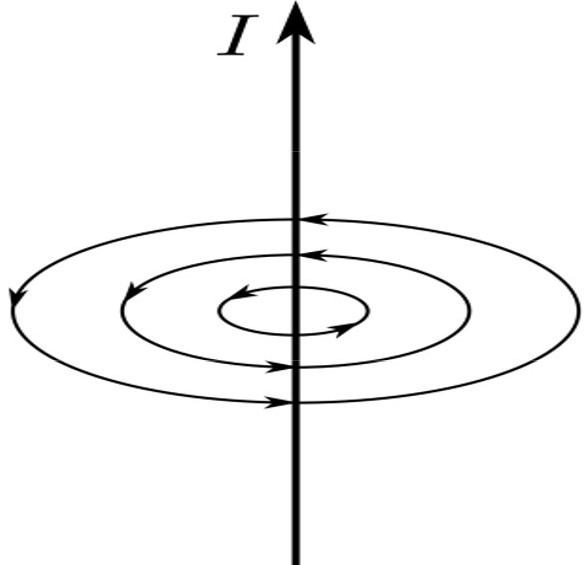
\includegraphics[scale=0.5]{Anh/Picture1 (2).jpg}
\end{center}
\item Ở gần vòng dây tròn có dòng điện chạy qua khép kín, từ trường giống như trong trường hợp dây thẳng. Khi ở xa, các đường sức từ tương ứng với đường sức từ của một lưỡng cực từ. Khu vực ở giữa có thể vẽ gần đúng như hình sau:
\begin{center}
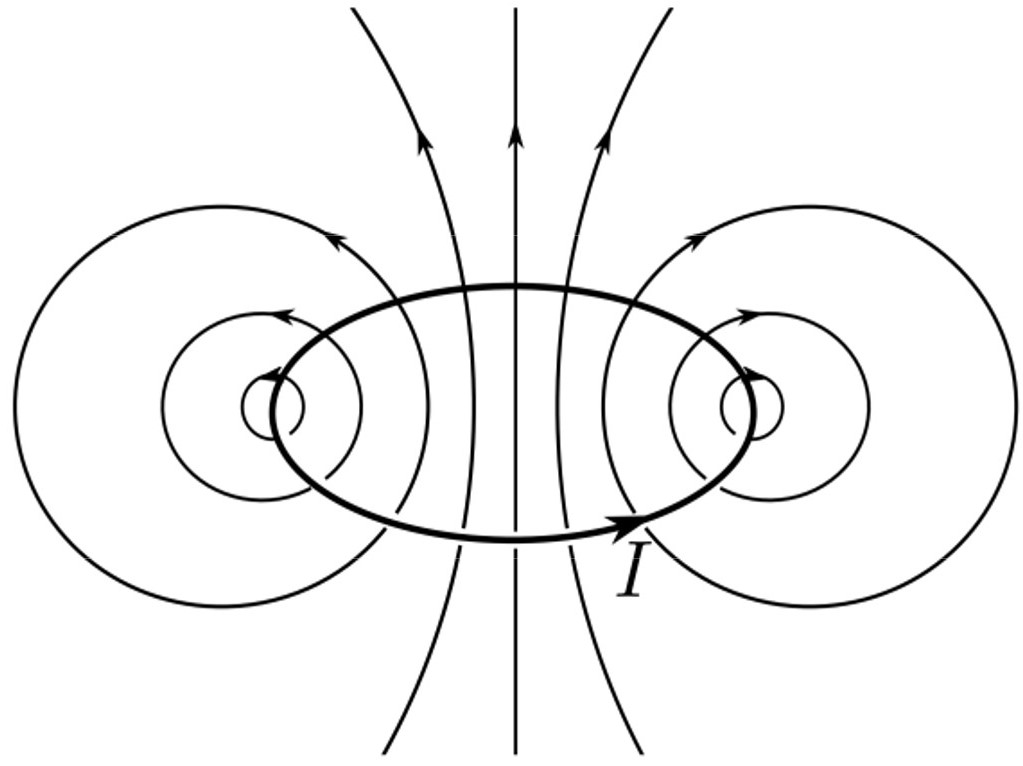
\includegraphics[scale=0.5]{Anh/Picture3 (2).jpg}
\end{center}
\item Nếu không có dây thẳng dài vô hạn, đường sức sẽ là các vòng tròn khép kín với bán kính nhỏ, quấn vòng quanh vòng dây điện tròn và kết thúc. Với sự xuất hiện của dây dài, một thành phần tiếp tuyến của từ trường được thêm vào, vì thế những đường sức từ tròn trước đó bắt đầu có khuynh hướng lệch theo phương tiếp tuyến xung quanh dây vô hạn trong khi đó vẫn quấn xung dày đặc xung quanh vòng dây tròn khép kín. Điều này tạo nên một mô hình xoắn dọc theo bề mặt của một hình phỏng xuyến được biểu diễn như hình sau.
\begin{center}
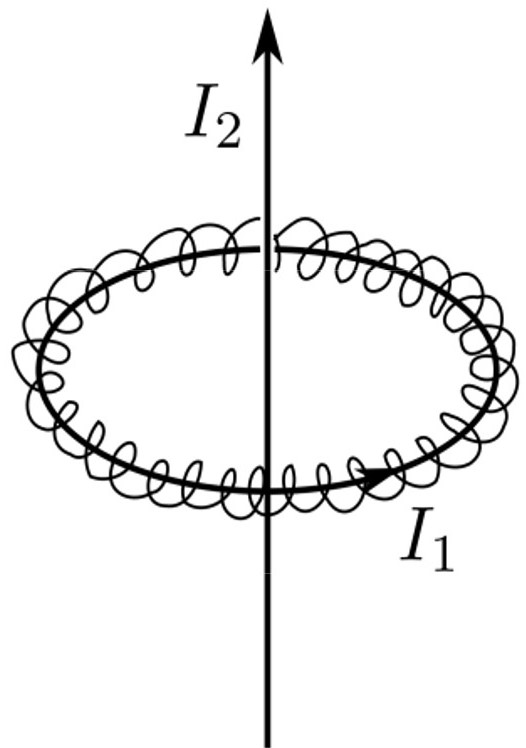
\includegraphics[scale=0.5]{Anh/Picture2 (2).jpg}
\end{center}
\item Sử dụng lập luận tương tự, khi không có sự hiện diện của vòng dây tròn khép kín, các đường sức từ cũng sẽ có hình dạng là những vòng tròn khép kín với bán kính nhỏ bao xung quanh dây dài vô hạn và rồi kết thúc. Nếu chúng ta cho thêm vòng dây điện tròn khép kín, các đường sức sẽ bắt đầu lệch ra khỏi những đường sức có dạng đường tròn khép kín ban đầu, những đường tròn khép kín ấy sẽ rất gần vị trí trung tâm và có bán kính cũng rất nhỏ (những đường sức nằm trên trục $z$ và trục $r$ trong hệ tọa độ trụ) trong khi quấn rất dày đặc xung quanh trục đối xứng (sau tất cả, cường độ từ trường từ dây dẫn thẳng dài vô hạn vẫn lớn hơn rất nhiều). Điều đó có nghĩa là các đường sức được hình thành có dạng một chuỗi xoắn dày đặc và từ từ rộng ra khi ngày càng ra xa mặt phẳng vòng dây điện tròn khép kín, cho đến khi nó khi trở về vô cùng (nơi mà cách rất xa so với vị trí của vòng dây điện tròn khép kín).
\begin{center}
    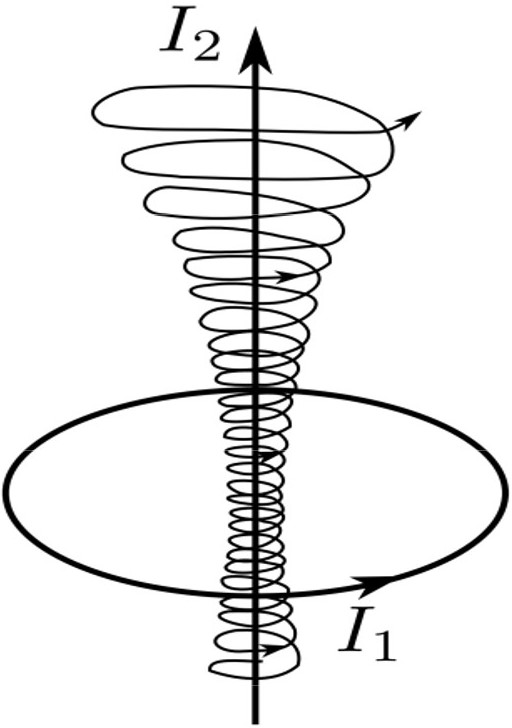
\includegraphics[scale=0.5]{Anh/Picture4 (2).jpg}
\end{center}
\end{enumerate}
    \item \textbf{Cold fusion:}\\
\begin{enumerate}[1)]
    \item 
Electron (muon) phải chịu tác dụng của lực tĩnh điện có độ lớn là:\[F=\dfrac{-1}{4\pi\varepsilon_0}\dfrac{2e^2}{R^2}. \tag{1} \label{1.1}\]
Số hai trong hệ thức là do trên thực tế, hạt nhân có điện tích là $+2e$. Đây là lực hút và đóng vai trò như một lực hướng tâm, chính vì thế, ta có: \[F=\dfrac{mv^2}{R}=\dfrac{p^2}{mR}.\tag{2} \label{1.2}\]
Từ (\ref{1.1}) và (\ref{1.2}), ta có được:
\[p=\sqrt{\dfrac{me^2}{2\pi \varepsilon_0 R}}.\]
Theo nguyên lí bất định, sai số tiêu chuẩn của động lượng và vị trí của hạt tuân theo bất đẳng thức sau:
\[\sigma_{x}\sigma_{p} \geq \dfrac{\hbar}{2} .\]
Với $\hbar=\dfrac{h}{2\pi}$ là hằng số Plank thu gọn. Vì chúng ta đang trong quá trình tính toán trên lí thuyết, sai số không phải là vấn đề lớn, vì thế, chúng ta có thể bỏ qua nó từ đây. Động lượng của electron (muon) luôn bằng $p$ vì thế $\sigma_{p}=p$, trong khi đó sai số tiêu chuẩn của vị trí luôn xấp xỉ bằng bán kính của đường tròn, vì thế $\sigma_{r}\sim R$.\\
Điều đó cho ta kết quả là:
\[\sqrt{\dfrac{me^2R}{\varepsilon_0}} \geq h.\]
Từ đó, ta giải ra $R$ xấp xỉ bằng:
\[R \sim \dfrac{h^2\varepsilon_0}{me^2}.\]
Đối với một electron, $R_{m=m_{e}}=1,7\times10^{-10}~\mathrm{m}$.\\
Đối với một muon, $R_{m=m_{\mu}}=8,1\times10^{-13}~\mathrm{m}$.
\item Do tính đối xứng, ta chỉ cần xét sự cân bằng lực ở một hạt nhân bởi vì hạt nhân còn lại cũng sẽ chịu sự tác dụng của những lực tương tự như vậy.\\
Sự cân bằng lực là sự cân bằng giữa các lực tĩnh điện giữa các hạt nhân với nhau và với các electron (đám mây muon). Biểu thức thứ nhất ta có được là biểu thức của lực đẩy:
\[F_1=\dfrac{1}{4\pi\varepsilon_0}\dfrac{e^2}{d^2}.\]
Đối với đám mây electron (muon), chỉ có những điện tích ở trong khối cầu có bán kính $d$ gây nên lực tĩnh điện. Điều đó có thể được xác định bằng cách sử dụng định luật Gauss cho khối cầu nói trên.\\
Điện tích bên trong khối cầu nhỏ hơn được xác định bởi $q=-2ed^3/8R^3$, bởi vì điện tích của khối cầu có phạm vi là lập phương bán kính.\\
Vì thế, lực của đám mây electron (muon) sẽ là:
\[F_2=-2e\dfrac{d^3}{8R^3}\dfrac{1}{4\pi\varepsilon_0}\dfrac{e}{d^2}.\]
Bởi vì có sự cân bằng lực, vì thế $F_1+F_2=0$, vì thế:
\[\dfrac{1}{4\pi\varepsilon_0}\dfrac{e^2}{d^2}-\dfrac{d^3}{4R^3}\dfrac{1}{4\pi\varepsilon_0}\dfrac{e^2}{d^2}=0.\]
Từ đó, ta tính được $d$ là:
\[d=R\sqrt[3]{4}.\]
\item Bởi vì $d$ phụ thuộc tuyến tính vào $R$ và $R$ tỉ lệ nghịch với khối lượng, khoảng cách giữa các hạt nhân sẽ được giảm bởi vì $m_{\mu}/m_{e}=207$.
\end{enumerate}
    \item \textbf{Inertial confinement fusion}
\begin{enumerate}[1)]
    \item Lớp vỏ chất lỏng là đồng chất và khối lượng phân bố đồng đều trên cả bề mặt và có thể biểu diễn bằng $\sigma=M/A$ với $A=4\pi r^2$ là tổng diện tích của lớp vỏ.\\
Do đó, khối lượng của một mẩu nhỏ là:
\[\Delta M=\sigma \Delta A=M.\dfrac{\Delta A}{4\pi r^2}.\]
    \item Vì áp suất bên ngoài lớn hơn rất nhiều so với áp suất bên trong, lớp vỏ sẽ bắt đầu co lại.\\
Tổng lực tác dụng lên một miếng nhỏ là $\Delta F=p_0\Delta A-p_{e}\Delta A\simeq-p_{e}\Delta A$, với chiều dương hệ quy chiếu là xuyên tâm và hướng ra ngoài.\\
Từ đó, gia tốc có biểu thức là:
\[a=\dfrac{\Delta F}{\Delta M}=\dfrac{-4\pi r^2p_{e}}{M}.\]
     \item Vì $p_{e}\gg p_0$, áp suất ở trạng thái cuối $p_{m}$ cũng sẽ rất nhỏ so với $p_{e}$. Quả thật là như thế, lớp vỏ sẽ co lại cho đến khi áp suất bên trong bằng áp suất bên ngoài $p_{e}$ và tiếp tục chuyển động do quán tính, cho đến khi áp suất bên trong cản trở hẳn chuyển động. Vì thế, thể tích ở trạng thái cuối sẽ rất nhỏ so với trậng thái ban đầu $-$ điều đó có thể suy ra từ những tính chất của quá trình đoạn nhiệt $V \sim  p^{-1/\gamma}$.\\
Vì thế, công của ngoại lực có thể tính bằng:
\[W=p_{e}\Delta V \approx p_e V_0.\]
Công này sẽ chuyển hóa thành nội năng,
\[W=c_{V}Nk_{B}T_{m},\]
Với $c_{V}=\dfrac{3}{2}k_{B}$ là nhiệt dung mol đẳng tích của hạt, và $N$ là tổng số hạt.\\
Bởi vì khí hoàn toàn bị ion hóa, nên mỗi phân tử DT sẽ tạo ra bốn hạt.\\
Vì thế, $N=4N_0$, với:
\[N_0=\dfrac{p_0V_0}{k_{B}T_0}.\]
Kết hợp tất cả những điều trên, ta thu được:
\[T_{m}=\dfrac{p_{e}}{4p_0}T_0.\]
Để tìm $r_{m}$, chúng ta kết hợp những tính chất của quá trình đoạn nhiệt và phương trình trạng thái khí lí tưởng thu được $V^{\gamma-1}T$ = hằng số. Điều đó cho ta $V \sim T^{-1/(\gamma-1)}$ và vì $r(V) \sim V^{1/3}$, ta có:
\[r_{m}=r\left(\dfrac{T_0}{T_{m}}\right)^{\frac{1}{3(\gamma-1)}}=r\left(\dfrac{4p_0}{p_{e}}\right)^{\frac{1}{3(\gamma-1)}}.\]
     \item Để tính được áp suất gây ra, chúng ta có thể nói rằng tất cả năng lượng của laser là dùng để tăng động năng của phần khối lượng đã bị bay hơi.\\
Gọi $M$ là khối lượng của phần vỏ ngoài đã bay hơi trong một đơn vị thời gian, xem xét trong một khoảng thời gian nhỏ là $\Delta t$, ta có định luật bảo toàn năng lượng là:
\[P\Delta t=\Delta M\dfrac{u^2}{2}=M\Delta t\dfrac{u^2}{2}.\]
Do đó,
\[M=\dfrac{2P}{u^2}.\]
Từ định luật bảo toàn động lượng, chúng ta có thể viết:
\[4\pi r^2 p_{e}=Mu,\]
do đó:
\[p_{e}=\dfrac{Mu}{4\pi r^2}=\dfrac{2P}{4\pi r^2u}.\]
\end{enumerate}
\end{enumerate}
\end{loigiai}


\begin{vd}[Động cơ đồng cực]
  Một động cơ đồng cực là động cơ gồm một khung dây cho dòng điện không đổi $I$ chạy qua được đặt trong vùng từ trường tĩnh. Khung dây có thể quay tự do quanh một trục cố định sao cho góc tạo bởi dòng điện và từ trường là không đổi ở mọi phần của khung dây. Do đó lực điện từ tác dụng lên khung dây là liên tục và không cần công tắc để đổi chiều dòng điện sau mỗi nửa chu kì như một số loại động cơ khác. Tuy nhiên nó vẫn cần một vòng trượt hoặc một chổi than tiếp xúc để có thể hoạt động. “Đồng cực” có nghĩa là hướng phân cực của khung dây (chiều dòng điện của mọi điểm trên dây dẫn) và từ trường hợp với nhau một góc không đổi theo thời gian và không cần công tắc đảo chiều dòng. Một mô hình đơn giản của loại động cơ này được mô tả như hình vẽ, tham khảo từ Wikipedia.
  \begin{center}
\tikzset{every picture/.style={line width=0.75pt}} %set default line width to 0.75pt        

\begin{tikzpicture}[x=0.75pt,y=0.75pt,yscale=-1,xscale=1]
%uncomment if require: \path (0,300); %set diagram left start at 0, and has height of 300

%Shape: Parallelogram [id:dp9905349717591636] 
\draw  [fill={rgb, 255:red, 225; green, 225; blue, 225 }  ,fill opacity=1 ] (290.33,245.66) -- (329.82,240.18) -- (329.86,247.62) -- (290.37,253.09) -- cycle ;
%Curve Lines [id:da5688680161114963] 
\draw [line width=0.75]    (348.78,79.72) .. controls (356.99,80.14) and (370.87,82.45) .. (371.08,87.08) .. controls (371.29,91.71) and (353.62,94.02) .. (341,94.44) .. controls (328.38,94.86) and (311.13,91.08) .. (310.92,86.66) .. controls (310.71,82.24) and (326.28,80.35) .. (333.22,79.93) ;
%Curve Lines [id:da9603174449394891] 
\draw    (333.22,79.93) .. controls (333.38,81.18) and (333.25,85.04) .. (333.38,87.49) .. controls (333.63,89.89) and (338.3,90.55) .. (341.2,90.42) .. controls (344.36,90.32) and (348.4,89.66) .. (348.77,87.87) .. controls (348.9,84.11) and (348.9,81.97) .. (348.78,79.72) ;
%Shape: Ellipse [id:dp21468822030138313] 
\draw   (333.6,79.72) .. controls (333.6,78.18) and (337,76.93) .. (341.19,76.93) .. controls (345.39,76.93) and (348.78,78.18) .. (348.78,79.72) .. controls (348.78,81.26) and (345.39,82.5) .. (341.19,82.5) .. controls (337,82.5) and (333.6,81.26) .. (333.6,79.72) -- cycle ;
%Straight Lines [id:da7062712274141836] 
\draw    (371.08,87.08) -- (371.08,236.6) ;
%Straight Lines [id:da028657021666151916] 
\draw    (310.92,87.08) -- (310.92,236.6) ;
%Flowchart: Stored Data [id:dp8777673631796328] 
\draw  [fill={rgb, 255:red, 155; green, 155; blue, 155 }  ,fill opacity=1 ] (310.92,266.71) -- (310.92,232.01) .. controls (310.92,235.66) and (324.39,238.62) .. (341,238.62) .. controls (357.61,238.62) and (371.08,235.66) .. (371.08,232.01) -- (371.08,266.71) .. controls (371.08,270.36) and (357.61,273.32) .. (341,273.32) .. controls (324.39,273.32) and (310.92,270.36) .. (310.92,266.71) -- cycle ;
%Straight Lines [id:da7748569407235104] 
\draw    (341.18,37.83) -- (341.18,4.85) ;
\draw [shift={(341.18,2.85)}, rotate = 450] [fill={rgb, 255:red, 0; green, 0; blue, 0 }  ][line width=0.08]  [draw opacity=0] (10.8,-2.7) -- (0,0) -- (10.8,2.7) -- cycle    ;
%Shape: Polygon [id:ds8295801816113073] 
\draw  [fill={rgb, 255:red, 225; green, 225; blue, 225 }  ,fill opacity=1 ] (260.7,53.31) -- (260.7,271.1) -- (384.56,253.33) -- (384.56,246.47) -- (268.42,263.51) -- (268.42,60.61) -- (337.1,49.86) -- (337.1,66.51) -- (341.19,79.72) -- (344.7,63.49) -- (344.7,49.08) -- (413.84,38.33) -- (413.84,227.79) -- (371.24,234.02) -- (371.24,242.21) -- (421.38,235.33) -- (420.69,30.37) -- cycle ;
%Curve Lines [id:da941413031429216] 
\draw    (304.33,205.19) .. controls (302.4,215.23) and (299.63,233.12) .. (292.27,233.36) .. controls (284.41,233.63) and (273.92,217.31) .. (273.27,157.34) .. controls (272.61,97.38) and (285.06,80.34) .. (291.29,80.99) .. controls (297.52,81.65) and (301.45,91.81) .. (302.43,100.65) ;
\draw [shift={(304.72,203.22)}, rotate = 101.77] [fill={rgb, 255:red, 0; green, 0; blue, 0 }  ][line width=0.08]  [draw opacity=0] (12,-3) -- (0,0) -- (12,3) -- cycle    ;
%Shape: Boxed Bezier Curve [id:dp9967219654755937] 
\draw    (379.48,190.05) .. controls (381.41,200.09) and (384.18,217.98) .. (391.53,218.23) .. controls (399.4,218.49) and (409.88,202.17) .. (410.54,142.2) .. controls (411.2,82.24) and (398.74,65.2) .. (392.52,65.85) .. controls (386.29,66.51) and (382.36,76.67) .. (381.38,85.51) ;
\draw [shift={(379.08,188.08)}, rotate = 78.23] [fill={rgb, 255:red, 0; green, 0; blue, 0 }  ][line width=0.08]  [draw opacity=0] (12,-3) -- (0,0) -- (12,3) -- cycle    ;
%Straight Lines [id:da0001273221005622105] 
\draw    (341,252.64) -- (341,240.62) ;
\draw [shift={(341,238.62)}, rotate = 450] [fill={rgb, 255:red, 0; green, 0; blue, 0 }  ][line width=0.08]  [draw opacity=0] (12,-3) -- (0,0) -- (12,3) -- cycle    ;

% Text Node
\draw (350.94,17.65) node [anchor=north west][inner sep=0.75pt]  [rotate=-351.63] [align=left] {Vòng dây};
% Text Node
\draw (305.7,277.65) node [anchor=north west][inner sep=0.75pt]   [align=left] {Nam châm};
% Text Node
\draw (333.44,230.34) node [anchor=north west][inner sep=0.75pt]  [rotate=-270] [align=left] {PIN ALKALINE};
% Text Node
\draw (280.24,150.73) node [anchor=north west][inner sep=0.75pt]    {$I$};
% Text Node
\draw (394.93,142.21) node [anchor=north west][inner sep=0.75pt]    {$I$};
% Text Node
\draw (332.95,228.57) node [anchor=north west][inner sep=0.75pt]    {$-$};
% Text Node
\draw (332.9,97.09) node [anchor=north west][inner sep=0.75pt]    {$+$};
% Text Node
\draw (323.13,7) node [anchor=north west][inner sep=0.75pt]    {$z$};
% Text Node
\draw (312.25,239.25) node [anchor=north west][inner sep=0.75pt]    {$M$};


\end{tikzpicture}

  \end{center}
  
Nguyên lí hoạt động của động cơ như sau: Một nguồn pin tải dòng điện cố định đi qua khung dây kép như hình vẽ, hệ đặt trong từ trường cố định tạo ra bởi một nam châm vĩnh cửu hình trụ được đặt bên dưới nguồn pin, tiếp xúc với cực âm của nguồn (xem hình vẽ). Từ trường do đó là đối xứng quanh trục $z$ và có độ lớn không đổi theo thời gian và khung dây có thể quay tự do quanh trục $z$ cố định.\\
    \begin{center}
     

\tikzset{every picture/.style={line width=0.75pt}} %set default line width to 0.75pt        

\begin{tikzpicture}[x=0.75pt,y=0.75pt,yscale=-0.9,xscale=0.9]
%uncomment if require: \path (0,336); %set diagram left start at 0, and has height of 336

%Shape: Polygon [id:ds5398321534883261] 
\draw  [fill={rgb, 255:red, 220; green, 220; blue, 220 }  ,fill opacity=1 ] (430.23,47.56) -- (430.23,276.71) -- (360.82,276.71) -- (360.82,268.92) -- (421.43,269.26) -- (421.8,56.07) -- (334.8,55.52) -- (334.8,71.02) -- (330.47,85.83) -- (326.47,71.03) -- (326.47,55.43) -- (240.23,54.95) -- (240.23,268.79) -- (298.87,268.79) -- (298.87,276.39) -- (232.07,276.39) -- (232.23,47.56) -- cycle ;
%Curve Lines [id:da7652155646336201] 
\draw [line width=0.75]    (338.49,85.83) .. controls (347.16,86.28) and (361.82,88.72) .. (362.04,93.61) .. controls (362.27,98.5) and (343.6,100.94) .. (330.27,101.39) .. controls (316.93,101.83) and (298.71,97.83) .. (298.49,93.17) .. controls (298.27,88.5) and (314.71,86.5) .. (322.04,86.06) ;
%Curve Lines [id:da8263889077812194] 
\draw    (322.04,86.06) .. controls (322.21,87.38) and (322.08,91.46) .. (322.21,94.05) .. controls (322.48,96.58) and (327.41,97.27) .. (330.48,97.14) .. controls (333.81,97.03) and (338.08,96.34) .. (338.48,94.45) .. controls (338.61,90.47) and (338.61,88.21) .. (338.49,85.83) ;
%Shape: Ellipse [id:dp8997122003794547] 
\draw   (322.45,85.83) .. controls (322.45,84.21) and (326.04,82.89) .. (330.47,82.89) .. controls (334.9,82.89) and (338.49,84.21) .. (338.49,85.83) .. controls (338.49,87.46) and (334.9,88.78) .. (330.47,88.78) .. controls (326.04,88.78) and (322.45,87.46) .. (322.45,85.83) -- cycle ;
%Straight Lines [id:da585831478304778] 
\draw    (362.04,93.61) -- (362.04,251.57) ;
%Straight Lines [id:da16307441614756546] 
\draw    (298.49,93.61) -- (298.49,251.57) ;
%Flowchart: Stored Data [id:dp3009048631910518] 
\draw  [fill={rgb, 255:red, 155; green, 155; blue, 155 }  ,fill opacity=1 ] (298.49,288.23) -- (298.49,251.57) .. controls (298.49,255.42) and (312.72,258.55) .. (330.27,258.55) .. controls (347.82,258.55) and (362.04,255.42) .. (362.04,251.57) -- (362.04,288.23) .. controls (362.04,292.08) and (347.82,295.21) .. (330.27,295.21) .. controls (312.72,295.21) and (298.49,292.08) .. (298.49,288.23) -- cycle ;
%Straight Lines [id:da3184761056631049] 
\draw    (330.02,282.39) -- (330.02,266.99) ;
\draw [shift={(330.02,264.99)}, rotate = 450] [fill={rgb, 255:red, 0; green, 0; blue, 0 }  ][line width=0.08]  [draw opacity=0] (12,-3) -- (0,0) -- (12,3) -- cycle    ;
%Curve Lines [id:da5942792400252743] 
\draw    (303.24,251.7) .. controls (292.68,235.86) and (240.31,246.9) .. (261.9,288.86) ;
\draw [shift={(262.58,290.14)}, rotate = 241.53] [fill={rgb, 255:red, 0; green, 0; blue, 0 }  ][line width=0.08]  [draw opacity=0] (9.6,-2.4) -- (0,0) -- (9.6,2.4) -- cycle    ;
%Curve Lines [id:da4513780347454881] 
\draw    (309.24,251.26) .. controls (293.62,222.66) and (239.24,215.62) .. (219.18,257.31) ;
\draw [shift={(218.58,258.59)}, rotate = 294.4] [fill={rgb, 255:red, 0; green, 0; blue, 0 }  ][line width=0.08]  [draw opacity=0] (10.8,-2.7) -- (0,0) -- (10.8,2.7) -- cycle    ;
%Curve Lines [id:da8833941265643703] 
\draw    (315.02,251.08) .. controls (300.72,213.72) and (259.63,195.31) .. (213.32,193.83) ;
\draw [shift={(211.91,193.79)}, rotate = 361.40999999999997] [fill={rgb, 255:red, 0; green, 0; blue, 0 }  ][line width=0.08]  [draw opacity=0] (10.8,-2.7) -- (0,0) -- (10.8,2.7) -- cycle    ;
%Curve Lines [id:da4276881203243461] 
\draw    (319.69,251.08) .. controls (309.57,203.82) and (261.77,156.61) .. (216.83,131.95) ;
\draw [shift={(215.47,131.21)}, rotate = 388.33000000000004] [fill={rgb, 255:red, 0; green, 0; blue, 0 }  ][line width=0.08]  [draw opacity=0] (10.8,-2.7) -- (0,0) -- (10.8,2.7) -- cycle    ;
%Curve Lines [id:da6935502583331479] 
\draw    (325.24,251.03) .. controls (325.24,201.93) and (268.18,78.12) .. (231.03,32.39) ;
\draw [shift={(229.91,31.03)}, rotate = 410.22] [fill={rgb, 255:red, 0; green, 0; blue, 0 }  ][line width=0.08]  [draw opacity=0] (10.8,-2.7) -- (0,0) -- (10.8,2.7) -- cycle    ;

%Curve Lines [id:da10521949349921678] 
\draw    (357.48,252.13) .. controls (368.04,236.29) and (420.42,247.33) .. (398.83,289.29) ;
\draw [shift={(398.15,290.57)}, rotate = 298.47] [fill={rgb, 255:red, 0; green, 0; blue, 0 }  ][line width=0.08]  [draw opacity=0] (9.6,-2.4) -- (0,0) -- (9.6,2.4) -- cycle    ;
%Curve Lines [id:da6475337590116637] 
\draw    (351.48,251.68) .. controls (367.1,223.08) and (421.49,216.05) .. (441.55,257.74) ;
\draw [shift={(442.15,259.02)}, rotate = 245.6] [fill={rgb, 255:red, 0; green, 0; blue, 0 }  ][line width=0.08]  [draw opacity=0] (10.8,-2.7) -- (0,0) -- (10.8,2.7) -- cycle    ;
%Curve Lines [id:da8795814952017094] 
\draw    (345.7,251.51) .. controls (360,214.15) and (401.09,195.74) .. (447.41,194.26) ;
\draw [shift={(448.82,194.22)}, rotate = 538.5899999999999] [fill={rgb, 255:red, 0; green, 0; blue, 0 }  ][line width=0.08]  [draw opacity=0] (10.8,-2.7) -- (0,0) -- (10.8,2.7) -- cycle    ;
%Curve Lines [id:da5266593407059388] 
\draw    (341.04,251.51) .. controls (351.16,204.25) and (398.96,157.04) .. (443.9,132.38) ;
\draw [shift={(445.26,131.64)}, rotate = 511.67] [fill={rgb, 255:red, 0; green, 0; blue, 0 }  ][line width=0.08]  [draw opacity=0] (10.8,-2.7) -- (0,0) -- (10.8,2.7) -- cycle    ;
%Curve Lines [id:da686496351033266] 
\draw    (335.48,251.46) .. controls (335.48,202.36) and (392.55,78.55) .. (429.7,32.82) ;
\draw [shift={(430.82,31.46)}, rotate = 489.78] [fill={rgb, 255:red, 0; green, 0; blue, 0 }  ][line width=0.08]  [draw opacity=0] (10.8,-2.7) -- (0,0) -- (10.8,2.7) -- cycle    ;

%Straight Lines [id:da5418277081629266] 
\draw    (330.46,250.9) -- (330.46,17.53) ;
\draw [shift={(330.46,15.53)}, rotate = 450] [fill={rgb, 255:red, 0; green, 0; blue, 0 }  ][line width=0.08]  [draw opacity=0] (10.8,-2.7) -- (0,0) -- (10.8,2.7) -- cycle    ;
%Curve Lines [id:da009594011998967478] 
\draw     ;
%Straight Lines [id:da97513275658264] 
\draw    (321.4,51.63) -- (236.07,51.63) -- (236.07,272.3) -- (290.07,272.3) ;
\draw [shift={(292.07,272.3)}, rotate = 180] [fill={rgb, 255:red, 0; green, 0; blue, 0 }  ][line width=0.08]  [draw opacity=0] (10.8,-2.7) -- (0,0) -- (10.8,2.7) -- cycle    ;
%Shape: Boxed Line [id:dp10260437502204112] 
\draw    (340.48,51.78) -- (425.81,51.78) -- (425.81,272.45) -- (371.81,272.45) ;
\draw [shift={(369.81,272.45)}, rotate = 360] [fill={rgb, 255:red, 0; green, 0; blue, 0 }  ][line width=0.08]  [draw opacity=0] (10.8,-2.7) -- (0,0) -- (10.8,2.7) -- cycle    ;
%Straight Lines [id:da46982581709923377] 
\draw    (218,60.37) -- (218,104.03) ;
\draw [shift={(218,106.03)}, rotate = 270] [fill={rgb, 255:red, 0; green, 0; blue, 0 }  ][line width=0.08]  [draw opacity=0] (12,-3) -- (0,0) -- (12,3) -- cycle    ;
%Straight Lines [id:da03595452532800336] 
\draw    (443,60.37) -- (443,104.03) ;
\draw [shift={(443,106.03)}, rotate = 270] [fill={rgb, 255:red, 0; green, 0; blue, 0 }  ][line width=0.08]  [draw opacity=0] (12,-3) -- (0,0) -- (12,3) -- cycle    ;


% Text Node
\draw (303.91,268.68) node [anchor=north west][inner sep=0.75pt]    {$M$};
% Text Node
\draw (290.91,302.83) node [anchor=north west][inner sep=0.75pt]   [align=left] {Nam châm};
% Text Node
\draw (198.67,72.77) node [anchor=north west][inner sep=0.75pt]    {$I$};
% Text Node
\draw (450,73.43) node [anchor=north west][inner sep=0.75pt]    {$I$};
% Text Node
\draw (307.5,157.2) node [anchor=north west][inner sep=0.75pt]  [rotate=-270] [align=left] {Pin};
% Text Node
\draw (308.67,103.77) node [anchor=north west][inner sep=0.75pt]    {$+$};
% Text Node
\draw (309.5,21.4) node [anchor=north west][inner sep=0.75pt]    {$\mathbf{B}$};
% Text Node
\draw (339.5,21) node [anchor=north west][inner sep=0.75pt]   [align=left] {Vòng dây};


\end{tikzpicture}

    \end{center}
Các thông số chiều dài, khối lượng và điện trở khung dây (và của pin, nam châm), hiệu điện thế của pin và từ trường của nam châm ở mọi điểm trong không gian được giả sử như đã biết. Tìm moment ngẫu lực tác dụng lên khung dây và vận tốc góc của khung như một hàm của thời gian $t$.

\end{vd}
\begin{loigiai}
Motor của chúng ta được mô hình hóa như trên biểu đồ (xem hình vẽ), hình vẽ chỉ thể hiện một nửa khung dây vì bài toán có tính đối xứng. Chúng ta sử dụng hệ tọa độ trụ $(r, \phi, z)$ với gốc tọa độ $O$ nằm ở trọng tâm của nam châm hình trụ, có bán kính $b$ và chiều dài $l$. Trục $z$ đồng trục với trục của nam châm và trục của pin, ở đây pin được mô hình như một nguồn điện có hiệu điện thế $V$. Mạch điện $ACDEF$ được khép kín bằng tiếp xúc chổi than (mũi tên màu trắng trên hình vẽ) với nam châm tại điểm $A \equiv (0,\phi,l/2)$ và $F \equiv (b, \phi, 0)$ do đó dòng điện có thể chạy qua nam châm dẫn điện. Mạch điện có thể quay tự do quanh trục $z$. Đặt $a (>b)$ và $h$ lần lượt là kích thước của khung dây theo phương ngang và phương dọc.
 \begin{center}
     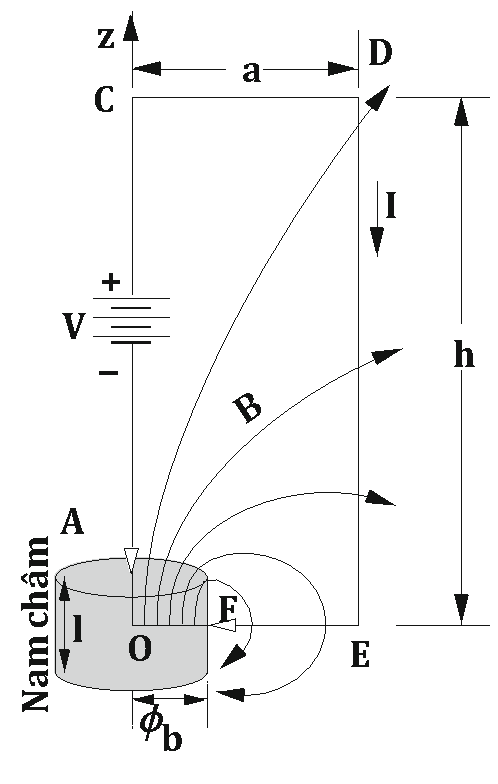
\includegraphics[scale=0.6]{Anh/Nam_P3.pdf}
 \end{center}
Ta đặt $\ot{B} = \ot{B} (r, \phi, z)$ là từ trường tạo ra bởi nam châm, không phụ thuộc vào $\phi$ và có $B_{\phi} \equiv 0$. Một vài đường sức từ của $\ot{B}$ được vẽ trên hình. Từ trường tại mặt phẳng $z=0$ song song với trục $z$, hướng thẳng đứng lên trên với $r<b$ và hướng xuống dưới đối với $r>b$. Để đơn giản hóa bài toán chúng ta giả sử $\ot{B} (r,\phi, 0) = B_0 \hat{{z}} $ đối với $r<b$, với $B_0$ không phụ thuộc vào $r$, dù xấp xỉ này chỉ đúng khi $l \gg b$.
 \begin{center}
     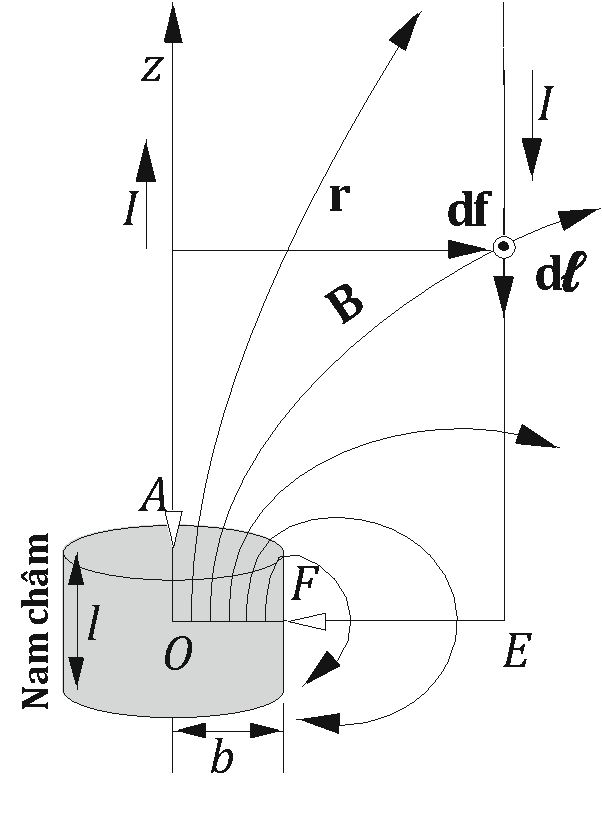
\includegraphics[scale=0.6]{Anh/Nam_P4.pdf}
 \end{center}
Nguồn điện sẽ đẩy một dòng điện $I$ đi qua mạch điện. Khi khung dây không quay, ta dễ dàng có $I= V/R$ nhưng khi khung dây quay, chúng ta phải tính đến hiệu ứng của khung dây chuyển động trong từ trường. Vì từ trường $\ot{B}$ nằm trong mặt phẳng khung dây nên lực $\dd\ot{f} = I \dd\ot{l}\times \ot{B}$ tác dụng lên một vi phân chiều dài $\dd\ot{l}$ của khung dây là vuông góc với mặt phẳng vòng dây (hoặc là mặt giấy đối với hình vẽ). Moment tương ứng đối với trục $z$ của lực là 
        \[ \dd \ot{\tau}= \ot{r} \times \dd \ot{f} = b_m I \ot{r} \times (\dd \ot{l} \times \ot{B}),  \tag{1}\label{n.1}\]
với $\ot{r}$ là khoảng cách của vi phân độ dài $\dd\ot{l}$ đến trục $z$. Phương của vi phân moment lực $\dd \ot{\tau}$ luôn song song với ${\hat{z}}$, không phụ thuộc vào vị trí của $\dd\ot{l}$ mà chúng ta xét. Đối với tích vector $\dd\ot{l} \times\ot{B}$ ta có
      \[\dd\ot{l}\times \ot{B}=-\hat{{\phi}}B \dd l \sin\theta = - \hat{{\phi}} B \dd l \cos \psi\]
            \[=-\hat{{\phi}}\ot{B} \cdot \hat{n} \dd l, \tag{2}\]

với $\theta$ là góc hợp bởi $\dd \ot{l}$ và $\ot{B}$, ${\hat{n}}$ là vector đơn vị vuông góc với $\dd\ot{l}$, và $\psi = \theta - \pi/2$ là góc hợp giữa $\ot{B}$ và ${\hat{n}}$ (xem hình vẽ). 
  \begin{center}


\tikzset{every picture/.style={line width=0.75pt}} %set default line width to 0.75pt        

\begin{tikzpicture}[x=0.75pt,y=0.75pt,yscale=-1,xscale=1]
%uncomment if require: \path (0,300); %set diagram left start at 0, and has height of 300

%Straight Lines [id:da4574314470092409] 
\draw    (252.31,144.28) -- (313.6,83) -- (374.47,22.12) ;
\draw [shift={(376.59,20)}, rotate = 495] [fill={rgb, 255:red, 0; green, 0; blue, 0 }  ][line width=0.08]  [draw opacity=0] (10.72,-5.15) -- (0,0) -- (10.72,5.15) -- (7.12,0) -- cycle    ;
%Straight Lines [id:da43449029535351946] 
\draw    (252.31,144.28) -- (408.6,144.28) ;
\draw [shift={(411.6,144.28)}, rotate = 180] [fill={rgb, 255:red, 0; green, 0; blue, 0 }  ][line width=0.08]  [draw opacity=0] (10.72,-5.15) -- (0,0) -- (10.72,5.15) -- (7.12,0) -- cycle    ;
%Straight Lines [id:da7839461358085928] 
\draw    (252.31,144.28) -- (252.31,269.42) ;
\draw [shift={(252.31,272.42)}, rotate = 270] [fill={rgb, 255:red, 0; green, 0; blue, 0 }  ][line width=0.08]  [draw opacity=0] (10.72,-5.15) -- (0,0) -- (10.72,5.15) -- (7.12,0) -- cycle    ;
%Shape: Arc [id:dp1604699560533387] 
\draw  [draw opacity=0][dash pattern={on 4.5pt off 4.5pt}] (301.95,96.63) .. controls (315.87,111.15) and (323.33,131.62) .. (320.54,153.12) .. controls (316.05,187.84) and (286.41,213.14) .. (252.31,213.09) -- (252.31,144.28) -- cycle ; \draw  [dash pattern={on 4.5pt off 4.5pt}] (301.95,96.63) .. controls (315.87,111.15) and (323.33,131.62) .. (320.54,153.12) .. controls (316.05,187.84) and (286.41,213.14) .. (252.31,213.09) ;
%Shape: Arc [id:dp08212124771975149] 
\draw  [draw opacity=0][dash pattern={on 4.5pt off 4.5pt}] (292.89,143.68) .. controls (292.92,145.6) and (292.81,147.54) .. (292.56,149.5) .. controls (289.9,169.97) and (272.42,184.9) .. (252.31,184.87) -- (252.31,144.28) -- cycle ; \draw  [dash pattern={on 4.5pt off 4.5pt}] (292.89,143.68) .. controls (292.92,145.6) and (292.81,147.54) .. (292.56,149.5) .. controls (289.9,169.97) and (272.42,184.9) .. (252.31,184.87) ;
%Shape: Arc [id:dp537421311028123] 
\draw  [draw opacity=0][dash pattern={on 4.5pt off 4.5pt}] (320.32,78.57) .. controls (336.32,95.26) and (346.29,117.5) .. (347.36,141.56) -- (250.08,146) -- cycle ; \draw  [dash pattern={on 4.5pt off 4.5pt}] (320.32,78.57) .. controls (336.32,95.26) and (346.29,117.5) .. (347.36,141.56) ;


% Text Node
\draw (228,192.4) node [anchor=north west][inner sep=0.75pt]    {$\dd \ot{\ell}$};
% Text Node
\draw (303.32,59.38) node [anchor=north west][inner sep=0.75pt]  [rotate=-314.09]  {$\ot{B}$};
% Text Node
\draw (283.8,160.4) node [anchor=north west][inner sep=0.75pt]    {$\dfrac{\pi }{2}$};
% Text Node
\draw (384.8,146.4) node [anchor=north west][inner sep=0.75pt]    {$\ot{\hat{n}}$};
% Text Node
\draw (346.8,92.4) node [anchor=north west][inner sep=0.75pt]    {$\psi $};
% Text Node
\draw (307.8,189.4) node [anchor=north west][inner sep=0.75pt]    {$\theta $};


\end{tikzpicture}
\end{center}
Vì ${\hat{r}}$ là vuông góc với $\hat{\boldsymbol{\phi}}$ (vector đơn vị của hai tọa độ độc lập), chúng ta có tổng moment tác dụng lên khung dây 
  \[ \tau = b_m I \int_{A}^{F} \ot{r} \times ( \dd \ot{l} \times \ot{B}) = - \hat{{z}} b_m I \int_{A}^{F} \ot{B} \cdot \hat{n} r\,\dd l. \tag{3} \]

Biểu thức cuối của phương trình trên có thể tính được tích phân mà không cần gần đúng nếu chúng ta chứng minh được tích phân đường của $\ot{B} \cdot \hat{n} r $ quanh vòng kín $OCDEO$ (xem hình vẽ) là bằng không, đó là
  \[\oint\ot{B} \cdot \hat{n} r \,\dd l = \int_{A}^{F} \ot{B}\cdot\hat{n} r \,\dd l + \int_{F}^{O} \ot{B}\cdot \hat{n} r  \,\dd l + \int_{O}^{A} \ot{B}\cdot \hat{n} r \, \dd l =0. \tag {4}\]
Đầu tiên, chúng ta để ý rằng tích phân này dọc trên đoạn $\overline{OC}$ là bằng không, bởi vì $r$ bằng không và hơn nữa là do $\ot{B}$ song song với $\dd\ot{l}$. Do đó tích phân trên thu gọn lại thành
  \[ \begin{aligned}
       \oint \ot{B}\cdot \hat{n} r \, \dd l &= \int_{C}^{D} \ot{B} \cdot \hat{n} r \, \dd r - \int_{D}^{E} \ot{B} \cdot \hat{n} r \, \dd z - \int_{E}^{O} \ot{B} \cdot \hat{n} r \, \dd r\\
         &= \int_{C}^{D} \ot{B} \cdot \hat{n} r \, \dd r + \int_{E}^{D} \ot{B} \cdot \hat{n} r \, \dd z + \int_{O}^{E} \ot{B}\cdot \hat{n} r \, \dd r,  \end{aligned} \tag{5}\]

vì $\dd l= \dd r$ dọc theo $\overline{CD}$, $\dd l=-\dd z$ dọc theo $\overline{DE}$ và $\dd l = -\dd r$ dọc theo $\overline{EO}$.\\
 Ở bước tiếp theo, chúng ta tạo ra hình trụ bằng cách quay khung dây quanh trục $z$ (xem hình vẽ).
 \begin{center}
     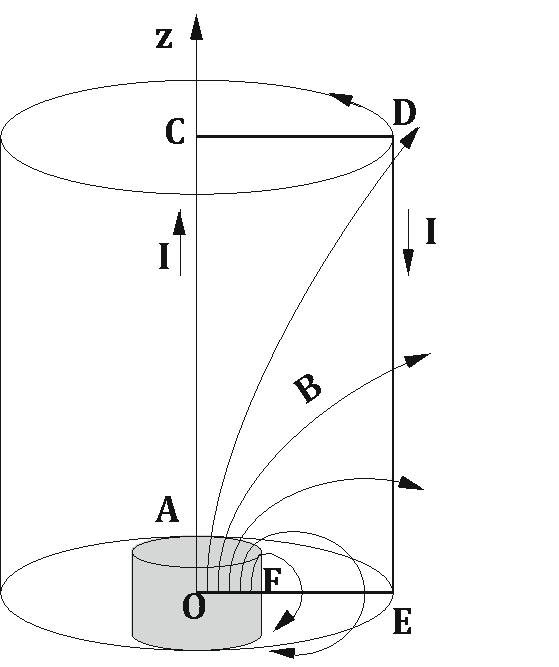
\includegraphics[scale=0.6]{Anh/Nam_P5.pdf}
 \end{center}
 Phần từ thông của từ trường $\ot{B}$ đi qua toàn bộ diện tích hình trụ là 
  \[\int_{\text{trên}} \ot{B} \cdot \hat{n} \, \dd S + \int_\text{{bên}} \ot{B} \cdot \hat{n} \, \dd S+ \int_\text{{dưới}} \ot{B} \cdot \hat{n} \, \dd S =0, \tag{6}\]
vì $\nabla\cdot\ot{B}=0$ nên phương trình $6)$ có thể viết lại thành
   \[ \begin{aligned} 0 &= \int_{0}^{a} \ot{B} (r,\phi,h) \cdot {\hat{n}} 2\pi r \, \dd r + \int_{0}^{h} \ot{B} (a, \phi, z) \cdot {\hat{n}} 2 \pi e \, \dd z\\
    &+ \int_{0}^{a} \ot{B} (r,\phi,0) \cdot {\hat{n}} 2\pi r \,\dd r = 2\pi \oint \ot{B} \cdot \hat{n} r \, \dd l, \end{aligned} \tag {7} \] 
    
kết quả này chứng minh cho biểu thức $4)$. Do đó với nguyên hàm cuối của biểu thức $3)$ ta có 
   \[\int_{A}^{F} \ot{B}\cdot \hat{n} r \, \dd l= - \int_{F}^{O} \ot{B} \cdot \hat{n} r \, \dd l = \int_{0}^{b} B_0 r \, \dd r = \frac{B_0 b^2}{2}, \tag{8} \]
ở đây ta đã biết giá trị của tích phân đường là bằng không trên trục $z$, với $\dd l = - \dd r $ trên đường $\overline{FO}$, và do đó, không cần tính xấp xỉ ta có $\ot{B}\cdot\hat{n} = -B_0$ không phụ thuộc vào $r$ ở trên đường $\overline{FO}$. Moment lực tác dụng vào khung dây quay là 
    \[\ot{\tau} = - {\hat{z}} b_m I \int_{A}^{F} \ot{B}\cdot \hat{n} r \, \dd l = - {\hat{z}} b_m I \frac{1}{R} \left( V + b_m \omega \frac{B_0 b^2}{2}\right) . \tag{9} \]
Đây là lí do vì sao chúng ta cần một tiếp xúc trượt ở động cơ đồng trục. Vì nếu đoạn $\overline{FO}$ cũng quay cùng khung dây, moment lực tác dụng lên khung dây đối với trục $z$ sẽ bằng không do moment tác dụng lên đoạn $\overline{FO}$ sẽ triệt tiêu moment tác dụng lên phần còn lại của khung dây.\\
Chúng ta đặt $\Upsilon$ là moment quán tính của khung dây. Phương trình chuyển động của khung dây nếu bỏ qua ma sát là
       \[ \Upsilon \frac{\dd \omega}{\dd t} = \tau = -b_m I\frac{B_0 b^2}{2} - \eta \omega, \tag{10} \]
ở đây chúng ta đã công nhận sự tồn tại của một moment cản $\ot{\tau}_{fr}-\eta\ot{\omega}$ tỉ lệ thuận với vận tốc góc của khung. Dòng điện $I$ được xác định bởi hiệu điện thế của nguồn và suất điện động cảm ứng $\varepsilon$ do khung dây quanh trong từ trường $\ot{B}$.
     \[\begin{aligned} \varepsilon &= b_m \int_{C}^{F} (\ot{\omega} \times \ot{r}) \times \ot{B}\cdot \dd \ot{l} = b_M \int_{C}^{F} \omega r \hat{{\phi}}\times \ot{B} \cdot \dd \ot{l} = -b_m \omega \int_{C}^{F} r \hat{{\phi}}\cdot \dd \ot{l}\times \ot{B} \\
   &= b_m \omega \int_{C}^{F} r \ot{B} \cdot \hat{n} \, \dd l = b_m \omega \frac{B_0 b^2}{2}. \end{aligned} \tag{11} \]

Sử dụng kết quả của $2)$ và $8)$, cường độ dòng điện là 
    \[ I = \frac{1}{R} \left( V + b_m \omega \frac{B_0 b^2}{2}\right), \tag{12}\]

và phương trình chuyển động 
    \[\begin{aligned} \Upsilon \frac{\dd \omega}{\dd t} &= -b_m \frac{1}{R} \left(V + b_m \omega \frac{B_0 b^2}{2} \right) \frac{B_0 b^2}{2} -\eta \omega\\
      &= -b_m \frac{VB_0 b^2}{2R} - \omega\left({b_m}^2\frac{{B_0}^2 b^4}{4R} + \eta\right). \end{aligned} \tag{13} \]
Nghiệm của phương trình này là
      \[\omega= - \frac{2b_mVB_0 b^2}{{b_m}^2{B_0}^2 b^4 + 4R\eta}( 1- e^{-\frac{t}{T}}) ,  \quad   \text{ở đây}   \quad T= \frac{4R \Upsilon}{{b_m}^2 {B_0}^2b^4 +4R\eta}. \tag{14} \] 
Nếu chúng ta giả sử moment cản là rất yếu ($\eta << b_m^2 B_0^2 b^4/4R$), phương trình $14)$ được rút gọn lại thành 
     \[\omega = - \frac{2V}{b_m B_0 b^2}( 1 - e^{-\frac{t}{T}}),\quad \text{với} \quad T= \frac{4R\Upsilon}{{b_m}^2 {B_0}^2 b^4}. \tag{15} \]
Tuy nhiên, thử thay các thông số phổ biến vào phương trình $15)$ ví dụ như $V= 1.5 ~\mathrm{V}, B_0 = 10^{-2}~\mathrm{T}$ và $b=0.5~\mathrm{cm}$ ta thu được các kết quả ở trạng thái dừng
       \[ \omega_0 = -\frac{2V}{b_m B_0 b^2} \approx -1200 ~\mathrm{rad/s,}\ \text{ do đó }\ v_0 \approx 190 ~\mathrm{m/s}. \tag{16} \]
Tốc độ quay này là nhanh một cách vô lí! Trong trường hợp bỏ qua moment cản, trạng thái dừng được thiết lập khi $V+\varepsilon =0 $, do đó $I=0$ và sẽ không có moment nào tác dụng lên khung dây. Động năng của khung dây quay khi đạt trạng thái dừng trong trường hợp này là 
   \[K_{ss} =\frac{1}{2} \Upsilon {\omega_0}^2 = \frac{1}{2} \Upsilon \frac{4V^2}{{b_m}^2 {B_0}^2 b^4}= \frac{2V^2 \Upsilon}{{b_m}^2 {B_0}^2b^4} . \tag{17} \]
Dòng điện chạy trong mạch là: 
     \[ I(t) = \frac{1}{R} \left(V + \frac{b_m B_0 b^2 \omega}{2}\right) = \frac{V}{R}e^{-t/T}, \tag {18} \]
và tổng năng lượng được cung cấp bởi nguồn điện là:
     \[ U= \int_{0}^{\infty} VI \, \dd t = \frac{V^2}{R} \int_{0}^{\infty} e^{-t/T} \, \dd t = \frac{V^2}{R} T = \frac{4V^2 \Upsilon}{{b_m}^2 {B_0}^2 b^4 } = 2K_{ss}, \tag{19} \]
hoặc hai lần động năng của khung dây. Nhiệt năng tỏa ra trên dây dẫn cũng chính bằng động năng $K_{ss}$. Để làm bài toán thực tế hơn, chúng ta phải tính cả moment cản vào phương trình. Ví dụ, vận tốc góc ổn định sẽ giảm đi $10$ lần nếu chúng ta giả sử $4R\eta = 9b_m B_0 b^2$. Nếu giả sử $R  =1 \Omega $ thì:
     \[\eta \approx 6 \times 10^{-5} ~\mathrm{Nms}. \tag{20}\]
Trong trường hợp có moment cản, vận tốc góc khung dây lúc ổn định là: 
     \[ \omega_f = - \frac{2b_m V B_0 b^2}{{b_m}^2{B_0}^2 b^4 + 4R\eta}, \tag{21}\]
và phần năng lượng mất mát do lực cản là:
   \[P_{fr}=\tau_{fr}\omega_f = \eta {\omega_f}^2 =\eta \left( \frac{2b_m V B_0 b^2}{{b_m}^2 {B^0}^2 b^4 + 4R\eta}\right)^2. \tag{22}\]
Lúc này nguồn điện có một dòng 
    \[I_f = \frac{V}{R}\left(1 - \frac{{b_m}^2 {B_0}^2 b^4}{{b_m}^2 {B_0}^2 b^4 + 4R\eta}\right) = \frac{4V\eta}{{b_m}^2{B_0}^2 b^4 +4R\eta}, \tag{23} \]
và cung cấp một công suất: 
    \[P_{\text{nguồn}}=VI_f = \frac{4V^2\eta}{{b_m}^2{B_0}^2 b^4 +4R\eta}. \tag{24}\]
Phần công suất tỏa nhiệt ra môi trường là: 
  \[P_J = R{I_f}^2 = R \left(\frac{4V^2\eta}{{b_m}^2{B_0}^2 b^4 +4R\eta}\right)^2, \tag{25} \]
và chúng ta có thể kiểm chứng
  \[P_J +P_{fr} = P_{\text{nguồn}}.\]
 

\end{loigiai}


\begin{vd}[Bong bóng xà phòng và quả cầu điện môi]
\begin{enumerate}[1)]
    \item Một bong bóng xà phòng hình cầu chứa không khí có khối lượng riêng ${{\rho}_{1}}$ và bán kính ${{R}_{0}}$. Không khí bao quanh bong bóng có khối lượng riêng ${{\rho }_{a}}$, áp suất ${{P}_{a}}$ và có nhiệt độ không đổi (cỡ nhiệt độ phòng). Khối lượng riêng của màng xà phòng là ${{\rho }_{s}}$, hệ số sức căng bề mặt $\gamma $, bề dày bong bóng là $t~(t\ll {{R}_{0}})$. Bong bóng được tích điện với điện tích tổng cộng là $q$. Khi ổn định, bán kính bong bóng là ${{R}_{1}}$. Giả sử bong bóng không bị vỡ sau quá trình tích điện và nhiệt độ khí trong bóng bóng luôn bằng nhiệt độ môi trường.
    \begin{enumerate}[a)]
        \item Xác định áp suất tĩnh điện lên mặt bong bóng xà phòng. Giả thiết $\dfrac{{{q}^{2}}}{{{P}_{a}}{{\varepsilon }_{0}}R_{0}^{4}}\ll 1$, bán kính bong bóng biến thiên một lượng $\Delta R={{R}_{1}}-{{R}_{0}}$. Tính $\Delta R$ theo ${{R}_{0}},{{P}_{a}},q,\gamma $ và hằng số điện môi của chân không ${{\varepsilon }_{0}}$.
        \item Xác định điện tích $q$ theo $t,~{{\rho }_{a}},~{{\rho }_{s}},~{{\varepsilon }_{0}},~{{R}_{0}},~{{P}_{a}}$ và $\gamma $ để cho bong bóng đứng yên trong không khí. Tính giá trị của q với $t=100~\mathrm{nm}$, ${{\rho }_{a}}=1.18~\mathrm{kg}.{{\mathrm{m}}^{-3}}$, ${{\rho}_{s}}=1.3~\mathrm{kg}.{{\mathrm{m}}^{-3}}$,~${{\varepsilon }_{0}}=8.{{85.10}^{-12}}~\mathrm{F}.{{\mathrm{m}}^{-1}}$, ${{R}_{0}}=1~\mathrm{cm}$, ${{P}_{a}}=1.{{013.10}^{5}}~\mathrm{N}.{{\mathrm{m}}^{-2}}$, $\gamma =0.025~\mathrm{N}.{{\mathrm{m}}^{-1}}$.
    \end{enumerate}
    \item Xét quả cầu dẫn điện có khối lượng riêng ${{\rho }_{1}}~({{\rho }_{1}}>2\rho)$ và hằng số điện môi ${{\varepsilon }_{1}}$ trong trường hấp dẫn. Bên trên chất lỏng là môi trường khí có khối lượng riêng ${{\rho }_{2}}$ và hằng số điện môi ${{\varepsilon }_{2}}<{{\varepsilon }_{1}}$. Quả cầu được tích điện $Q$ sao cho khi cân bằng thì $\dfrac{1}{2}$ quả cầu chìm trong chất lỏng (Hình vẽ). Bỏ qua các hiệu ứng rìa. Lấy gia tốc trọng trường là $g$.
    \begin{center}
        

\tikzset{every picture/.style={line width=0.75pt}} %set default line width to 0.75pt        

\begin{tikzpicture}[x=0.75pt,y=0.75pt,yscale=-1,xscale=1]
%uncomment if require: \path (0,493); %set diagram left start at 0, and has height of 493

%Shape: Rectangle [id:dp05567602140903616] 
\draw  [draw opacity=0][fill={rgb, 255:red, 155; green, 155; blue, 155 }  ,fill opacity=0.4 ] (192,112) -- (380.6,112) -- (380.6,208.15) -- (192,208.15) -- cycle ;
%Shape: Rectangle [id:dp3819912679054587] 
\draw  [draw opacity=0][fill={rgb, 255:red, 155; green, 155; blue, 155 }  ,fill opacity=1 ] (192,208.15) -- (380.6,208.15) -- (380.6,302.6) -- (192,302.6) -- cycle ;
%Shape: Circle [id:dp693137630346703] 
\draw  [fill={rgb, 255:red, 255; green, 255; blue, 255 }  ,fill opacity=1 ] (238.5,207.58) .. controls (238.5,181.18) and (259.9,159.78) .. (286.3,159.78) .. controls (312.7,159.78) and (334.1,181.18) .. (334.1,207.58) .. controls (334.1,233.97) and (312.7,255.38) .. (286.3,255.38) .. controls (259.9,255.38) and (238.5,233.97) .. (238.5,207.58) -- cycle ;
%Straight Lines [id:da46189804678899193] 
\draw  [dash pattern={on 4.5pt off 4.5pt}]  (238.5,208.88) -- (334.1,208.88) ;
%Straight Lines [id:da1547899101563568] 
\draw    (286.3,208.88) -- (252.84,179.19) ;
\draw [shift={(250.6,177.2)}, rotate = 401.58000000000004] [fill={rgb, 255:red, 0; green, 0; blue, 0 }  ][line width=0.08]  [draw opacity=0] (10.72,-5.15) -- (0,0) -- (10.72,5.15) -- (7.12,0) -- cycle    ;
%Straight Lines [id:da7610915393023661] 
\draw    (390.3,171.88) -- (390.3,236.2) ;
\draw [shift={(390.3,239.2)}, rotate = 270] [fill={rgb, 255:red, 0; green, 0; blue, 0 }  ][line width=0.08]  [draw opacity=0] (10.72,-5.15) -- (0,0) -- (10.72,5.15) -- (7.12,0) -- cycle    ;


% Text Node
\draw (206,136.4) node [anchor=north west][inner sep=0.75pt]    {$\rho_{2} ,\varepsilon_{2}$};
% Text Node
\draw (207,247.4) node [anchor=north west][inner sep=0.75pt]    {$\rho_{1} ,\varepsilon_{1}$};
% Text Node
\draw (270,178.4) node [anchor=north west][inner sep=0.75pt]    {$R$};
% Text Node
\draw (292,223.4) node [anchor=north west][inner sep=0.75pt]    {$Q$};
% Text Node
\draw (395,195.4) node [anchor=north west][inner sep=0.75pt]    {$\ot{g}$};


\end{tikzpicture}
    \end{center}
    \begin{enumerate}[a)]
        \item Xác định vector cường độ điện trường trong toàn không gian, mật độ điện tích tự do ${{\sigma}_{f}}$ ở mặt cầu và mật độ điện tích liên kết mặt ${{\sigma }_{b}}$ ở mặt phân cách giữa quả cầu và hai lớp điện môi theo $R,~{{\varepsilon }_{0}},~{{\varepsilon }_{1}},~{{\varepsilon }_{2}},~Q$.
        \item Tìm lực tĩnh điện tác dụng lên quả cầu theo $R,~{{\varepsilon }_{0}},~{{\varepsilon }_{1}},~{{\varepsilon }_{2}},~Q.$
        \item Tìm $Q$ theo $\rho ,~{{\rho }_{1}},~{{\rho }_{2}},~R,~{{\varepsilon }_{0}},~{{\varepsilon }_{1}},~{{\varepsilon }_{2}},~g.$
    \end{enumerate}
\end{enumerate}
\textbf{Gợi ý:}
\begin{itemize}
    \item Trong tĩnh điện học, ta có phương trình Maxwell $\ot{\nabla }\times \ot{E}=0$. Dùng hệ tọa độ cầu $(r,\theta ,\varphi )$, vector $\ot{\nabla }\times \ot{E}$ có các thành phần sau: 
    \begin{itemize}
        \item Thành phần theo tọa độ $r$: $\dfrac{1}{r\sin \theta }\left[ \dfrac{\partial }{\partial \theta }\left( {{E}_{\varphi }}\sin \theta  \right)-\dfrac{\partial {{E}_{\theta }}}{\partial \varphi } \right]$;
        \item Thành phần theo tọa độ $\theta $: $\dfrac{1}{r\sin \theta }\dfrac{\partial {{E}_{r}}}{\partial \varphi }-\dfrac{1}{r}\dfrac{\partial \left( r{{E}_{\varphi }} \right)}{\partial r}$;
        \item Thành phần theo tọa độ $\varphi $: $\dfrac{1}{r}\left[ \dfrac{\partial \left( r{{E}_{\theta }} \right)}{\partial r}-\dfrac{\partial {{E}_{r}}}{\partial \theta } \right]$.
    \end{itemize}
    \item Có thể sử dụng các công thức
    \begin{itemize}
        \item $\ot{P}={{\varepsilon }_{0}}(\varepsilon -1)\ot{E}$;
        \item ${{\sigma }_{b}}=\ot{P}\cdot\ot{n}$.
    \end{itemize} 
    Trong đó, $\ot{P}$ là vector phân cực, $\ot{n}$ là vector pháp tuyến của mặt phân cách hai môi trường.
\end{itemize}
\end{vd}
\begin{loigiai}
    \begin{enumerate}[1)]
        \item \begin{enumerate}[a)]
            \item Xét lớp cầu rất mỏng có diện tích $\dd S=2\pi R_{1}^{2}\sin \theta \dd \theta $, điện tích lớp cầu $$\dd q=\left( \dfrac{q}{4\pi R_{1}^{2}} \right)2\pi R_{1}^{2}\sin \theta \dd\theta.$$
            \begin{center}
                \tikzset{every picture/.style={line width=0.75pt}} %set default line width to 0.75pt        
                
                 \begin{tikzpicture}[x=0.75pt,y=0.75pt,yscale=-1,xscale=1]
                %uncomment if require: \path (0,484); %set diagram left start at 0, and has height of 484
                
                %Shape: Circle [id:dp18562832027574871] 
                \draw   (228,199.8) .. controls (228,156.83) and (262.83,122) .. (305.8,122) .. controls (348.77,122) and (383.6,156.83) .. (383.6,199.8) .. controls (383.6,242.77) and (348.77,277.6) .. (305.8,277.6) .. controls (262.83,277.6) and (228,242.77) .. (228,199.8) -- cycle ;
                %Straight Lines [id:da16463864413144247] 
                \draw    (228,199.8) -- (305.8,199.8) ;
                %Straight Lines [id:da8825108875983956] 
                \draw    (267.6,132.2) -- (305.8,199.8) ;
                %Straight Lines [id:da698449191179044] 
                \draw    (257.6,138.2) -- (305.8,199.8) ;
                %Straight Lines [id:da05966858398450525] 
                \draw    (257.6,139.2) -- (257.6,261.2) ;
                %Straight Lines [id:da03653987721386809] 
                \draw    (267.6,132.2) -- (267.6,267.2) ;
                
                
                % Text Node
                \draw (291,156.4) node [anchor=north west][inner sep=0.75pt]    {$R_{1}$};
                % Text Node
                \draw (237,114.4) node [anchor=north west][inner sep=0.75pt]    {$R_{1} \dd\theta $};
                % Text Node
                \draw (211,191.4) node [anchor=north west][inner sep=0.75pt]    {$A$};
                % Text Node
                \draw (242,200.9) node [anchor=north west][inner sep=0.75pt]    {$x$};
                % Text Node
                \draw (307.8,203.2) node [anchor=north west][inner sep=0.75pt]    {$O$};
                % Text Node
                \draw (279,182.4) node [anchor=north west][inner sep=0.75pt]    {$\theta $};
                
                \end{tikzpicture}
            \end{center}
            Điện trường tại $A$ theo hướng $OA$ (hình vẽ) do điện tích $\dd q$ gây ra là:
            \[\begin{aligned}
                \dd{{E}_{A}} &= \dfrac{1}{4\pi {{\varepsilon }_{0}}}\dfrac{\dd q\cdot x}{{{\left( R_{1}^{2}{{\sin }^{2}}\theta +{{x}^{2}} \right)}^{3/2}}}=\dfrac{1}{4\pi {{\varepsilon }_{0}}}\dfrac{\left( \dfrac{q}{4\pi R_{1}^{2}} \right)2\pi R_{1}^{2}\sin \theta \dd \theta \cdot {{R}_{1}}(1-\cos \theta )}{{{\left[ R_{1}^{2}{{\sin }^{2}}\theta +R_{1}^{2}{{(1-\cos \theta )}^{2}} \right]}^{3/2}}},\\
                \dd{{E}_{A}} &= \dfrac{1}{4\pi {{\varepsilon }_{0}}}\dfrac{\left( \dfrac{q}{4\pi R_{1}^{2}} \right)2\pi R_{1}^{2}\sin \theta \dd \theta }{{{\left( 2{{R}_{1}}\sin \dfrac{\theta }{2} \right)}^{2}}}\sin \dfrac{\theta }{2}=\dfrac{\dfrac{q}{4\pi R_{1}^{2}}}{2{{\varepsilon }_{0}}}\cos \dfrac{\theta }{2}~\dd\dfrac{\theta }{2}.\\
                {{E}_{A}} &= \dfrac{q/4\pi R_{1}^{2}}{2{{\varepsilon }_{0}}}\int_{0}^{\pi }{\cos }\dfrac{\theta }{2}~\dd\dfrac{\theta }{2}=\dfrac{q/4\pi R_{1}^{2}}{2{{\varepsilon }_{0}}}.
            \end{aligned}\]
            
            Áp suất tĩnh điện lên bề mặt của bong bóng xà phòng: 
            $$P=\dfrac{q}{4\pi R_{1}^{2}}{{E}_{A}}=\dfrac{{{\left( q/4\pi R_{1}^{2} \right)}^{2}}}{2{{\varepsilon }_{0}}}.$$
            \item Gọi $P_{i}'$ và $\rho_{i}'$ là áp suất và mật độ mới của khí trong bóng bóng. $P_{i}'$ liên hệ với áp suất ban đầu ${{P}_{i}}$ theo định luật khí lí tưởng
            \[\left. \begin{aligned}
            \dfrac{4}{3}\pi R_1^3P_i^\prime  &= \dfrac{4}{3}\pi R_0^3{P_i} \\
             {P_i} &= {P_a} + \dfrac{{4\gamma }}{{{R_0}}}
            \end{aligned}  \right\} \Rightarrow P_i^\prime  = \left( {\dfrac{{R_0^3}}{{R_1^3}}} \right)\left( {{P_a} + \dfrac{{4\gamma }}{{{R_0}}}} \right). \label{tft19.1.1}\tag{1}\]
            
            Phương trình xác định bán kính mới ${{R}_{1}}$, điều kiện cân bằng nhiệt cả bong bóng xà phòng \[P_{i}^{\prime }=-\dfrac{{{q}^{2}}}{32{{\varepsilon }_{0}}{{\pi }^{2}}R_{1}^{4}}+{{P}_{a}}+\dfrac{4\gamma }{{{R}_{1}}}. \tag{2} \label{tft19.1.2}\]
            Thay (\ref{tft19.1.1}) vào (\ref{tft19.1.2}), tìm được:
            \[{{\left( \dfrac{{{R}_{1}}}{{{R}_{0}}} \right)}^{4}}+\dfrac{4\gamma }{{{P}_{a}}{{R}_{0}}}{{\left( \dfrac{{{R}_{1}}}{{{R}_{0}}} \right)}^{3}}-\dfrac{{{R}_{1}}}{{{R}_{0}}}\left( 1+\dfrac{4\gamma }{{{P}_{a}}{{R}_{0}}} \right)=\dfrac{{{q}^{2}}}{32{{\varepsilon }_{0}}{{\pi }^{2}}R_{0}^{4}{{P}_{a}}}. \tag{*}\label{tft19.1.3}\]
            Vì $\dfrac{{{q}^{2}}}{{{P}_{a}}{{\varepsilon }_{0}}R_{0}^{4}}\ll 1,~\Delta R={{R}_{1}}-{{R}_{0}}\ll {{R}_{0}}.$
            \\Ta có: \[\dfrac{{{R}_{1}}}{{{R}_{0}}}=\dfrac{{{R}_{0}}+\Delta R}{{{R}_{0}}}=1+\dfrac{\Delta R}{{{R}_{0}}};{{\left( \dfrac{{{R}_{1}}}{{{R}_{0}}} \right)}^{3}}\approx 1+3\dfrac{\Delta R}{{{R}_{0}}};{{\left( \dfrac{{{R}_{1}}}{{{R}_{0}}} \right)}^{4}}\approx 1+4\dfrac{\Delta R}{{{R}_{0}}}.\]
            Thay vào (\ref{tft19.1.3}) ta tìm được:
            \[
            \begin{aligned}
                &1+4\dfrac{\Delta R}{{{R}_{0}}}+\dfrac{4\gamma }{{{P}_{a}}{{R}_{0}}}\left( 1+3\dfrac{\Delta R}{{{R}_{0}}} \right)-\left( 1+\dfrac{\Delta R}{{{R}_{0}}} \right)\left( 1+\dfrac{4\gamma }{{{P}_{a}}{{R}_{0}}} \right) = \dfrac{{{q}^{2}}}{32{{\varepsilon }_{0}}{{\pi }^{2}}R_{0}^{4}{{P}_{a}}}\\
                &\Leftrightarrow 3\dfrac{\Delta R}{{{R}_{0}}}\left( 1+\dfrac{2}{3}\dfrac{4\gamma }{{{P}_{a}}{{R}_{0}}} \right) = \dfrac{{{q}^{2}}}{32{{\varepsilon }_{0}}{{\pi }^{2}}R_{0}^{4}{{P}_{a}}} \\
                &\Leftrightarrow \Delta R = {{R}_{0}}\dfrac{{{q}^{2}}}{96{{\varepsilon }_{0}}{{\pi }^{2}}R_{0}^{4}{{P}_{a}}\left( 1+\dfrac{2}{3}\dfrac{4\gamma }{{{P}_{o}}{{R}_{0}}} \right)}. 
            \end{aligned}\]
            \item Bong bóng đứng yên trong không khí khi: \[-\pi R_{1}^{3}{{\rho }_{a}}g=4\pi R_{0}^{2}{{\rho }_{s}}tg+\dfrac{4}{3}\pi R_{0}^{3}{{\rho }_{i}}g,\]
            trong đó ${{\rho }_{i}}={{\rho }_{a}}\left( 1+\dfrac{4\gamma }{{{P}_{o}}{{R}_{0}}} \right),~ {{R}_{1}}={{R}_{0}}\left( 1+\dfrac{\Delta R}{{{R}_{0}}} \right).$
            \\Thay vào công thức trên, ta có:
            \[\begin{aligned}
                \dfrac{4}{3}\pi R_{0}^{3}{{\left( 1+\dfrac{\Delta R}{{{R}_{0}}} \right)}^{3}}{{\rho }_{a}}g &= 4\pi R_{0}^{2}{{\rho }_{s}}tg+\dfrac{4}{3}\pi R_{0}^{3}{{\rho }_{a}}\left( 1+\dfrac{4\gamma }{{{P}_{a}}{{R}_{0}}} \right)g \\
                {{R}_{0}}\left( 1+3\dfrac{\Delta R}{{{R}_{0}}} \right){{\rho }_{a}} &= 3{{\rho }_{s}}t+{{R}_{0}}{{\rho }_{a}}\left( 1+\dfrac{4\gamma }{{{P}_{a}}{{R}_{0}}} \right)\\
               \Delta R &=\dfrac{{{\rho }_{s}}}{{{\rho }_{a}}}t+\dfrac{4\gamma }{3{{P}_{o}}}.
            \end{aligned}            \]
            Điện tích $q$ được tính theo công thức:
            \[{{q}^{2}}=96{{\varepsilon }_{0}}{{\pi }^{2}}R_{0}^{3}{{P}_{a}}\left( 1+\dfrac{2}{3}\dfrac{4\gamma }{{{P}_{a}}{{R}_{0}}} \right)\left( \dfrac{{{\rho }_{s}}}{{{\rho }_{a}}}t+\dfrac{4\gamma }{3{{P}_{a}}} \right)\]
            \[\Rightarrow q=\sqrt{96{{\varepsilon }_{0}}{{\pi }^{2}}R_{0}^{3}{{P}_{a}}\left( 1+\dfrac{2}{3}\dfrac{4\gamma }{{{P}_{a}}{{R}_{0}}} \right)\left( \dfrac{{{\rho }_{s}}}{{{\rho }_{a}}}t+\dfrac{4\gamma }{3{{P}_{a}}} \right)}.\]
            Thay số, ta tìm được: 
            \[q=9.6737.10^{-9}~\mathrm{C}.\]
            \end{enumerate}
            \item    \begin{enumerate}[a)]
                \item Ta sẽ dùng tọa độ cầu $(r,\theta ,\varphi )$, với gốc $O$ ở tâm quả cầu và trục $z$ vuông góc với mặt phân cách của hai chất điện môi (Hình vẽ). Điện trường trong vật dẫn bằng không. Kí hiệu điện trường bên ngoài quả cầu là $\ot{E}(r,\theta ,\varphi )$, nó độc lập với $\varphi $ do tính chất đối xứng cầu.
        \begin{center}
            \tikzset{every picture/.style={line width=0.5pt}} %set default line width to 0.75pt        
            \begin{tikzpicture}[x=0.75pt,y=0.75pt,yscale=-1,xscale=1]
            \draw  [draw opacity=0][fill={rgb, 255:red, 155; green, 155; blue, 155 }  ,fill opacity=0.4 ] (212,84.2) -- (447.9,84.2) -- (447.9,204.46) -- (212,204.46) -- cycle ;
            \draw  [draw opacity=0][fill={rgb, 255:red, 155; green, 155; blue, 155 }  ,fill opacity=1 ] (212,204.46) -- (447.9,204.46) -- (447.9,322.6) -- (212,322.6) -- cycle ;
            \draw   (270.16,203.74) .. controls (270.16,170.72) and (296.93,143.96) .. (329.95,143.96) .. controls (362.97,143.96) and (389.74,170.72) .. (389.74,203.74) .. controls (389.74,236.76) and (362.97,263.53) .. (329.95,263.53) .. controls (296.93,263.53) and (270.16,236.76) .. (270.16,203.74) -- cycle ;
            \draw  [dash pattern={on 4.5pt off 4.5pt}]  (270.16,205.37) -- (389.74,205.37) ;
            \draw    (329.95,205.37) -- (287.54,167.74) ;
            \draw [shift={(285.3,165.75)}, rotate = 401.58000000000004] [fill={rgb, 255:red, 0; green, 0; blue, 0 }  ][line width=0.08]  [draw opacity=0] (10.72,-5.15) -- (0,0) -- (10.72,5.15) -- (7.12,0) -- cycle    ;
            \draw    (329.95,205.37) -- (329.95,60.83) ;
            \draw [shift={(329.95,57.83)}, rotate = 450] [fill={rgb, 255:red, 0; green, 0; blue, 0 }  ][line width=0.08]  [draw opacity=0] (10.72,-5.15) -- (0,0) -- (10.72,5.15) -- (7.12,0) -- cycle    ;
            \draw    (374.27,168.29) -- (416.3,133.13) ;
            \draw [shift={(418.6,131.2)}, rotate = 500.08] [fill={rgb, 255:red, 0; green, 0; blue, 0 }  ][line width=0.08]  [draw opacity=0] (10.72,-5.15) -- (0,0) -- (10.72,5.15) -- (7.12,0) -- cycle    ;
            \draw  [dash pattern={on 4.5pt off 4.5pt}]  (329.95,205.37) -- (374.27,168.29) ;
            \draw    (366.95,250.37) -- (352.72,236.14) ;
            \draw [shift={(350.6,234.02)}, rotate = 405] [fill={rgb, 255:red, 0; green, 0; blue, 0 }  ][line width=0.08]  [draw opacity=0] (10.72,-5.15) -- (0,0) -- (10.72,5.15) -- (7.12,0) -- cycle    ;
            \draw    (366.95,250.37) -- (388.48,271.9) ;
            \draw [shift={(390.6,274.02)}, rotate = 225] [fill={rgb, 255:red, 0; green, 0; blue, 0 }  ][line width=0.08]  [draw opacity=0] (10.72,-5.15) -- (0,0) -- (10.72,5.15) -- (7.12,0) -- cycle    ;
            \draw  [draw opacity=0][dash pattern={on 4.5pt off 4.5pt}] (329.61,182.58) .. controls (332.91,182.53) and (336.27,183.2) .. (339.47,184.67) .. controls (343.15,186.36) and (346.17,188.91) .. (348.39,191.98) -- (329.95,205.37) -- cycle ; \draw  [dash pattern={on 4.5pt off 4.5pt}] (329.61,182.58) .. controls (332.91,182.53) and (336.27,183.2) .. (339.47,184.67) .. controls (343.15,186.36) and (346.17,188.91) .. (348.39,191.98) ;
            \draw  [draw opacity=0] (344.69,96.39) .. controls (349.56,98.96) and (352.59,102.57) .. (352.59,106.58) .. controls (352.6,114.38) and (341.12,120.7) .. (326.96,120.71) .. controls (315.04,120.72) and (305.02,116.25) .. (302.14,110.18) -- (326.95,106.59) -- cycle ; \draw   (344.69,96.39) .. controls (349.56,98.96) and (352.59,102.57) .. (352.59,106.58) .. controls (352.6,114.38) and (341.12,120.7) .. (326.96,120.71) .. controls (315.04,120.72) and (305.02,116.25) .. (302.14,110.18) ;
            \draw  [line width=0.75]  (352.42,96.54) .. controls (349.11,97.1) and (346.27,96.81) .. (343.91,95.66) .. controls (345.79,97.67) and (347.18,100.52) .. (348.1,104.24) ;
            
            \draw (234.78,116.88) node [anchor=north west][inner sep=0.75pt]    {$\varepsilon _{2}$};
            \draw (236.03,259.71) node [anchor=north west][inner sep=0.75pt]    {$\varepsilon _{1}$};
            \draw (299.32,164.16) node [anchor=north west][inner sep=0.75pt]    {$R$};
            \draw (381,130.4) node [anchor=north west][inner sep=0.75pt]    {$\ot{E}$};
            \draw (318,65.4) node [anchor=north west][inner sep=0.75pt]    {$z$};
            \draw (336,164.4) node [anchor=north west][inner sep=0.75pt]    {$\theta $};
            \draw (311,237.4) node [anchor=north west][inner sep=0.75pt]    {$\sigma _{f}{}_{1}$};
            \draw (313,262.4) node [anchor=north west][inner sep=0.75pt]    {$\sigma _{b}{}_{1}$};
            \draw (360,225.4) node [anchor=north west][inner sep=0.75pt]    {$\ot{n}$};
            \draw (374,238.4) node [anchor=north west][inner sep=0.75pt]    {$\ot{P_{1}}$};
            \draw (334,98.4) node [anchor=north west][inner sep=0.75pt]    {$\varphi $};
            
            
            \end{tikzpicture}
        \end{center}
        Do quả cầu dẫn điện nên nó là mặt đẳng thế, vì vậy điện trường ở ngay sát bên ngoài của mặt cầu, tức là $\ot{E}({{R}^{+}},\theta ,\varphi )$, phải vuông góc với mặt đó. Nghĩa là điện trường này tại sát mặt cầu chỉ có thành phần ${{E}_{r}}$, hay ở gần biên ta có ${{E}_{\varphi }}=0,{{E}_{\theta }}=0$. Vậy nếu viết phương trình Maxwell $\ot{\nabla }\times \ot{E}=0$ trong tọa độ cầu ở lân cận mặt cầu $r={{R}^{+}}$ ta thấy rằng thành phần theo $\varphi ,\theta $ sẽ tự động bằng không do ${{E}_{\varphi }}=0,{{E}_{\theta }}=0$. Và tất cả các đạo hàm theo $\varphi $ bằng không. Điều kiện để các thành phần theo $\varphi $ của $\ot{\nabla }\times \ot{E}=0$ là:
        \[\begin{aligned}
            &~~\dfrac{1}{r}\left[ \dfrac{\partial \left( r{{E}_{\theta }} \right)}{\partial r}-\dfrac{\partial {{E}_{r}}}{\partial \theta } \right]=0\\
            &\Rightarrow \dfrac{\partial \left( r{{E}_{\theta }} \right)}{\partial r}-\dfrac{\partial {{E}_{r}}}{\partial \theta }=0\\
            &\Rightarrow \dfrac{\partial {{E}_{r}}}{\partial \theta }=\dfrac{\partial \left( r{{E}_{\theta }} \right)}{\partial r}={{E}_{\theta }}+r\dfrac{\partial \left( {{E}_{\theta }} \right)}{\partial r}.
        \end{aligned}
        \]
        Vế phải ở gần mặt cầu bằng không, vì ${{E}_{\theta }}\left( {{R}^{-}} \right)={{E}_{\theta }}\left( {{R}^{+}} \right)=0$ (do thành phần song song của điện trường liên tục qua biên). Suy ra ${{\left. \dfrac{\partial \left( {{E}_{\theta }} \right)}{\partial r} \right|}_{R}}=0$ do đó theo (\ref{tft19.1.3}) ${{\left. \dfrac{\partial \left( {{E}_{r}} \right)}{\partial r} \right|}_{R}}=0$, suy ra ${{E}_{r}}$ không phụ thuộc vào $\theta $.
        \\Kí hiệu ${{\sigma }_{\text{tot}}}$ là tổng mật độ điện tích mặt của các điện tích mặt tự do ${{\sigma }_{f}}$ và mật độ điện tích mặt liên kết ${{\sigma }_{b}}$. Ta có:
        \[{{\sigma}_{\text{tot}}}={{\varepsilon }_{0}}E={{\varepsilon }_{0}}E\left( {{R}^{+}},\theta ,\varphi  \right)={{\varepsilon }_{0}}E\left( {{R}^{+}} \right).\]
        Như vậy mật độ điện tích mặt ${{\sigma }_{\text{tot}}}$ như nhau trên toàn mặt cầu. Do đó điện trường ở bên ngoài của quả cầu bằng điện trường của một điện tích điểm đặt tại $O$ với điện tích ${{Q}_{\text{tot}}}=Q+{{Q}_{b}}$, cụ thể là:
        \[\ot{E}(r,\theta ,\varphi )=\ot{E}(r)=\dfrac{1}{4\pi {{\varepsilon }_{0}}}\dfrac{{{Q}_{\text{tot}}}}{{{r}^{3}}}\ot{r}=\dfrac{1}{4\pi {{\varepsilon }_{0}}}\dfrac{4\pi {{R}^{2}}{{\sigma }_{\text{tot}}}}{{{r}^{3}}}\ot{r}=\dfrac{1}{{{\varepsilon }_{0}}}{{\sigma }_{\text{tot }}}{{\left( \dfrac{R}{r} \right)}^{2}}\dfrac{{\ot{r}}}{r}, \label{**}\]
        vì điện trường chỉ phụ thuộc vào $r$.
        \\Theo công thức trong đề bài thì mật độ điện tích liên kết (phân cực) ở bề mặt của hai chất điện môi tiếp xúc với quả cầu lần lượt là:
            \[\left\{ \begin{aligned}
          {\sigma _{b1}} &= \ot n{{\ot{P_1}}} =  - \left( {{\varepsilon _1} - 1} \right){\varepsilon _0}E(R) =  - \left( {{\varepsilon _1} - 1} \right){\sigma _{{\text{tot }}}},  \\
          {\sigma _{b2}} &= \ot n\ot {{P_2}}  =  - \left( {{\varepsilon _2} - 1} \right){\varepsilon _0}E(R) =  - \left( {{\varepsilon _2} - 1} \right){\sigma _{{\text{tot}}}}. 
        \end{aligned}  \right.\]
        Trong đó $\ot{n}=-\dfrac{{\ot{r}}}{r}$, hướng vào tâm quả cầu (hay hướng ra ngoài lớp điện môi).
        Khi đó mật độ các điện tích tự do trên phần mặt cầu tiếp giáp với hai chất điện môi tiếp xúc với quả cầu lần lượt là:
            \[\left\{ \begin{aligned}
          {\sigma _{f1}} &= {\sigma _{{\text{tot }}}} - {\sigma _{b1}} = {\varepsilon _1}{\sigma _{{\text{tot }}}}, \\
          {\sigma _{f2}} &= {\sigma _{{\text{tot}}}} - {\sigma _{b2}} = {\varepsilon _2}{\sigma _{{\text{tot}}}}.
        \end{aligned}  \right.\]
        Mặt khác $2\pi {{R}^{2}}\left( {{\sigma }_{f1}}+{{\sigma }_{f2}} \right)=Q$, suy ra:
        \[{{\sigma }_{\text{tot }}}=\dfrac{Q}{2\pi {{R}^{2}}\left( {{\varepsilon }_{1}}+{{\varepsilon }_{2}} \right)}.\]
        \[\ot{E}(r)=\left\{ \begin{aligned}
        \dfrac{1}{2\pi {{\varepsilon }_{0}}}\dfrac{Q}{\left( {{\varepsilon }_{1}}+{{\varepsilon }_{2}} \right){{r}^{2}}}\ot{r}\quad  & r\ge R,  \\
         0 \quad & 0<r<R. 
        \end{aligned} \right.\]
            
            \[\left\{ \begin{gathered}
          {\sigma _{f1}} = \dfrac{{{\varepsilon _1}Q}}{{2\pi {R^2}\left( {{\varepsilon _1} + {\varepsilon _2}} \right)}}, \hfill \\
          {\sigma _{f2}} = \dfrac{{{\varepsilon _2}Q}}{{2\pi {R^2}\left( {{\varepsilon _1} + {\varepsilon _2}} \right)}} .\hfill \\ 
        \end{gathered}  \right.~~~~~~\left\{ \begin{gathered}
          {\sigma _{b1}} =  - \dfrac{{\left( {{\varepsilon _1} - 1} \right)Q}}{{2\pi {R^2}\left( {{\varepsilon _1} + {\varepsilon _2}} \right)}}, \hfill \\
          {\sigma _{b2}} =  - \dfrac{{\left( {{\varepsilon _2} - 1} \right)Q}}{{2\pi {R^2}\left( {{\varepsilon _1} + {\varepsilon _2}} \right)}}. \hfill \\ 
        \end{gathered}  \right.\]
        \item Áp dụng $P=\dfrac{1}{2}\dfrac{{{\sigma }^{2}}}{{{\varepsilon }_{0}}\varepsilon }$, áp suất tĩnh điện trên bề mặt hai nửa bán cầu trong môi trường điện môi  $${{P}_{fi}}=\dfrac{1}{2}\dfrac{\sigma _{fi}^{2}}{{{\varepsilon }_{0}}{{\varepsilon }_{i}}}=\dfrac{1}{2{{\varepsilon }_{i}}{{\varepsilon }_{0}}}{{\left[ \dfrac{{{\varepsilon }_{i}}Q}{2\pi {{R}^{2}}\left( {{\varepsilon }_{1}}+{{\varepsilon }_{2}} \right)} \right]}^{2}}$$, với $i=1,2$. 
        \\Vì ${{\varepsilon }_{1}}>{{\varepsilon }_{2}}\Rightarrow {{P}_{1}}>{{P}_{2}}$ nên áp suất này sẽ đẩy quả cầu về phía môi trường có hằng số điện môi lớn hơn.
        \\Lực tác dụng lên yếu tố điện tích $\dd S={{R}^{2}}\sin \theta \dd\theta \dd\varphi $ bằng $\dd\ot{F}=P\dd S\ot{r}$, với $i=1$ nếu $\theta >\dfrac{\pi }{2}$;  $i=2$ nếu $\theta <\dfrac{\pi }{2}$ (Hình vẽ).
        \begin{center}
            \tikzset{every picture/.style={line width=0.75pt}} %set default line width to 0.75pt        
            \begin{tikzpicture}[x=0.75pt,y=0.75pt,yscale=-1,xscale=1]
            \draw  [draw opacity=0][fill={rgb, 255:red, 155; green, 155; blue, 155 }  ,fill opacity=0.4 ] (212,84.2) -- (447.9,84.2) -- (447.9,204.46) -- (212,204.46) -- cycle ;
            \draw  [draw opacity=0][fill={rgb, 255:red, 155; green, 155; blue, 155 }  ,fill opacity=1 ] (212,204.46) -- (447.9,204.46) -- (447.9,322.6) -- (212,322.6) -- cycle ;
            \draw   (270.16,203.74) .. controls (270.16,170.72) and (296.93,143.96) .. (329.95,143.96) .. controls (362.97,143.96) and (389.74,170.72) .. (389.74,203.74) .. controls (389.74,236.76) and (362.97,263.53) .. (329.95,263.53) .. controls (296.93,263.53) and (270.16,236.76) .. (270.16,203.74) -- cycle ;
            \draw  [dash pattern={on 4.5pt off 4.5pt}]  (270.16,205.37) -- (389.74,205.37) ;
            \draw    (329.95,205.37) -- (279.26,178.79) ;
            \draw [shift={(276.6,177.4)}, rotate = 387.66999999999996] [fill={rgb, 255:red, 0; green, 0; blue, 0 }  ][line width=0.08]  [draw opacity=0] (10.72,-5.15) -- (0,0) -- (10.72,5.15) -- (7.12,0) -- cycle    ;
            \draw    (329.95,205.37) -- (329.95,60.83) ;
            \draw [shift={(329.95,57.83)}, rotate = 450] [fill={rgb, 255:red, 0; green, 0; blue, 0 }  ][line width=0.08]  [draw opacity=0] (10.72,-5.15) -- (0,0) -- (10.72,5.15) -- (7.12,0) -- cycle    ;
            \draw    (367.27,156.29) -- (396.72,119.74) ;
            \draw [shift={(398.6,117.4)}, rotate = 488.85] [fill={rgb, 255:red, 0; green, 0; blue, 0 }  ][line width=0.08]  [draw opacity=0] (10.72,-5.15) -- (0,0) -- (10.72,5.15) -- (7.12,0) -- cycle    ;
            \draw  [dash pattern={on 4.5pt off 4.5pt}]  (329.95,205.37) -- (367.27,156.29) ;
            \draw  [draw opacity=0][dash pattern={on 4.5pt off 4.5pt}][line width=0.75]  (329.61,182.58) .. controls (332.91,182.53) and (336.27,183.2) .. (339.47,184.67) .. controls (340.64,185.21) and (341.75,185.83) .. (342.78,186.53) -- (329.95,205.37) -- cycle ; \draw  [dash pattern={on 4.5pt off 4.5pt}][line width=0.75]  (329.61,182.58) .. controls (332.91,182.53) and (336.27,183.2) .. (339.47,184.67) .. controls (340.64,185.21) and (341.75,185.83) .. (342.78,186.53) ;
            \draw  [draw opacity=0][dash pattern={on 4.5pt off 4.5pt}] (351.78,147.83) .. controls (348.48,152.04) and (339.95,155.04) .. (329.95,155.04) .. controls (319.48,155.04) and (310.63,151.76) .. (307.69,147.24) -- (329.95,143.96) -- cycle ; \draw  [dash pattern={on 4.5pt off 4.5pt}] (351.78,147.83) .. controls (348.48,152.04) and (339.95,155.04) .. (329.95,155.04) .. controls (319.48,155.04) and (310.63,151.76) .. (307.69,147.24) ;
            \draw  [draw opacity=0][dash pattern={on 4.5pt off 4.5pt}] (359.81,152.33) .. controls (356.97,158.36) and (344.71,162.9) .. (330.02,162.9) .. controls (315.92,162.9) and (304.06,158.72) .. (300.61,153.05) -- (330.02,149.65) -- cycle ; \draw  [dash pattern={on 4.5pt off 4.5pt}] (359.81,152.33) .. controls (356.97,158.36) and (344.71,162.9) .. (330.02,162.9) .. controls (315.92,162.9) and (304.06,158.72) .. (300.61,153.05) ;
            \draw  [dash pattern={on 4.5pt off 4.5pt}]  (367.27,120.89) -- (367.27,156.29) ;
            \draw  [draw opacity=0][dash pattern={on 4.5pt off 4.5pt}][line width=0.75]  (367.26,133.49) .. controls (370.45,133.49) and (373.7,134.16) .. (376.8,135.58) .. controls (378.31,136.28) and (379.71,137.12) .. (380.99,138.08) -- (367.27,156.29) -- cycle ; \draw  [dash pattern={on 4.5pt off 4.5pt}][line width=0.75]  (367.26,133.49) .. controls (370.45,133.49) and (373.7,134.16) .. (376.8,135.58) .. controls (378.31,136.28) and (379.71,137.12) .. (380.99,138.08) ;
            \draw (234.78,116.88) node [anchor=north west][inner sep=0.75pt]    {$\varepsilon _{2}$};
            \draw (236.03,259.71) node [anchor=north west][inner sep=0.75pt]    {$\varepsilon _{1}$};
            \draw (284.32,186.16) node [anchor=north west][inner sep=0.75pt]    {$R$};
            \draw (318,65.4) node [anchor=north west][inner sep=0.75pt]    {$z$};
            \draw (371,117.4) node [anchor=north west][inner sep=0.75pt]    {$\theta $};
            \draw (324,211.4) node [anchor=north west][inner sep=0.75pt]    {$O$};
            \draw (384.94,140.24) node [anchor=north west][inner sep=0.75pt]    {$\ot{P} dS$};
            \end{tikzpicture}
        \end{center}
            Lực tổng hợp tác dụng lên nửa mặt cầu bên trên (chỉ có thành phần $z$ là có đóng góp) là:
    $${{\ot{F_2}}}=\ot{z}\int_{0}^{2\pi }{\dd}\varphi \int_{0}^{\pi /2}{\dd}\theta {{R}^{2}}\sin \theta \cos \theta \dfrac{1}{2{{\varepsilon }_{0}}{{\varepsilon }_{2}}}{{\left[ \dfrac{{{\varepsilon }_{2}}Q}{2\pi {{R}^{2}}\left( {{\varepsilon }_{1}}+{{\varepsilon }_{2}} \right)} \right]}^{2}}=\dfrac{1}{4\pi {{\varepsilon }_{0}}}\dfrac{{{\varepsilon }_{2}}{{Q}^{2}}}{2{{\left( {{\varepsilon }_{1}}+{{\varepsilon }_{2}} \right)}^{2}}{{R}^{2}}}\ot{z},$$
    với $\ot{z}$ là vector đơn vị của trục $z$. Như vậy lực này hướng lên trên.
    \\Tương tự, lực toàn phần tác dụng lên nửa mặt cầu bên dưới là:
    $${{\ot{F_1}}}= - \ot{z}\int_{0}^{2\pi }{\dd}\varphi \int_{0}^{\pi /2}{\dd}\theta {{R}^{2}}\sin \theta \cos \theta \dfrac{1}{2{{\varepsilon }_{0}}{{\varepsilon }_{1}}}{{\left[ \dfrac{{{\varepsilon }_{1}}Q}{2\pi {{R}^{2}}\left( {{\varepsilon }_{1}}+{{\varepsilon }_{2}} \right)} \right]}^{2}}=-\dfrac{1}{4\pi {{\varepsilon }_{0}}}\dfrac{{{\varepsilon }_{1}}{{Q}^{2}}}{2{{\left( {{\varepsilon }_{1}}+{{\varepsilon }_{2}} \right)}^{2}}{{R}^{2}}}\ot{z}.$$
    Vậy lực điện tác dụng lên quả cầu dẫn là:
    $${\ot{F_{\text{tot}}}}={{\ot{F_{1}}}}+{{\ot{F_{2}}}}=-\dfrac{1}{4\pi {{\varepsilon }_{0}}}\dfrac{\left( {{\varepsilon }_{1}}-{{\varepsilon }_{2}} \right){{Q}^{2}}}{2{{\left( {{\varepsilon }_{1}}+{{\varepsilon }_{2}} \right)}^{2}}{{R}^{2}}}\ot{z}.$$
    \item Quả cầu ở trạng thái cân bằng, $\dfrac{1}{2}$ thể tích của nó chìm trong nước, thì lực điện ${{\ot{F_{\text{tot}}}}}$ cộng trọng lực bằng lực đẩy Archimedes, ta có:
    $$\dfrac{1}{4\pi {{\varepsilon }_{0}}}\dfrac{\left( {{\varepsilon }_{1}}-{{\varepsilon }_{2}} \right){{Q}^{2}}}{2{{\left( {{\varepsilon }_{1}}+{{\varepsilon }_{2}} \right)}^{2}}{{R}^{2}}}+\dfrac{4\pi {{R}^{3}}}{3}\rho g=\dfrac{2\pi {{R}^{3}}}{3}\left( {{\rho }_{1}}+{{\rho }_{2}} \right)g.$$
    $$Q=\sqrt{\dfrac{16{{\pi }^{2}}{{\varepsilon }_{0}}{{\left( {{\varepsilon }_{1}}+{{\varepsilon }_{2}} \right)}^{2}}\left( {{\rho }_{1}}+{{\rho }_{2}}-2\rho  \right)g{{R}^{5}}}{3\left( {{\varepsilon }_{1}}-{{\varepsilon }_{2}} \right)}}.$$

        \end{enumerate}
    \end{enumerate}
    \end{loigiai}
    
\begin{vd}[Từ hóa vật liệu]
    Thực nghiệm cho thấy khi đặt vật liệu từ vào từ trường ngoài có vector cảm ứng từ $\overrightarrow{{{{B}}_{0}}}$ thì vật liệu từ sẽ bị từ hóa. Hiện tượng từ hóa này được mô tả bằng vector độ từ hóa $\overrightarrow{{M}}$ (moment từ trên một đơn vị thể tích vật liệu). Vật liệu bị từ hóa sẽ gây ra cảm ứng từ phụ $\overrightarrow{{{{B}}^{\prime }}}={{\mu }_{0}}\overrightarrow{{M}}$ với ${{\mu}_{0}}$ là độ từ thẩm của chân không, do đó cảm ứng từ tổng cộng trong vật liệu bị từ hóa là $\overrightarrow{{B}}=\overrightarrow{{{{B}}_{0}}}+\overrightarrow{{{{B}}^{\prime }}}$.
    \begin{enumerate}[1)]
        \item Xét một khối vật liệu thuận từ lí tưởng, đồng chất, trụ, bán kính ${R}$ và chiều dài ${L}$ $({L}\gg {R})$, xung quanh dây dẫn (có lớp sơn cách điện) với mật độ đều $n$ vòng trên một đơn vị chiều dài và có dòng điện một chiều cường độ $I$ chạy qua (như hình vẽ). Giả thiết vector $\overrightarrow{{M}}$ và vector cường độ từ trường luôn cùng hướng và không phụ thuộc vào vị trí đang xét. Khi thay đổi cường độ dòng điện một lượng nhỏ $\dd I$, nguồn điện thực hiện một công $\delta {{{W}}_{0}}$, công này một phần làm thay đổi cường độ từ trường ngoài, phần còn lại là công $\delta {{{W}}_{{m}}}$ mà vật liệu từ nhận được.
        \begin{center}
            

\tikzset{every picture/.style={line width=0.75pt}} %set default line width to 0.75pt        

\begin{tikzpicture}[x=0.75pt,y=0.75pt,yscale=-1,xscale=1]
%uncomment if require: \path (0,187); %set diagram left start at 0, and has height of 187

%Shape: Arc [id:dp6351943144867793] 
\draw  [draw opacity=0][dash pattern={on 4.5pt off 4.5pt}] (293.7,47.64) .. controls (308.7,54.32) and (314.28,74.91) .. (306.15,93.81) .. controls (298.01,112.72) and (279.2,122.82) .. (264.03,116.5) -- (278.59,81.95) -- cycle ; \draw  [dash pattern={on 4.5pt off 4.5pt}] (293.7,47.64) .. controls (308.7,54.32) and (314.28,74.91) .. (306.15,93.81) .. controls (298.01,112.72) and (279.2,122.82) .. (264.03,116.5) ;
%Shape: Ellipse [id:dp656203275363282] 
\draw   (404.65,102.71) .. controls (413.94,83.43) and (433.09,73.4) .. (447.43,80.3) .. controls (461.77,87.21) and (465.86,108.44) .. (456.57,127.72) .. controls (447.29,146.99) and (428.14,157.02) .. (413.8,150.12) .. controls (399.46,143.21) and (395.37,121.98) .. (404.65,102.71) -- cycle ;
%Straight Lines [id:da6953963895313522] 
\draw    (231.8,34.4) -- (440,78) ;
%Straight Lines [id:da9157336948337638] 
\draw    (208.8,106.4) -- (413.8,150.12) ;
%Shape: Arc [id:dp41665770987085415] 
\draw  [draw opacity=0][dash pattern={on 4.5pt off 4.5pt}] (284.41,45.68) .. controls (299.29,52.31) and (304.78,72.83) .. (296.66,91.69) .. controls (288.54,110.57) and (269.85,120.69) .. (254.8,114.41) -- (269.34,79.93) -- cycle ; \draw  [dash pattern={on 4.5pt off 4.5pt}] (284.41,45.68) .. controls (299.29,52.31) and (304.78,72.83) .. (296.66,91.69) .. controls (288.54,110.57) and (269.85,120.69) .. (254.8,114.41) ;
%Shape: Arc [id:dp11166627533743312] 
\draw  [draw opacity=0][dash pattern={on 4.5pt off 4.5pt}] (274.65,42.95) .. controls (289.85,49.18) and (296.05,69.59) .. (288.49,88.72) .. controls (280.93,107.88) and (262.44,118.54) .. (247.08,112.67) -- (260.59,77.7) -- cycle ; \draw  [dash pattern={on 4.5pt off 4.5pt}] (274.65,42.95) .. controls (289.85,49.18) and (296.05,69.59) .. (288.49,88.72) .. controls (280.93,107.88) and (262.44,118.54) .. (247.08,112.67) ;
%Shape: Arc [id:dp3408303416739358] 
\draw  [draw opacity=0][dash pattern={on 4.5pt off 4.5pt}] (268.78,42.04) .. controls (281.43,50.02) and (285.7,69.02) .. (278.15,86.56) .. controls (271.13,102.88) and (256.16,112.64) .. (242.44,110.95) -- (250.59,74.7) -- cycle ; \draw  [dash pattern={on 4.5pt off 4.5pt}] (268.78,42.04) .. controls (281.43,50.02) and (285.7,69.02) .. (278.15,86.56) .. controls (271.13,102.88) and (256.16,112.64) .. (242.44,110.95) ;
%Shape: Arc [id:dp47007789626083873] 
\draw  [draw opacity=0][dash pattern={on 4.5pt off 4.5pt}] (257.94,40.76) .. controls (271.75,48.31) and (275.04,69.29) .. (265.26,87.82) .. controls (255.47,106.37) and (236.27,115.48) .. (222.24,108.3) -- (239.82,74.39) -- cycle ; \draw  [dash pattern={on 4.5pt off 4.5pt}] (257.94,40.76) .. controls (271.75,48.31) and (275.04,69.29) .. (265.26,87.82) .. controls (255.47,106.37) and (236.27,115.48) .. (222.24,108.3) ;
%Shape: Arc [id:dp8967166890370217] 
\draw  [draw opacity=0][dash pattern={on 4.5pt off 4.5pt}] (246.7,37.39) .. controls (261.7,44.08) and (267.28,64.66) .. (259.15,83.56) .. controls (251.01,102.48) and (232.2,112.58) .. (217.03,106.25) -- (231.59,71.7) -- cycle ; \draw  [dash pattern={on 4.5pt off 4.5pt}] (246.7,37.39) .. controls (261.7,44.08) and (267.28,64.66) .. (259.15,83.56) .. controls (251.01,102.48) and (232.2,112.58) .. (217.03,106.25) ;
%Shape: Arc [id:dp09936887242710779] 
\draw  [draw opacity=0][dash pattern={on 4.5pt off 4.5pt}] (243.4,38.35) .. controls (257.34,47.08) and (259.86,68.5) .. (248.98,86.37) .. controls (238.1,104.25) and (217.9,111.85) .. (203.74,103.45) -- (223.31,70.74) -- cycle ; \draw  [dash pattern={on 4.5pt off 4.5pt}] (243.4,38.35) .. controls (257.34,47.08) and (259.86,68.5) .. (248.98,86.37) .. controls (238.1,104.25) and (217.9,111.85) .. (203.74,103.45) ;
%Shape: Arc [id:dp9186291805603075] 
\draw  [draw opacity=0] (275.2,118.1) .. controls (270.86,118.42) and (266.55,117.7) .. (262.54,115.81) .. controls (247.57,108.71) and (242.62,87.8) .. (251.48,69.1) .. controls (260.35,50.4) and (279.67,41) .. (294.64,48.09) .. controls (298.64,49.99) and (301.93,52.87) .. (304.42,56.44) -- (278.59,81.95) -- cycle ; \draw   (275.2,118.1) .. controls (270.86,118.42) and (266.55,117.7) .. (262.54,115.81) .. controls (247.57,108.71) and (242.62,87.8) .. (251.48,69.1) .. controls (260.35,50.4) and (279.67,41) .. (294.64,48.09) .. controls (298.64,49.99) and (301.93,52.87) .. (304.42,56.44) ;
%Shape: Arc [id:dp17562626240916424] 
\draw  [draw opacity=0] (265.95,116.08) .. controls (261.6,116.4) and (257.29,115.69) .. (253.29,113.79) .. controls (238.32,106.69) and (233.36,85.78) .. (242.23,67.08) .. controls (251.09,48.38) and (270.41,38.98) .. (285.38,46.08) .. controls (289.39,47.97) and (292.67,50.86) .. (295.17,54.42) -- (269.34,79.93) -- cycle ; \draw   (265.95,116.08) .. controls (261.6,116.4) and (257.29,115.69) .. (253.29,113.79) .. controls (238.32,106.69) and (233.36,85.78) .. (242.23,67.08) .. controls (251.09,48.38) and (270.41,38.98) .. (285.38,46.08) .. controls (289.39,47.97) and (292.67,50.86) .. (295.17,54.42) ;
%Shape: Arc [id:dp9487830648387081] 
\draw  [draw opacity=0] (257.11,114.15) .. controls (252.75,114.49) and (248.41,113.78) .. (244.4,111.87) .. controls (229.42,104.78) and (224.5,83.8) .. (233.41,65.01) .. controls (242.31,46.23) and (261.67,36.75) .. (276.64,43.85) .. controls (280.66,45.75) and (283.95,48.66) .. (286.45,52.25) -- (260.52,77.86) -- cycle ; \draw   (257.11,114.15) .. controls (252.75,114.49) and (248.41,113.78) .. (244.4,111.87) .. controls (229.42,104.78) and (224.5,83.8) .. (233.41,65.01) .. controls (242.31,46.23) and (261.67,36.75) .. (276.64,43.85) .. controls (280.66,45.75) and (283.95,48.66) .. (286.45,52.25) ;
%Shape: Arc [id:dp37399345713632126] 
\draw  [draw opacity=0] (247.08,112.67) .. controls (242.74,113) and (238.42,112.28) .. (234.42,110.38) .. controls (219.45,103.29) and (214.5,82.38) .. (223.36,63.68) .. controls (232.22,44.98) and (251.54,35.57) .. (266.52,42.67) .. controls (270.52,44.57) and (273.8,47.45) .. (276.3,51.02) -- (250.47,76.53) -- cycle ; \draw   (247.08,112.67) .. controls (242.74,113) and (238.42,112.28) .. (234.42,110.38) .. controls (219.45,103.29) and (214.5,82.38) .. (223.36,63.68) .. controls (232.22,44.98) and (251.54,35.57) .. (266.52,42.67) .. controls (270.52,44.57) and (273.8,47.45) .. (276.3,51.02) ;
%Shape: Arc [id:dp12714130329817963] 
\draw  [draw opacity=0] (235.29,110.54) .. controls (230.91,110.74) and (226.63,109.86) .. (222.75,107.75) .. controls (208.63,100.09) and (205.19,79.13) .. (215.06,60.95) .. controls (224.94,42.76) and (244.39,34.23) .. (258.5,41.9) .. controls (262.38,44.01) and (265.46,47.12) .. (267.67,50.9) -- (240.63,74.83) -- cycle ; \draw   (235.29,110.54) .. controls (230.91,110.74) and (226.63,109.86) .. (222.75,107.75) .. controls (208.63,100.09) and (205.19,79.13) .. (215.06,60.95) .. controls (224.94,42.76) and (244.39,34.23) .. (258.5,41.9) .. controls (262.38,44.01) and (265.46,47.12) .. (267.67,50.9) ;
%Shape: Arc [id:dp2593031215143635] 
\draw  [draw opacity=0] (227.22,107.81) .. controls (222.86,108.03) and (218.57,107.18) .. (214.65,105.13) .. controls (200.2,97.57) and (196.26,76.58) .. (205.84,58.24) .. controls (215.43,39.91) and (234.92,31.16) .. (249.37,38.72) .. controls (253.29,40.77) and (256.43,43.81) .. (258.75,47.51) -- (232.01,71.92) -- cycle ; \draw   (227.22,107.81) .. controls (222.86,108.03) and (218.57,107.18) .. (214.65,105.13) .. controls (200.2,97.57) and (196.26,76.58) .. (205.84,58.24) .. controls (215.43,39.91) and (234.92,31.16) .. (249.37,38.72) .. controls (253.29,40.77) and (256.43,43.81) .. (258.75,47.51) ;
%Shape: Arc [id:dp07910972399506666] 
\draw  [draw opacity=0] (219.92,106.89) .. controls (215.58,107.22) and (211.27,106.5) .. (207.26,104.6) .. controls (192.29,97.5) and (187.34,76.59) .. (196.2,57.89) .. controls (205.07,39.2) and (224.39,29.79) .. (239.36,36.89) .. controls (243.36,38.78) and (246.65,41.67) .. (249.15,45.23) -- (223.31,70.74) -- cycle ; \draw   (219.92,106.89) .. controls (215.58,107.22) and (211.27,106.5) .. (207.26,104.6) .. controls (192.29,97.5) and (187.34,76.59) .. (196.2,57.89) .. controls (205.07,39.2) and (224.39,29.79) .. (239.36,36.89) .. controls (243.36,38.78) and (246.65,41.67) .. (249.15,45.23) ;
%Straight Lines [id:da8512676431814625] 
\draw    (430.61,115.21) -- (506.46,131.18) ;
\draw [shift={(509.4,131.8)}, rotate = 191.89] [fill={rgb, 255:red, 0; green, 0; blue, 0 }  ][line width=0.08]  [draw opacity=0] (10.72,-5.15) -- (0,0) -- (10.72,5.15) -- (7.12,0) -- cycle    ;
%Straight Lines [id:da990687392742895] 
\draw  [dash pattern={on 4.5pt off 4.5pt on 4.5pt off 4.5pt}]  (170.4,59.8) -- (430.61,115.21) ;
%Straight Lines [id:da41775385220698436] 
\draw    (403.93,132.19) -- (428.08,116.82) ;
\draw [shift={(430.61,115.21)}, rotate = 507.53] [fill={rgb, 255:red, 0; green, 0; blue, 0 }  ][line width=0.08]  [draw opacity=0] (7.14,-3.43) -- (0,0) -- (7.14,3.43) -- (4.74,0) -- cycle    ;
\draw [shift={(401.4,133.8)}, rotate = 327.53] [fill={rgb, 255:red, 0; green, 0; blue, 0 }  ][line width=0.08]  [draw opacity=0] (7.14,-3.43) -- (0,0) -- (7.14,3.43) -- (4.74,0) -- cycle    ;
%Straight Lines [id:da9041775986920562] 
\draw    (200.73,122.03) -- (399.86,164.49) ;
\draw [shift={(402.8,165.12)}, rotate = 192.04] [fill={rgb, 255:red, 0; green, 0; blue, 0 }  ][line width=0.08]  [draw opacity=0] (10.72,-5.15) -- (0,0) -- (10.72,5.15) -- (7.12,0) -- cycle    ;
\draw [shift={(197.8,121.4)}, rotate = 12.04] [fill={rgb, 255:red, 0; green, 0; blue, 0 }  ][line width=0.08]  [draw opacity=0] (10.72,-5.15) -- (0,0) -- (10.72,5.15) -- (7.12,0) -- cycle    ;
%Straight Lines [id:da059512914489001645] 
\draw    (193,69) -- (192.02,73.66) ;
\draw [shift={(191.4,76.6)}, rotate = 281.89] [fill={rgb, 255:red, 0; green, 0; blue, 0 }  ][line width=0.08]  [draw opacity=0] (10.72,-5.15) -- (0,0) -- (10.72,5.15) -- (7.12,0) -- cycle    ;
%Straight Lines [id:da3432780204556616] 
\draw    (202,71) -- (201.02,75.66) ;
\draw [shift={(200.4,78.6)}, rotate = 281.89] [fill={rgb, 255:red, 0; green, 0; blue, 0 }  ][line width=0.08]  [draw opacity=0] (10.72,-5.15) -- (0,0) -- (10.72,5.15) -- (7.12,0) -- cycle    ;
%Straight Lines [id:da9840685889192518] 
\draw    (211,74) -- (210.02,78.66) ;
\draw [shift={(209.4,81.6)}, rotate = 281.89] [fill={rgb, 255:red, 0; green, 0; blue, 0 }  ][line width=0.08]  [draw opacity=0] (10.72,-5.15) -- (0,0) -- (10.72,5.15) -- (7.12,0) -- cycle    ;
%Straight Lines [id:da7116859081354519] 
\draw    (220,76) -- (219.02,80.66) ;
\draw [shift={(218.4,83.6)}, rotate = 281.89] [fill={rgb, 255:red, 0; green, 0; blue, 0 }  ][line width=0.08]  [draw opacity=0] (10.72,-5.15) -- (0,0) -- (10.72,5.15) -- (7.12,0) -- cycle    ;
%Straight Lines [id:da694386003585395] 
\draw    (230,79) -- (229.02,83.66) ;
\draw [shift={(228.4,86.6)}, rotate = 281.89] [fill={rgb, 255:red, 0; green, 0; blue, 0 }  ][line width=0.08]  [draw opacity=0] (10.72,-5.15) -- (0,0) -- (10.72,5.15) -- (7.12,0) -- cycle    ;
%Straight Lines [id:da4100304166887039] 
\draw    (239,82) -- (238.02,86.66) ;
\draw [shift={(237.4,89.6)}, rotate = 281.89] [fill={rgb, 255:red, 0; green, 0; blue, 0 }  ][line width=0.08]  [draw opacity=0] (10.72,-5.15) -- (0,0) -- (10.72,5.15) -- (7.12,0) -- cycle    ;
%Straight Lines [id:da5586693688239779] 
\draw    (249,83) -- (248.02,87.66) ;
\draw [shift={(247.4,90.6)}, rotate = 281.89] [fill={rgb, 255:red, 0; green, 0; blue, 0 }  ][line width=0.08]  [draw opacity=0] (10.72,-5.15) -- (0,0) -- (10.72,5.15) -- (7.12,0) -- cycle    ;


% Text Node
\draw (492,107.4) node [anchor=north west][inner sep=0.75pt]    {$z$};
% Text Node
\draw (416.01,127.91) node [anchor=north west][inner sep=0.75pt]    {$R$};
% Text Node
\draw (282,146.4) node [anchor=north west][inner sep=0.75pt]    {$L$};
% Text Node
\draw (262,12.4) node [anchor=north west][inner sep=0.75pt]    {$n$};
% Text Node
\draw (174,69.4) node [anchor=north west][inner sep=0.75pt]    {$I$};


\end{tikzpicture}

        \end{center}
        \begin{enumerate}[a)]
            \item Tìm cường độ từ trường trong khối vật liệu và moment từ của các vòng dây.
            \item Tìm $\delta {{{W}}_{{m}}}$ theo các đại lượng ${{\mu }_{0}},{H}$ và biến thiên độ từ hóa ${\dd M}$.
        \end{enumerate}
        \item Theo quan điểm nhiệt động lực học, có thể giả thiết $H$ đóng vai trò như áp suất $p$, $M$ đóng vai trò như thể tích $V$.
        \begin{enumerate}[a)]
            \item Chứng tỏ rằng ${{\left. \dfrac{\partial S}{\partial {H}} \right|}_{{T}}}=\alpha \left. \dfrac{\partial {M}}{\partial {T}} \right|_{H}$ với $S$ và $T$ lần lượt là entropy và nhiệt độ tuyệt đối của hệ. Tìm hệ số $\alpha $.
            \item Tương tự nhiệt dung đẳng áp và nhiệt dung đẳng tích của khí lí tưởng, ta định nghĩa nhiệt dung đẳng từ trường ${{{C}}_{{H}}}={{\left. \dfrac{\delta {Q}}{{dT}} \right|}_{{H}}}$ và nhiệt dung đẳng từ hóa ${{{C}}_{{M}}}={{\left. \dfrac{\delta {Q}}{{dT}} \right|}_{{M}}}$. Độ từ hóa phụ thuộc vào từ trường ngoài theo định luật ${M}=\dfrac{{C}}{{T}}{H}$, trong đó ${C}$ là hằng số. Biết ở nhiệt độ rất thấp ${{{C}}_{{H}}}({T},{H}=0)=0$.
            \\Tìm ${{C}_{{H}}}({T},{H})$ và ${{{C}}_{{M}}}({T},{M})$.
            \item Xét quá trình biến đổi đoạn nhiệt của vật liệu từ mà ở đó từ trường ngoài thay đổi. Tìm phương trình liên hệ giữa cường độ từ trường và nhiệt độ.
        \end{enumerate}
    \end{enumerate}
    Cho biết $\dfrac{\partial }{\partial x}\left( \left. \dfrac{\partial f(x,y)}{\partial y}\right|_x \right)=\dfrac{\partial }{\partial y}\left( \left. \dfrac{\partial f(x,y)}{\partial x}\right|_y \right)=\dfrac{{{\partial }^{2}}f(x,y)}{\partial y\partial x}$. 
    Trong môi trường đồng nhất và đẳng hướng, cường độ từ trường $\ot {H}=\dfrac{\overrightarrow{{{B}_{o}}}}{{{\mu }_{0}}}=\dfrac{{\ot{B}}}{\mu {{\mu }_{0}}}= \const$.
\end{vd}
\begin{loigiai}
    \begin{enumerate}[1)]
        \item \begin{enumerate}[a)]
            \item Xét phần ống dây tại vị trí $z$ có độ dày $\dd z$, cường độ dòng điện là ${\dd I}={nI\dd z}$.
            \[{\dd}{{{B}}_{z}}=\dfrac{{{\mu }_{0}}{nI}\dd z}{4\pi }\dfrac{2\pi {a}}{{{{r}}^{2}}}\dfrac{{a}}{{r}}=\dfrac{{{\mu }_{0}}{nI\dd z}}{4\pi }\dfrac{2\pi {a}}{{{{r}}^{2}}}\sin \beta,\]
            \begin{center}
\tikzset{every picture/.style={line width=0.75pt}} %set default line width to 0.75pt        

\begin{tikzpicture}[x=0.75pt,y=0.75pt,yscale=-1,xscale=1]
%uncomment if require: \path (0,300); %set diagram left start at 0, and has height of 300

%Shape: Ellipse [id:dp45837335598360185] 
\draw   (400.8,128.9) .. controls (400.8,103.99) and (410.25,83.8) .. (421.9,83.8) .. controls (433.55,83.8) and (443,103.99) .. (443,128.9) .. controls (443,153.81) and (433.55,174) .. (421.9,174) .. controls (410.25,174) and (400.8,153.81) .. (400.8,128.9) -- cycle ;
%Straight Lines [id:da3944094959976163] 
\draw    (186.8,83.8) -- (421.9,83.8) ;
%Straight Lines [id:da2710961804287879] 
\draw    (186.8,174) -- (421.9,174) ;
%Shape: Arc [id:dp5402854435557385] 
\draw  [draw opacity=0] (186.8,174) .. controls (175.44,173.66) and (166.29,153.6) .. (166.29,128.9) .. controls (166.29,104.21) and (175.44,84.15) .. (186.79,83.81) -- (187.09,128.9) -- cycle ; \draw   (186.8,174) .. controls (175.44,173.66) and (166.29,153.6) .. (166.29,128.9) .. controls (166.29,104.21) and (175.44,84.15) .. (186.79,83.81) ;
%Straight Lines [id:da3962843524087052] 
\draw    (421.9,128.9) -- (475.4,128.9) ;
\draw [shift={(478.4,128.9)}, rotate = 180] [fill={rgb, 255:red, 0; green, 0; blue, 0 }  ][line width=0.08]  [draw opacity=0] (10.72,-5.15) -- (0,0) -- (10.72,5.15) -- (7.12,0) -- cycle    ;
%Straight Lines [id:da8460319662973848] 
\draw  [dash pattern={on 4.5pt off 4.5pt}]  (167.6,128.9) -- (421.9,128.9) ;
%Straight Lines [id:da447918090211034] 
\draw    (167.6,128.9) -- (133.6,128.9) ;
%Straight Lines [id:da6481933983683958] 
\draw  [dash pattern={on 3.75pt off 3.75pt on 3.75pt off 3.75pt}]  (186.8,174) -- (261.75,129.9) ;
%Straight Lines [id:da4672537574191007] 
\draw  [dash pattern={on 3.75pt off 3.75pt on 3.75pt off 3.75pt}]  (421.9,174) -- (261.75,129.9) ;
%Curve Lines [id:da5561924047391937] 
\draw  [dash pattern={on 2.25pt off 2.25pt on 2.25pt off 2.25pt}]  (225.4,130) .. controls (217.4,134.6) and (221.4,146.6) .. (231.4,146.6) ;
%Curve Lines [id:da2474593997922261] 
\draw  [dash pattern={on 2.25pt off 2.25pt on 2.25pt off 2.25pt}]  (323.75,129.9) .. controls (329.4,133.6) and (327.4,142.6) .. (319.4,145.6) ;

% Text Node
\draw (458,128.4) node [anchor=north west][inner sep=0.75pt]    {$z$};
% Text Node
\draw (200.4,131.4) node [anchor=north west][inner sep=0.75pt]    {$\beta_{1}$};
% Text Node
\draw (329.75,129.3) node [anchor=north west][inner sep=0.75pt]    {$\beta_{2}$};
% Text Node
\draw (285,180.4) node [anchor=north west][inner sep=0.75pt]    {$L$};


\end{tikzpicture}

            \end{center}
            trong đó: $\left\{ \begin{gathered}
              r = \dfrac{a}{{\sin \beta }} \hfill \\
              z = \dfrac{a}{{\tan \beta }} \hfill \\ 
            \end{gathered}  \right. \Rightarrow \dd z =  - \dfrac{{a \dd\beta }}{{{{\sin }^2}\beta }}$. Do đó, ta có thể viết lại là            \[{\dd}{{{B}}_{z}}=-\dfrac{{{\mu }_{0}}{nI}}{2}\sin \beta {\dd}\beta,\]
            \[ \Rightarrow {{{B}}_{z}}=\dfrac{{{\mu }_{0}}{nI}}{2}\left( \cos {{\beta }_{1}}+\cos {{\beta }_{2}} \right).\]
            Mà ${R} \ll {L}\Rightarrow{{\beta }_{1}}={{\beta }_{2}}\approx 0\Rightarrow {{{B}}_{z}}={{\mu }_{0}}{n}\Rightarrow \overline{{{{H}}_{z}}}={nI}.$\\
            Moment từ của các dòng điện: \[{{\mu }_{{m}}}={nLIS}={nL}\pi {{{R}}^{2}}.\]
            \item Vật liệu hình trụ, bán kính R, ${R} \ll {L}$ xem như ống dây solenoid: \[{B}={{\mu }_{0}}{nI};~{H}={nI}.\]
            Khi thay đổi dòng điện $\dd I$, nguồn điện cần (thực hiện công) chống lại suất điện động cảm ứng xuất hiện trong các vòng dây:
            \[\delta {{{W}}_{0}}=-{{{E}}_{{c}}}{I\dd t},\]
             \[{{{E}}_{{c}}}=-\dfrac{{\dd}\phi }{{\dd t}}.\]
            \[\delta {{{W}}_{0}}=I\dd\phi ={I}\dd \left( {nLB}\pi {{{R}}^{2}} \right)=\left( {L}\pi {{{R}}^{2}} \right){H\dd B},\] trong đó ${B}={{{B}}_{0}}+{{{B}}^{\prime }}={{\mu }_{0}}({H}+{M})$.
            \\Suy ra: 
            \[\delta {{{W}}_{0}}={L}\pi {{{R}}^{2}}\left[ ~{\dd}\left( \dfrac{{{\mu }_{0}}{{{H}}^{2}}}{2} \right)+{{\mu }_{0}}{H \dd M} \right]=\delta {{{W}}_{{ng}}}+\delta {{{W}}_{{m}}}.\]
            Số hạng thứ nhất là biến thiên năng lượng của từ trường ngoài trong không khí, số hạng thứ hai ứng với công mà từ trường ngoài thực hiện đối với khối vật liệu từ. 
        \end{enumerate}
        \item \begin{enumerate}[a)]
            \item Gọi $U$ là nội năng của vật liệu từ. Áp dụng nguyên lí I cho khối vật liệu từ
            \[{dU}=\delta {Q}+\delta {W}={TdS}+{{\mu }_{0}}{L}\pi {{{R}}^{2}}\cdot {H \dd M}. \tag{1} \label{t.1}\]
            Đặt ${G}={U}-{TS}-{{\mu }_{0}}{L}\pi {{{R}}^{2}}{MH}$, có thể thấy $G$ là hàm trạng thái. Lấy vi phân hàm $G$, ta được
            \[{\dd G}={\dd U}-{T\dd S}-{S\dd T}-{{\mu }_{0}}{L}\pi {{{R}}^{2}}\cdot {H\dd M}-{{\mu }_{0}}{L}\pi {{{R}}^{2}}\cdot {M\dd H}. \tag{2} \label{t.2}\]
            Từ (\ref{t.1}) và (\ref{t.2}) suy ra:
            \[{\dd G}=-{S\dd T}-{{\mu }_{0}}{L}\pi {{{R}}^{2}}{M\dd H}. 	\tag{3} \label{t.3}\]
            Từ (\ref{t.3}) suy ra:
            \[\heva{{{S}} =  - {\left. {\dfrac{{\partial {{G}}}}{{\partial {{T}}}}} \right|_{{H}}},\\
              {\mu _0}{{L}}\pi {{{R}}^2} \cdot {{M}} =  - {\left. {\dfrac{{\partial {{G}}}}{{\partial {{H}}}}} \right|_{{T}}} .} \tag{4}\label{t.4}\]
            
            Đạo hàm (\ref{t.4}), ta được: 
            \[\heva{{{\left. \dfrac{\partial {S}}{\partial {H}} \right|}_{{T}}}&=-\dfrac{\partial }{\partial {H}}\left( {{\left. \dfrac{\partial {G}}{\partial {T}} \right|}_{{H}}} \right)=-\dfrac{{{\partial }^{2}}{G}}{\partial {H}\partial {T}},  \\
               {{\left. {{\mu }_{0}}~{L}\pi {{{R}}^{2}}\cdot \dfrac{\partial {M}}{\partial {T}} \right|}_{{H}}}&=-\dfrac{\partial }{\partial {T}}\left( {{\left. \dfrac{\partial {G}}{\partial {H}} \right|}_{{T}}} \right)=-\dfrac{{{\partial }^{2}}{G}}{\partial {T}\partial {H}}.} \tag{5}\label{t.5}\]
            
            Theo (\ref{t.5}) và đề bài, ta suy ra 
            $${{\left. \dfrac{\partial {S}}{\partial {H}} \right|}_{{T}}}={{\left. {{\mu }_{0}}~{L}\pi {{{R}}^{2}}\cdot \dfrac{\partial {M}}{\partial {T}} \right|}_{{H}}};~{{\left. \dfrac{\partial {S}}{\partial {H}} \right|}_{{T}}}={{\left. \alpha \dfrac{\partial {M}}{\partial {T}} \right|}_{{H}}},$$
            \[ \rt  \alpha ={{\mu }_{0}}{L}\pi {{{R}}^{2}}.\]

            \item Ta có: $\delta {Q}={T \dd S};~{{{C}}_{{H}}}={{\left. \dfrac{\delta {Q}}{{dT}} \right|}_{{H}}}={{\left. {T}\dfrac{\partial {S}}{\partial {T}} \right|}_{{H}}}$.
            \\Vì ${S}={S}({T},{H})$ nên một cách tổng quát: \[{\dd S}={{\left. \dfrac{\partial {S}}{\partial {T}} \right|}_{{H}}}{\dd T}+{{\left. \dfrac{\partial {S}}{\partial {H}} \right|}_{{T}}}{\dd H}.\]
            Xét: 
            \[{{\left. \dfrac{\partial {{{C}}_{{H}}}}{\partial {H}} \right|}_{{T}}}={T}\dfrac{\partial }{\partial {H}}\left( {{\left. \dfrac{\partial {S}}{\partial {T}} \right|}_{{H}}} \right)={T}\dfrac{\partial }{\partial {T}}\left( {{\left. \dfrac{\partial S}{\partial {H}} \right|}_{{T}}} \right).\]
            Mặt khác: 
            \[{{\left. \dfrac{\partial {S}}{\partial {H}} \right|}_{{T}}}={{\mu }_{0}}{L}\pi {{{R}}^{2}}\cdot \left. \dfrac{\partial {M}}{\partial {T}}\right|_{H}.\]
            Và lấy đạo hàm phương trình ${M}=\dfrac{{C}}{{T}}{H}$, ta được 
            \[\begin{aligned}
                {{\left. \dfrac{\partial {M}}{\partial {T}} \right|}_{{H}}}&=-\dfrac{{CH}}{{{{T}}^{2}}},\\
                {{\left. \dfrac{\partial {S}}{\partial {H}} \right|}_{{T}}}&={{\left. {{\mu }_{0}}{L}\pi {{{R}}^{2}}\dfrac{\partial {M}}{\partial {T}} \right|}_{{H}}}=-{{\mu }_{0}}{L}\pi {{{R}}^{2}}\dfrac{{CH}}{{{{T}}^{2}}},\\
                \dfrac{\partial }{\partial {T}}\left( {{\left. \dfrac{\partial {S}}{\partial {H}} \right|}_{{T}}} \right)&=2{{\mu }_{0}}{L}\pi {{{R}}^{2}}\dfrac{{CH}}{{{{T}}^{3}}}.
            \end{aligned}\]
            Vậy tìm được: 
            \[\]
            \[\begin{aligned}
            {{\left. \dfrac{\partial {{{C}}_{{H}}}}{\partial {H}} \right|}_{{T}}} &=2{{\mu }_{0}}{L}\pi {{{R}}^{2}}\dfrac{{CH}}{{{{T}}^{2}}},\\
                \Rightarrow {{{C}}_{{H}}} &= \int{2}{{\mu }_{0}}{L}\pi {{{R}}^{2}}\dfrac{{CH}}{{{{T}}^{2}}}{dH} = 2{{\mu }_{0}}{L}\pi {{{R}}^{2}}\dfrac{{C}{{{H}}^{2}}}{~{{{T}}^{2}}}+{C}~({T},{H}=0). \\
                \Rightarrow {{{C}}_{{H}}} &= 2{{\mu }_{0}}~{L}\pi {{{R}}^{2}}\dfrac{{C}{{{H}}^{2}}}{~{{{T}}^{2}}}.
                \end{aligned}\]
                
            
            Tương tự với khí lí tưởng, quá trình đẳng áp: 
            \[{{{C}}_{{p}}}{\dd T}={{{C}}_{{V}}}{\dd T}+{p\dd V}.\] 
            Xét quá trình đẳng từ trường: \[{{{C}}_{{H}}}{\dd T}={{{C}}_{{M}}}{\dd T}+{{\mu }_{0}}{L}\pi {{{R}}^{2}}\cdot {H\dd M}; ~ ({H}\sim{p},{M}\sim{V}).\]
            \[{{{C}}_{{H}}}={{{C}}_{{M}}}+{{\mu }_{0}}~{L}\pi {{{R}}^{2}}{H}\dfrac{{\dd M}}{{\dd T}}.\]
            Mặt khác, theo đề bài, ta có ${M}=\dfrac{{C}}{{T}}{H}$.\\
            Trong quá trình đẳng từ trường (tương tự đẳng áp):
            \[\begin{aligned}
                {\dd M} &=-\dfrac{{CH}}{{{{T}}^{2}}}{\dd}{T},\\
            \Rightarrow \dfrac{{\dd M}}{{\dd T}} & =-\dfrac{{CH}}{{{{T}}^{2}}},\\
            \Rightarrow {{{C}}_{{H}}} &= {{{C}}_{{M}}}-{{\mu }_{0}}{L}\pi {{{R}}^{2}}\dfrac{{C}{{{H}}^{2}}}{~{{{T}}^{2}}},\\
            \Rightarrow {{{C}}_{{M}}} &= 3{{\mu }_{0}}{L}\pi {{{R}}^{2}}\dfrac{{C}{{{H}}^{2}}}{~{{{T}}^{2}}}=3\alpha \dfrac{{{{M}}^{2}}}{{C}}.
            \end{aligned}\]

            \item Ta có: 
            \[{\dd S}={{\left. \dfrac{\partial {S}}{\partial {T}} \right|}_{{H}}}{\dd T}+{{\left. \dfrac{\partial {S}}{\partial {H}} \right|}_{{T}}}{\dd H}.\]
            Với quá trình đoạn nhiệt: \[{\dd S}=0.\]
            Do đó
            \[0=\dfrac{{{{C}}_{{H}}}}{{T}}{\dd T}+{{\mu }_{0}}{L}\pi {{{R}}^{2}}\cdot {{\left. \dfrac{\partial {M}}{\partial {T}} \right|}_{H}}. \tag{6}\label{t.6}\]
            Thay $\dfrac{\partial {M}}{\partial {T}}=-\dfrac{{CH}}{{{{T}}^{2}}};~{  }{{{C}}_{{H}}}=2{{\mu }_{0}}{L}\pi {{{R}}^{2}}\cdot \dfrac{{C}{{{H}}^{2}}}{~{{{T}}^{2}}}$ vào (\ref{t.6}), ta tìm được: 
            \[0=\dfrac{{{\mu }_{0}}{L}\pi {{{R}}^{2}}{C}{{{H}}^{2}}}{~{{{T}}^{3}}}{\dd T}-{{\mu }_{0}}{L}\pi {{{R}}^{2}}\dfrac{{CH}}{{{{T}}^{2}}}{\dd H}.\] 
            Suy ra \[\dfrac{{\dd T}}{{T}}=\dfrac{{\dd H}}{{H}}\Rightarrow \dfrac{{T}}{{H}}= \const.\]

        \end{enumerate}
    \end{enumerate}
\end{loigiai}


\begin{vd}[Lưỡng cực từ và từ trường Trái Đất]
    \begin{enumerate}[1)]
        \item Một dòng điện cường độ $I$ chạy trong vòng dây dẫn tròn bán kính $a$. Chọn hệ toạ độ cầu như hình vẽ, gốc $O$ tại tâm vòng dây. Cảm ứng từ gây ra bởi một phần tử dòng điện $I \dd\ot{a}$ tại điểm có bán kính vector $\ot{r}$ cho bởi công thức Biot - Savart 
        \[\dd\ot{B}=\dfrac{{{\mu }_{0}}}{4\pi }\dfrac{I\dd\ot{a}\times \left( \ot{r}-\ot{a} \right)}{{{\left| \ot{r}-\ot{a} \right|}^{3}}},\] trong đó ${{\mu }_{0}}$ là độ từ thẩm chân không.
        \begin{center}
            

\tikzset{every picture/.style={line width=0.75pt}} %set default line width to 0.75pt        

\begin{tikzpicture}[x=0.75pt,y=0.75pt,yscale=-1,xscale=1]
%uncomment if require: \path (0,275); %set diagram left start at 0, and has height of 275

%Curve Lines [id:da10846048595710878] 
\draw [line width=1.5]    (225.28,97.6) .. controls (233.38,93.71) and (246.92,91.2) .. (253.8,91.2) ;
\draw [shift={(221.8,99.6)}, rotate = 324.46] [fill={rgb, 255:red, 0; green, 0; blue, 0 }  ][line width=0.08]  [draw opacity=0] (8.75,-4.2) -- (0,0) -- (8.75,4.2) -- (5.81,0) -- cycle    ;
%Shape: Ellipse [id:dp4359494239874284] 
\draw   (180,146) .. controls (180,121.15) and (229.65,101) .. (290.9,101) .. controls (352.15,101) and (401.8,121.15) .. (401.8,146) .. controls (401.8,170.85) and (352.15,191) .. (290.9,191) .. controls (229.65,191) and (180,170.85) .. (180,146) -- cycle ;
%Shape: Ellipse [id:dp8301142011115972] 
\draw   (173.4,146) .. controls (173.4,117.83) and (226.01,95) .. (290.9,95) .. controls (355.79,95) and (408.4,117.83) .. (408.4,146) .. controls (408.4,174.17) and (355.79,197) .. (290.9,197) .. controls (226.01,197) and (173.4,174.17) .. (173.4,146) -- cycle ;
%Straight Lines [id:da7473886033053341] 
\draw [line width=1.5]    (290.9,52.2) -- (290.9,146) ;
\draw [shift={(290.9,48.2)}, rotate = 90] [fill={rgb, 255:red, 0; green, 0; blue, 0 }  ][line width=0.08]  [draw opacity=0] (13.4,-6.43) -- (0,0) -- (13.4,6.44) -- (8.9,0) -- cycle    ;
%Straight Lines [id:da1050705244766903] 
\draw    (290.9,2) -- (290.9,146.9) ;
\draw [shift={(290.9,-1)}, rotate = 90] [fill={rgb, 255:red, 0; green, 0; blue, 0 }  ][line width=0.08]  [draw opacity=0] (10.72,-5.15) -- (0,0) -- (10.72,5.15) -- (7.12,0) -- cycle    ;
%Straight Lines [id:da8246340112134394] 
\draw [line width=1.5]    (409.86,36.02) -- (290.9,146) ;
\draw [shift={(412.8,33.3)}, rotate = 137.25] [fill={rgb, 255:red, 0; green, 0; blue, 0 }  ][line width=0.08]  [draw opacity=0] (13.4,-6.43) -- (0,0) -- (13.4,6.44) -- (8.9,0) -- cycle    ;
%Straight Lines [id:da045367212215944974] 
\draw    (452.8,146.9) -- (290.9,146.9) ;
\draw [shift={(455.8,146.9)}, rotate = 180] [fill={rgb, 255:red, 0; green, 0; blue, 0 }  ][line width=0.08]  [draw opacity=0] (10.72,-5.15) -- (0,0) -- (10.72,5.15) -- (7.12,0) -- cycle    ;
%Straight Lines [id:da44434161916099746] 
\draw    (197.28,209.52) -- (290.9,146) ;
\draw [shift={(194.8,211.2)}, rotate = 325.84] [fill={rgb, 255:red, 0; green, 0; blue, 0 }  ][line width=0.08]  [draw opacity=0] (10.72,-5.15) -- (0,0) -- (10.72,5.15) -- (7.12,0) -- cycle    ;
%Curve Lines [id:da45261085476343466] 
\draw [line width=1.5]    (332.8,190.6) .. controls (342.75,189.33) and (340.42,189.54) .. (351.01,186.33) ;
\draw [shift={(354.8,185.2)}, rotate = 523.65] [fill={rgb, 255:red, 0; green, 0; blue, 0 }  ][line width=0.08]  [draw opacity=0] (8.75,-4.2) -- (0,0) -- (8.75,4.2) -- (5.81,0) -- cycle    ;
%Straight Lines [id:da25789478426205514] 
\draw  [dash pattern={on 4.5pt off 4.5pt}]  (412.8,33.3) -- (412.8,177.8) ;
%Straight Lines [id:da0983954858588747] 
\draw  [dash pattern={on 4.5pt off 4.5pt}]  (290.9,146.9) -- (412.8,177.8) ;
%Curve Lines [id:da03253666468920291] 
\draw    (291,118) .. controls (297.98,116.75) and (302.72,119.02) .. (309.37,123.52) ;
\draw [shift={(311.8,125.2)}, rotate = 214.99] [fill={rgb, 255:red, 0; green, 0; blue, 0 }  ][line width=0.08]  [draw opacity=0] (7.14,-3.43) -- (0,0) -- (7.14,3.43) -- (4.74,0) -- cycle    ;
%Curve Lines [id:da06311953128296643] 
\draw    (274,159) .. controls (284.21,163.35) and (299.95,163.59) .. (315.15,156) ;
\draw [shift={(317.8,154.6)}, rotate = 510.64] [fill={rgb, 255:red, 0; green, 0; blue, 0 }  ][line width=0.08]  [draw opacity=0] (7.14,-3.43) -- (0,0) -- (7.14,3.43) -- (4.74,0) -- cycle    ;
%Straight Lines [id:da8985736362886838] 
\draw [line width=1.5]    (329.93,184.81) -- (290.9,146.9) ;
\draw [shift={(332.8,187.6)}, rotate = 224.17] [fill={rgb, 255:red, 0; green, 0; blue, 0 }  ][line width=0.08]  [draw opacity=0] (13.4,-6.43) -- (0,0) -- (13.4,6.44) -- (8.9,0) -- cycle    ;


% Text Node
\draw (229,72.4) node [anchor=north west][inner sep=0.75pt]    {$I$};
% Text Node
\draw (303,167.4) node [anchor=north west][inner sep=0.75pt]    {$\ot{a}$};
% Text Node
\draw (334.8,191) node [anchor=north west][inner sep=0.75pt]    {$\mathrm{d}\ot{a}$};
% Text Node
\draw (213,198.4) node [anchor=north west][inner sep=0.75pt]    {$x$};
% Text Node
\draw (431,150.4) node [anchor=north west][inner sep=0.75pt]    {$y$};
% Text Node
\draw (273,0.4) node [anchor=north west][inner sep=0.75pt]    {$z$};
% Text Node
\draw (292,61.4) node [anchor=north west][inner sep=0.75pt]    {$\ot{M}$};
% Text Node
\draw (379,35.4) node [anchor=north west][inner sep=0.75pt]    {$\ot{r}$};
% Text Node
\draw (279,162.4) node [anchor=north west][inner sep=0.75pt]    {$\varphi $};
% Text Node
\draw (300,100.4) node [anchor=north west][inner sep=0.75pt]    {$\theta $};


\end{tikzpicture}

        \end{center}
        \begin{enumerate}[a)]
            \item Chứng tỏ rằng từ trường do vòng dây tạo ra tại những điểm cách xa tâm vòng dây $\left( \left| {\ot{r}} \right| \gg a \right)$ có thể biểu diễn gần đúng dưới dạng \[\ot{B}=\dfrac{{{\mu }_{0}}}{4\pi }\left[ \dfrac{3\left( \overrightarrow{M}.\ot{r} \right)\ot{r}}{{{r}^{5}}}-\dfrac{\overrightarrow{M}}{{{r}^{3}}} \right],\] trong đó $\di \overrightarrow{M}=\dfrac{1}{2}I\oint{\ot{a}\times \dd\ot{a}}$ là moment từ của vòng dây.
            \item Các đường sức từ nằm trong một mặt phẳng chứa trục $Oz$ có phương trình dạng $r=r\left( \theta  \right)$. Phân tích vector cảm ứng từ thành hai thành phần ${{\ot{B_{r}}}}$ và ${{\ot{B_{\theta }}}}$ (Hình vẽ). Viết biểu thức của ${{B}_{r}}$, ${{B}_{\theta }}$ và phương trình $r=r\left( \theta  \right)$.
            \begin{center}
                

\tikzset{every picture/.style={line width=0.75pt}} %set default line width to 0.75pt        

\begin{tikzpicture}[x=0.75pt,y=0.75pt,yscale=-1,xscale=1]
%uncomment if require: \path (0,556); %set diagram left start at 0, and has height of 556

%Shape: Circle [id:dp29085209309514837] 
\draw  [dash pattern={on 1.5pt off 2.25pt on 1.5pt off 2.25pt}] (127,155.9) .. controls (127,118.95) and (156.95,89) .. (193.9,89) .. controls (230.85,89) and (260.8,118.95) .. (260.8,155.9) .. controls (260.8,192.85) and (230.85,222.8) .. (193.9,222.8) .. controls (156.95,222.8) and (127,192.85) .. (127,155.9) -- cycle ;
%Shape: Circle [id:dp02434157926950764] 
\draw  [dash pattern={on 1.5pt off 2.25pt on 1.5pt off 2.25pt}] (185,157.4) .. controls (185,141.72) and (197.72,129) .. (213.4,129) .. controls (229.08,129) and (241.8,141.72) .. (241.8,157.4) .. controls (241.8,173.08) and (229.08,185.8) .. (213.4,185.8) .. controls (197.72,185.8) and (185,173.08) .. (185,157.4) -- cycle ;
%Shape: Circle [id:dp8524046644913632] 
\draw  [dash pattern={on 1.5pt off 2.25pt on 1.5pt off 2.25pt}] (200,158.4) .. controls (200,110.13) and (239.13,71) .. (287.4,71) .. controls (335.67,71) and (374.8,110.13) .. (374.8,158.4) .. controls (374.8,206.67) and (335.67,245.8) .. (287.4,245.8) .. controls (239.13,245.8) and (200,206.67) .. (200,158.4) -- cycle ;
%Shape: Circle [id:dp9411045521853414] 
\draw  [dash pattern={on 1.5pt off 2.25pt on 1.5pt off 2.25pt}] (313,158.9) .. controls (313,121.95) and (342.95,92) .. (379.9,92) .. controls (416.85,92) and (446.8,121.95) .. (446.8,158.9) .. controls (446.8,195.85) and (416.85,225.8) .. (379.9,225.8) .. controls (342.95,225.8) and (313,195.85) .. (313,158.9) -- cycle ;
%Shape: Circle [id:dp10858406922344166] 
\draw  [dash pattern={on 1.5pt off 2.25pt on 1.5pt off 2.25pt}] (329.1,157.9) .. controls (329.1,142.22) and (341.82,129.5) .. (357.5,129.5) .. controls (373.18,129.5) and (385.9,142.22) .. (385.9,157.9) .. controls (385.9,173.58) and (373.18,186.3) .. (357.5,186.3) .. controls (341.82,186.3) and (329.1,173.58) .. (329.1,157.9) -- cycle ;
%Curve Lines [id:da2835143374759419] 
\draw  [dash pattern={on 1.5pt off 2.25pt on 1.5pt off 2.25pt}]  (250.8,240.4) .. controls (276.6,205.8) and (282.8,121.4) .. (249.8,73.4) ;
%Curve Lines [id:da4647059616083795] 
\draw  [dash pattern={on 1.5pt off 2.25pt on 1.5pt off 2.25pt}]  (271.8,242.4) .. controls (283.8,182.6) and (284.8,131.6) .. (271.8,75.6) ;
%Curve Lines [id:da6822020489603986] 
\draw  [dash pattern={on 1.5pt off 2.25pt on 1.5pt off 2.25pt}]  (322.8,240.6) .. controls (295.8,207.6) and (290.8,119.6) .. (322.8,74.4) ;
%Curve Lines [id:da23486398367518735] 
\draw  [dash pattern={on 1.5pt off 2.25pt on 1.5pt off 2.25pt}]  (300.8,238.6) .. controls (286.8,182.6) and (291.8,108.6) .. (301.8,75.4) ;
%Straight Lines [id:da6581838405585771] 
\draw    (477.8,158.4) -- (109.8,158.4) ;
\draw [shift={(480.8,158.4)}, rotate = 180] [fill={rgb, 255:red, 0; green, 0; blue, 0 }  ][line width=0.08]  [draw opacity=0] (10.72,-5.15) -- (0,0) -- (10.72,5.15) -- (7.12,0) -- cycle    ;
%Straight Lines [id:da22556909074791687] 
\draw    (287.4,259.8) -- (287.4,48.8) ;
\draw [shift={(287.4,45.8)}, rotate = 450] [fill={rgb, 255:red, 0; green, 0; blue, 0 }  ][line width=0.08]  [draw opacity=0] (10.72,-5.15) -- (0,0) -- (10.72,5.15) -- (7.12,0) -- cycle    ;
%Straight Lines [id:da71492483037083] 
\draw    (287.4,158.4) -- (350.8,98.8) ;
%Straight Lines [id:da7508025535197118] 
\draw [line width=1.5]    (350.8,98.8) -- (370.97,78.63) ;
\draw [shift={(373.8,75.8)}, rotate = 495] [fill={rgb, 255:red, 0; green, 0; blue, 0 }  ][line width=0.08]  [draw opacity=0] (8.75,-4.2) -- (0,0) -- (8.75,4.2) -- (5.81,0) -- cycle    ;
%Straight Lines [id:da9592755449173642] 
\draw [line width=1.5]    (350.8,98.8) -- (357.97,105.97) ;
\draw [shift={(360.8,108.8)}, rotate = 225] [fill={rgb, 255:red, 0; green, 0; blue, 0 }  ][line width=0.08]  [draw opacity=0] (8.75,-4.2) -- (0,0) -- (8.75,4.2) -- (5.81,0) -- cycle    ;
%Straight Lines [id:da26223212039294874] 
\draw [line width=1.5]    (350.8,98.8) -- (380.08,87.27) ;
\draw [shift={(383.8,85.8)}, rotate = 518.5] [fill={rgb, 255:red, 0; green, 0; blue, 0 }  ][line width=0.08]  [draw opacity=0] (8.75,-4.2) -- (0,0) -- (8.75,4.2) -- (5.81,0) -- cycle    ;
%Straight Lines [id:da39606688350301766] 
\draw  [dash pattern={on 1.5pt off 2.25pt on 1.5pt off 2.25pt}]  (383.8,85.8) -- (373.8,75.8) ;
%Straight Lines [id:da26627580934964135] 
\draw  [dash pattern={on 1.5pt off 2.25pt on 1.5pt off 2.25pt}]  (360.8,108.8) -- (383.8,85.8) ;
%Flowchart: Connector [id:dp813336365610398] 
\draw  [fill={rgb, 255:red, 255; green, 255; blue, 255 }  ,fill opacity=1 ] (213.4,158.4) .. controls (213.4,153.98) and (216.98,150.4) .. (221.4,150.4) .. controls (225.82,150.4) and (229.4,153.98) .. (229.4,158.4) .. controls (229.4,162.82) and (225.82,166.4) .. (221.4,166.4) .. controls (216.98,166.4) and (213.4,162.82) .. (213.4,158.4) -- cycle ;
%Flowchart: Connector [id:dp13819250068029332] 
\draw  [fill={rgb, 255:red, 0; green, 0; blue, 0 }  ,fill opacity=1 ] (219.05,158.4) .. controls (219.05,157.1) and (220.1,156.05) .. (221.4,156.05) .. controls (222.7,156.05) and (223.75,157.1) .. (223.75,158.4) .. controls (223.75,159.7) and (222.7,160.75) .. (221.4,160.75) .. controls (220.1,160.75) and (219.05,159.7) .. (219.05,158.4) -- cycle ;
%Flowchart: Summing Junction [id:dp9094327816396024] 
\draw  [fill={rgb, 255:red, 255; green, 255; blue, 255 }  ,fill opacity=1 ] (343.2,158.52) .. controls (343.2,154.37) and (346.57,151) .. (350.73,151) .. controls (354.88,151) and (358.25,154.37) .. (358.25,158.52) .. controls (358.25,162.68) and (354.88,166.05) .. (350.73,166.05) .. controls (346.57,166.05) and (343.2,162.68) .. (343.2,158.52) -- cycle ; \draw   (345.4,153.2) -- (356.05,163.85) ; \draw   (356.05,153.2) -- (345.4,163.85) ;
%Straight Lines [id:da24348604208625568] 
\draw    (127,155.9) -- (127,160.5) ;
\draw [shift={(127,163.5)}, rotate = 270] [fill={rgb, 255:red, 0; green, 0; blue, 0 }  ][line width=0.08]  [draw opacity=0] (8.93,-4.29) -- (0,0) -- (8.93,4.29) -- (5.93,0) -- cycle    ;
%Straight Lines [id:da06446323079089988] 
\draw    (185,156.4) -- (185,161) ;
\draw [shift={(185,164)}, rotate = 270] [fill={rgb, 255:red, 0; green, 0; blue, 0 }  ][line width=0.08]  [draw opacity=0] (8.93,-4.29) -- (0,0) -- (8.93,4.29) -- (5.93,0) -- cycle    ;
%Straight Lines [id:da19623197471427423] 
\draw    (385.9,155.9) -- (385.9,160.5) ;
\draw [shift={(385.9,163.5)}, rotate = 270] [fill={rgb, 255:red, 0; green, 0; blue, 0 }  ][line width=0.08]  [draw opacity=0] (8.93,-4.29) -- (0,0) -- (8.93,4.29) -- (5.93,0) -- cycle    ;
%Straight Lines [id:da5057241487299509] 
\draw    (446.8,155.9) -- (446.8,160.5) ;
\draw [shift={(446.8,163.5)}, rotate = 270] [fill={rgb, 255:red, 0; green, 0; blue, 0 }  ][line width=0.08]  [draw opacity=0] (8.93,-4.29) -- (0,0) -- (8.93,4.29) -- (5.93,0) -- cycle    ;
%Straight Lines [id:da7593898108105328] 
\draw    (241.8,158.4) -- (241.8,155.7) ;
\draw [shift={(241.8,152.7)}, rotate = 450] [fill={rgb, 255:red, 0; green, 0; blue, 0 }  ][line width=0.08]  [draw opacity=0] (8.93,-4.29) -- (0,0) -- (8.93,4.29) -- (5.93,0) -- cycle    ;
%Straight Lines [id:da813195177932039] 
\draw    (260.8,158.9) -- (260.8,156.2) ;
\draw [shift={(260.8,153.2)}, rotate = 450] [fill={rgb, 255:red, 0; green, 0; blue, 0 }  ][line width=0.08]  [draw opacity=0] (8.93,-4.29) -- (0,0) -- (8.93,4.29) -- (5.93,0) -- cycle    ;
%Straight Lines [id:da7008691584468463] 
\draw    (272.8,159.4) -- (272.8,156.7) ;
\draw [shift={(272.8,153.7)}, rotate = 450] [fill={rgb, 255:red, 0; green, 0; blue, 0 }  ][line width=0.08]  [draw opacity=0] (8.93,-4.29) -- (0,0) -- (8.93,4.29) -- (5.93,0) -- cycle    ;
%Straight Lines [id:da31890931115343] 
\draw    (276.8,214.2) -- (277.4,209.67) ;
\draw [shift={(277.8,206.7)}, rotate = 457.59] [fill={rgb, 255:red, 0; green, 0; blue, 0 }  ][line width=0.08]  [draw opacity=0] (8.93,-4.29) -- (0,0) -- (8.93,4.29) -- (5.93,0) -- cycle    ;
%Straight Lines [id:da6049143635099812] 
\draw    (295.8,215.2) -- (295.11,208.68) ;
\draw [shift={(294.8,205.7)}, rotate = 443.99] [fill={rgb, 255:red, 0; green, 0; blue, 0 }  ][line width=0.08]  [draw opacity=0] (8.93,-4.29) -- (0,0) -- (8.93,4.29) -- (5.93,0) -- cycle    ;
%Straight Lines [id:da8757833444043637] 
\draw    (300.8,158.4) -- (300.8,155.7) ;
\draw [shift={(300.8,152.7)}, rotate = 450] [fill={rgb, 255:red, 0; green, 0; blue, 0 }  ][line width=0.08]  [draw opacity=0] (8.93,-4.29) -- (0,0) -- (8.93,4.29) -- (5.93,0) -- cycle    ;
%Straight Lines [id:da30601086688417567] 
\draw    (313,159.9) -- (313,157.2) ;
\draw [shift={(313,154.2)}, rotate = 450] [fill={rgb, 255:red, 0; green, 0; blue, 0 }  ][line width=0.08]  [draw opacity=0] (8.93,-4.29) -- (0,0) -- (8.93,4.29) -- (5.93,0) -- cycle    ;
%Straight Lines [id:da2455636936810508] 
\draw    (329.1,158.9) -- (329.1,156.2) ;
\draw [shift={(329.1,153.2)}, rotate = 450] [fill={rgb, 255:red, 0; green, 0; blue, 0 }  ][line width=0.08]  [draw opacity=0] (8.93,-4.29) -- (0,0) -- (8.93,4.29) -- (5.93,0) -- cycle    ;
%Straight Lines [id:da3391481816537072] 
\draw    (296.8,97.4) -- (297.27,94.75) ;
\draw [shift={(297.8,91.8)}, rotate = 460.12] [fill={rgb, 255:red, 0; green, 0; blue, 0 }  ][line width=0.08]  [draw opacity=0] (8.93,-4.29) -- (0,0) -- (8.93,4.29) -- (5.93,0) -- cycle    ;
%Straight Lines [id:da2058542206609797] 
\draw    (275.8,94.8) -- (275.22,90.67) ;
\draw [shift={(274.8,87.7)}, rotate = 441.98] [fill={rgb, 255:red, 0; green, 0; blue, 0 }  ][line width=0.08]  [draw opacity=0] (8.93,-4.29) -- (0,0) -- (8.93,4.29) -- (5.93,0) -- cycle    ;
%Curve Lines [id:da1147654647970966] 
\draw    (287,123) .. controls (302.8,121) and (307.8,127) .. (313.8,134) ;


% Text Node
\draw (293,104.4) node [anchor=north west][inner sep=0.75pt]    {$\theta $};
% Text Node
\draw (328,116.4) node [anchor=north west][inner sep=0.75pt]    {$r$};
% Text Node
\draw (346,68.4) node [anchor=north west][inner sep=0.75pt]    {$B_{r}$};
% Text Node
\draw (344,105.4) node [anchor=north west][inner sep=0.75pt]    {$B_{\theta }$};
% Text Node
\draw (382,76.4) node [anchor=north west][inner sep=0.75pt]    {$B$};
% Text Node
\draw (273,50.4) node [anchor=north west][inner sep=0.75pt]    {$z$};
% Text Node
\draw (459,159.4) node [anchor=north west][inner sep=0.75pt]    {$y$};


\end{tikzpicture}

            \end{center}
        \end{enumerate}
        \item Coi từ trường Trái Đất giống như ý $1)$. Ta sử dụng hệ toạ độ cầu mà mặt phẳng xích đạo vuông góc với moment từ (gọi là mặt phẳng xích đạo từ, nghiêng $11^{\circ}$ so với mặt phẳng xích đạo địa lí).
        Khi các hạt mang điện bay từ vũ trụ đến Trái Đất, tuỳ thuộc vào hướng và độ lớn của vận tốc, chúng có thể xuyên qua, hoặc bị phản xạ bay ngược lại hoặc bị giam giữ trong từ trường này. Coi hệ quy chiếu gắn với Trái Đất là quán tính, bỏ qua chuyển động tự quay của Trái Đất và trọng trường của nó.
    \begin{enumerate}[a)]
        \item Chứng tỏ rằng khi một hạt khối lượng $m$, điện tích $q$ chuyển động trong từ trường thì đại lượng ${{\sin }^{2}}\theta \left( m{{r}^{2}}\dfrac{\dd \varphi }{\dd t}+\dfrac{{{\mu }_{0}}}{4\pi }\dfrac{qM}{r} \right)$ được bảo toàn.
        \item Xét hạt ở xa vô cùng chuyển động đến Trái Đất với vận tốc $v$ nằm trong mặt phẳng xích đạo từ $\left( \theta =\pi /2 \right)$. Gọi $b$ là khoảng cách từ tâm Trái Đất đến phương ban đầu của vận tốc. Tìm khoảng cách cực tiểu từ hạt tới tâm Trái Đất.
    \end{enumerate}
    \item Nếu vận tốc ban đầu của hạt không nằm trong mặt phẳng xích đạo từ, chuyển động của nó rất phức tạp nhưng ta sẽ mô tả nó đơn giản hơn bằng một số phép gần đúng. Xét trường hợp các hạt bị giam giữ trong từ trường của Trái Đất. Chuyển động của hạt có thể phân tích thành $3$ chuyển động thành phần với các chu kì ${{\tau }_{1}},\,{{\tau }_{2}},\,{{\tau }_{3}}$ tương ứng $({{\tau }_{3}}\gg{{\tau }_{2}}\gg{{\tau }_{1}})$.
    \begin{itemize}
        \item Chuyển động quay trên một quỹ đạo tròn vuông góc với đường sức từ.
        \item Chuyển động trượt dọc theo đường sức từ
        (Hai chuyển động trên tạo thành chuyển động xoắn ốc trong mặt phẳng kinh tuyến cố định như trên hình vẽ).
        \begin{center}
            

\tikzset{every picture/.style={line width=0.75pt}} %set default line width to 0.75pt        

\begin{tikzpicture}[x=0.75pt,y=0.75pt,yscale=-1,xscale=1]
%uncomment if require: \path (0,300); %set diagram left start at 0, and has height of 300

%Curve Lines [id:da6132579702161214] 
\draw  [dash pattern={on 4.5pt off 4.5pt}]  (222.8,47.2) .. controls (323.8,113) and (306.8,223.4) .. (220.8,277.4) ;
%Curve Lines [id:da02753651947126423] 
\draw  [dash pattern={on 4.5pt off 4.5pt}]  (356.8,49.8) .. controls (277.8,94) and (249.8,212.6) .. (354.8,278.2) ;
%Curve Lines [id:da45357572284251124] 
\draw  [dash pattern={on 4.5pt off 4.5pt}]  (320.8,45.6) .. controls (316.65,51.68) and (312.94,58.04) .. (309.63,64.62) .. controls (273.84,135.79) and (285.85,232.92) .. (318.8,279.6) ;
%Curve Lines [id:da8654207804304774] 
\draw  [dash pattern={on 4.5pt off 4.5pt}]  (258.8,46) .. controls (303.8,110.8) and (294.8,235) .. (256.8,280) ;
%Curve Lines [id:da38926372407720966] 
\draw    (361.8,97.2) .. controls (361.8,96.2) and (365.8,82.2) .. (374.8,84.2) .. controls (383.8,86.2) and (385.8,109.2) .. (378.8,113.2) ;
%Curve Lines [id:da2139253061785582] 
\draw    (378.8,113.2) .. controls (376.8,97.2) and (386.8,82.2) .. (395.8,85.2) .. controls (404.8,88.2) and (404.8,107.4) .. (393.8,118.4) ;
%Curve Lines [id:da4547475730350532] 
\draw    (393.8,118.4) .. controls (394.8,102.4) and (408.8,87.4) .. (417.8,92.4) .. controls (426.8,97.4) and (418.8,116.4) .. (408.8,123.6) ;
%Curve Lines [id:da23447614846936116] 
\draw    (408.8,123.6) .. controls (407.8,109.4) and (429.8,96.4) .. (436.8,103.4) .. controls (443.8,110.4) and (432.8,128.4) .. (420.8,131.4) ;
%Curve Lines [id:da55567583729151] 
\draw    (420.8,131.4) .. controls (421.8,119.4) and (449.8,108.4) .. (455.8,117.4) .. controls (461.8,126.4) and (439.8,143.4) .. (428.8,142.4) ;
%Curve Lines [id:da08531518632852353] 
\draw    (428.8,142.4) .. controls (436.8,130.4) and (466.8,129.4) .. (468.8,139.4) .. controls (470.8,149.4) and (444.8,160.4) .. (436.8,155.4) ;
%Curve Lines [id:da7887996819217282] 
\draw    (436.8,155.4) .. controls (447.8,147.4) and (478.8,150.4) .. (478.8,161.4) .. controls (478.8,172.4) and (448.8,175.4) .. (437.8,168.4) ;
%Curve Lines [id:da7015116734835025] 
\draw    (437.8,168.4) .. controls (453.8,164.6) and (474.8,176.6) .. (472.8,185.6) .. controls (470.8,194.6) and (444.8,193.6) .. (433.8,183.6) ;
%Curve Lines [id:da7242135718091796] 
\draw    (433.8,183.6) .. controls (450.8,183.6) and (464.8,201.6) .. (459.8,208.6) .. controls (454.8,215.6) and (432.8,208.6) .. (424.8,196.6) ;
%Curve Lines [id:da9262604601374971] 
\draw    (424.8,196.6) .. controls (440.8,199.6) and (447.8,219.6) .. (440.8,225.6) .. controls (433.8,231.6) and (416.8,219.6) .. (412.8,205.6) ;
%Curve Lines [id:da35076738041725486] 
\draw    (412.8,205.6) .. controls (424.8,209.6) and (429.8,231.6) .. (420.8,235.6) .. controls (411.8,239.6) and (400.8,230.6) .. (398.8,214.6) ;
%Curve Lines [id:da9971771592169689] 
\draw    (398.8,214.6) .. controls (407.8,222) and (405.8,240) .. (398.8,242) .. controls (391.8,244) and (381.8,233) .. (380.8,221) ;
%Curve Lines [id:da34941232204370487] 
\draw    (380.8,221) .. controls (391.8,234) and (381.8,249) .. (375.8,249) .. controls (369.8,249) and (361.8,239) .. (364.8,227) ;
%Shape: Ellipse [id:dp7720112072252094] 
\draw  [dash pattern={on 3.75pt off 3.75pt on 3.75pt off 3.75pt}] (125,162.5) .. controls (125,123.56) and (165.47,92) .. (215.4,92) .. controls (265.33,92) and (305.8,123.56) .. (305.8,162.5) .. controls (305.8,201.44) and (265.33,233) .. (215.4,233) .. controls (165.47,233) and (125,201.44) .. (125,162.5) -- cycle ;
%Shape: Ellipse [id:dp2433695358279957] 
\draw  [dash pattern={on 3.75pt off 3.75pt on 3.75pt off 3.75pt}] (271.4,163.7) .. controls (271.4,124.76) and (311.87,93.2) .. (361.8,93.2) .. controls (411.73,93.2) and (452.2,124.76) .. (452.2,163.7) .. controls (452.2,202.64) and (411.73,234.2) .. (361.8,234.2) .. controls (311.87,234.2) and (271.4,202.64) .. (271.4,163.7) -- cycle ;
%Shape: Ellipse [id:dp7240270686858918] 
\draw  [dash pattern={on 3.75pt off 3.75pt on 3.75pt off 3.75pt}] (211.8,161.5) .. controls (211.8,131.4) and (231.28,107) .. (255.3,107) .. controls (279.32,107) and (298.8,131.4) .. (298.8,161.5) .. controls (298.8,191.6) and (279.32,216) .. (255.3,216) .. controls (231.28,216) and (211.8,191.6) .. (211.8,161.5) -- cycle ;
%Shape: Ellipse [id:dp1354173556714764] 
\draw  [dash pattern={on 3.75pt off 3.75pt on 3.75pt off 3.75pt}] (278.8,163.7) .. controls (278.8,133.6) and (298.28,109.2) .. (322.3,109.2) .. controls (346.32,109.2) and (365.8,133.6) .. (365.8,163.7) .. controls (365.8,193.8) and (346.32,218.2) .. (322.3,218.2) .. controls (298.28,218.2) and (278.8,193.8) .. (278.8,163.7) -- cycle ;
%Shape: Circle [id:dp44270730118622503] 
\draw  [fill={rgb, 255:red, 155; green, 155; blue, 155 }  ,fill opacity=1 ] (236.8,163) .. controls (236.8,133.73) and (260.53,110) .. (289.8,110) .. controls (319.07,110) and (342.8,133.73) .. (342.8,163) .. controls (342.8,192.27) and (319.07,216) .. (289.8,216) .. controls (260.53,216) and (236.8,192.27) .. (236.8,163) -- cycle ;
%Straight Lines [id:da40622260608131233] 
\draw [line width=1.5]  [dash pattern={on 6pt off 6pt on 6pt off 6pt}]  (289.8,33.5) -- (289.8,292.5) ;





\end{tikzpicture}

        \end{center}
        \item Chuyển động quay của mặt phẳng kinh tuyến xung quanh trục moment từ.
    \end{itemize}
        \begin{enumerate}[a)]
            \item Nếu bán kính chuyển động tròn đủ nhỏ, ta có thể coi từ trường là đều. Phân tích vận tốc $\ot{v}$ của hạt thành hai thành phần vuông góc ${{\ot{v_{\perp}}}}$ và song song ${{\ot{v_{\parallel}}}}$ với từ trường. Tìm biểu thức của bán kính và tần số góc của hạt theo $m,\,q,\,B,\,{{v}_{\perp }}$.
            \item Khi tâm quay của hạt chuyển động dọc theo đường sức từ, từ trường có độ lớn thay đổi. Trong hệ quy chiếu gắn với tâm quay, từ trường biến thiên theo thời gian. Chỉ ra rằng nếu từ trường biến thiên đủ chậm thì từ thông gửi qua diện tích chắn bởi quỹ đạo quay của hạt là hằng số, từ đó suy ra moment từ trong chuyển động tròn của hạt là hằng số.
            \item Khi lại gần hai cực, từ trường mạnh lên, bán kính quay giảm, do vậy vận tốc ${{v}_{\perp }}$ tăng lên. Bảo toàn năng lượng đòi hỏi vận tốc trượt ${{v}_{\parallel}}$ giảm. Tại điểm mà ${{v}_{\parallel}}=0$ thì hạt ngừng trượt và sau đó trượt ngược lại, điểm này gọi là điểm gương. Tìm biểu thức xác định vị trí điểm gương theo giá trị góc ${{\alpha }_{0}}$ là góc tạo bởi phương chuyển động của hạt và đường sức từ khi hạt chuyển động cắt mặt phẳng xích đạo từ.
            \item Tìm biểu thức tính chu kì trượt ${{\tau }_{2}}$ theo $v,\,{{\alpha }_{0}}$ và khoảng cách ${{R}_{0}}$ từ hạt tới tâm Trái Đất tại mặt phẳng xích đạo.
            \item Tìm chu kì quay ${{\tau }_{3}}$ của mặt phẳng kinh tuyến xung quanh trục moment từ.
        \end{enumerate}
    \end{enumerate}
    Cho:
    \begin{itemize}
        \item Phép gần đúng \[\dfrac{1}{{{\left| \ot{r}-\ot{a} \right|}^{3}}}\approx \dfrac{1}{{{r}^{3}}}+\dfrac{3\ot{r}.\ot{a}}{{{r}^{5}}} \ \text{ khi } \ r\gg a.\]
        \item Các thành phần của vector vận tốc trong toạ độ cầu $\left( {{v}_{r}},{{v}_{\theta }},{{v}_{\varphi }} \right)=\left( \dfrac{\dd r}{\dd t},r\dfrac{\dd\theta }{\dd t},r\sin \theta \dfrac{\dd\varphi }{\dd t} \right)$.
    \end{itemize}
\end{vd}
\begin{loigiai}
    \begin{enumerate}[1)]
        \item Từ trường thu được bằng cách tích phân dọc theo vòng dây 
        \[\ot{B}=\oint{\dfrac{{{\mu }_{0}}}{4\pi }.\dfrac{Id\ot{a}\times \left( \ot{r}-\ot{a} \right)}{{{\left| \ot{r}-\ot{a} \right|}^{3}}}}.\]
        \begin{enumerate}[a)]
            \item Tại những điểm cách xa tâm vòng dây $r \gg a$ ta khai triển 
            \[\dfrac{1}{{{\left| \ot{r}-\ot{a} \right|}^{3}}}\approx \dfrac{1}{{{r}^{3}}}+\dfrac{3\ot{r}.\ot{a}}{{{r}^{5}}}.\]
            Thế vào tích phân trên, ta được
            \[\ot{B}=\dfrac{{{\mu }_{0}}I}{4\pi }\left[ \oint{\dfrac{\dd\ot{a}\times \ot{r}}{{{r}^{3}}}}-\oint{\dfrac{\dd\ot{a}\times \ot{a}}{{{r}^{3}}}}+\oint{\dfrac{3\ot{r}.\ot{a}}{{{r}^{5}}}\dd\ot{a}\times \ot{r}}-\oint{\dfrac{3\ot{r}.\ot{a}}{{{r}^{5}}}\dd\ot{a}\times \ot{a}} \right].\]
            Tích phân thứ nhất bằng không cho một đường cong kín bất kì. Tích phân thứ hai và thứ ba sau khi lấy sẽ tỉ lệ với $\dfrac{1}{{{r}^{3}}}$, còn tích phân cuối tỉ lệ với $\dfrac{1}{{{r}^{4}}}$ nên có thể bỏ qua.\\
            Còn lại 
            \[\begin{aligned}
                \ot{B}&=\dfrac{{{\mu }_{0}}I}{4\pi }\left[ -\oint{\dfrac{\dd\ot{a}\times \ot{a}}{{{r}^{3}}}}+\oint{\dfrac{3\ot{r}.\ot{a}}{{{r}^{5}}}\dd\ot{a}\times \ot{r}} \right]\\
                &=\dfrac{{{\mu }_{0}}I}{4\pi }\left\{ \dfrac{1}{{{r}^{3}}}\oint{\ot{a}\times \dd\ot{a}}+\dfrac{3}{{{r}^{5}}}\left[ \oint{\left( \ot{r}.\ot{a} \right)\dd\ot{a}} \right]\times \ot{r} \right\}.
            \end{aligned} \]
            \[\oint{\left( \ot{r}.\ot{a} \right)\dd\ot{a}}=\oint{\dd\left[ \ot{a}.\left( \ot{a}.\ot{r} \right) \right]}-\oint{\ot{a}.\dd\left( \ot{a}.\ot{r} \right)}=-\oint{\ot{a}\left( \dd\ot{a}.\ot{r} \right)}.\]
            \[\begin{aligned}
                \oint{\left( \ot{r}.\ot{a} \right)\dd\ot{a}}&=\dfrac{1}{2}\left\{ \oint{\dd\ot{a}\left( \ot{r}.\ot{a} \right)}-\oint{\ot{a}.\left(\dd\ot{a}.\ot{r} \right)} \right\}\\
                &=\dfrac{1}{2}\oint{\left[\dd\ot{a}\left( \ot{r}.\ot{a} \right)-\ot{a}.\left(\dd\ot{a}.\ot{r} \right) \right]}\\
                &=\dfrac{1}{2}\oint{\left( \ot{a}\times \dd\ot{a} \right)\times \ot{r}}.
            \end{aligned}\]
            \[\begin{aligned}
              \ot{B}&=\dfrac{{{\mu }_{0}}I}{4\pi }\left\{ \dfrac{1}{{{r}^{3}}}\oint{\ot{a}\times \dd\ot{a}}+\dfrac{3}{{{r}^{5}}}\left[ \dfrac{1}{2}\oint{\left( \ot{a}\times \dd\ot{a} \right)\times \ot{r}} \right]\times \ot{r} \right\} \\ 
                &=\dfrac{{{\mu }_{0}}}{4\pi }\left\{ \dfrac{2\ot{M}}{{{r}^{3}}}+\dfrac{3\left( \ot{M}\times \ot{r} \right)\times \ot{r}}{{{r}^{5}}} \right\}\\
                &=\dfrac{{{\mu }_{0}}}{4\pi }\left\{ \dfrac{2\ot{M}}{{{r}^{3}}}+\dfrac{3\left( \ot{M}.\ot{r} \right).\ot{r}}{{{r}^{5}}}-\dfrac{3\ot{M}\left( \ot{r}.\ot{r} \right)}{{{r}^{5}}} \right\} \\ 
                 &=\dfrac{{{\mu }_{0}}}{4\pi }\left\{ \dfrac{3\left( \ot{M}.\ot{r} \right)\ot{r}}{{{r}^{5}}}-\dfrac{{\ot{M}}}{{{r}^{3}}} \right\}. 
                 \end{aligned}\]
            \item Vector cảm ứng từ có phương tiếp tuyến với đường sức nên ta có: \[\tan\alpha =\dfrac{{{B}_{\theta }}}{{{B}_{r}}}=r\dfrac{\dd\theta }{\dd r}.\]
            \begin{center}


\tikzset{every picture/.style={line width=0.75pt}} %set default line width to 0.75pt        

\begin{tikzpicture}[x=0.75pt,y=0.75pt,yscale=-1,xscale=1]
%uncomment if require: \path (0,520); %set diagram left start at 0, and has height of 520

%Straight Lines [id:da9063571252511462] 
\draw    (146,283) -- (399.8,283) ;
\draw [shift={(402.8,283)}, rotate = 180] [fill={rgb, 255:red, 0; green, 0; blue, 0 }  ][line width=0.08]  [draw opacity=0] (10.72,-5.15) -- (0,0) -- (10.72,5.15) -- (7.12,0) -- cycle    ;
%Straight Lines [id:da23780812775604465] 
\draw    (187,303) -- (187,95) ;
\draw [shift={(187,92)}, rotate = 450] [fill={rgb, 255:red, 0; green, 0; blue, 0 }  ][line width=0.08]  [draw opacity=0] (10.72,-5.15) -- (0,0) -- (10.72,5.15) -- (7.12,0) -- cycle    ;
%Straight Lines [id:da7758175564540406] 
\draw    (269,184) -- (308.91,134.93) ;
\draw [shift={(310.8,132.6)}, rotate = 489.12] [fill={rgb, 255:red, 0; green, 0; blue, 0 }  ][line width=0.08]  [draw opacity=0] (10.72,-5.15) -- (0,0) -- (10.72,5.15) -- (7.12,0) -- cycle    ;
%Straight Lines [id:da7825654978756766] 
\draw    (269,184) -- (307.43,213.76) ;
\draw [shift={(309.8,215.6)}, rotate = 217.76] [fill={rgb, 255:red, 0; green, 0; blue, 0 }  ][line width=0.08]  [draw opacity=0] (10.72,-5.15) -- (0,0) -- (10.72,5.15) -- (7.12,0) -- cycle    ;
%Straight Lines [id:da6487406086491123] 
\draw  [dash pattern={on 2.25pt off 2.25pt on 2.25pt off 2.25pt}]  (309.8,215.6) -- (351.6,164.2) ;
%Straight Lines [id:da8459463970687957] 
\draw  [dash pattern={on 2.25pt off 2.25pt on 2.25pt off 2.25pt}]  (351.6,164.2) -- (310.8,132.6) ;
%Straight Lines [id:da5599179201723574] 
\draw    (269,184) -- (348.68,164.9) ;
\draw [shift={(351.6,164.2)}, rotate = 526.52] [fill={rgb, 255:red, 0; green, 0; blue, 0 }  ][line width=0.08]  [draw opacity=0] (10.72,-5.15) -- (0,0) -- (10.72,5.15) -- (7.12,0) -- cycle    ;
%Curve Lines [id:da34507251510457126] 
\draw [line width=1.5]    (232,206) .. controls (267.8,177.6) and (294.8,179.6) .. (352.8,174.6) ;
%Straight Lines [id:da5497729013403247] 
\draw  [dash pattern={on 3pt off 3pt on 3pt off 3pt}]  (269,184) -- (187.8,281) ;
%Straight Lines [id:da1038316257756362] 
\draw  [dash pattern={on 3pt off 3pt on 3pt off 3pt}]  (320.8,178.6) -- (187.8,281) ;
%Curve Lines [id:da22526546545108328] 
\draw    (187,229) .. controls (203.55,225.47) and (209.04,230.41) .. (215.35,241.57) ;
\draw [shift={(216.8,244.2)}, rotate = 241.7] [fill={rgb, 255:red, 0; green, 0; blue, 0 }  ][line width=0.08]  [draw opacity=0] (10.72,-5.15) -- (0,0) -- (10.72,5.15) -- (7.12,0) -- cycle    ;
%Curve Lines [id:da16468632644450487] 
\draw    (228.4,232.5) .. controls (235.8,229.6) and (240.8,235.6) .. (236.8,244.6) ;
%Curve Lines [id:da7175480891950186] 
\draw    (284.8,165.6) .. controls (288.18,165.6) and (291.56,169.88) .. (293.73,174.83) ;
\draw [shift={(294.8,177.6)}, rotate = 251.57] [fill={rgb, 255:red, 0; green, 0; blue, 0 }  ][line width=0.08]  [draw opacity=0] (7.14,-3.43) -- (0,0) -- (7.14,3.43) -- (4.74,0) -- cycle    ;


% Text Node
\draw (172,104.4) node [anchor=north west][inner sep=0.75pt]    {$z$};
% Text Node
\draw (377.19,284.6) node [anchor=north west][inner sep=0.75pt]    {$y$};
% Text Node
\draw (196,207.4) node [anchor=north west][inner sep=0.75pt]    {$\theta $};
% Text Node
\draw (241.8,240.6) node [anchor=north west][inner sep=0.75pt]    {$\mathrm{d} \theta $};
% Text Node
\draw (282.8,179.6) node [anchor=north west][inner sep=0.75pt]    {$\mathrm{d} r$};
% Text Node
\draw (284,122.4) node [anchor=north west][inner sep=0.75pt]    {$B_{r}$};
% Text Node
\draw (287,211.4) node [anchor=north west][inner sep=0.75pt]    {$B_{\theta }$};
% Text Node
\draw (352,150.4) node [anchor=north west][inner sep=0.75pt]    {$B$};
% Text Node
\draw (291,155.4) node [anchor=north west][inner sep=0.75pt]    {$\alpha $};
% Text Node
\draw (170,283.4) node [anchor=north west][inner sep=0.75pt]    {$\mathrm{O}$};
\end{tikzpicture}
\end{center}

            Thay $\ot{M}.\ot{r}=Mr\cos \theta $ vào biểu thức rồi chiếu lên hai phương:
            \[\begin{aligned}
                {{B}_{r}} &= \dfrac{2{{\mu }_{0}}M}{4\pi }.\dfrac{\cos\theta }{{{r}^{3}}},\\
                {{B}_{\theta }} &= \dfrac{{{\mu }_{0}}M}{4\pi }.\dfrac{\sin \theta }{{{r}^{3}}}.
            \end{aligned}\]
            Phương trình đường sức từ là:
            \[r\dfrac{\dd \theta }{\dd r}=\dfrac{{{B}_{\theta }}}{{{B}_{r}}}=\dfrac{\sin\theta }{2\cos\theta},\]
            \[\Rightarrow r={{R}_{0}}{{\sin }^{2}}\theta,\] trong đó ${{R}_{0}}$ là bán kính ở mặt phẳng xích đạo.
            \\Từ đây tính được độ lớn từ trường dọc theo đường sức:
            \[B=\sqrt{B_{r}^{2}+B_{\theta }^{2}}=\dfrac{{{\mu }_{0}}M}{4\pi }\dfrac{\sqrt{1+3{{\cos }^{2}}\theta }}{{{r}^{3}}}=\dfrac{{{\mu }_{0}}M}{4\pi }\dfrac{\sqrt{1+3{{\cos }^{2}}\theta }}{R_{0}^{3}{{\sin }^{6}}\theta }={{B}_{0}}\dfrac{\sqrt{1+3{{\cos }^{2}}\theta }}{{{\sin }^{6}}\theta}.\]
        \end{enumerate}
        \item \begin{enumerate}[a)]
            \item Hạt chuyển động trong từ trường tĩnh thì động năng và vận tốc bảo toàn, chỉ thay đổi hướng chuyển động. Phương trình chuyển động có dạng:
            \[\dfrac{\dd\left( \ot{r}\times \ot{p} \right)}{\dd t}=e\ot{r}\times \left( \ot{v}\times \ot{B} \right)=e\left[ \ot{v}\left( \ot{r}.\ot{B} \right) - \ot{B}\left( \ot{v}.\ot{r} \right) \right],\]
            \[\Rightarrow \dfrac{d\left( \ot{r}\times {{{\ot{p}}}_{\theta }} \right)}{dt}+\dfrac{d\left( \ot{r}\times {{{\ot{p}}}_{\varphi }} \right)}{dt}=e\left[ r.{{B}_{r}}\ot{v}-r{{v}_{r}}\ot{B} \right].\]
            Thành phần thứ nhất ở vế trái vuông góc với mặt phẳng kinh độ nên khi chiếu lên sẽ bằng không. Thành phần thứ hai có độ lớn $r{{p}_{\varphi }}$, có phương nằm trong mặt phẳng kinh độ và vuông góc với $\ot{r}$, do đó nó làm với Oz một góc $\dfrac{\pi }{2}-\theta$. \\Vậy hình chiếu của moment động lượng lên trục Oz là $r\sin \theta .{{p}_{\varphi }}$.
            \\Vậy:\[\begin{aligned}
                \dfrac{\dd\left( r\sin \theta .{{p}_{\varphi }} \right)}{\dd t}&=er\left[ {{B}_{r}}\left( {{v}_{r}}\cos \theta -{{v}_{\theta }}\sin \theta  \right)-{{v}_{r}}\left( {{B}_{r}}\cos \theta -{{B}_{\theta }}\sin \theta  \right) \right]\\
                &=er\sin \theta \left( {{v}_{r}}{{B}_{\theta }}-{{v}_{\theta }}{{B}_{r}} \right).
            \end{aligned}\]
            Thay biểu thức của cảm ứng từ và vận tốc vào vế phải được
            \[\begin{aligned}
                \dfrac{\dd\left( r\sin \theta .{{p}_{\varphi }} \right)}{\dd t}&=er\sin \theta \left( \dfrac{\dd r}{\dd t}\dfrac{{{\mu }_{0}}M}{4\pi }\dfrac{\sin \theta}{{{r}^{3}}}-r\dfrac{\dd\theta }{\dd t}.\dfrac{{{\mu }_{0}}M}{4\pi }\dfrac{2\cos \theta }{{{r}^{3}}} \right)\\
                &=-\dfrac{\dd}{\dd t}\left( \dfrac{e{{\sin }^{2}}\theta }{r}\dfrac{{{\mu }_{0}}M}{4\pi } \right).
            \end{aligned}\]
            \[\Rightarrow r\sin \theta .{{p}_{\varphi }}+\dfrac{e{{\sin }^{2}}\theta }{r}\dfrac{{{\mu }_{0}}M}{4\pi } = \const.\]
            Thay ${{p}_{\varphi}}=mr\sin \theta \dfrac{\dd\varphi}{\dd t}$ vào ta được: 
            \[\const = m {{r}^{2}}{{\sin }^{2}}\theta \dfrac{\dd\varphi }{\dd t}+\dfrac{e{{\sin }^{2}}\theta }{r}.\dfrac{{{\mu }_{0}}M}{4\pi }={{\sin }^{2}}\theta \left( m{{r}^{2}}\dfrac{\dd\varphi }{\dd t}+\dfrac{{{\mu }_{0}}}{4\pi }\dfrac{eM}{r} \right).\]
            \item Các đường sức từ vuông góc với mặt phẳng xích đạo nên nếu ban đầu vận tốc hạt thuộc mặt phẳng xích đạo thì lực Lorentz cũng sẽ thuộc mặt phẳng xích đạo. Kết quả là hạt chỉ chuyển động trong mặt phẳng xích đạo có $\theta =\dfrac{\pi }{2}$.
            \\Bất biến câu $a)$ có dạng \[r{{p}_{\varphi }}+\dfrac{{{\mu }_{0}}Me}{4\pi r}={{L}_{z}}+\dfrac{{{\mu }_{0}}Me}{4\pi r}=\const=A.\]
            Hằng số được xác định từ điều kiện ban đầu khi $r=\infty ,A={{L}_{z\infty }}=\pm bp$, dấu $\pm $ tuỳ thuộc vào hạt lao đến chếch Đông hay Tây.
            \\Biến đổi ${{p}_{\varphi }}=\dfrac{A}{r}-\dfrac{{{\mu }_{0}}Me}{4\pi {{r}^{2}}}$.
            \\Điểm tiếp cận cực tiểu của hạt được xác định bởi $p_{r}^{2}={{p}^{2}}-p_{\varphi }^{2}=0$ hay $p=\left| {{p}_{\varphi }} \right|$.
            \\Nếu lấy dấu ``$-$'' ta biến đổi được phương trình: \[{{r}^{2}}-br-\dfrac{{{\mu }_{0}}Me}{4\pi p}=0.\]
            Phương trình này có nghiệm:
            \[r=\dfrac{1}{2}\left( b+\sqrt{{{b}^{2}}+\dfrac{{{\mu }_{0}}Me}{\pi p}} \right).\]
            Tương tự với dấu ``$+$'', ta tính được: \[r=\dfrac{1}{2}\left( b+\sqrt{{{b}^{2}}-\dfrac{{{\mu }_{0}}Me}{\pi p}} \right).\]
        \end{enumerate}
        \item\begin{enumerate}[a)]
            \item Bán kính quay được xác định từ điều kiện cân bằng lực ly tâm và lực Lorentz:
             \[\dfrac{mv_{\perp }^{2}}{\rho }=e{{v}_{\perp }}B
             \Rightarrow \rho =\dfrac{m{{v}_{\perp }}}{eB}=\dfrac{{{p}_{\perp}}}{eB}
             \Rightarrow {{\omega}_{c}}=\dfrac{eB}{m}.\]
            \item Từ thông gửi qua vòng dây $\Phi =\pi {{\rho }^{2}}B$.
            \\Áp dụng định luật II Newton: \[\dfrac{\dd{{p}_{\perp }}}{\dd t}=e{{E}_{c}}=\dfrac{e\rho }{2}.\dfrac{\dd B}{\dd t}=\dfrac{{{p}_{\perp  }}}{2B}\dfrac{\dd B}{\dd t}.\]
            Rút gọn $\dd t$ rồi tích phân, ta thu được: 
            \[\dfrac{p_{\perp }^{2}}{B}=\const.\]
            Dòng điện cho hạt tạo ra 
            \[I=e\dfrac{{{\omega }_{c}}}{2\pi }.\]
            Moment từ 
            \[\mu =\pi {{\rho }^{2}}I=\dfrac{{{\rho }^{2}}eqB}{2m}=\const.\]
            \item Từ điều kiện:
            \[\dfrac{p_{\perp}^{2}}{B}=\dfrac{{{p}^{2}}{{\sin }^{2}}\alpha }{B}=\const = \dfrac{{{p}^{2}}{{\sin }^{2}}{{\alpha }_{0}}}{{{B}_{0}}}.\]
            Tại điểm gương $\sin {{\alpha }_{m}}=1$, suy ra: ${{\sin }^{2}}{{\alpha }_{0}}=\dfrac{{{B}_{0}}}{{{B}_{m}}}$.
            \\Thay biểu thức của $B$ từ phần $1c)$ vào ta được: 
        	\[{{\sin }^{2}}{{\alpha }_{0}}=\dfrac{{{\sin }^{6}}{{\theta }_{m}}}{\sqrt{1+3{{\cos }^{2}}{{\theta }_{m}}}}.\]
            \item Gọi $s$ là tọa độ tự nhiên dọc theo đường sức $t$. Ta có ${{v}_{\parallel}}=\dfrac{\dd s}{\dd t}$, suy ra:
            \[{{\tau }_{2}}=4\int\limits_{\pi /2}^{{{\theta }_{m}}}{\dfrac{\dd s}{{{v}_{\parallel}}}}=\dfrac{4}{v}\int\limits_{\pi /2}^{{{\theta }_{m}}}{\dfrac{\dd s}{\cos \alpha }}.\]
            Mặt khác,
            \[\cos \alpha =\sqrt{1-{{\sin }^{2}}\alpha }=\sqrt{1-\dfrac{B}{{{B}_{0}}}{{\sin }^{2}}{{\alpha }_{0}}}=\sqrt{1-\dfrac{\sqrt{1+3{{\cos }^{2}}\theta }}{{{\sin }^{6}}\theta }{{\sin }^{2}}{{\alpha }_{0}}}.\]
            Lại có:
            \[\begin{aligned}
                \dd s&=\sqrt{{{\left( \dd r \right)}^{2}}+{{\left( r\dd \theta  \right)}^{2}}}\\
                &=\sqrt{{{\left( 2{{R}_{0}}\sin \theta \cos \theta \dd \theta  \right)}^{2}}+{{\left( {{R}_{0}}{{\sin }^{2}}\theta \dd\theta  \right)}^{2}}}\\
                &={{R}_{0}}\sin \theta \sqrt{1+3{{\cos }^{2}}\theta }.\dd\theta.
            \end{aligned}
             \]
            Vậy: 
            \[{{\tau }_{2}}=\dfrac{4{{R}_{0}}}{v}\int\limits_{\pi /2}^{{{\theta }_{m}}}{\dfrac{{{\sin }^{4}}\theta \sqrt{1+3{{\cos }^{2}}\theta }}{\sqrt{{{\sin }^{6}}\theta -{{\sin }^{2}}{{\alpha }_{0}}\sqrt{1+3{{\cos }^{2}}\theta }}}\dd\theta }=\dfrac{4{{R}_{0}}}{v}f\left( \sin {{\alpha }_{0}} \right).\]
            \item Từ câu $2c)$, xác định: 
            \[\dfrac{\dd\varphi }{\dd t}=\dfrac{1}{m{{r}^{2}}}\left( \dfrac{A}{{{\sin }^{2}}\theta }-\dfrac{{{\mu }_{0}}eM}{4\pi r} \right)=\left( \dfrac{A}{R_{0}^{2}}-\dfrac{{{\mu }_{0}}eM}{4\pi R_{0}^{3}} \right)\dfrac{1}{m.{{\sin }^{6}}\theta }.\]
            Tính góc mà mặt kinh tuyến quay được sau một chu kì chuyển động trượt của tâm quay từ điểm gương cực Bắc đến điểm gương cực Nam rồi quay trở lại.
            \[\begin{aligned}
              \Delta \varphi &= 4\int\limits_{\pi /2}^{{\theta _m}} {\dfrac{{\dd\varphi }}{{\dd t}}}  = 4\int\limits_{\pi /2}^{{\theta _m}} {\dfrac{{\dd\varphi }}{{\dd t}}\dfrac{{\dd{{s}}}}{{{v_{\parallel}}}}}\\
              &=\dfrac{4}{{mv}}\left( {\dfrac{A}{{{R_0}}} - \dfrac{{{\mu _0}eM}}{{4\pi R_0^2}}} \right)\int\limits_{\pi /2}^{{\theta _m}} {\dfrac{{\sqrt {1 + 3{{\cos }^2}\theta } }}{{{{\sin }^2}\theta \sqrt {{{\sin }^6}\theta  - {{\sin }^2}{\alpha _0}\sqrt {1 + 3{{\cos }^2}\theta } } }}\dd\theta } \\
              &=\dfrac{4}{{mv}}\left( {\dfrac{A}{{{R_0}}} - \dfrac{{{\mu _0}eM}}{{4\pi R_0^2}}} \right)g\left( {\sin {\alpha _0}} \right).
            \end{aligned}\]
                Do vậy 
                \[{{\tau }_{3}}=\dfrac{2\pi }{\Delta \varphi }.\]

        \end{enumerate}
    \end{enumerate}
\end{loigiai}


\begin{vd}[Đơn cực và Dyon]
%IOM 2019
Ngay từ thế kỉ $18$, thông qua thực nghiệm Chales Coulomb đã thiết lập các quy luật tương tác của các điện tích và các cực của nam châm là giống hệt nhau. Sau đó, nhiều nghiên cứu đã cố gắng tách hai cực của nam châm để thu được một điện tích từ ``duy nhất'' và đặt tên là ``đơn cực từ''. Tuy nhiên, tất cả các nam châm đã biết từ kích thước vĩ mô tới kích thước hạt cơ bản đều trở thành một lưỡng cực từ, tức là nó luôn luôn có cả hai cực từ. Vào thế kỉ $19$, André-Marie Ampère đã chỉ ra rằng trường của lưỡng cực từ có thể tạo ra được bởi một vòng dây dẫn điện nhỏ, do đó, không cần phải giả thiết sự tồn tại của đơn cực từ để mô tả các hiện tượng quan sát được.\\
Vào thế kỉ $20$, Paul Dirac đã đề xuất một ý tưởng về cách tạo ra một đơn cực từ ``nhân tạo'': một ống solenoid mềm, rất mỏng và rất dài (có chiều dài $l$ và mặt cắt có tiết diện $S$, với $l\gg \sqrt{S}$), ống gồm $N$ vòng dây và mang một dòng điện $I$. Từ thông trong lòng ống solenoid đi ra khỏi đầu ống theo mọi hướng và có phương xuyên tâm. Do đó, từ trường ở gần đầu ống solenoid (ở mọi nơi ngoại trừ trên chính ống solenoid) giống với từ trường tạo ra bởi một đơn cực từ có điện tích từ $M=\dfrac{NIS}{l}$. Cảm ứng từ của đơn cực từ là $\ot{B}\approx \dfrac{\mu_0M}{4\pi r^3}\ot{r}$, trong đó $\mu_0\approx4\pi\cdot 10^{-7} ~\mathrm{H/m}$ là hằng số từ (độ từ thẩm chân không). Sau đó ý tưởng này đã được tiến hành thực nghiệm: với một xoáy trong chất lỏng hoặc chất khí lượng tử đóng vai trò như một ống solenoid. Hai ``đầu'' của ống solenoid ở xa và di chuyển gần như độc lập, từ đó tạo ra ``ảnh'' của hai đơn cực nằm trong hệ thống. Các đường sức từ đi từ các đầu của ống solenoid một cách hướng tâm và lan ra đối xứng cầu như đường sức điện tạo ra bởi điện trường của một điện tích điểm.\\
Năm $1974$, Alexander Polyakov và Gerard t'Hooft đã phát hiện ra các đơn cực từ ``thật'' với một điện tích từ khác không phải tồn tại trong lí thuyết thực tế về các hạt cơ bản. Do đó, việc tích cực thực hiện các thí nghiệm về các hạt như vậy vẫn tiếp tục diễn ra tới cả thế kỉ $21$.\\
\begin{center}
    \textbf{Phần I: Phát hiện dấu vết của đơn cực từ}
\end{center}
Một trong những phương pháp phát hiện đơn cực từ là đo dòng điện khi đơn cực từ đi qua một vòng dây dẫn. Các thiết bị dò đơn cực từ hiện nay thường sử dụng các vòng dây siêu dẫn (hay còn gọi là SQUID $-$ Thiết bị giao thoa lượng tử siêu dẫn).
\begin{enumerate}[1)]
    \item Một đơn cực từ chuyển động với tốc độ lớn dọc theo trục của một vòng siêu dẫn mỏng và đi xuyên qua vòng. Hãy vẽ đồ thị biểu diễn sự phụ thuộc của dòng điện cảm ứng $I$ theo thời gian. Lấy chiều dương của dòng điện là khi đơn cực từ tiến gần tới vòng. Giả sử rằng tại $t=0$, đơn cực nằm trong mặt phẳng của vòng. Đồ thị của bạn cần phải biểu diễn được các điểm quan trọng.\\
    Cho điện tích từ của đơn cực là $M=\tron{4\cdot10^{-8}~\mathrm{C\cdot H\cdot s^{-1}}}/\mu_0$ và khối lượng của nó là $m=1 ~\mu \mathrm{g}$, bán kính của vòng là $a=1~\mathrm{m}$, và giả sử rằng vòng được làm bằng dây có bán kính $r=0.5~\mathrm{mm}$. Độ tự cảm của vòng dây được cho gần đúng bởi công thức Grover: \[L\approx\mu_0a\left[\ln\tron{\dfrac{8a}{r}}-\dfrac{7}{4}\right].\]
    \item Giả sử rằng, vận tốc của đơn cực khi ở một khoảng cách khá lớn so với vòng ($x_0\gg a$) là $v_0=1~\mathrm{km/s}.$ Gọi $x$ là khoảng cách hiện tại giữa vòng và đơn cực. Cả hệ được đặt trong chân không và đơn cực di chuyển dọc theo trục của vòng. Hãy xác định cường độ dòng điện cảm ứng $I\tron{x}$ lúc này. Giá trị cực đại $I_{\max}^S$ của dòng điện cảm ứng là bao nhiêu? Bỏ qua bức xạ điện từ của hệ, hãy xác định độ biến thiên cực đại của vận tốc đơn cực $\tron{v_0-v_{\min}}$ trong quá trình chuyển động. \\
    Đáp án của bạn phải bao gồm một phương trình của $I$, một phương trình và giá trị bằng số của $I_{\max}^S$ theo đơn vị $\mathrm{mA}$, và một phương trình và giá trị bằng số cho độ biến thiên vận tốc theo đơn vị $\mathrm{m/s}$.\\
    \textbf{Gợi ý toán học.} Góc khối giới hạn bởi hình nón có góc ở đỉnh là $2\alpha$ có giá trị là \[\Omega=2\pi\cdot \left[1-\cos\alpha\right].\]
    Sau đó, bạn nên nghiên cứu rằng điện trở suất của vòng sẽ ảnh hưởng như thế nào đến hình dạng xung của dòng điện cảm ứng và chuyển động của đơn cực.
    \item Giả sử rằng, đơn cực từ chuyển động với vận tốc lớn dọc theo trục của một vòng nhẫn mảnh dẫn điện và đi qua vòng nhẫn.
    \begin{enumerate}[a)]
        \item Vẽ biểu đồ sự phụ thuộc của dòng điện cảm ứng $I$ chạy qua vòng nhẫn theo thời gian $t$. Điện trở của vòng nhẫn có độ lớn là: $R\gg\dfrac{Lv_0}{2r}.$
        \item Vẽ biểu đồ biểu diễn sự phụ thuộc $I\tron{t}$ với cùng chuyển động của đơn cực khi vòng nhẫn có điện trở ``trung bình'': $\dfrac{Lv_0}{a}\ll R\ll\dfrac{Lv_0}{2r}.$
        \item Để so sánh, hãy vẽ sự phụ thuộc của $I\tron{t}$ với trường hợp một nam châm hình trụ mỏng đi qua vòng nhẫn có điện trở lớn (trục của nam châm trùng với trục của vòng nhẫn).\\
        Trong mọi trường hợp, chiều dương của dòng điện cảm ứng tương ứng với lúc vật chuyển động lại gần vòng nhẫn. Giả sử rằng đơn cực (hoặc tâm của nam châm hình trụ) nằm trong mặt phẳng của vòng nhẫn lúc $t=0$. Vẽ đồ thị định tính thể hiện tất cả các đặc điểm quan trọng của sự phụ thuộc được vẽ.\\
        Hãy xem xét một tình huống được miêu tả trong phần $2)$, nhưng với vòng nhẫn có điện trở suất $\rho=10^{-8}~\mathrm{\Omega\cdot m}$ (và cùng các giá trị số của $a,r,M,m$ và $v_0$).
        \end{enumerate}
        \item Tại một thời điểm nào đó, đơn cực ở khoảng cách $x\gg r$ so với tâm của vòng nhẫn và di chuyển với tốc độ $v\tron{x}$. Giá trị của dòng điện cảm ứng $I\tron{x}$ ở thời điểm này là bao nhiêu? Bỏ qua bức xạ điện từ, hãy ước tính sự thay đổi vận tốc của đơn cực sau khi đi qua vòng nhẫn (tức là khi đơn cực đã ở xa vòng). Đáp án của bạn phải bao gồm phương trình của $I$ và giá trị số của sự thay đổi vận tốc theo $\mathrm{m/s}$.
    \end{enumerate}
\begin{center}
    \textbf{Phần II: Dyon và quỹ đạo tròn}
    \end{center}
    Ngoài các đơn cực, nhiều lí thuyết của vật lí năng lượng cao còn dự đoán có các hạt giả định mang cả điện tích và từ tích (hay còn gọi là các hạt dyon).\\
    Giả sử rằng, có một hạt nhẹ khối lượng $m$ mang điện tích $q$ di chuyển trong trường của một hạt dyon rất nặng với điện tích $Q>0$ và điện tích từ $M>0$. Lưu ý rằng, hằng số điện (độ điện thẩm chân không) $\varepsilon_0$ trong định luật Coulomb liên hệ với hằng số từ (độ từ thẩm chân không) theo công thức: $\dfrac{1}{\varepsilon_0\mu_0}=c^2$, trong đó $c\approx3\cdot10^8~\mathrm{m/s}$ là tốc độ ánh sáng trong chân không.
    \begin{enumerate}[1)]
        \item Hạt được kích thích chuyển động trong trường của dyon với quỹ đạo tròn và vận tốc không đổi $v\ll c$ (bức xạ điện từ ở vận tốc này là không đáng kể). Hãy xác định một bán kính có thể của quỹ đạo. Câu trả lời phải được biểu diễn dưới dạng một hàm số. Hãy phác họa dyon, hạt và quỹ đạo của nó.
        \item Chỉ ra vị trí quỹ đạo của hạt so với dyon (xác định tất cả thông số hình học cần thiết và viết ra các công thức tương ứng). Xác định các thông số này trên đồ thị phác thảo ở phần $1)$.
        \item Xác định đại lượng tích phân của chuyển động (một vô hướng và một vector) không đổi trong suốt quá trình chuyển động của hạt mang điện trong trường của dyon. Biểu diễn các tích phân này qua tọa độ của hạt $\ot{r}$ và vận tốc $\ot{v}$ (các công thức này cũng phải bao gồm các tham số của hệ). Tìm công thức tính tích phân cho quỹ đạo của chuyển động tròn đã nói ở trên (kết quả phải được biểu diễn dưới dạng phương trình bao gồm các tham số của hệ và $v$).\\
        \textbf{Gợi ý.} Tích phân vector tại $M=0$ phải trở thành moment động lượng của hạt, và rõ ràng moment động lượng được bảo toàn trong suốt quá trình chuyển động của hạt trong trường của một điện tích điểm. Khi $M\ne 0$, vector tích phân bằng với moment động lượng thực của hệ bao gồm dyon, hạt và trường điện từ của chúng.\\
        \textbf{Gợi ý toán học.} Phương trình sau có thể hữu ích:
        $$\dfrac{\dd}{\dd t}\tron{\dfrac{1}{r}}=-\dfrac{\tron{\dfrac{\dd r}{\dd t}}}{r^2}=-\dfrac{\tron{\ot{v}\ot{r}}}{r^3}.$$
    \end{enumerate}
\begin{center}
    \textbf{Phần III: Đơn cực từ và lượng tử hóa điện tích}
    \end{center}
Xét một hạt có khối lượng $m$ và điện tích $q$ di chuyển trong trường của một đơn cực đứng yên với điện tích từ $M$. Hạt bắt đầu chuyển động ở rất xa đơn cực với vận tốc $v_0$, với tham số va chạm là $b$ (khoảng cách vuông góc giữa đơn cực và đường ngoại suy của hạt). Giá trị của $b$ được chọn sao cho khi hạt đi qua đơn cực và đi ra xa khỏi nó, hạt sẽ chuyển động trên một mặt phẳng song song với mặt phẳng của hình vẽ ở khoảng cách $d$.
\begin{center}
\tikzset{every picture/.style={line width=0.75pt}} %set default line width to 0.75pt        

\begin{tikzpicture}[x=0.75pt,y=0.75pt,yscale=-1,xscale=1]
%uncomment if require: \path (0,385); %set diagram left start at 0, and has height of 385

%Straight Lines [id:da026936104845926234] 
\draw  [dash pattern={on 4.5pt off 4.5pt}]  (130.5,130.5) -- (355.5,130.5) ;
%Straight Lines [id:da45120183734844255] 
\draw  [dash pattern={on 4.5pt off 4.5pt}]  (130.5,40) -- (355.5,40) ;
%Straight Lines [id:da3076635941597241] 
\draw    (200.5,43.5) -- (200.5,128) ;
\draw [shift={(200.5,131)}, rotate = 270] [fill={rgb, 255:red, 0; green, 0; blue, 0 }  ][line width=0.08]  [draw opacity=0] (8.04,-3.86) -- (0,0) -- (8.04,3.86) -- (5.34,0) -- cycle    ;
\draw [shift={(200.5,40.5)}, rotate = 90] [fill={rgb, 255:red, 0; green, 0; blue, 0 }  ][line width=0.08]  [draw opacity=0] (8.04,-3.86) -- (0,0) -- (8.04,3.86) -- (5.34,0) -- cycle    ;
%Straight Lines [id:da7905109218103124] 
\draw    (299,40) -- (255.5,40) ;
\draw [shift={(252.5,40)}, rotate = 360] [fill={rgb, 255:red, 0; green, 0; blue, 0 }  ][line width=0.08]  [draw opacity=0] (7.14,-3.43) -- (0,0) -- (7.14,3.43) -- (4.74,0) -- cycle    ;
\draw [shift={(299,40)}, rotate = 180] [color={rgb, 255:red, 0; green, 0; blue, 0 }  ][fill={rgb, 255:red, 0; green, 0; blue, 0 }  ][line width=0.75]      (0, 0) circle [x radius= 2.01, y radius= 2.01]   ;
%Shape: Circle [id:dp02579023264128133] 
\draw  [fill={rgb, 255:red, 0; green, 0; blue, 0 }  ,fill opacity=1 ] (153,129.75) .. controls (153,127.96) and (154.46,126.5) .. (156.25,126.5) .. controls (158.04,126.5) and (159.5,127.96) .. (159.5,129.75) .. controls (159.5,131.54) and (158.04,133) .. (156.25,133) .. controls (154.46,133) and (153,131.54) .. (153,129.75) -- cycle ;

% Text Node
\draw (149,105.9) node [anchor=north west][inner sep=0.75pt]    {$M$};
% Text Node
\draw (207,76.4) node [anchor=north west][inner sep=0.75pt]    {$b$};
% Text Node
\draw (294,47.4) node [anchor=north west][inner sep=0.75pt]    {$q$};
% Text Node
\draw (247.5,11.4) node [anchor=north west][inner sep=0.75pt]    {$\overrightarrow{v_{0}}$};


\end{tikzpicture}

\end{center}
\begin{enumerate}[1)]
    \item Hãy xác định vận tốc $v'$ của hạt sau khi nó ra khỏi trường của đơn cực (tức là khi hạt ở rất xa so với đơn cực). Câu trả lời phải được đưa ra dưới dạng công thức bao gồm các đại lượng được nêu ở trên.
    \item Xác định tất cả các giá trị có thể của góc tán xạ (góc giữa $\ot{v'}$ và $\ot{v_0}$). Câu trả lời phải được đưa ra dưới dạng công thức bao gồm các đại lượng được nêu trên.
    \item Xác định khoảng cách vuông góc $b'$ giữa đơn cực và đường đi của hạt sau tán xạ. Câu trả lời phải được đưa ra dưới dạng công thức bao gồm các đại lượng được nêu trên.\\
    Trong vật lí cổ điển, các điện tích và từ tích có thể nhận các giá trị tùy ý, tuy nhiên, trong lí thuyết lượng tử, điều này không còn đúng nữa. Vấn đề là trong thuyết lượng tử, moment động lượng của một hạt (hay còn gọi là moment quỹ đạo) và moment động lượng của trường điện từ phải tuân theo quy luật lượng tử hóa của moment động lượng: bất kì thành phần vector nào của moment động lượng phải là bội của hằng số $\dfrac{\hbar}{2}\equiv\dfrac{h}{4\pi}$, trong đó $h\approx 6,63\cdot10^{-34}~\mathrm{J\cdot s}$ là hằng số Planck.
    \item Hãy xét một hạt mang điện tích $q$ chuyển động trong trường của điện tích từ $M$ và sử dụng định luật lượng tử moment động lượng. Xác định điều kiện liên hệ giữa $q$ và $M$, sao cho các định luật bảo toàn đặc trưng của bài toán này và định luật lượng tử moment động lượng không mâu thuẫn với nhau. Xác định giá trị của từ tích mà điện tích bất kì là bội số của điện tích cơ bản $e\approx 1,6\cdot 10^{-19}~\mathrm{C}$. Câu trả lời phải đưa ra dưới dạng một công thức liên hệ giữa từ tích và điện tích và giá trị số của $M$ có đơn vị $\mathrm{C\cdot m/s}$. 
\end{enumerate}
\end{vd}
\begin{loigiai}
  \begin{center}
     \textbf{Phần I}
   \end{center}
 \begin{enumerate}[1)]
   \item Chúng ta có hai cách giải cho phần này.\\
\textbf{Cách 1.} Chúng ta có thể áp dụng các phương trình điện động lực học cho từ tích để tính đối xứng của các phương trình điện động lực học được bảo toàn khi chúng ta thay từ tích thành điện tích và do đó từ trường thành điện trường (như có thể thấy trong đề bài, từ trường gây ra bởi một từ tích tĩnh hoàn toàn trùng khít với điện trường gây ra bởi một điện tích tĩnh nếu chúng ta thay thế một số đại lượng tương đương $M \leftrightarrow q, \mu_0 \leftrightarrow \dfrac{1}{\varepsilon_0}, \ot{B} \leftrightarrow \ot{E}$). Như ta đã biết, điện tích chuyển động gây ra từ trường. Điện trường của một điện tích điểm tĩnh là: 
    \[\ot{E} = \dfrac{q}{4\pi \varepsilon_0 r^3} \ot{r},\]

ở đây $\ot{r}$ là khoảng cách từ điện tích đến vị trí quan sát $P$, do đó $\ot{r} \equiv \ot{r_P} -\ot{\rho}(t)$ (ở đây $\ot{\rho}(t)$ là khoảng cách từ điện tích điểm đến gốc tọa độ của hệ quy chiếu). Từ trường gây ra bởi một điện tích điểm chuyển động có thể được tính ra từ định luật Biot $-$ Savart $-$ Laplace:
  \[ \ot{B} = \dfrac{\mu_0 q}{4\pi r^3} \left[\ot{v} \times \ot{r}\right].\]
Do đó, với điện tích điểm chuyển động với vận tốc $\ot{v}$, từ trường
    \[\ot{B} = \dfrac{1}{c^2} \left[\ot{v} \times \ot{E}\right].\]

Ghi nhớ rằng, từ suy luận của chúng ta về tính đối xứng, ta có thể kết luận rằng từ tích khi chuyển động sẽ gây ra điện trường
  \[\ot{E} = \left[\ot{v} \times \ot{B}\right].\]

\textbf{Lưu ý.} Đây là điện trường gây ra bởi từ tích chuyển động với vận tốc không đổi (vì nếu có gia tốc, điện tích sẽ phát xạ sóng điện từ).
\begin{center}


\tikzset{every picture/.style={line width=0.75pt}} %set default line width to 0.75pt        

\begin{tikzpicture}[x=0.75pt,y=0.75pt,yscale=-1,xscale=1]
%uncomment if require: \path (0,300); %set diagram left start at 0, and has height of 300

%Straight Lines [id:da9053986049845555] 
\draw    (173.2,158.14) -- (423.2,158.14) ;
\draw [shift={(426.2,158.14)}, rotate = 180] [fill={rgb, 255:red, 0; green, 0; blue, 0 }  ][line width=0.08]  [draw opacity=0] (10.72,-5.15) -- (0,0) -- (10.72,5.15) -- (7.12,0) -- cycle    ;
%Straight Lines [id:da7197795073726467] 
\draw    (351.55,238.68) -- (351.55,52.4) ;
\draw [shift={(351.55,49.4)}, rotate = 450] [fill={rgb, 255:red, 0; green, 0; blue, 0 }  ][line width=0.08]  [draw opacity=0] (10.72,-5.15) -- (0,0) -- (10.72,5.15) -- (7.12,0) -- cycle    ;
%Shape: Ellipse [id:dp029446166013577413] 
\draw   (319.48,158.42) .. controls (319.48,124.43) and (334.03,96.86) .. (351.98,96.86) .. controls (369.94,96.86) and (384.49,124.43) .. (384.49,158.42) .. controls (384.49,192.42) and (369.94,219.98) .. (351.98,219.98) .. controls (334.03,219.98) and (319.48,192.42) .. (319.48,158.42) -- cycle ;
%Shape: Circle [id:dp09591599147663277] 
\draw  [fill={rgb, 255:red, 0; green, 0; blue, 0 }  ,fill opacity=1 ] (206.43,158.14) .. controls (206.43,155.83) and (208.29,153.97) .. (210.6,153.97) .. controls (212.9,153.97) and (214.77,155.83) .. (214.77,158.14) .. controls (214.77,160.44) and (212.9,162.31) .. (210.6,162.31) .. controls (208.29,162.31) and (206.43,160.44) .. (206.43,158.14) -- cycle ;
%Straight Lines [id:da10566926190415726] 
\draw    (210.6,158.14) -- (349.23,98.06) ;
\draw [shift={(351.98,96.86)}, rotate = 516.5699999999999] [fill={rgb, 255:red, 0; green, 0; blue, 0 }  ][line width=0.08]  [draw opacity=0] (8.93,-4.29) -- (0,0) -- (8.93,4.29) -- (5.93,0) -- cycle    ;
%Straight Lines [id:da0780199842880096] 
\draw    (353.03,155.61) -- (369.06,112.62) ;
\draw [shift={(370.11,109.81)}, rotate = 470.44] [fill={rgb, 255:red, 0; green, 0; blue, 0 }  ][line width=0.08]  [draw opacity=0] (8.93,-4.29) -- (0,0) -- (8.93,4.29) -- (5.93,0) -- cycle    ;
\draw [shift={(351.98,158.42)}, rotate = 290.44] [fill={rgb, 255:red, 0; green, 0; blue, 0 }  ][line width=0.08]  [draw opacity=0] (8.93,-4.29) -- (0,0) -- (8.93,4.29) -- (5.93,0) -- cycle    ;
%Straight Lines [id:da4094706029412589] 
\draw    (351.98,158.42) -- (263.2,247.2) ;
\draw [shift={(261.08,249.33)}, rotate = 315] [fill={rgb, 255:red, 0; green, 0; blue, 0 }  ][line width=0.08]  [draw opacity=0] (10.72,-5.15) -- (0,0) -- (10.72,5.15) -- (7.12,0) -- cycle    ;
%Straight Lines [id:da16293219599151443] 
\draw    (210.6,158.14) -- (259.2,158.14) ;
\draw [shift={(262.2,158.14)}, rotate = 180] [fill={rgb, 255:red, 0; green, 0; blue, 0 }  ][line width=0.08]  [draw opacity=0] (10.72,-5.15) -- (0,0) -- (10.72,5.15) -- (7.12,0) -- cycle    ;


% Text Node
\draw (267,110.4) node [anchor=north west][inner sep=0.75pt]    {$\ot{r}$};
% Text Node
\draw (230,162.4) node [anchor=north west][inner sep=0.75pt]    {$\ot{v}$};
% Text Node
\draw (194,136.4) node [anchor=north west][inner sep=0.75pt]    {$M$};
% Text Node
\draw (363,127.4) node [anchor=north west][inner sep=0.75pt]    {$a$};
% Text Node
\draw (334,47.4) node [anchor=north west][inner sep=0.75pt]    {$Y$};
% Text Node
\draw (410,163.4) node [anchor=north west][inner sep=0.75pt]    {$X$};
% Text Node
\draw (259,220.4) node [anchor=north west][inner sep=0.75pt]    {$Z$};
% Text Node
\draw (352,77.4) node [anchor=north west][inner sep=0.75pt]    {$P$};


\end{tikzpicture}
\end{center}
Tiếp theo, chúng ta xem xét trường hợp một từ tích chuyển động xuyên qua một vòng dây siêu dẫn. Chúng ta sử dụng một hệ tọa độ như trên hình vẽ: gốc tọa độ là tâm của vòng dây, trục $X$ dọc theo trục đối xứng của vòng dây, trục $Y$ hướng từ tâm tới một điểm $P$ trên vòng dây. Vận tốc của đơn cực, $\ot{v} = v\cdot \ot{e_x} $, phương trình chuyển động của nó $\ot{\rho}(t) = vt\cdot \ot{e_x}$, và $\ot{r_p} = a\ot{e_y}$. Điện trường mà đơn cực từ tạo ra ở vị trí của điểm $P$ là:
      \[\ot{E} = \left[\ot{v} \times \ot{B}\right] = \dfrac{\mu_0 M}{4\pi r^3}\left[(v\ot{e_x})\times (a\ot{e_y} - vt\ot{e_x}) \right] = \dfrac{\mu_0  M}{4\pi} \cdot \dfrac{av}{(a^2 + v^2t^2)^{3/2}}\ot{e_z}.\]

Vì điện trường này là đối xứng xung quanh trục $x$, điện trường trong vòng tạo ra một suất điện động cảm ứng có độ lớn
  \[U_E = E\cdot 2\pi a = \dfrac{\mu_0 M}{2} \cdot \dfrac{a^2}{(a^2 + v^2t^2 )^{3/2}}v.\]

Suất điện động cảm ứng ở trên vòng dây siêu dẫn luôn phải bằng không với mọi giá trị dòng điện. Suất điện động này gồm hai thành phần, thành phần ngoài do điện trường của từ tích gây ra và thành phần nội tại do hiện tượng tự cảm $U_L = -L \dfrac{\dd I}{\dd t}$. Suất điện động cảm ứng thu được ở trên có thể được viết dưới dạng đạo hàm theo thời gian của một biểu thức
   \[U_E =\dfrac{\dd}{\dd t} \left(\dfrac{\mu_0 M}{2} \cdot \dfrac{vt}{\sqrt{a^2 + v^2t^2}}\right).\]

Do đó, để tổng suất điện động cảm ứng bằng không dẫn tới biểu thức
  \[\dfrac{\dd}{\dd t} \left( -LI + \dfrac{\mu_0 M}{2}\cdot \dfrac{vt}{\sqrt{a^2 + v^2t^2}}\right)= 0 \Rightarrow - LI + \dfrac{\mu_0M}{2}\cdot \dfrac{vt}{\sqrt{a^2 + v^2t^2}} = \const = - \dfrac{\mu_0 M}{2}.\]

Hằng số được tính bằng cách cho thời gian tiến đến vô cùng $t\rightarrow \infty$. Do đó
    \[I(t) = \dfrac{\mu_0 M}{2L} \cdot \left( 1 + \dfrac{vt}{\sqrt{a^2 + v^2t^2}}\right).\]

Đồ thị của hàm số được biểu diễn như hình dưới với $\tau \approx \dfrac{a}{v}$.
  \begin{center}

\tikzset{every picture/.style={line width=0.75pt}} %set default line width to 0.75pt        

\begin{tikzpicture}[x=0.75pt,y=0.75pt,yscale=-1,xscale=1]
%uncomment if require: \path (0,300); %set diagram left start at 0, and has height of 300

%Straight Lines [id:da7946359462829236] 
\draw    (121,201) -- (494.2,201) ;
\draw [shift={(497.2,201)}, rotate = 180] [fill={rgb, 255:red, 0; green, 0; blue, 0 }  ][line width=0.08]  [draw opacity=0] (10.72,-5.15) -- (0,0) -- (10.72,5.15) -- (7.12,0) -- cycle    ;
%Straight Lines [id:da07855364442891699] 
\draw    (305.2,228) -- (305.2,61) ;
\draw [shift={(305.2,58)}, rotate = 450] [fill={rgb, 255:red, 0; green, 0; blue, 0 }  ][line width=0.08]  [draw opacity=0] (10.72,-5.15) -- (0,0) -- (10.72,5.15) -- (7.12,0) -- cycle    ;
%Straight Lines [id:da1415365912444586] 
\draw  [dash pattern={on 4.5pt off 4.5pt}]  (124,99) -- (494.2,99) ;
%Straight Lines [id:da8652348432946528] 
\draw  [dash pattern={on 4.5pt off 4.5pt}]  (199,100) -- (199,199) ;
%Straight Lines [id:da2744639813763834] 
\draw  [dash pattern={on 4.5pt off 4.5pt}]  (399,101) -- (399,200) ;
%Curve Lines [id:da556614170660932] 
\draw [line width=2.25]    (135.2,194) .. controls (333.4,189) and (244.2,123) .. (475.2,103) ;
%Straight Lines [id:da4109344040327454] 
\draw    (264.2,127) -- (298.59,104.64) ;
\draw [shift={(301.1,103)}, rotate = 506.96] [fill={rgb, 255:red, 0; green, 0; blue, 0 }  ][line width=0.08]  [draw opacity=0] (10.72,-5.15) -- (0,0) -- (10.72,5.15) -- (7.12,0) -- cycle    ;


% Text Node
\draw (188,206.4) node [anchor=north west][inner sep=0.75pt]    {$-\tau $};
% Text Node
\draw (391,206.4) node [anchor=north west][inner sep=0.75pt]    {$\tau $};
% Text Node
\draw (291,205.4) node [anchor=north west][inner sep=0.75pt]    {$0$};
% Text Node
\draw (288,58.4) node [anchor=north west][inner sep=0.75pt]    {$I$};
% Text Node
\draw (479,208.4) node [anchor=north west][inner sep=0.75pt]    {$t$};
% Text Node
\draw (222,109.4) node [anchor=north west][inner sep=0.75pt]    {$\dfrac{\mu_{0} M}{L}$};


\end{tikzpicture}\\
\text{Hình $1$.}
\end{center}
Ta có thể mô tả đồ thị như sau: một dòng điện $I$ tăng đơn điệu, đạt đến một giá trị không đổi dương ở $t \rightarrow + \infty$.\\
\textbf{Cách 2.} Một cách làm khác là dựa trên định luật cảm ứng Faraday và định luật về tổng dòng điện. Trong trường hợp này, điện trường gây ra bởi một đơn cực từ chuyển động có thể được tách thành tổng của một điện trường xoáy gây ra suất điện động cảm ứng:
$$U_i = - \dfrac{\dd \phi}{\dd t} = - \dfrac{\dd}{\dd t}(\phi_{\text{ex}} + LI),$$
và trường của dòng từ xoáy. Chúng ta bắt đầu với việc tính $\phi_{\text{ex}}$, từ thông của đơn cực từ xuyên qua vòng dây. Vì từ trường của một đơn cực từ tương đương với điện trường của một điện tích điểm, do đó từ thông này là $\phi_{\text{ex}} = \dfrac{\Omega}{4\pi} \mu_0 M $. Ở đây $\Omega$ là góc khối giới hạn bởi hình nón có đỉnh là đơn cực từ và đáy là diện tích vòng dây. Góc nửa đỉnh $\alpha$ của hình nón có thể xác định bằng $\tan \alpha = \dfrac{a}{x}$. Giá trị của góc khối (dựa theo công thức ở gợi ý toán học) là:
   \[ \Omega = 2 \pi \cdot [1 - \cos \alpha ] - 2 \pi \cdot \left[ 1 - \dfrac{|x|}{\sqrt{a^2 + x^2}} \right].\]
Do đó:
    \[\phi_{\text{ex}}(x) = \dfrac{\mu_0 M}{2} \cdot \left[1 - \dfrac{|x|}{\sqrt{a^2 + x^2}}\right] \dfrac{x}{|x|} = \dfrac{\mu_0 M}{2} \cdot \left[ \dfrac{t}{|t|} - \dfrac{vt}{\sqrt{a^2 + v^2t^2}} \right].\]
Để tính tới sự ảnh hưởng của dòng từ, chúng ta sử dụng định luật về tổng dòng điện. Theo đó, tích phân vòng của từ trường hưởng ứng dọc theo một đường khép kín trong chân không sẽ bằng tổng của dòng điện đâm xuyên qua mặt phẳng đó nhân với $\mu_0$. Lưu ý rằng, tích phân vòng của $\ot{B}$ được tính như sau: đường viền được chia thành vô số các vi phân nhỏ $\dd \ot{l}$ và ta tính tổng tích vô hướng $(\ot{B} \cdot \dd \ot{l} )$. Kết quả của phép toán này chính là một tích phân vòng. Và việc lấy tổng như thế chính là tích phân quanh một vòng kín và được kí hiệu bởi $\oint$, do đó, định luật về tổng dòng điện có thể được viết dưới dạng:
$$\oint \left( \ot{B} \cdot \dd \ot{l} \right) = \mu_0 I.$$ 
Tích phân vòng của điện trường $\ot{E}$ chính là suất điện động cảm ứng. Do đó, thành phần suất điện động cảm ứng do từ trường gây ra có thể viết dưới dạng 
   \[  U_M = \mu_0 I_M = \mu_0 \dfrac{\dd M}{\dd t}.\]
Suất điện động cảm ứng tỉ lệ thuận với độ thay đổi của từ tích $M(t)$ đi qua vòng dây ở thời điểm $t$. Trong trường hợp đơn cực từ, sự thay đổi của từ tích qua vòng dây có thể được viết dưới dạng $M(t)=0, t<0 \,\text{và}\, M(t)=M, t \geq 0$ và cũng có thể được diễn giải bằng biểu thức toán học: 
   \[ M(t) = \dfrac{M}{2} \left(1 + \dfrac{t}{|t|} \right).\]

Do đó, điều kiện suất điện động cảm ứng luôn bằng không dẫn tới phương trình:
   \[\dfrac{\dd}{\dd t} \left( - \phi_{\text{ex}} -LI + \dfrac{\mu_0 M}{2} \cdot \left( 1 + \dfrac{t}{|t|} \right) \right) =0, \]

và chú ý rằng khi $t \rightarrow \infty$, cả ba thành phần trong ngoặc đều tiến tới không. Ta thu được:
   \[ LI = \dfrac{\mu_0 M}{2} \cdot\left( 1+ \dfrac{t}{|t|} \right) - \phi_{\text{ex}}.\]

Thay biểu thức của $\phi_{\text{ex}}$ vào đây, cuối cùng ta thu được:
    \[I(t) =\dfrac{\mu_0 M}{2L} \cdot \left(1 + \dfrac{vt}{\sqrt{a^2 + v^2 t^2}} \right).\]

Chúng ta có cùng biểu thức với cách làm đầu tiên.
\item Biểu thức cho dòng điện ta thu được ở trên có thể được viết như một hàm phụ thuộc vào $x$ nếu ta giả sử vận tốc của đơn cực gần như không thay đổi $(x \approx vt)$. Trên thực tế, chúng ta đã sử dụng xấp xỉ này ở ý trên khi chúng ta tính điện trường gây ra bởi một từ tích chuyển động đều, do đó chúng ta sẽ phải kiểm tra tính đúng đắn của xấp xỉ này ở cuối bài toán. Nếu xấp xỉ đó đúng, ta có:
  \[ I = \dfrac{\mu_0 M}{2L} \cdot \left( 1 + \dfrac{x}{\sqrt{a^2 + x^2}}\right).\]

Dòng điện cực đại có thể thu được tại $x \rightarrow \infty$, tại đó:
   \[I_{\max}^{S} = \dfrac{\mu_0 M}{L} \approx 4 ~\mathrm{mA},\]

(độ tự cảm của vòng có thể được tính qua công thức Grover: $L \approx 10^{-5} ~\mathrm{H}$).\\
Trong quá trình chuyển động, động năng từ tích chuyển dần sang năng lượng từ trường cho vòng dây. Do đó, vận tốc cực tiểu ứng với vị trí có dòng điện cực đại, ta có:
  \[\dfrac{m v_{\min}^2}{2} = \dfrac{mv_0^2}{2} - \dfrac{L(I_{\max}^{S} )^2}{2} \Rightarrow v_0^2 - v_{\min}^2 =\dfrac{L(I_{\max}^{S} )^2}{m} = \dfrac{(\mu_0M)^2}{mL}.\]
  
Xấp xỉ bằng số chứng minh rằng $\dfrac{L(I_{\max}^{S})^2}{2} \ll \dfrac{mv_0^2}{2}$, do đó, sự thay đổi động năng của từ tích là vô cùng bé nên vận tốc thay đổi không đáng kể (chúng ta có thể giả sử rằng $v_0 \approx v_{\min}$). Do đó:
  \[\Delta v_{\max} = \dfrac{v_0^2 - v_{\min}^2}{v_0 + v_{\min}} \approx \dfrac{v_0^2-v_{\min}^2}{2v_0} \approx \dfrac{(\mu_0 M)^2}{2mLv_0} \approx 8 \cdot 10^{-5} ~\mathrm{m/s}.\]

\textbf{Lưu ý.} Chúng ta không cần tính đến từ trường do dòng điện gây ra để có thể được trọn vẹn điểm cho câu hỏi này. 
\item 
\begin{enumerate}[a)] \item Đối với điện trở lớn, $R\gg\dfrac{Lv_0}{2r}$, suất điện động cảm ứng do hiện tượng tự cảm là nhỏ và do đó, dòng điện cảm ứng hoàn toàn do suất điện động cảm ứng ngoài (do điện trường xoáy) gây ra, và điện trường đó lại tỉ lệ thuận với độ thay đổi của từ thông theo thời gian. Trong quá trình chuyển động của đơn cực từ, ban đầu từ thông tăng dần, sau đó giảm đột ngột và đổi dấu, tiếp đó tăng dần và đổi dấu một lần nữa, cuối cùng tiệm cận về giá trị không. Dòng điện cảm ứng được vẽ trên Hình $2$, chú ý rằng hàm số này tương ứng với đạo hàm của hàm số được vẽ trên Hình $1$.
   \item Nếu $\dfrac{Lv_0}{a} \ll R\ll \dfrac{Lv_0}{2r}$, suất điện động cảm ứng do tự cảm vòng dây chỉ có thể được bỏ qua khi thời gian nằm ở xa khoảng $|t| \leq \dfrac{r}{v_0}$ ($t=0$ là mốc thời gian từ tích đi xuyên qua vòng dây) khi từ tích chưa ở gần vòng dây. Trong khoảng thời gian nhỏ đó, khi từ tích bắt đầu tiếp cận vòng dây, dòng điện do suất điện động tự cảm gây ra, ngược lại, có đóng góp rất đáng kể vào tổng dòng điện chạy trên vòng dây. Do đó, dòng điện cực đại thu được khi từ tích vào gần vòng dây gần như không đổi cho đến khi từ tích vượt qua vòng dây. Sau đó, dòng điện trong vòng dây gần như phụ thuộc vào $t$ theo một hàm phân phối bán tĩnh trong khoảng thời gian nhỏ hơn đáng kể so với $\dfrac{a}{v_0}$ (xem Hình $3$).
 \item Một nam châm mỏng hình trụ chính là một lưỡng cực từ. Đường sức từ của nam châm như thế đi ra từ một cực và đi vào ở cực còn lại. Khi lưỡng cực đi qua vòng dây, đầu tiên từ thông tăng, sau đó giảm đột ngột rồi đi theo một đường trơn đi qua cực tiểu (giảm về không khi tâm nam châm trùng với tâm vòng dây). Sau đó từ thông tăng đến cực đại một lần nữa cuối cùng suy giảm chậm về tiệm cận không. Dòng điện phụ thuộc thời gian khi vòng dây có điện trở lớn có thể xem ở Hình $4$.\\
 
 Tính chuẩn xác của đồ thị là tương đối, ví dụ đồ thị của Hình $3$ có thể bị mất đối xứng ở đỉnh và có hình như Hình $3'$ cũng được tính là đúng dạng đồ thị.
   \begin{center}
\tikzset{every picture/.style={line width=0.75pt}} %set default line width to 0.75pt        

\begin{tikzpicture}[x=0.75pt,y=0.75pt,yscale=-1,xscale=1]
%uncomment if require: \path (0,428); %set diagram left start at 0, and has height of 428

%Straight Lines [id:da7208994211679127] 
\draw    (69,76) -- (292.2,76) ;
\draw [shift={(295.2,76)}, rotate = 180] [fill={rgb, 255:red, 0; green, 0; blue, 0 }  ][line width=0.08]  [draw opacity=0] (10.72,-5.15) -- (0,0) -- (10.72,5.15) -- (7.12,0) -- cycle    ;
%Straight Lines [id:da5654504449015016] 
\draw    (179.2,172) -- (179.2,10) ;
\draw [shift={(179.2,7)}, rotate = 450] [fill={rgb, 255:red, 0; green, 0; blue, 0 }  ][line width=0.08]  [draw opacity=0] (10.72,-5.15) -- (0,0) -- (10.72,5.15) -- (7.12,0) -- cycle    ;
%Curve Lines [id:da46762995420986675] 
\draw [line width=1.5]    (89.8,72.4) .. controls (165.8,62.4) and (163.8,45.4) .. (169.8,32.4) .. controls (175.8,19.4) and (171.2,153) .. (179.2,153) .. controls (187.2,153) and (182.6,18.4) .. (188.6,31.2) .. controls (194.6,44) and (188.8,63.4) .. (268.8,72.4) ;
%Straight Lines [id:da22174213812764432] 
\draw    (374,155) -- (597.2,155) ;
\draw [shift={(600.2,155)}, rotate = 180] [fill={rgb, 255:red, 0; green, 0; blue, 0 }  ][line width=0.08]  [draw opacity=0] (10.72,-5.15) -- (0,0) -- (10.72,5.15) -- (7.12,0) -- cycle    ;
%Straight Lines [id:da23004406205747574] 
\draw    (481.2,171) -- (481.2,74.2) ;
\draw [shift={(481.2,71.2)}, rotate = 450] [fill={rgb, 255:red, 0; green, 0; blue, 0 }  ][line width=0.08]  [draw opacity=0] (10.72,-5.15) -- (0,0) -- (10.72,5.15) -- (7.12,0) -- cycle    ;
%Curve Lines [id:da5364995652202349] 
\draw [line width=1.5]    (390.4,151.2) .. controls (492.4,144.2) and (461.2,98.2) .. (481.2,98.2) .. controls (501.2,98.2) and (468.4,144.2) .. (571.4,151.2) ;
%Straight Lines [id:da5806853953321698] 
\draw    (68,294) -- (295.2,294) ;
\draw [shift={(298.2,294)}, rotate = 180] [fill={rgb, 255:red, 0; green, 0; blue, 0 }  ][line width=0.08]  [draw opacity=0] (10.72,-5.15) -- (0,0) -- (10.72,5.15) -- (7.12,0) -- cycle    ;
%Straight Lines [id:da8152094843359954] 
\draw    (178.2,390) -- (178.2,210.2) ;
\draw [shift={(178.2,207.2)}, rotate = 450] [fill={rgb, 255:red, 0; green, 0; blue, 0 }  ][line width=0.08]  [draw opacity=0] (10.72,-5.15) -- (0,0) -- (10.72,5.15) -- (7.12,0) -- cycle    ;
%Curve Lines [id:da9565713037584695] 
\draw [line width=1.5]    (78.2,288.6) .. controls (121,286.2) and (135,285.2) .. (144,277.2) .. controls (153,269.2) and (148.8,372.2) .. (156.8,372.2) .. controls (164.8,372.2) and (152.4,293.8) .. (178.1,294) .. controls (203.8,294.2) and (192.6,217) .. (200.2,216.6) .. controls (207.8,216.2) and (205.8,318.2) .. (212.8,311.2) .. controls (219.8,304.2) and (251.6,301.2) .. (280.8,300.2) ;
%Straight Lines [id:da3784584126897128] 
\draw    (373,364) -- (596.2,364) ;
\draw [shift={(599.2,364)}, rotate = 180] [fill={rgb, 255:red, 0; green, 0; blue, 0 }  ][line width=0.08]  [draw opacity=0] (10.72,-5.15) -- (0,0) -- (10.72,5.15) -- (7.12,0) -- cycle    ;
%Straight Lines [id:da3421557860359772] 
\draw    (480.2,380) -- (480.2,283.2) ;
\draw [shift={(480.2,280.2)}, rotate = 450] [fill={rgb, 255:red, 0; green, 0; blue, 0 }  ][line width=0.08]  [draw opacity=0] (10.72,-5.15) -- (0,0) -- (10.72,5.15) -- (7.12,0) -- cycle    ;
%Curve Lines [id:da0692355813450043] 
\draw [line width=1.5]    (386.4,360.8) .. controls (438.24,359.71) and (457.78,344.75) .. (465.93,331.31) .. controls (472.79,320.02) and (471.6,309.8) .. (474.8,309.8) .. controls (481.8,309.8) and (478.8,328.8) .. (483.8,328.8) .. controls (488.8,328.8) and (485.2,320.4) .. (489.8,320.8) .. controls (494.4,321.2) and (481.4,352.2) .. (566.4,360.8) ;


% Text Node
\draw (162,5.4) node [anchor=north west][inner sep=0.75pt]    {$I$};
% Text Node
\draw (466,65.4) node [anchor=north west][inner sep=0.75pt]    {$I$};
% Text Node
\draw (163,214.4) node [anchor=north west][inner sep=0.75pt]    {$I$};
% Text Node
\draw (464,287.4) node [anchor=north west][inner sep=0.75pt]    {$I$};
% Text Node
\draw (275,81.4) node [anchor=north west][inner sep=0.75pt]    {$t$};
% Text Node
\draw (581,159.4) node [anchor=north west][inner sep=0.75pt]    {$t$};
% Text Node
\draw (285.8,299.6) node [anchor=north west][inner sep=0.75pt]    {$t$};
% Text Node
\draw (584,366.4) node [anchor=north west][inner sep=0.75pt]    {$t$};
% Text Node
\draw (157,177) node [anchor=north west][inner sep=0.75pt]   [align=left] {Hình $2$.};
% Text Node
\draw (459,178) node [anchor=north west][inner sep=0.75pt]   [align=left] {Hình $3$.};
% Text Node
\draw (155,397) node [anchor=north west][inner sep=0.75pt]   [align=left] {Hình $4$.};
% Text Node
\draw (458,391.8) node [anchor=north west][inner sep=0.75pt]   [align=left] {Hình $3'$.};


\end{tikzpicture}
\end{center}


\end{enumerate}
\item Đầu tiên cần lưu ý rằng một phần động năng của lưỡng cực sẽ được chuyển thành năng lượng từ trường của vòng dây do dòng điện cảm ứng gây ra $(W_L = \dfrac{LI^2}{2})$ và nhiệt năng do vòng dây tỏa ra môi trường $(\dd Q = I^2 R\cdot \dd t)$. Độ tự cảm của vòng dây trong trường hợp này là $L \approx 10^{-5} ~\mathrm{H}$ và điện trở tương ứng $R= \dfrac{2\rho a}{r^2} = 0,08 ~\Omega$. Với $x\gg r$ năng lượng mất do tự cảm tương đương với năng lượng mất do nhiệt năng. Năng lượng tự cảm chỉ đáng kể với $x \leq r$ khi từ thông thay đổi nhanh, do đó nên mô hình tính toán không kể đến năng lượng mất mát do tự cảm sẽ cho kết quả là một dòng điện vượt quá $I_{\max}^{S}$, điều này là vô lí vì điện trở của dây không thể làm tăng dòng điện. Suất điện động cảm ứng ngoài (xem $1)$) được tính bởi biểu thức
  \[U_E \approx \dfrac{\mu_0 M}{2} \dfrac{a}{(a^2 + x^2)^{3/2}}\dfrac{\dd x}{\dd t}.\]

Do đó, từ trường của dòng điện cảm ứng khi từ tích ở khoảng cách $x$ từ vòng dây (chúng ta giả sử $x<0$ khi từ tích tiến tới vòng dây và $x>0$ sau khi từ tích đã xuyên qua nó) và chuyển động với vận tốc $v$ là:
    \[ x =\dfrac{|U_E|}{R} = \dfrac{\mu_0 M}{2R} \dfrac{a^2}{(a^2 + x^2)^{3/2}}v(x).\]

Với các thông số của vòng dây đã được cung cấp, ta tính được:
   \[R \approx \dfrac{1}{125} \dfrac{Lv_0}{2r} \approx 8\dfrac{Lv_0}{a}, \]

do đó, chúng ta có đủ lí do để kết luận rằng:
   \[ \dfrac{Lv_0}{a} \ll R\ll\dfrac{Lv_0}{2r}.\]

Do đó, đồ thị trên Hình $3$ gần như tương ứng với sự phụ thuộc của dòng điện tự cảm theo thời gian và chúng ta có thể sử dụng hàm số đã thu được cho dòng điện như một xấp xỉ gần đúng cho bất kể khoảng thời gian nào. Dùng xấp xỉ này, công suất tỏa nhiệt tức thời của vòng dây là:
   \[P= I^2 R= \dfrac{(\mu_0 M)^2}{4R} \dfrac{a^4}{(a^2 + x^2)^3}v^2(x).\]

Trong trường hợp này, chúng ta cũng phải giả sử gia tốc của đơn cực từ là nhỏ như những phần trước (xem $2)$). Do đó, tổng nhiệt lượng tỏa ra trên vòng dây xấp xỉ:
    \[Q = \int_{- \infty}^{+\infty} P \dd t \approx \dfrac{(\mu_0 M)^2 v_0}{4R} \int_{- \infty}^{+\infty} \dfrac{a^4}{(a^2+x^2)^3}\dd x.\]

Vì $x = a \cdot \cot \alpha $, chúng ta có $\dd x = a \sin^{-2} \alpha \dd \alpha $, và
     \[ Q \approx \dfrac{(\mu_0 M)^2 v_0}{4Ra} \int_{0}^{\pi} \sin^4 \alpha \dd \alpha = \dfrac{3\pi (\mu_0 M)^2v_0}{32Ra} .\]

Bây giờ, sử dụng định luật bảo toàn năng lượng, ta có:
    \[ \dfrac{mv_{\min}^2 }{2} \approx \dfrac{mv_0^2}{2} - Q \Rightarrow v_0^2 - v_{\min}^2 = \dfrac{2Q}{m} \approx \dfrac{3\pi (\mu_0 M)^2 v_0}{16mRa}.\]

Vì độ thay đổi vận tốc là nhỏ, chúng ta thu được:
  \[\Delta v \approx \dfrac{v_0^2 - v_{\min}^2}{2v_0} \approx \dfrac{3\pi (\mu_0 M)^2 v_0}{32mRa} \approx 6 \cdot 10^{-6} ~\mathrm{m/s}.\]

\textbf{Lưu ý.} Ở câu hỏi $3)$ và $4)$, sự vắng mặt của năng lượng từ trường không gây ra sự thay đổi đáng kể cho kết quả cuối cùng. Do đó, tất cả thí sinh đều được cho đủ điểm kể cả không tính tới năng lượng từ trường.

\begin{center}
     \textbf{Phần II}
\end{center}
\begin{enumerate}[1)]
\item Chú ý rằng, chuyển động của một điện tích $q$ có khối lượng $m$ trong trường của một dyon cố định sẽ bảo toàn tổng động năng của điện tích và thế năng tương tác của điện tích và dyon. Công sinh ra bởi thành phần từ trường của lực Lorentz $\ot{F_M} = q \left[\ot{v}\times \ot{B} \right]$ bằng không và công của thành phần lực điện $\ot{F_E} = q\ot{E} $ có thể được tính thông qua hiệu thế năng tĩnh điện $U= \dfrac{1}{4\pi \varepsilon_0} \dfrac{qQ}{r}$ ($r$ là khoảng cách từ điện tích đến dyon). Do đó:
  \[\dfrac{mv^2}{2} + \dfrac{1}{4\pi \varepsilon_0}\dfrac{qQ}{r} = \const.\]

Do đó, nếu vận tốc của hạt là không đổi, khoảng cách của hạt đến dyon cũng phải không đổi. Điều này gợi ý rằng dyon phải nằm trên trục đối xứng của quỹ đạo tròn của hạt (xem hình vẽ).
 \begin{center}


\tikzset{every picture/.style={line width=0.75pt}} %set default line width to 0.75pt        

\begin{tikzpicture}[x=0.75pt,y=0.75pt,yscale=-1,xscale=1]
%uncomment if require: \path (0,300); %set diagram left start at 0, and has height of 300

%Shape: Ellipse [id:dp3248654622660052] 
\draw   (205,69.82) .. controls (205,50.96) and (248.26,35.68) .. (301.63,35.68) .. controls (355,35.68) and (398.27,50.96) .. (398.27,69.82) .. controls (398.27,88.67) and (355,103.95) .. (301.63,103.95) .. controls (248.26,103.95) and (205,88.67) .. (205,69.82) -- cycle ;
%Straight Lines [id:da14493074136253026] 
\draw  [dash pattern={on 4.5pt off 4.5pt}]  (398.27,69.82) -- (301.63,69.82) ;
%Shape: Ellipse [id:dp3345662521138948] 
\draw  [fill={rgb, 255:red, 0; green, 0; blue, 0 }  ,fill opacity=1 ] (394.34,69.82) .. controls (394.34,67.65) and (396.1,65.88) .. (398.27,65.88) .. controls (400.44,65.88) and (402.2,67.65) .. (402.2,69.82) .. controls (402.2,71.99) and (400.44,73.75) .. (398.27,73.75) .. controls (396.1,73.75) and (394.34,71.99) .. (394.34,69.82) -- cycle ;
%Straight Lines [id:da15849439435830615] 
\draw    (398.27,69.82) -- (398.27,35) ;
\draw [shift={(398.27,32)}, rotate = 450] [fill={rgb, 255:red, 0; green, 0; blue, 0 }  ][line width=0.08]  [draw opacity=0] (10.72,-5.15) -- (0,0) -- (10.72,5.15) -- (7.12,0) -- cycle    ;
%Shape: Ellipse [id:dp18197671493371637] 
\draw  [fill={rgb, 255:red, 0; green, 0; blue, 0 }  ,fill opacity=1 ] (297.7,199) .. controls (297.7,196.83) and (299.46,195.07) .. (301.63,195.07) .. controls (303.81,195.07) and (305.57,196.83) .. (305.57,199) .. controls (305.57,201.17) and (303.81,202.93) .. (301.63,202.93) .. controls (299.46,202.93) and (297.7,201.17) .. (297.7,199) -- cycle ;
%Straight Lines [id:da212894104663359] 
\draw  [dash pattern={on 4.5pt off 4.5pt}]  (301.63,69.82) -- (301.63,199) ;
%Straight Lines [id:da12179005482825844] 
\draw  [dash pattern={on 4.5pt off 4.5pt}]  (398.27,69.82) -- (301.63,199) ;
%Straight Lines [id:da2525089276202863] 
\draw    (235.84,92.04) -- (298.79,70.78) ;
\draw [shift={(301.63,69.82)}, rotate = 521.3399999999999] [fill={rgb, 255:red, 0; green, 0; blue, 0 }  ][line width=0.08]  [draw opacity=0] (10.72,-5.15) -- (0,0) -- (10.72,5.15) -- (7.12,0) -- cycle    ;
\draw [shift={(233,93)}, rotate = 341.34] [fill={rgb, 255:red, 0; green, 0; blue, 0 }  ][line width=0.08]  [draw opacity=0] (10.72,-5.15) -- (0,0) -- (10.72,5.15) -- (7.12,0) -- cycle    ;
%Straight Lines [id:da3131311012561828] 
\draw    (398.27,69.82) -- (337,69.82) ;
\draw [shift={(334,69.82)}, rotate = 360] [fill={rgb, 255:red, 0; green, 0; blue, 0 }  ][line width=0.08]  [draw opacity=0] (10.72,-5.15) -- (0,0) -- (10.72,5.15) -- (7.12,0) -- cycle    ;
%Straight Lines [id:da8584123604483767] 
\draw    (398.27,69.82) -- (368.96,27.11) ;
\draw [shift={(367.27,24.63)}, rotate = 415.55] [fill={rgb, 255:red, 0; green, 0; blue, 0 }  ][line width=0.08]  [draw opacity=0] (10.72,-5.15) -- (0,0) -- (10.72,5.15) -- (7.12,0) -- cycle    ;
%Straight Lines [id:da25928232517915606] 
\draw  [dash pattern={on 3pt off 3pt on 3pt off 3pt}]  (334,69.82) -- (367.27,24.63) ;
%Straight Lines [id:da02968211389413944] 
\draw    (366.78,112.58) -- (398.27,69.82) ;
\draw [shift={(365,115)}, rotate = 306.36] [fill={rgb, 255:red, 0; green, 0; blue, 0 }  ][line width=0.08]  [draw opacity=0] (10.72,-5.15) -- (0,0) -- (10.72,5.15) -- (7.12,0) -- cycle    ;
%Straight Lines [id:da7966932719816191] 
\draw  [dash pattern={on 3pt off 3pt on 3pt off 3pt}]  (334,69.82) -- (365,115) ;
%Curve Lines [id:da44632086073280663] 
\draw    (302,163) .. controls (309,157) and (321,161) .. (322,171) ;


% Text Node
\draw (404.2,40.4) node [anchor=north west][inner sep=0.75pt]    {$\ot{v}$};
% Text Node
\draw (407.2,64.22) node [anchor=north west][inner sep=0.75pt]    {$e,m$};
% Text Node
\draw (256,64.4) node [anchor=north west][inner sep=0.75pt]    {$R$};
% Text Node
\draw (285,205.4) node [anchor=north west][inner sep=0.75pt]    {$Q,M$};
% Text Node
\draw (287,122.4) node [anchor=north west][inner sep=0.75pt]    {$h$};
% Text Node
\draw (338,148.4) node [anchor=north west][inner sep=0.75pt]    {$r$};
% Text Node
\draw (376,96.4) node [anchor=north west][inner sep=0.75pt]    {$\overrightarrow{F_{E}}$};
% Text Node
\draw (370,3.4) node [anchor=north west][inner sep=0.75pt]    {$\overrightarrow{F_{M}}$};
% Text Node
\draw (311,141.4) node [anchor=north west][inner sep=0.75pt]    {$\alpha $};


\end{tikzpicture}
\end{center}
Lực tác dụng lên hạt:
   \[\ot{F} = q\ot{E} + q \left[\ot{v}\times \ot{B}\right] \]
phải hướng vào tâm quỹ đạo chuyển động. Bây giờ, chúng ta có thể khẳng định rằng, một quỹ đạo như thế chỉ thỏa mãn với các hạt mang điện tích âm $q<0$ để sao cho thành phần từ và thành phần điện của lực Lorentz có thể cân bằng lẫn nhau và hợp lực của chúng chỉ nằm trong mặt phẳng quỹ đạo của hạt:
  \[ \dfrac{1}{4\pi \varepsilon_0} \dfrac{|q|Q}{r^2} \cos \alpha = \dfrac{\mu_0}{4\pi} \dfrac{|q|M}{r^2}v \sin \alpha \Rightarrow \tan \alpha = \dfrac{c^2 Q}{vM}.\]

Bán kính $r$ có thể được xác định thông qua phương trình về gia tốc hướng tâm,
  \[ m \dfrac{v^2}{r \sin \alpha} = |q| \left( \dfrac{Q}{4\pi \varepsilon_0 r^2} \sin \alpha+ \dfrac{\mu_0 Mv}{4\pi r^2} \cos \alpha\right),\]
dẫn đến
  \[r = \dfrac{1}{4\pi\varepsilon_0} \dfrac{|q|Q}{mv^2}.\]

Có một tính chất hết sức thú vị là biểu thức này không hề chứa $M$: khoảng cách từ một hạt điện tích chuyển động tròn trong điện trường và từ trường của một dyon đến dyon hoàn toàn trùng với bán kính quỹ đạo của nó khi chuyển động quanh dyon với sự vắng mặt của từ trường (chỉ có điện trường của dyon sinh lực). Tuy nhiên, từ trường của dyon đã làm dịch mặt phẳng chuyển động của điện tích, do đó dyon không còn nằm trên mặt phẳng đó nữa.
 \item Theo phân tích ở trên, bán kính quỹ đạo tròn là:
 \[R = r \cdot \sin \alpha = \dfrac{1}{4\pi \varepsilon_0}\dfrac{|q|Q^2c^2}{mv^2 \sqrt{c^4 Q^2 +v^2 M^2}},\]

nằm ở một mặt phẳng cách xa dyon một khoảng:
  \[h = r \cdot \cos \alpha = \dfrac{1}{4\pi\varepsilon_0} \dfrac{|q|QM}{mv \sqrt{c^4 Q^2 + v^2 M^2}}, \]
và dyon nằm trên trục đối xứng của quỹ đạo này. Quỹ đạo có góc nửa đỉnh $\alpha = \arctan \left(\dfrac{c^2Q}{vM}\right)$ từ vị trí của dyon. Với các thông số trên, chúng ta hoàn toàn xác định được quỹ đạo của hạt.
  \item Dễ thấy, tích phân vô hướng của chuyển động sẽ cho ta tổng năng lượng của hạt:
  \[E \equiv \dfrac{mv^2}{2} + \dfrac{1}{4\pi \varepsilon_0}\dfrac{qQ}{r}.\]

Tích phân có hướng của chuyển động chắc chắn sẽ liên quan đến moment động lượng $\ot{L} = m \left[\ot{r}\times \ot{v}\right]$, đại lượng sẽ bảo toàn nếu điện tích chuyển động quanh một dyon cố định có $M=0$. Sự thay đổi của moment động lượng của điện tích trong quá trình chuyển động chỉ do thành phần từ của lực Lorentz gây ra (vì moment lực của lực điện triệt tiêu nhau):
   \[  \dfrac{\dd \ot{L}}{\dd t} = \left[\ot{r} \times \ot{F_M} \right] = \dfrac{\mu_0 M|q|}{4 \pi r^3} \left[\ot{r}\times \left[ \ot{v} \times \ot{r}\right]\right]= -\dfrac{\mu_0 M|q|}{4\pi} \left\{\dfrac{\ot{v}}{r} - \dfrac{(\ot{v}\ot{r})\ot{r}}{r^3}\right\}.\]
Vì
  \[\ot{v} = \dfrac{\dd \ot{r}}{\dd t} \,\text{ và }\, \dfrac{\left(\ot{v}\ot{r} \right)}{r}  = \dfrac{vr\cos\left(\ot{v},\ot{r}\right)}{r}= v\cos \left(\ot{v},\ot{r}\right) = v_r = \dfrac{\dd r}{\dd t},\]
chúng ta thu được:
  \[\dfrac{\ot{v}}{r} - \dfrac{\left(\ot{v}\ot{r}\right)\ot{r}}{r^3} = \dfrac{r\left(\dfrac{\dd \ot{r}}{\dd t}\right)}{r^2} - \dfrac{\left(\dfrac{\dd r}{\dd t}\right) \ot{r}}{r^2} = \dfrac{\dd}{\dd t} \left(\dfrac{\ot{r}}{r}\right).\]
Do đó:
  \[\dfrac{\dd}{\dd t}\left(\ot{L} + \dfrac{\mu_0 M |q|}{4\pi} \dfrac{\ot{r}}{r} \right) = 0.\]

Nên vector 
  \[ \ot{J} \equiv \ot{L} + \dfrac{\mu_0 M|q|}{4 \pi} \dfrac{\ot{r}}{r},\]

là bảo toàn đối với một điện tích chuyển động trong điện từ trường của dyon! Tính $E$ và $\ot{J}$ (theo tính đối xứng, $\ot{J}$ hướng dọc theo trục đối xứng của quỹ đạo) theo các thông số ta thu được cho $r$ và $\alpha$ ta có: 
  \[E = - \dfrac{mv^2}{2} \, \text{ và } \, \ot{J} = \dfrac{\mu_0 |q|}{4\pi v}\sqrt{c^4 Q^2 + v^2 M^2} \cdot \ot{n},\]
ở đây vector $\ot{n}$ hướng từ dyon đến tâm của quỹ đạo chuyển động.\\

\textbf{Lưu ý:} Điện từ trường là một loại vật chất đặc biệt mang theo cả năng lượng và động lượng (năng lượng và động lượng của nó tuân theo vector Poynting $\ot{S}= c\cdot \ot{S_p} = \dfrac{1}{\mu_0}\left[\ot{E} \times \ot{B}\right]$), và do đó, mang theo cả moment động lượng. Moment động lượng của một hệ khép kín phải được bảo toàn, trong trường hợp của chúng ta, đại lượng bảo toàn này bao gồm moment động lượng của cả điện tích và của cả từ trường trong hệ quy chiếu của dyon (vì ở hệ quy chiếu khác $\ot{S_p} \neq 0 !$). Do đó thành phần thứ hai của $\ot{J}$ chính là moment động lượng của trường điện từ và do đó, $\ot{J}$ là moment động lượng tổng cộng của hệ bao gồm dyon, điện tích và điện từ trường.
\end{enumerate}
\begin{center}
  \textbf{Phần III}
\end{center}
\begin{enumerate}[1)]
   \item Theo các phần trên, chúng ta đã biết chuyển động của một điện tích trong từ trường của một đơn cực từ sẽ bảo toàn động năng $E= \dfrac{mv^2}{2}$ và vector 
      $$\ot{J} \equiv \ot{L} - \dfrac{\mu_0 Mq}{4\pi} \dfrac{\ot{r}}{r}.$$
Chúng ta sử dụng hệ tọa độ như trong hình vẽ. 
\begin{center}


\tikzset{every picture/.style={line width=0.75pt}} %set default line width to 0.75pt        

\begin{tikzpicture}[x=0.75pt,y=0.75pt,yscale=-1,xscale=1]
%uncomment if require: \path (0,300); %set diagram left start at 0, and has height of 300

%Straight Lines [id:da06648805170596872] 
\draw    (396,143) -- (164,143) ;
\draw [shift={(161,143)}, rotate = 360] [fill={rgb, 255:red, 0; green, 0; blue, 0 }  ][line width=0.08]  [draw opacity=0] (10.72,-5.15) -- (0,0) -- (10.72,5.15) -- (7.12,0) -- cycle    ;
%Straight Lines [id:da855834463364245] 
\draw    (225,201) -- (225,43.2) ;
\draw [shift={(225,40.2)}, rotate = 450] [fill={rgb, 255:red, 0; green, 0; blue, 0 }  ][line width=0.08]  [draw opacity=0] (10.72,-5.15) -- (0,0) -- (10.72,5.15) -- (7.12,0) -- cycle    ;
%Straight Lines [id:da4049918268561159] 
\draw    (262.8,105.2) -- (182.92,185.08) ;
\draw [shift={(180.8,187.2)}, rotate = 315] [fill={rgb, 255:red, 0; green, 0; blue, 0 }  ][line width=0.08]  [draw opacity=0] (10.72,-5.15) -- (0,0) -- (10.72,5.15) -- (7.12,0) -- cycle    ;
%Straight Lines [id:da2606476536092206] 
\draw  [dash pattern={on 4.5pt off 4.5pt}]  (225,78) -- (377,78) ;
%Straight Lines [id:da32259151033194566] 
\draw    (346.3,78) -- (311.3,78) ;
\draw [shift={(308.3,78)}, rotate = 360] [fill={rgb, 255:red, 0; green, 0; blue, 0 }  ][line width=0.08]  [draw opacity=0] (10.72,-5.15) -- (0,0) -- (10.72,5.15) -- (7.12,0) -- cycle    ;
%Shape: Circle [id:dp41190422982989827] 
\draw  [fill={rgb, 255:red, 0; green, 0; blue, 0 }  ,fill opacity=1 ] (344.85,78) .. controls (344.85,77.2) and (345.5,76.55) .. (346.3,76.55) .. controls (347.1,76.55) and (347.75,77.2) .. (347.75,78) .. controls (347.75,78.8) and (347.1,79.45) .. (346.3,79.45) .. controls (345.5,79.45) and (344.85,78.8) .. (344.85,78) -- cycle ;


% Text Node
\draw (227.8,145.6) node [anchor=north west][inner sep=0.75pt]    {$M$};
% Text Node
\draw (192,176.4) node [anchor=north west][inner sep=0.75pt]    {$X$};
% Text Node
\draw (152,125.4) node [anchor=north west][inner sep=0.75pt]    {$Z$};
% Text Node
\draw (208,35.4) node [anchor=north west][inner sep=0.75pt]    {$Y$};
% Text Node
\draw (206,68.4) node [anchor=north west][inner sep=0.75pt]    {$b$};
% Text Node
\draw (318,50.4) node [anchor=north west][inner sep=0.75pt]    {$\overrightarrow{v_{0}}$};
% Text Node
\draw (329.3,81.4) node [anchor=north west][inner sep=0.75pt]    {$q$};


\end{tikzpicture}
\end{center}
Khi điện tích ở cách xa đơn cực từ,
   \[\left|\ot{v}\right| \equiv \ot{v_0}, \ot{v} = v_0 \ot{e_z} , \ot{r} = b\ot{e_y} - r_z \ot{e_z}, \, \text{ và }\, r = \sqrt{b^2 +r_z^2},\]
ở đây $r \approx r_z \gg b$. Và sau đó:
   \[\ot{J} \equiv m \left[\ot{r}\times \ot{v}\right] - \dfrac{\mu_0 Mq}{4\pi} \dfrac{\ot{r}}{r} \equiv mv_0 b \ot{e_x} + \dfrac{\mu_0 Mq}{4\pi}\ot{e_z}.\]

Sau khi tán xạ trên đơn cực từ và đi ra rất xa, điện tích sẽ di chuyển trên một đường thẳng với vận tốc $v'$. Rõ ràng rằng $v'=v_0$ do năng lượng $E$ được bảo toàn.
\item Đặt $\ot{n}$ là vector chỉ phương của $\ot{v'}$ và $\ot{b'}$ là vector hướng từ đơn cực từ đến điểm gần nhất trên quỹ đạo của điện tích sau khi tán xạ. Do đó, vector chỉ hướng của điện tích, khi nó ở khoảng cách $r$ từ đơn cực từ sẽ là:
$$\ot{r} = \ot{b'} + \ot{n}\sqrt{r^2 - b'^2}.$$
Theo cách chọn hệ quy chiếu, vector $\ot{n}$ sẽ song song với mặt phẳng $(yz)$, ta có thể viết:
$$\ot{n} = \pm \sin \theta \ot{e_y} + \cos \theta \ot{e_z},$$
ở đây $\theta$ là góc hợp bởi $\ot{v'}$ và $\ot{v_0}$. Chúng ta cũng dễ thấy $\ot{b'} \perp \ot{n}$. Sử dụng phương trình bảo toàn ta thu được:
    \[ \dfrac{\left[\ot{r} \times \ot{v'}\right]}{v_0} - \dfrac{\mu_0 Mq}{4 \pi m v_0 } \dfrac{\ot{r}}{r} = \left[\ot{b'}\times \ot{n}\right] - \dfrac{\mu_0 Mq}{4\pi m v_0}\ot{n} = b \ot{e_x} + \dfrac{\mu_0 Mq}{4\pi m v_0}\ot{e_z}.\]

Để đơn giản hóa biểu thức chúng ta đặt biến $\dfrac{\mu_0Mq}{4\pi mv_0} = \beta$ và tính tích chéo của biểu thức trên với $\ot{n}$, dẫn tới: 
$$\ot{b'} = b\left[\ot{n}\times \ot{e_x}\right] + \beta \left[\ot{n} \times \ot{e_z}\right].$$
Thay thế biểu thức của $\ot{n}$ chúng ta thu được từ phương trình này, dẫn tới:
   \[\ot{b'} = \pm \beta \sin \theta \ot{e_x} + b \cos \theta\ot{e_y} \mp b \sin \theta \ot{e_z}.\]
Do đó, khoảng cách đến mặt phẳng chuyển động của điện tích sau khi tán xạ là:
  \[ d= |d_x| = \left|\beta \sin \theta \right|.\]

Do đó, chúng ta thu được hai giá trị thỏa mãn của góc tán xạ:
   \[ \theta_1 = \arcsin \left(\dfrac{4\pi m v_0 d}{\mu_0 |Mq|}\right) \quad \text{và} \quad \theta_2 = \pi - \arcsin \left(\dfrac{4\pi m v_0 d}{\mu_0 |Mq|}\right).\]

Chúng ta có thể thấy rằng, bài toán chỉ đúng với $d \leq \dfrac{\mu_0 |Mq|}{4\pi m v_0}$ (tất cả các giá trị thỏa mãn của $d$ đều nằm trong vùng này).
\item Đầu tiên, chúng ta có độ lớn của $\ot{b'}$
    \[ b' = \sqrt{b^2 + \beta^2 \sin^2 \theta} = \sqrt{b^2 + d^2}.\]
Tiếp đó, khi bình phương hai vế của phương trình:
   \[ \left[\ot{b'} \times \ot{n}\right] - \beta \ot{n} = b\ot{e_x} + \beta\ot{e_z},\]
cùng với việc đã biết $\left[\ot{b'}\times \ot{n}\right]$ vuông góc với $\ot{n}$, và $\ot{e_x}$ vuông góc với $\ot{e_y}$ nên
  \[\left[\ot{b'} \times \ot{n} \right]^2 + \beta^2 = b^2 + \beta^2.\]

Vì $\ot{b'}$ và $\ot{n}$ cũng vuông góc nên $\left[\ot{b'} \times \ot{n}\right]^2 = b'^2.$ Và cuối cùng, $b'=b$! Kết quả này càng củng cố thêm giới hạn của $d$: từ hai phương trình trên ta thu được $d=0$. Cùng lúc đó, ta có $\sin \theta =0$ nên $\theta_1 =0$ hoặc $\theta_2 = \pi$. Trên thực tế, trường hợp $\theta =0$ chỉ xảy ra với giới hạn $b$ và $v_0$ tiến đến vô cùng. Một hiện tượng hết sức thú vị, sau khi bị tán xạ bởi đơn cực từ, điện tích đi ngược lại theo hướng của quỹ đạo cũ!
\item Chúng ta dễ dàng suy luận từ cơ học lượng tử rằng moment động lượng của hệ (điện tích $+$ đơn cực $+$ điện từ trường) theo hướng $\ot{n} = \dfrac{\ot{r}}{r} $ phải là một số nguyên lần của $\dfrac{h}{4\pi}$. Điều này dẫn tới biểu thức:
$$\dfrac{\mu_0 Mq}{4\pi} = k \cdot \dfrac{h}{4\pi} \Rightarrow qM = k\cdot \dfrac{h}{\mu_0 },$$
với $k$ là một số nguyên. Do đó, theo giả thuyết này, bất kì điện tích nào đều là một số nguyên lần của điện tích nguyên tố:
$$\dfrac{h}{\mu_0 M} = e \Rightarrow M = \dfrac{h}{\mu_0 e} \approx 3,3 \cdot 10^{-9} ~\mathrm{Cm/s}.$$
\end{enumerate}


  \end{enumerate}

  

\end{loigiai}
%\begin{thebibliography}{}
    \bibitem{} Andrea Macchi, Giovanni Moruzzi, Francesco Pegoraro, \textit{Problems in Classical Electromagnetism: 157 Exercises with Solutions}, Springer.
    \bibitem{} Edward M.Purcell and David.J.Morin, \textit{Electricity and Magnetism}, Cambridge University Press.
    \bibitem{} Teruo Matsushita, \textit{Electricity and Magnetism: New Formulation by Introduction of Superconductivity (Undergraduate Lecture Notes in Physics)}, Springer.
    \bibitem{} David.J.Griffiths, \textit{Introduction to Electrodynamics}, Cambridge University Press.
    \bibitem{} Péter Gnädig, Gyula Honyek and Ken Riley, \textit{200 Puzzling Physics Problems: With Hints and Solutions}, Cambridge University Press.
    \bibitem{} Péter Gnädig, Gyula Honyek and Máté Vigh, \textit{200 More Puzzling Physics Problems: With Hints and Solutions}, Cambridge University Press.
    \bibitem{} Sidney B. Cahn, Boris E. Nadgorny, \textit{A Guide to Physics Problems, Part 1: Mechanics, Relativity, and Electrodynamics (The Language of Science)}, Springer.
    \bibitem{} Lim Yung-kuo, The Physics Coaching Class University of Science and Technology of China, \textit{Problems and Solutions on Electromagnetism (Major American Universities Ph.D. Qualifying Questions and Solutions)}, World Scientific Publishing Company. 
    \bibitem{} Vũ Thanh Khiết, Phạm Khánh Hội, \textit{Đề thi học sinh giỏi Vật lí trung học phổ thông}, NXB Giáo dục Việt Nam.
\end{thebibliography}
\hfill \\
    Sách chọn lọc và tuyển tập từ các nguồn đề thi Olympic các quốc gia, khu vực và quốc tế:
    \setcounter{enumiv}{0}
    \begin{enumerate}[{[}1{]}]
    \item Romanian Physics Olympiad
    \item Estonian Physics Olympiad
    \item Chinese Physics Olympiad $-$ CPhO
    \item Olympic khu vực Duyên Hải và đồng bằng Bắc Bộ
    \item Chọn HSGQG THPT Việt Nam $-$ VPhO 
    \item The United States Physics Olympiad $-$ USAPhO
    \item Gulf Physics Olympiad $-$ GPHO
    \item Pan Pearl River Delta Physics Olympiad (Olympic Vật lý khu vực Đồng bằng sông Châu Giang) $-$ PPRDPhO
    \item Fyziklani: http://online.fyziklani.cz/en/
    \item OPhO: https://opho.physoly.tech/ 
    \item International Zhautykov Olympiad $-$ IZho
    \item Asian Physics Olympiad $-$ APhO
    \item International Physics Olympiad $-$ IPhO
    \end{enumerate}
    

%\begin{vd}[Xoắn dây]
    Một vòng dây được uốn thành hình dạng như trong hình dưới. Vòng dây được đặt trong từ trường đều và tăng dần với $\dfrac{\mathrm{d}B}{\mathrm{d}t}=2,34\dv{T/s}$. Cho biết diện tích các phần như sau $A=4,23\dv{m^2}$, $B=2,74\dv{m^2}$ và $C=0,34\dv{m^2}$ (phần diện tích $B$ không bao gồm $C$). Tính độ lớn suất điện động cảm ứng trong dây.
    %chèn hình
    \begin{center}

\begin{tikzpicture}[x=0.75pt,y=0.75pt,yscale=-1,xscale=1]
%uncomment if require: \path (0,162); %set diagram left start at 0, and has height of 162

%Shape: Polygon Curved [id:ds4706242055483567] 
\draw   (397.45,57.78) .. controls (364.48,52.98) and (350.69,85.35) .. (356.09,97.34) .. controls (361.48,109.33) and (373.47,112.33) .. (380.06,108.73) .. controls (386.66,105.13) and (397.45,102.74) .. (387.26,81.16) .. controls (377.07,59.58) and (366.88,64.37) .. (360.28,70.37) .. controls (353.69,76.36) and (346.49,79.96) .. (325.51,108.73) .. controls (304.53,137.5) and (293.74,156.09) .. (252.98,147.7) .. controls (212.22,139.3) and (209.82,91.95) .. (212.82,76.36) .. controls (215.82,60.78) and (223.61,36.8) .. (251.78,21.21) .. controls (279.96,5.63) and (312.33,26.01) .. (330.31,41.59) .. controls (348.29,57.18) and (341.1,117.72) .. (365.68,139.3) .. controls (390.25,160.88) and (428.62,136.91) .. (434.01,118.32) .. controls (439.41,99.74) and (430.42,62.57) .. (397.45,57.78) -- cycle ;

% Text Node
\draw (258.76,82.4) node [anchor=north west][inner sep=0.75pt]    {$A$};
% Text Node
\draw (402.33,101.24) node [anchor=north west][inner sep=0.75pt]    {$B$};
% Text Node
\draw (366.46,82.66) node [anchor=north west][inner sep=0.75pt]    {$C$};


\end{tikzpicture}

    \end{center}
    \end{vd}

\begin{vd}[Đứt cầu ch...]%câu 13
%USAPhO 2010
Ba phần của bài này có thể trả lời độc lập.
\begin{enumerate}[1.]
    \item Có hai sợi dây dẫn điện dài, song song với nhau, một đầu của mỗi dây được nối với một điện trở $R=0,25~ \mathrm{\Omega}$ và một cầu chì sẽ đứt tức thì nếu có dòng điện $5~ \mathrm{A}$ chạy qua nó. Đầu còn lại của chúng được để tự do. Một thanh dẫn khối lượng $m$ trượt tự do dọc theo dây dưới tác dụng của trọng lực. Hai dây cách nhau $30~ \mathrm{cm}$, thanh bắt đầu chuyển động từ vị trí cách điện trở và cầu chì $10~\mathrm{cm}$. Cả hệ được đặt trong từ trường đều, không đổi $B=1,2\ \mathrm{T}$ như hình vẽ. Điện trở của dây dẫn và của thanh không đáng kể. Khi thanh được thả, nó rơi dưới tác dụng của trọng lực nhưng luôn tiếp xúc với hai dây dẫn.
    \begin{center}
        

\tikzset{every picture/.style={line width=0.75pt}} %set default line width to 0.75pt        

\begin{tikzpicture}[x=0.75pt,y=0.75pt,yscale=-1,xscale=1]
%uncomment if require: \path (0,418); %set diagram left start at 0, and has height of 418

%Straight Lines [id:da17090281026704623] 
\draw    (121,70) -- (121,328) ;
%Straight Lines [id:da5878220563298939] 
\draw    (367,70) -- (367,328) ;
%Shape: Rectangle [id:dp9840410277040863] 
\draw  [fill={rgb, 255:red, 255; green, 255; blue, 255 }  ,fill opacity=1 ] (94,203) -- (397,203) -- (397,229) -- (94,229) -- cycle ;
%Shape: Resistor [id:dp49773719674779127] 
\draw   (121,70) -- (135.4,70) -- (138.6,50) -- (145,90) -- (151.4,50) -- (157.8,90) -- (164.2,50) -- (170.6,90) -- (177,50) -- (183.4,90) -- (186.6,70) -- (201,70) ;
%Straight Lines [id:da33406599682703697] 
\draw    (201,70) -- (230,70) ;
%Shape: Rectangle [id:dp3926228662226221] 
\draw  [fill={rgb, 255:red, 155; green, 155; blue, 155 }  ,fill opacity=1 ] (231,63) -- (308,63) -- (308,77) -- (231,77) -- cycle ;
%Straight Lines [id:da6386859233763178] 
\draw    (309,70) -- (367,70) ;

% Text Node
\draw (134,96.4) node [anchor=north west][inner sep=0.75pt]    {$\text{Điện trở}$};
% Text Node
\draw (244,95.4) node [anchor=north west][inner sep=0.75pt]    {$\text{Cầu chì}$};
% Text Node
\draw (196,170.4) node [anchor=north west][inner sep=0.75pt]    {$\text{Thanh trượt}$};
% Text Node
\draw (122,244.4) node [anchor=north west][inner sep=0.75pt]    {Từ trường có hướng đi vào trang giấy };


\end{tikzpicture}

    \end{center}
    \begin{enumerate}[a)]
        \item Khối lượng của thanh dẫn nhỏ nhất bằng bao nhiêu để làm đứt cầu chì?
        \item Vận tốc của thanh là bao nhiêu sau khi cầu chì bị đứt?
    \end{enumerate}
    \item Một cầu chì được cấu tạo bởi một dây dẫn hình trụ chiều dài $L$ với bán kính là $r\ll L$. Điện trở suất (không phải điện trở!) của cầu chì là $\rho_f$ nhỏ. Giả sử rằng một dòng điện đều $I$ chạy qua cầu chì. Biểu diễn các kết quả của bạn theo $L, r, \rho_f, I$ và các hằng số cơ bản.
    \begin{enumerate}[a)]
        \item Hãy tìm độ lớn và hướng của điện trường trên bề mặt dây cầu chì?
        \item Hãy tìm độ lớn và hướng của từ trường trên bề mặt dây cầu chì?
        \item Vector Poynting $\overrightarrow{S}$ là một đại lượng đo tốc độ năng lượng điện từ qua một đơn vị diện tích, vector cho biết hướng của dòng năng lượng. Với $\ot{S}=\dfrac{1}{\mu_0}\ot{E}\times\ot{B}$, với $\mu_0$ là độ từ thẩm chân không, $\ot{E}$ và $\ot{B}$ lần lượt là vector điện trường và từ trường, hãy tìm độ lớn và hướng của vector Poynting liên quan với dòng điện trong cầu chì.
    \end{enumerate}
    \item Cầu chì sẽ đứt khi nó đạt tới điểm nóng chảy. Chúng ta biết từ vật lí hiện đại rằng một vật thể nóng sẽ bức xạ năng lượng (xấp xỉ) theo định luật vật đen: $P=\sigma A T^4$, trong đó $T$ là nhiệt độ theo nhiệt giai Kelvin, $A$ là diện tích bề mặt, và $\sigma$ là hằng số Stefan-Boltzmann. Nếu $T_f=500\ \mathrm{K}$ là điểm nóng chảy của kim loại làm cầu chì, với điện trở suất $\rho_f=120\ \mathrm{n\Omega\cdot m}$, và $I_f=5\ \mathrm{A}$ là cường độ dòng điện mong muốn khi cầu chì đứt, bán kính $r$ của cầu chì bằng bao nhiêu?
    \end{enumerate}
\end{vd}

\begin{vd}[Dây dẫn dài]
Giả sử rằng chúng ta có một thiết bị điện được nối vào nguồn $U_0 = 120$V một chiều thông qua một dây dẫn dài. Vì các phần tử của thiết bị điện gần với nhau nên ta có một sơ đồ mạch tương đương như hình vẽ.
   \begin{center}


\tikzset{every picture/.style={line width=0.75pt}} %set default line width to 0.75pt        

\begin{tikzpicture}[x=0.75pt,y=0.75pt,yscale=-1,xscale=1]
%uncomment if require: \path (0,300); %set diagram left start at 0, and has height of 300

%Straight Lines [id:da992635552977859] 
\draw    (159.43,99.05) -- (266.58,99.05) ;
%Shape: Rectangle [id:dp40515807470760334] 
\draw  [fill={rgb, 255:red, 255; green, 255; blue, 255 }  ,fill opacity=1 ] (186.38,92.98) -- (239.64,92.98) -- (239.64,105.13) -- (186.38,105.13) -- cycle ;
%Straight Lines [id:da9013646240831978] 
\draw    (266.58,131.38) -- (266.58,99.05) ;
%Straight Lines [id:da843756955596408] 
\draw    (266.58,99.05) -- (373.73,99.05) ;
%Straight Lines [id:da6880281635624372] 
\draw    (373.73,177.42) -- (373.73,99.05) ;
%Straight Lines [id:da10033565086863971] 
\draw    (266.58,177.42) -- (373.73,177.42) ;
%Straight Lines [id:da7517210738689919] 
\draw    (219.88,177.42) -- (266.58,177.42) ;
%Straight Lines [id:da6294900742240948] 
\draw    (159.43,128.44) -- (159.43,99.05) ;
%Straight Lines [id:da7676124152868049] 
\draw    (159.43,177.42) -- (159.43,135.3) ;
%Straight Lines [id:da9227393314302665] 
\draw    (145.83,128.44) -- (173.04,128.44) ;
%Straight Lines [id:da4284739815829446] 
\draw    (149.99,135.3) -- (167.79,135.3) ;
%Straight Lines [id:da08072848111989406] 
\draw    (266.58,177.42) -- (266.58,143.13) ;
%Straight Lines [id:da44210756207608326] 
\draw    (252.98,131.38) -- (280.19,131.38) ;
%Straight Lines [id:da8980247380162103] 
\draw    (252.98,143.13) -- (280.19,143.13) ;
%Shape: Rectangle [id:dp25862548825541065] 
\draw  [fill={rgb, 255:red, 255; green, 255; blue, 255 }  ,fill opacity=1 ] (379.3,109.19) -- (379.3,167.28) -- (368.16,167.28) -- (368.16,109.19) -- cycle ;
%Straight Lines [id:da8646847580277894] 
\draw    (159.43,177.42) -- (211.8,177.42) ;


% Text Node
\draw (209.02,168.25) node [anchor=north west][inner sep=0.75pt]    {$X$};
% Text Node
\draw (128.13,123.19) node [anchor=north west][inner sep=0.75pt]    {$U$};
% Text Node
\draw (234.17,127.11) node [anchor=north west][inner sep=0.75pt]    {$C$};
% Text Node
\draw (209.07,72.25) node [anchor=north west][inner sep=0.75pt]    {$r$};
% Text Node
\draw (351.82,129.07) node [anchor=north west][inner sep=0.75pt]    {$R$};


\end{tikzpicture}
\end{center}
Điện trở $R$ chính là thiết bị điện, điện trở $r \ll R$ đặc trưng cho điện trở của dây dẫn và tụ điện có điện dung $C=420\,\mathrm{nF}$ đặc trưng cho trở kháng của dây. Điểm được đánh dấu $X$ trên mạch là một điểm nối tiếp xúc kém, do đó nó sẽ đóng mở mạch theo các chu kì. Mỗi nửa chu kì đóng và mở đều kéo dài $0,001~\mathrm{s}$. Tìm công suất mà nguồn điện cung cấp cho thiết bị điện sau một thời gian rất dài mạch được đóng. Cho rằng nếu điểm tiếp xúc là ổn định (không bị đóng mở theo chu kì) thì công suất cung cấp bởi nguồn sẽ là $P_0 = 30~\mathrm{W}$.
\end{vd}
\end{document}


